% Préambule
\pagestyle{fancy}

%% ______________________________ %%
% GUIDE DE LECTURE
%------------------------------%
%% ✎ Dylan (V1) %%%%%%%%% ✅ %%
%% ✎ Alain (V2) %%%%%%%%% ❌ %%
%% ✎ Dylan (V3) %%%%%%%%% ❌ %%
%------------------------------%

%\cleardoublepage
    \needspace{1\baselineskip} % Réserve de l'espace
\chapter*{Clés de lecture
    \label{body:guide-lecture-manuscrit}
    }
    \markboth{Guide de lecture du manuscrit}{}
    \markright{Préambule}{}
    \addcontentsline{toc}{part}{Guide de lecture du manuscrit}

% --- %
    % Ecriture inclusive
\section*{Adoption de l'écriture inclusive
    \label{subbody:adoption-ecriture-inclusive}
    }
    \addcontentsline{toc}{section}{Adoption de l'écriture inclusive}

\lettrine[lines=3, findent=8pt, nindent=0pt]{\lettrinefont A}{dopter} une approche d'écriture inclusive vise à promouvoir une représentation équilibrée des genres dans la langue écrite, afin de lutter contre les stéréotypes de genre tout en mettant en valeur la diversité des personnes. L'écriture inclusive ne prétend pas complexifier la langue, mais plutôt rendre l'écriture plus représentative de la réalité sociale en nous invitant à repenser notre façon de communiquer. Au lieu d'alourdir la lecture, l'écriture inclusive offre bien au contraire des tournures grammaticales plus fluides et concises. D'après le manuel d'écriture inclusive publié par \textcolor{blue}{Raphaël} \textcolor{blue}{\textcite[19-23]{haddad_manuel_2019}}\index{Haddad, Raphaël|pagebf}, l'écriture inclusive permet de déconstruire dix arguments majeurs~: (i) elle n'aurait pas d'influence sur nos représentations~; (ii) serait trop compliquée à utiliser~; (iii) encombrerait, et même (iv) défigurerait le texte~; (v) elle serait interdite par certaines institutions, (vi) car elle menacerait la langue française, (vii) en promouvant la \textsl{novlangue}, (viii) et en ayant des règles hétérogènes~; (ix) tandis que le masculin serait le marqueur du neutre, (x) et qu'il serait signe de prestige en français.%%Rédigé%%

À cet égard, nous avons fait le choix d'inclure le point médian (·) qui intègre à la fois la forme féminine et masculine. Conscient·e·s que cette démarche nécessite un temps d'adaptation, nous avons fait le choix d'énumérer les quelques mots spécifiquement affectés par l'adoption de l'écriture inclusive afin de guider la lecture pour tou·te·s.%%Rédigé%%

% --- %
    % Types de productions scientifiques
    \needspace{1\baselineskip} % Réserve de l'espace
\section*{Nomenclature des productions scientifiques
    \label{subbody:nomenclature-productions-scientifiques}
    }
    \addcontentsline{toc}{section}{Nomenclature des productions scientifiques en Sciences Humaines et Sociales}

Le \acrfull{Hcéres} a établi, en France, une nomenclature des productions scientifiques en \acrfull{SHS}. Ce référentiel vise à catégoriser les différents types de productions scientifiques réalisées par les chercheur·se·s, dans le cadre de l'évaluation des structures de recherche. La codification proposée est présente tout au long de la thèse de doctorat, au sein des encadrés listant les productions scientifiques en lien avec chaque chapitre. La nomenclature est la suivante \textcolor{blue}{\autocite{ministere_de_leducation_nationale_de_lenseignement_superieur_et_de_la_recherche_nomenclatures_nodate}}\index{Ministère de l'Éducation Nationale, de l'Enseignement Supérieur et de la Recherche@\textsl{Ministère de l'Éducation Nationale, de l'Enseignement Supérieur et de la Recherche}|pagebf}~:%%Rédigé%%

    \needspace{1\baselineskip} % Réserve de l'espace
\subsubsection*{Publications scientifiques~:}
    \begin{customitemize}
\item \textbf{ACL}~: Articles dans des revues internationales ou nationales avec comité de lecture répertoriées par l'Hcéres ou dans les bases de données internationales~;
\item \textbf{ACLN}~: Articles dans des revues avec comité de lecture non répertoriées par l'Hcéres ou dans des bases de données internationales~;
\item \textbf{ASCL}~: Articles dans des revues sans comité de lecture~;
\item \textbf{OS}~: Ouvrages scientifiques (y compris les éditions critiques et les traductions scientifiques)~;
\item \textbf{PT}~: Publications de transfert.
    \end{customitemize}%%Rédigé%%

    \needspace{1\baselineskip} % Réserve de l'espace
\subsubsection*{Manifestations scientifiques~:}
    \begin{customitemize}
\item \textbf{C-INV}~: Conférences données à l'invitation du Comité d'organisation dans un congrès national ou international~;
\item \textbf{C-ACTI}~: Communications avec actes dans un congrès international~;
\item \textbf{C-ACTN}~: Communications avec actes dans un congrès national~;
\item \textbf{C-COM}~: Communications orales sans actes dans un congrès international ou national~;
\item \textbf{C-AFF}~: Communications par affiche dans un congrès international ou national.
    \end{customitemize}%%Rédigé%%

    \needspace{1\baselineskip} % Réserve de l'espace
\subsubsection*{Diffusions de la culture scientifique~:}
    \begin{customitemize}
\item \textbf{PV}~: Publications de vulgarisation~;
\item \textbf{PAT}~: Productions artistiques théorisées.
    \end{customitemize}%%Rédigé%%

    \needspace{1\baselineskip} % Réserve de l'espace
\subsubsection*{Autres productions~:}
    \begin{customitemize}
\item \textbf{BRE}~: Brevets~;
\item \textbf{DO}~: Directions d'ouvrages ou de revues~;
\item \textbf{OR}~: Outils de recherche~;
\item \textbf{TH}~: Thèses de doctorat~;
\item \textbf{AP}~: Autres productions.
    \end{customitemize}%%Rédigé%%

% --- %
    % LaTeX
    \needspace{1\baselineskip} % Réserve de l'espace
\section*{Intérêt de \latexword{\LaTeX} en \acrlong{SHS}
    \label{subbody:interet-latex}
    }
    \addcontentsline{toc}{section}{Intérêt de \latexword{\LaTeX} en Sciences Humaines et Sociales}

    % Rédaction en LaTeX
En clôture de cette partie dédiée aux recommandations de lecture de ce manuscrit, il est opportun de porter à la connaissance du·de la lecteur·rice que la présente thèse de doctorat a été rédigée au moyen du système de composition de documents \latexword{\LaTeX}. La décision d'opter pour ce langage informatique, dit de \Guillemets{balisage léger} \textcolor{blue}{\autocite[16]{pochet_markdown_2023}}\index{Pochet, Bernard|pagebf}, ne saurait rester injustifiée, tant le bref exposé de ses avantages peut, nous l'espérons, encourager son adoption dans nos disciplines. En effet, l'utilisation de \latexword{\LaTeX}, bien au-delà d'une simple préférence stylistique, s'inscrit dans une volonté d'excellence académique et de renouvellement des pratiques de recherche. Pourtant, bien que les ouvrages en \latexword{\LaTeX} soient très répandus, il n'empêche que peu d'entre eux sont spécifiquement consacrés aux \acrshort{SHS} \textcolor{blue}{\autocite[7]{rouquette_xelatex_2012}}\index{Rouquette, Maïeul|pagebf}.%%Rédigé%%

    % Avantages de LaTeX
En reprenant l'argumentation développée par \textcolor{blue}{\textcite[8-9]{rouquette_xelatex_2012}}\index{Rouquette, Maïeul|pagebf} dans son ouvrage intitulé \textsl{(Xe)LaTeX appliqué aux sciences humaines}, il apparaît que les logiciels de type \Guillemets{ce que vous voyez est ce que vous obtenez}, ou \acrfull{WYSIWYG}, tels que \Marque{Microsoft Office Word}\footnote{
\Marque{Microsoft Office Word} (\url{https://www.microsoft.com/fr-fr/microsoft-365/word}) est un logiciel de traitement de texte, distribué depuis 1983 et est aujourd'hui intégré à la suite \textsl{Microsoft Office}.
} ou \Marque{LibreOffice}\footnote{
\Marque{LibreOffice} (\url{https://www.libreoffice.org/}) est une suite bureautique libre et gratuite, développée par l'organisation à but non lucratif \Marque{Document Foundation}.
}, rencontrent divers obstacles dans le traitement de texte, particulièrement pour les longs documents. À l'opposé, le système et le langage \latexword{\LaTeX} se distingue par sa qualité de précision typographique, facilitant la gestion des documents volumineux et la manipulation des références bibliographiques. La séparation entre l'éditeur de texte et le compilateur en \latexword{\LaTeX} permet une distinction claire entre le contenu et la mise en forme du document, produit en format ouvert PDF (\textsl{Portable Document Format}). De notre point de vue, l'utilisation de \latexword{\LaTeX} se justifie par de multiples avantages, dans le cadre de nos recherches doctorales~:
    \begin{customitemize}
\item Reproductibilité et pérennité du manuscrit, indépendamment des évolutions logicielles~;
\item Langage informatique libre, gratuit, fiable en existant depuis plus de trois décennies et compatible avec tous les systèmes d'exploitation~;
\item Facilité d'accès grâce au format PDF~;
\item Gestion optimisée et gain de temps sur les longs documents, comme pour une thèse de doctorat~;
\item Conformité aux normes des éditeurs académiques, qui plébiscitent ce standard pour les publications scientifiques~;
\item Nature collaborative facilitée par un éditeur de texte en ligne tel que \Marque{Overleaf}, offrant des fonctionnalités de correction et de commentaire\footnote{
\Marque{Overleaf} (\url{https://www.overleaf.com/}) est un éditeur \latexword{\LaTeX} qui combine un éditeur de code et un aperçu, tout en facilitant la collaboration en temps réel à l'aide de fonctionnalités de partage et de versionnement. La plateforme en ligne intègre des logiciels de gestion de références bibliographiques tels que \Marque{Zotero} et \Marque{Mendeley}.
}~;
\item Reconnaissance d'une typographie professionnelle grâce à une prise en charge complète des règles typographiques~;
\item Gestion facilitée de la bibliographie et des formules mathématiques~;
\item Personnalisation avancée à l'aide des commandes, enrichies par des modules complémentaires (\textit{packages})~;
\item Capacité à inclure du contenu et des annotations non visibles dans le rendu final~;
\item Aide et contribution au sein d'une communauté \latexword{\LaTeX} particulièrement active.
    \end{customitemize}%%Rédigé%%

    % Remerciements LaTeX
Dans une perspective plus personnelle, je tiens à exprimer ma profonde gratitude envers \textcolor{blue}{Jorge Mariano}\index{Mariano, Jorge|pagebf}, Ingénieur de recherche à l'Université Gustave Eiffel, pour sa contribution significative dans la conception d'un modèle \latexword{\LaTeX} conforme aux standards visuels de l'Université Gustave Eiffel, ainsi que pour son soutien régulier. Ce manuscrit intègre en partie ce modèle et a été agrémenté de modifications visant une personnalisation mieux adaptée aux spécificités de notre discipline et à nos préférences individuelles. L'adoption de \latexword{\LaTeX} a également été possible grâce aux conseils avisés de mon directeur de thèse, \textcolor{blue}{Alain L'Hostis}\index{L'Hostis, Alain|pagebf}, qui a su, dès le départ de mon parcours doctoral, me convaincre de l'intérêt de ce système et de ce langage informatique. Mes pensées vont à mon collègue et ami \textcolor{blue}{Iñigo Aguas Ardaiz}\index{Aguas Ardaiz, Iñigo|pagebf}, qui, en fin de recherche, m'a généreusement accordé de son temps précieux et apporté un secours inestimable dans la résolution du code. Dans un dernier temps, je tiens à remercier le soutien de l'Université Gustave Eiffel qui finance un accès professionnel à l'environnement de collaboration en \latexword{\LaTeX} \Marque{Overleaf}.%%Rédigé%%

    % Lien GitHub
Avec pour finalité de science ouverte et dès lors de partage des connaissances, de réutilisation et de collaboration, nous avons rendu le présent manuscrit, ainsi que le modèle personnalisé et le code utilisé, accessibles grâce à un dépôt \Marque{GitHub}\footnote{
    \Marque{GitHub} (\url{https://github.com/}) est une plateforme en ligne de gestion de développement de logiciels et un service d'hébergement des projets en libre accès.
}.%%Rédigé%%

    \bigskip
    \begin{tcolorbox}[colback=white!5!white,
                      colframe=blue!75!blue,
                      title=
                      \bigskip
                      \center{Dépôt \Marque{GitHub}}
                      \bigskip]
\center{\normalsize{\url{https://github.com/dylan-moinse/PhD_Thesis_Dylan_MOINSE_French}}}
    \end{tcolorbox}

%% ______________________________ %%
% REMERCIEMENTS
%------------------------------%
%% ✎ Dylan (V1) %%%%%%%%% ✅ %%
%% ✎ Alain (V2) %%%%%%%%% ❌ %%
%% ✎ Dylan (V3) %%%%%%%%% ❌ %%
%------------------------------%

% REMERCIEMENTS
    \cleardoublepage
    \needspace{1\baselineskip} % Réserve de l'espace
\chapter*{Remerciements
    \label{body:remerciements}
    }
    \markboth{Remerciements}{}
    \markright{Préambule}{}
    \addcontentsline{toc}{part}{Remerciements}

    % Introduction
\lettrine[lines=3, findent=8pt, nindent=0pt]{\lettrinefont B}{ienvenue} à bord de ce travail \textsl{collectif}. Voilà l'adjectif qui, à mes yeux, décrit le mieux la genèse de cette recherche doctorale, fruit de quatre ou cinq années~–~le compte exact m'échappe encore~–~de labeur partagé. Semblable à l'édification d'une maison, aussi modeste soit-elle dans le paysage urbain, ce manuscrit est la concrétisation de l'investissement de nombreuses mains. Cette thèse de doctorat, englobant le manuscrit et les productions scientifiques qui en découlent, a été possible grâce à la contribution de nombreux·ses artisan·e·s du savoir. À ces collaborateur·rice·s, véritables bâtisseur·se·s tant intellectuel·le·s qu'émotionnel·le·s, à qui je souhaite rendre hommage, je crains de ne pouvoir tou·te·s les nommer dans l'espace limité de ces quelques pages. Néanmoins, je m'engage dans cet exercice de reconnaissance, pour lequel les mots seuls ne suffiraient pas à exprimer pleinement ma gratitude. Dans cet esprit, soucieux de ne pas pouvoir communiquer pleinement mon estime pour votre soutien et vos efforts quotidiens, j'ai choisi de matérialiser ces remerciements sous la forme d'une carte (voir la \hyperref[fig-introduction:remerciements]{carte des remerciements}, page~\pageref{fig-introduction:remerciements}). La première, mais assurément pas la dernière de ce document, soyez-en sûr·e·s.%%Rédigé%%

    % Direction
Il ne peut y avoir de \textsl{bon} ordre pour mentionner toutes les personnes ayant participé à enrichir cette expérience doctorale. Je tiens néanmoins, en premier lieu, à exprimer ma gratitude la plus sincère à \textcolor{blue}{Alain L'Hostis}, qui a su exercer ses responsabilités de directeur de thèse avec une bienveillance et une bonne humeur constantes. Ses qualités tant scientifiques qu'humaines ont été pour moi une source d'inspiration et d'encouragement inestimable tout au long de ce parcours. Dès mon stage de recherche, il m'a accueilli dans les meilleures conditions. Je lui suis profondément reconnaissant pour sa disponibilité, et surtout pour la confiance et la grande liberté qu'il m'a accordées dans l'orientation de ce projet. Cette confiance m'honore et je nourris l'espoir que cette thèse, à sa manière, parvienne à retourner une part de ce qui m'a été si généreusement donné.%%Rédigé%%

    % CSI et jury
Je tiens également à témoigner ma reconnaissance à \textcolor{blue}{Laurent Chapelon} et à \textcolor{blue}{Chia-Lin Chen}, qui ont évalué cette thèse de doctorat en tant que rapporteur·rice·s, ainsi qu'à \textcolor{blue}{Ahad Amini Pishro}, à \textcolor{blue}{Sophie Hasiak} et à \textcolor{blue}{Patrick Rérat} qui ont agréé de faire partie du jury. Par ailleurs, j'adresse mes remerciements à \textcolor{blue}{Marc Dumont} et à \textcolor{blue}{Vaclav Stransky} qui ont généreusement accepté de suivre l'état d'avancement de mes recherches doctorales. Enfin, ma gratitude s'étend à \textcolor{blue}{Philippe Menerault}, dont les enseignements lors de mon cursus académique m'ont inspiré. Ses conseils avisés m'ont été d'une aide précieuse.%%Rédigé%%

    % Institutions
J'ai conscience des conditions extrêmement favorables dans lesquelles se sont déroulées mes recherches, tant sur le plan du soutien financier que de l'accompagnement scientifique. Plus largement, je mesure la chance d'avoir évolué dans un cadre professionnel enrichissant, à Lille comme à Paris, en faisant partie d'un laboratoire animé par des agent·e·s aussi passionné·e·s que bienveillant·e·s. Ce climat agréable, je le dois en grande partie au concours de l'Université Gustave Eiffel et de la région Hauts-de-France, dans le cadre du dispositif \textsl{rev3}, qui ont financé ce projet de recherche.%%Rédigé%%

    % Soutien
\textsl{Last but not least}, il m'est impossible de continuer la rédaction de cette section consacrée aux remerciements sans évoquer ma famille, à qui je dédie ce manuscrit. Vous êtes mon modèle, je m'engage à honorer la ténacité et les valeurs éthiques que vous m'avez transmises. À tou·te·s celleux que j'aime.%%Rédigé%%

    % Carte remerciements
    \begin{carte}[h!]\vspace*{4pt}
        \caption*{Carte des remerciements}
        \label{fig-introduction:remerciements}
        \centerline{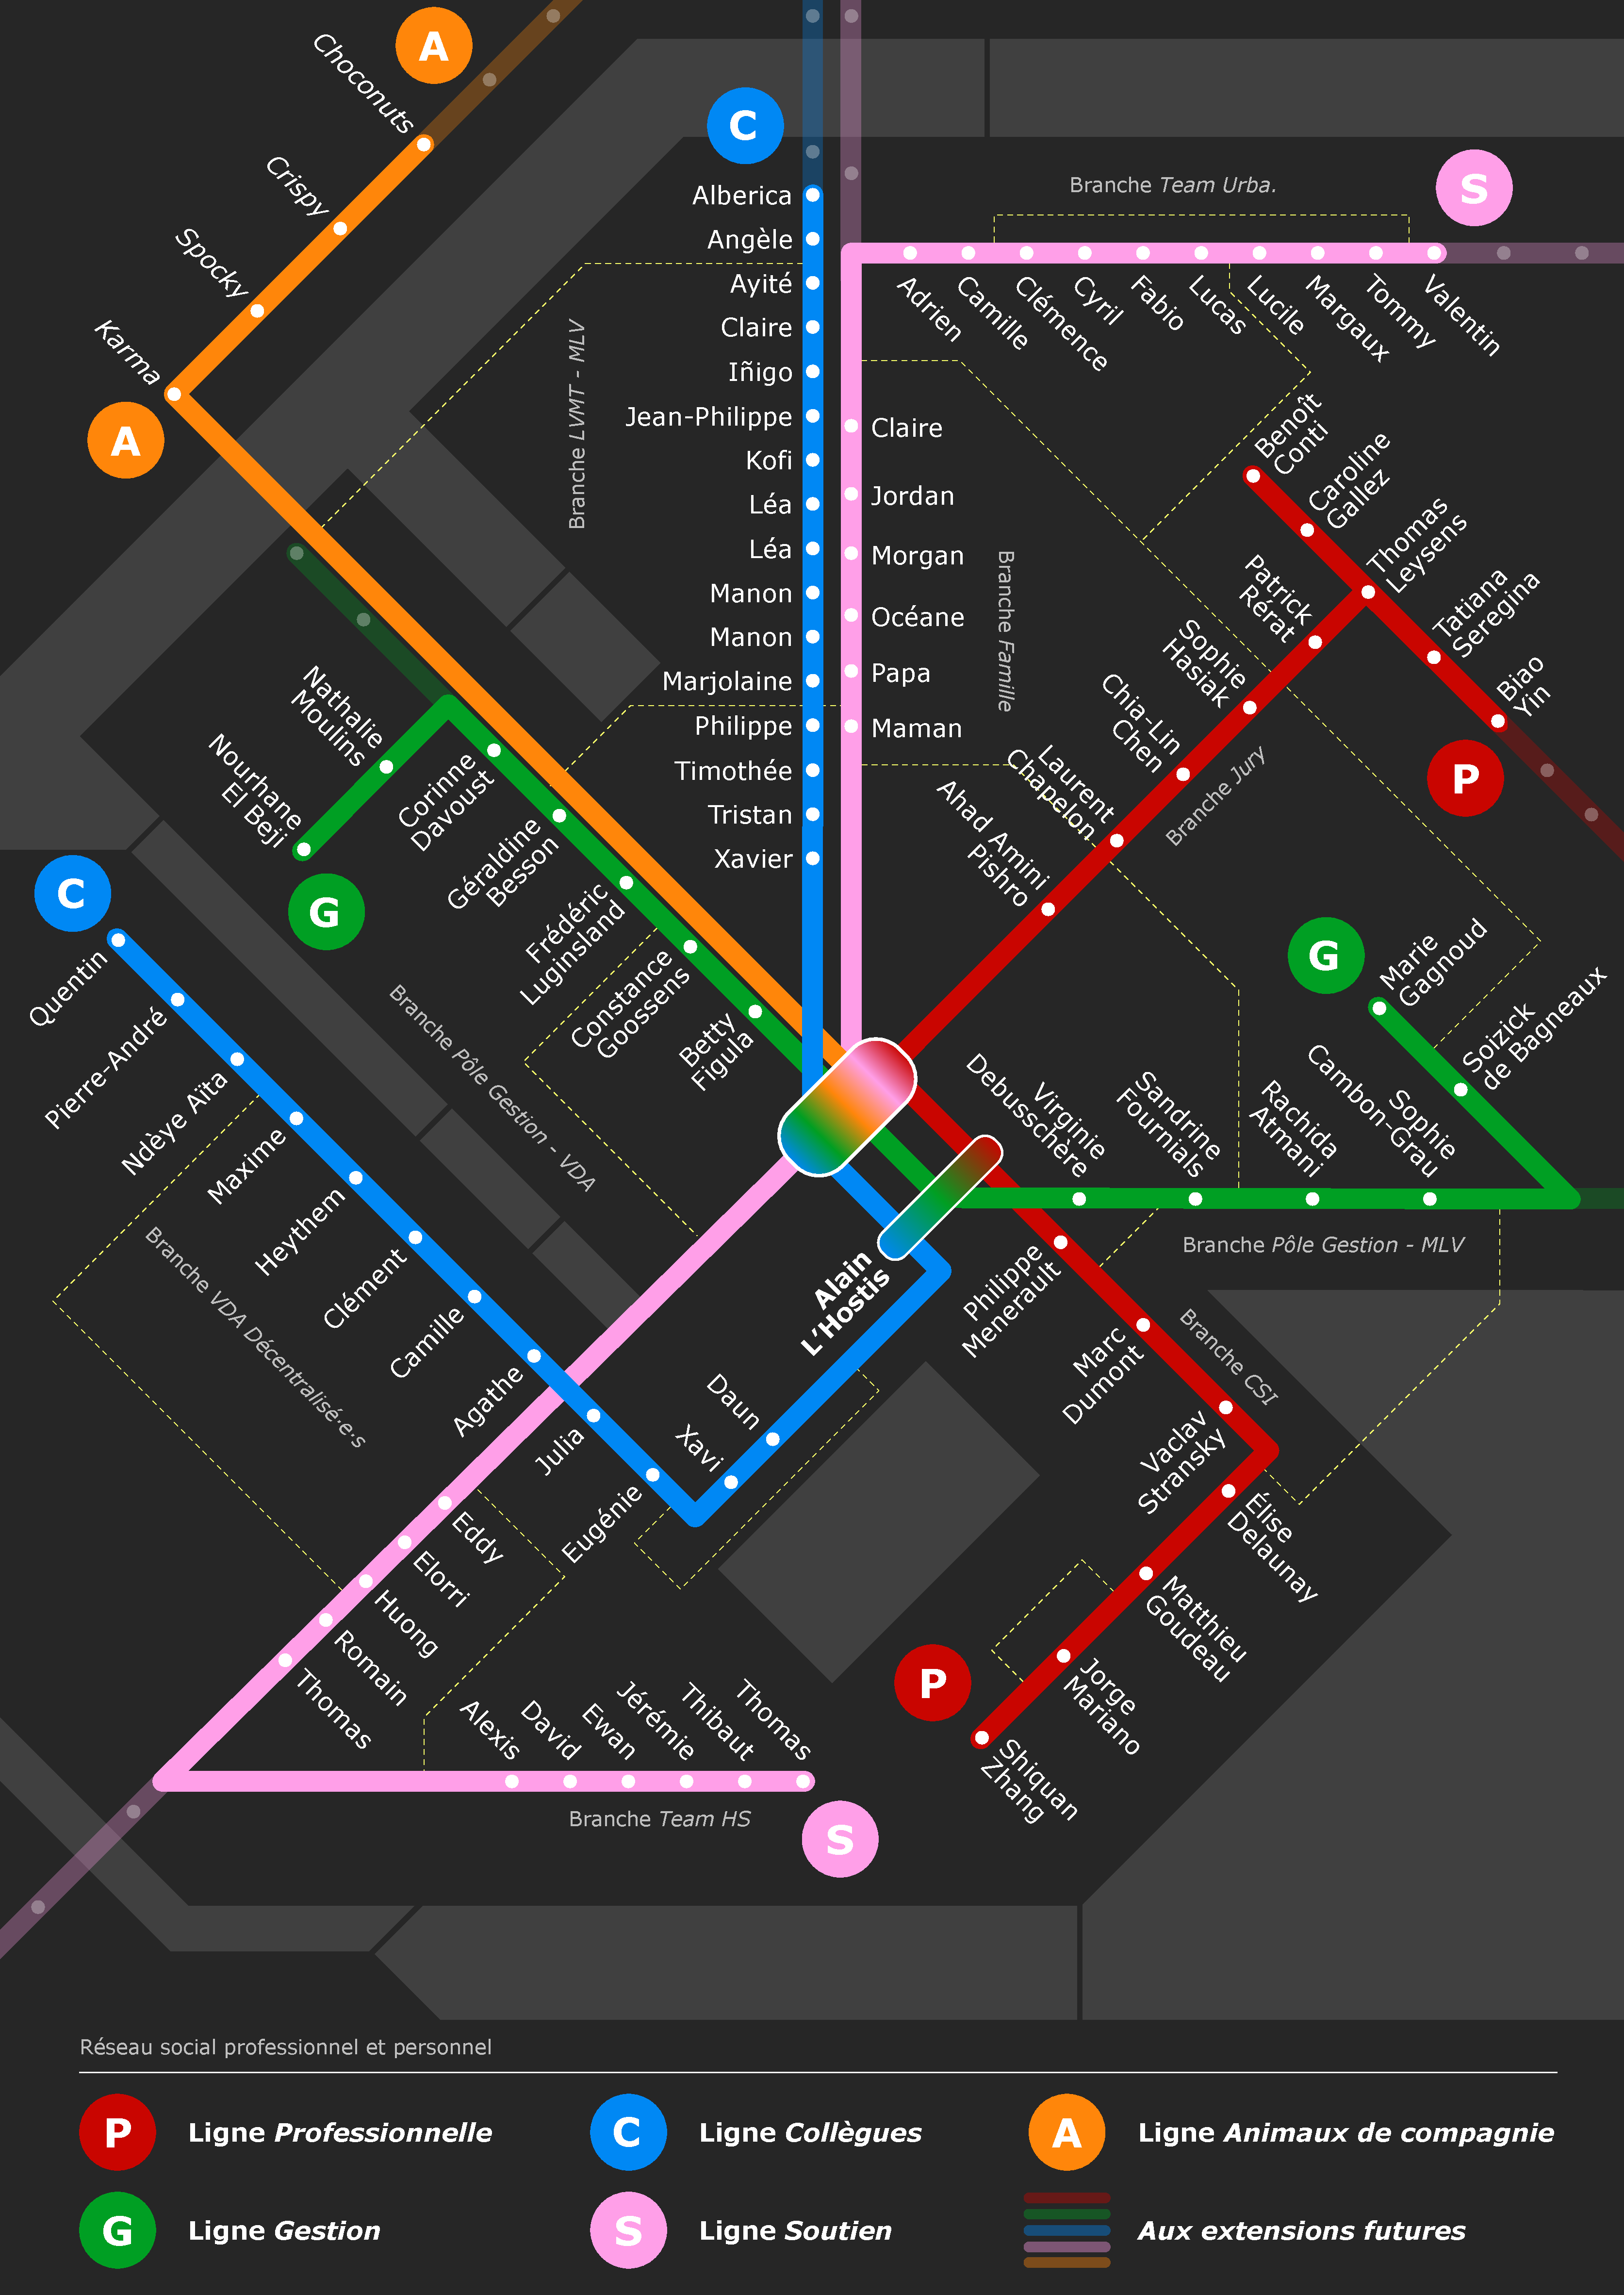
\includegraphics[width=1\columnwidth]{src/Figures/Preambule/FR_Remerciements.pdf}}
        \vspace{5pt}
        \begin{flushright}\scriptsize{
        Auteur~: \textcolor{blue}{Dylan Moinse (2024)}
        }\end{flushright}
    \end{carte}

%% ______________________________ %%
% TABLE DES MATIERES
    \cleardoublepage
    \setcounter{tocdepth}{1}
\tableofcontents{}
    \markboth{Table des matières}{}
    \markright{Préambule}{}
    %\addcontentsline{toc}{part}{Table des matières}
    \noindent\makebox[\textwidth]{\hrulefill}

%% ______________________________ %%
% TABLE DES FIGURES
\listof{figure}{Table des illustrations}
    \markboth{Table des illustrations}{}
    \markright{Préambule}{}
    \addcontentsline{toc}{part}{Table des illustrations}
    \noindent\makebox[\textwidth]{\hrulefill}

%% ______________________________ %%
% TABLE DES CARTES
\listof{carte}{Table des cartes}
    \markboth{Table des cartes}{}
    \markright{Préambule}{}
    \addcontentsline{toc}{part}{Table des cartes}
    \noindent\makebox[\textwidth]{\hrulefill}

%% ______________________________ %%
% LISTE DES TABLEAUX
\listof{table}{Liste des tableaux}
    \markboth{Liste des tableaux}{}
    \markright{Préambule}{}
    \addcontentsline{toc}{part}{Liste des tableaux}
    \noindent\makebox[\textwidth]{\hrulefill}

%% ______________________________ %%
% CITER
    \cleardoublepage
\section*{Citer le document
    \label{body:citer-document}
    }
    \addcontentsline{toc}{part}{Citer le document}
    \markboth{Citer le document}{}
    \markright{Préambule}{}

\small{\textcolor{blue}{Moinse Dylan (2025)}, \textsl{Le modèle urbain du Transit-Oriented Development, un urbanisme orienté vers les transports en commun, revisité par la mobilité individuelle légère. Une investigation dans la région Hauts-de-France} (Thèse de doctorat en Aménagement de l'espace, urbanisme). Université Gustave Eiffel, Laboratoire Ville Mobilité Transport. Sous la direction de \textcolor{blue}{L'Hostis Alain}, \pageref{LastPage}~p.}

%% ______________________________ %%
% AVANT-PROPOS
    \cleardoublepage
\section*{Avant-propos
    \label{body:avant-propos}
    }
    \addcontentsline{toc}{part}{Avant-propos}
    \markboth{Avant-propos}{}
    \markright{Préambule}{}

    % Figure logo HdF
\begin{wrapfigure}[6]{r}{0.2\textwidth} % 6 lignes pour ajuster la hauteur
    \vspace{-10pt} % Réduit l'espacement vertical avant la figure
    
\includegraphics[width=\linewidth]{src/Figures/Introduction/Logo_HdF.jpg} 
    \caption*{}
    \label{fig-introduction:logo-hdf}
\end{wrapfigure}

    % Introduction
Cette recherche doctorale a été menée à l'Université Gustave Eiffel\footnote{
    L’Université Gustave Eiffel est un \acrfull{EPSCP}, fondé en 2020 \textcolor{blue}{\autocite{universite_gustave_eiffel_notre_2024}}\index{Université Gustave Eiffel@\textsl{Université Gustave Eiffel}|pagebf}. Elle est issue de la fusion et du regroupement d’une université, d’un organisme de recherche et de plusieurs écoles, incluant notamment l’\acrfull{IFSTTAR}, l’\acrfull{UPEM} ainsi que d’autres établissements associés.
}, au sein du \acrfull{LVMT}\footnote{
    Le \acrfull{LVMT} est une \acrfull{UMR} fondée en 2003, placée sous la co-tutelle de l’Université Gustave Eiffel et de l’Institut Polytechnique de Paris, ce dernier étant issu d’un regroupement intégrant notamment l’\acrfull{ENPC}. Le \acrshort{LVMT} se consacre à l’étude des interactions entre les territoires, les transports et les mobilités, en mobilisant des approches pluridisciplinaires issues de l’aménagement, de l’urbanisme, de la géographie, de l’économie, de la sociologie, de l’anthropologie et des sciences de l’ingénieur \textcolor{blue}{\autocite{laboratoire_ville_mobilite_transport_presentation_2024}}\index{Laboratoire Ville Mobilité Transport@\textsl{Laboratoire Ville Mobilité Transport}|pagebf}.
}. Le contrat doctoral a été cofinancé par la Région Hauts-de-France, dans le cadre de l'initiative \textsl{rev3} (\textsl{Troisième Révolution Industrielle})\footnote{
    L’initiative \textsl{rev3} (\textsl{Troisième Révolution Industrielle}) est une dynamique collective lancée en 2013, copilotée par la Région Hauts-de-France et la \acrfull{CCI} Hauts-de-France. Elle vise à concevoir et à promouvoir des modèles innovants de développement des territoires, inscrits dans une perspective durable à l’horizon 2050 \textcolor{blue}{\autocite{rev3_rev3_2022}}\index{rev3@\textsl{rev3}|pagebf}.
}. Cette thèse de doctorat s'inscrit à la fois dans le deuxième \acrfull{COP} 2023-2025 de l'Université Gustave Eiffel\footnote{
    Elle s'inscrit plus particulièrement dans le Projet stratégique 2.1 (\Guillemets{Développer une mobilité décarbonée pour tous les usagers et sur tous les territoires en toute sécurité, en s’appuyant sur la compréhension des comportements et usages de mobilité}) et 2.4 (\Guillemets{Progresser dans les modèles de développement intégrant les Objectifs de développement durable}).
} et dans le troisième axe de recherche \Guillemets{Aménagement urbain et territoires}\footnote{
    L’axe 3 \Guillemets{Aménagement urbain et territoires} du \acrfull{LVMT} se consacre à l’étude des interactions entre les territoires, le transport et les mobilités \textcolor{blue}{\autocite{laboratoire_ville_mobilite_transport_axe_2024}}\index{Laboratoire Ville Mobilité Transport@\textsl{Laboratoire Ville Mobilité Transport}|pagebf}. Il explore les dynamiques territoriales et leur modélisation, le maillage des réseaux de transport, les modèles d’aménagement, ainsi que les enjeux liés à la sobriété énergétique. Les travaux menés dans ce cadre s’articulent autour de deux niveaux principaux d’interaction. D’une part, ils s’intéressent aux nœuds de transport, en examinant les flux qu’ils polarisent, les aménagements qu’ils génèrent et leur rôle stratégique pour les acteurs publics et privés. D’autre part, ils analysent la manière dont les réseaux de transport contribuent à renforcer les liens entre les territoires, tout en influençant les formes urbaines et les relations au sein des systèmes urbains régionaux.
} du \acrshort{LVMT}.%%Rédigé%%

%% ______________________________ %%
% CAPTATIO BENEVOLENTIAE
    \cleardoublepage
\section*{\textsl{Captatio benevolentiae}
    \label{body:mt180}
    }
    \addcontentsline{toc}{part}{\textsl{Captatio benevolentiae}}
    \markboth{\textsl{Captatio benevolentiae}}{}
    \markright{\textsl{Préambule}}{}

%\poemtitle{Devant l'Automobilité, la quête de l'Intermodalité}
\subsection*{Devant l'Automobilité, la quête de l'Intermodalité}
    
\settowidth{\versewidth}{And objects at rest tended to remain at rest}
\begin{verse}[\versewidth]

Il était une fois,\\
Au cœur du lointain eldorado lillois,\\
Une splendide Princesse appelée \textsl{Pieds}\\
Épousa le Prince \textsl{Train}, en un lien sacré et privilégié.\\
Cette union vénérée régnait sur la nation,\\
Organisée par des zones piétonnes et des stations.

Or, brusquement, cette relation idyllique\\
Fut renversée par une rivale maléfique.\\
La sorcière \textsl{La Voiture} insuffla un sortilège,\\
Envoûtant ces terres de mille pièges.\\
Le pays se pervertit en périphéries éparpillées.\\
Aux paysages pollués et aux chemins embouteillés.

Afin de briser l’envoûtement de \textsl{La Voiture},\\
Le pouvoir valorisa les gares sans véritable rupture.\\
En vain, les individus véhiculés vivant loin.

Pris de panique, \textsl{Pieds} et \textsl{Train} appelèrent leurs adjoints,\\
Les fidèles \textsl{Bus}, \textsl{Tramway} et \textsl{Métropolitain},\\
Hélas, peu adaptés à l’espace dépeint, rendant l'effort vain.

Las de ces lieux esclaves des lois de l’automobile,\\
Les nobles se tournèrent vers \textsl{Vélo}, un chevalier habile.\\
Surnommé \textsl{La Petite Reine} après son arrivée,\\
\textsl{Vélo} a pour vertu d'étendre les périmètres des gares fortifiées.

Mais, l’énergie conquérante de \textsl{Vélo} étant limitée,\\
Le destrier fut rafistolé par la fée \textsl{Électricité}.\\
Et naquirent dans cette région fantastique\dots\\
Des vélos et trottinettes électriques.\\
Connus sous le nom de \textsl{Mobilité Individuelle Légère},\\
Ces engins variés ont un rôle salutaire,\\
Permettant une combinaison aisée par la population,\\
Améliorant l’accessibilité des stations.

\textsl{Train} et \textsl{Mobilité Individuelle Légère} conclurent une alliance,\\
Une union symbolisée par la correspondance.\\
La Maison \textsl{Intermodalité},\\
Dont la devise est la compétitivité,\\
S'engageait à combiner ces modes conjointement,\\
Au cours du même déplacement.

[\dots]

La province des Hauts-de-France parvint à maîtriser la menace,\\
D’un urbanisme néfaste, sans grâce et inefficace.

D’ailleurs, j’ai un secret, je vous le confie\dots\\
Tou·te·s nos protagonistes dédièrent ce paradis retrouvé,\\
À leur enfant, agréable et cyclable,\\
Qu’ils appelèrent \textsl{Région Durable}.\\
Incroyable~?\\

\end{verse}
\textsl{Finale régionale Ma Thèse en 180 Secondes} (\textcolor{blue}{Dylan Moinse, 2022})

    % Figure MT180
    \begin{figure}[h!]\vspace*{4pt}
        \caption*{}
        \label{fig-preambule:mt180}
        \centerline{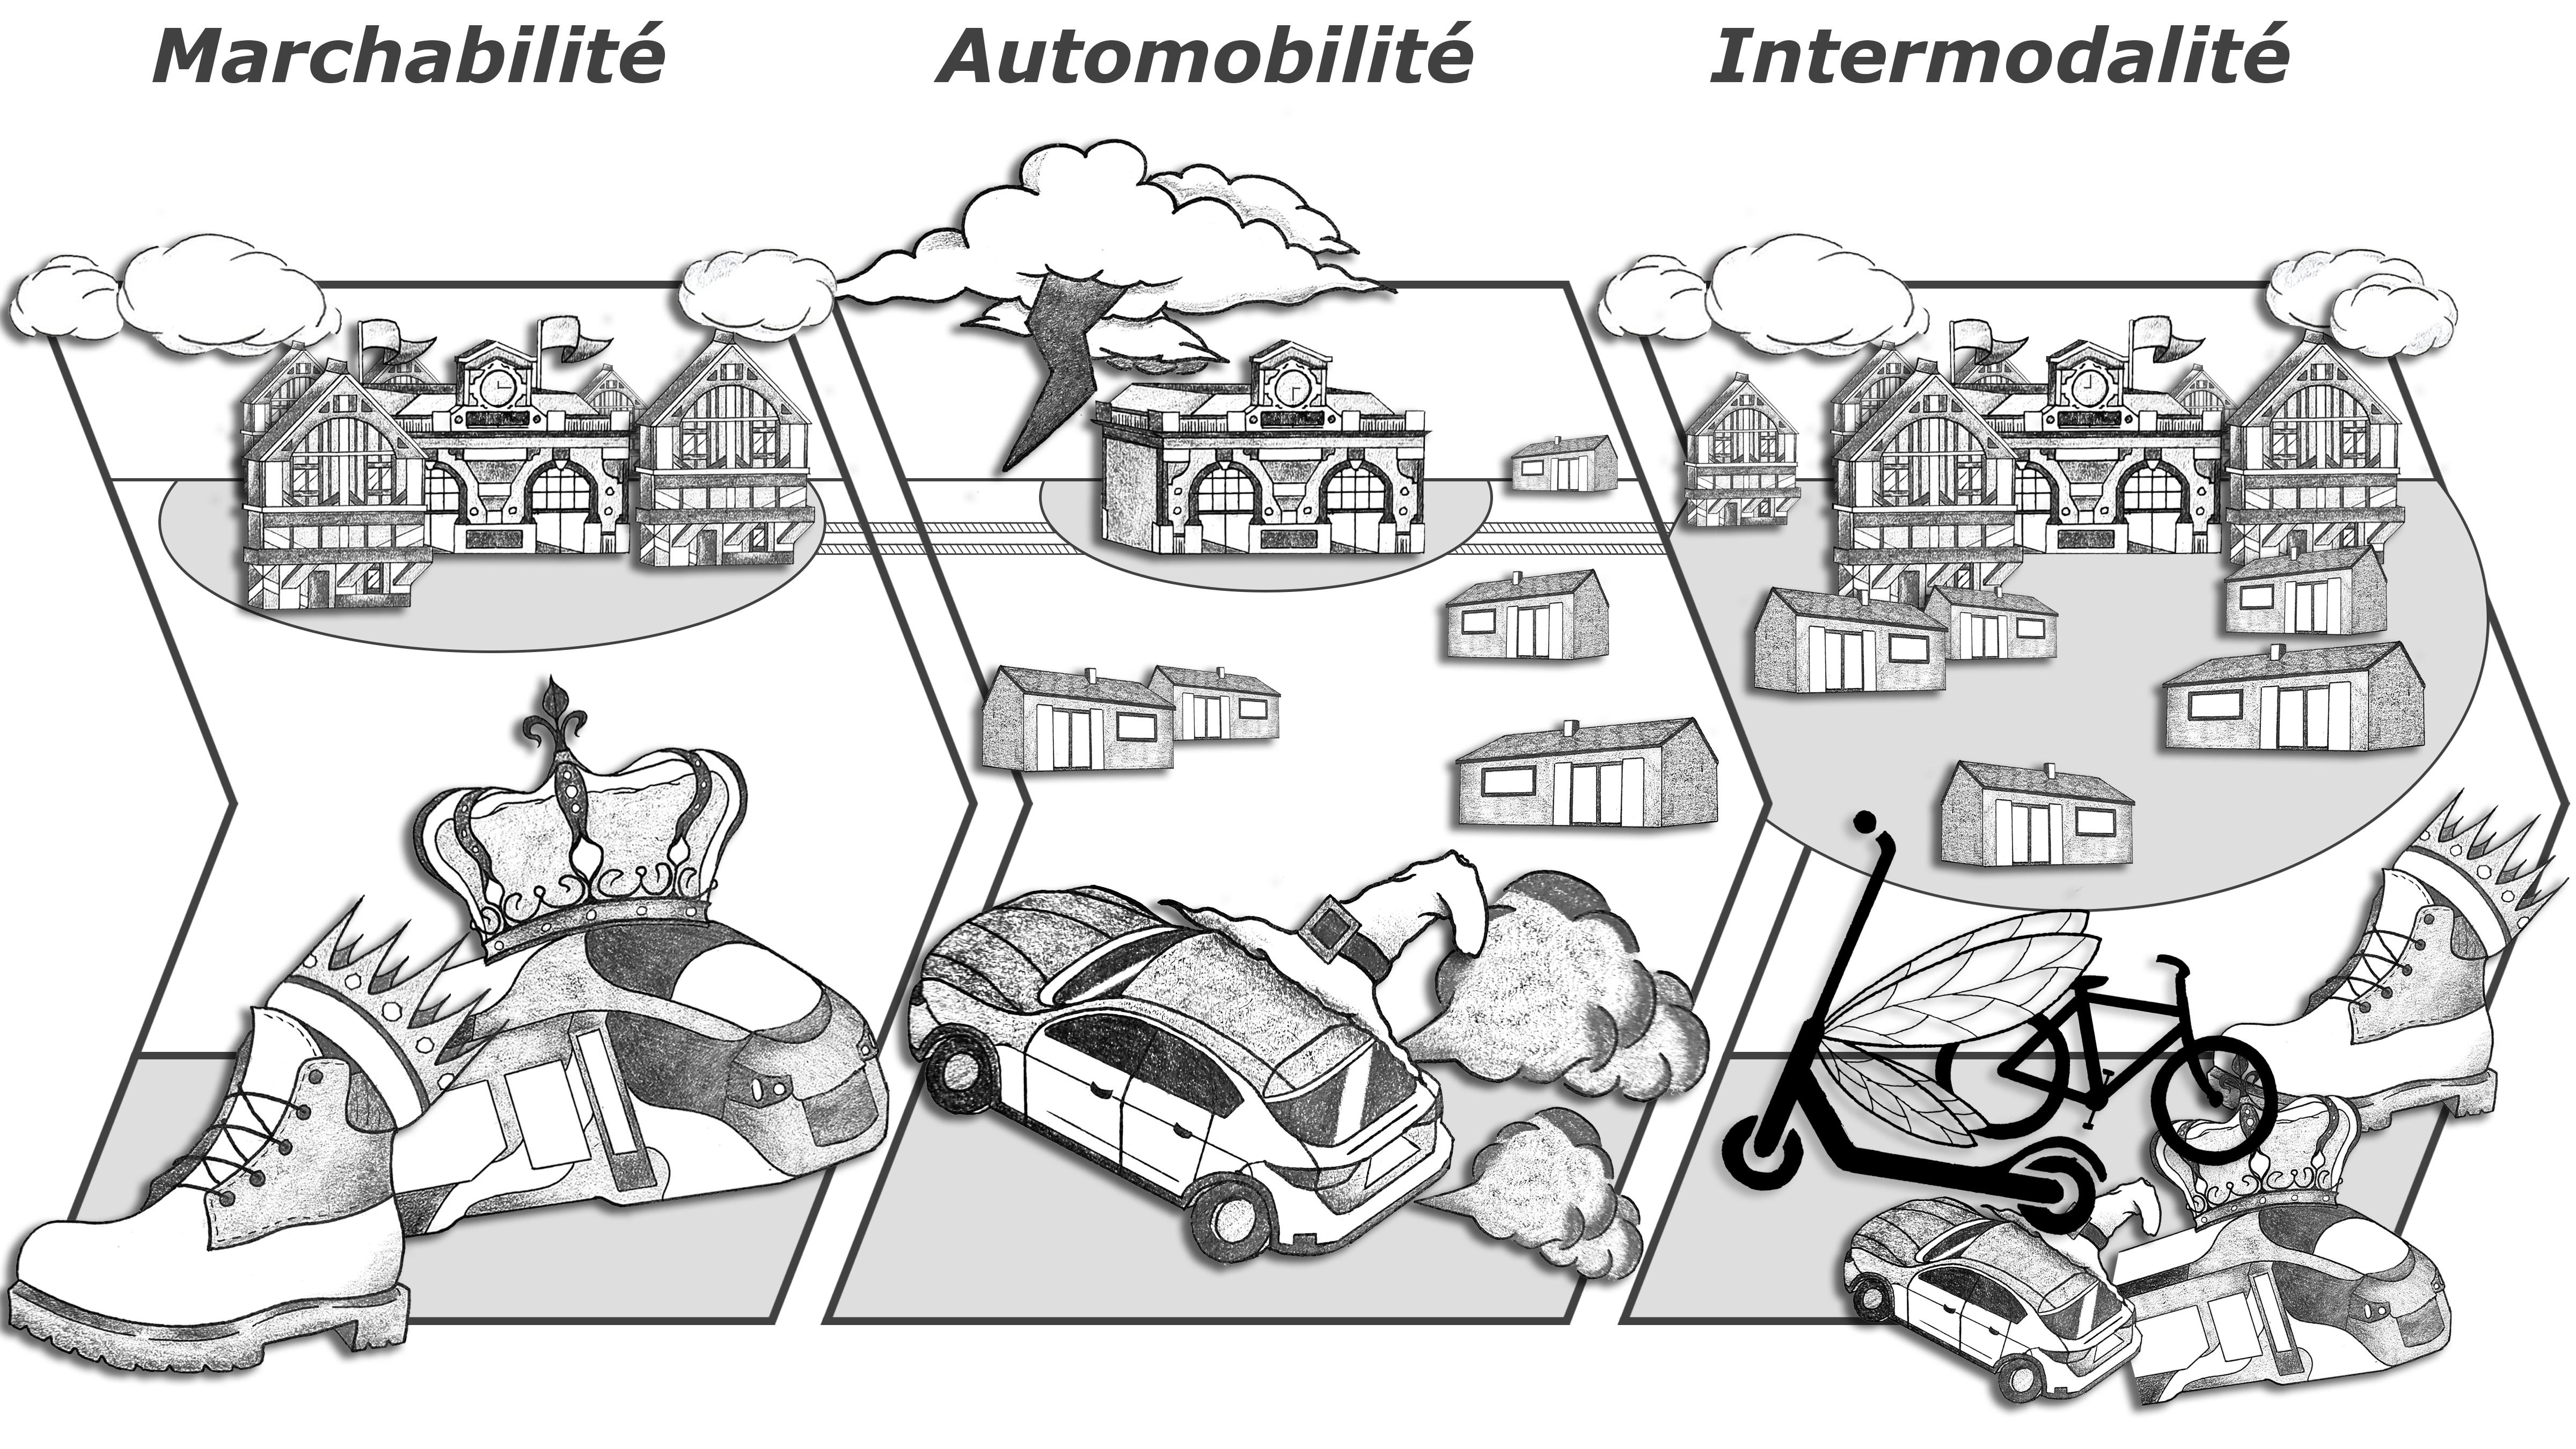
\includegraphics[width=1\columnwidth]{src/Figures/Preambule/FR_MT180_Illustration.jpg}}
        \vspace{5pt}
        \begin{flushright}\scriptsize{
        Auteur~: \textcolor{blue}{Dylan Moinse (2022)}
        }\end{flushright}
    \end{figure}

%% ______________________________ %%
% INTRODUCTION GENERALE
%------------------------------%
%% ✎ Dylan (V1) %%%%%%%%% ✅ %%
%% ✎ Alain (V2) %%%%%%%%% ❌ %%
%% ✎ Dylan (V3) %%%%%%%%% ❌ %%
%------------------------------%

\afterpage{%
%\afterpage{%

    % Arrière-plan introduction generale
    \AddToShipoutPictureBG*{%
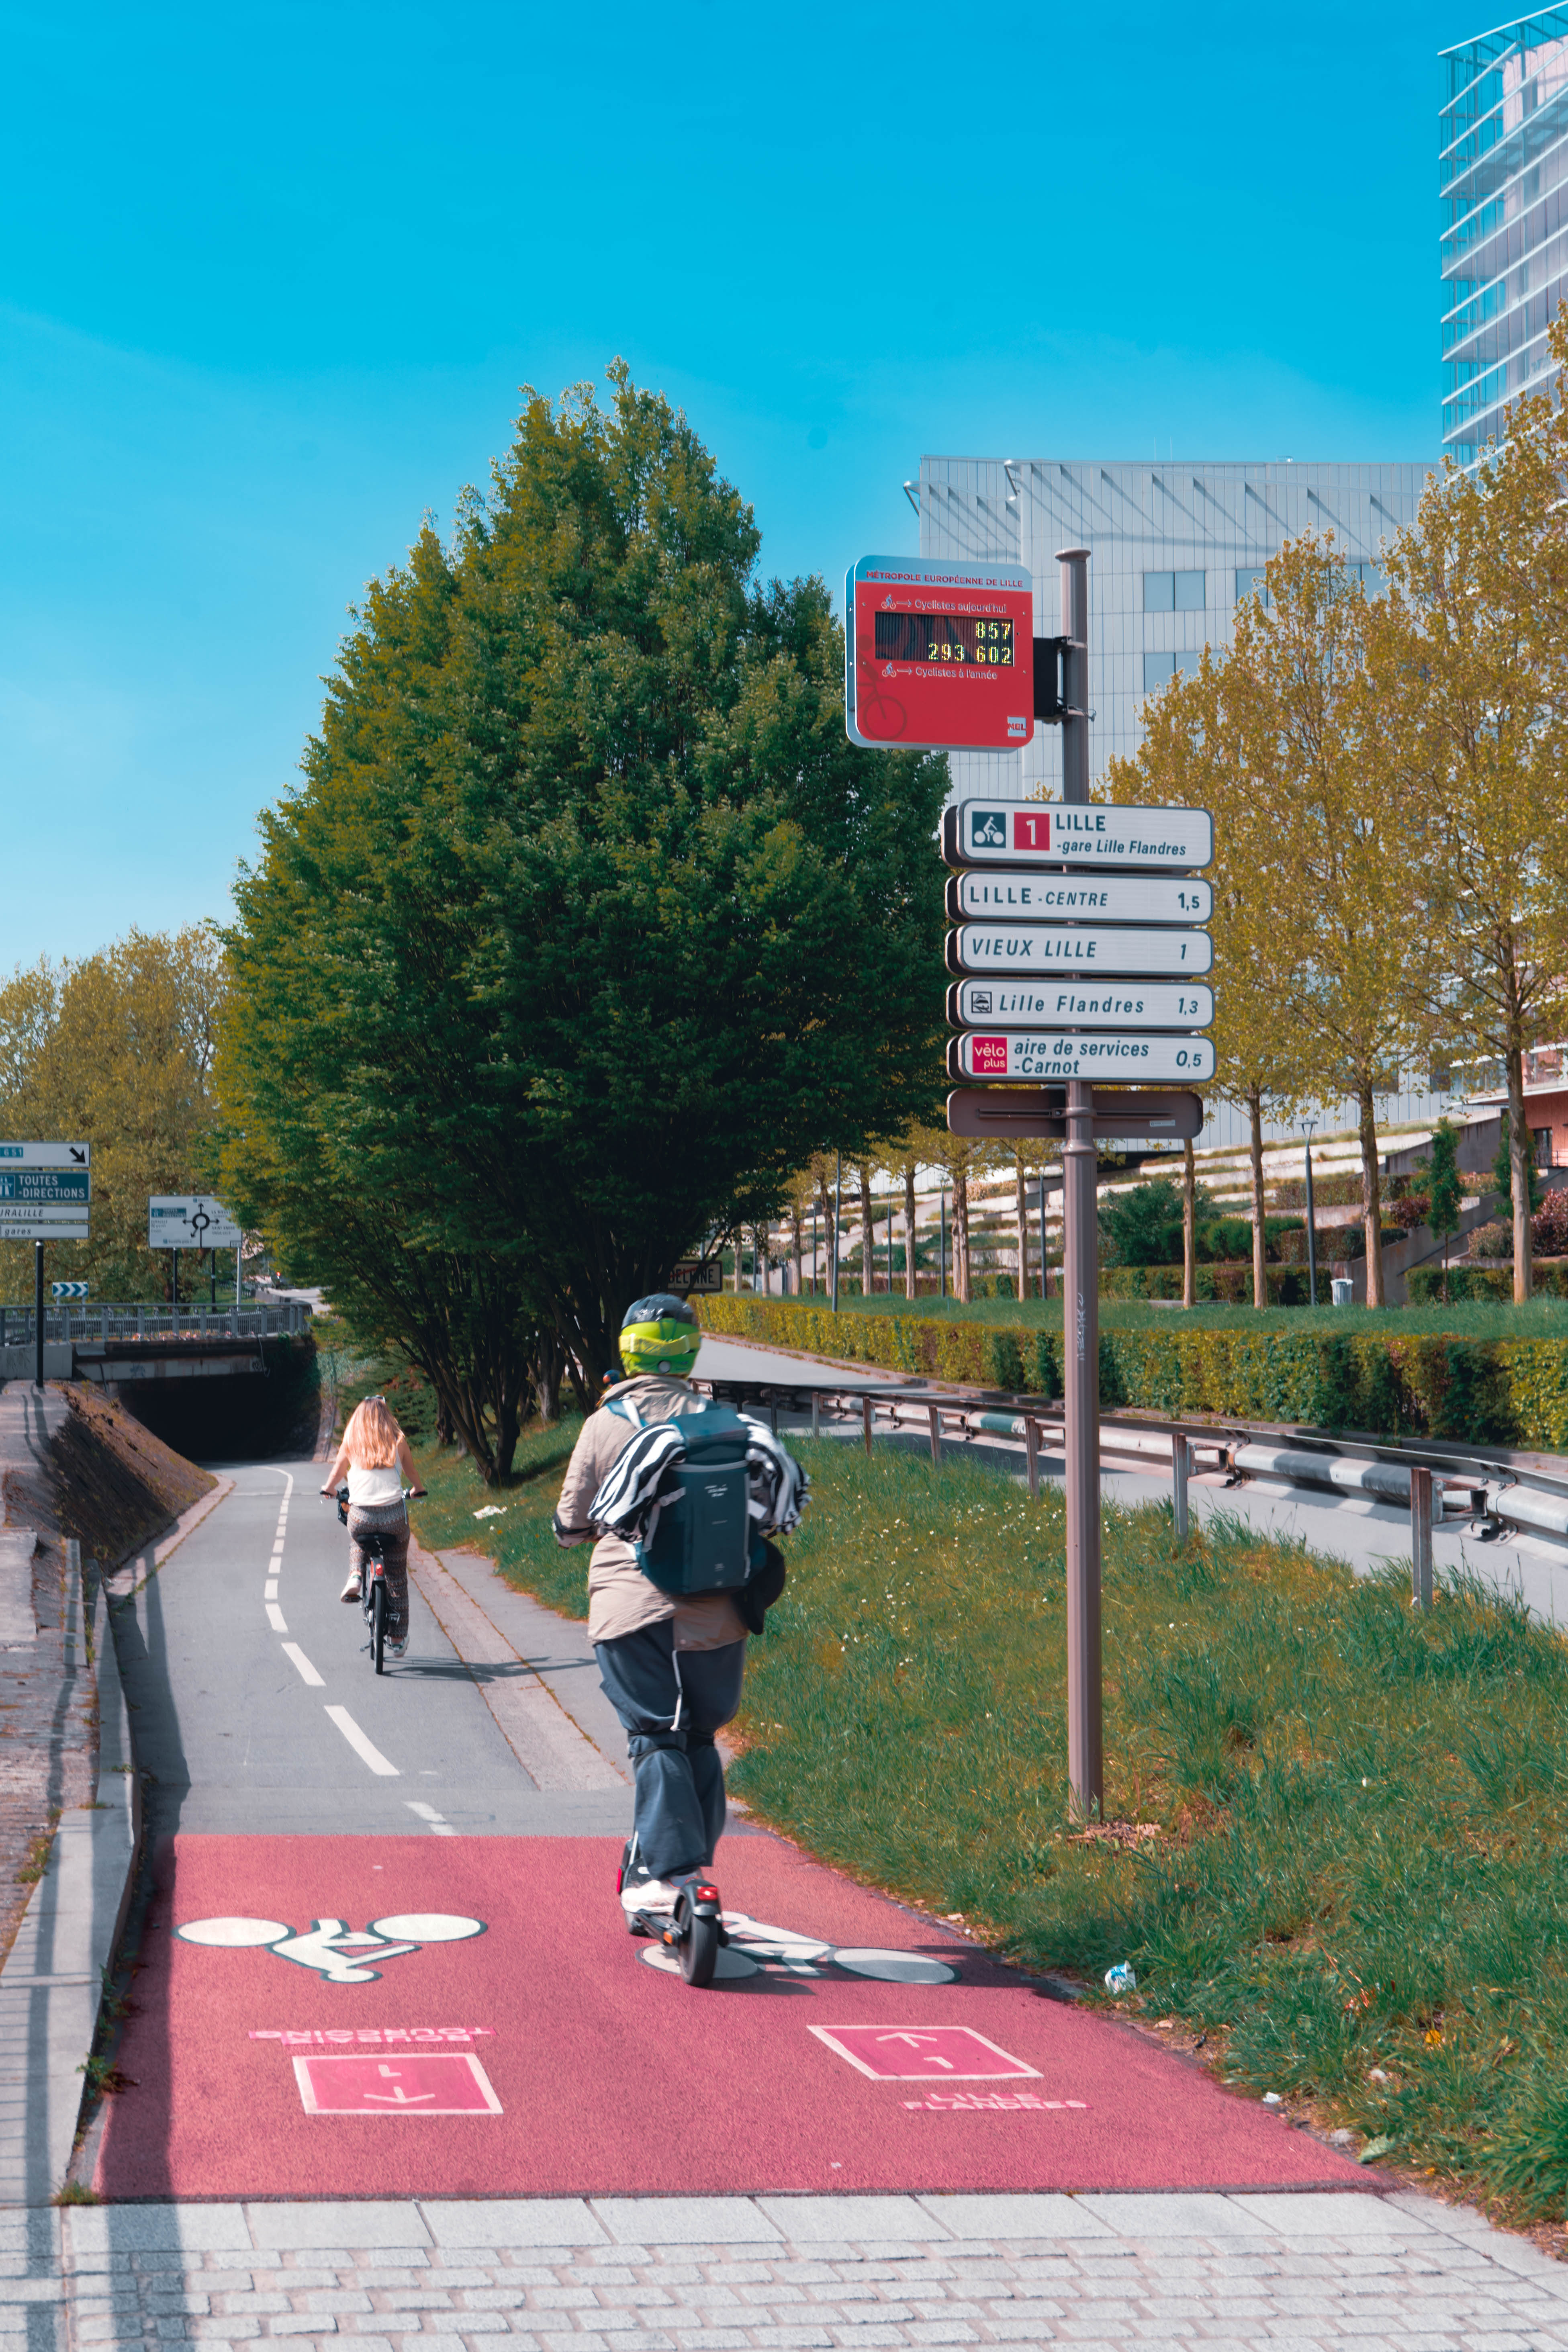
\includegraphics[width=\paperwidth,height=\paperheight]{src/Figures/Arriere_plan/Arriere_plan_Introduction.jpg}
    }

% Rectangle
\AddToShipoutPictureBG*{
  \begin{tikzpicture}[remember picture,overlay]
    \node[fill=white, opacity=0.75, text width=\paperwidth, minimum height=5cm, anchor=north] 
    at ([yshift=-9cm]current page.north) {};
  \end{tikzpicture}
}

% Source
\AddToShipoutPictureFG*{
  \AtPageLowerRight{
    \raisebox{1cm}{
      \hspace{16cm}
      
\begin{tikzpicture}
        \node[fill=white, rounded corners=5pt, inner sep=5pt, align=center] {
          \tiny{Photographie~: \textcolor{blue}{Dylan Moinse (2024)}}
        };
      \end{tikzpicture}
    }
  }
}
}%}

\renewcommand{\thefigure}{I.\arabic{figure}} % Numérotation spécifique pour l'introduction
\renewcommand{\thetable}{I.\arabic{table}}
\setcounter{figure}{0}

\pagenumbering{arabic}
\setcounter{page}{1} % Réinitialiser la numérotation à 1

    \needspace{1\baselineskip} % Réserve de l'espace
\part*{Introduction générale
    \label{body:introduction-generale}
    }
    %\addcontentsline{toc}{part}{Introduction générale}
    \markboth{Introduction générale}{}
    \markright{Introduction générale}{}
    \begin{refsegment}

    % Citation
    \begin{displayquote}
\Guillemets{\textsl{En gardant à l'esprit que~–~pour le même temps et effort~–~un individu peut parcourir à vélo une distance cinq fois supérieure à celle qu'il pourrait franchir à pied, ces aires de captation élargies jouent un rôle déterminant dans l'attraction d'une clientèle plus nombreuse vers le système de transport en commun. Ces zones peuvent également, dans une certaine mesure, modérer la demande immobilière aux abords des gares} [\dots] \textsl{Les investissements dans les infrastructures pour vélos, tels que les parkings et les services, sont économiquement rationnels pour les agences de transport public, augmentant à la fois la fréquentation du réseau et les revenus issus de son exploitation. Le vélo n'est plus perçu comme un concurrent, mais comme un allié, un moyen qui relie les voyageur·se·s à leur origine et à leur destination, et constitue un élément crucial d'un parcourus fluide de porte à porte. Ce type d'investissement collectif dans un système de transport en commun fréquent et flexible, visant à maximiser sa commodité et sa couverture spatiale, représente précisément l'action que les gouvernements doivent entreprendre pour alléger le fardeau financier associé à la possession d'une voiture et pour briser les barrières tangibles que rencontrent les individus les moins favorisés} [\dots] \textsl{Dans ce contexte, nous ne sommes plus contraint·e·s par la distance de marche nécessaire pour atteindre les commerces, les services et les nœuds~; nous n'avons plus à nous mesurer à la forte demande de cette proximité. Grâce à l'extension du rayon d'action permise en pédalant, nous avons pu soudainement étendre notre champ de recherche à de nouvelles parties de la ville} [\dots] \textsl{Une région équitable est celle qui garantit à tous ses résident·e·s un accès égal aux opportunités, indépendamment de leur origine géographique. Avec un réseau ferroviaire national et un réseau cyclable national, nous sommes assuré·e·s de pouvoir résider pratiquement où nous le souhaitons dans la Randstad, sans compromettre notre mode de vie ni nos opportunités d'emploi. Et pour nous, c'est un territoire où il fait bon vivre.}}\footnote{
    \Guillemets{\textsl{Keeping in mind that~–~for the same time and effort~–~someone can cycle five times farther than they can walk, these larger catchment areas actually play a critical role in feeding more customers into the public transport system. And they may~–~at least to a certain extent~–~tamp the demand for housing in and around train stations.} [\dots] \textsl{These investments in bicycle parking, rentals, and service make perfect economic sense for public transport agencies, as they increase ridership and revenue. Rather than treating the bicycle as a competitor, it is seen as an ally~–~one that connects passengers to their origin and destination; a critical component of the seamless door-to-door journey. These kinds of collective investments in a frequent and flexible public transport system~–~to maximize its convenience and coverage~–~are precisely what governments must do to lighten the financial burden of car ownership and break down the all-too-real barriers experienced by those lowest on the socioeconomic ladder.} [\dots] \textsl{in this case, we were no longer limited by the walking distance to shops, services, and public transport; nor were we forced to compete with the high demand for such proximity. With the extended range provided by pedal power, we could suddenly open up our search to entirely new parts of the city} [\dots] \textsl{An equitable region is one that provides residents with the same access to opportunity, regardless of their postal code. With a national rail network and national cycling network at our disposal, we know we can live virtually anywhere in the Randstad, without compromising on our lifestyle and our employment opportunities. And for us, that's a great place to be.}} \textcolor{blue}{\autocite[164-168]{bruntlett_curbing_2020}}\index{Bruntlett, Melissa|pagebf}\index{Bruntlett, Chris|pagebf}
} [traduction libre]%%Rédigé%%

\textcolor{blue}{\textcite{bruntlett_curbing_2020}}\index{Bruntlett, Melissa|pagebf}\index{Bruntlett, Chris|pagebf}. \foreignlanguage{english}{\textsl{Curbing Traffic: The Human Case for Fewer Cars in Our Lives}, Island Press, p. 164-168.}%%Rédigé%%
    \end{displayquote}

    % Amorce
\lettrine[lines=3, findent=8pt, nindent=0pt]{\lettrinefont R}{\textbf{emettre}} \textbf{la ville sur des rails}, tel est le message porté par l'anthropologie filmée, produite par \textcolor{blue}{Christian} \textcolor{blue}{\textcite{lallier_ville_2010}}\index{Lallier, Christian|pagebf}, anthropologue et réalisateur français. Intitulé \textsl{La ville sur des rails. L'utopie de la métropole}, ce documentaire explore les enjeux d'un urbanisme orienté vers le rail, remis au premier plan \textcolor{blue}{\autocite[8]{lhostis_concevoir_2009}}\index{L'Hostis, Alain|pagebf}\index{Alexandre, Elsa|pagebf}\index{Appert, Manuel|pagebf}\index{Araud-Ruyant, Catherine|pagebf}\index{Basty, Marius|pagebf}\index{Biau, Géraldine|pagebf}\index{Bozzani-Franc, Sandra|pagebf}\index{Boutantin, Gratienne|pagebf}\index{Constantin, Chantal|pagebf}\index{Coralli, Monica|pagebf}\index{Durousset, Marie-Jeanne|pagebf}\index{Fradier, Christophe|pagebf}\index{Gabion, Cyrille|pagebf}\index{Leysens, Thomas|pagebf}\index{Mermoud, Françoise|pagebf}\index{Olny, Xavier|pagebf}\index{Perrin, Emmanuel|pagebf}\index{Robert, Jean|pagebf}\index{Simand, Noémie|pagebf}\index{Stransky, Vaclav|pagebf}\index{Soulas, Claude|pagebf}\index{Verdier, Anne-Marie|pagebf}\index{Vulturescu, Bogdan|pagebf} dans une optique de réduction de la dépendance automobile \textcolor{blue}{\autocites[15]{newman_ten_2000}[74]{motte-baumvol_territoires_2014}[4]{gallez_dependance_2018}}\index{Motte-Baumvol, Benjamin|pagebf}\index{Belton-Chevallier, Leslie|pagebf}\index{Morel-Brochet, Annabelle|pagebf}\index{Gallez, Caroline|pagebf}\index{Newman, Peter W.~G.|pagebf}\index{Kenworthy, Jeffrey~R.|pagebf}. Les réflexions et les projets liés à la dialectique entre réseau et territoire, c'est-à-dire à l'articulation entre logiques territoriales et logiques réticulaires, connaissent un engouement récent \textcolor{blue}{\autocite[17]{gachon_impact_2019}}\index{Gachon, Mickaël|pagebf}, dans un contexte dans lequel leur coordination s'impose comme un incontournable des discours sur le \Guillemets{développement urbain \gls{durable}} \textcolor{blue}{\autocite[69]{nessi_politiques_2009}}\index{Nessi, Hélène|pagebf}\index{Delpirou, Aurélien|pagebf}, se traduisant principalement par une densification autour des gares. Ces auteur·rice·s soulèvent néanmoins des interrogations quant à la capacité systémique du rail à \Guillemets{corriger les anomalies} héritées de la fragmentation territoriale \textcolor{blue}{\autocite[190]{ducharme_ville_2021}}\index{Ducharme, Olivier|pagebf} et de la prégnance culturelle de l'\Guillemets{automobilité} \textcolor{blue}{\autocites[57-58]{urry_sociology_2000}[28]{urry_system_2004}}\index{Urry, John|pagebf}.%%Rédigé%%

    % Citation
Partant de ces critiques quant aux limites d'adaptabilité du \acrshort{TOD}, ou d'un urbanisme orienté vers les réseaux de \gls{transport en commun}, particulièrement dans les territoires dessinés par le système auto-centré, l'hypothèse directrice consiste à interroger le rôle stratégique du vélo et de la \gls{micro-mobilité}, qui présentent une tendance durable à un \Guillemets{retour en grâce} \textcolor{blue}{\autocites[137-168]{heran_retour_2015}[3-28]{dusong_dynamiques_2021}[44]{eskenazi_voir_2022}}\index{Héran, Frédéric|pagebf}\index{Dusong, Clément|pagebf}\index{Papon, Francis|pagebf}\index{Eskenazi, Manon|pagebf}\index{Massot, \index{Eskenazi, Manon|pagebf}|pagebf} ou font l'objet de réinventions \textcolor{blue}{\autocite[18]{amar_homo_2016}}\index{Amar, Georges|pagebf}. L'intérêt de cette recherche doctorale est d'évaluer dans quelle mesure ces modes de déplacement peuvent combler les lacunes du concept d'aménagement originellement formulé, en reconfigurant les interactions entre proximités, transport public et formes urbaines, dans une perspective intermodale. À cet égard, nous envisageons l'essor observé des cycles comme une opportunité pour répondre efficacement à la problématique des \Guillemets{premiers et derniers kilomètres} du transport public. Cette thèse explore à ce titre l'effet d'aubaine que représente l'émergence de nouvelles solutions de mobilité au sein de cette famille de véhicules individuels et légers \textcolor{blue}{\autocite[77]{oostendorp_combining_2018}}\index{Oostendorp, Rebekka|pagebf}\index{Gebhardt, Laura|pagebf}, afin de favoriser des parcours \Guillemets{fluides et porte-à-porte}, ainsi que le résume avec justesse la citation tirée de l'ouvrage de \textcolor{blue}{\textcite[164-168]{bruntlett_curbing_2020}}\index{Bruntlett, Melissa|pagebf}\index{Bruntlett, Chris|pagebf}.%%Résumé%%

% --- %
    % *.1. Contexte
    \needspace{1\baselineskip} % Réserve de l'espace
\section*{Regards croisés sur l’organisation territoriale et la mobilité spatiale
    \label{introduction-generale:regards-croises-organisation-territoriale-mobilite-spatiale}
    }
    \addcontentsline{toc}{section}{Regards croisés sur l’organisation territoriale et la mobilité spatiale}
    %\markboth{Regards croisés sur l’organisation territoriale et la mobilité spatiale}{}
    \markright{Regards croisés sur l’organisation territoriale et la mobilité spatiale}{}

    % Contexte
Le secteur des \Guillemets{transports} demeure le premier poste d'émission de \acrfull{GES} en France, en 2022, en représentant 32~\% du total des émissions nationales \textcolor{blue}{\autocite[41-53]{ministere_de_la_transition_ecologique_et_de_la_cohesion_des_territoires_chiffres_2024}}\index{Ministère de la Transition Écologique et de la Cohésion des Territoires@\textsl{Ministère de la Transition Écologique et de la Cohésion des Territoires}|pagebf}. Malgré une tendance générale à la réduction de l'empreinte carbone dans le territoire, le secteur des transports enregistre une augmentation de 2,3~\% de ses émissions carbonées sur une année. Cette hausse est essentiellement imputable à l'utilisation de la voiture individuelle, responsable de plus de la moitié de ces émissions, et ce, en dépit des promesses techniques et technologiques fréquemment mises en avant. L'usage décomplexé de l'\Guillemets{autosolisme} s'inscrit dans un cercle vicieux automobile, où la croissance urbaine européenne, depuis l'après-guerre, a été durablement façonnée par son adaptation à la généralisation de l'automobile. Ce processus a entraîné une fragmentation des espaces, un allongement des distances parcourues, ainsi qu'une structuration des réseaux, des formes urbaines et des usages, à l'origine de vulnérabilités territoriales. Dès lors, le paradigme de la \Guillemets{mobilité durable} ou de la \Guillemets{transition mobilitaire} et, plus largement, sa \Guillemets{décarbonation}, relèvent avant tout d'une affaire d'urbanisme \textcolor{blue}{\autocite{societe_francaise_des_urbanistes_decarbonation_2024}}\index{Société française des urbanistes@\textsl{Société française des urbanistes}|pagebf}. En ce sens, le quartier de gare constitue un point de jonction stratégique entre la ville et le transport, concentrant l'attention des aménageur·se·s. Pour \Guillemets{retisser} la ville, le transport public doit être envisagé comme l'élément structurant des corridors et des quartiers, un pivot à partir duquel les acteurs de la fabrique urbaine sont invités à repenser l'organisation des territoires \textcolor{blue}{\autocite[8]{boisclair_retisser_2013}}\index{Boisclair, Catherine|pagebf}.%%Rédigé%%

    % TOD
S’élevant au rang de référentiel d’action, la question de la coordination entre urbanisme et transport, au-delà du \Guillemets{mythe de la cohérence}, évoque le modèle théorique et opérationnel du \acrfull{TOD} \textcolor{blue}{\autocite[183-220]{gallez_mythes_2010}}\index{Gallez, Caroline|pagebf}\index{Kaufmann, Vincent|pagebf}\index{Guerrinha, Christophe|pagebf}\index{Maksim, Hanja-Niriana|pagebf}\index{Thébert, Mariane|pagebf}, dans lequel l’objet technique et son milieu interagissent en co-construction dans le temps \textcolor{blue}{\autocite[44-50]{leheis-guillot_ville_2011}}\index{Leheis-Guillot, Stéphanie|pagebf}. Cette démarche intégrée, qui consiste à penser simultanément la ville et le transport, repose sur un mécanisme d’interaction bidirectionnelle et continue, s’inscrivant dans une boucle de rétroaction \textcolor{blue}{\autocite[130]{wegener_overview_2004}}\index{Wegener, Michael|pagebf}. C’est dans ce cadre systémique que nous soutenons l’hypothèse selon laquelle le \acrshort{TOD} gagnerait à mieux intégrer les proximités générées par les quartiers de gare, tant en termes de polarisation des flux que d’opportunités d’insertion urbaine. À l’image du titre choisi par le chercheur britannique \textcolor{blue}{Rich~C.} \textcolor{blue}{\textcite[40]{mcilroy_this_2023}}\index{McIlroy, Rich~C.|pagebf}, dans son article \textsl{C'est là que les transports en commun montrent leurs limites}\footnote{
    \textsl{This is where public transport falls down} \textcolor{blue}{\autocite[40]{mcilroy_this_2023}}\index{McIlroy, Rich~C.|pagebf}.
}, le défi premier du \acrshort{TOD} aujourd’hui est moins d'améliorer la qualité des transports en commun et d'intensifier les activités humaines autour des pôles d'échange que de valoriser les cheminements vers et depuis ces nodosités. En somme, alors que les espoirs de décarbonation de la mobilité se concentrent sur le \Guillemets{triptyque magique}~–~composé de la voiture tantôt électrique, tantôt partagée, tantôt autonome et connectée~–, tout porte à croire que cette focalisation sur l’automobile, dont les effets rebonds et les nuisances persistantes sont sous-estimés, se révélera insuffisante. À l’inverse, il convient de miser sur la synergie entre la marche, le \gls{vélo} et le transport public, un \Guillemets{triptyque intermodal} plus à même de répondre aux défis contemporains de la mobilité urbaine et de l’aménagement des territoires \textcolor{blue}{\autocite[1]{soulas_triptyque_2021}}\index{Soulas, Claude|pagebf}.%%Rédigé%%

    % Mobilité individuelle légère + Sujet de recherche
Le modèle urbain du \acrshort{TOD} vise à articuler deux échelles de mobilité quotidienne distinctes~: d’une part, la mobilité métropolitaine et régionale, structurée par les réseaux de transport en commun, et d’autre part, la mobilité de proximité, qui privilégie autant que possible la marche et les cycles \textcolor{blue}{\autocites[81]{conesa_modelisation_2010}[124]{lo_feudo_scenario_2014}}\index{Lo Feudo, Fausto|pagebf}\index{Menerault, Philippe|pagebf}\index{L'Hostis, Alain|pagebf}\index{Festa, Demetrio Carmine|pagebf}\index{Conesa, Alexis|pagebf}\index{Paris, Didier|pagebf}. Or, au cours de la dernière décennie, le vélo et la micro-mobilité ont connu une diversification telle qu'ils tendent à s'\Guillemets{hybrider}, évoluant vers des objets de transport individuels et transportables \textcolor{blue}{\autocite[20]{amar_du_2012}}\index{Amar, Georges|pagebf}, à l'image de la \acrfull{TEP}, ou s'apparentant à des systèmes de transport public individuel \textcolor{blue}{\autocites[179]{amar_homo_2010}[4]{castex_prise_2017}}\index{Castex, Élodie|pagebf}\index{Frère, Séverine|pagebf}\index{Groux, Annette|pagebf}\index{Amar, Georges|pagebf}, à l'instar de la mobilité partagée. À travers des processus d’innovation porteurs de transformations socio-spatiales \textcolor{blue}{\autocite[89]{ageron_intermodalite-voyageurs_2013}}\index{Ageron, Pierre|pagebf}\index{Varlet, Jean|pagebf}, ce que nous dénommons \Guillemets{mobilité individuelle légère} s'imbrique dans le réseau de transport en commun, en tant qu'offre modale complémentaire. Ses usages intermodaux sont intrinsèquement liés aux dimensions temporelles et spatiales, nous conduisant à développer une réflexion nourrie par les références aux espaces, aux territoires et aux lieux \textcolor{blue}{\autocite[4]{sebban_complementarite_2003}}\index{Sebban, Annie-Claude|pagebf}\index{Motte, Alain|pagebf}. C’est à partir de ces considérations que nous avons établi notre sujet de recherche, ayant pour titre~:
    \begin{displayquote}
\textbf{Le modèle urbain du \textsl{Transit-Oriented Development} revisité par la mobilité individuelle légère émergente. Une investigation dans la région Hauts-de-France.}
    \end{displayquote}%%Rédigé%%

% --- %
    % *.2. Positionnement scientifique
    \needspace{1\baselineskip} % Réserve de l'espace
\section*{Positionnement scientifique
    \label{introduction-generale:positionnement-scientifique}
    }
    \addcontentsline{toc}{section}{Positionnement scientifique}
    %\markboth{Positionnement scientifique}{}
    \markright{Positionnement scientifique}{}

    % Gare
Cette thèse s’inscrit dans une approche aménagiste, mobilisant les éléments issus de la \Guillemets{fabrique urbaine} avec une entrée spécifique par la matérialité des espaces publics. À titre d'hypothèse générale, nous adoptons comme cadre d'analyse le concept d’\Guillemets{urbanisme des réseaux} ou de \Guillemets{ville des réseaux}, considérés comme des modèles explicatifs des transformations urbaines \textcolor{blue}{\autocite[]{dupuy_urbanisme_1991}}\index{Dupuy, Gabriel|pagebf}. Ce cadre repose sur le postulat selon lequel l’organisation territoriale, rendue possible par les réseaux, offre une multiplicité de connexions dont l’optimisation est une condition à son efficacité. À cet égard, la gare est envisagée comme un \Guillemets{objet territorial} \textcolor{blue}{\autocite[7]{moretti_interconnexion_1999}}\index{Moretti, Anna|pagebf}\index{Vacheret, Guy|pagebf}, un espace à l'interface des réseaux de transport et des dynamiques urbaines. Cette conception s’inscrit dans une tendance récente des études urbaines visant à réinterroger le rôle des gares dans la structuration de ville contemporaine, à un \Guillemets{retour des gares en thèse} \textcolor{blue}{\autocite[489]{delage_gare_2013}}\index{Delage, Aurélie|pagebf}. Loin d’être réduite à un simple point de connexion fonctionnelle, la gare est ici envisagée dans toute sa complexité en tant que \Guillemets{système-gare} \textcolor{blue}{\autocites[395]{le_bot_quel_2019}{le_bot_management_2020}}\index{Le Bot, Nils|pagebf}. Cette posture intègre ses dimensions spatiales, organisationnelles et symboliques, en reconnaissant son rôle structurant non seulement pour les réseaux de transport, mais aussi pour la production et l’organisation urbaines, ainsi que pour les modes de vie qui y sont attachés. Aussi, la lecture du sujet de recherche se veut-elle transcalaire \textcolor{blue}{\autocite[3]{knowles_transit_2019}}\index{Knowles, Richard~D.|pagebf}\index{Ferbrache, Fiona|pagebf}, favorisant l'emboîtement des échelles temporelles et scalaires~; depuis l’évolution foncière et économique jusqu'aux projets urbains~; depuis l’échelle locale du bâtiment-voyageur·se·s jusqu’aux dimensions régionales et (inter)nationales \textcolor{blue}{\autocites[13-14]{menerault_gares_2001}[238]{chapelon_transports_2016}}.%%Rédigé%%

    % Proximités
Cette réflexion sur la gare ne saurait être dissociée des mobilités qu’elle polarise. Dès lors, cette recherche engage un glissement d’analyse, passant de l’objet gare à celui des proximités géographiques qu’elle génère, en intégrant une réflexion sur la mobilité individuelle légère et son rôle dans la structuration des quartiers de gare. Ce changement de focale s’inscrit dans un changement paradigmatique plus large dans l’analyse des mobilités, auquel la gare participe activement \textcolor{blue}{\autocite[53]{leheis-guillot_ville_2011}}\index{Leheis-Guillot, Stéphanie|pagebf}. Ce \Guillemets{tournant de la mobilité} \textcolor{blue}{\autocites{sheller_new_2006}[8]{sheller_mobilizing_2016}[13]{randell_no_2020}}\index{Sheller, Mimi|pagebf}\index{Urry, John|pagebf}\index{Randell, Richard|pagebf} met l’accent sur la dimension relationnelle et systémique du \gls{déplacement}, au-delà d’une approche strictement infrastructurelle \textcolor{blue}{\autocite[14]{heran_retour_2015}}\index{Héran, Frédéric|pagebf}. Dans ce cadre, cette thèse se situe à l’intersection de plusieurs champs de recherche, croisant urbanisme, aménagement du territoire, géographie, sociologie et science des données, afin d’interroger la reconfiguration du \acrshort{TOD} sous l’effet des (nouvelles) proximités permises par l’intégration de la mobilité individuelle légère. Cette approche conduit à considérer cette mobilité comme un levier stratégique pour la réactualisation du \acrshort{TOD} dans des contextes urbains hérités du modèle auto-orienté \textcolor{blue}{\autocite[209]{heran_retour_2015}}\index{Héran, Frédéric|pagebf}. Elle s’inscrit ainsi dans une réflexion plus large sur le renouvellement des politiques de transport public et d’aménagement, face aux défis des \Guillemets{premiers et derniers kilomètres}. Elle met en avant l’opportunité que représente la mobilité individuelle légère pour promouvoir un système de mobilité multimodale et de type \Guillemets{porte-à-porte} \textcolor{blue}{\autocite[979]{lee_bicycle-based_2016}}\index{Lee, Jaeyeong|pagebf}\index{Choi, Keechoo|pagebf}\index{Leem, Yountaik|pagebf}.%%Rédigé%%

    % Positionnement
Cette recherche doctorale mobilise ainsi quatre entrées complémentaires pour structurer notre investigation~: (i) l’entrée par les objets techniques, en analysant le \Guillemets{système-gare} et les modes de déplacement associés~; (ii) l’entrée par les usages et les pratiques intermodales, en étudiant les comportements et stratégies modales des cyclo-voyageur·se·s~; (iii) l’entrée par l’\gls{accessibilité}, en mesurant les effets de la mobilité individuelle légère sur l'accessibilité~; et (iv) l’entrée par les systèmes urbains, en interrogeant les effets de la mobilité individuelle légère sur l'urbanisme ferroviaire. Ainsi, la gare ne peut être réduite à un objet purement socio-technique \textcolor{blue}{\autocite[]{joseph_villes_1999}}\index{Joseph, Isaac|pagebf}, mais doit également être envisagée comme un objet urbain, en tenant compte de son insertion territoriale, au-delà de l’échelle du bâtiment-voyageur·se·s ou de son environnement immédiat. Elle joue un rôle spatial, fonctionnel et symbolique, en étant à la fois une \Guillemets{scène} et une \Guillemets{actante} \textcolor{blue}{\autocite[5]{baron_gares_2016}}\index{Baron, Nacima|pagebf}\index{Roseau, Nathalie|pagebf}. Cette démarche permet ainsi d’explorer le potentiel de révision du \acrshort{TOD} à travers l’intégration de la mobilité individuelle légère. Elle propose une lecture renouvelée des quartiers de gare et de leur rôle dans l’organisation urbaine, tout en contribuant à la formalisation d’un modèle élargi~: un \acrfull{M-TOD}, ou un urbanisme orienté vers les réseaux de transport en commun et intégrant la mobilité individuelle légère.%%Rédigé%%

% --- %
    % *.3. Problématique / Objectifs
    \needspace{1\baselineskip} % Réserve de l'espace
\section*{Orientations de recherche
    \label{introduction-generale:problematique-objectifs-hypotheses}
    }
    \addcontentsline{toc}{section}{Orientations de recherche}
    %\markboth{Problématique, objectifs et hypothèses de recherche}{}
    \markright{Problématique, objectifs et hypothèses de recherche}{}

    % Problématique
Cette thèse vise ainsi à examiner les transformations du modèle \acrshort{TOD} sous l'angle de la mobilité individuelle légère, en adoptant une approche théorique, empirique et prospective pour déterminer et établir un cadre optimal pour l'\gls{accessibilité intermodale}. Notre questionnement central se pose de la manière suivante~:
    \begin{displayquote}
\textbf{Dans quelle mesure l'intégration de la mobilité individuelle légère peut-elle relever les défis des \Guillemets{premiers et derniers kilomètres} du transport public et contribuer à renforcer l'accessibilité intermodale des quartiers de gare des Hauts-de-France~?
\\
En quoi ces \Guillemets{proximités} reconfigurent-elles le modèle urbain du \textsl{Transit-Oriented Development} et ouvrent-elles la voie à un \textsl{Micromobility-friendly Transit-Oriented Development}, mieux adapté aux réalités urbaines et aux évolutions des pratiques de mobilité~?
\\
Quelles sont les conditions de mise en œuvre et les leviers d’action à mobiliser pour assurer une intégration optimale de la mobilité individuelle légère dans les stratégies d’aménagement et de transport~?}
    \end{displayquote}%%Rédigé%%

    % Objectifs
Ce questionnement guidera ainsi la structuration de notre recherche, en montrant comment la mobilité individuelle légère peut enrichir le modèle du \acrshort{TOD} et quelles implications en découlent pour la planification des mobilités et des territoires. Au cours de notre projet doctoral, nous développerons une démarche progressive en plusieurs étapes, conçue pour revisiter le \acrshort{TOD} à l'aune des proximités renouvelées par le développement de la mobilité individuelle légère. Chaque chapitre s’appuie sur un objectif de recherche, articulant une réflexion théorique et empirique sur les enjeux de l'accessibilité intermodale (voir le \hyperref[fig-introduction:objectifs-hypotheses]{schéma~\ref{fig-introduction:objectifs-hypotheses}}, page~\pageref{fig-introduction:objectifs-hypotheses}). Afin de structurer notre raisonnement, nous avons recours à la méthode du questionnement dite \acrfull{QQOQCCP}, qui nous permet de préciser les contours et les objectifs de notre recherche~:
        \begin{customitemize}
    \item \textsl{Quoi} et \textsl{Quand}~? ({\textcolor{blue}{\(O_1\)}\label{objectif-1}}). Le premier chapitre pose les bases conceptuelles et historiques du \acrshort{TOD} et des cycles, en identifiant leurs forces et leurs limites. Il s’agit d’introduire le caractère essentiel d’un \acrshort{M-TOD}, c’est-à-dire un modèle réactualisé prenant en compte cette composante intermodale~;
    \item \textsl{Par qui} et \textsl{Sur quoi}~? ({\textcolor{blue}{\(O_2\)}\label{objectif-2}}). Le deuxième chapitre vise à construire un cadre analytique en procédant à une revue des travaux scientifiques et techniques existants sur la mobilité individuelle légère, l’\gls{intermodalité} et la relecture du \acrshort{TOD}. Il met en perspective les expériences internationales et les nouvelles connaissances en matière d'intermodalité~;
    \item \textsl{Où} et \textsl{Avec quoi}~? ({\textcolor{blue}{\(O_3\)}\label{objectif-3}}). Le troisième chapitre mobilise des méthodes mixtes pour construire et analyser un matériau empirique dans un périmètre géographique défini. Il s'agit de définir, d'adapter et de mettre en relation des approches appropriées en vue de proposer une \Guillemets{enquête sur-mesure}~;
    \item \textsl{Qui} et \textsl{Combien}~? ({\textcolor{blue}{\(O_4\)}\label{objectif-4}}). Le quatrième chapitre vient mesurer et caractériser les pratiques intermodales, en s’intéressant aux profils des usager·ère·s qui associent l'usage de la mobilité individuelle légère et du transport public. Il s’agit de quantifier les flux et d’identifier les facteurs socio-démographiques et environnementaux qui influencent de tels choix modaux~;
    \item \textsl{Vers où} et \textsl{Pourquoi}~? ({\textcolor{blue}{\(O_5\)}\label{objectif-5}}). Le cinquième chapitre a pour objectif de mesurer et d'expliquer l'extension spatiale des quartiers de gare grâce à la mobilité individuelle légère. Il évalue les gains d'accessibilité à différentes échelles~;
    \item \textsl{Comment} et \textsl{En relation avec quoi}~? ({\textcolor{blue}{\(O_6\)}\label{objectif-6}}). Le dernier chapitre propose une formalisation conceptuelle et opérationnelle du \acrshort{M-TOD} en modélisant les conditions de sa mise en œuvre. Il s’agit de formuler des recommandations à destination des acteurs de la fabrique urbaine.
        \end{customitemize}%%Rédigé%%

    % Figure objectifs et hypothèses de recherche
    \begin{figure}[h!]\vspace*{4pt}
        \caption{Vue d'ensemble des objectifs et des hypothèses de recherche}
        \label{fig-introduction:objectifs-hypotheses}
        \centerline{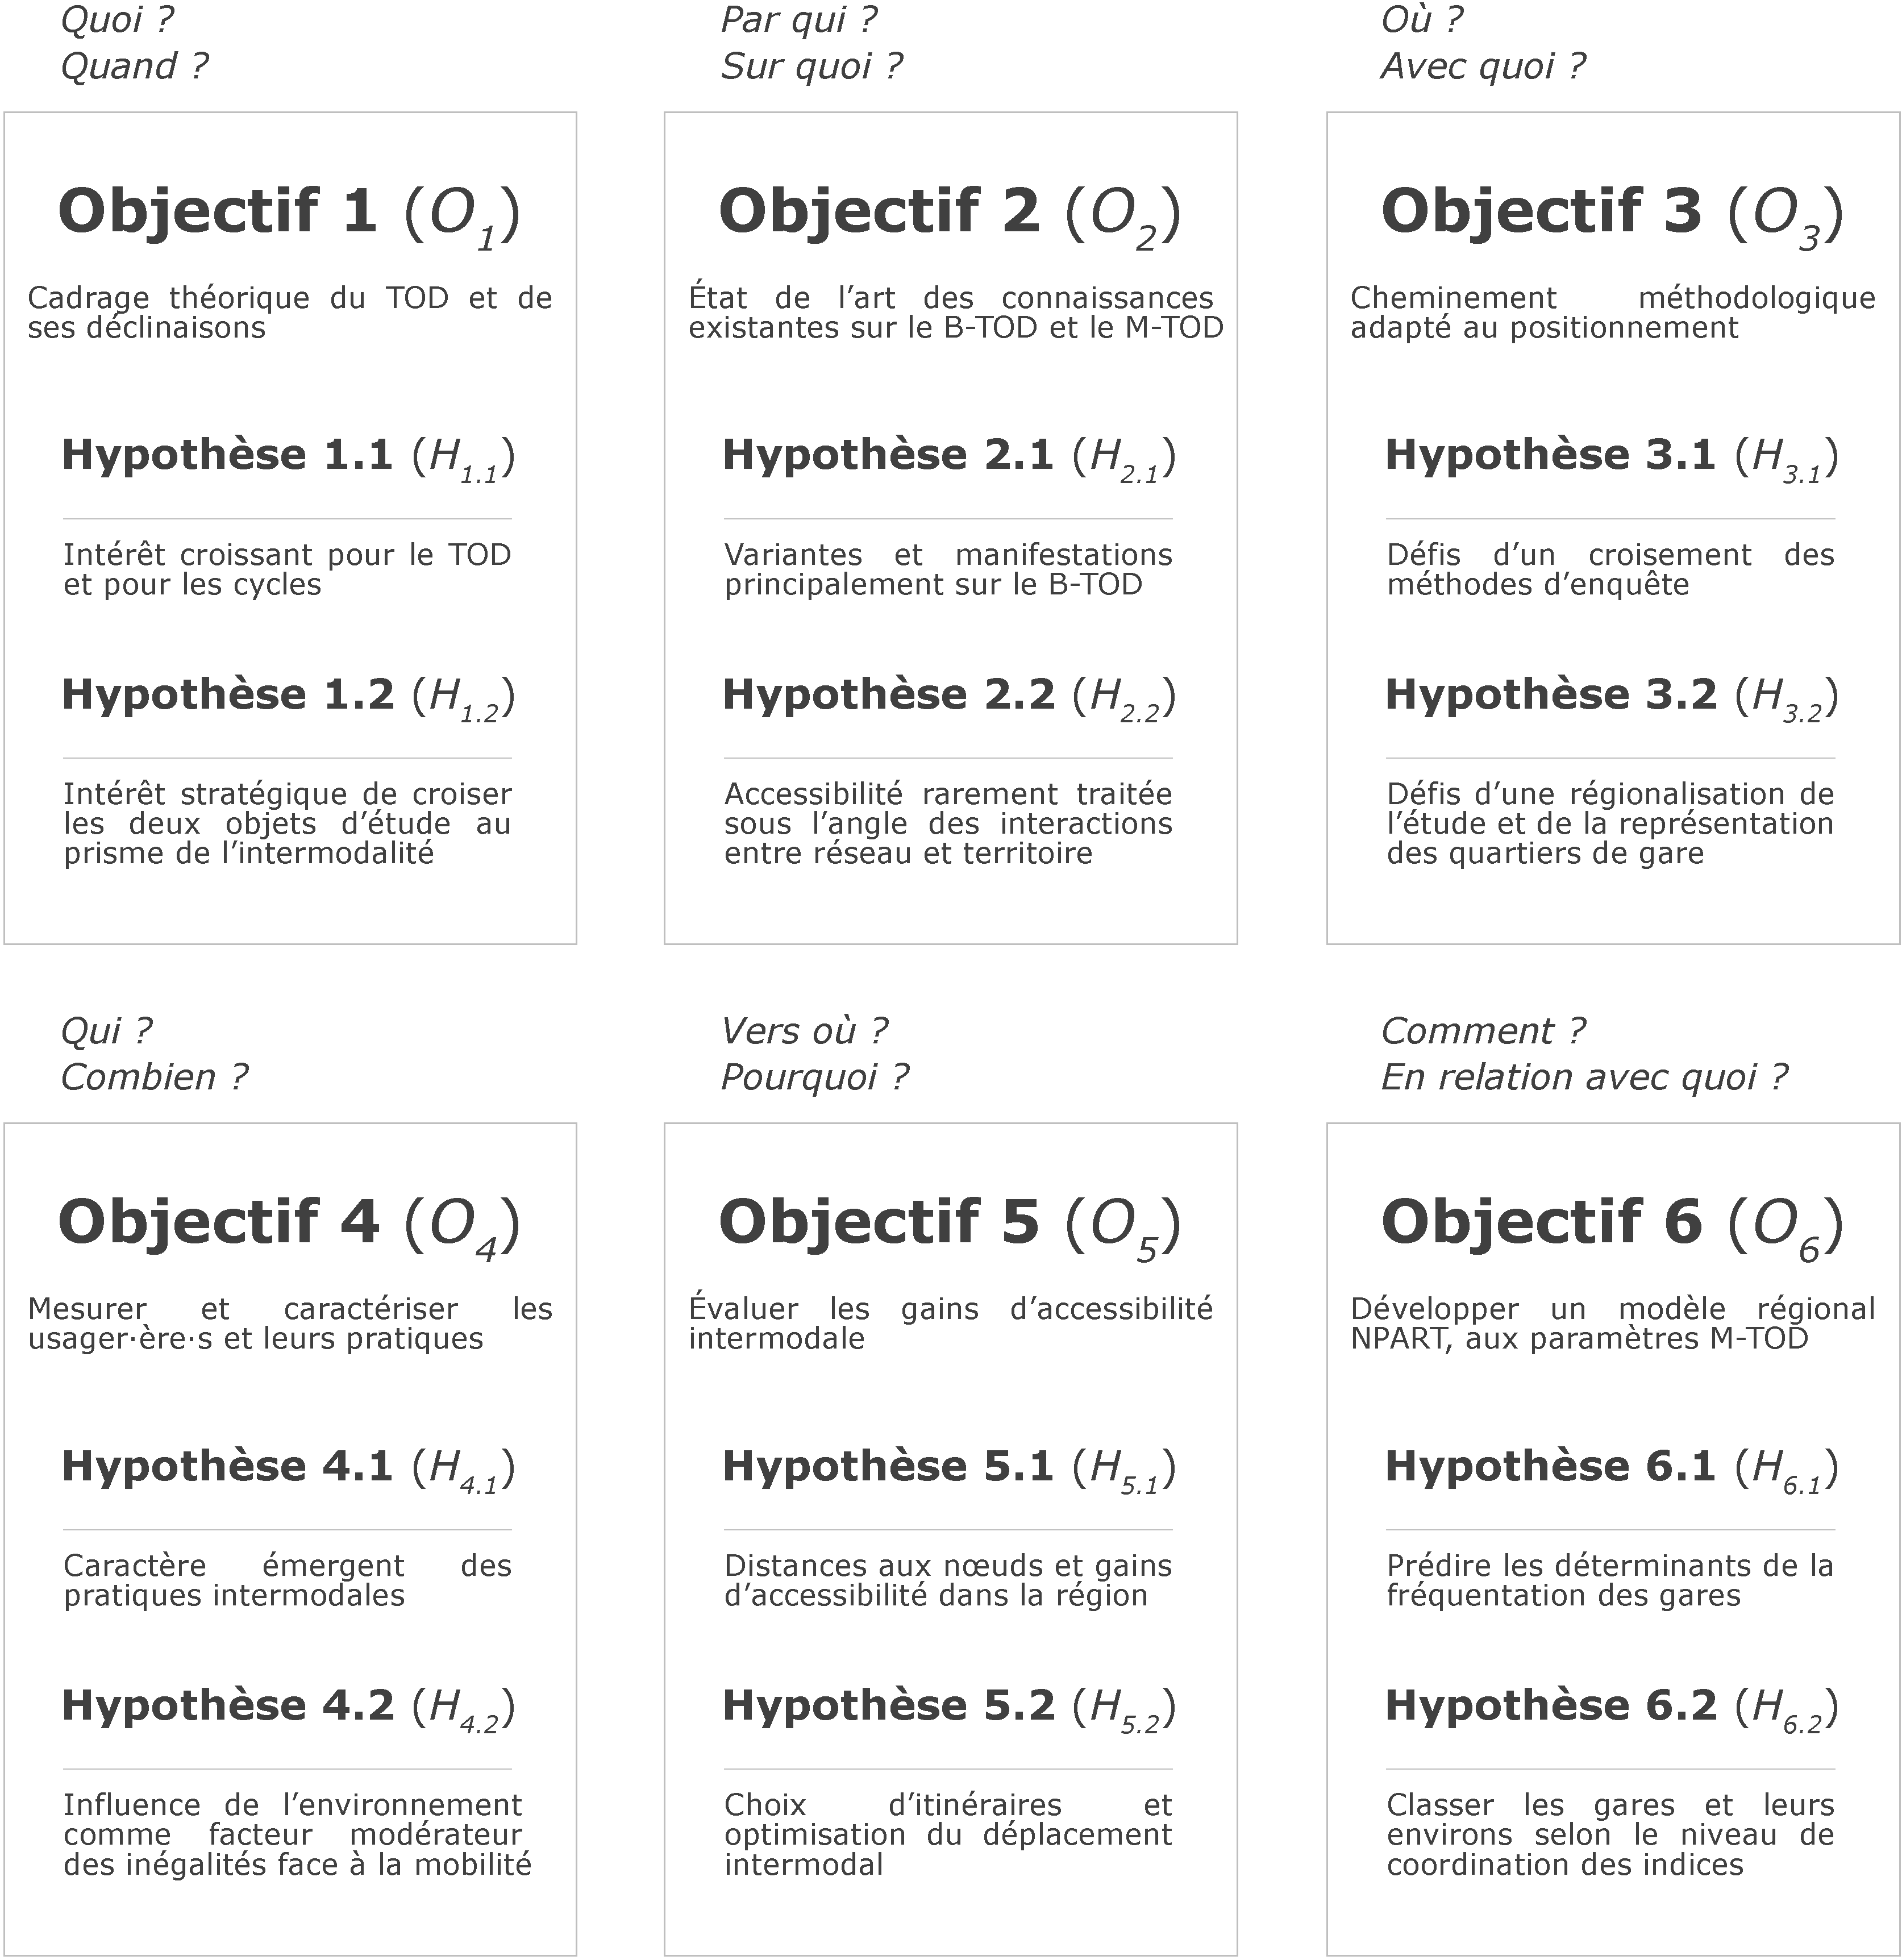
\includegraphics[width=1\columnwidth]{src/Figures/Introduction/FR_Objectifs_recherche.pdf}}
        \vspace{5pt}
        \begin{flushright}\scriptsize{
        Auteur~: \textcolor{blue}{Dylan Moinse (2023)}
        }\end{flushright}
    \end{figure}

    % Hypothèses
À partir des objectifs préalablement définis, lesquels structurent les différents chapitres de cette thèse, se dégagent les hypothèses de recherche qui constitueront le fil conducteur de notre démonstration tout au long de ce travail scientifique (voir le \hyperref[fig-introduction:objectifs-hypotheses]{schéma~\ref{fig-introduction:objectifs-hypotheses}}, page~\pageref{fig-introduction:objectifs-hypotheses}). Ces hypothèses s’inscrivent dans une démarche hypothético-déductive et se caractérisent par leur nature associative, complexe et directionnelle\footnote{
    Selon \textcolor{blue}{\textcite[41-43]{tomini_methodes_2020}}\index{Tomini, Luca|pagebf}\index{Wintgens, Sophie|pagebf}, dans leur manuel \textsl{Méthodes d'enquêtes de terrain en sciences sociales}, les hypothèses associatives postulent une relation d'interaction entre les concepts~; les hypothèses complexes, quant à elles, précisent une relation entre plusieurs concepts~; tandis que les hypothèses directionnelles formulent l'orientation des liens qui unit ces concepts.
} \textcolor{blue}{\autocite[43]{tomini_methodes_2020}}\index{Tomini, Luca|pagebf}\index{Wintgens, Sophie|pagebf}. En nous appuyant sur ces objectifs, nous proposons ainsi d’énoncer les hypothèses qui guideront notre réflexion~:
        \begin{customitemize}
    \item \textsl{Les thématiques de recherche émergentes relatives au \textsl{Transit-Oriented Development} et à la mobilité individuelle légère méritent d’être appréhendées de manière conjointe} ({\textcolor{blue}{\(H_1\)}\label{hypothese-1}}). En effet, ces deux axes suscitent un intérêt croissant tant dans les sphères académiques qu'opérationnelles ({\textcolor{blue}{\(S.H_{1.1}\)}\label{sous-hypothese-1.1}}) et gagneraient à être étudiés de manière articulée pour en révéler les synergies potentielles ({\textcolor{blue}{\(S.H_{1.2}\)}\label{sous-hypothese-1.2}})~;
    \item \textsl{Les connaissances actuelles relatives à cette synergie intermodale demeurent fortement conditionnées par le couple vélo et train, et sont rarement analysées au prisme du \textsl{Transit-Oriented Development}} ({\textcolor{blue}{\(H_2\)}\label{hypothese-2}}). En effet, les travaux existants se concentrent principalement sur l'objet vélo ({\textcolor{blue}{\(S.H_{2.1}\)}\label{sous-hypothese-2.1}}), tandis que les questions d’accessibilité sont majoritairement traitées sous l’angle strictement lié aux problématiques de transport ({\textcolor{blue}{\(S.H_{2.2}\)}\label{sous-hypothese-2.2}})~;
    \item \textsl{L’appréhension de la complexité des dynamiques intermodales et de leurs implications sur l’environnement urbain se heurte à la difficulté de définir une méthodologie d’analyse} ({\textcolor{blue}{\(H_3\)}\label{hypothese-3}}). Face aux lacunes identifiées dans la littérature, il apparaît pertinent de mobiliser une approche méthodologique mixte, combinant diverses méthodes d’enquête ({\textcolor{blue}{\(S.H_{3.1}\)}\label{sous-hypothese-3.1}}). De surcroît, l’adoption d’un périmètre d’étude à l’échelle régionale et la redéfinition de la notion de quartier de gare, en adéquation avec les principes du \acrshort{TOD}, s’imposent comme des ajustements nécessaires ({\textcolor{blue}{\(S.H_{3.2}\)}\label{sous-hypothese-3.2}})~;
    \item \textsl{Les pratiques intermodales connaissent un essor significatif sous l’effet conjugué de l’émergence de nouvelles solutions de mobilité, même si celles-ci sont marquées par une appropriation différenciée par divers groupes sociaux} ({\textcolor{blue}{\(H_4\)}\label{hypothese-4}}). Le développement de l’intermodalité intégrant les cycles et le transport public s’inscrit dans un processus de diversification et d'appropriation des modes de déplacement ({\textcolor{blue}{\(S.H_{4.1}\)}\label{sous-hypothese-4.1}}). Toutefois, cette appropriation reste inégale, certains groupes sociaux s’en saisissant plus aisément que d’autres, une situation qui pourrait néanmoins être atténuée par des interventions en matière d’aménagement du territoire ({\textcolor{blue}{\(S.H_{4.2}\)}\label{sous-hypothese-4.2}})~;
    \item \textsl{L’intégration de la mobilité individuelle légère au sein des réseaux de transport en commun constitue un levier majeur d’amélioration de l’accessibilité régionale} ({\textcolor{blue}{\(H_5\)}\label{hypothese-5}}). En effet, cette intégration permet d’accroître la portée des déplacements, étendant ainsi les périmètres de desserte des quartiers de gare et facilitant l’accès aux destinations ({\textcolor{blue}{\(S.H_{5.1}\)}\label{sous-hypothese-5.1}}). De plus, elle favorise l’optimisation des itinéraires, rendant les déplacements intermodaux plus compétitifs face à l’usage de l’automobile, y compris en ce qui concerne les mobilités quotidiennes de longue distance ({\textcolor{blue}{\(S.H_{5.2}\)}\label{sous-hypothese-5.2}})~;
    \item \textsl{L’élargissement du concept d’aménagement à la mobilité individuelle légère constitue un levier de dynamisation des quartiers de gare, en renforçant leur accessibilité dans une acception élargie} ({\textcolor{blue}{\(H_6\)}\label{hypothese-6}}). Certains facteurs liés à la cyclabilité des quartiers de gare contribuent à stimuler la demande autour des pôles d’échange ({\textcolor{blue}{\(S.H_{6.1}\)}\label{sous-hypothese-6.1}}), tout en les rendant plus cohérents avec les principes directeurs du \acrshort{TOD} ({\textcolor{blue}{\(S.H_{6.2}\)}\label{sous-hypothese-6.2}}).
\end{customitemize}%%Rédigé%%

% --- %
    % *.4. Méthodologie
    \needspace{1\baselineskip} % Réserve de l'espace
\section*{Stratégie de recherche
    \label{introduction-generale:methodologie}
    }
    \addcontentsline{toc}{section}{Stratégie de recherche}
    %\markboth{Méthodologie}{}
    \markright{Cadre méthodologique}{}

    % Introduction
Afin de répondre à la problématique de cette recherche ainsi qu’aux objectifs et hypothèses formulés, cette thèse adopte un dispositif méthodologique mixte, combinant des méthodes originales et adaptées aux spécificités du sujet étudié (voir le \hyperref[fig-introduction:methodes-hypotheses]{schéma~\ref{fig-introduction:methodes-hypotheses}}, page~\pageref{fig-introduction:methodes-hypotheses}). Cette démarche méthodologique permet d’articuler trois dimensions essentielles~: (i) une réflexion conceptuelle sur l’évolution du \acrshort{TOD} et son articulation avec la mobilité individuelle légère~; (ii) une investigation sur les pratiques intermodales existantes et les facteurs influençant ces comportements de mobilité~; et (iii) une évaluation des effets de la mobilité individuelle légère sur l’accessibilité aux gares et sur la structuration des quartiers environnants, dans un périmètre régional. Loin de constituer une approche linéaire, ce cheminement méthodologique assume sa complexité, mobilisant des outils complémentaires afin de saisir les multiples dimensions du \acrshort{TOD} et de la mobilité individuelle légère, conformément à l'\hyperref[hypothese-3]{hypothèse~\(H_3\)} (page~\pageref{hypothese-3}).%%Rédigé%%

    % Figure méthodologie hypothèses
    \begin{figure}[h!]\vspace*{4pt}
        \caption{Cadre méthodologique pensé en dialogue avec les hypothèses de recherche}
        \label{fig-introduction:methodes-hypotheses}
        \centerline{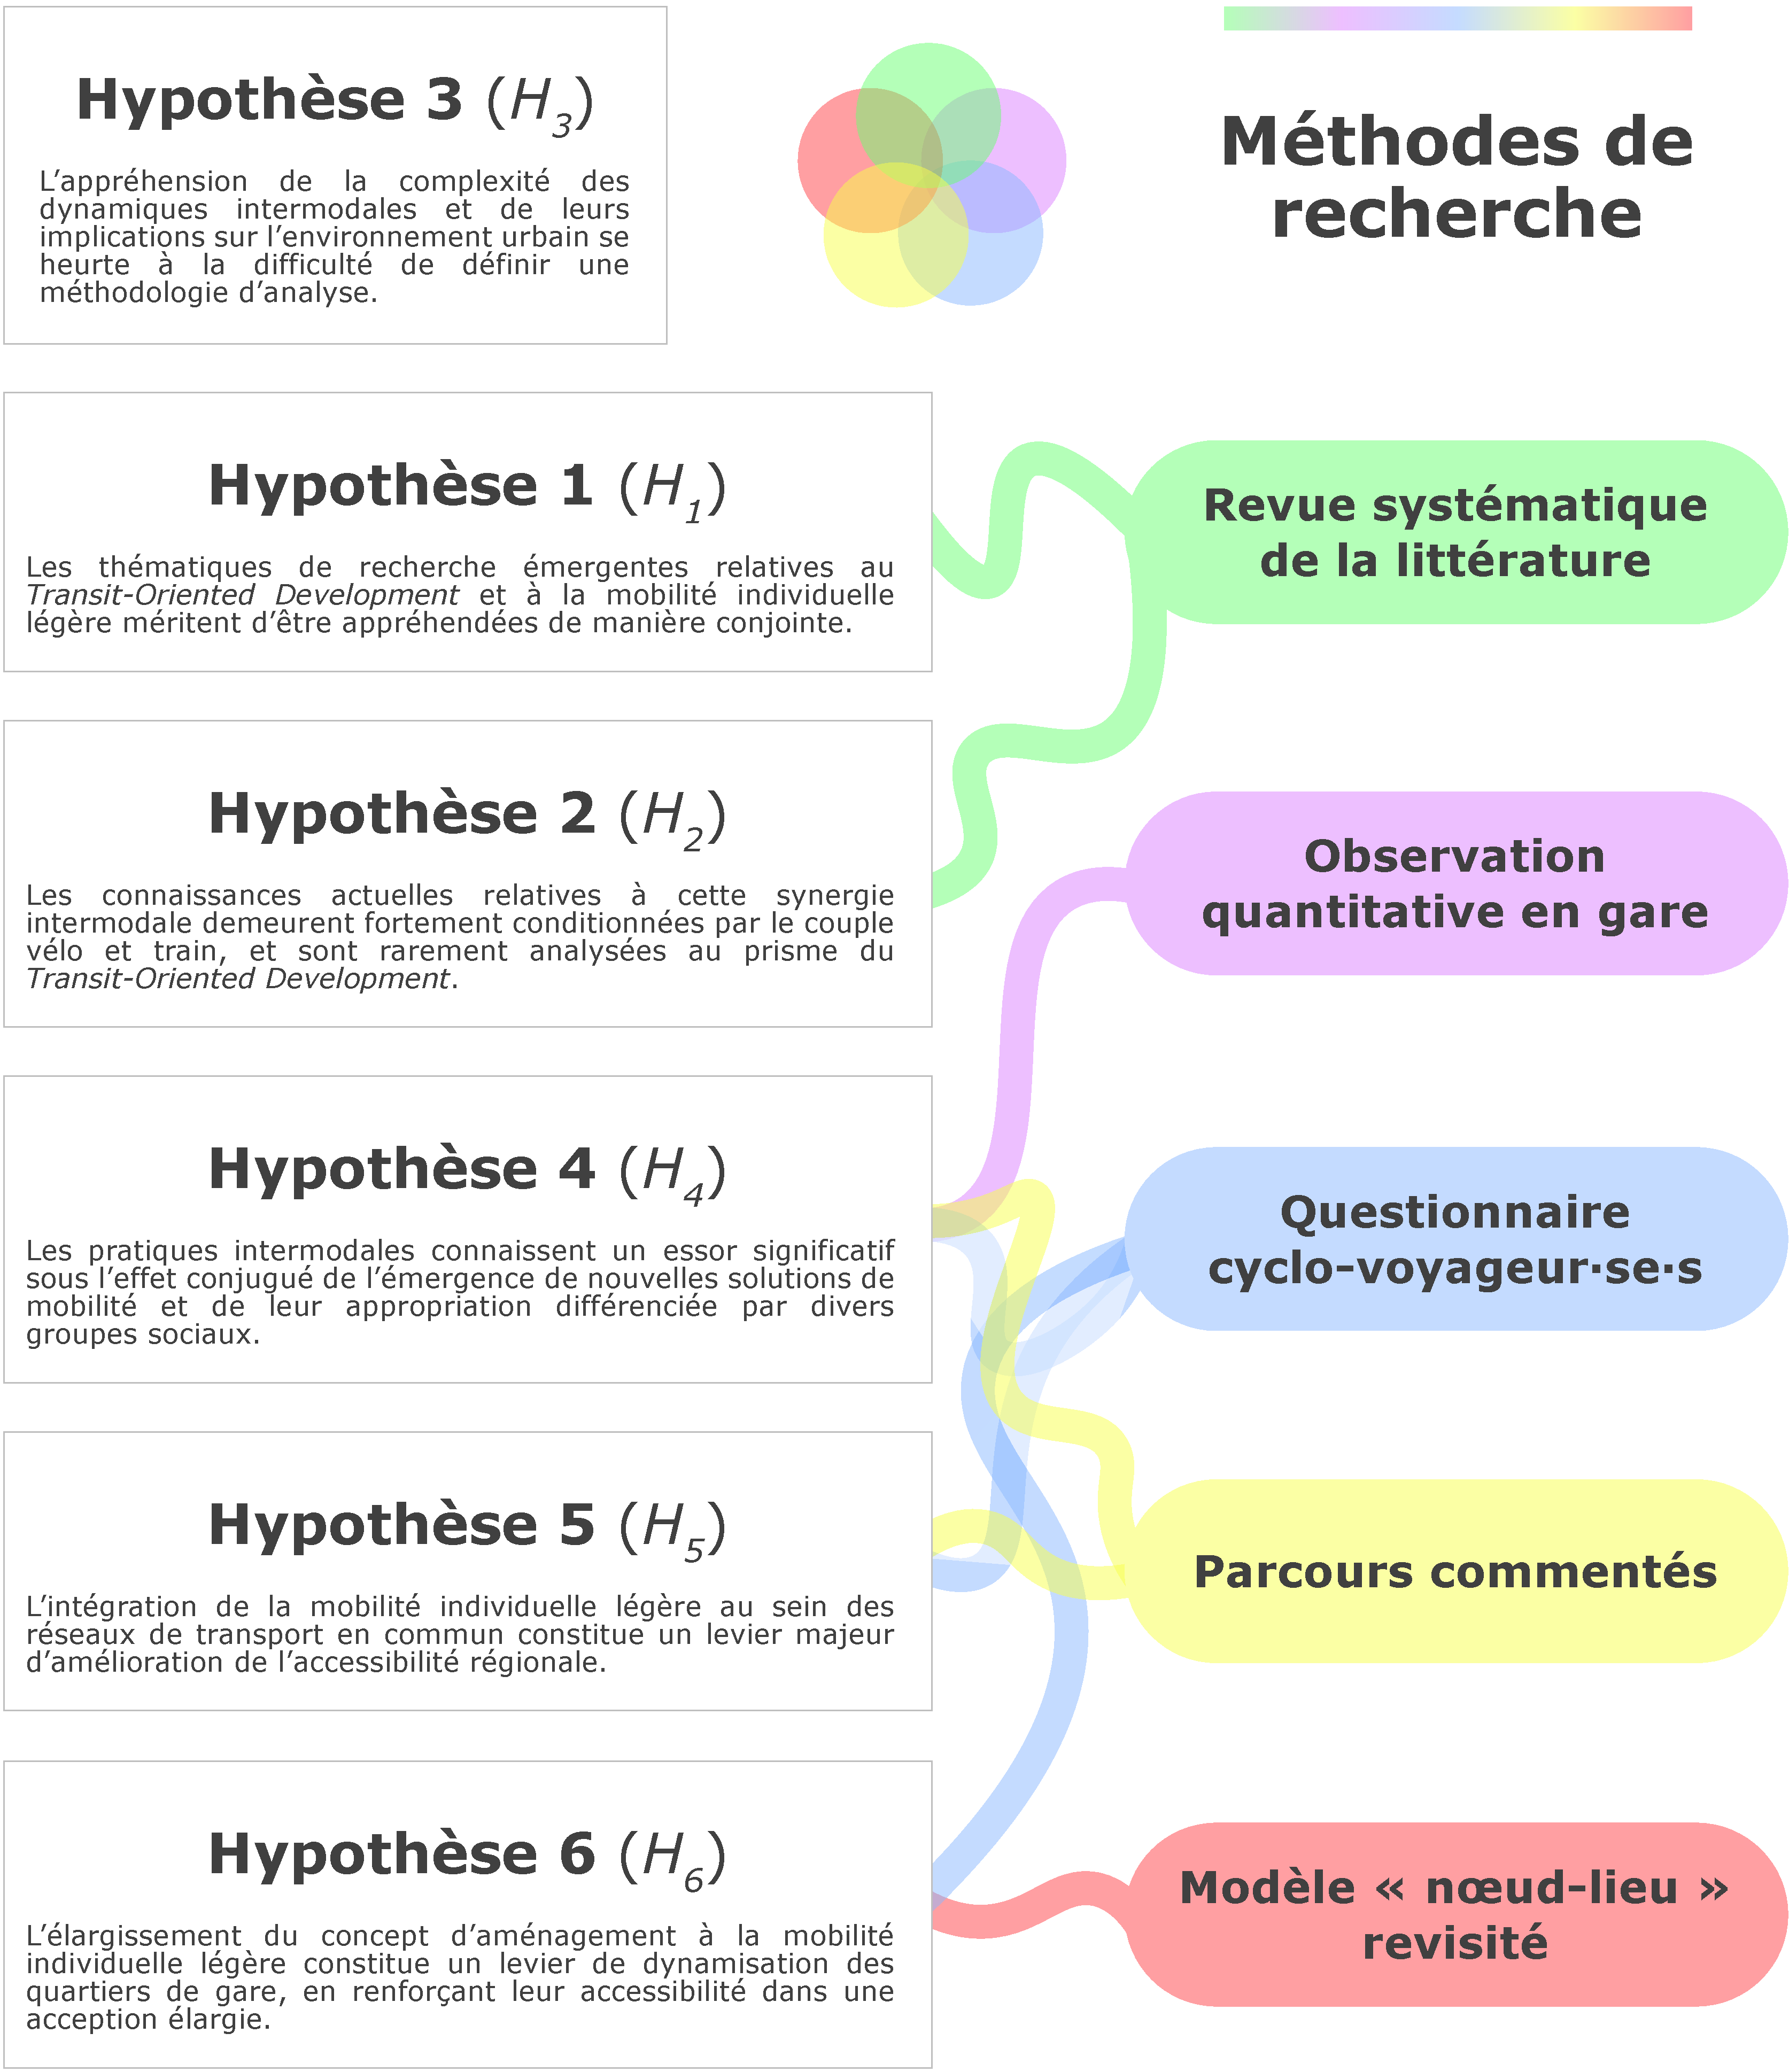
\includegraphics[width=1\columnwidth]{src/Figures/Introduction/FR_Methodologie_hypotheses.pdf}}
        \vspace{5pt}
        \begin{flushright}\scriptsize{
        Auteur~: \textcolor{blue}{Dylan Moinse (2025)}
        }\end{flushright}
    \end{figure}

    % Méthodologie
La méthodologie retenue repose, en premier lieu, sur le besoin de synthétiser les travaux et les connaissances existants, relatifs à la problématique de recherche. À cette fin, une \acrfull{RSL} a été conduite sur les études s’apparentant aux contours du \acrshort{B-TOD} et du \acrshort{M-TOD}, dans la continuité des \hyperref[hypothese-1]{hypothèses~\(H_1\)} et \hyperref[hypothese-2]{\(H_2\)} (page~\pageref{hypothese-2}). S'ensuit une exploration de terrain sous la forme d’une observation quantitative, visant à caractériser le phénomène émergent de la connexion nodale réalisée à l'aide de la mobilité individuelle légère, en adéquation avec l'\hyperref[hypothese-4]{hypothèse~\(H_4\)} (page~\pageref{hypothese-4}). Cette enquête est complétée par la conduite d'entretiens mobiles, le parcours commenté, venant enrichir l'investigation en accédant à la \gls{perception} des usager·ère·s et d'affiner la compréhension de leurs pratiques intermodales. Un troisième type d’enquête repose sur un questionnaire adressé aux cyclo-voyageur·se·s, destiné à représenter les déplacements intermodaux en vue d’identifier les territoires fréquentés et vécus à proximité des pôles d’échange, dans le prolongement de l'\hyperref[hypothese-5]{hypothèse~\(H_5\)} (page~\pageref{hypothese-5}). Enfin, une modélisation spatiale a été entreprise, dans le but de revisiter l'outil \Guillemets{nœud-lieu}, usuellement appliqué dans les travaux sur le \acrshort{TOD}. Cette modélisation permet de saisir les implications de l’intégration de la mobilité individuelle légère et d’identifier ses interactions avec l’environnement urbain, en appui sur l'\hyperref[hypothese-6]{hypothèse~\(H_6\)} (page~\pageref{hypothese-6}).%%Rédigé%%

% --- %
    % *.5. Annonce du plan
    \needspace{1\baselineskip} % Réserve de l'espace
\section*{Structure de la thèse
    \label{introduction-generale:annonce-plan}
    }
    \addcontentsline{toc}{section}{Structure de la thèse}
    %\markboth{Annonce du plan}{}
    \markright{Annonce du plan}{}

    % Introduction
Cette thèse se structure en trois parties et six chapitres, suivant une progression logique qui permet d’explorer les fondements théoriques, les enjeux et les implications de l’intégration de la mobilité individuelle légère dans le modèle du \acrshort{TOD} (voir le \hyperref[fig-introduction:structure-these]{schéma~\ref{fig-introduction:structure-these}}, page~\pageref{fig-introduction:structure-these}). Alternant entre approche conceptuelle, état de l’art, cadre méthodologique, étude empirique et modélisation prospective, elle aboutit à la proposition d’un modèle renouvelé~: un \acrfull{M-TOD}. L’argumentaire développé repose sur trois axes majeurs~: (i) une compréhension approfondie des usages et des comportements liés à la mobilité individuelle légère dans une perspective intermodale~; (ii) une analyse multicritère du potentiel d’accueil des territoires en fonction de leur capacité à intégrer ces nouvelles formes de mobilité~; et (iii) une interrogation sur le rôle de l’action publique dans l’aménagement et la structuration de ces pratiques au sein des politiques de transport et d’urbanisme. En parallèle, trois niveaux d’analyse progressifs et multiscalaires sous-tendent cette réflexion~: (i) l’examen des dynamiques de la demande intermodale~; (ii) l’évaluation de l’accessibilité intermodale, considérée sous l’angle de la performance des réseaux, des ressources disponibles, des contraintes temporelles et des caractéristiques individuelles~; (iii) ainsi que l’analyse des interactions entre transport et urbanisme dans un contexte d'intégration modale. La structuration de cette recherche qui traduit la démarche scientifique adoptée peut être synthétisée comme suit~: \textsl{synthétiser et repenser} (voir la \hyperref[part1:titre]{première partie}, page~\pageref{part1:titre})~; \textsl{représenter et comprendre} (voir la \hyperref[part2:titre]{deuxième partie}, page~\pageref{part2:titre})~; puis \textsl{anticiper et orienter} (voir la \hyperref[part3:titre]{troisième partie}, page~\pageref{part3:titre}).%%Rédigé%%

    % Figure structure de la thèse
    \begin{figure}[h!]\vspace*{4pt}
        \caption{Structure générale de la recherche doctorale}
        \label{fig-introduction:structure-these}
        \centerline{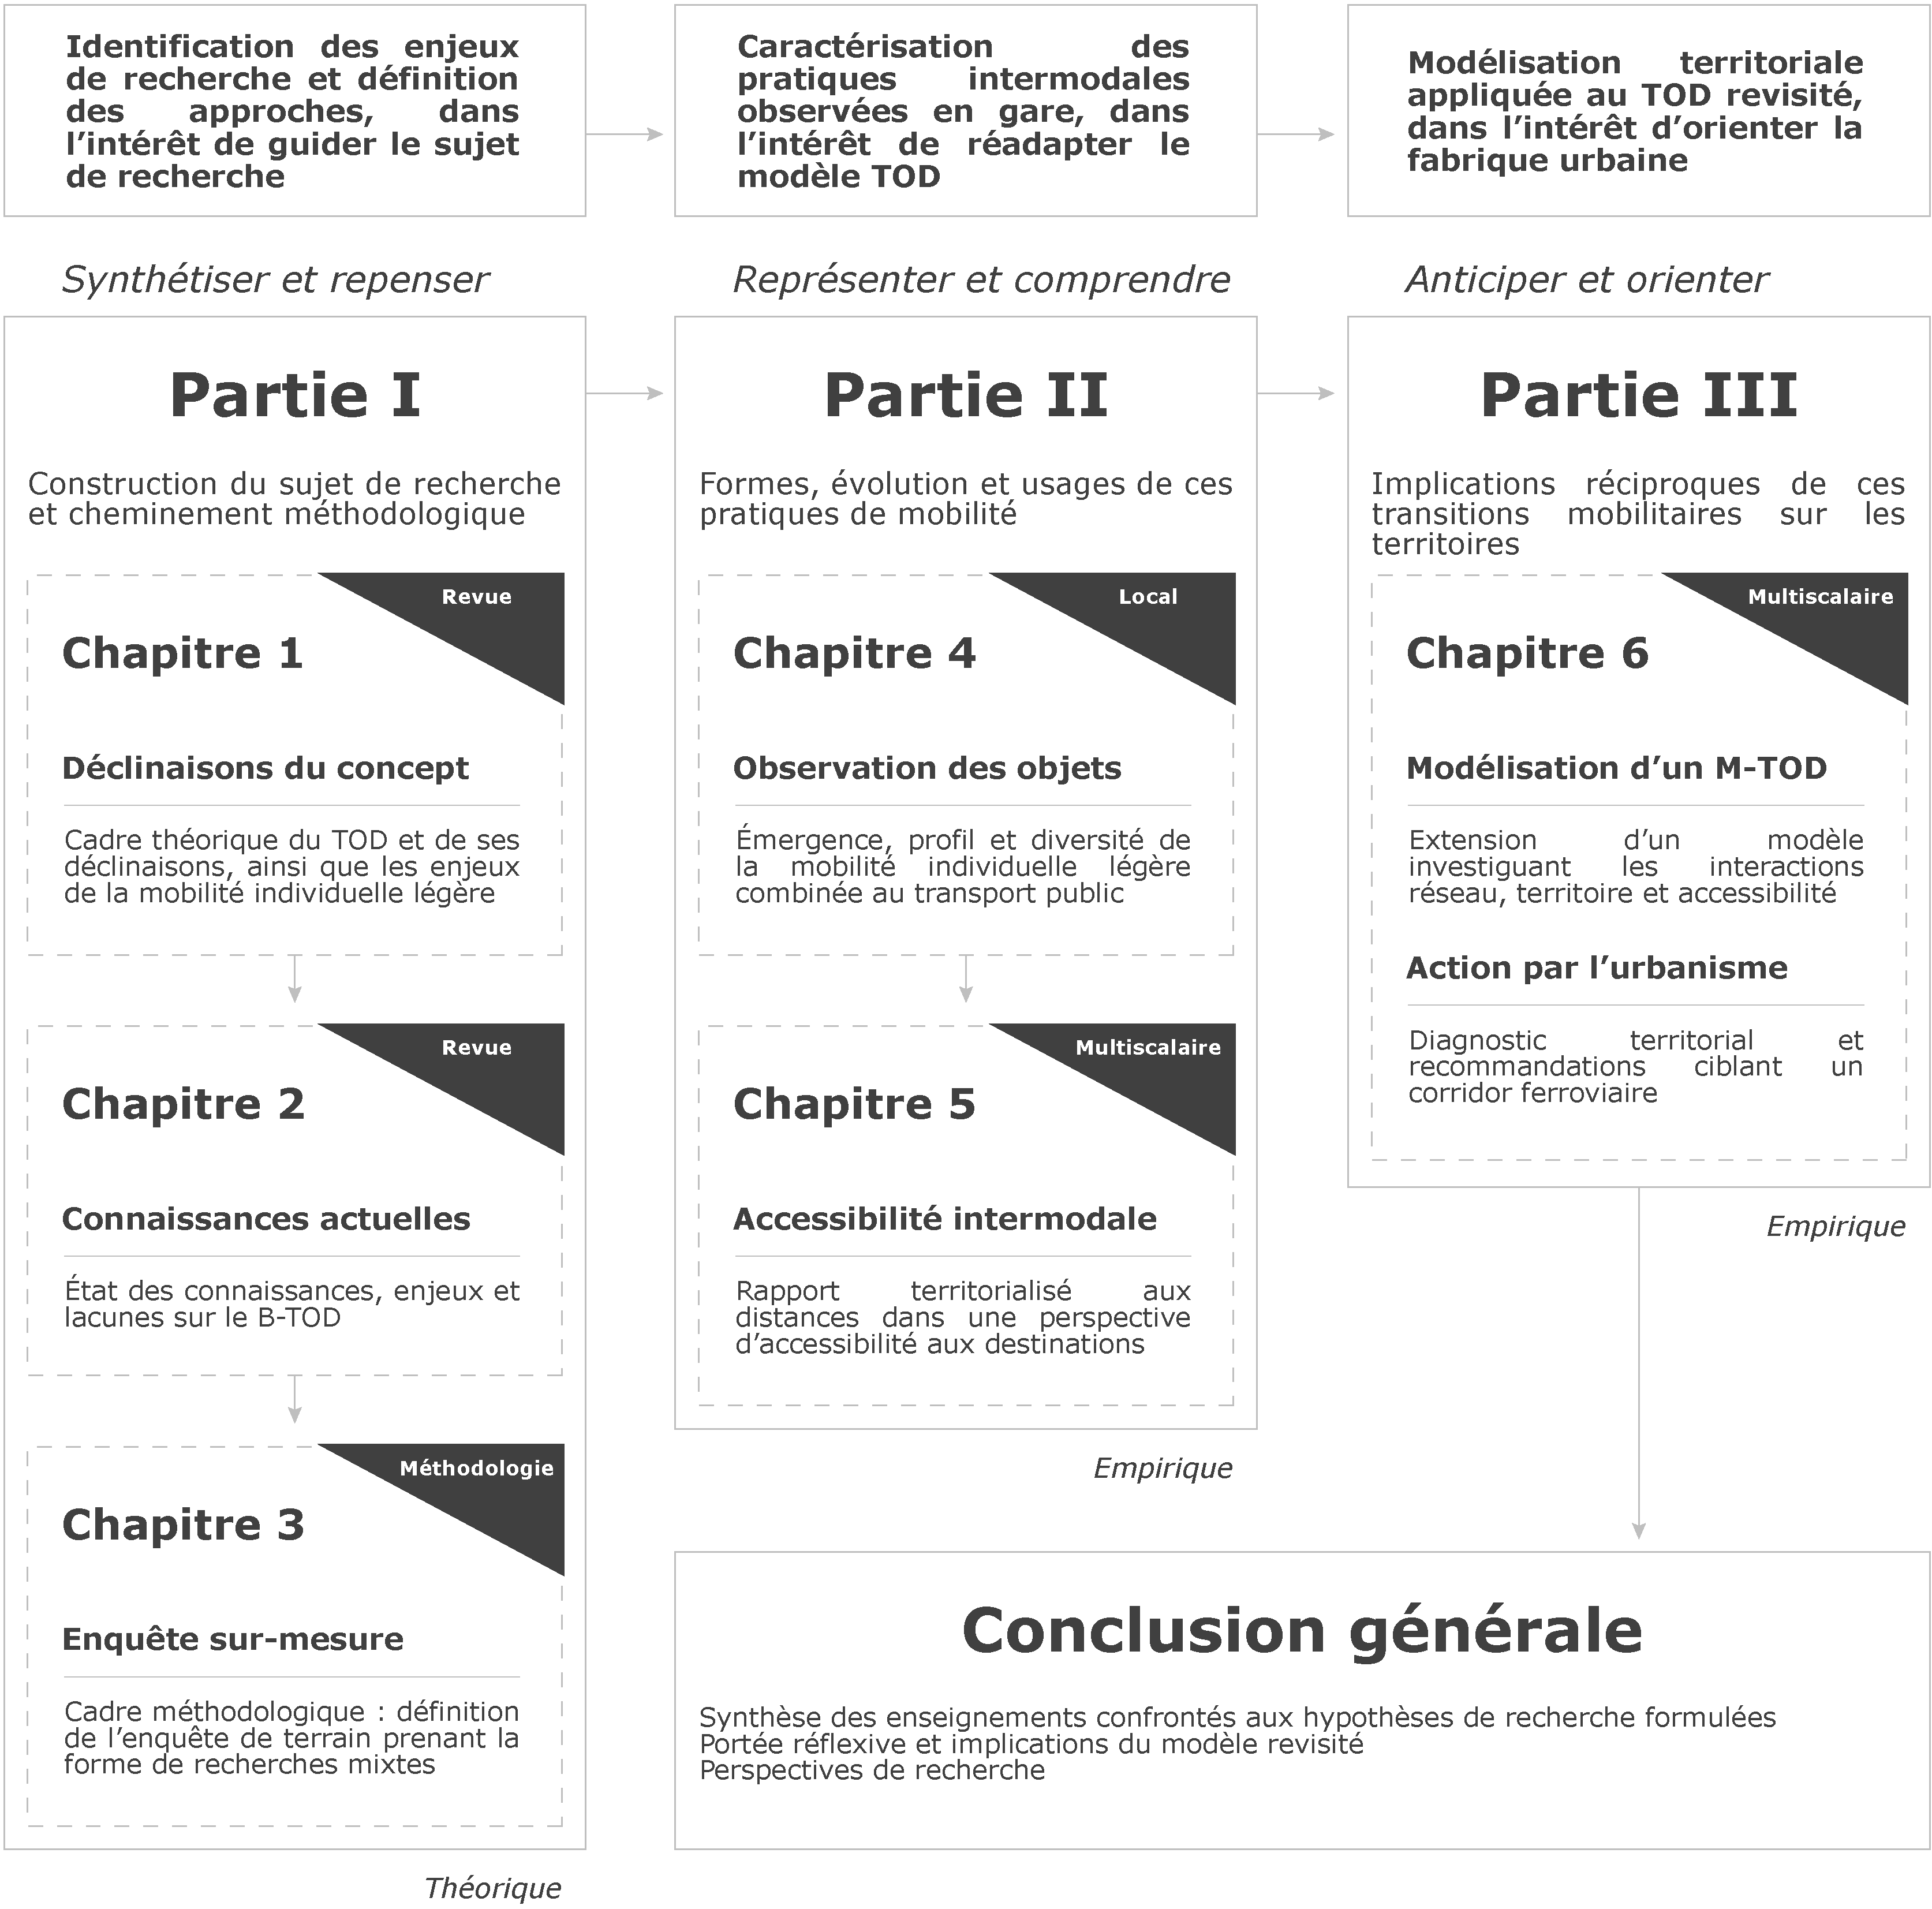
\includegraphics[width=1\columnwidth]{src/Figures/Introduction/FR_Structure_these.pdf}}
        \vspace{5pt}
        \begin{flushright}\scriptsize{
        Auteur~: \textcolor{blue}{Dylan Moinse (2023)}
        }\end{flushright}
    \end{figure}

    % *.5.1. Annonce du plan : partie 1
    \needspace{1\baselineskip} % Réserve de l'espace
\subsection*{Première partie~: \textsl{Synthétiser et repenser}
    \label{introduction-generale:annonce-plan-1}
    }

    % Chapitre 1
\hyperref[chap1:titre]{Le premier chapitre} (page~\pageref{chap1:titre}) pose les bases théoriques de cette recherche en définissant les concepts fondamentaux qui structureront l’argumentation. Il s’attarde tout d’abord sur les principes fondateurs du \acrshort{TOD}, en retraçant son évolution et ses diverses adaptations conceptuelles et opérationnelles. Ce modèle d’aménagement, pensé comme une alternative au système auto-centré, vise à structurer l’urbanisation autour des infrastructures de transport en commun. Toutefois, son application révèle des limites dans certains contextes, notamment dans les territoires périurbains où les distances d’accès aux stations de transport public constituent un frein majeur à son efficacité. C’est dans cette perspective que s’inscrit l’analyse de la mobilité individuelle légère, définie ici comme un ensemble de véhicules incluant le vélo et ses variantes, ainsi que la trottinette et d’autres engins de déplacement. Ces solutions émergent comme un levier stratégique susceptible de pallier les insuffisances du \acrshort{TOD} conventionnel en améliorant l’accessibilité aux nœuds, sous l'angle des \Guillemets{premiers et derniers kilomètres} du transport public. Ce chapitre explore ainsi la montée en puissance des cycles dans la mobilité quotidienne et leur prise en compte progressive dans les politiques d’aménagement. Il s’attache ensuite à examiner les opportunités qu’implique l’intégration de la mobilité individuelle légère dans la pensée du \acrshort{TOD}, en interrogeant ses implications en matière de proximité géographique et d’intermodalité. Enfin, il s’achève sur une revue critique de la littérature, mettant en évidence les lacunes théoriques et les potentiels d’un modèle élargi intégrant ces nouvelles articulations entre mobilité et urbanisme, qui viennent justifier l’investigation menée dans cette thèse (\hyperref[objectif-1]{objectif~\(O_1\)}, page~\pageref{objectif-1}).%%Rédigé%%

    % Chapitre 2
\hyperref[chap2:titre]{Le deuxième chapitre} (page~\pageref{chap2:titre}) prolonge la réflexion engagée sur l’évolution du \acrshort{TOD} en approfondissant l’état des connaissances sur ses déclinaisons intégrant la mobilité individuelle légère, en particulier le \acrshort{B-TOD} et le \acrshort{M-TOD}. Il dresse un état de l’art sur l’articulation entre le vélo, la micro-mobilité et le transport public, en questionnant ces interactions à l'interface des systèmes de mobilité et de l'organisation territoriale. S’appuyant sur une \acrfull{RSL}, ce chapitre mobilise une approche scientométrique permettant d’identifier les dynamiques géographiques, temporelles et institutionnelles structurant ces modèles d'urbanisme. Cette étude soutient l’essor récent des recherches consacrées à ces thématiques et l’émergence de nouveaux outils méthodologiques, en particulier l’exploitation de la \textsl{Big Data} et des modèles d'analyse géostatistiques. Elle identifie les principaux déterminants urbains influençant les comportements de mobilité et évalue les gains d’accessibilité induits par l’intégration de la mobilité individuelle légère dans les stratégies \acrshort{TOD}\textcolor{blue}{s}. Sur la base de ces éléments, ce chapitre définit les assises théoriques et méthodologiques sur lesquelles repose l'investigation empirique conduite dans les prochains chapitres (\hyperref[objectif-2]{objectif~\(O_2\)}, page~\pageref{objectif-2}).%%Rédigé%%

    % Chapitre 3
\hyperref[chap3:titre]{Le troisième chapitre} (page~\pageref{chap3:titre}) marque l'entrée sur le terrain d'étude de la thèse en cherchant à évaluer l'intégration de la mobilité individuelle légère dans le modèle urbain. Il expose le cadre méthodologique adopté pour mener cette enquête. Ce chapitre prend part à une réflexion sur le positionnement épistémologique de la recherche, en justifiant l’adoption de recherches mixtes, combinant approches quantitatives et qualitatives. Cette méthodologie permet d’appréhender la complexité des comportements de mobilité ainsi que leurs rapports et leurs effets sur l'accessibilité territoriale, en croisant différentes sources d’information. Cette démarche, décrivant les choix méthodologiques, les outils de collecte et de traitement des données ainsi que la construction des terrains, pose le socle analytique qui guide l’interprétation des résultats dans les parties qui suivent (\hyperref[objectif-3]{objectif~\(O_3\)}, page~\pageref{objectif-3}).%%Rédigé%%

    % *.5.2. Annonce du plan : partie 2
    \needspace{1\baselineskip} % Réserve de l'espace
\subsection*{Deuxième partie~: \textsl{Représenter et comprendre}
    \label{introduction-generale:annonce-plan-2}
    }

    % Chapitre 4
\hyperref[chap4:titre]{Le quatrième chapitre} (page~\pageref{chap4:titre}) constitue la première phase de l’analyse empirique en s’attachant à l’étude des pratiques intermodales associées à la mobilité individuelle légère, qui s'inscrivent dans les quartiers de gare. Il vise, d’une part, à quantifier l’ampleur du phénomène, en mesurant la part modale des modes de transfert dans les chaînes de déplacement impliquant les transports en commun. D’autre part, il cherche à mieux définir le corpus de cyclo-voyageur·se·s et à identifier les facteurs déterminants de leurs choix modaux, en tenant compte de leurs caractéristiques individuelles, de leurs perceptions, ainsi que de leur rapport à l’environnement urbain. Ce chapitre met en lumière les arbitrages réalisés par les usager·ère·s dans leur organisation quotidienne des déplacements intermodaux et souligne le rôle des agencements territoriaux en tant que facteurs structurants de ces pratiques émergentes. Il met en évidence les conditions favorisant leur essor et prépare ainsi l’analyse spatiale du chapitre suivant, en questionnant le rôle de l’accessibilité et des configurations urbaines comme catalyseurs de ces comportements (\hyperref[objectif-4]{objectif~\(O_4\)}, page~\pageref{objectif-4}).%%Rédigé%%

    % Chapitre 5
Sur la base des résultats exploratoires obtenus, \hyperref[chap5:titre]{Le cinquième chapitre} (page~\pageref{chap5:titre}) se focalise sur les gains d'accessibilité générés par ces synergies modales. Il interroge la manière dont ces pratiques intermodales transforment l’accessibilité aux gares et participent à la reconfiguration des quartiers environnants, en redéfinissant les périmètres d’influence des nœuds. Il s'agit principalement d'évaluer l'apport de la mobilité individuelle légère dans l'extension des bassins de desserte des arrêts de transport en commun, ainsi que les bénéfices en termes d'accès régional aux destinations. La projection des itinéraires empruntés met en relief les parcours privilégiés et les facteurs qui influencent ces choix. Cette réflexion conduit à une lecture renouvelée des périmètres fonctionnels des quartiers de gare, en montrant comment l’intégration de la mobilité individuelle légère peut modifier leur organisation spatiale et renforcer leur attractivité en tant que lieu stratégique (\hyperref[objectif-5]{objectif~\(O_5\)}, page~\pageref{objectif-5}).%%Rédigé%%

    % *.5.3. Annonce du plan : partie 3
    \needspace{1\baselineskip} % Réserve de l'espace
\subsection*{Troisième partie~: \textsl{Anticiper et orienter}
    \label{introduction-generale:annonce-plan-3}
    }

    % Chapitre 6
\hyperref[chap6:titre]{Le sixième chapitre} (page~\pageref{chap6:titre}) propose une formalisation du \acrshort{M-TOD}, conçu comme une extension du \acrshort{TOD} veillant à pleinement intégrer les proximités géographiques promises par l'usage de la marche combinée et de la mobilité individuelle légère. À partir des enseignements tirés, ce chapitre engage une modélisation du \acrshort{M-TOD}, de manière à définir ses principes directeurs, ses conditions de mise en œuvre, ainsi que les leviers d’action à activer pour favoriser son développement et maximiser ses bénéfices. La modélisation proposée permet notamment de prédire la fréquentation des gares en fonction des agencements territoriaux de chacun des quartiers de gare examinés, et des échelles d’accessibilité piétonnière et cyclable dans le périmètre régional étudié. Une classification des gares et de leurs bassins de desserte est alors établie, permettant d’identifier les pôles urbains stratégiques détenant un potentiel de mise en application du \acrshort{TOD} et du \acrshort{M-TOD}, ainsi que ceux pour lesquels des investissements et des améliorations sont à envisager afin de renforcer leur rôle dans un système de mobilité alternatif global. Enfin, ce chapitre s’ouvre sur la production d'un diagnostic territorial en formulant une série de recommandations stratégiques, appliquées à une étude de cas portant sur un corridor ferroviaire (\hyperref[objectif-6]{objectif~\(O_6\)}, page~\pageref{objectif-6}).%%Rédigé%%

    % ___________________________________________
    % Sous-bibliographie
    \newpage
    %\sectionheader{Sous-bibliographie de l'introduction générale}
    \begingroup
    \renewcommand{\bibfont}{\scriptsize}
\printbibliography[segment=\therefsegment, heading=subbibintoc, title={Sous-bibliographie de l'introduction générale}, label=introduction:bibliographie]
    \endgroup
    \end{refsegment}

%% ______________________________ %%
% PARTIE 1

% Introduction de la partie 1
%------------------------------%
%% ✎ Dylan (V1) %%%%%%%%% ✅ %%
%% ✎ Alain (V2) %%%%%%%%% ❌ %%
%% ✎ Dylan (V3) %%%%%%%%% ❌ %%
%------------------------------%

\afterpage{%
%\afterpage{%

    % Arrière-plan partie I
    \AddToShipoutPictureBG*{%
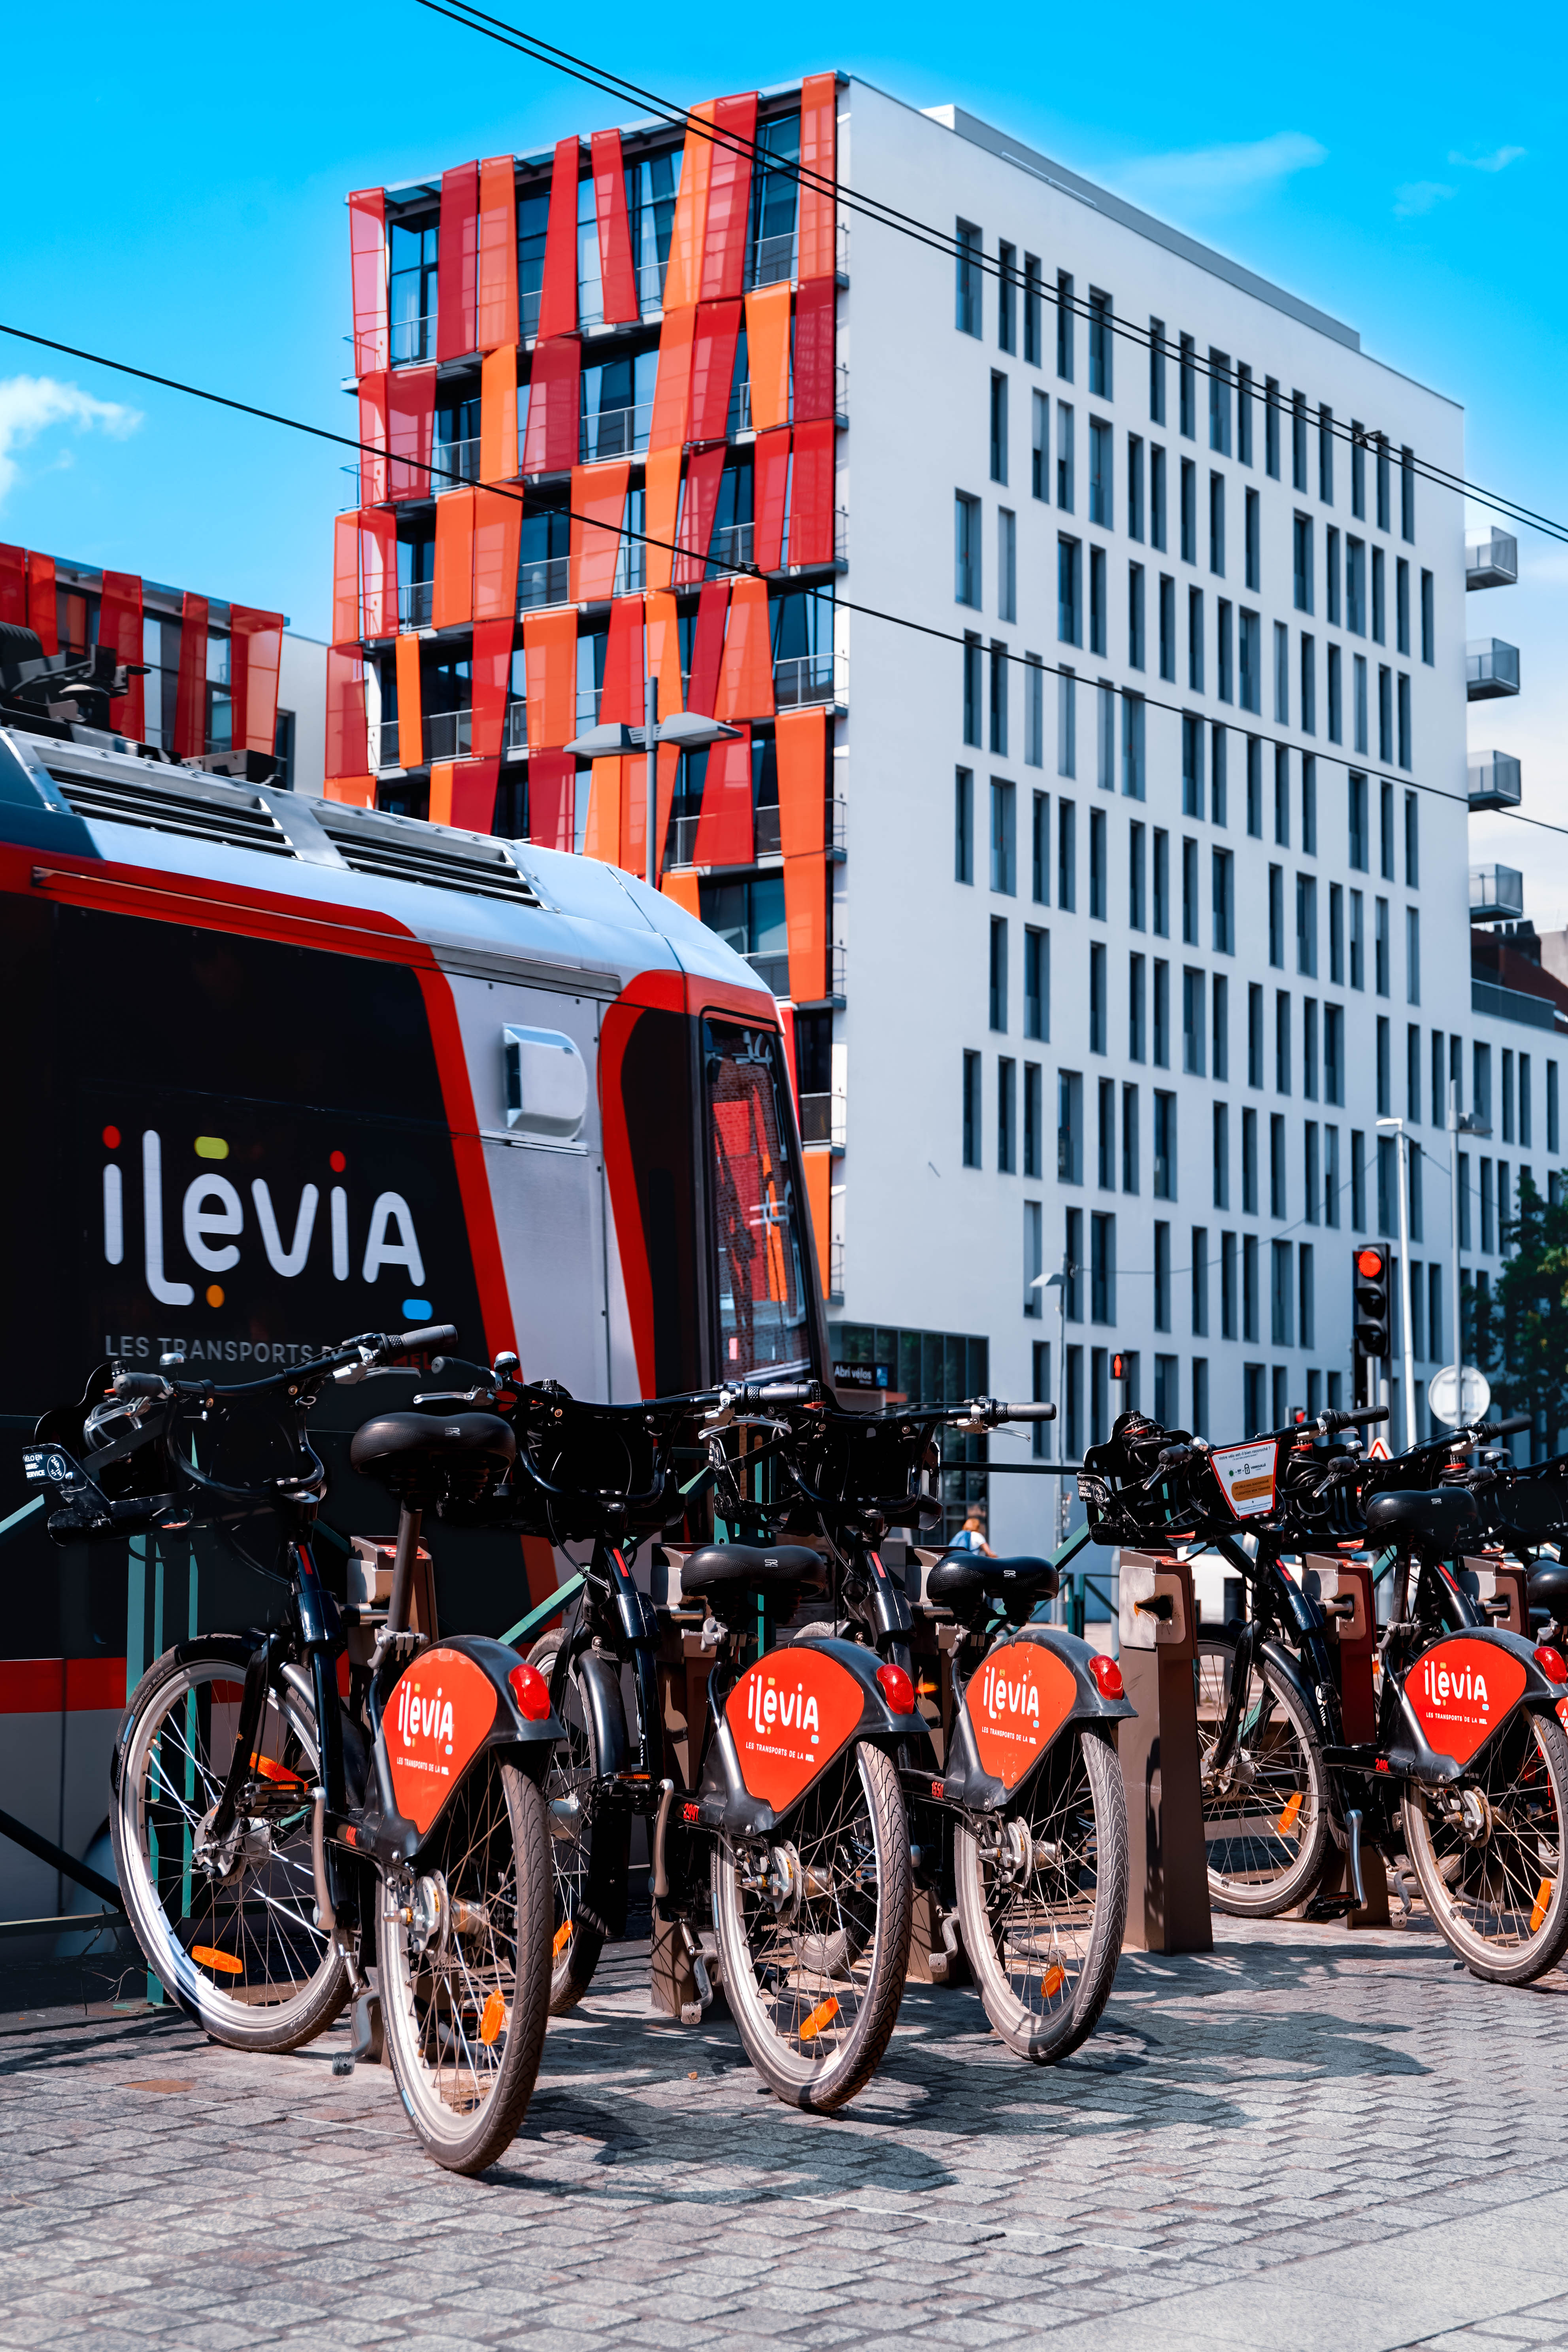
\includegraphics[width=\paperwidth,height=\paperheight]{src/Figures/Arriere_plan/Arriere_plan_Part_1.jpg}
    }

% Rectangle
\AddToShipoutPictureBG*{
  \begin{tikzpicture}[remember picture,overlay]
    \node[fill=white, opacity=0.75, text width=\paperwidth, minimum height=10cm, anchor=north] 
    at ([yshift=-7.7cm]current page.north) {};
  \end{tikzpicture}
}

% Source
\AddToShipoutPictureFG*{
  \AtPageLowerRight{
    \raisebox{1cm}{
      \hspace{16cm}
      
\begin{tikzpicture}
        \node[fill=white, rounded corners=5pt, inner sep=5pt, align=center] {
          \tiny{Photographie~: \textcolor{blue}{Dylan Moinse (2021)}}
        };
      \end{tikzpicture}
    }
  }
}
}%}

\renewcommand{\thefigure}{\thechapter.\arabic{figure}} % Numérotation standard
\renewcommand{\thetable}{\thechapter.\arabic{figure}}
\setcounter{figure}{0}

\needspace{1\baselineskip} % Réserve de l'espace
\part{Cadres théorique et méthodologique pour une intégration de la mobilité individuelle légère en vue d'un urbanisme orienté vers le rail
    \label{part1:titre}
    }
    \markboth{Partie~I~: Cadres théorique et méthodologique de la recherche}{}
    \markright{Partie~I~: Cadres théorique et méthodologique de la recherche}{}

% Introduction de la partie I
\cleardoublepage
\section*{Introduction de la partie~I
    \label{part1:introduction}
    }
    \addcontentsline{toc}{chapter}{Introduction de la partie~I}

    % Introduction
\lettrine[lines=3, findent=8pt, nindent=0pt]{\lettrinefont L}{intégration} de la mobilité individuelle légère dans les quartiers de gare et son rôle dans une relecture du \acrfull{TOD} s’inscrivent dans une réflexion plus large sur les interactions entre urbanisme, configurations territoriales, infrastructures de transport et pratiques de mobilité. Avant d’engager la construction d'un matériau empirique et son analyse, il est essentiel de revenir sur les fondements théoriques, les évolutions conceptuelles et les méthodes d’investigation qui structureront cette recherche. Cette première partie vise ainsi à établir un cadre théorique et méthodologique, permettant de comprendre les enjeux de l’accessibilité intermodale et d’explorer les modalités d’intégration de la mobilité individuelle légère dans les stratégies d’aménagement et de transport. Elle repose sur une articulation entre trois dimensions~: (i) une revue conceptuelle des modèles urbains et de leur adaptation aux dynamiques contemporaines de mobilité~; (ii) un état de l’art des recherches existantes sur l’intermodalité et la complémentarité entre mobilité individuelle et transport public~; (iii) une structuration méthodologique détaillant les approches, les outils et les techniques d'analyse mobilisés pour appréhender ces transformations. En rassemblant ces éléments, cette première partie ancre la réflexion dans un cadre structuré, justifiant l'intérêt de nous intéresser au \acrshort{TOD} non pas comme un modèle urbain figé, mais comme une stratégie évolutive, capable d’intégrer la mobilité individuelle légère pour en maximiser les bénéfices attendus.%%Rédigé%%

    % Chapitre 1
\textsl{Éclairer l'évolution conceptuelle de l'urbanisme ferroviaire au regard de ses réajustements} (\hyperref[objectif-1]{objectif~\(O_1\)}, page~\pageref{objectif-1}). \hyperref[chap1:titre]{Le premier chapitre} (page~\pageref{chap1:titre}) retrace l’évolution du \acrshort{TOD} en tant que modèle d’aménagement structurant le développement urbain régional autour du réseau de transport en commun. Il en analyse les principes fondamentaux, parmi lesquels figurent la densification autour des pôles de transport, la mixité fonctionnelle et le traitement des espaces publics comme leviers de territoires moins dépendants de l'automobile. Malgré ses ambitions, le \acrshort{TOD} présente plusieurs limites structurelles, notamment en matière d’accessibilité. Si son efficacité est avérée dans des contextes métropolitains denses, où les infrastructures de transport public sont bien connectées au tissu urbain, elle s’avère moins évidente dans les territoires périurbains, où la dépendance à l’automobile reste prégnante. La principale cause réside dans la mise à l'écart de solutions intermodales adaptées aux \Guillemets{premiers et derniers kilomètres}. Cette situation limite ainsi les effets positifs escomptés du \acrshort{TOD} en matière de report modal et d’optimisation des réseaux de transport. C’est dans ce contexte que la mobilité individuelle légère~–~ englobant le vélo, la trottinette et d'autres dispositifs de micro-mobilité qui impliqueront à leur tour une remise en perspective de leur évolution~–~apparaît comme un levier stratégique pour compléter et réactualiser le \acrshort{TOD}. Son intégration aux politiques d’aménagement et de transport pourrait permettre de combler les lacunes du modèle traditionnel, en assurant un système de mobilité alternatif plus efficace et en phase avec les aspirations qui ont émergé. Toutefois, cette complémentarité reste encore peu explorée dans les travaux académiques et insuffisamment mise en œuvre dans les politiques publiques. Une fois démontré l’intérêt du \acrshort{TOD} comme cadre théorique pour répondre aux impératifs de réduction de l’usage automobile, il convient d’en interroger l’adaptabilité dans des territoires historiquement conçus pour l’automobile. Cette réflexion conduit ainsi à examiner les travaux existants sur cette problématique et à tirer les enseignements nécessaires afin d’orienter notre propre investigation.%%Rédigé%%

    % Chapitre 2
\textsl{Synthétiser les pratiques de recherche et les connaissances actuelles sur un urbanisme orienté vers les transports en commun et prenant appui sur la mobilité individuelle légère} (\hyperref[objectif-2]{objectif~\(O_2\)}, page~\pageref{objectif-2}). \hyperref[chap2:titre]{Le deuxième chapitre} (page~\pageref{chap2:titre}) constitue une \acrfull{RSL} conçue pour mieux comprendre les synergies possibles entre le \acrshort{TOD} et la mobilité individuelle légère. Nous employons dans ce cadre une démarche scientométrique dans le but d’identifier les grandes tendances de la recherche à propos de ce sujet de recherche et d’analyser l’évolution des objets qui y sont associés. Ce chapitre vise à recenser et à cartographier les travaux mobilisant, implicitement ou explicitement, les contours d’un \acrshort{B-TOD} ou d’un \acrshort{M-TOD}. Il porte son attention non seulement sur les dynamiques géographiques et temporelles des publications et sur leur sémantique, mais également sur les méthodes employées dans ces recherches, afin d’en saisir les approches analytiques et les cadres méthodologiques sous-jacents. L’analyse de ces évolutions permet d’affiner la compréhension des pratiques de mobilité intermodale, en intégrant une lecture plus fine des usages et des déterminants spatiaux de l’accessibilité intermodale. Enfin, cette revue critique de la littérature met en évidence les défis encore non résolus, tant sur le plan conceptuel que dans sa mise en application. Elle soulève plusieurs questions structurantes pour les analyses à venir, en identifiant des lacunes scientifiques et méthodologiques qui guideront le travail empirique de cette recherche. Cet état de l’art constitue ainsi un préalable à l'enquête empirique, en s’appuyant sur les manques identifiés dans la littérature pour proposer une approche renouvelée, à même de mieux saisir les enjeux d'un \acrshort{M-TOD}.%%Rédigé%%

    % Chapitre 3
\textsl{Développer une méthodologie intégrant des approches complémentaires pour aboutir à une étude plus approfondie et en extraire des résultats supplémentaires} (\hyperref[objectif-3]{objectif~\(O_3\)}, page~\pageref{objectif-3}). \hyperref[chap3:titre]{Le troisième chapitre} (page~\pageref{chap3:titre}) sert à répondre empiriquement aux questionnements soulevés dans les chapitres précédents. Pour cela, nous avons conçu et adapté un dispositif méthodologique original. Ce chapitre expose ainsi le cadre méthodologique adopté dans cette thèse. Il s’agit tout d’abord de définir et de justifier le choix du terrain d’étude, tant du point de vue des objets analysés que de celui du terrain géographique concerné. La construction de notre matériau empirique se traduit par la mobilisation d'approches mixtes, mettant en dialogue l'exploitation de bases de données, d'une enquête à la fois quantitative et qualitative ainsi que d'une modélisation spatiale. La méthodologie ainsi décrite permet ainsi d'articuler trois niveaux d'analyse complémentaires~: un niveau comportemental, portant sur les choix modaux et les stratégies de mobilité~; un niveau infrastructurel, explorant les conditions d'accessibilité physiques et organisationnelles~; et un niveau territorial, évaluant l'impact potentiel et effectif et de la mobilité individuelle légère sur les quartiers de gare. Par ailleurs, ce chapitre explicite les moyens mis en œuvre pour traiter les données récoltées, à savoir les outils et les techniques d'analyse mobilisés, à l'interface entre les sciences géographique, sociologique, économique et les sciences de la donnée.%%Rédigé%%

%% ______________________________ %%
% CHAPITRE 1
%------------------------------%
%% ✎ Dylan (V1) %%%%%%%%% ✅ %%
%% ✎ Alain (V2) %%%%%%%%% ✅ %%
%% ✎ Dylan (V3) %%%%%%%%% ✅ %%
%------------------------------%

%%%%%%%%%%%%%%%%%%%%%%%%%%%%%%%%
% chapitre~1
\chapterheader{\textsl{Transit-Oriented Development} et mobilité individuelle légère}
\chapter
{Enjeux et implications d’un urbanisme ferroviaire marqué par la montée en puissance de la mobilité individuelle légère
    \label{chap1:titre}
    }
    \begin{refsegment}

    % Arrière-plan chapitre~1
    \AddToShipoutPictureBG*{%
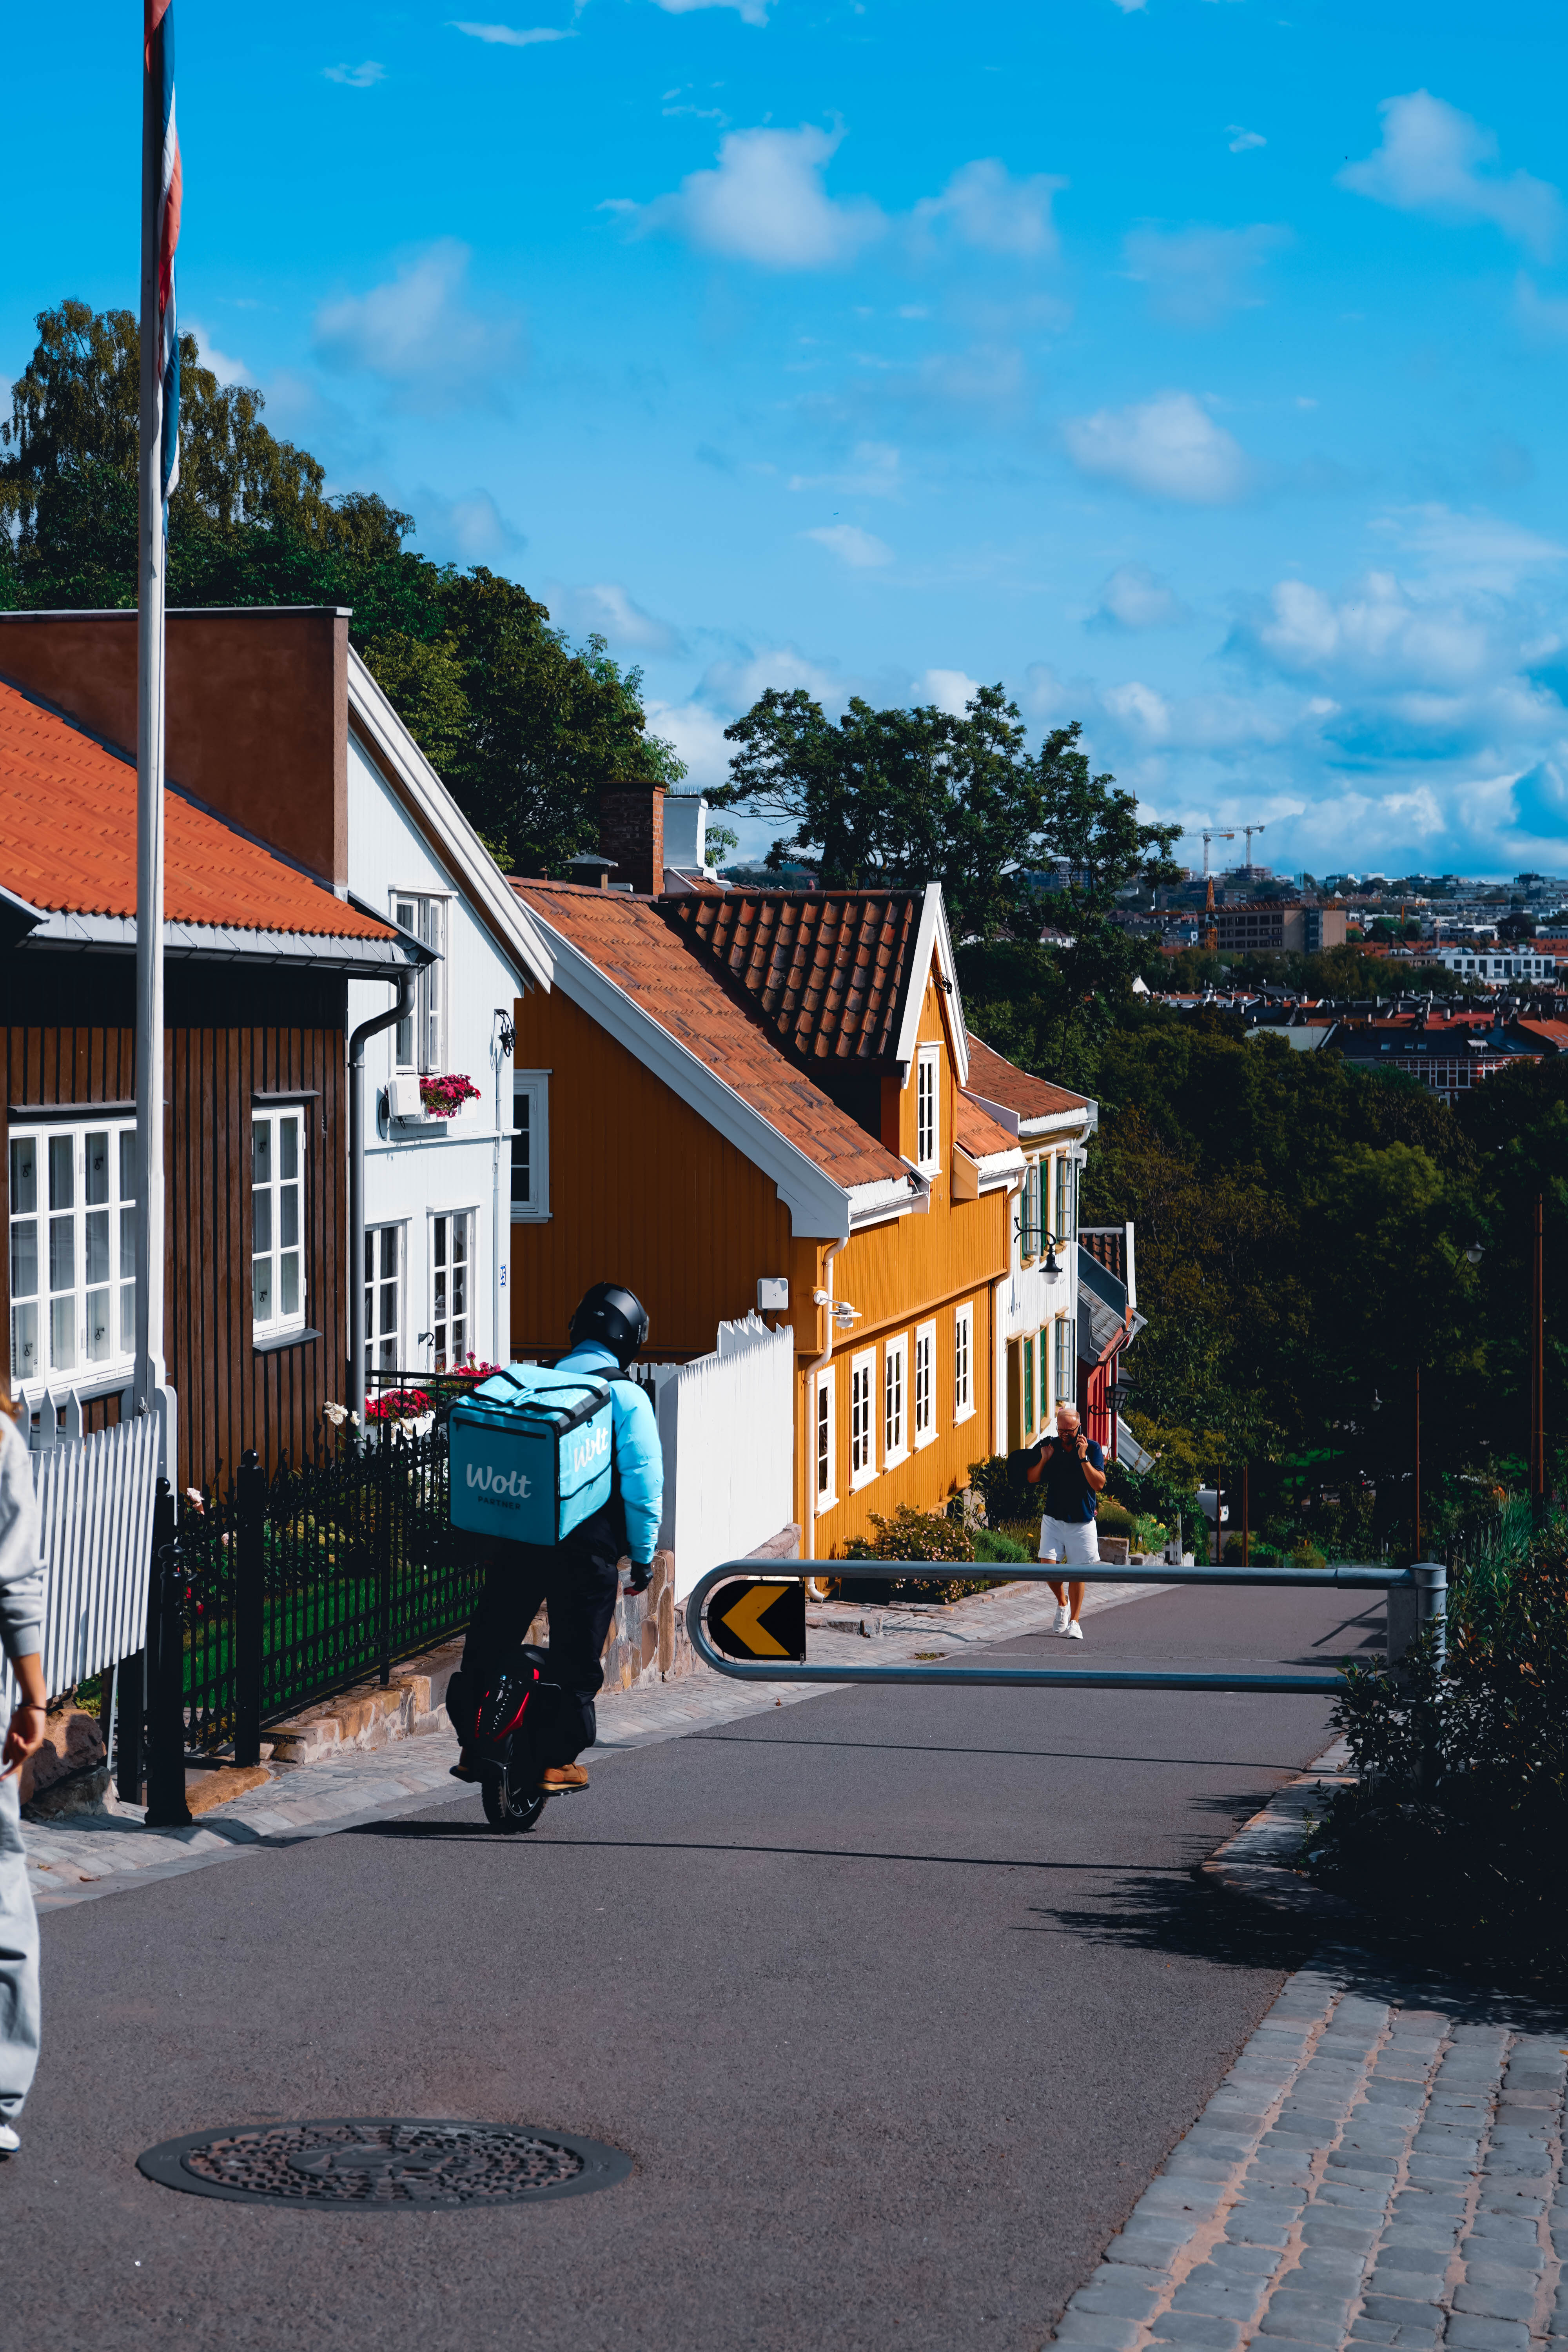
\includegraphics[width=\paperwidth,height=\paperheight]{src/Figures/Arriere_plan/Arriere_plan_Chap_1.jpg}
    }

% Rectangle
\AddToShipoutPictureBG*{
  \begin{tikzpicture}[remember picture,overlay]
    \node[fill=white, opacity=0.75, text width=\paperwidth, minimum height=9.5cm, anchor=north] 
    at ([yshift=-2cm]current page.north) {};
  \end{tikzpicture}
}

% Source
\AddToShipoutPictureFG*{
  \AtPageLowerRight{
    \raisebox{1cm}{
      \hspace{16cm}
      
\begin{tikzpicture}
        \node[fill=white, rounded corners=5pt, inner sep=5pt, align=center] {
          \tiny{Photographie~: \textcolor{blue}{Dylan Moinse (2023)}}
        };
      \end{tikzpicture}
    }
  }
}

% Réinitialiser numérotation section
\setcounter{section}{0}

    % ___________________________________________
    % Mini-sommaire
    \cleardoublepage
    \setcounter{tocdepth}{2}
    % Redéfinir le titre de la table des matières locale
    \renewcommand{\localcontentsname}{Table des matières du chapitre~1}
\localtableofcontents

    % ___________________________________________
    % Graphical abstract
    \newpage
\section*{Points clés du chapitre~1
    \label{chap1:graphical-abstract}
    }
    \markright{Préambule du chapitre}{}

\begin{figure}[h!]\vspace*{4pt}
        \caption*{Cadrage théorique d'un \textsl{Micromobility-friendly Transit-Oriented Development}}
        \label{graphical-abstract-chap1}
        \centerline{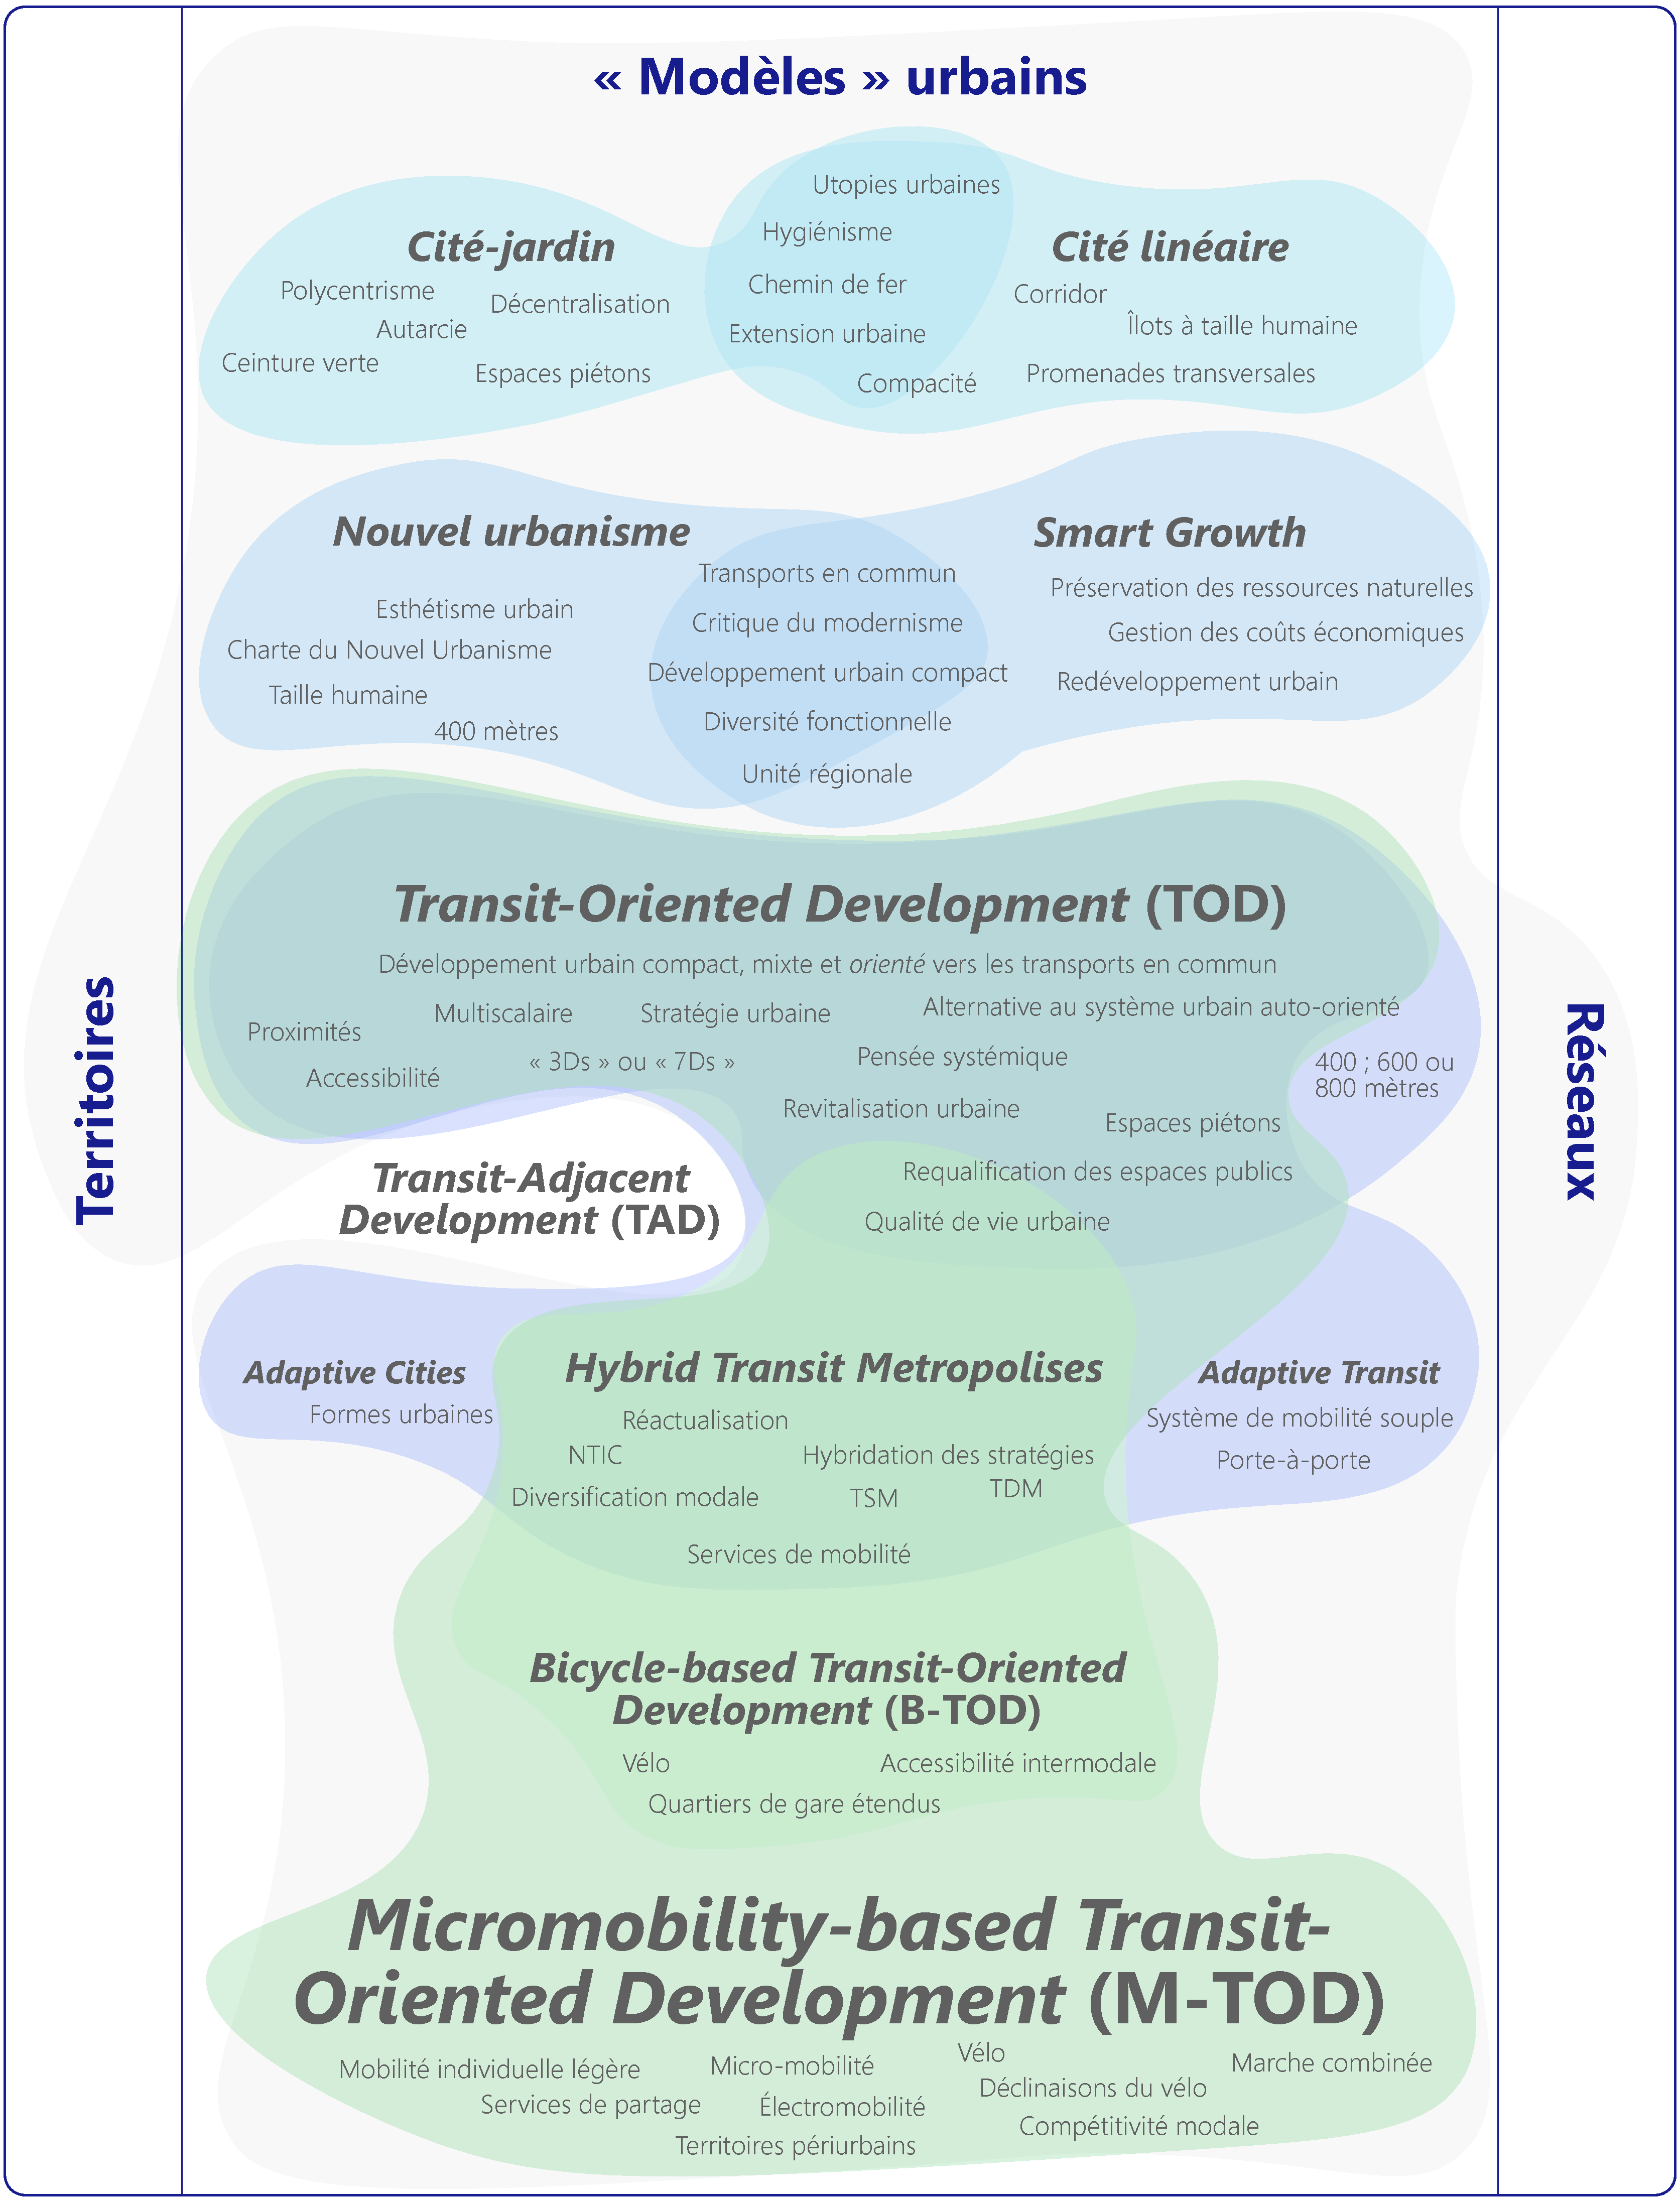
\includegraphics[width=1\columnwidth]{src/Figures/Graphical-abstract/FR_Graphical_abstract_chap1.pdf}}
        \vspace{5pt}
    \end{figure}
    
    % ___________________________________________
    % Préambule
    \newpage
    \begin{tcolorbox}[colback=white!5!white,
                      colframe=blue!75!blue,
                      title=
                      \bigskip
                      \center{\textbf{Préambule du chapitre~1}}
                      \\
                      \raggedright{\small{Chapitre composé de \pagedifference{chap1:titre}{chap2:titre} pages, dont \pagedifference{chap1:bibliographie}{chap2:titre} pages de bibliographie}}
                      \bigskip]
\Large{\textbf{\textcolor{blue}{Résumé~:}}}
    \\
    \small{
Formalisé aux États-Unis dans les années 1990, le \acrshort{TOD} constitue un modèle d'aménagement urbain reposant sur l’articulation entre densification, mixité fonctionnelle, requalification des espaces publics et développement du transport public, dans l’objectif de réduire la dépendance à l’automobile et de favoriser un système urbain plus résilient. Ce concept s’inscrit dans une filiation intellectuelle et urbanistique héritée de plusieurs courants historiques majeurs. Parmi eux, la \textsl{Cité-jardin} et la \textsl{Cité linéaire} ont introduit une planification structurée autour des infrastructures de transport en commun, tandis que le \textsl{Nouvel urbanisme} et la \textsl{Smart Growth} ont actualisé ces principes pour répondre aux défis de l’urbanisation contemporaine et de l’étalement urbain induit par la prééminence du modèle automobile. Le \textsl{TOD} se matérialise ainsi par une stratégie urbaine visant à structurer l’organisation territoriale \textsl{en connexion} avec le réseau de transport en commun, en promouvant une ville compacte, mixte et propice aux mobilités alternatives à l’automobile (voir la \hyperref[chap1:tod-presentation-generale]{section~1}, page~\pageref{chap1:tod-presentation-generale}).
    \\
Toutefois, la mise en œuvre du \acrshort{TOD} se heurte à plusieurs défis. Si ses principes demeurent particulièrement pertinents pour les métropoles bénéficiant d’un réseau de transport ferroviaire dense et performant, leur transposition aux territoires périurbains rencontre des obstacles structurels majeurs. L’allongement des distances de déplacement, la fragmentation des lieux et les limites intrinsèques des réseaux de transport en commun réduisent l’efficacité du modèle dans ces contextes. De plus, la rigidité des infrastructures lourdes complique leur adaptation aux formes urbaines héritées, caractérisées par un urbanisme peu dense et fortement auto-dépendant. Dans cette perspective, la montée en puissance de la mobilité individuelle légère~–~incluant le vélo, la trottinette et d’autres véhicules légers~–~offre un levier stratégique pour améliorer l’accessibilité aux stations de transport public et renforcer la connectivité des réseaux. Ce développement repose sur une diversité d’innovations techniques, servicielles et sociales, allant de l’électromobilité à la mutualisation des flottes en libre-service. Ainsi, l’intégration de ces modes pourrait permettre d’accroître la portée du \acrshort{TOD} et d’en maximiser les bénéfices (voir la \hyperref[chap1:mobilite-individuelle-legere]{section~2}, page~\pageref{chap1:mobilite-individuelle-legere}).
    \\
Ce chapitre explore, d’un point de vue théorique, le potentiel de la mobilité individuelle légère comme réponse aux limites du \textsl{Transit-Oriented Development} (\acrshort{TOD}). En facilitant les \Guillemets{premiers et derniers kilomètres}, cette famille de véhicules alternatifs optimise l’usage des infrastructures de transport en commun tout en réduisant la dépendance à l’automobile individuelle. Plutôt que de se substituer au transport public, elle s’inscrit dans une logique intermodale complémentaire, favorisant une intégration capillaire au sein des systèmes de mobilité. L’évolution des pratiques de déplacement et l’essor de ces (nouveaux) modes transforment ainsi la relation entre transport public et aménagement urbain, appelant à une relecture des modèles établis. C'est pourquoi nous proposons d’élargir le concept de \acrshort{TOD} vers un modèle urbain réactualisé, que nous désignons sous le terme de \acrshort{M-TOD}, en nous inspirant notamment des principes du \acrshort{B-TOD} (voir la \hyperref[chap1:btod]{section~3}, page~\pageref{chap1:btod}).
    }
    \tcblower
\Large{\textcolor{blue}{\textbf{Mots-clés~:}}}
    \\
    \small{
\textsl{Bicycle-based Transit-Oriented Development}~;
Électromobilité~;
Hybridation modale~;
\textsl{Hybrid Transit Metropolis}~;
Innovation~;
Mobilité individuelle légère~;
Mobilité partagée~;
\textsl{Transit-Oriented Development}
    }
    \end{tcolorbox}

    % ___________________________________________
    % 1.*.
    \newpage
    \needspace{1\baselineskip} % Réserve de l'espace
    \addcontentsline{toc}{section}{Introduction du chapitre~1}
    \sectionheader{Introduction du chapitre}
\section*{Introduction du chapitre~1
    \label{chap1:introduction}
    }
    \markright{Introduction du chapitre~1}{}

    % Citation
\begin{displayquote}
\Guillemets{\textsl{Le modèle} [du \textsl{Transit-Oriented Development}] \textsl{présenté dans cet ouvrage} [\dots] \textsl{se concentre sur les transports en commun et vise à élargir un mouvement plus vaste~–~l'Urbanisme Néo-Traditionnel et le Nouvel Urbanisme~–~qui englobe de nombreuses dimensions et diverses nuances. Bien que ces approches partagent des principes fondamentaux, elles s'orientent vers des voies sensiblement distinctes.} [\dots] \textsl{En ce qui concerne ces propositions, il est essentiel de garder à l'esprit qu'il n'y a pas de modèle absolu et que les particularités du lieu, tout comme les contextes économiques et politiques, auront toujours une influence sur les différentes orientations, en y créant un équilibre}}\footnote{
    \Guillemets{\textsl{The} [\textsl{Transit-Oriented Development}] \textsl{model presented in this book} [\dots] \textsl{focus on transit and is meant to broden a larger movement~–~Neo-Traditional Planning and the New Urbanism~–~which has many dimensions and differing emphasis. These approaches share fundamental principles but set out in slightly different directions.} [\dots] \textsl{With regards to all these proposals, it is important to remember that there is no absolute template and that the specifics of place, economics, and politics will always color and balance the different directions}} \textcolor{blue}{\autocite[10-11]{calthorpe_next_1993}}\index{Calthorpe, Peter|pagebf}.} [traduction libre]
    
\textcolor{blue}{Peter} \textcolor{blue}{\textcite[10-11]{calthorpe_next_1993}}\index{Calthorpe, Peter|pagebf}. \foreignlanguage{english}{\textsl{The Next American Metropolis: Ecology, Community, and the American Dream}}, Princeton Architectural Press, New York, 175~p. ISBN~: \href{https://search.worldcat.org/fr/title/27814585}{1-878271-68-7}
    \end{displayquote}

    % Introduction
\lettrine[lines=3, findent=8pt, nindent=0pt]{\lettrinefont F}{ace} aux enjeux de pollution, de fragmentation et de congestion urbaines engendrés par la diffusion massive de l’automobile et l’adaptation de l’urbanisation à ce mode de déplacement, le concept d’aménagement du \acrfull{TOD} repose sur le principe de densification et de diversification des activités et des usages autour des infrastructures de \gls{transport en commun}. Formalisé aux États-Unis sous l’impulsion de \textcolor{blue}{Peter} \textcolor{blue}{\textcite[10]{calthorpe_next_1993}}\index{Calthorpe, Peter|pagebf}, ce modèle urbain hérite de plusieurs courants de pensée, notamment de la \textsl{Cité-jardin} d’\textcolor{blue}{Ebenezer} \textcolor{blue}{\textcite{howard_-morrow_1898}}\index{Howard, Ebenezer|pagebf}, de la \textsl{Cité linéaire} d’\textcolor{blue}{Arturo Soria y Mata (1882)}, ainsi que des principes du \textsl{Nouvel urbanisme} et de la \textsl{Smart Growth}. Un élément fondamental du \acrshort{TOD} réside dans sa capacité à articuler explicitement transport public et aménagement urbain de manière synergique, bien au-delà d’une simple juxtaposition d’infrastructures et d’activités. Il s’agit d’une approche multidimensionnelle et multiscalaire où la station de transport en commun devient le pivot structurant du territoire. Dans cette logique, le point nodal ne se limite plus à \textsl{mettre} relation des flux, mais \textsl{entre} véritablement en interaction avec eux, en se connectant au lieu \textcolor{blue}{\autocite[344]{bertolini_nodes_1996}}\index{Bertolini, Luca|pagebf}, sur la base d'une approche de \Guillemets{lieu-mouvement} \textcolor{blue}{\autocite[103]{le_bot_flux_2024}}\index{Le Bot, Nils|pagebf}. Ce modèle vise ainsi à favoriser un urbanisme plus compact et animé, afin de mieux maîtriser l’étalement urbain et d’encourager les déplacements en transport en commun, mais aussi à pied et à \gls{vélo}. De plus, il contribue à la réorganisation des activités à l’échelle territoriale en favorisant une structure polycentrique \textcolor{blue}{\autocite[38]{pearce_enquete_2020}}\index{Pearce, Marc|pagebf}\index{Landriève, Sylvie|pagebf}\index{Gay, Christophe|pagebf}\index{Dubois, Tom|pagebf}, à l'allure d'une \Guillemets{décentralisation centralisée} \textcolor{blue}{\autocite[55]{kamruzzaman_advance_2014}}\index{Kamruzzaman, Md.|pagebf}\index{Baker, Douglas|pagebf}\index{Washington, Simon|pagebf}\index{Turrell, Gavin|pagebf}. Aujourd’hui, le \acrshort{TOD} s’affirme comme l'une des stratégies urbaines se rapprochant le plus à ce que nous pouvons qualifier d'\Guillemets{urbanisme durable} ou de \Guillemets{développement urbain \gls{durable}} \textcolor{blue}{\autocite[14]{bentayou_transit-oriented_2015}}\index{Bentayou, Gilles|pagebf}. Aussi, le dernier rapport du \acrfull{GIEC} préconise-t-il un développement urbain orienté vers les réseaux de transport en commun et les modes actifs, conçu pour favoriser une compacité urbaine \textcolor{blue}{\autocite[29]{lee_climate_2023}}\index{Lee, Hoesung|pagebf}\index{Calvin, Katherine|pagebf}\index{Dasgupta, Dipak|pagebf}\index{Krinner, Gerhard|pagebf}\index{Mukherji, Aditi|pagebf}\index{Thorne, Peter|pagebf}\index{Trisos, Christopher|pagebf}\index{Romero, Jose|pagebf}\index{Aldunce, Paulina|pagebf}\index{Barrett, Ko|pagebf}\index{Blanco, Gabriel|pagebf}\index{Cheung, William|pagebf}\index{Connors, Sarah|pagebf}\index{Denton, Fatima|pagebf}\index{Diongue Niang, Aïda|pagebf}\index{Dodman, David|pagebf}\index{Garschagen, Matthias|pagebf}\index{Geden, Oliver|pagebf}\index{Hayward, Bronwyn|pagebf}\index{|pagebf}\index{Jones, Christopher|pagebf}\index{Frank, Jotzo|pagebf}\index{Thelma, Krug|pagebf}\index{Laco, Rodel|pagebf}\index{Lee, June-Yi|pagebf}\index{Masson-Delmotte, Valérie|pagebf}\index{Meinshausen, Malte|pagebf}\index{Mintenbeck, Katja|pagebf}\index{Mokssit, Abdalah|pagebf}\index{Otto, Friederike~E.~L.|pagebf}\index{Pathak, Minal|pagebf}\index{Pirani, Anna|pagebf}\index{Poloczanska, Elvira|pagebf}\index{Pörtner, Hans-Otto|pagebf}\index{Revi, Aromar|pagebf}\index{Roberts, Debra~C.|pagebf}\index{Roy, Joyashree|pagebf}\index{Ruane, Alex~C.|pagebf}\index{Skea, Jim|pagebf}\index{Shukla, Priyadarshi~R.|pagebf}\index{Slade, Raphael|pagebf}\index{Slangen, Aimée|pagebf}\index{Sokona, Youba|pagebf}\index{Sörensson, Anna~A.|pagebf}\index{Tignor, Melinda|pagebf}\index{Vuuren, Detlef~van.|pagebf}\index{Wei, Yi-Ming|pagebf}\index{Winkler, Harald|pagebf}\index{Zhai, Panmao|pagebf}\index{Zommers, Zinta|pagebf}.%%Rédigé%%

    % Limites et intermodalité
Toutefois, l’allongement des distances et l'éclatement des lieux de production, de consommation et d’habitat, résultant du zonage fonctionnel et de l’artificialisation horizontale des sols, ont considérablement réduit l'attractivité et la compétitivité du transport public sur une grande partie des territoires \textcolor{blue}{\autocite[25-28]{mallet_voyage_2022}}\index{Mallet, Thierry|pagebf}. Par ailleurs, le système de transport en commun ne parvient pas à égaler l’ensemble des bénéfices procurés par l’automobilité, notamment en termes de flexibilité et de connectivité \textcolor{blue}{\autocite[209]{heran_retour_2015}}\index{Héran, Frédéric|pagebf}. Cette situation remet ainsi en question la capacité du modèle urbain à répondre efficacement à la dépendance automobile, en particulier dans les territoires périurbains. Une alternative réside dans la promotion de l’intermodalité, qui permettrait de pallier la rigidité du réseau de transport public \textcolor{blue}{\autocite[17]{wiel_comment_1998}}\index{Wiel, Marc|pagebf} et d’améliorer l’efficacité globale du système de mobilité \textcolor{blue}{\autocite[82]{oostendorp_combining_2018}}\index{Oostendorp, Rebekka|pagebf}\index{Gebhardt, Laura|pagebf}. En dépassant les approches strictement monoscalaires et monomodales, des mesures correctrices peuvent être mises en œuvre afin de limiter les dysfonctionnements et d’optimiser les performances des chaînes intermodales, de l’échelle régionale à l’échelle infra-urbaine \textcolor{blue}{\autocite[111-115]{chapelon_transports_2016}}\index{Chapelon, Laurent|pagebf}. Il s’agit ainsi de concevoir un système intégré et cohérent, où la croissance urbaine s’adapte au développement des transports en commun tout autant que les solutions de mobilité alternative s’ajustent aux spécificités du tissu urbain existant. Empiriquement, cette approche se traduit par l’adoption de stratégies urbanistiques favorisant un dialogue entre l’offre et la demande de transport, en intégrant des solutions de mobilité complémentaires au sein d’un système global et non plus sectorisé. C’est dans cette perspective que se sont développées les \textsl{Transit Metropolises} contemporaines, qui visent à concurrencer l’automobile en imitant sa connectivité \Guillemets{porte-à-porte} tout en s’inscrivant dans une logique de déplacement collectif \textcolor{blue}{\autocite[132-133]{cervero_transit_2020}}\index{Cervero, Robert|pagebf}.%%Rédigé%%

    % Mobilité individuelle légère
Dans ce contexte, la montée en puissance de ce que nous avons choisi d'appeler \Guillemets{mobilité individuelle légère}~–~comprenant le vélo, la trottinette et leurs diverses adaptations~–~ouvre de nouvelles perspectives en matière d’aménagement et de mobilité soutenables. Ces solutions offrent des alternatives intéressantes aux défis posés par les \Guillemets{premiers et derniers kilomètres} du transport public et s’imposent dès lors comme un chaînon manquant essentiel dans la transition vers une mobilité \Guillemets{écomobile} \textcolor{blue}{\autocites[4]{sebban_complementarite_2003}[25]{amar_homo_2016}{heran_transition_2018}}\index{Sebban, Annie-Claude|pagebf}\index{Motte, Alain|pagebf}\index{Héran, Frédéric|pagebf}\index{Amar, Georges|pagebf}. La mobilité individuelle légère s’inscrit dans une dynamique de \Guillemets{réécriture innovante du passé}, illustrée par le retour en force du vélo sous des formes renouvelées et par l’essor de la trottinette comme mode de déplacement utilitaire \textcolor{blue}{\autocite[18]{amar_homo_2016}}\index{Amar, Georges|pagebf}. Le développement de ces modes légers en tant que solutions intermodales témoigne d’un renouveau de la proximité à différentes échelles spatiales \textcolor{blue}{\autocite{sadik-kahn_15-minute_2021}}\index{Sadik-Kahn, Janette|pagebf}, renforçant ainsi l’attractivité du transport public et révélant une évolution des valeurs en matière de mobilité \textcolor{blue}{\autocite[110]{goletz_intermodality_2020}}\index{Goletz, Mirko|pagebf}\index{Haustein, Sonja|pagebf}\index{Wolking, Christina|pagebf}\index{L'Hostis, Alain|pagebf}. En fin de compte, la ville écomobile, en opposition au modèle de la ville automobile, repose sur une circulation de proximité où la complémentarité entre le vélo et le transport public constitue l’un des principes fondamentaux d’un système de mobilité plus intégré et résilient.%%Rédigé%%

    % Annonce du plan 1
Ce chapitre s’organise en trois grandes parties visant à explorer les fondements, l’application et l’évolution du \acrshort{TOD}. Dans un premier temps, nous examinerons les origines et les fondements théoriques de ce modèle urbain en retraçant ses influences historiques et intellectuelles, ainsi que son évolution et son applicabilité (\hyperref[chap1:tod-presentation-generale]{section~1}, page~\pageref{chap1:tod-presentation-generale}). Nous analyserons les courants d’urbanisme qui ont nourri son énonciation et sa codification avant de soulever les points d'originalité propres du \acrshort{TOD} (\hyperref[chap1:tod-presentation-generale-origines]{sous-section~1.1}, page~\pageref{chap1:tod-presentation-generale-origines}). Cette rétrospective épistémologique nous permettra d’en définir précisément les contours en tant que modèle de développement urbain alternatif au paradigme auto-centré, en précisant ses principes et les bénéfices attendus (\hyperref[chap1:tod-presentation-generale-definition]{sous-section~1.2}, page~\pageref{chap1:tod-presentation-generale-definition}). Enfin, nous verrons comment ce concept d'aménagement a été interprété au sein des stratégies urbaines déployées dans le contexte français et quelles sont ses principales déclinaisons en lien avec notre sujet de recherche (\hyperref[chap1:tod-presentation-generale-declinaisons]{sous-section~1.3}, page~\pageref{chap1:tod-presentation-generale-declinaisons}).%%Rédigé%%

    % Annonce du plan 2
La deuxième partie s’intéressera au second objet d’étude de cette recherche, à savoir la famille de véhicules regroupés sous l’appellation de \Guillemets{mobilité individuelle légère} (\hyperref[chap1:mobilite-individuelle-legere]{section~2}, page~\pageref{chap1:mobilite-individuelle-legere}). Nous retracerons l’évolution historique de ces objets techniques et sociaux~–~notamment le vélo et la trottinette~–~en identifiant et en simplifiant la lecture des grandes périodes qui ont marqué leur développement, dans le but de mieux contextualiser leur regain d’intérêt actuel (\hyperref[chap1:proximite-velo-trottinette]{sous-section~2.1}, page~\pageref{chap1:proximite-velo-trottinette}). Nous aborderons ensuite la diversification des usages et des formes de ces véhicules, qui se caractérise notamment par leur électrification et leur mise en partage dans l’\gls{espace public}, brouillant ainsi les frontières traditionnelles entre les modes de déplacement (\hyperref[chap1:velo-micromobilite-innovations]{sous-section~2.2}, page~\pageref{chap1:velo-micromobilite-innovations}). Cette réflexion historique nous permettra d’exposer à son tour l'évolution des valeurs attachées à la mobilité et aux modes de vie, ainsi que les enjeux de définition liés au périmètre de pertinence de cette famille de véhicules (\hyperref[chap1:caracterisation-mobilite-individuelle-legere]{sous-section~2.3}, page~\pageref{chap1:caracterisation-mobilite-individuelle-legere}).%%Rédigé%%

    % Annonce du plan 3
Enfin, la troisième partie du présent chapitre articulera les deux précédentes en explorant les opportunités qu’offre l’association entre transport public et mobilité individuelle légère dans une logique de complémentarité modale (\hyperref[chap1:btod]{section~3}, page~\pageref{chap1:btod}). Nous montrerons que, bien que la marche combinée ne soit pas assimilée à la mobilité individuelle légère, elle demeure l’élément structurant du \acrshort{TOD}. Dans un premier temps, nous démontrerons comment la portée réelle de la marche combinée tend à être sous-estimée et en quoi la mobilité individuelle légère peut jouer un rôle complémentaire, en s’inscrivant dans un champ de pertinence qui ne concurrence pas la marche, mais renforce l’\gls{accessibilité} au transport public (\hyperref[chap1:btod-limites-tod]{sous-section~3.1}, page~\pageref{chap1:btod-limites-tod}). Enfin, nous mettrons en évidence les avantages comparatifs d’une telle synergie et la manière dont cette approche intermodale nous invite à interroger la pertinence d’un modèle élargi, celui d'un \acrfull{M-TOD} (\hyperref[chap1:btod-m-tod]{sous-section~3.2}, page~\pageref{chap1:btod-m-tod}).%%Rédigé%%

     % ___________________________________________
    % 1.1.
    \newpage
    \needspace{1\baselineskip} % Réserve de l'espace
    \sectionheader{Concept d'aménagement du \textsl{Transit-Oriented Development}}
\section{Le \textsl{Transit-Oriented Development}, une réinvention de la planification régionale autour du chemin de fer
    \label{chap1:tod-presentation-generale}
    }

    % Introduction TOD
Le \acrshort{TOD} s’impose aujourd’hui comme un modèle d’aménagement clé dans la planification régionale, valorisant les infrastructures ferroviaires comme axe central de développement urbain. Cette stratégie popularisée repose sur l’idée de structurer les territoires autour des nœuds de transport public, dans le but de réduire la dépendance à la voiture individuelle et de promouvoir une urbanisation plus durable. En dépit de l’urgence et de l’importance de ces enjeux, les mécanismes sous-jacents influençant l’usage de la voiture en milieu urbain demeurent insuffisamment compris, en raison d’un cadre théorique encore limité \textcolor{blue}{\autocite[1]{verbavatz_critical_2019}}\index{Verbavatz, Vincent|pagebf}\index{Barthelemy, Marc|pagebf}. Les réflexions de l’architecte et urbaniste italien \textcolor{blue}{Alberto} \textcolor{blue}{\textcite[]{magnaghi_bioregion_2014}}\index{Magnaghi, Alberto|pagebf} apportent une contribution enrichissante à ce débat en introduisant une approche bioterritoriale, dans laquelle les \Guillemets{biorégions urbaines} et les réseaux deviennent les piliers d’un développement intégré et respectueux des écosystèmes locaux. Cependant, le \acrshort{TOD} figure parmi les rares concepts d’aménagement capables d’aborder et de traiter directement la pensée de l’\Guillemets{urbanisme des réseaux} \textcolor{blue}{\autocite[]{dupuy_urbanisme_1991}}\index{Dupuy, Gabriel|pagebf} dans un contexte globalisé, en mettant en lumière les interactions complexes entre mobilité, urbanisation et durabilité \textcolor{blue}{\autocite[51]{el_hadeuf_ville_2017}}\index{El Hadeuf, Mounya|pagebf}\index{Laterrasse, Jean|pagebf}.%%Rédigé%%

    % Annonce du plan
Nous commencerons par introduire, selon une approche diachronique, les origines du modèle urbain, en faisant ressortir les points sur lesquels il innove pour répondre aux enjeux contemporains liés à la nécessaire coordination entre réseau et territoire (\hyperref[chap1:tod-presentation-generale-origines]{section sur les inspirations du \textsl{Transit-Oriented Development}}, page~\pageref{chap1:tod-presentation-generale-origines}). Cette introduction sera suivie d’un état des lieux des principes généraux proposés par le modèle d’aménagement pour y remédier, ainsi que les effets attendus sur les territoires et les comportements de mobilité (\hyperref[chap1:tod-presentation-generale-definition]{section sur les directions du \textsl{Transit-Oriented Development}}, page~\pageref{chap1:tod-presentation-generale-definition}). Enfin, nous accorderons une attention particulière au caractère évolutif de ce concept à l’échelle mondiale, aussi bien dans les milieux académiques qu’opérationnels. Nous analyserons les diverses adaptations qui en découlent en fonction des spécificités de chaque terrain et de l'avancée des connaissances. Cette réflexion nous conduira à aborder le potentiel d’apport du vélo et de la \gls{micro-mobilité} dans une perspective de réactualisation du \acrshort{TOD} (\hyperref[chap1:tod-presentation-generale-declinaisons]{section sur les principales déclinaisons du \textsl{Transit-Oriented Development}}, page~\pageref{chap1:tod-presentation-generale-declinaisons}).%%Rédigé%%

    % 1.1.1. Chronologie TOD
    \needspace{1\baselineskip} % Réserve de l'espace
\subsection{Genèse du \textsl{Transit-Oriented Development}~: quand le rail inspire l'urbanisme
    \label{chap1:tod-presentation-generale-origines}
    }

    % Introduction 1
La géographie, tout comme de nombreuses disciplines connexes, a longtemps insisté sur l'interaction dynamique entre un lieu et son environnement, conceptualisant le lieu comme un \Guillemets{milieu} générateur d'activités et vecteur de transformations. En dépassant la simple notion d'espace physique, le système territorial agit à la fois comme \textsl{stimulus} et comme produit des transformations \textcolor{blue}{\autocite[19-21]{hagerstrand_what_1970}}\index{Hägerstrand, Torsten|pagebf}. Cette approche inclut la capacité des gares, en tant qu’espaces liminaux, à jouer un rôle de catalyseurs de développements variés \textcolor{blue}{\autocite[6]{baron_nouvelle_2024}}\index{Baron, Nacima|pagebf}\index{Le Bot, Nils|pagebf}\index{Detavernier, Pauline|pagebf}. Dans les années 1970, les \Guillemets{nouveaux géographes} ont ainsi orienté leurs travaux vers l’étude des réseaux \textcolor{blue}{\autocites{claval_nouveaux_1977}[166]{massardier_savants_1996}[112-113]{orain_geographie_2006}}\index{Massardier, Gilles|pagebf}\index{Claval, Paul|pagebf}\index{Orain, Olivier|pagebf}, en s’appuyant sur le maillage dense des infrastructures ferroviaires pour analyser les formes réticulaires. Ces recherches ont permis d’explorer les interactions réciproques entre réseau et territoire à différentes échelles géographiques \textcolor{blue}{\autocite[6]{baron_nouvelle_2024}}\index{Baron, Nacima|pagebf}\index{Le Bot, Nils|pagebf}\index{Detavernier, Pauline|pagebf}.%%Rédigé%%

    % Introduction 2
C’est dans ce contexte que l’architecte et urbaniste étasunien \textcolor{blue}{Peter} \textcolor{blue}{\textcite[10]{calthorpe_next_1993}}\index{Calthorpe, Peter|pagebf} propose un modèle d’aménagement centré sur le transport public, dans son ouvrage \foreignlanguage{english}{\textsl{The Next American Metropolis: Ecology, Community, and the American Dream}}~: le \acrfull{TOD}. Ce concept s’affirme comme une stratégie d'action multidimensionnelle, bien que majoritairement focalisée sur les aspects physico-spatiaux de l’aménagement \textcolor{blue}{\autocite[10]{calthorpe_next_1993}}\index{Calthorpe, Peter|pagebf}, en postulant que le changement de comportement de mobilité peut découler de la forme urbaine. Les influences majeures du \acrshort{TOD} s’inscrivent dans le cadre plus large du \textsl{Nouvel urbanisme} et de la \textsl{Smart Growth}, tout en apportant une nouvelle échelle d’analyse. En effet, \textcolor{blue}{Robert} \textcolor{blue}{\textcite[7]{cervero_transit_1998}}\index{Cervero, Robert|pagebf} considère que le \acrshort{TOD} déplace l’attention traditionnellement portée sur les interventions au niveau du quartier ou de la communauté vers les connexions entre les transports en commun et l’urbanisation sur le plan régional.%%Rédigé%%

    % 1.1.1.1. Mouvements d'urbanisme
    \needspace{1\baselineskip} % Réserve de l'espace
\subsubsection*{Héritage des réflexions urbanistiques passées
    \label{chap1:tod-presentation-generale-origines-mouvements}
    }

    % Introduction
Dans son ouvrage phare \textsl{L’urbanisme, utopies et réalités~: Une anthologie}, l’historienne \textcolor{blue}{Françoise} \textcolor{blue}{\textcite{choay_urbanisme_1965}}\index{Choay, Françoise|pagebf} offre une grille de lecture pour comprendre l’évolution des villes contemporaines. D'après la thèse défendue par l'autrice, la science de l'urbanisme telle que nous la connaissons aujourd'hui ne représente pas une solution novatrice à des problématiques nouvelles, mais réside essentiellement dans la réitération et la reproduction de schémas discursifs hérités du XIX\textsuperscript{e} siècle, qu'elle désigne comme des \Guillemets{modèles}. À cet égard, cette perspective permet d’interroger les fondements historiques et idéologiques du \acrshort{TOD}. Puisque le concept d'aménagement s'inscrit dans des courants de pensée, développés dans les années 1980 en réponse à la crise de l'urbanisation aux États-Unis, mais aussi en France \textcolor{blue}{\autocite[11]{lefebvre_droit_1967}}\index{Lefebvre, Henri|pagebf}, tels que le \textsl{New Urbanism} et la \textsl{Smart Growth}. Toutefois, réduire ses inspirations à ces mouvements post-modernes serait simpliste. Les racines de ce modèle s’étendent jusqu’aux théories urbanistiques de la fin du XIX\textsuperscript{e} siècle, notamment la \textsl{Cité-jardin}. \textcolor{blue}{Françoise} \textcolor{blue}{\textcite[259]{choay_urbanisme_1965}}\index{Choay, Françoise|pagebf} identifie cette dernière comme un \Guillemets{urbanisme culturaliste}, issu d'un courant théorique critique de la ville industrielle et caractérisé par une vision nostalgique d'un ordre organique\footnote{
    Dans sa typologie des mouvements de \Guillemets{pré-urbanisme} et d'\Guillemets{urbanisme}, \textcolor{blue}{Françoise} \textcolor{blue}{\textcite[277]{choay_urbanisme_1965}}\index{Choay, Françoise|pagebf} désigne comme \Guillemets{culturalistes} les courants théoriques datant de la seconde moitié du XIX\textsuperscript{e} siècle et qui prônent une ville circonscrite et fondée sur une organisation organique, en réaction aux idées progressistes de l'époque.
}.%%Rédigé%%

    % Cité-jardin : théorie
Le modèle du \acrshort{TOD} s’inspire largement du concept de la \textsl{Cité-jardin} (\textsl{Garden City}), développé à l’origine par l’urbaniste britannique \textcolor{blue}{Ebenezer} \textcolor{blue}{\textcite{howard_-morrow_1898}}\index{Howard, Ebenezer|pagebf}, en réaction à la croissance urbaine anarchique qui a accompagné l’industrialisation en Europe, caractérisée par une absence de planification urbaine. Sa pensée, formalisée dans son opuscule \textsl{Garden Cities of To-Morrow}, au caractère qualifié d’\Guillemets{urbaphobe} par certain·e·s observateur·rice·s \textcolor{blue}{\autocite[7]{cavin_cites-jardins_2007}}\index{Cavin, Joëlle Salomon|pagebf}, repose sur la création de villes satellites autosuffisantes, sur le \Guillemets{fantasme de la petite ville rêvée} \textcolor{blue}{\autocite[9]{fath_entre_2007}}\index{Fath, Sébastien|pagebf}, à échelle humaine, reliant les avantages de la vie urbaine et rurale. Ces villes sont conçues pour être limitées en taille et en extension, reliées par des réseaux ferroviaires, et organisées selon un système polycentrique, avec des ceintures vertes séparant chaque pôle urbain (voir le \hyperref[fig-chap1:schema-cite-jardin]{schéma~\ref{fig-chap1:schema-cite-jardin}}, page~\pageref{fig-chap1:schema-cite-jardin}). Ce projet social (\textsl{Social City}) vise à promouvoir une urbanité hybride tournée vers la nature, en opposition aux cités industrielles de son époque. Selon \textcolor{blue}{Robert} \textcolor{blue}{\textcite[38]{fishman_open_2011}}\index{Fishman, Robert|pagebf}, le \acrshort{TOD} emprunte aux cités-jardins les notions de décentralisation et de polycentrisme, mais également la conception d'espaces adaptés aux piéton·ne·s desservis par le chemin de fer.

    % Cité-jardin : exemples
Face au succès de la première cité-jardin, inaugurée à Letchworth en 1903 et conçue par \textcolor{blue}{Ebenezer Howard} \textcolor{blue}{\autocite[9]{gaboriau_aux_2004}}\index{Gaboriau, Arnaud|pagebf}, au nord de Londres, son importation en France est rapide, avec la construction de la première cité Bruno, à Dourges, dans le Pas-de-Calais, entre 1904 et 1908. Cette mise en œuvre des principes hygiénistes visait à loger les mineurs de la Compagnie des mines de Dourges. Il faut toutefois attendre l’entre-deux-guerres pour voir fleurir, autour des grandes villes françaises, un nombre important de cités-jardins. Les conceptions originelles y sont cependant réinterprétées. En effet, les cités-jardins à la française ne correspondent pas aux villes autonomes mettant en relation les lieux de travail, les commerces, les équipements collectifs et les logements qu’\textcolor{blue}{Ebenezer Howard} imaginait. Elles se présentent davantage comme des zones résidentielles, qualifiées de \Guillemets{banlieues-jardins}. Ce modèle subit ainsi une appropriation spécifique, qui écarte rapidement le volet économique fondé sur l’autosuffisance, tout en donnant lieu à de nombreuses réalisations se réclamant de ce concept \textcolor{blue}{\autocite[238]{guelton_cite-jardin_2013}}\index{Gaboriau, Arnaud|pagebf}. Un exemple emblématique de cette adaptation est celui des cités développées par la Compagnie des chemins de fer du Nord, sous l’impulsion de l’ingénieur \textcolor{blue}{Raoul Dautry}. À l'image de la cité de Lille-Délivrance, dont les travaux débutent en avril 1921, deux ans après l'édification d'une nouvelle gare de triage à Lomme et la mise en service d'une gare voyageur·se·s. Cette cité-jardin est directement adossée à la nouvelle gare. Lors de son inauguration en 1926, la cité de cheminots de Lille-Délivrance regroupe alors 835 logements et 3~228 habitant·e·s \textcolor{blue}{\autocite[19]{gaboriau_aux_2004}}\index{Gaboriau, Arnaud|pagebf}.%%Rédigé%%

   % Figure Cité-jardin
    \begin{carte}[h!]\vspace*{4pt}
        \caption{Schéma cartographique d'un réseau de six \Guillemets{cités-satellites} de 32~000 habitant·e·s entourant une \Guillemets{ville-centre} de 58~000 habitant·e·s.}
        \label{fig-chap1:schema-cite-jardin}
        \centerline{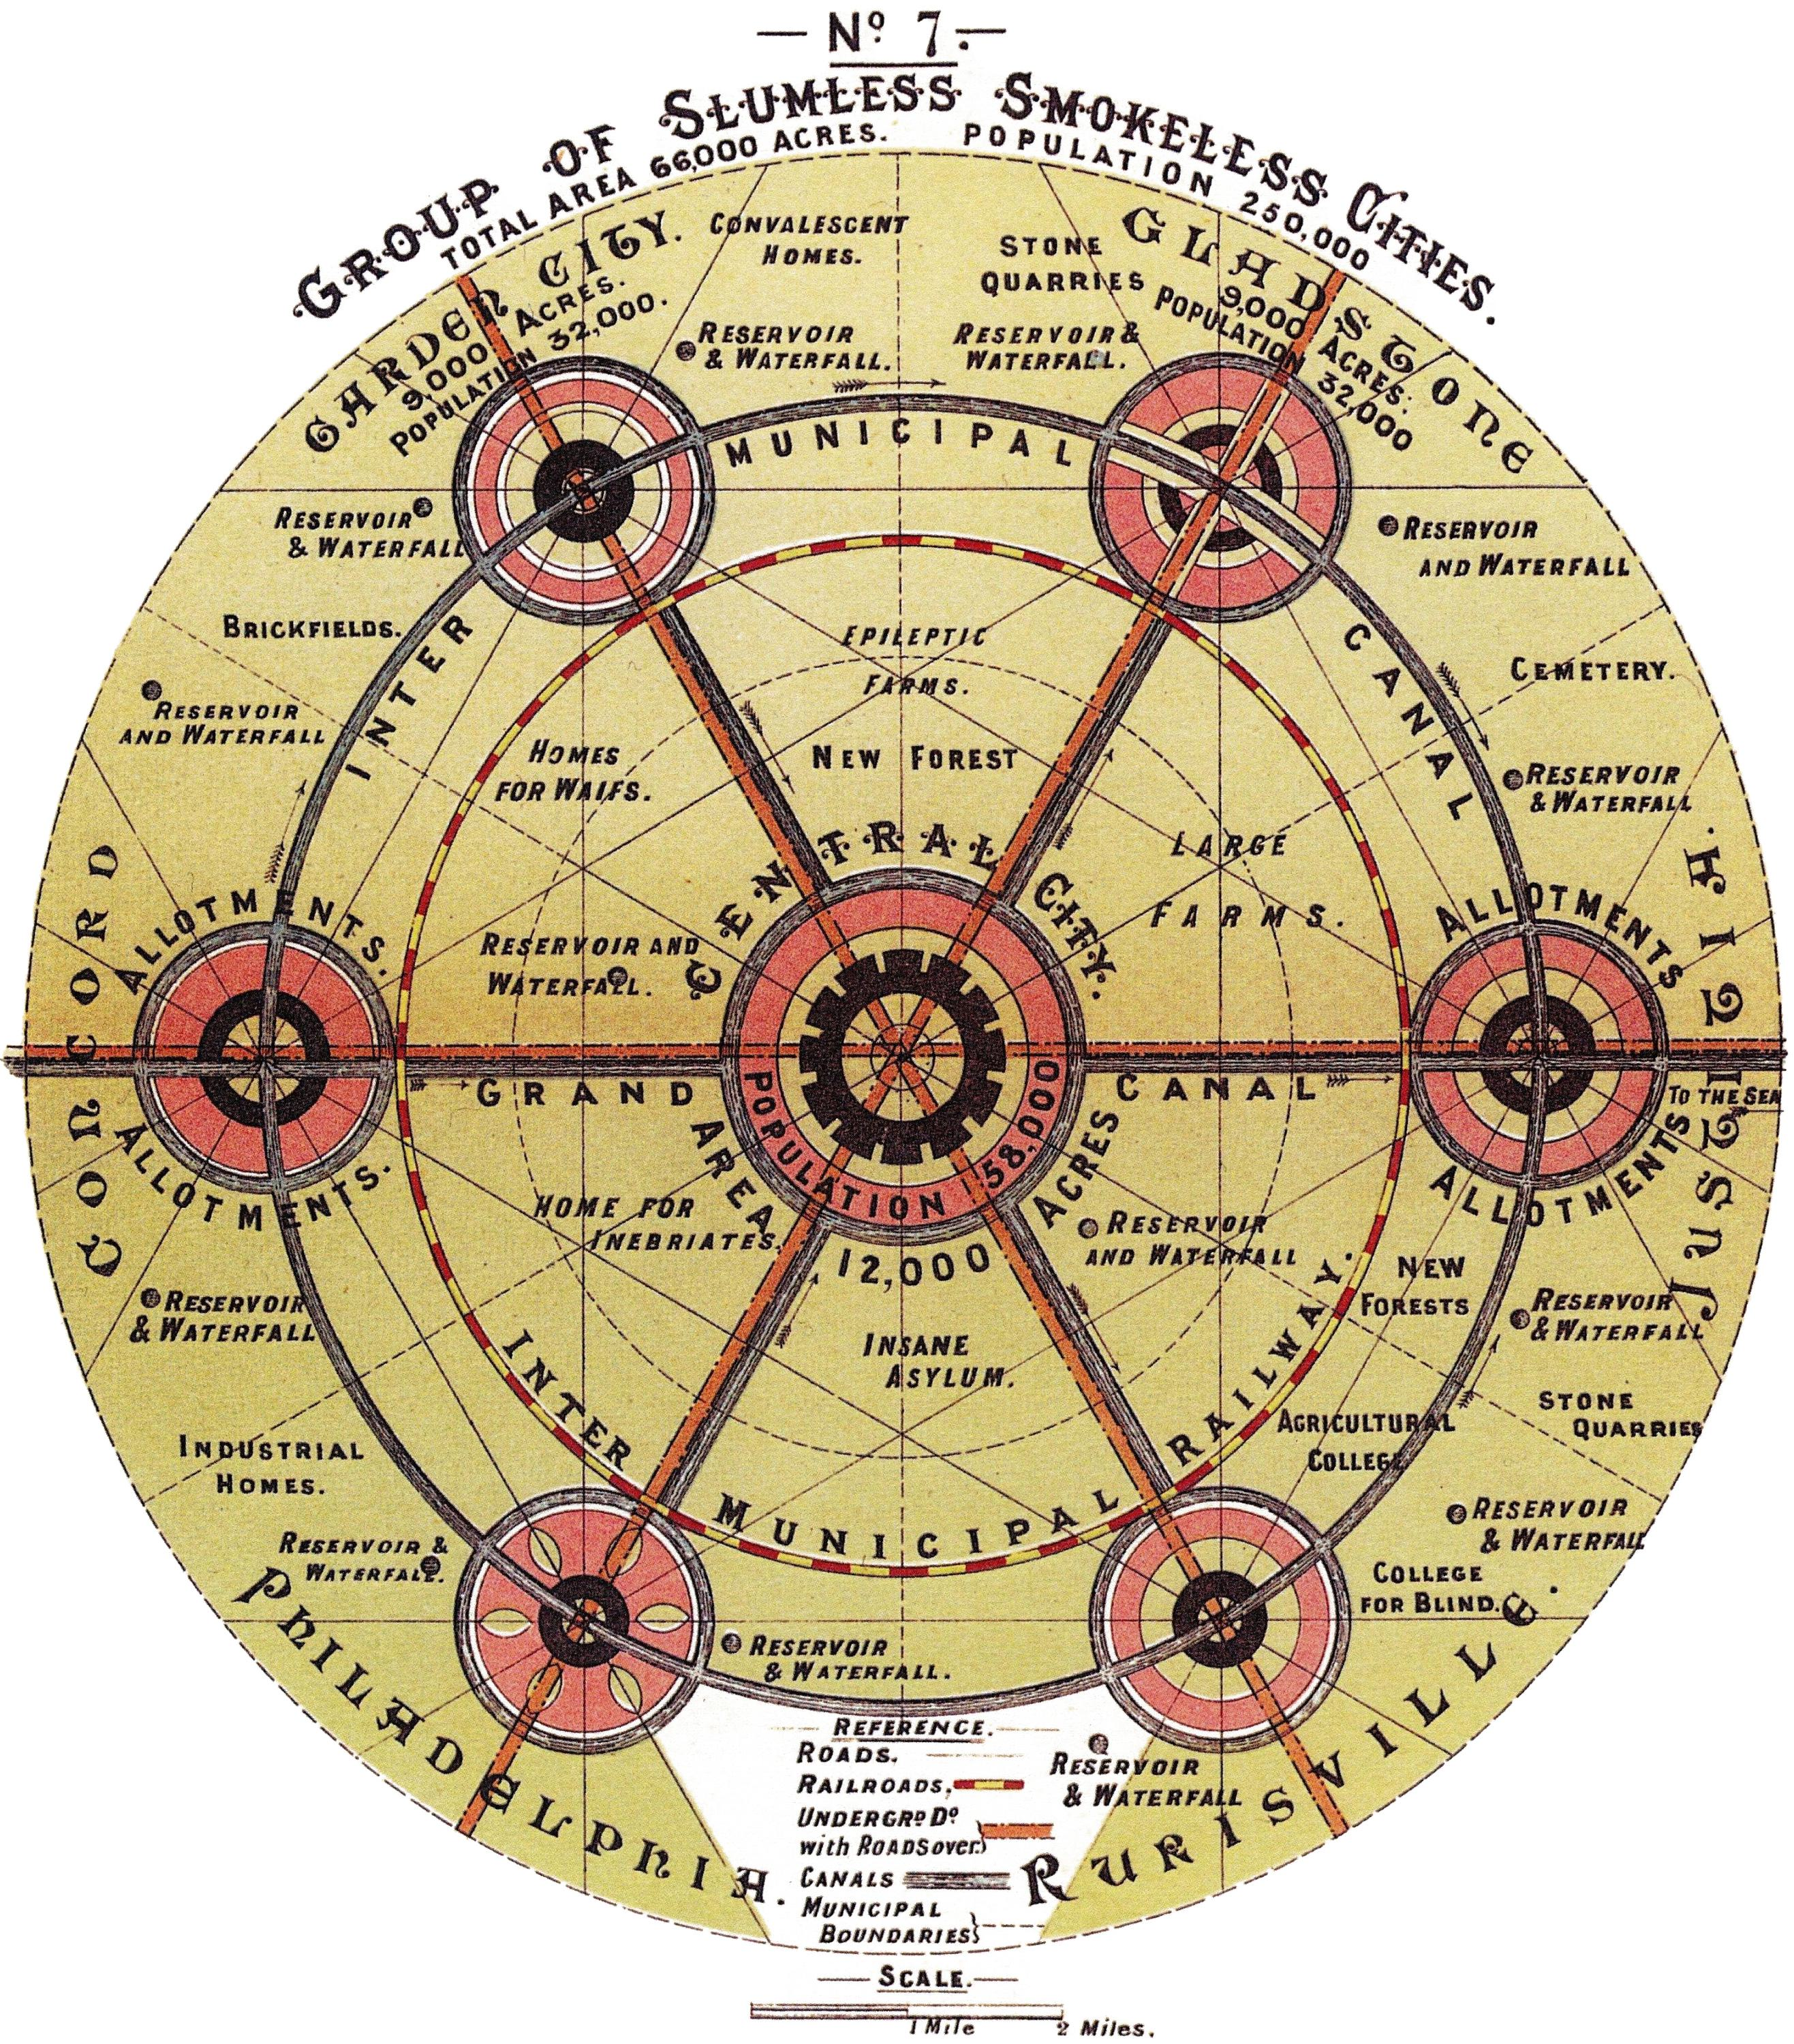
\includegraphics[width=0.75\columnwidth]{src/Figures/Chap-1/Cite_jardin.jpg}}
        \vspace{5pt}
        \begin{flushright}\scriptsize{
        Source~: \textcolor{blue}{Ebenezer} \textcolor{blue}{\textcite[90]{howard_-morrow_1898}}\index{Howard, Ebenezer|pagebf}, cité par \textcolor{blue}{Stephen} \textcolor{blue}{\textcite[3]{ward_garden_1992}}\index{Ward, Stephen|pagebf}
        }\end{flushright}
    \end{carte}

    % Cité linéaire : théorie
Un autre concept de cité utopique mise en application, dont s’inspire le \acrshort{TOD}, est sans nul doute la \textsl{Cité linéaire} (\textsl{Ciudad Lineal}), élaborée par \textcolor{blue}{Arturo Soria y Mata} en 1882 \textcolor{blue}{\autocite{lemelson_center_george_2014}}\index{Lemelson Center@\textsl{Lemelson Center}|pagebf}. En dirigeant le projet d’extension urbaine sur plus de cinq kilomètres le long de Madrid, l’urbaniste espagnol adopte une forme linéaire pour relier des centres urbains denses depuis les périphéries, une approche qui rappelle la notion de corridor chère au \acrshort{TOD} \textcolor{blue}{\autocite[348]{lopez_rodriguez_arturo_2017}}\index{López Rodríguez, Armando|pagebf}. L’organisation de la \textsl{Cité linéaire} repose sur un mode de transport en commun, souvent le tramway, qui devient la colonne vertébrale de l’agglomération \textcolor{blue}{\autocite{lemelson_center_george_2014}}\index{Lemelson Center@\textsl{Lemelson Center}|pagebf}. À la différence de la croissance urbaine traditionnelle, cette utopie urbaine envisage une ville sans banlieue, capable de contrôler son expansion le long d'un corridor \textcolor{blue}{\autocite[722]{furundzic_infrastructure_2012}}\index{Furundzic, Danilo~S.|pagebf}\index{Furundzic, Bozidar~S.|pagebf}. Par ailleurs, la \Guillemets{matrice de cette structure urbaine} se distingue par une accessibilité piétonne privilégiée, grâce à des promenades transversales reliant des îlots de densité moyenne. Ces deux utopies urbaines~–~la \textsl{Cité-jardin} et la \textsl{Cité linéaire}~–~prônent ainsi des questions qui sont toujours d'actualité et qui ont grandement influencé le \acrshort{TOD}, à savoir la promotion d'une ville compacte et conçue à la fois par et pour le transport public et la marche \textcolor{blue}{\autocite[11]{salomon_cavin_cites-jardins_2007}}\index{Salomon Cavin, Joëlle|pagebf}.%%Rédigé%%

    % Cité linéaire : exemples
L’expérimentation de cette cité idéale, initialement envisagée pour s’étendre sur 53 kilomètres autour de Madrid sous forme de boucle, ne verra finalement que 5 kilomètres réalisés, au nord-est de la capitale espagnole, à partir de 1894 \textcolor{blue}{\autocite[722]{furundzic_infrastructure_2012}}\index{Furundzic, Danilo~S.|pagebf}\index{Furundzic, Bozidar~S.|pagebf}. Ce projet, conçu par \textcolor{blue}{Arturo Soria y Mata}, prévoyait des connexions radioconcentriques reliant cette ceinture urbaine à la vieille ville. Inscrit dans le courant des villes hygiénistes, ce modèle exploite un axe ceinturant la ville existante pour faciliter la circulation des infrastructures essentielles telles que le chemin de fer, les réseaux de chauffage urbain, d’électricité ou encore de téléphonie. L’organisation horizontale de la ville linéaire rompt avec la structuration verticale propre à la ville bourgeoise, tout en anticipant certains principes de la cité-jardin, notamment l’accès généralisé à la propriété individuelle. Plus largement, ce concept évoque la notion de \Guillemets{Corridor Urbain} \textcolor{blue}{\autocite[63]{liu_corridors_2016}}\index{Liu, Liu|pagebf}\index{Menerault, Philippe|pagebf}\index{L'Hostis, Alain|pagebf}, en permettant d’étendre les villes de manière linéaire. À cet égard, des projets urbains tels que le \Guillemets{Grand Boulevard} reliant Lille, Roubaix et Tourcoing peuvent être considérés comme en résonance avec ces principes. Inaugurée en 1909, cette artère stratégique, longue de 14 kilomètres et large de 50 mètres, est traversée par six espaces de circulation dédiés respectivement à l'automobile, au transport lourd à cheval, au tramway Mongy, aux cavalier·ère·s, aux cyclistes et aux marcheur·se·s qui bénéficient de larges promenades\footnote{
        Aujourd’hui, le Grand Boulevard est néanmoins perçu comme un espace davantage assimilé à un lieu de transit automobile \textcolor{blue}{\autocite[139]{maitre_ambivalence_2016}}\index{Maitre, Elisa|pagebf}. Conçu initialement comme une artère urbaine intégrant deux chaussées séparées, des pistes cyclables et des trottoirs, cet aménagement a progressivement évolué pour devenir une voie rapide urbaine, au gré des raccordements successifs qui ont accru le trafic qu’il supporte. \textcolor{blue}{Philippe} \textcolor{blue}{\textcite[155]{menerault_gares_2008}}\index{Menerault, Philippe|pagebf} donne l'exemple de son intégration à l'autoroute A1, dont la première section jusqu'à Carvin est mise en service en 1954, et à l'autoroute A25, en direction de Dunkerque, en 1972.
} \textcolor{blue}{\autocite[87]{demangeon_lille-roubaix-tourcoing_1988}}\index{Demangeon, Alain|pagebf}\index{Werquin, Ann-Carol|pagebf}. Pensé comme un outil structurant de la croissance urbaine, ce projet avait pour ambition de faire du Grand Boulevard une vitrine régionale, surnommée les \Guillemets{Champs-Élysées} de la métropole, et d’en faire la colonne vertébrale de la future métropole \textcolor{blue}{\autocite{dubuis__2020}}\index{Dubuis, Angélique Da Silva|pagebf}. La ville linéaire a par ailleurs suscité d’autres interprétations et prolongements, notamment dans les expériences soviétiques ou à travers la reprise de ce concept par \textcolor{blue}{Le Corbusier}. Plus récemment, un exemple marquant est le projet \textsl{The Line}, annoncé par les autorités saoudiennes dans le cadre du plan Vision 2030 \textcolor{blue}{\autocite[139]{arnault_ville_2022}}\index{Arnault, Julie|pagebf}. Inscrit dans le projet de ville nouvelle \textsl{Neom}, ce concept, actuellement en cours de réalisation, repose sur la création d’une ville linéaire de 170 kilomètres de long pour 200 mètres de large et 500 mètres de hauteur\footnote{
    Cependant, avant même son lancement concret, le projet \textsl{The Line} est revu à la baisse pour 2030, avec une infrastructure longue de seulement 2,4 kilomètres au lieu des 170 kilomètres initialement prévus.
}. Cette infrastructure sera desservie par un train à grande vitesse, permettant théoriquement de parcourir l’ensemble de la ville en moins de 20 minutes. Les services essentiels seront répartis en hauteur, à chaque étage, et accessibles en moins de cinq minutes \textcolor{blue}{\autocite[139]{arnault_ville_2022}}\index{Arnault, Julie|pagebf}.%%Rédigé%%

    % New Urbanism
Sous un regard plus contemporain, l’enracinement du \acrshort{TOD} trouve une origine directe dans le \textsl{Nouvel urbanisme} (\textsl{New Urbanism}), un courant urbanistique et architectural apparu dans les années 1980 en réponse aux limites de l’urbanisme moderne \textcolor{blue}{\autocite[71]{liu_analyse_2016}}\index{Liu, Liu|pagebf}. Ce mouvement critique notamment le manque de diversité fonctionnelle et architecturale, l’organisation inadéquate des espaces publics et l’insuffisance de place accordée aux piéton·ne·s. Proposé comme une alternative rationnelle au développement des quartiers résidentiels pavillonnaires à faible densité et largement dominés par l’automobile, le \textsl{Nouvel urbanisme} ambitionne de repenser l’aménagement urbain pour le rendre plus humain, esthétique et fonctionnel. Bien qu’inspiré par certains principes du mouvement moderne, il s’en démarque notamment par l’instauration, en 1989, du \textsl{Congress for the New Urbanism}, souvent perçu comme l’équivalent contemporain du \acrfull{CIAM}. En 1996, ce Congrès ratifie sa propre Charte du Nouvel Urbanisme (\textsl{Charter of the New Urbanism})\footnote{
    Ce mouvement ne constitue toutefois pas un bloc monolithique. Il se compose de deux grandes approches complémentaires \textcolor{blue}{\autocite[178]{ouellet_smart_2006}}\index{Ouellet, Michel|pagebf}. D’une part, les partisan·e·s du \acrfull{TND} qui mettent l’accent sur une esthétique et une organisation urbaine néotraditionnelle, favorisant des quartiers compacts avec un habitat aligné le long de rues à intersections multiples. D’autre part, les promoteur·rice·s du \acrshort{TOD} qui privilégient l’intégration du transport public et une planification urbaine régionale plus respectueuse de l’environnement. Bien que distinctes, ces deux visions partagent un objectif commun~: encourager des formes urbaines favorisant la mixité fonctionnelle et la réduction de l’empreinte écologique des territoires.
}. Cette \Guillemets{philosophie d’aménagement} met en avant un développement urbain compact, planifié à l’échelle humaine, qui privilégie les transports en commun et l’intégration de fonctions urbaines diverses \textcolor{blue}{\autocite[177]{ouellet_smart_2006}}\index{Ouellet, Michel|pagebf}. D'un point de vue pratique, elle reconnaît plusieurs caractéristiques principales au quartier, dont celle de sa dimension optimale, évaluée à 400 mètres du centre à la périphérie \textcolor{blue}{\autocite[194]{ducharme_ville_2021}}\index{Ducharme, Olivier|pagebf}. Enfin, le \textsl{Nouvel urbanisme} adopte une perspective régionale, considérant la région comme unité territoriale de base dans un contexte de mondialisation économique \textcolor{blue}{\autocite[]{calthorpe_regional_2001}}\index{Calthorpe, Peter|pagebf}\index{Fulton, William|pagebf}. Dans cette perspective, le \acrshort{TOD} hérite l’objectif de promouvoir les transports en commun dans le but de freiner l'artificialisation des sols non urbanisés \textcolor{blue}{\autocite[117]{lo_feudo_scenario_2014}}\index{Lo Feudo, Fausto|pagebf}\index{Menerault, Philippe|pagebf}\index{L'Hostis, Alain|pagebf}\index{Festa, Demetrio Carmine|pagebf}.%%Rédigé%%

    % Smart Growth
Les principes du \acrshort{TOD} trouvent également leurs racines dans un courant majeur de l’urbanisme contemporain~: la \textsl{Smart Growth}, qui émerge à la fin des années 1980 et qui se structure au milieu des années 1990 dans le prolongement du paradigme du \Guillemets{développement urbain durable} \textcolor{blue}{\autocites[7]{bentayou_transit-oriented_2015}[71]{liu_analyse_2016}}\index{Bentayou, Gilles|pagebf}\index{Liu, Liu|pagebf}. Ce mouvement vise à préserver les ressources naturelles et financières, tout en cherchant à réduire les ségrégations spatiales, qu’elles soient fonctionnelles ou sociales \textcolor{blue}{\autocite[7]{bentayou_transit-oriented_2015}}\index{Bentayou, Gilles|pagebf}. La \textsl{Smart Growth} s’oppose explicitement à l’étalement urbain non maîtrisé, en promouvant des formes d’aménagement plus compactes et le redéveloppement urbain \textcolor{blue}{\autocites[176]{ouellet_smart_2006}{smart_growth_network_what_2015}}\index{Ouellet, Michel|pagebf}\index{Smart Growth Network@\textsl{Smart Growth Network}|pagebf}. Ces principes, partagés par le \textsl{Nouvel urbanisme}, valorisent une approche intégrée, où transport et urbanisme convergent pour créer des environnements durables, socialement équitables et économiquement viables. Le \acrshort{TOD} serait ainsi l'un des outils permettant de faire advenir ce \Guillemets{nouvel} urbanisme \Guillemets{intelligent} \textcolor{blue}{\autocite[7]{bentayou_transit-oriented_2015}}\index{Bentayou, Gilles|pagebf}.%%Rédigé%%

    % Figure photographies Val d'Europe
    \begin{figure}[h!]\vspace*{4pt}
        \caption{Photographies du secteur Val d'Europe, le 13 septembre 2023.}
        \label{fig-chap1:photographies-val-europe}
        \centerline{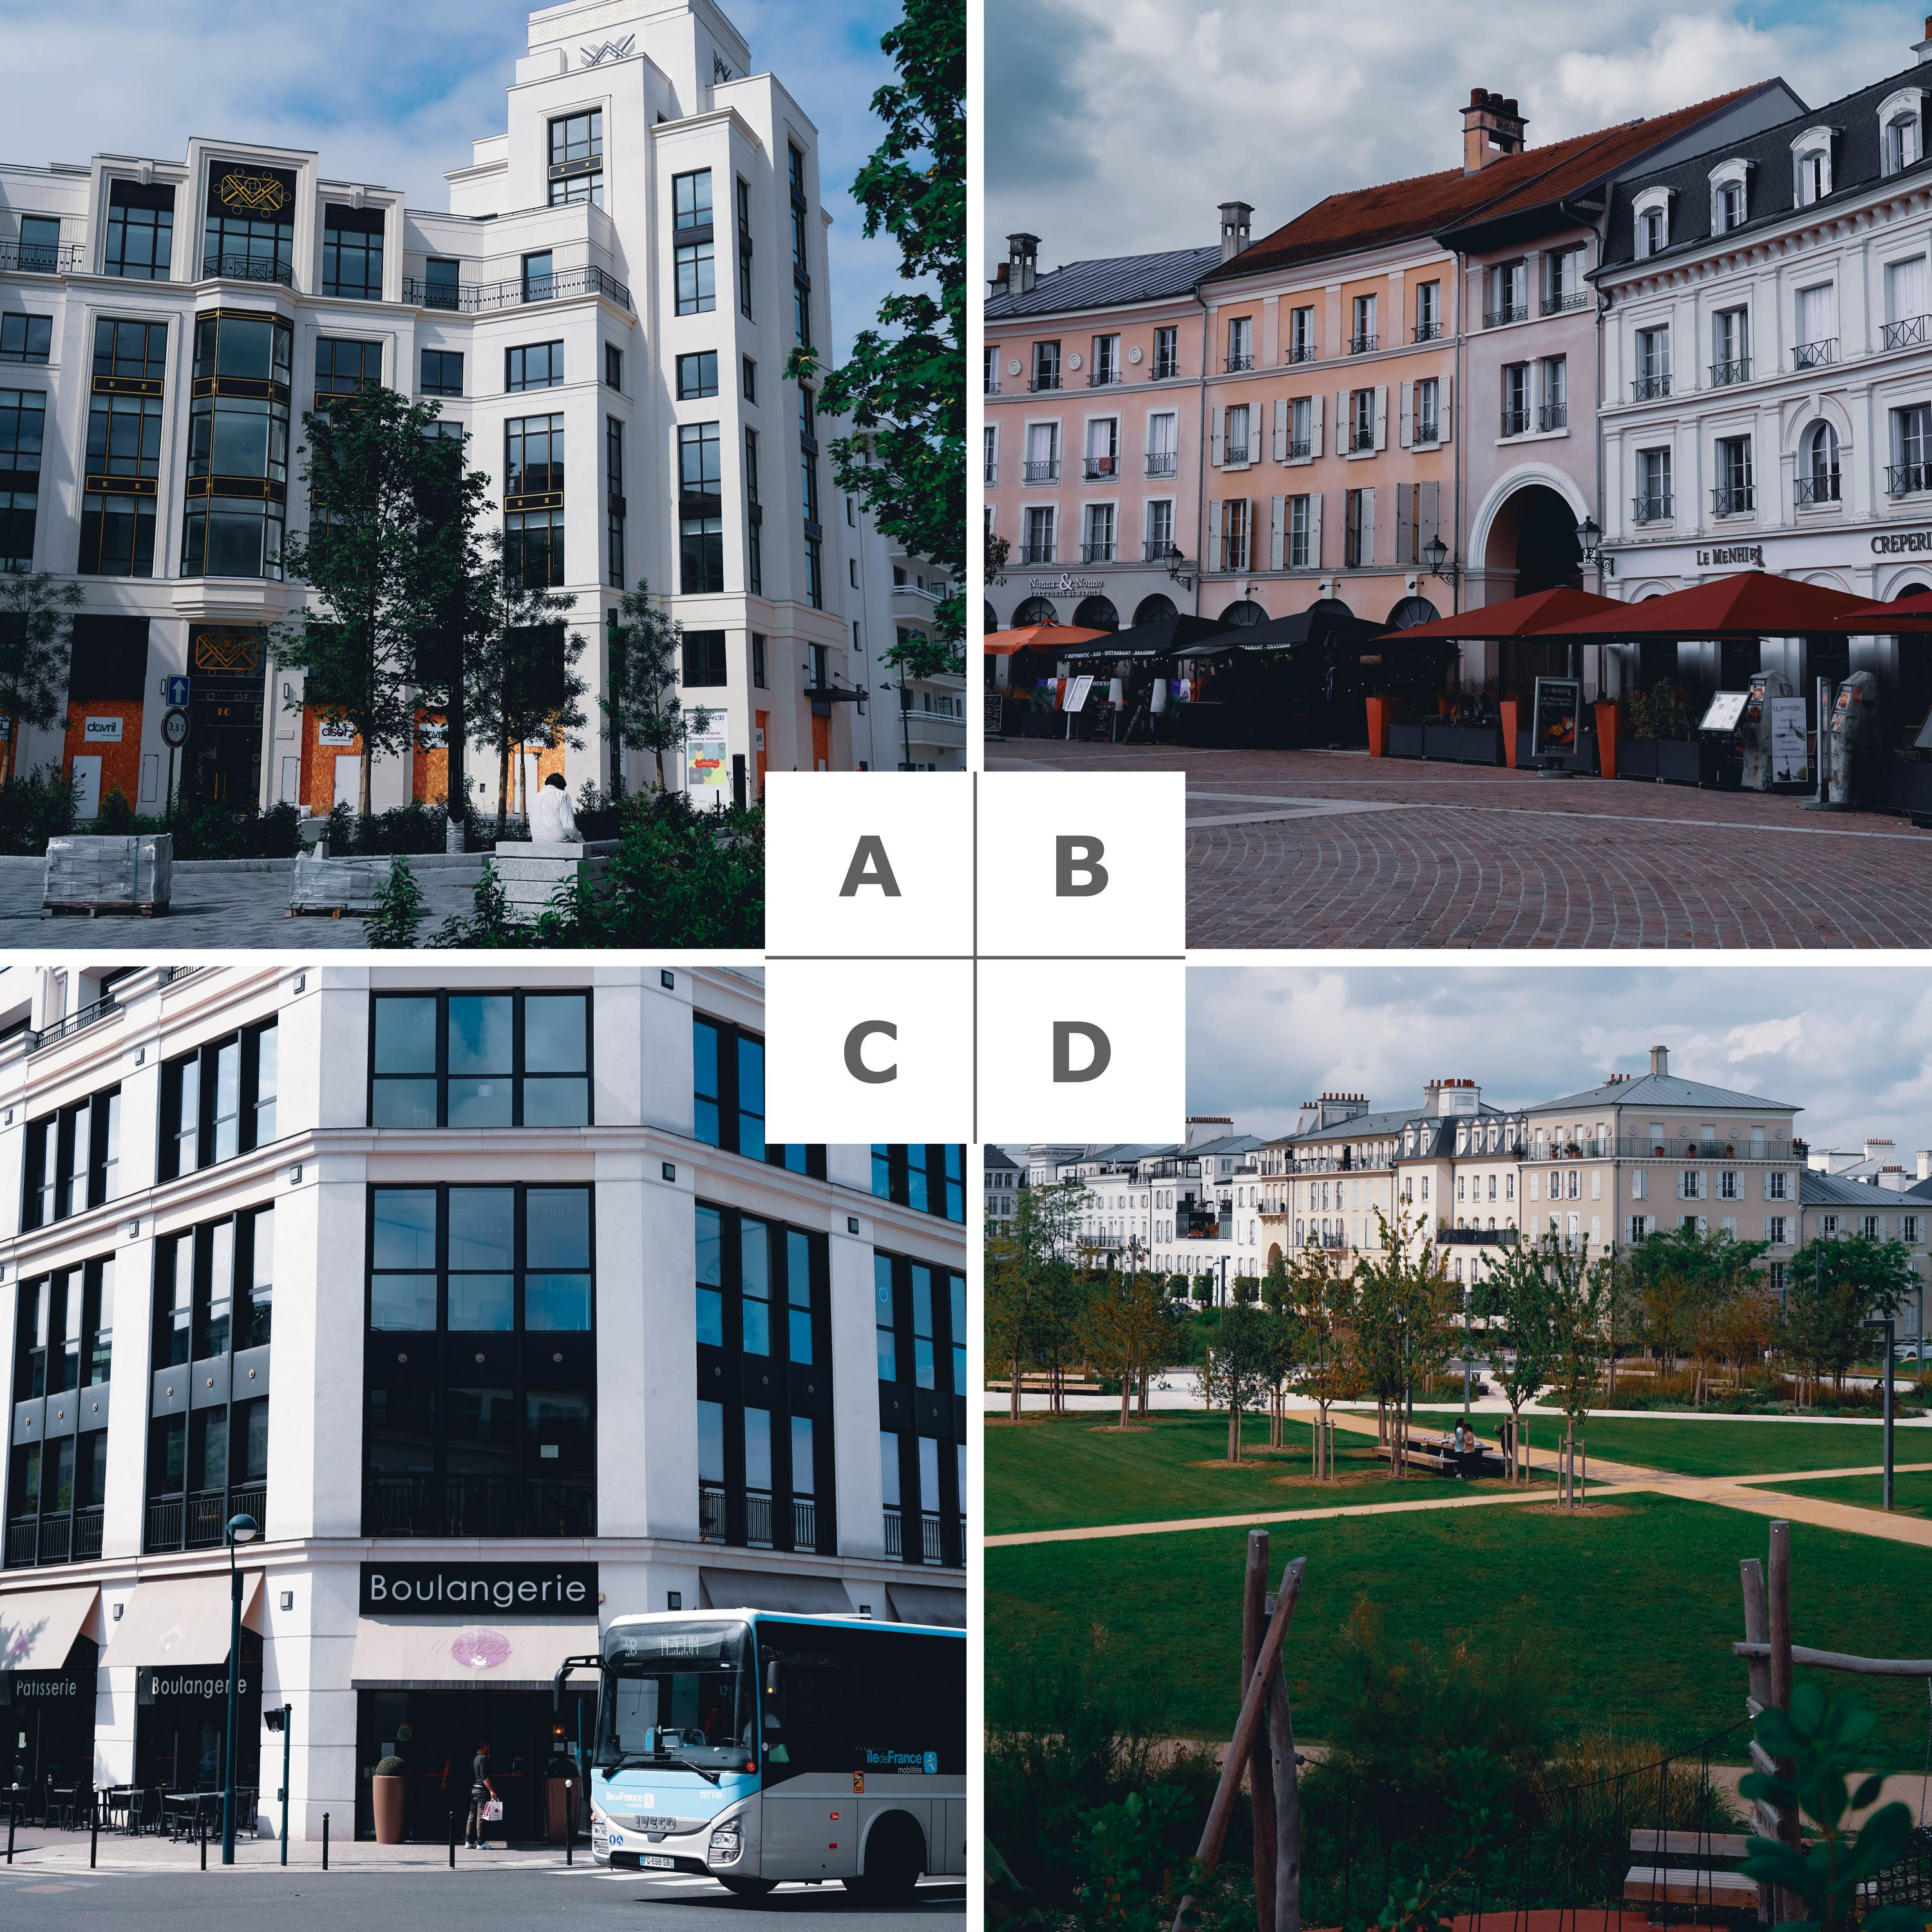
\includegraphics[width=0.75\columnwidth]{src/Figures/Chap-1/Val_Europe.jpg}}
        \vspace{5pt}
        \begin{flushright}\scriptsize{
        Photographies (A), (B), (C) et (D)~: \textcolor{blue}{Dylan Moinse (2023)}
      }\end{flushright}
    \end{figure}
    
    % Exemples New Urbanism/Smart Growth
Des réalisations emblématiques illustrent les principes du \textsl{Nouvel Urbanisme} et de la \textsl{Smart Growth}, à l'instar du quartier résidentiel de Laguna West, à Sacramento, en Californie, développé par \textcolor{blue}{Peter} \textcolor{blue}{\textcite[146-149]{calthorpe_next_1993}}\index{Calthorpe, Peter|pagebf}, figure clé de ces mouvements. Il s'agit d'une \Guillemets{communauté} néotraditionnelle, dont le projet lancé en 1989 intègre 3~400 unités résidentielles, en s'appuyant sur les concepts pionniers de l'architecte et urbaniste étasunien \textcolor{blue}{Morris} \textcolor{blue}{\textcite[]{newman_focus_1991-1}}\index{Newman, Morris|pagebf}. Aussi, tournons-nous vers l'étude du projet urbain Val d'Europe, le quatrième secteur de la ville nouvelle de Marne-la-Vallée, primé par le \textsl{Prix de la Charte} (\textsl{Charter Awards}) en 2006, par le \textcolor{blue}{\textcite{congress_for_the_new_urbanism_cnu_2006}}\index{Congress for the New Urbanism@\textsl{Congress for the New Urbanism}|pagebf}. Ce projet urbain, développé le long de la ligne A du \acrfull{RER} francilien~–~ligne la plus fréquentée d'Europe et mise en service en 1969, bien que la station Val d'Europe soit inaugurée en 2001~–~bénéficie d'une localisation stratégique à proximité immédiate de la gare \acrshort{TGV} de Marne-la-Vallée~–~Chessy. Il s'agit d'un \acrfull{PPP} né d'une collaboration entre l'État français et la \Marque{Walt Disney Company}, scellée par un accord en 1987, visant à développer et à exploiter \Marque{Euro Disneyland}, tout en intégrant un centre urbain dans la ville nouvelle \textcolor{blue}{\autocite{epamarne_val_nodate}}\footnote{
    L'\acrfull{EPA} ÉpaMarne, en collaboration avec ÉpaFrance a été chargé du pilotage de Val d'Europe dans le cadre d'une stratégie visant à équilibrer le développement territorial de la région Île-de-France, traditionnellement polarisée par l'attractivité du \acrfull{CBD} de La Défense. Ce projet incarne une double ambition~: d'une part, la création d'un centre urbain autonome en périphérie immédiate de Paris et, d'autre part, le renforcement de l'attractivité touristique régionale grâce à l'implantation de Disneyland Paris.
}. La planification de Val d'Europe repose sur trois principes fidèles aux mouvements présentés plus tôt~: (i) une organisation en quartiers, places et rues, favorisant des échelles humaines~; (ii) une mixité sociale fonctionnelle, intégrant logements\footnote{
    À l'heure actuelle, le développement urbain de Val d'Europe se poursuit. Adopté en 2016, le premier \acrfull{PLUi} de l'\acrshort{EPCI} prévoit la construction de 650 logements par an, visant un total de 5~100 unités, dont 80~\% de logements familiaux. Ce plan vise également à s'adapter aux exigences de la \acrfull{SRU} en matière de parc social, en prévoyant 34~\% de logements sociaux parmi les logements à venir, d'après son \acrfull{PLH}.
}, commerces et services\footnote{
    Prenons pour exemple le centre commercial Val d'Europe, ouvert en 2000, qui constitue le cœur symbolique et fonctionnel de la ville. Celui-ci est divisé en zones thématiques et a été récompensé pour son \textsl{design} (\textsl{International Council of Shopping Centers Europe awards}).
}~; et (iii) une architecture inspirée de l'histoire européenne, conférant une identité à chacun des quartiers (voir l'\hyperref[fig-chap1:photographies-val-europe]{illustration~\ref{fig-chap1:photographies-val-europe}}, page~\pageref{fig-chap1:photographies-val-europe}). Ainsi que l'exposent \textcolor{blue}{\textcite[25]{dupuis_nouvelle_2017}}\index{Dupuis, Blaise|pagebf}\index{Söderström, Ola|pagebf}, en tant que \Guillemets{nouvelle ville traditionnelle}, Val d'Europe porte haut les principes prônés\footnote{
    Toutefois, le développement de Val d'Europe suscite des interrogations quant à son modèle de gouvernance et sa conception urbaine. L'implication de l'opérateur privé dans la gestion urbaine a imposé une vision entrepreneuriale, voire commerciale, de la fabrique urbaine. Cette approche a souvent été critiquée pour sa tendance à une \Guillemets{disneylandisation} ou une \Guillemets{muséification} de l'espace urbain \textcolor{blue}{\autocite[]{brunel_planete_2012}}\index{Brunel, Sylvie|pagebf}. Ces notions renvoient à un modèle idéalisé et hyper-contrôlé, caractérisé par une reproduction fictive et standardisée de paysages et d'histoires urbaines, destinés à répondre aux attentes stéréotypées des touristes \textcolor{blue}{\autocite[7]{claude_developpement_2021}}\index{Claude, Appolline|pagebf}\index{Laage de Meux, Olivia de|pagebf}\index{Delpuech, Inès|pagebf}\index{Dextreit, Natalia|pagebf}\index{Poquillon, Mathilde|pagebf}\index{Praderie, Mila|pagebf}. Les critiques soulignent également les risques d'une déconnexion entre cette ville idéalisée et les réalités sociales et économiques. Elles questionnent notamment l'équilibre entre les impératifs entrepreneuriaux, l'inclusion sociale et la durabilité. En outre, les processus de négociation entre acteurs publics et privés ont été marqués par des tensions, révélant les limites d'un \acrshort{PPP} dans ces types de projet urbain. Un exemple est celui de la localisation du centre commercial régional Val d'Europe. L'opérateur privé, probablement affecté par une \Guillemets{culture de l'indifférence vis-à-vis du transport public} \textcolor{blue}{\autocite[656]{tan_identifying_2014}}\index{Tan, Wendy|pagebf}\index{Bertolini, Luca|pagebf}\index{Janssen-Jansen, Leonie|pagebf}, souhaitait implanter cet équipement en bordure d'autoroute, loin du pôle d'échange et de la station \acrshort{RER}.
}, à savoir une compacité urbaine, une organisation en quartiers, ainsi que des principes esthétiques et morphologiques ancrés dans l'héritage des siècles passés \textcolor{blue}{\autocite[12]{moinse_exploring_2023}}\index{Moinse, Dylan|pagebf}.%%Rédigé%%

    % Transition
Le concept d’aménagement du \acrshort{TOD}, centré sur un développement urbain compact, mixte et structuré autour d’un nœud de transport, s’inscrit dans une lignée de mouvements urbanistiques qui l’ont précédé. Ces influences sont pleinement revendiquées par \textcolor{blue}{Peter Calthorpe}, l’un des principaux théoriciens du \acrshort{TOD}, qui se définit comme \Guillemets{un restaurateur et non un initiateur d’idées}\footnote{
    \Guillemets{\textsl{Mr. Calthorpe, who calls himself a reviver rather than an originator of ideas} [\dots]} \textcolor{blue}{\autocite[5]{newman_focus_1991}}\index{Newman, Morris|pagebf}.
} \textcolor{blue}{\autocite[5]{newman_focus_1991}}\index{Newman, Morris|pagebf}. Si des prémices du \acrshort{TOD} peuvent être identifiées dans des modèles tels que la \textsl{Cité-jardin} ou la \textsl{Cité linéaire}, ou encore de grandes figures de l'histoire de l'urbanisme comme \textcolor{blue}{Ildefons Cerdà} ou \textcolor{blue}{Georges-Eugène Haussmann}, ces exemples témoignent de l’évolution des idées en matière d’aménagement urbain. Dans la cité-jardin, par exemple, la gare joue un rôle fonctionnel limité, se réduisant à relier des cités autosuffisantes entre elles et à leur environnement. \textcolor{blue}{Peter} \textcolor{blue}{\textcite[43-49]{calthorpe_next_1993}}\index{Calthorpe, Peter|pagebf}, en revanche, renverse ce principe~: dans le \acrshort{TOD}, la station de transport devient le centre structurant de l’aménagement urbain, dépassant la logique d’autarcie pour créer du lien au sein d’une ville contemporaine fragmentée et dispersée \textcolor{blue}{\autocite[51]{el_hadeuf_ville_2017}}\index{El Hadeuf, Mounya|pagebf}\index{Laterrasse, Jean|pagebf}. Cette distinction marque un tournant conceptuel. Contrairement au \textsl{Nouvel urbanisme} et à la \textsl{Smart Growth}, qui s’opposent principalement à l’étalement urbain non maîtrisé, le \acrshort{TOD} affirme un rôle moteur pour les infrastructures de transport dans la structuration de la ville \textcolor{blue}{\autocite[51]{el_hadeuf_ville_2017}}\index{El Hadeuf, Mounya|pagebf}\index{Laterrasse, Jean|pagebf}. Là où le \textsl{Nouvel urbanisme} promeut une densité humaine et esthétique, et où la \textsl{Smart Growth} privilégie la préservation des ressources naturelles et la mixité fonctionnelle, le \acrshort{TOD} se distingue par son ambition de reconnecter les territoires épars grâce à une organisation centrée sur le transport. Bien que la plupart des composantes morphologiques~–~présence d'une gare, densité et compacité~–~soient semblables, cette approche traduit un changement d’échelle entre la ville du XIX\textsuperscript{e} siècle, encore pensée comme un tout cohérent, et la ville contemporaine, qui nécessite des outils pour rétablir sa cohésion \textcolor{blue}{\autocite[37]{leysens_reconfiguration_2011}}\index{Leysens, Thomas|pagebf}\index{Menerault, Philippe|pagebf}\index{L'Hostis, Alain|pagebf}.%%Rédigé%%

    % 1.1.1.2. TOD aspects contemporains
    \needspace{1\baselineskip} % Réserve de l'espace
\subsubsection*{Originalité et réinterprétation de la planification autour du rail
    \label{chap1:tod-presentation-generale-origines-originalite}
    }

    % Introduction
Le mouvement ayant vu naître le \acrshort{TOD} s'inscrit dans une filiation intellectuelle et urbanistique commune à plusieurs courants critiques et militants, unis par leur opposition au paradigme de la ville auto-centrée\footnote{
    Dès les années 1960, et même dès l'après-guerre, la domination de l’automobile dans l’espace urbain commence à être remise en question, suscitant des critiques croissantes concernant son usage massif et ses implications pour l’aménagement urbain \textcolor{blue}{\autocites{jacobs_death_1961}{illich_energie_1973}}\index{Jacobs, Jane|pagebf}\index{Illich, Ivan|pagebf}\index{Giard, Luce|pagebf}\index{Bardet, Vincent|pagebf}. Ce passage au \Guillemets{troisième âge de la ville} \textcolor{blue}{\autocite[4]{newman_land_1996}}\index{Newman, Peter W.~G.|pagebf}\index{Kenworthy, Jeffrey~R.|pagebf} marqué par la \Guillemets{culture de l'automobile} \textcolor{blue}{\autocite[157]{urry_social_2003}}\index{Urry, John|pagebf}. structure encore aujourd'hui la plupart des territoires, avec des conséquences directes et indirectes sur l'aménagement, les comportements de mobilité et les modes de vie \textcolor{blue}{\autocite[40]{sebban_complementarite_2003}}\index{Sebban, Annie-Claude|pagebf}\index{Motte, Alain|pagebf}.
} \textcolor{blue}{\autocites{jacobs_death_1961}{illich_energie_1973}}\index{Jacobs, Jane|pagebf}\index{Illich, Ivan|pagebf}\index{Giard, Luce|pagebf}\index{Bardet, Vincent|pagebf}, et notamment les nombreuses externalités négatives associées à ce modèle\footnote{
    Les externalités négatives engendrées par la dépendance à l’automobile incluent des nuisances internes telles que la congestion urbaine, qui compromet l’attractivité économique et résidentielle des territoires, mais également des effets externes plus larges~: accidents de la route, effets de \gls{coupure urbaine}, sédentarisation, fragmentation de l’espace, exclusion socio-spatiale, consommation accrue d’espaces agricoles et naturels, perte de biodiversité, pollutions multiples (air, eau, sols, sonore et visuelle), ainsi qu’une dégradation de la qualité de vie, allant de problèmes de santé physique et mentale à un stress chronique et à une réduction de la productivité. Ces externalités contribuent à ce que certain·e·s auteur·rice·s qualifient de \Guillemets{spirale de la dépendance à l’automobile} ou \Guillemets{cycle de l’auto-dépendance}, dans lequel l’automobile crée des problèmes que seul son usage intensifié semble pouvoir résoudre \textcolor{blue}{\autocites[62]{cervero_transit_1998}[4]{heran_reduction_2001}[2]{heran_zones_2009}}\index{Cervero, Robert|pagebf}\index{Héran, Frédéric|pagebf}\index{Pouillaude, Laurence|pagebf}.
} \textcolor{blue}{\autocites[62]{cervero_transit_1998}[4]{heran_reduction_2001}[2]{heran_zones_2009}}\index{Cervero, Robert|pagebf}\index{Héran, Frédéric|pagebf}\index{Pouillaude, Laurence|pagebf}. Le \Guillemets{système automobile}, caractérisé par un mode d’organisation centré sur les performances techniques et les avantages apparents de la voiture, constitue une structure captative et rigide\footnote{
    La dépendance à l’automobile, ainsi que l'\Guillemets{automobilité} désignant un mode de vie et les représentations associées, reposent sur des facteurs culturalistes, socio-économiques, urbanistiques et technicistes \textcolor{blue}{\autocite[12]{heran_reduction_2001}}\index{Héran, Frédéric|pagebf}. Le \Guillemets{tout-automobile} est le produit d'aspirations liées à la propriété individuelle d'une maison et d'un jardin, d'une élévation des niveaux de vie conjuguée à des normes de consommation, de l'influence de formes urbaines favorisant les déplacements motorisés et de l'amélioration continue des performances de la voiture par rapport aux autres modes de déplacement.
}. Les \Guillemets{coûts cachés} associés à ce système, c'est-à-dire les coûts non couverts par la collectivité qui sont estimés à environ 3~\% du \acrfull{PIB} annuel de l'\acrfull{UE}, révèlent son inefficacité collective \textcolor{blue}{\autocite[34]{becker_couts_2012}}\index{Becker, Udo~J.|pagebf}\index{Becker, Thilo|pagebf}\index{Gerlach, Julia|pagebf} et sa contribution à une véritable \Guillemets{tragédie des communs} \textcolor{blue}{\autocite{hardin_tragecommuns_1968}}\index{Hardin, Garrett|pagebf}, où l’usage intensif des espaces routiers par certains individus entraîne des conséquences délétères pour l’ensemble de la société \textcolor{blue}{\autocite[23]{6t-bureau_de_recherche_livre_2019}}\index{Bureau de recherche 6t@\textsl{Bureau de recherche 6t}|pagebf}. À noter que ces estimations restent, de surcroît, sous-évaluées, notamment en raison de la non-prise en compte systématique des boucles de rétroaction complexes affectant le dérèglement climatique et la santé publique \textcolor{blue}{\autocite[66, 72]{gossling_social_2019}}\index{Gössling, Stephan|pagebf}\index{Choi, Andy|pagebf}\index{Dekker, Kaely|pagebf}\index{Metzler, Daniel|pagebf}. C’est précisément dans ce contexte critique que le concept du \acrshort{TOD} se déploie, comme une réponse multidimensionnelle visant à remédier aux dysfonctionnements du modèle auto-centré.%%Rédigé%%

    % Lutte contre la dépendance automobile
En effet, plus qu’une invention \textsl{ex nihilo}, le \acrshort{TOD} constitue avant tout le résultat d’une adaptation à un contexte urbain renouvelé, celui de la complexité et de la \Guillemets{vitesse} des villes modernes. Il propose une alternative articulée à la diffusion et à l'usage généralisés de l'automobile en introduisant des principes, des perspectives et des outils opérationnels pour répondre aux enjeux actuels, à différentes échelles spatiales \textcolor{blue}{\autocite[37]{leysens_reconfiguration_2011}}\index{Leysens, Thomas|pagebf}. C'est là que se trouvent les apports originaux du modèle \textcolor{blue}{\autocite[121]{lo_feudo_scenario_2014}}\index{Lo Feudo, Fausto|pagebf}\index{Menerault, Philippe|pagebf}\index{L'Hostis, Alain|pagebf}\index{Festa, Demetrio Carmine|pagebf}~: il faut abandonner l'idée que l'automobile est l'étalon de mesure servant à la planification de l'espace urbain \textcolor{blue}{\autocite[190]{ducharme_ville_2021}}\index{Ducharme, Olivier|pagebf}. \textcolor{blue}{Peter} \textcolor{blue}{\textcite{calthorpe_next_1993}}\index{Calthorpe, Peter|pagebf} a ainsi essentiellement formalisé la relation étroite entre développement urbain et transports en commun, érigée en principe structurant du \acrshort{TOD}. Ce dernier définit dans ce cadre les bases d’un \Guillemets{nouveau rêve américain} (\textsl{American Dream})~: contrairement aux courants précurseurs principalement axés sur des préoccupations esthétiques ou sociales, le \acrshort{TOD} privilégie une approche résolument régionale. Il ne s'agit plus seulement d'une somme de projets urbains dispersés et éparpillés dans une ville contemporaine \textcolor{blue}{\autocite[357]{mongin_ville_2013}}\index{Mongin, Olivier|pagebf}. Il intègre l’impératif de réduction de l’usage de l’automobile au cœur même des fonctions de l’urbanisme \textcolor{blue}{\autocite[11]{calthorpe_next_1993}}\index{Calthorpe, Peter|pagebf}.%%Rédigé%%

    % Oriented
C'est là la seconde innovation apportée par le \acrshort{TOD}, qui réside dans sa faculté à s’ajuster au contexte de croissance de l’usage de l’automobile, tout en proposant une réflexion collective nourrie d’expériences internationales. Il introduit notamment un troisième élément structurant dans la relation entre \textsl{transit} et \textsl{development}~: l'idée d'orientation (\textsl{oriented}). À ce propos, cette forme de connexion est déterminante, comme le fait remarquer \textcolor{blue}{Fausto} \textcolor{blue}{\textcite[116]{lo_feudo_scenario_2014}}\index{Lo Feudo, Fausto|pagebf}. Cette notion dépasse la simple proximité géographique pour embrasser une organisation globale et cohérente des zones d’intervention. Par conséquent, la communauté scientifique ayant contribué à l'évolution du modèle du \acrshort{TOD} met en avant une vision holistique d'un urbanisme \textsl{orienté} vers les transports en commun, faisant des espaces publics un pivot dans l'articulation entre réseau et développement urbain. Ainsi, le \acrshort{TOD} ne se limite pas à une série d'opérations isolées à proximité d'une station \textcolor{blue}{\autocite[124]{lhostis_ville_2013}}\index{L'Hostis, Alain|pagebf}\index{Soulas, Claude|pagebf}\index{Wulfhorst, Gebhard|pagebf}\index{Brun, Gérard|pagebf}. Il s’inscrit dans une logique plus vaste de répartition stratégique le long des corridors du réseau de transport en commun, en tenant compte de la structure spatiale régionale et en valorisant un \Guillemets{urbanisme de tracés, passant et métisse}, à l'envers de l'\Guillemets{urbanisme de secteurs, sécurisé et homogène} qui prévaut \textcolor{blue}{\autocite[4-6]{mangin_ville_2004}}\index{Mangin, David|pagebf}.%%Rédigé%%

    % Figure Murdoch
    \begin{figure}[h!]\vspace*{4pt}
        \caption{Vue aérienne (A) et vue à la première personne (B) des environs de la gare de Murdoch, connectée au réseau Transperth, en Australie.}
        \label{fig-chap1:tad-murdoch}
        \centerline{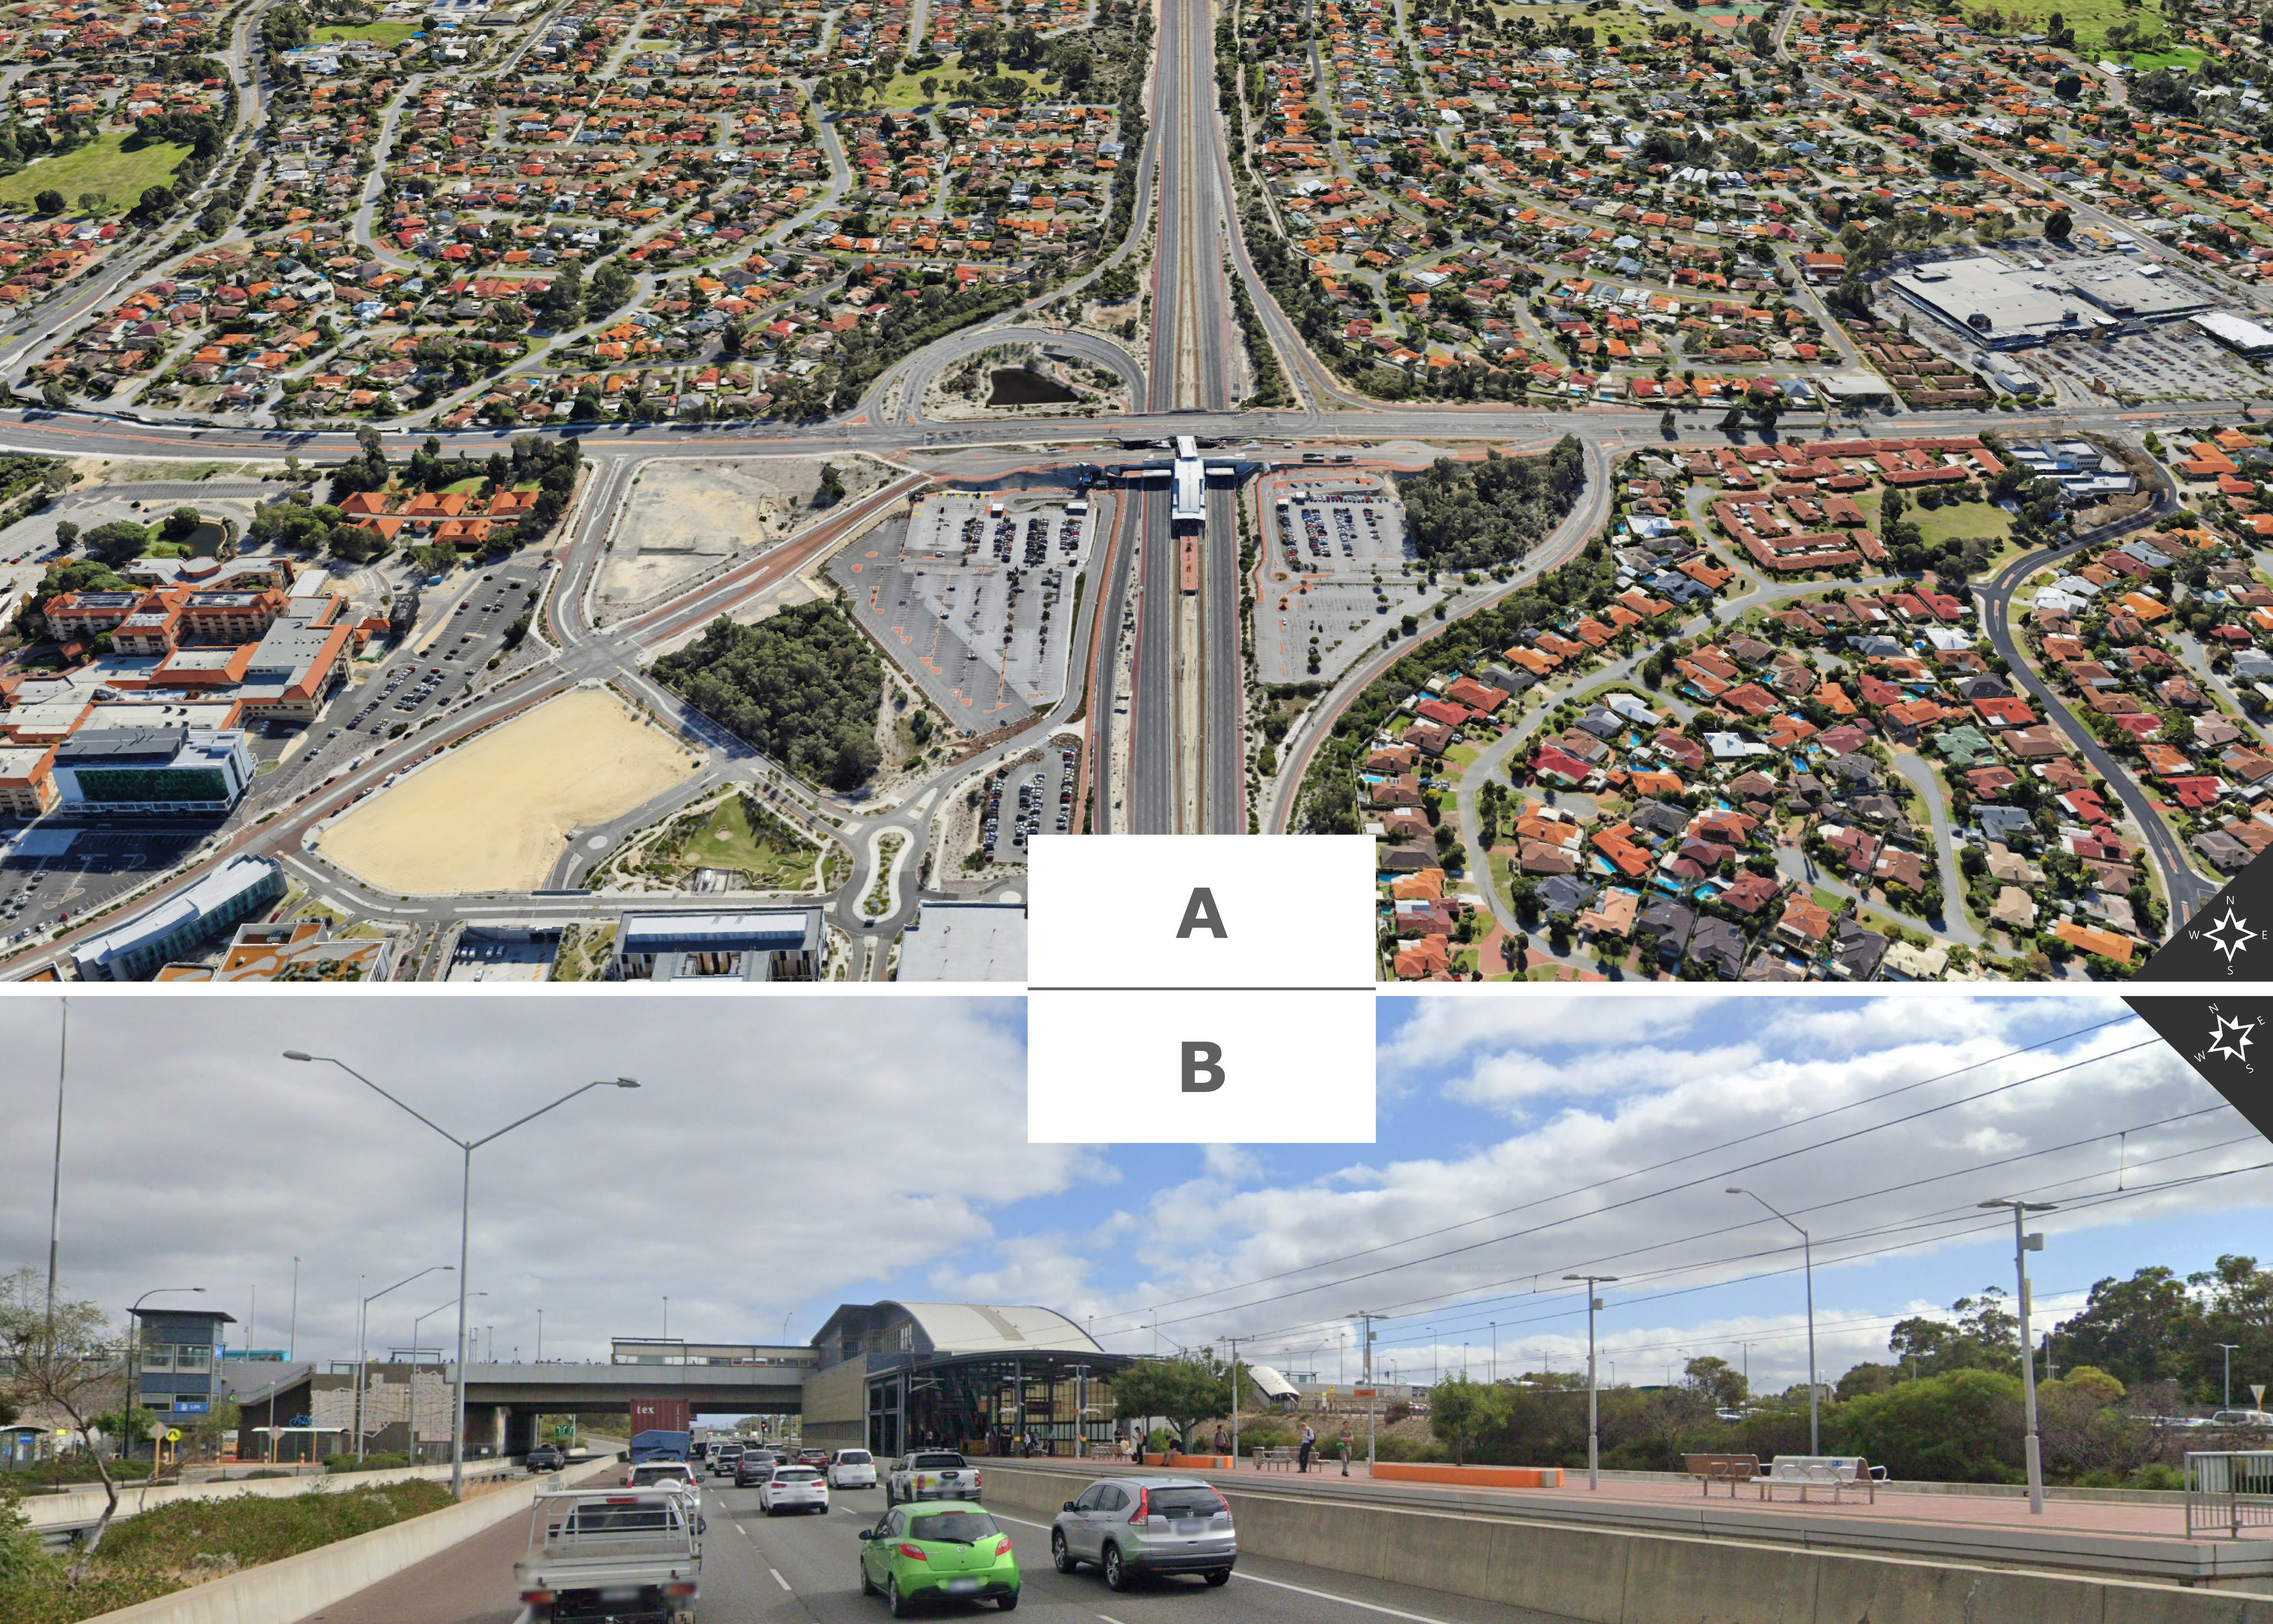
\includegraphics[width=1\columnwidth]{src/Figures/Chap-1/Murdoch.jpg}}
        \vspace{5pt}
        \begin{flushright}\scriptsize{
        Jeux de données (A)~: données satellitaires issues de \textcolor{blue}{\textcite{google_earth_google_2023}}
        \\
        Jeux de données (B)~: images issues de \Marque{Google Street View} datant de novembre 2023
        }\end{flushright}
    \end{figure}

    % Adjacent
Dès lors, une distinction progressive s’impose entre les \acrshort{TOD}\textcolor{blue}{s} véritablement conformes aux principes du modèle et ceux qui, en raison de divergences d’interprétation ou d’application, ne remplissent pas les critères attendus. Cette diversité d’approches a conduit à l’attribution généralisée du label \acrshort{TOD} à un large éventail de projets urbains qui ne possèdent pourtant pas toutes les caractéristiques du concept \textcolor{blue}{\autocite[4]{renne_transit-oriented_2013}}\index{Renne, John Luciano|pagebf}\index{Ewing, Reid|pagebf}. Parmi les raisons expliquant ces écarts figurent une qualité insuffisante des aménagements piétonniers ou cyclables, un déficit de mixité fonctionnelle, ainsi qu’une offre excessive de stationnement automobile\footnote{
    Plusieurs études démontrent que, pour une majorité d'autorités locales étasuniennes, le stationnement automobile reste perçu comme une solution de mobilité et d'aménagement plus pertinente que la densification des abords immédiats des gares \textcolor{blue}{\autocite[106-107]{cervero_tcrp_2004}}\index{Cervero, Robert|pagebf}\index{Murphy, Steven|pagebf}\index{Ferrell, Christopher|pagebf}\index{Tsai, Yu-Hsin|pagebf}\index{Arrington,~G.~B.|pagebf}\index{Boroski, John|pagebf}\index{Smith-Heimer, Janet|pagebf}\index{Golem, Ron|pagebf}\index{Peninger, Paul|pagebf}\index{Nakajima, Eric|pagebf}\index{Chui, Ener|pagebf}\index{Dunphy, Robert|pagebf}\index{Myers, Mel|pagebf}\index{McKay, Shannon|pagebf}\index{Witenstein, Nicole|pagebf}. De nombreux projets se réclamant du \acrshort{TOD} continuent alors à accorder une place prépondérante au stationnement automobile, de surface comme en ouvrage, souvent dans le but de maintenir les logiques de \gls{rabattement} automobile existantes. Cette persistance de l’automobile comme mode dominant résulte d’un manque d’encadrement et de réflexion sur son rôle dans l’aménagement des espaces autour des stations. En conséquence, ces \Guillemets{\textsl{Transit-Oriented Development} manqués} ont parfois permis que, localement, la voiture reste largement privilégiée \textcolor{blue}{\autocite[39]{bentayou_transit-oriented_2015}}\index{Bentayou, Gilles|pagebf}. Depuis, de nouvelles positions ont émergé et insistent bien plus sur le rôle déterminant des politiques de stationnement automobile dans le succès du \acrshort{TOD} \textcolor{blue}{\autocite[39]{bentayou_transit-oriented_2015}}\index{Bentayou, Gilles|pagebf}. En particulier en préconisant un renforcement des exigences réglementaires concernant les seuils minimaux et maximaux de stationnement, dans la mesure où une réduction des ratios de parking pour les projets résidentiels dans les \acrshort{TOD}\textcolor{blue}{s} permet d'augmenter la densité potentielle de 20~\% à 33~\% et de réduire les coûts liés au stationnement de 5~\% à 36~\%, tout en favorisant des prix abordables et en améliorant la rentabilité \textcolor{blue}{\autocite[51-54]{arrington_effects_2008}}\index{Arrington,~G.~B.|pagebf}\index{Cervero, Robert|pagebf}.
} \textcolor{blue}{\autocites[358]{lund_reasons_2006}[3]{renne_transit-adjacent_2009}}\index{Lund, Hollie~M.|pagebf}\index{Renne, John Luciano|pagebf}. Ces insuffisances ou ces défaillances aboutissent souvent à ce que ces projets relèvent davantage d’un \acrfull{TAD}, c’est-à-dire des aménagements qui souffrent d'un manque de connectivité avec le réseau de transport en commun. Par ailleurs, certains projets, désignés sous l’acronyme \acrfull{TRD}, se limitent à exploiter la proximité d’un réseau de transport public pour des opérations immobilières, sans intégrer les principes fondamentaux du \acrshort{TOD} \textcolor{blue}{\autocite[18]{bentayou_transit-oriented_2015}}\index{Bentayou, Gilles|pagebf}. À titre d’exemple, \textcolor{blue}{\textcite[18]{khan_parking_2009}}\index{Khan, Shahed|pagebf}\index{Bajracharya, Bhishna|pagebf} analysent la gare de Murdoch, située sur la ligne Mandurah reliant Perth, en Australie. Les auteur·rice·s identifient ce site comme un cas typique de \textsl{Transit-Adjacent Development}, soulignant que les abords de la gare sont largement dominés par des infrastructures autoroutières, des carrefours routiers, des installations de \acrfull{P+R} ainsi qu’un tissu pavillonnaire peu dense. L'\hyperref[fig-chap1:tad-murdoch]{illustration~\ref{fig-chap1:tad-murdoch}} (page~\pageref{fig-chap1:tad-murdoch}) rend visible cette configuration spatiale. Ces \Guillemets{\textsl{Transit-Oriented Development} manqués} sont ainsi l'occasion de rappeler que la proximité d’un système de transport public et la densité urbaine ne suffisent pas à garantir le succès du modèle \textcolor{blue}{\autocite[18]{bentayou_transit-oriented_2015}}\index{Bentayou, Gilles|pagebf}.%%Rédigé%%

    % Inspirations
Nous l’avons vu, le \acrshort{TOD} puise dans les luttes et les principes des mouvements d’aménagement urbain qui l’ont précédé, tout en les réajustant aux défis du XXI\textsuperscript{e} siècle. \textcolor{blue}{Peter Calthorpe}, en conceptualisant le \acrshort{TOD}, a offert à la planification urbaine un cadre théorique ainsi qu'un outil stratégique à vocation internationale, dont la pertinence s’appuie sur les contributions de nombreux penseur·se·s dans les champs de l’urbanisme et des transports \textcolor{blue}{\autocite[111]{almeida_correia_transit-oriented_2020}}\index{Almeida Correia, Gonçalo Homem de|pagebf}\index{Ibraeva, Anna|pagebf}\index{Silva, Cecília|pagebf}\index{Pais Antunesa, António|pagebf}. En retour, le modèle du \acrshort{TOD} a inspiré de nouvelles approches en matière de développement urbain. \textcolor{blue}{Fausto} \textcolor{blue}{\textcite[122]{lo_feudo_scenario_2014}}\index{Lo Feudo, Fausto|pagebf}\index{Menerault, Philippe|pagebf}\index{L'Hostis, Alain|pagebf}\index{Festa, Demetrio Carmine|pagebf} énonce trois courants de réflexion récents qui prolongent l’héritage du modèle urbain en réimaginant la proximité à travers une approche coordonnée entre urbanisme et mobilité~:
    \begin{customitemize}
\item La \textsl{ville creuse}, conceptualisée par l’ingénieur et chercheur \textcolor{blue}{Jean-Louis} \textcolor{blue}{\textcite{maupu_ville_2006}}\index{Maupu, Jean-Louis|pagebf}, repose sur une organisation spatiale participative intégrée dans un schéma à base de boucles. Ce modèle propose un équilibre entre densité urbaine et espaces ouverts, tout en favorisant un report modal \Guillemets{massif} vers les réseaux de transport en commun. L’auteur esquisse une vision dans laquelle les circulations sont conçues pour réduire les distances, où densité et mixité fonctionnelle sont promues, et où les espaces naturels sont pleinement intégrés au tissu urbain~;
\item La \textsl{ville passante}, élaborée par l’architecte et urbaniste \textcolor{blue}{David Mangin} et analysée par \textcolor{blue}{\textcite{masboungi_ville_2008}}\index{Masboungi, Ariella|pagebf}\index{Barbet-Massin, Olivia|pagebf}\index{Mangin, David|pagebf}, place les infrastructures de circulation au cœur du développement urbain. Ces infrastructures ne se limitent pas à leur fonction utilitaire, mais structurent également l’interaction entre quartiers grâce à une complémentarité entre espaces de flux et espaces de fixité. L’auteur plaide pour une ville poreuse et traversable, facilitant l’accès aux services quotidiens par les modes actifs. Ce modèle valorise les îlots urbains à taille humaine et lutte contre les obstacles à la mobilité~;
\item La \textsl{ville cohérente}, proposée par \textcolor{blue}{\textcite{korsu_ville_2012}}\index{Korsu, Emre|pagebf}\index{Massot, Marie-Hélène|pagebf}\index{Orfeuil, Jean-Pierre|pagebf}, vise à rapprocher les individus de leurs principaux lieux d’activité afin de limiter les distances parcourues quotidiennement, idéalement en moins de trente minutes, avec une application spécifique à la région Île-de-France. Les auteur·rice·s préconisent une réorganisation des déséquilibres urbains, notamment en optimisant la répartition des logements et des emplois~;
\item À ces trois modèles, s’ajoutent les contributions contemporaines de l’\textsl{urbanisme circulaire}, développé par \textcolor{blue}{Sylvain} \textcolor{blue}{\textcite{grisot_manifeste_2020}}\index{Grisot, Sylvain|pagebf}, et de la \textsl{ville du quart d’heure} (\textsl{15-min city}), conceptualisée par \textcolor{blue}{Carlos} \textcolor{blue}{\textcite{moreno_droit_2020}}\index{Moreno, Carlos|pagebf}. Ces deux conceptions de la fabrique urbaine présentent des connexions théoriques et pratiques avec le \acrshort{TOD}. Le premier modèle urbain, celui de la \Guillemets{ville frugale}  \textcolor{blue}{\autocite[76-80]{chalendar_defi_2021}}\index{Chalendar, Pierre-André de|pagebf}, applique les principes de l’économie circulaire à l’aménagement des territoires, en optimisant l’utilisation des ressources et en intégrant des systèmes résilients dans la conception et la gestion des espaces urbains. Quant au second modèle, celui-ci met l’accent sur l’accessibilité locale, en garantissant que les aménités essentielles soient accessibles en moins de quinze minutes à pied ou à vélo.
    \end{customitemize}%%Rédigé%%

    % 1.1.2. Définition TOD
    \needspace{1\baselineskip} % Réserve de l'espace
\subsection{Les contours d'un modèle de développement urbain alternatif au paradigme auto-centré
    \label{chap1:tod-presentation-generale-definition}
    }

    % Introduction
La force de l'urbanisme orienté vers le rail est de proposer une utopie urbaine, repensant la planification à l’échelle métropolitaine ou régionale, au niveau d'un \Guillemets{méta-urbanisme} \textcolor{blue}{\autocite[346]{lussault_homme_2007}}\index{Lussault, Michel|pagebf}. Il repose sur des principes multi-échelles qui se traduisent concrètement, non sans difficultés, dans la production de projets urbains, en tirant parti des opportunités offertes par la connexion au réseau de transport \textcolor{blue}{\autocite[58]{lhostis_concevoir_2009}}\index{L'Hostis, Alain|pagebf}\index{Alexandre, Elsa|pagebf}\index{Appert, Manuel|pagebf}\index{Araud-Ruyant, Catherine|pagebf}\index{Basty, Marius|pagebf}\index{Biau, Géraldine|pagebf}\index{Bozzani-Franc, Sandra|pagebf}\index{Boutantin, Gratienne|pagebf}\index{Constantin, Chantal|pagebf}\index{Coralli, Monica|pagebf}\index{Durousset, Marie-Jeanne|pagebf}\index{Fradier, Christophe|pagebf}\index{Gabion, Cyrille|pagebf}\index{Leysens, Thomas|pagebf}\index{Mermoud, Françoise|pagebf}\index{Olny, Xavier|pagebf}\index{Perrin, Emmanuel|pagebf}\index{Robert, Jean|pagebf}\index{Simand, Noémie|pagebf}\index{Stransky, Vaclav|pagebf}\index{Soulas, Claude|pagebf}\index{Verdier, Anne-Marie|pagebf}\index{Vulturescu, Bogdan|pagebf}. Le concept d’aménagement est finalement résumé comme \Guillemets{\textsl{une communauté à usage mixte située en moyenne à moins de 2~000 pieds [600 mètres] à pied d'un arrêt de transport en commun et d'une centralité commerciale. Les TOD combinent des usages résidentiels, commerciaux, de bureaux, des espaces ouverts et des services publics dans un environnement piétonnier, facilitant les déplacements des résidents et des employés en transport en commun, à vélo, à pied ou en voiture.}}\footnote{
    \Guillemets{\textsl{Transit-Oriented Development is a mixed-used community within an average 2,000-foot walking distance of a transit stop and core commercial area. TODs mix residential, retail, office, open space, and public uses in a walkable environment, making it convenient for residents and employees to travel by transit, bicycle, foot, or car.}} \textcolor{blue}{\autocite[56]{calthorpe_next_1993}}\index{Calthorpe, Peter|pagebf}.
} \textcolor{blue}{\autocite[56]{calthorpe_next_1993}}\index{Calthorpe, Peter|pagebf}. En d'autres termes, l'intention derrière le \acrshort{TOD} est de transformer les territoires en espaces compacts et multifonctionnels orientés vers les transports en commun, dans le souci d'augmenter l'utilisation du réseau de transport public, mais également de réaménager et de revitaliser les zones urbaines connectées aux gares tout en réduisant la dépendance aux véhicules motorisés individuels et en maîtrisant l'étalement urbain \textcolor{blue}{\autocites[19]{carlton_histories_2007}[7]{tcrp_effects_2008}[112]{almeida_correia_transit-oriented_2020}}\index{Carlton, Ian|pagebf}\index{TCRP@\textsl{TCRP}|pagebf}\index{Almeida Correia, Gonçalo Homem de|pagebf}\index{Ibraeva, Anna|pagebf}\index{Silva, Cecília|pagebf}\index{Pais Antunesa, António|pagebf}. Selon les stratégies d’aménagement associées, le développement de type \acrshort{TOD} remplit une double vocation. Sur le plan local, il vise à créer des milieux de vie complets et multifonctionnels, tandis qu'au niveau régional, l'ambition est d’établir des nœuds stratégiques connectés à un réseau étendu de transport en commun. Dans la pratique, le modèle urbain mobilise les composantes physico-spatiales pour maximiser les effets spatiaux et socio-économiques du \acrshort{TOD} \textcolor{blue}{\autocite[39]{conesa_modelisation_2010}}\index{Conesa, Alexis|pagebf}\index{Paris, Didier|pagebf}.%%Rédigé%%

    % 1.1.2.1. 3D
    \needspace{1\baselineskip} % Réserve de l'espace
\subsubsection*{Évolution des principes guidant l'application du \textsl{Transit-Oriented Development}
    \label{chap1:tod-presentation-generale-definition-principes}
    }

    % Caractéristiques générales
Pour concrétiser ses ambitions, un projet de type \acrshort{TOD}, intégré au sein d'une constellation de \acrshort{TOD} \textcolor{blue}{\autocite[42, 56]{calthorpe_next_1993}}\index{Calthorpe, Peter|pagebf}, se définit comme une opération d’aménagement urbain explicitement orientée vers le transport public et reposant sur un ensemble de caractéristiques définies. Ce type de projet s’inscrit généralement dans un périmètre de 600 mètres (2~000 pieds) autour d’une station de transport en commun, distance désignée comme \Guillemets{une distance de marche confortable} (\Guillemets{\textsl{a comfortable walking distance}}). Toutefois, \textcolor{blue}{Peter} \textcolor{blue}{\textcite[56]{calthorpe_next_1993}}\index{Calthorpe, Peter|pagebf} souligne que la taille de ces quartiers doit être ajustée au cas par cas, en fonction des spécificités locales de chaque station de transport en commun. Les principes directeurs du \acrshort{TOD} mettent en avant des formes urbaines caractérisées par une densité et une compacité renforcées. Ces aménagements favorisent la mixité fonctionnelle et la diversité des usages, en structurant l’espace autour des stations selon une organisation hiérarchique~: un cœur commerçant et des bureaux situés au plus près de l’infrastructure de transport, suivis par des espaces publics et des logements à mesure que l’on s’éloigne de ce centre névralgique (voir le \hyperref[fig-chap1:schema-calthorpe]{schéma~\ref{fig-chap1:schema-calthorpe}}, page~\pageref{fig-chap1:schema-calthorpe}).%%Rédigé%%

    % Figure schéma TOD
    \begin{carte}[h!]\vspace*{4pt}
        \caption{Principes originels du \textsl{Transit-Oriented Development} mis en cartographie.}
        \label{fig-chap1:schema-calthorpe}
        \centerline{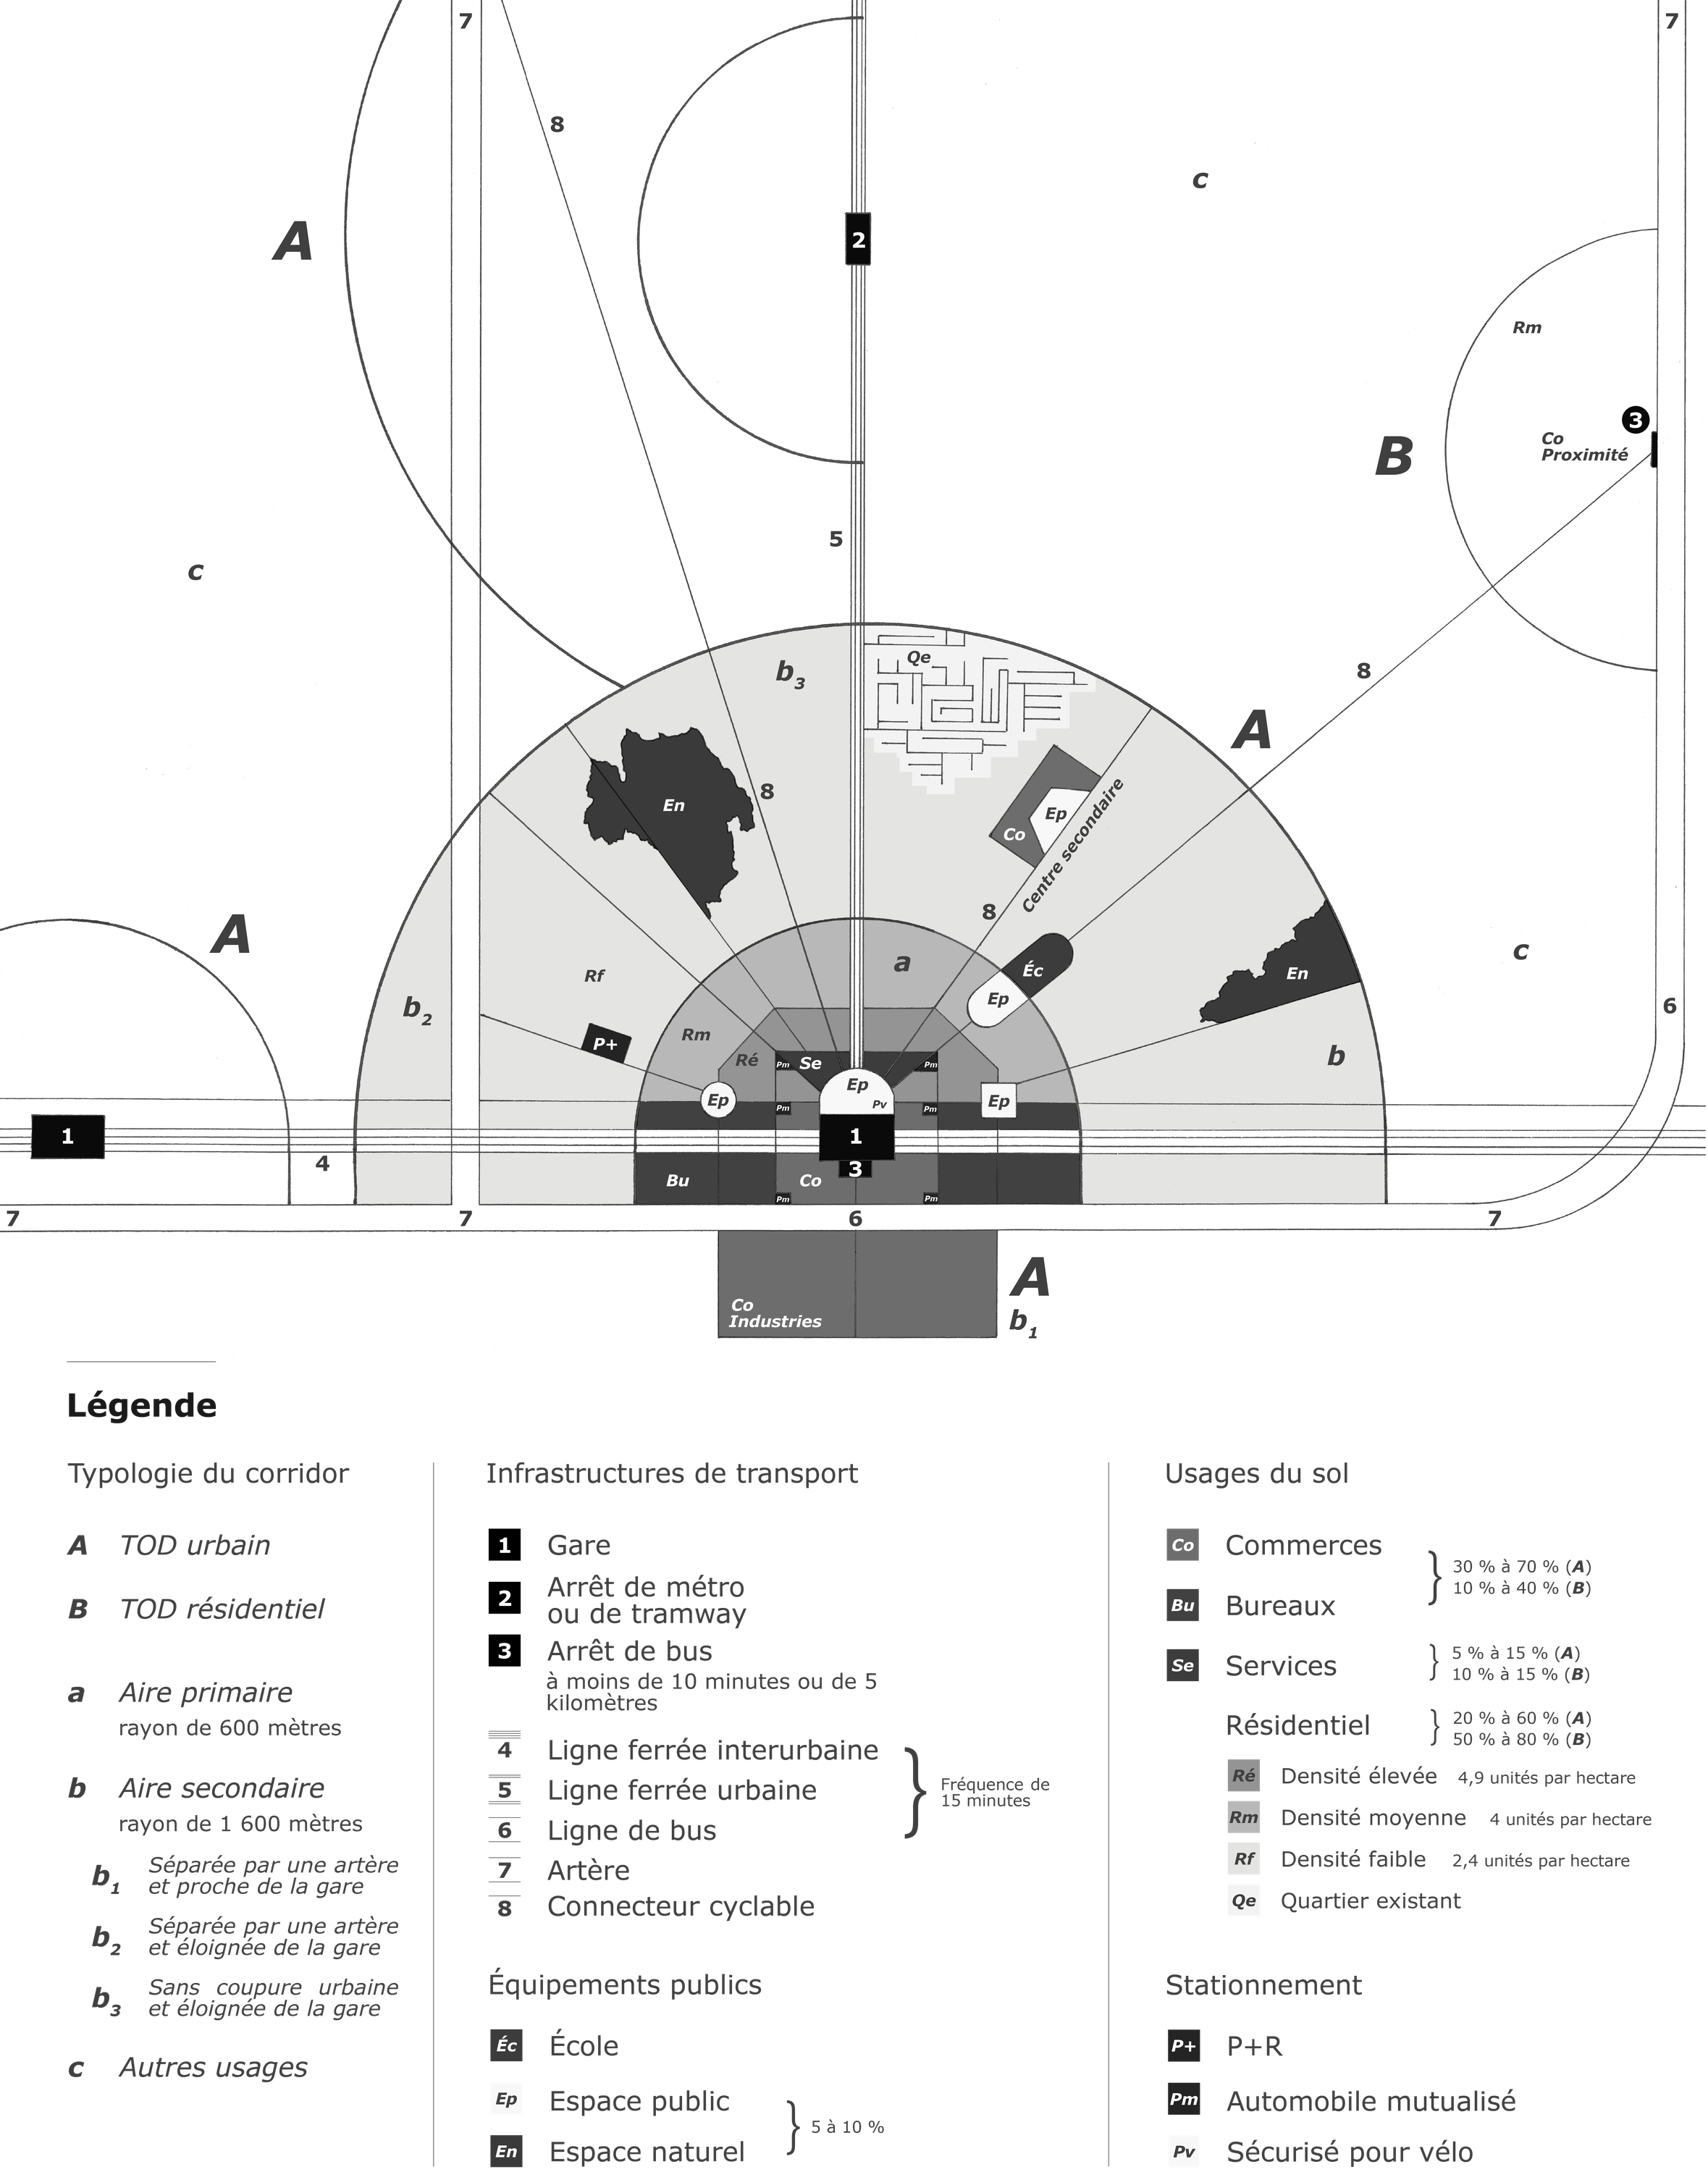
\includegraphics[width=1\columnwidth]{src/Figures/Chap-1/FR_Schema_Calthorpe.pdf}}
        \vspace{5pt}
        \begin{flushright}\scriptsize{
        Source~: directives formulées par \textcolor{blue}{Peter} \textcolor{blue}{\textcite{calthorpe_next_1993}}\index{Calthorpe, Peter|pagebf}
        \\
        Adaptation graphique~: \textcolor{blue}{Dylan Moinse (2021)}
        }\end{flushright}
    \end{carte}

    % Aire secondaire
En périphérie immédiate, l’auteur y introduit une \Guillemets{aire secondaire} (\textsl{Secondary Area}), destinée à des usages de faible densité tels que des lotissements résidentiels familiaux, des établissements scolaires, des activités à forte emprise spatiale, ainsi que des parcs de grande envergure (voir le \hyperref[fig-chap1:schema-calthorpe]{schéma~\ref{fig-chap1:schema-calthorpe}}, page~\pageref{fig-chap1:schema-calthorpe}). Ces \Guillemets{aires secondaires} renforcent la viabilité et l’attractivité du \acrshort{TOD} en intégrant des fonctions complémentaires \textcolor{blue}{\autocite[42, 60, 87]{calthorpe_next_1993}}\index{Calthorpe, Peter|pagebf}. Au sein même de ces projets, l’aménagement vise ainsi à encourager l’usage des transports en commun, en même temps que les modes de déplacement non motorisés, grâce à une intégration réfléchie des infrastructures et une conception urbaine conçue pour être incitative.%%Rédigé%%

    % Principes originaux
Pour expliciter les fondements du \acrshort{TOD}, \textcolor{blue}{Peter} \textcolor{blue}{\textcite[43]{calthorpe_next_1993}}\index{Calthorpe, Peter|pagebf} synthétise cette approche en sept principes originaux~: (i) organiser la croissance à l’échelle régionale de manière compacte et favorable au système de transport en commun~; (ii) localiser les activités commerciales, résidentielles, récréatives et administratives à portée piétonne des stations de transport~; (iii) concevoir des réseaux de rues adaptés à la marche et reliant directement les destinations locales~; (iv) offrir une diversité d'habitat, de densités et de coûts~; (v) préserver les espaces ouverts et naturels~; (vi) orienter les quartiers et les bâtiments autour des espaces publics~; et (vii) encourager la densification et la requalification des quartiers le long des corridors de transport existants.%%Rédigé%%

    % Typologie TODs
Ces principes s'appliquent différemment selon qu'il s'agit d'un \Guillemets{\acrshort{TOD} urbain} (\textsl{Urban \acrshort{TOD}}) ou d'un \Guillemets{\acrshort{TOD} résidentiel} (\textsl{Neighborhood \acrshort{TOD}}), comme le laisse paraître le \hyperref[fig-chap1:schema-calthorpe]{schéma~\ref{fig-chap1:schema-calthorpe}} (page~\pageref{fig-chap1:schema-calthorpe}). Le premier type de quartier de gare est desservi par un système de transport structurant tel qu'un réseau ferroviaire lourd ou léger, ou encore de \acrfull{BHNS}. Cet espace stratégique \Guillemets{urbain} doit être adapté à des flux importants en concentrant les emplois et en intensifiant les usages du sol, à l'aide d'une densité élevée ou moyenne et d'une diversité fonctionnelle dominée par des bureaux et des commerces générateurs de flux \textcolor{blue}{\autocite[57]{calthorpe_next_1993}}\index{Calthorpe, Peter|pagebf}. Le second type, quant à lui, est associé à une desserte locale en bus qui permette de rejoindre le réseau structurant en moins de dix minutes ou en moins de cinq kilomètres, grâce à une fréquence élevée du service. Cet espace stratégique \Guillemets{résidentiel} peut se développer sous la forme de corridors présentant une densité moyenne d'habitations et une certaine mixité fonctionnelle \textcolor{blue}{\autocite[57]{calthorpe_next_1993}}\index{Calthorpe, Peter|pagebf}. \textcolor{blue}{Peter} \textcolor{blue}{\textcite[50, 61]{calthorpe_next_1993}}\index{Calthorpe, Peter|pagebf} identifie également trois grands types de fabrique du \acrshort{TOD} en fonction de leur localisation~: les \Guillemets{sites réaménageables} (\textsl{redevelopable sites}), de l'urbain existant susceptible d'être revitalisé~; les \Guillemets{terrains interstitiels} (\textsl{infill sites}) correspondant à des espaces ouverts ou des parcelles vacantes intégrées dans le tissu urbain existant~; et les \Guillemets{nouvelles zones d'expansion} (\textsl{New Growth Areas}), situées en périphérie urbaine, qui sont les plus simples à développer, mais qui contribuent à une expansion urbaine accrue.%%Rédigé%%

    % Liste 3D
À partir de ces principes, de nombreux travaux académiques ont cherché à conceptualiser et à enrichir le \acrshort{TOD}, en introduisant notamment des cadres analytiques visant à approfondir ses fondements théoriques. Bien qu’il n’existe pas de consensus universel autour d’une définition unique du \acrshort{TOD}, la notion des \Guillemets{3Ds}, introduite par \textcolor{blue}{\textcite[216]{cervero_travel_1997}}\index{Cervero, Robert|pagebf}\index{Kockelman, Kara|pagebf}, constitue une base fréquemment mobilisée dans la littérature~:
    \begin{customitemize}
\item \textsl{Densité} (\textsl{Density}). Cette première dimension correspond à la variable d’intérêt par unité de surface, qu’il s’agisse d’habitant·e·s, de ménages, de logements ou d’emplois par exemple. Elle reflète la concentration des personnes et des activités, une \Guillemets{densité bien conçue, bien gérée} (\textcolor{blue}{\textcite{cervero_panorama_2012}}\index{Cervero, Robert|pagebf}, cité par \textcolor{blue}{\textcite[127]{lo_feudo_scenario_2014}}\index{Lo Feudo, Fausto|pagebf}\index{Menerault, Philippe|pagebf}\index{L'Hostis, Alain|pagebf}\index{Festa, Demetrio Carmine|pagebf})~;
\item \textsl{Diversité fonctionnelle} (\textsl{Diversity}). Cette deuxième dimension évalue le degré de mixité des usages du sol~;
\item \textsl{Conception} (\textsl{Design}). Cette troisième dimension englobe les caractéristiques des rues, l’organisation des espaces de circulation et de stationnement, les formes urbaines ainsi que la qualité urbaine.
    \end{customitemize}%%Rédigé%%

    % Description 3Ds
Ces trois dimensions sont interdépendantes et agissent en synergie pour soutenir un développement urbain dense et multifonctionnel, où la mobilité piétonne est priorisée et où les déplacements sont réduits en termes de quantité et de distance moyenne grâce à la proximité des activités urbaines aux lieux d’habitat. Le \textsl{\gls{design}}, qui semble détenir les effets les plus importants sur la fréquentation du transport public \textcolor{blue}{\autocite[107]{ewing_travel_2001}}\index{Ewing, Reid|pagebf}\index{Cervero, Robert|pagebf}, améliore la connectivité des différentes fonctions urbaines. En définitive, les \Guillemets{3Ds} soutiennent la vision intégrée d'un développement urbain dense et multifonctionnel qui fournit un système accessible et qualitatif \textcolor{blue}{\autocites[216]{cervero_travel_1997}[107]{ewing_travel_2001}}\index{Cervero, Robert|pagebf}\index{Kockelman, Kara|pagebf}\index{Ewing, Reid|pagebf}\index{Cervero, Robert|pagebf}.%%Rédigé%%

    % 6D/7D
Au-delà du triptyque développé et usuellement intégré au modèle urbain, d’autres paramètres viennent progressivement enrichir les cadres d’analyse relatifs au \acrshort{TOD}. Pour ne citer que les dimensions les plus reconnues et répandues dans les grilles d'analyse adoptées pour le \acrshort{TOD}, trois nouveaux aspects ont émergé progressivement entre 2001 et 2010 \textcolor{blue}{\autocite[267]{ewing_travel_2010}}\index{Ewing, Reid|pagebf}\index{Cervero, Robert|pagebf}~: l'accessibilité aux destinations (\textsl{Destination accessibility}) qui évalue la facilité d’accès aux diverses aménités urbaines, telles que les lieux de travail, les services, les commerces ou les équipements publics~; la distance à la station (\textsl{Distance to transit}) qui mesure la facilité de connexion spatiale au réseau de transport en commun~; et la gestion de la demande de mobilité (\textsl{Demand management}), bien que souvent marginalisée dans les études \textcolor{blue}{\autocite[267]{ewing_travel_2010}}\index{Ewing, Reid|pagebf}\index{Cervero, Robert|pagebf}, qui recouvre l’ensemble des politiques publiques et des initiatives visant à réduire l'usage effectif de la voiture individuelle, notamment au sujet de la disponibilité des places de stationnement automobile. Ces trois déterminants de la demande de transport en commun viennent ainsi élargir le cadre analytique aux \Guillemets{5Ds}, voire aux \Guillemets{6Ds} \textcolor{blue}{\autocite[4-6]{thomas_transit-oriented_2020}}\index{Thomas, Ren|pagebf}\index{Bertolini, Luca|pagebf}. Précisons que bien d'autres paramètres ont été explorés dans les diverses productions scientifiques, à l'instar des caractéristiques socio-démographiques de la population ou des usager·ère·s (\textsl{Demographics}) \textcolor{blue}{\autocite[75]{ewing_trip_2017}}\index{Ewing, Reid|pagebf}\index{Tian, Guang|pagebf}\index{Lyons, Torrey|pagebf}\index{Terzano, Kathryn|pagebf} ou bien de l'attractivité du réseau de transport en commun exprimée en termes d'efficacité et de confort (\textsl{Desirability of transit}) \textcolor{blue}{\autocite[8]{mangu_evaluation_2025}}\index{Mangu, Sriram|pagebf}\index{Kadali,~B. Raghuram|pagebf}\index{Subbarao, Saladi~S.~V.|pagebf}\index{Lin, Jen-Jia|pagebf}.%%Rédigé%%

    % Entrelacement de deux stratégies orientées vers l'offre et la demande
Aussi, les principes fondateurs du \acrshort{TOD} peuvent être synthétisés autour d’une action multiscalaire sur les configurations territoriales et, plus spécifiquement, sur l’environnement urbain. Cela se traduit par la coexistence de deux approches complémentaires qui maximisent son efficacité. Une première stratégie centrée sur l'offre, appelée \acrfull{TSM} et une seconde centrée sur la demande, appelée \acrfull{TDM} \textcolor{blue}{\autocite[67]{cervero_transit_1998}}\index{Cervero, Robert|pagebf}.

    % Transportation Systems Management
La stratégie \acrshort{TSM} vise à réorganiser le système de mobilité à moindre coût, en optimisant les infrastructures et les services existants. Cette approche de l’écomobilité peut reposer à cet égard sur des interventions directes sur l’environnement urbain, comme celles décrites par les \Guillemets{3Ds}. Ces dernières permettent non seulement d’intensifier la fréquentation des transports en commun, mais aussi de générer des flux bidirectionnels mieux répartis dans le temps \textcolor{blue}{\autocite[4]{grigolon_transit-oriented_2016}}\index{Grigolon, Anna Beatriz|pagebf}\index{Koeva, Mila|pagebf}\index{Madureira, Ana Mafalda|pagebf}\index{Singh, Yamini~J.|pagebf}. En outre, le recours aux \acrfull{NTIC} s’inscrit dans cette stratégie, en facilitant une gestion coordonnée et en temps réel des flux de mobilité à un coût réduit. Parmi les technologies mobilisées figurent l’optimisation du trafic, la mise à disposition et la gestion des données en temps réel ou encore la géolocalisation des véhicules \textcolor{blue}{\autocite[96]{cervero_transit_1998}}\index{Cervero, Robert|pagebf}.%%Rédigé%%

    % Transportation Demand Management
La stratégie \acrshort{TDM}, quant à elle, s’appuie davantage sur des mesures visant à réduire l’usage de l’automobile, voire sa possession, et à encourager un report modal vers des systèmes de mobilité alternatifs. Ces mesures incluent des dispositifs coercitifs tels que la modération de la circulation et du stationnement, la taxation en cas de congestion urbaine, ou encore l’introduction de normes environnementales, comme celles liées à la consommation de carburant. Un exemple emblématique de cette stratégie orientée vers la demande est le concept néerlandais des \textsl{woonerven}\footnote{
    Le concept \Guillemets{\textsl{woonerf}}, littéralement, \Guillemets{cour résidentielle}, désigne un espace partagé donnant la priorité aux piéton·ne·s, aux cyclistes et à la vie de quartier. L’apaisement de la circulation automobile y est assuré par des obstacles physiques matérialisés par de la végétation ou encore du mobilier urbain, et par une voirie partagée, brouillant les frontières entre les différents types d’usager·ère·s et favorisant la vigilance des automobilistes \textcolor{blue}{\autocite[3]{collarte_woonerf_2012}}\index{Collarte, Natalia|pagebf}.
}. Cependant, cette approche ne se limite pas à des mesures contraignantes. En cherchant à influencer les comportements de mobilité, des actions incitatives, telles que la mise en place d’horaires de travail décalés ou d'aides financières encourageant le recours aux alternatives modales, participent à cette logique \textcolor{blue}{\autocite[97]{cervero_transit_1998}}\index{Cervero, Robert|pagebf}.%%Rédigé%%

    % 1.1.2.2. Effets attendus
    \needspace{1\baselineskip} % Réserve de l'espace
\subsubsection*{Les bénéfices attendus du \textsl{Transit-Oriented Development}
    \label{chap1:tod-presentation-generale-definition-effets-attendus}
    }

    % Objectifs
Le \acrshort{TOD} constitue aujourd’hui à la fois un territoire de projets et un instrument d’action urbaine pour de nombreuses collectivités territoriales \textcolor{blue}{\autocite[23]{bentayou_transit-oriented_2015}}\index{Bentayou, Gilles|pagebf}. Ce modèle d’aménagement mobilise des institutions et des organismes, allant des acteurs du développement économique, de l’économie sociale, de la santé publique, jusqu’au secteur éducatif, qui se saisissent du concept et participent activement à la production de guides pratiques ou de retours d’expérience variés\footnote{
    Une enquête réalisée par l'entreprise étasunienne de transport \textcolor{blue}{\textcite[9]{hntb_america_2016}}, auprès de 1~000 participant·e·s, a examiné les bénéfices attendus de la mise en place d'un projet de type \acrshort{TOD}. Elle met en relief une réduction de la dépendance automobile (57~\%), un retour à une certaine proximité (46~\%), une diminution de l'empreinte carbone (44~\%), un accès amélioré aux services (43~\%) et aux emplois (37~\%), une dynamisation économique (43~\%), une meilleure connexion entre les territoires (42~\%) et une régénération des zones urbaines (30~\%).
}. Les effets attendus du \acrshort{TOD}, tels que définis par son principal promoteur, le \textcolor{blue}{Center for Transit-Oriented Development}\index{Center for Transit-Oriented Development@\textsl{Center for Transit-Oriented Development}|pagebf} \textcolor{blue}{\autocites[35-39]{ohland_communicating_2006}[11-21]{noland_measuring_2014}}\index{Ohland, Gloria|pagebf}\index{Gorewitz, Cali|pagebf}\index{Noland, Robert~B.|pagebf}\index{Ozbay, Kaan|pagebf}\index{DiPetrillo, Stephanie|pagebf}\index{Iyer, Shri|pagebf}, peuvent être décrits comme suit \textcolor{blue}{\autocites[11]{bentayou_transit-oriented_2015}[114-122]{ibraeva_transit-oriented_2020}[5-11]{ali_dynamics_2021}[6-11]{wan_equity_2023}}\index{Bentayou, Gilles|pagebf}\index{Ibraeva, Anna|pagebf}\index{Almeida Correia, Gonçalo Homem de|pagebf}\index{Silva, Cecília|pagebf}\index{Antunes, António Pais|pagebf}\index{Ali, Liaqat|pagebf}\index{Nawaz, Ahsan|pagebf}\index{Iqbal, Shahid|pagebf}\index{Aamir Basheer, Muhammad|pagebf}\index{Haameed, Javaria|pagebf}\index{Albasher, Gadah|pagebf}\index{Shah, Syyed Adnan Raheel|pagebf}\index{Bai, Yong|pagebf}~:
    \begin{customitemize}
\item \textsl{Un report modal depuis la voiture individuelle}. Réduire l'usage de l'automobile de manière à entraîner une augmentation de la clientèle du réseau de transport en commun, contribuant également à une diminution des externalités négatives associées aux flux motorisés~;
\item \textsl{La préservation de l'environnement et des ressources naturelles}. Réduire les émissions de \acrfull{GES} et diverses formes de pollution générées par l'automobile, tout en limitant l'artificialisation excessive des sols due à un étalement urbain non maîtrisé. Accroître la qualité de la santé publique, à la fois physique et mentale~;
\item \textsl{L'amélioration de la qualité du cadre de vie urbain}. Aménager des quartiers favorisant un mode de vie actif et sain, en valorisant des territoires dynamiques et animés et en réduisant la congestion urbaine ainsi que les accidents de la route. Favoriser l'émergence de \Guillemets{communautés} vivantes et attrayantes~;
\item \textsl{Réduction de la ségrégation socio-spatiale}. Encourager le développement de pôles urbains décentralisés, réduisant la dépendance aux centres métropolitains et les déplacements longs. Consolider l'appropriation des territoires construisant les identités~;
\item \textsl{La promotion de l'équité sociale}. Renforcer l'accès à l'emploi et aux opportunités pour les populations à revenus modeste~;
\item \textsl{Une meilleure gestion des coûts économiques et budgétaires}. Réduire les coûts collectifs répercutés sur la société ainsi que la part des revenus des ménages consacrée aux dépenses de mobilité. Augmenter les recettes générées par l'exploitation du transport public et par la promotion immobilière.
    \end{customitemize}%%Rédigé%%
    
    % Report modal depuis la voiture
\textsl{Un report modal depuis la voiture individuelle}. En matière de changements de comportement de mobilité, l'essentiel de la littérature dédiée au \acrshort{TOD} suggère que les personnes vivant et, ou bien, travaillant dans des quartiers \acrshort{TOD}\textcolor{blue}{s} se déplacent moins en automobile comparativement au reste de la population. Iels ont davantage recours aux transports en commun et aux modes actifs~: les études montrent qu’entre 25~\% et 50~\% des résident·e·s des quartiers de gare aménagés utilisent régulièrement les transports en commun \textcolor{blue}{\autocites[61]{lund_travel_2004}[40]{evans_transit-oriented_2007}[5, 15]{cervero_vehicle_2008}[62]{kamruzzaman_advance_2014}[152]{kamruzzaman_patterns_2014}}\index{Lund, Hollie~M.|pagebf}\index{Cervero, Robert|pagebf}\index{Wilson, Richard~W.|pagebf}\index{Evans, James|pagebf}\index{Pratt, Richard|pagebf}\index{Stryker, Andrew|pagebf}\index{Kuzmyak,~J.|pagebf}\index{Cervero, Robert|pagebf}\index{Arrington,~G.~B.|pagebf}\index{Kamruzzaman, Md.|pagebf}\index{Baker, Douglas|pagebf}\index{Washington, Simon|pagebf}\index{Turrell, Gavin|pagebf}\index{Wood, Lisa|pagebf}\index{Hine, Julian|pagebf}\index{Currie, Graham|pagebf}\index{Giles-Corti, Billie|pagebf}. Ce chiffre est généralement trois à quatre fois supérieur à la moyenne observée dans le reste de l’agglomération, une tendance similaire étant relevée pour la pratique de la marche et du vélo. En conséquence, nous pouvons observer une baisse de moitié du nombre de déplacements effectués en voiture dans les quartiers \acrshort{TOD}\textcolor{blue}{s} étasuniens \textcolor{blue}{\autocite[14]{cervero_vehicle_2008}}\index{Cervero, Robert|pagebf}\index{Arrington,~G.~B.|pagebf}. Cependant, environ 40~\% de cet effet peut être attribué à un biais d’auto-sélection, selon lequel les individus s’installant à proximité des réseaux de transport public sont déjà prédisposés à les emprunter \textcolor{blue}{\autocites[2~082]{cervero_transit-oriented_2007}[50]{laham_nonwork_2017}}\index{Cervero, Robert|pagebf}\index{Laham, Maria Luz|pagebf}\index{Noland, Robert~B.|pagebf}. Un autre effet notable concerne la baisse des taux de motorisation. Les populations des quartiers \acrshort{TOD}\textcolor{blue}{s} disposent d’un parc automobile presque deux fois moins important que celles des zones non orientées vers le transport public \textcolor{blue}{\autocite[50]{arrington_effects_2008}}\index{Arrington,~G.~B.|pagebf}\index{Cervero, Robert|pagebf}, même si ces proportions varient selon les caractéristiques spécifiques de chaque territoire étudié \textcolor{blue}{\autocite[79]{lund_travel_2004}}\index{Lund, Hollie~M.|pagebf}\index{Cervero, Robert|pagebf}\index{Wilson, Richard~W.|pagebf}.%%Rédigé%%

    % Préservation de l'environnement
\textsl{La préservation de l'environnement et des ressources naturelles}. La littérature scientifique sur les effets du \acrshort{TOD} en matière de réduction de la pollution et de maîtrise de la périurbanisation reste limitée \textcolor{blue}{\autocite[11]{ashik_investigating_2022}}\index{Ashik,~F.~R.|pagebf}\index{Rahman,~M.~H.|pagebf}\index{Kamruzzaman, Md.|pagebf}. Cependant, plusieurs études fournissent des éléments probants. Il a été démontré que les territoires métropolitains adoptant des politiques relevant du \acrshort{TOD} tendent à améliorer la qualité de l’air, principalement grâce à la réduction de la distance totale parcourue en voiture \textcolor{blue}{\autocite[20]{gu_transit-oriented_2019}}\index{Gu, Peiqin|pagebf}\index{He, Dongxu|pagebf}\index{Chen, Yulin|pagebf}\index{Zegras, Pericles~C.|pagebf}\index{Jiang, Yang|pagebf}. Ces résultats soulignent les bonnes performances de ces politiques en matière de durabilité \textcolor{blue}{\autocite[109]{choi_influence_2018}}\index{Choi, Kwangyul|pagebf}. À Los Angeles, l’ouverture d’une nouvelle ligne de métro léger a entraîné une réduction de 27~\% des émissions quotidiennes de \acrshort{GES} liées à la mobilité des ménages résidant à moins de 800 mètres des arrêts \textcolor{blue}{\autocite[13]{boarnet_can_2017}}\index{Boarnet, Marlon~G.|pagebf}\index{Wang, Xize|pagebf}\index{Houston, Douglas|pagebf}. Une autre étude dans la même région rapporte une diminution de 30~\% à 36~\% des émissions de particules à suspension et fines, ainsi que d'autres irritants respiratoires dans les zones \acrshort{TOD}\textcolor{blue}{s}, par rapport aux zones à faible densité. Ces résultats s’expliquent principalement par une meilleure accessibilité aux infrastructures de transport en commun, conduisant à une consommation énergétique réduite et à des distances de déplacement plus courtes \textcolor{blue}{\autocite[25]{nahlik_transit-oriented_2014}}\index{Nahlik, Matthew~J.|pagebf}\index{Chester, Mikhail~V.|pagebf}. À Charlotte, une modélisation mise en œuvre par \textcolor{blue}{\textcite[4]{hosseini_understanding_2024}}\index{Hosseini, Sanaz Sadat|pagebf}\index{Ardabili, Babak Rahimi|pagebf}\index{Azarbayjani, Mona|pagebf}\index{Pulugurtha, Srinivas|pagebf}\index{Pulugurtha, Hamed|pagebf} met en évidence une réduction de 8~\% à 21~\% des émissions quotidiennes en heures d'affluence dans la situation où la fréquentation des bus est doublée, une proportion qui peut s'élever à 37~\% dans le scénario \acrshort{TOD} le plus favorable. De surcroît, \textcolor{blue}{\textcite[120]{kamruzzaman_investigating_2018}}\index{Kamruzzaman, Md.|pagebf}\index{Deilami, Kaveh|pagebf}\index{Yigitcanlar, Tan|pagebf} montrent que les politiques \acrshort{TOD}\textcolor{blue}{s} ont permis de limiter l’étalement urbain anarchique à Brisbane. Toutefois, ces zones présentent les effets d'îlot de chaleur urbain les plus intenses de la métropole, en raison d’un déséquilibre dans la répartition des espaces verts et naturels.%%Rédigé%%

    % Qualité de la qualité de vie
\textsl{L'amélioration de la qualité du cadre de vie urbain, en matière de santé publique et de bien-être}. En favorisant une meilleure qualité de l’air et en encourageant l’activité physique, il joue un rôle essentiel dans la promotion de modes de vie plus sains. En effet, l’usage du transport public est associé à des niveaux plus faibles de comportements sédentaires, notamment lorsque les formes urbaines favorisent le recours à des modes actifs \textcolor{blue}{\autocites[58]{knell_transit_2017}[22]{frank_quantifying_2022}}\index{Knell, Gregory|pagebf}\index{Durand, Casey~P.|pagebf}\index{Shuval, Kerem|pagebf}\index{Kohl, Harold~W.|pagebf}\index{Salvo, Deborah|pagebf}\index{Sener, Ipek|pagebf}\index{Gabriel, Kelley Pettee|pagebf}\index{Frank, Lawrence~D.|pagebf}\index{Fow, Eric~H.|pagebf}\index{Ulmer, Jared~M.|pagebf}\index{Chapman, James~E.|pagebf}\index{Braun, Lindsay~M.|pagebf}. En améliorant la qualité de l’environnement urbain, les résident·e·s des quartiers \acrshort{TOD}\textcolor{blue}{s} sont moins exposé·e·s aux pollutions et sont plus actif·ve·s \textcolor{blue}{\autocites[12-13]{belzer_transit-oriented_2002}[215]{cervero_green_2011}[271]{guerra_cost_2011}}\index{Belzer, Dena|pagebf}\index{Autler, Gerald|pagebf}\index{Cervero, Robert|pagebf}\index{Sullivan, Cathleen|pagebf}\index{Guerra, Erick|pagebf}. De plus, ces projets urbains contribuent à la requalification des espaces publics et à la régénération des territoires, ce qui améliore la qualité urbaine et renforce leur attractivité résidentielle, touristique et économique \textcolor{blue}{\autocites[9]{ratner_reshaping_2010}[109-112]{ferbrache_city_2017}}\index{Ratner, Keith~A.|pagebf}\index{Goetz, Andrew~R.|pagebf}\index{Ferbrache, Fiona|pagebf}\index{Knowles, Richard~D.|pagebf}. Un exemple emblématique est l’\Guillemets{effet de Grenoble} (\textsl{Grenoble effect}), considéré comme un modèle de revitalisation urbaine. Dès 1987, Grenoble a réintroduit un système de tramway couplé à un projet urbain ambitieux connectant la gare au nouveau campus. Ce projet a servi de référence pour de nombreuses villes en France et dans le monde \textcolor{blue}{\autocites[7]{boquet_renaissance_2017}[37]{hass-klau_economic_2004}}\index{Boquet, Yves|pagebf}\index{Hass-Klau, Carmen|pagebf}\index{Crampton,~G.|pagebf}\index{Benjari, Rabia|pagebf}. Le \acrshort{TOD} renforce également le sentiment de \Guillemets{communauté} \textcolor{blue}{\autocite[231-248]{dittmar_new_2003}}\index{Dittmar, Hank|pagebf}\index{Ohland, Gloria|pagebf} et la satisfaction de mobilité et résidentielle des habitant·e·s \textcolor{blue}{\autocite[86]{curtis_transit_2009}}\index{Curtis, Carey|pagebf}\index{Renne, John Luciano|pagebf}\index{Bertolini, Luca|pagebf}. Bien que les transports en commun soient souvent perçus comme moins plaisants que la conduite automobile ou les modes actifs, le \acrshort{TOD} a la capacité de renverser cette appréciation sensible et cognitive en améliorant le confort et l’expérience des usager·ère·s \textcolor{blue}{\autocites[258-259]{olsson_happiness_2013}[287-288][79]{wu_does_2014}{majumdar_identification_2021}}\index{Olsson, Lars~E.|pagebf}\index{Gärling, Tommy|pagebf}\index{Ettema, Dick|pagebf}\index{Friman, Margareta|pagebf}\index{Fuji, Satoshi|pagebf}\index{Majumdar, Bandhan Bandhu|pagebf}\index{Jayakumar, Malavika|pagebf}\index{Sahu, Prasanta~K.|pagebf}\index{Potoglou, Dimitris|pagebf}\index{Wu, Wenjie|pagebf}.%%Rédigé%%

    % Réduction de la ségrégation socio-spatiale
\textsl{Réduction de la ségrégation socio-spatiale et promotion de l'équité sociale}. Le \acrshort{TOD} s’inscrit dans une dynamique de régénération urbaine, permettant d’améliorer l’attractivité résidentielle et économique de certains quartiers. En particulier, d’anciens territoires désindustrialisés bénéficient de cette opportunité pour être redynamisés. Des exemples notables incluent les Docks de Londres et Salford Quays en Angleterre, ou encore Baltimore aux États-Unis \textcolor{blue}{\autocites[42, 46, 68]{knowles_investigation_2014}[6]{knowles_evaluation_2016}}\index{Knowles, Richard~D.|pagebf}\index{Ferbrache, Fiona|pagebf}. Par son approche polycentrique, le \acrshort{TOD} soutient non seulement l’économie locale, mais aussi la compétitivité régionale en optimisant l’usage du sol \textcolor{blue}{\autocite[40]{litman_evaluating_2011}}\index{Litman, Todd|pagebf}. Cependant, cette dynamique présente des effets ambivalents. L’un des risques majeurs est celui de la gentrification, qui découle de l’appréciation de la valeur des propriétés dans les quartiers de gare et entraîne une augmentation des coûts du logement\footnote{
    Ce phénomène, de plus en plus documenté dans la littérature, suscite de nombreux débats depuis une décennie \textcolor{blue}{\autocite[738]{padeiro_transit-oriented_2019}}\index{Padeiro, Miguel|pagebf}\index{Louro, Ana|pagebf}\index{Costa, Nuno Marques de|pagebf}. Parfois clairement caractérisé en lien avec la hausse des prix fonciers \textcolor{blue}{\autocite[14-15]{wu_impacts_2020}}\index{Wu, Wenjie|pagebf}\index{Zheng, Siqi|pagebf}\index{Wang, Bing|pagebf}\index{Du, Minzhe|pagebf}, parfois absent, généralement lorsque le \acrshort{TOD} est conjugué à une politique de logement abordable \textcolor{blue}{\autocite[16]{dawkins_transit-induced_2016}}\index{Dawkins, Casey|pagebf}\index{Moeckel, Rolf|pagebf}. Il reste difficile d’en définir l’ampleur ou de généraliser ses effets, comme en témoignent les nombreuses recherches récentes sur ce sujet \textcolor{blue}{\autocites{cook_light_2019}{padeiro_transit-oriented_2019}{ewing_is_2022}{wan_equity_2023}}\index{Cook, Justin|pagebf}\index{Padeiro, Miguel|pagebf}\index{Louro, Ana|pagebf}\index{Costa, Nuno Marques de|pagebf}\index{Wan, Tianyue|pagebf}\index{Lu, Wei|pagebf}\index{Sun, Peijin|pagebf}\index{Ewing, Reid|pagebf}\index{Sabouri, Sadegh|pagebf}\index{Kaniewsk, Justyna|pagebf}\index{Ameli, Hassan|pagebf}\index{Yang, Wookjae|pagebf}\index{Kiani, Fatemeh|pagebf}\index{Kim, Junsik|pagebf}\index{Chibamba, Douty|pagebf}.
}. Selon \textcolor{blue}{Gilles} \textcolor{blue}{\textcite[32]{bentayou_transit-oriented_2015}}\index{Bentayou, Gilles|pagebf}, il est pour autant erroné de réduire les conséquences sociales du \acrshort{TOD} à la seule gentrification, puisque le modèle urbain, par essence, est voué à donner ou à redonner de la valeur à des territoires situés à proximité des nœuds de transport. Si les autorités locales agissent en amont, elles peuvent alors contrer ces effets pervers en adoptant des politiques favorisant la production de logements abordables et la maîtrise des plus-values par une régulation des prix du foncier et des loyers \textcolor{blue}{\autocites[17]{litman_evaluating_2011}[32]{bentayou_transit-oriented_2015}{yu_valueadded_2018}[463]{harrison_corridors_2019}{ewing_is_2022}}\index{Bentayou, Gilles|pagebf}\index{Litman, Todd|pagebf}\index{Yu, Haitao|pagebf}\index{Pang, Hao|pagebf}\index{Zhang, Ming|pagebf}\index{Ewing, Reid|pagebf}\index{Sabouri, Sadegh|pagebf}\index{Kaniewsk, Justyna|pagebf}\index{Ameli, Hassan|pagebf}\index{Yang, Wookjae|pagebf}\index{Kiani, Fatemeh|pagebf}\index{Kim, Junsik|pagebf}\index{Chibamba, Douty|pagebf}\index{Harrison, Philip|pagebf}\index{Rubin, Margot|pagebf}\index{Appelbaum, Alexandra|pagebf}\index{Dittgen, Romain|pagebf}.%%Rédigé%%

    % Meilleure gestion des coûts économiques
\textsl{Avantages économiques et maîtrise des coûts}. Du point de vue de la société, le \acrshort{TOD} représente une opportunité pour réduire les coûts collectifs. La diminution des accidents de la route, la moindre exposition à la pollution et la réduction de la dispersion des réseaux urbains contribuent à alléger les dépenses publiques \textcolor{blue}{\autocite[17]{litman_evaluating_2011}}\index{Litman, Todd|pagebf}. À l’échelle locale, et plus spécifiquement dans les quartiers de gare, une dynamisation économique est fréquemment observée. Ces lieux stratégiques stimulent les investissements publics et privés, tout en favorisant une réorganisation des centralités économiques \textcolor{blue}{\autocites[89]{knowles_investigation_2014}[6]{knowles_evaluation_2016}}\index{Knowles, Richard~D.|pagebf}\index{Ferbrache, Fiona|pagebf}. Le long des lignes de transport en commun, des études ont démontré une nette augmentation de nouveaux commerces à proximité des stations, avec des taux de croissance doublés par rapport aux zones non accessibles. En revanche, les activités industrielles ont tendance à diminuer dans ces mêmes espaces \textcolor{blue}{\autocites{duncan_impact_2011}{credit_transit-oriented_2018}}\index{Duncan, Michael|pagebf}\index{Credit, Kevin|pagebf}. À l’échelle des ménages, un effet notable du \acrshort{TOD} est la réduction des dépenses de mobilité. La part des revenus consacrée aux déplacements peut ainsi passer de 25~\% à seulement 9~\%, comme observé aux États-Unis \textcolor{blue}{\autocites[25]{beauvais_amenagements_2017}[25]{nahlik_transit-oriented_2014}[38]{ohland_communicating_2006}}\index{Beauvais, Jean-Marie|pagebf}\index{Nahlik, Matthew~J.|pagebf}\index{Chester, Mikhail~V.|pagebf}\index{Ohland, Gloria|pagebf}\index{Gorewitz, Cali|pagebf}.%%Rédigé%%

	% Transition
Nous l’avons vu, le \acrshort{TOD} renvoie toujours à l'idée de densification et de diversification des fonctions urbaines autour des nœuds de transport en commun, dans le but de générer des bénéfices pour la société. Cependant, en fonction des institutions qui le promeuvent ou cherchent à le mettre en œuvre, le \acrshort{TOD} peut être mis au service d’une pluralité d’objectifs~: préoccupations liées à la santé publique, amélioration de la qualité des espaces urbains, lutte contre la congestion urbaine, soutien à l’économie locale ou encore disponibilité de logements abordables. Cette diversité des objectifs poursuivis, ou des bénéfices attendus des projets \acrshort{TOD}\textcolor{blue}{s}, explique en grande partie le succès et la diffusion de ce modèle de développement \textcolor{blue}{\autocite[14]{bentayou_transit-oriented_2015}}\index{Bentayou, Gilles|pagebf}. Fortement internationalisé, ce modèle a été adapté aux spécificités des contextes géographiques, politiques et techniques dans lesquels il a été implanté \textcolor{blue}{\autocites[1~202]{thomas_is_2018}[181]{veloso_e_zarate_quartiers_2024}}\index{Thomas, Ren|pagebf}\index{Pojani, Dorina|pagebf}\index{Lenferink, Sander|pagebf}\index{Bertolini, Luca|pagebf}\index{Stead, Dominic|pagebf}\index{Krabben, Erwin van der|pagebf}\index{Veloso e Zarate, Halina|pagebf}\index{Triggianese, Manuela|pagebf}\index{Baron, Nacima|pagebf}\index{Le Bot, Nils|pagebf}\index{Detavernier, Pauline|pagebf}. Et c'est certainement là la force du \acrshort{TOD} qui peut être interprété et réinterprété selon les contextes. Comme l’explique \textcolor{blue}{Mounya} \textcolor{blue}{\textcite[52]{el_hadeuf_ville_2017}}\index{El Hadeuf, Mounya|pagebf}\index{Laterrasse, Jean|pagebf}, l’absence d’une recette prédéfinie figée dans des stéréotypes de quartiers \acrshort{TOD}\textcolor{blue}{s} standardisés permet d’éviter \Guillemets{\textsl{une paresse dans la recherche de nouvelles compositions urbaines}}.%%Rédigé%%

    % 1.1.3.
    \needspace{1\baselineskip} % Réserve de l'espace
\subsection{Applications et adaptations du \textsl{Transit-Oriented Development}
    \label{chap1:tod-presentation-generale-declinaisons}
    }

    % Introduction
La progression importante du nombre de contributions scientifiques à propos du \acrshort{TOD} au cours de la dernière décennie témoigne de la pertinence renouvelée de ce sujet de recherche-action \textcolor{blue}{\autocite[2545]{jain_systematic_2020}}\index{Jain, Deepshikha|pagebf}\index{Singh, Ekta|pagebf}\index{Ashtt, Rashmi|pagebf}. Depuis le début du XXI\textsuperscript{e} siècle, un regain d’intérêt pour le \acrshort{TOD} s’observe à l’échelle mondiale, stimulé par la diversification des modes de déplacement, laquelle remet en question la dualité traditionnelle entre transports en commun et individuels \textcolor{blue}{\autocite[3]{knowles_transit_2019}}\index{Knowles, Richard~D.|pagebf}\index{Ferbrache, Fiona|pagebf}. Ce modèle urbain sans cesse réactualisé est perçu comme un levier potentiel pour promouvoir une \Guillemets{croissance urbaine intelligente} et favoriser des dynamiques de régénération urbaine, aussi bien dans les pays développés que dans les économies émergentes \textcolor{blue}{\autocite[2~191]{goetz_suburban_2013}}\index{Goetz, Andrew~R.|pagebf}. En raison des nombreuses déclinaisons du \acrshort{TOD} dans des contextes variés, ce concept d'aménagement offre ainsi une opportunité de réflexion sur des thématiques transversales telles que l’attractivité des territoires et leur valorisation \textcolor{blue}{\autocite[34]{stransky_periurbain_2019}}\index{Stransky, Vaclav|pagebf}. Cette multiplicité d’applications, reflet de l’adaptabilité du \acrshort{TOD}, enrichit tant la littérature scientifique et technique que les projets opérationnels qui s’en revendiquent à travers le monde, même si ces derniers peuvent être désignés par d’autres terminologies, comme en France. Compte tenu du grand nombre d'états de l'art et de revues de littérature ayant déjà produit l'exercice de comparaisons internationales, ce mémoire n’a pas pour ambition d’en fournir une description exhaustive. Il vise plutôt à mettre en lumière l’adaptabilité conceptuelle et pratique du \acrshort{TOD}, à travers l’analyse de ses principes fondamentaux et de ses multiples formes d’application, dans le but d'y expliciter la place stratégique que peuvent occuper le vélo et ses variantes.%%Rédigé%%

    % 1.1.3.1. Outils de planification
    \needspace{1\baselineskip} % Réserve de l'espace
\subsubsection*{Contractualisation française de projets se réclamant du \textsl{Transit-Oriented Development}
    \label{chap1:tod-presentation-generale-definition-instruments}
    }

    % Introduction
En raison de son caractère englobant, impliquant divers secteurs et échelles spatiales, le \acrshort{TOD} mobilise une multiplicité d’acteurs. Parmi elleux figurent les entités supranationales, nationales ou régionales, responsables des législations et des financements~; les autorités locales, en charge de l’aménagement du territoire et des réglementations~; les agences de mobilité, responsables de la planification et de l’exploitation des systèmes de transport~; ainsi que les bailleurs et promoteurs immobiliers, qui assurent la production de logements \textcolor{blue}{\autocite[8]{mathur_promoting_2020}}\index{Mathur, Shishir|pagebf}\index{Gatdula, Aaron|pagebf}. C'est dans ce contexte que \textcolor{blue}{\textcite[152]{thomas_defining_2017}}\index{Thomas, Ren|pagebf}\index{Bertolini, Luca|pagebf} ont publié une méta-analyse sur l'applicabilité du concept d'aménagement, dans laquelle sont répertoriés les principaux facteurs de succès du \acrshort{TOD}~: une stabilité politique ainsi que l’existence d’un espace de dialogue régional intersectoriel et d'une mise en réseau interdisciplinaire des acteurs de la région desservie. Or, des lacunes persistantes, communes à de nombreux pays, freinent l’opérationnalisation de ce modèle d’urbanisme. Il s'agit en outre d'un manque de coopération et d’intégration entre les parties prenantes, d'une absence d’institutionnalisation de cette coordination et d'une gouvernance manquant de continuité \textcolor{blue}{\autocite[124]{ibraeva_transit-oriented_2020}}\index{Ibraeva, Anna|pagebf}\index{Almeida Correia, Gonçalo Homem de|pagebf}\index{Silva, Cecília|pagebf}\index{Antunes, António Pais|pagebf}. Face à la fragmentation sectorielle et géographique des compétences, différentes stratégies veillant à articuler urbanisme et transport ont émergé en France \textcolor{blue}{\autocites[10]{gallez_rooutils_2015}[2]{cerema_outils_2021}}\index{Gallez, Caroline|pagebf}\index{Maulat, Juliette|pagebf}\index{Roy-Baillargeon, Olivier|pagebf}\index{Thébert, Mariane|pagebf}\index{Cerema@\textsl{Cerema}|pagebf} sous forme de \Guillemets{bricolages} techniques, organisationnels, réglementaires et financiers \textcolor{blue}{\autocite[]{faure_regions_2006}}\index{Faure, Alain|pagebf}. Ces innovations visent à dépasser les frontières institutionnelles, telles que le \textsl{contrat d’axe} qui émerge comme un outil destiné à renforcer l’articulation entre urbanisme et transport\footnote{
    Bien que désigné sous des appellations différentes \textcolor{blue}{\autocite[10]{cerema_articuler_2015}}~–~la terminologie n'étant ni unifiée, ni stabilisée, allant de \Guillemets{contrat}, à \Guillemets{charte} par exemple \textcolor{blue}{\autocite[2]{cerema_articuler_2010}}~–, ce dispositif est issu d'innovations et d'expériences locales \textcolor{blue}{\autocite[25]{meunier-chabert_contrats_2014}}\index{Meunier-Chabert, Martine|pagebf}. Le premier \textsl{contrat d'axe} a vu le jour en France en 2002, dans les travaux de révision du \acrfull{PDU} de l'agglomération toulousaine \textcolor{blue}{\autocite[10]{cerema_articuler_2015}}. Depuis, divers \textsl{contrats d'axe}, dont la forme et le degré d'aboutissement diffèrent, ont été mis en place (voir la \hyperref[fig-chap1:carte-contrats-axe-france]{carte~\ref{fig-chap1:carte-contrats-axe-france}}, page~\pageref{fig-chap1:carte-contrats-axe-france}), comme dans les métropoles lilloise, franco-valdo-genevoise, francilienne, grenobloise \textcolor{blue}{\autocite[2]{cerema_articuler_2010}} ou encore le long de quatre corridors ferroviaires à Avignon, dans la Vallée de l'Isle \textcolor{blue}{\autocite[116]{bentayou_contrat_2015}}\index{Bentayou, Gilles|pagebf}\index{Perrin, Emmanuel|pagebf}\index{Richer, Cyprien|pagebf}, à Nîmes \textcolor{blue}{\autocite[15]{haro_ligne_2021}}\index{Haro, Florent|pagebf}\index{Duvic, Nicolas|pagebf} et dans le Béarn \textcolor{blue}{\autocite{fandio_contrat_2023}}\index{Fandio, Cédric|pagebf}\index{Vezinaud, Nathan|pagebf}. Cette profusion d'instruments de coordination existe également dans d'autres contextes géographiques, comme les programmes de \textsl{Transit-Oriented Development} aux États-Unis, les \textsl{Transit-Development Areas} en Grande-Bretagne ou les \Guillemets{projets d'agglomération} en Suisse \textcolor{blue}{\autocites[427]{maulat_coordonner_2014}[25]{walter_coordination_2015}}\index{Maulat, Juliette|pagebf}\index{Beaucire, Francis|pagebf}\index{Walter, Sandra|pagebf}\index{Roy-Baillargeon, Olivier|pagebf}.
} \textcolor{blue}{\autocite[173]{maulat_coordonner_2014}}\index{Maulat, Juliette|pagebf}\index{Beaucire, Francis|pagebf}.%%Rédigé%%

    % Figure carte des contrats d'axe en France
    \begin{carte}[h!]\vspace*{4pt}
        \caption{Carte des contrats d'axe en France en 2014.}
        \label{fig-chap1:carte-contrats-axe-france}
        \centerline{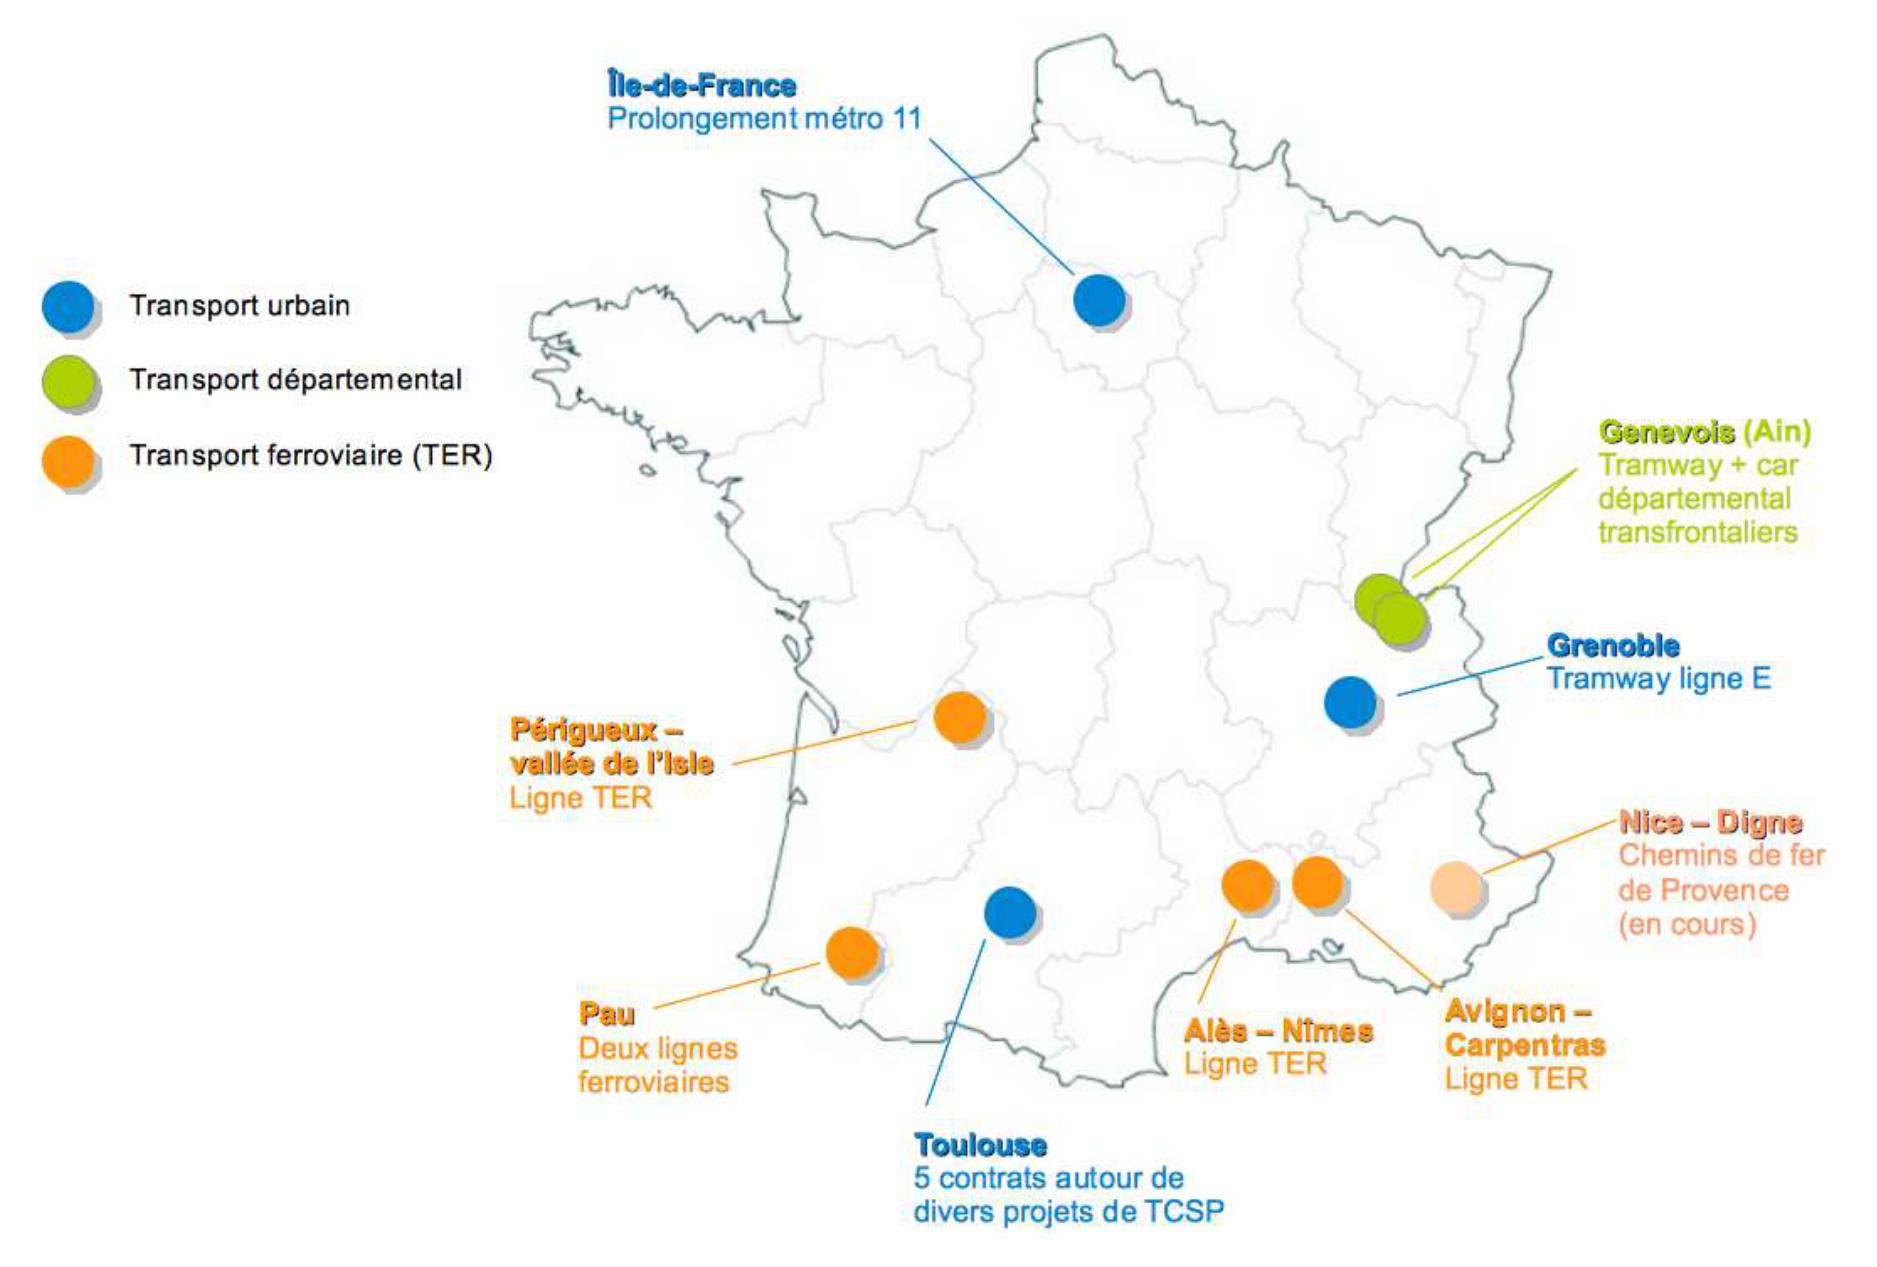
\includegraphics[width=0.75\columnwidth]{src/Figures/Chap-1/Carte_contrats_axe.jpg}}
        \vspace{5pt}
        \begin{flushright}\scriptsize{
        Source~: \textcolor{blue}{\textcite[18]{bentayou_contrat_2015}}\index{Bentayou, Gilles|pagebf}\index{Perrin, Emmanuel|pagebf}\index{Richer, Cyprien|pagebf}
        }\end{flushright}
    \end{carte}

    % Définition contrats d'axe
En écho aux recommandations formulées par \textcolor{blue}{\textcite[56]{lhostis_concevoir_2009}}\index{L'Hostis, Alain|pagebf}\index{Alexandre, Elsa|pagebf}\index{Appert, Manuel|pagebf}\index{Araud-Ruyant, Catherine|pagebf}\index{Basty, Marius|pagebf}\index{Biau, Géraldine|pagebf}\index{Bozzani-Franc, Sandra|pagebf}\index{Boutantin, Gratienne|pagebf}\index{Constantin, Chantal|pagebf}\index{Coralli, Monica|pagebf}\index{Durousset, Marie-Jeanne|pagebf}\index{Fradier, Christophe|pagebf}\index{Gabion, Cyrille|pagebf}\index{Leysens, Thomas|pagebf}\index{Mermoud, Françoise|pagebf}\index{Olny, Xavier|pagebf}\index{Perrin, Emmanuel|pagebf}\index{Robert, Jean|pagebf}\index{Simand, Noémie|pagebf}\index{Stransky, Vaclav|pagebf}\index{Soulas, Claude|pagebf}\index{Verdier, Anne-Marie|pagebf}\index{Vulturescu, Bogdan|pagebf} sur l'intérêt de mettre en place un espace de dialogue dédié à la coordination entre urbanisme et transport\footnote{
    Dans leur rapport de recherche-action franco-allemand \textsl{Bahn.Ville 2}, \textcolor{blue}{\textcite[56]{lhostis_concevoir_2009}}\index{L'Hostis, Alain|pagebf}\index{Alexandre, Elsa|pagebf}\index{Appert, Manuel|pagebf}\index{Araud-Ruyant, Catherine|pagebf}\index{Basty, Marius|pagebf}\index{Biau, Géraldine|pagebf}\index{Bozzani-Franc, Sandra|pagebf}\index{Boutantin, Gratienne|pagebf}\index{Constantin, Chantal|pagebf}\index{Coralli, Monica|pagebf}\index{Durousset, Marie-Jeanne|pagebf}\index{Fradier, Christophe|pagebf}\index{Gabion, Cyrille|pagebf}\index{Leysens, Thomas|pagebf}\index{Mermoud, Françoise|pagebf}\index{Olny, Xavier|pagebf}\index{Perrin, Emmanuel|pagebf}\index{Robert, Jean|pagebf}\index{Simand, Noémie|pagebf}\index{Stransky, Vaclav|pagebf}\index{Soulas, Claude|pagebf}\index{Verdier, Anne-Marie|pagebf}\index{Vulturescu, Bogdan|pagebf} énoncent l'importance d'instaurer une commission qui aurait pour mission de réunir les acteurs et les organismes financeurs concernés et d'élaborer les outils nécessaires à son bon fonctionnement. Dans la cinquième action de leur rapport, les auteur·rice·s proposent ainsi la création de ce qu'iels nomment la \Guillemets{commission Interfaces entre Urbanisme et Déplacements (IUD)}.
}, le \textsl{contrat d’axe} est un outil visant à renforcer l’articulation entre ces deux volets. Le \textsl{contrat d’axe} représente ainsi un instrument innovant pour territorialiser les impératifs de cette articulation, tout en illustrant une transformation des modes d’action publique \textcolor{blue}{\autocite[427]{maulat_coordonner_2014}}\index{Maulat, Juliette|pagebf}\index{Beaucire, Francis|pagebf}. Concrètement, il s’agit d’une démarche négociée entre différents partenaires, visant à définir des engagements partenariaux clairs dans un cadre inspiré des principes du \acrshort{TOD} \textcolor{blue}{\autocite[1]{cerema_outils_2021}}\index{Cerema@\textsl{Cerema}|pagebf}. Le \textsl{contrat d’axe} promeut une logique d’interterritorialité, favorisant moins l'idée d'une hiérarchie que celle d'une coopération entre acteurs \textcolor{blue}{\autocite[112, 133]{vanier_pouvoir_2008}}\index{Vanier, Martin|pagebf}. Ce dispositif a pour double rôle de créer une régulation urbaine et de mettre en cohérence un projet de territoire dans un cadre contractuel, sans nécessiter l'institutionnalisation d'échelons nouveaux \textcolor{blue}{\autocite[11]{cerema_articuler_2010}}\index{Cerema@\textsl{Cerema}|pagebf}. Plutôt que de mobiliser des ressources nouvelles, le \textsl{contrat d’axe} mise par conséquent sur une réutilisation inventive des leviers d’action disponibles \textcolor{blue}{\autocite[12]{cerema_articuler_2010}}\index{Cerema@\textsl{Cerema}|pagebf} en cherchant à synchroniser les calendriers entre projets de transport et aménagements urbains \textcolor{blue}{\autocite[25]{meunier-chabert_contrats_2014}}\index{Meunier-Chabert, Martine|pagebf}. Cette approche marque une évolution dans la conception des projets ferroviaires, en les intégrant dans une logique réticulaire de gestion des territoires et en les associant à des projets d’aménagement locaux \textcolor{blue}{\autocites[457, 468]{maulat_coordonner_2014}[94]{maulat_contractualiser_2015}}\index{Maulat, Juliette|pagebf}\index{Beaucire, Francis|pagebf}. Au-delà de son caractère technique, le \textsl{contrat d’axe} constitue un outil politique visant à renforcer l’assise territoriale des régions et leur position au sein du monde ferroviaire \textcolor{blue}{\autocite[93]{maulat_contractualiser_2015}}\index{Maulat, Juliette|pagebf}.%%Rédigé%%

    % Expériences des contrat d'axe
Les expériences de \textsl{contrat d’axe} témoignent d’un changement progressif \Guillemets{par le bas} des pratiques, en favorisant de nouvelles formes de coopération et en accordant une importance accrue aux spécificités locales et à la négociation politique \textcolor{blue}{\autocite[96]{maulat_contractualiser_2015}}\index{Maulat, Juliette|pagebf}. Ce dispositif générique permet des appropriations multiples selon les contextes locaux \textcolor{blue}{\autocite[457, 468]{maulat_coordonner_2014}}\index{Maulat, Juliette|pagebf}\index{Beaucire, Francis|pagebf}, mobilisant différents secteurs et échelles, des lignes de tramway à celles de train \footnote{
    Parmi les différentes déclinaisons des \textsl{contrats d’axe}, les contrats ferroviaires portant sur les axes \acrshort{TER} se distinguent par leur échelle spatiale étendue, ce qui entraîne la mobilisation d’un plus grand nombre de partenaires \textcolor{blue}{\autocite[51]{cerema_articuler_2015}}. Pour les régions, ces contrats constituent un levier stratégique pour dépasser la logique traditionnelle de guichet dans leurs relations avec les collectivités locales. Ils permettent d’améliorer la communication sur les coûts et les contraintes liés au ferroviaire, tout en valorisant les actions entreprises en la matière \textcolor{blue}{\autocite[53]{cerema_articuler_2015}}. En outre, ils offrent une opportunité de mise en récit des politiques ferroviaires et territoriales \textcolor{blue}{\autocite{fandio_contrat_2023}}\index{Fandio, Cédric|pagebf}\index{Vezinaud, Nathan|pagebf}.
} \textcolor{blue}{\autocite[20]{afoun_mostaganem_2022}}\index{Afoun, Mohammed|pagebf}\index{Belguesmia, Noureddine|pagebf}. Les démarches varient dans leur degré d’aboutissement (voir la \hyperref[fig-chap1:carte-contrats-axe-france]{carte~\ref{fig-chap1:carte-contrats-axe-france}}, page~\pageref{fig-chap1:carte-contrats-axe-france}). Par exemple, des contrats ou des chartes avancés ont été mis en place à Grenoble et en Île-de-France, tandis que des initiatives restent au stade préparatoire à Lille et à Genève \textcolor{blue}{\autocites[2]{cerema_articuler_2010}[11]{cerema_articuler_2015}}\index{Cerema@\textsl{Cerema}|pagebf}. Que ce soit à Toulouse, à Grenoble ou en Île-de-France, les \textsl{contrats d'axe} ont été intégrés dans le \acrfull{SCoT} et dans le \acrfull{SDRIF}. Dans la métropole occitane, le \acrfull{SCoT} a introduit des \Guillemets{périmètres de cohérence urbanisme-transport}, puis des \Guillemets{pactes urbains}, visant à intensifier l’urbanisation le long des corridors existants ou futurs de lignes structurantes telles que le métro, le tramway ou le \acrshort{BHNS} \textsl{Linéo} \textcolor{blue}{\autocites[49]{toulouse_metropole_plui-h_2019}[26]{meunier-chabert_contrats_2014}[3]{cerema_outils_2021}}\index{Toulouse Métropole@\textsl{Toulouse Métropole}|pagebf}\index{Meunier-Chabert, Martine|pagebf}\index{Cerema@\textsl{Cerema}|pagebf}. Dans l'agglomération alpine, le premier \textsl{contrat d’axe} accompagne la mise en service de la ligne E du tramway. Ce contrat fixe des objectifs en matière d’offre de logements, de requalification des espaces publics et d’évolution du \acrfull{PLU} des communes concernées pour inscrire les principes d’intensification urbaine \textcolor{blue}{\autocites[3]{aurg_contrat_2022}[2]{cerema_outils_2021}}\index{AURG@\textsl{AURG}|pagebf}\index{Cerema@\textsl{Cerema}|pagebf}. Quant au \Guillemets{contrat de développement territorial} francilien, celui-ci s’inscrit dans le cadre de la loi relative au Grand Paris, datant de 2010. Il soutient la création de nouvelles gares du \textsl{Grand Paris Express} tout en facilitant leur intégration dans les projets d’aménagement régional \textcolor{blue}{\autocite[19]{cerema_articuler_2015}}\index{Cerema@\textsl{Cerema}|pagebf}. Dans la métropole lilloise, les \acrshort{DIVAT}\footnote{
    Trois grandes familles de \acrfull{DIVAT} ont été identifiées, parmi les arrêts bénéficiant de plus de dix passages par jour et par sens. Chacune de ces familles est associée à des préconisations spécifiques d’aménagement \textcolor{blue}{\autocite[23]{cerema_articuler_2010}}~:
        \begin{customitemize}
    \item Le \acrshort{DIVAT} de \Guillemets{niveau 1} concerne les arrêts de \acrshort{TER} dits \Guillemets{urbains}, ainsi que les stations de métro et de tramway~;
    \item Le \acrshort{DIVAT} de \Guillemets{niveau 2} s’applique aux arrêts de \acrshort{TER} \Guillemets{suburbains} et aux stations de \acrshort{BHNS} \Guillemets{urbaines}~;
    \item Le \acrshort{DIVAT} de \Guillemets{niveau 3} englobe les arrêts de \acrshort{TER} et de \acrshort{BHNS} \Guillemets{suburbains}.
        \end{customitemize}
    En 2010, 120 \acrshort{DIVAT} avaient été répertoriés, couvrant un tiers de la population métropolitaine et un dixième de la superficie totale du territoire communautaire \textcolor{blue}{\autocite[18]{cerema_articuler_2010}}. Les \acrshort{DIVAT} visent à établir des objectifs de densité minimale pour toute nouvelle construction résidentielle ou économique \textcolor{blue}{\autocite[19]{lmcu_plan_2011}}. Ils prévoient également des normes de stationnement spécifiques, des itinéraires piétons accessibles, incluant des aménagements adaptés aux personnes à mobilité réduite, ainsi que des espaces sécurités pour vélos, installés toutes les deux à trois stations de métro et de tramway en cohérence avec le réseau cyclable \textcolor{blue}{\autocite[19]{lmcu_plan_2011}}.
}, intégrés dans le \acrfull{PLUi} et issus de la révision du \acrshort{PDU}, définissent des périmètres d’intervention dans un rayon de 500 mètres autour des stations de \acrshort{TER}, métro, tramway et \acrshort{BHNS} \textsl{Liane} \textcolor{blue}{\autocites[19]{lmcu_plan_2011}[26]{meunier-chabert_contrats_2014}}\index{Meunier-Chabert, Martine|pagebf}\index{Métropole Européenne de Lille@\textsl{Métropole Européenne de Lille}|pagebf}. Contrairement aux cas précédents, cette démarche est pilotée par une autorité unifiée, regroupant les compétences en urbanisme et transport sur un même périmètre administratif \textcolor{blue}{\autocite[3]{cerema_articuler_2010}}\index{Cerema@\textsl{Cerema}|pagebf}.%%Rédigé%%

    % Résultats et limites
En raison de leur apparition récente, peu de travaux portent encore sur le bilan des \textsl{contrats d’axe}, notamment ferroviaires \textcolor{blue}{\autocite{fandio_contrat_2023}}\index{Fandio, Cédric|pagebf}\index{Vezinaud, Nathan|pagebf}. Bien que la plupart des initiatives soient encore en phase de développement, ces premières démarches peuvent d'ores et déjà être considérées comme positives selon le \textcolor{blue}{\textcite[17-18]{cerema_articuler_2015}}\index{Cerema@\textsl{Cerema}|pagebf}. Les contributions des \textsl{contrats d’axe} se déclinent à plusieurs niveaux~: la mise en place effective d’un lieu de dialogue et de travail transversal autour des axes de transport, dépassant les contraintes administratives~; la facilitation de l’élaboration des projets de transport~; et des résultats en matière d'orientation progressive de l’urbanisation en cohérence avec les dessertes, avec une évolution des règles d’urbanisme et des aménagements. Un exemple probant est le \textsl{contrat d’axe} grenoblois, signé il y a dix ans, qui a permis d’atteindre les objectifs fixés~: plus de 6~000 logements ont été construits le long du tracé stratégique et la réduction du trafic automobile anticipée a dépassé les prévisions \textcolor{blue}{\autocites[7]{aurg_contrat_2022}[2]{cerema_outils_2021}}\index{AURG@\textsl{AURG}|pagebf}\index{Cerema@\textsl{Cerema}|pagebf}. Malgré ces résultats encourageants, plusieurs limites freinent encore la portée des \textsl{contrats d’axe}~:
    \begin{customitemize}
\item \textsl{Complexité institutionnelle et orientation politique}. Le \textsl{contrat d’axe} ne réduit pas la complexité liée au partage des compétences entre collectivités et échelles décisionnelles, comme le démontre \textcolor{blue}{Juliette} \textcolor{blue}{\textcite[469]{maulat_coordonner_2014}}\index{Maulat, Juliette|pagebf}\index{Beaucire, Francis|pagebf} dans sa thèse de doctorat sur l'impératif de coordination réseau et territoires à l'épreuve des pratiques. Il s’agit davantage d’un outil pragmatique de gestion et de régulation des décalages entre périmètres institutionnels et enjeux territoriaux \textcolor{blue}{\autocite[96]{maulat_contractualiser_2015}}\index{Maulat, Juliette|pagebf}. Bien qu’il ouvre des perspectives pour une meilleure coordination, cet instrument agit principalement comme un outil de gouvernance et de communication politique, destiné à légitimer un projet \textcolor{blue}{\autocite[84]{gachon_impact_2019}}\index{Gachon, Mickaël|pagebf}. Contrairement au \acrshort{TOD}, davantage orienté vers la programmation technique et la production urbaine, le \textsl{contrat d’axe} cherche à réinventer une gouvernance coordonnée des politiques de transport et d’urbanisme pour pallier la dissociation des logiques de pilotage \textcolor{blue}{\autocites[118]{bentayou_contrat_2015}[20]{afoun_mostaganem_2022}}\index{Bentayou, Gilles|pagebf}\index{Perrin, Emmanuel|pagebf}\index{Richer, Cyprien|pagebf}\index{Afoun, Mohammed|pagebf}\index{Belguesmia, Noureddine|pagebf}. Cette approche requiert à ce titre un important investissement dans l'animation pluri-thématique, dont le rôle est généralement assuré par les agences d'urbanisme \textcolor{blue}{\autocite[2]{cerema_outils_2021}}\index{Cerema@\textsl{Cerema}|pagebf}~;
\item \textsl{Caractère non contraignant}. Ces dispositifs n’ayant pas d’existence juridique dans le Code de l’urbanisme, les engagements pris par les partenaires signataires ne sont soumis à aucune obligation légale et ne possèdent aucun caractère opposable \textcolor{blue}{\autocite[2]{cerema_outils_2021}}\index{Cerema@\textsl{Cerema}|pagebf}. Il est de ce fait nécessaire de veiller à ce que ces engagements soient traduits dans des outils prescriptifs tels que le \acrshort{PLU}, tout en cultivant une dynamique collective d’engagement volontaire. Cependant, une exploration plus approfondie est nécessaire pour déterminer comment ce dispositif peut s’intégrer efficacement dans les outils opérationnels d’aménagement existants, en particulier à l’échelle des micro-projets \textcolor{blue}{\autocite[53]{cerema_articuler_2015}}\index{Cerema@\textsl{Cerema}|pagebf}. Du fait de son périmètre limité, certains sujets, souvent sensibles comme la réduction de la place de l'automobile, la limitation de l’urbanisation dans des territoires difficilement accessibles en transport en commun ou la réorganisation des dessertes ferroviaires, ne sont dès lors pas abordés \textcolor{blue}{\autocite[96]{maulat_contractualiser_2015}}\index{Maulat, Juliette|pagebf}. Ces constats appellent à la conception d’une nouvelle génération de \textsl{contrats d’axe}, plus engageants sur le volet urbain et axés sur des transformations complexes, telles que l’\gls{intermodalité} train-vélo \textcolor{blue}{\autocite[17]{haro_ligne_2021}}\index{Haro, Florent|pagebf}\index{Duvic, Nicolas|pagebf}. Par ailleurs, en l’absence d’un cadre juridique, il existe un risque que ces dispositifs restent limités à des engagements de faible portée, incapables d’influencer le contenu ou les modes de réalisation des projets. À l’inverse, ils pourraient se réduire à des études de faisabilité sans garantie de mise en œuvre, se transformant en simples \textsl{gentlemen’s agreements} sans véritable force contraignante \textcolor{blue}{\autocite[53]{cerema_articuler_2015}}\index{Cerema@\textsl{Cerema}|pagebf}~;
\item \textsl{Continuité des méthodes}. La dernière limitation des \textsl{contrats d’axe} réside dans l’absence de renouvellement des pratiques. Ce dispositif de projet maintient des logiques sectorielles et concentre les pouvoirs de décision entre acteurs publics ou parapublics, excluant \textsl{de facto} des parties prenantes privées telles que les propriétaires fonciers, les opérateurs ou promoteurs immobiliers \textcolor{blue}{\autocites[96]{maulat_contractualiser_2015}[2]{cerema_outils_2021}}\index{Maulat, Juliette|pagebf}\index{Cerema@\textsl{Cerema}|pagebf}. Contrairement au \acrshort{TOD} entrepreneurial plus courant aux États-Unis ou au Japon, le \textsl{contrat d’axe} français ne se positionne pas comme un outil de \textsl{marketing territorial}, visant à attirer des populations et des investissements sur des territoires valorisés et compétitifs \textcolor{blue}{\autocite[120]{bentayou_contrat_2015}}\index{Bentayou, Gilles|pagebf}\index{Perrin, Emmanuel|pagebf}\index{Richer, Cyprien|pagebf}.%%Rédigé%%
    \end{customitemize}

    % Transition
L’incroyable capacité de diffusion internationale du \acrshort{TOD} représente tout autant une force qu'une limite de ce concept d’aménagement, cet objet étant par nature très composite et hétérogène dans ses réalisations \textcolor{blue}{\autocite[49]{bentayou_transit-oriented_2015}}\index{Bentayou, Gilles|pagebf}. Dans l'énoncé de ce cadre théorique, nous avons choisi de présenter les grandes lignes de son principal modèle d’application dans le contexte français, à travers les \textsl{contrats d’axe} adoptés et adaptés. Aussi, aurions-nous pu nous intéresser à certaines écoles de cas du \acrshort{TOD} à l'international \textcolor{blue}{\autocite[6]{knowles_transports_2020}}\index{Knowles, Richard~D.|pagebf}\index{Ferbrache, Fiona|pagebf}\index{Nikitas, Alexandros|pagebf}, que nous avons choisi de ne pas aborder délibérément, étant donné les nombreuses études déjà existantes à ce sujet. Ces exemples internationaux, qui témoignent de la diversité des déclinaisons du \acrshort{TOD} depuis sa formalisation, vont être abordés plus en détail dans la section suivante. Nous nous concentrerons alors sur les évolutions récentes et les réadaptations de ce modèle, en lien avec notre sujet de recherche~: la problématique des \Guillemets{premiers et derniers kilomètres}, et en particulier les solutions apportées par le vélo, en connexion avec les gares et leur environnement urbain, pour corriger les défaillances des systèmes auto-centrés.%%Rédigé%%

    % 1.1.3.2.
    \needspace{1\baselineskip} % Réserve de l'espace
\subsubsection*{Principales déclinaisons et renouvellement du \textsl{Transit-Oriented Development}
    \label{chap1:tod-presentation-generale-declinaisons-hybrids}
    }

    % Introduction Transit Metropolises
Dans cette dernière sous-section, qui fait office de transition vers l’introduction de l’objet vélo et ses relations étroites avec le \acrshort{TOD}, nous nous efforçons de retracer l’évolution de ce que le chercheur et consultant expert en mobilité et urbanisme, \textcolor{blue}{Robert} \textcolor{blue}{\textcite[11]{cervero_transit_1998}}\index{Cervero, Robert|pagebf}, désigne, dans son ouvrage \foreignlanguage{english}{\textsl{Transit Metropolis: A Global Inquiry}}, par le concept de \Guillemets{\textsl{Transit Metropolises}}. Ces territoires, caractérisés par une métropolisation structurée autour des réseaux de transport en commun, incarnent en effet la mise en œuvre pratique des principes du \acrshort{TOD}, souvent antérieure à sa formalisation conceptuelle. Ce sont alors des territoires métropolitains qui ont su conjuguer leurs formes urbaines et leurs systèmes de mobilité \textcolor{blue}{\autocite[132]{cervero_transit_2020}}\index{Cervero, Robert|pagebf}. Cette typologie d'\Guillemets{histoires à succès} (\textsl{success stories}) internationales illustre, de manière déductive, comment ces territoires ont simultanément adopté et influencé les orientations modulables du \acrshort{TOD} \textcolor{blue}{\autocite[134]{wheeler_transit_2000}}\index{Wheeler, Stephen~M.|pagebf}. Pour ce faire, l’auteur identifie quatre grandes déclinaisons de ce concept d’aménagement à l’échelle mondiale~–~les \Guillemets{villes adaptives} (\textsl{Adaptive Cities}), les \Guillemets{réseaux de transport en commun adaptifs} (\textsl{Adaptive Transit}), les \Guillemets{villes à noyau fort} (\textsl{Strong-core cities}) et les \Guillemets{modèles hybrides} (\textsl{Hybrids})~–~qui mettent en lumière les façons inventives dont les politiques \acrshort{TOD}\textcolor{blue}{s} se matérialisent en fonction des héritages urbanistiques propres à chaque contexte local.%%Rédigé%%

    % 1 : Adaptive Cities
Premièrement, les \textsl{Adaptive Cities} ont misé, ou continuent de miser, sur le développement précoce de services de transport en commun conditionnant la structuration de territoires denses et mixtes afin de maîtriser la croissance urbaine. En anticipant cette dernière à l'échelle métropolitaine, l'objectif est de préserver une \Guillemets{ceinture verte} tout en organisant les flux de déplacement grâce à des villes satellites compactes, multifonctionnelles et interconnectées avec les centres urbains principaux (voir la \hyperref[fig-chap1:schema-transit-metropolis]{carte~\ref{fig-chap1:schema-transit-metropolis}}, page~\pageref{fig-chap1:schema-transit-metropolis}). Cette forme spécifique de \textsl{Transit Metropolis} repose sur une vision à long terme, soutenue par un système de transport public performant et structurant \textcolor{blue}{\autocite[132]{cervero_transit_1998}}\index{Cervero, Robert|pagebf}. Plusieurs \textsl{Adaptive Cities} sont reconnues comme des modèles en matière de bonnes pratiques liées au \acrshort{TOD}. Parmi elles, nous pouvons citer le modèle de croissance urbaine des villes satellites de Stockholm dès 1945\footnote{
    Grâce à d'importantes réserves foncières publiques, la capitale suédoise fait le choix d'aménager un réseau de villes satellites dans le but de maîtriser la croissance urbaine, tout en proposant un système métropolitain polycentrique \textcolor{blue}{\autocite[p.~109-130 (chapitre 4)]{cervero_transit_1998}}\index{Cervero, Robert|pagebf}. Ce projet envisage Stockholm sous la forme d'une étoile, métaphore d'un \Guillemets{collier de perles} (\textsl{pearls on a necklace}), reliant des communautés satellites organisées radialement autour du centre urbain par le système de métro \textsl{Tunnelbana} \textcolor{blue}{\autocite[111]{pojani_past_2018}}\index{Pojani, Dorina|pagebf}\index{Stead, Dominic|pagebf}\index{Shiftan, Yoram|pagebf}\index{Kamargianni, Maria|pagebf}. Le Plan Général élaboré entre 1945 et 1952 prévoit notamment la mise en service de quatre, puis de huit lignes de \textsl{Tunnelbana}, électrifiées et à haute fréquence de service \textcolor{blue}{\autocite[4]{knowles_transports_2020}}\index{Knowles, Richard~D.|pagebf}\index{Ferbrache, Fiona|pagebf}\index{Nikitas, Alexandros|pagebf}. Entre ces villes satellites se trouvent des espaces naturels et agricoles préservés \textcolor{blue}{\autocite[1-63]{strong_planned_1971}}\index{Strong, Ann Louise|pagebf}. La première génération de villes satellites inclut des localités emblématiques telles que Vällingby, prototype reconnu au niveau international \textcolor{blue}{\autocite[23]{gullberg_city-building_2004}}\index{Gullberg, Anders|pagebf}\index{Kaijser, Anne|pagebf}, ainsi que Farsta, Skärholmen, Järva et Täby, développées entre les années 1950 et 1970. La planification urbaine qui en découle s'appuie sur la politique appelée \textsl{Arbete, Bostad, Centrum} (\textsl{ABC-stad}) visant à intégrer les secteurs économique et administratif à proximité immédiate des stations ferroviaires, au sein d'espaces piétonniers. Les logements, majoritairement familiaux, sont implantés à moins d'un kilomètre des stations \textcolor{blue}{\autocite[112]{pojani_past_2018}}\index{Pojani, Dorina|pagebf}\index{Stead, Dominic|pagebf}\index{Shiftan, Yoram|pagebf}\index{Kamargianni, Maria|pagebf}. Cette stratégie, soutenue par des incitations financières, a pour finalité d'éviter la formation de \Guillemets{banlieues-dortoirs} et de garantir une organisation efficace des flux, notamment grâce à une circulation bidirectionnelle des navetteur·se·s \textcolor{blue}{\autocites[43]{cervero_sustainable_1995}[22]{gullberg_city-building_2004}}\index{Cervero, Robert|pagebf}\index{Gullberg, Anders|pagebf}\index{Kaijser, Anne|pagebf}. Les résultats de cette approche se font rapidement sentir~: entre 1980 et 1990, Stockholm est la seule des 37 villes dans le monde à enregistrer une diminution de la part modale de la voiture. Durant les heures de pointe, 55~\% des navetteur·se·s se déplacent dans une direction, tandis que 45~\% voyagent dans le sens opposé, témoignant de l'efficacité du système \textcolor{blue}{\autocites[705]{kenworthy_patterns_1999}[24]{curtis_transit_2009}}\index{Curtis, Carey|pagebf}\index{Renne, John Luciano|pagebf}\index{Bertolini, Luca|pagebf}\index{Kenworthy, Jeffrey~R.|pagebf}\index{Laube, Felix~B.|pagebf}.
}~; le plan d'agglomération \Guillemets{en doigts de main} (\textsl{Finger Plan}) de Copenhague en 1947\footnote{
    Dans un contexte similaire à celui de Stockholm après-guerre, la capitale danoise élabore un schéma directeur en 1947. Ce projet, porté par une association d'architectes et d'urbanistes \textcolor{blue}{\autocite[p.~132-153 (chapitre 5)]{cervero_transit_1998}}\index{Cervero, Robert|pagebf}, cherche à consolider cinq corridors ferroviaires, illustrés par la métaphore du \Guillemets{plan en doigts de main} (\textsl{Egnsplan}) \textcolor{blue}{\autocite[123-128]{teknisk_kontor_for_udvalget_til_planlaegning_af_kobenhavnsegnen_skitseforslag_1947}}\index{Teknisk kontor for udvalget til planlægning af Københavnsegnen@\textsl{Teknisk kontor for udvalget til planlægning af Københavnsegnen}|pagebf}. Ces 5 doigts, représentant les corridors ferroviaires, permettent une connexion radiale de plus de 29 municipalités vers le centre urbain de la métropole \textcolor{blue}{\autocite[]{fullerton_scandinavia_1991}}\index{Fullerton, Brian|pagebf}\index{Knowles, Richard~D.|pagebf}, marqué par la contrainte d'un foncier limité dans la ville \textcolor{blue}{\autocites[254]{knowles_transit_2012}[4-6]{the_danish_nature_agency_finger_2015}}\index{Knowles, Richard~D.|pagebf}\index{The Danish Nature Agency@\textsl{The Danish Nature Agency}|pagebf}. Depuis l'adoption du \textsl{Master Plan} de 1989, l'urbanisation est strictement limitée à un périmètre d'un kilomètre le long des \Guillemets{doigts}. Cette mesure a permis de préserver les espaces agricoles et naturels situés entre les différents corridors \textcolor{blue}{\autocite[224]{vuk_transport_2005}}\index{Vuk, Goran|pagebf}. Dans les années 1990 et 2000, le projet connaît un infléchissement marqué par la construction d'un sixième \Guillemets{doigt}, introduisant une rupture avec le modèle polycentrique initial. Ce nouveau corridor a permis le développement de la ville nouvelle d'Ørestad, connectée au métro, dans une optique de compétitivité mondiale. Ce virage, inscrit dans un agenda plus néolibéral, n'a cependant pas remis en question les principes d'application du \acrshort{TOD} à Copenhague \textcolor{blue}{\autocites[103-105]{majoor_progressive_2008}[254]{knowles_transit_2012}}\index{Knowles, Richard~D.|pagebf}\index{Majoor, Stan|pagebf}.
}~; le \textsl{Concept Plan} de Singapour en 1971\footnote{
    À partir de 1965, année marquant l'acquisition de sa pleine souveraineté, la cité-État de Singapour engage une ambitieuse entreprise de planification urbaine fondée sur un plan directeur \textcolor{blue}{\autocite[p.~155-179 (chapitre 6)]{cervero_transit_1998}}\index{Cervero, Robert|pagebf}, désigné dans sa phase préliminaire sous le nom de \textsl{Ring Plan}. L'organisme national de promotion du logement, le \acrfull{HDB}, entreprend alors la construction de plus de 600~000 logements publics, dont la majorité est destinée à être à la vente \textcolor{blue}{\autocite[167]{guillot_singapour_2007}}\index{Guillot, Xavier|pagebf}. C'est toutefois en 1971, avec la révision du programme \textsl{Long Range Concept Plan}, que Singapour amorce véritablement la mise en œuvre, sur deux décennies, d'une matrice de développement orientée vers le transport public. Ce plan prévoit la construction d'un réseau dense de \acrfull{MRT}, le métro de Singapour (\textsl{Sistem Pengangkutan Gerak Cepat}) qui viendrait desservir vingt villes nouvelles à forte densité \textcolor{blue}{\autocite[162]{cervero_transit_1998}}\index{Cervero, Robert|pagebf}. La dernière étape de la planification urbaine de Singapour remonte à 1991, avec la ratification du \textsl{Revised Concept Plan}, marqué par l'ambition de créer une \Guillemets{ville tropicale de l'excellence} (\textsl{Towards a Tropical City of Excellence}). Ce plan introduit une plus grande participation du secteur dans le développement du logement \textcolor{blue}{\autocite[168]{guillot_singapour_2007}}\index{Guillot, Xavier|pagebf}. Dans ce cadre, le \textsl{Constellation Plan} voit le jour, visant à relocaliser les établissements commerciaux à proximité des stations \acrshort{MRT} \textcolor{blue}{\autocite[362]{richmond_transporting_2008}}\index{Richmond, Jonathan~E.~D.|pagebf}. Ce développement urbain s'accompagne de politiques nationales strictes régulant la  possession et l'usage de l'automobile. Ces mesures incluent un système de quota pour limiter le nombre de véhicules motorisés autorisés à circuler (\textsl{Vehicle Quota Scheme}), ainsi que des taxes désincitatives sur leur possession. Par ailleurs, le dispositif \textsl{Electronic Road Pricing} impose des charges importantes pour l'usage des infrastructures routières et de stationnement \textcolor{blue}{\autocite[162]{joshi_transit-oriented_2017}}\index{Joshi, Rutul|pagebf}\index{Yogi, Joseph|pagebf}\index{Patel, Kavina|pagebf}\index{Darji, Vishal|pagebf}.
}~; ou encore la \textsl{Tokyu Method} à Tokyo depuis au moins l'entre-deux-guerres\footnote{
    L'approche tokyoïte réside moins dans la définition de \textit{Master Plans} que dans une logique entrepreneuriale impulsée conjointement par les secteurs privés et publics depuis la fin des années 1920 \textcolor{blue}{\autocite[p.~181-209 (chapitre 7)]{cervero_transit_1998}}\index{Cervero, Robert|pagebf}. Bien que Tokyo ne soit pas la seule métropole à avoir adopté cette stratégie \textcolor{blue}{\autocite[87]{bertolini_developing_2016}}\index{Bertolini, Luca|pagebf}\index{Chorus, Paul|pagebf}, celle-ci a développé une approche unique, qualifiée de \textsl{conglomerate Transit-Oriented Development}, renforcée par la croissance urbaine de la métropole entre 1945 et 1982 \textcolor{blue}{\autocite[28-29]{liu_historical_2024}}\index{Liu, Yudi|pagebf}\index{Manabe, Rikutaro|pagebf}\index{Nitanai, Ryoichi|pagebf}\index{Murayama, Akito|pagebf}. Le développement du transport public a été alors activement soutenu par des investissements massifs des opérateurs privés, parmi lesquels l'exemple emblématique de la \textit{Tokyu Corporation}. Dès le début du siècle dernier, cette entreprise a entrepris l'acquisition de vastes terrains dans la métropole, avec pour objectif de développer des projets urbains structurés autour des lignes ferroviaires qu'elle exploitait. Cette stratégie, connue sous le nom de \textit{Tokyu Method}, repose sur la captation de la plus-value foncière, grâce à l’achat de terrains avant la construction des infrastructures ferroviaires. Elle illustre une approche entrepreneuriale du \acrshort{TOD}, fondée sur un partenariat \Guillemets{gagnant-gagnant}~: les pouvoirs publics jouent un rôle de coordination, tandis que les opérateurs de transport assurent leur rentabilité non plus uniquement par les recettes des voyages, mais également par la spéculation foncière. Ainsi, en 2004, la \textsl{Tokyu Corporation} ne tirait que 41~\% de son revenu net du transport de voyageur·se·s, le reste étant généré par des activités liées à la rente foncière et à la location de terrains dédiés aux logements, aux commerces et aux hôtels \textcolor{blue}{\autocite[110]{suzuki_financing_2015}}\index{Suzuki, Hiroaki|pagebf}. Cette approche a contribué à la transformation des formes urbaines, passant d’une organisation centralisée à un modèle fortement décentralisé. Les quartiers multimodaux qui en résultent permettent une décongestion significative de l’hypercentre urbain, autrefois dominé par l’ancienne principale gare de Tokyo \textcolor{blue}{\autocite[29]{liu_historical_2024}}\index{Liu, Yudi|pagebf}\index{Manabe, Rikutaro|pagebf}\index{Nitanai, Ryoichi|pagebf}\index{Murayama, Akito|pagebf}.
} \textcolor{blue}{\autocite[109-209]{cervero_transit_1998}}\index{Cervero, Robert|pagebf}. Des travaux de recherche ultérieurs viendront enrichir cette catégorie par l’ajout de nouveaux exemples, notamment européens, tels que les cas d’Amsterdam et de Rome examinés dans la thèse de doctorat de \textcolor{blue}{Merijn} \textcolor{blue}{\textcite[180-206]{martens_adaptive_2006}}\index{Martens, Merijn|pagebf}, ainsi que ceux de Paris et d'Hong~Kong \textcolor{blue}{\autocite[4]{knowles_transports_2020}}\index{Knowles, Richard~D.|pagebf}\index{Ferbrache, Fiona|pagebf}\index{Nikitas, Alexandros|pagebf}.%%Rédigé%%

    % Figure Transit Metropolises
    \begin{carte}[h!]\vspace*{4pt}
        \caption{Cartes abstraites des \textsl{Transit Metropolises} réactualisées.}
        \label{fig-chap1:schema-transit-metropolis}
        \centerline{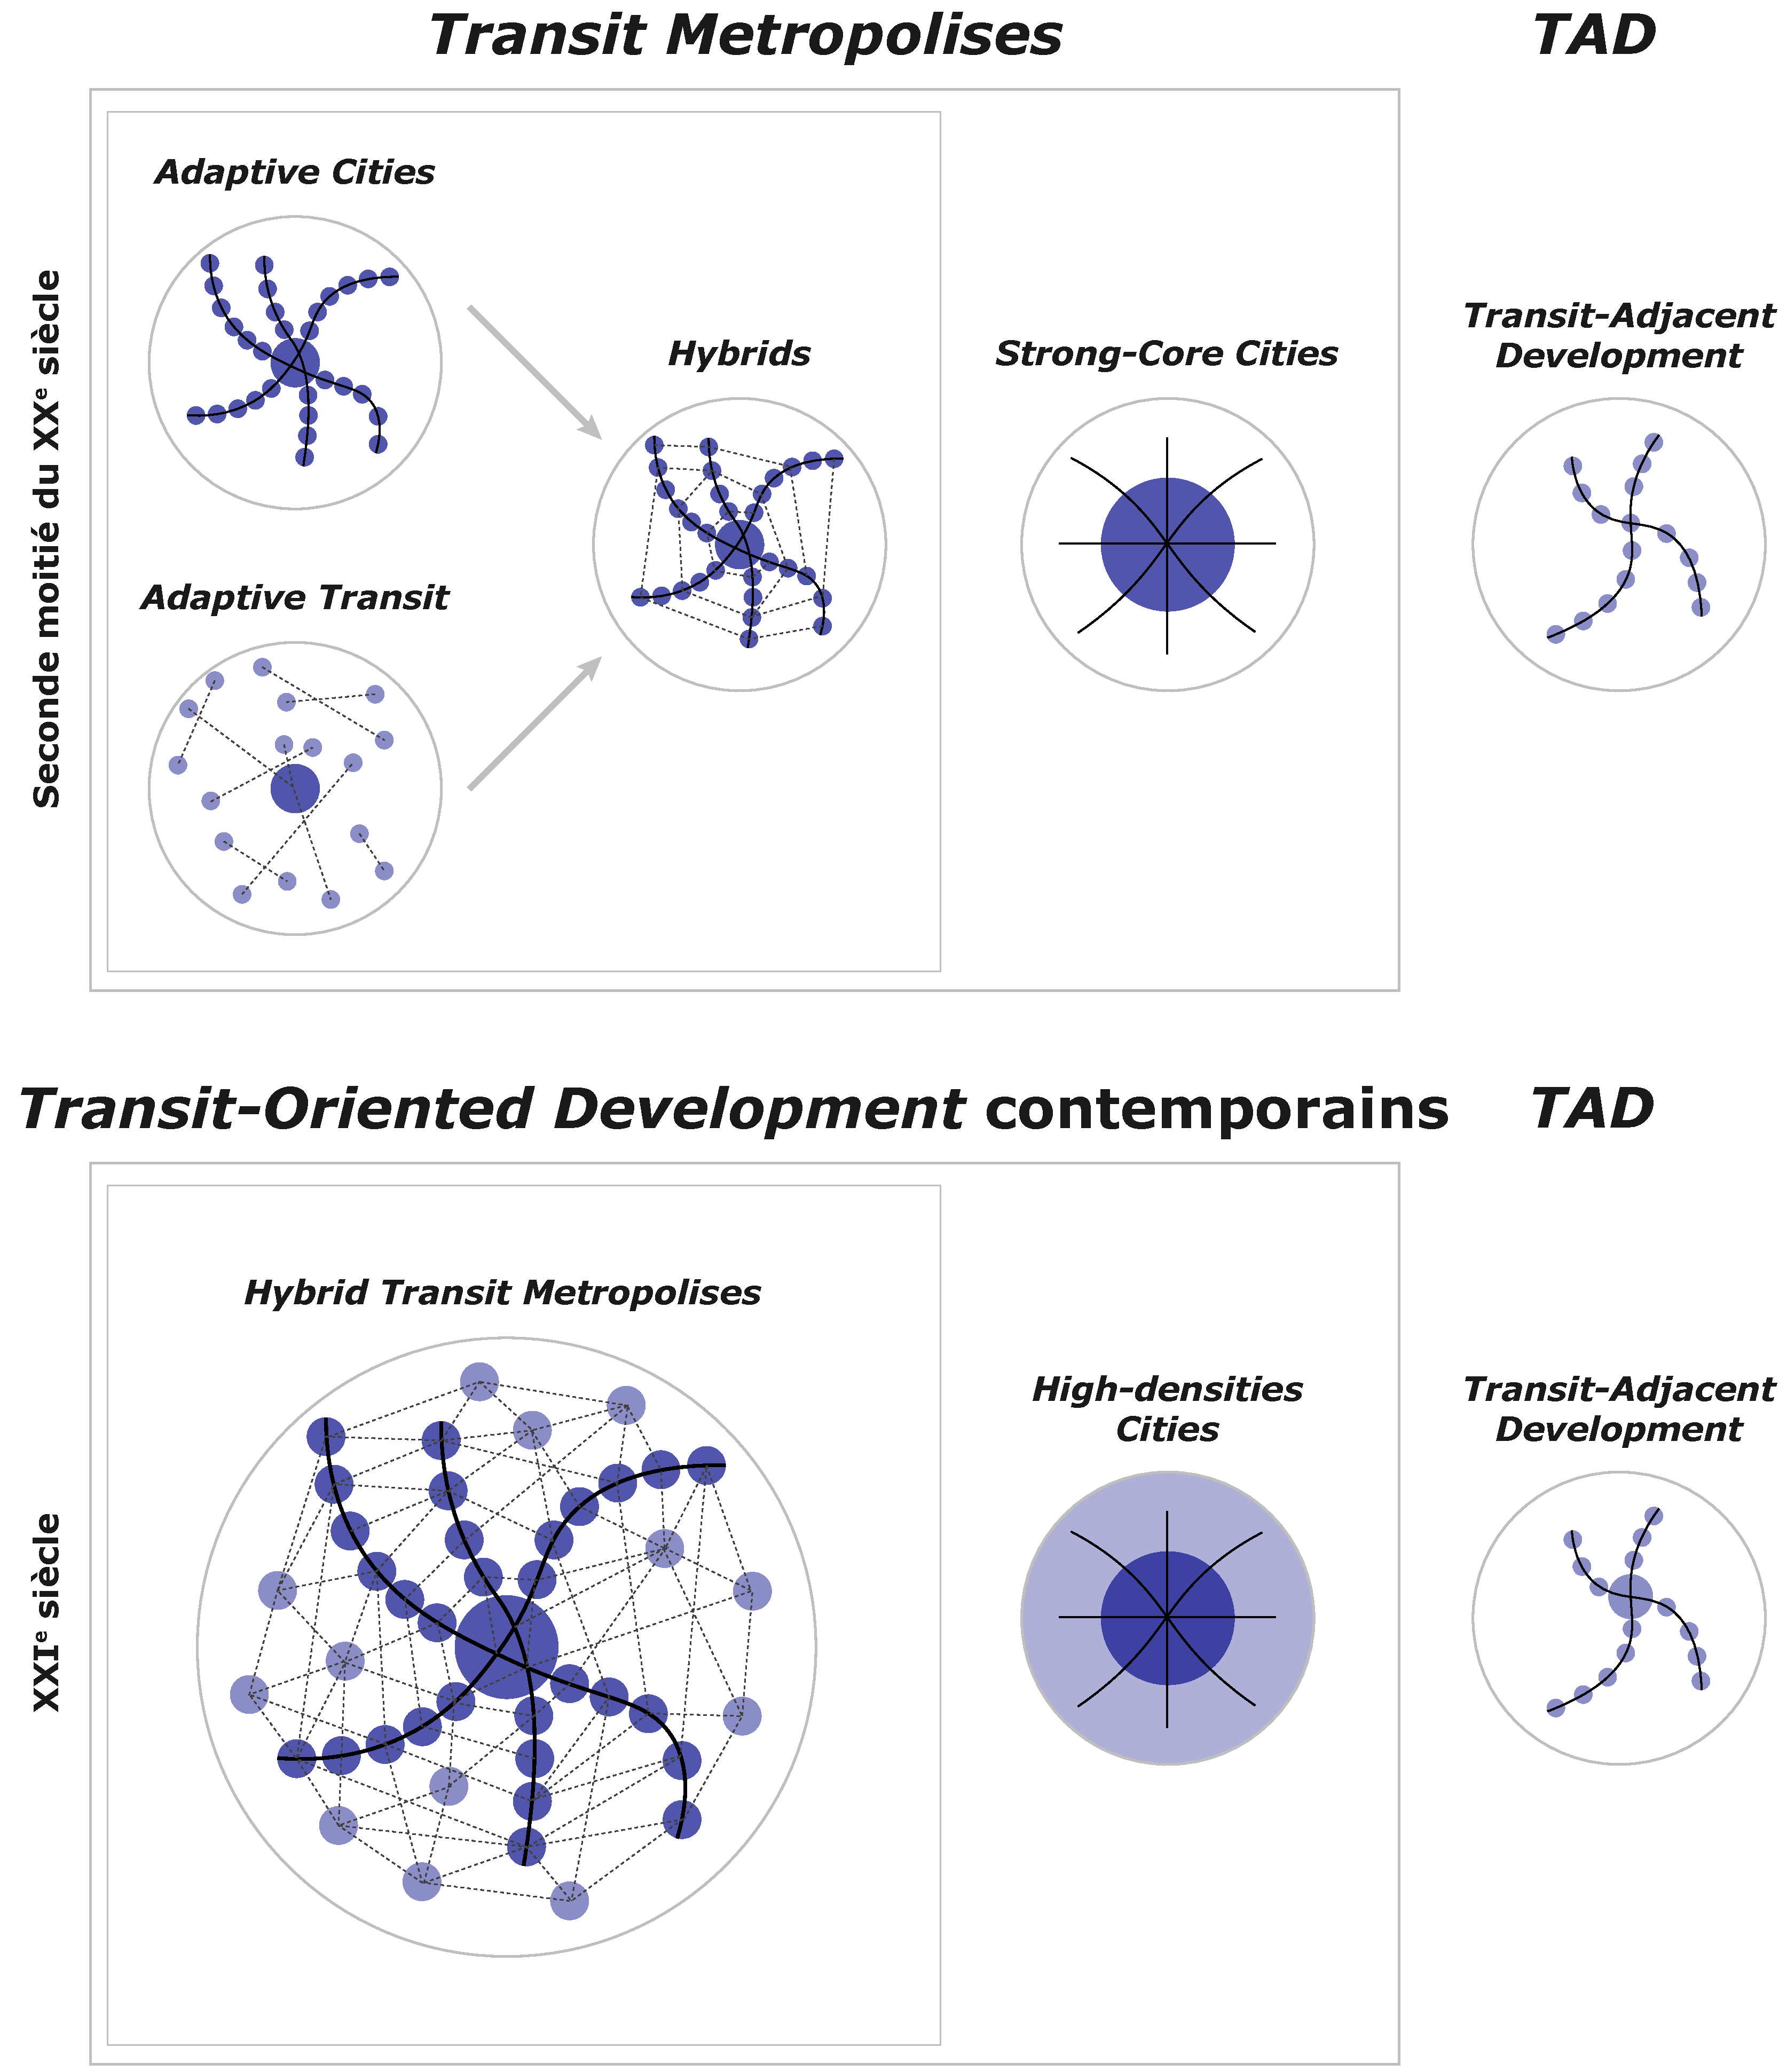
\includegraphics[width=1\columnwidth]{src/Figures/Chap-1/FR_Schema_Alternative_cities_transit.pdf}}
        \vspace{5pt}
        \begin{flushright}\scriptsize{
        Sources~: \textcolor{blue}{\textcite[3]{vos_influence_2014}}\index{Vos, Jonas de|pagebf}\index{Acker, Veronique van|pagebf}\index{Witlox, Frank|pagebf} et \textcolor{blue}{\textcite[2]{liu_historical_2024}}\index{Liu, Yudi|pagebf}\index{Manabe, Rikutaro|pagebf}\index{Nitanai, Ryoichi|pagebf}\index{Murayama, Akito|pagebf}
        \\
        Adaptation graphique~: \textcolor{blue}{Dylan Moinse (2025)}
        }\end{flushright}
    \end{carte}
    
    % Adaptive Transit
Les \textsl{Adaptive Transit}, caractérisées par un étalement urbain plus prononcé, ont choisi d'inverser le raisonnement entre croissance urbaine et réseaux de transport. Pour desservir efficacement des territoires périurbains à faible densité, les systèmes de mobilité doivent s’adapter aux formes urbaines dispersées de ces espaces. \textcolor{blue}{Susan} \textcolor{blue}{\textcite[108]{handy_reviews_1999}}\index{Handy, Susan|pagebf} met en lumière cette problématique, selon laquelle les villes étasuniennes, fortement marquées par l’étalement urbain, ne peuvent s’inspirer directement des expériences des \textsl{Adaptive Cities} et doivent plutôt adopter un modèle basé sur le format des \textsl{Adaptive Transit}. Dans ces contextes urbains, les déplacements régionaux suivent moins une logique radiale que des flux tangents, reliant les périphéries entre elles (voir la \hyperref[fig-chap1:schema-transit-metropolis]{carte~\ref{fig-chap1:schema-transit-metropolis}}, page~\pageref{fig-chap1:schema-transit-metropolis}). Cependant, les réseaux de transport en commun conventionnels sont souvent organisés autour d’itinéraires fixes et radiaux, ou parfois diamétraux, ce qui limite leur capacité à répondre à ces besoins. Les solutions proposées par ce type de \textsl{Transit Metropolis}, également désignées par l’acronyme \acrfull{DOT}, s’appuient sur des innovations technologiques et servicielles pour offrir une flexibilité accrue, en mesure de concurrencer la voiture individuelle \textcolor{blue}{\autocite[132]{cervero_transit_2020}}\index{Cervero, Robert|pagebf}. L’objectif de ces systèmes est de promouvoir une mobilité alternative au modèle auto-centré, tout en proposant des services de transport aux caractéristiques proches de la voiture \textcolor{blue}{\autocite[67-68]{bourdin_major_2024}}\index{Bourdin, Alain|pagebf}. Ces solutions misent sur des trajets personnalisés, adaptés aux défis des \Guillemets{premiers et derniers kilomètres} ainsi qu’aux besoins de déplacement \Guillemets{porte-à-porte}. Ces services basés sur la demande se positionnent comme des compléments au transport public traditionnel en renforçant leur attractivité et leur accessibilité. Les \textsl{Adaptive Transit} peuvent être illustrées par le système de tram-train de Karlsruhe, mis en service en 1992\footnote{
    Confrontée à un processus de périurbanisation important et à un manque de coordination entre les agences de transport public, la ville de Karlsruhe n’a pas su initialement optimiser l’utilisation de son réseau de transport urbain \textcolor{blue}{\autocite[p.~343-360 (chapitre 13)]{cervero_transit_1998}}\index{Cervero, Robert|pagebf}. Pour répondre à cette problématique, un projet adapté à son contexte territorial voit le jour~: la conception d’un système de tram-train interconnecté, connu sous le nom de \textsl{Zweisystem-Stadtbahn}. La première ligne de ce système dessert le centre-ville de Karlsruhe en mode tramway, puis emprunte les voies ferrées interurbaines pour rejoindre Bretten. Ce projet, testé en 1986 avant son inauguration en 1992, tend à offrir une solution efficace aux besoins de mobilité périurbaine. La mise en service de cette ligne pilote, qui a rapidement vu sa fréquence augmenter, a permis d’atteindre les objectifs escomptés, à savoir la multiplication par quatre de sa fréquentation, dont une majorité d'ancien·ne·s automobilistes \textcolor{blue}{\autocite[41]{beaucire_reseau_2000}}\index{Beaucire, Francis|pagebf}. Au-delà de ses aspects purement techniques, le \Guillemets{modèle de Karlsruhe} suscite aujourd’hui un vif intérêt \textcolor{blue}{\autocite[41]{beaucire_reseau_2000}}\index{Beaucire, Francis|pagebf}. Ce système offre une réponse adaptée à un contexte urbain hétérogène en captant efficacement les territoires périurbains qui, jusqu’alors, n’ont pas été pensés pour être intégrés aux réseaux de transport public \textcolor{blue}{\autocite[57-65]{grisot_manifeste_2020}}\index{Grisot, Sylvain|pagebf}. Ce système technique et tarifaire unique permet aux habitant·e·s des zones périurbaines de rejoindre directement les centres urbains sans nécessiter de rupture de charge, les dispensant d’un \gls{détour} par la gare, souvent excentrée. En parallèle, pour les collectivités locales et les opérateurs de transport, ce modèle représente une promesse d’investissement moins coûteux, grâce à la réutilisation des infrastructures existantes \textcolor{blue}{\autocite[17]{lhostis_multi-criteria_2017}}\index{L'Hostis, Alain|pagebf}\index{Soulas, Claude|pagebf}\index{Vulturescu, Bogdan|pagebf}.
}~; le système de bus guidé d'Adélaïde, complètement opérationnel depuis 1989\footnote{
    La ville d’Adélaïde connaît une situation similaire à celle de Karlsruhe, marquée par un phénomène d'extension urbaine considérable \textcolor{blue}{\autocite[p.~362-377 (chapitre 14)]{cervero_transit_1998}}\index{Cervero, Robert|pagebf}. Face à la croissance urbaine très rapide de banlieues situées au nord-est de l'agglomération, les pouvoirs publics choisissent dans un premier temps d’étendre le réseau de tramways existant, avant de se tourner vers une solution alternative~: la mise en place d’un système de bus guidé. Ce système, connu sous le nom d'\textsl{O-Bahn}, est le premier de ce type au monde et reste, à ce jour, le plus long réseau en service. Il constitue une hybridation entre le bus conventionnel et le transport sur rail \textcolor{blue}{\autocite[143]{currie_assessing_2014}}\index{Currie, Graham|pagebf}\index{Delbosc, Alexa|pagebf}. Le \textsl{O-Bahn} repose sur l’utilisation de roues latérales spécifiques, qui permettent au \acrshort{BHNS} de circuler sur des voies dédiées en site propre, rendant le voyage à la fois plus rapide et sécurisé \textcolor{blue}{\autocite[2]{currie_bus_2006}}\index{Currie, Graham|pagebf}. Ce système est conçu pour relier efficacement le \acrfull{CBD} de la ville à la nouvelle centralité commerciale et urbaine de Tea Tree Plaza, située dans une banlieue en pleine expansion. Lors de son lancement, le \textsl{O-Bahn} comptait 6 kilomètres de voies en 1986, étendus à 12 kilomètres en 1989. L’objectif principal est alors de décongestionner le réseau autoroutier en offrant un service performant, souple et relativement peu coûteux. Le réseau \textsl{O-Bahn} atteint ainsi une vitesse commerciale moyenne de 80 kilomètres par heure, en faisant le système de bus le plus rapide au monde \textcolor{blue}{\autocite[3]{currie_bus_2006}}\index{Currie, Graham|pagebf}. Ce succès est attribuable à l’infrastructure dédiée et à l’espacement important entre les arrêts, à hauteur de cinq kilomètres environ. Par ailleurs, le taux d’occupation des bus guidés est généralement deux fois supérieur à celui des bus classiques de l’agglomération, tandis que les coûts d’exploitation par passager·ère et par kilomètre sont inférieurs d’un tiers à ceux des bus réguliers \textcolor{blue}{\autocite[7]{basbas_advances_2005}}\index{Basbas, Socrates|pagebf}. Actuellement, 18 lignes utilisent l’alignement de 12 kilomètres, bien que seules 8 d’entre elles l’exploitent dans son intégralité \textcolor{blue}{\autocite[3]{rogers_o-bahn_2002}}\index{Rogers, Lee~H.|pagebf}. Ce système illustre comment une région confrontée à une périurbanisation notable a choisi non pas de contenir cette dynamique urbaine, mais de la connecter à son centre urbain. L’infrastructure du \textsl{O-Bahn} est de plus en mesure de traverser des quartiers denses sans nécessiter d’importantes reconfigurations de l'espace. Cependant, malgré le succès populaire et même touristique de ce système, Adélaïde reste dominée par l’automobile. Cette prédominance se reflète également parmi les usager·ère·s du \textsl{O-Bahn}, dont plus de la moitié accèdent aux arrêts en voiture, nécessitant un élargissement récurrent des infrastructures de \acrfull{P+R}. Ces extensions interviennent malgré les efforts initiaux d'aménagement piétonnier et cyclables autour des stations \textcolor{blue}{\autocite[11]{currie_bus_2006}}\index{Currie, Graham|pagebf}.
}~; ou le système de \textsl{paratransit}, appelé \textit{microbús}, présent à Mexico City\footnote{
    À Mexico City, le décalage significatif entre l’offre de transport en commun et l’étendue de la surface urbanisée a favorisé l’émergence de stratégies autorégulées initiées par le marché. C’est dans ce contexte qu’a vu le jour, dans les années 1970, le service de transport privé de \textsl{microbús}, également appelé \textsl{pesero}. Ce système s’est spontanément développé pour répondre aux besoins de mobilité identifiés dans les territoires non desservis par le réseau de transport public \textcolor{blue}{\autocite[p.~379-399 (chapitre 15)]{cervero_transit_1998}}\index{Cervero, Robert|pagebf}. Ainsi, le marché a su s’adapter pour combler l’écart entre une demande croissante de mobilité et une offre insuffisante en matière d'infrastructure et de service de mobilité. Face à l’expansion rapide de l’aire urbaine de Mexico City, le \textsl{paratransit} a su trouver sa place dans le système de mobilité en coexistant en tant que mode de transfert. Ce service permet de transporter les populations enclavées vers les stations de transport public situées en périphérie du centre. Fonctionnant comme des taxis collectifs, ces véhicules, souvent des voitures à l’origine, suivent un tracé de ligne fixe, similaire à celui d’une ligne de bus. Ils prennent et déposent des passager·ère·s à la demande le long de l'\gls{itinéraire} \textcolor{blue}{\autocite[4]{chiu_does_2022}}\index{Chiu, Bing-yu|pagebf}. Ce système \Guillemets{informel} joue un rôle clé en tant que service de rabattement auto-organisé, comme le confirme la littérature existante \textcolor{blue}{\autocite[98, 246]{adjeroud_coexistence_2024}}\index{Adjeroud, Heythem|pagebf}\index{Chapelon, Laurent|pagebf}\index{Lammoglia, Adrien|pagebf}. Il présente notamment l'avantage de ne pas nécessairement requérir d'investissements publics. Cependant, il peut représenter une concurrence directe au transport public \Guillemets{formel} et tout autant contribuer à l’étalement urbain \textcolor{blue}{\autocite[4]{chiu_does_2022}}\index{Chiu, Bing-yu|pagebf}. Sur cette base, \textcolor{blue}{Edzani} \textcolor{blue}{\textcite[65]{libunyu_paratransit-oriented_2024}}\index{Libunyu, Edzani|pagebf} identifie une forme de \textsl{Paratransit-Oriented Transit-Oriented Development}, en prenant le cas de Mexico City comme exemple.
} \textcolor{blue}{\autocite[343-399]{cervero_transit_1998}}\index{Cervero, Robert|pagebf}.%%Rédigé%%

    % Hybrides
En laissant volontairement de côté les \textsl{Strong-core Cities}, qui reposent sur des dynamiques de revitalisation urbaine et qui s’éloignent de notre problématique centrale, nous nous concentrons sur le quatrième et dernier type de \textsl{Transit Metropolis}~: les \textsl{Hybrids}, qui revêtent un intérêt particulier dans le cadre de notre recherche. Dépassant la dichotomie entre \textsl{Adaptive Cities} et \textsl{Adaptive Transit}, ces \textsl{Hybrids} s’affirment par leur aptitude à tirer parti des points forts des deux concepts. Cette approche aspire à trouver un juste équilibre entre un urbanisme dense et mixte concentré sur les corridors bien desservis et un système de mobilité alternative efficace, destiné à couvrir les périphéries à plus faible densité. Ce compromis est illustré par la \hyperref[fig-chap1:schema-transit-metropolis]{carte~\ref{fig-chap1:schema-transit-metropolis}} (page~\pageref{fig-chap1:schema-transit-metropolis}). Ces \textsl{Hybrids} regroupent, en un même territoire, les solutions de mobilité et d’urbanisme issues des deux types de \textsl{Transit Metropolis} décrits précédemment. Ils se rapprochent ainsi d’un modèle polycentrique, caractérisé par une hiérarchie de centres urbains interconnectés par des lignes structurantes. L’accessibilité de ces centres est renforcée par des services de mobilité flexibles, répondant aux besoins des zones périurbaines et faiblement denses \textcolor{blue}{\autocite[213-295]{cervero_transit_1998}}\index{Cervero, Robert|pagebf}.%%Rédigé%%
    
    % Hybrid Transit Metropolises
Cette typologie de \textsl{Transit Metropolises}, \textcolor{blue}{Robert} \textcolor{blue}{\textcite[131]{cervero_transit_2020}}\index{Cervero, Robert|pagebf} la réinterprète finalement sous la désignation consolidée de \textsl{Hybrid Transit Metropolises}. Une telle relecture permet de démontrer comment ces territoires ont transcendé la dichotomie entre \textsl{Adaptive Cities} et \textsl{Adaptive Transit}, une dualité qui a aujourd’hui perdu de sa consistance. Ce constat renvoie aux \textsl{Hybrids}, telles que décrites par \textcolor{blue}{\textcite[213-295]{cervero_transit_1998}}\index{Cervero, Robert|pagebf} vingt ans plus tôt, bien que revisitées à la lumière des évolutions contemporaines des systèmes de mobilité. Le facteur déterminant de cette révision réside dans l’émergence et la généralisation des \acrshort{NTIC}, ayant engendré simultanément une \Guillemets{mobilité intelligente} (\textsl{smart mobility}) et un \Guillemets{urbanisme intelligent} (\textsl{smart cities}). Par ailleurs, les pratiques et les imaginaires de mobilité des nouvelles générations ont considérablement évolué, influençant les formes de déplacement et les attentes en matière d’accessibilité. Derrière ces concepts, parfois assimilés à des \Guillemets{mots-valises}, \textcolor{blue}{\textcite[137-143]{cervero_transit_2020}}\index{Cervero, Robert|pagebf} plaide pour une approche intégrative en dépassant les clivages au profit de \Guillemets{\textsl{Transit Metropolises} du XXI\textsuperscript{e} siècle}. Au terme de son analyse, l'auteur observe une convergence des territoires vers les \textsl{Hybrid Transit Metropolises}, où la maîtrise des formes urbaines, en adéquation avec les principes du \acrshort{TOD}, s'associe au développement d'un éventail de solutions de mobilité flexibles et \Guillemets{porte-à-porte} (voir la \hyperref[fig-chap1:schema-transit-metropolis]{carte~\ref{fig-chap1:schema-transit-metropolis}}, page~\pageref{fig-chap1:schema-transit-metropolis}). Ces métropoles intègrent alors des systèmes de \textsl{micro-transit}~–~\textcolor{blue}{\textcite[144]{cervero_transit_2020}}\index{Cervero, Robert|pagebf} évoque notamment les exemples de la marche, du vélo ou encore des services de \acrfull{VTC}, de \acrfull{VLS}, de \acrfull{VFF}, de \acrfull{TEFF}, de \textsl{paratransit} et de taxi autonome~–~en complément de leurs infrastructures de transport en commun à grande capacité ou de \textsl{mass transit} \textcolor{blue}{\autocite[7]{thomas_transit-oriented_2020}}\index{Thomas, Ren|pagebf}\index{Bertolini, Luca|pagebf}. Parallèlement, elles adoptent une gestion \Guillemets{intelligente} de la demande (\textsl{smart pricing}). Dans cette optique, le mot d’ordre de ces \acrshort{TOD}\textcolor{blue}{s} contemporains repose sur l’élaboration d’une offre multimodale synergique, qui tire parti des avancées des \acrshort{NTIC} et de la généralisation des \textsl{smartphones}, avec pour finalité de limiter la dépendance automobile.%%Rédigé%%

    % Approches offre et demande
Les \textsl{Hybrid Transit Metropolises} s’appuient sur des éléments structurants issus d’une double approche, par l’offre (\acrshort{TSM}) et par la demande (\acrshort{TDM}) de mobilité, telle que décrite par \textcolor{blue}{\textcite[67]{cervero_transit_1998}}\index{Cervero, Robert|pagebf} avant d'être renouvelée \textcolor{blue}{\autocite[137-143]{cervero_transit_2020}}\index{Cervero, Robert|pagebf}~:
    \begin{customitemize}
\item D’une part, l’approche \acrshort{TSM} repose sur les \Guillemets{3Ds}~: densité, diversité et \textsl{design}. Elle inclut également le développement de modes de déplacement non motorisés, tels que l’usage intermodal du vélo. Les \acrshort{NTIC} jouent un rôle clé dans cette dynamique en promettant de transformer à la fois les modalités de déplacement et les environnements dans lesquels s’inscrivent les flux. Cela passe par l’essor du télétravail, des visioconférences et du commerce en ligne, mais aussi par l’optimisation des flux grâce à des outils tels que la gestion de trafic via la signalisation intelligente, la géolocalisation des véhicules, les données en temps réel pour les passager·ère·s, ou encore les péages automatisés en milieu urbain. Un exemple emblématique est celui de Copenhague, dont le réseau cyclable de renommée mondiale s’inscrit dans une politique de \acrshort{TOD} hybride. Dans un premier temps, nous l'avons vu, la capitale danoise a misé sur un réseau ferroviaire performant allié à une croissance urbaine concentrée dans des corridors denses. C'est par la suite qu'elle a développé des infrastructures cyclables de grande qualité pour répondre aux flux tangents, en périphérie urbaine. Le vélo y est pleinement intégré à la stratégie de \acrshort{TOD}, avec des infrastructures abondantes de stationnement à proximité des stations de transport en commun, des voitures dédiées à l'emport du vélo dans les trains et le développement de 26 autoroutes cyclables (\textsl{Cycle Super Highways}) totalisant plus de 500 kilomètres. Par ailleurs, des services de \acrshort{VLS} et de \acrshort{VFF} complètent cette offre~;
\item D’autre part, au lieu de simplement chercher à améliorer la mobilité à moindre coût, l’approche \acrshort{TDM} vise à optimiser l’utilisation des ressources existantes en influençant, voire en réduisant, la demande de mobilité. Un consensus croissant souligne que la gestion du stationnement automobile constitue l’une des stratégies basées sur cette demande parmi les plus efficaces, bien qu’elle demeure sensible des points de vue des négociations politiques et de l'acceptabilité sociale. Cette démarche peut prendre la forme de l'introduction de frais de stationnement, du développement du covoiturage ou de la promotion du télétravail. Des mesures complémentaires, telles que la régulation de l’usage automobile par le biais de la réduction ou de l’interdiction du trafic motorisé dans certaines zones, le ralentissement de la circulation, ou encore l’augmentation des coûts liés à l’usage automobile (carburant, charges de congestion ou taxes carbone), viennent renforcer cette approche. Séoul constitue un exemple convaincant, où des politiques volontaristes en faveur du \acrshort{TOD} se sont traduites par la mise en place d’un réseau de 120 kilomètres de \acrshort{BHNS} en 2017. Cette initiative s’est accompagnée de la reconversion de quartiers centrés sur l’automobile en espaces piétonniers \textcolor{blue}{\autocite[6]{prayogi_bus_2018}}\index{Shin, Dooho|pagebf}, le projet emblématique étant sûrement la restauration de la rivière Cheonggyecheon en 2003, jusqu'alors transformée en autoroute urbaine \textcolor{blue}{\autocite[]{shin_cheongyecheon_2013}}\index{Shin, Dooho|pagebf}.
    \end{customitemize}%%Rédigé%%

    % E-TOD
Cette réflexion sur une révision des principes du \acrshort{TOD} entre en résonance avec le concept décliné d'\acrfull{E-TOD}, développé par le chercheur en urbanisme et en génie civil \textcolor{blue}{\textcite{schneider_illustrating_2012}}\index{Schneider, Jerry~B.|pagebf}. Ce concept envisageait déjà la promesse de bénéfices issus de l’intégration des technologies pour enrichir le modèle urbain originel. Le postulat de base repose sur un constat également observable dans les \textsl{Transit Metropolises}, en particulier du côté des \textsl{Adaptive Transit} et des \textsl{Hybrids}. Ce sont des territoires présentant un tissu urbain largement étalé et fragmenté, difficilement desservi par les réseaux de transport en commun conventionnels, et qui pose la problématique fondamentale des \Guillemets{premiers et derniers kilomètres} du transport public \textcolor{blue}{\autocite[133]{cervero_transit_2020}}\index{Cervero, Robert|pagebf}. À cette fin, \textcolor{blue}{\textcite[141]{schneider_prt_1992}}\index{Schneider, Jerry~B.|pagebf} propose une vision du \acrshort{TOD} attentive à la fonction d’intermodalité et de connexion. Cette approche gagnerait à intégrer un système de transport moyennement capacitaire et doté d’une capillarité accrue, incarné par ce qu’il nomme le \acrfull{PRT}\footnote{
    Le \acrfull{PRT}, ou \textsl{Personal Rapid Transit}, est un système de transport, souvent automatisé et sur site propre, mettant en circulation des capsules individuelles ou de faible capacité, conçues pour transporter des individus ou de petits groupes directement vers leur destination. Ce service de mobilité se situe à mi-chemin entre le transport en commun conventionnel et les modes de déplacement individuels. Le \acrshort{PRT} est une forme de transport à la demande~: les voyageur·se·s sélectionnent leur destination, et le véhicule effectue un trajet direct sans arrêt intermédiaire, à la différence des systèmes de transport public classiques soumis à des arrêts réguliers et à des horaires fixes. Cette configuration permet, en théorie, de réduire les temps d’attente et de parcours. Par ailleurs, le \acrshort{PRT} nécessite une emprise au sol relativement réduite, ce qui le rend particulièrement adapté aux environnements urbains denses. Cependant, ce système présente également plusieurs limites. Il se heurte à la complexité de son intégration dans les réseaux de transport existants, à des coûts initiaux très élevés pour la construction des infrastructures et la mise en œuvre des services dédiés, ainsi qu’à une capacité limitée, ce qui restreint son efficacité dans les contextes à forte demande. En pratique, très peu de projets de \acrshort{PRT} ont été réalisés et surtout commercialisés. La majorité des prototypes sont restés à l’état de projets expérimentaux.
}. L’enjeu ici ne réside pas dans une substitution du transport public par le \acrshort{PRT}, mais bel et bien dans la facilitation de l’accès aux gares ferroviaires pour des zones situées au-delà de la portée socialement acceptable de la marche combinée. La méthode \acrshort{E-TOD} porte une stratégie d'interconnexion inter-urbaine, associant les mécanismes d'un système global \acrfull{F-D-C} destiné à relier l'ensemble des modes collectifs\footnote{
    Le concept de \acrfull{F-D-C} désigne une stratégie de structuration des réseaux de transport reposant sur trois fonctions complémentaires. Ce modèle est fréquemment utilisé dans la planification des systèmes de transport urbain et régional, car il offre une organisation cohérente et hiérarchisée des flux de mobilité. Les trois composantes principales de ce modèle se déclinent comme suit~:
        \begin{customitemize}
    \item \textsl{Alimentation} (\textsl{Feeder}). Cette fonction concerne les infrastructures ou les services dédiés à la collecte des passager·ère·s dans des zones périphériques ou éloignées, pour les acheminer vers des points d’accès stratégiques du réseau principal~;
    \item \textsl{Distribution}. Une fois les passager·ère·s arrivé·e·s dans un pôle d'échange multimodal, la fonction de distribution consiste à les transporter vers leur destination finale à l’intérieur de zones urbaines plus denses ou complexes. Dans ce contexte, le \acrshort{PRT} joue un rôle central dans la gestion de cette étape~;
    \item \textsl{Circulation}. La circulation concerne les déplacements internes à une zone spécifique, indépendamment des points centraux ou des lignes principales. Elle assure une mobilité de proximité, en particulier dans des quartiers ou des zones résidentielles.
        \end{customitemize}
}, avec l'intégration d'un système d'organisation désigné sous le terme d'\textsl{Urban Oasis}\footnote{
    L’\textsl{Urban Oasis} est un concept développé par l’architecte étasunienne \textcolor{blue}{Roxanne} \textcolor{blue}{\textcite{warren_urban_1997}}\index{Warren, Roxanne|pagebf}, qui propose un modèle d’aménagement urbain axé sur la création d’espaces verts et de lieux de détente au sein des zones fortement densifiées des métropoles. Ce concept s’inscrit dans une réflexion plus large sur les moyens de réintroduire la nature et de promouvoir le bien-être au cœur d’environnements urbains souvent marqués par une prédominance de surfaces minérales, d’infrastructures massives et d’une pression démographique accrue. Cette vision met l’accent sur la nécessité de réinscrire une échelle humaine dans des espaces urbains parfois perçus comme déshumanisés, de mettre à disposition des lieux de repos, de loisirs et de reconnexion avec la nature, ainsi que d'intégrer les principes d’écologie urbaine. En revalorisant les qualités environnementales et sociales des espaces urbains, l’\textsl{Urban Oasis} aspire à améliorer la qualité de vie des habitant·e·s tout en favorisant un urbanisme durable et résilient.
} \textcolor{blue}{\autocite[145]{schneider_prt_1992}}\index{Schneider, Jerry~B.|pagebf}. En somme, l'idée novatrice de ce système intermodal, conçu selon les principes caractéristiques du \acrshort{TOD}, réside dans la proposition de regrouper les clusters urbains pour les connecter au réseau de transport, par l'intermédiaire du réseau secondaire de \acrshort{PRT}, selon le principe de \Guillemets{\textsl{cluster-and-connect}} (voir la \hyperref[fig-chap1:schema-e-tod]{carte~\ref{fig-chap1:schema-e-tod}}, page~\pageref{fig-chap1:schema-e-tod}).%%Rédigé%%

    % Figure schéma E-TOD
    \begin{carte}[h!]\vspace*{4pt}
        \caption{Carte abstraite de la stratégie \Guillemets{\textsl{cluster-and-connect}} proposée dans le cadre du \textsl{Extended Transit-Oriented Development}.}
        \label{fig-chap1:schema-e-tod}
        \centerline{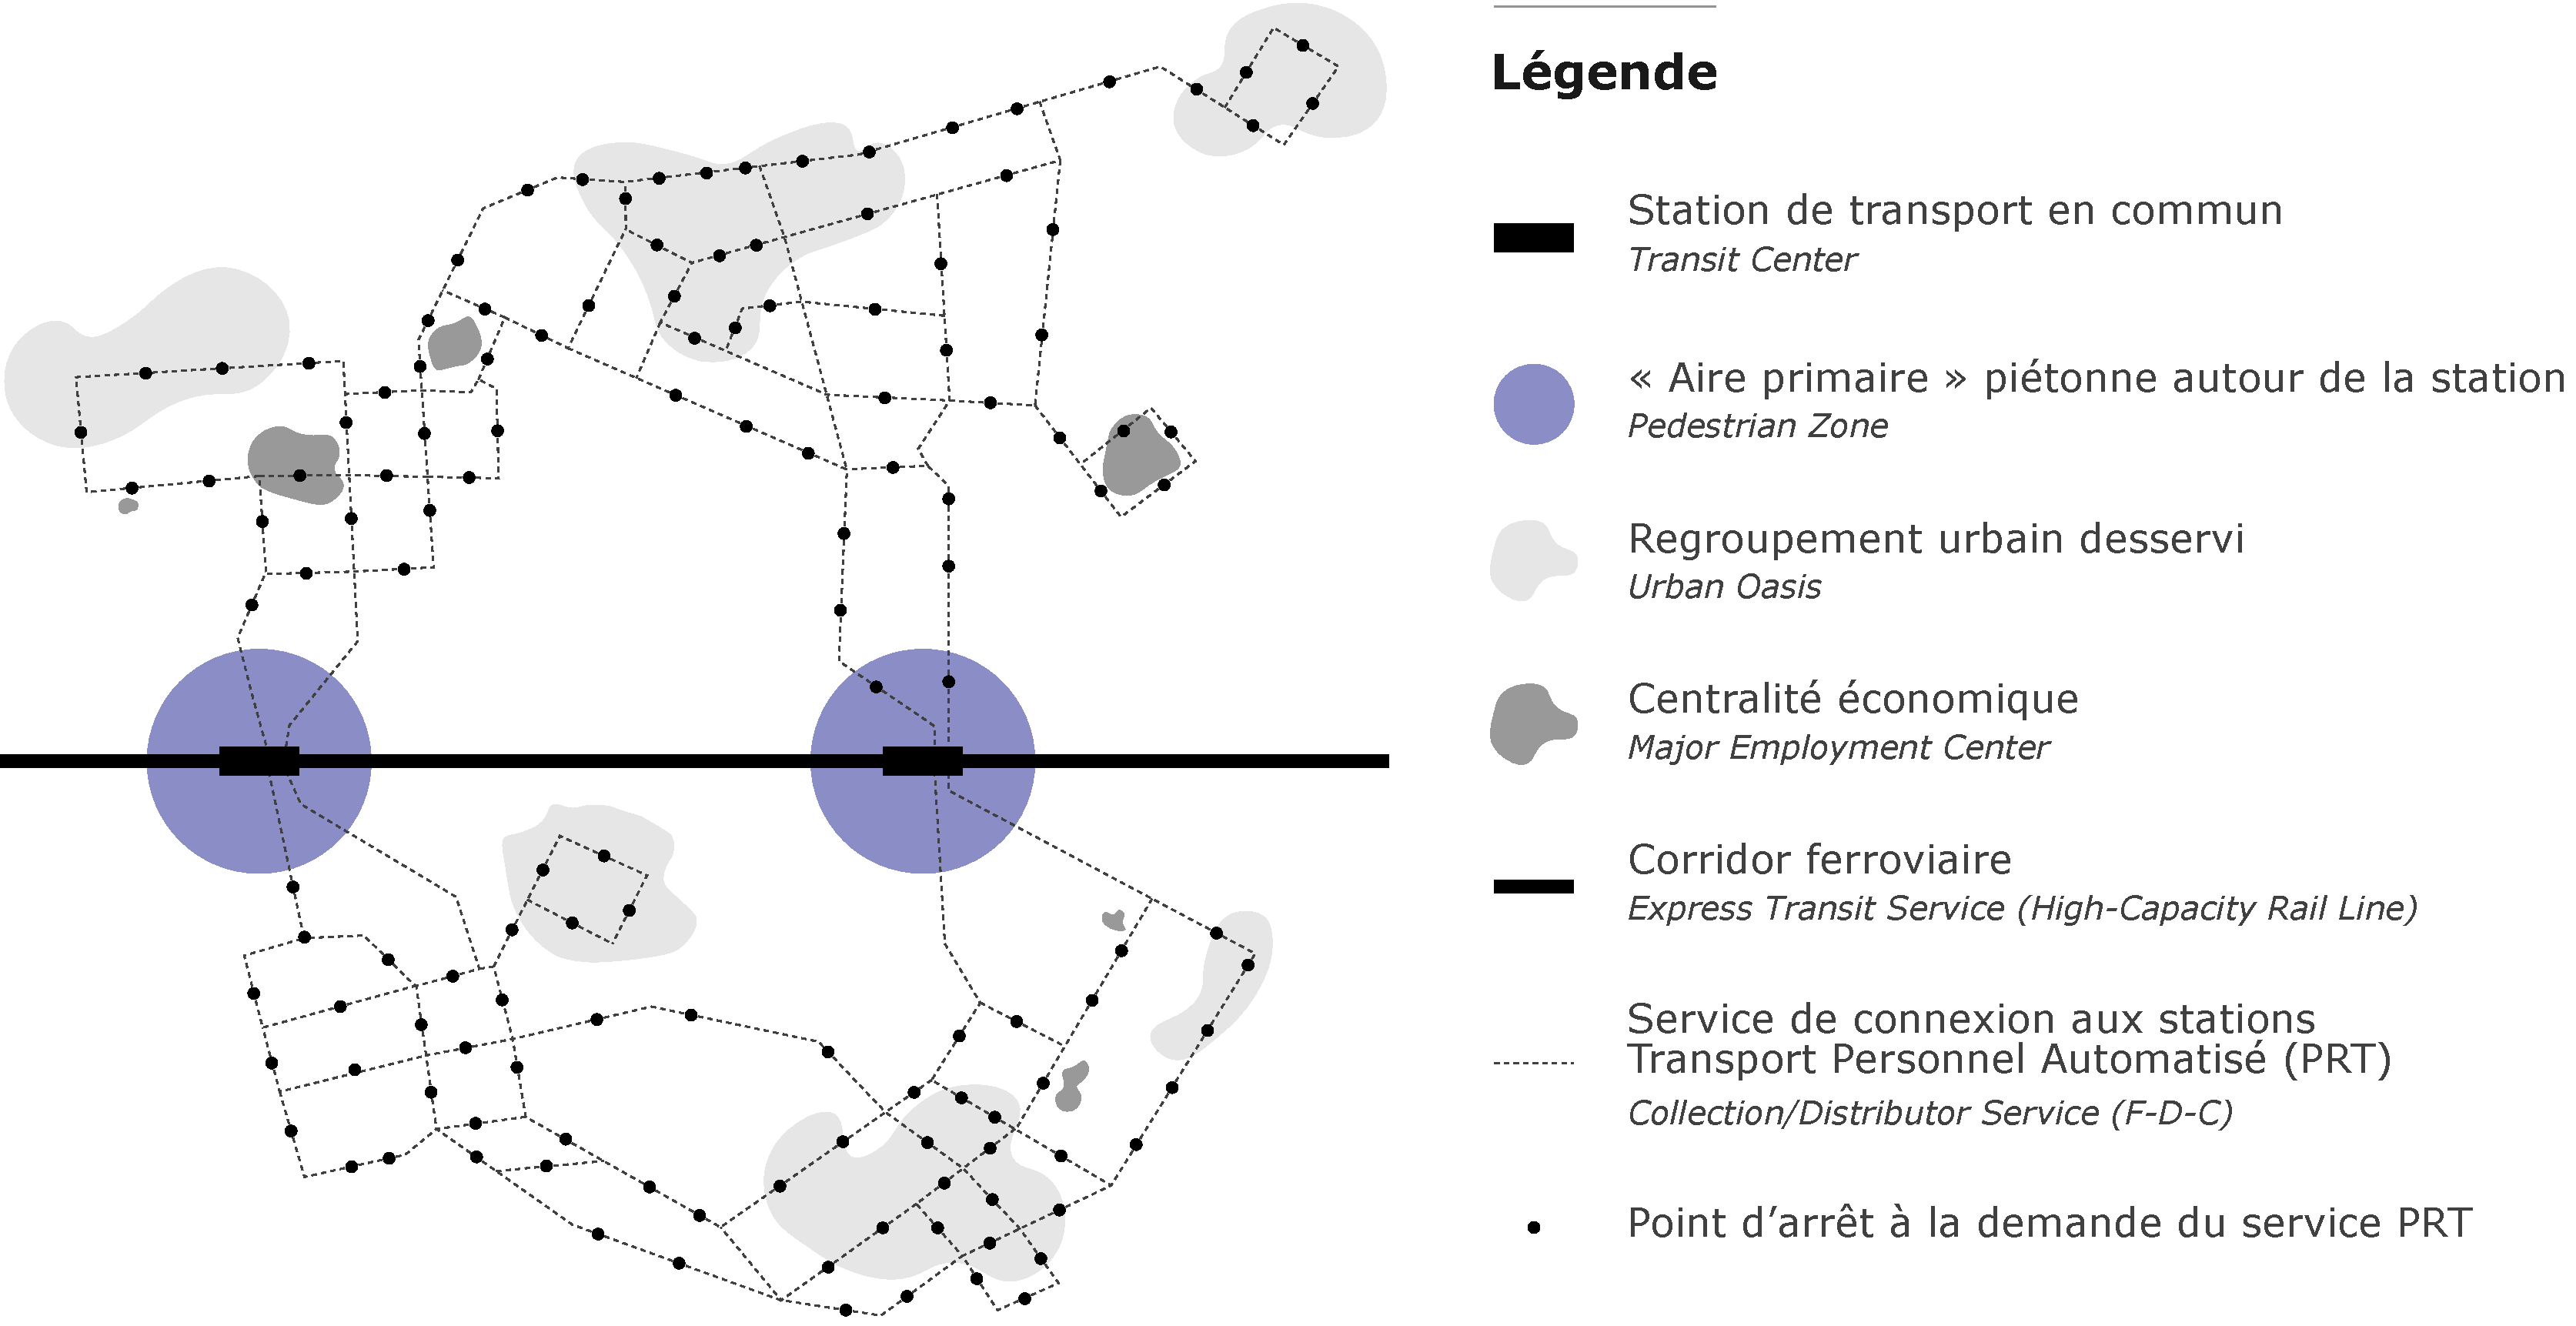
\includegraphics[width=1\columnwidth]{src/Figures/Chap-1/FR_Schema_Schneider.pdf}}
        \vspace{5pt}
        \begin{flushright}\scriptsize{
        Source~: \textcolor{blue}{\textcite[142]{schneider_prt_1992}}\index{Schneider, Jerry~B.|pagebf} (voir aussi \textcolor{blue}{\textcite{schneider_illustrating_2012}}\index{Schneider, Jerry~B.|pagebf})
        \\
        Adaptation graphique~: \textcolor{blue}{Dylan Moinse (2024)}
        }\end{flushright}
    \end{carte}

    % Limites E-TOD et Transition
Néanmoins, cette déclinaison du \acrshort{TOD}, bien qu’elle conserve les principes fondateurs du modèle, se heurte à des obstacles d’ordre technique, matériel et temporel. Le \acrshort{PRT} constitue à ce titre une solution infrastructurelle, particulièrement lourde d’un point de vue budgétaire et exigeante en termes de délais de mise en œuvre. Outre les défis technologiques qu’elle implique, le \acrshort{PRT} peine à offrir des gains intéressants en termes de réduction de la congestion, compromettant ainsi sa promesse de mobilité et d’urbanisme plus soutenables. Pour des raisons similaires, la voiture autonome partagée, qui s’inscrit de plus en plus dans les projections d’un urbanisme ferroviaire réactualisé, rencontre des problématiques comparables, alimentées par le mirage d'un bond en avant de la fréquentation du transport public\footnote{
    Dans sa thèse de doctorat, \textcolor{blue}{Félix} \textcolor{blue}{\textcite[333]{carreyre_are_2023}}\index{Carreyre, Félix|pagebf}\index{Coulombel, Nicolas|pagebf}\index{Bouillaut, Laurent|pagebf} s’est attaché à évaluer les performances des services basés sur le véhicule automatisé en mobilisant un cadre d’analyse coût-bénéfice combiné à une modélisation multi-agents avec \textsl{MATSim}. Ses travaux, menés dans les contextes berlinois et parisien, ont mis en évidence que l’introduction de taxis autonomes pourrait conduire à une aggravation de la congestion à Berlin. De surcroît, dans le cas de Saclay, un scénario intermodal associant ces services au système ferroviaire permettrait seulement d’accroître le taux d’occupation moyen des véhicules, bien que cela se fasse au détriment de l’usage du bus.
}. Dans ce contexte, le vélo apparaît comme une solution plus agile et plus concrète ayant fait ses preuves au sein des diverses \textsl{Hybrid Transit Metropolises} à travers le monde. Ce mode de déplacement individuel, naturellement \Guillemets{porte-à-porte} et à la demande, se révèle non seulement complémentaire au \acrshort{TOD}, mais également bien moins coûteux d'un point de vue économique et temporel. De plus, son intégration dans les politiques de mobilité urbaine repose sur des infrastructures relativement légères et adaptables. Dans cette perspective, une enquête menée par \textcolor{blue}{\textcite[119]{goletz_intermodality_2020}}\index{Goletz, Mirko|pagebf}\index{Haustein, Sonja|pagebf}\index{Wolking, Christina|pagebf}\index{L'Hostis, Alain|pagebf} à Berlin, Copenhague, Hambourg et Paris, soutient le potentiel intermodal du vélo dans le cadre d’un urbanisme orienté vers le rail. Les résultats montrent que les spécialistes et chercheur·se·s interrogé·e·s attribuent au vélo le rôle le plus prometteur pour connecter efficacement les infrastructures ferroviaires, à l’exception notable de Paris, où l’intermodalité avec les réseaux de transport en commun urbain est davantage plébiscitée. En s’appuyant sur la thèse des \textsl{Hybrid Transit Metropolises}, profondément renouvelées grâce aux innovations en matière de mobilité, cette recherche doctorale vise donc à examiner la place du vélo comme solution de mobilité pertinente pour répondre aux enjeux des \Guillemets{premiers et derniers kilomètres}. En cela, il s'agit dans le même temps d'explorer l’accompagnement progressif du retour en grâce du cycle par sa diversification modale, autour de ses déclinaisons, ainsi que la réintroduction de la trottinette, mise à jour par les avancées en électromobilité.%%Rédigé%%

     % ___________________________________________
    % 1.2.
    \newpage
    \needspace{1\baselineskip} % Réserve de l'espace
    \sectionheader{Regain de popularité de la mobilité individuelle légère}
\section{La (re)naissance d’une famille de véhicules légers désignés \Guillemets{mobilité individuelle légère}, aux contours mouvants
    \label{chap1:mobilite-individuelle-legere}
    }

    % Introduction
Cette section propose une lecture croisée des trajectoires évolutives de la \Guillemets{petite reine} et de la \Guillemets{nouvelle reine}, en adoptant une perspective historique. Elle met en lumière les moments clés de l’évolution technique et sociale de ces deux modes de déplacement. Nous allons notamment nous intéresser à comprendre comment et pourquoi ces cycles, longtemps considérés comme des objets de loisir, ont progressivement acquis une légitimité~–~encore en construction~–~dans les pratiques de mobilité quotidienne. Cette réhabilitation s’inscrit dans un contexte d’évolution des usages et des valeurs, mais aussi dans celui des innovations techniques et sociales, liées à des formes de \Guillemets{rétro-innovation} \textcolor{blue}{\autocite{barthelot_retro-innovation_2018}}\index{Barthelot, Bertrand|pagebf}. Bien que ces deux objets partagent une histoire marquée par des cycles de gain de popularité et de mise en retrait, ils connaissent aujourd’hui un renouveau, porté à la fois par des avancées techniques et par des transformations des pratiques urbaines. Comme le souligne \textcolor{blue}{Arnaud} \textcolor{blue}{\textcite[26]{passalacqua_monde_2011}}\index{Passalacqua, Arnaud|pagebf}, enseignant-chercheur et co-directeur de l'\acrfull{EUP}, la mobilité urbaine est un \Guillemets{\textsl{monde où les solutions nouvelles ne sont souvent que des reprises de formes anciennes et qui entretient~–~probablement involontairement~–~une confusion entre l'ancien et le contemporain, le passé et le futur. En se focalisant sur les véhicules souvent plus que sur les systèmes dans leur généralité, ce monde reste confus. Le vocabulaire employé, presque figé depuis le XIX\textsuperscript{e} siècle, contribue à renforcer cette confusion}}.%%Rédigé%%

    % Cycles d'innovation
Cette observation constitue une opportunité d’explorer les réflexions autour des \Guillemets{modèles} et des \Guillemets{cycles d’innovation} \textcolor{blue}{\autocite[]{schumpeter_theorie_1911}}\index{Schumpeter, Joseph Aloïs|pagebf}, tout en les inscrivant dans une perspective historique, philosophique et éthique. L’économiste autrichien et étasunien \textcolor{blue}{Joseph Aloïs} \textcolor{blue}{\textcite[107]{schumpeter_capitalisme_1942}}\index{Schumpeter, Joseph Aloïs|pagebf} illustre cette dynamique à travers son célèbre concept de \Guillemets{destruction créatrice}, moteur de la croissance économique par l’innovation dans les produits, procédés, modes de production, débouchés ou matières premières. Ce dernier observe que \Guillemets{\textsl{l'histoire des transports, depuis la diligence jusqu'à l'avion} [\dots] \textsl{constituent d'autres exemples du même processus de mutation industrielle} [\dots] \textsl{qui révolutionne incessamment de l'intérieur la structure économique, en détruisant continuellement ses éléments vieillis et en créant continuellement des éléments neufs.}}. Comme l'aborde le chercheur en philosophie politique et en histoire des idées \textcolor{blue}{Thierry} \textcolor{blue}{\textcite{menissier_innovations_2021}}\index{Ménissier, Thierry|pagebf} dans son ouvrage \textsl{Innovations~: Une enquête philosophique}, l’innovation ne se limite pas à répondre à des besoins préexistants~; elle agit également sur l’imaginaire collectif et suscite un intérêt pour le \textsl{différent}, dans l'intérêt d'accompagner des projets en devenir. Ainsi, il s’agit de réfléchir aux modalités permettant de mieux articuler le transfert et la territorialisation des innovations ainsi que leur mise en usage. Autrement dit, cela revient à interroger les conditions de leur déploiement à travers tous les segments de la société \textcolor{blue}{\autocite[5]{baron_thierry_2022}}\index{Baron, Nacima|pagebf}. Cette territorialisation des innovations a été étudiée par \textcolor{blue}{\textcite[13]{castex_prise_2017}}\index{Castex, Élodie|pagebf}\index{Frère, Séverine|pagebf}\index{Groux, Annette|pagebf}, notamment à travers la planification des transports. Leur étude appuie le décalage entre le lent infléchissement des acteurs publics dans la prise en compte des nouveaux modes de déplacement~–~tels que les \acrfull{STP}~–~dans les outils de gestion urbaine et de mobilité, et la rapidité des évolutions des besoins et des innovations portées par les acteurs privés.%%Rédigé%%

    % Annonce du plan
Dans cette section, nous nous engageons dans l'examen de l’évolution du vélo et de la trottinette, considérés à la fois comme des objets techniques et sociaux, ainsi que sur leur place et leurs usages dans les territoires, en fonction des contextes d’urbanisation (\hyperref[chap1:proximite-velo-trottinette]{section sur l'\Guillemets{âge d’or} de ces véhicules, suivi de leur déclin et de leur \Guillemets{retour}}, page~\pageref{chap1:proximite-velo-trottinette}). À partir de ce bref détour historique, nous mettrons en revue les principales innovations contemporaines ayant marqué ces véhicules, notamment leur électrification et leur mutualisation sous la forme d'une gestion partagée dans les espaces publics (\hyperref[chap1:velo-micromobilite-innovations]{section sur la diversification et l'\Guillemets{hybridation} modale des cycles}, page~\pageref{chap1:velo-micromobilite-innovations}). Enfin, nous contextualiserons la remise à l'honneur du vélo et de la trottinette, sous leurs diverses formes, dans une société \Guillemets{liquide}, portée par des générations de plus en plus adeptes de la \gls{multimodalité}. Ce cadre nous permettra également de proposer notre propre définition de cette famille de véhicules, en y délimitant des contours conceptuels plus précis. Cette définition vise à intégrer les véhicules que nous identifions comme ayant le plus grand potentiel stratégique pour renforcer et redéployer les principes du \acrshort{TOD} (\hyperref[chap1:caracterisation-mobilite-individuelle-legere]{section sur la caractérisation d’une classe de véhicules appelée \Guillemets{mobilité individuelle légère}}, page~\pageref{chap1:caracterisation-mobilite-individuelle-legere}).%%Rédigé%%

    % 1.2.1.
    \needspace{1\baselineskip} % Réserve de l'espace
\subsection{Évolution du \textsl{design} et de la place du cycle parmi les déplacements utilitaires
    \label{chap1:proximite-velo-trottinette}
    }

    % Introduction
Avant de s’imposer aujourd’hui comme des modes de déplacement urbain à part entière, le vélo et la trottinette ont traversé une évolution de plus d’un siècle, marquée à la fois par des innovations techniques et par des transformations des pratiques de mobilité et des imaginaires en Europe. Ces cycles ont connu, au fil de l’histoire, des paradigmes influencés par les constructions sociales associées aux véhicules \textcolor{blue}{\autocite[13]{heran_retour_2015}}\index{Héran, Frédéric|pagebf}. Différentes vagues successives ont contribué à les propulser progressivement parmi les pratiques de mobilité quotidiennes. Cette sous-section, consacrée à une chronologie succincte de leur évolution, a pour objectif de mieux resituer ces véhicules dans leur contexte historique et urbain. À cet effet, nous nous appuyons sur la lecture séquentielle proposée par l'historienne et sociologue française \textcolor{blue}{Catherine} \textcolor{blue}{\textcite[]{bertho-lavenir_voyages_2011}}\index{Bertho-lavenir, Catherine|pagebf}, construite autour de quatre époques dans l'évolution de la pratique du cycle~: \Guillemets{l'âge du vélocipède} ou l'invention mondaine (de 1814 aux années 1880)~; \Guillemets{l'âge de la bicyclette} ou le loisir bourgeois (des années 1880 à 1914)~; \Guillemets{l'âge du vélo} inscrit dans la mobilité quotidienne et touristique (de 1914 aux années 1970)~; et \Guillemets{l'âge de l'automobile} ou le vélo de sport et de loisir (depuis 1970). L’intention est d’offrir une lecture croisée du vélo et de la trottinette, qui partagent des origines communes et des trajectoires similaires. Ces deux familles de modes de déplacement ont notamment subi un sort comparable lorsque la ville moderne, avec son étalement spatio-temporel et l’augmentation des vitesses de déplacement, s’est construite autour de formes urbaines devenues inaccessibles et inadaptées pour ces véhicules.%%Rédigé%%

    % 1.2.1.1.
    \needspace{1\baselineskip} % Réserve de l'espace
\subsubsection*{\Guillemets{L'âge d'or} de la \Guillemets{petite reine}
    \label{chap1:proximite-velo-trottinette-chronologie}
    }

    % Vélo loisir bourgeois
\textsl{Les âges du vélocipède et de la bicyclette}. Les origines du vélo et de la trottinette peuvent être retracées à l’invention de la \Guillemets{machine à courir} (\textsl{Laufmaschine}), conçue en 1817 par le baron badois \textcolor{blue}{Karl Drais von Sauerbronn}\footnote{
    Ce dernier reprend l'idée du \Guillemets{céléripède}, littéralement \Guillemets{qui marche rapidement} de l'ingénieur français \textcolor{blue}{Joseph Nicéphore Niepce} \textcolor{blue}{\autocite{puech_bicyclette_2016}}\index{Puech, Chantal|pagebf}. En réalité, certaines inventions antérieures à celle communément attribuée au \Guillemets{père du vélo} révèlent que la conception de cet engin, reposant sur l’exploitation de la roue, remonte à plusieurs siècles. Parmi ces précurseur·se·s, \textcolor{blue}{Léonard de Vinci} a esquissé, autour des années 1490, les plans d’une machine en bois ressemblant au vélo moderne. Ce prototype comportait un siège, deux roues et des pédales, témoignant déjà d’une réflexion sur le déplacement individuel mécanisé \textcolor{blue}{\autocite[9]{hills_bicycle_2004}}\index{Hills, Larry|pagebf}.
}. Ce dernier souhaite développer un \Guillemets{carrosse sans chevaux} à la fois efficace et économique \textcolor{blue}{\autocite[24]{heran_retour_2015}}\index{Héran, Frédéric|pagebf}, l’origine de cette idée serait avant tout associée à une pénurie des chevaux, conséquence d'étés particulièrement froids. Ainsi, les racines du vélo coudoient celles de la trottinette à travers leur ancêtre commun, le \Guillemets{vélocipède}, connu sous le nom de draisienne en France et de \textsl{dandy-horse} en Angleterre\footnote{
    En 1818, une demande de brevet d'importation pour la \Guillemets{machine à courir} est déposée en France, sous la supervision de \textcolor{blue}{Louis-Joseph Dineur}. C’est également durant cette période que les premières draisiennes font leur apparition à Paris, accompagnées d’une campagne publicitaire remarquée et d’événements publics, tels que la première course organisée au jardin du Luxembourg \textcolor{blue}{\autocite[141]{kobayashi_histoire_1993}}\index{Kobayashi, Keizo|pagebf}. À cette époque, le terme \Guillemets{vélocipède} est utilisé de manière péjorative, notamment dans la presse et dans des spectacles comiques. Toutefois, ce mot a traversé les époques et est encore employé aujourd’hui pour désigner le vélo en bois qui n'a ni pédale, ni chaîne de transmission~; et utilisé par les enfants dans l’apprentissage de l’équilibre et de l’indépendance \textcolor{blue}{\autocite[21]{jouenne_quest-ce_2022}}\index{Jouenne, Noël|pagebf}.
} (voir l'\hyperref[fig-chap1:frise-chronologique-velo-trottinette]{illustration~\ref{fig-chap1:frise-chronologique-velo-trottinette}}, page~\pageref{fig-chap1:frise-chronologique-velo-trottinette}). Ce véhicule rudimentaire, composé de deux roues reliées par un cadre en bois et mis en mouvement par la force des pieds, rencontre un succès limité dans la sphère bourgeoise et finit par tomber dans un relatif oubli. Son poids et ses roues en bois peu stables le rendent en effet peu pratique. À partir de la fin du XIX\textsuperscript{e} siècle, le vélo et la trottinette prennent des trajectoires distinctes, marquant leur identité propre. D’un côté, la \Guillemets{Michaudine}, dotée de pédales ajoutées sur une draisienne dès 1861, popularise le vélo auprès des classes aisées (voir l'\hyperref[fig-chap1:frise-chronologique-velo-trottinette]{illustration~\ref{fig-chap1:frise-chronologique-velo-trottinette}}, page~\pageref{fig-chap1:frise-chronologique-velo-trottinette}), au travers de \textsl{clubs} de loisir et sportifs ainsi que de vélodromes \textcolor{blue}{\autocite[15-43]{dauncey_french_2012}}\index{Dauncey, Hugh|pagebf}. Cette évolution conduit au \Guillemets{véloce}, puis au \Guillemets{bicycle} en 1866, au \Guillemets{Grand-Bi} en 1871 et, enfin, au vélo moderne en 1891 \textcolor{blue}{\autocite[27]{heran_retour_2015}}\index{Héran, Frédéric|pagebf}. De l’autre côté, l’histoire de la trottinette est plus fragmentée~: elle émerge d’abord comme un jouet destiné aux enfants, dès 1895. À titre d’exemple, l’entreprise suisse \Marque{Wisa-Gloria AG}, fondée en 1882 et spécialisée dans les jouets, est l’une des pionnières dans la production de patinettes pour enfants \textcolor{blue}{\autocite{schweizerisches_nationalmuseum_draisine_2018}}\index{Schweizerisches Nationalmuseum@\textsl{Schweizerisches Nationalmuseum}|pagebf}. Les premières trottinettes à la forme proche de celles d’aujourd’hui apparaissent également à partir de 1895. Ces jouets, fabriqués en bois, sans moteur, sont équipés d’un guidon et de deux ou trois roues (voir l'\hyperref[fig-chap1:frise-chronologique-velo-trottinette]{illustration~\ref{fig-chap1:frise-chronologique-velo-trottinette}}, page~\pageref{fig-chap1:frise-chronologique-velo-trottinette}). Ils fonctionnent grâce à l’énergie humaine~: un pied repose sur la planche tandis que l’autre propulse l’utilisateur·rice par poussée au sol.%%Rédigé%%

    % Trottinette loisir bourgeois
En parallèle, les premiers modèles de patinette, destinés aux enfants des familles aisées, inaugurent une vague de trottinettes à deux roues commercialisées peu avant la Grande Guerre \textcolor{blue}{\autocite{jeux_et_compagnie_histoire_2013}}\index{Jeux et Compagnie@\textsl{Jeux et Compagnie}|pagebf}. Bien que la trottinette conserve initialement un statut de jouet, elle s’adresse progressivement à un public élargi, touchant des enfants issus de couches sociales moins privilégiées \textcolor{blue}{\autocite{historia_trottinette_2013}}\index{Historia@\textsl{Historia}|pagebf}. Durant l’entre-deux-guerres, des modèles métalliques dotés de pneumatiques apparaissent et sont brevetés, incorporant des innovations techniques inspirées par celles du vélo \textcolor{blue}{\autocite{arte_histoire_2014}}\index{Arte@\textsl{Arte}|pagebf}. Concernant leur rapport au monde social, tant le vélo que la patinette sont alors initialement associés à des pratiques bourgeoises\footnote{
    Bien que le premier développement du vélo ait été porté par les classes aisées, ces dernières ont ressenti une forme d’injustice liée à un manque de légitimité sur la route. Dans sa thèse de doctorat sur l’histoire des usages de la route, \textcolor{blue}{Jean} \textcolor{blue}{\textcite[126-132, 327]{orselli_usages_2008}}\index{Orselli, Jean|pagebf} met en lumière les défis auxquels les cyclistes ont été confrontés à la fin du XIX\textsuperscript{ème} siècle. Ces difficultés se manifestent à travers des réglementations marquées par une véritable \Guillemets{rage vélophobe}, ainsi que par des violences populaires, notamment en milieu rural, entre 1874 et 1896. Ces tensions précèdent l’instauration d’une réglementation nationale sur les vélocipèdes, dont l’application par les municipalités restera cependant peu respectée. Ce conflit doit être compris dans le contexte d’une route historiquement dominée par les voitures particulières attelées, qui jouissaient d’une place ancestrale et d’un respect tacite, aussi bien de la part de la population que de la police. Cette situation témoigne de la difficile acceptation sociale du vélo, dans une société où la voiture hippomobile incarnait encore, à cette époque, un moyen de locomotion prestigieux, utilisé par l’aristocratie française depuis des siècles \textcolor{blue}{\autocite[139]{orselli_usages_2008}}\index{Orselli, Jean|pagebf}.
}. Les prix élevés et les codes sociaux les réservent à une élite en quête de nouveaux loisirs et sports exclusifs \textcolor{blue}{\autocite[90]{bravard_cercle_2011}}\index{Bravard, Alice|pagebf}. Toutefois, avec la modernisation des procédés de fabrication et la démocratisation de ces objets\footnote{
    L'historien japonais \textcolor{blue}{Keizo} \textcolor{blue}{\textcite[149]{kobayashi_histoire_1993}}\index{Kobayashi, Keizo|pagebf}, dans son ouvrage intitulé \textsl{Histoire du vélocipède de Drais à Michaux 1817-1870. Mythes et réalités}, éclaire l'origine de la bicyclette en affirmant que \Guillemets{\textsl{parmi les principaux défauts du vélocipède, on reprochait au vélocipède la fatigue qu'il causait, son manque d'équilibre en marche ou à l'arrêt, l'inconfort dû aux trépidations.}}. Face à ces limites, diverses solutions techniques ont été envisagées pour pallier la fatigue liée à l’effort physique et améliorer l’expérience de l’utilisateur·rice. Les inventions de perfectionnement se multiplient, allant de l'amélioration de la transmission de l'énergie en améliorant la traction par la roue avant et la propulsion par la roue arrière, à la chaîne à maillon avec engrenage en 1829, l'ajout de bandages en caoutchouc plein en 1869 \textcolor{blue}{\autocites{inpi_draisienne_2020}[38]{jouenne_quest-ce_2022}}\index{Jouenne, Noël|pagebf}\index{INPI@\textsl{INPI}|pagebf}, ou encore l'invention du pneumatique à chambre à air en 1888 \textcolor{blue}{\autocite[14]{papon_retour_2012}}\index{Papon, Francis|pagebf}. Cependant, les avancées du vélocipède ne furent pas seulement d’ordre technique. Son développement social et culturel fut largement soutenu par des événements populaires, tels que des démonstrations publiques et des courses cyclistes, qui contribuèrent à sa visibilité et à son adoption progressive par un public plus large.
}, le vélo et la patinette finissent par s’étendre aux classes sociales plus modestes, perdant peu à peu leur caractère d'objet de distinction sociale, propre à une \Guillemets{culture bourgeoise}.%%Rédigé%%

    % Popularisation du vélo
\textsl{L'âge du vélo}. Durant la Belle Époque et plus encore durant les Années folles, le cyclotourisme s’impose comme une activité populaire en Europe, notamment grâce à l’organisation de tours à vélo prenant la forme de camps itinérants le week-end \textcolor{blue}{\autocite[26]{eskenazi_voir_2022}}\index{Eskenazi, Manon|pagebf}, mais aussi grâce à l'arrivée des premiers congés payés en 1936 \textcolor{blue}{\autocite[108]{dauncey_french_2012}}\index{Dauncey, Hugh|pagebf}. Les cyclistes peuvent alors stationner leurs vélos dans des auberges la nuit, une pratique qui se répand particulièrement en Allemagne \textcolor{blue}{\autocite[327]{herlihy_bicycle_2004}}\index{Herlihy, David|pagebf}. Entre 1918 et les années 1950, le vélo moderne se démocratise parmi les classes populaires, inaugurant une innovation sociale majeure~: celle des déplacements quotidiens à vélo, désormais perçus comme une alternative réaliste \textcolor{blue}{\autocite[31]{jouenne_quest-ce_2022}}\index{Jouenne, Noël|pagebf}. Ces déplacements pendulaires, notamment ceux des ouvrier·ère·s, permettent de réduire les temps de navette tout en offrant davantage de temps libre. Cette popularité s’amplifie durant la Grande Dépression, au cours des années 1930, en raison de la hausse du prix du carburant et de l’impossibilité, pour de nombreux ménages, d’accéder à la propriété automobile. Aux États-Unis, alors que le vélo était jusque-là considéré comme un véhicule pour enfant, celui-ci connaît alors un essor notable \textcolor{blue}{\autocite[327]{herlihy_bicycle_2004}}\index{Herlihy, David|pagebf}. Grâce à sa facilité d’usage et à sa vitesse, la demande et la production de vélo connaissent une forte croissance. Entre 1894 et 1934, le nombre de bicyclettes en circulation est multiplié par 32 \textcolor{blue}{\autocite[32]{papon_retour_2012}}\index{Papon, Francis|pagebf}. Dans de nombreux pays européens, le vélo devient le mode de déplacement dominant. À Copenhague, 33~\% de la population utilise le vélo en 1930, tandis qu’aux Pays-Bas, 3 millions de bicyclettes circulent, soit l’équivalent de la population. En France et au Royaume-Uni, environ 7 millions de vélos sont vendus, contre 15 millions en Allemagne. Le Japon comptabilise 6 millions d’usager·ère·s, tandis qu’aux États-Unis et en Chine, l’usage du vélo se développe progressivement \textcolor{blue}{\autocite[329]{herlihy_bicycle_2004}}\index{Herlihy, David|pagebf}. Dans ce contexte, des clusters industriels émergent. Saint-Étienne, par exemple, devient la \Guillemets{Capitale du Cycle}, avec plus d’une centaine d’usines produisant environ 80~\% des vélos fabriqués en France \textcolor{blue}{\autocite[328]{herlihy_bicycle_2004}}\index{Herlihy, David|pagebf}. Dans l’immédiat après-guerre, le vélo continue d’être massivement employé dans les villes européennes. La Suède, en particulier, s’affirme comme la première nation cycliste au monde.%%Rédigé%%

    % Popularisation vélo pliant
Il est impossible d’évoquer le vélo et les innovations techniques qui l'ont marqué sans mentionner le développement simultané du vélo pliant. Le premier brevet pour un vélo pliant est attribué à l’ingénieur étasunien \textcolor{blue}{Emmit G. Latta} en 1887, bien que des traces d’un Grand-Bi démontable remontent à 1878 \textcolor{blue}{\autocite{the_folding_cyclist_history_2010}}\index{The Folding Cyclist@\textsl{The Folding Cyclist}|pagebf}. Ce concept répondait au besoin de faciliter le stockage du vélo en réduisant son encombrement, bien qu'il sera principalement destiné à un usage militaire dans un premier temps\footnote{
    L’industriel français \textcolor{blue}{Charles Morel} développe un prototype de vélo pliant en 1892, qui, avec la collaboration du lieutenant \textcolor{blue}{Henri Gérard}, est à vocation militaire \textcolor{blue}{\autocite{the_folding_cyclist_history_2010}}. Présenté au Salon du Cycle à Paris en 1894, le modèle \Marque{Capitaine Gérard} est adopté par l’armée française et intègre les équipements de l’infanterie (voir l'\hyperref[fig-chap1:frise-chronologique-velo-trottinette]{illustration~\ref{fig-chap1:frise-chronologique-velo-trottinette}}, page~\pageref{fig-chap1:frise-chronologique-velo-trottinette}). Cette première génération de vélo pliant, présenté comme un atout face au cheval, est appelée la \Guillemets{Bicyclette pliante}. Sa capacité à se replier pour être portée sur le dos à l’aide de bretelles en fait une solution pratique qui ne nécessite pas d’infrastructures telles que des écuries ou des garages.
}. En France, la marque Peugeot commercialise un vélo pliant adulte léger, mais sans parvenir à en faire un produit véritablement populaire auprès du grand public \textcolor{blue}{\autocite{transportation_alternatives_folding_2013}}\index{Transportation Alternatives@\textsl{Transportation Alternatives}|pagebf}. La véritable réduction de la taille des roues du vélo pliant, inspirée notamment des vélos \Marque{Katakura} au Japon, ne se produit qu’à partir des années 1920, marquant le début de sa diffusion. Le vélo continue alors de bénéficier d'améliorations continues, avec le dépôt d’un brevet en 1944 pour un vélo pliant et démontable, équipé de roues de petite taille. Ce modèle, décrit par la presse de l’époque sous le nom de \Marque{Petit-Bi}, est présenté comme une avancée majeure \textcolor{blue}{\autocite[44]{jouenne_quest-ce_2022}}\index{Jouenne, Noël|pagebf}. La presse note que le \Marque{Petit-Bi} \Guillemets{\textsl{marquera une date dans l’histoire du cycle en raison des avantages certains qu’il présente}} \textcolor{blue}{\autocite{the_folding_cyclist_history_2010}}\index{The Folding Cyclist@\textsl{The Folding Cyclist}|pagebf}.%%Rédigé%%

    % Figure frise chronologique vélo trottinette
    \begin{figure}[h!]\vspace*{4pt}
        \caption{Évolution conjointe du vélo et de la trottinette dans une perspective historique.}
        \label{fig-chap1:frise-chronologique-velo-trottinette}
        \centerline{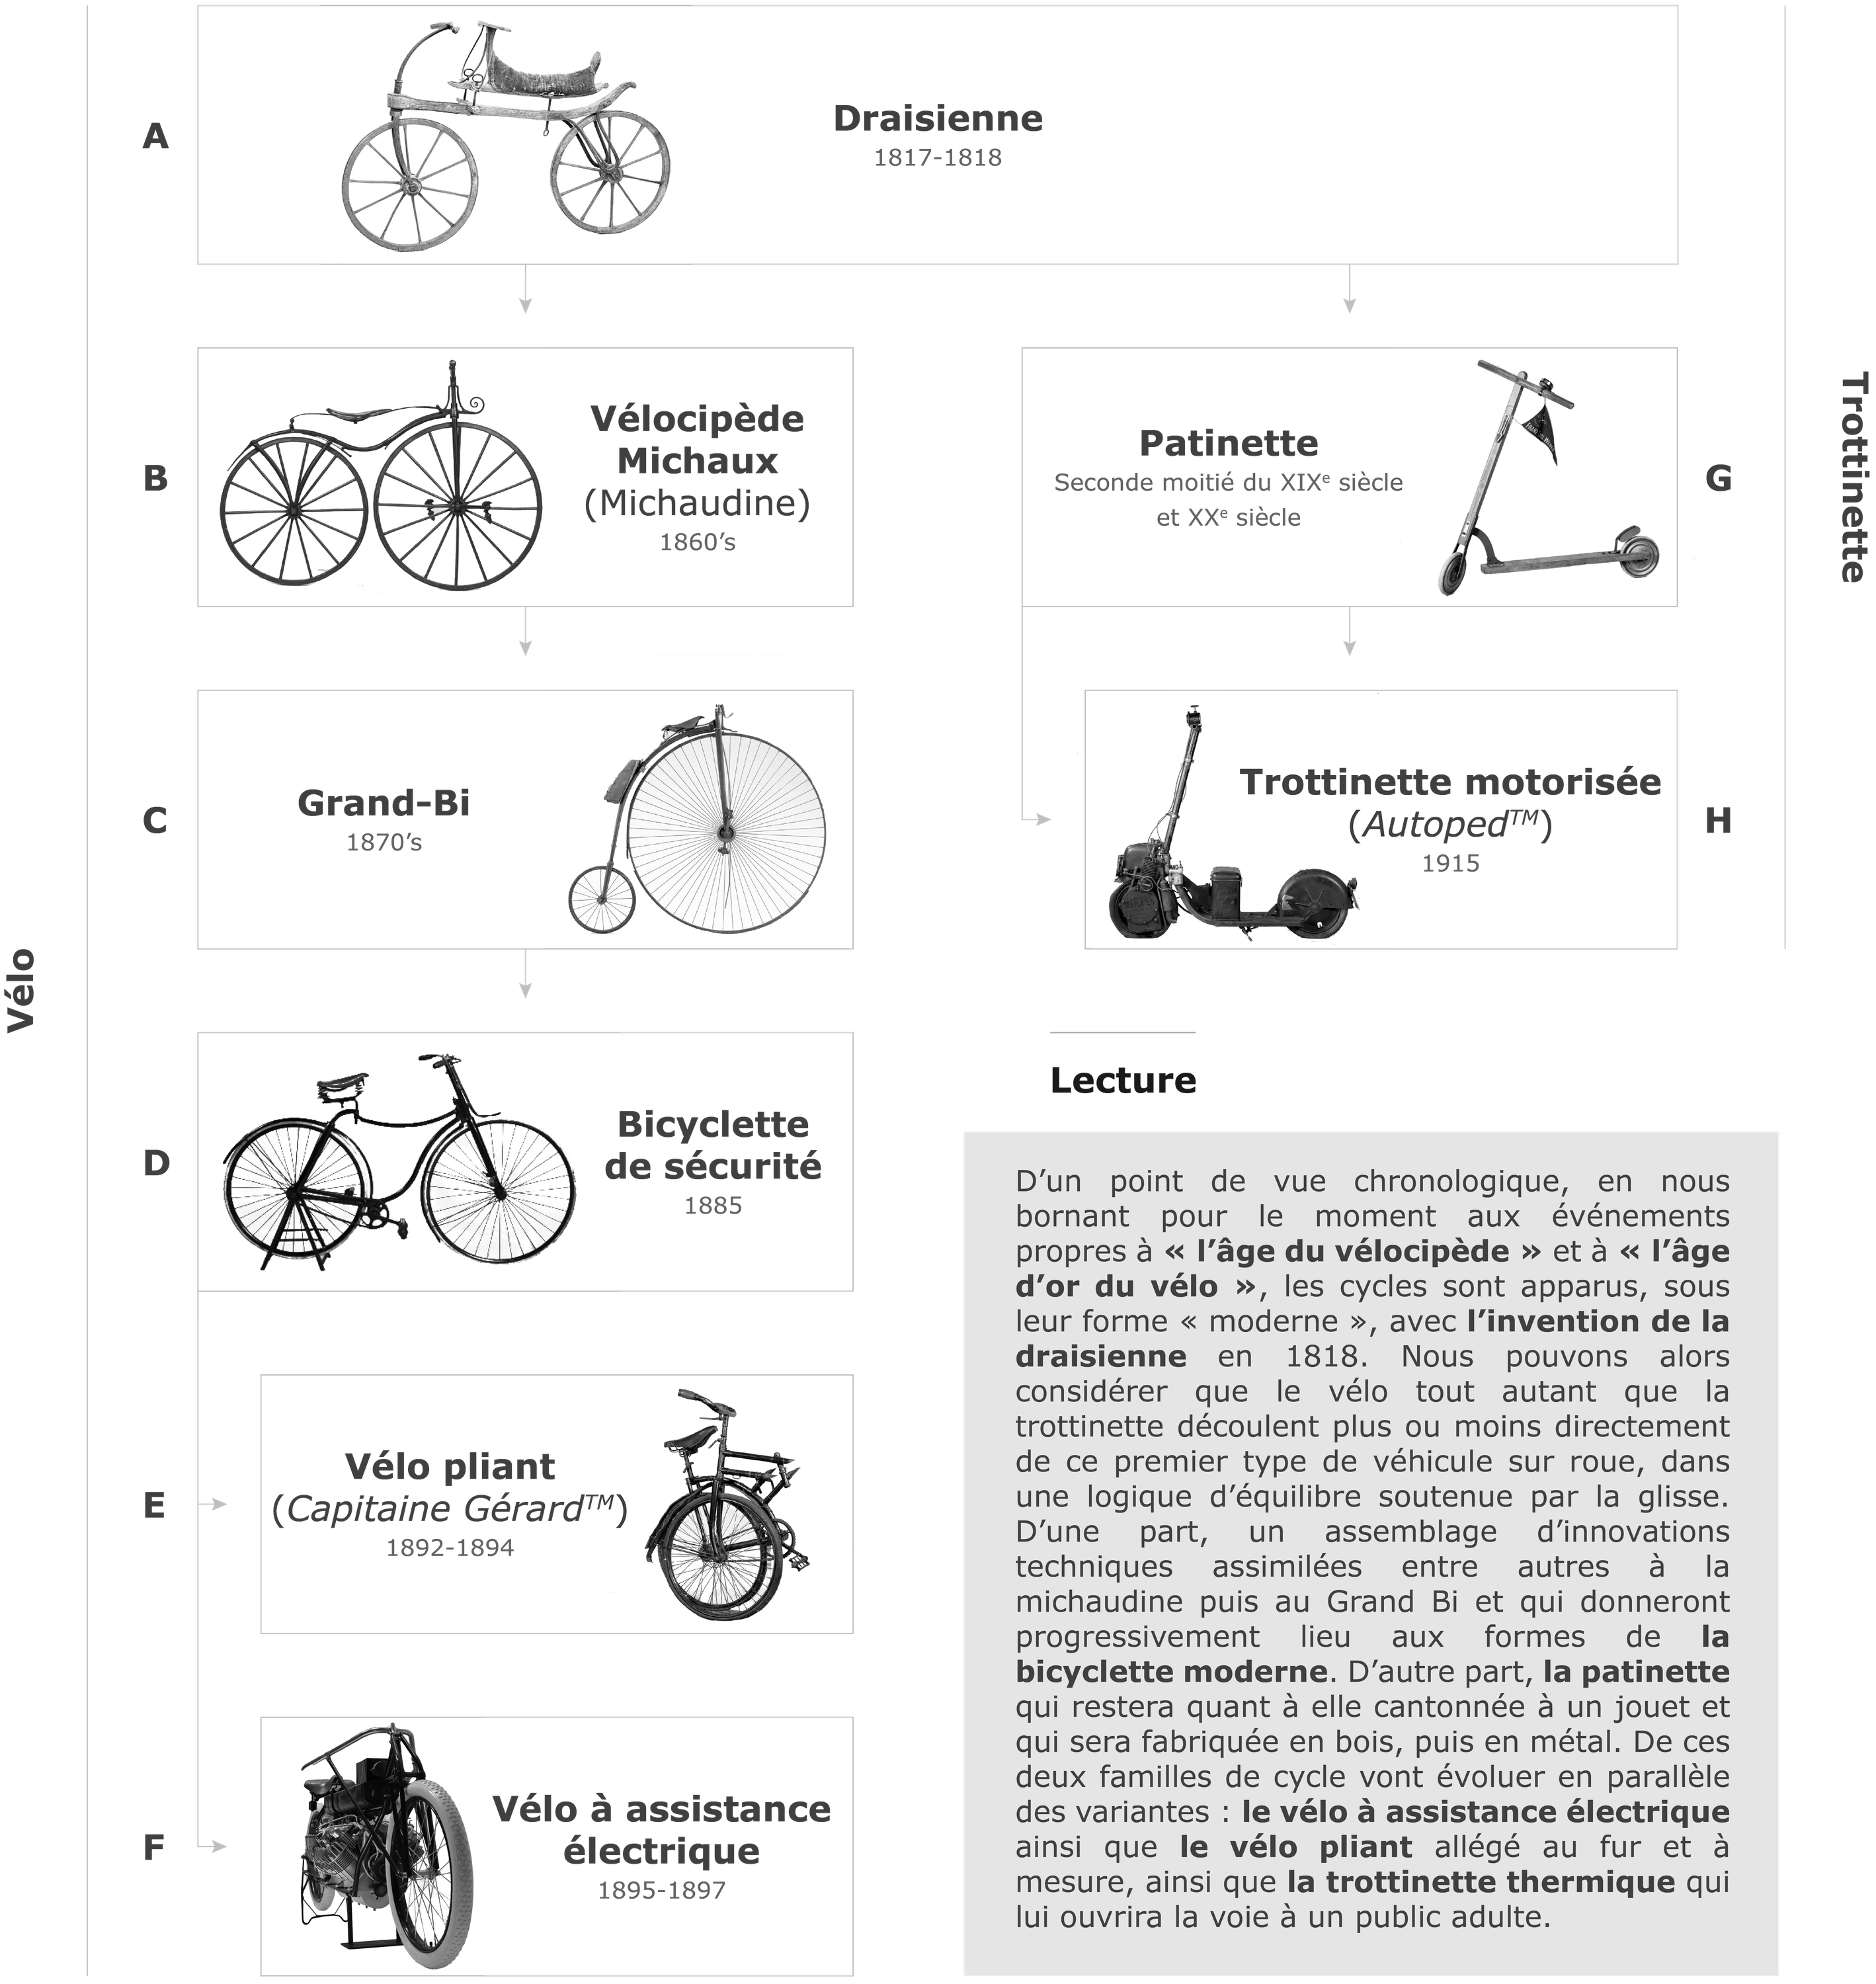
\includegraphics[width=1\columnwidth]{src/Figures/Chap-1/FR_Chronologie_velo_trottinette.pdf}}
        \vspace{5pt}
        \begin{flushright}\scriptsize{
        Photographie (A)~: \textcolor{blue}{\textcite{smithsonian_draisine_2006}}\index{Smithsonian@\textsl{Smithsonian}|pagebf}
        \\
        Photographie (B)~: \textcolor{blue}{\textcite{conservatoire_national_des_arts_et_metiers_velocipemichaux_2013}}\index{Conservatoire national des arts et métiers@\textsl{Conservatoire national des arts et métiers}|pagebf}
        \\
        Photographie (C)~: \textcolor{blue}{\textcite{chateau_de_compiegne_grand-bi_nodate}}\index{Château de Compiègne@\textsl{Château de Compiègne}|pagebf}
        \\
        Photographie (D)~: \textcolor{blue}{Kristy von} \textcolor{blue}{\textcite{moos_parcours_2019}}\index{Moos, Kristy von|pagebf}
        \\
        Photographie (E)~: \textcolor{blue}{\textcite{alienor_bicyclette_2015}}\index{Alienor@\textsl{Alienor}|pagebf}
        \\
        Photographie (F)~: \textcolor{blue}{Dylan Moinse (2023)}
        \\
        Photographie (G)~: \textcolor{blue}{\textcite{musee_national_suisse_draisienne_2018}}\index{Musée national suisse@\textsl{Musée national suisse}|pagebf}
        \\
        Photographie (H)~: \textcolor{blue}{\textcite{zerorider_lautoped_2023}}\index{Zerorider@\textsl{Zerorider}|pagebf}
        \\
        Auteur~: \textcolor{blue}{Dylan Moinse (2025)}
      }\end{flushright}
    \end{figure}

    % VAE
Qu’en est-il du \acrfull{VAE}~? Ses prémices remontent à seulement quinze ans après l’invention de la chaîne de vélo. Le premier prototype est attribué à \textcolor{blue}{Odgen Bolton Jr.}, qui, aux États-Unis, brevète en 1895 une draisienne équipée d’un moteur à courant continu à six pôles, intégré à la roue arrière et alimenté par une batterie de dix volts, quant à elle placée sous le tube horizontal du cadre \textcolor{blue}{\autocites[3]{hung_review_2020}{adelski_qui_2023}}\index{Hung, Nguyen Ba|pagebf}\index{Lim, Ocktaeck|pagebf}\index{Adelski, Adeline|pagebf}. La seconde génération de \acrshort{VAE} voit le jour en 1897 avec l’invention de \textcolor{blue}{Hosea W. Libbey}, qui conçoit le \Marque{Lampociclo}, un vélo équipé d’un double moteur électrique logé dans l’axe du pédalier. Le fonctionnement de cette innovation repose sur un générateur actionné par les pédales via une poulie et une courroie flexible. L’énergie produite alimente ensuite un petit moteur électrique \textcolor{blue}{\autocite[3]{hung_review_2020}}\index{Hung, Nguyen Ba|pagebf}\index{Lim, Ocktaeck|pagebf}. Toutefois, plusieurs tentatives d’amélioration échouent, notamment celle de la \Marque{Compagnie Parisienne}, qui développe un modèle de \acrshort{VAE} à la même époque, mais se heurte à des contraintes liées à un poids jugé excessif \textcolor{blue}{\autocite[78]{hadland_bicycle_2016}}\index{Hadland, Tony|pagebf}\index{Lessing, Hans-Erhard|pagebf}. À la fin de la Première Guerre mondiale, la société allemande \Marque{Heinzmann} inaugure la première production en série de moteurs électriques pour vélos, en équipant notamment les postier·ère·s du pays. Entre 1935 et 1937, le premier modèle de série, le \Marque{EMI/Philips}, est commercialisé, mais sa performance reste limitée face à la concurrence de l’automobile \textcolor{blue}{\autocite[143]{smethurst_bicycle_2015}}\index{Smethurst, Paul|pagebf}.%%Rédigé%%

    % Popularisation de la trottinette motorisée
Dans le registre de la fascination pour les objets innovants, le cas de la naissance de la trottinette à moteur à explosion, en 1915, mérite une attention particulière. C’est la société new-yorkaise \Marque{Autoped Company} qui lance le premier modèle de trottinette équipée d’un moteur à essence (voir l'\hyperref[fig-chap1:frise-chronologique-velo-trottinette]{illustration~\ref{fig-chap1:frise-chronologique-velo-trottinette}}, page~\pageref{fig-chap1:frise-chronologique-velo-trottinette}). Ce véhicule rencontre un succès immédiat, suscitant l’intérêt des adultes curieux·se·s de découvrir ce véhicule produit dans un premier temps aux États-Unis, puis en Europe par le constructeur allemand \Marque{Krupp} à partir de 1919. Les publicités sur la diffusion de son usage dans divers corps de métiers apparaît rapidement\footnote{
    Des photographies montrent ainsi des postiers du \textit{US Postal Office} ou des policiers étasuniens intégrant cet objet technique dans leurs missions quotidiennes à l’issue de la Grande Guerre \textcolor{blue}{\autocite{ma_trott_origines_2019}}.
}. Le \textsl{Online Bike Museum} qualifie le modèle \Marque{Autoped} de \Guillemets{véritable ancêtre de la trottinette électrique}, tant il préfigure la forme moderne de ce véhicule. Pourtant, à son lancement, la presse cycliste rejette cette innovation technique, qualifiant les \Marque{Autoped} de \Guillemets{véhicules monstres} voués à l’échec. Malgré ces critiques, les trottinettes motorisées, par un effet de mode, parviennent à s’imposer jusqu’à la fin des Années folles \textcolor{blue}{\autocite{smithsonian_magazine_motorized_2019}}\index{Smithsonian Magazine@\textsl{Smithsonian Magazine}|pagebf}. Les publicités de l’époque vantent les nombreux usages possibles de ce mode de déplacement. Elles présentent l’\Marque{Autoped} comme une solution idéale pour les courts déplacements, tant pour les hommes et les femmes allant au travail que pour les enfants souhaitant se rendre rapidement à l’école. Le slogan \Guillemets{\textit{L'Autoped est un mode de transport idéal pour les courtes distances, pour les hommes ou pour les femmes qui se rendent jusqu'à leurs lieux de travail, pour les femmes qui font les boutiques} [\dots] \textsl{pour les enfants plus âgés qui souhaitent se rendre rapidement à l'école} [\dots] \textsl{et pour tous ceux qui souhaitent économiser de l'argent, du temps et de l'énergie.}}\footnote{
    \Guillemets{\textit{The Autoped is an ideal short distance conveyance for business or professional men or women to and from their places of business; for women to go shopping} [\dots] \textsl{for the older children to go about quickly for outing or school} [\dots] \textsl{and for anybody else who wants to save money, time and energy in going about.}} \textcolor{blue}{\autocite{smithsonian_magazine_motorized_2019}}.
} reflète l’ambition de promouvoir la trottinette motorisée comme un véhicule pratique et accessible \textcolor{blue}{\autocite{smithsonian_magazine_motorized_2019}}\index{Smithsonian Magazine@\textsl{Smithsonian Magazine}|pagebf}. La stratégie \textsl{marketing} de l’\Marque{Autoped} cherche alors à séduire un public féminin\footnote{
    La peinture de l'artiste \textcolor{blue}{Everett Shinn} représentant une femme à bord d'une trottinette \Marque{Autoped} en page de couverture de \textit{Puck magazine} en 1916 ou les photographies de vedettes comme celle de l'actrice \textcolor{blue}{Lilian Lorraine} possédant l'un de ces véhicules témoignent de l'intérêt populaire suscité autour de la trottinette à propulsion thermique \textcolor{blue}{\autocite{hemmings_look_2011}}. La communication émise autour de ce produit révèle la volonté de la rendre particulière à une classe sociale distincte. L’usagère est généralement dépeinte sous les traits d’une femme blanche, d’apparence aisée et vêtue dans le style de l’époque.
} en intégrant le véhicule dans des catalogues destinés aux femmes et en pénétrant dans le monde de la mode. Certains messages publicitaires de la marque font également circuler l'image de la liberté de circuler de la femme, acquise grâce à l'engin \textcolor{blue}{\autocite{smithsonian_magazine_motorized_2019}}\index{Smithsonian Magazine@\textsl{Smithsonian Magazine}|pagebf}. La commercialisation de ce produit, originaire des États-Unis, s'étend vers l’Europe, à l’opposé de la trajectoire qu’a prise la diffusion historique du vélo, telle que nous l'avons vu. Toutefois, son histoire s’achève brusquement à la fin des années 1920. L’arrivée de nouvelles versions à piles n’a pas suffi à garantir la rentabilité de l’engin, en raison de la concurrence croissante du vélo et du cyclomoteur, qui offraient un confort supérieur et un usage plus adapté aux besoins de l’époque.%%Rédigé%%

    % 1.2.1.2.
    \needspace{1\baselineskip} % Réserve de l'espace
\subsubsection*{De la retraite du vélo utilitaire à sa recrudescence dans les pratiques de déplacement quotidien
    \label{chap1:proximite-velo-trottinette-declin-renaissance}
    }

    % Introduction
Avec l’amélioration des modes de vie, l’accès facilité à l’automobile à partir des années 1950, et une image dépréciée du vélo, les pays développés ont connu un \Guillemets{effondrement général} de la pratique cycliste durant la seconde moitié du XX\textsuperscript{e} siècle \textcolor{blue}{\autocites[59-84]{heran_retour_2015}[9-10]{heran_retour_2024}}\index{Héran, Frédéric|pagebf}. Après la Seconde Guerre mondiale, le vélo est perçu comme un symbole de pauvreté, associé à la mobilité des ouvrier·ère·s, mais aussi comme un rappel des privations et des conflits, laissant dans l’imaginaire collectif une image datée et peu valorisante. Cette \gls{perception} négative contraste fortement avec la vitesse et la modernité incarnées par l’automobile, assimilée à un vecteur d’ascension sociale \textcolor{blue}{\autocite[59]{bertho-lavenir_scarcity_2015}}\index{Bertho-lavenir, Catherine|pagebf}. Durant les Trente Glorieuses, la voiture s’impose comme un emblème de modernité et d’innovation, véhiculant des idéaux de progrès \textcolor{blue}{\autocite[35]{flonneau_georges_1999}}\index{Flonneau, Mathieu|pagebf}. Les politiques d’aménagement du territoire accompagnent cet essor en favorisant la construction d’infrastructures routières adaptées à la croissance projetée, voire exagérée, du trafic automobile \textcolor{blue}{\autocite[58]{wiel_transition_1999}}\index{Wiel, Marc|pagebf}. La diffusion massive de l’automobile transforme en profondeur les villes et leur organisation spatiale. Les territoires fréquentés se dilatent, augmentant les distances spatio-temporelles nécessaires pour réaliser les activités quotidiennes, grâce à une \Guillemets{mobilité facilitée} permettant à la population motorisée de s’installer en périphérie, notamment dans de l'habitat individuel de type pavillonnaire \textcolor{blue}{\autocite[58]{wiel_transition_1999}}\index{Wiel, Marc|pagebf}. Ce phénomène de desserrement des lieux de vie et d’activité est indissociable du développement automobile \textcolor{blue}{\autocites[8]{newman_land_1996}[3]{aragau_periurbain_2018}}\index{Aragau, Claire|pagebf}, qui entraîne une \Guillemets{abondance foncière} \textcolor{blue}{\autocite[20]{wiel_transition_1999}}\index{Wiel, Marc|pagebf}. Ce contexte donne lieu à la formation de \Guillemets{villes lisières} (\textsl{edge cities}), ces pôles secondaires \Guillemets{suburbains}, connectés aux échangeurs autoroutiers, qui rassemblent des activités économiques et commerciales et qui concurrencent le noyau urbain principal \textcolor{blue}{\autocite[]{garreau_edge_1991}}\index{Garreau, Joel|pagebf}.%%Rédigé%%

    % Déclin vélo
Bien que les périodes décrites ne reflètent pas des évolutions parfaitement linéaires et impliquent des mécanismes sous-jacents complexes, une lecture nuancée de l’opposition entre ville fonctionnelle et ville moderne ne peut occulter le déclin progressif de l’usage utilitaire du vélo à partir des Trente Glorieuses. En France, face à un parc automobile ayant doublé au cours des années 1960 et atteignant un taux de motorisation des ménages de 60~\% \textcolor{blue}{\autocite[43]{flonneau_georges_1999}}\index{Flonneau, Mathieu|pagebf}, l’usage du vélo comme mode de déplacement utilitaire chute significativement dans les années 1970, atteignant un niveau historiquement bas dans une majorité de villes européennes \textcolor{blue}{\autocite[41]{eskenazi_voir_2022}}\index{Eskenazi, Manon|pagebf}. Dans ses recherches doctorales consacrées à l’intermodalité entre le vélo et le transport public, \textcolor{blue}{Annie-Claude} \textcolor{blue}{\textcite[53]{sebban_complementarite_2003}}\index{Sebban, Annie-Claude|pagebf}\index{Motte, Alain|pagebf} remet en question l’idée selon laquelle les décennies 1980 et 1990 auraient marqué un abandon généralisé de la pratique cycliste en France. En réalité, ce déclin ne concerne que l’usage utilitaire du vélo, largement supplanté par la voiture en ville. Ce phénomène s’explique aussi par les méthodes statistiques des enquêtes publiques, qui n’intégraient pas systématiquement le vélo comme mode de déplacement à part entière. Parallèlement, de nouvelles dynamiques cyclables émergent, notamment avec l’essor du \acrfull{VTT}, qui devient un vecteur majeur du renouveau du vélo en France. En 1990, les \acrshort{VTT} représentent 35~\% des vélos possédés et 71~\% des ventes \textcolor{blue}{\autocite[195]{dauncey_french_2012}}\index{Dauncey, Hugh|pagebf}. Dans le même temps, le cyclotourisme et le vélo sportif restent stables, ne connaissant aucune réelle diminution \textcolor{blue}{\autocite[53]{sebban_complementarite_2003}}\index{Sebban, Annie-Claude|pagebf}\index{Motte, Alain|pagebf}. Le vélo, en France, devient ainsi un objet essentiellement associé au loisir. La course cycliste, notamment, atteint son apogée dans les années 1980, portée par la popularité du \textsl{Tour de France} et sa diffusion croissante dans les médias \textcolor{blue}{\autocite[196]{dauncey_french_2012}}\index{Dauncey, Hugh|pagebf}.%%Rédigé%%

    % Déclin trottinette
Concernant la trottinette, qu’elle soit à propulsion humaine ou mécanique, certaines compagnies étasuniennes tentent, à l’issue de la Seconde Guerre mondiale, de relancer l’usage de la trottinette motorisée. Cependant, avec l’essor de l’automobile, cet engin est rapidement accusé de favoriser des comportements dangereux sur la route \textcolor{blue}{\autocite{smithsonian_magazine_motorized_2019}}\index{Smithsonian Magazine@\textsl{Smithsonian Magazine}|pagebf}. Si le développement de la trottinette à essence ou à batterie reste limité à des épisodes anecdotiques~–~quelques récits sur l’utilisation des \Marque{Autoped} par les parachutistes étasunien·ne·s et britanniques pour traverser les champs de bataille pendant la guerre \textcolor{blue}{\autocite{historia_trottinette_2013}}\index{Historia@\textsl{Historia}|pagebf}, tout comme l’emploi de trottinettes musculaires par les employé·e·s de l’aéroport d’Amsterdam-Schiphol en sont des exemples \textcolor{blue}{\autocite{historia_trottinette_2013}}\index{Historia@\textsl{Historia}|pagebf}~–, ce modèle motorisé ne parvient pas à s’imposer durablement. Dans les années 1950, alors que la trottinette propulsée tombe en désuétude, des efforts sont entrepris pour relancer la trottinette non motorisée. Les fabricants tentent de la positionner comme un moyen de locomotion crédible, et non plus seulement comme un jouet pour enfants. À cette fin, certaines innovations apparaissent, comme l’ajout d’une pédale à l’avant de la plate-forme, permettant d’actionner la roue arrière pour réduire l’effort physique \textcolor{blue}{\autocite{arte_histoire_2014}}\index{Arte@\textsl{Arte}|pagebf}. Malgré ces avancées, le véhicule peine à séduire un large public et reste majoritairement perçu comme un objet ludique ou destiné aux enfants \textcolor{blue}{\autocite{jeux_et_compagnie_histoire_2013}}\index{Jeux et Compagnie@\textsl{Jeux et Compagnie}|pagebf}. La faible demande qui s'inscrit dans l'avènement d'un système du \Guillemets{tout-automobile} empêche ces modèles de trouver leur place dans la mobilité urbaine et dans les territoires \textcolor{blue}{\autocite{historia_trottinette_2013}}\index{Historia@\textsl{Historia}|pagebf}. L'impératif d'adaptation des territoires à la généralisation de l'automobile relègue la trottinette à un usage anecdotique. Leur utilisation en ville devient peu sécurisante, aussi bien sur les chaussées que sur les espaces piétonniers, limitant leur diffusion et réduisant les informations disponibles à leur sujet \textcolor{blue}{\autocite{e-trottr_levolution_2019}}\index{E-trottr@\textsl{E-trottr}|pagebf}. Malgré ces écueils, les véhicules composant la famille des cycles vont connaître un épisode de résurgence récente par leur réintégration dans les pratiques de mobilité urbaine.%%Rédigé%%

    % Figure évolution part modale vélo
    \begin{figure}[h!]\vspace*{4pt}
        \caption{Évolution de la part modale du vélo dans les agglomérations françaises, entre les années 1970 et 2020.}
        \label{fig-chap1:evolution-part-modale-velo}
        \centerline{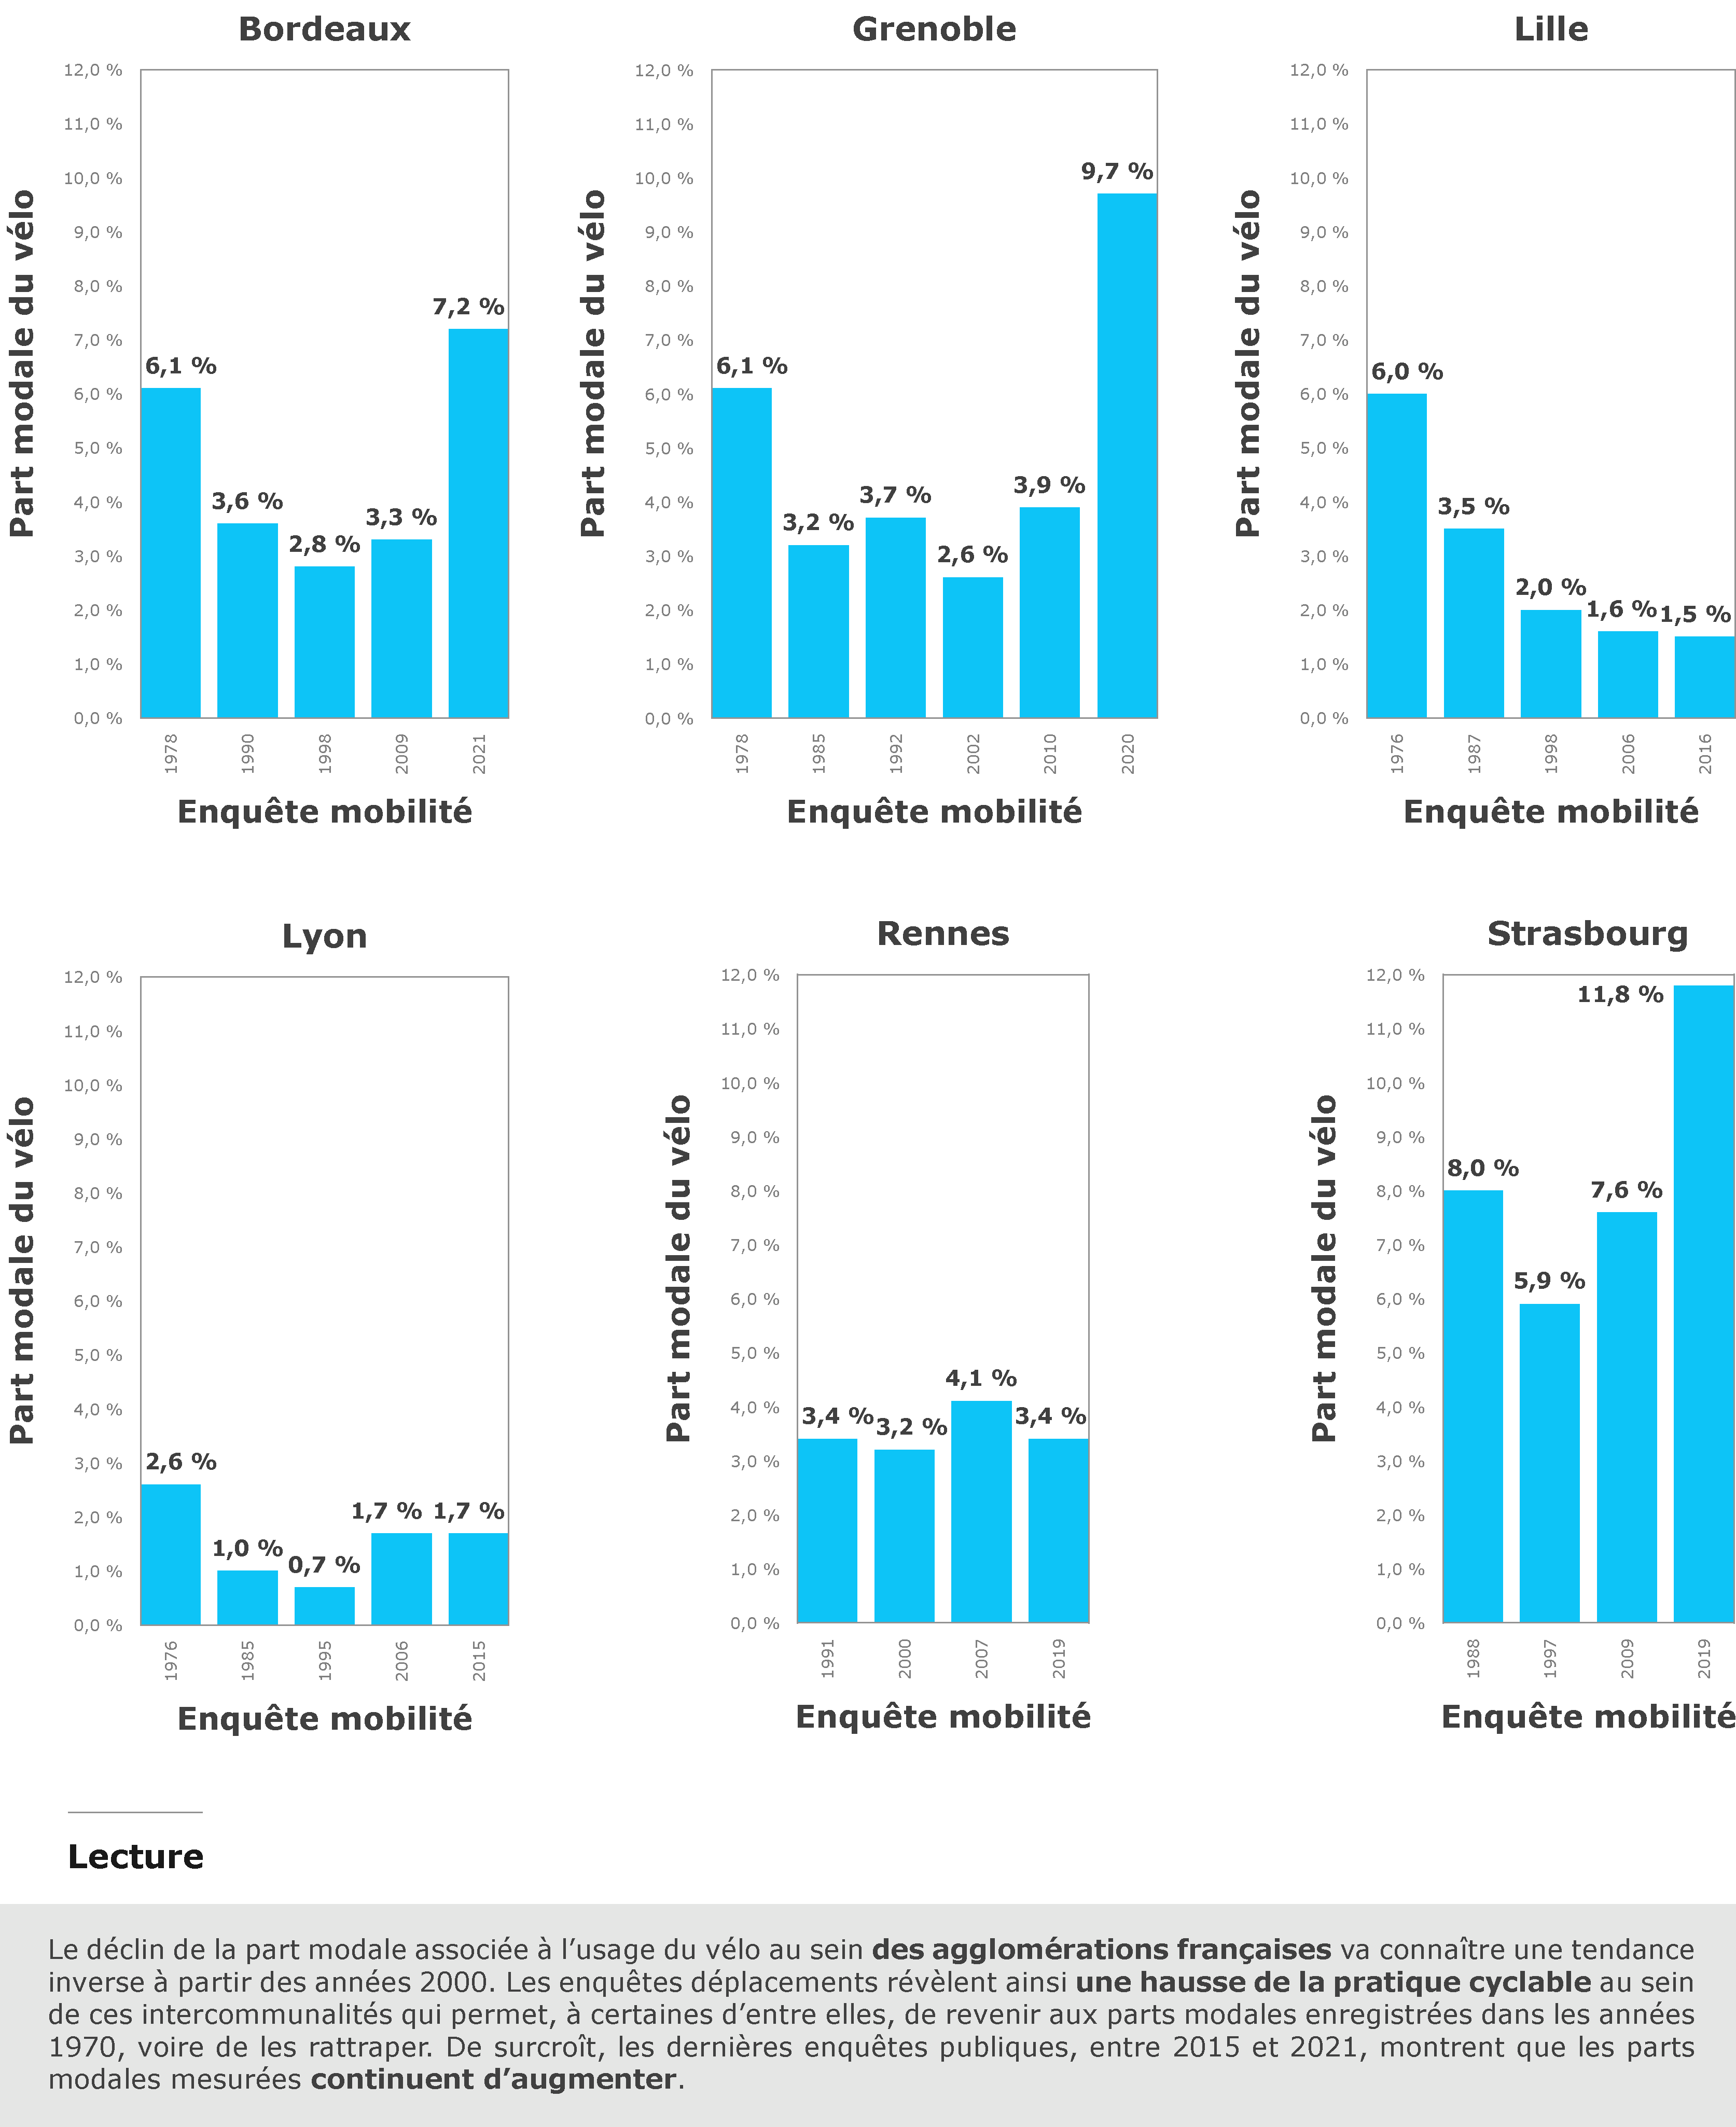
\includegraphics[width=1\columnwidth]{src/Figures/Chap-1/FR_Part_modale_velo_evolution.pdf}}
        \vspace{5pt}
        \begin{flushleft}\scriptsize{
        Note~: les territoires renvoient à leur échelle intercommunale, tandis que les enquêtes mobilité se rapportent au corpus d'\acrfull{EMD} au standard \textsl{Certu} ou certifiée \textsl{Cerema}.
        }\end{flushleft}
        \begin{flushright}\scriptsize{
        Jeux de données~: analyse issue du \textcolor{blue}{\textcite[48]{certu_usagers_2013}}\index{Certu@\textsl{Certu}|pagebf}\index{Cerema@\textsl{Cerema}|pagebf}\index{Jolly, Thomas|pagebf}
        \\
        Adaptation graphique et actualisation~: \textcolor{blue}{Dylan Moinse (2025)}
        }\end{flushright}
    \end{figure}
    
    % Retour en grâce vélo et trottinette
Le \Guillemets{retour en grâce} du vélo dans les territoires français \textcolor{blue}{\autocites[137-168]{heran_retour_2015}[44]{eskenazi_voir_2022}}\index{Héran, Frédéric|pagebf}\index{Eskenazi, Manon|pagebf} s’inscrit dans une dynamique amorcée il y a plus de quarante ans. Ce renouveau marque une seconde période de conquête pour le vélo, longtemps disqualifié dans les mobilités quotidiennes \textcolor{blue}{\autocite[26]{papon_retour_2012}}\index{Papon, Francis|pagebf}, alors que l’usage utilitaire du vélo continue de décliner dans les métropoles françaises, avec une diminution de 50~\% à 75~\% entre 1975 et 1990 \textcolor{blue}{\autocite[48]{certu_usagers_2013}}\index{Certu@\textsl{Certu}|pagebf}\index{Cerema@\textsl{Cerema}|pagebf}\index{Jolly, Thomas|pagebf}. Déjà en 1976, le journal \textsl{Le Monde} pointait une contradiction dans le fait de \Guillemets{moquer} les cyclistes \Guillemets{oublié·e·s}, alors que le parc de vélos, estimé à 17 millions, rivalisait avec le nombre de voitures particulières en possession \textcolor{blue}{\autocite{ambroise-rendu_creation_1976}}\index{Ambroise-Rendu, Marc|pagebf}\index{Le Monde@\textsl{Le Monde}|pagebf}. Les enquêtes de déplacements réalisées à partir des années 2000 mettent l'accent sur une résurgence du vélo parmi les pratiques de mobilité quotidienne (voir l'\hyperref[fig-chap1:evolution-part-modale-velo]{illustration~\ref{fig-chap1:evolution-part-modale-velo}}, page~\pageref{fig-chap1:evolution-part-modale-velo}). L’agglomération lyonnaise voit ainsi la part modale du vélo quadrupler entre 1995 et 2006, tandis que celle de \acrfull{MEL} compense son déclin entre 1998 et 2006 \textcolor{blue}{\autocite[243]{dauncey_french_2012}}\index{Dauncey, Hugh|pagebf}. Ce phénomène s’explique par la montée des préoccupations environnementales, conjuguée aux répercussions des crises économiques et énergétiques successives \textcolor{blue}{\autocite[138]{heran_retour_2015}}\index{Héran, Frédéric|pagebf}, ainsi qu’à la densification des tissus associatifs et à l’évolution des cadres légaux et réglementaires \textcolor{blue}{\autocite[55]{sebban_complementarite_2003}}\index{Sebban, Annie-Claude|pagebf}\index{Motte, Alain|pagebf}. Cette période voit également l’apparition de nouveaux modèles de cycle, tels que le vélo de ville, conçu pour un usage urbain, ou le vélo pliant en aluminium \Marque{Brompton} \textcolor{blue}{\autocite[55]{sebban_complementarite_2003}}\index{Sebban, Annie-Claude|pagebf}\index{Motte, Alain|pagebf}. Mais c'est surtout la grève des transports publics de 1995, très suivie, qui représente un moment décisif dans ce tournant et qui va permettre au vélo de se repositionner comme une alternative crédible. La résurgence du vélo s’accompagne d’une mutation sociologique et spatiale~: alors que le vélo des années 1970 était majoritairement utilisé par des populations captives en périphérie urbaine, les années 1990 voient émerger des usager·ère·s issu·e·s des classes moyennes et supérieures, se déplaçant en milieu urbain\footnote{
    D'après \textcolor{blue}{Frédéric} \textcolor{blue}{\textcite[143]{heran_retour_2015}}\index{Héran, Frédéric|pagebf}, \Guillemets{\textsl{en 1982, le cycliste type était un homme plutôt jeune, sans permis de conduire, issu d'une famille nombreuse, ouvirère ou agricole, souvent immigrée, à revenus modestes et peu ou pas motorisée, circulant en banlieue ou dans une ville de province. Il allait à vélo à l'école ou au travail, en rêvant d'acheter un vélomoteur et, un jour, une voiture. Selon les résultats de l'ENTD 2007-2008, ces usagers sont toujours majoritairement des hommes (à 63~\%), mais désormais surtout des cadres de la fonction publique et des professions libérales, beaucoup plus rarement des ouvriers ou des employés.}}. Par ailleurs, les cyclistes urbain·e·s ont remplacé les \Guillemets{prolétaires de la circulation} \textcolor{blue}{\autocite{ambroise-rendu_creation_1976}}\index{Ambroise-Rendu, Marc|pagebf}, devenant une spécificité française en raison d’investissements presque exclusivement concentrés sur les hypercentres \textcolor{blue}{\autocite[144]{heran_retour_2015}}\index{Héran, Frédéric|pagebf}.
} \textcolor{blue}{\autocite[143]{heran_retour_2015}}\index{Héran, Frédéric|pagebf}.%%Rédigé%%

    % Transition
Bien que la part modale du vélo reste modeste en France~–~à hauteur de 3~\% des déplacements, contre 10~\% en Allemagne et 27~\% aux Pays-Bas~–, cette période est marquée par un élan inédit en faveur du vélo utilitaire \textcolor{blue}{\autocite[222]{dauncey_french_2012}}\index{Dauncey, Hugh|pagebf}. Des initiatives locales comme le \textsl{Plan vélo} de Strasbourg, qui a transformé un réseau cyclable fragmenté en un maillage continu de 483 km en 2006, illustrent cette dynamique. Depuis les années 2010, le vélo est intimement lié aux enjeux environnementaux et sanitaires. Face à la pollution urbaine et à la congestion automobile, il est perçu comme une solution à faible impact écologique, bénéfique pour la santé publique et économique. Les efforts en faveur de son développement traduisent une volonté de promouvoir une véritable \Guillemets{écomobilité} \textcolor{blue}{\autocites[4]{sebban_complementarite_2003}{heran_transition_2018}}\index{Sebban, Annie-Claude|pagebf}\index{Motte, Alain|pagebf}\index{Héran, Frédéric|pagebf}, marquant un retour des \Guillemets{modes oubliés} dans les pratiques de mobilité quotidienne \textcolor{blue}{\autocite[35]{papon_retour_2012}}\index{Papon, Francis|pagebf}. Il aurait également été possible d’évoquer l’histoire conjointe d’autres \Guillemets{objets de glisse urbaine}, tels que le \textsl{skateboard} ou le patin à roulettes\footnote{
    Cette perspective diffère quelque peu pour ces autres véhicules, qui demeurent principalement associés aux loisirs et n’ont pas vocation à répondre à des besoins de mobilité directive ou à partager l’espace de voirie de manière structurée.
}, mais l’objectif ici n’est pas de proposer une analyse exhaustive ni de retracer l’intégralité de l’histoire du cycle. L’intention est plutôt de connecter le développement des cycles aux héritages de l'urbanisme diffus, façonné par l’automobile. Les investissements entrepris pour remettre le vélo sur le devant de la scène se sont accompagnés d'initiatives locales, incluant la mise en place d'aménagements cyclables et l'installation de services de mobilité, tels que les systèmes de \acrshort{VLS} \textcolor{blue}{\autocite[244]{dauncey_french_2012}}\index{Dauncey, Hugh|pagebf}, ainsi que le déploiement de l'électromobilité.%%Rédigé%%

    % 1.2.2.
    \needspace{1\baselineskip} % Réserve de l'espace
\subsection{Élargissement de l’offre par la motorisation électrique et l’introduction de systèmes de véhicules mutualisés
    \label{chap1:velo-micromobilite-innovations}
    }

    % Introduction
Alors que la pratique du vélo connaît une multiplication par 32 entre 1894 et 1934 \textcolor{blue}{\autocite[139]{orselli_usages_2008}}\index{Orselli, Jean|pagebf}, non sans susciter d’importantes difficultés d’acceptation sociale, elle décline ensuite au profit de l’automobile, laquelle fait face à des problématiques similaires d’appropriation. Si une lecture néolibérale des dynamiques urbaines se manifeste clairement à travers l’émergence de services de mobilité en libre-service, d’abord avec station, puis sans station, ces dispositifs traduisent une orientation vers un urbanisme davantage tourné vers l’entrepreneuriat et une redéfinition des rôles traditionnels des pouvoirs publics \textcolor{blue}{\autocites[169]{delaunay_mobilites_2017}{frotey_maxime_2017}}\index{Frotey, Julia|pagebf}\index{Delaunay, Teddy|pagebf}\index{Lesteven, Gaële|pagebf}. Pour autant, le débat se cristallise bel et bien autour du partage de l'espace public. Ces controverses rappellent les luttes historiques pour le partage de la voirie, déjà observées lors de l’arrivée successive de la traction hippomobile, du tramway, puis de l’automobile. Chaque nouvelle technologie de mobilité, en transformant les usages et les rapports sociaux dans l’espace urbain, réactive des dynamiques conflictuelles liées à la cohabitation et à la répartition des ressources spatiales\footnote{
    Aussi, nous pouvons également évoquer les querelles suscitées par le développement du tramway durant son âge d’or, s’étendant de la fin du XIX\textsuperscript{e} siècle à l’entre-deux-guerres \textcolor{blue}{\autocite[281]{flonneau_concurrence_2007}}\index{Flonneau, Mathieu|pagebf}. Ces controverses ont refait surface lors de son retour progressif au cours des années 2000, accompagné de craintes tant populaires que politiques. En effet, le tramway était perçu comme un moyen de transport désuet, appartenant à une autre époque \textcolor{blue}{\autocite[110]{gardon__2014}}\index{Flonneau, Mathieu|pagebf}. Toutefois, ces représentations négatives se sont estompées au profit d’une image renouvelée et moderne, grâce à l’intégration d’innovations techniques telles que les planchers bas et ultra-bas ou encore les systèmes d’alimentation par le sol. Ce renouveau du tramway, loin d’être un processus consensuel, a néanmoins généré des tensions, notamment vis-à-vis de l’automobile, qu’il concurrence directement. Le rapport de force qui en découle a conduit à une reconfiguration des tracés des projets de tramway, souvent conçus pour minimiser les impacts sur la voirie et les espaces de stationnement automobile. Dans certains cas, cette réconciliation spatiale s’est traduite par l’aménagement de sections de tramway en souterrain, permettant ainsi de préserver les voies de circulation automobile \textcolor{blue}{\autocite[10]{richer_tramways_2012}}\index{Richer, Cyprien|pagebf}\index{Hasiak, Sophie|pagebf}. Par ailleurs, le tramway a également été accusé de concurrencer d’autres systèmes de transport public préexistants, notamment les réseaux ferroviaires régionaux \textcolor{blue}{\autocite[36]{cete_nord_picardie_evaluer_2013}}.
}. Toutefois, le \Guillemets{retour} du vélo en milieu urbain s’accompagne, ces dernières décennies, de l’apparition de nouvelles catégories de cycles. Cette diversification de l'offre en \Guillemets{altermobilités} \textcolor{blue}{\autocite[91-92]{vincent-geslin__2012}}\index{Vincent-Geslin, Stéphanie|pagebf}, est marquée par l’émergence de l’électromobilité, illustrée tout d’abord par le redéploiement du \acrshort{VAE}, suivi par le développement de la \acrshort{TEP}, ainsi que par de nouvelles modalités d’acquisition, telles que la mise à disposition de flottes partagées de vélos et de trottinettes. Ainsi, comme nous l’avons observé, ces véhicules jouissent de cycles d’innovations, qu’elles soient techniques, servicielles ou organisationnelles. En adoptant une perspective historique sur l’évolution de la place occupée par ces véhicules, il apparaît que, malgré une perception parfois jugée désuète ou limitée à un usage ludique pour enfants, un siècle d’innovations appliquées à ces objets a permis leur réintroduction sous des formes modernisées, dans un contexte opportun. En jouant sur un registre mêlant nostalgie et modernité, ces véhicules se sont progressivement affirmés comme des modes de déplacement fiables, tirant parti à la fois de l’électrification, qui étend leur facilité et leur portée d’usage, et des systèmes de partage, qui accroissent leur accessibilité et leur visibilité dans l’espace public. Ce phénomène peut être interprété à travers la notion de \Guillemets{rétro-innovation}, issue du champ du \textsl{marketing} et de la communication, définie comme la réinvention d’un produit ou d’un domaine d’activité grâce à des innovations technologiques, dans l’objectif de lui conférer un nouvel usage tout en établissant un lien avec le passé \textcolor{blue}{\autocite{barthelot_retro-innovation_2018}}\index{Barthelot, Bertrand|pagebf}. Parmi les trois catégories constitutives de la rétro-innovation, les cycles électrifiés et les dispositifs partagés s’inscrivent dans la tendance dite de l’\textsl{inn-old-vation}, laquelle repose sur l’intégration d’innovations technologiques visant à adapter un produit à des besoins préexistants \textcolor{blue}{\autocite{lamy_retro-innovation_2016}}\index{Lamy, Alexia|pagebf}. Cependant, comme nous le verrons, la difficulté majeure réside dans l’introduction de ces innovations, qu’elles soient techniques ou sociales, un défi qui accompagne le vélo depuis les prémices de son histoire moderne \textcolor{blue}{\autocite[33]{jouenne_quest-ce_2022}}\index{Jouenne, Noël|pagebf}.%%Rédigé%%

    % 1.2.2.1.
    \needspace{1\baselineskip} % Réserve de l'espace
\subsubsection*{Contribution de l'électromobilité à la diversification du vélo et de la micro-mobilité
    \label{chap1:velo-micromobilite-innovations-electromobilite}
    }

    % Introduction
Au développement du vélo et du vélo pliant se sont ajoutés de nouveaux modes de déplacement à propulsion électrique, élargissant la famille des cycles \textcolor{blue}{\autocite[5]{lopez-escolano_mobilites_2019}}\index{López-Escolano, Carlos|pagebf}\index{Campos, Ángel Pueyo|pagebf}. Parmi eux, le \acrfull{VAE}, qu’il soit pliant ou non, la \acrfull{TEP}, ainsi qu’une variété d’engins de déplacement regroupés sous l’appellation de \Guillemets{micro-mobilité} (voir l'\hyperref[fig-chap1:ecosysteme-micromobilite]{illustration~\ref{fig-chap1:ecosysteme-micromobilite}}, page~\pageref{fig-chap1:ecosysteme-micromobilite}), tels que le monoroue (ou gyroroue), l’\textsl{hoverboard} ou encore le gyropode (\textsl{segway}). La liste des \acrfull{NVEI} ne cesse de s’allonger, illustrant une diversification modale permise notamment par la réduction des coûts de fabrication, la miniaturisation des composants et les gains d’efficacité des batteries électriques, qui en facilitent la portabilité\footnote{
    Les années 1990 ont marqué un tournant décisif pour les \textsl{pedelecs}, lorsque plusieurs avancées techniques ont convergé pour en accroître la praticité et l’attractivité. L’introduction et la commercialisation de batteries plus légères et plus performantes, telles que la batterie \acrfull{NiCd} et, ultérieurement, la batterie \acrfull{NiMH}, ont joué un rôle stratégique dans leur évolution. Ces nouvelles batteries offrent un rapport énergie/poids nettement supérieur à celui de leurs prédécesseurs, rendant le vélo électrique à la fois plus léger, maniable et doté d’une meilleure autonomie. L’introduction de l'accumulateur \acrfull{Li-ion}, comparativement aux batteries antérieures, a marqué une étape supplémentaire. Ce type de batterie électrique, de taille équivalente, présente une capacité énergétique supérieure de 32~\% et un poids réduit de 25~\%. Par ailleurs, la batterie \acrshort{Li-ion} présente une décharge à courant élevé, l’absence d’effet mémoire et la possibilité de recharger la batterie à tout moment.
} \textcolor{blue}{\autocites[430]{bertoluzzo_development_2011}[2]{schultz_micromobility_2019}[430]{pages_nouveaux_2021}}\index{Schultz, Stéphane|pagebf}\index{Grisot, Sylvain|pagebf}\index{Bertoluzzo, Manuele|pagebf}\index{Buja, Giuseppe|pagebf}\index{Pages, Thibaud|pagebf}\index{Lammoglia, Adrien|pagebf}\index{Josselin, Didier|pagebf}.%%Rédigé%%

    % Figure écosystème du vélo et micro-mobilité
    \begin{figure}[h!]\vspace*{4pt}
        \caption{Écosystème de la \Guillemets{mobilité individuelle et locale}, à propulsion humaine, à assistance ou motorisée.}
        \label{fig-chap1:ecosysteme-micromobilite}
        \centerline{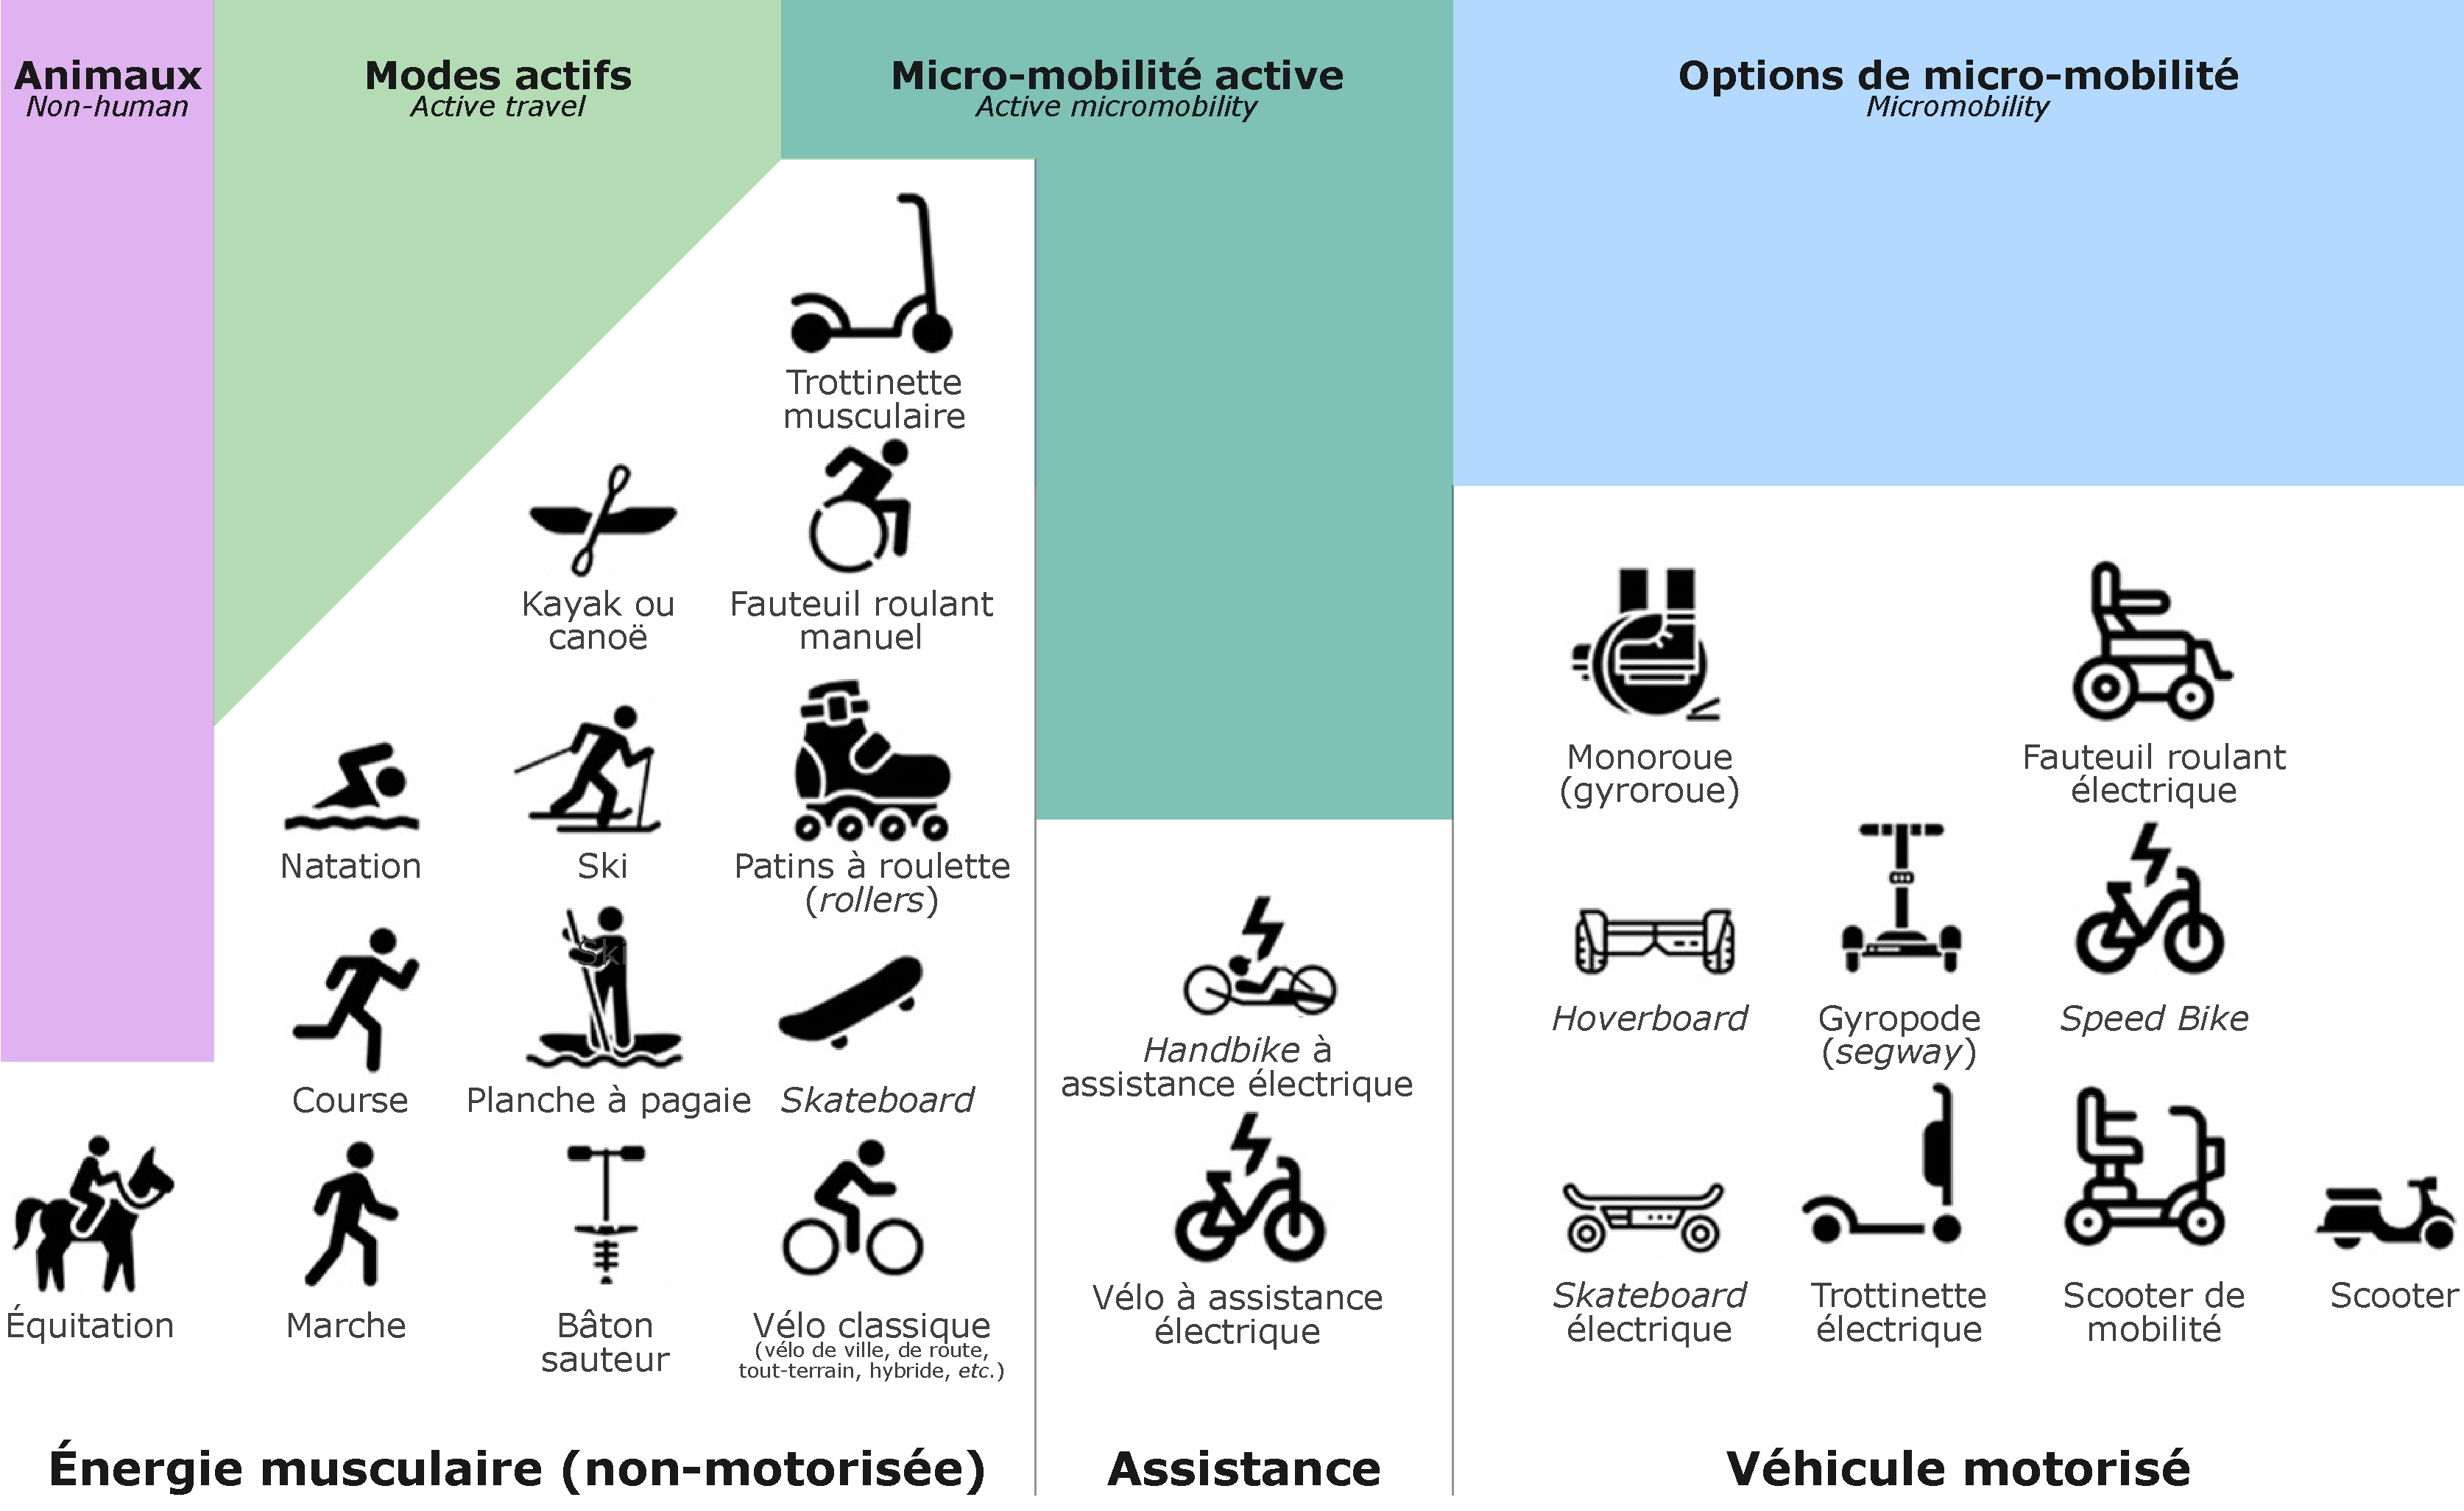
\includegraphics[width=1\columnwidth]{src/Figures/Chap-1/FR_Ecosysteme_micromobilite.pdf}}
        \vspace{5pt}
        \begin{flushright}\scriptsize{
        Source~: \textcolor{blue}{\textcite[155]{cook_more_2022}}\index{Cook, Simon|pagebf}\index{Stevenson, Lorna|pagebf}\index{Aldred, Rachel|pagebf}\index{Kendall, Matt|pagebf}\index{Cohen, Tom|pagebf}
        \\
        Adaptation graphique~: \textcolor{blue}{Dylan Moinse (2024)}
        }\end{flushright}
    \end{figure}

    % Histoire contemporaine VAE
En 1993, le fabricant japonais de moto \Marque{Yamaha Motor Company} a introduit le premier vélo électrique de série, à succès commercial, doté d’une fonction d’assistance au pédalage (\textsl{Power Assist System}) et alimenté par d'une batterie amovible \acrshort{NiMH} \textcolor{blue}{\autocite[430]{bertoluzzo_development_2011}}\index{Bertoluzzo, Manuele|pagebf}\index{Buja, Giuseppe|pagebf}. Ce vélo offre des avantages notables par rapport à la batterie traditionnelle au plomb, en proposant une batterie plus légère, moins sensible aux variations de température ambiante et avec un cycle de vie plus long. Le système d'assistance au pédalage a non seulement permis de prolonger la durée de vie de la batterie, mais aussi de rendre l'expérience de l'utilisateur·rice plus intuitive. En raison de ces qualités, \textcolor{blue}{Noël} \textcolor{blue}{\textcite[25]{jouenne_quest-ce_2022}}\index{Jouenne, Noël|pagebf} qualifie le \acrshort{VAE} de \Guillemets{vélo à assistance électro-mécanique} dans son \acrfull{HDR} portant sur l’ethnologie du vélo comme objet technique et social, pour insister sur le mix énergétique requis pour se déplacer. À partir de 2003, le vélo électrique profite du développement et de la commercialisation de la batterie \acrshort{Li-ion} \textcolor{blue}{\autocite[6]{hung_review_2020}}\index{Hung, Nguyen Ba|pagebf}\index{Lim, Ocktaeck|pagebf}. En France, les ventes de \acrshort{VAE} ont connu une croissance spectaculaire, passant de 37~000 unités vendues en 2011 à 338~000 en 2018, atteignant 738~000 en 2022, avant une légère baisse à 671~000 produits en 2023. Ces chiffres représentent 43~\% des ventes totales de véhicules électriques en 2023 \textcolor{blue}{\autocite{union_sport__cycle_chiffres_2024}}\index{Union Sport \& Cycle@\textsl{Union Sport \& Cycle}|pagebf}. Parallèlement au \acrshort{VAE}, des formes nouvelles du vélo comme le vélo-cargo et le triporteur ont élargi les possibilités d’utilisation du vélo électrique. Ces modèles facilitent, outre les déplacements sur de longues distances ou pour les personnes âgées ou à mobilité réduite, le transport de personnes et d’objets lourds. Ils ouvrent ainsi de nouvelles perspectives pour les déplacements familiaux ou sous forme de vélotaxis, le secteur de la logistique urbaine et l'autoentrepreneuriat. Selon \textcolor{blue}{\textcite[24]{mason_global_2015}}\index{Mason, Jacob|pagebf}\index{Fulton, Lew|pagebf}\index{McDonald, Zane|pagebf}, la part modale du vélo, stimulée par la popularité croissante du \acrshort{VAE}, pourrait atteindre 17~\% en 2030 et 22~\% en 2050 parmi les pays de l'\acrfull{OCDE}.%%Rédigé%%

    % Histoire contemporaine TEP + Transition
Concomitamment à l’essor du \acrshort{VAE}, la trottinette revient sur le devant de la scène, d’abord comme jouet, puis progressivement adoptée par les adolescent·e·s\footnote{
    La diffusion de la trottinette moderne est favorisée par une innovation technique majeure qui la rend plus légère, plus résistante et plus maniable grâce à l’emploi de l’aluminium, un matériau qui permet également de la rendre pliable \textcolor{blue}{\autocite{arte_histoire_2014}}. En 1996, l’homme d’affaires suisse \textcolor{blue}{Wim Ouboter} joue un rôle déterminant dans l’évolution de la trottinette. Il fonde sa propre entreprise, \Marque{Micro Mobility Systems}, et conçoit dès 1999 des \Guillemets{micro-trottinettes}, connues sous le nom de \textsl{micro-scooters}, en combinant l’esthétique de la trottinette avec des roues inspirées du \textit{skateboard} \textcolor{blue}{\autocite{les_numeriques_futur_2015}}\index{Les Numériques@\textsl{Les Numériques}|pagebf}. Rapidement, ce modèle, commercialisé sous la marque \Marque{Razor}, devient un phénomène mondial, atteignant un million d’unités vendues en 2000 avant que l’engouement ne s’atténue. Malgré ce déclin, la trottinette conserve son statut de jouet destiné principalement aux enfants. Aux États-Unis, elle \Guillemets{envahit les cul-de-sacs des zones résidentielles}, et la \textsl{Toy Association} désigne ce modèle comme \Guillemets{jouet de l’année} en 2000 \textcolor{blue}{\autocite{bloomberg_citylab_man_2018}}. Cependant, cet engouement s’essouffle rapidement \textcolor{blue}{\autocite[25]{university_of_st_gallen_micro_2011}}\index{University of St. Gallen@\textsl{University of St. Gallen}|pagebf}. Parallèlement, la trottinette évolue en se redéployant dans un cadre différent. Un changement d’usage et de clientèle s’opère~: la trottinette renforcée devient un support pour une nouvelle discipline sportive, le \textsl{freestyle}, inspirée du BMX (\textsl{bicycle motocross}) et du \textit{skateboard}. Ce sport, qui consiste à réaliser des figures acrobatiques (\textsl{tricks}), attire une nouvelle génération d’usager·ère·s, les \textsl{trottiriders} \textcolor{blue}{\autocite{micro-mobility_innovations_2018}}\index{Micro-mobility@\textsl{Micro-mobility}|pagebf}. Ainsi, la trottinette cesse progressivement d’être perçue comme un simple jouet pour devenir un équipement prisé par les adolescent·e·s et les jeunes adultes, séduit·e·s par les sports de glisse et par la culture urbaine \textcolor{blue}{\autocite{ma_trott_histoire_2020}}.
} avant de connaître une transformation grâce à un \textsl{design} modernisé et l’intégration d’une batterie électrique. L’homme considéré comme \Guillemets{le pionnier de la révolution de la trottinette}, \textcolor{blue}{Wim Ouboter}, amorce cette transformation à partir de son expérience personnelle\footnote{
    \textcolor{blue}{Wim Ouboter} relate que son intérêt pour la trottinette trouve ses racines dans son expérience personnelle. Lorsqu’il était enfant, lui et sa sœur utilisaient d’anciennes trottinettes, cette dernière étant dans l’incapacité de pratiquer le vélo ou le ski en raison d’un handicap physique. Cependant, c’est à l’âge de 30 ans que survient la véritable révélation. D'après le récit exposé, l'entrepreneur suisse aurait réalisé alors que son restaurant de saucisses préféré, situé à Zurich, se trouverait à une distance trop importante pour y aller à pied, mais pas assez éloigné pour justifier l’utilisation d’un vélo ou d’une voiture \textcolor{blue}{\autocite{ma_trott_histoire_2020}}.
} \textcolor{blue}{\autocite{ma_trott_histoire_2020}}\index{Ma Trott'@\textsl{Ma Trott'}|pagebf}. La trottinette est réhabilitée avec la création de la \Marque{Micro}, conçue pour les déplacements qualifiés de \Guillemets{micro-distance}, situés entre des trajets trop longs pour marcher et trop courts pour avoir recours à une voiture ou à un vélo \textcolor{blue}{\autocite{oconnell_travel_2002}}\index{O'Connel, Dee|pagebf}. Dans le prolongement de l’électrification de la mobilité urbaine en 2003, l’entrepreneur suisse élargit sa gamme en développant des modèles électriques, toujours en visant une clientèle adulte \textcolor{blue}{\autocite{ma_trott_histoire_2020}}\index{Ma Trott'@\textsl{Ma Trott'}|pagebf}. Mais c’est véritablement le lancement de la trottinette \Marque{Xiaomi Mi Electric Scooter} (M365) en 2016, d'abord en Chine, qui bouscule le marché. Commercialisée en Europe en 2018, la \acrshort{TEP} s’est imposée comme un succès mondial grâce à son coût abordable et à l'ergonomie qu'elle propose. Adoptée massivement pour un usage personnel, elle sert également de modèle de référence pour une multitude de flottes de trottinettes en libre-service. En France, la popularité de la \acrshort{TEP} ne se fait pas attendre~: selon le baromètre de la \acrfull{FP2M}, les ventes démarrent à 233~000 unités en 2018, s'élèvent à 478~800 unités l'année qui suit, pour atteindre 678~000 unités en 2023 \textcolor{blue}{\autocites[1]{fp2m_barometre_2021}[1]{fp2m_ventes_2023}}\index{FP2M@\textsl{FP2M}|pagebf}. Ces chiffres surpassent désormais les ventes de \acrshort{VAE}, pourtant également en expansion. L’exemple de la trottinette, qu’elle fonctionne à propulsion humaine ou électrique, et celui du \acrshort{VAE}, pliant ou classique, illustrent parfaitement la diversification des modes de déplacement en milieu urbain, en se déclinant sous des formes accessibles à l'achat et en location.%%Rédigé%%

    % 1.2.2.2.
    \needspace{1\baselineskip} % Réserve de l'espace
\subsubsection*{L'économie du partage au service de la mobilité partagée
    \label{chap1:velo-micromobilite-innovations-partage}
    }

    % Libre-service avec station - histoire 1
La genèse des \acrshort{VLS} s’inscrit dans l’histoire des mouvements sociaux à l’origine du retour du vélo en ville \textcolor{blue}{\autocite[23]{hure_mobilites_2019}}\index{Huré, Maxime|pagebf}. L’idée d’un \Guillemets{vélo intelligent} (\textsl{smart bike}) partagé dans l’espace public, accessible à tou·te·s sans nécessité d’acquisition personnelle, trouve ses premières applications en 1965 grâce à un collectif anarchiste néerlandais, \textsl{Provo}. Dans le cadre de leur cinquième \Guillemets{provocation} (\textsl{Witte Fietsenplan}) et à l'approche des élections municipales de 1966, ce mouvement contestataire et libertaire met alors à disposition des Amstellodamois·e·s une cinquantaine de vélos peints en blanc, déposés librement dans les rues, dans le but de libérer la ville de la congestion urbaine\footnote{
    Le groupe \textsl{Provo} prône une initiative municipale visant à mettre à disposition de la population 10~000 bicyclettes gratuites, autogérées par un système participatif. En signe de protestation contre le refus de leur projet par la municipalité, le collectif inscrit sur la liste électorale remet en circulation environ une centaine de vélos abandonnés, en les réparant et en les peignant en blanc \textcolor{blue}{\autocite[29]{hure_mobilites_2019}}\index{Huré, Maxime|pagebf}.
} \textcolor{blue}{\autocites[6]{smart_provo_2012}{demain_la_ville_doit-velib_2018}}\index{Smart, Alan|pagebf}\index{Demain La Ville@\textsl{Demain La Ville}|pagebf}. Bien que pionnier, ce moyen d'action reste illégal selon les autorités publiques, donnant néanmoins naissance à la première génération de \acrshort{VLS}, basée sur un système gratuit \textcolor{blue}{\autocite[160]{shaheen_bikesharing_2010}}\index{Shaheen, Susan~A.|pagebf}\index{Guzman, Stacey|pagebf}\index{Zhang, Hua|pagebf}. La Rochelle est souvent reconnue comme la première ville à avoir institutionnalisé un tel dispositif en 1976 avec ses \textsl{vélos municipaux}, également appelés \textsl{Vélos Jaunes}, une flotte de 350 vélos répartis sur trois points de location\footnote{
    L'expérience très visible du dispositif municipal rochelais pose la question des transformations de l'action publique urbaine en matière de mobilité, jusqu'alors fortement dépendantes des services étatiques en glissant d'un dirigisme étatique à un État régulateur qui reste le premier financeur de ce projet. Avec ses 300 \acrshort{VLS}, le maire de l'époque, \textcolor{blue}{Michel Crépeau}, souhaite \Guillemets{banaliser} l'usage du vélo en ville. Cette politique met en place un périmètre d'accès, limité à l'intérieur de l'enceinte de l'ancienne forteresse, et d'horaires, de 8 heures à 20 heures, la régulation du système étant dépendante de la participation citoyenne des habitant·e·s \textcolor{blue}{\autocite[31]{hure_mobilites_2019}}\index{Huré, Maxime|pagebf}. Un tel projet, inauguré six mois avant les élections municipales, permet au maire de façonner une notoriété internationale et de légitimer une nouvelle politique urbaine de réhabilitation du centre-ville, construisant déjà une première forme de marketing politique et territorial au travers de ces services de mobilité \textcolor{blue}{\autocite[31]{hure_mobilites_2019}}\index{Huré, Maxime|pagebf}. L’année suivante, un second parc de \acrshort{VLS} gratuits, composé de 100 unités, est mis en place grâce à un financement privé reposant sur un modèle de publicité. Cette initiative marque un tournant, puisque le recours à la publicité s’impose progressivement comme une modalité centrale de financement des systèmes \acrshort{VLS} \textcolor{blue}{\autocite[32-35]{fleury_mobilites_2022}}\index{Huré, Maxime|pagebf}\index{Fleury, Antoine|pagebf}\index{Frétigny, Jean-Baptiste|pagebf}\index{Kanellopoulou, Dimitra|pagebf}.
}. Ce modèle inspire d’autres initiatives, à l’instar de celle portée à Cambridge en 1993, et contribue à stabiliser l’architecture marchande de la mobilité partagée telle qu’elle est encore pratiquée aujourd’hui. Finalement, les mécanismes et les valeurs symboliques du \acrshort{VLS} s’inspirent largement de celui du chariot de supermarché, comme le souligne \textcolor{blue}{Maxime} \textcolor{blue}{Maxime} \textcolor{blue}{\textcite[40]{hure_mobilites_2019}}\index{Huré, Maxime|pagebf}. Copenhague marque une étape décisive entre 1989 et 1995 avec la mise en place de \textsl{Bycyklen}, un système exploitant le mécanisme de dépôt de monnaie (\textsl{coin-deposit}) et de supports à vélo. Ce système, considéré comme la deuxième génération de \acrshort{VLS}, est adopté en Europe et aux États-Unis, mais les problèmes de vol liés à l’anonymat des usager·ère·s persistent\footnote{
    Une alternative notable au modèle classique de \acrshort{VLS} est représentée par le service \textsl{Call a Bike}, déployé dans plusieurs villes allemandes, à commencer par Munich en 2000. Ce système repose sur un principe différent~: le vélo, verrouillé dans l’espace public à l’aide d’un cadenas, peut être emprunté et déposé librement. L’accès au vélo nécessite de contacter un service dédié, permettant d’obtenir le code du cadenas moyennant paiement. Ce système propose deux modes de fonctionnement~: \textsl{Call a Bike FLEX}, sans station, et \textsl{Call a bike FIX}, en station \textcolor{blue}{\autocite[18]{6t-bureau_de_recherche_etude_2018}}. À l’époque, la \textsl{Deutsche Bahn} envisageait de déployer ce système dans une centaine de gares du réseau express d'Intercités, afin de favoriser l’intermodalité.
} \textcolor{blue}{\autocite[160]{shaheen_bikesharing_2010}}\index{Shaheen, Susan~A.|pagebf}\index{Guzman, Stacey|pagebf}\index{Zhang, Hua|pagebf}. La troisième génération, incarnée par le \textsl{Vélo à la carte} de Rennes en 1998, introduit des technologies d’identification et de réservation. Ce système informatisé repose sur des kiosques, des cartes personnelles et, ultérieurement, des téléphones portables, permettant un \textsl{check-in} et un \textsl{check-out} du vélo \textcolor{blue}{\autocite[8]{nlc_micromobility_2019}}\index{NLC@\textsl{NLC}|pagebf}.%%Rédigé%%

   % Figure carte VLS France
    \begin{carte}[h!]\vspace*{4pt}
        \caption{Localisation et évolution des services de vélo en libre-service avec station en France, en 2018.}
        \label{fig-chap1:carte-vls-france}
        \centerline{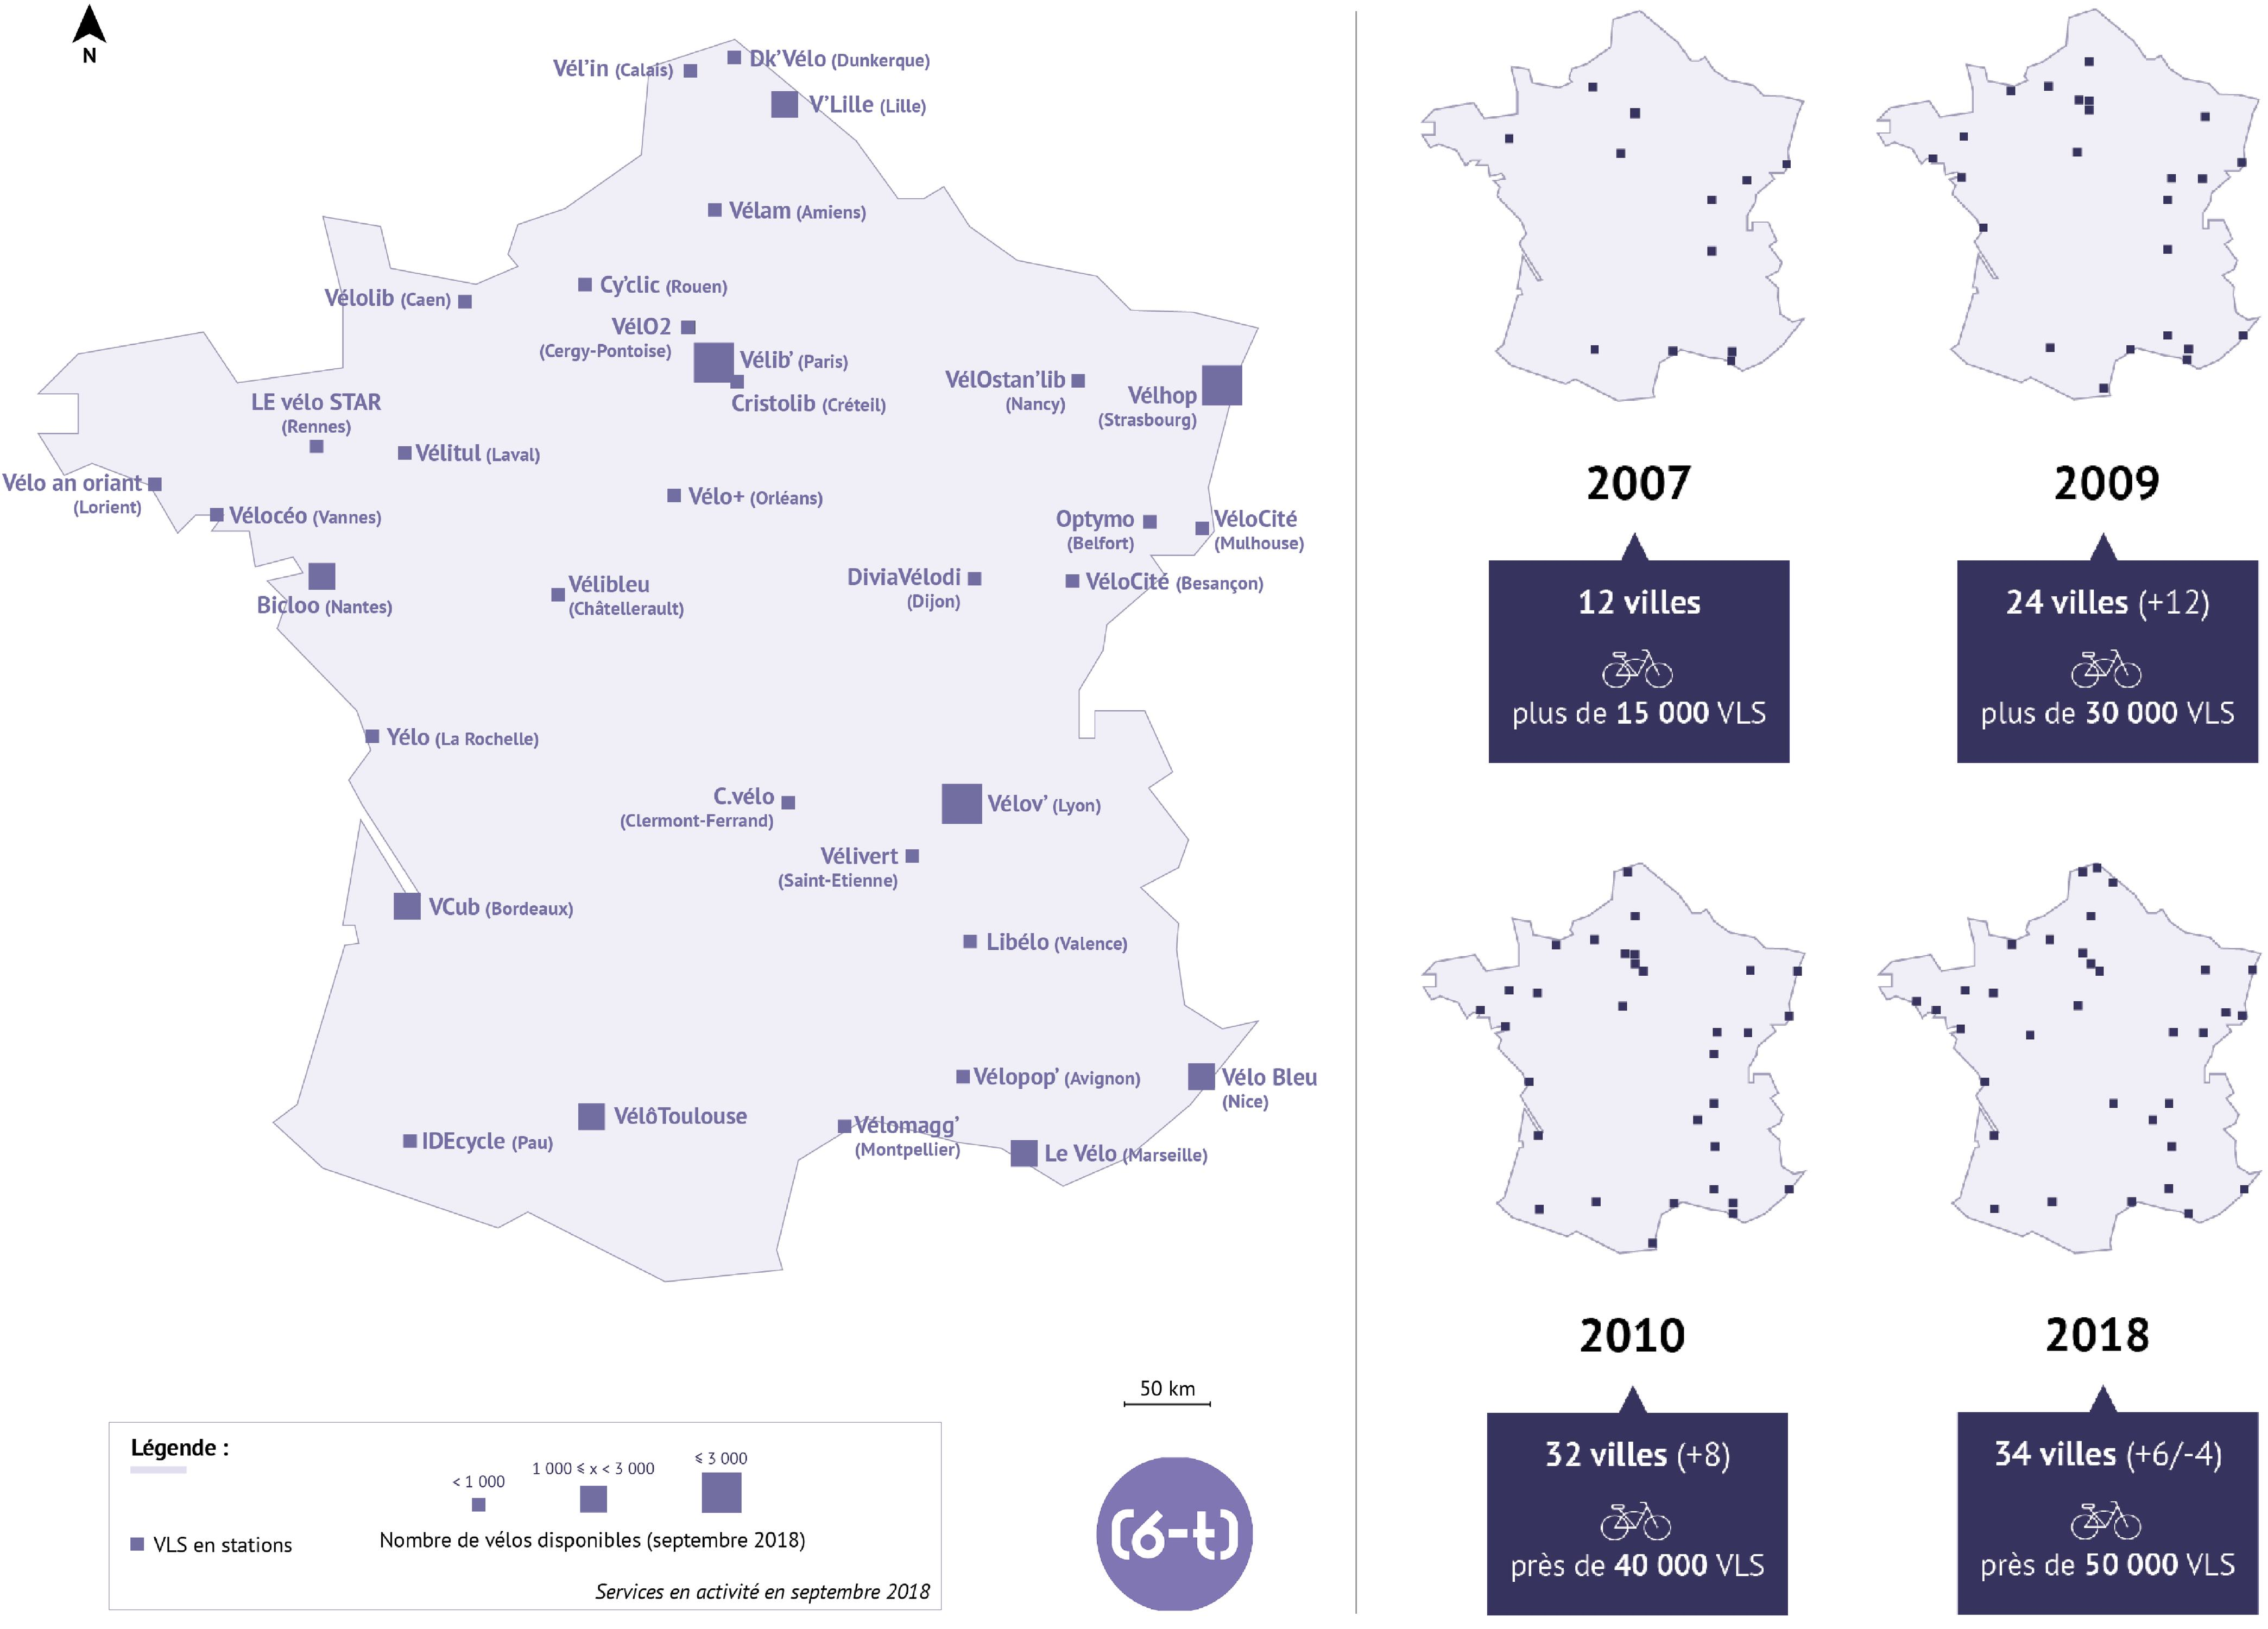
\includegraphics[width=1\columnwidth]{src/Figures/Chap-1/FR_Carte_VLS_France.jpg}}
        \vspace{5pt}
        \begin{flushright}\scriptsize{
        Source~: \textcolor{blue}{\textcite{6t-bureau_de_recherche_lechappee_2018}}\index{Bureau de recherche 6t@\textsl{Bureau de recherche 6t}|pagebf}
        }\end{flushright}
    \end{carte}

    % Libre-service avec station - histoire 2
Ces innovations, associées à un modèle de tarification basé sur des intervalles temporels, deviennent le standard international des systèmes de \acrshort{VLS} \textcolor{blue}{\autocite[162]{shaheen_bikesharing_2010}}\index{Shaheen, Susan~A.|pagebf}\index{Guzman, Stacey|pagebf}\index{Zhang, Hua|pagebf}. C’est toutefois Lyon, avec \textsl{Vélo'v} en 2005, et Paris, avec \textsl{Vélib'} en 2007, qui popularisent ce modèle dans le monde. Ces services deviennent les références en matière de \acrshort{VLS}, permettant à la France de se positionner au premier rang dans ce domaine~: en 2010, le pays compte 24 systèmes de \acrshort{VLS}, avec une flotte totale composée de 36~000 vélos et de 3~000 stations \textcolor{blue}{\autocite[161]{shaheen_bikesharing_2010}}\index{Shaheen, Susan~A.|pagebf}\index{Guzman, Stacey|pagebf}\index{Zhang, Hua|pagebf}, atteignant 34 agglomérations en 2018 (voir la \hyperref[fig-chap1:carte-vls-france]{carte~\ref{fig-chap1:carte-vls-france}}, page~\pageref{fig-chap1:carte-vls-france}). C'est au tournant de cette décennie que les expériences de systèmes de \acrshort{VLS} vont faire apparaître un modèle de gestion dominant~: celui du \acrfull{PPP} \textcolor{blue}{\autocite[5]{hure_entre_2014}}\index{Huré, Maxime|pagebf}. Plus récemment, une quatrième génération émerge, intégrant des \acrshort{VAE} en libre-service, des mécanismes de verrouillage optimisés, des interfaces tactiles et une interconnexion avec les systèmes de transport public \textcolor{blue}{\autocite[162]{shaheen_bikesharing_2010}}\index{Shaheen, Susan~A.|pagebf}\index{Guzman, Stacey|pagebf}\index{Zhang, Hua|pagebf}. Notons que si ces initiatives sont majoritairement le fruit de projets locaux ou intercommunaux portés principalement par les plus grandes agglomérations \textcolor{blue}{\autocites[18]{fishman_bike_2013}[6]{ricci_bike_2015}}\index{Fishman, Elliot|pagebf}\index{Washington, Simon|pagebf}\index{Haworth, Narelle|pagebf}\index{Ricci, Miriam|pagebf}, leur déploiement reste encore marginal à l’échelle régionale ou nationale\footnote{
    Parmi ces exceptions, nous ne pouvons nous empêcher de citer le système néerlandais \textsl{OV-fiets}, littéralement traduit par \textsl{vélos de transport public}, intégré au réseau ferroviaire national. Créé en 2004 par une association, ce système de \acrshort{VLS} a été repris, à partir de 2008, par la compagnie ferroviaire nationale des Pays-Bas, la \acrfull{NS} \textcolor{blue}{\autocites[151]{ploeger_sociotechnical_2020}[157]{waes_why_2020}}\index{Ploeger, Jan|pagebf}\index{Oldenziel, Ruth|pagebf}\index{Waes, Arnoud van|pagebf}\index{Farla, Jacco|pagebf}\index{Raven, Rob|pagebf}. Aujourd’hui, ce service de mobilité couvre 300 stations situées à proximité des gares et des arrêts de métro, avec une flotte de 22~000 vélos. Sa spécificité réside dans le fait que la location s’effectue à la journée et exige que le vélo soit restitué dans la même station que celle où il a été emprunté \textcolor{blue}{\autocite[9]{ploeger_sociotechnical_2020}}\index{Caletrío, Javier|pagebf}, d'après un modèle en boucle, de type \textsl{2-way} \textcolor{blue}{\autocite[13]{mangeart_vehicules_2022}}\index{Mangeart, Timothée|pagebf}\index{Bouteuil, Virginie|pagebf}.
} \textcolor{blue}{\autocite[225]{dauncey_french_2012}}\index{Dauncey, Hugh|pagebf}. En août 2022, selon la plate-forme \textsl{The Meddin Bike-sharing World Map}\footnote{
    \url{https://bikesharingworldmap.com}
}, qui recense et met à jour l’ensemble des systèmes de mobilité partagée à l’échelle mondiale, 1~212 agglomérations disposent de services de \acrshort{VLS} \textcolor{blue}{\autocite[7]{the_meddin_bike-sharing_world_map_meddin_2022}}\index{The Meddin Bike-sharing World Map@\textsl{The Meddin Bike-sharing World Map}|pagebf}, les plus importants étant tous situés en Chine (voir la \hyperref[fig-chap1:carte-vls-monde]{carte~\ref{fig-chap1:carte-vls-monde}}, page~\pageref{fig-chap1:carte-vls-monde}). À ces derniers s’ajoutent 80 systèmes dits \Guillemets{hybrides}, combinant une flotte de \acrshort{VLS} ainsi qu'une flotte de \acrfull{VFF}.%%Rédigé%%

   % Figure carte VLS monde
    \begin{carte}[h!]\vspace*{4pt}
        \caption{Localisation des principaux services de vélo en libre-service avec station dans le monde, en 2021.}
        \label{fig-chap1:carte-vls-monde}
        \centerline{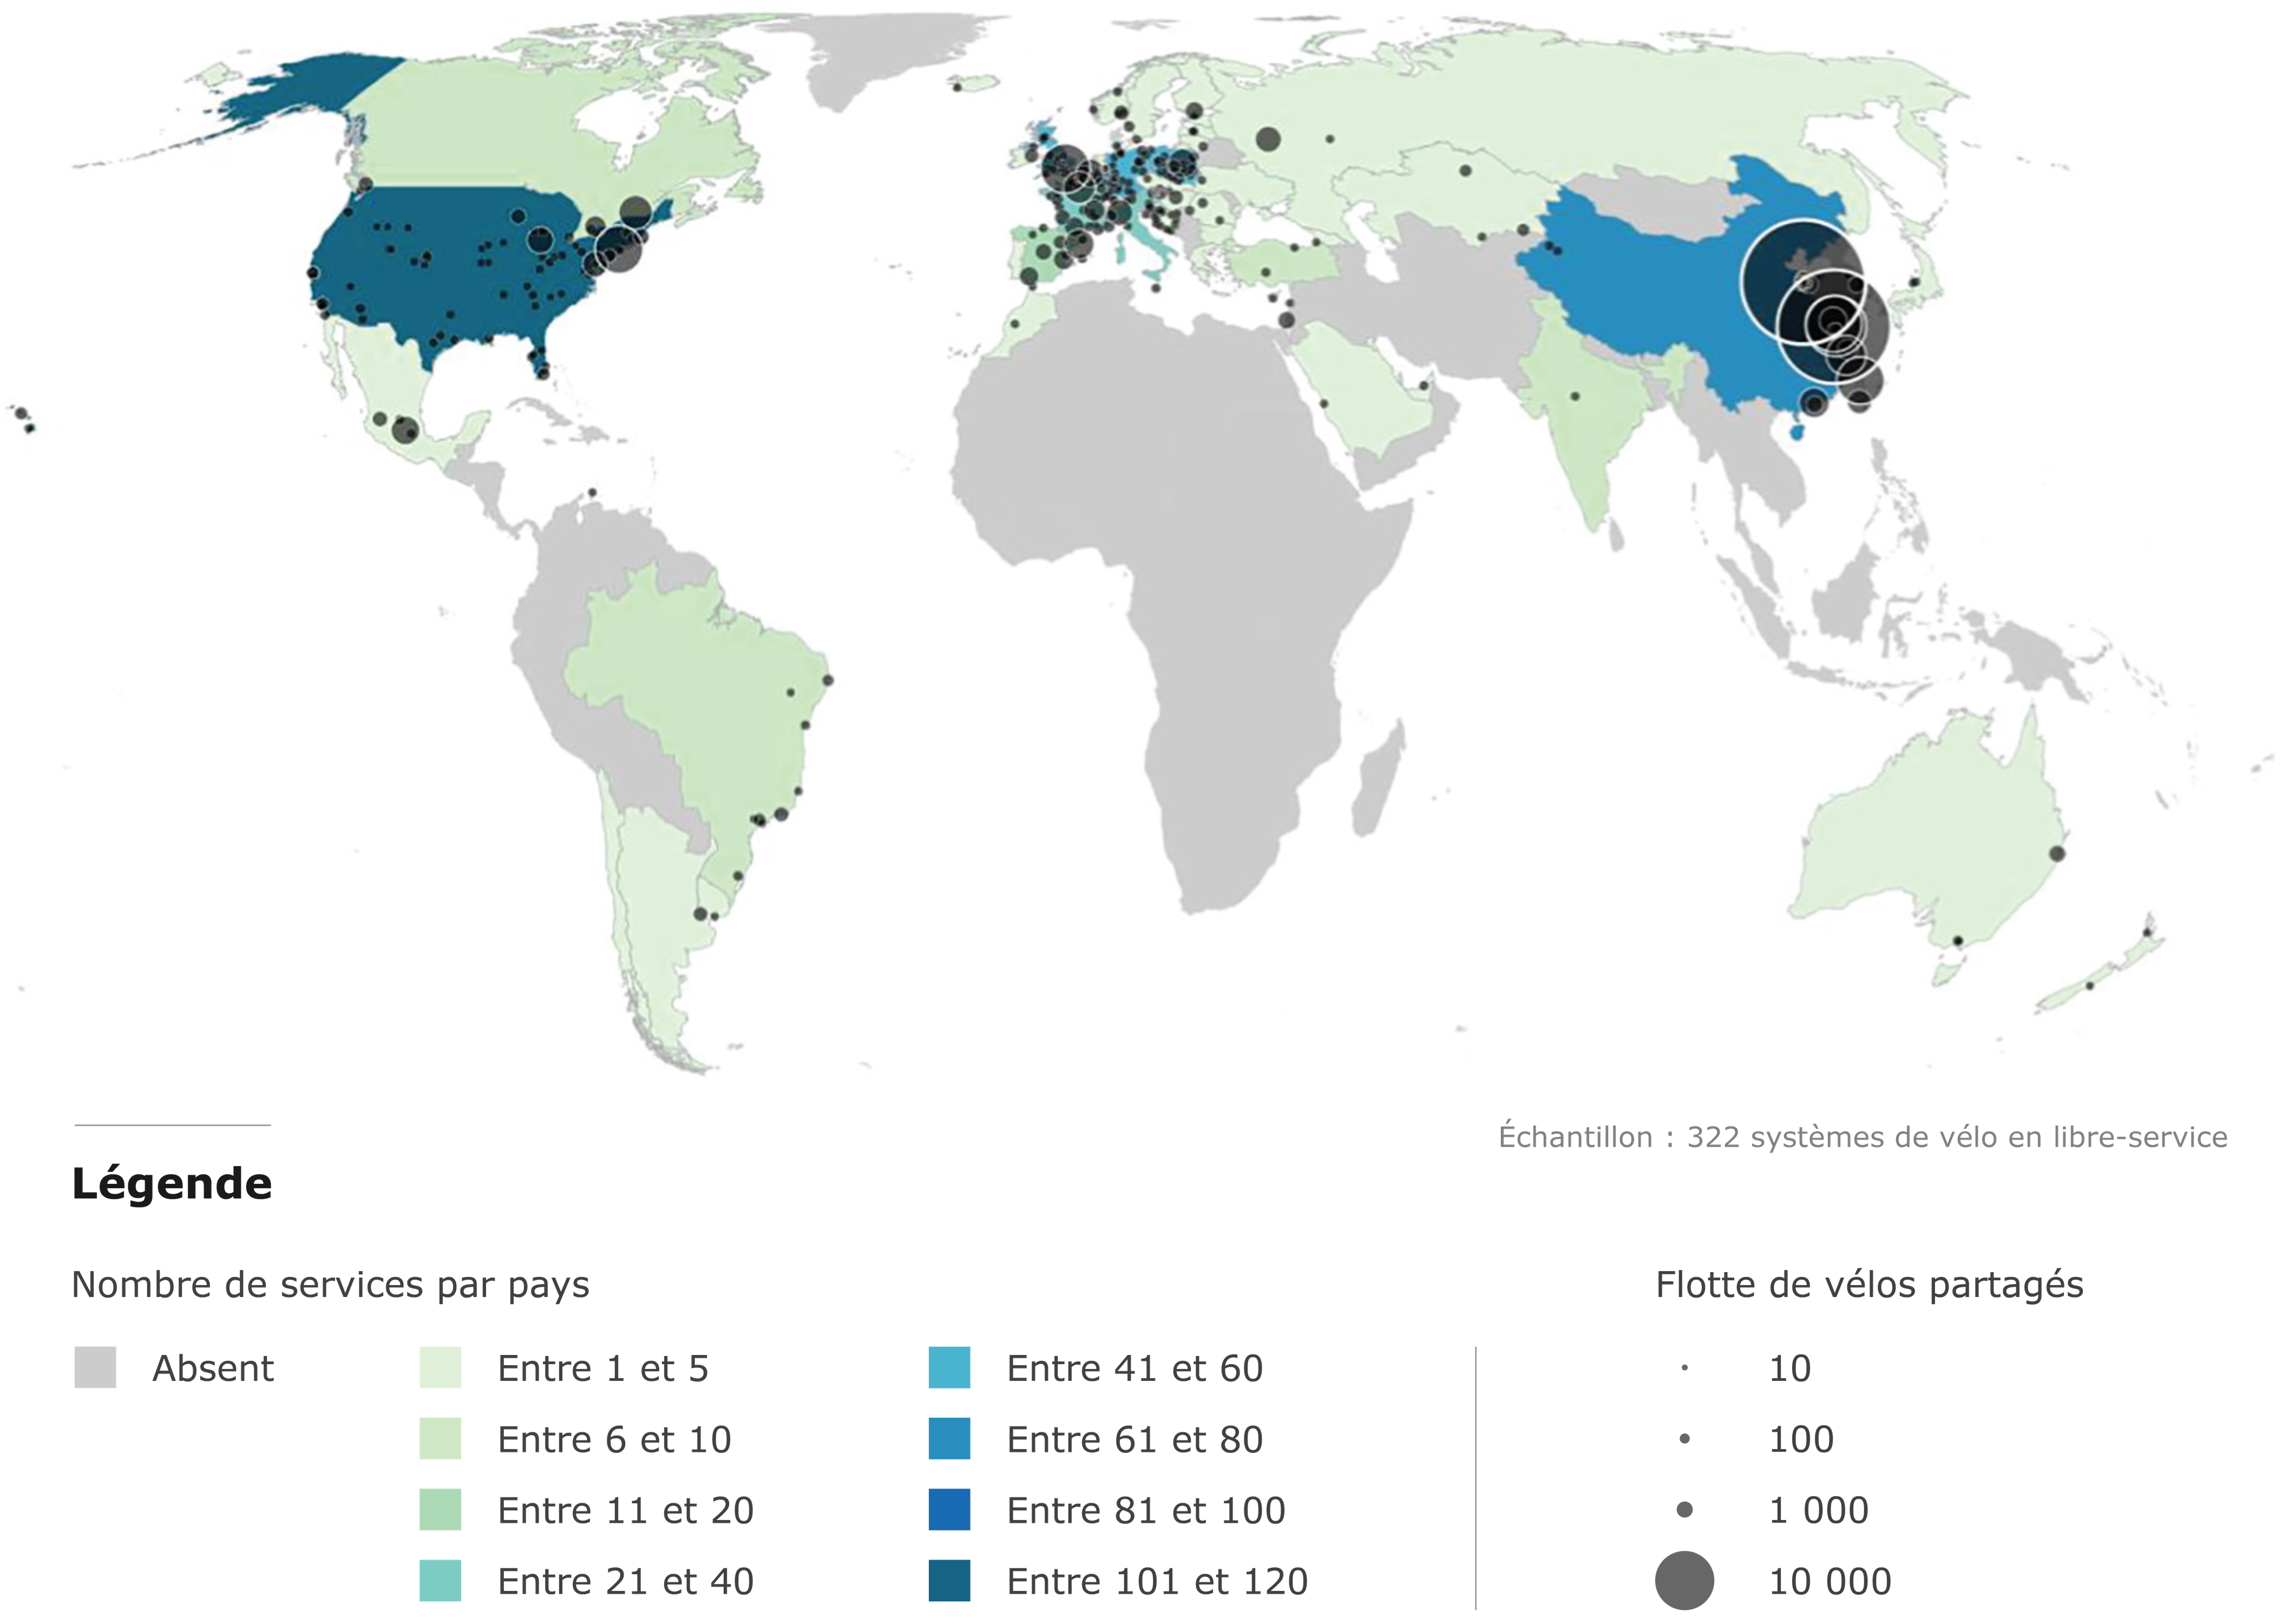
\includegraphics[width=1\columnwidth]{src/Figures/Chap-1/FR_Carte_VLS_monde.png}}
        \vspace{5pt}
        \begin{flushright}\scriptsize{
        Source~: \textcolor{blue}{\textcite[3]{todd_global_2021}}\index{Todd, James|pagebf}\index{O'Brien, Oliver|pagebf}\index{Cheshire, James|pagebf}
        \\
        Traduction~: \textcolor{blue}{Dylan Moinse (2024)}
        }\end{flushright}
    \end{carte}

    % VFF
Si l’expérience des \textsl{White Bikes}, celle des \textsl{Call a Bike}, ainsi que les générations successives de systèmes \acrshort{VLS} peuvent être perçues comme les prémices des systèmes de \acrshort{VFF}, leur forme actuelle apparaît véritablement en Chine en 2014. Cette année-là, \textcolor{blue}{Dai Wei}, étudiant à Beijing, imagine avec ses ami·e·s un système de vélos partagés destiné à faciliter leurs déplacements sur le campus. Iels fondent alors la start-up \Marque{Ofo}, après avoir expérimenté la mutualisation des vélos sur leur campus \textcolor{blue}{\autocite[10]{nlc_micromobility_2019}}\index{NLC@\textsl{NLC}|pagebf}. Ce projet bénéficie rapidement d’un soutien financier de la société chinoise de \acrshort{VTC} \Marque{Didi} \textcolor{blue}{\autocite[18]{6t-bureau_de_recherche_etude_2018}}\index{Bureau de recherche 6t@\textsl{Bureau de recherche 6t}|pagebf}. Le service se déploie dans plusieurs villes chinoises avant de s’exporter. De nombreuses \Guillemets{licornes du vélo}\footnote{
    En 2013, l'investisseuse étasunienne \textcolor{blue}{Aileen Lee} invente l'expression de \Guillemets{licorne} \textsl{unicorn} pour désigner les startups les plus valorisées de la Silicon Valley, en Californie. L'animal mythique renvoyant à la rareté, au miracle et à la fantaisie \textcolor{blue}{\autocite{benner_unicorn_2015}}\index{Benner, Katie|pagebf}. En somme, il s'agit de décrire une \Guillemets{\textsl{start-up des nouvelles technologies créée il y a moins de dix ans et valorisée d'au moins un milliard de dollars avant d'être cotée en Bourse.}} \textcolor{blue}{\autocite{chambre_de_commerce_et_dindustrie_licornes_2019}}\index{Chambre de commerce et d'industrie@\textsl{Chambre de commerce et d'industrie}|pagebf}.
} asiatiques spécialisées dans l’offre de vélos en libre-service sans station, dits en \Guillemets{flotte libre} (\textsl{free-floating} ou \textsl{dockless}), voient le jour et développent leurs activités jusqu’en France, à partir de l'automne 2017. Ainsi, \Marque{Gobee.bike} déploie d’abord ses vélos à Lille, puis à Paris quelques jours plus tard. En quelques mois seulement, cinq opérateurs de \acrshort{VFF} sont actifs dans la capitale française à la fin de l’année 2017. Moins d’un an après, sept services de \acrshort{VFF} se déploient dans huit agglomérations françaises, atteignant une flotte totale d’environ 15~000 véhicules, représentant ainsi 20~\% des vélos partagés dans le pays \textcolor{blue}{\autocite[23]{6t-bureau_de_recherche_etude_2018}}\index{Bureau de recherche 6t@\textsl{Bureau de recherche 6t}|pagebf}. Dans le même temps, les deux géants chinois du secteur, \Marque{Ofo} et \Marque{Mobike}, se positionnent dans les 30 plus grandes villes chinoises, rassemblant plus de 200 millions d’usager·ère·s, et atteignent également 21 autres pays \textcolor{blue}{\autocite[22, 91]{kang_university_2020}}\index{Kang, Wei|pagebf}\index{Aguiléra, Anne|pagebf}\index{Rallet, Alain|pagebf}.%%Rédigé%%

    % TEFF
Au-delà de la description du véhicule lui-même, c'est principalement le mode opératoire en libre-service qui alimente la réflexion sur l'élargissement de l'offre de mobilité. Peu de temps après le déploiement des flottes de \acrshort{VFF}, qu’ils soient mécaniques ou électriques, apparaissent de nouveaux services, notamment ceux liés à la \acrfull{TEFF}. Son essor débute en 2017 avec la création de la société étasunienne \Marque{Bird} par \textcolor{blue}{Travis VanderZanden}, ancien cadre des entreprises de \acrshort{VTC} \Marque{Lyft} et \Marque{Uber} \textcolor{blue}{\autocite[13]{nlc_micromobility_2019}}\index{NLC@\textsl{NLC}|pagebf}. Ce projet mise sur le renouveau de la trottinette électrique, remise au goût du jour quelques années plus tôt \textcolor{blue}{\autocite{easy_electric_life_free_2020}}\index{Easy Electric Life@\textsl{Easy Electric Life}|pagebf}. En France, les services de \acrshort{TEFF} émergent à l’été 2018, devenant rapidement emblématiques, aux côtés du \acrshort{VFF}, de l’essor de la mobilité partagée \textcolor{blue}{\autocite[1]{bortoli_consequential_2020}}\index{Bortoli, Anne de|pagebf}\index{Christoforou, Zoi|pagebf}. Bien que des services de scooters et de voitures électriques partagés existaient déjà en Europe, la vitesse d’adoption et de déploiement des systèmes de \acrshort{TEFF} est sans précédent. Par exemple, \Marque{Bird} atteint rapidement le statut de \Guillemets{licorne}, et d'autres entreprises comme \Marque{Lime} (anciennement \Marque{LimeBike}) ou \Marque{Spin}, originellement spécialisées dans le \acrshort{VFF}, suivent le modèle en 2018 \textcolor{blue}{\autocite[4]{clewlow_micro-mobility_2018}}\index{Clewlow, Regina|pagebf}. Décrits comme la \Guillemets{dernière forme de l'ubérisation de l'urbain} \textcolor{blue}{\autocite[1]{boffi_extrait_2019}}\index{Boffi, Nicolas|pagebf}, les services de \acrshort{VFF} et de \acrshort{TEFF} établissent des records en termes de diffusion et d’adoption modale à l'international. À Paris, \textcolor{blue}{\textcite[146]{6t-bureau_de_recherche_usages_2019}}\index{Bureau de recherche 6t@\textsl{Bureau de recherche 6t}|pagebf} estime que, seulement un an après son lancement, la \acrshort{TEFF} atteint, au moins, une part modale équivalente à celle du \acrshort{VLS} \textsl{Vélib’}, trois ans après son lancement, avec une estimation située entre 0,8~\% et 2,2~\% des déplacements internes. Aux États-Unis et au Canada, 39 millions de déplacements ont été enregistrés en \acrshort{TEFF} la première année de lancement du service, un chiffre qui doublera en 2023, malgré la crise sanitaire liée à la COVID-19. Les systèmes nord-américains de \acrshort{TEFF} représentent alors 44~\% des déplacements à vélo ou en trottinette partagés du continent, une proportion qui s'élève à 49~\% aux États-Unis \textcolor{blue}{\autocites[10]{nacto_shared_2019}[10]{nacto_shared_2020}[3-5]{nacto_shared_2024}}\index{NACTO@\textsl{NACTO}|pagebf}. Un élément clé distingue cependant les systèmes de mobilité en \textsl{free-floating} de ceux en libre-service avec station~: leur répartition géographique. Tandis que les services de \acrshort{VLS} se concentrent principalement dans les grandes agglomérations, les services de \acrshort{VFF} et de \acrshort{TEFF} se déploient dans des zones relativement moins denses.%%Rédigé%%

    % Technologies
La mobilité partagée, qu’elle prenne la forme de vélos ou de trottinettes, mécaniques ou électriques, se caractérise par un dénominateur commun~: elle libère l’usager·ère des coûts d’acquisition, d’entretien, et des responsabilités liées à la possession d’un véhicule \textcolor{blue}{\autocite[44]{mathew_analysis_2019}}\index{Mathew, Jijo|pagebf}\index{Liu, Mingmin|pagebf}\index{Li, Howell|pagebf}\index{Seeder, Sonya|pagebf}\index{Bullock, Darcy|pagebf}. Cette offre, bien que diversifiée, s’inscrit dans une dynamique de complémentarité, mais également de concurrence vis-à-vis des véhicules traditionnels. Elle a pu émerger grâce à un contexte technologique propice, marqué par la commercialisation et la démocratisation d’innovations récentes. En premier lieu, la diffusion massive des \textsl{smartphones}\footnote{
    Conçu en 1992, le \textsl{smartphone} a marqué un tournant technologique majeur, mais c’est véritablement avec l’arrivée de l’\Marque{Iphone} en 2007 qu’il connaît sa première grande popularisation. Dès 2008, l’\Marque{Iphone 3G} permet un accès au réseau de données cellulaires 3G, est équipé de fonctionnalités \acrshort{GPS} et introduit l’utilisation d’applications mises à jour via une boutique en ligne dédiée \textcolor{blue}{\autocite{les_numeriques_2007_2014}}\index{Les Numériques@\textsl{Les Numériques}|pagebf}. Ces évolutions ont profondément transformé les comportements individuels, en intégrant le \textsl{smartphone} dans les usages quotidiens, comme le paiement mobile (M-paiement) ou la lecture de \textsl{flashcodes} (\textsl{QR codes}) \textcolor{blue}{\autocites[279]{chaix_paiement_2013}[21]{ben_jaddi_m-paiement_2018}}\index{Chaix, Laetitia|pagebf}\index{Ben Jaddi, Madja|pagebf}. Cette révolution technologique a offert un terreau fertile au développement des services de mobilité partagée, lesquels exploitent les cinq composantes de l’\Guillemets{\textsl{Internet} des objets}, dit \acrfull{IoT}, à savoir (i) les objets, (ii) le réseau mobile, (iii) les données, (iv) les informations et (v) les applications d'exploitation \textcolor{blue}{\autocite{iot_evolution_world_impact_2017}}\index{IoT Evolution World@\textsl{IoT Evolution World}|pagebf}. Par ailleurs, l’adoption massive du \textsl{smartphone} a ouvert un immense marché potentiel pour ces services. La démocratisation de l’appareil a été rapide et globale. Par exemple, aux États-Unis, le taux d’équipement en \textsl{smartphones} est passé de 35~\% en 2011 à 77~\% en 2018 \textcolor{blue}{\autocite[8]{clewlow_micro-mobility_2018}}\index{Clewlow, Regina|pagebf}. Une dynamique similaire a été observée en France, où ce taux est passé de 17~\% en 2011 à 77~\% en 2019 \textcolor{blue}{\autocite[28]{credoc_barometre_2019}}\index{CRÉDOC@\textsl{CRÉDOC}|pagebf}.
} a permis aux \acrfull{STP} de s’affranchir de l’ancrage physique des stations. Cette dématérialisation a facilité la mise en œuvre de modèles opératoires résumés par un dicton~:\Guillemets{\textsl{agis d’abord, demande ensuite}} (\textsl{arrive first, ask later})\footnote{
    La première génération de services de vélos et trottinettes partagés, déployée entre 2017 et 2020, s’est caractérisée par une stratégie audacieuse adoptée par les opérateurs. Ces derniers s’implantaient sur les territoires sans réellement demander d’autorisation préalable aux collectivités locales, ni même les en informer, profitant ainsi du flou juridique entourant ces nouveaux services de mobilité \textcolor{blue}{\autocite{laker_welcome_2019}}\index{Laker, Laura|pagebf}. Cette tactique consistait à établir les services \textsl{de facto} avant de contacter les autorités locales, dans le but de négocier à partir d’une position de force, réduisant ainsi les concessions nécessaires \textcolor{blue}{\autocite[5]{lopez-escolano_mobilites_2019}}\index{López-Escolano, Carlos|pagebf}\index{Campos, Ángel Pueyo|pagebf}. Le vide réglementaire relatif à l’occupation de l’espace public a permis à ces services d’opérer sans vraiment d'accord institutionnel \textcolor{blue}{\autocite[5]{lopez-escolano_mobilites_2019}}\index{López-Escolano, Carlos|pagebf}\index{Campos, Ángel Pueyo|pagebf}. Cette situation a conduit certaines agglomérations à interdire ces services, notamment en invoquant deux motifs principaux~: l’occupation illégale de l’espace public et la concurrence directe avec les systèmes de transport public existants \textcolor{blue}{\autocite[63]{6t-bureau_de_recherche_livre_2019}}. Cependant, ces tactiques ont évolué aujourd'hui. Cette phase a laissé place à des approches plus collaboratives, permettant aux acteurs publics et privés de tirer mutuellement parti de ces services. Désormais, des chartes d'exploitation et de régulation encadrent la mise en œuvre des services de mobilité partagée dans la majorité des grandes villes européennes et nord-américaines, mettant ainsi fin aux pratiques unilatérales et posant les bases d’une gouvernance.
}, où les opérateurs ont souvent pris de court les autorités publiques. Ces dernières, régulatrices historiques du transport urbain et parfois elles-mêmes opératrices de services en libre-service tels que le \acrshort{VLS}, se sont retrouvées dans une position défavorable face à ces acteurs disruptifs. Outre le rôle central des \textsl{smartphones}, la géolocalisation et le géorepérage (\textsl{geofencing}) ont également joué un rôle stratégique dans le déploiement de ces solutions de mobilité. Grâce à ces technologies, les opérateurs peuvent suivre en temps réel leurs flottes et établir des barrières géographiques virtuelles définissant les périmètres d’exploitation. Toutefois, la technologie \acrshort{GPS}, avec une précision souvent limitée entre 3 et 10 mètres selon l’environnement urbain \textcolor{blue}{\autocite{the_scooterist_dockless_2020}}\index{The Scooterist@\textsl{The Scooterist}|pagebf}, constitue encore un frein à une gestion fine des véhicules partagés, notamment pour différencier la circulation ou le stationnement sur un trottoir, une chaussée ou dans une zone restreinte \textcolor{blue}{\autocite[96]{6t-bureau_de_recherche_livre_2019}}\index{Bureau de recherche 6t@\textsl{Bureau de recherche 6t}|pagebf}\footnote{
    Actuellement, la géolocalisation des véhicules en libre-service sans borne permet de détecter leur entrée ou sortie de périmètres définis, tels que des zones de stationnement élargies ou des lieux spécifiques comme des places publiques ou des parcs. Cependant, la précision offerte par la technologie \acrshort{GPS} reste encore limitée, ne répondant pas toujours aux attentes des collectivités, qui tendent parfois à surévaluer son efficacité comme solution de gestion \textcolor{blue}{\autocite[123]{6t-bureau_de_recherche_livre_2019}}. Face à ces limites, certaines autorités urbaines ou de transport ont introduit des solutions complémentaires. Parmi celles-ci figurent l’obligation pour l’utilisateur·rice de scanner un \textsl{QR code} situé dans une aire de stationnement banalisée à la fin du déplacement, ou encore de photographier le véhicule stationné comme preuve de conformité \textcolor{blue}{\autocite[96]{6t-bureau_de_recherche_livre_2019}}.
}. Ce panorama devrait évoluer avec la mise en activité complète du système européen de positionnement par satellite \textsl{Galileo}, initié par l’Union européenne. Partiellement opérationnel depuis 2016, ce système a été finalisé fin 2024 et est désormais accessible au grand public avec une précision gratuite de l’ordre du mètre, et une précision centimétrique pour des usages payants \textcolor{blue}{\autocite{futura_sciences_galileo_2019}}\index{Futura Sciences@\textsl{Futura Sciences}|pagebf}\index{CNES@\textsl{CNES}|pagebf}. Cette avancée technologique ouvre de nouvelles perspectives pour le géorepérage, non seulement pour améliorer la gestion et la précision des flottes, mais également pour répondre aux impératifs de régulation, notamment en matière de stationnement des véhicules partagés.%%Rédigé%%
 
    % Semi-floating et Transition
Dans leur \Guillemets{revue parapluie} portant sur les véhicules en libre-service, soit une synthèse de 29 revues de littérature existantes, \textcolor{blue}{\textcite[16]{mangeart_vehicules_2022}}\index{Mangeart, Timothée|pagebf}\index{Bouteuil, Virginie|pagebf} mettent en lumière l'absence fréquente de stratégies précises adoptées par les autorités locales vis-à-vis des services de mobilité partagée. Les instruments de régulation identifiés varient entre restrictions, financements publics et avantages en nature, tels que la mise à disposition de zones de stationnement. Cette évolution de la gouvernance publique constitue un marqueur d'une transformation profonde du \Guillemets{régime socio-technique}, provoquée par la pression des innovations \textcolor{blue}{\autocites[319]{canitez_pathways_2019}[4]{fryszman_smart_2019}}\index{Canitez, Fatih|pagebf}\index{Fryszman, Flavia|pagebf}\index{Denes Dos Santos Carstens, Danielle|pagebf}\index{Kindl da Cunha, Sieglinde|pagebf}. Une des évolutions notables concerne alors l’organisation de flottes \Guillemets{semi-libres} (\textsl{semi-floating} ou \textsl{semi-dockless}), prenant la forme de stations physiques ou dématérialisées \textcolor{blue}{\autocite[121]{6t-bureau_de_recherche_livre_2019}}\index{Bureau de recherche 6t@\textsl{Bureau de recherche 6t}|pagebf}. Cette réflexion sur le stationnement dit \textsl{intelligent} (\textsl{smartparking}) vise à réduire les externalités négatives, telles que le stationnement gênant sur les espaces piétons \textcolor{blue}{\autocite[13]{zou_exploratory_2020}}\index{Zhou, Zhenpeng|pagebf}\index{Younes, Hannah|pagebf}\index{Erdoğan, Sevgi|pagebf}\index{Wu, Jiahui|pagebf}. À Paris, par exemple, la municipalité a annoncé, en mars 2019, que les redevances imposées aux opérateurs serviraient à financer 2~500 emplacements de stationnement dédiés au \acrshort{VFF} et à la \acrshort{TEFF}\footnote{
    Les emplacements dédiés au stationnement des véhicules en \textsl{free-floating} sont souvent matérialisés par un marquage au sol accompagné d’un logo spécifique, et remplacent fréquemment une place de stationnement automobile \textcolor{blue}{\autocite{livonniere_trottinettes_2019}}\index{Livonnière, Stanislas de|pagebf}. Ces emplacements sont dimensionnés pour accueillir généralement six \acrshort{TEFF}, par exemple \textcolor{blue}{\autocite{burban_trottinettes_2019}}\index{Burban, Thibault|pagebf}. Cette mesure prend tout son sens avec l’arrêté municipal du 30 juillet 2019, qui interdit le stationnement des \acrshort{VFF} et des \acrshort{TEFF} sur les trottoirs. Le texte précise~: \Guillemets{\textsl{considérant que, dans ces conditions, il est nécessaire d’organiser le stationnement de ces engins afin d’assurer la sécurité des piétons et de leur garantir de bonnes conditions de cheminement, en restreignant les possibilités de stationnement aux seuls endroits adaptés à leurs caractéristiques géométriques et fonctionnelles.}} \textcolor{blue}{\autocite[3~151]{ville_de_paris_bulletin_2019}}. Cette initiative vient compléter une application et une relecture stratégique de l’article 52 de la \acrfull{LOM} de 2019, qui dispose que les places de stationnement automobile, situées dans les cinq mètres en amont des passages piétons, seront neutralisées avant 2027, afin de garantir une meilleure visibilité des piéton·ne·s \textcolor{blue}{\autocite[42]{gart_loi_2020}}. À ce jour, environ 2~500 emplacements de stationnement réservés ont été aménagés dans la capitale, représentant un total estimé de 15~000 places à destination des \acrshort{VFF} et des \acrshort{TEFF}.
} \textcolor{blue}{\autocites[3~151]{ville_de_paris_bulletin_2019}[90]{6t-bureau_de_recherche_livre_2019}}\index{Bureau de recherche 6t@\textsl{Bureau de recherche 6t}|pagebf}\index{Ville de Paris@\textsl{Ville de Paris}|pagebf}. Non sans rappeler le mode de fonctionnement précurseur de l'entreprise danoise de \acrshort{VFF} \Marque{Donkey Republic}\footnote{
    Face à la concurrence des opérateurs asiatiques et nord-américains équipés de flottes massives, l’entreprise danoise \Marque{Donkey Republic} fait son entrée sur le marché parisien en 2018 avec une flotte de 250 \acrshort{VFF} \textcolor{blue}{\autocite[20]{6t-bureau_de_recherche_etude_2018}}. Ce qui distingue \Marque{Donkey Republic} de ses concurrents est son approche \Guillemets{hybride}, se situant à mi-chemin entre les systèmes de \acrshort{VLS} et \acrshort{VFF} \textcolor{blue}{\autocite[20]{6t-bureau_de_recherche_etude_2018}}. Contrairement aux modèles classiques en flotte libre, \Marque{Donkey Republic} exploite le mobilier urbain existant, notamment les arceaux à vélo, pour proposer un système de stationnement structuré. À la fin d’une course, l’utilisateur·rice est tenu·e de fixer le vélo partagé à l’un de ces arceaux à l’aide des chaînes fournies par l’opérateur \textcolor{blue}{\autocite[20]{6t-bureau_de_recherche_etude_2018}}. Bien que ce modèle restreigne quelque peu la liberté de l’usager·ère en imposant des lieux de stationnement précis, il présente plusieurs avantages. D’une part, il contribue à limiter les risques de vol et, d’autre part, il permet de prévenir les problèmes de stationnement anarchique, souvent associés aux systèmes en \textsl{free-floating}, et les dégradations qui en découlent. Ce premier système, qui introduit une certaine discipline dans l’usage des véhicules partagés, constitue une forme d’autorégulation par l’opérateur. Il pose également les bases d’une réflexion plus large sur la régulation des flottes sans borne d'attache dans l’espace urbain.
}. Cette évolution s’inscrit dans un contexte où les \acrshort{STP} répondent à des exigences croissantes en matière d’instantanéité, de flexibilité et de liberté d’usage \textcolor{blue}{\autocite[8]{frere_services_2018}}\index{Frère, Séverine|pagebf}\index{Castex, Élodie|pagebf}\index{Mathon, Sylvie|pagebf}. Plus largement, le renouveau des cycles et des trottinettes traduit un renouveau du paradigme autour de la proximité et de l'idéal de la \Guillemets{ville compacte}, mettant en avant les modes actifs et une mixité fonctionnelle comme alternatives à l’étalement urbain \textcolor{blue}{\autocite[44]{eskenazi_voir_2022}}\index{Eskenazi, Manon|pagebf}. Ce basculement témoigne des mutations sociales contemporaines, marquées par une dissolution des structures traditionnelles au profit d'une flexibilité accrue \textcolor{blue}{\autocite[130-142]{bauman_liquid_2000}}\index{Bauman, Zygmunt|pagebf}.%%Rédigé%%

    % 1.2.3.
    \needspace{1\baselineskip} % Réserve de l'espace
\subsection{Caractérisation d’une classe de véhicules liés à la \Guillemets{mobilité individuelle légère}, symbole d'un regain d'intérêt pour la proximité
    \label{chap1:caracterisation-mobilite-individuelle-legere}
    }

    % Introduction
Dans nos sociétés contemporaines, les valeurs associées à la recherche de flexibilité et d'adaptabilité, conjuguées à celles de l'individualisme et de l'instantanéité, ont profondément redéfini nos pratiques de mobilité et, par conséquent, transformé l’offre de mobilité existante. Cette quête de \Guillemets{fluidité}, caractérisée par un recul progressif des structures collectives fixes au profit de réseaux d’interaction en perpétuel mouvement \textcolor{blue}{\autocite[19-24]{bauman_liquid_2000}}\index{Bauman, Zygmunt|pagebf}, s’est couplée à la commercialisation d'innovations technologiques adoptée par les dernières générations \Guillemets{connectées} et \Guillemets{nomades}. Elle a ainsi favorisé une demande croissante pour le renouvellement des systèmes de mobilité, adaptés à une consommation mobile et à une redécouverte de la proximité \textcolor{blue}{\autocite[103-108]{bu_tout-voiture_2024}}\index{Bu, Ludovic|pagebf}. Dans ce contexte, la diversification, accompagnée de l’hybridation modale des cycles, émerge comme une réponse aux aspirations contemporaines, articulées autour d’exigences d’efficience, de résilience, de proximité et de sobriété énergétique et économique. Cette famille de véhicules regroupe un éventail de modes variés, allant du vélo classique aux engins de déplacement personnel ou partagé. Leur essor ainsi que leur attrait croissant rendent toutefois difficile, encore aujourd’hui, de circonscrire conceptuellement ces catégories, notamment en raison de l'hétérogénéité des définitions qui leur sont associées. Ces ambiguïtés sémantiques nous ont conduits à adopter une définition élargie de ce que nous désignons comme la \Guillemets{mobilité individuelle légère}, une terminologie empruntée au projet de recherche \textcolor{blue}{\textcite{urfe_projet_2022}}\index{URFé@\textsl{URFé}|pagebf}. Dans cette perspective, nous proposons notre propre définition, visant à regrouper les véhicules individuels légers tout en dépassant les classifications existantes. Au sein de cette catégorie, il demeure possible de distinguer deux grandes sous-catégories~: d’une part, le vélo et ses déclinaisons, et d’autre part, la \Guillemets{micro-mobilité}, reprenant la définition légale de l'\acrfull{EDP}, indépendamment de leur type de propulsion ou de leur mode d’acquisition.%%Rédigé%%

    % 1.2.3.1.
    \needspace{1\baselineskip} % Réserve de l'espace
\subsubsection*{Sur les traces d'une \Guillemets{liquidité} du mouvement
    \label{chap1:mobilite-individuelle-legere-contexte-societes-liquides}
    }

    % Introduction
Les innovations techniques que nous avons parcourues ne suffisent pas, à elles seules, à expliquer le contexte favorable à l’émergence des cycles, qu’ils soient mécaniques ou électriques, possédés ou partagés. Ces innovations s’inscrivent dans un processus plus large où elles croisent de nouvelles pratiques et aspirations sociales, profondément enracinées dans les mutations sociales et économiques contemporaines qui redéfinissent la mobilité quotidienne. La société actuelle est marquée par un essor de l’individualisme et une quête croissante de fluidité et de flexibilité, traduisant de nouveaux besoins. À ce titre, le philosophe et sociologue britannique et polonais \textcolor{blue}{Zygmunt} \textcolor{blue}{\textcite[7-28]{bauman_liquid_2000}}\index{Bauman, Zygmunt|pagebf}, dans son ouvrage \textsl{La Vie liquide}, développe l’idée de \Guillemets{sociétés liquides} (\textsl{liquid modernity})\footnote{
    La théorie de la \Guillemets{société liquide} (\textsl{liquid modernity}) développée par \textcolor{blue}{Zygmunt} \textcolor{blue}{\textcite[7-28]{bauman_liquid_2000}}\index{Bauman, Zygmunt|pagebf} décrit un monde dans lequel les structures collectives solides, qui fondaient l’organisation sociale et favorisaient des interactions ancrées dans des institutions communes, s'affaiblissent au profit d'une fluidité centrée sur l’individu. Contrairement à la \Guillemets{société solide}, où les individus co-construisent des cadres sociaux stables et durables, la \Guillemets{société liquide} repose sur des relations éphémères, des choix individualisés et une consommation omniprésente comme moteur des relations sociales et des identités. Dans cette société, l’individu devient une entité en perpétuel mouvement, définie non plus par des statuts fixes ou des liens sociaux stables, mais par une capacité à s’adapter rapidement aux changements et à consommer de manière flexible. Comme le synthétise \textcolor{blue}{Agnès} \textcolor{blue}{\textcite[2]{falabregues_bauman_2014}}\index{Falabrègues, Agnès|pagebf}, la vie liquide est prise dans un flux incessant de mobilité et de vitesse, où le consumérisme triomphe en tant que principe structurant. Les rythmes de vie deviennent ainsi synonymes de mouvement permanent, valorisant la liberté individuelle tout en fragilisant les solidarités collectives. Cette économie en flux constant impose aux services de consommation, comme ceux de la mobilité, d’être hautement adaptables, personnalisables et modulables pour répondre aux attentes croissantes des consommateur·rice·s en matière de flexibilité. Dans cette perspective, les services de mobilité partagée s’inscrivent parfaitement dans cette logique, en offrant des solutions instantanées, ajustées aux besoins individuels et libérées des contraintes de possession. Ils incarnent cette idée d’un consumérisme mobile où chaque individu peut accéder à un véhicule selon ses besoins, sans engagement à long terme ni responsabilité excessive, pour fluctuer au gré des préférences et des circonstances. L'auteur appelle alors à une \Guillemets{coopération intelligente} où l’économie et les innovations serviraient l’intérêt général. Comme le rappelle \textcolor{blue}{Robert} \textcolor{blue}{\textcite{maggiori_zygmunt_2017}}\index{Maggiori, Robert|pagebf}, il invite à repenser l’organisation sociale pour qu’elle ne soit pas exclusivement au service du consumérisme individuel, mais orientée vers des objectifs communs et durables.
}, où il observe le rôle central des innovations technologiques. Selon lui, les sociétés postmodernes reposent moins sur des structures fixes, mais davantage sur des \Guillemets{réseaux d’interactions humaines} (\textsl{network of human interactions}), caractérisés par leur capacité à se connecter et à se déconnecter avec une facilité déconcertante \textcolor{blue}{\autocite{philosophie_science_et_societe_modernite_2017}}\index{Philosophie, science et société@\textsl{Philosophie, science et société}|pagebf}. Ce paradigme reflète un environnement social mouvant et adaptable, propice à l’éclosion des services de mobilité partagée. Dans ce contexte, l’intensification des rythmes de vie, l’explosion des réseaux sociaux et l’omniprésence des \acrshort{NTIC} ont redéfini les modes d’interaction sociale et les pratiques de mobilité. Ce sont autant de transformations qui vont faire éclore les services partagés, qui répondent aux attentes d’une société en quête de solutions rapides, flexibles et adaptatives \textcolor{blue}{\autocite[44]{mathew_analysis_2019}}\index{Mathew, Jijo|pagebf}\index{Liu, Mingmin|pagebf}\index{Li, Howell|pagebf}\index{Seeder, Sonya|pagebf}\index{Bullock, Darcy|pagebf}.%%Rédigé%%

    % Mobilité
Selon le chercheur et prospectiviste français \textcolor{blue}{Georges} \textcolor{blue}{\textcite[13]{amar_homo_2016}}\index{Amar, Georges|pagebf}, le paradigme contemporain qui se résume à \Guillemets{chacun sa mobilité} redéfinit profondément les dynamiques de déplacement en introduisant une figure clé~: l’\textsl{homo mobilis}. Il s'agit d'une \Guillemets{\textsl{personne mobile, multimodale et communicante, conceptrice et coproductrice de sa propre mobilité}}. Ce paradigme marque un tournant en se détachant des anciennes priorités centrées sur la performance du \textsl{transit}~–~le triptyque vitesse, capacité, portée \textcolor{blue}{\autocite[207]{sheller_new_2006}}\index{Sheller, Mimi|pagebf}\index{Urry, John|pagebf}~–~pour mettre l’accent sur des aspects immatériels tels que l’accessibilité, les interfaces, les lieux et les interactions. \textcolor{blue}{Georges} \textcolor{blue}{\textcite[14]{amar_homo_2016}}\index{Amar, Georges|pagebf} qualifie cette dimension renouvelée de la mobilité comme \Guillemets{la partie immobile du transport}. La formulation notionnelle de \Guillemets{reliance de la mobilité}, ainsi développée par ce dernier, qualifie la transition vers une mobilité qui vise à créer des connexions, des synergies et des opportunités, dépassant la simple fonction de franchissement des distances. Cette reliance repose largement sur les \Guillemets{mobilités de proximité} \textcolor{blue}{\autocite[103, 222]{amar_homo_2016}}\index{Amar, Georges|pagebf}, qui réarticulent les échelles spatiales en favorisant l’accessibilité \Guillemets{par la proximité} aux ressources, aux aménités et aux infrastructures urbaines \textcolor{blue}{\autocites{marzloff_trottinette_2019}[2]{silva_proximity-centred_2023}}\index{Marzloff, Bruno|pagebf}\index{Silva, Cecília|pagebf}\index{Büttner, Benjamin|pagebf}\index{Seisenberger, Sebastian|pagebf}\index{Rauli, Anna|pagebf}. La reliance devient la valeur nouvelle de la mobilité et des territoires \textcolor{blue}{\autocite[12, 99]{amar_homo_2016}}\index{Amar, Georges|pagebf}. Elle peut directement faire écho aux \textsl{Hybrid Transit Metropolises}, moins rigides et linéaires, qui réinventent leur organisation spatiale en s’adaptant à ces \Guillemets{méga-tendances} (\textsl{megatrends}) identifiées par \textcolor{blue}{\textcite[133]{cervero_transit_2020}}\index{Cervero, Robert|pagebf}. Ces tendances traduisent des évolutions structurelles profondes, notamment~: une diversification de l'\textsl{habiter}~; une reconfiguration des formes et des lieux de production~; une hétérogénéité des manières de se mouvoir et des espaces et des temps investis~; ainsi que des valeurs nouvelles, principalement portées par les dernières générations.%%Rédigé%%

    % Aspirations nouvelles générations
Ainsi que le résume \textcolor{blue}{Todd} \textcolor{blue}{\textcite[29]{litman_current_2012}}\index{Litman, Todd|pagebf}, fondateur du \textsl{Victoria Policy Institute}, un institut indépendant spécialisé dans les recherches sur les transports, les attentes des nouvelles générations contrastent fortement avec celles des \textsl{Baby-boomers}. Si pour ces dernier·ère·s la possession d'une maison et d'une automobile représentait des objectifs statutaires et symboliques, les générations suivantes tendent à privilégier des formes alternatives de satisfaction, souvent centrées sur l'usage d'appareils électroniques et une relation plus pragmatique à la mobilité. Ce phénomène ne se limite pas à une question d'âge, mais traduit un véritable changement socio-culturel, où la voiture perd sa centralité au profit de modes de déplacement moins coûteux et rigides, mais aussi plus flexibles et modulaires \textcolor{blue}{\autocite{peaslee_one_2021}}\index{Peaslee, Emma|pagebf}. D'un point de vue économique, pratique et symbolique, les comportements des générations \textsl{Y} et \textsl{Z}, suivies par la génération \textsl{Alpha}\footnote{
    Les \Guillemets{générations}, en tant que concept, permettent de saisir les dynamiques démographiques et sociologiques qui influencent les comportements individuels et collectifs. Issues de la théorie générationnelle élaborée par \textcolor{blue}{\textcite{strauss_generations_1992}}\index{Howe, Neil|pagebf}\index{Strauss, William|pagebf}, ces cohortes démographiques sont définies par des critères temporels liés à l'année de naissance et sont définies par des expériences et des valeurs communes. Une génération est ainsi caractérisée comme un \Guillemets{\textsl{groupe-cohorte dont la durée correspond approximativement à une phase de la vie et dont les limites sont définies par la personnalité des pairs}} (\textsl{a cohort-group whose length approximates the span of a phase of life and whose boundaries are fixed by peer personality}), la \Guillemets{personnalité des pairs} faisant référence à une \Guillemets{\textsl{identité générationnelle reconnue et déterminée par une position commune dans la tranche d'âge~; des croyances et des comportements communs~; et un sentiment d'appartenance perçu à une même génération}} (\textsl{generational persona recognized and determined by common age location; common beliefs and behavior; and perceived membership in a common generation}) \textcolor{blue}{\autocite[60, 64]{strauss_generations_1992}}\index{Howe, Neil|pagebf}\index{Strauss, William|pagebf}. Dans le \textsl{saeculum} actuel, celui du \Guillemets{Millénaire}, plusieurs générations cohabitent, chacune ayant des pratiques et des représentations distinctes en matière de mobilité \textcolor{blue}{\autocite[31-57]{howe_millennials_2000}}\index{Howe, Neil|pagebf}\index{Strauss, William|pagebf}, bien que leurs contours continuent d'évoluer et d'être débattus \textcolor{blue}{\autocite[3]{wang_bike_2018}}\index{Wang, Kailai|pagebf}\index{Akar, Gulsah|pagebf}\index{Chen, Yu-Jen|pagebf}~:
        \begin{customitemize}
    \item Les \textsl{Baby-boomers} (entre les années 1945 et 1965)~: associée à l'apogée de l'automobile, cette génération continue de faire appel, de manière soutenue, à ce mode de déplacement. Cependant, le vieillissement de cette cohorte réduit progressivement leur usage de la voiture~;
    \item Les \textsl{Xennials} ou génération \textsl{X} (entre les années 1965 et 1980)~: moins dépendant·e·s de l'automobile que les \textsl{Baby-boomers}, iels continuent néanmoins d'utiliser massivement ce type de véhicule motorisé~;
    \item Les \textsl{Millennials} ou génération \textsl{Y} (entre les années 1980 et 2000)~: représentant·e·s d'un tournant générationnel, iels détiennent et utilisent moins l'automobile. Leur relation au permis de conduire et à la propriété automobile tend à décliner, au profit de solutions multimodales ou partagées~;
    \item Les \textsl{Zoomers} ou génération \textsl{Z} (entre les années 2000 et 2010) et les \textsl{Alpha} (entre les années 2010 et 2020)~: ces générations semblent incarner une approche plus pragmatique de la mobilité. Naturellement multimodaux·les, iels privilégient l'adaptabilité en fonction des contextes de déplacement. Moins attaché·e·s à la voiture comme symbole, ils favorisent des solutions variées et combinées.
        \end{customitemize}
}, s'orientent vers une intensification de l'usage des objets connectés et des formes de mobilité opportunistes, souvent au détriment de la propriété d'une voiture \textcolor{blue}{\autocite[25]{litman_future_2020}}\index{Litman, Todd|pagebf}. La mobilité se réinvente sous la forme d’une \Guillemets{hybridation modale}, combinant les points forts du transport public et des modes individuels, et stimulant une diversification des comportements de mobilité \textcolor{blue}{\autocite[20]{amar_du_2012}}\index{Amar, Georges|pagebf}. Porté par de nouvelles valeurs \textcolor{blue}{\autocite{lacombled_smart_2014}}\index{Lacombled, David|pagebf}\index{Jeanneau, Christian|pagebf}, ce renversement du rapport de force en défaveur de la voiture favorise une génération d’individus mobiles et connectés, se socialisant dans un environnement transformé par l’avènement de l'\acrshort{IoT}. Leur rapport à la mobilité est orienté vers des solutions utilitaires et flexibles, intégrées dans des réseaux connectés et horizontaux \textcolor{blue}{\autocite{bloomberg_citylab_clearest_2015}}\index{Bloomberg CityLab@\textsl{Bloomberg CityLab}|pagebf}. Ce bouleversement générationnel s’inscrit dans un contexte où les attentes des individus en matière de mode de vie redéfinissent les modèles de mobilité dans les sociétés contemporaines \textcolor{blue}{\autocites{circella_what_2016}{garikapati_activity_2016}{tilley_multi-level_2017}}\index{Garikapati, Venu~M.|pagebf}\index{Pendyala, Ram~M.|pagebf}\index{Morris, Eric~A.|pagebf}\index{Mokhtarian, Patricia~L.|pagebf}\index{McDonald, Noreen|pagebf}\index{Tilley, Sara|pagebf}\index{Circella, Giovanni|pagebf}\index{Tiedeman, Kate|pagebf}\index{Handy, Susan~L.|pagebf}\index{Alemi, Farzard|pagebf}.%%Rédigé%%

    % Implications mobilité - générations + Transition
Ainsi, il a été démontré que les générations \textsl{Millennials}, et plus encore les \textsl{digital natives} des générations suivantes, ont tendance à moins utiliser la voiture, à être moins nombreux à posséder un permis de conduire, et à privilégier davantage la multimodalité. Cela s’explique notamment par un regain d'intérêt pour le transport public, pour le vélo ou encore pour le \acrshort{VLS}, et par une moindre propension à résider en zone périurbaine \textcolor{blue}{\autocites[62-63]{polzin_impact_2014}[32-39]{circella_what_2016}{garikapati_activity_2016}[7]{hntb_america_2016}[9-10]{alfaraz_youth_2017}[12]{wang_bike_2018}}\index{Alfaraz, Claudio|pagebf}\index{Tully, Claus|pagebf}\index{Garikapati, Venu~M.|pagebf}\index{Pendyala, Ram~M.|pagebf}\index{Morris, Eric~A.|pagebf}\index{Mokhtarian, Patricia~L.|pagebf}\index{McDonald, Noreen|pagebf}\index{Circella, Giovanni|pagebf}\index{Tiedeman, Kate|pagebf}\index{Handy, Susan~L.|pagebf}\index{Alemi, Farzard|pagebf}\index{Wang, Kailai|pagebf}\index{Akar, Gulsah|pagebf}\index{Chen, Yu-Jen|pagebf}\index{Polzin, Steven~E.|pagebf}\index{Chu, Xuehao|pagebf}\index{Godfrey, Jodi|pagebf}\index{HNTB@\textsl{HNTB}|pagebf}. L'engouement pour les systèmes de mobilité alternatifs reflète une aspiration à des modes de vie axés sur la proximité et l'accessibilité \textcolor{blue}{\autocite[99-100]{levine_mobility_2019}}\index{Levine, Jonathan|pagebf}\index{Grengs, Joe|pagebf}\index{Merlin, Louis~A.|pagebf}. Cette tendance se manifeste par l’émergence de communautés comme celle rassemblée sur la page \Marque{Facebook} \acrfull{NUMTOT}, qui regroupe plus de 230~000 membres et sert à la fois de forum de discussion critique et humoristique qui tourne en dérision l'urbanisme moderne et le \Guillemets{tout-voiture} {\autocites{bliss_future_2018}{demain_la_ville_numtot_2018}}\index{Bliss, Laura|pagebf}\index{Demain La Ville@\textsl{Demain La Ville}|pagebf}. Impulsées principalement par les dernières générations, les individus tendent à se détourner de la voiture au profit d’alternatives moins coûteuses et tout aussi personnalisées, ouvrant ainsi des perspectives importantes pour des alternatives individuelles et collectives capables de répondre à ces besoins de liberté, de proximité et d’efficacité \textcolor{blue}{\autocite[11]{frere_services_2018}}\index{Frère, Séverine|pagebf}\index{Castex, Élodie|pagebf}\index{Mathon, Sylvie|pagebf}. Ces tendances sociales soulèvent la nécessité de définir précisément les contours des véhicules qui composent le système de mobilité alternatif. Dans cette perspective, il apparaît indispensable de clarifier le périmètre de cette famille de cycles. Cet exercice de cadrage et de terminologie servira de fil conducteur pour les réflexions menées tout au long de ce travail.%%Rédigé%%

    % 1.2.3.2.
    \needspace{1\baselineskip} % Réserve de l'espace
\subsubsection*{Vers une tentative de définition de la mobilité individuelle légère
    \label{chap1:mobilite-individuelle-legere-definition}
    }

    % Introduction
Face à la diversité croissante des modes de déplacement regroupant le vélo, la trottinette et d'autres objets techniques et sociaux, la littérature scientifique comme technique, qu’elle soit anglophone ou francophone, semble peiner à s’accorder sur les périmètres de définition de cette famille de véhicules. Pourtant, ces modes partagent théoriquement des caractéristiques communes~: ils sont qualifiés de \Guillemets{légers}, individuels, reposent sur l’aptitude à maintenir un équilibre et utilisent des roues pour assurer leur déplacement. En outre, ces véhicules se positionnent \textsl{a priori} comme des solutions intermédiaires entre la marche et les modes motorisés lourds tels que l’automobile ou le transport public. Cependant, une certaine ambiguïté persiste quant aux nombreux termes employés pour les désigner. Par exemple, l'expression \Guillemets{micro-mobilité} (ou micromobilité) tend à exclure le vélo, jugé moins compact qu’une trottinette \textcolor{blue}{\autocite[2, 4]{litman_new_2021}}\index{Litman, Todd|pagebf}, tandis que les \Guillemets{modes actifs}, c'est-à-dire les seules mobilités \Guillemets{autogènes} \textcolor{blue}{\autocite{illich_energie_1973}}\index{Illich, Ivan|pagebf}\index{Giard, Luce|pagebf}\index{Bardet, Vincent|pagebf}, ou la \Guillemets{mobilité douce}\footnote{
    Précisons néanmoins que nous préférerons parler de \Guillemets{mobilité active} pour décrire la marche et le vélo, plutôt que de \Guillemets{mobilité douce} qui détient un sens ambigu. En effet, la seconde expression peut quant à elle renvoyer à certaines mobilités motorisées, collectives, non thermiques ou non strictement individuelles, comme le covoiturage, en fonction des appréciations personnelles \textcolor{blue}{\autocite[240-241]{demailly_mobilite_2021}}\index{Demailly, Kaduna-Eve|pagebf}\index{Monnet, Jérôme|pagebf}\index{Scapino, Julie|pagebf}\index{Deraëve, Sophie|pagebf}\index{Demade, Julien|pagebf}.
} incluent la marche et le vélo, mais excluent les véhicules motorisés \textcolor{blue}{\autocite[555]{adam_mobilite_2020}}\index{Adam, Matthieu|pagebf}, laissant en débat les véhicules assistés comme le \acrshort{VAE}. De surcroît, les termes \acrfull{NVEI}, \acrfull{VLEU} et \acrfull{VLEP} tendent à marginaliser les véhicules propulsés par la seule énergie musculaire, tels que le vélo classique \textcolor{blue}{\autocite[4]{pages_nouveaux_2021}}\index{Pages, Thibaud|pagebf}\index{Lammoglia, Adrien|pagebf}\index{Josselin, Didier|pagebf}. Dans le \textsl{Dictionnaire pluriel de la marche en ville}, \textcolor{blue}{Jérôme} \textcolor{blue}{\textcite[233]{demailly_micro-vehicules_2021}}\index{Demailly, Kaduna-Eve|pagebf}\index{Monnet, Jérôme|pagebf}\index{Scapino, Julie|pagebf}\index{Deraëve, Sophie|pagebf}\index{Monnet, Jérôme|pagebf} propose d'appeler ces engins des \Guillemets{\gls{micro-véhicules} portatifs} afin d'insister sur leurs trois caractéristiques distinctes~: des objets qui ne transportent qu'une seule personne, avec une vitesse et des nuisances réduites~; qu'il faut conduire et stationner~; et qui procurent un avantage pour l'intermodalité. Une typologie proposée par \textcolor{blue}{Frédéric} \textcolor{blue}{\textcite[40]{heran_nouvelles_2018}}\index{Héran, Frédéric|pagebf} différencie de son côté la \Guillemets{micro-mobilité}, qui englobe la trottinette et le vélo pliant, de la \Guillemets{mobilité alternative}, regroupant le vélo de ville et le \acrshort{VAE}. Au-delà des débats terminologiques, l'\acrfull{EDP} et l'\acrfull{EDPM}\footnote{
    Un \acrfull{EDPM} constitue une catégorie récente de véhicules officiellement reconnue par le Code de la route et définie par le Décret n°2019-1082 du 23 octobre 2019, relatif à la réglementation des engins de déplacement personnel. Selon l'alinéa 6.15. de l'article 3 de ce décret, un \acrshort{EDPM} se définit comme un \Guillemets{\textsl{véhicule sans place assise, conçu et construit pour le déplacement d'une seule personne et dépourvu de tout aménagement destiné au transport de marchandises, équipé d'un moteur non thermique ou d'une assistance non thermique et dont la vitesse maximale par construction est supérieure à 6 km/h et ne dépasse pas 25 km/h} [\dots] \textsl{Les engins exclusivement destinés aux personnes à mobilité réduite sont exclus de cette catégorie}} \textcolor{blue}{\autocite{legifrance_decret_2019}}\index{Légifrance@\textsl{Légifrance}|pagebf}. Cette définition place l'accent sur les caractéristiques spécifiques des \acrshort{EDPM}, à savoir leur motorisation non thermique, leur usage individuel et leur vitesse limitée, tout en excluant explicitement les dispositifs destinés aux personnes à mobilité réduite. En parallèle, la catégorie plus large associée à l'\acrfull{EDP} est marquée par une approche moins restrictive, qui ne se limite pas aux véhicules motorisés à assistance électrique. Cette définition plus englobante présente l’avantage d’anticiper les évolutions technologiques en matière de mobilité, telles que le développement de nouvelles énergies, notamment l’hydrogène, ou la revalorisation des forces musculaires (énergie humaine) comme vecteur de propulsion \textcolor{blue}{\autocite{mobilityurban_quest-ce_2019}}\index{Mobilityurban@\textsl{Mobilityurban}|pagebf}. Cette flexibilité conceptuelle permet d’intégrer une diversité de véhicules dans un cadre réglementaire susceptible d’évoluer en fonction des progrès techniques et des pratiques émergentes.
} s’inscrivent dans un cadre réglementaire récent, qui, toutefois, présente la limite d’exclure le vélo et ses nombreuses variantes, ces dernières n’étant pas considérées comme des \Guillemets{engins} au sens strict.%%Rédigé%%

    % Description MIL
Comme nous pouvons le constater, aucune terminologie ne semble véritablement appropriée pour décrire l’ensemble de ces véhicules dans leur diversité sans introduire une certaine confusion. Pourtant, il paraît regrettable de segmenter ou de différencier des modes de déplacement qui, par essence, répondent à des enjeux similaires en mobilisant des caractéristiques communes. Ces véhicules incarnent, en effet, un système de transport alternatif ne reposant ni sur un itinéraire fixe, comme c’est le cas pour les transports en commun, ni sur une logique de service dépendant d’une infrastructure dédiée et d’une gestion centralisée, à l’instar du \acrfull{TaD}. Ils participent ainsi à une mobilité faiblement consommatrice de ressources, se rapprochant de l’idéal d’une \Guillemets{mobilité sobre} \textcolor{blue}{\autocite[5]{itdp_electric_2019}}\index{ITDP@\textsl{ITDP}|pagebf}, tout en intégrant les principes de la \Guillemets{transmodalité}. Ces objets capturent les bénéfices fonctionnels associés à l’automobilité\footnote{
        Les cycles partagent des valeurs associées à l'\Guillemets{automobilité} \textcolor{blue}{\autocites[57-58]{urry_sociology_2000}[28]{urry_system_2004}}\index{Urry, John|pagebf}, notamment le sentiment de liberté, de flexibilité et d'indépendance, ainsi que des éléments techniques comme l'infrastructure, qui caractérisent la conduite automobile \textcolor{blue}{\autocite[12]{heran_reduction_2001}}\index{Héran, Frédéric|pagebf}.
}, tout en contribuant pleinement au développement de l’altermobilité ou de la \Guillemets{transition écomobile} \textcolor{blue}{\autocites[25]{amar_homo_2016}{heran_transition_2018}}\index{Amar, Georges|pagebf}\index{Héran, Frédéric|pagebf}. Néanmoins, les terminologies évoquées tendent à exclure certains véhicules souvent invisibilisés, bien que pratiqués, tels que la trottinette mécanique, le patin à roulettes ou encore le \textsl{skateboard} \textcolor{blue}{\autocite[19]{sebban_complementarite_2003}}\index{Sebban, Annie-Claude|pagebf}\index{Motte, Alain|pagebf}. Par ailleurs, la volonté d’exclure la marche de cette famille de véhicules repose sur la distinction d’un rapport différent à la mobilité~: la marche ne nécessite pas l’usage d’un dispositif mécanique, contrairement aux autres modes considérés. Cette distinction interroge également l’avantage environnemental du vélo et de la trottinette, qui ne peut être véritablement probant qu'à la condition qu'ils ne remplacent pas exclusivement la marche \textcolor{blue}{\autocite[12]{dezobry_du_2020}}\index{Dezobry, Guillaume|pagebf}\index{Fontenelle, Louis de|pagebf}\index{Staropoli, Carine|pagebf}. Cette différenciation permet ainsi de clarifier les relations entre la marche, d’une part, et les véhicules lourds tels que l’automobile ou les transports en commun, d’autre part. L'enjeu est aussi d'apporter certaines nuances quant aux \Guillemets{véhicules intermédiaires}\footnote{
    Les \Guillemets{modes intermédiaires} regroupent une grande diversité de véhicules situés entre le poids d’un vélo et celui d’une voiture, tout en partageant des domaines de pertinence similaires. Cette catégorie englobe notamment le \acrshort{VAE}, le \textsl{speed pedelec} classé parmi les cyclomoteurs, ainsi que divers vélos spéciaux tels que les cargocycles, les vélos couchés, les vélomobiles, les tandems, les vélos pliants, ou encore les vélos-voitures. Elle inclut également des véhicules motorisés plus compacts tels que les microvoitures, les voiturettes ou voitures sans permis, ainsi que les deux-roues, les tricycles ou les quadricycles motorisés et protégés, sans oublier les mini-voitures \textcolor{blue}{\autocites{bigo_malus_2020}{heran_avenir_2022}[2]{bigo_quelle_2024}}\index{Bigo, Aurélien|pagebf}\index{Héran, Frédéric|pagebf}.
À ce jour, les véhicules intermédiaires les plus développés correspondent à ceux se situant aux extrémités de ce spectre, à savoir, d’une part, le \acrshort{VAE}, très proche du vélo classique, et d’autre part, le quadricycle électrique, comme la \Marque{Citroën Ami}, qui s’apparente davantage à une voiture. En revanche, les véhicules véritablement intermédiaires entre le vélo et la voiture, tels que les vélomobiles ou les vélos-voitures, restent encore au stade de prototypes ou de premières phases de production en France, témoignant d’un développement en cours mais encore limité \textcolor{blue}{\autocite{bigo_vehicules_2023}}\index{Bigo, Aurélien|pagebf}.
}, positionnés entre le vélo et la voiture, qui tendent à émerger et à être progressivement reconnus ces dernières années \textcolor{blue}{\autocites{bigo_malus_2020}{heran_avenir_2022}[12]{bigo_quelle_2024}}\index{Bigo, Aurélien|pagebf}\index{Héran, Frédéric|pagebf}. Ces véhicules, notamment les plus encombrants, ne peuvent être assimilés à des objets de \Guillemets{glisse urbaine}, qui constituent l’objet principal de notre analyse. Ainsi, notre positionnement dans ce dialogue sémantique se situe à l’interface entre la place de la marche et celle des véhicules intermédiaires et motorisés.%%Rédigé%%

    % Figure définition périmètre micro-mobilité
    \begin{figure}[h!]\vspace*{4pt}
        \caption{Périmètre de définition de la \Guillemets{mobilité individuelle légère} regroupant le vélo et la \Guillemets{micro-mobilité}.}
        \label{fig-chap1:perimetre-micromobilite}
        \centerline{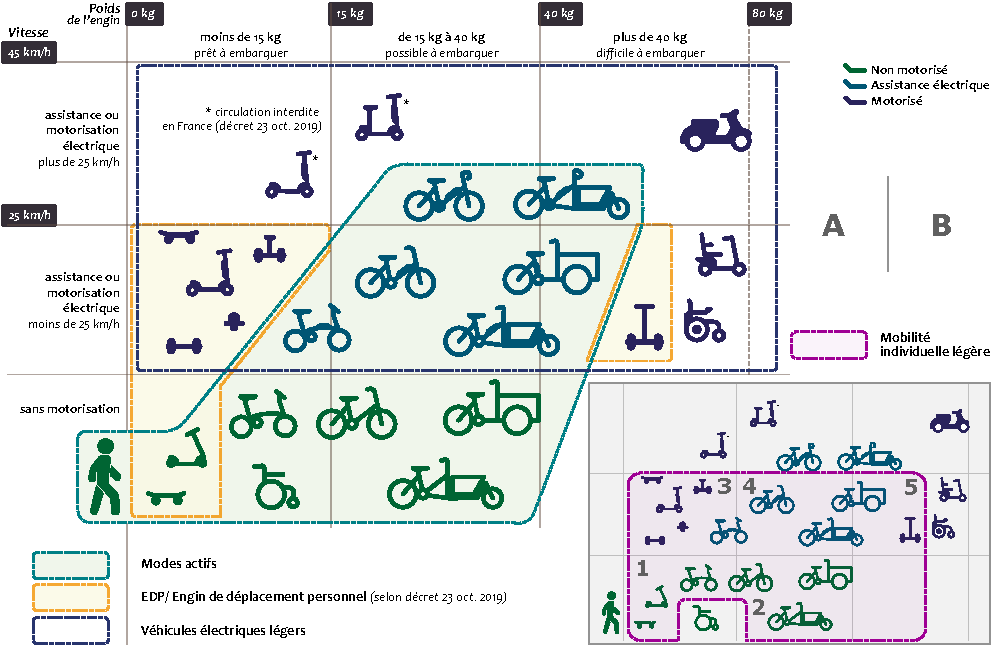
\includegraphics[width=1\columnwidth]{src/Figures/Chap-1/FR_Definition_perimetre_micromobilite.pdf}}
        \vspace{5pt}
        \begin{flushright}\scriptsize{
        Source (A)~: \textcolor{blue}{\textcite[61]{rabaud_quand_2022}}\index{Rabaud, Mathieu|pagebf}\index{Richer, Cyprien|pagebf}
        \\
        Adaptation graphique (B)~: \textcolor{blue}{Dylan Moinse (2023)}
        }\end{flushright}
    \end{figure}

    % Définition MIL
Dans ce cadre, nous proposons d’adopter une expression qui nous semble plus adaptée pour définir le périmètre de ces véhicules variés, tout en évitant les confusions liées à l’intégration de la marche ou des véhicules lourds. Cette réflexion s’appuie sur les travaux du programme ANR \acrfull{URFé}\footnote{
    Le projet, d'une durée de 42 mois, s’organise en trois volets dont le croisement permet de vérifier l’hypothèse d’un hiatus entre les pratiques effectives de mobilité et les logiques d’aménagement de l’espace~: (i) les usages, les pratiques effectives et les problèmes de sécurité, (ii) l'espace aménagé et le potentiel d'accueil vis-à-vis de la mobilité à faible impact environnemental et (iii) l'aménagement de l'espace, une action publique au prisme de la mobilité à faible impact environnemental \textcolor{blue}{\autocite{urfe_projet_2022}}.
}, sous la responsabilité scientifique de \textcolor{blue}{Frédérique Hernandez}. Ce projet de recherche examine l’hospitalité de l’espace urbain envers les nouvelles formes de mobilité à faible impact environnemental, en prenant pour terrains d’étude les aires urbaines de Lyon, de Lausanne, de Marseille~–~Aix-en-Provence et de Strasbourg \textcolor{blue}{\autocite{urfe_projet_2022}}\index{URFé@\textsl{URFé}|pagebf}. Bien que l’expression \textsl{modes de déplacement individuels à faible impact environnemental}, utilisée dans le cadre de ce projet, présente également des limites, selon nous, quant à la délimitation précise des véhicules concernés, nous avons choisi de retenir une autre notion empruntée à cette recherche~: celle de \Guillemets{mobilité individuelle légère}. Cette expression a été mise en avant lors du quatrième séminaire collectif du projet \acrshort{URFé}, tenu le 9 novembre 2022 au \acrshort{Cerema} Hauts-de-France, et nous paraît particulièrement pertinente pour regrouper les objets étudiés. En nous inspirant de la grille de lecture proposée par \textcolor{blue}{\textcite[61]{rabaud_quand_2022}}\index{Rabaud, Mathieu|pagebf}\index{Richer, Cyprien|pagebf}, dans leur chapitre intitulé \textsl{Quand les engins de déplacement personnel transforment la mobilité urbaine}, et en lien avec l’\hyperref[fig-chap1:perimetre-micromobilite]{illustration~\ref{fig-chap1:perimetre-micromobilite}} (page~\pageref{fig-chap1:perimetre-micromobilite}), nous proposons un périmètre de définition de la \Guillemets{mobilité individuelle légère} qui dépasse les cadres des \Guillemets{modes actifs}, des \acrshort{EDP}, des \Guillemets{véhicules électriques légers} et des \Guillemets{véhicules intermédiaires}. Ce périmètre vise à regrouper les véhicules relevant du vélo, de la micro-mobilité et de leurs multiples déclinaisons. Notre définition repose sur une intégration partielle des \gls{modes actifs}, à l’exclusion de la marche, ainsi que des \acrshort{EDP}, qui excluent les véhicules spécifiques aux personnes à mobilité réduite et une partie des véhicules intermédiaires dont les vitesses dépassent les limites réglementaires des engins de déplacement. Dès lors, la \Guillemets{mobilité individuelle légère} englobe une liste non exhaustive de véhicules parmi les plus populaires (voir  l’\hyperref[fig-chap1:perimetre-micromobilite]{illustration~\ref{fig-chap1:perimetre-micromobilite}}, page~\pageref{fig-chap1:perimetre-micromobilite})~:
    \begin{customitemize}
\item Véhicules à énergie musculaire de moins de 15 kilogrammes (cellule 1), comme le \textsl{skateboard}, la trottinette mécanique ou le vélo pliant~;
\item Véhicules à énergie musculaire entre 15 et 40 kilogrammes (cellule 2), comme le vélo classique, le vélo-cargo (ou biporteur) ou le triporteur~;
\item Véhicules électriques de moins de 15 kilogrammes, à une vitesse maximale de 25 kilomètres par heure (cellule 3), comme l'\textsl{hoverboard}, le monoroue, la \acrshort{TEP} ou le monocycle électrique~;
\item Véhicules à assistance électrique entre 15 et 40 kilogrammes, à une vitesse maximale de 25 kilomètres par heure (cellule 4), comme le vélo pliant électrique, le \acrshort{VAE}, le vélo-cargo électrique (ou biporteur électrique) ou le triporteur électrique~;
\item Véhicules électriques de plus de 40 kilogrammes, à une vitesse maximale de 25 kilomètres par heure (cellule 5), comme le gyropode~;
\item Services de vélos et de micro-mobilité partagés, de courte ou longue location, en libre-service avec ou sans borne d’attache (cellules 1 à 5), comme le vélo pliant en libre-service, le \acrshort{VLS}, la \acrshort{TEFF}, le \acrshort{VAE} en libre-service ou en \textsl{free-floating}, le vélo-cargo en libre-service ou le gyropode en location.
    \end{customitemize}%%Rédigé%%

    % Transition
Au sein de cette famille issue de la \Guillemets{mobilité individuelle légère}, nous conservons les sous-catégories associées au vélo et à ses diverses déclinaisons, telles que le vélo pliant, le \acrshort{VAE} ou le vélo-cargo, ainsi que la \Guillemets{micro-mobilité}, qui correspond principalement à la famille des \acrshort{EDP}. Ces véhicules partagent un certain nombre de caractéristiques communes~: ce sont des modes de déplacement individuels, bien que certains \Guillemets{modes intermédiaires} puissent accueillir un·e passager·ère supplémentaire. Leur vitesse de déplacement est limitée, ce qui permet d’instaurer une forme de proximité et d’interaction avec l’environnement urbain, s’inscrivant dans l’esprit d’une \textsl{slow city} \textcolor{blue}{\autocite[103-108]{bu_tout-voiture_2024}}\index{Bu, Ludovic|pagebf}. Par ailleurs, ces modes de déplacement se caractérisent par leur faible coût et par leur caractère plus inclusif, puisqu’ils ne nécessitent pas la possession d’un permis de conduire, ce qui les rend accessibles à un large éventail d’usager·ère·s. Ils reposent sur un système commun, conceptualisé sous le nom de \Guillemets{vélomobilité}, structuré autour d’un triptyque reposant sur les territoires, les individus et les usages \textcolor{blue}{\autocites[20-21]{rerat_au_2019}[492]{watson_how_2012}}\index{Rérat, Patrick|pagebf}\index{Watson, Matt|pagebf}. Ces véhicules présentent, par nature, un potentiel d'intermodalité~: ils sont soit facilement transportables dans les transports en commun, soit aisément adaptés au stationnement à proximité d’un nœud de transport public. C’est en raison de ces diverses qualités que nous allons désormais nous pencher plus précisément sur les synergies entre nos deux objets d’étude principaux~: les transports en commun et la mobilité individuelle légère, en nous appuyant sur le cadre théorique et stratégique du \acrshort{TOD}. Cette approche nous permettra d’examiner la manière dont le \acrshort{TOD} peut s’approprier non seulement le vélo, comme cela a été brièvement exploré dans le contexte des \textsl{Hybrid Transit Metropolises} telles que Copenhague, mais aussi les implications découlant de la récente diversification de l’offre en matière de mobilité individuelle légère. À travers cette analyse, il s’agira de mettre en lumière les liens synergiques entre ces deux systèmes.%%Rédigé%%

     % ___________________________________________
    % 1.3.
    \newpage
    \needspace{1\baselineskip} % Réserve de l'espace
    \sectionheader{Vers un \textsl{Micromobility-friendly Transit-Oriented Development}}
\section{Perspectives nouvelles pour un \textsl{Transit-Oriented Development} soutenu par l'intégration de la mobilité individuelle légère
    \label{chap1:btod}
    }

    % Introduction
L’amélioration des connaissances scientifiques relatives au développement des infrastructures de transport en commun a permis de mesurer combien elles ne suffisent pas, à elles seules, à constituer une alternative viable à l’\Guillemets{autosolisme}\footnote{
    L'\Guillemets{autosolisme} est le fait de circuler en automobile, non accompagné·e. C'est un usage dérivé du mot \Guillemets{autosoliste}. Un dictionnaire militant définit ce terme comme \Guillemets{\textsl{l'action de se déplacer seul au volant d’une voiture, et d’encombrer, ainsi, l’espace collectif, de polluer, de faire du bruit, de stresser pour le profit d’une personne unique~: le chauffeur !}} \textcolor{blue}{\autocite{carfreefr_dictionnaire_2008}}\index{Carfree.fr@\textsl{Carfree.fr}|pagebf}. Occasionnellement, l'antonyme \Guillemets{automultisme} peut apparaître, mais il est plus courant de parler de \Guillemets{covoiturage}.
}, en tout point du territoire \textcolor{blue}{\autocite[8]{molino_pratiques_2015}}\index{Molino, Marie|pagebf}\index{Rampon, Anne-Sophie|pagebf}\index{Cipolla, Romain|pagebf}. Le développement traditionnel de l’offre de transport public appelle une action simultanée sur la demande. En effet, pour réduire efficacement le trafic automobile, plusieurs stratégies peuvent être envisagées. Soit une réduction de l'aire urbanisée, difficilement faisable et acceptable. Soit une densification de la desserte en transport public, qui risque cependant de nuire à la performance du réseau en raison d'un nombre important d'arrêts, et ainsi compromettre sa compétitivité face à l'automobile. Soit une amélioration de l’accessibilité aux stations, option jugée la plus réaliste \textcolor{blue}{\autocite[10]{verbavatz_critical_2019}}\index{Verbavatz, Vincent|pagebf}\index{Barthelemy, Marc|pagebf}. Il ressort des recherches que le facteur déterminant du transfert modal de la voiture vers les transports en commun est l’accessibilité aux stations, plutôt que l’amélioration qualitative du service \textcolor{blue}{\autocite[146]{brons_access_2009}}\index{Brons, Martijn|pagebf}\index{Givoni, Moshe|pagebf}\index{Rietveld, Piet|pagebf}. Cette observation rejoint le principe fondateur, selon lequel la mobilité au sein des quartiers de gare, et en particulier la priorité donnée à la marche et au vélo combinés, constitue un levier central pour la réussite d’une intervention de type \acrshort{TOD}. Pourtant, ces modes de déplacement, bien qu’essentiels à la planification urbaine orientée vers le transport public, restent souvent invisibilisés ou traités de manière banale, alors qu’ils jouent un rôle déterminant dans le succès ou l’échec d’un projet \acrshort{TOD} \textcolor{blue}{\autocite[34]{schlossberg_comparing_2004}}\index{Schlossberg, Marc|pagebf}\index{Brown, Nathaniel|pagebf}. Face à l’\Guillemets{explosion périurbaine}, la performance et l’attractivité des réseaux de transport public se sont considérablement amoindries, en raison de l’allongement des distances et de la dispersion des pôles d’emplois \textcolor{blue}{\autocite[13]{bentayou_transit-oriented_2015}}\index{Bentayou, Gilles|pagebf}. Dans ce contexte, l’approche intermodale intégrant le vélo apparaît comme la réponse la plus adaptée aux enjeux des \Guillemets{premiers et derniers kilomètres}. Le vélo et le transport public doivent ainsi entretenir une relation symbiotique~: au-delà d’un simple mode de rabattement, le vélo doit être pleinement intégré à l’expérience de voyage, en raison de la forte compétitivité de cette combinaison modale face à la voiture individuelle \textcolor{blue}{\autocite[208]{kager_characterisation_2016}}\index{Kager, Roland|pagebf}\index{Bertolini, Luca|pagebf}\index{te Brömmelstroet, Marco|pagebf}. Au-delà du seul vélo, il est aujourd’hui opportun d’évaluer si les \Guillemets{nouvelles mobilités} qui gravitent autour de celui-ci peuvent renforcer cette dynamique. Ces modes émergents pourraient en effet s’inscrire dans une logique de \Guillemets{bouquet d’offres de modes et de services} visant à maximiser les bénéfices d’un système de mobilité alternatif plus sobre dans la consommation des ressources \textcolor{blue}{\autocite[134]{litman_new_2021}}\index{Litman, Todd|pagebf}.%%Rédigé%%

    % Annonce du plan
Dans un premier temps, nous allons parcourir la règle arbitraire des périmètres accessibles à pied autour des aires \acrshort{TOD}\textcolor{blue}{s} et, plus largement, la nécessité d’étendre les quartiers de gare grâce à une approche intermodale. Nous allons voir que les études montrent combien la marche combinée peut s’étendre bien au-delà du périmètre géographique qui lui est généralement attribué, tout en soulignant que sa portée, bien que pertinente, demeure insuffisante pour garantir un accès optimal aux nœuds de transport, dans un contexte de périurbanisation. Il apparaît ainsi essentiel d’intégrer d’autres modes de déplacement permettant d’atteindre des destinations plus éloignées, afin de renforcer la complémentarité modale et d’optimiser l’accessibilité aux nœuds (\hyperref[chap1:btod-limites-tod]{section sur une relecture de la marche combinée, page~\pageref{chap1:btod-limites-tod}}). Dans cette perspective, nous allons examiner les avantages comparatifs de la mobilité individuelle légère, qui apparaît comme une alternative particulièrement appropriée pour limiter le recours excessif à l’automobile. Cette réflexion va nous conduire à aborder la récente déclinaison d'un \acrfull{B-TOD}, ou d'un urbanisme orienté vers les réseaux de transport en commun et intégrant le vélo, qui met en avant les potentialités du vélo dans l’extension des aires d’influence des stations de transport public. Enfin, au regard de la diversité modale évoquée précédemment dans ce chapitre, nous allons nous interroger sur l'intérêt d'une conceptualisation plus englobante intégrant la mobilité individuelle légère, au travers d’un \acrfull{M-TOD} (\hyperref[chap1:btod-definition]{section sur une combinaison modale tirant parti de la vitesse et d'une accessibilité \Guillemets{porte-à-porte}, page~\pageref{chap1:btod-definition}}).%%Rédigé%%

    % 1.3.1.
    \needspace{1\baselineskip} % Réserve de l'espace
\subsection{Vers un \Guillemets{éclatement de la bulle} des poches piétonnières
    \label{chap1:btod-limites-tod}
    }

    % Introduction
La notion de \Guillemets{poche piétonnière} (\textsl{pedestrian pocket}), antérieure au \acrshort{TOD}, repose sur la délimitation d’une zone au sein de laquelle la marche constitue le mode de déplacement privilégié et où se concentrent les principales activités quotidiennes \textcolor{blue}{\autocite[3]{kelbaugh_pedestrian_1989}}\index{Kelbaugh, Doug|pagebf}. Bien que largement intégrée au concept d’aménagement, l’aire d’influence piétonne des gares est souvent définie sur la base de frontières arbitraires, qui ne reflètent pas nécessairement les pratiques réelles des voyageur·se·s et peuvent ainsi entraîner une inadéquation entre le périmètre des quartiers de gare et les parcours effectifs des usager·ère·s. À partir de ce constat, nous rejoignons la littérature scientifique récente qui appelle à reconsidérer la portée réelle de la marche combinée. En effet, les cheminements piétons vers et depuis une station ne se limitent pas à l’échelle immédiate de la gare, mais influencent également la distance spatio-temporelle que les usager·ère·s sont disposé·e·s à parcourir \textcolor{blue}{\autocite[52]{el_hadeuf_ville_2017}}\index{El Hadeuf, Mounya|pagebf}\index{Laterrasse, Jean|pagebf}. Dans cette perspective, nous proposons d’exploiter cet \Guillemets{éclatement de la bulle} \textcolor{blue}{\autocite[33]{guerra_half-mile_2012}}\index{Guerra, Erick|pagebf} comme une une occasion de redéfinir l’aménagement des territoires en adoptant une approche systémique, ou intégratrice \textcolor{blue}{\autocite[56]{kaufmann_retour_2014}}\index{Kaufmann, Vincent|pagebf} sur les atouts que présente l'intermodalité-voyageur·se·s. Une telle démarche permettrait d’envisager des espaces véritablement orientés vers les transports en commun, définis à une échelle spatiale plus pertinente et susceptibles d’optimiser le report modal vers le réseau de transport public.%%Rédigé%%

    % 1.3.1.1.
    \needspace{1\baselineskip} % Réserve de l'espace
\subsubsection*{Remise en question de la \textsl{doxa} de \Guillemets{poches piétonnières} confinées
    \label{chap1:btod-limites-tod-marche-restreinte}
    }

    % Doxa
En France, comme nous l’avons observé, nous assistons souvent à une mise en œuvre de principes proches du \Guillemets{\acrshort{TOD} sans le dire} \textcolor{blue}{\autocite[273]{lo_feudo_scenario_2014}}\index{Lo Feudo, Fausto|pagebf}\index{Menerault, Philippe|pagebf}\index{L'Hostis, Alain|pagebf}\index{Festa, Demetrio Carmine|pagebf}. Cette multiplicité d’interventions sur le territoire, apparentée à ce concept d’aménagement, se limite fréquemment à des actions ponctuelles telles que le renouvellement architectural des gares ou le réaménagement des espaces adjacents, accordant moins d’attention aux échelles plus larges, notamment le quartier de gare et son insertion dans la métropole \textcolor{blue}{\autocite[50]{bentayou_transit-oriented_2015}}\index{Bentayou, Gilles|pagebf}. Lorsque les projets \acrshort{TOD}\textcolor{blue}{s} ciblent spécifiquement les aires d’influence piétonnes des nœuds de transport en commun, ils s’appuient sur une référence communément admise~: celle des 500 mètres ou des 800 mètres, la dernière équivalant à 10 minutes de marche \textcolor{blue}{\autocite[1]{lhostis_perimetres_2016}}\index{L'Hostis, Alain|pagebf}, souvent définie comme une \Guillemets{aire pédestre} (\textsl{pedestrian pocket}). \textcolor{blue}{Peter} \textcolor{blue}{\textcite[56]{calthorpe_next_1993}}\index{Calthorpe, Peter|pagebf} préconise des communautés conçues à moins de 600 mètres (environ 2~000 pieds) d’un arrêt. \textcolor{blue}{\textcite[12]{bertolini_cities_2015}}\index{Bertolini, Luca|pagebf}\index{Spit, Tejo|pagebf}, dans leur ouvrage \foreignlanguage{english}{\textsl{Cities on Rails: The Redevelopment of Railway Stations and their Surroundings}} confirment qu’un périmètre de dix minutes à pied constitue une distance-temps acceptable pour accéder à une station. Une revue de littérature sur les périmètres d’action autour des gares, réalisée par \textcolor{blue}{\textcite[102]{guerra_half-mile_2012}}\index{Guerra, Erick|pagebf}\index{Cervero, Robert|pagebf}\index{Tischler, Daniel|pagebf}, montre cependant que cette norme des 400 à 800 mètres est fréquemment mobilisée sans qu’elle repose nécessairement sur des justifications techniques. Pourtant, comme nous l’avons vu dans l’évolution de la pensée du \acrshort{TOD}, l’un des \Guillemets{5Ds} associés à ce concept, la distance aux stations (\textsl{Distance to Transit}), est une équation centrale pour mesurer l’accessibilité au transport en commun \textcolor{blue}{\autocite[267]{ewing_travel_2010}}\index{Ewing, Reid|pagebf}\index{Cervero, Robert|pagebf}. Au cours de la dernière décennie, des recherches ont cherché à remettre en question cette norme internationale du \Guillemets{800 mètres} (\textsl{half-mile distance}), devenue un standard dans les projets \acrshort{TOD}\textcolor{blue}{s} \textcolor{blue}{\autocite[102]{guerra_half-mile_2012}}\index{Guerra, Erick|pagebf}\index{Cervero, Robert|pagebf}\index{Tischler, Daniel|pagebf}. L’objectif est d’\Guillemets{éclater la bulle} piétonnière (\textsl{busting the bubble}) \textcolor{blue}{\autocite[33]{guerra_half-mile_2012}}\index{Guerra, Erick|pagebf}, c’est-à-dire de dépasser les limites envisagées de la marche combinée. Cela ouvre la voie à un modèle \acrshort{TOD} réinterprété, dépassant la métaphore spatiale de la \Guillemets{bulle cible} (\textsl{the bull’s eye concept}) \textcolor{blue}{\autocite[28]{curtis_transit_2009}}\index{Curtis, Carey|pagebf}\index{Renne, John Luciano|pagebf}\index{Bertolini, Luca|pagebf}.%%Rédigé%%

    % Documents d'urbanisme
Cette règle communément admise, reposant sur le périmètre piétonnier de 800 mètres, est fréquemment appliquée et visible dans les documents d’orientation en matière d’aménagement du territoire. Les aménageur·se·s utilisent typiquement cette limite comme périmètre d’action urbaine autour des gares \textcolor{blue}{\autocite[40]{olszewski_using_2005}}\index{Olszewski, Piotr~S.|pagebf}\index{Wibowo, Sony Sulaksono|pagebf}. Déjà dans le \textsl{Schéma Régional des Transports} de l’ancienne \textcolor{blue}{\textcite[21]{region_nord-pas-de-calais_schema_2006}}\index{Région Nord-Pas-de-Calais@\textsl{Région Nord-Pas-de-Calais}|pagebf}, la marche était identifiée comme un mode à privilégier pour les trajets en rabattement, dits de \Guillemets{courte distance}, vers les arrêts de bus ou de car, les gares et les pôles d’échange. Le \acrfull{PDU} 2010-2020 de la \acrfull{MEL} a intégré cette approche en définissant des \acrfull{DIVAT}, correspondant à des espaces stratégiques situés autour des gares métropolitaines, des stations de métro et de tramway, ainsi que des arrêts de \acrfull{BHNS}. Ces périmètres stratégiques prennent alors la forme d’un cercle de 500 mètres de rayon \textcolor{blue}{\autocite[39]{lmcu_plan_2011}}\index{LMCU@\textsl{LMCU}|pagebf}. En cohérence avec ce \acrshort{PDU}, les \acrshort{DIVAT} ont été fidèlement repris dans le \acrfull{PLH} 2012-2018 de la \acrshort{MEL}, avec un élargissement aux arrêts de bus enregistrant plus de soixante passages quotidiens, tous sens confondus \textcolor{blue}{\autocite[4]{lmcu_2e_2012}}\index{LMCU@\textsl{LMCU}|pagebf}. Ces principes ont ensuite été intégrés dans le \acrfull{PLUi} de 2020 de l’\acrfull{EPCI}, renforçant ainsi la cohérence entre les différents outils de planification territoriale \textcolor{blue}{\autocite[44]{metropole_europeenne_de_lille_plan_2019-3}}\index{LMCU@\textsl{LMCU}|pagebf}. Cependant, certaines études stratégiques ont revu ces périmètres de gare pour les adapter à des contextes variés. Par exemple, l’Observatoire des quartiers de gare du Grand Paris Express avait d'abord défini un périmètre de 800 mètres à vol d’oiseau pour les 69 gares en construction \textcolor{blue}{\autocite[1]{apur_observatoire_2017}}\index{Apur@\textsl{Apur}|pagebf}. Ce cadre a ensuite évolué pour proposer deux autres niveaux~: 500 mètres pour stations situées dans l'hypercentre et 1~000 mètres pour les gares \acrfull{RER} et celles du Grand Paris Express \textcolor{blue}{\autocite[13]{apur_observatoire_2018}}\index{Apur@\textsl{Apur}|pagebf}. Enfin, une attention particulière a été accordée à un rayon de 2~000 mètres pour l’échelle cyclable \textcolor{blue}{\autocite[22]{apur_observatoire_2018}}\index{Apur@\textsl{Apur}|pagebf}.%%Rédigé%%

    % Eclatement aires primaires
D'aucun·e·s considèrent que la marche combinée peut atteindre des distances spatio-temporelles bien supérieures à celles dictées par la règle d’origine anglo-saxonne des 400 ou 800 mètres, ou encore des 10 minutes, au sein du périmètre de l’\Guillemets{aire primaire} telle qu’imaginée par \textcolor{blue}{Peter} \textcolor{blue}{\textcite[56]{calthorpe_next_1993}}\index{Calthorpe, Peter|pagebf}. Dans une revue de littérature, le chercheur en géographie, spécialisé dans l'aménagement et la mobilité, \textcolor{blue}{Alain} \textcolor{blue}{\textcite[5]{lhostis_perimetres_2016}}\index{L'Hostis, Alain|pagebf} met en évidence que certaines gares ferroviaires ou stations de métro européennes enregistrent des déplacements à pied atteignant aisément un à deux kilomètres de distance spatiale. La pratique de la marche combinée (\textsl{walk-and-ride}) autour des nœuds de transport en commun bien desservis, bénéficiant de fréquences élevées, d’une desserte étendue et d’une bonne accessibilité, est ainsi marquée par un étirement de ses distances socialement acceptées. Ces quartiers, à la fois denses, mixtes et avec une haute qualité de conception de ses espaces publics, notamment en termes de \gls{marchabilité}, incarnent les principes des quartiers \acrshort{TOD}\textcolor{blue}{s}. Les recherches montrent que dans ce contexte, les trajets à pied dépassent largement le seuil des 800 mètres traditionnellement admis \textcolor{blue}{\autocites[79]{ker_myths_2003}[7]{lhostis_perimetres_2016}[30]{hasiak_access_2019}}\index{Hasiak, Sophie|pagebf}\index{L'Hostis, Alain|pagebf}\index{Ker, Ian|pagebf}\index{Ginn, Simon|pagebf}.%%Rédigé%%

    % Figure Corridor Piéton
    \begin{carte}[h!]\vspace*{4pt}
        \caption{Extension du quartier de gare par la valorisation d'un corridor densifié et accessible à pied.}
        \label{fig-chap1:tod-corridor-pieton}
        \centerline{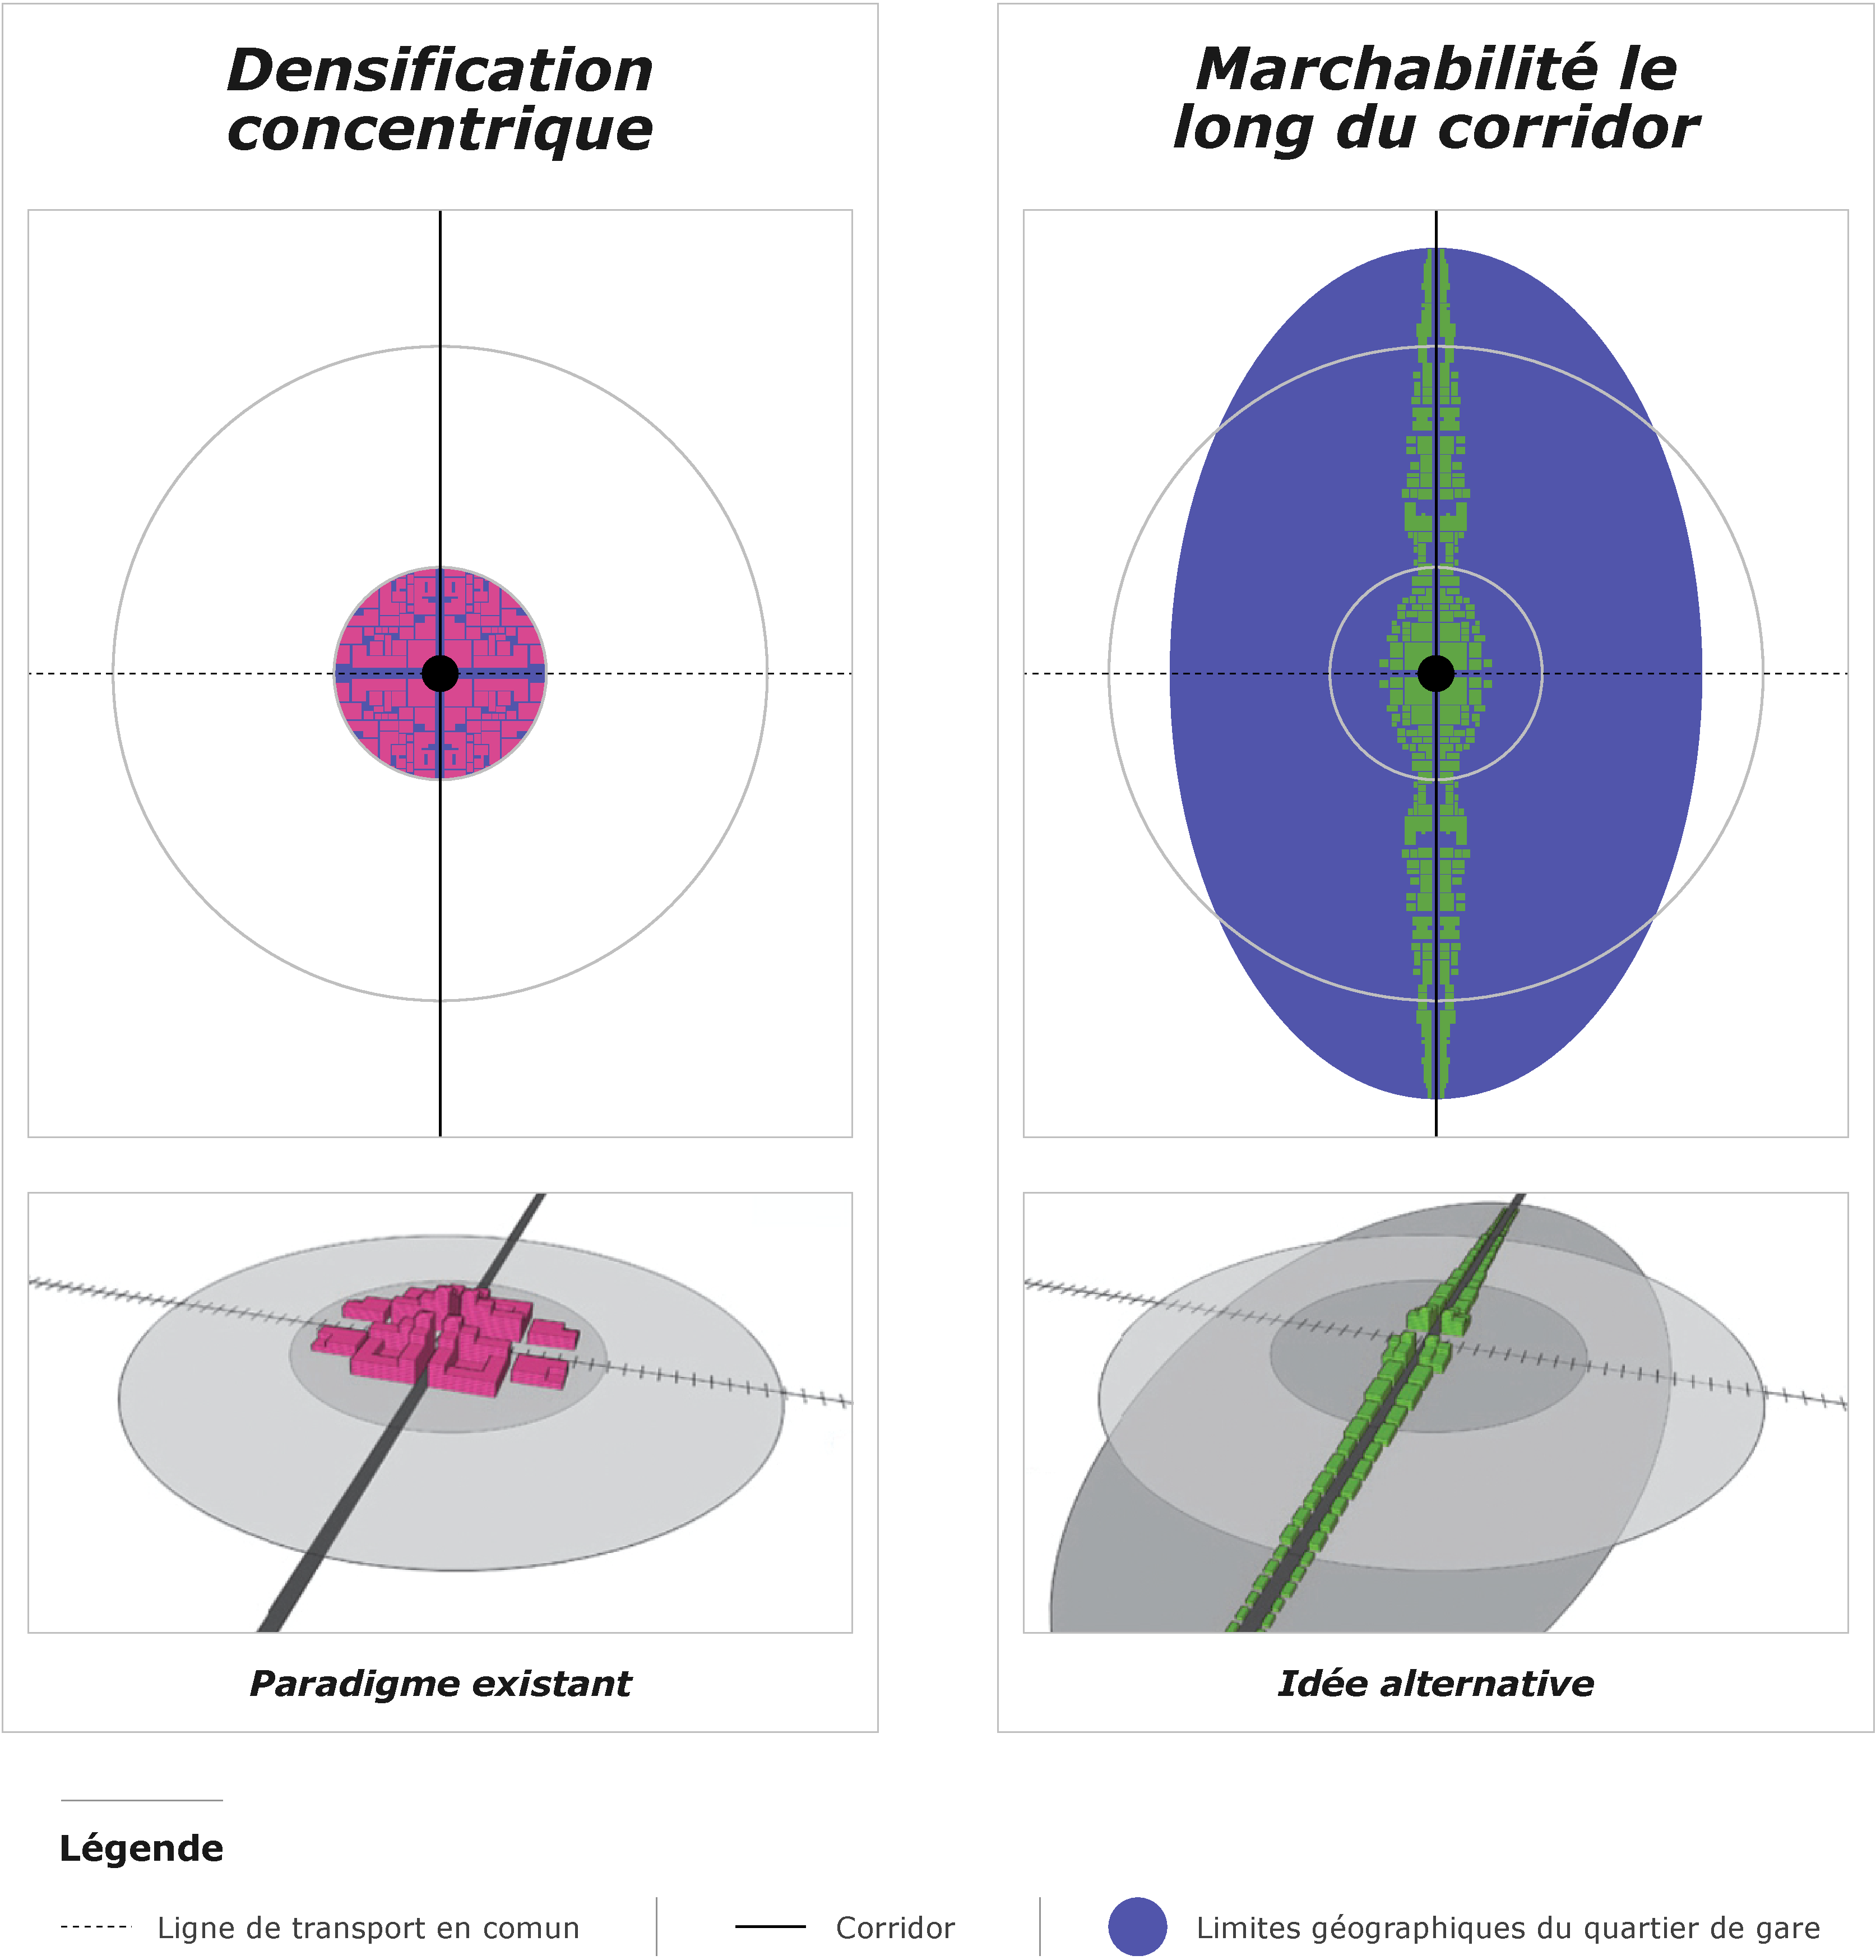
\includegraphics[width=1\columnwidth]{src/Figures/Chap-1/FR_Corridor_pieton.pdf}}
        \vspace{5pt}
        \begin{flushright}\scriptsize{
        Source~: \textcolor{blue}{\textcite[163]{park_can_2015}}\index{Park, Sungjin|pagebf}\index{Deakin, Elizabeth|pagebf}\index{Jang, Kitae|pagebf}
        \\
        Adaptation graphique~: \textcolor{blue}{Dylan Moinse (2025)}
        }\end{flushright}
    \end{carte}

    % Exemples
De nombreuses études s’intéressent aujourd’hui à la distance parcourue par les voyageur·se·s pour se rendre ou sortir à pied d'une station de transport en commun, soutenant généralement une sous-calibration globale des périmètres piétonniers traditionnellement admis autour de ces nœuds. En moyenne, les piéton·ne·s qui accèdent à une gare ou une station de métro parcourent 1 kilomètre, que ce soit à San Francisco \textcolor{blue}{\autocite[5]{cervero_walk-and-ride_2001}}\index{Cervero, Robert|pagebf} ou à Singapour \textcolor{blue}{\autocite[41]{olszewski_using_2005}}\index{Olszewski, Piotr~S.|pagebf}\index{Wibowo, Sony Sulaksono|pagebf}. En s’appuyant sur le 85\textsuperscript{e} centile de la distribution cumulative des distances parcourues, des études ont montré qu’une distance de 1 kilomètre (soit environ 12 minutes à pied) est jugée acceptable autour des stations de métro à Beijing \textcolor{blue}{\autocite[720]{yang_study_2013}}\index{Yang, Rongrong|pagebf}\index{Yan, Hai|pagebf}\index{Xiong, Wen|pagebf}\index{Liu, Tao|pagebf}, tandis que des distances légèrement supérieures, de 1,2 (en rabattement) et 1,1 kilomètres (en diffusion), sont observées autour des gares à Montréal \textcolor{blue}{\autocite[9]{el-geneidy_pedestrian_2009}}\index{El-Geneidy, Ahmed~M.|pagebf}\index{Tétreault, Paul|pagebf}\index{Surprenant-Legault, Julien|pagebf}. Au sud-est de l’Angleterre, les distances atteignent même 1,6 kilomètre autour des gares \textcolor{blue}{\autocite[14]{bunn_how_2015}}\index{Bunn, Nick|pagebf}\index{Wakenshaw, Gareth|pagebf}. Dans le cas du Nord-Pas-de-Calais, le 90\textsuperscript{e} centile des voyageur·se·s ferroviaires révèle que les distances parcourues peuvent atteindre 20 minutes à pied, contre une moyenne observée de 11 minutes \textcolor{blue}{\autocite[17]{hasiak_estimation_2018}}\index{Hasiak, Fabrice|pagebf}\index{Lannoy, Arnaud|pagebf}\index{Bodard, Géraldine|pagebf}\index{Palmier, Patrick|pagebf}. Ces variations témoignent de l’influence majeure de certains paramètres de l’environnement urbain, qui peuvent dilater ou contracter ces distances perçues \textcolor{blue}{\autocite[17]{soest_exploring_2020}}\index{Soest, Dennis van|pagebf}\index{Tight, Miles~R.|pagebf}\index{Rogers, Christopher~D.~F.|pagebf}. Déjà en 1984, \textcolor{blue}{Richard~k.} \textcolor{blue}{\textcite[23-59]{untermann_accommodating_1984}}\index{Untermann, Richard~K.|pagebf}, dans son livre \foreignlanguage{english}{\textsl{Accommodating the Pedestrian: Adapting Towns and Neighborhoods for Walking and Biking}}, montrait que la portée maximale de la marche dans les territoires périurbains, souvent confinée dans des seuils rigides de 400, 500 ou 800 mètres, pouvait être considérablement étendue~–~voire doublée~–~en aménageant des espaces urbains attrayants et des corridors agréables pour les piéton·ne·s. Les recherches plus récentes confirment que la diversité urbaine joue un rôle clé. Par exemple, une étude comparative menée entre Beijing, Tianjin et Shenzhen indique que les voyageur·se·s à pied doublent souvent leurs distances parcourues lorsque l’environnement urbain présente une mixité élevée, avec des commerces et des bureaux à proximité des stations \textcolor{blue}{\autocite[12]{zacharias_local_2017}}\index{Zacharias, John|pagebf}\index{Zhao, Qi|pagebf}. De même, en Australie comme aux États-Unis, les voyageur·se·s sont disposé·e·s à parcourir jusqu’à 800 mètres supplémentaires lorsque l’environnement urbain suit les principes du \acrshort{TOD} \textcolor{blue}{\autocite[33]{canepa_bursting_2007}}\index{Canepa, Brian|pagebf}. L’amélioration des éléments de \Guillemets{micro-marchabilité} (\textsl{microwalkability}), notamment par l’aménagement stratégique de corridors piétonniers, apparaît comme un levier déterminant pour étendre ces périmètres spatiaux. Ainsi, \textcolor{blue}{\textcite[163]{park_can_2015}}\index{Park, Sungjin|pagebf}\index{Deakin, Elizabeth|pagebf}\index{Jang, Kitae|pagebf} montrent qu’il est possible d’encourager les usager·ère·s du transport public à parcourir des distances bien plus importantes en améliorant ces infrastructures piétonnes (voir la \hyperref[fig-chap1:tod-corridor-pieton]{carte~\ref{fig-chap1:tod-corridor-pieton}}, page~\pageref{fig-chap1:tod-corridor-pieton}). Par exemple, l’aménagement de rues piétonnes autour des gares permet d’augmenter de 20~\% la portée jugée acceptable de la marche à destination des gares aux États-Unis, et jusqu’à 120~\% en Allemagne \textcolor{blue}{\autocite[151]{zielstra_comparative_2011}}\index{Zielstra, Dennis|pagebf}\index{Hochmair, Hartwig~H.|pagebf}.%%Rédigé%%

    % Conclusion + Transition
Qu’il s’agisse d’une aire d’influence accessible à pied, représentée sous la forme d’une étendue euclidienne (cercle) ou calculée sur la base de la voirie (isodistance ou isochrone), la règle arbitraire des 800 mètres ou des 10 minutes à pied relève davantage d’un artéfact historique que d’une construction analytique et statistique \textcolor{blue}{\autocite[102]{guerra_half-mile_2012}}\index{Guerra, Erick|pagebf}\index{Cervero, Robert|pagebf}\index{Tischler, Daniel|pagebf}. Cette règle, bien que communément utilisée, démontre ses limites. En effet, si le périmètre d'\Guillemets{aire primaire} des stations de transport en commun évalué à 800 mètres n'est pas fondamentalement erroné~–~les moyennes enregistrées pour le rail interurbain atteignant souvent 1~000 mètres~–, la véritable différence réside dans la méthode de mesure. En adoptant une approche basée sur la distance \Guillemets{acceptable} (en considérant les 85 ou 90\textsuperscript{e} centiles) plutôt que simplement observable, il apparaît clairement que les périmètres piétonniers traditionnels sous-évaluent les véritables distances parcourues et vécues par les usager·ère·s. Par exemple, une étude démontre que les seuils traditionnels de 400 et 800 mètres sous-estiment de 30~\% la couverture réelle du transport public accessible à pied dans la région montréalaise \textcolor{blue}{\autocite[20]{el-geneidy_new_2014}}\index{El-Geneidy, Ahmed~M.|pagebf}\index{Grimsrud, Michael|pagebf}\index{Wasfi, Rania|pagebf}\index{Tétreault, Paul|pagebf}\index{Surprenant-Legault, Julien|pagebf}. Cela met en évidence la nécessité de dépasser la conception classique de la marche. En France, bien que la durée moyenne des déplacements piétons soit de 13 minutes, il convient de différencier la marche monomodale et la marche combinée, utilisée comme mode de liaison vers les stations de transport en commun. En effet, si quatre déplacements piétons sur cinq en France durent moins de 15 minutes, ceux associés à la marche combinée atteignent fréquemment 20 minutes autour des gares \textcolor{blue}{\autocite[23]{solere_mobilite_2010}}\index{Solere, Régis de|pagebf}\index{Papon, Francis|pagebf}. Cette portée accrue de la marche combinée est de plus en plus reconnue dans la recherche académique, qui la considère extensible en fonction de facteurs favorisant le potentiel \acrshort{TOD} des territoires, tels que la densité urbaine, la mixité fonctionnelle ou la qualité des infrastructures piétonnes. Toutefois, dans les quartiers périphériques, où les distances requises pour accéder au transport public sont bien plus importantes, la marche seule ne suffit pas à corriger ces déséquilibres \textcolor{blue}{\autocite[85]{cervero_bike-and-ride_2013}}\index{Cervero, Robert|pagebf}\index{Caldwell, Benjamin|pagebf}\index{Cuellar, Jesus|pagebf}. Pour dépasser la dichotomie entre la marche et le transport public en zone centrale, et la voiture en intermodalité en zone périurbaine, le vélo peut constituer le maillon manquant de la chaîne intermodale. Or, bien que la littérature académique et technique se concentre presque exclusivement sur l’accessibilité des stations à pied, l’accessibilité à vélo demeure largement marginalisée et sous-étudiée \textcolor{blue}{\autocite[283]{martens_bicycle_2004}}\index{Martens, Karel|pagebf}. Cette lacune représente un défi à relever pour intégrer pleinement le vélo dans les stratégies d’accessibilité et d’intermodalité, en particulier dans les territoires où les distances dépassent les capacités traditionnelles de la marche.%%Rédigé%%

    % 1.3.1.2.
    \needspace{1\baselineskip} % Réserve de l'espace
\subsubsection*{Corriger les faiblesses du transport public par une approche intermodale
    \label{chap1:btod-definition-intermodalite}
    }

    % Limitations de la marche
Au regard des limitations liées à la portée de la marche, qui rend parfois l’accès aux stations de transport en commun contraignant, l’efficacité du \acrshort{TOD} est aujourd’hui interrogée. En effet, la croissance urbaine des territoires s’est majoritairement appuyée sur des distances adaptées à l’échelle de l’automobile, se traduisant par un étalement urbain souvent assimilé à une forme de \Guillemets{suburbanisation}. Par ailleurs, le transport public, bien qu’efficace sur certains aspects, ne dispose pas de l’ensemble des avantages de flexibilité associés à l’automobile \textcolor{blue}{\autocite[209]{heran_retour_2015}}\index{Héran, Frédéric|pagebf}. Cette situation remet en question la capacité du modèle urbain à lutter efficacement contre la dépendance aux modes motorisés. Les transports en commun ne représentent qu’une solution partiellement adaptée pour réduire le recours excessif à l’automobile. Une alternative réside alors dans la promotion de l’intermodalité, qui permettrait de pallier la rigidité du réseau de transport en commun \textcolor{blue}{\autocite[17]{wiel_comment_1998}}\index{Wiel, Marc|pagebf} et d’améliorer l’efficacité globale du système de mobilité \textcolor{blue}{\autocite[82]{oostendorp_combining_2018}}\index{Oostendorp, Rebekka|pagebf}\index{Gebhardt, Laura|pagebf}. En effet, l’intermodalité contribue à étendre l’aire d’influence des nœuds en y intégrant des solutions complémentaires \textcolor{blue}{\autocite[16]{amar_homo_2016}}\index{Amar, Georges|pagebf}, ce qui pourrait renforcer leur pertinence dans des contextes urbains et périurbains marqués par la dépendance automobile.%%Rédigé%%

    % Intermodalité
L’interconnexion désigne la liaison entre deux ou plusieurs réseaux de transport hétérogènes dans leurs dimensions techniques, organisationnelles et institutionnelles, souvent associés à des échelles de mobilité distinctes \textcolor{blue}{\autocites[]{dupuy_reseaux_1988}{varlet_interconnexion_1992}}\index{Dupuy, Gabriel|pagebf}\index{Varlet, Jean|pagebf}. L’intérêt de cette transition entre différents régimes de mobilité réside dans la capacité à dépasser la simple juxtaposition de réseaux monomodaux qui n'ont pas été pensés pour être coordonnés. Cette approche permet de mieux comprendre le \Guillemets{concept-interface} qui met en relation plusieurs vitesses de déplacement et plusieurs échelles spatiales \textcolor{blue}{\autocite[156]{peters_time_1960}}\index{Peters, Peter Frank|pagebf}. Cette intégration intermodale donne lieu à la formation d’un méta-réseau, défini comme un réseau de réseaux effectifs. Il s’agit d’un emboîtement multiscalaire de systèmes qui, par leur interconnexion, créent un mégasystème intégré \textcolor{blue}{\autocite[89]{ageron_intermodalite-voyageurs_2013}}\index{Ageron, Pierre|pagebf}\index{Varlet, Jean|pagebf}. L’intermodalité-voyageur·se·s devient ainsi un objet-système, comme organisation actorielle géographiquement située, génératrice de lieux et de pratiques \textcolor{blue}{\autocite[15]{varlet_interconnexion_1992}}\index{Varlet, Jean|pagebf}. Liée en grande partie à un mode de transport en commun, l’intermodalité-voyageur·se·s est reconnue comme l’option la plus économique en termes de ressources, en tenant compte du temps de parcours, du coût ou de la consommation d’énergie pour effectuer un déplacement entre un point A et un point B \textcolor{blue}{\autocite[73]{oostendorp_combining_2018}}\index{Oostendorp, Rebekka|pagebf}\index{Gebhardt, Laura|pagebf}. En ce sens, la mise en correspondance, l’interconnexion et l’intermodalité des réseaux constituent des facteurs d’efficacité qui s’inscrivent dans le cadre du principe de \Guillemets{reliance}. Ce dernier, en tant que créateur de liens et de synergies entre des flux de nature variée, sous-tend de nouvelles formes d’optimisation des réseaux \textcolor{blue}{\autocite[16-17]{amar_homo_2016}}\index{Amar, Georges|pagebf}. Cette évolution s’accompagne d’une diversification modale croissante, favorisée par des processus de (ré)invention, d’innovation technique et servicielle, ainsi que par des phénomènes d’hybridation modale. Ces dynamiques dépassent la vision binaire du simple report modal de la voiture au transport en commun, pour promouvoir une approche multimodale et intermodale \textcolor{blue}{\autocite{richer_dossier_2021}}\index{Richer, Cyprien|pagebf}.

    % Figure fonctions et composantes intermodalité
    \begin{figure}[h!]\vspace*{4pt}
        \caption{Fonctions et composantes du système intermodal.}
        \label{fig-chap1:composantes-fonctions-intermodalite}
        \centerline{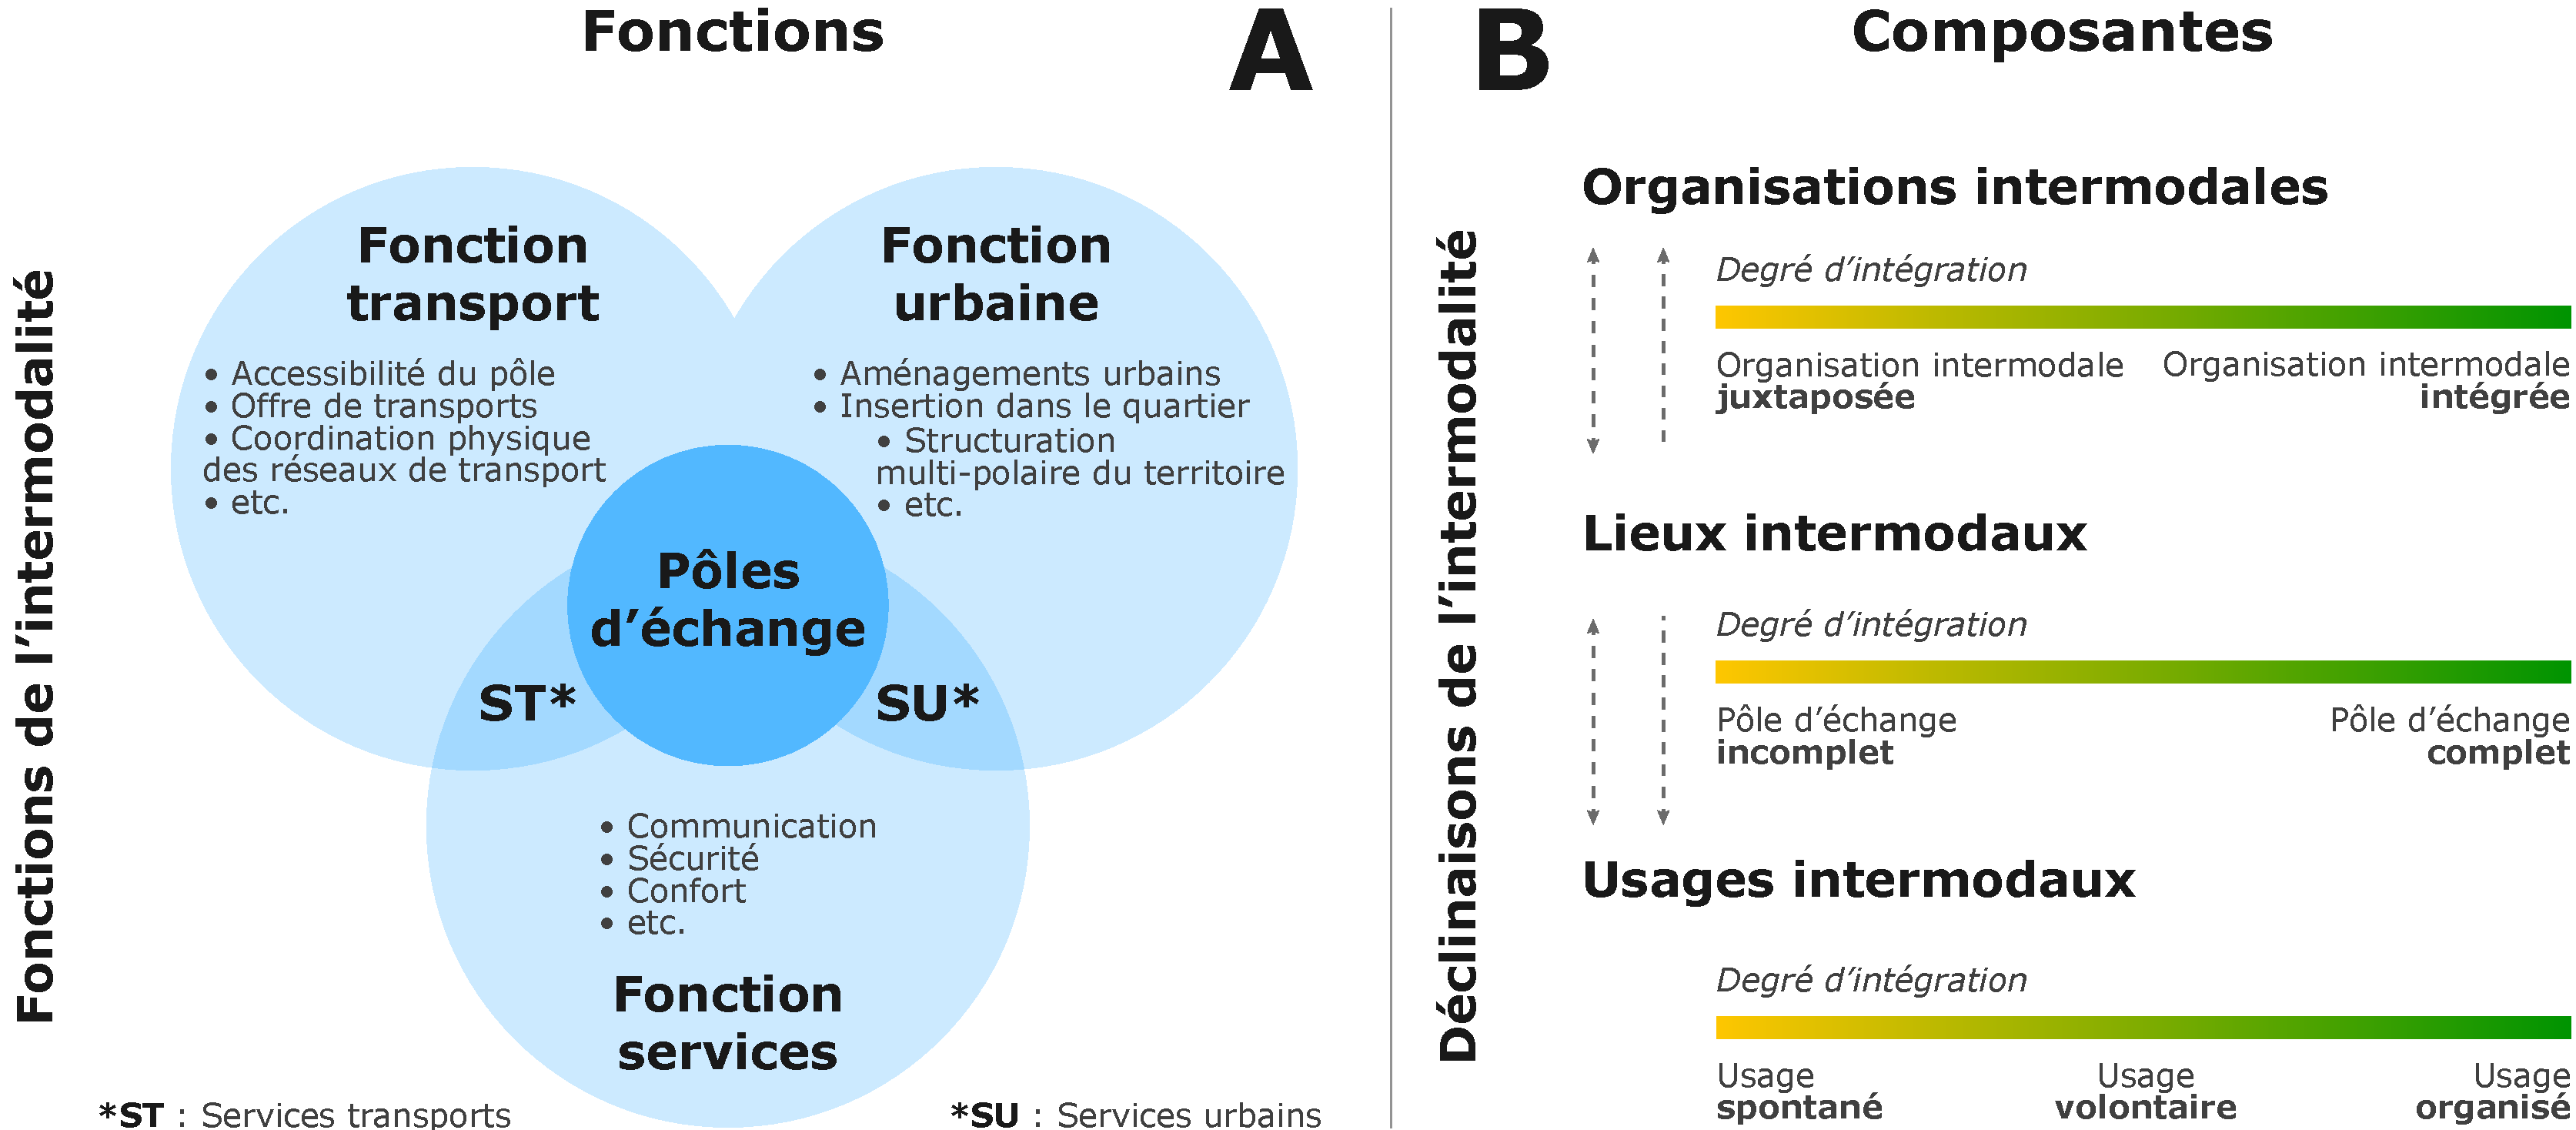
\includegraphics[width=1\columnwidth]{src/Figures/Chap-1/FR_Fonctions_Composants_Intermodalite.pdf}}
        \vspace{5pt}
        \begin{flushright}\scriptsize{
        Source (A)~: \textcolor{blue}{Cyprien} \textcolor{blue}{\textcite[14]{richer_lemergence_2008}}\index{Richer, Cyprien|pagebf}
        \\
        Source (B)~: \textcolor{blue}{Sandra} \textcolor{blue}{\textcite[167]{bozzani_grandes_2006}}\index{Bozzani-Franc, Sandra|pagebf}\index{Paris, Didier|pagebf}\index{Bakis, Henry|pagebf}\index{Menerault, Philippe|pagebf}
        \\
        Adaptation graphique~: \textcolor{blue}{Dylan Moinse (2023)}
        }\end{flushright}
    \end{figure}

    % Système intermodal
La notion d’intermodalité-voyageur·se·s peut être analysée à travers trois composantes principales proposées par \textcolor{blue}{Sandra} \textcolor{blue}{\textcite[167]{bozzani_grandes_2006}}\index{Bozzani-Franc, Sandra|pagebf}\index{Paris, Didier|pagebf}\index{Bakis, Henry|pagebf}\index{Menerault, Philippe|pagebf} dans sa thèse de doctorat portant sur l’apport de l’intermodalité aéro-ferroviaire à grande vitesse (voir l'\hyperref[fig-chap1:composantes-fonctions-intermodalite]{illustration~\ref{fig-chap1:composantes-fonctions-intermodalite}}, page~\pageref{fig-chap1:tad-murdoch}). Ce triptyque repose sur l’\textsl{existence d’une organisation intermodale}, l’\textsl{implantation dans un lieu intermodal} et des \textsl{usages intermodaux spécifiques}, chaque dimension interagissant avec les autres. Ces trois aspects permettent d’évaluer le degré d’intégration des pôles d’interconnexion, selon la qualité de service proposée\footnote{
    La qualité de service en matière d’intermodalité s’exprime à travers la coopération et la complémentarité entre opérateurs, la coordination des horaires, la disponibilité d’une information intermodale, la mutualisation de la réservation de billets, un cheminement facilité entre les modes, un temps de connexion et d’attente optimisé, ainsi que la prise en charge des bagages \textcolor{blue}{\autocites[65]{bozzani_intermodalite_2005}[167]{bozzani_grandes_2006}}\index{Bozzani-Franc, Sandra|pagebf}\index{Paris, Didier|pagebf}\index{Bakis, Henry|pagebf}\index{Menerault, Philippe|pagebf}.
} \textcolor{blue}{\autocites[65]{bozzani_intermodalite_2005}[167]{bozzani_grandes_2006}}\index{Bozzani-Franc, Sandra|pagebf}\index{Paris, Didier|pagebf}\index{Bakis, Henry|pagebf}\index{Menerault, Philippe|pagebf}. L’intermodalité, composée de ces trois sous-systèmes interreliés, suppose une organisation, s’inscrit dans un lieu et est faite d'usages. Elle permet ainsi d’aborder des concepts clés des sciences sociales, tels que l’individu, le lieu et le monde, comme l'explique \textcolor{blue}{Pierre} \textcolor{blue}{\textcite[490]{ageron_intermodalite-voyageurs_2013}}\index{Ageron, Pierre|pagebf}\index{Varlet, Jean|pagebf}. Ces sous-systèmes reposent sur le principe de transcalarité, c’est-à-dire une articulation entre différentes échelles spatiales, condition préalable à la complémentarité des modes de déplacement. En effet, une association intermodale ne présenterait pas d’intérêt pour l’usager·ère si les modes impliqués étaient redondants en termes de desserte territoriale et donc de choix de destinations possibles \textcolor{blue}{\autocite[45]{ageron_intermodalite-voyageurs_2013}}\index{Ageron, Pierre|pagebf}\index{Varlet, Jean|pagebf}. Dans cette optique, l’intermodalité ne se limite pas à une simple succession de modes au cours d’un déplacement. Elle devient une véritable \Guillemets{ressource territoriale}, entendue comme une combinaison de \Guillemets{facteurs de production} facilitant le rapprochement des acteurs spatiaux, conformément à la définition de \textcolor{blue}{\textcite[6]{gumuchian_ressource_2007}}\index{Gumuchian, Hervé|pagebf}\index{Pecqueur, Bernard|pagebf}. À ce titre, \textcolor{blue}{Cyprien} \textcolor{blue}{\textcite[14]{richer_lemergence_2008}}\index{Richer, Cyprien|pagebf}, alors chargé de recherche en géographie au \acrshort{Cerema}, met en avant la triple fonction constitutive des pôles d’échange (voir l'\hyperref[fig-chap1:composantes-fonctions-intermodalite]{illustration~\ref{fig-chap1:composantes-fonctions-intermodalite}}, page~\pageref{fig-chap1:tad-murdoch})~: la \textsl{fonction transport}, la \textsl{fonction urbaine} et la \textsl{fonction services}. Ces fonctions assurent non seulement l’interconnexion des réseaux, mais également la structuration des territoires. Les expériences autour des \textsl{Mobility Hubs}, conceptualisées dans le cadre du projet Interreg \textsl{Mobi-Mix}, en fournissent une illustration. Ils constituent des points de facilitation de l’intermodalité, conçus comme des pôles physiques intégrant au moins deux systèmes de mobilité partagés, comme manifestés dans les projets pilotes à Norfolk et à Valenciennes \textcolor{blue}{\autocites[3~498]{hachette_exploring_2023}[248]{hachette_mobility_2023}}\index{Hachette, Maxime|pagebf}\index{L'Hostis, Alain|pagebf}\index{Gragera, Albert|pagebf}.%%Rédigé%%

    % Pertinence de la MIL + Transition
Selon \textcolor{blue}{\textcite[116]{goletz_intermodality_2020}}\index{Goletz, Mirko|pagebf}\index{Haustein, Sonja|pagebf}\index{Wolking, Christina|pagebf}\index{L'Hostis, Alain|pagebf}, les considérations stratégiques sur l’intermodalité occupent une place croissante dans les orientations d’aménagement des territoires. Cette tendance reflète une promesse de réduction du trafic automobile, de limitation de la possession automobile, et d’un catalyseur pour un véritable report modal vers le transport public. À cela s’ajoute l’idée que, dans le futur, de nouveaux modes de déplacement encore peu utilisés aujourd’hui connaîtront une intensification de leur usage et contribueront significativement à l’enrichissement des chaînes intermodales. À ce titre, \textcolor{blue}{\textcite[77]{oostendorp_combining_2018}}\index{Oostendorp, Rebekka|pagebf}\index{Gebhardt, Laura|pagebf} prédisent que l’émergence de nouvelles formes de mobilité, comme la mobilité individuelle légère, rendra l’intermodalité encore plus pertinente dans les années à venir. L’intégration de ces \Guillemets{micro-modes} dans les systèmes de transport public pourrait offrir de nombreux \Guillemets{co-bénéfices} (\textsl{co-benefits}), tels que des opportunités économiques, des gains pour la santé publique, une meilleure inclusivité, une réduction des coûts pour les usager·ère·s, une diminution des accidents et de la congestion routière, ainsi qu’une amélioration du confort et du bien-être personnel \textcolor{blue}{\autocite[39-40]{litman_new_2021}}\index{Litman, Todd|pagebf}. Dans ce cadre, la mobilité individuelle légère se positionne comme une famille de modes complémentaire aux transports en commun, au même titre que la marche combinée. Elle est susceptible d’apporter une plus grande résilience aux systèmes de transport public \textcolor{blue}{\autocites{heran_velo_2020}[6]{dezobry_du_2020}}\index{Héran, Frédéric|pagebf}\index{Dezobry, Guillaume|pagebf}\index{Fontenelle, Louis de|pagebf}\index{Staropoli, Carine|pagebf}.%%Rédigé%%

    % 1.3.2.
    \needspace{1\baselineskip} % Réserve de l'espace
\subsection{D'une approche \Guillemets{station-à-station} à celle de \Guillemets{porte-à-porte}
    \label{chap1:btod-definition}
    }

    % Introduction
Les catégories de mobilité longtemps considérées comme antagonistes, telles que le transport individuel et le transport collectif, évoluent progressivement vers une logique de \Guillemets{transmodalité}. L’émergence de configurations intermodales, rendue possible par la diversification de la mobilité individuelle légère, favorise ainsi l’affirmation de \Guillemets{transports publics individuels} \textcolor{blue}{\autocites[14-15]{amar_homo_2016}[18]{fijalkow_sociologie_2017}[5]{kostrzewska_towards_2017}}\index{Amar, Georges|pagebf}\index{Kostrzewska, Małgorzata|pagebf}\index{Macikowski, Bartosz|pagebf}\index{Fijalkow, Yankel|pagebf}. Ces véhicules compacts offrent une réponse intelligente aux enjeux des \Guillemets{premiers et derniers kilomètres}, en proposant une solution de mobilité \Guillemets{porte-à-porte} qui faisait longtemps défaut au transport public \textcolor{blue}{\autocite{dia_banning_2019}}\index{Dia, Hussein|pagebf}. Intégrée dans une démarche intermodale, la mobilité individuelle légère ne se limite pas à ses spécificités techniques ou à son mode d’acquisition~: elle engendre des pratiques de déplacement singulières, qui contribuent à transformer les usages de la mobilité \textcolor{blue}{\autocite[1]{tuncer_notes_2020}}\index{Tuncer, Sylvaine|pagebf}\index{Laurier, Eric|pagebf}\index{Brown, Barry|pagebf}\index{Licoppe, Christian|pagebf}. Son potentiel réside notamment dans sa capacité à pallier les lacunes de desserte du transport public \textcolor{blue}{\autocites{gauquelin_case_2021}[3]{lee_forecasting_2021}}\index{Gauquelin, Alexandre|pagebf}\index{Lee, Mina|pagebf}\index{Chow, Joseph|pagebf}\index{Yoon, Gyugeun|pagebf}\index{He, Brian|pagebf}. En étendant les zones d’influence des arrêts de transport en commun, le vélo a progressivement été intégré à la réflexion sur le \acrshort{TOD}, sous la forme d'un \acrfull{B-TOD}, bien qu’il occupait déjà un rôle stratégique au sein des \Guillemets{aires secondaires}. Dès cet instant, la question centrale qui émerge de ce travail bibliographique concerne la réactualisation de ce modèle urbain et la plus-value que représente l’intégration de la micro-mobilité, ainsi que la diversification du vélo, dans cette dynamique de renouvellement du \acrshort{TOD}.%%Rédigé%%

    % 1.3.2.1.
    \needspace{1\baselineskip} % Réserve de l'espace
\subsubsection*{Atouts de l'intégration de la mobilité individuelle légère
    \label{chap1:avantages-mil-tc}
    }

    % Avantages vélo
Si la combinaison modale associant le vélo et le transport public suscite un intérêt croissant et devrait connaître une forte augmentation de ses usages d’ici à 2030 \textcolor{blue}{\autocite[119]{goletz_intermodality_2020}}\index{Goletz, Mirko|pagebf}\index{Haustein, Sonja|pagebf}\index{Wolking, Christina|pagebf}\index{L'Hostis, Alain|pagebf}, il convient d’en examiner les avantages comparatifs qui expliquent son attractivité. Tout d’abord, du point de vue de la vitesse, le vélo permet de parcourir une distance spatiale trois à cinq fois supérieure à celle de la marche, pour une dépense énergétique environ cinq fois moindre \textcolor{blue}{\autocite[50]{sebban_complementarite_2003}}\index{Sebban, Annie-Claude|pagebf}\index{Motte, Alain|pagebf}. Cette vitesse accrue tend à considérablement élargir sa portée, et par conséquent la zone de pertinence des stations de transport en commun. En effet, s’agissant des trajets vers et depuis une gare, la distance acceptable est estimée à 4 kilomètres selon l’enseignant-chercheur néerlandais \textcolor{blue}{Niels van} \textcolor{blue}{\textcite[4]{oort_overview_2020}}\index{Oort, Niels van|pagebf}, voire à 5 kilomètres selon un rapport d’étude du projet européen \textcolor{blue}{\textcite[4]{bitibi_bike_2017}}\index{BiTiBi@\textsl{BiTiBi}|pagebf}. En prenant comme référence une portée de la marche combinée de 1 kilomètre, l’extension de cette accessibilité par le vélo permettrait d’élargir l’aire d’influence d’une station d’un facteur 25. Dès lors, l’enjeu est de rendre accessibles, par le couple vélo et transport public, des quartiers où une distance \Guillemets{confortable à pied} ne serait pas envisageable \textcolor{blue}{\autocite[17]{nlc_micromobility_2019}}\index{NLC@\textsl{NLC}|pagebf}, en particulier dans les territoires périurbains où l’automobile constitue un facteur d’exclusion pour les individus ne disposant ni d’un permis de conduire ni d’un véhicule motorisé \textcolor{blue}{\autocite[85]{cervero_bike-and-ride_2013}}\index{Cervero, Robert|pagebf}\index{Caldwell, Benjamin|pagebf}\index{Cuellar, Jesus|pagebf}. Un autre avantage fondamental réside dans la capacité du vélo à conjuguer la souplesse spatio-temporelle d’un mode \Guillemets{porte-à-porte} avec la portée étendue et la vitesse offertes par les transports en commun \textcolor{blue}{\autocite[212]{kager_characterisation_2016}}\index{Kager, Roland|pagebf}\index{Bertolini, Luca|pagebf}\index{te Brömmelstroet, Marco|pagebf}. L’intégration du vélo au réseau de transport public, en tant que solution intermodale alternative et décarbonée, permet alors d’étendre la zone de desserte des stations, tout en étant peu coûteuse tant sur le plan énergétique que budgétaire. Elle promeut alors une forme de justice socio-spatiale en élargissant l’accessibilité par le transport public à un plus grand nombre d’usager·ère·s potentiel·le·s \textcolor{blue}{\autocite[99-100]{levine_mobility_2019}}\index{Levine, Jonathan|pagebf}\index{Grengs, Joe|pagebf}\index{Merlin, Louis~A.|pagebf}. Ces effets de synergie ont été illustrés par \textcolor{blue}{\textcite[212]{kager_characterisation_2016}}\index{Kager, Roland|pagebf}\index{Bertolini, Luca|pagebf}\index{te Brömmelstroet, Marco|pagebf}, qui représentent graphiquement comment la combinaison du vélo et du transport public les rend plus compétitifs que l'automobile en termes de vitesse, de flexibilité et de portée (voir le \hyperref[fig-chap1:vitesse-accessibilite-velo-tc]{diagramme~\ref{fig-chap1:vitesse-accessibilite-velo-tc}}, page~\pageref{fig-chap1:vitesse-accessibilite-velo-tc}). Cette dynamique est particulièrement visible en situation de congestion urbaine, et rappelle les avantages comparatifs offerts par le covoiturage.%%Rédigé%%

    % Figure vitesse-accessibilité MIL+TC
    \begin{figure}[h!]\vspace*{4pt}
        \caption{Caractérisation de la combinaison entre la mobilité individuelle légère selon les niveaux d'accessibilité et de vitesse de chaque mode de déplacement.}
        \label{fig-chap1:vitesse-accessibilite-velo-tc}
        \centerline{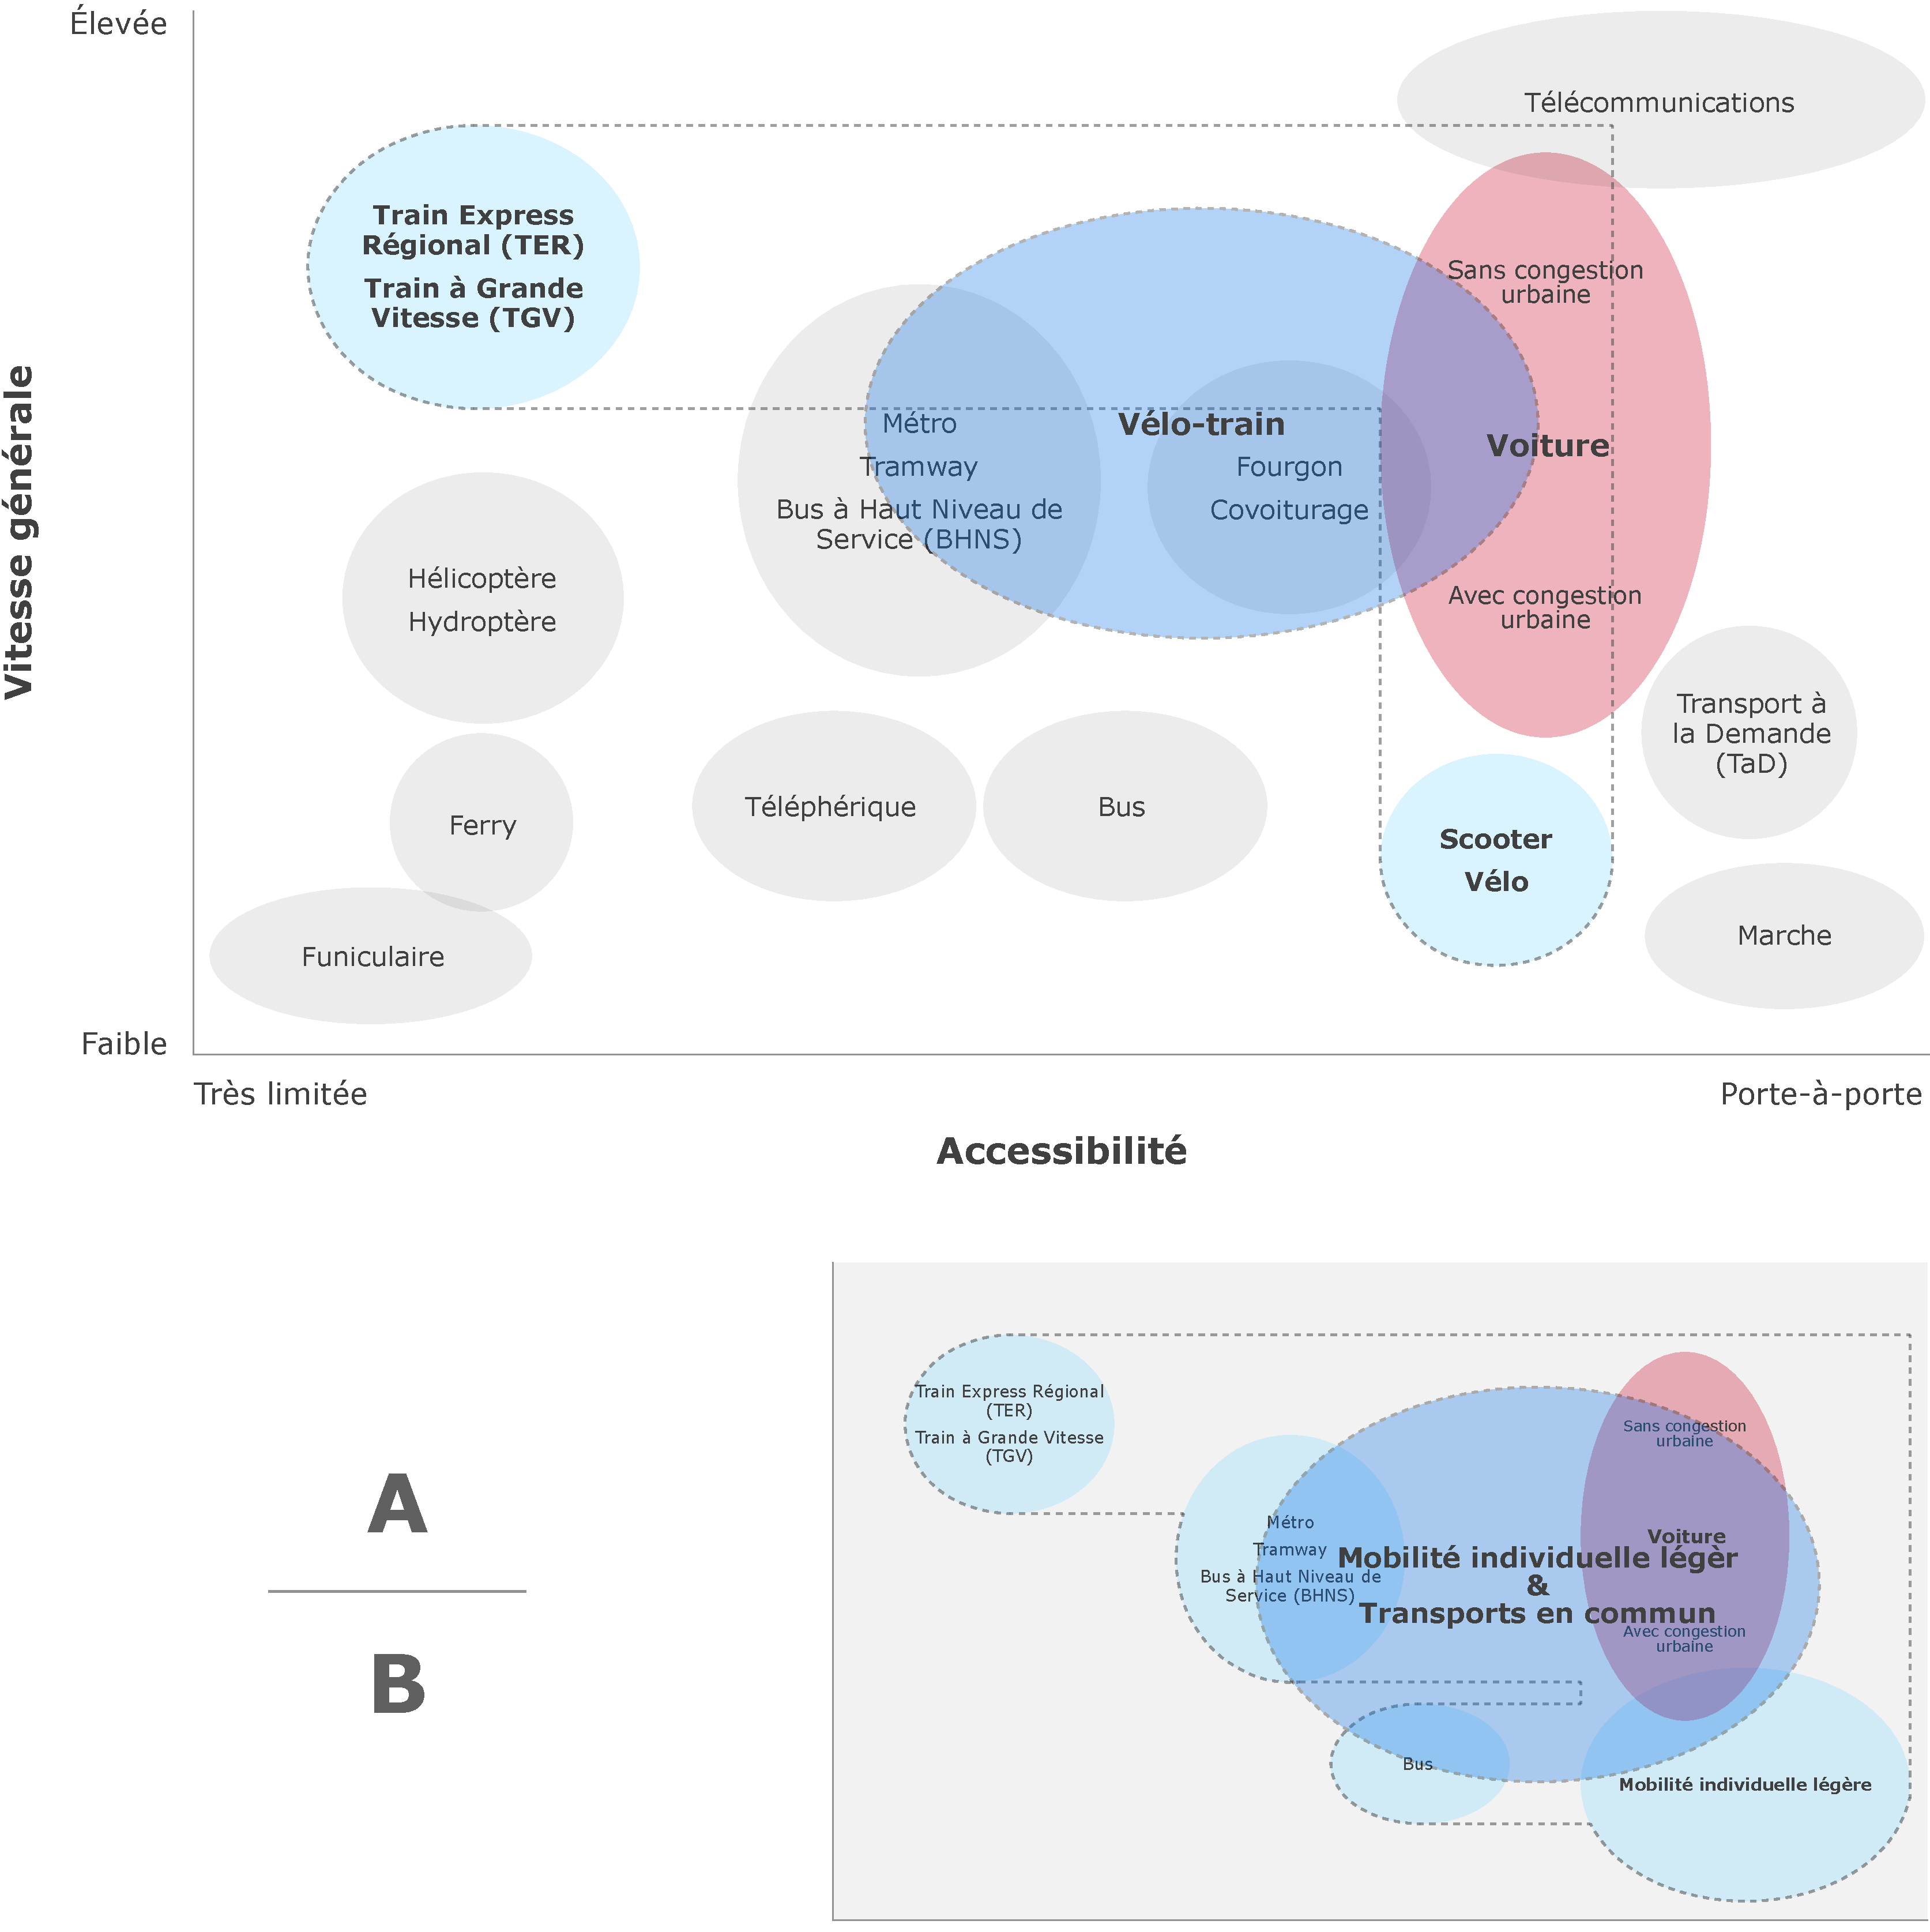
\includegraphics[width=1\columnwidth]{src/Figures/Chap-1/FR_Kager_vitesse_accessibilite.pdf}}
        \vspace{5pt}
        \begin{flushright}\scriptsize{
        Source (A)~: \textcolor{blue}{\textcite[212]{kager_characterisation_2016}}\index{Kager, Roland|pagebf}\index{Bertolini, Luca|pagebf}\index{te Brömmelstroet, Marco|pagebf}
        \\
        Adaptation graphique et réinterprétation (B)~: \textcolor{blue}{Dylan Moinse (2025)}
        }\end{flushright}
    \end{figure}

    % Micro-mobilité
Tandis que le vélo est si bien intégré au \Guillemets{système train} aux Pays-Bas qu’un véritable mode de déplacement \textcolor{blue}{\autocite[129-148]{bruntlett_curbing_2020}}\index{Bruntlett, Melissa|pagebf}\index{Bruntlett, Chris|pagebf}, bimodal et appelé \Guillemets{vélo-train}, a émergé \textcolor{blue}{\autocite[112]{oosteren_pourquoi_2021}}\index{Oosteren, Stein van|pagebf}\index{Schneider, Olivier|pagebf}, qu’en est-il de la micro-mobilité~? Il apparaît que cette famille d'engins de déplacement remplit une fonction et possède des propriétés proches de celles du vélo. En effet, les \acrshort{EDP} offrent un potentiel comparable pour accroître la portée de la marche, permettant de couvrir des distances deux à trois fois plus longues avec une vitesse de déplacement environ trois fois plus élevée \textcolor{blue}{\autocite{rabaud_micromobilites_2019}}\index{Rabaud, Mathieu|pagebf}\index{Richer, Cyprien|pagebf}. Ainsi, la micro-mobilité contribue, à son tour, à la redéfinition des aires de chalandise du transport public, en facilitant l’accès aux stations et en élargissant leur zone d’influence. Un avantage spécifique des \acrshort{EDP} réside cependant dans leur compacité et leur légèreté, qui favorisent leur embarquement dans le mode collectif, contrairement au vélo classique (voir le \hyperref[fig-chap1:vitesse-accessibilite-velo-tc]{diagramme~\ref{fig-chap1:vitesse-accessibilite-velo-tc}}, page~\pageref{fig-chap1:vitesse-accessibilite-velo-tc}). Dès lors, qu’il s’agisse du vélo ou des engins de micro-mobilité, ces modes répondent à des attentes et à des besoins similaires~: la recherche de gains de flexibilité et un accès direct et plus souple aux nœuds compatibles avec les enjeux d'ordre environnemental \textcolor{blue}{\autocite[80]{oostendorp_combining_2018}}\index{Oostendorp, Rebekka|pagebf}\index{Gebhardt, Laura|pagebf}.%%Rédigé%%

    % Impacts + Transition
Les atouts du couple mobilité individuelle légère et transports en commun, dont l’augmentation des distances que les usager·ère·s sont prêt·e·s à parcourir pour rejoindre ou quitter une station de transport public, participeraient à une hausse significative de la fréquentation du réseau \textcolor{blue}{\autocite[]{wang_approximating_2016}}\index{Wang, Hai|pagebf}\index{Odoni, Amedeo|pagebf}. Une modélisation réalisée par \textcolor{blue}{\textcite[69]{ensor_mode_2021}}\index{Ensor, Matt|pagebf}\index{Maxwell,~O.|pagebf}\index{Bruce, Oliver|pagebf} montre ainsi que l’essor de la pratique du vélo et de la \acrshort{TEP} pourrait conduire à une augmentation de 7~\% de la fréquentation des transports en commun en milieu urbain, et de 9~\% en territoire \gls{périurbain}, en Nouvelle-Zélande, si les configurations intermodales sont optimisées. Ce constat souligne un point clé~: bien que le vélo et la micro-mobilité ne soient pas en mesure d’être intégralement compétitifs face à l’automobile sur de longues distances et qu’ils aient une capacité limitée à s’y substituer, leur intégration au transport public crée une synergie qui les rend fortement concurrentiels vis-à-vis de ce mode de déplacement \textcolor{blue}{\autocite[43]{corporate_partnership_board_good_2020}}\index{Corporate Partnership Board@\textsl{Corporate Partnership Board}|pagebf}. Comme l’explique \textcolor{blue}{Annie-Claude} \textcolor{blue}{\textcite[262]{sebban_complementarite_2003}}\index{Sebban, Annie-Claude|pagebf}\index{Motte, Alain|pagebf}, l’intermodalité vélo et transport public se structure à travers des \textsl{territoires de pratique}. Cette approche lui permet de mobiliser la notion de territoire, dans la mesure où ces pratiques intermodales s’opèrent \textsl{sur} et \textsl{entre} des espaces bien déterminés. Envisager l’intermodalité sous l’angle territorial nous conduit naturellement à un retour au modèle du \acrshort{TOD}. Celui-ci apparaît comme un cadre pertinent à revisiter au regard des défis liés aux \Guillemets{premiers et derniers kilomètres}, auxquels la mobilité individuelle légère semble particulièrement adaptée.%%Rédigé%%

    % 1.3.2.2.
    \needspace{1\baselineskip} % Réserve de l'espace
\subsubsection*{Conceptualisation d'un urbanisme orienté vers le rail et soutenu par la mobilité individuelle légère
    \label{chap1:btod-m-tod}
    }

    % Introduction aires secondaires
Dans leur ouvrage proposant un regard contemporain sur le \acrshort{TOD}, \foreignlanguage{english}{\textsl{Transit-Oriented Development and Sustainable Cities: Economics, Community and Methods}}, \textcolor{blue}{\textcite[222]{knowles_transit_2019}}\index{Knowles, Richard~D.|pagebf}\index{Ferbrache, Fiona|pagebf} soulignent l’importance de tirer parti des opportunités offertes par les mobilités émergentes de ces dernières années~–~telles que le \acrshort{VAE}, la \acrshort{TEP} et les services en \textsl{free-floating}~–~afin d’enrichir le modèle urbain du \acrshort{TOD}. \textcolor{blue}{Peter} \textcolor{blue}{\textcite[54-55]{calthorpe_next_1993}}\index{Calthorpe, Peter|pagebf} n’abandonne pas pour autant la prise en compte des \Guillemets{aires secondaires} dans la structuration des quartiers \acrshort{TOD}\textcolor{blue}{s}. Il les intègre partiellement au \acrshort{TOD}, considérant qu’elles sont suffisamment proches d’une station de transport en commun pour être orientées vers celle-ci, notamment grâce à un accès cyclable. L'\Guillemets{aire secondaire} détient même des caractéristiques semblables à celles de l’\Guillemets{aire primaire} en bénéficiant d'une certaine diversité fonctionnelle et en étant connectée à un réseau de rues apaisées. Loin d’être marginale, cette aire joue un rôle structurant dans chaque quartier de gare. Elle accueille généralement des fonctions rarement configurées pour être placée dans l’aire la plus stratégique, telles que des emplois en dehors des bureaux, des écoles ou encore des parcs. Elle permet également d’offrir une diversité en termes de choix résidentiel, en intégrant plus souvent des maisons individuelles. L'auteur identifie trois types d’\Guillemets{aires secondaires}~: (i) celles séparées par une artère, mais proches d’un arrêt de transport en commun~; (ii) celles séparées par une artère et éloignées de l’arrêt~; (iii) et celles plus éloignées encore de l’arrêt, mais sans artère séparatrice \textcolor{blue}{\autocite[87]{calthorpe_next_1993}}\index{Calthorpe, Peter|pagebf}. Bien que l'\Guillemets{aire secondaire} soit souvent plus auto-orientée et accueille fréquemment des infrastructures de type \acrfull{P+R} favorisant la pratique du \textsl{park-and-ride}, elle devrait selon lui être desservie par des connexions cyclables la reliant directement à la station de transport en commun et au quartier de gare central. Dès la formalisation du \acrshort{TOD}, l’enjeu majeur réside dans la maximisation des connexions piétonnes et, surtout, cyclables au sein de l’\Guillemets{aire secondaire}. Il préconise en particulier l’aménagement de pistes cyclables séparées le long des boulevards urbains structurants\footnote{
    \Guillemets{\textsl{En raison des distances, le vélo est l’un des modes de déplacement les plus probables pour les résidents des zones secondaires susceptibles d’utiliser les transports en commun. Des connexions cyclables solides empruntant les itinéraires les plus courts possibles encourageront davantage les résidents des zones secondaires à utiliser les transports en commun. Les artères et certaines voies de connexion dans les zones secondaires doivent offrir des pistes cyclables sécurisées, séparées ou marquées, permettant un accès rapide à l’arrêt de transport en commun. Les pistes cyclables des zones secondaires devraient se connecter au réseau cyclable du TOD.}} (\Guillemets{\textsl{Because of the distances, bicycles are one of the most likely modes of travel for Secondary Area residents who are apt to use public transit. Strong bicycle connections that follow the shortest possible routes will provide additional encouragement for Secondary Area residents to use transit. Arterials and selected connector roadways in Secondary Areas must provide safe, separated or marked bicycle lanes allowing quick travel to the transit stop. Secondary Area bicycle paths should connect with the TOD bicycle system}}) \textcolor{blue}{\autocite[89]{calthorpe_next_1993}}\index{Calthorpe, Peter|pagebf}.
} \textcolor{blue}{\autocite[60, 89]{calthorpe_next_1993}}\index{Calthorpe, Peter|pagebf}. Outre ces aménagements, l’auteur insiste sur l’importance du stationnement sécurisé pour vélo afin de favoriser leur usage intermodal, ainsi que sur le rôle du vélo dans les déplacements internes au quartier de gare\footnote{
    \Guillemets{\textsl{Des casiers sécurisés pour vélos sont particulièrement importants pour l’utilisation combinée \Guillemets{vélo-et-transports en commun}, car peu de personnes laisseront leur vélo sans surveillance pendant une journée entière de travail. Les infrastructures de stationnement pour vélos incluent des arceaux, des consignes surveillées et des casiers. Des arceaux à vélo doivent être installés à proximité des destinations commerciales, scolaires et de loisirs dans les TODs et les zones secondaires. Des installations de stationnement pour vélo plus sécurisées doivent être prévues à proximité de tous les bureaux, des lieux d’emploi et des principaux arrêts de transport en commun.}} (\Guillemets{\textsl{Secure bike lockers are especially important to "bike-and-ride" transit use, as few will leave their bike unattended for a full working day. Bicycle parking facilities include bike racks, "checks", and lockers. Bike racks must be provided at shopping, school, and recreational destinations in TODs and Secondary Areas. More secure bike parking facilities must be provided at all office/employment uses and at major transit stops.}}) \textcolor{blue}{\autocite[103]{calthorpe_next_1993}}\index{Calthorpe, Peter|pagebf}.
} \textcolor{blue}{\autocite[103]{calthorpe_next_1993}}\index{Calthorpe, Peter|pagebf}. Plus qu’une simple connexion au réseau structurant, il s’agit de proposer un maillage cyclable capillaire permettant d’accéder à l’ensemble des aménités présentes dans le quartier de gare~–~qu’elles soient situées dans l’aire primaire ou secondaire~–~et de relier efficacement un \acrshort{TOD} à un autre\footnote{
    \Guillemets{\textsl{Un réseau coordonné de voies cyclables devrait être mis en place en lien avec les TOD ou une série de TOD. Des destinations importantes, telles que les zones commerciales centrales, les arrêts de transport en commun, les centres d’emploi, les parcs, les espaces ouverts, les écoles et autres équipements communautaires, devraient être reliées par ces itinéraires cyclables.} [\dots] \textsl{Des pistes cyclables séparées ou marquées sur plusieurs axes principaux menant au centre favoriseront cette alternative, tout comme les voies cyclables le long des corridors verts reliant les TOD aux destinations professionnelles. Sur les rues secondaires, le partage de la chaussée entre vélos et voitures contribuera à réduire la vitesse des véhicules à des niveaux plus adaptés aux rues résidentielles. Certains itinéraires menant aux arrêts de transport en commun devraient offrir des pistes cyclables marquées ou séparées, connectées aux zones secondaires et à d'autres destinations clés. Des voies cyclables désignées devraient être prévues sur certaines rues de connexion et un nombre limité de rues locales convergeant vers le centre commercial et de transport.} [\dots] \textsl{Des panneaux clairs indiquant les destinations principales devraient être installés pour guider les cyclistes vers les principaux pôles d’activité, tels que les zones commerçantes, les arrêts de transport, les équipements de loisirs, les écoles et les infrastructures de stationnement pour vélos.}} (\Guillemets{\textsl{A coordinated system of bikeways should be provided in conjunction with TODs or a series of TODs. Important destinations, such as core commercial areas, transit stops, employment centers, parks, open spaces, schools, and other community facilities, should be linked by these bike routes.} [\dots] \textsl{Separated or marked bike lanes on several primary routes to the core area will support this alternative, as will the bike paths along greenways between TODs and employment destinations. On smaller streets, bikes sharing the travel lane will help slow cars to speeds more appropriate for residential streets. Selected routes to the transit stop should provide marked or separated bikeways connecting with the Secondary Areas and other key destinations. Designated bike lanes should be provided on selected connector streets and a limited number of local streets that converge upon the commercial and transit center.} [\dots] \textsl{Clear destination signs should be provided that direct riders to key activity centers, such as shopping areas, transit stops, recreation facilities, schools, and bike parking facilities.}}) \textcolor{blue}{\autocite[102]{calthorpe_next_1993}}\index{Calthorpe, Peter|pagebf}.
} \textcolor{blue}{\autocite[102]{calthorpe_next_1993}}\index{Calthorpe, Peter|pagebf}. Ainsi, au regard des avantages comparatifs liés à l’intégration de la mobilité individuelle légère au réseau de transport public, l’enjeu dépasse la seule \Guillemets{poche piétonnière} pour viser une intégration complète de l’\Guillemets{aire secondaire} au sein du \acrshort{TOD} \textcolor{blue}{\autocite[112]{ibraeva_transit-oriented_2020}}\index{Ibraeva, Anna|pagebf}\index{Almeida Correia, Gonçalo Homem de|pagebf}\index{Silva, Cecília|pagebf}.%%Rédigé%%

    % Figure B-TOD
    \begin{carte}[h!]\vspace*{4pt}
        \caption{Configurations spatiales du \textsl{Bicycle-based Transit-Oriented Development}.}
        \label{fig-chap1:schema-b-tod}
        \centerline{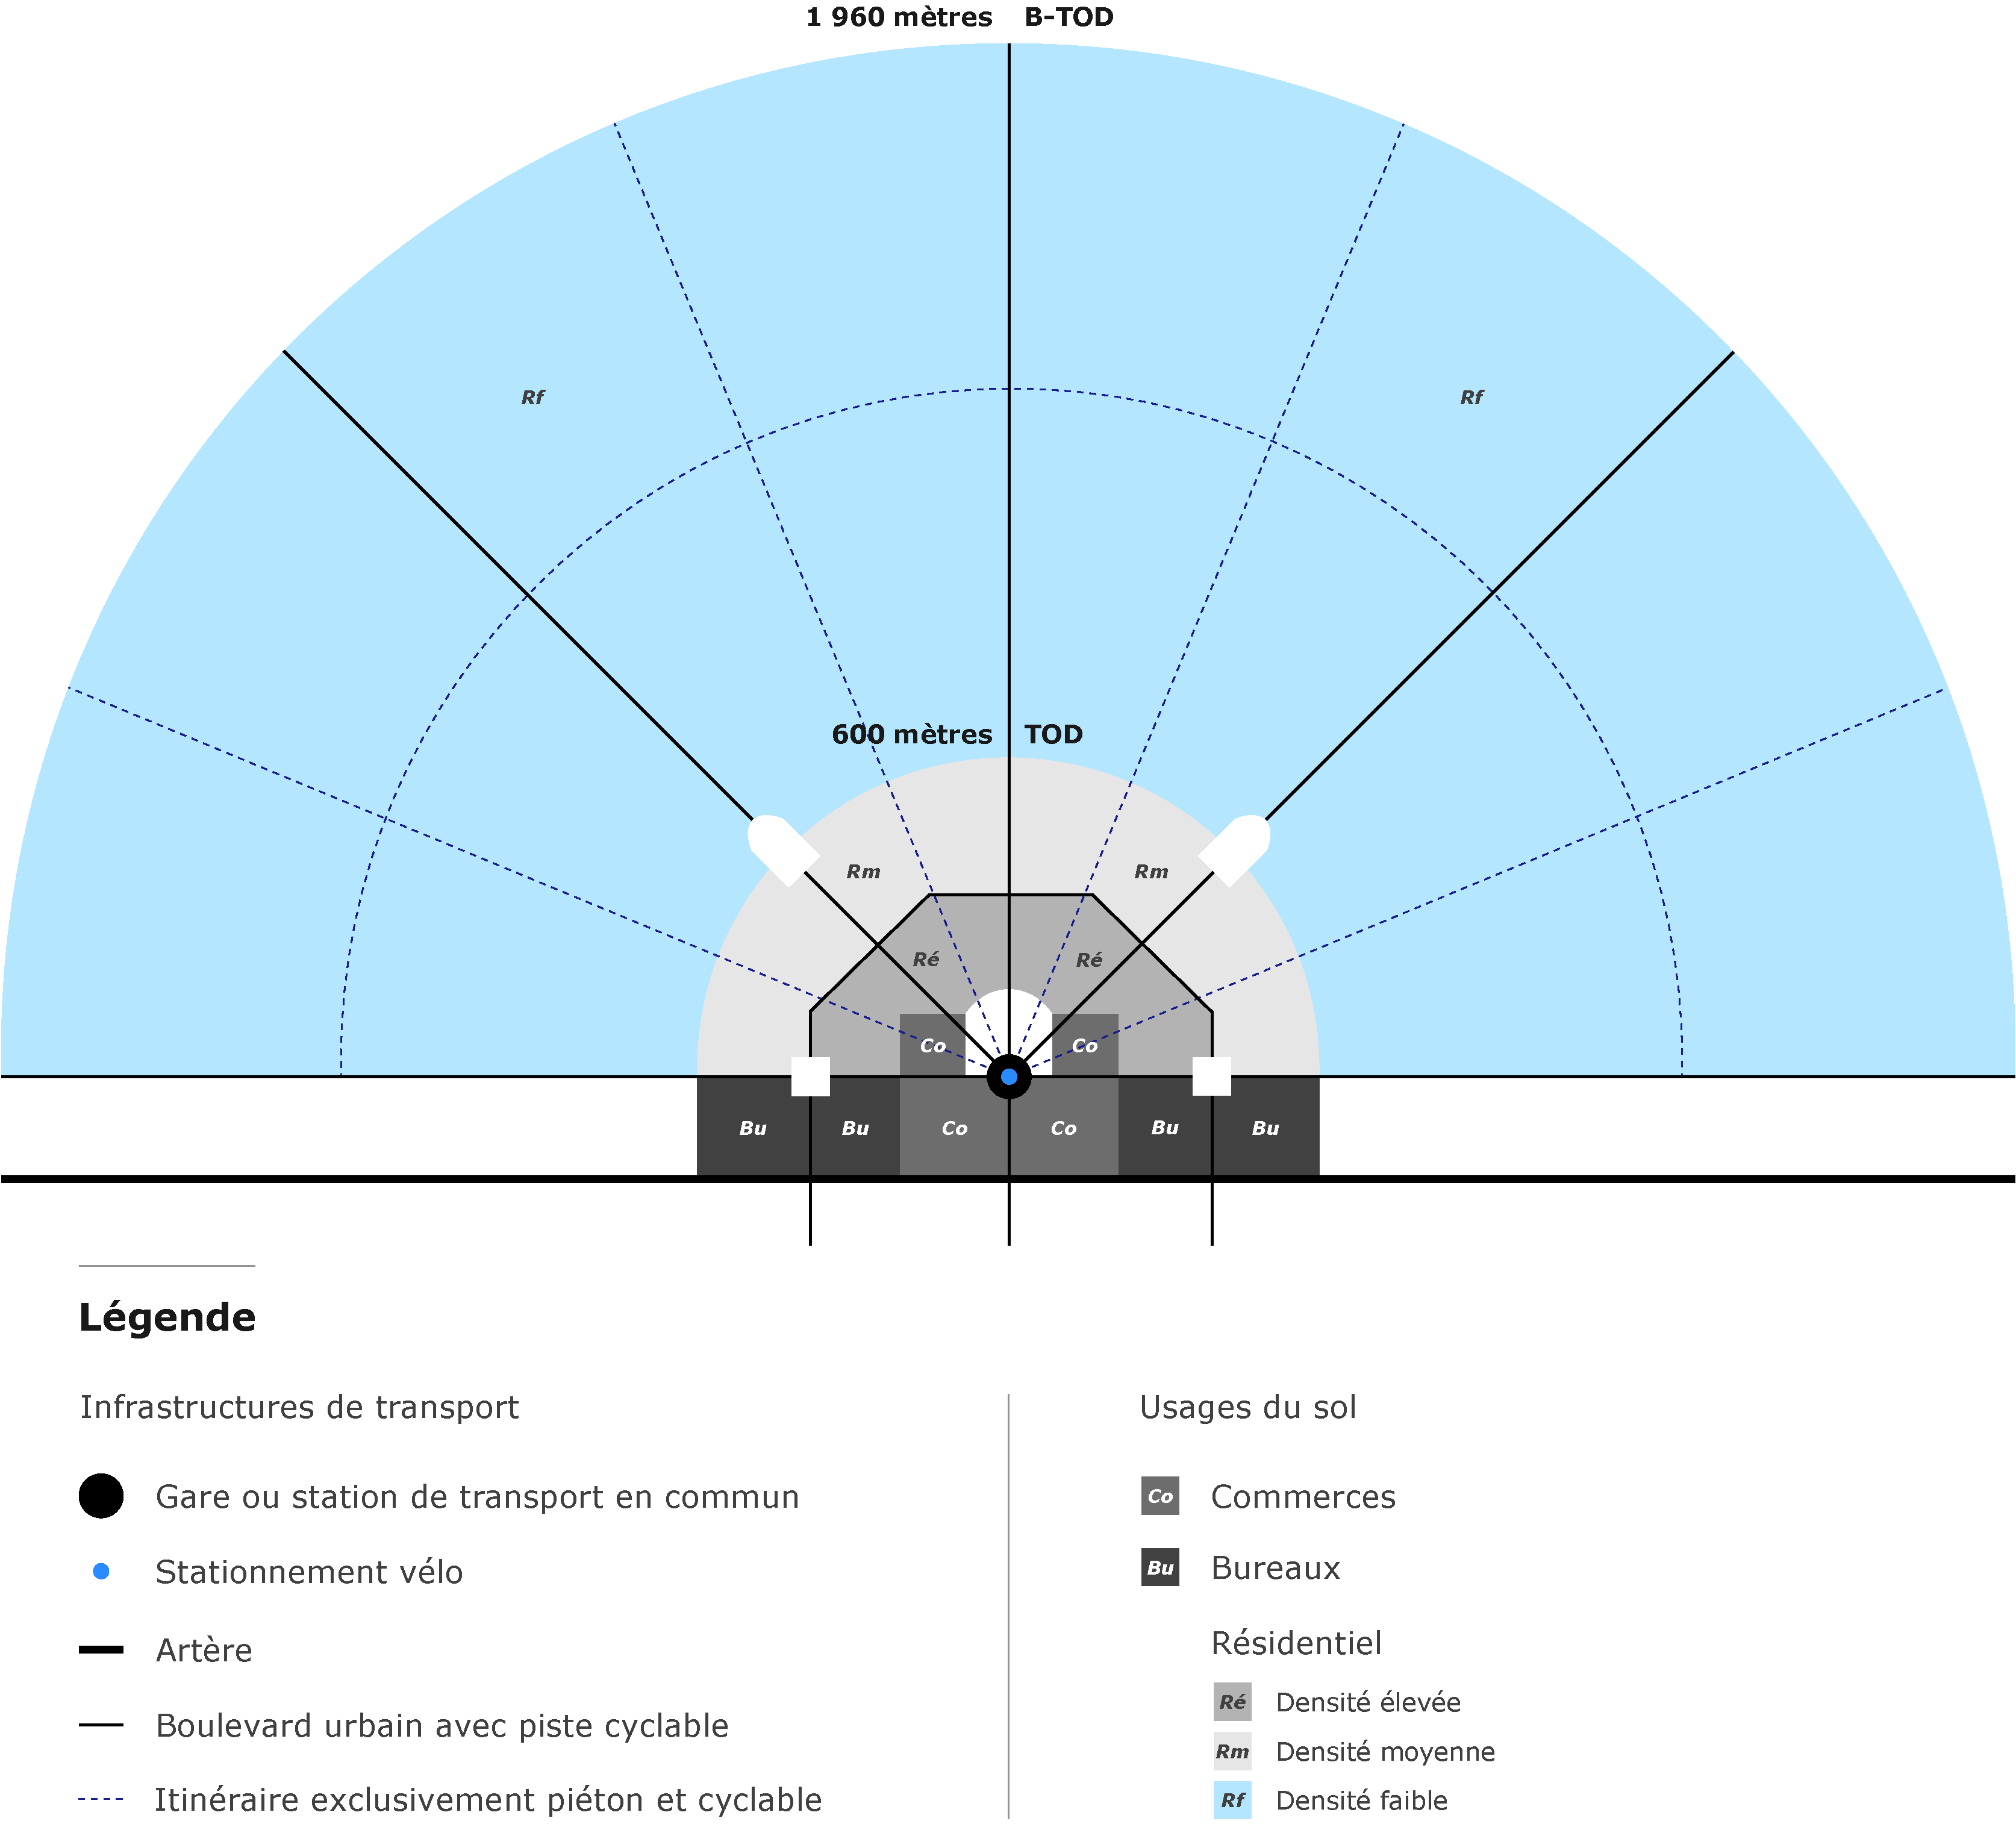
\includegraphics[width=1\columnwidth]{src/Figures/Chap-1/FR_Schema_B_TOD.pdf}}
        \vspace{5pt}
        \begin{flushright}\scriptsize{
        Source~: \textcolor{blue}{\textcite[979]{lee_bicycle-based_2016}}\index{Lee, Jaeyeong|pagebf}\index{Choi, Keechoo|pagebf}\index{Leem, Yountaik|pagebf}
        \\
        Adaptation graphique~: \textcolor{blue}{Dylan Moinse (2024)}
        }\end{flushright}
    \end{carte}

    % B-TOD
Bien que la problématique des \Guillemets{premiers et derniers kilomètres} et la solution intermodale associée à la pratique du vélo aient été envisagées dès l’ouvrage fondateur du \acrshort{TOD}, il apparaît que les développements relatifs à l’\Guillemets{aire secondaire} et aux aménagements cyclables proposés ont progressivement perdu en visibilité et en clarté dans les principes édictés. Face à cette appropriation partielle, les chercheur·se·s sud-coréen·ne·s \textcolor{blue}{\textcite[979]{lee_bicycle-based_2016}}\index{Lee, Jaeyeong|pagebf}\index{Choi, Keechoo|pagebf}\index{Leem, Yountaik|pagebf}, dans leur article \textsl{Bicycle-based transit-oriented development as an alternative to overcome the criticisms of the conventional transit-oriented development}, proposent, deux décennies plus tard, la conceptualisation d’un \acrfull{B-TOD} (voir la \hyperref[fig-chap1:schema-b-tod]{carte~\ref{fig-chap1:schema-b-tod}}, page~\pageref{fig-chap1:schema-b-tod}). Cette déclinaison du \acrshort{TOD}, qui ne remet pas en cause les principes fondamentaux du modèle, vise à répondre aux besoins de territoires n’ayant pas atteint les seuils critiques de densité de population et d’emploi nécessaires pour maximiser leur demande en transport autour des stations. Le \acrshort{B-TOD} cherche ainsi à accroître la fréquentation du réseau de transport en commun en ciblant les aires d’influence accessibles à vélo, définies dans un rayon d’environ deux kilomètres \textcolor{blue}{\autocite[979]{lee_bicycle-based_2016}}\index{Lee, Jaeyeong|pagebf}\index{Choi, Keechoo|pagebf}\index{Leem, Yountaik|pagebf}. Ce modèle revisité présente d'autres avantages notables. Il permet d’étendre jusqu'à 25 fois la superficie du quartier de gare traditionnel, renforçant ainsi considérablement son potentiel d’attractivité. De plus, avec une mise en œuvre facilitée, il se positionne comme une alternative écologique aux modèles du \acrshort{TOD} et du \acrshort{E-TOD}, tout en nécessitant un investissement infrastructurel réduit \textcolor{blue}{\autocite[979, 983]{lee_bicycle-based_2016}}\index{Lee, Jaeyeong|pagebf}\index{Choi, Keechoo|pagebf}\index{Leem, Yountaik|pagebf}, comme nous l’avons évoqué dans la \hyperref[chap1:tod-presentation-generale-declinaisons-hybrids]{sous-section sur les déclinaisons du \textsl{Transit-Oriented Development}} (page~\pageref{chap1:tod-presentation-generale-declinaisons-hybrids}). Un quatrième avantage, moins explicitement formulé par les auteur·rice·s, vaut la peine d'être signalé, à nos yeux~: le \acrshort{B-TOD} permettrait une adaptation des \Guillemets{[\dots] \textsl{critères de densité de population qui serait plus ou moins assouplis, par rapport à ceux de la zone centrale, afin de préserver un cadre plus agréable dans cette zone.}}\footnote{
    \Guillemets{\textsl{In a B-TOD setting, the re-establishment of the station impact area, where bicycle is a main access mode should be identified and the density criteria could be more or less relaxed than that of a TOD to keep the station impact area more pleasant.}} \textcolor{blue}{\autocite[983]{lee_bicycle-based_2016}}\index{Lee, Jaeyeong|pagebf}\index{Choi, Keechoo|pagebf}\index{Leem, Yountaik|pagebf}.
} \textcolor{blue}{\autocite[983]{lee_bicycle-based_2016}}\index{Lee, Jaeyeong|pagebf}\index{Choi, Keechoo|pagebf}\index{Leem, Yountaik|pagebf}. Toutefois, il ne s’agit pas de réduire la densité, mais plutôt de mieux la répartir au sein de l’aire du \acrshort{B-TOD}, en offrant des opportunités résidentielles pour des individus à la recherche de territoires moins denses, mieux dotés en espaces verts, offrant un accès facilité à des logements familiaux ou permettant d’échapper à la pression foncière autour des centralités. Afin de valider leur exercice de conceptualisation, les auteur·rice·s ont mené une enquête auprès des \Guillemets{cyclo-voyageur·se·s}~–~c’est l'expression que nous privilégions pour désigner les usager·ère·s combinant vélo et transport public lors d’un même déplacement~–~dans les villes de Séoul et Daejeon. Leur modélisation montre que 94~\% de l’aire métropolitaine de Séoul pourrait devenir accessible en transport en commun grâce à l’usage intermodal du vélo, soit une couverture potentielle trois fois supérieure à celle permise par la marche combinée \textcolor{blue}{\autocite[982]{lee_bicycle-based_2016}}\index{Lee, Jaeyeong|pagebf}\index{Choi, Keechoo|pagebf}\index{Leem, Yountaik|pagebf}. Réorganiser l'urbanisme autour du transport public et du vélo revient non seulement à promouvoir l'écologie, mais surtout la santé et l'activité physique \textcolor{blue}{\autocite[44]{heran_velo_2020}}\index{Héran, Frédéric|pagebf}\index{Rymarski, Christophe|pagebf}\index{Bedin, Véronique|pagebf}, une dimension moins abordée dans le \acrshort{TOD} conventionnel.%%Rédigé%%

    % M-TOD
Fort de cette déclinaison, nous avons fait le choix de nous appuyer sur ce travail de recherche, qui nous paraît fondateur, afin d’en tirer inspiration et de transposer notre argumentaire développé tout au long de ce chapitre. Il s’agit, en particulier, de démontrer le potentiel de la mobilité individuelle légère à renforcer le modèle urbain du \acrshort{TOD}, dans une perspective de promotion d’une mobilité et d’un cadre urbain plus soutenables. En nous inspirant des arguments avancés par \textcolor{blue}{\textcite{lee_bicycle-based_2016}}\index{Lee, Jaeyeong|pagebf}\index{Choi, Keechoo|pagebf}\index{Leem, Yountaik|pagebf}, et en reprenant notamment leurs questionnements autour de l’\Guillemets{identification} et de la \Guillemets{définition} d’un \acrshort{B-TOD}, nous proposons une réactualisation de ces modèles afin d’en concevoir un \acrfull{M-TOD}. Finalement, nous pourrions transposer la proposition de \Guillemets{théorie générale de la marchabilité} formulée par l’urbaniste \textcolor{blue}{Jeff} \textcolor{blue}{\textcite[73]{speck_walkable_2013}}\index{Speck, Jeff|pagebf} vers une \Guillemets{théorie générale de la cyclabilité} articulée autour du système de transport public. Celle-ci intégrerait l’ensemble de la mobilité individuelle légère et remplirait, à l’instar de la marchabilité, une triple fonction~: celle d’une finalité en soi, d’un moyen d’accessibilité et d’une mesure de la qualité urbaine \textcolor{blue}{\autocite[73]{speck_walkable_2013}}\index{Speck, Jeff|pagebf}. Dès lors, plusieurs interrogations structurent, à ce stade, notre réflexion~:
    \begin{customitemize}
\item Qu’est-ce qu’un \acrshort{M-TOD} et en quoi se distingue-t-il d’un \acrshort{TOD} et d’un \acrshort{B-TOD}~?
\item Quels en sont les usages observables et quel est son potentiel de report modal~?
\item Quels sont les liens entre le transport public et la mobilité individuelle légère~?
\item Comment ces comportements de mobilité actuels et potentiels interagissent-ils avec le tissu urbain et les enjeux de développement territorial~?
    \end{customitemize}%%Rédigé%%

    % ___________________________________________
    % 1.*.
    \newpage
    \needspace{1\baselineskip} % Réserve de l'espace
    \addcontentsline{toc}{section}{Conclusion du chapitre~1}
    \sectionheader{Conclusion du chapitre}
\section*{Conclusion du chapitre~1
    \label{chap1:conclusion}
    }
    %\markright{Conclusion du chapitre~1}{}

    % Introduction
Le \acrfull{TOD} constitue aujourd’hui un levier stratégique d'une planification urbaine soutenable, offrant une réponse aux défis posés par les politiques du \Guillemets{partout automobile} et du \Guillemets{surtout automobile}, qui continuent d’orienter la fabrique urbaine en France \textcolor{blue}{\autocite[14]{sebban_complementarite_2003}}\index{Sebban, Annie-Claude|pagebf}\index{Motte, Alain|pagebf}. Ce chapitre a permis de revenir sur les fondements historiques, les principes directeurs et les déclinaisons contemporaines de ce modèle d’aménagement. Bien que sa formalisation ait émergé dans le contexte nord-américain, il serait erroné d’en attribuer exclusivement la paternité aux urbanistes étasunien·ne·s, celleux-ci reconnaissant elleux-mêmes s’être inspiré·e·s d’exemples européens \textcolor{blue}{\autocite[15]{renne_emerging_2004}}\index{Renne, John Luciano|pagebf}\index{Wells, J.~S.|pagebf}. En somme, le cadre théorique et opérationnel du \acrshort{TOD} constitue une base solide et pertinente pour répondre aux impératifs environnementaux et socio-économiques actuels, à la fois à l’échelle régionale et locale. Il ne s’agit pas uniquement de promouvoir une meilleure offre de transport en commun~–~bien que cela soit une condition nécessaire~–, mais d’inscrire cette offre dans une logique d’interaction avec la structuration territoriale \textcolor{blue}{\autocite[9]{bernier_atlas_2023}}\index{Bernier, Xavier|pagebf}, en suivant une dynamique de \Guillemets{congruence}\footnote{
    Dans son article intitulé \textsl{Les \Guillemets{effets structurants} du transport~: mythe politique, mystification scientifique}, \textcolor{blue}{Jean-Marc} \textcolor{blue}{\textcite[239]{offner__1993}}\index{Offner, Jean-Marc|pagebf} a remarquablement exposé la nécessité d’une \Guillemets{démystification} politico-médiatique et scientifique concernant l’évaluation et les attentes suscitées par les \Guillemets{effets structurants} des infrastructures de transport. Il remet en question l’idée d’une relation de causalité linéaire entre l’introduction d’une nouvelle offre de mobilité et le développement territorial, en mettant en évidence une dynamique pré-existante plus complexe de liens parallèles, qu’il qualifie de \Guillemets{congruence}.
}, concept développé par \textcolor{blue}{Jean-Marc} \textcolor{blue}{\textcite[239]{offner__1993}}\index{Offner, Jean-Marc|pagebf}. La finalité du \acrshort{TOD} n’est donc pas tant de \Guillemets{générer de la croissance} (économique, démographique ou urbaine) en valeur absolue, mais plutôt de la redistribuer de manière plus équilibrée au sein d’une région donnée \textcolor{blue}{\autocite[82]{cervero_transit_1998}}\index{Cervero, Robert|pagebf}.%%Rédigé%%

    % Forces du TOD
L’intérêt principal des quartiers \acrshort{TOD}\textcolor{blue}{s} ne tient pas uniquement à leur aptitude à attirer une nouvelle clientèle vers le transport public, mais également à leur capacité à produire des environnements urbains agréables à vivre et à fréquenter, caractérisés par leur densité et leur convivialité \textcolor{blue}{\autocite[40]{bentayou_transit-oriented_2015}}\index{Bentayou, Gilles|pagebf}. En définitive, cette stratégie d’aménagement s’inscrit pleinement dans le troisième scénario prospectif étudié par la SNCF\footnote{
    L’étude commandée par la SNCF explore les évolutions possibles de la mobilité des personnes en France à l’horizon 2050 ainsi que leurs implications environnementales et sociales. Prenant appui sur les réflexions d’expert·e·s français·es et internationaux·les, elle s’appuie également sur les résultats d’une enquête menée par l’\acrfull{IFOP} en 2015 auprès de 1~800 Français·es. Trois scénarios prospectifs y sont dégagés, en fonction des dynamiques d’évolution de la demande de mobilité et de l’offre de transport~: (i) l'\Guillemets{ultramobilité~: toujours plus vite, toujours plus loin}~; (ii) l'\Guillemets{altermobilité~: se déplacer autrement}~; et (iii) la \Guillemets{proximobilité~: la qualité de vie de la proximité} qui incorpore l'\Guillemets{altermobilité}. Parmi ces scénarios, seul le dernier permettrait d’atteindre l’objectif national de réduction des émissions de \acrfull{GES} d’un facteur quatre (\textsl{Facteur~4}), tout en générant une économie annuelle de 100 milliards d’euros pour la collectivité, en comparaison avec la situation actuelle et les deux autres trajectoires envisagées \textcolor{blue}{\autocite[26-37]{sncf_vers_2015}}.
}, celui de la \Guillemets{proximobilité}, qui repose sur la mise en place d’un système de mobilité alternative à l’automobile (\Guillemets{altermobilité}) en cohérence avec une reconfiguration territoriale favorisant un meilleur ancrage local, le développement des modes actifs et la densification urbaine \textcolor{blue}{\autocite[26-37]{sncf_vers_2015}}\index{SNCF@\textsl{SNCF}|pagebf}. Ce scénario apparaît d’ailleurs comme le seul à même d’atteindre l’objectif de réduction des émissions de \acrfull{GES} d’un facteur quatre d’ici à 2050, en veillant à articuler efficacement le système de transport, l’organisation urbaine et les micro-circulations au sein des quartiers de gare \textcolor{blue}{\autocite[148]{krakovitch_metropolitrain_2019}}\index{Krakovitch, Alain|pagebf}. En d’autres termes, seule une refonte en profondeur de l’organisation territoriale permettra d’\Guillemets{arracher l’automobile à la ville} \textcolor{blue}{\autocite[184]{ducharme_ville_2021}}\index{Ducharme, Olivier|pagebf}.%%Rédigé%%

    % Micro-mobilité
L’imbrication de la mobilité individuelle légère dans le cadre du \acrshort{TOD} défend un positionnement qui vient en appui au réseau de transport public, de manière à renforcer l’efficacité globale du système de mobilité alternatif et à contribuer à l’émergence d'une \Guillemets{sobriété énergétique} ou d'une \Guillemets{ville post-carbone} \textcolor{blue}{\autocite[2]{schultz_micromobility_2019}}\index{Schultz, Stéphane|pagebf}\index{Grisot, Sylvain|pagebf}. Portée par l’essor de nouvelles formes de déplacement, par l’électromobilité et par le développement des services de partage, avec ou sans borne d'attachement, la mobilité individuelle légère répond à des besoins émergents qui dépassent la dichotomie traditionnelle entre véhicule personnel et transport collectif. Elle s’impose comme une solution pratique et flexible, permettant aux usager·ère·s de devenir de véritables \Guillemets{piéton·ne·s augmenté·e·s} \textcolor{blue}{\autocite[1]{boffi_extrait_2019}}\index{Boffi, Nicolas|pagebf}. Comme l’affirme le Secrétaire général de l’\acrfull{UITP}, la mobilité individuelle légère \Guillemets{ [\dots] \textsl{fait partie intégrante du transport public, car elle répond à des objectifs convergents, à savoir~: une meilleure utilisation de l’espace urbain, une réduction des émissions de polluants et de gaz à effet de serre~; de plus} [\dots] [elle] \textsl{peut être facilement combinée avec le transport public traditionnel~–~aussi bien physiquement qu’en termes de services et de tarification} [\dots]}\footnote{
    \Guillemets{[\dots] \foreignlanguage{english}{\textsl{micromobility is an integral part of public transport because it meets objectives that are also converging, namely: better use of urban space, less emissions of pollutants and greenhouse gases; plus micromobility modes can be easily combined with traditional public transport~–~both physically and in terms of services and fares}} [\dots]} \textcolor{blue}{\autocite{bcg_role_2020}}.
} \textcolor{blue}{\autocite{bcg_role_2020}}\index{BCG@\textsl{BCG}|pagebf}. Il convient alors de rappeler combien le \acrshort{TOD} demeure un modèle flexible, dont l’application varie selon les contextes et les problématiques spécifiques. Ses principes directeurs ne constituent pas un cadre rigide, mais bien un \textsl{ethos}, comme le souligne \textcolor{blue}{Peter} \textcolor{blue}{\textcite[11]{calthorpe_next_1993}}\index{Calthorpe, Peter|pagebf}. En ce sens, nous avons observé que les \textsl{Transit Metropolises} ont évolué ces dernières décennies en intégrant des approches hybrides, combinant des interventions sur l’offre et la demande de mobilité \textcolor{blue}{\textcite[137-143]{cervero_transit_2020}}\index{Cervero, Robert|pagebf}.%%Rédigé%%

    % B-TOD
Au-delà du simple développement de \Guillemets{véhicules intelligents}, la mobilité individuelle légère s’affirme comme un acteur qui vient d'abord optimiser l'\Guillemets{intelligence des flux, de l'espace et du réseau} dans lesquels ces véhicules s’insèrent \textcolor{blue}{\autocite[76]{krakovitch_metropolitrain_2019}}\index{Krakovitch, Alain|pagebf}. Son potentiel se révèle particulièrement dans la chaîne modale des déplacements, où elle renforce l’efficacité du transport public tout en proposant une alternative fluide et adaptable aux besoins de mobilité \textcolor{blue}{\autocite[4]{molino_pratiques_2015}}\index{Molino, Marie|pagebf}\index{Rampon, Anne-Sophie|pagebf}\index{Cipolla, Romain|pagebf}. Ce modèle \Guillemets{hybride}, à la fois performant, flexible et compétitif face à l’automobile \textcolor{blue}{\autocite[107]{wang_bicycle-transit_2013}}\index{Wang, Rui|pagebf}\index{Liu, Chen|pagebf}, évite l’écueil d’une expansion des marges de déploiement du système automobile, contrairement aux risques induits par la voiture autonome. Il propose au contraire un \Guillemets{bouquet d’offres} diversifié permettant de briser le \Guillemets{réflexe automobile} et de favoriser une transition vers des mobilités plus durables \textcolor{blue}{\autocites[81]{bertolini_planning_2017}[42]{6t-bureau_de_recherche_livre_2019}}\index{Bertolini, Luca|pagebf}\index{Bureau de recherche 6t@\textsl{Bureau de recherche 6t}|pagebf}. \textcolor{blue}{Annie-Claude} \textcolor{blue}{\textcite[35]{sebban_complementarite_2003}}\index{Sebban, Annie-Claude|pagebf}\index{Motte, Alain|pagebf} le présente de cette façon~: \Guillemets{\textsl{au lieu de se demander si la complémentarité entre vélo et transport public est défavorable à la circulation des véhicules de transport public, le problème ne devrait-il pas plutôt être posé dans les termes suivants~: la complémentarité entre vélo et transport public est-elle une pratique, voire une politique suffisamment défavorable au trafic automobile~?}}. Dans cette perspective, \textcolor{blue}{Georges} \textcolor{blue}{\textcite[225]{amar_homo_2016}}\index{Amar, Georges|pagebf} insiste sur la nécessité de créer des passerelles et des synergies entre les nouvelles formes de mobilité et les modèles d’urbanisme naissants. Les villes contemporaines doivent ainsi favoriser cette \Guillemets{reliance}, une approche que développent également \textcolor{blue}{\textcite[979]{lee_bicycle-based_2016}}\index{Lee, Jaeyeong|pagebf}\index{Choi, Keechoo|pagebf}\index{Leem, Yountaik|pagebf} à travers leur conceptualisation d'un \acrfull{B-TOD}.%%Rédigé%%

    % Figure Google scholar trends
    \begin{figure}[h!]\vspace*{4pt}
        \caption{Nombre de publications scientifiques internationales portant sur le \textsl{Transit-Oriented Development}, la micro-mobilité ou sur leur combinaison.}
        \label{fig-chap1:trends-google-scholar}
        \centerline{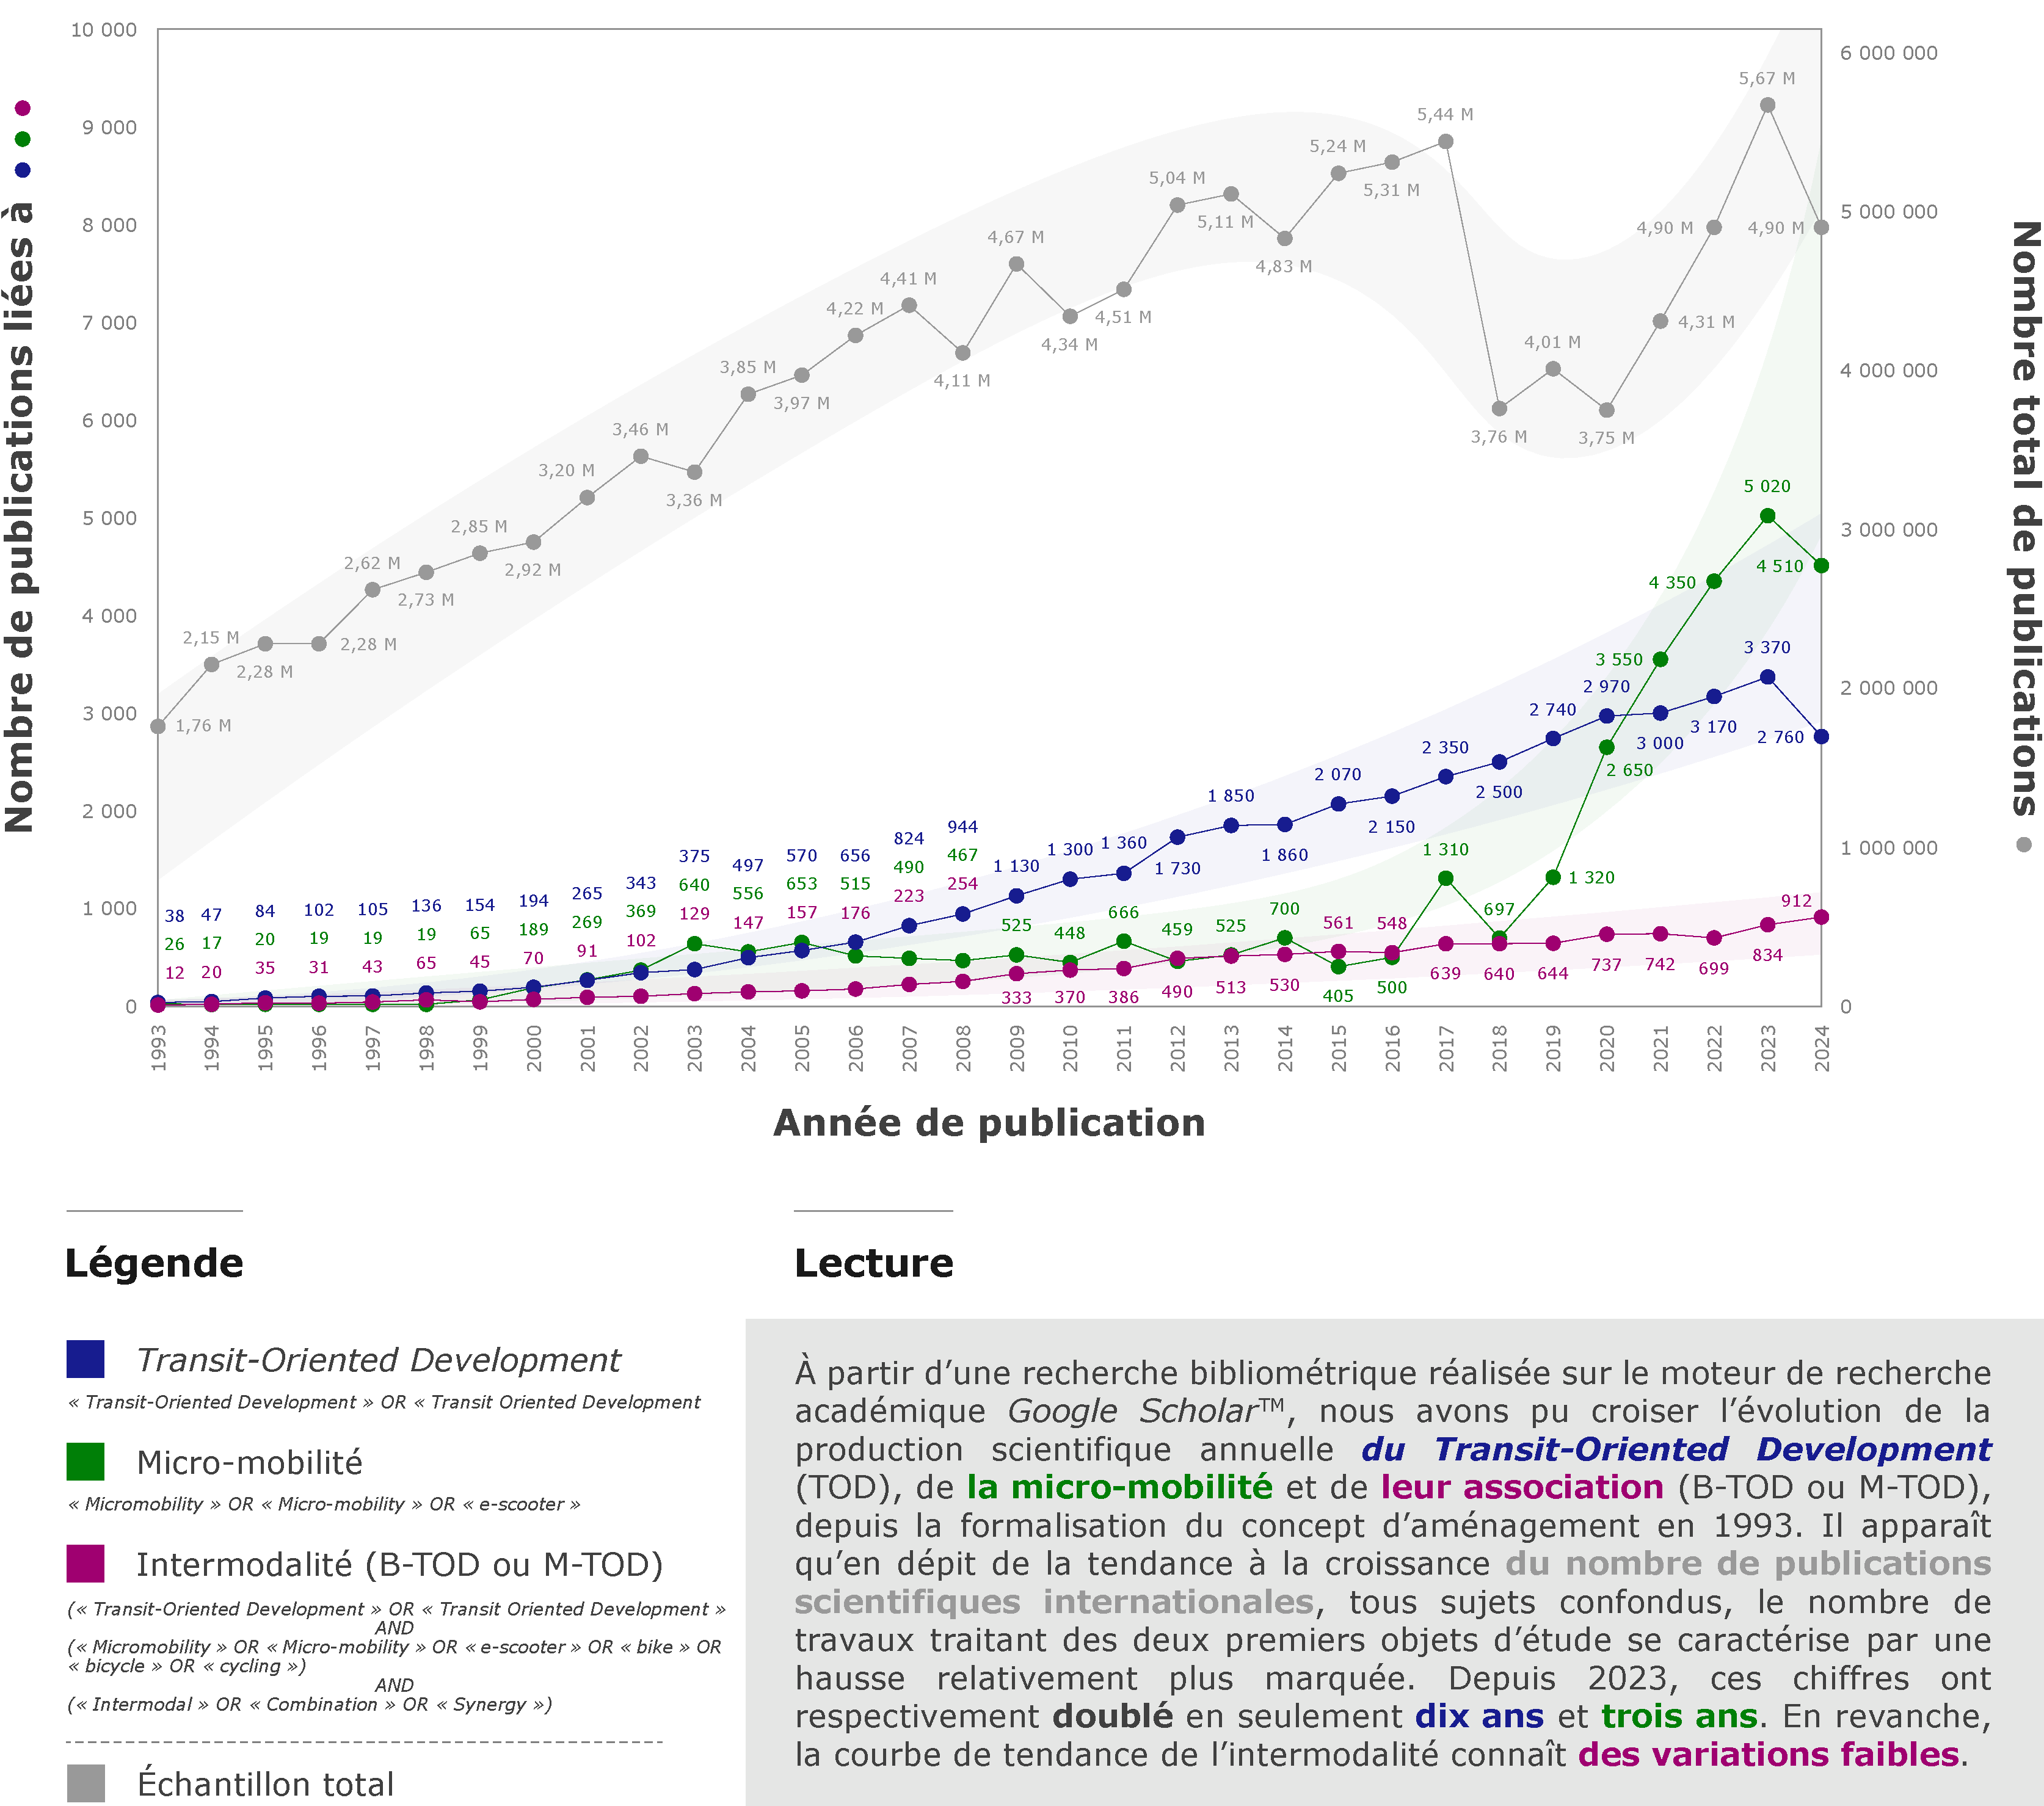
\includegraphics[width=1\columnwidth]{src/Figures/Chap-1/FR_Chronologie_publications_TOD_MIL.pdf}}
        \vspace{5pt}
        \begin{flushright}\scriptsize{
        Jeux de données~: données bibliométriques issues de \Marque{Google Scholar} et exportées le 2 février 2025
        \\
        Auteur~: \textcolor{blue}{Dylan Moinse (2025)}
      }\end{flushright}
    \end{figure}

    % M-TOD + Transition
L’une des évolutions récentes du \acrshort{TOD} explorées dans ce chapitre concerne l’intégration de la mobilité individuelle légère. Ces modes de déplacement complètent les infrastructures traditionnelles en offrant des solutions efficaces aux défis des \Guillemets{premiers et derniers kilomètres}. Toutefois, les connaissances sur cette forme d’intermodalité, en particulier sous l’angle de son articulation avec les formes urbaines, demeurent encore limitées. Ce constat est d’autant plus marqué pour les mobilités émergentes qui composent cette famille de modes, dont les interactions avec le \acrshort{TOD} restent largement inexplorées. Une simple recherche lexicale sur les thématiques du \acrshort{TOD} et de la micro-mobilité illustre combien ces sujets suscitent un intérêt croissant dans la recherche académique, comme l'atteste le \hyperref[fig-chap1:trends-google-scholar]{diagramme~\ref{fig-chap1:trends-google-scholar}} (page~\pageref{fig-chap1:trends-google-scholar}). Néanmoins, cette montée en puissance ne se traduit pas encore par une véritable synergie entre ces deux champs d’étude, qui restent peu représentés conjointement dans la littérature scientifique. Ce chapitre, qui pose le cadre théorique de notre recherche, se conclut ainsi par un constat~: celui d’un déficit de connaissances \textsl{a priori} sur un sujet redécouvert récemment dans le contexte du \acrshort{TOD}. Cette lacune est également mise en évidence par \textcolor{blue}{Wei} \textcolor{blue}{\textcite[90]{kang_university_2020}}\index{Kang, Wei|pagebf}\index{Aguiléra, Anne|pagebf}\index{Rallet, Alain|pagebf}, qui fait remarquer dans sa thèse de doctorat le faible nombre d’études consacrées à l’intermodalité entre les nouveaux services de mobilité, à savoir le \acrshort{VFF}, et les transports en commun. De même, la \acrshort{TEP} et la \acrshort{TEFF} n’ont été que marginalement étudiées, en dehors des problématiques liées à la traumatologie ou à l’accidentologie, alors même que leur potentiel intermodal est largement rapporté \textcolor{blue}{\autocite{richer_dossier_2021}}\index{Richer, Cyprien|pagebf}. Mener des études empiriques rigoureuses sur ces formes d’intermodalité apparaît comme une exigence pour mesurer et comprendre les comportements liés au \textsl{bike-and-ride} et au \textsl{scoot-and-ride}. \textcolor{blue}{\autocite[13]{bortoli_consequential_2020}}\index{Bortoli, Anne de|pagebf}\index{Christoforou, Zoi|pagebf}. Compte tenu de ce bilan, nous avons choisi d’engager un premier travail exploratoire sur ce que nous dénommons \acrshort{M-TOD}, en établissant un inventaire des travaux existants sur cette thématique, qui sera présenté dans le prochain chapitre.%%Rédigé%%

% ___________________________________________
     \newpage
     
% Valorisation scientifique
    \begin{tcolorbox}[colback=white!5!white,
                      colframe=blue!75!blue,
                      title=Valorisation scientifique
                      \\
                      Chapitre~1]
\Large{\textcolor{blue}{\textbf{Manifestations scientifiques~:}}}
    \\\\
\small{\textcolor{blue}{\textcite{moinse_transit-oriented_2021}}. Le Transit-Oriented Development, un urbanisme axé sur les transports en commun, intégrant les micro-mobilités émergentes. Une investigation sur les trottinettes personnelles en intermodalité, dans la région Hauts-de-France. \textsl{Rencontres TerriTrans - MoTAU}, Paris.
\\
\footnotesize{\url{https://hal.science/hal-03473391}} (\textbf{C-COM})}
    \\\\
\small{\textcolor{blue}{\textcite{moinse_modeurbain_2021}}. Le modèle urbain du Transit-Oriented Development revisité par les mobilités émergentes~? Une investigation sur le territoire de la région Hauts-de-France. \textsl{Rencontres Internationales en Urbanisme de l'APERAU}, Rabat.
\\
\footnotesize{\url{https://shs.hal.science/halshs-03507291}} (\textbf{C-COM})}
    \\\\
\small{\textcolor{blue}{\textcite{moinse_modeurbain_2020}}. Le modèle urbain du Transit-Oriented Development revisité par les micro-mobilités émergentes~? Une investigation sur le territoire de la région Hauts-de-France. \textsl{(Post-)Doctoriales AME 2020}, Le Croisic.
\\
\footnotesize{\url{https://shs.hal.science/halshs-03507482}} (\textbf{C-COM})}
    \\\\
\small{\textcolor{blue}{\textcite{moinse_etat_2020}}. État de l'art sur l'usage des trottinettes électriques en libre-service sans station. \textsl{Journées Transports \& Déplacements du Réseau Scientifique et Technique} (JTD RST). 
\\
\footnotesize{\url{https://shs.hal.science/halshs-03507375}} (\textbf{C-COM})}
    \\\\
\Large{\textcolor{blue}{\textbf{Vulgarisation scientifique~:}}}
    \\\\
\normalsize{\textcolor{blue}{\textcite{moinse_exploring_2023}}. \foreignlanguage{english}{\textsl{Exploring Val d'Europe's Urban Development in Marne-la-Vallée: A Guided Walking Tour of the TOD Project}}, Présentation de terrain, Paris
\\
\footnotesize{\url{https://shs.hal.science/halshs-04212064}}}
    \end{tcolorbox}

    % ___________________________________________
    % Sous-bibliographie
    \newpage
    \sectionheader{Sous-bibliographie du chapitre~1}
    \begingroup
    \renewcommand{\bibfont}{\scriptsize}
\printbibliography[segment=\therefsegment, heading=subbibintoc, title={Sous-bibliographie du chapitre~1}, label=chap1:bibliographie]
    \endgroup
    \end{refsegment}

%% ______________________________ %%
% CHAPITRE 2
%------------------------------%
%% ✎ Dylan (V1) %%%%%%%%% ✅ %%
%% ✎ Alain (V2) %%%%%%%%% ✅ %%
%% ✎ Dylan (V3) %%%%%%%%% ✅ %%
%------------------------------%

%%%%%%%%%%%%%%%%%%%%%%%%%%%%%%%%
% chapitre~2
\chapterheader{Revue systématique de la littérature}
\chapter
{Revue systématique de la littérature sur un développement urbain orienté vers les transports en commun et intégrant la mobilité individuelle légère
    \label{chap2:titre}
    }
    \begin{refsegment}

    % Arrière-plan chapitre~2
    \AddToShipoutPictureBG*{%
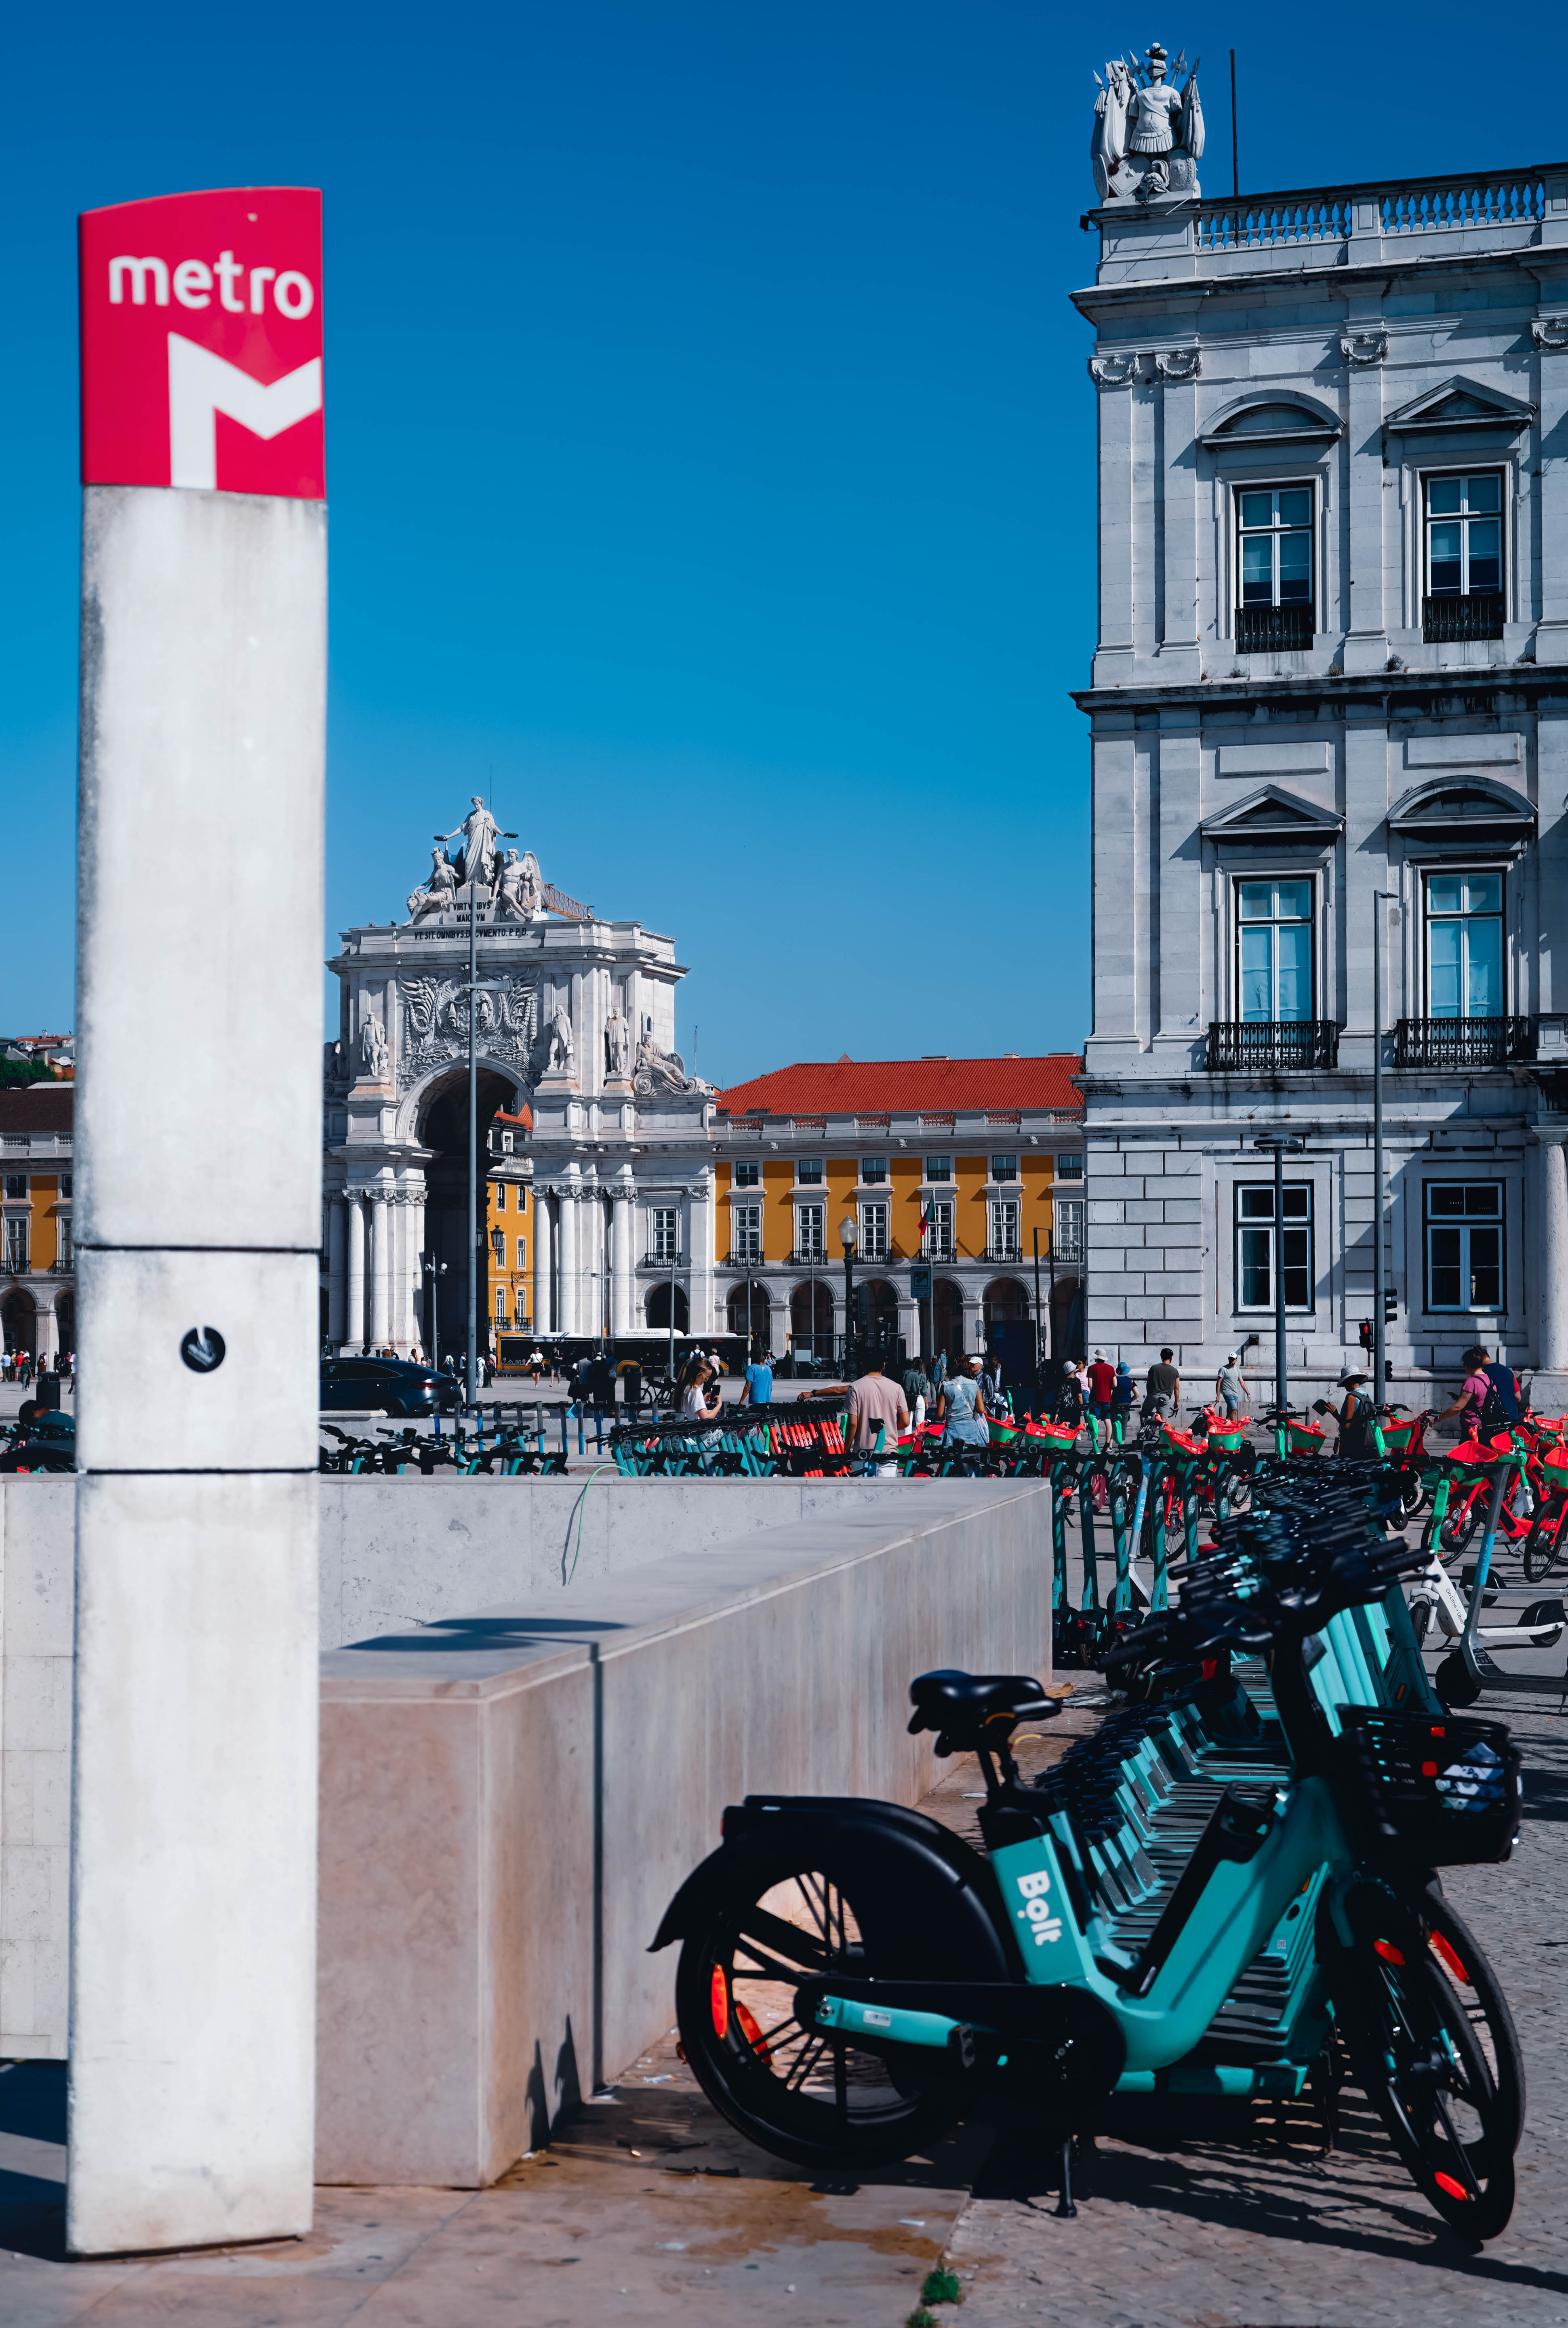
\includegraphics[width=\paperwidth,height=\paperheight]{src/Figures/Arriere_plan/Arriere_plan_Chap_2.jpg}
    }

% Rectangle
\AddToShipoutPictureBG*{
  \begin{tikzpicture}[remember picture,overlay]
    \node[fill=white, opacity=0.75, text width=\paperwidth, minimum height=12.25cm, anchor=north] 
    at ([yshift=-2cm]current page.north) {};
  \end{tikzpicture}
}

% Source
\AddToShipoutPictureFG*{
  \AtPageLowerRight{
    \raisebox{1cm}{
      \hspace{16cm}
      
\begin{tikzpicture}
        \node[fill=white, rounded corners=5pt, inner sep=5pt, align=center] {
          \tiny{Photographie~: \textcolor{blue}{Dylan Moinse (2023)}}
        };
      \end{tikzpicture}
    }
  }
}

    % ___________________________________________
    % Mini-sommaire
    \cleardoublepage
    \setcounter{tocdepth}{2}
    % Redéfinir le titre de la table des matières locale
    \renewcommand{\localcontentsname}{Table des matières du chapitre~2}
\localtableofcontents

% Réinitialiser numérotation section
\setcounter{section}{0}

    % ___________________________________________
    % Graphical abstract
    \newpage
\section*{Points clés du chapitre~2
    \label{chap2:graphical-abstract}
    }
    \markright{Préambule du chapitre}{}

\begin{figure}[h!]\vspace*{4pt}
        \caption*{}
        \label{graphical-abstract-chap2}
        \centerline{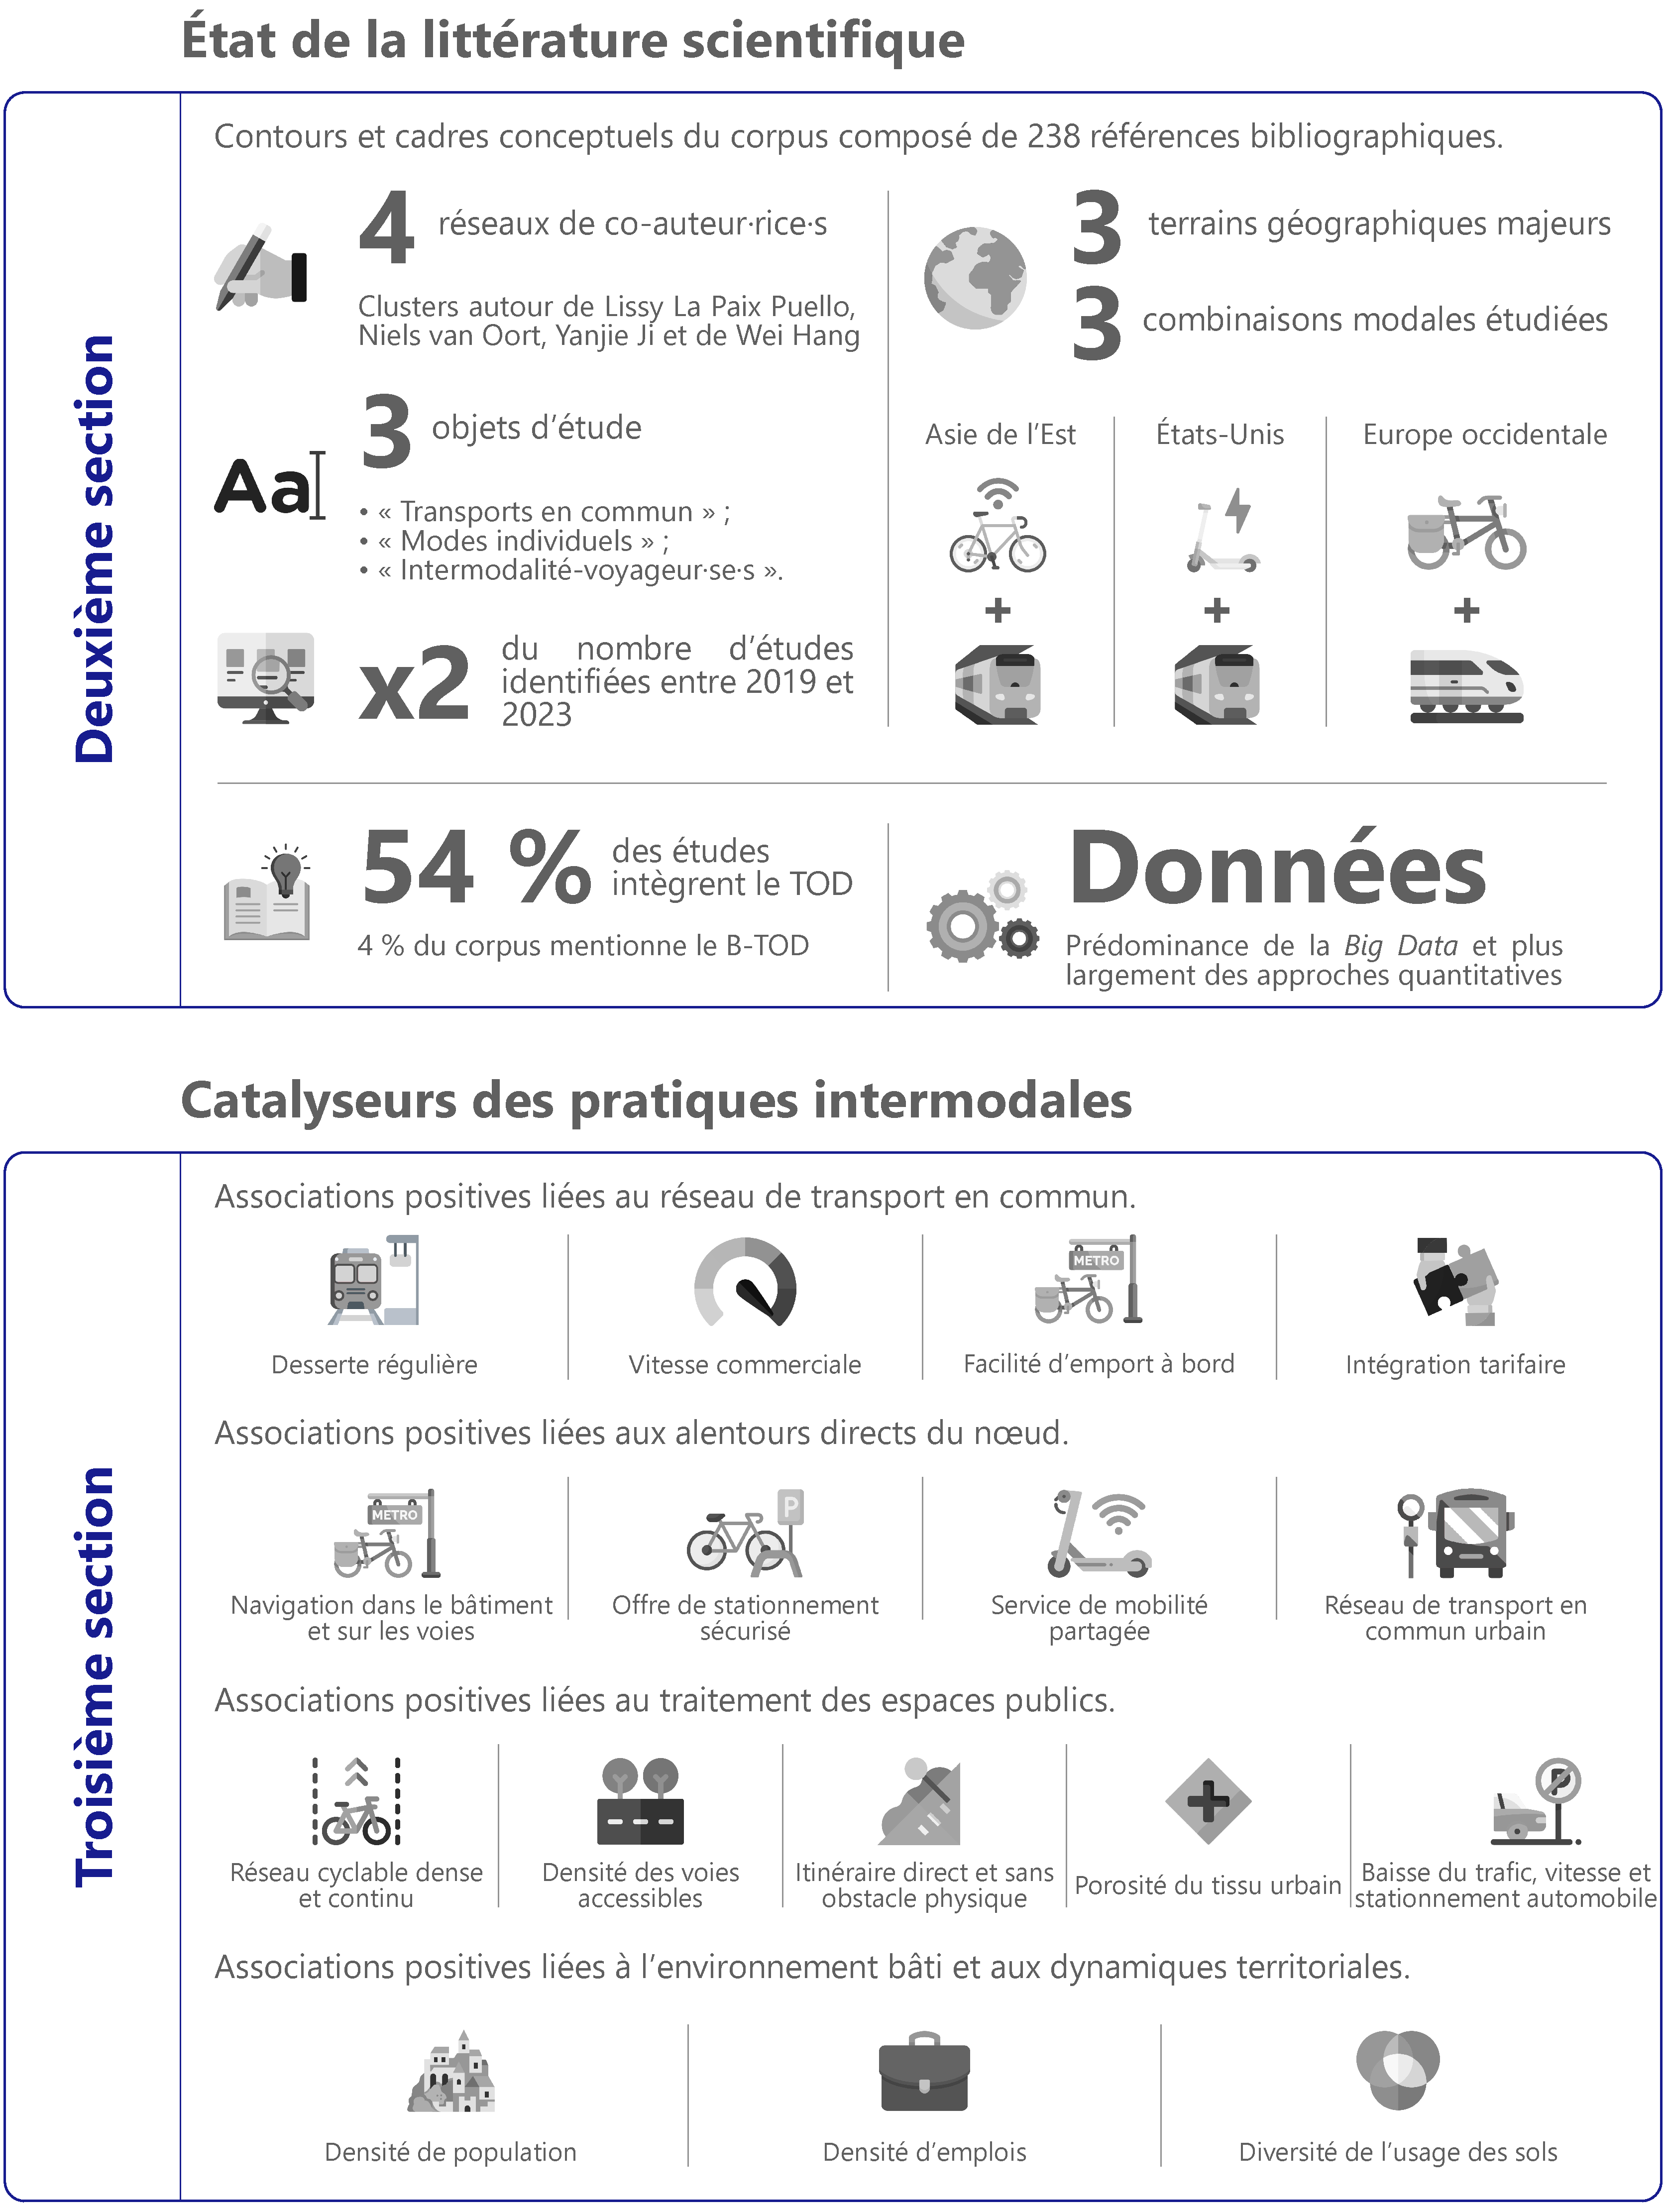
\includegraphics[width=1\columnwidth]{src/Figures/Graphical-abstract/FR_Graphical_abstract_chap2.pdf}}
        \vspace{5pt}
    \end{figure}

    % ___________________________________________
    % Préambule
    \newpage
    \begin{tcolorbox}[colback=white!5!white,
                      colframe=blue!75!blue,
                      title=
                      \bigskip
                      \center{\textbf{Préambule du chapitre~2}}
                      \\
                      \raggedright{\small{Chapitre composé de \pagedifference{chap2:titre}{chap3:titre} pages, dont \pagedifference{chap2:bibliographie}{chap3:titre} pages de bibliographie}}
                      \bigskip]
\Large{\textbf{\textcolor{blue}{Résumé~:}}}
    \\
    \small{
Le présent chapitre s'attache à apporter une vue d'ensemble de la recherche actuelle sur la conception d'un \acrfull{TOD} promouvant et promu par la mobilité individuelle légère. Cette étude bibliométrique et cette analyse bibliographique se présentent sous la forme d'une \acrfull{RSL} en constituant un recueil de 238 publications scientifiques. Dans la perspective de dresser un état des connaissances sur le \acrshort{B-TOD} et sur le \acrshort{M-TOD}, ce chapitre privilégie l'adoption de la \acrshort{RSL} en raison de sa capacité à conduire une analyse exhaustive de la littérature scientifique relative à ce sujet de recherche.%%Rédigé%%
    \\
L'élaboration de ce corpus a impliqué un processus de sélection d'articles scientifiques, d'articles de colloque, de chapitres d'ouvrages, de mémoires et de rapports de recherche diffusés en anglais et en français. Ces travaux académiques ont été examinés en se référant à des critères prédéfinis dans le but d'identifier l'ensemble des recherches abordant spécifiquement l'articulation entre la mobilité individuelle légère et les transports en commun (voir la \hyperref[chap2:protocole-methodologique-rsl]{section~1}, page~\pageref{chap2:protocole-methodologique-rsl}).%%Rédigé%%
    \\
Dans un premier temps, cette étude bibliographique a questionné les contextes temporels, géographiques et institutionnels influençant le champ de recherche sur le \acrshort{M-TOD}, ainsi que les cadres conceptuels et méthodologiques définis pour évaluer ce modèle urbain (voir la \hyperref[chap2:analyse-documentation-rsl]{section~2}, page~\pageref{chap2:analyse-documentation-rsl}). L'analyse de la répartition chronologique et spatiale des références bibliographiques a révélé un intérêt croissant pour l'intermodalité-voyageur·se·s, centré autour de trois pays à une échelle locale, avec des formes de combinaison modale qui évoluent dans le temps. La méthodologie adoptée tend vers l'élaboration d'analyses géostatistiques et de modélisations, facilitées par le développement des outils informatiques et de la \textsl{Big Data}.%%Rédigé%%
    \\
La troisième partie de ce chapitre se consacre à l'analyse des enseignements tirés des études examinées, en prêtant une attention particulière aux diverses composantes du \acrshort{B-TOD} et du \acrshort{M-TOD}, conceptualisées sous le terme des \Guillemets{\acrfull{7Ds}}~(voir la \hyperref[chap2:caracterisation-btod-environnement-urbain-choix-individuels]{section~3}, page~\pageref{chap2:caracterisation-btod-environnement-urbain-choix-individuels}). La caractérisation du \acrshort{M-TOD} a révélé tant des similitudes que des divergences, soulignant une association positive avec la densité de population et des emplois, la diversité de l'usage des sols, le traitement des espaces publics ou encore la qualité de l'offre en transport en commun. Divers impacts sur les comportements de mobilité, principalement pendulaires, et sur l'environnement ont été identifiés, tels qu'une diminution du bilan carbone, une amélioration de l'\gls{accessibilité} vers les destinations par une plus grande partie de la population, mais également l'existence d'inégalités sociales en termes d'accessibilité.%%Rédigé%%
    \\
En dernier lieu, la \acrshort{RSL} ouvre la voie à une lecture critique sur les lacunes présentes dans la littérature scientifique et sur les défis du \acrshort{M-TOD} (voir la \hyperref[chap2:conclusion]{conclusion du chapitre}, page~\pageref{chap2:conclusion}).%%Rédigé%%
    }
    \tcblower
\Large{\textbf{\textcolor{blue}{Mots-clés~:}}}
    \\
    \small{
Analyse bibliométrique~;
Analyse des réseaux~;
Caractéristiques socio-économiques~;
Caractéristiques urbaines~;
Cartographie scientifique~;
Comportements de mobilité~;
Impacts~;
Lecture critique du M-TOD~;
Mise en perspective internationale~;
Revue systématique de la littérature
    }
    \end{tcolorbox}

    % ___________________________________________
    % 2.*.
    \newpage
    \needspace{1\baselineskip} % Réserve de l'espace
    \addcontentsline{toc}{section}{Introduction du chapitre~2}
    \sectionheader{Introduction du chapitre}
\section*{Introduction du chapitre~2
    \label{chap2:introduction}
    }
    \markright{Introduction du chapitre~2}{}

    % Citation
    \begin{displayquote}
\Guillemets{\textsl{En complément des innovations au sein des modes de transport, les forces et faiblesses identifiées précédemment définissent également l'étendue des combinaisons possibles entre différents modes de déplacement. L'une de ces combinaisons est celle entre des modes de déplacement offrant un accès spatial relativement plus élevé grâce à leur vitesse, avec des modes plus lents présentant d'autres avantages.} [\dots] \textsl{Les combinaisons entre des modes de déplacement rapides (comme les trains) et des modes non motorisés, en particulier le \gls{vélo}, permettent une vitesse globale élevée de porte-à-porte, reliant ainsi efficacement une multitude de lieux d'origine et de destination. La combinaison train-vélo est particulièrement efficace~: le train est bien plus rapide que les autres transports en commun, et le vélo allie un accès ubiquitaire à des vitesses relativement élevées (supérieures à la marche, mais souvent aussi compétitives que le bus conventionnel ou le tramway, et même l'automobile dans certains environnements urbains). Dans les pays où l'infrastructure cyclable et les services ferroviaires sont étendus~–~comme aux Pays-Bas~–~cette combinaison modale est tellement développée qu'elle peut être considérée comme un mode de déplacement à part entière, et dans de nombreux contextes urbains, directement compétitive avec la voiture.} [\dots] \textsl{De plus, la combinaison train-vélo pourrait s'intégrer dans un système hybride, à la fois rapide et flexible, et donc pleinement compétitif avec la voiture.} [\dots] \textsl{Ce type de comportement multimodal est actuellement limité, mais pourrait se généraliser à l'avenir.} [\dots] \textsl{Et si un tel comportement hybride et adaptatif conjugué à un tel système de transport devenaient dominants~?}}\footnote{
    \Guillemets{\textsl{Next to innovations within transport modes, the strengths and weaknesses identified above also define the scope for transport mode combinations between transport modes. One such combination is between transport modes that give a relatively higher spatial access because of their speed with slower modes that have some other advantage.} [\dots] \foreignlanguage{english}{\textsl{Combinations between fast transit (such as trains) and non-motorized modes, particularly the bike, allow overall high door-to-door speed between virtually ubiquitous origin destinations. The train-bike combination is a particularly strong one: the train is much faster than other public transport, and the bike combines ubiquitous access with relatively high speeds (higher than walking but often also competitive with conventional buses or trams, and in certain environments even cars). In countries where both biking infrastructure and railway services are extensive~–~such as the Netherlands~–~this combination is so developed that it can be considered a transport mode in itself, and in many contexts directly competitive with the car.}} [\dots] \textsl{But also, the train-bike combination might integrate into a hybrid system which is both fast and flexible, and thus fully competitive with the car.} [\dots] \textsl{This type of multi-modal behaviour is now limited, but could become generalized in the future.} [\dots] \textsl{What if such a hybrid, highly adaptive behaviour and transportation system became dominant?}} \textcolor{blue}{\autocite[80-81, 220]{bertolini_planning_2017}}\index{Bertolini, Luca|pagebf}.} [traduction libre]

\textcolor{blue}{Luca} \textcolor{blue}{\textcite[80-81, 220]{bertolini_planning_2017}}\index{Bertolini, Luca|pagebf}. \foreignlanguage{english}{\textsl{Planning the Mobile Metropolis: Transport for People, Places and the Planet}}, Ed. Red Globe Press, Londres, 253~p. ISBN~: \href{https://search.worldcat.org/fr/title/1004435849}{978-0-230-30877-0}
    \end{displayquote}

    % Introduction
\lettrine[lines=3, findent=8pt, nindent=0pt]{\lettrinefont C}{e} chapitre vise à présenter l'état des connaissances actuelles qui aborde la redéfinition du \acrfull{TOD} en lien avec le regain d'intérêt pour la mobilité individuelle légère, dans la perspective de définir le concept de \acrfull{B-TOD} élargi par la mobilité individuelle légère. Afin de recueillir, d'analyser et de mettre en perspective les recherches traitant de ce sujet de recherche, une \acrfull{RSL} a été réalisée. Ainsi, seules les publications académiques diffusées en anglais ou en français et s'attachant à étudier cette forme d'\gls{intermodalité}-voyageur·se·s, d'un point de vue géographique et urbanistique, ont été incluses dans cette analyse bibliographique.%%Rédigé%%

    % Justification B-TOD / M-TOD
À la lumière du potentiel de la mobilité individuelle légère d'étendre l'\gls{accessibilité intermodale} des nœuds de \gls{transport en commun} \textcolor{blue}{\autocite[118]{cottrell_transforming_2007}}\index{Cottrell, Wayne~D.|pagebf}, l'objectif sous-jacent de cette analyse critique de la littérature scientifique relative au concept émergent du \acrfull{M-TOD} est de regrouper et de mieux comprendre la façon dont cette combinaison modale peut favoriser une conception urbaine propice au développement de modes de déplacement alternatifs. En partant du constat que l'association des transports en commun avec la mobilité individuelle légère, au même titre que la marche combinée, représente la forme d'intégration la plus efficace \textcolor{blue}{\autocite[50]{sebban_complementarite_2003, yang_study_2013}}\index{Sebban, Annie-Claude|pagebf}\index{Yang, Rongrong|pagebf}\index{Yan, Hai|pagebf}\index{Xiong, Wen|pagebf}\index{Liu, Tao|pagebf}, aussi bien sur le plan économique, social qu'environnemental — trois dimensions valorisées par le \acrshort{TOD} \textcolor{blue}{\autocite[85]{cervero_bike-and-ride_2013}}\index{Cervero, Robert|pagebf}\index{Caldwell, Benjamin|pagebf}\index{Cuellar, Jesus|pagebf} — la question de recherche abordée par cette \acrshort{RSL} est double. Il s'agit de justifier l'intégration de la mobilité individuelle légère aux systèmes de transport en commun par opposition à d'autres formes d'intermodalité telles que les parcs relais, tout en identifiant les défis inhérents au modèle urbain du \acrshort{M-TOD}.%%Rédigé%%

    % Justification RSL
L'intérêt d'entreprendre une \acrshort{RSL} réside dans sa capacité à rassembler, évaluer et synthétiser les connaissances existantes sur un sujet de recherche complexe qui mêle deux objets d'étude interdisciplinaires faisant non seulement appel à l'urbanisme et à la mobilité, mais également à une multitude de disciplines s'intéressant aux systèmes urbains, aux infrastructures et aux populations. La démarche innovante de la \acrshort{RSL} se distingue de la revue de littérature classique par sa recherche d'objectivité accrue, son objectif d'exhaustivité, la formulation de questions précises et la meilleure transparence des étapes composant le cheminement. Si cette méthode est principalement utilisée dans les sciences exactes, la \acrshort{RSL} tend à démontrer son efficacité dans les \acrfull{SHS} par le biais d'ajustements progressifs. Ainsi, l'élaboration d'une telle méthode sur un sujet de recherche original et récent présente plusieurs avantages. Elle permet d'identifier et d'évaluer les études existantes en adoptant une vision globale et nette de l'état des connaissances scientifiques, de repérer les tendances émergentes et l'évolution des recherches, ainsi que de déterminer les aspects insuffisamment explorés. Par conséquent, la \acrshort{RSL} permet également d'orienter les recherches futures, à l'instar de la présente recherche doctorale.%%Rédigé%%

    % Annonce du plan 1
Nous procéderons tout d'abord à une présentation détaillée du protocole méthodologique destiné à composer le corpus académique (\hyperref[chap2:protocole-methodologique-rsl]{section~1}, page~\pageref{chap2:protocole-methodologique-rsl}), qui inclura la formulation des questions de recherche (\hyperref[chap2:formulation-questions-recherche]{sous-section~1.1}, page~\pageref{chap2:formulation-questions-recherche}), la stratégie de recherche documentaire (\hyperref[chap2:strategie-recherche-documentaire]{sous-section~1.2}, page~\pageref{chap2:strategie-recherche-documentaire}), les processus de sélection des publications scientifiques (\hyperref[chap2:selection-publications-scientifiques]{sous-section~1.3}, page~\pageref{chap2:selection-publications-scientifiques}) et d'extraction des données récoltées ainsi que les points examinés (\hyperref[chap2:extraction-donnees-aspects-consideres]{sous-section~1.4}, page~\pageref{chap2:extraction-donnees-aspects-consideres}).%%Rédigé%%

    % Annonce du plan 2
Une fois la méthodologie exposée, nous soulignerons les caractéristiques de la littérature scientifique et des pratiques de recherche sur ce sujet (\hyperref[chap2:analyse-documentation-rsl]{section~2}, page~\pageref{chap2:analyse-documentation-rsl}), à travers l'analyse des métadonnées issues de la documentation (\hyperref[chap2:etat-litterature-scientifique-internationale-btod]{sous-section~2.1}, page~\pageref{chap2:etat-litterature-scientifique-internationale-btod}) et des cadres conceptuels et méthodologiques des références bibliographiques (\hyperref[chap2:cadres-conceptuels-methodologiques]{sous-section~2.2}, page~\pageref{chap2:cadres-conceptuels-methodologiques}).%%Rédigé%%

    % Annonce du plan 3
Le troisième temps de cette \acrshort{RSL} sera consacré à la présentation synthétique des \Guillemets{\acrfull{7Ds}}~et des principaux enseignements qui servent de principes directeurs pour le TOD (\hyperref[chap2:caracterisation-btod-environnement-urbain-choix-individuels]{section~3}, page~\pageref{chap2:caracterisation-btod-environnement-urbain-choix-individuels}), en interrogeant l'association entre l'intégration de la mobilité individuelle légère et l'influence de la densité de population (\hyperref[chap2:densite-population]{sous-section~3.1}, page~\pageref{chap2:densite-population}), de la diversité fonctionnelle (\hyperref[chap2:diversite-fonctionnelle]{sous-section~3.2}, page~\pageref{chap2:diversite-fonctionnelle}), du traitement des espaces publics (\hyperref[chap2:traitement-espaces-publics]{sous-section~3.3}, page~\pageref{chap2:traitement-espaces-publics}), de l'accessibilité intermodale (\hyperref[chap2:accessibilite-intermodale]{sous-section~3.4}, page~\pageref{chap2:accessibilite-intermodale}), des distances vers et depuis les nœuds de transport en commun (\hyperref[chap2:distances-premiers-derniers-km]{sous-section~3.5}, page~\pageref{chap2:distances-premiers-derniers-km}), de la gestion de la demande de mobilité (\hyperref[chap2:gestion-demande-mobilite]{sous-section~3.6}, page~\pageref{chap2:gestion-demande-mobilite}), des caractéristiques socio-démographiques des usager·ère·s (\hyperref[chap2:sociodemographie-usagers]{sous-section~3.7}, page~\pageref{chap2:sociodemographie-usagers}), des comportements de mobilité (\hyperref[chap2:comportements-mobilite]{sous-section~3.8}, page~\pageref{chap2:comportements-mobilite}) et des impacts de ces pratiques intermodales sur les systèmes de mobilité et les systèmes urbains (\hyperref[chap2:impacts-systemes-urbain-mobilite]{sous-section~3.9}, page~\pageref{chap2:impacts-systemes-urbain-mobilite}).%%Rédigé%%

    % Annonce du plan 4
En guise de conclusion, nous avancerons les pistes de recherche futures portant sur l'intégration de la mobilité individuelle légère au \acrshort{TOD} et qui viendront alimenter cette thèse de doctorat (\hyperref[chap2:conclusion]{conclusion du chapitre~2}, page~\pageref{chap2:conclusion}).%%Rédigé%%

    % ___________________________________________
    % 2.1.
    \newpage
    \needspace{1\baselineskip} % Réserve de l'espace
    \sectionheader{Méthodologie de la revue systématique de la littérature}
\section{Protocole méthodologique de la revue systématique de la littérature
    \label{chap2:protocole-methodologique-rsl}
    }
    
    % Etat de l'art RSL
La procédure méthodologique sous-tendant l'élaboration d'une \acrshort{RSL} est en constante évolution en raison de sa genèse relativement tardive dans les champs des \acrshort{SHS} et des discussions actuelles sur les limites méthodologiques qui lui sont associées. La \acrshort{RSL} conduite dans le cadre de ce chapitre s'inscrit dans le sillage des techniques énoncées dans l'article de référence consacré à la réalisation d'une \acrshort{RSL} thématique et qualitative, dans une revue scientifique médicale, sous la plume de \textcolor{blue}{\textcite[3-7]{thomas_methods_2008}}\index{Thomas, James|pagebf}\index{Harden, Angela|pagebf}. En tenant compte des nuances dans la réalisation d'une \acrshort{RSL} selon les disciplines \textcolor{blue}{\autocite[738]{padeiro_transit-oriented_2019}}\index{Padeiro, Miguel|pagebf}\index{Louro, Ana|pagebf}\index{Costa, Nuno Marques de|pagebf}, le protocole méthodologique développé repose sur les enseignements tirés de différentes \acrshort{RSL} examinant le \acrshort{TOD} et la mobilité individuelle légère. À ce titre, la méthode construite se nourrit des techniques et des réflexions issues de diverses \acrshort{RSL}, l'une portant sur les liens entre le \acrshort{TOD} et la gentrification \textcolor{blue}{\autocite[738]{padeiro_transit-oriented_2019}}\index{Padeiro, Miguel|pagebf}\index{Louro, Ana|pagebf}\index{Costa, Nuno Marques de|pagebf}, l'autre au sujet de l'intégration de la mobilité individuelle légère aux systèmes de transport en commun \textcolor{blue}{\autocite[4]{oeschger_micromobility_2020}}\index{Oeschger, Giulia|pagebf}\index{Carroll, Páraic|pagebf}\index{Caulfield, Brian|pagebf}. Plusieurs revues de littérature existantes ont également guidé la conception de notre \acrshort{RSL}, particulièrement celles examinant le vélo et la micro-mobilité électriques \textcolor{blue}{\autocite[3]{sengul_impacts_2021}}\index{Sengül, Buket|pagebf}\index{Mostofi, Hamid|pagebf}, les services de trottinettes électriques \textcolor{blue}{\autocite[4]{bozzi_shared_2021}}\index{Bozzi, Alberica Domitilla|pagebf}\index{Aguiléra, Anne|pagebf}, le choix des itinéraires cyclables \textcolor{blue}{\autocite[2]{pritchard_revealed_2018}}\index{Pritchard, John~P.|pagebf} et l'usage de la \textsl{Big Data} en lien avec la mobilité \textcolor{blue}{\autocite[36]{neilson_systematic_2019}}\index{Neilson, Alex|pagebf}\index{Indratmo|pagebf}\index{Daniel, Ben|pagebf}\index{Tjandra, Stevanus|pagebf}.%%Rédigé%%

    % Sélection
Par ailleurs, cette recherche bibliographique s'inspire du guide méthodologique destiné à produire une revue de littérature dans les domaines de l'aménagement urbain et de la mobilité, et adaptée par l'organisation académique nationale étasunienne \textcolor{blue}{\textcite{transportation_research_board_of_the_national_academies_literature_2015}}\index{Transportation Research Board@\textsl{Transportation Research Board}|pagebf}. Ce rapport identifie notamment six étapes principales visant à constituer une \acrshort{RSL}~: la définition du sujet de recherche enquêté (i), la sélection des librairies et des bases de données bibliographiques appropriées au sujet défini (ii), la formulation d'une expression à partir de mots-clés (iii), la définition des relations entre les termes pour développer une recherche avancée (iv), le contrôle de la collection de textes recueillie (v) puis l'organisation des données en vue de les analyser (vi) \textcolor{blue}{\autocite[2-18]{transportation_research_board_of_the_national_academies_literature_2015}}\index{Transportation Research Board@\textsl{Transportation Research Board}|pagebf}. De plus, le processus de sélection des publications scientifiques dans le cadre de cette \acrshort{RSL} embrasse les trois étapes établies par \textcolor{blue}{\textcite[2~544]{jain_systematic_2020}}\index{Jain, Deepshikha|pagebf}\index{Singh, Ekta|pagebf}\index{Ashtt, Rashmi|pagebf}~:
    \begin{customitemize}
        \item La phase initiale d'exclusion se caractérise par l'analyse des métadonnées, tirées des références bibliographiques et incluant à la fois le titre, le résumé et les mots-clés afférents, afin d'évaluer leur pertinence par rapport au sujet de recherche considéré~;
        \item La phase intermédiaire d'exclusion implique la lecture critique de l'introduction et de la conclusion de chaque document retenu afin de filtrer plus finement les publications scientifiques qui se rapportent aux objectifs de recherche fixés dans la \acrshort{RSL}~;
        \item La phase finale d'exclusion engage une lecture complète des études intégrées à la \acrshort{RSL} afin de garantir la qualité du processus de sélection.
    \end{customitemize}
En suivant ces trois séquences, le processus d'inclusion assure une approche méthodique en cernant les sources académiques pertinentes en lien avec le sujet de recherche spécifié.%%Rédigé%%

    % Avantages de la RSL
Vis-à-vis d'une revue de littérature conventionnelle, la \acrshort{RSL} acquiert le statut de \Guillemets{systématique}~lorsque celle-ci s'articule autour d'une question de recherche formulée, de l'identification de travaux en adéquation avec le sujet délimité et d'une explicitation claire de la méthodologie suivie. En ce sens, la \acrshort{RSL} détient plusieurs avantages comparatifs \textcolor{blue}{\autocite[2]{transportation_research_board_of_the_national_academies_literature_2015}}\index{Transportation Research Board@\textsl{Transportation Research Board}|pagebf}~:
    \begin{customitemize}
        \item La résolution de problèmes permise par la couverture complète des connaissances existantes sur une thématique précise~;
        \item La mise en confrontation d'études antérieures et concurrentes, de sorte à faciliter la compréhension du discours académique existant~;
        \item La validation des méthodes de recherche appliquées en questionnant la fiabilité des approches retenues~;
        \item La confirmation de la nécessité de poursuivre les recherches en mettant en évidence les domaines d'étude émergents~;
        \item L'orientation des efforts de recherche en offrant des perspectives qui viennent éclairer l'état des connaissances actuelles et dessiner des pistes prometteuses pour les futures initiatives de recherche.
    \end{customitemize}
À l'aide de ces avantages, la \acrshort{RSL} établit une base solide pour sonder la littérature scientifique, en contribuant à apporter une plus grande rigueur méthodologique, une analyse fine des recherches existantes et une feuille de route visant à guider les études ultérieures.%%Rédigé%%

    % 2.1.1.
    \needspace{1\baselineskip} % Réserve de l'espace
\subsection{Formulation des questions de recherche
    \label{chap2:formulation-questions-recherche}
    }
    
    % Questions et objectifs
L'objectif premier de cette \acrshort{RSL} est de fournir une compréhension approfondie des connaissances et des pratiques existantes en lien avec une fabrication urbaine orientée vers les transports en commun et reposant sur la mobilité individuelle légère, tout en déterminant les facteurs qui facilitent ou entravent la mise en œuvre du modèle urbain et en évaluant ses effets sur la mobilité et les territoires. À cet égard, la \acrshort{RSL} vise à examiner et à discuter, en premier lieu, du rôle du vélo au sein du modèle d'aménagement. Bien que l'intégration de ce mode de déplacement ait été envisagée dès la conceptualisation du \acrshort{TOD}, son potentiel semble demeurer sous-exploité. C'est dans cette optique que cette revue de littérature cherche à caractériser sa déclinaison, connue sous le nom de \acrshort{M-TOD}. Par ailleurs, nous nous employons à l'actualiser en y adjoignant l'exploration des options de \gls{micro-mobilité} émergente. Ces dernières, par leur caractère innovant, sont susceptibles d'interagir et de transformer à leur tour les fondements du \acrshort{M-TOD}.

Dans cette perspective, la grille de lecture suivante, centrée sur six questions de recherche, oriente la \acrshort{RSL}~:
    \begin{customitemize}
        \item Quels sont les facteurs urbains et les politiques publiques qui favorisent l'intégration du vélo et des options de micro-mobilité aux systèmes de transport en commun~? Réciproquement, cette forme de mobilité influence-t-elle les configurations territoriales~?
        \item Quels sont les effets de cette combinaison modale en termes de développement économique, de cohésion sociale et de respect de l'environnement~?
        \item Existe-t-il un périmètre pertinent pour définir un quartier de gare à partir de la mobilité individuelle légère~? La taille de ces aires d'influence varie-t-elle en fonction de certains paramètres~?
        \item Quelles sont les pratiques d'urbanisme et les modèles de gouvernance se révélant innovants et efficaces pour favoriser un tel développement urbain~?
        \item Peut-on considérer le \acrshort{M-TOD} comme un modèle urbain internationalement reconnu et réplicable~?
        \item Quels sont les principaux défis à relever dans la réflexion et l'application d'une stratégie \acrshort{M-TOD}~?
    \end{customitemize}%%Rédigé%%

    % 2.1.2.
    \needspace{1\baselineskip} % Réserve de l'espace
\subsection{Stratégie de recherche documentaire
    \label{chap2:strategie-recherche-documentaire}
    }

    % Recherche en ligne
La phase initiale de collecte des données se traduit par l'utilisation de recherches en ligne, à l'aide de bases de données bibliographiques offrant une couverture transdisciplinaire. Cette étape de recueil de la documentation veille à capturer et à répertorier un corpus exhaustif de références bibliographiques provenant de la littérature scientifique et de la littérature grise
    \footnote{
        Dans ce contexte, la littérature scientifique fait référence aux publications académiques évaluées par des pairs, incluant les articles publiés dans des revues scientifiques, actes de colloque, chapitres d'ouvrage et les mémoires de recherche. La littérature grise, telle que définie par l\acrfull{AFNOR} et la Convention luxembourgeoise sur la littérature grise, comprend des \Guillemets{\textsl{documents dactylographiés ou imprimés, souvent de nature provisoire, reproduits et distribués à moins d'un millier d'exemplaires, en dehors des circuits commerciaux de publication et de distribution}}~\textcolor{blue}{\autocite[30]{schopfel_comprendre_2015}}\index{Schöpfel, Joachim|pagebf}. La littérature grise couvre \Guillemets{\textsl{ce qui est produit par tous les niveaux de gouvernement, les universités, les entreprises et l'industrie, sous forme imprimée ou électronique, mais qui n'est pas contrôlé par l'édition commerciale}}~\textcolor{blue}{\autocite{national_grey_literature_collection_luxembourg_nodate}}\index{National Grey Literature Collection|pagebf}. Récemment, \textcolor{blue}{Joachim} \textcolor{blue}{\textcite[9]{schopfel_vers_2012}}\index{Schöpfel, Joachim|pagebf} a proposé une définition renouvelée de ce type de littérature, le considérant comme \Guillemets{\textsl{un document produit par le gouvernement, l'administration, l'éducation et la recherche, l'entreprise et l'industrie, sous forme imprimée ou électronique, protégé par des droits de propriété intellectuelle, d'une qualité suffisante pour être collecté et préservé par une bibliothèque ou une archive institutionnelle, et qui n'est pas contrôlé par l'édition commerciale}}.
}. Dans le cadre de cette \acrshort{RSL}, les recherches en ligne intègrent les articles scientifiques, les actes de colloque, les chapitres d'ouvrage, les mémoires de recherche en master ou en doctorat et les rapports de recherche publics. Cependant, elles excluent, entre autres, les prépublications scientifiques, documents techniques ou politiques, rapports d'étude privés, déclarations publiques ou encore les bulletins d'information. Il faut noter que l'inventaire de la bibliographie liée au \acrshort{M-TOD} a été initialement réalisé entre le 3 et le 8 décembre 2021. Par la suite, eu égard à la dimension naissante de ce sujet, une mise à jour de la collecte des données a été effectuée entre le~10~et le~13~avril~2023 afin d'inclure les publications les plus récentes.%%Rédigé%%

    % Etape de recherche en ligne
La collecte des données pour cette \acrshort{RSL} s'est manifestée par une \acrfull{Recherche EN}, ou \(R_{EN}\), et une \acrfull{Recherche FR}, ou \(R_{FR}\), en exploitant diverses plates-formes en ligne jouissant d'une reconnaissance solide dans la sphère académique. Les ressources académiques citées ci-après ont été sélectionnées du fait de leur couverture étendue, de leur accessibilité et de leur fiabilité. De surcroît, ces bases de données numériques facilitent l'identification, l'indexation et l'exportation vers des logiciels de gestion de références bibliographiques d'un large éventail de références scientifiques, notamment grâce aux outils de recherche avancée intégrés.%%Rédigé%%

    % Figure RSL - Echantillonnage
    \begin{figure}[h!]\vspace*{4pt}
        \caption{Diagramme de flux représentant le processus de sélection des publications scientifiques intégrées dans la revue systématique de la littérature.}
        \label{fig-chap2:diagramme-flux-selection-publications-rsl}
        \centerline{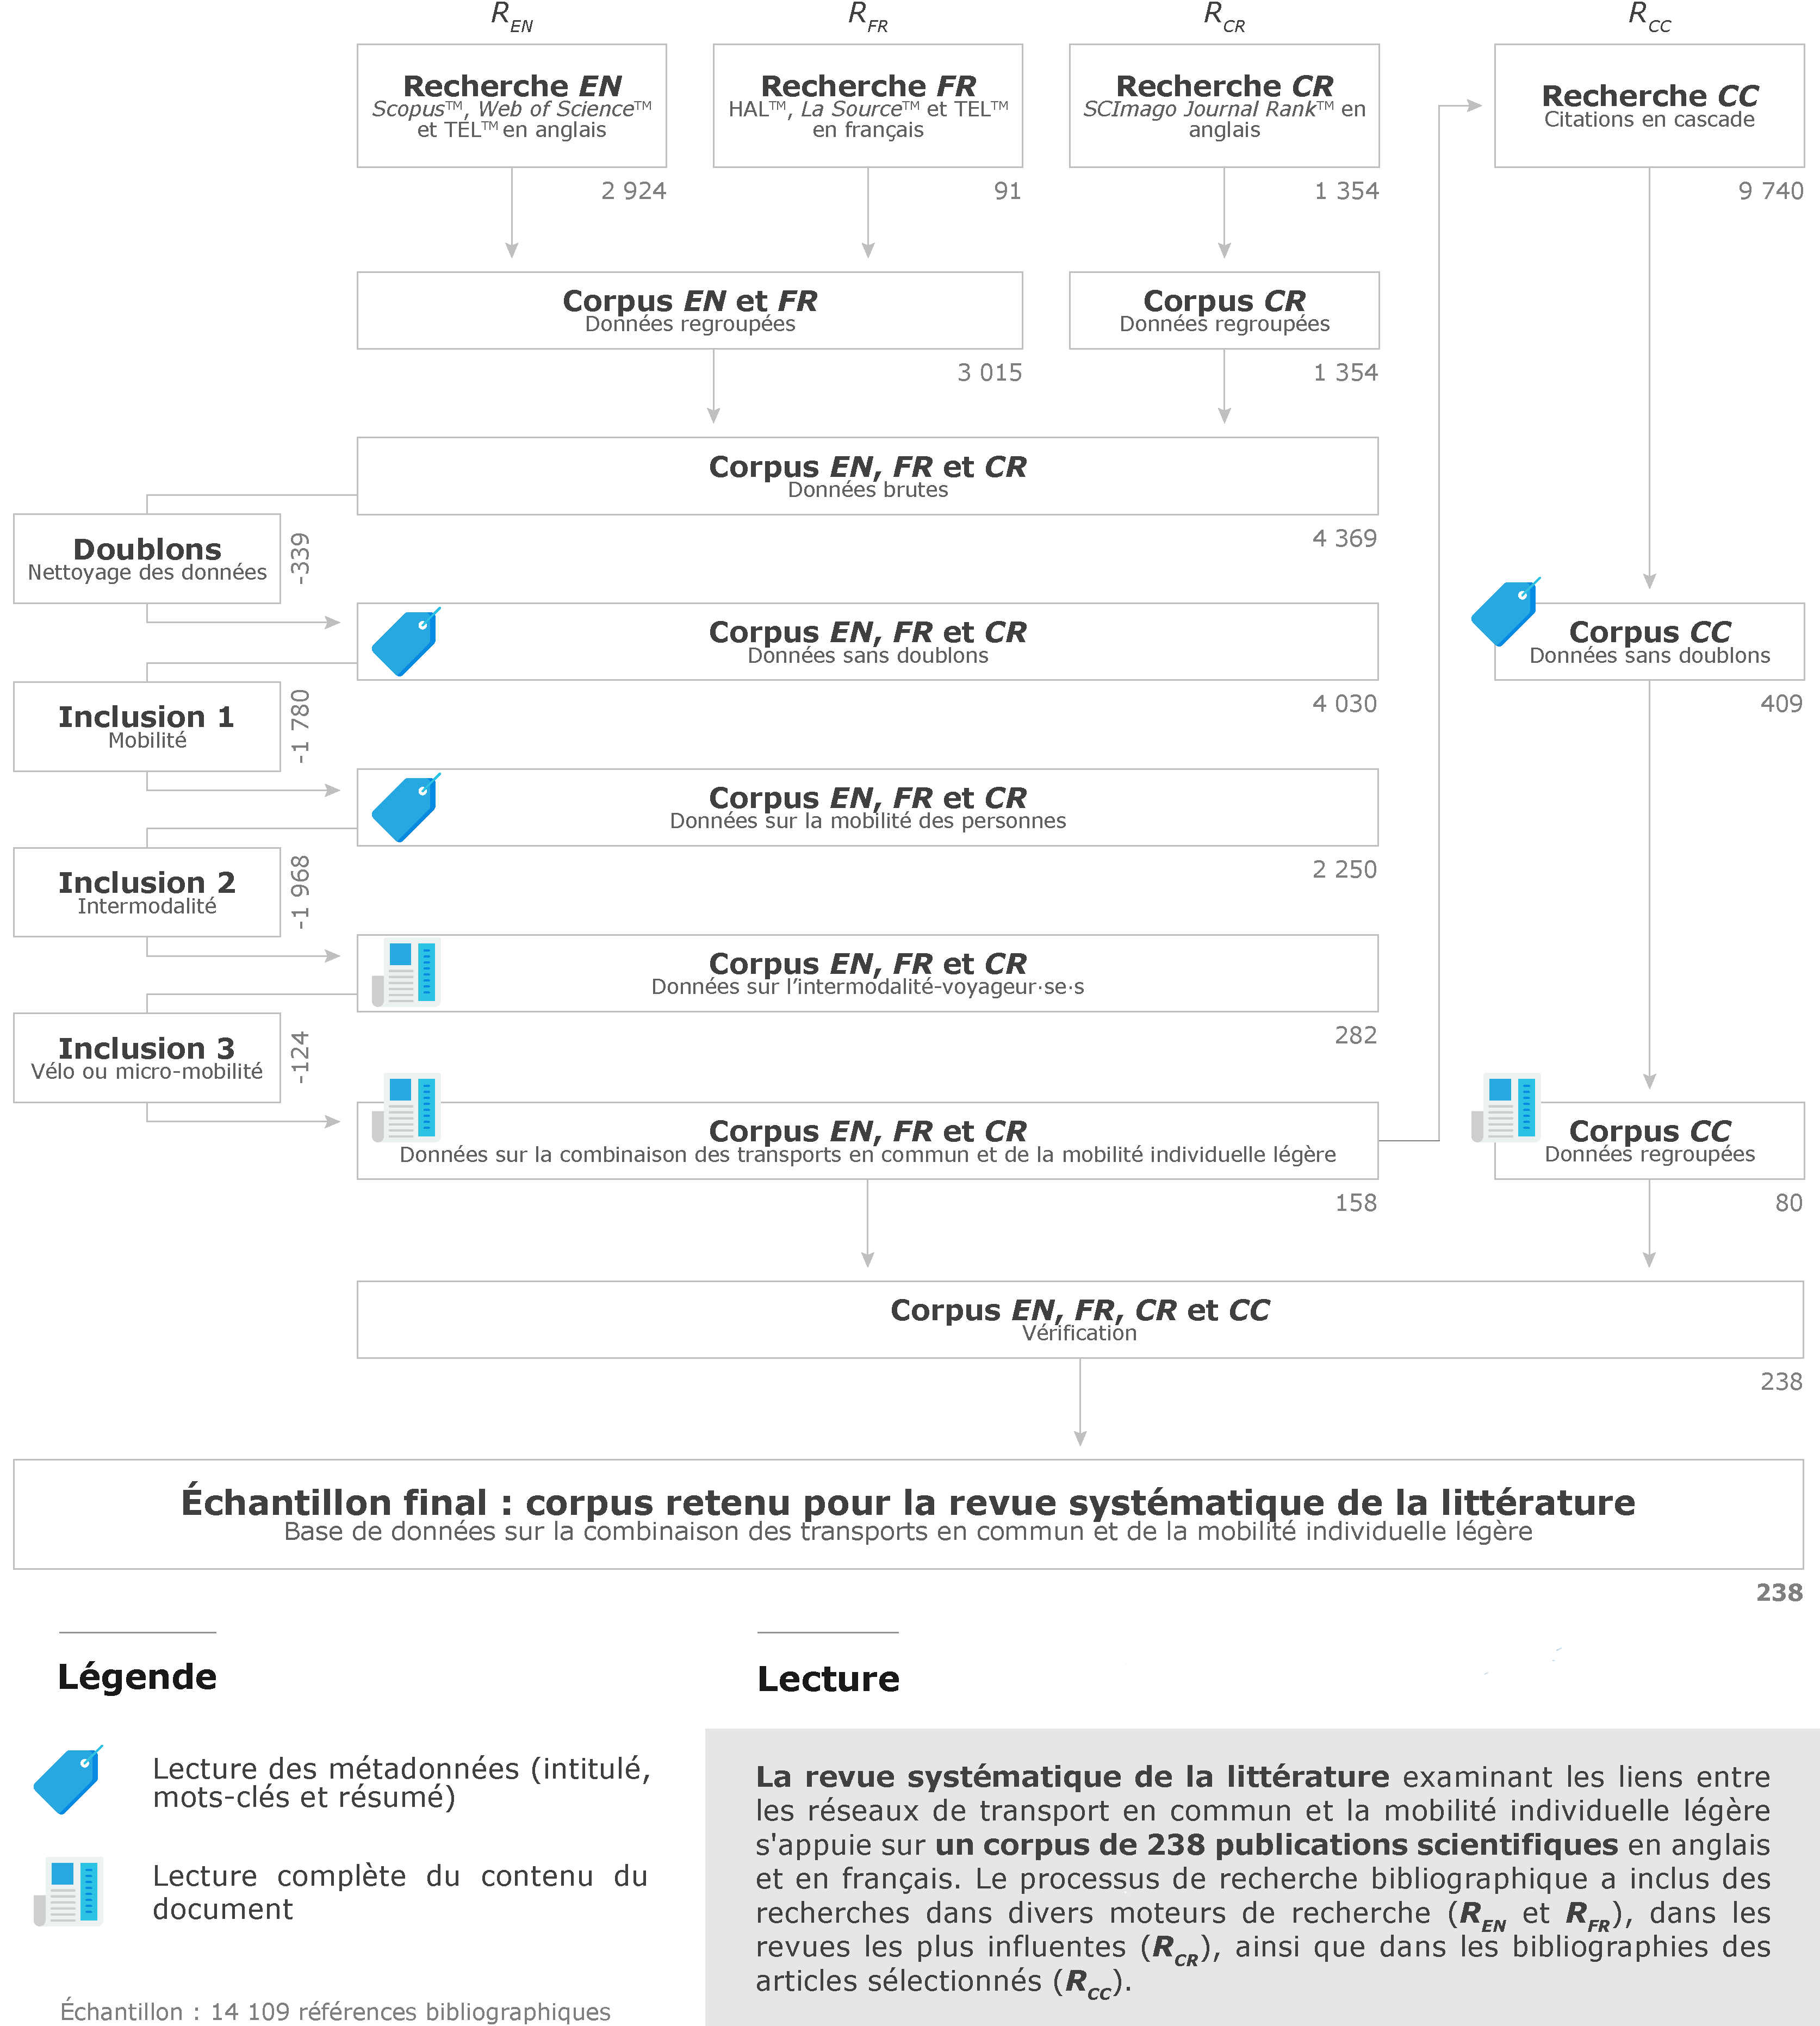
\includegraphics[width=1\columnwidth]{src/Figures/Chap-2/FR_RSL_Diagramme_flux_selection_publications.pdf}}
        \vspace{5pt}
        \begin{flushright}\scriptsize{
        Auteur~: \textcolor{blue}{Dylan Moinse (2023)}
        }\end{flushright}
    \end{figure}

    % Recherches EN+FR
Dans le premier cas, nous avons interrogé les bases de données documentaires \Marque{Scopus}~et \Marque{Web of Science}\footnote{
    \textsl{Scopus} (\url{www.scopus.com}) et \textsl{Web of Science} (\url{www.webofscience.com}) sont des plates-formes bibliographiques en ligne couramment utilisées dans le domaine de la recherche académique. \textsl{Scopus} est développé par \Marque{Elsevier}, une société spécialisée dans l'édition scientifique, tandis que \textsl{Web of Science} est une collection de travaux académiques gérée par \Marque{Clarivate Analytics}.
}. En complément, le serveur \Marque{TEL}\footnote{
    \textsl{theses.fr} (\url{www.theses.fr}) est une plate-forme d'archives pour les thèses de doctorat, offrant régulièrement un accès en ligne à des ressources académiques produites par des docteur·e·s.
} a été consulté afin d'élargir la recherche aux thèses de doctorat soumises en anglais. Dans un second temps, la recherche bibliographique en français s'est appuyée sur le portail \Marque{HAL}\footnote{
    \textsl{Hyper Article en Ligne} (\url{https://hal.science/}) est un portail d'archives ouvert qui facilite le dépôt, la diffusion et la consultation de documents scientifiques. Ce portail a été développé par le \acrfull{CCSD} du \acrfull{CNRS}. \textsl{HAL} permet aux chercheurs et aux institutions de diffuser gratuitement leurs travaux de recherche afin de faciliter l'accès libre et la visibilité des travaux de recherche.
}, la plate-forme \Marque{La Source}\footnote{
    \textsl{La Source} (\url{https://bibliotheque.enpc.fr}) est la bibliothèque en ligne développée par l'\textsl{École des Ponts Paristech}, conçue pour faciliter l'accès aux ressources scientifiques disponibles sur sa plate-forme en ligne.
} et une nouvelle fois sur le serveur \textsl{TEL}. La \Guillemets{\acrshort{Recherche EN}}~a abouti à la compilation de 2~924 publications scientifiques, tandis que la \Guillemets{\acrshort{Recherche FR}}~a permis d'y ajouter 91 références, après réactualisation de la collection en avril 2023. Ainsi, cette première étape de recherche en ligne a formé un corpus de 3 015 documents, désigné sous le nom de \Guillemets{Corpus EN et FR}~(voir l'\hyperref[fig-chap2:diagramme-flux-selection-publications-rsl]{illustration~\ref{fig-chap2:diagramme-flux-selection-publications-rsl}}, page~\pageref{fig-chap2:diagramme-flux-selection-publications-rsl}).%%Rédigé%%

    % Tableau revues scientifiques
% Tableau types de quartier de gare
%%Rédigé%%
        \begin{table}[h!]
    \centering
    \renewcommand{\arraystretch}{1.5}
    \resizebox{\columnwidth}{!}{
    \begin{tabular}{p{0.07\columnwidth}p{0.1\columnwidth}p{0.7\columnwidth}p{0.13\columnwidth}}
        %\hline
    \rule{0pt}{15pt} \small{\textbf{\textcolor{blue}{Rang}}} & \small{\textbf{\textcolor{blue}{Étiquette}}} & \small{\textbf{\textcolor{blue}{Revue scientifique}}} & \small{\textbf{\textcolor{blue}{Indice \acrshort{SJR}}}}\\
        \hline
    \multicolumn{4}{l}{\small{\textbf{\textcolor{blue}{Transports (2023)}}}}\\
\small{1} & \small{\(SMG_{T1}\)} & \small{\textsl{Analytic Methods in Accident Research}} & \small{4,8}\\
\small{2} & \small{\(SMG_{T2}\)} & \small{\textsl{Tourism Management}} & \small{3,4}\\
\small{3} & \small{\(SMG_{T3}\)} & \small{\textsl{Transportation Research Part B: Methodological}} & \small{3,4}\\
\small{4} & \small{\(SMG_{T4}\)} & \small{\textsl{Journal of Travel Research}} & \small{3,3}\\
\small{5} & \small{\(SMG_{T5}\)} & \small{\textsl{Transportation Research Part C: Emerging Technologies}} & \small{3,2}\\
\small{6} & \small{\(SMG_{T6}\)} & \small{\textsl{Transport Reviews}} & \small{3,1}\\
\small{7} & \small{\(SMG_{T7}\)} & \small{\textsl{Transportation Research Part E: Logistics and Transportation}} & \small{2,8}\\
\small{8} & \small{\(SMG_{T8}\)} & \small{\textsl{Transportation Science}} & \small{2,8}\\
\small{9} & \small{\(SMG_{T9}\)} & \small{\textsl{Journal of Public Transportation}} & \small{2,3}\\
\small{10} & \small{\(SMG_{T10}\)} & \small{\textsl{Transportation Research, Part A: Policy and Practice}} & \small{2,2}\\
        \hline
    \multicolumn{4}{l}{\small{\textbf{\textcolor{blue}{Études urbaines (2023)}}}}\\
\small{1} & \small{\(SMG_{U1}\)} & \small{\textsl{Nature Sustainability}} & \small{5,8}\\
\small{2} & \small{\(SMG_{U2}\)} & \small{\textsl{Journal of Urban Economics}} & \small{2,8}\\
\small{3} & \small{\(SMG_{U3}\)} & \small{\textsl{Journal of Public Transportation}} & \small{2,3}\\
\small{4} & \small{\(SMG_{U4}\)} & \small{\textsl{Transportation Research Interdisciplinary Perspectives}} & \small{2,1}\\
\small{5} & \small{\(SMG_{U5}\)} & \small{\textsl{Landscape and Urban Planning}} & \small{1,9}\\
\small{6} & \small{\(SMG_{U6}\)} & \small{\textsl{Urban Studies}} & \small{1,9}\\
\small{7} & \small{\(SMG_{U7}\)} & \small{\textsl{International Journal of Urban and Regional Research}} & \small{1,9}\\
\small{8} & \small{\(SMG_{U8}\)} & \small{\textsl{Journal of the American Planning Association}} & \small{1,8}\\
\small{9} & \small{\(SMG_{U9}\)} & \small{\textsl{Computers, Environment and Urban Systems}} & \small{1,7}\\
\small{10} & \small{\(SMG_{U10}\)} & \small{\textsl{Cities}} & \small{1,7}\\
        \hline
        \end{tabular}}
    \caption{Liste établie des revues scientifiques, classées d'après le \Marque{SCImago Journal Rank}, incluses dans la \Guillemets{Recherche CR} de la revue systématique de la littérature.}
    \label{table-chap2:revues-scientifiques-rsl}
        \vspace{5pt}
        \begin{flushleft}\scriptsize{
        \textcolor{blue}{Note~:} la revue \textsl{Journal of Public Transportation} apparaît simultanément dans les deux classements (\(SMG_{T9}\) et \(SMG_{U3}\).
        \\
        \textcolor{blue}{Lecture~:} les vingt revues en transport et en études urbaines considérées comme les plus influentes ont été inspectées individuellement afin de repérer des publicatons scientifiques pertinentes, en lien avec le sujet de notre revue systématique de la littérature.
        }\end{flushleft}
        \begin{flushright}\scriptsize{
        Source de données~: \Marque{SCImago Journal Rank}~\textcolor{blue}{\autocite{sjr_scimago_2023}}
        }\end{flushright}
        \end{table}%%Rédigé%%

    % Recherche CR
Malgré la diversité de publications scientifiques accessibles par le biais des bases de données documentaires et des serveurs mentionnés, leurs fonctionnalités de recherche avancée peuvent se révéler insuffisantes pour couvrir l'intégralité du champ d'étude, en raison des contraintes dans les algorithmes de recherche et de la formulation des mots-clés définis. Afin de pallier les limites des outils de recherche avancée disponibles dans ces sources électroniques, la stratégie de recherche de cette \acrshort{RSL} a été enrichie par une deuxième étape d'exploration bibliographique impliquant la consultation directe de revues scientifiques à comité de relecture. Cette recherche bibliographique manuelle, qualifiée de \acrfull{Recherche CR}, ou \(R_{CR}\), s'inspire de la méthode dont ont eu recours \textcolor{blue}{\textcite[738]{padeiro_transit-oriented_2019}}\index{Padeiro, Miguel|pagebf}\index{Louro, Ana|pagebf}\index{Costa, Nuno Marques de|pagebf}. À cet effet, nous avons fait appel à un classement international des revues scientifiques selon les disciplines, provenant de la plate-forme en ligne \textsl{SJR}\footnote{
    \textsl{SJR} est une plate-forme développée par \Marque{SCImago Lab}, fournissant plusieurs indicateurs de performance pour évaluer les revues à comité de lecture, notamment l'indice \acrfull{SJR}, qui évalue la réputation et l'impact scientifique des revues. L'outil \textsl{SJR} se sert de l'algorithme \Marque{PageRank}~de \Marque{Google}~pour déterminer la qualité et l'influence d'une revue, en tenant compte du nombre de citations reçues par chaque article scientifique, de la qualité des revues citantes et des disciplines scientifiques concernées. L'indice \acrshort{SJR} constitue une alternative à l'\acrfull{indice~h} et offre une perspective plus nuancée sur l'impact d'une revue scientifique en considérant à la fois la quantité et la qualité des citations reçues.
} qui a établi l'indice \acrfull{SJR} pour mesurer la qualité et l'influence d'un journal. En respectant le classement renseigné, nous avons jugé pertinent de consulter respectivement les dix premières revues scientifiques dans les domaines des \Guillemets{transports} et des \Guillemets{études urbaines}, donnant lieu à un \Guillemets{Corpus CR} de 1~354 publications (voir le \hyperref[table-chap2:revues-scientifiques-rsl]{tableau~\ref{table-chap2:revues-scientifiques-rsl}}, page~\pageref{table-chap2:revues-scientifiques-rsl}). À la suite d'un nettoyage des données consistant en la suppression des doublons et d'une révision en 2023, le \Guillemets{Corpus EN, FR et CR}~comprend un total de 4 030 références bibliographiques (voir l'\hyperref[fig-chap2:diagramme-flux-selection-publications-rsl]{illustration~\ref{fig-chap2:diagramme-flux-selection-publications-rsl}}, page~\pageref{fig-chap2:diagramme-flux-selection-publications-rsl}).%%Rédigé%%

    % 2.1.3.
    \needspace{1\baselineskip} % Réserve de l'espace
\subsection{Processus de sélection des publications scientifiques
    \label{chap2:selection-publications-scientifiques}
    }

    % Tableau expression
% Tableau expression
%%Rédigé%%
        \begin{table}[h!]
    \centering
    \renewcommand{\arraystretch}{1.5}
    \resizebox{\columnwidth}{!}{
    \begin{tabular}{p{0.5\columnwidth}p{0.5\columnwidth}}
        %\hline
    \rule{0pt}{15pt} \small{\textbf{\textcolor{blue}{\acrshort{Recherche EN}}}} & \small{\textbf{\textcolor{blue}{\acrshort{Recherche FR}}}}\\
        \hline
    \multicolumn{2}{l}{\small{\textbf{\textcolor{blue}{Dimension relative aux transports en commun}}}}\\
\small{all=(\textbf{\Guillemets{\textsl{Transit-Oriented Development}}} or \textbf{\Guillemets{\textsl{Public Transport}}} or \textbf{\Guillemets{\textsl{Transit}}} or \textbf{\Guillemets{\textsl{Rail}}} or \textbf{\Guillemets{\textsl{Train}}} or \textbf{\Guillemets{\textsl{Metro}}} or \textbf{\Guillemets{\textsl{Tram}}} or \textbf{\Guillemets{\textsl{Bus}}})} & \small{all=(\textbf{\Guillemets{\textsl{Transit-Oriented Development}}} or \textbf{\Guillemets{\textsl{Urbanisme orienté}}} or \textbf{\Guillemets{\textsl{Transport en commun}}} or \textbf{\Guillemets{\textsl{Transport collectif}}} or \textbf{\Guillemets{\textsl{Rail}}} or \textbf{\Guillemets{\textsl{Train}}} or \textbf{\Guillemets{\textsl{Ferroviaire}}} or \textbf{\Guillemets{\textsl{Métro}}} or \textbf{\Guillemets{\textsl{Tram}}} or \textbf{\Guillemets{\textsl{BHNS}}} or \textbf{\Guillemets{\textsl{Bus}}})}\\
        \hdashline
    \multicolumn{2}{l}{\small{\textbf{\textcolor{blue}{Opérateur booléen}}}}\\
 \multicolumn{2}{l}{\small{and}}\\
        \hdashline
    \multicolumn{2}{l}{\small{\textbf{\textcolor{blue}{Dimension relative à la mobilité individuelle légère}}}}\\
\small{all=(\textbf{\Guillemets{\textsl{Micromobility}}} or \textbf{\Guillemets{\textsl{Micro-Mobility}}} or \textbf{\Guillemets{\textsl{Bicycle*}}} or \textbf{\Guillemets{\textsl{Bike*}}} or \textbf{\Guillemets{\textsl{Bike-And-Ride}}} or \textbf{\Guillemets{\textsl{Cycling}}} or \textbf{\Guillemets{\textsl{E-Scooter*}}} or \textbf{\Guillemets{\textsl{Scooter*}}} or \textbf{\Guillemets{\textsl{Device*}}})} & \small{all=(\textbf{\Guillemets{\textsl{Micro-mobilité*}}} or \textbf{\Guillemets{\textsl{Micromobilité*}}} or \textbf{\Guillemets{\textsl{Vélo*}}} or \textbf{\Guillemets{\textsl{Bicyclette*}}} or \textbf{\Guillemets{\textsl{Mode* actif*}}} or \textbf{\Guillemets{\textsl{Mode* doux}}} or \textbf{\Guillemets{\textsl{Cycle*}}} or \textbf{\Guillemets{\textsl{Cyclable}}} or \textbf{\Guillemets{\textsl{Trottinette*}}} or \textbf{\Guillemets{\textsl{Micro-véhicule*}}})}\\
        \hdashline
    \multicolumn{2}{l}{\small{\textbf{\textcolor{blue}{Opérateur booléen}}}}\\
\multicolumn{2}{l}{\small{and}}\\
        \hdashline
    \multicolumn{2}{l}{\small{\textbf{\textcolor{blue}{Dimension relative à l'intermodalité-voyageur·se·s}}}}\\
\small{all=(\textbf{\Guillemets{\textsl{Intermodal*}}} or \textbf{\Guillemets{\textsl{Combination}}} or \textbf{\Guillemets{\textsl{*Last Mile}}} or \textbf{\Guillemets{\textsl{First Mile*}}} or \textbf{\Guillemets{\textsl{FLM}}} or \textbf{\Guillemets{\textsl{Feeder}}} or \textbf{\Guillemets{\textsl{Transfer}}} or \textbf{\Guillemets{\textsl{Relation*}}} or \textbf{\Guillemets{\textsl{Integration}}} or \textbf{\Guillemets{\textsl{Catchment}}} or \textbf{\Guillemets{\textsl{Isochrone*}}} or \textbf{\Guillemets{\textsl{Buffer}}} or \textbf{\Guillemets{\textsl{Service Coverage}}} or \textbf{\Guillemets{\textsl{Shed*}}} or \textbf{\Guillemets{\textsl{Station Area*}}} or \textbf{\Guillemets{\textsl{Access}}} or \textbf{\Guillemets{\textsl{Egress}}})} & \small{all=(\textbf{\Guillemets{\textsl{Intermodal*}}} or \textbf{\Guillemets{\textsl{Combinaison}}} or \textbf{\Guillemets{\textsl{Premier* kilomètre*}}} or \textbf{\Guillemets{\textsl{Dernier* kilomètre*}}} or \textbf{\Guillemets{\textsl{Rabattement}}} or \textbf{\Guillemets{\textsl{Pré-acheminement}}} or \textbf{\Guillemets{\textsl{Diffusion}}} or \textbf{\Guillemets{\textsl{Post-acheminement}}} or \textbf{\Guillemets{\textsl{Interaction*}}} or \textbf{\Guillemets{\textsl{Intégration}}} or \textbf{\Guillemets{\textsl{Zone* de chalandise}}} or \textbf{\Guillemets{\textsl{Aire* De chalandise}}} or \textbf{\Guillemets{\textsl{Isochrone*}}} or \textbf{\Guillemets{\textsl{Zone* d'influence}}} or \textbf{\Guillemets{\textsl{Aire* d'influence}}} or \textbf{\Guillemets{\textsl{Quartier* de gare}}})}\\
        \hline
        \end{tabular}}
    \caption{Expression de recherche de mots-clés en anglais et en français, comprenant trois catégories thématiques, dans le cadre de la revue systématique de la littérature.}
    \label{table-chap2:expression-recherche-rsl}
        \vspace{5pt}
        \begin{flushleft}\scriptsize{
        \textcolor{blue}{Note~:} l'astérisque (*) offre une souplesse accrue aux termes en fournissant une plus grande latitude dans la recherche avancée, vis-à-vis de caractères supplémentaires précédant ou suivant le mot. Par conséquent, ce symbole permet d'inclure des formes plurielles ou des variantes des termes, parmi d'autres possibilités.
        \\
        \textcolor{blue}{Lecture~:} la formule de recherche bibliographique s'appuie sur trois conditions~: la présence lexicale se référant aux transports en commun, à la mobilité individuelle légère et à l'intermodalité.
        }\end{flushleft}
        \begin{flushright}\scriptsize{
        Auteur~: \textcolor{blue}{Dylan Moinse (2023)}
        }\end{flushright}
        \end{table}%%Rédigé%%

    % Opérateurs booléens
L'identification des travaux universitaires liés au \acrshort{M-TOD} a été réalisée en exploitant les bases de données électroniques spécifiées. Une expression de recherche a été définie à partir de trois catégories distinctes, à savoir les transports en commun (i), la mobilité individuelle légère (ii) et l'intermodalité-voyageur·se·s (iii). En prenant en considération les variations terminologiques de chacune des catégories, l'expression a été alimentée par l'intégration des opérateurs booléens \Guillemets{et}~(\textsl{and}) et \Guillemets{ou}~(\textsl{or}) afin de couvrir les trois classes de mots-clés (voir le \hyperref[table-chap2:expression-recherche-rsl]{tableau~\ref{table-chap2:expression-recherche-rsl}}, page~\pageref{table-chap2:expression-recherche-rsl}). La désignation des mots-clés a été facilitée par une phase de lecture préliminaire qui nous a permis de repérer les termes récurrents, renforçant ainsi la robustesse de l'expression. Il convient d'indiquer que les termes de chaque groupe incorporé dans la formule ont été assimilés comme des synonymes, nécessitant la présence effective d'au moins un mot de chaque catégorie pour qu'une publication soit incluse dans les résultats de la recherche. Les outils intégrés de la recherche avancée ont été mobilisés et configurés pour sonder le contenu des publications scientifiques, hormis pour le serveur \textsl{TEL} au sein duquel nous avons effectué une recherche manuelle.%%Rédigé%%

    % Critères d'inclusion
À l'issue de la collecte et du nettoyage des données, l'étape suivante vers la construction d'un corpus de publications scientifiques portant sur le \acrshort{M-TOD} réside dans l'exclusion des documents qui ne se rapportent pas à ce sujet de recherche. Afin d'être considérées éligibles, les études doivent répondre à cinq critères d'inclusion prédéterminés~:
    \begin{customitemize}
        \item Le contenu complet du document est accessible en ligne~;
        \item La publication est rédigée en anglais ou en français~;
        \item Le document s'attache à étudier la mobilité des personnes~;
        \item L'écrit scientifique est axé sur l'intermodalité-voyageur·se·s~;
        \item L'objet d'étude principal repose sur l'intégration de la mobilité individuelle légère aux systèmes de transports en commun.
    \end{customitemize}%%Rédigé%%

    % Processus d'inclusion
L'évaluation de la pertinence des documents a été mise en œuvre par le biais de lectures croisées. En parcourant les métadonnées des publications scientifiques, nous avons, dans un premier temps, filtré la base de données bibliographique en fonction de la langue d'écriture et du domaine d'études. La réduction de la collection initiale aux seuls travaux de recherche se concentrant sur la mobilité des personnes a conduit à une liste de 2~250~références bibliographiques. Pour cela, nous n'avons conservé que les publications dont le contenu se compose au moins une fois du terme \Guillemets{mobilité}~(\textsl{mobility}). Le processus de sélection a ensuite été affiné en intégrant exclusivement les documents se rapportant à la combinaison de la mobilité individuelle légère et des transports en commun, à l'aide d'un examen approfondi de leur contenu. Le répertoire a dès lors été restreint à un corpus de 158 documents (voir l'\hyperref[fig-chap2:diagramme-flux-selection-publications-rsl]{illustration~\ref{fig-chap2:diagramme-flux-selection-publications-rsl}}, page~\pageref{fig-chap2:diagramme-flux-selection-publications-rsl}). L'exclusion d'une publication scientifique du corpus final a été systématiquement accompagnée d'une justification au regard des critères d'inclusion définis. À la suite de l'application des conditions de non-sélection, le \Guillemets{Corpus EN, FR et CR}~ainsi constitué a fait l'objet d'un processus de validation, au cours duquel chacun des 158 documents a été contrôlé afin de vérifier la conformité de l'étude avec le sujet de recherche de la \acrshort{RSL}.

    % Citations en cascade
Une fois le \Guillemets{Corpus EN, FR et CR}~établi, celui-ci a été agrémenté d'une dernière étape de recueil bibliographique à partir des 158 publications scientifiques incluses, désignée \acrfull{Recherche CC}, ou \(R_{CC}\). Au cours de cette phase, l'accent a été mis sur l'exploration des citations contenues au sein des bibliographies répertoriées dans l'ensemble documentaire dans le but de minimiser l'omission de publications scientifiques. Cette approche, dite d'\Guillemets{effet boule de neige}~\textcolor{blue}{\autocite[2545]{jain_systematic_2020}}\index{Jain, Deepshikha|pagebf}\index{Singh, Ekta|pagebf}\index{Ashtt, Rashmi|pagebf}, a abouti à l'inclusion de 80~nouvelles références bibliographiques uniques respectant les prérequis. En somme, les recherches bibliographiques successives menées sur les portails anglophones (\Guillemets{\acrshort{Recherche EN}}) et francophones (\Guillemets{\acrshort{Recherche FR}}), sur plusieurs revues scientifiques (\Guillemets{Recherche CR}) et à partir des bibliographies collectées (\Guillemets{Recherche CC}), la \acrshort{RSL} sur le \acrshort{M-TOD} repose sur un \Guillemets{Corpus EN, FR, CR et CC}~de 238 publications scientifiques, formant le matériau déployé dans le présent chapitre (voir l'\hyperref[fig-chap2:diagramme-flux-selection-publications-rsl]{illustration~\ref{fig-chap2:diagramme-flux-selection-publications-rsl}}, page~\pageref{fig-chap2:diagramme-flux-selection-publications-rsl}).

    % 2.1.4.
    \needspace{1\baselineskip} % Réserve de l'espace
\subsection{Extraction des données et aspects considérés
    \label{chap2:extraction-donnees-aspects-consideres}
    }
    
    % Extraction et analyse
L'approche thématique de cette \acrshort{RSL} adopte le format d'un exercice de lecture critique et synthétique, dont l'extraction et la gestion des données a été permise par le logiciel de gestion bibliographique \Marque{Zotero}~et du tableur \Marque{Excel}. Outre ses fonctionnalités de calcul, d'analyse des données, de programmation et de représentation graphique, \textsl{Excel} aide à organiser les informations collectées tout en offrant une vision d'ensemble complète et adaptée à la pratique de la \acrshort{RSL}. À ce titre, cet outil facilite le tri et le filtrage des données selon des critères spécifiques, ainsi que la réalisation d'analyses statistiques et qualitatives qui peuvent être intégrées à d'autres outils de recherche. Compte tenu du volume de données bibliographiques modéré, nous avons privilégié \textsl{Excel}~pour l'analyse de la revue de littérature, par rapport à des outils de programmation plus avancés comme \Marque{MySQL}~ ou encore \Marque{Python}.%%Rédigé%%

    % Tableau aspects étudiés
% Tableau aspects étudiés
%%Rédigé%%
        \begin{table}[h!]
    \centering
    \renewcommand{\arraystretch}{1.5}
    \resizebox{\columnwidth}{!}{
    \begin{tabular}{p{0.5\columnwidth}p{0.5\columnwidth}}
        %\hline
    \rule{0pt}{15pt} \small{\textbf{\textcolor{blue}{Aspects étudiés}}} & \small{\textbf{\textcolor{blue}{Sous-sections}}}\\
        \hline
    \multicolumn{2}{l}{\small{\textbf{\textcolor{blue}{Métadonnées et réseaux}}}}\\
\small{Auteur·rice·s, institutions, revues scientifiques, citations} & \small{\hyperref[chap2:etat-litterature-scientifique-internationale-btod]{sous-section 2.1} (page~\pageref{chap2:etat-litterature-scientifique-internationale-btod})}\\
    \hdashline
    \multicolumn{2}{l}{\small{\textbf{\textcolor{blue}{Terminologie}}}}\\
\small{Titre, mots-clés, résumé, contenu} & \small{\hyperref[chap2:analyse-textuelle]{sous-section 2.1.2} (page~\pageref{chap2:analyse-textuelle})}\\
    \hdashline
    \multicolumn{2}{l}{\small{\textbf{\textcolor{blue}{Objets d'étude}}}}\\
\small{mobilité individuelle légère, transports en commun, formes d'intégration intermodale} & \small{\hyperref[chap2:evolution-recherches-tc-mobilite-individuelle-legere]{sous-section 2.1.3} (page~\pageref{chap2:evolution-recherches-tc-mobilite-individuelle-legere})}\\
    \hdashline
    \multicolumn{2}{l}{\small{\textbf{\textcolor{blue}{Terrains géographiques}}}}\\
\small{Études de cas, échelles géographiques, comparaisons internationales} & \small{\hyperref[chap2:exploration-terrains-geographiques]{sous-section 2.1.4} (page~\pageref{chap2:exploration-terrains-geographiques})}\\
    \hdashline
    \multicolumn{2}{l}{\small{\textbf{\textcolor{blue}{Concepts}}}}\\
\small{Cadres théoriques, place du \acrshort{TOD}} & \small{\hyperref[chap2:fondements-theoriques]{sous-section 2.2.1} (page~\pageref{chap2:fondements-theoriques})}\\
    \hdashline
    \multicolumn{2}{l}{\small{\textbf{\textcolor{blue}{Méthodologie}}}}\\
\small{Méthodes de recherche, sources des données, échantillonnage, types d'analyse} & \small{\hyperref[chap2:methodes-collecte-donnees]{sous-sections 2.2.2} et \hyperref[chap2:demarches-types-analyses]{2.2.3} (pages \pageref{chap2:methodes-collecte-donnees} et \pageref{chap2:demarches-types-analyses})}\\
    \hdashline
    \multicolumn{2}{l}{\small{\textbf{\textcolor{blue}{Principes TOD (\Guillemets{\acrshort{7Ds}})}}}}\\
\small{Densité, diversité, conception, accessibilité des destinations, distance aux stations de transport en commun, gestion de la demande et inclusion sociale} & \small{\hyperref[chap2:densite-population]{sous-sections 3.1} (page~\pageref{chap2:densite-population}), \hyperref[chap2:diversite-fonctionnelle]{3.2} (page~\pageref{chap2:diversite-fonctionnelle}), \hyperref[chap2:traitement-espaces-publics]{3.3} (page~\pageref{chap2:traitement-espaces-publics}), \hyperref[chap2:accessibilite-intermodale]{3.4} (page~\pageref{chap2:accessibilite-intermodale}), \hyperref[chap2:distances-premiers-derniers-km]{3.5} (page~\pageref{chap2:distances-premiers-derniers-km}), \hyperref[chap2:gestion-demande-mobilite]{3.6} (page~\pageref{chap2:gestion-demande-mobilite}) et \hyperref[chap2:sociodemographie-usagers]{3.7} (page~\pageref{chap2:sociodemographie-usagers})}\\
    \hdashline
    \multicolumn{2}{l}{\small{\textbf{\textcolor{blue}{Comportements de mobilité}}}}\\
\small{Raisons, expérience, représentations sociales} & \small{\hyperref[chap2:comportements-mobilite]{sous-section 3.8} (page~\pageref{chap2:comportements-mobilite})}\\
    \hdashline
    \multicolumn{2}{l}{\small{\textbf{\textcolor{blue}{Impacts}}}}\\
\small{Mobilité, urbanisme, économie, environnement} & \small{\hyperref[chap2:impacts-systemes-urbain-mobilite]{sous-section 3.9} (page~\pageref{chap2:impacts-systemes-urbain-mobilite})}\\
        \hline
        \end{tabular}}
    \caption{Grille d'analyse de la revue systématique de la littérature sur un \textsl{Micromobility-friendly Transit-Oriented Development}.}
    \label{table-chap2:aspects-etudies-rsl}
        \vspace{5pt}
        \begin{flushleft}\scriptsize{
        \textcolor{blue}{Note~:} les aspects examinés ne se confinent pas à une seule thématique et apparaissent tout au long du chapitre.
        \\
        \textcolor{blue}{Lecture~:} la revue systématique de la littérature sur un urbanisme orienté vers les transports en commun et soutenu par la mobilité individuelle légère repose sur les métadonnées, la terminologie, les objets d'étude, les contextes géographiques, les concepts et les techniques mobilisés, les principes du modèle d'aménagement, les comportements de mobilité et les effets observés.
        }\end{flushleft}
        \begin{flushright}\scriptsize{
        Auteur~: \textcolor{blue}{Dylan Moinse (2023)}
        }\end{flushright}
        \end{table}%%Rédigé%%

    % RSL comparée
En explorant les axes centraux du \acrshort{M-TOD}, cette \acrshort{RSL} emprunte une perspective analogue à la revue de littérature, produite par \textcolor{blue}{\textcite[5]{oeschger_micromobility_2020}}\index{Oeschger, Giulia|pagebf}\index{Carroll, Páraic|pagebf}\index{Caulfield, Brian|pagebf} et intitulée \foreignlanguage{english}{\textsl{Micromobility and Public Transport Integration: The Current State of Knowledge}} dans la revue \foreignlanguage{english}{\textsl{Transportation Research Part D: Transport and Environment}}, qui synthétise thématiquement l'intégration du vélo et de la micro-mobilité aux systèmes de transports en commun. Toutefois, le cadre analytique retenu dans le cadre de la présente \acrshort{RSL} vise à saisir les aspects dominants du modèle urbain, tout en cherchant à dépasser plusieurs limitations identifiées dans la revue de littérature invoquée. Bien que la synthèse bibliographique publiée par les chercheur·se·s provenant du Département de Génie de la \acrfull{UCD} et de la \textsl{Trinity College Dublin} parvienne à agréger, de manière intelligible et succincte, les connaissances scientifiques relatives aux connexions entre la mobilité individuelle légère et les transports en commun, cet article scientifique se heurte à une sous-représentation manifeste du continent européen. Ce constat peut s'expliquer en grande partie par les barrières linguistiques, ce qui se reflète dans sa collection d'articles relativement réduite. À cela s'ajoutent la considération moins centrale du prisme territorial de cette combinaison modale, ainsi que la présence marginale de la trottinette électrique dont l'essor était encore naissant. Dans la suite de ce chapitre, nous aborderons les résultats découlant de l'analyse thématique de ce corpus académique enveloppant une plage temporelle, s'étendant de 1993 à 2023, et dédié à la caractérisation du \acrshort{M-TOD}.%%Rédigé%%

    % Dimensions M-TOD
La grille d'analyse élaborée pour examiner le \acrshort{M-TOD} au travers de cette \acrshort{RSL} reproduit les fondamentaux du modèle urbain interrogé. Nous dirigeons notre attention vers les interactions existantes entre l'intégration intermodale, la conception territoriale, les impacts socio-économiques et environnementaux, les comportements de mobilité, les modèles de gouvernance, l'internationalisation du \acrshort{M-TOD} et les défis qui se posent dans la conceptualisation et l'application de cette stratégie urbaine (voir le \hyperref[table-chap2:aspects-etudies-rsl]{tableau~\ref{table-chap2:aspects-etudies-rsl}}, page~\pageref{table-chap2:aspects-etudies-rsl}).%%Rédigé%%

    % ___________________________________________
    % 2.2.
    \newpage
    \needspace{1\baselineskip} % Réserve de l'espace
    \sectionheader{Méta-analyse du corpus bibliographique sur le M-TOD}
\section{Analyse de la documentation intégrée à la revue systématique de la littérature
    \label{chap2:analyse-documentation-rsl}
    }

    % Introduction
La présentation des résultats, déployée de manière multidimensionnelle dans cette section, se dresse comme un authentique exercice de concision en offrant une vue d'ensemble embrassant la complexité et la diversité des enjeux entourant le modèle urbain. De manière concomitante, cette \acrshort{RSL} mobilise un corpus dense de publications scientifiques nous permettant de conjuguer l'analyse quantitative et qualitative des problématiques et des dynamiques associées à la définition du \acrshort{M-TOD}. L'exploitation de la base de données bibliographiques construite nourrit alors les réflexions scientifiques de cette thèse de doctorat, en constituant une référence privilégiée pour guider, par la suite, l'investigation qui a eu lieu principalement dans la région Hauts-de-France.%%Rédigé%%

    % Annonce du plan 1
La présente section s'emploie à décrire les principaux résultats émanant de la \acrshort{RSL} comme suit. Tout d'abord, la \hyperref[chap2:etat-litterature-scientifique-internationale-btod]{sous-section~2.1} (page~\pageref{chap2:etat-litterature-scientifique-internationale-btod}) sonde l'état de la littérature scientifique portant sur le \acrshort{M-TOD}, en croisant une \hyperref[chap2:analyse-bibliometrique]{analyse bibliométrique} du corpus mobilisé, de la \hyperref[chap2:analyse-textuelle]{terminologie employée} pour décrire le sujet de recherche, ainsi que des \hyperref[Évolution des recherches sur les relations entre la micro-mobilité et les transports en commun]{aspects temporels} et \hyperref[chap2:exploration-terrains-geographiques]{géographiques} des publications scientifiques intégrées à la \acrshort{RSL}.%%Rédigé%%

    % Anonce du plan 2
Le deuxième temps, inscrit dans la \hyperref[chap2:cadres-conceptuels-methodologiques]{sous-section~2.2} (page~\pageref{chap2:cadres-conceptuels-methodologiques}), détaille les cadres conceptuels et méthodologiques, s'articulant autour d'une description du \hyperref[chap2:fondements-theoriques]{cadre théorique}, des \hyperref[Évaluation des démarches]{méthodes de recherche} et des \hyperref[Types d'analyse]{approches analytiques} employés pour saisir le \acrshort{M-TOD}.%%Rédigé%%

    % 2.2.1. authors, textual analysis, chronology, MM+Transit types, case studies
    \needspace{1\baselineskip} % Réserve de l'espace
\subsection{État de la littérature scientifique internationale sur un \textsl{Micromobility-friendly Transit-Oriented Development}
    \label{chap2:etat-litterature-scientifique-internationale-btod}
    }
    
    % Introduction
La phase initiale de l'analyse est dédiée à l'examen des métadonnées des publications scientifiques recueillies dans le cadre de la \acrshort{RSL} afin d'acquérir une meilleure compréhension des pratiques de recherche. Les questionnements suivants viennent articuler l'analyse de l'état de la littérature scientifique consacrée à étudier le \acrshort{M-TOD}~:
    \begin{customitemize}
        \item Quels sont les réseaux existants au sein de ce corpus académique anglais et français, tels que les interconnexions et les collaborations entre les auteur·rice·s, les institutions et les revues scientifiques~?
        \item Peut-on identifier des schémas lexicaux dévoilant l'existence de pratiques, de tendances, voire de normes particulières aux objets d'études examinés~?
        \item D'un point de vue temporel, de quelle manière ces études se rapportent-elles à un sujet de recherche mouvant~?
        \item Concernant la dimension spatiale du corpus analysé, le choix des sites étudiés représente-t-il une certaine concentration de contextes géographiques dans une même région~?
    \end{customitemize}%%Rédigé%%

    % 2.2.1.1. réseaux d’interconnaissances, revues scientifiques, institutions
    \needspace{1\baselineskip} % Réserve de l'espace
\subsubsection*{Analyse bibliométrique du corpus académique
    \label{chap2:analyse-bibliometrique}
    }

    % Langues et types de documents
Le corpus étudié se compose de 238 références bibliographiques dont 228 sources diffusées en anglais et 10~publications en français. Les articles scientifiques évalués par les pairs, au nombre de 204 publications, prévalent parmi les documents retenus pour l'analyse. En parallèle, le recueil documentaire regroupe 13 rapports de recherche, 12~actes de colloque, quatre chapitres d'ouvrage, quatre mémoires de master et une thèse de doctorat. Il convient de souligner que 88~\% des publications anglophones relèvent d'articles scientifiques, tandis que parmi les dix documents francophones, seuls trois se positionnent dans la catégorie des articles scientifiques.%%Rédigé%%

    % Occurences auteurs
L'examen des métadonnées a donné lieu à une investigation portant sur la \Guillemets{productivité}~des auteurs en lien avec les publications sélectionnées, de sorte à donner un aperçu des collaborations multidisciplinaires et des influences mutuelles au sein de la communauté scientifique contribuant à ce champ de recherche spécifique. Diverses techniques de visualisation conceptuelles, intellectuelles et sociales \textcolor{blue}{\autocite[559]{fortuna_global_2020}}\index{Fortuna, Giulio|pagebf}\index{Aria, Massimo|pagebf}\index{Iorio, Carmela|pagebf}\index{Mignogna, Michele~D.|pagebf}\index{Klasser, Gary~D.|pagebf} ont été utilisées pour analyser les structures de connaissances examinées dans cette partie, en se référant aux représentations visuelles adaptées aux \acrshort{SHS} de \textcolor{blue}{\textcite[94-97]{ballouk_analyse_2021}}\index{Ballouk, Houssein|pagebf}\index{Ben Jabeur, Sami|pagebf}\index{Ben Arfi, Wissal|pagebf}. Conformément à l'\hyperref[fig-chap2:interconnexions-auteurs-rsl]{illustration~\ref{fig-chap2:interconnexions-auteurs-rsl}} (page~\pageref{fig-chap2:interconnexions-auteurs-rsl}) sous forme de carte thermique\footnote{
    À mesure que la teinte se rapproche du violet, la concentration d'auteur·rice·s s'intensifie. Cette carte de densité offre une vue d'ensemble de la structure de la recherche centrée sur ce sujet, soulignant non seulement la contribution des auteur·rice·s de manière quantitative, mais également leurs interactions au travers des co-publications.
}, cette représentation visuelle met en évidence l'observation de quatre regroupements de co-auteur·rice·s prédominants, principalement centrés autour de \textcolor{blue}{Lissy La Paix Puello}, \textcolor{blue}{Niels van Oort}, \textcolor{blue}{Yanjie Ji} et \textcolor{blue}{Hang Wei}. L'analyse des occurrences des contributeur·rice·s au sein du corpus académique met notamment en premier plan une présence significative de chercheur·se·s affilié·e·s à des institutions situées aux Pays-Bas, aux États-Unis et en Chine.
    \begin{customitemize}
    % Lissy La Paix Puello
        \item \textcolor{blue}{Lissy La Paix Puello} est Maîtresse de conférences et \textcolor{blue}{Karst Geurs} Professeur des Universités, tous deux au Département de Génie civil de l'Université de Twente (Pays-Bas). Ces chercheur·se·s sont référencé·e·s dans six sources bibliographiques intégrées à la \acrshort{RSL}, explorant le choix modal du vélo pour accéder aux gares \textcolor{blue}{\autocite{la_paix_puello_modelling_2015,la_paix_puello_train_2016}}\index{La Paix Puello, Lissy|pagebf}\index{Geurs, Karst~T.|pagebf}, mesurant un indice de coût lié à l'accès aux gares à vélo \textcolor{blue}{\autocite{la_paix_puello_integration_2016}}\index{La Paix Puello, Lissy|pagebf}\index{Geurs, Karst~T.|pagebf}, évaluant la qualité des infrastructures cyclables autour des gares \textcolor{blue}{\autocite{la_paix_puello_role_2021}}\index{La Paix Puello, Lissy|pagebf}\index{Cherchi, Elisabetta|pagebf}\index{Geurs, Karst~T.|pagebf}, examinant le potentiel d'accès aux réseaux de transport en commun à vélo \textcolor{blue}{\autocite{souza_modelling_2017}}\index{Souza, Flavia de|pagebf}\index{La Paix Puello, Lissy|pagebf}\index{Brussel, Mark|pagebf}\index{Orrico, Romulo|pagebf} et étudiant l'impact des politiques d'intégration du vélo et des transports en commun sur la fréquentation du réseau et l'accès aux emplois \textcolor{blue}{\autocite{geurs_multi-modal_2016}}\index{Geurs, Karst~T.|pagebf}\index{La Paix Puello, Lissy|pagebf}\index{Weperen, Sander van|pagebf}~;
    % Niels van Oort
        \item \textcolor{blue}{Niels van Oort} occupe le poste de Professeur à l'Université de technologie de Delft (Pays-Bas). Apparaissant en tant qu'auteur ou co-auteur dans six publications scientifiques comprises dans le corpus, ce dernier mène des recherches dans les domaines de la modélisation des réseaux multimodaux intégrant le vélo et le bus \textcolor{blue}{\autocite{brand_modelling_2017}}\index{Brand, Judith Caroline|pagebf}\index{Hoogendoorn, Serge|pagebf}\index{Oort, Niels van|pagebf}\index{Schalkwijk, Bart|pagebf} ou encore le vélo et le tramway \textcolor{blue}{\autocite{rijsman_walking_2019}}\index{Rijsman, Lotte|pagebf}\index{Oort, Niels van|pagebf}\index{Ton, Danique|pagebf}\index{Hoogendoorn, Serge|pagebf}\index{Molin, Eric|pagebf}\index{Teijl, Thomas|pagebf}, du choix modal pour accéder aux gares \textcolor{blue}{\autocite{shelat_analysing_2018}}\index{Shelat, Sanmay|pagebf}\index{Huisman, Raymond|pagebf}\index{Oort, Niels van|pagebf}, des facteurs influençant ces pratiques intermodales \textcolor{blue}{\autocite{ton_understanding_2020}}\index{Ton, Danique|pagebf}\index{Shelat, Sanmay|pagebf}\index{Nijënstein, Sandra|pagebf}\index{Rijsman, Lotte|pagebf}\index{Oort, Niels van|pagebf}\index{Hoogendoorn, Serge|pagebf} et de l'analyse des profils d'utilisateur·rice·s \textcolor{blue}{\autocites{mil_insights_2020}{kuijk_preferences_2022}}\index{Mil, Joeri~F.P. van|pagebf}\index{Leferink, Tessa~S.|pagebf}\index{Annema, Jan Anne|pagebf}\index{Oort, Niels van|pagebf}\index{Kuijk, Roy~J. van|pagebf}\index{Almeida Correia, Gonçalo Homem de|pagebf}\index{Oort, Niels van|pagebf}\index{Arem, Bart van|pagebf}~;
    % Yanjie Ji
        \item \textcolor{blue}{Yanjie Ji} est Professeure titulaire à l'Université du Sud-Est (Chine). Présente dans cinq références bibliographiques, cette chercheuse étudie les groupes d'usager·ère·s intermodaux·les ayant recours au vélo personnel ou au vélopartage \textcolor{blue}{\autocite{ji_public_2017}}\index{Ji, Yanjie|pagebf}\index{Fan, Yingling|pagebf}\index{Ermagun, Alizera|pagebf}\index{Cao, Xuening|pagebf}\index{Wang, Wei|pagebf}\index{Das, Kirti|pagebf}, les facteurs associés à cette forme d'intermodalité \textcolor{blue}{\autocite{ji_exploring_2018, liu_use_2020, liu_understanding_2020}}\index{Ji, Yanjie|pagebf}\index{Ma, Xinwei|pagebf}\index{Yang, Mingyuan|pagebf}\index{Jin, Yuchuan|pagebf}\index{Gao, Liangpeng|pagebf}\index{Liu, Yang|pagebf}\index{Feng, Tao|pagebf}\index{Ji, Yanjie|pagebf}\index{Shi, Zhuangbin|pagebf}\index{Ji, Yanjie|pagebf}\index{Feng, Tao|pagebf}\index{Timmermans, Harry~J.~P.|pagebf} et a co-développé une méthode pour identifier de tels déplacements intermodaux à partir de données de carte à puce \textcolor{blue}{\autocite{ma_understanding_2018}}\index{Ma, Xinwei|pagebf}\index{Ji, Yanjie|pagebf}\index{Yang, Mingyuan|pagebf}\index{Jin, Yuchuan|pagebf}\index{Tan, Xu|pagebf}~;
    % Wei Hang & Ting Zuo
        \item \textcolor{blue}{Wei Hang}, alors Professeur au Département de Génie des transports de l'Université de Cincinnati (États-Unis), et \textcolor{blue}{Ting Zuo}, titulaire d'un doctorat et programmeur en transport auprès du \textsl{Conseil régional des gouvernements} (États-Unis), ont participé à la publication de cinq articles scientifiques. Leurs recherches sont axées sur la connectivité des \Guillemets{réseaux cyclables à faible stress}~intégrés aux systèmes de transport en commun \textcolor{blue}{\autocite{zuo_bikeway_2019, zuo_incorporating_2021}}\index{Zuo, Ting|pagebf}\index{Wei, Heng|pagebf}\index{Chen, Na|pagebf}, sur des modèles d'accessibilité intermodale \textcolor{blue}{\autocite{zuo_promote_2020}}\index{Zuo, Ting|pagebf}\index{Wei, Heng|pagebf}\index{Chen, Na|pagebf} à l'aide de données \acrfull{GPS} \textcolor{blue}{\autocite{zuo_determining_2018}}\index{Zuo, Ting|pagebf}\index{Wei, Hang|pagebf}\index{Rohne, Andrew|pagebf} ainsi que sur les liens entre ces pratiques intermodales et l'équité \textcolor{blue}{\autocite{zuo_first-and-last_2020}}\index{Zuo, Ting|pagebf}\index{Wei, Heng|pagebf}\index{Chen, Na|pagebf}\index{Zhang, Chun|pagebf}.
    \end{customitemize}%%Rédigé%%

    % Auteurs français
Au travers de ce classement ressortent également plusieurs auteur·rice·s français·e·s. Pourtant, celui-ci est susceptible de comporter des biais en raison de l'inclusion préférentielle de recherches en langue française. Ce traitement privilégié a potentiellement conduit à l'exclusion involontaire d'un certain nombre d'études rédigées dans la langue nationale.%%Rédigé%%

    % Figure interconnections auteurs
    \begin{figure}[h!]\vspace*{4pt}
        \caption{Interconnexions entre les auteur·rice·s dans chacune des publications scientifiques intégrées à la revue systématique de la littérature.}
        \label{fig-chap2:interconnexions-auteurs-rsl}
        \centerline{\includegraphics[width=1\columnwidth]{src/Figures/Chap-2/FR_RSL_Interconnexions_auteurs.png}}
        \vspace{5pt}
        \begin{flushright}\scriptsize{
        Auteur~: \textcolor{blue}{Dylan Moinse (2023)}
        }\end{flushright}
    \end{figure}

    % Collaborations auteurs
L'analyse des réseaux de co-auteur·rice·s dans la \acrshort{RSL} démontre une occurrence prééminente de connexions internes entre les mêmes chercheur·se·s, suggérant une certaine continuité des collaborations au fil des publications (voir l'\hyperref[fig-chap2:interconnexions-auteurs-rsl]{illustration~\ref{fig-chap2:interconnexions-auteurs-rsl}}, page~\pageref{fig-chap2:interconnexions-auteurs-rsl}). Cependant, ces microsystèmes présentent des relations peu étendues, ce qui revient à considérer les divers partenariats au sein de la même communauté scientifique comme une entreprise limitée vers les autres acteur·rice·s. Ce phénomène est également perceptible au regard des dates de publication rendues visibles par la carte de chaleur, avec des périodes présentant de faibles interrelations. Il importe néanmoins de signaler l'existence de réseaux de collaboration d'auteur·rice·s plus développés et plus ouverts aux auteur·rice·s externes en ce qui concerne les publications les plus récentes.%%Rédigé%%

    % Revues scientifiques
La question des réseaux scientifiques sous-tend le contexte dans lequel les publications scientifiques sont discutées et rendues visibles. En accordant une attention particulière aux revues scientifiques les plus représentées au sein du corpus d'analyse, nous pouvons relever une concentration notable de plusieurs journaux internationaux de renom. En effet, les cinq revues à comité de lecture les plus influentes selon l'échantillon couvrent 41~\% des références bibliographiques, soit 84 articles scientifiques parmi les 204 inclus dans la \acrshort{RSL}. Les dix revues en tête atteignent ensemble le seuil des 58~\%. Ainsi, les revues se distinguant dans le classement sont le \textsl{Transportation Research Record} avec 23 publications identifiées sur le \acrshort{M-TOD}, suivie du \textsl{Journal of Transport Geography} avec 17 articles, le \foreignlanguage{english}{\textsl{Transportation Research Part D: Transport and Environment}} et \foreignlanguage{english}{\textsl{Transportation Research Part A: Policy and Practice}} avec 16 articles respectivement puis \textsl{Sustainability} avec 12~articles. Faut-il préciser, qu'à l'exception du journal \textsl{Transportation Research Part A}, les revues mentionnées n'ont pas bénéficié de l'étape de \Guillemets{Recherche CR}~qui consistait à identifier, au sein des revues les plus influentes, davantage de publications scientifiques en lien avec le \acrshort{M-TOD}. Cela vient alors souligner, dans le même temps, la grande diversité de revues scientifiques présentes dans le corpus, avec un total de 83 revues distinctes. Cette pluralité se manifeste également dans la couverture multidisciplinaire des revues scientifiques. Selon les données de \Marque{SCImago}, les catégories relatives aux \Guillemets{transports}, à la \Guillemets{géographie et urbanisme}~et à l'\Guillemets{ingénierie et génie civil}~occupent une place prépondérante.%%Rédigé%%

    % Nombre de citations (h-index)
En nous intéressant de plus près à la visibilité et à la valorisation des productions au sein de la communauté scientifique, l'étude du \acrshort{M-TOD} à travers cette \acrshort{RSL} s'est appuyée sur le nombre de citations reçues pour chacun des ouvrages analysés. Parmi les 204 publications scientifiques, 26 d'entre elles atteignent le seuil des cent citations par des pairs, tandis que les dix premières dépassent les 200~citations. Si le nombre de citations moyen est de 51, la médiane de la série numérique est d'environ 22~citations par recherche, ce qui revient à souligner les contrastes importants de citations dans le corpus. En nous appuyant sur l'année de publication de chaque document, nous pouvons constater que les dix recherches les plus citées sont antérieures à 2014 et qu'en moyenne, les publications ayant bénéficié de plus de cent citations datent de 2011, contre l'année 2019 pour les 200~autres publications. Les journaux qui ressortent le plus des articles les plus cités sont principalement le \foreignlanguage{english}{\textsl{Transportation Research Part A: Policy and Practice}}, le \textsl{Transportation Research Record}, le \foreignlanguage{english}{\textsl{Transportation Research Part D: Transport and Environment}}, le \textsl{Transport Policy} et le \textsl{Journal of Public Transportation}. Les principales recherches les plus citées sont ainsi~:
    \begin{customitemize}
\item L'article scientifique \foreignlanguage{english}{\textsl{Promoting Bike-and-Ride: The Dutch Experience}}, de \textcolor{blue}{Karel} \textcolor{blue}{\textcite[328, 330, 335]{martens_promoting_2007}}\index{Martens, Karel|pagebf} dans la revue \foreignlanguage{english}{\textsl{Transportation Research Part A: Policy and Practice}} et recueillant 588 citations, offre un aperçu de l'expérience néerlandaise en matière de promotion de rabattement du vélo vers le réseau de transport en commun (\Guillemets{\textsl{bike-and-ride}}), depuis le début des années 1990. Les leçons tirées des politiques d'intégration modales soulignent l'importance d'une coordination efficace entre les acteurs de la planification urbaine et des transports, assurant la connexion des infrastructures cyclables aux stations de transport en commun. Ce travail de recherche démontre qu'une telle politique nationale peut être promue en privilégiant le stationnement vélo en premier lieu et démontre également les résultats mitigés de l'offre de vélopartage pour les trajets en diffusion~;
\item L'article scientifique \textsl{The Access Journey to the Railway Station and Its Role in Passengers’ Satisfaction with Rail Travel}, de \textcolor{blue}{\textcite[359, 362, 363]{givoni_access_2007}}\index{Givoni, Moshe|pagebf}\index{Rietveld, Piet|pagebf} dans la revue \textsl{Transport Policy} et recueillant 397 citations, s'intéresse plus généralement aux trajets en pré-acheminement et en post-acheminement, ainsi qu'à leur rôle dans la satisfaction des voyageur·se·s vis-à-vis du transport ferroviaire. Cette étude suggère que le trajet d'accès vers la gare revêt une importance significative dans la satisfaction globale des voyageur·se·s à l'égard de leur expérience de mobilité, et que la synergie du vélo et du rail restent une alternative compétitive aux yeux des usager·ère·s de la voiture individuelle.
    \end{customitemize}%%Rédigé%%

    % Figure collaborations universités
    \begin{figure}[h!]\vspace*{4pt}
        \caption{Contribution scientifique pluriversitaire en co-publication~: schéma des principales universités représentées, dans le cadre de la revue systématique de la littérature.}
        \label{fig-chap2:copublications-universites-rsl}
        \centerline{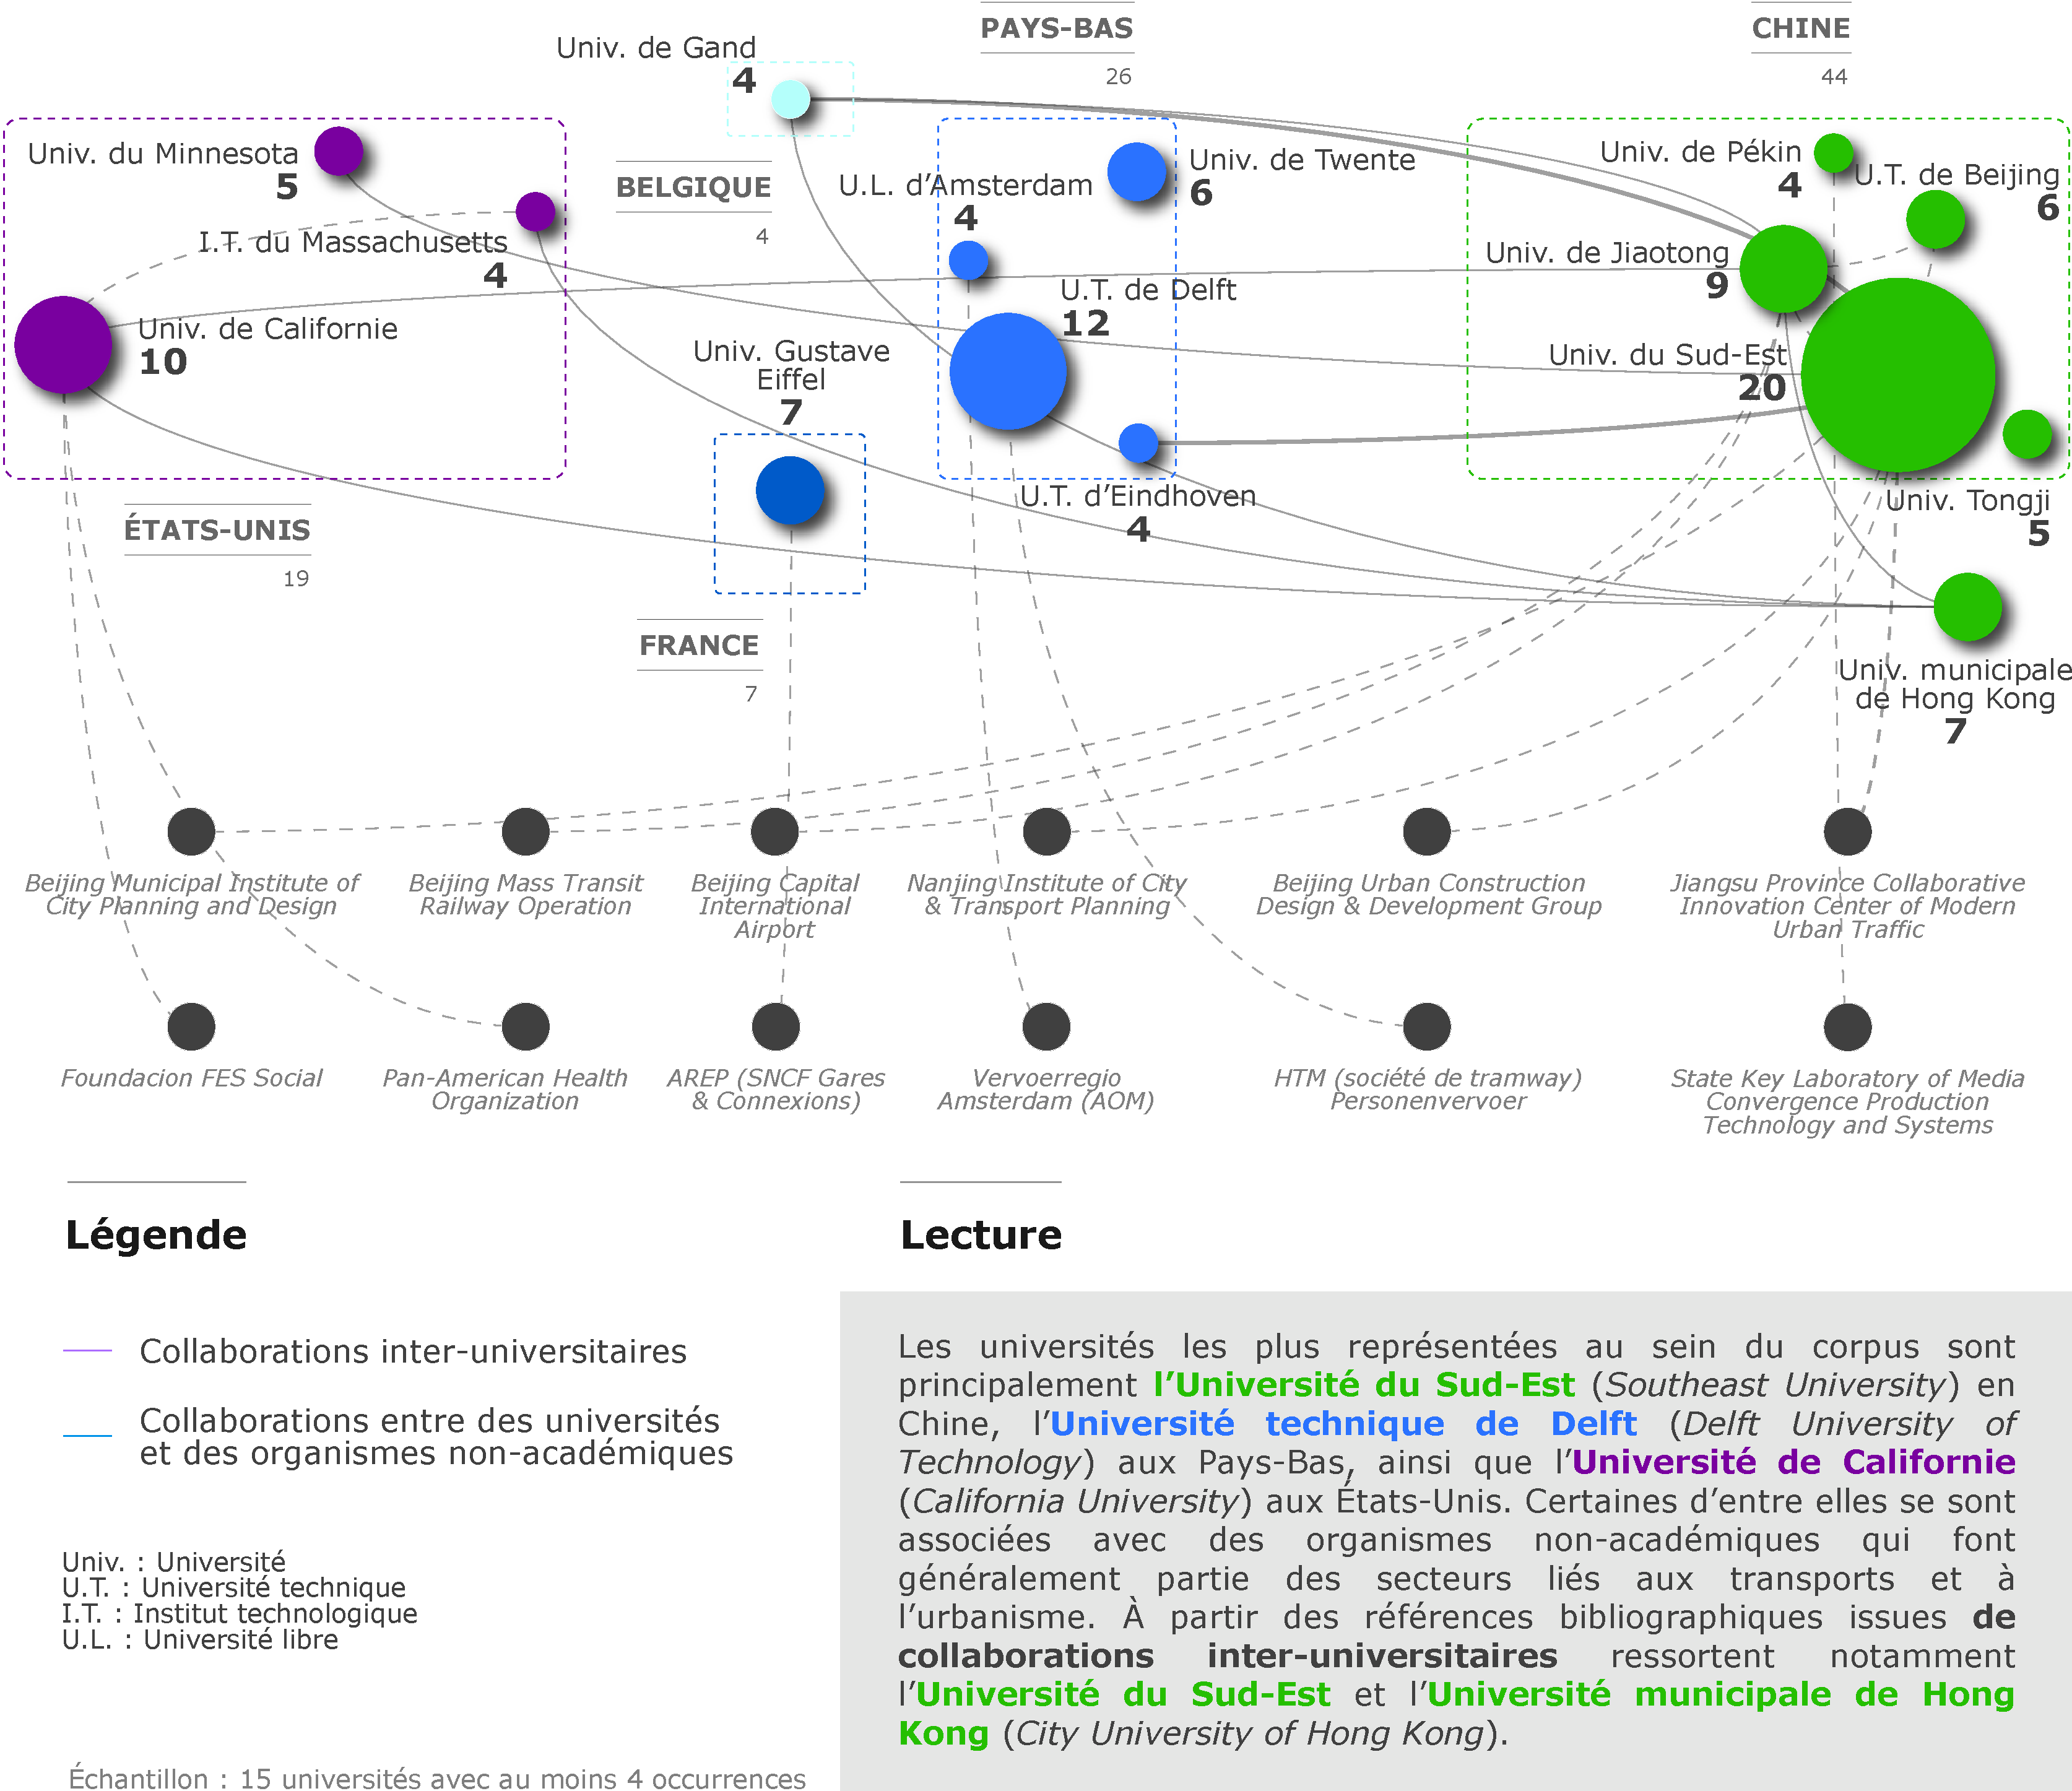
\includegraphics[width=1\columnwidth]{src/Figures/Chap-2/FR_RSL_Collaborations_universites.pdf}}
        \vspace{5pt}
        \begin{flushright}\scriptsize{
        Auteur~: \textcolor{blue}{Dylan Moinse (2023)}
        %\\
        %Réalisation avec \Marque{Excel}~et sur \Marque{Illustrator}
        }\end{flushright}
    \end{figure}

    % Universités et institutions
Du point de vue des institutions représentées dans les 238 contributions scientifiques incorporées au sein de la \acrshort{RSL}, se présente un total de 268 universités, instituts, organismes et entreprises publiques ou privées uniques. Les quinze institutions les plus récurrentes représentent à elles seules plus d'un quart de la distribution (429 valeurs observées). Comme figurées dans l'\hyperref[fig-chap2:copublications-universites-rsl]{illustration~\ref{fig-chap2:copublications-universites-rsl}} (page~\pageref{fig-chap2:copublications-universites-rsl}), les principales universités identifiées dans la documentation sont l'Université du Sud-Est à Nanjing (20), suivie par l'Université de technologie de Delft (12), l'Université de Californie à Berkeley (10), l'Université Jiaotong de Beijing (9), l'Université municipale d'Hong~Kong (7), l'Université Gustave Eiffel en France (7), l'Université de technologie de Beijing (6), l'Université de Twente à Enschede (6), l'Université de Tongji à Shanghai (5), l'Université du Minnesota Twin Cities à Minneapolis et Saint-Paul (5), la Vrije Universiteit d'Amsterdam (4), l'Université technique d'Eindhoven (4), l'Université de Gand (4), l'Institut de technologie du Massachusetts à Cambridge (4) et enfin l'Université de Pékin (4).%%Rédigé%%

    % Collaborations universités et institutions
En interrogeant les collaborations scientifiques à l'échelle universitaire, il s'avère que 128 ouvrages scientifiques se signalent par l'entrecroisement d'au moins deux établissements universitaires ou instituts de recherche au sein d'une même publication. Ainsi, plus de la moitié des contributions scientifiques répertoriées sont marquées par une co-publication pluriversitaire, régulièrement à cheval sur des continents distincts. Les liens prééminents observés se concentrent entre la Chine, les États-Unis, la France, les Pays-Bas et la Belgique. Parmi les partenariats qui ont donné lieu à de telles publications, citons les travaux communs de l'Université du Sud-Est et avec l'Université technique d'Eindhoven \textcolor{blue}{\autocite[]{gan_associations_2021, liu_use_2020, liu_understanding_2020}}\index{Gan, Zuoxian|pagebf}\index{Yang, Min|pagebf}\index{Zeng, Qingcheng|pagebf}\index{Timmermans, Harry~J.~P.|pagebf}\index{Liu, Yang|pagebf}\index{Feng, Tao|pagebf}\index{Ji, Yanjie|pagebf}\index{Shi, Zhuangbin|pagebf}\index{Ji, Yanjie|pagebf}\index{Feng, Tao|pagebf}\index{Timmermans, Harry~J.~P.|pagebf} et avec l'Université de Gand \textcolor{blue}{\autocite[]{chen_what_2022, cheng_comparison_2023, cheng_exploring_2022}}\index{Chen, Wendong|pagebf}\index{Chen, Xuewu|pagebf}\index{Chen, Jingxu|pagebf}\index{Cheng, Long|pagebf}\index{Huang, Jie|pagebf}\index{Jin, Tanhua|pagebf}\index{Chen, Wendong|pagebf}\index{Li, Aoyong|pagebf}\index{Witlox, Frank|pagebf}\index{Cheng, Long|pagebf}\index{Wang, Kailai|pagebf}\index{Vos, Jonas de|pagebf}\index{Huang, Jie|pagebf}\index{Witlox, Frank|pagebf}, tout comme ceux de l'Université municipale d'Hong~Kong avec l'Université de Californie \textcolor{blue}{\autocite{wu_optimal_2020}}\index{Wu, Liyu|pagebf}\index{Gu, Weihua|pagebf}\index{Fan, Wenbo|pagebf}\index{Cassidy, Michael~J.|pagebf} et l'Institut de technologie du Massachusetts \textcolor{blue}{\autocite{cao_e-scooter_2021}}\index{Cao, Zhejing|pagebf}\index{Zhang, Xiaohu|pagebf}\index{Chua, Kelman|pagebf}\index{Yu, Honghai|pagebf}\index{Zhao, Jinhua|pagebf}. Des intervenants opérationnels sont également présents au sein des recherches sur le \acrshort{M-TOD}, essentiellement dans le secteur de la gestion des transports, avec des publications conjointes entre l'Université de Jiaotong et la société d'exploitation des transports en commun \textsl{Beijing Mass Transit Railway Operation Corporation Limited} \textcolor{blue}{\autocite{wang_interchange_2016}}\index{Wang, Zi-jia|pagebf}\index{Chen, Feng|pagebf}\index{Xu, Tian-kun|pagebf} et l'aéroport international \textsl{Beijing Capital International Airport} \textcolor{blue}{\autocite{fan_how_2019}}\index{Fan, Aihua|pagebf}\index{Chen, Xumei|pagebf}\index{Wan, Tao|pagebf}. Pareillement, l'Université du Sud-Est tisse des liens avec les acteurs urbains tels que la \textsl{Nanjing Institute of City \& Transport Planning Co.} \textcolor{blue}{\autocite{zhong_layout_2021}}\index{Zhong, Hongming|pagebf}\index{Liu, Zijian|pagebf}\index{Chen, Jun|pagebf}\index{Hao, Jun|pagebf}\index{Wang, Wei|pagebf} et la \textsl{Beijing Urban Construction Design \& Development Group Co., Limited} \textcolor{blue}{\autocite{yang_empirical_2016}}\index{Yang, Min|pagebf}\index{Liu, Xinlu|pagebf}\index{Wang, Wei|pagebf}\index{Li, Zhibin|pagebf}\index{Zhao, Jingyao|pagebf}. Par ailleurs, des connexions se profilent entre l'Université de Californie et l'organisation à but non lucratif \acrfull{FES} et l'organisation de santé publique \textsl{Pan American Health Organization} \textcolor{blue}{\autocite{cervero_influences_2009}}\index{Cervero, Robert|pagebf}\index{Sarmiento, Olga~L.|pagebf}\index{Jacoby, Enrique|pagebf}\index{Gomez, Luis Fernando|pagebf}\index{Neiman, Andrea|pagebf}.%%Rédigé%%

    % Transition
L'analyse bibliométrique du corpus académique a mis l'accent sur un vaste ensemble documentaire, principalement constitué d'articles scientifiques, parus au sein de revues soumises à une évaluation par les pairs et diffusés en anglais. La grille d'analyse de la \acrshort{RSL}, basée dans cette première sous-partie sur les contours de la recherche en lien avec le \acrshort{M-TOD}, s'est trouvée en mesure d'apporter un aperçu sur les figures, les établissements universitaires et les journaux scientifiques les plus influents autour de cet objet d'étude. Dans la sous-section suivante, nous proposons d'explorer l'état actuel de la littérature scientifique consacrée au \acrshort{TOD} revisité par la mobilité individuelle légère en conduisant une analyse textuelle des contributions scientifiques.

    % 2.2.1.2. Keywords, Content/Body of the Text
    \needspace{1\baselineskip} % Réserve de l'espace
\subsubsection*{Analyse textuelle des productions académiques
    \label{chap2:analyse-textuelle}
    }
    
    % Introduction
L'investigation des métadonnées extraites du corpus académique s'appuie, dans un deuxième temps, sur les systèmes lexicaux employés au sein des ouvrages de recherche. Cette partie de la \acrshort{RSL} intrinsèquement liée à l'analyse textuelle des productions académiques sur le \acrshort{M-TOD} a pour dessein l'identification des pratiques de recherche se matérialisant au travers du vocabulaire utilisé. Originellement, l'étude a été différenciée selon la langue de diffusion, une première catégorie liée à l'usage de l'anglais et se composant de 228 documents et une seconde se déployant en français et constituée de 10~travaux. Toutefois, en raison de la faible représentativité des ouvrages francophones, l'analyse textuelle concentre son attention de manière exclusive sur les publications rédigées en anglais.%%Rédigé%%

    % Analyse des mots-clés~: échantillon et méthodologie
D'un point de vue symbolique, l'examen textuel s'est dirigé vers le contenant des recherches intégrées à la \acrshort{RSL} en interrogeant l'architecture sémantique des productions écrites, construite sur la sélection de mots-clés qui apparaissent généralement à la suite du titre et du résumé. L'agrégation des contributions universitaires a donné lieu à la compilation de 1~336 mots-clés issus de 208 ouvrages, dont 201 en anglais. L'exploration des listes de mots-clés définies par les chercheur·se·s investi·e·s sur le \acrshort{M-TOD} révèle une fréquence moyenne de 6,7 mots-clés par document, revenant à considérer plus de 303 termes distincts, parmi lesquels 260~sont en anglais. Dans la perspective de conduire une analyse comparative des mots-clés mentionnés dans le corpus, une phase préliminaire de nettoyage des données a été entreprise. Ce processus d'harmonisation terminologique a consisté à homogénéiser les ensembles de mots-clés partageant une filiation commune ou une signification affinitaire\footnote{
    À titre d'illustration, nous pouvons évoquer l'agrégation des mots \Guillemets{bicyclette}~et \Guillemets{vélo}~en langue française, ou les expressions \Guillemets{\textsl{transit}}~et \Guillemets{\textsl{public transport}}, ou encore \Guillemets{\textsl{subway}}~et \Guillemets{\textsl{metro}}~en langue anglaise. Bien que cette étape soit cruciale en vue de faciliter la pertinence des données textuelles mobilisées, il convient de signaler les présupposés inhérents à ce travail d'appréciation.
}.%%Rédigé%%

    % Mots-clés~: résultat 1
Par l'entrecroisement des 1~281~mots-clés en anglais, l'analyse textuelle de la présente \acrshort{RSL} met en évidence onze aspects thématiques qui se distinguent au sein des étiquettes lexicales extraites. Pour mener cette analyse lexicale, nous avons établi au préalable plusieurs catégories thématiques. Chaque mot a été classé de manière arbitraire selon la catégorie correspondante à son contexte d'utilisation. Une mise en relief graphique de l'\hyperref[fig-chap2:nuage-mots-cles-rsl]{illustration~\ref{fig-chap2:nuage-mots-cles-rsl}} (page~\pageref{fig-chap2:nuage-mots-cles-rsl}) laisse apparaître les groupements de mots-clés, au sein desquels les thématiques liées à la mobilité individuelle et collective occupent une place hégémonique. Ainsi, les concepts relatifs aux \Guillemets{modes de déplacement individuels}~(282~occurrences), à l’\Guillemets{intermodalité}~(224 occurrences), aux \Guillemets{transports en commun}~(202~occurrences) et à la \Guillemets{mobilité}~(181~occurrences) représentent les principales catégories du classement, en adéquation avec la configuration de l'expression utilisée pour la recherche bibliographique des \Guillemets{Corpus EN et FR}, qui a expressément conduit à l'émergence de ces thématiques (pour rappel, voir le \hyperref[table-chap2:expression-recherche-rsl]{tableau~\ref{table-chap2:expression-recherche-rsl}}, page~\pageref{table-chap2:expression-recherche-rsl}).%%Rédigé%%

    % Figure Nuage de mots-clés RSL
    \begin{figure}[h!]\vspace*{4pt}
        \caption{Nuages de mots-clés anglais extraits de la revue systématique de la littérature et classés par thématique.}
        \label{fig-chap2:nuage-mots-cles-rsl}
        \centerline{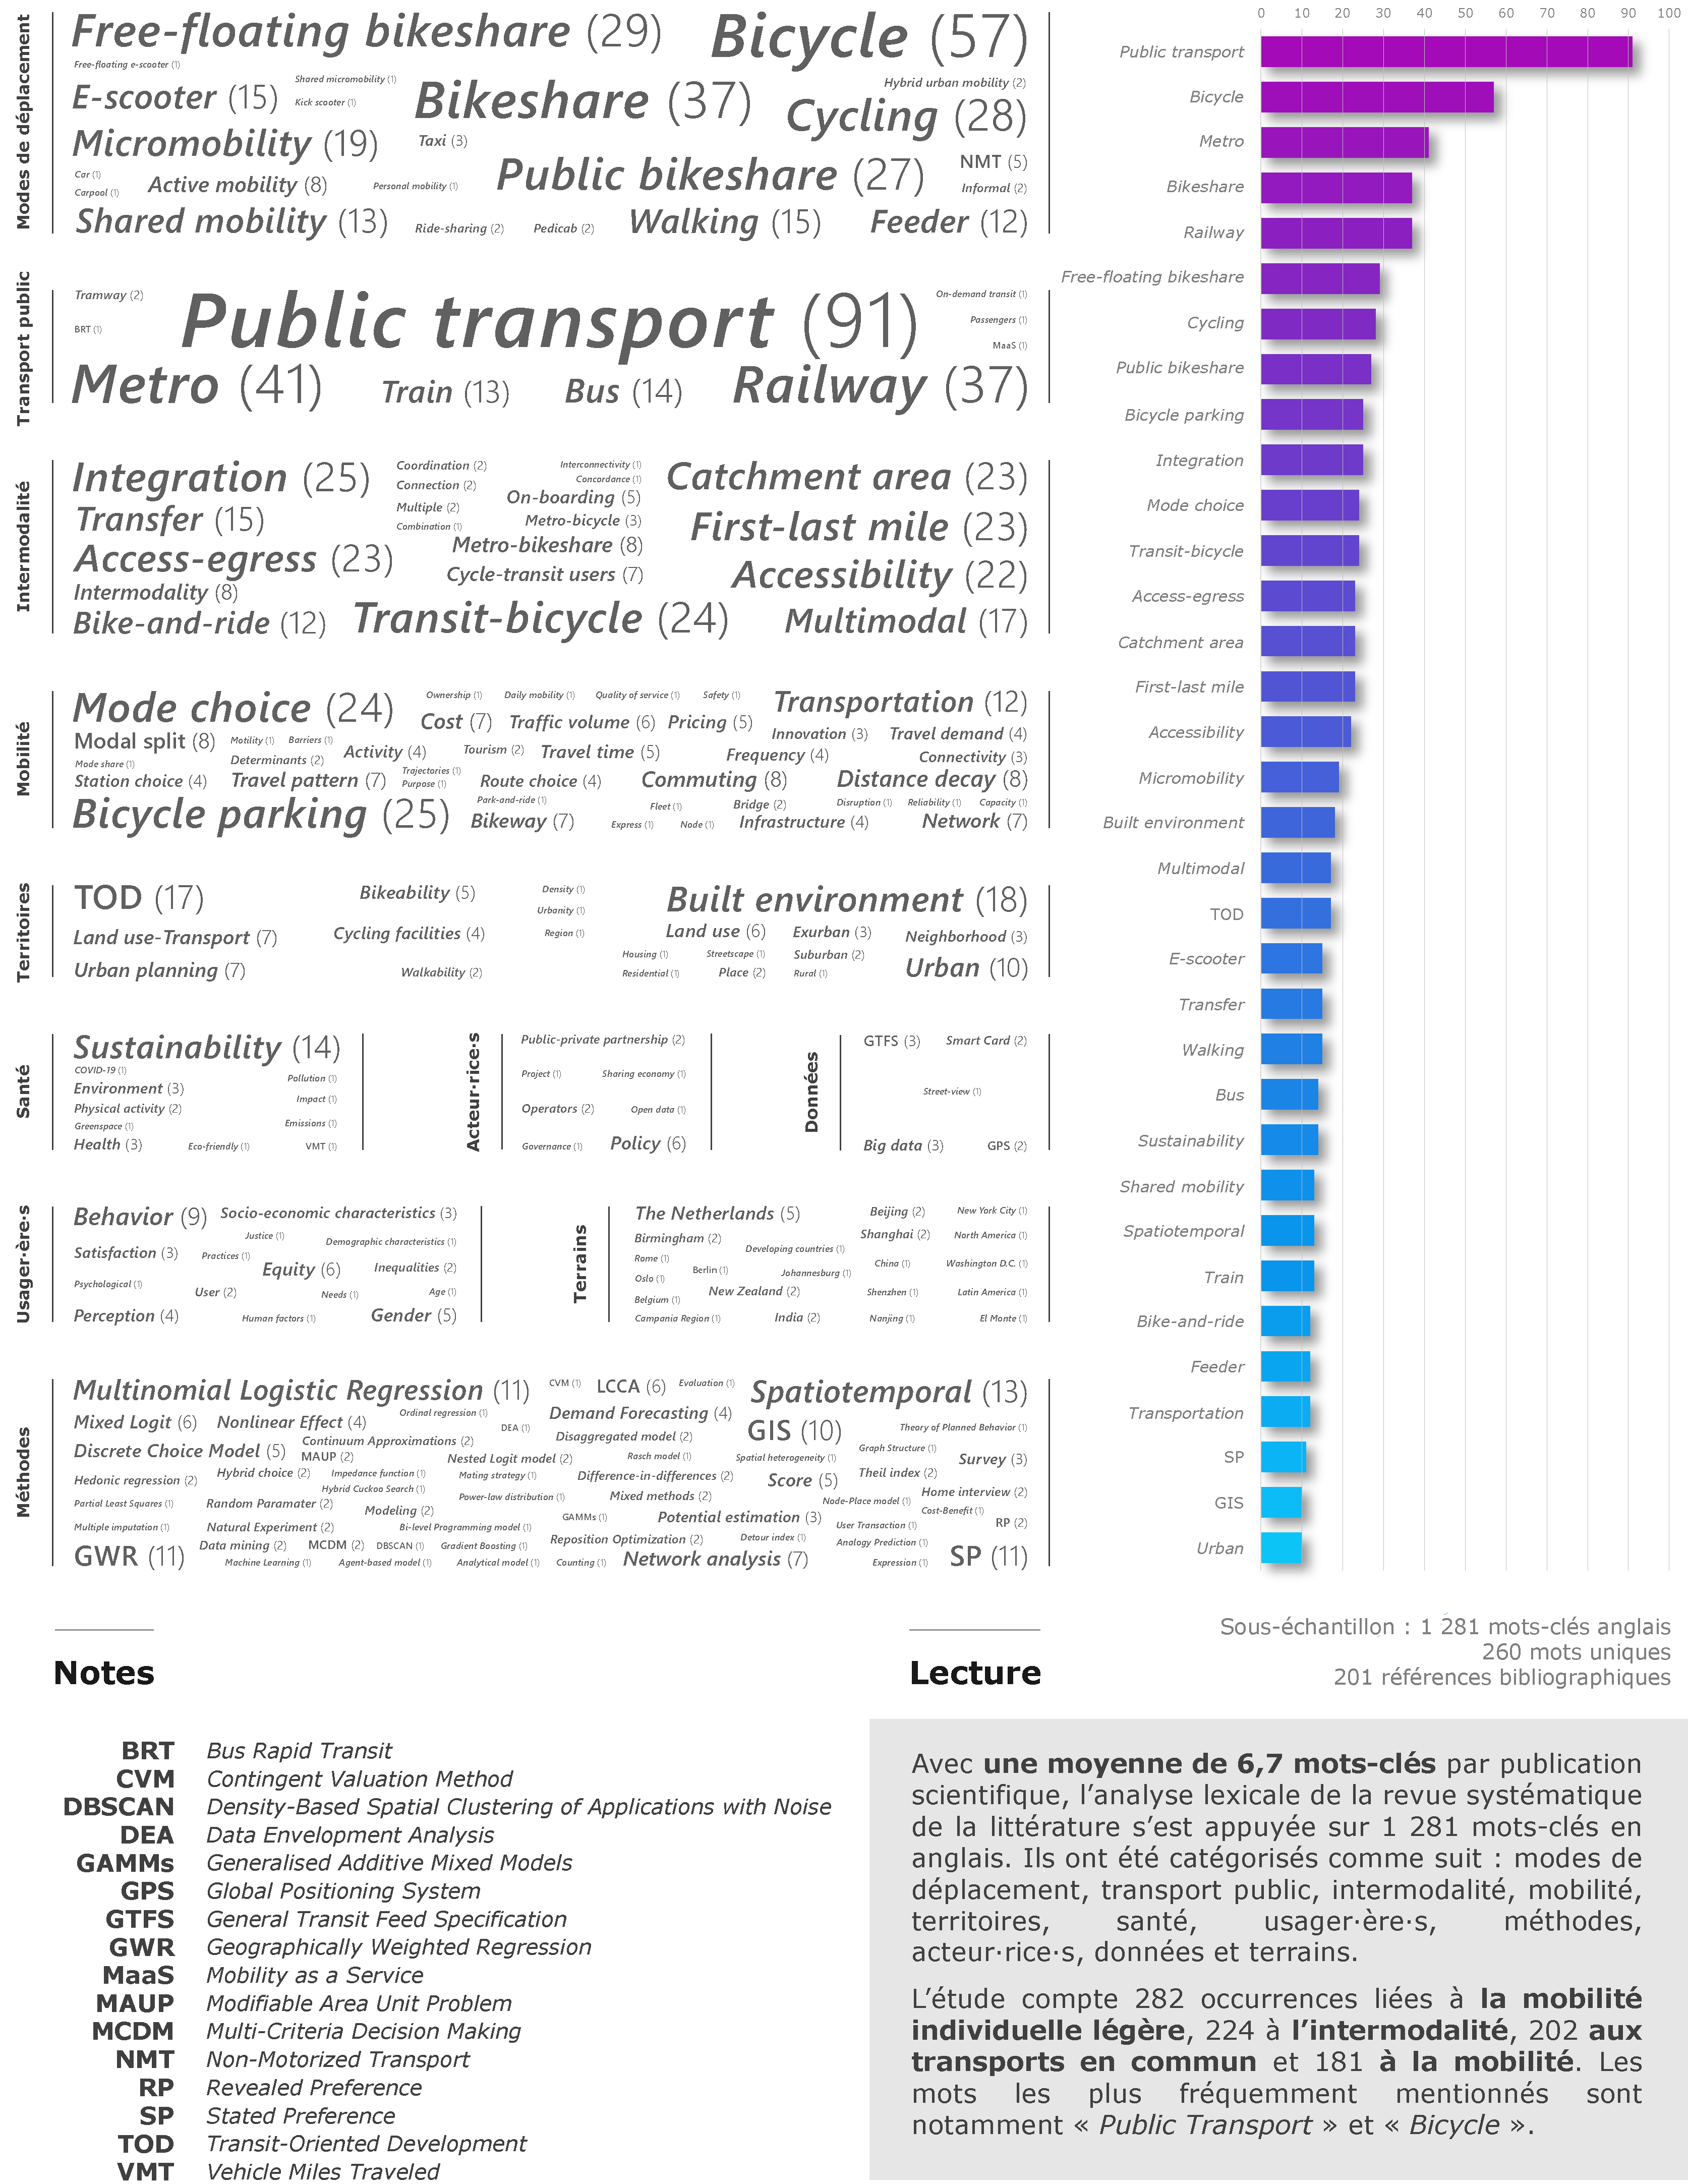
\includegraphics[width=1\columnwidth]{src/Figures/Chap-2/FR_RSL_Nuage_mots_cles_thematiques.pdf}}
        \vspace{5pt}
        \begin{flushright}\scriptsize{
        Auteur~: \textcolor{blue}{Dylan Moinse (2023)}
        %\\
        %Réalisation avec \Marque{Python}~et sur \Marque{Illustrator}
        }\end{flushright}
    \end{figure}

    % Mots-clés~: résultat 2
À l'échelle des mots-clés, c'est principalement dans le registre des \Guillemets{transports en commun}~et du \Guillemets{vélo}~que se manifestent des occurrences prééminentes, comptabilisant respectivement 91 et 57 itérations de termes qui leur sont rattachées. Néanmoins, cette prédominance des mots-clés voile une distribution inégalitaire au sein de chaque thématique mise en observation. Alors que la fréquence des mots-clés se rapportant à \Guillemets{transports en commun}, \Guillemets{modes de déplacement individuels}~et \Guillemets{intermodalité}~est conséquente, s'élevant à 20, 12 et 11~récurrences pour chaque terme en moyenne, cette intensité s'amenuise à 5,5 et 2~répétitions en ce qui concerne les catégories afférentes à \Guillemets{mobilité}, \Guillemets{urbanisme}~et \Guillemets{méthodes}. Ce constat témoigne d'une plus vaste variété de mots-clés dans ces dernières thématiques, parallèlement à un processus d'homogénéisation terminologique perceptible au sein des domaines des modes de déplacement personnels, des transports en commun et de l'intermodalité.%%Rédigé%%

    % Mots-clés~: résultat 3
La manipulation des mots-clés sous l'angle des modes de déplacement et des infrastructures de transport comme objets, tels que \Guillemets{\textsl{bicycle}}~(mentionné à 57 reprises), \Guillemets{\textsl{free-floating bikeshare}}~(29 occurrences), \Guillemets{\textsl{public bikeshare}}~(27 occurrences), \Guillemets{\textsl{metro}}~(41~occurrences), \Guillemets{\textsl{railway}}~(37 occurrences) ou encore \Guillemets{\textsl{bicycle parking}}~(25 occurrences), reflète une intrication qui se cristallise en signaux lexicaux, perpétuant le schéma conventionnel du domaine du transport (voir l'\hyperref[fig-chap2:nuage-mots-cles-rsl]{illustration~\ref{fig-chap2:nuage-mots-cles-rsl}}, page~\pageref{fig-chap2:nuage-mots-cles-rsl}). De manière analogue à cette démarche ancrée dans le paradigme des transports, se profile un vaste domaine sémantique dévolu au \Guillemets{tournant de la mobilité}~\textcolor{blue}{\autocites{sheller_new_2006}[8]{sheller_mobilizing_2016}[13]{randell_no_2020}}\index{Sheller, Mimi|pagebf}\index{Urry, John|pagebf}\index{Randell, Richard|pagebf}, marqué par l'utilisation d'expressions à l'image d'\Guillemets{\textsl{accessibility}}~(22~occurrences), \Guillemets{\textsl{sustainability}}~(14 occurrences), \Guillemets{\textsl{behavior}}~(9 occurrences), \Guillemets{\textsl{policy}}~(6 occurrences), \Guillemets{\textsl{equity}}~(6 occurrences) ou encore \Guillemets{\textsl{bikeability}}~(5 occurrences). Certes, dans une moindre mesure, nous pouvons discerner l'implication de l'urbanisme et notamment de son articulation avec la mobilité, comme en témoignent le concept de \Guillemets{\textsl{TOD}}~(17 occurrences) ou \Guillemets{\textsl{land use-transport}}~(7 occurrences).%%Rédigé%%

    % Mots-clés~: résultat 4
En sondant les interactions entre les mots-clés précités, il est intéressant de relever les liaisons étroites qui associent certaines catégories entre elles. La majorité des listes de vocables tend à établir des passerelles interconnectant les catégories relatives aux \Guillemets{transports en commun}~et aux \Guillemets{modes de déplacement individuels}. Parmi les 201~références anglophones, 155 d'entre elles tissent un dialogue entre ces deux thématiques, qui s'exprime par le choix délibéré d'une liste de mots-clés rattachés à la mobilité collective et personnelle. De surcroît, 59 publications scientifiques se distinguent par une configuration spécifique, prenant la forme d'une suite lexicale ordonnée de la façon suivante~: le premier mot-clé de la liste se réfère aux \Guillemets{transports en commun}, suivi des \Guillemets{modes de déplacement individuels}~et d'un troisième terme invoquant l'\Guillemets{intermodalité}.%%Rédigé%%

    % Figure Mots contenu RSL
    \begin{figure}[h!]\vspace*{4pt}
        \caption{Nuage de mots tirés du contenu intégral des travaux académiques anglophones intégrés dans la revue systématique de la littérature.}
        \label{fig-chap2:contenu-textuel-rsl}
        \centerline{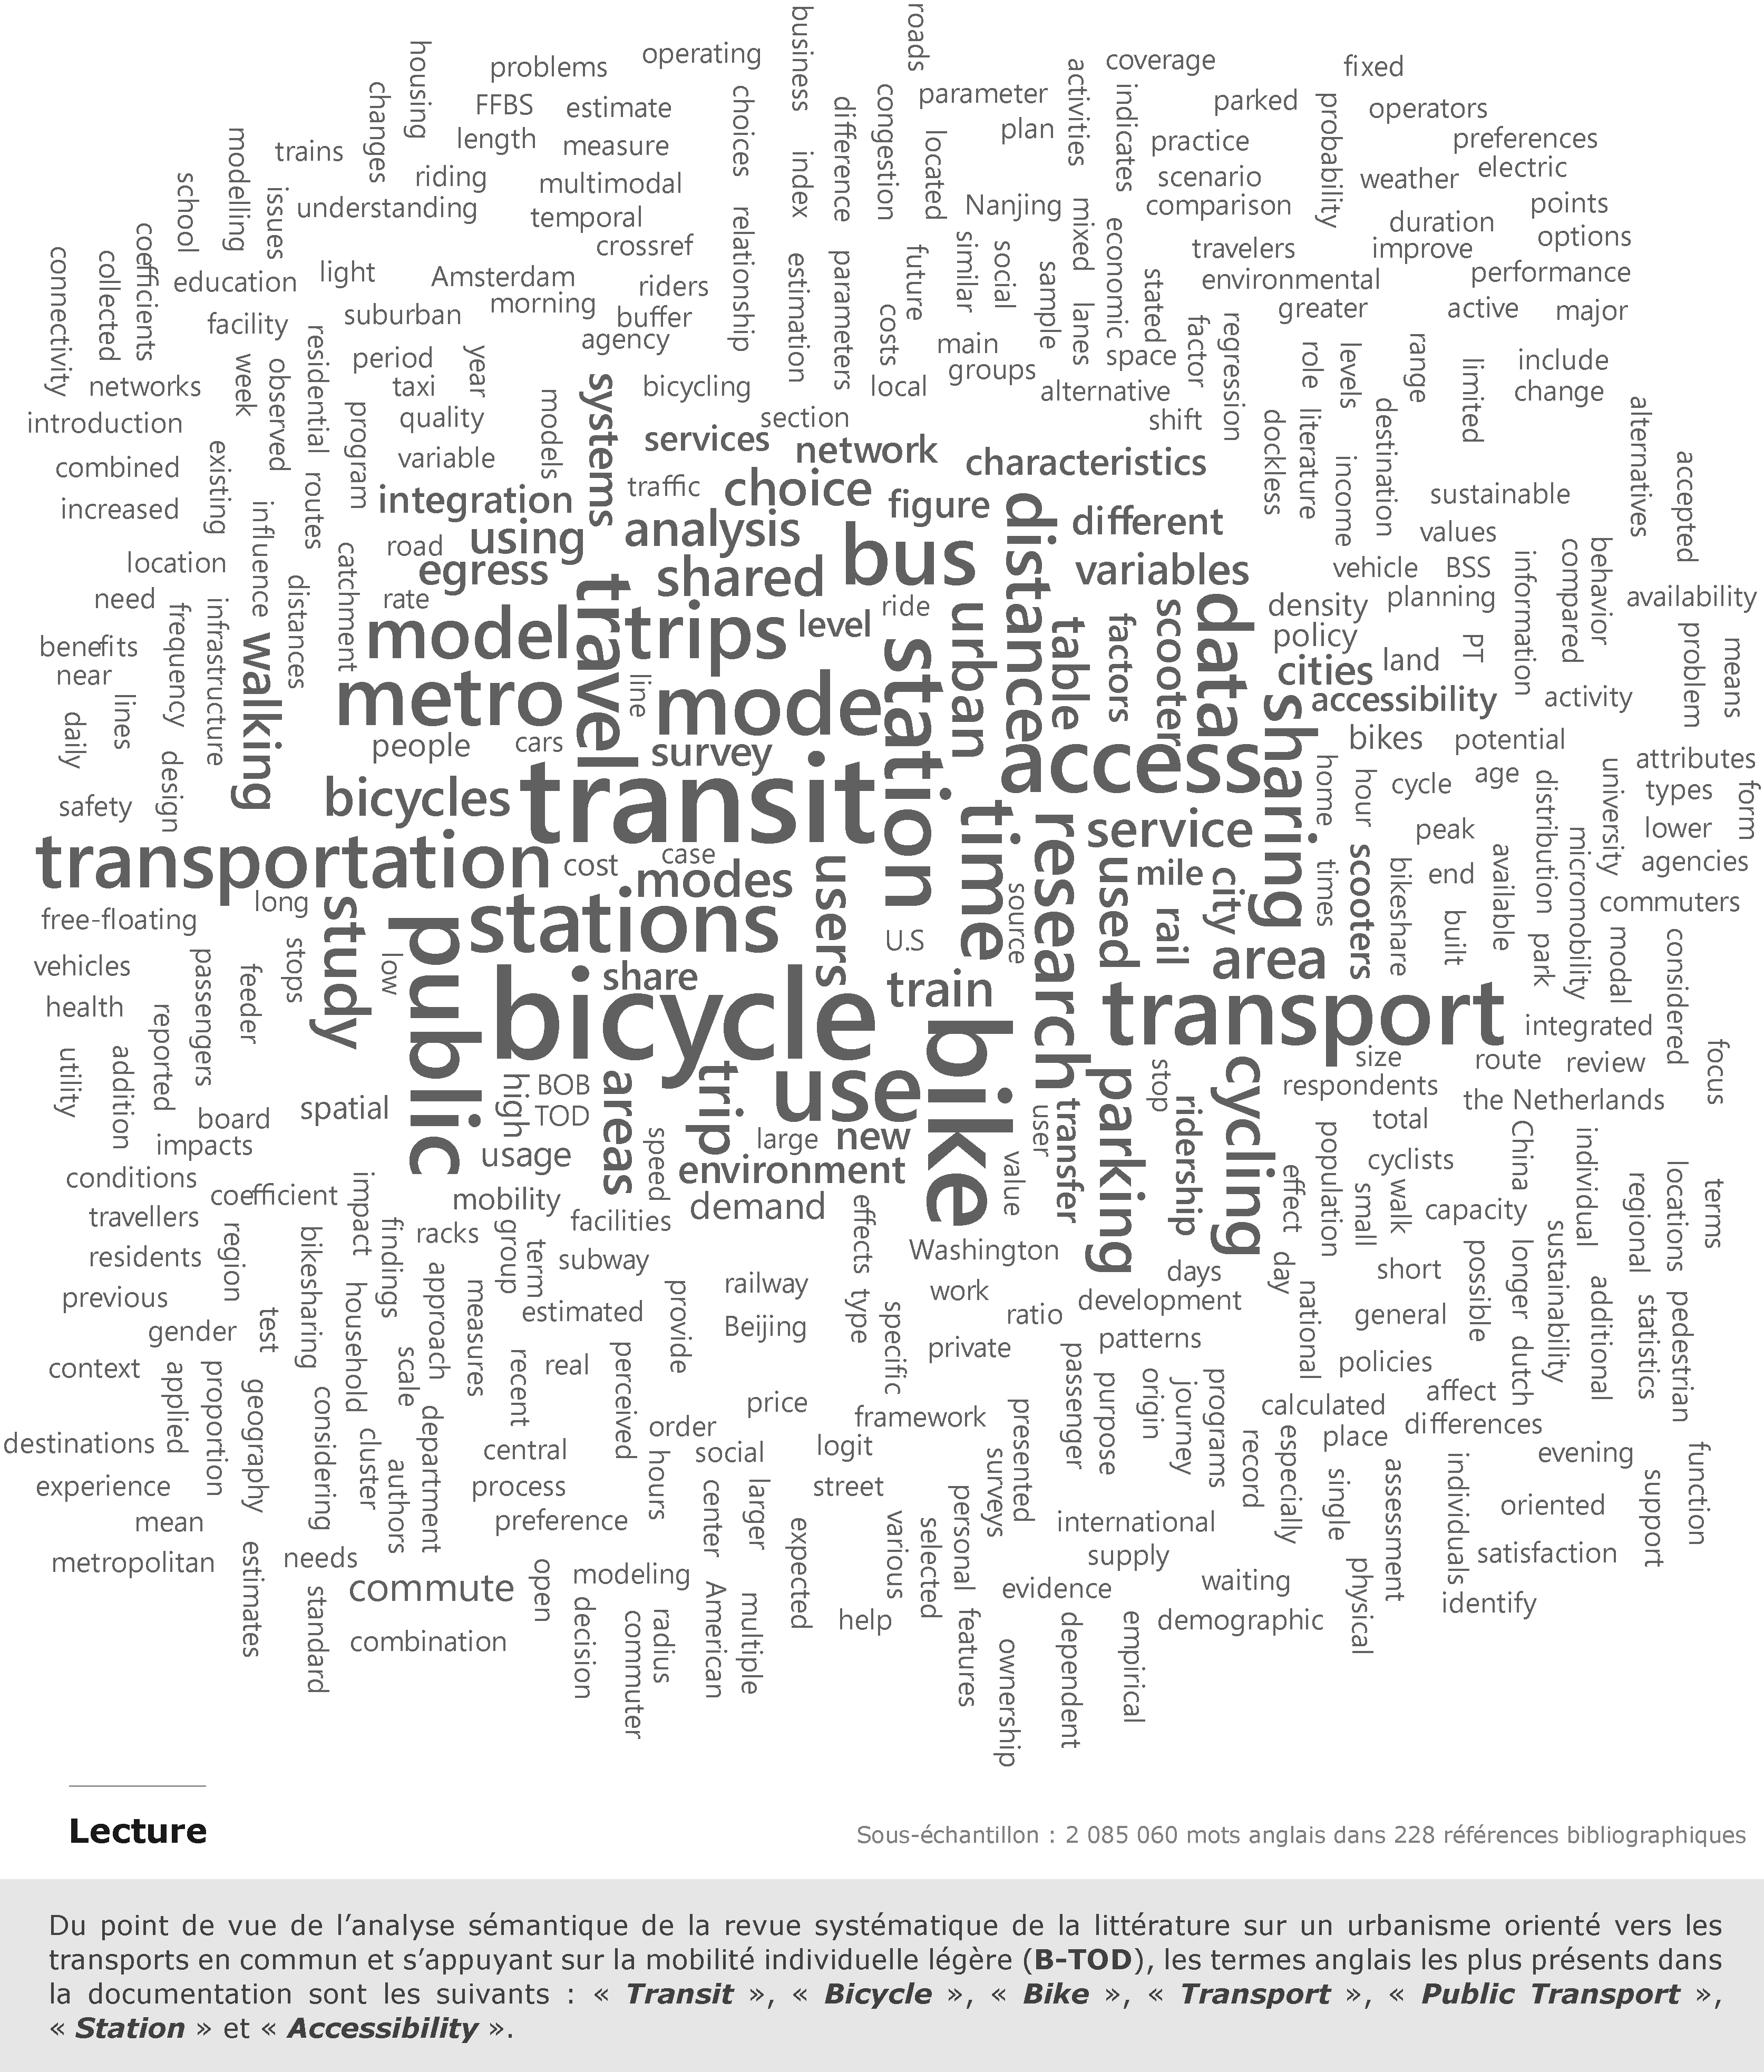
\includegraphics[width=1\columnwidth]{src/Figures/Chap-2/FR_RSL_Mots_contenu.pdf}}
        \vspace{5pt}
        \begin{flushright}\scriptsize{
        Auteur~: \textcolor{blue}{Dylan Moinse (2023)}
        %\\
        %Réalisation avec \Marque{Python}~et sur \Marque{Illustrator}
        }\end{flushright}
    \end{figure}
    
    % Contenu mots RSL
L'exploitation textuelle a été approfondie au travers d'une analyse du contenu intégral de chaque publication scientifique rapportée en langue anglaise. Comme en témoigne l'\hyperref[fig-chap2:contenu-textuel-rsl]{illustration~\ref{fig-chap2:contenu-textuel-rsl}} (page~\pageref{fig-chap2:contenu-textuel-rsl}), l'examen des cent termes les plus récurrents au sein des documents\footnote{
    Afin de procéder à la classification des champs lexicaux identifiés dans les documents analysés, nous avons procédé à une étape de nettoyage des termes ayant trait à la vie quotidienne ou à la recherche scientifique de manière générale, dans la langue anglaise. Ces expressions courantes ont ultérieurement été exclues de l'analyse, à l'instar de \Guillemets{\textsl{the}}, \Guillemets{\textsl{a}}, \Guillemets{\textsl{and}}, \Guillemets{\textsl{we}}, \Guillemets{\textsl{for}}, \Guillemets{\textsl{study}}, \Guillemets{\textsl{scientific}}, \Guillemets{\textsl{methods}}~ou encore \Guillemets{\textsl{results}}.
} renforce la tendance préalablement identifiée au niveau des mots-clés, se traduisant principalement par la prépondérance des termes \Guillemets{\textsl{transit}}, \Guillemets{\textsl{bicycle}}, \Guillemets{\textsl{bike}}, \Guillemets{\textsl{transport}}, \Guillemets{\textsl{public transport}}, \Guillemets{\textsl{station}}~et \Guillemets{\textsl{accessibility}}. Néanmoins, il faut souligner l'influence substantielle de certains mots, tels que \Guillemets{\textsl{use}}, \Guillemets{\textsl{access}}, \Guillemets{\textsl{distance}}, \Guillemets{\textsl{area}}, \Guillemets{\textsl{users}}~ou \Guillemets{\textsl{service}}, qui revêtent une dimension liée aux usages, usager·ère·s et aux distances-temps parcourues. En revanche, il est à noter que la présence lexicale en lien avec l'urbanisme demeure pratiquement absente dans les écrits, à l'exception de quelques occurrences événementielles, comme \Guillemets{\textsl{density}}, \Guillemets{\textsl{mixed}}, \Guillemets{\textsl{TOD}}~ou \Guillemets{\textsl{land}}.%%Rédigé%%

    % Transition
À la lecture des termes scrutés au sein du corpus de la \acrshort{RSL}, résultent en premier plan les divers modes de transports collectifs et individuels inscrits au cœur d'un développement urbain orienté vers les transports en commun et s'appuyant sur la mobilité individuelle légère. En considération de la rapide évolution de la pratique de mobilité, des techniques et des technologies propres à ces différents objets de déplacement, la sous-section suivante s'emploie à mettre en perspective les travaux de recherche en lien avec le \acrshort{M-TOD}, en mettant l'accent sur l'évolution des champs d'investigation émergents.%%Rédigé%%

    % 2.2.1.3. micro-mobilité, TC
    \needspace{1\baselineskip} % Réserve de l'espace
\subsubsection*{Évolution des recherches sur la synergie entre les transports en commun et la mobilité individuelle légère
    \label{chap2:evolution-recherches-tc-mobilite-individuelle-legere}
    }
    
    % Tendance depuis 1993
L'analyse de la répartition temporelle des publications scientifiques intégrées à la \acrshort{RSL} offre une perspective globale sur les caractéristiques et les avancées qui délimitent ce corpus de littérature. La trajectoire chronologique du corpus bibliographique consacré à l'intégration de la mobilité individuelle légère aux réseaux de transports en commun dépeint une croissance continue entre~1993~et~2021. À partir de~2015, le seuil annuel de dix publications scientifiques a été systématiquement dépassé, suggérant un intérêt croissant de la recherche autour de ce sujet. En l'espace de seulement quatre années consécutives, le nombre de documents académiques recensés a doublé, avec l'apparition de 129 nouveaux travaux partagés entre~2019 et le début de l'année 2023.%%Rédigé%%

    % Objectif
Conformément au protocole méthodologique défini dans la présente \acrshort{RSL}, la date minimale retenue pour cette étude bibliométrique a été fixée à 1993, en référence à la conceptualisation du \acrshort{TOD} par \textcolor{blue}{Peter} \textcolor{blue}{\textcite{calthorpe_next_1993}}\index{Calthorpe, Peter|pagebf}. L'étude bibliographique ainsi exposée vise à dévoiler les caractéristiques de ce corpus élaboré sur trois décennies de recherches internationales. Cependant, il est primordial de reconnaître l'existence d'œuvres antérieures traitant du sujet à l'étude. Bien que la croissance observée des publications scientifiques englobe des travaux en anglais et en français, l'émergence d'œuvres francophones se produit à un stade ultérieur, à partir de 2015. Néanmoins, ce sous-ensemble demeure de taille restreinte pour établir des conclusions définitives. En revanche, la littérature scientifique se déployant dans des contextes européens se développe précocement dès l'année 2000.%%Rédigé%%

    % Figure chronologie RSL modes de transport
    \begin{figure}[h!]\vspace*{4pt}
        \caption{Évolution des publications scientifiques sur la combinaison entre les transports en commun et la mobilité individuelle légère, au sein de la revue systématique de la littérature.}
        \label{fig-chap2:chronologie-modes-deplacements-rsl}
        \centerline{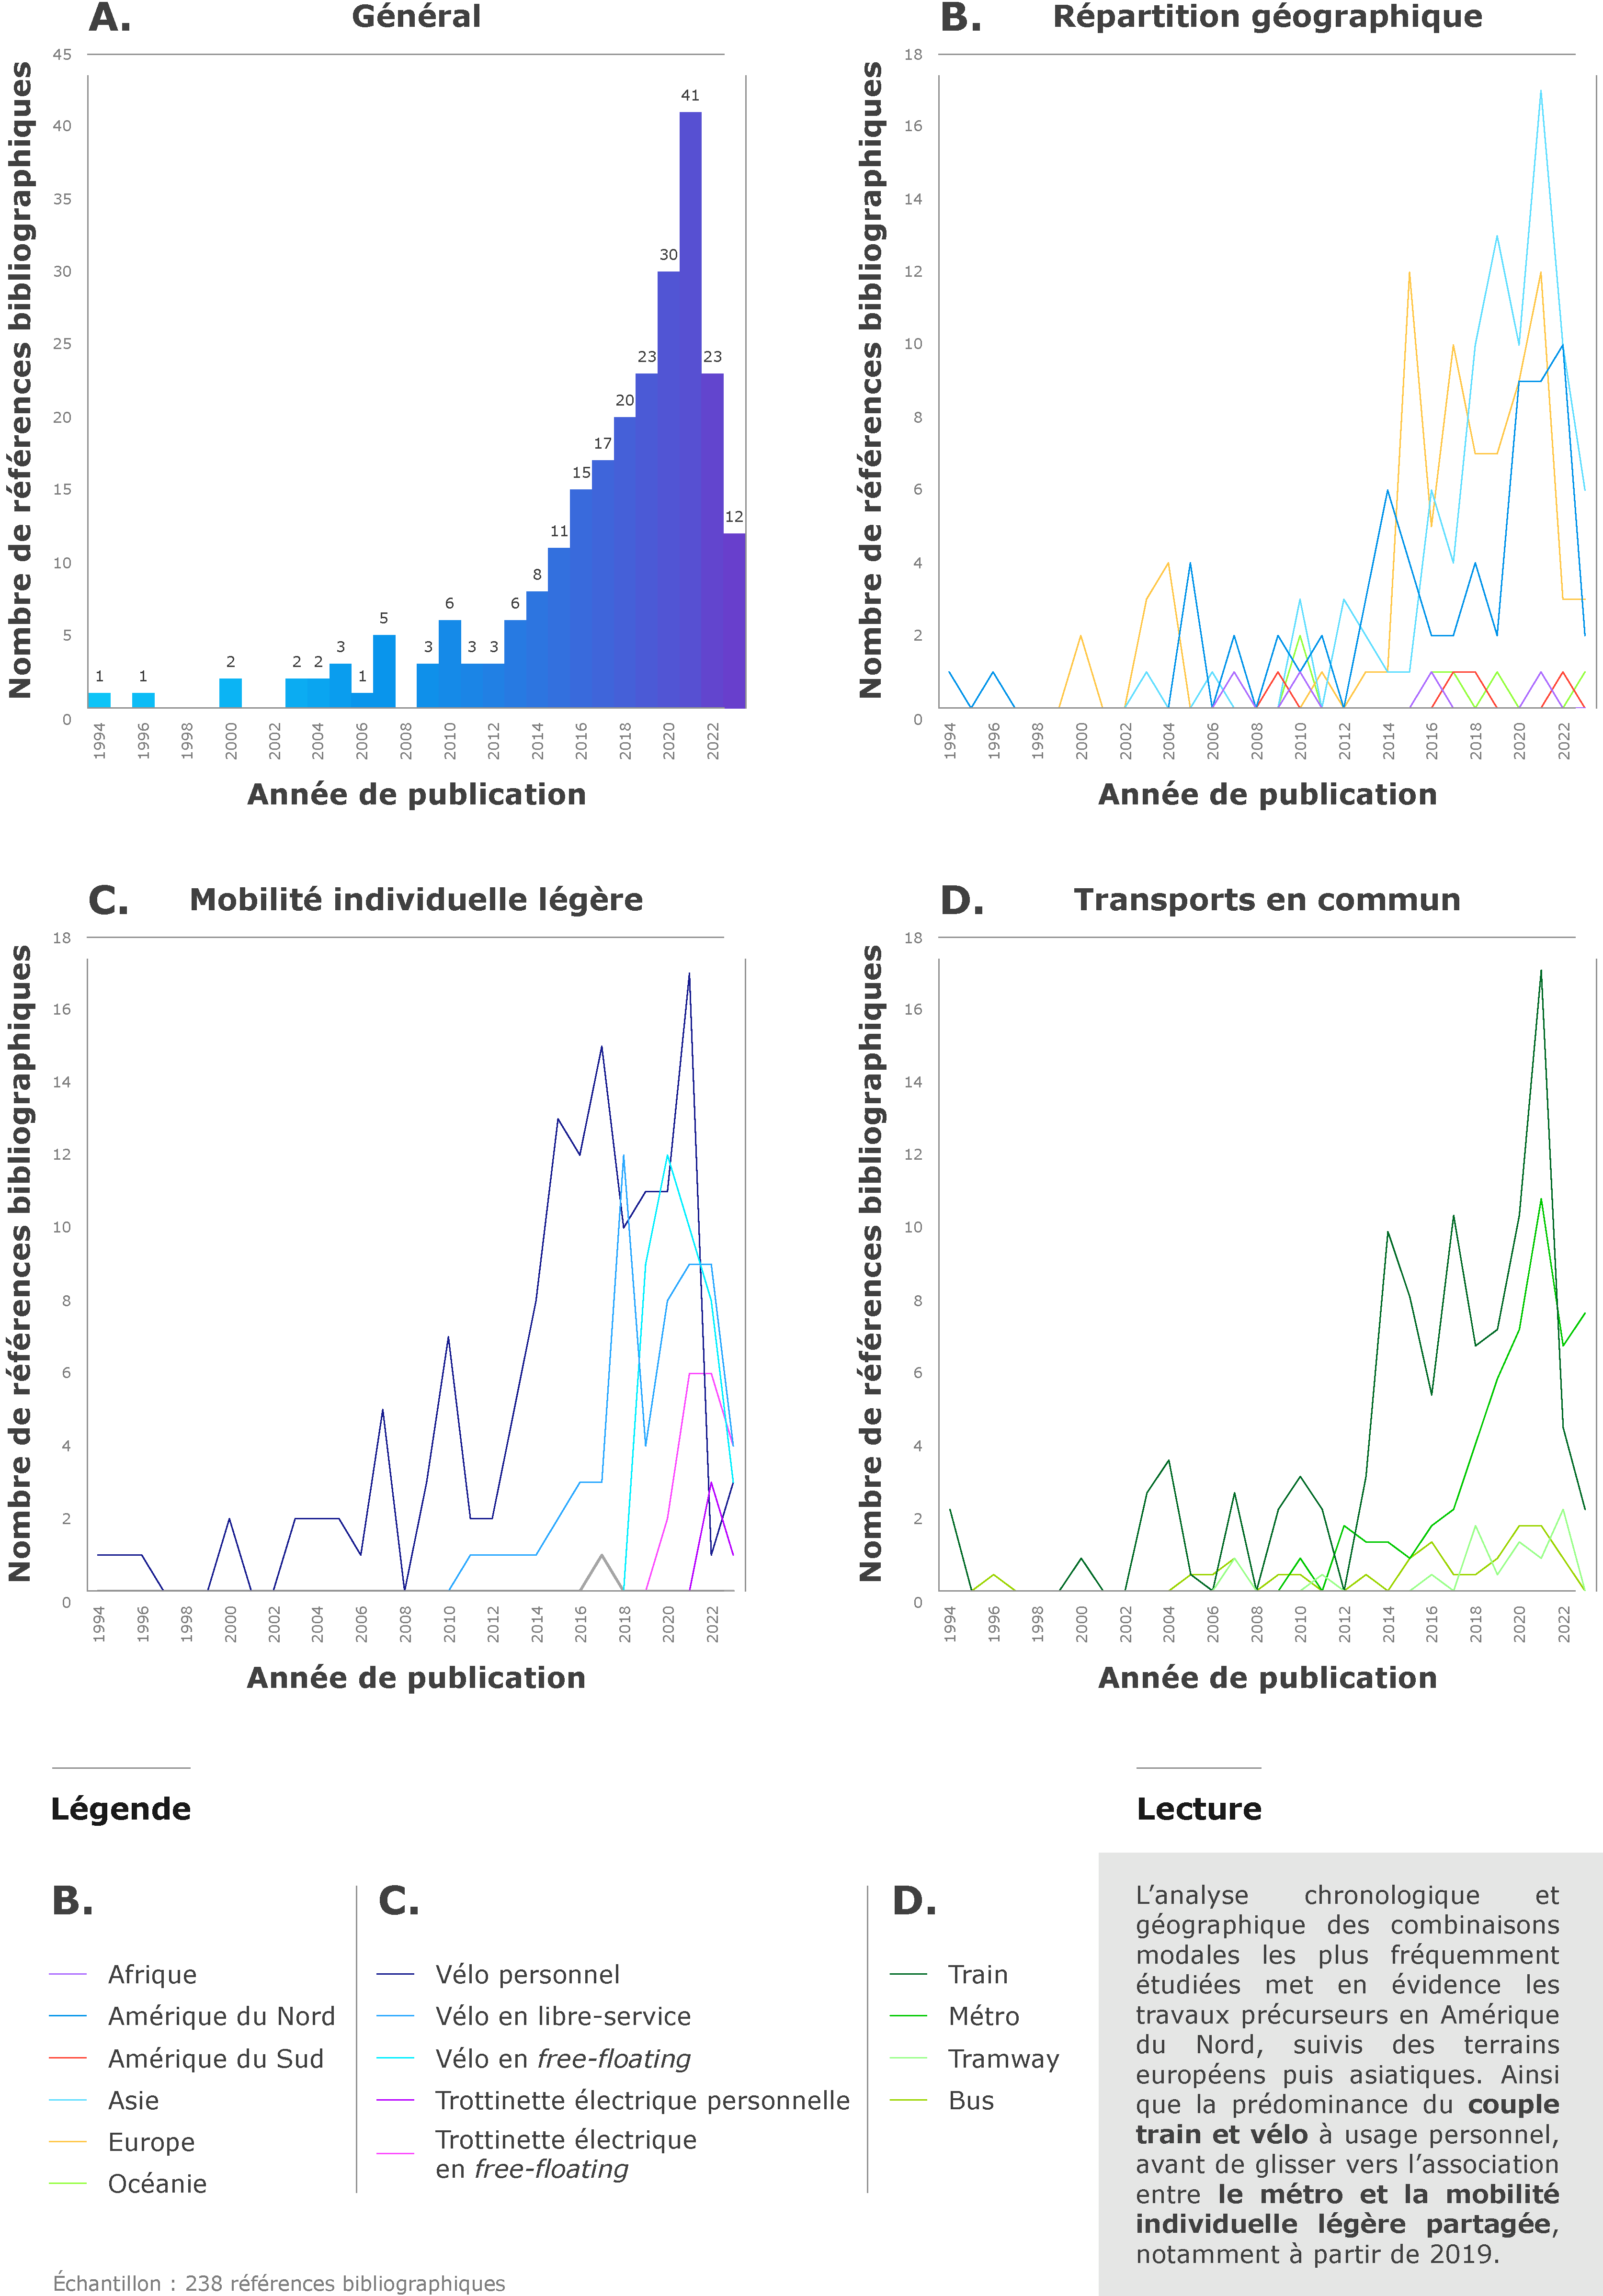
\includegraphics[width=1\columnwidth]{src/Figures/Chap-2/FR_RSL_Chronologie.pdf}}
        \vspace{5pt}
        \begin{flushright}\scriptsize{
        Auteur~: \textcolor{blue}{Dylan Moinse (2023)}
        %\\
        %Réalisation avec \Marque{Excel}, \Marque{Python}~et sur \Marque{Illustrator}
        }\end{flushright}
    \end{figure}

    % Chronologie par micro-mobilités
L'approche chronologique du \acrshort{M-TOD}, telle qu'elle se dessine dans la littérature scientifique, offre des perspectives éclairantes sur l'essor de la mobilité individuelle légère (voir l'\hyperref[annexes:rsl-combinaisons-modales]{annexe~\ref{annexes:rsl-combinaisons-modales}}, page~\pageref{annexes:rsl-combinaisons-modales}) et son apport potentiel sur le développement du modèle urbain. L'\hyperref[fig-chap2:chronologie-modes-deplacements-rsl]{illustration~\ref{fig-chap2:chronologie-modes-deplacements-rsl}} (page~\pageref{fig-chap2:chronologie-modes-deplacements-rsl}) révèle la place éminente qu'a occupée le vélo conventionnel dans la recherche internationale de 1994 à 2017, représentant 89~\% des publications au cours de cette période. Cependant, cette position dominante a progressivement été remise en question, avec une présence du vélo traditionnel dans seulement 41~\% des études entre~2018~et~2021, et dans à peine 4~\% des publications les plus récentes. Cette dynamique défavorable a tout d'abord profité à l'exploration des systèmes de partage de \acrfull{VLS}, dont l'intérêt s'est accru à partir de 2011. Par la suite, à partir de 2019, l'attention s'est déplacée vers les systèmes de partage de \acrfull{VFF}. Plus récemment, le corpus de recherche a manifesté un intérêt croissant pour les systèmes de partage de \acrfull{TEFF}. Toutefois, la \acrfull{TEP} reste absente des enquêtes, soulignant un contraste apparent entre l'effervescence récente des études sur les services partagés et la paucité de recherches sur l'utilisation privée de la trottinette électrique. Cette observation est à resituer dans le contexte de l'essor du vélo et de la micro-mobilité partagés, comme en témoigne l'analyse descriptive réalisée par \textcolor{blue}{\textcite[298]{zhang_built_2023}}\index{Zhang, Yushan|pagebf}\index{Kasraian, Dena|pagebf}\index{Wesemael, Pieter van|pagebf} au sein de sa \acrshort{RSL}, qui démontre que les trois quarts de la documentation à ce sujet sont apparus entre~2019~et~2022.%%Rédigé%%

    % Chronologie par transports en commun
L'étude séquentielle des systèmes de transports en commun examinés au sein de la littérature scientifique jette également une lumière sur les tendances générales qui se sont dessinées au cours des trois décennies enquêtées. Telle que l'indique l'\hyperref[fig-chap2:chronologie-modes-deplacements-rsl]{illustration~\ref{fig-chap2:chronologie-modes-deplacements-rsl}} (page~\pageref{fig-chap2:chronologie-modes-deplacements-rsl}), les recherches internationales portant sur le \acrshort{M-TOD} ont manifesté un intérêt particulier pour les modes ferroviaires interurbains de 1994 à 2017, avec une attention particulière portée au \acrfull{TER}, en conjonction avec le vélo conventionnel. En contraste, le système de métro, qui était jusqu'alors relativement en retrait jusqu'en 2012, a connu un renouveau d'intérêt à partir de 2019, coïncidant avec l'augmentation de l'attention portée aux systèmes de \acrshort{VFF} et de \acrshort{TEFF}. Par ailleurs, il ne faut pas omettre les études sur l'association de la mobilité individuelle légère avec le bus, notamment le \acrfull{BHNS}, ainsi qu'avec le tramway, lesquels maintiennent une présence secondaire, mais constante dans les publications scientifiques. Dans l'ensemble, l'analyse chronologique des combinaisons modales les plus fréquemment étudiées expose un schéma principal~: l'ascendant initial du couple train et vélo personnel dans les travaux académiques sur le \acrshort{M-TOD}, cédant progressivement la place au mariage entre le métro et les services de vélo et de micro-mobilité.%%Rédigé%%

    % Chronologie par micro-mobilités partagées (maturation)
Bien que la littérature scientifique portant sur la mobilité individuelle légère, et notamment sur le vélo et la micro-mobilité partagés, se soit développée ces dernières années, les travaux de recherche s'intéressent à diverses phases de développement de ces services de mobilité sur le territoire enquêté. En interrogeant la différence de période entre le moment où le service de mobilité individuelle légère a été mis en place et le moment où la donnée a été collectée et traitée dans la documentation analysée, nous avons alors exploré les divers stades de maturation étudiés en fonction des modes de déplacement composant le partage de vélos et de trottinettes. Ces services de mobilité sont majoritairement étudiés lors de son récent développement, soit environ trois ans (quarante mois) après sa mise en service sur le territoire \textcolor{blue}{\autocite[298]{zhang_built_2023}}\index{Zhang, Yushan|pagebf}\index{Kasraian, Dena|pagebf}\index{Wesemael, Pieter van|pagebf}. L'écart-type de la distribution observée est cependant important, avec une moyenne d'écart égale à quatre ans, ce qui revient à considérer une proportion importante de travaux de recherche s'intéressant à un stade de développement plus avancé. En effet, cette distribution inégalitaire s'explique notamment par les différences existantes selon le type de mobilité individuelle légère partagée analysé~:
    \begin{customitemize}
        \item Le corpus sur le système de \acrshort{VLS} est le plus diversifié, avec des études s'intéressant principalement à une implantation du service depuis cinq ans. Nous pouvons citer les travaux d'\textcolor{blue}{\textcite{aljeri_impacts_2020, andersson_neighbourhood_2021, ma_estimating_2019, ashraf_impacts_2021, liu_understanding_2020, kuijk_preferences_2022, gu_measuring_2019, kong_deciphering_2020, radzimski_exploring_2021, romm_differences_2022, tarpin-pitre_typology_2020}}\index{Aljeri, Moathe|pagebf}\index{Andersson, David Emanuel|pagebf}\index{Ma, Ting|pagebf}\index{Ashraf, Md Tanvir|pagebf}\index{Liu, Yang|pagebf}\index{Kuijk, Roy~J. van|pagebf}\index{Gu, Tianqi|pagebf}\index{Kong, Hui|pagebf}\index{Radzimski, Adam|pagebf}\index{Dzięcielski, Michał|pagebf}\index{Romm, Daniel|pagebf}\index{Verma, Priyanka|pagebf}\index{Karpinski, Elizabeth|pagebf}\index{Sanders, Tracy~L.|pagebf}\index{McKenzie, Grant|pagebf}\index{Tarpin-Pitre, Léandre|pagebf} qui s'intéressent aux effets produits par le \acrshort{VLS} sur le réseau de transport en commun, à New York City, Taipei, Washington~D.C., Nanjing, Suzhou, Boston et Montréal entre cinq et sept ans après sa mise en service. Tandis que \textcolor{blue}{\textcite{cheng_promoting_2022, cheng_expanding_2018, yen_how_2023, tang_uncovering_2021, bocker_bike_2020}}\index{Cheng, Long|pagebf}\index{Jin, Tanhua|pagebf}\index{Wang, Kailai|pagebf}\index{Lee, Yongsung|pagebf}\index{Witlox, Frank|pagebf}\index{Cheng, Yung-Hsiang|pagebf}\index{Yen,~B.T.H.|pagebf}\index{Mulley, Corinne|pagebf}\index{Yeh, Chia-Jung|pagebf}\index{Tang, Jinjun|pagebf}\index{Böcker, Lars|pagebf} analysent l'impact de l'environnement urbain sur le système de mobilité, à Nanjing, Kaohsiung, Taipei, Shenzhen et Oslo entre huit et quinze ans après~;
        \item Le \acrshort{VFF} est plus généralement étudié deux ans après son implantation sur le territoire, alors que le premier quart de la documentation à ce sujet s'intéresse à ce service moins d'un an après. Ainsi, \textcolor{blue}{\textcite{chen_what_2022, fan_dockless_2020, qiu_interplay_2021, fan_how_2019, jin_competition_2019, li_integration_2020, li_unbalanced_2022, li_factors_2020, liu_use_2020, wu_identification_2023, yang_spatiotemporal_2019}}\index{Chen, Wendong|pagebf}\index{Fan, Yichun|pagebf}\index{Qiu, Waishan|pagebf}\index{Jin, Haitao|pagebf}\index{Jin, Fengjun|pagebf}\index{Wang, Jiao'e|pagebf}\index{Sun, Wei|pagebf}\index{Dong, Libo|pagebf}\index{Li, Jie|pagebf}\index{Li, Lili|pagebf}\index{Li, Xuefeng|pagebf}\index{Liu, Yang|pagebf}\index{Wu, Hao|pagebf}\index{Wang, Yanhui|pagebf}\index{Sun, Yuqing|pagebf}\index{Yin, Duoduo|pagebf}\index{Li, Zhanxing|pagebf}\index{Luo, Xiaoyue|pagebf}\index{Yang, Yuanxuan|pagebf} étudient l'usage du \acrshort{VFF} en combinaison avec le réseau de transport en commun, à Nanjing, Beijing, Ithaca, Suzhou, Shenzhen, Nanjing et Nanchang, un à deux ans après sa mise en place. De la même manière qu'avec le \acrshort{VLS}, \textcolor{blue}{\textcite{cheng_exploring_2022, chu_last_2021, guo_built_2020, guo_role_2021, hu_study_2019}}\index{Cheng, Long|pagebf}\index{Wang, Kailai|pagebf}\index{Vos, Jonas de|pagebf}\index{Huang, Jie|pagebf}\index{Witlox, Frank|pagebf}\index{Chu, Junhong|pagebf}\index{Duan, Yige|pagebf}\index{Yang, Xianling|pagebf}\index{Wang, Li|pagebf}\index{Guo, Yuanyuan|pagebf}\index{Hu, Li|pagebf}\index{He, Sylvia~Y.|pagebf} se focalisent sur le rôle de l'environnement urbain en lien avec le \acrshort{VFF} en intermodalité, à Nanjing, Beijing et Shenzhen~;
        \item En dernier lieu, la moitié de la littérature sur la \acrshort{TEFF} en association avec les transports en commun adopte un terrain bénéficiant de la micro-mobilité partagée depuis moins d'un an. L'ensemble des productions scientifiques à ce sujet examinent l'usage de la \acrshort{TEFF} en intermodalité, à Séoul, Austin, Rome, Seattle, Oslo, Berlin, New York City, Columbus, Chicago et Nashville \textcolor{blue}{\autocite{baek_electric_2021, zuniga-garcia_evaluation_2022, vinagre_diaz_blind_2023, beale_integrating_2023, fearnley_patterns_2020, heumann_spatiotemporal_2021, lee_forecasting_2021, li_measuring_2022, mohammadian_analyzing_2022, ziedan_complement_2021}}\index{Baek, Kwangho|pagebf}\index{Zuniga-Garcia, Natalia|pagebf}\index{Vinagre Díaz, Juan José|pagebf}\index{Beale, Kirsten|pagebf}\index{Fearnley, Nils|pagebf}\index{Heumann, Maximilian|pagebf}\index{Li, Mina|pagebf}\index{Li, Xia|pagebf}\index{Mohammadian, Abolfazl|pagebf}\index{Ziedan, Abubakr|pagebf}\index{Shah, Nitesh~R.|pagebf}\index{Wen, Yi|pagebf}\index{Brakewood, Candace|pagebf}\index{Cherry, Christopher~R.|pagebf}\index{Cole, Justin|pagebf}.
    \end{customitemize}%%Rédigé%%

    % Discussion maturation
Partant de ce constat, il apparaît clairement que les services de vélopartage et de micromobilité partagée ne jouissent pas tous de la même temporalité entre leur mise en œuvre et leur période d'investigation. Cette analyse statistique met en lumière des implications quant à la préférence pour certaines thématiques de recherche adaptées au contexte temporel. En général, les systèmes de \acrshort{VLS} disposent d'un temps de maturation suffisant pour faire l'objet d'évaluations sur leurs effets sur les systèmes de mobilité et urbains. À l'opposé, les services de \textsl{free-floating}, nettement plus récents, profitent davantage d'études liées aux comportements de mobilité et à leur régulation en milieu urbain, alors que leurs impacts à terme sur les territoires restent nettement moins explorés.%%Rédigé%%

    % Chronologie par terrains géographiques et transition
En approfondissant l'analyse de l'évolution des sujets d'étude, du binôme train et vélo à celui de métro et services de mobilité partagé, il est envisageable d'incorporer une nouvelle variable liée à la géographie des terrains de recherche retenus. Les études de cas de nature européenne se révèlent en abondance lorsqu'une attention conjointe est portée à la dimension temporelle des publications ainsi qu'aux régions géographiques analysées dans le contexte du \acrshort{M-TOD}. De la période allant de~2000~à~2009, les références bibliographiques adossées à un périmètre géographique européen s'établissent comme constitutives de 8 des 18 documents consacrés dans la \acrshort{RSL}, alors que dès l'année 2010, seulement 62~des 218 investigations répertoriées retiennent une aire géographique située au sein du Vieux Continent. En effet, les recherches portant sur les interactions entre les réseaux de transport en commun et la mobilité individuelle légère en Europe se concentrent majoritairement sur les relations existantes ou potentielles entre le \acrshort{TER} et le vélo à usage individuel (voir l'\hyperref[fig-chap2:chronologie-modes-deplacements-rsl]{illustration~\ref{fig-chap2:chronologie-modes-deplacements-rsl}}, page~\pageref{fig-chap2:chronologie-modes-deplacements-rsl}). Cette transition peut être attribuée à l'émergence des terrains asiatiques à partir de 2010 ainsi qu'à la résurgence des investigations nord-américaines à partir de 2013. Dans le cadre de la sous-section qui suit et qui traite de l'état actuel de la littérature scientifique sur un \acrshort{TOD} intégrant la mobilité individuelle légère, nous allons rendre compte de la répartition géographique des publications scientifiques en vue de saisir les contours temporels et spatiaux de ce sujet de recherche.%%Rédigé%%

    % 2.2.1.4. Terrains géographiques
    \needspace{1\baselineskip} % Réserve de l'espace
\subsubsection*{Exploration des terrains géographiques investis
    \label{chap2:exploration-terrains-geographiques}
    }
    
    % Répartition géographique par continent
Examiner les terrains géographiques étudiés dans les productions académiques permet d'apporter une contextualisation aux phénomènes observés, tout en contribuant à une compréhension holistique des problèmes de recherche et en identifiant certaines lacunes. L'approche chronologique adoptée dans l'analyse bibliométrique révèle une prévalence marquée des trois continents antérieurement évoqués, à savoir l'Amérique du Nord, l'Asie et l'Europe. La \Guillemets{Nouvelle Triade}, en tant que triptyque des principaux nœuds d'échange mondialisés, s'octroie une part substantielle des études de cas sélectionnés, à raison de 26,4~\%, 36~\% et 32~\% respectivement pour les trois régions mentionnées. Inversement, l'Afrique, l'Amérique du Sud et l'Océanie affichent, en revanche, une présence marginale dans la base de données, se chiffrant à seulement 6~\% du registre bibliographique (voir la \hyperref[fig-chap2:terrains-geographiques-continents]{carte~\ref{fig-chap2:terrains-geographiques-continents}}, page~\pageref{fig-chap2:terrains-geographiques-continents}). Sur les 59 articles scientifiques traitant du vélo et de la micro-mobilité à travers la \acrshort{RSL} publiée par \textcolor{blue}{\textcite[298]{zhang_built_2023}}\index{Zhang, Yushan|pagebf}\index{Kasraian, Dena|pagebf}\index{Wesemael, Pieter van|pagebf}, 48 d'entre eux examinent ainsi un terrain en Europe, en Amérique du Nord ou en Asie.%%Rédigé%%

    % Carte terrains géographiques pays
    \begin{carte}[h!]\vspace*{4pt}
        \caption{Cartographie des terrains géographiques explorés dans la revue systématique de la littérature, aggrégés par pays.}
        \label{fig-chap2:terrains-geographiques-continents}
        \centerline{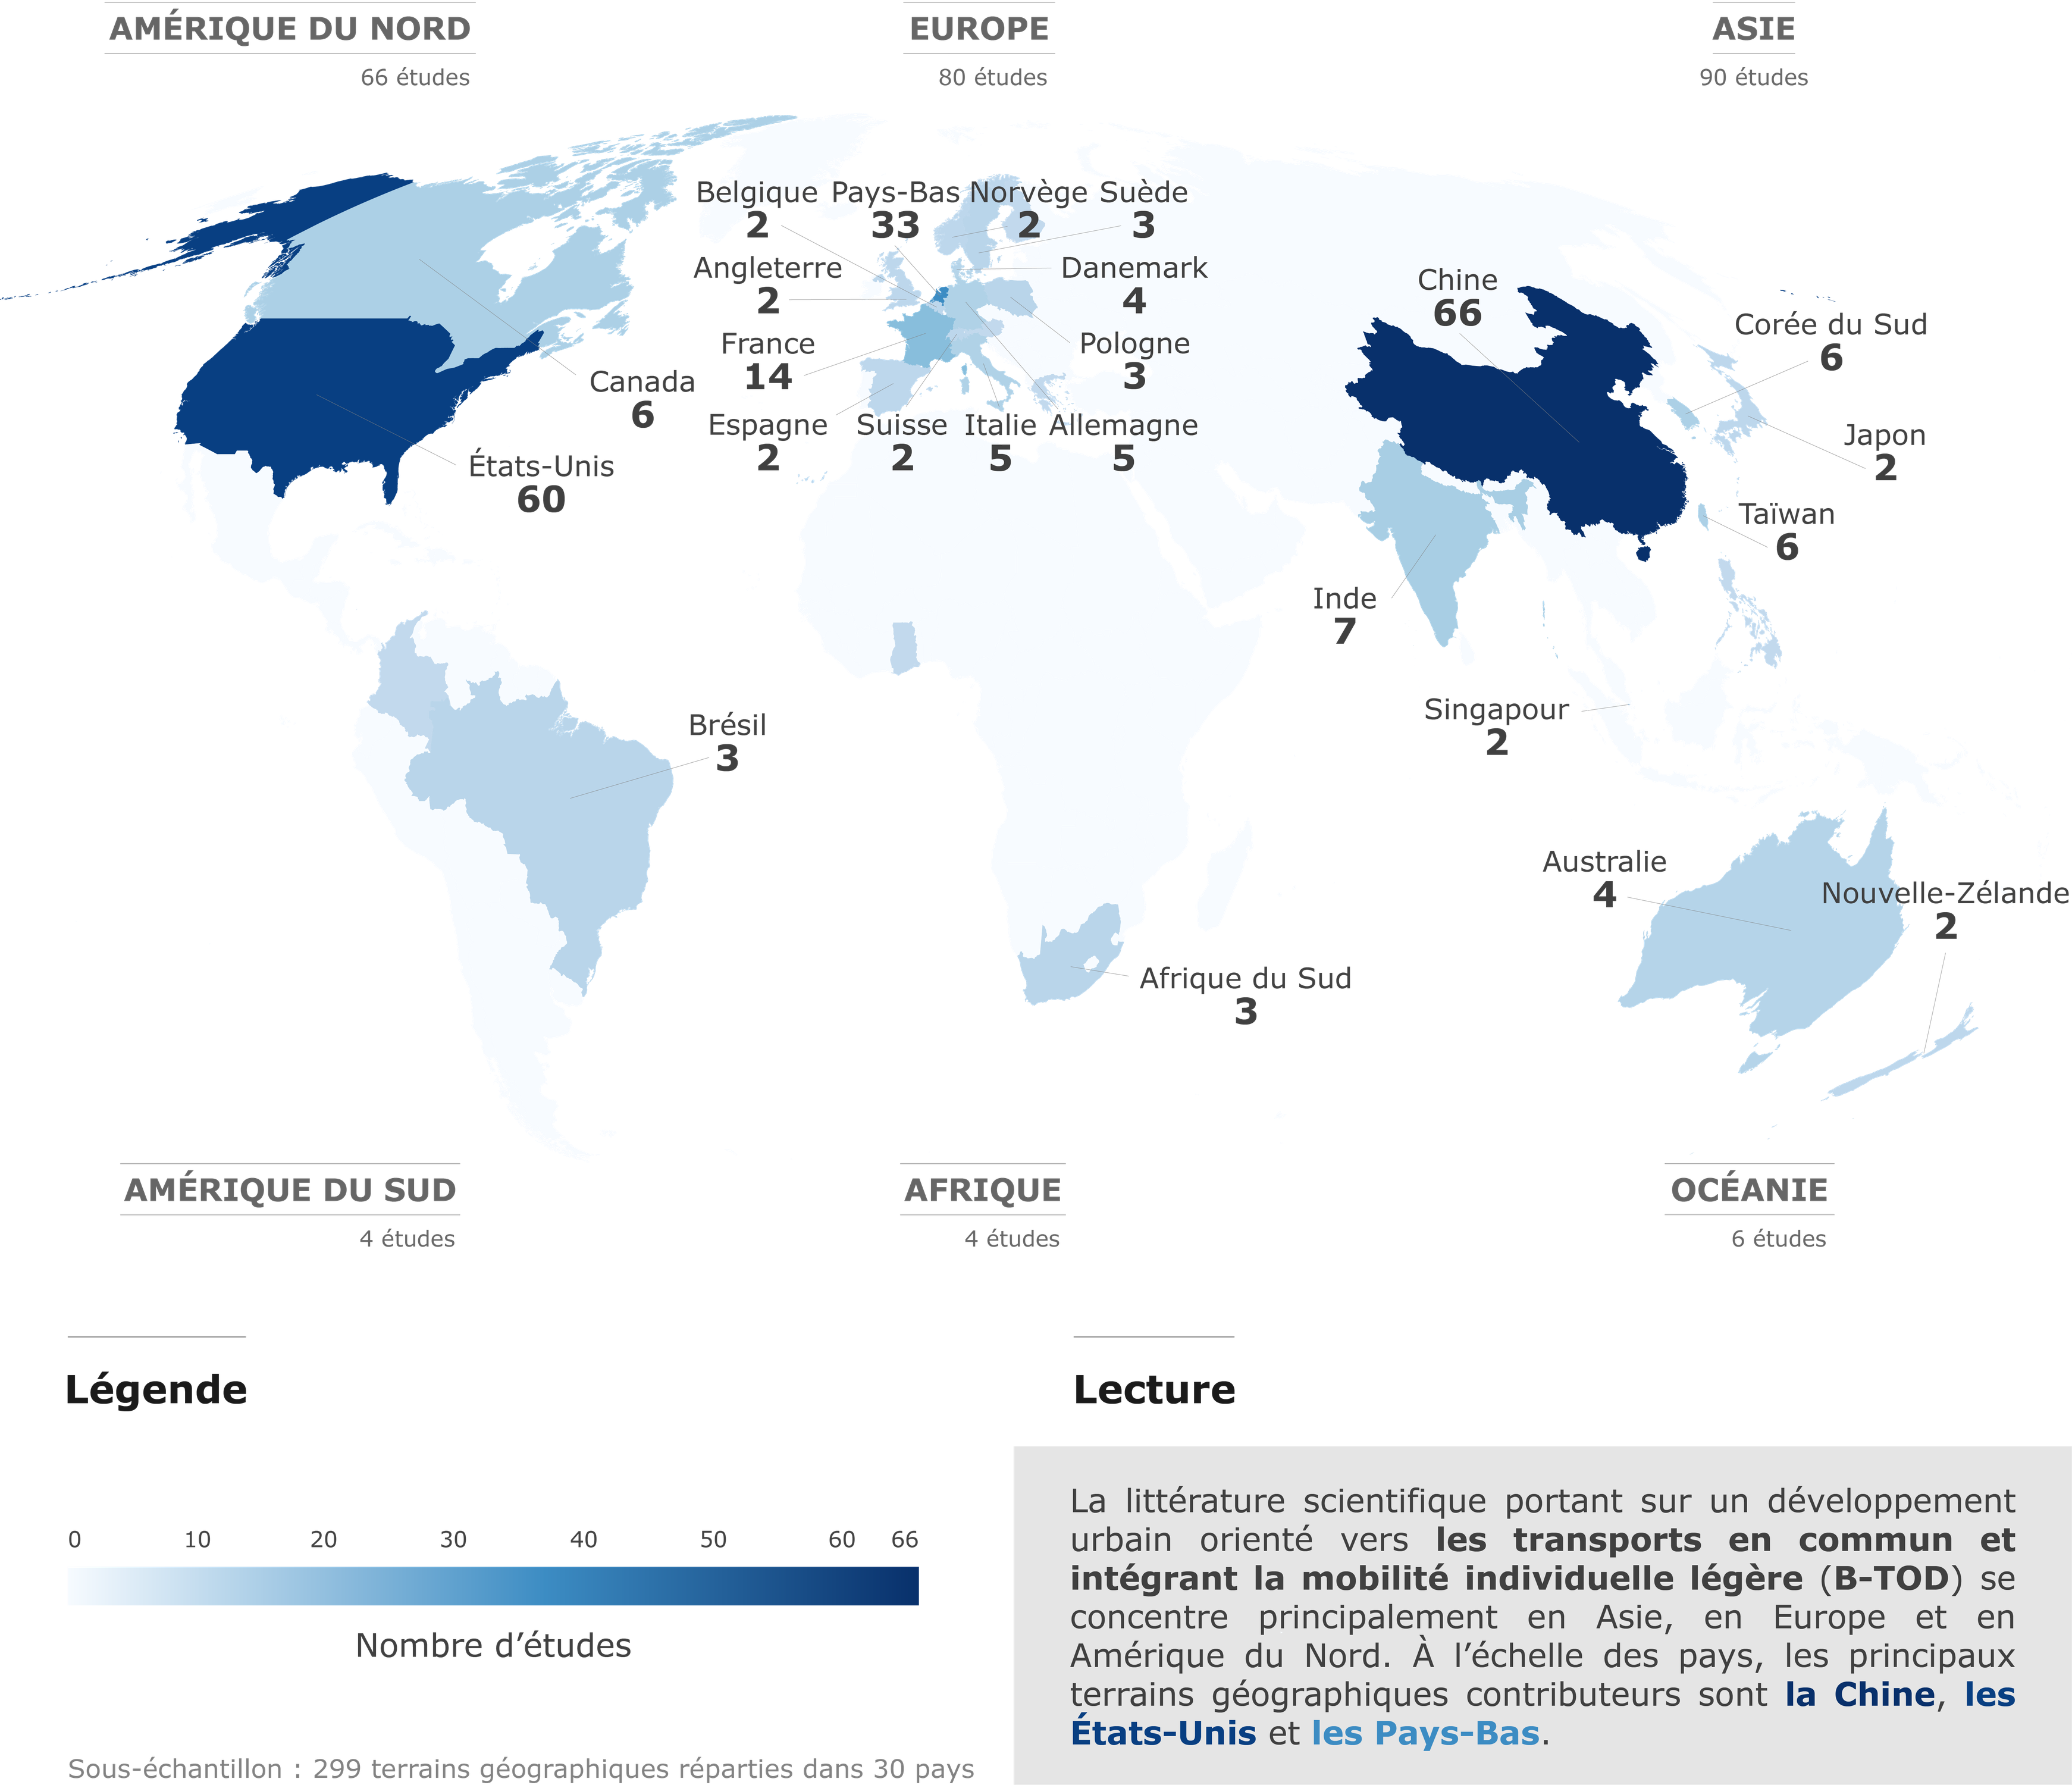
\includegraphics[width=1\columnwidth]{src/Figures/Chap-2/FR_RSL_Carte_Monde.pdf}}
        \vspace{5pt}
        \begin{flushleft}\scriptsize{
        Note~: seuls les pays dont le nombre de contributions est égal ou supérieur à deux sont indiqués sur la carte.
        }\end{flushleft}
        \begin{flushright}\scriptsize{
        Auteur~: \textcolor{blue}{Dylan Moinse (2023)}
        }\end{flushright}
    \end{carte}

    % Répartition géographique par pays
À une échelle plus fine, les pays les plus représentés dans la \acrshort{RSL} consacrée au \acrshort{M-TOD} sont la Chine et les États-Unis, suivis par les Pays-Bas, concordant avec les lieux d'activités répertoriés des chercheur·se·s dans la \hyperref[chap2:analyse-bibliometrique]{sous-section~2.1.1.} (page~\pageref{chap2:analyse-bibliometrique}). À eux seuls, ces trois pays représentent 63,6~\% des terrains géographiques considérés dans les travaux de recherche. Quant au tiers résiduel, cette part est distribuée entre une mosaïque de pays, tantôt industrialisés, tantôt émergents, et incluant la France, l'Inde, la Corée du Sud, Taïwan, le Canada, l'Allemagne et l'Italie (voir la \hyperref[fig-chap2:terrains-geographiques-continents]{carte ~\ref{fig-chap2:terrains-geographiques-continents}}, page~\pageref{fig-chap2:terrains-geographiques-continents}). En conséquence, il conviendrait, dans une formulation plus précise, de parler de l'Europe occidentale, l'Amérique septentrionale et l'Asie orientale en tant qu'entités géographiques manifestement prévalentes au sein de cette \acrshort{RSL}. Ce constat s'aligne sur la revue de littérature, produite par \textcolor{blue}{Bárbara} \textcolor{blue}{\textcite[17]{jansson_almeida_alternativas_2022}}\index{Jansson Almeida, Bárbara|pagebf}, sur l'agencement du vélo avec le métro et qui décrit la place conséquente des études réalisées en Chine, aux Pays-Bas et aux États-Unis. L'analyse du corpus à l'échelle des agglomérations et des communes révèle une concentration autour des mégapoles, principalement en Asie et aux États-Unis. Les régions globalisées le long du littoral chinois, telles que Beijing, Nanjing, Shanghai et Shenzhen, dominent ce classement. Aux États-Unis, des pôles urbains internationaux tels que Washington~D.C., Boston et New York City figurent également en bonne place. En Europe, les points focaux se déplacent vers des centralités régionales, notamment La Haye et Amsterdam (voir la \hyperref[fig-chap2:terrains-geographiques-villes]{carte~\ref{fig-chap2:terrains-geographiques-villes}}, page~\pageref{fig-chap2:terrains-geographiques-villes}). %%Rédigé%%

    % Carte terrains géographiques villes
    \begin{carte}[h!]\vspace*{4pt}
        \caption{Répartition géographique des principales agglomérations examinées dans la revue systématique de la littérature.}
        \label{fig-chap2:terrains-geographiques-villes}
        \centerline{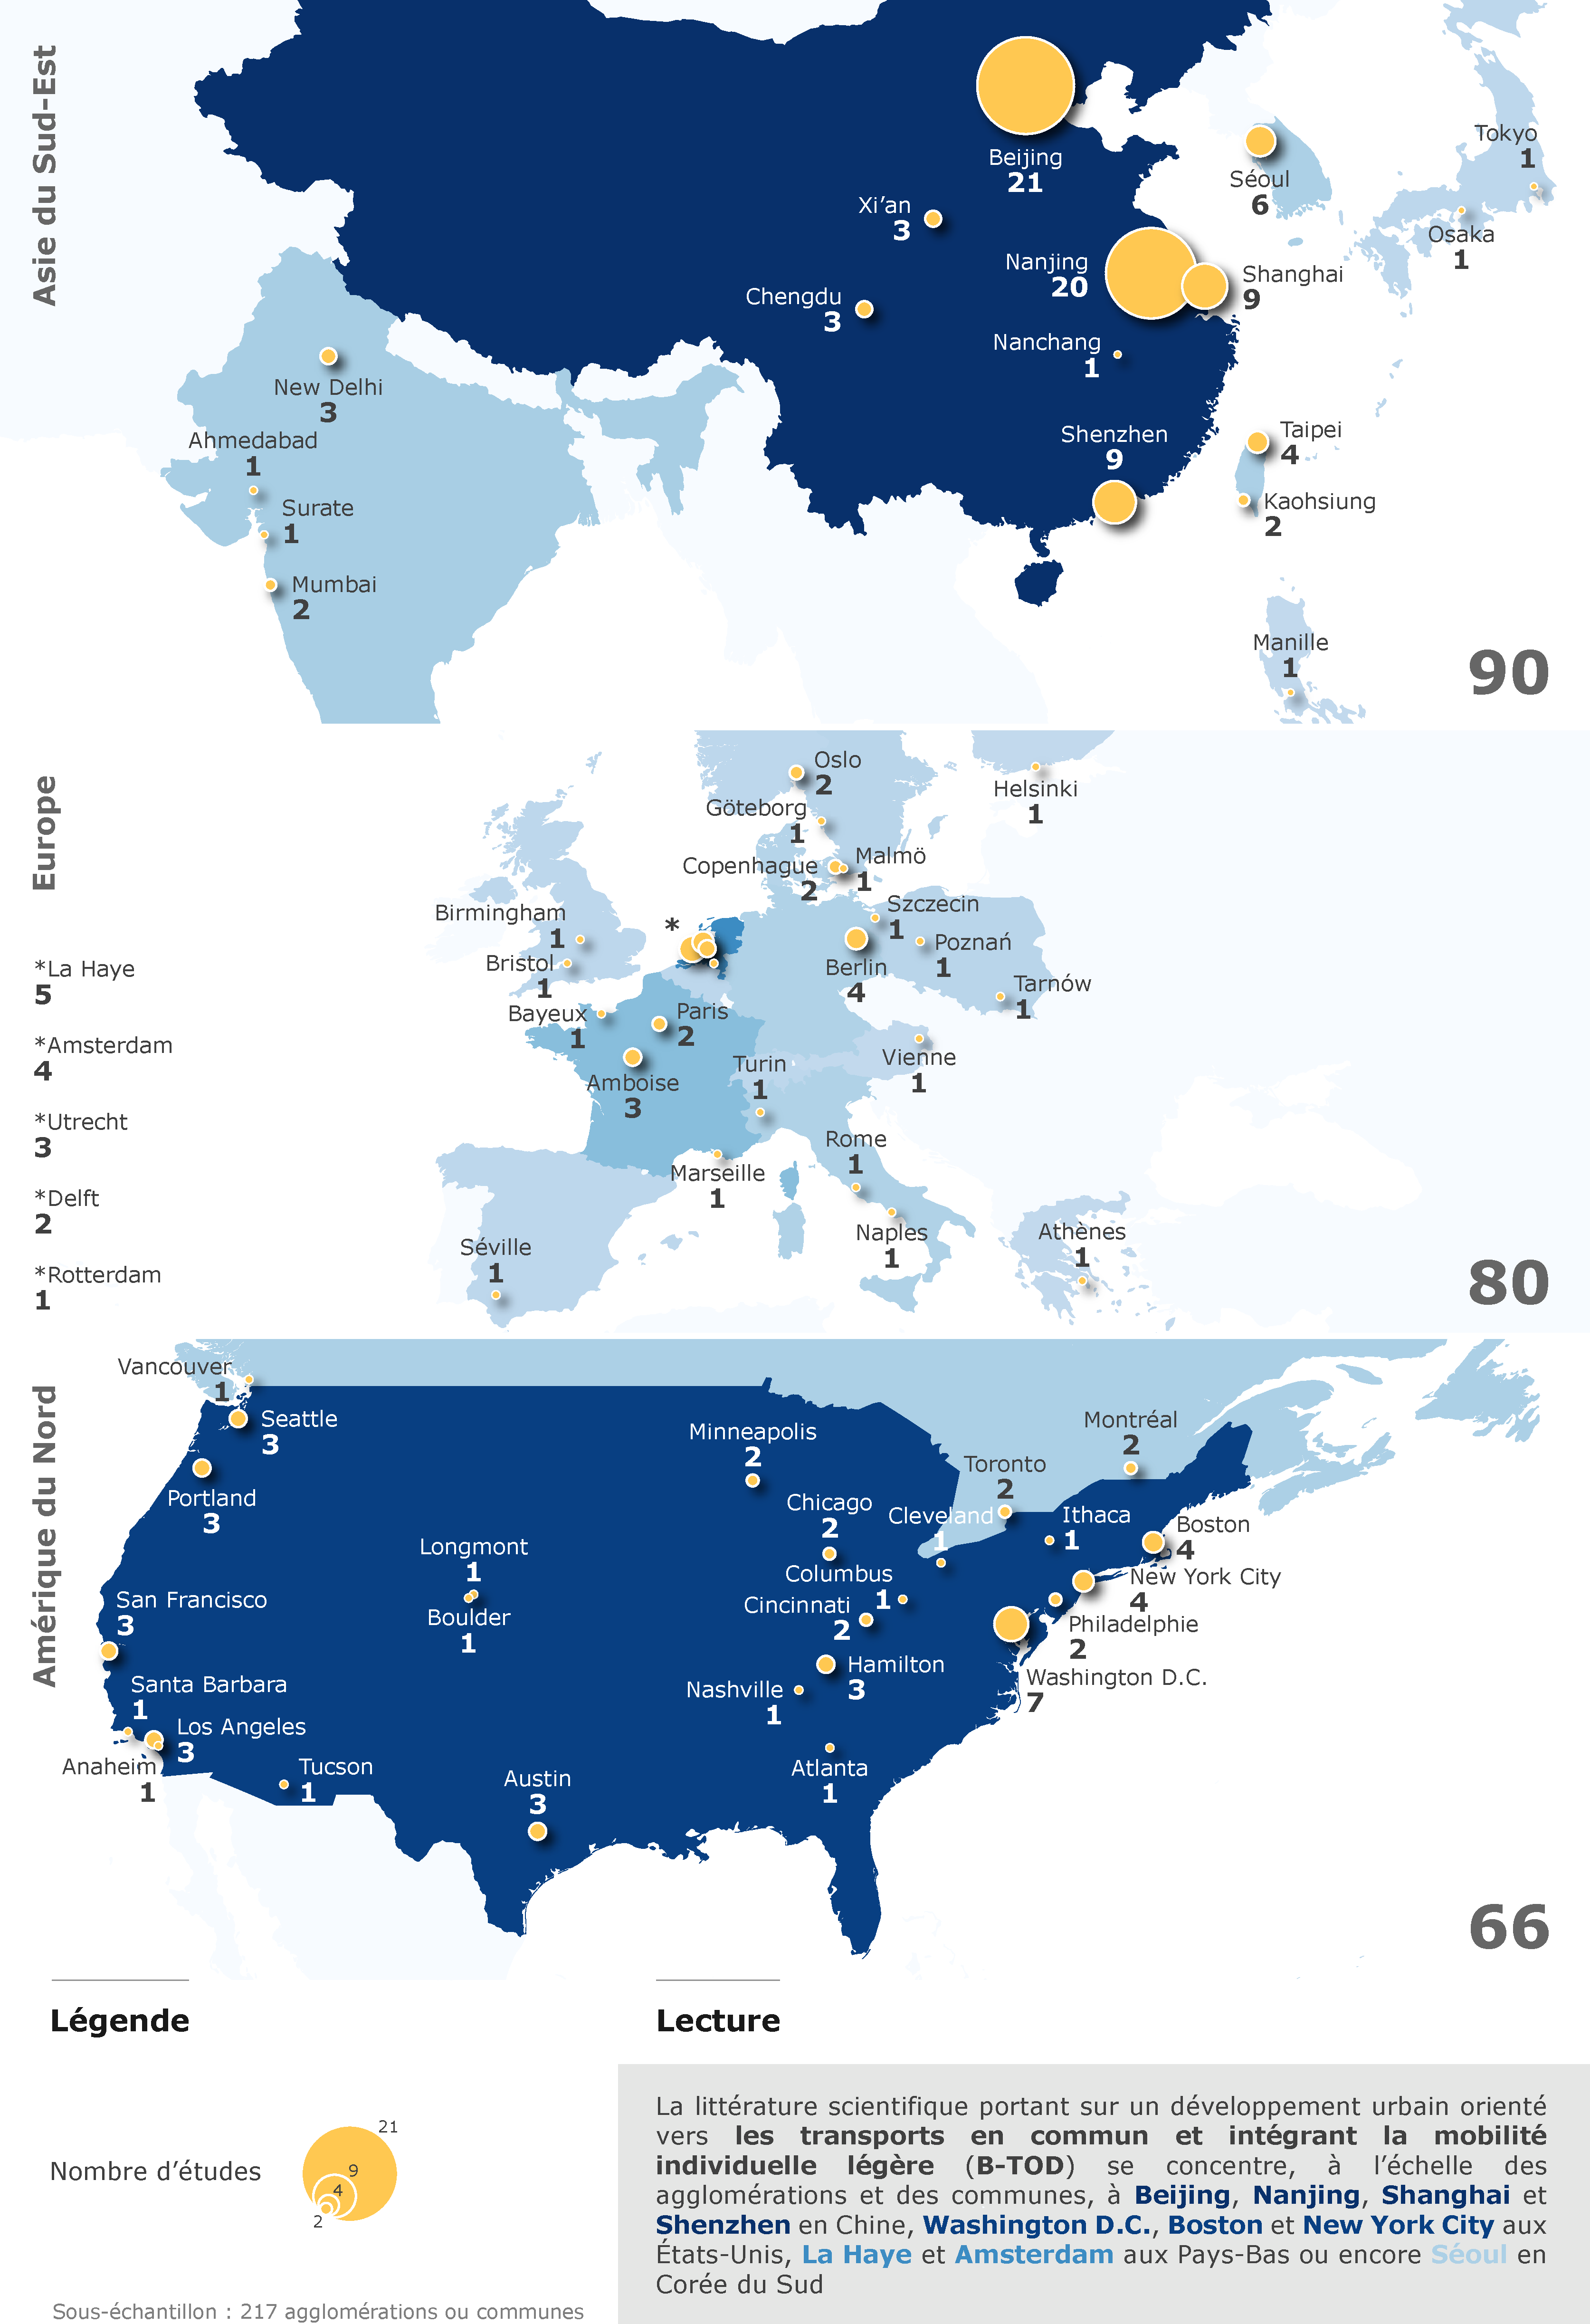
\includegraphics[width=1\columnwidth]{src/Figures/Chap-2/FR_RSL_Carte_Villes.pdf}}
        \vspace{5pt}
        \begin{flushleft}\scriptsize{
        Note~: la somme des contributions associée à chaque pays et continent peut être supérieure aux valeurs propres à chaque agglomération et commune, du fait de productions empiriques ayant adopté une échelle nationale.
        }\end{flushleft}
        \begin{flushright}\scriptsize{
        Auteur~: \textcolor{blue}{Dylan Moinse (2023)}
        }\end{flushright}
    \end{carte}

    % micro-mobilités et TC par continent
Un second aspect auquel s'attache cette section repose sur les formes d'intermodalité étudiées dans la documentation analysée. Comme le montrent les distributions affichées dans la \hyperref[fig-chap2:MIL-TC-continents]{carte~\ref{fig-chap2:MIL-TC-continents}} (page~\pageref{fig-chap2:MIL-TC-continents}), les diverses catégories de mobilité individuelle légère et de transports en commun sont soumises à des investigations inégalitaires, tributaires à des zones géographiques données. Premièrement, la mobilité individuelle légère émergente est bien plus présente en Asie, concernant le vélopartage, et en Amérique du Nord, pour ce qui est des services de trottinettes électriques. Les publications scientifiques élisant un terrain européen s'intéressent principalement au vélo classique. Deuxièmement, les recherches portées sur les systèmes de transport en commun urbain se concentrent également en Asie, principalement avec le métro, et en Amérique du Nord, pour le métro, le tramway et le bus. À l'échelle nationale, il en ressort que certains pays se spécialisent dans des formes d'intermodalité spécifiques. Au sujet du vélo et de la micro-mobilité, nous pouvons notamment retenir la liste de pays suivante~:
    \begin{customitemize}
        \item Dans le contexte des 126 sites d'enquête sur le vélo personnel, nous en comptons 29 aux États-Unis, 28 aux Pays-Bas, 15 en Chine, 11~en France, 6 en Inde et 4 au Canada. De plus, 3 études de cas chacune sont recensées en Afrique du Sud, en Allemagne, en Australie, au Brésil, au Canada, au Danemark et en Italie~;
        \item Sur les 60~lieux abordant le \acrshort{VLS}, 21~d'entre eux sont en Chine, 17 aux États-Unis, 5 à Taïwan et 3 respectivement en Corée du Sud et aux Pays-Bas~;
        \item En ce qui concerne la liste des 44 études de cas sur le \acrshort{VFF}, trois pays seulement sont concernés~: 37 d'entre elles sont situées en Chine, 5 aux États-Unis et 2~aux Pays-Bas~;
        \item Parmi les 20~recherches empiriques focalisées sur le système de \acrshort{TEFF}, 13 d'entre elles se concentrent aux États-Unis et 2~en Allemagne.
    \end{customitemize}
Cette analyse statistique peut être mise en parallèle avec la \acrshort{RSL} menée par \textcolor{blue}{\textcite[298]{zhang_built_2023}}\index{Zhang, Yushan|pagebf}\index{Kasraian, Dena|pagebf}\index{Wesemael, Pieter van|pagebf} sur la mobilité individuelle légère et qui fait état d'une plus grande proportion d'études sur le système de \acrshort{TEFF} en Europe et sur le \acrshort{VLS} et le \acrshort{VFF} en Asie, s'expliquant par des marchés respectivement développés.%%Rédigé%%

    % Figure MIL et TC par continents
    \begin{figure}[h!]\vspace*{4pt}
        \caption{Formes de mobilité individuelle légère et de transports en commun évaluées dans la revue systématique de la littérature, en fonction des continents.}
        \label{fig-chap2:MIL-TC-continents}
        \centerline{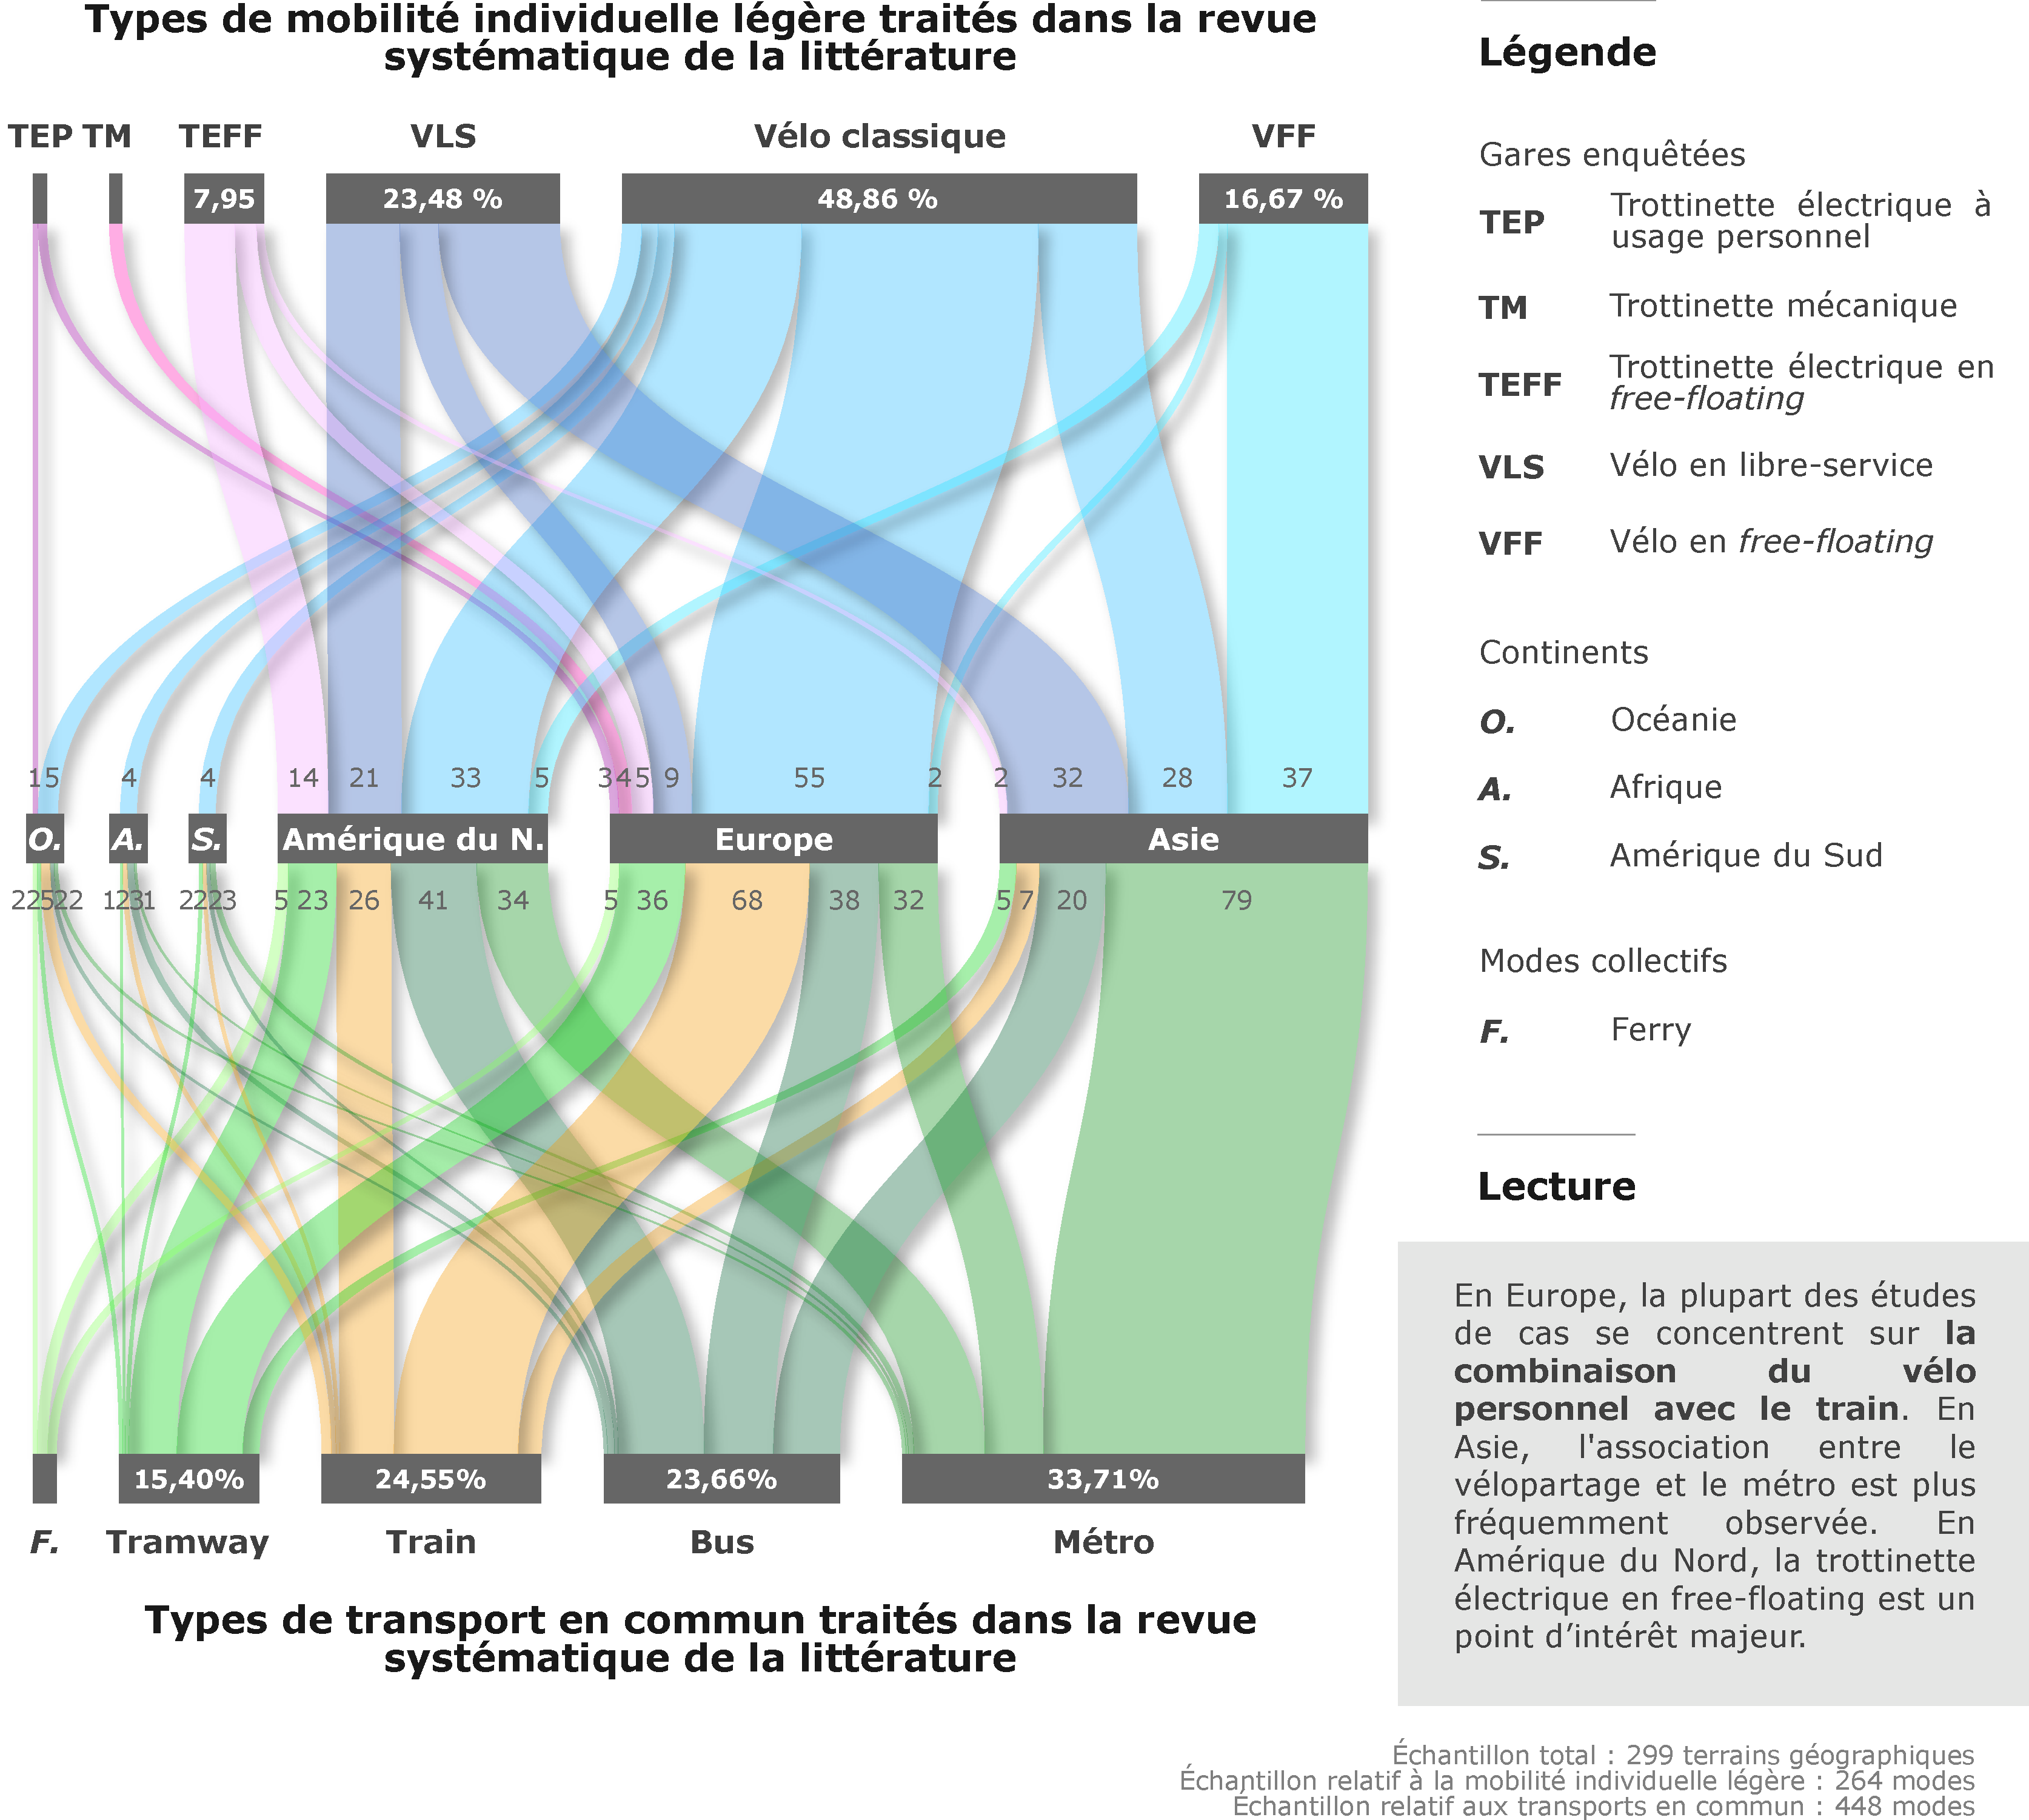
\includegraphics[width=1\columnwidth]{src/Figures/Chap-2/FR_RSL_MIL_TC_Continents.pdf}}
        \vspace{5pt}
        \begin{flushright}\scriptsize{
        Auteur~: \textcolor{blue}{Dylan Moinse (2023)}
        %\\
        %Réalisation avec \Marque{Python}~et sur \Marque{Illustrator}
        }\end{flushright}
    \end{figure}
    
     % TC multimodalité
Bien que la délimitation discernable entre les différents systèmes de transport en commun soit ambivalente lorsqu'il s'agit de procéder à une comparaison internationale\footnote{
    L'ambiguïté entre métro et train dans une perspective de comparaison internationale est inévitable en raison des différences géographiques, culturelles et d'approche en matière de transport. Les tendances et les préférences locales, ainsi que les évolutions technologiques et urbanistiques, peuvent contribuer à brouiller les lignes entre le métro et le train, en particulier lorsqu'il s'agit de comparer différentes régions.
}, il n'en demeure pas moins qu'une proportion substantielle des contributions académiques se livre à une investigation simultanée de divers modes de transport collectif. Force est de constater que, parmi les études analysées, le bus fait l'objet d'un examen dans 66 publications scientifiques, de la même manière que le métro (55 occurrences), le tramway (53 occurrences) et le train (51~occurrences), lorsqu'ils sont envisagés conjointement avec d'autres modes de transport en commun. Quant au ferry, ce mode maritime s'inscrit en une constante imbrication avec d'autres modes collectifs. Sur les 72~documents s'intéressant à plusieurs modes collectifs simultanément, 23 d'entre eux se réfèrent aux États-Unis, tandis que 9 trouvent leur origine en Chine, et que la France et les Pays-Bas y contribuent en parts égales à hauteur de 6 études respectives.%%Rédigé%%

    % Pays minoritaires
En qualité de contributions originales provenant des régions peu explorées ou omises par la \acrshort{RSL}, faut-il faire état des productions scientifiques de \textcolor{blue}{\textcite[34]{bechstein_cycling_2010}}\index{Bechstein, Eva|pagebf}, de \textcolor{blue}{\textcite[368]{cooke_relationship_2018}}\index{Cooke, Sean|pagebf}\index{Behrens, Roger|pagebf}\index{Zuidgeest, Mark|pagebf} et de \textcolor{blue}{\textcite[2]{risimati_spatial_2021}}\index{Risimati, Brightnes|pagebf}\index{Gumbo, Trynos|pagebf}\index{Chakwizira, James|pagebf} en Afrique du Sud~; de \textcolor{blue}{\textcite[108]{quarshie_integrating_2007}}\index{Quarshie, Magnus|pagebf}\index{Morrison, Gregory~M.|pagebf}\index{Rauch, Sébastien|pagebf} au Ghana~; de \textcolor{blue}{\textcite[59]{souza_modelling_2017}}\index{Souza, Flavia de|pagebf}\index{La Paix Puello, Lissy|pagebf}\index{Brussel, Mark|pagebf}\index{Orrico, Romulo|pagebf}, d'\textcolor{blue}{\textcite[36]{arias_molinares_bike_2018}}\index{Arias Molinares, Daniela|pagebf}\index{Florez, Josefina|pagebf} et de \textcolor{blue}{\textcite[40]{jansson_almeida_alternativas_2022}}\index{Jansson Almeida, Bárbara|pagebf} au Brésil~; de \textcolor{blue}{\textcite[206]{cervero_influences_2009}}\index{Cervero, Robert|pagebf}\index{Sarmiento, Olga~L.|pagebf}\index{Jacoby, Enrique|pagebf}\index{Gomez, Luis Fernando|pagebf}\index{Neiman, Andrea|pagebf} en Colombie~; d'\textcolor{blue}{\textcite[6]{arbis_analysis_2016}}\index{Arbis, David|pagebf}\index{Hossein Rashidi, Taha|pagebf}\index{Dixit, Vinayak~V.|pagebf}\index{Vandebona, Upali|pagebf}, de \textcolor{blue}{\textcite[2]{weliwitiya_factors_2017}}\index{Weliwitiya, Hesara|pagebf}\index{Rose, Geoff|pagebf}\index{Johnson, Marilyn|pagebf}, de \textcolor{blue}{\textcite[396]{weliwitiya_bicycle_2019}}\index{Weliwitiya, Hesara|pagebf}\index{Rose, Geoff|pagebf}\index{Johnson, Marilyn|pagebf} et de \textcolor{blue}{\textcite[5]{zhang_make_2023}}\index{Zhang, Mengyuan|pagebf}\index{Lee, Jinwoo Brian|pagebf} en Australie~; ou encore d'\textcolor{blue}{\textcite[17-22]{ensor_forecasting_2010}}\index{Ensor, Matt|pagebf}\index{Slason, Jonathan|pagebf}\index{Vallyon, Chris|pagebf} et d'\textcolor{blue}{\textcite[56-64]{ensor_mode_2021}}\index{Ensor, Matt|pagebf}\index{Maxwell,~O.|pagebf}\index{Bruce, Oliver|pagebf} en Nouvelle-Zélande.%%Rédigé%%

    % Périmètres/échelles choisis (international/national/EPCI)
Le regard porté sur la distribution géographique des terrains d'investigation entraîne une réflexion sous-jacente, quant à l'échelle géographique privilégiée par les travaux empiriques. Au sein du corpus bibliographique, embrassant un total de 238 œuvres scientifiques, quatre d'entre elles assument l'absence d'études de cas en adoptant notamment des approches de modélisations mathématiques. Parallèlement, sept autres recherches présentent exclusivement une revue de littérature et mettent alors en confrontation les recherches empiriques antérieures. Ainsi, 82~\% des recherches menées sur le \acrshort{M-TOD} ont élu, pour contexte géographique, un \acrfull{EPCI}, une commune ou un site local. La part restante est partagée par l'échelle nationale, à hauteur de 11~\%, et régionale, cumulant 6~\%\footnote{
    Il faut préciser que cette catégorisation ne prétend à proposer qu'une trame simplifiée des diverses échelles géographiques, divisées entre les échelons nationaux, régionaux, intercommunaux et communaux. Toutefois, cette démarche s'avère sujette à une limitation, étant donné que la délimitation des contours géographiques d'une région et d'une agglomération varie selon les contextes territoriaux et est donc propice à des erreurs de classements. À titre d'exemple, en 2019, la région Île-de-France s'étend sur environ 12~000~kilomètres carrés et abrite 12 millions d'habitant·e·s, tandis que la métropole du Grand New York occupe une superficie de 34 500~kilomètres carrés avec plus de 20~millions d'habitant·e·s.
}. Force est de souligner que la quasi-majorité des états de l'art adoptent quant à eux une échelle nationale en vue de comparer différents territoires. De manière similaire, la \acrshort{RSL} de \textcolor{blue}{\textcite[298]{zhang_built_2023}}\index{Zhang, Yushan|pagebf}\index{Kasraian, Dena|pagebf}\index{Wesemael, Pieter van|pagebf} fait mention d'une part significative de recherches sur la mobilité individuelle légère dont le cadre géographique ne dépasse pas les limites municipales, et à l'inverse une quasi-absence de travaux à une échelle régionale.%%Rédigé%%

    % Types de territoires analysés 1 (métropoles)
En affinant davantage l'échelle géographique de référence, il est intéressant de noter la pluralité des agglomérations examinées au sein de la \acrshort{RSL}, au regard de leurs dimensions respectives. En nous penchant sur la population des zones urbaines\footnote{
    L'approche comparative des populations repose sur une base de données démographique conçue par \textcolor{blue}{\textcite[]{schiavina_ghs-fua_2019}}\index{Schiavina, Marcello|pagebf}\index{Moreno-Monroy, Ana~I.|pagebf}\index{Maffenini, Luca|pagebf}\index{Veneri, Paolo|pagebf}. Il s'agit de données grillagées sur la population permettant de délimiter les \acrfull{ZUF} dans le monde \textcolor{blue}{\autocite[3]{moreno-monroy_metropolitan_2021}}\index{Moreno-Monroy, Ana~I.|pagebf}\index{Schiavina, Marcello|pagebf}\index{Veneri, Paolo|pagebf}.
}, il nous est donné d'observer les trois continents prédominants dans l'étude du \acrshort{M-TOD}. Conformément au \hyperref[table-chap2:tailles-territoires-rsl]{tableau~\ref{table-chap2:tailles-territoires-rsl}} (page~\pageref{table-chap2:tailles-territoires-rsl}), les mégapoles\footnote{
    \Guillemets{Les mégapoles, ou villes géantes, correspondent aux \textsl{megacities} de la terminologie des Nations-Unies. Ce sont les agglomérations urbaines qui concentrent, selon l’ONU, des populations égales ou supérieures à 10~millions d'habitant·e·s.} \textcolor{blue}{\autocite[]{geoconfluences_megapole_2023}}\index{Géoconfluences@\textsl{Géoconfluences}|pagebf}.
} affichant une démographie supérieure à dix millions d'individus comptent pour 43~\% des terrains géographiques présents dans la \acrshort{RSL}. Ce classement est influencé par les investigations situées en Chine (72~\%) et de manière plus générale, en Asie de l'Est et du Sud-Est (88~\%). De façon analogue, les métropoles jouissant d'un rayonnement international et regroupant une population excédant le seuil des trois millions de citadins occupent une place significative parmi les travaux de recherche empiriques (27~\%). Ces centralités urbaines sont essentiellement localisées aux États-Unis (44~\%), spécifiquement en Amérique du Nord (52~\%). Ce phénomène trouve également écho parmi les métropoles d'importance nationale, voire internationale et comprenant plus d'un million d'habitant·e·s. Ces métropoles intermédiaires sont notamment implantées en Europe occidentale à hauteur de 44~\%, et sont majoritaires en élargissant le périmètre au continent européen dans son ensemble (62~\%). C'est ainsi que les trois types d'aires urbaines mentionnées englobent plus de 87~\% des investigations analysées dans le cadre de la \acrshort{RSL}.%%Rédigé%%

    % Tableau types de territoires analysés RSL
% Tableau types de territoires analysés RSL
%%Rédigé%%
        \begin{table}[h!]
    \centering
    \renewcommand{\arraystretch}{1.5}
    \resizebox{\columnwidth}{!}{
    \begin{tabular}{p{1\columnwidth}}
        %\hline
    \rule{0pt}{15pt} \small{\textbf{\textcolor{blue}{Agglomérations et communes}}}\\
        \hline
    \small{\textbf{\textcolor{blue}{Plus de 10~000~000 d'habitant·e·s (88 références)}}}\\
\small{Beijing (21), Nanjing (19), Shenzhen (9), Shanghai (9), Séoul (6), New York City (4), Chengdu (3), Los Angeles (3), New Delhi (3), Xi'an (3), Chicago (2), Île-de-France (2), Mumbai (2), Bogotá (1), Johannesbourg-Pretoria (1), Osaka (1), Manille (1), Rio de Janeiro (1)}\\
        \hdashline
    \small{\textbf{\textcolor{blue}{Entre 3~000~000 et 10~000~000 d'habitant·e·s (53 références)}}}\\
\small{Washington D.C. (7), Berlin (4), Boston (4), Taipei (4), San Francisco (3), Seattle (3), Suzhou (3), Kaohsiung (2), Melbourne (2), Minneapolis (2), Montréal (2), Philadelphie (2), Toronto (2), Accra (1), Ahmedabad (1), Athènes (1), Atlanta (1), Birmingham (1), Boulder (1), Cape Town (1), Nanchang (1), Porto Alegre (1), Rome (1), Surate (1), Sydney (1), Vienne (1)}\\
        \hdashline
    \small{\textbf{\textcolor{blue}{Entre 1~000~000 et 3~000~000 d'habitant·e·s (33 références)}}}\\
\small{Rotterdam-La Haye (6), Amsterdam (4), Austin (3), Cincinnati (2), Cleveland (2), Copenhague (2), Oslo (2), Auckland (1), Bristol (1), Columbus (1), Helsinki (1), Gutenberg (1), Aix-Marseille-Provence (1), Nashville (1), Orlando (1), Poznań (1), Séville (1), Tucson (1), Turin (1)}\\
        \hdashline
    \small{\textbf{\textcolor{blue}{Entre 250~000 et 1~000~000 d'habitant·e·s (16 références)}}}\\
\small{Hamilton (3), Portland (3), Utrecht (3), Delft (2), Amstelland-Meerlanden (1), Eindhoven (1), Malmö (1), Mamelodi (1), Tarnow (1)}\\
        \hdashline
    \small{\textbf{\textcolor{blue}{Moins de 250~000 habitant·e·s (8 références)}}}\\
\small{Amboise (3), Bayeux (1), El Monte (1), Ithaca (1), Longmont (1), communes belges entre 30~000~et 200~000~habitant·e·s (1)}\\
        \hline
        \end{tabular}}
    \caption{Taille des agglomérations et des communes étudiées dans la revue systématique de la littérature.}
    \label{table-chap2:tailles-territoires-rsl}
        \vspace{5pt}
        \begin{flushleft}\scriptsize{
        \textcolor{blue}{Lecture~:} à partir de 198 études comprenant un terrain géographique, la revue systématique de la littérature est principalement composée d'agglomérations de plus de 3~000~000 d'habitant·e·s.
        }\end{flushleft}
        \begin{flushright}\scriptsize
        Auteur~: \textcolor{blue}{Dylan Moinse (2023)}
        \end{flushright}
        \end{table}%%Rédigé%%

    % Types de territoires analysés 2 (métropoles régionales)
En ce qui concerne les agglomérations peuplées de moins d'un million d'habitant·e·s, les études de cas en milieu urbain s'articulent principalement autour des intercommunalités néerlandaises, spécifiquement dans les localités de Delft \textcolor{blue}{\autocites[113]{heinen_multimodal_2014}[5]{molin_bicycle_2015}}\index{Heinen, Eva|pagebf}\index{Bohte, Wendy|pagebf}\index{Molin, Eric|pagebf}\index{Maat, Kees|pagebf}, d'Amstelland-Meerlanden \textcolor{blue}{\autocite[46]{brand_assessing_2015}}\index{Brand, Judith Caroline|pagebf}, d'Eindhoven \textcolor{blue}{\autocite[724]{waerden_relation_2018}}\index{Waerden, Peter|pagebf}\index{Waerden, Jaap|pagebf} et d'Utrecht \textcolor{blue}{\autocite[289]{kuijk_preferences_2022}}\index{Mil, Joeri~F.P. van|pagebf}\index{Leferink, Tessa~S.|pagebf}\index{Annema, Jan Anne|pagebf}\index{Oort, Niels van|pagebf}\index{Kuijk, Roy~J. van|pagebf}\index{Almeida Correia, Gonçalo Homem de|pagebf}\index{Oort, Niels van|pagebf}\index{Arem, Bart van|pagebf}. Les États-Unis constituent également un terrain propice à ce sujet de recherche, à travers des travaux prenant appui à Portland \textcolor{blue}{\autocites[164]{krizek_assessing_2011}[400]{mcqueen_assessing_2022}[94]{singleton_exploring_2014}[265]{welch_long-term_2016}[83]{pucher_integrating_2009}}\index{Krizek, Kevin~J.|pagebf}\index{Stonebraker, Eric~W.|pagebf}\index{McQueen, Michael|pagebf}\index{Clifton, Kelly~J.|pagebf}\index{Singleton, Patrick~A.|pagebf}\index{Welch, Timothy~F.|pagebf}\index{Gehrke, Steven~R.|pagebf}\index{Wang, Fangru|pagebf}\index{Pucher, John|pagebf}\index{Buehler, Ralph|pagebf} et à Anaheim, dans la région métropolitaine de Los Angeles (\textsl{Greater Los Angeles Area}), \textcolor{blue}{\autocite[1579]{liu_simultaneous_2015}}\index{Liu, Yang|pagebf}\index{Zhu, Ning|pagebf}\index{Ma, Shou-feng|pagebf}. De même, les territoires canadiens contribuent à cette documentation, à l'aide de publications scientifiques centrées sur la région métropolitaine d'Hamilton \textcolor{blue}{\autocites[2162]{chan_factors_2020}[375]{ravensbergen_biking_2018}}\index{Ravensbergen, Léa|pagebf}\index{Chan, Kevin|pagebf}\index{Farber, Steven|pagebf}\index{Buliung, Ron|pagebf}\index{Mendonca, Meaghan|pagebf}\index{Garg, Naren|pagebf}. Quant aux agencements territoriaux à dominante rurale et périurbaine, les exemples français abondent, marqués par une série d'études menées au sein des communes d'Amboise \textcolor{blue}{\autocites[747]{midenet_modal_2018}[2729]{papon_evaluation_2017}[14-16]{papon_rapport_2015}}\index{Midenet, Sophie|pagebf}\index{Côme, Etienne|pagebf}\index{Papon, Francis|pagebf}\index{Beauvais, Jean-Marie|pagebf}\index{Midenet, Sophie|pagebf}\index{Côme, Etienne|pagebf}\index{Polombo, Nadine|pagebf}\index{Abours, Sylvie|pagebf}\index{Belton-Chevallier, Leslie|pagebf}\index{Soulas, Claude|pagebf} et de Bayeux \textcolor{blue}{\autocite[2]{richer_service_2017}}\index{Richer, Cyprien|pagebf}, ainsi que dans l'ancienne \acrfull{CC} de la Brie Boisée (faisant partie intégrante de l'Île-de-France depuis 2017) mise en perspective avec celle de Carnelle Pays de France et de Haute Vallée de Chevreuse \textcolor{blue}{\autocite[39]{stransky_periurbain_2019}}\index{Stransky, Vaclav|pagebf}.%%Rédigé%%

    % Figure comparaisons internationales
    \begin{figure}[h!]\vspace*{4pt}
        \caption{Comparaisons entre terrains géographiques dans le corpus bibliographique de la revue systématique de la littérature.}
        \label{fig-chap2:comparaisons-internationales-rsl}
        \centerline{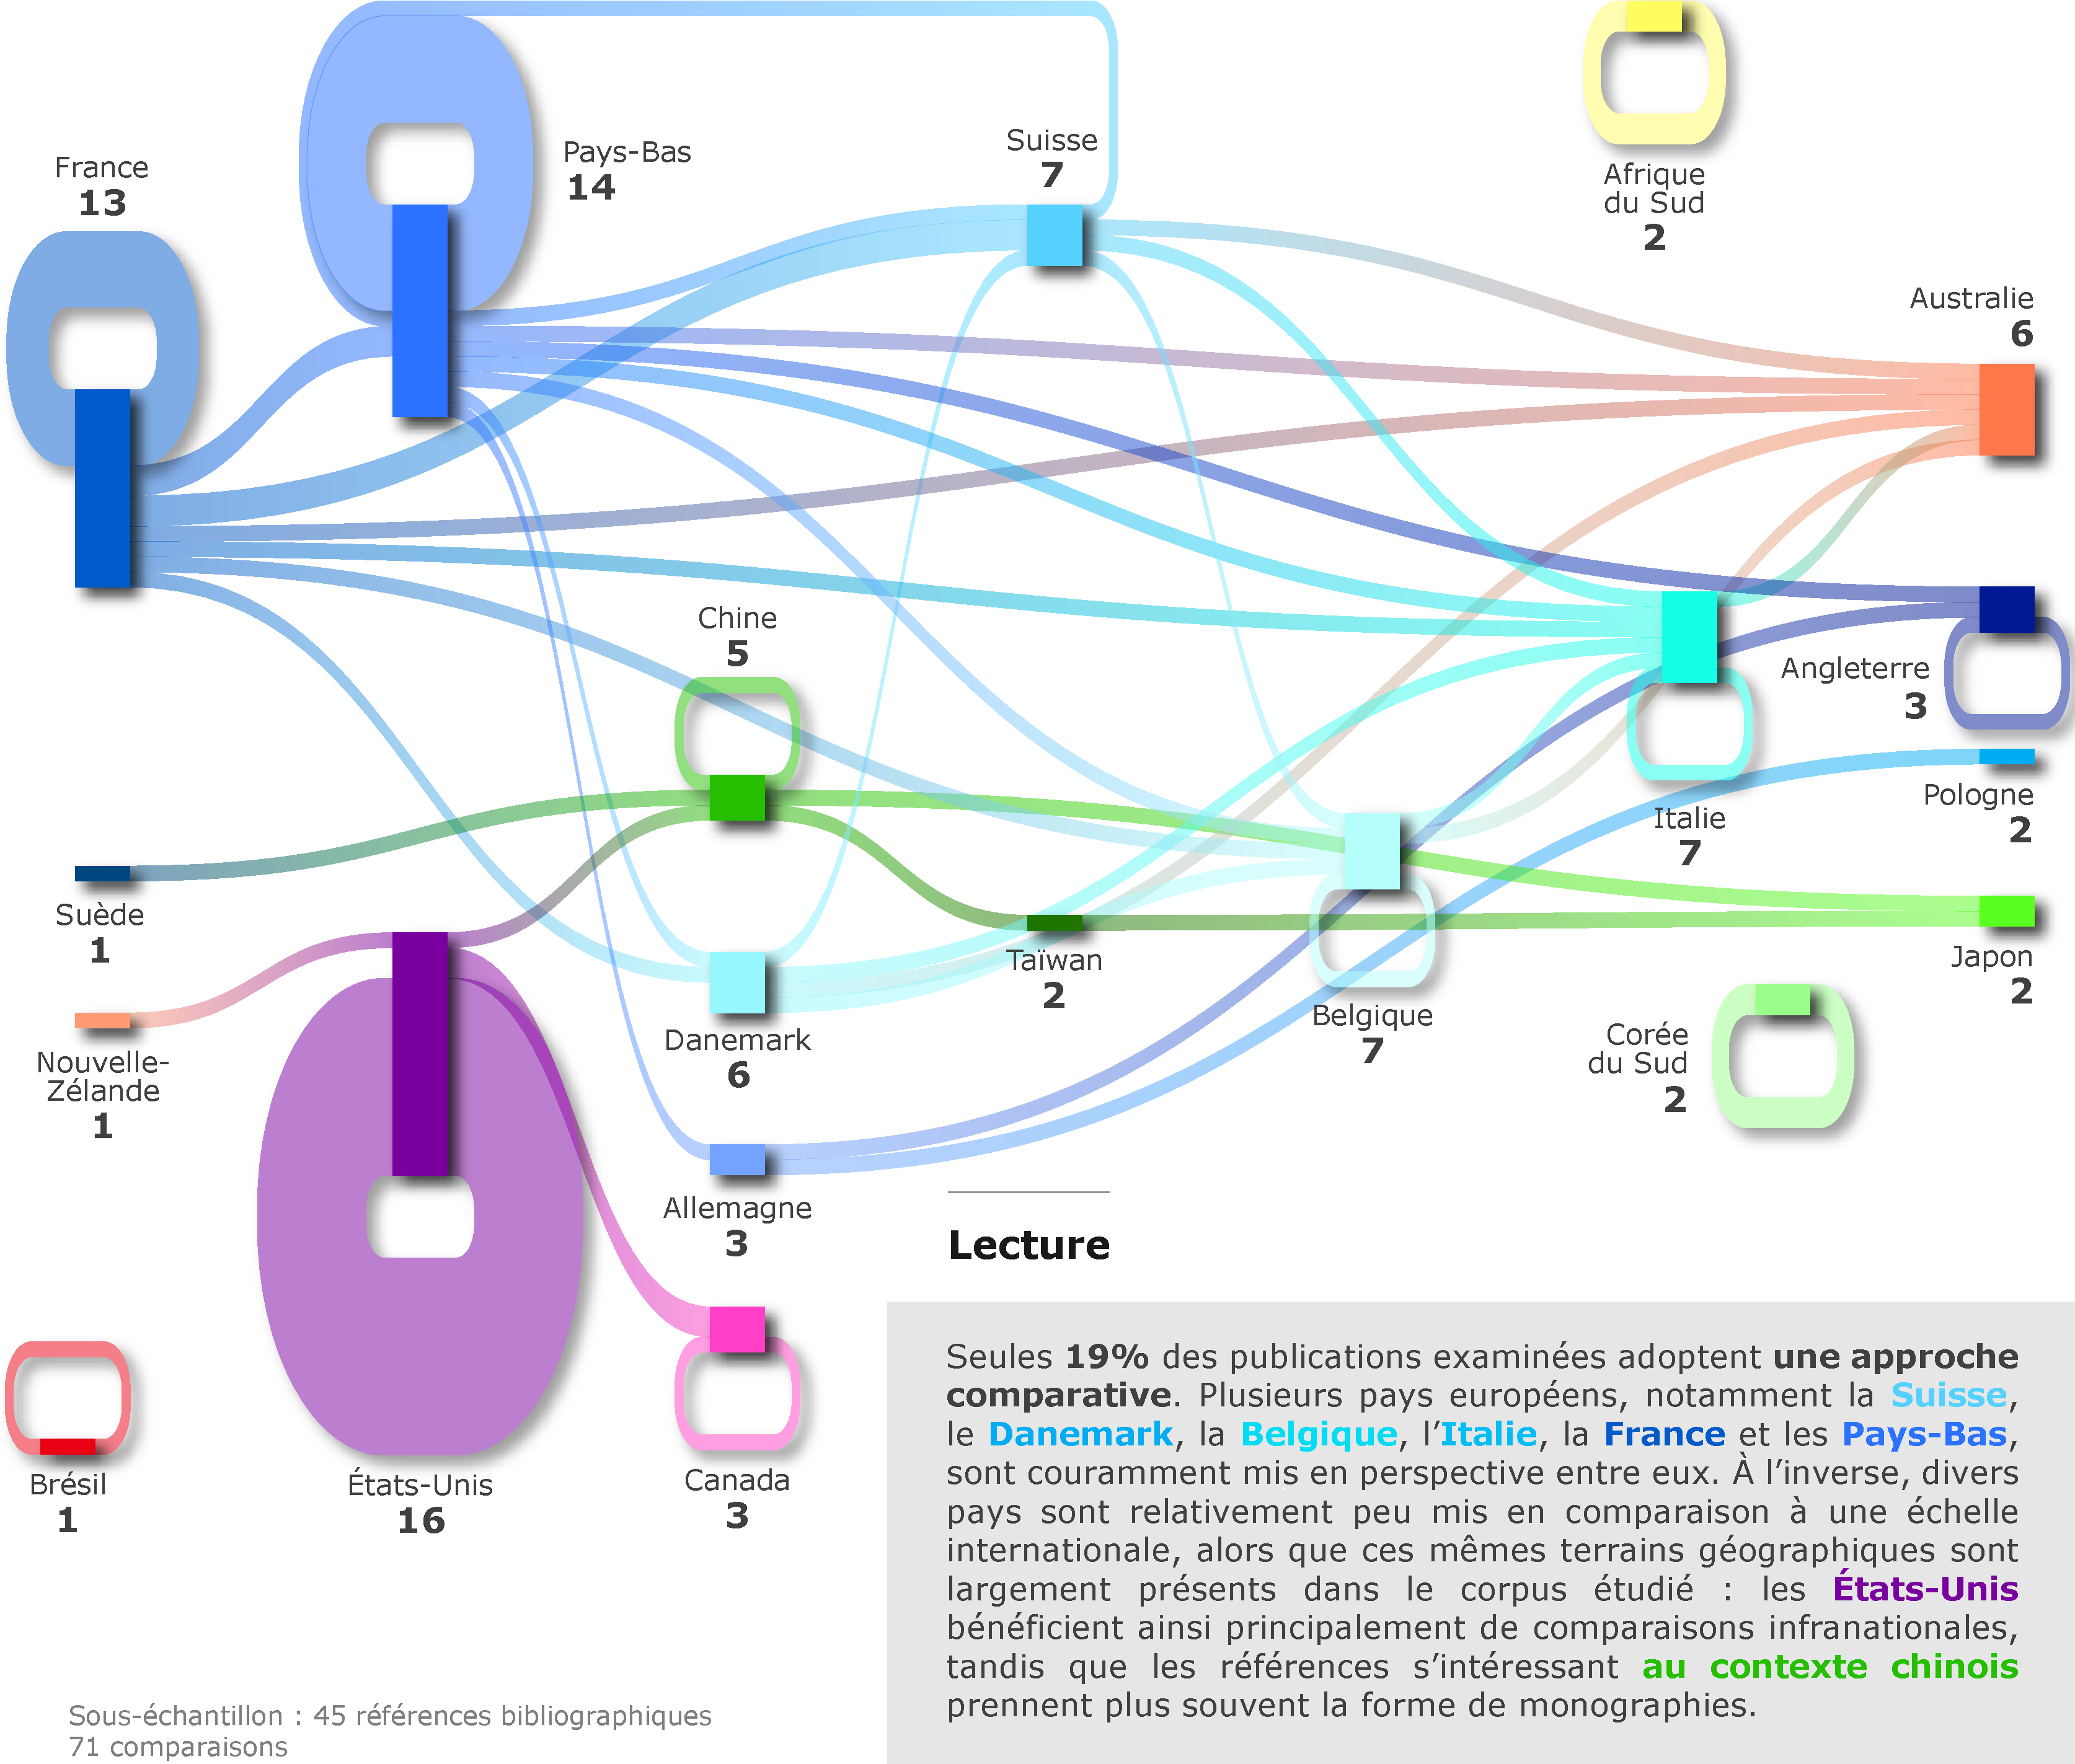
\includegraphics[width=1\columnwidth]{src/Figures/Chap-2/FR_RSL_Comparaisons_internationales.pdf}}
        \vspace{5pt}
        \begin{flushright}\scriptsize{
        %\\
        %Réalisation avec \Marque{Python}~et sur \Marque{Illustrator
        Note~: seules les comparaisons menées entre différentes régions ont été prises en compte afin d'exclure un même périmètre urbain comportant plusieurs sites locaux étudiés. L'anneau correspond à des comparaisons infranationales, tandis que les flux lient les terrains géographiques mis en perspective.
        \\
        Auteur~: \textcolor{blue}{Dylan Moinse (2023)}
        }\end{flushright}
    \end{figure}

    % Comparaisons internationales
Si la documentation relative au \acrshort{M-TOD} adopte communément une approche comparative en sélectionnant divers sites d'étude au sein d'un système politique cohérent, plus rares sont les recherches qui se prêtent à la mise en parallèle de divers territoires répartis dans des pays distincts. En réalité, il ressort que 19~\% des publications examinées se dédient à une comparaison internationale ou infranationale. Dans le sous-ensemble constitué de 45 publications scientifiques consacrées aux comparaisons, 30~d'entre elles opèrent une mise en perspective entre différents \acrshort{EPCI} tandis que 11~autres embrassent l'échelon national. Comme en témoigne l'\hyperref[fig-chap2:comparaisons-internationales-rsl]{illustration~\ref{fig-chap2:comparaisons-internationales-rsl}} (page~\pageref{fig-chap2:comparaisons-internationales-rsl}), certains pays sont fréquemment mis en relation, tels que la Suisse, le Danemark, la Belgique, l'Italie, la France et les Pays-Bas \textcolor{blue}{\autocites[29-46]{abours_rapport_2015}[279-285]{sebban_complementarite_2003}[282-284]{martens_bicycle_2004}}\index{Abours, Sylvie|pagebf}\index{Midenet, Sophie|pagebf}\index{Soulas, Claude|pagebf}\index{Sebban, Annie-Claude|pagebf}\index{Martens, Karel|pagebf}, notamment avec d'autres pays européens~; ou encore le Japon, Taïwan et la Chine \textcolor{blue}{\autocite[212]{lin_built_2018}}\index{Lin, Jen-Jia|pagebf}\index{Zhao, Pengjun|pagebf}\index{Takada, Kazuyuki|pagebf}\index{Li, Shengxiao|pagebf}\index{Yai, Tetsuo|pagebf}\index{Chen, Chi-Hao|pagebf}. Soulignons qu'il existe également deux comparaisons intercontinentales, portées par \textcolor{blue}{\textcite[4]{hamidi_shaping_2020}}\index{Hamidi, Zahra|pagebf}\index{Zhao, Chunli|pagebf} qui ont étudié les aires urbaines chinoises et suédoises de Beijing, Göteborg et Malmö~; et par \textcolor{blue}{\textcite[13]{hua_transfer_2022}}\index{Hua, Mingzhuang|pagebf}\index{Pereira, Francisco Camara|pagebf}\index{Jiang, Yu|pagebf}\index{Chen, Xuewu|pagebf} qui se sont intéressé·e·s aux villes chinoises et étasuniennes de Nanjing et de Chicago.%%Rédigé%%

    % Comparaisons infranationales
Dans le sens contraire, certains pays sont peu mis en perspective, même s'ils sont amenés à être comparés dans de faibles proportions (voir l'\hyperref[fig-chap2:comparaisons-internationales-rsl]{illustration~\ref{fig-chap2:comparaisons-internationales-rsl}}, page~\pageref{fig-chap2:comparaisons-internationales-rsl}). Citons, par exemple, les États-Unis qui, à l'exception de certaines comparaisons avec le Canada \textcolor{blue}{\autocites[11-16]{ensor_forecasting_2010}[7]{schneider_integration_2005}[83]{pucher_integrating_2009}}\index{Ensor, Matt|pagebf}\index{Slason, Jonathan|pagebf}\index{Vallyon, Chris|pagebf}\index{Schneider, Robert|pagebf}\index{Pucher, John|pagebf}\index{Buehler, Ralph|pagebf}, bénéficient principalement de comparaisons infranationales. Certains pays n'ont, par ailleurs, bénéficié que de comparaisons internes entre différentes régions du même ensemble géographique. En Afrique du Sud, \textcolor{blue}{Eva} \textcolor{blue}{\textcite[34]{bechstein_cycling_2010}}\index{Bechstein, Eva|pagebf} opte pour une démarche comparative entre les \Guillemets{\textsl{townships}}\footnote{
    \Guillemets{En Afrique du Sud, depuis l'\textsl{apartheid}, régime de ségrégation raciale, le mot \textsl{township} désigne des quartiers habités par les populations de couleur (noirs et \textsl{coloured}). [\dots] En désignant les quartiers habités par des populations ségrégées, il finit par désigner des quartiers pauvres, d'habitat dégradé et insalubre, se rapprochant de la définition du bidonville.}~\textcolor{blue}{\autocite{geoconfluences_township_2023}}\index{Géoconfluences@\textsl{Géoconfluences}|pagebf}.
} de Mamelodi et de Nellmapius (Tshwane), de la même façon que \textcolor{blue}{\textcite[368]{cooke_relationship_2018}}\index{Cooke, Sean|pagebf}\index{Behrens, Roger|pagebf}\index{Zuidgeest, Mark|pagebf} entre les municipalités métropolitaines de Johannesbourg, Le Cap, Tshwane, la baie Nelson Mandela et d'eThekwini. En Corée du Sud, les recherches menées par \textcolor{blue}{\textcite[43, 980]{lee_strategies_2010, lee_bicycle-based_2016}}\index{Lee, Jaeyeong|pagebf}\index{Shin, Hee-Cheol|pagebf}\index{Lee, Jaeyeong|pagebf}\index{Choi, Keechoo|pagebf}\index{Leem, Yountaik|pagebf} suivent une analyse comparative entre les régions métropolitaines de Séoul et de Daejeon.%%Rédigé%%

    % Peu de comparaisons
À l'inverse, l'\hyperref[fig-chap2:comparaisons-internationales-rsl]{illustration~\ref{fig-chap2:comparaisons-internationales-rsl}} (page~\pageref{fig-chap2:comparaisons-internationales-rsl}) révèle la sous-représentation, voire l'absence, de certains pays qui sont pourtant bien étudiés dans la \acrshort{RSL}. Le cas le plus frappant est celui de la Chine, où la grande majorité des recherches utilise une approche monographique, se concentrant uniquement sur une seule agglomération. Toutefois, il convient de noter que ces études ne sont pas nécessairement non comparatives \textcolor{blue}{\autocite[30-31]{gueranger_monographie_2012}}\index{Guéranger, David|pagebf}. Par exemple, l'étude réalisée par \textcolor{blue}{\textcite[77]{liu_solving_2012}}\index{Liu, Zhili|pagebf}\index{Jia, Xudong|pagebf}\index{Cheng, Wen|pagebf} procède à deux études de cas dans les quartiers de Dongcheng et d'Haidian, à Beijing, après avoir réalisé une analyse exhaustive du système de \acrshort{VLS} autour des arrêts de métro et de bus dans la capitale. En excluant les comparaisons au sein d'une même aire urbaine du fait de contraintes méthodologiques liées à la normalisation des terrains géographiques, ce graphique masque le raisonnement analogique présent à l'échelle infracommunale.%%Rédigé%%

    % Conclusion
En somme, cette section consacrée à l'état de la littérature scientifique internationale sur le \acrshort{M-TOD} s'est à la fois penchée sur l'analyse des métadonnées des publications scientifiques collectées, les schémas lexicaux utilisés pour décrire le sujet de recherche, ainsi que sur les tendances chronologiques et la répartition géographique des investigations conduites. Après avoir analysé la documentation sous l'angle des métadonnées, la section suivante abordera les cadres conceptuels et méthodologiques de la littérature scientifique sur le \acrshort{M-TOD}, en portant un regard sur les fondements théoriques, l'évaluation des démarches et sur les types d'analyse employés au sein des investigations.%%Rédigé%%

    % 2.2.2. concepts, méthodes, types d'analyse
    \needspace{1\baselineskip} % Réserve de l'espace
\subsection{Cadres conceptuels et méthodologiques du corpus
    \label{chap2:cadres-conceptuels-methodologiques}
    }
    
    % Introduction
Cette partie est dédiée à la présentation et à la mise en confrontation des divers fondements théoriques et des démarches employés dans la littérature scientifique. Les questionnements suivants ont été considérés dans cette analyse~:
    \begin{customitemize}
        \item Quels sont les principaux cadres théoriques mobilisés dans la documentation sélectionnée~? De quelle manière ces choix théoriques ont-ils été appliqués aux questions de recherche~?
        \item Peut-on identifier des évolutions des cadres théoriques adoptés au fil du temps~? Ces tendances reflètent-elles certaines orientations ou avancées disciplinaires~? Quelles critiques ont été soulevées par les auteurs concernant les cadres théoriques utilisés~?
        \item Quelles méthodes de collecte de données ont été utilisées~? Quelles techniques d'analyse des données ont été appliquées~?
        \item Comment les auteur·rice·s ont-ils abordé les contraintes et les limites des méthodes de collecte et d'analyse utilisées~?
    \end{customitemize}%%Rédigé%%

    % Annonce du plan
Cette sous-section se propose d'introduire les cadres théoriques inscrits dans la littérature scientifique (\hyperref[chap2:fondements-theoriques]{sous-section~2.2.1}, page~\pageref{chap2:fondements-theoriques}), préalablement à l'évaluation des procédés de collecte de données (\hyperref[chap2:methodes-collecte-donnees]{sous-section~2.2.2}, page~\pageref{chap2:methodes-collecte-donnees}) et des méthodes d'analyse des données (\hyperref[chap2:demarches-types-analyses]{sous-section~2.2.3}, page~\pageref{chap2:demarches-types-analyses}) employées pour étudier le \acrshort{M-TOD}.%%Rédigé%%

    % 2.2.2.1. Concepts mobilisés, TOD
    \needspace{1\baselineskip} % Réserve de l'espace
\subsubsection*{Fondements théoriques
    \label{chap2:fondements-theoriques}
    }
    
    % Cadres théoriques description
Dans l'ensemble des 102~articles scientifiques analysés dans le cadre de la \acrshort{RSL}, le concept de \acrshort{TOD} est prédominant, étant cité dans 55 études. Parmi ces travaux, 53 articles discutent explicitement du \acrshort{TOD}, avec neuf d'entre eux s'appuyant spécifiquement sur les principes des \Guillemets{Ds} pour structurer leur analyse. Quatre études se fondent sur une approche analytique des \Guillemets{5Ds}, trois sur les \Guillemets{3Ds}, une sur les \Guillemets{4Ds} et une autre sur les \Guillemets{6Ds}\footnote{
    Dans l'ordre communément accepté dans la littérature scientifique portant sur le \acrshort{TOD}, et comme présenté dans la \hyperref[chap1:tod-presentation-generale-definition]{section sur la définition du \textsl{Transit-Oriented Development}} (page~\pageref{chap1:tod-presentation-generale-definition}) du \hyperref[chap1:titre]{chapitre~1} (page~\pageref{chap1:titre}), les \Guillemets{\acrshort{7Ds}} se composent de la façon suivante~: la \Guillemets{densité} (\textsl{Density}, \(D1\)), la \Guillemets{diversité fonctionnelle} (\textsl{Diversity}, \(D2\)), le \Guillemets{traitement des espaces publics} (\textsl{Design}, \(D3\)), l'\Guillemets{accessbilité aux destinations} (\textsl{Destination Accessibility}, \(D4\)), l'\Guillemets{accessbilité locale} (\textsl{Distance to Transit}, \(D5\)), le \Guillemets{management de la demande de mobilité} (\textsl{Demand Management}, \(D6\)) et les \Guillemets{caractéristiques socio-démographiques} (\textsl{Demographics}, \(D7\)).
}. Quatre articles intègrent une version revisitée du \acrshort{TOD} qui fait fortement écho au présent chapitre, portant sur le \acrshort{M-TOD}. La place importante du \acrshort{TOD} dans la littérature est néanmoins influencée par son intégration dans notre formule de recherche lors de la collecte des bases de données. Outre le \acrshort{TOD}, deux autres notions émergent fréquemment~: les \Guillemets{premiers et derniers kilomètres}, mentionnés 24 fois, et l'\Guillemets{accessibilité multimodale}, évoquée dans 20~articles. D'autres concepts sont également présents, tels que la \Guillemets{dépendance automobile} (quatre mentions), le \Guillemets{\acrfull{MaaS}} (quatre mentions), l'\Guillemets{inclusivité sociale} (quatre mentions) et la \Guillemets{théorie du comportement planifié} (deux mentions).%%Rédigé%%

    % Focus M-TOD
En réalité, un nombre important de publications aborde le concept de \acrshort{TOD} sans le mentionner explicitement. De même, bien que rarement cité, le concept de \acrshort{M-TOD} est intrinsèquement lié au corpus académique qui examine l'intégration de la mobilité individuelle légère avec les réseaux de transport en commun, tout en articulant les problématiques liées à la mobilité et à la fabrique urbaine. En premier lieu, faut-il alors mentionner l'étude de \textcolor{blue}{\textcite{lee_bicycle-based_2016}}\index{Lee, Jaeyeong|pagebf}\index{Choi, Keechoo|pagebf}\index{Leem, Yountaik|pagebf} à l'origine de la conceptualisation du \acrshort{B-TOD} et prenant appui sur une investigation explorant la relation entre le vélo et le métro à Séoul et à Daejeon. Par ailleurs, trois recherches employant le \acrshort{B-TOD} se concentrent sur différents objets et contextes géographiques~: l'une à Nanjing examinant le vélo, le \acrshort{VLS} et le métro \textcolor{blue}{\autocite{ji_public_2017}}\index{Ji, Yanjie|pagebf}\index{Fan, Yingling|pagebf}\index{Ermagun, Alizera|pagebf}\index{Cao, Xuening|pagebf}\index{Wang, Wei|pagebf}\index{Das, Kirti|pagebf}~; une autre à Kaohsiung entre le \acrshort{VLS} et le métro \textcolor{blue}{\autocite{cheng_expanding_2018}}\index{Cheng, Yung-Hsiang|pagebf}\index{Li, Yi-Chun|pagebf}~; et la dernière étudiant le lien entre le vélo et le bus dans les villes de Cape Town, Tshwane, Joburg, Nelson Mandela Bay et eThekwini \textcolor{blue}{\autocite{cooke_relationship_2018}}\index{Cooke, Sean|pagebf}\index{Behrens, Roger|pagebf}\index{Zuidgeest, Mark|pagebf}. La diversité des approches théoriques adoptées se reflète dans la pluralité méthodologique destinée à explorer les interactions entre le vélo, la micro-mobilité et le transport public.%%Rédigé%%

    % 2.2.2.2. méthodes, sources de données et échantillon
    \needspace{1\baselineskip} % Réserve de l'espace
\subsubsection*{Évaluation des méthodes de collecte des données
    \label{chap2:methodes-collecte-donnees}
    }
    
    % Sources de données détaillées : big data
Le travail d'analyse des sources de données utilisées dans la documentation a mené à l'identification de 17 types de méthodes de collecte, classées en cinq catégories indépendantes. La majorité des productions scientifiques a recours à l'exploitation des données ouvertes (29,15~\%) et des données d'usage (23,87~\%) que nous pouvons regrouper sous l'objet technique de la \textsl{Big Data}\footnote{
    Dans le contexte de la mobilité, la \textsl{Big Data} ou mégadonnées fait référence à la collecte et au traitement d'une base de données publique ou privée générée par un système de transport, de véhicule, par les utilisateur·rice·s eux-mêmes ou par d'autres sources mises à disposition. Cette technique de recueil de données quantitatives en temps réel est notamment permise par l'émergence de technologies telles que les capteurs embarqués dans les véhicules, les compteurs, les smartphones ou encore le déploiement d'outils numériques.
}, suivies par la réalisation d'enquêtes (24,62~\%) et d'analyses secondaires à partir de bases de données (16,58~\%). Les flux de mobilité mis à disposition en ligne représentent ainsi 53,02~\% des sources de données mobilisées et correspondent principalement à l'\textsl{Open Data}\footnote{
    L'\textsl{Open Data} se réfère, dans le cas particulier de cette \acrshort{RSL}, à la politique de mise à disposition publique de données liées à l'urbanisme et à la mobilité. Ces données ouvertes et diffusées par les collectivités territoriales et par des organismes publics comprennent une variété d'informations relatives à l'aménagement urbain, à l'utilisation des sols, aux infrastructures, à la démographie et à d'autres aspects de la gestion territoriale.
} (22,54~\%), à l'\acrfull{API}\footnote{
    Une \acrshort{API} est une interface informatique qui met en relation les applications et les services avec les systèmes de mobilité, de manière standardisée. Les \acrshort{API} facilitent alors l'échange de données entre les fournisseurs de services de mobilité et les applications tierces, à l'image de la localisation, l'état et la disponibilité des véhicules en temps réel, le déverrouillage des véhicules ainsi que le processus facturation pour un trajet effectué. L'ensemble des données générées et échangées permettent aux entreprises d'accéder aux données agrégées sur l'utilisation des véhicules et pouvoir les intégrer.
} (11,72~\%) et aux flux de mobilité liés aux systèmes de \acrshort{VLS}, appelés \acrfull{GBFS}\footnote{
    Les \acrshort{GBFS} définissent un format standardisé de données spécifiquement conçu pour les systèmes de \acrshort{VLS}, dans le but de fournir des informations en temps réel sur le service de mobilité et de favoriser l'interopérabilité et la transparence.
} (9,02~\%) et de transport en commun, \acrfull{GTFS}\footnote{
    Les \acrshort{GTFS} constituent un format de fichier standardisé, initialement baptisé \Guillemets{\textsl{Google Transit Feed Specification}}, et servant à la description des réseaux de transport en commun. Ces informations comprennent notamment les itinéraires, les points d'arrêt, les plages horaires ainsi que les données de fréquentation. Cette normalisation a pour finalité de faciliter l'intégration de ces données ouvertes dans les outils de \gls{cartographie} et de planification d'itinéraires. À ce titre, les organismes de transport en commun mettent à disposition ces formats uniformisés, visant aussi bien les développeur·se·s d'applications tierces que les usager·ère·s.
} (6,85~\%). Nous retrouvons également certaines techniques de collecte de données classées parmi les données ouvertes et d'usage, telles que l'extraction de données de mobilité issues des cartes multimodales, de l'ordre de 2,16~\%, ou de données \acrshort{GPS} (\textsl{Global Positioning System}), à hauteur de 1,89~\%.%%Rédigé%%

    % Sources de données détaillées : méthodes qualitatives
Au-delà de cette méthode de recueil liée à la \textsl{Smart Data}, émane un second éventail associé aux enquêtes de terrain, par le biais du questionnaire (20,47~\%), de l'entretien (2,80~\%) et de l'observation (1,98~\%). Ces techniques ancrées dans les pratiques de recherche de la géographie et de la sociologie sont impulsées par la mise en œuvre de questionnaires en ligne (11,45~\%), en face-à-face (7,66~\%) et par courrier (1,35~\%) ainsi que d'entretiens menés individuellement (1,71~\%) ou collectivement (1,08~\%) et de séances d'observation directe (1,98~\%). La pluralité des méthodes de collecte de données se traduit, en dernier lieu, par l'exploitation et la réinterprétation d'enquêtes publiques préexistantes (14,52~\%) et par l'exercice de mise en synthèse de matériaux antérieurs (0,81~\%).%%Rédigé%%
    
    % Sources de données par continent
En entremêlant les méthodes de collecte et de traitement des données issues des productions scientifiques avec le contexte géographique des terrains examinés, se dévoilent des dissemblances dans l'utilisation des sources de données (voir l'\hyperref[fig-chap2:sources-donnees-rsl]{illustration~\ref{fig-chap2:sources-donnees-rsl}}, page~\pageref{fig-chap2:sources-donnees-rsl}). Dans cette optique, nous pouvons observer que les territoires asiatiques favorisent une propension marquée à l'exploitation des données ouvertes et des données d'usage. Une tendance qui s'incarne plus spécifiquement au moyen de l'exploitation de données numériques issues des données géographiques en provenance de l'\textsl{Open Data}, l'\acrshort{API}, le \acrshort{GBFS} et la carte multimodale\footnote{
    Une carte multimodale, ou \textsl{Smart Card}, fait référence à une carte qui intègre et affiche des informations sur plusieurs modes de transport différents au sein d'une même interface. En rassemblant ces informations en une seule carte, celle-ci peut collecter, de façon automatique, des données anonymes sur les déplacements des usager·ère·s sur un réseau de transport, intégrant généralement les systèmes de train, de transport en commun urbain et de \acrshort{VLS}.
}. Pareillement, les enquêtes par questionnaire en ligne se distinguent par leur prévalence au sein des trois continents considérés, alors que le recours au questionnaire en face-à-face est privilégié dans les contextes asiatiques. En parallèle, l'entretien et l'observation, mais également l'analyse secondaire d'enquêtes publiques et l'état de l'art, sont des approches davantage prononcées en Amérique du Nord et en Europe.%%Rédigé%%

    % Figure sources de données RSL
    \begin{figure}[h!]\vspace*{4pt}
        \caption{Un usage déséquilibré des méthodes de collecte des données selon les contextes géographiques, la taille urbaine et le type de mobilité individuelle légère étudié dans la revue systématique de la littérature.}
        \label{fig-chap2:sources-donnees-rsl}
        \centerline{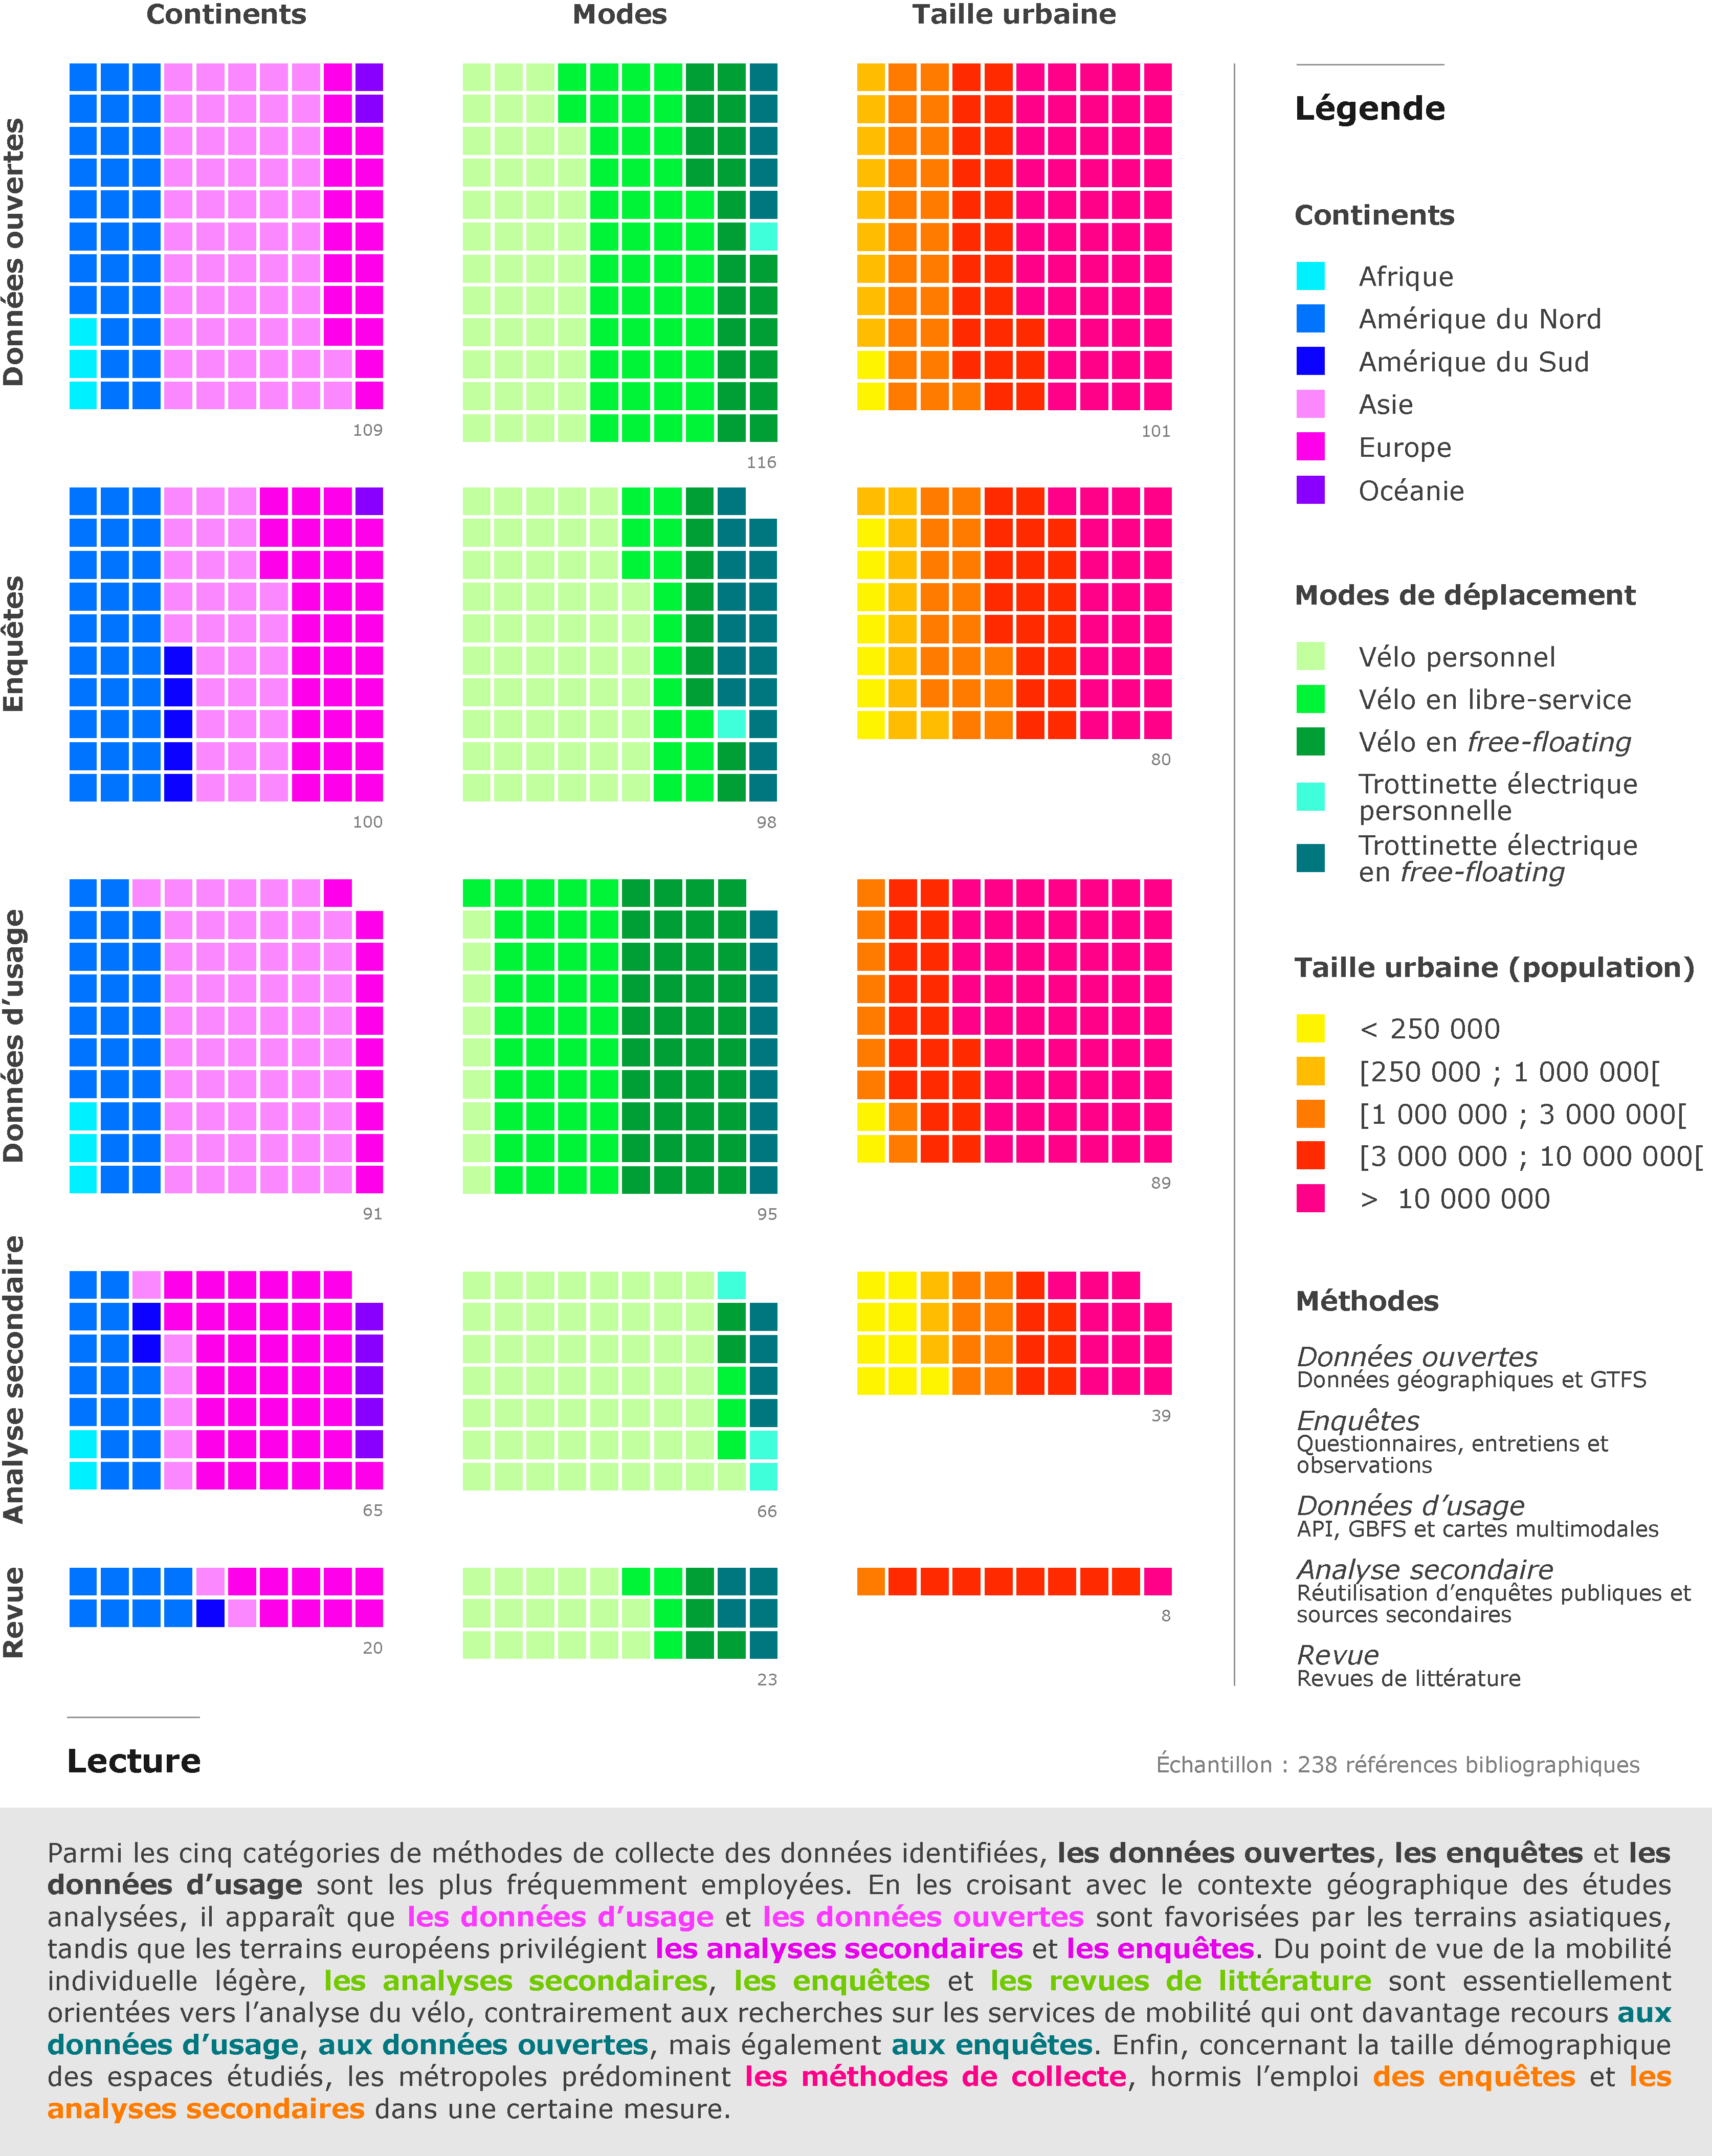
\includegraphics[width=1\columnwidth]{src/Figures/Chap-2/FR_RSL_Sources_donnees.pdf}}
        \vspace{5pt}
        \begin{flushright}\scriptsize{
        Auteur~: \textcolor{blue}{Dylan Moinse (2023)}
        %\\
        %Réalisation avec \Marque{Excel}~et sur \Marque{Illustrator}
        }\end{flushright}
    \end{figure}

    % Sources de données par taille d'agglomération
Dans une perspective plus large, cette exploration méthodologique révèle comment la taille urbaine est capable d'influencer des modalités d'investigation distinctes en matière d'accès empirique au terrain et aux informations. En posant un regard sur la typologie des intercommunalités, il devient possible de discerner des schémas évoquant certaines stratégies quant à l'exploitation des données disponibles sur les terrains d'étude. Ainsi, l'\hyperref[fig-chap2:sources-donnees-rsl]{illustration~\ref{fig-chap2:sources-donnees-rsl}} (page~\pageref{fig-chap2:sources-donnees-rsl}) met en lumière une surreprésentation des mégapoles au sein de la \textsl{Big Data}, avec une emphase particulière sur l'\acrshort{API} et le \acrshort{GBFS}. Cette prépondérance découle de la concentration d'offres de vélo et de micro-mobilité en libre-service, qu'elles soient dotées d'infrastructures de stationnement ou qu'elles fonctionnent sans celles-ci.  À l'inverse, les données mises à disposition concernant l'occupation des sols et les réseaux de transport en commun s'avère distribuées de manière plus équilibrée. En ce qui concerne la mise en œuvre d'enquêtes par voie de questionnaire, il est à noter que les métropoles comptant moins de trois millions d'habitant·e·s bénéficient davantage de l'usage du questionnaire en ligne. Les agglomérations d'au moins 250~000~habitant·e·s semblent plutôt s'orienter vers des questionnaires en face-à-face. Par ailleurs, l'analyse secondaire d'enquêtes publiques se révèle être une option privilégiée au sein d'une proportion significative d'agglomérations de taille démographique plus modeste. Cette lecture statistique peut s'expliquer par les différences de disponibilité en matière de ressources selon les spécificités des terrains géographiques. En effet, les données massives sur un territoire donné étant plus rarement constituées dans les territoires faiblement peuplés, les enquêtes permettent de pallier cette situation tout en étant plus abordables et moins chronographes.%%Rédigé%%

    % Sources de données par micro-mobilité
L'analyse des méthodes de collecte des données a été croisée avec les formes de mobilité individuelle légère telles qu'elles sont abordées dans le corpus scientifique. Si le vélo à usage personnel et en intermodalité est principalement conduit au moyen du questionnaire en face-à-face ou d'une analyse secondaire, l'étude du vélo et de la micro-mobilité partagés s'appuie sur l'exploitation de la \textsl{Big Data}. D'une part, l'examen du système de \acrshort{VLS} s'articule largement autour des données générées par le \acrshort{GBFS}. D'autre part, l'investigation des services de \acrshort{VFF} et de \acrshort{TEFF} se fonde principalement sur l'exploitation de l'\acrshort{API} (voir l'\hyperref[fig-chap2:sources-donnees-rsl]{illustration~\ref{fig-chap2:sources-donnees-rsl}}, page~\pageref{fig-chap2:sources-donnees-rsl}). Contrairement à la mobilité individuelle légère et partagée qui génère une grande quantité de données en temps réel, les données concernant le vélo à usage personnel étant plus difficilement accessibles sous forme de données massives, les recherches sur ce mode de déplacement individuel semblent se tourner vers des enquêtes préexistantes ou sur des enquêtes de terrain en interaction directe avec les usager·ère·s.%%Rédigé%%

    % Sources de données exemples questionnaire en face-à-face
En guise d'illustration, nous pouvons citer les recherches sur le vélo à usage personnel et employant le questionnaire en face-à-face de \textcolor{blue}{\textcite[1696]{cheng_evaluating_2012}}\index{Cheng, Yung-Hsiang|pagebf}\index{Liu, Kuo-Chu|pagebf} en association avec le métro à Kaohsiung (386 réponses), de \textcolor{blue}{\textcite[41]{jansson_almeida_alternativas_2022}}\index{Jansson Almeida, Bárbara|pagebf} avec le métro à Porto Alegre (212~réponses), de \textcolor{blue}{\textcite[183]{pan_intermodal_2010}}\index{Pan, Haixiao|pagebf}\index{Shen, Qing|pagebf}\index{Xue, Song|pagebf} sur le vélo et le \acrfull{VAE} avec le métro à Shanghai (600~réponses), de \textcolor{blue}{\textcite[7]{bauer_influence_2021}}\index{Bauer, Marek|pagebf}\index{Kisielewski, Piotr|pagebf} avec le train et le bus à Tarnow (501~réponses), de \textcolor{blue}{\textcite[685, 4]{rastogi_travel_2003, rastogi_willingness_2010}}\index{Rastogi, Rajat|pagebf}\index{Krishna Rao,~K.~V.|pagebf} sur la marche et le vélo avec le train à Mumbai (1~449 réponses), de \textcolor{blue}{\textcite[2]{rijsman_walking_2019}}\index{Rijsman, Lotte|pagebf}\index{Oort, Niels van|pagebf}\index{Ton, Danique|pagebf}\index{Hoogendoorn, Serge|pagebf}\index{Molin, Eric|pagebf}\index{Teijl, Thomas|pagebf} sur la marche et le vélo avec le tramway à La Haye (629 réponses) ou encore de \textcolor{blue}{\textcite[192]{sherwin_practices_2011}}\index{Sherwin, Henrietta|pagebf}\index{Parkhurst, Graham|pagebf}\index{Robbins, Derek|pagebf}\index{Walker, Ian|pagebf} qui mêlent le questionnaire et l'observation directe sur le vélo avec le train à Bristol (135 réponses).%%Rédigé%%

    % Sources de données exemples questionnaire en ligne
Des travaux menés à l'aide du questionnaire en ligne témoignent également d'une répartition déséquilibrée au profit du vélo à usage personnel, à l'instar des publications de \textcolor{blue}{\textcite[724]{waerden_relation_2018}}\index{Waerden, Peter|pagebf}\index{Waerden, Jaap|pagebf} sur la combinaison du vélo avec le train à Eindhoven (415 réponses), de \textcolor{blue}{\textcite[5, 488]{la_paix_puello_train_2016, la_paix_puello_role_2021}}\index{La Paix Puello, Lissy|pagebf}\index{Geurs, Karst~T.|pagebf} avec le train dans la région métropolitaine de Rotterdam-La Haye et dans la Randstad South (1~524 réponses), de \textcolor{blue}{\textcite[267]{krygsman_multimodal_2004}}\index{Krygsman, Stephan|pagebf}\index{Dijst, Martin|pagebf}\index{Arentze, Theo|pagebf} sur le vélo avec le train, le métro, le tramway et le bus dans la région métropolitaine d'Amsterdam-Utrecht
(1~966 ménages dont 755 cyclistes), de \textcolor{blue}{\textcite[663]{mil_insights_2020}}\index{Mil, Joeri~F.P. van|pagebf}\index{Leferink, Tessa~S.|pagebf}\index{Annema, Jan Anne|pagebf}\index{Oort, Niels van|pagebf} avec le train aux Pays-Bas (269 réponses), de \textcolor{blue}{\textcite[132-133]{chen_determinants_2012}}\index{Chen, Lijun|pagebf}\index{Pel, Adam~J.|pagebf}\index{Chen, Xuewu|pagebf}\index{Sparing, Daniel|pagebf}\index{Hansen, Ingo~A.|pagebf} avec le métro à Nanjing (1~784 réponses dont 136 cyclistes intermodaux·les), de \textcolor{blue}{\textcite[4259]{bopp_examining_2015}}\index{Bopp, Melissa|pagebf}\index{Gayah, Vikash~V.|pagebf}\index{Campbell, Matthew~E.|pagebf} sur la marche et le vélo avec le train, le métro et le tramway dans les États de Delaware, New Jersey, Maryland, Virginie-Occidentale, Pennsylvanie et de l'Ohio (1~234 réponses dont 152~voyageur·se·s), de \textcolor{blue}{\textcite[6]{jonkeren_bicycle-train_2021, jonkeren_bicycle_2021}}\index{Jonkeren, Olaf|pagebf}\index{Kager, Roland|pagebf}\index{Harms, Lucas|pagebf}\index{te Brömmelstroet, Marco|pagebf} sur l'usage et le stationnement des vélos à Rotterdam, Utrecht et Eindhoven ainsi qu'autour des gares néerlandaises (2~299 et 1~209 réponses dont 1~309 cyclistes intermodaux·les) ou encore de \textcolor{blue}{\textcite[6]{molin_bicycle_2015}}\index{Molin, Eric|pagebf}\index{Maat, Kees|pagebf} sur le stationnement vélo autour de la gare de Delft (866 réponses).%%Rédigé%%

    % Sources de données exemples analyse secondaire
La dichotomie entre les méthodes de collecte de données propres à ces modes de déplacement personnels et partagés est également visible dans les productions scientifiques de \textcolor{blue}{\textcite[87]{taylor_analysis_1996}}\index{Taylor, Dean|pagebf}\index{Mahmassani, Hani|pagebf} qui ont conduit un questionnaire par courrier pour évaluer l'usage du vélo en combinaison avec le bus dans l'État du Texas (814 réponses), de \textcolor{blue}{\textcite[10]{pages_nouveaux_2021}}\index{Pages, Thibaud|pagebf}\index{Lammoglia, Adrien|pagebf}\index{Josselin, Didier|pagebf} qui ont réalisé un questionnaire en ligne (280~réponses) mêlé à des entretiens sur l'usage intermodal de la trottinette électrique à usage personnel ou bien de \textcolor{blue}{\textcite[60]{rabaud_quand_2022}}\index{Rabaud, Mathieu|pagebf}\index{Richer, Cyprien|pagebf} qui ont exploité plus de 40~enquêtes de mobilité datant de 2015-2019 pour étudier cet \acrfull{EDPM} en intermodalité en France (364~usager·ère·s de la trottinette). À ce titre, la réutilisation de données primaires en provenance d'enquêtes publiques souligne la présence marquée du vélo et plus largement de la mobilité individuelle légère, d'après les études réalisées par \textcolor{blue}{\textcite[8-10]{shelat_analysing_2018}}\index{Shelat, Sanmay|pagebf}\index{Huisman, Raymond|pagebf}\index{Oort, Niels van|pagebf} sur le vélo avec le train aux Pays-Bas, à partir de l'enquête de mobilité nationale \acrfull{OViN} de 2010-2015 (environ 250~000~ménages dont 3~376 cyclistes), par \textcolor{blue}{\textcite[9]{luan_better_2020}}\index{Luan, Xin|pagebf}\index{Cheng, Lin|pagebf}\index{Song, Yan|pagebf}\index{Zhao, Jinbao|pagebf} sur le vélo avec le métro, à partir de l'enquête de mobilité nationale de Nanjing de 2014 (10~385 ménages dont 3~999 cyclistes), par \textcolor{blue}{\textcite[3]{zuo_determining_2018}}\index{Zuo, Ting|pagebf}\index{Wei, Hang|pagebf}\index{Rohne, Andrew|pagebf} sur le vélo avec le bus à Cincinnati, à partir de l'enquête de mobilité de l'Ohio de 2009-2010 (2~059 ménages) ou encore par \textcolor{blue}{\textcite[76]{oostendorp_combining_2018}}\index{Oostendorp, Rebekka|pagebf}\index{Gebhardt, Laura|pagebf} sur le vélo avec le train, le métro, le tramway et le bus à Berlin, à partir du recensement de la population de Berlin (1~098 individus dont 363 cyclistes intermodaux·les).%%Rédigé%%

    % 2.2.2.3. Types d’analyse
    \needspace{1\baselineskip} % Réserve de l'espace
\subsubsection*{Démarches et types d'analyse
    \label{chap2:demarches-types-analyses}
    }
    
    % Introduction
Dans le cadre de cette recherche doctorale, une analyse exhaustive des méthodes employées dans le corpus de la \acrshort{RSL} a été réalisée, révélant une diversité conséquente des techniques d'analyse catégorisées. Au total, 484 méthodes d'analyse ont été identifiées, correspondant à 273 approches distinctes. Parmi ces démarches, la modélisation se distingue comme l'outil analytique le plus fréquemment utilisé, avec 62~occurrences au sein du corpus. Cette méthode est suivie de près par l'utilisation du \acrfull{SIG}, recensée 51~fois. Les questionnaires sont également fréquemment utilisés, avec 30~mentions. Enfin, les revues de littérature, recensées 17 fois, soulignent l'importance de la synthèse des connaissances existantes. La diversité des techniques mises en évidence traduit un éventail d'approches, allant du quantitatif au qualitatif. Cette variété méthodologique permet d'aborder les problématiques de la mobilité urbaine sous des angles multiples, offrant une compréhension plus riche et nuancée des interactions entre la mobilité individuelle légère intégrée aux systèmes de transport en commun et les systèmes urbains.%%Rédigé%%

    % Statistiques descriptives (quantitatif)
En lien avec le sujet de recherche sur le \acrshort{M-TOD}, l'approche quantitative est la méthode d'analyse la plus sollicitée, avec une présence marquée de mesures descriptives au sein de 80~articles scientifiques et de la modélisation dans 62~études. D'une part, l'analyse statistique descriptive est relevée dans 50~publications, suivies respectivement des entretiens par questionnaire basés sur les préférences déclarées (\textsl{Stated Preference}, SP)\footnote{
    Le questionnaire par préférences déclarées est une technique de collecte de données où les répondant·e·s sont interrogé·e·s sur leurs préférences dans des scénarios hypothétiques, afin d'estimer la valeur attribuée à des biens, à des services ou à des changements d'usage.
} et les préférences révélées (\textsl{Revealed Preference}, RP)\footnote{
    Le questionnaire par préférences révélées est une technique de collecte de données basée sur l'observation des choix des individus dans des conditions réelles.
} dans 20~et~10~articles. D'autre part, les études faisant appel à la modélisation statistique embrassent une diversité d'approches. Nous comptons neuf recherches utilisant des modèles de prédiction de la demande (\textsl{Demand Forecasting Models}, DFM)\footnote{
    Le modèle de prédiction de la demande est un outil économétrique utilisé pour estimer la future demande d'un produit ou service, dépendante d'une multitude de variables comme le prix, le revenu ou les préférences des consommateur·rice·s.
}, quinze recourant au modèle de choix discrets (\textsl{Discrete Choice Models}, DCM)\footnote{
    Le modèle de choix discrets est un outil économétrique utilisé pour prédire les choix effectués par les individus parmi un ensemble fini d'options, en reposant sur la théorie de l'utilité aléatoire, où le choix d'un individu est modélisé comme une fonction de divers attributs des options disponibles.
}, dont sept appliquant le modèle logit multinomial (\textsl{Multinomial Logit Model}, MLN)\footnote{
    Le modèle logit multinomial est une extension du modèle logit binaire, utilisé pour modéliser les choix parmi plus de deux alternatives discrètes, généralement des modes de déplacement.
}, tandis que sept autres reposent sur le modèle de régression des moindres carrés ordinaires (\textsl{Ordinary Least Squares Regression}, OLS)\footnote{
    Le modèle de régression des moindres carrés est une méthode de régression linéaire qui minimise la somme des carrés des écarts entre les valeurs observées et celles estimées par le modèle.
}. Ces modèles de régression, fréquemment mobilisés, offrent une approche robuste pour l'analyse des relations entre variables. En complément, certaines études adoptent une approche par clustérisation, notamment la clustérisation k-means (\textsl{k-means clustering})\footnote{
    Les k-means sont une méthode de clustérisation destinée à diviser un ensemble de données en $ k $ groupes distincts, tout en minimisant la variance au sein du cluster et en maximisant la variance entre les classes.
}, présente dans sept articles. Enfin, l'\acrfull{ACB}\footnote{
    L'analyse coût-bénéfice sert à évaluer les avantages attends et les coûts associés d'un projet dans le but de déterminer sa viabilité et les meilleures options.
} est présente dans trois publications, tandis que les modèles de trafic sont mentionnés dans deux études.%%Rédigé%%
    
    % Cartographie (SIG)
L'application des méthodes relatives à la science des données quantitatives (\textsl{Data Science}), se manifeste également au travers de l'approche géostatistique. Cette dernière s'appuie en particulier sur l'usage du \acrshort{SIG}, un outil d'analyse spatiale intégré dans 51~documents étudiés dans le corpus. En parallèle de l'utilisation directe du \acrshort{SIG}, diverses techniques complémentaires d'analyse spatiale sont mises en œuvre. Parmi ces méthodes, on retrouve notamment la régression géographique pondérée (\textsl{Geographically Weighted Regression}, GWR)\footnote{
    La régression géographique pondérée est une technique de modélisation spatiale qui permet d'analyser la variation spatiale dans les relations entre les variables, en attribuant un poids différent à chaque observation en fonction de son emplacement.
}, employée dans neuf études. Huit études intègrent l'autocorrélation spatiale\footnote{
    L'autocorrélation spatiale se mesure notamment à l'aide de l'indice de Moran. Cet indice est utilisé en géostatistique pour évaluer si un modèle présente des motifs spatiaux aléatoires, regroupés ou dispersés. Un indice de Moran proche de +1 indique une forte corrélation spatiale positive, tandis qu'un indice proche de -1 indique une forte corrélation spatiale négative.
}, tandis que la mesure de l'indice de connectivité des réseaux (\textsl{Network Connectivity Index}, NCI)\footnote{
    L'indice de connectivité des réseaux est une mesure quantitative utilisée pour évaluer le degré de connectivité au sein d'un réseau de transport en commun ou de communication, en considérant le nombre de liens, la directivité des connexions et la distance entre chaque nœud.
}, quant à elle, est exploitée dans sept études. Deux travaux se distinguent par la détermination de l'indice nœud-lieu (\textsl{Node-Place Index})\footnote{
    L'indice nœud-lieu est un outil d'analyse spatiale utilisé pour évaluer la fonctionnalité des nœuds de transport dans leur contexte urbain, en combinant des aspects relatifs au transport et à l'urbanisme, de sorte à évaluer les interactions entre les stations de transport en commun et l'environnement urbain.
}. Enfin, l'estimation de la densité du noyau (\textsl{Kernel Density Estimation}) est appliquée dans une étude, de même que le diagramme de Voronoï\footnote{
    Le diagramme de Voronoï est une partition en cellules d'un ensemble spécifique de points sur un plan Euclidien. Chaque point génère une région cellulaire contenant tous les points du plan plus proches de ce point que de tout autre.
}. Ces approches diversifiées démontrent la richesse et la complexité des analyses spatiales dans l'étude du \acrshort{M-TOD} qui sont alors enrichies par des approches qualitatives.%%Rédigé%%

    % Discours (qualitatif)
L'approche méthodologique qualitative est circonscrite à un corpus de onze publications. Parmi celles-ci, neuf se fondent principalement sur l'analyse discursive, menée à l'aide d'entretiens semi-directifs, alors que les deux autres se distinguent par une exploration sensible de l'environnement urbain et des interactions sociales. Toutefois, l'approche qualitative peut également être étendue aux dix-sept revues de littérature synthétisant indirectement le sujet de recherche relatif au \acrshort{M-TOD}. Ces méthodes proviennent d'une variété de domaines de connaissancere, allant de l'économie, avec des approches telles que l'économétrie (DCM et MLN) et l'économie des transports (SP, RP, DFM et modèles de transport)~; à la statistique, incluant les sciences de la donnée et les k-means. Elles englobent également la géographie, avec l'analyse spatiale (diagramme de Voronoï et GWR)~; et touchent à la sociologie, notamment à travers les entretiens.%%Rédigé%%

    % ___________________________________________
    % 2.3.
    \newpage
    \needspace{1\baselineskip} % Réserve de l'espace
    \sectionheader{État des connaissances actuelles sur le M-TOD}
\section{Caractérisation d'un \textsl{Micromobility-friendly Transit-Oriented Development} au prisme des caractéristiques de l'environnement urbain et des choix individuels
    \label{chap2:caracterisation-btod-environnement-urbain-choix-individuels}
    }
    
    % Introduction 1
La section actuelle de ce chapitre est consacrée à une étude détaillée visant à définir les attributs fondamentaux du \acrshort{M-TOD}, en le réfléchissant au prisme de l'environnement urbain ainsi que des préférences personnelles en matière de mobilité. Dans cette optique, nous avons opté pour une démarche inductive structurée autour des \Guillemets{\acrshort{7Ds}}~enrichie par des variables additionnelles en lien avec les pratiques intermodales examinées. L'objectif de cette analyse issue de la \acrshort{RSL} est de cerner les contours du modèle urbain du \acrshort{M-TOD}, en s'appuyant sur une mise en perspective des études empiriques internationales. Il s'agit de déceler les caractéristiques récurrentes émanant de cette revue de littérature. Par conséquent, notre ambition est également de saisir la façon dont le \acrshort{M-TOD} peut être envisagé comme un complément au \acrshort{TOD} et d'appréhender dans quelle mesure les dimensions analysées de ce concept d'urbanisme se reflètent dans une stratégie urbaine qui intègre la mobilité individuelle légère.%%Rédigé%%

    % Introduction 2
Au travers de leur \acrshort{RSL}, \textcolor{blue}{\textcite[294]{zhang_built_2023}}\index{Zhang, Yushan|pagebf}\index{Kasraian, Dena|pagebf}\index{Wesemael, Pieter van|pagebf} dévoilent à quel point les études portant sur le vélo et la micro-mobilité se focalisent spécifiquement sur les stratégies de gestion et d'exploitation de ces modes de déplacement, de même que sur l'analyse des profils et des comportements des usager·ère·s. Toutefois, une attention moindre a été accordée à l'interrelation de la mobilité individuelle légère avec l'environnement urbain. De ce fait, le présent chapitre s'attache principalement à explorer cet aspect essentiel, mais jusqu'alors sous-examiné, qui est crucial dans la conceptualisation du \acrshort{M-TOD}. Conformément à la définition établie par \textcolor{blue}{\textcite[65]{handy_how_2002}}\index{Handy, Susan~L.|pagebf}\index{Boarnet, Marlon~G.|pagebf}\index{Ewing, Reid|pagebf}\index{Killingsworth, Richard~E.|pagebf}, l'environnement urbain se distingue par trois composantes majeures~: (i) le \textsl{design} urbain, englobant la configuration des espaces publics~; (ii) l'utilisation des sols, se rapportant à la localisation, la répartition et la densité des activités dans l'espace~; et (iii) le système de mobilité, comprenant tant l'infrastructure de transport que le niveau de service des réseaux (\textsl{Level of Service}, LoS). C'est sur ces fondements conceptuels que s'appuie notre analyse des données collectées, aboutissant à un tableau synthétique où chaque étude a été évaluée au regard de la présence ou de l'absence de ces dimensions (voir l'\hyperref[annexes:rsl-resultats]{annexe~\ref{annexes:rsl-resultats}}, page~\pageref{annexes:rsl-resultats}).%%Rédigé%%

    % Annonce du plan
Cette section s'efforcera alors de caractériser le \acrshort{M-TOD}, dans l'intention de présenter une définition de ce modèle urbain fondée sur les connaissances issues de la littérature scientifique. Divers aspects seront traités, à commencer par les \Guillemets{\acrshort{7Ds}}, soit la \hyperref[chap2:densite-population]{densité de population (\(D1\))} (page~\pageref{chap2:densite-population}), la \hyperref[chap2:diversite-fonctionnelle]{diversité d'usage des sols (\(D2\))} (page~\pageref{chap2:diversite-fonctionnelle}), la \hyperref[chap2:traitement-espaces-publics]{conception des espaces publics (\(D3\))} (page~\pageref{chap2:traitement-espaces-publics}), l'\hyperref[chap2:accessibilite-intermodale]{accessibilité vers les ressources territoriales (\(D4\))} (page~\pageref{chap2:accessibilite-intermodale}), la \hyperref[chap2:distances-premiers-derniers-km]{taille des quartiers de gare (\(D5\))} (page~\pageref{chap2:distances-premiers-derniers-km}), la \hyperref[chap2:gestion-demande-mobilite]{gestion de la demande de mobilité (\(D6\))} (page~\pageref{chap2:gestion-demande-mobilite}), la \hyperref[chap2:sociodemographie-usagers]{dimension liée à l'inclusion sociale (\(D7\))} (page~\pageref{chap2:sociodemographie-usagers}), suivis des \hyperref[chap2:comportements-mobilite]{comportements de mobilité} (page~\pageref{chap2:comportements-mobilite}) et des \hyperref[chap2:impacts-systemes-urbain-mobilite]{divers impacts} (page~\pageref{chap2:impacts-systemes-urbain-mobilite}).%%Rédigé%%

    % 2.3.1. Resultats~: densité
    \needspace{1\baselineskip} % Réserve de l'espace
\subsection{Densité de population
    \label{chap2:densite-population}
    }
    
    % Introduction
La première thématique abordée dans cette section est celle de la densité de population, un élément crucial pour le \acrshort{TOD}, en soutenant l'aménagement de territoires compacts et favorables aux piéton·ne·s. Présente dans 44 des 238 publications scientifiques examinées, la densité démographique influence positivement l'usage conjoint des transports en commun et de la mobilité individuelle légère.%%Rédigé%%

    % 2.3.1.1. Impact positif densité population
    \needspace{1\baselineskip} % Réserve de l'espace
\subsubsection*{Association positive avec la densité de population
    \label{chap2:association-positive-densite-population}
    }
    
    % Impact positif densité population avec vélo personnel
Au sein du corpus d'études examiné, une proportion significative de travaux suggère l'existence d'une corrélation positive entre la densité de population et l'interaction entre les systèmes de transport en commun et la mobilité individuelle légère. Ces recherches académiques mettent en évidence que les zones caractérisées par une densité démographique accrue tendent à enregistrer une utilisation plus intensive du vélo et de la micro-mobilité, en complémentarité avec les réseaux de transport en commun. Dans ce contexte, la densité de population se révèle être une dimension prépondérante, avec une relation positive établie entre ce facteur et la probabilité d'utiliser le vélo en association avec le train et le bus, au Danemark \textcolor{blue}{\autocite[41]{nielsen_bikeability_2018}}\index{Nielsen, Thomas Alexander Sick|pagebf}\index{Skov-Petersen, Hans|pagebf}. De manière similaire, aux États-Unis, la part modale du vélo en combinaison avec le train et le bus a connu une augmentation notable dans les régions à forte densité de population \textcolor{blue}{\autocite[107]{wang_bicycle-transit_2013}}\index{Wang, Rui|pagebf}\index{Liu, Chen|pagebf}. \textcolor{blue}{\textcite[212]{kager_characterisation_2016}}\index{Kager, Roland|pagebf}\index{Bertolini, Luca|pagebf}\index{te Brömmelstroet, Marco|pagebf} affirment que le vélo complète efficacement le train dans des milieux denses, mais aussi en s'adaptant à des densités moins élevées dans divers contextes, notamment à Amsterdam, Amstelveen, Diemen et Ouder-Amstel. À Amsterdam, \textcolor{blue}{\textcite[344]{kampen_bicycle_2021}}\index{Kampen, Jullian van|pagebf}\index{Pauwels, Eric|pagebf}\index{Mei, Rob van der|pagebf}\index{Dugundji, Elenna~R.|pagebf} ont constaté que la densité du bâti joue un rôle crucial dans le choix des emplacements de stationnement de vélos personnels, les quartiers à forte densité urbaine attirant davantage de stationnements de vélos près des gares et des stations de métro.%%Rédigé%%

    % Impact positif densité population avec le VLS
Dans une perspective similaire concernant le vélopartage, un lien positif est suggéré entre la densité de population et l'utilisation du \acrshort{VLS} en synergie avec le réseau ferroviaire, comme observé à Chicago, New York City et Washington~D.C. \textcolor{blue}{\autocite[16]{kong_deciphering_2020}}\index{Kong, Hui|pagebf}\index{Jin, Scarlett~T.|pagebf}\index{Sui, Daniel~Z.|pagebf}. Cette interrelation est également confirmée entre le \acrshort{VLS} et le métro, tant à Beijing \textcolor{blue}{\autocite[9]{yu_understanding_2021}}\index{Yu, Senbin|pagebf}\index{Liu, Gehui|pagebf}\index{Yin, Congru|pagebf}, qu'à Nanjing \textcolor{blue}{\autocite[12]{chen_what_2022}}\index{Chen, Wendong|pagebf}\index{Chen, Xuewu|pagebf}\index{Chen, Jingxu|pagebf}\index{Cheng, Long|pagebf}. \textcolor{blue}{\textcite[15]{li_investigating_2022}}\index{Li, Xiaofeng|pagebf}\index{Wu, Yao-Jan|pagebf}\index{Khani, Alireza|pagebf} avancent que dans les zones à forte densité démographique, une interaction positive est manifeste entre le \acrshort{VLS} et le tramway ainsi que le bus, à Tucson. À Oslo, \textcolor{blue}{\textcite[399]{bocker_bike_2020}}\index{Böcker, Lars|pagebf}\index{Anderson, Ellinor|pagebf}\index{Uteng, Tanu Priya|pagebf}\index{Throndsen, Torstein|pagebf} soulignent que l'usage fréquent du \acrshort{VLS} en association avec le métro est prédominant dans les territoires densément peuplés.%%Rédigé%%

    % Impact positif densité population avec le VFF
Plusieurs études menées à Shenzhen et Shanghai, respectivement par \textcolor{blue}{\textcite[6]{wang_relationship_2020}}\index{Wang, Ruoyu|pagebf}\index{Lu, Yi|pagebf}\index{Wu, Xueying|pagebf}\index{Liu, Ye|pagebf}\index{Yao, Yao|pagebf} et \textcolor{blue}{\textcite[31]{lin_analysis_2019}}\index{Lin, Diao|pagebf}\index{Zhang, Yongping|pagebf}\index{Zhu, Ruoxin|pagebf}\index{Meng, Liqiu|pagebf}, corroborent que les densités élevées de population sont positivement associées à l'usage du \acrshort{VFF} avec le métro, révélant une demande accrue dans les zones urbaines denses. \textcolor{blue}{\textcite[16]{li_operating_2019}}\index{Li, Yuan|pagebf}\index{Zhu, Zhenjun|pagebf}\index{Guo, Xiucheng|pagebf} ont mis en évidence, à travers une classification des stations de métro, que celles situées dans les quartiers densément peuplés du centre urbain de Nanjing connaissent un usage plus important du \acrshort{VFF} pour les \Guillemets{premiers et derniers kilomètres}. Les travaux menés par \textcolor{blue}{\textcite[25]{guo_dockless_2021}}\index{Guo, Yuanyuan|pagebf}\index{Yang, Linchuan|pagebf}\index{Lu, Yi|pagebf}\index{Zhao, Rui|pagebf} et par \textcolor{blue}{\textcite[184]{cheng_exploring_2022}}\index{Cheng, Long|pagebf}\index{Wang, Kailai|pagebf}\index{Vos, Jonas de|pagebf}\index{Huang, Jie|pagebf}\index{Witlox, Frank|pagebf} démontrent que la densité démographique est significativement liée à l'utilisation intégrée du \acrshort{VFF} avec le métro pendant les heures de pointe, respectivement à Shenzhen et Nanjing. À Suzhou, \textcolor{blue}{\textcite[24]{li_integration_2020}}\index{Li, Jie|pagebf}\index{Lu, Yang|pagebf}\index{Ling, Lei|pagebf} observent qu'une densité de population plus élevée diminue la probabilité de choisir le bus au profit du \acrshort{VFF} pour rejoindre les stations de métro. À Beijing, \textcolor{blue}{\textcite[11]{liu_temporal_2022}}\index{Liu, Siyang|pagebf}\index{Zhang, Xiaodong|pagebf}\index{Zhou, Chenjing|pagebf}\index{Rong, Jian|pagebf}\index{Bian, Yang|pagebf} révèlent qu'une augmentation de 10~\% de la densité entraîne une hausse significative de l'utilisation du \acrshort{VFF} avec le métro durant les jours de semaine, et plus encore durant les heures de pointe matinales. Une conclusion similaire émerge dans le cas de la \acrshort{TEFF} avec le métro, où une concentration a été identifiée dans des zones densément peuplées à New York City \textcolor{blue}{\autocite[16]{lee_forecasting_2021}}\index{Lee, Mina|pagebf}\index{Chow, Joseph|pagebf}\index{Yoon, Gyugeun|pagebf}\index{He, Brian|pagebf}.%%Rédigé%%

    % Impact positif densité population avec les TC
L'analyse de la \acrshort{RSL} tend également à souligner une amplification de l'utilisation des transports en commun, en questionnant les liens entre la densité démographique et l'usage intermodal de la mobilité individuelle légère. Les zones à forte densité favorisent ainsi l'usage du transport public en attirant un nombre croissant de passager·ère·s qui adoptent le vélo et la micro-mobilité. Dans les quartiers résidentiels des Pays-Bas, la densité de population s'avère être un facteur déterminant qui influence significativement l'usage des transports en commun, incluant le train, le métro, le tramway, le bus et même le ferry, par les cyclistes \textcolor{blue}{\autocite[334]{martens_promoting_2007}}\index{Martens, Karel|pagebf}. À Shanghai, la recherche conduite par \textcolor{blue}{\textcite[10]{li_exploring_2021}}\index{Li, Wenxiang|pagebf}\index{Chen, Shawen|pagebf}\index{Dong, Jieshuang|pagebf}\index{Wu, Jingxian|pagebf} indique que la densité démographique est positivement corrélée avec la distance de transfert, tant en \gls{rabattement} qu'en \gls{diffusion}, ce qui suggère que les stations de métro attirent des usager·ère·s du \acrshort{VFF} plus éloigné·e·s. En outre, lors de l'étape de post-acheminement à partir des stations de métro, la densité de population à Kaohsiung stimule considérablement l'intention des passager·ère·s d'avoir recours au \acrshort{VLS} \textcolor{blue}{\autocite[29]{cheng_expanding_2018}}\index{Cheng, Yung-Hsiang|pagebf}\index{Li, Yi-Chun|pagebf}.%%Rédigé%%

    % 2.3.1.2. Impact complexe densité population
    \needspace{1\baselineskip} % Réserve de l'espace
\subsubsection*{Relations complexes avec la densité de population
    \label{chap2:relations-complexes-densite-population}
    }
    
    % Relation complexe densité et intermodalité
L'examen de la relation entre la densité démographique et l'usage intermodal du vélo et de la micro-mobilité révèle une complexité accrue au sein d'une partie du corpus étudié, certaines recherches mettant en lumière une corrélation plus nuancée, voire ambigüe, entre ces différentes variables. Diverses études suggèrent que la densité de population ne constitue pas un facteur déterminant dans l'utilisation conjointe de la mobilité individuelle légère, notamment en ce qui concerne le vélo et le train à Melbourne \textcolor{blue}{\autocite[403]{weliwitiya_bicycle_2019}}\index{Weliwitiya, Hesara|pagebf}\index{Rose, Geoff|pagebf}\index{Johnson, Marilyn|pagebf}, le \acrshort{VLS} et le bus à Birmingham \textcolor{blue}{\autocite[5]{glass_role_2020}}\index{Glass, Caroline|pagebf}\index{Appiah-Opoku, Seth|pagebf}\index{Weber, Joe|pagebf}\index{Jones, Steven~L.|pagebf}\index{Chan, Amber|pagebf}\index{Oppong, Judith|pagebf}, ou encore le \acrshort{VFF} et le métro à Shenzhen \textcolor{blue}{\autocites[11]{guo_built_2020}[388]{guo_role_2021}}\index{Guo, Yuanyuan|pagebf}\index{He, Sylvia~Y.|pagebf}. À Utrecht, \textcolor{blue}{\textcite[274]{krygsman_multimodal_2004}}\index{Krygsman, Stephan|pagebf}\index{Dijst, Martin|pagebf}\index{Arentze, Theo|pagebf} ont démontré l'existence d'une relation non linéaire entre la densité de population et le choix du vélo, en particulier aux abords des gares et des stations de métro, de tramway et de bus, où une densité urbaine plus marquée favorise des distances plus courtes, propices à la marche. Une densité de population plus importante à Beijing n'entrainerait pas d'effet notable sur l'usage du \acrshort{VLS}, contrairement à une utilisation accrue des taxis, en particulier par les usagères, pour rejoindre le métro \textcolor{blue}{\autocite[15]{ni_exploring_2020}}\index{Ni, Ying|pagebf}\index{Chen, Jiaqi|pagebf}. À Beijing, l'utilisation du VLS en combinaison avec le métro s'accroît avec la densité de population, mais cette corrélation n'est pas constatée dans les modèles appliqués à Taipei et Tokyo \textcolor{blue}{\autocite[216]{lin_built_2018}}\index{Lin, Jen-Jia|pagebf}\index{Zhao, Pengjun|pagebf}\index{Takada, Kazuyuki|pagebf}\index{Li, Shengxiao|pagebf}\index{Yai, Tetsuo|pagebf}\index{Chen, Chi-Hao|pagebf}. Dans un contexte similaire, \textcolor{blue}{\textcite[45]{la_paix_puello_modelling_2015}}\index{La Paix Puello, Lissy|pagebf}\index{Geurs, Karst~T.|pagebf} ont noté qu'une densité élevée semble décourager l'utilisation du vélo pour se rendre aux gares dans la région de Randstad South. De manière analogue, une densité de population significative près des stations de métro à Nanjing semble privilégier la marche comme mode d'accès au réseau ferré, au détriment du \acrshort{VLS} \textcolor{blue}{\autocite[17]{ji_public_2017}}\index{Ji, Yanjie|pagebf}\index{Fan, Yingling|pagebf}\index{Ermagun, Alizera|pagebf}\index{Cao, Xuening|pagebf}\index{Wang, Wei|pagebf}\index{Das, Kirti|pagebf}. \textcolor{blue}{\textcite[181]{gan_associations_2021}}\index{Gan, Zuoxian|pagebf}\index{Yang, Min|pagebf}\index{Zeng, Qingcheng|pagebf}\index{Timmermans, Harry~J.~P.|pagebf} révèlent qu'une augmentation de 1~\% de la densité de population augmente la probabilité de choisir la marche de 0,22~\% en pré-acheminement et de 0,36~\% en post-acheminement à partir d'une station de métro, à Nanjing. Dans une étude de cas spécifique du quartier de la gare de Mouans-Sartoux, \textcolor{blue}{\textcite[189]{moinse_intermodal_2022}}\index{Moinse, Dylan|pagebf}\index{Goudeau, Matthieu|pagebf}\index{L'Hostis, Alain|pagebf}\index{Leysens, Thomas|pagebf} ont observé que les voyageur·se·s en \acrshort{TEP} débutent et terminent plus fréquemment leur \gls{déplacement} intermodal dans des zones denses, contrairement aux voyageur·se·s à vélo personnel.%%Rédigé%%

    % Raisons
L'inclinaison en faveur d'une densification des territoires peut ainsi s'expliquer par l'amélioration de l'accessibilité et une demande renforcée en termes de mobilité grâce à la concentration des populations. La corrélation positive entre la densité démographique et une utilisation accrue de la mobilité individuelle légère en coordination avec les transports en commun pourrait également être due aux coûts additionnels liés à l'usage de l'automobile dans les zones densément peuplées, ce qui confère au vélo une attractivité plus marquée aux abords des quartiers de gare, comme le soulignent \textcolor{blue}{\textcite[751]{midenet_modal_2018}}\index{Midenet, Sophie|pagebf}\index{Côme, Etienne|pagebf}\index{Papon, Francis|pagebf} pour le cas d'Amboise. \textcolor{blue}{\textcite[11]{hu_examining_2022}}\index{Hu, Songhua|pagebf}\index{Chen, Mingyang|pagebf}\index{Jiang, Yuan|pagebf}\index{Sun, Wei|pagebf}\index{Xiong, Chenfeng|pagebf} rendent compte que la densité est intimement liée à l'offre en transport en commun à Shanghai~: les zones à forte densité de population près du centre-ville présentent moins d'activités de \acrshort{VFF} avec le métro par rapport aux zones périphériques urbaines. Dans le contexte de Nanjing, \textcolor{blue}{\textcite[9]{cheng_promoting_2022}}\index{Cheng, Long|pagebf}\index{Jin, Tanhua|pagebf}\index{Wang, Kailai|pagebf}\index{Lee, Yongsung|pagebf}\index{Witlox, Frank|pagebf} et \textcolor{blue}{\textcite[8]{cheng_comparison_2023}}\index{Cheng, Long|pagebf}\index{Huang, Jie|pagebf}\index{Jin, Tanhua|pagebf}\index{Chen, Wendong|pagebf}\index{Li, Aoyong|pagebf}\index{Witlox, Frank|pagebf} constatent que le \acrshort{VFF} en combinaison avec le métro est favorisé lorsque la densité de population est élevée, mais cette tendance s'inverse lorsque la densité atteint un seuil entre 18~000~et~23~000~habitant·e·s/km², au-delà duquel les effets deviennent incertains, probablement en raison de la congestion urbaine, de la pollution et des risques liés à la sécurité. \textcolor{blue}{\textcite[8]{zhou_spatially_2023}}\index{Zhou, Xiao|pagebf}\index{Dong, Quanhua|pagebf}\index{Huang, Zhou|pagebf}\index{Yin, Ganmin|pagebf}\index{Zhou, Guoqing|pagebf}\index{Liu, Yu|pagebf} parviennent à une conclusion similaire, mettant en évidence une relation non significative entre la densité et l'utilisation conjointe du \acrshort{VFF} avec le métro et le bus à Beijing, en raison de rues fréquentées et d'un trafic plus dense dans les zones à forte densité. Selon \textcolor{blue}{\textcite[3]{romm_differences_2022}}\index{Romm, Daniel|pagebf}\index{Verma, Priyanka|pagebf}\index{Karpinski, Elizabeth|pagebf}\index{Sanders, Tracy~L.|pagebf}\index{McKenzie, Grant|pagebf}, le vélo est plus fréquemment utilisé lors des \Guillemets{premiers kilomètres}~dans les quartiers densément peuplés du centre urbain de Boston, en raison de la possession moindre de véhicules motorisés par les résidents.%%Rédigé%%

    % Conclusion Densité
L'association existante entre la densité démographique et l'emploi de la mobilité individuelle légère, en synergie avec les systèmes de transport en commun, dans le cadre théorique du \acrshort{M-TOD}, révèle une certaine complexité. D'une part, un ensemble de recherches empiriques atteste d'une liaison positive entre ces facteurs, corroborant le rôle clé de la densité appliquée à l'aire secondaire du \acrshort{TOD}. D'autre part, une exploration approfondie de la littérature scientifique révèle une série de constatations parfois contradictoires quant à l'influence manifeste de la densité de population. Dans le sillage de cette analyse de la littérature scientifique consacrée à la place de ce paramètre territorial dans l'architecture du \acrshort{TOD}, il apparaît judicieux de formuler une approche nuancée. Entre autres, la documentation étudiée soulignerait une association, certes empreinte de complexité, mais vérifiée, entre la densité de population et l'intégration du vélo et de la micro-mobilité avec le transport public. Cette relation s'avère toutefois tributaire d'un éventail de facteurs liés aux caractéristiques propres de chaque système urbain.%%Rédigé%%

    % 2.3.2. Resultats~: diversité
    \needspace{1\baselineskip} % Réserve de l'espace
\subsection{Diversité fonctionnelle
    \label{chap2:diversite-fonctionnelle}
    }
    
    % Introduction
La diversité occupe une place prééminente dans la planification urbaine du \acrshort{M-TOD}, se manifestant principalement à travers la densité des emplois, la multiplicité des fonctions urbaines et la diversité socio-économique. Ces aspects ont été mis en exergue dans 36 des études constituant le corpus de la \acrshort{RSL}. Une attention particulière a été portée à la diversité des usages, considérée comme un levier favorable à l'intégration de la mobilité individuelle légère aux réseaux de transport en commun et à l'animation des territoires. L'importance de regrouper et de concentrer dans un même espace des lieux résidentiels, commerciaux, des bureaux et des espaces verts est reconnue. Toutefois, la question de la diversité des groupes sociaux, notamment à travers une offre de logements variée et abordable, reste sous-représentée dans les études se rapportant aux quartiers de gare étendus.%%Rédigé%%

    % 2.3.2.1. Densité d'emploi
    \needspace{1\baselineskip} % Réserve de l'espace
\subsubsection*{Densité d'emploi
    \label{chap2:densite-emplois}
    }
    
    % Impact positif de la densité d'emploi
Selon une majorité des travaux scientifiques analysés, il ressort que la densité d'emploi dans les quartiers avoisinant les gares, particulièrement les gares desservant les lieux d'activité, soutient de manière significative l'intégration de la mobilité individuelle légère avec les systèmes de transport en commun. En ce qui concerne l'utilisation intermodale du vélo personnel, \textcolor{blue}{\textcite[12]{zuo_promote_2020}}\index{Zuo, Ting|pagebf}\index{Wei, Heng|pagebf}\index{Chen, Na|pagebf} notent qu'une augmentation des emplois à proximité des arrêts de bus à Hamilton entraîne une fréquentation accrue de cyclistes. De même, \textcolor{blue}{\textcite[41]{nielsen_bikeability_2018}}\index{Nielsen, Thomas Alexander Sick|pagebf}\index{Skov-Petersen, Hans|pagebf} soulignent qu'une concentration d'emplois dans le secteur du détail au Danemark est fortement corrélée avec l'usage combiné du vélo, lorsqu'il est stationné à la gare d'origine, et du train. La densité de l'emploi est également positivement liée à l'utilisation du \acrshort{VLS} en association avec le métro, à Washington~D.C. \textcolor{blue}{\autocite[7]{ma_bicycle_2015}}\index{Ma, Ting|pagebf}\index{Liu, Chao|pagebf}\index{Erdoğan, Sevgi|pagebf} et à Nanjing \textcolor{blue}{\autocite[5]{cheng_comparison_2023}}\index{Cheng, Long|pagebf}\index{Huang, Jie|pagebf}\index{Jin, Tanhua|pagebf}\index{Chen, Wendong|pagebf}\index{Li, Aoyong|pagebf}\index{Witlox, Frank|pagebf}. \textcolor{blue}{\textcite[397]{bocker_bike_2020}}\index{Böcker, Lars|pagebf}\index{Anderson, Ellinor|pagebf}\index{Uteng, Tanu Priya|pagebf}\index{Throndsen, Torstein|pagebf} mettent en évidence que l'étape de pré-acheminement impliquant le \acrshort{VLS} est étroitement associée à la densité d'emploi autour des stations de métro à Oslo. À Nanjing, \textcolor{blue}{\textcite[8]{cheng_promoting_2022}}\index{Cheng, Long|pagebf}\index{Jin, Tanhua|pagebf}\index{Wang, Kailai|pagebf}\index{Lee, Yongsung|pagebf}\index{Witlox, Frank|pagebf} observent que les zones à haute densité d'emploi, jusqu'à un seuil de 13~000~habitant·e·s/km², favorisent l'usage du \acrshort{VLS} en combinaison avec le métro. Enfin, concernant le \acrshort{VFF}, \textcolor{blue}{\textcite[181]{cheng_exploring_2022}}\index{Cheng, Long|pagebf}\index{Wang, Kailai|pagebf}\index{Vos, Jonas de|pagebf}\index{Huang, Jie|pagebf}\index{Witlox, Frank|pagebf} remarquent que la densité d'emploi autour des stations de métro est positivement associée à son usage en soirée, mais cette association n'est pas vérifiée pour les trajets matinaux.%%Rédigé%%

    % Impact négatif de la densité d'emploi
Néanmoins, il convient de noter que deux études se démarquent en contestant les conclusions généralement admises concernant le rôle crucial de la densité d'emploi dans les quartiers de gare. \textcolor{blue}{\textcite[10]{guo_built_2020}}\index{Guo, Yuanyuan|pagebf}\index{He, Sylvia~Y.|pagebf} et \textcolor{blue}{\textcite[389]{guo_role_2021}}\index{Guo, Yuanyuan|pagebf}\index{He, Sylvia~Y.|pagebf} ont mis en lumière une corrélation négative entre la concentration d'emplois le long des lignes de métro et l'utilisation du \acrshort{VFF} durant les heures matinales à Shenzhen. D'une approche plus nuancée, \textcolor{blue}{\textcite[214]{lin_built_2018}}\index{Lin, Jen-Jia|pagebf}\index{Zhao, Pengjun|pagebf}\index{Takada, Kazuyuki|pagebf}\index{Li, Shengxiao|pagebf}\index{Yai, Tetsuo|pagebf}\index{Chen, Chi-Hao|pagebf} ont développé un modèle indiquant une relation positive entre la densité d'emploi et la pratique intermodale du métro avec le \acrshort{VLS} à Beijing, mais qui contraste avec les deux autres modèles à Taipei et Tokyo, où une telle association n'a pas été constatée.%%Rédigé%%

    % 2.3.2.2. Mixité fonctionnelle
    \needspace{1\baselineskip} % Réserve de l'espace
\subsubsection*{Occupation des sols
    \label{chap2:occupation-sols}
    }

    % Impact positif de la mixité fonctionnelle sur le vélo personnel intégré
L'examen des emplois situés autour des arrêts de transport en commun, notamment les gares correspondant à l'extrémité \Guillemets{activités}~des déplacements, revient à considérer l'occupation des sols et principalement la diversité des fonctions dans les territoires étudiés. À ce titre, une proportion importante de travaux de recherche met en avant la place de la mixité urbaine comme un principe fondateur pour le \acrshort{M-TOD}. La diversité dans l'usage des sols est positivement liée à la probabilité de choisir la marche et le vélo vers et depuis le métro à Nanjing~: une augmentation de 1~\% de mixité fonctionnelle augmente la probabilité de choisir ces deux modes de déplacement respectivement de 0,74~\% et de 0,75~\% \textcolor{blue}{\autocite[182]{gan_associations_2021}}\index{Gan, Zuoxian|pagebf}\index{Yang, Min|pagebf}\index{Zeng, Qingcheng|pagebf}\index{Timmermans, Harry~J.~P.|pagebf}. De manière similaire, lorsque l'indice de mixité urbaine augmente d'une unité, le nombre de cyclistes se rendant dans les gares de Melbourne augmente de 3,64 \textcolor{blue}{\autocite[401]{weliwitiya_bicycle_2019}}\index{Weliwitiya, Hesara|pagebf}\index{Rose, Geoff|pagebf}\index{Johnson, Marilyn|pagebf}. De plus, la présence de services de restauration et d'activités commerciales joue un rôle essentiel dans le choix du lieu de stationnement du vélo personnel autour des stations de métro nouvellement mises en service à Amsterdam \textcolor{blue}{\autocite[343]{kampen_bicycle_2021}}\index{Kampen, Jullian van|pagebf}\index{Pauwels, Eric|pagebf}\index{Mei, Rob van der|pagebf}\index{Dugundji, Elenna~R.|pagebf}.%%Rédigé%%

    % Impact positif de la mixité fonctionnelle sur le VLS et le VFF intégrés
Une constatation similaire se dégage en ce qui concerne le \acrshort{VLS}~: une plus grande diversité dans l'utilisation des bâtiments aux abords des stations de métro est propice à son intégration. Cette tendance se confirme à Oslo \textcolor{blue}{\autocite[395]{bocker_bike_2020}}\index{Böcker, Lars|pagebf}\index{Anderson, Ellinor|pagebf}\index{Uteng, Tanu Priya|pagebf}\index{Throndsen, Torstein|pagebf}, ainsi qu'à Minneapolis et Saint-Paul \textcolor{blue}{\autocite[8]{song_investigating_2020}}\index{Song, Ying|pagebf}\index{Huang, Yuchuan|pagebf}, et à Shanghai \textcolor{blue}{\autocite[10]{yu_policy_2021}}\index{Yu, Qing|pagebf}\index{Li, Weifeng|pagebf}\index{Yang, Dongyuan|pagebf}\index{Xie, Yingkun|pagebf}. Une observation analogue est rapportée autour des gares, des stations de métro, des arrêts de tramway et de bus à Boston, Chicago, Washington~D.C. et New York City, comme le soulignent \textcolor{blue}{\textcite[16]{kong_deciphering_2020}}\index{Kong, Hui|pagebf}\index{Jin, Scarlett~T.|pagebf}\index{Sui, Daniel~Z.|pagebf}. L'usage combiné du \acrshort{VLS} et du métro est également encouragé dans les zones urbaines dotées de nombreux \Guillemets{points d'intérêt}~(\textsl{Point of Interest}, POI) liés aux loisirs à Nanjing \textcolor{blue}{\autocite[15-17]{ji_exploring_2018}}\index{Ji, Yanjie|pagebf}\index{Ma, Xinwei|pagebf}\index{Yang, Mingyuan|pagebf}\index{Jin, Yuchuan|pagebf}\index{Gao, Liangpeng|pagebf}, aux commerces à Chengdu \textcolor{blue}{\autocite[889]{bi_analysis_2021}}\index{Bi, Hui|pagebf}\index{Ye, Zhirui|pagebf}\index{Zhang, Yi|pagebf} et aux restaurants à Nanjing, principalement en dehors des heures de pointe et les week-ends \textcolor{blue}{\autocite[11-13]{chen_what_2022}}\index{Chen, Wendong|pagebf}\index{Chen, Xuewu|pagebf}\index{Chen, Jingxu|pagebf}\index{Cheng, Long|pagebf}. De plus, l'utilisation mixte des sols est positivement associée à l'intégration entre le \acrshort{VFF} et le métro à Nanjing, selon \textcolor{blue}{\textcite[12]{liu_use_2020}}\index{Liu, Yang|pagebf}\index{Feng, Tao|pagebf}\index{Ji, Yanjie|pagebf}\index{Shi, Zhuangbin|pagebf}, et à Shenzhen, comme le démontrent \textcolor{blue}{\textcite[6]{wang_relationship_2020}}\index{Wang, Ruoyu|pagebf}\index{Lu, Yi|pagebf}\index{Wu, Xueying|pagebf}\index{Liu, Ye|pagebf}\index{Yao, Yao|pagebf}. La présence de zones résidentielles et industrielles en périphérie urbaine est également liée positivement à l'usage du \acrshort{VFF} avec le métro à Shenzhen, particulièrement le matin en diffusion et le soir en rabattement \textcolor{blue}{\autocites[10]{guo_built_2020}[389]{guo_role_2021}}\index{Guo, Yuanyuan|pagebf}\index{He, Sylvia~Y.|pagebf}.%%Rédigé%%

    % Impact ambigu de la mixité fonctionnelle sur le vélo intégré
Néanmoins, la mixité fonctionnelle ne revêt pas systématiquement d'effets significativement positifs, comme le révèle une partie de la littérature scientifique. Diverses études suggèrent que certains types d'usage des sols ne favorisent pas nécessairement l'intégration du vélopartage. Selon \textcolor{blue}{\textcite[56]{zhao_bicycle-metro_2017}}\index{Zhao, Pengjun|pagebf}\index{Li, Shengxiao|pagebf}, la présence de parcs publics à Beijing augmente la probabilité d'associer le vélo au métro, mais les centres commerciaux semblent décourager cette intégration, aussi bien pour le vélo que pour le \acrshort{VLS}. \textcolor{blue}{\textcite[9]{kim_analysis_2021}}\index{Kim, Minjun|pagebf}\index{Cho, Gi-Hyoung|pagebf} observent que la présence d'un \acrfull{CBD}, ou d'un quartier d'affaires, de zones commerciales et de campus va à l'encontre d'une plus grande utilisation du \acrshort{VLS} en combinaison avec le métro et le bus, bien qu'une corrélation positive soit notée avec les zones résidentielles, à Séoul. De plus, les modèles développés par \textcolor{blue}{\textcite[214]{lin_built_2018}}\index{Lin, Jen-Jia|pagebf}\index{Zhao, Pengjun|pagebf}\index{Takada, Kazuyuki|pagebf}\index{Li, Shengxiao|pagebf}\index{Yai, Tetsuo|pagebf}\index{Chen, Chi-Hao|pagebf} à Beijing et Tokyo n'indiquent pas de lien significatif entre le \acrshort{VLS}, le métro et la diversité d'utilisation des sols. \textcolor{blue}{\textcite[5]{zhou_spatially_2023}}\index{Zhou, Xiao|pagebf}\index{Dong, Quanhua|pagebf}\index{Huang, Zhou|pagebf}\index{Yin, Ganmin|pagebf}\index{Zhou, Guoqing|pagebf}\index{Liu, Yu|pagebf} mettent en évidence une association positive entre la présence d'universités et de lieux d'éducation et de culture et l'usage du \acrshort{VFF} avec le métro à Beijing, mais aussi une association négative avec les centres commerciaux et de loisirs, et particulièrement négative avec les services résidentiels d'hébergement. En revanche, à Shenzhen, \textcolor{blue}{\textcite[17]{guo_dockless_2021}}\index{Guo, Yuanyuan|pagebf}\index{Yang, Linchuan|pagebf}\index{Lu, Yi|pagebf}\index{Zhao, Rui|pagebf} constatent que les bureaux ont tendance à réduire l'utilisation du \acrshort{VFF} en association avec le métro, même si l'usage mixte des sols, y compris les zones commerciales et de loisirs, est positivement lié à ces pratiques intermodales. À Shanghai, \textcolor{blue}{\textcite[9]{hu_examining_2022}}\index{Hu, Songhua|pagebf}\index{Chen, Mingyang|pagebf}\index{Jiang, Yuan|pagebf}\index{Sun, Wei|pagebf}\index{Xiong, Chenfeng|pagebf} soulignent que ce sont les zones agricoles qui découragent cette combinaison, tandis que les espaces résidentiels et commerciaux ainsi que les établissements d'enseignement supérieur augmentent l'utilisation du \acrshort{VFF} en conjonction avec le métro. Enfin, \textcolor{blue}{\textcite[7]{liu_temporal_2022}}\index{Liu, Siyang|pagebf}\index{Zhang, Xiaodong|pagebf}\index{Zhou, Chenjing|pagebf}\index{Rong, Jian|pagebf}\index{Bian, Yang|pagebf} révèlent que les espaces verts et les zones industrielles à Beijing dissuadent l'utilisation du \acrshort{VFF} et du métro en raison de restrictions de sécurité et de gestion, alors que la diversité d'utilisation des sols a globalement un impact positif.%%Rédigé%%

    % Impact négatif de la mixité fonctionnelle sur le vélo intégré
Dans le cadre de l'analyse du corpus scientifique sélectionné, deux études se distinguent en établissant une corrélation négative entre la mixité fonctionnelle et l'usage du vélopartage en intermodalité. \textcolor{blue}{\textcite[8]{cheng_promoting_2022}}\index{Cheng, Long|pagebf}\index{Jin, Tanhua|pagebf}\index{Wang, Kailai|pagebf}\index{Lee, Yongsung|pagebf}\index{Witlox, Frank|pagebf} révèlent qu'une proportion accrue d'usage des sols à des fins commerciales semble décourager l'utilisation du \acrshort{VLS}, tandis que la diversité d'utilisation des sols a une influence négative sur l'usage du \acrshort{VFF} en association avec le métro à Nanjing \textcolor{blue}{\autocite[10]{cheng_comparison_2023}}\index{Cheng, Long|pagebf}\index{Huang, Jie|pagebf}\index{Jin, Tanhua|pagebf}\index{Chen, Wendong|pagebf}\index{Li, Aoyong|pagebf}\index{Witlox, Frank|pagebf}. Selon les auteur·rice·s, la présence accrue de zones commerciales s'accompagne généralement d'une augmentation de l'offre en stationnement automobile, alors que la promotion de la mixité fonctionnelle semble réduire la nécessité de recourir à des déplacements intermodaux vers des destinations éloignées des stations de métro \textcolor{blue}{\autocite[5]{cheng_comparison_2023}}\index{Cheng, Long|pagebf}\index{Huang, Jie|pagebf}\index{Jin, Tanhua|pagebf}\index{Chen, Wendong|pagebf}\index{Li, Aoyong|pagebf}\index{Witlox, Frank|pagebf}.%%Rédigé%%

    % 2.3.2.3. Mixité sociale
    \needspace{1\baselineskip} % Réserve de l'espace
\subsubsection*{Mixité sociale
    \label{chap2:mixite-sociale}
    }
    
    % Impact mixité sociale
Un dernier aspect, touchant à la diversité, peut être exploré sous l'angle de la mixité sociale au sein des territoires. Une seule étude du corpus analysé aborde la variété des types d'habitat dans le contexte du \acrshort{M-TOD}. Cette recherche, menée par \textcolor{blue}{\textcite[115]{wang_bicycle-transit_2013}}\index{Wang, Rui|pagebf}\index{Liu, Chen|pagebf}, met en lumière que les déplacements combinant l'utilisation du vélo avec le train ou le bus sont plus fréquents au sein des communautés caractérisées par une proportion élevée de logements locatifs aux États-Unis.%%Rédigé%%

    % Conclusion Diversité
Il est manifeste que la densité d'emploi et la mixité fonctionnelle jouent un rôle crucial dans la promotion de l'intermodalité impliquant l'usage de la mobilité individuelle légère. La majorité des études analysées s'accorde sur l'influence positive de la diversité de l'occupation du sol sur l'intégration des modes de déplacement considérés. Toutefois, certains travaux mettent en lumière des relations plus nuancées, reflétant la complexité des dynamiques urbaines et la nécessité d'une approche contextuelle.%%Rédigé%%
    
    % 2.3.3. Resultats~: design
    \needspace{1\baselineskip} % Réserve de l'espace
\subsection{Traitement des espaces publics
    \label{chap2:traitement-espaces-publics}
    }

    % Introduction
Le corpus scientifique examiné traitant de la gestion des espaces publics dans le contexte du \acrshort{M-TOD} se révèle particulièrement dense, la dimension du \textsl{\gls{design}} s'avérant être la dimension la plus présente au sein des travaux analysés, à travers 102~travaux académiques. La conception et le traitement des espaces publics se manifestent à travers une multitude d'aspects~: l'amélioration de l'intermodalité au sein des stations et des systèmes de transport en commun, la mise en valeur des espaces de stationnement dédiés à la mobilité individuelle légère, le positionnement stratégique des stations de vélo et de micro-mobilité en libre-service avec ou sans station, le développement de réseaux cyclables, la connectivité et la densité du réseau viaire ainsi que leur \textsl{design}.%%Rédigé%%

    % 2.3.3.1. Stationnement vélo
    \needspace{1\baselineskip} % Réserve de l'espace
\subsubsection*{Embarquement et stationnement de la mobilité individuelle légère autour des nœuds de transport en commun
    \label{chap2:embarquement-stationnement}
    }
    
    % Intermodalité stations et in-vehicle
Deux études s'intéressent spécifiquement à l'aménagement d'emplacements dédiés au vélo au sein des transports en commun et sur l'accessibilité des stations pour les cyclistes. À New Delhi, \textcolor{blue}{\textcite[8]{advani_bicycle_2006}}\index{Advani, Mukti|pagebf}\index{Tiwari, Geetam|pagebf} postulent que la mise en place d'installations appropriées pour le vélo, tant à l'intérieur qu'autour des bus, pourrait inciter un nombre plus important d'usager·ère·s à privilégier cette forme de mobilité, en réponse à l'accessibilité actuellement restreinte aux arrêts de bus pour les cyclistes. \textcolor{blue}{\textcite[382]{ravensbergen_biking_2018}}\index{Ravensbergen, Léa|pagebf}\index{Buliung, Ron|pagebf}\index{Mendonca, Meaghan|pagebf}\index{Garg, Naren|pagebf}, de leur côté, mettent en exergue l'importance d'un \textsl{design} inclusif des gares, dans le but de faciliter l'accès aux cyclistes, à Toronto et Hamilton.%%Rédigé%%

    % Parkings vélo capacitaires à proximité
Le second volet abordé au sein du corpus examiné concerne l'importance cruciale des aires de stationnement, à la fois capacitaires et idéalement situées à proximité immédiate des stations de transport en commun. Plusieurs études mettent en exergue la nécessité de disposer d'installations de stationnement spécifiquement destinées aux vélos près des gares, comme aux Pays-Bas \textcolor{blue}{\autocite[75]{rietveld_accessibility_2000}}\index{Rietveld, Piet|pagebf}, dans la Randstad South \textcolor{blue}{\autocite[11]{geurs_multi-modal_2016}}\index{Geurs, Karst~T.|pagebf}\index{La Paix Puello, Lissy|pagebf}\index{Weperen, Sander van|pagebf}, à Mamelodi et Nellmapius \textcolor{blue}{\autocite[40]{bechstein_cycling_2010}}\index{Bechstein, Eva|pagebf}, près des stations de métro à Séoul et Daejeon \textcolor{blue}{\autocites[53]{lee_strategies_2010}[982]{lee_bicycle-based_2016}}\index{Lee, Jaeyeong|pagebf}\index{Shin, Hee-Cheol|pagebf}\index{Choi, Keechoo|pagebf}\index{Leem, Yountaik|pagebf}, ou encore près des stations de tramway à La Haye \textcolor{blue}{\autocite[833]{ton_understanding_2020}}\index{Ton, Danique|pagebf}\index{Shelat, Sanmay|pagebf}\index{Nijënstein, Sandra|pagebf}\index{Rijsman, Lotte|pagebf}\index{Oort, Niels van|pagebf}\index{Hoogendoorn, Serge|pagebf}. Face à la saturation des infrastructures de stationnement vélo dans les gares urbaines, telles que la gare de Delft, l'impératif se porte sur l'augmentation de cette offre \textcolor{blue}{\autocite[9-10]{molin_bicycle_2015}}\index{Molin, Eric|pagebf}\index{Maat, Kees|pagebf}. Effectivement, bien que les grandes gares bénéficient d'une connectivité avancée aux réseaux de transport en commun, elles sont souvent désavantagées par des installations inadéquates ou une capacité de stationnement vélo insuffisante, à l'instar de La Haye et Rotterdam\footnote{
    Il est à noter que cette situation a rapidement évolué en faveur des mêmes gares, qui ont bénéficié d'investissements significatifs dans les années suivantes. Par exemple, certaines gares centrales néerlandaises, auparavant critiquées pour la saturation de leurs espaces de stationnement, ont récemment inauguré de nouvelles infrastructures cyclables (\textsl{Stationsplein}). Parmi les plus emblématiques figure le parking vélo à trois niveaux de la gare centrale de Delft, inauguré en 2019, qui est considéré comme le plus grand du monde avec une capacité d'accueil de 12~500~vélos et 400~emplacements pour vélos cargos. Citons également le parking vélo de la gare de La Haye, ouvert en~2020 et qui peut accueillir 7~000~vélos, ou plus récemment le cas de la gare d'Amsterdam qui a inauguré, en 2023, deux nouveaux lieux de stationnement dédiés au vélo et construits sous l'eau, offrant une capacité totale de 11~000~emplacements \textcolor{blue}{\autocite[]{bicycle_dutch_underground_2023}}\index{Bicycle Dutch@\textsl{Bicycle Dutch}|pagebf}.
} \textcolor{blue}{\autocite[400]{la_paix_puello_integration_2016}}\index{La Paix Puello, Lissy|pagebf}\index{Geurs, Karst~T.|pagebf}. Pourtant, la disponibilité d'installations de stationnement pour vélos dans les gares est corrélée positivement à un accroissement du nombre de cyclistes utilisant le train, la présence de parkings à vélo augmentant de 0,54 fois le nombre d'usager·ère·s à vélo à Melbourne \textcolor{blue}{\autocite[401]{weliwitiya_bicycle_2019}}\index{Weliwitiya, Hesara|pagebf}\index{Rose, Geoff|pagebf}\index{Johnson, Marilyn|pagebf}. Par ailleurs, la présence de parkings à vélo à proximité des lieux d'activité renforce la probabilité d'opter pour un vélo en combinaison avec le train à Copenhague \textcolor{blue}{\autocite[24]{halldorsdottir_home-end_2017}}\index{Halldórsdóttir, Katrín|pagebf}\index{Nielsen, Otto Anker|pagebf}\index{Prato, Carlo Giacomo|pagebf}. La mise à disposition de lieux de stationnement dédié au vélo à proximité directe des stations de transport en commun est un facteur déterminant pour l'intégration du vélo. \textcolor{blue}{\textcite[8, 19]{arbis_analysis_2016}}\index{Arbis, David|pagebf}\index{Hossein Rashidi, Taha|pagebf}\index{Dixit, Vinayak~V.|pagebf}\index{Vandebona, Upali|pagebf} ont noté que 80~\% des vélos stationnés en extérieur se trouvaient à moins de trente mètres de l'entrée la plus proche d'une station, révélant une préférence marquée pour minimiser la distance à parcourir à pied, bien que les places de stationnement sécurisées pour vélos soient moins sujettes à cette logique de proximité immédiate. Par conséquent, la distance de stationnement influe sur le nombre de vélos garés, une augmentation de 100~mètres entrainant une baisse de 20~\% de l'occupation en Nouvelle-Galles du Sud \textcolor{blue}{\autocite[15]{arbis_analysis_2016}}\index{Arbis, David|pagebf}\index{Hossein Rashidi, Taha|pagebf}\index{Dixit, Vinayak~V.|pagebf}\index{Vandebona, Upali|pagebf}. Aux Pays-Bas, \textcolor{blue}{\textcite[10]{jonkeren_bicycle_2021}}\index{Jonkeren, Olaf|pagebf}\index{Kager, Roland|pagebf} identifient des stratégies de la part des voyageur·se·s pour s'adapter aux territoires où le stationnement du vélo est limité, soit en ayant recours au \acrshort{VLS} ou au vélo pliant, tandis que la pratique du \Guillemets{second vélo}~\footnote{
    Cette pratique consiste pour les individus à posséder deux vélos, l'un garé à leur gare de départ et l'autre à leur gare de destination. Au lieu de transporter un vélo dans le train, les individus utilisent leur propre vélo à chaque extrémité de leur voyage en train. Cette méthode pose des défis logistiques, notamment en termes d'espace de stationnement pour vélos aux gares, qui doivent être suffisamment grands pour accueillir un grand nombre de vélos.
} tend à augmenter la pression sur la demande de stationnement des vélos personnels.%%Rédigé%%

    % Parkings vélo sécurisés
L'importance de la sécurité des emplacements de stationnement pour la mobilité individuelle légère, notamment en ce qui concerne le vélo en intégration avec les systèmes de transport en commun, émerge comme un paramètre crucial influençant le choix modal. \textcolor{blue}{\textcite[489]{la_paix_puello_role_2021}}\index{La Paix Puello, Lissy|pagebf}\index{Cherchi, Elisabetta|pagebf}\index{Geurs, Karst~T.|pagebf} et \textcolor{blue}{\textcite[47]{la_paix_puello_modelling_2015}}\index{La Paix Puello, Lissy|pagebf}\index{Geurs, Karst~T.|pagebf} font ressortir la qualité et le coût du stationnement, respectivement à La Haye, Rotterdam et dans la région de la Randstad South, comme des critères essentiels pour les utilisateur·rice·s fréquent·e·s. La sûreté des parkings à vélo représente une préoccupation majeure, comme en témoigne le fait que la majorité des cyclistes à Philadelphie et San Francisco préfèrent opter pour les transports en commun sans l'usage du vélo, en l'absence de solutions de stationnement sécurisées \textcolor{blue}{\autocite[106]{flamm_public_2014}}\index{Flamm, Bradley~J.|pagebf}\index{Rivasplata, Charles~R.|pagebf}. De même, le manque de stationnement sécurisé aux abords des stations de métro à Nanjing \textcolor{blue}{\autocite[191]{yang_metro_2015}}\index{Yang, Min|pagebf}\index{Zhao, Jingyao|pagebf}\index{Wang, Wei|pagebf}\index{Liu, Zhiyuan|pagebf}\index{Li, Zhibin|pagebf} et des arrêts de bus à Accra pour 21~\% des cyclistes \textcolor{blue}{\autocite[112]{quarshie_integrating_2007}}\index{Quarshie, Magnus|pagebf}\index{Morrison, Gregory~M.|pagebf}\index{Rauch, Sébastien|pagebf} constitue un frein notable à l'utilisation intermodale du vélo. \textcolor{blue}{\textcite[89]{taylor_analysis_1996}}\index{Taylor, Dean|pagebf}\index{Mahmassani, Hani|pagebf} et \textcolor{blue}{\textcite[99-101]{singleton_exploring_2014}}\index{Singleton, Patrick~A.|pagebf}\index{Clifton, Kelly~J.|pagebf} démontrent que la mise en place d'installations sécurisées et couvertes pour les vélos encourage leur utilisation conjointe avec le bus et le métro, respectivement au Texas et à Portland. \textcolor{blue}{\textcite[165]{krizek_assessing_2011}}\index{Krizek, Kevin~J.|pagebf}\index{Stonebraker, Eric~W.|pagebf} soutiennent que la création de parkings vélo sécurisés au sein des stations de métro de Chicago et de consignes à vélo à Portland renforce l'attractivité de ce mode de déplacement, offrant une protection contre les intempéries et d'autres risques. En mettant en perspective les régions italiennes de Frioul-Vénétie julienne, Émilie-Romagne, le Piémont, la Toscane, la Lombardie, le Latium et la Campanie, \textcolor{blue}{\textcite[8]{giansoldati_train-feeder_2021}}\index{Giansoldati, Marco|pagebf}\index{Danielis, Romeo|pagebf}\index{Rotaris, Lucia|pagebf} avancent que l'amélioration des infrastructures de stationnement pour le vélo influence positivement le choix modal en faveur du vélo, en facilitant la pratique intermodale et en réduisant le temps de précaution en gare. À l'inverse, à Shanghai, l'usage combiné du vélo et du \acrshort{VAE} est découragé, tant en rabattement qu'en diffusion depuis les stations de métro, à cause du manque de stationnement et des craintes liées au vol des vélos, respectivement pour 19~\% et 18~\% des populations vivant à moins de 1,5~kilomètre des arrêts \textcolor{blue}{\autocite[188]{pan_intermodal_2010}}\index{Pan, Haixiao|pagebf}\index{Shen, Qing|pagebf}\index{Xue, Song|pagebf}.%%Rédigé%%

    % 2.3.3.2. Vélopartage
    \needspace{1\baselineskip} % Réserve de l'espace
\subsubsection*{Services de vélo et de micro-mobilité partagés
    \label{chap2:services-velo-micromobilite-partages}
    }
    
    % Vélopartage 1
Face aux difficultés engendrées par la saturation ou l'absence de stationnements vélo dédiés autour des stations de transport en commun, les systèmes de vélopartage émergent comme une solution stratégique, comme le soulignent \textcolor{blue}{\textcite[10]{jonkeren_bicycle_2021}}\index{Jonkeren, Olaf|pagebf}\index{Kager, Roland|pagebf}. Ces systèmes de mobilité sont considérés comme des outils efficaces pour améliorer l'accès aux gares, en particulier dans les zones néerlandaises confrontées à des problèmes sévères de stationnement vélo, alors même que 13~\% à 29~\% des cyclistes sont prêt·e·s à contribuer à un système de prêt de vélos, contribuant ainsi à diminuer la demande de places de stationnement \textcolor{blue}{\autocite[472]{goeverden_potential_2018}}\index{Goeverden, Kees van|pagebf}\index{Almeida Correia, Gonçalo Homem de|pagebf}. À ce titre, \textcolor{blue}{\textcite[762]{nam_designing_2018}}\index{Nam, Daisik|pagebf}\index{Yang, Dingtong|pagebf}\index{An, Sunghi|pagebf}\index{Yu, Jiangbo Gabriel|pagebf}\index{Jayakrishnan,~R.|pagebf}\index{Masoud, Neda|pagebf} mettent en relief la nécessité d'élaborer une plateforme multimodale intégrée, alignée sur le concept de \Guillemets{\acrfull{MaaS}}, pour optimiser les déplacements des usager·ère·s ayant recours au métro et au \acrshort{VLS} à Los Angeles. La commodité offerte par les services de vélopartage est un critère déterminant dans le choix modal à Xi'an et à Osaka, où une configuration territoriale facilitant les transferts, en réduisant la distance entre les gares et les stations de \acrshort{VLS}, est préconisée \textcolor{blue}{\autocites[172]{yang_bike-and-ride_2014}[3~416]{tomita_demand_2017}}\index{Yang, Liu|pagebf}\index{Chao, Li|pagebf}\index{Wang, Yuanqing|pagebf}\index{Tomita, Yasuo|pagebf}\index{Nakayama, Akihiko|pagebf}. À Shenzhen, 81~\% de la flotte de \acrshort{VFF} est particulièrement sollicitée lorsque la station se trouve à moins de cinquante mètres des entrées de métro \textcolor{blue}{\autocite[11, 18]{wu_identification_2023}}\index{Wu, Hao|pagebf}\index{Wang, Yanhui|pagebf}\index{Sun, Yuqing|pagebf}\index{Yin, Duoduo|pagebf}\index{Li, Zhanxing|pagebf}\index{Luo, Xiaoyue|pagebf}. Par ailleurs, il est suggéré de placer les stationnements de \acrshort{VFF} au plus près des stations de métro, comme constaté à Nanjing \textcolor{blue}{\autocite[186]{cheng_exploring_2022}}\index{Cheng, Long|pagebf}\index{Wang, Kailai|pagebf}\index{Vos, Jonas de|pagebf}\index{Huang, Jie|pagebf}\index{Witlox, Frank|pagebf}.%%Rédigé%%

    % Vélopartage 2
La présence de stations de \acrshort{VLS} s'avère alors propice à encourager leur utilisation conjointe avec le métro, que ce soit à Séoul \textcolor{blue}{\autocite[3111]{cho_estimation_2022}}\index{Cho, Shin-Hyung|pagebf}\index{Shin, DongHwa|pagebf}, le long des lignes de tramway à Tucson à hauteur de 213 nouvelles·aux passager·ère·s par arrêt \textcolor{blue}{\autocite[14]{li_investigating_2022}}\index{Li, Xiaofeng|pagebf}\index{Wu, Yao-Jan|pagebf}\index{Khani, Alireza|pagebf}, ou en périphérie de Nanjing dans un rayon de deux kilomètres autour des stations de métro \textcolor{blue}{\autocite[17]{ji_exploring_2018}}\index{Ji, Yanjie|pagebf}\index{Ma, Xinwei|pagebf}\index{Yang, Mingyuan|pagebf}\index{Jin, Yuchuan|pagebf}\index{Gao, Liangpeng|pagebf}. Une augmentation de 10~\% de trajets en \textsl{Citi Bike} vers les alentours d'une station de métro à New York City revient à augmenter de 2,3~\% sa fréquentation quotidienne \textcolor{blue}{\autocite[932]{ashraf_impacts_2021}}\index{Ashraf, Md Tanvir|pagebf}\index{Hossen, Md Amdad|pagebf}\index{Dey, Kakan|pagebf}\index{El-Dabaja, Sarah|pagebf}\index{Aljeri, Moathe|pagebf}\index{Naik, Bhaven|pagebf}. \textcolor{blue}{\textcite[13]{liu_use_2020}}\index{Liu, Yang|pagebf}\index{Feng, Tao|pagebf}\index{Ji, Yanjie|pagebf}\index{Shi, Zhuangbin|pagebf} confirment cette association positive entre l'utilisation combinée du vélopartage et du métro avec la présence de services de \acrshort{VFF} dans les zones résidentielles éloignées des stations de métro à Nanjing, à condition d'une gestion optimisée de la flotte. Néanmoins, il est mentionné que la présence accrue de services de vélo et de micro-mobilité près des stations de métro peut amener à une compétition renforcée avec l'usage du transport public \textcolor{blue}{\autocite[932]{ashraf_impacts_2021}}\index{Ashraf, Md Tanvir|pagebf}\index{Hossen, Md Amdad|pagebf}\index{Dey, Kakan|pagebf}\index{El-Dabaja, Sarah|pagebf}\index{Aljeri, Moathe|pagebf}\index{Naik, Bhaven|pagebf} et mener à une congestion des rues, détériorant ainsi l'environnement immédiat des stations \textcolor{blue}{\autocite[16]{chu_last_2021}}\index{Chu, Junhong|pagebf}\index{Duan, Yige|pagebf}\index{Yang, Xianling|pagebf}\index{Wang, Li|pagebf}.%%Rédigé%%

    % 2.3.3.3. Itinéraires cyclables
    \needspace{1\baselineskip} % Réserve de l'espace
\subsubsection*{Aménagements cyclables
    \label{chap2:amenagements-cyclables}
    }
    
    % Insuffisance d'itinéraires cyclables
L'examen des études existantes révèle une lacune notable en termes d'infrastructures cyclables sur le réseau viaire des quartiers de gare étudiés, mettant en évidence la nécessité de développer un réseau cyclable dense et continu. Malgré une accessibilité satisfaisante aux réseaux de transport en commun dans les zones avoisinantes, l'insuffisance des aménagements dédiés au vélo et à la micro-mobilité génère une \gls{perception} accrue d'insécurité routière, pouvant ainsi limiter potentiellement l'adoption de la mobilité individuelle légère comme mode de transfert. Diverses études de cas, notamment à Burwood, dans l'agglomération de Sydney \textcolor{blue}{\autocite[12]{zhang_make_2023}}\index{Zhang, Mengyuan|pagebf}\index{Lee, Jinwoo Brian|pagebf}, à Johannesburg \textcolor{blue}{\autocite[14]{risimati_spatial_2021}}\index{Risimati, Brightnes|pagebf}\index{Gumbo, Trynos|pagebf}\index{Chakwizira, James|pagebf}, à Mamelodi et à Nellmapius \textcolor{blue}{\autocite[39]{bechstein_cycling_2010}}\index{Bechstein, Eva|pagebf} ainsi qu'à Séoul et à Daejeon \textcolor{blue}{\autocite[45]{lee_strategies_2010}}\index{Lee, Jaeyeong|pagebf}\index{Shin, Hee-Cheol|pagebf}, font état de l'insuffisance des aménagements cyclables. \textcolor{blue}{\textcite[6]{zuo_first-and-last_2020}}\index{Zuo, Ting|pagebf}\index{Wei, Heng|pagebf}\index{Chen, Na|pagebf}\index{Zhang, Chun|pagebf} constatent que seulement 23~\% des rues sont peu anxiogènes (\textsl{Level of Traffic Stress}\footnote{
    La notion de Niveau de Stress du Trafic (\textsl{Level of Traffic Stress}, LTS) est principalement utilisée pour catégoriser les rues en fonction du stress ressenti par les cyclistes lorsqu'iels empruntent un \gls{itinéraire}. Cet indicateur évalue l'environnement cyclable d'une région pour identifier les obstacles qui limitent l'utilisation du vélo. Il se décline en quatre niveaux :
    \begin{customitemize}
\item LTS 1 (\Guillemets{Faible Stress}) : Routes où tou·te·s les cyclistes peuvent circuler aisément sans interaction contraignante avec les véhicules motorisés~;
\item LTS 2 (\Guillemets{Stress Modéré}) : Convenant à la majorité des cyclistes adultes, ces routes sont confortables, mais avec une présence modérée de trafic~;
\item LTS 3 (\Guillemets{Fort Stress}) : Peu adaptées aux cyclistes moins expérimenté·e·s ou peu confiant·e·s, ces routes présentent un environnement de circulation intense et sont généralement inconfortables~;
\item LTS 4 (\Guillemets{Très Fort Stress}) : Caractérisé par des voies à grande vitesse et un trafic dense, ce niveau est inadapté aux cyclistes en raison des conditions de circulation extrêmes.
    \end{customitemize}
}, LTS 1) et 27~\% sont modérément stressantes (LTS 2) autour des arrêts de bus à Hamilton, le reste étant inadapté à la majorité des cyclistes, ce qui entraîne une faible accessibilité, particulièrement pour les populations défavorisées \textcolor{blue}{\autocite[13]{zuo_promote_2020}}\index{Zuo, Ting|pagebf}\index{Wei, Heng|pagebf}\index{Chen, Na|pagebf}. \textcolor{blue}{\textcite[50-51]{meng_influence_2016}}\index{Meng, Meng|pagebf}\index{Koh, Puay Ping|pagebf}\index{Wong, Yiik Diew|pagebf} soulignent ainsi l'importance de développer un réseau cyclable reliant les stations aux zones résidentielles pour encourager l'utilisation du vélo comme moyen de transport complémentaire au métro.%%Rédigé%%

    % Sentiment d'insécurité
La sécurité des trajets effectués à vélo et en micro-mobilité reste une préoccupation centrale \textcolor{blue}{\autocite[3]{yang_empirical_2016}}\index{Yang, Min|pagebf}\index{Liu, Xinlu|pagebf}\index{Wang, Wei|pagebf}\index{Li, Zhibin|pagebf}\index{Zhao, Jingyao|pagebf}. La crainte liée à l'insécurité routière et sociale constitue un obstacle majeur à l'adoption de la mobilité individuelle légère en conjonction avec les systèmes de transport en commun. À Accra, cette appréhension est manifeste pour la moitié des cyclistes \textcolor{blue}{\autocite[112]{quarshie_integrating_2007}}\index{Quarshie, Magnus|pagebf}\index{Morrison, Gregory~M.|pagebf}\index{Rauch, Sébastien|pagebf}, tout comme chez les populations noires de Portland, qui expriment des préoccupations concernant la sécurité routière en \acrshort{TEFF} autour des stations de tramway \textcolor{blue}{\autocite[414]{mcqueen_assessing_2022}}\index{McQueen, Michael|pagebf}\index{Clifton, Kelly~J.|pagebf}. Cette problématique se retrouve également chez les non-usager·ère·s du transport public dans les États du Delaware, du New Jersey, du Maryland, de Virginie-Occidentale, de Pennsylvanie et de l'Ohio \textcolor{blue}{\autocite[4962]{bopp_examining_2015}}\index{Bopp, Melissa|pagebf}\index{Gayah, Vikash~V.|pagebf}\index{Campbell, Matthew~E.|pagebf}. À Beijing, 46~\% des utilisateur·rice·s de \acrshort{VFF} expriment le souhait de voir des améliorations dans les pistes cyclables autour des gares\footnote{
    Les recherches montrant qu'un réseau cyclable dense et continu autour des nœuds de transport en commun est lié à une augmentation de l'utilisation du vélo en combinaison avec les transports en commun s'alignent sur une étude similaire, à Séoul, indiquant une corrélation positive entre la \gls{marchabilité}, mesurée objectivement, et le choix de la marche mêlée à l'utilisation du métro ou du bus \textcolor{blue}{\autocite[9]{kim_does_2020}}\index{Kim, Eun Jung|pagebf}\index{Kim, Jiyeong|pagebf}\index{Kim, Hyunjung|pagebf}.
} \textcolor{blue}{\autocite[13]{fan_how_2019}}\index{Fan, Aihua|pagebf}\index{Chen, Xumei|pagebf}\index{Wan, Tao|pagebf}. En conséquence, le développement, la qualité et la lisibilité des parcours dédiés aux cyclistes contribuent à améliorer la perception de sécurité dans les abords des gares franciliennes \textcolor{blue}{\autocite[85]{stransky_quartiers_2017}}\index{Stransky, Vaclav|pagebf}, soulignant l'importance de la prise en compte de ces aspects dans l'aménagement urbain pour encourager l'utilisation du vélo et de la micro-mobilité en complémentarité avec les transports en commun.%%Rédigé%%

    % Influence de la présence d'itinéraires cyclables avec le vélo
Une multitude d'études ont mis en évidence une corrélation positive entre la mise en place d'aménagements cyclables dans les espaces publics et l'adoption du transport public associé à la mobilité individuelle légère. Ainsi, la présence d'itinéraires cyclables à vingt minutes à vélo autour de la gare a un impact favorable sur le choix modal en faveur de son intégration, à Amboise \textcolor{blue}{\autocite[751]{midenet_modal_2018}}\index{Midenet, Sophie|pagebf}\index{Côme, Etienne|pagebf}\index{Papon, Francis|pagebf}, avec le \acrfull{BART} à San Francisco \textcolor{blue}{\autocite[93]{cervero_bike-and-ride_2013}}\index{Cervero, Robert|pagebf}\index{Caldwell, Benjamin|pagebf}\index{Cuellar, Jesus|pagebf}, avec le train et le bus à New Delhi \textcolor{blue}{\autocite[38]{mohanty_effect_2017}}\index{Mohanty, Sudatta|pagebf}\index{Bansal, Sugam|pagebf}\index{Bairwa, Khushi|pagebf}, avec le tramway et le bus à Manille \textcolor{blue}{\autocite[250]{fillone_i_2018}}\index{Fillone, Alexis|pagebf}\index{Mateo-Babiano, Iderlina|pagebf}, avec le bus au Texas, notamment quatre fois plus pour les cyclistes ayant peu d'expérience \textcolor{blue}{\autocite[91]{taylor_analysis_1996}}\index{Taylor, Dean|pagebf}\index{Mahmassani, Hani|pagebf}. Grâce à la présence d'aménagements cyclables, l'accessibilité cyclable autour des arrêts de bus s'étend de 42~\%, avec une portée des lieux résidentiels en hausse de 80~\% et des lieux de travail de 10~\% à Cincinnati \textcolor{blue}{\autocite[8]{zuo_determining_2018}}\index{Zuo, Ting|pagebf}\index{Wei, Hang|pagebf}\index{Rohne, Andrew|pagebf}. Une hausse de 1~\% dans la mise en place d'infrastructures cyclables entraîne une augmentation de 0,12~\% de l'usage combiné du vélo avec le train ou le bus au Danemark \textcolor{blue}{\autocite[42]{nielsen_bikeability_2018}}\index{Nielsen, Thomas Alexander Sick|pagebf}\index{Skov-Petersen, Hans|pagebf}. Les infrastructures cyclables séparées du trafic automobile sont particulièrement appréciées et favorisent les déplacements intermodaux entre le vélo et le bus à Cincinnati \textcolor{blue}{\autocite[67]{zuo_bikeway_2019}}\index{Zuo, Ting|pagebf}\index{Wei, Heng|pagebf} et à Hamilton \textcolor{blue}{\autocite[87]{zuo_incorporating_2021}}\index{Zuo, Ting|pagebf}\index{Wei, Heng|pagebf}\index{Chen, Na|pagebf}, particulièrement durant les heures d'affluence en soirée, avec le train à Copenhague \textcolor{blue}{\autocite[19]{halldorsdottir_home-end_2017}}\index{Halldórsdóttir, Katrín|pagebf}. Les cyclistes sont ainsi disposé·e·s à réaliser un \gls{détour} de 2,5~à~4,2~kilomètres pour accéder à une piste cyclable de qualité, une tendance qui s'accentue pour les déplacements plus longs le week-end, notamment avec le tramway à Minneapolis \textcolor{blue}{\autocite[616]{krizek_detailed_2007}}\index{Krizek, Kevin~J.|pagebf}\index{El-Geneidy, Ahmed~M.|pagebf}\index{Thompson, Kristin|pagebf}. En ce qui concerne l'utilisation de la trottinette mécanique en combinaison avec le tramway et le bus à Berlin et Szczecin, \textcolor{blue}{\textcite[7]{kostrzewska_towards_2017}}\index{Kostrzewska, Małgorzata|pagebf}\index{Macikowski, Bartosz|pagebf} mettent en lumière l'importance de développer des voies partagées, permettant la cohabitation des divers·es usager·ère·s des espaces publics.%%Rédigé%%

    % Influence de la présence d'itinéraires cyclables avec le vélopartage
L'impact favorable de la présence d'infrastructures cyclables sur l'utilisation du vélopartage en combinaison avec les réseaux de transport en commun est un phénomène également constaté dans plusieurs études. \textcolor{blue}{\textcite[932]{ashraf_impacts_2021}}\index{Ashraf, Md Tanvir|pagebf}\index{Hossen, Md Amdad|pagebf}\index{Dey, Kakan|pagebf}\index{El-Dabaja, Sarah|pagebf}\index{Aljeri, Moathe|pagebf}\index{Naik, Bhaven|pagebf} ont observé que l'intégration du \acrshort{VLS} avec le métro est stimulée par la présence d'aménagements cyclables à New York City, un constat similaire est fait pour le métro à Séoul, notamment en post-acheminement \textcolor{blue}{\autocite[3111]{cho_estimation_2022}}\index{Cho, Shin-Hyung|pagebf}\index{Shin, DongHwa|pagebf}. Le \acrshort{VLS}, en association avec le métro et le bus, bénéficie de la présence de pistes cyclables et de l'absence d'obstacles tels que les passages piétons et les virages, comme démontré à Séoul \textcolor{blue}{\autocite[9]{kim_analysis_2021}}\index{Kim, Minjun|pagebf}\index{Cho, Gi-Hyoung|pagebf}, ou en périphérie de Nanjing \textcolor{blue}{\autocite[14]{ji_exploring_2018}}\index{Ji, Yanjie|pagebf}\index{Ma, Xinwei|pagebf}\index{Yang, Mingyuan|pagebf}\index{Jin, Yuchuan|pagebf}\index{Gao, Liangpeng|pagebf}. La corrélation positive entre l'aménagement d'un réseau cyclable de qualité et l'utilisation du \acrshort{VFF} avec le métro est également mise en évidence à Nanjing \textcolor{blue}{\autocite[9]{liu_use_2020}}\index{Liu, Yang|pagebf}\index{Feng, Tao|pagebf}\index{Ji, Yanjie|pagebf}\index{Shi, Zhuangbin|pagebf}, à Shanghai \textcolor{blue}{\autocite[29-30]{lin_analysis_2019}}\index{Lin, Diao|pagebf}\index{Zhang, Yongping|pagebf}\index{Zhu, Ruoxin|pagebf}\index{Meng, Liqiu|pagebf}, à Shenzhen \textcolor{blue}{\autocite[3]{wu_measuring_2019}}\index{Wu, Xueying|pagebf}\index{Lu, Li|pagebf}\index{Lin, Yaoyu|pagebf}\index{Yang, Yiyang|pagebf}. La mise en séparation physique d'aménagements cyclables augmente la probabilité de choisir le \acrshort{VFF} de 0,052 avec le métro ou le bus à Beijing \textcolor{blue}{\autocite[7]{liu_mode_2022}}\index{Liu, Lumei|pagebf}\index{Kong, Hui|pagebf}\index{Liu, Tianliang|pagebf}\index{Ma, Xiaolei|pagebf}. La présence de pistes cyclables influence le choix modal du \acrshort{VFF} et du métro, particulièrement durant les heures de pointe du soir, cette tendance étant renforcée lorsque l'expérience cyclable est perçue positivement à Shenzhen \textcolor{blue}{\autocites[12]{guo_built_2020}[388]{guo_role_2021}[24]{guo_dockless_2021}}\index{Guo, Yuanyuan|pagebf}\index{He, Sylvia~Y.|pagebf}\index{Yang, Linchuan|pagebf}\index{Lu, Yi|pagebf}\index{Zhao, Rui|pagebf}. Ce phénomène est également observé en semaine pour la combinaison de ce mode de déplacement partagé avec le métro et le bus à Beijing \textcolor{blue}{\autocite[7]{zhou_spatially_2023}}\index{Zhou, Xiao|pagebf}\index{Dong, Quanhua|pagebf}\index{Huang, Zhou|pagebf}\index{Yin, Ganmin|pagebf}\index{Zhou, Guoqing|pagebf}\index{Liu, Yu|pagebf}.%%Rédigé%%

    % Pas d'influence des itinéraires cyclables
À l'opposé, seules trois études empiriques portant sur le concept de \acrshort{M-TOD} indiquent une absence de relation entre les aménagements cyclables d'un territoire et une utilisation accrue du vélo et de la micro-mobilité en intermodalité. \textcolor{blue}{\textcite[403]{weliwitiya_bicycle_2019}}\index{Weliwitiya, Hesara|pagebf}\index{Rose, Geoff|pagebf}\index{Johnson, Marilyn|pagebf} ont constaté que la présence d'un réseau cyclable à Melbourne ne joue pas un rôle significatif dans la promotion de l'intégration vélo-train. À Ahmedabad, la mise en place de pistes cyclables séparées de la circulation motorisée n'est pas exprimée comme un besoin essentiel par les cyclistes se dirigeant vers les arrêts de bus \textcolor{blue}{\autocite[40]{balya_integration_2016}}\index{Balya, Manjurali|pagebf}\index{Kumar, Rakesh|pagebf}. De même, à Beijing, \textcolor{blue}{\textcite[55]{zhao_bicycle-metro_2017}}\index{Zhao, Pengjun|pagebf}\index{Li, Shengxiao|pagebf} observent que la longueur des pistes cyclables n'exerce pas d'influence déterminante sur le choix de combiner le vélo et le \acrshort{VLS} avec le métro. Ces résultats contrastent avec la tendance générale observée dans d'autres contextes, suggérant ainsi que l'efficacité des infrastructures cyclables dans le soutien de l'intermodalité peut varier en fonction de facteurs spécifiques à chaque environnement urbain, et notamment que l'appréciation du réseau cyclable et plus généralement de l'environnement urbain ne dépend pas exclusivement de la présence de bandes ou de pistes cyclables.%%Rédigé%%

    % 2.3.3.4. Connectivité et directivité des voies
    \needspace{1\baselineskip} % Réserve de l'espace
\subsubsection*{Configurations du réseau viaire et des espaces publics
    \label{chap2:configurations-reseau-viaire-espaces-publics}
    }
    
    % Impact positif densité des intersections et connectivité
La configuration du réseau viaire joue un rôle prépondérant dans la bonne intégration de la mobilité individuelle légère avec les systèmes de transport en commun, notamment en ce qui concerne la densité d'intersections dans le périmètre d'action du \acrshort{M-TOD}. La densité d'intersections, indicateur clé de la connectivité du réseau routier, se caractérise par une fréquence élevée de croisements entre les voies, favorisant ainsi un meilleur maillage du territoire. De nombreuses études ont démontré que l'amélioration de cette connectivité influence positivement les pratiques intermodales, notamment en réduisant le temps d'accès aux stations de transport en commun grâce à la diminution des détours nécessaires. Les recherches effectuées par \textcolor{blue}{\textcite[8]{giansoldati_train-feeder_2021}}\index{Giansoldati, Marco|pagebf}\index{Danielis, Romeo|pagebf}\index{Rotaris, Lucia|pagebf} dans diverses régions italiennes, ainsi que par \textcolor{blue}{\textcite[4-7]{geurs_multi-modal_2016}}\index{Geurs, Karst~T.|pagebf}\index{La Paix Puello, Lissy|pagebf}\index{Weperen, Sander van|pagebf} et \textcolor{blue}{\textcite[45]{la_paix_puello_modelling_2015}}\index{La Paix Puello, Lissy|pagebf}\index{Geurs, Karst~T.|pagebf} dans la Randstad South, au sujet de la connectivité mesurée et perçue, ont révélé que les cyclistes combinant l'usage du vélo personnel avec le train bénéficient grandement d'une meilleure connectivité. À Los Angeles, Atlanta, Minneapolis et Saint-Paul, les cyclistes utilisant le train, le métro, le tramway ou le bus profitent de distances de rabattement et de diffusion réduites grâce à une densité d'intersections accrue \textcolor{blue}{\autocite[26]{hochmair_assessment_2015}}\index{Hochmair, Hartwig~H.|pagebf}. De même, à Beijing, les initiatives visant à améliorer la \Guillemets{micro-circulation}~par l'ouverture des culs-de-sac menant aux stations de métro ont eu un impact positif auprès des cyclistes \textcolor{blue}{\autocite[6]{wang_interchange_2016}}\index{Wang, Zi-jia|pagebf}\index{Chen, Feng|pagebf}\index{Xu, Tian-kun|pagebf}. L'effet bénéfique d'un réseau viaire bien maillé se manifeste également chez les utilisateur·rice·s du \acrshort{VFF} et du métro, à Shenzhen \textcolor{blue}{\autocite[6]{wang_relationship_2020}}\index{Wang, Ruoyu|pagebf}\index{Lu, Yi|pagebf}\index{Wu, Xueying|pagebf}\index{Liu, Ye|pagebf}\index{Yao, Yao|pagebf}, à Nanjing \textcolor{blue}{\autocite[182]{cheng_exploring_2022}}\index{Cheng, Long|pagebf}\index{Wang, Kailai|pagebf}\index{Vos, Jonas de|pagebf}\index{Huang, Jie|pagebf}\index{Witlox, Frank|pagebf} et à Shanghai \textcolor{blue}{\autocite[30]{lin_analysis_2019}}\index{Lin, Diao|pagebf}\index{Zhang, Yongping|pagebf}\index{Zhu, Ruoxin|pagebf}\index{Meng, Liqiu|pagebf}. Ces études confirment que la densité d'intersections et la connectivité du réseau routier constituent des éléments cruciaux pour faciliter et encourager l'usage combiné du vélo et des systèmes de transport en commun.%%Rédigé%%

    % Impact négatif densité des intersections et connectivité
Cependant, certaines études intégrées au corpus d'analyse ont mis en lumière le rôle non significatif ou même négatif de la connectivité du réseau viaire sur l'adoption de l'intermodalité. Selon \textcolor{blue}{\textcite[403]{weliwitiya_bicycle_2019}}\index{Weliwitiya, Hesara|pagebf}\index{Rose, Geoff|pagebf}\index{Johnson, Marilyn|pagebf}, la connectivité du réseau routier ne constitue pas un facteur déterminant pour favoriser l'utilisation combinée du vélo et du train à Melbourne, ni pour l'usage du \acrshort{VLS} avec le métro à Washington~D.C., d'après \textcolor{blue}{\textcite[8]{ma_bicycle_2015}}\index{Ma, Ting|pagebf}\index{Liu, Chao|pagebf}\index{Erdoğan, Sevgi|pagebf}. Plus loin, la connectivité des rues s'avère avoir un impact globalement négatif à la fois sur l'utilisation du vélo et du train à La Haye et Rotterdam, dont la présence de feux de circulation accroît le nombre d'interruptions qui rendent l'usage du vélo moins attractif \textcolor{blue}{\autocite[493]{la_paix_puello_role_2021}}\index{La Paix Puello, Lissy|pagebf}\index{Cherchi, Elisabetta|pagebf}\index{Geurs, Karst~T.|pagebf}. La connectivité des rues décourage l'utilisation du \acrshort{VLS} et du \acrshort{VFF} avec le métro à Nanjing \textcolor{blue}{\autocite[8]{cheng_comparison_2023}}\index{Cheng, Long|pagebf}\index{Huang, Jie|pagebf}\index{Jin, Tanhua|pagebf}\index{Chen, Wendong|pagebf}\index{Li, Aoyong|pagebf}\index{Witlox, Frank|pagebf} ou du \acrshort{VFF} avec le métro en matinée, à Beijing \textcolor{blue}{\autocite[16]{ni_exploring_2020}}\index{Ni, Ying|pagebf}\index{Chen, Jiaqi|pagebf} et à Shenzhen \textcolor{blue}{\autocite[13]{guo_built_2020}}\index{Guo, Yuanyuan|pagebf}\index{He, Sylvia~Y.|pagebf}, principalement en raison des délais de circulation supplémentaires.%%Rédigé%%

    % Synthèse densité des intersections
La densité des intersections dans les zones d'influence des quartiers de gare joue un rôle essentiel dans l'intégration de la mobilité individuelle légère aux systèmes de transport en commun. Des recherches ont corroboré l'effet bénéfique d'une connectivité accrue sur la promotion des pratiques intermodales, conduisant à une réduction du temps d'accès aux stations de transport public. Toutefois, cette tendance générale paraît dépendre de certaines situations, la densité d'intersections ne constituant pas toujours un facteur prépondérant pour encourager l'adoption de l'intermodalité. En effet, la présence de feux de circulation a été identifiée comme un potentiel obstacle freinant l'attrait du vélo et de la micro-mobilité, en raison des interruptions fréquentes lors des trajets. Par conséquent, bien que la densité des intersections soit souvent associée à un impact positif, il convient de prendre en considération certains éléments de conception associés, tels que les feux de circulation, dans la promotion de l'usage de la mobilité individuelle légère dans les environs des quartiers de gare.%%Rédigé%%

    % Impact positif densité et longueur des routes
Un second aspect documenté, en relation avec les configurations du réseau viaire, concerne la densité de voies, qui se définit par la quantité de voies dans une zone déterminée. La littérature scientifique suggère qu'une densité viaire élevée implique une variété accrue d'itinéraires accessibles pour les cyclistes. Ce paramètre peut s'avérer avantageux, dans la mesure où il permet aux voyageur·se·s intermodaux·les de bénéficier de trajets plus directs et, par conséquent, de distances réduites pour rejoindre les réseaux de transport en commun. Une forte densité de voies apparaît comme le facteur lié à l'environnement urbain le plus stimulant pour l'usage combiné du vélo et du bus, selon \textcolor{blue}{\textcite[219]{cervero_influences_2009}}\index{Cervero, Robert|pagebf}\index{Sarmiento, Olga~L.|pagebf}\index{Jacoby, Enrique|pagebf}\index{Gomez, Luis Fernando|pagebf}\index{Neiman, Andrea|pagebf}, une densité routière dépassant 0,20~km/km² à Bogotá permettant de doubler la probabilité de choisir le vélo en association avec le bus pour des besoins utilitaires. Un phénomène similaire est observé à Shenzhen, où une densité accrue du réseau routier favorise positivement l'utilisation du \acrshort{VFF} en combinaison avec le métro \textcolor{blue}{\autocite[12]{wu_measuring_2019}}\index{Wu, Xueying|pagebf}\index{Lu, Li|pagebf}\index{Lin, Yaoyu|pagebf}\index{Yang, Yiyang|pagebf}. À Shanghai, une densité élevée de voies principales et secondaires est associée à une meilleure accessibilité locale des stations de métro pour les usager·ère·s en \acrshort{VFF} \textcolor{blue}{\autocite[12]{hu_examining_2022}}\index{Hu, Songhua|pagebf}\index{Chen, Mingyang|pagebf}\index{Jiang, Yuan|pagebf}\index{Sun, Wei|pagebf}\index{Xiong, Chenfeng|pagebf}. En outre, la densité et la longueur des routes dans la zone d'attraction des stations de métro augmente l'utilisation intégrée du \acrshort{VLS} et du \acrshort{VFF} à Nanjing \textcolor{blue}{\autocite[14]{chen_what_2022}}\index{Chen, Wendong|pagebf}\index{Chen, Xuewu|pagebf}\index{Chen, Jingxu|pagebf}\index{Cheng, Long|pagebf}. Cependant, il est à noter que la densité routière est positivement corrélée à l'usage du \acrshort{VLS} et du \acrshort{VFF} en association avec le métro jusqu'à un seuil de 10,5 km/km², au-delà duquel l'effet s'inverse et devient négatif à Nanjing, comme le soulignent \textcolor{blue}{\textcite[6]{cheng_comparison_2023}}\index{Cheng, Long|pagebf}\index{Huang, Jie|pagebf}\index{Jin, Tanhua|pagebf}\index{Chen, Wendong|pagebf}\index{Li, Aoyong|pagebf}\index{Witlox, Frank|pagebf}. À ce titre, \textcolor{blue}{\textcite[2171]{chan_factors_2020}}\index{Chan, Kevin|pagebf}\index{Farber, Steven|pagebf} indiquent qu'une forte densité de rues à Toronto et Hamilton est symptomatique d'un \textsl{design} auto-centré et est négativement associée à l'usage combiné du vélo et du train. Ces observations suggèrent que la densité routière peut à la fois encourager et entraver l'usage intermodal du vélo, selon le contexte urbain spécifique et la manière dont le réseau viaire est structuré et utilisé.%%Rédigé%%

    % Design des rues~: trafic motorisé
La qualité de l'aménagement des rues et des espaces publics constitue un élément déterminant dans la facilitation à la pratique intermodale. Un aspect crucial réside dans le volume et la vitesse du trafic automobile sur le réseau viaire. À Melbourne, \textcolor{blue}{\textcite[403]{weliwitiya_bicycle_2019}}\index{Weliwitiya, Hesara|pagebf}\index{Rose, Geoff|pagebf}\index{Johnson, Marilyn|pagebf} ont mesuré une corrélation positive entre la présence de rues locales à faible vitesse, inférieure à 50~km/h, et un taux d'accès accru des cyclistes aux gares. À Mountain View, dans la région de la baie de San Francisco (\textsl{San Francisco Bay Area}), \textcolor{blue}{\textcite[656]{park_finding_2014}}\index{Park, Sungjin|pagebf}\index{Kang, Junhee|pagebf}\index{Choi, Keechoo|pagebf} ont observé que les rues favorables à l'usage de la voiture réduisent la probabilité de combiner le vélo avec le train, en particulier pour les populations résidant à proximité de grandes artères. Les utilisateur·rice·s de la \acrshort{TEP} préfèrent éviter les voies exposées au trafic motorisé pour se rendre aux stations de métro ou de tramway à Athènes \textcolor{blue}{\autocite[10]{tzouras_describing_2023}}\index{Tzouras, Panagiotis|pagebf}\index{Mitropoulos, Lambros|pagebf}\index{Koliou, Katerina|pagebf}\index{Stavropoulou, Eirini|pagebf}\index{Karolemeas, Christos|pagebf}\index{Antoniou, Eleni|pagebf}\index{Karaloulis, Antonis|pagebf}\index{Mitropoulos, Konstantinos|pagebf}\index{Vlahogianni, Eleni~I.|pagebf}\index{Kepaptsoglou, Konstantinos|pagebf}.%%Rédigé%%

    % Design des rues~: directivité, pente et coupures des rues
Par ailleurs, la directivité et les caractéristiques physiques des routes, en particulier les pentes du terrain, jouent un rôle significatif. Une pente supérieure à 2° autour des gares a l'impact négatif le plus important sur le choix modal du vélo à Melbourne \textcolor{blue}{\autocite[403]{weliwitiya_bicycle_2019}}\index{Weliwitiya, Hesara|pagebf}\index{Rose, Geoff|pagebf}\index{Johnson, Marilyn|pagebf}. À Oslo, les usager·ère·s du \acrshort{VLS} préfèrent les itinéraires moins vallonés pour rejoindre les stations de métro, privilégiant les routes en descente ainsi que les trajets les plus courts et ceux directement reliés aux stations \textcolor{blue}{\autocite[394]{bocker_bike_2020}}\index{Böcker, Lars|pagebf}\index{Anderson, Ellinor|pagebf}\index{Uteng, Tanu Priya|pagebf}\index{Throndsen, Torstein|pagebf}. À Beijing, \textcolor{blue}{\textcite[10]{zhao_public_2022}}\index{Zhao, Pengjun|pagebf}\index{Yuan, Dandan|pagebf}\index{Zhang, Yixue|pagebf} constatent que les voyageur·se·s en \acrshort{VLS} préfèrent parcourir des voies plus directes et moins passantes pour rejoindre les stations de métro. De plus, les coupures urbaines, comme à la gare d'Amboise, jouent un rôle essentiel dans le choix modal du vélo, où les obstacles physiques tels que les ponts et les routes infranchissables pour les cyclistes affectent l'accessibilité locale \textcolor{blue}{\autocite[88]{papon_rapport_2015}}\index{Papon, Francis|pagebf}\index{Beauvais, Jean-Marie|pagebf}\index{Midenet, Sophie|pagebf}\index{Côme, Etienne|pagebf}\index{Polombo, Nadine|pagebf}\index{Abours, Sylvie|pagebf}\index{Belton-Chevallier, Leslie|pagebf}\index{Soulas, Claude|pagebf}.%%Rédigé%%

    % Design des rues~: qualité de l'aménagement
Enfin, la qualité de l'aménagement des espaces publics est un facteur influent dans l'appréciation de l'environnement urbain et la promotion de la mobilité individuelle légère. À Shenzhen, la présence de parcs et de places publiques augmente significativement la probabilité d'utiliser le \acrshort{VFF} pour accéder aux réseaux de métro \textcolor{blue}{\autocite[25]{guo_dockless_2021}}\index{Guo, Yuanyuan|pagebf}\index{Yang, Linchuan|pagebf}\index{Lu, Yi|pagebf}\index{Zhao, Rui|pagebf}. Les espaces verts visibles depuis les rues améliorent l'expérience du \acrshort{VFF} et encouragent son utilisation fréquente en direction du métro, surtout lorsque les rues bénéficient d'une couverture végétale \textcolor{blue}{\autocite[5]{wang_relationship_2020}}\index{Wang, Ruoyu|pagebf}\index{Lu, Yi|pagebf}\index{Wu, Xueying|pagebf}\index{Liu, Ye|pagebf}\index{Yao, Yao|pagebf}. À cela s'ajoute le risque lié à une mauvaise qualité de l'éclairage autour des gares qui peut décourager l'accès à vélo, comme observé dans la Randstad South \textcolor{blue}{\autocite[45-46]{la_paix_puello_modelling_2015}}\index{La Paix Puello, Lissy|pagebf}\index{Geurs, Karst~T.|pagebf}.%%Rédigé%%

    % 2.3.4. Resultats~: accessibilité vers la destination
    \needspace{1\baselineskip} % Réserve de l'espace
\subsection{Accessibilité intermodale
    \label{chap2:accessibilite-intermodale}
    }
    
    % Introduction
L'accessibilité des destinations constitue un pilier essentiel des principes du \acrshort{TOD} et se révèle être un critère déterminant dans l'élaboration et la compréhension du \acrshort{M-TOD}, avec 78 études identifiées dans cette catégorie. Ce concept repose sur la facilité avec laquelle les utilisateur·rice·s du transport public peuvent, à l'aide de la marche ou de la mobilité individuelle légère combinés, rejoindre des lieux jugés stratégiques. Dans le cadre de cette section, nous examinerons les destinations rendues accessibles grâce aux couplages modaux examinés. Puis, nous explorerons les différences de potentiel d'accessibilité intermodale en milieux urbain et \gls{périurbain}. Cette analyse, distinguant les centralités et les configurations urbaines, nous invitera à considérer le rôle joué par les divers types de stations de transport en commun en lien avec l'accessibilité intermodale offerte. Finalement, nous aborderons plus précisément la question des distances, à partir de la portée couverte par l'usage intermodal du vélo et de la micro-mobilité.%%Rédigé%%

    % 2.3.4.1 Accessibilité vers les destinations
    \needspace{1\baselineskip} % Réserve de l'espace
\subsubsection*{Accessibilité vers les destinations
    \label{chap2:accessibilite-destinations}
    }
    
    % Accessibilité intermodale
L'articulation entre la mobilité individuelle légère et les systèmes de transport public ouvre des perspectives sur les gains d'accessibilité intermodale, notamment en ce qui concerne l'accès aux ressources territoriales couvert par les réseaux de transport en commun. L'intégration du vélo avec le train améliore considérablement l'interconnectivité du réseau des transports en commun urbains et interurbains à Utrecht \textcolor{blue}{\autocite[273]{krygsman_multimodal_2004}}\index{Krygsman, Stephan|pagebf}\index{Dijst, Martin|pagebf}\index{Arentze, Theo|pagebf}, ces gains d'accessibilité intermodale entre le \acrshort{VLS}, le \acrshort{VFF} et le métro tendant à augmenter à mesure que la distance au \acrshort{CBD} de Nanjing s'accroît, principalement au-delà de vingt kilomètres \textcolor{blue}{\autocite[8]{cheng_comparison_2023}}\index{Cheng, Long|pagebf}\index{Huang, Jie|pagebf}\index{Jin, Tanhua|pagebf}\index{Chen, Wendong|pagebf}\index{Li, Aoyong|pagebf}\index{Witlox, Frank|pagebf}. À partir du cas danois, \textcolor{blue}{\textcite[42]{nielsen_bikeability_2018}}\index{Nielsen, Thomas Alexander Sick|pagebf}\index{Skov-Petersen, Hans|pagebf} montrent que les gains d'accessibilité intermodale sont également influencés par la position régionale des zones urbaines desservies, mettant en lumière l'importance de considérer diverses échelles spatiales dans l'analyse de l'accessibilité intermodale.%%Rédigé%%

    % Couverture géographique
L'amélioration de l'accessibilité intermodale enrichit considérablement l'accès aux opportunités auprès des résident·e·s, grâce à des quartiers de gare étendus inscrits en milieu urbain, périurbain ou rural, comme le démontre l'exemple de Copenhague \textcolor{blue}{\autocite[222]{djurhuus_building_2016}}\index{Djurhuus, Sune|pagebf}\index{Sten Hansen, Henning|pagebf}\index{Aadahl, Mette|pagebf}\index{Glümer, Charlotte|pagebf}. Une recherche menée à Séville souligne que l'élargissement de l'aire d'influence des gares et des stations de métro et de tramway, facilité par l'emploi du vélo personnel, englobe une surface nettement plus conséquente que celle accessible à pied, captant plus de 31~\% de la population de l'aire métropolitaine au lieu de 6~\% pour la marche combinée \textcolor{blue}{\autocite[22]{marques_potential_2017}}\index{Marques,~R.|pagebf}\index{Lovelace, Robin|pagebf}. \textcolor{blue}{\textcite[213]{kager_characterisation_2016}}\index{Kager, Roland|pagebf}\index{Bertolini, Luca|pagebf}\index{te Brömmelstroet, Marco|pagebf} indiquent que 19~\% de la population néerlandaise vit à moins d'un kilomètre des 388 gares étudiées, contre plus de 69~\% de la population à cinq kilomètres et jusqu'à 81~\% de la population jusqu'à 7,5 kilomètres en considérant la portée cyclable des gares. À Séoul, l'extension des périmètres accessibles en métro englobe plus de 94~\% de la population totale, contre seulement 30~\% par le biais de la marche combinée, soit une couverture large de 570~km² et 3,1~fois plus étendue \textcolor{blue}{\autocite[982]{lee_bicycle-based_2016}}\index{Lee, Jaeyeong|pagebf}\index{Choi, Keechoo|pagebf}\index{Leem, Yountaik|pagebf}. Par ailleurs, l'intégration du vélo au réseau ferroviaire est reconnue pour son impact positif sur l'accessibilité aux emplois, à l'instar de la recherche menée sur la Randstad South \textcolor{blue}{\autocite[7]{geurs_multi-modal_2016}}\index{Geurs, Karst~T.|pagebf}\index{La Paix Puello, Lissy|pagebf}\index{Weperen, Sander van|pagebf}. Cette combinaison modale favorise une hausse de 44~\% de l'accessibilité aux emplois via le réseau de bus à Hamilton, bénéficiant notamment aux ménages les plus défavorisés \textcolor{blue}{\autocite[10]{zuo_first-and-last_2020}}\index{Zuo, Ting|pagebf}\index{Wei, Heng|pagebf}\index{Chen, Na|pagebf}\index{Zhang, Chun|pagebf}. Cependant, ces avantages en termes d'accessibilité ne sont pas uniformément distribués dans l'espace, diverses études ayant révélé l'influence prépondérante du rayonnement et de la position des territoires dans lesquels s'inscrivent les stations \textcolor{blue}{\autocite[9]{yu_understanding_2021}}\index{Yu, Senbin|pagebf}\index{Liu, Gehui|pagebf}\index{Yin, Congru|pagebf}.%%Rédigé%%

    % 2.3.4.2 Accessibilité centres villes
    \needspace{1\baselineskip} % Réserve de l'espace
\subsubsection*{Gains d'accessibilité dans les centres urbains
    \label{chap2:gains-accessibilite-urbain}
    }
    
    % Vélo
Une analyse approfondie de la littérature scientifique sur le \acrshort{M-TOD} révèle une densité plus élevée de déplacements intermodaux au sein des centres urbains des grandes agglomérations. Il apparaît que les zones centrales se distinguent par une fréquentation accrue de cyclistes intégrant les réseaux de transport en commun dans leurs parcours. Selon \textcolor{blue}{\textcite[5]{zhu_improved_2021}}\index{Zhu, Zhenjun|pagebf}\index{He, Yudong|pagebf}\index{Guo, Xiucheng|pagebf}\index{Zhang, Yibang|pagebf}\index{Chen, Junlan|pagebf}, les stations de métro au cœur de Xi'an exercent une attractivité importante auprès des usager·ère·s à vélo. De même, \textcolor{blue}{\textcite[79-81]{flamm_determinants_2013}}\index{Flamm, Bradley~J.|pagebf} ont mené une étude à Cleveland pour évaluer la tendance des cyclistes à utiliser les arrêts de bus, et ont constaté que cette combinaison modale est particulièrement présente dans les zones urbaines centrales.%%Rédigé%%

    % VLS
L'analyse de diverses études sur l'utilisation des systèmes de \acrshort{VLS} révèle également une concentration autour des gares et des stations de transport en commun, particulièrement dans les centres urbains. Cette observation est confirmée par \textcolor{blue}{\textcite[23]{jappinen_modelling_2013}}\index{Jäppinen, Sakari|pagebf}\index{Toivonen, Tuuli|pagebf}\index{Salonen, Maria|pagebf}, qui illustrent ce phénomène dans le cas d'Helsinki. De manière similaire, les stations de \acrshort{VLS} les plus fréquentées en association avec le train, le métro et le tramway se situent majoritairement dans les centres-villes de Boston, Chicago, Washington~D.C. et New York City, comme le soulignent \textcolor{blue}{\textcite[11]{kong_deciphering_2020}}\index{Kong, Hui|pagebf}\index{Jin, Scarlett~T.|pagebf}\index{Sui, Daniel~Z.|pagebf}. De la même manière, \textcolor{blue}{\textcite[14]{chen_what_2022}}\index{Chen, Wendong|pagebf}\index{Chen, Xuewu|pagebf}\index{Chen, Jingxu|pagebf}\index{Cheng, Long|pagebf} constatent une baisse de l'utilisation du \acrshort{VLS} et du \acrshort{VFF} en lien avec le métro à mesure que la distance par rapport au centre-ville de Nanjing augmente. Cette tendance est observée à Nanjing, où l'usage combiné du \acrshort{VLS} s'avère plus élevé dans les centralités et les \Guillemets{sous-centres urbains}~\textcolor{blue}{\autocite[8-9]{cheng_promoting_2022}}\index{Cheng, Long|pagebf}\index{Jin, Tanhua|pagebf}\index{Wang, Kailai|pagebf}\index{Lee, Yongsung|pagebf}\index{Witlox, Frank|pagebf}, ainsi qu'à Chengdu, spécialement dans les quartiers commerciaux et anciens \textcolor{blue}{\autocite[884]{bi_analysis_2021}}\index{Bi, Hui|pagebf}\index{Ye, Zhirui|pagebf}\index{Zhang, Yi|pagebf}. À Oslo, \textcolor{blue}{\textcite[394]{bocker_bike_2020}}\index{Böcker, Lars|pagebf}\index{Anderson, Ellinor|pagebf}\index{Uteng, Tanu Priya|pagebf}\index{Throndsen, Torstein|pagebf} ont mis en évidence que les hommes utilisent plus fréquemment le \acrshort{VLS} en combinaison avec le métro, particulièrement dans les zones centrales.%%Rédigé%%

    % VFF
L'analyse de la distribution spatiale de l'utilisation du \acrshort{VFF} révèle une présence marquée autour des stations de métro en service dans les centres-villes. Cette tendance est manifeste non seulement à Beijing \textcolor{blue}{\autocites[10]{jin_competition_2019}[15]{ni_exploring_2020}[7]{yu_understanding_2021}}\index{Jin, Haitao|pagebf}\index{Jin, Fengjun|pagebf}\index{Wang, Jiao'e|pagebf}\index{Sun, Wei|pagebf}\index{Dong, Libo|pagebf}\index{Ni, Ying|pagebf}\index{Chen, Jiaqi|pagebf}\index{Yu, Senbin|pagebf}\index{Liu, Gehui|pagebf}\index{Yin, Congru|pagebf}, mais également à Shenzhen \textcolor{blue}{\autocite[18]{li_factors_2020}}\index{Li, Xuefeng|pagebf}\index{Du, Mingyang|pagebf}\index{Yang, Jingzong|pagebf}, à Nanjing \textcolor{blue}{\autocites[11]{yang_spatiotemporal_2019}[186]{cheng_exploring_2022}}\index{Yang, Yuanxuan|pagebf}\index{Heppenstall, Alison|pagebf}\index{Turner, Andy|pagebf}\index{Comber, Alexis|pagebf}\index{Cheng, Long|pagebf}\index{Wang, Kailai|pagebf}\index{Vos, Jonas de|pagebf}\index{Huang, Jie|pagebf}\index{Witlox, Frank|pagebf} et à Shanghai \textcolor{blue}{\autocites[31]{lin_analysis_2019}[13]{hu_examining_2022}}\index{Lin, Diao|pagebf}\index{Zhang, Yongping|pagebf}\index{Zhu, Ruoxin|pagebf}\index{Meng, Liqiu|pagebf}\index{Hu, Songhua|pagebf}\index{Chen, Mingyang|pagebf}\index{Jiang, Yuan|pagebf}\index{Sun, Wei|pagebf}\index{Xiong, Chenfeng|pagebf}. Les études menées par \textcolor{blue}{\textcite[11]{liu_measuring_2022}}\index{Liu, Luyu|pagebf}\index{Miller, Harvey~J.|pagebf} sur Columbus et par \textcolor{blue}{\textcite[17-19]{zuniga-garcia_evaluation_2022}}\index{Zuniga-Garcia, Natalia|pagebf}\index{Tec, Mauricio|pagebf}\index{Scott, James|pagebf}\index{Machemehl, Randy|pagebf} sur Austin mettent en évidence une concentration des gains d'accessibilité issus de l'interaction entre la \acrshort{TEFF} et le bus dans les zones centrales et les campus d'Austin. De manière similaire, \textcolor{blue}{\textcite[4]{fearnley_patterns_2020}}\index{Fearnley, Nils|pagebf}\index{Johnsson, Espen|pagebf}\index{Berge, Siri Hegna|pagebf} constatent que les trajets alliant l'usage de la \acrshort{TEFF} au train, métro, tramway et au bus à Oslo sont particulièrement fréquents en direction du centre-ville. En outre, \textcolor{blue}{\textcite[469]{goeverden_potential_2018}}\index{Goeverden, Kees van|pagebf}\index{Almeida Correia, Gonçalo Homem de|pagebf} soulignent que le potentiel de partage de vélos entre pairs pour accéder aux gares est plus significatif dans les centres urbains néerlandais.%%Rédigé%%

    % Conclusion accessibilité dans les zones centrales
Cette concentration des déplacements intégrant la mobilité individuelle légère et les systèmes de transport en commun dans les centres urbains peut être attribuée, en partie, à la faible densité des arrêts de métro et de la flotte de vélo et de micro-mobilité partagés dans les zones périurbaines. Cette situation est accentuée par une densité de population et d'activités plus faible, imposant des distances de trajet plus importantes, comme le soulignent \textcolor{blue}{\textcite[12]{liu_use_2020}}\index{Liu, Yang|pagebf}\index{Feng, Tao|pagebf}\index{Ji, Yanjie|pagebf}\index{Shi, Zhuangbin|pagebf}. \textcolor{blue}{\textcite[104]{wang_bicycle-transit_2013}}\index{Wang, Rui|pagebf}\index{Liu, Chen|pagebf} observent que cette concentration marquée de l'usage combiné du vélo et des transports en commun dans les centres urbains ne résulte pas tant d'une probabilité accrue d'utiliser le vélo pour les trajets de rabattement ou de diffusion, mais plutôt d'une fréquentation plus élevée des transports publics dans ces zones. Dans une perspective urbaine, \textcolor{blue}{\textcite[9]{li_exploring_2022}}\index{Li, Zhitao|pagebf}\index{Shang, Yuzhen|pagebf}\index{Zhao, Guanwei|pagebf}\index{Yang, Muzhuang|pagebf} ont observé que l'utilisation combinée du \acrshort{VFF} avec le métro à Beijing est non seulement associée avec la densité de population, mais également avec la présence de nombreux \Guillemets{points d'intérêt}~(\textsl{Point of Interest}, POI) en centre-ville. L'efficacité accrue des services de vélo et de micro-mobilité dans les quartiers densément peuplés pourrait donc être attribuée à la densité d'utilisation, favorisée par la concentration simultanée de personnes et d'activités. Cette configuration rendrait dès lors ces systèmes particulièrement adaptés en milieu urbain où les distances à parcourir sont généralement plus courtes.%%Rédigé%%
        
    % 2.3.4.3 Accessibilité périurbain
    \needspace{1\baselineskip} % Réserve de l'espace
\subsubsection*{Gains d'accessibilité dans les territoires périurbains
    \label{chap2:gains-accessibilite-periurbain}
    }
    
    % Vélo
Une analyse du corpus académique portant sur le \acrshort{M-TOD} révèle une amélioration significative de l'accessibilité intermodale dans les territoires périurbains. Dans une étude comparative entre les Pays-Bas, l'Allemagne et la Grande-Bretagne, \textcolor{blue}{\textcite[291]{martens_bicycle_2004}}\index{Martens, Karel|pagebf} a démontré que l'utilisation combinée du vélo et des transports en commun est plus répandue dans les zones périphériques des villes étudiées. À propos de Copenhague, \textcolor{blue}{\textcite[25]{halldorsdottir_home-end_2017}}\index{Halldórsdóttir, Katrín|pagebf}\index{Nielsen, Otto Anker|pagebf}\index{Prato, Carlo Giacomo|pagebf} soulignent que les résident·e·s du centre-ville privilégient la marche pour accéder aux gares, tandis que dans les zones périurbaines, la part modale du vélo en association avec le train est bien plus élevée. \textcolor{blue}{\textcite[38]{stransky_periurbain_2019}}\index{Stransky, Vaclav|pagebf} constate que les zones rurales et périurbaines franciliennes sont en inadéquation avec les principes du TOD, et met en lumière les atouts dont disposent ces territoires, au travers d'une synergie à exploiter entre les modes de déplacement collectifs et actifs. Le vélo y est identifié comme un maillon stratégique pour étendre la portée des services de transport en commun, en particulier dans les territoires ruraux et périphériques des villes, malgré une connectivité cyclable limitée \textcolor{blue}{\autocite[86]{zuo_incorporating_2021}}\index{Zuo, Ting|pagebf}\index{Wei, Heng|pagebf}\index{Chen, Na|pagebf}. \textcolor{blue}{\textcite[10]{zuo_determining_2018}}\index{Zuo, Ting|pagebf}\index{Wei, Hang|pagebf}\index{Rohne, Andrew|pagebf} soulèvent l'importance d'une couverture accrue des réseaux de transport public pour répondre aux besoins des populations défavorisées, notamment les personnes en situation de handicap, les personnes âgées, les ménages non motorisés et les groupes minoritaires sous le seuil de pauvreté, qui résident souvent dans les zones périurbaines~: la synergie modale garantit un accès au transport public à plus de 51~\% des ménages les plus précaires, contre 27~\% pour la marche combinée.%%Rédigé%%

    % VLS 1
Dans les territoires périurbains, les systèmes de \acrshort{VLS} constituent un maillon stratégique pour relier les populations aux nœuds de transport en commun. À Montréal, les utilisateur·rice·s des lignes ferroviaires et du bus reliant les banlieues au centre urbain représentent la principale cible pour l'intégration du \acrshort{VLS} et du transport public \textcolor{blue}{\autocite[116]{bachand-marleau_much-anticipated_2011}}\index{Bachand-Marleau, Julie|pagebf}\index{Larsen, Jacob|pagebf}\index{El-Geneidy, Ahmed~M.|pagebf}. Une analyse spatiale menée par \textcolor{blue}{\textcite[9]{ma_measuring_2018}}\index{Ma, Xinwei|pagebf}\index{Jin, Yuchuan|pagebf}\index{He, Mingja|pagebf} révèle que près de 80~\% des déplacements intermodaux en \acrshort{VLS} concernent 25 stations de métro situées en périphérie de Nanjing, bien que leur zone géographique, couverte par le \acrshort{VLS}, soit inférieure (85~\%) à celle du centre urbain (90~\%). Selon \textcolor{blue}{\textcite[17]{ji_exploring_2018}}\index{Ji, Yanjie|pagebf}\index{Ma, Xinwei|pagebf}\index{Yang, Mingyuan|pagebf}\index{Jin, Yuchuan|pagebf}\index{Gao, Liangpeng|pagebf}, une connectivité accrue du réseau viaire en périphérie de Nanjing pourrait stimuler l'utilisation du \acrshort{VLS} pour accéder au métro. Cette disparité spatiale de l'usage intermodal du \acrshort{VLS}, plus marqué en périphérie urbaine tant en semaine que le week-end, s'explique par des distances plus courtes, une plus forte densité de stations de métro en centre-ville, et par la volonté d'éviter les longs temps d'attente en bus pour accéder au métro \textcolor{blue}{\autocite[67]{ma_understanding_2018}}\index{Ma, Xinwei|pagebf}\index{Ji, Yanjie|pagebf}\index{Yang, Mingyuan|pagebf}\index{Jin, Yuchuan|pagebf}\index{Tan, Xu|pagebf}.%%Rédigé%%

    % VLS 2
Les espaces périurbains dotés de stations de \acrshort{VLS} offrent ainsi un gain de temps significatif, notamment dans les communes proches d'un \acrshort{CBD} à Taipei \textcolor{blue}{\autocite[11]{yen_how_2023}}\index{Yen, Barbara~T.H.|pagebf}\index{Mulley, Corinne|pagebf}\index{Yeh, Chia-Jung|pagebf}. Pour \textcolor{blue}{\textcite[478, 482]{tarpin-pitre_typology_2020}}\index{Tarpin-Pitre, Léandre|pagebf}\index{Morency, Catherine|pagebf}, le \acrshort{VLS} a tendance à remplacer les déplacements en transports en commun en centre-ville, alors qu'il complète ces derniers en périphérie de Montréal. Cette tendance est également observée à Washington~D.C. et à Minneapolis, où le \acrshort{VLS} semble se substituer aux courts trajets en métro et tramway en zone urbaine, tout en favorisant leur utilisation en zone périurbaine \textcolor{blue}{\autocite[320-321]{martin_evaluating_2014}}\index{Martin, Elliot~W.|pagebf}\index{Shaheen, Susan~A.|pagebf}. \textcolor{blue}{\textcite[376]{ma_estimating_2019}}\index{Ma, Ting|pagebf}\index{Knaap, Gerrit-Jan|pagebf} ajoutent que la présence de stations de \acrshort{VLS} à proximité des arrêts de métro (0,4~kilomètre) entraîne une diminution de l'utilisation des transports en commun en centre-ville de Washington, alors qu'elle augmente en périphérie.%%Rédigé%%

    % VFF et transition
Une dynamique semblable à celle observée pour le vélo et le \acrshort{VLS} est également identifiée concernant le \acrshort{VFF} en combinaison avec le métro. À Beijing, l'utilisation du \acrshort{VFF} en association avec le métro est davantage prononcée dans les zones périurbaines qu'au centre-ville, attribuable à une moindre densité de stations de métro \textcolor{blue}{\autocite[13]{fan_dockless_2020}}\index{Fan, Yichun|pagebf}\index{Zheng, Siqi|pagebf}. Selon \textcolor{blue}{\textcite[24]{guo_dockless_2021}}\index{Guo, Yuanyuan|pagebf}\index{Yang, Linchuan|pagebf}\index{Lu, Yi|pagebf}\index{Zhao, Rui|pagebf}, les territoires périurbains de Shenzhen enregistrent une utilisation intermodale plus importante du \acrshort{VFF}, surtout durant les heures de pointe en fin de journée. À Shanghai, \textcolor{blue}{\textcite[12]{hu_examining_2022}}\index{Hu, Songhua|pagebf}\index{Chen, Mingyang|pagebf}\index{Jiang, Yuan|pagebf}\index{Sun, Wei|pagebf}\index{Xiong, Chenfeng|pagebf} observent un phénomène similaire, avec une utilisation accrue et des distances plus importantes de rabattement et de diffusion du \acrshort{VFF} avec le métro en périphérie. \textcolor{blue}{\textcite[389]{guo_role_2021}}\index{Guo, Yuanyuan|pagebf}\index{He, Sylvia~Y.|pagebf} notent également une utilisation plus importante du \acrshort{VFF} dans les zones périphériques de Shenzhen, particulièrement dans les zones industrielles. Bien que les sections dédiées à l'analyse de l'accessibilité intermodale dans cette \acrshort{RSL} révèlent des tendances contradictoires concernant une utilisation accrue en zones urbaines et périurbaines, \textcolor{blue}{\textcite[159]{flamm_changes_2014}}\index{Flamm, Bradley~J.|pagebf}\index{Sutula, Kay~M.|pagebf}\index{Meenar, Mahbubur~R.|pagebf} montrent que les variations dans la part modale du vélo en combinaison avec les transports en commun sont similaires dans les centres urbains et dans les territoires périurbains de la région du nord-est de l'Ohio. Malgré ces divergences, \textcolor{blue}{\textcite[685]{hamidi_inequalities_2019}}\index{Hamidi, Zahra|pagebf}\index{Camporeale, Rosalia|pagebf}\index{Caggiani, Leonardo|pagebf} concluent que les inégalités dans l'accès cyclable aux pôles d'échange multimodaux sont davantage marquées entre les différentes zones à Malmö qu'entre les groupes sociaux distincts. Dans cette perspective, nous sommes amené·e·s à explorer les interactions entre l'utilisation intermodale de la mobilité individuelle légère et l'attractivité des nœuds de transport en commun.%%Rédigé%%
        
    % 2.3.4.4 Attraction stations TC
    \needspace{1\baselineskip} % Réserve de l'espace
\subsubsection*{Accessibilité vers les types de station
    \label{chap2:accessibilite-types-stations}
    }
    
    % Attractivité stations TC
L'attractivité et la position stratégique des stations au sein du réseau de transport en commun constituent des éléments cruciaux dans l'étude de l'intermodalité avec la mobilité individuelle légère. À cet égard, \textcolor{blue}{\textcite[1934]{chen_study_2013}}\index{Chen, Wan|pagebf}\index{Chen, Kuan Min|pagebf} soulignent, dans leur étude sur Xi'an, l'importance de la fonctionnalité des stations de métro selon qu'elles sont situées en centre urbain ou qu'elles servent de points de transfert, dans l'analyse des données de stationnement de vélos. À La Haye et à Rotterdam, il a été observé que les gares centrales influencent positivement la perception de la connectivité et stimulent une fréquentation accrue de cyclistes vers ces gares, comme le rapportent \textcolor{blue}{\textcite[494]{la_paix_puello_role_2021}}\index{La Paix Puello, Lissy|pagebf}\index{Cherchi, Elisabetta|pagebf}\index{Geurs, Karst~T.|pagebf}. À partir d'un modèle façonné par \textcolor{blue}{\textcite[401]{weliwitiya_bicycle_2019}}\index{Weliwitiya, Hesara|pagebf}\index{Rose, Geoff|pagebf}\index{Johnson, Marilyn|pagebf} pour Melbourne, le degré de fréquentation d'une gare s'avère être la variable la plus influente en matière de part modale du vélo. Ainsi, une augmentation d'un point de la fréquentation se traduit par une hausse de 1,11 de la proportion de cyclistes se rendant à la gare, alors qu'une augmentation d'un point de la fréquence des trains se traduit quant à elle par une hausse de 1. De même, les stations de métro à forte affluence journalière à Shenzhen sont susceptibles d'afficher une part modale élevée pour le \acrshort{VFF}, selon les recherches de \textcolor{blue}{\textcite[12]{guo_built_2020}}\index{Guo, Yuanyuan|pagebf}\index{He, Sylvia~Y.|pagebf} et \textcolor{blue}{\textcite[388]{guo_role_2021}}\index{Guo, Yuanyuan|pagebf}\index{He, Sylvia~Y.|pagebf}. À l'opposé, \textcolor{blue}{\textcite[397]{la_paix_puello_integration_2016}}\index{La Paix Puello, Lissy|pagebf}\index{Geurs, Karst~T.|pagebf} constatent que les gares périurbaines et celles situées dans les villes de taille moyenne attirent davantage les cyclistes, contrairement aux grandes gares où l'accessibilité pour les déplacements à vélo est relativement inférieure. Enfin, \textcolor{blue}{\textcite[9]{cheng_promoting_2022}}\index{Cheng, Long|pagebf}\index{Jin, Tanhua|pagebf}\index{Wang, Kailai|pagebf}\index{Lee, Yongsung|pagebf}\index{Witlox, Frank|pagebf} remarquent que les stations de métro servant de points de transfert ainsi que les terminus à Nanjing connaissent une utilisation élevée du \acrshort{VLS}.%%Rédigé%%

    % Transition
La compétition spatiale entre différents modes de transport semble offrir un double avantage dans les quartiers de gare. D'une part, les services de vélopartage stimulent l'utilisation des transports publics en fournissant une solution efficace pour les \Guillemets{premiers et derniers kilomètre}. D'autre part, ils contribuent à alléger la demande de mobilité dans les centralités urbaines. Cet approfondissement sur l'accessibilité intermodale requiert une compréhension plus fine des comportements de mobilité liés aux segments des \Guillemets{premiers et derniers kilomètres}, ouvrant la voie à la prochaine section dédiée aux distances parcourues dans les quartiers de gare.%%Rédigé%%
        
    % 2.3.4.5 Premiers et derniers kilomètres
    \needspace{1\baselineskip} % Réserve de l'espace
\subsubsection*{Accessibilité vers et depuis les nœuds de transport en commun
    \label{chap2:accessibilite-premiers-derniers-km}
    }
    
    % Premiers et derniers kilomètres
Les segments en rabattement et en diffusion des nœuds de transport en commun constituent une dimension cruciale pour appréhender l'efficacité globale du déplacement intermodal. Ces parcours, bien que présentant des similitudes, révèlent également des particularités qu'il convient d'expliciter. Les recherches menées par \textcolor{blue}{\textcite[62]{rabaud_quand_2022}}\index{Rabaud, Mathieu|pagebf}\index{Richer, Cyprien|pagebf} démontrent le potentiel intermodal de la micro-mobilité, toutefois fortement contrasté selon les \gls{micro-véhicules} impliqués~: 28~\% des trajets en \acrshort{TEP}, 18~\% en \acrshort{VLS} et 5~\% à vélo sont effectués en association avec les transports en commun, notamment avec les modes collectifs urbains pour les premiers et avec le train pour le dernier, en France. Le vélo à usage personnel est fréquemment utilisé à l'extrémité \Guillemets{domicile}~du déplacement, soit généralement le \Guillemets{premier kilomètre}, où il représente 35~\% lorsque ce mode de déplacement est couplé avec le train aux Pays-Bas, tandis que la part du vélo pour le \Guillemets{dernier kilomètre}~s'élève à seulement 10~\% \textcolor{blue}{\autocite[74]{rietveld_accessibility_2000}}\index{Rietveld, Piet|pagebf}. \textcolor{blue}{\textcite[359]{givoni_access_2007}}\index{Givoni, Moshe|pagebf}\index{Rietveld, Piet|pagebf} soulignent que le vélo est un mode de transfert prédominant pour le pré-acheminement vers les gares néerlandaises, mais bien moins à la destination. À Boston, \textcolor{blue}{\textcite[3]{romm_differences_2022}}\index{Romm, Daniel|pagebf}\index{Verma, Priyanka|pagebf}\index{Karpinski, Elizabeth|pagebf}\index{Sanders, Tracy~L.|pagebf}\index{McKenzie, Grant|pagebf} constatent que le système de \acrshort{VLS} est principalement utilisé en rabattement vers les arrêts de métro dans le centre-ville, alors qu'il sert davantage en post-acheminement dans les zones périphériques. Dans le même esprit, \textcolor{blue}{\textcite[7]{qiu_interplay_2021}}\index{Qiu, Waishan|pagebf}\index{Chang, Hector|pagebf} observent des singularités concernant les services de vélo partagé à Ithaca, avec 58~\% des trajets effectués en \acrshort{VFF} en diffusion depuis un arrêt de bus, à l'extrémité \Guillemets{activité}. Dans la région Provence-Alpes-Côte d'Azur, \textcolor{blue}{\textcite[185]{moinse_intermodal_2022}}\index{Moinse, Dylan|pagebf}\index{Goudeau, Matthieu|pagebf}\index{L'Hostis, Alain|pagebf}\index{Leysens, Thomas|pagebf} ont mesuré que 85~\% des utilisateur·rice·s ayant recours à la \acrshort{TEP} ou à la trottinette mécanique avec le train utilisent un tel \acrfull{EDP} durant les deux segments de leurs déplacements intermodaux, contre moins de 34~\% des voyageur·se·s en général. En d'autres termes, les usager·ère·s recourent principalement à la \acrshort{TEP} comme moyen de pré-acheminement et de post-acheminement, tandis que la majorité des voyageur·se·s optent pour différents modes de déplacement avant et après l'utilisation du \acrshort{TER}.%%Rédigé%%

    % Distances globales
En interrogeant la littérature scientifique à propos des distances globales parcourues à vélo ou en micro-mobilité avec les transports en commun, il a été démontré que les voyageur·se·s atteignent généralement une distance spatiale moyenne de 41~kilomètres en combinant le vélo avec le train aux Pays-Bas \textcolor{blue}{\autocite[14]{shelat_analysing_2018}}\index{Shelat, Sanmay|pagebf}\index{Huisman, Raymond|pagebf}\index{Oort, Niels van|pagebf} ou la \acrshort{TEP} avec le train en France \textcolor{blue}{\autocite[186]{moinse_intermodal_2022}}\index{Moinse, Dylan|pagebf}\index{Goudeau, Matthieu|pagebf}\index{L'Hostis, Alain|pagebf}\index{Leysens, Thomas|pagebf}. De plus, cette portée des voyages reposant sur le vélo et le train est d'environ 53 kilomètres aux Pays-Bas \textcolor{blue}{\autocite[225]{keijer_how_2000}}\index{Keijer, Majanka|pagebf}\index{Rietveld, Piet|pagebf}. Concernant les interactions entre le vélo et le métro à Séoul et à Daejeon, le temps de déplacement moyen est de 12,5 kilomètres, soit 29 minutes \textcolor{blue}{\autocite[46]{lee_strategies_2010}}\index{Lee, Jaeyeong|pagebf}\index{Shin, Hee-Cheol|pagebf}. Ainsi, les déplacements intermodaux impliquant le vélo et la micro-mobilité sont jugés plus attractifs pour les distances quotidiennes relativement longues, comme le démontrent \textcolor{blue}{\textcite[9]{liu_use_2020}}\index{Liu, Yang|pagebf}\index{Feng, Tao|pagebf}\index{Ji, Yanjie|pagebf}\index{Shi, Zhuangbin|pagebf} en étudiant le \acrshort{VFF} et le métro à Nanjing. Eu égard aux destinations rendues accessibles par l'usage conjoint de la mobilité individuelle légère et des transports en commun, la prochaine section s'intéresse aux distances spatiales et temporelles parcourues à vélo et en micro-mobilité, dans le but de déterminer les gains d'accessibilité locale permis par ces pratiques de mobilité.%%Rédigé%%

    % 2.3.5. Resultats : distance vers les nœuds
    \needspace{1\baselineskip} % Réserve de l'espace
\subsection{Distances vers et depuis les nœuds de transport en commun
    \label{chap2:distances-premiers-derniers-km}
    }
    
    % Introduction
Dans la perspective de l'accessibilité locale, tant vers que depuis les stations de transport en commun, le corpus de la \acrshort{RSL} compile 121~références bibliographiques focalisées sur l'étude des distances parcourues à vélo ou en micro-mobilité. La distance aux transports en commun revêt une importance capitale dans le cadre du \acrshort{M-TOD}, en assurant une accessibilité optimale aux principaux nœuds de transport. Notre analyse s'orientera d'abord vers l'exploration du rôle de cette variable dans l'aménagement des quartiers de gare étendus, en examinant notamment la portée de la mobilité individuelle légère en comparaison avec d'autres modes de transfert. Nous procéderons ensuite à une évaluation des diverses distances effectivement parcourues dans ce contexte, ainsi qu'à l'étude des périmètres définis pour l'analyse du \acrshort{M-TOD}. Enfin, notre attention se portera sur les facteurs influençant les distances de rabattement et de diffusion.%%Rédigé%%

    % 2.3.5.1. Rôle de la distance
    \needspace{1\baselineskip} % Réserve de l'espace
\subsubsection*{Rôle de la distance
    \label{chap2:role-distance}
    }
    
    % Importance de la distance courte
La distance associée aux \Guillemets{premiers et derniers kilomètres}~s'avère déterminante dans l'adoption du vélo ou de la micro-mobilité en tant que modes de transfert. De multiples études ont souligné l'importance cruciale d'une distance dite raisonnable dans l'attractivité de la mobilité individuelle légère, avec une prédilection pour des distances relativement courtes. En effet, la proximité de la station de transport en commun aux lieux d'origine et de destination est positivement corrélée à l'usage du vélo personnel, comme l'ont démontré \textcolor{blue}{\textcite[166]{krizek_assessing_2011}}\index{Krizek, Kevin~J.|pagebf}\index{Stonebraker, Eric~W.|pagebf} à Portland, \textcolor{blue}{\textcite[92]{taylor_analysis_1996}}\index{Taylor, Dean|pagebf}\index{Mahmassani, Hani|pagebf} au Texas, \textcolor{blue}{\textcite[20]{halldorsdottir_home-end_2017}}\index{Halldórsdóttir, Katrín|pagebf}\index{Nielsen, Otto Anker|pagebf}\index{Prato, Carlo Giacomo|pagebf} à Copenhague, \textcolor{blue}{\textcite[657]{park_finding_2014}}\index{Park, Sungjin|pagebf}\index{Kang, Junhee|pagebf}\index{Choi, Keechoo|pagebf} à Mountain View et \textcolor{blue}{\textcite[49, 51]{meng_influence_2016}}\index{Meng, Meng|pagebf}\index{Koh, Puay Ping|pagebf}\index{Wong, Yiik Diew|pagebf} à Singapour. La distance parcourue lors du rabattement et de la diffusion se révèle également un facteur significatif pour le \acrshort{VFF}, avec une probabilité décroissante d'opter pour ce mode de déplacement sur des distances plus longues, comme l'illustrent les travaux de \textcolor{blue}{\textcite[12]{guo_built_2020}}\index{Guo, Yuanyuan|pagebf}\index{He, Sylvia~Y.|pagebf}, \textcolor{blue}{\textcite[388]{guo_role_2021}}\index{Guo, Yuanyuan|pagebf}\index{He, Sylvia~Y.|pagebf} et de \textcolor{blue}{\textcite[20]{guo_dockless_2021}}\index{Guo, Yuanyuan|pagebf}\index{Yang, Linchuan|pagebf}\index{Lu, Yi|pagebf}\index{Zhao, Rui|pagebf} pour Shenzhen, ainsi que ceux de \textcolor{blue}{\textcite[4]{zhou_spatially_2023}}\index{Zhou, Xiao|pagebf}\index{Dong, Quanhua|pagebf}\index{Huang, Zhou|pagebf}\index{Yin, Ganmin|pagebf}\index{Zhou, Guoqing|pagebf}\index{Liu, Yu|pagebf} et de \textcolor{blue}{\textcite[10]{guo_exploring_2023}}\index{Guo, Dongbo|pagebf}\index{Yao, Enjian|pagebf}\index{Liu, Shasha|pagebf}\index{Chen, Rongsheng|pagebf}\index{Hong, Junyi|pagebf}\index{Zhang, Junyi|pagebf} pour Beijing. À Nanjing, les voyageur·se·s utilisant conjointement le vélo et le métro ont tendance à percevoir et à évaluer plus négativement l'environnement urbain à mesure que la distance augmente \textcolor{blue}{\autocite[184]{gan_associations_2021}}\index{Gan, Zuoxian|pagebf}\index{Yang, Min|pagebf}\index{Zeng, Qingcheng|pagebf}\index{Timmermans, Harry~J.~P.|pagebf}, particulièrement si les trajets en rabattement et en diffusion sont disproportionnés par rapport à la longueur du trajet principal \textcolor{blue}{\autocite[191]{yang_metro_2015}}\index{Yang, Min|pagebf}\index{Zhao, Jingyao|pagebf}\index{Wang, Wei|pagebf}\index{Liu, Zhiyuan|pagebf}\index{Li, Zhibin|pagebf}. Ainsi, un allongement de dix minutes de trajet est lié à une baisse de 15~\% de l'utilisation du vélo à Toronto et à Hamilton \textcolor{blue}{\autocite[2173]{chan_factors_2020}}\index{Chan, Kevin|pagebf}\index{Farber, Steven|pagebf}. Par ailleurs, les usager·ère·s sont disposé·e·s à payer 0,11~\euro~ pour réduire d'une minute la distance des trajets à vélo~–~contre 0,08~\euro~ pour le temps de voyage ferroviaire, 0,11~\euro~ pour le stationnement et 0,60~\euro~ pour le transfert~–~comme le mesurent \textcolor{blue}{\textcite[665]{mil_insights_2020}}\index{Mil, Joeri~F.P. van|pagebf}\index{Leferink, Tessa~S.|pagebf}\index{Annema, Jan Anne|pagebf}\index{Oort, Niels van|pagebf}, dans le contexte néerlandais. De plus, \textcolor{blue}{\textcite[665]{goeverden_potential_2018}}\index{Goeverden, Kees van|pagebf}\index{Almeida Correia, Gonçalo Homem de|pagebf} notent que les temps de marge supplémentaires, incluant le temps de précaution, de stationnement, d'attente ou encore de sortie de la gare, influencent significativement le potentiel de partage de vélos entre pairs.%%Rédigé%%

    % Importance de la distance longue
Inversement, une autre section de la littérature scientifique soutient que des distances de transfert plus étendues favorisent l'usage du vélo et de la micro-mobilité. Cette relation positive entre la distance parcourue et l'attractivité de l'intégration modale a été mise en évidence par \textcolor{blue}{\textcite[8]{ji_public_2017}}\index{Ji, Yanjie|pagebf}\index{Fan, Yingling|pagebf}\index{Ermagun, Alizera|pagebf}\index{Cao, Xuening|pagebf}\index{Wang, Wei|pagebf}\index{Das, Kirti|pagebf} pour l'utilisation du vélo à Nanjing, ainsi que par \textcolor{blue}{\textcite[214]{lin_built_2018}}\index{Lin, Jen-Jia|pagebf}\index{Zhao, Pengjun|pagebf}\index{Takada, Kazuyuki|pagebf}\index{Li, Shengxiao|pagebf}\index{Yai, Tetsuo|pagebf}\index{Chen, Chi-Hao|pagebf} et \textcolor{blue}{\textcite[10]{zhao_public_2022}}\index{Zhao, Pengjun|pagebf}\index{Yuan, Dandan|pagebf}\index{Zhang, Yixue|pagebf} en ce qui concerne le \acrshort{VLS} à Beijing, Taipei et Tokyo. Cependant, \textcolor{blue}{\textcite[14]{ji_exploring_2018}}\index{Ji, Yanjie|pagebf}\index{Ma, Xinwei|pagebf}\index{Yang, Mingyuan|pagebf}\index{Jin, Yuchuan|pagebf}\index{Gao, Liangpeng|pagebf} alertent sur le fait que des distances trop importantes en \acrshort{VLS} tendent à remplacer l'usage du métro à Nanjing en faveur d'un déplacement monomodal à vélo. Par ailleurs, trois études estiment que la distance n'exerce pas d'impact significatif sur de tels choix modaux \textcolor{blue}{\autocites[223]{cervero_influences_2009}[114]{heinen_multimodal_2014}[323]{martin_evaluating_2014}}\index{Martin, Elliot~W.|pagebf}\index{Shaheen, Susan~A.|pagebf}\index{Cervero, Robert|pagebf}\index{Sarmiento, Olga~L.|pagebf}\index{Jacoby, Enrique|pagebf}\index{Gomez, Luis Fernando|pagebf}\index{Neiman, Andrea|pagebf}\index{Heinen, Eva|pagebf}\index{Bohte, Wendy|pagebf}, même si ces auteur·rice·s admettent que de trop longues distances couplées à un système urbain auto-orienté détournent les usager·ère·s de ces pratiques intermodales.%%Rédigé%%

    % Délimitations géographiques
Dans le cadre de cette \acrshort{RSL} sur l'intégration de la mobilité individuelle légère, il est alors essentiel de confronter les diverses distances identifiées afin de calibrer des quartiers de gare adaptés à la pratique cyclable. Diverses études ont adopté une approche axée sur des seuils de distance spécifiques pour mesurer l'influence des stations de transport en commun. Ces seuils cherchent alors à capturer l'étendue de l'accessibilité locale par l'usage du vélo ou de la micro-mobilité. Une recherche sur l'association du vélo et du train menée par \textcolor{blue}{\textcite[6]{zhang_make_2023}}\index{Zhang, Mengyuan|pagebf}\index{Lee, Jinwoo Brian|pagebf} se concentre sur un rayon de deux kilomètres autour des gares de Sydney. Dans une perspective similaire, \textcolor{blue}{\textcite[15]{papon_rapport_2015}}\index{Papon, Francis|pagebf}\index{Beauvais, Jean-Marie|pagebf}\index{Midenet, Sophie|pagebf}\index{Côme, Etienne|pagebf}\index{Polombo, Nadine|pagebf}\index{Abours, Sylvie|pagebf}\index{Belton-Chevallier, Leslie|pagebf}\index{Soulas, Claude|pagebf}, \textcolor{blue}{\textcite[30]{marques_potential_2017}}\index{Marques,~R.|pagebf}\index{Lovelace, Robin|pagebf} et \textcolor{blue}{\textcite[193]{garcia-bello_methodological_2019}}\index{García-Bello, Isabel Aránzazu|pagebf}\index{Ventura-Fernández, Jesús|pagebf} ont utilisé un rayon de trois kilomètres autour des gares respectives d'Amboise, de Séville et des trente gares situés en Andalousie. De même, \textcolor{blue}{\textcite[165]{krizek_bicycling_2010}}\index{Krizek, Kevin~J.|pagebf}\index{Stonebraker, Eric~W.|pagebf} appliquent un rayon d'environ 3,2~kilomètres (2~miles) pour examiner l'influence des arrêts de bus à Longmont et Boulder. Concernant les systèmes de \acrshort{VLS}, \textcolor{blue}{\textcite[77]{liu_solving_2012}}\index{Liu, Zhili|pagebf}\index{Jia, Xudong|pagebf}\index{Cheng, Wen|pagebf} observent que le réseau de vélopartage à Beijing privilégie un placement des stations dans un rayon de trois kilomètres le long des lignes de métro. Ces études mettent en exergue l'importance d'une aire d'influence étendue autour des stations de transport en commun, un espace où la mobilité individuelle légère joue un rôle essentiel dans la liaison entre la portée limitée de la marche et celle, plus étendue, des modes de transport motorisés individuels et collectifs, tels que l'automobile ou les transports en commun urbains.%%Rédigé%%

    % 2.3.5.2. Portée comparée
    \needspace{1\baselineskip} % Réserve de l'espace
\subsubsection*{Portée comparée
    \label{chap2:portee-comparee}
    }
    
    % Supérieure à la marche
La distance moyenne des trajets effectués en rabattement et en diffusion au moyen de la mobilité individuelle légère excède généralement la portée de la marche combinée. Ces gains d'accessibilité révèlent une capacité à étendre la couverture autour des nœuds de transport en commun \textcolor{blue}{\autocite[4]{advani_bicycle_2006}}\index{Advani, Mukti|pagebf}\index{Tiwari, Geetam|pagebf}. En raison d'une vitesse moyenne nettement plus élevée que celle des piéton·ne·s \textcolor{blue}{\autocite[42]{lee_strategies_2010}}\index{Lee, Jaeyeong|pagebf}\index{Shin, Hee-Cheol|pagebf}, les cyclistes sont disposé·e·s à accepter des durées de déplacement plus longues par rapport aux piéton·ne·s, particulièrement en ce qui concerne la distance en pré-acheminement pour le \acrshort{VLS} \textcolor{blue}{\autocite[114]{bachand-marleau_much-anticipated_2011}}\index{Bachand-Marleau, Julie|pagebf}\index{Larsen, Jacob|pagebf}\index{El-Geneidy, Ahmed~M.|pagebf}. Par conséquent, les usager·ère·s du vélo et de la micro-mobilité tendent à parcourir des distances plus importantes que les piéton·ne·s pour accéder au réseau de transport en commun \textcolor{blue}{\autocites[69-70]{flamm_determinants_2013}[832]{ton_understanding_2020}}\index{Flamm, Bradley~J.|pagebf}\index{Ton, Danique|pagebf}\index{Shelat, Sanmay|pagebf}\index{Nijënstein, Sandra|pagebf}\index{Rijsman, Lotte|pagebf}\index{Oort, Niels van|pagebf}\index{Hoogendoorn, Serge|pagebf}. Les \acrshort{EDP}, étant trois fois plus rapides que la marche, peuvent ainsi étendre de manière significative la zone difficilement accessible à pied autour des stations et se révèlent efficaces dans des contextes où le vélo pourrait s'avérer trop contraignant \textcolor{blue}{\autocite[4]{kostrzewska_towards_2017}}\index{Kostrzewska, Małgorzata|pagebf}\index{Macikowski, Bartosz|pagebf}. Selon \textcolor{blue}{\textcite[2]{rastogi_willingness_2010}}\index{Rastogi, Rajat|pagebf}\index{Krishna Rao,~K.~V.|pagebf}, le vélo devient une alternative compétitive à la marche à partir d'une distance de 1,25 kilomètre autour des gares à Mumbai, ou lorsque le temps de marche dépasse quinze minutes, pour 65~\% des répondant·e·s, autour des stations de métro à Nanjing \textcolor{blue}{\autocite[133]{chen_determinants_2012}}\index{Chen, Lijun|pagebf}\index{Pel, Adam~J.|pagebf}\index{Chen, Xuewu|pagebf}\index{Sparing, Daniel|pagebf}\index{Hansen, Ingo~A.|pagebf}.%%Rédigé%%

    % Place intermédiaire
Parallèlement, l'usage intermodal de la mobilité individuelle est promu comme une synergie efficace pour une mobilité de type \Guillemets{porte-à-porte}, bénéficiant d'un rayon d'action plus étendu que la marche, mais moindre comparé à celui des transports en commun urbains et de l'automobile \textcolor{blue}{\autocite[1934]{chen_study_2013}}\index{Chen, Wan|pagebf}\index{Chen, Kuan Min|pagebf}. Le vélo se trouve ainsi favorisé pour des distances d'accès moyennes ou longues, lui conférant un rôle stratégique à l'interstice entre la portée de la marche combinée et celle des modes motorisés, en particulier par rapport aux bus de transfert et à l'automobile \textcolor{blue}{\autocite[1266]{chen_demand_2013}}\index{Chen, Jingxu|pagebf}\index{Pel, Adam~J.|pagebf}\index{Chen, Xuewu|pagebf}\index{Sparing, Daniel|pagebf}\index{Hansen, Ingo~A.|pagebf}. Bien que la valeur temporelle soit perçue comme plus contraignante pour la marche et le bus comparée à celle de la \acrshort{TEFF} \textcolor{blue}{\autocite[9]{baek_electric_2021}}\index{Baek, Kwangho|pagebf}\index{Lee, Hyukseong|pagebf}\index{Chung, Jin-Hyuk|pagebf}\index{Kim, Jinhee|pagebf}, ces services de mobilité restent avant tout compétitifs sur de courtes distances \textcolor{blue}{\autocite[4~ 17]{lee_forecasting_2021}}\index{Lee, Mina|pagebf}\index{Chow, Joseph|pagebf}\index{Yoon, Gyugeun|pagebf}\index{He, Brian|pagebf}. Par conséquent, la distance influence le choix modal en fonction des avantages comparatifs de chaque mode de transfert, le vélo perdant graduellement ses avantages au-delà de trois kilomètres face à l'automobile et aux transports en commun urbains, aux Pays-Bas \textcolor{blue}{\autocite[359]{givoni_access_2007}}\index{Givoni, Moshe|pagebf}\index{Rietveld, Piet|pagebf}. \textcolor{blue}{\textcite[885]{bi_analysis_2021}}\index{Bi, Hui|pagebf}\index{Ye, Zhirui|pagebf}\index{Zhang, Yi|pagebf} indiquent que le \acrshort{VLS} présente une portée acceptable entre un et trois kilomètres à Chengdu, alors que les services de covoiturage se révèlent plus adaptés entre trois et sept kilomètres, bien que ces deux modes de déplacement se chevauchent entre deux et quatre kilomètres. Ainsi, à Beijing, la distance optimale pour l'utilisation du vélo se situe entre 0,4~et~1,4~kilomètre, les usager·ère·s préférant la marche pour des distances inférieures et le bus pour des distances supérieures \textcolor{blue}{\autocite[5]{wang_interchange_2016}}\index{Wang, Zi-jia|pagebf}\index{Chen, Feng|pagebf}\index{Xu, Tian-kun|pagebf}. En outre, entre 0,5 et 3 kilomètres, chaque mètre supplémentaire diminue de 0,3~\% la probabilité de choisir le bus au profit du \acrshort{VFF} en combinaison avec le métro \textcolor{blue}{\autocite[5]{liu_mode_2022}}\index{Liu, Lumei|pagebf}\index{Kong, Hui|pagebf}\index{Liu, Tianliang|pagebf}\index{Ma, Xiaolei|pagebf}.%%Rédigé%%

    % 2.3.5.3. Estimation des distances
    \needspace{1\baselineskip} % Réserve de l'espace
\subsubsection*{Estimation des distances
    \label{chap2:estimation-distances}
    }
    
    % Introduction
L'analyse des déplacements intermodaux, notamment en rabattement et en diffusion, révèle une diversité des distances spatiales parcourues par les voyageur·se·s ayant recours à la mobilité individuelle légère en complément des transports en commun. La mise en revue de la portée des \Guillemets{premiers et derniers kilomètres}~octroyée par le vélo et la micro-mobilité met en lumière des gains d'accessibilité locale modérés concernant le vélopartage et les options de micro-mobilité, régulièrement mis en examen en lien avec les transports en commun urbains, et plus significatifs au regard du vélo régulièrement étudié au prisme du train (voir l'\hyperref[fig-chap2:distances-estimees-rsl]{illustration~\ref{fig-chap2:distances-estimees-rsl}}, page~\pageref{fig-chap2:distances-estimees-rsl}). Ce paragraphe vise à synthétiser les distances spatiales observées dans la littérature, ordonnées de manière croissante.%%Rédigé%%

    % Distances spatiales <2km
Environ un tiers des études portant sur les \Guillemets{premiers et derniers kilomètres} du transport public montrent que la plupart des trajets réalisés à vélo ou en micro-mobilité sont relativement courts, généralement inférieurs à un kilomètre. Par exemple, plus de la moitié des usager·ère·s en \acrshort{VFF} parcourent moins de 0,5~kilomètre pour rejoindre une station de métro à Shanghai \textcolor{blue}{\autocite[1422]{zhang_bicyclemetro_2019}}\index{Zhang, Ze|pagebf}\index{Qian, Chen|pagebf}\index{Bian, Yiyang|pagebf}. La distance moyenne parcourue en \acrshort{TEFF} est d'environ 0,7~kilomètre à Oslo, avec une médiane atteignant un kilomètre \textcolor{blue}{\autocite[4]{fearnley_patterns_2020}}\index{Fearnley, Nils|pagebf}\index{Johnsson, Espen|pagebf}\index{Berge, Siri Hegna|pagebf}. Dans le contexte français, la distance parcourue en \acrshort{TEP} est également d'environ un kilomètre \textcolor{blue}{\autocite[62]{rabaud_quand_2022}}\index{Rabaud, Mathieu|pagebf}\index{Richer, Cyprien|pagebf}. Quant à l'utilisation du \acrshort{VLS}, les études indiquent généralement des distances ne dépassant pas deux kilomètres, avec une moyenne de 1,2~kilomètre à Montréal \textcolor{blue}{\autocite[479]{tarpin-pitre_typology_2020}}\index{Tarpin-Pitre, Léandre|pagebf}\index{Morency, Catherine|pagebf}, de 1,4 kilomètre à Suzhou \textcolor{blue}{\autocite[11]{ma_measuring_2018}}\index{Ma, Xinwei|pagebf}\index{Jin, Yuchuan|pagebf}\index{He, Mingja|pagebf} ainsi qu'en France \textcolor{blue}{\autocite[62]{rabaud_quand_2022}}\index{Rabaud, Mathieu|pagebf}\index{Richer, Cyprien|pagebf}, et de 1,5 kilomètre à Helsinki \textcolor{blue}{\autocite[23]{jappinen_modelling_2013}}\index{Jäppinen, Sakari|pagebf}\index{Toivonen, Tuuli|pagebf}\index{Salonen, Maria|pagebf}. Lorsqu'il est associé au tramway, le vélo personnel atteint une distance d'un kilomètre, comme observé à Manille \textcolor{blue}{\autocite[246]{fillone_i_2018}}\index{Fillone, Alexis|pagebf}\index{Mateo-Babiano, Iderlina|pagebf} et à La Haye \textcolor{blue}{\autocite[2]{rijsman_walking_2019}}\index{Rijsman, Lotte|pagebf}\index{Oort, Niels van|pagebf}\index{Ton, Danique|pagebf}\index{Hoogendoorn, Serge|pagebf}\index{Molin, Eric|pagebf}\index{Teijl, Thomas|pagebf}. Enfin, pour les déplacements vers les gares locales en France, la distance médiane parcourue à vélo est de 1,5 kilomètre \textcolor{blue}{\autocite[15, 27]{hasiak_access_2019}}\index{Hasiak, Sophie|pagebf}, tandis qu'elle atteint 1,8 kilomètre en pré-acheminement à Utrecht \textcolor{blue}{\autocite[268]{krygsman_multimodal_2004}}\index{Krygsman, Stephan|pagebf}\index{Dijst, Martin|pagebf}\index{Arentze, Theo|pagebf}.%%Rédigé%%

    % Distances spatiales [2-3km[
L'examen des distances spatiales parcourues à vélo et en micro-mobilité souligne l'importance de l'intervalle situé entre deux et trois kilomètres, notamment pour les réseaux de transport en commun urbain, selon les contextes géographiques. À Séoul et Daejeon, \textcolor{blue}{\textcite[982]{lee_bicycle-based_2016}}\index{Lee, Jaeyeong|pagebf}\index{Choi, Keechoo|pagebf}\index{Leem, Yountaik|pagebf} constatent une distance moyenne acceptable, correspondant au 85\textsuperscript{e} centile de la série cumulative, de 2~kilomètres pour les déplacements en rabattement et de 2,1~kilomètres en diffusion avec le métro. En France, \textcolor{blue}{\textcite[62]{rabaud_quand_2022}}\index{Rabaud, Mathieu|pagebf}\index{Richer, Cyprien|pagebf} rapportent des distances spatiales similaires pour le 85\textsuperscript{e} centile en \acrshort{TEP}, avec 2,4 kilomètres, et en \acrshort{VLS}, avec 2,7 kilomètres. La distance spatiale moyenne pour l'utilisation du \acrshort{VFF} en association avec le métro dans les zones périurbaines de Shanghai est estimée à deux kilomètres \textcolor{blue}{\autocite[24]{lin_analysis_2019}}\index{Lin, Diao|pagebf}\index{Zhang, Yongping|pagebf}\index{Zhu, Ruoxin|pagebf}\index{Meng, Liqiu|pagebf}. De façon similaire, la distance spatiale couverte par le \acrshort{VLS} avec le métro est de 2~kilomètres en prenant en considération le 85\textsuperscript{e} centile, à Nanjing \textcolor{blue}{\autocite[64]{ma_understanding_2018}}\index{Ma, Xinwei|pagebf}\index{Ji, Yanjie|pagebf}\index{Yang, Mingyuan|pagebf}\index{Jin, Yuchuan|pagebf}\index{Tan, Xu|pagebf}. À Utrecht, la distance médiane parcourue par les cyclistes en post-acheminement vers l'extrémité associée aux \Guillemets{activités}~est de 2,4 kilomètres \textcolor{blue}{\autocite[268]{krygsman_multimodal_2004}}\index{Krygsman, Stephan|pagebf}\index{Dijst, Martin|pagebf}\index{Arentze, Theo|pagebf}. \textcolor{blue}{\textcite[22]{moinse_intermodal_2022}}\index{Moinse, Dylan|pagebf}\index{Goudeau, Matthieu|pagebf}\index{L'Hostis, Alain|pagebf}\index{Leysens, Thomas|pagebf} ont mesuré une distance moyenne de 2,4 kilomètres en \acrshort{TEP} vers et depuis les gares dans la région Provence-Alpes-Côte d'Azur. À New Delhi, \textcolor{blue}{\textcite[16]{ann_examination_2019}}\index{Ann, Sangeetha|pagebf}\index{Jiang, Meilan|pagebf}\index{Mothafer, Ghasak Ibrahim|pagebf}\index{Yamamoto, Toshiyuki|pagebf} observent une distance spatiale moyenne de 2,9 kilomètres à vélo en lien avec le métro. Enfin, à San Francisco, \textcolor{blue}{\textcite[95]{cervero_bike-and-ride_2013}}\index{Cervero, Robert|pagebf}\index{Caldwell, Benjamin|pagebf}\index{Cuellar, Jesus|pagebf} notent une augmentation significative de la distance parcourue à vélo pour accéder au réseau de métro BART, avec une moyenne de 2,8 kilomètres (1,75 miles), soit une augmentation de 50~\% entre 1998 et 2008, tout comme l'ont observé \textcolor{blue}{\textcite[101]{wang_bicycle-transit_2013}}\index{Wang, Rui|pagebf}\index{Liu, Chen|pagebf} sur une période de 2001~à~2009 aux États-Unis.%%Rédigé%%

    % Distances spatiales >3km
L'analyse des distances spatiales parcourues révèle la présence d'études signalant une portée de plus trois kilomètres, s'agissant exclusivement du couple vélo et train, principalement aux Pays-Bas. Dans le contexte français et celui de la Randstad South, la distance jugée acceptable (85\textsuperscript{e} centile) pour un trajet à vélo est estimée à environ 3,6 kilomètres \textcolor{blue}{\autocites[62]{rabaud_quand_2022}[45]{la_paix_puello_modelling_2015}}\index{Rabaud, Mathieu|pagebf}\index{Richer, Cyprien|pagebf}\index{La Paix Puello, Lissy|pagebf}\index{Geurs, Karst~T.|pagebf}. À Bristol, la longueur moyenne des trajets à vélo pour rejoindre une gare est de 3,7 kilomètres \textcolor{blue}{\autocite[192]{sherwin_practices_2011}}\index{Sherwin, Henrietta|pagebf}\index{Parkhurst, Graham|pagebf}\index{Robbins, Derek|pagebf}\index{Walker, Ian|pagebf}. Les recherches menées par \textcolor{blue}{\textcite[14]{shelat_analysing_2018}}\index{Shelat, Sanmay|pagebf}\index{Huisman, Raymond|pagebf}\index{Oort, Niels van|pagebf} font état d'une distance moyenne de 3,8 kilomètres pour les trajets à vélo vers les gares néerlandaises, contre seulement 1,5 kilomètre pour les autres modes de transfert. De même, \textcolor{blue}{\textcite[225-226]{keijer_how_2000}}\index{Keijer, Majanka|pagebf}\index{Rietveld, Piet|pagebf} signalent une distance moyenne pour accéder à une gare aux Pays-Bas de 3,9 kilomètres, s'élevant à 4,1~kilomètres pour les trajets à la sortie du nœud, équivalant à 7~\% et 8~\% de la longueur totale du déplacement intermodal. Enfin, \textcolor{blue}{\textcite[13]{hasiak_access_2019}}\index{Hasiak, Sophie|pagebf} notent que la distance acceptable (80\textsuperscript{e} centile) pour rejoindre une gare locale française à vélo est de 4,9 kilomètres, tandis que la distance maximale constatée s'élève à 7,9 kilomètres.%%Rédigé%%

    % Figure distances
    \begin{figure}[h!]\vspace*{4pt}
        \caption{Accessibilité locale de la mobilité individuelle légère dans la revue systématique de la littérature.}
        \label{fig-chap2:distances-estimees-rsl}
        \centerline{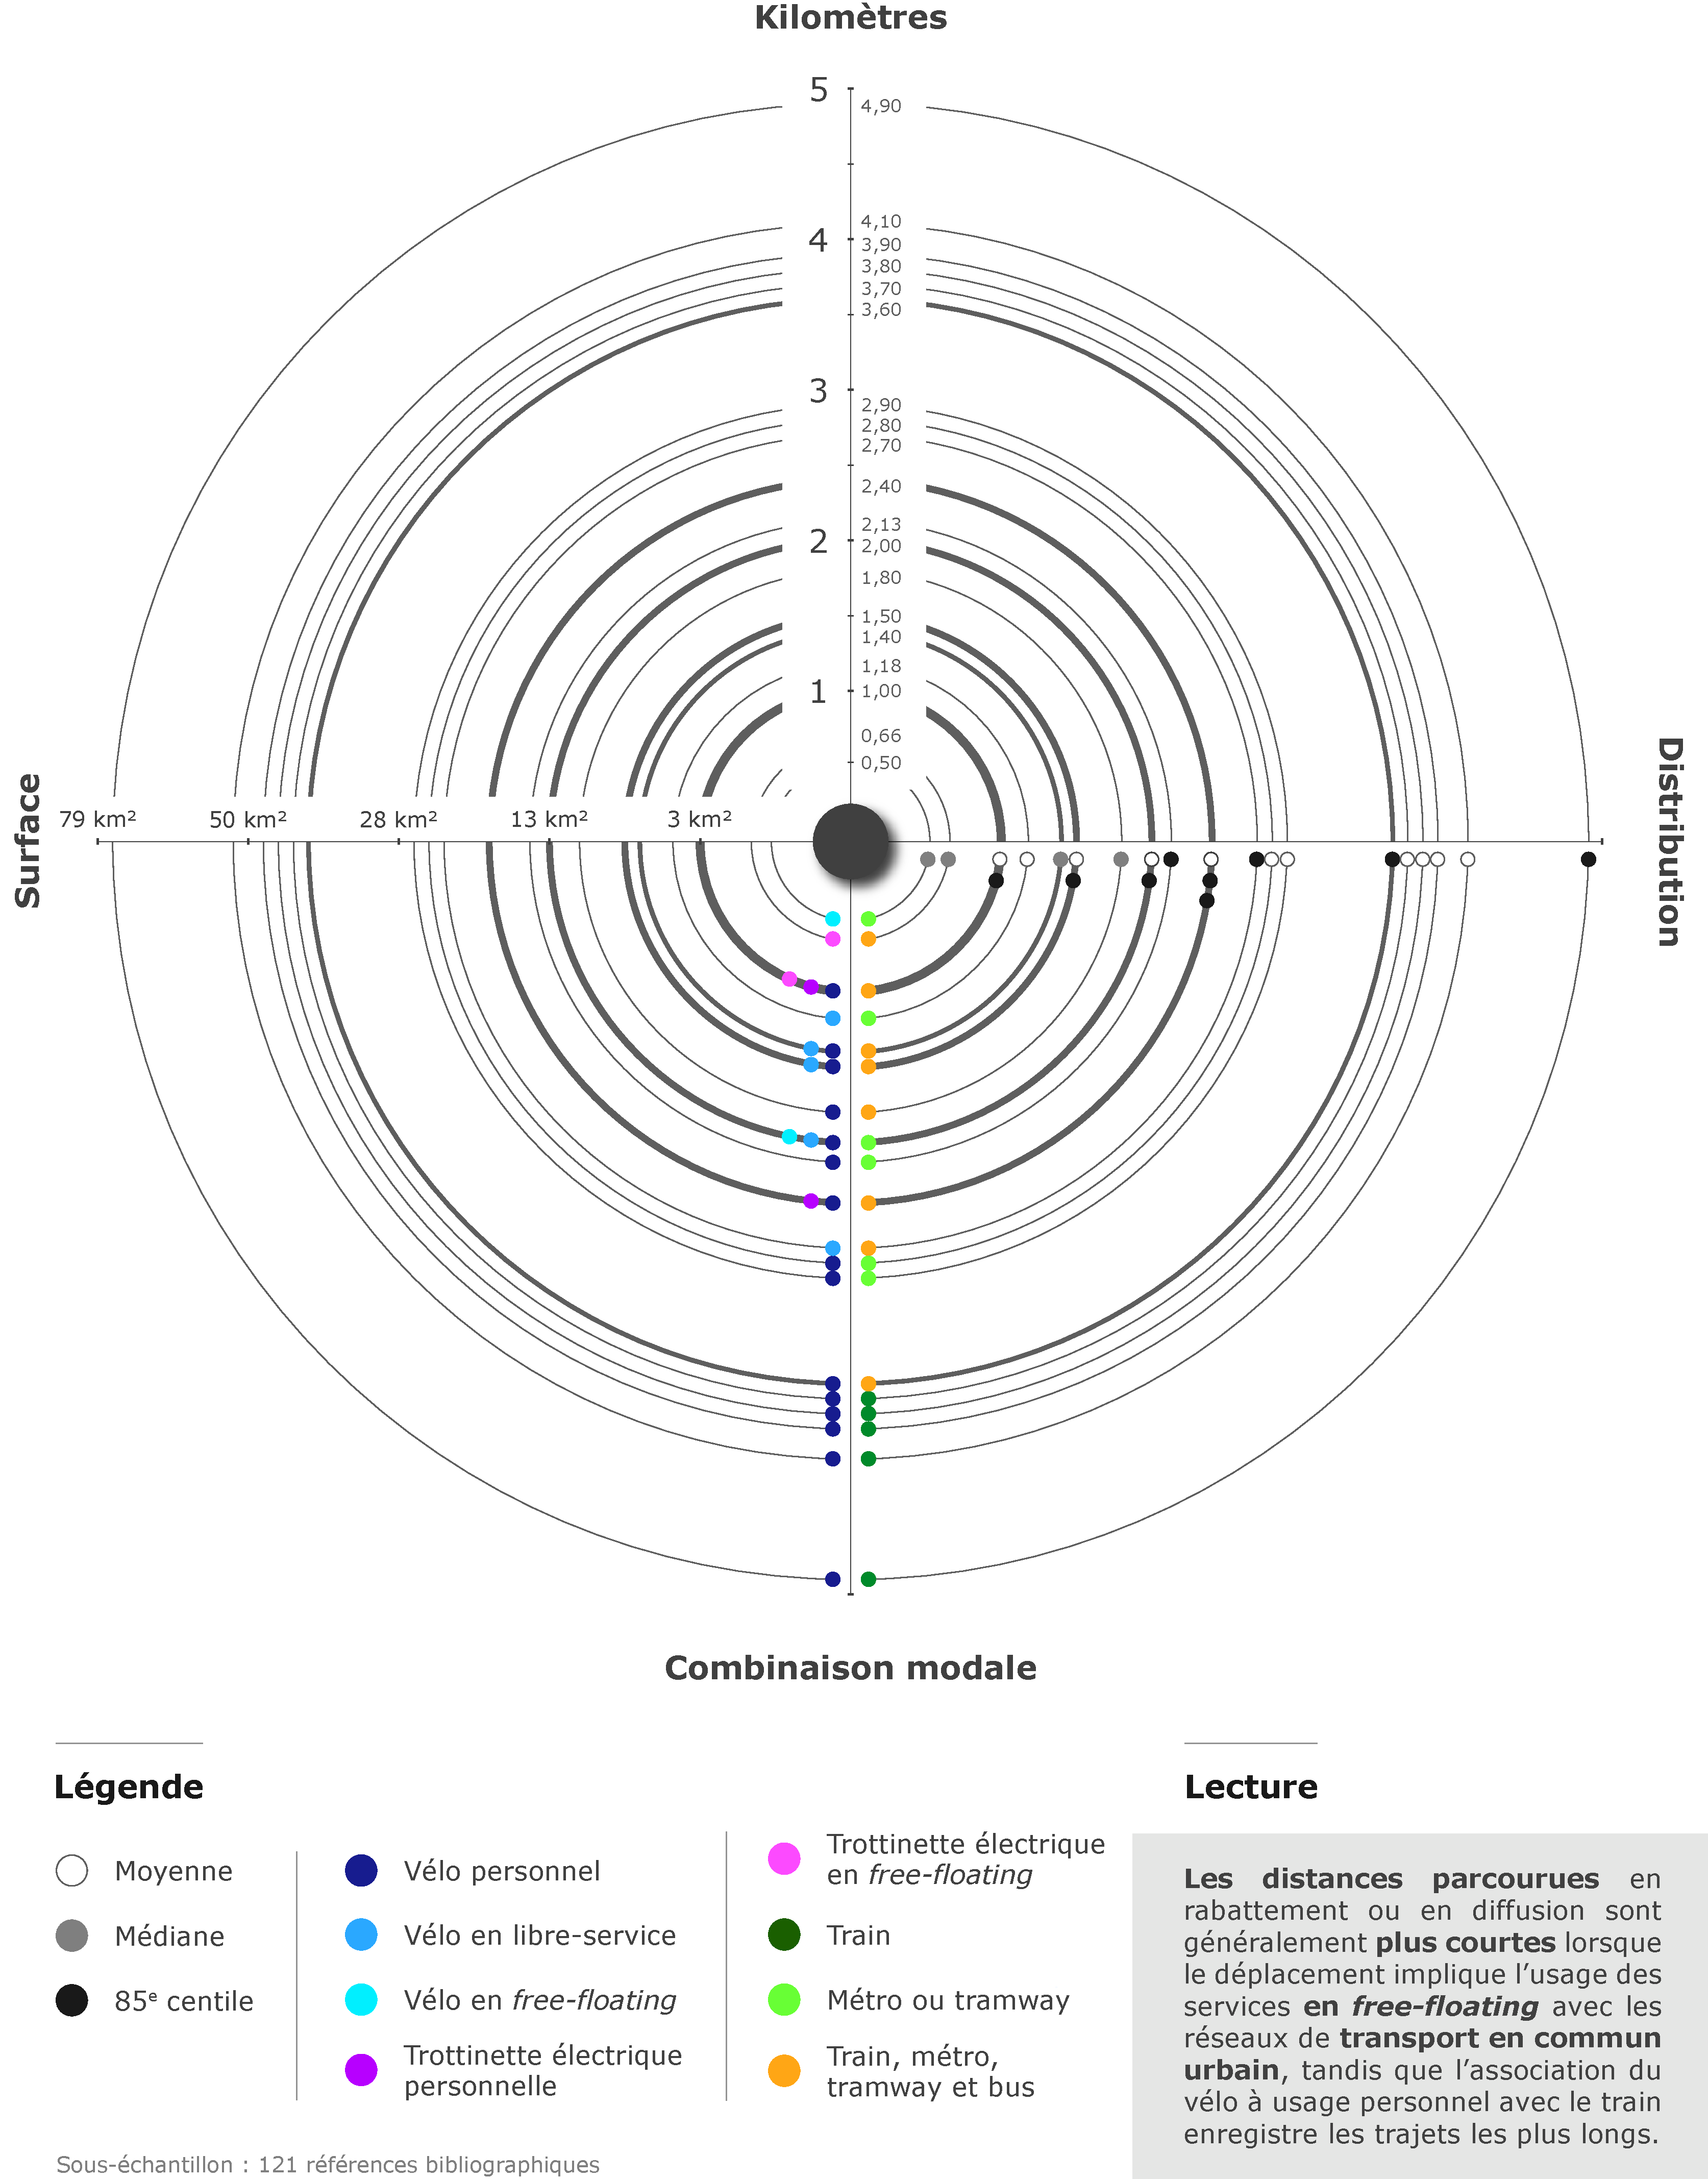
\includegraphics[width=1\columnwidth]{src/Figures/Chap-2/FR_RSL_Aires_influence.pdf}}
        \vspace{5pt}
        \begin{flushright}\scriptsize{
        Auteur~: \textcolor{blue}{Dylan Moinse (2023)}
        }\end{flushright}
    \end{figure}
    
    % Distances temps
La distance-temps en lien avec l'intermodalité est un aspect peu exploré dans la littérature scientifique, mais quelques études fournissent des aperçus importants sur la durée des déplacements combinant la mobilité individuelle légère et les transports en commun. À Shanghai, \textcolor{blue}{\textcite[19]{lin_analysis_2019}}\index{Lin, Diao|pagebf}\index{Zhang, Yongping|pagebf}\index{Zhu, Ruoxin|pagebf}\index{Meng, Liqiu|pagebf} évaluent la durée moyenne d'un trajet en \acrshort{VFF} pour accéder à une station de métro à 8,2~minutes, équivalant à deux kilomètres. À Utrecht, les déplacements en vélo personnel vers et depuis les stations de transport en commun révèlent des durées médianes distinctes~: en pré-acheminement vers les gares, la durée médiane est de 10,1~minutes, correspondant à une distance de 1,8 kilomètre, tandis qu'en post-acheminement depuis les gares, elle atteint 12,5 minutes, soit une distance de 2,4 kilomètres, selon \textcolor{blue}{\textcite[268]{krygsman_multimodal_2004}}\index{Krygsman, Stephan|pagebf}\index{Dijst, Martin|pagebf}\index{Arentze, Theo|pagebf}. Dans le contexte régional en Provence-Alpes-Côte d'Azur, \textcolor{blue}{\textcite[186]{moinse_intermodal_2022}}\index{Moinse, Dylan|pagebf}\index{Goudeau, Matthieu|pagebf}\index{L'Hostis, Alain|pagebf}\index{Leysens, Thomas|pagebf} constatent une durée moyenne de trajet en \acrshort{TEP} de 10,6 minutes en combinaison avec le train, équivalente à une distance de 2,4 kilomètres. L'utilisation du \acrshort{VLS} en association avec le métro et le bus présente un temps moyen de déplacement de 16 minutes, comme indiqué dans l'étude de cas sur Taipei \textcolor{blue}{\autocite[49]{lu_improving_2018}}\index{Lu, Miaojia|pagebf}\index{Hsu, Shu Chien|pagebf}\index{Chen, Pi Cheng|pagebf}\index{Lee, Wan Yu|pagebf}, tandis que cette combinaison atteint une valeur maximale (95\textsuperscript{e} centile) de 30~minutes à Nanjing \textcolor{blue}{\autocite[64]{ma_understanding_2018}}\index{Ma, Xinwei|pagebf}\index{Ji, Yanjie|pagebf}\index{Yang, Mingyuan|pagebf}\index{Jin, Yuchuan|pagebf}\index{Tan, Xu|pagebf}.%%Rédigé%%

    % 2.3.5.4. Aires d'influence
    \needspace{1\baselineskip} % Réserve de l'espace
\subsubsection*{Aires d'influence
    \label{chap2:aires-influence}
    }
    
    % <3km
La documentation analysée s'appuie sur un périmètre d'étude délimité et fondé sur la distribution des distances spatiales. Dans cette optique, plusieurs recherches académiques ont identifié des zones d'influence de portée relativement limitée, se concentrant essentiellement autour des arrêts de transport en commun urbain. Ainsi, \textcolor{blue}{\textcite[5]{wang_interchange_2016}}\index{Wang, Zi-jia|pagebf}\index{Chen, Feng|pagebf}\index{Xu, Tian-kun|pagebf} ont observé que les distances parcourues à vélo à Beijing se situent majoritairement entre~0,4~et~1,4~kilomètre. Selon les travaux de \textcolor{blue}{\textcite[11]{hu_examining_2022}}\index{Hu, Songhua|pagebf}\index{Chen, Mingyang|pagebf}\index{Jiang, Yuan|pagebf}\index{Sun, Wei|pagebf}\index{Xiong, Chenfeng|pagebf}, la distance spatiale pertinente en vue de modéliser l'utilisation du \acrshort{VFF} à Shanghai varie entre 1~et~1,5 kilomètre, les zones périurbaines étant caractérisées par des trajets généralement plus étendus. Ce même périmètre d'influence est également adopté par \textcolor{blue}{\textcite[9]{jin_competition_2019}}\index{Jin, Haitao|pagebf}\index{Jin, Fengjun|pagebf}\index{Wang, Jiao'e|pagebf}\index{Sun, Wei|pagebf}\index{Dong, Libo|pagebf} et par \textcolor{blue}{\textcite[10]{fan_how_2019}}\index{Fan, Aihua|pagebf}\index{Chen, Xumei|pagebf}\index{Wan, Tao|pagebf} dans le contexte urbain de Beijing, suggérant un rayon d'action établi jusqu'à deux kilomètres pour le \acrshort{VFF}. À Shanghai, \textcolor{blue}{\textcite[185]{pan_intermodal_2010}}\index{Pan, Haixiao|pagebf}\index{Shen, Qing|pagebf}\index{Xue, Song|pagebf} déterminent une aire s'étendant de 0,8~à~2,5 kilomètres, en soulignant que la majorité des déplacements à vélo et en \acrshort{VAE} se produisent sur des distances inférieures à 1,5 kilomètre. Selon \textcolor{blue}{\textcite[5]{ma_connecting_2022}}\index{Ma, Qingyu|pagebf}\index{Xin, Yanan|pagebf}\index{Yang, Hong|pagebf}\index{Xie, Kun|pagebf}, un périmètre compris entre deux et trois kilomètres a été établi pour apprécier la portée de la \acrshort{TEFF} à Washington~D.C., une démarche similaire étant observée à Beijing pour le \acrshort{VFF} \textcolor{blue}{\autocite[6]{ma_connecting_2022}}\index{Ma, Qingyu|pagebf}\index{Xin, Yanan|pagebf}\index{Yang, Hong|pagebf}\index{Xie, Kun|pagebf} ainsi qu'à Atlanta pour le vélo \textcolor{blue}{\autocite[57]{bearn_adaption_2018}}\index{Bearn, Cary|pagebf}\index{Mingus, Charlene|pagebf}\index{Watkins, Kari|pagebf}. Il convient de préciser que les seuils de distance mentionnés se rapportent spécifiquement aux réseaux de transport en commun urbain, comme le métro. Par conséquent, la configuration spatiale de ces infrastructures de transport, caractérisée par de courtes distances entre les stations, peut expliquer la taille réduite des zones d'influence mesurées.%%Rédigé%%

    % >3km
À partir d'un rayon de deux à trois kilomètres, les aires géographiques considérées s'avèrent être plus appropriées pour une utilisation intermodale du vélo en combinaison avec le train. Au travers d'une investigation sur les Pays-Bas, \textcolor{blue}{\textcite[227]{keijer_how_2000}}\index{Keijer, Majanka|pagebf}\index{Rietveld, Piet|pagebf} et \textcolor{blue}{\textcite[73]{rietveld_accessibility_2000}}\index{Rietveld, Piet|pagebf} introduisent un cadre de lecture prenant appui sur des facteurs de décroissance de la distance, justifiant ainsi l'établissement d'un périmètre étendu de 1~à~3,5 kilomètres, au-delà duquel l'attrait pour l'utilisation du vélo tend à diminuer. Cette observation est corroborée par les travaux de \textcolor{blue}{\textcite[281]{debrezion_modelling_2009}}\index{Debrezion, Ghebreegziabiher|pagebf}\index{Pels, Eric|pagebf}\index{Rietveld, Piet|pagebf}, qui confirment que le vélo est compétitif pour des distances allant de 1,1~à~4,2~kilomètres vers ou depuis la gare. Diverses productions scientifiques étendent l'aire d'influence jusqu'à cinq kilomètres, comme en témoignent l'utilisation du \acrshort{VFF} à Shenzhen \textcolor{blue}{\autocite[6]{wu_measuring_2019}}\index{Wu, Xueying|pagebf}\index{Lu, Li|pagebf}\index{Lin, Yaoyu|pagebf}\index{Yang, Yiyang|pagebf}, ou encore l'association du \acrshort{VLS} et du vélo avec le métro à Beijing \textcolor{blue}{\autocite[54]{zhao_bicycle-metro_2017}}\index{Zhao, Pengjun|pagebf}\index{Li, Shengxiao|pagebf}. La même zone d'impact est identifiée concernant la combinaison entre le vélo et le train, que ce soit à Amboise \textcolor{blue}{\autocite[751]{midenet_modal_2018}}\index{Midenet, Sophie|pagebf}\index{Côme, Etienne|pagebf}\index{Papon, Francis|pagebf}, à Göteborg, Malmö et Beijing \textcolor{blue}{\autocite[15]{hamidi_shaping_2020}}\index{Hamidi, Zahra|pagebf}\index{Zhao, Chunli|pagebf}, à El Monte \textcolor{blue}{\autocite[118]{cottrell_transforming_2007}}\index{Cottrell, Wayne~D.|pagebf} ou encore à Xi'an \textcolor{blue}{\autocite[172]{yang_bike-and-ride_2014}}\index{Yang, Liu|pagebf}\index{Chao, Li|pagebf}\index{Wang, Yuanqing|pagebf}. Allant encore plus loin, \textcolor{blue}{\textcite[9]{kim_analysis_2021}}\index{Kim, Minjun|pagebf}\index{Cho, Gi-Hyoung|pagebf} soutiennent que les déplacements combinant le \acrshort{VLS} et le métro à Séoul sont fréquents jusqu'à une distance de dix kilomètres, soulignant ainsi la portée étendue de ces pratiques intermodales.%%Rédigé%%

    % Temps
Dans une perspective temporelle, une partie de la documentation académique s'est attachée à déterminer les zones d'influence des stations de transport en commun, en prenant en compte la variable temporelle. À cet égard, \textcolor{blue}{\textcite[18, 21]{li_factors_2020}}\index{Li, Xuefeng|pagebf}\index{Du, Mingyang|pagebf}\index{Yang, Jingzong|pagebf} ont mis en évidence que les déplacements en \acrshort{VFF} d'une durée inférieure à sept minutes prédominent, spécialement durant les périodes de pointe matinales en semaine, bien que certaines régions de Shenzhen, y compris son centre urbain, affichent une majorité de trajets excédant quinze minutes. Selon \textcolor{blue}{\textcite[128]{liu_understanding_2020}}\index{Liu, Yang|pagebf}\index{Ji, Yanjie|pagebf}\index{Feng, Tao|pagebf}\index{Timmermans, Harry~J.~P.|pagebf}, un temps de parcours à vélo supérieur à dix minutes réduit son usage en combinaison avec le métro à Nanjing. Cette durée s'établit à douze minutes pour l'usage conjoint du \acrshort{VLS} et du réseau ferroviaire à Boston, Chicago, Washington~D.C., et à New York City \textcolor{blue}{\autocite[9]{kong_deciphering_2020}}\index{Kong, Hui|pagebf}\index{Jin, Scarlett~T.|pagebf}\index{Sui, Daniel~Z.|pagebf}, et s'étend à quinze minutes pour le \acrshort{VLS} en association avec le train à Osaka \textcolor{blue}{\autocite[3415]{tomita_demand_2017}}\index{Tomita, Yasuo|pagebf}\index{Nakayama, Akihiko|pagebf}. \textcolor{blue}{\textcite[5]{yang_empirical_2016}}\index{Yang, Min|pagebf}\index{Liu, Xinlu|pagebf}\index{Wang, Wei|pagebf}\index{Li, Zhibin|pagebf}\index{Zhao, Jingyao|pagebf} délimitent, quant à eux, un périmètre temporel de vingt minutes pour l'usage du \acrshort{VLS} en relation avec le réseau de métro à Nanjing. Enfin, \textcolor{blue}{\textcite[1696]{cheng_evaluating_2012}}\index{Cheng, Yung-Hsiang|pagebf}\index{Liu, Kuo-Chu|pagebf} adoptent une approche plus systémique en mesurant simultanément les temps de trajet en rabattement et en diffusion, observant ainsi que la majorité des cyclistes utilisant le métro à Kaohsiung effectuent des parcours de moins de trente minutes aller et retour.%%Rédigé%%

    % 2.3.5.5. Variabilité des distances et détours
    \needspace{1\baselineskip} % Réserve de l'espace
\subsubsection*{Variabilité des distances
    \label{chap2:variabilite-distances}
    }

    % Facteurs
L'évaluation des distances effectivement parcourues par les voyageur·se·s intermodaux·les, en particulier pour les \Guillemets{premiers et derniers kilomètres}, dépend étroitement des choix d'itinéraires adoptés. Ces trajets, empruntés par les cyclistes, sont influencés par une diversité de facteurs relatifs à l'environnement urbain, au contexte temporel ainsi qu'aux comportements, aux habitudes et aux expériences de mobilité. Selon \textcolor{blue}{\textcite[15]{tzouras_describing_2023}}\index{Tzouras, Panagiotis|pagebf}\index{Mitropoulos, Lambros|pagebf}\index{Koliou, Katerina|pagebf}\index{Stavropoulou, Eirini|pagebf}\index{Karolemeas, Christos|pagebf}\index{Antoniou, Eleni|pagebf}\index{Karaloulis, Antonis|pagebf}\index{Mitropoulos, Konstantinos|pagebf}\index{Vlahogianni, Eleni~I.|pagebf}\index{Kepaptsoglou, Konstantinos|pagebf}, les utilisateur·rice·s de la \acrshort{TEP} à Athènes sélectionnent leurs parcours en tenant compte de la sécurité perçue et de la distance minimale, dans le but d'atteindre un équilibre entre l'effort physique requis et les obstacles tant physiques que psychologiques à éviter. \textcolor{blue}{\textcite[621]{krizek_detailed_2007}}\index{Krizek, Kevin~J.|pagebf}\index{El-Geneidy, Ahmed~M.|pagebf}\index{Thompson, Kristin|pagebf} observent que les distances mesurées sont également déterminées par le motif de déplacement~: les trajets à vélo et en tramway associés aux achats et au travail sont plus courts, tandis que ceux liés aux loisirs sont plus longs, à Minneapolis. Le contexte environnemental et temporel a aussi un impact notable sur les distances parcourues. À cet égard, \textcolor{blue}{\textcite[619]{krizek_detailed_2007}}\index{Krizek, Kevin~J.|pagebf}\index{El-Geneidy, Ahmed~M.|pagebf}\index{Thompson, Kristin|pagebf} démontrent que les cyclistes préfèrent rallonger leur trajet jusqu'à 67~\% pour atteindre un itinéraire cyclable de bonne qualité. \textcolor{blue}{\textcite[8]{adnan_last-mile_2019}}\index{Adnan, Muhammad|pagebf}\index{Altaf, Shahbaz|pagebf}\index{Bellemans, Tom|pagebf}\index{Yasar, Ansar-ul-Haque|pagebf}\index{Shakshuki, Elhadi~M.|pagebf} ont démontré que les usager·ère·s du \acrshort{VLS} dans des villes de taille moyenne en Belgique sont sensibles à des facteurs météorologiques tels que la température et la pluviométrie, influençant non seulement les itinéraires, mais également le choix modal. Les utilisateur·rice·s du \acrshort{VLS} à Séoul sont plus sensibles à la distance en soirée, par rapport aux autres moments de la journée, selon \textcolor{blue}{\autocite[3110]{cho_estimation_2022}}\index{Cho, Shin-Hyung|pagebf}\index{Shin, DongHwa|pagebf}. À Nanjing, \textcolor{blue}{\textcite[11]{li_operating_2019}}\index{Li, Yuan|pagebf}\index{Zhu, Zhenjun|pagebf}\index{Guo, Xiucheng|pagebf} ont révélé que la portée du \acrshort{VFF} varie en fonction du jour de la semaine et du type de station de métro. Ces enseignements sont en accord avec les conclusions de \textcolor{blue}{\textcite[105]{flamm_public_2014}}\index{Flamm, Bradley~J.|pagebf}\index{Rivasplata, Charles~R.|pagebf}, qui ont remarqué que les distances parcourues par les cyclistes à Philadelphie et à San Francisco dépendent du type de transport en commun et de la topographie. De plus, le train enregistre des distances plus longues comparativement aux services conventionnels et \textsl{express} de bus, représentant une variable plus significative que les facteurs socio-démographiques, lesquels ont un impact modéré sur la distance dans plusieurs métropoles étasuniennes \textcolor{blue}{\autocite[23-24]{hochmair_assessment_2015}}\index{Hochmair, Hartwig~H.|pagebf}. Finalement, les stations de métro situées en périphérie de Shanghai présentent des aires d'attraction nettement plus vastes que celles du centre urbain \textcolor{blue}{\autocite[8]{yu_policy_2021}}\index{Yu, Qing|pagebf}\index{Li, Weifeng|pagebf}\index{Yang, Dongyuan|pagebf}\index{Xie, Yingkun|pagebf}. Cette pluralité de facteurs affectant le rapport à la distance illustre à quel point les cyclistes ne privilégient pas systématiquement l'itinéraire le plus court, révélant ainsi des stratégies visant à équilibrer optimisation spatio-temporelle et confort.%%Rédigé%%

    % Détours
Plusieurs travaux de recherche mettent en exergue la pratique de détours par les voyageur·se·s intermodaux·les, qui parcourent des distances accrues en raison de multiples facteurs. Selon \textcolor{blue}{\textcite[102]{kampen_understanding_2020}}\index{Kampen, Jullian van|pagebf}\index{Jayaraj, Manoj Ashvin|pagebf}\index{Pauwels, Eric|pagebf}\index{Mei, Rob van der|pagebf}\index{Dugundji, Elenna~R.|pagebf}, 42~\% des cyclistes sont enclin·e·s à se diriger vers des gares plus éloignées que la gare la plus proche, privilégiant celles dotées d'une meilleure connectivité, dans les régions de North-Holland, South-Holland, Flevoland et d'Utrecht. D'une part, \textcolor{blue}{\textcite[18]{jonkeren_bicycle-train_2021}}\index{Jonkeren, Olaf|pagebf}\index{Kager, Roland|pagebf}\index{Harms, Lucas|pagebf}\index{te Brömmelstroet, Marco|pagebf} soulignent l'objectif de contourner les ruptures de charge en favorisant des gares mieux équipées, comme celles d'Utrecht, Rotterdam et d'Eindhoven. D'autre part, cette préférence s'étend également aux stations de métro offrant des infrastructures de stationnement pour vélos, comme le montre l'étude de cas à Amsterdam conduite par \textcolor{blue}{\textcite[342]{kampen_bicycle_2021}}\index{Kampen, Jullian van|pagebf}\index{Pauwels, Eric|pagebf}\index{Mei, Rob van der|pagebf}\index{Dugundji, Elenna~R.|pagebf}. À Shanghai, \textcolor{blue}{\textcite[7]{li_exploring_2021}}\index{Li, Wenxiang|pagebf}\index{Chen, Shawen|pagebf}\index{Dong, Jieshuang|pagebf}\index{Wu, Jingxian|pagebf} révèlent que les stations de transport en commun les plus fréquentées attirent des passager·ère·s en \acrshort{VFF} de plus loin. \textcolor{blue}{\textcite[143]{kampen_understanding_2021}}\index{Kampen, Jullian van|pagebf}\index{Jayaraj, Manoj Ashvin|pagebf}\index{Pauwels, Eric|pagebf}\index{Mei, Rob van der|pagebf}\index{Dugundji, Elenna~R.|pagebf} ajoutent que les cyclistes avec un revenu net mensuel inférieur à 2~500€ et âgé·e·s de plus de 39 ans sont davantage susceptibles de se rendre à la seconde gare la plus proche de leur lieu de départ. Le rôle de facteurs venant influencer les distances effectives parcourues reflète l'importance des politiques et des stratégies visant à orienter la mobilité des personnes, de sorte à rendre les systèmes de mobilité alternatifs plus attrayants face à l'utilisation de l'automobile.%%Rédigé%%

    % 2.3.6. Resultats : management de la demande
    \needspace{1\baselineskip} % Réserve de l'espace
\subsection{Gestion de la demande de mobilité
    \label{chap2:gestion-demande-mobilite}
    }

    % Introduction
La gestion de la demande en mobilité, englobant l'ensemble des stratégies et politiques visant à orienter les choix de déplacement des individus, est au cœur de 61~études scientifiques traitant du \acrshort{M-TOD}. Notre analyse débutera par l'examen du rôle du niveau de services offert par les systèmes de transport en commun et l'importance de la mise en place d'une tarification intégrée. Nous aborderons ensuite la contribution des services de mobilité partagée, ainsi que le rôle des réseaux de bus dans les quartiers de gare. Enfin, cette section traitera de la gestion de la circulation et du stationnement automobile.%%Rédigé%%

    % 2.3.6.1. Fréquence et temps d'attente
    \needspace{1\baselineskip} % Réserve de l'espace
\subsubsection*{Niveau de service du \textsl{mass transit}
    \label{chap2:niveau-service}
    }
    
    % Fréquence des TC
Une desserte ferroviaire régulière et ponctuelle semble favoriser la pratique intermodale impliquant l'usage du vélo. Cette observation a été relevée pour les trains dans la Randstad South \textcolor{blue}{\autocite[45]{la_paix_puello_modelling_2015}}\index{La Paix Puello, Lissy|pagebf}\index{Geurs, Karst~T.|pagebf}, à Rotterdam \textcolor{blue}{\autocite[5]{montes_shared_2023}}\index{Montes, Alejandro|pagebf}\index{Geržinic, Nejc|pagebf}\index{Veeneman, Wijnand|pagebf}\index{Oort, Niels van|pagebf}\index{Hoogendoorn, Serge|pagebf}, à Turin \textcolor{blue}{\autocite[12]{staricco_implementing_2020}}\index{Staricco, Luca|pagebf}\index{Vitale Brovarone, Elisabetta|pagebf}, et à Shanghai pour le \acrshort{VFF} en association avec le métro \textcolor{blue}{\autocite[24]{lin_analysis_2019}}\index{Lin, Diao|pagebf}\index{Zhang, Yongping|pagebf}\index{Zhu, Ruoxin|pagebf}\index{Meng, Liqiu|pagebf}. À Melbourne, \textcolor{blue}{\textcite[401]{weliwitiya_bicycle_2019}}\index{Weliwitiya, Hesara|pagebf}\index{Rose, Geoff|pagebf}\index{Johnson, Marilyn|pagebf} ont mis en évidence une corrélation positive entre la fréquence des lignes ferroviaires, en particulier pendant les heures de pointe matinales, et le taux d'utilisation du vélo comme mode de rabattement. Les auteur·rice·s constatent qu'une augmentation d'une unité de fréquence entraîne une augmentation de 1,03 du nombre de cyclistes intermodaux·les. À Poznań, \textcolor{blue}{\textcite[199]{radzimski_exploring_2021}}\index{Radzimski, Adam|pagebf}\index{Dzięcielski, Michał|pagebf} ont mis en évidence une corrélation positive entre la fréquence des lignes de tramway et le nombre de trajets en \acrshort{VLS} pour des distances courtes, jusqu'à 1,5 kilomètre, ainsi que pour des distances moyennes, entre 1,5 et 3 kilomètres, mais cette relation n'est pas observée pour les trajets excédant 3 kilomètres. Cependant, \textcolor{blue}{\textcite[301]{kuijk_preferences_2022}}\index{Mil, Joeri~F.P. van|pagebf}\index{Leferink, Tessa~S.|pagebf}\index{Annema, Jan Anne|pagebf}\index{Oort, Niels van|pagebf}\index{Kuijk, Roy~J. van|pagebf}\index{Almeida Correia, Gonçalo Homem de|pagebf}\index{Oort, Niels van|pagebf}\index{Arem, Bart van|pagebf} n'ont identifié aucun paramètre significatif concernant la fréquence et la vitesse du tramway en lien avec l'utilisation du \acrshort{VLS} à Utrecht. Par ailleurs, les résultats des études réalisées par \textcolor{blue}{\textcite[41]{nielsen_bikeability_2018}}\index{Nielsen, Thomas Alexander Sick|pagebf}\index{Skov-Petersen, Hans|pagebf} suggèrent que la fréquence des services ferroviaires pourrait diminuer la probabilité de recourir au vélo au Danemark.%%Rédigé%%

    % Densité des stations
Au-delà de la fréquence des services de transport public, la vitesse commerciale de ces modes collectifs, intrinsèquement liée au temps de voyage, s'avère être un facteur déterminant dans le choix modal en faveur du vélo. Cette tendance contraste avec le rôle mineur attribué à la ponctualité et à la sécurité des services ferroviaires à Eindhoven \textcolor{blue}{\autocite[727]{waerden_relation_2018}}\index{Waerden, Peter|pagebf}\index{Waerden, Jaap|pagebf}. La vitesse du trajet en transport public est largement influencée par la densité des stations, qui a un impact significatif sur la demande de transfert à vélo. En effet, des gares très rapprochées tendent à réduire la probabilité d'opter pour ce mode de déplacement au Danemark \textcolor{blue}{\autocite[41]{nielsen_bikeability_2018}}\index{Nielsen, Thomas Alexander Sick|pagebf}\index{Skov-Petersen, Hans|pagebf}. Au contraire, la densité des stations de métro affecte positivement l'utilisation du \acrshort{VLS} à Nanjing \textcolor{blue}{\autocite[17]{ji_exploring_2018}}\index{Ji, Yanjie|pagebf}\index{Ma, Xinwei|pagebf}\index{Yang, Mingyuan|pagebf}\index{Jin, Yuchuan|pagebf}\index{Gao, Liangpeng|pagebf}. En explorant la combinaison du \acrshort{VFF} et du métro à Beijing, \textcolor{blue}{\textcite[10]{guo_exploring_2023}}\index{Guo, Dongbo|pagebf}\index{Yao, Enjian|pagebf}\index{Liu, Shasha|pagebf}\index{Chen, Rongsheng|pagebf}\index{Hong, Junyi|pagebf}\index{Zhang, Junyi|pagebf} ont constaté que le temps d'attente a pour autant un impact bien plus négatif que le temps de trajet lui-même~–~les usager·ère·s étant prêt·e·s à payer 13,6~\euro~ (105 CNY) pour économiser une heure d'attente, contre 2~\euro~ (15 CNY) pour une heure de \acrshort{VFF}~–, soulignant ainsi la nécessité d'établir des connexions efficaces au sein du système de transport public pour répondre à l'aversion face au temps de transfert.%%Rédigé%%

    % 2.3.6.2. MaaS et tarification
    \needspace{1\baselineskip} % Réserve de l'espace
\subsubsection*{Tarification intégrée
    \label{chap2:tarification_integree}
    }
    
    % MaaS
Pour favoriser l'intégration et encourager ces pratiques intermodales, la littérature scientifique préconise de simplifier les connexions entre différents systèmes de mobilité en promouvant l'utilisation de cartes de transport intégrées \textcolor{blue}{\autocite[172]{yang_bike-and-ride_2014}}\index{Yang, Liu|pagebf}\index{Chao, Li|pagebf}\index{Wang, Yuanqing|pagebf}, la mesure la plus plébiscitée par les passager·ère·s \textcolor{blue}{\autocite[10]{yang_empirical_2016}}\index{Yang, Min|pagebf}\index{Liu, Xinlu|pagebf}\index{Wang, Wei|pagebf}\index{Li, Zhibin|pagebf}\index{Zhao, Jingyao|pagebf}. L'un des principaux leviers d'action identifiés concerne la mobilité individuelle légère partagée et la mise en œuvre d'une plateforme multimodale de type \acrshort{MaaS}, offrant notamment la possibilité de mutualiser, voire d'unifier le paiement en ligne \textcolor{blue}{\autocite[5]{fearnley_patterns_2020}}\index{Fearnley, Nils|pagebf}\index{Johnsson, Espen|pagebf}\index{Berge, Siri Hegna|pagebf}. À Nanjing, un manque d'information sur les installations de location de vélos a été constaté, malgré un intérêt manifeste pour ce service, soulignant l'importance du \acrshort{MaaS} \textcolor{blue}{\autocite[136]{chen_determinants_2012}}\index{Chen, Lijun|pagebf}\index{Pel, Adam~J.|pagebf}\index{Chen, Xuewu|pagebf}\index{Sparing, Daniel|pagebf}\index{Hansen, Ingo~A.|pagebf}. Selon \textcolor{blue}{\textcite[67]{ma_understanding_2018}}\index{Ma, Xinwei|pagebf}\index{Ji, Yanjie|pagebf}\index{Yang, Mingyuan|pagebf}\index{Jin, Yuchuan|pagebf}\index{Tan, Xu|pagebf}, les plateformes intégrées devraient inclure un programme de fidélité pour privilégier les utilisateur·rice·s fréquent·e·s du \acrshort{VLS} et des transports en commun, en réservant certains emplacements de vélopartage à ces usager·ère·s. Cependant, \textcolor{blue}{\textcite[12]{fan_how_2019}}\index{Fan, Aihua|pagebf}\index{Chen, Xumei|pagebf}\index{Wan, Tao|pagebf} soulignent des obstacles liés à l'utilisation du \acrshort{VFF} ou d'une plate-forme \acrshort{MaaS} à Beijing, tels que la nécessité d'installer une application mobile, de fournir des informations personnelles pour s'enregistrer et de verser un dépôt de garantie important, alors que la tarification reste le principal facteur influençant le choix du \acrshort{VFF}.%%Rédigé%%

    % Tarification vélopartage et micro-mobilité partagée
Les coûts du vélo et de la micro-mobilité en libre-service sont souvent jugés prohibitifs et ne favorisent pas leur utilisation en rabattement et d'autant plus en diffusion \textcolor{blue}{\autocite[5]{montes_shared_2023}}\index{Montes, Alejandro|pagebf}\index{Geržinic, Nejc|pagebf}\index{Veeneman, Wijnand|pagebf}\index{Oort, Niels van|pagebf}\index{Hoogendoorn, Serge|pagebf}. À Nanjing, les jeunes travailleurs choisissent le \acrshort{VLS} pour des raisons économiques, ce qui soulève des interrogations sur les stratégies tarifaires ne favorisant pas le maintien de ces pratiques de mobilité vertueuses à long terme. À cet égard, les coûts d'un trajet unique et d'un abonnement au service ont un impact considérable sur le choix du \acrshort{VFF} pour accéder au réseau de métro \textcolor{blue}{\autocite[17]{zhong_layout_2021}}\index{Zhong, Hongming|pagebf}\index{Liu, Zijian|pagebf}\index{Chen, Jun|pagebf}\index{Hao, Jun|pagebf}\index{Wang, Wei|pagebf}. À Beijing, les voyageur·se·s ayant recours au \acrshort{VFF} dépensent presque autant pour des trajets courts à l'aide de ce service que pour le trajet en transport en commun \textcolor{blue}{\autocite[12]{fan_how_2019}}\index{Fan, Aihua|pagebf}\index{Chen, Xumei|pagebf}\index{Wan, Tao|pagebf}. Plusieurs solutions émergent de ces constats. À Nanjing, un temps gratuit de location de vélo de deux heures, comme politique de promotion efficace pour 57~\% des voyageur·se·s, a été identifié par \textcolor{blue}{\textcite[135]{chen_determinants_2012}}\index{Chen, Lijun|pagebf}\index{Pel, Adam~J.|pagebf}\index{Chen, Xuewu|pagebf}\index{Sparing, Daniel|pagebf}\index{Hansen, Ingo~A.|pagebf}. À Washington~D.C. et Los Angeles, des incitations tarifaires favorisant l'utilisation de la \acrshort{TEFF} avec le métro sont évaluées, notamment avec des réductions de prix lorsqu'un crédit de 2,8~\euro~ (3~\$) est appliqué sur les tarifs de la trottinette \textcolor{blue}{\autocite[11]{yan_evaluating_2023}}\index{Yan, Xiang|pagebf}\index{Zhao, Xilei|pagebf}\index{Broaddus, Andrea|pagebf}\index{Johnson, Joshua|pagebf}\index{Srinivasan, Sivaramakrishnan|pagebf}. À Boston et Worcester, l'impact de différents schémas tarifaires est analysé, révélant que la combinaison d'un tarif fixe et basé sur la distance a le moins d'impact sur la demande de vélo associé au train \textcolor{blue}{\autocite[16]{fournier_continuous_2021}}\index{Fournier, Nicholas|pagebf}\index{Christofa, Eleni|pagebf}\index{Gonzales, Eric~J.|pagebf}, tandis qu'à Oslo, le prix à la minute est un facteur important pour promouvoir l'usage de la \acrshort{TEFF} avec les transports en commun \textcolor{blue}{\autocite[5]{fearnley_patterns_2020}}\index{Fearnley, Nils|pagebf}\index{Johnsson, Espen|pagebf}\index{Berge, Siri Hegna|pagebf}. Une tarification sociale basée sur les revenus est jugée efficace pour le \acrshort{VFF} et la \acrshort{TEFF} à Seattle afin d'atténuer les barrières financières \textcolor{blue}{\autocite[975-977]{beale_integrating_2023}}\index{Beale, Kirsten|pagebf}\index{Kapatsila, Bogdan|pagebf}\index{Grisé, Emily|pagebf}.%%Rédigé%%

    % Tarification usage TC et stationnement vélo
Enfin, le coût monétaire affecte aussi l'utilisation des transports en commun ainsi que le stationnement du vélo et de la micro-mobilité à usage personnel. La gratuité des services ferroviaires ciblée pour les étudiants aux Pays-Bas attire plus de cyclistes intermodaux·les aux dépens de l'automobile \textcolor{blue}{\autocite[360]{givoni_access_2007}}\index{Givoni, Moshe|pagebf}\index{Rietveld, Piet|pagebf}. Une aversion significative au coût de stationnement des vélos est observée chez les étudiant·e·s néerlandais·e·s \textcolor{blue}{\autocite[667]{mil_insights_2020}}\index{Mil, Joeri~F.P. van|pagebf}\index{Leferink, Tessa~S.|pagebf}\index{Annema, Jan Anne|pagebf}\index{Oort, Niels van|pagebf}. Cependant, \textcolor{blue}{\textcite[10]{molin_bicycle_2015}}\index{Molin, Eric|pagebf}\index{Maat, Kees|pagebf} indiquent que la gratuité du stationnement vélo n'influence pas l'usage du vélo en intermodalité aux Pays-Bas et qu'au contraire, 65~\% des cyclistes interrogé·e·s privilégient le scénario basé sur un stationnement sécurisé, mais payant avec un prix optimal à hauteur d'1,50~\euro~. De même, \textcolor{blue}{\textcite[5]{liu_mode_2022}}\index{Liu, Lumei|pagebf}\index{Kong, Hui|pagebf}\index{Liu, Tianliang|pagebf}\index{Ma, Xiaolei|pagebf} constatent que le coût du trajet a peu d'impact sur le choix entre le bus ou le \acrshort{VFF} en modes de transfert avec le métro à Beijing, suggérant que la qualité de l'infrastructure de vélopartage est un aspect plus important à prendre en compte.%%Rédigé%%

    % 2.3.6.3. Vélopartage et micro-mobilité partagée
    \needspace{1\baselineskip} % Réserve de l'espace
\subsubsection*{Services de transfert
    \label{chap2:services-transfert}
    }
    
    % Présence de vélopartage
La mise à disposition de systèmes de mobilité partagée, tels que le \acrshort{VLS}, le \acrshort{VFF} ou la \acrshort{TEFF}, s'avère être un élément fondamental pour l'intégration du vélo avec les transports en commun \textcolor{blue}{\autocite[11-12]{wu_measuring_2019}}\index{Wu, Xueying|pagebf}\index{Lu, Li|pagebf}\index{Lin, Yaoyu|pagebf}\index{Yang, Yiyang|pagebf}. Dès lors, l'incorporation de ces services de mobilité au sein de la stratégie urbaine du \acrshort{TOD} est préconisée afin d'accroître l'utilisation et l'efficacité globale du système de mobilité \textcolor{blue}{\autocite[16]{tamakloe_determinants_2021}}\index{Tamakloe, Reuben|pagebf}\index{Hong, Jungyeol|pagebf}\index{Tak, Jihoon|pagebf}. La disponibilité de vélos et d'options de micro-mobilité en libre-service à proximité des nœuds de transport en commun augmente non seulement la probabilité de leur utilisation comme modes de liaison \textcolor{blue}{\autocite[25]{guo_dockless_2021}}\index{Guo, Yuanyuan|pagebf}\index{Yang, Linchuan|pagebf}\index{Lu, Yi|pagebf}\index{Zhao, Rui|pagebf}, mais ces systèmes contribuent également à promouvoir une pratique plus efficace de l'intermodalité-voyageur·se·s, en réduisant la nécessité d'un second vélo \textcolor{blue}{\autocite[10]{jonkeren_bicycle_2021}}\index{Jonkeren, Olaf|pagebf}\index{Kager, Roland|pagebf}. À Shanghai, \textcolor{blue}{\textcite[186]{pan_intermodal_2010}}\index{Pan, Haixiao|pagebf}\index{Shen, Qing|pagebf}\index{Xue, Song|pagebf} ont identifié une forte volonté exprimée par les participant·e·s de l'étude d'utiliser des systèmes de location de vélos près des stations de métro. Partant du constat que les voyageur·se·s intermodaux·les disposent d'un haut degré de planification de leurs déplacements et adaptent leur comportement en fonction de l'offre de mobilité et des contraintes liées au transport et au stationnement du vélo, \textcolor{blue}{\textcite[196]{sherwin_practices_2011}}\index{Sherwin, Henrietta|pagebf}\index{Parkhurst, Graham|pagebf}\index{Robbins, Derek|pagebf}\index{Walker, Ian|pagebf} justifient la mise en place d'un système de location de vélos organisé à l'échelle nationale, à l'image de ce qui est pratiqué par les gestionnaires ferroviaires néerlandais et allemands.%%Rédigé%%

    % Gestion et réallocation des services de vélopartage et micro-mobilité partagée
La mise en place d'un système de mobilité individuelle légère partagée requiert une gestion efficace et une répartition optimale des flottes. Les travaux de \textcolor{blue}{\textcite[197]{radzimski_exploring_2021}}\index{Radzimski, Adam|pagebf}\index{Dzięcielski, Michał|pagebf} démontrent que la structuration d'un système de \acrshort{VLS}, organisé sous la forme de vélos en libre-service avec des stations dédiées, attire davantage d'usager·ère·s en combinaison avec le tramway par rapport au \acrshort{VFF}. De ce fait, il est recommandé d'améliorer l'allocation des \acrshort{VFF} en redistribuant de manière plus efficiente les vélos vers des espaces verts, des zones commerciales et industrielles, ainsi que des quartiers résidentiels à Beijing \textcolor{blue}{\autocite[12]{liu_temporal_2022}}\index{Liu, Siyang|pagebf}\index{Zhang, Xiaodong|pagebf}\index{Zhou, Chenjing|pagebf}\index{Rong, Jian|pagebf}\index{Bian, Yang|pagebf}. Face aux limitations de capacité des systèmes en \textsl{free-floating} lors de pics d'utilisation, comme cela a été observé pour la \acrshort{TEFF} à Columbus \textcolor{blue}{\autocite[9]{liu_measuring_2022}}\index{Liu, Luyu|pagebf}\index{Miller, Harvey~J.|pagebf}, \textcolor{blue}{\textcite[69, 95]{nat_bicycle_2018}}\index{Nat, Johanna Debóra van der|pagebf} suggère un modèle alternatif de partage de vélos. Ce modèle repose sur une combinaison de location et de mise à disposition suffisante de vélos partagés pour assurer leur disponibilité et maximiser les économies d'espace de stationnement à Amsterdam.%%Rédigé%%

    % Embarquement / emport dans les TC
L'établissement de connexions efficaces entre les systèmes de transport en commun et la mobilité individuelle légère se traduit également par la facilité d'emport du vélo et de la micro-mobilité à bord des modes collectifs. Conjugué avec l'aménagement d'un système efficace de vélopartage et de micro-mobilité partagée et de stationnement, l'embarquement de la mobilité individuelle légère dans les véhicules de transport en commun stimule les pratiques intermodales à Portland \textcolor{blue}{\autocite[93]{singleton_exploring_2014}}\index{Singleton, Patrick~A.|pagebf}\index{Clifton, Kelly~J.|pagebf}. À Copenhague, \textcolor{blue}{\textcite[19]{halldorsdottir_home-end_2017}}\index{Halldórsdóttir, Katrín|pagebf}\index{Nielsen, Otto Anker|pagebf}\index{Prato, Carlo Giacomo|pagebf} démontrent que la possibilité de transporter gratuitement le vélo dans le train augmente l'utilisation intermodale du vélo. D'autant plus que le management des interconnexions à vélo et en micro-mobilité doit être pensé en relation avec les services de bus, à l'heure où un effet de substitution entre le \acrshort{VLS} et le \acrshort{VFF} avec le bus est observé à Nanjing \textcolor{blue}{\autocite[12]{chen_what_2022}}\index{Chen, Wendong|pagebf}\index{Chen, Xuewu|pagebf}\index{Chen, Jingxu|pagebf}\index{Cheng, Long|pagebf}.%%Rédigé%%

    % 2.3.6.4. Bus
    \needspace{1\baselineskip} % Réserve de l'espace
\subsubsection*{Desserte en bus
    \label{chap2:desserte-bus}
    }
    
    % Substitution modale
Fort de l'effet de substitution modale existant entre la mobilité individuelle légère et le bus, il apparaît que la densité des arrêts de bus dans la zone d'influence des stations structurantes de transport en commun est inversement proportionnelle à l'utilisation de ces modes de déplacement. Ainsi, à Beijing, les services de bus se substituent à l'usage du vélo, du \acrshort{VLS} \textcolor{blue}{\autocite[55]{zhao_bicycle-metro_2017}}\index{Zhao, Pengjun|pagebf}\index{Li, Shengxiao|pagebf} et du \acrshort{VFF} \textcolor{blue}{\autocite[16]{wang_spatiotemporal_2020}}\index{Wang, Zi-jia|pagebf}. \textcolor{blue}{\textcite[10]{li_exploring_2021}}\index{Li, Wenxiang|pagebf}\index{Chen, Shawen|pagebf}\index{Dong, Jieshuang|pagebf}\index{Wu, Jingxian|pagebf} observent que la densité des arrêts de bus diminue progressivement à mesure que la distance de transfert augmente, procurant un avantage comparatif au \acrshort{VFF} lorsque cette distance dépasse un certain seuil à Shanghai. De même, \textcolor{blue}{\textcite[20]{luan_better_2020}}\index{Luan, Xin|pagebf}\index{Cheng, Lin|pagebf}\index{Song, Yan|pagebf}\index{Zhao, Jinbao|pagebf} constatent que les résident·e·s de Nanjing tendent à délaisser le bus au profit du vélo, ce qui pourrait indiquer une insatisfaction à l'égard des services de bus existants.%%Rédigé%%

    % Absence de substitution modale
\textsl{A contrario}, une plus grande part des études semble indiquer une absence de substitution modale, révélant au contraire que les connexions en bus ont un impact positif sur l'utilisation du \acrshort{VLS} en complément du train à Washington~D.C. \textcolor{blue}{\autocite[7-8]{ma_bicycle_2015}}\index{Ma, Ting|pagebf}\index{Liu, Chao|pagebf}\index{Erdoğan, Sevgi|pagebf} et du \acrshort{VFF} avec le métro à Shenzhen \textcolor{blue}{\autocite[12]{guo_built_2020}}\index{Guo, Yuanyuan|pagebf}\index{He, Sylvia~Y.|pagebf}. Selon \textcolor{blue}{\textcite[20]{arbis_analysis_2016}}\index{Arbis, David|pagebf}\index{Hossein Rashidi, Taha|pagebf}\index{Dixit, Vinayak~V.|pagebf}\index{Vandebona, Upali|pagebf}, la présence d'un arrêt de bus à proximité des gares est un indicateur prédictif de niveaux plus élevés d'utilisation des parkings à vélos en Nouvelles-Galles du Sud. Il se peut néanmoins que ces conclusions rapportées se livrent à une interprétation erronée des données. En effet, la corrélation observée entre la présence d'arrêts de bus et l'utilisation accrue du vélopartage pourrait simplement signaler une meilleure qualité de service dans les gares concernées, plutôt que d'établir une relation de cause à effet directe. Par ailleurs, il est possible que ces gares soient situées dans des territoires dans lesquels l'aménagement d'arrêts de bus coïncide avec des politiques de réduction de l'espace accordé à la voiture. Si l'aspect lié à la gestion de la demande de mobilité s'est intéressée aux mesures incitatives~–~dans cette section, cette dimension est principalement abordée sous l'angle du niveau de service des modes collectifs, de la tarification, de la gestion des interconnexions et de la desserte en bus~–, le rapport de compétition avec l'automobile ne doit pas être négligé, en intégrant une perspective sur les politiques coercitives. Cette approche doit être considérée pour évaluer les stratégies de management de la demande et leur impact potentiel sur la promotion d'un système de mobilité alternatif tout en réduisant la dépendance à l'automobile.%%Rédigé%%

    % 2.3.6.5. Voiture
    \needspace{1\baselineskip} % Réserve de l'espace
\subsubsection*{Modération de l'usage compétitif de l'automobile
    \label{chap2:moderation-automobile}
    }
    
    % Réduction stationnement
Dans le contexte d'un développement urbain axé sur l'articulation entre les transports en commun et la mobilité individuelle légère, il est essentiel de considérer la place de l'automobile et de souligner l'importance de politiques proactives pour adapter les espaces publics et privés dans le but de réguler le trafic et le stationnement motorisé. Une corrélation positive est établie entre l'augmentation du taux de motorisation dans un territoire et une utilisation accrue de la part de l'automobile pour accéder aux gares aux Pays-Bas, son utilité surpassant les autres modes de transfert à partir de 0,60~voiture par personne pour les trajets dépassant dix kilomètres \textcolor{blue}{\autocite[281]{debrezion_modelling_2009}}\index{Debrezion, Ghebreegziabiher|pagebf}\index{Pels, Eric|pagebf}\index{Rietveld, Piet|pagebf}. En Provence-Alpes-Côte d'Azur, \textcolor{blue}{\textcite[190]{moinse_intermodal_2022}}\index{Moinse, Dylan|pagebf}\index{Goudeau, Matthieu|pagebf}\index{L'Hostis, Alain|pagebf}\index{Leysens, Thomas|pagebf} ont constaté qu'un déplacement intermodal est un quart de temps plus long qu'un déplacement équivalent en voiture, hors temps de congestion urbaine et de stationnement, ce qui implique la nécessité de mesures coercitives si l'on souhaite accroître la compétitivité du vélo et de la \acrshort{TEP} avec le train.%%Rédigé%%

    % Recommandations stationnement
À Copenhague, \textcolor{blue}{\textcite[18]{halldorsdottir_home-end_2017}}\index{Halldórsdóttir, Katrín|pagebf}\index{Nielsen, Otto Anker|pagebf}\index{Prato, Carlo Giacomo|pagebf} observent que la disponibilité des parkings automobiles influence le choix des modes de transfert pour accéder aux gares. Une augmentation de l'offre de stationnement automobile de cent places autour d'une gare, généralement équipée de 1~700~places, est liée à une diminution de 4~\% de l'utilisation de la marche et du vélo, révélant un conflit entre les \acrfull{P+R} et les \gls{modes actifs} à Toronto et à Hamilton \textcolor{blue}{\autocite[2172-2173]{chan_factors_2020}}\index{Chan, Kevin|pagebf}\index{Farber, Steven|pagebf}. En outre, la saturation des parkings autour des gares, et d'autant plus à destination, accroît la probabilité de l'adoption de modes actifs aux États-Unis \textcolor{blue}{\autocite[4270]{bopp_examining_2015}}\index{Bopp, Melissa|pagebf}\index{Gayah, Vikash~V.|pagebf}\index{Campbell, Matthew~E.|pagebf}. Concernant la diffusion depuis les stations de métro, il a été constaté que la disponibilité des espaces de stationnement pour les deux-roues motorisés influence négativement l'intention des passagers d'utiliser le \acrshort{VLS} à Kaohsiung \textcolor{blue}{\autocite[28]{cheng_expanding_2018}}\index{Cheng, Yung-Hsiang|pagebf}\index{Li, Yi-Chun|pagebf}. Par conséquent, il est suggéré de renforcer les normes relatives au stationnement des véhicules motorisés autour des stations très fréquentées afin d'améliorer la gestion de la demande de transport et de consolider la compétitivité du vélo combiné au métro à Xi'an \textcolor{blue}{\autocite[7]{zhu_improved_2021}}\index{Zhu, Zhenjun|pagebf}\index{He, Yudong|pagebf}\index{Guo, Xiucheng|pagebf}\index{Zhang, Yibang|pagebf}\index{Chen, Junlan|pagebf}. Toutefois, \textcolor{blue}{\textcite[401]{weliwitiya_bicycle_2019}}\index{Weliwitiya, Hesara|pagebf}\index{Rose, Geoff|pagebf}\index{Johnson, Marilyn|pagebf} mettent en garde contre le risque de se focaliser uniquement sur le stationnement automobile prévu autour des gares, sans tenir compte d'autres types de stationnements tels que les rues avoisinantes ou les garages, qui représentent 72~\% du stationnement enregistré pour les usager·ère·s venant en voiture jusqu'aux gares de Melbourne.%%Rédigé%%

    % Tarification stationnement
Au-delà du contrôle d'accès au stationnement, il a été démontré que la mise en service du BART à San Francisco a entraîné une hausse des frais de stationnement automobile autour des stations, alors auparavant gratuit, ce qui a encouragé l'utilisation du vélo \textcolor{blue}{\autocite[94]{cervero_bike-and-ride_2013}}\index{Cervero, Robert|pagebf}\index{Caldwell, Benjamin|pagebf}\index{Cuellar, Jesus|pagebf}. Plusieurs études préconisent un meilleur contrôle de l'accès au parking à la gare, à l'aide d'une stratégie de tarification inversement proportionnelle à la distance de transfert, comme levier d'action en faveur d'un puissant report modal \textcolor{blue}{\autocite[751]{midenet_modal_2018}}\index{Midenet, Sophie|pagebf}\index{Côme, Etienne|pagebf}\index{Papon, Francis|pagebf}. Outre la question du stationnement automobile, \textcolor{blue}{\textcite[2737]{papon_evaluation_2017}}\index{Papon, Francis|pagebf}\index{Beauvais, Jean-Marie|pagebf}\index{Midenet, Sophie|pagebf}\index{Côme, Etienne|pagebf}\index{Polombo, Nadine|pagebf}\index{Abours, Sylvie|pagebf}\index{Belton-Chevallier, Leslie|pagebf}\index{Soulas, Claude|pagebf} ont entrepris une analyse socio-économique démontrant qu'une multiplication par deux du prix du carburant entraînerait une augmentation de 7~\% la part modale du vélo vers les gares.%%Rédigé%%

    % 2.3.7. Resultats : profils socio-démographiques
    \needspace{1\baselineskip} % Réserve de l'espace
\subsection{Caractéristiques socio-démographiques des usager·ère·s
    \label{chap2:sociodemographie-usagers}
    }
    
    % Introduction
Le modèle revisité du \acrshort{M-TOD}, comme toute stratégie de développement urbain, doit démontrer sa capacité à favoriser une accessibilité inclusive. Cela signifie qu'il doit non seulement améliorer l'accessibilité soutenable aux ressources du territoire, mais aussi veiller à ce que ces améliorations profitent, de manière équitable, à tous les segments de la population, y compris les groupes sociaux souvent marginalisés dans la planification urbaine. Par conséquent, la présente section se consacre à une analyse approfondie des caractéristiques socio-démographiques de la population, dans l'intérêt de tendre vers une fabrique urbaine en adéquation avec les besoins spécifiques des usager·ère·s actuel·le·s et futur·e·s, tout en assurant l'inclusion sociale. Dans cette perspective, notre étude s'oriente vers l'examen des diverses dimensions socio-démographiques et économiques définissant les profils des utilisateur·rice·s de la mobilité individuelle légère. Cette exploration prenant appui sur 90~publications scientifiques inclura, non seulement, l'analyse des effets de genre et d'âge, mais également les variables relatives à la composition des ménages, à la nomenclature basée sur les \acrshort{PCS}, aux niveaux de revenus disponibles, aux diplômes acquis et à l'équipement des foyers en lien avec la mobilité.%%Rédigé%%

    % 2.3.7.1.
    \needspace{1\baselineskip} % Réserve de l'espace
\subsubsection*{Effets de genre
    \label{chap2:genre}
    }
    
    % Hommes vélo
D'emblée, la littérature scientifique fait état de disparités de \gls{genre} qui se manifestent dans le choix modal de la mobilité individuelle légère intégrée. Les hommes semblent davantage enclins à recourir au vélo personnel en conjonction avec les réseaux de transport en commun. Cette tendance est observée dans divers contextes géographiques, tels qu'aux Pays-Bas \textcolor{blue}{\autocite[278]{debrezion_modelling_2009}}\index{Debrezion, Ghebreegziabiher|pagebf}\index{Pels, Eric|pagebf}\index{Rietveld, Piet|pagebf}, à New Delhi \textcolor{blue}{\autocite[35]{mohanty_effect_2017}}\index{Mohanty, Sudatta|pagebf}\index{Bansal, Sugam|pagebf}\index{Bairwa, Khushi|pagebf}, et à Mountain View \textcolor{blue}{\autocite[36]{park_finding_2014}}\index{Park, Sungjin|pagebf}\index{Kang, Junhee|pagebf}\index{Choi, Keechoo|pagebf}, à l'exception de Singapour \textcolor{blue}{\autocite[45]{meng_influence_2016}}\index{Meng, Meng|pagebf}\index{Koh, Puay Ping|pagebf}\index{Wong, Yiik Diew|pagebf} et de Rio de Janeiro \textcolor{blue}{\autocite[62]{souza_modelling_2017}}\index{Souza, Flavia de|pagebf}\index{La Paix Puello, Lissy|pagebf}\index{Brussel, Mark|pagebf}\index{Orrico, Romulo|pagebf}. Un corpus conséquent d'études révèle des inégalités de genre quant à l'utilisation du vélo combiné, une majorité d'usagers masculins étant rapportée à Bristol \textcolor{blue}{\autocite[194]{sherwin_practices_2011}}\index{Sherwin, Henrietta|pagebf}\index{Parkhurst, Graham|pagebf}\index{Robbins, Derek|pagebf}\index{Walker, Ian|pagebf} et à San Francisco \textcolor{blue}{\autocite[103]{flamm_public_2014}}\index{Flamm, Bradley~J.|pagebf}\index{Rivasplata, Charles~R.|pagebf}. À Kaohsiung, 58~\% des cyclistes se rendant à une station de métro sont des hommes \textcolor{blue}{\autocite[1~700]{cheng_evaluating_2012}}\index{Cheng, Yung-Hsiang|pagebf}\index{Liu, Kuo-Chu|pagebf}, et cette proportion atteint les deux tiers à Toronto et à Hamilton \textcolor{blue}{\autocite[378]{ravensbergen_biking_2018}}\index{Ravensbergen, Léa|pagebf}\index{Buliung, Ron|pagebf}\index{Mendonca, Meaghan|pagebf}\index{Garg, Naren|pagebf}. Dans les régions de Delft, Zwolle, Midden-Delfland et Pijnacker-Nootdorp, les cyclistes intermodaux·les sont majoritairement masculins, contrastant avec les groupes sociaux d'automobilistes, de cyclistes monomodaux et d'usager·ère·s des transports en commun quant à elleux paritaires \textcolor{blue}{\autocite[114]{heinen_multimodal_2014}}\index{Heinen, Eva|pagebf}\index{Bohte, Wendy|pagebf}. De surcroît, les hommes tendent à effectuer des trajets plus longs à vélo pour rejoindre une gare à Utrecht \textcolor{blue}{\autocite[267]{krygsman_multimodal_2004}}\index{Krygsman, Stephan|pagebf}\index{Dijst, Martin|pagebf}\index{Arentze, Theo|pagebf}. En outre, \textcolor{blue}{\textcite[107]{wang_bicycle-transit_2013}}\index{Wang, Rui|pagebf}\index{Liu, Chen|pagebf} ont non seulement constaté aux États-Unis qu'une majorité écrasante des déplacements intermodaux impliquant l'usage du vélo sont effectués par des hommes, mais également qu'un écart d'usage croissant entre les genres a été observé entre 2001~et~2009. Pour autant, \textcolor{blue}{\textcite[59]{bearn_adaption_2018}}\index{Bearn, Cary|pagebf}\index{Mingus, Charlene|pagebf}\index{Watkins, Kari|pagebf} montrent qu'en accordant une attention particulière à l'expansion d'un \Guillemets{réseau cyclable à faible stress}~vers les communautés isolées, ces politiques d'aménagement entraîneraient une augmentation de l'accès pour les femmes à Atlanta.%%Rédigé%%

    % Hommes VLS+VFF
En ce qui concerne l'usage intermodal du \acrshort{VLS}, un déséquilibre similaire a été relevé au sein des villes belges de 30~000~à~200~000~habitant·e·s \textcolor{blue}{\autocite[6]{adnan_last-mile_2019}}\index{Adnan, Muhammad|pagebf}\index{Altaf, Shahbaz|pagebf}\index{Bellemans, Tom|pagebf}\index{Yasar, Ansar-ul-Haque|pagebf}\index{Shakshuki, Elhadi~M.|pagebf}, à Suzhou \textcolor{blue}{\autocite[9]{ma_measuring_2018}}\index{Ma, Xinwei|pagebf}\index{Jin, Yuchuan|pagebf}\index{He, Mingja|pagebf} ainsi qu'à Washington~D.C. et Minneapolis \textcolor{blue}{\autocite[322]{martin_evaluating_2014}}\index{Martin, Elliot~W.|pagebf}\index{Shaheen, Susan~A.|pagebf}. Parallèlement, \textcolor{blue}{\textcite[111]{bachand-marleau_much-anticipated_2011}}\index{Bachand-Marleau, Julie|pagebf}\index{Larsen, Jacob|pagebf}\index{El-Geneidy, Ahmed~M.|pagebf} constatent une prédominance masculine parmi les usager·ère·s du \acrshort{VLS} à Montréal, représentant 58~\% des voyageur·se·s. De façon analogue, \textcolor{blue}{\textcite[393]{bocker_bike_2020}}\index{Böcker, Lars|pagebf}\index{Anderson, Ellinor|pagebf}\index{Uteng, Tanu Priya|pagebf}\index{Throndsen, Torstein|pagebf} révèlent une répartition genrée de 58~\% en faveur des hommes parmi les cyclistes à Oslo, avec une concentration accrue en centre-ville. Ces dernier·ère·s précisent toutefois que cette proportion s'élève à 68~\% en matière de trajets effectués, suggérant que les hommes utilisent le \acrshort{VLS} plus fréquemment en combinaison avec le métro que les femmes. À Nanjing, \textcolor{blue}{\textcite[64]{ma_understanding_2018}}\index{Ma, Xinwei|pagebf}\index{Ji, Yanjie|pagebf}\index{Yang, Mingyuan|pagebf}\index{Jin, Yuchuan|pagebf}\index{Tan, Xu|pagebf} ont observé que les femmes se distinguent des hommes dans leur utilisation du \acrshort{VLS}, se déplaçant plus souvent entre 6h et 7h ainsi qu'entre 16h et 17h, régulièrement après avoir accompagné leurs enfants. Une seule étude, focalisée sur la combinaison du \acrshort{VFF} avec le transport public à Beijing, révèle que les personnes s'identifiant comme des hommes ont tendance à privilégier 3,3 fois plus ces modes de déplacement que les personnes s'identifiant comme des femmes \textcolor{blue}{\autocite[10]{fan_how_2019}}\index{Fan, Aihua|pagebf}\index{Chen, Xumei|pagebf}\index{Wan, Tao|pagebf}. En ce qui concerne les interrelations entre la problématique liée au genre et l'usage de la trottinette électrique, \textcolor{blue}{\textcite[12]{pages_nouveaux_2021}}\index{Pages, Thibaud|pagebf}\index{Lammoglia, Adrien|pagebf}\index{Josselin, Didier|pagebf} ont identifié une prédominance masculine parmi les utilisateur·rice·s de la \acrshort{TEP} à Marseille et Montpellier. Ces disparités de genre en matière d'utilisation de la \acrshort{TEP} en association avec le train sont particulièrement marquées en région Provence-Alpes-Côte d'Azur, où la part masculine atteint 83~\%, alors que la parité est observée au sein de l'ensemble des voyageur·se·s ferroviaires \textcolor{blue}{\autocite[183]{moinse_intermodal_2022}}\index{Moinse, Dylan|pagebf}\index{Goudeau, Matthieu|pagebf}\index{L'Hostis, Alain|pagebf}\index{Leysens, Thomas|pagebf}. Dans le même ordre d'idées, l'utilisation de la \acrshort{TEFF} est également plus fréquente chez les hommes, tant à Oslo \textcolor{blue}{\autocite[3]{fearnley_patterns_2020}}\index{Fearnley, Nils|pagebf}\index{Johnsson, Espen|pagebf}\index{Berge, Siri Hegna|pagebf} qu'à Washington~D.C. et Los Angeles \textcolor{blue}{\autocite[5]{yan_evaluating_2023}}\index{Yan, Xiang|pagebf}\index{Zhao, Xilei|pagebf}\index{Broaddus, Andrea|pagebf}\index{Johnson, Joshua|pagebf}\index{Srinivasan, Sivaramakrishnan|pagebf}.%%Rédigé%%

    % Association ambivalente
Néanmoins, diverses études scientifiques apportent des nuances à ces observations, en mettant en évidence une préférence marquée des femmes pour l'utilisation de la mobilité individuelle légère en combinaison avec les transports en commun. Les femmes manifestent une plus grande propension à utiliser le \acrshort{VFF} à Beijing \textcolor{blue}{\autocite[6]{guo_exploring_2023}}\index{Guo, Dongbo|pagebf}\index{Yao, Enjian|pagebf}\index{Liu, Shasha|pagebf}\index{Chen, Rongsheng|pagebf}\index{Hong, Junyi|pagebf}\index{Zhang, Junyi|pagebf} et la \acrshort{TEFF} avec le métro à Singapour \textcolor{blue}{\autocite[182]{cao_e-scooter_2021}}\index{Cao, Zhejing|pagebf}\index{Zhang, Xiaohu|pagebf}\index{Chua, Kelman|pagebf}\index{Yu, Honghai|pagebf}\index{Zhao, Jinhua|pagebf}. À Nanjing, les femmes démontrent une préférence pour le vélo à usage personnel plutôt que pour les services de vélo partagé pour rejoindre les stations de métro \textcolor{blue}{\autocite[17]{ji_public_2017}}\index{Ji, Yanjie|pagebf}\index{Fan, Yingling|pagebf}\index{Ermagun, Alizera|pagebf}\index{Cao, Xuening|pagebf}\index{Wang, Wei|pagebf}\index{Das, Kirti|pagebf}. En outre, \textcolor{blue}{\textcite[79]{oostendorp_combining_2018}}\index{Oostendorp, Rebekka|pagebf}\index{Gebhardt, Laura|pagebf} constatent que les femmes sont plus nombreuses que les hommes parmi les usager·ère·s intermodaux·les recourant au vélo, en opposition avec les usager·ère·s monomodaux·les, à Berlin. Ces résultats sont appuyés par \textcolor{blue}{\textcite[245]{fillone_i_2018}}\index{Fillone, Alexis|pagebf}\index{Mateo-Babiano, Iderlina|pagebf} qui relèvent que 62~\% des utilisateur·rice·s combinant le vélo avec le tramway et le bus à Manille sont des femmes.%%Rédigé%%
    
    % Facteur non significatif
En dernier lieu, une troisième tendance se dégage de l'analyse du corpus scientifique, révélant une absence de relation entre l'usage intermodal de la mobilité individuelle légère et le genre. Ainsi, l'influence du genre sur la pratique du vélo en relation avec les gares locales françaises s'avère minime \textcolor{blue}{\autocite[25]{hasiak_access_2019}}\index{Hasiak, Sophie|pagebf}, de même pour l'utilisation du \acrshort{VLS} à Nanjing \textcolor{blue}{\autocite[128]{liu_understanding_2020}}\index{Liu, Yang|pagebf}\index{Ji, Yanjie|pagebf}\index{Feng, Tao|pagebf}\index{Timmermans, Harry~J.~P.|pagebf}. Selon \textcolor{blue}{\textcite[12]{liu_use_2020}}\index{Liu, Yang|pagebf}\index{Feng, Tao|pagebf}\index{Ji, Yanjie|pagebf}\index{Shi, Zhuangbin|pagebf}, il n'existe pas d'écart significatif lié au genre dans l'utilisation conjointe du \acrshort{VFF} et du métro à Nanjing. Enfin, l'effet du genre sur l'usage du \acrshort{VFF} à Beijing n'est pas notable, contrairement à d'autres modes de transfert vers le métro, tel le taxi, qui semble favorisé par les femmes \textcolor{blue}{\autocite[14]{ni_exploring_2020}}\index{Ni, Ying|pagebf}\index{Chen, Jiaqi|pagebf}. Ces éléments empiriques, sans être univoques, suggèrent majoritairement l'existence d'un déséquilibre de genre favorisant les hommes dans l'usage intermodal de la mobilité individuelle légère.%%Rédigé%%

    % 2.3.7.2.
    \needspace{1\baselineskip} % Réserve de l'espace
\subsubsection*{Effets de l'âge
    \label{chap2:age}
    }

    % Jeunes
En matière de répartition par âge, les voyageur·se·s intermodaux·les recourant à la mobilité individuelle légère ont tendance à être plus jeunes par rapport aux usager·ère·s des transports en commun de manière plus générale. Ces types de profils sociaux sont observables dans l'usage du vélo personnel et sont confirmés à Berlin \textcolor{blue}{\autocite[79]{oostendorp_combining_2018}}\index{Oostendorp, Rebekka|pagebf}\index{Gebhardt, Laura|pagebf}, à Rotterdam et Eindhoven \textcolor{blue}{\autocite[9]{jonkeren_bicycle-train_2021}}\index{Jonkeren, Olaf|pagebf}\index{Kager, Roland|pagebf}\index{Harms, Lucas|pagebf}\index{te Brömmelstroet, Marco|pagebf}, ainsi qu'à Cleveland \textcolor{blue}{\autocite[73]{flamm_determinants_2013}}\index{Flamm, Bradley~J.|pagebf}. De même, l'usage intermodal des systèmes de \acrshort{VLS}, de \acrshort{VFF} ou de \acrshort{TEFF} s'avère particulièrement prisé par les jeunes populations, comme le démontrent les études menées à Amsterdam \textcolor{blue}{\autocite[47]{nat_bicycle_2018}}\index{Nat, Johanna Debóra van der|pagebf}, à Washington~D.C. \textcolor{blue}{\autocite[9]{ma_connecting_2022}}\index{Ma, Qingyu|pagebf}\index{Xin, Yanan|pagebf}\index{Yang, Hong|pagebf}\index{Xie, Kun|pagebf}, à Beijing \textcolor{blue}{\autocite[11]{fan_how_2019, guo_exploring_2023}}\index{Fan, Aihua|pagebf}\index{Chen, Xumei|pagebf}\index{Wan, Tao|pagebf}\index{Guo, Dongbo|pagebf}\index{Yao, Enjian|pagebf}\index{Liu, Shasha|pagebf}\index{Chen, Rongsheng|pagebf}\index{Hong, Junyi|pagebf}\index{Zhang, Junyi|pagebf} et à Nanjing \textcolor{blue}{\autocite[5]{cheng_comparison_2023, yang_empirical_2016}}\index{Cheng, Long|pagebf}\index{Huang, Jie|pagebf}\index{Jin, Tanhua|pagebf}\index{Chen, Wendong|pagebf}\index{Li, Aoyong|pagebf}\index{Witlox, Frank|pagebf}\index{Yang, Min|pagebf}\index{Liu, Xinlu|pagebf}\index{Wang, Wei|pagebf}\index{Li, Zhibin|pagebf}\index{Zhao, Jingyao|pagebf}. Les recherches conduites par \textcolor{blue}{\textcite[5]{montes_shared_2023}}\index{Montes, Alejandro|pagebf}\index{Geržinic, Nejc|pagebf}\index{Veeneman, Wijnand|pagebf}\index{Oort, Niels van|pagebf}\index{Hoogendoorn, Serge|pagebf} à Rotterdam et par \textcolor{blue}{\textcite[3~489]{li_exploring_2017}}\index{Li, Wei|pagebf}\index{Joh, Kenneth|pagebf} à Austin révèlent que les jeunes usager·ère·s du \acrshort{VLS} ont une perception plus favorable du vélopartage et de la micro-mobilité partagée.%%Rédigé%%

    % Jeune âge
De nombreuses recherches qualifient l'expression liée aux \Guillemets{jeunes populations}~en définissant des catégories d'âge plus précises, généralement comprises entre 18 et 35 ans. Par conséquent, les cyclistes intermodaux·les se répartissent majoritairement soit en dessous de 18 ans, comme c'est le cas à Xi'an \textcolor{blue}{\autocite[172]{yang_bike-and-ride_2014}}\index{Yang, Liu|pagebf}\index{Chao, Li|pagebf}\index{Wang, Yuanqing|pagebf}, soit entre 21~et~23 ans à Manille \textcolor{blue}{\autocite[246]{fillone_i_2018}}\index{Fillone, Alexis|pagebf}\index{Mateo-Babiano, Iderlina|pagebf}, jusqu'à 30~ans à Kaohsiung \textcolor{blue}{\autocite[1~696]{cheng_evaluating_2012}}\index{Cheng, Yung-Hsiang|pagebf}\index{Liu, Kuo-Chu|pagebf} et à Accra \textcolor{blue}{\autocite[111]{quarshie_integrating_2007}}\index{Quarshie, Magnus|pagebf}\index{Morrison, Gregory~M.|pagebf}\index{Rauch, Sébastien|pagebf}, ou encore jusqu'à 35 ans, comme à Toronto et Hamilton \textcolor{blue}{\autocite[379]{ravensbergen_biking_2018}}\index{Ravensbergen, Léa|pagebf}\index{Buliung, Ron|pagebf}\index{Mendonca, Meaghan|pagebf}\index{Garg, Naren|pagebf}. Cette tendance se retrouve également dans l'usage du vélo et de la micro-mobilité partagés. Le segment d'âge compris entre~18~et~30~ans est particulièrement actif dans l'utilisation du \acrshort{VLS} à Nanjing \textcolor{blue}{\autocite[128]{liu_understanding_2020}}\index{Liu, Yang|pagebf}\index{Ji, Yanjie|pagebf}\index{Feng, Tao|pagebf}\index{Timmermans, Harry~J.~P.|pagebf}. À Suzhou, cette tranche d'âge s'étend aux individus ayant entre 19 et 35 ans, représentant plus de la moitié des usager·ère·s combinant ce mode de déplacement avec le métro \textcolor{blue}{\autocite[9]{ma_measuring_2018}}\index{Ma, Xinwei|pagebf}\index{Jin, Yuchuan|pagebf}\index{He, Mingja|pagebf}, tandis que la tranche des 25 à 35 ans prédomine à Montréal \textcolor{blue}{\autocite[111]{bachand-marleau_much-anticipated_2011}}\index{Bachand-Marleau, Julie|pagebf}\index{Larsen, Jacob|pagebf}\index{El-Geneidy, Ahmed~M.|pagebf}. À Oslo, \textcolor{blue}{\textcite[397]{bocker_bike_2020}}\index{Böcker, Lars|pagebf}\index{Anderson, Ellinor|pagebf}\index{Uteng, Tanu Priya|pagebf}\index{Throndsen, Torstein|pagebf} relèvent une moyenne d'âge de 30~ans. Concernant le \acrshort{VFF}, les individus de moins de 30~ans sont plus enclins à l'associer avec le métro à Shenzhen \textcolor{blue}{\autocites[13]{guo_built_2020}[24]{guo_dockless_2021}[389]{guo_role_2021}}\index{Guo, Yuanyuan|pagebf}\index{He, Sylvia~Y.|pagebf}\index{Yang, Linchuan|pagebf}\index{Lu, Yi|pagebf}\index{Zhao, Rui|pagebf}. Une surreprésentation des personnes de 18 à 34 ans est aussi notée chez les navetteur·se·s utilisant la \acrshort{TEP} en Provence-Alpes-Côte d'Azur \textcolor{blue}{\autocite[182]{moinse_intermodal_2022}}\index{Moinse, Dylan|pagebf}\index{Goudeau, Matthieu|pagebf}\index{L'Hostis, Alain|pagebf}\index{Leysens, Thomas|pagebf}. Les moins de 26 ans sont plus susceptibles d'utiliser le \acrshort{VLS} avec le tramway que les individus ayant plus de 45 ans à Utrecht \textcolor{blue}{\autocite[301]{kuijk_preferences_2022}}\index{Mil, Joeri~F.P. van|pagebf}\index{Leferink, Tessa~S.|pagebf}\index{Annema, Jan Anne|pagebf}\index{Oort, Niels van|pagebf}\index{Kuijk, Roy~J. van|pagebf}\index{Almeida Correia, Gonçalo Homem de|pagebf}\index{Oort, Niels van|pagebf}\index{Arem, Bart van|pagebf}. Inversement, les individus entre 31~et~64 ans à Kaohsiung perçoivent moins l'élargissement de la couverture géographique offerte par les services de vélo partagé \textcolor{blue}{\autocite[29]{cheng_expanding_2018}}\index{Cheng, Yung-Hsiang|pagebf}\index{Li, Yi-Chun|pagebf}. Cependant, une autre partie du corpus issu de la \acrshort{RSL} s'attache à démontrer que les adultes constituent un second pic parmi les voyageur·se·s intermodaux·les.%%Rédigé%%

    % Adultes
Parmi les cyclistes intermodaux·les, la série cumulative de l'âge révèle un impact positif sur la probabilité d'adopter le vélo ou le \acrshort{VLS} en combinaison avec le train ou le métro. Ce phénomène social est mesuré à Melbourne \textcolor{blue}{\autocite[403]{weliwitiya_bicycle_2019}}\index{Weliwitiya, Hesara|pagebf}\index{Rose, Geoff|pagebf}\index{Johnson, Marilyn|pagebf}, à Washington~D.C. et Minneapolis \textcolor{blue}{\autocite[321]{martin_evaluating_2014}}\index{Martin, Elliot~W.|pagebf}\index{Shaheen, Susan~A.|pagebf}, ainsi qu'à Beijing, Taipei et Tokyo \textcolor{blue}{\autocites[216]{lin_built_2018}[8]{zhao_public_2022}}\index{Zhao, Pengjun|pagebf}\index{Zhao, Pengjun|pagebf}\index{Takada, Kazuyuki|pagebf}\index{Li, Shengxiao|pagebf}\index{Yai, Tetsuo|pagebf}\index{Chen, Chi-Hao|pagebf}\index{Yuan, Dandan|pagebf}\index{Zhang, Yixue|pagebf}. \textcolor{blue}{\textcite[192]{sherwin_practices_2011}}\index{Sherwin, Henrietta|pagebf}\index{Parkhurst, Graham|pagebf}\index{Robbins, Derek|pagebf}\index{Walker, Ian|pagebf} soulignent que la part de marché de la combinaison entre le vélo et le train à Bristol est principalement assurée par des personnes d'une trentaine d'années. De leur côté, \textcolor{blue}{\textcite[7]{rastogi_willingness_2010}}\index{Rastogi, Rajat|pagebf}\index{Krishna Rao,~K.~V.|pagebf} observent que le potentiel de report modal vers ces pratiques intermodales est particulièrement porté par les individus de 23 à 45 ans, alors que les groupes d'âge de 17 à 23 ans à Mumbai sont moins enclins à modifier leurs habitudes de déplacement. Par ailleurs, les jeunes de 23 à 34 ans à Beijing montrent une préférence moindre pour le vélo et le \acrshort{VLS} \textcolor{blue}{\autocite[55]{zhao_bicycle-metro_2017}}\index{Zhao, Pengjun|pagebf}\index{Li, Shengxiao|pagebf}, ainsi que pour la \acrshort{TEFF} à Singapour \textcolor{blue}{\autocite[184]{cao_e-scooter_2021}}\index{Cao, Zhejing|pagebf}\index{Zhang, Xiaohu|pagebf}\index{Chua, Kelman|pagebf}\index{Yu, Honghai|pagebf}\index{Zhao, Jinhua|pagebf}. De plus, les utilisateur·rice·s plus âgé·e·s à vélo, en \acrshort{VAE} et en \acrshort{VLS} rejoignant une station de métro à Nanjing expriment une satisfaction accrue à l'égard de leur voyage intermodal \textcolor{blue}{\autocite[184]{yang_metro_2015}}\index{Yang, Min|pagebf}\index{Zhao, Jingyao|pagebf}\index{Wang, Wei|pagebf}\index{Liu, Zhiyuan|pagebf}\index{Li, Zhibin|pagebf}. Concernant la problématique du stationnement de vélos autour des gares en Nouvelle-Galles du Sud, il est indiqué que les résident·e·s de 40~à 59 ans sont davantage disposé·e·s à utiliser les casiers à vélo à proximité ou à l'intérieur des stations, les personnes adultes étant généralement plus réticentes à laisser leur vélo à l'extérieur \textcolor{blue}{\autocite[17-18]{arbis_analysis_2016}}\index{Arbis, David|pagebf}\index{Hossein Rashidi, Taha|pagebf}\index{Dixit, Vinayak~V.|pagebf}\index{Vandebona, Upali|pagebf}.%%Rédigé%%

    % Pas d'âge
Selon plusieurs recherches, il n'existerait pas d'association significative entre l'usage intermodal de la mobilité individuelle légère et la distribution par âge des populations. Aux États-Unis, les individus âgés de 19 à 65 ans semblent utiliser indistinctement le vélo et le train \textcolor{blue}{\autocite[108]{wang_bicycle-transit_2013}}\index{Wang, Rui|pagebf}\index{Liu, Chen|pagebf}. De même, une fréquentation accrue de cette combinaison modale est relevée parmi la tranche d'âge 25-54 ans à Toronto et Hamilton \textcolor{blue}{\autocite[2~169]{chan_factors_2020}}\index{Chan, Kevin|pagebf}\index{Farber, Steven|pagebf}. L'usage de la trottinette mécanique en association avec les transports en commun urbains s'étend à toutes les catégories d'âge, y compris les personnes âgées, à Berlin et à Szczecin \textcolor{blue}{\autocite[7]{kostrzewska_towards_2017}}\index{Kostrzewska, Małgorzata|pagebf}\index{Macikowski, Bartosz|pagebf}. L'aménagement d'une infrastructure cyclable de haute qualité autour des stations de métro de la MARTA (\textsl{Metropolitan Atlanta Rapid Transit Authority}) bénéficierait tant aux personnes de plus de 45 ans qu'aux jeunes de 18 à 24 ans, augmentant l'accessibilité cyclable de 273~\% à Atlanta \textcolor{blue}{\autocite[59]{bearn_adaption_2018}}\index{Bearn, Cary|pagebf}\index{Mingus, Charlene|pagebf}\index{Watkins, Kari|pagebf}. Au-delà des aspects démographiques des voyageur·se·s, les caractéristiques socio-économiques telles que la taille des ménages, l'appartenance à des \acrfull{PCS}, le revenu disponible, le niveau d'éducation ou des facteurs liés à la mobilité, comme le taux de motorisation des foyers, sont autant de variables à explorer.%%Rédigé%%

    % 2.3.7.3.
    \needspace{1\baselineskip} % Réserve de l'espace
\subsubsection*{Influence de la taille des ménages
    \label{chap2:taille-menages}
    }
    
    % Célibtaires
Seules six études se sont consacrées aux impacts de la taille du ménage sur l'intégration du vélo et de la micro-mobilité au système de mobilité existant. À Manille, la majorité des cyclistes intermodaux·les se déclarent célibataires \textcolor{blue}{\autocite[246]{fillone_i_2018}}\index{Fillone, Alexis|pagebf}\index{Mateo-Babiano, Iderlina|pagebf}, tandis que les personnes ayant de jeunes enfants à Utrecht tendent à opter pour d'autres modes de déplacement \textcolor{blue}{\autocite[272]{krygsman_multimodal_2004}}\index{Krygsman, Stephan|pagebf}\index{Dijst, Martin|pagebf}\index{Arentze, Theo|pagebf}. Les usager·ère·s du \acrshort{VLS} à Montréal résident généralement dans des ménages comptant un ou deux individus sans enfant \textcolor{blue}{\autocite[113]{bachand-marleau_much-anticipated_2011}}\index{Bachand-Marleau, Julie|pagebf}\index{Larsen, Jacob|pagebf}\index{El-Geneidy, Ahmed~M.|pagebf}, alors que les zones avec une proportion plus élevée d'enfants de moins de seize ans montrent un nombre inférieur de déplacements combinant le \acrshort{VFF} et le métro à Shanghai \textcolor{blue}{\autocite[11]{hu_examining_2022}}\index{Hu, Songhua|pagebf}\index{Chen, Mingyang|pagebf}\index{Jiang, Yuan|pagebf}\index{Sun, Wei|pagebf}\index{Xiong, Chenfeng|pagebf}. Pour autant, \textcolor{blue}{\textcite[74]{oostendorp_combining_2018}}\index{Oostendorp, Rebekka|pagebf}\index{Gebhardt, Laura|pagebf} relèvent une tendance inverse à Berlin, où les personnes utilisant conjointement le vélo et le transport public appartiennent souvent à des ménages familiaux, contrairement aux personnes plus âgées et sans enfant davantage orientées vers l'usage de l'automobile ou des transports en commun urbains. De plus, \textcolor{blue}{\textcite[299]{kuijk_preferences_2022}}\index{Mil, Joeri~F.P. van|pagebf}\index{Leferink, Tessa~S.|pagebf}\index{Annema, Jan Anne|pagebf}\index{Oort, Niels van|pagebf}\index{Kuijk, Roy~J. van|pagebf}\index{Almeida Correia, Gonçalo Homem de|pagebf}\index{Oort, Niels van|pagebf}\index{Arem, Bart van|pagebf} observent une distinction spatiale en milieux urbain et périurbain~: au centre d'Utrecht, la présence d'enfants dans le ménage augmente la probabilité d'utiliser le \acrshort{VLS} en association avec le tramway, mais cette tendance s'inverse en dehors du centre-ville.%%Rédigé%%

    % 2.3.7.4.
    \needspace{1\baselineskip} % Réserve de l'espace
\subsubsection*{Influence des \textsl{Professions et catégories socioprofessionnelles}
    \label{chap2:pcs}
    }
    
    % Vélo
Du point de vue des \acrshort{PCS}, la mobilité individuelle légère en tant que mode de transfert est principalement sollicitée par les étudiant·e·s, par les cadres et par les employé·e·s, quel que soit le type de combinaison modale interrogé. Les voyageur·se·s optant pour la combinaison vélo-train sont plus susceptibles d'être des employé·e·s à Bristol \textcolor{blue}{\autocite[192]{sherwin_practices_2011}}\index{Sherwin, Henrietta|pagebf}\index{Parkhurst, Graham|pagebf}\index{Robbins, Derek|pagebf}\index{Walker, Ian|pagebf}. À Copenhague, les cyclistes intermodaux·les sont majoritairement composé·e·s d'employé·e·s et d'étudiant·e·s \textcolor{blue}{\autocite[21]{halldorsdottir_home-end_2017}}\index{Halldórsdóttir, Katrín|pagebf}\index{Nielsen, Otto Anker|pagebf}\index{Prato, Carlo Giacomo|pagebf}. Cette tendance se retrouve également aux Pays-Bas, où une forte représentation des employé·e·s et des entrepreneur·se·s est notée, contrastant avec une sous-représentation des retraité·e·s, alors qu'une diversité plus marquée est observée chez les cyclistes occasionnel·le·s \textcolor{blue}{\autocite[9]{jonkeren_bicycle-train_2021}}\index{Jonkeren, Olaf|pagebf}\index{Kager, Roland|pagebf}\index{Harms, Lucas|pagebf}\index{te Brömmelstroet, Marco|pagebf}. À Accra, le vélo combiné avec le bus est privilégié par les artisan·e·s et les étudiant·e·s qui ont recours à cette pratique de mobilité quatre à six fois par semaine \textcolor{blue}{\autocite[112]{quarshie_integrating_2007}}\index{Quarshie, Magnus|pagebf}\index{Morrison, Gregory~M.|pagebf}\index{Rauch, Sébastien|pagebf}, une constatation similaire à celle de San Francisco, où les usager·ère·s sont généralement étudiant·e·s \textcolor{blue}{\autocite[94]{cervero_bike-and-ride_2013}}\index{Cervero, Robert|pagebf}\index{Caldwell, Benjamin|pagebf}\index{Cuellar, Jesus|pagebf}.%%Rédigé%%

    % Mobilité partagée et TEP
En ce qui concerne le \acrshort{VLS} en combinaison, les recherches indiquent une surreprésentation des étudiant·e·s, que ce soit à Beijing, Taipei, Tokyo \textcolor{blue}{\autocite[215]{lin_built_2018}}\index{Lin, Jen-Jia|pagebf}\index{Zhao, Pengjun|pagebf}\index{Takada, Kazuyuki|pagebf}\index{Li, Shengxiao|pagebf}\index{Yai, Tetsuo|pagebf}\index{Chen, Chi-Hao|pagebf} ou dans les villes moyennes belges \textcolor{blue}{\autocite[8]{adnan_last-mile_2019}}\index{Adnan, Muhammad|pagebf}\index{Altaf, Shahbaz|pagebf}\index{Bellemans, Tom|pagebf}\index{Yasar, Ansar-ul-Haque|pagebf}\index{Shakshuki, Elhadi~M.|pagebf}. Les étudiant·e·s prédominent également dans l'usage intermodal du \acrshort{VFF} à Shanghai \textcolor{blue}{\autocite[12]{hu_examining_2022}}\index{Hu, Songhua|pagebf}\index{Chen, Mingyang|pagebf}\index{Jiang, Yuan|pagebf}\index{Sun, Wei|pagebf}\index{Xiong, Chenfeng|pagebf} et à Nanjing \textcolor{blue}{\autocite[5]{cheng_comparison_2023}}\index{Cheng, Long|pagebf}\index{Huang, Jie|pagebf}\index{Jin, Tanhua|pagebf}\index{Chen, Wendong|pagebf}\index{Li, Aoyong|pagebf}\index{Witlox, Frank|pagebf}, ou encore dans l'usage intermodal de la \acrshort{TEFF} à Oslo \textcolor{blue}{\autocite[3-4]{fearnley_patterns_2020}}\index{Fearnley, Nils|pagebf}\index{Johnsson, Espen|pagebf}\index{Berge, Siri Hegna|pagebf}, bien que \textcolor{blue}{\textcite[13]{liu_use_2020}}\index{Liu, Yang|pagebf}\index{Feng, Tao|pagebf}\index{Ji, Yanjie|pagebf}\index{Shi, Zhuangbin|pagebf} notent une tendance opposée à Nanjing. Enfin, l'utilisation de la \acrshort{TEP} en association avec les transports en commun à Marseille et Montpellier est caractérisée par une forte présence de cadres et de professions intellectuelles supérieures, à hauteur de 40~\% \textcolor{blue}{\autocite[12]{pages_nouveaux_2021}}\index{Pages, Thibaud|pagebf}\index{Lammoglia, Adrien|pagebf}\index{Josselin, Didier|pagebf}.%%Rédigé%%

    % 2.3.7.5.
    \needspace{1\baselineskip} % Réserve de l'espace
\subsubsection*{Influence des revenus disponibles
    \label{chap2:revenus}
    }
    
    % Vélo défavorisés
À rebours de la tendance générale constatée dans les métropoles dans lesquelles le vélo, autrefois associé aux classes sociales dites \Guillemets{populaires}, est devenu un symbole de gentrification, les voyageur·se·s disposant de revenus plus modestes manifestent un intérêt plus élevé pour l'usage intermodal du vélo. Du fait de son coût relativement inférieur, les ménages moins aisés optent davantage pour cette combinaison modale à New Delhi \textcolor{blue}{\autocite[6]{advani_bicycle_2006}}\index{Advani, Mukti|pagebf}\index{Tiwari, Geetam|pagebf}, ainsi qu'à Nanjing \textcolor{blue}{\autocite[]{chen_demand_2013, luan_better_2020}}\index{Chen, Jingxu|pagebf}\index{Pel, Adam~J.|pagebf}\index{Chen, Xuewu|pagebf}\index{Sparing, Daniel|pagebf}\index{Hansen, Ingo~A.|pagebf}\index{Luan, Xin|pagebf}\index{Cheng, Lin|pagebf}\index{Song, Yan|pagebf}\index{Zhao, Jinbao|pagebf}. 41~\% et 50~\% des cyclistes font partie des segments disposant de revenus faibles ou moyens, à Mamelodi et à Nellmapius \textcolor{blue}{\autocite[35]{bechstein_cycling_2010}}\index{Bechstein, Eva|pagebf}. Ce sont surtout les personnes aux revenus moyens ou faibles, habitant loin des gares périurbaines, qui sont les plus enclines à utiliser le vélo à Mumbai \textcolor{blue}{\autocite[4]{rastogi_willingness_2010}}\index{Rastogi, Rajat|pagebf}\index{Krishna Rao,~K.~V.|pagebf}. Les voyageur·se·s avec un revenu disponible inférieur à environ 1~800~\euro~ (2~000~\$) privilégient le vélo comme mode de transfert vers le métro plutôt que le bus à Singapour \textcolor{blue}{\autocite[49]{meng_influence_2016}}\index{Meng, Meng|pagebf}\index{Koh, Puay Ping|pagebf}\index{Wong, Yiik Diew|pagebf}. Dans les quartiers défavorisés de San Francisco, tels que celui de la station de métro Fruitvale, une part modale du vélo de 10~\%, en pleine croissance, est observée \textcolor{blue}{\autocite[90]{cervero_bike-and-ride_2013}}\index{Cervero, Robert|pagebf}\index{Caldwell, Benjamin|pagebf}\index{Cuellar, Jesus|pagebf}. Les navetteur·se·s intermodaux·les des groupes à revenus moyens et inférieurs parcourent des distances plus étendues à Mumbai \textcolor{blue}{\autocite[686]{rastogi_travel_2003}}\index{Rastogi, Rajat|pagebf}\index{Krishna Rao,~K.~V.|pagebf} et expriment une préférence marquée pour des pistes cyclables dédiées à Ahmedabad \textcolor{blue}{\autocite[40]{balya_integration_2016}}\index{Balya, Manjurali|pagebf}\index{Kumar, Rakesh|pagebf}.%%Rédigé%%

    % Vélopartage et trottinette défavorisés
De la même manière, les revenus inférieurs sont positivement corrélés avec une préférence pour le \acrshort{VLS}, le \acrshort{VFF} et la \acrshort{TEFF} en tant que modes de déplacement complémentaires aux transports en commun, respectivement à Beijing \textcolor{blue}{\autocites[7]{zhao_public_2022}[10]{guo_exploring_2023}}\index{Zhao, Pengjun|pagebf}\index{Yuan, Dandan|pagebf}\index{Zhang, Yixue|pagebf}\index{Guo, Dongbo|pagebf}\index{Yao, Enjian|pagebf}\index{Liu, Shasha|pagebf}\index{Chen, Rongsheng|pagebf}\index{Hong, Junyi|pagebf}\index{Zhang, Junyi|pagebf}, à Nanjing \textcolor{blue}{\autocite[14]{ji_exploring_2018}}\index{Ji, Yanjie|pagebf}\index{Ma, Xinwei|pagebf}\index{Yang, Mingyuan|pagebf}\index{Jin, Yuchuan|pagebf}\index{Gao, Liangpeng|pagebf} et à Chicago \textcolor{blue}{\autocite[36]{mohammadian_analyzing_2022}}\index{Mohammadian, Abolfazl|pagebf}\index{Rahimi, Ehsan|pagebf}\index{Javadinasr, Mohammadjavad|pagebf}\index{Shamshiripour, Ali|pagebf}\index{Davatgari, Amir|pagebf}\index{Allahyari, Afshin|pagebf}\index{Brown, Talon|pagebf}. À Utrecht, les individus percevant un revenu mensuel inférieur à 2~000~\euro~ manifestent une tendance à utiliser le \acrshort{VLS} en combinaison avec le tramway \textcolor{blue}{\autocite[299]{kuijk_preferences_2022}}\index{Mil, Joeri~F.P. van|pagebf}\index{Leferink, Tessa~S.|pagebf}\index{Annema, Jan Anne|pagebf}\index{Oort, Niels van|pagebf}\index{Kuijk, Roy~J. van|pagebf}\index{Almeida Correia, Gonçalo Homem de|pagebf}\index{Oort, Niels van|pagebf}\index{Arem, Bart van|pagebf}, alors que les personnes migrant·e·s résidant à moins de deux kilomètres des stations périurbaines de métro à Nanjing privilégient davantage ce service de mobilité, en réaction à la pression foncière exercée dans les environs immédiats des stations \textcolor{blue}{\autocite[68]{ma_understanding_2018}}\index{Ma, Xinwei|pagebf}\index{Ji, Yanjie|pagebf}\index{Yang, Mingyuan|pagebf}\index{Jin, Yuchuan|pagebf}\index{Tan, Xu|pagebf}.%%Rédigé%%

    % Vélo favorisés
Dans un ensemble plus restreint d'études, il apparaît que ce sont les ménages aisés qui bénéficient le plus du vélo en association avec les transports publics. L'accroissement des revenus des ménages est lié à une fréquentation accrue du vélo en intermodalité, observée tant aux Pays-Bas \textcolor{blue}{\autocite[15]{shelat_analysing_2018}}\index{Shelat, Sanmay|pagebf}\index{Huisman, Raymond|pagebf}\index{Oort, Niels van|pagebf} qu'à Toronto et Hamilton, où une augmentation du revenu annuel médian de 9~260~\euro~ (10~000~\$) accroît la part modale de 28~\% \textcolor{blue}{\autocite[2~171]{chan_factors_2020}}\index{Chan, Kevin|pagebf}\index{Farber, Steven|pagebf}. Il est à noter que la majorité des cyclistes fréquentant les gares de Toronto et Hamilton perçoivent un revenu annuel supérieur à approximativement 138~000~\euro~ (150~000~\$) \textcolor{blue}{\autocite[378]{ravensbergen_biking_2018}}\index{Ravensbergen, Léa|pagebf}\index{Buliung, Ron|pagebf}\index{Mendonca, Meaghan|pagebf}\index{Garg, Naren|pagebf}, alors que les ménages dont le revenu annuel est inférieur à 5~100~\euro~ (40~000~RMB) à Xi'an tendent moins à adopter ce mode de déplacement \textcolor{blue}{\autocite[172]{yang_bike-and-ride_2014}}\index{Yang, Liu|pagebf}\index{Chao, Li|pagebf}\index{Wang, Yuanqing|pagebf}. De plus, les personnes disposant de revenus plus élevés sont plus enclines à stationner leur vélo personnel à proximité des stations de métro à Amsterdam, tandis que les individus les plus défavorisés choisissent de le déposer à proximité des gares \textcolor{blue}{\autocite[344]{kampen_bicycle_2021}}\index{Kampen, Jullian van|pagebf}\index{Pauwels, Eric|pagebf}\index{Mei, Rob van der|pagebf}\index{Dugundji, Elenna~R.|pagebf}.%%Rédigé%%

    % Vélopartage et trottinette favorisés
Les services de vélopartage et de micro-mobilité partagée sont enclins à attirer des populations généralement plus aisées que le vélo à usage personnel. Il est observé que les usager·ère·s du \acrshort{VLS} ayant des revenus disponibles supérieurs à la moyenne sont présent·e·s à Washington~D.C. et Minneapolis \textcolor{blue}{\autocite[321]{martin_evaluating_2014}}\index{Martin, Elliot~W.|pagebf}\index{Shaheen, Susan~A.|pagebf}, à Beijing \textcolor{blue}{\autocite[55]{zhao_bicycle-metro_2017}}\index{Zhao, Pengjun|pagebf}\index{Li, Shengxiao|pagebf}, à Nanjing \textcolor{blue}{\autocite[7]{yang_empirical_2016}}\index{Yang, Min|pagebf}\index{Liu, Xinlu|pagebf}\index{Wang, Wei|pagebf}\index{Li, Zhibin|pagebf}\index{Zhao, Jingyao|pagebf}, ainsi qu'à Taipei et Tokyo \textcolor{blue}{\autocite[216]{lin_built_2018}}\index{Lin, Jen-Jia|pagebf}\index{Zhao, Pengjun|pagebf}\index{Takada, Kazuyuki|pagebf}\index{Li, Shengxiao|pagebf}\index{Yai, Tetsuo|pagebf}\index{Chen, Chi-Hao|pagebf}. Par conséquent, les zones résidentielles à faible revenu ainsi que les centres d'emploi industriels et logistiques enregistrent une utilisation moindre du \acrshort{VLS} en combinaison avec le métro à Oslo \textcolor{blue}{\autocite[399]{bocker_bike_2020}}\index{Böcker, Lars|pagebf}\index{Anderson, Ellinor|pagebf}\index{Uteng, Tanu Priya|pagebf}\index{Throndsen, Torstein|pagebf}, de même pour la \acrshort{TEFF} avec le métro à Singapour \textcolor{blue}{\autocite[184]{cao_e-scooter_2021}}\index{Cao, Zhejing|pagebf}\index{Zhang, Xiaohu|pagebf}\index{Chua, Kelman|pagebf}\index{Yu, Honghai|pagebf}\index{Zhao, Jinhua|pagebf}. Les individus percevant un revenu compris entre 441~et~588~\euro~ (entre 15~000~et 20~000~NTD) sont moins susceptibles de percevoir les avantages en termes d'accessibilité offerts par l'usage du \acrshort{VLS} à Kaohsiung \textcolor{blue}{\autocite[25]{cheng_expanding_2018}}\index{Cheng, Yung-Hsiang|pagebf}\index{Li, Yi-Chun|pagebf}. De surcroît, une hausse de 10~\% du salaire médian des ménages correspond à une augmentation de 0,4~\% de la fréquentation du \acrshort{VLS} en association avec le train à Washington~D.C. \textcolor{blue}{\autocite[8]{ma_bicycle_2015}}\index{Ma, Ting|pagebf}\index{Liu, Chao|pagebf}\index{Erdoğan, Sevgi|pagebf}.%%Rédigé%%

    % Facteur non significatif
Il est à noter que peu d'études rapportent une répartition équilibrée de l'utilisation intermodale de la mobilité individuelle légère en fonction de la stratification sociale des territoires. Selon \textcolor{blue}{\textcite[10]{zuo_first-and-last_2020}}\index{Zuo, Ting|pagebf}\index{Wei, Heng|pagebf}\index{Chen, Na|pagebf}\index{Zhang, Chun|pagebf}, tous les groupes de revenus et ethniques bénéficient d'une amélioration de l'accessibilité aux emplois grâce à la combinaison du vélo avec le bus à Hamilton. De leur côté, \textcolor{blue}{\textcite[1~696]{cheng_evaluating_2012}}\index{Cheng, Yung-Hsiang|pagebf}\index{Liu, Kuo-Chu|pagebf} ne distinguent aucun niveau de revenu spécifiquement prédominant parmi les cyclistes se dirigeant vers les stations de métro à Kaohsiung. \textcolor{blue}{\textcite[86]{zuo_incorporating_2021}}\index{Zuo, Ting|pagebf}\index{Wei, Heng|pagebf}\index{Chen, Na|pagebf} observent une distribution plus équitable de l'accessibilité intermodale en faveur des populations les plus défavorisées à Hamilton, tant en milieu urbain que périurbain. Cependant, ces dernier·ère·s reconnaissent que le niveau d'éducation reste étroitement lié à la variable des revenus dans l'analyse sociologique et la compréhension des comportements de mobilité des individus.%%Rédigé%%

    % 2.3.7.6.
    \needspace{1\baselineskip} % Réserve de l'espace
\subsubsection*{Influence du niveau d'éducation
    \label{chap2:education}
    }
    
    % Vélo
Les recherches portant sur le niveau d'éducation des usager·ère·s du vélo en intermodalité convergent majoritairement vers une corrélation positive entre un niveau d'instruction élevé et l'adoption de telles pratiques de mobilité. Il est constaté que 74~\% des cyclistes sont des individus diplômés de l'enseignement supérieur à Philadelphie et San Francisco \textcolor{blue}{\autocite[103]{flamm_public_2014}}\index{Flamm, Bradley~J.|pagebf}\index{Rivasplata, Charles~R.|pagebf}, ainsi qu'une majorité entre elleux à Utrecht, Rotterdam et Eindhoven \textcolor{blue}{\autocite[11]{jonkeren_bicycle-train_2021}}\index{Jonkeren, Olaf|pagebf}\index{Kager, Roland|pagebf}\index{Harms, Lucas|pagebf}\index{te Brömmelstroet, Marco|pagebf}, et de manière plus générale dans différentes provinces des Pays-Bas \textcolor{blue}{\autocite[113]{heinen_multimodal_2014}}\index{Heinen, Eva|pagebf}\index{Bohte, Wendy|pagebf}. Aux Pays-Bas, les usager·ère·s du vélo comprennent 85~\% de personnes ayant au moins un diplôme de niveau secondaire \textcolor{blue}{\autocite[15]{shelat_analysing_2018}}\index{Shelat, Sanmay|pagebf}\index{Huisman, Raymond|pagebf}\index{Oort, Niels van|pagebf}. Les personnes diplômées sont également plus susceptibles d'utiliser des casiers à vélo sécurisés en Nouvelle-Galles du Sud \textcolor{blue}{\autocite[18]{arbis_analysis_2016}}\index{Arbis, David|pagebf}
\index{Hossein Rashidi, Taha|pagebf}\index{Dixit, Vinayak~V.|pagebf}\index{Vandebona, Upali|pagebf} et de stationner leur vélo à proximité des gares à Amsterdam \textcolor{blue}{\autocite[344]{kampen_bicycle_2021}}\index{Kampen, Jullian van|pagebf}\index{Pauwels, Eric|pagebf}\index{Mei, Rob van der|pagebf}\index{Dugundji, Elenna~R.|pagebf}.%%Rédigé%%

    % Vélopartage et trottinette
Les usager·ère·s du \acrshort{VLS} et du \acrshort{VFF} sont souvent détenteur·rice·s d'un diplôme d'études supérieures, comme il est observé à Amsterdam \textcolor{blue}{\autocite[47-49]{nat_bicycle_2018}}\index{Nat, Johanna Debóra van der|pagebf}, à Nanjing \textcolor{blue}{\autocite[5]{yang_empirical_2016}}\index{Yang, Min|pagebf}\index{Liu, Xinlu|pagebf}\index{Wang, Wei|pagebf}\index{Li, Zhibin|pagebf}\index{Zhao, Jingyao|pagebf} et à Beijing \textcolor{blue}{\autocite[10]{guo_exploring_2023}}\index{Guo, Dongbo|pagebf}\index{Yao, Enjian|pagebf}\index{Liu, Shasha|pagebf}\index{Chen, Rongsheng|pagebf}\index{Hong, Junyi|pagebf}\index{Zhang, Junyi|pagebf}. Le niveau d'éducation influence également le choix de l'itinéraire, avec une préférence pour des parcours en \acrshort{VLS} plus directs à Beijing \textcolor{blue}{\autocite[10]{zhao_public_2022}}\index{Zhao, Pengjun|pagebf}\index{Yuan, Dandan|pagebf}\index{Zhang, Yixue|pagebf}. Cependant, \textcolor{blue}{\textcite[11]{liu_use_2020}}\index{Liu, Yang|pagebf}\index{Feng, Tao|pagebf}\index{Ji, Yanjie|pagebf}\index{Shi, Zhuangbin|pagebf} et \textcolor{blue}{\textcite[9, 12]{yan_evaluating_2023}}\index{Yan, Xiang|pagebf}\index{Zhao, Xilei|pagebf}\index{Broaddus, Andrea|pagebf}\index{Johnson, Joshua|pagebf}\index{Srinivasan, Sivaramakrishnan|pagebf} constatent que les individus ayant un niveau d'éducation inférieur ou égal au secondaire utilisent plus fréquemment le \acrshort{VFF} et la \acrshort{TEFF} en combinaison avec le métro à Nanjing, Washington~D.C. et à Los Angeles. En Belgique, bien que 75~\% des voyageur·se·s combinant les transports en commun avec le \acrshort{VLS} dans des villes de taille moyenne soient titulaires d'un diplôme, ce facteur s'avère peu significatif dans le choix modal \textcolor{blue}{\autocite[6, 8]{adnan_last-mile_2019}}\index{Adnan, Muhammad|pagebf}\index{Altaf, Shahbaz|pagebf}\index{Bellemans, Tom|pagebf}\index{Yasar, Ansar-ul-Haque|pagebf}\index{Shakshuki, Elhadi~M.|pagebf}.%%Rédigé%%

    % 2.3.7.7.
    \needspace{1\baselineskip} % Réserve de l'espace
\subsubsection*{Motorisation des ménages
    \label{chap2:motorisation}
    }
    
    % Permis de conduire
La détention d'un permis de conduire est positivement corrélée à l'usage intermodal du vélo, qu'il soit à usage personnel ou partagé. Cette possession s'avère être un facteur déterminant dans le recours au vélo dans les contextes urbains tels que Göteborg, Malmö et Beijing \textcolor{blue}{\autocite[7]{hamidi_shaping_2020}}\index{Hamidi, Zahra|pagebf}\index{Zhao, Chunli|pagebf}. Les individus possédant un permis de conduire sont plus enclins à utiliser le \acrshort{VLS} en association avec le métro à Beijing \textcolor{blue}{\autocite[215]{lin_built_2018}}\index{Lin, Jen-Jia|pagebf}\index{Zhao, Pengjun|pagebf}\index{Takada, Kazuyuki|pagebf}\index{Li, Shengxiao|pagebf}\index{Yai, Tetsuo|pagebf}\index{Chen, Chi-Hao|pagebf}, avec 87~\% et 94~\% des usager·ère·s du \acrshort{VLS} à Montréal disposant respectivement d'un permis de conduire valide et d'un vélo \textcolor{blue}{\autocite[111]{bachand-marleau_much-anticipated_2011}}\index{Bachand-Marleau, Julie|pagebf}\index{Larsen, Jacob|pagebf}\index{El-Geneidy, Ahmed~M.|pagebf}. Cependant, selon \textcolor{blue}{\textcite[11]{liu_use_2020}}\index{Liu, Yang|pagebf}\index{Feng, Tao|pagebf}\index{Ji, Yanjie|pagebf}\index{Shi, Zhuangbin|pagebf}, la possession d'un permis de conduire n'exerce pas d'influence notable sur l'utilisation du \acrshort{VFF} en combinaison avec le métro à Nanjing, de même que la possession d'une automobile.%%Rédigé%%

    % Voiture positif
Dans une section de la littérature analysée, il est observé que les utilisateur·rice·s de la mobilité individuelle légère en association avec le transport public sont aussi motorisé·e·s. Aux Pays-Bas, environ la moitié des passager·ère·s combinant le vélo et le train disposent d'une voiture \textcolor{blue}{\autocite[362]{givoni_access_2007}}\index{Givoni, Moshe|pagebf}\index{Rietveld, Piet|pagebf}, et la possession de ce véhicule motorisé conduit à une préférence pour l'association du vélo et des transports en commun dans des pays tels que les Pays-Bas, l'Allemagne et la Grande-Bretagne \textcolor{blue}{\autocite[289]{martens_bicycle_2004}}\index{Martens, Karel|pagebf}, de même que dans les villes moyennes belges \textcolor{blue}{\autocite[6]{adnan_last-mile_2019}}\index{Adnan, Muhammad|pagebf}\index{Altaf, Shahbaz|pagebf}\index{Bellemans, Tom|pagebf}\index{Yasar, Ansar-ul-Haque|pagebf}\index{Shakshuki, Elhadi~M.|pagebf}. À l'inverse, les personnes ne possédant pas d'automobile ont tendance à moins recourir à cette combinaison modale incluant le vélo et le \acrshort{VLS} à Xi'an \textcolor{blue}{\autocite[172]{yang_bike-and-ride_2014}}\index{Yang, Liu|pagebf}\index{Chao, Li|pagebf}\index{Wang, Yuanqing|pagebf}. \textcolor{blue}{\textcite[7]{yang_empirical_2016}}\index{Yang, Min|pagebf}\index{Liu, Xinlu|pagebf}\index{Wang, Wei|pagebf}\index{Li, Zhibin|pagebf}\index{Zhao, Jingyao|pagebf} soutiennent que les usager·ère·s du \acrshort{VLS} à Nanjing sont, pour 49~\% d'entre elleux, propriétaires de voitures, contre seulement 20~\% des résident·e·s, mais manifestent dans le même temps un intérêt pour les initiatives environnementales. Selon \textcolor{blue}{\textcite[115]{wang_bicycle-transit_2013}}\index{Wang, Rui|pagebf}\index{Liu, Chen|pagebf}, aucune association significative n'a été établie entre le taux de motorisation des ménages et l'utilisation combinée du vélo et du train aux États-Unis. Cependant, \textcolor{blue}{\textcite[22]{cheng_expanding_2018}}\index{Cheng, Yung-Hsiang|pagebf}\index{Li, Yi-Chun|pagebf} nuancent cette observation en affirmant que, si les voyageur·se·s ayant recours au \acrshort{VLS} sont principalement des propriétaires de voitures ou de motos à Kaohsiung, les ménages multi-motorisés perçoivent moins les gains d'accessibilité offerts par ces modes de déplacement.%%Rédigé%%

    % Voiture négatif
Effectivement, une part conséquente du corpus de la \acrshort{RSL} suggère un impact négatif de la possession et de la disponibilité d'un véhicule personnel, en particulier en ce qui concerne l'usage du vélo individuel. Les propriétaires de voitures sont moins disposé·e·s à combiner le vélo avec les transports en commun, comme en témoignent les investigations menées aux Pays-Bas \textcolor{blue}{\autocite[281]{debrezion_modelling_2009}}\index{Debrezion, Ghebreegziabiher|pagebf}\index{Pels, Eric|pagebf}\index{Rietveld, Piet|pagebf}, et plus spécifiquement à Delft, Zwolle, Midden-Delfland et Pijnacker-Nootdorp \textcolor{blue}{\autocite[115]{heinen_multimodal_2014}}\index{Heinen, Eva|pagebf}\index{Bohte, Wendy|pagebf}, ainsi qu'à Rio de Janeiro \textcolor{blue}{\autocite[65]{souza_modelling_2017}}\index{Souza, Flavia de|pagebf}\index{La Paix Puello, Lissy|pagebf}\index{Brussel, Mark|pagebf}\index{Orrico, Romulo|pagebf}, Mountain View \textcolor{blue}{\autocite[657]{park_finding_2014}}\index{Park, Sungjin|pagebf}\index{Kang, Junhee|pagebf}\index{Choi, Keechoo|pagebf}, Austin \textcolor{blue}{\autocite[3~491]{li_exploring_2017}}\index{Li, Wei|pagebf}\index{Joh, Kenneth|pagebf}, ou encore Toronto et Hamilton \textcolor{blue}{\autocite[2~174]{chan_factors_2020}}\index{Chan, Kevin|pagebf}\index{Farber, Steven|pagebf}. En parallèle, la majorité des utilisateur·rice·s de la \acrshort{TEFF} à Chicago ne disposent pas non plus de véhicule motorisé personnel \textcolor{blue}{\autocite[11]{mohammadian_analyzing_2022}}\index{Mohammadian, Abolfazl|pagebf}\index{Rahimi, Ehsan|pagebf}\index{Javadinasr, Mohammadjavad|pagebf}\index{Shamshiripour, Ali|pagebf}\index{Davatgari, Amir|pagebf}\index{Allahyari, Afshin|pagebf}\index{Brown, Talon|pagebf}. \textcolor{blue}{\textcite[15]{basu_planning_2021}}\index{Basu, Rounaq|pagebf}\index{Ferreira, Joseph|pagebf} indiquent également un phénomène d'auto-sélection spatiale, selon lequel les ménages non motorisés sont plus susceptibles de choisir des logements à proximité des stations de \acrshort{VLS} à Boston. Dans la présentation section, nous nous sommes attaché·e·s à examiner l'influence des aspects socio-économiques sur les pratiques intermodales. Cette exploration nous conduit à une réflexion sur les choix et les comportements de mobilité, lesquels se trouvent être guidés par les expériences vécues et les perceptions individuelles.%%Rédigé%%
        
    % 2.3.8. Resultats : comportements
    \needspace{1\baselineskip} % Réserve de l'espace
\subsection{Comportements de mobilité
    \label{chap2:comportements-mobilite}
    }

    % Introduction
Les comportements de la mobilité, de même que les expériences, les représentations et les modes de vie, constituent une composante essentielle, présente dans 84 études, à prendre en compte dans le cadre du \acrshort{M-TOD}. La présente partie débutera par une exploration des raisons sous-jacentes à cette combinaison modale, en scrutant les motifs de déplacement. Ensuite, nous examinerons les préférences de déplacement en fonction de l'exposition aux aléas météorologiques. Puis, nous analyserons les attitudes et les perceptions concernant l'intégration de la mobilité individuelle légère, avant de nous pencher sur le potentiel de report modal vers ces pratiques intermodales.%%Rédigé%%

    % 2.3.8.1. Motifs
    \needspace{1\baselineskip} % Réserve de l'espace
\subsubsection*{Motifs de déplacement
    \label{chap2:motifs-deplacement}
    }
    
    % Pendulaire vélo
Un vaste ensemble de recherches indique que la demande de déplacement en vélo personnel et en transport en commun est principalement motivée par des raisons pendulaires. La majorité des déplacements combinant le vélo et le train est liée à des activités professionnelles ou scolaires aux Pays-Bas \textcolor{blue}{\autocite[15]{shelat_analysing_2018}}\index{Shelat, Sanmay|pagebf}\index{Huisman, Raymond|pagebf}\index{Oort, Niels van|pagebf}, en particulier à La Haye et à Rotterdam \textcolor{blue}{\autocites[16]{la_paix_puello_train_2016}[8]{jonkeren_bicycle_2021}}\index{La Paix Puello, Lissy|pagebf}\index{Geurs, Karst~T.|pagebf}\index{Jonkeren, Olaf|pagebf}\index{Kager, Roland|pagebf}, ainsi qu'à Berlin \textcolor{blue}{\autocite[78]{oostendorp_combining_2018}}\index{Oostendorp, Rebekka|pagebf}\index{Gebhardt, Laura|pagebf}. L'efficacité comparée du train face à la voiture, particulièrement en heures de pointe, rend effectivement les déplacements pendulaires entre le vélo et le train attractifs \textcolor{blue}{\autocite[63]{papon_rapport_2015}}\index{Papon, Francis|pagebf}\index{Beauvais, Jean-Marie|pagebf}\index{Midenet, Sophie|pagebf}\index{Côme, Etienne|pagebf}\index{Polombo, Nadine|pagebf}\index{Abours, Sylvie|pagebf}\index{Belton-Chevallier, Leslie|pagebf}\index{Soulas, Claude|pagebf}. À Philadelphie et à San Francisco, \textcolor{blue}{\textcite[104]{flamm_public_2014}}\index{Flamm, Bradley~J.|pagebf}\index{Rivasplata, Charles~R.|pagebf} constatent une prédominance de navetteur·se·s parmi les cyclistes intermodaux·les, avec une fréquence d'utilisation allant jusqu'à quatre à cinq fois par semaine, ainsi qu'un chaînage de déplacements impliquant des activités liées aux achats et aux loisirs au cours du déplacement. \textcolor{blue}{\textcite[344]{kampen_bicycle_2021}}\index{Kampen, Jullian van|pagebf}\index{Pauwels, Eric|pagebf}\index{Mei, Rob van der|pagebf}\index{Dugundji, Elenna~R.|pagebf} soulignent que le stationnement dédié au vélo autour des stations de métro à Amsterdam est essentiellement sollicité pendant les heures de pointe, contrairement aux week-ends, bien que cette tendance varie selon le type de station. Le motif de déplacement lié aux activités domicile-travail et domicile-éducation domine également pour la combinaison du vélo et du métro, à Séoul et à Daejeon \textcolor{blue}{\autocite[46]{lee_strategies_2010}}\index{Lee, Jaeyeong|pagebf}\index{Shin, Hee-Cheol|pagebf}. \textcolor{blue}{\textcite[288]{martens_bicycle_2004}}\index{Martens, Karel|pagebf} a mis en perspective les diverses formes de combinaison modale avec le vélo aux Pays-Bas, en Allemagne et en Grande-Bretagne et a observé que les déplacements pendulaires occupent entre 40~\% et 66~\% des flux avec le train, contre une proportion de 21~\% à 49~\% des flux avec le métro et le bus. En parallèle, \textcolor{blue}{\textcite[291]{kuijk_preferences_2022}}\index{Mil, Joeri~F.P. van|pagebf}\index{Leferink, Tessa~S.|pagebf}\index{Annema, Jan Anne|pagebf}\index{Oort, Niels van|pagebf}\index{Kuijk, Roy~J. van|pagebf}\index{Almeida Correia, Gonçalo Homem de|pagebf}\index{Oort, Niels van|pagebf}\index{Arem, Bart van|pagebf} remarquent que les cyclistes se rendant aux arrêts de tramway et de bus à Utrecht montrent une moindre préférence pour le \acrshort{VLS}, le \acrshort{VFF} et la \acrshort{TEFF} pour effectuer des déplacements pendulaires.%%Rédigé%%

    % Pendulaire TM, TEP
Des recherches récentes en France se sont penchées sur les raisons incitant les usager·ère·s à opter pour des déplacements intermodaux en \acrshort{TEP}. Dans la région Provence-Alpes-Côte d'Azur, 81~\% des voyageur·se·s associant ce mode de déplacement avec le train le font pour des raisons pendulaires, incluant 55~\% pour des motifs professionnels et 26~\% pour des raisons liées aux études \textcolor{blue}{\autocite[184]{moinse_intermodal_2022}}\index{Moinse, Dylan|pagebf}\index{Goudeau, Matthieu|pagebf}\index{L'Hostis, Alain|pagebf}\index{Leysens, Thomas|pagebf}. Alors que seuls 19~\% des déplacements en France sont à caractère professionnel ou scolaire, \textcolor{blue}{\textcite[62]{rabaud_quand_2022}}\index{Rabaud, Mathieu|pagebf}\index{Richer, Cyprien|pagebf} révèlent que 24~\% et 30~\% des déplacements intermodaux en \acrshort{TEP} ont lieu en direction des lieux de travail et d'étude, de manière similaire au vélo, mais également au \acrshort{VLS} qui mérite une analyse plus approfondie.%%Rédigé%%

    % Pendulaire VLS
À l'image du vélo et de la \acrshort{TEP}, le \acrshort{VLS} répond principalement à une demande de mobilité pendulaire. Les trajets effectués en \acrshort{VLS} vers ou depuis les stations de métro se produisent majoritairement durant les heures de pointe en semaine, laissant supposer qu'il s'agit de déplacements pendulaires, comme constaté à Oslo \textcolor{blue}{\autocite[394]{bocker_bike_2020}}\index{Böcker, Lars|pagebf}\index{Anderson, Ellinor|pagebf}\index{Uteng, Tanu Priya|pagebf}\index{Throndsen, Torstein|pagebf}, à Nanjing \textcolor{blue}{\autocite[68]{ma_understanding_2018}}\index{Ma, Xinwei|pagebf}\index{Ji, Yanjie|pagebf}\index{Yang, Mingyuan|pagebf}\index{Jin, Yuchuan|pagebf}\index{Tan, Xu|pagebf}, à Suzhou \textcolor{blue}{\autocite[10]{gu_measuring_2019}}\index{Ma, Xinwei|pagebf}\index{Jin, Yuchuan|pagebf}\index{He, Mingja|pagebf}\index{Gu, Tianqi|pagebf}, à Shanghai \textcolor{blue}{\autocite[8]{yu_policy_2021}}\index{Yu, Qing|pagebf}\index{Li, Weifeng|pagebf}\index{Yang, Dongyuan|pagebf}\index{Xie, Yingkun|pagebf}, et à Séoul \textcolor{blue}{\autocite[8]{kim_analysis_2021}}\index{Kim, Minjun|pagebf}\index{Cho, Gi-Hyoung|pagebf}. Selon \textcolor{blue}{\textcite[890]{bi_analysis_2021}}\index{Bi, Hui|pagebf}\index{Ye, Zhirui|pagebf}\index{Zhang, Yi|pagebf}, des pics d'utilisation du \acrshort{VLS} sont nettement observés pendant les heures de pointe aux abords des stations de métro intermédiaires, tandis qu'une utilisation plus régulière est relevée autour des pôles d'échange à Chengdu. Pour \textcolor{blue}{\textcite[128]{liu_understanding_2020}}\index{Liu, Yang|pagebf}\index{Ji, Yanjie|pagebf}\index{Feng, Tao|pagebf}\index{Timmermans, Harry~J.~P.|pagebf}, le \acrshort{VLS} est majoritairement employé en intermodalité pendant les heures de pointe matinales, mais son usage décroît durant les heures de pointe du soir à Nanjing.%%Rédigé%%

    % Pendulaire VFF
De façon similaire, l'usage combiné du \acrshort{VFF} et du métro s'avère principalement concentré durant les jours ouvrables, et plus spécifiquement aux heures de pointe, tant à Beijing \textcolor{blue}{\autocites[10]{fan_dockless_2020}[11]{wang_spatiotemporal_2020}[8]{yu_understanding_2021}}\index{Yu, Senbin|pagebf}\index{Liu, Gehui|pagebf}\index{Yin, Congru|pagebf}, à Shanghai \textcolor{blue}{\autocite[18]{lin_analysis_2019}}\index{Lin, Diao|pagebf}\index{Zhang, Yongping|pagebf}\index{Zhu, Ruoxin|pagebf}\index{Meng, Liqiu|pagebf}, qu'à Ithaca \textcolor{blue}{\autocite[8]{qiu_interplay_2021}}\index{Qiu, Waishan|pagebf}\index{Chang, Hector|pagebf}. À la manière du \acrshort{VLS}, \textcolor{blue}{\textcite[6]{yang_spatiotemporal_2019}}\index{Yang, Yuanxuan|pagebf}\index{Heppenstall, Alison|pagebf}\index{Turner, Andy|pagebf}\index{Comber, Alexis|pagebf} et \textcolor{blue}{\textcite[6]{liu_concordance_2022}}\index{Liu, Siyang|pagebf}\index{Zhou, Chenjing|pagebf}\index{Rong, Jian|pagebf}\index{Bian, Yang|pagebf}\index{Wang, Yi|pagebf} révèlent des pics d'utilisation de ce système de mobilité partagée principalement durant les périodes de pointe matinales à Nanjing et à Beijing. Une étude souligne également que les services de \acrshort{TEFF} sont majoritairement sollicités pour répondre à des besoins de mobilité professionnelle \textcolor{blue}{\autocite[10-11]{heumann_spatiotemporal_2021}}\index{Heumann, Maximilian|pagebf}\index{Kraschewski, Tobias|pagebf}\index{Brauner, Tim|pagebf}\index{Tilch, Lukas|pagebf}\index{Breitner, Michael|pagebf}. Dans le cadre de leurs travaux à Shenzhen et à Beijing, \textcolor{blue}{\textcite[4]{wang_relationship_2020}}\index{Wang, Ruoyu|pagebf}\index{Lu, Yi|pagebf}\index{Wu, Xueying|pagebf}\index{Liu, Ye|pagebf}\index{Yao, Yao|pagebf}, \textcolor{blue}{\textcite[14]{wu_identification_2023}}\index{Wu, Hao|pagebf}\index{Wang, Yanhui|pagebf}\index{Sun, Yuqing|pagebf}\index{Yin, Duoduo|pagebf}\index{Li, Zhanxing|pagebf}\index{Luo, Xiaoyue|pagebf} et \textcolor{blue}{\textcite[7]{ma_connecting_2022}}\index{Ma, Qingyu|pagebf}\index{Xin, Yanan|pagebf}\index{Yang, Hong|pagebf}\index{Xie, Kun|pagebf} constatent que l'utilisation du \acrshort{VFF} en association avec le métro est plus fréquente pendant les heures de pointe en semaine, bien qu'il existe aussi une utilisation plus dispersée le week-end, liée aux activités de loisir. De ce fait, l'analyse par clustérisation réalisée par \textcolor{blue}{\textcite[14]{chen_what_2022}}\index{Chen, Wendong|pagebf}\index{Chen, Xuewu|pagebf}\index{Chen, Jingxu|pagebf}\index{Cheng, Long|pagebf} aboutit à une différenciation des motifs de déplacement. Le \acrshort{VLS} en combinaison avec le métro est davantage utilisé pour des déplacements domicile-travail, tandis que le \acrshort{VFF} en association avec le métro sert plus fréquemment aux usager·ère·s occasionnel·le·s, avec une diversification de motifs de déplacement, à Nanjing.%%Rédigé%%

    % Mixité motifs
Au sein de trois publications scientifiques, il est suggéré de reconsidérer la complexité des déplacements intermodaux eu égard aux motivations qui les sous-tendent. À ce titre, \textcolor{blue}{\textcite[9]{jonkeren_bicycle_2021}}\index{Jonkeren, Olaf|pagebf}\index{Kager, Roland|pagebf} constatent que si les cyclistes néerlandais se rendant aux gares utilisent principalement cette combinaison modale pour des raisons professionnelles, ces déplacements sont souvent associés à des activités annexes telles que la réalisation d'achats et d'opérations bancaires. Ces chercheur·se·s remarquent également une plus grande variété dans les motifs de déplacement chez les usager·ère·s moins régulier·ère·s du vélo associé au train. Cette diversité est également observée pour le \acrshort{VLS}, où la majorité des activités sont de nature récréative à Boston, Chicago, Washington~D.C. et à New York City \textcolor{blue}{\autocite[10]{kong_deciphering_2020}}\index{Kong, Hui|pagebf}\index{Jin, Scarlett~T.|pagebf}\index{Sui, Daniel~Z.|pagebf}. L'enquête menée par \textcolor{blue}{\textcite[479]{tarpin-pitre_typology_2020}}\index{Tarpin-Pitre, Léandre|pagebf}\index{Morency, Catherine|pagebf} sur la classification des profils d'utilisateur·rice·s du \acrshort{VLS} et du métro à Montréal met en lumière la multiplicité des objectifs de déplacement parmi les six catégories de voyageur·se·s identifiées. Le vélo en combinaison avec le métro est fréquemment utilisé pour des voyages de nature non utilitaire, tels que les achats ou les visites sociales, à Nanjing \textcolor{blue}{\autocite[133]{chen_determinants_2012}}\index{Chen, Lijun|pagebf}\index{Pel, Adam~J.|pagebf}\index{Chen, Xuewu|pagebf}\index{Sparing, Daniel|pagebf}\index{Hansen, Ingo~A.|pagebf}. De même, le \acrshort{VLS} est employé à Birmingham tant pour les loisirs que pour des trajets en soirée, soit en complément du bus, soit en substitution lorsqu'il n'est plus en service \textcolor{blue}{\autocite[6]{glass_role_2020}}\index{Glass, Caroline|pagebf}\index{Appiah-Opoku, Seth|pagebf}\index{Weber, Joe|pagebf}\index{Jones, Steven~L.|pagebf}\index{Chan, Amber|pagebf}\index{Oppong, Judith|pagebf}. Le \acrshort{VLS} associé au tramway et au bus à Poznań sert également à des fins récréatives \textcolor{blue}{\autocite[197]{radzimski_exploring_2021}}\index{Radzimski, Adam|pagebf}\index{Dzięcielski, Michał|pagebf}. Concernant la \acrshort{TEFF}, ce service de micro-mobilité sert tout autant à accéder à des lieux d'activité de type récréatif qu'à des lieux d'éducation à Washington~D.C. \textcolor{blue}{\autocite[9]{ma_connecting_2022}}\index{Ma, Qingyu|pagebf}\index{Xin, Yanan|pagebf}\index{Yang, Hong|pagebf}\index{Xie, Kun|pagebf}. Enfin, \textcolor{blue}{\textcite[411]{mcqueen_assessing_2022}}\index{McQueen, Michael|pagebf}\index{Clifton, Kelly~J.|pagebf} notent que la \acrshort{TEFF} tend à se substituer au bus pour les déplacements pendulaires, tout en complétant le tramway pour des déplacements à caractère social à Portland. En conséquence, la mobilité individuelle légère répond principalement à des besoins de déplacements longs et utilitaires en intermodalité, mais elle joue également un rôle significatif dans la satisfaction des besoins de mobilité secondaires en soirée et durant le week-end. L'entrée par la dimension temporelle, à l'échelle de la semaine, permet d'introduire un facteur supplémentaire lié à la météorologie et aux saisons, qui influencent significativement l'utilisation intermodale du vélo et de la micro-mobilité.%%Rédigé%%

    % 2.3.8.2. Météo et saison
    \needspace{1\baselineskip} % Réserve de l'espace
\subsubsection*{Impacts des conditions météorologiques et des variations saisonnières
    \label{chap2:impacts-meteo-saisons}
    }
    
    % Météo
Les déplacements intermodaux impliquant l'usage du vélo et de la micro-mobilité sont fortement influencés par des facteurs météorologiques et saisonniers, auxquels les usager·ère·s sont particulièrement sensibles \textcolor{blue}{\autocite[81]{flamm_determinants_2013}}\index{Flamm, Bradley~J.|pagebf}. Les conditions météorologiques, notamment la pluviométrie, ont un impact négatif sur l'utilisation du \acrshort{VLS} en complément des transports en commun, principalement en raison de préoccupations liées à la sécurité routière, dans les villes moyennes en Belgique \textcolor{blue}{\autocite[8]{adnan_last-mile_2019}}\index{Adnan, Muhammad|pagebf}\index{Altaf, Shahbaz|pagebf}\index{Bellemans, Tom|pagebf}\index{Yasar, Ansar-ul-Haque|pagebf}\index{Shakshuki, Elhadi~M.|pagebf} ainsi qu'à Nanjing \textcolor{blue}{\autocite[67]{ma_understanding_2018}}\index{Ma, Xinwei|pagebf}\index{Ji, Yanjie|pagebf}\index{Yang, Mingyuan|pagebf}\index{Jin, Yuchuan|pagebf}\index{Tan, Xu|pagebf}. Des conditions météorologiques extrêmes, telles que des pluies ou une chaleur intenses, réduisent l'usage du \acrshort{VLS}, jusqu'à 90~\%, autour des stations de métro à Chengdu et ont tendance à favoriser le covoiturage à l'inverse \textcolor{blue}{\autocite[889]{bi_analysis_2021}}\index{Bi, Hui|pagebf}\index{Ye, Zhirui|pagebf}\index{Zhang, Yi|pagebf}. La sensibilité à ces variations météorologiques affecte aussi l'utilisation de la \acrshort{TEFF} en association avec le bus à Austin, en particulier en ce qui concerne les précipitations et la température.%%Rédigé%%

    % Saisons
À cela s'ajoutent les variables saisonnières qui jouent un rôle déterminant dans l'usage intermodal du \acrshort{VLS} à Montréal \textcolor{blue}{\autocite[111]{bachand-marleau_much-anticipated_2011}}\index{Bachand-Marleau, Julie|pagebf}\index{Larsen, Jacob|pagebf}\index{El-Geneidy, Ahmed~M.|pagebf}. \textcolor{blue}{\textcite[377]{ma_estimating_2019}}\index{Ma, Ting|pagebf}\index{Knaap, Gerrit-Jan|pagebf} ont mis en évidence que les fluctuations saisonnières augmentent l'utilisation du \acrshort{VLS} autour du réseau \textsl{Metrorail} à Washington~D.C., atteignant un pic en août, avant de décroître en automne pour parvenir à son niveau le plus bas en décembre. Pour amoindrir les effets négatifs du climat et les préoccupations liées à la sécurité qui en découlent, \textcolor{blue}{\textcite[68]{ma_understanding_2018}}\index{Ma, Xinwei|pagebf}\index{Ji, Yanjie|pagebf}\index{Yang, Mingyuan|pagebf}\index{Jin, Yuchuan|pagebf}\index{Tan, Xu|pagebf} suggèrent aux opérateurs de mobilité d'améliorer la performance des vélos partagés en installant des sonnettes, en remplaçant régulièrement les plaquettes de frein et en équipant les vélos de pneus antidérapants. Cette sous-section consacrée à la présentation de la dépendance de ces pratiques intermodales aux fluctuations climatiques, illustre l'importance des préférences personnelles des usager·ère·s dans le choix modal. L'expérience vécue et les représentations sociales jouent également un rôle crucial dans ces choix, méritant une exploration plus détaillée.%%Rédigé%%

    % 2.3.8.3. Expérience et représentations
    \needspace{1\baselineskip} % Réserve de l'espace
\subsubsection*{Expérience et représentations
    \label{chap2:experience-representations}
    }
    
    % Expérience vélo
Les études mettent en évidence un lien significatif entre l'utilisation effective du vélo en combinaison avec les transports en commun et divers aspects de la \Guillemets{motilité}~\footnote{
    La \Guillemets{motilité}~est un concept emprunté à la biologie qui signifie la capacité à se déplacer. Conceptualisée par \textcolor{blue}{\textcite[750]{kaufmann_motility_2004}}\index{Kaufmann, Vincent|pagebf}\index{Bergman, Manfred Max|pagebf}\index{Joye, Dominique|pagebf}, la motilité englobe des éléments interdépendants liés à l'accès à différentes formes et degrés de mobilité, la compétence à reconnaître et à tirer parti de cet accès, et l'appropriation d'un choix particulier, y compris l'option de la non-action.
} \textcolor{blue}{\autocite[750]{kaufmann_motility_2004}}\index{Kaufmann, Vincent|pagebf}\index{Bergman, Manfred Max|pagebf}\index{Joye, Dominique|pagebf}, en tant que capital confrontant les attitudes, les capacités et l'accès à cette forme de mobilité, à Malmö et à Beijing \textcolor{blue}{\autocite[7-15]{hamidi_shaping_2020}}\index{Hamidi, Zahra|pagebf}\index{Zhao, Chunli|pagebf}. Ainsi, l'analyse des compétences des utilisateur·rice·s, incluant l'accès physique et psychologique à la mobilité individuelle légère, remet en question le rôle exclusif des infrastructures cyclables, bien qu'elles soient fondamentales, pour encourager l'adoption de telles pratiques intermodales \textcolor{blue}{\autocite[686]{hamidi_inequalities_2019}}\index{Hamidi, Zahra|pagebf}\index{Camporeale, Rosalia|pagebf}\index{Caggiani, Leonardo|pagebf}. En effet, l'expérience préalable avec le vélo partagé a un impact positif sur la perception et la préférence pour ce mode de déplacement en combinaison avec le métro, le tramway et le bus à Rotterdam \textcolor{blue}{\autocite[6]{montes_shared_2023}}\index{Montes, Alejandro|pagebf}\index{Geržinic, Nejc|pagebf}\index{Veeneman, Wijnand|pagebf}\index{Oort, Niels van|pagebf}\index{Hoogendoorn, Serge|pagebf}. Les individus travaillant dans l'industrie et le commerce et ayant déjà utilisé le \acrshort{VLS} sont plus enclins à choisir cette combinaison modale à Kaohsiung, l'expérience de mobilité étant le facteur le plus influent \textcolor{blue}{\autocite[24]{cheng_expanding_2018}}\index{Cheng, Yung-Hsiang|pagebf}\index{Li, Yi-Chun|pagebf}. De même, les expériences antérieures avec la \acrshort{TEFF} influencent considérablement la décision d'opter pour ce mode de transfert vers le métro plutôt que le bus à Séoul \textcolor{blue}{\autocite[9]{baek_electric_2021}}\index{Baek, Kwangho|pagebf}\index{Lee, Hyukseong|pagebf}\index{Chung, Jin-Hyuk|pagebf}\index{Kim, Jinhee|pagebf}. Inversement, l'expérience négative liée au vol du vélo influence la préférence pour l'usage du \acrshort{VLS} à Nanjing \textcolor{blue}{\autocite[19]{ji_public_2017}}\index{Ji, Yanjie|pagebf}\index{Fan, Yingling|pagebf}\index{Ermagun, Alizera|pagebf}\index{Cao, Xuening|pagebf}\index{Wang, Wei|pagebf}\index{Das, Kirti|pagebf}.%%Rédigé%%

    % Expérience TC
Réciproquement, une utilisation fréquente du métro associée aux déplacements pendulaires rend l'usage intermodal du \acrshort{VFF} plus probable à Nanjing \textcolor{blue}{\autocite[13]{liu_use_2020}}\index{Liu, Yang|pagebf}\index{Feng, Tao|pagebf}\index{Ji, Yanjie|pagebf}\index{Shi, Zhuangbin|pagebf}. De même, les voyageur·se·s ferroviaires ont une attitude globalement plus positive envers le vélo et une meilleure perception de l'environnement cyclable, ce qui accroît la probabilité d'utiliser le vélo pour se rendre aux gares de La Haye et de Rotterdam \textcolor{blue}{\autocite[497]{la_paix_puello_role_2021}}\index{La Paix Puello, Lissy|pagebf}\index{Cherchi, Elisabetta|pagebf}\index{Geurs, Karst~T.|pagebf}. Les personnes habituées à utiliser le vélo tendent à vivre dans des ménages fréquentant régulièrement les transports en commun à Portland \textcolor{blue}{\autocite[101]{singleton_exploring_2014}}\index{Singleton, Patrick~A.|pagebf}\index{Clifton, Kelly~J.|pagebf}. Cependant, \textcolor{blue}{\textcite[94]{taylor_analysis_1996}}\index{Taylor, Dean|pagebf}\index{Mahmassani, Hani|pagebf} soutiennent que les habitudes d'utilisation du vélo, qu'elles soient régulières ou occasionnelles, en association avec le bus au Texas, ne sont pas influencées par l'expérience passée avec le vélo.%%Rédigé%%

    % Représentations
Les représentations sociales exercent une influence notable sur le choix modal en faveur de l'association entre la mobilité individuelle légère et les transports en commun. La perception de l'efficacité du \acrshort{VLS} en tant que mode de rabattement vers les stations de métro, en comparaison à la marche, a un impact sur les préférences des navetteur·se·s à Beijing \textcolor{blue}{\autocite[7]{zhao_public_2022}}\index{Zhao, Pengjun|pagebf}\index{Yuan, Dandan|pagebf}\index{Zhang, Yixue|pagebf}. Par ailleurs, les voyageur·se·s qui ont une opinion positive concernant le statut et la satisfaction procurée par le \acrshort{VFF} sont prêt·e·s à accepter des coûts plus élevés pour ce service \textcolor{blue}{\autocite[10]{guo_exploring_2023}}\index{Guo, Dongbo|pagebf}\index{Yao, Enjian|pagebf}\index{Liu, Shasha|pagebf}\index{Chen, Rongsheng|pagebf}\index{Hong, Junyi|pagebf}\index{Zhang, Junyi|pagebf}. De même, les utilisateur·rice·s du vélo tendent à percevoir les obstacles environnementaux comme moins contraignants que les non-usager·ère·s, ressentant une meilleure maîtrise et une plus grande efficacité personnelle dans l'usage de leur véhicule aux États-Unis \textcolor{blue}{\autocite[4~267]{bopp_examining_2015}}\index{Bopp, Melissa|pagebf}\index{Gayah, Vikash~V.|pagebf}\index{Campbell, Matthew~E.|pagebf}. Dans le contexte de l'usage de la trottinette mécanique en combinaison avec les transports en commun urbains, il est observé que cette pratique intensifie l'expérience vécue de l'espace urbain et de l'architecture, procurant une source de plaisir à Berlin et à Szczecin \textcolor{blue}{\autocite[7]{kostrzewska_towards_2017}}\index{Kostrzewska, Małgorzata|pagebf}\index{Macikowski, Bartosz|pagebf}. Ces études soulignent alors que ces choix de mobilité ne se limitent pas aux seules considérations environnementales ou économiques, mais englobent également des dimensions subjectives, expérientielles et émotionnelles.%%Rédigé%%

    % Sensibilité environnementale
Au-delà des facteurs liés à l'expérience de voyage intermodal et aux perceptions individuelles, l'engagement envers le respect de l'environnement semble jouer un rôle secondaire dans le choix modal. Selon \textcolor{blue}{\textcite[1~700]{cheng_evaluating_2012}}\index{Cheng, Yung-Hsiang|pagebf}\index{Liu, Kuo-Chu|pagebf}, les usager·ère·s ayant une sensibilité environnementale à Kaohsiung sont moins affecté·e·s par les obstacles perçus du vélo en combinaison avec le métro, et sont donc plus enclin·e·s à adopter ce type de mobilité. De la manière, les jeunes utilisateur·rice·s du \acrshort{VLS} à Nanjing, fréquentant les stations de métro, démontrent généralement un intérêt accru pour les initiatives écologiques \textcolor{blue}{\autocite[5]{yang_empirical_2016}}\index{Yang, Min|pagebf}\index{Liu, Xinlu|pagebf}\index{Wang, Wei|pagebf}\index{Li, Zhibin|pagebf}\index{Zhao, Jingyao|pagebf}. En revanche, \textcolor{blue}{\textcite[57]{zhao_bicycle-metro_2017}}\index{Zhao, Pengjun|pagebf}\index{Li, Shengxiao|pagebf} indiquent qu'à Beijing, il n'existe pas de corrélation significative entre la conscience environnementale et l'utilisation du vélo ou du \acrshort{VLS} en association avec le métro, les facteurs les plus déterminants étant les préférences pour des déplacements économiques. Ces divers éléments influençant l'adoption de la mobilité individuelle légère en complément du transport public amènent à examiner le potentiel de report modal auprès des différentes populations, en tenant compte des critères liés aux comportements de mobilité évoqués.%%Rédigé%%

    % 2.3.8.4. Report modal
    \needspace{1\baselineskip} % Réserve de l'espace
\subsubsection*{Potentiel de report modal
    \label{chap2:potentiel-report-modal}
    }
    
    % Potentiel
Selon diverses études, la mobilité individuelle légère présente un potentiel significatif de report modal, en particulier depuis la marche et les transports en commun urbains, et dans une moindre mesure, depuis l'automobile. Aux États-Unis, \textcolor{blue}{\textcite[106]{wang_bicycle-transit_2013}}\index{Wang, Rui|pagebf}\index{Liu, Chen|pagebf} mettent en évidence une tendance favorable à l'augmentation de la part modale du vélo en association avec le train et le bus, en particulier pour les déplacements pendulaires dans des régions densément peuplées entre 2001~et~2009. À Séoul, 41~\% des piéton·ne·s et 24~\% des utilisateur·rice·s de bus de transfert envisagent d'utiliser le vélo comme mode de rabattement vers le métro \textcolor{blue}{\autocite[982]{lee_bicycle-based_2016}}\index{Lee, Jaeyeong|pagebf}\index{Choi, Keechoo|pagebf}\index{Leem, Yountaik|pagebf}. À Montréal, 63~\% des personnes interrogées se disent disposées à combiner le \acrshort{VLS} et les transports en commun \textcolor{blue}{\autocite[111]{bachand-marleau_much-anticipated_2011}}\index{Bachand-Marleau, Julie|pagebf}\index{Larsen, Jacob|pagebf}\index{El-Geneidy, Ahmed~M.|pagebf}, tandis que 58~\% des participant·e·s seraient prêt·e·s à utiliser le \acrshort{VFF} en complément si le système était amélioré \textcolor{blue}{\autocite[12]{fan_how_2019}}\index{Fan, Aihua|pagebf}\index{Chen, Xumei|pagebf}\index{Wan, Tao|pagebf}. Ces données suggèrent un potentiel non négligeable de report modal vers la mobilité individuelle légère, sous réserve d'une amélioration des services et d'une intégration plus poussée avec les autres modes de déplacement. La dynamique prometteuse de l'adoption de ces pratiques intermodales mises en examen dans le cadre de la \acrshort{RSL} nous invite à traiter, dans la sous-section suivante, les impacts de cette forme de couplage modal sur les évolutions territoriales.%%Rédigé%%

    % 2.3.9. Resultats : impacts
    \needspace{1\baselineskip} % Réserve de l'espace
\subsection{Impacts sur les systèmes urbains et sur la mobilité
    \label{chap2:impacts-systemes-urbain-mobilite}
    }
    
    % Introduction
La \acrshort{RSL} s'est principalement focalisée sur l'analyse des facteurs environnementaux, socio-démographiques et comportementaux influençant l'usage intermodal de la mobilité individuelle légère, dans le but de caractériser et de concevoir le modèle urbain du \acrshort{M-TOD}. Cette partie de la revue de littérature se penche sur un aspect bien moins exploré et documenté dans les revues de littérature antérieures~: les impacts de cette utilisation sur la transformation des systèmes urbains et des systèmes de mobilité, identifiés dans cette \acrshort{RSL} au sein de 48 documents. Deux axes principaux sont abordés~: les répercussions de ces pratiques intermodales sur la mobilité des personnes ainsi que sur les dynamiques territoriales et économiques.%%Rédigé%%

    % 2.3.9.1.
    \needspace{1\baselineskip} % Réserve de l'espace
\subsubsection*{Impacts sur les systèmes de mobilité
    \label{chap2:impacts-mobilite}
    }
    
    % Augmentation TC
L'essor et l'intégration de la mobilité individuelle légère aux transports en commun suggèrent une stimulation potentielle de la demande pour les transports publics. À New York, \textcolor{blue}{\textcite[932]{ashraf_impacts_2021}}\index{Ashraf, Md Tanvir|pagebf}\index{Hossen, Md Amdad|pagebf}\index{Dey, Kakan|pagebf}\index{El-Dabaja, Sarah|pagebf}\index{Aljeri, Moathe|pagebf}\index{Naik, Bhaven|pagebf} démontrent que l'augmentation des déplacements en \acrshort{VLS} à proximité des stations de métro rehausse l'utilisation de ce mode collectif~: une hausse de 10~\% des trajets en \textsl{Citi Bike} conduit à une croissance de 2,3~\% de l'utilisation moyenne du métro. \textcolor{blue}{\textcite[8]{ma_bicycle_2015}}\index{Ma, Ting|pagebf}\index{Liu, Chao|pagebf}\index{Erdoğan, Sevgi|pagebf} constatent à Washington~D.C. qu'une croissance de 10~\% des trajets en \textsl{CaBi} entraîne une augmentation de 2,8~\% de la fréquentation quotidienne du métro, particulièrement notable lors des heures de pointe matinales avec une progression de 4,9~\%. L'aménagement d'un service de \acrshort{VFF} à Beijing est corrélé à une amélioration de 5,5~\% de l'usage quotidien du métro, cette hausse atteignant jusqu'à 8~\% pour les stations exposées à un usage intense du \acrshort{VFF} \textcolor{blue}{\autocite[8]{fan_dockless_2020}}\index{Fan, Yichun|pagebf}\index{Zheng, Siqi|pagebf}. À Nanjing, l'utilisation du \acrshort{VFF} a favorisé une augmentation de 28~\% de la fréquentation des nouvelles lignes de métro \textcolor{blue}{\autocite[11]{yang_spatiotemporal_2019}}\index{Yang, Yuanxuan|pagebf}\index{Heppenstall, Alison|pagebf}\index{Turner, Andy|pagebf}\index{Comber, Alexis|pagebf}. La synergie entre le vélo et les transports en commun contribue à des gains de temps de déplacement de 5 à 7,5 minutes vers le centre-ville d'Helsinki \textcolor{blue}{\autocite[22]{jappinen_modelling_2013}}\index{Jäppinen, Sakari|pagebf}\index{Toivonen, Tuuli|pagebf}\index{Salonen, Maria|pagebf}, tandis qu'une extension de 10~\% de la couverture géographique du réseau de bus, grâce au vélo, pourrait entraîner une augmentation moyenne de 5,9~\% de sa fréquentation, aussi bien en centre urbain qu'en périphérie d'Hamilton \textcolor{blue}{\autocite[11]{zuo_promote_2020}}\index{Zuo, Ting|pagebf}\index{Wei, Heng|pagebf}\index{Chen, Na|pagebf}. De même, l'accès à une station de métro à l'aide d'un réseau cyclable de qualité à Atlanta pourrait s'accroître de 116~\%, en couvrant 48~900~individus supplémentaires \textcolor{blue}{\autocite[59]{bearn_adaption_2018}}\index{Bearn, Cary|pagebf}\index{Mingus, Charlene|pagebf}\index{Watkins, Kari|pagebf}. Cette complémentarité modale joue un rôle conséquent dans la stimulation de la fréquentation des réseaux de transport en commun, mais détient également un avantage compétitif dans la réduction de l'utilisation de l'automobile, un objectif clé du \acrshort{TOD}.%%Rédigé%%

    % Réduction automobile
Le développement de la mobilité individuelle légère, en synergie avec les réseaux de transport en commun, répond aux objectifs de report modal et de diminution de la possession automobile intégrés dans le concept du \acrshort{M-TOD}. L'analyse économétrique conduite dans le rapport de \textcolor{blue}{\textcite[2~737]{papon_evaluation_2017}}\index{Papon, Francis|pagebf}\index{Beauvais, Jean-Marie|pagebf}\index{Midenet, Sophie|pagebf}\index{Côme, Etienne|pagebf}\index{Polombo, Nadine|pagebf}\index{Abours, Sylvie|pagebf}\index{Belton-Chevallier, Leslie|pagebf}\index{Soulas, Claude|pagebf} démontre que l'usage du vélo vers la gare d'Amboise favorise une gestion efficace de la demande de mobilité, réduisant ainsi la dépendance à l'automobile et apportant des bénéfices socio-économiques estimés à 2~000~\euro~ pour chaque nouvelle·au usager·ère. Cette combinaison modale contribue également à la diminution de l'usage des véhicules privés, atténuant par conséquent la congestion urbaine et la pollution atmosphérique, comme observé à Ahmedabad \textcolor{blue}{\autocite[38]{balya_integration_2016}}\index{Balya, Manjurali|pagebf}\index{Kumar, Rakesh|pagebf}. Aux États-Unis, la pratique intermodale impliquant le vélo est liée à une réduction des déplacements réalisés en voiture \textcolor{blue}{\autocite[4~269]{bopp_examining_2015}}\index{Bopp, Melissa|pagebf}\index{Gayah, Vikash~V.|pagebf}\index{Campbell, Matthew~E.|pagebf}. À Birmingham, \textcolor{blue}{\textcite[7]{glass_role_2020}}\index{Glass, Caroline|pagebf}\index{Appiah-Opoku, Seth|pagebf}\index{Weber, Joe|pagebf}\index{Jones, Steven~L.|pagebf}\index{Chan, Amber|pagebf}\index{Oppong, Judith|pagebf} indiquent que le \acrshort{VLS} en complément du bus réduit l'usage de l'automobile, surtout en soirée. À Minneapolis et à Washington~D.C., l'utilisation du \acrshort{VLS} en association avec le métro et le tramway a permis de réduire l'utilisation de la voiture personnelle, du taxi et de la \acrfull{VTC}, tandis que l'utilisation du \acrshort{VLS} a augmenté respectivement de 72~\% et 83~\% dans ces deux villes \textcolor{blue}{\autocite[317]{martin_evaluating_2014}}\index{Martin, Elliot~W.|pagebf}\index{Shaheen, Susan~A.|pagebf}. À Montréal, 25~\% des usager·ère·s du système de \acrshort{VLS} ont remplacé un déplacement en voiture par l'utilisation intermodale des \textsl{BiXi}, la substitution modale de l'automobile atteignant plus de 40~\% des déplacements intermodaux à quinze kilomètres du centre-ville \textcolor{blue}{\autocite[114]{bachand-marleau_much-anticipated_2011}}\index{Bachand-Marleau, Julie|pagebf}\index{Larsen, Jacob|pagebf}\index{El-Geneidy, Ahmed~M.|pagebf}, tandis qu'à Beijing, 5,5~\% des utilisateur·rice·s du \acrshort{VFF} auraient eu recours à l'automobile sans l'introduction de ce service de mobilité \textcolor{blue}{\autocite[12]{fan_how_2019}}\index{Fan, Aihua|pagebf}\index{Chen, Xumei|pagebf}\index{Wan, Tao|pagebf}. À Los Angeles, l'utilisation combinée de la \acrshort{TEFF} et du métro substitue essentiellement la conduite automobile et la marche combinée, bien que cette tendance soit moins prononcée à Washington~D.C. \textcolor{blue}{\autocite[7]{yan_evaluating_2023}}\index{Yan, Xiang|pagebf}\index{Zhao, Xilei|pagebf}\index{Broaddus, Andrea|pagebf}\index{Johnson, Joshua|pagebf}\index{Srinivasan, Sivaramakrishnan|pagebf}. \textcolor{blue}{\textcite[14]{basu_planning_2021}}\index{Basu, Rounaq|pagebf}\index{Ferreira, Joseph|pagebf} constatent que la réduction de la propriété et de l'usage de l'automobile, se manifeste à court terme, soit environ trois mois, après l'introduction d'une station de \acrshort{VLS}, et que cette baisse est plus prononcée autour des stations de transport en commun à Boston. Iels observent une diminution de 10~\% du taux de propriété et d'utilisation de l'automobile, en kilomètres parcourus (\textsl{Vehicle Miles Traveled}, VMT), ainsi qu'une réduction des émissions de \acrfull{GES}, contre seulement 3~\% pour ces trois indicateurs dans le reste de la ville. Suite à l'introduction du système de \acrshort{VFF} à Beijing, \textcolor{blue}{\textcite[10]{fan_how_2019}}\index{Fan, Aihua|pagebf}\index{Chen, Xumei|pagebf}\index{Wan, Tao|pagebf} démontrent que ce service de mobilité devient l'option privilégiée pour les trajets de rabattement et de diffusion. Cette étude dévoile également une inertie dans l'usage des transports en commun qui demeurent le mode de déplacement dominant, et que le \acrshort{VFF} a contribué à une diminution modérée de la part modale de l'automobile en transfert et a supplanté la marche combinée. Par ailleurs, l'adoption de la \acrshort{TEFF} en association avec le métro à New York City a entraîné une substitution de certains voyages en voiture, avec un impact le plus marqué sur le covoiturage, atteignant jusqu'à 32~\%, et sur le vélo personnel et partagé, avec une influence de 13~\% \textcolor{blue}{\autocite[25]{lee_forecasting_2021}}\index{Lee, Mina|pagebf}\index{Chow, Joseph|pagebf}\index{Yoon, Gyugeun|pagebf}\index{He, Brian|pagebf}.%%Rédigé%%

    % Substitution modale
Les travaux de recherche mettent en évidence un effet de substitution modale à double tranchant où la mobilité individuelle légère, bien qu’elle réduise la possession et l'utilisation de l'automobile, affecte également certains modes de déplacement promus par le \acrshort{TOD}, comme la marche combinée et les transports en commun urbains. L'analyse effectuée par \textcolor{blue}{\textcite[10]{song_investigating_2020}}\index{Song, Ying|pagebf}\index{Huang, Yuchuan|pagebf} indique que les services de vélopartage complètent les systèmes de transport public à Minneapolis et à Saint-Paul, mais qu'une partie des trajets peuvent également entrer en concurrence avec eux. Selon \textcolor{blue}{\textcite[8]{yen_how_2023}}\index{Yen, Barbara~T.H.|pagebf}\index{Mulley, Corinne|pagebf}\index{Yeh, Chia-Jung|pagebf}, les utilisateur·rice·s du \acrshort{VLS} \textsl{YouBike} préfèrent ce service de mobilité à la marche combinée pour rejoindre une station de métro à Taipei, malgré une distance de trajet comparable, souvent pour des raisons de confort, bien que les pratiques varient selon les zones. D'après plusieurs études, le réseau de bus de transfert est le mode de déplacement le plus exposé à la mise en concurrence de l'utilisation du vélo personnel ou partagé en combinaison avec les transports en commun. À Mumbai, les usager·ère·s du bus se rendant vers les gares sont plus enclin·e·s à opter pour le vélo en comparaison aux automobilistes ou aux conducteur·rice·s de deux-roues motorisés \textcolor{blue}{\autocite[6]{rastogi_willingness_2010}}\index{Rastogi, Rajat|pagebf}\index{Krishna Rao,~K.~V.|pagebf}. À Tucson, les voyageur·se·s se détournent visiblement des lignes de \Guillemets{\textsl{bus express}}~pour le \acrshort{VLS}, en raison d'une fréquence et d'horaires de service limités \textcolor{blue}{\autocite[16]{li_investigating_2022}}\index{Li, Xiaofeng|pagebf}\index{Wu, Yao-Jan|pagebf}\index{Khani, Alireza|pagebf}. À Chengdu, l'arrivée du \acrshort{VFF} a davantage diminué la fréquentation des bus autour des zones d'impact de ce service par rapport aux lignes de bus dépourvues de stations de vélo partagé \textcolor{blue}{\autocite[107]{ma_impacts_2019}}\index{Ma, Xiaolei|pagebf}\index{Zhang, Xian|pagebf}\index{Li, Xin|pagebf}\index{Wang, Xingju|pagebf}\index{Zhao, Xu|pagebf}. Cette étude note néanmoins une distinction entre la semaine et le week-end~: une augmentation d'une unité de \acrshort{VFF} entraîne une augmentation de 4,23 voyages en bus en semaine, mais une baisse de 0,56 voyage le week-end. En conséquence, \textcolor{blue}{\textcite[11]{ziedan_complement_2021}}\index{Ziedan, Abubakr|pagebf}\index{Shah, Nitesh~R.|pagebf}\index{Wen, Yi|pagebf}\index{Brakewood, Candace|pagebf}\index{Cherry, Christopher~R.|pagebf}\index{Cole, Justin|pagebf} concluent que la \acrshort{TEFF} n'a pas d'impact significatif sur la fréquentation du bus, les liens étant plus marqués avec d'autres modes de déplacement, à Nashville.%%Rédigé%%

    % Amélioration résilience TC
La fréquentation des bus affectée partiellement par l'usage de la mobilité individuelle légère, en rabattement comme en diffusion, révèle néanmoins que cette pratique intermodale stimule la demande et confère une résilience accrue aux systèmes de transport en commun. Du point de vue de la substitution modale des transports en commun urbains, le vélo et la micro-mobilité se présentent comme un maillon de déplacement flexible, renforçant la résilience du système en cas de perturbations. Par exemple, lors des réductions de services de bus en~avril~2010 dans le Nord-ouest de l'Ohio, une hausse de 9~\% de l'utilisation du vélo combiné au train a été notée, témoignant d'une capacité d'adaptation des usager·ère·s \textcolor{blue}{\autocite[159]{flamm_changes_2014}}\index{Flamm, Bradley~J.|pagebf}\index{Sutula, Kay~M.|pagebf}\index{Meenar, Mahbubur~R.|pagebf}. La \acrshort{TEFF} sert souvent de remplacement pour les courts trajets en transport en commun urbain à Washington~D.C. \textcolor{blue}{\autocite[9]{yan_spatiotemporal_2021}}\index{Yan Xiang|pagebf}\index{Yang, Wencui|pagebf}\index{Zhang, Xiaojian|pagebf}\index{Xu, Yiming|pagebf}\index{Bejleri, Ilir|pagebf}\index{Zhao, Xilei|pagebf} et à Singapour \textcolor{blue}{\autocite[178]{cao_e-scooter_2021}}\index{Cao, Zhejing|pagebf}\index{Zhang, Xiaohu|pagebf}\index{Chua, Kelman|pagebf}\index{Yu, Honghai|pagebf}\index{Zhao, Jinhua|pagebf}, remplaçant les transferts brefs jugés inconfortables. Ainsi, la diminution des trajets en transport en commun longs de moins de deux kilomètres par le \acrshort{VFF} et la \acrshort{TEFF} a un impact favorable sur la gestion de la demande de transport, en facilitant les ruptures de charge contraignantes dans le réseau de transport en commun \textcolor{blue}{\autocite[10]{jin_competition_2019}}\index{Jin, Haitao|pagebf}\index{Jin, Fengjun|pagebf}\index{Wang, Jiao'e|pagebf}\index{Sun, Wei|pagebf}\index{Dong, Libo|pagebf}. Ce mode de déplacement allège également la pression de la demande de mobilité en heure de pointe dans les réseaux de transport en commun urbains, comme au centre urbain de Portland \textcolor{blue}{\autocite[101]{singleton_exploring_2014}}\index{Singleton, Patrick~A.|pagebf}\index{Clifton, Kelly~J.|pagebf}. De même, l'usage du \acrshort{VLS} et du \acrshort{VFF} contribue à réduire la demande de stationnement vélo de 22~\% à 25~\% en ville et de 37~\% à 50~\% autour des gares à Amsterdam \textcolor{blue}{\autocite[2]{nat_bicycle_2018}}\index{Nat, Johanna Debóra van der|pagebf}. Cette vision de la substitution modale des trajets courts en transport en commun offre une perspective positive pour le concept de \acrshort{M-TOD}, qui peut diversifier son offre multimodale en intégrant les bénéfices de la mobilité individuelle légère en complément du transport public, et en tirant parti des impacts positifs sur les configurations territoriales.%%Rédigé%%

    % 2.3.9.2.
    \needspace{1\baselineskip} % Réserve de l'espace
\subsubsection*{Impacts sur les systèmes urbains
    \label{chap2:impacts-urbain}
    }

    % Territoires
Le développement de pratiques intermodales telles que la combinaison du \acrshort{VFF} avec le métro, apparaît comme un moteur transformateur des dynamiques territoriales. Plusieurs études ont montré que cette synergie modale contribue à la réduction de la congestion urbaine, avec une diminution de 4~\% à Beijing, surtout aux heures de pointe \textcolor{blue}{\autocite[12]{fan_dockless_2020}}\index{Fan, Yichun|pagebf}\index{Zheng, Siqi|pagebf}. À Boston, \textcolor{blue}{\textcite[13]{basu_planning_2021}}\index{Basu, Rounaq|pagebf}\index{Ferreira, Joseph|pagebf} observent un phénomène d'auto-sélection spatiale où les ménages non motorisés et pratiquant le vélo tendent à s'installer près des stations de \acrshort{VLS} dans les zones d'influence des transports en commun. Selon \textcolor{blue}{\textcite[9-10]{yang_spatiotemporal_2019}}\index{Yang, Yuanxuan|pagebf}\index{Heppenstall, Alison|pagebf}\index{Turner, Andy|pagebf}\index{Comber, Alexis|pagebf}, l'apparition de \Guillemets{nouveaux hubs de mobilité}~liés au vélopartage et au métro à Nanjing favorise un développement urbain polycentrique. Cependant, \textcolor{blue}{\textcite[9]{yu_policy_2021}}\index{Yu, Qing|pagebf}\index{Li, Weifeng|pagebf}\index{Yang, Dongyuan|pagebf}\index{Xie, Yingkun|pagebf} soulignent des conflits d'usage liés à l'occupation des espaces publics et piétonniers autour des stations de métro à Shanghai, en raison d'une concentration de flottes de vélo et de trottinette. Ainsi, ce corpus d'études souligne divers impacts sur les systèmes urbains produits par l'usage intermodal de la mobilité individuelle légère. Ces effets synergiques, selon \textcolor{blue}{\textcite[3~495]{li_exploring_2017}}\index{Li, Wei|pagebf}\index{Joh, Kenneth|pagebf}, se manifestent par des retombées positives sur les valeurs immobilières, la croissance économique, la santé publique et l'équité sociale à Austin.%%Rédigé%%

    % Valeur foncière/immobilière
Dans une optique économique, l'adoption de pratiques intermodales semble propice à renforcer l'attractivité économique des territoires urbains. Cette dynamique se manifeste par une valorisation immobilière et une stimulation de l'activité commerciale. Premièrement, la littérature scientifique montre que la présence d'arrêts de tramway et de pistes cyclables influence positivement les prix immobiliers, la proximité des pistes cyclables régionales entraînant notamment une valorisation immobilière à Portland \textcolor{blue}{\autocite[270]{welch_long-term_2016}}\index{Welch, Timothy~F.|pagebf}\index{Gehrke, Steven~R.|pagebf}\index{Wang, Fangru|pagebf}. La mesure de la qualité des réseaux de transport en commun et des infrastructures cyclables est positivement corrélée à une hausse de la valeur économique des propriétés environnantes, la combinaison du vélo avec le train apportant un avantage économique tangible aux collectivités territoriales, et se répercutant sur les valeurs foncières à Austin \textcolor{blue}{\autocite[3~495]{li_exploring_2017}}\index{Li, Wei|pagebf}\index{Joh, Kenneth|pagebf}. L'étude comparative de dix métropoles chinoises réalisée par \textcolor{blue}{\textcite[10]{chu_last_2021}}\index{Chu, Junhong|pagebf}\index{Duan, Yige|pagebf}\index{Yang, Xianling|pagebf}\index{Wang, Li|pagebf} indique qu'après l'introduction des services de \acrshort{VFF}, la pression immobilière s'est équilibrée sur des distances plus étendues, avec un déclin progressif de la plus-value de 4,2~\% par kilomètre, permettant à une plus grande diversité de ménages d'accéder à des logements abordables. Enfin, un autre aspect économique révélé concerne le soutien aux commerces situés le long des itinéraires empruntés par les cyclistes intermodaux·les~: 41~\% et 28~\% des usager·ère·s effectuent souvent des achats supplémentaires en chemin, respectivement dans les commerces alimentaires et dans les autres lieux de commerce, comme observé à Utrecht, Rotterdam et à Eindhoven \textcolor{blue}{\autocite[14]{jonkeren_bicycle-train_2021}}\index{Jonkeren, Olaf|pagebf}\index{Kager, Roland|pagebf}\index{Harms, Lucas|pagebf}\index{te Brömmelstroet, Marco|pagebf}.%%Rédigé%%

    % Environnement
Dans le cadre de cette \acrshort{RSL}, les publications scientifiques s'accordent sur l'impact favorable de l'intégration de la mobilité individuelle légère au transport public, tant sur le plan environnemental que de la santé publique. Effectivement, le vélo est plébiscité comme un moyen de déplacement sobre, ne consommant pas de carburant fossile et répondant aux besoins d'une société soucieuse de l'environnement et de la conservation des ressources \textcolor{blue}{\autocite[1~935]{chen_study_2013}}\index{Chen, Wan|pagebf}\index{Chen, Kuan Min|pagebf}. La synergie entre le vélo, la micro-mobilité et les transports en commun, donnant lieu à une forme de \Guillemets{mobilité urbaine hybride}, s'inscrit donc pleinement dans une perspective de \Guillemets{mobilité durable}, contribuant à diminuer la circulation automobile et, par extension, les émissions de \acrshort{GES} \textcolor{blue}{\autocites[4]{kostrzewska_towards_2017}[3~111]{cho_estimation_2022}}\index{Cho, Shin-Hyung|pagebf}\index{Shin, DongHwa|pagebf}\index{Kostrzewska, Małgorzata|pagebf}\index{Macikowski, Bartosz|pagebf}. Une étude révèle que l'utilisation du \acrshort{VLS} en combinaison avec les transports en commun a alors garanti une réduction trimestrielle de 2,9~\% des émissions de \acrshort{GES}, un chiffre s'élevant jusqu'à 10,3~\% aux abords des stations de transport en commun à Boston \textcolor{blue}{\autocite[11-12]{basu_planning_2021}}\index{Basu, Rounaq|pagebf}\index{Ferreira, Joseph|pagebf}. En évaluant les effets d'un scénario de mise en gratuité du \acrshort{VLS} en connexion avec les transports en commun sur l'environnement, \textcolor{blue}{\textcite[49]{lu_improving_2018}}\index{Lu, Miaojia|pagebf}\index{Hsu, Shu Chien|pagebf}\index{Chen, Pi Cheng|pagebf}\index{Lee, Wan Yu|pagebf} notent une diminution sensible de l'émission de polluants (\acrshort{GES}\footnote{
    Les \acrshort{GES} ont pour propriété de piéger la chaleur dans l'atmosphère terrestre, participant au phénomène physique d'effet de serre. Les principaux \acrshort{GES} incluent le  \acrfull{CO2}, le \acrfull{CH4}, l'\acrfull{N2O}, les \acrfull{CFC} et l'\acrfull{O3}.
}, les \acrfull{SOx}\footnote{
    Les \acrfull{SOx} sont un groupe de composés chimiques regroupant le \acrfull{SO2} et le \acrfull{SO3}, principalement produits par la combustion de carburants fossiles.
}, les \acrfull{NOx}\footnote{
    Les \acrfull{NOx} sont un groupe de gaz comprenant surtout le \acrfull{NO} et le \acrfull{NO2}, émis lors de la combustion dans les moteurs de véhicules.
} et le \acrfull{CO}\footnote{
    Le \acrfull{CO} est un gaz toxique également produit par la combustion incomplète de carbone dans les carburants.
}) à Taipei, cette stratégie étant la plus bénéfique sur le plan environnemental. En plus de participer à la réduction de la consommation de ressources, diverses études soulignent que la valorisation de ces pratiques intermodales offre des avantages substantiels pour la santé publique, en mettant en avant les \Guillemets{modes actifs}~\textcolor{blue}{\autocites[4~270]{bopp_examining_2015}[2~738]{papon_evaluation_2017}[8]{adnan_last-mile_2019}}\index{Bopp, Melissa|pagebf}\index{Gayah, Vikash~V.|pagebf}\index{Campbell, Matthew~E.|pagebf}\index{Papon, Francis|pagebf}\index{Beauvais, Jean-Marie|pagebf}\index{Midenet, Sophie|pagebf}\index{Côme, Etienne|pagebf}\index{Polombo, Nadine|pagebf}\index{Abours, Sylvie|pagebf}\index{Belton-Chevallier, Leslie|pagebf}\index{Soulas, Claude|pagebf}\index{Adnan, Muhammad|pagebf}\index{Altaf, Shahbaz|pagebf}\index{Bellemans, Tom|pagebf}\index{Yasar, Ansar-ul-Haque|pagebf}\index{Shakshuki, Elhadi~M.|pagebf}.%%Rédigé%%

    % ___________________________________________
    % 2.*.
    \newpage
    \needspace{1\baselineskip} % Réserve de l'espace
    \addcontentsline{toc}{section}{Conclusion du chapitre~2}
    \sectionheader{Conclusion du chapitre}
\section*{Conclusion du chapitre~2
    \label{chap2:conclusion}
    }
    %\markright{Conclusion du chapitre~2}{}
    
    % Introduction
Le chapitre que nous venons de parcourir, dédié à l'élaboration et à l'examen approfondi d'une \acrshort{RSL} relative au \acrshort{M-TOD}, nous a permis d'investiguer un corpus exhaustif constitué de 238 références bibliographiques internationales. En élaborant un protocole méthodologique conçu pour capturer les publications académiques francophones et anglophones portant sur l'interaction entre la mobilité individuelle légère et les transports en commun sur une période s'étalant de 1993 à 2023, notre revue de littérature a permis de déployer une lecture critique multidimensionnelle embrassant les contours des recherches autour de ce modèle urbain.%%Rédigé%%

    % 2.*.*.*
    \needspace{1\baselineskip} % Réserve de l'espace
\subsection*{Principaux enseignements
    \label{chap2:principaux-enseignements}
    }
    
    % Métadonnées
L'exploitation de la documentation intégrée à la \acrshort{RSL} s'est attachée à sonder l'état actuel de la littérature scientifique. Cette démarche a consisté à conjuguer une analyse bibliométrique du corpus mobilisé avec l'examen des champs lexicaux caractérisant ce corpus scientifique. L'étude des métadonnées a révélé l'existence de quatre regroupements prééminents de co-auteur·rice·s, centrés respectivement autour de \textcolor{blue}{Lissy La Paix Puello}, \textcolor{blue}{Niels van Oort}, \textcolor{blue}{Yanjie Ji} et de \textcolor{blue}{Wei Hang}. D'autre part, l'analyse textuelle a mis en exergue un triptyque thématique, lié aux \Guillemets{transports en commun}, aux \Guillemets{modes de déplacement individuels} et à \Guillemets{l'intermodalité-voyageur·se·s} et apparaissant fréquemment dans les mots-clés associés aux publications.%%Rédigé%%

    % Chronologie
L'exploitation des données recueillies au travers de cette \acrshort{RSL} nous a offert l'opportunité d'examiner l'évolution temporelle des études consacrées à l'articulation de la mobilité individuelle légère avec les systèmes de transport en commun. La répartition chronologique des références bibliographiques a permis d'identifier une évolution de la trajectoire des objets d'étude. Ainsi, un intérêt marqué pour la synergie entre le vélo personnel et le train a été observé de 1994 à 2017, suivi d'une transition graduelle vers l'étude des systèmes de \acrshort{VLS}, \acrshort{VFF} et \acrshort{TEFF}, en particulier en liaison avec le métro. L'émergence récente de ces services de mobilité partagée a posé la question de la maturation des systèmes de mobilité interrogés, le \acrshort{VLS} étant généralement abordé environ cinq ans après son implantation, tandis que le \acrshort{VFF} et la \acrshort{TEFF} ont été principalement examinés un à deux ans à l'issue de leur mise en service.%%Rédigé%%

    % Géographie
L'observation de dynamiques temporelles en lien avec les combinaisons modales, incluant le vélo et la micro-mobilité en relation avec les transports publics, a été mise en parallèle avec l'analyse des contextes géographiques étudiés. Il ressort de ce chapitre que, bien que l'Europe et les États-Unis aient initialement dominé ce champ de recherche, la répartition des terrains d'étude s'est progressivement déplacée vers les régions asiatiques. Cette tendance traduit une diversification géographique des études de cas, bien que celles-ci restent principalement concentrées dans les pays industrialisés. Un examen plus détaillé a révélé que chaque continent étudié se spécialise plus ou moins autour de synergies modales spécifiques~: le vélo et le \acrshort{VLS} en conjugaison du train en Europe occidentale, le vélopartage en lien avec le métro en Asie de l'Est, et la \acrshort{TEFF} avec le train et le bus aux États-Unis. Cette revue de littérature a également permis de mettre en lumière un éventail de comparaisons tant internationales qu'infranationales et de mettre en exergue une majorité de périmètres géographiques à l'échelle intercommunale et centrés sur les métropoles internationales ou régionales.%%Rédigé%%

    % Concepts et méthodes
La mise en regard des fondements théoriques ainsi que des méthodes de collecte et d'analyse du corpus scientifique a mis en évidence une prééminence de travaux de recherche exploitant le concept de \acrshort{TOD} et abordant les notions relatives aux \Guillemets{premiers et des derniers kilomètres} et à \Guillemets{l'accessibilité multimodale}. Cependant, il convient de noter que la référence au \acrshort{M-TOD} demeure relativement marginale dans la littérature scientifique. S'agissant des modalités de collecte des données, l'étude a révélé que la \textsl{Big Data}, les enquêtes menées par questionnaire et l'analyse secondaire de bases de données constituent les trois principales sources de données privilégiées. Le traitement des données collectées varie sensiblement selon les contextes géographiques~: une utilisation plus intensive de la \textsl{Big Data} caractérise les territoires asiatiques, tandis que les enquêtes publiques ou les données produites sont davantage courantes en Amérique du Nord et en Europe. Cette différenciation reflète les diverses combinaisons modales étudiées dans ces régions. D'autre part, un large échantillon de divers types d'analyse a été identifié au sein de ces travaux. Ces analyses sont principalement axées sur une approche quantitative et géostatistique, incorporant la modélisation, les statistiques descriptives et l'utilisation du \acrshort{SIG}.%%Rédigé%%

    % Résultats
En confrontant les résultats variés émanant du corpus académique consolidé par la \acrshort{RSL}, ce chapitre a permis de définir de manière approfondie les caractéristiques du \acrshort{M-TOD}, à travers les variables étudiées. Tout d'abord, une association positive a été établie entre l'intégration de la mobilité individuelle légère dans les systèmes de transport en commun et la densité de population et des emplois ainsi que la diversité de l'usage des sols. La revue de littérature a aussi souligné l'importance cruciale de la conception des espaces publics, notamment matière d'aménagements favorables à la circulation, au stationnement et à l'embarquement des vélos et de la micro-mobilité près des nœuds de transport, ainsi que la présence stratégique des systèmes de mobilité partagée et la configuration du réseau viaire dans les quartiers de gare. L'examen de l'accessibilité intermodale, rendu possible par ces synergies modales, a corroboré les avantages en termes d'accessibilité aux diverses destinations, de desserte des populations, tant en centre-ville qu'en périphérie urbaine, et particulièrement autour des stations de transport public les plus attractives. L'extension de la portée offerte par l'usage intermodal de la mobilité individuelle légère a été quantifiée, avec une extension des quartiers de gare estimée à trois ou quatre kilomètres autour des arrêts de transport en commun. Ces distances spatiales et temporelles acceptables sont influencées par divers facteurs liés à l'environnement urbain et au niveau de service des réseaux de transport collectif. Il est également apparu que les politiques incitatives doivent se concentrer en priorité sur la qualité du réseau de transports en commun, les enjeux de tarification intégrée, l'optimisation des flottes de vélo et de micro-mobilité partagés, ainsi que sur des mesures coercitives relatives à la circulation et au stationnement automobile. L'analyse des caractéristiques socio-démographiques a révélé un profil-type d'usager·ère·s~: ce sont majoritairement des hommes adultes, célibataires ou en couple, sans enfant, souvent étudiant·e·s ou employé·e·s, généralement diplômé·e·s et motorisé·e·s et avec des revenus relativement faibles pour le vélo et plus élevés pour les autres modes de transfert. Les comportements de mobilité démontrent une utilisation intensive de ces combinaisons modales en semaine pour des déplacements pendulaires, bien que ces derniers soient affectés par les conditions météorologiques et par l'expérience de mobilité. Enfin, l'étude a cherché à évaluer les répercussions rétroactives de ces pratiques intermodales sur les territoires et la mobilité. Elle a mis en évidence une diminution de l'utilisation et de la possession de la voiture, mais aussi un effet de substitution depuis le bus, une stimulation de l'immobilier et du commerce dans les quartiers de gare, une réduction des coûts sociaux et environnementaux liés à l'usage de la voiture ainsi que des avantages conséquents en termes de santé publique.%%Rédigé%%

    % Fleur résultats
En nous inspirant du modèle de \Guillemets{la fleur de proximité}, développé par \textcolor{blue}{Ana} \textcolor{blue}{\textcite[12]{gil_sola_negotiating_2019}}\index{Gil Solá, Ana|pagebf}, enrichi par \textcolor{blue}{Sebastian} \textcolor{blue}{\textcite[8-9]{seisenberger_engaging_2023}}\index{Seisenberger, Sebastian|pagebf} et utilisé comme un outil d'éclairage aux politiques publiques, nous proposons de récapituler les enseignements majeurs permettant de définir les facteurs clés de succès dans la mise en œuvre du \acrshort{M-TOD}, au travers d'un diagramme présenté dans l'\hyperref[fig-chap2:synthese-resultats-btod-rsl]{illustration~\ref{fig-chap2:synthese-resultats-btod-rsl}} (page~\pageref{fig-chap2:synthese-resultats-btod-rsl}). Les huit dimensions étudiées, en lien avec leur impact sur la conception d'un système urbain orienté vers les transports en commun et la mobilité individuelle légère, sont disposées sur le schéma selon les trois échelles qui structurent l'analyse de l'environnement urbain \textcolor{blue}{\autocite[294]{zhang_built_2023}}\index{Zhang, Yushan|pagebf}\index{Kasraian, Dena|pagebf}\index{Wesemael, Pieter van|pagebf}~: l'échelle des nœuds de transport public (\textsl{node scale}) au sein de laquelle la \acrshort{RSL} démontre que la présence d'infrastructures et de services adaptés favorise le développement de la mobilité individuelle légère, l'échelle des liens (\textsl{link scale}) dans laquelle la qualité d'aménagement encourage son usage et enfin, au niveau des réseaux (\textsl{network scale}) au sein duquel l'accessibilité intermodale est ainsi renforcée par cette synergie modale.%%Rédigé%%

    % Figure Synthèse
    \begin{figure}[h!]\vspace*{4pt}
        \caption{\Guillemets{Fleur} schématique synthétisant les principaux enseignements tirés de la revue systématique de la littérature sur un \textsl{Micromobility-friendly Transit-Oriented Development}.}
        \label{fig-chap2:synthese-resultats-btod-rsl}
        \centerline{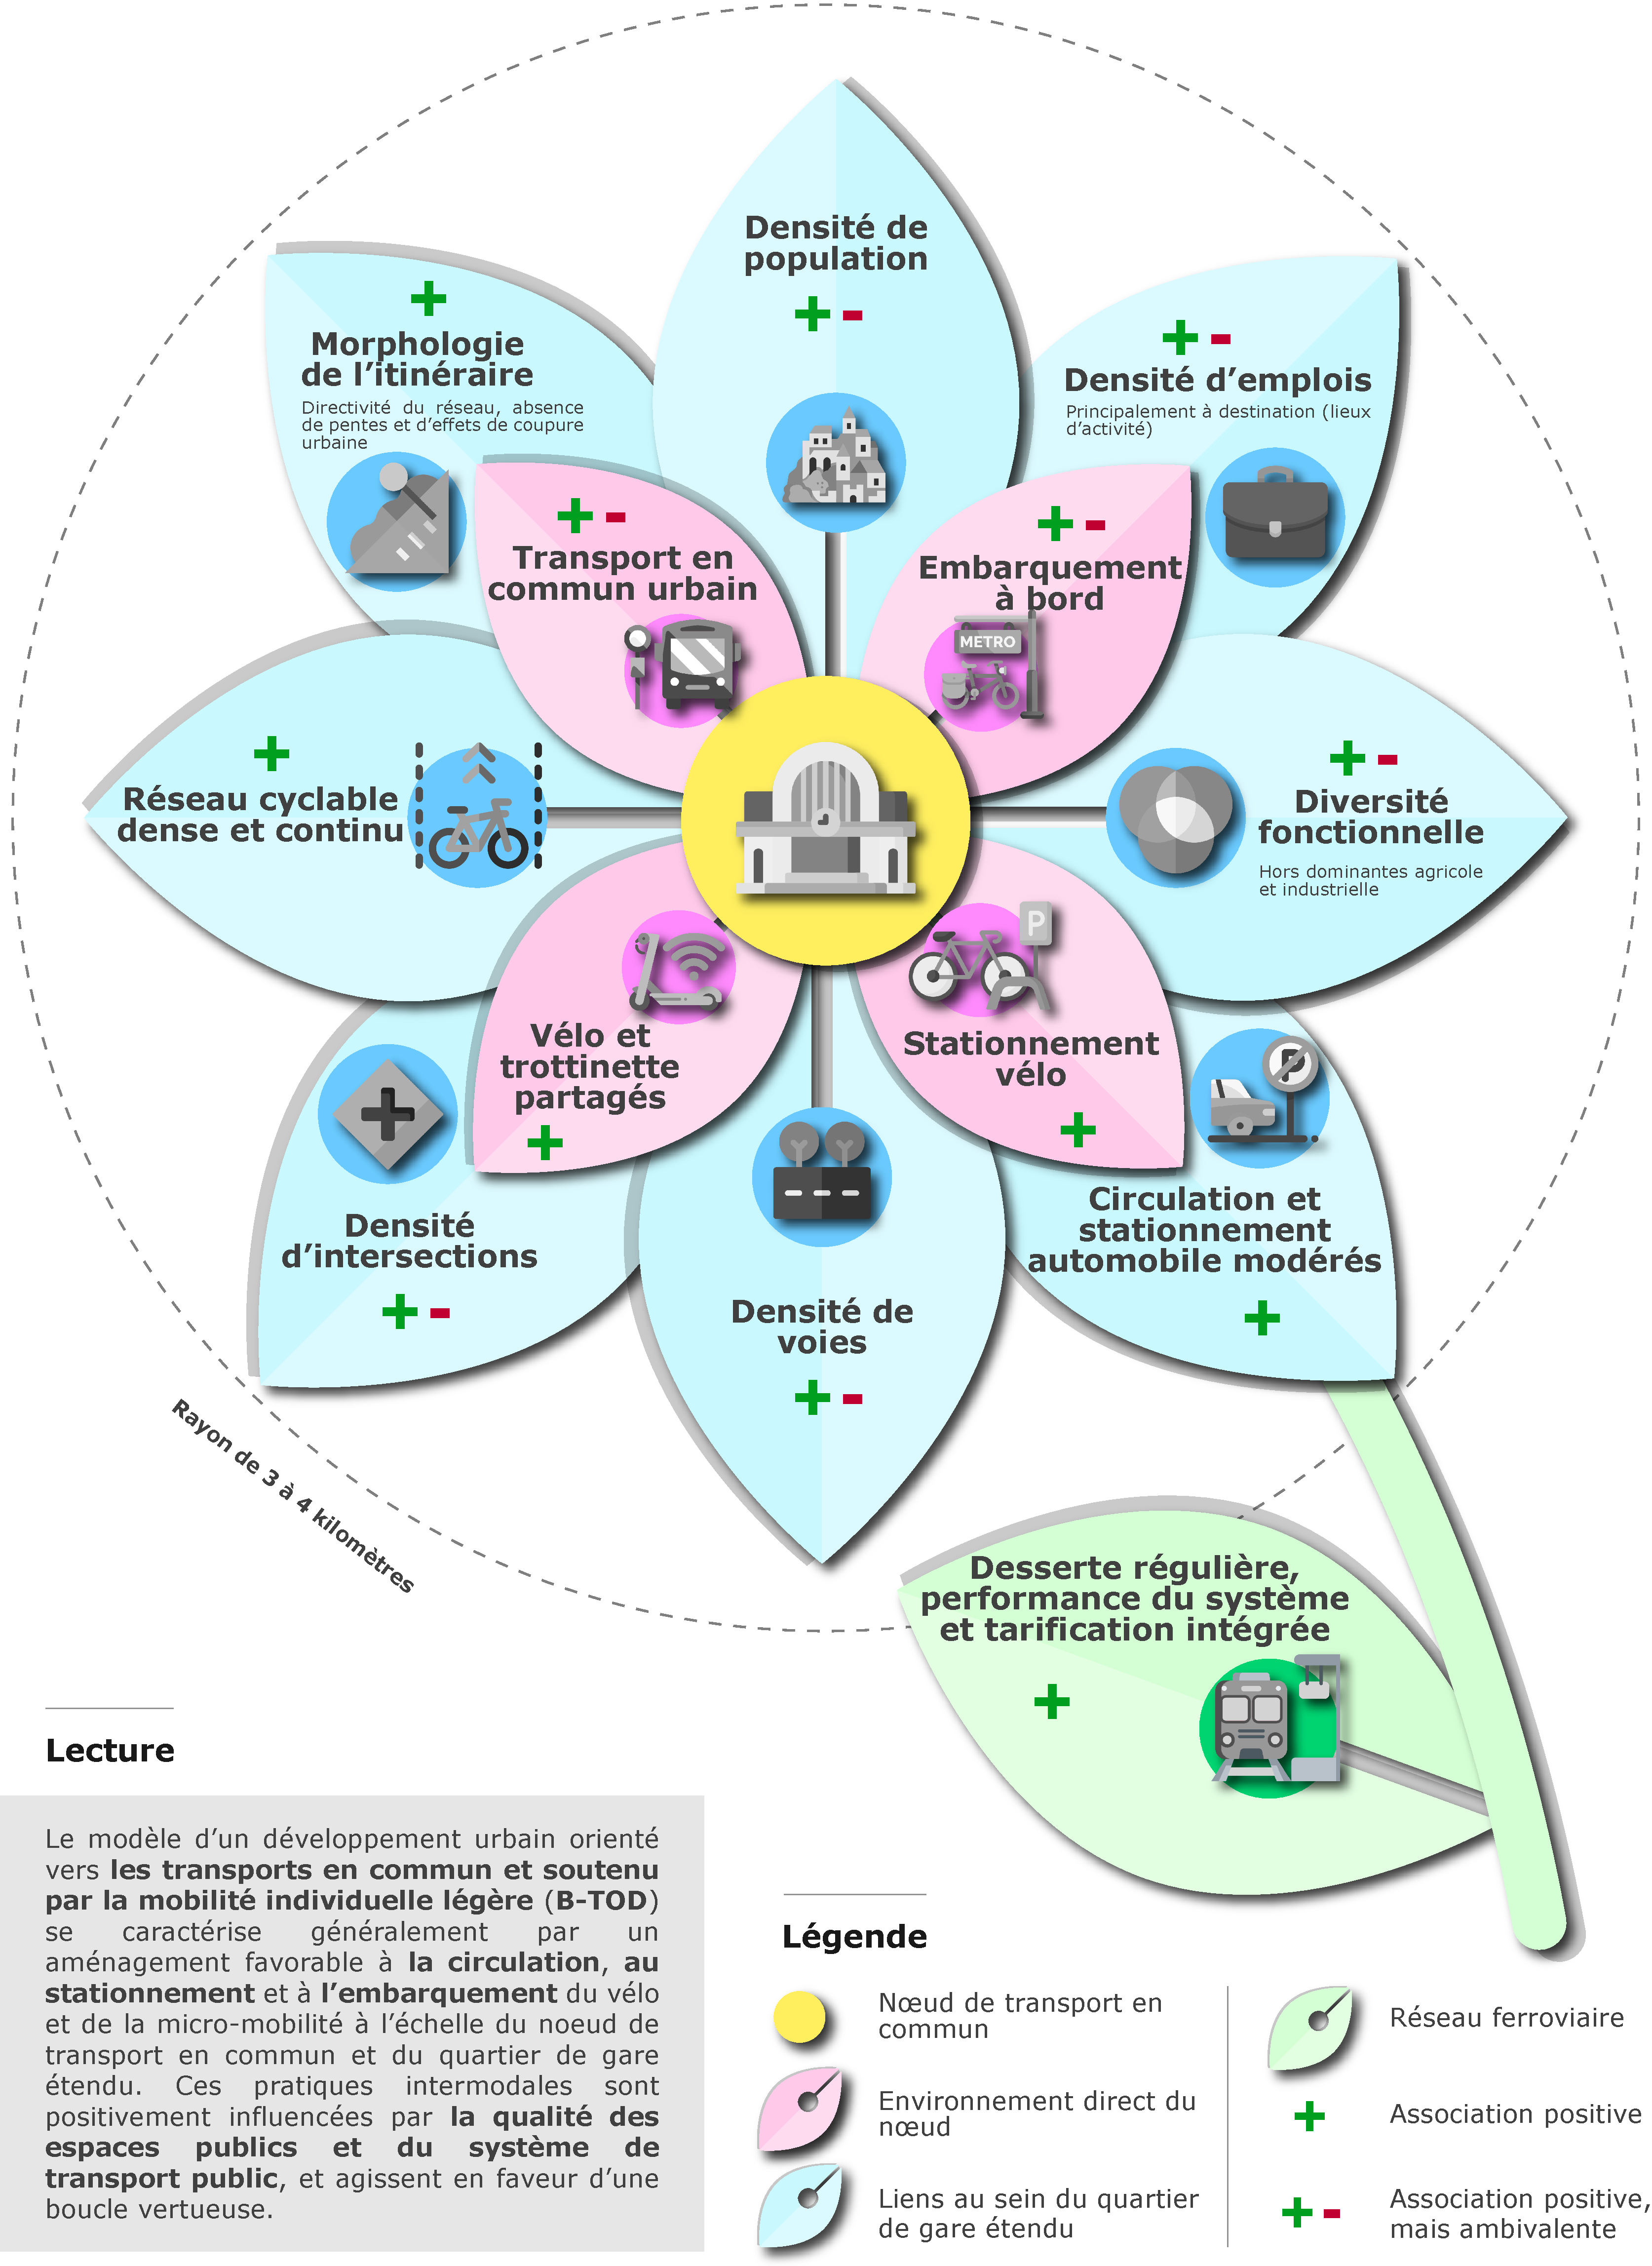
\includegraphics[width=1\columnwidth]{src/Figures/Chap-2/FR_RSL_Fleur_TOD.pdf}}
        \vspace{5pt}
        \begin{flushright}\scriptsize{
        Auteur~: \textcolor{blue}{Dylan Moinse (2023)}
        }\end{flushright}
    \end{figure}
    
    % Objectifs
En réponse aux questionnements de recherche formulés dans la \hyperref[chap2:formulation-questions-recherche]{sous-section~1.1} (page~\pageref{chap2:formulation-questions-recherche}), l'objectif de cette \acrshort{RSL} réside dans l'ambition d'approfondir et d'étendre la compréhension des connaissances relatives au \acrshort{M-TOD}. Ce travail a visé à identifier clairement les facteurs qui facilitent ou entravent l'adoption de ce modèle d'urbanisme. Dans cette perspective, l'analyse développée dans ce chapitre s'est appuyée sur un ensemble de six questions de recherche, qui ont constitué le cadre directeur de notre étude. Ces interrogations se concentrent sur l'interaction entre les dynamiques urbaines, les politiques publiques et leur rôle dans l'intégration de la mobilité individuelle légère au sein des systèmes de transport en commun, ainsi que sur l'influence de ces pratiques sur les configurations territoriales. L'examen détaillé de la littérature a mis en exergue l'importance capitale des \acrshort{7Ds} et des comportements de mobilité, offrant ainsi une perspective plus nuancée et détaillée de ces déplacements et de leurs implications bénéfiques dans l'élaboration d'un modèle urbain qui promeut un système de mobilité et d'urbanisme \gls{durable} et viable. Il est ressorti de cette étude que l'aire d'influence étendue des gares offre des gains d'accessibilité à un plus grand nombre de voyageur·se·s potentiel·le·s. De ce fait, nous pouvons nous référer à la notion de \Guillemets{potentiel d'accueil des territoires} \textcolor{blue}{\autocite[86]{kaufmann_retour_2014}}\index{Kaufmann, Vincent|pagebf} comme un élément moteur et soutenu par ces pratiques de mobilité, en lien avec les principes du \acrshort{TOD}. Pour conclure, la dernière question de recherche aborde les défis auxquels est confronté ce modèle d'urbanisme émergent, interrogeant notamment les lacunes actuelles dans la littérature scientifique face à une production récente des connaissances en lien avec le \acrshort{M-TOD}.%%Rédigé%%

    % 2.*.*.*
    \needspace{1\baselineskip} % Réserve de l'espace
\subsection*{Lacunes dans la littérature scientifique
    \label{chap2:literature-gap}
    }

    % Literature gap : état de la littérature
En guise de transition vers l'examen de notre matériau empirique, nous clôturons ce chapitre en soulevant les principaux enjeux qui nous paraissent encore peu abordés en relation avec le concept de \acrshort{M-TOD}. L'analyse bibliométrique opérée dans le cadre de notre \acrshort{RSL} a permis de mettre en évidence diverses lacunes se rapportant aux contours de notre sujet de recherche. Il convient de souligner, en premier lieu, une sous-représentation des recherches considérant certaines formes de mobilité individuelle légère. En dépit de l'intérêt croissant pour \acrshort{VLS}, le \acrshort{VFF} et la \acrshort{TEFF} depuis 2018, les études portant sur la trottinette et le vélo pliant, qu'ils soient électriques ou non motorisés, demeurent relativement rares. Cette observation s'accompagne d'une focalisation sur les systèmes de transport en commun urbains, laissant supposer un potentiel encore peu exploré du rôle des réseaux ferroviaires structurants à l'échelle régionale en association avec les nouvelles formes de mobilité. En outre, nous constatons que la littérature scientifique et technique s'attache peu à une approche systémique de l'ensemble du système de mobilité collective d'une zone géographique donnée, une démarche pourtant cruciale pour appréhender l'intermodalité-voyageur·se·s de manière systémique. De surcroît, le paysage scientifique actuel révèle un déséquilibre géographique, avec une prédominance des études ayant pour contexte géographique une agglomération internationale ou régionale en Chine, aux États-Unis et aux Pays-Bas. Finalement, l'examen des cadres géographiques étudiés révèle une tendance marquée à privilégier les échelles intercommunale et communale, tandis que les travaux de recherche adoptant une échelle régionale se révèlent être exceptionnels.%%Rédigé%%

    % Literature gap : concepts et méthodes
Au regard des cadres théoriques définis, nous avons pu identifier une disparité intéressante entre la mention fréquente et l'exploitation du concept de \acrshort{TOD} dans la littérature scientifique et la quasi-absence de sa réadaptation sous le nom de \acrshort{M-TOD}. En ce qui concerne les méthodes de recherche employées, nous notons une proportion majoritaire d'études prenant appui sur les bases de données ouvertes ou privées issues de l'\textsl{Open Data} et de la \textsl{Big Data}. Par ailleurs, les techniques d'enquête par questionnaire, entretien ou observation, généralement plus adaptées aux terrains de taille intermédiaire, sont néanmoins tout aussi présentes selon les contextes géographiques, notamment en Europe. Notons cependant l'insuffisance des approches qualitatives et plus largement des recherches mixtes, en particulier en ce qui concernant les options de mobilité individuelle légère émergentes. Le regard porté sur les méthodes d'analyse suggère une forte inclination pour l'emploi de la modélisation et des statistiques descriptives ainsi que pour l'usage du \acrshort{SIG}.%%Rédigé%%

    % Literature gap : résultats
L'analyse détaillée du corpus construit pour cette \acrshort{RSL} a révélé non seulement l'existence de disparités dans l'exploitation des \acrshort{7Ds} en lien avec le \acrshort{M-TOD}, mais a aussi conduit au développement de nouveaux questionnements issus de la confrontation des études empiriques :
    \begin{customitemize}
\item Quel est l'impact, direct ou indirect, de la densité démographique sur les configurations territoriales et les pratiques de mobilité favorisées par le modèle urbain du \acrshort{M-TOD}~?
\item La notion de mixité sociale est-elle complémentaire avec les principes promus par le \acrshort{M-TOD}~?
\item Les différentes formes de combinaison modale induisent-elles des besoins spécifiques en termes d'infrastructures et d'aménagements cyclables~?
\item Quels sont les gains d'accessibilité offerts par l'intégration de la mobilité individuelle légère au sein des systèmes de transport en commun~?
\item Comment l'aire d'influence des nœuds de transport en commun varie-t-elle en fonction de la nature des combinaisons modales, des différentes étapes du déplacement intermodal, ainsi que des facteurs environnementaux et socio-démographiques~?
\item Dans quelle mesure la performance des réseaux de transport en commun et la gestion de l'espace dédié à l'automobile contribuent-elles à une meilleure articulation entre formes urbaines et comportements de mobilité~?
\item Le \acrshort{M-TOD} peut-il être considéré comme un facteur exacerbant les inégalités d'accès à la mobilité~?
\item Ce modèle urbain peut-il intégrer la mobilité liée aux loisirs, aux rencontres sociales ou aux promenades (\textsl{undirected travel})~?
\item La démocratisation de l'adoption de la mobilité individuelle légère en intermodalité peut-elle former un cercle vertueux influençant les formes urbaines, lesquelles, à leur tour, modèlent les comportements de mobilité~?
    \end{customitemize}%%Rédigé%%

    % Enjeux
Au gré des défis soulevés par la littérature scientifique concernant la conception d'un système urbain orienté vers le développement des réseaux de transport en commun hybridé à l'intégration de la mobilité individuelle légère, la thèse de doctorat aspire à mieux saisir les clés de compréhension du concept de \acrshort{M-TOD}. Le présent chapitre a souligné la nécessité d'élargir le champ de recherche à ce sujet pour inclure une variété accrue de formes de mobilité et de niveaux d'analyse géographique, dans le but d'enrichir notre appréhension de cette stratégie d'aménagement, réinterprétée sous l'angle de la mobilité individuelle légère. Ces observations nous conduisent à une réflexion sur l'adoption d'une approche géostatistique conjuguée à une démarche qualitative susceptibles de livrer des perspectives plus nuancées sur les comportements et les expériences de mobilité des individus.%%Rédigé%%

    % Structure de la thèse
Dans cette perspective, notre recherche doctorale s'articule autour de l'exploration d'un espace géographique européen à une échelle régionale, avec un intérêt particulier porté sur l'ensemble du réseau de mobilité, essentiellement structuré autour des réseaux ferroviaires. Le prochain \hyperref[chap3:titre]{chapitre} (page~\pageref{chap3:titre}) sera consacré à la délimitation du périmètre géographique de l'étude et à la présentation de notre méthodologie, laquelle se compose d'une enquête de terrain. L'objectif de cette démarche mixte est de saisir le développement des pratiques intermodales qui associent l'usage des transports en commun et des options émergentes de mobilité individuelle légère, et de les examiner sous l'angle des comportements de mobilité et de leurs interactions avec l'environnement urbain (voir le \hyperref[chap4:titre]{chapitre~4}, page~\pageref{chap4:titre}). La détermination d'un groupe social de cyclo-voyageur·se·s activement présent dans les divers territoires examinés nous permettra d'interroger leurs interactions dans le contexte de quartiers de gare élargis, en mobilisant la notion d'accessibilité intermodale (voir le \hyperref[chap5:titre]{chapitre~5}, page~\pageref{chap5:titre}). Cette approche géographique des distances nous conduira à proposer un modèle fondé sur un indice nœud-lieu (\textsl{Node-Place Index}), visant à évaluer le potentiel de développement urbain en synergie avec un système de mobilité alternative à l'échelle régionale, dans le \hyperref[chap6:titre]{chapitre~6} (page~\pageref{chap6:titre}).%%Rédigé%%

% ___________________________________________
     \newpage
     
% Valorisation scientifique
    \begin{tcolorbox}[colback=white!5!white,
                      colframe=blue!75!blue,
                      title=Valorisation scientifique
                      \\
                      Chapitre~2]
\Large{\textbf{\textcolor{blue}{Chapitre d'ouvrage collectif~:}}}
    \\\\
\small{\textcolor{blue}{\textcite{moinse_systematic_2023}}\index{Moinse, Dylan|pagebf}. \foreignlanguage{english}{\textsl{A Systematic Literature Review on Station Area Integrating Micromobility in Europe: A 21\textsuperscript{st} Century Transit-Oriented Development}}. In: Belaïd,~F., Arora,~A. (eds) \textsl{Smart Cities. Studies in Energy, Resource and Environmental Economics}. Springer, Cham. ISBN: 978-3-031-35663-6 (p.~171-204).
\\
\footnotesize{\url{https://doi.org/10.1007/978-3-031-35664-3_12}} (\textbf{OS})}
    \end{tcolorbox}

    % ___________________________________________
    % Sous-bibliographie
    \newpage
    \sectionheader{Sous-bibliographie du chapitre~2}
    \begingroup
    \renewcommand{\bibfont}{\scriptsize}
\printbibliography[segment=\therefsegment, heading=subbibintoc, title={Sous-bibliographie du chapitre~2}, label=chap2:bibliographie]
    \endgroup
    \end{refsegment}

%% ______________________________ %%
% CHAPITRE 3
%------------------------------%
%% ✎ Dylan (V1) %%%%%%%%% ✅ %%
%% ✎ Alain (V2) %%%%%%%%% ✅ %%
%% ✎ Dylan (V3) %%%%%%%%% ✅ %%
%------------------------------%

%%%%%%%%%%%%%%%%%%%%%%%%%%%%%%%%
% chapitre~3
\chapterheader{Méthodologie de la recherche doctorale}
\chapter
{Une \Guillemets{enquête sur-mesure} dans les Hauts-de-France
    \label{chap3:titre}
    }
    \begin{refsegment}

    % Arrière-plan chapitre~3
    \AddToShipoutPictureBG*{%
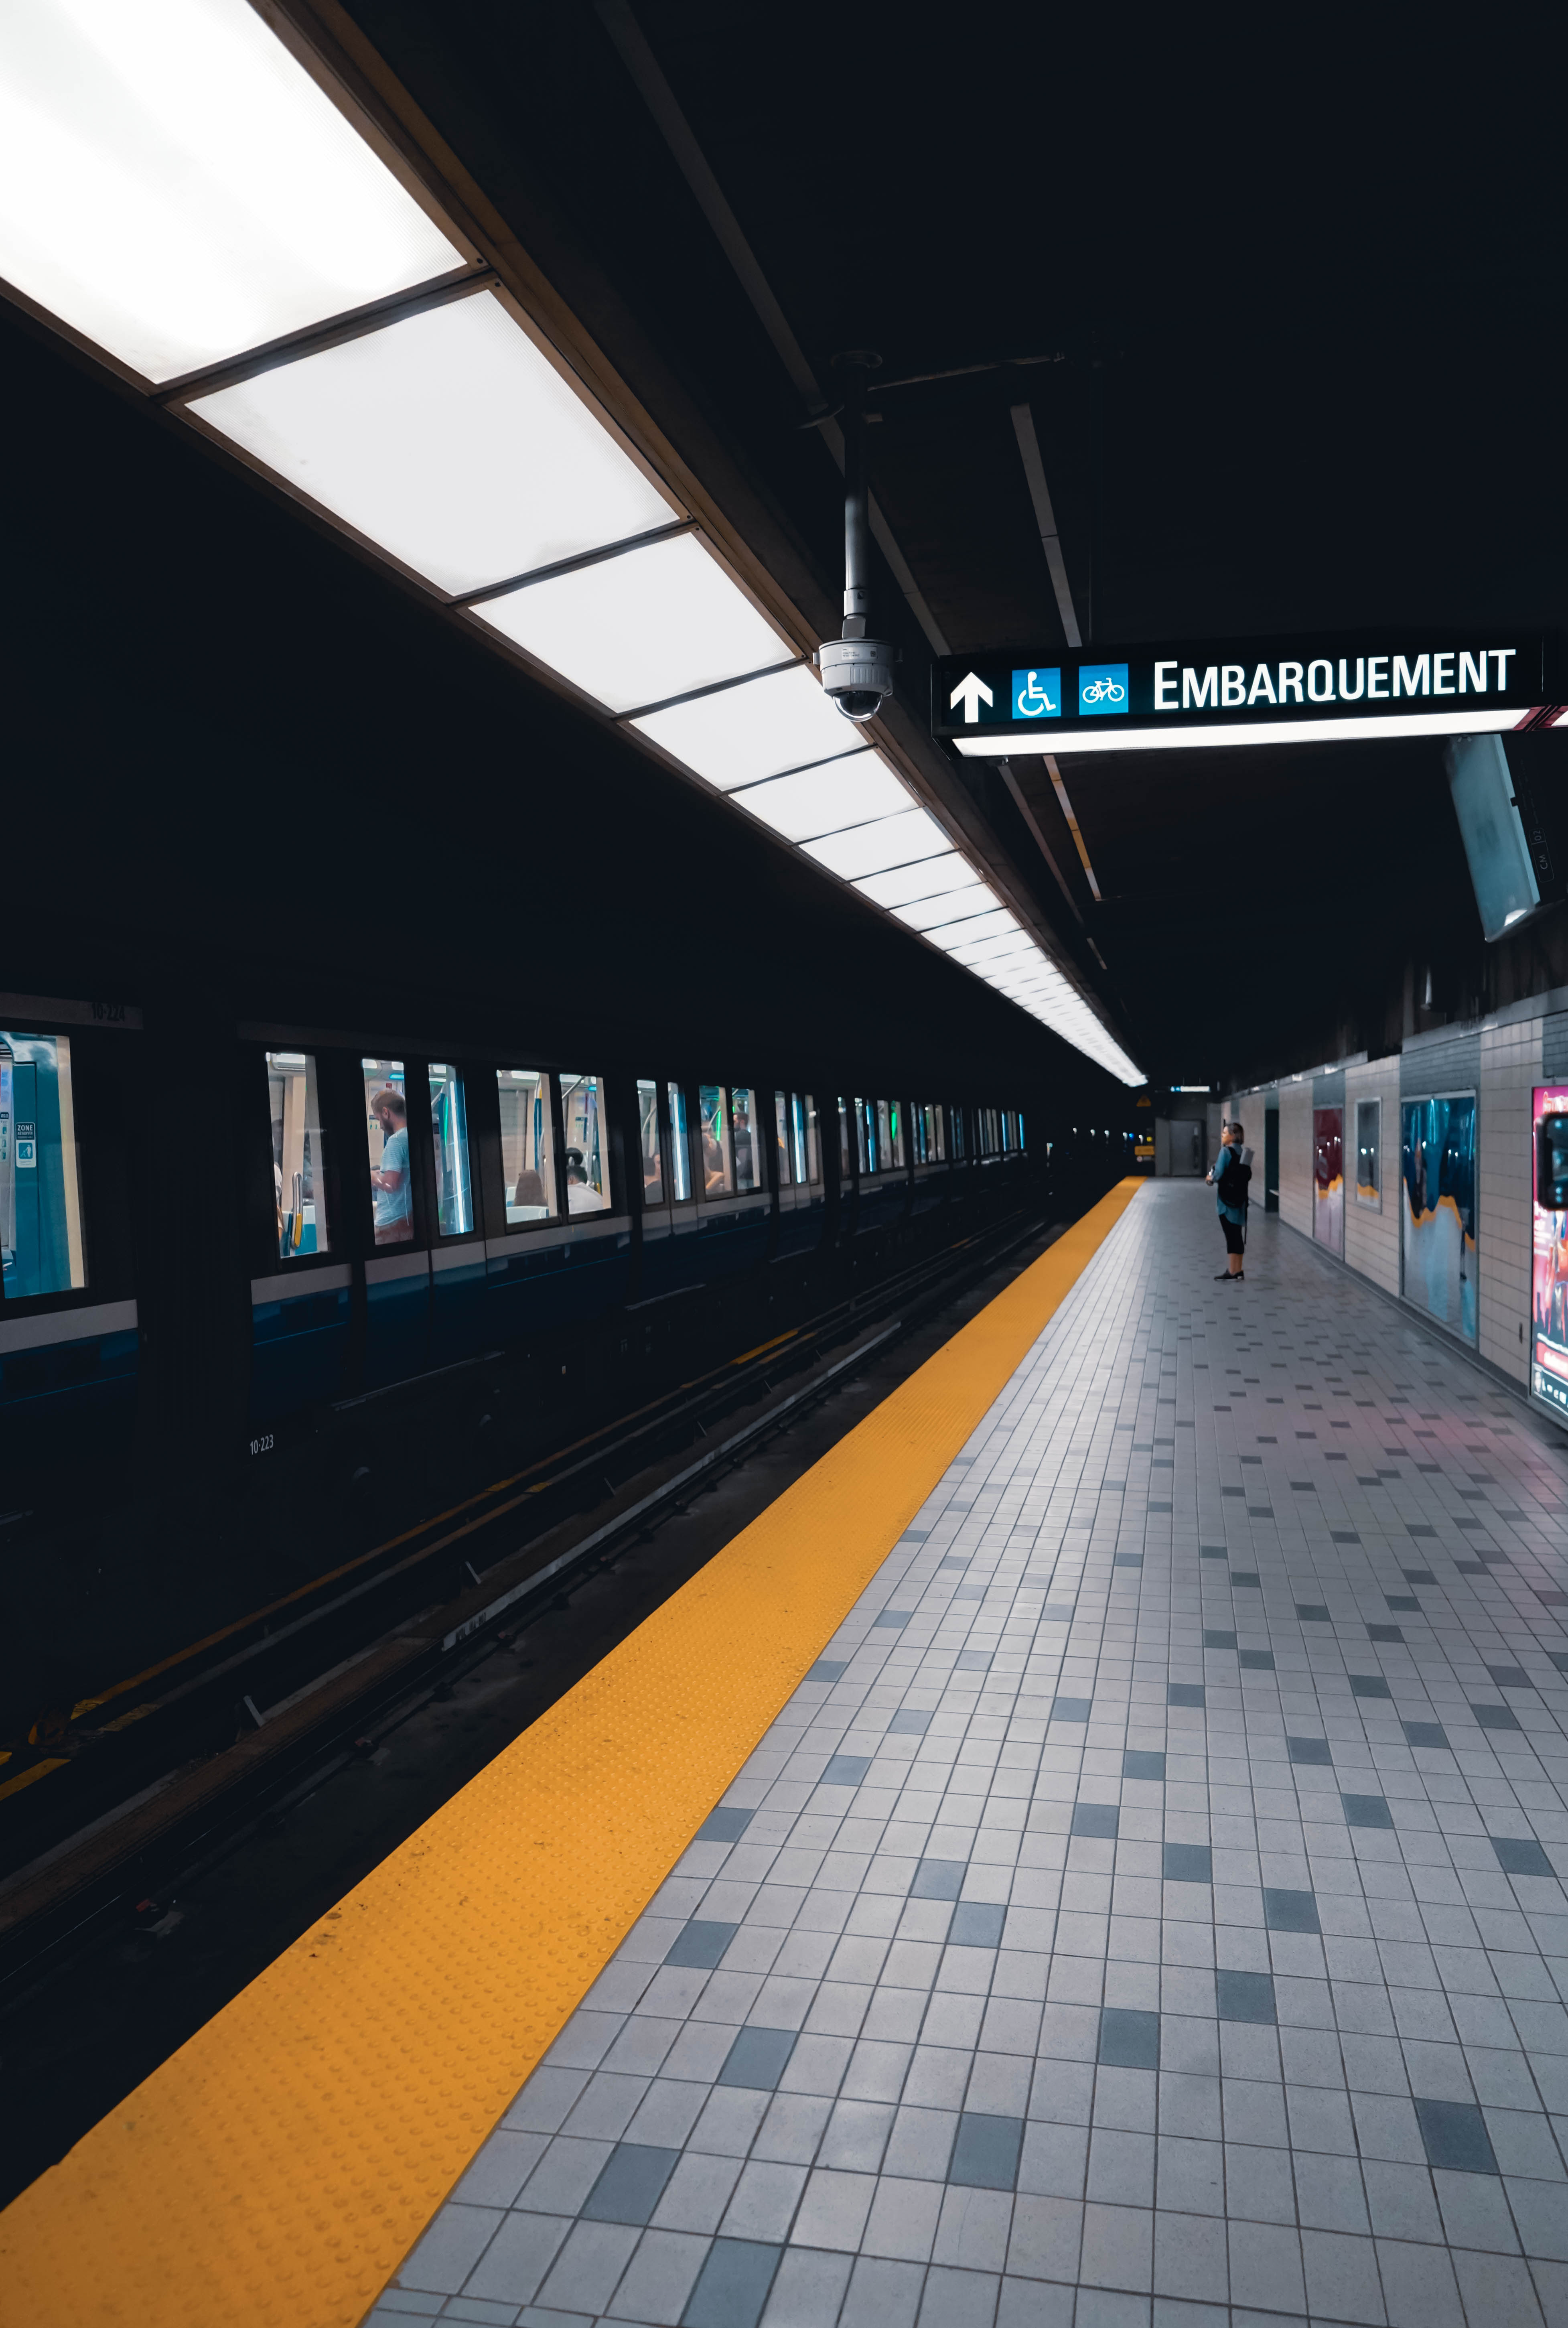
\includegraphics[width=\paperwidth,height=\paperheight]{src/Figures/Arriere_plan/Arriere_plan_Chap_3.jpg}
    }

% Rectangle
\AddToShipoutPictureBG*{
  \begin{tikzpicture}[remember picture,overlay]
    \node[fill=white, opacity=0.75, text width=\paperwidth, minimum height=7cm, anchor=north] 
    at ([yshift=-2cm]current page.north) {};
  \end{tikzpicture}
}

% Source
\AddToShipoutPictureFG*{
  \AtPageLowerRight{
    \raisebox{1cm}{
      \hspace{16cm}
      
\begin{tikzpicture}
        \node[fill=white, rounded corners=5pt, inner sep=5pt, align=center] {
          \tiny{Photographie~: \textcolor{blue}{Dylan Moinse (2022)}}
        };
      \end{tikzpicture}
    }
  }
}

    % ___________________________________________
    % Mini-sommaire
    \cleardoublepage
    \setcounter{tocdepth}{2}
    % Redéfinir le titre de la table des matières locale
    \renewcommand{\localcontentsname}{Table des matières du chapitre~3}
\localtableofcontents

% Réinitialiser numérotation section
\setcounter{section}{0}

    % ___________________________________________
    % Graphical abstract
    \newpage
\section*{Points clés du chapitre~3
    \label{chap3:graphical-abstract}
    }
    \markright{Préambule du chapitre}{}

\begin{figure}[h!]\vspace*{4pt}
        \caption*{}
        \label{graphical-abstract-chap3}
        \centerline{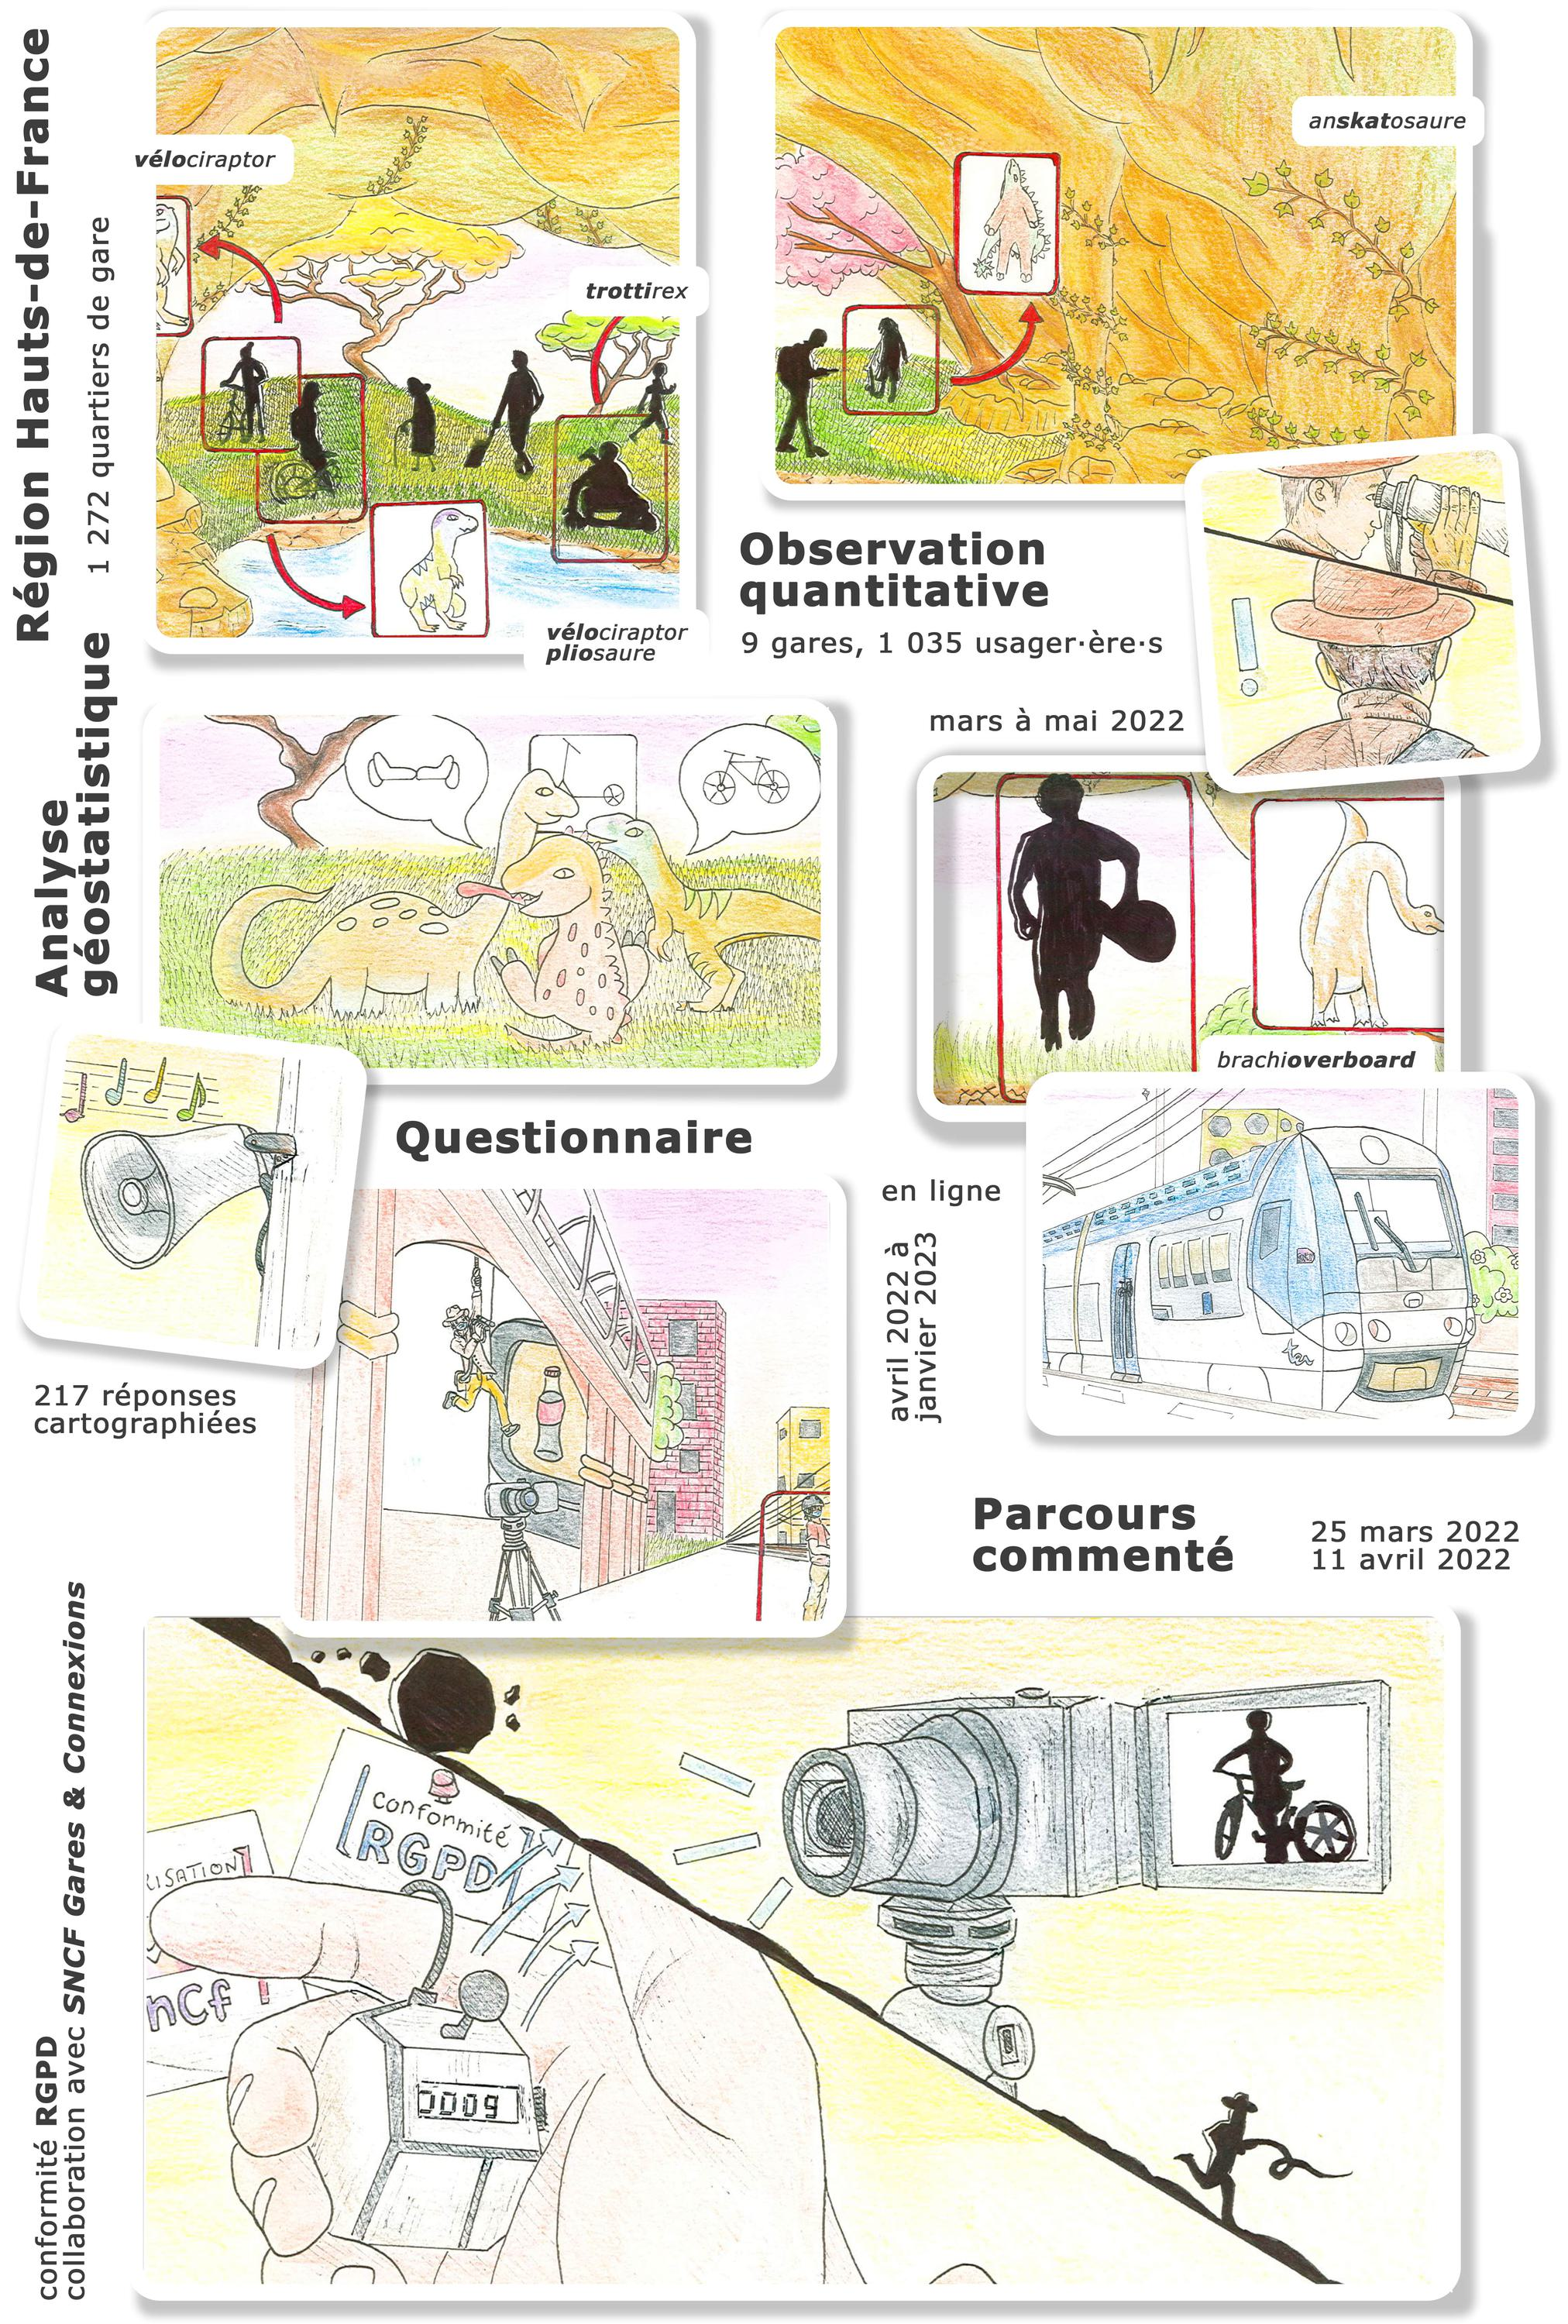
\includegraphics[width=1\columnwidth]{src/Figures/Graphical-abstract/FR_Graphical_abstract_chap3.jpg}}
        \vspace{5pt}
        \begin{flushright}\scriptsize{
        Source~: \textcolor{blue}{Morgan Moinse (2022)}
        }\end{flushright}
    \end{figure}

    % ___________________________________________
    % Préambule
    \newpage
    \begin{tcolorbox}[colback=white!5!white,
                      colframe=blue!75!blue,
                      title=
                      \bigskip
                      \center{\textbf{Préambule du chapitre~3}}
                      \\
                      \raggedright{\small{Chapitre composé de \pagedifference{chap3:titre}{part1:conclusion} pages, dont \pagedifference{chap3:bibliographie}{part1:conclusion} pages de bibliographie}}
                      \bigskip]
\Large{\textcolor{blue}{\textbf{Résumé~:}}}
    \\
    \small{
Ce chapitre présente la méthodologie développée pour enquêter sur les pratiques intermodales qui se déploient dans les quartiers de gare de la région des Hauts-de-France. En partant d'une contextualisation de notre étude de cas croisée à la description de nos recherches mixtes, nous avons cherché à concevoir une méthodologie basée sur une approche multidimensionnelle et multiscalaire. Structuré en cinq sections, le présent chapitre aborde successivement la définition du périmètre géographique, la projection spatiale des quartiers de gare ainsi que la mise en application d'une enquête croisant l'observation quantitative, l’administration d'un questionnaire et le parcours commenté.%%Rédigé%%
    \\
La première section établit les limites géographiques de l’étude et justifie le choix de la région Hauts-de-France comme cadre d’analyse (voir la \hyperref[chap3:region-hauts-de-france]{section~1}, page~\pageref{chap3:region-hauts-de-france}). Ce choix s’appuie sur son maillage ferroviaire dense et sa structure \textsl{a priori} polycentrique, bien qu’elle soit confrontée à des défis majeurs en matière de mobilité. Une attention particulière est portée à la posture réflexive du·de la chercheur·se et aux questions éthiques.%%Rédigé%%
    \\
Les quartiers de gare sont définis comme des unités spatiales théoriquement accessibles à pied ou à l'aide de la mobilité individuelle légère (voir la \hyperref[chap3:quartiers-gare]{section~2}, page~\pageref{chap3:quartiers-gare}). Une démarche spécifique, intégrant des critères spatiaux comme les distances acceptables et les caractéristiques de l’environnement urbain, est employée pour délimiter et cartographier ces zones d’influence. Cette approche permet d’examiner la configuration spatiale et fonctionnelle de ces espaces stratégiques grâce à des outils géostatistiques.%%Rédigé%%
    \\
Dans la troisième section, l’accent est mis sur l’observation quantitative des voyageur·se·s en gare, et plus particulièrement sur les usager·ère·s de la mobilité individuelle légère, souvent sous-représenté·e·s dans les enquêtes publiques (voir la \hyperref[chap3:observation-quantitative]{section~3}, page~\pageref{chap3:observation-quantitative}). Le protocole méthodologique, combinant comptage et observation ethnographique, est détaillé à travers des grilles d’observation appliquées dans neuf gares sélectionnées.%%Rédigé%%
    \\
La quatrième section traite de la conception et de l’administration d’un questionnaire destiné aux voyageur·se·s intermodaux·les (voir la \hyperref[chap3:questionnaire]{section~4}, page~\pageref{chap3:questionnaire}). Elle met en avant l’intérêt de cet outil pour collecter des données sur les pratiques de déplacement, les perceptions et les besoins exprimés. La structure du questionnaire, les étapes d’échantillonnage et la validation des réponses y sont détaillées, facilitant la mise en relation des déplacements déclarés avec les analyses géostatistiques et comportementales.%%Rédigé%%
    \\
Pour conclure, la cinquième section introduit l’approche des parcours commentés, une méthode qualitative menée \textsl{in situ}, permettant d’explorer les expériences des usager·ère·s en mouvement (voir la \hyperref[chap3:parcours-commente]{section~5}, page~\pageref{chap3:parcours-commente}). Elle vise à approfondir la compréhension des mécanismes de choix modal et des usages des infrastructures, sous l'angle de comptes rendus micro-géographiques.%%Rédigé%%
    }
    \tcblower
\Large{\textcolor{blue}{\textbf{Mots-clés~:}}}
    \\
    \small{
Analyse géostatistique~;
Hauts-de-France~;
Méthodes mixtes~;
Observation quantitative~;
Terrain de recherche~;
Parcours commentés~;
Questionnaire~;
Quartiers de gare
    }
    \end{tcolorbox}

    % ___________________________________________
    % 3.*.
    \newpage
    \needspace{1\baselineskip} % Réserve de l'espace
    \addcontentsline{toc}{section}{Introduction du chapitre~3}
    \sectionheader{Introduction du chapitre}
\section*{Introduction du chapitre~3
    \label{chap3:introduction}
    }
    \markright{Introduction du chapitre~3}{}

    % Citation
\begin{displayquote}
\Guillemets{[\dots] \textsl{par des processus créatifs (méthodes ad hoc) ou des synergies (entre méthodes déjà existantes), on parvient à affiner la qualité de l’observation, puis de l’analyse, selon le cas, d’une catégorie de comportements de déplacement quotidien ou de l’éventail des usages d’un réseau de transport. Les contributions témoignent de l’intérêt des chercheurs pour les questions de mobilité et de la grande créativité dont ils font preuve pour la saisir.} [\dots] \textsl{Pour le comprendre, l’analogie avec le microscope paraît assez parlante. Selon la focale qu’il choisit, l’image qu’un laborantin voit se former dans le microscope est à chaque fois différente. Il observe pourtant toujours la même réalité, mais à des échelles différentes ou, plus exactement, d’un point de vue différent. Ni l’une ni l’autre des images obtenues n’est plus vraie qu’une autre, mais elles rendent compte d’un regard différent sur la réalité.} [\dots] \textsl{Si la complémentarité des travaux de recherche quantitatifs et qualitatifs est louée de manière récurrente tel un idéal incantatoire, jusqu’à ce jour, peu de chercheurs la pratiquaient dans les faits.} [\dots] \textsl{Les innovations et hybridations méthodologiques renvoient de manière assez directe à la question des pratiques professionnelles des chercheurs. Nombreux sont, du reste, les articles à y faire référence explicitement. Ces innovations et hybridations sont le plus souvent réalisées en équipe, dans lesquelles chacune et chacun apporte ses pratiques, ses savoir-faire et ses compétences méthodologiques ou disciplinaires. Ce travail collectif, qui se reflète dans les contributions rassemblées ici, écrites pour la plupart par plusieurs auteurs, nécessite du temps et de la coordination pour partager les savoir-faire et les mettre en œuvre autour d’un dispositif opérationnalisable. Il nécessite également de l’audace et de la créativité pour pousser la porte de l’expérimentation et suffisamment de confiance, mais aussi d’humilité pour (re)connaître les valeurs et les limites de chaque méthode. Enfin, il suppose une capacité d’adaptation, de remise en question sous l’effet de stimulations multiples venues d’autres approches scientifiques, d’autres points de vue professionnels ou encore d’autres innovations venues des usages. Les innovations et hybridations méthodologiques apparaissent alors comme le reflet des capacités créatives des hommes, de leurs sociétés et de leurs territoires. C’est certainement dans ce travail créatif et fortement collaboratif que se nichent les innovations scientifiques de demain.}}

\textcolor{blue}{Joël} \textcolor{blue}{\textcite[12-14, 160]{meissonnier_connaissance_2020}}\index{Meissonnier, Joël|pagebf}\index{Vincent, Stéphanie|pagebf}\index{Rabaud, Mathieu|pagebf}\index{Kaufmann, Vincent|pagebf}. \textsl{Connaissance des mobilités~: hybridation des méthodes, diversification des sources}, Éditions du Cerema, Lyon, 176~p. ISBN~: \href{https://search.worldcat.org/fr/title/1236011015}{978-2-37180-423-4}
    \end{displayquote}

    % Introduction
\lettrine[lines=3, findent=8pt, nindent=0pt]{\lettrinefont L}{a} structuration de notre enquête repose sur l’observation des usages et l’explication des pratiques intermodales, avec une approche territoriale centrée sur la gare et son environnement, entendue comme l'interaction des dimensions environnementales, sociales et bâties dans un même système urbain, en référence à la notion d'\Guillemets{interconnexion des gares} \textcolor{blue}{\autocite[7]{moretti_interconnexion_1999}}\index{Moretti, Anna|pagebf}\index{Vacheret, Guy|pagebf}. Pour ce faire, notre méthodologie visant à étudier les gares, leur environnement et les usages qui s'y déploient privilégie une approche multidimensionnelle et multiscalaire. Cette démarche relationnelle articule trois niveaux d’observation~: (i) une logique relationnelle, axée sur la fonction de connexion des nœuds du réseau, (ii) une logique territoriale, portant sur les activités humaines polarisées et (iii) une logique d'usage, liant l'espace aux comportements des populations qui fréquent ces nœuds \textcolor{blue}{\autocites[9]{moretti_interconnexion_1999}[210-212]{menerault_gares_2001}}\index{Menerault, Philippe|pagebf}\index{Barré, Alain|pagebf}\index{Moretti, Anna|pagebf}\index{Vacheret, Guy|pagebf}. Notre ambition est ainsi de capturer le \Guillemets{système d’accessibilité territoriale} dans sa complexité, en intégrant l’\gls{accessibilité} \textsl{du} territoire et l’accessibilité \textsl{au} territoire, définies respectivement comme le potentiel spatial et social, et les interactions entre ces deux dimensions, structurées par la configuration de l'espace géographique et les caractéristiques des groupes sociaux \textcolor{blue}{\autocite[6]{richer_mesurer_2012}}\index{Richer, Cyprien|pagebf}\index{Palmier, Patrick|pagebf}. Nous avons alors mis à profit les atouts des approches quantitatives et qualitatives pour concevoir un cadre méthodologique intégré \textcolor{blue}{\autocite[]{bergman_advances_2008}}\index{Richer, Cyprien|pagebf}.%%Rédigé%%

    % Méthodes mixtes
Plutôt que de les opposer, les méthodes d’analyse des déplacements, qu’elles soient quantitatives ou qualitatives, gagneraient à être envisagées dans une logique de complémentarité \textcolor{blue}{\autocite[6]{klein_mobilites_2007}}\index{Klein, Olivier|pagebf}\index{Ortar, Nathalie|pagebf}\index{Pochet, Pascal|pagebf}. Un tel mode opératoire implique un partage disciplinaire davantage centré sur les objets d’étude. À cet égard, \textcolor{blue}{\textcite[4]{higgins_forty_2016}}\index{Higgins, Christopher~D.|pagebf}\index{Kanaroglou, Pavlos~S.|pagebf} soulignent tout l’intérêt d’un croisement entre les approches \Guillemets{normatives}, consistant à qualifier les types de \acrshort{TOD}, et les approches \Guillemets{positives} systématiques. C’est dans ce contexte que se justifie l’association de techniques méthodologiques variées que nous avons mise en œuvre, incluant l’exploitation de bases de données existantes conjuguée à des séances d’observation, à des enquêtes par questionnaire et à des entretiens \textsl{sur le terrain} \textcolor{blue}{\autocite[128]{dureau_lobservation_2014}}\index{Dureau, Françoise|pagebf}\index{Giroud, Matthieu|pagebf}\index{Lévy, Jean-Pierre|pagebf}. L’objectif de ces méthodes mixtes, d’un point de vue conceptuel, est de proposer une base exploratoire à partir de \textsl{l'action saisie} par l'intermédiaire de l'observation. Cette étape permet de concevoir et d'ajuster un questionnaire recueillant ce qui est \textsl{signifié}. Des réponses rapportées qui sont à leur tour interrogées au travers d'entretiens saisissant l'expérience telle qu'elle est \textsl{vécue et perçue} \textcolor{blue}{\autocite[215]{paugam_enquete_2012}}\index{Paugam, Serge|pagebf}.%%Rédigé%%

    % Description méthodes
Le croisement d’une enquête \Guillemets{sur-mesure}, intégrant une observation quantitative, un questionnaire et des parcours commentés destinés aux cyclo-voyageur·se·s, vise à fournir une perspective globale sur un sujet encore peu documenté par des données empiriques (pour rappel, voir le \hyperref[fig-introduction:methodes-hypotheses]{schéma~\ref{fig-introduction:methodes-hypotheses}}, au sein de l'\hyperref[introduction-generale:methodologie]{introduction générale}, page~\pageref{fig-introduction:methodes-hypotheses}). \textcolor{blue}{Joël} \textcolor{blue}{\textcite[24]{meissonnier_pour_2012}}\index{Meissonnier, Joël|pagebf}, autant que \textcolor{blue}{Karel} \textcolor{blue}{\textcite[291]{martens_bicycle_2004}}\index{Martens, Karel|pagebf} pour l'usage combiné du \gls{vélo} et du transport public, insistent sur l’importance de reconnaître les limites des enquêtes quantitatives classiques, à l'image de l’\acrfull{EMD}, lorsqu’il s’agit de rendre compte des dynamiques de mobilité quotidienne, et plus encore des chaînes de déplacement \textcolor{blue}{\autocite[10]{kieffer_chainage_2011}}\index{Kieffer, Lionel|pagebf}\index{Oliveau, Sébastien|pagebf}\index{Audard, Frédéric|pagebf}. Cela demande de repenser l'approche en enrichissant les bases de données actuelles grâce à des enquêtes de terrain adaptées aux exigences de notre problématique de recherche. Cette démarche s’appuie sur des travaux préexistants qui ont ouvert la voie et inspiré notre méthodologie. Par exemple, \textcolor{blue}{François de} \textcolor{blue}{\textcite[42]{singly_questionnaire_2016}}\index{Singly, François de|pagebf} souligne l’intérêt, en sciences sociales, de combiner le questionnaire, qui rend visibles les déterminants sociaux des trajectoires, avec les entretiens, qui éclairent sur le processus de construction individuelle de ces trajectoires. Ainsi, plusieurs études ont démontré l’intérêt de mobiliser une méthodologie mixte articulant observation directe, questionnaire et entretiens \Guillemets{mobiles} \textcolor{blue}{\autocites[258]{greene_toward_1989}[120]{bergeron_uncovering_2014}[3]{despres_replacer_2019}}\index{Greene, Jennifer~C.|pagebf}\index{Caracelli, Valerie~J.|pagebf}\index{Graham, Wendy~F.|pagebf}\index{Bergeron, Julie|pagebf}\index{Paquette, Sylvain|pagebf}\index{Poullaouec-Gonidec, Philippe|pagebf}\index{Desprès, Michel|pagebf}\index{Lord, Sébastien|pagebf}\index{Negron-Poblete, Paula|pagebf}.%%Rédigé%%

    % Annonce du plan 1
La première partie du présent chapitre porte sur la délimitation du terrain géographique, envisagée sous un prisme macroscopique (\hyperref[chap3:region-hauts-de-france]{section~1}, page~\pageref{chap3:region-hauts-de-france}). Cette démarche vise à justifier la pertinence d’une perspective régionale en présentant les enjeux de mobilité ainsi que les documents stratégiques établis par l’autorité administrative compétente (\hyperref[chap3:regard-privilegie-region-hdf]{sous-section~1.1}, page~\pageref{chap3:regard-privilegie-region-hdf}). Dans un second temps, un exercice d’auto-analyse sociologique sera mené afin d’objectiver notre positionnement vis-à-vis du terrain, compris à la fois comme sujet de recherche et contexte géographique (\hyperref[chap3:auto-analyse-sociologique]{sous-section~1.2}, page~\pageref{chap3:auto-analyse-sociologique}). La description du périmètre géographique dans lequel s’inscrit notre matériau empirique se conclura par notre mise en relation avec le gestionnaire principal de mobilité et par la mise en conformité de nos méthodes d’enquête avec les principes de l’éthique de la recherche (\hyperref[chap3:preparation-terrain-geographique]{sous-section~1.3}, page~\pageref{chap3:preparation-terrain-geographique}).%%Rédigé%%

    % Annonce du plan 2
Une fois le cadre géographique introduit, nous nous attacherons à détailler le processus de spatialisation des quartiers de gare, entendus comme unités spatiales accessibles à pied et en mobilité individuelle légère, dans une perspective microscopique (\hyperref[chap3:quartiers-gare]{section~2}, page~\pageref{chap3:quartiers-gare}). Nous définirons les règles méthodologiques permettant de cartographier ces aires d’influence, en nous basant sur les distances jugées acceptables et sur la typologie des gares dressée, telles qu’elles auront été déterminées grâce à notre enquête de terrain (\hyperref[chap3:quartiers-gare-distances]{sous-section~2.1}, page~\pageref{chap3:quartiers-gare-distances}). Une fois les tailles des quartiers de gare définies, notre attention se portera sur leurs formes et leurs contours, influencées par les caractéristiques de l’environnement bâti. Cette étape inclura une réflexion sur les méthodes employées pour générer et représenter ces formes (\hyperref[chap3:quartiers-gare-formes]{sous-section~2.2}, page~\pageref{chap3:quartiers-gare-formes}). Pour clore cette section, nous présenterons les principes d’extraction et de traitement des données géostatistiques que nous nous serons fixés. Nous exposerons les critères retenus pour exploiter les bases de données, en nous efforçant d'obtenir un degré de résolution élevé de l'information géographique (\hyperref[chap3:quartiers-gare-analyse-geostatistique]{sous-section~2.3}, page~\pageref{chap3:quartiers-gare-analyse-geostatistique}).%%Rédigé%%

    % Annonce du plan 3
La troisième section de notre chapitre méthodologique sera consacrée à la description de l’approche par observation quantitative des cyclo-voyageur·se·s, dans l’objectif de dresser un panorama général et d’évaluer les tendances actuelles, alors encore peu documentées (\hyperref[chap3:observation-quantitative]{section~3}, page~\pageref{chap3:observation-quantitative}). Premièrement, nous définirons ce qu’est une observation quantitative, en explicitant son adéquation avec certains de nos objectifs de recherche (\hyperref[chap3:observation-quantitative-outil-adapte]{sous-section~3.1}, page~\pageref{chap3:observation-quantitative-outil-adapte}). Ensuite, nous détaillerons le protocole méthodologique de notre démarche mêlant comptage et observation ethnographique. Nous présenterons à cette occasion la grille d’observation utilisée et les modalités de sa mise en application (\hyperref[chap3:methodologie-observation-quantitative]{sous-section~3.2}, page~\pageref{chap3:methodologie-observation-quantitative}). La section prend fin avec la contextualisation des neuf gares examinées dans le cadre de cette enquête, au sein de laquelle nous justifierons leur sélection (\hyperref[chap3:observation-quantitative-gares-examinees]{sous-section~3.3}, page~\pageref{chap3:observation-quantitative-gares-examinees}).%%Rédigé%%

    % Annonce du plan 4
À la suite de l’observation quantitative, nous introduirons le questionnaire s’adressant aux usager·ère·s (\hyperref[chap3:questionnaire]{section~4}, page~\pageref{chap3:questionnaire}). Nous appuierons la plus-value de cet outil méthodologique (\hyperref[chap3:apports-questionnaire-usagers]{sous-section~4.1}, page~\pageref{chap3:apports-questionnaire-usagers}). Nous détaillerons ensuite le processus d’administration du questionnaire, en présentant sa structure générale, le processus d’échantillonnage ainsi que la validation des réponses obtenues, dont les déplacements déclarés ont pu être projetés (\hyperref[chap3:administration-questionnaire-usagers]{sous-section~4.2}, page~\pageref{chap3:administration-questionnaire-usagers}).%%Rédigé%%

    % Annonce du plan 5
La troisième approche de notre enquête de terrain, qui sera exposée au fil de cette thèse, repose sur une première exploration des parcours commentés (\hyperref[chap3:parcours-commente]{section~5}, page~\pageref{chap3:parcours-commente}). Tout d'abord, nous resituerons cette méthode d’entretien \textsl{in situ}, en mettant l’accent sur ses différentes déclinaisons (\hyperref[chap3:parcours-commente-definition]{sous-section~5.1}, page~\pageref{chap3:parcours-commente-definition}). Ensuite, nous montrerons comment cette méthode a été adaptée à notre terrain d’enquête, au prisme des comptes rendus \Guillemets{micro-géographiques} générés (\hyperref[chap3:parcours-commente-administration-participants]{sous-section~5.2}, page~\pageref{chap3:parcours-commente-administration-participants}).%%Rédigé%%

    % Annonce du plan 6
Pour conclure, nous replacerons les diverses approches dans une vision d’ensemble, pour illustrer leur articulation et leur connexion avec nos hypothèses de recherche (\hyperref[chap3:conclusion]{conclusion du chapitre~3}, page~\pageref{chap3:conclusion}).%%Rédigé%%

     % ___________________________________________
    % 3.1.
    \newpage
    \needspace{1\baselineskip} % Réserve de l'espace
    \sectionheader{Mise en contexte de la région Hauts-de-France}
\section{Délimitation du terrain géographique défini par le périmètre de la région Hauts-de-France
    \label{chap3:region-hauts-de-france}
    }

    % Introduction
Entrer par le terrain nécessite avant tout de motiver le choix de ce périmètre et de le replacer dans son contexte pour en comprendre les caractéristiques locales et les enjeux territoriaux. Cette démarche implique également une introspection sur notre propre rapport, à la fois personnel et éthique, aux lieux explorés et aux personnes interrogées. Cette première section vise ainsi à délimiter le cadre géographique de notre recherche empirique, tout en explicitant les fondements de notre posture méthodologique. Une étude sous l'angle du \acrshort{TOD} révèle tout son intérêt lorsqu’elle s’inscrit dans une approche régionale, dans le souci d'établir une vision globale du développement régional \textcolor{blue}{\autocite[24]{lo_feudo_scenario_2014}}\index{Lo Feudo, Fausto|pagebf}\index{Menerault, Philippe|pagebf}\index{L'Hostis, Alain|pagebf}\index{Festa, Demetrio Carmine|pagebf}. Le transport public, et plus particulièrement le fer, constitue un levier structurant pour l'aménagement régional, perçu dans les Hauts-de-France comme un \Guillemets{capital spatial porteur de multiples opportunités} \textcolor{blue}{\autocite[147, 163]{baron_reseaux_2017}}\index{Baron, Nacima|pagebf}\index{Messulam, Pierre|pagebf}. Comme en témoignent les orientations définies par la \textcolor{blue}{\textcite[17]{region_hauts-de-france_planification_2024}}\index{Région Hauts-de-France@\textsl{Région Hauts-de-France}|pagebf}, dont l'ambition est de \Guillemets{\textsl{faire du réseau régional des transports l'épine dorsale de la mobilité en Hauts-de-France} [\dots] \textsl{s'appuyant prioritairement sur le réseau régional structurant (lignes ferroviaires et routières)} [\dots] [avec un système de] \textsl{rabattement vers ceux-ci par des modes pertinents}}.%%Rédigé%%

    % Annonce du plan
Premièrement, nous commencerons par expliquer et décrire la situation et les enjeux de la région Hauts-de-France, qui constitue le cadre géographique de cette recherche (voir la \hyperref[chap3:regard-privilegie-region-hdf]{section sur le regard privilégié sur la région Hauts-de-France}, page~\pageref{chap3:regard-privilegie-region-hdf}). Par le biais de cette exploration détaillée du territoire régional, nous aurons la possibilité de construire une posture d'objectivation scientifique appuyée sur une méthode d'\Guillemets{auto-analyse sociologique} (voir la \hyperref[chap3:auto-analyse-sociologique]{section sur la réflexivité sociologique}, page~\pageref{chap3:auto-analyse-sociologique}). Nous traiterons également des aspects éthiques de notre recherche empirique, en décrivant les actions entreprises pour assurer leur respect de ces principes dans nos interactions avec les acteur·rice·s locaux·les et avec les terrains investis (voir la \hyperref[chap3:preparation-terrain-geographique]{section sur la conformité à l’éthique de la recherche}, page~\pageref{chap3:preparation-terrain-geographique}).%%Rédigé%%

    % 3.1.1.
    \needspace{1\baselineskip} % Réserve de l'espace
\subsection{Recherche-action et territoires de l'action publique~: regard privilégié sur la région Hauts-de-France
    \label{chap3:regard-privilegie-region-hdf}
    }

    % Introduction
Dans le contexte français, et pour une majorité de chercheur·se·s en géographie, la région est souvent considérée comme l'unité territoriale fondamentale dans le fonctionnement du système économique globalisé \textcolor{blue}{\autocite[]{calthorpe_regional_2001}}\index{Calthorpe, Peter|pagebf}\index{Fulton, William|pagebf}. Cependant, cette conception soulève une question importante~: se réfère-t-on à une \textsl{région urbaine} ou \textsl{fonctionnelle}, au sens des flux quotidiens, ou à une \textsl{région politique}, inscrite dans des découpages administratifs~? Inscrit dans le programme de transition écologique et connectée \textsl{rev3} (\textsl{Troisième Révolution Industrielle})\footnote{
    Le XXI\textsuperscript{e} siècle est marqué par la \textsl{Troisième Révolution Industrielle}, en référence à l'ouvrage de l'économiste \textcolor{blue}{Jeremy} \textcolor{blue}{\textcite[338]{rifkin_troisieme_2012}}\index{Rifkin, Jeremy|pagebf}, dont l'un des cinq piliers repose sur l'émergence d'une économie numérique et électrique qui s'exprime en partie par le partage de transports connectés. Pour l'auteur, la \textsl{Troisième Révolution Industrielle} bouscule les manières de concevoir et de pratiquer la mobilité urbaine. C'est dans ce cadre que l'auteur a été sollicité pour imaginer une feuille de route pour la Région Hauts-de-France. L'acronnyme \textsl{rev3}, piloté par la Région et la \acrfull{CCI} Hauts-de-France, est l'appellation donnée à cette politique menée dans les Hauts-de-France qui propose des modèles de développement des territoires et de la mobilité à l'horizon 2050.
}, le présent projet doctoral pourrait légitimement être centré sur la région institutionnelle. Toutefois, d'autres arguments viennent étayer le choix assumé de nous concentrer sur la région administrative, comme développé dans la thèse de doctorat de \textcolor{blue}{Julia} \textcolor{blue}{\textcite[166]{frotey_acteurs_2021}}\index{Frotey, Julia|pagebf}\index{Deboudt, Philippe|pagebf}\index{Castex, Élodie|pagebf}\index{Frère, Séverine|pagebf} sur le développement de l'électromobilité dans les Hauts-de-France. Historiquement, la géographie s'est efforcée de s'éloigner des découpages politiques pour mieux appréhender la complexité du fonctionnement des espaces, en tenant compte des flux et des échanges qui les traversent \textcolor{blue}{\autocite[]{pumain_regionalisation_2016}}\index{Pumain, Denise|pagebf}. Cette prise de distance, particulièrement marquée après-guerre~–~\textcolor{blue}{\textcite[16-18]{menerault_reseaux_1991}}\index{Menerault, Philippe|pagebf}\index{Dupuy, Gabriel|pagebf} parlant d'\Guillemets{éclipse} dans ses travaux doctoraux~–~s'est atténuée à partir des années 1970, lorsque la géographie politique a retrouvé un intérêt pour les territoires, envisagés comme des formes d'organisation de l'espace liées à l'action publique.%%Rédigé%%

    % Géographie régionale
Plus largement, cette réflexion autour de l’échelle régionale institutionnelle s’inscrit dans le cadre de la géographie régionale. Elle trouve écho dans le long processus de décentralisation amorcé en France, ainsi que dans le contexte récent de fusion des régions. Comme le rappelle \textcolor{blue}{Nicole} \textcolor{blue}{\textcite[107]{girard_region_2004}}\index{Girard, Nicole|pagebf}, la géographie est \Guillemets{[\dots] \textsl{sans doute une des disciplines universitaires les plus \Guillemets{régionalées}, au sens où, depuis longtemps, son implantation régionale est affirmée} [\dots]}. En France, la notion de \Guillemets{région} s’associe désormais principalement au cadre politico-administratif, s’éloignant ainsi de la \Guillemets{région naturelle}, dans laquelle ont lieu les relations homme-milieu, chère à la géographie vidalienne et à l’École française de géographie \textcolor{blue}{\autocite[391]{mercier_entre_2001}}\index{Mercier, Guy|pagebf}. À cet égard, la région, en tant qu’entité politico-administrative et spatiale, s’impose progressivement tant aux citoyen·ne·s qu’aux chercheur·se·s comme une réalité incontournable \textcolor{blue}{\autocite[111]{girard_region_2004}}\index{Girard, Nicole|pagebf}. Pour ces raisons, cette thèse adopte l’échelle administrative de la région comme référentiel géographique, nous permettant de nous appuyer sur une échelle institutionnelle adaptée à notre sujet de recherche, positionnée au cœur de l’emboîtement des échelons, et d'accéder à des bases de données ouvertes, qu'il est parfois rare de trouver autrement.%%Rédigé%%

    % 3.1.1.1.
    \needspace{1\baselineskip} % Réserve de l'espace
\subsubsection*{Intérêt d'une approche régionale du \textsl{Transit-Oriented Development}
    \label{chap3:approche-regionale}
    }

    % TOD et train
\textcolor{blue}{Peter} \textcolor{blue}{\textcite[62, 67, 104]{calthorpe_next_1993}}\index{Calthorpe, Peter|pagebf} distingue fondamentalement deux échelles géographiques d'application du \acrshort{TOD}~: une première sur un plan interurbain ou régional et une seconde centrée sur le \Guillemets{quartier} (\textsl{neighborhood}), conférant une dimension multiscalaire à ce concept d’aménagement. Cette approche reflète l’influence du mouvement de la \textsl{Smart Growth}, qui valorise une planification orientée vers un développement régional de l’urbanisation \textcolor{blue}{\autocite[70]{dushina_tod_2015}}\index{Dushina, Anna|pagebf}\index{Paulhiac, Florence|pagebf}\index{Scherrer, Franck|pagebf}. La question de l’échelle géographique d’application du \acrshort{TOD} est déterminante. Et pour cause, limiter l’analyse à un quartier de gare isolé exclut la logique multiscalaire de connectivité à des échelles plus larges \textcolor{blue}{\autocite[273]{menerault_gares_2001}}\index{Menerault, Philippe|pagebf}\index{Barré, Alain|pagebf}. Une approche régionale inscrit ainsi le \acrshort{TOD} dans une perspective de planification polycentrique\footnote{
    Un large débat scientifique remet en question les vertus souvent attribuées aux systèmes urbains polycentriques pour réduire les flux de mobilité carbonés, en particulier les déplacements quotidiens longs. \textcolor{blue}{\textcite[515]{richardson_discourses_2000}}\index{Richardson, Tim|pagebf}\index{Jensen, Ole~B.|pagebf} parlent d'un \Guillemets{récit spatial} (\textsl{spatial narrative}) pour décrire les orientations des politiques de planification européennes en faveur de configurations territoriales polycentriques. Ces politiques promeuvent le polycentrisme, qui repose sur une organisation urbaine avec plusieurs centres ou pôles d'activité. Ce modèle est censé limiter les déplacements longue distance, généralement réalisés en voiture, en rapprochant les habitant·e·s de leurs lieux de travail, des services essentiels et des opportunités économiques. En outre, il permet une meilleure répartition des flux de mobilité et une optimisation des réseaux de transport grâce à la combinaison de réseaux radiaux et de ceintures inter-pôles. Ce modèle contribue également à une meilleure équité territoriale, en réduisant les disparités d'accès depuis les territoires périphériques. Cependant, des recherches empiriques, telles que celles d’\textcolor{blue}{Anne} \textcolor{blue}{\textcite[1~545]{aguilera_growth_2005}}\index{Aguiléra, Anne|pagebf} pour Paris, Lyon et Marseille~; ou de \textcolor{blue}{Florent} \textcolor{blue}{\textcite{le_nechet_modelling_2019}}\index{Le Néchet, Florent|pagebf} pour l'Île-de-France et la Ruhr, démontrent que les systèmes polycentriques, en dispersant les flux de mobilité, compliquent la planification des réseaux de \gls{transport en commun}, souvent moins efficace que dans un modèle monocentrique où les flux convergent vers un centre unique. Par ailleurs, la gouvernance de ces systèmes s'avère complexe, en raison des enjeux inter-territoriaux qu'ils impliquent. Enfin, le polycentrisme peut engendrer un effet rebond, favorisant des pratiques de navettage inter-pôles et, paradoxalement, une augmentation globale des déplacements.
}, plus cohérente dans le déploiement de systèmes alternatifs de mobilité, tels que le système ferroviaire pertinent dans le contexte européen \textcolor{blue}{\autocite[212]{bertolini_sustainable_2005}}\index{Bertolini, Luca|pagebf}\index{Le Clercq,~F.|pagebf}\index{Kapoen,~L.|pagebf}. Dans la pratique, le \acrshort{TOD} est effectivement interprété différemment selon les contextes géographiques. Aux États-Unis, les projets qui se revendiquent du \acrshort{TOD} et déployés dans les métropoles se concentrent sur des infrastructures \Guillemets{légères} comme le tramway ou les systèmes de \acrfull{BHNS}, tandis qu’en Europe, notamment en France, le système ferroviaire est plus adapté à une échelle régionale \textcolor{blue}{\autocite[95]{bonin_evaluation_2015}}\index{Bonin, Olivier|pagebf}\index{Tomasoni, Lorenza|pagebf}. Par exemple, \textcolor{blue}{Alexis} \textcolor{blue}{\textcite[132]{conesa_accessibility_2018}}\index{Conesa, Alexis|pagebf} illustre, dans le cas de l’ancienne région Nord-Pas-de-Calais, comment certaines lacunes d’accessibilité locale peuvent être atténuées en renforçant la connectivité de la gare au réseau, grâce à la portée régionale du \acrshort{TOD}.%%Rédigé%%

    % TOD et région urbaine
Le choix d’un terrain régional permet de replacer les gares dans une dynamique de développement urbain plus vaste. L’hypothèse centrale contenue dans les recherches régionales sur le \acrshort{TOD} repose sur une démarche visant à articuler les échelles spatiales et temporelles au sein du couple gare et quartier de gare \textcolor{blue}{\autocite[14]{menerault_gares_2001}}\index{Menerault, Philippe|pagebf}\index{Barré, Alain|pagebf}. Il est postulé que le niveau de développement d’une station est intrinsèquement lié à sa position dans le réseau \textcolor{blue}{\autocite[344]{bertolini_nodes_1996}}\index{Bertolini, Luca|pagebf}. Dans cette perspective, \textcolor{blue}{Florent} \textcolor{blue}{\textcite[5]{le_nechet_modelling_2019}}\index{Le Néchet, Florent|pagebf}, explorant l’articulation entre réseau et formes urbaines dans le cadre des \Guillemets{régions métropolitaines} (\textsl{Mega-City Regions}), a démontré que la coordination et la gestion des projets urbains devient plus efficiente lorsque les acteurs actifs dans ces structures institutionnelles sont impliqués, à la différence d'une somme d'initiatives locales éclatées. Ce raisonnement est partagé par \textcolor{blue}{\textcite[55, 111]{singh_measuring_2015}}\index{Singh, Yamini Jain|pagebf}\index{Maarseveen, Martin van|pagebf}\index{Zuidgeest, Mark|pagebf}\index{Flacke, Johannes|pagebf}, dans sa thèse de doctorat sur la mesure du \acrshort{TOD} à l'Université de Twente, qui plaide en faveur d’une analyse duale des échelles spatiales, afin d’intégrer de manière optimale les services de transport et les dynamiques urbaines.%%Rédigé%%

    % Compétences régions
En France, la région constitue un échelon approprié pour déployer une stratégie d'aménagement orientée vers les transports en commun, en raison de ses compétences diversifiées, consolidées par un cadre juridique en matière de transport et de planification. Elle a d'abord pour vertu de faire exister un territoire de projet en fédérant, dans un cadre de référence commun, des initiatives auparavant menées de manière séparée. Les contrats d’axe, par exemple, permettent de dépasser la logique de guichet qui a longtemps caractérisé les relations entre les régions et les communes \textcolor{blue}{\autocite[118]{bentayou_contrat_2015}}\index{Bentayou, Gilles|pagebf}\index{Perrin, Emmanuel|pagebf}\index{Richer, Cyprien|pagebf}. C'est depuis l’entrée en vigueur du premier instrument législatif positionnant la région au centre des politiques de transport, la \acrfull{LOTI}\footnote{
    À partir d'une première expérimentation sur la régionalisation du chemin de fer menée dans l'ancienne région Nord-Pas-de-Calais en 1978 \textcolor{blue}{\autocites[I-3]{chauvineau_regionalisation_2001}[424]{passavant-guion_financer_2016}}\index{Chauvineau, Jacques|pagebf}\index{Passavant-Guion, Lisa|pagebf}\index{Négrier, Emmanuel|pagebf}, la \acrfull{LOTI} du 30 décembre 1982, amorce un processus de décentralisation en instaurant une nouvelle répartition des compétences entre l'État et les collectivités locales. Cette loi ouvre la voie de la régionalisation des \Guillemets{liaisons ferroviaires d'intérêt régional}, par le biais du conventionnement entre les régions et la SNCF \textcolor{blue}{\autocite[4]{deimon_projets_2024}}\index{Deimon, Tristan Buteau|pagebf}. Le commencement de ce long processus, initié dès 1974 par les schémas régionaux de transport, aboutit au lancement du \acrfull{TER} en 1987. Pour autant, la décentralisation des services ferroviaires reste facultative \textcolor{blue}{\autocite{commission_nationale_du_debat_public_chronologie_nodate}}. À la suite de la promulgation de la \acrfull{LOADT} du 4 février 1995, reprise et modifiée dans la \acrfull{LOADDT} du 25 juin 1999, sept régions, dont le Nord-Pas-de-Calais, se portent candidates à partir de 1997 pour expérimenter la gestion du transport ferroviaire régional \textcolor{blue}{\autocite[132]{burlando_regionalisation_2004}}\index{Burlando, Claudia|pagebf}\index{Guihéry, Laurent|pagebf}.
} qui a posé le principe du partage des responsabilités entre l'État et les collectivités locales. Mais il s'agit surtout de la \acrfull{SRU} du 13 décembre 2000\footnote{
    La généralisation de la régionalisation ferroviaire est prévue en 2002, en vue des dispositions appliquées par la \acrfull{SRU} et de la publication du décret relatif au \Guillemets{transfert des compétences en matière de transport collectif d'intérêt régional} du 27 novembre 2001 \textcolor{blue}{\autocite[132]{burlando_regionalisation_2004}}\index{Burlando, Claudia|pagebf}\index{Guihéry, Laurent|pagebf}. La loi prévoit alors le développement d'une coopération entre la région et les autorités urbaines afin d'organiser l'intermodalité~: la création de comités de partenaires du transport public vise ainsi à améliorer la continuité entre le système ferroviaire et les systèmes de transport urbain. C'est dans ce cadre que l'échelon régional tend à s'affirmer comme autorité organisatrice \Guillemets{cheffe de file} \textcolor{blue}{\autocite[I-18]{chauvineau_regionalisation_2001}}\index{Chauvineau, Jacques|pagebf}.
}, qui consacre la région en tant qu'\Guillemets{organisatrice des transports collectifs d'intérêt général}, à l'exclusion de l'Île-de-France et de la Corse \textcolor{blue}{\autocite{commission_nationale_du_debat_public_chronologie_nodate}}\index{Commission nationale du débat public@\textsl{Commission nationale du débat public}|pagebf}. L'acte~III de la décentralisation se matérialise par la \acrfull{MAPTAM} du 27 janvier 2014 portant la \acrfull{NOTRe} du 7 août 2015\footnote{
    Avec la \acrfull{MAPTAM}, l'échelon régional est chargé de coordonner son action avec celle des autres autorités organisatrices de la mobilité tout en définissant des règles générales relatives à l'intermodalité entre les services publics de transport, dans le cadre du \acrfull{SRI} \textcolor{blue}{\autocite{gart_aom_nodate}}. Par ailleurs, la loi redessine les contours de certaines régions françaises, dont celles du Nord-Pas-de-Calais et de la Picardie, en les fusionnant. Ces changements constituent une opportunité pour les régions nouvellement fusionnées de repenser leur offre et leur politique de transport sur leur périmètre élargi \textcolor{blue}{\autocite{cerema_mobilite_2017}}. En parallèle, la loi \acrfull{NOTRe} renforce ce volet de transfert de compétences en créant un outil de planification à l'échelle de la région, le \acrfull{SRADDET}.
} qui consacre la région comme \Guillemets{cheffe de file de l'intermodalité et de la complémentarité entre les modes de transports} \textcolor{blue}{\autocite{gart_aom_nodate}}\index{GART@\textsl{GART}|pagebf}. Récemment, son cadre d'intervention a été renforcé grâce à la \acrfull{LOM} du 24 décembre 2019\footnote{
    Quarante ans après le texte fondamental d'organisation des services publics de transport (loi \acrshort{LOTI}), la \acrfull{LOM} cherche à appliquer une répartition entre les 1~200 autorités locales, appelées \acrfull{AOM}, et les 12 \acrshort{AOM} régionales chargées notamment du \acrshort{TER} et des car interurbains \textcolor{blue}{\autocite[29]{richer_quoi_2024}}\index{Richer, Cyprien|pagebf}\index{Pitout, Nicolas|pagebf}\index{Fabry, Alexandre|pagebf}. Dans le mouvement de décentralisation, la région demeure un acteur relativement jeune dont le poids politique ne cesse d'augmenter à mesure que les réformes territoriales lui confèrent de nouvelles compétences~: aujourd'hui, la région devient \Guillemets{un peu l'acteur à tout faire en matière de mobilité} \textcolor{blue}{\autocite[34]{richer_quoi_2024}}\index{Richer, Cyprien|pagebf}\index{Pitout, Nicolas|pagebf}\index{Fabry, Alexandre|pagebf}. Il en va que la \acrshort{LOM} promeut un \Guillemets{droit à la mobilité}, en référence au précédent \Guillemets{droit au transport} institué par la \acrshort{LOTI}, puisqu'elle vise à réduire \Guillemets{\textsl{la frontière, hier stricte, entre mobilité individuelle et transports collectifs}} \textcolor{blue}{\autocite[283]{izembard_loi_2020}}\index{Izembard, Arnaud|pagebf}. Cet extrait du projet de loi datant de février 2019 évoque alors la \Guillemets{\textsl{première opportunité [qui] est la profonde révolution de l'innovation et des pratiques en matière de mobilités. Partage, numérique, nouveaux modèles, transport à la demande, etc.~: on ne se déplace déjà plus aujourd'hui comme on le faisait hier.}} \textcolor{blue}{\autocite[2]{ministere_de_la_transition_ecologique_et_solidaire_orientation_2023}}.
} qui la rend responsable de la planification stratégique et de la coordination des politiques d'\gls{intermodalité} et d'aménagement du territoire, en tant que nouvelle \acrfull{AOM} \Guillemets{régionale} \textcolor{blue}{\autocites{barone_transports_2020}[174]{sajous_systeme_2020}}\index{Barone, Sylvain|pagebf}\index{Thébert, Mariane|pagebf}\index{Sajous, Patricia|pagebf}\index{Salze, Paul|pagebf}\index{Bailly-Hascoët, Valérie|pagebf}. Ainsi, la région, du haut de son approche intégrée, bénéficie d’une capacité décisionnelle considérable, de moyens d’investissement importants et d’une vision stratégique à long terme. Nous pouvons aller jusqu'à affirmer que, soutenues par un récit territorial, les politiques de transport portées à ce niveau politique participent à légitimer leur récente fusion \textcolor{blue}{\autocite[260, 575-577]{revelli_transports_2019}}\index{Revelli, Bruno|pagebf}\index{Wolff, Jean-Pierre|pagebf}.%%Rédigé%%

    % Choix des HdF et transition
Tel que cela est apparu au cours de cette section, le choix d’un périmètre géographique régional pour notre sujet de recherche, plutôt que des niveaux d'intervention plus circonscrits, se justifie par la volonté d’adopter une vision systémique des interactions entre les systèmes de mobilité et les dynamiques territoriales. Ce positionnement offre la possibilité d'examiner des espaces stratégiques associés à des corridors ferroviaires, au sens des \Guillemets{Corridors Urbains} \textcolor{blue}{\autocite[63]{liu_corridors_2016}}\index{Liu, Liu|pagebf}\index{Menerault, Philippe|pagebf}\index{L'Hostis, Alain|pagebf}, tout en couvrant une diversité de contextes urbains. Cette orientation s’explique également par la correspondance entre l’échelle régionale et les compétences en matière de planification des transports, qui nous permet d'intégrer les enjeux institutionnels et les leviers d’action des politiques publiques. Pourquoi alors ne pas privilégier une échelle plus locale~? Tout d’abord, comme nous l’exposerons dans la \hyperref[chap3:quartiers-gare]{section suivante sur la formalisation des quartiers de gare} (page~\pageref{chap3:quartiers-gare}), notre approche se veut multiscalaire. Nous nous concentrons sur les quartiers de gare en tant qu’unités spatiales, articulées avec les échelles des corridors et du réseau ferroviaire, et inscrites dans un cadre régional. Ensuite, des périmètres administratifs plus restreints tels que le département du Nord, la \acrfull{MEL}, l'Eurométropole Lille-Courtrai-Tournai\footnote{
    Créée en 2008, l'Eurométropole Lille-Courtrai-Tournai est un \acrfull{GECT} qui émane d'une collaboration transfrontière, d'ordre économique, culturel, social et environnemental, entre la France et la Belgique. Ce territoire regroupe 157 communes autour de Lille, Courtrai et Tournai, couvrant plus de 2,1 millions d'habitant·e·s.
} ou des bassins de vie comme l’Aire Urbaine de Lille et l'Aire Métropolitaine de Lille\footnote{
    En France, les \Guillemets{aires urbaines} constituent une catégorie statistique de l'Insee qui englobent les agglomérations urbaines et leur couronne périurbaine, établie sur la base des mobilités pendulaires. Ce zonage complète celui des \Guillemets{unités urbaines}, qui se concentrent quant à elles sur les agglomérations selon des critères morphologiques, à partir de la continuité du bâti. Une aire urbaine est ainsi composée d'un ensemble de communes contiguës, comprenant un pôle urbain d'au moins 1~500 emplois et une couronne périurbaine, où au moins 40~\% des résident·e·s travaillent dans le reste de l'aire urbaine \textcolor{blue}{\autocite{geoconfluences_aire_2024}}\index{Géoconfluences@\textsl{Géoconfluences}|pagebf}. Ce référentiel statistique, qui comptait 354 aires urbaines, incluait 12 \Guillemets{aires métropolitaines} regroupant plus de 500~000 habitant·e·s et 20~000 cadres des fonctions métropolitaines. Toutefois, il a été remplacé en 2020 par le zonage des \Guillemets{aires d'attraction des villes} \textcolor{blue}{\autocite{brutel_maillage_2011}}\index{Brutel, Chantal|pagebf}. Ce nouveau cadre recense 699 aires d'attraction, dont 14 qualifiées de \Guillemets{très grandes aires} et réunissant plus de 700~000 habitant·e·s. Ces dernières réunissent un pôle et une couronne, la couronne étant délimitée par un seuil minimal de 15~\% de la population résidente travaillant dans leur partie centrale \textcolor{blue}{\autocite{insee_aires_2021}}.
}, risqueraient d’occulter les interdépendances régionales essentielles dans notre démarche \acrshort{TOD}. La région Hauts-de-France, issue d’une récente fusion administrative, offre un laboratoire polycentrique et adapté pour étudier l'applicabilité d'un \acrshort{TOD} revisité. C’est dans ce contexte que nous allons introduire et décrire les Hauts-de-France afin de justifier, non plus le choix de ce périmètre, mais celui de ce terrain géographique.%%Rédigé%%

    % 3.1.1.2.
    \needspace{1\baselineskip} % Réserve de l'espace
\subsubsection*{Indicateurs synthétiques des Hauts-de-France
    \label{chap3:region-hdf-situation}
    }

    % Introduction
Après avoir exposé les enjeux épistémologiques liés à la précision du niveau d'observation et au périmètre retenu pour notre analyse, nous proposons une présentation générale de notre terrain géographique, afin d'en situer le cadre. En effet, bien que notre approche soit ancrée à l'échelle régionale, elle ne néglige pas les dynamiques extérieures aux limites administratives de la région. Notre attention reste ainsi portée sur le contexte national et international au sein duquel la région s'inscrit, permettant d'en appréhender les interactions et les interdépendances.%%Rédigé%%

    % Fusion
À la suite de la loi du 16 janvier 2015 relative à la délimitation des régions, aux élections régionales et départementales et modifiant le calendrier électoral, la région Nord-Pas-de-Calais Picardie, appelée Hauts-de-France, naît de la fusion des anciennes régions Nord-Pas-de-Calais et Picardie. La commune de Lille en devient le chef-lieu, où siège le conseil régional, par décret en Conseil d'État pris le 28 septembre 2016. Cette thèse s'insère dans le contexte de cette région nouvellement fusionnée, caractérisée, comme nous le verrons, par des organisations spatiales divergentes et parfois même contraires \textcolor{blue}{\autocite[170]{frotey_acteurs_2021}}\index{Frotey, Julia|pagebf}\index{Deboudt, Philippe|pagebf}\index{Castex, Élodie|pagebf}\index{Frère, Séverine|pagebf}. Mais un terrain qui présente également des défis communs, notamment ceux liés à l'impératif de transition écologique qui se traduit par la recherche d'une sobriété énergétique.%%Rédigé%%

    % Description générale et population
\textsl{Une force démographique mise en difficulté}. Situés au nord de la France, les Hauts-de-France s'étendent sur environ 32~000 kilomètres carrés et comptent 6~000~000 d'habitant·e·s, soit 9,2~\% de la population métropolitaine au dernier recensement de la population, réparti·e·s au sein de cinq départements~: l'Aisne, le Nord, l'Oise, le Pas-de-Calais et la Somme. Cela en fait la cinquième région la plus peuplée du pays, avec le département du Nord concentrant à lui seul près de la moitié de la population régionale, et se plaçant ainsi comme le département le plus peuplé de France. L'aire d'attraction de Lille, qui regroupe 1~520~000 d'habitant·e·s, occupe le quatrième rang national. La seconde aire d'attraction de la région est celle de Paris, sur le versant picard, avec une population de 513~000 habitant·e·s \textcolor{blue}{\autocite{leroux_region_2023}}\index{Leroux, Line|pagebf}\index{Tieng-Majcherczak, Sophie|pagebf}. Toutefois, la dynamique démographique régionale est en léger déclin. En dix ans, la population des Hauts-de-France est restée stable, contrastant avec une croissance démographique annuelle de 0,3~\% observée en moyenne en France métropolitaine. La région enregistre effectivement plus de départs que d'arrivées, et l'excédent des naissances sur les décès ne suffit plus à compenser un déficit migratoire qui reste le plus élevé du pays \textcolor{blue}{\autocite{insee_essentiel_2024}}\index{Insee@\textsl{Insee}|pagebf}. Dans l'ensemble, les communes de taille intermédiaire (de 500 à 9~999 habitant·e·s) accélèrent la croissance démographique régionale, sous l'effet de la périurbanisation \textcolor{blue}{\autocite{leroux_region_2023}}\index{Leroux, Line|pagebf}\index{Tieng-Majcherczak, Sophie|pagebf}. Sur le plan de la densité de population, la région se classe au deuxième rang des régions métropolitaines, avec près de 190 habitant·e·s par kilomètre carré~: en 2017, 89~\% de la population régionale vit sous l'influence des grands pôles urbains, une proportion supérieure de 6 points à la moyenne nationale \textcolor{blue}{\autocite{insee_plus_2020}}\index{Insee@\textsl{Insee}|pagebf}. Néanmoins, la région se caractérise par de forts contrastes territoriaux. Des zones très denses, notamment dans le Nord et, dans une moindre mesure, dans le Pas-de-Calais, côtoient des espaces peu ou très peu denses, souvent dans les départements de l'Aisne et de la Somme \textcolor{blue}{\autocite{ministere_de_la_culture_atlas_2023}}\index{Ministère de la Culture@\textsl{Ministère de la Culture}|pagebf}.%%Rédigé%%

    % Démographie : jeunesse, diplômes
\textsl{Une région jeune, mais marquée par un faible niveau d'éducation}. La région Hauts-de-France se distingue comme la deuxième région la plus jeune de France métropolitaine, avec un ratio de 72,8 personnes âgées de 65 ans ou plus pour 100 jeunes de moins de 20 ans, contre 86,3 au niveau national. Cette jeunesse démographique contraste néanmoins avec des indicateurs éducatifs moins favorables. En effet, 30,0~\% de la population régionale est peu ou pas diplômée, représentant la proportion la plus élevée parmi les régions métropolitaines. Parallèlement, seul·e·s 26,7~\% des résident·e·s sont titulaires d’un diplôme de l’enseignement supérieur, un taux significativement inférieur à la moyenne nationale \textcolor{blue}{\autocite{insee_essentiel_2024}}\index{Insee@\textsl{Insee}|pagebf}.%%Rédigé%%

    % Niveau de vie : PIB, chômage, pauvreté
\textsl{Une région faisant face à un seuil de pauvreté élevé}. Avec un \acrfull{PIB} de 186 milliards d’euros en 2022, les Hauts-de-France se classent comme la sixième région métropolitaine en termes de création de richesse. Pourtant, son \acrshort{PIB} par habitant·e y est le deuxième plus faible \textcolor{blue}{\autocite{insee_essentiel_2024}}\index{Insee@\textsl{Insee}|pagebf}. Le niveau de vie médian dans la région, qui s'élève à 21~420~\euro, est le plus bas des régions métropolitaines. Cette disparité est d'autant plus marquée dans le Pas-de-Calais, où le revenu médian atteint seulement 19~560~\euro, tandis que seul le département de l'Oise échappe à cette tendance, grâce à sa proximité avec l'Île-de-France \textcolor{blue}{\autocite{ministere_de_la_culture_atlas_2023}}\index{Ministère de la Culture@\textsl{Ministère de la Culture}|pagebf}. Le taux de pauvreté régional, qui s'élève quant à lui à 18,0~\%, dépasse la moyenne nationale de 2,7 points. Certaines communes, telles que Roubaix, illustrent cette précarité extrême, avec 46~\% de sa population vivant sous le seuil de pauvreté, le taux le plus élevé de France. Cette situation s’explique en partie par un marché du travail défavorable~: 9,1~\% des actif·ve·s dans la région sont au chômage, soit 1,8 point de plus que la moyenne nationale \textcolor{blue}{\autocite{insee_essentiel_2024}}\index{Insee@\textsl{Insee}|pagebf}. Le chômage est particulièrement élevé chez les jeunes populations et dans certains bassins industriels en reconversion.%%Rédigé%%

    % Economie
\textsl{Un carrefour européen, des terres entrepreneuriales et des territoires inégalement attractifs}. Avec 7,1~\% du \acrshort{PIB} national produit dans la région, les Hauts-de-France demeurent la troisième région française en termes d’attractivité pour les investissements internationaux. Ce territoire, riche d’un héritage industriel important, conserve son statut de pôle industriel et logistique majeur. L’économie régionale repose sur plusieurs secteurs stratégiques~: l’agroalimentaire, la métallurgie, le transport et le commerce. Parmi les piliers économiques figurent la construction ferroviaire et automobile, la fabrication de verre, ainsi que la culture céréalière, betteravière et de pommes de terre, tout en s’inscrivant dans une dynamique de tertiarisation des activités. Aujourd’hui, la part de la population ouvrière et agricole dans les Hauts-de-France reste significativement supérieure à la moyenne nationale, un constat valable pour tous les départements, à l’exception du Nord. À l’inverse, la proportion de cadres et de professions supérieures est nettement inférieure, particulièrement dans l’Aisne et le Pas-de-Calais. Par ailleurs, le port de Dunkerque, troisième port de France, joue un rôle significatif dans les échanges internationaux et renforce le poids économique de la région, tandis que le secteur touristique tend à se développer dans les littoraux ainsi que dans certaines zones naturelles et urbaines. La position géographique des Hauts-de-France constitue également un atout majeur. Sa dimension transfrontalière, au carrefour de Paris, Londres et Bruxelles, place la région au cœur des flux économiques et de transport en Europe du Nord, renforçant ainsi l’attractivité de son appareil productif. Cependant, malgré ces atouts, la région fait face à des disparités territoriales marquées. D’un côté, les anciens bassins miniers et industriels peinent à se reconvertir et souffrent d’un retard économique. De l’autre, des pôles urbains comme Lille, Amiens et Valenciennes parviennent à diversifier leurs activités économiques.%%Rédigé%%

    % Urbanisation
\textsl{Une région à la structure polycentrique}. La région Hauts-de-France se caractérise par une urbanisation dense, soutenue par un réseau de pôles clés et une trame de villes moyennes et petites. En premier lieu, la \acrshort{MEL} se caractérise par \Guillemets{une forme quadicentrique relativement équilibrée} en termes de formes urbaines \textcolor{blue}{\autocite[37]{mignot_formes_2007}}\index{Mignot, Dominique|pagebf}\index{Aguiléra, Anne|pagebf}\index{Bloy, Danièle|pagebf}\index{Caubel, David|pagebf}\index{Madre, Jean-Loup|pagebf}\index{Proulhac, Laurent|pagebf}\index{Vanco, Florian|pagebf}, bien que la \textsl{Capitale de la Flandre française} tende à s'imposer progressivement sous les effets d'une métropolisation engagée. En plus des principales agglomérations telles que Lille, Amiens, Arras, Calais et Dunkerque, la région est structurée par une \gls{conurbation} formant un arc industriel dense, témoignage de son passé minier. Cette \Guillemets{banane} \textcolor{blue}{\autocite[]{mission_bassin_minier_nord-pas-de-calais_portrait_nodate}}\index{Mission Bassin Minier Nord-Pas-de-Calais@\textsl{Mission Bassin Minier Nord-Pas-de-Calais}|pagebf} s’étend de Béthune à Valenciennes, en passant par Lens, Hénin-Beaumont et Douai. Bien que chacune de ces villes compte moins de 50~000 habitant·e·s, leur organisation en réseau urbain multipolaire dense regroupe une population avoisinant celle de la \acrshort{MEL}, soit près d’un million de résident·e·s. Une organisation urbaine comparable, bien que de moindre envergure, se retrouve dans la vallée de l’Oise, entre Creil et Compiègne. L’agglomération de Creil, en particulier, bénéficie de sa connexion à la ligne D du \acrfull{RER} francilien, et peut ainsi être considérée comme une extension de la banlieue parisienne. Cette situation illustre les tensions historiques liées à l’intégration de l’ancienne Picardie entre les pôles d’attraction lillois et parisien, conflits qui ont alimenté les débats autour du découpage des nouvelles régions \textcolor{blue}{\autocite[154]{plouvier_questionner_2023}}\index{Plouvier, Théophile|pagebf}\index{Le Blanc, Antoine|pagebf}. Enfin, les Hauts-de-France intègrent également des villes moyennes connectées qui jouent un rôle de pôles secondaires, telles que Beauvais, Boulogne-sur-Mer, Cambrai, Laon, Saint-Quentin et Soissons, renforçant ainsi le maillage urbain régional.%%Rédigé%%

    % Transition
L’agglomération lilloise apparaît dotée de la capacité à répercuter sa croissance aux territoires alentour grâce à un fort degré de polarisation. Elle occupe une position centrale dans un système régional polycentrique où les pôles secondaires agissent comme des relais de l’activité lilloise et francilienne, s’appuyant sur des relations transversales qui structurent le maillage territorial \textcolor{blue}{\autocite[43, 46]{adulm_metropolisation_2016}}\index{Cattan, Nadine|pagebf}\index{ADULM@\textsl{ADULM}|pagebf}. Les objectifs régionaux s’orientent alors vers une spécialisation fonctionnelle équilibrée du territoire en promouvant une logique qui se veut multifonctionnelle et multipolaire, dans le but de dépasser la consolidation du caractère monocentrique des métropoles \textcolor{blue}{\autocite[144]{lo_feudo_scenario_2014}}\index{Lo Feudo, Fausto|pagebf}\index{Menerault, Philippe|pagebf}\index{L'Hostis, Alain|pagebf}\index{Festa, Demetrio Carmine|pagebf}. L’importante dotation régionale en infrastructures ferroviaires constitue une ressource clé pour favoriser un fonctionnement territorial réellement multicentrique. Cependant, malgré la densité du maillage régional, les pratiques de mobilité demeurent fortement dépendantes de l’automobile. Ainsi, 77~\% des déplacements des actif·ve·s occupé·e·s sont réalisés en voiture individuelle, contre seulement 4~\% en transport en commun. Cette proportion s'élève même à 83~\% dans le Bassin Minier, pourtant bien pourvu en desserte ferroviaire \textcolor{blue}{\autocite{michel_voiture_2016}}\index{Michel, Marylise|pagebf}\index{Werquin, Benoît|pagebf}. Pour mieux saisir les raisons sous-jacentes à la dépendance automobile \textcolor{blue}{\autocites[74]{motte-baumvol_territoires_2014}[4]{gallez_dependance_2018}}\index{Motte-Baumvol, Benjamin|pagebf}\index{Belton-Chevallier, Leslie|pagebf}\index{Morel-Brochet, Annabelle|pagebf}\index{Gallez, Caroline|pagebf}, en dépit de la densité du réseau ferroviaire, nous allons approfondir les enjeux de la mobilité et de l’urbanisme dans la région Hauts-de-France, en lien étroit avec notre sujet de recherche.%%Rédigé%%

    % 3.1.1.3.
    \needspace{1\baselineskip} % Réserve de l'espace
\subsubsection*{Contexte géographique mis en perspective avec le sujet de recherche
    \label{chap3:region-hdf-intermodalite-tc}
    }

    % Portrait comportements mobilité France
La sélection d'un terrain géographique français se justifie d'abord par l'élan récent observé dans le développement de systèmes de mobilité alternative au sein du pays. Bien que la France reste largement marquée par l'usage de l'automobile dans la plupart de ses territoires~–~à l'exception de certaines communes centres situées au cœur des grandes agglomérations, telles que Paris, Lyon, Bordeaux ou Nantes~–, elle s'impose ces dernières années comme un acteur engagé dans la promotion du transport public et du vélo. Parmi certaines mesures récentes qui inspirent nombre de pays, citons le déploiement du Plan Vélo et marche 2023-2027~–~bien que celui-ci ait été temporairement suspendu par le gouvernement en octobre 2024~–~qui ambitionne de tripler la part des déplacements à vélo d'ici à 2030. Ce plan vise à développer une \Guillemets{véritable culture du vélo} en étendant considérablement le réseau cyclable national, à la charge des collectivités locales \textcolor{blue}{\autocite{ministere_de_la_transition_ecologique_et_de_la_cohesion_des_territoires_velo_2023}}\index{Ministère de la Transition Écologique et de la Cohésion des Territoires@\textsl{Ministère de la Transition Écologique et de la Cohésion des Territoires}|pagebf}. Parallèlement, la \acrfull{LOM} soutient l'intermodalité vélo et transport en commun, en augmentant le nombre d'emplacements dédiés au vélo à l'intérieur des trains et des cars, tout en généralisant l'installation d'abris sécurisés à proximité directe des principales gares. Enfin, des initiatives comme les \Guillemets{coronapistes}, faisant appel à l'\gls{urbanisme tactique}\footnote{
    L’\Guillemets{urbanisme tactique} constitue une modalité d’intervention basée sur des transformations matérielles temporaires, réversibles et peu coûteuses, dans le but d'induire des changements rapides dans les usages \textcolor{blue}{\autocite{lydon_tactical_2015}}\index{Lydon, Mike|pagebf}\index{Garcia, Anthony|pagebf}\index{Duany, Andres|pagebf}. À cet égard, au cours de la crise sanitaire de la COVID-19 en 2020, cette réflexion sur l’espace public a conduit les pouvoirs publics à concevoir des aménagements cyclables temporaires, appelés \Guillemets{coronapistes}, dont certains ont été pérennisés dans les territoires \textcolor{blue}{\autocite{ortar_cycling_2024}}\index{Ortar, Nathalie|pagebf}\index{Rérat, Patrick|pagebf}. Dans le prolongement du projet de recherche \textsl{Vélotactique}~–~à partir d'une étude comparative entre Bogotá, Lyon, Montpellier et Rennes, et prenant la forme d'un porte-folio~–, les chercheur·se·s \textcolor{blue}{\textcite[11]{chapelon_urbanisme_2023}}\index{Chapelon, Laurent|pagebf}\index{Depeau, Sandrine|pagebf}\index{Feildel, Benoît|pagebf}\index{Lammoglia, Adrien|pagebf}\index{Lucas, Maëlle|pagebf}\index{Ortar, Nathalie|pagebf}\index{Poisson, Adrien|pagebf} ont alors démontré que l'\Guillemets{urbanisme tactique cycliste}, se traduisant par l'aménagement de \Guillemets{coronapistes}, a favorisé une reconnaissance institutionnelle et infrastructurelle de la pratique cycliste. Cependant, la mise en œuvre rapide de ces aménagements a suscité de vives critiques, l'absence d'études préliminaires suffisantes sur leurs impacts sur la performance globale du système de mobilité ayant, par ailleurs, nécessité un temps de maturation, une fois l'effervescence médiatique dissipée \textcolor{blue}{\autocite[61]{thebert_public_2024}}\index{Thébert, Mariane|pagebf}\index{Eskenazi, Manon|pagebf}\index{Adam, Matthieu|pagebf}\index{Baudelle, Guy|pagebf}\index{Chapelon, Laurent|pagebf}\index{Lammoglia, Adrien|pagebf}\index{Lejoux, Patricia|pagebf}\index{Marrec, Sébastien|pagebf}\index{Poisson, Adrien|pagebf}\index{Zimmermann, Michäel|pagebf}.
}, témoignent également de cette dynamique, accélérée par ces aménagements temporaires amenés à disparaître ou au contraire à être pérennisés \textcolor{blue}{\autocite[11]{chapelon_urbanisme_2023}}\index{Chapelon, Laurent|pagebf}\index{Depeau, Sandrine|pagebf}\index{Feildel, Benoît|pagebf}\index{Lammoglia, Adrien|pagebf}\index{Lucas, Maëlle|pagebf}\index{Ortar, Nathalie|pagebf}\index{Poisson, Adrien|pagebf}. Malgré ces efforts affichés, les données montrent une réalité contrastée. Selon la dernière \acrfull{EMP}, la voiture reste le premier mode de déplacement, représentant 62,8~\% des déplacements quotidiens, suivie de la marche (23,7~\%), des transports en commun (9,1~\%), du vélo (2,7~\%) et d'autres modalités (1,7~\%). Parmi l'évolution de ces parts modales, et hormis l'automobile et les deux-roues motorisés, le vélo est le seul mode à stagner, voire à reculer dans les agglomérations de moins de 100~000 habitant·e·s. En revanche, si la marche et le transport public progressent dans l'ensemble des territoires, la part modale des transports en commun peine à suivre cette tendance dans les territoires ruraux. Pour autant, le vélo connaît une nette progression de son adoption s'agissant de la mobilité pendulaire, avec une hausse de 52~\% de son adoption entre 2019 et 2022, notamment grâce à l'essor du \textsl{vélotaf}\footnote{
    Le terme \Guillemets{vélotaf}, issu de la combinaison du mot \Guillemets{vélo} et de l'argot \Guillemets{taf}~–~qui fait référence au travail~–~désigne la pratique consistant à se rendre à son lieu de travail à vélo. Aujourd'hui, l'expression est largement empruntée dans les communautés cyclistes francophones, pour désigner et normaliser des habitudes de mobilité, mais aussi comme l'un des noyaux du militantisme en faveur du développement du vélo, au-delà des considérations liées au cyclo-tourisme.
} \textcolor{blue}{\autocites{ipsos_enquete_2023}{le_point_pratique_2023}}\index{IPSOS@\textsl{IPSOS}|pagebf}\index{Le Point@\textsl{Le Point}|pagebf}.%%Rédigé%%

    % Réseau ferroviaire régional
Qu'en est-il de la région Hauts-de-France~? Le réseau ferroviaire des Hauts-de-France est l'un des plus denses de France, représentant près de 10~\% du réseau ferré national avec environ 2~900 kilomètres de ligne \textcolor{blue}{\autocites[11]{region_hauts-de-france_planification_2024}[51]{ceser_hauts-de-france_mobilite_2021}}\index{Région Hauts-de-France@\textsl{Région Hauts-de-France}|pagebf}\index{CESER Hauts-de-France@\textsl{CESER Hauts-de-France}|pagebf}\index{Bally, Stéphane|pagebf}\index{Melcus, Alain|pagebf}. Ce maillage étendu comprend 363 gares et haltes, ainsi qu'une couverture de 74 lignes commerciales de type \acrshort{TER}\footnote{
    \textcolor{blue}{\textcite[468]{sncf_voyageurs_trains_nodate}}\index{SNCF Voyageurs@\textsl{SNCF Voyageurs}|pagebf} désigne les différentes lignes de \acrshort{TER} mises en service en fonction du type de service et de la vitesse commerciale du train. Les lignes dites \Guillemets{KRONO} (\(K\)) assurent des liaisons directes avec peu d'arrêts entre les pôles régionaux, dont 22 sont déployées dans la région, complétées par 3 lignes \Guillemets{KRONO+ GV} desservies en \acrfull{TERGV}. À cela s’ajoutent 12 lignes \Guillemets{CITI} (\(C\)) pour les trajets autour des villes et 32 lignes \Guillemets{PROXI} (\(P\)) pour les liaisons dites de proximité, ainsi que 5 lignes saisonnières.
} \textcolor{blue}{\autocite{sncf_reseau_hauts--france_2024}}\index{SNCF Réseau@\textsl{SNCF Réseau}|pagebf}. Ce réseau est enrichi par un maillage de \acrfull{LGV}, avec des tronçons traversant la région, reliant Paris à Lille et se prolongeant directement vers Bruxelles, Londres via le tunnel sous la Manche et d'autres destinations françaises et européennes.%%Rédigé%%

    % Historique ferroviaire régional
Historiquement, l’armature du réseau ferroviaire régional s’est progressivement constituée au cours du XIX\textsuperscript{e} siècle, avec l’installation d’infrastructures ferroviaires destinées à connecter les bassins de production. Par ailleurs, la politique régionale en matière de transport ferroviaire, caractérisée par un volontarisme marqué dès le milieu des années 1970, a également joué un rôle déterminant, en particulier dans l’ancienne région Nord-Pas-de-Calais. L'action publique, très précoce, a été renforcée par un tissu dense d'associations dédiées à la patrimonialisation du rail, comme le décrivent \textcolor{blue}{\textcite[146]{baron_reseaux_2017}}\index{Baron, Nacima|pagebf}\index{Messulam, Pierre|pagebf}, dans leur ouvrage \textsl{Réseaux ferrés et territoires~: La géographie humaine du chemin de fer. Un retour aux sources}, \Guillemets{\textsl{à l’instar des usines, des carreaux de mine, le rail est ici} [dans les Hauts-de-France] \textsl{un marqueur spatial d’une tradition industrielle et il symbolise l’identité historique d’un territoire et de communautés humaines}}. En tant qu'élément omniprésent dans les paysages et structurant de l'identité régionale, le réseau ferroviaire est perçu très tôt comme un levier pour \Guillemets{arrimer} les anciens bassins industriels à la locomotive économique lilloise, de \Guillemets{vertébrer} la côte d'Opale et de hiérarchiser les liaisons interurbaines. L'ancienne région Nord-Pas-de-Calais est ainsi la première à conventionner l'ensemble de ses dessertes \textcolor{blue}{\autocite[4]{deimon_projets_2024}}\index{Deimon, Tristan Buteau|pagebf}, sous la désignation de \Guillemets{Transport Collectif Régional} \textcolor{blue}{\autocite[152]{baron_reseaux_2017}}\index{Baron, Nacima|pagebf}\index{Messulam, Pierre|pagebf}.%%Rédigé%%

    % Usages du train
Malgré ces années très creuses pour le fer dans le pays, entre les années 1950 et 1990, le réseau ferré régional s'affiche comme moins vulnérable à la crise d'attractivité qui affecte le reste de la France \textcolor{blue}{\autocite[153]{baron_reseaux_2017}}\index{Baron, Nacima|pagebf}\index{Messulam, Pierre|pagebf}. Aujourd'hui, la densité du réseau ferroviaire régional permet à 96~\% de la population régionale d'être dans un rayon de 10 kilomètres autour d'un point d'arrêt ferroviaire \textcolor{blue}{\autocite[58]{ceser_hauts-de-france_mobilite_2021}}\index{CESER Hauts-de-France@\textsl{CESER Hauts-de-France}|pagebf}\index{Bally, Stéphane|pagebf}\index{Melcus, Alain|pagebf}, bien que les 15 gares régionales les plus importantes cumulent 55~\% de la fréquentation du réseau \textcolor{blue}{\autocite[58]{ceser_hauts-de-france_mobilite_2021}}\index{CESER Hauts-de-France@\textsl{CESER Hauts-de-France}|pagebf}\index{Bally, Stéphane|pagebf}\index{Melcus, Alain|pagebf}. Pourtant, ce tableau dépeignant une région bien équipée en infrastructures ferroviaires contraste avec les usages de mobilité observés qui témoignent d’un usage intensif de l’automobile. Finalement, la structure régionale telle qu'elle ressort de l'analyse de \textcolor{blue}{\textcite[15]{lhostis_transport_2006}}\index{L'Hostis, Alain|pagebf}\index{Baptiste, Hervé|pagebf} tend davantage à se référer à une logique centre-périphérie. En contraste avec l'organisation du réseau ferroviaire régional, se dessine un modèle monocentrique, structuré d'une part autour de Lille pour l'ancienne région Nord-Pas-de-Calais, et d'autre part autour de Paris pour l'ancienne région Picardie.%%Rédigé%%

    % Portrait comportements mobilité HdF
Aujourd’hui, 77~\% des actif·ve·s occupé·e·s de la région Hauts-de-France se rendent à leur lieu de travail en voiture, une proportion exacerbée pour les résident·e·s vivant sous l’influence directe des agglomérations parisienne, lilloise ou amiénoise \textcolor{blue}{\autocite[52]{ceser_hauts-de-france_mobilite_2021}}\index{CESER Hauts-de-France@\textsl{CESER Hauts-de-France}|pagebf}\index{Bally, Stéphane|pagebf}\index{Melcus, Alain|pagebf}. Par exemple, 90~\% des flux d'échange entre la \acrshort{MEL} et les territoires voisins sont réalisés en voiture particulière \textcolor{blue}{\autocite[171]{region_hauts-de-france_sraddet_2024}}\index{Région Hauts-de-France@\textsl{Région Hauts-de-France}|pagebf}. À l'échelle régionale, cela représente plus de 10~400~000 de déplacements quotidiens effectués en voiture individuelle dans la région, dont 5~200~000 de ces flux se caractérisant par des distances spatiales inférieures à 5 kilomètres, avec un taux d'occupation de 1,1 par véhicule \textcolor{blue}{\autocite[171]{region_hauts-de-france_sraddet_2024}}\index{Région Hauts-de-France@\textsl{Région Hauts-de-France}|pagebf}. Cependant, seulement 150~000 des déplacements motorisés sont potentiellement transférables vers le train ou le car, quel que soit le niveau d’offre au sein du territoire régional, soulignant que la solution monomodale du train ne suffit pas à elle seule \textcolor{blue}{\autocite[7-8]{observatoire_des_territoires_se_2019}}\index{Observatoire Régional des Transports Hauts-de-France@\textsl{Observatoire Régional des Transports Hauts-de-France}|pagebf}. Ce constat appelle à envisager des alternatives intermodales et à repenser l’organisation territoriale. De plus, l’usage de l’automobile dans la région continue de croître. Entre 2006 et 2016, le nombre de conducteur·rice·s quotidien·ne·s a augmenté de 29~000, malgré une diminution d’environ 20~000 actif·ve·s occupé·e·s sur la même période \textcolor{blue}{\autocite[58]{ceser_hauts-de-france_mobilite_2021}}\index{CESER Hauts-de-France@\textsl{CESER Hauts-de-France}|pagebf}\index{Bally, Stéphane|pagebf}\index{Melcus, Alain|pagebf}. Dans le même temps, la part modale des transports en commun a légèrement progressé, atteignant 11~\% dans le Nord et 10~\% dans l’Oise, mais seulement 5~\% dans le Pas-de-Calais, malgré une bonne connectivité ferroviaire \textcolor{blue}{\autocite[58]{ceser_hauts-de-france_mobilite_2021}}\index{CESER Hauts-de-France@\textsl{CESER Hauts-de-France}|pagebf}\index{Bally, Stéphane|pagebf}\index{Melcus, Alain|pagebf}.%%Rédigé%%

    % Pratique et infrastructure cyclable
La pratique du vélo demeure marginale dans la région Hauts-de-France, représentant seulement 2,2~\% de l’ensemble des déplacements. Cette proportion varie selon les départements, allant de 1,1~\% dans l’Oise à 2,7~\% dans le Nord \textcolor{blue}{\autocite{insee_documentation_2023}}\index{Insee@\textsl{Insee}|pagebf}. Selon les données issues de la dernière \acrshort{EMP}, la taille urbaine joue également un rôle dans ces variations. Les \Guillemets{grands centres urbains} affichent une part modale de 3~\%, comparativement à 2~\% dans les \Guillemets{centres urbains intermédiaires} et les \Guillemets{petites villes}, et à moins de 1~\% dans les \Guillemets{ceintures urbaines} et les \Guillemets{bourgs ruraux} \textcolor{blue}{\autocite{velo__territoires_atlas_2023}}\index{Vélo \& Territoires@\textsl{Vélo \& Territoires}|pagebf}. Pour autant, l'évolution de l'usage combiné du vélo semble positive, d'après une étude menée par la \textcolor{blue}{\textcite[44]{region_hauts-de-france_planification_2024}}\index{Région Hauts-de-France@\textsl{Région Hauts-de-France}|pagebf}, indiquant que l'intermodalité impliquant le vélo a connu une augmentation de 140~\%, soit une croissance deux fois supérieure à celle observée pour l'intermodalité voiture et transports en commun. À cet égard, la région dispose d'un réseau cyclable long de plus de 3~107 kilomètres en 2022, loin des 66~000 kilomètres de routes dans le périmètre administratif. Ces aménagements dédiés se composent principalement de véloroutes s'étendant sur 1~562 kilomètres et réalisées à 22~\% à ce jour~–~conformément aux objectifs fixés dans son Plan Vélo 2024-2028~–~dont 57~\% en site propre, soit 861 kilomètres de pistes cyclables. De plus, l'infrastructure cyclable est complétée par 773 kilomètres de voies longue distance \textsl{EuroVelo}, réalisées à 88~\% et 772 kilomètres d'itinéraires nationaux, réalisés à 64~\% \textcolor{blue}{\autocite{velo__territoires_atlas_2023}}\index{Vélo \& Territoires@\textsl{Vélo \& Territoires}|pagebf}. En comparaison, la France entière comptait, la même année, plus de 76~500 kilomètres d'aménagements cyclables, incluant 37~000 kilomètres de pistes cyclables, 23~000 kilomètres de voies vertes et 15~000 kilomètres de bandes cyclables \textcolor{blue}{\autocite{geovelo_pistes_2024}}\index{Geovelo@\textsl{Geovelo}|pagebf}.%%Rédigé%%

    % Tissu associatif
En dépit d'une situation modale et infrastructurelle peu encourageante, la région bénéficie d’un tissu associatif dynamique, avec des organisations telles que le collectif \textsl{Vel'Hauts-de-France}\footnote{
    Créé en 2016, le collectif \textsl{Vel'Hauts-de-France} rassemble 11 associations locales engagées dans la promotion de l'usage quotidien du vélo à l'échelle régionale. Avec plus de 4~800 adhérent·e·s réparti·e·s dans 229 communes des Hauts-de-France, ce collectif joue un rôle central dans le paysage cyclable régional \textcolor{blue}{\autocite{velhauts-de-france_collectif_2023}}\index{Vel'Hauts-de-France@\textsl{Vel'Hauts-de-France}|pagebf}. Parmi ses membres, l’association \acrfull{ADAV} figure comme un acteur majeur. \textsl{Vel'Hauts-de-France} s’impose ainsi comme un interlocuteur privilégié des instances régionales, ayant notamment contribué à l’élaboration du \acrfull{SR3V} en 2018.
} et l’association \acrfull{ADAV}\footnote{
    L'association \acrfull{ADAV}, fondée en 1982, œuvre activement pour la promotion de la mobilité cyclable dans la région Hauts-de-France. Reconnue comme une référence dans la défense des droits des cyclistes, elle a principalement élargi son champ d’action à partir des années 2000~: c’est à cette période qu’elle adopte un rôle consultatif auprès des collectivités locales, tout en renforçant son influence par le biais de partenariats locaux et nationaux \textcolor{blue}{\autocite{adav_qui_2016}}.
}, bien intégrés dans les processus décisionnels locaux. Ces associations collaborent également avec des structures nationales, à l'image de la \acrfull{FUB}\footnote{
    La \acrfull{FUB}, active depuis 1980, coordonne les retours d'expérience entre ses 540 associations membres et accompagne les collectivités territoriales dans la mise en œuvre de projets cyclables \textcolor{blue}{\autocite{fub_nos_nodate}}. Parmi les initiatives phares portées par la fédération figure le \textsl{Baromètre des villes cyclables}, dont nous exploiterons les données dans la \hyperref[chap4:source-barometre-fub]{section dédiée aux disparités dans les pratiques de mobilité des cyclo-voyageur·se·s} (page~\pageref{chap4:source-barometre-fub}) du \hyperref[chap4:titre]{chapitre~4} (page~\pageref{chap4:titre}).
}, de \textsl{Vélo \& Territoires}\footnote{
    Fondée en 1999 sous le nom de \Guillemets{Départements \& Régions Cyclables} et renommée \textsl{Vélo \& Territoires} en 2018, cette association se consacre à la mise en réseau des collectivités territoriales, quelle que soit leur taille, dans le but de promouvoir, d'orienter et de suivre les politiques nationales en faveur du développement du vélo. Elle assure un rôle de plaidoyer et de représentation auprès des pouvoirs publics, rassemblant 238 adhérent·e·s, principalement des \acrshort{EPCI}, des régions et des départements \textcolor{blue}{\autocite{velo__territoires_presentation_2024}}. Par ailleurs, l’association gère un observatoire national dédié à la fréquentation cyclable, dans le but de suivre les dynamiques cyclables.
} et du \acrfull{CVTCM}\footnote{
    Le \acrfull{CVTCM} constitue une association française qui rassemble des acteurs institutionnels et associatifs mobilisés en faveur du développement de la marche et du vélo. Ses missions principales consistent à mutualiser les échanges entre les collectivités territoriales, à former et à informer, tout en jouant un rôle de plaidoyer auprès des pouvoirs publics. Le Club participe activement à la conception et à la mise en œuvre des Plans Vélo nationaux et régionaux \textcolor{blue}{\autocite{club_des_villes_et_territoires_cyclables_et_marchables_club_2024}}.
}. Notons que ces deux dernières associations nationales ont fusionné en janvier 2025 pour former le \textsl{Réseau vélo et marche} \textcolor{blue}{\autocite{club_des_villes_et_territoires_cyclables_et_marchables_club_2024}}\index{Club des villes et territoires cyclables et marchables@\textsl{Club des villes et territoires cyclables et marchables}|pagebf}.%%Rédigé%%

    % Services vélo
En parallèle de l’usage individuel du vélo, plusieurs territoires des Hauts-de-France disposent d’une offre \acrshort{VLS}. En 2024, 5 périmètres de communes bénéficient de ces services de mobilité~: 20 communes autour de Lille avec 260 stations, 5 communes autour de Calais avec 41 stations, la ville d’Amiens équipée de 25 stations, 5 communes autour de Soissons disposant de 15 stations, et la ville de Laon dotée de 11 stations \textcolor{blue}{\autocite[41]{region_hauts-de-france_plan_2023}}\index{Région Hauts-de-France@\textsl{Région Hauts-de-France}|pagebf}. Le système \Marque{V'Lille}, inauguré en 2011, constitue une composante majeure de la politique cyclable dans la métropole lilloise, en étant doté de 2~600 \acrshort{VLS}. Il a enregistré une augmentation de fréquentation de 20~\% au cours des 10 dernières années \textcolor{blue}{\autocite[1]{metropole_europeenne_de_lille_vlille_2021}}\index{Métropole Européenne de Lille@\textsl{Métropole Européenne de Lille}|pagebf}. Avec un noyau de 15~700 abonné·e·s annuel·le·s et de 302~000 client·e·s occasionnel·le·s en 2023, le service enregistre une moyenne de 9~700 locations par jour de semaine \textcolor{blue}{\autocite{berges_plus_2023}}\index{Bergès, Sébastien|pagebf}. Cela correspond à un taux d’utilisation de 4 locations par vélo et par jour, un chiffre qui grimpe à 6 utilisations quotidiennes à Lille, mais qui tombe à 0,5 à Roubaix et à Tourcoing. Par ailleurs, 44 communes de la \acrshort{MEL} proposent un service de \acrshort{VFF} à assistance électrique, tandis que 20 de ces communes offrent également un service de \acrshort{TEFF}, principalement opéré par \Marque{Lime}, qui gère une flotte d’environ 2~000 véhicules. De même, dans le Valenciennois, incluant les communes d’Anzin, Beuvrages, Bruay, Famars, Raismes et Saint-Saulve, la start-up locale \Marque{Urban Labs Technology} met à disposition 200 \acrshort{TEFF} sous la marque \Marque{Jerico}. Ces solutions, lilloises comme valenciennoises, de location en libre-service sans station fonctionnent néanmoins en \textsl{semi-floating}~: les vélos et les trottinettes partagés doivent être déposés dans des emplacements de stationnement virtuels, pour autant physiquement matérialisés. La \acrshort{MEL} compte ainsi 1~350 de ces aires, dont 190 dans la commune lilloise.%%Rédigé%%

    % 3.1.1.4.
    \needspace{1\baselineskip} % Réserve de l'espace
\subsubsection*{Orientations régionales en matière de politiques intégrées
    \label{chap3:region-hdf-politiques}
    }

    % SRADDET HdF
Le \acrfull{SRADDET} de la région Hauts-de-France, adopté en 2020 et révisé en 2024, constitue l'instrument stratégique fixant les objectifs et les règles générales applicables aux documents d'urbanisme intercommunaux. Concernant les mobilités, ce schéma définit avec précision les ambitions de la Région à moyen et long termes en matière d'intermodalité, de développement des transports de personnes, de logistique, d'aménagement des infrastructures et itinéraires d'intérêt régional, ainsi que sa stratégie aéroportuaire pour certains aérodromes \textcolor{blue}{\autocite[1]{cerema_sraddet_2024}}\index{Cerema@\textsl{Cerema}|pagebf}. Ce document stratégique s’articule autour de trois ambitions majeures à l’horizon 2050~: (i) \Guillemets{une ouverture maîtrisée pour une région connectée}, (ii) \Guillemets{une multipolarité renforcée en faveur d’un développement équilibré} et (iii) \Guillemets{un quotidien repensé, axé sur de nouvelles proximités et une qualité de vie améliorée} \textcolor{blue}{\autocite[7]{region_hauts-de-france_sraddet_2024}}\index{Région Hauts-de-France@\textsl{Région Hauts-de-France}|pagebf}. Ces orientations se traduisent notamment par des trajectoires chiffrées visant à porter la part modale des transports en commun entre 10~\% et 12~\% \textcolor{blue}{\autocite[169]{region_hauts-de-france_sraddet_2024}}\index{Région Hauts-de-France@\textsl{Région Hauts-de-France}|pagebf}.%%Rédigé%%

    % PRI et PRIT HdF
De plus, ce schéma tient lieu de la \acrfull{PRI} et de la \acrfull{PRIT}. Ces deux plans rappellent la prédominance actuelle de la voiture particulière comme mode principal de déplacement dans la région, mais aussi en tant que mode de rabattement à destination des gares. Cette pratique intermodale associée à l'usage de l'automobile est particulièrement marquée dans le versant sud de la région, où 35~\% des voyageur·se·s accèdent aux gares en tant que conducteur·rice·s, contre 24~\% dans le versant nord. Cependant, cette situation suscite un débat important~: si une limitation de l’accès automobile aux gares pourrait encourager les mobilités actives, elle risquerait également de détourner certain·e·s usager·ère·s actuel·le·s et potentiel·le·s du train qui se tourneraient vers l’usage exclusif de la voiture. À cet égard, les deux plans ne remettent pas réellement en cause l'hégémonie de la voiture en connexion avec les pôles d'échange, mais appellent plutôt à apporter des solutions face aux \Guillemets{\textsl{difficultés de stationnement à proximité des gares}}, auxquelles 82~\% des conducteur·rice·s sont confronté·e·s \textcolor{blue}{\autocite[46]{region_hauts-de-france_planification_2024}}\index{Région Hauts-de-France@\textsl{Région Hauts-de-France}|pagebf}. Parallèlement, le \acrshort{PRI} promeut le développement de la marche et du vélo au prisme de l'intermodalité. Pour ce dernier mode de déplacement, il prévoit l’installation d’abris vélos sécurisés à proximité des gares, mais sans accorder une attention particulière au potentiel de développement de cette perspective intermodale. L’accent est plutôt mis sur l’objectif de \Guillemets{\textsl{soulager la contrainte du transport de vélos dans les rames voyageurs}} en proposant une approche dite \Guillemets{à la néerlandaise}, associant vélo au départ, \gls{déplacement} en \acrshort{TER}, et vélo à l’arrivée. Toutefois, ce cadre demeure peu détaillé quant aux leviers d’action spécifiques nécessaires pour développer ce dernier segment, pourtant particulièrement stratégique dans la chaîne de mobilité \textcolor{blue}{\autocite[37]{region_hauts-de-france_planification_2024}}\index{Région Hauts-de-France@\textsl{Région Hauts-de-France}|pagebf}.%%Rédigé%%

    % SR3V HdF
Un autre document régional spécifiquement dédié au développement des infrastructures cyclables est le \acrfull{SR3V}, élaboré en articulation avec le Schéma national des véloroutes. Depuis 2016, la région Hauts-de-France s’est dotée de ce schéma, dont la version la plus récente remonte à 2020. Ce cadre stratégique a permis à la région de fixer des objectifs en matière de création d’itinéraires cyclables à l’échelle européenne, nationale et régionale. Désormais intégré au \acrshort{SRADDET} sous l’appellation \acrfull{SRV}, ce document confère à la région le rôle de garant de sa mise en œuvre et de la coordination entre les acteurs impliqués. Dans le prolongement de ses efforts pour encourager l’usage du vélo, et dans le cadre de l’objectif national visant à porter la part modale du vélo de 3~\% à 12~\% d’ici à 2030, le plan régional s’articule autour de neuf grandes orientations \textcolor{blue}{\autocite[10]{region_hauts-de-france_plan_2023}}\index{Région Hauts-de-France@\textsl{Région Hauts-de-France}|pagebf}~: (i) développer les infrastructures cyclables~; (ii) positionner le vélo comme un maillon essentiel de la chaîne de déplacement dans une logique intermodale~; (iii) bâtir des partenariats avec les associations~; (iv) promouvoir l’écomobilité scolaire, notamment auprès des lycéen·ne·s~; (v) valoriser le vélo comme créateur de richesses à travers le développement du vélotourisme~; (vi) structurer une filière économique liée au vélo et soutenir l’entrepreneuriat cyclable~; (vii) renforcer les connexions cyclables transfrontalières~; (viii) inciter les agent·e·s des collectivités à intégrer le vélo dans leurs pratiques quotidiennes~; et (ix) soutenir et diffuser la culture vélo, en renforçant les volets liés à la santé et au sport.%%Rédigé%%

    % CPER HdF
Au-delà des orientations principales définies par les documents stratégiques régionaux, abordons brièvement le \acrfull{CPER}, dispositif contractuel établi entre l'État et la Région, qui encadre le financement de \Guillemets{projets structurants} en lien avec l'aménagement du territoire et la mobilité. À ce propos, le volet Mobilités 2023-2027 du \acrshort{CPER} Hauts-de-France fixe parmi ses priorités le développement des véloroutes inscrites aux schémas national et régional. Le financement accordé doit premièrement garantir la continuité des itinéraires cyclables et en améliorer le confort, à l'aide d'une enveloppe budgétaire dédiée de 10~000~000 d’euros \textcolor{blue}{\autocite[87]{region_hauts-de-france_projet_2023}}\index{Région Hauts-de-France@\textsl{Région Hauts-de-France}|pagebf}. La programmation des investissements pour cette période repose sur les travaux du Comité Technique Véloroutes, organe de suivi du \acrshort{CPER} piloté par la Région. Ce comité associe les services techniques de l’État ainsi que des collectivités territoriales telles que les Départements, la \acrshort{MEL} et la \acrfull{CA} d’Amiens Métropole \textcolor{blue}{\autocite[88]{region_hauts-de-france_projet_2023}}\index{Région Hauts-de-France@\textsl{Région Hauts-de-France}|pagebf}.%%Rédigé%%

    % Anciens SRCAE NPDC et Picardie
Bien que le \acrfull{SRCAE} soit désormais caduc, ayant été remplacé par le \acrshort{SRADDET}, il nous paraît toutefois opportun de nous attarder sur ce point pour en retirer des observations utiles. Ces schémas, adoptés respectivement pour les anciennes régions Nord-Pas-de-Calais et Picardie, fixaient des ambitions aux horizons 2020 et 2050 en matière d'adaptation au changement climatique. Le \acrshort{SRCAE} du Nord-Pas-de-Calais, par exemple, visait une augmentation de 50~\% de la part modale des transports en commun pour atteindre 11~\% d’ici à 2020. Cet objectif supposait la mise en place de conditions favorables au développement de l’offre de transports collectifs, de l’intermodalité, de la marche et du vélo \textcolor{blue}{\autocite[176, 178]{region_nord-pas-de-calais_schema_2012}}\index{Région Nord-Pas-de-Calais@\textsl{Région Nord-Pas-de-Calais}|pagebf}. En ce qui concerne le schéma picard, bien que les objectifs chiffrés ne soient pas explicitement définis, il s’agissait également d’accroître la part modale des transports collectifs grâce à la promotion de l’offre de transport public et du vélo \textcolor{blue}{\autocite[35]{region_picardie_schema_2012}}\index{Région Picardie@\textsl{Région Picardie}|pagebf}. En parallèle, les deux anciennes régions soulignent l'intérêt stratégique d'une densification autour des nœuds de transport en commun. Ainsi, le Nord-Pas-de-Calais préconisait que le \acrfull{SDUC} intercommunal se focalise sur les zones accessibles à moins de quinze minutes à pied des gares \textcolor{blue}{\autocite[144]{region_nord-pas-de-calais_schema_2012}}\index{Région Nord-Pas-de-Calais@\textsl{Région Nord-Pas-de-Calais}|pagebf}, tandis que la Picardie envisageait que le \acrfull{PTU}, à la compétence de l'\acrshort{AOT}, intègre des stratégies de densification urbaine à moins de cinq minutes à pied des gares \textcolor{blue}{\autocite[12]{region_picardie_schema_2012}}\index{Région Picardie@\textsl{Région Picardie}|pagebf}.

    % Evaluation des stratégies de la région (SRCAE) + Transition
C'est en 2017 que les deux \acrshort{SRCAE} ont fait l’objet d’une évaluation, menée conjointement par l’État, le Conseil régional des Hauts-de-France et l’\acrfull{ADEME}, en vue de l’élaboration du premier \acrshort{SRADDET}. Le recul pris sur les objectifs à atteindre a alors révélé que la part modale des transports en commun dans les deux anciennes régions atteignait 6,5~\%, traduisant une augmentation de 72~\% du trafic par rapport à 1990, avec une croissance annuelle moyenne de 2,4~\%. Cependant, une diminution annuelle a été observée les dernières années \textcolor{blue}{\autocite[164]{region_hauts-de-france_evaluation_2017}}\index{Région Hauts-de-France@\textsl{Région Hauts-de-France}|pagebf}. C’est dans ce contexte à la fois spatial et temporel que s’inscrit notre thèse. Certainement de manière interdépendante avec cette recherche empirique, notre réflexion engage également un rapport subjectif et interpersonnel au terrain géographique. En effet, notre posture de chercheur·se enraciné·e dans ces territoires, envisagés en tant qu’espaces supports d'affects, suscite l'exigence d’un exercice de réflexivité. Dans la prochaine sous-section, nous introduisons un travail réflexif visant à identifier les biais potentiels liés à notre position de chercheur·se, dans la mesure où, nous le verrons plus tard, nous serons amenés à construire et à employer des méthodes mêlant des approches \Guillemets{quantitatives} et \Guillemets{qualitatives}. Cet effort de mise à distance critique tend à objectiver davantage notre pensée en prenant du recul sur les influences que pourraient exercer nos expériences personnelles et nos impressions ainsi que nos relations au terrain étudié.%%Rédigé%%

    % 3.1.3.
    \needspace{1\baselineskip} % Réserve de l'espace
\subsection{Procédés d'objectivation ou l'\Guillemets{auto-analyse sociologique}
    \label{chap3:auto-analyse-sociologique}
    }

    % Introduction
La réflexivité sociologique, en tant qu’approche critique de l'auto-analyse, constitue un pilier méthodologique pour appréhender l’impact des positions sociales et des expériences personnelles sur le processus de production scientifique. L'enjeu est non seulement d'identifier, mais aussi d'atténuer les biais susceptibles d’influencer la collecte, le traitement et l'interprétation des données. Cet exercice d'introspection va au-delà de la simple reconnaissance des biais, pour devenir un outil analytique permettant de transformer les subjectivités et les positionnements individuels en ressources pour une compréhension enrichie des phénomènes étudiés. L'auto-analyse sociologique invite ainsi à explorer le rapport personnel au terrain matérialisé par le sujet de recherche et le contexte géographique, à expliciter les engagements et les trajectoires individuelles, et à réfléchir aux implications méthodologiques et épistémologiques de cette posture critique.%%Rédigé%%

    % 3.1.3.1.
    \needspace{1\baselineskip} % Réserve de l'espace
\subsubsection*{Apports de la réflexivité sociologique
    \label{chap3:theorie-auto-analyse-sociologique}
    }
    
    % Définition 1
La démarche d'\Guillemets{auto-analyse sociologique}~est un outil de réflexion et d'analyse par laquelle le·la chercheur·se tente d'objectiver sa trajectoire sociale au miroir des structures sociales. Cette entreprise vise principalement à prendre conscience des éventuels biais méthodologiques propres à chaque recherche. Comme le démontre le sociologue structuraliste français \textcolor{blue}{Pierre} \textcolor{blue}{\textcite[162]{bourdieu_esquisse_2004}}\index{Bourdieu, Pierre|pagebf}, la réflexivité sociologique exige d'analyser sa propre position dans le champ social pour comprendre à la fois les conditions de production de la connaissance, ses mécanismes d'objectivation, ainsi que les circonstances de réception de ses travaux. Dans son ouvrage original, l'auteur de renom s'est livré à une lecture critique de son propre parcours et des influences sociales qui ont façonné sa pensée et sa carrière, tout en mettant en garde contre les effets pervers d'une reconstruction autobiographique et rétrospective illusoire de soi. Le principal enjeu de cet essai, véritable gage d'\Guillemets{honnêteté intellectuelle}~\textcolor{blue}{\autocite[3]{roza_p_2006}}\index{Roza, Stéphanie|pagebf}, se situe ainsi dans l'interrogation fondamentale liée à la réflexivité en sociologie, cette question ayant, à nos yeux, un certain écho en géographie s'agissant de notre rapport individuel et collectif au monde social. Pour reprendre les propos de \textcolor{blue}{Florian} \textcolor{blue}{\textcite[71]{opillard_we_2018}}\index{Opillard, Florian|pagebf}\index{Musset, Alain|pagebf}\index{Ghorra-Gobin, Cynthia|pagebf}, dans sa thèse de doctorat en géographie sur les mobilisations urbaines contre les effets des politiques néolibérales à San Francisco et à Valparaíso, \Guillemets{\textsl{Tout comme n’importe quel acteur·es du monde social, le·la chercheur·e est pris·e dans le monde social, et la réflexivité ne peut faire l’économie d’une analyse de cette positionnalité du discours produit dans le monde universitaire, et dans la pratique du terrain. Sans cette réflexivité, le risque est d’alimenter l’idée selon laquelle le·la chercheur·e produit des savoirs autonomes, a-contextuels, et, surtout, a-politiques}}.%%Rédigé%%

    % Définition 2
L'auto-analyse sociologique se présente dès lors comme le procédé par lequel le·la scientifique, dans une démarche introspective, examine sa position par rapport à son objet d'étude. Cette démarche vise à discerner et à atténuer les biais sociologiques, psychologiques, voire culturels susceptibles de s'infiltrer dans sa démarche de recherche. Il convient de reconnaître que l'idéal de neutralité scientifique, qu'il soit de nature analytique ou axiologique, en ce qui constitue la supposée absence de jugements de valeur dans la recherche, demeure en soi illusoire. Néanmoins, l'impératif d'auto-objectivation, bien qu'imparfait, s'avère précieux pour mettre en lumière les inclinaisons et les présuppositions du·de la chercheur·se vis-à-vis de ses prénotions ou préjugés. Ainsi que le souligne le sociologue français \textcolor{blue}{Bernard} \textcolor{blue}{\textcite[4]{lahire_risquer_1996}}\index{Lahire, Bernard|pagebf}, il existe trois catégories principales de surinterprétations qui viennent altérer la rigueur des recherches~: (i) celles qui émanent des écarts interprétatifs par rapport aux contextes analysés, (ii) celles produites par le décalage non objectivé, non maîtrisé et non corrigé entre la situation du·de la chercheur·se face aux matériaux étudiés et la situation des enquêté·e·s, et (iii) celles résultant de l'excès de preuves mobilisées pour asseoir la validité du cadre théorique adopté, ainsi que des stratégies rédactionnelles employées. En définitive, notre position sociale et l'ensemble des attributs constitutifs de nos identités s'immiscent dans nos pratiques de recherche, mais elles peuvent être objectivées et transformées en outils d'analyse plutôt qu'en sources de biais \textcolor{blue}{\autocite[7]{scarfo_ghellab_lauto-socio-analyse_2015}}\index{Scarfò Ghellab, Grazia|pagebf}.%%Rédigé%%

    % Observation
Ce besoin de réflexivité est d'autant plus crucial lors de la mise en place d'une enquête impliquant la participation, directe ou indirecte, du·de la chercheur·se, à l'instar de l'observation directe qui, nous le verrons dans la section suivante, est mobilisée dans le cadre de nos recherches doctorales. L'observation directe se révèle particulièrement pertinente dans le cadre d'une \Guillemets{ethnographie réflexive}~chère à \textcolor{blue}{Jean} \textcolor{blue}{\textcite[33]{peneff_mesure_1995}}\index{Peneff, Jean|pagebf} qui vise à convaincre du bien-fondé de la méthode appliquée. Une telle réflexivité est une condition \textsl{sine qua non} de la scientificité de la recherche, en ce qu'elle permet de contextualiser les données recueillies \textcolor{blue}{\autocite[106]{chevalier_lobservation_2018}}\index{Chevalier, Françoise|pagebf}\index{Stenger, Sébastien|pagebf}. L'élucidation du rapport au terrain, par le biais, par exemple, d'un journal de bord, peut alors fournir des clés de compréhension de son terrain d'étude \textcolor{blue}{\autocite[]{revillard_observation_2018}}\index{Revillard, Anne|pagebf}. Il convient également de reconnaître que la recherche embrasse une dimension d'engagement plus large que la seule sphère méthodologique \textcolor{blue}{\autocite[70]{opillard_we_2018}}\index{Opillard, Florian|pagebf}. Il apparaît ainsi peu réaliste de souscrire au postulat selon lequel il existerait une recherche objective, de la même manière que des chercheur·se·s impartiaux·les \textcolor{blue}{\autocite[]{pincon_grande_2011}}\index{Pinçon, Michel|pagebf}\index{Pinçon-Charlot, Monique|pagebf}.%%Rédigé%%

    % 3.1.3.2.
    \needspace{1\baselineskip} % Réserve de l'espace
\subsubsection*{Rapport personnel à l'objet et au terrain d'étude
    \label{chap3:application-auto-analyse-sociologique}
    }

    % Auto-analyse personnelle mobilité 1
\Guillemets{\textsl{Nous savions que la géographie nous entre dans le cœur par les pieds, qu'un pays ne s'apprend pas dans les livres, qu'une ville est écrite dans les rues.}}  (\textcolor{blue}{\textcite{perrault_jhabite_1965}}\index{Perrault, Pierre|pagebf}, cité par \textcolor{blue}{\textcite[181]{ducharme_ville_2021}}\index{Dumarche, Olivier|pagebf}). L'adoption d'une approche dans laquelle la subjectivité du·de la chercheur·se est non seulement admise, mais aussi intégrée de façon productive dans le cadre de la démarche de recherche, s'avère indispensable. J'ai ainsi entrepris un travail d'auto-réflexion visant à conduire une auto-analyse sociologique, également désignée sous le terme de \Guillemets{savoir situé}. Il convient d'abord de m'interroger sur ma propre relation au sujet de recherche et à l'objet d'étude, afin d'apporter un éclairage aux lecteur·rice·s quant à mon positionnement. Faut-il mentionner que je suis un usager régulier du vélo pour des activités quotidiennes, telles que les déplacements vers le campus. Par ailleurs, je combine fréquemment mon vélo personnel avec le \acrfull{TER} pour des visites familiales et sociales. Au cours de ce projet de recherche, j'ai aussi expérimenté l'utilisation de la \acrfull{TEP} pour de courts parcours ou en complément du métro ou du \acrfull{TGV}. De surcroît, je pratique régulièrement le métro et la marche, ce qui confère à mon profil une dimension multimodale, alternant les modes de déplacement pour atteindre des destinations similaires.%%Rédigé%%

    % Auto-analyse personnelle mobilité 2
Il est néanmoins essentiel de préciser que cette inclination pour les modes de déplacement non motorisés est un phénomène relativement récent dans ma trajectoire. Cette sensibilité accrue à la marche, au vélo et aux transports en commun s'est développée parallèlement à ma mobilité géographique, d'abord à Douai puis à Lille, où j'ai poursuivi mes études supérieures. Étant plus jeune, j'ai grandi dans un foyer non motorisé et résidant dans un territoire isolé, où l'accès en voiture était quasi indispensable. J'ai alors été habitué à marcher sur de longs itinéraires, et de manière progressivement autonome, avant que ma famille ait ensuite accès à la propriété d'une voiture. Dès lors, ma dépendance à l'automobile s'est grandement renforcée, en participant moi-même à la demande, même pour des voyages de très courte distance. Peut-on alors affirmer que j'ai été immergé dans une diversité de pratiques de mobilité au cours de mes différentes socialisations, influençant indubitablement ma perception et l'interprétation des données empiriques recueillies et analysées dans le cadre de cette recherche. Cette question s'avère centrale pour comprendre la manière dont mes expériences personnelles façonnent ma lecture des phénomènes étudiés.%%Rédigé%%

    % Auto-analyse personnelle territoire
D'un point de vue géographique, il convient de clarifier mon rapport avec l'espace étudié, en raison de mon expérience personnelle avec les territoires concernés. Il me paraît effectivement indispensable de mentionner que je suis non seulement originaire, mais aussi résident actuel, de la région faisant l'objet de cette étude, une situation qui imprègne inévitablement cette recherche d'influences intersubjectives à expliciter. Ayant vécu mon enfance dans des territoires dits \Guillemets{rurbains}~du Pas-de-Calais, puis dans une ville de taille moyenne de ce département, mon parcours m'a ensuite conduit à m'établir dans une autre commune du Bassin Minier. Finalement, j'ai élu domicile dans la métropole lilloise, dans le Nord, où je réside depuis sept ans dans sa commune centrale. Il faut de plus souligner que mon lieu de domicile se situe dans un quartier urbain de la capitale régionale, ce qui représente un biais non négligeable à prendre en considération. Cette position géographique influence inévitablement ma perception, forgée par ma formation d'urbaniste, notamment en ce qui concerne la facilité d'accès aux modes de déplacement actifs ou collectifs dans un territoire bénéficiant d'une excellente desserte en transports en commun et doté d'espaces publics aménagés adéquatement. Mon expérience personnelle, à savoir notamment une mobilité quotidienne ancrée au sein d'un centre urbain dense tel que Lille, confère à ma perspective une coloration particulière. Le récit donné à ces recherches différerait probablement si mon vécu ne s'était pas basé dans un tel contexte urbain, ni même dans les territoires dans lesquels j'ai été immergé dès ma naissance. Cette proximité avec le terrain de recherche, caractérisée par mon environnement quotidien, peut à la fois enrichir ma compréhension des enjeux locaux, mais peut également influencer mes perspectives et hypothèses.%%Rédigé%%

    % Auto-analyse personnelle engagements
En considération finale, il apparaît impératif de prendre en compte le rôle de l'engagement personnel dans le cadre des recherches entreprises. À titre personnel, mes habitudes de mobilité, rythmées par l'usage fréquent de la marche, du vélo et des transports ferroviaires, entrent en résonance avec mon intérêt pour un meilleur partage des espaces publics. Dans cette perspective, je me dois d'énoncer ma participation à diverses initiatives de nature militante, visant à promouvoir un aménagement urbain favorable au vélo au sein de l'agglomération lilloise. Bien que n'étant pas intégralement impliqué, ma position n'est pas celle de la neutralité face aux efforts déployés par diverses associations militant pour l'essor du vélo à l'échelle locale et régionale. De plus, mon expérience personnelle en tant que livreur de repas à domicile, en parallèle de mes études, a induit une évolution dans ma perception du vélo, en glissant d'un un outil récréatif, puis progressivement utilitaire, à un mode de déplacement professionnel au cours d'une année. L'appartenance temporaire à une communauté de livreur·se·s a participé à l'incorporation de certaines valeurs propres à la \Guillemets{culture du vélo}, qui se développe comme une identité de groupe parmi les livreur·se·s de repas à domicile \textcolor{blue}{\autocite[10]{jan_livrer_2018}}\index{Jan, Arthur|pagebf}. Cet engagement personnel en lien avec l'urbanisme et la mobilité, bien que modéré, confère à nos recherches une dimension d'engagement qui mérite d'être explicitement reconnue, afin d'assurer une démarche réflexive et critique tout au long du processus de recherche.%%Rédigé%%

    % Conclusion et transition
Ces réflexions personnelles apparaissent fondamentales pour la compréhension de notre démarche de recherche. Mon vécu, marqué par des pratiques de mobilité variées et une immersion profonde dans le tissu urbain et social de la région étudiée, imprègne incontestablement ma perspective et mon approche de l'urbanisme et de la mobilité. Cette trajectoire personnelle, enrichie par un engagement militant, offre une toile de fond à notre argumentation. L'importance de l'auto-réflexivité nous conduit naturellement vers une autre considération cruciale~: l'éthique de la recherche. Alors que nous avons exploré comment nos expériences et nos engagements personnels façonnent notre compréhension et notre interprétation des phénomènes urbains, nous proposons d'examiner les principes éthiques qui sous-tendent notre démarche scientifique. Dans la section suivante, nous aborderons donc les problématiques éthiques liées à notre cheminement méthodologique, en mettant l'accent sur nos responsabilités face à la gestion d'un plan de données personnelles et sensibles.%%Rédigé%%

    % 3.1.4.
    \needspace{1\baselineskip} % Réserve de l'espace
\subsection{Entrée sur le terrain et conformité à l'éthique de la recherche
    \label{chap3:preparation-terrain-geographique}
    }

    % Introduction
La phase d'entrée sur le terrain et la mise en conformité éthique de la recherche constituent des étapes décisives dans toute enquête scientifique rythmée par les interactions avec les acteur·rice·s et les espaces étudiés. Ce processus ne se limite pas à une simple planification logistique~: il engage également une réflexion sur les responsabilités du·de la chercheur·se envers les institutions partenaires, les participant·e·s et l'environnement. Le respect des cadres légaux s’inscrit ici comme une condition pour garantir la qualité et l’intégrité de la recherche. Par ailleurs, le contexte environnemental actuel invite à interroger les pratiques de terrain, notamment en ce qui concerne l’empreinte carbone des déplacements. Dans cette optique, cette section détaille les démarches entreprises pour collaborer avec \textsl{SNCF Gares \& Connexions}, les mesures adoptées pour assurer la conformité éthique, et les choix méthodologiques visant à réduire l'impact environnemental de notre recherche.%%Rédigé%%

    % 3.1.4.1.
    \needspace{1\baselineskip} % Réserve de l'espace
\subsubsection*{Mise en relation avec le gestionnaire de mobilité \textsl{SNCF Gares \& Connexions}
    \label{chap3:accord-sncf}
    }

    % Enjeux
L'entrée sur le terrain a été initiée avec une demande formelle d'autorisation d'accès au périmètre défini et adressée à \textsl{SNCF Gares \& Connexions}, le principal gestionnaire des gares françaises. Cette étape de mise en collaboration avec la filiale de \textsl{SNCF Réseau} s'est révélée essentielle pour garantir une collecte de données à la fois fiable et conforme aux exigences légales et éthiques. En effet, la méthodologie adoptée pour nos recherches doctorales s'est matérialisée par le déploiement d'outils d'enquête spécifiquement conçus pour les environnements de gare, des lieux d'échange stratégiques et surveillés.%%Rédigé%%

    % Crédibilité et risques
La participation sur le terrain, en accord avec \textsl{SNCF Gares \& Connexions}, a non seulement facilité l'accès sécurisé à ces espaces, mais a également permis une immersion approfondie dans les dynamiques quotidiennes des gares. La mise en œuvre de la méthode de recherche et l'interaction avec les usager·ère·s dans ces espaces fréquentés ont été cruciales pour saisir les réalités concrètes de la mobilité intermodale. De plus, cette démarche a permis de minimiser les risques auxquels les chercheur·se·s peuvent être exposé·e·s dans des environnements aussi dynamiques et parfois imprévisibles.%%Rédigé%%

    % Demande d'autorisation
Notre démarche nous a conduit·e·s à entrer en contact avec la Direction Régionale des Gares Hauts-de-France et Normandie, le 22 novembre 2021. Un premier entretien a eu lieu le 3 février 2022, suivi d'échanges réguliers et constructifs, qui ont mené à l'approbation de notre protocole méthodologique ajusté aux normes réglementaires qui prévalent au sein des gares françaises. Par la suite, la validation du dispositif délivrée par les Directions des Gares Nord-Pas-de-Calais et Picardie le 4 mars 2022 a permis la formulation et à la signature de documents normatifs, dénommés \acrfull{ICP}\footnote{
Selon l'article V du Décret n°2008-244 du 7 mars 2008, l'\acrshort{ICP} correspond à un document visant à délimiter préalablement le secteur d’intervention de l’entreprise extérieure, lors de l’exécution de l’opération, ainsi qu’à définir les installations et les matériels mis à disposition de l’établissement \textcolor{blue}{\autocite{legifrance_section_2008}}\index{Légifrance@\textsl{Légifrance}|pagebf}.
}. Dans le cadre de notre enquête, deux \acrshort{ICP} ont été élaborées, couvrant les anciennes régions Nord-Pas-de-Calais et Picardie. Ces documents spécifient les règles à respecter, les quais inclus dans notre observation, ainsi que les emplacements destinés à l'installation de matériel.%%Rédigé%%

    % 3.1.4.2.
    \needspace{1\baselineskip} % Réserve de l'espace
\subsubsection*{Enjeux liés à la conduite d'une recherche responsable
    \label{chap3:rgpd}
    }
    
    % Enjeux
L'alignement de notre approche méthodologique avec les directives du \acrfull{RGPD} et les principes éthiques représente un axe essentiel de notre investigation. Notre sujet de recherche, envisagé sous l'angle de l'expérience des usager·ère·s, implique en effet le traitement de données à caractère personnel à finalité de recherche scientifique\footnote{
D'après la \acrfull{CNIL}, les \Guillemets{données personnelles}~se définissent comme les informations se rapportant à une personne physique identifiable, directement ou indirectement. Il y a des données directement identifiantes telles que le nom, l'adresse postale ou la voix du·de la participant·e, ainsi que des données indirectement identifiantes, comme le numéro de téléphone ou le croisement d'informations. À noter que les données anonymisées de manière irréversible ne relèvent pas du champ d'application du \acrshort{RGPD}, tandis que les données pseudonymisées, c'est-à-dire celles dissociées de la personne concernée, mais pouvant être réidentifiées à l'aide d'informations complémentaires, sont soumises à cette réglementation. Selon leur nature sensible, les données à caractère personnel peuvent faire l'objet de mesures spécifiques visant à protéger la vie privée des individus. Il s'agit, par exemple, de \Guillemets{données sensibles} comme les informations ethniques ou sexuelles, ou des études portant sur des personnes vulnérables ou au sujet de la santé.
}. Dans le domaine des \acrfull{SHS}, l'adhésion aux principes du \acrshort{RGPD} dans les travaux de recherche présente plusieurs intérêts majeurs, notamment en matière de consentement éclairé des participant·e·s, de traitement sécurisé des informations personnelles, de prévention d'usage inapproprié des données recueillies, ainsi que d'amélioration de la fiabilité et de l'intégrité des recherches menées \textcolor{blue}{\autocite[465]{cotton_using_2010}}\index{Cotton, Debby~R.~E.|pagebf}\index{Stokes, Alison|pagebf}\index{Cotton, Peter~A.|pagebf}.%%Rédigé%%

    % DPO
Dans cette perspective, nous avons entrepris une démarche visant à garantir la conformité de notre recherche avec le \acrshort{RGPD}, en étroite collaboration avec les \acrfull{DPO}, ou \textsl{Data Protection Officers}, de l'Université Gustave Eiffel. Notre protocole de recherche, impliquant l'usage d'enregistrements vidéographiques, abordé dans la \hyperref[chap3:observation-quantitative]{sous-section méthodologique sur l'observation quantitative} (page~\pageref{chap3:observation-quantitative}), ainsi que dans la \hyperref[chap3:parcours-commente]{sous-section se rapportant aux parcours commentés} (page~\pageref{chap3:parcours-commente}), et l'acquisition d'informations personnelles par le biais d'un questionnaire décrit dans la \hyperref[chap3:questionnaire]{sous-section décrivant l'enquête par questionnaire} (page~\pageref{chap3:questionnaire}), nous confronte au traitement de données à caractère personnel et sensible. Ces dernières sont soumises au cadre juridique de la protection des données personnelles, en vertu du Règlement (UE) 2016/679 du Parlement européen et du Conseil daté du 27 avril 2016 \textcolor{blue}{\autocite[]{cnil_reglement_2018}}\index{CNIL@\textsl{CNIL}|pagebf}. Afin d'assurer une collecte, un traitement et un stockage adéquats des données recueillies, un document spécifique à chacune de ces approches a donc été élaboré en amont.%%Rédigé%%

    % Formulaire
Dans le cadre de cette démarche, les différents formulaires, élaborés de concert avec l'institution, se conforment aux cinq principes fondamentaux fixés par la loi n° 78-17 du 6 janvier 1978, relative à l'informatique, aux fichiers et aux libertés, amendée en 2019 et désignée sous le nom de \textsl{Loi Informatique et Libertés} \textcolor{blue}{\autocite[16]{inshs_sciences_2021}}\index{InSHS@\textsl{InSHS}|pagebf}~:
\begin{customitemize}
    \item Le principe de \textsl{finalité} stipule que les données doivent être recueillies dans un but déterminé et légitime. Nous nous sommes ainsi engagé·e·s à ne pas traiter ces données de manière incompatible avec leur but originel. En conséquence, les informations collectées sont strictement réservées à des recherches axées sur la mobilité~;
    \item Le principe de \textsl{pertinence} implique une minimisation de la collecte de données. Notre méthodologie se limite donc à l'acquisition des données essentiellement nécessaires à l'atteinte de notre objectif. À cet égard, nous avons défini et justifié chaque variable recherchée au sein de nos diverses démarches~;
    \item Le troisième principe s'attache à garantir une \textsl{durée limitée} de conservation des données sous une forme permettant l'identification des sujets. Nous nous sommes engagé·e·s à effacer ou anonymiser les données collectées dans un délai de cinq ans suivant l'investigation~;
    \item Le principe de \textsl{sécurité} exige que le·la responsable du traitement assure la confidentialité des données en fonction des risques identifiés. Nous avons pris des mesures organisationnelles pour prévenir l'accès non autorisé à notre base de données et des dispositions techniques pour sécuriser nos systèmes informatiques. Cela inclut la protection des locaux, sous surveillance, où sont stockées les données, qui n'en sortent pas, ainsi qu'une gestion stricte des autorisations et des droits d'accès aux systèmes et aux opérations de traitement en ligne~;
    \item Le dernier principe concerne les \textsl{droits des personnes}. Nous nous sommes assuré·e·s de recueillir les données avec le consentement éclairé des individus concernés, les informant préalablement de la nature de la méthode, de la finalité de la recherche, des destinataires des données et de leurs droits. En effet, les participant·e·s disposent du droit d'accès à leurs données, de demande d'une copie, de rectification et de rétractation.
\end{customitemize}%%Rédigé%%

    % Charte environnement 1
En adéquation avec la volonté d'initier ou de poursuivre la transformation des pratiques professionnelles dans le secteur de la recherche, dans le but de diminuer notre empreinte environnementale, nous avons aspiré à privilégier l'adoption de pratiques de mobilité peu émettrices lors de nos déplacements vers les terrains d'étude. Conscient·e·s de l'impact environnemental de nos déplacements en tant que chercheur·se·s, nous avons alors pris l'initiative de nous rendre sur les sites étudiés exclusivement à l'aide des transports en commun et du vélo. Dans cette optique, mentionnons l'ambition du collectif \textsl{Labos 1point5}, qui souhaite évaluer l'empreinte carbone de la recherche publique en France, tout en documentant et en accompagnant la transition écologique au sein des laboratoires. Ledit collectif a ainsi développé un outil destiné aux laboratoires, leur permettant de mesurer leur bilan carbone. Citons aussi le rapport d'étude récent publié par \textcolor{blue}{\textcite[11]{labos_1point5_objectifs_2023}}\index{Labos 1point5@\textsl{Labos 1point5}|pagebf}, lequel porte sur les trajectoires et les stratégies de réduction du \acrfull{GES} au sein des institutions de l'\acrfull{ESR}. Cette étude met en lumière qu'une part prépondérante des émissions liées aux déplacements professionnels des chercheur·se·s est attribuable aux voyages en avion, mais qu'il ne faut pas pour autant négliger la variété de motifs de ces déplacements professionnels, allant de participations à des conférences, à des missions d'enseignement, des réunions de projet ou encore à des études de terrain.%%Rédigé%%

    % Charte environnement 2
C'est également dans le souci de réduire collectivement notre impact environnemental en tant que personnel de l'université que notre laboratoire s'est engagé, en juin 2023, à diminuer ses effets sur l'environnement, notamment en élaborant une \textsl{Charte d'engagement pour la réduction des impacts environnementaux des activités de recherche}. Dans cette première édition du document, la thématique des déplacements professionnels constitue le principal axe d'action, stipulant entre autres que \Guillemets{[tout] \textsl{déplacement de courte distance se fait en transport en commun (et pas en voiture) si la destination est desservie}}. Bien que cette charte ait été appliquée postérieurement à notre exploration du terrain, notre choix de limiter autant que possible l'usage de l'automobile, tant dans nos activités personnelles que professionnelles, contribue non seulement à notre propre prise de conscience des défis environnementaux auxquels fait face la recherche, mais nous permet également de mieux appréhender les enjeux rencontrés par les voyageur·se·s lorsqu'iels se rendent dans les gares étudiées, que ce soit à pied, à vélo ou en utilisant les transports en commun.%%Rédigé%%

    % Transition
La section précédente s'est attachée à démontrer de quelle manière notre propre rapport au terrain géographique et à notre objet d'étude peuvent influencer notre perception et l'analyse du sujet de recherche qui en découle. C'était également l'occasion de décrire le processus de mise en conformité de notre étude avec les principes éthiques, une démarche fondamentale pour garantir la rigueur et l'intégrité de notre investigation. Cette auto-analyse sociologique, couplée à une réflexion sur l'éthique de la recherche, a permis de poser des bases nécessaires à une conduite responsable et professionnelle de notre travail de recherche. Nous nous orientons désormais vers une description détaillée de la méthodologie mise en œuvre pour notre enquête. Les sous-parties suivantes mettront en exergue les dispositifs méthodologiques déployés pour la collecte, l'analyse et l'interprétation des données, illustrant ainsi la façon dont notre cadre théorique et notre problématique de recherche se matérialisent dans cette étude empirique.%%Rédigé%%

     % ___________________________________________
    % 3.2.
    \newpage
    \needspace{1\baselineskip} % Réserve de l'espace
    \sectionheader{Cartographie des quartiers de gare de la région}
\section{Spatialisation des unités de quartier de gare accessible
    \label{chap3:quartiers-gare}
    }

    % Introduction
Les interactions entre le tissu urbain et le déploiement des chaînes modales reliant transport public et mobilité individuelle légère sont explorées ici sous l’angle des référents spatiaux associés au \Guillemets{système-gare}, appréhendés à travers les \Guillemets{quartiers de gare} emboîtés à différents schémas et échelles \textcolor{blue}{\autocite[14]{menerault_gares_2001}}\index{Menerault, Philippe|pagebf}\index{Barré, Alain|pagebf}. Définir et délimiter ce qu’est un quartier de gare, dans le contexte de son insertion urbaine, constitue un jalon méthodologique dans cette recherche. Les gares, à la fois \Guillemets{nœuds de jonction} et \Guillemets{espaces-seuils} \textcolor{blue}{\autocite[40]{serviant_gare_2015}}\index{Serviant, Océane|pagebf}, demandent une attention particulière pour tracer les contours de leur emprise spatiale en lien avec notre sujet de recherche. Les périmètres fixés servent de fondement à la construction de nos études empiriques. C'est pourquoi, dans cette section, nous nous attachons à revenir sur les paramètres influant sur la taille et la forme des quartiers de gare ainsi que sur la nature des données mobilisées \textcolor{blue}{\autocite[383]{forsch_metrochrones_2023}}\index{Forsch, Axel|pagebf}\index{Haunert, Jan-Henrik|pagebf}.%%Rédigé%%

    % Annonce du plan
Dans un premier temps, notre analyse va porter sur l'aire d'attractivité des gares dans le contexte géographique étudié, en élaborant une typologie des quartiers de gare que nous serons en mesure de générer spatialement une fois leur rayon d’influence déterminé, sur la base des résultats obtenus à partir du questionnaire (voir la \hyperref[chap3:quartiers-gare-distances]{section consacrée aux rayons d’action des quartiers de gare}, page~\pageref{chap3:quartiers-gare-distances}). De manière concomitante à la question de leur taille, nous allons nous intéresser à la silhouette de ces quartiers de gare, en prenant en compte les effets de \gls{coupure urbaine} présents sur les territoires, tout en conduisant une réflexion sur les modalités de leurs configurations et de leur représentation cartographique (voir la \hyperref[chap3:quartiers-gare-formes]{section sur la morphologie et les contours des quartiers de gare}, page~\pageref{chap3:quartiers-gare-formes}). À titre de dernier point, nous abordons la stratégie de récolte des informations géospatiales pour ces espaces, en nous concentrant sur des données désagrégées et en appliquant des méthodes d’estimation, capables d'agréger finement les données à l’échelle des quatre types de quartiers de gare définis (voir la \hyperref[chap3:quartiers-gare-analyse-geostatistique]{section sur l'analyse géostatistique des quartiers de gare}, page~\pageref{chap3:quartiers-gare-analyse-geostatistique}).%%Rédigé%%

    % 3.2.1.
    \needspace{1\baselineskip} % Réserve de l'espace
\subsection{Détermination du rayon d'action des quartiers de gare
    \label{chap3:quartiers-gare-distances}
    }

    % Introduction
Le premier enjeu guidant la question de la spatialisation du réseau des quartiers de gare dans la région se concentre sur leur taille. Par \Guillemets{quartiers de gare}, nous désignons ici deux configurations de territoires~: celles accessibles à pied (\(P\)) et celles accessibles en cycle (\(C\)). Ces aires se déclinent de plus en fonction de leur type de desserte. Nous retrouvons les quartiers de gare piétons et cyclables autour des pôles d’échange multimodal, des gares \acrshort{TGV} et des arrêts de \acrshort{TER}. Par ailleurs, afin de prévenir des superpositions exagérées, particulièrement dans les zones où les distances inter-stations sont réduites, nous avons défini un rayonnement théorique maximal pour les quartiers de gare, à l'aide d'un diagramme de tessellation géométrique qui vient confiner chaque zone d'influence au sein d’une cellule qui lui est spécifiquement associée.%%Rédigé%%

    % 3.2.1.1.
    \needspace{1\baselineskip} % Réserve de l'espace
\subsubsection*{Des aires d'influence accessibles à pied et en cycle
    \label{chap3:quartiers-gare-taille}
    }

    % Quartiers piétons et cyclables
Tout au long de ce travail doctoral, nous nous proposons de comparer deux types de quartiers de gare, définis en fonction du mode de déplacement privilégié. En nous appuyant sur les notions d’\Guillemets{aire primaire} et d’\Guillemets{aire secondaire} des quartiers \acrshort{TOD}, telles que qualifiées par \textcolor{blue}{Peter} \textcolor{blue}{\textcite[60]{calthorpe_next_1993}}\index{Calthorpe, Peter|pagebf}, nous réinterprétons ces périmètres pour y intégrer, d’une part, la mobilité individuelle légère au cœur de nos problématiques de recherche, et d’autre part, pour les mettre en perspective avec la marche, qui demeure le mode d’accès complémentaire par excellence au transport public. Cette approche aboutit à la définition de deux catégories spécifiques~: les quartiers de gare accessibles à pied et les quartiers de gare accessibles en cycle.%%Rédigé%%

    % Distances spatiales et temporelles acceptables
Pour déterminer la taille des quartiers de gare, nous avons opté pour une exploitation des données issues d’un questionnaire distribué aux usager·ère·s, dans le but d’analyser leur rapport aux distances spatio-temporelles. Notre démarche repose ainsi sur une approche centrée sur l’usage, considérant que l’échelle géographique pertinente des aires d’influence des gares est directement liée à l’acceptabilité sociale des usager·ère·s. Cette acceptabilité découle, à son tour, des pratiques de mobilité observées. L’exercice consiste à identifier la portée effective de la mobilité individuelle légère, en tant que mode de transfert, dans le contexte des Hauts-de-France, afin de définir des quartiers de gare dont la taille est ajustée en fonction des réalités territoriales et des pratiques existantes. Pour ce faire, nous nous sommes appuyé·e·s sur un seuil communément retenu pour mesurer la distance jugée socialement acceptable, en ce qui concerne les étapes de \gls{rabattement} et \gls{diffusion} en connexion avec les réseaux de transport en commun \textcolor{blue}{\autocite[5]{li_exploring_2021}}\index{Li, Wenxiang|pagebf}\index{Chen, Shawen|pagebf}\index{Dong, Jieshuang|pagebf}\index{Wu, Jingxian|pagebf}~: le 85\textsuperscript{e} centile de la distribution cumulative des distances parcourues \textcolor{blue}{\autocite[982]{lee_bicycle-based_2016}}\index{Lee, Jaeyeong|pagebf}\index{Choi, Keechoo|pagebf}\index{Leem, Yountaik|pagebf}\footnote{
    L'analyse de la littérature scientifique semble s'accorder sur le seuil d'acceptabilité sociale des distances, situant ce critère au 75\textsuperscript{e} centile pour la marche et au 85\textsuperscript{e} centile pour les véhicules non motorisés et motorisés. Selon \textcolor{blue}{\textcite[5]{zuo_determining_2018}}\index{Zuo, Ting|pagebf}\index{Wei, Hang|pagebf}\index{Rohne, Andrew|pagebf}, les distances de transfert jusqu'aux arrêts de transport en commun jugées acceptables par les usager·ère·s correspondent à ce seuil en ce qui concerne l'usage intermodal du vélo. \textcolor{blue}{\textcite[982]{lee_bicycle-based_2016}}\index{Lee, Jaeyeong|pagebf}\index{Choi, Keechoo|pagebf}\index{Leem, Yountaik|pagebf} avancent que l'influence des nœuds de transport en commun pour les cyclistes doit être considérée à partir du 85\textsuperscript{e} centile des distances observées, arguant que les comportements à vélo se situent plus près de la voiture que de la marche, traditionnellement évaluée au 75\textsuperscript{e} centile. Comme exposé dans la \hyperref[chap2:distances-premiers-derniers-km]{section consacrée aux distances} (page~\pageref{chap2:distances-premiers-derniers-km}) du \hyperref[chap2:titre]{chapitre~2} (page~\pageref{chap2:titre}), de nombreuses études sur le \acrshort{M-TOD} se réfèrent à ce seuil pour calibrer leurs analyses \textcolor{blue}{\autocites[4]{hu_examining_2022}[3~491]{li_exploring_2017}[64]{ma_understanding_2018}[62]{rabaud_quand_2022}}\index{Hu, Songhua|pagebf}\index{Chen, Mingyang|pagebf}\index{Jiang, Yuan|pagebf}\index{Sun, Wei|pagebf}\index{Xiong, Chenfeng|pagebf}\index{Li, Wei|pagebf}\index{Joh, Kenneth|pagebf}\index{Ma, Xinwei|pagebf}\index{Ji, Yanjie|pagebf}\index{Yang, Mingyuan|pagebf}\index{Jin, Yuchuan|pagebf}\index{Tan, Xu|pagebf}\index{Rabaud, Mathieu|pagebf}\index{Richer, Cyprien|pagebf}.
}. Cette méthodologie permet de calibrer les dimensions des quartiers de gare sur des critères empiriques fondés sur les pratiques et les perceptions des usager·ère·s, assurant ainsi une meilleure correspondance entre les aires définies et les usages effectifs. Cette approche sera notamment détaillée dans la \hyperref[chap5:aire-cyclable-micromobilite]{section sur la mesure de l'aire cyclable acceptable aux abords des nœuds de transport en commun} (page~\pageref{chap5:aire-cyclable-micromobilite}) du \hyperref[chap5:titre]{chapitre~5} (page~\pageref{chap5:titre}).%%Rédigé%%

    % Transition
Ce travail, axé sur le rapport individuel aux distances et retranscrit spatialement sous forme d’aires d’influence des gares, adopte une double dimension, à la fois spatiale, par le biais de mesures kilométriques, et temporelle. Cependant, afin de définir des périmètres géographiques aussi pertinents que possible, une démarche parallèle a été mise en œuvre. Celle-ci consiste à analyser les distances jugées acceptables pour les différents systèmes de transport en commun présents dans la région\footnote{
    Il s'agit d'une typologie \textsl{a priori}, conçue pour confronter les résultats de l'investigation à venir. Toutefois, nous avons veillé à ce qu'elle ne prédétermine pas excessivement les conclusions ultérieures.
}, en distinguant notamment le \acrshort{TGV} du \acrshort{TER}, et en prenant en compte les cas spécifiques du métro et du tramway. L’intérêt de cette approche réside dans la capacité à générer des quartiers de gare adaptés aux particularités locales, tout en évitant un effet de lissage qui uniformiserait l’ensemble du réseau, lequel reste très hétérogène en termes de niveau de service offert. En ce sens, la sous-section suivante détaille notre méthodologie visant à intégrer la notion de \textsl{hub} dans la spatialisation des quartiers de gare.%%Rédigé%%

    % 3.2.1.2.
    \needspace{1\baselineskip} % Réserve de l'espace
\subsubsection*{Des périmètres de pôles d'échange multimodaux
    \label{chap3:quartiers-gare-multimodaux}
    }

    % Différenciation des quartiers de gare selon le type de desserte
Si la première distinction établie entre les quartiers de gare repose sur la portée des modes de déplacement, c’est-à-dire celle des périmètres accessibles à pied de ceux accessibles à vélo et en \gls{micro-mobilité}, nous avons également pris soin de différencier les aires d’influence des divers systèmes de transport en commun. Cette démarche vise à affiner la précision de la délimitation de ces quartiers de gare, dans la mesure où les distances d’accès au réseau \acrshort{TGV} tendent à être plus étendues que celles des réseaux ferroviaires conventionnels. Dans leur article scientifique intitulé \foreignlanguage{english}{\textsl{Influence areas of railway stations: how can we explain their geographic forms?}}, \textcolor{blue}{\textcite[5-6]{hasiak_influence_2016}}\index{Hasiak, Sophie|pagebf}\index{Bodard, Géraldine|pagebf} s'interrogent sur les facteurs venant influer sur les formes géographiques des quartiers de gare périurbains des Hauts-de-France. Les auteur·rice·s en concluent que leur surface s'étend à mesure que la fréquence du rail, la capacité du \acrshort{P+R} et la distance aux autres gares augmentent. Dès lors, la plupart des systèmes de transport ferroviaire conventionnels, tels que le \acrshort{TER}, desservent des distances plus courtes, avec des zones d’influence limitées, généralement circonscrites à un territoire régional ou départemental. À l’inverse, le \acrshort{TGV} étend considérablement les aires d’influence des gares qu’ils desservent. Ces dernières deviennent de véritables \textsl{hubs} régionaux, nationaux, voire internationaux, attirant des flux de voyageur·se·s sur des distances beaucoup plus importantes. En tenant compte de ces différences, la méthodologie permet d’affiner les contours des quartiers de gare en fonction de la portée effective des systèmes de transport concernés.%%Rédigé%%

    % Multimodal Hubs
Par ailleurs, cette approche intègre une ambition supplémentaire~: la prise en compte des gares qui, au-delà du simple point d'arrêt ferroviaire, bénéficient d’une connectivité renforcée grâce à des réseaux de transport en commun urbain sur rail, tels que le métro et le tramway. Ces infrastructures complémentaires tendent à améliorer l’accessibilité et l’attractivité de ces gares, justifiant une analyse différenciée de leurs aires d’influence. Conscient·e·s qu’il n’existe pas de méthode standardisée pour générer des isochrones multimodales \textcolor{blue}{\autocite[5]{krismer_enhancing_2017}}\index{Krismer, Nikolaus|pagebf}, nous avons recueilli et exploité les données issues du format \acrfull{GTFS} des différents réseaux de transport en commun de la région, à l’exception des réseaux de bus. Ce choix a été motivé par des considérations de performance algorithmique, l’intégration des réseaux de bus risquant de ralentir considérablement les calculs. Notre analyse d’accessibilité multimodale repose sur le temps de parcours, en adoptant une approche de propagation temporelle (\textsl{time propagation method}). Soit un algorithme qui propage les temps de parcours à partir d’un point de départ pour déterminer les zones atteignables dans un intervalle de temps donné\footnote{
    La méthode de propagation temporelle sert à déterminer les zones accessibles depuis un point donné en un certain temps, à partir d'une perspective multimodale. À partir d'un point de départ appelé \Guillemets{source}, les divers temps de parcours sont calculés, en fonction des contraintes de chaque mode de déplacement, tels les horaires, la fréquence ou encore la vitesse. La modélisation du budget temps imparti prend également en compte les moments de rupture de charge comme les temps de correspondance et d'attente. De cette manière, l'approche de propagation temporelle fournit des aires d'influence adaptées aux conditions réelles.
} (voir la \hyperref[fig-chap3:carte-calcul-multimodal-hubs-euraflandres]{carte~\ref{fig-chap3:carte-calcul-multimodal-hubs-euraflandres}}, page~\pageref{fig-chap3:carte-calcul-multimodal-hubs-euraflandres}).%%Rédigé%%

    % Figure Calcul des Multimodal Hubs
    \begin{carte}[h!]\vspace*{4pt}
        \caption{Méthode de délimitation géographique des pôles d'échange multimodal, à travers l'exemple d'\textsl{Euraflandres}.}
        \label{fig-chap3:carte-calcul-multimodal-hubs-euraflandres}
        \centerline{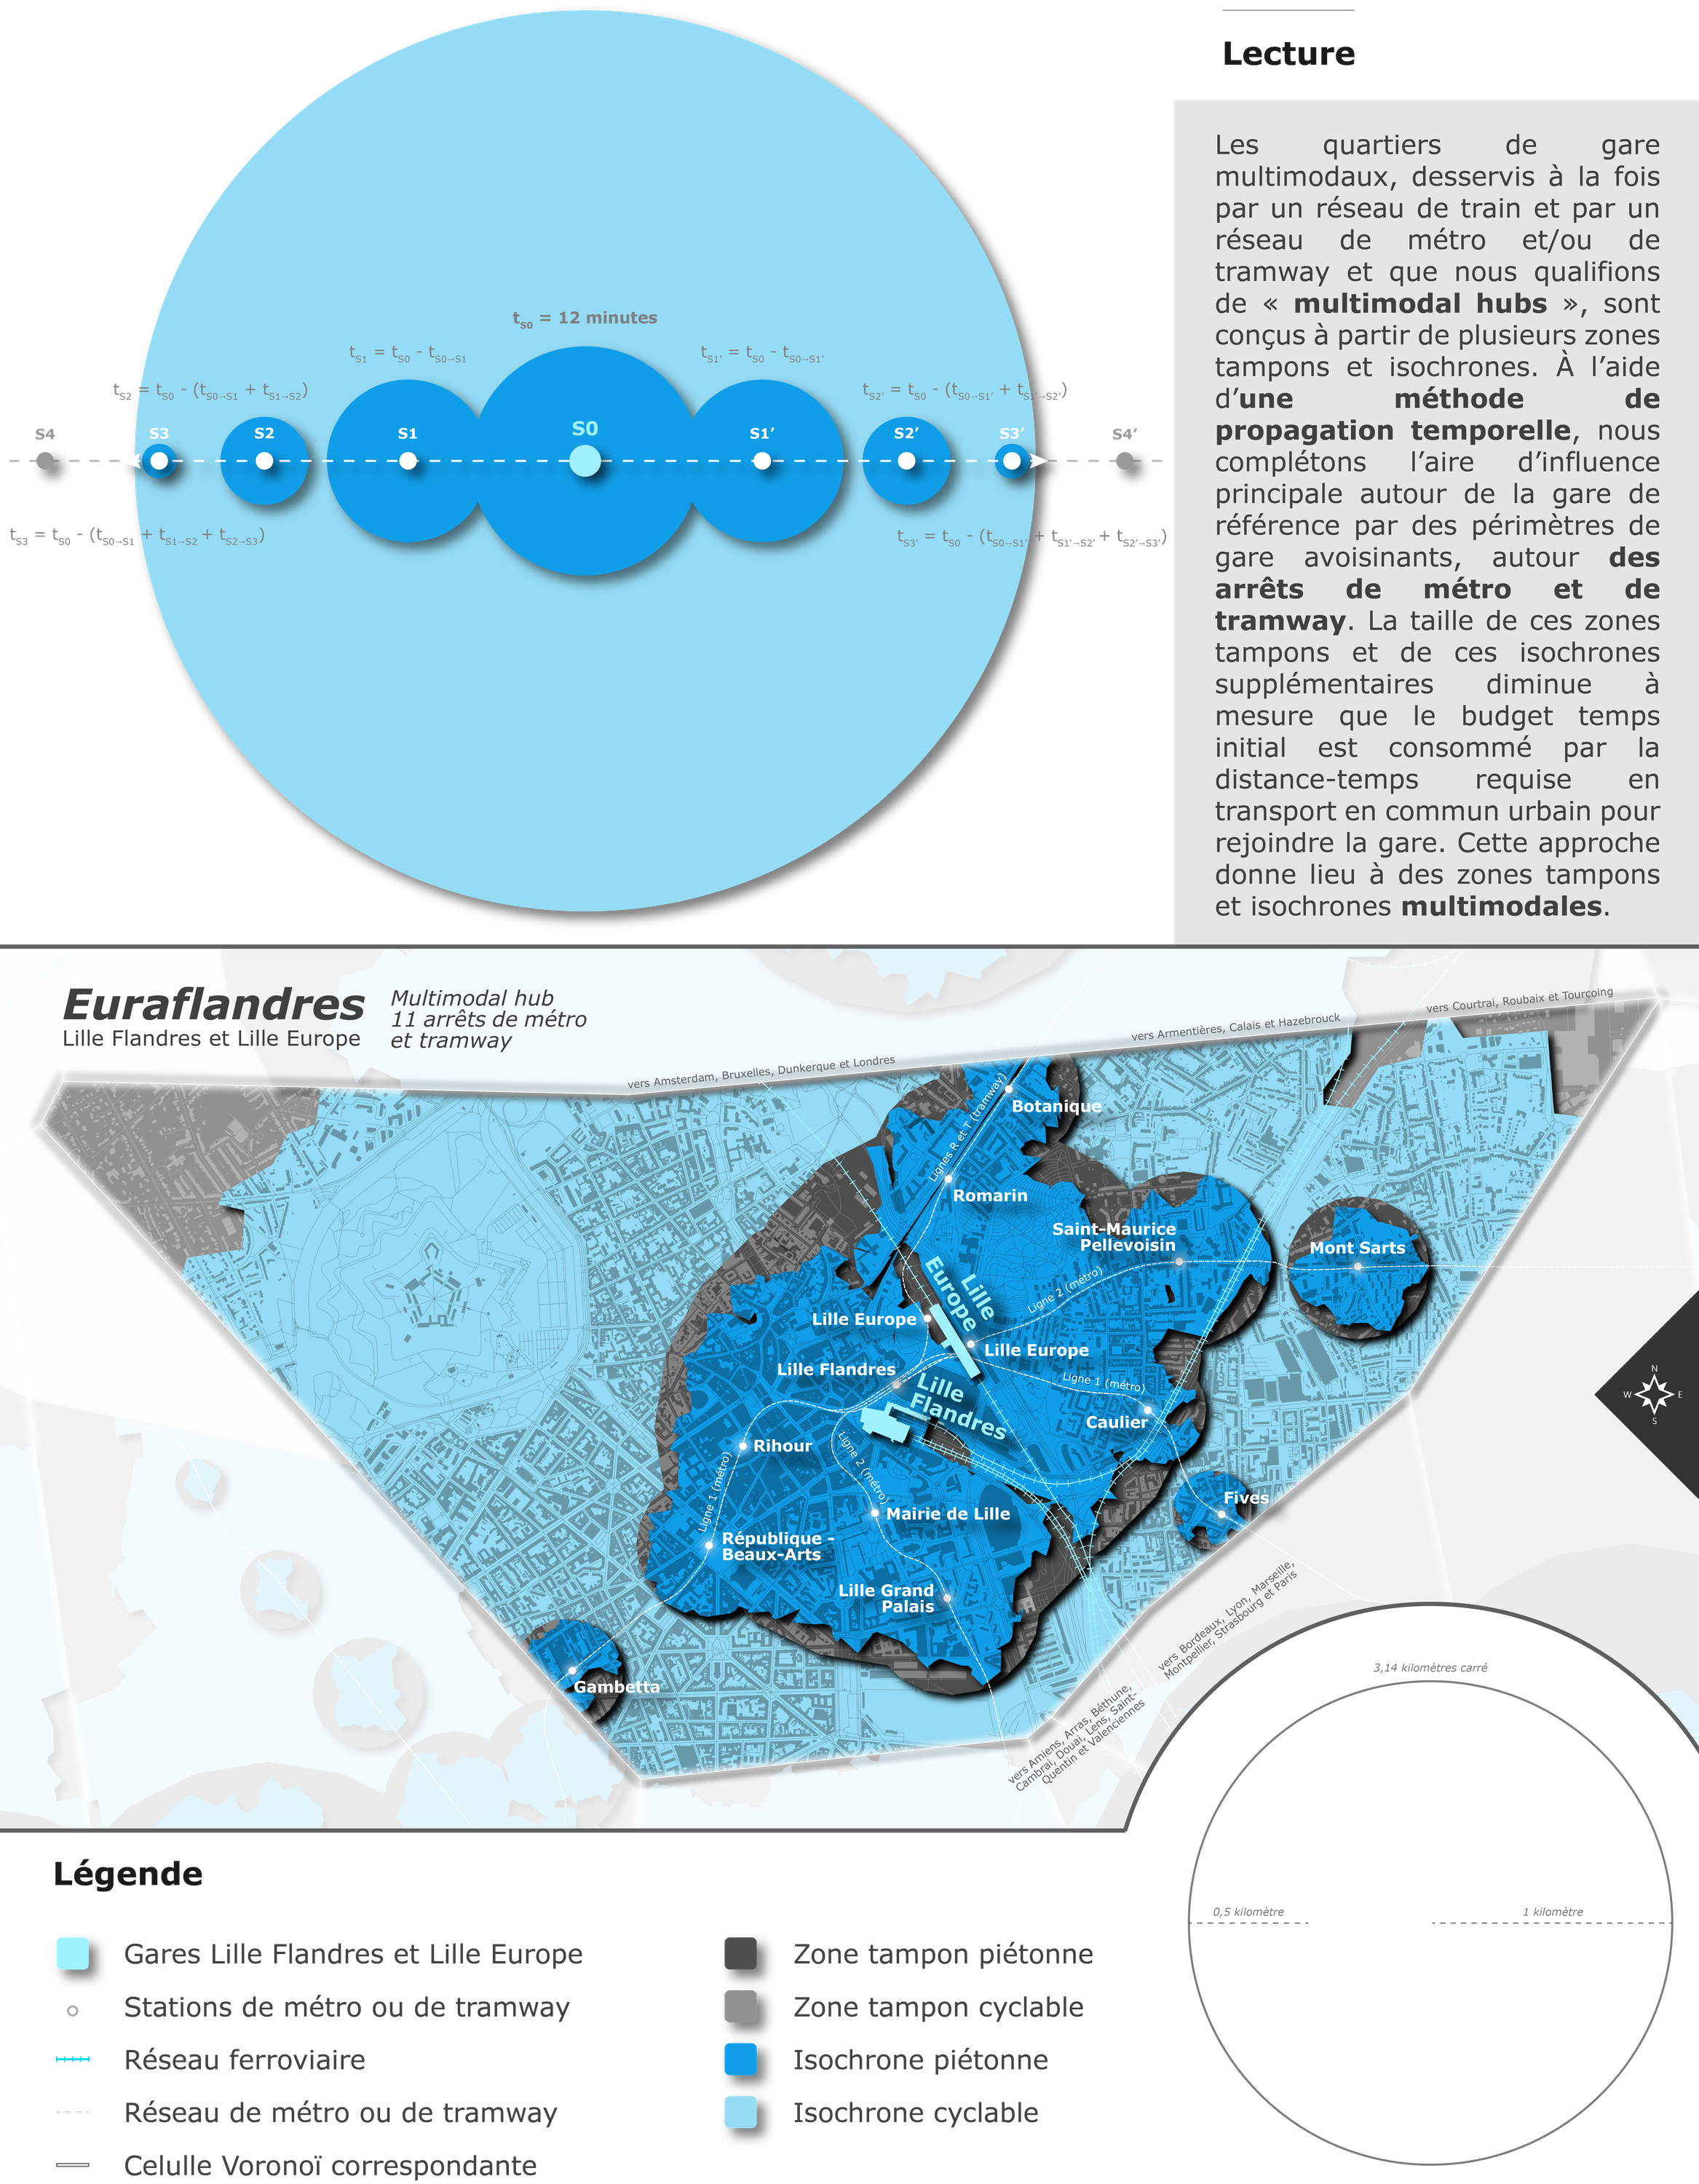
\includegraphics[width=1\columnwidth]{src/Figures/Chap-3/FR_Carte_Euraflandres.png}}
        \vspace{5pt}
        \begin{flushright}\scriptsize{
        Jeux de données~: \textcolor{blue}{\textcite{openstreetmap_openstreetmap_2023}} et \acrshort{GTFS} de la \textcolor{blue}{\textcite{sncf_reseau_2024}}\index{SNCF@\textsl{SNCF}|pagebf}
        \\
        Auteur~: \textcolor{blue}{Dylan Moinse (2024)}
        }\end{flushright}
    \end{carte}

    % OTP
Pour mettre en œuvre cette approche, nous avons utilisé l’outil de génération d’isochrones multimodales du projet \textsl{open-source} \Marque{OpenTripPlanner} (OTP). Ce support permet de calculer des zones accessibles à partir d’un point donné en tenant compte de différents modes de déplacement ainsi que des combinaisons possibles entre ces modes \textcolor{blue}{\autocite[15]{krismer_enhancing_2017}}\index{Krismer, Nikolaus|pagebf}, autant de paramètres qu'il est possible d'ajuster. En mobilisant le module \Guillemets{\textsl{OTP Analyst}}, nous avons pu générer des isochrones représentant les quartiers de gare basés sur leurs connexions multimodales. Au total, 5 gares de la région ont vu leurs aires d’influence étendues à l’ensemble de l'approche multimodale, en raison de leur proximité immédiate avec des stations de métro ou de tramway~: \textsl{Euraflandres}\footnote{
    Nous définissons le pôle \textsl{Euraflandres} à partir d'une fusion entre les gares Lille Flandres et Lille Europe (voir la \hyperref[chap3:observation-quantitative-gares-examinees]{sous-section sur les gares examinées}, page~\pageref{chap3:observation-quantitative-gares-examinees}).
}, Lille CHR, Roubaix, Tourcoing et Valenciennes. Ces pôles d’échange multimodaux ont été désignés sous le terme de \Guillemets{pôles d'échange multimodal} (\textsl{multimodal hubs}). En parallèle, 13 autres gares appartiennent à une seconde catégorie, associée à une desserte en \acrshort{TGV}, tandis qu’une troisième catégorie regroupe un total de 300 gares exclusivement desservies par le \acrshort{TER}.%%Rédigé%%

    % Transition
Compte tenu du nombre important de nœuds que nous étudions au sein du réseau ferroviaire régional, une préoccupation légitime s'élève quant à notre démarche visant à étendre les quartiers de gare à pied comme à vélo et en micro-mobilité~: celle d'une redondance territoriale dans les analyses spatiales, résultant d'une imbrication exagérée des quartiers de gare, notamment dans certaines agglomérations caractérisées par une densité élevée de gares. Face à ce constat, nous proposons de conjuguer la définition des quartiers de gare~–~en modulant leur taille selon le mode de transfert et le type de desserte ferroviaire~–~avec une partition en motifs polygonaux servant à circonscrire chaque quartier de gare.%%Rédigé%%

    % 3.2.1.3.
    \needspace{1\baselineskip} % Réserve de l'espace
\subsubsection*{Délimitation par juxtaposition des quartiers de gare
    \label{chap3:quartiers-gare-voronoi}
    }

    % Superposition
Une dernière préoccupation concernant la problématique de la taille des quartiers de gare réside dans la question de la superposition des aires d'influence ainsi représentées. Si, dans le cas d’un système ferroviaire, la distance inter-station est généralement importante, l’extension des quartiers de gare entreprise par le biais de l’intégration de la mobilité individuelle légère soulève légitimement la question d’une surabondance d’aires superposées. Ce problème ne se limite pas tant à une simple question d'esthétique ou de lisibilité cartographique, mais concerne également le risque de répétition analytique excessive des mêmes configurations territoriales. À titre d’illustration, l’aire d’influence \Guillemets{secondaire} de la gare de La Madeleine, sans bornage, englobe en son sein les gares Lille Flandres et Lille Europe, ce qui fausse grandement les scores de la gare périphérique.%%Rédigé%%

    % Diagramme de Voronoi
Dans la mesure où nous supposons que les utilisateur·rice·s de la mobilité individuelle légère, entrant ou sortant d'une gare, cherchent à emprunter le chemin le plus court \textcolor{blue}{\autocite[116]{heran_distances_2009}}\index{Héran, Frédéric|pagebf}, nous avons opté pour une partition du réseau ferroviaire régional afin de définir les espaces théoriquement les plus proches, d'un point de vue géométrique, de chaque station. Ce découpage, basé sur un plan euclidien, permet de modéliser et de visualiser la couverture théorique maximale de chaque aire d'influence, représentée par une cellule issue d’un diagramme standard de Voronoï \textcolor{blue}{\autocite[479]{mota_method_2014}}\index{Mota, Diego Rosa|pagebf}\index{Takano, Marise|pagebf}\index{Taco, Pastor Willy Gonzales|pagebf}. Cette approche consistant à éviter toute forme de superposition revient à considérer que chaque cellule correspond à un espace dans lequel tous les points sont plus proches de la gare associée qu’à toute autre gare, et ce, indépendamment de la hiérarchie du réseau ferroviaire \textcolor{blue}{\autocite[429]{lebedeva_increasing_2018}}\index{Lebedeva, Olga|pagebf}\index{Kripak, Marina|pagebf}\index{Gozbenko, Valeriy|pagebf}.%%Rédigé%%

    % Transition
Pour représenter le périmètre géographique des 318 gares composant le réseau ferroviaire des Hauts-de-France, notre analyse s’est d’abord focalisée sur la détermination de la taille des différentes aires de chalandise. Cette démarche a consisté à distinguer, dans un premier temps, les quartiers de gare limités à la portée acceptable de la marche combinée, de ceux élargis par l’usage du vélo et de la micro-mobilité. Par la suite, une différenciation a été opérée entre les gares connectées au réseau \acrshort{TER}, celles reliées au réseau \acrshort{TGV}, et les pôles d'échange multimodal. Enfin, un confinement du rayonnement maximal de chaque nœud de transport en commun a été établi, de sorte à le délimiter au sein de frontières. La spatialisation des quatre types de quartier de gare au sein du réseau régional peut être visualisée sur la \hyperref[fig-chap5:aires-influence]{carte~\ref{fig-chap5:aires-influence}} (page~\pageref{fig-chap5:aires-influence}) du \hyperref[chap5:titre]{chapitre~5} (page~\pageref{chap5:titre}). Une fois les tailles définies et intégrées dans le protocole méthodologique, notre attention se porte désormais sur la morphologie que prennent ces quartiers de gare, et notamment aux formes qu'ils peuvent adopter et aux manières de les représenter.%%Rédigé%%

    % 3.2.2.
    \needspace{1\baselineskip} % Réserve de l'espace
\subsection{Morphologie et contours des quartiers de gare
    \label{chap3:quartiers-gare-formes}
    }

    % Introduction
La question de la forme des quartiers de gare semble, à notre connaissance, bien moins explorée dans la littérature scientifique et technique. Cela peut s'expliquer par la complexité qu’elle revêt, tant au niveau des structures territoriales que des considérations techniques, nécessitant une maîtrise avancée des outils permettant de générer divers types d’aires d’influence. Si le sujet des zones tampons, de leurs limitations, ainsi que de l’intérêt d’adopter des isochrones, voire de les combiner pour en tirer une synergie intéressante, est relativement bien documenté, la discussion autour de leur rendu et de leur représentation reste encore critique. C’est dans cette sous-section que nous définissons deux formes de quartier de gare~–~les zones tampons (\(B\)) et les courbes isochrones (\(I\))~–~qui viennent s’ajouter à la réflexion sur la taille de leurs périmètres (\(P\) et \(B\)). Pour autant, leur visualisation demeure un enjeu central. Pour cette raison, nous avons choisi d’approfondir la réflexion sur les différentes manières de représenter ces quartiers, dans le but de développer une démarche méthodologique permettant de concevoir nos propres zones tampons et isochrones. Ce cheminement de pensée cartographique s’appuyant sur une combinaison de techniques informatiques et visuelles.%%Rédigé%%

    % 3.2.2.1.
    \needspace{1\baselineskip} % Réserve de l'espace
\subsubsection*{Intégration des effets de coupure urbaine
    \label{chap3:quartiers-gare-isochrones-buffers}
    }

    % Buffers
Encore aujourd’hui, la majorité des études, qu’elles soient académiques ou opérationnelles, s’appuient sur l'exploitation de disques théoriques (\textsl{buffers}) pour représenter les aires de chalandise des stations de transport en commun. Ces zones tampons se traduisent par des cercles tracés à une distance fixe, qu’elle soit spatiale ou temporelle, autour des nœuds de transport, et ce, sans considération des réseaux ou des obstacles géographiques environnants. Cette méthode présente l’avantage d’être simple à produire et facile à interpréter, puisqu’elle ne nécessite ni données complexes ni calculs avancés. Elle offre également une grande polyvalence, pouvant être appliquée à différents types d’infrastructures, même au-delà des enjeux strictement liés à la mobilité. Cependant, cette technique de production des quartiers de gare se heurte à des limitations majeures. En s’appuyant sur une représentation des distances à vol d’oiseau, sur un plan euclidien, elle ignore les réseaux de transport ainsi que les contraintes géographiques de l'environnement physique. Par conséquent, les zones tampons ne traduisent pas l’accessibilité réelle des infrastructures. Une telle simplification peut conduire à des conclusions inexactes, particulièrement dans des contextes où la configuration des réseaux et des territoires joue un rôle déterminant dans la définition des quartiers de gare.%%Rédigé%%

    % Effets de coupure urbaine
La problématique du redressement des distances à vol d’oiseau pour obtenir des distances réelles n’est pas seulement technique. Elle impose une réflexion sur les effets de coupure urbaine, ainsi qu’une interrogation sur l’origine des détours, impliquant ainsi une analyse de la configuration du réseau viaire, de son maillage et de sa hiérarchisation \textcolor{blue}{\autocite[119]{heran_distances_2009}}\index{Héran, Frédéric|pagebf}. Une coupure urbaine se définit comme une emprise perturbant les relations entre les populations environnantes. Cette emprise peut être d’origine naturelle ou artificielle, bâtie ou non bâtie. L’effet de coupure urbaine se manifeste par des emprises linéaires ou surfaciques, engendrant des perturbations d’ordre physique ou psychologique \textcolor{blue}{\autocite[4]{heran_zones_2009}}\index{Héran, Frédéric|pagebf}\index{Pouillaude, Laurence|pagebf}. Parmi les effets de coupure urbaine les plus emblématiques figurent les autoroutes ou les formes urbaines, ainsi que les fleuves ou les montagnes. Paradoxalement, les infrastructures ferroviaires elles-mêmes peuvent contribuer à ces effets de coupure. Le rapport de recherche-action franco-allemand \textsl{Bahn.Ville 2} illustre cette problématique en montrant comment les voies ferrées participent dans la production de coupures urbaines, renforçant ainsi une \gls{perception} négative, voire une invisibilité, du rail dans l’espace urbain \textcolor{blue}{\autocite[20]{lhostis_concevoir_2009}}\index{L'Hostis, Alain|pagebf}\index{Alexandre, Elsa|pagebf}\index{Appert, Manuel|pagebf}\index{Araud-Ruyant, Catherine|pagebf}\index{Basty, Marius|pagebf}\index{Biau, Géraldine|pagebf}\index{Bozzani-Franc, Sandra|pagebf}\index{Boutantin, Gratienne|pagebf}\index{Constantin, Chantal|pagebf}\index{Coralli, Monica|pagebf}\index{Durousset, Marie-Jeanne|pagebf}\index{Fradier, Christophe|pagebf}\index{Gabion, Cyrille|pagebf}\index{Leysens, Thomas|pagebf}\index{Mermoud, Françoise|pagebf}\index{Olny, Xavier|pagebf}\index{Perrin, Emmanuel|pagebf}\index{Robert, Jean|pagebf}\index{Simand, Noémie|pagebf}\index{Stransky, Vaclav|pagebf}\index{Soulas, Claude|pagebf}\index{Verdier, Anne-Marie|pagebf}\index{Vulturescu, Bogdan|pagebf}. Dès lors, la coupure urbaine constitue un élément important pour comprendre les interactions entre le système ferroviaire et les territoires.%%Rédigé%%

    % Isochrones
C’est dans cette optique que les isochrones sont fréquemment considérées comme une représentation plus réaliste des zones accessibles. Contrairement aux zones tampons, elles délimitent les espaces atteignables dans un temps donné, à partir ou à destination d’une gare, tout en intégrant les infrastructures et les modes de déplacement. En prenant en compte le réseau de voiries ainsi que les spécificités des différents modes de déplacement~–~principalement leur rayon d'action, leur vitesse et les zones qu'ils sont habilités à traverser~–, les isochrones offrent une représentation plus fidèle de l’accessibilité. Par sa capacité à refléter les dynamiques spatiales réelles, la modélisation d'isochrones constitue un outil d'évaluation précise des zones effectivement accessibles. Les premières occurrences dans le champ de la géographie datent du début du XX\textsuperscript{e} siècle, à l'image des \Guillemets{lignes isochrones}, dessinées par \textcolor{blue}{Joseph} \textcolor{blue}{\textcite[311-314]{letaconnoux_note_1907}}\index{Letaconnoux, Joseph|pagebf}, sur l'évolution de l'accessibilité en Bretagne depuis le XVIII\textsuperscript{e} siècle. Dans le domaine de l'urbanisme, généralement piétonnes, les isochrones trouvent leurs premiers usages dans les travaux de \textcolor{blue}{Jane} \textcolor{blue}{\textcite[179-182]{jacobs_death_1961}}\index{Jacobs, Jane|pagebf} qui a introduit le concept de \Guillemets{bassins d'usage} (\textsl{pools of use}) pour désigner les zones situées à distance de marche d'un emplacement urbain spécifique, en fonction du temps de parcours \textcolor{blue}{\autocite[3]{dovey_isochrone_2017}}\index{Dovey, Kim|pagebf}\index{Woodcock, Ian|pagebf}\index{Pike, Lucinda|pagebf}. À titre d’exemple, la \acrfull{MEL}, anciennement \acrfull{LMCU}, a cartographié, en 2000, des \acrfull{ZAP} et des \acrfull{ZAV} autour de ses stations de transport en commun lourd. Ces courbes isochrones ont été conçues pour identifier les lieux stratégiques de développement métropolitain \textcolor{blue}{\autocite[9]{heran_zones_2009}}\index{Héran, Frédéric|pagebf}\index{Pouillaude, Laurence|pagebf}.%%Rédigé%%
    
    % Isodistances
Dans une logique similaire visant à dépasser l’idée des distances à vol d’oiseau définies par les zones tampons, se trouvent les courbes d’isodistance, souvent confondues avec les isochrones. Pourtant, une distinction fondamentale existe~: les isodistances désignent les zones regroupant tous les points situés à une distance spatiale réelle, mesurée sur un réseau, à partir d’un point de référence tel qu’une station de transport en commun. Tiré du grec \textsl{isos} (égal) et \textsl{khronos} (temps), le terme isochrone se différencie de l’isodistance, qui renvoie à une zone définie par une distance spatiale réelle, déformée par le réseau, mais indépendante des vitesses ou des temps de parcours. L’isodistance illustre ainsi une zone de chalandise isométrique, contrairement à l’isochrone, qui repose sur une distance temporelle. Cette confusion fréquente peut s’expliquer par la prédominance des études d’accessibilité piétonne autour des gares. Ces études supposent souvent que les vitesses relativement homogènes des piéton·ne·s entraînent une superposition des courbes isochrones et des courbes d’isodistance \textcolor{blue}{\autocite[9]{heran_zones_2009}}\index{Héran, Frédéric|pagebf}. Cependant, dans le cas de la mobilité cyclable, ces similarités tendent à s’effacer. Les vitesses bien plus variables de la mobilité individuelle légère, influencées par la hiérarchie viaire, la qualité des aménagements ou encore des facteurs individuels comme le type de véhicule ou les compétences des cyclistes, soulignent le besoin de différencier clairement ces notions.%%Rédigé%%

    % Combinaison isochrones et buffers
Durant le déroulement de nos travaux de thèse, nous avons privilégié l’utilisation conjointe des zones tampons, des isodistances et des isochrones. Leur combinaison dans l’analyse spatiale fournit une perspective intégrée sur l’accessibilité. En superposant les isodistances ou les isochrones et les zones tampons, il devient possible de mesurer les différentiels d’accessibilité, c’est-à-dire l’écart entre l’accessibilité réelle et l’accessibilité théorique. Cette confrontation permet en outre de calculer le taux de desserte qui exprime le rapport entre l’aire réellement accessible et l’aire atteignable en ligne droite \textcolor{blue}{\autocite[13]{heran_zones_2009}}\index{Héran, Frédéric|pagebf}. Le diagnostic cartographique de ces différentes représentations de quartiers de gare permet d’identifier de manière systématique les obstacles rencontrés par les voyageur·se·s.%%Rédigé%%

    % Transition
Une fois le débat sur les apports des isochrones dépassé~–~une étape nécessaire, mais qui semble, d’après nos observations, de plus en plus admise et couramment intégrée dans diverses productions~–~se pose la question de leur représentation. Bien que les avantages des isochrones, notamment pour intégrer les obstacles physiques présents dans les territoires, soient largement reconnus dans les pratiques de recherche, il apparaît que leur rendu varie considérablement et manque souvent de transparence quant aux paramètres mobilisés. Cette opacité peut s'expliquer par le fait que la plupart d'entre elles sont générées à l’aide de plates-formes limitant la maîtrise des paramètres de modélisation. Face à ce constat, nous avons entrepris de développer nos propres quartiers de gare à l’aide d’un script sur-mesure, nous offrant ainsi la possibilité de définir des délimitations géographiques adaptées à nos objectifs de recherche.%%Rédigé%%

    % 3.2.2.2.
    \needspace{1\baselineskip} % Réserve de l'espace
\subsubsection*{Réflexion à propos de la représentation cartographique des quartiers de gare
    \label{chap3:quartiers-gare-python}
    }

% Fabrique des aires d'influence : Python (précision géographique)
Une réflexion approfondie s’impose pour établir les stratégies de représentation cartographique des zones d’accessibilité, telles que les zones tampons et les isochrones, en adéquation avec les objectifs de cette recherche doctorale. Cette démarche ne relève pas uniquement de considérations esthétiques ou de communication, mais vise également à assurer une maîtrise, tant sur le fond que sur la forme, des bases d’analyse géographique mobilisées tout au long de ce travail. Il convient, en premier lieu, de clarifier les concepts abordés, notamment en identifiant les paramètres qui influencent la configuration des représentations et les interprétations analytiques qui en découlent. Face à la diversité des outils disponibles pour la génération des zones tampons et des isochrones, nous avons opté pour la poursuite de notre analyse à l’aide du langage de programmation \textsl{Python}. Ce choix repose non seulement sur la richesse des bibliothèques proposées par cet environnement, mais également sur la transparence offerte par l’outil en source ouverte (\textsl{open source}) qui autorise une maîtrise totale des paramètres définis\footnote{
    \textsl{Python} est un langage généraliste et applicable à de larges domaines qui devient de plus en plus populaire auprès des \textsl{data scientists} \textcolor{blue}{\autocite[19]{velt_python_2020}}\index{Velt, Amandine|pagebf}. En plus de sa documentation très fournie, \textsl{Python} dispose d'une interface graphique pour l'analyse des données et du partage des analyses~: les \textsl{notebooks Jupyter}. Un \textsl{notebook} est un document exécutable dont les résultats sont intégrés dans le document, en plus d'éléments de texte ou d'équations mathématiques. Dès lors, l'outil \textsl{Jupyter Notebook} et l'usage de \textsl{Python}, accompagnés de bibliothèques utiles telles que \textsl{Pandas} et \textsl{GeoPandas}, ont été généralisés dans nos analyses afin d'assurer une plus grande transparence et une meilleure gestion du travail en équipe \textcolor{blue}{\autocite[55, 137]{velt_python_2020}}\index{Velt, Amandine|pagebf}.
}.%%Rédigé%%

    % Isochrone depuis et vers
Un premier paramètre qui vient interroger la fabrique géographique des aires d’influence des gares réside dans le sens des flux. À première vue, il pourrait sembler intuitif de considérer que, quelle que soit la direction du flux~–~qu’il s’agisse d'un trajet en rabattement vers la gare ou en diffusion depuis celle-ci~–, le quartier de gare conserverait une taille et une forme similaires. Cependant, cette hypothèse tend à négliger deux dimensions~: la connectivité routière, particulièrement déterminante pour le vélo et la micro-mobilité, qui sont régis par les contraintes du code de la route, ainsi que la temporalité. En effet, une isochrone orientée vers ou depuis une gare ne possède pas nécessairement la même validité selon des facteurs tels que l’amplitude horaire des lignes ou les directions desservies. S'agissant de notre matériau empirique, nous avons choisi de considérer que, par défaut, les zones tampons et les isochrones atemporelles sont conçues pour analyser les aires accessibles en direction de la gare, et non dans l’autre sens, comme cela est souvent le cas. Ce choix s'explique par la primauté de la logique de pré-acheminement, qui est privilégiée dans la mesure où le vélo, lorsqu'il est utilisé en connexion avec les gares, y est bien plus sollicité qu'en post-acheminement.%%Rédigé%%

    % Surface VS voirie VS bâti VS POIs
La problématique de la représentation cartographique des isochrones, qu’il s’agisse de leur dimension analytique ou de leur fonction communicative, se pose également en termes de choix des éléments structurants à mettre en avant. Faut-il privilégier une représentation visuelle de la surface accessible ou non accessible~? Ou bien serait-il plus pertinent de mettre en exergue la voirie, qui matérialise les connexions servant de base au calcul de l’isochrone~? Une autre possibilité consisterait à mettre l'accent sur le bâti ou les \acrfull{POIs}, qui incarnent, en définitive, les destinations que les individus cherchent à atteindre. Ces choix cartographiques ne sont pas neutres, car ils orientent la lecture et l’interprétation des données tout en influençant la manière dont les résultats sont communiqués aux divers publics concernés.%%Rédigé%%

    % Isochrone voirie
La représentation basée sur la voirie reflète directement les trajets réalisables au sein d’un réseau piétonnier ou cyclable défini. Ce mode de visualisation prétend offrir une approche plus réaliste en prenant en compte les contraintes physiques des déplacements, tout en étant particulièrement adaptée à la navigation et aux repères cartographiques\footnote{
    L'\acrfull{API} la plus connue pour la création d’isochrones basées sur la voirie est certainement celle développée par \textcolor{blue}{\textcite{graphhopper_visualization_2018}}.
}. Cependant, une telle représentation peut également engendrer une certaine complexité visuelle, rendant l’interprétation plus difficile pour certain·e·s utilisateur·rice·s. Au-delà des simples polygones, celle-ci propose une représentation détaillée des segments de voies accessibles, directement visualisables dans un navigateur. À titre illustratif, nous avons appliqué cette méthode, avec notre propre code, pour représenter, en projection plane et en modèle volumétrique, l’isochrone accessible en mobilité individuelle légère à destination de la gare d’Amiens. Cette représentation repose sur la voirie directement accessible aux cyclistes (voir la \hyperref[fig-chap3:isochrone-amiens-voirie]{carte~\ref{fig-chap3:isochrone-amiens-voirie}}, page~\pageref{fig-chap3:isochrone-amiens-voirie})\footnote{
    Cette analyse cartographique a été améliorée grâce à l’utilisation de la transparence des couleurs, qui met en relief les matrices de flux. L’efficacité de cette technique combinée à un fond sombre réside dans l’optimisation de la \Guillemets{saillance visuelle}~–~cette notion fait référence à l’adéquation entre le phénomène représenté, les variables visuelles utilisées et leur perception par l’observateur·rice~–~des éléments représentés et des informations transmises, tout en facilitant la perception des géométries complexes. Cette approche garantit une lisibilité accrue, comme le démontre \textcolor{blue}{Françoise} \textcolor{blue}{\textcite[226]{bahoken_contribution_2016}}\index{Bahoken, Françoise|pagebf}, dans sa thèse de doctorat, sur la base d'une cartographie d’une matrice de flux.
}.%%Rédigé%%

    % Carte Isochrone Amiens voirie
    \begin{carte}[h!]\vspace*{4pt}
        \caption{Représentation cartographique du réseau viaire atteignable à vélo et en micro-mobilité vers la gare d'Amiens, construite à partir d'une isochrone.}
        \label{fig-chap3:isochrone-amiens-voirie}
        \centerline{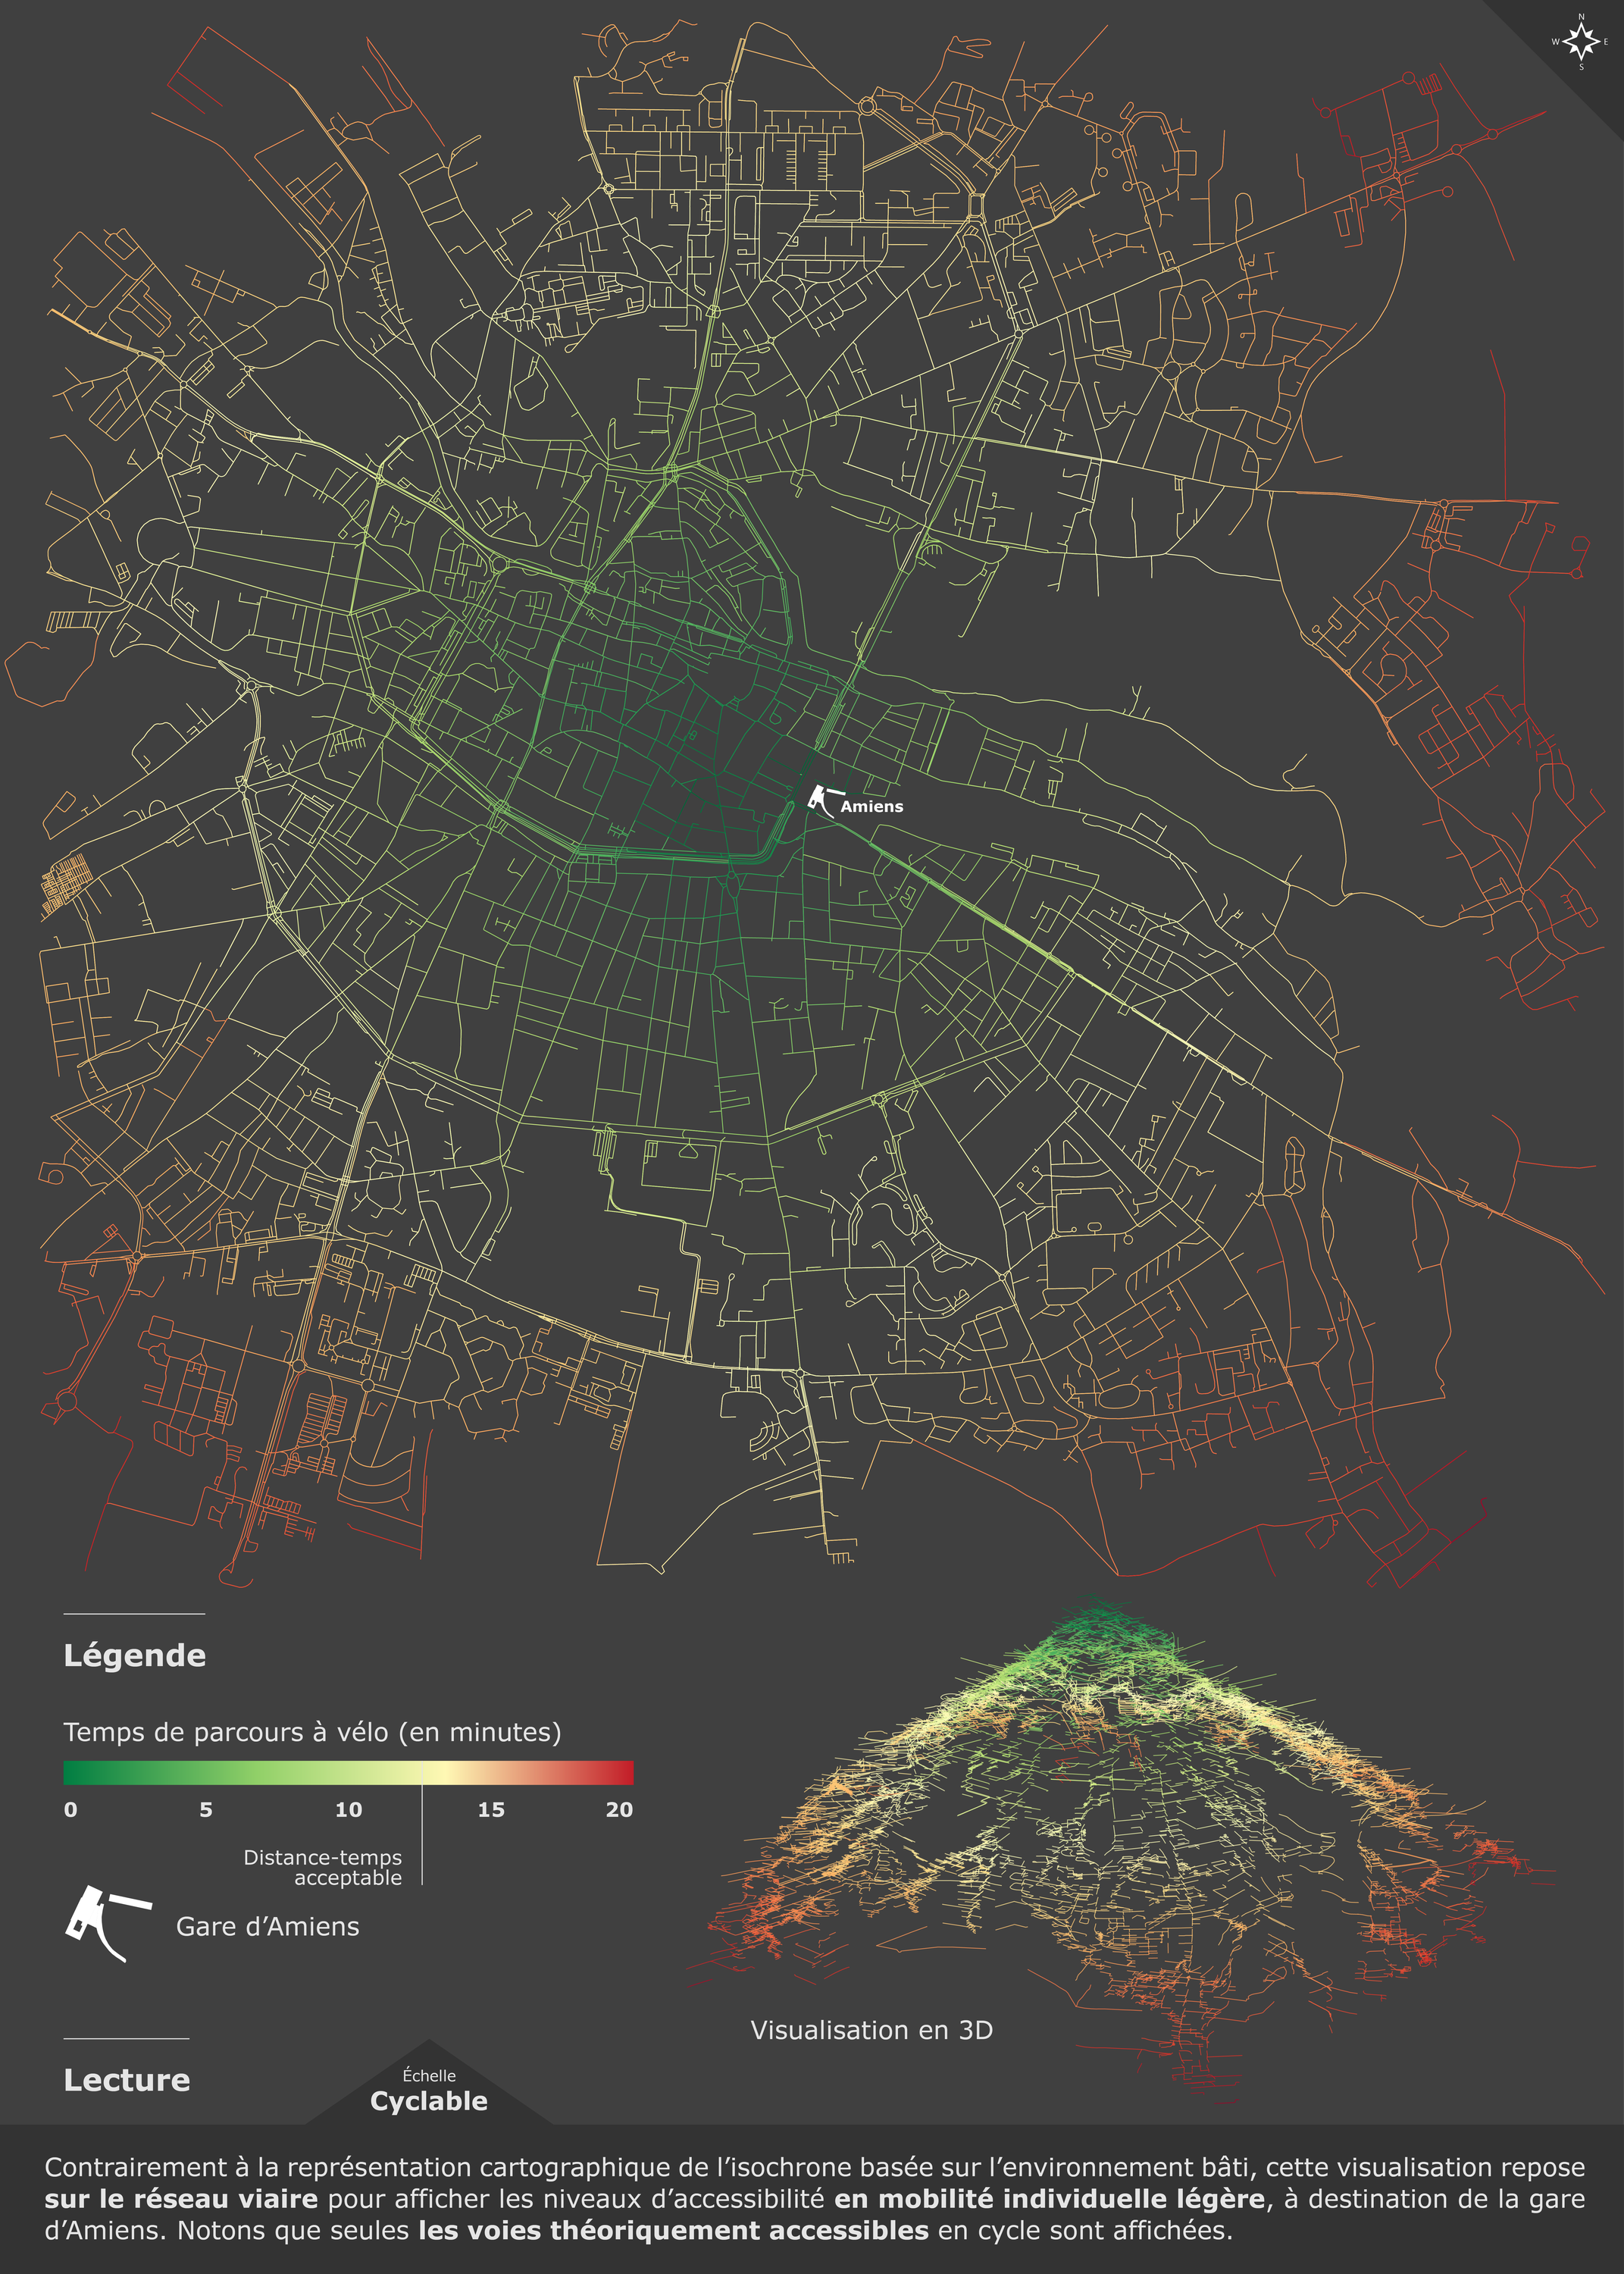
\includegraphics[width=1\columnwidth]{src/Figures/Chap-3/FR_Carte_Isochrone_Amiens_Voirie.png}}
        \vspace{5pt}
        \begin{flushright}\scriptsize{
        Jeux de données~: \textcolor{blue}{\textcite{openstreetmap_openstreetmap_2023}} et \acrshort{GTFS} de la \textcolor{blue}{\textcite{sncf_reseau_2024}}\index{SNCF@\textsl{SNCF}|pagebf}
        \\
        Auteur~: \textcolor{blue}{Dylan Moinse (2024)}
        }\end{flushright}
    \end{carte}

    % Isochrone bâti
En ce qui concerne la représentation basée sur le bâti ou les \acrshort{POIs} accessibles dans le temps imparti, elle présente l’avantage de mieux répondre aux besoins des utilisateur·rice·s en orientant le regard vers les lieux où les individus interagissent directement, tels que les logements, les lieux de travail, les commerces ou encore les équipements publics (voir la \hyperref[fig-chap3:isochrone-amiens-bati]{carte~\ref{fig-chap3:isochrone-amiens-bati}}, page~\pageref{fig-chap3:isochrone-amiens-bati}). Cette approche est particulièrement pertinente pour des analyses centrées sur des services spécifiques, en fournissant une réponse immédiate et pratique à la question de l'accessibilité aux services. Cependant, cette forme de représentation visuelle présente certaines limites. Elle exclut les zones non bâties, qui expriment pourtant un besoin en matière d'accessibilité, comme les espaces verts ou d’autres espaces ouverts ayant une valeur fonctionnelle ou sociale. De plus, elle ne permet pas de mettre en évidence la connectivité globale de la zone.%%Rédigé%%

    % Carte Isochrone Amiens bâti
    \begin{carte}[h!]\vspace*{4pt}
        \caption{Représentation cartographique du bâti atteignable à vélo et en micro-mobilité vers la gare d'Amiens, construite à partir d'une isochrone.}
        \label{fig-chap3:isochrone-amiens-bati}
        \centerline{\includegraphics[width=1\columnwidth]{src/Figures/Chap-3/FR_Carte_Isochrone_Amiens_Bati.png}}
        \vspace{5pt}
        \begin{flushright}\scriptsize{
        Jeux de données~: \textcolor{blue}{\textcite{openstreetmap_openstreetmap_2023}} et \acrshort{GTFS} de la \textcolor{blue}{\textcite{sncf_reseau_2024}}\index{SNCF@\textsl{SNCF}|pagebf}
        \\
        Auteur~: \textcolor{blue}{Dylan Moinse (2024)}
        }\end{flushright}
    \end{carte}

    % Avantages et inconvénients types d'isochrones
Sur un mode comparatif, nous pouvons établir que les isochrones, traditionnellement représentées sous forme de surfaces accessibles, offrent l’avantage d’une grande clarté visuelle, requièrent généralement un volume limité de données géographiques et sont adaptées à des analyses globales. Contrairement à la représentation par la voirie, bien que plus précise, qui s’adresse davantage à des usages spécifiques tels que la navigation, moins pertinents dans le cadre de notre problématique de recherche. Finalement, les représentations fondées sur l’environnement bâti ou sur les équipements et services accessibles dans un territoire ont le mérite de proposer une orientation davantage centrée sur le·la voyageur·se. Elles se prêtent bien aux analyses urbanistiques, notamment au sujet des formes urbaines et de l’accessibilité aux services ciblés. Toutefois, ce type de représentation cartographique est plus exigeant en termes de données et implique des coûts de \gls{cartographie} plus élevés.%%Rédigé%%

    % Isochrone finale : jeu sur les arêtes
Dans cette perspective, nous avons choisi de croiser les formes de représentation cartographique auxquelles nous nous sommes essayé·e·s, en nous appuyant sur la production d’isochrones hybrides~: surfaciques, certes, mais dont la forme dépend en premier lieu du réseau viaire tout en étant influencée par la présence du bâti environnant (voir la \hyperref[fig-chap3:isochrone-amiens-finale]{carte~\ref{fig-chap3:isochrone-amiens-finale}}, page~\pageref{fig-chap3:isochrone-amiens-finale}). L'adoption de cette technique nous a permis de produire des représentations cartographiques aux contours nettement plus précis que les approximations souvent observées dans les productions traditionnelles d’isochrones. Dans cette démarche, nous nous sommes appuyé·e·s sur la méthode novatrice développée par le développeur logiciel et chercheur \textcolor{blue}{Kuan} \textcolor{blue}{\textcite{butts_better_2017}}\index{Butts, Kuan|pagebf}, reposant sur l’outil \textsl{OSMnx}, disponible en langage de programmation \textsl{Python}, et spécifiquement conçu pour modéliser les réseaux viaires \textcolor{blue}{\autocite[132]{boeing_osmnx_2017}}\index{Boeing, Geoff|pagebf}. Cette approche s’inscrit dans l’esprit d’une carte d’isochrones construite sur la base de la voirie (\textsl{lines}), en adoptant une logique de graphes de réseaux (\textsl{edges}), tout en intégrant une zone tampon linéaire autour de chaque voie et de chaque intersection accessible (\textsl{buffers}). Ce procédé permet dès lors d’incorporer les éléments urbains adjacents au réseau viaire \textcolor{blue}{\autocite[135]{boeing_osmnx_2017}}\index{Boeing, Geoff|pagebf}, sans les mobiliser dans la représentation comme dans la \hyperref[fig-chap3:isochrone-amiens-bati]{carte~\ref{fig-chap3:isochrone-amiens-bati}} (page~\pageref{fig-chap3:isochrone-amiens-bati}.%%Rédigé%%

    % Carte Isochrone finale adoptée Amiens
    \begin{carte}[h!]\vspace*{4pt}
        \caption{Représentation cartographique de l'isochrone accessible à vélo et en micro-mobilité vers la gare d'Amiens, en superposition avec le réseau viaire.}
        \label{fig-chap3:isochrone-amiens-finale}
        \centerline{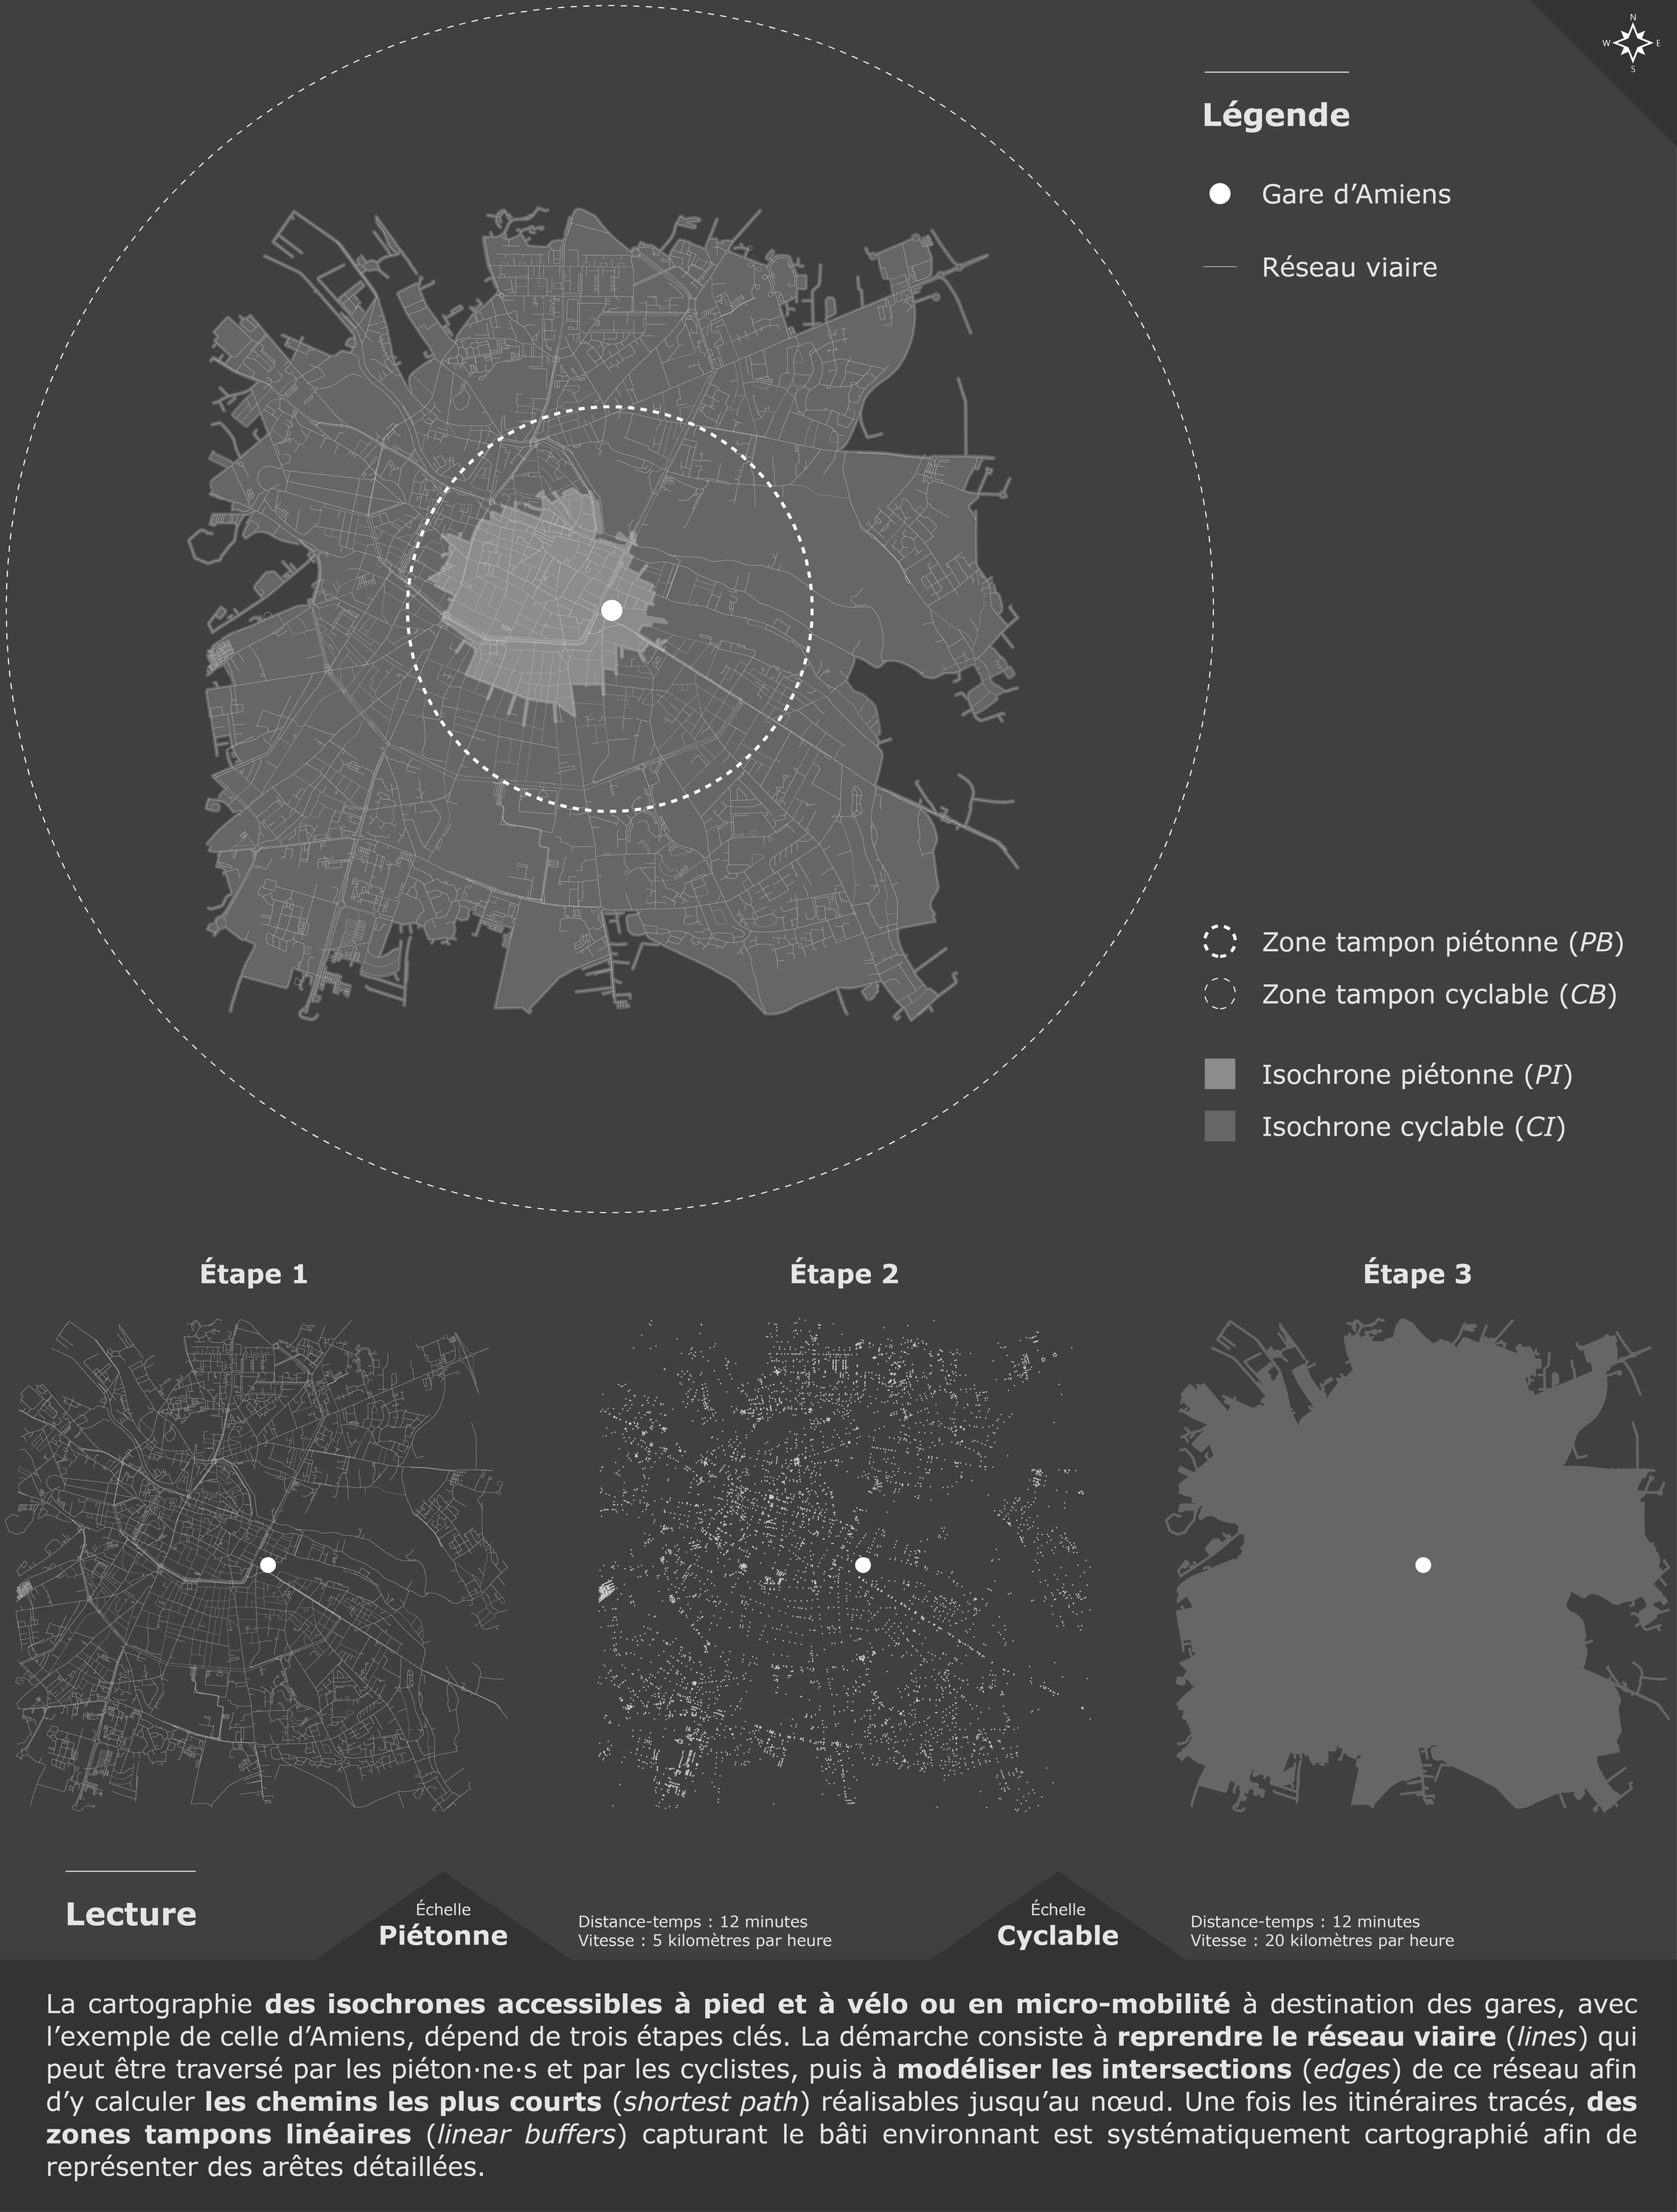
\includegraphics[width=1\columnwidth]{src/Figures/Chap-3/FR_Carte_Isochrones_Buffers_Amiens.png}}
        \vspace{5pt}
        \begin{flushright}\scriptsize{
        Jeux de données~: \textcolor{blue}{\textcite{openstreetmap_openstreetmap_2023}} et \acrshort{GTFS} de la \textcolor{blue}{\textcite{sncf_reseau_2024}}\index{SNCF@\textsl{SNCF}|pagebf}
        \\
        Auteur~: \textcolor{blue}{Dylan Moinse (2024)}
        }\end{flushright}
    \end{carte}

    % Zones accessibles/non accessibles et transition
De nombreux questionnements ont orienté, et pourraient encore orienter, cette sous-section, qui s’attache avant tout à une réflexion globale sur la morphologie des isochrones générées. Par exemple, nous aurions pu également discuter de la hiérarchisation visuelle entre le \textsl{visible} et l’\textsl{invisible}. Si l’objectif est de valoriser les zones accessibles, ne serait-il pas plus pertinent de colorer ou de masquer les zones non accessibles~? Cela permettrait non seulement de recentrer l’attention sur les espaces accessibles, mais également de libérer visuellement l’espace cartographique pour intégrer des figurés et des éléments complémentaires, sans que ceux-ci soient visuellement perturbés par l’isochrone. Comme le souligne \textcolor{blue}{Jacques} \textcolor{blue}{\textcite[5]{levy_tournant_1999}}\index{Lévy, Jacques|pagebf}~–~dans son ouvrage central \textsl{Le tournant géographique. Penser l'espace pour lire le monde}~–, le processus de délimitation et de différenciation participe à la formation des espaces géographiques. Ce principe, que nous avons brièvement exploré ici, nous conduit désormais à expliciter les techniques de collecte et d’analyse géographiques mobilisées une fois les quartiers de gare~–~en tant que périmètres géographiques privilégiés de notre terrain d'étude~–~définis.%%Rédigé%%

    % 3.2.3.
    \needspace{1\baselineskip} % Réserve de l'espace
\subsection{Analyse géostatistique des quartiers de gare cartographiés
    \label{chap3:quartiers-gare-analyse-geostatistique}
    }

    % Introduction
L'effort consacré à la production géographique de quartiers de gare aux tailles et aux formes variables serait dépourvu de sens si les données qui y sont intégrées étaient agrégées à des échelles trop larges, comme celle de la commune. Se cantonner à de tels périmètres administratifs ne permettrait ni de refléter l’individualité de chaque quartier de gare, ni de saisir les distinctions entre leurs différents types ou les variations internes à chacun d’eux. En soulevant cette problématique, nous avons établi comme règle méthodologique de nous restreindre à des bases de données désagrégées, sous forme de vecteurs ponctuels, linéaires ou polygonaux, indépendants des grilles ou des frontières administratives. Pour autant, en raison de la rareté des données ouvertes disponibles, malgré une position avantageuse de la France grâce à une centralisation volontariste des jeux de données, il demeure parfois nécessaire de recourir à des données agrégées, pour des impératifs d'anonymisation par exemple. Ainsi, dans un second temps, nous proposons une méthode d’estimation des valeurs fondée sur des données agrégées à l’échelle de grilles régulières. Cette approche permet de contourner les limitations tout en conservant une précision analytique suffisante pour les besoins de notre recherche.%%Rédigé%%

    % 3.2.3.1.
    \needspace{1\baselineskip} % Réserve de l'espace
\subsubsection*{Des données spatiales désagrégées
    \label{chap3:quartiers-gare-donnees-desagregees}
    }

    % Données géocodées désagrégées sans limites administratives
L’étude des quartiers de gare délimités dans la région repose intégralement sur l’exploitation de données géographiques désagrégées. Cette approche méthodologique a pour objectif de garantir une robustesse analytique, tout en offrant une granularité suffisante pour explorer les dynamiques locales spécifiques à ces espaces stratégiques. Les données géographiques désagrégées se distinguent alors par leur haut niveau de détail et leur indépendance par rapport aux découpages administratifs ou aux périmètres prédéfinis. Elles se déclinent sous plusieurs formes~: des points, représentant la localisation exacte d’équipements~; ou des polygones détaillés, illustrant des emprises au sol par exemple.

    % Sources de données
Contrairement aux données agrégées, généralement collectées à des échelles larges, les données désagrégées permettent d’analyser les territoires à une échelle micro-locale, voire ultra-locale. L'intérêt d'adopter une lecture détaillée des quartiers de gare, indépendante des limites communales 
\textcolor{blue}{\autocite[7]{moretti_interconnexion_1999}}\index{Moretti, Anna|pagebf}\index{Vacheret, Guy|pagebf}, revêt une importance majeure. Les données mobilisées dans notre étude proviennent de diverses sources officielles, combinées pour constituer un ensemble cohérent et exploitable dans un outil \acrfull{SIG} ou sous forme de code informatique permettant de produire des éléments graphiques utilisables dans un contexte géographique. Dans notre cas, le \Guillemets{géocodage} renvoie à des codes écrits en \textsl{Python}. Ces sources incluent notamment des données ouvertes, des bases socio-économiques désagrégées, ainsi que des bases cadastrales. Ce croisement de données garantit une représentation fine et contextualisée des quartiers de gare, adaptée aux exigences analytiques et méthodologiques de cette recherche.%%Rédigé%%

    % Avantages et transition
Alors que les quartiers de gare, loin d’être homogènes, présentent des micro-dynamiques souvent imperceptibles à des échelles plus larges, une analyse désagrégée permet de mettre en évidence ces disparités territoriales. Ces données permettent également de modéliser les interactions spatiales et fonctionnelles avec une grande précision. Cette granularité évite les biais induits par des découpages territoriaux et favorise l’exploration de logiques spatiales fondées sur les usages. Les quartiers de gare, en constante évolution, tirent également profit des données désagrégées pour assurer un suivi précis et temporel de ces transformations. Néanmoins, ces bases de données désagrégées restent relativement peu répandues et sont parfois affectées par des limitations liées à la qualité de leur traitement. Face à ces contraintes, il a été nécessaire d’assouplir la méthodologie en exploitant, lorsque cela s’imposait, des grilles de données géographiques infracommunales et géométriques, indépendantes des limites administratives, des projets urbains ou des zones d’étude.%%Rédigé%%

    % 3.2.3.2.
    \needspace{1\baselineskip} % Réserve de l'espace
\subsubsection*{Intégration des grilles de données géographiques faiblement agrégées
    \label{chap3:quartiers-gare-calcul-carreaux}
    }

    % Grilles de données
Certaines grilles de données, bien qu’indispensables à cette recherche, ne sont malheureusement pas désagrégées. Dans cette optique, nous avons choisi de nous appuyer sur des bases de données exprimées au travers de grilles standardisées\footnote{
    Les grilles de données se déclinent en plusieurs types, différenciés par leur géométrie et leur échelle. Parmi les plus courantes, on trouve les grilles carroyées régulières rectangulaires ou carrées, fréquemment utilisées pour les bases de données démographiques et climatiques, ainsi que les grilles hexagonales (\textsl{hexbins}, H3), caractérisées par des cellules en forme d’hexagones, offrant une couverture territoriale plus homogène grâce à leurs bords équidistants. En revanche, cette recherche exclut l’utilisation de grilles irrégulières, telles que les grilles administratives ou géodésiques, ou encore les images \textsl{raster}.
}. Nous pouvons évoquer le cas d'une base de données de la population française~: le recensement de la population qui, pour des raisons d’anonymisation, utilisent des données carroyées à une résolution de 200 mètres par 200 mètres au niveau de détail le plus fin \textcolor{blue}{\autocite{insee_grille_2021}}\index{Insee@\textsl{Insee}|pagebf}.%%Rédigé%%

    % Méthode de calcul - grilles de données
Afin de réduire les approximations liées à l'application des grilles, nous avons intégré une méthode de calcul permettant d’en affiner la précision et de garantir leur pertinence dans le cadre de notre étude. Nous nous sommes appuyé·e·s sur un \textsl{ModelBuilder}\footnote{
    Un \textsl{ModelBuilder} est un outil visuel destiné à la conception, l’automatisation et l’exécution de chaînes de traitements géospatiaux. Il s’apparente à un langage de programmation graphique, dans lequel l’utilisateur·rice assemble des outils et des processus sous forme de diagrammes, afin de créer des \textsl{workflows} reproductibles, adaptables et modifiables. Cette approche facilite la standardisation des analyses et permet de rationaliser les opérations complexes tout en assurant leur traçabilité.
} produit sur \Marque{ArcGIS Pro} et développé notamment dans le cadre du projet de recherche SOFT~–~un rapport sur la modélisation à base de géométrie fractale construit de concert entre les laboratoires \acrfull{ThéMA}, le \acrfull{LVMT} et l'\acrfull{ITE} d'Efficacity~–~portant sur la sobriété énergétique par les formes urbaines et le transport \textcolor{blue}{\autocite[123]{bonin_projet_2020}}\index{Bonin, Olivier|pagebf}\index{Bonneau, Patricia|pagebf}\index{Clerc, Milan|pagebf}\index{Cousin, Julie|pagebf}\index{Frankhauser, Pierre|pagebf}\index{Gouvello, Bernard de|pagebf}\index{Haffner, Maud|pagebf}\index{Lehmann, Xavier|pagebf}\index{Pioli, Rémi|pagebf}\index{Poirel, Maylis|pagebf}\index{Stransky, Vaclav|pagebf}\index{Thébert, Mariane|pagebf}, qui propose un modèle automatisé spécifiquement conçu pour le calcul des aires de chalandise autour des commerces. Ce modèle génère des zones tampons tout en ajustant les calculs en fonction des surfaces des carreaux inclus, qu’ils soient partiellement ou entièrement contenus dans ces zones. En pratique, certains carreaux peuvent n’avoir qu’une fraction de leur surface à l’intérieur de la zone tampon. La méthode proposée consiste alors à estimer une valeur ajustée pour chaque carreau, afin de refléter au mieux la réalité de l’aire de chalandise, en tenant compte de la proportion effective de surface incluse. En suivant cette démarche, nous avons adapté et systématisé cette méthodologie au sein de nos propres scripts (voir la \hyperref[fig-chap3:methode-calcul-grilles-geographiques]{carte~\ref{fig-chap3:methode-calcul-grilles-geographiques}}, page~\pageref{fig-chap3:methode-calcul-grilles-geographiques}). Cette adaptation, appliquée de manière automatisée aux zones tampons et aux isochrones générées, permet d’ajuster les calculs dès qu’une grille de données est utilisée.%%Rédigé%%

    % Carte méthode calcul Cerema
    \begin{carte}[h!]\vspace*{4pt}
        \caption{Automatisation d'une méthode d'ajustement géospatial pour l'estimation des valeurs d'une grille régulière.}
        \label{fig-chap3:methode-calcul-grilles-geographiques}
        \centerline{\includegraphics[width=1\columnwidth]{src/Figures/Chap-3/FR_Methode_calcul_grilles_geographiques.png}}
        \vspace{5pt}
        \begin{flushright}\scriptsize{
        Jeux de données~: \textcolor{blue}{\textcite{openstreetmap_openstreetmap_2023}} et \acrshort{GTFS} de la \textcolor{blue}{\textcite{sncf_reseau_2024}}\index{SNCF@\textsl{SNCF}|pagebf}
        \\
        Auteur~: \textcolor{blue}{Dylan Moinse (2024)}
        }\end{flushright}
    \end{carte}

    % Transition
La délimitation de notre cadre géographique multi-échelle, avec un espace d'étude centré sur les 318 gares et quartiers de gare de la région Hauts-de-France, constitue une base solide pour mener certaines analyses géospatiales en mobilisant les ressources existantes en données ouvertes. Toutefois, la spécificité de notre sujet de recherche exige également la collecte de matériaux empiriques, précis et actualisés. Ainsi, les sections suivantes de ce chapitre présentent les trois types d’enquêtes de terrain que nous avons menées dans le cadre de cette investigation~:
    \begin{customitemize}
\item Dans un premier axe, la conduite d'observations quantitatives nous permet de dresser un panorama global sur la quantité (proportions~: \textsl{combien~?}), le cadre temporel (variations temporelles~: \textsl{quand~?}), le profil des cyclo-voyageur·se·s (population cible~: \textsl{qui~?}) et leurs équipements (véhicules, ressources et gestuelle~: \textsl{avec quoi~?}), à partir des données recueillies dans neuf gares représentatives de la région~;
\item Dans un deuxième axe, nous explorons, par le biais d'un questionnaire semi-directif à destination des voyageur·se·s, le déploiement des pratiques intermodales sous l’angle de leurs caractéristiques (habitudes de déplacement~: \textsl{quoi et comment~?}) et de la localisation des parcours (itinéraires~: \textsl{où~?})~;
\item Dans un troisième axe, nous mobilisons des entretiens en co-immersion pour approfondir les motivations et les expériences vécues de ces usager·ère·s intermodaux·les (ressenti~: \textsl{pourquoi~?}).
    \end{customitemize}%%Rédigé%%

     % ___________________________________________
    % 3.3.
    \newpage
    \needspace{1\baselineskip} % Réserve de l'espace
    \sectionheader{Description de l'observation quantitative en gare}
\section{Observation quantitative des cyclo-voyageur·se·s en vue de saisir l’émergence des pratiques intermodales
    \label{chap3:observation-quantitative}
    }

    % Introduction
Face aux défis d'accès au terrain spécifique, à savoir les espaces publics et ses usager·ère·s, la stratégie méthodologique adoptée pour capturer un spectre plus large de voyageur·se·s intermodaux·les se matérialise par l'emploi de l'\Guillemets{observation quantitative}. Cette approche se situe à l'interface de l'observation qualitative, qualifiée d'ethnographique, et du dénombrement réalisé directement sur le terrain. L'observation quantitative s'impose par sa capacité à fournir des données précises, essentielles pour une analyse approfondie des pratiques intermodales. Par le biais d'une identification objective des occurrences et de l'élaboration d'une grille d'observation, cette technique vise à saisir un échantillon représentatif de l'objet d'étude. L'objectif est de mener à bien une enquête qui s'efforce d'être représentative des comportements intermodaux observés dans les gares.%%Rédigé%%

    % Annonce du plan
La section consacrée à la mise en œuvre de l’enquête par observation directe est structurée en trois parties principales. Elle débute par une présentation des apports théoriques et des objectifs de recherche définis en cohérence avec notre problématique (voir la \hyperref[chap3:observation-quantitative-outil-adapte]{section dédiée à la présentation de l’outil de collecte}, page~\pageref{chap3:observation-quantitative-outil-adapte}). Cette introduction théorique permet de clarifier le rôle de l’observation directe comme méthode adaptée à l’étude des pratiques intermodales. Dans un second temps, la méthodologie mise en œuvre pour l’observation quantitative en gare est détaillée. Nous y décrivons le protocole suivi, incluant la conception de la grille d’analyse, les critères d’observation, ainsi que le cadre d’intervention adopté (voir la \hyperref[chap3:methodologie-observation-quantitative]{section sur la mise en application de l’observation quantitative des cyclo-voyageur·se·s}, page~\pageref{chap3:methodologie-observation-quantitative}). Cette approche méthodologique garantit la robustesse des données collectées et leur adéquation avec les objectifs de l’enquête. Enfin, nous proposons une contextualisation des neuf gares étudiées, afin de justifier l’intérêt stratégique de chacune d’elles dans le cadre de notre enquête de terrain (voir la \hyperref[chap3:observation-quantitative-gares-examinees]{section consacrée à la contextualisation des gares examinées}, page~\pageref{chap3:observation-quantitative-gares-examinees}).%%Rédigé%%

    % 3.3.1.
    \needspace{1\baselineskip} % Réserve de l'espace
\subsection{Un outil de collecte adapté à la complexité de l’objet d’étude et mêlant comptage et observation ethnographique
    \label{chap3:observation-quantitative-outil-adapte}
    }
    
    % Définition 1
Dans le cadre de cette recherche doctorale, nous abordons la complexité liée à l'accès aux données concernant l'utilisation de la mobilité individuelle légère émergente, telle que la trottinette électrique, en veillant à recueillir un échantillon d'usager·ère·s représentatif. Pour ce faire, la première démarche de collecte des données retenue est celle de l'observation quantitative. Cette méthode est marquée par un caractère rationalisant et objectivant, appuyée par une logique de quantification des phénomènes sociaux. L'approche adoptée s'inscrit ainsi dans le renouvellement de l'enquête par observation directe, enrichie par l'application de techniques de vidéographie \textcolor{blue}{\autocite[43]{filion_compter_2011}}\index{Filion, Normand|pagebf}. L’enregistrement vidéographique réinvente alors la manière de produire l'enquête par observation directe, en dissociant plus clairement le temps de l’observation liminaire de celui du codage, levant ainsi certaines résistances attachées aux circonstances du terrain \textcolor{blue}{\autocite[100]{cochoy_mort_2013}}\index{Cochoy, Franck|pagebf}\index{Calvignac, Cédric|pagebf}.%%Rédigé%%

    % 3.3.1.1.
    \needspace{1\baselineskip} % Réserve de l'espace
\subsubsection*{Enjeux théoriques de l'observation directe en sciences sociales
    \label{chap3:enjeux-observation}
    }

    % Définition observation
L'observation directe est abordée dans cette recherche doctorale en tant que technique de collecte de données consistant en la surveillance et l'enregistrement scrupuleux des comportements, actions, événements ou situations, tels qu'ils se manifestent dans leur environnement, avec ou sans intervention ou interaction de la part du·de la chercheur·se. Cette stratégie d'enquête implique une immersion de l'observateur·trice dans le milieu étudié, permettant ainsi une appréhension immédiate des phénomènes sociaux à l'étude \textcolor{blue}{\autocite[15]{revillard_observation_2018}}\index{Revillard, Anne|pagebf}. L'enquêteur·rice se positionne en tant que témoin privilégié des multiples usages, qu'ils soient anticipés ou inattendus, de l'espace concerné. Cette démarche vise à déchiffrer qui utilise un espace donné, à quel moment, de quelle manière et son fonctionnement \textcolor{blue}{\autocite[15]{revillard_observation_2018}}\index{Revillard, Anne|pagebf}.%%Rédigé%%
    
    % Limites autres méthodes
L'observation directe est appréhendée comme une méthode privilégiée pour mieux saisir, \textsl{a priori}, la réalité des pratiques sociales. Elle se distingue par sa capacité à surmonter les insuffisances des autres méthodes en sciences sociales, en offrant un accès direct à des comportements qui pourraient échapper à d'autres formes d'investigation. En effet, l'observation directe se présente comme un outil ayant la capacité de se détacher de la dépendance aux récits subjectifs des individus et évitant ainsi les écueils liés à la sélectivité ou à la reconstruction de la réalité par ces dernier·ère·s. Cette méthode permet d'observer et de saisir des comportements dépassant les discours pré-construits et orientés vers un autocontrôle de la représentation de soi, qui s'avèrent complexes à verbaliser ou au contraire qui sont volontairement dissimulés \textcolor{blue}{\autocite[26]{arborio_observation_2007}}\index{Arborio, Anne-Marie|pagebf}. Par son application, l'observation directe se révèle donc être un instrument d'analyse, capable de capturer l'essence des interactions sociales dans leur forme non filtrée.%%Rédigé%%

    % Inductive
Contrairement aux enquêtes verbales, qui interviennent \textsl{a posteriori} et tendent à privilégier de manière asymétrique l'expression des individus, l'observation directe offre une approche qui permet au terrain lui-même de \Guillemets{s'exprimer}~\textcolor{blue}{\autocite[101]{cochoy_mort_2013}}\index{Cochoy, Franck|pagebf}\index{Calvignac, Cédric|pagebf}. Cette méthode revêt un intérêt particulier puisqu'elle s'inscrit dans une démarche inductive qui tente de remonter depuis les faits jusqu'à des lois générales \textcolor{blue}{\autocite[28]{arborio_observation_2007}}\index{Arborio, Anne-Marie|pagebf}. Dans cette perspective, la formulation des questions de recherche ne précède pas l'investigation, mais en découle, suivant ainsi les principes de la \textsl{Grounded Theory}, qualifiée de \textsl{Théorie ancrée} ou \textsl{enracinée} \textcolor{blue}{\autocite[144]{joannides_grounded_2008}}\index{Joannidès, Vassili|pagebf}\index{Berland, Nicolas|pagebf}. Cette approche suggère la construction de l'objet d'étude et des cadres d'analyse à partir des données empiriques collectées. Cette méthode présente un double avantage, comme souligné par \textcolor{blue}{\textcite[101]{cochoy_mort_2013}}\index{Cochoy, Franck|pagebf}\index{Calvignac, Cédric|pagebf}. D'une part, elle évite d'imposer au terrain des interrogations qui ne sont pas intrinsèquement les siennes, contournant ainsi l'un des écueils majeurs des enquêtes par questionnaire. D'autre part, elle prévient le risque d'omettre des aspects essentiels qui, bien que présents sur le terrain, pourraient être négligés dans un cadre d'enquête plus rigide et moins ouvert à l'exploration spontanée.%%Rédigé%%

    % Sociologie visuelle
La sociologie visuelle invite dès lors le·la chercheur·se à \Guillemets{penser aussi avec les yeux} \textcolor{blue}{\autocite[14]{maresca_photographie_1996}}\index{Maresca, Sylvain|pagebf}. Sur le terrain, l'observateur·rice se trouve immergé·e dans un environnement dans lequel iel est à la fois observateur·rice et observé·e. Pour cette raison et selon les recommandations de \textcolor{blue}{Jean} \textcolor{blue}{\textcite[126]{peneff_mesure_1995}}\index{Peneff, Jean|pagebf}, il est préférable de ne pas s'enfermer dans un cadre méthodologique rigide et préétabli pour la conduite d'une observation directe. En effet, l'emploi de la \Guillemets{grille d'observation}~est considéré comme peu adapté pour l'approche proposée, car il tend à imposer un schéma restrictif à la recherche. À la place, ces auteur·rice·s préconisent l'utilisation d'une liste ouverte de questions. S'alignant sur la démarche des sciences naturelles, cette approche implique davantage un processus d'expérimentation, incluant des tâtonnements, des essais et des erreurs. L'observation directe, abordée comme un instrument fondamental pour examiner les divers aspects de la vie dans l'\gls{espace public} conformément à l'intitulé de l'ouvrage publié par les urbanistes \textcolor{blue}{\textcite[19]{gehl_vie_2019}}\index{Gehl, Jan|pagebf}\index{Svarre, Birgitte|pagebf}, invite alors à s'interroger sur plusieurs dimensions liées aux espaces publics~:
    \begin{customitemize}
\item \textsl{Combien~?}~: se référant au dénombrement quantitatif, visant à évaluer la fréquentation d'un lieu~;
\item \textsl{Qui~?}~: s'attachant à la catégorisation des individus observés~;
\item \textsl{Où~?}~: portant sur les emplacements spécifiques et les lieux fréquentés par les personnes~;
\item \textsl{Quoi~?}~: concernant les activités exercées et les pratiques sociales observées~;
\item \textsl{Combien de temps~?}~: s'intéressant à la durée pendant laquelle les activités sont exercées~;
\item \textsl{Avec quoi~?}~: se rapportant aux accessoires et aux objets utilisés par les personnes.
    \end{customitemize}%%Rédigé%%

    % Statut et degré de participation
L'observation directe est envisagée comme une méthode de collecte de données dotée de deux formes principales, telles que définies par \textcolor{blue}{Anne} \textcolor{blue}{\textcite[17, 21]{revillard_observation_2018}}\index{Revillard, Anne|pagebf}. En plus de couvrir un éventail de questionnements, l'observation exige de l'enquêteur·rice une définition claire de son statut et de son rôle. Premièrement, le·la chercheur·se peut choisir d'informer les personnes observées de son investigation (\Guillemets{à découvert}) ou, au contraire, de dissimuler sa qualité d'observateur·rice (\Guillemets{incognito}, \Guillemets{masquée}~ou \Guillemets{à couvert}). Deuxièmement, il lui faut déterminer son degré de participation et les modalités de celle-ci. L'enquêteur·rice peut opter pour une posture d'observation externe (\Guillemets{non-participante}) ou s'impliquer activement dans les activités observées, en adoptant un rôle existant au sein du contexte étudié (\Guillemets{participante}).%%Rédigé%%

    % Types d'observation
Par ailleurs, \textcolor{blue}{\textcite[16-19]{corbille_espace_2020}}\index{Corbillé, Marie-Aude|pagebf}\index{Huet, Marine|pagebf}\index{Ansart, Cédric|pagebf} apportent une distinction complémentaire entre l'observation \Guillemets{flottante}~ou \Guillemets{diffuse}~et l'observation \Guillemets{analytique}~ou \Guillemets{focalisée}. L'observation flottante se caractérise par une attention non focalisée sur un élément précis, permettant ainsi à l'observateur·rice de capter des éléments émergents. À l'inverse, l'observation focalisée se concentre sur un aspect spécifique ou un objet prédéterminé, généralement en s'appuyant sur une grille d'observation préétablie. Toutefois, il est important de noter que la pratique de l'observation directe ne se conforme pas toujours strictement à ces catégories. Les chercheur·se·s se retrouvent souvent dans des situations intermédiaires, où le rôle et le degré de participation peuvent évoluer au fil de l'enquête. Cette flexibilité permet de passer de la non-participation à la participation, ou d'un statut transparent à un statut masqué avec les acteur·rice·s du terrain. De même, une observation initialement flottante peut se transformer en une observation focalisée une fois l'objet d'étude clairement identifié, cette approche étant même souvent recommandée pour conduire une enquête.%%Rédigé%%

    % Transition
L'observation directe se manifeste à travers une diversité de techniques d'enquête, comme énoncé par les architectes et urbanistes danois·es \textcolor{blue}{\textcite[101-118]{gehl_vie_2019}}\index{Gehl, Jan|pagebf}\index{Svarre, Birgitte|pagebf}. Sans vouloir prétendre à proposer une liste exhaustive, les types d'observation les plus fréquemment employés sont les suivants. Parmi ceux-ci, le dénombrement s'avère particulièrement pertinent pour notre sujet de recherche~:
    \begin{customitemize}
\item La \textsl{cartographie comportementale} consiste à enregistrer les emplacements et les mouvements des individus dans un espace donné, à l'aide de cartes ou de schémas, dans le but de donner à voir la façon dont les personnes utilisent et interagissent avec leur environnement~;
\item Le \textsl{traçage} implique de suivre les mouvements ou les déplacements de personnes ou d'objets dans un espace donné, souvent pour comprendre les schémas de mobilité ou d'utilisation de l'espace~;
\item Le \textsl{pistage} consiste à suivre les traces ou les indices laissés par des personnes ou des animaux pour étudier leurs comportements ou leurs déplacements~;
\item La \textsl{recherche de traces} implique l'identification et l'analyse de traces physiques laissées par les individus dans un environnement, permettant de déduire des comportements ou des habitudes~;
\item La \textsl{promenade d'essai} consiste à se déplacer dans un espace ou un environnement spécifique en étant accompagné·e d'un·e guide ou d'un·e participant·e local·e~;
\item La \textsl{photographie} permet de capturer des images de personnes, de lieux ou d'événements, servant comme un enregistrement visuel~;
\item Le \textsl{journal de bord} est un enregistrement narratif et détaillé des observations, des réflexions et des expériences du·de la chercheur·se sur le terrain~;
\item \textsl{Le dénombrement} exige de compter le nombre de personnes, d'objets ou d'événements dans un lieu donné pour obtenir des données quantitatives sur la fréquentation, l'utilisation de l'espace ou des ressources.
    \end{customitemize}%%Rédigé%%

    % 3.3.1.2.
    \needspace{1\baselineskip} % Réserve de l'espace
\subsubsection*{Photographie et portrait chiffrés des cyclo-voyageur·se·s rendus possibles par l'observation quantitative
    \label{chap3:enjeux-observation-quantitative}
    }
    
    % Introduction
Au regard d'une telle approche, nous nous référons aux recommandations du sociologue français \textcolor{blue}{Jean} \textcolor{blue}{\textcite[126]{peneff_mesure_1995}}\index{Peneff, Jean|pagebf}, selon lesquelles l’observation directe devrait, autant que possible, se concrétiser sous la forme de comptage. Bien que la mise en œuvre de l’observation directe échappe souvent à un protocole rigide à l'image de celui observé dans d'autres disciplines telles que les sciences naturelles, la géographie ou la psychologie, \textcolor{blue}{Anne-Marie} \textcolor{blue}{\textcite[26]{arborio_observation_2007}}\index{Arborio, Anne-Marie|pagebf} suggère d'envisager une observation dite \Guillemets{armée}. Cette dernière se caractérise par l'incorporation d'outils visuels et le décompte d'éléments observables, ce qui confère à l'\Guillemets{observation quantitative}~une capacité accrue à mieux comprendre les phénomènes sociaux, comme le soulignent \textcolor{blue}{\textcite[100]{cochoy_mort_2013}}\index{Cochoy, Franck|pagebf}\index{Calvignac, Cédric|pagebf}. En mettant à profit les avantages de l'observation ethnographique avec ceux du dénombrement, l’observation quantitative se révèle être un instrument d'analyse efficace~: il s'agit d'un dispositif méthodologique qui applique une grille d’observation semblable aux caractéristiques formelles d’un questionnaire, mais dont les questions sont posées directement à l'action en cours, plutôt que sur le récit rétrospectif d'une pratique ordinaire \textcolor{blue}{\autocite[100]{cochoy_mort_2013}}\index{Cochoy, Franck|pagebf}\index{Calvignac, Cédric|pagebf}.%%Rédigé%%

    % Hybridation
L'observation quantitative permet de dépasser la dichotomie entre l'ethnographie située et les tendances globales en mobilisant des statistiques situées, focalisées sur une même scène \textcolor{blue}{\autocite[102]{cochoy_mort_2013}}\index{Cochoy, Franck|pagebf}\index{Calvignac, Cédric|pagebf}. Cette approche permet un échantillonnage qui combine la finesse des observations ethnographiques et la montée en généralité propre à l’agrégation statistique. En répétant ces observations autant de fois que nécessaire et en comptabilisant les occurrences des différentes variables, cette méthode d'enquête est en mesure de faire surgir des régularités ou des singularités et de révéler des associations. Ainsi, cette méthode de recherche offre la possibilité de dépasser la distinction entre les perspectives microsociologiques et macrosociologiques, la première, objet de critiques pour ses difficultés à s'extraire de la particularité d'une interaction limitée dans le temps et l'espace, la seconde dont la représentativité de l'échantillon se fait souvent au détriment de la richesse des interactions et des détails propres aux populations étudiées \textcolor{blue}{\autocite[102]{cochoy_mort_2013}}\index{Cochoy, Franck|pagebf}\index{Calvignac, Cédric|pagebf}.%%Rédigé%%

    % Intérêt 1
Nombreux sont les apports de l'enquête par observation quantitative, en réponse aux lacunes souvent attribuées aux méthodologies conventionnelles, telles que l'observation ethnographique, le comptage ou l'entretien directif se rapprochant du questionnaire. \textcolor{blue}{\textcite[19]{cochoy_bicycles_2019}}\index{Cochoy, Franck|pagebf}\index{Hagberg, Johan|pagebf}\index{Normark, Daniel|pagebf}\index{Ducourant, Hélène|pagebf}\index{Holmberg, Ulrika|pagebf}\index{Calvignac, Cédric|pagebf} soulignent les avantages comparés de l'observation quantitative, en particulier face aux contraintes techniques importantes du dénombrement, comme le comptage automatique dans le champ de la mobilité. Cette dernière approche, bien que massive dans la collecte de données, se limite à quelques variables et est contrainte par des barrières d'ordre spatial et temporel, nécessitant des périodes d'exploitation prolongées dans de multiples lieux. Ajoutons que le comptage automatique requiert, nous concernant, l'autorisation des autorités gérant les espaces concernés, une démarche qui nous a paru difficile à obtenir dans les stations de transport en commun. Plus largement, \textcolor{blue}{\textcite[465]{cotton_using_2010}}\index{Cotton, Debby~R.~E.|pagebf}\index{Stokes, Alison|pagebf}\index{Cotton, Peter~A.|pagebf} mettent en évidence quatre risques associés aux méthodes \textsl{post hoc} fréquemment utilisées en géographie~:
\begin{enumerate}
    \item \textsl{La sélectivité}~: les participant·e·s tendent à ne rapporter que les aspects de leur expérience qu'ils jugent pertinents pour la recherche~;
    \item \textsl{Les limites de la mémoire}~: les répondant·e·s peuvent ne pas se souvenir précisément des détails de leur expérience, avec une tendance à se focaliser sur des événements plus récents~;
    \item \textsl{La rationalisation post hoc}~: les participant·e·s peuvent construire, consciemment ou non, une explication rationnelle de leurs actions après l'événement, plutôt que de restituer fidèlement ce qui s'est réellement produit~;
    \item \textsl{La stéréotypisation}~: dans certaines circonstances, les réponses des participant·e·s peuvent être influencées par l'exagération de traits plutôt que par une restitution exacte des faits.
\end{enumerate}%%Rédigé%%

    % Intérêt 2
L'adoption de la méthode d'enquête par observation quantitative dans cette recherche doctorale se justifie par une multitude d'avantages qu'offre cet outil de collecte de données. Premièrement, cette approche se distingue par sa capacité à recueillir un volume considérable de données relatives aux comportements des utilisateur·rice·s. Cette caractéristique rend l'observation quantitative particulièrement pertinente pour l'étude de sous-populations et pour l'analyse de terrains d'étude complexes qui pourraient autrement s'avérer difficiles d'accès. Elle permet une catégorisation des données qui vise à refléter une réalité sociale telle qu'elle est perçue dans le cadre de l'enquête. Les données recueillies par cette méthode sont généralement considérées comme étant plus fiables, en grande partie en raison de leur capacité à réduire les biais subjectifs fréquemment associés aux discours et aux représentations des individus. Un autre atout de l'observation quantitative réside dans la comparabilité des données collectées dans divers contextes géographiques et temporels, qui permet non seulement une reproduction et une réutilisation de la méthode dans différents cadres d'étude, mais aussi une analyse transversale et comparative des phénomènes observés. En outre, cette approche est particulièrement efficace pour identifier des tendances et des habitudes de mobilité. L'objectif principal de cette méthode est donc d'acquérir un volume de données suffisant pour caractériser avec précision les comportements spécifiques et le profil des voyageur·se·s intermodaux·les. Cette démarche est essentielle pour concevoir un modèle de \acrfull{B-TOD} adapté à notre étude de cas.%%Rédigé%%

    % Critères de l'observation quantitative
Pour que l'observation puisse être qualifiée de \Guillemets{quantitative}, celle-ci doit répondre à six critères, avec un effet cumulatif, spécifiés par \textcolor{blue}{Normand} \textcolor{blue}{\textcite[42-44]{filion_compter_2011}}\index{Filion, Normand|pagebf}~:
\begin{enumerate}
    \item \textsl{Maximisation} et \textsl{fiabilité}~: l'observation quantitative se caractérise par la recherche de massification, traduisant la collecte de données en une démarche de grand nombre, générant un volume considérable de données. Selon les \Guillemets{dispositifs sociotechniques}~observés et la classification en catégories analytiques, cette accumulation atteint un seuil de saturation propice à conférer une fiabilité accrue aux résultats et aux interprétations qui en découlent~;
    \item \textsl{Statistique descriptive}~: l'ampleur des données recueillies permet leur traitement au moyen de méthodes statistiques descriptives~;
    \item \textsl{Technologie d'enregistrement visuel}~: la collecte et l'analyse des données sont garanties par l'utilisation de technologies numériques, telles que la photographie ou la vidéographie. Ces outils, accessibles à faible coût, assurent une forme de pérennité de l'objet social observé, permettant son archivage~;
    \item \textsl{Désynchronisation du rapport au terrain}~: l'emploi de l'enregistrement visuel libère le·la chercheur·se des contraintes d'immédiateté. Ce procédé transporte l'observation hors du terrain, \Guillemets{chez soi}, facilitant ainsi la réitération des comptages et un rapport plus distancié avec l'objet d'étude~;
    \item \textsl{Réversibilité temporelle}~: la désarticulation à l'immédiateté de l'observation offre la possibilité d'une analyse rétrospective. Le ralentissement et l'étirement temporel permis par les technologies visuelles autorisent un examen approfondi du terrain, y compris sous l'angle de questionnements apparus \textsl{a posteriori}~;
    \item \textsl{Logique probatoire}~: au-delà de la possibilité de recompter et de contre-vérifier les observations, ces données peuvent être soumises à des tiers. Ces regards alimentent ou infléchissent l'interprétation initiale, introduisant ainsi une dimension collaborative et vérificative dans l'analyse.
\end{enumerate}%%Rédigé%%

    % Vidéo
L'observation quantitative s'affirme comme un instrument privilégié de collecte de données, à la fois non participatif et transparent \textcolor{blue}{\autocite[248]{paugam_enquete_2012}}\index{Paugam, Serge|pagebf}. Cette méthode vise une systématisation accrue de l'étude, reposant sur la compilation d'un volume important de données statistiques, associé à l'utilisation d'outils d'enregistrement visuel \textcolor{blue}{\autocite[42, 44]{filion_compter_2011}}\index{Filion, Normand|pagebf}. À cet effet, l’intégration de l’enregistrement vidéo, bien qu’elle puisse paraître en rupture avec les cadres traditionnels de l’ethnographie, offre des possibilités méthodologiques nouvelles. Elle permet d’archiver les mouvements de foule, de réaliser des compilations d’arrêt sur images, de revoir les enregistrements de manière itérative et de capturer avec précision les pratiques \textsl{dans l’instant}, tout en autorisant un traitement ultérieur des données \textcolor{blue}{\autocite[131]{meyer_elements_2013}}\index{Meyer, Michaël|pagebf}. Ainsi, l’usage de l’enregistrement vidéographique, en dissociant le moment initial de l’observation de celui du codage, fournit les moyens nécessaires pour surmonter les contraintes inhérentes à une approche par observation directe \textcolor{blue}{\autocite[130]{peneff_mesure_1995}}\index{Peneff, Jean|pagebf}.%%Rédigé%%

    % 3.3.1.3.
    \needspace{1\baselineskip} % Réserve de l'espace
\subsubsection*{Objectifs de recherche
    \label{chap3:objectifs-observation-quantitative}
    }
    
    % Objectifs
La mise en œuvre de l'observation quantitative dans le cadre de cette recherche doctorale s'articule autour de plusieurs objectifs de recherche. Cette méthode d'enquête se calque sur le \Guillemets{comptage de courte durée spécifique à un projet} (\textsl{short duration project-specific}), qui constitue l'un des trois principux types de comptage des piéton·ne·s et des cyclistes, selon \textcolor{blue}{\textcite[4-20]{johnstone_collecting_2017}}\index{Johnstone, Dylan|pagebf}\index{Nordback, Krista|pagebf}\index{Lowry, Michael~B.|pagebf}. Cette approche empirique est ainsi conçue pour approfondir la connaissance du profil des voyageur·se·s intermodaux·les recourant à la mobilité individuelle légère et pour examiner leurs pratiques intermodales en vue de discerner des tendances sous-jacentes. Plus précisément, les objectifs se déclinent de la manière suivante.%%Rédigé%%

    % Objectif 1
Le premier objectif vise à quantifier de manière détaillée les parts modales de chaque forme de combinaison modale impliquant l'usage du vélo ou de la micro-mobilité, dans le souci de compléter les enquêtes de mobilité existantes dont l'effort de catégorisation échappe à ces détails. De cette manière, l'intérêt est de démontrer la pertinence d'une reconsidération du concept de \acrfull{TOD} à la lumière de la mobilité individuelle légère (voir l'\hyperref[annexes:observation-modes]{annexe~\ref{annexes:observation-modes}}, page~\pageref{annexes:observation-modes}). Partant du postulat selon lequel les pratiques intermodales interrogées sont généralement invisibilisées dans les enquêtes publiques, la mise en place d'une observation quantitative nous permet de resituer cet objet d'étude, tout en embrassant une diversité de territoires, qu'ils soient urbains, périurbains ou peu denses.%%Rédigé%%

    % Objectif 2
Le deuxième objectif consiste à déterminer les profils démographiques des usager·ère·s observés en fonction des diverses combinaisons modales et des stations de transport en commun fréquentées (voir les \hyperref[annexes:observation-genre-age-separes]{annexes~\ref{annexes:observation-genre-age-separes}} et~\ref{annexes:observation-genre-age-croises}, pages~\pageref{annexes:observation-genre-age-separes} et~\pageref{annexes:observation-genre-age-croises}). Cette démarche vise à comprendre les dynamiques socio-démographiques sous-tendant les choix de mobilité intermodale. Elle permet alors de capter la diversité des usager·ère·s et de leurs pratiques de mobilité, offrant ainsi une image complète de l'écosystème de la mobilité intermodale.%%Rédigé%%

    % Objectif 3
Enfin, un dernier objectif est de justifier l'attention portée non seulement au vélo, mais également à d'autres modes de déplacement tels que la trottinette électrique, dont l'utilisation a connu une expansion qu'il convient de mesurer. En ce sens, cette méthode est particulièrement adaptée pour suivre l'évolution rapide des tendances de mobilité, notamment face à l'émergence de nouvelles formes de mobilité comme l'irruption de nouveaux types de vélos, comme le \acrfull{VAE}, le vélo pliant à assistance électrique, le vélo-cargo ou encore le vélopartage et de la trottinette électrique.%%Rédigé%%

    % Transition
Afin d'atteindre les objectifs énoncés, nous avons élaboré un protocole méthodologique destiné à mettre en application l'observation quantitative dans le cadre de notre étude de cas portant sur la région Hauts-de-France. Ce protocole vise à assurer la collecte systématique et structurée de données au sein de différentes gares, choisies stratégiquement pour leur pertinence et leur représentativité dans le contexte de la mobilité intermodale.%%Rédigé%%

    % 3.3.2.
    \needspace{1\baselineskip} % Réserve de l'espace
\subsection{Protocole méthodologique de l’observation quantitative dans neuf gares de la région Hauts-de-France
    \label{chap3:methodologie-observation-quantitative}
    }

    % Introduction
L’observation directe, bien qu’elle soit difficile à soumettre à un protocole strict, doit faire l’objet d’une explicitation du travail d’enquête dans ses différentes étapes \textcolor{blue}{\autocite[26]{arborio_observation_2007}}\index{Arborio, Anne-Marie|pagebf}. Nous avons fait le choix de réaliser une observation quantitative dite à découvert et non-participante, le choix de ce statut et de ce degré de participation ayant plusieurs avantages, en reprenant le tableau synthétique produit par \textcolor{blue}{Pierre} \textcolor{blue}{\textcite[29]{fournier_observation_2010}}\index{Fournier, Pierre|pagebf}~: l'observation à découvert nous permet de mieux accéder à des informations par questions, de prendre des notes et des enregistrements et d'accéder à une plus grande variété de situations observables. Ceci donne lieu à un compte rendu d’observation avec un plan des lieux ou à une carte de déambulation, à une description des séquences d’activité typiques, à un récit d’une scène observée à partir du journal de terrain, à des extraits de conversations entendues en situation, à des schémas explicatifs, à un organigramme, à des portraits, à des photographies, \textsl{etc}. \textcolor{blue}{\autocite[29]{revillard_observation_2018}}\index{Revillard, Anne|pagebf}.%%Rédigé%%

    % 3.3.2.1.
    \needspace{1\baselineskip} % Réserve de l'espace
\subsubsection*{Détermination de la grille d'observation
    \label{chap3:grille-observation-quantitative}
    }

    % Introduction
L'approche adoptée pour l'observation quantitative s'appuie sur un cadre d'analyse fondé sur des variables liées à la mobilité et à la socio-démographie des personnes. Cette grille intègre divers modes de déplacement relevant de ce que nous définissons sous le terme de mobilité individuelle légère, ainsi que des variables telles que le \gls{genre} et la catégorie d'âge apparents des individus observés. Notre protocole méthodologique, conçu avec une flexibilité et une capacité d'évolution, permet des adaptations selon les objectifs de recherche établis et les résultats préliminaires. En effet, la construction des variables catégorielles utilisées dans cette méthode a été anticipée et validée dès les premières phases de l'observation sur le terrain. Cette démarche a débuté par une phase d'observation flottante, suivie d'une période d'expérimentation. Les tests initiaux se sont déroulés dans les gares de Lille Flandres et Lille CHR, où un dénombrement total de 4~924 individus a été réalisé. C'est au cours de cette phase expérimentale que la nécessité de recourir à la vidéographie s'est avérée cruciale pour faciliter la collecte et le traitement des données d'observation.%%Rédigé%%

    % Cadre d'analyse
Un système de codes a été mis en place pour chaque passager·ère observé·e. Ce traitement statistique se compose d'une série de codes détaillés, permettant une caractérisation précise des individus selon plusieurs critères~: (i) le mode de déplacement emporté à bord du transport public, (ii) le genre et (iii) la catégorie d'âge déterminés (voir le \hyperref[table-chap3:code-observation-quantitative]{tableau~\ref{table-chap3:code-observation-quantitative}}, page~\pageref{table-chap3:code-observation-quantitative}). Ainsi, chaque usager·ère observé·e est décrit·e par une combinaison de codes représentant ces trois dimensions. De cette manière, la série normalisée prend la forme suivante~: $CM\_CG\_CA$. À titre d'exemple, une passagère utilisant un vélo pliant et étant catégorisée comme adulte serait codifiée $VP\_F\_3$ dans notre système de codification (voir l'\hyperref[fig-chap3:application-grille-observation-quantitative]{illustration~\ref{fig-chap3:application-grille-observation-quantitative}}, page~\pageref{fig-chap3:application-grille-observation-quantitative}).%%Rédigé%%

        % Tableau Grille de variables
% Grille de variables
%%Rédigé%%
        \begin{table}[h!]
    \centering
    \renewcommand{\arraystretch}{1.5}
    \resizebox{\columnwidth}{!}{
    \begin{tabular}{p{0.6\columnwidth}p{0.35\columnwidth}}
        % \hline
    \rule{0pt}{15pt} \small{\textcolor{blue}{\textbf{Variables catégorielles}}} & \small{\textcolor{blue}{\textbf{Modalités}}}\\
        \hline
    \multicolumn{2}{l}{\textcolor{blue}{\textbf{Mode de déplacement embarqué} (\(CM\))}}\\
    \small{\textsl{Nul}} & \small{\(P\)}\\
        \hdashline
    \small{Vélo classique} & \small{\(VC\)}\\
    \small{Vélo à assistance électrique} & \small{\(VAE\)}\\
    \small{Vélo pliant} & \small{\(VP\)}\\
    \small{Vélo pliant à assistance électrique} & \small{\(VPE\)}\\
    \small{Vélo cargo} & \small{\(VG\)}\\
    \small{Trottinette mécanique} & \small{\(TM\)}\\
    \small{Trottinette électrique} & \small{\(TEP\)}\\
    \small{Skateboard} & \small{\(SD\)}\\
    \small{Rollers} & \small{\(RL\)}\\
    \small{Monoroue} & \small{\(MN\)}\\
    \small{Hoverboard} & \small{\(HD\)}\\
    \small{Gyropode} & \small{\(GD\)}\\
    \small{Autre} & \small{\(A\)}\\
        \hdashline
    \small{\textsl{Non défini}} & \small{\(ND_{CM}\)}\\
    \hline
    \multicolumn{2}{l}{\textcolor{blue}{\textbf{Genre apparent} (\(CG\))}}\\
    \small{Femme} & \small{\(F\)}\\
    \small{Homme} & \small{\(H\)}\\
        \hdashline
    \small{\textsl{Non défini}} & \(ND_{CG}\)\\
    \hline
    \multicolumn{2}{l}{\textcolor{blue}{\textbf{Catégorie d'âge apparente} (\(CA\))}}\\
    \small{Enfant} & \small{\(1\)}\\
    \small{Jeune adulte} & \small{\(2\)}\\
    \small{Adulte} & \small{\(3\)}\\
    \small{Personne âgée} & \small{\(4\)}\\
        \hdashline
    \small{\textsl{Non définie}} & \small{\(ND_{CA}\)}\\        
        \hline
  \end{tabular}}
    \caption{Grille d'observation quantitative prenant appui sur une série de codes.}
    \label{table-chap3:code-observation-quantitative}
    \vspace{5pt}
    \begin{flushleft}\scriptsize{
    \textcolor{blue}{Lecture~:} les véhicules emportés par les usager·ère·s ont été codés afin de faciliter l'exploitation des données observées.
    }\end{flushleft}
    \begin{flushright}\scriptsize{
    Auteur~: \textcolor{blue}{Dylan Moinse (2022)}
    }\end{flushright}
  \end{table}%%Rédigé%%

    % Figure codage Dunkerque
    \begin{figure}[h!]\vspace*{4pt}
        \caption{Exploitation de la grille d'observation à partir d'une séquence vidéographique enregistrée à la gare de Dunkerque, le 19 mai 2022.}
        \label{fig-chap3:application-grille-observation-quantitative}
        \centerline{\includegraphics[width=1\columnwidth]{src/Figures/Chap-3/FR_Observation_Codes_Gare_Dunkerque.jpg}}
        \vspace{5pt}
        \begin{flushright}\scriptsize{
        Auteur~: \textcolor{blue}{Dylan Moinse (2022)}
        %\\
        %Réalisation avec la caméra \Marque{HERO10}~et sur \Marque{Photoshop}
        }\end{flushright}
    \end{figure}
    
    % Inspirations
En empruntant la technique de l’observation quantitative, notre recherche s'inspire de travaux antérieurs sur la répartition genrée de l'usage du vélo à partir d'observations sur le terrain \textcolor{blue}{\autocite[]{raibaud_femmes_2020}}\index{Raibaud, Yves|pagebf} et sur des déplacements impliquant l'utilisation conjointe du vélo et des transports en commun \textcolor{blue}{\autocites[192]{sherwin_practices_2011}[27]{la_paix_puello_modelling_2015}}\index{Sherwin, Henrietta|pagebf}\index{Parkhurst, Graham|pagebf}\index{Robbins, Derek|pagebf}\index{Walker, Ian|pagebf}\index{La Paix Puello, Lissy|pagebf}\index{Geurs, Karst~T.|pagebf}, tout en réinterprétant cette approche sous l'angle de l'intermodalité. L'\Guillemets{observiaire}~prenant la forme d'une caméra fixe et mis en place par \textcolor{blue}{\textcite[99]{cochoy_mort_2013}}\index{Cochoy, Franck|pagebf}\index{Calvignac, Cédric|pagebf} a grandement inspiré le choix de cette approche par observation directe, dans la mesure où ces dernier·ère·s ont pu faire valoir des résultats innovants en lien avec une \Guillemets{pratique ordinaire}~telle que la question de l'équipement des vélos \textcolor{blue}{\autocite[8]{cochoy_bicycles_2019}}\index{Cochoy, Franck|pagebf}\index{Hagberg, Johan|pagebf}\index{Normark, Daniel|pagebf}\index{Ducourant, Hélène|pagebf}\index{Holmberg, Ulrika|pagebf}\index{Calvignac, Cédric|pagebf}. C'est à ce titre que notre observation quantitative prend appui sur leur grille d'observation qui tente d'estimer diverses caractéristiques, tant socio-démographiques, physiques, techniques que socio-géographiques~: nous avons notamment repris certaines variables telles que le genre et l'âge et le type de vélo.%%Rédigé%%

    % Transition
La description de notre enquête par observation directe, ayant d'ores et déjà exposé l'échelle d'analyse objectale, qui concerne la catégorisation des variables examinées, s'apprête désormais à explorer les deux autres dimensions qui caractérisent l'observation quantitative. La section suivante se consacrera à détailler les modalités d'application de l'approche à partir de ses aspects spatiaux (découpage) et temporels (séquençage).%%Rédigé%%

    % 3.3.2.2.
    \needspace{1\baselineskip} % Réserve de l'espace
\subsubsection*{Mise en application de l'observation quantitative
    \label{chap3:application-observation-quantitative}
    }

    % Quais
Cette enquête par observation a été mise en œuvre sur les quais de gares ferroviaires préalablement sélectionnées. Cette démarche a pour objectif d'appréhender les flux de voyageur·se·s se dirigeant vers la gare (phénomène de rabattement) ainsi que ceux émanant de celle-ci (phénomène de diffusion). La décision de concentrer l'observation sur les quais est le résultat de la recherche d'un équilibre entre le respect des impératifs de sécurité en vigueur dans les gares, en minimisant l'impact de notre présence sur les flux de voyageur·se·s, tout en s'assurant de couvrir la totalité de ces flux. Cette approche s'est avérée d'autant plus pertinente au regard des conclusions d'un rapport d'étude produit par \textcolor{blue}{\textcite[13]{enov_enquete_2021}}\index{Enov@\textsl{Enov}|pagebf}, lequel indique que la grande majorité des cyclo-voyageur·se·s ont pour habitude d'embarquer leur véhicule à bord des trains. En conséquence, l'observation réalisée sur les quais s'est révélée être un moyen efficace pour capturer une proportion significative de voyageur·se·s intermodaux·les (voir le \hyperref[table-chap3:application-observation-quantitative-gares-examinees]{tableau~\ref{table-chap3:application-observation-quantitative-gares-examinees}}, page~\pageref{table-chap3:application-observation-quantitative-gares-examinees}).%%Rédigé%%

    % Tableau Gares étudiées
% Tableau Gares étudiées
%%Rédigé%%
  \begin{table}[h!]
    \centering
    \renewcommand{\arraystretch}{1.5}
    \resizebox{\columnwidth}{!}{
    \begin{tabular}{p{0.28\columnwidth}p{0.2\columnwidth}p{0.2\columnwidth}p{0.20\columnwidth}p{0.12\columnwidth}}
      % \hline
      \rule{0pt}{15pt} \small{\textcolor{blue}{\textbf{Gare ou halte}}} & \small{\textcolor{blue}{\textbf{Période (2022)}}} & \small{\textcolor{blue}{\textbf{Comptage*}}} & \small{\textcolor{blue}{\textbf{Trains}}} & \small{\textcolor{blue}{\textbf{Flux}}}\\
      \hline
    \multicolumn{5}{l}{\textbf{Gares de pôles régionaux}}\\
\small{Lille Flandres (\(G_1\))} & \small{5 et 7 avril} & \small{\textbf{5~836} (4,8~\%)} & \small{40 \acrshort{TGV} et \acrshort{TER}} & \small{21~992~946}\\
\small{Dunkerque (\(G_2\))} & \small{17 et 19 mai} & \small{\textbf{2~221} (21,2~\%)} & \small{28 \acrshort{TERGV} et \acrshort{TER}} & \small{1~905~250}\\
\small{Béthune (\(G_3\))} & \small{26 et 28 avril} & \small{\textbf{1~281} (14,6~\%)} & \small{13 \acrshort{TGV} et \acrshort{TER}} & \small{1~601~485}\\
\small{Armentières (\(G_4\))} & \small{3 et 5 mai} & \small{\textbf{2~324} (49,9~\%)} & \small{31 TER} & \small{850~773}\\
      \hdashline
\multicolumn{5}{l}{\textbf{Gare à rayonnement francilien}}\\
\small{Creil (\(G_5\))} & \small{7 et 9 juin} & \small{\textbf{2~159} (7,5~\%)} & \small{28 \acrshort{TER} et \acrshort{RER}} & \small{5~224~702}\\
      \hdashline
    \multicolumn{5}{l}{\textbf{Gares de rabattement sur les pôles régionaux}}\\
\small{Lille CHR (\(G_6\))} & \small{12 et 14 avril} & \small{\textbf{1~025} (59,9~\%)} & \small{42 \acrshort{TER}} & \small{312~323}\\
\small{Lesquin (\(G_7\))} & \small{19 et 21 avril} & \small{\textbf{309} (40,0~\%)} & \small{27 \acrshort{TER}} & \small{141~025}\\
\small{Le Poirier Université (\(G_8\))} & \small{10 et 12 mai} & \small{\textbf{280} (60,6~\%)} & \small{43 \acrshort{TER}} & \small{84~268}\\
\small{Vis-à-Marles (\(G_9\))} & \small{31 mai et 2 juin} & \small{\textbf{3} (3,2~\%)} & \small{2 \acrshort{TER}} & \small{17~063}\\
      \hdashline
    \multicolumn{5}{l}{\textbf{Échantillon complet}}\\
\multicolumn{2}{l}{\small{Neuf gares (18 jours, du 5 avril au 2 juin)}} & \small{\textbf{15~438} (8,5~\%)} & \small{254 trains} & \small{33~341~579}\\
      \hline
    \end{tabular}}
    \caption{Aperçu des neuf gares de la région Hauts-de-France formant le cadre géographique de l'observation quantitative.}
    \label{table-chap3:application-observation-quantitative-gares-examinees}
    \vspace{5pt}
        \begin{flushleft}\scriptsize
        \textcolor{blue}{Note~:} le comptage se réfère à l'échantillon récolté pour chacune des gares. Les proportions représentent quant à elles la part de voyageur·se·s observé·e·s par rapport à leur fréquentation quotidienne en 2022.
        \\
        \textcolor{blue}{Lecture~:} parmi les neuf gares ayant fait l'objet de séances d'observation quantitative au cours d'un mardi et d'un jeudi, nous avons pu capturer environ 8,5~\% des flux quotidiens.
        \end{flushleft}
        \begin{flushright}\scriptsize
        Jeux de données~: \textsl{SNCF Open Data} \textcolor{blue}{\autocite{sncf_frequentation_2024}}
        \\
        Auteur~: \textcolor{blue}{Dylan Moinse (2023)}
        \end{flushright}
        \end{table}%%Rédigé%%

    % Horaires et jours
Dans une enquête par observation, nous alternons des \Guillemets{séances d’observation} et des moments de réflexion et d’écriture sur ce qui a été observé qu'il convient de décrire \textcolor{blue}{\autocite[15]{revillard_observation_2018}}\index{Revillard, Anne|pagebf}. Dans le cadre de notre observation quantitative, les séances d'observation se sont déroulées les mardis et jeudis, sur une période de mars à mai 2022, en excluant les vacances pédagogiques, et ce, entre 07h00 et 10h00 puis entre 16h30 et 19h00. Ce cadrage temporel, appelé séquençage, a été défini dans le but de coïncider avec les pics d'affluence habituellement identifiés et qui correspondent principalement aux déplacements pendulaires, conformément aux recommandations de collecte des flux de cyclistes dans un territoire donné émises par \textcolor{blue}{\textcite[20]{johnstone_collecting_2017}}\index{Johnstone, Dylan|pagebf}\index{Nordback, Krista|pagebf}\index{Lowry, Michael~B.|pagebf}. Cette démarche s'appuie sur les conclusions de diverses études sur la fréquentation des \acrshort{TER}, mettant en évidence une prédominance de voyageur·se·s sur ces plages horaires. La temporalité générale des séances conduites se base également sur les travaux de \textcolor{blue}{\textcite[20]{johnstone_collecting_2017}}\index{Johnstone, Dylan|pagebf}\index{Nordback, Krista|pagebf}\index{Lowry, Michael~B.|pagebf}, qui préconisent alors de concentrer les séances d'observation auprès des cyclistes durant les périodes allant de mai à septembre, hors vacances scolaires et en semaine, en couvrant idéalement les tranches d'horaires s'étendant de 07h00 à 09h00, de 11h00 à 13h00 et de 16h00 à 18h00.%%Rédigé%%

    % Temporalité
Les séances d'observation se sont généralement déroulées durant une vingtaine de minutes chacune. Pour chaque \acrshort{TGV} ou \acrshort{TER} faisant l'objet de notre enquête, notre arrivée sur le quai s'effectuait une vingtaine de minutes avant son départ prévu, permettant ainsi de saisir l'ensemble des voyageur·se·s attendant ou montant dans le train (rabattement). Suite à l'arrivée du train, notre attention se portait sur les voyageur·se·s descendant du mode collectif (diffusion), jusqu'au départ de celui-ci en sens inverse et l'absence de tout usager·ère sur le quai. Cette technique d'observation justifie à nouveau le recours à la vidéographie, nécessitant un double visionnage de chaque séquence vidéo pour distinguer les flux entrants et sortants, les deux groupes de voyageur·se·s se côtoyant durant les périodes d'arrêt du train.%%Rédigé%%

    % ___________________________________________
    % Encadré exemple séance d'observation
    \begin{tcolorbox}[colback=white!5!white,
                      colframe=blue!75!blue, 
                      title=
                      \bigskip
                      \center{Illustration d'une séance d'observation quantitative}
                      \bigskip]
\normalsize{\textbf{Exemple du \acrshort{TER} reliant les gares de Lille Flandres, de Saint-Quentin et d'Amiens~:}}
    \\\\
\small{À titre d'illustration, notre première séance d'observation s'est déroulée en gare Lille Flandres, le mardi 5 avril 2022. Cette séquence s'est concentrée sur le même \acrshort{TER} arrivant à 07h07 et repartant pour 07h23 depuis la voie 2. Il s'agit alors d'un train qui suit la ligne K44 en provenance d'Amiens pour 05h50 et desservant principalement les gares d'Arras et de Douai. Et ensuite la ligne K40 en direction de la gare de Saint-Quentin en desservant principalement les gares de Douai et de Cambrai, pour une arrivée prévue à 09h14.}
    \\\\
\small{Après un entretien bref avec le chef de gare, nous avons procédé à l'installation du matériel à 06h50, en vue d'un enregistrement vidéographique débutant à 07h02. En raison de la complexité et de l'intensité des flux en gare Lille Flandres, le positionnement optimal de l'appareil d'enregistrement et de l'affichage a nécessité un temps supplémentaire imprévu afin de repérer un emplacement stratégique. À ce stade, la voie 2 étant encore vide, nous avons pu commencer à enregistrer les usager·ère·s se rendant sur le quai. À 07h09, le \acrshort{TER} ciblé arrive à quai, avec un retard de deux minutes. L'enregistrement se poursuit alors pour capter les voyageur·se·s de la ligne K44 débarquant de ce train. La séance s'achève à 07h27, après le départ du train de la ligne K40, et une fois le quai vidé de ses usager·ère·s.}
    \\\\
\small{Cette observation de 20 minutes a alors permis d'observer les pratiques de mobilité tant sur la ligne K44 en direction de Lille depuis Amiens (05h50 - 07h07) que sur la ligne K40 en direction de Saint-Quentin depuis Lille. Durant cette séance, diverses observations qualitatives ont été documentées dans notre journal de bord : un·e usager·ère circulant en \acrfull{TEP} et rappelé·e à l'ordre, le dénombrement de quatre voyageur·se·s à pied équipé·e·s de casques de vélo, un·e autre avec un casque de moto, ainsi qu'une tendance des voyageur·se·s accompagné·e·s d'un vélo classique à sortir en dernier du \acrshort{TER}, contrairement à celleux équipé·e·s d'un vélo pliant ou d'une \acrshort{TEP}. En conclusion de cette séance d'observation, une fiche dédiée a été remplie pour renseigner les conditions météorologiques, qualifiées de nuageuses avec une température de 12°C, et le retard de deux minutes observé à l'arrivée du train de la ligne K44.}
    \end{tcolorbox}

    % Météo et perturbations
En outre, la dimension temporelle de notre étude a été enrichie par une contextualisation des séances d'observation en fonction des conditions météorologiques et des aléas du système de transport. Chaque session a été systématiquement accompagnée d'informations relatives à la météo, celle-ci exerçant une influence notable sur l'usage de la mobilité individuelle légère, comme établi dans la \hyperref[chap2:impacts-meteo-saisons]{section dédiée aux effets des variations météorologiques} (page~\pageref{chap2:impacts-meteo-saisons}) dans le cadre du \hyperref[chap2:titre]{chapitre~2} (page~\pageref{chap2:titre}). Enfin, les perturbations affectant le réseau ferroviaire ont été renseignées lors de chaque séance d'observation, incluant la nature de la perturbation, le motif annoncé et la durée des retards éventuels.%%Rédigé%%

    % Figure caméra Lille Flandres
    \begin{figure}[h!]\vspace*{4pt}
        \caption{Déploiement de l'équipement sur les quais de la gare Lille Flandres désignée pour l'observation quantitative, le 5 avril 2022.}
        \label{fig-chap3:materiel-observation-quantitative}
        \centerline{\includegraphics[width=0.5\columnwidth]{src/Figures/Chap-3/FR_Observation_Camera_Lille_Flandres.jpg}}
        \vspace{5pt}
        \begin{flushright}\scriptsize{
        Auteur~: \textcolor{blue}{Dylan Moinse (2022)}
        }\end{flushright}
    \end{figure}

    % Matériel
Dans le cadre de notre collaboration avec \textsl{SNCF Gares \& Connexions}, nous avons alors suivi un protocole méthodologique précisément défini. L'équipement choisi pour cette méthode d'enquête est la caméra d'action \textsl{HERO10} de la marque \Marque{GoPro}\footnote{
Cet instrument portable, monté sur un trépied, se prête idéalement à l'immersion dans l'environnement des quais de gare, fournissant des enregistrements d'une qualité ultra haute définition avec une résolution de 4K.}, disposée sur les quais des gares (voir l'\hyperref[fig-chap3:materiel-observation-quantitative]{illustration~\ref{fig-chap3:materiel-observation-quantitative}}, page~\pageref{fig-chap3:materiel-observation-quantitative}). La mise en œuvre de cette méthode s'est systématiquement effectuée sous la supervision de deux intervenant·e·s, dont le responsable du projet, vêtu·e·s d'un gilet officiel \Guillemets{SNCF Gares \& Connexions}\footnote{
L'adoption d'un gilet distinctif, à l'initiative du gestionnaire des gares, a contribué à accroître notre crédibilité auprès de voyageur·se·s légitimement intrigué·e·s par notre présence et par le matériel mobilisé. Toutefois, cette même tenue a également été à l'origine de quelques situations imprévues, voire de moments d'inconfort. En effet, certain·e·s usager·ère·s s'attendaient à interagir avec le personnel compétent. Cette confusion a particulièrement été ressentie durant les périodes de perturbation du réseau ferroviaire, nous exposant à des situations potentiellement délicates. Notons que, si le port de ce gilet s'est avéré obligatoire dans certaines gares, il a été dans d'autres cas explicitement refusé par les responsables de gare. Ces dernier·ère·s ont préféré imposer le gilet orange, norme réglementaire sur les sites en travaux.
}. Conformément aux exigences du \acrshort{RGPD}, telles qu'énoncées dans les documents transmis aux \acrshort{DPO}, notre démarche a été accompagnée de l'installation d'un panneau d'information, visible à l'entrée et à la sortie des quais. Cette affiche apporte notamment aux voyageur·se·s les informations suivantes~:
    \begin{customitemize}
\item L'objectif de l'enquête~;
\item Le caractère exclusivement scientifique de la démarche~;
\item L'utilisation de techniques vidéographiques et la possibilité pour les individus de ne pas être filmés en se positionnant derrière la caméra, stratégiquement placée au centre du quai~;
\item Les coordonnées du responsable de traitement des données~;
\item La durée de conservation des données, prévue jusqu'en 2026~;
\item La base juridique du traitement des données et le droit d'introduire une réclamation à la \acrshort{CNIL}.
    \end{customitemize}%%Rédigé%%

    % Transition
Notre propos se poursuit par une présentation générale des neuf gares ayant servi de cadre spatial à nos séances d'observation quantitative.%%Rédigé%%

    % 3.3.3.
    \needspace{1\baselineskip} % Réserve de l'espace
\subsection{Choix des gares pour les séances d'observation
    \label{chap3:observation-quantitative-gares-examinees}
    }

    % Introduction
La sélection des gares de la région Hauts-de-France ayant fait l’objet d’une enquête par observation quantitative se fonde sur des considérations territoriales eu égard au potentiel de développement de la mobilité individuelle légère en articulation avec le système ferroviaire. En accord avec les recommandations de \textsl{SNCF Gares \& Connexions} s’agissant du nombre de gares interrogées, nous avons choisi d’étudier au total neuf gares qui nous semblent refléter certaines dynamiques représentatives de la région analysée.%%Rédigé%%

    % Carte de situation gares examinées
    \begin{carte}[h!]%\vspace*{4pt}
        \caption{Carte de situation de la région Hauts-de-France et des neuf gares examinées.}
        \label{fig-chap3:gares-examinees}
        \centerline{\includegraphics[width=1\columnwidth]{src/Figures/Chap-3/FR_Carte_situation_gares_examinees.png}}
        \vspace{5pt}
        \begin{flushright}\scriptsize{
        Jeux de données~: \textcolor{blue}{\textcite{openstreetmap_openstreetmap_2023}} et \acrshort{GTFS} de la \textcolor{blue}{\textcite{sncf_reseau_2024}}\index{SNCF@\textsl{SNCF}|pagebf}
        \\
        Auteur~: \textcolor{blue}{Dylan Moinse (2024)}
        }\end{flushright}
    \end{carte}

    % Gares examinées
La sélection des neuf gares étudiées au sein de la région Hauts-de-France repose sur une approche prenant en considération les enjeux territoriaux spécifiques liés au potentiel de développement de la mobilité individuelle légère dans leur environnement immédiat. Ce choix s’appuie sur la classification des gares de l’ancienne région Picardie \textcolor{blue}{\autocite[2-4]{cete_nord_picardie_profils_2011}}\index{CETE@\textsl{CETE}|pagebf}\index{DREAL@\textsl{DREAL}|pagebf}, ce qui a permis d’enrichir notre analyse territoriale. Notre première approche mobilise neuf terrains d’étude répartis comme suit~: les gares de Lille Flandres (\(G_1\)), Dunkerque (\(G_2\)), Béthune (\(G_3\)) et Armentières (\(G_4\)), identifiées comme des \Guillemets{gares de pôles régionaux}~; la gare de Creil (\(G_5\)), classée comme une \Guillemets{gare à rayonnement francilien}~; et enfin, les haltes de Lille CHR (\(G_6\)), Lesquin (\(G_7\)), Le Poirier Université (\(G_8\)) et Vis-à-Marles (\(G_9\)), considérées comme des \Guillemets{gares de rabattement sur les pôles régionaux} (voir la \hyperref[fig-chap3:gares-examinees]{carte~\ref{fig-chap3:gares-examinees}}, page~\pageref{fig-chap3:gares-examinees}).%%Rédigé%%

    % 3.3.3.1.
    \needspace{1\baselineskip} % Réserve de l'espace
\subsubsection*{Gare Lille Flandres~: d'un espace nodal central à un pôle multimodal et international
    \label{chap3:application-observation-quantitative-lille-flandres}
    }

    % Carte Lille Flandres (G1)
        \begin{carte}[h!]\vspace*{4pt}
        \caption{Monographie de la gare Lille Flandres.}
        \label{fig-chap3:monographie-lille-flandres}
        \centerline{\includegraphics[height=.35\pageheight]{src/Figures/Chap-3/FR_Gare_Lille_Flandres}}
        \vspace{5pt}
        \begin{flushright}\scriptsize{
        Photographie (A)~: \textcolor{blue}{Dylan Moinse (2022)}
        \\
        Auteur (B)~: \textcolor{blue}{Dylan Moinse (2024)} avec les données issues d'\textcolor{blue}{\textcite{openstreetmap_openstreetmap_2023}}
        \\
      Jeux de données (C)~: données satellitaires issues de \textcolor{blue}{\textcite{google_earth_google_2023}}
      }\end{flushright}
      \end{carte}

    % Gare Lille Flandres (G1) (partie 1)
La gare Lille Flandres (\(G_1\)) concentre une part majeure du trafic ferroviaire régional\footnote{
    Avec un flux total de 24~118~203 voyageur·se·s en 2023, elle figure parmi les gares françaises les plus fréquentées, occupant la 15\textsuperscript{e} position au niveau national, et se hisse à la 2\textsuperscript{e} place hors Île-de-France, derrière Lyon Part-Dieu, selon les données du registre de fréquentation en gare publiées par la \textcolor{blue}{\textcite{sncf_frequentation_2024}}.
}, notamment lié aux navettes professionnelles à destination ou en connexion avec la capitale régionale \textcolor{blue}{\autocite[12]{hasiak_estimation_2018}}\index{Hasiak, Fabrice|pagebf}\index{Verdier, Laurent|pagebf}. La gare Lille Flandres est structurée en étoile ferroviaire, avec une configuration en cul-de-sac, et accueille des réseaux \acrshort{TER} et \acrshort{TGV}, principalement en provenance de Paris (voir la \hyperref[fig-chap3:monographie-lille-flandres]{carte~\ref{fig-chap3:monographie-lille-flandres}}, page~\pageref{fig-chap3:monographie-lille-flandres}). En nous référant à la typologie des pôles d'échange multimodaux établie dans le \acrshort{SRADDET} de la \textcolor{blue}{\textcite[81]{region_hauts-de-france_sraddet_2024}}\index{Région Hauts-de-France@\textsl{Région Hauts-de-France}|pagebf}, il s'agit d'un \Guillemets{pôle d'échange multimodal régional}. Elle est également desservie par deux lignes de métro, deux lignes de tramway, ainsi qu'un réseau dense de \acrshort{BHNS}\footnote{
    La configuration en cul-de-sac de la gare patrimoniale Lille Flandres est néanmoins appelée à évoluer. En effet, dans le cadre du projet de \acrfull{SERM} lillois, une nouvelle annexe souterraine est prévue entre les gares Lille Flandres et Lille Europe, permettant ainsi des traversées diamétrales par la capitale des Flandres \textcolor{blue}{\textcite{metropole_europeenne_de_lille_construisons_nodate}}. Parallèlement, le \acrfull{SDIT}, approuvé en 2019, prévoit la création d'une nouvelle ligne de tramway qui viendra directement desservir les deux gares lilloises, renforçant ainsi leur rôle stratégique au sein du réseau de mobilité métropolitain \textcolor{blue}{\textcite{metropole_europeenne_de_lille_service_2023}}.
}. De plus, la dynamique cyclable observée dans l’hypercentre lillois complète ce tableau~: le vélo qui tend à se démocratiser dans l'hypercentre bénéficie d’une infrastructure cyclable représentant 3,5~\% du réseau viaire, contre 2,5~\% à l’échelle nationale \textcolor{blue}{\autocite[103]{cordier_parts_2021}}\index{Cordier, Bruno|pagebf}. À l’échelle de la gare, la place accordée à la mobilité individuelle légère se manifeste notamment par l’inauguration, en 2019, d’une vélostation offrant plus de 500 places. Cet équipement est spécifiquement destiné aux abonné·e·s de la \textsl{SNCF} et du réseau \textsl{Ilévia} \textcolor{blue}{\autocite[]{adav_velostation_nodate}}\index{ADAV@\textsl{ADAV}|pagebf}.%%Rédigé%%

    % Figure Euraflandres avant-après
    \begin{figure}[h!]\vspace*{4pt}
        \caption{Vues aériennes du quartier d'\textsl{Euraflandres} réaménagé entre 2017 et 2019.}
        \label{fig-chap3:euraflandres-avant-apres}
        \centerline{\includegraphics[width=1\columnwidth]{src/Figures/Chap-3/FR_Euraflandres_avant_apres.png}}
        \vspace{5pt}
        \begin{flushright}\scriptsize{
        Jeux de données~: données satellitaires issues de \textcolor{blue}{\textcite{ign_remonter_2025}}\index{IGN@\textsl{IGN}|pagebf}
        }\end{flushright}
    \end{figure}

    % Gare Lille Flandres (G1) (partie 2)
Sa situation stratégique est renforcée par la proximité immédiate de la gare Lille Europe, située à moins de 500 mètres à pied, formant ainsi un véritable \Guillemets{orchestre des gares}\footnote{
    La distance à vol d'oiseau entre les deux gares est de 501 mètres, d'après la plate-forme \textsl{Géoportail} (\url{https://www.geoportail.gouv.fr/}) de l'\acrfull{IGN}. \textcolor{blue}{Nils} \textcolor{blue}{\textcite[415-416]{le_bot_quel_2019}}\index{Le Bot, Nils|pagebf} considère que les gares Lille Flandres et Lille Europe fonctionnent ainsi de concert, en étant finalement séparées (ou reliées) au centre commercial Euralille. Il s'agit d'un exemple remarquable de coopération gare-gare, cette configuration pouvant être qualifiée de \Guillemets{pôle Flandres}, qui incarne l'évolution \Guillemets{ultime} de la variable d'expansion des gares métropolitaines, au-delà de la seule échelle des bâtiments voyageur·se·s. L'expression \Guillemets{orchestre de gares} décrit alors un espace nodal où plusieurs gares, de par leur proximité géographique et la complémentarité de leurs offres, fonctionnent de manière coopérative, parfois au point de former un véritable \Guillemets{quartier-gare}, comme illustré par les deux gares lilloises.
} \textcolor{blue}{\autocite[415-416]{le_bot_quel_2019}}\index{Le Bot, Nils|pagebf}. Cette configuration aux \Guillemets{allures internationales} \textcolor{blue}{\autocite[334]{bertolini_nodes_1996}}\index{Bertolini, Luca|pagebf}, abordée dans la thèse de \textcolor{blue}{Nils} \textcolor{blue}{\textcite[415-416]{le_bot_quel_2019}}\index{Le Bot, Nils|pagebf} sous l'angle d'un \Guillemets{tandem} de gares métropolitaines, s'inscrit dans un projet urbain plus large, comprenant la piétonisation de la place des Buisses et la valorisation de la place François Mitterrand, aujourd'hui regroupées sous l'appellation \textsl{Euraflandres} (voir l'\hyperref[fig-chap3:euraflandres-avant-apres]{illustration~\ref{fig-chap3:euraflandres-avant-apres}}, page~\pageref{fig-chap3:euraflandres-avant-apres}). Ces requalifications urbaines se référant au programme \textsl{Euralille 3000} et porté par la \acrfull{SPL} Euralille\footnote{
    La \acrshort{SPL} Euralille occupe un rôle central dans la coordination et le développement du quartier d’affaires (\acrshort{CBD}) Euralille. Depuis les premières esquisses du projet d’aménagement en 1991, la \acrshort{SPL} a supervisé les différentes phases de développement \textcolor{blue}{\autocite[]{hayer_fabriquer_2005}}\index{Hayer, Dominique|pagebf}, à savoir~: \textsl{Euralille~I}, comprenant les secteurs \Guillemets{Central}, \Guillemets{Saint-Maurice} et \Guillemets{Chaude Rivière})~; \textsl{Euralille II}~; et plus récemment \textsl{Euralille III}, intégrant notamment la \acrfull{ZAC} \Guillemets{Porte de Valenciennes}. L’introduction de l’appellation \textsl{Euraflandres} apparaît pour la première fois dans le cadre du \acrshort{SCoT}, élaboré par la \acrfull{MEL} et mis en vigueur en 2017. Cette dénomination vise à caractériser les liens fonctionnels et spatiaux entre les pôles d’échange des gares Lille Flandres et Lille Europe et le quartier d’affaires Euralille \textcolor{blue}{\autocite[71]{adulm_rapport_2017}}.
}, vise à renforcer la connexion entre les pôles d'échange de Lille Flandres et Lille Europe et le quartier d'affaires Euralille \textcolor{blue}{\autocite[71]{adulm_rapport_2017}}\index{ADULM@\textsl{ADULM}|pagebf}. Cet ensemble incarne l’ambition de la métropole de se positionner comme une Eurocité, puis une Eurométropole, grâce à son intégration dans le schéma de desserte du \acrshort{TGV} nord-européen \textcolor{blue}{\autocite[155]{baron_reseaux_2017}}\index{Baron, Nacima|pagebf}\index{Messulam, Pierre|pagebf}, renforçant le processus de métropolisation et l'attractivité économique de la capitale régionale, sans que cela ait toutefois d'\Guillemets{effets structurants} automatiques \textcolor{blue}{\autocite[238]{offner__1993}}\index{Offner, Jean-Marc|pagebf} dans les territoires voisins \textcolor{blue}{\autocite[109]{chen_wider_2012}}\index{Chen, Chia-Lin|pagebf}\index{Hall, Peter|pagebf}. Cette configuration territoriale \Guillemets{hybride} constitue une vitrine de l'agglomération et de la région \textcolor{blue}{\autocite[2]{heddebaut_city-hubs_2018}}\index{Heddebaut, Odile|pagebf}\index{Di Ciommo, Floridea|pagebf}, conférant à cette transformation urbaine la qualité d'un quartier \acrshort{TOD}, selon \textcolor{blue}{\textcite[5]{heddebaut_city-hubs_2018}}\index{Heddebaut, Odile|pagebf}\index{Di Ciommo, Floridea|pagebf}.%%Rédigé%%

    % 3.3.3.2.
    \needspace{1\baselineskip} % Réserve de l'espace
\subsubsection*{Gares de Dunkerque et de Béthune~: pôles d'échange régionaux structurants
    \label{chap3:application-observation-quantitative-dunkerque-bethune}
    }

    % Carte Dunkerque (G2)
        \begin{carte}[h!]\vspace*{4pt}
        \caption{Monographie de la gare de Dunkerque.}
        \label{fig-chap3:monographie-dunkerque}
        \centerline{\includegraphics[height=.35\pageheight]{src/Figures/Chap-3/FR_Gare_Dunkerque.jpg}}
        \vspace{5pt}
        \begin{flushright}\scriptsize{
        Photographie (A)~: \textcolor{blue}{Dylan Moinse (2022)}
        \\
        Auteur (B)~: \textcolor{blue}{Dylan Moinse (2024)} avec les données issues d'\textcolor{blue}{\textcite{openstreetmap_openstreetmap_2023}}
        \\
      Jeux de données (C)~: données satellitaires issues de \textcolor{blue}{\textcite{google_earth_google_2023}}
      }\end{flushright}
      \end{carte}

    % Gare Dunkerque (G2)
Parcourue par 2~042~446 voyageur·se·s en 2023 \textcolor{blue}{\autocite{sncf_frequentation_2024}}\index{SNCF@\textsl{SNCF}|pagebf}, la gare de Dunkerque (\(G_2\)) a été sélectionnée pour son rayonnement régional, à la fois pour ses flux ferroviaires et pour son attractivité économique et résidentielle (voir la \hyperref[fig-chap3:monographie-dunkerque]{carte~\ref{fig-chap3:monographie-dunkerque}}, page~\pageref{fig-chap3:monographie-dunkerque}). En nous référant à la typologie des pôles d'échange multimodaux établie dans le \acrshort{SRADDET} de la \textcolor{blue}{\textcite[81]{region_hauts-de-france_sraddet_2024}}\index{Région Hauts-de-France@\textsl{Région Hauts-de-France}|pagebf}, il s'agit d'un \Guillemets{pôle d'échange multimodal régional}. Classée à la 40\textsuperscript{e} position des gares françaises les plus agréables selon le \textsl{Baromètre de satisfaction client en gare} conduit annuellement par \textcolor{blue}{\textcite{sncf_gares__connexions_barometre_2023}}\index{SNCF Gares \& Connexions@\textsl{SNCF Gares \& Connexions}|pagebf}\footnote{
    Cette étude annuelle, menée sur deux périodes distinctes au cours de l’année, évalue la satisfaction des usager·ère·s en gare en s’appuyant sur sept critères de notation désignés comme les \Guillemets{promesses de service}~: (i) la qualité et la clarté des informations en gare, (ii) la fluidité des déplacements, (iii) la propreté et la sûreté des espaces, (iv) le confort des zones d’attente, (v) la présence ainsi que la qualité des commerces et des services disponibles, (vi) la qualité architecturale des bâtiments-voyageur·se·s et la richesse des animations proposées, et enfin (vii) les initiatives en faveur de la mobilité durable \textcolor{blue}{\autocite{sncf_gares__connexions_barometre_2023}}.
}, la cité de Jean Bart jouit de la gare jugée la plus confortable de la région. La gare est connectée à plusieurs réseaux, dont le \acrshort{TER}, le \acrshort{TGV} en provenance de Paris et le réseau \acrshort{TERGV}\footnote{
    Le \acrfull{TERGV} est un train à grande vitesse géré par les autorités régionales, accessible avec un billet de train régional moyennant un supplément tarifaire, sans réservation ni attribution de place. Ce système domestique représente une première en France, porté par des politiques régionales. Les premières lignes, lancées en 2000, ont permis de relier Lille à Dunkerque, Calais~–~Fréthun et Boulogne-Ville en seulement trente minutes. Devant son succès, la fréquence des services a été augmentée dès l’année suivante. En 2003, une nouvelle ligne \acrshort{TERGV} reliant Lille et Arras a été inaugurée, suivie en 2010 par une extension vers les gares du littoral, notamment Étaples~–~Le Touquet et Rang-du-Fliers~–~Verton~–~Berck. La dernière extension du réseau, réalisée en 2020, permet de desservir la ville d'Amiens via la liaison existante entre Lille et Arras. Depuis 2019, le réseau \acrshort{TERGV} est structuré en trois lignes principales regroupées sous l’appellation \Guillemets{Krono+ GV}.
} en direction de la gare Lille Europe, depuis 2000, et d'Amiens via Arras, depuis 2020 \textcolor{blue}{\autocite[85-86]{bourdin_major_2024}}\index{Bourdin, Alain|pagebf}. Dunkerque bénéficie ainsi d'une rare ligne diamétrale dont Lille n'est pas le terminus. Pour reprendre l'expression de \textcolor{blue}{\textcite[102-103]{chen_wider_2012}}\index{Chen, Chia-Lin|pagebf}\index{Hall, Peter|pagebf}, le développement du \acrshort{TGV} et du \acrshort{TERGV} dans la région a favorisé un \Guillemets{rétrécissement de l'espace-temps} (\textsl{effects of time-space shrinkages}), notamment en faveur de Calais et de Dunkerque. Depuis que l'agglomération est accessible à moins de 30 minutes de Lille, le changement de donne permis par l'arrivée de la grande vitesse a contribué à l'émergence de flux pendulaires symétriques, où certains résident·e·s lillois·e·s se rendent quotidiennement dans les zones d'emploi du Dunkerquois, et réciproquement \textcolor{blue}{\autocite[4]{deroo_deplacements_2008}}\index{Deroo, Éric|pagebf}\index{Smuerzinski, Emmanuelle|pagebf}. Le choix de Dunkerque comme étude de cas est également motivé par la gratuité totale des transports urbains, mise en place par la \acrfull{CUD}, sur son réseau \acrshort{BHNS}. Comprenant 18 lignes de bus conventionnelles, dont 6 lignes \textsl{Chronos}, l'agglomération a été le plus grand laboratoire de la gratuité du transport public entre septembre 2018 et décembre 2023. Cette mesure fait actuellement l'objet de discussions quant à son impact sur la pratique de la marche et du vélo, des débats qui s'inscrivent dans la problématique de notre recherche sur l'usage intermodal de la mobilité individuelle légère\footnote{
    À titre d’exemple, une première étude scientifique sur l’expérience dunkerquoise menée entre 2018 et 2019 indique que 7~\% des utilisateur·rice·s du bus gratuit utilisent moins souvent le vélo, tandis que 11~\% l’utilisent toujours autant et 2~\% davantage. Ces chiffres traduisent un report modal du vélo vers le bus estimé à 11~\% \textcolor{blue}{\autocite[25]{javary_gratuite_2020}}\index{Javary, Claire-Marine|pagebf}\index{Huré, Maxime|pagebf}. Au travers d'un scénario basé sur la simulation multi-agents \textsl{MATSim}, \textcolor{blue}{\textcite[10]{kilani_multimodal_2022}}\index{Kilani, Moez|pagebf}\index{Diop, Ngagne|pagebf}\index{Wolf, Daniel de|pagebf} ont démontré qu'une politique régionale de gratuité, sans condition, des transports en commun dans l'ancien Nord-Pas-de-Calais pourrait entraîner une baisse de 17,5~\% de l’usage du vélo comme effet direct.
} \textcolor{blue}{\autocites[25]{javary_gratuite_2020}[10]{kilani_multimodal_2022}}\index{Javary, Claire-Marine|pagebf}\index{Huré, Maxime|pagebf}\index{Kilani, Moez|pagebf}\index{Diop, Ngagne|pagebf}\index{Wolf, Daniel de|pagebf}. Le quartier de gare immédiat de Dunkerque bénéficie également de nombreux projets de requalification. Parmi les réalisations majeures, citons la création d'un parc à vélo sécurisé sur le parvis, offrant 100 places, la construction d'une passerelle reliant la gare à des réserves foncières en mutation ainsi que l'aménagement d'un pôle loisirs. Nous pouvons de plus évoquer la valorisation des espaces publics en ville, se traduisant par un meilleur partage des voies routières et par la piétonisation des places principales.%%Rédigé%%

    % Carte Béthune (G3)
        \begin{carte}[h!]\vspace*{4pt}
        \caption{Monographie de la gare de Béthune.}
        \label{fig-chap3:monographie-bethune}
        \centerline{\includegraphics[height=.35\pageheight]{src/Figures/Chap-3/FR_Gare_Bethune.jpg}}
        \vspace{5pt}
        \begin{flushright}\scriptsize{
        Photographie (A)~: \textcolor{blue}{Dylan Moinse (2022)}
        \\
        Auteur (B)~: \textcolor{blue}{Dylan Moinse (2024)} avec les données issues d'\textcolor{blue}{\textcite{openstreetmap_openstreetmap_2023}}
        \\
      Jeux de données (C)~: données satellitaires issues de \textcolor{blue}{\textcite{google_earth_google_2023}}
      }\end{flushright}
      \end{carte}

    % Gare de Béthune (G3)
Avec 1~690~091 voyageur·se·s en 2023 \textcolor{blue}{\autocite{sncf_frequentation_2024}}\index{SNCF@\textsl{SNCF}|pagebf}, la gare de Béthune (\(G_3\)) est un nœud polarisant dans la région, en étant desservie par les réseaux \acrshort{TGV}, sur l'axe reliant Paris à Dunkerque, et \acrshort{TER} (voir la \hyperref[fig-chap3:monographie-bethune]{carte~\ref{fig-chap3:monographie-bethune}}, page~\pageref{fig-chap3:monographie-bethune}). En nous référant à la typologie des pôles d'échange multimodaux établie dans le \acrshort{SRADDET} de la \textcolor{blue}{\textcite[81]{region_hauts-de-france_sraddet_2024}}\index{Région Hauts-de-France@\textsl{Région Hauts-de-France}|pagebf}, il s'agit d'un \Guillemets{pôle d'échange multimodal régional}. Située au cœur du Bassin Minier, deuxième pôle urbain des Hauts-de-France, elle s'insère dans une conurbation dense confrontée à certains enjeux de mobilité. La commune de Béthune fait face à une dépendance automobile marquée. Selon le rapport d'étude produit par la \textcolor{blue}{\textcite[12, 15, 19]{fnaut_deplacements_2022}}\index{Fnaut@\textsl{Fnaut}|pagebf}, 85~\% des déplacements pendulaires des résident·e·s sont effectués en voiture particulière, contre seulement 2~\% à vélo (loin des 8~\% prévus par le \acrshort{PDU} local). En matière d'usage de l'automobile, du transport public ou de la marche, elle figure systématiquement parmi les dernières des 47 plus grandes villes françaises, avec par exemple 4~\% des déplacements réalisés en transport en commun. Tout comme Lens et Douai, Béthune affiche une relation atypique entre sa densité urbaine et la part modale de la voiture, en dépit de la courbe de corrélation inverse très nette que suivent les autres territoires du pays \textcolor{blue}{\autocite[45]{fnaut_deplacements_2022}}\index{Fnaut@\textsl{Fnaut}|pagebf}. Pour répondre à ces défis, plusieurs trajectoires ont marqué le paysage récent des politiques de mobilité du territoire. En premier lieu, le déploiement expérimental d'un système de \acrshort{VFF}, avec l'entreprise \Marque{Bik'air}, à partir de juin 2021, opération qui s'est achevée en décembre 2023. La seconde mesure prend la forme d'une subvention pour l'achat de cycles~: le \textsl{Pass' Mobilité}, mis en place dès 2019, offre une réduction de 200~\euro~pour l'acquisition d'un \acrshort{VAE} et de 50~\euro~pour un vélo classique ou une \acrshort{TEP}, une expérimentation qui a été reconduite pour l'année 2025. La gare de Béthune a également bénéficié d'une transformation majeure de son quartier, amorcée avec la création de la \acrfull{ZAC} du Pôle Gare en 2010. Ce projet urbain a donné lieu à la valorisation de son parvis, au déménagement du pôle bus~–~abritant un nouveau système de \acrshort{BHNS}\footnote{
    À noter qu'à partir de janvier 2026, le réseau \textsl{Tadao} sera rendu intégralement gratuit, devenant ainsi le plus grand réseau gratuit du pays.
}, initialement prévu pour accueillir le tramway~–~à l'installation de deux abris vélo sécurisés et à la réhabilitation de la passerelle. Mais également à l'implantation d'un cinéma en annexe de la gare, à l'aménagement de l'écoquartier de l'Horlogerie sur l'ancienne friche Testut, intégrant logements, bureaux et structures sociales, avec une livraison prévue en 2024. Enfin, le projet \textsl{Station B}, en cours, prévoit la création d'espaces de bureaux. Dans un contexte de forte demande de logements et de croissance démographique parmi les plus élevées des villes de la région \textcolor{blue}{\autocite[32]{fnau_urbanisme_2008}}\index{Fnau@\textsl{Fnau}|pagebf}\index{Direction générale de l'urbanisme, de l'habitat et de la construction@\textsl{Direction générale de l'urbanisme, de l'habitat et de la construction}|pagebf}, ces interventions reflètent les ambitions locales de promouvoir une politique de \Guillemets{recyclage foncier}, en réinvestissant les friches industrielles \textcolor{blue}{\autocite[38]{artois_mobilites_rapport_2024}}\index{Artois Mobilités@\textsl{Artois Mobilités}|pagebf}\index{AULA@\textsl{AULA}|pagebf}.%%Rédigé%%

    % 3.3.3.3.
    \needspace{1\baselineskip} % Réserve de l'espace
\subsubsection*{Gares d'Armentières et de Creil~: portes d'entrée stratégique des métropoles francilienne et lilloise
    \label{chap3:application-observation-quantitative-armentieres-creil}
    }

    % Carte Armentières (G4)
        \begin{carte}[h!]\vspace*{4pt}
        \caption{Monographie de la gare d'Armentières.}
        \label{fig-chap3:monographie-armentieres}
        \centerline{\includegraphics[height=.35\pageheight]{src/Figures/Chap-3/FR_Gare_Armentieres.jpg}}
        \vspace{5pt}
        \begin{flushright}\scriptsize{
        Photographie (A)~: \textcolor{blue}{Dylan Moinse (2022)}
        \\
        Auteur (B)~: \textcolor{blue}{Dylan Moinse (2024)} avec les données issues d'\textcolor{blue}{\textcite{openstreetmap_openstreetmap_2023}}
        \\
      Jeux de données (C)~: données satellitaires issues de \textcolor{blue}{\textcite{google_earth_google_2023}}
      }\end{flushright}
      \end{carte}

    % Gare Armentières (G4)
Deuxième gare du réseau \acrshort{TER} en termes de fréquentation au sein de l'agglomération lilloise, en ayant accueilli 970~659 voyageur·se·s en 2023 \textcolor{blue}{\autocite{sncf_frequentation_2024}}\index{SNCF@\textsl{SNCF}|pagebf}, la gare d’Armentières (\(G_4\)) occupe une position importante dans les territoires périurbains qui structurent la centralité métropolitaine \textcolor{blue}{\autocite[988]{hasiak_can_2021}}\index{Hasiak, Sophie|pagebf}\index{Richer, Cyprien|pagebf}. Ce pôle secondaire, implanté dans une commune de 26~000 habitant·e·s, se situe seulement à 15 minutes de Lille en \acrshort{TER}, assurant une desserte quotidienne allant jusqu’à 90 trains dans chaque sens (voir la \hyperref[fig-chap3:monographie-armentieres]{carte~\ref{fig-chap3:monographie-armentieres}}, page~\pageref{fig-chap3:monographie-armentieres}). En nous référant à la typologie des pôles d'échange multimodaux établie dans le \acrshort{SRADDET} de la \textcolor{blue}{\textcite[82]{region_hauts-de-france_sraddet_2024}}\index{Région Hauts-de-France@\textsl{Région Hauts-de-France}|pagebf}, il s'agit d'un \Guillemets{pôle d'échange multimodal de rabattement vers les métropoles}. Depuis 2006, la gare et son quartier ont fait l'objet d'une profonde transformation, dans le cadre d'un projet de renouvellement urbain \textcolor{blue}{\autocite[90]{schmitt_marches_2020}}\index{Schmitt, Guillaume|pagebf}. Le projet d'aménagement du pôle d'échange multimodal s'inscrit alors dans le premier \acrfull{PDU} de l'ancienne \acrfull{LMCU}, adopté en juin 2000\footnote{
    Ce \acrshort{PDU} métropolitain prévoyait alors la création de sept pôles d'échange, parmi lesquels celui d'Armentières a été inauguré en 2008 \textcolor{blue}{\autocite[90]{schmitt_marches_2020}}\index{Schmitt, Guillaume|pagebf}.
}. Les aménagements réalisés incluent la création de \acrfull{P+R}, d’un \Guillemets{pôle bus-car}, d’un \Guillemets{vélopôle} et la requalification du parvis, libéré du stationnement automobile autrefois participant à l'effet de coupure urbaine \textcolor{blue}{\autocite[53]{christiansen_case_2012}}\index{Christiansen, Petter|pagebf}\index{Eidhammer, Olav|pagebf}\index{Andersen, Jadar|pagebf}\index{L'Hostis, Alain|pagebf}\index{Adamos,~G.|pagebf}\index{Parra,~L.|pagebf}\index{Ruiz-Ayucar,~E.|pagebf}\index{Järvi,~T.|pagebf}\index{Svedova,~Z.|pagebf}\index{Blanquart, Corinne|pagebf}. Des liaisons piétonnes et des voies dédiées au bus ont été aménagées, en même temps qu'un souterrain permettant la traversée des quais. Parallèlement, les friches industrielles environnantes~–~l'ancienne filature Beaudeux, dont l'\acrfull{EPF} a acquis le terrain en 2003, est certainement l'exemple le plus marquant au vu de sa qualité architecturale~–~ont été rénovées ou réhabilitées. Ces projets ont laissé place à des équipements structurants tels que la médiathèque l'Albatros en 2007 et le complexe cinématographique \textsl{Lumières} en 2014, ou encore le programme mixte de commerces, de bureaux et de logements collectifs \textsl{Villas Lumières} la même année \textcolor{blue}{\autocites[5]{richer_reamenagement_2013}[125, 129]{liu_transport_2014}}\index{Richer, Cyprien|pagebf}\index{CETE Nord Picardie@\textsl{CETE Nord Picardie}|pagebf}\index{Liu, Liu|pagebf}\index{L'Hostis, Alain|pagebf}. Le parking silo, doté de 450 places gratuites, a rapidement atteint un taux de remplissage de 90~\% \textcolor{blue}{\autocite[53]{christiansen_case_2012}}\index{Christiansen, Petter|pagebf}\index{Eidhammer, Olav|pagebf}\index{Andersen, Jadar|pagebf}\index{L'Hostis, Alain|pagebf}\index{Adamos,~G.|pagebf}\index{Parra,~L.|pagebf}\index{Ruiz-Ayucar,~E.|pagebf}\index{Järvi,~T.|pagebf}\index{Svedova,~Z.|pagebf}\index{Blanquart, Corinne|pagebf}, encourageant les décideur·se·s et les aménageur·se·s à répondre à cette demande croissante en étendant ce parc relais à 850 places pour les véhicules motorisés et à 66 places sécurisées pour les vélos. La gare d'Armentières s'affiche aujourd'hui comme un pôle intermodal majeur dans la région. Elle se distingue par son interface urbaine dense et dynamique démographiquement, en contraste avec d’autres pôles d’échange comme la gare de Don-Sainghin \textcolor{blue}{\autocite[93]{schmitt_marches_2020}}\index{Schmitt, Guillaume|pagebf}.%%Rédigé%%

    % Carte Creil (G5)
        \begin{carte}[h!]\vspace*{4pt}
        \caption{Monographie de la gare de Creil.}
        \label{fig-chap3:monographie-creil}
        \centerline{\includegraphics[height=.35\pageheight]{src/Figures/Chap-3/FR_Gare_Creil.jpg}}
        \vspace{5pt}
        \begin{flushright}\scriptsize{
        Photographie (A)~: \textcolor{blue}{Dylan Moinse (2022)}
        \\
        Auteur (B)~: \textcolor{blue}{Dylan Moinse (2024)} avec les données issues d'\textcolor{blue}{\textcite{openstreetmap_openstreetmap_2023}}
        \\
      Jeux de données (C)~: données satellitaires issues de \textcolor{blue}{\textcite{google_earth_google_2023}}
      }\end{flushright}
      \end{carte}

    % Gare Creil (G5)
Fréquentée par 5~392~059 voyageur·se·s en 2023 \textcolor{blue}{\textcite{sncf_frequentation_2024}}\index{SNCF@\textsl{SNCF}|pagebf}, la gare de Creil (\(G_5\)) s'impose comme une infrastructure clé pour l'agglomération francilienne (voir la \hyperref[fig-chap3:monographie-creil]{carte~\ref{fig-chap3:monographie-creil}}, page~\pageref{fig-chap3:monographie-creil}). En nous référant à la typologie des pôles d'échange multimodaux établie dans le \acrshort{SRADDET} de la \textcolor{blue}{\textcite[82]{region_hauts-de-france_sraddet_2024}}\index{Région Hauts-de-France@\textsl{Région Hauts-de-France}|pagebf}, il s'agit d'un \Guillemets{pôle d'échange multimodal de rabattement vers les métropoles}. Première gare de l’ancienne région Picardie en termes d'affluence, devant celle d’Amiens, cette porte d'entrée dans la métropole francilienne \textcolor{blue}{\autocite[166]{lo_feudo_scenario_2014}}\index{Lo Feudo, Fausto|pagebf}\index{Menerault, Philippe|pagebf}\index{L'Hostis, Alain|pagebf}\index{Festa, Demetrio Carmine|pagebf}, qualifiée de \Guillemets{sous-dimensionnée} \textcolor{blue} par l'ancien {\textcite[6]{conseil_regional_de_picardie_gare_2010}}\index{Conseil Régional de Picardie@\textsl{Conseil Régional de Picardie}|pagebf} est desservie par 267 trains quotidiens. Elle accueille les réseaux \acrshort{TER}, la ligne D du \acrshort{RER}, la ligne H du Transilien, et depuis le 19 décembre 2024, les trains Ouigo Train Classique reliant Paris à Bruxelles. Bien qu’elle soit située en dehors de la région administrative francilienne, la gare de Creil est fortement dépendante de l’agglomération parisienne en raison des flux massifs de navetteur·se·s \textcolor{blue}{\autocite[19]{block_novel_2024}}\index{Block, Greet de|pagebf}\index{Blondia, Matthias|pagebf}\index{Cruz, Carla|pagebf}\index{Buldeo Rai, Lisa|pagebf}\index{El Khawand, Maya|pagebf}\index{Vauterin, Leon|pagebf}\index{La Rota, Sandra|pagebf}. Ces flux sont particulièrement marqués sur les branches de l’étoile ferroviaire de Creil, reflet de l’influence de Paris sur l'accès à l'emploi \textcolor{blue}{\autocite[24]{cete_nord_picardie_pour_2011}}\index{CETE Nord Picardie@\textsl{CETE Nord Picardie}|pagebf}. La gare, en tant que point nodal de l’accessibilité régionale, est d'autant plus appelée à renforcer son influence avec le développement de la future liaison ferroviaire Roissy-Picardie\footnote{
    En 2026, une nouvelle voie de 6,5 kilomètres viendra raccorder la ligne ferroviaire Paris à Amiens via Creil, à la gare Aéroport Charles de Gaulle 2 TGV \textcolor{blue}{\autocite{mateos_nouvelle_2024}}\index{Mateos, Frédéric|pagebf}. La gare de Creil sera ainsi directement connectée à l'aéroport, favorisant alors l'intermodalité air-fer, mais également, par correspondance avec le \acrshort{TGV}, à d'autres métropoles françaises telles que Lyon, Marseille ou Strasbourg.
}. En dépit d'une offre ferroviaire remarquable, l’accessibilité à la gare demeure limitée à la centralité immédiate de la ville, en raison de l’étendue de son emprise ferroviaire, qui engendre des ruptures urbaines \textcolor{blue}{\autocite[19]{block_novel_2024}}\index{Block, Greet de|pagebf}\index{Blondia, Matthias|pagebf}\index{Cruz, Carla|pagebf}\index{Buldeo Rai, Lisa|pagebf}\index{El Khawand, Maya|pagebf}\index{Vauterin, Leon|pagebf}\index{La Rota, Sandra|pagebf}. Ce faisceau ferré fragmente en effet l’\acrshort{ACSO}, limitant la connectivité entre Creil et les communes voisines comme Nogent-sur-Oise. En conséquence, un projet de couture urbaine prévoit la construction d'une passerelle ferroviaire de 200 mètres qui sera opérationnelle d’ici à 2029, tout en ajoutant une entrée au nord de la gare qui deviendra dès lors bicéphale \textcolor{blue}{\autocite[6]{conseil_regional_de_picardie_gare_2010}}\index{Conseil Régional de Picardie@\textsl{Conseil Régional de Picardie}|pagebf}.%%Rédigé%%

    % 3.3.3.4.
    \needspace{1\baselineskip} % Réserve de l'espace
\subsubsection*{Halte Lille CHR~: espace nodal stratégique d'accès à l'emploi et de rabattement
    \label{chap3:application-observation-quantitative-lille-chr}
    }

    % Carte Lille CHR (G6)
        \begin{carte}[h!]\vspace*{4pt}
        \caption{Monographie de la halte Lille CHR.}
        \label{fig-chap3:monographie-lille-chr}
        \centerline{\includegraphics[height=.35\pageheight]{src/Figures/Chap-3/FR_Gare_Lille_CHR.jpg}}
        \vspace{5pt}
        \begin{flushright}\scriptsize{
        Photographie (A)~: \textcolor{blue}{Dylan Moinse (2022)}
        \\
        Auteur (B)~: \textcolor{blue}{Dylan Moinse (2024)} avec les données issues d'\textcolor{blue}{\textcite{openstreetmap_openstreetmap_2023}}
        \\
      Jeux de données (C)~: données satellitaires issues de \textcolor{blue}{\textcite{google_earth_google_2023}}
      }\end{flushright}
      \end{carte}

    % Halte Lille CHR (G6)
Avec une fréquentation de 349~246 voyageur·se·s en 2023 \textcolor{blue}{\autocite{sncf_frequentation_2024}}\index{SNCF@\textsl{SNCF}|pagebf}, la halte Lille CHR (\(G_6\)) constitue à juste titre une autre configuration de \Guillemets{porte d'entrée} stratégique au sein de l'agglomération lilloise \textcolor{blue}{\autocite[144]{menerault_recherche_2020}}\index{Menerault, Philippe|pagebf}\index{Richer, Cyprien|pagebf}. Bénéficiant d’une desserte quotidienne de 64 \acrshort{TER} en provenance de Béthune, de Lens et de Saint-Pol-sur-Ternoise, elle profite d'une connexion à proximité avec la station de métro CHU~–~Centre Oscar-Lambret (ligne~1) et offre ainsi un accès privilégié à certains secteurs centraux lillois~–~tels Wazemmes, Gambetta et République~–~Beaux-Arts~–~sans nécessiter de correspondance par la gare centrale (voir la \hyperref[fig-chap3:monographie-lille-chr]{carte~\ref{fig-chap3:monographie-lille-chr}}, page~\pageref{fig-chap3:monographie-lille-chr}). En nous référant à la typologie des pôles d'échange multimodaux établie dans le \acrshort{SRADDET} de la \textcolor{blue}{\textcite[83-84]{region_hauts-de-france_sraddet_2024}}\index{Région Hauts-de-France@\textsl{Région Hauts-de-France}|pagebf}, il s'agit d'un \Guillemets{pôle d'entrée urbain} et dans le même temps un \Guillemets{pôle d'interconnexion intra-urbain}. La position stratégique de ce pôle secondaire permet aux voyageur·se·s de contourner la surcharge récurrente des \acrshort{TER} et du métro à Lille Flandres, aux heures de pointe, tout en proposant un parcours plus rapide \textcolor{blue}{\autocite[130]{fleury_gestion_2002}}\index{Fleury, Dominique|pagebf}\index{Brenac, Thierry|pagebf}\index{Derrien, Xavier|pagebf}\index{Fleury, Dominique|pagebf}\index{Frère, Séverine|pagebf}\index{Guilbot, Michèle|pagebf}\index{Hernandez, Frédérique|pagebf}\index{Menerault, Philippe|pagebf}\index{Millot, Marine|pagebf}\index{Pysson, Sylvie|pagebf}\index{Reigner, Hélène|pagebf}\index{Yerpez, Joël|pagebf}. Une analyse multicritère des gares de la région permet alors de désigner la halte Lille CHR comme un exemple de \textsl{congruence nodale} \textcolor{blue}{\autocite[129]{fleury_gestion_2002}}\index{Fleury, Dominique|pagebf}\index{Brenac, Thierry|pagebf}\index{Derrien, Xavier|pagebf}\index{Fleury, Dominique|pagebf}\index{Frère, Séverine|pagebf}\index{Guilbot, Michèle|pagebf}\index{Hernandez, Frédérique|pagebf}\index{Menerault, Philippe|pagebf}\index{Millot, Marine|pagebf}\index{Pysson, Sylvie|pagebf}\index{Reigner, Hélène|pagebf}\index{Yerpez, Joël|pagebf}, avec des réseaux juxtaposés plus que complémentaires \textcolor{blue}{\autocite[107]{menerault_gares_2001}}\index{Menerault, Philippe|pagebf}\index{Barré, Alain|pagebf}. Créée en 1996, la halte est initialement conçue pour desservir le Centre Hospitalier Régional après le déplacement de l’ancienne gare de Lille Sud. Cependant, cette infrastructure n'a pas été pensée dans une optique d’interconnexion entre le réseau ferroviaire et le système de \acrfull{VAL}. En cela, elle illustre bien le passage d’une \Guillemets{\textsl{interconnexion qui s’ignore}} à une \Guillemets{\textsl{interconnexion qui se cherche}}, selon les termes de \textcolor{blue}{\textcite[109]{barre_interconnexion_2001}}\index{Barré, Alain|pagebf}\index{Menerault, Philippe|pagebf}. Les proximités spatiales entre les deux points d'arrêt, renforcées par la visibilité directe du viaduc du métro à la sortie de la halte, témoignent d’un potentiel encore sous-valorisé \textcolor{blue}{\autocite[130]{fleury_gestion_2002}}\index{Fleury, Dominique|pagebf}\index{Brenac, Thierry|pagebf}\index{Derrien, Xavier|pagebf}\index{Fleury, Dominique|pagebf}\index{Frère, Séverine|pagebf}\index{Guilbot, Michèle|pagebf}\index{Hernandez, Frédérique|pagebf}\index{Menerault, Philippe|pagebf}\index{Millot, Marine|pagebf}\index{Pysson, Sylvie|pagebf}\index{Reigner, Hélène|pagebf}\index{Yerpez, Joël|pagebf}~: cette halte bénéficie aujourd’hui d’une bonne intégration grâce à des cheminements piétonniers qui facilitent l’articulation entre le réseau ferré et le réseau de transport urbain, mais la signalétique et la communication ne garantissent pas une information-voyageur·se·s optimale. Sur le plan urbain, la gare Lille CHR est déterminante dans la desserte du parc Eurasanté, situé au cœur du campus hospitalo-universitaire du CHU de Lille, en cours de développement \textcolor{blue}{\autocite[130]{fleury_gestion_2002}}\index{Fleury, Dominique|pagebf}\index{Brenac, Thierry|pagebf}\index{Derrien, Xavier|pagebf}\index{Fleury, Dominique|pagebf}\index{Frère, Séverine|pagebf}\index{Guilbot, Michèle|pagebf}\index{Hernandez, Frédérique|pagebf}\index{Menerault, Philippe|pagebf}\index{Millot, Marine|pagebf}\index{Pysson, Sylvie|pagebf}\index{Reigner, Hélène|pagebf}\index{Yerpez, Joël|pagebf}.%%Rédigé%%

    % 3.3.3.5.
    \needspace{1\baselineskip} % Réserve de l'espace
\subsubsection*{Gare de Lesquin et halte du Poirier Université~: infrastructures de desserte secondaires avec un potentiel d'accès aux équipements
    \label{chap3:application-observation-quantitative-lesquin-poirier-universite}
    }

    % Carte Lesquin (G7)
        \begin{carte}[h!]\vspace*{4pt}
        \caption{Monographie de la gare de Lesquin.}
        \label{fig-chap3:monographie-lesquin}
        \centerline{\includegraphics[height=.35\pageheight]{src/Figures/Chap-3/FR_Gare_Lesquin.jpg}}
        \vspace{5pt}
        \begin{flushright}\scriptsize{
        Photographie (A)~: \textcolor{blue}{Dylan Moinse (2022)}
        \\
        Auteur (B)~: \textcolor{blue}{Dylan Moinse (2024)} avec les données issues d'\textcolor{blue}{\textcite{openstreetmap_openstreetmap_2023}}
        \\
      Jeux de données (C)~: données satellitaires issues de \textcolor{blue}{\textcite{google_earth_google_2023}}
      }\end{flushright}
      \end{carte}

    % Gare de Lesquin (G7)
Avec moins de 160~619 voyageur·se·s en 2023 \textcolor{blue}{\autocite{sncf_frequentation_2024}}\index{SNCF@\textsl{SNCF}|pagebf}, la gare de Lesquin (\(G_7\)), située à seulement sept minutes de la gare Lille Flandres en \acrshort{TER}, se positionne comme une gare secondaire (voir la \hyperref[fig-chap3:monographie-lesquin]{carte~\ref{fig-chap3:monographie-lesquin}}, page~\pageref{fig-chap3:monographie-lesquin}). En nous référant à la typologie des pôles d'échange multimodaux établie dans le \acrshort{SRADDET} de la \textcolor{blue}{\textcite[83]{region_hauts-de-france_sraddet_2024}}\index{Région Hauts-de-France@\textsl{Région Hauts-de-France}|pagebf}, il s'agit d'un \Guillemets{pôle relai}. Contrairement à la halte Lille CHR, elle ne bénéficie toutefois ni d’une interconnexion forte avec les réseaux de transport urbain, ni d’une proximité immédiate avec des \acrshort{POIs} métropolitains ou régionaux. Elle constitue néanmoins un arrêt sur l’axe \Guillemets{semi-rapide} en provenance de Valenciennes \textcolor{blue}{\autocite[38]{menerault_analyse_2000}}\index{Menerault, Philippe|pagebf}\index{L'Hostis, Alain|pagebf}, aux côtés des gares de Saint-Amand-les-Eaux, d'Orchies et de Templeuve. L'intérêt de cette gare réside dans son potentiel de connexion avec des équipements majeurs tels que le campus Cité Scientifique de l’Université de Lille et le parc scientifique de la Haute-Borne, un pôle d’excellence métropolitain difficilement connecté au réseau de transport urbain. La gare de Lesquin dispose ainsi d’une accessibilité inexploitée, notamment grâce à des possibilités de connexion entre le réseau ferroviaire, le réseau de bus et le réseau cyclable. Ces opportunités restent pourtant occultées par la logique première du couple train et métro \acrshort{VAL} pour atteindre ces destinations \textcolor{blue}{\autocite[18]{lhostis_definir_2010}}\index{L'Hostis, Alain|pagebf}\index{Conesa, Alexis|pagebf}\index{Arnaud Banos, Thomas Thévenin|pagebf}. En réalité, la gare de Lesquin pourrait s'avérer plus performante en termes de temps de trajet pour relier ces zones depuis les agglomérations de Valenciennes ou de Maubeuge. Par exemple, un trajet en bus, incluant la marche combinée, permet d’atteindre l’École Centrale de Lille entre 10 et 13 minutes, tandis qu’un trajet à vélo depuis la gare prend environ 9 minutes. Ces alternatives offrent environ un quart d'heure d'économies de temps de déplacement par rapport à un \gls{itinéraire} en train et en métro, tout en évitant les saturations fréquentes à la gare Lille Flandres \textcolor{blue}{\autocites[58]{menerault_analyse_2000}[14]{lhostis_definir_2010}}\index{L'Hostis, Alain|pagebf}\index{Conesa, Alexis|pagebf}\index{Arnaud Banos, Thomas Thévenin|pagebf}\index{Menerault, Philippe|pagebf}. Bien que la gare de Lesquin reste peu exploitée, elle se différencie des autres pôles secondaires par les gains de temps tangibles qu'elle offre à certain·e·s usager·ère·s de la ligne. Cette caractéristique souligne son potentiel de valorisation intermodale \textcolor{blue}{\autocite[62]{menerault_analyse_2000}}\index{Menerault, Philippe|pagebf}\index{L'Hostis, Alain|pagebf}. Toutefois, malgré le développement d'infrastructures cyclables reliant la gare au campus et au parc scientifique, ces liaisons souffrent d’un manque de continuité et d'une cohabitation conflictuelle avec les piéton·ne·s le long d’une route métropolitaine à fort trafic motorisé.%%Rédigé%%

    % Carte Le Poirier Université (G8)
        \begin{carte}[h!]\vspace*{4pt}
        \caption{Monographie de la halte du Poirier Université.}
        \label{fig-chap3:monographie-le-poirier}
        \centerline{\includegraphics[height=.35\pageheight]{src/Figures/Chap-3/FR_Gare_Poirier.jpg}}
        \vspace{5pt}
        \begin{flushright}\scriptsize{
        Photographie (A)~: \textcolor{blue}{Dylan Moinse (2022)}
        \\
        Auteur (B)~: \textcolor{blue}{Dylan Moinse (2024)} avec les données issues d'\textcolor{blue}{\textcite{openstreetmap_openstreetmap_2023}}
        \\
      Jeux de données (C)~: données satellitaires issues de \textcolor{blue}{\textcite{google_earth_google_2023}}
      }\end{flushright}
      \end{carte}

    % Halte du Poirier Université (G8)
À l’instar de la gare de Lesquin, la halte du Poirier Université (\(G_8\)), traversée par 84~969 voyageur·se·s en 2023 \textcolor{blue}{\autocite{sncf_frequentation_2024}}\index{SNCF@\textsl{SNCF}|pagebf}, se positionne comme une gare secondaire, située à proximité immédiate du campus du Mont Houy, au sein de l’Université Polytechnique Hauts-de-France, à Valenciennes (voir la \hyperref[fig-chap3:monographie-le-poirier]{carte~\ref{fig-chap3:monographie-le-poirier}}, page~\pageref{fig-chap3:monographie-le-poirier}). En nous référant à la typologie des pôles d'échange multimodaux établie dans le \acrshort{SRADDET} de la \textcolor{blue}{\textcite[83]{region_hauts-de-france_sraddet_2024}}\index{Région Hauts-de-France@\textsl{Région Hauts-de-France}|pagebf}, il s'agit d'un \Guillemets{pôle relai}. Pour autant, le \acrshort{PDU} 2013-2023 du Valenciennois considère ce point d'arrêt, parmi les 12 gares qui structurent l'agglomération, de \Guillemets{pôle important} avec celui de la gare de Valenciennes et de Saint-Amand-les-Eaux \textcolor{blue}{\autocite[43-44]{siturv_plan_2014}}\index{SITURV@\textsl{SITURV}|pagebf}. Renommée en 2001 pour refléter cette proximité avec le campus, situé à un kilomètre, cette halte s’intègre dans l’axe ferroviaire reliant Lille à Hirson, via Valenciennes. En ajoutant un trajet de cinq minutes en \acrshort{TER} au départ de la gare de Valenciennes, les voyageur·se·s peuvent accéder à ce point d'arrêt, qui se classe comme la troisième de l’agglomération en termes de fréquentation. Elle constitue également un point d’accès au technopôle Transalley, renforçant son rôle stratégique dans la desserte locale des pôles d’enseignement et d’innovation. À ce titre, \textcolor{blue}{\textcite[52]{lhostis_cadencement_2001}}\index{L'Hostis, Alain|pagebf}\index{Decoupigny, Christophe|pagebf}\index{Menerault, Philippe|pagebf}\index{Morice, Nicolas|pagebf} ont montré que la liaison entre la halte et le campus peut être parcourue en 17 minutes à pied ou en 11 minutes en bus, en incluant la marche combinée, mais sans comptabiliser le temps d'attente. Par ailleurs, il a été évalué que l'aménagement d'un cheminement piéton direct entre ces lieux minimiserait les détours et ramènerait la durée du parcours à 11 minutes. À cet égard, la gare a bénéficié de plusieurs interventions récentes visant à améliorer son accessibilité. Parmi ces initiatives figurent la création d’une piste cyclable bidirectionnelle traversant une partie des champs jusqu’au campus, bien que ce projet reste inachevé, ainsi que la réhabilitation de l'aire de stationnement existante en 2021 et la construction d’un second parking en 2022. Ces travaux ont été accompagnés d’une valorisation de l’arrêt de bus adjacent \textcolor{blue}{\autocite{delattre_gros_2020}}\index{Delattre, Marie|pagebf}\index{Lo, Thomas|pagebf}. Paradoxalement, ces aménagements contrastent avec une diminution tendancielle de la fréquentation de la halte, largement imputable à la réduction de moitié des dessertes ferroviaires depuis 2019 \textcolor{blue}{\autocite{verdonckt_pourquoi_2023}}\index{Verdonckt, Margaux|pagebf}.%%Rédigé%%

    % 3.3.3.6.
    \needspace{1\baselineskip} % Réserve de l'espace
\subsubsection*{Halte de Vis-à-Marles~: lieu de connexion isolé
    \label{chap3:application-observation-quantitative-vis-a-marles}
    }

    % Carte Vis-à-Marles (G9)
        \begin{carte}[h!]\vspace*{4pt}
        \caption{Monographie de la halte de Vis-à-Marles.}
        \label{fig-chap3:monographie-vis-a-marles}
        \centerline{\includegraphics[height=.35\pageheight]{src/Figures/Chap-3/FR_Gare_VisaMarles.jpg}}
        \vspace{5pt}
        \begin{flushright}\scriptsize{
        Photographie (A)~: \textcolor{blue}{Dylan Moinse (2022)}
        \\
        Auteur (B)~: \textcolor{blue}{Dylan Moinse (2024)} avec les données issues d'\textcolor{blue}{\textcite{openstreetmap_openstreetmap_2023}}
        \\
      Jeux de données (C)~: données satellitaires issues de \textcolor{blue}{\textcite{google_earth_google_2023}}
      }\end{flushright}
      \end{carte}

    % Halte Vis-à-Marles (G9)
La halte de Vis-à-Marles (\(G_9\)) se différencie du corpus de gares étudiées par son rôle de desserte locale dans des territoires à faible et moyenne densité (voir la \hyperref[fig-chap3:monographie-vis-a-marles]{carte~\ref{fig-chap3:monographie-vis-a-marles}}, page~\pageref{fig-chap3:monographie-vis-a-marles}). En nous référant à la typologie des pôles d'échange multimodaux établie dans le \acrshort{SRADDET} de la \textcolor{blue}{\textcite[82]{region_hauts-de-france_sraddet_2024}}\index{Région Hauts-de-France@\textsl{Région Hauts-de-France}|pagebf}, il s'agit d'un \Guillemets{point d'arrêt}. Située à la périphérie de Marles-les-Mines, une commune résidentielle proche de Béthune, cette halte est reliée par une voie unique à la ligne \acrshort{TER} qui dessert Lille et Saint-Pol-sur-Ternoise via Béthune. Si celle-ci a accueilli 21~418 voyageur·se·s en 2023 \textcolor{blue}{\autocite{sncf_frequentation_2024}}\index{SNCF@\textsl{SNCF}|pagebf}, les usager·ère·s du transport public privilégient les trois lignes de bus qui s'arrêtent à proximité de la gare~: la ligne 30 desservant le centre-ville de Marles-les-Mines, la ligne 20 la connectant à Béthune et la ligne 68 atteignant la zone d'emploi de Bruay-la-Buissière. Cependant, l'absence de signalétique et de coordination claire entre les services de train et de bus rend le déplacement intermodal peu aisé. La proximité de la halte avec plusieurs communes ajoute une dimension intéressante pour les déplacements en train et en mobilité individuelle légère. Tandis que le centre urbain de Marles-les-Mines est situé à 1,5 kilomètre et celui de Lapugnoy à 2,5 kilomètres à pied, les communes plus peuplées comme Bruay-la-Buissière et Auchel, toutes deux situées à 4,1 kilomètres, sont potentiellement accessibles en cycle. Ces deux territoires dynamiques, dépourvus de système ferroviaire, pourraient bénéficier d'une connexion directe, à l'aide de cette synergie modale, à destination de Béthune et de Lille.%%Rédigé%%

    % Tableau Gares étudiées
% Gares étudiées
%%Rédigé%%
        \begin{table}[h!]
  \centering
  \renewcommand{\arraystretch}{1.5}
  \resizebox{\columnwidth}{!}{
  \begin{tabular}{p{0.2\columnwidth}p{0.48\columnwidth}p{0.15\columnwidth}p{0.17\columnwidth}}
    % \hline
    \rule{0pt}{15pt} \small{\textcolor{blue}{\textbf{Gare ou halte}}} & \small{\textcolor{blue}{\textbf{\acrshort{EPCI}}}} & \small{\textcolor{blue}{\textbf{Département}}} & \small{\textcolor{blue}{\textbf{Vélo* (2020)}}}\\
        \hline
    \multicolumn{4}{l}{\small{\textbf{Gare Lille Flandres} (\(G_1\))}}\\
\small{Lille} & \small{\acrfull{MEL}} & \small{Nord} & \small{6,6~\% (3,8~\%)}\\
        \hdashline
    \multicolumn{4}{l}{\small{\textbf{Gare de Dunkerque} (\(G_2\))}}\\
\small{Dunkerque} & \small{\acrfull{CUD}} & \small{Nord} & \small{3,5~\% (3,2~\%)}\\
        \hdashline
    \multicolumn{4}{l}{\small{\textbf{Gare de Béthune} (\(G_3\))}}\\
\multirow{1.5}{*}{\small{Béthune}} & \small{\acrfull{CABBALR}} & \multirow{1.5}{*}{\small{Pas-de-Calais}} & \multirow{1.5}{*}{\small{2,9~\% (1,4~\%)}}\\
        \hdashline
    \multicolumn{4}{l}{\small{\textbf{Gare d'Armentières} (\(G_4\))}}\\
\small{Armentières} & \small{\acrfull{MEL}} & \small{Nord} & \small{3,4~\% (3,8~\%)}\\
        \hdashline
    \multicolumn{4}{l}{\small{\textbf{Gare de Creil} (\(G_5\))}}\\
\small{Creil} & \small{\acrfull{ACSO}} & \small{Oise} & \small{1,1~\% (1,1~\%)}\\
        \hdashline
    \multicolumn{4}{l}{\small{\textbf{Halte Lille CHR} (\(G_6\))}}\\
\small{Lille} & \small{\acrfull{MEL}} & \small{Nord} & \small{6,6~\% (3,8~\%)}\\
        \hdashline
    \multicolumn{4}{l}{\small{\textbf{Gare de Lesquin} (\(G_7\))}}\\
\small{Lesquin} & \small{\acrfull{MEL}} & \small{Nord} & \small{2,2~\% (3,8~\%)}\\
        \hdashline
    \multicolumn{4}{l}{\small{\textbf{Halte Le Poirier Université} (\(G_8\))}}\\
\multirow{1.5}{*}{\small{Trith-Saint-Léger}} & \small{\acrfull{Porte du Hainaut}} & \multirow{1.5}{*}{\small{Nord}} & \multirow{1.5}{*}{\small{1,0~\% (1,8~\%)}}\\
        \hdashline
    \multicolumn{4}{l}{\small{\textbf{Halte Vis-à-Marles} (\(G_9\))}}\\
\multirow{1.5}{*}{\small{Marles-les-Mines}} & \small{\acrfull{CABBALR}} & \multirow{1.5}{*}{\small{Pas-de-Calais}} & \multirow{1.5}{*}{\small{0,9~\% (1,4~\%)}}\\
        \hline
        \end{tabular}}
    \caption{Répartition modale de l'usage monomodal du vélo dans les territoires d'implantation.}
    \label{table-chap3:part-modale-velo-gares-examinees}
        \vspace{5pt}
        \begin{flushleft}\scriptsize{
        \textcolor{blue}{Note~:} la dernière colonne du tableau se réfère à la part modale du vélo à l'échelle de la commune puis à celle de l'\acrshort{EPCI} entre parenthèses.
        \\
        \textcolor{blue}{Lecture~:} parmi les neuf gares examinées, les déplacements exclusifs à vélo sont bien plus développés à Lille, suivent la moyenne nationale à Dunkerque, à Armentières et à Béthune, et sont marginaux dans les communes de Lesquin, de Creil, de Trith-Saint-Léger et de Marles-les-Mines.
        }\end{flushleft}
        \begin{flushright}\scriptsize{
        Jeux de données liés à la part modale communale et intercommunale du vélo~: \textsl{Atlas vélo régional Hauts-de-France} de \textcolor{blue}{\textcite{velo__territoires_atlas_2023}}, elles-mêmes issues du fichier \textsl{Mobilités Professionnelles (MOBPro) du recensement de la population de 2020} de l'\textcolor{blue}{\textcite{insee_documentation_2023}}
        \\
        Jeux de données liés à l'offre de services vélo~: \textcolor{blue}{\textcite{sncf_voyageurs_stationnement_2023}}, \textcolor{blue}{\textcite{ilevia_abris_nodate}} et \textcolor{blue}{\textcite{openstreetmap_openstreetmap_2023}} 
        \\
        Auteur~: \textcolor{blue}{Dylan Moinse (2023)}
        }\end{flushright}
        \end{table}%%Rédigé%%

    % Transition
La description générale de la situation des neuf gares constituant la \Guillemets{scène} de notre enquête par observation directe, abordée sous les angles de la mobilité et des territoires, nous a permis d’obtenir une vue d’ensemble pour initier notre réflexion, en tant qu'entrée sur notre terrain de recherche. Cette première esquisse, élaborée à partir des gares étudiées, révèle l'importance que nous avons accordée à la diversité représentative des infrastructures ferroviaires présentes dans la région. La sélection des points nodaux inclut ainsi des pôles multimodaux structurants à différentes échelles géographiques, des gares stratégiques servant de portes d'entrée vers certaines agglomérations, des nœuds de rabattement à destination des zones d'emploi ainsi que des nœuds secondaires dotés d'un potentiel d'accès à certaines aménités territoriales. En parallèle de ces critères, nous avons également veillé à intégrer des territoires issus des anciennes régions et \acrshort{EPCI} composant les Hauts-de-France. Cette démarche permet de capturer une diversité de contextes territoriaux et de mettre en évidence les disparités en matière d’enjeux locaux, notamment en ce qui concerne le développement du vélo et des infrastructures cyclables (voir le \hyperref[table-chap3:part-modale-velo-gares-examinees]{tableau~\ref{table-chap3:part-modale-velo-gares-examinees}}, page~\pageref{table-chap3:part-modale-velo-gares-examinees}). Dans la section suivante du présent chapitre, nous allons exposer la méthodologie de notre questionnaire, conçu spécifiquement pour les voyageur·se·s intermodaux·les en mobilité individuelle légère. L’objectif de cet outil est de compléter les enseignements issus de l’observation quantitative, en offrant une perspective élargie et approfondie sur ces pratiques de mobilité.%%Rédigé%%

     % ___________________________________________
    % 3.4.
    \newpage
    \needspace{1\baselineskip} % Réserve de l'espace
    \sectionheader{Description du questionnaire}
\section{Enquête par questionnaire sur les pratiques intermodales
    \label{chap3:questionnaire}
    }

    % Intérêt du questionnaire croisé à l'observation
Le croisement d’une enquête par questionnaire avec des observations statiques s’inscrit dans un dispositif de recherche intégré, participant à améliorer la qualité de l'information recueillie. En combinant l’exploitation d’observations directes dans les lieux pratiqués avec le recueil de réponses individuelles au questionnaire, cette double approche permet de couvrir une diversité d’éléments, tels que les déplacements, les usages, les caractéristiques personnelles, les motivations, ainsi que les marquages sociaux induits \textcolor{blue}{\autocite[131]{dureau_lobservation_2014}}\index{Dureau, Françoise|pagebf}\index{Giroud, Matthieu|pagebf}\index{Lévy, Jean-Pierre|pagebf}. L’intérêt d’un tel système de collecte réside dans la capacité du questionnaire à saisir le \Guillemets{sens objectif des conduites}, dans un cadre préalablement défini, en confrontant ces renseignements mobilitaires avec des indicateurs relatifs aux déterminants sociaux et géographiques \textcolor{blue}{\autocite[68]{belfils_lepreuve_2002}}\index{Belfils, Aude|pagebf}. Ce niveau d’analyse jumelé~–~intégrant l'inventaire du \textsl{fait} et de \textsl{données déclaratives}~–~contribue à enrichir la compréhension des pratiques intermodale étudiées en adoptant une perspective à la fois analytique et compréhensive des dynamiques.%%Rédigé%%

    % Objectifs
L'objectif de notre questionnaire est double. Il s'agit d'approfondir la compréhension du phénomène \textsl{a priori} croissant de ces chaînages modaux et d'en examiner les déterminants socio-spatiaux. Grâce à un échantillonnage couvrant une variété de cas de figure et de territoires, tout en veillant à nous focaliser principalement sur les Hauts-de-France, le questionnaire vise à fournir une vision globale des pratiques de mobilité.%%Rédigé%%

    % Annonce du plan
Nous allons détailler le déploiement de notre enquête en ligne, en mettant en évidence ses apports stratégiques (voir la \hyperref[chap3:apports-questionnaire-usagers]{section sur les apports du questionnaire}, page~\pageref{chap3:apports-questionnaire-usagers}). Nous introduisons les avantages que représente la mise en place de cet outil en insistant sur sa plus-value par rapport aux limites des enquêtes de mobilité actuellement conduites en France, notamment en rapport avec notre objet d'étude. En lien avec notre positionnement scientifique, centré sur l'interaction entre les pratiques de mobilité et les agencements territoriaux, nous y présentons la manière dont le questionnaire est un cadre méthodologique justifié pour enrichir l'analyse ciblée sur les cyclo-voyageur·se·s. Nous décrivons ensuite son mode d'administration (voir la \hyperref[chap3:administration-questionnaire-usagers]{section sur le protocole du questionnaire}, page~\pageref{chap3:administration-questionnaire-usagers}) en abordant ses grands traits méthodologiques, ses modes de diffusion, sa structure générale au travers de l'organisation thématique et logique des questions, et le traitement des données statistiques et géographiques issues de l'échantillon construit.%%Rédigé%%

    % 3.4.1.
    \needspace{1\baselineskip} % Réserve de l'espace
\subsection{Apports du questionnaire
    \label{chap3:apports-questionnaire-usagers}
    }

    % Introduction
Les transformations rapides des pratiques de mobilité, caractérisées par l’essor de l’intermodalité et soutenues par l’émergence de nouvelles formes de mobilité individuelle légère, nous invitent à repenser les outils d’enquête. Les enquêtes publiques traditionnelles, conçues principalement pour couvrir de vastes territoires et répondre à des objectifs statistiques institutionnels, montrent des limites dans leur capacité à capter et à appréhender la diversité et la complexité des chaînes modales qui constituent l’objet de notre recherche. Le format et la fréquence des questionnaires tels que définis ne parviennent pas à offrir une vision à jour des pratiques de mobilité, se concentrant souvent sur des tendances globales de mobilité, au détriment des pratiques renouvelées. Le développement d’une approche complémentaire, mieux adaptée au paysage en mutation de la mobilité, s’est alors imposée dans notre cheminement méthodologique. Dans ce contexte, la création d’un formulaire spécifiquement conçu pour capturer ces pratiques de mobilité sous-représentées s’inscrit dans cette démarche. Dans cette sous-section, nous examinons comment un questionnaire sur-mesure est capable d'enrichir les connaissances à ce sujet et de répondre à ces défis qui s'alignent sur notre questionnement autour du \acrshort{TOD}.%%Rédigé%%

    % 3.4.1.1.
    \needspace{1\baselineskip} % Réserve de l'espace
\subsubsection*{Un formulaire dirigé vers des pratiques de mobilité sous-représentées dans les enquêtes publiques
    \label{chap3:apports-questionnaire-usagers-limites-enquetes-traditionnelles}
    }

    % Limites des enquêtes traditionnelles
Les enquêtes publiques nationales, telles que l'\acrfull{EMP}~–~prenant la suite de l'\acrfull{ENDT}~–~ainsi que les enquêtes régionales comme l'\acrfull{EMD} certifiée par le \acrshort{Cerema}, présentent certaines lacunes lorsqu’il s’agit de représenter des groupes sociaux spécifiques et émergents dans le paysage actuel de la mobilité. En particulier, ces enquêtes peinent à intégrer une perspective intermodale, indispensable pour appréhender les pratiques de mobilité combinant plusieurs modes de déplacement. Les questionnaires classiques conçus dans ces enquêtes à très large échelle sont souvent peu adaptés pour capturer la complexité et la diversité des chaînes de déplacement. Par ailleurs, un défi majeur réside dans le manque de contextualisation géographique des enquêtes métropolitaines. Celles-ci ont tendance à masquer l'étendue des bassins de mobilité, destinés à saisir l'ampleur des flux interurbains et les interactions territoriales. À titre d’exemple, l'\acrshort{EMD} de la \acrshort{MEL} n’inclut pas systématiquement les dynamiques de la deuxième couronne en direction du Bassin Minier. Comme le souligne \textcolor{blue}{Pascal} \textcolor{blue}{\textcite[29-30]{gabet_etude_2004}}\index{Gabet, Pascal|pagebf}, du fait de ces \Guillemets{découpages rigides}, cette omission limite la compréhension des interactions complexes entre les territoires et les flux interurbains qui les traversent. Ces lacunes méthodologiques appellent à une refonte des approches d’enquête, en intégrant des outils et des cadres d’analyse plus adaptés aux pratiques de mobilité émergentes et intermodales, tout en tenant compte des spécificités des territoires au-delà des découpages administratifs conventionnels.%%Rédigé%%

    % Un questionnaire sur-mesure pour combler les lacunes
Pour répondre à ces limites, nous avons cherché à développer un outil de collecte de données adapté aux réalités locales et aux comportements de mobilité émergents. La construction d'une \Guillemets{enquête sur-mesure}, de nature plus \Guillemets{artisanale} \textcolor{blue}{\autocite[42]{singly_questionnaire_2016}}\index{Singly, François de|pagebf}, s'impose comme une méthodologie complémentaire aux enquêtes institutionnelles standardisées. \textcolor{blue}{François de} \textcolor{blue}{\textcite[42]{singly_questionnaire_2016}}\index{Singly, François de|pagebf} qualifie cette approche de plus ciblée dès lors qu'elle permet de capturer des dynamiques sociales et individuelles souvent occultées par les \Guillemets{méthodes quantitatives lourdes}, bien documentées. Selon \textcolor{blue}{\textcite[8]{armoogum_rapport_2018}}\index{Armoogum, Jimmy|pagebf}\index{Tebar, Maria|pagebf}\index{Christian, Barbara|pagebf}\index{Garcia, Cédric|pagebf}\index{Nguyen, Minh-Hieu|pagebf}\index{Rendina, Fabio|pagebf}, les enquêtes sur papier ou par téléphone, où les participant·e·s doivent décrire leur comportement de mobilité sur une journée ou reconstituer des déplacements antérieurs, génèrent automatiquement des biais par rapport au comportement réel. De plus, leur coût élevé et leur faible fréquence réduisent leur capacité à capter les mutations rapides des pratiques sociales en mouvement. Ces enquêtes classiques offrent alors une vision plus statique et plus réductrice de la mobilité, fondée sur l'hypothèse que les déplacements réalisés lors d'un jour moyen de semaine sont reproductibles. Cette hypothèse a notamment été remise en cause puisqu'elle écarte les dynamiques contextuelles et les événements imprévisibles \textcolor{blue}{\autocite{madre_dynamiser_2004}}\index{Madre, Jean-Loup|pagebf}\index{Gascon, Marie-Odile|pagebf}.%%Rédigé%%

    % Une nouvelle approche centrée sur l'intermodalité
La conception d'un formulaire adapté aux pratiques de mobilité s'inscrivant dans une perspective intermodale repose sur plusieurs principes. Premièrement, une meilleure adaptation scalaire aux bassins de mobilité des cyclo-voyageur·se·s. Deuxièmement, une capture du chaînage modal en documentant les étapes successives et les connexions. Troisièmement, une adaptabilité par le biais de canaux de communication diversifiés, se matérialisant par des prises de contact \textsl{in situ} et en ligne, afin de réduire les biais d'échantillonnage. Quatrièmement et dans le prolongement avec les principes précédemment formulés, un recrutement s'appuyant principalement sur le mouvement en cours de réalisation, dans le but de limiter les biais de mémoire.%%Rédigé%%

    % 3.4.1.2.
    \needspace{1\baselineskip} % Réserve de l'espace
\subsubsection*{Plus-value du questionnaire
    \label{chap3:apports-questionnaire-usagers-plus-value}
    }

    % Nature du questionnaire
L’utilisation du questionnaire dans le cadre d’une recherche sur les pratiques intermodales présente de nombreux avantages, tant pour la caractérisation des comportements que pour leur compréhension et l’évaluation des politiques publiques. Cet outil méthodologique permet d’offrir une vision à la fois large et précise des pratiques de mobilité, tout en rendant possible une analyse fine des dynamiques comportementales, spatiales et politiques. Il s'agit d'un instrument pertinent pour identifier les freins et les leviers liés à l’usage intermodal de la mobilité individuelle légère. Il s’inscrit dans une démarche explicative \textcolor{blue}{\autocite[20]{singly_questionnaire_2016}}\index{Singly, François de|pagebf}, faisant appel à la \Guillemets{cognition automatique}\footnote{ 
    À l’interface entre sociologie explicative et sociologie compréhensive, \textcolor{blue}{Stephen} \textcolor{blue}{\textcite[1~683]{vaisey_motivation_2009}}\index{Vaisey, Stephen|pagebf} distingue deux types de cognition~: la \Guillemets{cognition réflexive} (\textsl{discursive cognition}), où les individus sont invités à justifier leurs actions, nécessitant des outils comme l’entretien approfondi, et la \Guillemets{cognition automatique} (\textsl{practical cognition}), qui se concentre sur des actions quasi spontanées ou routinières, pour lesquelles le questionnaire est particulièrement adapté. Le premier type de cognition correspond aux explications explicites que les individus donnent pour rationaliser ou justifier leurs actions ou croyances, celle-ci est consciente et réfléchie. Le seconde type de cognition concerne les schémas intériorisés qui orientent les individus vers certaines actions.
} \textcolor{blue}{\autocite[1~683]{vaisey_motivation_2009}}\index{Vaisey, Stephen|pagebf}.%%Rédigé%%

    % Liste avantages
Dans ce contexte, cinq principaux avantages justifient l’adoption de cette méthode en complément de l'observation quantitative~:
    \begin{customitemize}
\item \textsl{Révélation des déterminants comportementaux}~: le questionnaire permet de décrire les choix préférentiels des usager·ère·s tout en identifiant les raisons sous-jacentes à ces choix. En combinant des questions fermées avec des questions ouvertes ponctuelles, il devient possible d’enrichir la compréhension des mécanismes sous-jacents aux préférences modales et de mieux saisir la complexité des comportements observés \textcolor{blue}{\autocite[4, 9]{meissonnier_pour_2012}}\index{Meissonnier, Joël|pagebf}. La forme que prend le questionnaire permet ainsi de repérer les \Guillemets{schèmes de perception durablement incorporés} dans les comportements des cyclo-voyageur·se·s \textcolor{blue}{\autocite[1~680]{vaisey_motivation_2009}}\index{Vaisey, Stephen|pagebf}~;
\item \textsl{Exploration des relations entre espaces et pratiques}~: le questionnaire constitue un outil pertinent pour analyser le lien entre les caractéristiques des espaces traversés ou habités et les pratiques intermodales. Il prend en compte la diversité des stratégies de mobilité adoptées par les utilisateur·rice·s de la mobilité individuelle légère \textcolor{blue}{\autocite[2]{sebille_saisir_2024}}\index{Sebille, Pascal|pagebf}\index{Demoraes, Florent|pagebf}~;
\item \textsl{Profil des usager·ère·s}~: le questionnaire permet d'établir une segmentation fine des répondant·e·s, basée sur des critères socio-démographiques, géographiques ou comportementaux~;
\item \textsl{Standardisation et comparabilité des données}~: en recueillant des données statistiques standardisées, le questionnaire peut faciliter la comparabilité des résultats \textcolor{blue}{\autocite[5]{sebille_saisir_2024}}\index{Sebille, Pascal|pagebf}\index{Demoraes, Florent|pagebf}. À l'aide d'indicateurs homogénéisés,  il est possible de comparer différentes zones géographiques ou périodes~;
\item \textsl{Évaluation des politiques publiques}~: les données recueillies permettent d’évaluer l’impact perçu des aménagements et des mesures publiques sur les comportements de mobilité. Cette évaluation fournit des indices pour ajuster les politiques publiques en fonction des besoins et des attentes identifiés.
    \end{customitemize}%%Rédigé%%

    % 3.4.2.
    \needspace{1\baselineskip} % Réserve de l'espace
\subsection{Administration d'un questionnaire en ligne auprès des usager·ère·s en France
    \label{chap3:administration-questionnaire-usagers}
    }

    % Introduction
Conçu pour documenter les déplacements intermodaux combinant l’usage des transports en commun, du vélo et de la micro-mobilité, le questionnaire s’impose comme l’outil principal de collecte de données. En replaçant les données dans une perspective territoriale et comportementale, cette enquête contribue à enrichir les cadres d’analyse actuels des mobilités contemporaines. Il vise à étudier avec précision les chaînes de déplacement, en incorporant à la fois des dimensions quantitatives et qualitatives. Cette approche intégrée tient également compte des contextes géographiques dans lesquels s'inscrivent les pratiques de mobilité. Cette seconde sous-section détaille le processus d’exploitation de l'enquête numérique, depuis sa phase de conception jusqu'à la construction de l'échantillon et au traitement des données géostatistiques récoltées.%%Rédigé%%

    % 3.4.2.1.
    \needspace{1\baselineskip} % Réserve de l'espace
\subsubsection*{Exploitation du questionnaire
    \label{chap3:administration-questionnaire-usagers-exploitation}
    }

    % Protocole général
Le questionnaire d’enquête constitue l’instrument central de la collecte des données, conçu pour recueillir des informations quantitatives et qualitatives auprès d’un public cible. Il a été conçu pour explorer les pratiques intermodales impliquant la combinaison de modes de mobilité individuelle légère et de réseaux de transport en commun. La structure du questionnaire s’organise autour d’une description détaillée du dernier déplacement intermodal réalisé à l'aide d'un vélo ou d’une solution de micro-mobilité. Compte tenu de la faible représentation de la population cible à des échelles locales, sa diffusion a été étendue aux niveaux national et européen. Ce choix stratégique vise à garantir une couverture géographique large et à éviter les biais liés à une concentration excessive des répondant·e·s dans les agglomérations les plus denses.%%Rédigé%%

    % Support du questionnaire
Le questionnaire auto-administré, d’une durée estimée à quinze minutes, a été déployé sur la plate-forme \Marque{LimeSurvey}, un outil reconnu pour ses fonctionnalités avancées\footnote{
    \Marque{LimeSurvey} (\url{https://www.limesurvey.org/fr}) est un outil en libre accès en ligne, dédié à la création de questionnaires statistiques avancés \textcolor{blue}{\autocite{limesurvey_limesurvey_nodate}}\index{LimeSurvey@\textsl{LimeSurvey}|pagebf}.
}. Disponible en deux langues, français et anglais, le questionnaire en ligne a été accessible entre avril 2022 et janvier 2023. Le recours au format numérique répond à plusieurs objectifs stratégiques. Premièrement, il permet d’atteindre des populations cibles souvent difficiles à identifier sur le terrain, notamment dans les espaces de flux, au sein desquels les usager·ère·s ayant recours à un vélo à ou une option de micro-mobilité, ne sont pas toujours visibles, en particulier lorsque leurs véhicules sont stationnés. Deuxièmement, la version numérique offre des fonctionnalités puissantes pour concevoir un questionnaire détaillé et structuré, tout en garantissant une facilité d’exportation et d’analyse des données collectées. Enfin, le choix de \Marque{LimeSurvey} a été rendu possible par l’abonnement institutionnel souscrit par l’Université Gustave Eiffel, qui a permis un accès privilégié à l’ensemble des fonctionnalités offertes par cette plate-forme.%%Rédigé%%

    % Figure Affiche questionnaire (français)
    \begin{figure}[h!]\vspace*{4pt}
        \caption{Affiche du questionnaire auprès des usager·ère·s, en français.}
        \label{fig-chap3:affiche-questionnaire}
        \centerline{\includegraphics[width=1\columnwidth]{src/Figures/Chap-3/FR_Affiche_Questionnaire.jpg}}
        \vspace{5pt}
        \begin{flushright}\scriptsize{
        Auteur~: \textcolor{blue}{Dylan Moinse (2021)}
        }\end{flushright}
    \end{figure}

    % Campagnes de diffusion
Bien que la campagne de diffusion ait été menée à l’échelle nationale et internationale, une attention particulière a été portée sur la région Hauts-de-France, grâce à des stratégies de diffusion mises en œuvre~: 
\begin{customitemize}
    \item \textsl{Tractage en gare}. Des flyers ont été distribués sur les quais de neuf gares des Hauts-de-France\footnote{
        Au total, 864 flyers ont été distribués en main propre à des cyclo-voyageur·se·s~: 336 à la gare Lille Flandres, 177 pour Béthune, 109 à la halte Lille CHR, 84 pour Armentières, 70 pour Dunkerque, 49 pour Lesquin, 34 pour Creil, 5 à la halte du Poirier Université et 0 à la halte de Vis-à-Marles.
    }, après obtention de l’autorisation de \textsl{SNCF Gares \& Connexions}. Cette approche vise à toucher directement les usager·ère·s dans un environnement propice à l’identification des pratiques intermodales~;
    \item \textsl{Diffusion numérique, ciblée sur les réseaux sociaux et autres canaux régionaux}. Le questionnaire a été largement diffusé par voie électronique à travers des listes de diffusion académiques, associatives et professionnelles, ainsi que via les réseaux sociaux\footnote{
        Parmi les canaux mobilisés figurent les listes de diffusion scientifique en géographie, à la fois francophone (\textsl{Geotamtam}) et anglophone (\textsl{URB-GEOG-FORUM}), ainsi que les communications internes de l'Université Gustave Eiffel, telle la liste \textsl{info-événement-scientifique}. Nous avons également sollicité l'aide de l'association \acrfull{ADAV} au travers de son infolettre (environ 3~000 adhérent·e·s). Enfin, certains réseaux sociaux ont été utilisés, à l'instar de \textsl{X} (anciennement \textsl{Twitter}) ou \textsl{LinkedIn}. De plus, des groupes publics et privés au sein de \textsl{Facebook} ont servi de relai, incluant \textsl{Vélotaf} (52~300 membres), \textsl{Trottinette électrique~–~Rider's Français} (34~700 membres), \textsl{Vélo et train en France} (30~700 membres), \textsl{Les Usagers des TER Hauts-de-France} (11~200 membres) et \textsl{Cyclistes à Lille} (8~800 membres). D'autres \Guillemets{communautés} \textsl{Facebook} ont hébergé nos publications, mais leur contenu a été supprimé par la modération, souvent dans des espaces dédiés à la trottinette électrique.
    }. Des groupes spécifiques en lien avec le vélo, la micro-mobilité et les transports en commun ont été mobilisés pour maximiser l’engagement des publics concernés~;
    \item \textsl{Collage d'affiches}. Des affiches ont été apposées dans des lieux de passage tels que les campus de Villeneuve d’Ascq et de Champs-sur-Marne (voir l'\hyperref[annexes:affiche-en-questionnaire-usagers]{annexe~\ref{annexes:affiche-en-questionnaire-usagers}}, page~\pageref{annexes:affiche-en-questionnaire-usagers}).  
\end{customitemize}%%Rédigé%%

    % Critères de participation et RGPD
Pour participer à l'enquête, les participant·e·s devaient nécessairement avoir effectué, dans l'année précédant leur réponse, au moins un déplacement intermodal intégrant une forme de mobilité individuelle légère à un réseau de transport en commun. Ce critère d'éligibilité, permettant de cibler les voyageur·se·s intermodaux·les recherché·e·s dans cette étude, constitue la seule condition préalable pour répondre au questionnaire, peu importe la localisation géographique de l'itinéraire emprunté. Du point de vue des répondant·e·s, une garantie d’anonymisation et de protection des données personnelles a été assurée, conformément aux normes éthiques et légales en vigueur. L’enquête par questionnaire a été conçue et administrée, de façon responsable, dans le respect strict du \acrfull{RGPD}. À ce titre, les données collectées ont été systématiquement anonymisées afin de préserver la confidentialité des participant·e·s. Leur utilisation est strictement limitée au cadre de cette recherche, incluant une exploitation exclusive dans ce manuscrit ainsi que dans des publications et des communications scientifiques. Enfin, la durée de conservation des données a été plafonnée à cinq ans, conformément aux recommandations réglementaires.%%Rédigé%%

    % 3.4.2.2.
    \needspace{1\baselineskip} % Réserve de l'espace
\subsubsection*{Structure du questionnaire
    \label{chap3:administration-questionnaire-usagers-structure}
    }

    % Types de question
Le questionnaire se compose principalement de questions semi-fermées qui permettent de combiner des options de réponse prédéfinies avec des champs libres pour des réponses ouvertes. Cette conception inclut ainsi, de manière systématique, des choix de réponse tels que \Guillemets{\textsl{Je ne sais pas}}, \Guillemets{\textsl{Je ne veux pas y répondre}} et \Guillemets{\textsl{Autre}}, cette dernière option offrant aux répondant·e·s la possibilité de formuler une réponse textuelle. Ajoutons que nous avons veillé à intégrer, à chaque fin de section, une question générale et ouverte qui ne sert que si le sujet souhaite ajouter des remarques supplémentaires. L’ensemble des questions posées est obligatoire, à l’exception de ces dernières et de celles relatives au profilage des usager·ère·s, qui restent facultatives. Certaines questions sensibles, notamment celles concernant la localisation précise des étapes du déplacement, ont été rendues obligatoires malgré une réticence observée chez certain·e·s répondant·e·s. Ce choix, pleinement assumé, a pour but de garantir une qualité analytique et géographique optimale des données collectées. Par ailleurs, l’utilisation de l’outil \Marque{LimeSurvey} a permis d’intégrer un nombre intéressant de questions conditionnelles, personnalisant ainsi le parcours du questionnaire en fonction des réponses précédemment fournies. Cette flexibilité a rendu possible une meilleure prise en compte de la diversité des profils des cyclo-voyageur·se·s, tout en réduisant leur charge cognitive. Le questionnaire a effectivement été conçu pour être à la fois accessible et suffisamment détaillé afin de répondre aux objectifs de l’étude.%%Rédigé%%

    % Organisation thématique
Le questionnaire, que nous avons intitulé \Guillemets{Étude sur la combinaison du vélo et de la micro-mobilité avec les transports en commun}
(\textsl{Investigation into the Integration of Cycling and Micromobility with Public Transport}), s'articule autour de huit sections, précédées d'une brève introduction présentant le projet de recherche. Une description détaillée de cette organisation est fournie dans l'\hyperref[annexes:structure-questionnaire-usagers]{annexe~\ref{annexes:structure-questionnaire-usagers}} (page~\pageref{annexes:structure-questionnaire-usagers}).%%Rédigé%%

    % Liste sections
Les sections principales sont les suivantes~:
\begin{customitemize}
    \item \textsl{Introduction} (\(T_{0}\)). Présentation de l'étude, mise en conformité avec le \acrshort{RGPD} et coordonnées de l'enquêteur~; 
    \item \textsl{Consentement éclairé} (\(T_{1}\)). Recueil de l'accord formel des participant·e·s concernant le traitement de leurs données personnelles et sensibles~;
    \item \textsl{Organisation du déplacement intermodal} (\(T_{2}\)). Identification des étapes du chaînage modal, des noms des stations d'origine, de destination et de correspondance. Cette section inclut également des questions sur les types de mobilité individuelle légère utilisés, leur motorisation éventuelle, leur propriété, ainsi que sur la perception du confort des différents segments du déplacement~;
    \item \textsl{Localisation géographique des différents points d'arrêt} (\(T_{3}\)). Recueil des points de repère associés aux lieux d’origine et de destination, à l’aide d’adresses déclarées et de cartes interactives générées par \textsl{OpenStreetMap}, pour une précision géographique accrue. Des questions supplémentaires abordent la forme des itinéraires empruntés, à savoir notamment si le chemin emprunté est \Guillemets{le plus court}, afin de pallier l’absence de données de traçage \acrfull{GPS}~;
    \item \textsl{Modalités d'emport ou de stationnement} (\(T_{4}\)). Collecte des pratiques liées à l’embarquement ou au stationnement des véhicules personnels utilisés durant le déplacement~;
    \item \textsl{Caractéristiques du déplacement intermodal} (\(T_{5}\)). Recueil des informations sur la fréquence, les motifs, les motivations, l’expérience intermodale et les éventuels effets de substitution modale associés aux déplacements intermodaux~;
    \item \textsl{Habitudes de mobilité} (\(T_{6}\)). Analyse des pratiques de mobilité habituelles, incluant le rapport aux autres formes de mobilité, l’équipement des ménages (vélo, automobile, permis de conduire, abonnements, \textsl{etc.}) ainsi que les choix résidentiels~;
    \item \textsl{Profil socio-démographique} (\(T_{7}\)). Collecte facultative des informations générales sur les participant·e·s, telles que le genre, l’âge, le statut socio-professionnel, le niveau d’éducation, la composition du foyer, les revenus, \textsl{etc.}~;
    \item \textsl{Remerciements et recrutement} (\(T_{8}\)). Cette section facultative conclut le questionnaire par des remerciements aux participant·e·s et les invite à fournir des commentaires libres enrichissant l’enquête. Elle propose également de les rediriger vers une adresse courriel s’iels souhaitent recevoir les résultats de l’étude ou se porter volontaires pour un entretien sous forme de parcours commenté. Cette étape intermédiaire garantit le maintien de l’anonymat des réponses.
\end{customitemize}%%Rédigé%%

    % 3.4.2.3.
    \needspace{1\baselineskip} % Réserve de l'espace
\subsubsection*{Du \Guillemets{bon} échantillonnage~?
    \label{chap3:administration-questionnaire-usagers-echantillon}
    }

    % Représentativité
Dans son ouvrage méthodologique consacré à la conception des questionnaires en \acrfull{SHS}, \textcolor{blue}{François de} \textcolor{blue}{\textcite[38-42]{singly_questionnaire_2016}}\index{Singly, François de|pagebf} distingue quatre principales méthodes d’échantillonnage applicables une fois le public cible clairement défini~: l’échantillonnage statistique, la méthode des quotas, les échantillons stratifiés et l’étude des publics. Nous nous sommes orientés vers la dernière approche, à savoir l’échantillon probabiliste, qui consiste à sélectionner des individus de la population cible selon \Guillemets{les lois du hasard} \textcolor{blue}{\autocite[41]{singly_questionnaire_2016}}\index{Singly, François de|pagebf}. Cette méthode est spécifiquement adaptée à l'étude d'une population cible caractérisée par des groupes sociaux mobiles aux frontières diffuses. L’échantillon ainsi obtenu repose sur la spontanéité des répondant·e·s volontaires, ce qui en fait un échantillon non représentatif au sens strictement statistique. Cependant, comme le souligne \textcolor{blue}{Aude} \textcolor{blue}{\textcite[69]{belfils_lepreuve_2002}}\index{Belfils, Aude|pagebf}, l’objectif principal d’un tel échantillon est de fournir \Guillemets{une bonne représentation, une image stylisée par l’accentuation des traits pertinents}, dans l'optique de faire apparaître certaines dynamiques saillantes. La constitution d'un échantillon aléatoire, de nature non-probabiliste, repose ainsi sur une démarche scientifique qui ne prétend plus parler d'échantillon représentatif, mais dont l'objectif est de tendre vers un échantillon le plus représentatif possible.%%Rédigé%%

    % Processus de nettoyage
Au total, l'enquête a permis de recueillir 2~189 réponses, incluant à la fois des réponses partielles et complètes. Un processus de nettoyage des données a été mis en œuvre afin de ne conserver que les réponses suivant les critères attendus (voir le \hyperref[fig-chap3:echantillonnage-questionnaire]{schéma~\ref{fig-chap3:echantillonnage-questionnaire}}, page~\pageref{fig-chap3:echantillonnage-questionnaire}). Étant donné que les deux dernières sections, consacrées au profilage (\(T_{7}\)) et aux remerciements (\(T_{8}\)) sont optionnelles, une réponse est considérée comme complète lorsque les sept premières thématiques ont été intégralement renseignées.%%Rédigé%%

    % Figure Schéma nettoyage des données du questionnaire
    \begin{figure}[h!]\vspace*{4pt}
        \caption{Processus de nettoyage des réponses issues du questionnaire.}
        \label{fig-chap3:echantillonnage-questionnaire}
        \centerline{\includegraphics[width=1\columnwidth]{src/Figures/Chap-3/FR_Echantillon_questionnaire.pdf}}
        \vspace{5pt}
        \begin{flushright}\scriptsize{
        Auteur~: \textcolor{blue}{Dylan Moinse (2022)}
        }\end{flushright}
    \end{figure}

    % Nettoyage : exclusion 1 (partielles)
\textsl{Premier critère d'exclusion~: réponses partielles}. La première étape de ce processus a donc consisté à imputer les réponses partielles \textcolor{blue}{\autocite[12-13]{armoogum_rapport_2018}}\index{Armoogum, Jimmy|pagebf}\index{Tebar, Maria|pagebf}\index{Christian, Barbara|pagebf}\index{Garcia, Cédric|pagebf}\index{Nguyen, Minh-Hieu|pagebf}\index{Rendina, Fabio|pagebf}, ce qui a permis de retenir 495 réponses complètes. Comme anticipé, une proportion importante des réponses partielles s’interrompt au niveau de la section sensible dédiée à la spatialisation des déplacements intermodaux (\(T_{3}\)). Parmi les 1~694 réponses incomplètes (77,39~\%), 748 s’arrêtent précisément à cette étape, représentant 44,15~\% des réponses partielles. Une autre section critique peut être identifiée, puisque 244 réponses (14,40~\%) s’interrompent au niveau de la section relative aux habitudes de mobilité et aux aspirations résidentielles (\(T_{6}\)). Cette situation semble pouvoir s’expliquer, d’une part, par une charge cognitive jugée trop élevée en fin de questionnaire et, d’autre part, par une thématique perçue comme déconnectée des attentes des répondant·e·s, selon les retours recueillis dans les suggestions libres.%%Rédigé%%

    % Nettoyage : exclusion 2 (adresses IP)
\textsl{Deuxième critère d'exclusion~: doublons}. Bien que 495 réponses aient été initialement jugées complètes, des critères d'exclusion supplémentaires ont été appliqués pour garantir la qualité des données. Parmi ces critères figure l'exclusion des réponses dupliquées, identifiées lorsque deux ou plusieurs soumissions partagent une même adresse IP et présentent, dans le même temps, des réponses identiques. Cependant, après vérification, aucune saisie des données du questionnaire ne répond à ce critère d'exclusion.%%Rédigé%%

    % Nettoyage : exclusion 3 (temps de réponse)
\textsl{Troisième critère d'exclusion~: temps de réponse inadapté pour le questionnaire}. Un troisième critère d’exclusion a été appliqué, dans le but de maximiser la fiabilité des retours récoltés. Les soumissions ayant un temps de réponse inférieur à dix minutes ont été exclues, car ce délai a été jugé insuffisant pour compléter le questionnaire de manière réfléchie. Suite à cette étape, l’échantillon final a été réduit à 452 réponses, entraînant la mise à l'écart de 43 réponses complètes (8,69~\%). À titre informatif, le temps moyen relevé pour répondre au questionnaire s'élève à 17 minutes.%%Rédigé%%

    % Nettoyage : exclusion 4 (intermodalité)
\textsl{Quatrième critère d'exclusion~: configuration intermodale non retenue}. Ce critère, à fort impact, est lié au non-respect de la condition d’éligibilité au questionnaire, selon laquelle le déplacement décrit doit obligatoirement combiner un mode de mobilité individuelle légère avec un transport en commun. Malgré cette consigne, une proportion conséquente de réponses apportées portent sur des déplacements ne répondant pas à cette définition~: généralement, elles décrivent soit un déplacement exclusivement réalisé à vélo ou en micro-mobilité, soit un déplacement monomodal, consistant à alterner l'usage des transports en commun ou de la mobilité individuelle légère. Cette confusion, corroborée par les retours dans les commentaires libres, illustre la difficulté à aborder de manière explicite la notion d’intermodalité auprès des usager·ère·s, à travers un support dématérialisé\footnote{
    Dans sa thèse de doctorat sur la \Guillemets{structuration d'un méta-réseau intégré}, \textcolor{blue}{Pierre} \textcolor{blue}{\textcite[41]{ageron_intermodalite-voyageurs_2013}}\index{Ageron, Pierre|pagebf}\index{Varlet, Jean|pagebf} confirme la confusion entre plurimodalité et intermodalité.
}. En conséquence, 202 réponses ont été exclues sur cette base, représentant 44,69~\% de l’échantillon retenu après l’application des trois premiers critères d’exclusion. L’échantillon se compose alors de 250 réponses complètes.%%Rédigé%%

    % Nettoyage : exclusion 5 (adresses)
\textsl{Cinquième critère d'exclusion~: défaut de localisation d'un ou de plusieurs points de repère}. Le dernier critère d’exclusion appliqué concerne la géospatialisation des déplacements intermodaux. Pour chaque réponse, il était demandé que les points de repère des déplacements, qu’ils soient fournis sous forme d’adresses déclarées ou positionnés via la carte interactive, soient correctement référencés et cohérents. Lorsque des anomalies ou des incompatibilités ont été détectées, telles que des adresses mal déclarées ou des points de localisation géographique peu réalistes, les réponses correspondantes ont été exclues. Cette étape a conduit à l’élimination de 33 réponses (13,20~\%). À l’issue de l’application des cinq critères d’exclusion, l’échantillon final se compose de 217 réponses complètes et pleinement exploitables. Ces réponses décrivent des déplacements intermodaux valides et géoréférencés.%%Rédigé%%

    % Description de l'échantillon
L’échantillon final, composé de 217 réponses complètes et valides, présente une concentration géographique dans les régions Hauts-de-France (54,84~\%) et Île-de-France (18,43~\%). En revanche, seules 7 réponses proviennent de répondant·e·s situés en dehors de la France. Concernant les canaux de participation, 65 réponses valides (29,95~\%) ont été recueillies grâce à l'accès à un QR code disponible sur les flyers et les affiches, tandis que les 152 autres participant·e·s (70,05~\%) ont accédé au questionnaire en ligne par le biais des plate-formes numériques. Du point de vue des caractéristiques socio-démographiques des répondant·e·s, 41,47~\% des participant·e·s s’identifient comme femmes. Cette proportion est de loin supérieure à l'échantillon que nous avons pu collecter en gare (28,21~\%), grâce à l'observation quantitative. Mais cette part, tout comme les autres variables socio-démographiques de l'échantillon, se rapprochent des données issues d’enquêtes nationales sur les usager·ère·s des transports publics en France  \textcolor{blue}{\autocite[]{enov_enquete_2021}}\index{Enov@\textsl{Enov}|pagebf}.%%Rédigé%%

    % 3.4.2.4.
    \needspace{1\baselineskip} % Réserve de l'espace
\subsubsection*{Contrôle des données du questionnaire
    \label{chap3:administration-questionnaire-usagers-validation}
    }

    % Codage
L’analyse des données issues du questionnaire repose sur une structure préétablie visant à traduire le langage naturel des répondant·e·s en un langage numérique exploitable (\textcolor{blue}{Olivier} \textcolor{blue}{\textcite[49-62]{martin_analyse_2020}}\index{Martin, Olivier|pagebf}, cité par \textcolor{blue}{François de} \textcolor{blue}{\textcite[89]{singly_questionnaire_2016}}\index{Singly, François de|pagebf}). Cette étape de codage aboutit à la production du fichier informatique de l’enquête en attribuant un code pour chacune des réponses apportées, afin d’en faciliter le traitement et l’analyse ultérieurs. Le processus de codage peut intervenir au cours de différentes phases d'exploitation du questionnaire~: avant la saisie des données, pendant celle-ci ou bien après, comme l'explique l' \textcolor{blue}{\textcite{ined_saisie_nodate}}\index{Ined@\textsl{Ined}|pagebf}. Une partie des codes a ainsi été ajustée \textsl{a posteriori}, une fois l’intégralité des réponses aux questions ouvertes collectée. Ces réponses textuelles ont en effet nécessité un travail préalable de mise en inventaire, d’harmonisation et de regroupement thématique. Cette approche itérative a dès lors permis de générer un codage complémentaire adapté, spécifiquement destiné à l’analyse quantitative du questionnaire \textcolor{blue}{\autocite[89]{singly_questionnaire_2016}}\index{Singly, François de|pagebf}.%%Rédigé%%

    % Choix du plus court itinéraire
Dans une perspective géographique, nous avons cherché à projeter les itinéraires estimés des 217 déplacements intermodaux valides en nous appuyant sur leurs distances spatiales et temporelles. Cette démarche s’appuie sur le fait que 84~\% des répondant·e·s ont déclaré avoir \Guillemets{\textsl{utilisé le chemin le plus court pour se rendre ou sortir de la station de transport en commun}} (question \(Q_{03}^{T_{3}}*\)). En supposant alors que plus de quatre répondant·e·s sur cinq privilégient un accès direct et avec un minimum de détours aux différents nœuds du réseau et aux destinations visées, nous inscrivons notre analyse spatiale dans les travaux de \textcolor{blue}{\textcite[2, 7]{qiu_understanding_2022}}\index{Qiu, Xinze|pagebf}\index{Gao, Tianli|pagebf}\index{Yang, Yu|pagebf}\index{Luo, Ankang|pagebf}\index{Shang, Fan|pagebf}\index{Li, Ruiqi|pagebf} qui ont démontré l'adoption d'un tel comportement chez les cyclistes à Biejing, Shanghai et Xiamen, notamment en heures de pointe. Cette approche s’aligne également sur la réflexion de \textcolor{blue}{Frédéric} \textcolor{blue}{\textcite[115]{heran_distances_2009}}\index{Héran, Frédéric|pagebf}, qui établit que les piéton·ne·s et les cyclistes, mettant à contribution leur force physique, autrement dit un effort musculaire, sont particulièrement sensibles aux détours et tendent à adopter l’itinéraire le plus direct. Ce comportement relève plus largement du \Guillemets{principe du moindre effort} (\textsl{principle of least effort}) défini par le linguiste et philologue étasunien \textcolor{blue}{George Kingsley} \textcolor{blue}{\textcite[348]{zipf_human_1949}}\index{Zipf, George Kingsley|pagebf}, un concept centré sur la recherche de la minimisation des coûts imputables aux efforts physiques et cognitifs, auxquels peut participer le mouvement \textcolor{blue}{\autocite[348]{zhu_principle_2018}}\index{Zhu, Yueying|pagebf}\index{Zhang, Benwei|pagebf}\index{Wang, Qiuping~A.|pagebf}\index{Li, Wei|pagebf}\index{Cai, Xu|pagebf}.%%Rédigé%%

    % Projection des chemins les plus courts
En tenant compte de ces éléments, nous avons projeté les itinéraires en privilégiant la route la plus directe, dans la mesure où les voies empruntées sont accessibles au mode de déplacement déclaré pour chaque segment. Par exemple, les autoroutes ont été signalées comme étant accessibles pour les répondant·e·s se déplaçant en voiture lors des phases de rabattement ou de diffusion, mais exclues pour les modes à pied ou en mobilité individuelle légère. Dans le souci de surmonter la limitation due à l'absence de flux \acrshort{GPS}, souvent difficilement disponibles pour les modes personnels, nous avons basé notre analyse sur les coordonnées géographiques validées des lieux d’origine et de destination et des stations traversées. Les itinéraires ont été tracés à l’aide de la bibliothèque et l’outil de calcul d'itinéraires (\textsl{routing}) en ligne \Marque{GraphHopper}\footnote{
    \Marque{GraphHopper 0.13} (\url{https://www.graphhopper.com/}) est une plate-forme de planification d'itinéraires en source ouverte, lancée en 2019, et permettant le calcul des itinéraires routiers et en transport en commun, à partir des données d’\textsl{OpenStreetMap}, de la \textsl{Shuttle Radar Topography Mission} et des données \acrshort{GTFS} accessibles publiquement \textcolor{blue}{\autocite{graphhopper_graphhopper_2017}}. Grâce à sa performance élevée, le moteur est principalement utilisé par des applications de navigation et logistiques, mais également dans le cadre d'études sur l'accessibilité.
}, via l’interface cartographique \textsl{GraphHopper Maps} \textcolor{blue}{\autocite{graphhopper_graphhopper_2017}}\index{GraphHopper@\textsl{GraphHopper}|pagebf}. L'étape de géocodage nous a permis d’exporter les itinéraires sous format de sortie en \acrfull{GPX}\footnote{
    Un fichier \acrfull{GPX} contient principalement les points d'intersection (\textsl{waypoints}), les traces (\textsl{way}) et certaines données statistiques, comme la distance spatiale et temporelle, l'altitude ou encore les instructions de navigation. Ce type de format peut être exploité dans les logiciels \acrshort{SIG} ou dans les applications \acrshort{GPS}.
} et d’estimer plusieurs indicateurs clés, notamment les distances spatiales et temporelles ainsi que les niveaux de pente pour chaque tronçon. Par exemple, pour les 178 trajets effectués à vélo et en micro-mobilité et recensés parmi les 217 déplacements intermodaux, nous avons utilisé l’option \Guillemets{vélo utilitaire}, paramétrée avec une vitesse de déplacement moyenne de 16 kilomètres par heure \textcolor{blue}{\autocite[18]{sebban_complementarite_2003}}\index{Sebban, Annie-Claude|pagebf}.%%Rédigé%%

    % Transition
Après avoir présenté la méthodologie mise en œuvre pour concevoir le questionnaire destiné à collecter des données sur les déplacements intermodaux combinant mobilité individuelle légère et transport public, il apparaît pertinent de compléter cette démarche par des entretiens approfondis réalisés sur des échantillons de taille réduite. L'association méthodologique du questionnaire et de l'entretien constitue un apport riche à la compréhension fine de ces pratiques de mobilité, comme ont pu l'expérimenter \textcolor{blue}{\textcite[97]{dureau_lobservation_2014}}\index{Dureau, Françoise|pagebf}\index{Giroud, Matthieu|pagebf}\index{Lévy, Jean-Pierre|pagebf}. Dans cette perspective, la méthode des parcours commentés se révèle vivement intéressante puisqu'elle permet de saisir la complexité de ces pratiques. Elle constitue un outil complémentaire qui permet de recueillir des données qualitatives et \Guillemets{micro-géographiques} directement contextualisées \textcolor{blue}{\autocite[109]{bergeron_uncovering_2014}}\index{Bergeron, Julie|pagebf}\index{Paquette, Sylvain|pagebf}\index{Poullaouec-Gonidec, Philippe|pagebf}.%%Rédigé%%

     % ___________________________________________
    % 3.5.
    \newpage
    \needspace{1\baselineskip} % Réserve de l'espace
    \sectionheader{Description des parcours commentés}
\section{Enquête par entretien \textsl{in situ} sur les pratiques intermodales
    \label{chap3:parcours-commente}
    }

    % Introduction 1
Depuis le début des années 2000, les méthodes d’investigation scientifique mobilisées au sein des \acrfull{SHS} ont été profondément renouvelées par un changement de paradigme, identifié par \textcolor{blue}{\textcite[207]{sheller_new_2006}}\index{Sheller, Mimi|pagebf}\index{Urry, John|pagebf} et par \textcolor{blue}{\textcite{bonnet_territoires_2000}}\index{Bonnet, Michel|pagebf}\index{Desjeux, Dominique|pagebf} comme le \Guillemets{tournant de la mobilité} (\textit{Mobility Turn}). Ce tournant marque un retour en force des questions relatives aux mobilités dans le champ des sciences sociales, en distinguant l’étude du \textit{mouvement} de celle de la \textit{mobilité}. Face aux critiques formulées à l’encontre des approches de recherche qualifiées de \Guillemets{sédentaires}, ces nouvelles perspectives méthodologiques aspirent à devenir elles-mêmes aussi mobiles que les phénomènes qu’elles étudient \textcolor{blue}{\autocite[207]{buscher_mobile_2009}}\index{Büscher, Monika|pagebf}\index{Urry, John|pagebf}.%%Rédigé%%

    % Introduction 2
Cette dynamique engage une compréhension des déplacements quotidiens comme des pratiques construites et évolutives, ancrées dans les trajectoires de vie, façonnées par un champ des possibles, par ce qui est accessible et par les aspirations individuelles \textcolor{blue}{\autocite[40]{kaufmann_retour_2014}}\index{Kaufmann, Vincent|pagebf}. Dans ce cadre, des auteur·rice·s tel·le·s que \textcolor{blue}{Marie-Hélène} \textcolor{blue}{\textcite{massot_mobilites_2010}}\index{Massot, Marie-Hélène|pagebf} insistent sur l’urgence de concevoir des méthodes d’enquête véritablement \Guillemets{mobiles}, capables de dépasser les limites des approches \Guillemets{sédentaires}\footnote{
    Les méthodes dites \Guillemets{sédentaires}, caractéristiques des recherches traditionnelles sur les transports, qu’elles soient quantitatives ou qualitatives, sont souvent critiquées pour leur inadéquation face à la complexité inhérente aux mobilités contemporaines et à leurs multiples dimensions \textcolor{blue}{\autocites[110-111]{buscher_mobile_2009}[178]{merriman_rethinking_2014}}\index{Merriman, Peter|pagebf}\index{Büscher, Monika|pagebf}\index{Urry, John|pagebf}. Ces approches sédentaires peinent notamment à appréhender les expériences sensibles et émotionnelles liées aux mobilités, nécessitant de la part des participants un effort rétrospectif et une mise en mots souvent décontextualisée \textcolor{blue}{\autocite[107]{buscher_mobile_2009}}\index{Büscher, Monika|pagebf}\index{Urry, John|pagebf}.
}. En effet, tout déplacement engage le sujet dans une relation dynamique avec un environnement qui constitue une altérité \textcolor{blue}{\autocite[4]{despres_replacer_2019}}\index{Desprès, Michel|pagebf}\index{Lord, Sébastien|pagebf}\index{Negron-Poblete, Paula|pagebf}. Cette interaction, structurée par diverses médiations \textcolor{blue}{\autocite[]{freitag_dialectique_nodate}}\index{Freitag, Michel|pagebf}, peut se manifester sous la forme de stimuli sensoriels (\Guillemets{sensorimoteurs}), par le biais du langage (\Guillemets{symboliques}) ou encore par une interprétation des symboles (\Guillemets{formalisée}).%%Rédigé%%

    % Introduction 3
La compréhension de la complexité de la réalité sociale dépeinte doit passer par une transition des méthodes statiques vers des approches dynamiques \textcolor{blue}{\textcite[207]{sheller_new_2006}}\index{Sheller, Mimi|pagebf}\index{Urry, John|pagebf}. Dans cette perspective, il devient impératif de développer des techniques innovantes permettant d’appréhender les interactions entre les individus et les territoires, tout en valorisant la mobilité dite \Guillemets{banale}, associée aux habitudes de vie \textcolor{blue}{\autocite[1~267-1~271]{hein_mobile_2008}}\index{Hein, Jane Ricketts|pagebf}\index{Evans, James|pagebf}\index{Jones, Phil|pagebf}. Contrairement aux méthodes traditionnelles, qui s’appuient fréquemment sur des données décontextualisées, les approches dites \Guillemets{mobiles} se distinguent par leur capacité à contextualiser les situations réelles de l’environnement étudié. C’est dans ce cadre que se développe une forme d’hybridation méthodologique, alliant observation participante et entretien \textit{in situ}, matérialisée par le dispositif du parcours commenté \textcolor{blue}{\autocites[84]{thibaud_methode_2001}[3, 5]{despres_replacer_2019}{meissonnier_methodological_2020}}\index{Desprès, Michel|pagebf}\index{Lord, Sébastien|pagebf}\index{Negron-Poblete, Paula|pagebf}\index{Thibaud, Jean-Paul|pagebf}\index{Meissonnier, Joël|pagebf}. Ce dernier constitue une méthode particulièrement adaptée pour capter les subtilités des interactions sensibles entre les individus et leur environnement, tout en ancrant l’analyse dans le vécu et la matérialité des lieux.%%Rédigé%%

    % Annonce du plan
Nous commencerons par définir cette méthode originale en énonçant ses avantages comparatifs, notamment par rapport aux entretiens classiques, tout en présentant les déclinaisons existantes ainsi que les défis techniques qui se présentent face à l'intégration de la mobilité individuelle légère (voir la \hyperref[chap3:parcours-commente-definition]{section dédiée à la définition du parcours commenté}, page~\pageref{chap3:parcours-commente-definition}). Le second temps de cette section se consacre à la manière dont cette méthode a été appliquée dans nos travaux. Cela inclut une description complète du protocole suivi ainsi que la présentation des deux parcours commentés réalisés et validés (voir la \hyperref[chap3:parcours-commente-administration]{section relative au protocole méthodologique des entretiens mobiles}, page~\pageref{chap3:parcours-commente-administration}).%%Rédigé%%

    % 3.5.1.
    \needspace{1\baselineskip} % Réserve de l'espace
\subsection{Contextualisation d'une mobilité \textsl{en train de se réaliser}
    \label{chap3:parcours-commente-definition}
    }

    % Définition
L’une des méthodes \Guillemets{mobiles} dont la popularité s’accroît rapidement depuis une quinzaine d’années est celle du parcours commenté, également désignée par le terme anglophone \textit{go-along} \textcolor{blue}{\autocite[3]{despres_replacer_2019}}\index{Desprès, Michel|pagebf}\index{Lord, Sébastien|pagebf}\index{Negron-Poblete, Paula|pagebf}. Cette méthode repose sur une approche de suivi qui s’attache à mesurer l’évolution et les transformations de l’expérience en fonction des lieux traversés et du temps écoulé. Cet outil de recherche ethnographique, basé sur une co-immersion avec les participant·e·s \textcolor{blue}{\autocite[456]{kusenbach_street_2003}}\index{Kusenbach, Margarethe|pagebf}, offre une perspective riche pour explorer les valeurs accordées par les usager·ère·s à des territoires délimités. Il se concentre plus spécifiquement sur les \Guillemets{espaces vécus}, c’est-à-dire des espaces qui ne sont pas simplement parcourus, mais investis d’une signification particulière par les individus \textcolor{blue}{\autocite[]{fremont_region_1976}}\index{Frémont, Armand|pagebf}. Son objectif principal réside dans la collecte de \Guillemets{comptes rendus de perception en mouvement}, selon \textcolor{blue}{Jean-Paul} \textcolor{blue}{\textcite[83-85]{thibaud_methode_2001}}\index{Thibaud, Jean-Paul|pagebf}, qui les articule autour de trois hypothèses méthodologiques centrales~:
    \begin{customitemize}
\item \textsl{Contrer une position de surplomb}~: cette méthode exige que les chercheur·se·s abandonnent une posture d'\Guillemets{observation savante et distanciée à une description ordinaire et engagée} avec leur objet d'étude~;
\item \textsl{Intégrer le mouvement}~: le mouvement est placé au cœur même de la démarche d’investigation, non seulement à travers une perception \textit{située}, mais aussi une perception \textit{en mouvement}, qui reflète la dynamique des interactions avec l’environnement.~;
\item \textsl{Articuler le \textit{dire} et le \textit{percevoir}}~: cette approche s’appuie sur les récits verbalisés pour appréhender la perception, établissant ainsi un lien direct entre l’expérience vécue et sa traduction narrative.
    \end{customitemize}%%Rédigé%%

    % 3.5.1.1.
    \needspace{1\baselineskip} % Réserve de l'espace
\subsubsection*{Valeurs du paysage urbain et approche participative en urbanisme
    \label{chap3:parcours-commente-definition-generale}
    }

    % Avantage 1
La méthode des parcours commentés, ou \textit{go-along}, présente de nombreux avantages par rapport aux entretiens traditionnels dans les études de mobilité, comme le soulignent \textcolor{blue}{\textcite[3]{despres_replacer_2019}}\index{Desprès, Michel|pagebf}\index{Lord, Sébastien|pagebf}\index{Negron-Poblete, Paula|pagebf}. Tout d’abord, elle permet une contextualisation plus fine des trajets investigués, en offrant la possibilité d’observer simultanément les mouvements et les discours, une tâche qui s’avère souvent complexe dans des conditions classiques \textcolor{blue}{\autocite[119]{bergeron_uncovering_2014}}\index{Bergeron, Julie|pagebf}\index{Paquette, Sylvain|pagebf}\index{Poullaouec-Gonidec, Philippe|pagebf}.%%Rédigé%%

    % Avantage 2
De même, cette approche tend à réduire la hiérarchie entre l’enquêteur·rice et l’enquêté·e, en redonnant aux participant·e·s une certaine maîtrise sur le déroulement de l’entretien. Cela favorise une expression plus libre et naturelle, les participant·e·s étant placé·e·s dans une posture active où iels se sentent davantage à l’aise pour partager leurs impressions personnelles \textcolor{blue}{\autocite[120]{bergeron_uncovering_2014}}\index{Bergeron, Julie|pagebf}\index{Paquette, Sylvain|pagebf}\index{Poullaouec-Gonidec, Philippe|pagebf}. En guidant l'entretien, ces dernier·ère·s adoptent une posture d’acteur·rice·s autonomes, ce qui diminue leur éventuelle réticence à s’exprimer \textcolor{blue}{\autocites[264]{carpiano_come_2009}[850]{evans_walking_2011}}\index{Carpiano, Richard~M.|pagebf}\index{Evans, James|pagebf}\index{Jones, Phil|pagebf}.%%Rédigé%%

    % Avantage 3
Par ailleurs, en laissant les personnes sondées s’approprier le fil conducteur de l’entretien, cette méthode permet d’aborder des thématiques qui, du point de vue du·de la chercheur·se, pourraient paraître secondaires ou inattendues. Ces problématiques, souvent révélées spontanément, enrichissent la compréhension des dynamiques de mobilité \textcolor{blue}{\autocite[463]{kusenbach_street_2003}}\index{Kusenbach, Margarethe|pagebf}. Enfin, les parcours commentés offrent une grande flexibilité, permettant d’intégrer des expériences passées ou des situations imprévues qui, dans un cadre d’entretien formel et structuré, n’auraient probablement pas émergé \textcolor{blue}{\autocite[464]{kusenbach_street_2003}}\index{Kusenbach, Margarethe|pagebf}. Cette capacité à saisir l’inattendu renforce l’intérêt de cette méthode pour capter les subtilités des pratiques et des représentations sociales et mobilitaires.%%Rédigé%%

    % Micro-géographie
D’un point de vue géographique, le parcours commenté offre la possibilité de générer des itinéraires tout en représentant leurs progressions et dynamiques \textcolor{blue}{\autocite[94]{jones_spatial_2012}}\index{Jones, Phil|pagebf}\index{Evans, James|pagebf}. Dans cette perspective, les paysages sont appréhendés comme des scènes dynamiques, incarnant des fragments biographiques des expériences vécues en relation avec un territoire \textcolor{blue}{\autocite[112]{bergeron_uncovering_2014}}\index{Bergeron, Julie|pagebf}\index{Paquette, Sylvain|pagebf}\index{Poullaouec-Gonidec, Philippe|pagebf}. La richesse des informations collectées peut alors être représentée sous des formes à la fois textuelles et spatiales, offrant des narrations contextualisées qui rendent compte d’expériences \Guillemets{géopoétiques} et d’éléments \Guillemets{micro-géographiques} \textcolor{blue}{\autocite[109]{bergeron_uncovering_2014}}\index{Bergeron, Julie|pagebf}\index{Paquette, Sylvain|pagebf}\index{Poullaouec-Gonidec, Philippe|pagebf}. Lorsque ces perceptions sont verbalisées sous forme de comptes rendus, elles donnent naissance à ce que \textcolor{blue}{\textcite[116]{bergeron_uncovering_2014}}\index{Bergeron, Julie|pagebf}\index{Paquette, Sylvain|pagebf}\index{Poullaouec-Gonidec, Philippe|pagebf}, dans leur article intitulé \textsl{Uncovering landscape values and micro-geographies of meanings with the go-along method}, qualifient de \Guillemets{micro-géographies de sens} (\textit{micro-geographies of meanings}).%%Rédigé%%

    % SIG et participative
Ces perceptions en mouvement peuvent également être intégrées dans des représentations à l’aide de systèmes d’information géographique (\acrshort{SIG}), bien que cette application reste encore peu exploitée selon les auteur·rice·s. Elle constitue à cet égard un élément clé dans une démarche participative en urbanisme \textcolor{blue}{\autocite[344]{manzo_finding_2006}}\index{Manzo, Lynne~C.|pagebf}\index{Perkins, Douglas~D.|pagebf}. Dans le contexte actuel, où l’intégration des expériences des populations occupe une place croissante dans la fabrique urbaine, cette approche s’inscrit dans une volonté d’interpréter, de comprendre et d’accompagner les discours et pratiques émergents. Cette méthode s’approprie ainsi la notion de \Guillemets{maîtrise d’usage}\footnote{
    La \Guillemets{maîtrise d'usage} est un moyen de donner une place active et décisive aux usager·ère·s en postulant que la pratique génère un savoir et une forme d'expertise. Dans le champ de l'aménagement urbain, la \acrfull{MUS} apparaît d'abord de façon structurelle, en se situant comme le troisième terme d'un ensemble formé également par la \acrfull{MOU} et la \acrfull{MOE}. Elle peut alors être décrite comme un processus d'action fondée sur le principe de participation légitime de l'usager, l'aménagement d'une place formelle et la reconnaissance d'un acteur collectif, ici \Guillemets{le maître d'usage} \textcolor{blue}{\autocite[73]{vulbeau_maitrise_2014}}\index{Vulbeau, Alain|pagebf}.
} en invitant le·la répondant·e à présenter ses parcours habituels, le·la positionnant comme un·e véritable expert·e de son milieu de vie \textcolor{blue}{\autocites[268]{carpiano_come_2009}[1~172]{miaux_making_2010}}\index{Carpiano, Richard~M.|pagebf}\index{Miaux, Sylvie|pagebf}\index{Drouin, Louis|pagebf}\index{Morency, Patrick|pagebf}\index{Paquin, Sophie|pagebf}\index{Gauvin, Lise|pagebf}\index{Jacquemin, Christophe|pagebf}. Elle vise également à anticiper et représenter les futurs désirés. Cependant, malgré son potentiel prometteur, cette méthodologie demeure encore marginalement mobilisée dans le champ de l’urbanisme \textcolor{blue}{\autocite[120]{bergeron_uncovering_2014}}\index{Bergeron, Julie|pagebf}\index{Paquette, Sylvain|pagebf}\index{Poullaouec-Gonidec, Philippe|pagebf}.%%Rédigé%%

    % 3.5.1.2.
    \needspace{1\baselineskip} % Réserve de l'espace
\subsubsection*{Modalités et variantes du parcours commenté
    \label{chap3:parcours-commente-definition-variantes}
    }

    % Modalités
Les modalités du parcours commenté, en tant que dispositif méthodologique, s’organisent autour de trois composantes majeures \textcolor{blue}{\autocites{blanchet_entretien_2015}[7]{despres_replacer_2019}}\index{Desprès, Michel|pagebf}\index{Lord, Sébastien|pagebf}\index{Negron-Poblete, Paula|pagebf}\index{Blanchet, Alain|pagebf}\index{Gotman, Anne|pagebf}~:
\begin{customitemize}
    \item \textsl{La scène}. Cette première composante correspond à ce que nous pouvons désigner comme l’\Guillemets{environnement du parcours}. Elle constitue le cadre spatio-temporel dans lequel se déroule l’entretien, comprenant à la fois le lieu et la temporalité au sein desquels s’inscrit l’exercice, ainsi que la disposition des acteur·rice·s dans ces espaces~;
    \item \textsl{La grille}. La deuxième dimension se rapporte au \Guillemets{cadre contractuel de la communication}. Elle englobe les modalités de négociation concernant les rôles assignés aux différent·e·s acteur·rice·s, le degré de directivité de l’entretien, les aspects logistiques liés au mode d’accompagnement, ainsi que les dispositifs techniques mobilisés. Ces éléments définissent les conditions opérationnelles et relationnelles du parcours~;
    \item \textsl{Les acteur·rice·s}. Le dernier aspect concerne les stratégies d’intervention, notamment les techniques d’écoute et de relance employées par l’enquêteur·rice. Celles-ci visent à interagir avec le discours du·de la répondant·e, en favorisant l’émergence d’éléments narratifs tout en adaptant l’entretien aux spécificités du terrain.
\end{customitemize}%%Rédigé%%

    % Variantes
Le parcours commenté présente l’avantage d’être modulable, se déclinant en diverses variantes afin de s’adapter à des thématiques spécifiques. Comme l’expliquent \textcolor{blue}{\textcite[850]{evans_walking_2011}}\index{Evans, James|pagebf}\index{Jones, Phil|pagebf} et \textcolor{blue}{\textcite[7]{wegerif_ride-along_2019}}\index{Wegerif, Marc~C.A.|pagebf}, il est possible de distinguer des typologies selon que la route est déterminée par l’enquêteur·rice (tours guidés ou marches exploratoires) ou par l’enquêté·e (parcours commentés). Cette méthode d’entretien \textsl{in situ} peut être menée à pied, à vélo, en voiture ou encore en transport en commun, et concerne aussi bien des individus que des groupes d'usager·ère. Deux grandes familles de parcours commentés se dégagent ainsi \textcolor{blue}{\autocite[456]{kusenbach_street_2003}}\index{Kusenbach, Margarethe|pagebf}~: les parcours réalisés à pied (\textsl{walk-alongs}) et ceux effectués par l'intermédiaire d’un véhicule (\textsl{ride-alongs}).

    % Avantages walk VS ride-alongs
Ces variantes diffèrent non seulement par leur modalité de déplacement, mais également par leurs dynamiques spécifiques. Selon \textcolor{blue}{\textcite[120]{bergeron_uncovering_2014}}\index{Bergeron, Julie|pagebf}\index{Paquette, Sylvain|pagebf}\index{Poullaouec-Gonidec, Philippe|pagebf}, les déplacements à pied sont plus directement exposés aux stimulations sensorielles, offrant une expérience immersive propice à une exploration riche de l’environnement. À l’inverse, les déplacements en voiture, en raison de leur cadre confiné, tendent à faciliter des échanges verbaux plus intimes. Cependant, les parcours en véhicule présentent des caractéristiques particulières. D’une part, ils peuvent générer un sentiment d’\Guillemets{urgence}, lié à la vitesse et au rythme du déplacement, contrastant avec la temporalité plus lente des parcours à pied \textcolor{blue}{\autocite[12]{despres_replacer_2019}}\index{Desprès, Michel|pagebf}\index{Lord, Sébastien|pagebf}\index{Negron-Poblete, Paula|pagebf}. Cette différence trouve un écho dans la notion d’\Guillemets{adhérence} des modes de déplacement au milieu urbain, telle que définie par \textcolor{blue}{Georges} \textcolor{blue}{\textcite[222]{amar_homo_2016}}\index{Amar, Georges|pagebf}, qui souligne l’exposition à l’environnement. D’autre part, dans les parcours impliquant un usager·ère conducteur·rice, une partie de l’attention de ce·tte dernier·ère est mobilisée par l’action de conduire, entraînant des interruptions ponctuelles dans le déroulement de l’entretien.%%Rédigé%%

    % 3.5.2.
    \needspace{1\baselineskip} % Réserve de l'espace
\subsection{Protocole d'exploration sensible du terrain d’étude au travers de parcours commentés
    \label{chap3:parcours-commente-administration}
    }

    % Gap
Comme le soulignent \textcolor{blue}{\textcite[11]{despres_replacer_2019}}\index{Desprès, Michel|pagebf}\index{Lord, Sébastien|pagebf}\index{Negron-Poblete, Paula|pagebf}, aucune enquête de type \textsl{ride-along} n’a, à ce jour, été menée en mobilisant d’autres moyens de transport que l’automobile ou le vélo. Plus généralement, les parcours commentés réalisés à vélo demeurent rares, tandis que ceux intégrant la micro-mobilité sont totalement absents. De même, les parcours commentés intermodaux, impliquant des formes de mobilité individuelle légère, restent inexplorés. Cette lacune méthodologique offre une opportunité de renouveler les pratiques d’enquête en fonction des objectifs de cette recherche. En privilégiant l’emploi de cette approche, ce travail vise à explorer les représentations et les discours des cyclo-voyageur·se·s engagés dans des pratiques intermodales, afin de mieux comprendre les dynamiques et les enjeux spécifiques à ces formes émergentes de mobilité.%%Rédigé%%

    % Objectifs
Ce travail de recherche ambitionne, plus spécifiquement, de recueillir des informations qualitatives sur les pratiques d'utilisateur·rice·s combinant l’usage des réseaux de transport en commun avec des formes de mobilité individuelle légère. Cette initiative se veut originale en s'inscrivant dans le prolongement des recommandations formulées par \textcolor{blue}{\textcite[11]{pages_nouveaux_2021}}\index{Pages, Thibaud|pagebf}\index{Lammoglia, Adrien|pagebf}\index{Josselin, Didier|pagebf}. Ces dernier·ère·s, dans une enquête prospective sur les pratiques de mobilité envisagées à l'horizon 2030 et 2050 dans la région Provence-Alpes-Côte d’Azur, ont fait état de l'absence de parcours géoréférencés et commentés consacrés aux \acrfull{NVEI}. À cet égard, \textcolor{blue}{\textcite[13]{gibson_blurred_2021}}\index{Gibson, Hebe|pagebf}\index{Curl, Angela|pagebf}\index{Thompson, Lee|pagebf} préconisent que les recherches futures adoptent des méthodes mobiles, telles que les parcours commentés intégrant l’usage de la vidéographie, afin d’explorer la pratique de la \acrshort{TEP} au prisme de l’expérience sensorielle. Trois paramètres principaux influencent la mise en œuvre de cette méthode de recherche, et, par extension, la relation entre l’enquêteur·rice et le·la participant·e~:
\begin{customitemize}
    \item \textsl{L’environnement}. Le périmètre géographique de l’étude est circonscrit par les limites administratives de la région Hauts-de-France, tandis que la séquence temporelle se limite à l'année 2022, faisant suite à la mise en place du questionnaire distribué auprès des voyageur·se·s intermodaux·les~;
    \item \textsl{Le cadre contractuel de la communication}. Le·la participant·e, considéré·e comme un·e expert de son territoire, joue un rôle actif en proposant et en guidant la présentation de son itinéraire vécu. Cette posture valorise son expérience et sa maîtrise des pratiques locales~;
    \item \textsl{Les modalités d’intervention}. L’entretien mobile adopté est semi-directif, permettant à l’enquêteur·rice d’orienter les échanges tout en laissant la place à des discours spontanés et non contraints de la part du·de la participant·e.
\end{customitemize}%%Rédigé%%

    % 3.5.2.1.
    \needspace{1\baselineskip} % Réserve de l'espace
\subsubsection*{Intégration et exploitation des parcours commentés au sujet de recherche
    \label{chap3:parcours-commente-administration-methode}
    }

    % Recrutement
Les participant·e·s au parcours commenté ont été identifié·e·s à la suite d’un questionnaire distribué auprès des usager·ère·s. Une question finale invitait les répondant·e·s à partager leurs coordonnées pour permettre un éventuel suivi. Parmi les réponses valides recueillies, 28 personnes ont manifesté leur intérêt pour participer à cette enquête mobile, constituées quasi exclusivement de voyageur·se·s combinant l’usage du vélo classique et du \acrshort{TER}. La sélection des participant·e·s s’est appuyée sur une analyse individuelle des réponses fournies par les volontaires. Les critères de sélection retenus reposent sur~: (i) l'âge~; (ii) les habitudes de déplacement~; et (iii) le consentement éclairé. Ainsi, pour qu'un·e cyclo-voyageur·se puisse être recruté·e à cette méthode, iel doit (i) être majeur·e~; (ii) effectuer un déplacement régulier dont le point d'origine et, ou bien, de destination est situé dans le territoire de la région des Hauts-de-France~; et (iii) accepter d'être suivi·e et filmé·e dans le cadre de l'étude, avec l'assurance que les résultats seront publiés dans le respect de l'anonymat (voir l'\hyperref[annexes:consentement-parcours-commentes]{annexe~\ref{annexes:consentement-parcours-commentes}}, page~\pageref{annexes:consentement-parcours-commentes}).%%Rédigé%%

    % Technique
Des instructions spécifiques ont été communiquées aux participant·e·s avant la réalisation de l’entretien mobile. Iels ont été invité·e·s à effectuer leur déplacement habituel jusqu’à leur destination, tout en étant suivi·e·s. Au cours de l'itinéraire, il leur était demandé de partager leurs ressentis, leurs expériences ou les problématiques rencontrées, qu’ils soient d’ordre positif ou négatif. Les usager·ère·s avaient également la possibilité de marquer des arrêts à certains points afin de détailler plus longuement leurs impressions. La durée totale de chaque parcours commenté est fixée entre une et deux heures, durée optimale au-delà de laquelle les participant·e·s montrent généralement des signes de fatigue, comme l’a observé \textcolor{blue}{Margarethe} \textcolor{blue}{\textcite[456, 464]{kusenbach_street_2003}}\index{Kusenbach, Margarethe|pagebf}. Dans ce cadre, nous pouvions intervenir ponctuellement en posant des questions aux personnes enquêtées pour approfondir les perceptions ou clarifier certaines idées évoquées, conformément à la démarche adoptée par \textcolor{blue}{\textcite[112]{bergeron_uncovering_2014}}\index{Bergeron, Julie|pagebf}\index{Paquette, Sylvain|pagebf}\index{Poullaouec-Gonidec, Philippe|pagebf}. Le point de départ du voyage était défini par le·la participant·e, en accord avec la démarche adoptée par \textcolor{blue}{\textcite[3]{cox_qualitative_2020}}\index{Cox, Becky|pagebf}\index{Bartle, Caroline|pagebf}, dans leurs travaux portant sur les cyclistes présentant un handicap physique.%%Rédigé%%

    % Matériel
Le matériel utilisé s’inspire des travaux de \textcolor{blue}{\textcite[14]{despres_replacer_2019}}\index{Desprès, Michel|pagebf}\index{Lord, Sébastien|pagebf}\index{Negron-Poblete, Paula|pagebf} qui ont mené des entretiens mobiles et filmés à Montréal, à l’aide d’une caméra sportive, et qui ont capturé les échanges à partir d'une transcription \textsl{verbatim}. La démocratisation des \acrfull{NTIC}~–~les plus emblématiques dans le cadre de ces méthodes \Guillemets{mobiles} sont certainement les dispositifs d’enregistrement audio et vidéo en mouvement, les traceurs \acrshort{GPS} et les plateformes de cartographie~–~désormais disponibles à des coûts relativement accessibles, permet aux chercheur·se·s de générer, d'organiser et d'analyser les données de terrain avec une approche méthodologique renouvelée \textcolor{blue}{\autocites[1~271]{hein_mobile_2008}[120]{bergeron_uncovering_2014}}\index{Bergeron, Julie|pagebf}\index{Paquette, Sylvain|pagebf}\index{Poullaouec-Gonidec, Philippe|pagebf}\index{Hein, Jane Ricketts|pagebf}\index{Evans, James|pagebf}\index{Jones, Phil|pagebf}. Ainsi, un smartphone équipé d’un traceur \acrshort{GPS} a été utilisé pour géolocaliser l’itinéraire suivi, en complément de la vidéographie, de manière à capturer simultanément les images et les narrations des participant·e·s. Ce choix s’est porté sur un outil vidéographique portable et adapté aux déplacements~: la caméra sportive \Marque{GoPro} fixée au vélo ou à la \acrshort{TEP} de l'enquêteur·se, le même modèle que celui que testent \textcolor{blue}{\textcite[166]{chin_keep_2020}}\index{Chin, Jessica~W.|pagebf}\index{Masucci, Matthew|pagebf}\index{Johnson, Jay|pagebf} pour capturer le \Guillemets{rapport émotionnel} entre le corps et le vélo à San José, dans le cadre de parcours commentés. Ce dispositif, également mobilisé pour l’observation quantitative (voir la \hyperref[chap3:application-observation-quantitative]{section sur la mise en application de l’observation quantitative}, page~\pageref{chap3:application-observation-quantitative}), offre une fiabilité dans la capture des traces visuelles et sonores, facilitant ainsi les analyses \textsl{a posteriori}. À l’issue de chaque parcours commenté, les vidéos ont été exportées pour analyse, tandis que l’itinéraire géolocalisé a été intégré et visualisé dans un outil \acrshort{SIG}. Enfin, les entretiens ont été retranscrits manuellement afin de garantir la précision des données verbales recueillies (voir les \hyperref[annexes:retranscription-pcte1]{annexes~\ref{annexes:retranscription-pcte1}} et~\ref{annexes:retranscription-pcte2}, pages~\pageref{annexes:retranscription-pcte1} et~\pageref{annexes:retranscription-pcte2}).%%Rédigé%%

    % Format
La réadaptation de la méthode des parcours commentés au cadre spécifique de notre objet d’étude~–~l’intégration de la mobilité individuelle légère au système de transport public, avec une approche géographique et urbanistique~–~nous conduit à proposer une déclinaison originale de cette méthode. Ainsi, nos parcours commentés se structurent en trois temps distincts~: l’étape de pré-acheminement, suivie de l’étape en transport en commun, puis du post-acheminement. Cette innovation méthodologique requiert cependant une certaine souplesse technique, le matériel étant en perpétuel mouvement et passant d’un support à un autre~: par moments stabilisé à un véhicule, à d'autres porté et manipulé directement par le·la chercheur·se. Toutefois, ce format présente également un intérêt certain, car il offre aux participant·e·s des variations de rythmes et d’ambiances tout au long du parcours. La phase de conduite, par exemple, permet de mettre en relief le paysage urbain en interaction avec les expériences et perceptions exprimées par l'acteur·rice. En revanche, la séquence à bord des transports en commun favorise des échanges prolongés et approfondis, permettant de revenir sur certains points soulevés précédemment. Précisons que nous avons veillé à adapter nos propres équipements de mobilité à ceux de la personne enquêtée afin de partager pleinement les perceptions et expériences qu’elle exprime. Dit autrement, nous avons pris soin d’utiliser un vélo lorsque le·la participant·e employait ce mode de déplacement, ou encore une trottinette ou un vélo pliant, selon le cas.%%Rédigé%%

    % 3.5.2.2.
    \needspace{1\baselineskip} % Réserve de l'espace
\subsubsection*{Comptes rendus des participant·e·s et de leurs itinéraires tout au long du parcours commenté
    \label{chap3:parcours-commente-administration-participants}
    }

    % Echantillon
Dans le cadre de cette recherche doctorale, l’application de cette méthode a été limitée à une phase exploratoire, comprenant la réalisation de deux parcours commentés. Cette restriction s’explique par une approche méthodologique avant tout complémentaire aux autres démarches entreprises, ainsi que par la nature chronophage de cette méthode. Les deux parcours commentés ont été conduits respectivement les 25 mars et 11 avril 2022. Le premier entretien, désigné \(PCTE_{1}\), implique une participante utilisant la \acrshort{TEP} et le \acrshort{TER} pour relier deux villes situées dans le département du Nord. Le second parcours, noté \(PCTE_{2}\), concerne un voyageur recourant également à la \acrshort{TEP}, mais cette fois-ci en combinaison avec le métro dans l’agglomération lilloise.%%Rédigé%%

    % Tableau description parcours commentés
% Tableau description parcours commentés
%%Rédigé%%
\begin{table}[h!]
  \centering
  \renewcommand{\arraystretch}{1.5}
  \resizebox{\columnwidth}{!}{
  \begin{tabular}{p{0.27\columnwidth}p{0.3\columnwidth}p{0.35\columnwidth}}
        %\hline
    \rule{0pt}{15pt} \small{\textbf{\textcolor{blue}{Informations}}} & \small{\textbf{\textcolor{blue}{Participante \(PCTE_{1}\)}}} & \small{\textbf{\textcolor{blue}{Participant \(PCTE_{2}\)}}} \\
        \hline
    \multicolumn{3}{l}{\textbf{Combinaison modale}}\\
\small{Trajet principal (\(TC\))} & \small{\acrshort{TER} (94,40 km. / 72 min.)} & \small{Métro (7,9 km. / 15 min.)}\\
\small{Pré-acheminement (\(A\))} & \small{\acrshort{TEP} (1,40 km. / 6 min.)} & \small{\acrshort{TEP} (1,30 km. / 4 min.)}\\
\small{Post-acheminement (\(E\))} & \small{\acrshort{TEP} (1,50 km. / 6 min.)} & \small{\acrshort{TEP} (2,3 km. / 11 min.)}\\
\small{Modèle de \acrshort{TEP}} & \small{Trottinette \Marque{XVY} (200~\euro)} & \small{Trottinette \Marque{Micro} (700~\euro)}\\
        \hdashline
    \multicolumn{3}{l}{\textbf{Cadre spatio-temporel}}\\
\small{Date (heure)} & \small{11 avril 2022 (7h00)} & \small{25 mars 2022 (8h30)}\\
\small{Réseau ferré} & \small{Lille à Maubeuge (K60)} & \small{Lille à Villeneuve d'Ascq (M1)}\\
\small{\multirow{1.75}{*}{\small{Gares et stations}}} & \small{\multirow{1.75}{*}{\small{Lille Flandres et Maubeuge}}} & \small{République~–~Beaux-Arts et Cité Scientifique Pr. Gabillard}\\
\small{Distances} & \small{97,30 km. (84 min.)} & \small{11,40 km. (30 min.)}\\
        \hdashline
    \multicolumn{3}{l}{\textbf{Caractéristiques du déplacement}}\\
\small{Motif} & \small{Professionnel} & \small{Scolaire}\\
\small{Fréquence} & \small{1 jour par semaine} & \small{2 jours par semaine}\\
\small{Expérience} & \small{7 mois} & \small{12 mois}\\
\small{Abonnement réseau} & \small{Carte de réduction SNCF} & \small{Abonnement mensuel Ilévia}\\
        \hdashline
    \multicolumn{3}{l}{\textbf{Profil des participant·e·s}}\\
\small{Genre} & \small{Femme} & \small{Homme}\\
\small{Âge} & \small{20 à 25 ans} & \small{25 à 30 ans}\\
\small{Permis de conduire} & \small{Permis de catégorie B} & \small{Permis de catégorie B}\\
\small{Véhiculé·e} & \small{Voiture personnelle} & \small{Voiture personnelle}\\
        \hline
        \end{tabular}}
    \caption{Tableau descriptif des deux parcours commentés.}
    \label{table-chap3:details-parcours-commentes}
        \vspace{5pt}
        \begin{flushleft}\scriptsize{
        \textcolor{blue}{Lecture~:} les deux parcours commentés ont été effectués en trottinette motorisée à usage personnel et en transport en commun, entre Lille et Maubeuge pour le premier, et entre Lille et Villeneuve d'Ascq pour le second.
        }\end{flushleft}
        \begin{flushright}\scriptsize{
        Auteur~: \textcolor{blue}{Dylan Moinse (2022)}
        }\end{flushright}
        \end{table}%%Rédigé%%

    % Description générale
Nous avons choisi de faire appel à ces deux premier·ère·s participant·e·s afin de nous concentrer sur des modes de déplacement relevant non seulement de la mobilité individuelle légère, mais encore peu explorés dans la littérature, à savoir la \acrshort{TEP}. Cette sélection visait également à couvrir deux combinaisons intermodales distinctes~: l’une associant la \acrshort{TEP} au \acrshort{TER}, et l’autre au métro (voir le \hyperref[table-chap3:details-parcours-commentes]{tableau~\ref{table-chap3:details-parcours-commentes}}, page~\pageref{table-chap3:details-parcours-commentes}). La première participante (\(PCTE_{1}\)) est une navetteuse intermodale relativement récente, effectuant de longs déplacements quotidiens, principalement en voiture personnelle. Cependant, une fois par semaine, elle adopte une pratique intermodale. Pour sa part, le second participant (\(PCTE_{2}\)) est un étudiant parcourant régulièrement la métropole lilloise. Son véhicule électrique lui permet alors de relier deux destinations distinctes plusieurs fois par semaine. Le choix de ces deux profils s’explique également par leur caractéristique commune d’être véhiculé·e·s. Cette particularité nous a semblé pertinente pour enrichir notre analyse, en offrant une perspective comparative sur les choix modaux et le report partiel de l’usage de l’automobile vers des pratiques intermodales.%%Rédigé%%

    % Description PCTE1
Le premier parcours commenté (\(PCTE_{1}\)) correspond à une navette professionnelle hebdomadaire. Celui-ci s’est déroulé entre Lille et Maubeuge, en combinant le \acrshort{TER} et la \acrshort{TEP}, sur une distance totale de 97 kilomètres effectuée en 1 heure et 24 minutes. La participante sélectionnée, âgée de 20 à 25 ans et résidant à Lille, détient le permis de conduire, est motorisée et dispose également d’un vélo personnel. Cependant, elle utilise une trottinette électrique de marque \Marque{XVY}, qui lui a été offerte par des membres de sa famille dans le but spécifique de faciliter l'emport de ce véhicule à bord du train. Depuis cette acquisition, la participante a adopté cette combinaison modale depuis sept mois au moment de l’entretien.%%Rédigé%%

    % Description PCTE1 - rabattement
\textsl{Segment en pré-acheminement} (\(PCTE^{A}_{1}\)). La première étape du trajet a duré 6 minutes et couvrait une distance de 1,4 kilomètre, reliant le domicile de la participante à la gare de Lille Flandres. Bien qu’il s’agisse d’un trajet court pouvant être effectué à pied ou en métro, la participante a choisi d’utiliser sa \acrshort{TEP}. En effet, elle réside à proximité immédiate d’une station de métro qui permettrait de rejoindre directement la gare en seulement deux arrêts. Cependant, son choix modal est orienté par plusieurs facteurs. Principalement utilisée dans la phase de diffusion, la trottinette est contrainte à un usage en rabattement. Cependant, son utilisation est également motivée par des considérations économiques, face au coût élevé des abonnements en transport en commun, et par des raisons pratiques, comme un trajet à pied trop long ou les inconvénients liés aux ruptures de charge et au temps d’attente en métro à Lille et en bus à Maubeuge. Un dernier élément déterminant est la perception d’un \gls{détour} géométrique, causé par l’obligation de se déplacer temporairement à l’opposé de la gare en utilisant le métro, ce qui pèse lourdement sur sa décision. Cet aspect fera l’objet d’une analyse détaillée dans la \hyperref[chap5:detours-pauses-optimisation]{section consacrée aux stratégies d'optimisation des chaînes intermodales par le biais des détours géographiques et géométriques} (page~\pageref{chap5:detours-pauses-optimisation}) du \hyperref[chap5:titre]{chapitre~5} (page~\pageref{chap5:titre}). La participante exprime une préférence pour certains types d’infrastructures cyclables, comme les couloirs bus accessibles en cycle, qu’elle juge sécurisants. Toutefois, elle souligne la dangerosité des voies mixtes avec les véhicules motorisés, en particulier sur des tronçons à dénivelé qui accentuent les écarts de vitesse.%%Rédigé%%

    % Description PCTE1 - TC
\textsl{Segment en \acrshort{TER}} (\(PCTE^{TC}_{1}\)). La deuxième étape du trajet, effectuée en \acrshort{TER}, a duré 1 heure et 12 minutes pour une distance de 94 kilomètres. L’expérience globale de ce segment reflète une ambivalence chez la participante. D’un côté, elle apprécie la praticité offerte par le mode lourd, qui lui permet de se reposer sans avoir à conduire sur de longues distances. Le train lui offre également la possibilité de réaliser des activités parallèles, et répond dans le même temps à une sensibilité écologique en matière de mobilité. Cependant, une contrainte majeure limite l'usage régulier de cette solution de mobilité~: le faible cadencement de cette liaison ferroviaire la rend moins adaptée aux horaires de la participante. En conséquence, la participante utilise le \acrshort{TER} relativement peu fréquemment et opte pour l’achat occasionnel de billets, son coût étant partiellement réduit grâce à un titre de réduction annuel. La participante considère que le \acrshort{TER}, seul, n’est pas une solution adaptée à ses besoins~: d'après elle, la marche combinée est peu efficace, tandis que le réseau de transport en commun local est peu fiable et peu sécurisant. De surcroît, malgré sa préférence pour le vélo, l'usagère reconnaît que la trottinette est plus pratique pour être transportée dans le train, grâce à son poids réduit, sa maniabilité dans les escaliers et son assistance électrique pour les terrains en pente. En l’absence de la trottinette, la participante déclare qu’elle se tournerait uniquement vers l'usage exclusif de l’automobile.%%Rédigé%%

    % Description PCTE1 - diffusion
\textsl{Segment en post-acheminement} (\(PCTE^{E}_{1}\)). La dernière étape du déplacement intermodal s’effectue à nouveau en \acrshort{TEP} en rejoignant le lieu de travail de la participante depuis la gare de Maubeuge. Cet itinéraire, d’une longueur de 1,5 kilomètre parcouru en 6 minutes, est marqué par un récit plus critique. À cette occasion, la cyclo-voyageuse exprime un manque de confiance dans sa pratique, perceptible notamment à travers sa gestuelle et les stratégies qu’elle a progressivement mises en place. Même si l’itinéraire repose majoritairement sur des aménagements cyclables, certains points noirs ont été mis au jour. La moitié de son parcours a ainsi lieu sur un couloir bus, un type d’aménagement qu’elle apprécie pourtant à Lille. Toutefois, à Maubeuge, cet aménagement récent exclut les cyclistes, aucun marquage spécifique n’étant visible et les feux de signalisation ne les détectant pas. Cela l’amène à contourner ces contraintes, notamment en franchissant les feux rouges pour traverser certaines intersections. À l’approche d’un rond-point, elle choisit de traverser sur le passage piéton pour éviter d’entrer en interaction avec les véhicules motorisés. Un autre cas reflétant le sentiment personnel d’insécurité survient lorsqu’elle emprunte une bande cyclable qu’elle juge inappropriée, en raison de sa faible largeur et de la courbure en descente de la voie qui la rend moins visible. La conception des aménagements contraint la participante à adopter des stratégies pour minimiser les risques et les inconforts.%%Rédigé%%

    % Description PCTE2
Le second parcours commenté (\(PCTE_{2}\)) correspond à un déplacement scolaire. Celui-ci a été effectué entre Lille et Villeneuve d’Ascq en combinant le métro et la \acrshort{TEP}, sur une distance totale de 11 kilomètres parcourue en 30 minutes. Le participant, âgé de 25 à 30 ans et résidant à Lille, possède le permis de conduire et dispose d’un véhicule motorisé. Toutefois, il privilégie l’usage de sa trottinette de marque \Marque{Micro}, qu’il a achetée pour un usage quotidien. Cette combinaison modale est utilisée deux fois par semaine dans des circonstances qui seront détaillées ultérieurement. Depuis un an, le participant a recours à ce déplacement intermodal. Son cas présente un intérêt particulier, car il est difficilement analysable au travers d'un questionnaire. Cet usager réalise effectivement une chaîne de déplacements qu’il ne peut pas effectuer à pied et qu’il accomplissait auparavant en voiture (voir l'\hyperref[annexes:retranscription-pcte2]{annexe~\ref{annexes:retranscription-pcte2}}, page~\pageref{annexes:retranscription-pcte2}).%%Rédigé%%

    % Description PCTE2 - rabattement
\textsl{Segment en pré-acheminement} (\(PCTE^{A}_{2}\)). L’usager est pleinement conscient que son trajet en rabattement, d’une distance de 1,3 kilomètre parcourue en 4 minutes, pourrait être réalisé à pied. D’autant plus qu’un arrêt de métro légèrement plus proche, celui de Wazemmes, est accessible depuis son domicile. Néanmoins, il choisit de se rabattre vers l’arrêt République~–~Beaux-Arts, car cette option lui permet de passer outre deux arrêts de métro et ainsi de réduire son temps de trajet en métro, bien qu’elle implique de parcourir quelques centaines de mètres supplémentaires en trottinette. À l’instar de la première participante, il justifie l’usage de sa \acrshort{TEP} au stade du rabattement principalement en raison de son utilité accrue au cours de la phase de diffusion. Ce tronçon, situé dans les quartiers centraux de Lille, est toutefois perçu de manière négative par l’usager en raison de plusieurs obstacles rencontrés. Tout d’abord, les rues résidentielles étroites, où le stationnement, jusqu’alors gratuit à cette période, réduit significativement la largeur des voies, sont considérées comme dangereuses. Cette configuration renforce sa crainte de l’\Guillemets{emportiérage} (\textsl{car dooring}), à savoir le risque de se faire percuter par une portière de voiture ouverte de manière imprévisible par un·e automobiliste stationné·e. Ensuite, sa méfiance à l’égard des doubles sens cyclables est exacerbée par la présence abondante de \acrshort{SUV} en sens inverse, ce qui l’empêche de circuler comme le prévoient théoriquement ces aménagements. Enfin, si l’itinéraire emprunté par l’usager n'est pas le plus court, ce choix est délibéré afin d’éviter les rues pavées, qu’il considère incompatibles avec l’utilisation de la trottinette.%%Rédigé%%

    % Description PCTE2 - TC
\textsl{Segment en métro} (\(PCTE^{TC}_{2}\)). À son arrivée à la station de départ, le participant souligne les avantages qu’offre son véhicule pliant pour le trajet à bord du métro. Grâce à la maniabilité de sa \acrshort{TEP}, il parvient facilement à pénétrer dans la station souterraine en utilisant les escalateurs et en se positionnant au centre de la rame du métro \acrshort{VAL}, où l’espace de circulation est moins contraint. Toutefois, un tel trajet en transport en commun, long de 8 kilomètres, soit 15 minutes de métro, nécessite préalablement une adaptation de son organisation temporelle. L’utilisateur choisit en effet d'ajuster son rythme de travail et d'études en s'y rendant plus tôt afin d’éviter les périodes d’affluence. Il explique également que cet équipement de mobilité renforce sa résilience en cas de perturbation du réseau de métro. Dans l’hypothèse d’une panne, il dispose d’une solution alternative, puisqu’il est capable de réaliser l’intégralité de son déplacement intermodal en trottinette. Cependant, une difficulté majeure se pose au niveau des portiques d’accès au métro, récemment mis en place, que le participant considère comme inadaptés aux voyageur·se·s se déplaçant avec un engin de déplacement ou avec une valise. Les portiques classiques ne détectent pas correctement son passage, ce qui l’oblige à adopter une position stratégique pour franchir ces barrières sans que les portes ne se referment sur lui.%%Rédigé%%

    % Description PCTE2 - diffusion
\textsl{Segment en post-acheminement} (\(PCTE^{E}_{2}\)). La dernière partie de son trajet intermodal, depuis sa sortie de la station aérienne de métro Cité Scientifique~–~Pr. Gabillard, se subdivise en deux séquences. Pour commencer, l’usager rejoint un bâtiment du campus pour accéder à son bureau et récupérer du matériel professionnel. Pour cela, il traverse le campus en son sein afin d’éviter les interactions avec les automobilistes, même si cet espace est peu adapté aux cyclistes selon lui. Il privilégie ainsi des sentiers récemment remis en état, bien que la présence de piéton·ne·s le ralentissent. Ce premier itinéraire, d’une longueur de 500 mètres, est parcouru en 2 minutes. C'est l'étape suivante qui justifie l’usage de la trottinette à raison de deux fois par semaine puisque l’usager doit se rendre dans un bâtiment situé à l’opposé du campus pour procéder à des expériences de laboratoire. Ce trajet, d’une distance supplémentaire de 1,7 kilomètre, est effectué en 9 minutes grâce à sa trottinette. Il considère qu’un tel déplacement serait trop long à pied et inefficace en métro, car cela nécessiterait un arrêt supplémentaire suivi d'un temps de marche des deux côtés, pour un temps total équivalent à celui d’un trajet entièrement réalisé à pied. L’utilisation de la trottinette lui permet ainsi d’optimiser son temps, notamment pour effectuer l’aller-retour et revenir à son bureau après ses cours afin de déposer ses affaires ou poursuivre son travail. Cependant, ce parcours au sein du campus n’est pas qualifié d’agréable par le participant. Il met en avant plusieurs obstacles qui rendent l’expérience cyclable peu fluide~: les voies de circulation sont dépourvues d'infrastructures cyclables appropriées, notamment avec des rues à sens unique non cyclables et des intersections dangereuses, mais aussi la présence systématique de portails qui l'obligent à contourner ces obstacles en se déportant sur les trottoirs.%%Rédigé%%

    % ___________________________________________
    % 3.*.
    \newpage
    \needspace{1\baselineskip} % Réserve de l'espace
    \addcontentsline{toc}{section}{Conclusion du chapitre~3}
    \sectionheader{Conclusion du chapitre}
\section*{Conclusion du chapitre~3
    \label{chap3:conclusion}
    }
    %\markright{Conclusion du chapitre~3}{}

    % Conclusion générale
La méthodologie développée dans nos recherches doctorales s’inscrit dans une logique de complémentarité entre approches quantitatives et qualitatives, visant à répondre aux exigences d’un sujet aussi multidimensionnel que le modèle urbain du \acrshort{TOD}, revisité sous l’angle de la mobilité individuelle légère émergente. La structure méthodologique repose sur une articulation entre des outils d’observation directe, des enquêtes par questionnaire et entretien \textsl{in situ}, ainsi que des analyses géostatistiques, permettant d’aborder la complexité de la mobilité quotidienne et des interrelations entre réseaux et territoires. À cet égard, la démarche adoptée dans notre recherche n’est pas sans évoquer, par exemple, celle développée dans la thèse d'\textcolor{blue}{Adrien} \textcolor{blue}{\textcite{poisson_amenagements_2019}}\index{Poisson, Adrien|pagebf}\index{Chapelon, Laurent|pagebf}\index{Lammoglia, Adrien|pagebf}~–~intitulée \textsl{Les aménagements cyclables comme levier du report modal en faveur de la pratique du vélo~: le cas de la métropole montpelliéraine} et réalisée au \acrfull{LAGAM}~–~reposant sur un questionnaire en ligne conduit en 2021, ayant permis une cartographie des itinéraires empruntés par les cyclistes, suivi de la réalisation de parcours commentés. Cela peut refléter une tendance des recherches en mobilité à s’appuyer sur des méthodologies mixtes adaptées aux spécificités de chaque contexte. L’analyse territoriale régionale, centrée sur les gares comme pôles d’interconnexion, a servi de base à la mise en œuvre de notre cheminement méthodologique. En privilégiant une enquête \Guillemets{sur-mesure}, nous avons cherché à dépasser les approches \Guillemets{classiques} souvent cloisonnées, afin d’appréhender les interactions complexes entre dimensions territoriales et sociales. En ce sens, nous nous sommes appliqués à dépasser les dichotomies traditionnelles entre approches normatives et descriptives. Cette hybridation méthodologique entend ainsi participer au renouvellement des cadres analytiques tout en ouvrant des perspectives pour une meilleure intégration des recherches mixtes dans les études sur le \acrshort{TOD}.%%Rédigé%%

    % Terrain géographique et contours méthodologiques
En complément de cette approche multidimensionnelle, le choix d’un périmètre géographique régional, centré sur les Hauts-de-France, et la cartographie des quartiers de gare, témoignent d’une volonté d’adopter une perspective multiscalaire appropriée à la complexité du concept d'aménagement. Nous l'avons vu, notre orientation méthodologique est fondée sur une articulation entre les échelles régionale et locale. À l’échelle régionale, il s’agit de considérer les Hauts-de-France comme un laboratoire d’étude privilégié, en raison de son potentiel de développement régional orienté vers les transports en commun. À l’échelle locale, les quartiers de gare, conçus comme des espaces théoriquement accessibles à pied ou en mobilité individuelle légère, constituent des terrains propices à l’observation des interactions entre infrastructures, systèmes urbains et comportements de mobilité. L’approche multiscalaire ainsi développée permet de dépasser une vision strictement locale ou macro-régionale, en capturant la complexité des systèmes de mobilité et des dynamiques urbaines. Elle fournit également des cadres interprétatifs pour une meilleure compréhension des relations entre mobilité, urbanisme et comportements individuels. Enfin, cette réflexion méthodologique s’est nourrie d’une posture réflexive sur le rôle du·de la chercheur·se et son rapport au terrain. Cela nous a notamment permis d’objectiver notre démarche tout en respectant les principes éthiques tout au long de notre investigation. Cette introspection a aussi contribué à mieux cerner les limites de notre méthode, notamment en termes de généralisation des résultats obtenus.%%Rédigé%%

    % Apports de l'observation quantitative
Nous le verrons dans les prochains chapitres de ce document, les résultats statistiques issus de l’observation quantitative nous permettront de caractériser le caractère \Guillemets{émergent} de la mobilité individuelle légère (\hyperref[chap4:proportion-croissante-voyageurs-intermodaux]{section sur la proportion croissante de cyclo-voyageur·se·s}, page~\pageref{chap4:proportion-croissante-voyageurs-intermodaux} du \hyperref[chap4:titre]{chapitre~4}, page~\pageref{chap4:titre}). Ces données nous fourniront les moyens de dresser le profil socio-démographique de ces utilisateur·rice·s, en prenant en compte des variables telles que le genre et l’âge (\hyperref[chap4:demographie]{section sur le portrait des voyageur·se·s intermodaux·les}, page~\pageref{chap4:demographie} du \hyperref[chap4:titre]{chapitre~4}, page~\pageref{chap4:titre}). L'observation en gare permettra enfin de modéliser les différences de genre dans les pratiques intermodales, tout en établissant des associations avec les caractéristiques de l’environnement urbain, qu’il s’agisse de ses aspects mesurés ou perçus (\hyperref[section-chap4:cyclabilite-genre]{section sur le rôle modérateur de la cyclabilité sur les inégalités de genre}, page~\pageref{section-chap4:cyclabilite-genre} du \hyperref[chap4:titre]{chapitre~4}, page~\pageref{chap4:titre}).%%Rédigé%%

    % Apports du questionnaire
S’agissant du questionnaire, celui-ci nous permettra d’approfondir la caractérisation des individus en tenant compte de leur statut social et de leurs habitudes de déplacement (\hyperref[chap4:capital-economique-culturel]{section sur les capitaux économique et culturel des cyclo-voyageur·se·s}, page~\pageref{chap4:capital-economique-culturel} du \hyperref[chap4:titre]{chapitre~4}, page~\pageref{chap4:titre}). Les itinéraires cartographiés à partir des réponses recueillies nous offriront une double perspective. D’une part, ils permettront d’identifier les distances considérées comme socialement acceptables pour les déplacements à vélo et en micro-mobilité (\hyperref[chap5:aire-secondaire-quartier-gare]{section sur l’extension des quartiers de gare}, page~\pageref{chap5:aire-secondaire-quartier-gare} du \hyperref[chap5:titre]{chapitre~5}, page~\pageref{chap5:titre}). D’autre part, ils nous permettront de quantifier les améliorations du potentiel d’accessibilité vers les aménités urbaines (\hyperref[chap5:accessibilite-intermodale-extension-aire-influence]{section sur les gains d’accessibilité intermodale}, page~\pageref{chap5:accessibilite-intermodale-extension-aire-influence} du \hyperref[chap5:titre]{chapitre~5}, page~\pageref{chap5:titre}). Par ailleurs, ces analyses permettront d’identifier des stratégies de mobilité basées sur les pratiques du détour et de la \gls{pause} (\hyperref[chap5:detours-pauses-optimisation]{section sur l’optimisation spatio-temporelle des déplacements intermodaux}, page~\pageref{chap5:detours-pauses-optimisation} du \hyperref[chap5:titre]{chapitre~5}, page~\pageref{chap5:titre}). Enfin, la spatialisation des différents types de quartiers de gare, issue de l’analyse des données collectées sur l’usage intermodal de la mobilité individuelle légère, permettra de développer un modèle régional. Ce modèle prendra en compte les degrés de développement et d’articulation entre les nœuds de transport et l’aménagement des quartiers de gare élargis (\hyperref[chap6:titre]{chapitre~6}, page~\pageref{chap6:titre}).%%Rédigé%%

    % Apports du parcours commenté
Quant au parcours commenté, bien que nous soyons conscients des limites liées à la taille restreinte de l’échantillon et à sa nature exploratoire, cet outil méthodologique nous permettra d’enrichir les analyses quantitatives par des illustrations. Ces dernières viendront non seulement approfondir les enseignements tirés de notre matériau empirique, mais également apporter des informations supplémentaires destinées à comprendre les comportements identifiés. À ce titre, le parcours commenté sera mobilisé notamment pour examiner le rôle des facteurs influençant l’usage genré du vélo et de la micro-mobilité (\hyperref[section-chap4:cyclabilite-genre]{section sur le rôle modérateur de la cyclabilité sur les inégalités de genre}, page~\pageref{section-chap4:cyclabilite-genre} du \hyperref[chap4:titre]{chapitre~4}, page~\pageref{chap4:titre}). De surcroît, cette méthode \Guillemets{sensible} servira à préciser certaines stratégies de mobilité prenant la forme de détours et de pauses (\hyperref[chap5:detours-pauses-optimisation]{section sur l’optimisation spatio-temporelle des déplacements intermodaux}, page~\pageref{chap5:detours-pauses-optimisation} du \hyperref[chap5:titre]{chapitre~5}, page~\pageref{chap5:titre}).%%Rédigé%%

% ___________________________________________
     \newpage
     
% Valorisation scientifique
    \begin{tcolorbox}[colback=white!5!white,
                      colframe=blue!75!blue,
                      title=Valorisation scientifique
                      \\
                      Chapitre~3]
\Large{\textcolor{blue}{\textbf{Manifestations scientifiques~:}}}
    \\\\
\small{\textcolor{blue}{\textcite{moinse_mise_2023}}. La mise en pratique de parcours commentés en micro-mobilités : Interroger les pratiques intermodales inscrites dans des quartiers de gare de la région Hauts-de-France. \textsl{20 ans du LVMT}. \Guillemets{Interroger et représenter les territoires à partir des expériences individuelles~: L’apport des méthodes sensibles}, Paris.
\\
\footnotesize{\url{https://shs.hal.science/halshs-04034957}} (\textbf{C-COM})}
    \\\\
\small{\textcolor{blue}{\textcite{moinse_analyse_2022}}. L'analyse qualitative des pratiques intermodales et des configurations urbaines des quartiers de gare : La mise en œuvre de parcours commentés en trottinette électrique dans la région Hauts-de-France. \textsl{Journée Doctorale SESAM}, La mobilité, un enjeu interdisciplinaire, Villeneuve d'Ascq.
\\
\footnotesize{\url{https://shs.hal.science/halshs-03654175}} (\textbf{C-COM})}
    \\\\
\Large{\textcolor{blue}{\textbf{Vulgarisation scientifique~:}}}
    \\\\
\small{\textcolor{blue}{\textcite{lehmann_methodes_2023}}. Les méthodes sensibles au service de l’aménagement urbain \textsl{Ingenius}. 
\\
\footnotesize{\url{https://ingenius.ecoledesponts.fr/articles/les-methodes-sensibles-au-service-de-lamenagement-urbain/}}}
    \end{tcolorbox}

    % ___________________________________________
    % Sous-bibliographie
    \newpage
    \sectionheader{Sous-bibliographie du chapitre~3}
    \begingroup
    \renewcommand{\bibfont}{\scriptsize}
\printbibliography[segment=\therefsegment, heading=subbibintoc, title={Sous-bibliographie du chapitre~3}, label=chap3:bibliographie]
    \endgroup
    \end{refsegment}

% Conclusion de la partie 1
%------------------------------%
%% ✎ Dylan (V1) %%%%%%%%% ✅ %%
%% ✎ Alain (V2) %%%%%%%%% ❌ %%
%% ✎ Dylan (V3) %%%%%%%%% ❌ %%
%------------------------------%

% Conclusion de la partie 1
\cleardoublepage
\section*{Conclusion de la partie~I
    \label{part1:conclusion}
    }
    \addcontentsline{toc}{chapter}{Conclusion de la partie~I}

    % Transition
\lettrine[lines=3, findent=8pt, nindent=0pt]{\lettrinefont L}{exploration} des fondements théoriques et méthodologiques menée dans cette première partie a permis d’adosser cette thèse à une réflexion sur les dynamiques de mobilité et territoriales associées au \acrshort{M-TOD} et aux proximités générées par l'essor de la mobilité individuelle légère. Cette démarche a contribué à délimiter le cadre conceptuel dans lequel s’inscrit cette recherche, tout en repérant les exigences méthodologiques déterminantes pour l'investigation des interactions entre transport public et mobilité individuelle légère dans les quartiers de gare, au sein d'un système régional intégré. En posant un socle théorique et méthodologique solide, cette partie constitue un préalable à l'étape empirique qui suivra. Plusieurs enseignements clés en ressortent~: le \acrshort{TOD} doit être réactualisé pour intégrer une réflexion plus approfondie sur les proximités locales et intermodales générées par la mobilité individuelle légère, et sur leur impact sur les formes d’accessibilité~; l’intégration de la mobilité individuelle légère dans le \acrshort{TOD} demeure incomplète, aussi bien dans les travaux académiques que dans les politiques publiques~; l’analyse empirique doit permettre de combler ces lacunes en améliorant les connaissances au sujet des pratiques intermodales effectives et de leurs effets sur les quartiers de gare. Ainsi, cette première partie constitue le socle conceptuel et méthodologique sur lequel repose le reste de la thèse. Elle éclaire les limites du \acrshort{TOD} et ouvre la voie à une étude de cas sur les dynamiques ainsi que sur le potentiel d'usage de la mobilité individuelle légère dans les quartiers de gare. La seconde partie développera cette investigation en mobilisant les outils méthodologiques définis ici, afin d'évaluer l'apport du \acrshort{M-TOD} en termes d'accessibilité.%%Rédigé%%

%% ______________________________ %%
% PARTIE 2

% Introduction de la partie 2
%------------------------------%
%% ✎ Dylan (V1) %%%%%%%%% ✅ %%
%% ✎ Alain (V2) %%%%%%%%% ❌ %%
%% ✎ Dylan (V3) %%%%%%%%% ❌ %%
%------------------------------%

\afterpage{%
\afterpage{%

    % Arrière-plan partie II
    \AddToShipoutPictureBG*{%
\includegraphics[width=\paperwidth,height=\paperheight]{src/Figures/Arriere_plan/Arriere_plan_Part_2.jpg}
    }

% Rectangle
\AddToShipoutPictureBG*{
  \begin{tikzpicture}[remember picture,overlay]
    \node[fill=white, opacity=0.75, text width=\paperwidth, minimum height=10cm, anchor=north] 
    at ([yshift=-7.7cm]current page.north) {};
  \end{tikzpicture}
}

% Source
\AddToShipoutPictureFG*{
  \AtPageLowerRight{
    \raisebox{1cm}{
      \hspace{16cm}
      
\begin{tikzpicture}
        \node[fill=white, rounded corners=5pt, inner sep=5pt, align=center] {
          \tiny{Photographie~: \textcolor{blue}{Dylan Moinse (2023)}}
        };
      \end{tikzpicture}
    }
  }
}
}}

\needspace{1\baselineskip} % Réserve de l'espace
\part{Le potentiel d’extension et de transformation des quartiers de gare par l'usage intermodal de la mobilité individuelle légère
    \label{part2:titre}
    }
    \markboth{Partie~II~: Pratiques intermodales et gains d'accessibilité}{}
    \markright{Partie~II~: Pratiques intermodales et gains d'accessibilité}{}

% Introduction de la partie II
\cleardoublepage
\section*{Introduction de la partie~II
    \label{part2:introduction}
    }
    \addcontentsline{toc}{chapter}{Introduction de la partie~II}

    % Introduction
\lettrine[lines=3, findent=8pt, nindent=0pt]{\lettrinefont C}{ette} deuxième partie a pour objectif de documenter et d'analyser les usages de la mobilité individuelle légère en complémentarité avec le transport public, et d'évaluer son impact sur l'organisation spatiale des quartiers de gare. Elle s'attache ainsi à étudier les dynamiques d'usage, en identifiant les facteurs influençant les choix modaux qui s'opèrent, ainsi que les effets spatiaux et territoriaux de la mobilité individuelle légère sur les espaces ferroviaires et leur périmètre fonctionnel. En s'interrogeant sur les interactions entre infrastructure, pratiques de mobilité et structuration urbaine, cette partie vise à éclairer le rôle stratégique de la mobilité individuelle légère dans l'évolution des quartiers de gare, en lien avec la notion d'accessibilité.%%Rédigé%%

    % Chapitre 4
\textsl{Rendre compte des pratiques de mobilité et du profil des cyclo-voyageur·se·s ayant recours à la mobilité individuelle légère} (\hyperref[objectif-4]{objectif~\(O_4\)}, page~\pageref{objectif-4}). \hyperref[chap4:titre]{Le quatrième chapitre} (page~\pageref{chap4:titre}) se consacre à étudier l'usage et la pratique intermodale associant transport public et mobilité individuelle légère. Il aborde la question légitime de la proportion d'usager·ère·s combinant ces modes de déplacement en tirant parti de l'exploitation des données d'observation quantitative, de sorte à objectiver la place de la mobilité individuelle légère au sein de la chaîne de déplacement intermodale. Cette étude est complétée par l'analyse du questionnaire qui permet de mieux cerner le profil socio-démographique de ces groupes sociaux, ainsi que les facteurs influençant leurs choix modaux et, par conséquent, les principaux freins à l'adoption de ces formes de mobilité. L'approche qualitative basée sur les entretiens mobiles permet, en révélant des éléments souvent invisibles dans les données quantitatives, de discuter de l'expérience et de la perception des usager·ère·s, en soulevant les stratégies de mobilités mises en place et en permettant de comprendre les arbitrages modaux et les motivations. En croisant ces niveaux d'analyse, ce chapitre dresse un portrait détaillé et original des utilisateur·rice·s et de leurs pratiques de mobilité, du fait de la précision des informations recueillies, qui permettent de mettre en perspective les diverses formes de combinaison modale existantes.%%Rédigé%%

    % Chapitre 5
\textsl{Décrypter les implications spatiales de la mobilité individuelle légère en matière d'accessibilité intermodale} (\hyperref[objectif-5]{objectif~\(O_5\)}, page~\pageref{objectif-5}). \hyperref[chap5:titre]{Le cinquième chapitre} (page~\pageref{chap5:titre}) interroge, au-delà des pratiques de mobilité individuelles, les effets territoriaux de l'essor de l'usage, potentiel comme effectif, de la mobilité individuelle légère s'inscrivant dans les quartiers de gare. Il s'agit d'évaluer dans quelle mesure ce rapport à la proximité transforme l'organisation des espaces ferroviaire et élargit l'accessibilité aux gares. Ce chapitre mobilise une analyse spatiale permettant de mesurer les gains d'accessibilité générés par l'intégration de la mobilité individuelle légère. L'accessibilité inter-nodale et intermodale a ainsi été modélisée afin de comparer les périmètres fonctionnels des quartiers de gare selon la portée de chaque mode de déplacement. Cette démarche vient redéfinir les distances acceptables et ainsi déterminer le potentiel d'extension de la zone d'influence des transports en commun, à l'échelle locale, et l'amélioration de la desserte ferroviaire, dans le périmètre régional. En complément, nous nous sommes intéressés aux choix d'itinéraire des cyclo-voyageur·se·s afin d'identifier les parcours privilégiés, en fonction de la présence d'infrastructure et de types d'aménagement urbain. Ce regard géographique permet d'appréhender les logiques d'appropriation de l'espace par les individus mobiles et de nous intéresser à la compatibilité des aménagements actuels avec les besoins exprimés.%%Rédigé%%

%% ______________________________ %%
% CHAPITRE 4
%------------------------------%
%% ✎ Dylan (V1) %%%%%%%%% ✅ %%
%% ✎ Alain (V2) %%%%%%%%% ✅ %%
%% ✎ Dylan (V3) %%%%%%%%% ❌ %%
%------------------------------%

%%%%%%%%%%%%%%%%%%%%%%%%%%%%%%%%
% chapitre~4
\chapterheader{Émergence et diversification du groupe social des cyclo-voyageur·se·s}
\chapter
{Émergence et diversification de l’intégration de la mobilité individuelle légère aux systèmes de transport en commun
    \label{chap4:titre}
    }
    \begin{refsegment}

    % Arrière-plan chapitre~4
    \AddToShipoutPictureBG*{%
\includegraphics[width=\paperwidth,height=\paperheight]{src/Figures/Arriere_plan/Arriere_plan_Chap_4.jpg}
    }

% Rectangle
\AddToShipoutPictureBG*{
  \begin{tikzpicture}[remember picture,overlay]
    \node[fill=white, opacity=0.75, text width=\paperwidth, minimum height=11cm, anchor=north] 
    at ([yshift=-2cm]current page.north) {};
  \end{tikzpicture}
}

% Source
\AddToShipoutPictureFG*{
  \AtPageLowerRight{
    \raisebox{1cm}{
      \hspace{16cm}
      
\begin{tikzpicture}
        \node[fill=white, rounded corners=5pt, inner sep=5pt, align=center] {
          \tiny{Photographie~: \textcolor{blue}{Dylan Moinse (2023)}}
        };
      \end{tikzpicture}
    }
  }
}

    % ___________________________________________
    % Mini-sommaire
    \cleardoublepage
    \setcounter{tocdepth}{2}
    % Redéfinir le titre de la table des matières locale
    \renewcommand{\localcontentsname}{Table des matières du chapitre~4}
\localtableofcontents

% Réinitialiser numérotation section
\setcounter{section}{0}

    % ___________________________________________
    % Graphical abstract
    \newpage
\section*{Points clés du chapitre~4
    \label{chap4:graphical-abstract}
    }
    \markright{Préambule du chapitre}{}

\begin{figure}[h!]\vspace*{4pt}
        \caption*{}
        \label{graphical-abstract-chap4}
        \centerline{\includegraphics[width=1\columnwidth]{src/Figures/Graphical-abstract/FR_Graphical_abstract_chap4.pdf}}
        \vspace{5pt}
    \end{figure}

    % ___________________________________________
    % Préambule
    \newpage
    \begin{tcolorbox}[colback=white!5!white,
                      colframe=blue!75!blue,
                      title=
                      \bigskip
                      \center{\textbf{Préambule du chapitre~4}}
                      \\
                      \raggedright{\small{Chapitre composé de \pagedifference{chap4:titre}{chap5:titre} pages, dont \pagedifference{chap4:bibliographie}{chap5:titre} pages de bibliographie}}
                      \bigskip]
\Large{\textcolor{blue}{\textbf{Résumé~:}}}
    \\
    \small{
Ce chapitre explore l'émergence et la diversification de l'intégration de la mobilité individuelle légère dans les systèmes de transport en commun. L'accent est mis sur leur synergie modale en examinant les pratiques intermodales des usager·ère·s.%%Rédigé%%
    \\
La \hyperref[section-chap4:progression-velo-micromobilite-aubaine]{première section} (page~\pageref{section-chap4:progression-velo-micromobilite-aubaine}) vise à quantifier la part modale du vélo et de la micro-mobilité en association avec le système ferroviaire, en analysant les taux d'adoption en fonction des contextes géographiques et des segments de transfert, avant ou après le trajet principal. Les résultats montrent non seulement une part modale sous-estimée de ces modes de transfert avec le rail, estimée à 8~\%, mais également une tendance à la croissance de cet usage. Contrairement aux idées reçues, cette part modale est plus élevée dans les territoires périurbains que dans les centres urbains. L'adoption de ces pratiques intermodales est récente pour une proportion importante d'usager·ère·s et tend à remplacer l'utilisation du bus de transfert et de l'automobile, sans pour autant substituer la marche.%%Rédigé%%
    \\
Cependant, ces pratiques de mobilité demeurent inégalitaires, attirant principalement des hommes adultes, hautement qualifiés et à revenus relativement élevés. La \hyperref[section-chap4:profil-sociodemographique]{deuxième section} (page~\pageref{section-chap4:profil-sociodemographique}) repose ainsi sur la problématique de l'inclusivité des pratiques intermodales, en fournissant un profil socio-démographique des cyclistes intermodaux·les et en identifiant les potentiels de report modal vers ces solutions de mobilité.%%Rédigé%%
    \\
Enfin, la \hyperref[section-chap4:cyclabilite-genre]{troisième section} (page~\pageref{section-chap4:cyclabilite-genre}) présente une étude de cas sur les disparités de genre dans l'utilisation monomodale et intermodale de ces véhicules, en mettant en avant l'importance de la conception territoriale, de l'environnement urbain et de leur perception pour favoriser un accès plus équitable à ces modes de déplacement. La modélisation statistique identifie une association positive entre la cyclabilité perçue, la cyclabilité objective, la part modale du vélo et la proportion de femmes cyclistes, suggérant que l'amélioration du \Guillemets{système vélo} et du \Guillemets{perception générale} en matière de \Guillemets{climat vélo} est cruciale afin de promouvoir une utilisation plus inclusive du vélo et de la micro-mobilité.%%Rédigé%%
    }
    \tcblower
\Large{\textcolor{blue}{\textbf{Mots-clés~:}}}
    \\
    \small{
Choix modal~;
Comportements de mobilité~;
Compétitivité modale~;
Cyclabilité perçue~;
Déplacements pendulaires~;
Genre~;
Inégalités socio-économiques~;
Mobilité inclusive~;
Part modale~;
Pratiques émergentes
    }
    \end{tcolorbox}

    % ___________________________________________
    % 4.*.
    \newpage
    \needspace{1\baselineskip} % Réserve de l'espace
    \addcontentsline{toc}{section}{Introduction du chapitre~4}
    \sectionheader{Introduction du chapitre}
\section*{Introduction du chapitre~4
    \label{chap4:introduction}
    }
    \markright{Introduction du chapitre~4}{}

    % Citation
    \begin{displayquote}
\Guillemets{\textsl{Le paradigme de l'accessibilité dans la planification des transports et de l'aménagement du territoire s'est étroitement associé à la multimodalité et à une vision d'équité vis-à-vis de la mobilité.} [\dots] \textsl{L'accessibilité, en tant que ressource, représente le bénéfice recherché et offert par les systèmes de transport~; cette ressource peut être répartie de manière équitable ou non. Bien que toutes les populations profitent d'une amélioration de leur accessibilité, certaines partent d'une situation de déficit plus prononcé. Dans le cadre de cette réorientation vers l'accessibilité, l'analyse de la mobilité se focalise désormais sur la performance du système en fonction des besoins de la population plutôt qu'en se limitant aux infrastructure.}}\footnote{
    \Guillemets{\textsl{The accessibility paradigm in transportation and land-use planning has become closely associated with both multimodalism and an equity-based view of transportation.} [\dots] \textsl{Accessibility is a resource that is the desired benefit provided by transportation; that resource can be distributed equitably or inequitably. All populations benefit when their accessibility increases, though some populations start from a position of greater accessibility deficit. Under the accessibility shift, transportation analysis focuses on system performance with respect to population rather than with respect to pieces of infrastructure.}} \textcolor{blue}{\autocite[16-17]{levine_mobility_2019}}\index{Levine, Jonathan|pagebf}\index{Grengs, Joe|pagebf}\index{Merlin, Louis~A.|pagebf}.} [traduction libre]

\textcolor{blue}{Jonathan} \textcolor{blue}{\textcite[16-17]{levine_mobility_2019}}\index{Levine, Jonathan|pagebf}\index{Grengs, Joe|pagebf}\index{Merlin, Louis~A.|pagebf}. \foreignlanguage{english}{\textsl{From Mobility to Accessibility: Transforming Urban Transportation and Land-Use Planning}}, Cornell University Press, Ithaca, 240~p. ISBN~: \href{https://search.worldcat.org/fr/title/1393973234}{978-1-5017-1608-9}
    \end{displayquote}

    % Introduction
\lettrine[lines=3, findent=8pt, nindent=0pt]{\lettrinefont L}{e} premier chapitre, consacré aux résultats empiriques issus de cette recherche doctorale, engage une investigation des \textsl{pratiques intermodales} en tant qu'objets d'étude, caractérisées par l'intégration de la mobilité individuelle légère aux réseaux de \gls{transport en commun}. Cette rubrique scrute la dimension individuelle de l'\gls{accessibilité}, en explorant les évolutions actuelles des systèmes de mobilité ainsi que les comportements et le profil des usager·ère·s adoptant ces combinaisons modales. L'enjeu de cette étude est de démontrer la pertinence de ce sujet de recherche dans le contexte français, spécifiquement dans la région des Hauts-de-France, en pointant l'essor de ces modes de déplacement et de leurs interactions \textcolor{blue}{\autocites[77]{oostendorp_combining_2018}[56]{ensor_mode_2021}}\index{Oostendorp, Rebekka|pagebf}\index{Gebhardt, Laura|pagebf}\index{Ensor, Matt|pagebf}\index{Maxwell,~O.|pagebf}\index{Bruce, Oliver|pagebf} en pleine \Guillemets{hybridation modale} \textcolor{blue}{\autocite[15]{amar_homo_2016}}\index{Amar, Georges|pagebf}.%%Rédigé%%

    % Objectifs de recherche
Face à une méconnaissance générale de la \gls{micro-mobilité}, alors en pleine \Guillemets{émergence}, notamment en ce qui concerne la possession de véhicules personnels \textcolor{blue}{\autocites{richer_dossier_2021}[19]{pages_nouveaux_2021}}\index{Pages, Thibaud|pagebf}\index{Lammoglia, Adrien|pagebf}\index{Josselin, Didier|pagebf}\index{Richer, Cyprien|pagebf} et leurs connexions avec le transport public (voir les lacunes de la littérature identifiées dans le \hyperref[chap2:titre]{chapitre~2}, page~\pageref{chap2:titre}), ce chapitre vise à clarifier la place et la contribution de ces véhicules par rapport à la définition d'un \acrfull{M-TOD}, tout en offrant une vue d'ensemble des usager·ère·s. Ce travail de recherche repose ainsi sur les gares, lieux où sont observées des pratiques modales qui intègrent le \gls{vélo} et la micro-mobilité, dans le but de mettre en relief ce phénomène de mobilité, de plus en plus visible dans ces lieux d'échange stratégiques. La question centrale de cette recherche empirique est d'explorer et de caractériser les pratiques intermodales qui incluent la mobilité individuelle légère dans divers contextes territoriaux et à une échelle régionale, voire nationale. Trois objectifs viennent structurer le présent chapitre~:
\begin{customitemize}
    \item \textsl{Déterminer la part modale de la mobilité individuelle légère intégrée au système ferroviaire, en fonction des contextes géographiques}. Cette analyse quantifie l'adoption intermodale à partir d'estimations de la part modale du vélo et de la micro-mobilité en tant que modes de transfert, traitant leur émergence dans diverses configurations territoriales tout en distinguant les segments de pré-acheminement et de post-acheminement. L'originalité de cette approche réside dans sa capacité à comparer divers véhicules, une démarche peu fréquente dans la littérature~;
    \item \textsl{Étudier la dimension inclusive des pratiques intermodales}. Cette section établit un portrait des voyageur·se·s intermodaux·les, à partir d'une grille basée sur les capitaux, pour identifier le potentiel de report modal vers ces solutions de mobilité~;
    \item \textsl{Étude de cas sur la répartition genrée de l'usage exclusif et intermodal du vélo et de la micro-mobilité, en lien avec la conception territoriale}. Cette investigation se focalise sur la dimension inclusive de l'accessibilité connectée à la qualité d'aménagement des espaces publics, en définissant un modèle statistique qui capture les leviers pour réduire les inégalités d'accès à ces modes de déplacement. L'approche par l'\Guillemets{hospitalité territoriale} qui s'est enrichie et diversifiée au fil du temps sert de référentiel notionnel pour évaluer la conception territoriale ainsi que les politiques publiques, en matière d'accueil de cyclistes et de fidélisation des usager·ère·s en répondant à leurs besoins \textcolor{blue}{\autocite[3]{talandier_lhospitalite_2023}}\index{Talandier, Magali|pagebf}.
\end{customitemize}%%Rédigé%%

    % Annonce du plan 1
Nous commencerons par quantifier et caractériser les pratiques intermodales émergentes afin de comprendre en quoi elles constituent une opportunité pour les services de transport en commun (\hyperref[section-chap4:progression-velo-micromobilite-aubaine]{section~1}, page~\pageref{section-chap4:progression-velo-micromobilite-aubaine}). La première section évaluera la part modale de chacun des véhicules de la mobilité individuelle légère lorsqu'elle est intégrée au réseau ferroviaire, tout en contextualisant ces mesures en fonction du caractère urbain ou \gls{périurbain} du territoire et selon que le trajet à vélo ou en micro-mobilité s'inscrit dans une logique de \Guillemets{premier} ou de \Guillemets{dernier kilomètre} (\hyperref[chap4:proportion-croissante-voyageurs-intermodaux]{sous-section~1.1}, page~\pageref{chap4:proportion-croissante-voyageurs-intermodaux}). La seconde sous-section explorera les comportements de mobilité des cyclo-voyageur·se·s pour mieux saisir l'impact de l'adoption modale sur les systèmes de mobilité existants, en identifiant les motivations et les effets de substitution qui en découlent (\hyperref[chap4:comportements-mobilite]{sous-section~1.2}, page~\pageref{chap4:comportements-mobilite}).%%Rédigé%%

    % Annonce du plan 2
La seconde section dressera un portrait des cyclistes intermodaux·les, en les comparant aux voyageur·se·s ferroviaires dans leur ensemble et à la population française, afin d'identifier les spécificités de ce groupe social d'individus mobiles (\hyperref[section-chap4:profil-sociodemographique]{section~2}, page~\pageref{section-chap4:profil-sociodemographique}). Nous commencerons par examiner les ressources économiques, le statut professionnel et le niveau de qualification de ces usager·ère·s, en tenant compte des capitaux économiques et culturels à leur disposition (\hyperref[chap4:capital-economique-culturel]{sous-section~2.1}, page~\pageref{chap4:capital-economique-culturel}). Ensuite, nous dépeindrons les capitaux matériels et les pratiques de mobilité quotidienne, dans le but d'établir une photographie de ces individus (\hyperref[chap4:capital-mobilite]{sous-section~2.2}, page~\pageref{chap4:capital-mobilite}). Enfin, nous traiterons des attributs démographiques des cyclo-voyageur·se·s, en considérant les critères liés à l'âge et au \gls{genre}, dans une optique de mobilité inclusive (\hyperref[chap4:demographie]{sous-section~2.3}, page~\pageref{chap4:demographie}). Cette analyse préparera le terrain pour la dernière section de ce chapitre.

    % Annonce du plan 3
La troisième partie sondera les interactions entre l'usage genré de ces solutions de mobilité et le rôle modérateur de l'urbanisme, sous l'angle de l'hospitalité territoriale. Cette section explorera les dynamiques relationnelles entre les enjeux relatifs au genre et les aménagements urbains (\hyperref[section-chap4:cyclabilite-genre]{section~3}, page~\pageref{section-chap4:cyclabilite-genre}). Nous débuterons par la description du cadre d'analyse, élaboré à partir de l'exploitation de bases de données conjointement à celle de notre matériau empirique (\hyperref[chap4:materiau-empirique-genre]{section~3.1}, page~\pageref{chap4:materiau-empirique-genre}), qui prendra la forme d'une modélisation statistique (\hyperref[chap4:methodologie-modele-ols]{section~3.2}, page~\pageref{chap4:methodologie-modele-ols}). À partir de l'approche explicitée, nous présenterons les liens entre la cyclabilité, à la fois objective et perçue, et la pratique genrée de la mobilité individuelle légère (\hyperref[section-chap4:cyclabilite-territoires-genre]{section~3.3}, page~\pageref{section-chap4:cyclabilite-territoires-genre}).%%Rédigé%%

    % Annonce du plan 4
En guise de conclusion, nous restituerons les apports majeurs de cette étude veillant à esquisser un aperçu général des cyclistes et de leurs pratiques de mobilité, dans un contexte intermodal, ainsi qu'à recentrer les enjeux d'inclusivité sociale sous l'angle de l'aménagement des territoires (\hyperref[chap4:conclusion]{conclusion du chapitre~4}, page~\pageref{chap4:conclusion}).%%Rédigé%%


     % ___________________________________________
    % 4.1.
    \newpage
    \needspace{1\baselineskip} % Réserve de l'espace
    \sectionheader{Adoption croissante de la mobilité individuelle légère}
\section{La progression conjointe du vélo et de la micro-mobilité, une aubaine pour les réseaux de transport en commun
    \label{section-chap4:progression-velo-micromobilite-aubaine}
    }

    % Introduction
Les pratiques intermodales, consistant en la synergie modale du transport public et du vélo ainsi que de la micro-mobilité, sont appelées à se développer rapidement \textcolor{blue}{\autocite[4]{kostrzewska_towards_2017}}\index{Kostrzewska, Małgorzata|pagebf}\index{Macikowski, Bartosz|pagebf}, dans la mesure où elles satisfont les besoins de mobilité liés aux \Guillemets{premiers et derniers kilomètres} \textcolor{blue}{\autocite[29]{holm_moller_micromobility_2020}}\index{Holm Møller, Thomas|pagebf}\index{Simlett, John|pagebf}\index{Mugnier, Eric|pagebf}. Sur la base de cette projection, notre recherche vise à confirmer la première hypothèse selon laquelle le vélo connaît une renaissance et un redéploiement concomitant à l'expansion de la micro-mobilité, et à vérifier la seconde hypothèse qui postule que le renouveau du rapport aux proximités offre une opportunité pour les systèmes de transport en commun. En exploitant les données issues de l'observation quantitative et du questionnaire distribué aux usager·ère·s en gare, nous cherchons à dresser un portrait exhaustif de ces comportements de mobilité et à en interroger les implications. Cette démarche vise non seulement à fournir un aperçu détaillé des pratiques intermodales, mais aussi à poser les bases de discussions ultérieures sur leur intégration aux principes du \acrfull{TOD}.%%Rédigé%%

    % Annonce du plan
Cette première section dédiée à l'évolution de l'intégration de la mobilité individuelle légère, perçue comme une aubaine pour les réseaux de transport en commun, se déploie en deux phases distinctes. Dans un premier temps, nous examinerons la pertinence du terme \textsl{émergence} pour qualifier les pratiques intermodales observées (voir la \hyperref[chap4:proportion-croissante-voyageurs-intermodaux]{section consacrée à la proportion croissante de voyageur·se·s intermodaux·les}, page~\pageref{chap4:proportion-croissante-voyageurs-intermodaux}). Cette exploration comprendra une évaluation des parts modales attribuées à ces modes de transfert, en les croisant avec l'expérience intermodale des utilisateur·rice·s, la \gls{cartographie} des flux d'origine et de destination, ainsi que les spécificités de chaque segment des déplacements intermodaux. Par la suite, notre attention se portera sur les comportements de mobilité des cyclo-voyageur·se·s (voir la \hyperref[chap4:comportements-mobilite]{section sur les caractéristiques des navettes}, page~\pageref{chap4:comportements-mobilite}), dans le but de mieux saisir les contours de ces pratiques intermodales et d'en évaluer l'impact sur les systèmes de mobilité coexistants. Cela impliquera une analyse de la fréquence d'usage, en relation avec les motifs de \gls{déplacement}, les motivations derrière l'adoption de ces modes, l'effet de substitution modale et les changements de mobilité qui en découlent.%%Rédigé%%

    % 4.1.1.
    \needspace{1\baselineskip} % Réserve de l'espace
\subsection{Une proportion croissante de cyclo-voyageur·se·s, impulsée par la montée en puissance de la micro-mobilité à usage personnel et partagé
    \label{chap4:proportion-croissante-voyageurs-intermodaux}
    }

    % Introduction
Dans cette sous-section, nous sondons la dimension intermodale de la mobilité individuelle légère au sein du réseau ferroviaire régional, en mettant un accent particulier sur la manière dont des modes de déplacement émergents, tels que la \acrfull{TEP}, contribuent à renforcer l'attractivité et à améliorer l'accessibilité des systèmes de transport en commun \textcolor{blue}{\autocite[45]{corporate_partnership_board_good_2020}}\index{Corporate Partnership Board@\textsl{Corporate Partnership Board}|pagebf}, et ce, aussi bien dans les centres urbains que dans les territoires périurbains \textcolor{blue}{\autocite[38]{stransky_periurbain_2019}}\index{Stransky, Vaclav|pagebf}. Cette analyse est centrée sur les gares des Hauts-de-France où nous nous attachons à quantifier la part modale du vélo et de la micro-mobilité, en connexion avec les nœuds, de manière à illustrer leur importance croissante comme objets d'étude. Notre objectif est également de resituer les parts modales estimées de ces modes de transfert dans divers contextes urbains.%%Rédigé%%

    % 4.1.1.1.
    \needspace{1\baselineskip} % Réserve de l'espace
\subsubsection*{Part modale de la mobilité individuelle légère en association avec le réseau ferroviaire
    \label{chap4:part-modale-velo-micromobilite}
    }

    % Introduction
Au cours de cette recherche doctorale, une investigation sur neuf gares situées dans la région Hauts-de-France a d'abord permis de mettre en œuvre une observation quantitative, comme exposé dans la \hyperref[chap3:observation-quantitative-gares-examinees]{section méthodologique dédiée aux gares examinées} (page~\pageref{chap3:observation-quantitative-gares-examinees}) dans le \hyperref[chap3:titre]{chapitre~3} (page~\pageref{chap3:titre}). Cette analyse statistique a abouti à la constitution d'un échantillon descriptif comprenant 15~435 voyageur·se·s ferroviaires. Parmi ces usager·ère·s, 1~035 individus, représentant 6,71~\% de l'échantillon total, ont été identifiés accompagnés d'un vélo ou d'une option de micro-mobilité sur les quais.%%Rédigé%%

    % Part modale globale de l'embarquement (observation)
Cette observation suggère que, durant les périodes d'affluence généralement associées aux déplacements professionnels et scolaires ainsi que dans les gares sélectionnées considérées représentatives de la diversité des contextes urbains de la région, moins de 7~\% des passager·ère·s du \acrfull{TGV}, du \acrfull{TERGV} et du \acrfull{TER} emportent un moyen de transport relevant de la mobilité individuelle légère\footnote{
    Notons que cette proportion exclut les cyclo-voyageur·se·s ayant stationné leur véhicule avant de monter dans le train ou qui le récupèrent à leur descente du train, ainsi que les services de mobilité partagée.
}.%%Rédigé%%

    % Part modale détails de l'embarquement (observation)
Dans le cadre de cette étude sur les modalités d'embarquement des modes de déplacement légers à bord des trains, les séances d'observation indiquent une prédominance de la trottinette de tous types, représentant 3,65~\% (564 observations) du total. Elle est suivie de près par le vélo, toutes catégories confondues, qui comptabilise 2,93~\% (452 observations) des cas observés. Les autres formes de dispositif d'\acrfull{EDP} constituent 0,12~\% (19 observations). Plus spécifiquement, la répartition des types de mobilité individuelle légère embarquée se présente comme suit (voir l'\hyperref[fig-chap4:part-modale-detaillee-mobilite-individuelle-legere]{illustration \ref{fig-chap4:part-modale-detaillee-mobilite-individuelle-legere}}, page~\pageref{fig-chap4:part-modale-detaillee-mobilite-individuelle-legere}). La \acrshort{TEP} figure en tête avec 2,98~\% (460 observations), démontrant son adoption rapide et massive, surpassant même le vélo classique dans le contexte ferroviaire. Ce dernier détient une part modale qui s'établit à 2,13~\% (329 observations) en transfert. Le vélo pliant et la trottinette mécanique comptent respectivement 0,80~\% et 0,67~\% (122 et 104 observations), tandis que le \textsl{skateboard} et le monoroue sont nettement moins représentés, avec respectivement 0,07~\% et 0,05~\% (11 et 8 observations). Ces résultats statistiques soulignent que la \acrshort{TEP} s'avère être un mode de déplacement reconnu pour être particulièrement adapté pour l'embarquement à bord des trains, compte tenu de sa légèreté et de sa compacité.%%Rédigé%%

    % Figure part modale détaillée
    \begin{figure}[h!]\vspace*{4pt}
        \caption{Estimation de la part modale de la mobilité individuelle légère embarquée et intégrée au train, dans la région Hauts-de-France.}
        \label{fig-chap4:part-modale-detaillee-mobilite-individuelle-legere}
        \centerline{\includegraphics[width=1\columnwidth]{src/Figures/Chap-4/FR_Observation_quantitative_part_modale.pdf}}
        \vspace{5pt}
        \begin{flushright}\scriptsize{
        Auteur~: \textcolor{blue}{Dylan Moinse (2022)}
        }\end{flushright}
    \end{figure}

    % Part modale globale intermodale (questionnaire)
La quantification de l'usage intermodal de la mobilité individuelle légère a été enrichie par les données recueillies à l'aide du questionnaire adressé aux usager·ère·s\footnote{
    Il convient néanmoins de nuancer l'apport du questionnaire, en perspective de l'observation directe, en tenant compte du plus faible échantillon récolté et de l'échelle nationale incluant une diversité plus importante de systèmes de transport en commun, même si le \acrshort{TGV} et le \acrshort{TER} restent prédominants.
}. Comme représenté sur le \hyperref[table-chap4:part-modale-vehicules-intermodalite]{tableau~\ref{table-chap4:part-modale-vehicules-intermodalite}} (page~\pageref{table-chap4:part-modale-vehicules-intermodalite}), sur 100 voyageur·se·s ferroviaires impliqué·e·s dans un parcours intermodal intégrant la mobilité individuelle légère, 68 d'entre elleux ont déclaré utiliser un vélo (147 réponses), tandis que 22 ont opté pour une trottinette (48 réponses), 7 pour un service de vélo ou de micro-mobilité (16 réponses) et 3 pour une autre forme d'\acrshort{EDP} (6 réponses). Parmi ces voyageur·se·s intermodaux·les, 78~\% ont embarqué leur véhicule sur le réseau ferré (169 réponses). 50~\% des usager·ère·s ont opté pour un vélo conventionnel (110 réponses), avec un quart de ces cyclistes ayant choisi de stationner leur vélo. En ce qui concerne l'utilisation de la \acrshort{TEP}, celle-ci a été adoptée par 18~\% des répondant·e·s (39 réponses). 11~\% d'entre elleux se sont déplacé·e·s avec un vélo pliant mécanique (24 réponses). Notons que l'intégralité des répondant·e·s ayant eu recours à ces deux véhicules pliants les ont systématiquement embarqués à bord des services de \textsl{mass transit}.%%Rédigé%%

    % Tableau Part modale intermodale - modes de transfert
% Tableau Part modale intermodale - modes de transfert
%%Rédigé%%
    \begin{table}[h!]
    \centering
    \renewcommand{\arraystretch}{1.5}
    \resizebox{\columnwidth}{!}{
    \begin{tabular}{p{0.50\columnwidth}p{0.15\columnwidth}p{0.17\columnwidth}p{0.18\columnwidth}}
        %\hline
    \rule{0pt}{15pt} \small{\textbf{\textcolor{blue}{Type de véhicule}}} & \small{\textbf{\textcolor{blue}{Observation}}} & \small{\textbf{\textcolor{blue}{Questionnaire}}} & \small{\textbf{\textcolor{blue}{Embarquement}}}\\
        \hline
\small{\textbf{Tous types de mobilité individuelle légère confondus}} & \multirow{1.5}{*}{\small{\textbf{100,00~\%}}} & \multirow{1.5}{*}{\small{\textbf{100,00~\%}}} & \multirow{1.5}{*}{\small{\textbf{77,88~\%}}}\\
        \hdashline
\small{\textbf{Tous types de vélo personnel}} & \small{\textbf{43,67~\%}} & \small{\textbf{67,74~\%}} & \small{\textbf{78,91~\%}}\\
\small{Vélo conventionnel} & \small{31,79~\%} & \small{49,77~\%} & \small{75,93~\%}\\
\small{Vélo pliant} & \small{11,88~\%} & \small{11,06~\%} & \small{100,00~\%}\\
\small{Vélo à assistance électrique (\acrshort{VAE})} & \small{-} & \small{3,69~\%} & \small{50,00~\%}\\
\small{Vélo pliant électrique} & \small{-} & \small{2,76~\%} & \small{100,00~\%}\\
\small{Vélo cargo} & \small{-} & \small{0,46~\%} & \small{0,00~\%}\\
        \hdashline
\small{\textbf{Tous types de trottinette personnelle}} & \small{\textbf{54,49~\%}} & \small{\textbf{22,12~\%}} & \small{\textbf{100,00~\%}}\\
\small{Trottinette électrique personnelle (\acrshort{TEP})} & \small{44,44~\%} & \small{17,97~\%} & \small{100,00~\%}\\
\small{Trottinette mécanique} & \small{10,05~\%} & \small{4,15~\%} & \small{100,00~\%}\\
        \hdashline
\small{\textbf{Autres types d'\acrfull{EDP}}} & \multirow{1.5}{*}{\small{\textbf{1,84~\%}}} & \multirow{1.5}{*}{\small{\textbf{2,76~\%}}} & \multirow{1.5}{*}{\small{\textbf{83,33~\%}}}\\
\small{\textsl{Skateboard}} & \small{1,06~\%} & \small{1,38~\%} & \small{100,00~\%}\\
\small{Monoroue} & \small{0,77~\%} & \small{0,92~\%} & \small{100,00~\%}\\
\small{Gyropode} & \small{-} & \small{0,46~\%} & \small{0,00~\%}\\
        \hdashline
\small{\textbf{Tous types de véhicule partagé}} & \small{\textbf{-}} & \small{\textbf{7,37~\%}} & \small{\textbf{0,00~\%}}\\
\small{Vélo en libre-service (\acrshort{VLS})} & \small{-} & \small{6,45~\%} & \small{0,00~\%}\\
\small{Vélo électrique en \textsl{free-floating} (\acrshort{VFF})} & \small{-} & \small{0,46~\%} & \small{0,00~\%}\\
\small{Trottinette électrique en \textsl{free-floating} (\acrshort{TEFF})} & \multirow{1.5}{*}{\small{-}} & \multirow{1.5}{*}{\small{0,46~\%}} & \multirow{1.5}{*}{\small{0,00~\%}}\\
        \hline
        \end{tabular}}
    \caption{Part de chaque véhicule de transfert composant la mobilité individuelle légère, en France.}
    \label{table-chap4:part-modale-vehicules-intermodalite}
        \vspace{5pt}
        \begin{flushleft}\scriptsize{
        \textcolor{blue}{Note~:} la colonne \textsl{Observation} se réfère au sous-échantillon obtenu à partir de l'observation quantitative des voyageur·se·s (1~035 comptages), tandis que la colonne \textsl{Questionnaire} se rapporte aux déplacements intermodaux déclarés par les participant·e·s (217 réponses) et la modalité \textsl{Embarquement}, liée au questionnaire, quantifie la part de véhicules emportés à bord du transport public.
        \\
        \textcolor{blue}{Lecture~:} la répartition modale des cycles utilisés pour les transferts intermodaux montre que la trottinette électrique et le vélo, notamment pliant, à usage personnel, ont les parts les plus importantes. Le véhicule électrique et le vélo pliant, conventionnel comme électrique, ainsi que les dispositifs de mobilité légère tels que le \textsl{skateboard} et le monoroue, affichent un taux d'embarquement à 100~\%.
        }\end{flushleft}
        \begin{flushright}\scriptsize
        Auteur~: \textcolor{blue}{Dylan Moinse (2022)}
        \end{flushright}
        \end{table}%%Rédigé%%

    % Confrontation questionnaire
Les données extraites du questionnaire fournissent un éclairage complémentaire sur les écarts observés dans l'usage combiné de la mobilité individuelle légère avec le transport public. L'analyse met en relief la différence remarquée des parts modales du vélo, comparativement aux résultats de l'observation quantitative, qui peut s'expliquer par le non-recensement des vélos stationnés au cours des séances d'observation. Par ailleurs, l'écart considérable marquant la \acrshort{TEP} suggère que les réponses au questionnaire pourraient ne pas refléter fidèlement les pratiques intermodales telles qu'elles sont observées en gare. Cette distorsion pourrait découler d'une surreprésentation des cyclistes parmi les répondant·e·s, laissant supposer que les membres de cette communauté ont été particulièrement enclin·e·s à participer au questionnaire. Il apparaît clairement que le vélo, dans ses diverses formes et avec ses différentes modalités de stationnement ou d'embarquement, joue un rôle prépondérant dans l'usage intermodal de la mobilité individuelle légère. À cet effet, la \Guillemets{petite reine} contribue à hauteur de 45~\% à 70~\% de ces pratiques intermodales. D'autre part, la \acrshort{TEP} représente entre 20~\% et 45~\% des comportements observés et déclarés.%%Rédigé%%

    % Part modale déterminée
En intégrant les renseignements issus du questionnaire et en extrapolant les parts modales observées, nous sommes en mesure d'établir une estimation globale de la part modale de la mobilité individuelle légère, en tant que modes de transfert vers et depuis les gares de la région Hauts-de-France. Selon les réponses au questionnaire, environ un quart des navetteur·se·s optent pour le stationnement de leur véhicule léger, notamment du côté des cyclistes. En conséquence, la part modale du vélo en \gls{intermodalité} serait réévaluée à 2,64~\% (408 usager·ère·s) parmi l'ensemble des flux de voyageur·se·s. À cela, nous avons ajouté un sous-groupe d'utilisateur·rice·s des systèmes de \acrfull{VLS}, \acrfull{VFF} et de \acrfull{TEFF}, à hauteur de 7,37~\% (89 usager·ère·s). Ce qui porte le total à 1~202 cyclo-voyageur·se·s, nous permettant de conclure que la part modale estimée atteint 7,79~\%. Cette analyse fournit ainsi une vue plus complète et ajustée de l'utilisation de la mobilité individuelle légère dans le contexte intermodal.%%Rédigé%%

    % Littérature part modale vélo
La littérature scientifique et technique relative à la détermination de la fréquentation des gares par les cyclistes en rabattement est abondante et vient corroborer les résultats obtenus, qui nous ont permis de l'évaluer, pour le vélo classique, à 2,64~\% dans les gares étudiées en France. Concernant les gares des Hauts-de-France, une étude récente de \textcolor{blue}{\textcite[20]{hasiak_estimation_2023}}\index{Hasiak, Fabrice|pagebf}\index{Verdier, Laurent|pagebf} rapporte une part modale du vélo classique de 2~\% en \gls{rabattement} et de 1~\% en \gls{diffusion}, basée sur l'agrégation de diverses données d'enquête. Dans l'étude de cas spécifique de la gare d'Amboise (Centre-Val de Loire), 7~\% des voyageur·se·s accédant à la gare le font à vélo, la moitié emportant leurs véhicules tandis que l'autre moitié les stationnant \textcolor{blue}{\autocite[744]{midenet_modal_2018}}\index{Midenet, Sophie|pagebf}\index{Côme, Etienne|pagebf}\index{Papon, Francis|pagebf}. Au niveau national, la SNCF estime que 6~\% des client·e·s du \acrshort{TER} se déplacent à vélo pour rejoindre une gare \textcolor{blue}{\autocite[9]{coue_embarq_2021}}\index{Coué, Antoine|pagebf}. Cette proportion est à mettre en perspective avec celle observée aux Pays-Bas où 30~\% des accès aux nœuds régionaux se font à vélo, contre 25~\% au Danemark, 16~\% en Allemagne et 3~\% au Royaume-Uni \textcolor{blue}{\autocite[285]{martens_bicycle_2004}}\index{Martens, Karel|pagebf}. Par ailleurs, nous avons été en mesure d'identifier une proportion d'embarquement du vélo classique atteignant 76~\%, soit des comportements de mobilité bien plus marqués que ceux avancés par \textcolor{blue}{Christian} \textcolor{blue}{\textcite[5]{gioria_etude_2016}}\index{Gioria, Christian|pagebf}, qui révèlent que seulement 30~\% à 50~\% des déplacements intermodaux à vélo impliquent une phase d'emport sur certaines lignes \acrshort{TER}.%%Rédigé%%

    % Littérature part modale mobilité individuelle légère
Concernant l'intégration de la micro-mobilité, l'estimation de la répartition des modes de transfert est également consolidée par l'analyse secondaire de l'enquête par questionnaire, que nous avons réalisée dans la région Provence-Alpes-Côte d'Azur, qui met en évidence une part modale de 5~\% pour le vélo et de 2~\% pour la \acrshort{TEP} \textcolor{blue}{\autocite[180]{moinse_intermodal_2022}}\index{Moinse, Dylan|pagebf}\index{Goudeau, Matthieu|pagebf}\index{L'Hostis, Alain|pagebf}\index{Leysens, Thomas|pagebf}. De manière correspondante, 6~\% des flux vers et depuis les gares centrales en France sont réalisés à vélo ou en trottinette, qu'ils soient personnels ou en libre-service, d'après l'étude menée par le cabinet \textcolor{blue}{\textcite[18]{enov_enquete_2021}}\index{Enov@\textsl{Enov}|pagebf}. Par ailleurs, \textcolor{blue}{Christian} \textcolor{blue}{\textcite[5]{gioria_etude_2016}}\index{Gioria, Christian|pagebf} souligne que, bien que la fréquentation des gares à l'échelle nationale soit d'environ 2~\% pour la mobilité individuelle légère, ces chiffres varient significativement selon les régions, avec une part de 6~\% pour les gares en connexion directe avec un mode de transport lourd en milieu urbain.%%Rédigé%%

    % Transition
Les résultats statistiques de cette sous-section mettent en évidence une part modale relativement élevée de la mobilité individuelle légère, estimée à 8~\%, supérieure à celle généralement rapportée dans les études antérieures, à hauteur d'environ 2~\% à 3~\% en transfert. Ce constat peut alors s'expliquer par une meilleure prise en compte de la micro-mobilité, notamment de la \acrshort{TEP}, dans l'analyse des modes de transfert. La mise en lumière de ces pratiques fréquemment ignorées souligne l'intérêt de les intégrer dans les stratégies urbaines de type \acrshort{TOD}. Cependant, cette reconnaissance n'est pas suffisante pour attester de la nouveauté de ces pratiques intermodales, la simple identification de leur prévalence ne démontrant pas nécessairement une \textsl{émergence}. À cet égard, l'analyse qui suit repose sur les réponses au questionnaire distribué aux usager·ère·s intermodaux·les et vise à déterminer si l'adoption modale est récente ou au contraire bien établie, selon les différents modes de déplacement examinés.%%Rédigé%%

    % 4.1.1.2.
    \needspace{1\baselineskip} % Réserve de l'espace
\subsubsection*{Caractère émergent des pratiques intermodales en gare
    \label{chap4:emergence-pratiques-intermodales}
    }

    % Introduction
Face aux écarts observés entre la part modale de ces modes de transfert, déterminée par l'observation quantitative et les réponses au questionnaire, et les chiffres tirés des rares enquêtes traitant de ce sujet, il est légitime de s'interroger sur l'identification d'une tendance ces dernières années. Peut-on qualifier les pratiques de mobilité consistant à associer la mobilité individuelle légère avec les réseaux de transport en commun comme \textsl{émergentes}~? Pour aborder cette réflexion, nous avons examiné une question spécifique de l'enquête conduite, qui interroge les participant·e·s sur leur expérience intermodale~: \Guillemets{Depuis combien de temps avez-vous recours à cette combinaison modale~?} (voir l'\hyperref[annexes:structure-questionnaire-usagers]{annexe~\ref{annexes:structure-questionnaire-usagers}}, page~\pageref{annexes:structure-questionnaire-usagers}). L'objectif est alors de déterminer si les pratiques observées sont un phénomène récent, impulsé notamment par la diversification de la mobilité individuelle légère et par le développement de l'électromobilité.%%Rédigé%%

    % Résultats globaux expérience intermodale
Partant du constat d'une montée en puissance des pratiques intermodales en gare ces dernières années, attribuable principalement à l'irruption de la micro-mobilité, une attention particulière a été portée à l'expérience intermodale de ces voyageur·se·s (voir l'\hyperref[fig-chap4:experience-intermodale]{illustration~\ref{fig-chap4:experience-intermodale}}, page~\pageref{fig-chap4:experience-intermodale}). Les données descriptives tirées des réponses déclarées révèlent que pour 43~\% des participant·e·s, englobant tous les types de mobilité individuelle légère, ces combinaisons modales articulées avec les réseaux ferrés ont été adoptées depuis \Guillemets{plusieurs années} (94 réponses). En outre, respectivement 21~\% et 16~\% des individus interrogés ont une expérience intermodale datant respectivement d'environ \Guillemets{un an} et de \Guillemets{quelques mois} seulement (45 et 35 réponses). Par ailleurs, 13~\% des répondant·e·s se sont essayé.e.s pour la première fois à cette combinaison modale lors de l'administration du questionnaire (29 réponses).%%Rédigé%%

    % Figure expérience intermodale
    \begin{figure}[h!]\vspace*{4pt}
        \caption{Expérience intermodale déclarée des cyclo-voyageur·se·s.}
        \label{fig-chap4:experience-intermodale}
        \centerline{\includegraphics[width=1\columnwidth]{src/Figures/Chap-4/FR_Experience_intermodale.pdf}}
        \vspace{5pt}
        \begin{flushright}\scriptsize{
        Auteur~: \textcolor{blue}{Dylan Moinse (2023)}
        }\end{flushright}
    \end{figure}

    % Résultats par mode expérience intermodale
En affinant l'analyse de l'enquête par questionnaire aux différents véhicules constituant le corpus de la mobilité individuelle légère, il ressort que la trottinette mécanique et le vélo classique sont intégrés dans des configurations intermodales établies, avec plus des trois quarts des usager·ère·s les pratiquant depuis au moins un an. Par contraste, le \acrfull{VAE}, la \acrshort{TEP}, les systèmes de mobilité partagée ainsi que le vélo pliant montrent une adoption plus récente parmi les utilisateur·rice·s~: un tiers, voire la moitié d'entre elleux, ont commencé à les utiliser il y a moins de quelques mois. En conséquence, il est envisageable de déduire que le vélo conventionnel, d'une part, dépeint un mode de déplacement enraciné dans le paysage des pratiques intermodales, en étant traditionnellement associé au binôme vélo et transport public. D'autre part, les déclinaisons du vélo telles que le vélo pliant et, ou bien, électrique témoigne d'une recrudescence récente, en même temps que la \acrshort{TEP}, le \acrshort{VLS}, le \acrshort{VFF} et la \acrshort{TEFF} s'inscrivent dans une phase de croissance.%%Rédigé%%

    % Littérature expérience intermodale - vélo
La confrontation avec l'état des connaissances actuelles révèle que l'association du vélo avec le transport public suscite un intérêt notable, particulièrement entre 2005 et 2015. Ces pratiques intermodales présentent effectivement un potentiel de développement de leur part modale associé à un haut niveau de fidélisation des usager·ère·s dans le temps. Concernant le vélo classique, il est possible de noter une augmentation sensible de son usage en tant que mode de transfert vers ou depuis les gares néerlandaises, passant respectivement de 35~\% (pré-acheminement) et 10~\% (post-acheminement) en 2000 \textcolor{blue}{\autocite[73]{rietveld_accessibility_2000}}\index{Rietveld, Piet|pagebf} à 43~\% (pré-acheminement) et 14~\% (post-acheminement) en 2016 \textcolor{blue}{\autocite[456-457]{jonkeren_bicycle-train_2021}}\index{Jonkeren, Olaf|pagebf}\index{Kager, Roland|pagebf}\index{Harms, Lucas|pagebf}\index{te Brömmelstroet, Marco|pagebf}. Aux États-Unis, l'usage intermodal du vélo a progressé de 0,0~\% à 0,6~\% \textcolor{blue}{\autocite[101]{wang_bicycle-transit_2013}}\index{Wang, Rui|pagebf}\index{Liu, Chen|pagebf}, notamment dans les régions densément peuplées \textcolor{blue}{\autocite[107]{wang_bicycle-transit_2013}}\index{Wang, Rui|pagebf}\index{Liu, Chen|pagebf}. Ces données mettent en lumière la tendance à la hausse de la part modale du vélo, tout en soulignant l'existence d'une communauté de voyageur·se·s fidèles à ces pratiques intermodales. En effet, d'après l'étude de \textcolor{blue}{Christian} \textcolor{blue}{\textcite[18]{gioria_etude_2016}}\index{Gioria, Christian|pagebf}, 68~\% des usager·ère·s des consignes à vélo en gare en France utilisent ce service depuis plus d'un an, et 44~\% depuis plus de deux ans.%%Rédigé%%

    % Littérature expérience intermodale - micro-mobilité
La notion d'émergence, telle que décrite par \textcolor{blue}{\textcite[4]{kostrzewska_towards_2017}}\index{Kostrzewska, Małgorzata|pagebf}\index{Macikowski, Bartosz|pagebf}, suggère que l'intégration de la micro-mobilité est particulièrement prometteuse en matière de croissance d'adoption modale. En France, le rapport de l'\textcolor{blue}{\textcite[10]{ademe_observatoire_2017}}\index{ADEME@\textsl{ADEME}|pagebf} indique que le marché des modes de connexion aux nœuds est marqué par une pénétration importante des objets de \Guillemets{glisse urbaine}, dont la proportion a doublé entre 2014 et 2017, avec une part modale de la micro-mobilité atteignant 6~\%. Le Baromètre de la \acrfull{FP2M} confirme cette tendance, enregistrant une hausse de 34~\% des ventes de \acrshort{TEP} entre 2019 et 2020, représentant 640~000 unités vendues, contre seulement 100~000 en 2017 \textcolor{blue}{\autocite[2]{fp2m_barometre_2021}}\index{FP2M@\textsl{FP2M}|pagebf}\index{SML@\textsl{SML}|pagebf}. L'étude menée par l'agence \textcolor{blue}{\textcite[11]{smart_mobility_lab_usages_2020}}\index{Smart Mobility Lab@\textsl{Smart Mobility Lab}|pagebf} rapporte à son tour que 73~\% des utilisateur·rice·s monomodaux·les de la \acrshort{TEP} ont commencé à les utiliser il y a moins d'un an, dont 43~\% depuis moins de six mois. Cette évolution est d'autant plus notable qu'elle a été catalysée par la crise sanitaire de la COVID-19, qui a poussé 27~\% des personnes mobiles interrogé·e·s à modifier leurs habitudes de déplacement, adoptant pour 29~\% d'entre elleux un vélo ou un \acrshort{VAE} et pour 16~\% une option de micro-mobilité \textcolor{blue}{\autocite[16]{smart_mobility_lab_usages_2020}}\index{Smart Mobility Lab@\textsl{Smart Mobility Lab}|pagebf}.%%Rédigé%%

    % Transition
Il est essentiel, dans l'analyse des parts modales de la mobilité individuelle légère, de reconnaître les contextes urbains variés dans lesquels les gares sont implantées. La section suivante montre comment les caractéristiques spécifiques des zones urbaines et périurbaines influencent les pratiques intermodales, étant donné que les centres urbains, souvent mieux dotés en termes de services de mobilité, peuvent présenter des dynamiques de mobilité distinctes de celles des zones périurbaines, où les infrastructures de transport peuvent être moins diversifiées et les distances à parcourir plus importantes.%%Rédigé%%

    % 4.1.1.3.
    \needspace{1\baselineskip} % Réserve de l'espace
\subsubsection*{Un mode de déplacement pertinent à destination des gares de rabattement vers les pôles urbains
    \label{chap4:part-modale-gares-centre-periurbain}
    }

    % Introduction
Un exercice de mise en perspective des gares étudiées a été entreprise pour examiner les parts modales de la mobilité individuelle légère au sein des chaînes modales. Cette étude met en évidence une distribution spatiale caractéristique de ces pratiques intermodales, marquée par une concentration relative en fonction de la polarité du territoire dans lequel s'inscrit la gare. Cette sous-section vise alors à saisir les variations géographiques de tels déplacements intermodaux en soulignant l'importance des contextes urbains dans l'adoption et l'intégration de la mobilité légère au sein du réseau ferroviaire.%%Rédigé%%

    % Tableau Typologie des gares HdF
% Tableau Typologie des gares HdF
%%Rédigé%%
    \begin{table}[h!]
    \centering
    \renewcommand{\arraystretch}{1.5}
    \resizebox{\columnwidth}{!}{
    \begin{tabular}{p{0.27\columnwidth}p{0.13\columnwidth}p{0.60\columnwidth}}
        %\hline
    \rule{0pt}{15pt} \small{\textbf{\textcolor{blue}{Gare ou halte}}} & \small{\textbf{\textcolor{blue}{\acrshort{DRG}}}} & \small{\textbf{\textcolor{blue}{Contextualisation de la classe}}}\\
        \hline
\small{Creil} & \multirow{2}{*}{\small{Profil~\(a\)}} & \multirow{2}{*}{\small{\textsl{Gares de pôles régionaux}}}\\
    \small{Lille Flandres} & & \\
        \hdashline
\small{Armentières} & \multirow{3}{*}{\small{Profil~\(b\)}} & \multirow{3}{*}{\small{\textsl{Gares de pôles intermédiaires}}}\\
    \small{Béthune} & & \\
    \small{Dunkerque} & & \\
        \hdashline
\small{Le Poirier Université} & \multirow{4}{*}{\small{Profil~\(c\)}} & \multirow{4}{*}{\small{\textsl{Gares de rabattement vers les centralités urbaines}}}\\
\small{Lesquin} & & \\
\small{Lille CHR} & & \\
\small{Vis-à-Marles} & & \\
        \hline
        \end{tabular}}
    \caption{Réutilisation du référentiel \Guillemets{Segment DRG} appliqué aux neuf gares explorées dans la région Hauts-de-France.}
    \label{table-chap4:typologie-gares-hdf}
        \vspace{5pt}
        \begin{flushleft}\scriptsize{
        \textcolor{blue}{Lecture~:} ce tableau applique la typologie des segments aux neuf gares des Hauts-de-France explorées dans notre investigation, en les classant en trois profils distincts~: les profils~\(a\), \(b\) et \(c\).
        }\end{flushleft}
        \begin{flushright}\scriptsize
        Jeux de données~: \textcolor{blue}{\textcite{sncf_gares__connexions_gares_2024}}\index{SNCF Gares \& Connexions@\textsl{SNCF Gares \& Connexions}|pagebf}
        \\
        Auteur~: \textcolor{blue}{Dylan Moinse (2022)}
        \end{flushright}
        \end{table}%%Rédigé%%

    % Méthodologie
Notre démarche analytique, s'appuyant sur la typologie des gares établie par \textcolor{blue}{\textcite{sncf_gares__connexions_gares_2024}}\index{SNCF Gares \& Connexions@\textsl{SNCF Gares \& Connexions}|pagebf}, nous a permis d'affiner la caractérisation des parts modales de la mobilité individuelle légère en accès vers et depuis les différentes gares de la région. Les données recueillies au cours des séances d'observation quantitative ont été systématiquement rapprochées de la nomenclature des gares appelée \Guillemets{Segment \acrfull{DRG}}\footnote{
    Le référentiel \Guillemets{Segment \acrshort{DRG}} produit par la Direction de la Stratégie \textcolor{blue}{\textcite{sncf_gares__connexions_gares_2024}} définit trois catégories distinctes de gare, chacune reflétant une échelle d'intérêt et de fréquentation annuelle. Ce système de classification, qui repose principalement sur les volumes de fréquentation des gares, évalue 3~009 gares en France, dont 265 dans les Hauts-de-France. Ces profils sont répartis comme suit~: 
    \begin{customitemize}
    \item La classe~\(a\), désignant les \Guillemets{gares de voyageur·se·s d'intérêt national}, regroupe des gares à forte affluence, avec une fréquentation annuelle supérieure à 250 000 voyageur·se·s. Au niveau national, 102 gares sont classées dans cette catégorie, dont 8 se trouvent dans la région Hauts-de-France~;
    \item La classe~\(b\), correspondant aux \Guillemets{gares de voyageur·se·s d'intérêt régional}, inclut des gares ayant une fréquentation annuelle comprise entre 100 000 et 250 000 voyageur·se·s. Cette catégorie comprend 928 gares, avec 62 situées dans la région Hauts-de-France~;
    \item La classe~\(c\), regroupant les \Guillemets{gares de voyageur·se·s d'intérêt local}, est constituée de gares moins fréquentées, avec un flux annuel inférieur à 100 000 voyageur·se·s. Sur le plan national, 1~978 gares appartiennent à cette classe, avec 195 dans la région Hauts-de-France.
    \end{customitemize}
} (voir le \hyperref[table-chap4:typologie-gares-hdf]{tableau~\ref{table-chap4:typologie-gares-hdf}}, page~\pageref{table-chap4:typologie-gares-hdf}). L'exploitation de cette grille de lecture nous a conduits à donner un sens aux catégories issues du référentiel \Guillemets{Segment \acrshort{DRG}}, dans le contexte des neuf gares investies~:
    \begin{customitemize}
\item Les gares de pôles régionaux (\(a\)), situées au cœur des centralités urbaines, comprenant deux gares principales~;
\item Les gares de pôles intermédiaires (\(b\)), insérées dans des villes de taille moyenne, regroupant trois gares~;
\item Les gares de rabattement vers les centralités régionales (\(c\)), positionnées en périphérie des centres urbains, incluant quatre gares.
    \end{customitemize}%%Rédigé%%

    % Observation répartition géographique
L'analyse des parts modales de la mobilité individuelle légère embarquée dans différentes gares, selon leur profil, révèle une distribution hétérogène correspondant aux divers contextes urbains et périurbains des points d'arrêt examinés. Si les gares centrales telles que Lille Flandres et Creil concentrent un nombre significatif de cyclo-voyageur·se·s, avec 387 individus observés, représentant 37~\% du sous-échantillon, il est intéressant de noter que les territoires périurbains desservis par certaines des gares enquêtées présentent une part modale supérieure de l'usage de la mobilité individuelle légère relativement à leur fréquentation totale, sous réserve d'un niveau de service adéquat (voir l'\hyperref[fig-chap4:part-modale-urbain-periurbain]{illustration~\ref{fig-chap4:part-modale-urbain-periurbain}}, page~\pageref{fig-chap4:part-modale-urbain-periurbain}). En détail, la classe~\(a\), qui comprend les deux gares mentionnées, enregistre une proportion d'usager·ère·s intermodaux·les de 5~\% (sur 7~995 observations). En revanche, la classe~\(b\), qui inclut les gares d'Armentières, Béthune et Dunkerque, affiche une part modale de 7~\% (sur 5~826 observations). Cette tendance est encore plus marquée dans la classe~\(c\), qui regroupe les gares de Lille CHR, Le Poirier Université, Lesquin et Vis-à-Marles, avec une part modale de 14~\% (sur 1~617 observations).%%Rédigé%%

    % Observation répartition géographique détails modes 1
En affinant cette étude aux différentes composantes de la mobilité individuelle légère, nous pouvons relever une certaine constance parmi la distribution géographique des parts modales observées. L'\hyperref[fig-chap4:part-modale-urbain-periurbain]{illustration~\ref{fig-chap4:part-modale-urbain-periurbain}} (page~\pageref{fig-chap4:part-modale-urbain-periurbain}) met en lumière une croissance régulière des parts modales à mesure que nous progressons vers la troisième classe de la typologie, à l'exception de la halte de Vis-à-Marles. Ce phénomène indique une adoption privilégiée de la mobilité individuelle légère en tant que mode de transfert, dans les contextes périurbains~:
    \begin{customitemize}
\item Pour le vélo classique, une augmentation graduelle de la part modale est identifiée à travers les diverses classes, allant de 1,55~\% pour la classe~\(a\) (124 observations), à 2,18~\% pour la classe~\(b\) (127 observations) et à 4,83~\% pour la classe~\(c\) (78 observations)~;
\item Pour le vélo pliant, les parts modales sont de l'ordre de 0,56~\% pour la classe~\(a\) (45 observations), de 0,81~\% pour la classe~\(b\) (47 observations) et de 1,92~\% pour la classe~\(c\) (31 observations)~;
\item Pour la \acrshort{TEP}, les parts atteignent 2,26~\% pour la classe~\(a\) (171 observations), 3,16~\% pour la classe~\(b\) (184 observations) et 5,89~\% pour la classe~\(c\) (95 observations)~;
\item La trottinette mécanique montre une répartition de 0,43~\% pour la classe~\(a\) (34 observations), de 0,96~\% pour la classe~\(b\) (56 observations) et de 0,87~\% pour la classe~\(c\) (14 observations)~;
\item Pour les autres formes d'\acrshort{EDP}, les parts sont de 0,15~\% pour la classe~\(a\) (12 observations), de 0,24~\% pour la classe~\(b\) (14 observations) et de 0,12~\% pour la classe~\(c\) (2 observations).
    \end{customitemize}%%Rédigé%%

    % Observation répartition géographique détails modes 2
Cependant, certaines exceptions viennent nuancer cette tendance générale. Par exemple, la halte Lille CHR présente une part modale faible pour la trottinette mécanique. Cette particularité peut s'expliquer par les formes urbaines du territoire environnant, marquées par une faible porosité des tissus urbains et la présence de vastes parcelles telles que le \acrfull{CHU} de Lille, qui limite l'efficacité de ce mode de déplacement musculaire. De même, l'usage intermodal des \acrshort{EDP}, hormis la \acrshort{TEP} et qui incluent notamment le \textsl{skateboard}, le monoroue et le gyropode, ne semble pas correspondre à la tendance observée, probablement en raison d'un sous-échantillon trop restreint pour fournir une représentation statistique fiable.%%Rédigé%%

    % Figure Part modale périurbain
    \begin{figure}[h!]\vspace*{4pt}
        \caption{Un usage intermodal de la mobilité individuelle légère stimulé dans les territoires périurbains.}
        \label{fig-chap4:part-modale-urbain-periurbain}
        \centerline{\includegraphics[width=1\columnwidth]{src/Figures/Chap-4/FR_Part_modale_MIL_gares.pdf}}
        \vspace{5pt}
        \begin{flushright}\scriptsize{
        Auteur~: \textcolor{blue}{Dylan Moinse (2023)}
        }\end{flushright}
    \end{figure}

    % Complément questionnaire flux OD
En exploitant les flux d'origine et de destination recueillis dans le questionnaire, cette analyse géostatistique cherche à approfondir les types de territoires que la mobilité individuelle légère combinée au transport public tend à connecter. Bien que l'observation quantitative souligne le rôle stratégique des gares de second rang dans le réseau ferroviaire régional, les réponses au questionnaire mettent en avant une densité importante de flux à destination des gares les plus fréquentées. L'évaluation spatiale des 99 déplacements intermodaux projetés dans les 9 gares étudiées révèle une majorité de trajets à vélo ou en micro-mobilité reliant une gare de classe~\(a\) à une gare de classe~\(b\), et inversement (60 flux). Viennent ensuite les déplacements entre gares de même type, notamment celles de classe~\(b\) (15 flux) et de classe~\(a\) (10 flux). Les interactions impliquant une gare de type~\(c\) sont moins fréquentes, avec peu de déplacements entre les gares~\(a\) et~\(c\) (8 flux), entre~\(b\) et~\(c\) (5 flux) et entre celles de classe~\(c\) (1 flux).%%Rédigé%%

    % Aires attraction
Cependant, en croisant les itinéraires en rabattement et en diffusion avec le zonage en \acrfull{AAV} produit par l'\textcolor{blue}{\textcite{insee_nouveau_2020}}\index{Insee@\textsl{Insee}|pagebf}\footnote{
    Le nouveau zonage en \acrfull{AAV} se compose de son pôle, avec sa commune la plus peuplée dénommée \Guillemets{commune-centre} et de sa zone d'attraction, la couronne \textcolor{blue}{\autocite{insee_nouveau_2020}}. Les couronnes regroupent les communes dont au moins 15~\% des actif·ve·s résident·e·s travaillent au sein des pôles ou des multipôles.
    Dans les Hauts-de-France, 65 aires d'attraction des villes sont recensées, dont 7 d'entre elles dans les régions voisines, et 2 autres s'étendant en Belgique, couvrant 83~\% des communes de la région et 95~\% de la population \textcolor{blue}{\autocite{insee_plus_2020}}.
}, nous pouvons déduire que, parmi les 78 déplacements intermodaux associés à une gare~\(a\), 42 d'entre eux impliquent un lieu d'origine et, ou bien, de destination qui s'inscrit dans une \Guillemets{couronne des grands pôles} et dans \Guillemets{des pôles moyens}. Ce constat suggère que, bien que l'adoption intermodale de la mobilité individuelle légère soit centrée sur les gares les plus attractives, la moitié de ces déplacements s'effectue, à destination, dans des zones moins densément peuplées.%%Rédigé%%

    % Littérature urbain - périurbain
Du point de vue de la documentation existante à ce sujet, il est admis dans une part importante de la littérature que les zones urbaines et centrales sont particulièrement favorables à l'adoption intermodale de la mobilité individuelle légère. Toutefois, notre recherche présente des résultats contraires quant aux parts modales analysées, apportant de nouvelles perspectives concernant le cas peu exploré de la micro-mobilité. Une enquête menée par le cabinet d'étude \textcolor{blue}{\textcite[18]{enov_enquete_2021}}\index{Enov@\textsl{Enov}|pagebf} dans six grandes gares françaises~–~Bercy, Gare de l'Est, Gare de Lyon, Lille Flandres, Lille Europe et Rouen Rive Droite~–~attribue une part modale moyenne de 2~\% pour le vélo et de 2~\% pour la micro-mobilité, qu'elle soit personnelle ou partagée. Ces résultats appuient l'hypothèse d'une répartition des modes de transfert moins visible de la mobilité individuelle légère dans les gares centrales. Dans une étude comparative entre les Pays-Bas, l'Allemagne et la Grande-Bretagne, \textcolor{blue}{\textcite[291]{martens_bicycle_2004}}\index{Martens, Karel|pagebf}, tout autant que \textcolor{blue}{\textcite[25]{halldorsdottir_home-end_2017}}\index{Halldórsdóttir, Katrín|pagebf}\index{Nielsen, Otto Anker|pagebf}\index{Prato, Carlo Giacomo|pagebf} dans le cas d'étude de Copenhague, ont démontré que l'association du vélo et des transports en commun est plus fréquente dans les zones périphériques. Le vélo y est perçu comme un élément stratégique pour étendre la portée des services ferroviaires dans les territoires périurbains et ruraux \textcolor{blue}{\autocite[86]{zuo_incorporating_2021}}\index{Zuo, Ting|pagebf}\index{Wei, Heng|pagebf}\index{Chen, Na|pagebf}. Ces observations suggèrent que l'utilisation de la mobilité individuelle légère en possession est favorisée dans un contexte périurbain \textcolor{blue}{\autocite[38]{stransky_periurbain_2019}}\index{Stransky, Vaclav|pagebf} et n'est donc pas réservée aux espaces centraux des agglomérations comme l'affirme une partie de la littérature.%%Rédigé%%

    % Transition
Ayant examiné le rôle stratégique du vélo et de la micro-mobilité dans les gares agissant comme points de rabattement vers les centres urbains, il est essentiel de reconnaître l'ampleur de leur adoption modale à travers les différents schémas de chaînage modal observés, notamment en matière d'emport et de stationnement des véhicules. À ce stade de l'analyse, il est légitime de questionner la fonction occupée par le vélo et la micro-mobilité dans la chaîne modale. Plus spécifiquement, nous sommes amené·e·s à déterminer si ces modes de déplacement sont principalement employés lors de l'étape de pré-acheminement ou de post-acheminement. La section suivante explore plus précisément les étapes de rabattement et de diffusion des pratiques intermodales spécifiques à chaque mode de déplacement.%%Rédigé%%

    % 4.1.1.4.
    \needspace{1\baselineskip} % Réserve de l'espace
\subsubsection*{Une adoption manifeste tant en rabattement qu'en diffusion
    \label{chap4:rabattement-diffusion}
    }

    % Questionnaire access/egress modes
Le questionnaire fournit un niveau de détail supplémentaire quant aux différentes phases constitutives de chaque déplacement intégrant la mobilité individuelle légère et le système de transport en commun. De manière générale, il apparaît que le vélo et la micro-mobilité, embarqués ou non, sont utilisés dans une proportion quasi identique pour les étapes de rabattement et de diffusion, atteignant respectivement 78~\% et 79~\% sur un total de 217 déplacements intermodaux, bien que des variations subsistent selon le type de véhicule concerné. Le \hyperref[table-chap4:part-modale-acces-diffusion-urbain-periurbain]{tableau~\ref{table-chap4:part-modale-acces-diffusion-urbain-periurbain}} (page~\pageref{table-chap4:part-modale-acces-diffusion-urbain-periurbain}) indique que les usager·ère·s du vélo classique et du \acrshort{VAE} privilégient particulièrement l'étape de pré-acheminement vers les nœuds de transport en commun (pour 110 et 14 déplacements). À l'inverse, le vélo pliant, la \acrshort{TEP}, la trottinette mécanique ainsi que les systèmes de vélo et de trottinette en libre-service tendent à favoriser davantage l'étape de post-acheminement à partir de ces nœuds (pour 24, 39, 9 et 16 déplacements). À titre comparatif, la marche combinée est nettement plus fréquemment utilisée lors du trajet en diffusion (pour 47 déplacements).%%Rédigé%%

    % Confrontation access/egress modes
Les analyses statistiques des comportements de mobilité des usager·ère·s dépeignent le vélo, à propulsion musculaire et électrique, comme un mode de déplacement approprié pour les \Guillemets{premiers kilomètres}, souvent couplé avec la marche en diffusion. En parallèle, le vélo pliant et la micro-mobilité, notamment représentée par la trottinette, redéfinissent le défi des \Guillemets{premiers et derniers kilomètres} en répondant aux besoins relatifs aux \Guillemets{derniers kilomètres}. Ces véhicules légers tendent à être fréquemment combinés avec l'usage de l'automobile, que ce soit en tant que conducteur·rice ou passager·ère, ainsi qu'avec les réseaux de transport en commun urbain pour le rabattement. Cette diversité de pratiques intermodales entre ces deux catégories de véhicules découle en partie des avantages comparatifs offerts par le vélo pliant et de la trottinette. En effet, leur compacité et leur légèreté confèrent à ces modes de déplacement une plus grande facilité d'embarquement dans d'autres véhicules, contexte dans lequel le recours au vélo classique ou électrique se révèle moins pratique.%%Rédigé%%

    % Tableau Part modale intermodale - modes de transfert
% Tableau Part modale intermodale - modes de transfert
%%Rédigé%%
    \begin{table}[h!]
    \centering
    \renewcommand{\arraystretch}{1.5}
    \resizebox{\columnwidth}{!}{
    \begin{tabular}{p{0.4\columnwidth}p{0.18\columnwidth}p{0.14\columnwidth}p{0.14\columnwidth}p{0.14\columnwidth}}
        %\hline
    \rule{0pt}{15pt} \small{\textbf{\textcolor{blue}{Type de véhicule}}} & \small{\textbf{\textcolor{blue}{Rabattement}}} & \small{\textbf{\textcolor{blue}{Couronne}}} & \small{\textbf{\textcolor{blue}{Diffusion}}} & \small{\textbf{\textcolor{blue}{Couronne}}}\\
        \hline
\small{\textbf{Tous types de mobilité individuelle légère confondus}} & \multirow{1.5}{*}{\small{\textbf{78,34~\%}}} & \multirow{1.5}{*}{\small{\textbf{31,86~\%}}} & \multirow{1.5}{*}{\small{\textbf{78,80~\%}}} & \multirow{1.5}{*}{\small{\textbf{20,59~\%}}}\\
        \hdashline
\small{Vélo conventionnel} & \small{80,51~\%} & \small{34,58~\%} & \small{65,25~\%} & \small{20,56~\%}\\
\small{Vélo électrique (\acrshort{VAE})} & \small{76,92~\%} & \small{60,00~\%} & \small{61,54~\%} & \small{20,00~\%}\\
\small{Vélo pliant} & \small{80,95~\%} & \small{21,74~\%} & \small{100,00~\%} & \small{26,09~\%}\\
\small{Trottinette électrique (\acrshort{TEP})} & \small{80,43~\%} & \small{38,46~\%} & \small{100,00~\%} & \small{25,64~\%}\\
\small{Trottinette mécanique} & \small{77,78~\%} & \small{20,00~\%} & \small{100,00~\%} & \small{20,00~\%}\\
\small{Mobilité partagée} & \small{40,00~\%} & \small{0,00~\%} & \small{70,00~\%} & \small{0,00~\%}\\
        \hdashline
\small{Marche combinée} & \small{36,17~\%} & \small{17,24~\%} & \small{63,83~\%} & \small{10,34~\%}\\
        \hline
        \end{tabular}}
    \caption{Usage intermodal de la mobilité individuelle légère en rabattement depuis et en diffusion vers les territoires périurbains.}
    \label{table-chap4:part-modale-acces-diffusion-urbain-periurbain}
        \vspace{5pt}
        \begin{flushleft}\scriptsize{
        \textcolor{blue}{Lecture~:} parmi les utilisateur·rice·s combinant la mobilité individuelle légère avec le système de transport en commun et ayant déclaré leur déplacement dans le cadre du questionnaire, 78~\% d'entre elleux circulent avec un véhicule léger en pré-acheminement et 32~\% ont pour origine un territoire périurbain, tandis que 79~\% y ont recours en post-acheminement et 21~\% ont pour destination un territoire périurbain.
        }\end{flushleft}
        \begin{flushright}\scriptsize
        Auteur~: \textcolor{blue}{Dylan Moinse (2023)}
        \end{flushright}
        \end{table}%%Rédigé%%

    % Access/egress et urbain/périurbain
Contrairement au triptyque traditionnel composé du vélo, des transports en commun et de la marche combinée, la \acrshort{TEP} et le vélo pliant offrent à leurs utilisateur·rice·s la possibilité d'atteindre des destinations plus éloignées une fois sorti·e·s de la station de transport en commun. Cette capacité étend théoriquement l'accessibilité à certains territoires périurbains, comme en témoigne le \hyperref[table-chap4:part-modale-acces-diffusion-urbain-periurbain]{tableau~\ref{table-chap4:part-modale-acces-diffusion-urbain-periurbain}} (page~\pageref{table-chap4:part-modale-acces-diffusion-urbain-periurbain}). En effet, 38~\% des voyageur·se·s se déplaçant en \acrshort{TEP} et 26~\% des voyageur·se·s en vélo pliant commencent ou terminent leur déplacement en milieu périurbain. Ces proportions sont comparables à celles observées pour le vélo classique pour les \Guillemets{premiers kilomètres}, mais les dépassent lors de la phase de diffusion.%%Rédigé%%

    % Discussion
Cette sous-section a démontré que la mobilité individuelle légère est fréquemment sollicitée comme mode de transfert, servant ainsi à compléter efficacement le réseau de transport en commun. L'essor de la \acrshort{TEP}, du vélo pliant à assistance électrique, ainsi que des services de vélo et de micro-mobilité partagés, semble avoir significativement stimulé sa part modale. L'usage intermodal de la mobilité individuelle légère sert aussi bien pour le rabattement que pour la diffusion, avec une adoption croissante des véhicules pliants. Bien que le nombre d'usager·ère·s soit plus important dans les centres urbains, leur présence est proportionnellement plus marquée dans les territoires périurbains desservis par des gares offrant un certain niveau de service. De plus, il a été observé que ces modes de déplacement sont principalement regroupés dans les gares les plus centrales, mais que ceux-ci viennent ensuite communiquer avec des territoires plus éloignés des pôles urbains. Cette observation suggère que les cyclo-voyageur·se·s sont disposé·e·s à favoriser une connexion à des gares bien desservies et à parcourir de plus longues distances pour atteindre les zones périurbaines. Cette hypothèse sera explorée dans la \hyperref[chap5:detours-pauses-optimisation]{section consacrée à l'optimisation du mouvement par le détour} (page~\pageref{chap5:detours-pauses-optimisation}) dans le \hyperref[chap5:titre]{chapitre~5} (page~\pageref{chap5:titre}).%%Rédigé%%

    % Transition
L'émergence de nouvelles formes de mobilité, conjuguée au retour du vélo et composant la mobilité individuelle légère, semblent accroître significativement la part des voyageur·se·s intermodaux·les en gare, avec une augmentation estimée entre un quart et la moitié de la proportion initiale. Toutefois, cette interprétation statistique mérite d'être vérifiée, notamment en examinant l'éventuel effet de substitution modale induit par ces véhicules récemment adoptés. La question sous-jacente est de déterminer dans quelle mesure la micro-mobilité se substitue simplement aux pratiques intermodales préexistantes, où le vélo était combiné avec le rail, ou bien si celle-ci entraîne réellement un accroissement net du nombre d'usager·ère·s optant pour des combinaisons intermodales. Plus largement, la sous-section suivante vise à mieux comprendre les comportements de mobilité des cyclo-voyageur·se·s.%%Rédigé%%

    % 4.2.1.
    \needspace{1\baselineskip} % Réserve de l'espace
\subsection{Comportements de mobilité
    \label{chap4:comportements-mobilite}
    }

    % Introduction
Après validation de la première hypothèse affirmant que l’intégration de la mobilité individuelle légère aux réseaux de transport en commun est en phase d'émergence, nous nous orientons vers une exploration des interactions avec les services ferroviaires. Il s’agit désormais d’analyser l’impact et les opportunités que représentent ces pratiques intermodales pour les systèmes de transport public. L'exploitation des données recueillies au moyen du questionnaire administré en ligne a permis de doter la mesure de la pratique intermodale en gare d'une première caractérisation globale des comportements de mobilité. À cet égard, une section spécifique du questionnaire a été dédiée à l'examen des habitudes des répondant·e·s quant à la fréquence d'utilisation combinée de ces modes de déplacement, de même qu'aux motifs de leurs déplacements, à leur expérience intermodale et aux motivations sous-jacentes à une telle pratique de mobilité.%%Rédigé%%

    % 4.2.1.1.
    \needspace{1\baselineskip} % Réserve de l'espace
\subsubsection*{Des déplacements intermodaux inscrits dans les mobilités quotidiennes
    \label{chap4:frequence-motif-experience}
    }

    % Fréquence - général
L'usage intermodal de la mobilité individuelle légère semble majoritairement servir à des déplacements fréquents, de type pendulaires, comme le laisse voir l'\hyperref[fig-chap4:frequence-modes]{illustration~\ref{fig-chap4:frequence-modes}} (page~\pageref{fig-chap4:frequence-modes}). Sur 100 voyageur·se·s intermodaux·les faisant appel à la mobilité individuelle légère, 53 adoptent cette pratique de manière quasi quotidienne (\Guillemets{plus d'un déplacement quotidien} ou \Guillemets{plusieurs déplacements par semaine}, 116 réponses) et 8 de manière régulière (\Guillemets{un déplacement par semaine}, 17  réponses). Les autres segments de fréquence d'utilisation se répartissent de la manière suivante~: 13 d'entre elleux l'utilisent occasionnellement (\Guillemets{plusieurs fois par mois}~ou \Guillemets{au moins une fois par mois}, 28  réponses), 12 autres maintiennent une fréquence rare (\Guillemets{plusieurs fois par an}~ou \Guillemets{au moins une fois par an}, 26  réponses) et 13 répondant·e·s signalent que leur participation à l'enquête coïncide avec leur première expérience intermodale (\Guillemets{première utilisation}, 28  réponses).%%Rédigé%%

    % Figure fréquence modes
    \begin{figure}[h!]\vspace*{4pt}
        \caption{Fréquence d'usage intermodal de la mobilité individuelle légère.}
        \label{fig-chap4:frequence-modes}
        \centerline{\includegraphics[width=1\columnwidth]{src/Figures/Chap-4/FR_Frequence.pdf}}
        \vspace{5pt}
        \begin{flushright}\scriptsize{
        Auteur~: \textcolor{blue}{Dylan Moinse (2023)}
        }\end{flushright}
    \end{figure}

    % Fréquence - modes
L'intégration de la mobilité individuelle légère au sein du système de transport en commun est caractérisée par une utilisation presque quotidienne pour la majorité des modes de déplacement étudiés (voir l'\hyperref[fig-chap4:frequence-modes]{illustration~\ref{fig-chap4:frequence-modes}}, page~\pageref{fig-chap4:frequence-modes}), à l'exception du \acrshort{VLS}, du \acrshort{VFF} et de la \acrshort{TEFF}, pour lesquels la part est de 44~\% (7 réponses) ainsi que du vélo classique, à 47~\% (52 réponses). \textsl{A contrario}, la \acrshort{TEP} enregistre une fréquence d'utilisation quasi quotidienne de 64~\% (25 réponses), la trottinette mécanique de 67~\% (6 réponses) et le \acrshort{VAE} de 71~\% (10 réponses).%%Rédigé%%

    % Motifs - général
Cette observation statistique relative à la fréquence d'utilisation intermodale de la mobilité individuelle légère est complétée par une analyse des motifs de déplacement (voir l'\hyperref[fig-chap4:motifs-modes]{illustration~\ref{fig-chap4:motifs-modes}}, page~\pageref{fig-chap4:motifs-modes}). Ce niveau d'information supplémentaire permet d’apporter des clés de compréhension de la fréquence d’utilisation des diverses combinaisons modales par les usager·ère·s. À cet égard, les résultats révèlent que la grande majorité des personnes ayant participé au questionnaire sont des navetteur·se·s régulier·ère·s, relevant de la mobilité quotidienne. Parmi 100 voyageur·se·s intermodaux·les, 76 y ont principalement recours pour se rendre à leur lieu de travail ou d'études (165 réponses). Suivent les activités de loisirs et les achats, motifs évoqués par 19 participant·e·s (41 réponses), ainsi que la promenade ou le tourisme, cités par 5 d'entre elleux (11 réponses).%%Rédigé%%

    % Figure fréquence modes
    \begin{figure}[h!]\vspace*{4pt}
        \caption{Distribution des premiers motifs de déplacement déclarés.}
        \label{fig-chap4:motifs-modes}
        \centerline{\includegraphics[width=1\columnwidth]{src/Figures/Chap-4/FR_Motifs.pdf}}
        \vspace{5pt}
        \begin{flushright}\scriptsize{
        Auteur~: \textcolor{blue}{Dylan Moinse (2023)}
        }\end{flushright}
    \end{figure}

    % Fréquence + motifs - général
Afin de mieux saisir les interactions entre la fréquence d'usage et le motif de déplacement, nous avons veillé à croiser ces deux variables. Il ressort de cette analyse que 69~\% des navetteur·se·s sont des utilisateur·rice·s quotidien·ne·s. En contraste, parmi les voyageur·se·s dont les déplacements sont motivés par les loisirs ou les achats, 52~\% d'entre elleux ont rarement recours à ces pratiques intermodales, alors que 31~\% d'entre elleux se sont déplacé·e·s de cette manière pour la première fois. Cette différenciation marque une tendance claire quant à la régularité d'utilisation selon la finalité du déplacement.%%Rédigé%%

    % Motifs - modes
Une nette distinction se manifeste dans la répartition des motifs de déplacement selon le type de véhicule choisi. Les objets de \Guillemets{glisse urbaine} sont proportionnellement plus sollicités à des fins pendulaires que le vélo, et notamment le vélo classique dont l'usage est plus diversifié (voir l'\hyperref[fig-chap4:motifs-modes]{illustration~\ref{fig-chap4:motifs-modes}}, page~\pageref{fig-chap4:motifs-modes}). Ainsi, 67~\% des utilisateur·rice·s du vélo classique recourent à ces pratiques intermodales pour réaliser des déplacements de nature pendulaire, tandis que cette part s'élève à 79~\% pour le \acrshort{VAE}, à 79~\% pour le vélo pliant, à 81~\% à la fois pour le \acrshort{VLS}, le \acrshort{VFF} et la \acrshort{TEFF}, à 89~\% pour la trottinette mécanique et à 92~\% pour la \acrshort{TEP}. Cette variation peut s'expliquer par une utilisation relativement plus importante du vélo par les cyclo-voyageur·se·s pour compléter leurs parcours touristiques. Nous observons néanmoins que la fréquence d'utilisation quotidienne de ces combinaisons modales ne correspond pas exactement à la répartition des motifs de déplacement déclarés ni aux profils des usager·ère·s, qui sont presque tou·te·s des actif·ve·s à temps plein. Même en tenant compte du fait que le télétravail peut réduire la fréquence quotidienne d'utilisation intermodale de la mobilité individuelle légère parmi les individus pouvant en bénéficier, il semble que certain·e·s de ces usager·ère·s tendent à alterner entre les pratiques intermodales étudiées et d'autres modes de déplacement au cours de la même semaine.%%Rédigé%%

    % Motifs par kilomètres parcourus
Une étape supplémentaire de l'analyse statistique du questionnaire examine la répartition des déplacements intermodaux selon différents motifs et leur proportion relative en termes de distances spatiales et temporelles. Les motifs de déplacement liés aux achats, aux démarches administratives, aux visites sociales et aux promenades, bien qu'ils représentent une part moins significative des usages intermodaux en lien avec la mobilité individuelle légère, se distinguent par des distances spatio-temporelles plus étendues comparées aux activités professionnelles ou scolaires. Alors que les déplacements intermodaux pour le travail constituent 69~\% des motifs déclarés, ces navettes ne représentent que 55~\% des kilomètres parcourus (\textsl{Vehicle Miles Traveled}, VMT) et 54~\% du temps de déplacement total. Cet écart est encore plus marqué pour les déplacements domicile-études, qui, en représentant 6~\% des réponses, ne totalisent que 4~\% des distances spatiales et 4~\% des distances temps. En contraste, les activités de loisir, qui comptent pour 17~\% des retours du questionnaire, occupent 38~\% des kilomètres et 38~\% du temps déclarés. Ces données appuient l'importance de considérer non seulement la finalité des déplacements associée aux diverses activités, mais également leur fréquence, en relation avec les budgets spatiaux et temporels alloués.%%Rédigé%%

    % Littérature fréquence et motifs
Les déplacements intermodaux, combinant l'utilisation de la mobilité individuelle légère et du train, sont majoritairement caractérisés par leur nature pendulaire. Notre observation empirique rejoint les connaissances actuelles sur les déplacements combinant transport public, vélo et micro-mobilité. La littérature scientifique indique que généralement, ces navetteur·se·s recourent à ces modes de déplacement combinés plus de quatre à cinq fois par semaine \textcolor{blue}{\autocite[104]{flamm_public_2014}}\index{Flamm, Bradley~J.|pagebf}\index{Rivasplata, Charles~R.|pagebf} pour des motifs professionnels ou scolaires, incluant tant l'usage du vélo à usage personnel \textcolor{blue}{\autocites[288]{martens_bicycle_2004}[16]{la_paix_puello_train_2016}[78]{oostendorp_combining_2018}[15]{shelat_analysing_2018}[8]{jonkeren_bicycle_2021}[184]{moinse_intermodal_2022}}\index{Shelat, Sanmay|pagebf}\index{Huisman, Raymond|pagebf}\index{Oort, Niels van|pagebf}\index{La Paix Puello, Lissy|pagebf}\index{Geurs, Karst~T.|pagebf}\index{Jonkeren, Olaf|pagebf}\index{Kager, Roland|pagebf}\index{Oostendorp, Rebekka|pagebf}\index{Gebhardt, Laura|pagebf}\index{Martens, Karel|pagebf}\index{Moinse, Dylan|pagebf}\index{Goudeau, Matthieu|pagebf}\index{L'Hostis, Alain|pagebf}\index{Leysens, Thomas|pagebf}, que de la \acrshort{TEP} \textcolor{blue}{\autocites[184]{moinse_intermodal_2022}[62]{rabaud_quand_2022}}\index{Moinse, Dylan|pagebf}\index{Goudeau, Matthieu|pagebf}\index{L'Hostis, Alain|pagebf}\index{Leysens, Thomas|pagebf}\index{Rabaud, Mathieu|pagebf}\index{Richer, Cyprien|pagebf}, ainsi que de services de mobilité \textcolor{blue}{\autocites[68]{ma_understanding_2018}[10]{gu_measuring_2019}[18]{lin_analysis_2019}[394]{bocker_bike_2020}[10]{fan_dockless_2020}[11]{wang_spatiotemporal_2020}[10-11]{heumann_spatiotemporal_2021}[8]{kim_analysis_2021}[8]{qiu_interplay_2021}[8]{yu_understanding_2021}[8]{yu_policy_2021}}\index{Böcker, Lars|pagebf}\index{Anderson, Ellinor|pagebf}\index{Uteng, Tanu Priya|pagebf}\index{Throndsen, Torstein|pagebf}\index{Ma, Xinwei|pagebf}\index{Ji, Yanjie|pagebf}\index{Yang, Mingyuan|pagebf}\index{Jin, Yuchuan|pagebf}\index{Tan, Xu|pagebf}\index{Gu, Tianqi|pagebf}\index{Yu, Qing|pagebf}\index{Li, Weifeng|pagebf}\index{Yang, Dongyuan|pagebf}\index{Xie, Yingkun|pagebf}\index{Kim, Minjun|pagebf}\index{Cho, Gi-Hyoung|pagebf}\index{Yu, Senbin|pagebf}\index{Liu, Gehui|pagebf}\index{Yin, Congru|pagebf}\index{Lin, Diao|pagebf}\index{Zhang, Yongping|pagebf}\index{Zhu, Ruoxin|pagebf}\index{Meng, Liqiu|pagebf}\index{Qiu, Waishan|pagebf}\index{Chang, Hector|pagebf}\index{Heumann, Maximilian|pagebf}\index{Kraschewski, Tobias|pagebf}\index{Brauner, Tim|pagebf}\index{Tilch, Lukas|pagebf}\index{Breitner, Michael|pagebf}.%%Rédigé%%

    % Transition
Ayant analysé les pratiques intermodales et dégagé les principales tendances relatives à la fréquence et aux motifs des déplacements, il convient désormais de se pencher sur les facteurs sous-jacents qui guident ces choix modaux. La section suivante éclaire sur la hiérarchisation des raisons qui motivent l'adoption de ces combinaisons modales.%%Rédigé%%

    % 4.2.1.2.
    \needspace{1\baselineskip} % Réserve de l'espace
\subsubsection*{Hiérarchisation des raisons de l'adoption modale~: \textsl{portée}, \textsl{flexibilité} et \textsl{écologie}
    \label{chap4:raisons-adoption}
    }

    % Raisons adoption - général
Interrogé·e·s sur les principaux facteurs ayant motivé leur choix d'adopter ces pratiques intermodales, les participant·e·s ont évalué diverses dimensions à partir d'un classement. Ces aspects incluent certains avantages comparatifs de ces chaînages modaux, tels que l'optimisation spatio-temporelle de l'\gls{itinéraire}, la réduction des coûts économiques et environnementaux, l'amélioration du bien-être ou encore le rapport individuel au déplacement. Les résultats de cette enquête mettent en avant trois motifs prédominants (voir l'\hyperref[fig-chap4:classement-global-raisons]{illustration~\ref{fig-chap4:classement-global-raisons}}, page~\pageref{fig-chap4:classement-global-raisons}). En première ligne, la \Guillemets{sensibilité environnementale} apparaît comme la raison la plus souvent citée (\(F\), 137 réponses). Elle est suivie par la \Guillemets{distance excessive à parcourir à pied} (\(E\), 128 réponses) et par la recherche de \Guillemets{flexibilité} (\(G\), 108 réponses). Des raisons secondaires, mais régulièrement sélectionnées, incluent le désir de \Guillemets{prendre l'air} (\(M\), 87 réponses) et la \Guillemets{liberté de circuler} (\(H\), 83 réponses). Enfin, une troisième catégorie de raisons émerge des classements, associée aux \Guillemets{coûts économiques de l'utilisation de la voiture} (\(C\), 56 réponses), à l'aspect \Guillemets{ludique} (\(I\), 50 réponses) ainsi qu'aux propriétés \Guillemets{porte-à-porte} de ces combinaisons modales (\(L\), 49 réponses), au gain de \Guillemets{confort} (\(B\), 46 réponses) et à la présence d'\Guillemets{infrastructures cyclables} le long de l'itinéraire (\(N\), 43 réponses).%%Rédigé%%

    % Raisons adoption - modes
Néanmoins, des disparités se manifestent à l'échelle fine des différents modes de déplacement constituant la mobilité individuelle légère, si bien que l'usage du vélo classique incarne principalement une manifestation de préoccupations environnementales, tandis que l'adoption de la trottinette est principalement guidée par des considérations d'ordre pratique et économique. En effet, la principale motivation pour l'adoption modale, liée à la \Guillemets{sensibilité environnementale} (\(F\)), se hisse notamment à la première place grâce aux réponses déclarées par les utilisateur·rice·s du vélo classique qui la classent majoritairement en première position (18~\%), contre une deuxième place pour le vélo pliant (13~\%) et une quatrième pour la \acrshort{TEP} (11~\%). À l'inverse, la \Guillemets{distance excessive à parcourir à pied} (\(E\)) est le critère le mieux noté quel que soit le type de véhicule (entre 13~\% et 18~\%). Quant à l'argument lié à la \Guillemets{flexibilité} (\(G\)), celui-ci est relativement moins valorisé par les usager·ère·s du vélo conventionnel (10~\%), comparativement au vélo pliant et à la \acrshort{TEP} (12~\% et 15~\%). Plus spécifiquement, l'adoption du vélo classique en intermodalité se distingue également par l'expression plus marquée d'un besoin \Guillemets{liberté de circuler} (\(H\), 11~\%) et de \Guillemets{prendre l'air} (\(M\), 10~\%). Par ailleurs, la \acrshort{TEP} se démarque par une sensibilité accrue aux \Guillemets{coûts économiques de l'utilisation de la voiture} (\(C\), 12~\%). Sur l'ensemble des indicateurs étudiés, le vélo pliant occupe alors une position intermédiaire entre le véhicule mécanique et le véhicule électrique.%%Rédigé%%

    % Figure classement raisons adoption modale
    \begin{figure}[h!]\vspace*{4pt}
        \caption{Classement des raisons de l'adoption intermodale de la mobilité individuelle légère.}
        \label{fig-chap4:classement-global-raisons}
        \centerline{\includegraphics[width=1\columnwidth]{src/Figures/Chap-4/FR_Raisons_adoption.pdf}}
        \vspace{5pt}
        \begin{flushright}\scriptsize{
        Auteur~: \textcolor{blue}{Dylan Moinse (2024)}
        }\end{flushright}
    \end{figure}

    % Approche raisons adoption - points
Afin de considérer la hiérarchie des motifs invoqués par les participant·e·s pour expliquer leur choix modal, de la raison principale à la cinquième raison, nous avons mis en place un système de pondération des critères catégorisés. Cette approche attribue des points de manière dégressive en fonction du rang de chaque raison\footnote{
    Nous nous sommes servis de la méthode Borda (\textsl{Borda count method} en vue d'attribuer des points en fonction des préférences exprimées par les votant·e·s, un système qui détient l'avantage de ne pas exclusivement représenter les premiers choix. La raison principale octroie cinq points à la raison classée, avec un système dégressif jusqu'à un point pour la cinquième raison. Les variables qui n'ont pas été sélectionnées ne reçoivent alors pas de point.
}. Cette technique permettant de dépasser le raisonnement par occurrence met à disposition une distribution différenciée des motifs de choix modal (voir le \hyperref[table-chap4:raisons-adoption-modale-points]{tableau~\ref{table-chap4:raisons-adoption-modale-points}}, page~\pageref{table-chap4:raisons-adoption-modale-points}).%%Rédigé%%

    % Raisons adoption globale - points
Effectivement, les trois motivations les plus fréquemment citées~–~la \Guillemets{sensibilité environnementale} (\(F\), 492 points), la \Guillemets{distance excessive à parcourir à pied} (\(E\), 487 points) et les gains de \Guillemets{flexibilité} (\(G\), 405 points) précédemment présentés~–~gardent leur place de premier plan. Toutefois, le caractère \Guillemets{ludique} (\(I\), 112 points) régresse, tandis que les motivations associées à la \Guillemets{liberté de circuler} (\(H\), 266 points) et à l'envie de \Guillemets{prendre l'air} (\(M\), 255 points) se maintiennent. Par contraste, certaines raisons moins souvent citées sont mieux classées, comme en témoignent les \Guillemets{coûts économiques de l'utilisation de la voiture} (\(C\), 179 points) et l'avantage du \Guillemets{porte-à-porte} (\(L\), 152 points).%%Rédigé%%

    % Tableau Raisons adoption par points
% Tableau Raisons adoption par points
%%Rédigé%%
    \begin{table}[h!]
    \centering
    \renewcommand{\arraystretch}{1.5}
    \resizebox{\columnwidth}{!}{
    \begin{tabular}{p{0.07\columnwidth}p{0.06\columnwidth}p{0.4\columnwidth}p{0.1\columnwidth}p{0.1\columnwidth}p{0.1\columnwidth}}
        %\hline
    \rule{0pt}{15pt} \small{\textcolor{blue}{\textbf{Rang}}} & \small{\textcolor{blue}{\textbf{ID}}} & \small{\textcolor{blue}{\textbf{Raisons classées}}} & \small{\textcolor{blue}{\textbf{Points}}} & \small{\textcolor{blue}{\textbf{Top~3}}} & \small{\textcolor{blue}{\textbf{Effectif}}}\\
        \hline
\small{1} & \small{\(F\)} & \small{Sensibilité environnementale} & \small{\textbf{492}} & \small{105} & \small{137}\\
\small{2} & \small{\(E\)} & \small{Distances trop longues à pied} & \small{\textbf{487}} & \small{107} & \small{128}\\
\small{3} & \small{\(G\)} & \small{Gains de flexibilité} & \small{\textbf{405}} & \small{90} & \small{108}\\
        \hdashline
\small{4} & \small{\(H\)} & \small{Sensation de liberté} & \small{\textbf{266}} & \small{57} & \small{83}\\
\small{5} & \small{\(M\)} & \small{Prendre l'air} & \small{\textbf{255}} & \small{54} & \small{87}\\
\small{6} & \small{\(C\)} & \small{Coûts économiques de l'automobile} & \small{\textbf{179}} & \small{39} & \small{56}\\
\small{7} & \small{\(O\)} & \small{Autres raisons déclarées} & \small{\textbf{164}} & \small{33} & \small{51}\\
\small{8} & \small{\(L\)} & \small{Itinéraire porte-à-porte} & \small{\textbf{152}} & \small{33} & \small{49}\\
\small{9} & \small{\(B\)} & \small{Confort du déplacement} & \small{\textbf{142}} & \small{31} & \small{46}\\
\small{10} & \small{\(N\)} & \small{Présence d'un réseau cyclable} & \small{\textbf{126}} & \small{29} & \small{43}\\
\small{11} & \small{\(K\)} & \small{Absence d'alternative} & \small{\textbf{116}} & \small{25} & \small{30}\\
\small{12} & \small{\(I\)} & \small{Ludique} & \small{\textbf{112}} & \small{18} & \small{50}\\
\small{13} & \small{\(D\)} & \small{Curiosité} & \small{\textbf{37}} & \small{5} & \small{16}\\
\small{14} & \small{\(J\)} & \small{Mimétisme} & \small{\textbf{14}} & \small{3} & \small{6}\\
\small{15} & \small{\(A\)} & \small{Bouche-à-oreille} & \small{\textbf{2}} & \small{0} & \small{2}\\
    \hdashline
\multicolumn{3}{l}{\small{\textbf{Moyenne générale}}} & \small{\textbf{197}} & \small{\textbf{59}} & \small{\textbf{-}}\\
        \hline
        \end{tabular}}
    \caption{Répartition par point des raisons de l'adoption intermodale de la mobilité individuelle légère.}
    \label{table-chap4:raisons-adoption-modale-points}
        \vspace{5pt}
        \begin{flushleft}\scriptsize{
        \textcolor{blue}{Note~:} la colonne \textsl{Points} fait référence au nombre de points attribué de manière dégressive à chaque raison, la première position du classement octroyant cinq points, contre un point pour la cinquième position. La colonne \textsl{Top~3} correspond au nombre de fois où l'option a été placée dans les trois premiers choix parmi les réponses apportées.
        \\
        \textcolor{blue}{Lecture~:} à partir des 217 réponses analysées, les résultats montrent que la sensibilité environnement la perception des distances trop longues à pied sont les deux principales raisons qui motivent l'adoption intermodale de la mobilité individuelle légère, suivies par les gains de flexibilité qui complètent le trio de tête des motivations exprimées.
        }\end{flushleft}
        \begin{flushright}\scriptsize{
        Auteur~: \textcolor{blue}{Dylan Moinse (2024)}
        }\end{flushright}
        \end{table}%%Rédigé%%

    % Raisons adoption par modes - points
De la même manière, nous avons choisi d'analyser en profondeur les similitudes et les disparités entre les différents modes de déplacement, en employant cette fois-ci le système de pondération (voir l'\hyperref[fig-chap4:raisons-adoption-modale-points-modes]{illustration~\ref{fig-chap4:raisons-adoption-modale-points-modes}}, page~\pageref{fig-chap4:raisons-adoption-modale-points-modes}). Nous remarquons une distinction claire entre, d'une part, l'adoption intermodale des modes à propulsion humaine, à l'exception du \acrshort{VLS}, essentiellement motivée par des considérations écologiques et par la liberté de mouvement, et d'autre part, les utilisateur·rice·s de l'électromobilité, qui privilégient la souplesse, face aux charges financières de la voiture. Il se dégage ainsi que la \Guillemets{sensibilité environnementale} (\(F\)) constitue 21~\% des points totaux pour le vélo classique et 23~\% pour la trottinette mécanique. Cette proportion décroît à 16~\% pour le vélo pliant, à 12~\% pour le \acrshort{VAE} et même à 10~\% et à 9~\% respectivement pour les services de mobilité et la \acrshort{TEP}. En effet, pour le véhicule électrique et pliant, la \Guillemets{flexibilité} (\(G\)) est davantage valorisée, représentant 19~\% des points, tout comme pour la trottinette mécanique et le vélo pliant qui enregistrent respectivement 18~\% et 17~\%. Les \Guillemets{coûts économiques de l'utilisation de la voiture} (\(C\)) sont un autre critère prépondérant qui s'élèvent 13~\% pour la \acrshort{TEP}. En revanche, la sensation de \Guillemets{liberté de circuler} (\(H\)) est bien plus mise en avant par les usager·ère·s ayant adopté le vélo de tous types, contrairement à la trottinette de tous types et à la mobilité partagée.%%Rédigé%%

    % Figure treemap raisons adoption modale par modes et par points
    \begin{figure}[h!]\vspace*{4pt}
        \caption{Carte arborescente par point des raisons de l'adoption intermodale selon le type de véhicule.}
        \label{fig-chap4:raisons-adoption-modale-points-modes}
        \centerline{\includegraphics[width=1\columnwidth]{src/Figures/Chap-4/FR_Treemap_raisons_adoption.pdf}}
        \vspace{5pt}
        \begin{flushright}\scriptsize{
        Auteur~: \textcolor{blue}{Dylan Moinse (2024)}
        }\end{flushright}
    \end{figure}

    % Raisons autres - global
Un nombre important de classements réalisés a toutefois compris des réponses de type \Guillemets{autres}, enrichies de réponses libres textuelles. Parmi les 51 raisons supplémentaires évoquées et détaillées par les répondant·e·s, la quête de \Guillemets{gains de distance-temps} (17 réponses) émerge comme l'argument le plus fréquemment cité. Cette motivation est suivie par la recherche de \Guillemets{bienfaits pour la condition physique} (9 réponses), d'\Guillemets{économies réalisées sur l'abonnement de transport en commun urbain} (6 réponses) et d'une solution aux \Guillemets{problèmes de stationnement de congestion automobile} (6 réponses). D'autres réponses textuelles ont été regroupées autour de la \Guillemets{réduction du temps d'attente aux arrêts de bus} (5 réponses), d'une \Guillemets{plus grande flexibilité hors des heures de pointe} (3 réponses), d'un \Guillemets{substitut durant les périodes de grève} (3 réponses) et en réaction à des \Guillemets{mesures incitatives mises en place par l'employeur·se} (2 réponses).%%Rédigé%%

    % Raisons autres - hiérarchie
Sur le plan de la classification des motivations influençant le choix modal, les \Guillemets{gains de distance-temps} (72 points) restent prééminents, occupant fréquemment la première position, à l'instar des \Guillemets{problèmes de stationnement de congestion automobile} (24 points). Certaines raisons catégorisées sont quant à elles considérées comme secondaires, telles que les \Guillemets{bienfaits pour la condition physique} (21 points), la \Guillemets{réduction du temps d'attente aux arrêts de bus} (17 points) et la \Guillemets{plus grande flexibilité hors des heures de pointe} (10 points). En revanche, bien que les \Guillemets{économies réalisées sur l'abonnement de transport en commun urbain} (9 points) soient régulièrement mentionnées, elles sont souvent reléguées au rang de motivation mineure.%%Rédigé%%

    % Littérature raisons adoption
Plusieurs recherches ont été consacrées aux facteurs influençant l'adoption de la mobilité individuelle légère, en usage exclusif. Nos observations coïncident avec les tendances générales qui identifient les principaux motifs d'adoption de ces modes de déplacement~: la recherche de gain de temps et d'un sentiment de liberté de circulation, suivie par des motivations environnementales et économiques. \textcolor{blue}{\textcite[16-17]{pages_nouveaux_2021}}\index{Pages, Thibaud|pagebf}\index{Lammoglia, Adrien|pagebf}\index{Josselin, Didier|pagebf} se sont penché·e·s sur les éléments attractifs des \acrfull{NVEI} en France, incluant principalement le monoroue, le \acrshort{VAE} et la \acrshort{TEP}. Leurs résultats mettent en évidence, en premier choix, une envie de \Guillemets{changer de mode} (27~\%), de \Guillemets{gagner du temps} (18~\%), d'\Guillemets{être à l'extérieur} (17~\%), des \Guillemets{raisons écologiques} (16~\%), de \Guillemets{réaliser des économies} (13~\%) et de jouir d'une plus grande \Guillemets{flexibilité dans le choix de leurs itinéraires} (9~\%). Par ailleurs, une classification semblable issue de l'étude menée par la \textcolor{blue}{\textcite[15]{smart_mobility_lab_usages_2020}}\index{Smart Mobility Lab@\textsl{Smart Mobility Lab}|pagebf} indique que les utilisateur·rice·s d'un \acrfull{EDP} en monomodalité valorisent particulièrement l'\Guillemets{autonomie} et la \Guillemets{réduction du temps} de déplacement. Ces raisons sont suivies par des considérations \Guillemets{économiques} et \Guillemets{ludiques}, ainsi que par des aspects \Guillemets{écologiques} et \Guillemets{futuristes}, tandis que la place accordée aux activités physiques est marginale. Enfin, une enquête menée auprès des voyageur·se·s du chemin de fer en France appuie des motivations comparables qui animent leur choix modal~: la praticité, la rapidité, ainsi que les avantages écologiques et économiques des services de transport en commun \textcolor{blue}{\autocite[24]{toluna_francais_2023}}\index{Toluna@\textsl{Toluna}|pagebf}\index{Harris Interactive@\textsl{Harris Interactive}|pagebf}.%%Rédigé%%

    % Transition
La présente sous-section soutient le caractère émergent de l'intégration de la mobilité individuelle légère au réseau de transport en commun, stimulé notamment par l'introduction récente de certains véhicules sur le marché. Toutefois, il demeure incertain de savoir si cette évolution représente une réelle progression du système de mobilité alternative, plutôt qu'un simple remplacement des modes de déplacement traditionnels, typiquement le vélo, par les véhicules étudiés. Dans ce contexte, nous sommes amené·e·s à nous intéresser à l'effet de substitution modale induit par l'usage intermodal du vélo et de la micro-mobilité.%%Rédigé%%

    % 4.2.1.3.
    \needspace{1\baselineskip} % Réserve de l'espace
\subsubsection*{Un effet de substitution modale à double tranchant
    \label{chap4:substitution-modale-double-tranchant}
    }

    % Substitution modale - globale
À la problématique de l'effet de substitution modale de l'interaction entre la mobilité individuelle légère et le transport public, nous avons intégré une question spécifique sur la concurrence modale au sein du questionnaire destiné aux cyclo-voyageur·se·s. Nous leur avons posé la question suivante~: \Guillemets{Si vous n'aviez pas pu utiliser votre vélo ou votre engin de déplacement, quel autre moyen auriez-vous employé pour rejoindre votre gare de départ ou votre lieu de destination, depuis la gare d'arrivée~?} (voir l'\hyperref[annexes:structure-questionnaire-usagers]{annexe~\ref{annexes:structure-questionnaire-usagers}}, page~\pageref{annexes:structure-questionnaire-usagers}). L'analyse des réponses apportées dévoile que la majorité des participant·e·s serait capable de s'adapter en remplaçant leur véhicule par d'autres modes de transfert. Précisément, en cas d'indisponibilité de leur vélo ou de leur micro-mobilité pour le pré-acheminement ou le post-acheminement, 78~\% des sondé·e·s opteraient pour un autre mode de déplacement en rabattement et, ou bien, en diffusion (169 réponses), tandis que 13~\% des répondant·e·s envisageraient de modifier complètement leur choix modal pour l'ensemble du déplacement intermodal (29 réponses). Enfin, 9~\% des enquêtée·e·s renonceraient au déplacement (19 réponses).%%Rédigé%%

    % Substitution modale - rabattement et diffusion
Les données collectées illustrent la tendance marquée des répondant·e·s à favoriser certains modes de déplacement, en l'absence de leur premier choix de transfert vers et depuis les nœuds de transport en commun. En particulier, les systèmes de transport en commun urbain et la marche combinée émergent comme des alternatives privilégiées, avec des variations notables entre les étapes de leur déplacement intermodal de référence. Pour le rabattement comme pour la diffusion, 43~\% des participant·e·s se reporteraient vers un mode de transport en commun urbain pour accéder à la gare d'origine (72 réponses), contre 38~\% en sortant de la gare de destination (64 réponses). La marche combinée est privilégiée par 37~\% des sondé·e·s en rabattement (63 réponses), contre 54~\% en diffusion (91 réponses). Seul·e·s 8~\% des voyageur·se·s se tourneraient vers l'utilisation de la voiture en pré-acheminement (13 réponses), aussi bien en tant que conducteur·rice que passager·ère, alors que ce report modal chute respectivement à 1~\% et à 6~\% en post-acheminement (12 réponses). La mobilité partagée est quant à elle choisie par 3~\% des personnes enquêtées, exclusivement en rabattement (5 réponses). Enfin, l'option du taxi et de la \acrfull{VTC} représente 2~\%, pour les \Guillemets{premiers kilomètres}, et 1~\%, pour les \Guillemets{derniers kilomètres} des réponses déclarées (5 réponses).%%Rédigé%%

    % Substitution - totale
Parmi celleux renonçant complètement au mode collectif au cours du déplacement projeté (13~\%, 29 réponses), les données recueillies montrent une inclination importante des répondant·e·s à opter pour la voiture individuelle, à la différence des modes de transfert précédemment mentionnés. 76~\% d'entre elleux privilégieraient l'usage exclusif de la voiture en tant que conducteur·rice (22 réponses). Le covoiturage, représentant 14~\% des choix (4 réponses), et l'usage de la voiture en tant que passager·ère, à hauteur de 7~\% (2 réponses), demeurent marginaux, tout comme le scooter qui n'attire que 3~\% des répondant·e·s (1 réponse).%%Rédigé%%

    % Synthèse
Dans l'ensemble des scénarios envisagés, le report modal se fait avant tout vers la marche et les transports en commun urbains, avec respectivement 42~\% et 37~\% (154 et 136 réponses) des préférences exprimées. La conduite automobile suit avec 10~\% (37 réponses), tandis que le rôle de passager·ère, appelé également \textsl{kiss-and-ride}, est choisi par 7~\% des participant·e·s (25 réponses). Peut-on pour autant en déduire que l'usage intermodal de la mobilité individuelle légère tend principalement à remplacer la marche combinée~? À cet égard, l'analyse statistique indique que le choix de la marche est souvent associé, aux extrémités du déplacement intermodal, à l'usage de l'automobile~: les voyageur·se·s qui ont déclaré sortir de la gare à pied sont régulièrement des automobilistes en rabattement. Ce phénomène révèle une complexité sous-jacente dans la configuration des déplacements intermodaux, où la marche combinée est le mode de déplacement le plus vulnérable à la substitution modale. Toutefois, simultanément, l'utilisation de la voiture est également remplacée par les pratiques intermodales étudiées. Cette dualité suggère que, bien que la marche puisse être fréquemment remplacée, elle reste étroitement liée, dans le cadre des comportements de mobilité spécifiques aux cyclo-voyageur·se·s, à l'usage automobile.%%Rédigé%%

    % Figure Distances substitution marche
    \begin{figure}[h!]\vspace*{4pt}
        \caption{Estimation du report modal depuis la marche combinée au regard des distances spatiales parcourues en transfert, à vélo et en micro-mobilité.}
        \label{fig-chap4:distances-substitution-modale}
        \centerline{\includegraphics[width=1\columnwidth]{src/Figures/Chap-4/FR_Distances_substitution_modale.pdf}}
        \vspace{5pt}
        \begin{flushright}\scriptsize{
        Auteur~: \textcolor{blue}{Dylan Moinse (2023)}
        }\end{flushright}
    \end{figure}

    % Distance rabattement et diffusion
L'argument soutenant que la substitution de la marche combinée témoigne d'une répercussion à double tranchant sur les choix modaux peut être corroboré par une analyse détaillée des distances spatiales parcourues par les voyageur·se·s intermodaux·les. L'intention est alors de dépasser la nature déclarée des réponses pour établir dans quelle mesure certains trajets, tant en rabattement qu'en diffusion, auraient pu être effectués à pied compte tenu de la distance parcourue. Sur l'ensemble des 358 trajets effectués à vélo ou en micro-mobilité, il apparaît que seulement 12 itinéraires présentent une longueur inférieure à 0,50 kilomètre et 38 restent en dessous de 1 kilomètre. Cela représente 11~\% de segments susceptibles d'être réalisés à pied, en partant d'une portée élargie de la marche combinée, de l'ordre de 1 kilomètre \textcolor{blue}{\autocite[34]{canepa_bursting_2007}}\index{Canepa, Brian|pagebf}. Parmi ces 38 trajets de moins de 1 kilomètre, 18 ont été effectués à vélo classique, 8 en \acrshort{TEP}, 5 en vélo pliant, 4 en trottinette mécanique, 2 en \textsl{skateboard} et 1 en \acrshort{VAE}. En adoptant une perspective relative aux parts modales observées, la trottinette mécanique comme le \textsl{skateboard} sont les formes de micro-mobilité qui tendent à remplacer davantage la marche combinée.%%Rédigé%%

    % Discussion distance rabattement et diffusion
Cependant, une analyse simultanée des distances spatiales parcourues à la fois en pré-acheminement et en post-acheminement démontre qu'aucun des trajets n'affiche une distance inférieure à 0,50 kilomètre pour chacun des segments du déplacement intermodal. En outre, seuls 8 trajets affichent des trajets de moins de 1 kilomètre de part et d'autre du déplacement (voir l'\hyperref[fig-chap4:distances-substitution-modale]{illustration~\ref{fig-chap4:distances-substitution-modale}}, page~\pageref{fig-chap4:distances-substitution-modale}). Ce résultat suggère que seulement 2~\% des trajets effectués à vélo ou en micro-mobilité, dans le cadre d'un chaînage modal, se substituent effectivement à la marche combinée. Les réponses basées sur un report modal depuis le mode pédestre soulèvent alors des questions, car elles indiquent que, bien que la marche ait été envisageable, elle n'aurait pas été réalisable sur l'intégralité des \Guillemets{premiers et derniers kilomètres}. À ce titre, il semble exister un décalage notable entre l'effet de substitution modale de la marche déduit de l'analyse des itinéraires et estimé par les réponses déclarées. Cet écart pourrait alors s'expliquer par le choix des usager·ère·s d'opter pour des trajets plus étendus vers, ou depuis des nœuds de transport en commun qui ne sont pas nécessairement les plus proches de leurs points de départ ou de destination, grâce à l'utilisation de la mobilité individuelle légère, alors que des alternatives pédestres vers des arrêts plus rapprochés auraient pu être possibles. Cette hypothèse sera notamment approfondie dans la \hyperref[chap5:discussion-detours-pauses-optimisation]{section consacrée à l'étude des détours~\ref{chap5:discussion-detours-pauses-optimisation}} (page~\pageref{chap5:discussion-detours-pauses-optimisation}), dans le \hyperref[chap5:titre]{chapitre~5~\ref{chap5:titre}} (page~\pageref{chap5:titre}).%%Rédigé%%

    % Substitution modale réelle
Il apparaît clairement que l'effet de substitution modale en faveur de la mobilité individuelle légère couplée au transport public se fait principalement aux dépens des réseaux de transport en commun urbain, en particulier des services de bus. Cette transition modale peut être attribuée à une certaine méfiance envers l'offre de bus urbains, jugée insuffisamment compétitive face à la demande croissante de flexibilité \textcolor{blue}{\autocite[19-24]{bauman_liquid_2000}}\index{Bauman, Zygmunt|pagebf}, mieux satisfaite par la mobilité individuelle légère. La participante du parcours commenté, désignée sous le nom de \(PCTE_{1}\), illustre cette situation en relatant son choix de ne pas emprunter le bus une fois arrivée en gare de Maubeuge, en raison du temps d'attente perçu comme excessif. Elle indique qu'elle se serait intégralement déplacée en voiture si sa \acrshort{TEP} n'était pas disponible, soulignant la perte de compétitivité du train comparé à l'automobile dans ce contexte~: \Guillemets{\textsl{L'avantage aussi, c'est de pouvoir direct sortir de la gare et d'arriver à destination, sans devoir attendre le bus. Je pense que le temps d'attente du bus m'aurait fait arrêter de prendre le train.} [\dots] \textsl{car je me retrouve à devoir prendre le bus à Maubeuge. Et donc devoir prendre un abonnement, attendre le bus\dots~Et le soir, j'ai pas forcément confiance d'attendre\dots}} [12:18 et 17:14, \(PCTE^{TC}_{1}\)]. Par ailleurs, cette étude montre également que les pratiques intermodales peuvent efficacement remplacer l'utilisation de l'automobile, en renforçant la compétitivité du transport public lorsque ni la marche ni le bus ne fournissent une alternative suffisamment agile. L'usager \(PCTE_{2}\) nous explique que, bien que capable de marcher jusqu'à l'arrêt de métro République~-~Beaux-Arts, ce dernier préfère se déplacer en \acrshort{TEP} du fait que son véhicule est indispensable pour le segment en diffusion, où la marche serait trop chronophage. Il reconnaît alors que sans sa trottinette, il recourrait à l'automobile pour l'intégralité du déplacement [08:20, \(PCTE^{TC}_{E}\)].%%Rédigé%%

    % Changement de mobilité 1
À partir de l'analyse de la question relative aux habitudes de mobilité des répondant·e·s au questionnaire~: \Guillemets{À quelle fréquence utilisez-vous ces différents modes de déplacement~?}, croisée avec la question suivante~: \Guillemets{Utilisez-vous davantage ou moins fréquemment ces différents modes de déplacement, depuis que vous avez adopté ces combinaisons modales~?} (voir l'\hyperref[annexes:structure-questionnaire-usagers]{annexe~\ref{annexes:structure-questionnaire-usagers}}, page~\pageref{annexes:structure-questionnaire-usagers}), nous avons été en mesure de déterminer les effets de ces pratiques intermodales sur les systèmes de mobilité concurrents, à l'échelle individuelle. À cet effet, chaque voyageur·se ayant pour habitude d'utiliser l'un des modes de déplacement concernés était automatiquement redirigé vers la question suivante consistant à déclarer si leur fréquence d'utilisation avait évolué, allant d'un usage \Guillemets{bien moins fréquent}, \Guillemets{moins fréquent}, \Guillemets{stable}, \Guillemets{plus fréquent} à \Guillemets{bien plus fréquent}.

    % Changement de mobilité 2
L'enquête a révélé une tendance marquée vers la réduction de l'utilisation du taxi, du \acrshort{VTC} et de l'automobile, aussi bien en tant que conducteur·rice que passager·ère, depuis le recours à des stratégies intermodales (voir l'\hyperref[fig-chap4:impacts-adoption-autres-modes]{illustration~\ref{fig-chap4:impacts-adoption-autres-modes}}, page~\pageref{fig-chap4:impacts-adoption-autres-modes}). Le transport automobile de passager·ère·s a alors subi une baisse de l'utilisation de ces services, pour 88~\% des retours exprimés (50 sur 57 réponses). Plus précisément, 75~\% ont signalé une réduction significative (43 sur 57 réponses). En parallèle, l'automobile, que ce soit en tant que conducteur·rice ou passager·ère, tend à être moins plébiscitée. Pour les conducteur·rice·s, 68~\% ont diminué leur fréquence d'utilisation (102 sur 151 réponses), avec 38~\% mentionnant une réduction conséquente (57 sur 151 réponses). Quant aux passager·ère·s, 51~\% ont rapporté une diminution (76 sur 150 réponses), dont 28~\% de manière prononcée (42 sur 150 réponses). Inversement, l'usage exclusif de la mobilité individuelle légère a augmenté pour près de la moitié des sondé·e·s (48~\%, 96 sur 201 réponses), incluant 27~\% qui l'utilisent désormais \Guillemets{bien plus fréquemment} (54 sur 201 réponses). Les transports en commun urbains présentent un tableau plus nuancé~: bien que 28~\% des usager·ère·s aient réduit leur utilisation (56 sur 203 réponses), une proportion presque équivalente l'a augmentée (29~\%, 58 sur 203 réponses). La fréquence de la marche reste globalement inchangée pour une majorité de répondant·e·s (58~\%, 118 sur 209 réponses), tandis que 30~\% se déplacent moins fréquemment à pied (63 sur 209 réponses), dont 22~\% de manière modérée (45 sur 209 réponses).%%Rédigé%%

    % Figure Impacts sur les systèmes de mobilité
    \begin{figure}[h!]\vspace*{4pt}
        \caption{Impacts des pratiques intermodales sur les habitudes de mobilité des usager·ère·s.}
        \label{fig-chap4:impacts-adoption-autres-modes}
        \centerline{\includegraphics[width=1\columnwidth]{src/Figures/Chap-4/FR_Substitution_modale.pdf}}
        \vspace{5pt}
        \begin{flushright}\scriptsize{
        Auteur~: \textcolor{blue}{Dylan Moinse (2023)}
        }\end{flushright}
    \end{figure}

    % Littérature changement de mobilité - automobile
Les recherches académiques attestent partiellement l'hypothèse selon laquelle l'intégration de la mobilité individuelle légère aux systèmes de transport en commun contribue à une contraction conséquente de l'usage automobile. En France, il a été observé que 26~\% des usager·ère·s monomodaux·ales des \acrshort{NVEI} ont migré de l'automobile vers ces modes de déplacement alternatifs \textcolor{blue}{\autocite[14]{pages_nouveaux_2021}}\index{Pages, Thibaud|pagebf}\index{Lammoglia, Adrien|pagebf}\index{Josselin, Didier|pagebf}. Ces chercheurs ont également souligné que l'automobile, comme la moto et le scooter, ont subi un déclin de leur usage, rapporté pour 70~\% des utilisateur·rice·s des \acrshort{NVEI} \textcolor{blue}{\autocite[13]{pages_nouveaux_2021}}\index{Pages, Thibaud|pagebf}\index{Lammoglia, Adrien|pagebf}\index{Josselin, Didier|pagebf}. Pour ce qui est de l'usage intermodal du \acrshort{VLS}, le transfert modal depuis l'automobile à Montréal est estimé à 25~\%, dont une transition de 40~\% observée chez les résident·e·s des zones périurbaines \textcolor{blue}{\autocite[114]{bachand-marleau_much-anticipated_2011}}\index{Bachand-Marleau, Julie|pagebf}\index{Larsen, Jacob|pagebf}\index{El-Geneidy, Ahmed~M.|pagebf}. À Boston, \textcolor{blue}{\textcite[14]{basu_planning_2021}}\index{Basu, Rounaq|pagebf}\index{Ferreira, Joseph|pagebf} indiquent une réduction du taux de motorisation et de l'utilisation de l'autosolisme, traduite par une diminution de 10~\% des kilomètres parcourus autour des stations de transport commun, trois mois après l'introduction d'un système de \acrshort{VLS}. À New York City, l'usage intermodal de la \acrshort{TEFF} a montré que les effets de substitution les plus marqués concernent le covoiturage, le taxi et le \acrshort{VTC}, atteignant 32~\% \textcolor{blue}{\autocite[25]{lee_forecasting_2021}}\index{Lee, Mina|pagebf}\index{Chow, Joseph|pagebf}\index{Yoon, Gyugeun|pagebf}\index{He, Brian|pagebf}. Toutefois, certaines études signalent que l'impact de la mobilité individuelle légère en tant que catalyseur de transfert modal depuis l'automobile reste limité dans un contexte intermodal, comme le démontrent \textcolor{blue}{\textcite[12]{fan_how_2019}}\index{Fan, Aihua|pagebf}\index{Chen, Xumei|pagebf}\index{Wan, Tao|pagebf} à Beijing, avec un taux de report modal de seulement 6~\%, suggérant plutôt une réduction de l'usage de la marche et du bus.%%Rédigé%%

    % Littérature changement de mobilité - marche et bus
Cette section met alors en évidence un aspect moins favorable de la substitution modale attribuable à la mobilité individuelle légère, du fait de son impact négatif sur la marche combinée et particulièrement sur les réseaux de bus. En effet, à Taipei, les voyageur·se·s intermodaux·les ayant recours au \acrshort{VLS} préfèrent ce service au détriment de la marche, même pour des distances similaires vers les nœuds de transport en commun \textcolor{blue}{\autocite[8]{yen_how_2023}}\index{Yen, Barbara~T.H.|pagebf}\index{Mulley, Corinne|pagebf}\index{Yeh, Chia-Jung|pagebf}. Cependant, le bus reste le mode le plus directement concurrencé par l'adoption du \acrshort{VLS}, du \acrshort{VFF} et de la \acrshort{TEFF}, comme il a été observé à Tucson \textcolor{blue}{\autocite[16]{li_investigating_2022}}\index{Li, Xiaofeng|pagebf}\index{Wu, Yao-Jan|pagebf}\index{Khani, Alireza|pagebf}, Nanjing \textcolor{blue}{\autocite[12]{chen_what_2022}}\index{Chen, Wendong|pagebf}\index{Chen, Xuewu|pagebf}\index{Chen, Jingxu|pagebf}\index{Cheng, Long|pagebf}, Chengdu \textcolor{blue}{\autocite[107]{ma_impacts_2019}}\index{Ma, Xiaolei|pagebf}\index{Zhang, Xian|pagebf}\index{Li, Xin|pagebf}\index{Wang, Xingju|pagebf}\index{Zhao, Xu|pagebf} et Portland \textcolor{blue}{\autocite[411]{mcqueen_assessing_2022}}\index{McQueen, Michael|pagebf}\index{Clifton, Kelly~J.|pagebf}. À Indianapolis, ce report modal depuis le bus vers la \acrshort{TEFF} atteint même 29~\% des utilisateur·rice·s \textcolor{blue}{\autocite[10]{luo_are_2021}}\index{Luo, Hao|pagebf}\index{Zhang, Zimo|pagebf}\index{Gkritza, Konstantina|pagebf}\index{Cai, Hua|pagebf}.%%Rédigé%%

    %% Transition
La présente section a souligné l'intérêt croissant de l'intégration de la mobilité individuelle légère au sein des systèmes de transport public, en matière d'usage. Forts de ces observations, nous avons pu tracer un panorama de l'émergence de ces pratiques intermodales dans le contexte des Hauts-de-France et à l'échelle nationale. Cependant, cet essor ne saurait être durablement intégré sans une réflexion sur la dimension inclusive de ces systèmes de mobilité. L'accès équitable à ces modes de déplacement est en effet indispensable pour garantir une transition écologique qui n'induisent pas d'injustice socio-spatiale. Il est capital de veiller à ce que la mobilité soutenable ne soit pas réservée à une catégorie de la population, mais un droit universel, accessible à tou·te·s, indépendamment d’une position socio-économique. Dans ce contexte, il apparaît essentiel de s'intéresser aux profils socio-démographiques des utilisateur·rice·s, une thématique qui constituera le cœur de la section suivante. Cette analyse vise à déterminer dans quelle mesure les diverses catégories sociales bénéficient effectivement de ces options de mobilité. L'objectif est de mettre en lumière les éventuelles disparités d'accès qui pourraient contribuer à une forme d'exclusion de certains groupes sociaux. En explorant les caractéristiques individuelles des usager·ère·s, nous cherchons à identifier et à comprendre comment les facteurs démographiques et économiques influencent l'adoption de ces pratiques intermodales et à quel point elles sont accessibles à l'ensemble de la population.%%Rédigé%%

    % ___________________________________________
    % 4.2.
    \newpage
    \needspace{1\baselineskip} % Réserve de l'espace
    \sectionheader{Caractéristiques socio-démographiques}
\section{Une synergie apportant une solution de mobilité porte-à-porte, mais asymétrique
    \label{section-chap4:profil-sociodemographique}
    }

    % Introduction
Pour que de telles pratiques intermodales contribuent efficacement à une mobilité soutenable, et respectent les trois piliers du développement \gls{durable}, il est impératif qu’elles soient non seulement viables et sobres d’un point de vue environnemental, mais aussi socialement inclusives. Cette recherche se penche sur les caractéristiques socio-démographiques des cyclo-voyageur·se·s en sondant le principe des \Guillemets{5As} \textcolor{blue}{\autocite[347]{shrestha_review_2017}}\index{Shrestha, Birendra~P.|pagebf}\index{Millonig, Alexandra|pagebf}\index{Hounsell, Nick~B.|pagebf}\index{McDonald, Mike|pagebf}~: \Guillemets{disponibilité} (\textsl{availability}), \Guillemets{acceptabilité sociale} (\textsl{acceptability}), \Guillemets{accessibilité} (\textsl{accessibility}), \Guillemets{capabilité} (\textsl{ability} ou \textsl{adaptability}) et \Guillemets{abordabilité} (\textsl{affordability}). Ce sont des critères fondamentaux pour évaluer l’inclusivité sociale de ces systèmes de mobilité. En réalité, ces dimensions traversent l'ensemble du cheminement doctoral. Dans cette section, nous avons opté pour une simplification de cette grille d'analyse visant à appréhender la mobilité inclusive, en nous appuyant sur le concept sociologique de \Guillemets{capital}\footnote{
    Dans \textsl{La Distinction~: Critique sociale du jugement}, \textcolor{blue}{Pierre Bourdieu} conceptualise quatre formes principales de capitaux~: le capital économique, culturel, social et symbolique. \Guillemets{\textsl{Le capital économique est immédiatement et directement convertible en argent et peut être institutionnalisé sous forme de droit de propriété ; le capital culturel est convertible, dans certaines conditions, en capital économique et peut être institutionnalisé sous forme de titres scolaires ; le capital social est constitué de ressources actuelles ou potentielles liées à la possession d’un réseau durable de relations plus ou moins institutionnalisées d’interconnaissance et d’inter-reconnaissance.}} \textcolor{blue}{\autocite[2]{bourdieu_distinction_1979}}\index{Bourdieu, Pierre|pagebf}. Le capital symbolique représente quant à lui \Guillemets{\textsl{l’ensemble des propriétés sociales perçues et reconnues comme légitimes.}} \textcolor{blue}{\autocite[178]{bourdieu_sens_1980}}\index{Bourdieu, Pierre|pagebf}. Ces différentes formes de capital, interconnectées, déterminent la position des individus dans l'espace social et influencent leurs pratiques et goûts culturels.
}, chère à \textcolor{blue}{Pierre} \textcolor{blue}{\textcite[2]{bourdieu_distinction_1979}}\index{Bourdieu, Pierre|pagebf}.

    % Annonce de plan
Envisager l'accessibilité comme un \Guillemets{effet de capital} revient à décliner cette théorie des champs sociaux selon plusieurs formes de capitaux. Dans un premier temps, nous examinerons le capital économique, qui renvoie au statut socio-économique des ménages ainsi qu'aux ressources dont ils disposent, influençant directement leur accès aux différentes options de mobilité. Par la même occasion, nous analyserons le capital culturel, lié aux titres scolaires et aux diplômes des usager·ère·s (voir la \hyperref[chap4:capital-economique-culturel]{section consacrée aux capitaux économique et culturel}, page~\pageref{chap4:capital-economique-culturel}). Par la suite, notre attention se portera sur le capital mobilitaire, défini par la possession de divers équipements de transport et par les habitudes de déplacement propres aux ménages\footnote{
    Des travaux récents sur les expériences touristiques ou migratoires ont conduit à mettre en évidence un \Guillemets{capital de mobilité} \textcolor{blue}{\autocite[22]{murphy-lejeune_mobilite_2000}}\index{Murphy-Lejeune, Elizabeth|pagebf}, cependant d'abord limité aux seuls déplacements à l'étranger. Cette première définition a ensuite été élargie, désormais entendue comme \Guillemets{\textsl{l’accumulation de mobilités, sociales ou spatiales, favorisant l’accumulation à venir d’autres mobilités ou d’autres types de capitaux} [\dots] \textsl{non seulement dans le sens où les expériences de mobilité seraient accumulables, mobilisables, convertibles, dépréciables ou transmissibles, mais plus largement dans le sens où elles seraient \Guillemets{[productrices] d’un effet de pouvoir}}} \textcolor{blue}{\autocite[116]{joxe_capital_2022}}\index{Joxe, Ludovic|pagebf}. Notons que la pertinence de ce concept fait néanmoins l'objet de doutes quant au fait qu'il puisse être considéré comme un capital bourdieusien \textcolor{blue}{\autocite{borja_mobilite_2012}}\index{Borja, Simon|pagebf}\index{Courty, Guillaume|pagebf}\index{Ramadier, Guillaume|pagebf}.
} (voir la \hyperref[chap4:capital-mobilite]{section consacrée au capital mobilité}, page~\pageref{chap4:capital-mobilite}). Enfin, nous aborderons le profil démographique des individus, en tant que \Guillemets{facteurs structurants}\footnote{
    Le concept de \Guillemets{facteur structurant} s'inscrit principalement dans le courant de pensée structuraliste, qui met l'accent sur l'idée que les comportements individuels et collectifs sont largement déterminés par des structures sociales sous-jacentes. Ces structures organisent non seulement les systèmes de pouvoir et les normes, mais également les relations sociales et les phénomènes culturels \textcolor{blue}{\autocites{saussure_cours_1995}{levi-strauss_anthropologie_1958}}\index{Levi-Strauss, Claude|pagebf}\index{Saussure, Ferdinand de|pagebf}. Dans cette perspective, les comportements humains, les positions sociales, et plus largement l'ensemble de l'espace social, sont façonnés par des forces sociales en interaction, telles que le genre et l'âge, qui influencent les trajectoires de vie et la répartition des opportunités \textcolor{blue}{\autocites{humphrey_gender_1992}{lynch_love_2007}}\index{Humphrey, Robin|pagebf}\index{Lynch, Kathleen|pagebf}.
} d'inégalités de mobilité, en nous focalisant sur les effets d'âge et de genre (voir la \hyperref[chap4:demographie]{section consacrée au double effet d'âge et de genre}, page~\pageref{chap4:demographie}).

    % 4.2.1.
    \needspace{1\baselineskip} % Réserve de l'espace
\subsection{Un déséquilibre en faveur des cadres supérieur·e·s fortement qualifié·e·s
    \label{chap4:capital-economique-culturel}
    }

    % Introduction
Cette première sous-section est dédiée à l'analyse croisée des capitaux économiques et culturels dont disposent les répondant·e·s du questionnaire, dans le but de dépeindre le profil des cyclo-voyageur·se·s du point de vue des ressources accumulées. Nous abordons le statut professionnel et les \acrfull{PCS} des participant·e·s, avant de déterminer le revenu disponible au sein de chaque ménage, pour conclure sur les niveaux de qualifications les plus élevés détenus.%%Rédigé%%

    % 4.2.1.1.
    \needspace{1\baselineskip} % Réserve de l'espace
\subsubsection*{Une prédominance d'actif·ve·s occupé·e·s et de catégories moyennes-supérieures
    \label{chap4:capital-economique-statut-pcs}
    }

    % Statut professionnel - général
À la question \Guillemets{Quel est votre statut actuellement~?} (voir l'\hyperref[annexes:structure-questionnaire-usagers]{annexe~\ref{annexes:structure-questionnaire-usagers}}, page~\pageref{annexes:structure-questionnaire-usagers}), la répartition du statut professionnel qui ressort parmi les usager·ère·s intermodaux·les, reliant l'utilisation du vélo ou de la micro-mobilité au système de transport en commun, se traduit par une prépondérance marquée des actif·ve·s à plein temps, qui représentent 68~\% de l'ensemble des répondant·e·s (147 réponses). Les actif·ve·s occupant des postes à temps partiel forment 8~\% des réponses recueillies (18 réponses), ce qui illustre la capacité de ces synergies modales à s'ajuster à des horaires de travail plus souples et variables. D'autre part, les étudiant·e·s salarié·e·s constituent 14~\% de cette population (31 réponses). De plus, 4~\% des participant·e·s à l'étude sont des étudiant·e·s en formation (8 réponses). Les personnes en recherche d'emploi et les retraité·e·s, représentant chacun·e 3~\% de l'échantillon (7 et 6 réponses), complètent le spectre des profils. Les données répertoriées dans le \hyperref[table-chap4:capital-economique]{tableau \ref{table-chap4:capital-economique}} (page~\pageref{table-chap4:capital-economique}) illustrent une surreprésentation des personnes actives au sein de la population des cyclo-voyageur·se·s, par contraste avec la quasi-absence des retraité·e·s, notamment en comparaison avec les usager·ère·s du réseau ferroviaire et avec la démographie de la population française.%%Rédigé%%

    % Tableau Capital économique PCS
% Tableau Capital économique PCS
%%Rédigé%%
    \begin{table}[h!]
    \centering
    \renewcommand{\arraystretch}{1.5}
    \resizebox{\columnwidth}{!}{
    \begin{tabular}{p{0.61\columnwidth}p{0.15\columnwidth}p{0.12\columnwidth}p{0.12\columnwidth}}
        %\hline
    \rule{0pt}{15pt} \small{\textcolor{blue}{\textbf{Situation professionnelle}}} & \small{\textcolor{blue}{\textbf{Enquête}}} & \small{\textcolor{blue}{\textbf{Train}}} & \small{\textcolor{blue}{\textbf{France}}}\\
        \hline
    \multicolumn{4}{l}{\textbf{\textcolor{blue}{\small{Statuts}}}}\\
\small{Actif·ve occupé·e à temps plein} & \textbf{\small{67,74~\%}}& \multirow{2}{*}{\small{47,80~\%}} & \small{41,30~\%}\\
\small{Actif·ve occupé·e à temps partiel} & \textbf{\small{8,29~\%}}& & \small{8,70~\%}\\
\small{Actif·ve inoccupé·e} & \textbf{\small{3,23~\%}}& \small{4,40~\%} & \small{7,30~\%}\\
\small{Étudiant·e en formation} & \textbf{\small{3,69~\%}}& \multirow{2}{*}{\small{23,00~\%}} & \small{6,30~\%}\\
\small{Étudiant·e salarié·e} & \textbf{\small{14,29~\%}}& & \small{2,70~\%}\\
\small{Retraité·e} & \textbf{\small{2,76~\%}}& \small{11,00~\%} & \small{20,00~\%}\\
\small{Autre inactif·ve} & \textbf{\small{0,00~\%}} & \small{1,70~\%} & \small{6,00~\%}\\
        \hdashline
    \multicolumn{4}{l}{\textbf{\textcolor{blue}{\small{\acrfull{PCS}}}}}\\
\small{Agriculteur·rice·s exploitant·e·s} & \textbf{\small{0,00~\%}} & \small{0,93~\%} & \small{1,60~\%}\\
\small{Artisan·e·s, commerçant·e·s et chef·fe·s d'entreprise} & \textbf{\small{3,64~\%}} & \small{6,96~\%} & \small{6,80~\%}\\
\small{Cadres et professions intellectuelles supérieures} & \textbf{\small{66,06~\%}} & \small{41,07~\%} & \small{21,70~\%}\\
\small{Professions intermédiaires} & \textbf{\small{9,09~\%}}& \small{7,66~\%} & \small{24,60~\%}\\
\small{Employé·e·s} & \textbf{\small{17,58~\%}}& \multirow{2}{*}{\small{43,39~\%}} & \small{26,00~\%}\\
\small{Ouvrier·ère·s} & \textbf{\small{3,64~\%}} & & \small{18,90~\%}\\
        \hdashline
    \multicolumn{4}{l}{\textbf{\textcolor{blue}{\small{Revenus mensuels disponibles bruts}}}}\\
\small{Moyenne} & \textbf{\small{3~058~\euro}} & \small{-} & \small{3~250~\euro}\\
\small{Médiane} & \textbf{\small{2~850~\euro}} & \small{-} & \small{2~250~\euro}\\
        \hline
        \end{tabular}}
    \caption{Une surreprésentation de navetteur·se·s intermodaux·les détenteur·rice·s de capitaux économiques, culturels et symboliques élevés.}
    \label{table-chap4:capital-economique}
        \vspace{5pt}
        \begin{flushleft}\scriptsize
        \textcolor{blue}{Lecture~:} ce tableau montre une surreprésentation des actif·ve·s à temps plein, des cadres, et des revenus élevés parmi les usager·ère·s intermodaux·les, par rapport à la moyenne nationale.
        \end{flushleft}
        \begin{flushright}\scriptsize{
        Jeux de données~: \textcolor{blue}{\textcite{sncf_repartition_2017}}\index{SNCF@\textsl{SNCF}|pagebf}, \textcolor{blue}{\textcite{insee_categorie_2024}}\index{Insee@\textsl{Insee}|pagebf}, \textcolor{blue}{\textcite{insee_evolution_2023}}\index{Insee@\textsl{Insee}|pagebf} et \textcolor{blue}{\textcite{insee_niveau_2024}}\index{Insee@\textsl{Insee}|pagebf}
        \\
        Auteur~: \textcolor{blue}{Dylan Moinse (2024)}
        }\end{flushright}
        \end{table}%%Rédigé%%

    % Statut professionnel - modes
La répartition du statut professionnel parmi les voyageur·se·s se déplaçant à l'aide de la mobilité individuelle légère offre des aperçus intéressants sur la façon dont les modes de déplacement étudiés sont adoptés par divers groupes professionnels, en comparaison avec la distribution générale des usager·ère·s (voir l'\hyperref[fig-chap4:statut-social]{illustration \ref{fig-chap4:statut-social}}, page~\pageref{fig-chap4:statut-social}). Cette observation souligne nettement l'intérêt que portent les navetteur·se·s à temps plein à ces combinaisons modales, avec une proportion allant de 44~\% pour le système de \acrshort{VLS}, de \acrshort{VFF} et de \acrshort{TEFF} (7 réponses) à 88~\% pour le vélo pliant, mécanique comme électrique et à usage personnel (20 réponses). Par ailleurs, les étudiant·e·s salarié·e·s sollicitent particulièrement les systèmes de mobilité partagée (50~\%, 8 réponses). Ces services semblent séduire ce groupe social, vraisemblablement pour leur flexibilité. De même, la \acrshort{TEP} est prisée par ce statut social, à hauteur de 13~\% (5 réponses).%%Rédigé%%

    % Figure Statuts
    \begin{figure}[h!]\vspace*{4pt}
        \caption{Statut professionnel des cyclistes intermodaux·les selon le type de véhicule.}
        \label{fig-chap4:statut-social}
        \centerline{\includegraphics[width=1\columnwidth]{src/Figures/Chap-4/FR_Statut.pdf}}
        \vspace{5pt}
        \begin{flushleft}\scriptsize{
        Note~: un \Guillemets{pixel} correspond à 1~\% du sous-échantillon exploité.
        }\end{flushleft}
        \begin{flushright}\scriptsize{
        Auteur~: \textcolor{blue}{Dylan Moinse (2024)}
        }\end{flushright}
    \end{figure}

    % PCS - général
Afin d'explorer plus en détail la dimension socioprofessionnelle des cyclo-voyageur·se·s, nous avons intégré une question supplémentaire qui se rapporte à la \Guillemets{profession et catégorie socioprofessionnelle [à laquelle iels appartiennent ou ont appartenu] dernièrement} (voir l'\hyperref[annexes:structure-questionnaire-usagers]{annexe~\ref{annexes:structure-questionnaire-usagers}}, page~\pageref{annexes:structure-questionnaire-usagers}). En effet, la présence notable des actif·ve·s occupé·e·s parmi ces pratiques intermodales nous amène à examiner de plus près la stratification sociale au sein de cette population. L'analyse des \acrshort{PCS} indique une concentration significative de cadres et de professions intellectuelles supérieures, qui représentent 66~\% des personnes actives au questionnaire (109 réponses). Les employé·e·s forment le deuxième groupe le plus représenté avec 18~\% (29 réponses), tandis que les professions intermédiaires comptent pour 9~\% (15 réponses). En revanche, les artisan·e·s, commerçant·e·s et chef·fe·s d'entreprise ainsi que les ouvrier·ère·s représentent chacun·e 4~\% (6 réponses), signalant une moindre représentation de ces catégories dans l'usage intermodal de la mobilité légère. En effet, la proportion de cadres supérieur·e·s, déjà élevée parmi les usager·ère·s ferroviaires, s'avère encore plus significative dans le cadre de notre enquête sur les voyageur·se·s intermodaux·les. À l'inverse, les catégories professionnelles, telles que les ouvrier·ère·s et les artisan·e·s, y sont nettement sous-représentées (voir le \hyperref[table-chap4:capital-economique]{tableau \ref{table-chap4:capital-economique}}, page~\pageref{table-chap4:capital-economique}).%%Rédigé%%

    % PCS - modes et transition
La considération ciblée sur la proportion de cadres et de professions intellectuelles supérieures soutient l'hypothèse de leur poids significatif dans l'usage intermodal de la mobilité individuelle légère (voir l'\hyperref[fig-chap4:pcs]{illustration \ref{fig-chap4:pcs}}, page~\pageref{fig-chap4:pcs}), et plus particulièrement du vélo pliant (87~\%, 19 réponses). Cette tendance se poursuit avec le \acrshort{VAE} où 69~\% des utilisateur·rice·s appartiennent à cette catégorie (9 réponses), suivi·e·s de près par le vélo classique (69~\%, 55 réponses). En revanche, la part de ces professions chez les usager·ère·s de la \acrshort{TEP} est moins centrale, s'établissant à 49~\% (14 réponses). Il est à noter que la proportion d'employé·e·s recourant à la \acrshort{TEP} est accrue, atteignant 31~\% (9 réponses). La présence manifeste des cadres supérieur·e·s soulève une interrogation plus large sur les revenus des ménages, nous invitant ainsi à adopter une perspective qui dépasse la nomenclature des métiers, afin de mieux appréhender le capital économique des usager·ère·s intermodaux·les.%%Rédigé%%

    % Figure PCS
    \begin{figure}[h!]\vspace*{4pt}
        \caption{Professions et Catégories Socioprofessionnelles des cyclistes intermodaux·les selon le type de véhicule.}
        \label{fig-chap4:pcs}
        \centerline{\includegraphics[width=1\columnwidth]{src/Figures/Chap-4/FR_PCS.pdf}}
        \vspace{5pt}
        \begin{flushleft}\scriptsize{
        Note~: un \Guillemets{pixel} correspond à 1~\% du sous-échantillon exploité.
        }\end{flushleft}
        \begin{flushright}\scriptsize{
        Auteur~: \textcolor{blue}{Dylan Moinse (2024)}
        }\end{flushright}
    \end{figure}

    % Littérature situation professionnelle + PCS + Transition
Une attention particulière a été portée sur la situation professionnelle des utilisateur·rice·s de la mobilité individuelle légère combinée, démontrant une influence majeure des actif·ve·s occupé·e·s et des étudiant·e·s, tandis que les retraité·e·s sont nettement sous-représenté·e·s. Cette distribution peu représentative de la population française soutient un corpus de recherches internationales ayant mis en évidence une distribution également inégalitaire \textcolor{blue}{\autocites[112]{quarshie_integrating_2007}[192]{sherwin_practices_2011}[21]{halldorsdottir_home-end_2017}{cervero_bike-and-ride_2013}[9]{jonkeren_bicycle-train_2021}[12]{pages_nouveaux_2021}}\index{Sherwin, Henrietta|pagebf}\index{Parkhurst, Graham|pagebf}\index{Robbins, Derek|pagebf}\index{Walker, Ian|pagebf}\index{Halldórsdóttir, Katrín|pagebf}\index{Nielsen, Otto Anker|pagebf}\index{Prato, Carlo Giacomo|pagebf}\index{Jonkeren, Olaf|pagebf}\index{Kager, Roland|pagebf}\index{Harms, Lucas|pagebf}\index{te Brömmelstroet, Marco|pagebf}\index{Quarshie, Magnus|pagebf}\index{Morrison, Gregory~M.|pagebf}\index{Rauch, Sébastien|pagebf}\index{Cervero, Robert|pagebf}\index{Caldwell, Benjamin|pagebf}\index{Cuellar, Jesus|pagebf}\index{Pages, Thibaud|pagebf}\index{Lammoglia, Adrien|pagebf}\index{Josselin, Didier|pagebf}. L'usage privilégié des services de mobilité par les étudiant·e·s est également documenté \textcolor{blue}{\autocites[215]{lin_built_2018}[8]{adnan_last-mile_2019}[3-4]{fearnley_patterns_2020}[12]{hu_examining_2022}[5]{cheng_comparison_2023}}\index{Lin, Jen-Jia|pagebf}\index{Zhao, Pengjun|pagebf}\index{Takada, Kazuyuki|pagebf}\index{Li, Shengxiao|pagebf}\index{Yai, Tetsuo|pagebf}\index{Chen, Chi-Hao|pagebf}\index{Adnan, Muhammad|pagebf}\index{Altaf, Shahbaz|pagebf}\index{Bellemans, Tom|pagebf}\index{Yasar, Ansar-ul-Haque|pagebf}\index{Shakshuki, Elhadi~M.|pagebf}\index{Hu, Songhua|pagebf}\index{Chen, Mingyang|pagebf}\index{Jiang, Yuan|pagebf}\index{Sun, Wei|pagebf}\index{Xiong, Chenfeng|pagebf}\index{Cheng, Long|pagebf}\index{Huang, Jie|pagebf}\index{Jin, Tanhua|pagebf}\index{Chen, Wendong|pagebf}\index{Li, Aoyong|pagebf}\index{Witlox, Frank|pagebf}\index{Fearnley, Nils|pagebf}\index{Johnsson, Espen|pagebf}\index{Berge, Siri Hegna|pagebf}.%%Rédigé%%

    % 4.2.1.2.
    \needspace{1\baselineskip} % Réserve de l'espace
\subsubsection*{Des revenus asymétriquement distribués
    \label{chap4:capital-economique-revenu}
    }

    % Revenu brut - général
La question relative à l'évaluation des revenus bruts mensuels du foyer a été posée. Le \acrfull{RDB}\footnote{
    Le \acrfull{RDB} constitue un indicateur économique reflétant la capacité financière d’un ménage après acquittement des impôts directs et intégration des diverses allocations et subventions publiques. Ce paramètre englobe non seulement les revenus nets mensuels issus de l'activité professionnelle et des biens possédés, mais aussi les prestations sociales perçues. Le \acrshort{RDB} offre ainsi une vision exhaustive des ressources disponibles pour un individu ou un ménage, destinées à la consommation, à l’investissement ou à l’épargne.
} moyen des répondant·e·s s'établit à 3~058~\euro, tandis que la médiane se situe à 2~850~\euro. Cet écart indique la présence de revenus relativement élevés parmi les participant·e·s, contribuant à une élévation de la moyenne. Comparativement, ce salaire moyen est inférieur au revenu brut moyen national de 3~250~\euro, toutefois, il dépasse la médiane nationale qui s'élève à 2~250~\euro, comme le montre le \hyperref[table-chap4:capital-economique]{tableau \ref{table-chap4:capital-economique}} (page~\pageref{table-chap4:capital-economique}). Dans l'analyse distributive des revenus basée sur une série cumulative classée par décile, il apparaît que le premier quartile (\(Q1\)) situe le seuil de revenu de trois quarts des répondant·e·s au-dessus de 1~750~\euro, tandis que le troisième quartile (\(Q3\)) indique qu'un quart des individus perçoit des revenus supérieurs à 4~050~\euro. Cette segmentation des \acrshort{RDB} met alors en évidence une distribution inégalement pondérée vers les tranches de revenu supérieures.%%Rédigé%%

    % Revenu brut - modes
L'analyse des revenus médians associés à l'intégration de la mobilité individuelle légère fait apparaître une médiane globale fixée à 2~850~\euro. Toutefois, des disparités marquées se manifestent lorsque nous examinons les données par mode de déplacement (voir l'\hyperref[fig-chap4:revenus]{illustration \ref{fig-chap4:revenus}}, page~\pageref{fig-chap4:revenus}). Par exemple, les utilisateur·rice·s du vélo pliant affichent un \acrshort{RDB} médian significativement supérieur, atteignant 4~050~\euro~(24 réponses), tandis que celleux du \acrshort{VAE} rapportent 3~400~\euro~(14 réponses). En revanche, les usager·ère·s de la trottinette mécanique et des systèmes de mobilité partagée présentent des revenus médians plus modestes, respectivement de 2~625~\euro~(9 réponses) et de 2~400~\euro~(16 réponses). Le vélo classique et la \acrshort{TEP} se positionnent dans une gamme intermédiaire, avec des revenus alignés sur la médiane déclarée. Plus largement, l'analyse de la distribution des revenus révèle un écart considérable entre les tranches de revenus les plus basses et les plus élevées, en particulier pour le vélopartage et le vélo classique.%%Rédigé%%

    % Figure Revenus
    \begin{figure}[h!]\vspace*{4pt}
        \caption{Diagrammes en boîte des revenus disponibles bruts des cyclistes intermodaux·les selon le type de véhicule.}
        \label{fig-chap4:revenus}
        \centerline{\includegraphics[width=1\columnwidth]{src/Figures/Chap-4/FR_Revenus.pdf}}
        \vspace{5pt}
        \begin{flushright}\scriptsize{
        Auteur~: \textcolor{blue}{Dylan Moinse (2024)}
        }\end{flushright}
    \end{figure}

    % Littérature situation revenus + Transition
Une attention particulière a été portée sur la situation professionnelle des utilisateur·rice·s de la mobilité individuelle légère combinée, démontrant une influence majeure des actif·ve·s occupé·e·s et des étudiant·e·s, tandis que les retraité·e·s sont nettement sous-représenté·e·s. Cette distribution peu représentative de la population française soutient un corpus de recherches internationales ayant mis en évidence une distribution également inégalitaire \textcolor{blue}{\autocites[112]{quarshie_integrating_2007}[192]{sherwin_practices_2011}[21]{halldorsdottir_home-end_2017}{cervero_bike-and-ride_2013}[9]{jonkeren_bicycle-train_2021}[12]{pages_nouveaux_2021}}\index{Sherwin, Henrietta|pagebf}\index{Parkhurst, Graham|pagebf}\index{Robbins, Derek|pagebf}\index{Walker, Ian|pagebf}\index{Halldórsdóttir, Katrín|pagebf}\index{Nielsen, Otto Anker|pagebf}\index{Prato, Carlo Giacomo|pagebf}\index{Jonkeren, Olaf|pagebf}\index{Kager, Roland|pagebf}\index{Harms, Lucas|pagebf}\index{te Brömmelstroet, Marco|pagebf}\index{Quarshie, Magnus|pagebf}\index{Morrison, Gregory~M.|pagebf}\index{Rauch, Sébastien|pagebf}\index{Cervero, Robert|pagebf}\index{Caldwell, Benjamin|pagebf}\index{Cuellar, Jesus|pagebf}\index{Pages, Thibaud|pagebf}\index{Lammoglia, Adrien|pagebf}\index{Josselin, Didier|pagebf}. L'usage privilégié des services de mobilité par les étudiant·e·s est également documenté \textcolor{blue}{\autocites[215]{lin_built_2018}[8]{adnan_last-mile_2019}[3-4]{fearnley_patterns_2020}[12]{hu_examining_2022}[5]{cheng_comparison_2023}}\index{Lin, Jen-Jia|pagebf}\index{Zhao, Pengjun|pagebf}\index{Takada, Kazuyuki|pagebf}\index{Li, Shengxiao|pagebf}\index{Yai, Tetsuo|pagebf}\index{Chen, Chi-Hao|pagebf}\index{Adnan, Muhammad|pagebf}\index{Altaf, Shahbaz|pagebf}\index{Bellemans, Tom|pagebf}\index{Yasar, Ansar-ul-Haque|pagebf}\index{Shakshuki, Elhadi~M.|pagebf}\index{Hu, Songhua|pagebf}\index{Chen, Mingyang|pagebf}\index{Jiang, Yuan|pagebf}\index{Sun, Wei|pagebf}\index{Xiong, Chenfeng|pagebf}\index{Cheng, Long|pagebf}\index{Huang, Jie|pagebf}\index{Jin, Tanhua|pagebf}\index{Chen, Wendong|pagebf}\index{Li, Aoyong|pagebf}\index{Witlox, Frank|pagebf}\index{Fearnley, Nils|pagebf}\index{Johnsson, Espen|pagebf}\index{Berge, Siri Hegna|pagebf}. Par ailleurs, une association positive notable entre les revenus des voyageur·se·s et leur inclination à opter pour la mobilité intermodale légère a été mise en évidence, comme l'illustrent divers travaux \textcolor{blue}{\autocites[321]{martin_evaluating_2014}[172]{yang_bike-and-ride_2014}[8]{ma_bicycle_2015}[7]{yang_empirical_2016}[55]{zhao_bicycle-metro_2017}[216]{lin_built_2018}[378]{ravensbergen_biking_2018}[15]{shelat_analysing_2018}[399]{bocker_bike_2020}[2~171]{chan_factors_2020}[184]{cao_e-scooter_2021}}\index{Shelat, Sanmay|pagebf}\index{Huisman, Raymond|pagebf}\index{Oort, Niels van|pagebf}\index{Chan, Kevin|pagebf}\index{Farber, Steven|pagebf}\index{Ravensbergen, Léa|pagebf}\index{Buliung, Ron|pagebf}\index{Mendonca, Meaghan|pagebf}\index{Garg, Naren|pagebf}\index{Yang, Liu|pagebf}\index{Chao, Li|pagebf}\index{Wang, Yuanqing|pagebf}\index{Martin, Elliot~W.|pagebf}\index{Shaheen, Susan~A.|pagebf}\index{Zhao, Pengjun|pagebf}\index{Li, Shengxiao|pagebf}\index{Yang, Min|pagebf}\index{Liu, Xinlu|pagebf}\index{Wang, Wei|pagebf}\index{Li, Zhibin|pagebf}\index{Zhao, Jingyao|pagebf}\index{Lin, Jen-Jia|pagebf}\index{Zhao, Pengjun|pagebf}\index{Takada, Kazuyuki|pagebf}\index{Li, Shengxiao|pagebf}\index{Yai, Tetsuo|pagebf}\index{Chen, Chi-Hao|pagebf}\index{Böcker, Lars|pagebf}\index{Anderson, Ellinor|pagebf}\index{Uteng, Tanu Priya|pagebf}\index{Throndsen, Torstein|pagebf}\index{Cao, Zhejing|pagebf}\index{Zhang, Xiaohu|pagebf}\index{Chua, Kelman|pagebf}\index{Yu, Honghai|pagebf}\index{Zhao, Jinhua|pagebf}\index{Ma, Ting|pagebf}\index{Liu, Chao|pagebf}\index{Erdoğan, Sevgi|pagebf}. Plus globalement, la surreprésentation des groupes sociaux mentionnés est corroborée par \textcolor{blue}{\textcite[101]{dobruszkes_is_2022}}\index{Dobruszkes, Frédéric|pagebf}\index{Chen, Chia-Lin|pagebf}\index{Moyano, Amparo|pagebf}\index{Pagliara, Francesca|pagebf}\index{Endemann, Peter|pagebf} qui ont constaté que, pour le \acrshort{TGV} en France, une majorité significative des usager·ère·s se compose de cadres supérieur·e·s et de personnes à revenus élevés, plus encore sur le segment Nord reliant les Hauts-de-France. À cela s'ajoutent la caractérisation d'un haut niveau de diplômes parmi les voyageur·se·s en \acrshort{TGV}, suggérant une association puissante entre le type de profession, le revenu et le niveau d'éducation chez les cyclo-voyageur·se·s, comme le soulignent \textcolor{blue}{\textcite[86]{zuo_incorporating_2021}}\index{Zuo, Ting|pagebf}\index{Wei, Heng|pagebf}\index{Chen, Na|pagebf}. Dès lors, cette section traitant du capital économique invite à se pencher sur le capital culturel de ces individus, afin d'affiner la détermination du profil socio-démographique des usager·ère·s intermodaux·les interrogé·e·s.%%Rédigé%%

    % 4.2.1.3.
    \needspace{1\baselineskip} % Réserve de l'espace
\subsubsection*{Un groupe social fortement qualifié
    \label{chap4:capital-culturel}
    }

    % Niveau de diplômes - général
À partir de la question relative au dernier diplôme obtenu, nous pouvons estimer le capital culturel des voyageur·se·s utilisant le vélo ou la micro-mobilité. D'après l'enquête, plus de 95~\% des répondant·e·s possèdent un diplôme de niveau supérieur, ce qui est nettement au-dessus de la moyenne nationale, établie à 43~\% (voir le \hyperref[table-chap4:capital-culturel]{tableau \ref{table-chap4:capital-culturel}}, page~\pageref{table-chap4:capital-culturel}). Environ 49~\% des personnes interrogées détiennent au moins un diplôme de niveau master, de types $7$ et $8$ selon le \acrfull{RNCP}\footnote{
    Le \acrfull{RNCP} est un registre officiel qui recense les qualifications et les certifications, accessibles par les formations professionnelles, reconnues par l'État. Celles-ci sont classées par niveau de qualification, allant du niveau $3$, pour le \acrshort{CAP} ou le \acrshort{BEP}, au niveau $8$ pour le doctorat et l'\acrshort{HDR}.
}, contre seulement 9,40~\% en moyenne pour l'ensemble de la population française. De plus, tandis que 13~\% des Français·e·s n'ont pas de diplôme ou de certificat d'études primaires, cette proportion tombe à 1~\% chez les voyageur·se·s intermodaux·les concerné·e·s, soulignant leur fort capital éducatif.%%Rédigé%%

    % Niveau de diplômes - modes
Le profil des usager·ère·s est marqué par des niveaux d’éducation différents entre les véhicules étudiés. Alors que 86~\% des répondant·e·s ont une licence, un master ou un doctorat (types $6$ à $8$, 180 réponses), 96~\% des utilisateur·rice·s du vélo pliant possèdent l'un de ces diplômes (23 réponses), contre 89~\% pour le vélo classique (93 réponses) et 74~\% pour la \acrshort{TEP} (29 réponses). Le véhicule électrique compte effectivement une proportion plus élevée d’usager·ère·s disposant d'un \acrshort{BTS}, d'un \acrshort{DEUG}, d'un \acrshort{DEUST}, d'un \acrshort{DUT} ou d'un baccalauréat comme plus haut niveau d’études.%%Rédigé%%

    % Tableau Capital culturel
% Tableau Capital culturel
%%Rédigé%%
    \begin{table}[h!]
    \centering
    \renewcommand{\arraystretch}{1.5}
    \resizebox{\columnwidth}{!}{
    \begin{tabular}{p{0.13\columnwidth}p{0.61\columnwidth}p{0.13\columnwidth}p{0.13\columnwidth}}
        %\hline
    \rule{0pt}{15pt} \small{\textcolor{blue}{{\textbf{Niveau}}}} & \small{\textcolor{blue}{{\textbf{Diplôme}}}} & \small{\textcolor{blue}{{\textbf{Enquête}}}} & \small{\textcolor{blue}{{\textbf{France}}}}\\
        \hline
\small{-} & \small{Aucun diplôme ou certificat d'études primaires} & \small{\textbf{0,96~\%}} & \small{12,50~\%}\\
\small{-} & \small{Brevet des collèges} & \small{\textbf{0,48~\%}} & \small{3,80~\%}\\
\small{$3$} & \small{\acrshort{CAP} ou \acrshort{BEP}} & \small{\textbf{0,48~\%}} & \small{22,40~\%}\\
\small{$4$} & \small{Baccalauréat} & \small{\textbf{3,35~\%}} & \small{18,80~\%}\\
\small{$5$} & \small{\acrshort{BTS}, \acrshort{DEUG}, \acrshort{DEUST} ou \acrshort{DUT}} & \small{\textbf{8,61~\%}} & \small{14,30~\%}\\
\small{$6$} & \small{Licence, licence professionnelle, \acrshort{BUT} ou Maîtrise} & \small{\textbf{36,84~\%}} & \small{18,80~\%}\\
\multirow{1.5}{*}{\small{$7$}} & \small{Master, diplôme d'études approfondies, d'études supérieures spécialisées ou d'ingénieur} & \multirow{1.5}{*}{\small{\textbf{47,85~\%}}} & \multirow{1.5}{*}{\small{8,30~\%}}\\
\small{$8$} & \small{Doctorat ou \acrshort{HDR}} & \small{\textbf{1,44~\%}} & \small{1,10~\%}\\
        \hline
        \end{tabular}}
    \caption{Niveau de qualification des cyclo-voyageur·se·s.}
    \label{table-chap4:capital-culturel}
        \vspace{5pt}
        \begin{flushleft}\scriptsize
        \textcolor{blue}{Lecture~:} comparativement à la moyenne nationale, les usager·ère·s sont bien plus diplômé·e·s, avec une prédominance des détenteur·rice·s d'une licence ou d'un master.
        \end{flushleft}
        \begin{flushright}\scriptsize{
        Jeux de données~: \textcolor{blue}{\textcite{insee_niveau_2021}}\index{Insee@\textsl{Insee}|pagebf}
        \\
        Auteur~: \textcolor{blue}{Dylan Moinse (2024)}
        }\end{flushright}
        \end{table}%%Rédigé%%

    % Littérature diplômes + transition
La prépondérance des diplômé·e·s parmi les usager·ère·s de la mobilité individuelle légère en intermodalité est confirmée par la littérature existante, qui associe fréquemment un haut niveau d'éducation à l'adoption de ces pratiques intermodales. Près de 86~\% des participant·e·s à notre étude détiennent un diplôme de l'enseignement supérieur, un chiffre qui s'aligne sur le taux de 85~\% mesuré par \textcolor{blue}{\textcite[15]{shelat_analysing_2018}}\index{Shelat, Sanmay|pagebf}\index{Huisman, Raymond|pagebf}\index{Oort, Niels van|pagebf}, \textcolor{blue}{\textcite[113]{heinen_multimodal_2014}}\index{Heinen, Eva|pagebf}\index{Bohte, Wendy|pagebf} et \textcolor{blue}{\textcite[11]{jonkeren_bicycle-train_2021}}\index{Jonkeren, Olaf|pagebf}\index{Kager, Roland|pagebf}\index{Harms, Lucas|pagebf}\index{te Brömmelstroet, Marco|pagebf} aux Pays-Bas, mais également sur les 75~\% et 74~\% relevés respectivement par \textcolor{blue}{\textcite[6, 8]{adnan_last-mile_2019}}\index{Adnan, Muhammad|pagebf}\index{Altaf, Shahbaz|pagebf}\index{Bellemans, Tom|pagebf}\index{Yasar, Ansar-ul-Haque|pagebf}\index{Shakshuki, Elhadi~M.|pagebf} en Belgique et par \textcolor{blue}{\textcite[103]{flamm_public_2014}}\index{Flamm, Bradley~J.|pagebf}\index{Rivasplata, Charles~R.|pagebf} aux États-Unis. Par comparaison avec les voyageur·se·s ferroviaires en France, où 63~\% des individus possèdent un niveau d'éducation supérieur au baccalauréat, il est clair que le capital éducatif des cyclistes intermodaux·les est sensiblement plus élevé, surpassant même celui des usager·ère·s du \acrshort{TGV} en France, où le taux s'élève à 70~\%.%%Rédigé%%

    % Transition
L'entrée par le capital économique met en exergue une nette surreprésentation des actif·ve·s occupé·e·s, en particulier des cadres supérieur·e·s aux revenus relativement élevés, parmi les cyclo-voyageur·se·s. Ce constat s'aligne sur les représentations sociales véhiculées~: celui du·de la cycliste empruntant le train et issu·e d'une catégorie socio-professionnelle favorisée. Au-delà de l'accessibilité cyclable et ferroviaire offerte par les combinaisons modales examinées, il convient également d'enquêter sur les capacités mobilitaires de ces usager·ère·s, à savoir la possession d'équipements de mobilité et leurs habitudes de déplacement.%%Rédigé%%

    % 4.2.3.
    \needspace{1\baselineskip} % Réserve de l'espace
\subsection{Portrait multimodal~: entre deux-roues et quatre-roues
    \label{chap4:capital-mobilite}
    }

    % Introduction
L'analyse du profil de mobilité des cyclo-voyageur·se·s vise à appuyer la diversité de leur capital mobilité, à savoir les ressources matérielles et les pratiques de mobilité dont iels disposent au quotidien. Cette section s'intéresse d'abord à la possession de véhicules au sein des foyers de ces usager·ère·s afin de déterminer si ces dernier·ère·s bénéficient d'une flexibilité de déplacement, au-delà des alternatives intermodales. En complément, nous allons explorer leurs habitudes de déplacement pour savoir s'iels tendent vers des pratiques multimodales ou s'iels se cantonnent à l'usage intermodal de la mobilité intermodale dans leurs déplacements quotidiens et occasionnels.%%Rédigé%%

    % 4.2.3.1.
    \needspace{1\baselineskip} % Réserve de l'espace
\subsubsection*{Une surreprésentation des ménages motorisés
    \label{chap4:capital-mobilite-equipement}
    }

    % Equipement en vélo
Parmi les répondant·e·s de l'enquête, 73~\% possèdent au moins un vélo. En excluant celleux qui utilisent un vélo personnel dans le cadre du questionnaire, nous observons que 47~\% des usager·ère·s déclarent en posséder un (50 réponses). Pour contextualiser, en 2019, environ 32~\% des ménages français étaient équipés d'au moins un vélo adulte utilisé depuis moins d'un an, selon les données du \textcolor{blue}{\textcite{commissariat_general_au_developpement_durable_combien_2022}}\index{Commissariat général au développement durable@\textsl{Commissariat général au développement durable}|pagebf}. Dès lors, les cyclistes intermodaux·les tendent à être plus souvent équipé·e·s d'un vélo. À titre d'exemple, parmi les utilisateur·rice·s de la \acrshort{TEP}, 46~\% possèdent également un vélo (18 réponses). Ce constat suggère que, même en disposant d'un vélo, ces individus privilégient l'\acrshort{EDP} pour leurs déplacements dans des contextes intermodaux. Par ailleurs, la moitié des utilisateur·rice·s d'un vélo ou d'une trottinette en libre-service en détient un (7 réponses), laissant supposer qu'iels optent pour ce système de partage pour faciliter leur connexion aux nœuds de transport en commun (voir l'\hyperref[fig-chap4:equipement]{illustration \ref{fig-chap4:equipement}}, page~\pageref{fig-chap4:equipement}).%%Rédigé%%

    % Taux de motorisation
L'examen des équipements de mobilité des répondant·e·s dévoile un taux de motorisation de 69~\% (149 réponses), à un niveau similaire à celui observé en France, estimé à environ 600 véhicules pour 1~000 habitant·e·s \textcolor{blue}{\autocite{insee_equipement_2020}}\index{Insee@\textsl{Insee}|pagebf}. Ce taux varie selon le mode de déplacement utilisé (voir l'\hyperref[fig-chap4:equipement]{illustration \ref{fig-chap4:equipement}}, page~\pageref{fig-chap4:equipement}). Les usager·ère·s de la mobilité partagée présentent le taux de motorisation le plus bas, avec 60~\% (9 réponses), suivi du vélo conventionnel à 65~\% et du vélo pliant à 71~\% (72 et 17 réponses). En opposition, les utilisateur·rice·s de la \acrshort{TEP} et du \acrshort{VAE}, qu'il soit pliant ou non, affichent un taux de motorisation parmi les plus élevés, s'élevant à 77~\% pour chacun de ces modes (30 et 10 réponses). Ces chiffres restent pour autant plus élevés que ceux observés par \textcolor{blue}{\textcite[362]{givoni_access_2007}}\index{Givoni, Moshe|pagebf}\index{Rietveld, Piet|pagebf} et \textcolor{blue}{\textcite[7]{yang_empirical_2016}}\index{Yang, Min|pagebf}\index{Liu, Xinlu|pagebf}\index{Wang, Wei|pagebf}\index{Li, Zhibin|pagebf}\index{Zhao, Jingyao|pagebf}, à hauteur de 49~\%.%%Rédigé%%

    % Figure Equipement
    \begin{figure}[h!]\vspace*{4pt}
        \caption{Équipement des cyclistes intermodaux·les, en vélos et voitures, selon le type de véhicule.}
        \label{fig-chap4:equipement}
        \centerline{\includegraphics[width=1\columnwidth]{src/Figures/Chap-4/FR_Taux_motorisation.pdf}}
        \vspace{5pt}
        \begin{flushright}\scriptsize{
        Auteur~: \textcolor{blue}{Dylan Moinse (2024)}
        }\end{flushright}
    \end{figure}

    % Nombre de voitures
Dans une exploration plus détaillée des données, il apparaît que, pour l'ensemble des cyclo-voyageur·se·s, la possession moyenne s'établit à 0,93 voiture par foyer, tandis que celleux qui sont motorisé·e·s possèdent en moyenne 1,35 véhicule (voir l'\hyperref[fig-chap4:equipement]{illustration \ref{fig-chap4:equipement}}, page~\pageref{fig-chap4:equipement}). Parmi ces dernier·ère·s, 30~\% détiennent plus d'une voiture (45 réponses), et 4~\% possèdent trois voitures ou plus (6 réponses). Ainsi, la proportion de 34~\% des participant·e·s enquêté·e·s possédant plusieurs véhicules est assez proche du taux d'équipement de la population française en 2018, qui s'élève à 36~\% pour les ménages multi-motorisés \textcolor{blue}{\autocite{insee_equipement_2020}}\index{Insee@\textsl{Insee}|pagebf}. À ce titre, \textcolor{blue}{\textcite[22]{cheng_expanding_2018}}\index{Cheng, Yung-Hsiang|pagebf}\index{Li, Yi-Chun|pagebf} distinguent les propriétaires d'une voiture particulière qui tendent à être plus régulièrement des voyageur·se·s ayant recours au \acrshort{VLS}, de celleux disposant de plusieurs automobiles et moins enclin·e·s à adopter ces pratiques intermodales. Parmi les cyclistes motorisé·e·s interrogé·e·s, 21~\% des participant·e·s motorisé·e·s à vélo traditionnel et 24~\% à vélo pliant sont équipé·e·s d'au moins deux véhicules motorisés (15 et 4 réponses). La situation diffère cependant concernant le cas de l'électromobilité~: 47~\% des utilisateur·rice·s disposant d'une \acrshort{TEP} et 50~\% d'un \acrshort{VAE} sont quant à elleux multi-équipé·e·s (14 et 5 réponses). Cet écart pourrait indiquer que la mobilité individuelle légère électrique est privilégiée par des foyers motorisés, disposés à circuler sur le réseau routier et partageant des valeurs communes\footnote{
    Certaines recherches montrent que le vélo et la trottinette partagent plusieurs valeurs associées à l'\Guillemets{automobilité} \textcolor{blue}{\autocites[57-58]{urry_sociology_2000}[28]{urry_system_2004}}\index{Urry, John|pagebf}, notamment le sentiment de liberté, de flexibilité et d'indépendance ainsi que des éléments techniques comme l'infrastructure, qui caractérisent la conduite automobile. Ces ressources à la fois matérielles et symboliques attirent particulièrement les automobilistes désireux·ses de conserver ces avantages. La mobilité individuelle légère assure alors un excellent potentiel de report modal en étant le garant d'une transition vers un système de \Guillemets{vélomobilité} \textcolor{blue}{\autocite[492]{watson_how_2012}}\index{Watson, Matt|pagebf}.
}, soit pour substituer l'automobile dans des usages intermodaux, soit parce que les véhicules électriques ne réussissent pas à dissuader ces ménages de conserver la disponibilité d'une voiture privée.%%Rédigé%%

    % Permis de conduire
Pour explorer cette hypothèse, notre enquête a intégré une question relative à la possession du permis de conduire, croisée avec le taux de motorisation, pour identifier les profils des conducteur·rice·s, qu'iels soient actif·ve·s, occasionnel·le·s ou potentiel·le·s (voir l'\hyperref[fig-chap4:equipement]{illustration \ref{fig-chap4:equipement}}, page~\pageref{fig-chap4:equipement}). Globalement, une large majorité des répondant·e·s, soit 89~\%, détient un permis de conduire valide, de catégorie B\footnote{
    Le permis de conduire de catégorie B est le permis le plus courant qui autorise le·la titulaire à conduire des voitures particulières et d'autres véhicules légers, n'excédant pas 3,5 tonnes et 8 passager·ères.
} (193 réponses). La part de titulaires du permis de conduire parmi les voyageur·se·s ferroviaires ayant recours au vélo et à la micro-mobilité dépasse nettement celle au sein de la population française en âge de conduire, s'établissant à environ 76~\%. Cet enseignement rejoint la prédisposition observée sous d'autres latitudes des détenteur·rice·s du permis de conduire à se reporter davantage vers l'usage intermodal du vélo, en possession comme en libre-service \textcolor{blue}{\autocites[111]{bachand-marleau_much-anticipated_2011}[215]{lin_built_2018}[7]{hamidi_shaping_2020}}\index{Hamidi, Zahra|pagebf}\index{Zhao, Chunli|pagebf}\index{Lin, Jen-Jia|pagebf}\index{Zhao, Pengjun|pagebf}\index{Takada, Kazuyuki|pagebf}\index{Li, Shengxiao|pagebf}\index{Yai, Tetsuo|pagebf}\index{Chen, Chi-Hao|pagebf}\index{Bachand-Marleau, Julie|pagebf}\index{Larsen, Jacob|pagebf}\index{El-Geneidy, Ahmed~M.|pagebf}. Parmi les 68 participant·e·s non motorisé·e·s, 52 détiennent néanmoins ce titre. Inversement, parmi les 149 individus possédant un véhicule motorisé, 8 n'ont pas de permis, ce qui peut indiquer une utilisation du véhicule par d'autres membres du foyer ou une pratique potentielle de l'automobile en tant que passager·ère (\textsl{kiss-and-ride}). Nous devons ici en rester aux hypothèses, car notre questionnaire ne comportait pas la question de savoir si les enquêté·e·s avaient effectivement une voiture à leur disposition. Du fait des liens existants entre l'usage intermodal de la mobilité individuelle légère et l'équipement automobile, nous allons approfondir l'étude des pratiques de mobilité des cyclo-voyageur·se·s pour évaluer dans quelle mesure ces usager·ère·s adoptent un comportement multimodal ou s'iels se consacrent exclusivement à l'utilisation intermodale de la mobilité individuelle légère, tant dans leurs déplacements quotidiens qu'occasionnels.%%Rédigé%%

    % 4.2.3.2.
    \needspace{1\baselineskip} % Réserve de l'espace
\subsubsection*{\textsl{Pédaler}, \textsl{marcher} et \textsl{conduire}
    \label{chap4:capital-mobilite-habitudes}
    }

    % Habitudes de mobilité
En examinant les habitudes de mobilité des participant·e·s au moyen d'une échelle variant de \Guillemets{quotidiennement} à \Guillemets{jamais} pour chaque mode de déplacement, nous constatons que la plupart adoptent effectivement une approche multimodale. Ainsi, dans le cadre de leur mobilité quotidienne, 83~\% des sondé·e·s pratiquent la marche de façon régulière (180 réponses), 21~\% conduisent une voiture (46 réponses), et 4~\% sont passager·ère·s d'une voiture (8 réponses). Du côté des déplacements occasionnels, la marche concerne 12~\% des répondant·e·s (25 réponses), tandis que l'utilisation de la voiture atteint 27~\% en position de conducteur·rice (59 réponses) et 25~\% en \textsl{kiss-and-ride} (55 réponses). Le scooter et la moto, comme le taxi et le \acrshort{VTC}, concernent chacun 3~\% des individus, pour un total de 12 réponses. En focalisant notre attention sur les habitudes spécifiques des cyclo-voyageur·se·s motorisé·e·s, nous observons que 7~\% utilisent \Guillemets{quotidiennement} leur automobile (11 réponses), 22~\% \Guillemets{régulièrement} (34 réponses), 37~\% \Guillemets{occasionnellement} (57 réponses), 22~\% \Guillemets{rarement} (34 réponses) et 11~\% \Guillemets{jamais} (17 réponses).%%Rédigé%%

    % Discussion
Cette distribution dans la fréquence d'usage des différents modes de déplacement, en coexistence avec la mobilité individuelle légère et le transport public, démontre à quel point les usager·ère·s intermodaux·les n'observent pas ces pratiques de mobilité de manière exclusive, mais ont tendance à privilégier régulièrement la marche et occasionnellement l'automobile. Ce portrait des usager·ère·s alliant la mobilité individuelle légère et le transport public, mais cultivant également d'autres pratiques de mobilité, peut faire allusion à la thèse de \Guillemets{multimodalisation} des comportements développée par \textcolor{blue}{Anaïs} \textcolor{blue}{\textcite[16]{rocci_automobilite_2007}}\index{Rocci, Anaïs|pagebf}. Cette approche a le mérite de dépasser la simple notion de report modal, difficilement applicable au cas des cyclo-voyageur·se·s qui sont également automobilistes à l'occasion. Non sans rappeler l'exercice de prospective de \textcolor{blue}{Zygmunt} \textcolor{blue}{\textcite[7-28]{bauman_liquid_2000}}\index{Bauman, Zygmunt|pagebf}, qui compare les sociétés contemporaines à l'image d'une \Guillemets{vie liquide} (\textsl{liquid modernity}), caractérisée par des rythmes de vie marqués par un mouvement perpétuel et une flexibilité, symboles de liberté individuelle et s'opposant à l'idée de services rigides. À ce titre, il s'agit moins d'une transition vers un système de \Guillemets{vélomobilité} \textcolor{blue}{\autocite[492]{watson_how_2012}}\index{Watson, Matt|pagebf} que du passage d'un système d'\Guillemets{automobilité} \textcolor{blue}{\autocites[57-58]{urry_sociology_2000}[28]{urry_system_2004}}\index{Urry, John|pagebf} à celui de \Guillemets{multimobilité}\footnote{
    La multimobilité désigne l'utilisation de divers modes de déplacement pour se déplacer \textcolor{blue}{\autocite[10]{rocci_automobilite_2007}}\index{Rocci, Anaïs|pagebf}, un concept proche de celui de comodalité, introduit par le \textcolor{blue}{\textcite[6]{parlement_europeen_pour_2007}}\index{Parlement européen@\textsl{Parlement européen}|pagebf} dans ses politiques de transport, à distinguer de l'intermodalité. La multimobilité insiste sur la flexibilité et l'adaptabilité des individus qui optent pour diverses solutions de mobilité pour optimiser leurs voyages.
}.%%Rédigé%%

    % Transition
L'analyse a révélé que les cyclo-voyageur·se·s bénéficient non seulement d'un capital économique élevé et d'un statut social privilégié, mais aussi d'une certaine adaptabilité dans leurs choix de mobilité, en partie permise par la possession de véhicules automobiles. Toutefois, l'intégration de la mobilité individuelle légère est aussi influencée par des facteurs démographiques tels que l'âge et le genre, qui délimitent le champ des possibles en termes de mobilité. En étudiant l'accessibilité sous l'angle de l'inclusivité sociale comme cadre d'analyse, nous allons désormais examiner les disparités d'accès à la mobilité pour ce groupe social au prisme de sa démographie.%%Rédigé%%

    % 4.2.3.
    \needspace{1\baselineskip} % Réserve de l'espace
\subsection{Le voyageur intermodal, portrait typique du \textsl{jeune homme adulte}
    \label{chap4:demographie}
    }

    % Amorce
La commercialisation des trottinettes thermiques, puis l'avènement des modèles électriques, se sont traduits par l'élaboration de stratégies de vente ciblant une clientèle adulte et féminine. À cet égard, les campagnes publicitaires du début du XX\textsuperscript{e} siècle ont œuvré à transformer les représentations de la trottinette comme objet de loisirs, principalement destiné aux enfants, vers un outil d’émancipation des femmes participant à leur mobilité quotidienne \textcolor{blue}{\autocite{hemmings_look_2011}}\index{Hemmings@\textsl{Hemmings}|pagebf}. Cette évolution rappelle les mouvements pour les libertés individuelles qui, au tournant du siècle, s'étaient appuyés sur le vélo comme symbole de l'autonomisation des femmes \textcolor{blue}{\autocite[187]{heran_retour_2015}}\index{Héran, Frédéric|pagebf}. Il est pourtant reconnu, à l’heure actuelle, que l'utilisation de la trottinette électrique, comme du vélo, est caractérisée par un double effet d’âge et de genre. Parallèlement, certaines recherches soulèvent la question de l'accentuation des inégalités socio-démographiques avec le développement de la \acrshort{TEP}, même si \textcolor{blue}{\textcite[12]{curl_same_2020}}\index{Curl, Angela|pagebf}\index{Fitt, Helen|pagebf} apportent de la nuance à l'analyse, en montrant que la micro-mobilité réussit à séduire un public démographiquement plus diversifié que celui du vélo.%%Rédigé%%

    % Introduction
La littérature scientifique et technique reconnaît largement une distribution inégalitaire de l'usage monomodal de la mobilité individuelle légère, notamment sous l'angle des caractéristiques démographiques des utilisateur·rice·s en Europe et en Amérique du Nord \textcolor{blue}{\autocites[101]{handy_factors_2011}[8]{codina_built_2022}}\index{Handy, Susan~L.|pagebf}\index{Xing, Yan|pagebf}\index{Codina, Oriol|pagebf}\index{Maciejewska, Monika|pagebf}\index{Nadal, Jordi|pagebf}\index{Marquet, Oriol|pagebf}. Les études indiquent que la répartition selon l’âge et le genre dans la pratique du vélo est nettement déséquilibrée, reflétant des disparités marquées, contrairement à la marche et à l'usage des transports en commun où les femmes sont plus présentes \textcolor{blue}{\autocite[5-7]{pollard_gender_2017}}\index{Pollard, Tessa~M.|pagebf}\index{Wagnild, Janelle~M.|pagebf}. Ces inégalités sociales sont toutefois moins prononcées dans certains pays nord-européens comme les Pays-Bas, le Danemark et l'Allemagne, où une culture cycliste bien établie aurait permis d’atteindre une parité plus grande \textcolor{blue}{\autocites[81]{nelson_if_1997}[505]{pucher_making_2008}}\index{Nelson, Arthur~C.|pagebf}\index{Allen, David|pagebf}. Le Japon constitue également une exception, avec une pratique du vélo plus largement adoptée par les femmes, reflétant des normes socio-culturelles spécifiques \textcolor{blue}{\autocite[21-22]{lagadic_cycling_2022}}\index{Lagadic, Marion|pagebf}.%%Rédigé%%

    % Objectifs
Cependant, dans les régions où l'utilisation du vélo est moindre, les jeunes hommes tendraient à l'utiliser plus fréquemment que les femmes, comme à Barcelone \textcolor{blue}{\autocite[7]{codina_built_2022}}\index{Codina, Oriol|pagebf}\index{Maciejewska, Monika|pagebf}\index{Nadal, Jordi|pagebf}\index{Marquet, Oriol|pagebf}, en Nouvelle-Zélande \textcolor{blue}{\autocite[6]{shaw_beyond_2020}}\index{Shaw, Caroline|pagebf}\index{Russell, Marie|pagebf}\index{Keall, Michael|pagebf}\index{MacBride-Stewart, Sara|pagebf}\index{Wild, Kirsty|pagebf}\index{Reeves, Dory|pagebf}\index{Bentley, Rebecca|pagebf}\index{Woodward, Alistair|pagebf} ou aux États-Unis \textcolor{blue}{\autocite[513]{garrard_women_2012}}\index{Garrard, Jan|pagebf}\index{Handy, Susan~L.|pagebf}\index{Dill, Jennifer|pagebf}. Ces inégalités de genre dans l'utilisation du vélo ne peuvent être attribuées uniquement aux différences culturelles, mais doivent aussi être comprises au prisme des normes sociales liées à la mobilité et à l'\gls{espace public}, qui semblent avoir un impact disproportionné sur les personnes s’identifiant comme femmes. Dans cette perspective, cette sous-section vise à approfondir l'étude des pratiques intermodales, en particulier le rôle de la micro-mobilité qui a émergé récemment comme un mode de déplacement potentiellement moins inégalitaire.%%Rédigé%%

    % 4.2.3.1.
    \needspace{1\baselineskip} % Réserve de l'espace
\subsubsection*{De (\textsl{jeunes}) \textsl{adultes} adeptes de ces combinaisons modales
    \label{chap4:demographie-age}
    }

    % Âge observation - général
D'après les relevés effectués dans les neuf gares enquêtées, l'âge moyen des usager·ère·s est relativement similaire à celui des voyageur·se·s ferroviaires en général. L'analyse statistique indique que 71~\% des utilisateur·rice·s de la mobilité individuelle légère observé·e·s sont classifié·e·s comme \Guillemets{adultes} (733 observations), contre 63~\% (9~772 observations) dans le groupe général. Les \Guillemets{jeunes adultes} représentent le deuxième groupe d'âge présent parmi la population étudiée, avec 23~\% (242 observations), en comparaison avec 30~\% pour l'ensemble de l'échantillon (4~641 observations). Les \Guillemets{personnes âgées} constituent quant à elles 6~\% des individus recensés, concernant le sous-échantillon comme l'ensemble de la population (60 et 962 observations). Enfin, aucun \Guillemets{enfant} n'a été observé utilisant un vélo ou une option de micro-mobilité lors des séances d'observation, alors que cette catégorie se rapproche de 0~\% des voyageur·se·s ferroviaires (60 observations). Néanmoins, ces résultats sont probablement biaisés, étant donné que la constitution de l'échantillon dépend de la temporalité des séances d'observation, mises en application au cours des heures de pointe, capturant essentiellement les mobilités pendulaires.%%Rédigé%%

    % Âge questionnaire - général
Le questionnaire utilisé pour cette étude corrige alors ce biais méthodologique~–~cette enquête intègre \textsl{a priori} une plus grande diversité de cyclo-voyageur·se·s \Guillemets{invisibilisés}, soit en dehors des horaires d'affluence, soit parmi celleux stationnant leur véhicule~–~tout en fournissant des détails enrichissants sur les pratiques de mobilité des cyclo-voyageur·se·s en fonction de leur âge (voir l'\hyperref[fig-chap4:pyramide-age]{illustration \ref{fig-chap4:pyramide-age}}, page~\pageref{fig-chap4:pyramide-age}). Globalement, l'âge moyen des participant·e·s est de 36 ans, avec une médiane de 33 ans (209 réponses). La répartition par âge montre que seul 1~\% des répondant·e·s ont moins de 18 ans (3 réponses), que 40~\% ont moins de 30 ans (84 réponses), et que 6~\% ont plus de 60 ans (12 réponses).%%Rédigé%%

    % Âge observation - modes
Les groupes d'âge ne bénéficient pas de la même représentation au cœur de cet éventail de véhicules, s'agissant principalement de la \acrshort{TEP} qui attire davantage de jeunes usager·ère·s et du vélo ~–~un vélo classique, pliant et, ou bien, électrique~–, prisé de manière accrue par les individus plus âgés. Alors que les \Guillemets{adultes} constituent 71~\% du sous-échantillon des cyclistes intermodaux·les observé·e·s, cette proportion grimpe à 85~\% pour les utilisateur·rice·s du vélo, sous toutes ses formes (68 observations), et chute à 58~\% pour le monoroue et le \textsl{skateboard}, au bénéfice des \Guillemets{jeunes adultes} (7 observations). Plus en détail, le vélo se caractérise par une surreprésentation des \Guillemets{personnes âgées}, entre 9~\% et 10~\% (23 et 9 observations). En revanche, la \acrshort{TEP} et les autres formes de micro-mobilité électrique font nettement plus de place aux \Guillemets{jeunes adultes}, représentant entre 30~\% et 42~\% des usager·ère·s (99 et 7 observations).%%Rédigé%%

    % Âge questionnaire - modes
Ces enseignements sont appuyés par les données recueillies via le questionnaire, qui apportent une meilleure précision selon le type de véhicule et l'âge déclarés des répondant·e·s. De façon similaire, les utilisateur·rice·s du vélo classique et du vélo pliant appartiennent à des tranches d'âge plus avancées, avec une médiane à 42 et à 44 ans (105 et 24 réponses). S'ensuivent les véhicules électriques, composés du monoroue, du \textsl{skateboard}, du \acrshort{VAE} et de la \acrshort{TEP}, dont l'âge médian des usager·ère·s se situe entre 36 et 39 ans (4, 12 et 39 réponses). En dernière position, la trottinette mécanique ainsi que les services de vélo et de micro-mobilité séduisent un public plus jeune, ayant un âge médian de 29 et de 32 ans (9 et 16 réponses).%%Rédigé%%

    % Figure Pyramide âges
    \begin{figure}[h!]\vspace*{4pt}
        \caption{Pyramide des âges des cyclistes intermodaux·les, croisée au type de véhicule.}
        \label{fig-chap4:pyramide-age}
        \centerline{\includegraphics[width=1\columnwidth]{src/Figures/Chap-4/FR_Pyramide_age.pdf}}
        \vspace{5pt}
        \begin{flushright}\scriptsize{
        Auteur~: \textcolor{blue}{Dylan Moinse (2024)}
        }\end{flushright}
    \end{figure}

    % Second pic
Globalement, le segment d'âge de 22 à 35 ans rassemble la majorité des usager·ère·s intermodaux·les de la mobilité individuelle légère (56~\%, 117 réponses). Cela dit, il reste à signaler un pic secondaire parmi les cyclo-voyageur·se·s âgé·e·s de 42 à 50 ans (17~\%, 36 réponses). Ce constat concorde avec la segmentation de la clientèle de la \acrshort{TEFF} en Allemagne, telle que décrite par \textcolor{blue}{\textcite[4]{degele_identifying_2018}}\index{Degele, Jutta|pagebf}\index{Gorr, Anna|pagebf}\index{Haas, Katja|pagebf}\index{Kormann, Dimitri|pagebf}\index{Krauss, Sascha|pagebf}\index{Lipinski, Paulina|pagebf}\index{Tenbih, Muhammet|pagebf}\index{Koppenhoefer, Christine|pagebf}\index{Fauser, Jan|pagebf}\index{Hertweck, Dieter|pagebf}, influencée par un second pic d'utilisateur·rice·s âgé·e·s entre 45 et 50 ans et parcourant de plus longues distances en moyenne. Il apparaît donc que les tranches d'âge correspondant aux plus jeunes et aux seniors sont principalement sous-représentées par rapport aux voyageur·se·s ferroviaires et à la démographie générale de la population française.%%Rédigé%%

    % Littérature technique
En nous référant aux tranches d'âge des voyageur·se·s en gare \textcolor{blue}{\autocite{sncf_repartition_2017}}\index{SNCF@\textsl{SNCF}|pagebf}, nous pouvons effectivement retenir que les groupes d'âge les moins représentés au sein de notre sous-population sont les moins de 19 ans (1~\% contre 14~\%), tout comme les plus de 60 ans (6~\% contre 15~\%), tandis que la part des 20 à 39 ans est significative (64~\% contre 40~\%). Au regard de l'ensemble de la population \textcolor{blue}{\autocite{insee_age_2022}}\index{Insee@\textsl{Insee}|pagebf}, les moins de 19 ans (1~\% contre 23~\%) et les plus de 65 ans (1~\% contre 22~\%) demeurent marginalisé·e·s. En revanche, les intervalles les plus représentés restent les 20 à 34 ans (54~\% contre 17~\%) et, dans une moindre mesure, les 35 à 49 ans (25~\% contre 19~\%).%%Rédigé%%

    % Littérature scientifique
À la lumière des connaissances accumulées dans la littérature scientifique, nous avons démontré que, si le vélo et, plus encore, la micro-mobilité sont fréquemment privilégiés par les jeunes usager·ère·s en monomodalité \textcolor{blue}{\autocites[3]{winters_who_2019}[6]{bielinski_electric_2020}[4, 11]{gioldasis_risk-taking_2021}[13]{speak_scooter_2023}[200]{yang_shared_2024}}\index{Bieliński, Tomasz|pagebf}\index{Ważna, Agnieszka|pagebf}\index{Yang, Wencui|pagebf}\index{Jafarzadehfadaki, Mostafa|pagebf}\index{Yan, Xiang|pagebf}\index{Zhao, Xilei|pagebf}\index{Jin, Xia|pagebf}\index{Frolich, Daniel|pagebf}\index{Sisiopiku, Virginia~P.|pagebf}\index{|pagebf}\index{Speak, Anna|pagebf}\index{Taratula-Lyons, Monique|pagebf}\index{Clayton, William|pagebf}\index{Shergold, Ian|pagebf}\index{Gioldasis, Christos|pagebf}\index{Christoforou, Zoi|pagebf}\index{Seidowsky, Régine|pagebf}\index{Winters, Meghan|pagebf}\index{Hosford, Kate|pagebf}\index{Javaheri, Sana|pagebf}, leur emploi comme solution chaînante est nuancé par un élargissement du spectre démographique aux adultes. D'après notre étude de l'enquête par questionnaire conduite en Provence-Alpes-Côte d'Azur, nous avons pu identifier une surreprésentation des 25 à 34 ans parmi les utilisateur·rice·s de la \acrshort{TEP}, atteignant 28~\% contre 16~\% pour l'ensemble des passager·ère·s du \acrshort{TER}, avec un second pic pour les 45 à 54 ans \textcolor{blue}{\autocite[183]{moinse_intermodal_2022}}\index{Moinse, Dylan|pagebf}\index{Goudeau, Matthieu|pagebf}\index{L'Hostis, Alain|pagebf}\index{Leysens, Thomas|pagebf}. De surcroît, les moins de 17 ans et les plus de 55 ans sont moins présent·e·s, tandis que l'usage intermodal du vélo classique est plus fréquent chez les 35 à 44 ans. L'identification d'un profil de cyclo-voyageur·se·s majoritairement trentenaires s'inscrit dès lors dans la lignée de diverses recherches portant sur l'intégration de la mobilité individuelle légère \textcolor{blue}{\autocites[7]{rastogi_willingness_2010}[192]{sherwin_practices_2011}[321]{martin_evaluating_2014}[216]{lin_built_2018}[403]{weliwitiya_bicycle_2019}[184]{cao_e-scooter_2021}[8]{zhao_public_2022}}\index{Sherwin, Henrietta|pagebf}\index{Parkhurst, Graham|pagebf}\index{Robbins, Derek|pagebf}\index{Walker, Ian|pagebf}\index{Rastogi, Rajat|pagebf}\index{Krishna Rao,~K.~V.|pagebf}
\acrshort{VLS} \textcolor{blue}{\autocite[55]{zhao_bicycle-metro_2017}}\index{Zhao, Pengjun|pagebf}\index{Li, Shengxiao|pagebf}\index{Cao, Zhejing|pagebf}\index{Zhang, Xiaohu|pagebf}\index{Chua, Kelman|pagebf}\index{Yu, Honghai|pagebf}\index{Zhao, Jinhua|pagebf}\index{Weliwitiya, Hesara|pagebf}\index{Rose, Geoff|pagebf}\index{Johnson, Marilyn|pagebf}\index{Martin, Elliot~W.|pagebf}\index{Shaheen, Susan~A.|pagebf}\index{Zhao, Pengjun|pagebf}\index{Zhao, Pengjun|pagebf}\index{Takada, Kazuyuki|pagebf}\index{Li, Shengxiao|pagebf}\index{Yai, Tetsuo|pagebf}\index{Chen, Chi-Hao|pagebf}\index{Yuan, Dandan|pagebf}\index{Zhang, Yixue|pagebf}.%%Rédigé%%

    % Transition
Cette sous-section a mis en évidence l'intérêt marqué des jeunes adultes et des adultes, couvrant un large spectre de 25 à 50 ans, pour la mobilité individuelle légère couplée au réseau de transport en commun. Toutefois, le second pic démographique, détaillé dans l'\hyperref[fig-chap4:pyramide-age]{illustration \ref{fig-chap4:pyramide-age}} (page~\pageref{fig-chap4:pyramide-age}), est spécifiquement observé chez les usagers masculins, où la tranche d'âge de 42 à 50 ans représente 21~\% des répondants (25 réponses), indiquant que les disparités liées à l'âge se manifestent différemment selon le genre. Ce fait observé nous mène ainsi à enquêter sur les différences de genre associées à ces pratiques intermodales.%%Rédigé%%

    % 4.2.3.2.
    \needspace{1\baselineskip} % Réserve de l'espace
\subsubsection*{Un double effet d'âge et de genre~?
    \label{chap4:demographie-genre}
    }

    % Introduction
En France, les convictions environnementales et les choix de vie présentent des variations selon le genre. Les femmes manifestent généralement des préférences plus écologiques à travers différents groupes sociaux et contextes géographiques \textcolor{blue}{\autocite[29]{pech_femmes_2021}}\index{Pech, Thierry|pagebf}\index{Witkowski, Didier|pagebf}. Néanmoins, en termes de mobilité, celles-ci sont plus en retrait à l'idée d'un changement modal, comme la réduction de l’utilisation de la voiture ou l'option du vélo \textcolor{blue}{\autocite[25]{pech_femmes_2021}}\index{Pech, Thierry|pagebf}\index{Witkowski, Didier|pagebf}. Bien que les femmes réalisent une plus grande part de leurs déplacements quotidiens en voiture, ces usagères maintiennent une empreinte carbone inférieure à celle des hommes, leurs déplacements étant généralement de 12~\% à 17~\% plus courts, en raison de l'inégale répartition des tâches familiales. Elles privilégient également la marche et les transports en commun \textcolor{blue}{\autocite[6]{shaw_beyond_2020}}\index{Shaw, Caroline|pagebf}\index{Russell, Marie|pagebf}\index{Keall, Michael|pagebf}\index{MacBride-Stewart, Sara|pagebf}\index{Wild, Kirsty|pagebf}\index{Reeves, Dory|pagebf}\index{Bentley, Rebecca|pagebf}\index{Woodward, Alistair|pagebf}. L'objet de cette sous-section est de mettre en lumière les inégalités de genre sous-jacentes à la pratique intermodale et de les analyser en relation avec diverses variables, afin de mieux saisir les enjeux liés à ce phénomène social. Cet objectif de production de connaissance fait notamment écho à l'\textsl{Objectif 11.2} de l'\textsl{Agenda 2030}, adopté en 2015 dans le cadre des 17 \acrfull{ODD}, qui a pour ambition de promouvoir des systèmes de mobilité plus équitables du point de vue du genre \textcolor{blue}{\autocite{united_nations_transforming_2015}}\index{ONU@\textsl{ONU}|pagebf}.%%Rédigé%%

    % Observation - général et modes
L'exploration observatoire, réalisée dans la région Hauts-de-France, met en relief l'importante disparité genrée dans l'utilisation intermodale de la mobilité individuelle légère, cette différence étant encore plus prononcée que dans l'usage monomodal de ces mêmes moyens. Ainsi, la combinaison du vélo et de la micro-mobilité avec le transport public est particulièrement genrée, avec un déséquilibre en faveur des hommes. Les usagères ne représentent qu'un quart des voyageur·se·s intermodaux·les observé·e·s (28~\%, sur 1~035 observations), alors même que ces dernières représentent la moitié des voyageur·se·s ferroviaires comptabilisé·e·s (49~\%, sur 15~435 observations), mettant ainsi en exergue cette disparité (voir l'\hyperref[fig-chap4:genre-age]{illustration~\ref{fig-chap4:genre-age}}, page~\pageref{fig-chap4:genre-age}). De plus, d'importantes variations se manifestent lorsque nous considérons les différents véhicules impliqués. Les inégalités de genre les plus marquées sont observées pour le vélo classique (24~\%, sur 329 observations), la \acrshort{TEP} (25~\%, sur 460 observations) et les autres types de micro-mobilité comme le \textsl{skateboard} ou le monoroue (26~\%, sur 19 observations). Tandis qu'une répartition genrée plus équilibrée se dessine dans le cas du vélo pliant (35~\%, sur 123 observations) et de la trottinette mécanique (49~\%, sur 104 observations).%%Rédigé%%

    % Figure Overview genre âge
    \begin{figure}[h!]\vspace*{4pt}
        \caption{Diagramme de Sankey représentant les flux de cyclistes intermodaux·les, selon la gare enquêtée, le type de véhicule, la catégorie d'âge et le genre.}
        \label{fig-chap4:genre-age}
        \centerline{\includegraphics[width=1\columnwidth]{src/Figures/Chap-4/FR_Genre_Age.pdf}}
        \vspace{5pt}
        \begin{flushright}\scriptsize{
        Auteur~: \textcolor{blue}{Dylan Moinse (2024)}
        }\end{flushright}
    \end{figure}

    % Questionnaire - général et modes
Le questionnaire, dont la représentativité des résultats est limitée~–~cette technique repose sur la participation volontaire des répondant·e·s, ce qui peut introduire un biais de sélection~–~indique que 43~\% des cyclo-voyageur·se·s sont des femmes (90 réponses). Cette proportion varie de 40~\% à 47~\% pour le monoroue, le \textsl{skateboard}, le vélo pliant, la trottinette mécanique, le vélo classique et la mobilité partagée (avec respectivement 2, 10, 4, 47 et 7 réponses). La parité est même dépassée pour le \acrshort{VAE}, où les utilisatrices représentent 69~\% des participant·e·s (9 réponses). \textsl{A contrario}, la \acrshort{TEP} montre un déséquilibre considérable, avec seulement 28~\% de réponses féminines (11 réponses).%%Rédigé%%

    % Observation - croisée avec âge
En explorant conjointement les variables de genre et d'âge, l'analyse semble indiquer une accentuation des inégalités de genre avec l'avancement de l'âge, sans qu'il soit possible de déterminer si cela relève d'un effet d'âge ou d'un effet générationnel\footnote{
        D'une part, l'effet d'âge désigne les pratiques et les préférences qui se modifient naturellement et socialement avec l'âge de l'individu, indépendamment de sa génération. Ainsi, il est possible que les femmes plus jeunes montrent une préférence plus prononcée pour l'usage intermodal de la mobilité individuelle légère, ou que les hommes maintiennent plus longtemps ces modes de déplacement par rapport aux femmes, toutes choses étant égales par ailleurs. D'autre part, l'effet générationnel, ou effet de cohorte, se réfère aux attitudes et aux valeurs partagées par les individus d'une même génération. En ce sens, les femmes issues des générations Alpha et Z (entre 1997 et aujourd'hui) pourraient être davantage disposées à utiliser ces véhicules que celles issues de générations antérieures.
}. Selon les catégories d'âge établies, le déséquilibre en faveur des voyageurs masculins utilisant une \acrshort{TEP} se renforce progressivement : le ratio entre hommes et femmes est de 2,7 chez les \Guillemets{jeunes adultes}, passe à 3,1 chez les \Guillemets{adultes}, et atteint 12 chez les \Guillemets{personnes âgées}.%%Rédigé%%

    % Littérature - vélo
En écho aux recherches antérieures, ces statistiques descriptives s'alignent sur le corpus, certes limité, de la littérature scientifique portant sur la relation entre l'utilisation du vélo et le genre en France \textcolor{blue}{\autocite[1]{gaudron-arlon_gender_2022}}\index{Gaudron-Arlon, Léa|pagebf}. Pour l'ensemble des tranches d'âge, les hommes pratiquent le vélo près de trois fois plus fréquemment que les femmes, tandis que les femmes ont tendance à marcher davantage que les hommes \textcolor{blue}{\autocite[2]{rossignol_femmes_2023}}\index{Rossignol, Françoise|pagebf}\index{Faucheux, Valérie|pagebf}\index{Revel-Fourcade, Armelle|pagebf}\index{Delli, Karima|pagebf}. Dans le contexte de l'usage du vélo tant personnel que partagé, une analyse menée par \textcolor{blue}{Matthieu} \textcolor{blue}{\textcite{adam_quart_2018}}\index{Adam, Matthieu|pagebf} sur les dénombrements manuels réalisés par la Métropole de Lyon souligne la nette prédominance des cyclistes masculins, qui représentent 59~\% du total. Le rapport publié par \textcolor{blue}{\textcite[27]{6t-bureau_de_recherche_etude_2018}}\index{Bureau de recherche 6t@\textsl{Bureau de recherche 6t}|pagebf} se concentrant sur le profil des utilisateur·rice·s du \acrshort{VFF} à Paris corrobore ce constat général, avec une part de 68~\% d'hommes. La typologie des usager·ère·s du \acrshort{VLS} lyonnais \textsl{Vélo'v}, réalisée par \textcolor{blue}{\textcite[289]{vogel_bicycle_2014}}\index{Vogel, Marie|pagebf}\index{Hamon, Ronan|pagebf}\index{Lozenguez, Guillaume|pagebf}\index{Merchez, Luc|pagebf}\index{Abry, Patrice|pagebf}\index{Barnier, Julien|pagebf}\index{Borgnat, Pierre|pagebf}\index{Flandrin, Patrick|pagebf}\index{Mallon, Isabelle|pagebf}\index{Robardet, Céline|pagebf}, dévoile une répartition genrée inégale qui varie selon quatre catégories identifiées~: les \Guillemets{utilisateur·rice·s régulier·ère·s} et les \Guillemets{utilisateur·rice·s assidu·e·s} sont principalement masculins, alors que les catégories relatives aux \Guillemets{utilisateur·rice·s multimodaux·les} et aux \Guillemets{utilisateur·rice·s occasionnel·le·s} présentent une répartition genrée plus équilibrée. Dans le cadre de notre enquête, la distribution genrée de la mobilité individuelle légère associée au réseau ferroviaire n'a cependant pas de lien apparent avec la fréquence d'usage de ces combinaisons modales.%%Rédigé%%

    % Littérature - trottinette
Un schéma similaire émerge dans le contexte de l'essor récent de la \acrshort{TEP}, les hommes représentant plus ou moins 60~\% des utilisateur·rice·s de cet \acrshort{EDP} en France, comme en atteste l'étude de \textcolor{blue}{Cyprien} \textcolor{blue}{\textcite{richer_dossier_2021}}\index{Richer, Cyprien|pagebf} qui consolide environ 40 enquêtes de mobilité certifiées par le \acrfull{Cerema}. La prévalence des utilisateurs masculins, oscillant entre 68~\% et 75~\%, se retrouve également dans le marché de la \acrshort{TEFF}. Ces inégalités de genre dans la mobilité émergente se vérifient non seulement à Paris \textcolor{blue}{\autocites[46]{apur_mobilites_2020}[14]{6t-bureau_de_recherche_comprendre_2019}[annexes]{bortoli_consequential_2020}}\index{Bureau de recherche 6t@\textsl{Bureau de recherche 6t}|pagebf}\index{Apur@\textsl{Apur}|pagebf}\index{Bortoli, Anne de|pagebf}\index{Christoforou, Zoi|pagebf}, mais également à Lyon et à Marseille \textcolor{blue}{\autocite[50]{6t-bureau_de_recherche_usages_2019}}\index{Bureau de recherche 6t@\textsl{Bureau de recherche 6t}|pagebf}. De manière similaire au vélo, il a été constaté que les utilisateur·rice·s les plus fréquent·e·s des services de trottinette électrique sont majoritairement des hommes (68~\%) par rapport aux utilisateur·rice·s occasionnel·le·s (58~\%) dans ces trois métropoles françaises \textcolor{blue}{\autocite[65]{6t-bureau_de_recherche_usages_2019}}\index{Bureau de recherche 6t@\textsl{Bureau de recherche 6t}|pagebf}. Dans le contexte du réseau ferré en région Provence-Alpes-Côte d'Azur, nous avons identifié une part modale du vélo et de la \acrshort{TEP} largement appropriée par les hommes, avec des parts respectives de 79~\% et de 83~\%, alors que la répartition de l'ensemble des voyageur·se·s ferroviaires est paritaire et que celleux se connectant aux gares en voiture sont essentiellement des femmes \textcolor{blue}{\autocite[183]{moinse_intermodal_2022}}\index{Moinse, Dylan|pagebf}\index{Goudeau, Matthieu|pagebf}\index{L'Hostis, Alain|pagebf}\index{Leysens, Thomas|pagebf}.%%Rédigé%%

    % Conclusion
Cette analyse a permis de définir le profil socio-économique et démographique des usager·ère·s intermodaux·les utilisant la mobilité individuelle légère, de manière interroger ces synergies modales comme vecteurs de déséquilibres en matière de répartition par âge et par genre. Au sein de cette sous-section, axée sur les catégories d'âge et de genre, apparentes et déclarées par les voyageur·se·s, trois tendances principales se dégagent~: (i) la retranscription statistique d'une pratique de mobilité majoritairement investie par les adultes et (ii) par les hommes, tandis que (iii) la répartition genrée ne cesse d'être plus inégalitaire à mesure que l'âge des utilisateur·rice·s croît. Ainsi, l'association du vélo et de la micro-mobilité avec les systèmes de transport en commun n'est pas l'apanage des plus jeunes et se révèle nettement genrée.%%Rédigé%%

    % Transition
À l'heure où la mobilité individuelle légère, notamment les véhicules et services récemment intégrés à l'écosystème de la mobilité, est majoritairement adoptée par des usagers masculins, notre recherche empirique a pu souligner que la pratique intermodale de ces véhicules, marquée par une surreprésentation des hommes, ne déroge pas à la règle. L'usage de la trottinette motorisée, souvent favorisé en combinaison avec le train, représente ainsi un phénomène socio-culturel nouveau en ce sens que l'\acrshort{EDPM} est un objet de conception genrée, tout comme le vélo \textcolor{blue}{\autocites[16]{clewlow_micro-mobility_2018}[17]{sayagh_adolescentes_2018}[2]{abord_dechatillon_velo_2021}}\index{Abord de Chatillon, Margot|pagebf}\index{Ortar, Nathalie|pagebf}\index{Sayagh, David|pagebf}\index{Sayagh, David|pagebf}\index{Clewlow, Regina|pagebf}. Néanmoins, une partie de la documentation suggère que le profil des cyclistes tend à se diversifier lorsque la pratique du vélo est développée au sein des territoires. Plus un territoire est fréquenté par des cyclistes ou plus il est cyclable, plus le nombre de femmes utilisant le vélo augmenterait \textcolor{blue}{\autocite{lardellier_cadres_2021}}\index{Lardellier, Rémi|pagebf}. Cette hypothèse nous invite à nous interroger sur les moyens d'ouvrir la voie à des pratiques intermodales plus inclusives, en envisageant notamment l'amélioration de la cyclabilité comme levier potentiel. Nous avons l'intention d'approfondir cette hypothèse en interrogeant le rôle des facteurs liés à la pratique du vélo, à l'environnement urbain et à la qualité perçue des espaces publics sur la répartition genrée de ces pratiques de mobilité.%%Rédigé%%

    % ___________________________________________
    % 4.3.
    \newpage
    \needspace{1\baselineskip} % Réserve de l'espace
    \sectionheader{Inégalités de genre, urbanisme comme levier d'action}
\section{Disparités dans les pratiques de mobilité des cyclo-voyageur·se·s et le rôle modérateur de l’action par l’urbanisme
    \label{section-chap4:cyclabilite-genre}
    }

    %% Introduction
À partir d'une littérature scientifique récente consacrée aux liens complexes entre le vélo et le genre, la présente section vise à explorer les interrelations entre la part modale du vélo, l'environnement urbain favorable à la pratique du vélo et la participation féminine à ce mode de déplacement, dans le cadre d'une démarche empirique et comparative. En accord avec les recommandations formulées par \textcolor{blue}{\textcite[78]{goel_cycling_2022}}\index{Goel, Rahul|pagebf}\index{Goodman, Anna|pagebf}\index{Aldred, Rachel|pagebf}\index{Nakamura, Ryota|pagebf}\index{Tatah, Lambed|pagebf}\index{Garcia, Leandro Martin Totaro|pagebf}\index{Zapata-Diomedi, Belen|pagebf}\index{Sa, Thiago Herick de|pagebf}\index{Tiwari, Geetam|pagebf}\index{Nazelles, Audrey de|pagebf}\index{Tainio, Marko|pagebf}\index{Buehler, Ralph|pagebf}\index{Götschi, Thomas|pagebf}\index{Woodcock, James|pagebf}, cette recherche veille à examiner les multiples paramètres qui sous-tendent ces trois variables, en interrogeant le rôle des aménagements dans les territoires. Faut-il toutefois préciser que cette investigation s'efforce de dépasser le regard réducteur de la seule présence géographique d'itinéraires cyclables comme explication des problématiques relatives à la mobilité et au genre. Pour y parvenir, nous avons fait le choix d'embrasser la notion de \Guillemets{cyclabilité} en privilégiant les perceptions et l'expérience des cyclistes quant à la qualité de l'environnement urbain qu'iels fréquentent, en réponse aux principaux obstacles individuels entravant la pratique féminine de la mobilité individuelle légère.%%Rédigé%%

    %% Définition cyclabilité
De la même manière que la \gls{marchabilité} est liée à la marche, la \Guillemets{cyclabilité} se rapporte au degré de convivialité d'un territoire lié à la pratique du vélo, en favorisant à la fois la sécurité, la connectivité, le confort et le plaisir de se déplacer à vélo. L'évaluation de la cyclabilité s'exprime sous la forme d'une analyse du niveau de service offert aux cyclistes, que cela soit sous une perspective objective ou subjective, en prenant en considération des composantes telles que l'accessibilité \textcolor{blue}{\autocite[43]{lowry_assessment_2012}}\index{Lowry, Michael~B.|pagebf}\index{Callister, Daniel|pagebf}\index{Gresham, Maureen|pagebf}\index{Moore, Brandon|pagebf}. Malgré son rôle prépondérant, et pour partie en raison de la difficulté de sa mesure, l'appréciation subjective de la cyclabilité est souvent négligée, ce qui conduit à reléguer l'influence d'éléments critiques comme la sécurité, le confort et l'attractivité liés à l'usage du vélo \textcolor{blue}{\autocite[173]{gan_associations_2021}}\index{Gan, Zuoxian|pagebf}\index{Yang, Min|pagebf}\index{Zeng, Qingcheng|pagebf}\index{Timmermans, Harry~J.~P.|pagebf}.  La mesure de la cyclabilité peut être entreprise à diverses échelles, notamment à travers l'évaluation d'itinéraires cyclables spécifiques \textcolor{blue}{\autocites[5]{hardinghaus_more_2021}[44]{lowry_assessment_2012}[454]{krenn_development_2015}[55]{mcneil_bikeability_2011}[5]{wysling_where_2022}[6]{schmid-querg_munich_2021}}\index{Hardinghaus, Michael|pagebf}\index{Nieland, Simon|pagebf}\index{Lehne, Marius|pagebf}\index{Weschke, Jan|pagebf}\index{Lowry, Michael~B.|pagebf}\index{Callister, Daniel|pagebf}\index{Gresham, Maureen|pagebf}\index{Moore, Brandon|pagebf}\index{Krenn, Patricia Jasmin|pagebf}\index{Oja, Pekka|pagebf}\index{Titze, Sylvia|pagebf}\index{McNeil, Nathan|pagebf}\index{Wysling, Laura|pagebf}\index{Purves, Ross~S.|pagebf}\index{Schmid-Querg, Jonas|pagebf}\index{Keler, Andreas|pagebf}\index{Grigoropoulos, Georgios|pagebf} ou à un niveau géographique supérieur \textcolor{blue}{\autocites[4]{winters_bike_2016}[68]{gu_using_2018}[38]{nielsen_bikeability_2018}}\index{Winters, Meghan|pagebf}\index{Teschke, Kay|pagebf}\index{Brauer, Michael|pagebf}\index{Fuller, Daniel|pagebf}\index{Gu, Peiqin|pagebf}\index{Han, Zhiyuan|pagebf}\index{Cao, Zhejing|pagebf}\index{Chen, Yulin|pagebf}\index{Jiang, Yang|pagebf}\index{Nielsen, Thomas Alexander Sick|pagebf}\index{Skov-Petersen, Hans|pagebf}.%%Rédigé%%

    % 4.3.1.
    \needspace{1\baselineskip} % Réserve de l'espace
\subsection{Mobilisation des variables démographiques intégrées dans les méthodes mixtes mises en œuvre
    \label{chap4:materiau-empirique-genre}
    }

    % Introduction
La présente sous-section détaille les diverses bases de données exploitées dans le cadre de l'élaboration d'un modèle de régression statistique. Cette analyse est conçue pour étudier l'influence de facteurs liés à l'environnement urbain, tant mesuré que perçu, sur les pratiques différenciées du vélo et de la micro-mobilité selon le genre. Les variables dépendantes identifiées englobent le taux de participation féminine à l'usage exclusif du vélo ainsi que l'utilisation genrée de la mobilité individuelle légère en contexte intermodal. Les variables indépendantes, pour leur part, comprennent des éléments tels que la part modale du vélo, la densité de population, le réseau cyclable ainsi que le score de cyclabilité tel qu'il est perçu par les usager·ère·s. Cette structuration des données sous-jacente au modèle vise à dégager des perspectives pertinentes sur les dynamiques de genre dans l'espace urbain.%%Rédigé%%

    % Définition cyclabilité
Dans ce contexte, le cadre construit par les indicateurs indépendants se concentre sur plusieurs dimensions~: la part modale du vélo, la densité de population, la cyclabilité objective et la cyclabilité perçue. Pour ces deux dernières dimensions, nous intégrons des aspects liés à l'environnement urbain dans la cyclabilité mesurée, notamment la proportion des infrastructures cyclables et la proportion de zones~30 par rapport au réseau routier de chaque commune. La cyclabilité individuelle et perçue, en revanche, est évaluée à des niveaux agrégés pour chaque commune, sur la base des réponses collectées à partir du questionnaire analysé, qui englobe 5 dimensions et 26 questions thématiques sous-jacentes, allant de \(Q_{14}\) à \(Q_{39}\) (voir l'\hyperref[annexes:structure-questionnaire-fub-questions]{annexe~\ref{annexes:structure-questionnaire-fub-questions}}, page~\pageref{annexes:structure-questionnaire-fub-questions}). Cette méthode nous permet de proposer une analyse qui repose sur le système de mobilité (utilisation de la mobilité individuelle légère), le système urbain (densité de population), l'aménagement des espaces publics (infrastructure cyclable) et l'expérience individuelle des modes de déplacement dans les villes étudiées.%%Rédigé%%

    % 4.3.1.1.
    \needspace{1\baselineskip} % Réserve de l'espace
\subsubsection*{Analyse secondaire du fichier \textsl{MOBPro} issu du recensement de la population
    \label{source-mobpro}
    }

    %% \textsl{MOBPro} 2019 Description 1
La présente recherche empirique s'appuie, tout d'abord, sur les données du recensement périodique de la population française datant de 2019, réalisé par l'\textcolor{blue}{\textcite{insee_documentation_2023}}\index{Insee@\textsl{Insee}|pagebf}, et mené de manière quadriennale. Plus précisément, les données examinées découlent du fichier intitulé \Guillemets{\textsl{Mobilités Professionnelles}} (\textsl{MOBPro}), se consacrant exclusivement à l'étude des déplacements quotidiens réalisés par les individus vivant en France. Il convient de noter que pour répondre à ce questionnaire, les ménages avaient la possibilité de s'exprimer de manière individuelle, que ce soit par voie électronique ou postale. La base de données issue de ce recensement présente une représentativité précise des déplacements effectués entre le domicile et le lieu de travail, à partir d'un échantillon exhaustif englobant les personnes actives âgées de plus de 15 ans, résidant tant en France métropolitaine que dans les \acrfull{DROM-COM}\footnote{
    Les \acrfull{DROM} ont à la fois le statut de département et de région, et sont intégrés à la République française au même titre que les régions métropolitaines mentionnées précédemment. Les \acrshort{DROM} font partie des territoires ultramarins français \acrshort{DROM-COM}, avec les \acrfull{COM} qui disposent d'un statut différent ainsi que d'une plus grande autonomie vis-à-vis de la France métropolitaine.
}, mis à part Mayotte.%%Rédigé%%

    %% \textsl{MOBPro} 2019 Description 2
Les questions formulées et mobilisées au sein du jeu de données \textsl{MOBPro} portent essentiellement sur deux variables, à savoir les lieux de travail au niveau communal (\(Q^{Insee}_{20}\)) et le principal mode de déplacement (\(Q^{Insee}_{22}\)). Chaque individu est anonymisé et fait l'objet d'une description de ses déplacements pendulaires, de ses caractéristiques socio-démographiques, ainsi que des localisations résidentielles et professionnelles à l'échelle communale. La prise en compte des facteurs de pondération spécifiques à chaque individu permet d'employer ces données pour constituer un échantillon représentatif, lorsqu'il existe au moins 200 réponses par commune \textcolor{blue}{\autocite{insee_documentation_2023}}\index{Insee@\textsl{Insee}|pagebf}. En outre, il convient de signaler une modification apportée au questionnaire à partir de 2015, qui s'est traduite par une distinction nette entre le \Guillemets{vélo} et les \Guillemets{véhicules motorisés à deux roues} \textcolor{blue}{\autocite{razemon_pour_2013}}\index{Razemon, Olivier|pagebf}. Cette modification a été implémentée dans la question~\(Q^{Insee}_{22}\), qui inclut désormais explicitement les \Guillemets{vélos (y compris les vélos à assistance électrique)}.%%Rédigé%%

    %% \textsl{MOBPro} 2019 Echantillonnage 1
La base de données \textsl{MOBPro} de 2019, englobant un contingent global de 7~932~895 individus, contient un ensemble de variables filtrées, dont notamment le poids individuel (\Guillemets{\(IPONDI\)}), le mode de déplacement principalement emprunté pour les déplacements domicile-travail (\Guillemets{\(TRANS\)}), le lieu de résidence (\Guillemets{\(COMMUNE\)}), et le genre (\Guillemets{\(SEXE\)}). La première condition d'inclusion, appliquée au moyen d'une série de codes \textsl{Python}, se concentre sur le mode de déplacement principal associé au vélo (\Guillemets{\(TRANS~=~3\)}), excluant par conséquent les autres modalités de mobilité, telle que réalisée par \textcolor{blue}{\textcite[7]{raux_does_2021}}\index{Raux, Charles|pagebf}\index{Lamatkhanova, Ayana|pagebf}\index{Grassot, Lény|pagebf}. Cette démarche exclut les déplacements intermodaux où le vélo intervient comme mode de déplacement secondaire, en raison des paramètres statistiques appliqués\footnote{
    Dans la plupart des enquêtes sur la mobilité en France, la hiérarchisation des modes de déplacement est généralement établie en fonction du mode principal employé pour les déplacements intermodaux. Les \textsl{Enquêtes Mobilité Certifiées \acrshort{Cerema}} se conforment à la convention établie par le \textcolor{blue}{\textcite[32]{cerema_enquetes_2020}} qui accorde la primauté aux modes dits \Guillemets{structurants}.
} \textcolor{blue}{\autocite[32]{cerema_enquetes_2020}}. Cette procédure a donné naissance à un sous-échantillon regroupant 409~326 individus, composé de 253~464 cyclistes masculins et 155~862 cyclistes féminines. L'analyse statistique descriptive met en évidence que seulement 1,5~\% des femmes ont déclaré utiliser le vélo pour leurs déplacements domicile-travail, en contraste avec 3,7~\% des hommes.%%Rédigé%%

    %% \textsl{MOBPro} 2019 Echantillonnage 2
La seconde phase d'exclusion appliquée à la base de données \textsl{MOBPro} a consisté en l'agrégation des navetteur·se·s au sein de communes similaires \textcolor{blue}{\autocite{insee_documentation_2023}}\index{Insee@\textsl{Insee}|pagebf}, suivant la démarche entreprise par \textcolor{blue}{\textcite[259]{papaix_potential_2022}}\index{Papaix, Claire|pagebf}\index{Dupont-Kieffer, Ariane|pagebf}\index{Palmier, Patrick|pagebf}. Les réponses ayant été regroupées et n'ayant pas atteint le seuil de signifiance, soit 200 cyclistes, ont été exclues, dans le but de maintenir une diversité représentative de territoires\footnote{
    Dans la documentation de l'\textcolor{blue}{\textcite{insee_documentation_2023}}, à propos du fichier \Guillemets{MOBPro}, les \Guillemets{\Guillemets{effectifs supérieurs à 500 peuvent normalement être utilisés en toute confiance. Les effectifs inférieurs à 200 doivent être maniés avec précaution car, en raison de l'imprécision liée au sondage, ils peuvent ne pas être significatifs. De ce fait, les comparaisons entre territoires de petite taille sont à proscrire. Pour des zones de moins de 2~000 habitants, il est recommandé de ne pas utiliser les données issues de l'exploitation complémentaire.}}.
}. À la suite de la mise en œuvre de ce filtre sélectif, parmi les 10~520 communes comptant au moins un individu pratiquant le vélo dans la base de données, 144 municipalités ont été retenues, comprenant 128~492 cyclistes, dont 76~773 hommes et 51~719 femmes. Parmi les 144 communes sélectionnées, 65 d'entre elles sont des villes centres, tandis que les 79 autres relèvent de communes périphériques.%%Rédigé%%

    % 4.3.1.2.
   \needspace{1\baselineskip} % Réserve de l'espace
\subsubsection*{Mobilisation de l’observation quantitative
    \label{chap4:variables-age-genre-observation-quantitative}
    }

    %% Justification Observation Quantitative
Outre l'analyse secondaire des bases de données mentionnées, la présente recherche empirique s'appuie sur la mise en œuvre de l'observation quantitative en vue de saisir les profils démographiques des usager·ère·s de la micro-mobilité au sein de notre étude de cas, centrée sur la région Hauts-de-France. Du fait que ces données secondaires se limitent à l'usage du vélo, il nous paraît essentiel d'intégrer les modes de déplacement associés à la micro-mobilité émergente, tels que la \acrshort{TEP}. Cette méthode de collecte de données vise également à obtenir un échantillon représentatif des voyageur·se·s intermodaux·les combinant ainsi la mobilité individuelle légère avec les réseaux de transport en commun.%%Rédigé%%

    % 4.3.1.3.
    \needspace{1\baselineskip} % Réserve de l'espace
\subsubsection*{Exploitation du \textsl{Baromètre des Villes Cyclables}
    \label{chap4:source-barometre-fub}
    }

    %% FUB Baromètre Description
La seconde source de données mobilisée en vue de collecter cette fois-ci les attributs liés à l'environnement cyclable repose sur l'exploitation du questionnaire biannuel du \Guillemets{\textsl{Baromètre des Villes Cyclables}} de 2021, élaboré par la \textcolor{blue}{\textcite{fub_barometre_2021}}\index{FUB@\textsl{FUB}|pagebf} en France. En cours de déploiement depuis 2017, ce baromètre se propose d'évaluer la cyclabilité des communes françaises, à travers la compilation des retours d'expérience des cyclistes concernant aussi bien la qualité des infrastructures cyclables, des politiques cyclables mises en œuvre, que l'expérience globale des usager·ère·s. L'objectif de ce questionnaire en ligne consiste à appréhender la \gls{perception} générale qu'ont les utilisateur·rice·s du vélo en France, et à opérer un classement des communes en fonction de leur degré de convivialité perçue à l'égard du vélo. Aujourd'hui, ce baromètre jouit d'une position de référence pour les autorités locales, les associations, la recherche et la population. Cette sous-partie dédiée à l'étude du genre dans la mobilité intègre ainsi dans son analyse la notion de \Guillemets{cyclabilité subjective}, reconnaissant ainsi que la sécurité est une dimension aussi bien collective qu'individuelle, façonnée par l'expérience des cyclistes \textcolor{blue}{\autocite[57]{garrard_promoting_2008}}\index{Garrard, Jan|pagebf}\index{Rose, Geoffrey|pagebf}\index{Lo, Sing Kai|pagebf}\index{Rose, Geoffrey|pagebf}\index{Lo, Sing Kai|pagebf}. De plus, conformément aux observations de \textcolor{blue}{\textcite[303]{ma_peoples_2017}}\index{Ma, Liang|pagebf}\index{Dill, Jennifer|pagebf}, un décalage a été observé entre l'environnement objectif et l'environnement perçu en matière de convivialité pour le vélo, particulièrement en ce qui concerne son usage utilitaire et en partie attribué à la tolérance au risque qui varie en fonction du genre.%%Rédigé%%

    %% FUB Baromètre Questions
Le questionnaire se rapportant à la cyclabilité a été administré en ligne, offrant ainsi l'opportunité tant aux cyclistes qu'aux non-usager·ère·s d'évaluer leurs expériences ou leurs perceptions et de formuler leurs opinions à l'égard des conditions liées à la pratique du vélo. Les évaluations ont été conduites sur une échelle de notation allant de 1~–~exprimant un niveau de satisfaction \textsl{très insatisfaisant}~–~à 6~–~\textsl{très satisfaisant}. Les diverses évaluations émises par les participant·e·s ont été ensuite mises en confrontation pour donner lieu à une évaluation globale de la cyclabilité de chaque commune concernée (voir l'\hyperref[annexes:structure-questionnaire-fub-questions]{annexe~\ref{annexes:structure-questionnaire-fub-questions}}, page~\pageref{annexes:structure-questionnaire-fub-questions}). Ce questionnaire libre d'accès comprend un ensemble de vingt-six questions en relation avec les expériences de déplacement à vélo des répondant·e·s, organisées en cinq thèmes distincts~: (i) \Guillemets{ressenti global}, (ii) \Guillemets{sécurité}, (iii) \Guillemets{confort}, (iv) \Guillemets{efforts de la ville}~et (v) \Guillemets{services et stationnement}. À l'aide d'un score global, les communes se voient attribuer une position dans une échelle allant de~\(A+\) (notant un score supérieur à 4,6 sur~6) à~\(G\) (désignant un score inférieur à 2,3 sur 6), correspondant à une mention sur le \Guillemets{climat vélo} des territoires, allant de \Guillemets{conditions excellentes} à des \Guillemets{conditions très défavorables} \textcolor{blue}{\autocite{fub_barometre_2021}}\index{FUB@\textsl{FUB}|pagebf}. Il faut noter que la moyenne des scores obtenue par chaque commune française atteint un niveau de cyclabilité générale de 2,98 sur 6 \textcolor{blue}{\autocite[17]{vermeulen_barometre_2022}}\index{Vermeulen, Thibault|pagebf}\index{Kaouane, Carole|pagebf}. L'énoncé détaillé de chaque question faisant l'objet d'une notation dans le cadre de ce baromètre est présenté dans l'\hyperref[annexes:structure-questionnaire-fub-tableau]{annexe~\ref{annexes:structure-questionnaire-fub-tableau}} (page~\pageref{annexes:structure-questionnaire-fub-tableau}).%%Rédigé%%

    % Tableau Liste communes
% Tableau Liste communes
%%Rédigé%%
    \begin{table}[h!]
    \centering
    \renewcommand{\arraystretch}{1.5}
    \resizebox{\columnwidth}{!}{
    \begin{tabular}{p{0.34\columnwidth}p{0.56\columnwidth}p{0.1\columnwidth}}
        %\hline
    \rule{0pt}{15pt} \small{\textcolor{blue}{{\textbf{Région}}}} & \small{\textcolor{blue}{{\textbf{Villes centres}}}} & \small{\textcolor{blue}{{\textbf{Effectif}}}}\\
        \hline
\multirow{1.5}{*}{\small{Auvergne-Rhône-Alpes}} & \small{Annecy, Chambéry, Clermont-Ferrand, Grenoble, Lyon, Saint-Étienne et Valence} & \multirow{1.5}{*}{\small{7}}\\
\small{Bourgogne-Franche-Comté} & \small{Besançon et Dijon} & \small{2}\\
\small{Bretagne} & \small{Brest, Lorient, Rennes et Saint-Nazaire} & \small{4}\\
\small{Centre-Val de Loire} & \small{Orléans et Tours} & \small{2}\\
\multirow{1.5}{*}{\small{Grand Est}} & \small{Metz, Mulhouse, Nancy, Reims, Strasbourg et Troyes} & \multirow{1.5}{*}{\small{6}}\\
\multirow{1.5}{*}{\small{Hauts-de-France}} & \small{Amiens, Arras, Beauvais, Douai, Dunkerque, Lille et Valenciennes} & \multirow{1.5}{*}{\small{7}}\\
\small{Île-de-France} & \small{Paris} & \small{1}\\
\small{Normandie} & \small{Caen, Le Havre et Rouen} & \small{3}\\
\multirow{1.5}{*}{\small{Nouvelle-Aquitaine}} & \small{Angoulême, Bayonne, Bordeaux, La Rochelle, Limoges et Poitiers} & \multirow{1.5}{*}{\small{6}}\\
\small{Occitanie} & \small{Montpellier, Nîmes, Perpignan et Toulouse} & \small{4}\\
\small{Pays de la Loire} & \small{Angers, Le Mans et Nantes} & \small{3}\\
\multirow{1.5}{*}{\small{Provence-Alpes-Côte d'Azur}} & \small{Aix-en-Provence, Avignon, Marseille, Nice et Toulon} & \multirow{1.5}{*}{\small{5}}\\
\small{La Réunion} & \small{Saint-Denis, Saint-Paul et Saint-Pierre} & \small{3}\\
        \hline
        \end{tabular}}
    \caption{Liste des 53 communes françaises examinées dans le cadre de l'étude sur la cyclabilité mise en relation avec la pratique genrée du vélo et de la micro-mobilité.}
    \label{table-chap4:communes-fub-insee}
        \vspace{5pt}
        \begin{flushleft}\scriptsize
        \textcolor{blue}{Lecture~:} ce tableau recense les 53 communes françaises réparties dans 13 régions, incluant des métropoles et des villes moyennes, afin d'étudier les liens entre leur cyclabilité et la pratique genrée du vélo.
        \end{flushleft}
        \begin{flushright}\scriptsize{
        Jeux de données~: \textsl{MOBPro} \textcolor{blue}{\autocite{insee_documentation_2023}} et \textsl{Baromètre des Villes Cyclables} \textcolor{blue}{\autocite{fub_barometre_2021}}
        \\
        Auteur~: \textcolor{blue}{Dylan Moinse (2023)}
        }\end{flushright}
        \end{table}%%Rédigé%%

    %% FUB Baromètre Echantillonnage
L'enquête de la \textcolor{blue}{\textcite{fub_barometre_2021}}\index{FUB@\textsl{FUB}|pagebf} s'est déroulée sur une période allant du 14 septembre au 30 novembre 2021, ayant réuni un total de 277~384 réponses, parmi lesquelles 250~228 émanent de cyclistes. Seules les communes ayant bénéficié d'au moins 50 retours d'expérience de la part des cyclistes ont été retenues pour l'établissement du classement du baromètre. Ce sont dès lors 1~625 communes qui sont représentées à travers cette troisième édition, réparties en diverses catégories, à savoir~: 38 grandes villes, 218 villes de taille moyenne, 353 petites communes, 292 villages, 719 communes de banlieue et 5 îles \textcolor{blue}{\autocite[7]{vermeulen_barometre_2022}}\index{Vermeulen, Thibault|pagebf}\index{Kaouane, Carole|pagebf}. Parmi les cyclistes ayant pris part à l'enquête du \textsl{Baromètre des Villes Cyclables} de 2021, 46~\% d'entre elleux s'identifient comme des femmes, sans tenir compte des répondant·e·s n'ayant pas spécifié leur identité de genre. Ce taux de réponse reflète une augmentation de quatre points en faveur de la participation féminine par rapport à l'édition de 2019 \textcolor{blue}{\autocite[10]{vermeulen_barometre_2022}}\index{Vermeulen, Thibault|pagebf}\index{Kaouane, Carole|pagebf}. En procédant à une jointure attributaire entre les 144 villes recensant plus de 200 cyclistes ayant répondu à la base de données \textsl{MOBPro} et les villes positionnées dans le \textsl{Baromètre des Villes Cyclables} qui ont cumulé au moins 100 évaluations individuelles, le processus d'échantillonnage a conservé un effectif de 64 communes françaises. Par la suite, nous avons choisi de ne conserver que les villes centres des agglomérations françaises dans l'échantillon, aboutissant ainsi à un échantillon final de 53 villes. La liste de ces 53 communes, classées selon leurs régions respectives, est présentée dans le \hyperref[table-chap4:communes-fub-insee]{tableau \ref{table-chap4:communes-fub-insee}} (page~\pageref{table-chap4:communes-fub-insee}).%%Rédigé%%

    % 4.3.1.4.
    \needspace{1\baselineskip} % Réserve de l'espace
\subsubsection*{Sources de données cartographiques
    \label{chap4:source-cartographique}
    }

    %% OpenStreetMap
Au moyen de l'échantillonnage basé sur ces deux bases de données, nous avons été en mesure de caractériser les cinquante-trois agglomérations françaises, au sujet de la part modale et de l'usage genré du vélo, ainsi que de la cyclabilité subjective du territoire. Par la suite, dans le but de quantifier la dimension infrastructurelle, ces variables ont été sensiblement enrichies de données secondaires tirées d'\textcolor{blue}{\textcite{openstreetmap_openstreetmap_2023}}\index{OpenStreetMap@\textsl{OpenStreetMap}|pagebf} et extraites le 21 août~2023. Ces données cartographiques apportent un accès à des informations géographiques concernant l'infrastructure cyclable dans une ville donnée. De surcroît, cette recherche sur la mobilité et le genre a intégré des données issues de la \Guillemets{\textsl{Base nationale des aménagements cyclables}} créée par \textcolor{blue}{\textcite{velo__territoires_atlas_2023}}\index{Vélo \& Territoires@\textsl{Vélo \& Territoires}|pagebf} et de la \Guillemets{\textsl{Grille de densité municipale}} de l'\textcolor{blue}{\textcite{insee_grille_2021}}\index{Insee@\textsl{Insee}|pagebf}. L'apport de ces données cartographiques permet alors d'évaluer la cyclabilité objective de chaque commune à partir de la proportion d'aménagements cyclables dans le réseau viaire et de la densité de population dans les communes comparées.%%Rédigé%%

    % 4.3.2.
    \needspace{1\baselineskip} % Réserve de l'espace
\subsection{Élaboration d'un cadre d'analyse statistique
    \label{chap4:methodologie-modele-ols}
    }

    % Introduction
Le modèle de régression mis en œuvre dans cette section vise à interroger l'influence des facteurs sur l'usage du vélo et de la micro-mobilité, spécifique à chaque genre, tant dans les contextes monomodaux qu'intermodaux. Le \hyperref[fig-chap4:schema-methodologie-ols]{schéma~\ref{fig-chap4:schema-methodologie-ols}} (page~\pageref{fig-chap4:schema-methodologie-ols}) présente le cadre méthodologique utilisé pour mener à bien une \acrfull{OLS}, ou une régression des moindres carrés ordinaires, incluant les étapes préliminaires nécessaires à l'évaluation des hypothèses du modèle et à sa validation. Les étapes et les équations employées ont été détaillées dans l'\hyperref[annexes:methodologie-ols-etapes]{annexe~\ref{annexes:methodologie-ols-etapes}} (page~\pageref{annexes:methodologie-ols-etapes}).%%Rédigé%%

    %% Figure Schéma méthodologique OLS
    \begin{figure}[h!]\vspace*{4pt}
        \caption{Schéma du processus de modélisation des moindres carrés ordinaires examinant les interactions entre la cyclabilité et l'usage genré du vélo et de la micro-mobilité.}
        \label{fig-chap4:schema-methodologie-ols}
        \centerline{\includegraphics[width=1\columnwidth]{src/Figures/Chap-4/FR_Schema_Methodologie_OLS.pdf}}
        \vspace{5pt}
        \begin{flushright}\scriptsize{
        Auteur~: \textcolor{blue}{Dylan Moinse (2023)}
        }\end{flushright}
    \end{figure}

    % Modèle OLS
L'analyse secondaire se trouve adossée à deux bases de données sollicitées pour étayer notre démarche, à savoir la base de données \textsl{MOBPro} de 2019 \textcolor{blue}{\autocite{insee_documentation_2023}}\index{Insee@\textsl{Insee}|pagebf} et le \textsl{Baromètre des Villes Cyclables} de 2021 \textcolor{blue}{\autocite{fub_barometre_2021}}\index{FUB@\textsl{FUB}|pagebf}. Cette analyse s'appuie, en outre, sur l'observation quantitative émanant de notre étude de cas. Le recours à des méthodes statistiques descriptives conjugué au développement d'un modèle de régression linéaire constitue la démarche méthodologique employée dans cette sous-partie. Dans cette perspective, la régression \acrshort{OLS} a été choisie pour cette recherche en raison de sa robustesse pour estimer les relations linéaires entre une variable dépendante et plusieurs variables indépendantes. L'objectif principal de cette recherche est de clarifier la manière dont divers facteurs influencent la part modale des femmes utilisant le vélo dans différentes villes françaises. La régression \acrshort{OLS} est particulièrement appropriée à cet objectif, car elle permet d'obtenir des estimations non biaisées et efficaces des coefficients de régression, sous réserve que certaines hypothèses soient vérifiées. De plus, elle permet de quantifier l'impact de chaque variable explicative tout en contrôlant les effets des autres variables du modèle. En outre, la sélection d'une telle méthode statistique prend inspiration de recherches académiques antérieures ayant employé des techniques similaires pour explorer les relations entre les caractéristiques socio-démographiques d'une population et son environnement urbain. Le présent travail de recherche trouve ainsi son inspiration dans l'investigation menée par \textcolor{blue}{\textcite[64]{goel_cycling_2022}}\index{Goel, Rahul|pagebf}\index{Goodman, Anna|pagebf}\index{Aldred, Rachel|pagebf}\index{Nakamura, Ryota|pagebf}\index{Tatah, Lambed|pagebf}\index{Garcia, Leandro Martin Totaro|pagebf}\index{Zapata-Diomedi, Belen|pagebf}\index{Sa, Thiago Herick de|pagebf}\index{Tiwari, Geetam|pagebf}\index{Nazelles, Audrey de|pagebf}\index{Tainio, Marko|pagebf}\index{Buehler, Ralph|pagebf}\index{Götschi, Thomas|pagebf}\index{Woodcock, James|pagebf}, qui s'est servie de ces corrélations afin d'identifier les liens existants entre les caractéristiques socio-démographiques des cyclistes et l'environnement urbain, dans dix-sept pays distincts.%%Rédigé%%

    % Formule
Dans cette analyse statistique, la variable dépendante est la proportion de l'usage de la mobilité individuelle légère par les femmes, tandis que tous les autres indicateurs analysés servent de variables indépendantes. Ces indicateurs incluent la part modale globale du vélo, le taux d'infrastructures cyclables et des zones~30 en comparaison du réseau viaire, la densité de population ainsi que les sous-questions établissant le score de cyclabilité perçu tiré du questionnaire, totalisant l'intégration de 35 variables. L'analyse multivariée a été réalisée à l'aide de la régression \acrshort{OLS}, nous permettant d'évaluer l'effet combiné de toutes les variables indépendantes sur la variable dépendante. La \hyperref[equation:ols]{formule de régression~\ref{equation:ols}} (page~\pageref{equation:ols}) est mise en application pour estimer la relation linéaire entre les variables dépendantes et l'ensemble des variables indépendantes\footnote{
    Dans ce contexte, l'ordonnée à l'origine représente la valeur estimée de la variable dépendante \(Y\) (la part modale genrée du vélo) lorsque toutes les variables indépendantes \(X_i\) sont égales à zéro. Il s'agit du point où la ligne de régression estimée coupe l'axe des ordonnées. En d'autres termes, \(\hat{\beta}_0\) est la valeur de \(Y\) prévue par le modèle lorsque les contributions de toutes les variables indépendantes sont nulles. Cela donne une base de référence pour interpréter les effets des indicateurs indépendants sur la part modale genrée du vélo.
    } \textcolor{blue}{\autocite{strang_introduction_1986}}\index{Strang, Gilbert|pagebf}. La modélisation nécessite cependant de vérifier que les hypothèses de linéarité, d'indépendance, d'homoscédasticité et de normalité des erreurs soient respectées. L'étape suivante consiste dès lors à tester les hypothèses du modèle pour affiner et améliorer le modèle statistique.%%Rédigé%%

    % Équation OLS
\begin{equation}
\label{equation:ols}
\begin{aligned}
Y = \hat{\beta}_0 + \sum_{i=1}^{n} \hat{\beta}_i X_i + \epsilon
\end{aligned}
\end{equation}
\begin{align*}
    &\text{où~:} \\
    &Y \text{ représente la part modale genrée du vélo~;} \\
    &\hat{\beta}_0 \text{ est l'ordonnée à l'origine estimée~;} \\
    &\hat{\beta}_i \text{ est le coefficient estimé pour chaque variable indépendante}~i\text{~;}\\
    &X_i \text{ représente les variables indépendantes}~i\text{~;}\\
    &\epsilon \text{ est le terme d'erreur~;} \\
    &n \text{ est le nombre total d'indicateurs indépendants.}
\end{align*}%%Rédigé%%

    % 4.3.2.1.
    \needspace{1\baselineskip} % Réserve de l'espace
\subsubsection*{Vérification des hypothèses du modèle
    \label{chap4:methodologie-hypotheses}
    }

    % Z-score
La première étape dans le nettoyage de bases de données fusionnées consiste à normaliser les variables explicatives avant de procéder aux étapes spécifiques au modèle de régression. Lorsque les caractéristiques présentent différentes échelles, il peut être difficile de comparer directement les coefficients de régression. La standardisation place toutes les variables sur la même échelle, facilitant ainsi la comparaison des effets relatifs des variables explicatives. Avant l'entraînement du modèle, la distribution des données est ajustée pour avoir une moyenne de 0 et un écart-type de 1 grâce à la normalisation par le score~\(Z\). Cette méthode, couramment utilisée en régression linéaire \textcolor{blue}{\autocite{pearson_lines_1901}}\index{Pearson, Karl|pagebf}, est moins sensible aux valeurs aberrantes, car elle repose sur l'écart-type ($\sigma$), qui est influencé, mais non dominé, par les valeurs extrêmes.%%Rédigé%%

    % Test Shapiro-Wilk
Par la suite, les hypothèses de la régression, incluant la linéarité, l'indépendance des erreurs, l'homoscédasticité et la normalité des résidus, peuvent être vérifiées et diagnostiquées à l'aide de tests statistiques, de sorte à garantir la robustesse et la fiabilité des résultats statistiques. La normalité des résidus a été testée selon deux méthodes : (i) la normalité et (ii) l'homoscédasticité des résidus. Il importe de sonder premièrement l'hypothèse de normalité pour les tests de significativité des coefficients de régression. Si les résidus ne suivent pas une distribution normale, les intervalles de confiance et les tests d'hypothèses peuvent être invalides. Le test de Shapiro-Wilk (\(W\)) a donné une valeur~$p$ de 0,542, indiquant que les résidus suivent une distribution normale \textcolor{blue}{\autocite{shapiro_analysis_1965}}\index{Shapiro, Samuel Sanfort|pagebf}\index{Wilk, Martin|pagebf}.%%Rédigé%%

    % Test Breusch-Pagan
L'homoscédasticité implique que les erreurs présentent une variance constante à travers tous les niveaux de la variable dépendante. Cette hypothèse est cruciale, car l'hétéroscédasticité, c'est-à-dire la variance non constante des résidus, peut conduire à des estimations inefficaces des coefficients de régression et à des erreurs types biaisées, affectant ainsi les tests de signification. La statistique de test du multiplicateur de Lagrange de Breusch-Pagan pour l'homoscédasticité a produit une valeur~$p$ de 0,514, indiquant que l'hypothèse d'homoscédasticité ne peut être rejetée \textcolor{blue}{\autocite{breusch_simple_1979}}\index{Breusch, Trevor|pagebf}\index{Pagan, Adrian|pagebf}.%%Rédigé%%

    % Autocorrélation résiduelle
L'autocorrélation résiduelle survient lorsque les erreurs de régression sont corrélées entre elles, violant ainsi l'hypothèse d'indépendance des erreurs. Cela peut entraîner des estimations biaisées des coefficients et des erreurs types incorrectes. Pour détecter l'autocorrélation, nous avons employé le test de Durbin-Watson. La statistique de Durbin-Watson (\(DW\)) varie de 0 à~4, une valeur proche de 2 indiquant l'absence d'autocorrélation \textcolor{blue}{\autocite{durbin_testing_1950}}\index{Durbin, James|pagebf}\index{Watson, Geoffrey|pagebf}. Les valeurs proches de 0 suggèrent une autocorrélation positive, tandis que les valeurs proches de 4 indiquent une autocorrélation négative. Notre test a produit une statistique de 1,466, indiquant l'absence d'autocorrélation significative.%%Rédigé%%

    % VIF
Ensuite, nous avons réalisé une analyse utilisant le facteur d'inflation de la variance (\(VIF\)) pour chaque variable afin d'examiner la multicolinéarité du modèle. L'intégration de multiples variables indépendantes dans le modèle nous permet de voir comment chacune affecte la variable dépendante tout en contrôlant les effets des autres. L'analyse multivariée peut révéler des interactions entre les variables et mettre en évidence des problèmes de multicolinéarité, où les variables explicatives sont fortement corrélées entre elles. Une forte multicolinéarité augmente les erreurs types des coefficients, les rendant moins fiables et compliquant la détermination de l'effet de chaque prédicteur. Notre objectif est alors d'identifier et de traiter les variables conduisant à des estimations de coefficients instables. Les valeurs de \(VIF\) indiquent le degré de multicolinéarité parmi les variables indépendantes \textcolor{blue}{\autocites{akinwande_variance_2015}{tamura_mixed_2019}}\index{Akinwande, Michael Olusegun|pagebf}\index{Dikko, Hussaini Garba|pagebf}\index{Samson, Agboola|pagebf}\index{Tamura, Ryuta|pagebf}\index{Kobayashi, Ken|pagebf}\index{Takano, Yuichi|pagebf}\index{Miyashiro, Ryuhei|pagebf}\index{Nakata, Kazuhide|pagebf}\index{Matsui, Tomomi|pagebf}.%%Rédigé%%

    % Autocorrélation
L'\hyperref[fig-chap4:matrice-autocorrelation]{illustration~\ref{fig-chap4:matrice-autocorrelation}} (page~\pageref{fig-chap4:matrice-autocorrelation}) présente la matrice de corrélation englobant tous les indicateurs intégrés dans le modèle de régression. Cette matrice, qui présente les relations entre les indicateurs explicatifs, est un outil essentiel pour comprendre les interactions entre ces variables, permettant ainsi d'identifier d'éventuels problèmes de multicolinéarité et de discerner comment différents facteurs influencent conjointement la part modale genrée du vélo. Cette approche garantit des estimations non biaisées et efficaces des coefficients de régression.%%Rédigé%%

    %% Figure Matrice autocorrélation
    \begin{figure}[h!]\vspace*{4pt}
        \caption{Matrice de corrélation des indicateurs intégrés dans le modèle de régression.}
        \label{fig-chap4:matrice-autocorrelation}
        \centerline{\includegraphics[width=1\columnwidth]{src/Figures/Chap-4/FR_Matrice_Autocorrelation_OLS.pdf}}
        \vspace{5pt}
        \begin{flushright}\scriptsize{
        Auteur~: \textcolor{blue}{Dylan Moinse (2023)}
        }\end{flushright}
    \end{figure}

    % Exclusion des colonnes
La base de données exploitée s'avère contenir plusieurs paires de variables fortement corrélées (\(VIF\)~\textless~10). Nous avons alors choisi d'exclure du modèle 21 indicateurs, étant donné que ceux-ci sont fortement corrélés avec plusieurs autres variables (voir \hyperref[fig-chap4:matrice-autocorrelation]{illustration~\ref{fig-chap4:matrice-autocorrelation}}, page~\pageref{fig-chap4:matrice-autocorrelation}). Dans ce contexte, nous avons conservé les colonnes indépendantes telles que la \Guillemets{part modale du vélo} (\(T_{1}\)), la \Guillemets{densité moyenne de population} (\(T_{2}\)), la \Guillemets{proportion d'itinéraires cyclables} (\(T_{3}\)), la \Guillemets{proportion de zones dont la vitesse motorisée est limitée à 30 km/h} (\(T_{4}\)) ainsi que les scores de \Guillemets{ressenti général} (\(T_{5}\)), de \Guillemets{sécurité} (\(T_{6}\)), de \Guillemets{confort} (\(T_{7}\)), liés aux \Guillemets{efforts de la ville} (\(T_{8}\)), aux \Guillemets{services et au stationnement} (\(T_{9}\)), aux \Guillemets{conflits avec les piéton·ne·s} (\(Q_{16}\)), aux \Guillemets{rues cyclables à sens unique} (\(Q_{30}\)), aux \Guillemets{véhicules sur les voies cyclables} (\(Q_{34}\)), à la \Guillemets{facilité de location de vélos} (\(Q_{37}\)), à la \Guillemets{facilité d'accès à un atelier de réparation} (\(Q_{38}\)) et aux \Guillemets{vols de vélos} (\(Q_{39}\)).%%Rédigé%%

    % Transition
Dans cette partie consacrée à la modélisation de la régression, nous avons préparé systématiquement les données et validé les hypothèses clés de la régression. Notre analyse confirme que le modèle de régression satisfait les hypothèses de normalité des résidus, d'homoscédasticité, et d'absence d'autocorrélation. En abordant ces éléments fondamentaux en statistiques, nous améliorons l'interprétabilité globale de nos résultats.%%Rédigé%%

    % 4.3.2.2.
    \needspace{1\baselineskip} % Réserve de l'espace
\subsubsection*{Validation du modèle
    \label{chap4:methodologie-validation}
    }

    % Introduction
Pour évaluer la performance prédictive de notre modèle de régression \acrshort{OLS}, nous avons calculé l'\acrfull{MSE}, ou \textsl{Mean Squarred Error}. La \acrshort{MSE} est une \gls{métrique} fréquemment utilisée pour évaluer la performance des modèles de régression \textcolor{blue}{\autocite{cochran_sampling_1963}}\index{Cochran, William~G.|pagebf}. Elle est déterminée en tant que moyenne des différences au carré entre les valeurs prédites et les valeurs réelles.%%Rédigé%%

    % Validation
Le facteur \acrshort{MSE} obtenu est une valeur extrêmement faible de 0,00127. Cela indique que les prédictions du modèle sont très proches des valeurs réelles. Une \acrshort{MSE} faible est effectivement souhaitable, car elle signifie des erreurs de prévision minimales, reflétant ainsi une grande précision du modèle.%%Rédigé%%

    % Coefficient
Le modèle de régression multivariée \acrshort{OLS} donne lieu à un coefficient de régression ($R^2$) de 0,765 et un coefficient de régression ajusté ($\bar{R}^2$) de 0,670, laissant supposer un bon ajustement du modèle. Cela revient à considérer que 76,5~\% de la variance de la variable dépendante, soit du taux de féminisation de la pratique cyclable, est expliquée par les variables indépendantes incluses dans le modèle.%%Rédigé%%

    % 4.3.3.
    \needspace{1\baselineskip} % Réserve de l'espace
\subsection{La cyclabilité mise en relation avec la pratique genrée de la mobilité individuelle légère
    \label{section-chap4:cyclabilite-territoires-genre}
    }

    %% Objectifs
Cette partie consacrée à la mobilité et au genre vise à explorer les relations existantes entre l'usage du vélo et de la micro-mobilité, l'environnement urbain et le genre en s'appuyant sur la cyclabilité telle que perçue par les cyclistes. À cette fin, une série d'objectifs prédéfinis oriente cette investigation statistique, comme suit~:
\begin{enumerate}
    \item En premier lieu, cette étude s'attache à quantifier les inégalités de genre concernant l'utilisation de la mobilité individuelle légère, du point de vue de la mobilité quotidienne. Cette étude cherche alors à s'appuyer sur un large échantillon d'individus à travers un périmètre géographique défini~;
    \item Une fois le tableau dressé, l'analyse interroge la place réelle occupée par la \Guillemets{sécurité par le nombre}\footnote{
Dans le contexte de la mobilité active, la \Guillemets{sécurité par le nombre} est un concept qui suggère que plus le nombre de cyclistes est important, plus cette pratique de mobilité devient sûre pour chaque usager·ère. Ce phénomène étudié peut s'expliquer en partie par une visibilité accrue sur la route, incitant les automobilistes à adopter un comportement de conduite plus prudent, mais également par une meilleure intégration dans les politiques d'aménagement et par un effet d'entraînement, une certaine masse critique encourageant l'adoption du vélo par de nouvelles personnes, améliorant dès lors la sécurité par le nombre de manière rétroactive.
} sur la compréhension de la répartition inégalitaire de l'usage de la micro-mobilité~;
    \item À l'issue de cette exploration statistique, l'évaluation de la cyclabilité ressentie comme paramètre venant influencer le choix modal de la mobilité individuelle légère permet d'éclairer les choix de mobilité au prisme du genre~;
    \item À travers une démarche comparative, cette sous-partie s'efforce de caractériser et de classifier les territoires étudiés, dans l'intérêt de mieux contextualiser les résultats énoncés~;
    \item Le dernier objectif vise à formuler un indicateur capable de saisir les principales interactions entre les variables examinées et l'usage différencié du vélo et de la micro-mobilité. Cet indice se présente comme un outil analytique, permettant de révéler les mécanismes sous-tendant la distribution genrée dans l'utilisation de la mobilité individuelle légère.
\end{enumerate}%%Rédigé%%

    %% Introduction
Cette section s'emploie à exposer les résultats qui se dégagent de cette analyse statistique, en éclairant les facteurs concourant à une plus grande équité dans l'usage du vélo et de la micro-mobilité. En premier lieu, cette recherche met l'accent sur les disparités de genre qui prévalent en France, tout comme dans notre étude régionale, en ce qui concerne l'adoption de la mobilité individuelle légère, qu'il s'agisse du vélo ou de la micro-mobilité émergente, tant en monomodalité qu'en intermodalité. À partir de ce constat, nous nous efforcerons de démontrer dans quelle mesure le concept de \Guillemets{sécurité par le nombre} entretient un lien avec la compréhension de ce phénomène social, sans prétendre toutefois en constituer le facteur direct. En effet, cette analyse statistique mettra en relief l'importance de la perception de la cyclabilité par les usager·ère·s, en commençant par la place de l'infrastructure cyclable et de la sécurité, éléments dépendant d'un ensemble formant ce que l'on peut qualifier de \Guillemets{système vélo}.%%Rédigé%%

    % 4.3.3.1.
    \needspace{1\baselineskip} % Réserve de l'espace
\subsubsection*{Un écart de genre manifeste dans l'usage du vélo et de la micro-mobilité en France
    \label{chap4:ecart-genre}
    }

    %% Usage genré monomodal
L'axe central de cette sous-section réside dans la mesure de la répartition genrée de l'usage du vélo et de la micro-mobilité en France. Sans grande surprise, l'analyse secondaire du fichier \textsl{MOBPro} met en lumière un déséquilibre démographique significatif concernant les déplacements à vélo. Cette base de données nationale sur la mobilité révèle que la participation féminine au vélo ne représente que 38,08~\% des usager·ère·s pour les déplacements domicile-travail dans le pays, comme le montre l'\hyperref[fig-chap4:part-modale-genree-mobilite-individuelle-legere]{illustration~\ref{fig-chap4:part-modale-genree-mobilite-individuelle-legere}} (page~\pageref{fig-chap4:part-modale-genree-mobilite-individuelle-legere}), alors même que les femmes constituent 51,60~\% de la population française \textcolor{blue}{\autocite{insee_documentation_2023}}\index{Insee@\textsl{Insee}|pagebf} et 58~\% des voyageur·se·s ferroviaires \textcolor{blue}{\autocite{enov_enquete_2021}}\index{Enov@\textsl{Enov}|pagebf}.%%Rédigé%%

    %% Figure Genre et types de micro-mobilité
    \begin{figure}[h!]\vspace*{4pt}
        \caption{Répartition de l'usage du vélo et de la micro-mobilité en fonction du genre déclaré et observé.}
        \label{fig-chap4:part-modale-genree-mobilite-individuelle-legere}
        \centerline{\includegraphics[width=1\columnwidth]{src/Figures/Chap-4/FR_Part_modale_genre_OLS.pdf}}
        \vspace{5pt}
        \begin{flushright}\scriptsize{
        Jeux de données~: \textsl{MOBPro} \textcolor{blue}{\autocite{insee_documentation_2023}}
        \\
        Auteur~: \textcolor{blue}{Dylan Moinse (2023)}
        }\end{flushright}
    \end{figure}

    % 4.3.3.2.
    \needspace{1\baselineskip} % Réserve de l'espace
\subsubsection*{Le rôle indirect de la masse critique de cyclistes dans la réduction des inégalités de genre
    \label{chap4:masse-critique-genre}
    }

    %% Part modale et usage genré
Cette évaluation statistique interroge tout d'abord, à l'échelle nationale, les liens entre le taux de participation féminine et la part modale du vélo au sein de cinquante-trois villes françaises. Le modèle de régression multivarié met en lumière la corrélation positive relativement significative entre le pourcentage de femmes pratiquant le vélo et l'usage généralisé du vélo dans les villes centres, avec un coefficient de détermination (noté $\hat{\beta}_{1}$) de 0,37 ($p$~\textless~0,05). Le concept de \Guillemets{sécurité par le nombre} implique de reconnaître que plus le nombre de cyclistes augmente dans l'espace public, plus les automobilistes ont tendance à les considérer comme un groupe légitime d'usager·ère·s de la route. En conséquence, les automobilistes deviennent plus attentif·ve·s aux cyclistes, comme l'expliquent \textcolor{blue}{\textcite[83]{oosteren_pourquoi_2021}}\index{Oosteren, Stein van|pagebf}\index{Schneider, Olivier|pagebf}, étant donné que la relation entre le nombre total de cyclistes et le nombre de cyclistes victimes d'accidents de la route est inversement proportionnelle \textcolor{blue}{\autocite[208]{jacobsen_safety_2003}}\index{Jacobsen, Peter Lyndon|pagebf}.%%Rédigé%%

    %% Figure Genre et part modale du vélo
    \begin{carte}[h!]\vspace*{4pt}
        \caption{Analyse croisée de la part modale et de la répartition genrée de l'usage du vélo en France.}
        \label{fig-chap4:carte-part-modale-velo-genre}
        \centerline{\includegraphics[width=1\columnwidth]{src/Figures/Chap-4/FR_Democratisation_velo_genre_OLS.jpg}}
        \vspace{5pt}
        \begin{flushright}\scriptsize{
        Jeux de données~: \textsl{MOBPro} \textcolor{blue}{\autocite{insee_documentation_2023}} et \textsl{Atlas Vélo Régional} \textcolor{blue}{\autocite{velo__territoires_atlas_2023}}
        \\
        Auteur~: \textcolor{blue}{Dylan Moinse (2023)}
        }\end{flushright}
    \end{carte}

    %% Exemples bons scores
Dans le domaine des villes renommées pour le développement considérable à l'égard du vélo en France, en particulier en ce qui concerne la part d'actif·ve·s qui optent pour le vélo, il convient de souligner une répartition genrée plus équitable. Notamment, à Grenoble et à Strasbourg, où la part modale atteint environ 17~\%, nous pouvons observer une représentation genrée dans ce mode de transport presque équilibrée, s'établissant respectivement à environ 45~\% et 49~\% (voir la \hyperref[fig-chap4:carte-part-modale-velo-genre]{carte~\ref{fig-chap4:carte-part-modale-velo-genre}}, page~\pageref{fig-chap4:carte-part-modale-velo-genre}). De même, La Rochelle et Bordeaux atteignent une parité genrée étroitement alignée sur leur population municipale (51~\%), tout en affichant des parts modales du vélo d'environ 12~\% et 14~\%.%%Rédigé%%

    %% Exemples mauvaises scores 
À l'inverse, certaines villes se caractérisent par une faible part modale du vélo, inférieure à la moyenne nationale de 3,5~\%, conjuguée à une faible représentation des femmes cyclistes. Parmi les villes les plus inégalitaires, citons notamment Toulon (20~\%), Saint-Paul (22~\%), Saint-Pierre (24~\%), Brest (25~\%), Saint-Denis de La Réunion (25~\%), Aix-en-Provence (26~\%), Limoges (26~\%), Beauvais (28~\%), Saint-Étienne (28~\%) et Arras (28~\%), où la part modale du vélo oscille entre 1~\% et 3~\% (voir la \hyperref[fig-chap4:carte-part-modale-velo-genre]{carte~\ref{fig-chap4:carte-part-modale-velo-genre}}, page~\pageref{fig-chap4:carte-part-modale-velo-genre}). Néanmoins, il est nécessaire de nuancer ces observations en tenant compte de contre-exemples spécifiques qui ne semblent pas répondre à ce modèle de régression linéaire. Des villes telles qu'Avignon (50~\%), Poitiers (45~\%), Valenciennes (42~\%) et Bayonne (37~\%) se démarquent en étant caractérisées par des disparités liées au genre moins prononcées, malgré une part modale modeste du vélo, établie entre 3~\% et 7~\%.%%Rédigé%%

    %% Observation quantitative
La corrélation positive déterminée entre la part modale et la participation féminine au vélo demeure cohérente, mais apparaît bien moins significative, lorsque nous considérons l'utilisation intermodale de la micro-mobilité dans l'étude de cas des Hauts-de-France. Le modèle de régression linéaire produit un coefficient de 0,25 ($p$~\textless~0,05) lors de l'analyse des données des neuf gares ferroviaires enquêtées. À la gare centrale de Lille Flandres et à la gare périurbaine de Lille CHR, où la part modale du vélo dans la commune est de 6,1~\%, les voyageur·se·s ayant recours à cette combinaison modale avec le vélo conventionnel comprennent moins d'un tiers de femmes (31,70~\% sur 287 observations et 31,97~\% sur 122 observations). Une répartition genrée similaire est observée à la gare d'Armentières (31,72~\% sur 145 observations) dans une commune pourtant parcourue par 4~\% de cyclistes pendulaires. La courbe de tendance est ensuite influencée par les gares de Béthune (21,88~\% sur 32 observations), Lesquin (15,79~\% sur 22 observations), Creil (12,5~\% sur 32 observations) et Dunkerque (12,24~\% sur 49 observations), où la part modale du vélo varie de 1~\% à 3~\%. Lors de la différenciation entre les types de mobilité individuelle légère, une relation modérément significative est observée ($\hat{\beta}$~=~0,23,~$p$~\textless~0,05) pour l'utilisation intermodale du vélo classique, tandis qu'une relation faible est constatée pour la \acrshort{TEP} combinée avec les réseaux de transport en commun ($\hat{\beta}$~=~0,17,~$p$~\textless~0,05). En revanche, cette relation n'est pas significative pour le vélo pliant et la trottinette mécanique. Nous proposons à ce stade, de confronter l'analyse quantitative aux appréciations émises au travers de notre protocole qualitatif.%%Rédigé%%

    %% Parcours commentés
La primauté accordée à la notion de \Guillemets{sécurité par le nombre} dans la pratique de la mobilité individuelle légère se manifeste dans l'examen des parcours commentés mis en œuvre. La participante désignée sous le nom de \(PCTE_{1}\) articule une perspective nuancée concernant la cohabitation des usager·ère·s de la \acrshort{TEP} avec le trafic automobile, dans les quartiers de gare parcourus. Cette dernière identifie le partage de la voirie comme un obstacle majeur à l'adoption de ce mode de déplacement. La participante compare diverses expériences de mobilité en soulignant une familiarisation progressive des automobilistes avec la \acrshort{TEP}, \Guillemets{\textsl{habitué·e·s à ce mode de transport}} [17:40, \(PCTE^{TC}_{1}\)] dans le contexte lillois. Ces interactions contrastent nettement avec son ressenti à Maubeuge, où l'usagère exprime un sentiment d'insécurité et de décalage, ayant alors \Guillemets{\textsl{l'impression d'être un OVNI}}~dans cet environnement urbain [17:40, \(PCTE^{TC}_{1}\)]. La mention de la visibilité des cyclistes réapparaît lors de la description de son itinéraire en post-acheminement à Maubeuge, au cours desquels la participante insiste sur le fait que les \Guillemets{\textsl{voitures ne} [soient] \textsl{pas hyper habituées à tout ce qui est trottinette ou vélo. C'est une petite bande cyclable sur la montée, mais j'ai peur que les voitures ne fassent pas attention}}. Ce témoignage, en plus de conforter l'importance de la masse critique de cyclistes dans les espaces publics, démontre que la seule présence de bandes cyclables ne permet pas à la participante de se sentir en sécurité en trottinette électrique (voir l'\hyperref[fig-chap4:pcte1e-partage-voirie]{extrait vidéo~\ref{fig-chap4:pcte1e-partage-voirie}}, page~\pageref{fig-chap4:pcte1e-partage-voirie}). Elle évoque toutefois la présence de quelques usager·ère·s en trottinette électrique dans la commune, une observation qui \Guillemets{[la] \textsl{rassure.} [\dots] \textsl{les automobilistes connaissent un petit peu} [les trottinettes circulant sur la voie]. \textsl{Même si rien que les vélos, il n'y en a pas énormément.}}~[17:40, \(PCTE^{TC}_{1}\)].%%Rédigé%%

    %% Figure 1 PCTE1E Maubeuge
    \begin{figure}[h!]\vspace*{4pt}
        \caption{Image extraite de l'itinéraire filmé en diffusion depuis la gare de Maubeuge et illustrant la présence d'un virage jugé dangereux en fin de voie (\(PCTE^{E}_{1}\)).}
        \label{fig-chap4:pcte1e-partage-voirie}
        \centerline{\includegraphics[width=1\columnwidth]{src/Figures/Chap-4/Extrait_Video_PCTE1_Egress_9.jpg}}
        \vspace{5pt}
        \begin{flushright}\scriptsize{
        Auteur~: \textcolor{blue}{Dylan Moinse (2022)}
        }\end{flushright}
    \end{figure}

    %% Discussion littérature
À notre connaissance, le rôle primordial de la masse critique de cyclistes dans la participation féminine à la mobilité individuelle légère n'a pas encore été démontré de manière statistique dans le contexte français, à l'exception de Strasbourg où la part modale du vélo dépasse 17~\% et où les femmes représentent 48~\% des cyclistes \textcolor{blue}{\autocite[42]{certu_usagers_2013}}\index{Certu@\textsl{Certu}|pagebf}. Certaines observations formulées par \textcolor{blue}{Frédéric} \textcolor{blue}{\textcite[187]{heran_retour_2015}}\index{Héran, Frédéric|pagebf} et \textcolor{blue}{Thibaut} \textcolor{blue}{\textcite{schepman_pourquoi_2014}}\index{Schepman, Thibaut|pagebf} suggèrent qu'une forte présence de cyclistes dans une commune a tendance à favoriser un usage du vélo plus équitable, citant des exemples tels que Strasbourg et Copenhague. Ces résultats sont alors en accord avec la comparaison internationale menée par \textcolor{blue}{\textcite[63]{garrard_revolutions_2006}}\index{Garrard, Jan|pagebf}\index{Crawford, Sharyn|pagebf}\index{Hakman, Natalie|pagebf}, qui ont souligné que les pays affichant des taux élevés d'usage du vélo, que ce soit pour les trajets domicile-travail ou les loisirs, ont tendance à connaître des différences de genre réduites en ce qui concerne cette forme de mobilité active. De manière similaire, dans une analyse portant sur dix-sept pays répartis sur six continents, \textcolor{blue}{\textcite[70]{goel_cycling_2022}}\index{Goel, Rahul|pagebf}\index{Goodman, Anna|pagebf}\index{Aldred, Rachel|pagebf}\index{Nakamura, Ryota|pagebf}\index{Tatah, Lambed|pagebf}\index{Garcia, Leandro Martin Totaro|pagebf}\index{Zapata-Diomedi, Belen|pagebf}\index{Sa, Thiago Herick de|pagebf}\index{Tiwari, Geetam|pagebf}\index{Nazelles, Audrey de|pagebf}\index{Tainio, Marko|pagebf}\index{Buehler, Ralph|pagebf}\index{Götschi, Thomas|pagebf}\index{Woodcock, James|pagebf} ont identifié une corrélation positive entre la démocratisation du vélo d'une part, et la propension pour les femmes de se déplacer à vélo d'autre part. De plus, dans les communes et les pays où la part modale du vélo est inférieure à 7~\%, les femmes présentent en moyenne une probabilité de pratiquer le vélo inférieure de 56~\% à celle des hommes, comme l'ont montré \textcolor{blue}{\textcite[70]{goel_cycling_2022}}\index{Goel, Rahul|pagebf}\index{Goodman, Anna|pagebf}\index{Aldred, Rachel|pagebf}\index{Nakamura, Ryota|pagebf}\index{Tatah, Lambed|pagebf}\index{Garcia, Leandro Martin Totaro|pagebf}\index{Zapata-Diomedi, Belen|pagebf}\index{Sa, Thiago Herick de|pagebf}\index{Tiwari, Geetam|pagebf}\index{Nazelles, Audrey de|pagebf}\index{Tainio, Marko|pagebf}\index{Buehler, Ralph|pagebf}\index{Götschi, Thomas|pagebf}\index{Woodcock, James|pagebf}.%%Rédigé%%

    %% Transition
Cette deuxième phase d'analyse statistique a permis d'établir un lien significatif entre la proportion de cyclistes et l'inclination des femmes à adopter le vélo d'un point de vue géographique. Cependant, cette corrélation significative ne fournit pas d'indications sur les relations causales entre ces deux variables. En particulier, il demeure incertain de conclure si l'influence de la masse critique favorise effectivement une plus grande diversité genrée parmi les cyclistes, ou s'il s'agit finalement de la participation accrue des femmes qui tend à augmenter la part modale de ce mode de déplacement, ou encore la réunion des deux facteurs qui opèrent de manière interactive. C'est dans cette perspective et dans le cadre de notre positionnement scientifique concernant le rôle de l'agencement territorial que cette étude a cherché à évaluer le rôle de la cyclabilité.%%Rédigé%%
    
    % 4.3.3.3.
    \needspace{1\baselineskip} % Réserve de l'espace
\subsubsection*{Aborder les inégalités de genre dans la mobilité à la lumière de la cyclabilité
    \label{chap4:cyclabilite-genre}
    }

    %% Associations liées à l'environnement urbain
Au travers de l'approche comparative menée dans les 53 villes centres, le modèle de régression met en avant une association positive entre l'usage genré du vélo et la part d'aménagements cyclables au sein de chaque commune ($\hat{\beta}_{3}$~=~0,60,~$p$~\textless~0,01). En revanche, la corrélation entre la part de zones~30 et la répartition genrée du vélo n'est pas statistiquement significative ($\hat{\beta}_{4}$~=~-0,12,~$p$~\texttt{>}~0,10), de manière similaire à la densité de population, qui ne présente pas de relation discernable ($\hat{\beta}_{2}$~=~-0,17,~$p$~\texttt{>}~0,10). Les résultats confirment dès lors les liens importants entre la part modale du vélo et la cyclabilité objective \textcolor{blue}{\autocite[8]{codina_built_2022}}\index{Codina, Oriol|pagebf}\index{Maciejewska, Monika|pagebf}\index{Nadal, Jordi|pagebf}\index{Marquet, Oriol|pagebf} qui influencent l'usage genré du vélo (voir le \hyperref[table-chap4:regression-genre-barometre-fub]{tableau~\ref{table-chap4:regression-genre-barometre-fub}}, page~\pageref{table-chap4:regression-genre-barometre-fub}).%%Rédigé%%

    % Tableau Résultats de la régression OLS
% Résultats de la régression OLS
%%Rédigé%%
    \begin{table}[h!]
    \centering
    \renewcommand{\arraystretch}{1.5}
    \resizebox{\columnwidth}{!}{
    \begin{tabular}{p{0.07\columnwidth}p{0.39\columnwidth}p{0.09\columnwidth}p{0.07\columnwidth}p{0.08\columnwidth}p{0.07\columnwidth}p{0.07\columnwidth}p{0.09\columnwidth}p{0.07\columnwidth}}
        %\hline
    \rule{0pt}{15pt} \small{\textcolor{blue}{\textbf{ID}}} & \small{\textcolor{blue}{\textbf{Variables indépendantes}}} & \small{\textcolor{blue}{\textbf{$\hat{\beta}$}}} & \small{\textcolor{blue}{\textbf{$\sigma$}}} & \small{\textcolor{blue}{\textbf{\(t_{stat}\)}}} & \small{\textcolor{blue}{\textbf{$p$}}} & \small{\textcolor{blue}{\textbf{\(VIF\)}}} & \small{\textcolor{blue}{\textbf{\(IC_{inf}\)}}} & \small{\textcolor{blue}{\textbf{\(IC_{sup}\)}}}\\
        \hline
\(T_{1}\) & \underline{\small{Part modale du vélo}} & \small{0,37} & \small{0,17} & \small{2,12} & \small{0,04} & \small{4,73} & \small{0,02} & \small{0,72} \\
\(T_{2}\) & \small{Densité de population} & \small{-0,17} & \small{0,14} & \small{-1,16} & \small{0,25} & \small{3,28} & \small{-0,46} & \small{0,13} \\
\(T_{3}\) & \underline{\small{Réseau cyclable}} & \small{0,60} & \small{0,22} & \small{2,72} & \small{0,01} & \small{7,56} & \small{0,15} & \small{1,04} \\
\(T_{4}\) & \small{Proportion de zones~30} & \small{-0,12} & \small{0,16} & \small{-0,76} & \small{0,45} & \small{3,94} & \small{-0,44} & \small{0,20} \\
\(T_{5}\) & \underline{\small{\textsl{Ressenti général}}} & \small{0,96} & \small{0,54} & \small{1,78} & \small{0,05} & \small{5,89} & \small{-0,14} & \small{2,05} \\
\(T_{6}\) & \small{\textsl{Sécurité}} & \small{-0,75} & \small{0,60} & \small{-1,25} & \small{0,22} & \small{6,99} & \small{-1,97} & \small{0,47} \\
\(T_{7}\) & \small{\textsl{Confort}} & \small{-0,65} & \small{0,36} & \small{-1,83} & \small{0,08} & \small{4,03} & \small{-1,37} & \small{0,07} \\
\(T_{8}\) & \underline{\small{\textsl{Efforts de la ville}}} & \small{0,58} & \small{0,26} & \small{2,19} & \small{0,04} & \small{2,94} & \small{0,04} & \small{1,11} \\
\(T_{9}\) & \small{\textsl{Services et stationnement}} & \small{-0,22} & \small{0,34} & \small{-0,65} & \small{0,52} & \small{8,57} & \small{-0,92} & \small{0,47} \\
\(Q_{16}\) & \small{Conflits avec les piéton·ne·s} & \small{-0,31} & \small{0,17} & \small{-1,86} & \small{0,07} & \small{4,35} & \small{-0,65} & \small{0,03} \\
\(Q_{30}\) & \small{Rues cyclables à sens unique} & \small{0,22} & \small{0,20} & \small{1,12} & \small{0,27} & \small{5,97} & \small{-0,18} & \small{0,61} \\
\(Q_{34}\) & \small{Véhicules sur les voies} & \small{0,07} & \small{0,23} & \small{0,29} & \small{0,77} & \small{8,51} & \small{-0,40} & \small{0,54} \\
\(Q_{37}\) & \small{Facilité de location} & \small{0,32} & \small{0,24} & \small{1,36} & \small{0,18} & \small{8,86} & \small{-0,16} & \small{0,80} \\
\(Q_{38}\) & \small{Facilité d'accès à un atelier} & \small{-0,22} & \small{0,19} & \small{-1,20} & \small{0,24} & \small{5,37} & \small{-0,60} & \small{0,15} \\
\(Q_{39}\) & \small{Vols de vélos} & \small{0,07} & \small{0,18} & \small{0,38} & \small{0,70} & \small{5,11} & \small{-0,30} & \small{0,43} \\
        \hline
        \end{tabular}}
    \caption{Caractérisation des relations entre la participation des femmes au vélo et les variables indépendantes définies dans le modèle de régression des moindres carrés ordinaires.}
    \label{table-chap4:regression-genre-barometre-fub}
        \vspace{5pt}
        \begin{flushleft}\scriptsize{
        \textcolor{blue}{Note~:} la colonne~$\hat{\beta}$~représente le coefficient de régression, $\sigma$ l'erreur standard, \(t_{stat}\) la statistique $t$ ($\hat{\beta}/\sigma$), $p$ la valeur~$p$ (\underline{significative} lorsqu'elle est inférieure ou égale à 0,05), \(VIF\) le facteur d'inflation de la variance, \(IC_{inf}\) et \(IC_{sup}\) les intervalles de confiance.
        \\
        \textcolor{blue}{Lecture~:} la modélisation nous permet d'affirmer que la part modale du vélo, la densité du réseau cyclable et les efforts de la ville ont un effet significatif et positif sur la participation féminine au vélo. La sécurité et le confort, dont les coefficients sont non significatifs, suggèrent une influence moins claire sur le choix modal du vélo par les femmes.
        }\end{flushleft}
        \begin{flushright}\scriptsize{
        Jeux de données~: \textsl{Baromètre des Villes Cyclables} \textcolor{blue}{\autocite{fub_barometre_2021}} et \textsl{OpenStreetMap} \textcolor{blue}{\autocite{openstreetmap_openstreetmap_2023}}
        \\
        Auteur~: \textcolor{blue}{Dylan Moinse (2023)}
        }\end{flushright}
        \end{table}%%Rédigé%%

    %% Régression linéaire générale
En parallèle, l'identification d'une corrélation notablement positive entre le score de cyclabilité perçue parmi les cyclistes en France et la pratique féminine du vélo parmi les villes sélectionnées s'avère significative, que ce soit pour les villes centres intégrées au sein d'une Métropole, d'une \acrfull{CU} ou d'une \acrfull{CA}\footnote{
    Ces trois types d'intercommunalité sont liés à la démographie, à la structure administrative et à la gouvernance française, connus sous le nom d'\acrfull{EPCI} à fiscalité propre. Ces entités administratives, conçues pour regrouper plusieurs municipalités, sont principalement catégorisées en fonction de la taille de la population de l'\acrshort{EPCI}. En conséquence, suite à la Réforme territoriale française de 2010, la classification des \acrshort{EPCI} à fiscalité propre comprend la \acrfull{CC} (au moins 15~000 habitant·e·s), la \acrfull{CA} (au moins 50~000 habitant·e·s), la \acrfull{CU} (au moins 250~000 habitant·e·s) et la Métropole (au moins 400~000 habitant·e·s).
}. Ce constat est d'autant plus vérifié pour le \Guillemets{ressenti général} (\(T_{5}\)) qui détient un coefficient de 0,96 ($p$~\textless~0,05), comme l'indique le \hyperref[table-chap4:regression-genre-barometre-fub]{tableau~\ref{table-chap4:regression-genre-barometre-fub}} (page~\pageref{table-chap4:regression-genre-barometre-fub}). Toutes choses égales par ailleurs, il apparaît qu'un usage paritaire du vélo est atteint lorsque la note de cyclabilité perçue d'une ville dépasse la note de 4,3/6, comme le souligne l'\hyperref[fig-chap4:regression-genre-cyclabilite]{illustration~\ref{fig-chap4:regression-genre-cyclabilite}} (page~\pageref{fig-chap4:regression-genre-cyclabilite}). Parmi les trois villes marquées par un usage égalitaire du vélo du point de vue du genre, La Rochelle et Bordeaux obtiennent respectivement des scores de 4,13 et 3,42, tandis qu'Avignon enregistre un score de 3,13, se rapprochant de la note moyenne des 53 villes, qui est de 3,08. Dans un contexte plus large, les sept villes~–~Bordeaux, Avignon, La Rochelle, Strasbourg, Annecy, Grenoble et Tours~–~marquées par un taux de représentation féminine dépassant les 45~\%, affichent une note moyenne de 3,74. En revanche, les dix communes dans lesquelles le vélo est principalement dominé par les hommes, avec une proportion excédant les 70~\%, obtiennent une note moyenne de 2,63.%%Rédigé%%

    %% Figure régression linéaire cyclabilité et genre
    \begin{figure}[h!]\vspace*{4pt}
        \caption{Modèle de régression linéaire entre la proportion de femmes à vélo et en micro-mobilité et la cyclabilité perçue des villes centres françaises.}
        \label{fig-chap4:regression-genre-cyclabilite}
        \centerline{\includegraphics[width=1\columnwidth]{src/Figures/Chap-4/FR_Regression_genre_cyclabilite_OLS.pdf}}
        \vspace{5pt}
        \begin{flushright}\scriptsize{
        Jeux de données~: \textsl{Baromètre des Villes Cyclables} \textcolor{blue}{\autocite{fub_barometre_2021}} et \textsl{MOBPro} \textcolor{blue}{\autocite{insee_documentation_2023}}
        \\
        Auteur~: \textcolor{blue}{Dylan Moinse (2023)}
        %\\
        %Réalisation avec \Marque{Python}~et sur \Marque{Illustrator}
        }\end{flushright}
    \end{figure}

    %% Régression linéaire Observation quantitative
En prenant en considération l'observation quantitative des voyageur·se·s intermodaux·les optant pour le vélo ou des solutions de micro-mobilité dans la région, cette analyse statistique soutient la courbe de régression linéaire explorant l'usage genré du vélo en lien avec la cyclabilité, en particulier au sujet de la \acrshort{TEP} lorsqu'elle est associée avec le train. En guise d'illustration, citons le cas des usager·ère·s ayant recours à la trottinette électrique depuis la halte du Poirier Université, qui sont très rarement des femmes (5~\%, sur 19 observations) et qui font face à un score de cyclabilité de~2,24. Cette tendance se reflète également dans les gares de Lesquin (16~\%, sur 19 observations), Armentières (17~\% sur 58 observations) et Creil (19~\%, sur 54 observations), où les notes de cyclabilité varient de 2,26 à~2,77. \textsl{A contrario}, les disparités liées au genre sont moins accentuées aux gares de Lille Flandres (28~\%, sur 127 observations), Béthune (31~\%, sur 35 observations) et Lille CHR (32~\%, sur 57 observations), où la cyclabilité perçue est comprise entre~2,80 et~3,08.

    % Exception Dunkerque
Cependant, la gare de Dunkerque constitue une exception, caractérisée par une cyclabilité relativement élevée, mais marquée par une utilisation du vélo et de la micro-mobilité encore dominée par les usagers masculins (29~\%, sur 91 observations). Ce phénomène pourrait être lié aux effets des politiques de transport public gratuit depuis 2018 \textcolor{blue}{\autocite{heran_transports_2020}}\index{Héran, Frédéric|pagebf} dont les effets sur les pratiques genrées restent à étudier\footnote{
    Plus généralement, des discussions continuent d'alimenter la communauté scientifique et opérationnelle en ce qui concerne les relations entre les politiques de gratuité du transport public et l'usage du vélo. À Dunkerque, \textcolor{blue}{Claire-Marine} \textcolor{blue}{\textcite[89]{javary_gratuite_2020}}\index{Javary, Claire-Marine|pagebf}\index{Delevoye, Vanessa|pagebf}\index{Hasiak, Sophie|pagebf}\index{Huré, Maxime|pagebf} suggère qu'il n'existe pas d'effet de substitution modale du vélo et propose de dépasser ce débat pour entrevoir un système intermodal qui positionne ces modes de déplacement comme des alliés de la transition mobilitaire.
}. En comparaison avec l'utilisation exclusive du vélo classique, un second résultat qui émerge est néanmoins la réduction de la représentation des femmes parmi les utilisateur·rice·s de la micro-mobilité intermodale au sein de la même ville (voir l'\hyperref[fig-chap4:regression-genre-cyclabilite]{illustration~\ref{fig-chap4:regression-genre-cyclabilite}}, page~\pageref{fig-chap4:regression-genre-cyclabilite}). Cette observation souligne qu'un score de cyclabilité de~4,3/6 ne serait pas suffisant pour atteindre la parité parmi les voyageur·se·s ferroviaires qui optent pour la mobilité individuelle légère. Il faudrait effectivement une notation supérieure à la valeur maximale possible, soit six points, pour que la courbe puisse atteindre un seuil paritaire. Cette tendance suggère dès lors que l'amélioration de la cyclabilité des territoires à elle-seule ne suffirait pas à corriger les inégalités de genre observées concernant l'usage intermodal de la micro-mobilité.%%Rédigé%%

   %% Figure régression linéaire cyclabilité et genre
    \begin{figure}[h!]\vspace*{4pt}
        \caption{Modèle de régression linéaire entre la répartition genrée du vélo et les questions exploitées pour agréger le score de cyclabilité perçue.}
        \label{fig-chap4:regression-genre-cyclabilite-questions-detailees}
        \centerline{\includegraphics[width=1\columnwidth]{src/Figures/Chap-4/FR_Regression_sous_facteurs_OLS.png}}
        \vspace{5pt}
        \begin{flushright}\scriptsize{
        Jeux de données~: \textsl{Baromètre des Villes Cyclables} \textcolor{blue}{\autocite{fub_barometre_2021}} et \textsl{MOBPro} \textcolor{blue}{\autocite{insee_documentation_2023}}
        \\
        Auteur~: \textcolor{blue}{Dylan Moinse (2023)}
        }\end{flushright}
    \end{figure}

    %% Catégories liées à la cyclabilité
Une fois le lien établi entre les problématiques liées à la cyclabilité perçue et à l'usage inégalitaire de la mobilité individuelle légère au prisme du genre, l'analyse statistique a été affinée pour discerner les sous-facteurs exerçant un certain poids dans cette association positive. L'objectif de cette investigation est d'offrir une perspective qualitative sur la cyclabilité. En réexaminant les cinq thèmes définis dans le cadre du questionnaire conduit par la \textcolor{blue}{\textcite{fub_barometre_2021}}\index{FUB@\textsl{FUB}|pagebf}, il est possible de déterminer l'influence de chaque dimension évaluée par les usager·ère·s du vélo, en conservant les interrelations entre la cyclabilité et le taux de représentation des femmes à vélo. Le premier thème du questionnaire portant sur le \Guillemets{ressenti général} (\(T_{5}\)) de l'environnement cyclable montre une association significativement positive avec l'usage genré du vélo ($\hat{\beta}_{5}$~=~0,96,~$p$~\textless~0,06), révélant une influence nettement plus marquée que celle de la présence d'infrastructures cyclables ou de la démocratisation du vélo dans les zones urbaines. De plus, le score des \Guillemets{efforts de la ville} (\(T_{8}\)) contribue significativement à promouvoir une utilisation plus équitable du vélo ($\hat{\beta}_{8}$~=~0,58,~$p$~\textless~0,05). En revanche, l'indicateur lié au \Guillemets{confort} (\(T_{7}\)) à vélo présente une association négative ($\hat{\beta}_{7}$~=~-0,65,~$p$~\textless~0,08). En contraste, les thèmes relatifs à la \Guillemets{sécurité} (\(T_{6}\)) et aux \Guillemets{services et au stationnement} (\(T_{9}\)) ne montrent pas d'association significative ($\hat{\beta}_{6}$~=~-0,75 et $\hat{\beta}_{9}$~=~-0,22,~$p$~\texttt{>}~0,10). De même, au niveau des sous-questions incluses dans le questionnaire sur la cyclabilité perçue en France, aucune association significative n'est dérivée de la régression multivariée.%%Rédigé%%

    % Influence
Les résultats de la régression \acrshort{OLS} offrent un éclairage sur les relations entre divers indicateurs indépendants et l'usage genré du vélo, à l'échelle nationale. Les données ayant été normalisées, l'écart-type constitue l'unité de mesure. Par conséquent, les coefficients $\hat{\beta}_{i}$ indiquent dans quelle mesure la participation féminine au vélo fluctue en réponse aux variations de chaque indicateur indépendant, toutes choses égales par ailleurs~:
\begin{customitemize}
    \item Une augmentation d'un écart-type du score de \Guillemets{ressenti général} (\(T_{5}\), cyclabilité perçue) est associée à une augmentation de 0,959 fois l'écart-type de la variable dépendante~;
    \item Une augmentation d'un écart-type de la proportion d'itinéraires cyclables sur le réseau viaire (\(T_{3}\), cyclabilité objective) est associée à une augmentation de 0,595 fois l'écart-type de la variable dépendante~;
    \item Une augmentation d'un écart-type du score des \Guillemets{efforts de la ville} (\(T_{8}\), cyclabilité perçue) est associée à une augmentation de 0,578 fois l'écart-type de la variable dépendante~;
    \item Une augmentation d'un écart-type de la part modale du vélo (\(T_{1}\), sécurité par le nombre) est associée à une augmentation de 0,368 fois l'écart-type de la variable dépendante.
\end{customitemize}%%Rédigé%%

    %% Sous-questions sur la cyclabilité
En étudiant en détail chaque question, une série de régressions linéaires de type \textsl{Pearson} \textcolor{blue}{\autocite{pearson_vii_1896}}\index{Pearson, Karl|pagebf}\index{Henrici, Olaus Magnus Friedrich Erdmann|pagebf} révèle quant à elle une corrélation relativement significative dans l'ensemble, avec un coefficient de détermination ($R^2$) dépassant 0,50 pour plus de la moitié des questions, telle que démontrée par l'\hyperref[fig-chap4:regression-genre-cyclabilite-questions-detailees]{illustration~\ref{fig-chap4:regression-genre-cyclabilite-questions-detailees}} (page~\pageref{fig-chap4:regression-genre-cyclabilite-questions-detailees}). Ce sont notamment les facteurs suivants qui exercent une influence conséquente~:
    \begin{customitemize}
\item L'adoption généralisée du vélo (\(Q_{19}\),~$R^2$~=~0,66)~;
\item Le sentiment de sécurité ressenti à vélo (\(Q_{20}\),~$R^2$~=~0,60)~;
\item Le sentiment de sécurité en parcourant les rues résidentielles (\(Q_{22}\),~$R^2$~=~0,60)~;
\item La promotion du vélo par la ville (\(Q_{32}\),~$R^2$~=~0,60)~;
\item L'aspect ludique et agréable du vélo en ville (\(Q_{14}\),~$R^2$~=~0,59)~;
\item La capacité à se déplacer rapidement et directement à travers le réseau cyclable (\(Q_{15}\),~$R^2$~=~0,58)~;
\item L'expérience de sécurité lors de la traversée des intersections (\(Q_{24}\),~$R^2$~=~0,57)~;
\item L'implication des cyclistes dans les projets sur la mobilité et le développement urbain (\(Q_{33}\),~$R^2$~=~0,57)~;
\item Les efforts municipaux visant à renforcer le développement du vélo (\(Q_{31}\),~$R^2$~=~0,57)~;
\item La qualité du réseau cyclable (\(Q_{26}\),~$R^2$~=~0,56)~;
\item Le sentiment de sécurité sur les voies principales (\(Q_{21}\),~$R^2$~=~0,56).
    \end{customitemize}
Seules deux questions ne contribuent pas à la relation entre la cyclabilité et la répartition genrée du vélo~: celles liées aux conflits avec les piéton·ne·s (\(Q_{16}\),~$R^2$~=~0,03) et à la fréquence des vols de vélos (\(Q_{39}\),~$R^2$~=~-0,27).%%Rédigé%%

    %% Synthèse sous-questions
Il ressort que de multiples facteurs jouent un rôle crucial dans la notion de cyclabilité en tant que variable explicative en faveur d'un développement plus inclusif de la mobilité individuelle légère en France. La démocratisation du vélo, associée à sa visibilité, émerge comme une sous-variable essentielle dans cette équation, tout comme les considérations relatives au sentiment de sécurité des cyclistes, la mise en place d'un réseau cyclable continu et direct dans les zones résidentielles ainsi que les rues à double sens cyclable qui jouent un rôle fondamental en faveur d'une expérience considérée comme positive. De plus, les politiques cyclables sous l'impulsion de la ville revêtent une importance égale aux côtés de stratégies de communication efficaces et de concertations de projets urbains faisant participer les cyclistes. En parallèle, il paraît primordial de ne pas sous-estimer les facteurs contribuant à l'amélioration de la cyclabilité au sein des municipalités, notamment le sentiment de sécurité sur les voies principales, aux intersections et aux carrefours giratoires, le développement d'infrastructures sécurisées adaptées aux besoins des populations les plus vulnérables, l'entretien du réseau cyclable et un accès pratique aux services de réparation de vélos (voir l'\hyperref[fig-chap4:regression-genre-cyclabilite-questions-detailees]{illustration~\ref{fig-chap4:regression-genre-cyclabilite-questions-detailees}}, page~\pageref{fig-chap4:regression-genre-cyclabilite-questions-detailees}).%%Rédigé%%

    %% Parcours commentés 1
Dans le cadre de cette section, nous avons interrogé la perception de ces divers éléments qui influencent la qualité de la cyclabilité dans les territoires. Le témoignage de la participante \(PCTE_{1}\) offre un aperçu riche et détaillé de ces aspects. Cette dernière partage sa vision d'un environnement urbain au sein duquel \Guillemets{\textsl{l'aspect} [lié à la] \textsl{sécurité avec des pistes et des bandes cyclables} [et] \textsl{la ville agréable aussi} [\dots] \textsl{une ville apaisée, sans trop de voitures}}~[20:17, \(PCTE^{TC}_{1}\)] sont autant de facteurs priorisés. Le \Guillemets{sentiment de sécurité} (\(Q_{20}\)) est abordé par la participante qui évoque notamment les \Guillemets{interactions} (\(Q_{17}\)) et les \Guillemets{nuisances} (\(Q_{18}\)) liées au trafic automobile en matière de volume et de vitesse, en relatant qu'\Guillemets{\textsl{avec la route en pente, les voitures vont bien plus vite que} [sa] \textsl{trottinette\dots~Et} [qu'elle ne sent pas] \textsl{en sécurité sur cette partie du chemin. On est mélangé avec elles, et} [elle se] \textsl{retrouve coincée entre les voitures qui circulent et celles qui sont garées}}~[\(PCTE^{A}_{1}\)]. Ces situations de vulnérabilité génèrent un sentiment d'inconfort et d'impuissance, venant dégrader le \Guillemets{plaisir} de se déplacer à vélo ou en micro-mobilité (\(Q_{14}\)), comme l'explique la participante~: \Guillemets{\textsl{ce qui est, pas stressant, mais on va dire\dots un peu plus embêtant} [\dots] \textsl{il y a \textsl{beaucoup} de voitures et donc\dots étant donné que ma trottinette roule à 25 km/h maximum, j’ai peur d’embêter les voitures. Du coup, je me positionne sur le côté de la chaussée et j’essaie d’accélérer au max.}}~[00:27, \(PCTE^{TC}_{1}\)].%%Rédigé%%

    %% Figure 2 PCTE1E Maubeuge
    \begin{figure}[h!]\vspace*{4pt}
        \caption{Image extraite de l'itinéraire filmé en rabattement vers la gare Lille Flandres et illustrant la manœuvre d'évitement d'un stationnement obstructif (\(PCTE^{A}_{1}\)).}
        \label{fig-chap4:pcte1a-stationnement-genant}
        \centerline{\includegraphics[width=1\columnwidth]{src/Figures/Chap-4/Extrait_Video_PCTE1_Access_8.jpg}}
        \vspace{5pt}
        \begin{flushright}\scriptsize{
        Auteur~: \textcolor{blue}{Dylan Moinse (2022)}
        }\end{flushright}
    \end{figure}

    %% Parcours commentés 2
La gestion des intersections est également un point critique, bien plus décrit par la participante du \(PCTE_{1}\) que le participant du \(PCTE_{2}\). Le traitement des \Guillemets{intersections} (\(Q_{24}\)) intervient dans les difficultés rencontrées dans la pratique cyclable, à l'instar du \Guillemets{\textsl{gros point noir} [qui] \textsl{est le rond-point} [\dots] [où la participante a] \textsl{peur quand} [elle est] \textsl{dans le rond-point, car} [elle ne peut] \textsl{pas trop} [se] \textsl{retourner pour voir ce qu’il se passe derrière étant donné} [qu'elle est] \textsl{moins stable sur une trottinette que sur un vélo}}~[03:04, \(PCTE^{TC}_{1}\)]. Par ailleurs, la \Guillemets{qualité du réseau cyclable} (\(Q_{26}\)) est un facteur déterminant pour une circulation sécurisée en mobilité individuelle légère. La participante exprime une préférence pour les voies réservées aux bus, qu'elle trouve \Guillemets{\textsl{agréables}}, car elle peut \Guillemets{\textsl{circuler assez facilement}} [00:27, \(PCTE^{TC}_{1}\)] et \Guillemets{car c'est beaucoup plus sécurisant, car c'est plus large} [02:16, \(PCTE^{TC}_{1}\)], aussi bien à Lille qu'à Maubeuge. Elle aborde cependant avec moins d'enthousiasme les bandes cyclables, évoquant des situations dans lesquelles elle se sent contrainte d'éviter certains tronçons en raison de l'inattention des automobilistes, étant \Guillemets{\textsl{sur le côté}} [00:27, \(PCTE^{TC}_{1}\)] tandis que les \Guillemets{\textsl{voitures ne} [font] \textsl{pas attention}} [03:04, \(PCTE^{TC}_{1}\)] (voir l'\hyperref[fig-chap4:pcte1a-stationnement-genant]{extrait vidéo~\ref{fig-chap4:pcte1a-stationnement-genant}}, page~\pageref{fig-chap4:pcte1a-stationnement-genant}). Enfin, le parcours commenté réalisé avec l'usagère en \acrshort{TEP} apporte un dernier enseignement sur l'importance de la \Guillemets{signalétique} (\(Q_{28}\)) et de la \Guillemets{communication et de la promotion du vélo} (\(Q_{32}\)) par les autorités publiques. Un réseau cyclable bien conçu et clairement indiqué est essentiel pour éviter les confusions et les conflits d'usage entre cyclistes et automobilistes. La participante pointe du doigt les lacunes dans ces domaines, notamment le manque de visibilité et d'informations claires, le réseau \Guillemets{[manquant] \textsl{de couleurs} [\dots] \textsl{et d'informations}}~[\(PCTE^{E}_{1}\)] (voir l'\hyperref[fig-chap4:pcte1e-voie-bus]{extrait vidéo~\ref{fig-chap4:pcte1e-voie-bus}}, page~\pageref{fig-chap4:pcte1e-voie-bus}).%%Rédigé%%

    %% Figure 3 PCTE1E Maubeuge
    \begin{figure}[h!]\vspace*{4pt}
        \caption{Image extraite de l'itinéraire filmé en diffusion depuis la gare de Maubeuge révélant une voie bus dépourvue de marquage au sol discernable (\(PCTE^{E}_{1}\)).}
        \label{fig-chap4:pcte1e-voie-bus}
        \centerline{\includegraphics[width=1\columnwidth]{src/Figures/Chap-4/Extrait_Video_PCTE1_Egress_4.jpg}}
        \vspace{5pt}
        \begin{flushright}\scriptsize{
        Auteur~: \textcolor{blue}{Dylan Moinse (2022)}
        }\end{flushright}
    \end{figure}

    % 4.3.3.4.
    \needspace{1\baselineskip} % Réserve de l'espace
\subsubsection*{Photographie des villes françaises enquêtées selon la distribution genrée des cyclistes
    \label{chap4:comparaison-villes-fr-genre}
    }

    %% Classement des villes
Au moyen d'une analyse quantitative des jeux de données fournis par la \textcolor{blue}{\textcite{fub_barometre_2021}}\index{FUB@\textsl{FUB}|pagebf} et l'\textcolor{blue}{\textcite{insee_documentation_2023}}\index{Insee@\textsl{Insee}|pagebf}, cette sous-section vise à classifier les 53 villes françaises en fonction de leurs notations de cyclabilité et du degré de féminisation dans la pratique du vélo. Pour ce faire, la recherche a eu recours à une analyse bivariée\footnote{
    Une analyse bivariée est une méthode statistique qui examine la relation entre deux variables, en caractérisant la manière dont elles interagissent. Cela permet de comprendre s'il existe une corrélation ou une dépendance entre ces deux variables ainsi que la nature positive ou négative de cette relation. Une analyse bivariée peut donner lieu à la production d'une représentation graphique, telle une carte bivariée. Ce type de cartographie met alors en relief les deux variables conjointement, dans l'intérêt de montrer visuellement comment elles se comportent en relation l'une à l'autre.
} afin de mettre en exergue la corrélation positive observée sur le plan géographique. Quatre catégories émergent de cette analyse statistique~: (i) les villes tendant vers la parité et favorables au développement du vélo~; (ii) les villes favorables au développement du vélo, mais présentant des inégalités de genre~; (iii) les villes tendant vers la parité, mais défavorables au développement du vélo~; et (iv) les villes présentant des inégalités de genre et défavorables au vélo (voir la \hyperref[fig-chap4:carte-bivariee-genre-cyclabilite]{carte~\ref{fig-chap4:carte-bivariee-genre-cyclabilite}}, page~\pageref{fig-chap4:carte-bivariee-genre-cyclabilite}).%%Rédigé%%

   %% Figure carte bivariée cyclabilité et usage genré
    \begin{carte}[h!]\vspace*{4pt}
        \caption{Carte bivariée des 53 villes françaises examinées en fonction de la répartition genrée du vélo et de la cyclabilité perçue.}
        \label{fig-chap4:carte-bivariee-genre-cyclabilite}
        \centerline{\includegraphics[width=1\columnwidth]{src/Figures/Chap-4/FR_Carte_bivariee_cyclabilite_genre_OLS.jpg}}
        \vspace{5pt}
        \begin{flushright}\scriptsize{
        Jeux de données~: \textsl{Baromètre des Villes Cyclables} \textcolor{blue}{\autocite{fub_barometre_2021}} et \textsl{MOBPro} \textcolor{blue}{\autocite{insee_documentation_2023}}
        \\
        Auteur~: \textcolor{blue}{Dylan Moinse (2023)}
        }\end{flushright}
    \end{carte}

    %% Description de la carte extrêmes
La \hyperref[fig-chap4:carte-bivariee-genre-cyclabilite]{carte~\ref{fig-chap4:carte-bivariee-genre-cyclabilite}} (page~\pageref{fig-chap4:carte-bivariee-genre-cyclabilite}) offre une représentation visuelle replaçant les villes en fonction de la distribution genrée du vélo et de la cyclabilité ressentie par les usager·ère·s, à partir d'intervalles réguliers. La typologie des cinquante-trois villes étudiées met en avant les villes caractérisées par un usage paritaire du vélo et une note de cyclabilité élevée. Ces villes se situent principalement dans l'ouest de la France métropolitaine, à l'exception de la Bretagne, incluant Bordeaux, Nantes, Rennes, Tours, Angers, Poitiers, ainsi que des villes à l'est du pays, telles que Strasbourg, Grenoble, Annecy, Chambéry et Lyon. À l'opposé, les villes recevant des évaluations plus basses pour les deux variables sont principalement situées dans le sud de la France métropolitaine, englobant des lieux tels que Toulon, Marseille, Aix-en-Provence, Saint-Étienne, Limoges et Clermont-Ferrand. C'est également le cas des villes du département de La Réunion, comme Saint-Pierre, Saint-Paul et Saint-Denis qui entrent dans cette catégorie.%%Rédigé%%

    %% Description de la carte nuances
De plus, plusieurs régions qui offrent des conditions favorables à la pratique du vélo, mais qui rencontrent des défis pour parvenir à une distribution genrée équilibrée du vélo, sont principalement situées dans le nord de la France métropolitaine, comprenant des villes comme Dunkerque, Le Havre, Arras, Douai et Reims, ainsi qu'en Bretagne, avec des exemples tels que Lorient, Brest et Saint-Nazaire. En revanche, certaines villes présentent une répartition genrée relativement équilibrée du vélo, mais maintiennent néanmoins des niveaux de cyclabilité relativement faibles. Cette dernière catégorie est illustrée par des villes telles qu'Amiens, Angoulême, Nice, Nîmes et Valenciennes.%%Rédigé%%

    % 4.3.3.5.
    \needspace{1\baselineskip} % Réserve de l'espace
\subsubsection*{Détermination d'un indicateur basé sur le développement inclusif du vélo et de la cyclabilité
    \label{chap4:definition-indicateur-genre}
    }

    %% Indicateur
À partir des trois variables examinées tout au long de cette sous-section, à savoir la répartition des femmes dans la pratique du vélo, la part modale du vélo et le score de cyclabilité d'une commune, le dernier objectif de cette recherche dédiée au genre et à la mobilité est d'introduire un indicateur qui englobe la cyclabilité et l'utilisation de la mobilité individuelle légère, en mettant particulièrement l'accent sur l'inclusion sociale de ces modes de déplacement. L'intérêt d'un tel indice est de développer un outil utile pour évaluer l'interaction entre ces trois aspects dans le contexte des villes françaises. Cet indicateur, désigné par~\(I_{gcb}\) (de 0 à 1), est le résultat d'une combinaison de trois indices~: un indice basé sur la répartition des femmes cyclistes (avec une valeur idéale fixée à 50~\%), noté ~\(I_{g}\)~; un deuxième indice évaluant le développement du vélo (avec une valeur idéale fixée à 25~\%), désigné par~\(I_{c}\)~; et un troisième indice basé sur l'évaluation de la cyclabilité attribuée par les utilisateur·rice·s, identifié sous le nom de~\(I_{b}\). Cet indicateur global est calculé d'après la \hyperref[equation-chap4:indice-equite]{formule~\ref{equation-chap4:indice-equite}} (page~\pageref{equation-chap4:indice-equite})~:%%Rédigé%%

    \begin{equation}
    \label{equation-chap4:indice-equite}
    \begin{aligned}
&I_{g} = \frac{Min(G_{fc}, 50~\%)}{50~\%}
    \\\\
&I_{c} = \frac{Min(C_{ms}, 25~\%)}{25~\%}
    \\\\
&I_{b} = \frac{B_{s}}{6}
    \\\\
&I_{gcb} = I_{g} * I_{c} * I_{b}
    \end{aligned}
    \end{equation}

    \begin{align*}
        &\text{où~:} \\
&G_{fc} \text{ représente la part des femmes se déplaçant à vélo~;} \\
&C_{ms} \text{ représente la part modale du vélo dans la commune~;} \\
&B_{s} \text{ représente l'indice de cyclabilité de la commune~;} \\
&I_{gcb} \text{ agrège }I_{g}\text{ ; }I_{c}\text{ ; et }I_{b}\text{.}
    \end{align*}

    %% Meilleurs scores de l'indicateur
Le développement de cet indicateur factorisant l'usage paritaire de la mobilité individuelle avec le développement de ces modes de déplacement légers et de la cyclabilité de la commune offre une compréhension enrichie du profil des villes étudiées. Avec un score moyen de 0,098 et une médiane de 0,067, les cinquante-trois villes centres sont encore loin d'atteindre un système de mobilité alternatif pouvant être considéré comme durable et inclusif, tant en termes d'urbanisme, de services que de démographie. Il est à noter que les quatre villes qui se démarquent de ce classement sont Strasbourg (\(I_{gcb}\)~=~0,47), Grenoble (\(I_{gcb}\)~=~0,44), La Rochelle (\(I_{gcb}\)~=~0,34) et Bordeaux (\(I_{gcb}\)~=~0,32), comme l'indique l'\hyperref[fig-chap4:carte-bivariee-genre-cyclabilite]{illustration~\ref{fig-chap4:carte-bivariee-genre-cyclabilite}} (page~\pageref{fig-chap4:carte-bivariee-genre-cyclabilite}).%%Rédigé%%

    %% Mauvais scores de l'indicateur
Parmi les villes incluses dans l'étude, 47 d'entre elles obtiennent des scores inférieurs à 0,2, tandis que celles situées en bas du classement incluent Saint-Pierre (\(I_{gcb}\)~=~0,011), Angoulême (\(I_{gcb}\)~=~0,012), Arras (\(I_{gcb}\)~=~0,012), Saint-Denis (\(I_{gcb}\)~=~0,013), Limoges (\(I_{gcb}\)~=~0,015), Marseille (\(I_{gcb}\)~=~0,015) et Saint-Étienne (\(I_{gcb}\)~=~0,015). Il est intéressant de mentionner la position des grandes métropoles françaises au travers de ce classement. Plus précisément, Rennes occupe la 5\textsuperscript{e} position (\(I_{gcb}\)~=~0,22), la 6\textsuperscript{e} pour Nantes (\(I_{gcb}\)~=~0,213), la 8\textsuperscript{e} pour Lyon (\(I_{gcb}\)~=~0,167), la 12\textsuperscript{e} pour Toulouse (\(I_{gcb}\)~=~0,144), la 14\textsuperscript{e} pour Montpellier (\(I_{gcb}\)~=~0,131), la 19\textsuperscript{e} pour Lille (\(I_{gcb}\)~=~0,100), la 20\textsuperscript{e} pour Paris (\(I_{gcb}\)~=~0,099) et la 30\textsuperscript{e} pour Rouen (\(I_{gcb}\)~=~0,061).%%Rédigé%%

    % 4.3.3.6.
    \needspace{1\baselineskip} % Réserve de l'espace
\subsubsection*{L'hospitalité territoriale vue au prisme de la cyclabilité et du genre
    \label{chap4:discussion-cyclabilite-genre}
    }

    % Littérature sur la cyclabilité et le genre
La présence d'une association positive entre l'utilisation inclusive du vélo et sa part modale au sein d'une agglomération, telle qu'elle a été validée dans la littérature scientifique existante \textcolor{blue}{\autocites[70]{goel_cycling_2022}[63]{garrard_revolutions_2006}}\index{Goel, Rahul|pagebf}\index{Goodman, Anna|pagebf}\index{Aldred, Rachel|pagebf}\index{Nakamura, Ryota|pagebf}\index{Tatah, Lambed|pagebf}\index{Garcia, Leandro Martin Totaro|pagebf}\index{Zapata-Diomedi, Belen|pagebf}\index{Sa, Thiago Herick de|pagebf}\index{Tiwari, Geetam|pagebf}\index{Nazelles, Audrey de|pagebf}\index{Tainio, Marko|pagebf}\index{Buehler, Ralph|pagebf}\index{Götschi, Thomas|pagebf}\index{Woodcock, James|pagebf}\index{Garrard, Jan|pagebf}, requiert une perspective renouvelée en prenant davantage en compte l'influence de l'environnement urbain et de l'expérience des cyclistes. Cette relation demeure effectivement indissociable de la cyclabilité des territoires \textcolor{blue}{\autocite{garrard_women_2021}}\index{Garrard, Jan|pagebf}\index{Buehler, Ralph|pagebf}\index{Pucher, John|pagebf}. Les interactions observées, à travers notre étude de cas, entre le genre et des facteurs individuels, tels que la masse critique de cyclistes, ainsi que les initiatives favorisant la pratique du vélo et le développement d'infrastructures cyclables, s'alignent sur les travaux de recherche menés par \textcolor{blue}{\textcite[513]{garrard_women_2012}}\index{Garrard, Jan|pagebf}\index{Handy, Susan~L.|pagebf}\index{Dill, Jennifer|pagebf}. Des pays tels que les Pays-Bas, le Danemark et l'Allemagne, qui ont activement promu le vélo pour les déplacements domicile-travail et les loisirs, parviennent à atteindre un usage paritaire en mettant en place un système sécurisé et démocratisé au cœur de leurs politiques cyclables \textcolor{blue}{\autocite[79]{nelson_if_1997}}\index{Nelson, Arthur~C.|pagebf}\index{Allen, David|pagebf}. Néanmoins, ces résultats sont contestés par certaines études qui mettent en avant la persistance de normes culturelles, même en présence d'un environnement cyclable \Guillemets{favorable aux femmes} (\textsl{female-friendly cycling environment}) \textcolor{blue}{\autocites[8]{aldred_why_2014}[40]{aldred_does_2016}}\index{Aldred, Rachel|pagebf}\index{Jungnickel, Katrina|pagebf}\index{Woodcock, James|pagebf}\index{Goodman, Anna|pagebf}, nécessitant un certain temps d'adaptation pour que des cyclistes féminines dites \Guillemets{pionnières} (\textsl{early-adopters}) parviennent à populariser son utilisation dans une région donnée \textcolor{blue}{\autocites[8]{aldred_why_2014}[40]{aldred_does_2016}}\index{Aldred, Rachel|pagebf}\index{Jungnickel, Katrina|pagebf}\index{Woodcock, James|pagebf}\index{Goodman, Anna|pagebf}.%%Rédigé%%

    % Littérature rôle de la sécurité
La base de données du \textsl{Baromètre des Villes Cyclables} indique que les femmes ont tendance à exprimer des préoccupations plus marquées et à considérer posséder moins d'expérience à vélo, la sécurité étant évaluée en moyenne à 2,75 points contre 2,84 points par les hommes \textcolor{blue}{\autocites[25]{vermeulen_barometre_2022}[37]{caduc_analyse_2022}}\index{Vermeulen, Thibault|pagebf}\index{Kaouane, Carole|pagebf}\index{Caduc, Alexandre|pagebf}. Les conclusions exposées dans cette contribution mettent en évidence le rôle pivot de l'aversion au risque, que les cyclistes féminines ont tendance à ressentir de manière plus aiguë, ce qui pourrait les dissuader d'adopter le vélo. Ceci est souligné par une \acrfull{RSL} sur les géographies féministes, qui identifie l'aversion au risque comme le principal obstacle à la participation des femmes à la pratique du vélo \textcolor{blue}{\autocite[4]{ravensbergen_toward_2019}}\index{Ravensbergen, Léa|pagebf}\index{Buliung, Ron|pagebf}\index{Laliberté, Nicole|pagebf}. L'impact de la sécurité, à la fois réelle et perçue \textcolor{blue}{\autocite[57]{garrard_promoting_2008}}\index{Garrard, Jan|pagebf}\index{Rose, Geoffrey|pagebf}\index{Lo, Sing Kai|pagebf}, peut être attribué à un sentiment accru de prudence socialisé à travers les \Guillemets{rôles traditionnels de genre} (\textsl{traditional gender roles}), où les femmes se voient souvent attribuer des charges de travail quotidiennes associées aux soins et à l'accompagnement \textcolor{blue}{\autocite[5]{prati_gender_2019}}\index{Prati, Gabriele|pagebf}. Par conséquent, l'amélioration de la sécurité des infrastructures cyclables favoriserait non seulement une adoption plus large du vélo vis-à-vis de l'ensemble de la population, mais normalise également le vélo en tant que mode de déplacement légitimé dans l'espace \textcolor{blue}{\autocite[40]{aldred_does_2016}}\index{Aldred, Rachel|pagebf}\index{Woodcock, James|pagebf}\index{Goodman, Anna|pagebf}. Ces principes directeurs englobent la notion de \Guillemets{système vélo} \textcolor{blue}{\autocites[169]{heran_retour_2015}[]{heran_systeme_2001}}\index{Héran, Frédéric|pagebf} en tant que grille de lecture systémique des besoins des utilisateur·rice·s, déclinaison du \Guillemets{système automobile} \textcolor{blue}{\autocite{hall_impact_1988}}\index{Hall, Peter|pagebf} et des \Guillemets{territoires de l'automobile} \textcolor{blue}{\autocite[13]{dupuy_dependance_1999}}\index{Dupuy, Gabriel|pagebf}.%%Rédigé%%

    % Littérature facteurs sécurité
Les facteurs clés mis en avant par les usagères comprennent un sentiment d'insécurité, avec 57~\% d'entre elles exprimant cette préoccupation, contre moins de 46~\% chez les hommes, ainsi que le manque d'infrastructures cyclables selon 57~\% des femmes notant ce problème par rapport à 53~\% des hommes, d'après le \textsl{Baromètre des Villes Cyclables} \textcolor{blue}{\autocite[26]{vermeulen_barometre_2022}}\index{Vermeulen, Thibault|pagebf}\index{Kaouane, Carole|pagebf}. Les facteurs les plus fréquemment mentionnés, qui varient selon le genre, incluent l'absence d'itinéraires cyclables dédiés et de mauvaises conditions de circulation \textcolor{blue}{\autocite[61]{dyck_perceived_2013}}\index{Dyck, Delfien van|pagebf}\index{Cerin, Ester|pagebf}\index{Conway, Terry~L.|pagebf}\index{Bourdeaudhuij, Ilse de|pagebf}\index{Owen, Neville|pagebf}\index{Kerr, Jacqueline|pagebf}\index{Cardon, Greet|pagebf}\index{Frank, Lawrence~D.|pagebf}\index{Saelens, Brian~E.|pagebf}\index{Sallis, James~F.|pagebf}, conduisant à une exposition significative au trafic automobile \textcolor{blue}{\autocites[36]{krizek_gender_2005}[9]{mitra_can_2019}}\index{Krizek, Kevin~J.|pagebf}\index{Johnson, Pamela Jo|pagebf}\index{Tilahun, Nebiyou|pagebf}\index{Mitra, Raktim|pagebf}\index{Nash, Sean|pagebf}, en accord avec les résultats obtenus. Les préoccupations supplémentaires exprimées en matière de sécurité se traduisent par une préférence pour une séparation accrue par rapport à la circulation des véhicules motorisés, comme le souligne la \acrshort{RSL} conduite par \textcolor{blue}{\textcite[35, 49]{aldred_cycling_2017}}\index{Aldred, Rachel|pagebf}\index{Elliott, Bridget|pagebf}\index{Woodcock, James|pagebf}\index{Goodman, Anna|pagebf}. Les entretiens réalisés dans le cadre de la recherche doctorale de \textcolor{blue}{Manon} \textcolor{blue}{\textcite[261]{eskenazi_voir_2022}}\index{Eskenazi, Manon|pagebf} à Hambourg corroborent le fait que la plupart des femmes interrogées expriment une préférence pour des infrastructures séparées le long des trottoirs. Cependant, à mesure que la compétence des usagères progresse, la demande en faveur d'infrastructures cyclables séparées diminuerait \textcolor{blue}{\autocite[261]{eskenazi_voir_2022}}\index{Eskenazi, Manon|pagebf}.%%Rédigé%%

    % Micro-mobilité électrique
Ces observations se manifestent de manière similaire en ce qui concerne l'essor de la micro-mobilité électrique, pour réaliser un déplacement exclusivement par le biais de ces modes de déplacement comme en intermodalité. Par ailleurs, les résultats de ce chapitre suggèrent que l'usage de la trottinette électrique partagée accentue les inégalités de genre par rapport au vélo \textcolor{blue}{\autocite[7]{younes_gender_2023}}\index{Younes, Hannah|pagebf}\index{Noland, Robert~B.|pagebf}\index{Andrews, Clinton~J.|pagebf}. Selon la littérature existante sur ce sujet, la sécurité se distingue d'autant plus comme le principal obstacle à l'adoption de ces nouvelles solutions de mobilité, notamment s'agissant de la \acrshort{TEP} ou de la \acrshort{TEFF}, où les femmes expriment plus fréquemment des préoccupations concernant le risque personnel \textcolor{blue}{\autocite[10]{parnell_gender_2023}}\index{Parnell, Katie~J.|pagebf}\index{Merriman, Siobhan~E.|pagebf}\index{Plant, Katherine~L.|pagebf}. Même si la perception de la sécurité est l'un des principaux facteurs à prendre en compte, le choix modal de la micro-mobilité électrique par les femmes est de plus influencé par les responsabilités domestiques et par divers facteurs sociaux et environnementaux \textcolor{blue}{\autocite[22]{emond_explaining_2009}}\index{Emond, Catherine~R.|pagebf}\index{Tang, Wei|pagebf}\index{Handy, Susan~L.|pagebf}.%%Rédigé%%

    % ___________________________________________
    % 4.*.
    \newpage
    \needspace{1\baselineskip} % Réserve de l'espace
    \addcontentsline{toc}{section}{Conclusion du chapitre~4}
    \sectionheader{Conclusion du chapitre}
\section*{Conclusion du chapitre~4
    \label{chap4:conclusion}
    }
    %\markright{Conclusion du chapitre~4}{}

    % Synthèse
Ce chapitre a mis en exergue le rôle stratégique de la mobilité individuelle légère dans le cadre du concept de \acrshort{TOD}, soulignant ainsi l'intérêt de repenser cette stratégie de planification urbaine à travers un \acrshort{M-TOD} que nous nous employons à définir tout au long de cette recherche doctorale. En raison du caractère émergent de ces pratiques intermodales et de leur développement au sein des gares, tant dans les territoires urbains que périphériques, nous avons entrepris de les caractériser d'abord au prisme d'une approche classique des transports, puis, dans un second temps, au moyen d'une analyse d'une mobilité davantage centrée sur les usager·ère·s et les ressources dont iels disposent.%%Rédigé%%

    % 4.*.*
    \needspace{1\baselineskip} % Réserve de l'espace
\subsection*{Renouvellement et émergence de pratiques intermodales associées à l'usage du rail
    \label{chap4:principaux-enseignements-1}
    }

    % Part modale de la MIL
Nous avons, dans un premier temps, déterminé que le vélo et la micro-mobilité, en tant que modes de transfert, représentent une part modale de 8~\% des flux de voyageur·se·s observables en gare en France, et plus particulièrement dans les Hauts-de-France. Le principal élément contribuant à cette proportion plus élevée que dans les études antérieures est la \acrshort{TEP}, avec une part de 3~\%, un véhicule électrique qui a connu un développement notable ces dernières années dans le paysage de la mobilité. Il apparaît ensuite que le vélo classique détient une part similaire, en regroupant le vélo embarqué et stationné à proximité des nœuds de transport en commun. Enfin, les autres véhicules intégrant le corpus de la mobilité individuelle légère, principalement la trottinette mécanique, le vélo pliant et la mobilité partagée, comptent ensemble pour environ 2~\% des flux.%%Rédigé%%

    % Urbain VS Périurbain
L'approche comparative des parts modales renseignées a révélé à son tour l'intérêt croissant de la mobilité individuelle légère à destination des territoires périurbains, dans la mesure où les parts modales y sont plus importantes que dans les pôles d'échange situés dans les principales villes de la région. Plus précisément, nous avons constaté que ces parts modales tendent à augmenter conjointement à mesure que les gares sont implantées dans des territoires excentrés, pourvu que celles-ci bénéficient d'un niveau de service minimal. Néanmoins, les résultats statistiques issus du questionnaire viennent nuancer ces observations en démontrant que la très grande majorité de ces déplacements intermodaux relient ces gares de pôles intermédiaires à des gares centrales.%%Rédigé%%

    % Expérience intermodale
L'hypothèse selon laquelle ces pratiques intermodales sont effectivement bien présentes et émergentes, a pu être validée en identifiant plus d'un tiers des cyclo-voyageur·se·s ayant adopté ces combinaisons modales depuis moins d'un an. Une proportion qui excède même la moitié lorsqu'il s'agit des \gls{micro-véhicules} électriques, du vélo pliant et des systèmes de partage. Cependant, nous ne sommes pas en mesure d'affirmer qu'un haut taux de fidélisation existe pour ces utilisateur·rice·s récent·e·s. Pour autant, d'après un modèle élaboré dans le contexte néo-zélandais par \textcolor{blue}{\textcite[]{ensor_mode_2021}}\index{Ensor, Matt|pagebf}\index{Maxwell,~O.|pagebf}\index{Bruce, Oliver|pagebf}, il est attendu que l'association de la mobilité individuelle légère et du transport public connaisse une croissance prometteuse, avec une part modale atteignant 9~\% en 2030. Précisons que l'introduction récente des services en libre-service sans station dans une multitude de communes de l'agglomération lilloise pourrait également avoir un effet stimulant sur la part modale mesurée. À moins que l'usage intermodal escompté ne remplace, par exemple, l'utilisation existante du service de \acrshort{VLS} de \Marque{V'Lille}, auquel cas la part modale demeurerait la même dans un scénario de substitution modale indésirable, car ne favorisant pas l'activité dans la mobilité.%%Rédigé%%

    % Substitution modale
À cet effet, il a été démontré que l'usage intermodal de la mobilité individuelle légère tend à remplacer le bus de transfert et l'automobile. Parallèlement, quasiment aucun trajet réalisé à vélo ou en micro-mobilité ne se substitue à la marche combinée. Les changements de mobilité des usager·ère·s depuis l'adoption de ces déplacements indiquent que ces dernier·ère·s ont notamment renoncé à l'usage de l'automobile, que ce soit en tant que conducteur·rice ou passager·ère, aussi bien dans une voiture particulière que partagée. De plus, notre enquête a mis en évidence l'opportunité que représentent ces micro-véhicules pour les systèmes de transport en commun, considérant qu'une partie intéressante de ces usager·ère·s renoncerait complètement au déplacement en train si leur vélo ou leur option de micro-mobilité était indisponible. Cette observation est étayée par le rapport d'étude de \textcolor{blue}{\textcite[]{enov_enquete_2021}}\index{Enov@\textsl{Enov}|pagebf} qui indique que l'usage de micro-véhicules dans les trains augmente, avec le concours de la trottinette, remplaçant progressivement celui de la voiture entre le domicile et la gare.%%Rédigé%%

    % Rabattement VS Diffusion et hiérarchisation des raisons
Une distinction a pu être établie entre les différents véhicules composant la mobilité individuelle légère. Les véhicules pliants, tels que le vélo pliant et la trottinette, présentent des avantages comparatifs en ce qu'ils sont bien plus fréquemment utilisés tant en pré-acheminement qu'en post-acheminement. Cela se reflète dans les motivations sous-jacentes aux choix modaux énoncés, ces voyageur·se·s étant davantage animé·e·s par un besoin accru de flexibilité. Iels se montrent également plus sensibles aux coûts et aux contraintes que représente l'usage de l'automobile. En revanche, le vélo est davantage porteur de valeurs liées à la sensibilité environnementale et au sentiment de liberté.%%RédigéMM

    % Fréquence et motifs
L'examen des caractéristiques principales des comportements de mobilité des usager·ère·s intermodaux·les laisse ressortir que plus de la moitié d'entre elleux se déplace de cette manière quasi quotidiennement, proportion qui s'élève à plus des deux tiers pour la \acrshort{TEP}. Par ailleurs, les trois quarts des cyclo-voyageur·se·s utilisent principalement ces combinaisons modales à des fins professionnelles ou scolaires, proportion qui atteint presque la totalité des répondant·e·s pour la \acrshort{TEP}, pouvant faire écho à l'expression \Guillemets{vélotaf}\footnote{
   Le terme \Guillemets{vélotaf}, issu de la combinaison du mot \Guillemets{vélo} et de l'argot \Guillemets{taf}~–~qui fait référence au travail~–~ désigne la pratique consistant à se rendre à son lieu de travail à vélo.
}. Aussi, l'usage utilitaire, plutôt que récréatif, des déplacements intermodaux intégrant la \acrshort{TEP} a été validé à la suite de nos publications, une tendance similaire ayant été relevée à Barcelone par \textcolor{blue}{\textcite[9]{roig-costa_disrupted_2024}}\index{Roig-Costa, Oriol|pagebf}\index{Miralles-Guasch, Carme|pagebf}\index{Marquet, Oriol|pagebf}. Toutefois, en termes de kilomètres parcourus selon le motif évoqué, les déplacements motivés par une activité de loisir sont généralement deux à trois fois plus longs que les déplacements pendulaires.%%Rédigé%%

    % 4.*.*
    \needspace{1\baselineskip} % Réserve de l'espace
\subsection*{Vers un M-TOD plus inclusif~: le rôle du \Guillemets{système vélo}
    \label{chap4:principaux-enseignements-2}
    }

    % Introduction
La caractérisation du profil socio-économique et démographique des usager·ère·s, ainsi que l'analyse de leurs habitudes de déplacement, contribue à enrichir l'\Guillemets{idéal-type}\footnote{
    Notion centrale dans la sociologie webérienne, l'\Guillemets{idéal-type} est un modèle de référence, formé par l'accentuation de certains éléments d'un phénomène social donné, afin d'analyser et de comparer la réalité tel un instrument pour en saisir les principaux mécanismes. Bien que tous les individus ne répondent pas exactement aux critères définis, l'idéal-type d'un groupe social rejoint les caractéristiques idéales, ce qui permet d'expliquer le phénomène.
} du·de la cyclo-voyageur·se combinant l'usage du train et de la mobilité individuelle légère. Partant de ce constat, nous avons pu saisir les traits caractéristiques de ce groupe social en soulignant une surreprésentation d'hommes, adultes, occupant des emplois de cadres supérieur·e·s et étant hautement qualifié·e·s ainsi qu'aux revenus relativement élevés et aux pratiques multimodales. Ces deux sections portant sur l'inclusivité sociale de la mobilité quotidienne et occasionnelle nous ont permis de valider l'hypothèse selon laquelle ces pratiques de mobilité sont exclusives, adoptées principalement par ces catégories de population.%%Rédigé%%

    % Chiffres
De manière plus détaillée, nous avons pu souligner que les trois quarts des cyclistes intermodaux·les occupent un emploi et que leur revenu médian, s'élevant à 2~850~\euro, est supérieur à la moyenne nationale. Ces dernier·ère·s disposent pour la quasi-totalité d'un diplôme de niveau supérieur, la moitié d'entre elleux étant titulaires d'au moins un Master. Les femmes ne représentent qu'un quart des usager·ère·s, notamment en ce qui concerne le vélo et la \acrshort{TEP}, tandis que la moitié des répondant·e·s a moins de 33 ans. Par ailleurs, un double effet d'âge et de genre est observé, avec un creusement des inégalités de genre à mesure que l'âge augmente. En ce qui concerne l'équipement de mobilité, le vélo est également possédé par environ la moitié des cyclo-voyageur·se·s se déplaçant en micro-mobilité, tandis que la quasi-totalité des sondé·e·s détient un permis de conduire. Néanmoins, les deux tiers des utilisateur·rice·s sont motorisé·e·s, des valeurs se rapprochant de celles à l'échelle nationale. Il s'agit de voyageur·se·s particulièrement multimodaux·les, pratiquant régulièrement la marche, mais mobilisant également la voiture pour un cinquième d'entre elleux.%%Rédigé%%

    %% Relation positive
En confortant l'existence d'inégalités de genre dans l'usage du vélo et de la micro-mobilité en France, ce chapitre détermine une association statistiquement significative entre la part modale du vélo, la cyclabilité perçue et la proportion de femmes ayant adopté la mobilité individuelle légère au sein des cinquante-trois villes centres françaises examinées. Cette corrélation positive reste constante tant pour le vélo classique que pour les nouvelles options de micro-mobilité, telles que la trottinette électrique, et tant pour les déplacements monomodaux qu'intermodaux. Les perspectives divergentes dans la littérature concernant la \Guillemets{sécurité par le nombre} et son impact potentiel sur l'équité de genre nous ont permis de démontrer que la cyclabilité, au même titre que la temporalité, sont deux facteurs cruciaux à prendre en compte. La cyclabilité perçue peut être considérée comme le maillon manquant dans une chaîne de cause à effet hypothétique~: une amélioration de la cyclabilité normaliserait et stimulerait l'utilisation de la mobilité individuelle légère, légitimant ainsi les efforts en cours pour améliorer l'hospitalité des territoires vis-à-vis du vélo et concevoir des \Guillemets{villes amènes} \textcolor{blue}{\autocite[10]{bourdeau-lepage_reveler_2022}}\index{Bourdeau-Lepage, Lise|pagebf}. En conséquence, les femmes sont alors en capacité d'adopter le vélo au fil du temps en raison de la sécurisation, de la démocratisation et de la présence généralisée du vélo dans les espaces publics, composant de ce fait un cercle vertueux. À ce titre, \textcolor{blue}{\textcite[64]{garrard_revolutions_2006}}\index{Garrard, Jan|pagebf}\index{Crawford, Sharyn|pagebf}\index{Hakman, Natalie|pagebf} considèrent que la participation des femmes au vélo se révèle comme un indicateur pertinent capable de photographier la qualité de l'environnement urbain en rapport avec le développement du vélo, ces éléments se renforçant mutuellement.%%Rédigé%%

    %% Facteurs
Cette recherche souligne que l'atteinte d'un usage paritaire du vélo va au-delà de simples considérations liées à la masse critique de cyclistes ou de la présence d'itinéraires cyclables du point de vue de l'environnement urbain. Au contraire, le principal moteur réside dans la cyclabilité perçue par les cyclistes. En d'autres termes, il s'agit principalement d'améliorer le \Guillemets{système vélo}, théorisé en France par \textcolor{blue}{Frédéric} \textcolor{blue}{\textcite[169]{heran_retour_2015}}\index{Héran, Frédéric|pagebf} à travers une multitude de facteurs urbains. D'après notre analyse statistique, les divers éléments englobent certes, la normalisation du vélo, et la création d'un réseau cyclable sécurisé, de haute qualité et direct, mais également la réduction de la circulation automobile dans les rues résidentielles et les voies principales, l'aspect ludique dans la pratique du vélo, et l'engagement proactif des autorités publiques, caractérisé par une promotion transparente du vélo et ancré dans les principes de la démocratie participative \textcolor{blue}{\autocite{heran_systeme_2001}}\index{Héran, Frédéric|pagebf}. Par conséquent, l'équation pour atteindre théoriquement une répartition par genre plus équitable dans le vélo intègre non seulement la proportion d'infrastructures cyclables, mais aussi des variables liées aux efforts de la ville en matière de développement cyclable, au \textsl{ressenti global}, au niveau de \textsl{confort}, à la \textsl{sécurité} et à la disponibilité de \textsl{services et de stationnement}. Notre analyse indique que ces éléments sont à même de favoriser une boucle proactive, favorisant l'adoption généralisée du vélo, y compris parmi les femmes. En revanche, les facteurs liés aux zones~30 et à la densité de population ne semblent pas agir en faveur d'une adoption plus équitable du vélo.%%Rédigé%%

    %% Catégorisation
Les deux derniers objectifs de cette recherche ont visé à classer les contextes géographiques étudiés en fonction de leur score de cyclabilité et de la proportion de cyclistes féminines, à travers une analyse bivariée, et à mobiliser un indicateur capturant l'usage genré du vélo en relation avec la part modale du vélo et la cyclabilité. Cette analyse cartographique a mis en avant les principales villes centres bénéficiant d'un environnement urbain propice au développement inclusif de la micro-mobilité, à savoir Strasbourg, Grenoble, La Rochelle et Bordeaux. De façon similaire, cette typologie a révélé les villes les moins propices à la pratique inclusive de la mobilité légère individuelle, principalement Saint-Pierre, Angoulême, Arras, Saint-Denis, Limoges, Marseille et Saint-Étienne. La réalisation de ce classement révisé sert alors de guide de lecture à l'intention des autorités locales pour élaborer des stratégies urbaines et inclusives visant à améliorer l'utilisation du vélo en milieu urbain.%%Rédigé%%

    %% Conclusion  
En guise de conclusion, cette contribution appuie l'intérêt de promouvoir à la fois la cyclabilité objective et perçue en tant qu'outil analytique et en tant que stratégie urbaine. Valoriser la conception de territoires adaptés à un usage sécurisé et démocratisé de la micro-mobilité revient à répondre indirectement à la problématique liée à la mobilité, au genre et aux enjeux socio-économiques et environnementaux. En ce sens, ce chapitre défend la déclinaison d'un modèle de développement urbain conciliant l'inclusivité sociale et la promotion des transports en commun et de la micro-mobilité, que nous proposons de nommer \textsl{Inclusive and Micromobility-friendly Transit-Oriented Development} (\textsl{Inclusive \acrshort{M-TOD}}). Conscients que cette réinterprétation du concept de \acrshort{TOD}, telle qu'exposée dans ce chapitre, ne constitue pas l'unique moyen d'action en faveur de l'égalité des genres, il convient de conclure en soulignant que l'exploration de la participation des femmes au vélo dépasse la simple réduction des inégalités de genre en matière de mobilité. En effet, elle initie un dialogue plus vaste sur les disparités de genre \textcolor{blue}{\autocite{sammito_closing_2023}}\index{Sammito, Chiara|pagebf} et sur l'impératif de soutien de l'inclusivité sociale dans l'agencement des territoires.%%Rédigé%%

% ___________________________________________
     \newpage
     
% Valorisation scientifique
    \begin{tcolorbox}[colback=white!5!white,
                      colframe=blue!75!blue,
                      title=Valorisation scientifique
                      \\
                      Chapitre~4]
\Large{\textcolor{blue}{\textbf{Publications dans des revues avec comité de lecture~:}}}
    \\\\
\small{\textcolor{blue}{\textcite{moinse_exploring_2025}}. Exploring the Relationship between Perceived Bikeability and Gender-inclusive Micromobility Usage: A Study across 53 French Cities, \textsl{Transportation Research Part~A: Policy and Practice}, 193, 24~p.
\\
\footnotesize{\url{https://doi.org/10/g83329}} (\textbf{ACL})}
    \\\\
\small{\textcolor{blue}{\textcite{moinse_intermodal_2022}}. Intermodal Use of (e-)Scooters with Train in the Provence-Alpes-Côte d’Azur Region: Towards Extended Train Stations Areas? \textsl{Environmental Economics and Policy Studies}, 34~p. 
\\
\footnotesize{\url{https://doi.org/10/gqpz86}} (\textbf{ACL})}
    \\\\
\Large{\textcolor{blue}{\textbf{Chapitre d'ouvrage collectif~:}}}
    \\\\
\small{\textcolor{blue}{\textcite{moinse_lemergence_2022}}. L'émergence de pratiques intermodales en trottinette électrique~: une approche par l'observation quantitative dans la région Hauts-de-France, 13~p.
\\
\footnotesize{\url{https://hal.science/hal-03857489}} (\textbf{OS})}
    \\\\
\Large{\textcolor{blue}{\textbf{Congrès internationaux~:}}}
    \\\\
\small{\textcolor{blue}{\textcite{moinse_combination_2022}}. The Combination of Collective and Individual Modes in the Hauts-de-France Region: A Quantitative Observation of On-board Small Vehicles. \textsl{International Geographical Union} (IGU), \Guillemets{La Neutralité Climatique Des Transports Individuels : Quelles Organisations Territoriales ?}, Paris. 
\\
\footnotesize{\url{https://shs.hal.science/halshs-03735732}} (\textbf{C-COM})}
    \\\\
\Large{\textcolor{blue}{\textbf{Manifestations scientifiques~:}}}
    \\\\
\small{\textcolor{blue}{\textcite{moinse_intermodalitat_2022}}. La intermodalitat entre el transport públic i els modes individuals. Une observació quantitativa de vehicles petits a bord. \textit{Vermuts de la Mobilitat}, Institut d'Estudis Regionals i Metropolitans de Barcelona, Barcelone (IERMB).
\\
\footnotesize{\url{https://shs.hal.science/halshs-03814933}} (\textbf{C-COM})}
    \end{tcolorbox}

    % ___________________________________________
    % Sous-bibliographie
    \newpage
    \sectionheader{Sous-bibliographie du chapitre~4}
    \begingroup
    \renewcommand{\bibfont}{\scriptsize}
\printbibliography[segment=\therefsegment, heading=subbibintoc, title={Sous-bibliographie du chapitre~4}, label=chap4:bibliographie]
    \endgroup
    \end{refsegment}

%% ______________________________ %%
% CHAPITRE 5
%------------------------------%
%% ✎ Dylan (V1) %%%%%%%%% ✅ %%
%% ✎ Alain (V2) %%%%%%%%% ✅ %%
%% ✎ Dylan (V3) %%%%%%%%% ❌ %%
%------------------------------%

%%%%%%%%%%%%%%%%%%%%%%%%%%%%%%%%
% chapitre~5
\chapterheader{Gains d'accessibilité locale et régionale}
\chapter
{Évaluation multiscalaire de l'extension des quartiers de gare à partir des gains d'accessibilité intermodale
    \label{chap5:titre}
    }
    \begin{refsegment}

    % Arrière-plan chapitre~5
    \AddToShipoutPictureBG*{%
\includegraphics[width=\paperwidth,height=\paperheight]{src/Figures/Arriere_plan/Arriere_plan_Chap_5.jpg}
    }

% Rectangle
\AddToShipoutPictureBG*{
  \begin{tikzpicture}[remember picture,overlay]
    \node[fill=white, opacity=0.75, text width=\paperwidth, minimum height=9.5cm, anchor=north] 
    at ([yshift=-2cm]current page.north) {};
  \end{tikzpicture}
}

% Source
\AddToShipoutPictureFG*{
  \AtPageLowerRight{
    \raisebox{1cm}{
      \hspace{16cm}
      
\begin{tikzpicture}
        \node[fill=white, rounded corners=5pt, inner sep=5pt, align=center] {
          \tiny{Photographie~: \textcolor{blue}{Dylan Moinse (2022)}}
        };
      \end{tikzpicture}
    }
  }
}

    % ___________________________________________
    % Mini-sommaire
    \cleardoublepage
    \setcounter{tocdepth}{2}
    % Redéfinir le titre de la table des matières locale
    \renewcommand{\localcontentsname}{Table des matières du chapitre~5}
\localtableofcontents

% Réinitialiser numérotation section
\setcounter{section}{0}

    % ___________________________________________
    % Graphical abstract
    \newpage
\section*{Points clés du chapitre~5
    \label{chap5:graphical-abstract}
    }
    \markright{Préambule du chapitre}{}

\begin{figure}[h!]\vspace*{4pt}
        \caption*{}
        \label{graphical-abstract-chap5}
        \centerline{\includegraphics[width=1\columnwidth]{src/Figures/Graphical-abstract/FR_Graphical_abstract_chap5.pdf}}
        \vspace{5pt}
    \end{figure}

    % ___________________________________________
    % Préambule
    \newpage
    \begin{tcolorbox}[colback=white!5!white,
                      colframe=blue!75!blue,
                      title=
                      \bigskip
                      \center{\textbf{Préambule du chapitre~5}}
                      \\
                      \raggedright{\small{Chapitre composé de \pagedifference{chap5:titre}{part2:conclusion} pages, dont \pagedifference{chap5:bibliographie}{part2:conclusion} pages de bibliographie}}
                      \bigskip]
\Large{\textcolor{blue}{\textbf{Résumé~:}}}
    \\
    \small{
Ce chapitre se consacre à l'exploration des périmètres géographiques des quartiers de gare, en interrogeant l'impact de la mobilité individuelle légère, en tant que mode de transfert, sur l'accessibilité locale et intermodale (voir la \hyperref[chap5:aire-cyclable-micromobilite]{section~1}, page~\pageref{chap5:aire-cyclable-micromobilite}). Les données recueillies à partir de l'enquête par questionnaire indiquent que la distance médiane parcourue à vélo et en micro-mobilité est de 2 kilomètres, sur un total de 38 kilomètres. Les parcours effectués en rabattement tendent à être plus longs. L'application d'un modèle de régression a permis de déterminer l'influence de facteurs individuels et contextuels, selon notamment la fréquence d'utilisation, le motif du déplacement et la nomenclature des groupes socioprofessionnels ainsi que sur la variabilité des distances. À l'inverse, la densité démographique ne semble pas détenir d'impact visible sur ces distances.%%Rédigé%%
    \\
Les distances spatiales et temporelles franchies à l'aide de ces modes de déplacement sont ainsi quatre fois supérieures à celles parcourues à pied, redéfinissant de ce fait les limites spatiales autour des nœuds de transport en commun et multipliant par huit la taille des quartiers de gare. Cette extension spatiale permet de desservir, à l'échelle des isochrones, 7,55~\% de la région Hauts-de-France, avec un potentiel maximal de couverture (zones tampons) de 18,48~\%. Les quartiers de gare élargis, combinant les \Guillemets{aires primaires}~et les \Guillemets{aires secondaires}, permettent de desservir plus de la moitié de la population et accordent principalement des gains d'accessibilité aux populations défavorisées. L'analyse souligne par ailleurs que la mobilité individuelle légère, en réponse au défi des \Guillemets{premiers et derniers kilomètres}~des systèmes de transport en commun, double le potentiel d'accès régional aux emplois et aux pôles d'attraction des territoires. Ces gains d'accessibilité illustrent le potentiel de report modal en faveur du réseau ferroviaire, particulièrement dans les territoires dépendants de l'usage et de la place accordée à l'automobile (voir la \hyperref[chap5:accessibilite-intermodale-extension-aire-influence]{section~2}, page~\pageref{chap5:accessibilite-intermodale-extension-aire-influence}).%%Rédigé%%
    \\
L'évaluation des distances a également exploré le rôle joué par la distance, et plus précisément des choix d'itinéraire, dans l'optimisation spatio-temporelle des déplacements, en intégrant des détours et des pauses à vélo ou en micro-mobilité (voir la \hyperref[chap5:detours-pauses-optimisation]{section~3}, page~\pageref{chap5:detours-pauses-optimisation}). Cette approche a permis de dégager trois stratégies d'optimisation par le biais des détours ainsi qu'une typologie de pauses basée sur les motifs déclarés. Les interactions entre le détour, la pause et l'optimisation a permis de mettre en évidence des économies de distance-temps.%%Rédigé%%
    \\
Cette étude nous éclaire alors sur les avantages comparatifs et les enjeux de l'intégration de la mobilité individuelle légère au réseau ferroviaire (voir la \hyperref[chap5:conclusion]{conclusion du chapitre}, page~\pageref{chap5:conclusion}), en documentant non seulement les gains de portée et d'accessibilité régionale enregistrés par ces pratiques intermodales, mais aussi la flexibilité de ces modes de transfert, propices à l'optimisation des distances parcourues lors de la chaîne intermodale.%%Rédigé%%
    }
    \tcblower
\Large{\textcolor{blue}{\textbf{Mots-clés~:}}}
    \\
    \small{
Accessibilité~;
Détour~;
Distance~;
Optimisation~;
Pause~;
Performance du système de transport en commun~;
Potentiel d'accès~;
Premiers et derniers kilomètres~;
Temporalité
    }
    \end{tcolorbox}

    % ___________________________________________
    % 5.*.
    \newpage
    \needspace{1\baselineskip} % Réserve de l'espace
    \addcontentsline{toc}{section}{Introduction du chapitre~5}
    \sectionheader{Introduction du chapitre}
\section*{Introduction du chapitre~5
    \label{chap5:introduction}
    }
    \markright{Introduction du chapitre~5}{}

    % Citation
    \begin{displayquote}
\Guillemets{[\dots] \textsl{que font les acteurs sociaux à l'épreuve de l'espace géographique, que \Guillemets{produisent}~-ils par et pour leur expérience spatiale~? Cela nous a fait découvrir la complexité des technologies mises en œuvre par chaque opérateur social pour arranger, en situation d'action, une configuration où il peut se tenir à bonne distance et en bonne(s) place(s). Ce jeu des distances et des places et l'activité inlassable de délimitation, de découpage, d'évaluation des tailles et des métriques qui l'accompagne toujours, composent, au jour le jour, rien de moins que l'espace de vie des individus en société}.}

\textcolor{blue}{Michel} \textcolor{blue}{\textcite[347]{lussault_homme_2007}}\index{Lussault, Michel|pagebf}. \textsl{L’Homme spatial~: La construction sociale de l’espace humain}. SEUIL, Paris, 400~p. ISBN~: \href{https://search.worldcat.org/fr/title/300390192}{978-2-02-093795-5}
    \end{displayquote}

    % Introduction
\lettrine[lines=3, findent=8pt, nindent=0pt]{\lettrinefont C}{e} chapitre repose sur les implications spatiales de l'intégration de la mobilité individuelle légère au sein des réseaux de \gls{transport en commun}, analysées tant à l'échelle locale que régionale. Ces modes de transfert, envisagés comme une réponse efficace au défi posé par les \Guillemets{premiers et derniers kilomètres} des systèmes de transport public, sont questionnés au regard de leur capacité à étendre les périmètres géographiques du \acrfull{TOD}. Afin d'aborder cette hypothèse générale, nous adoptons tout au long de ce chapitre un regard privilégié sur la notion d'\gls{accessibilité}, en nous concentrant plus particulièrement sur les gains d'accessibilité locale et intermodale associés à ces pratiques intermodales. Dans cette optique, nous nous référons au changement de paradigme défendu par \textcolor{blue}{David} \textcolor{blue}{\textcite[75]{banister_sustainable_2008}}\index{Banister, David|pagebf}~–~à travers un article intitulé \textsl{The Sustainable Mobility Paradigm} et paru dans la revue scientifique \textsl{Transport Policy}~–~qui postule que le modèle du \acrshort{TOD} symbolise une transition d'une conception traditionnelle de la mobilité (\textsl{planning for mobility}) à une approche de la planification urbaine centrée sur l'accessibilité (\textsl{planning for accessibility}). À partir de cette investigation, nous envisageons d'explorer divers aspects permettant de mieux appréhender les gains d'accessibilité attendus, à travers la formulation d'objectifs de recherche dédiés à ce chapitre portant sur les distances et les itinéraires \Guillemets{produits} par \Guillemets{les acteurs sociaux} \textcolor{blue}{\autocite[347]{lussault_homme_2007}}\index{Lussault, Michel|pagebf} ainsi que sur l'accessibilité régionale.%%Rédigé%%

    % Objectifs de recherche
Plusieurs objectifs de recherche viennent structurer ce chapitre de thèse~:
\begin{customitemize}
    \item \textsl{Mesurer l'extension des quartiers de gare, à l'échelle locale}. L'étude portant sur les itinéraires empruntés par les voyageur·se·s intermodaux·les vise à mesurer les gains d'accessibilité aux abords des nœuds de transport en commun, en différenciant les différents véhicules composant la mobilité individuelle légère, afin d'identifier les facteurs influençant les distances parcourues et de déterminer l'étendue des quartiers de gare piétons et cyclables~;
    \item \textsl{Évaluer les gains d'accessibilité, à l'échelle régionale}. L'objectif consiste à comparer la couverture régionale des quartiers de gare en considérant la portée de la marche combinée et de la mobilité individuelle légère. Cette analyse porte notamment sur la quantification du potentiel d'accès de la population aux infrastructures de transport en commun, aux types d'habitat, aux emplois et aux équipements disponibles dans la région~;
    \item \textsl{Examiner les choix d'itinéraire des usager·ère·s} associant l'usage de la mobilité individuelle légère et le réseau de transport en commun, en se focalisant sur la réalisation de détours et de pauses.
\end{customitemize}%%Rédigé%%

    % Annonce du plan 1
Nous procéderons tout d'abord à une analyse statistique des distances spatiales et temporelles caractérisant les déplacements intermodaux recueillis via le questionnaire en ligne conduit, tout en veillant à distinguer les différents segments constitutifs de chaque \gls{déplacement} (\hyperref[chap5:aire-secondaire-quartier-gare]{section~1}, page~\pageref{chap5:aire-secondaire-quartier-gare}). Cette section abordera la délimitation de l'\Guillemets{aire secondaire} des quartiers \acrshort{TOD} à partir des distances individuelles mesurées (\hyperref[chap5:aire-cyclable-micromobilite]{sous-section~1.1}, page~\pageref{chap5:aire-cyclable-micromobilite}) et examinera les caractéristiques individuelles et contextuelles exerçant une influence sur les distances mesurées, au travers d'une modélisation statistique (\hyperref[chap5:regression-distances]{sous-section~1.2}, page~\pageref{chap5:regression-distances}).%%Rédigé%%

    % Annonce du plan 2
Suivant la détermination de la taille des quartiers de gare selon des critères de distances spatiales et temporelles acceptables, nous évaluerons l'impact de ces gains d'accessibilité à l'échelle de la région Hauts-de-France (\hyperref[chap5:accessibilite-intermodale-extension-aire-influence]{section~2}, page~\pageref{chap5:accessibilite-intermodale-extension-aire-influence}). Nous nous intéresserons au potentiel de report modal en faveur du système ferroviaire, en examinant la desserte de la population et l'inclusivité sociale de cette accessibilité intermodale (\hyperref[chap5:couverture-population]{sous-section~2.1}, page~\pageref{chap5:couverture-population}) ainsi que les opportunités d'accès aux points d'attraction de la région (\hyperref[chap5:couverture-population]{sous-section~2.2}, page~\pageref{chap5:accessibilite-emplois}).%%Rédigé%%

    % Annonce du plan 3
La dernière phase de ce chapitre sera consacrée à l'étude des choix d'itinéraire en dirigeant notre attention sur un sous-échantillon de parcours à vélo ou en micro-mobilité autour des stations de transport en commun. L'intérêt de la \hyperref[chap5:detours-pauses-optimisation]{section~3} (page~\pageref{chap5:detours-pauses-optimisation}) est d'éclairer les motivations de tels détours et d'arrêts intermédiaires. Pour cela, nous nous intéresserons au lien existant dans la littérature scientifique entre le détour, la pause et l'optimisation du mouvement (\hyperref[chap5:enjeux-detours-pauses]{sous-section~3.1}, page~\pageref{chap5:enjeux-detours-pauses}). Nous présenterons ensuite notre méthode d'analyse statistique (\hyperref[chap5:methodes-statistiques]{sous-section~3.2}, page~\pageref{chap5:methodes-statistiques}) destinée à vérifier si ces détours et ces pauses contribuent à des gains de distance-temps (\hyperref[chap5:strategies-optimisation]{sous-section~3.3}, page~\pageref{chap5:strategies-optimisation}), avant de discuter de ces observations (\hyperref[chap5:discussion-detours-pauses-optimisation]{sous-section~3.4}, page~\pageref{chap5:discussion-detours-pauses-optimisation}).%%Rédigé%%

    % Annonce du plan 4
En conclusion, nous synthétiserons les principaux enseignements de ce chapitre qui nous éclairent sur l'extension des quartiers de gare et leurs implications spatiales au sein du périmètre régional (\hyperref[chap5:conclusion]{conclusion du chapitre~5}, page~\pageref{chap5:conclusion}).%%Rédigé%%

     % ___________________________________________
    % 5.1.
    \newpage
    \needspace{1\baselineskip} % Réserve de l'espace
    \sectionheader{Détermination d'une aire secondaire}
\section{Mesure de l'\Guillemets{aire secondaire} autour du quartier de gare et potentiel d’usage intermodal par les voyageur·se·s
    \label{chap5:aire-secondaire-quartier-gare}
    }

    % Introduction
Dans cette première section, nous nous attachons à explorer la manière dont les distances spatio-temporelles jugées acceptables à \gls{vélo} et en \gls{micro-mobilité}, en tant que modes de transfert vers et depuis les réseaux de transport en commun, peuvent définir l'extension des quartiers de gare. En analysant les déplacements domicile-travail et domicile-études, nous sommes en mesure de déterminer la portée effective de ces modes de déplacement et ainsi de déduire leur capacité à élargir l'aire d'influence, dénommée \Guillemets{aire secondaire}, des gares de la région Hauts-de-France. En nous appuyant sur les réponses recueillies dans le cadre du questionnaire mené auprès des usager·ère·s intermodaux·ales, cette étude veille à quantifier, dans un premier temps, la distribution des distances parcourues, comme détaillé dans la \hyperref[chap5:aire-cyclable-micromobilite]{première sous-section délimitant l'extension des quartiers de gare} (page~\pageref{chap5:aire-cyclable-micromobilite}). Dans un second temps, elle révèle, à travers la \hyperref[chap5:regression-distances]{seconde sous-section modélisant les facteurs influençant la distance} (page~\pageref{chap5:regression-distances}), la variation des distances en fonction de divers facteurs liés aux comportements de mobilité, à l'environnement urbain et aux caractéristiques socio-démographiques.%%Rédigé%%

    % 5.1.1.
    \needspace{1\baselineskip} % Réserve de l'espace
\subsection{Mesure de l'aire cyclable acceptable aux abords des nœuds de transport en commun
    \label{chap5:aire-cyclable-micromobilite}
    }

    % Introduction
Notre objectif premier consiste à mesurer la zone de pertinence de la mobilité individuelle légère aux abords des nœuds de transport en commun. En fondant l'analyse des distances sur les réponses de ces utilisateur·rice·s ayant participé à notre enquête, nous avons représenté et étudié la distribution des distances spatiales parcourues pour chaque segment composant leurs déplacements pendulaires. Les statistiques descriptives qui s'ensuivent sont ainsi basées sur 217 réponses et 262 trajets à vélo ou en micro-mobilité qui nous ont permis de déterminer la portée effective de ces modes de déplacement et, par conséquent, de définir les contours d'un quartier \acrshort{TOD} étendu.%%Rédigé%%

    % 5.1.1.1.
    \needspace{1\baselineskip} % Réserve de l'espace
\subsubsection*{Distances spatiales parcourues à l'aide de la mobilité individuelle légère
    \label{chap5:distances-spatiales-parcourues}
    }

    % Figure violons distances
    \begin{figure}[h!]\vspace*{4pt}
        \caption{Diagrammes en violon des distances de rabattement et de diffusion parcourues par les navetteur·se·s intermodaux·les en mobilité individuelle légère.}
        \label{fig-chap5:diagrammes-violons}
        \centerline{\includegraphics[width=1\columnwidth]{src/Figures/Chap-5/FR_Distances_Violons_Navetteurs.png}}
        \vspace{5pt}
        \begin{flushright}\scriptsize{
        Auteur~: \textcolor{blue}{Dylan Moinse (2023)}
        }\end{flushright}
    \end{figure}
    
    % Statistiques distances parcourues
L'examen des distances participant aux navettes domicile-travail effectuées en mobilité individuelle légère, tant pour le pré-acheminement que pour le post-acheminement, révèle l'appropriation d'un périmètre géographique de pertinence autour des nœuds de transport public, qui s'étend sur trois à quatre kilomètres de part et d'autre. De manière plus précise, la distance médiane réalisée à vélo ou en micro-mobilité est de 2 kilomètres, se décomposant en 2,1 kilomètres pour le trajet en \gls{rabattement} et 1,9 kilomètre pour le segment en \gls{diffusion}. Toutefois, il convient de considérer que la distance jugée acceptable, qui définit la portée de ces modes de déplacement, est davantage déduite du 85\textsuperscript{e} centile de la distribution cumulative des distances parcourues, comme introduit dans la \hyperref[chap3:quartiers-gare-distances]{section consacrée à la spatialisation des quartiers de gare} (page~\pageref{chap3:quartiers-gare-distances}) du \hyperref[chap3:titre]{chapitre~3} (page~\pageref{chap3:titre}). À partir de cette mesure, la distance critique pour la mobilité individuelle légère, tant pour les premiers que pour les derniers kilomètres, est estimée à 3,8 kilomètres pour chaque \gls{itinéraire} (voir l'\hyperref[fig-chap5:diagrammes-violons]{illustration~\ref{fig-chap5:diagrammes-violons}}, page~\pageref{fig-chap5:diagrammes-violons}). En conséquence, le rayon d'action autour des quartiers de gare, adapté à l'usage du vélo et de la micro-mobilité, atteint 3,8 kilomètres, contre seulement 1,3 kilomètre lorsqu'il est mesuré pour la marche. Il est à noter également que des variations mineures sont observées entre les distances parcourues dans les deux scénarios étudiés~: le trajet en rabattement depuis le domicile affiche généralement des distances plus longues, variant de 0,4 à 5,3 kilomètres, tandis que les distances pour les trajets en direction du lieu d'activité s'étendent de 0,3 à 4,8 kilomètres.%%Rédigé%%

    % Distances selon le type de MIL
En considérant l'ensemble des déplacements ayant un motif utilitaire ou étant destiné aux loisirs, notre analyse s'est appuyée sur la représentation de la fonction d'impédance\footnote{
    La fonction d'impédance peut être utilisée dans la modélisation des transports pour exprimer comment la friction de la distance spatiale ou temporelle influence la probabilité ou la quantité de déplacements. Elle part du postulat selon lequel les individus ne cessent pas instantanément de se déplacer après une certaine distance spatio-tmeporelle, mais que leur probabilité de déplacement diminue graduellement. Il s'agit d'une fonction décroissante qui quantifie la diminution du nombre de déplacements avec l'augmentation du coût de déplacement. Dans leur article scientifique nommé \foreignlanguage{english}{\textsl{The Influence of the Impedance Function on Gravity-based Pedestrian Accessibility Measures: A Comparative Analysis}}, \textcolor{blue}{\textcite[758]{vale_influence_2017}}\index{Vale, David~S.|pagebf}\index{Pereira, Mauro|pagebf} ont analysé vingt mesures d'accessibilité gravitaire, en variant les fonctions d'impédance et leurs paramètres associés. L'analyse factorielle produite a montré que les mesures produisent des résultats similaires pour identifier la \Guillemets{distance acceptable à pied}. En suivant leurs préconisations s'agissant des études spatiales sur l'accessibilité urbaine, nous avons appliqué la fonction d'impédance gaussienne cumulative pour modéliser la perception des distances dans les déplacements intermodaux.
}, associée à la quantification des coûts liés à un déplacement. Ce modèle permet principalement de prédire le choix modal et les choix d'itinéraire basés sur les résistances rencontrées sur chaque option de trajet. Ainsi, l'analyse statistique a permis de déterminer que la réalisation d'un trajet en mobilité individuelle légère et connecté au réseau de transport en commun est relativement peu coûteuse pour l'usager·ère lorsque le rayon de distance spatiale est compris entre 0,8 et 4,2 kilomètres concernant la phase de pré-acheminement, et entre 0,5 et 3,3 kilomètres en post-acheminement (voir l'\hyperref[fig-chap5:impedance-distances]{illustration~\ref{fig-chap5:impedance-distances}}, page~\pageref{fig-chap5:impedance-distances}). L'examen graphique des données cumulatives révèle que le vélo conventionnel détient une portée acceptable allant de 0,8 à 4,8 kilomètres en rabattement et de 1,3 à 5,2 kilomètres en diffusion. Par contraste, la visualisation de la fonction d'impédance pour le vélo pliant suggère que sa portée est moins coûteuse, d'une part entre 1,1 et 4 kilomètres et d'autre part, entre 0,4 et 2,8 kilomètres. S'agissant de la \acrfull{TEP}, les intervalles de distance spatiale associés sont respectivement compris entre 0,5 et 3 kilomètres et entre 0,3 et 2,7 kilomètres. La marche quant à elle renvoie à une portée maximisée entre 0,1 et 1,2 kilomètre et entre 0,2 et 1,1 kilomètre. Il apparaît ainsi que la pratique de la mobilité individuelle légère et de la marche combinée est structurée de manière hiérarchique selon la distance parcourue. En effet, le vélo conventionnel se distingue comme le mode cyclable privilégié pour les trajets les plus longs et qui impliquent une certaine distance minimale, suivi par le vélo pliant, la \acrshort{TEP}, le \acrfull{VLS} et le \acrfull{VFF}. La marche occupe la dernière position dans cette stratification, étant majoritairement adoptée pour les distances les plus courtes. Notons cependant que les trajets pédestres en phase de post-acheminement, tels que déclarés dans le cadre de cette enquête, sont généralement précédés de l'utilisation d'un vélo classique avant l'accès à la station de transport en commun.%%Rédigé%%

    % Figure fonctions d'impédance distances - fonction de décroissance
    \begin{figure}[h!]\vspace*{4pt}
        \caption{Détermination de l'impédance des distances de rabattement et de diffusion parcourues par les voyageur·se·s intermodaux·les en mobilité individuelle légère.}
        \label{fig-chap5:impedance-distances}
        \centerline{\includegraphics[width=1\columnwidth]{src/Figures/Chap-5/FR_Distances_Impedance.pdf}}
        \vspace{5pt}
        \begin{flushright}\scriptsize{
        Auteur~: \textcolor{blue}{Dylan Moinse (2024)}
        }\end{flushright}
    \end{figure}

    % Symétrie de gains de distance selon l'embarquement
Un aspect supplémentaire considéré dans cette étude sur les distances concerne l'effet d'asymétrie ou de symétrie des bénéfices en termes d'accessibilité offerts par la mobilité individuelle légère. La faculté de transporter son véhicule sur le réseau de transport en commun, ou de disposer d'un second vélo durant la phase de diffusion, permet de bénéficier de distances accrues tant dans les premiers que dans les derniers kilomètres d'un déplacement intermodal. L'analyse des configurations modales adoptées au cours des deux segments démontre que, de manière générale, 66,97~\% des voyageur·se·s ont recours au même mode de déplacement lors des deux étapes concernées. Ce phénomène est particulièrement prévalent parmi les usager·ère·s du vélo pliant (82,61~\%) et de la \acrshort{TEP} (79,49~\%). Le vélo classique figure en troisième position, avec 71,96~\% des cyclistes les utilisant à la fois en rabattement et en diffusion.%%Rédigé%%

    % Suite symétrie de gains de distance
Ce schéma illustre un certain avantage comparatif des véhicules les plus légers et les plus aisément embarquables à bord des modes collectifs~: le vélo pliant et la \acrshort{TEP} constituent une solution adaptée à la problématique spécifique des \Guillemets{derniers kilomètres}, doublant ainsi la portée de leur efficacité de chaque côté de la station. Nous avons également identifié de telles pratiques de mobilité dans la région Provence-Alpes-Côte d'Azur, où 85~\% des voyageur·se·s ferroviaires se déplaçant en \acrshort{TEP} ou en trottinette mécanique utilisent ces \acrshort{EDP} pour leurs premiers et pour leurs derniers kilomètres, contre seulement 34~\% des passager·ère·s dans l'ensemble \textcolor{blue}{\autocite[185]{moinse_intermodal_2022}}\index{Moinse, Dylan|pagebf}\index{Goudeau, Matthieu|pagebf}\index{L'Hostis, Alain|pagebf}\index{Leysens, Thomas|pagebf}.%%Rédigé%%

    % Symétrie questionnaire parcours commentés
En approfondissant l'analyse de la question \Guillemets{\textsl{Pour quelles raisons avez-vous embarqué votre véhicule~?}} intégrée au questionnaire, 87,22~\% (157 participant·e·s) des usager·ère·s ayant choisi d'emporter leur vélo ou leur micro-véhicule ont indiqué que la motivation principale était la possibilité de l'utiliser à la sortie de la station, en raison de distances jugées longues. Par ailleurs, 6,11~\% des répondant·e·s (11 participant·e·s) ont motivé leur choix par des infrastructures de stationnement peu sécurisées, tandis que 5~\% d'entre elleux (9 participant·e·s) ont signalé l'absence de stationnement à proximité immédiate de la station. En outre, la raison principale justifiant l'embarquement de la \acrshort{TEP} figure également lors du parcours commenté réalisé avec le participant \(PCTE_{2}\). Ce dernier justifie l'utilisation combinée de cet \acrshort{EDP} avec le métro pour atteindre ses deux destinations à Villeneuve d'Ascq, bien qu'il reconnaisse que son trajet en rabattement aurait pu être effectué à pied.%%Rédigé%%

    % Distances selon le type de TC
Si l'amplitude des distances spatiales parcourues par les voyageur·se·s intermodaux·les employant la mobilité individuelle légère diffère selon le type de véhicule, elle est également influencée par la nature du système de transport en commun, en accord avec la littérature scientifique \textcolor{blue}{\autocite[105]{flamm_public_2014}}\index{Flamm, Bradley~J.|pagebf}\index{Rivasplata, Charles~R.|pagebf}. En effet, il ressort que les gares intégrées au réseau \acrshort{TGV} disposent d'une zone d'influence s'étendant jusqu'à un rayon de quatre kilomètres, tandis que celles desservies uniquement par le réseau \acrshort{TER} ou \acrshort{TERGV} présentent des rayons d'environ trois kilomètres. Concernant les systèmes de transport en commun urbain sur rail, tels que le métro et le tramway, le rayon moyen est estimé à deux kilomètres. En nous référant à la segmentation de la \acrfull{DRG} (voir la \hyperref[chap4:part-modale-gares-centre-periurbain]{section dédiée à la part modale de la mobilité individuelle légère en transfert dans les types de gare}, page~\pageref{chap4:part-modale-gares-centre-periurbain} du \hyperref[chap5:titre]{chapitre~5}, page~\pageref{chap5:titre}), établie par \textcolor{blue}{\textcite{sncf_gares__connexions_gares_2024}}\index{SNCF Gares \& Connexions@\textsl{SNCF Gares \& Connexions}|pagebf}, qui classe les gares françaises en différents groupes selon divers critères, nous pouvons observer que la distance jugée acceptable à vélo ou en micro-mobilité, établie au 85\textsuperscript{e} centile, diminue proportionnellement au niveau de service en gare (voir le \hyperref[table-chap5:distances-type-tc]{tableau~\ref{table-chap5:distances-type-tc}}, page~\pageref{table-chap5:distances-type-tc}). Ainsi, les gares de catégorie~\(a\) présentent une distance acceptable de 4,8 kilomètres, tandis que celles de catégorie~\(b\) et de catégorie~\(c\) affichent respectivement des distances de 4,26 kilomètres et de 3,8 kilomètres.%%Rédigé%%

    % Tableau distances selon TC
% Tableau distances selon TC
%%Rédigé%%
        \begin{table}[h!]
        \centering
        \renewcommand{\arraystretch}{1.5}
        \resizebox{\columnwidth}{!}{
        \begin{tabular}{p{0.38\columnwidth}p{0.1\columnwidth}p{0.12\columnwidth}p{0.1\columnwidth}p{0.1\columnwidth}p{0.1\columnwidth}p{0.1\columnwidth}}
        %\hline
    \rule{0pt}{15pt} \multirow{1.5}{*}{\small{\textbf{\textcolor{blue}{Typologie}}}} & \small{\textbf{\textcolor{blue}{25\textsuperscript{e} centile}}} & \multirow{1.5}{*}{\small{\textbf{\textcolor{blue}{Médiane}}}} & \small{\textbf{\textcolor{blue}{85\textsuperscript{e} centile}}} & \multirow{1.5}{*}{\small{\textbf{\textcolor{blue}{Min.}}}} &  \multirow{1.5}{*}{\small{\textbf{\textcolor{blue}{Max.}}}} &  \multirow{1.5}{*}{\textbf{\textcolor{blue}{$\sigma$}}}\\
        \hline
    \small{Tous types de réseau confondus} & \multirow{1.5}{*}{\small{1,30}} & \multirow{1.5}{*}{\small{2,00}} & \multirow{1.5}{*}{\small{\textbf{3,80}}} & \multirow{1.5}{*}{\small{0,20}} & \multirow{1.5}{*}{\small{54,60}} & \multirow{1.5}{*}{\small{15,12}}\\
        \hdashline
    \small{Gares de catégorie~\(a\)} & \small{1,70} & \small{2,40} & \small{\textbf{4,80}} & \small{0,37} & \small{54,60} & \small{24,38}\\
    \small{Gares de catégorie~\(b\)} & \small{1,42} & \small{1,94} & \small{\textbf{4,26}} & \small{0,21} & \small{39,90} & \small{4,90}\\
    \small{Gares de catégorie~\(c\)} & \small{1,33} & \small{1,66} & \small{\textbf{3,80}} & \small{0,78} & \small{46,10} & \small{10,23}\\
    \small{Arrêts de métro et de tramway} & \multirow{1.5}{*}{\small{0,67}} & \multirow{1.5}{*}{\small{1,05}} & \multirow{1.5}{*}{\small{\textbf{2,37}}} & \multirow{1.5}{*}{\small{0,20}} & \multirow{1.5}{*}{\small{9,10}} & \multirow{1.5}{*}{\small{1,84}}\\
        \hline
        \end{tabular}}
    \caption{Distribution des distances spatiales franchies en rabattement ou en diffusion, dans le cadre de déplacements pendulaires, en fonction de la nature du système de transport en commun et du type de gare.}
    \label{table-chap5:distances-type-tc}
        \vspace{5pt}
        \begin{flushleft}\scriptsize{
        \textcolor{blue}{Note~:} $\sigma$~correspond à l'écart-type.
        \\
        \textcolor{blue}{Lecture~:} les distances spatiales franchies en rabattement ou en diffusion varient significativement selon le type de gare et de réseau~: les gares de classe~\(a\) enregistrent les distances les plus élevées, tandis que les arrêts de transport urbain sur rail affichent des distances nettement inférieures.
        }\end{flushleft}
        \begin{flushright}\scriptsize
        Auteur~: \textcolor{blue}{Dylan Moinse (2023)}
        \end{flushright}
        \end{table}%%Rédigé%%

    % Littérature
Lors de la comparaison des distances estimées dans notre étude avec celles rapportées par la littérature scientifique, il apparaît que nos recherches s'accordent avec les résultats préalablement établis concernant les pratiques intermodales. Effectivement, la zone de pertinence géographique située autour des gares, estimée entre trois et quatre kilomètres, trouve une validation dans les travaux de \textcolor{blue}{\textcite[234]{keijer_how_2000}}\index{Keijer, Majanka|pagebf}\index{Rietveld, Piet|pagebf}, de \textcolor{blue}{\textcite[359]{givoni_access_2007}}\index{Givoni, Moshe|pagebf}\index{Rietveld, Piet|pagebf}, de \textcolor{blue}{\textcite[23]{debrezion_modelling_2009}}\index{Debrezion, Ghebreegziabiher|pagebf}\index{Pels, Eric|pagebf}\index{Rietveld, Piet|pagebf}, de \textcolor{blue}{\textcite[213]{kager_characterisation_2016}}\index{Kager, Roland|pagebf}\index{Bertolini, Luca|pagebf}\index{te Brömmelstroet, Marco|pagebf} et de \textcolor{blue}{\textcite[42]{nielsen_bikeability_2018}}\index{Nielsen, Thomas Alexander Sick|pagebf}\index{Skov-Petersen, Hans|pagebf}. Plus précisément, notre analyse par impédance a révélé des rayons de distances spatiales où la mobilité individuelle légère présente un coût relativement moindre, s'échelonnant de 0,8 à 4,2 kilomètres en rabattement, ce qui correspond aux observations de \textcolor{blue}{Karel} \textcolor{blue}{\textcite[282]{martens_bicycle_2004}}\index{Martens, Karel|pagebf}, qui fait état de rayons allant de 1,1 à 4,2 kilomètres en pré-acheminement, aussi bien en Allemagne, aux Pays-Bas qu'au Royaume-Uni, ou encore de \textcolor{blue}{Christian} \textcolor{blue}{\textcite[14]{gioria_etude_2016}}\index{Gioria, Christian|pagebf} qui déduit une distance maximale de 5 kilomètres en rabattement comme en diffusion, à l'aide du vélo en France. Par ailleurs, \textcolor{blue}{Piet} \textcolor{blue}{\textcite[73]{rietveld_accessibility_2000}}\index{Rietveld, Piet|pagebf} souligne l'existence d'une asymétrie entre les extrémités d'un déplacement intermodal, le segment depuis le domicile étant plus propice à l'utilisation du vélo avec des distances variant de 1,2 à 3,7 kilomètres. Cette asymétrie se retrouve également dans nos résultats statistiques. En ce qui concerne la notion d'acceptabilité sociale des distances maximales, qui repose sur un seuil fixé au 85\textsuperscript{e} centile, notre estimation de 3,8 kilomètres coïncide avec les distances jugées acceptables de 3,6 kilomètres évoquées par \textcolor{blue}{\textcite[62]{rabaud_quand_2022}}\index{Rabaud, Mathieu|pagebf}\index{Richer, Cyprien|pagebf} et par \textcolor{blue}{\textcite[45]{la_paix_puello_modelling_2015}}\index{La Paix Puello, Lissy|pagebf}\index{Geurs, Karst~T.|pagebf}. Concernant les distances minimales en faveur de l'usage du vélo ou de la micro-mobilité, nos conclusions s'alignent sur celles de \textcolor{blue}{\textcite[2]{rastogi_willingness_2010}}\index{Rastogi, Rajat|pagebf}\index{Krishna Rao,~K.~V.|pagebf}, pour qui le vélo devient une alternative compétitive à la marche combinée à partir d'une distance de 1,3 kilomètre autour des gares. Précisons que les distances spatiales mesurées sont cependant plus faibles que le rayon acceptable de l'usage monomodal du vélo dans les Hauts-de-France, à hauteur de 5,6 kilomètres \textcolor{blue}{\autocite[20]{hasiak_estimation_2023}}\index{Hasiak, Fabrice|pagebf}\index{Verdier, Laurent|pagebf}.%%Rédigé%%

    % 5.1.1.2.
    \needspace{1\baselineskip} % Réserve de l'espace
\subsubsection*{Distances-temps parcourues à l'aide de la mobilité individuelle légère
    \label{chap5:distances-temps-parcourues}
    }
    
    % Distance-temps globale
En examinant la durée moyenne des trajets associés aux \Guillemets{premiers et derniers kilomètres}, tous modes de déplacement confondus — incluant la marche, la mobilité individuelle légère, l'usage de la voiture en tant que conducteur·rice ou passager·ère, ainsi que les systèmes de transport en commun urbains — la durée moyenne d'un trajet en rabattement s'établit à 13 minutes et 20 secondes (218 trajets), tandis que celle en diffusion atteint 18 minutes et 51 secondes (218 trajets). En mêlant les deux types de segment dans la chaîne de déplacement, la durée d'un trajet est de 16 minutes et 5 secondes (436 trajets).%%Rédigé%%

    % Distance-temps mobilité individuelle légère
En se concentrant spécifiquement sur la mobilité individuelle légère, l'estimation de la durée moyenne des trajets en rabattement est de 11 minutes et 37 secondes (173 trajets) et s'allonge à 20 minutes et 11 secondes (181 trajets) pour la phase de diffusion. Ce contraste entre les deux segments, alors que la durée moyenne des trajets est globalement de 16 minutes pour 354 trajets, peut être attribué à des parcours particulièrement longs effectués en sortant de la station de transport en commun, notamment à vélo électrique. En excluant les promenades, qualifiées de déplacements \Guillemets{non dirigés} (\textsl{undirected trips}) par \textcolor{blue}{\textcite[8-9]{hook_undirected_2021}}\index{Hook, Hannah|pagebf}\index{Vos, Jonas de|pagebf}\index{Acker, Veronique van|pagebf}\index{Witlox, Frank|pagebf}, la distance-temps moyenne des trajets depuis le lieu de domicile est ramenée à 11 minutes et 43 secondes et à 13 minutes et 51 secondes vers le lieu d'activité, avec une durée globale des trajets en mobilité individuelle légère de 12 minutes et 45 secondes.%%Rédigé%%

    % Distance-temps autres modes de transfert
Nous observons ainsi une durée similaire pour les déplacements impliquant la marche combinée, totalisant une moyenne de 9 minutes et 56 secondes (49 trajets). En revanche, les trajets effectués en métro et en tramway présentent des durées nettement plus longues, atteignant en moyenne 25 minutes et 6 secondes (10 trajets), tandis que l'utilisation de la voiture personnelle révèle des durées de 25 minutes et 30 secondes en tant que conducteur·rice (14 trajets) et de 28 minutes et 33 secondes en tant que passager·ère (9 trajets)\footnote{
    Notons que nous ne pouvons pas généraliser les distances-temps dédiées à l'automobile et aux transports en commun urbains en tant que modes de transfert, dans la mesure où les trajets déclarés proviennent exclusivement de voyageur·se·s ayant au moins utilisé un vélo ou une option de micro-mobilité en rabattement ou en diffusion. De ce fait, les valeurs associées aux distances-temps parcourues en voiture, en métro, en tramway ou en bus sont surestimées, étant donné que ce sont généralement des distances considérées comme \Guillemets{trop longues} par les répondant·e·s au questionnaire. Néanmoins, ces distances spatiales et temporelles rejoignent la portée de la voiture, à hauteur de 8,85 kilomètres et de 10,61 kilomètres vers et depuis les arrêts de métro à Nanjing, mesurée par \textcolor{blue}{\textcite[9]{li_measuring_2022}}\index{Li, Xia|pagebf}\index{Liu, Zhenyu|pagebf}\index{Ma, Xinwei|pagebf}.
}. Par conséquent, il apparaît que le budget temps moyen alloué tant à la marche qu'à la mobilité individuelle légère oscille généralement entre 10 et 12 minutes, que ce soit lors de l'étape en pré-acheminement ou en post-acheminement. Cette constatation peut alors faire écho au concept d'aménagement du \Guillemets{chrono-urbanisme}~replaçant le rythme au cœur de la conception urbaine \textcolor{blue}{\autocite[120]{ascher_du_1997}}\index{Ascher, François|pagebf}, et plus récemment à la \Guillemets{Ville du Quart d'Heure}, fondée sur une concentration des possibilités d'activité à moins de quinze minutes à pied et à vélo du lieu de vie de l'individu \textcolor{blue}{\autocite[126]{moreno_droit_2020}}\index{Moreno, Carlos|pagebf}.%%Rédigé%%

    % Comparaison PACA
L'appréciation des distances spatiales et temporelles est à mettre en perspective avec l'étude empirique que nous avons menée, au sujet de l'usage combiné de la \acrshort{TEP} avec le \acrshort{TER} dans la région Provence-Alpes-Côte d'Azur. Cette analyse a révélé que, pour les 46 déplacements intermodaux examinés, la distance moyenne parcourue est de 2,4 kilomètres, correspondant à une durée de 10 minutes et 36 secondes \textcolor{blue}{\autocite[186]{moinse_intermodal_2022}}\index{Moinse, Dylan|pagebf}\index{Goudeau, Matthieu|pagebf}\index{L'Hostis, Alain|pagebf}\index{Leysens, Thomas|pagebf}. Les valeurs temporelles rapportées sont également supportées par l'étude menée par \textcolor{blue}{\textcite[268]{krygsman_multimodal_2004}}\index{Krygsman, Stephan|pagebf}\index{Dijst, Martin|pagebf}\index{Arentze, Theo|pagebf} qui révèle une durée médiane en pré-acheminement de 10 minutes et de 12 minutes et 30 secondes en post-acheminement. Ces observations enrichissent ainsi les conclusions issues de notre analyse statistique, qui se concentre principalement sur la région Hauts-de-France, et nous conduit à évaluer la dimension des quartiers environnant les gares, en tenant compte de l'accessibilité cyclable.%%Rédigé%%

    % 5.1.1.3.
    \needspace{1\baselineskip} % Réserve de l'espace
\subsubsection*{Distances spatiales et temporelles des déplacements associant l'usage de la mobilité individuelle légère et du transport public
    \label{chap5:distances-totales}
    }
    
    % Distance déplacement complet
À l'échelle du déplacement intermodal, l'analyse des parcours révèle que la distance spatiale totale parcourue par les voyageur·se·s atteint en moyenne 74,35 kilomètres, correspondant à une durée moyenne de 2 heures et 44 minutes. Cependant, cette moyenne dissimule des disparités importantes, la médiane de la distribution étant de 36,81 kilomètres et de 1 heure et 27 minutes. Le 85\textsuperscript{e} centile, quant à lui, atteint une distance totale de 100,32 kilomètres, soit 3 heures et 40 minutes. En se concentrant uniquement sur les trajets domicile-travail et domicile-études, la distance spatiale moyenne parcourue s'élève à 56,68 kilomètres, équivalant à 1 heure et 22 minutes, tandis que la médiane est de 35,91 kilomètres, soit 53 minutes et 25 secondes. De plus, en distinguant les déplacements pendulaires réalisés en transport en commun interurbain et urbain, il apparaît que la distance moyenne pour les déplacements intermodaux impliquant l'usage du \acrshort{TGV}, des Intercités, du \acrshort{TERGV}, du \acrshort{TER}, du Transilien ou du \acrfull{RER} est de 62,82 kilomètres, soit 1 heure et 36 minutes. En revanche, les déplacements en métro, tramway et bus présentent une distance moyenne de 8,93 kilomètres pour une durée de 24 minutes. En termes de distance totale considérée comme acceptable, le seuil affiché est de 73,98 kilomètres pour les combinaisons modales incluant le recours à des systèmes de transport en commun interurbains, contre 12,46 kilomètres en agglomération.%%Rédigé%%

   %% Figure Distances globales
    \begin{figure}[h!]\vspace*{4pt}
        \caption{Diagramme en barres des distances spatio-temporelles parcourues à l'échelle des déplacements pendulaires conjuguant l'usage de la mobilité individuelle légère et des transports en commun.}
        \label{fig-chap5:distances-globales}
        \centerline{\includegraphics[width=1\columnwidth]{src/Figures/Chap-5/FR_Distances_Globales.pdf}}
        \vspace{5pt}
        \begin{flushleft}\scriptsize{
        \textcolor{blue}{Note~:} le calcul des distances-temps ne prend pas en considération le temps de précaution en arrivant en gare d'origine.
        }\end{flushleft}
        \begin{flushright}\scriptsize{
        Auteur~: \textcolor{blue}{Dylan Moinse (2024)}
        }\end{flushright}
    \end{figure}

    % Portée de la mobilité individuelle légère et des TC
Si la distance spatiale des déplacements intermodaux réalisés à l'aide de la mobilité individuelle légère atteint, en général, 70,59 kilomètres pour le 85\textsuperscript{e} centile de la série cumulative, les trois segments qui composent cette chaîne modale ne contribuent pas de manière équivalente à la distance totale parcourue (voir le \hyperref[fig-chap5:distances-globales]{diagramme~\ref{fig-chap5:distances-globales}}, page~\pageref{fig-chap5:distances-globales}). Comme attendu, le trajet en transport en commun représente en moyenne 82,64~\% de la distance spatiale totale parcourue. Parmi les 17,36~\% restants, effectués à vélo ou en micro-mobilité, le trajet en rabattement constitue 9,90~\% de la distance totale, tandis que le trajet en diffusion en représente 7,46~\%. En termes de distance-temps, la part moyenne du temps passé en transport en commun diminue à 64,26~\% de la durée moyenne en mouvement. Parmi les 35,74~\% de distance-temps consacrés à la mobilité individuelle légère, 19,12~\% du temps est alloué à l'étape en pré-acheminement et 16,62~\% à l'étape en post-acheminement. Ces données nous éclairent alors sur les ratios d'interconnectivité de la mobilité individuelle légère associée au transport public~–~dont la formule s'appuie sur la division de la distance de chaque segment par la distance globale du déplacement~–~de l'ordre de 0,17 en termes de distance spatiale et de 0,36 pour la dimension temporelle. Enfin, en termes de vitesse de déplacement, celle-ci atteint 40,97 kilomètres heure en moyenne, une vitesse plus faible que la vitesse moyenne de 51,30 kilomètres heure observée chez les automobilistes en France\footnote{
    Toutefois, il convient de nuancer cette comparaison, car la vitesse moyenne en automobile ne tient pas compte du temps nécessaire pour accéder au véhicule ni du temps de stationnement à destination. Nous pourrions ainsi supposer que la différence réelle entre les deux vitesses est bien moins significative qu'il n'y paraît initialement.
} \textcolor{blue}{\autocite{onisr_observatoire_2022}}\index{ONISR@\textsl{ONISR}|pagebf}.%%Rédigé%%

    % Comparaison enquêtes publiques
La distance totale parcourue, pour les navettes domicile-travail et domicile-études, en combinant l'usage de la mobilité individuelle légère et le réseau de transport en commun, atteint ainsi une moyenne de 56,68 kilomètres ou de 1 heure et 22 minutes. Cette distance est nettement supérieure à la distance spatiale moyenne parcourue par les habitant·e·s de la région Hauts-de-France en 2016, qui s'élève à 22,9 kilomètres ou 28 minutes pour rejoindre leur lieu de travail \textcolor{blue}{\autocite{insee_premiere_2016}}\index{Insee@\textsl{Insee}|pagebf}. En réalité, les résultats statistiques des déplacements analysés dans le cadre du questionnaire en ligne se rapprochent des distances observées par l'\textcolor{blue}{\textcite{insee_premiere_2016}}\index{Insee@\textsl{Insee}|pagebf} concernant la mobilité professionnelle ayant lieu depuis la région et en direction de la région francilienne, atteignant 57,7 kilomètres pour 1 heure et 5 minutes. En concentrant notre attention sur les flux en transport en commun, les distances mesurées dans notre étude~–~58 minutes en transport en commun~–~convergent peu ou prou vers l'enquête publique menée par le \textcolor{blue}{\textcite{ministere_de_la_transition_ecologique_et_de_la_cohesion_des_territoires_mobilite_2023}}\index{Ministère de la Transition Écologique et de la Cohésion des Territoires@\textsl{Ministère de la Transition Écologique et de la Cohésion des Territoires}|pagebf} qui indique qu'un déplacement \Guillemets{local ou longue distance}, réalisé en France, dure en moyenne 41 minutes en 2019.%%Rédigé%%

    % Comparaison littérature scientifique
Dans le cadre de cette recherche doctorale, nous avons exploré la portée globale des déplacements intermodaux, révélant une distance spatiale supérieure à celle documentée dans la littérature scientifique existante. Notre analyse secondaire d'une enquête menée par \textsl{SNCF Réseau} a permis de déterminer que la distance moyenne parcourue par les utilisateur·rice·s de la \acrshort{TEP} en association avec le \acrshort{TER} s'établit à 40,50 kilomètres, dans la région Provence-Alpes-Côte d'Azur. Bien que \textcolor{blue}{\textcite[8]{edel_potential_2021}}\index{Edel, Fabian|pagebf}\index{Wassmer, Simon|pagebf}\index{Kern, Mira|pagebf} observent que 44~\% des déplacements pendulaires en \acrshort{TEP} et combinés à l'usage du transport public dépassent 20 kilomètres, notre analyse statistique contraste avec les distances présentées dans certains travaux de recherche. À titre de comparaison, \textcolor{blue}{\textcite[7]{rabaud_micromobilites_2019}}\index{Rabaud, Mathieu|pagebf}\index{Richer, Cyprien|pagebf} rapportent une distance moyenne de déplacements intermodaux intégrant respectivement le vélo, le \acrshort{VLS} et la \acrshort{TEP} de 27,50~; 32,30 et 22,60 kilomètres en France. En association avec le \acrshort{TER} ou le \acrshort{RER}, \textcolor{blue}{\textcite[16]{gioria_etude_2016}}\index{Gioria, Christian|pagebf} mesure une distance spatiale moyenne de 39,50 kilomètres par les cyclistes en France, avec des écarts importants au profit des plus petites agglomérations. Par ailleurs, nos observations ne s'alignent pas sur les distances globales relatives à la combinaison du vélo et du rail, à hauteur de 53 kilomètres et de 41 kilomètres aux Pays-Bas \textcolor{blue}{\autocites[14]{shelat_analysing_2018}[225]{keijer_how_2000}}\index{Shelat, Sanmay|pagebf}\index{Huisman, Raymond|pagebf}\index{Oort, Niels van|pagebf}\index{Keijer, Majanka|pagebf}\index{Rietveld, Piet|pagebf} ou encore de 35 kilomètres en Belgique et en Angleterre \textcolor{blue}{\autocite[20 ; 28]{bitibi_bike_2017}}\index{BiTiBi@\textsl{BiTiBi}|pagebf}. Les valeurs que nous avons obtenues peuvent cependant entrer en résonance avec le travail de \textcolor{blue}{\textcite[116]{nigro_land_2019}}\index{Nigro, Antonio|pagebf}\index{Bertolini, Luca|pagebf}\index{Moccia, Francesco Domenico|pagebf} qui ont déduit une distance-temps totale d'un voyage pendulaire en train, en Italie, de 54 minutes. De plus, la place occupée par la mobilité individuelle légère au sein des déplacements intermodaux s'avère relativement similaire aux résultats de leur recherche, dans laquelle ces derniers ont estimé une durée respective en rabattement et en diffusion de 12 minutes, à l'aide du ratio d'interconnectivité développé par \textcolor{blue}{\textcite[274]{krygsman_multimodal_2004}}\index{Krygsman, Stephan|pagebf}\index{Dijst, Martin|pagebf}\index{Arentze, Theo|pagebf}\footnote{
    D'après \textcolor{blue}{\textcite[274]{krygsman_multimodal_2004}}\index{Krygsman, Stephan|pagebf}\index{Dijst, Martin|pagebf}\index{Arentze, Theo|pagebf} qui ont mesuré le temps de pré-acheminement et de post-acheminement généralement dépensé lors des déplacements intermodaux, y compris ceux intégrant l'usage du vélo, le ratio d'interconnectivité a une valeur moyenne comprise entre 0,20 et 0,50. Partant de ces données, \textcolor{blue}{\textcite[116]{nigro_land_2019}}\index{Nigro, Antonio|pagebf}\index{Bertolini, Luca|pagebf}\index{Moccia, Francesco Domenico|pagebf} ont retenu un seuil de 0,45 pour les deux segments réalisés à vélo.
}~; mais également au rapport d'étude du projet de recherche européen \textcolor{blue}{\textcite[20 ; 28]{bitibi_bike_2017}}\index{BiTiBi@\textsl{BiTiBi}|pagebf}, qui fait état d'une proportion égale à 11,43~\%, soit 4 kilomètres. De surcroît, la distance de 8,93 kilomètres ou de 24 minutes en métro, en tramway et en bus est corroborée par le temps de déplacement moyen de 12,50 kilomètres ou de 29 minutes observé à Séoul et à Daejeon, en Corée du Sud, comme le rapportent \textcolor{blue}{\textcite[46]{lee_strategies_2010}}\index{Lee, Jaeyeong|pagebf}\index{Shin, Hee-Cheol|pagebf}. L'écart notable entre le corpus restreint de la littérature scientifique et nos résultats statistiques peut alors être attribué à une surreprésentation des déplacements en \acrshort{TGV}, dans notre enquête, notamment entre Lille et Paris.%%Rédigé%%

    % 5.1.1.4.
    \needspace{1\baselineskip} % Réserve de l'espace
\subsubsection*{Détermination de la taille de l'\Guillemets{aire secondaire} des quartiers TOD
    \label{chap5:taille-aire-secondaire}
    }

    % Portée distance euclidienne
L'analyse des déplacements, associant l'usage du vélo ou de la micro-mobilité avec les transports en commun, indique que les \Guillemets{premiers et derniers kilomètres}~couvrent typiquement des distances individuelles oscillant entre trois et quatre kilomètres, en fonction du type de véhicule mobilisé. En approfondissant cette analyse à partir d'un plan euclidien, l'étape suivante consiste à délimiter la taille des quartiers \acrshort{TOD}, en prenant en compte leur extension facilitée par l'utilisation de la mobilité individuelle légère. En guise d'illustration, nous avons cartographié les abords de deux gares qui ont bénéficié d'un nombre important de réponses au sein de notre questionnaire~: la gare Lille Flandres, située dans le Nord, et la gare de Béthune, dans le Pas-de-Calais, toutes deux desservies par les réseaux \acrshort{TGV} et \acrshort{TER} (voir la \hyperref[fig-chap5:itineraires-lille-flandres]{carte~\ref{fig-chap5:itineraires-lille-flandres}}, page~\pageref{fig-chap5:itineraires-lille-flandres} et la \hyperref[fig-chap5:itineraires-bethune]{carte~\ref{fig-chap5:itineraires-bethune}}, page~\pageref{fig-chap5:itineraires-bethune}). Les cartographies des flux et des itinéraires démontrent que la mobilité individuelle légère complète plutôt qu'elle ne concurrence la marche, avec des distances minimales à vol d'oiseau d'environ 800 mètres. L'analyse révèle également que la majorité des déplacements s'effectue sur des distances euclidiennes de 1 à 2 kilomètres, souvent en partance du domicile. Pour la gare lilloise, il est intéressant de noter que les trajets en rabattement proviennent principalement de quartiers résidentiels situés à l'est (Fives, Saint-Maurice Pellevoisin et Marbrerie) et au sud (Gambetta et Wazemmes) des communes de Lille, Hellemmes et Ronchin, tandis que les trajets en diffusion se dirigent majoritairement vers les quartiers centraux, ce qui explique en partie la variation observée des distances (voir la \hyperref[fig-chap5:itineraires-lille-flandres]{carte~\ref{fig-chap5:itineraires-lille-flandres}}, page~\pageref{fig-chap5:itineraires-lille-flandres}). De façon similaire, autour de la gare béthunoise, les premiers kilomètres sont originaires des communes avoisinantes telles que Nœux-les-Mines, Barlin ou Busnes, alors que les derniers kilomètres se dirigent davantage vers les pôles d'activité en centre urbain et dans le secteur du centre hospitalier de Beuvry (voir la \hyperref[fig-chap5:itineraires-bethune]{carte~\ref{fig-chap5:itineraires-bethune}}, page~\pageref{fig-chap5:itineraires-bethune}). Ce résultat peut être interprété sous deux angles complémentaires. D'une part, il traduit une répartition plus diffuse des lieux de résidence et une concentration plus importante des emplois dans le quartier de gare. D'autre part, il reflète, dans un même contexte territorial et pour une même gare, des dynamiques de mobilité différentes selon qu'il s'agit d'un trajet en pré-acheminement ou en post-acheminement.%%Rédigé%%

    % Figure trajets autour de Lille Flandres
    \begin{carte}[h!]\vspace*{4pt}
        \caption{Cartographie des flux et des itinéraires suivis par les cyclo-voyageur·se·s se rendant ou en provenance de la gare Lille Flandres.}
        \label{fig-chap5:itineraires-lille-flandres}
        \centerline{\includegraphics[width=1\columnwidth]{src/Figures/Chap-5/FR_Distances_Itineraires_Lille_Flandres.png}}
        \vspace{5pt}
        \begin{flushright}\scriptsize{
        Auteur~: \textcolor{blue}{Dylan Moinse (2024)}
        }\end{flushright}
    \end{carte}

    % Figure trajets autour de Béthune
    \begin{carte}[h!]\vspace*{4pt}
        \caption{Cartographie des flux et des itinéraires suivis par les cyclo-voyageur·se·s se rendant ou en provenance de la gare de Béthune.}
        \label{fig-chap5:itineraires-bethune}
        \centerline{\includegraphics[width=1\columnwidth]{src/Figures/Chap-5/FR_Distances_Itineraires_Bethune.png}}
        \vspace{5pt}
        \begin{flushright}\scriptsize{
        Auteur~: \textcolor{blue}{Dylan Moinse (2024)}
        }\end{flushright}
    \end{carte}

    % Equivalent superficie
Partant de l'observation que le rayon d'un quartier de gare accessible à pied est typiquement d'un kilomètre, tandis que celui accessible par des modes cyclables s'étend de trois à quatre kilomètres, cette thèse met en lumière que les distances spatiales et temporelles parcourues à vélo ou en micro-mobilité sont trois à quatre fois plus importantes que celles réalisées à pied. Néanmoins, c'est en considérant la superficie des zones d'influence que le contraste devient particulièrement frappant. En effet, en calculant la surface de ces zones~–~la formule de l'aire d'un cercle consiste à multiplier le rayon au carré \(r^2\) par \(\pi\)~–, l'aire d'influence cyclable se révèle nettement plus étendue. Pour un quartier de gare accessible en mobilité individuelle légère avec un rayon de 3,8 kilomètres, la surface atteint 45,4 kilomètres carrés (avec une circonférence de 23,9 kilomètres), contre une aire de 5,3 kilomètres carrés (avec une circonférence de 8,2 kilomètres) pour une portée à pied à hauteur de 1,3 kilomètre. Cela revient à considérer que la mobilité individuelle légère permet d'augmenter l'accessibilité locale autour des nœuds de transport en commun de façon considérable, multipliant par 8,54 fois la taille de la zone accessible à pied.%%Rédigé%%

    % Éclater la bulle
Ajoutons que la taille du périmètre piétonnier établie à l'aide des réponses au questionnaire dépasse celle généralement observée dans les travaux académiques, les documents d'urbanisme et dans les études opérationnelles, où la limite spatiale pour les déplacements à pied, tant en rabattement qu'en diffusion, est habituellement fixée entre 500 et 800 mètres \textcolor{blue}{\autocite[133]{pojani_transit-oriented_2015}}\index{Pojani, Dorina|pagebf}\index{Stead, Dominic|pagebf}. La délimitation d'une accessibilité pédestre jusqu'à 1,3 kilomètre illustre l'extension de l'idée d'\Guillemets{éclatement de la bulle} (\Guillemets{\textsl{bursting the bubble}}), expression empruntée à \textcolor{blue}{Brian} \textcolor{blue}{\textcite[34]{canepa_bursting_2007}}\index{Canepa, Brian|pagebf}, Chef de projet au sein du cabinet d'étude \textsl{W-Trans}. Au travers de son article scientifique intitulé \textsl{Bursting the Bubble. Determining the Transit-Oriented Development’s Walkable Limits}, ce dernier invite les chercheur·se·s et les praticien·ne·s à remettre en question l'orthodoxie d'une limite pédestre de 500 mètres autour des quartiers \acrshort{TOD}. La redéfinition de cette limite est corroborée par la revue de littérature produite par \textcolor{blue}{Alain} \textcolor{blue}{\textcite[5]{lhostis_perimetres_2016}}\index{L'Hostis, Alain|pagebf}, qui conteste la pertinence de la barrière arbitraire des 800 mètres, équivalente à la règle des 0,5 mile, et préconise son extension, une position également soutenue par \textcolor{blue}{\textcite[79]{ker_myths_2003}}\index{Ker, Ian|pagebf}\index{Ginn, Simon|pagebf} qui qualifient cette limite de mythe ou de dogme. En conséquence, notre recherche participe à la déconstruction de cette bulle préconçue à deux niveaux distincts~: l'aire des quartiers \acrshort{TOD} passe de 2,01 kilomètres carrés (pour un rayon de 0,8 kilomètre) à 5,31 kilomètres carrés (pour 1,3 kilomètre) en ce qui concerne la marche, et s'étend jusqu'à 45,36 kilomètres carrés (pour 3,8 kilomètres) pour le vélo et la micro-mobilité. Ainsi, la détermination d'un quartier de gare fondé sur les pratiques de mobilité déclarées nous amène à envisager une zone accessible jusqu'à 2,64 fois plus grande pour la marche et 22,57 fois plus vaste grâce à la mobilité individuelle légère.%%Rédigé%%

    % Figure aires d'influence
    \begin{carte}[h!]\vspace*{4pt}
        \caption{Superficie occupée par l'extension des quartiers de gare piétonniers et cyclables, à l'échelle de la région Hauts-de-France.}
        \label{fig-chap5:aires-influence}
        \centerline{\includegraphics[width=1\columnwidth]{src/Figures/Chap-5/FR_Distances_Aires_influence_compressed.pdf}}
        \vspace{5pt}
        \begin{flushright}\scriptsize{
        Auteur~: \textcolor{blue}{Dylan Moinse (2024)}
        }\end{flushright}
    \end{carte}
    
    % Aires d'influence
En extrapolant ce seuil de distance estimé à l'échelle des 318 gares actuellement exploitées dans la région Hauts-de-France, cette recherche avance que la marche combinée offre un accès à 3,06~\% de la superficie du territoire à vol d'oiseau, et à 0,94~\% du territoire en prenant en compte l'infrastructure piétonne existante (voir la \hyperref[fig-chap5:impedance-distances]{carte~\ref{fig-chap5:aires-influence}}, page~\pageref{fig-chap5:aires-influence}). L'introduction de la mobilité individuelle légère hisse l'accessibilité territoriale à 21,54~\% de la région à vol d'oiseau, et à 7,55~\% en considérant le réseau viaire accessible à vélo (voir la \hyperref[fig-chap5:impedance-distances]{carte~\ref{fig-chap5:aires-influence}}, page~\pageref{fig-chap5:aires-influence}). Cependant, les disparités entre les zones tampons et les isodistances nous éclairent également sur la compression du potentiel d'accessibilité en raison de la présence de barrières physiques et du tissu urbain, qui tendent à réduire l'accessibilité piétonne réelle par un facteur de 3,26 et l'accessibilité cyclable par un facteur de 2,85. Au-delà de cette discussion sur les surfaces accessibles, nous allons voir quels sont les aspects qui influent le plus dans la variabilité des distances établies.%%Rédigé%%

    % 5.1.2.
    \needspace{1\baselineskip} % Réserve de l'espace
\subsection{Influence des caractéristiques urbaines et individuelles sur les distances spatiales parcourues
    \label{chap5:regression-distances}
    }

    % Objectif
Après avoir établi les seuils de distance spatiale et temporelle considérés comme acceptables par les usager·ère·s, notre recherche s'est orientée vers l'analyse de l'impact de divers facteurs liés aux caractéristiques des territoires traversés, aux comportements et aux habitudes de mobilité des voyageur·se·s intermodaux·les, ainsi qu'à leur profil socio-démographique sur la variabilité des distances estimées. Pour ce faire, nous avons employé la méthode de régression des moindres carrés ordinaires (\textsl{Ordinary Least Squares}, OLS), une technique statistique reconnue pour son efficacité à estimer les relations entre une variable dépendante~–~en l'occurrence, la distance~–~et plusieurs variables indépendantes. Cette méthode a pour avantage de minimiser la somme des carrés des résidus, c'est-à-dire des écarts entre les valeurs observées et celles prédites par le modèle de régression multiple, qui se révèle être le mieux ajusté aux données collectées.%%Rédigé%%

    % 5.1.2.1.
    \needspace{1\baselineskip} % Réserve de l'espace
\subsubsection*{Application d'un modèle de régression linéaire couplé à un modèle à élasticité constante
    \label{chap5:modeles-OLS-log-log}
    }

    % Méthodologie OLS
L'application de cette régression nous permet de déterminer les coefficients de détermination, notés R\textsuperscript{2} et R\textsuperscript{2} ajusté. Le R\textsuperscript{2} indique la proportion de la variance totale de la variable dépendante qui est expliquée par les variables indépendantes du modèle. Toutefois, compte tenu de la présence d'un nombre conséquent de prédicteurs dans notre modèle, susceptibles d'influer artificiellement sur le R\textsuperscript{2}, nous accordons une importance particulière au R\textsuperscript{2} ajusté. Ce dernier, en effet, a la particularité de réduire la valeur du R\textsuperscript{2} lorsque l'ajout de variables supplémentaires au modèle ne contribue pas de manière significative à améliorer la capacité du modèle à expliquer la variance observée, pénalisant ainsi l'inclusion de variables superflues.%%Rédigé%%

    % Modélisation Log-log
En sus de la régression des moindres carrés ordinaires, une approche de modélisation log-log, également désignée sous le terme de modèle à double logarithme ou de modèle à élasticité constante, a été mise en œuvre. Cette méthode vise à estimer les élasticités, c'est-à-dire la sensibilité proportionnelle de la variable dépendante, ici la distance, aux variations des variables indépendantes. Ce type de modèle offre une approche analytique distincte qui enrichit la compréhension des interactions entre les variables en mesurant les effets de manière proportionnelle au moyen du coefficient de détermination \(\beta\). Cette perspective particulière permet ainsi une appréciation des effets proportionnels calculés des variables indépendantes sur la variable dépendante.%%Rédigé%%

    % Facteurs interrogés
Dans le cadre de ce modèle statistique, les deux régressions se sont appuyées sur une gamme de variables indépendantes, extraites à la fois du questionnaire distribué aux usager·ère·s et de l'analyse statistique et spatiale qui en découle. Ces variables sont énumérées ci-dessous~:
\begin{customitemize}
    \item Le type de mode de transfert impliqué~;
    \item Les modalités d'embarquement ou le type de stationnement adopté pour le véhicule~;
    \item Le système de transport en commun~;
    \item L'effet de substitution modale~;
    \item La distance-temps du trajet en rabattement ou en diffusion~;
    \item La densité démographique aux abords des points d'origine ou de destination~;
    \item Le relief du terrain traversé~;
    \item Le niveau de confort ressenti de l'itinéraire en rabattement et en diffusion~;
    \item Le motif de déplacement~;
    \item La fréquence d'usage~;
    \item L'expérience intermodale des usager·ère·s~;
    \item Les habitudes de mobilité des usager·ère·s~;
    \item La composition du foyer~;
    \item La possession de vélos au sein du ménage~;
    \item Le taux de motorisation du ménage~;
    \item Le genre des usager·ère·s~;
    \item L'âge des usager·ère·s~;
    \item La situation professionnelle des usager·ère·s~;
    \item Le secteur d'activité professionnel des usager·ère·s~;
    \item Le niveau de diplôme des usager·ère·s~;
    \item Le revenu annuel disponible des usager·ère·s.
\end{customitemize}%%Rédigé%%

    % 5.1.2.2. 
    \needspace{1\baselineskip} % Réserve de l'espace
\subsubsection*{Déterminants des distances spatiales franchies
    \label{chap5:facteurs-modeles-OLS-log-log}
    }

    % Résultats généraux
Le coefficient de détermination global du modèle se situe à 0,90, tandis que le R\textsuperscript{2} ajusté atteint 0,79. Ce résultat indique que 90,20~\% de la variabilité de la variable dépendante est expliquée par les variables indépendantes intégrées dans le modèle. La présence d'un R\textsuperscript{2} ajusté sensiblement inférieur au R\textsuperscript{2} brut suggère que certaines variables incluses dans l'analyse ne contribuent pas de manière significative à l'explication de la variance observée dans la variable de distance. Afin de rectifier un éventuel surajustement, il est proposé de retirer du modèle des moindres carrés ordinaires certaines variables. Ces exclusions concernent les modalités d'embarquement ou le type de stationnement adopté pour le véhicule, les effets de substitution modale, à l'exception de ceux impliquant l'usage de la voiture, les habitudes de mobilité autres que la marche, ainsi que les variables liées à l'équipement en vélos et en voitures, à l'âge, à la situation professionnelle, au niveau de diplôme et au revenu disponible des voyageur·se·s.%%Rédigé%%

    % Tableau corrélation facteurs
% Tableau corrélation facteurs
%%Rédigé%%
    \begin{table}[h!]
    \centering
    \renewcommand{\arraystretch}{1.5}
    \resizebox{\columnwidth}{!}{
    \begin{tabular}{p{0.46\columnwidth}p{0.14\columnwidth}p{0.16\columnwidth}p{0.11\columnwidth}p{0.13\columnwidth}}
        %\hline
    \rule{0pt}{15pt} \multirow{1.5}{*}{\small{\textbf{\textcolor{blue}{Variables indépendantes}}}} & \small{\textbf{\textcolor{blue}{Élasticité \(\beta\)}}} & \small{\textbf{\textcolor{blue}{Coefficient R\textsuperscript{2}}}} & \small{\textbf{\textcolor{blue}{P-valeur}}} & \multirow{1.5}{*}{\textbf{\textcolor{blue}{$\sigma$}}}\\
        \hline
\small{Type de mobilité individuelle légère} & \small{\textbf{1,54~\%}} & \small{1~815,23} & \small{0,13} & \small{1~413,59}\\
\small{Temps de déplacement**} & \small{\textbf{1,21~\%}} & \small{286,51} & \small{0,00} & \small{8,87}\\
\small{Fréquence d'utilisation**} & \small{\textbf{0,73~\%}} & \small{652,86} & \small{0,01} & \small{479,09}\\
\small{Professions (\acrshort{PCS})*} & \small{\multirow{1.5}{*}{\textbf{0,64~\%}}} & \small{\multirow{1.5}{*}{196,93}} & \small{\multirow{1.5}{*}{0,05}} & \small{\multirow{1.5}{*}{994,67}}\\
\small{Taille du ménage*} & \small{\textbf{0,54~\%}} & \small{2~166,65} & \small{0,05} & \small{1~110,77}\\
\small{Système de transport en commun**} & \small{\textbf{0,46~\%}} & \small{1~262,87} & \small{0,00} & \small{393,99}\\
\small{Substitution de la voiture} & \small{\textbf{0,40~\%}} & \small{616,49} & \small{0,23} & \small{516,99}\\
\small{Motif de déplacement} & \small{\textbf{0,28~\%}} & \small{491,88} & \small{0,25} & \small{430,49}\\
\small{Genre} & \small{\textbf{0,17~\%}} & \small{-279,85} & \small{0,28} & \small{609,83}\\
\small{densité de population} & \small{\textbf{-0,01~\%}} & \small{-0,02} & \small{0,16} & \small{0,01}\\
\small{Sensation de confort} & \small{\textbf{-0,13~\%}} & \small{-40,41} & \small{0,15} & \small{82,90}\\
\small{Dénivelé du terrain**} & \small{\textbf{-0,13~\%}} & \small{-5,81} & \small{0,04} & \small{2,77}\\
\small{Expérience intermodale} & \small{\textbf{-0,23~\%}} & \small{-357,81} & \small{0,45} & \small{752,37}\\
\small{Pratique fréquente de la marche**} & \small{\textbf{-0,32~\%}} & \small{-284,01} & \small{0,01} & \small{109,53}\\
        \hline
        \end{tabular}}
    \caption{Statistiques descriptives du modèle à élasticité constante mesurant les effets proportionnels des variables indépendantes sur la distance spatiale en mobilité individuelle légère.}
    \label{table-chap5:facteurs-distance-spatiale}
        \vspace{5pt}
        \begin{flushleft}\scriptsize{
        \textcolor{blue}{Lecture~:} toutes choses égales par ailleurs, lorsqu'une variable indépendante augmente de 1~\%, la valeur de la distance augmente à son tour de $X$~\%.
        \\
        \textcolor{blue}{Note~:} **$p$~\textless~0,05, *$p$~\textless~0,10, $\sigma$~correspond à l'écart-type.
        }\end{flushleft}
        \begin{flushright}\scriptsize
        Auteur~: \textcolor{blue}{Dylan Moinse (2023)}
        \end{flushright}
        \end{table}%%Rédigé%%

    % Résultats influence positive et négative
L'analyse de l'élasticité dans le cadre du modèle de régression révèle que les variables exerçant une influence prépondérante sur la distance spatiale parcourue par les utilisateur·rice·s de la mobilité individuelle légère et du transport public incluent principalement la forme de la combinaison modale, la durée des trajets, la fréquence d'utilisation, les \acrfull{PCS}, la composition du ménage, la substitution de l'automobile, la régularité de la marche, ainsi que le motif de déplacement (voir le \hyperref[table-chap5:facteurs-distance-spatiale]{tableau~\ref{table-chap5:facteurs-distance-spatiale}}, page~\pageref{table-chap5:facteurs-distance-spatiale}). En maintenant constantes les autres variables, il apparaît que si la distance-temps augmente de 1~\%, la distance spatiale correspondante s'accroît de 1,21~\%. De même, une augmentation de 1~\% de la fréquence d'utilisation se traduit par un accroissement de 0,73~\% de la distance parcourue. Concernant la combinaison modale, l'accroissement de 1~\% de la probabilité de l'utilisation du vélo entraîne une hausse de 1,54~\% de la distance parcourue, tandis que l'usage du \acrshort{TGV} augmente la distance de 0,46~\%. Par ailleurs, l'analyse statistique montre que la distance spatiale connaît une variation positive lorsque l'usager·ère tend à être un·e cadre supérieur·e (0,64~\%) ou un homme (0,17~\%), que le foyer s'agrandit (0,54~\%) ou que le déplacement revêt un caractère utilitaire (0,28~\%). Inversement, toutes choses égales par ailleurs, la distance parcourue tend à diminuer de 0,32~\% lorsque l'usager·ère a pour habitude de marcher, et de 0,23~\% lorsque celui-ci a adopté des pratiques intermodales plus récemment.%%Rédigé%%

    % Résultats pas d'influence notable
Ces observations soulignent les éléments influant sur la distance spatiale des trajets, illustrant l'impact des choix modaux, des habitudes de déplacement, ainsi que des caractéristiques individuelles sur l'étendue des parcours. La régression présentée dans le \hyperref[table-chap5:facteurs-distance-spatiale]{tableau~\ref{table-chap5:facteurs-distance-spatiale}} (page~\pageref{table-chap5:facteurs-distance-spatiale}) démontre également que certains facteurs ont un impact négligeable sur cette relation, comme le montre la densité de population (0,01~\%), ou mineur, tel que l'évaluation subjective de la qualité des itinéraires (-0,13~\%) ou le dénivelé du terrain (-0,13~\%). Ces résultats statistiques suivent la recherche menée par \textcolor{blue}{\textcite[181]{gan_associations_2021}}\index{Gan, Zuoxian|pagebf}\index{Yang, Min|pagebf}\index{Zeng, Qingcheng|pagebf}\index{Timmermans, Harry~J.~P.|pagebf} à Nanjing, qui n'a pas établi de lien significatif entre la densité démographique et la distance parcourue à vélo autour des stations de métro. Si l'impact négatif des pentes sur le rapport des usager·ère·s à la distance n'est pas surprenant, l'effet négatif de la sensation de confort pourrait sembler contre-intuitif. Toutefois, il est plausible que la notation de la qualité des parcours rapportée par les voyageur·se·s diminue précisément parce que des distances plus longues impliquent souvent des itinéraires plus complexes et généralement situés hors des centres urbains. Cette hypothèse a aussi été discutée par \textcolor{blue}{\textcite[185]{gan_associations_2021}}\index{Gan, Zuoxian|pagebf}\index{Yang, Min|pagebf}\index{Zeng, Qingcheng|pagebf}\index{Timmermans, Harry~J.~P.|pagebf}, qui ont également découvert que l'expérience de confort à vélo est négativement corrélée aux distances franchies, suggérant que l'environnement urbain traversé par des trajets plus longs tendent à être évalués plus négativement.%%Rédigé%%

    % Résultats access VS egress
En distinguant, au sein du modèle de régression, les trajets effectués depuis le domicile de ceux dirigés vers le lieu d'activité, des nuances dans les effets de certains facteurs émergent. Bien que l'influence de la durée de déplacement sur la distance spatiale demeure constante (1,25~\% en rabattement et 1,18~\% en diffusion), l'impact de la substitution modale au détriment de l'usage de la voiture varie notablement. Ainsi, en phase de pré-acheminement, l'élasticité atteint 0,60~\% pour les ancien·ne·s conducteur·rice·s et 0,50~\% pour les ancien·ne·s passager·ère·s, tandis qu'en post-acheminement, ces valeurs s'inversent respectivement à -0,28~\% et -0,31~\%. Cet écart manifeste peut s'expliquer en partie par le fait que les trajets en rabattement, initialement réalisés par le biais de l'automobile, sont généralement plus longs que ceux effectués vers le lieu d'activité. Un second élément notable concerne l'asymétrie de l'impact de la taille du ménage qui se manifeste différemment selon les segments du déplacement intermodal~: les ménages constitués d'un ou de deux parents avec un ou plusieurs enfants tendent à être moins sensibles face à un allongement des distances en rabattement (élasticité de la demande de 0,62~\% et de 0,33~\%), tandis qu'un effet inverse est constaté en phase de diffusion (élasticité de -0,30~\% et de -0,38~\%) en comparaison avec les ménages sans enfant. Cette dynamique suggère l'existence d'une chaîne de déplacement réalisée en amont du trajet principal en transport en commun, principalement pour l'accompagnement des enfants. Les réponses au questionnaire, notamment à la question \Guillemets{\textsl{Avez-vous effectué un arrêt intermédiaire lors de votre trajet [en rabattement et, ou bien, en diffusion]~?}}, où 37 participant·e·s ont indiqué avoir effectué arrêt intermédiaire pour des motifs d'accompagnement, illustrent cette tendance. Parmi ces 37 répondant·e·s, 17 d'entre elleux font partie d'un ménage avec un ou plusieurs enfants (45,95~\%), une proportion supérieure à celle observée dans l'ensemble de la population ciblée par l'enquête, qui comprend 74 ménages avec enfants, représentant 33,94~\% de l'échantillon total.%%Rédigé%%

    % Transition
Cette analyse des distances parcourues lors des \Guillemets{premiers et derniers kilomètres} des systèmes de transport en commun met en lumière une diversité de pratiques intermodales influencées par des facteurs personnels et contextuels variés. De ce point de vue, nous sommes amenés à aborder la question suivante dans la prochaine sous-section~: quels sont les gains d'accessibilité à l'échelle régionale engendrés par l'usage intermodal de la mobilité individuelle légère~? Ce glissement d'une échelle locale à une perspective régionale nous permet de mieux comprendre comment l'extension des quartiers de gare est à même de remodeler l'accessibilité régionale.%%Rédigé%%
    
     % ___________________________________________
    % 5.2.
    \newpage
    \needspace{1\baselineskip} % Réserve de l'espace
    \sectionheader{Gains d'accessibilité régionale}
\section{Des gains d'accessibilité intermodale rendus possible par l’extension des aires d’influence autour des nœuds du réseau de transport en commun
    \label{chap5:accessibilite-intermodale-extension-aire-influence}
    }

    % Introduction
L'extension des aires d'influence autour des nœuds du réseau de transport en commun génère des gains considérables en termes d'\gls{accessibilité intermodale}, notamment grâce à l'intégration de la mobilité individuelle légère. L'essor des services intermodaux et des pratiques de mobilité qui en découlent requièrent une approche holistique de la performance territoriale du système de transport, allant au-delà d'une évaluation sectorielle. En effet, la seule mesure de la distance physique apparaît insuffisante, car elle ne tient pas compte de la dimension sociale de l'accessibilité, laquelle intègre un caractère contextuel et particulier \textcolor{blue}{\autocite[3]{lhostis_definir_2010}}\index{L'Hostis, Alain|pagebf}\index{Conesa, Alexis|pagebf}\index{Arnaud Banos, Thomas Thévenin|pagebf}. Il est donc impératif de revoir les méthodes d'évaluation de l'offre de transport et les calculs d'accessibilité, en prenant en compte la variété des combinaisons modales et leur efficacité relative \textcolor{blue}{\autocite[111]{chapelon_transports_2016}}\index{Chapelon, Laurent|pagebf}. À ce titre, nous examinons dans cette section comment cette extension, d'ordre spatial, peut améliorer l'accessibilité régionale eu égard au potentiel de report modal exprimé à travers l'accès de la population au système de mobilité, ainsi qu'aux emplois et aux \acrfull{POIs}, correspondant aux \textsl{Points of Interest} ou aux \Guillemets{sites utiles}. En abordant la question de l'accessibilité intermodale, cette analyse s'articule autour de plusieurs sous-sections, explorant successivement l'\hyperref[chap5:couverture-population]{amélioration du potentiel d'accès des gares par la population} (page~\pageref{chap5:couverture-population}) et les \hyperref[chap5:accessibilite-emplois]{gains d'accessibilité vers les zones d'emploi et vers les différents lieux d'attraction territoriale} (page~\pageref{chap5:accessibilite-emplois}).%%Rédigé%%

    % 5.2.1.
    \needspace{1\baselineskip} % Réserve de l'espace
\subsection{Amélioration du potentiel de couverture de la population par le système de transport en commun
    \label{chap5:couverture-population}
    }

    % Introduction
L'intégration de la mobilité individuelle légère au sein du réseau de transport en commun constitue un axe crucial pour l'évaluation d'un modèle \acrshort{TOD} revisité dans la région concernée. Dans cette sous-section, nous abordons les implications des gains d'accessibilité intermodale en termes de couverture géographique et démographique régionale, ainsi que le potentiel de report modal vers ce système de mobilité. À cet égard, nous examinons en premier lieu la part de la population desservie par l'élargissement des zones d'influence des gares. Puis, nous caractérisons la densité démographique de ces terrains et considérons les contours d'une accessibilité qui se veut plus inclusive.%%Rédigé%%

    % 5.2.1.1.
    \needspace{1\baselineskip} % Réserve de l'espace
\subsubsection*{Vers un triplement du potentiel de report modal vers le réseau de transport public régional
    \label{chap5:couverture-regionale}
    }
    
    % Gains d'accessibilité région
L'extension des quartiers de gare permise par l'essor de la mobilité individuelle légère suppose une amélioration de la desserte territoriale du système de transport en commun, à l'échelle régionale. Comme le montrent le \hyperref[table-chap5:couverture-spatiale]{tableau~\ref{table-chap5:couverture-spatiale}} (page~\pageref{table-chap5:couverture-spatiale}) ainsi que la \hyperref[fig-chap5:impedance-distances]{carte~\ref{fig-chap5:aires-influence}} (page~\pageref{fig-chap5:aires-influence}) présentée dans la \hyperref[chap5:taille-aire-secondaire]{section précédente} traitant de la détermination de la taille des quartiers de gare (page~\pageref{chap5:taille-aire-secondaire}), l'aire effectivement accessible à pied est multipliée par huit grâce à l'élargissement de la portée de la mobilité individuelle légère. Avec une superficie régionale de 31~936 kilomètres carrés, l'\Guillemets{aire primaire} réelle s'étend sur 302 kilomètres carrés, tandis que l'\Guillemets{aire secondaire} réelle couvre 2~110 kilomètres carrés, soit dans l'ensemble, une aire d'influence de 2~412 kilomètres carrés. En conséquence, la couverture régionale des quartiers \acrshort{TOD} passe de 0,94~\% à 7,55~\%, et détient un potentiel pouvant atteindre 18,48~\% (6~878 kilomètres carrés) de la région, en prenant en compte les effets de \gls{coupure urbaine} et les obstacles physiques.%%Rédigé%%

    % Accessibilité population
En examinant de plus près la couverture de la population à l'échelle régionale, il apparaît que les quartiers de gare accessibles à pied, en tenant compte du réseau viaire, couvrent 19,52~\% de la population des Hauts-de-France, soit 1~170~135 habitants. Par ailleurs, l'\Guillemets{aire secondaire} seule est capable de couvrir plus d'un tiers de la population régionale, représentant 36,18~\% des habitant·e·s, soit 2~169~229 personnes. Ainsi, les quartiers de gare accessibles à la fois aux piéton·ne·s et aux cyclistes permettent de couvrir plus de la moitié de la population régionale, équivalant à 55,70~\% ou 3~339~364 résident·e·s (voir le \hyperref[table-chap5:couverture-spatiale]{tableau~\ref{table-chap5:couverture-spatiale}}, page~\pageref{table-chap5:couverture-spatiale}). Sous cette perspective, le périmètre combiné des quartiers de gare, tant piétonniers que cyclables, s'étend à 8,03 fois celui limité à la portée piétonne et englobe 2,85 fois plus de résident·e·s bénéficiant d'un accès aux gares.%%Rédigé%%

    % Tableau couverture population régionale
% Tableau couverture population régionale
%%Rédigé%%
    \begin{table}[h!]
    \centering
    \renewcommand{\arraystretch}{1.5}
    \resizebox{\columnwidth}{!}{
    \begin{tabular}{p{0.33\columnwidth}p{0.12\columnwidth}p{0.12\columnwidth}p{0.15\columnwidth}p{0.13\columnwidth}p{0.15\columnwidth}}
        %\hline
    \rule{0pt}{15pt} \multirow{1.5}{*}{\small{\textbf{\textcolor{blue}{Périmètre géographique}}}} & \small{\textbf{\textcolor{blue}{Distances (km)}}} & \small{\textbf{\textcolor{blue}{Distances (min)}}} & \small{\textbf{\textcolor{blue}{Superficie Région (\%)}}}& \small{\textbf{\textcolor{blue}{Population (\%)}}} & \small{\textbf{\textcolor{blue}{Densité (hab/km\textsuperscript{2})}}}\\
        \hline
\small{Isochrones piétonnes} & \small{\textless1} & \small{\textless12} & \small{0,94} & \small{19,52} & \small{3~880,25}\\
\small{Aires piétonnes} & \small{\textless1} & \small{\textless12} & \small{3,06} & \small{25,27} & \small{1~552,20}\\
        \hdashline
\small{Isochrones cyclables} & \small{{[}1~;~4{[}} & \small{\textless12 } & \small{6,61} & \small{36,18} & \small{1~028,07}\\
\small{Aires cyclables} & \small{{[}1~;~4{[}} & \small{\textless12} & \small{18,48} & \small{40,13} & \small{407,68}\\
        \hdashline
\small{Isochrones piétonnes et cyclables} & \multirow{1.5}{*}{\small{\textless4}} & \multirow{1.5}{*}{\small{\textless12}} & \multirow{1.5}{*}{\small{7,55}} & \multirow{1.5}{*}{\small{55,70}} & \multirow{1.5}{*}{\small{1~384,73}}\\
\small{Aires piétonnes et cyclables} & \small{\textless4} & \small{\textless12} & \small{21,54} & \small{65,40} & \small{570,13}\\
        \hdashline
\small{Isochrones non accessibles} & \small{\Geq 4} & \small{\Geq 12} & \small{92,45} & \small{44,30} & \small{89,96}\\
\small{Aires non accessibles} & \small{\Geq 4} & \small{\Geq 12} & \small{78,46} & \small{34,60} & \small{82,77}\\
        \hline
        \end{tabular}}
    \caption{Couverture de la population régionale par le réseau ferroviaire soutenu par la mobilité individuelle légère.}
    \label{table-chap5:couverture-spatiale}
        \vspace{5pt}
        \begin{flushleft}\scriptsize{
        \textcolor{blue}{Note~:} la densité moyenne de la population de la région Hauts-de-France était de 189 hab/km\textsuperscript{2} en 2021.
        \\
        \textcolor{blue}{Lecture~:} contrairement aux aires d'influence des gares accessibles à pied, les quartiers de gare étendus par la mobilité individuelle légère couvrent une majeure partie de la population des Hauts-de-France. Cependant, un tiers de la population régionale n'a théoriquement pas accès aux gares, malgré l'usage du vélo ou de la micro-mobilité. Par ailleurs, plus des trois quarts du territoire administratif ne peut être couvert, amenant à nous questionner sur l'accès aux destinations telles que les emplois ou certaines aménités.
        }\end{flushleft}
        \begin{flushright}\scriptsize
        Jeux de données~: données carroyées de l'\textcolor{blue}{\textcite{insee_grille_2021}}\index{Insee@\textsl{Insee}|pagebf}
        \\
        Auteur~: \textcolor{blue}{Dylan Moinse (2023)}
        \end{flushright}
        \end{table}%%Rédigé%%

    % Densité démographique
Concernant la densité de population à l'échelle régionale, celle-ci tend à décroître à mesure que la distance depuis les gares de la région Hauts-de-France augmente. À cet effet, la densité démographique moyenne dans les quartiers de gare accessibles à pied est de 3~880 habitants par kilomètre carré, un chiffre qui surpasse de 3,77 fois celui enregistré dans les quartiers de gare accessibles à vélo ou en micro-mobilité, où l'accessibilité piétonne est exclue. Ce différentiel suggère potentiellement une préférence des citadin·e·s pour un environnement moins densément peuplé dans les \Guillemets{aires secondaires}, mais reflète également un déficit potentiel de stratégies d'aménagement urbain orientées sur le développement ferroviaire. Ainsi, cet écart met en exergue le besoin d'une intensification urbaine qui pourrait davantage concentrer la population autour d'un périmètre accessible autour des gares.%%Rédigé%%

    % Littérature
Notre recherche met en lumière les avantages substantiels de la combinaison de la mobilité individuelle légère avec le transport public en termes d'accessibilité aux populations vivant à proximité des gares de la région. Celle-ci démontre que l'extension des quartiers \acrshort{TOD} permet de connecter 2,85 fois plus d'individus comparativement aux périmètres piétons. Ces résultats s'associent à l'étude de \textcolor{blue}{\textcite[213]{kager_characterisation_2016}}\index{Kager, Roland|pagebf}\index{Bertolini, Luca|pagebf}\index{te Brömmelstroet, Marco|pagebf} qui considère que l'intégration du vélo conventionnel garantit une multiplication par quinze du nombre de Néerlandais·e·s ayant accès aux principales gares interurbaines et par quatre concernant les gares locales. De plus, l'usage intermodal du vélo assure la desserte de 69~\% de la population dans un rayon de cinq kilomètres, et de 81~\% jusqu'à 7,5 kilomètres, tandis que seulement 19~\% de la population a accès au système de transport en commun à pied  \textcolor{blue}{\autocite[213]{kager_characterisation_2016}}\index{Kager, Roland|pagebf}\index{Bertolini, Luca|pagebf}\index{te Brömmelstroet, Marco|pagebf}. Ces chiffres complètent également les recherches de \textcolor{blue}{\textcite[22]{marques_potential_2017}}\index{Marques,~R.|pagebf}\index{Lovelace, Robin|pagebf} qui démontrent qu'une extension de l'aire d'influence des stations de transport en commun à Séville permet d'inclure plus de 31~\% de la population métropolitaine, contre une couverture de 6~\% réalisée par la marche seule. Par ailleurs, l'étude de \textcolor{blue}{\textcite[982]{lee_bicycle-based_2016}}\index{Lee, Jaeyeong|pagebf}\index{Choi, Keechoo|pagebf}\index{Leem, Yountaik|pagebf} met en avant une couverture de 94~\% de la population à Séoul, comparativement à 30~\% pour la marche combinée, triplant ainsi l'accessibilité métropolitaine.%%Rédigé%%

    % 5.2.1.2.
    \needspace{1\baselineskip} % Réserve de l'espace
\subsubsection*{Interactions entre l'accessibilité de la population aux quartiers de gare et leur densité urbaine
    \label{chap5:analyse-bivariee-densite-accessibilite}
    }

    % Densité analyse bivariée
La question de l'accessibilité intermodale de la population régionale, croisée avec la densité de population, a été posée dans le but d'adopter une perspective globale sur ces deux indicateurs et de mieux comprendre les interactions existantes. Cette relation repose sur le niveau d'accessibilité basé sur le réseau ferroviaire, la marche combinée et la mobilité individuelle légère, ainsi que sur la concentration de la population dans les territoires étudiés. À cette fin, nous avons conduit une analyse spatiale bivariée à une échelle fine, en utilisant des données carroyées définies par l'\textcolor{blue}{\textcite{insee_grille_2021}}\index{Insee@\textsl{Insee}|pagebf}, qui incluent le recensement de la population. Ce quadrillage du territoire régional permet de déterminer trois niveaux d'accessibilité aux quartiers de gare, visibles dans le \hyperref[table-chap5:couverture-spatiale]{tableau~\ref{table-chap5:analyse-bivariee-densite-accessibilite}} (page~\pageref{table-chap5:couverture-spatiale})~: le périmètre piétonnier, cyclable et automobile, à partir des isochrones mesurées, ainsi que trois niveaux de densité démographique\footnote{
    La carte bivariée révèle neuf classes de territoires~: (i) les territoires accessibles à pied et très denses, (ii) les territoires accessibles à vélo ou en micro-mobilité et très denses, (iii) les territoires accessibles en voiture et très denses, (iv) les territoires accessibles à pied et moyennement denses, (v) les territoires accessibles à vélo ou en micro-mobilité et moyennement denses, (vi) les territoires accessibles en voiture et moyennement denses, (vii) les territoires accessibles à pied et peu denses, (viii) les territoires accessibles à vélo ou en micro-mobilité et peu denses et (ix) les territoires accessibles en voiture et peu denses.
}. Afin de vérifier s'il existe des différences significatives entre ces groupes, nous avons effectué une analyse de variance (\textsl{Analysis of Variance}, ANOVA)\footnote{
    L'ANOVA examine les variations au sein des groupes et entre les groupes pour évaluer si les différences observées entre les groupes sont plus importantes que celles qui pourraient être attribuées au hasard. Ce test statistique est particulièrement utile dans les contextes dans lesquels plusieurs groupes ou conditions expérimentales doivent être comparés simultanément. Par exemple, dans notre étude, l'ANOVA a été utilisée pour comparer les niveaux de densité démographique en fonction de différents types d'accessibilité. Cela permet de déterminer si les variations de densité sont significativement influencées par le type d'accessibilité, ce qui est crucial pour l'élaboration de politiques de transport efficaces.
}, un test statistique approprié pour comparer les moyennes de groupes indépendants. Les résultats de ce test indiquent une valeur P extrêmement faible, inférieure à 0,01, ce qui confirme la relation significative entre le type d'accessibilité et les variations de densité.%%Rédigé%%

    % Tableau analyse bivariée
% Tableau analyse bivariée
%%Rédigé%%
        \begin{table}[h!]
        \centering
        \renewcommand{\arraystretch}{1.5}
        \resizebox{\columnwidth}{!}{
        \begin{tabular}{p{0.25\columnwidth}p{0.11\columnwidth}p{0.18\columnwidth}p{0.18\columnwidth}p{0.18\columnwidth}p{0.1\columnwidth}}
        %\hline
    \rule{0pt}{15pt} \multirow{1.5}{*}{\small{\textbf{\textcolor{blue}{Niveaux}}}} & \multirow{1.5}{*}{\small{\textbf{\textcolor{blue}{Carreaux}}}} & \small{\textbf{\textcolor{blue}{\(Q1\)* (hab/km\textsuperscript{2})}}} & \small{\textbf{\textcolor{blue}{\(Q2\)* (hab/km\textsuperscript{2})}}} & \small{\textbf{\textcolor{blue}{\(Q3\)* (hab/km\textsuperscript{2})}}} & \multirow{1.5}{*}{\textbf{\textcolor{blue}{$\sigma$}}}\\
        \hline
\small{Carreaux piétonniers} & \small{12~550} & \small{575} & \small{1~925} & \small{4~138} & \small{3~373,87}\\
\small{Carreaux cyclables} & \small{39~519} & \small{150} & \small{625} & \small{1~913} & \small{2~163,59}\\
\small{Carreaux automobiles} & \small{90~424} & \small{100} & \small{275} & \small{700} & \small{842,99}\\
        \hline
        \end{tabular}}
    \caption{Distribution de la densité de population en fonction des niveaux d'accessibilité autour des gares de la région Hauts-de-France.}
    \label{table-chap5:analyse-bivariee-densite-accessibilite}
        \vspace{5pt}
        \begin{flushleft}\scriptsize{
        \textcolor{blue}{Note~:} \(Q1\)~correspond au premier quartile (25~\%)~; \(Q2\)~à la médiane (50~\%)~; \(Q3\)~au troisième quartile (75~\%) de la distribution de la densité de population et $\sigma$~correspond à l'écart-type.
        \\
        \textcolor{blue}{Lecture~:} la distribution de la densité de population autour des gares des Hauts-de-France est croisée avec trois niveaux d'accessibilité~: piétonnier, cyclable et motorisé. La densité décroît avec l'accessibilité, les carreaux accessibles à pied concentrant les territoires les plus denses, suivis des carreaux accessibles en mobilité individuelel légère et en automobile.
        }\end{flushleft}
        \begin{flushright}\scriptsize
        Jeux de données~: données carroyées de l'\textcolor{blue}{\textcite{insee_grille_2021}}\index{Insee@\textsl{Insee}|pagebf}
        \\
        Auteur~: \textcolor{blue}{Dylan Moinse (2023)}
        \end{flushright}
        \end{table}%%Rédigé%%

    % Carte bivariée
Ces statistiques bivariées, reposant sur deux variables quantitatives, offrent une représentation cartographique des interactions entre l'accessibilité ferroviaire et la densité de population (voir la \hyperref[fig-chap5:carte-bivariee-accessibilite-densite]{carte bivariée~\ref{fig-chap5:carte-bivariee-accessibilite-densite}}, page~\pageref{fig-chap5:carte-bivariee-accessibilite-densite}). Les zones accessibles à pied sont généralement marquées par une forte concentration de population à proximité immédiate des infrastructures ferroviaires, en particulier autour des principales agglomérations et des villes moyennes de la région~: la \gls{conurbation} de Lille, Roubaix et Tourcoing, les centres urbains du Bassin Minier comprenant Béthune, Lens, Douai et Valenciennes, ainsi qu'Armentières, Hazebrouck, Saint-Omer, Dunkerque, Calais, Boulogne-sur-Mer, Arras, Cambrai, Maubeuge, Amiens, Beauvais, Saint-Quentin, Compiègne, Creil, Soissons ou encore Laon. Les zones devenues accessibles par le biais de la mobilité individuelle légère maintiennent une certaine densité démographique et tendent à englober les territoires périphériques des centres urbains susmentionnés.%%Rédigé%%

    % Carte bivariée accessibilité et densité
    \begin{carte}[h!]\vspace*{4pt}
        \caption{Carte bivariée croisant la densité de population et les niveaux d'accessibilité autour des gares de la région Hauts-de-France.}
        \label{fig-chap5:carte-bivariee-accessibilite-densite}
        \centerline{\includegraphics[width=1\columnwidth]{src/Figures/Chap-5/FR_Distances_Carte_bivariee_accessibilite_densite.png}}
        \vspace{5pt}
        \begin{flushright}\scriptsize{
        Jeux de données~: données carroyées de l'\textcolor{blue}{\textcite{insee_grille_2021}}\index{Insee@\textsl{Insee}|pagebf}
        \\
        Auteur~: \textcolor{blue}{Dylan Moinse (2023)}
        }\end{flushright}
    \end{carte}
    
    % Territoires accessibles et denses
Nous pouvons distinguer deux formes d'accessibilité cyclable en territoire dense~: les territoires bénéficiant, d'une part, d'un effet corridor urbain \textcolor{blue}{\autocite[63-65]{liu_corridors_2016}}\index{Liu, Liu|pagebf} structuré par l'infrastructure ferroviaire associée à une conurbation urbaine et d'autre part, d'un effet anneau autour du périmètre central. Au sein de la \acrfull{MEL}, cela inclut notamment les communes densément peuplées de Wattrelos, Lys-lez-Lannoy, Hem et Roncq situées autour de Roubaix et Tourcoing, ainsi que Marcq-en-Barœul, Marquette-lez-Lille, Saint-André-lez-Lille, Lambersart, Faches-Thumesnil, Wattignies, Sequedin, Lezennes et le nord de Villeneuve d'Ascq autour de Lille, sans oublier le nord d'Armentières et les communes voisines telles que La Chapelle-d'Armentières et Nieppe. Le Bassin Minier s'étend considérablement en prenant en compte les isochrones cyclables, rendant accessibles des territoires densément peuplés comme ceux de la \acrfull{CABBALR}, avec des communes telles qu'Annezin, Beuvry, Fouquereuil, Vaudricourt, Verquin, Verquigneul, Labourse, Lapugnoy, Auchel, Cambrin, Auchy-les-Mines et certaines zones d'activité génératrices de flux comme Bruay-la-Buissière ou Fouquières-lès-Béthune. Les territoires accessibles au sein de la Communauté d'Agglomération de Lens-Liévin s'étendent à d'importantes communes telles que Liévin, Mazingarbe, Loos-en-Gohelle, Wingles, Pont-à-Vendin, Loison-sous-Lens, Fouquières-lès-Lens, Noyelles-sous-Lens, Méricourt, Rouvroy et Vimy. La zone d'activité et urbaine de Noyelles-Godault est intégralement intégrée, tout comme les communes périphériques de Douai, à l'image de Sin-le-Noble, Waziers et Guesnain, ou encore certaines communes voisines de Valenciennes non desservies par le réseau de tramway, comme Saint-Saulve, Marly, Douchy-les-Mines et Raismes. Au-delà de la \acrshort{MEL} et du Bassin Minier, la carte bivariée indique que les territoires denses et accessibles à vélo ou en micro-mobilité depuis les gares sont principalement les zones encerclant les centres urbains des autres villes principales. Citons en guise d'exemples les villes de Grande-Synthe, Leffrinckoucke et Cappelle-la-Grande dans la \acrfull{CUD} ou bien celles de Dainville, Achicourt, Saint-Laurent-Blangy, Saint-Nicolas et Sainte-Catherine autour de la Communauté Urbaine d'Arras.%%Rédigé%%

    % Comparaison aire tertiaire
La marche combinée au réseau ferroviaire délaisse 99,06~\% du territoire régional à l'automobile, soit 80,48~\% de la population. Avec l'intervention de la mobilité individuelle légère, le potentiel d'accessibilité permet de réduire l'auto-dépendance dans ces territoires qui concernerait, certes 92,45~\% du territoire régional, mais plus que 44,30~\% de la population, soit 2~655~929 habitants. Ajoutons qu'en faisant fi des obstacles physiques et anthropisés, plus que 78,46~\% du territoire serait qualifié de territoire dépendant de l'automobile, habité par un tiers de la population, soit 34,60~\% (2~074~106 habitants).

    % Implications
Ces résultats statistiques en matière d'accessibilité régionale orientée vers le rail et couplée à la marche et à la mobilité individuelle légère permettent tout d'abord de percevoir l'enjeu stratégique de promouvoir le vélo et la micro-mobilité en ciblant principalement les quartiers de gare, de sorte à offrir un potentiel de mobilité soutenable à la moitié, voire aux deux tiers de la population régionale. En y ajoutant le rôle structurant du bus, la mobilité individuelle légère peut contribuer significativement à rendre le système de mobilité alternatif plus compétitif à la fois à l'échelle locale et à l'échelle régionale et nationale. Le second enseignement que nous pouvons tirer de cette analyse statistique est l'identification d'une aire que nous pouvons qualifier de \Guillemets{tertiaire} et qui est considérée comme davantage dépendante à l'automobile, et que la portée de la mobilité individuelle légère ne permet de pas couvrir. Dès lors, cette analyse permet également de mieux identifier ces territoires caractérisés par une densité de population bien inférieure à la moyenne régionale et aux quartiers de gare et alors de spécifier des politiques publiques mieux ciblées.

    % 5.2.1.3.
    \needspace{1\baselineskip} % Réserve de l'espace
\subsubsection*{Des gains d'accessibilité potentiels favorisant principalement les ménages défavorisés
    \label{chap5:accessibilite-inclusive}
    }

    % Introduction
Dans un dernier temps, nous nous sommes intéressés à l'amélioration du potentiel de couverture de la population par le réseau de transport en commun, dans une optique d'accessibilité intermodale aspirant à une plus grande inclusivité. À cette fin, nous avons procédé à une analyse géostatistique, examinant plus finement les variables associées au nombre de logements sociaux situés dans les périmètres élargis des quartiers de gare. De plus, cette sous-section prend en compte le revenu disponible moyen des ménages ainsi que les valeurs immobilières des espaces résidentiels, commerciaux, industriels, d'affaires et administratifs selon les zones d'influence piétonnières et cyclables. Cette approche nous permet ainsi de cartographier les interrelations entre les caractéristiques socio-économiques des territoires et des populations et la connectivité offerte par les infrastructures de transport en commun conjuguées avec la mobilité individuelle légère.%%Rédigé%%

    % Logements sociaux
L'examen de la répartition des logements sociaux dans les quartiers de gare, selon leur accessibilité piétonne et cyclable autour des gares de la région, se caractérise par d'importantes disparités. À l'échelle piétonne, la part des logements sociaux s'établit en moyenne à 6,53~\%, avec une médiane de 5,44~\%. À l'inverse, dans les espaces accessibles à vélo ou en micro-mobilité, cette proportion augmente considérablement, atteignant une moyenne de 15,85~\% et une médiane de 18,33~\%. Notons que la variance des parts de logements abordables dans les secteurs piétonniers révèle des contrastes, certains territoires poussant la moyenne vers le haut. Parallèlement, certains quartiers de gare affichent une proportion relativement faible de logements sociaux, tant à l'échelle piétonne que cyclable. Ainsi, en moyenne, le périmètre cyclable enregistre une proportion de logements sociaux supérieure de 2,43 fois à celle du périmètre piétonnier. Cette moindre présence relative de logements sociaux dans les quartiers de gare piétons peut être attribuée à une pression immobilière accrue aux abords immédiats des gares, ainsi qu'à l'adoption de politiques de planification urbaine privilégiant d'autres formes de développement immobilier dans ces zones stratégiques. Tandis que les environs immédiats des gares tendent à être plus densément peuplés et marqués par une mixité d'usage, les zones accessibles à vélo offrent une répartition plus équitable de logements sociaux.%%Rédigé%%
    
    % Revenu disponible
Bien que les quartiers de gare devenus accessibles par l'intermédiaire de la mobilité individuelle légère présentent une proportion nettement supérieure de logements sociaux, suggérant des perspectives à l'égard de la mobilité inclusive, le revenu disponible mensuel moyen par ménage dans ces périmètres est légèrement plus élevé que celui observé dans les territoires à proximité directe des gares. En effet, le revenu moyen disponible mensuel par ménage atteint 4~217,75~\euro~dans l'\Guillemets{aire secondaire}, contre 4~104,22~\euro~dans l'\Guillemets{aire primaire}. Par ailleurs, la médiane des revenus dans l'aire d'influence cyclable s'élève à 4~172,13~\euro, tandis que celle associée à la marche est de 4~023,23~\euro. Cette différence traduit un revenu moyen et médian supérieur de respectivement 2,69~\% et 3,57~\% dans les quartiers de gare étendus. Toutefois, le dernier quartile de la distribution des revenus indique que les résident·e·s des quartiers piétonniers gagnent généralement 9,12~\% de plus, avec un revenu pour le troisième quartile égal à 4~609,80~\euro, contre 4,224,38~\euro~dans les régions de pertinence du vélo et de la micro-mobilité. Cette analyse statistique laisse supposer que la présence accrue d'étudiant·e·s et de ménages constitués d'une seule personne active, tendant à sélectionner des quartiers aisément accessibles en transport en commun, contribue à réduire le revenu moyen des territoires situés à proximité directe des gares. Cette observation semble indiquer qu'elle pourrait expliquer la contradiction soulevée plus tôt entre un revenu plus élevé et une proportion plus importante de logements sociaux dans les extensions des quartiers de gare.%%Rédigé%%

    % Valeur immobilière résidentielle
Une autre approche pour évaluer l'inclusivité sociale des territoires adjacents aux pôles d'échange consiste à examiner les valeurs foncières et immobilières. À cet égard, les valeurs immobilières résidentielles au mètre carré, relatives aux transactions de vente de logements, s'élèvent en moyenne à 2~138,47~\euro~dans le périmètre piéton, contre 2~091,54~\euro~dans le périmètre cyclable. De même, entre 2019 et 2023, 50~\% des logements ont été vendus à un prix supérieur à 1~818,10~\euro~au mètre carré pour l'un, tandis que ce seuil se situe à 1~659,96~\euro~au mètre carré  pour l'autre, marquant une différence de 2,24~\% à 9,53~\% des valeurs immobilières en faveur des quartiers de gare accessibles grâce à la mobilité individuelle légère. Ces données illustrent la manière dont la distribution des transactions immobilières subit une pression foncière accrue à proximité des nœuds de transport, et comment l'intégration du vélo et de la micro-mobilité peut représenter un outil de mitigation de cette pression. Cette observation peut être contextualisée à travers une étude comparative concernant dix métropoles chinoises, publiée par \textcolor{blue}{\textcite[10]{chu_last_2021}}\index{Chu, Junhong|pagebf}\index{Duan, Yige|pagebf}\index{Yang, Xianling|pagebf}\index{Wang, Li|pagebf}, qui montre que la pression immobilière a bénéficié d'une diminution graduelle de la valorisation immobilière de 4,2~\% par kilomètre, après l'introduction des services de \acrshort{VFF}.%%Rédigé%%

    % Valeur immobilière industrielle, commerciale et de bureau + Transition
Concernant les transactions immobilières relatives aux secteurs d'activité industrielle, commerciale et de bureaux, il apparaît que les quartiers de gare accessibles à vélo ou en micro-mobilité manifestent une attractivité territoriale généralement importante, en matière de valorisation immobilière. Nous pouvons observer que la valeur moyenne de vente, au mètre carré, des terrains industriels, commerciaux et de bureau s'élève à 2~480,26~\euro~dans ces territoires, face à 2~072,26~\euro~dans le périmètre piéton des gares. La médiane quant à elle est égal à 957,97~\euro~dans les quartiers de gare étendus, contre 912,26~\euro~dans l'\Guillemets{aire primaire}. Contrairement au secteur résidentiel, l'environnement cyclable des gares enregistre des transactions immobilières supérieures de 19,69~\% et de 5,01~\%, manifestant un potentiel attractif qui pourrait encourager la présence d'une pluralité d'activités dans le même espace. Dans la recherche conduite par \textcolor{blue}{\textcite[10]{zuo_determining_2018}}\index{Zuo, Ting|pagebf}\index{Wei, Hang|pagebf}\index{Rohne, Andrew|pagebf}, il est avancé que l'intégration du vélo au réseau de transport en commun permet de desservir plus de 51~\% des ménages défavorisés, par opposition à seulement 27~\% pour la marche combinée. Ce constat met en lumière les bénéfices à attendre en abordant la problématique des \Guillemets{premiers et derniers kilomètres}~dans le but de promouvoir une accessibilité plus inclusive. Cependant, la compréhension de l'accessibilité ne doit pas se restreindre à une évaluation de la couverture démographique du système de mobilité à l'échelle régionale~; elle exige une réflexion approfondie sur l'accessibilité des lieux d'activité qui motivent le mouvement, tels que les sites d'emploi et les \acrshort{POIs}. L'enjeu de l'accessibilité intermodale réside ainsi non seulement dans la considération du lieu de résidence et de la densité démographique, mais également dans la capacité à accéder aux emplois et aux destinations stratégiques dans la région.%%Rédigé%%

    % 5.2.2.
    \needspace{1\baselineskip} % Réserve de l'espace
\subsection{Amélioration du potentiel d'accessibilité vers les emplois et vers les destinations par le système de transport en commun
    \label{chap5:accessibilite-emplois}
    }

    % Introduction
En connexion avec les \acrfull{7Ds}, l'\Guillemets{accessbilité intermodale} (\textsl{Destination Accessibility}, \(D4\)) doit être appréhendée comme la capacité d'accéder aux ressources et aux aménités territoriales. Dans cette perspective, l'accès régional aux opportunités professionnelles, ainsi qu'aux lieux motivant les déplacements, constitue un levier déterminant du développement territorial et de l'organisation des mobilités. C'est dans cette optique que nous allons évaluer l'impact de l'intégration de la mobilité individuelle légère sur le potentiel d'accessibilité aux emplois et aux \acrfull{POIs}.%%Rédigé%%

    % 5.2.2.1.
    \needspace{1\baselineskip} % Réserve de l'espace
\subsubsection*{Vers un doublement du potentiel d'accès aux emplois dans la région
    \label{chap5:potentiel-accessibilite-emplois}
    }

    % Introduction
En s'appuyant sur le \textcolor{blue}{\textcite{repertoire_sirene_des_entreprises_et_de_leurs_etablissements_base_2024}}\index{Sirene@\textsl{Sirene}|pagebf}, ressource mise à disposition le 26 mars 2024 et actualisée le 1\textsuperscript{er} mai 2024, une analyse géostatistique de l'accessibilité aux emplois a été rendue possible, abordant ainsi la problématique cruciale des \Guillemets{premiers et derniers kilomètres}. En disposant des données précises sur la localisation des entreprises et sur les tranches d'emploi au sein de celles-ci, notre démarche a consisté à calculer la moyenne pour chaque intervalle d'emploi, afin d'estimer le nombre d'emplois par entreprise. Par la suite, un système de quadrillage a été mis en place sur l'ensemble de la région Hauts-de-France, adoptant un agencement en hexagones réguliers de 1 kilomètre, pour un apothème de 0,5 kilomètre\footnote{
    Ce choix de représentation spatiale, préférable au quadrillage carré traditionnel, répond à des impératifs de précision et de réduction des superpositions inutiles, les hexagones présentant une meilleure contiguïté et uniformité dans la mesure des distances intercentrales par rapport aux carrés. L'apothème d'un hexagone régulier correspond à la distance entre son centre et n'importe quel côté du polygone.
}. Au sein de chaque hexagone, la somme des emplois varie, leur valeur totale allant de 0 à 27~175. Cette structuration de l'espace a été croisée avec la génération des isochrones piétonnes et cyclables, permettant ainsi de définir les zones effectivement accessibles par le biais du système de transport public.%%Rédigé%%

    % Résultats statistiques
L'analyse géostatistique conduite a révélé, en premier lieu, une disparité notable dans l'accès aux emplois en fonction de la taille donnée des territoires environnant les gares. En effet, les quartiers de gare piétonniers concentrent un total de 1~215~891 emplois, tandis que les quartiers accessibles à vélo et en micro-mobilité en regroupent 2~135~924, sur un ensemble de 2~995~421 emplois recensés et localisés au sein du périmètre régional. En dépit d'une densité d'emploi nettement supérieure dans les quartiers accessibles à pied (419 emplois par kilomètre carré) comparée à celle des quartiers de gare cyclables (191 emplois par kilomètre carré) et à une moyenne régionale de l'ordre de 94 emplois par kilomètre carré, l'étendue géographique de l'accessibilité diffère sensiblement. Comme observé dans la \hyperref[fig-chap5:carte-accessibilite-emplois]{carte~\ref{fig-chap5:carte-accessibilite-emplois}} (page~\pageref{fig-chap5:carte-accessibilite-emplois}), la couverture géographique de la marche, couplée au réseau ferré, s'élève à 40,59~\% du marché total, alors que celle des modes cyclables est établie à 71,31~\%. Cette distribution montre que l'intégration de la mobilité individuelle légère, associée à des vitesses de déplacement accrues, augmente le potentiel d'accès régional aux emplois de 75,67~\%.%%Rédigé%%

    % Carte accessibilité aux emplois
    \begin{carte}[h!]\vspace*{4pt}
        \caption{Carte de l'accessibilité intermodale aux emplois, supportée par l'intégration de la mobilité individuelle légère au réseau ferroviaire, dans la région Hauts-de-France.}
        \label{fig-chap5:carte-accessibilite-emplois}
        \centerline{\includegraphics[width=1\columnwidth]{src/Figures/Chap-5/FR_Distances_Carte_emplois_compressed.pdf}}
        \vspace{5pt}
        \begin{flushright}\scriptsize{
        Jeux de données~: \textcolor{blue}{\textcite{repertoire_sirene_des_entreprises_et_de_leurs_etablissements_base_2024}}\index{Sirene@\textsl{Sirene}|pagebf}
        \\
        Auteur~: \textcolor{blue}{Dylan Moinse (2024)}
        }\end{flushright}
    \end{carte}

    % Différences isochrones et buffers
En considérant l'accessibilité réelle des quartiers de gare et en la confrontant à leur superficie théorique, définie par des rayons à vol d'oiseau, notre analyse révèle certaines disparités. De ce fait, le nombre d'emplois dans les quartiers de gare piétons pourrait croître de 9,94~\%, atteignant alors un total de 1~350 027~emplois. Parallèlement, l'environnement accessible à vélo et en micro-mobilité connaîtrait une augmentation de 7,99~\%, pour un total de 2~314~215 emplois. À partir des distances euclidiennes, l'aire d'influence étendue des gares pourrait couvrir jusqu'à 77,50~\% des emplois à l'échelle régionale. Bien que les écarts observés ne soient pas considérables, ces variations statistiques soulignent la nécessité d'aborder plus efficacement les effets de coupure urbaine \textcolor{blue}{\autocite[4]{heran_zones_2009}}\index{Héran, Frédéric|pagebf}. En particulier, il s'avère essentiel de mieux considérer les obstacles et les discontinuités physiques tels que les autoroutes, les voies de chemin de fer~–~dans le quartier de gare comme à hauteur de la gare, une problématique de cul-de-sac notamment soulignée dans le projet de recherche \textsl{Bahn.Ville 2} \textcolor{blue}{\autocite[65-67]{lhostis_concevoir_2009}}\index{L'Hostis, Alain|pagebf}\index{Alexandre, Elsa|pagebf}\index{Appert, Manuel|pagebf}\index{Araud-Ruyant, Catherine|pagebf}\index{Basty, Marius|pagebf}\index{Biau, Géraldine|pagebf}\index{Bozzani-Franc, Sandra|pagebf}\index{Boutantin, Gratienne|pagebf}\index{Constantin, Chantal|pagebf}\index{Coralli, Monica|pagebf}\index{Durousset, Marie-Jeanne|pagebf}\index{Fradier, Christophe|pagebf}\index{Gabion, Cyrille|pagebf}\index{Leysens, Thomas|pagebf}\index{Mermoud, Françoise|pagebf}\index{Olny, Xavier|pagebf}\index{Perrin, Emmanuel|pagebf}\index{Robert, Jean|pagebf}\index{Simand, Noémie|pagebf}\index{Stransky, Vaclav|pagebf}\index{Soulas, Claude|pagebf}\index{Verdier, Anne-Marie|pagebf}\index{Vulturescu, Bogdan|pagebf}~–~ou encore la morphologie urbaine des territoires concernés, afin d'améliorer l'accessibilité aux emplois.%%Rédigé%%

    % Littérature
De tels enseignements sur la mesure des gains d'accessibilité régionale aux emplois permis par ces combinaisons modales ont été mis en exergue dans deux études antérieures. À Hamilton, \textcolor{blue}{\textcite[10]{zuo_first-and-last_2020}}\index{Zuo, Ting|pagebf}\index{Wei, Heng|pagebf}\index{Chen, Na|pagebf}\index{Zhang, Chun|pagebf} ont démontré que la complémentarité entre le vélo et le bus entraîne une augmentation de 44~\% du potentiel d'accessibilité aux emplois, bénéficiant principalement aux ménages les plus défavorisés. Dans la Randstad Sud, \textcolor{blue}{\textcite[4-7]{geurs_multi-modal_2016}}\index{Geurs, Karst~T.|pagebf}\index{La Paix Puello, Lissy|pagebf}\index{Weperen, Sander van|pagebf} ont exploité le modèle de transport multimodal néerlandais (\textsl{Dutch National Transport Model}, NVM) pour simuler les effets de six scénarios différents sur ce qu'iels appellent les \Guillemets{opportunités de destination}~concernant le nombre d'emplois rendus accessibles. Le potentiel d'amélioration de l'accès aux emplois, par l'association du vélo et du réseau ferroviaire, bénéficie substantiellement de politiques publiques favorisant l'amélioration des itinéraires cyclables et des infrastructures de stationnement. L'analyse du corridor ferroviaire Leiden-Dordrecht révèle que ce sont notamment les gares principales qui tirent profit de ces avantages \textcolor{blue}{\autocite[11]{geurs_multi-modal_2016}}\index{Geurs, Karst~T.|pagebf}\index{La Paix Puello, Lissy|pagebf}\index{Weperen, Sander van|pagebf}.%%Rédigé%%

    % 5.2.2.2.
    \needspace{1\baselineskip} % Réserve de l'espace
\subsubsection*{Vers un doublement du potentiel d'accès aux destinations dans la région
    \label{chap5:potentiel-accessibilite-destinations}
    }

    % Introduction
Au-delà des lieux d'emploi, l'accès régional aux destinations dessine un schéma analogue en ce qui concerne les gains d'accessibilité résultant de l'intégration de la mobilité individuelle légère au réseau ferroviaire. Pour ce faire, nous nous sommes appuyés sur la \acrfull{BPE} de l'\textcolor{blue}{\textcite{insee_base_2021}} qui, après des comparaisons approfondies, s'est révélée nettement plus riche, tant quantitativement que qualitativement, que les cartographies disponibles en ligne. Selon le \hyperref[table-chap5:accessibilite-poi]{tableau~\ref{table-chap5:accessibilite-poi}} (page~\pageref{table-chap5:accessibilite-poi}), le nombre de \acrshort{POIs} recensés dans les quartiers de gare de la région Hauts-de-France passe de 31~743 à 68~432. Cette extension des aires d'influence a donc permis de multiplier par 2,16 les opportunités d'accès aux \acrshort{POIs}, élevant la couverture des destinations de moins d'un tiers (30,39~\%) à près de deux tiers (65,52~\%). Une interprétation synthétique de ces données descriptives suggère que le périmètre géographique propre à chaque mode de transfert examiné offre un potentiel d'accès physique à un tiers des \acrshort{POIs}~: cela inclut les quartiers de gare piétons et cyclables ainsi que les territoires moins aisément accessibles en dehors de l'usage de l'automobile ou du bus. En conséquence, la concentration élevée des \acrshort{POIs} dans les périmètres des gares compense leur superficie relativement réduite, avec une densité qui s'avère être 6,35 fois supérieure à celle des zones moins accessibles.%%Rédigé%%

    % Tableau accessibilité aux POIs
% Tableau accessibilité aux POIs
%%Rédigé%%
    \begin{table}[h!]
    \centering
    \renewcommand{\arraystretch}{1.5}
    \resizebox{\columnwidth}{!}{
    \begin{tabular}{p{0.35\columnwidth}p{0.12\columnwidth}p{0.17\columnwidth}p{0.12\columnwidth}p{0.12\columnwidth}p{0.12\columnwidth}}
        %\hline
    \rule{0pt}{15pt} \small{\textbf{\textcolor{blue}{Équipements et services}}} & \small{\textbf{\textcolor{blue}{\textless1 km.}}} & \small{\textbf{\textcolor{blue}{{[}1~;~4{[} km.}}} & \small{\textbf{\textcolor{blue}{\textless4 km.}}} & \small{\textbf{\textcolor{blue}{\geq 4 km.}}} & \small{\textbf{\textcolor{blue}{Région}}}\\
        \hline
    \multicolumn{6}{l}{\textbf{Tous types de \acrshort{POIs}}}\\
\small{Effectif} & \small{31~743} & \small{36~689} & \small{68~432} & \small{36~009} & \small{104~441}\\
\small{Part} & \small{30,39~\%} & \small{35,13~\%} & \small{65,52~\%} & \small{34,48~\%} & \small{100~\%}\\
\small{Densité (km\textsuperscript{2})} & \small{63,23} & \small{23,21} & \small{32,87} & \small{9,96} & \small{18,35}\\
        \hdashline
    \multicolumn{6}{l}{\textbf{\acrshort{POIs} de \Guillemets{proximité}}}\\
\small{Effectif} & \small{18~976} & \small{23~171} & \small{42~147} & \small{26~371} & \small{68~518}\\
\small{Part} & \small{27,69~\%} & \small{33,82~\%} & \small{61,51~\%} & \small{38,49~\%} & \small{100~\%}\\
\small{Densité (km\textsuperscript{2})} & \small{37,80} & \small{14,66} & \small{20,24} & \small{7,29} & \small{12,04}\\
        \hdashline
    \multicolumn{6}{l}{\textbf{\acrshort{POIs} \Guillemets{intermédiaires}}}\\
\small{Effectif} & \small{9~392} & \small{9~651} & \small{19~043} & \small{7~716} & \small{26~759}\\
\small{Part} & \small{35,10~\%} & \small{36,07~\%} & \small{71,16~\%} & \small{28,84~\%} & \small{100~\%}\\
\small{Densité (km\textsuperscript{2})} & \small{18,71} & \small{6,11} & \small{9,15} & \small{2,13} & \small{4,70}\\
        \hdashline
    \multicolumn{6}{l}{\textbf{\acrshort{POIs} \Guillemets{supérieurs}}}\\
\small{Effectif} & \small{3~375} & \small{3~867} & \small{7~242} & \small{1~922} & \small{9~164}\\
\small{Part} & \small{36,83~\%} & \small{42,20~\%} & \small{79,03~\%} & \small{20,97~\%} & \small{100~\%}\\
\small{Densité (km\textsuperscript{2})} & \small{6,72} & \small{2,45} & \small{3,48} &	\small{0,53} & \small{1,61}\\
        \hline
        \end{tabular}}
    \caption{Accessibilité aux points d'intérêt centrée sur les quartiers de gare piétonniers et cyclables.}
    \label{table-chap5:accessibilite-poi}
        \vspace{5pt}
        \begin{flushleft}\scriptsize{
        \textcolor{blue}{Note~:} les quartiers de gare accessibles à vélo et en micro-mobilité s'étendent jusqu'à trois kilomètres, hormis les aires d'influence des six pôles d'échange multimodaux, dont le rayon mesure quatre kilomètres.
        \\
        \textcolor{blue}{Lecture~:} les points d'intérêt de \Guillemets{proximité} et \Guillemets{intermédiaires} sont majoritairement accessibles dans des rayons limités, tandis que les équipements de plus grande envergue sont davantage concentrés à des distances accessibles en cycle. Cela met en évidence une hiérarchie des équipements en fonction de leur distance d'accès.
        }\end{flushleft}
        \begin{flushright}\scriptsize
        Jeux de données~: \acrfull{BPE} issue de l'\textcolor{blue}{\textcite{insee_base_2021}}\index{Insee@\textsl{Insee}|pagebf}
        \\
        Auteur~: \textcolor{blue}{Dylan Moinse (2024)}
        \end{flushright}
        \end{table}%%Rédigé%%

    % Typologie POIs
Cette analyse géographique de l'accessibilité aux \acrshort{POIs} a été complétée par une catégorisation de ces lieux d'intérêt, élaborée par l'\textcolor{blue}{\textcite{insee_base_2021}}\index{Insee@\textsl{Insee}|pagebf} en fonction du type d'équipement ou de service associé à chaque point. Les \acrshort{POIs} sont alors classés selon trois gammes\footnote{
    L'\textcolor{blue}{\textcite{insee_base_2021}} propose une typologie des équipements d'après une grille de lecture basée sur le secteur d'activité (pour plus de détails, voir la liste hiérarchisée des types d'équipements mise à jour en 2021). Le jeu de données se compose de 188 types d'équipement~:
    \begin{customitemize}
        \item Les \acrshort{POIs} de \Guillemets{proximité} regroupent les \Guillemets{services aux particuliers} (domaine \(A\)) tels que la restauration, les bureaux de poste, les salons de coiffure, les instituts de beauté et les agences immobilières~; les \Guillemets{commerces} (domaine \(B\)) tels que les épiceries et les supérettes, boulangeries, les boucheries et les fleuristes~; l'\Guillemets{enseignement} (domaine \(C\)) composé d'écoles élémentaires~; la \Guillemets{santé} (domaine \(D\)) telle que les pharmacies, les médecins généralistes, les chirurgiens dentistes et les masseurs kinésithérapeutes~; et les \Guillemets{sports, loisirs et culture} (domaine \(F\)) tels que les bibliothèques et les terrains de grands jeux, de tennis ou multisports~;
        \item Les \acrshort{POIs} \Guillemets{intermédiaires} regroupent les \Guillemets{services aux particuliers} (domaine \(A\)) tels que la police, la gendarmerie, les banques, les vétérinaires et les laveries automatiques~; les \Guillemets{commerces} (domaine \(B\)) tels que les supermarchés, les librairies et divers types de magasins~; l'\Guillemets{enseignement} (domaine \(C\)) composé de collèges~; la \Guillemets{santé} (domaine \(D\)) telle que les laboratoires d'analyses et de biologie médicale, l'hébergement de personnes âgées, les établissements d'accueil de jeunes enfants et les cabinets de psychologues ou d'orthophoniste~; et les \Guillemets{sports, loisirs et culture} (domaine \(F\)) tels que les bassins de natation, les terrains de skateboard ou de vélo et les salles de sport spécialisées~;
        \item Les \acrshort{POIs} \Guillemets{supérieurs} regroupent les \Guillemets{services aux particuliers} (domaine \(A\)) tels que les relais de proximité \textsl{France Travail} (anciennement \textsl{Pôle emploi}) et les agences de travail temporaire~; les \Guillemets{commerces} (domaine \(B\)) tels que les hypermarchés, les poissonneries et les parfumeries~; l'\Guillemets{enseignement} (domaine \(C\)) composé de lycées d'enseignement général, technologique ou professionnel, d'universités ainsi que de centres de formation d'apprentis ou de santé~; la \Guillemets{santé} (domaine \(D\)) telle que les établissements de santé, les structures psychiatriques, les spécialistes, l'hébergement d'enfants ou d'adultes en situation de handicap et le travail protégé~; et les \Guillemets{sports, loisirs et culture} (domaine \(F\)) tels que les cinémas, les expositions culturelles et les arts du spectacle.
    \end{customitemize}
À partir des 188 équipements listés dans la \acrfull{BPE}, nous avons fait le choix de retirer douze catégories qui ne correspondent pas, selon nous, à notre sujet de recherche~: la réparation automobile et de matériel agricole (\(A301\)), le contrôle technique automobile (\(A302\)), les professions de maçon (\(A401\)), de plâtrier, peintre (\(A402\)), de menuisier, charpentier, serrurier (\(A403\)), de plombier, couvreur, chauffagiste (\(A404\)) et d'électricien (\(A405\)), ainsi que les entreprises générales du bâtiment (\(A406\)), les ambulances (\(D303\)), les taxis, les \acrshort{VTC} (\(E101\)), les gares (\(E107\), \(E108\) et \(E109\)) et les parcours sportifs et santé (\(F109\)).
}~: ceux de \Guillemets{proximité}, \Guillemets{intermédiaires} et \Guillemets{supérieurs}. Le \hyperref[table-chap5:accessibilite-poi]{tableau~\ref{table-chap5:accessibilite-poi}} (page~\pageref{table-chap5:accessibilite-poi}), qui illustre la distribution des \acrshort{POIs} en fonction de leur proximité avec les nœuds de transport, indique une concentration décroissante au fur et à mesure que la distance depuis la gare augmente. Toutefois, les résultats statistiques révèlent que les \acrshort{POIs} des catégories supérieure et intermédiaire sont plus densément regroupés dans les zones stratégiques autour des gares, tandis que les \acrshort{POIs} de proximité se répartissent plus uniformément à travers la région. En détail, 79,03~\% des services supérieurs sont accessibles dans les quartiers étendus de gare, contre 71,16~\% pour les services intermédiaires et 61,51~\% pour les services de proximité. De manière générale, l'élargissement des périmètres des gares a permis de doubler l'accessibilité aux \acrshort{POIs}, avec des ratios d'accessibilité de 2,03 pour les services intermédiaires, de 2,15 pour les services supérieurs, et de 2,22 pour les services de proximité.%%Rédigé%%

    % Carte accessibilité POIs
    \begin{carte}[h!]\vspace*{4pt}
        \caption{Carte de l'accessibilité intermodale aux équipements et aux services, supportée par l'intégration de la mobilité individuelle légère au réseau ferroviaire, dans la région Hauts-de-France.}
        \label{fig-chap5:carte-accessibilite-poi}
        \centerline{\includegraphics[width=1\columnwidth]{src/Figures/Chap-5/FR_Distances_Carte_POI_compressed.pdf}}
        \vspace{5pt}
        \begin{flushright}\scriptsize{
        Jeux de données~: \acrfull{BPE} issue de l'\textcolor{blue}{\textcite{insee_base_2021}}\index{Insee@\textsl{Insee}|pagebf}
        \\
        Auteur~: \textcolor{blue}{Dylan Moinse (2024)}
        }\end{flushright}
    \end{carte}

    % Interprétation carte
La représentation cartographique des \acrshort{POIs} dans la région Hauts-de-France, exposée dans la \hyperref[fig-chap5:carte-accessibilite-poi]{carte~\ref{fig-chap5:carte-accessibilite-poi}} (page~\pageref{fig-chap5:carte-accessibilite-poi}), permet de visualiser l'impact des gains d'accessibilité apportés par l'intégration de la mobilité individuelle légère au réseau ferroviaire. Cette analyse comparative, incluant les quartiers de gare piétons, leurs \Guillemets{aires secondaires}, ainsi que les zones non accessibles, met en évidence une augmentation significative du nombre de \acrshort{POIs} accessibles dans des espaces restreints, révélant par la même occasion une densité élevée de destinations. De plus, il apparaît clairement que les \acrshort{POIs}, quelle que soit leur catégorie, tendent à se regrouper de manière similaire. Les lieux d'intérêt situés au-delà des quartiers de gare étendus sont principalement discernables aux périphéries de la \acrshort{MEL}, de la Communauté d'Agglomération Amiens Métropole et du Bassin Minier, notamment pour les \acrshort{POIs} de catégories supérieure et intermédiaire. En ce qui concerne les \acrshort{POIs} de proximité, ceux qui se trouvent éloignés des gares sont perçus comme moins indispensables et gagneraient à suivre les concentrations de populations dans la région, conformément aux principes de la \Guillemets{ville des courtes distances}~ou de la \Guillemets{Ville du Quart d'Heure}. Cette conclusion s'accorde avec la publication scientifique de \textcolor{blue}{\textcite[12]{wu_measuring_2019}}\index{Wu, Xueying|pagebf}\index{Lu, Yi|pagebf}\index{Lin, Yaoyu|pagebf}\index{Yang, Yiyang|pagebf}, laquelle souligne que l'accès aux \acrshort{POIs} liés aux lieux de travail et aux loisirs incite à l'utilisation conjointe du vélo et du métro à Shenzhen, contrairement aux \acrshort{POIs} résidentiels plus propices à la marche.%%Rédigé%%

    % Transition 1
Au travers des deux premières sections de ce chapitre et à partir de la distribution des distances analysée, nous avons pu déterminer la taille des quartiers de gare et ainsi en déduire les gains d'accessibilité qui y sont associés. La mesure des distances parcourues par les usager·ère·s de la mobilité individuelle légère laisse alors supposer qu'une part significative de ces itinéraires excède le périmètre défini des quartiers de gare. Il faut alors souligner que cette observation soulève des interrogations dans le contexte des comportements de mobilité caractérisés par l'usage intermodal du vélo ou de la micro-mobilité. La proximité géographique de la plupart des stations de transport en commun autour des points d'intérêt des répondant·e·s devrait normalement les inciter à privilégier des itinéraires directs, minimisant ainsi la distance-temps et spatiale parcourue. Par conséquent, cette propension potentielle à réaliser des trajets plus longs au-delà de la distance \textsl{a priori} optimale requiert une investigation approfondie pour tenter de comprendre les mécanismes et les motivations qui la sous-tendent.%%Rédigé%%

% Transition 2
Il est dès lors légitime de se poser la question suivante~: Comment peut-on expliquer que les passager·ère·s intermodaux·les ayant recours au vélo ou à la micro-mobilité puissent parcourir une distance supérieure à la portée acceptable de ces modes de déplacements, alors que les gares ferroviaires sont généralement distantes de cinq kilomètres l'une de l'autre~? Dans cette optique, la section suivante abordera cette question de recherche en considérant qu'une partie de ces voyageur·se·s pourrait contourner des nœuds des réseaux de transport en commun à proximité en effectuant délibérément des détours, dans le but de réduire les coûts perçus liés à la distance-temps ou spatiale, ou encore en lien avec certaines caractéristiques territoriales.%%Rédigé%%

     % ___________________________________________
    % 5.3.
    \newpage
    \needspace{1\baselineskip} % Réserve de l'espace
    \sectionheader{Optimisation du mouvement par le détour et la pause}
\section{Stratégies d'optimisation des chaînes intermodales par le biais de détours et de pauses
    \label{chap5:detours-pauses-optimisation}
    }

    % Introduction
Au cours de la présente section, nous allons explorer et analyser en détail certaines pratiques de mobilité consistant à réaliser des détours et des pauses dans le cadre d'étude des déplacements intermodaux impliquant l'usage de la mobilité individuelle légère. Elle s'attache notamment à examiner les raisons pour lesquelles certain·e·s voyageur·se·s intermodaux·les font le choix délibéré de ne pas emprunter les stations de transport en commun les plus proches, au profit d'autres nœuds de transport en commun plus éloignés. Premièrement, nous abordons le \hyperref[chap5:enjeux-detours-pauses]{cadre théorique du détour et de la pause} (page~\pageref{chap5:enjeux-detours-pauses}), avant de procéder à la \hyperref[chap5:methodes-statistiques]{constitution d'un sous-échantillon de déplacements incluant des pauses et des détours} (page~\pageref{chap5:methodes-statistiques}). S'ensuivent l'analyse de ces \hyperref[chap5:strategies-optimisation]{stratégies d'optimisation spatio-temporelle} (page~\pageref{chap5:strategies-optimisation}) ainsi qu'une discussion sur la \hyperref[chap5:discussion-detours-pauses-optimisation]{relation entre les détours, les pauses et l'optimisation du mouvement} (page~\pageref{chap5:discussion-detours-pauses-optimisation}). Cette recherche aspire alors à apporter des éclaircissements à propos de ces comportements de mobilité, en particulier au sujet des détours et des pauses.%%Rédigé%%

    % 5.3.1.
    \needspace{1\baselineskip} % Réserve de l'espace
\subsection{Cadre théorique du détour et de la pause
    \label{chap5:enjeux-detours-pauses}
    }

    % Introduction
Les déplacements quotidiens et les choix d'itinéraire sont souvent perçus au prisme de l'efficacité, où la trajectoire la plus directe est supposée être la plus optimale. Cependant, cette vision linéaire ne rend pas compte des stratégies de mobilité mises en œuvre par les usager·ère·s, qui intègrent des détours et des pauses dans une logique d’optimisation complexe, combinant des facteurs temporels, spatiaux et sociaux. Loin d’être de simples écarts involontaires par rapport à un itinéraire minimal, les détours peuvent répondre à des besoins d’accessibilité, de confort, de sécurité ou encore d’expérience qualitative du déplacement. Cette approche remet en question la connotation négative traditionnellement associée aux détours, en les envisageant comme des stratégies intentionnelles visant à maximiser l’efficience des déplacements.%%Rédigé%%

    % Introduction 2
Dans cette perspective, la notion de circuité offre un cadre analytique pertinent pour mesurer ces écarts en comparant la distance effectivement parcourue à la distance euclidienne. Si la littérature tend à considérer une circuité élevée comme un facteur contraignant, limitant l’attractivité d’un réseau de transport, certaines situations révèlent que cette métrique peut aussi refléter des arbitrages rationnels en faveur de la fluidité, d'un chaînage complexe ou de la qualité perçue du déplacement. Ainsi, l’étude de la circuité dans le contexte des déplacements intermodaux permet d’explorer les logiques sous-jacentes aux détours et aux pauses, qu’elles soient subies ou choisies.%%Rédigé%%

    % 5.3.1.1.
    \needspace{1\baselineskip} % Réserve de l'espace
\subsubsection*{Détours et optimisation du mouvement
    \label{chap5:detours-optimisation}
    }

    % Concept détour
Un \gls{détour} physique est un itinéraire consistant à s'écarter intentionnellement de la trajectoire directe destinée à atteindre un lieu, généralement de sorte à contourner des obstacles d'ordre matériels ou immatériels, ou de répondre à des besoins particuliers. D'après la littérature scientifique existante autour des notions mobilisées, les détours observés au travers des comportements de mobilité résulteraient d'une recherche d'optimisation spatio-temporelle, renversant alors la valeur négative associée aux détours \textcolor{blue}{\autocite[459]{lhostis_detour_2017}}\index{L'Hostis, Alain|pagebf}. Partant de ce point de vue, les chemins empruntés par les consommateur·rice·s, les coureur·se·s comme les touristes, et intentionnellement composés de détours, seraient optimaux. Chaque déplacement au sein de l'espace géographique incarnerait un sens de l'optimalité, les distances géographiques se conformant à ce principe \textcolor{blue}{\autocite[2]{lhostis_all_2020}}\index{L'Hostis, Alain|pagebf}. Les choix liés aux détours sont par conséquent associés à la recherche d'une optimisation multifactorielle, englobant des facteurs liés à l'environnement urbain, aux efforts physiques, au confort, aux activités, à l'expérience personnelle, au sentiment de sécurité ou encore à la qualité esthétique.%%Rédigé%%

    % Littérature détour
La littérature a principalement exploré les détours réalisés par les individus sous l'influence de l'environnement urbain, à l'instar du traitement des formes urbaines et des espaces publics dans la région de la baie de San Francisco \textcolor{blue}{\autocite[210]{cervero_travel_1997}}\index{Cervero, Robert|pagebf}\index{Kockelman, Kara|pagebf}. Les détours ont également été documentés au prisme des facteurs individuels, tels que l'accompagnement d'enfants dans la région parisienne \textcolor{blue}{\autocite[149]{motte-baumvol_who_2017}}\index{Motte-Baumvol, Benjamin|pagebf}\index{Bonin, Olivier|pagebf}\index{Belton-Chevallier, Leslie|pagebf}. Dans le contexte de l'utilisation de la mobilité individuelle légère, \textcolor{blue}{\textcite[4]{winters_how_2010}}\index{Winters, Meghan|pagebf}\index{Teschke, Kay|pagebf}\index{Grant, Michael|pagebf}\index{Setton, Eleanor~M.|pagebf}\index{Brauer, Michael|pagebf} ont relevé que les cyclistes tendent à emprunter des itinéraires plus longs à Vancouver pour accéder à certaines aménités telles que la présence d'espaces verts et d'infrastructures cyclables, ou pour moins s'exposer à un risque de collision avec les automobiles. \textcolor{blue}{\textcite[6]{cubells_e-scooter_2023}}\index{Cubells, Jerònia|pagebf}\index{Miralles-Guasch, Carme|pagebf}\index{Marquet, Oriol|pagebf} mettent en lumière le nombre élevé de détours effectués par les utilisateur·rice·s de la \acrshort{TEP}, en particulier les hommes, privilégiant des itinéraires comportant moins d'intersections, à Barcelone. Ces études mettent en évidence la complexité des choix de détours au sein des déplacements, révélant une diversité de facteurs qui influencent ces décisions. Les détours peuvent être perçus comme des stratégies d'optimisation, sujets à l'influence de considérations géographiques et individuelles. Ces observations peuvent trouver un écho avec une étude internationale menée par \textcolor{blue}{\textcite[591]{cornet_worthwhile_2022}}\index{Cornet, Yannick|pagebf}\index{Lugano, Giuseppe|pagebf}\index{Georgouli, Christina|pagebf}\index{Milakis, Dimitris|pagebf} révélant le fait que la pratique du vélo conventionnel et électrique, de même que celle des modes ferroviaires et de la marche, se distinguent par des niveaux élevés de satisfaction vis-à-vis de la distance-temps de déplacement. Par contraste, il apparaît que les étapes de transfert n'offrent qu'un degré de satisfaction modéré. Par ailleurs, la réalisation de détours peut également être attribuée à une dimension principalement ludique, propre aux \Guillemets{déplacements non dirigés}, lesquels ont tendance à être plus longs, à impliquer davantage d'activité physique et à être positivement associés au bien-être, comme l'ont mis en évidence \textcolor{blue}{\textcite[8-9]{hook_undirected_2021}}\index{Hook, Hannah|pagebf}\index{Vos, Jonas de|pagebf}\index{Acker, Veronique van|pagebf}\index{Witlox, Frank|pagebf} dans le contexte de la région flamande, en Belgique.%%Rédigé%%

    % 5.3.1.2.
    \needspace{1\baselineskip} % Réserve de l'espace
\subsubsection*{Détours et circuité
    \label{chap5:detours-circuite}
    }

    % Circuité négative
L'analyse des détours peut être appréhendée à l'aide de l'indicateur de circuité \textcolor{blue}{\autocite[1949]{barrington-leigh_global_2020}}\index{Barrington-Leigh, Christopher|pagebf}\index{Millard-Ball, Adam|pagebf}, inscrit dans le champ de la théorie des graphes. La circuité mesure l'étendue des détours par rapport à une distance directe, en comparant le trajet le plus court et la distance euclidienne\footnote{
La distance euclidienne est une mesure de la distance entre deux points dans un espace euclidien. Cette géométrie correspond à la racine carrée de la somme des carrés des différences entre les coordonnées géographiques des points d'origine et de destination, à travers un plan bidimensionnel (\(x\), \(y\)). Pour des courtes distances où la rotondité de la terre est négligeable, la distance euclidienne mesure la longueur du trajet le plus court, à vol d'oiseau, entre deux points.
}. Dans la littérature, la circuité est généralement connotée comme un élément contraignant. En tant que mesure destinée à évaluer l'attractivité des itinéraires de déplacement, une valeur de circuité faible indique un nombre moindre de détours \textcolor{blue}{\autocite[2]{costa_circuity_2021}}\index{Costa, Miguel|pagebf}\index{Marques, Manuel|pagebf}\index{Moura, Filipe|pagebf}. L'indice de circuité, envisagé au travers de cette étude comme un taux de détour, joue un rôle crucial dans l'évaluation de la performance des réseaux de transport en commun. Par exemple, les réseaux de transport présentant des lignes aux formes radiales, soit en étoile, tendent à présenter des valeurs de circuité plus élevées pour les déplacements entre périphéries puisqu'ils nécessitent des correspondances au cœur du réseau \textcolor{blue}{\autocite[1]{dixit_examining_2021}}\index{Dixit, Malvika|pagebf}\index{Chowdhury, Subeh|pagebf}\index{Cats, Oded|pagebf}\index{Brands, Ties|pagebf}\index{Oort, Niels van|pagebf}\index{Hoogendoorn, Serge|pagebf}. \textcolor{blue}{\textcite[150]{huang_circuity_2015}}\index{Huang, Jie|pagebf}\index{Huang, Jie|pagebf}\index{Levinson, David~M.|pagebf} ont établi un lien entre une circuité plus élevée et une part modale réduite des transports en commun à Minneapolis-Saint-Paul, dans le Minnesota. Au regard des problématiques liées à l'équité, une augmentation de la circuité est corrélée à une proportion croissante de résident·e·s à faibles revenus à Amsterdam \textcolor{blue}{\autocite[7]{dixit_examining_2021}}\index{Dixit, Malvika|pagebf}\index{Chowdhury, Subeh|pagebf}\index{Cats, Oded|pagebf}\index{Brands, Ties|pagebf}\index{Oort, Niels van|pagebf}\index{Hoogendoorn, Serge|pagebf}. En ce qui concerne la mobilité individuelle légère, les usager·ère·s du vélo classique parcourent en moyenne 50~\% de distance spatiale supplémentaire par rapport à une distance euclidienne, suggérant une accessibilité limitée pour la mobilité active dans divers quartiers à Lisbonne, au Portugal \textcolor{blue}{\autocite[13]{costa_circuity_2021}}\index{Costa, Miguel|pagebf}\index{Marques, Manuel|pagebf}\index{Moura, Filipe|pagebf}. Parallèlement, \textcolor{blue}{\textcite[179]{yen_how_2023}}\index{Yen, Barbara~T.H.|pagebf}\index{Mulley, Corinne|pagebf}\index{Yeh, Chia-Jung|pagebf} ont démontré que la circuité est moindre dans les districts centraux de Phnom Penh, au Cambodge, où les caractéristiques topologiques et géométriques du réseau viaire sont plus favorables à la marche et au vélo.%%Rédigé%%

    % Circuité positive
S'écartant de cette perspective négative, l'objectif de cette section est de considérer la circuité comme un modèle pouvant revêtir une connotation positive, plutôt que d'être exclusivement appréhendée comme un facteur restrictif, tel qu'une majeure partie de la littérature pourrait le laisser entendre. La forme la plus avancée de détour implique de commencer un trajet dans la direction opposée à la destination finale pour atteindre un mode de déplacement plus efficace, et est définie comme une \Guillemets{inversion spatiale}\footnote{
La notion d'\Guillemets{inversion spatiale} renvoie à la démarche, contrainte ou volontaire, d'emprunter un parcours menant dans une direction contraire à celle de la destination envisagée. Dans le cadre spécifique des déplacements intermodaux impliquant l'usage de la mobilité individuelle légère, cette modalité géométrique de détour se traduit par le choix d'un itinéraire en rabattement ou en diffusion amenant les usager·ère·s vers une direction opposée à celle du lieu d'origine ou de destination. Telle que nous l'analysons dans ce chapitre, l'inversion spatiale peut être considérée comme une stratégie délibérée visant à tirer avantage de services de transport en commun plus performants, justifiant l'adoption de détours basés sur la forme géométrique.
}~\textcolor{blue}{\autocite[106]{tobler_map_1961, bunge_theoretical_1966}}\index{Tobler, Waldo Rudolph|pagebf}\index{Bunge, William|pagebf}. À cet égard, ce schéma spatial a été peu examiné du point de vue de l'optimisation. À l'échelle nationale, l'inversion spatiale peut être considérée comme restrictive, notamment dans le contexte du réseau à grande vitesse, qui crée un effet de tunnel, diminuant l'accessibilité aux régions situées entre les gares desservies, comme le montre le cas du Royaume-Uni \textcolor{blue}{\autocite[112]{martinez_sanchez-mateos_accessibility_2012}}\index{Martínez Sánchez-Mateos, Héctor~S.|pagebf}\index{Givoni, Moshe|pagebf}. À notre connaissance, seuls deux travaux de recherche ont été identifiés comme abordant positivement la notion de circuité et d'inversion spatiale. La première concerne la liaison entre la \acrfull{LGV} Nord et l'aéroport Paris-Charles de Gaulle \textcolor{blue}{\autocite[144, 161]{lhostis_detour_2014}}\index{L'Hostis, Alain|pagebf}, tandis que la seconde se penche sur la localisation stratégique de la gare ferroviaire secondaire de Lesquin, visant à améliorer l'accessibilité intermodale en contournant certaines déviations par le métro depuis les gares lilloises \textcolor{blue}{\autocite[14-17]{lhostis_definir_2010}}\index{L'Hostis, Alain|pagebf}\index{Conesa, Alexis|pagebf}\index{Arnaud Banos, Thomas Thévenin|pagebf}.%%Rédigé%%

    % 5.3.1.3.
    \needspace{1\baselineskip} % Réserve de l'espace
\subsubsection*{Pauses et optimisation du mouvement
    \label{chap5:pauses-optimisation}
    }
    
    % Pauses
En complément des détours, les recherches dont s'inspire cette section et menées par \textcolor{blue}{Alain} \textcolor{blue}{\textcite[447]{lhostis_detour_2017}}\index{L'Hostis, Alain|pagebf}, dans le cadre de son \acrfull{HDR}, mettent en lumière l'importance des pauses dans l'optimisation des déplacements. Les pauses, caractérisées comme des périodes d'immobilité au cours d'un déplacement pendant lesquelles des activités secondaires peuvent être entreprises, jouent un rôle crucial dans la reprise du mouvement en cours. Des exemples de telles pauses incluent un séjour nocturne à l'hôtel pour rendre possible un voyage lointain, la recharge d'un véhicule ou encore une pause sur un banc lors d'une promenade urbaine. Ces pauses sont toutes nécessaires pour générer des déplacements optimisés et, de manière similaire aux détours, elles contribuent contre-intuitivement au processus d'optimisation du mouvement et, par conséquent, des distances. Reconnaître le rôle des pauses peut conduire à reformuler la définition mathématique de la distance géographique \textcolor{blue}{\autocite[12]{kloeckner_metrics_2023}}\index{Kloeckner, Benoît|pagebf}. Attendre un train en gare constitue également une forme de pause dans le mouvement, rendue nécessaire pour passer d'un réseau à un autre. À ce titre, la sélection d'un arrêt de transport en commun pour accéder au système de transport public, ainsi que les stratégies mises en œuvre pour éviter une correspondance jugée inconfortable entre les réseaux de transport ou pour réduire le temps d'attente, résultent de stratégies de mobilité basées sur les pauses et les détours. Dans cette optique, les détours et les pauses sont interconnectés, présentant des interactions complexes, dans la formation des déplacements à travers un processus d'optimisation plus large. C'est dans ce cadre que nous proposons d'appliquer ce concept au cas de la mobilité individuelle légère intégrée aux réseaux de transport en commun, en questionnant le tryptique composé des détours, des pauses et de l'optimisation.%%Rédigé%%

    % 5.3.1.4.
    \needspace{1\baselineskip} % Réserve de l'espace
\subsubsection*{Objectifs de recherche
    \label{chap5:objectifs-recherche}
    }
    
    % Objectifs
La présente section vise à acquérir une compréhension approfondie des choix d'itinéraire et des distances parcourues par les voyageur·se·s intermodaux·les pris en considération dans le cadre de cette recherche doctorale, ainsi que des stratégies basées sur l'optimisation mises en œuvre à travers l'étude de cas régionale. La question de recherche exposée conduit à la formulation des sous-hypothèses suivantes~:
\begin{enumerate}
    \item Les usager·ère·s qui réalisent des détours et, ou bien, des pauses au cours de leurs déplacements intermodaux bénéficient de gains de temps et, ou bien, de distance spatiale par rapport à un déplacement ne comportant ni détour ni pause~;
    \item Les détours identifiés sont associés à des formes géométriques, telles que l'inversion spatiale, qui toutefois ne compromettent pas l'optimisation spatio-temporelle mesurée~;
    \item Les détours et les pauses varient en fonction des caractéristiques du déplacement intermodal. En général, les détours sont motivés par le désir d'éviter des correspondances au sein d'un réseau de transport en commun, tandis que les pauses sont principalement utilisées pour maximiser la productivité au cours d'un même déplacement.
\end{enumerate}%%Rédigé%%

    % Structure
Pour répondre à ces sous-hypothèses de recherche, cette section est structurée comme suit. Dans la \hyperref[chap5:methodes-statistiques]{sous-section 5.2.2} (page~\pageref{chap5:methodes-statistiques}), le cadre d'analyse appliqué est décrit, puis la \hyperref[chap5:strategies-optimisation]{sous-section 5.2.3} (page~\pageref{chap5:strategies-optimisation}) présente les divers résultats obtenus, discutés par la suite dans la \hyperref[chap5:discussion-detours-pauses-optimisation]{sous-section 5.2.4} (page~\pageref{chap5:discussion-detours-pauses-optimisation}).%%Rédigé%%

    % 5.3.2.
    \needspace{1\baselineskip} % Réserve de l'espace
\subsection{Méthodes d'analyse statistique
    \label{chap5:methodes-statistiques}
    }

    % Introduction
L’optimisation des déplacements repose sur une multitude de stratégies qui dépassent la simple minimisation de la distance parcourue. En particulier, les détours, souvent perçus comme des écarts inefficaces, peuvent en réalité répondre à des logiques d’optimisation intégrant des contraintes spatiales, temporelles et comportementales. Dans le cadre de la mobilité intermodale, ces détours résultent fréquemment de la nécessité de rejoindre des infrastructures de transport en commun plus accessibles, mieux desservies ou offrant de meilleures correspondances. L’identification de ces détours s’appuie sur le diagramme de Voronoï, un outil géométrique permettant de partitionner l’espace en zones d’influence autour des stations de transport en commun. En comparant les trajets théoriques minimaux aux trajets effectivement parcourus, il devient possible de quantifier la prévalence et la nature des détours réalisés. Par ailleurs, la mesure des ratios d’optimisation spatio-temporelle permet d’évaluer dans quelle mesure ces détours participent à une forme d’optimisation du déplacement, non seulement en termes de distances parcourues, mais aussi en intégrant des dimensions subjectives telles que le confort perçu ou la réduction des temps d’attente. Cette approche est complétée par une analyse géométrique des angles des trajets intermodaux, visant à identifier les phénomènes d’inversion spatiale, où les usager·ère·s choisissent volontairement de s’éloigner de leur destination immédiate pour rejoindre un point d’accès optimisé au réseau de transport. L’objectif de cette section est ainsi de décrypter les logiques d’optimisation sous-jacentes aux détours et aux pauses dans les déplacements intermodaux, en mobilisant des outils de géométrie spatiale et des métriques d’évaluation de la performance des trajets.%%Rédigé%%

    % 5.3.2.1.
    \needspace{1\baselineskip} % Réserve de l'espace
\subsubsection*{Identification spatiale des détours
    \label{chap5:identification-detours}
    }

    % Diagramme de Voronoï
En supposant que les voyageur·se·s se déplaçant en vélo ou en micro-mobilité cherchent à effectuer le trajet le plus court \textcolor{blue}{\autocite[116]{heran_distances_2009}}\index{Héran, Frédéric|pagebf}, un·e voyageur·se intermodal·e effectue au moins un détour à partir du moment où la station de départ la plus proche du lieu d'origine ou la station d'arrivée la plus proche du lieu de destination n'est pas empruntée. Une fois que les réponses au questionnaire ont été nettoyées, une analyse spatiale à l'aide d'un outil de \acrshort{SIG} a été appliquée pour identifier spatialement les déplacements intermodaux et pendulaires caractérisés par un ou plusieurs détours. À cette fin, cette méthode emprunte la visualisation de la tesselation disponible dans les outils de géométrie proposés sur \Marque{QGIS}. Le réseau ferroviaire existant, comprenant les lignes de train, de métro et de tramway ainsi que les stations de transport en commun, a été partitionné à l'aide du diagramme standard de Voronoï (\textsl{Standard Voronoi Diagram})\footnote{
Le diagramme de Voronoï, également connu sous le nom de polygones de Thiessen, est une représentation géométrique qui divise un espace en une série de cellules, chacune associée à un point de données particulier. Ces cellules sont dessinées de telle manière que chaque point dans une cellule est plus proche de ce point de données que de tout autre point dans un espace donné. Le résultat est une partition de l'espace en zones distinctes.
} \textcolor{blue}{\autocite[479]{mota_method_2014}}\index{Mota, Diego Rosa|pagebf}\index{Takano, Marise|pagebf}\index{Taco, Pastor Willy Gonzales|pagebf}. En ce sens, les polygones de Voronoï divisent le plan en cellules à partir des stations de transport en commun, selon des mesures euclidiennes et indépendamment de la hiérarchie des réseaux \textcolor{blue}{\autocite[429]{lebedeva_increasing_2018}}\index{Lebedeva, Olga|pagebf}\index{Kripak, Marina|pagebf}\index{Gozbenko, Valeriy|pagebf}.%%Rédigé%%

   %% Carte des flux autour de Béthune
    \begin{carte}[h!]\vspace*{4pt}
        \caption{Carte de flux entre les lieux d'origine et de destination des trajets des répondant·e·s correspondant à des détours, autour de la gare de Béthune.}
        \label{fig-chap5:flux-origine-destination-detours}
        \centerline{\includegraphics[width=1\columnwidth]{src/Figures/Chap-5/FR_Detours_Diagramme_Voronoi.pdf}}
        \vspace{5pt}
        \begin{flushright}\scriptsize{
        Jeux de données~: \acrshort{GTFS} issues de l'\textsl{Open Data} de la \textcolor{blue}{\textcite{sncf_sncf_2022}}\index{SNCF@\textsl{SNCF}|pagebf} et de la \textcolor{blue}{\textcite{metropole_europeenne_de_lille_opendata_2021}}\index{Métropole Européenne de Lille@\textsl{Métropole Européenne de Lille}|pagebf}
        \\
        Auteur~: \textcolor{blue}{Dylan Moinse (2023)}
        }\end{flushright}
    \end{carte}

    % E-TVS
La production d'une telle technique a donné lieu à la visualisation cartographique apparente sur la \hyperref[fig-chap5:flux-origine-destination-detours]{carte~\ref{fig-chap5:flux-origine-destination-detours}} (page~\pageref{fig-chap5:flux-origine-destination-detours}). Ce type de représentation cartographique prend alors la forme d'un diagramme simplifié de Voronoï axé sur le réseau de transport en commun (\textsl{Simplified Transit Voronoi Diagram}, T-VD), conceptualisé par \textcolor{blue}{\textcite[5]{chen_transit_2022}}\index{Chen, Jieh-Haur|pagebf}\index{Teng, Wenxin|pagebf}\index{Jia, Tao|pagebf}\index{Chen, Hui-Ping|pagebf}\index{Liu, Xianglong|pagebf} et destiné à attribuer la station théoriquement la plus proche à chaque point de départ et de destination.%%Rédigé%%

% Cette analyse cartographique a été améliorée à l'aide de l'utilisation de la transparence des couleurs afin de mettre en relief les matrices de flux symétriques. En effet, l'efficacité de la transparence combinée à un fond noir réside dans l'amélioration de la \Guillemets{saillance visuelle}\footnote{
% La notion de \Guillemets{saillance visuelle}~se réfère à l'adéquation entre le phénomène représenté, les variables visuelles mobilisées et sa perception par l'observateur·rice.
% } des figurés et des informations ainsi que dans la facilitation de la perception des flux de faible valeur tout en garantissant une certaine lisibilité, comme explicité dans la thèse de doctorat de \textcolor{blue}{\textcite[226]{bahoken_contribution_2016}}\index{Bahoken, Françoise|pagebf} sur la cartographie d’une matrice de flux. 

    % 5.3.2.2.
    \needspace{1\baselineskip} % Réserve de l'espace
\subsubsection*{Processus d'échantillonnage
    \label{chap5:echantillonnage-detours-pauses}
    }

    % Echantillonnage
Pour constituer des sous-échantillons axés sur les détours et les pauses (voir l'\hyperref[fig-chap5:echantillonnage-detours-pauses]{illustration~\ref{fig-chap5:echantillonnage-detours-pauses}}, page~\pageref{fig-chap5:echantillonnage-detours-pauses}), le processus d'échantillonnage a capturé les réponses complètes (\textsl{exclusions 1 et 2}), comprenant le dernier déplacement intermodal (\textsl{exclusion 3}), fournissant les coordonnées géographiques valides (\textsl{exclusion 4}), avec un trajet en rabattement et, ou bien, en diffusion réalisé à l'aide du vélo ou d'une option de micro-mobilité et caractérisé par un détour identifié ou une pause déclarée (\textsl{exclusion 5}), et ayant pour motif de déplacement une motivation liée au travail ou aux études (\textsl{exclusion 6}). Il convient de préciser que la définition retenue d'un détour, telle que mobilisée dans cette étude, correspond à l'utilisation d'une station de transport en commun différente de la plus proche du lieu d'origine ou de destination. L'échantillon basé sur les détours comprend 129 déplacements intermodaux, tandis que la taille de l'échantillon basé sur les pauses est de 110 réponses. Soulignons que les déplacements intermodaux comportant un ou des détours et, ou bien, une ou des pauses représentent ainsi respectivement 59~\% et 51~\% des déplacements éligibles. L'identification spatiale des déplacements marqués par la présence de détours a abouti plus spécifiquement à une liste de 171 trajets en rabattement et en diffusion impliquant un détour en mobilité individuelle légère, suggérant que certain·e·s voyageur·se·s réalisent plusieurs détours lors d'un même déplacement. Parmi les voyageur·se·s intermodaux·les ayant effectué un détour (129 déplacements) et signalé une pause (110 déplacements), 73 d'entre elleux ont conjugué les deux pratiques. Plus précisément, 59 d'entre elleux ont opté pour une pause et un détour en vue d'accéder à une station de transport en commun, tandis que 42 l'ont fait pour en sortir. De plus, 28 de ces voyageur·se·s ont combiné une pause et un détour à la fois aux premiers et aux derniers kilomètres de leur déplacement.%%Rédigé%%

   %% Figure échantillonnage détours et pauses
    \begin{figure}[h!]\vspace*{4pt}
        \caption{Processus d'échantillonnage basé sur les détours identifiés et les pauses déclarées dans le cadre du questionnaire administré.}
        \label{fig-chap5:echantillonnage-detours-pauses}
        \centerline{\includegraphics[width=1\columnwidth]{src/Figures/Chap-5/FR_Detours_Echantillonnage.pdf}}
        \vspace{5pt}
        \begin{flushright}\scriptsize{
        Auteur~: \textcolor{blue}{Dylan Moinse (2023)}
        }\end{flushright}
    \end{figure}

    % E-TVS
En entrant les 217 coordonnées géographiques validées associées aux lieux d'origine et de destination reliés aux stations de transport en commun empruntées, 129 déplacements sont ressortis comme ayant une ou plusieurs deux stations ne correspondant pas à la cellule de Voronoï de référence. Parmi les 129 itinéraires identifiés, 83 d'entre eux ont eu lieu dans la région Hauts-de-France. Nous avons nommé ce type de déplacement présentant au moins un détour, intégré dans un contexte d'\gls{intermodalité}, une \Guillemets{station de transport en commun échappant à la cellule de Voronoï}, \acrfull{E-TVS}).%%Rédigé%%

    % Détours et pauses simultanément
Au sein de la population étudiée de voyageur·se·s intermodaux·les ayant à la fois effectué un détour (129 déplacements) et pris une pause (110 déplacements), il ressort que 73 individus ont intégré ces deux activités de manière concomitante. De façon plus détaillée, 59 de ces voyageur·se·s ont réalisé un détour ainsi qu'une pause en pré-acheminement, contre 42 d'entre elleux en post-acheminement, tandis que 28 voyageur·se·s ont réalisé un détour et une pause au cours des deux extrémités du déplacement.%%Rédigé%%

    % 5.3.2.3.
    \needspace{1\baselineskip} % Réserve de l'espace
\subsubsection*{Mesure des ratios d'optimisation spatio-temporelle
    \label{chap5:calcul-ratio-optimisation}
    }

    % Effectif et Alternatif
Deux types différents de déplacement ont été projetés sur \Marque{QGIS}~en important les itinéraires fournis par le planificateur de trajet \Marque{Graphhopper}. Le premier est le déplacement effectif estimé (\(eff\)), qui correspond à l'itinéraire le plus court à partir du réseau et effectivement parcouru par le·la répondant·e et qui intègre un déplacement \acrshort{E-TVS}. Le second représente un scénario de déplacement alternatif hypothétique (\(alt\)) dans lequel l'individu accède à la station de transport en commun la plus proche avec la plus courte distance spatiale. Les itinéraires effectifs sont mesurés en termes de distance spatiale effective\footnote{
    D'après \textcolor{blue}{\textcite[308]{deutsch_note_1961}}\index{Deutsch, Karl~W.|pagebf}\index{Isard, Walter|pagebf}, la \Guillemets{distance effective}~ne peut être simplement mesurée en termes de distance spatiale entre deux points, entités ou individus. Cette notion embrasse une conception multidimensionnelle de la distance concernant un déplacement effectué qui est le produit des distances physiques, économiques (coûts), sociales (quantité et nature des interactions) et relatives à la communication (efficacité et fréquence des échanges). D'autres facteurs peuvent encore influencer la mesure de la distance effective.
} estimée (\(km_{eff}\)) \textcolor{blue}{\autocite[34]{cauvin-reymond_perception_1984}}\index{Cauvin-Reymond, Colette|pagebf}, qui reflète l'équilibre entre les distances objectives \textcolor{blue}{\autocite{brigss_methodologies_1976}}\index{Brigss, Ronald|pagebf} et cognitives, subjectives et perçues \textcolor{blue}{\autocite{canter_psychology_1977, bailly_perception_1977, sadalla_perception_1980}}\index{Canter, David~V.|pagebf}\index{Bailly, Antoine|pagebf}\index{Sadalla, Edward~K.|pagebf}\index{Magel, Stephen~G.|pagebf}, et par les valeurs de distance-temps effective (\(t_{eff}\)), qu'elles soient objectives (\(t_{eff_{(O)}}\)) ou perçues (\(t_{eff_{(P)}}\)). De même, le déplacement alternatif est décrit par des paramètres de distance spatiale (\(km_{alt}\)) et de distance-temps alternatives (\(t_{alt_{(O)}}\) et \(t_{alt_{(P)}}\)), comme le montrent les \hyperref[equation-chap5:effectif-alternatif]{formules~\ref{equation-chap5:effectif-alternatif}} (page~\pageref{equation-chap5:effectif-alternatif}) suivantes~:%%Rédigé%%

    \begin{equation}
    \label{equation-chap5:effectif-alternatif}
    \begin{array}{lclclclclclcl}
    \displaystyle km_{alt} = km_{R(alt)} + km_{TC(alt)} + km_{D(alt)}\\\\
    \displaystyle km_{eff} = km_{R(eff)} + km_{TC(eff)} + km_{D(eff)}\\\\
    \displaystyle t_{alt_O} = t_{R(alt_O)} + t_{TC(alt_O)} + t_{D(alt_O)}\\\\
    \displaystyle t_{eff_O} = t_{R(eff_O)} + t_{TC(eff_O)} + t_{D(eff_O)}\\\\
    \displaystyle t_{alt_P} = 1.8*t_{R(alt_P)} + 2.8*t_{A(alt_P)} + 1*t_{TC(alt_P)} + 1.8*t_{D(alt_P)}\\\\
    \displaystyle t_{eff_P} = 1.8*t_{R(eff_P)} + 2.8*t_{A(eff_P)} + 1*t_{TC(eff_P)} + 1.8*t_{D(eff_P)}
    \end{array}
    \end{equation}

\begin{align*}
    &\text{où~:} \\
    _R &\text{ représente le trajet en rabattement vers la station~;} \\
    _D &\text{ représente le trajet en diffusion depuis la station~;} \\
    _{TC} &\text{ représente le(s) trajet(s) en transport en commun~;} \\
    _A &\text{ représente le temps d'attente lors d'une correspondance.}
\end{align*}

    % Explication équation
Sachant que \(t_{eff_{(P)}}\) et \(t_{alt_{(P)}}\) sont mesurés à l'aide de pondérations spécifiques à chacune des composantes du déplacement, à savoir les trajets en rabattement et en diffusion, ainsi que le temps d'attente, ayant respectivement une valeur de temps perçue 1,8 fois supérieure \textcolor{blue}{\autocite[110]{wardman_review_2001, gleave_transport_1997}}\index{Wardman, Mark|pagebf}\index{Gleave, Steer Davies|pagebf} et 2,8 fois supérieure \textcolor{blue}{\autocite[110]{horl_introducing_2021, wardman_review_2001}}\index{Hörl, Sebastian|pagebf}\index{Balac, Milos|pagebf}\index{Wardman, Mark|pagebf} par rapport au temps à bord du mode collectif principal. Cette multiplication du temps intègre de manière plus réaliste le temps d'attente et de déplacement à vélo ou en micro-mobilité dans la formule du temps perçu. Le temps d'attente nécessaire pour un mode de transport en commun est estimé en fonction des heures de pointe pour ces déplacements domicile-travail ou domicile-études et varie en fonction du type de transport en commun utilisé. Un temps de précaution d'une valeur de quinze minutes est supposé pour le \acrshort{TGV} et l'Intercité \textcolor{blue}{\autocite[12]{pagliara_high-speed_2012}}\index{Pagliara, Francesca|pagebf}\index{Vassallo, José Manuel|pagebf}\index{Román, Concepción|pagebf}, de dix minutes pour le \acrshort{TER} et le Transilien \textcolor{blue}{\autocite[300]{ingvardson_passenger_2018}}\index{Ingvardson, Jesper Bláfoss|pagebf}\index{Nielsen, Otto Anker|pagebf}\index{Raveau, Sebastián|pagebf}\index{Nielsen, Bo Friis|pagebf}, et de cinq minutes pour le \acrshort{RER}, le métro et le tramway \textcolor{blue}{\autocite[300]{hua_comprehensive_2018, ingvardson_passenger_2018}}\index{Hua, Weixin|pagebf}\index{Feng, Xuesong|pagebf}\index{Zhu, Xiaojing|pagebf}\index{Jie, Yuanpeng|pagebf}\index{Ingvardson, Jesper Bláfoss|pagebf}\index{Nielsen, Otto Anker|pagebf}\index{Raveau, Sebastián|pagebf}\index{Nielsen, Bo Friis|pagebf}.%%Rédigé%%

    % Ratios
Le niveau de détour a été mesuré à partir du rapport entre l'itinéraire effectif (\(eff\)) et sa distance spatiale par rapport à un itinéraire sans détour (\(alt\)) et à la distance euclidienne (\(eud\)). Ces deux rapports sont employés dans la littérature scientifique, le premier sous le nom d'\acrfull{RDI}, ou indice de Directivité de l'Itinéraire, dont l'intérêt est de mesurer la connectivité par rapport à une distance euclidienne \textcolor{blue}{\autocite[193]{park_why_2019}}\index{Park, Yujin|pagebf}\index{Akar, Gulsah|pagebf}, et le second sous le nom d'\acrfull{GRDI}, ou indice de directivité géographique de l'itinéraire, par rapport au chemin le plus court sur un réseau \textcolor{blue}{\autocite[126]{ciscal-terry_analysis_2016}}\index{Ciscal-Terry, Wilner|pagebf}\index{Dell'Amico, Mauro|pagebf}\index{Hadjidimitriou, Natalia Selini|pagebf}\index{Iori, Manuel|pagebf}. Dans le contexte de ce travail de recherche cherchant à revisiter le détour comme un moyen d'optimiser de manière spatio-temporelle les déplacements, l'indicateur initialement prévu pour calculer le taux de circuité (\acrshort{GRDI}) a été inversé pour capturer les différences résultant des détours. Nous avons ainsi appelé le \acrshort{GRDI} adapté à notre étude le \Guillemets{Ratio d'optimisation}, noté \(R\). Le taux d'optimisation est défini en distance spatiale (\(R_{km}\)) et en distance-temps, déclinée en temps objectif (\(R_{t{(O)}}\)) et perçu (\(R_{t_{(P)}}\)), tels qu'exprimés dans les \hyperref[equation-chap5:ratios-optimisation]{formules~\ref{equation-chap5:ratios-optimisation}} (page~\pageref{equation-chap5:ratios-optimisation}).%%Rédigé%%

    \begin{equation}
    \label{equation-chap5:ratios-optimisation}
    \begin{array}{lclcl}
    \displaystyle R_{km} = \displaystyle\frac{km_{alt}}{km_{eff}}\\\\
    \displaystyle R_{t_O} = \displaystyle\frac{t_{alt_O}}{t_{eff_O}}\\\\
    \displaystyle R_{t_P} = \displaystyle\frac{t_{alt_P}}{t_{eff_P}}\\\\
    \end{array}
    \end{equation}

    % 5.3.2.4.
    \needspace{1\baselineskip} % Réserve de l'espace
\subsubsection*{Calcul des angles des déplacements \acrshort{E-TVS}
    \label{chap5:calcul-angles-detours}
    }

    % Inversion spatiale
Afin de répondre à une autre sous-hypothèse de recherche formulée précédemment, cette étude s'intéresse à la mesure des angles des trajets à vélo ou en micro-mobilité, de manière à conduire une analyse statistique et géométrique de ces flux. L'angle qui définit un trajet du lieu d'origine à la gare d'arrivée, en passant par la gare de départ, ou encore de la gare de départ jusqu'au lieu de destination en passant par la gare d'arrivée, permet de mieux comprendre si ces déplacements \acrshort{E-TVS} présentent des différences géométriques par rapport aux déplacements alternatifs. La détermination des angles est alors un moyen de comprendre si le choix des détours s'accompagne d'une intégration du facteur lié aux angles. Dans le contexte de la mobilité, il est considéré qu'un angle, dit extrême et présentant un détour géométrique important, est qualifié d'\Guillemets{inversion spatiale}. L'inversion spatiale se réfère à la démarche consistant à emprunter une voie en sens inverse de celle menant au point de destination, dans le but d'accéder à certains réseaux de transport. Dans le cadre de cette section consacrée aux détours intermodaux réalisés à l'aide de la mobilité individuelle légère, les usager·ère·s ont l'opportunité d'effectuer une inversion spatiale à partir de leur point de départ (\(A\)) en se dirigeant dans la direction opposée afin d'atteindre la station de départ (\(B\)), plutôt que dans le sens de leur destination (\(C\)). Ce choix s'opère généralement dans l'objectif d'accéder à un système de transport efficient, tel que les réseaux de transport en commun.%%Rédigé%%

    % Calcul angles
Pour calculer l'angle $\widehat{ABC}$, noté $\alpha$, en utilisant les coordonnées géographiques recueillies, nous mobilisons des concepts de la trigonométrie sphérique et de la géométrie dans le plan euclidien. La trigonométrie sphérique est une branche de la trigonométrie qui s'applique aux objets situés sur une sphère, tels que la Terre\footnote{
Il convient de noter que ce calcul suppose que les points \(A\), \(B\) et \(C\) se trouvent sur une sphère idéalisée, semblable à la Terre, et que les coordonnées géographiques sont précises. En réalité, des approximations et des corrections supplémentaires peuvent s'avérer nécessaires en fonction de la projection cartographique utilisée et des caractéristiques de la surface terrestre. 
}. Par les formules de la trigonométrie sphériques, nous convertissons les coordonnées géographiques dans un repère cartésien, puis nous nous plaçons dans un plan euclidien en négligeant la courbure terrestre. Les étapes permettant de déterminer l'angle $\alpha$ sont les suivantes~: (i) la détermination des coordonnées géographiques des points \(A\), \(B\) et \(C\)~; (ii) la conversion des coordonnées géographiques en coordonnées cartésiennes (\(x\), \(y\), \(z\))~; (iii) le calcul des normes $\lVert \vec{AB} \rVert$ et $\lVert \vec{BC} \rVert$ des vecteurs $\vec{AB}$ et $\vec{BC}$~; (iv) le calcul du produit scalaire de $\vec{AB}$ et $\vec{BC}$~; et (v) la mesure de l'angle en radians ainsi que sa conversion en degrés ($\alpha$) (voir l'\hyperref[fig-chap5:inversion-spatiale-detours]{illustration~\ref{fig-chap5:inversion-spatiale-detours}}, page~\pageref{fig-chap5:inversion-spatiale-detours}).%%Rédigé%%

   %% Figure calcul angles E-TVS
    \begin{figure}[h!]\vspace*{4pt}
        \caption{Schéma des angles des déplacements impliquant un détour géométrique en lien avec la notion d'inversion spatiale.}
        \label{fig-chap5:inversion-spatiale-detours}
        \centerline{\includegraphics[width=1\columnwidth]{src/Figures/Chap-5/FR_Detours_Calcul_angles.pdf}}
        \vspace{5pt}
        \begin{flushright}\scriptsize{
        Auteur~: \textcolor{blue}{Dylan Moinse (2023)}
        }\end{flushright}
    \end{figure}

    % Coordonnées cartésiennes
Après avoir obtenu les coordonnées géographiques des points \(A\), \(B\) et \(C\), exprimées en latitude et en longitude en utilisant le système de projection \acrshort{WGS84}\footnote{
La projection \acrfull{WGS84} est un système de coordonnées géographiques utilisé pour définir la forme et la position de la Terre. Il est notamment employé comme base pour les systèmes de positionnement par satellite tels que le \acrfull{GPS}.
}, nous les avons converties en coordonnées cartésiennes (\(x\), \(y\), \(z\)) en recourant aux formules de conversion applicables à une sphère. Par la suite, en soustrayant les coordonnées cartésiennes des points \(A\) et \(B\), puis \(B\) et \(C\), nous avons calculé les normes $\lVert \vec{AB} \rVert$ et $\lVert \vec{BC} \rVert$. Ces vecteurs ont été par la suite exploités pour déterminer leur produit scalaire respectif ($\vec{AB} \cdot \vec{BC}$). En définitive, nous avons été à même de déduire l'angle entre les vecteurs $\vec{AB}$ et $\vec{BC}$, exprimé en radians puis en degrés ($\alpha$). Les calculs détaillés des angles ont notamment été renseignés dans l'\hyperref[annexes:calcul-detours-angles]{annexe~\ref{annexes:calcul-detours-angles}} (page~\pageref{annexes:calcul-detours-angles}).%%Rédigé%%

    % Explications
Une fois les angles $\alpha$ mesurés, nous avons généré une grille d'analyse en vue de catégoriser les angles des déplacements \acrshort{E-TVS} déterminés. En identifiant les formes d'écartement extrême comme une inversion spatiale, survenant lorsque l'angle $\alpha$ est compris entre 0° à 90°, nous sommes en mesure de distinguer les déplacements qui comprennent des détours géométriques conséquents et des trajets rectilignes.%%Rédigé%%

    % 5.3.3.
    \needspace{1\baselineskip} % Réserve de l'espace
\subsection{Caractérisation des stratégies d'optimisation
    \label{chap5:strategies-optimisation}
    }

    % Introduction
Cette section présente les résultats issus de l'analyse statistique des déplacements intégrant des détours et des pauses. Le premier résultat décrit portera sur les distances mesurées des déplacements \acrshort{E-TVS}, en identifiant plus particulièrement les distances parcourues pour effectuer un détour. La détermination des distances-temps et spatiales relatives aux détours permettra, dans un second temps, d'évaluer les ratios d'optimisation spatio-temporelle des déplacements \acrshort{E-TVS}. Une fois que l'étude aura démontré les liens positifs existant entre la présence de détours et la recherche d'optimisation du mouvement, l'étude s'attachera à classer les différents types de stratégies d'optimisation par le biais de détours et de pauses. Enfin, le dernier résultat exposera la catégorisation des usager·ère·s effectuant des détours en intermodalité, en fonction des ratios d'optimisation déterminés.%%Rédigé%%

    % 5.3.3.1.
    \needspace{1\baselineskip} % Réserve de l'espace
\subsubsection*{Une extension accrue de la zone de pertinence de la mobilité individuelle légère autour des gares
    \label{chap5:extension-accrue-quartier-gare}
    }

    % Analyse
Avant d'envisager les détours, il est impératif de déterminer les distances parcourues par les utilisateur·rice·s du vélo et de la micro-mobilité, aussi bien pour les trajets en rabattement qu'en diffusion, afin d'évaluer les dimensions des aires d'influence autour des stations de transport en commun. Les distances-temps et spatiales ont pu être calculées à partir des coordonnées géographiques recueillies dans le cadre du questionnaire diffusé dans cette recherche doctorale. Pour mesurer la distance socialement acceptable des détours réalisés par les répondant·e·s, la valeur du 85\textsuperscript{e} centile a été également retenue dans la distribution cumulative appliquée \textcolor{blue}{\autocite[982]{lee_bicycle-based_2016}}\index{Lee, Jaeyeong|pagebf}\index{Choi, Keechoo|pagebf}\index{Leem, Yountaik|pagebf}.%%Rédigé%%

    % Distances
En portant une attention particulière au sous-échantillon composé de 129 déplacements \acrshort{E-TVS}, et plus précisément aux 171 trajets à vélo ou en micro-mobilité, et en rabattement ou en diffusion, caractérisés par la présence de détours, l'estimation des distances pour de tels trajets sont, sans surprise, plus élevées. Tous types de mobilité individuelle légère confondus, ces trajets \acrshort{E-TVS} comportent une distance spatiale acceptable de 6,1 kilomètres en pré-acheminement et de 5,2 kilomètres en post-acheminement, pour une médiane respective de 2,7 et de 2,3 kilomètres. Parmi les divers véhicules examinés figure en premier lieu le vélo classique (78 trajets), atteignant une longueur de 6,7 kilomètres et une médiane de 2,5 kilomètres, suivi du vélopartage et de la micro-mobilité partagée (17 trajets) avec 4,4 et 2,9 kilomètres, du vélo pliant (18 trajets) avec 6,5 et 2,4 kilomètres et de la \acrshort{TEP} (36 trajets) avec 5,7 et 2,5 kilomètres.%%Rédigé%%

    % Distances détours
En comparaison avec la distance spatiale estimée des trajets alternatifs (\(alt\)) réalisés à vélo ou en micro-mobilité, les trajets \acrshort{E-TVS} (\(eff\)), notamment en pré-acheminement, couvrent des distances spatiales plus importantes. En confrontant les trajets avec et sans détour, l'analyse statistique révèle une distance spatiale supplémentaire conséquente pour ces derniers, d'environ deux kilomètres, soit une distance-temps additionnelle de dix minutes. Ainsi, les utilisateur·rice·s génèrent en moyenne des détours équivalents à deux kilomètres, représentant près d'un tiers de la distance totale parcourue en rabattement et en diffusion par les voyageur·se·s intermodaux·les ayant recours à la mobilité individuelle légère. Cette mesure liée à la distance spatiale additionnelle portée par les voyageur·se·s entre alors en résonance avec la recherche empirique de \textcolor{blue}{\textcite[11]{jin_competition_2019}}\index{Jin, Haitao|pagebf}\index{Jin, Fengjun|pagebf}\index{Wang, Jiao'e|pagebf}\index{Sun, Wei|pagebf}\index{Dong, Libo|pagebf} démontrant que les usager·ère·s en métro et en bus tendent à remplacer les courtes correspondances en transport en commun urbain, de moins de deux kilomètres, par l'usage du \acrshort{VFF} à Beijing.%%Rédigé%%

    % 5.3.3.2.
    \needspace{1\baselineskip} % Réserve de l'espace
\subsubsection*{Les détours, catalyseurs d'économie de distance
    \label{chap5:detours-gains-de-temps}
    }

    % Taux de détour
En croisant les distances spatiales observées (\(km_{eff}\)) avec les distances spatiales issues des déplacements alternatifs désignées (\(km_{alt}\)), nous sommes alors en mesure de déterminer le taux de détour des 129 déplacements pendulaires \acrshort{E-TVS}. Le taux de détour, tel qu'explicité dans la méthode d'analyse statistique, est un indicateur dont une valeur supérieure à 1 indique que l'itinéraire effectif est plus long que l'itinéraire le plus court. Il apparaît que le taux de détour moyen est de 0,97 pour l'ensemble des déplacements, avec une médiane de 0,98 (voir le \hyperref[table-chap5:taux-detours]{tableau~\ref{table-chap5:taux-detours}}, page~\pageref{table-chap5:taux-detours}). Du point de vue statistique, ce ratio présente un écart-type de 0,07, avec une valeur minimale de 0,7 et une valeur maximale de 1,21. De manière générale, les déplacements \acrshort{E-TVS} effectués à vélo ou en micro-mobilité semblent présenter paradoxalement des distances spatiales relativement plus courtes que les trajets alternatifs sans détours. En outre, le ratio moyen entre les distances spatiales effectives et alternatives est de 5,75 pour les itinéraires en pré-acheminement (89 trajets) et de 7,73 pour les itinéraires en post-acheminement (81 trajets). Ces écarts substantiels laissent à penser que les cyclistes intermodaux·les préfèrent délibérément effectuer des détours six à huit fois plus longs en moyenne afin de réaliser des économies de distance spatiale sur l'ensemble de leur déplacement intermodal.%%Rédigé%%

    % Tableau Statistiques descriptives taux de détour E-TVS
% Tableau Statistiques descriptives taux de détour E-TVS
%%Rédigé%%
    \begin{table}[h!]
    \centering
    \renewcommand{\arraystretch}{1.5}
    \resizebox{\columnwidth}{!}{
    \begin{tabular}{p{0.47\columnwidth}p{0.1\columnwidth}p{0.1\columnwidth}p{0.11\columnwidth}p{0.11\columnwidth}p{0.11\columnwidth}}
        %\hline
    \rule{0pt}{15pt} \textcolor{blue}{\textbf{Itinéraires}} & \textcolor{blue}{\textbf{Taux}} & \textcolor{blue}{\textbf{$\sigma$}} & \textcolor{blue}{\textbf{Min.}} & \textcolor{blue}{\textbf{Max.}} & \textcolor{blue}{\textbf{Effectif}}\\
        \hline
    \multicolumn{6}{l}{\textbf{Déplacement global}}\\
\small{Déplacement intermodal~($ km_{eff} $/$ km_{alt} $)} & \small{0,97} & \small{0,07} & \small{0,70} & \small{1,21} & \small{129}\\
        \hdashline
    \multicolumn{4}{l}{\textbf{Segments du déplacement}}\\
\small{Trajet en rabattement~($ km^{R}_{eff} $/$ km^{R}_{alt} $)} & \small{5,75} & \small{7,30} & \small{1,05} & \small{46,73} & \small{89}\\
\small{Trajet en diffusion~($ km^{D}_{eff} $/$ km^{D}_{alt} $)} & \small{7,73} & \small{14,23} & \small{1,09} & \small{115,22} & \small{81}\\
\small{Trajet en TC~($ km^{TC}_{eff} $/$ km^{TC}_{alt} $)} & \small{0,90} & \small{0,12} & \small{0,45} & \small{1,15} & \small{129}\\
        \hline
        \end{tabular}}
    \caption{Taux de détour des déplacements pendulaires, impliquant un détour.}
    \label{table-chap5:taux-detours}
        \vspace{5pt}
        \begin{flushleft}\scriptsize{
        \textcolor{blue}{Note~:} $\sigma$~correspond à l'écart-type.
        \\
        \textcolor{blue}{Lecture~:} les taux de détour des déplacements pendulaires montrent que les segments de rabattement et de diffusion affichent des détours très élevés, mais que ceux-ci sont compensés par un déplacement global proche de l'itinéraire optimal.
        }\end{flushleft}
        \begin{flushright}\scriptsize{
        Auteur~: \textcolor{blue}{Dylan Moinse (2023)}
        }\end{flushright}
        \end{table}%%Rédigé%%

    % Taux de circuité
La détermination contre-intuitive du taux de détour est étayée par la mesure du coefficient de circuité qui prend en compte la distance spatiale effective du déplacement \acrshort{E-TVS} (\(km_{eff}\)) et la distance spatiale du flux à vol d'oiseau sans détour (\(km_{eud}\)). À cet égard, le taux de circuité global du déplacement \acrshort{E-TVS} révèle une distance spatiale supplémentaire de 53~\%, avec un taux de circuité en pré-acheminement (89 trajets) 8,34 fois plus élevé et un taux de circuité en post-acheminement (81 trajets) 29,91 fois plus élevé. Par ailleurs, l'analyse statistique du taux de circuité, basé sur la distance euclidienne, ainsi que du taux de détour, fondé sur la station de transport en commun la plus proche, met en évidence une asymétrie entre les premiers et les derniers kilomètres. En effet, le trajet se déployant à la sortie de la station est marqué par des détours nettement plus prononcés que ceux observés en la rejoignant. Plus précisément, le coefficient de circuité en diffusion est 3,59 fois plus important tandis que le coefficient de détour en diffusion est quant à lui 1,34 fois supérieur.%%Rédigé%%

    % Détours temps
La relation positive entre les détours et les économies de distance peut également se traduire par une analyse examinant la distance-temps des déplacements \acrshort{E-TVS}. Alors que le temps objectif total moyen (\(t_{O}\)) économisé est de 18,82~\% et que le temps perçu (\(t_{P}\)) est de 17,56~\%, ce qui illustre le processus d'optimisation en jeu, \(t_{access}\) et \(t_{egress}\) sont respectivement 3,12 et 3,59 fois plus longs que les trajets alternatifs les plus courts. \textsl{A contrario}, \(t_{PT}\) et \(t_{waiting}\) sont respectivement 54,83~\% et 79,58~\% moins importants grâce à ces détours. Certain·e·s auteur·rice·s se sont intéressé·e·s au taux de circuité à vélo et en micro-mobilité, en distance temporelle, généralement égal entre 1,14 à Columbus, aux États-Unis \textcolor{blue}{\autocite[195]{park_why_2019}}\index{Park, Yujin|pagebf}\index{Akar, Gulsah|pagebf}, et 1,2 et 1,4 à Nanjing, en Chine \textcolor{blue}{\autocite[10]{li_measuring_2022}}\index{Li, Xia|pagebf}\index{Liu, Zhenyu|pagebf}\index{Ma, Xinwei|pagebf}.%%Rédigé%%

    % Résultats report modal
Eu égard à la portée acceptable de la marche qui se retranscrit dans certaines distances spatiales estimées, se pose la question légitime de la substitution modale de la marche. Bien que seuls 3 des 129 déplacements \acrshort{E-TVS} aient des distances spatiales inférieures à un kilomètre~–~la portée moyenne mesurée de la marche vers et depuis les stations de transport en commun d'après notre analyse~–, notre observation concerne 25 déplacements alternatifs, représentant alors un cinquième de l'échantillon analysé. En nous appuyant sur l'une des questions de l'enquête relative à la substitution modale en cas d'indisponibilité du type de mobilité individuelle légère utilisé, les 25 répondant·e·s ayant eu la possibilité de réaliser des trajets de moins d'un kilomètre en rabattement ou en diffusion déclarent substituer la marche et les transports publics urbains par le vélo ou la micro-mobilité. Parmi ce cinquième d'utilisateur·rice·s, 17 des 25 individus sont des hommes de 33 ans en moyenne, reflétant l'échantillon total. En revanche, cet effectif d'usager·ère·s substituant la marche au profit de la mobilité individuelle légère est surreprésenté par le vélo pliant, qu'il soit électrique ou non, et sous-représenté par le vélo classique et la \acrshort{TEP}.%%Rédigé%%

    % Discussion report modal
Selon les réponses recueillies, il est à noter que 50 des 129 navetteur·se·s interrogé·e·s, ayant réalisé un voyage \acrshort{E-TVS}, expriment une préférence marquée en faveur de l'utilisation du vélo et de la micro-mobilité au détriment des transports publics urbains. Il faut souligner que ces individus sont principalement des usager·ère·s des services ferroviaires régionaux ou à grande vitesse, et se servent alors de ces modes de déplacement légers comme stratégie d'évitement du métro, du tramway ou du bus. Ces comportements de mobilité soulèvent ainsi des interrogations d'ordre environnemental, notamment en ce qui concerne le développement du \acrfull{VAE} et de la micro-mobilité électrique. Par ailleurs, ces pratiques de mobilité encore peu étudiées recèlent également un potentiel, dans la mesure où celles-ci sont en mesure de remplacer des trajets de courte distance effectués en transport en commun urbain \textcolor{blue}{\autocite[328]{sun_can_2017}}\index{Sun, Guibo|pagebf}\index{Zacharias, John|pagebf}, à même de soulager les flux sous tension, tout en garantissant des économies liées au coût du billet ou de l'abonnement.%%Rédigé%%

   % Figure "rose des modes" : carte Lyon
    \begin{carte}[h!]\vspace*{4pt}
        \caption{La \Guillemets{\Marque{Rose des modes}}, support cartographique comparant les temps de déplacement intermodaux au sein du réseau de transport en commun lyonnais.}
        \label{fig-chap5:rose-modes-reseau-tcl}
        \centerline{\includegraphics[width=1\columnwidth]{src/Figures/Chap-5/FR_Detours_Rose_des_modes_TCL_FR.pdf}}
        \vspace{5pt}
        \begin{flushright}\scriptsize{
        Source~: \textcolor{blue}{\textcite{tcl_transports_2023}}
        }\end{flushright}
    \end{carte}
    
    % Application TC + vélo + détours
La conception d'une synergie entre la mobilité individuelle légère et les réseaux de transport en commun, qui dépasse la simple échelle du quartier de gare pour optimiser des déplacements intermodaux, se manifeste dans plusieurs études élaborées et appliquées par les collectivités territoriales. Dans son Plan de mobilité métropolitain à horizon 2035, la \acrshort{MEL} se positionne en faveur d'une \Guillemets{\textsl{[extension de] la zone d'influence des stations et arrêts de transport collectif par des aménagements en faveur des piétons} [\dots] \textsl{afin de simplifier les parcours de certains déplacements en transport en commun. Exemple~: Pour prendre un bus à République en venant de la gare Lille Flandres, on peut marcher 10 minutes.}}~\textcolor{blue}{\autocite[328]{conseil_de_developpement_de_la_mel_plan_2022}}\index{Conseil de développement de la MEL@\textsl{Conseil de développement de la MEL}|pagebf}. Cette démarche, inscrite dans la stratégie urbaine de l'agglomération lilloise, trouve un écho dans un rapport de l'agence d'urbanisme de \textsl{Bordeaux Aquitaine} \textcolor{blue}{\textcite{aurba_itineraires_2017}}\index{a'urba@\textsl{a'urba}|pagebf}, alors sous la direction de l'urbaniste français \textcolor{blue}{Jean-Marc Offner}\index{Offner, Jean-Marc|pagebf}, expert influent des enjeux de mobilité et d'aménagement du territoire. Ce document réhabilite la place du piéton dans la réflexion urbaine, soulignant qu'\Guillemets{\textsl{il n'y a pas qu'aux abords des stations que la marche peut être utile aux transports en commun. Entre arrêts, certains itinéraires à pied peuvent compléter efficacement le maillage du réseau de transport public tout en permettant de délester des tronçons centraux surchargés aux heures de pointe}}~\textcolor{blue}{\autocite[3, 14, 24]{aurba_itineraires_2017}}\index{a'urba@\textsl{a'urba}|pagebf}. Le rapport révèle la présence de nombreux itinéraires pédestres à Bordeaux, plus rapides que le trajet en tramway, sur des distances maximales de quinze ou trente minutes à pied. Ces parcours semblables à des mycorhizes\footnote{
La mycorhize est le résultat d'une symbiose entre un champignon et une plante, deux organismes à bénéfices mutuels. Les mycorhizes forment un réseau dense de filaments reliés aux racines des végétaux qui puisent dans le sol les nutriments inaccessibles au système racinaire. En contrepartie, la plante fournit certains nutriments essentiels au champignon, comme les glucides, indispensables à la survie du champignon. Cette symbiose biologique confère aux plantes une plus grande résilience, en les rendant plus aptes à s'adapter dans des conditions environnementales variées. Par analogie, nous pourrions établir un parallèle avec la complémentarité fonctionnelle entre la mobilité individuelle légère et le système de transport en commun, dans la mesure où cette relation améliore la résilience du système de mobilité tout en contribuant à un écosystème urbain plus \gls{durable}.
} viennent à offrir une réduction significative du temps de parcours d'au moins un tiers par rapport à un déplacement exclusivement en tramway. Cette étude a permis à l'agence d'urbanisme bordelaise d'identifier et de diagnostiquer des \Guillemets{traversées piétonnes} stratégiques qui doivent bénéficier d'une meilleure \gls{marchabilité}.%%Rédigé%%

   % Figure "rose des modes" : exemple Part Dieu
    \begin{carte}[h!]\vspace*{4pt}
        \caption{La \Guillemets{\Marque{Rose des modes}} appliquée à la gare Part Dieu, à Lyon.}
        \label{fig-chap5:rose-modes-reseau-part-dieu}
        \centerline{\includegraphics[width=1\columnwidth]{src/Figures/Chap-5/FR_Detours_Part_Dieu_rose_des_modes_TCL_FR.pdf}}
        \vspace{5pt}
        \begin{flushright}\scriptsize{
        Source~: \textcolor{blue}{\textcite{tcl_transports_2023}}
        }\end{flushright}
    \end{carte}

Dans l'optique d'une optimisation et d'une décongestion efficace du réseau de transport en commun, la \acrshort{MEL} et \textsl{Bordeaux Métropole} déploient une stratégie novatrice en revalorisant la place de la marche combinée. Cette initiative s'inscrit dans un contexte plus large de redéfinition des pratiques de mobilité urbaine, où le mode piétonnier, souvent relégué à un rôle secondaire, se voit reconnu comme un élément central et complémentaire des systèmes de transport en commun. Parallèlement, la question du rôle de la mobilité individuelle légère dans ces réflexions se pose également. À cet égard, la stratégie mise en œuvre par la \textsl{Métropole de Lyon} apparaît comme particulièrement intéressante concernant le potentiel optimiseur du vélo intégré aux transports en commun. L'initiative portée par la métropole lyonnaise repose sur le développement d'un outil, appelé la \Marque{Rose des modes} et élaboré par l'agence de cartographie \Marque{Latitude-Cartagène}. Cette représentation visuelle vise à fournir des informations sur les temps de parcours vers diverses destinations depuis un point donné, en intégrant le réseau de transport en commun à Lyon, la marche et le vélo \textcolor{blue}{\autocite{latitude-cartagene_rose_nodate}}\index{Latitude-Cartagène@\textsl{Latitude-Cartagène}|pagebf}, comme le montre la \hyperref[fig-chap5:rose-modes-reseau-tcl]{carte~\ref{fig-chap5:rose-modes-reseau-tcl}} (page~\pageref{fig-chap5:rose-modes-reseau-tcl}). Cette \gls{cartographie} agit comme un support d'information pour les voyageur·se·s et facilite l'intermodalité. En octobre 2021, \textcolor{blue}{\textcite[15]{keolis_lyon_rapport_2022}}\index{Keolis@\textsl{Keolis}|pagebf} a ainsi expérimenté cette signalétique dans deux stations de métro, avant d'étendre ce projet dans dix stations de métro et huit arrêts de tramway, en mettant en avant la réduction du temps de déplacement, la limitation des correspondances et des alternatives en cas de perturbations du réseau \textcolor{blue}{\autocite[15]{keolis_lyon_rapport_2022}}\index{Keolis@\textsl{Keolis}|pagebf}. L'exemple autour de la gare Part Dieu démontre que, pour sept des dix destinations emblématiques sélectionnées, le trajet à vélo, représenté en vert, s'avère théoriquement plus rapide qu'en transport en commun urbain depuis la gare, indiqué en rouge (voir la \hyperref[fig-chap5:rose-modes-reseau-part-dieu]{carte~\ref{fig-chap5:rose-modes-reseau-part-dieu}}, page~\pageref{fig-chap5:rose-modes-reseau-part-dieu}). L'introduction de la \Guillemets{\Marque{Rose des modes}}~figure parmi les six lauréats de l'édition 2022 du concours \textsl{Talents de la marche}, dans la catégorie des opérateurs de transport \textcolor{blue}{\autocite{club_des_villes_et_territoires_cyclables_six_nodate}}\index{Club des villes et territoires cyclables et marchables@\textsl{Club des villes et territoires cyclables et marchables}|pagebf}.%%Rédigé%%

    % Nudges
Ces diverses initiatives mises en œuvre par les collectivités territoriales s'inscrivent dans le mouvement de la stratégie de conception comportementale dénommée \Guillemets{\textsl{nudge}}. Ce concept, popularisé par le théoricien de l'économie comportementale \textcolor{blue}{Richard Thaler} dans son ouvrage \foreignlanguage{english}{\textsl{Nudge: Improving Decisions About Health, Wealth, and Happiness}}\footnote{
\Guillemets{Nudge~: \textsl{Améliorer les décisions concernant la santé, la richesse et le bonheur}}. À noter que \textsl{nudge} peut se traduire en français par \Guillemets{coup de pouce}.
} \textcolor{blue}{\autocite{thaler_nudge_2009}}\index{Thaler, Richard~H.|pagebf}\index{Sunstein, Cass~R.|pagebf}, repose sur des interventions discrètes et légères qui rendent un choix plus attrayant et facile à adopter pour les usager·ère·s. Selon \textcolor{blue}{\textcite[12]{lehner_nudging_2016}}\index{Lehner, Matthias|pagebf}\index{Mont, Oksana|pagebf}\index{Heiskanen, Eva|pagebf}, un \textsl{nudge}, conçu sur la base de la psychologie cognitive et sociale et de l'économie comportementale, se définit comme des \Guillemets{\textsl{instruments [qui] s'appuient principalement sur l'idée d'architecture du choix, qui peut inclure des changements dans l'infrastructure ou l'environnement qui guident et permettent aux individus de faire des choix presque automatiquement, où les informations fournies sont simplifiées ou où des options par défaut sont proposées de manière à améliorer le bien-être des personnes. Ainsi, les \textsl{nudges} ne cherchent pas à changer le système de valeurs de quelqu'un ou à augmenter la fourniture d'informations~; ils se concentrent plutôt sur la facilitation de comportements et de décisions privées qui sont bénéfiques pour les individus et souvent aussi pour la société.}}\footnote{
\Guillemets{\textsl{The instruments [\textsl{nudges}] rely heavily on the idea of choice architecture that may include changes in infrastructure or the environment that guide and enable individuals to make choices almost automatically, where information provided is simplified or where defaults are offered in a way that makes people better off. Thus, nudges do not try to change one’s value system or increase information provision; instead they focus on enabling behaviours and private decisions that are good for the individuals and often for the society as well.}}~\textcolor{blue}{\autocite[12]{lehner_nudging_2016}}\index{Lehner, Matthias|pagebf}\index{Mont, Oksana|pagebf}\index{Heiskanen, Eva|pagebf}.
} [traduction libre]. L'une des quatre composantes clés du \textsl{nudging}\footnote{
Le \textsl{nudging} englobe quatre types d'instruments politiques d'après \textcolor{blue}{\textcite[22]{lehner_nudging_2016}}\index{Lehner, Matthias|pagebf}\index{Mont, Oksana|pagebf}\index{Heiskanen, Eva|pagebf}~: (i) la simplification et le cadrage de l'information, (ii) les modifications de l'environnement physique, (iii) les modifications de la politique par défaut, et (iv) le recours aux normes sociales.
} réside dans la simplification et le cadrage de l'information, ayant pour but de rendre l'information plus accessible et adaptée à son public \textcolor{blue}{\autocite[22]{lehner_nudging_2016}}\index{Lehner, Matthias|pagebf}\index{Mont, Oksana|pagebf}\index{Heiskanen, Eva|pagebf}. De plus, pour être qualifié de véritable \textsl{nudge}, trois conditions doivent être remplies~: (i) la manipulation doit concerner les moyens et non les fins, (ii) une liberté de choix doit être préservée dans les alternatives proposées, et (iii) la récompense ou le coût doit être léger (\Guillemets{\textsl{soft}}), impliquant des décisions de faible implication ou un comportement habituel passif \textcolor{blue}{\autocite[199]{rachlin_choice_2015}}\index{Rachlin, Howard|pagebf}. Dans le contexte de la mobilité, le \textsl{nudge} est introduit comme une méthode cherchant à orienter le processus décisionnel du choix modal dans la direction souhaitée. La modification de l'environnement mental, social et physique, ou la présentation des choix de manière différente, peut augmenter la probabilité qu'une alternative devienne l'option privilégiée \textcolor{blue}{\autocite[12]{mont_nudging_2014}}\index{Mont, Oksana|pagebf}\index{Lehner, Matthias|pagebf}\index{Heiskanen, Eva|pagebf}, à la manière de la \Guillemets{\Marque{Rose des modes}}.%%Rédigé%%

    % 5.3.3.3.
    \needspace{1\baselineskip} % Réserve de l'espace
\subsubsection*{L'inversion spatiale, moteur de l'optimisation espace-temps
    \label{chap5:inversion-spatiale-optimisation}
    }
 
    % Introduction
À partir des angles $\alpha$ mesurés pour chaque trajet comportant un détour (voir la \hyperref[chap5:calcul-angles-detours]{sous-section liée au calcul des angles}, page~\pageref{chap5:calcul-angles-detours}), il a été possible de comprendre dans quelle mesure la réalisation d'un itinéraire dans la direction opposée à la destination entraîne réellement des économies d'espace et de temps. À cette fin, nous avons pris en considération les angles $\alpha$ en rabattement et en diffusion. Un cadre d'analyse simplifié a été appliqué pour caractériser les angles mesurés~: l'inversion spatiale se produit lorsque l'angle $\alpha$ entre les vecteurs $\vec{AB}$ et $\vec{BC}$ est inférieur à 90°, soit une direction relativement dans le sens contraire à la destination.%%Rédigé%%
    
    % Différence angles eff et alt
En confrontant les angles obtenus des itinéraires \acrshort{E-TVS} ($\alpha_{eff}$) avec les itinéraires les plus courts ($\alpha_{alt}$), il s'avère que les trajets comportant des détours manifestent une forme géométrique moins directe vers le lieu de destination. Ainsi, les trajets \(eff\) présentent un angle moyen de 76,70°, soit une légère inversion spatiale, contrairement aux trajets \(alt\) dont l'angle moyen s'élève à 110,50°. Cependant, cette analyse statistique dévoile des disparités importantes entre les trajets en rabattement vers une station de transport en commun et ceux en diffusion depuis une station. L'inversion spatiale de $\alpha_{eff}$ est plus prononcée concernant les premiers kilomètres (70,74°) que les derniers kilomètres (83,29°) des transports publics. Toutefois, leur comparaison avec $\alpha_{alt}$ met en exergue une plus grande propension à l'inversion spatiale en post-acheminement plutôt qu'en pré-acheminement. Tandis que l'écart entre $\alpha_{eff}$ et $\alpha_{alt}$ n'est que de 22,18~\% pour le trajet en accès, cette disposition à changer de direction atteint 64,51~\% pour le trajet en sortie de la station de transport en commun.%%Rédigé%%

    % Corrélation inversion spatiale et temps gagné
À cet égard, l'\hyperref[fig-chap5:regression-detour-gain-temps]{illustration~\ref{fig-chap5:regression-detour-gain-temps}} (page~\pageref{fig-chap5:regression-detour-gain-temps}) met en avant une association positive entre la configuration géométrique des détours, prenant la forme d'une inversion spatiale, et les gains de temps objectif estimés au travers du ratio d'optimisation temporelle (\(R_{t{(O)}}\)). Il ressort que, toutes choses égales par ailleurs, un trajet \acrshort{E-TVS} se traduisant sur le plan géographique par une inversion spatiale tend à générer des économies de temps substantielles, par rapport à un trajet \acrshort{E-TVS} dont la forme géométrique du détour est plus directe.%%Rédigé%%

   % Figure corrélation angles et ratio temps
    \begin{figure}[h!]\vspace*{4pt}
        \caption{Régression linéaire entre la forme du détour de l'itinéraire et les économies de temps objectif.}
        \label{fig-chap5:regression-detour-gain-temps}
        \centerline{\includegraphics[width=1\columnwidth]{src/Figures/Chap-5/FR_Detours_Ratios_angles.pdf}}
        \vspace{5pt}
        \begin{flushright}\scriptsize{
        Auteur~: \textcolor{blue}{Dylan Moinse (2023)}
        %\\
        %Réalisation avec \Marque{Python}~et sur \Marque{Illustrator}
        }\end{flushright}
    \end{figure}

    % Egress
Dans ce contexte, les résultats statistiques suggèrent une propension accrue des usager·ère·s à opter pour des détours plus importants lors de leurs trajets en post-acheminement. Cette distinction entre les parcours en rabattement et en diffusion pourrait s'expliquer en partie par les variations de la \gls{perception} individuelle du temps entre les différentes phases d'un déplacement intermodal. À ce titre, l'étude publiée par \textcolor{blue}{\textcite[79]{schakenbos_valuation_2016}}\index{Schakenbos, Rik|pagebf}\index{La Paix Puello, Lissy|pagebf}\index{Nijënstein, Sandra|pagebf}\index{Geurs, Karst~T.|pagebf} souligne un rapport différent au coût associé à la correspondance en bus entre le trajet en rabattement, de l'ordre de treize minutes, et en diffusion, réduit à six minutes. Parallèlement, \textcolor{blue}{\textcite[3]{romm_differences_2022}}\index{Romm, Daniel|pagebf}\index{Verma, Priyanka|pagebf}\index{Karpinski, Elizabeth|pagebf}\index{Sanders, Tracy~L.|pagebf}\index{McKenzie, Grant|pagebf} ont démontré que les stations proches des terminus des lignes de métro à Boston enregistrent une activité potentielle de vélopartage plus importante pour le segment lié aux derniers kilomètres, tandis que les stations situées en centre urbain manifestent une plus grande activité pour les premiers kilomètres.%%Rédigé%%

    % Parcours commentés
La question de l'inversion spatiale apparaît revêtir un rôle essentiel dans les choix modaux effectués par les voyageur·se·s. Au travers d'un parcours commenté réalisé en \acrshort{TEP} et en \acrshort{TER}, des échanges avec la participante \(PCTE_{1}\) se référant à l'inversion spatiale peuvent être cités. Cette dernière a exprimé une préférence marquée pour l'usage de la trottinette électrique pour rejoindre la gare Lille Flandres, malgré la présence d'une ligne de métro traversant son quartier et desservant directement la gare en seulement deux arrêts. La première raison évoquée par cette usagère concerne la crainte de perturbations sur les réseaux de transport en commun urbain, susceptible de la contraindre à manquer son \acrshort{TER}, dont la fréquence est faible. Toutefois, un aspect géographique vient s'ajouter à cette considération. En effet, l'emplacement de la station de métro la plus proche de son domicile, l'arrêt Saint-Maurice Pellevoisin (ligne 2 du réseau \textsl{Ilévia}), se trouve, selon ses termes, \Guillemets{dans le sens opposé de la gare}~[12:18, \(PCTE^{TC}_{1}\)], comme l'illustre l'\hyperref[fig-chap5:pcte1a-inversion-spatiale]{extrait vidéo~\ref{fig-chap5:pcte1a-inversion-spatiale}} (page~\pageref{fig-chap5:pcte1a-inversion-spatiale}). La participante exprime ainsi le sentiment d'une perte de temps induite par la forme géométrique de l'itinéraire pour accéder à la ligne de métro. \Guillemets{\textsl{~C'est bête}, mais j'ai l'impression de perdre du temps en faisant demi-tour pour aller au métro\dots}~[12:18, \(PCTE^{TC}_{1}\)] nous confie-t-elle. Il est intéressant de noter que cette réflexion liée au choix modal de la trottinette au détriment du métro concerne exclusivement le trajet en pré-acheminement, de son domicile vers son lieu de travail. La participante paraît moins consciente de la présence d'une telle inversion spatiale lors de son trajet en post-acheminement, depuis la gare de Maubeuge. Ce constat met en lumière une tendance à privilégier la mobilité individuelle pour des trajets plus directs vers les stations de transport en commun, notamment pour les rejoindre, de manière à bénéficier d'itinéraires plus directs. Les usager·ère·s sont ainsi amené·e·s à opérer des détours, soit en vue d'obtenir des tracés géométriques plus directs, soit au contraire pour accéder à des systèmes de transport public plus performants en suivant une inversion spatiale.%%Rédigé%%

   %% Figure 1 Parcours commentés PCTE1A
    \begin{figure}[h!]\vspace*{4pt}
        \caption{Image extraite de l'itinéraire filmé en rabattement vers la gare Lille Flandres et illustrant une situation d'inversion spatiale (\(PCTE^{A}_{1}\)).}
        \label{fig-chap5:pcte1a-inversion-spatiale}
        \centerline{\includegraphics[width=1\columnwidth]{src/Figures/Chap-5/FR_Detours_PCTE1_Access_1.jpg}}
        \vspace{5pt}
        \begin{flushright}\scriptsize{
        Auteur~: \textcolor{blue}{Dylan Moinse (2022)}
        }\end{flushright}
    \end{figure}

    % 5.3.3.4.
    \needspace{1\baselineskip} % Réserve de l'espace
\subsubsection*{Typologie des stratégies d'optimisation basées sur les détours et les pauses
    \label{chap5:typologie-strategies-optimisation}
    }
 
    % Classification détours
L'analyse statistique des navetteur·se·s interrogé·e·s a été complétée par une analyse géostatistique des itinéraires \acrshort{E-TVS}, ce qui a permis d'identifier différentes catégories de stratégies d'optimisation basées premièrement sur les détours. Nous avons élaboré une classification des trois principaux types de détours identifiés, en fonction du contexte dans lequel la recherche d'optimisation spatio-temporelle du mouvement se manifeste, conformément à la \hyperref[fig-chap5:classification-strategies-optimisation-detours]{carte~\ref{fig-chap5:classification-strategies-optimisation-detours}} (page~\pageref{fig-chap5:classification-strategies-optimisation-detours}). Le premier type de comportement de mobilité est désigné sous le nom (i) d'\Guillemets{évitement des correspondances}, la seconde (ii) de \Guillemets{station de transport en commun plus attractive}~et la dernière (iii) de \Guillemets{réduction du temps à bord des transports en commun}.%%Rédigé%%

    % Méthodologie
La démarche analytique retenue pour classifier les itinéraires intermodaux intégrant des détours s'est fondée sur l'évaluation de plusieurs dimensions critiques~: (i) les distances spatiales et temporelles effectuées, (ii) le nombre total de correspondances nécessaires, (iii) la fréquence du service offert par le réseau de transport en commun, ainsi que (iv) la durée d'attente en station.%%Rédigé%%

   %% Figure corrélation angles et ratio temps
    \begin{carte}[h!]\vspace*{4pt}
        \centerline{\includegraphics[width=1\columnwidth]{src/Figures/Chap-5/FR_Detours_Typologie.pdf}}
        \caption{Classification des stratégies d'optimisation intégrant des détours au sein des déplacements intermodaux.}
        \label{fig-chap5:classification-strategies-optimisation-detours}
        \vspace{5pt}
        \begin{flushright}\scriptsize{
        Auteur~: \textcolor{blue}{Dylan Moinse (2023)}
        }\end{flushright}
    \end{carte}

    % Méthode de classification
L'établissement de cette typologie des détours s'appuie sur plusieurs caractéristiques des déplacements \acrshort{E-TVS} analysées sur \Marque{QGIS}. Les variables examinées incluent les distances-temps et spatiales effectives à vélo ou en micro-mobilité et en transport en commun, le nombre total de ruptures de charge au cours du déplacement, la fréquence de chaque mode de déplacement utilité, ainsi que le temps d'attente lié à une correspondance. La première stratégie déterminée, l'\Guillemets{évitement des correspondances}, intervient lorsque le déplacement effectif comporte moins de correspondances que le déplacement alternatif. La catégorie liée aux \Guillemets{stations de transport en commun plus attractives}~se réfère au fait que l'usager·ère·s favorise une station de transport public dont la fréquence est plus élevée ou qui permet d'accéder à un système plus rapide en termes de vitesse commerciale. Enfin, la dernière stratégie correspondant à la \Guillemets{réduction du temps à bord des transports en commun}~est retenue lorsque le temps objectif dépensé dans le réseau de transport en commun est réduit aux dépens de la distance-temps à vélo ou en micro-mobilité. Il convient de noter que cette typologie considère l'échelle de chaque trajet effectué à l'aide de ces modes de déplacement légers afin d'identifier sur quel segment ces trois stratégies d'optimisation basées sur les détours sont mises en œuvre.%%Rédigé%%

    % Description typologie
Les trois stratégies d'optimisation définies à partir des détours observés dans le cadre de cette enquête se caractérisent de la manière suivante~:
\begin{enumerate}
    \item La stratégie d'\Guillemets{évitement des correspondances}~repose sur le désir de contourner une ligne de transport en commun, en accédant à une station plus éloignée, dans le but d'éviter une ou plusieurs correspondances. Cette pratique de mobilité réduit également les temps d'attente associés, souvent perçus de manière négative. Ce choix permet aussi au·à la voyageur·se d'éviter d'acquitter le prix du transport urbain. Cette première stratégie se traduit en moyenne par un trajet, en rabattement ou en diffusion, neuf minutes plus long pour les cyclistes désireux·ses d'éviter une rupture de charge. La stratégie visant à réduire les temps de correspondance au prix d'un allongement de la durée totale de transport est conforme à la pondération utilisée en économétrie des transports vis-à-vis de ces durées perçues très négativement par les voyageur·se·s. Cette stratégie d'optimisation a été identifiée dans 152 des 171 segments en rabattement et en diffusion. Dans la moitié des cas, ces détours correspondent à l'évitement d'une ligne de métro~;
    \item La stratégie consistant à favoriser une \Guillemets{station de transport en commun plus attractive}~repose sur le fait de privilégier une station offrant un meilleur niveau de service (\textsl{Level of Service}, LOS) par rapport à la station la plus proche du lieu d'origine ou de destination, mais sans réduire le nombre de correspondances. Dans la majorité des situations observées, cette pratique de mobilité permet non seulement de bénéficier d'une fréquence de trains plus élevée, mais également de trains plus rapides. Cette stratégie d'optimisation a été identifiée dans douze trajets en rabattement et en diffusion~;
    \item La stratégie visant une \Guillemets{réduction du temps à bord des transports en commun}~implique l'accès à une station de transport en commun plus éloignée, offrant pourtant un service de qualité équivalente à la station la plus proche, afin de réduire le temps passé dans les transports en commun. Seuls sept trajets ont été classés dans cette stratégie d'optimisation basée sur les détours.
\end{enumerate}%%Rédigé%%

    % Discussion typologie détours
Cette typologie des détours empruntés par les voyageur·se·s intermodaux·les conforte plusieurs contributions présentes dans la littérature scientifique. À La Haye, \textcolor{blue}{\textcite[3]{rijsman_walking_2019}}\index{Rijsman, Lotte|pagebf}\index{Molin, Eric|pagebf}\index{Teijl, Thomas|pagebf}\index{Oort, Niels van|pagebf}\index{Ton, Danique|pagebf}\index{Hoogendoorn, Serge|pagebf} ont effectivement conclu que les motifs expliquant le choix d'un arrêt de transport en commun plus éloigné par les piéton·ne·s sont principalement liés à la volonté d'éviter une correspondance, et dans une moindre mesure à la qualité et au confort du service de transport. En parallèle, \textcolor{blue}{\textcite[468]{jonkeren_bicycle-train_2021}}\index{Jonkeren, Olaf|pagebf}\index{Kager, Roland|pagebf}\index{Harms, Lucas|pagebf}\index{te Brömmelstroet, Marco|pagebf} et \textcolor{blue}{\textcite[2144]{krizek_bicycling_2010}}\index{Krizek, Kevin~J.|pagebf}\index{Stonebraker, Eric~W.|pagebf} mettent en évidence le rôle des stations de transport les plus attractives et confortables aux Pays-Bas. Notre analyse géostatistique révèle également un temps mesuré supplémentaire de neuf minutes pour la première stratégie d'optimisation, basée sur l'évitement des correspondances, en accord avec la documentation à ce sujet. L'étude néerlandaise de \textcolor{blue}{\textcite[665]{mil_insights_2020}}\index{Mil, Joeri~F.P. van|pagebf}\index{Leferink, Tessa~S.|pagebf}\index{Annema, Jan Anne|pagebf}\index{Oort, Niels van|pagebf} souligne une préférence pour une distance-temps supplémentaire de cinq à dix minutes à vélo pour réduire le nombre de correspondances. Par ailleurs, \textcolor{blue}{\textcite[143]{kampen_bicycle_2021}}\index{Kampen, Jullian van|pagebf}\index{Knapen, Luk|pagebf}\index{Pauwels, Eric|pagebf}\index{Mei, Rob van der|pagebf}\index{Dugundji, Elenna~R.|pagebf} et \textcolor{blue}{\textcite{kampen_understanding_2021}}\index{Kampen, Jullian van|pagebf}\index{Jayaraj, Manoj Ashvin|pagebf}\index{Pauwels, Eric|pagebf}\index{Mei, Rob van der|pagebf}\index{Dugundji, Elenna~R.|pagebf} démontrent que les cyclistes intermodaux·les, dans le Grand Amsterdam, préfèrent se rendre vers la seconde gare la plus proche si la durée du déplacement en train est plus raccourcie ou afin d'éviter un transfert, principalement s'agissant des voyageur·se·s de moins de 39 ans et disposant d'un revenu mensuel net inférieur à 2~500€. De plus, ces enseignements peuvent résonner avec d'autres types de déplacements qui ne rentrent pas dans le cadre de cette recherche doctorale, tels que les déplacements \Guillemets{non dirigés} (\textsl{undirected trips}) qui contribuent à un niveau de satisfaction personnelle accru, comme en témoigne le travail de \textcolor{blue}{\textcite[8-9]{hook_undirected_2021}}\index{Hook, Hannah|pagebf}\index{Vos, Jonas de|pagebf}\index{Acker, Veronique van|pagebf}\index{Witlox, Frank|pagebf} sur les promenades réalisées dans les Flandres, en Belgique, qui tendent à être plus longs et à être corrélés positivement avec le bien-être, notamment puisqu'ils nécessitent davantage d'activité physique.%%Rédigé%%

    % Typologie pauses
Un second aspect lié aux stratégies d'optimisation réside dans la \gls{pause} qui survient nécessairement lors du changement de mode de déplacement, notamment en rejoignant et en sortant d'un système de transport en commun, s'agissant des déplacements intermodaux. Ce temps intermédiaire lié à l'attente du transport public peut être analysé comme une opportunité pour optimiser la chaîne de déplacement, mais aussi comme une occasion de réaliser des activités supplémentaires au cours du déplacement. Les 110 répondant·e·s qui ont déclaré avoir réalisé une activité pendant leur temps d'attente en gare ont été invités à préciser les types d'activités favorisés, à l'aide d'une question à choix multiples suivie d'une réponse libre. L'analyse de l'optimisation spatio-temporelle par la pause démontre qu'une majorité des pauses a été utilisée comme un moment propice pour effectuer des achats, tandis qu'un quart des répondant·e·s déclarent profiter des temps de pause pour entretenir des interactions sociales ou pour réaliser des activités professionnelles (voir le \hyperref[table-chap5:motifs-pauses]{tableau~\ref{table-chap5:motifs-pauses}}, page~\pageref{table-chap5:motifs-pauses}). Plus précisément, les voyageur·se·s ont principalement indiqué textuellement que le motif secondaire lié aux achats concerne essentiellement les achats alimentaires, tandis que les motifs liés aux rencontres sociales et aux activités professionnelles dépendent principalement de l'accompagnement des enfants et de temps productif associé au travail.%%Rédigé%%

    % Tableau Typologie pauses
% Tableau Typologie pauses
%%Rédigé%%
        \begin{table}[h!]
        \centering
        \renewcommand{\arraystretch}{1.5}
        \resizebox{\columnwidth}{!}{
        \begin{tabular}{p{0.58\columnwidth}p{0.21\columnwidth}p{0.21\columnwidth}}
        %\hline
    \rule{0pt}{15pt} \textcolor{blue}{\textbf{Typologie des pauses}} & \textcolor{blue}{\textbf{Effectif}} & \textcolor{blue}{\textbf{Part}}\\
        \hline
\small{Achats} & \small{82} & \small{74,5~\%} \\
\small{Rencontres sociales et accompagnement} & \small{30} & \small{27,3~\%} \\
\small{Activités professionnelles} & \small{27} & \small{24,5~\%} \\
\small{Loisirs} & \small{23} & \small{20,9~\%} \\
\small{Tâches administratives} & \small{17} & \small{15,5~\%} \\
\small{Visites et promenades} & \small{16} & \small{14,5~\%} \\
        \hline
        \end{tabular}}
    \caption{Raisons avancées pour les 110 pauses déclarées, lors des déplacements intermodaux, par les cyclo-voyageur·se·s.}
    \label{table-chap5:motifs-pauses}
        \vspace{5pt}
        \begin{flushleft}\scriptsize{
        \textcolor{blue}{Note~:} la question concernée étant à choix multiples, la part totale est supérieure à 100~\%.
        \\
        \textcolor{blue}{Lecture~:} les achats constituent la principale raison des pauses lors des déplacements intermodaux, suivis des rencontres sociales et de l'accompagnement, et des activités professionnelles. Ce tableau souligne ainsi la diversité des motifs associés aux interruptions de parcours.
        }\end{flushleft}
        \begin{flushright}\scriptsize{
        Auteur~: \textcolor{blue}{Dylan Moinse (2023)}
        }\end{flushright}
        \end{table}%%Rédigé%%

    %% Parcours commentés
Les observations tirées de cette analyse statistique s'accordent avec les pratiques rapportées par la participante désignée sous le nom de \(PCTE_{1}\), interviewée au cours d'un déplacement intégrant à la fois l'usage d'une trottinette électrique et du \acrshort{TER}. Cette usagère a partagé son expérience relative à certaines de ses pratiques d'achats alimentaires, habituellement effectués lors de son trajet retour vers son domicile, en particulier à la gare Lille Flandres, qui constitue son point d'arrivée en sens inverse. Elle indique s'arrêter fréquemment à cette gare afin de bénéficier des commodités et des services commerciaux disponibles au sein de ce pôle multimodal, incluant, à titre d'exemple, une boulangerie (voir l'\hyperref[fig-chap5:pcte1a-commerces-lille-flandres]{extrait vidéo~\ref{fig-chap5:pcte1a-commerces-lille-flandres}}, page~\pageref{fig-chap5:pcte1a-commerces-lille-flandres}). Toutefois, elle soulève un point de gêne concernant l'introduction de sa trottinette dans les espaces commerciaux. Face à la suggestion d'établir un espace de stationnement gratuit et réservé aux \acrshort{EDPM} au sein des gares, la participante exprime un intérêt conditionnel, dépendant du contexte et de la nature de ses achats~: \Guillemets{Tout dépend du type d’achat. Si c’est pour passer du temps, mais si c’est seulement pour acheter une baguette de pain, je l’utiliserai pas. Car le temps de ranger la trottinette et de jongler avec les cartes d'abonnement\dots Si je dois faire deux ou trois magasins, pourquoi pas}~[10:36, \(PCTE^{TC}_{1}\)].%%Rédigé%%
    
   %% Figure 2 Parcours commentés PCTE1A
    \begin{figure}[h!]\vspace*{4pt}
        \caption{Image extraite de l'itinéraire filmé en rabattement vers la gare Lille Flandres et faisant apparaître la gare accueillant certains commerces (\(PCTE^{A}_{1}\)).}
        \label{fig-chap5:pcte1a-commerces-lille-flandres}
        \centerline{\includegraphics[width=1\columnwidth]{src/Figures/Chap-5/FR_Detours_PCTE1_Access_13.jpg}}
        \vspace{5pt}
        \begin{flushright}\scriptsize{
        Auteur~: \textcolor{blue}{Dylan Moinse (2022)}
        }\end{flushright}
    \end{figure}

    % Discussion temps équipé
La conception du temps consacré aux déplacements a subi une évolution notable dans la recherche contemporaine, notamment en ce qui concerne son utilisation dans les transports en commun. Perçu majoritairement comme une contrainte subie ou une désutilité, le temps passé dans les transports est désormais considéré par certain·e·s économistes comme une opportunité d'optimisation et de valorisation des activités quotidiennes. Cette réévaluation s'inscrit dans une perspective où le temps de transport n'est plus uniquement envisagé comme une perte, mais comme une ressource pouvant être exploitée de manière productive. D'après les travaux de \textcolor{blue}{\textcite[28]{joly_rapports_2003}}\index{Joly, Iragaël|pagebf}, cette valorisation s'inscrit dans une quête plus large de l'espace et du confort, amenant les individus à accepter un investissement temporel dans les transports. Les stratégies individuelles d'optimisation du temps à bord des transports en commun, étudiées par \textcolor{blue}{\textcite[85]{jain_gift_2008}}\index{Jain, Juliet|pagebf}\index{Lyons, Glenn|pagebf}, traduisent une volonté de rendre ce temps utile, que ce soit à travers des activités professionnelles ou liées aux loisirs. Dans cette optique, les modes de déplacement passifs, tels que les transports en commun, deviennent des espaces dans lesquels s'exerce une certaine productivité \textcolor{blue}{\autocite[115]{lyons_use_2007}}\index{Lyons, Glenn|pagebf}\index{Jain, Juliet|pagebf}\index{Holley, David|pagebf}. Le temps de déplacement est alors exploité pour des activités variées, allant du travail aux loisirs tels que la lecture ou l'écoute de musique, contribuant ainsi au bien-être et à l'épanouissement personnel \textcolor{blue}{\autocite[17]{moinse_temps_2020}}\index{Moinse, Dylan|pagebf}. Toutefois, la valorisation de ce temps est conditionnée par divers facteurs tels que le confort, l'ergonomie, l'accessibilité et la connaissance du réseau, voire la connectivité au réseau de communication \textcolor{blue}{\autocite[21]{bounie_what_2019}}\index{Bounie, Nathan|pagebf}\index{Adoue, François|pagebf}\index{Koning, Martin|pagebf}\index{L'Hostis, Alain|pagebf}. Le \Guillemets{temps équipé}, ou \textsl{equipped time} \textcolor{blue}{\autocite[87]{jain_gift_2008}}\index{Jain, Juliet|pagebf}\index{Lyons, Glenn|pagebf}, illustre un avantage compétitif des systèmes de transport en commun en offrant un temps disponible pour diverses activités, en ce qui concerne non seulement les déplacements pendulaires, mais également ceux dédiés aux loisirs \textcolor{blue}{\autocite[111]{lyons_use_2007}}\index{Lyons, Glenn|pagebf}\index{Jain, Juliet|pagebf}\index{Holley, David|pagebf}. Dans ce contexte, les mobilités émergentes telles que la voiture autonome présentent un défi pour le transport public. En offrant une autonomie similaire à celle des transports en commun, ces nouvelles formes de mobilité pourraient remettre en question leur compétitivité. En outre, ce phénomène pourrait créer un paradoxe avec la promotion des mobilités actives, dans la mesure où le \Guillemets{temps équipé} favorise les modes de déplacement moins actifs\footnote{
    \textcolor{blue}{\textcite[21]{bounie_what_2019}}\index{Bounie, Nathan|pagebf}\index{Adoue, François|pagebf}\index{Koning, Martin|pagebf}\index{L'Hostis, Alain|pagebf} ont mesuré, à l'aide d'un modèle logit ordinal, les effets de l'usage du \textsl{smartphone} et de la connexion mobile sur la réduction des contraintes spatio-temporelles rencontrées à bord du métro parisien. Leur analyse a démontré que la perception de la valeur du temps de trajet diminue de 12~\% lorsque les usager·ère·s disposent d'une connectivité aux réseaux mobiles durant leur voyage.
}.%%Rédigé%%

    % Discussion pauses
La possibilité de mener ces activités dépend grandement de l'existence d'un temps de pause et de sites d'activité et de services situés dans ou à proximité de la gare ferroviaire. Cette analyse met en lumière le rôle positif des pauses dans les trajets intermodaux, soulignant la contribution des commodités urbaines à la formation de distances optimales et, par conséquent, de trajets optimaux, dans le cadre de l'objectif plus vaste de favoriser des alternatives à la voiture pour la mobilité à l'échelle régionale. Cette connexion entre les enjeux de transport et de développement urbain appelle à une attention renouvelée de la part des acteurs urbains et du transport en ce qui concerne la conception des gares ferroviaires et de leur environnement, ainsi que la distribution des services. Cela s'inscrit dans la lignée de l'étude menée par \textcolor{blue}{\textcite[468]{jonkeren_bicycle_2021}}\index{Jonkeren, Olaf|pagebf}\index{Kager, Roland|pagebf}, qui montre que la visite de supermarchés et d'autres magasins est l'activité la plus fréquente pour le chaînage de déplacements sur la portion d'accès à vélo.%%Rédigé%%

    % 5.3.3.5.
    \needspace{1\baselineskip} % Réserve de l'espace
\subsubsection*{Clustérisation des déplacements intermodaux \acrshort{E-TVS} du point de vue de l'optimisation spatio-temporelle
    \label{chap5:clusterisation-detours}
    }

    % Type d'analyse
En procédant à l'estimation des différents ratios d'optimisation (\(R\)), l'analyse statistique cherche à regrouper les déplacements intermodaux en fonction des gains de distance mesurés. Pour cela, nous avons mis en perspective le coefficient d'optimisation spatiale (\(R_{km}\)) et le coefficient d'optimisation temporelle perçue (\(R_{t_{(P)}}\)) afin de répartir les itinéraires au regard des deux variables mobilisées. D'une part, le ratio d'optimisation spatiale se réfère aux gains de distance spatiale réalisés en confrontant la distance spatiale effective (\(km_{eff}\)) avec la distance spatiale la plus courte possible, qualifiée d'alternative (\(km_{alt}\)). D'autre part, le ratio d'optimisation temporelle représente les gains de temps réalisés entre la distance temporelle ressentie et effective (\(t_{eff_{(P)}}\)) et alternative (\(t_{alt_{(P)}}\)). En fonction des valeurs obtenues pour \(R_{km}\) et \(R_{t_{(P)}}\), cette évaluation statistique positionne les déplacements \acrshort{E-TVS} analysés par rapport aux soldes spatiaux et temporels. De cette manière, l'analyse se présente sous la forme d'un graphique en bulles qui représente \(R_{t_{(P)}}\) en fonction de \(R_{km}\) (voir l'\hyperref[fig-chap5:profils-strategies-optimisation-detours]{illustration~\ref{fig-chap5:profils-strategies-optimisation-detours}}, page~\pageref{fig-chap5:profils-strategies-optimisation-detours}). Une troisième variable est également exposée dans la lecture statistique et est basée quant à elle sur la différence entre la distance spatiale des déplacements effectifs (\(km_{eff}\)) et celle des déplacements alternatifs (\(km_{alt}\)), tandis qu'une dernière variable catégorielle informe du type de stratégie d'optimisation concernée. Il convient de préciser que cette méthode d'analyse par clustérisation repose sur la notion de regroupement visuel, soit la détection de concentrations de points en fonction d'un graphique croisant diverses variables, et ne repose pas sur des algorithmes veillant à établir un regroupement avancé. Au contraire, cette approche représente une analyse préliminaire des types de cyclistes intermodaux·les qui optent pour des détours.%%Rédigé%%

   %% Figure clustérisation profils détours
    \begin{figure}[h!]\vspace*{4pt}
        \caption{Regroupement des déplacements intermodaux impliquant un détour selon les profils d'optimisation spatio-temporelle.}
        \label{fig-chap5:profils-strategies-optimisation-detours}
        \centerline{\includegraphics[width=1\columnwidth]{src/Figures/Chap-5/FR_Detours_Cluster_optimisation_detours.pdf}}
        \vspace{5pt}
        \begin{flushright}\scriptsize{
        Auteur~: \textcolor{blue}{Dylan Moinse (2023)}
        %\\
        %Réalisation avec \Marque{Python}~et sur \Marque{Illustrator}
        }\end{flushright}
    \end{figure}
    
    % Résultats
L'analyse statistique par regroupement des déplacements \acrshort{E-TVS} vise à mieux situer le rôle des détours dans la recherche d'optimisation spatio-temporelle. Cette approche met en évidence quatre profils de détours générateurs d'optimisation. Le profil \(A\) se caractérise par des économies de distance-temps, mais par un ratio de distance spatiale défavorable, tandis que le profil \(B\) privilégie les gains de distance spatiale au détriment de la distance-temps. En parallèle, le profil \(C\) combine les avantages en termes de distance-temps et spatiale, alors que le profil \(D\) cumule un ratio d'optimisation spatiale et temporelle négatif. La représentation graphique, telle qu'apparente dans l'\hyperref[fig-chap5:profils-strategies-optimisation-detours]{illustration~\ref{fig-chap5:profils-strategies-optimisation-detours}} (page~\pageref{fig-chap5:profils-strategies-optimisation-detours}), met en lumière un regroupement dense de 84 déplacements \acrshort{E-TVS} (65~\%) au sein du profil \(C\). De plus, en associant les profils \(A\), \(B\) et \(C\), nous pouvons constater que 95~\% des itinéraires analysés sont inclus. Ce résultat suggère que la quasi-totalité des détours étudiés assurent des économies de distance-temps et, ou bien, de distance spatiale par rapport aux itinéraires alternatifs. En revanche, la différence spatiale qui existe entre les itinéraires effectifs et alternatifs ne semble pas avoir d'effet simple sur les ratios d'optimisation spatio-temporelle, laissant supposer qu'un détour de faible proportion est à même, dans certaines conditions, d'optimiser significativement un déplacement intermodal.%%Rédigé%%

    % Transition
Cependant, l'examen de certains détours présents dans le profil \(D\), dont l'optimisation spatio-temporelle n'est pas démontrée, suggère que des facteurs exogènes, n'étant ni spatiaux ni temporels, pourraient justifier le choix de tels itinéraires.%%Rédigé%%

    % 5.3.4.
    \needspace{1\baselineskip} % Réserve de l'espace
\subsection{Regards croisés sur les détours, les pauses et l'optimisation
    \label{chap5:discussion-detours-pauses-optimisation}
    }

    % Introduction
Bien que cette recherche ait délibérément mis l'accent sur les dimensions liées à la distance, il demeure essentiel d'intégrer des variables fondamentales influençant les choix d'itinéraires dans le cadre des comportements de mobilité, telles que les caractéristiques de l'environnement urbain, la configuration des réseaux, ainsi que l'ambiance et les niveaux de stress associés aux pratiques intermodales intégrant l'usage du vélo et de la micro-mobilité \textcolor{blue}{\autocite[79]{zuo_incorporating_2021}}\index{Zuo, Ting|pagebf}\index{Wei, Heng|pagebf}\index{Chen, Na|pagebf}.%%Rédigé%%

    % 5.3.4.1.
    \needspace{1\baselineskip} % Réserve de l'espace
\subsubsection*{Influence de la valorisation des espaces publics sur les stratégies d'optimisation
    \label{chap5:environnement-urbain}
    }

    % Rôle environnement urbain (ID 145 Houchin à Loos-lez-Lille)
Considérant le rôle joué par l'environnement urbain, notamment le traitement des espaces publics et son impact sur le choix modal tel que présenté dans la \acrfull{RSL} du \hyperref[chap2:titre]{chapitre~2} (page~\pageref{chap2:titre}), nous avons fait le choix d'adopter une approche qualitative en nous appuyant sur une étude de cas issue du questionnaire administré. Cet exemple de déplacement intermodal déclaré a été retenu en rapport avec le contexte géographique dans lequel il s'inscrit. L'analyse spatiale de ce voyage, caractérisé par une stratégie d'optimisation spatio-temporelle incluant des détours, implique effectivement la \acrshort{CABBALR} et la \acrshort{MEL}. Le déplacement intermodal enquêté est ainsi réalisé sur le réseau ferroviaire classique entre la gare de Béthune et la halte Lille CHR, avec un lieu d'origine situé à Houchin, à environ quatre kilomètres de la gare de Béthune à vol d'oiseau, et un lieu de destination à Loos-lez-Lille, à environ deux kilomètres de la halte. Réalisé au moins cinq fois par semaine, ce déplacement implique l'utilisation de la voiture personnelle jusqu'à la première gare régionale, puis du train et de la \acrshort{TEP} depuis la gare intermédiaire. Il est à noter que le lieu de domicile de la répondante se trouve plus près de la gare de Nœux-les-Mines (3 kilomètres à vol d'oiseau) et que le lieu de destination est plus proche de la gare de Loos-lez-Lille (0,4 kilomètre), comme cartographié sur la \hyperref[fig-chap5:exemple-detours-lille-chr]{carte~\ref{fig-chap5:exemple-detours-lille-chr}} (page~\pageref{fig-chap5:exemple-detours-lille-chr}). Néanmoins, les détours effectués tant en pré-acheminement qu'en post-acheminement offrent à ce·tte voyageur·se un moyen d'optimiser son déplacement.%%Rédigé%%

    % Rabattement
Au sein du premier segment de déplacement jusqu'à la gare de Béthune, nous pouvons observer une stratégie visant à réduire la contrainte associée à une rupture de charge. Bien que la ligne ferroviaire reliant les gares de Béthune à Lille CHR soit directe, par le biais des trains K50 ou C50 reliant Saint-Pol-sur-Ternoise à Lille\footnote{
    \textcolor{blue}{\textcite[468]{sncf_voyageurs_trains_nodate}} désigne les différentes lignes de \acrshort{TER} mises en service en fonction du type de service et de la vitesse commerciale du train~: le \acrshort{TER} de type \Guillemets{KRONO} (\(K\)) assure des liaisons directes avec peu d'arrêts entre les pôles régionaux, le \acrshort{TER} de type \Guillemets{CITI} (\(C\)) assure des liaisons sur des distances moyennes autour des villes, tandis que le \acrshort{TER} de type \Guillemets{PROXI} (\(P\)) assure des liaisons dites de proximité. Il faut noter que cette classification peut différer en fonction des services et des régions.
}, le trajet depuis la gare de Nœux-les-Mines vers Lille exige une correspondance à Béthune. Dans un premier temps, l'usager·ère devrait alors utiliser, depuis la gare de Nœux-les-Mines, la ligne K52 reliant Arras à Dunkerque ou P54 entre Arras et Calais-ville à destination de Béthune, ou bien ces mêmes lignes dans le sens inverse à destination de Lens. Dans un second temps, l'usager·ère devrait rejoindre la ligne K50 ou C50 entre Saint-Pol-sur-Ternoise et Lille depuis la gare de Béthune ou bien la ligne K51 ou C51 entre Lens et Lille. Cependant, en parcourant cinq minutes supplémentaires en voiture personnelle au cours du trajet en pré-acheminement, le·la voyageur·se parvient directement à rejoindre la gare de Béthune, depuis son lieu d'origine situé à Houchin. Certes, le trajet en pré-acheminement dure théoriquement quinze minutes au lieu de dix minutes sans prendre en compte l'effet de congestion urbaine, mais ce·tte dernier·ère profite d'un gain de distance-temps notable dans les transports en commun, ainsi que l'évitement d'un transfert et dès lors d'un temps d'attente supplémentaire. Ce gain de distance-temps est d'autant plus significatif en heures creuses, où la fréquence des trains est nettement réduite~–~même si ce trajet est exclu de l'analyse quantitative sur les détours puisqu'il a été réalisé en voiture~–~avec des temps d'attente pouvant s'étendre de 1 heure 30 à 2 heures entre les deux \acrshort{TER}. Ainsi, ce premier détour, s'inscrivant dans la stratégie que nous avons qualifiée d'\Guillemets{évitement des correspondances}, permet d'économiser au minimum quinze minutes en heure de pointe, même en considérant les cinq minutes supplémentaires de trajet automobile, et jusqu'à plus d'une heure pendant les heures creuses.%%Rédigé%%

   % Figure exemple détour Loos vs Lille CHR
    \begin{carte}[h!]\vspace*{4pt}
        \caption{Présence structurante d'une piste cyclable le long d'un itinéraire en post-acheminement, réalisé en trottinette électrique à usage personnel et prenant la forme d'un détour depuis la halte Lille CHR.}
        \label{fig-chap5:exemple-detours-lille-chr}
        \centerline{\includegraphics[width=1\columnwidth]{src/Figures/Chap-5/FR_Detours_Carte_Exemple_Lille_CHR.png}}
        \vspace{5pt}
        \begin{flushright}\scriptsize{
        Auteur (A)~: \textcolor{blue}{Dylan Moinse (2024)} avec les données issues d'\textcolor{blue}{\textcite{openstreetmap_openstreetmap_2023}}
        \\
        Jeux de données (B)~: images de la rue Frédéric Combemale, à Lille, issues de \Marque{Google Street View} datant de juillet 2019
        \\
        Photographie de la rue Frédéric Combemale, à Lille (C)~: \textcolor{blue}{Dylan Moinse (2023)}
        }\end{flushright}
    \end{carte}
    
    % Diffusion
Concernant le trajet effectué en post-acheminement, le·la voyageur·se intermodal·e procède à un second détour en ayant recours à une \acrshort{TEP}, en privilégiant la halte Lille CHR plutôt que la gare de Loos-lez-Lille. Ce choix peut s'expliquer par une recherche d'optimisation spatio-temporelle adaptée à l'offre ferroviaire. En effet, la ligne K50 et la ligne K51 permettent d'atteindre ce nœud de transport en commun en 25 à 31 minutes. À l'inverse, la gare de Loos-lez-Lille, desservie seulement par les lignes de proximité C50 et C51, requiert entre 41 et 45 minutes de trajet. La distance entre la halte Lille CHR et le lieu de destination étant de sept minutes, contre trois minutes à partir de la gare la plus proche de Loos-lez-Lille, le parcours en \acrshort{TEP} est alors prolongé d'un détour long de quatre minutes. Ce détour permet d'enregistrer un gain de temps estimé entre 6 et 16 minutes, avec l'avantage additionnel d'une fréquence doublée, offrant un accès aux lignes K50, K51 ainsi qu'aux C50 et C51. Par conséquent, un tel détour en post-acheminement s'inscrit dans la deuxième stratégie d'optimisation appelée \Guillemets{stations de transport en commun plus attractives}. Alors que le trajet en pré-acheminement est marqué par une trajectoire géométrique relativement directe vers la gare de Béthune, précisons également que le parcours en post-acheminement est marqué par la présence d'une inversion spatiale. Ainsi, ce déplacement intermodal, caractérisé par deux types de détours et une inversion spatiale prononcée, permet d'optimiser le mouvement en bénéficiant, en heures de pointe, d'un gain de distance-temps de 21 à 41 minutes, et en heures creuses, d'au moins une heure. À l'échelle d'une semaine, ces stratégies d'optimisation par le biais de détours permettent de profiter d'économies de temps substantielles du fait de la nature pendulaire de ce déplacement réalisé deux fois par jour et cinq jours par semaine. L'usager·ère se positionne alors dans le profil \(A\), manifestant une disposition à accroître la distance spatiale au profit d'un gain de distance-temps.%%Rédigé%%

    % Pistes cyclables
Le dernier aspect traité, au centre de cette sous-section, concerne l'influence de l'environnement urbain en lien avec la réalisation de détours au sein de la chaîne de déplacement. La qualité des espaces publics et les formes urbaines peuvent constituer les principales raisons de l'adoption de détours et d'une combinaison modale complexe impliquant le recours à l'automobile, au \acrshort{TER} et à la \acrshort{TEP}. L'usage de la voiture personnelle pour le pré-acheminement soulève des interrogations, d'où notre intérêt pour cette étude de cas spécifique. Il est à noter que le trajet automobile entre Houchin et Béthune s'effectue sur une route départementale (D72), dont les 500 mètres traversés dans la commune d'Houchin ont été aménagés sous la forme d'une \acrfull{CVCB}\footnote{
    La \acrshort{CVCB}, aussi appelée \Guillemets{chaucidou} est un type de voie sans marquage axial dont les lignes de rive sont rapprochées de son axe et qui vise à redistribuer l'espace de la voirie au bénéfice des cyclistes par le marquage au sol. Les véhicules motorisés circulent sur une voie centrale bidirectionnelle et les cyclistes sur les accotements revêtus appelés rives. Lors du croisement des véhicules motorisés, les automobilistes doivent emprunter les rives, apportant des conditions de confort inférieures à celles offertes par les aménagements cyclables \textcolor{blue}{\autocite[24]{jouannot_mieux_2018}}\index{Jouannot, Thomas|pagebf}. L'enquête par observation et par questionnaire réalisée par le \textcolor{blue}{\textcite[21]{cerema_nord_picardie_chaussee_2018}} sur la \acrshort{CVCB} du boulevard de Strasbourg, à Saint-Omer, montre un niveau de sécurité des cyclistes en nette progression, même en présence d'un trafic automobile soutenu. Néanmoins, cet aménagement à trois voies ne doit être proposé que lorsque les contraintes sont telles qu'aucune autre solution n'est envisageable \textcolor{blue}{\autocite[27]{jouannot_mieux_2018}}\index{Jouannot, Thomas|pagebf}.
}~inaugurée en 2022 et accompagné d'une limitation de la vitesse à 30 km/h. Le reste de la départementale, qui s'étend sur environ trois kilomètres, soit plus de la moitié de l'itinéraire hypothétique, est marquée par un aménagement classique de deux voies automobiles avec un trafic motorisé important ainsi que d'une vitesse automobile limitée à 50 km/h, autrefois à 80 km/h. Mis à part le \Guillemets{chaucidou} au départ de la commune d'Houchin et la passerelle piétonne de la gare de Béthune, l'itinéraire en pré-acheminement est totalement partagé entre les différents modes de déplacement. À l'inverse, le trajet en post-acheminement effectué en \acrshort{TEP} est caractérisé par un aménagement cyclable récent reliant directement la halte Lille CHR en direction de la gare de Loos-lez-Lille, probablement emprunté par le·la cycliste, en supposant qu'iel ait choisi le chemin le plus court. L'aménagement de cette piste cyclable à proximité directe de la halte Lille CHR a été inauguré lors de la réouverture des rues Frédéric Combemale et Jacques Malbernat à Lille, le 4 juin 2022 (voir la \hyperref[fig-chap5:exemple-detours-lille-chr]{carte~\ref{fig-chap5:exemple-detours-lille-chr}}, page~\pageref{fig-chap5:exemple-detours-lille-chr}). Ainsi, un peu moins de la moitié (0,9 kilomètre) de l'itinéraire en post-acheminement, long de 2 kilomètres et certainement emprunté par le·la navetteur·se, est marqué par la présence d'une piste cyclable desservant alors l'entrée secondaire de la gare Lille CHR, cependant relativement méconnue des cyclo-voyageur·se·s d'après les enregistrements visuels issus de notre observation quantitative. L'autre moitié de l'itinéraire en post-acheminement étant uniquement traversé par des rues à sens unique, avec un trafic motorisé faible et dont la vitesse automobile est limitée à 30 kilomètres par heure. Nous pouvons dès lors émettre l'hypothèse qu'un aménagement cyclable de moindre qualité, combiné à une distance plus importante, explique partiellement le choix en faveur de l'automobile pour le pré-acheminement.%%Rédigé%%

    % Voiture VS TEP
Un autre questionnement concerne la compétitivité de ce choix modal par rapport à l'utilisation exclusive de l'automobile entre les lieux d'origine et de destination. Un déplacement monomodal en voiture dure 60 minutes hors congestion, en empruntant l'itinéraire le plus court via une autoroute (A21) et des routes nationales (N47 et N41), souvent saturées en direction de l'agglomération lilloise. En comparaison, le déplacement intermodal effectué par le·la voyageur·se dure, \textsl{a priori}, entre 47 et 53 minutes. Sans tenir compte du temps nécessaire de stationnement et dans les embouteillages d'une part, ainsi que du temps de précaution habituellement estimé à cinq ou dix minutes et des risques de perturbations sur le réseau ferroviaire d'autre part, le déplacement intermodal semble  compétitif par rapport à l'automobile. Cela justifie également le choix de la \acrshort{TEP} plutôt que de la marche combinée ou des transports en commun urbains. En effet, si nous envisageons un trajet en bus (ligne 82) d'Houchin à la gare de Béthune, le pré-acheminement dure généralement 30 minutes, tandis le parcours à pied depuis la halte Lille CHR jusqu'à la destination est long de plus de 25 minutes.%%Rédigé%%

    % 5.3.4.2.
    \needspace{1\baselineskip} % Réserve de l'espace
\subsubsection*{Influence de la temporalité sur les stratégies d'optimisation
    \label{chap5:temporalite}
    }

    % Introduction indice de performance
Cette étude de cas a démontré que la pratique de mobilité consistant à se connecter à des nœuds ferroviaires éloignés génère des gains de distance-temps et permet à l'individu de bénéficier d'une meilleure qualité de service, à condition de pouvoir bénéficier de la présence d'aménagements cyclables. Dans cette dernière sous-section, nous souhaitons aborder la notion d'accessibilité au prisme de la temporalité. La question centrale cherche alors à interroger les gains de distance-temps mesurés au regard des opportunités temporelles offertes à destination. Au-delà du temps de déplacement, l'enjeu est d'évaluer la performance du système de transport en commun intégrant l'usage de la mobilité individuelle légère.%%Rédigé%%
    
   % Figure performance détours Noeux-les-Mines
    \begin{figure}[h!]\vspace*{4pt}
        \caption{Évaluation de la performance des chaînes intermodales, impliquant l'usage de la mobilité individuelle légère, appliquées autour de la gare de Noeux-les-Mines.}
        \label{fig-chap5:performance-detours-noeux}
        \centerline{\includegraphics[width=1\columnwidth]{src/Figures/Chap-5/FR_Detours_Performance_Noeux_les_Mines.pdf}}
        \vspace{5pt}
        \begin{flushleft}\scriptsize{
        \textcolor{blue}{Note~:} les heures d'affluence correspondent à l'intervalle de temps compris entre 6h30 et 9h30 et entre 16h30 et 19h30, en semaine. Inversement, les heures creuses s'étendent de 19h30 à 6h30 et 9h30 à 16h30, en semaine.
        }\end{flushleft}
        \begin{flushright}\scriptsize{
        Jeux de données~: \acrshort{GTFS} du 27 janvier 2024 au 26 avril 2024 issues de l'\textsl{Open Data} de la \textcolor{blue}{\textcite{sncf_sncf_2022}}
        \\
        Auteur~: \textcolor{blue}{Dylan Moinse (2024)}
        }\end{flushright}
    \end{figure}

    % Littérature existante
Dans l'esprit de la géographie de l'espace-temps, se référant au courant de la \textsl{Time Geography}, cette sous-section s'attache à appliquer un indicateur fondé sur la capacité à réaliser une activité quotidienne, en tenant compte des rythmes temporels individuels. Cette perspective temporelle a été principalement adoptée par le géographe suédois \textcolor{blue}{Gunnar} \textcolor{blue}{\textcite{tornqvist_contact_1984}}\index{Törnqvist, Gunnar|pagebf}, qui a développé une méthode pour mesurer la possibilité d'établir des contacts directs, nommée \Guillemets{potentiel de contact} (\textsl{contact potential)}\footnote{Cette approche, axée sur la diffusion de l'innovation en relation avec le développement régional et la spécialisation croissante des activités, implique une augmentation du nombre de contacts entre individus.}. Comme souligné par \textcolor{blue}{\textcite[9-11]{lhostis_contribution_2018}}\index{L'Hostis, Alain|pagebf}\index{Liu, Liu|pagebf}\index{Leysens, Thomas|pagebf}, cet indicateur intégrait initialement la durée disponible à destination, la distance-temps et le coût pour un déplacement aller-retour quotidien par différents modes de déplacement. Il visait alors à illustrer les connexions existantes dans l'espace entre les lieux. Sur le plan empirique, ces \Guillemets{opportunités de contact en face-à-face} (\textsl{opportunities for face-to-face contacts}), qui se basent sur la relation entre la durée maximale de séjour et la taille de chaque population urbaine, ont été d'abord explorées dans 98 centres urbains par \textcolor{blue}{\textcite[13, 18]{tornqvist_contact_1984}}\index{Törnqvist, Gunnar|pagebf} qui a déterminé une relation linéaire entre la taille démographique de l'agglomération et le besoin de contact. \textcolor{blue}{\textcite[12]{lhostis_contribution_2018}}\index{L'Hostis, Alain|pagebf}\index{Liu, Liu|pagebf}\index{Leysens, Thomas|pagebf} notent que le traitement des correspondances et l'intermodalité sont des aspects cruciaux de la mesure de la distance-temps, qui ne sont adéquatement abordés que dans une perspective horaire. D'où l'importance d'adopter une approche basée sur les horaires pour construire des trajets monomodaux et intermodaux. Le potentiel de contact, ou la \textsl{contactabilité} \textcolor{blue}{\autocite[]{haggett_geography_2001}}\index{Haggett, Peter|pagebf}, permet alors d'analyser les relations entre villes et transport, comme l'ont étudié \textcolor{blue}{\textcite[6]{lhostis_using_2017}}\index{L'Hostis, Alain|pagebf}\index{Liu, Liu|pagebf}\index{Leysens, Thomas|pagebf} sous l'angle de l'impact de la nouvelle ligne ferroviaire à grande vitesse entre Tours et Bordeaux.%%Rédigé%%

    % Etude de cas Noeux-les-Mines : gains de temps
Dans la continuité de notre étude de cas antérieure, notre analyse se concentre sur la gare la plus proche du domicile de l'usager·ère, soit la gare de Nœux-les-Mines, en direction des pôles générateurs de flux que représentent les agglomérations de Lille et de Paris. En comparant les différents temps de déplacement ainsi que la fréquence et l'amplitude horaire de diverses combinaisons modales, nous avons cherché à évaluer les avantages comparatifs du déplacement intermodal face à un déplacement exclusivement réalisé en transport en commun ou en voiture. Comme représenté dans le \hyperref[fig-chap5:performance-detours-noeux]{graphique~\ref{fig-chap5:performance-detours-noeux}} (page~\pageref{fig-chap5:performance-detours-noeux}), la chaîne intermodale, consistant à se rendre à la gare de Béthune à l'aide d'un vélo ou d'une option de micro-mobilité avant d'emprunter le train vers Lille ou Paris, garantit un gain de distance-temps notable tant en heures de pointe qu'en heures creuses. Pour l'exemple de la gare de Nœux-les-Mines, le temps total de déplacement pour atteindre la gare Lille Flandres est réduit à 60 minutes à l'aide de cette pratique intermodale, contre 63 minutes en ayant recours au \acrshort{TER} uniquement, et à 107 minutes pour la Gare du Nord, par rapport à 110 minutes en utilisant le \acrshort{TER} et le \acrshort{TGV}. Lors des périodes de faible affluence, l'écart de temps s'accroît en faveur du déplacement intermodal impliquant un détour, avec un gain enregistré de 43 minutes pour les destinations de Lille et de Paris. Cette stratégie de détour ne se traduit pas seulement par une économie de distance-temps et une réduction des efforts liés à la rupture de charge, mais aussi par un accès à un meilleur niveau de service en matière de fréquence. Effectivement, l'usager·ère combinant la mobilité individuelle légère et le train minimise son exposition aux aléas ferroviaires et évite ainsi les désagréments liés aux correspondances, tout en accédant directement à la ligne Béthune - Lille plus régulière. Toutefois, cette observation n'est pas aussi évidente pour le scénario de déplacement intermodal en direction de la Gare du Nord, étant donné que seulement trois à quatre \acrshort{TGV} desservent quotidiennement la gare de Béthune en semaine. Malgré cela, et hormis l'économie de temps, le choix de se rendre directement à la gare de Béthune pour Paris permet à l'individu d'éviter certaines correspondances mal synchronisées entre le \acrshort{TER} et le \acrshort{TGV}, avec des temps de correspondance inférieurs à cinq minutes.%%Rédigé%%

    % Etude de cas Noeux-les-Mines : indice de performance
L'étude de cas sur l'accessibilité autour de la gare de Nœux-les-Mines nous amène à évaluer l'efficacité de la synergie entre la mobilité individuelle légère et le réseau ferroviaire, sous l'angle de la temporalité. Notre démarche, qui s'appuie sur un scénario dans lequel l'individu souhaite se rendre à Lille ou à Paris en partant de ce nœud de transport en commun, révèle que le choix d'un voyage intermodal marqué par la réalisation d'un détour permet également de profiter de meilleures opportunités temporelles à destination. En nous inspirant de \Guillemets{l'indice de performance globale}\footnote{
L'indice de performance consiste à mettre en rapport le temps maximal de séjour et le temps de voyage aller-retour \textcolor{blue}{\autocite[]{cauvin_accessibilite_1989}}\index{Cauvin-Reymond, Colette|pagebf}\index{Reymond, Henri|pagebf}\index{Schaub, Gérard|pagebf}, afin de considérer la pénibilité d'obtention de la minute disponible à destination et dès lors de mesurer l'efficacité de l'offre ferroviaire dans un contexte donné \textcolor{blue}{\autocite[130]{chapelon_transports_2016}}\index{Chapelon, Laurent|pagebf}. À travers notre étude de cas, l'indice de performance développé depuis la gare de Nœux-les-Mines se base sur la base d'un jour de semaine, en dehors des périodes de pause pédagogique, le lundi 29 janvier 2024.
} mesuré par \textcolor{blue}{Laurent} \textcolor{blue}{\textcite[130]{chapelon_transports_2016}}\index{Chapelon, Laurent|pagebf} dans son étude sur le temps disponible à Paris autour du réseau \acrshort{TGV}, l'analyse que nous avons conduite met en évidence l'efficacité temporelle offerte par le déplacement intermodal. En couplant l'usage du vélo ou de la micro-mobilité avec le \acrshort{TER} à destination de Lille, l'indice de performance atteint 7,6, en comparaison de 6,8 en période de pointe et de 4,1 en heures creuses pour le déplacement monomodal en train. Similairement, le ratio pour Paris est de 3,8, contre 3,7 en heures d'affluence et 2,7 en heures creuses. Cette lecture fondée sur les opportunités temporelles à destination démontre comment l'intégration de la mobilité individuelle légère avec le transport ferroviaire peut améliorer l'accessibilité d'un lieu (voir le \hyperref[fig-chap5:performance-detours-noeux]{diagramme~\ref{fig-chap5:performance-detours-noeux}}, page~\pageref{fig-chap5:performance-detours-noeux}). Inversement, un déplacement monomodal à vélo ou en micro-mobilité jusqu'à la gare de Béthune est peu compétitif face à l'utilisation exclusive du \acrshort{TER}, aussi bien concernant la distance-temps requise que le ratio de temps disponible sur place. Notons qu'avec le projet de \acrfull{SERM} qui desserviront les gares de Béthune et Lille Flandres, l'efficacité de la combinaison modale impliquant l'usage de la mobilité individuelle légère depuis la gare de Nœux-les-Mines sera bien plus significative et pourrait, à l'aide d'une fréquence et d'une amplitude horaire nettement améliorées, rendre ce type d'itinéraire plus compétitif que l'automobile. Toutefois, cette étude de cas dévoile certains dysfonctionnements du système de transport en commun qui tendent à réduire son attractivité~: bien que l'efficacité du voyage intermodal soit supérieure durant les heures de pointe, l'automobile s'avère plus performante durant les périodes de faible affluence en raison d'une plus amplitude horaire réduite.%%Rédigé%%

    % 5.3.4.3.
    \needspace{1\baselineskip} % Réserve de l'espace
\subsubsection*{Influence des caractéristiques socio-démographiques sur les stratégies d'optimisation
    \label{chap5:sociodemographie}
    }

    % Rôle démographie
En considérant les caractéristiques socio-démographiques du sous-échantillon obtenu se rapportant aux cyclo-voyageur·se·s ayant adopté des stratégies de détour et de pause, il est crucial de noter que ces voyageur·se·s intermodaux·les ont une répartition par \gls{genre} et par âge similaire à celle des usager·ère·s de train en France~: 39~\% de ces voyageur·se·s sont des femmes, tandis que 60~\% d'entre elleux ont entre 25 ans 45 ans, avec seulement 12~\% d'entre elleux de moins de 25 ans. Cependant, ces utilisateur·rice·s ayant recours à des trajets \acrshort{E-TVS} ont tendance à être plus souvent des professionnel·le·s employé·e·s à temps plein ou des étudiant·e·s (85~\%).%%Rédigé%%

    % Combinaison modale
Concernant leur combinaison modale, 69~\% des navetteur·se·s ayant intégré des détours ou des pauses dans leurs déplacements privilégie principalement l'utilisation du \acrshort{TER}, et jusqu'à 91~\% en faisant appel à l'ensemble des systèmes de transport en commun interurbains. Du côté de la mobilité individuelle légère, 47~\% des trajets comportant des détours ou des pauses ont été effectués à vélo personnel, 19~\% en \acrshort{TEP}, 12~\% en vélo pliant et 9~\% en \acrshort{VLS}. Cette répartition au sein du sous-échantillon étudié ne reflète pas exactement la distribution modale des modes de rabattement telle qu'observée par le cabinet d'études \textcolor{blue}{\textcite{enov_enquete_2021}}\index{Enov@\textsl{Enov}|pagebf} et par \textcolor{blue}{\textcite[180]{moinse_intermodal_2022}}\index{Moinse, Dylan|pagebf}\index{Goudeau, Matthieu|pagebf}\index{L'Hostis, Alain|pagebf}\index{Leysens, Thomas|pagebf}, qui ont rapporté une part modale égalitaire des modes de transfert, parmi le vélo conventionnel et la \acrshort{TEP}, vers le train en France.%%Rédigé%%

    % ___________________________________________
    % 5.*.
    \newpage
    \needspace{1\baselineskip} % Réserve de l'espace
    \addcontentsline{toc}{section}{Conclusion du chapitre~5}
    \sectionheader{Conclusion du chapitre}
\section*{Conclusion du chapitre~5
    \label{chap5:conclusion}
    }
    %\markright{Conclusion du chapitre~5}{}

    % Synthèse
Ce chapitre, axé sur les distances, les itinéraires et, de façon plus générale, sur l'accessibilité, a permis de mettre en lumière les avantages comparatifs de l'usage intermodal de la mobilité individuelle légère. D'une part, l'analyse des distances parcourues par les usager·ère·s révèle une extension des quartiers de gare à l'échelle locale, renouvelant ainsi la délimitation de zones stratégiques propres au \acrshort{TOD}. Cette mise en regard des cheminements cyclables nous a conduits à examiner comment le vélo et la micro-mobilité tirent parti de leur portée accrue afin de rendre le déplacement intermodal plus compétitif. Cela se traduit non seulement par une facilitation de l'accès aux réseaux de transport en commun, mais aussi par une optimisation des déplacements. D'autre part, en adoptant une perspective régionale, nous avons été en mesure d'évaluer les effets des gains d'accessibilité sur la couverture démographique et la desserte des destinations.%%Rédigé%%

    % 5.*.*
    \needspace{1\baselineskip} % Réserve de l'espace
\subsection*{Principaux enseignements
    \label{chap5:principaux-enseignements}
    }

    % Distances locales
Dans le cadre de notre premier objectif de recherche axé sur l'élargissement des quartiers de gare en fonction des différents types de véhicules propres à la mobilité individuelle légère et des facteurs influençant les distances parcourues, il a été établi que la distance spatiale jugée acceptable pour les flux pendulaires s'élève à 3,8 kilomètres de chaque côté du déplacement intermodal. Le rayon d'action pertinent pour ce corpus de modes de déplacement se situe entre 0,8 et 4,2 kilomètres pour l'étape de rabattement, et entre 0,5 et 3,3 kilomètres pour l'étape de diffusion. La marche se révèle plus compétitive en deçà de ces seuils, tandis que les transports en commun urbains et l'automobile le sont au-delà.%%Rédigé%%

    % Influence types de TC
Ces distances varient également en fonction du type de système de transport en commun utilisé, les combinaisons modales incluant l'usage du \acrshort{TGV} enregistrant une distance acceptable de quatre kilomètres, contre trois kilomètres pour le \acrshort{TER} et deux kilomètres pour le métro et le tramway. La qualité du niveau de service offert par les gares influe aussi sur ces distances, les gares offrant les meilleurs services ayant une distance acceptable de 4,8 kilomètres, contre 4,3 kilomètres pour celles proposant un service moyen et 3,8 kilomètres pour les moins attractives.%%Rédigé%%

    % Influence autres facteurs
D'autres facteurs exercent une influence positive sur la distance parcourue, tels que la fréquence d'utilisation et les \acrshort{PCS} en faveur des cadres supérieur·e·s, ainsi que le nombre d'individus dans un ménage et la substitution modale depuis la voiture pour le segment en pré-acheminement. Cela correspond à une durée moyenne de déplacement de douze minutes pour la mobilité individuelle légère en tant que mode de transfert. Il a également été observé que le même mode de déplacement est employé pour les premiers et les derniers kilomètres par plus de 83~\% des usager·ère·s du vélo pliant et par 79~\% des usager·ère·s de la \acrshort{TEP}, indiquant que les véhicules les mieux adaptés à l'embarquement à bord des modes collectifs répondent à un besoin spécifique lié à la phase de diffusion.%%Rédigé%%

    % Taille quartiers de gare
En conséquence, la délimitation des quartiers de gare piétons se trouve être 2,6 fois plus étendue pour la marche combinée, et 22,6 fois plus pour la mobilité individuelle légère, comparée aux aires d'influence communément admises. À l'échelle du déplacement global, la distance médiane d'un déplacement intermodal a été identifiée à 36 kilomètres, soit 53 minutes, avec une distance acceptable s'élevant à 71 kilomètres. La mobilité individuelle légère représente alors un cinquième de la distance spatiale, mais plus des deux tiers de la distance-temps consacrée.%%Rédigé%%

    % Accessibilité régionale
L'extension des quartiers de gare permet ainsi de couvrir 22~\% de la région à vol d'oiseau et 8~\% du territoire à partir du réseau viaire. En réponse à notre deuxième objectif, axé sur les gains d'accessibilité à l'échelle régionale, nous avons identifié une amélioration du taux d'accessibilité de la population, à hauteur de 56~\% des résident·e·s. Cela revient à desservir trois fois plus d'individus autour des gares par rapport aux aires d'influence accessibles à pied, et ce, dans des territoires quatre fois moins densément peuplés. L'intégration de la mobilité individuelle légère au réseau ferroviaire améliore considérablement la couverture de la population régionale et offre un potentiel accru pour une mobilité plus inclusive, atteignant des parcs locatifs comptant 2,4 fois plus de logements sociaux, ainsi que des zones résidentielles dont la valeur immobilière médiane est inférieure de 9,5~\% par rapport aux quartiers de gare piétons. Notre analyse des distributions géographiques des ménages selon les revenus disponibles a également mis l'accent sur un revenu médian supérieur de 3,6~\%, mais avec des écarts moins marqués entre les quartiles inférieurs et supérieurs.%%Rédigé%%

    % Accessibilité des emplois
Notre étude des transactions immobilières concernant les espaces dédiés aux secteurs industriels, commerciaux et de bureaux a démontré que les quartiers de gare plus éloignés demeurent attractifs, avec des valeurs médianes de transactions supérieures de 5~\%. Cette dynamique influence positivement l'accès aux emplois, facilitant l'accès à plus de 71~\% du marché de l'emploi, soit une augmentation de 1,76 fois le nombre d'emplois accessibles. De plus, l'accès aux \acrshort{POIs} est multiplié par 2,16, permettant d'avoir un accès potentiel à 66~\% des équipements disponibles dans la région. Plus spécifiquement, 79~\% des équipements de catégorie \Guillemets{supérieure} sont accessibles, contre 71~\% pour ceux de la gamme \Guillemets{intermédiaire} et 62~\% pour ceux de la catégorie de \Guillemets{proximité}.%%Rédigé%%

    % Détours et pauses 1
Abordant notre dernier objectif de recherche, l'identification des itinéraires sortant du périmètre de captation des stations de transport en commun, et des parcours ponctués d'arrêts intermédiaires, nous a conduits à réévaluer les relations entre les détours, les pauses et l'optimisation sous un angle intermodal. Nous avons pu conclure que les détours, lorsqu'ils sont intégrés dans des déplacements pendulaires, peuvent conduire à une économie de temps moyenne de 18~\% et à une réduction de 3~\% de la distance spatiale parcourue. En général, les navetteur·se·s dévient du trajet le plus direct, choisissant de suivre des itinéraires en rabattement et, ou bien, en diffusion trois fois plus longs, ce qui a pour effet de réduire de moitié le temps passé dans les transports en commun et de diminuer de 80~\% le temps d'attente. Un autre aspect qui ressort de ce chapitre est le regroupement des trajets analysés qui a permis de montrer que 95~\% des détours examinés aboutissent à des économies soit de distance-temps, soit de distance spatiale, tandis que 65~\% des stratégies d'optimisation réussissent à réaliser les deux simultanément.%%Rédigé%%

    % Détours et pauses 2 + Transition
L'examen de la distribution des distances montre une zone de captation des stations nettement plus vaste. Les trajets \acrshort{E-TVS} s'étendent typiquement de cinq à six kilomètres, ce qui équivaut à une durée de vingt minutes. Nous pouvons ainsi déduire que les voyageur·se·s sont disposé·e·s à réaliser deux kilomètres supplémentaires de détour, étendant de 2,3 fois la zone de service des gares et de 19,9 fois la taille de l'\Guillemets{aire primaire}. Il est démontré que la direction prise lors des déplacements intermodaux influence leur efficacité. Les gains de temps sont plus significatifs lorsque les détours impliquent une forme extrême de détour, telle qu'une inversion spatiale. Par ailleurs, les pauses fournissent une occasion de tirer parti des temps d'attente. Ces interruptions sont généralement consacrées à des achats quotidiens, s'inscrivant dans le cadre d'une chaîne de déplacement plus complexe. En somme, ces deux chapitres se sont attachés à mesurer et à expliquer l’extension spatiale des quartiers de gare induite par la mobilité individuelle légère, dans le but d’évaluer les gains d’accessibilité intermodale qu’elle permet. À la différence de ces chapitres fondés sur une approche par l'\Guillemets{accessibilité effective}, qui vise à diagnostiquer les conditions d’accessibilité réelles, le prochain volet de la recherche doctorale se penche sur l'\Guillemets{accessibilité normative}, cherchant à formuler des préconisations pour améliorer l’accessibilité, tout en garantissant leur faisabilité \textcolor{blue}{\autocite[19]{levine_mobility_2019}}\index{Levine, Jonathan|pagebf}\index{Grengs, Joe|pagebf}\index{Merlin, Louis~A.|pagebf}.%%Rédigé%%

% ___________________________________________
     \newpage
     
% Valorisation scientifique
    \begin{tcolorbox}[colback=white!5!white,
                      colframe=blue!75!blue,
                      title=Valorisation scientifique
                      \\
                      Chapitre~5]
\Large{\textcolor{blue}{\textbf{Publication dans des revues avec comité de lecture~:}}}
    \\\\
\small{\textcolor{blue}{\textcite{moinse_optimizing_2024}}\index{Moinse, Dylan|pagebf}\index{L'Hostis, Alain|pagebf}. Optimizing Intermodal Commuting by way of Detours and Breaks: Evidence of Micromobility Users in France. \textsl{Journal of Transport Geography}. 116(103821), (1-16~p.).
\\
\footnotesize{\url{https://doi.org/10/gtkvs9}} (\textbf{ACL})}
    \\\\
\Large{\textcolor{blue}{\textbf{Congrès internationaux~:}}}
    \\\\
\small{\textcolor{blue}{\textcite{moinse_optimizing_2023}}. Optimizing intermodal commuting by way of detours and breaks. Evidence of micromobility users in France. \textsl{World Conference on Transport Research} (WCTR), Montréal. 
\\
\footnotesize{\url{https://hal.science/hal-04166574}} (\textbf{C-ACTI})}
    \\\\
\Large{\textcolor{blue}{\textbf{Manifestations scientifiques~:}}}
    \\\\
\small{\textcolor{blue}{\textcite{moinse_eclater_2022}}. Éclater la bulle des périmètres du Transit-Oriented Development (TOD). Vers un Micromobility-based TOD à l'échelle régionale ? \textsl{Rencontres TerriTrans - MoTAU}, Aix-en-Provence. 
\\
\footnotesize{\url{https://hal.science/hal-03881592}} (\textbf{C-COM})}
    \\\\
\small{\textcolor{blue}{\textcite{moinse_analysis_2021}}. An Analysis of Intermodal Use of e-Scooters with train in the Provence-Alpes-Côte d’Azur Region, in France: Towards Extended Railway Station Areas? \textsl{Smart And Sustainable Cities Conference}, \textsl{Urban mobility, New Technologies and Urban Development}, Paris.
\\
\footnotesize{\url{https://shs.hal.science/halshs-03507433}} (\textbf{C-ACTI})}
    \\\\
\small{\textcolor{blue}{\textcite{moinse_analyse_2021}}. Une analyse de l’usage intermodal des trottinettes avec le train dans la région Provence-Alpes-Côte d’Azur. Vers une extension des quartiers de gare~? \textsl{Future Days}, Mobilité décarbonée, Paris.
\\
\footnotesize{\url{https://hal.science/hal-03473394}} (\textbf{C-COM})}
    \\\\
\Large{\textcolor{blue}{\textbf{Vulgarisation scientifique~:}}}
    \\\\
\small{\textcolor{blue}{\textcite{moinse_trottinettes_2022}}. \textsl{Des trottinettes pour « éclater la bulle » des transports en commun}, Fête de la Science : Ateliers 1 classe, 1 scientifique, 1 heure, Paris 
\\
\footnotesize{\url{https://shs.hal.science/halshs-03810191}}}
    \\\\
\small{\textcolor{blue}{\textcite{moinse_jpeux_2022}}. J’peux pas prendre le train, j’vis trop loin de la gare pour y aller à pied, \textsl{Revue d'Urbanisme et d'Expression Urbaine lÂme Urbaine}, 12, 15~p.
\\
\footnotesize{\url{https://www.asso-envar.com/la-revue}}}
    \\\\
\small{\textcolor{blue}{\textcite{moinse_temps_2020}}. Le temps dans les transports. Cadeau ou fardeau~? \textsl{Revue d'Urbanisme et d'Expression Urbaine lÂme Urbaine}, 11, 17~p.
\\
\footnotesize{\url{https://www.asso-envar.com/la-revue}}}
    \end{tcolorbox}

    % ___________________________________________
    % Sous-bibliographie
    \newpage
    \sectionheader{Sous-bibliographie du chapitre~5}
    \begingroup
    \renewcommand{\bibfont}{\scriptsize}
\printbibliography[segment=\therefsegment, heading=subbibintoc, title={Sous-bibliographie du chapitre~5}, label=chap5:bibliographie]
    \endgroup
    \end{refsegment}

% Conclusion de la partie 2
%------------------------------%
%% ✎ Dylan (V1) %%%%%%%%% ✅ %%
%% ✎ Alain (V2) %%%%%%%%% ❌ %%
%% ✎ Dylan (V3) %%%%%%%%% ❌ %%
%------------------------------%

% Conclusion de la partie II
\cleardoublepage
\section*{Conclusion de la partie~II
    \label{part2:conclusion}
    }
    \addcontentsline{toc}{chapter}{Conclusion de la partie~II}

    % Transition
\lettrine[lines=3, findent=8pt, nindent=0pt]{\lettrinefont D}{ivers} enseignements émergent de cette deuxième partie pour repenser le \acrshort{M-TOD}. L’étude des pratiques intermodales souligne que la mobilité individuelle légère constitue un levier stratégique d’accessibilité aux gares, en particulier pour les distances spatio-temporelles comprises entre un et cinq kilomètres, ou à moins de vingt minutes, où les transports en commun ne sont pas compétitifs face à l’automobile. Son développement permet ainsi de renforcer l’attractivité du transport public, en offrant une solution de rabattement et de diffusion efficace et flexible, mieux adaptée aux réalités des déplacements quotidiens. L’analyse spatiale met en évidence que l’intégration de la mobilité individuelle légère redéfinit les périmètres fonctionnels des quartiers de gare, en élargissant les zones et donc les points d'intérêt desservis par le rail et en optimisant la connexion entre les réseaux de transport. Cette évolution invite à une lecture renouvelée du \acrshort{TOD}, où la structuration des territoires ne repose plus uniquement sur la proximité immédiate aux infrastructures ferroviaires, mais intègre une réflexion plus large sur les continuités intermodales. Ces résultats révèlent que les conditions d’intégration de la mobilité individuelle légère restent encore inégales. Ils mettent en avant la nécessité d’une approche plus systémique de l’intermodalité. Ces enseignements préparent ainsi la troisième et dernière partie de cette thèse, qui se dédie à formaliser la conceptualisation d'un \acrshort{M-TOD} sous la forme de propositions de stratégies urbaines. À partir des résultats issus de la modélisation géostatistique, il s’agira de proposer un cadre opérationnel, permettant d'organiser le bon déploiement de l’intégration de la mobilité individuelle légère dans les quartiers de gare et d’identifier les leviers d’action pour une mise en œuvre effective de ce modèle d’urbanisme ferroviaire élargi.%%Rédigé%%

%% ______________________________ %%
% PARTIE 3

% Introduction de la partie 3
%------------------------------%
%% ✎ Dylan (V1) %%%%%%%%% ✅ %%
%% ✎ Alain (V2) %%%%%%%%% ❌ %%
%% ✎ Dylan (V3) %%%%%%%%% ❌ %%
%------------------------------%

\afterpage{%
\afterpage{%

    % Arrière-plan partie III
    \AddToShipoutPictureBG*{%
\includegraphics[width=\paperwidth,height=\paperheight]{src/Figures/Arriere_plan/Arriere_plan_Part_3.jpg}
    }

% Rectangle
\AddToShipoutPictureBG*{
  \begin{tikzpicture}[remember picture,overlay]
    \node[fill=white, opacity=0.75, text width=\paperwidth, minimum height=10cm, anchor=north] 
    at ([yshift=-7.7cm]current page.north) {};
  \end{tikzpicture}
}

% Source
\AddToShipoutPictureFG*{
  \AtPageLowerRight{
    \raisebox{1cm}{
      \hspace{16cm}
      
\begin{tikzpicture}
        \node[fill=white, rounded corners=5pt, inner sep=5pt, align=center] {
          \tiny{Photographie~: \textcolor{blue}{Dylan Moinse (2024)}}
        };
      \end{tikzpicture}
    }
  }
}
}}

\needspace{1\baselineskip} % Réserve de l'espace
\part{Formalisation pratique d'un système régional et intermodal, orienté vers le rail et soutenu par la mobilité individuelle légère
    \label{part3:titre}
    }
    \markboth{Partie~III~: Traduction fonctionnelle du \textsl{Micromobility-friendly Transit-Oriented Development}}{}
    \markright{Partie~III~: Traduction fonctionnelle du \textsl{Micromobility-friendly Transit-Oriented Development}}{}

% Introduction de la partie III
\cleardoublepage
\section*{Introduction de la partie~III
    \label{part3:introduction}
    }
    \addcontentsline{toc}{chapter}{Introduction de la partie~III}

    % Introduction
\lettrine[lines=3, findent=8pt, nindent=0pt]{\lettrinefont L}{es} analyses conceptuelles et empiriques développées dans les parties précédentes ont mis en évidence le rôle stratégique de la mobilité individuelle légère dans l’amélioration de l’accessibilité intermodale des quartiers de gare et son potentiel pour renouveler le modèle du \acrshort{TOD}. Elles ont montré que l’intégration de ces mobilités, bien que prometteuse, demeure encore fragmentaire et insuffisamment encadrée, tant sur le plan des infrastructures que des politiques publiques. Ces constats soulignent la nécessité de formaliser un cadre théorique et opérationnel structurant l’intégration de la mobilité individuelle au sein d'un \acrshort{M-TOD}, afin d’optimiser son efficacité et d’assurer une transition vers un urbanisme intermodal plus performant, résilient et inclusif. C’est dans cette perspective que cette troisième et dernière partie s’attache à proposer un modèle élargi du \acrshort{TOD}, que nous qualifions de \acrfull{M-TOD} et qui vise à repenser la structuration des territoires autour des réseaux de transport en commun à travers une approche intermodale mieux adaptée aux pratiques de mobilité qui se sont récemment déployées dans les territoires. Ces éléments convergent vers une même conclusion~: le \acrshort{TOD}, dans sa conception actuelle, ne prend pas encore en compte l’essor des nouvelles solutions de mobilité et doit évoluer pour mieux intégrer la mobilité individuelle légère comme un élément structurant de son fonctionnement. C’est à cette évolution que répond la formalisation du \acrshort{M-TOD}.

    % Chapitre 6
\textsl{Formalisation d'un Micromobility-friendly Transit-Oriented Development intégrant, de manière systémique, la mobilité individuelle légère dans les quartiers de gare} (\hyperref[objectif-6]{objectif~\(O_6\)}, page~\pageref{objectif-6}). \hyperref[chap6:titre]{Le sixième chapitre} (page~\pageref{chap6:titre}) met l'accent sur la formalisation de la déclinaison du concept d'aménagement, en la traduisant sous forme de stratégies urbaines. Il définit ainsi ses principes directeurs et identifie les conditions requises pour son bon déploiement dans les politiques d'aménagement et de transport. Cette formalisation repose sur une modélisation régionale, veillant à revisiter le modèle \Guillemets{nœud-lieu} en intégrant plusieurs dimensions~: les formes du réseau et les services du système ferroviaire~; le degré de développement urbain et la qualité de l'environnement bâti~; les connexions et la configuration des espaces publics au sein des quartiers de gare~; et la fréquentation temporelle des pôles d'échange. Une telle démarche, combinant les forces de la géographie et de la science des données, nous amène à identifier et à quantifier l'influence des différents facteurs sur l'attractivité du réseau de transport en commun. Elle nous conduit également à classer les gares et leurs environs, selon trois familles d'intervention à mettre en œuvre, en cohérence avec le \acrshort{TOD} à l'échelle piétonne, et avec le \acrshort{M-TOD} à l'échelle cyclable. Ce travail de modélisation est enrichi par une étude de cas portant sur un corridor ferroviaire, permettant de transposer les implications opérationnelles du modèle réinterprété. L’analyse de ces éléments aboutit à la proposition d'une feuille de route stratégique, articulant actions et recommandations pour inscrire durablement la mobilité individuelle légère dans la planification des transports et de l’aménagement urbain.%%Rédigé%%

%% ______________________________ %%
% CHAPITRE 6
%------------------------------%
%% ✎ Dylan (V1) %%%%%%%%% ✅ %%
%% ✎ Alain (V2) %%%%%%%%% ✅ %%
%% ✎ Dylan (V3) %%%%%%%%% ✅ %%
%------------------------------%

%%%%%%%%%%%%%%%%%%%%%%%%%%%%%%%%
% chapitre~6
\chapterheader{Application du \Guillemets{modèle nœud-lieu} dans les Hauts-de-France}
\chapter
{Modélisation régionale des degrés de développement et d'articulation entre les nœuds et l'aménagement des quartiers de gare élargis
    \label{chap6:titre}
    }
    \begin{refsegment}

% Arrière-plan chapitre~6
\AddToShipoutPictureBG*{%
  \includegraphics[width=\paperwidth,height=\paperheight]{src/Figures/Arriere_plan/Arriere_plan_Chap_6.jpg}
}

% Rectangle
\AddToShipoutPictureBG*{
  \begin{tikzpicture}[remember picture,overlay]
    \node[fill=white, opacity=0.75, text width=\paperwidth, minimum height=11cm, anchor=north] 
    at ([yshift=-2cm]current page.north) {};
  \end{tikzpicture}
}

% Source
\AddToShipoutPictureFG*{
  \AtPageLowerRight{
    \raisebox{1cm}{
      \hspace{16cm}
      
\begin{tikzpicture}
        \node[fill=white, rounded corners=5pt, inner sep=5pt, align=center] {
          \tiny{Photographie~: \textcolor{blue}{Dylan Moinse (2024)}}
        };
      \end{tikzpicture}
    }
  }
}

    % ___________________________________________
    % Mini-sommaire
    \cleardoublepage
    \setcounter{tocdepth}{2}
    % Redéfinir le titre de la table des matières locale
    \renewcommand{\localcontentsname}{Table des matières du chapitre~6}
\localtableofcontents

% Réinitialiser numérotation section
\setcounter{section}{0}

    % ___________________________________________
    % Graphical abstract
    \newpage
\section*{Points clés du chapitre~6
    \label{chap6:graphical-abstract}
    }
    \markright{Préambule du chapitre}{}

\begin{figure}[h!]\vspace*{4pt}
        \caption*{}
        \label{graphical-abstract-chap6}
        \centerline{\includegraphics[width=1\columnwidth]{src/Figures/Graphical-abstract/FR_Graphical_abstract_chap6.pdf}}
        \vspace{5pt}
    \end{figure}

    % ___________________________________________
    % Préambule
    \newpage
    \begin{tcolorbox}[colback=white!5!white,
                      colframe=blue!75!blue,
                      title=
                      \bigskip
                      \center{\textbf{Préambule du chapitre~6}}
                      \\
                      \raggedright{\small{Chapitre composé de \pagedifference{chap6:titre}{part3:conclusion} pages, dont \pagedifference{chap6:bibliographie}{part3:conclusion} pages de bibliographie}}
                      \bigskip]
\Large{\textcolor{blue}{\textbf{Résumé~:}}}
    \\
    \small{
Ce chapitre présente une analyse approfondie du potentiel de développement des quartiers de gare dans la région Hauts-de-France, en s'appuyant sur l'application du modèle \Guillemets{nœud-lieu}. Cet outil analytique multicritère évalue le degré d'articulation entre les services de transport en commun et les caractéristiques socio-économiques et urbaines des territoires environnants. Ce modèle permet de cartographier les opportunités de développement en identifiant les relations d'\Guillemets{équilibre} ou de \Guillemets{déséquilibre} entre ces deux dimensions, offrant ainsi une base pour élaborer des stratégies intégrées \acrfull{TOD}.%%Rédigé%%
    \\
Dans un premier temps, nous passons en revue la littérature scientifique pour définir le cadre théorique et méthodologique de cette approche technique (voir la \hyperref[chap6:revue-litterature-m-tod-index]{revue de littérature sur le modèle urbain}, page~\pageref{chap6:revue-litterature-m-tod-index}). Les recherches antérieures se concentrent alors dans des contextes métropolitains, en particulier en Asie et en Europe du Nord. Toutefois, son application dans des territoires peu ou moyennement denses, à une échelle régionale comme celle des Hauts-de-France, reste encore largement sous-exploitée, soulignant la nécessité d'une adaptation méthodologique aux réalités locales. Le modèle revisité, que nous avons nommé \acrfull{NPART} (voir les \hyperref[chap6:selection-indicateurs]{paramètres du modèle} et le \hyperref[chap6:methodologie-m-tod-index]{traitement des données recueillies}, pages~\pageref{chap6:selection-indicateurs} et~\pageref{chap6:methodologie-m-tod-index}), innove de différentes manières~: (i) une application originale dans un terrain géographique peu étudié~; (ii) l'ajout de deux dimensions portant sur la qualité des espaces publics et la fréquentation dynamique des gares~; (iii) une démarche comparative entre les quartiers de gare accessibles à pied et en mobilité individuelle légère~; et (iv) l'intégration de techniques statistiques avancées, tels des outils issus du \textsl{Machine Learning}.%%Rédigé%%
    \\
Les résultats de l’étude apportent plusieurs contributions significatives dans la \hyperref[chap6:resultats-modele]{section exposant les résultats clés} (page~\pageref{chap6:resultats-modele})~: (i) ils démontrent la pertinence du modèle pour diagnostiquer les opportunités de redéveloppement urbain, (ii) ils recentrent les réflexions sur l'importance de redéfinir les échelles géographiques et méthodologiques, (iii) et ils soulignent l'intérêt de développer ce modèle en France, où son application reste très limitée malgré son potentiel pour promouvoir des projets de revitalisation urbaine. L'analyse géostatistique du \acrshort{NPART} a également permis de déterminer les critères urbains les plus influents pour définir et soutenir le concept de \acrshort{TOD} et la déclinaison que nous proposons sous le nom de \acrshort{M-TOD}, couvrant des aspects tels que la qualité du service ferroviaire, l'intensité du développement urbain et l'\gls{accessibilité} par la proximité. Une classification des territoires desservis par le train a été établie, distinguant trois catégories~: les territoires \textsl{orientés} vers le rail, les territoires dont les activités sont \textsl{adjacentes} à l'infrastructure de transport en commun et les territoires \textsl{auto-centrés}. Cette typologie régionale invite à concentrer les efforts sur la deuxième classe qui regroupe la moitié des gares du réseau et qui présente un potentiel \acrshort{TOD}, du point de vue des échelles piétonnière et cyclable.%%Rédigé%%
    }
    \tcblower
\Large{\textcolor{blue}{\textbf{Mots-clés~:}}}
    \\
    \small{
Accessibilité~;
Classification~;
Fréquentation temporelle~;
\Marque{GitHub}~;
Modèle nœud-lieu~;
NPART~;
Point de vue des aménageur·se·s~;
Potentiel \textsl{Transit-Oriented Development}~;
Prédiction~;
\textsl{Python}~;
Radar~;
\textsl{Transit-Adjacent Development}
    }
    \end{tcolorbox}

    % ___________________________________________
    % 6.*.
    \newpage
    \needspace{1\baselineskip} % Réserve de l'espace
    \addcontentsline{toc}{section}{Introduction du chapitre~6}
    \sectionheader{Introduction du chapitre}
\section*{Introduction du chapitre~6
    \label{chap6:introduction}
    }
    %\markright{Introduction du chapitre~6}{}

    % Citation
    \begin{displayquote}
\Guillemets{\textsl{Une partie spécifique de la littérature académique sur le} [\textsl{Transit-Oriented Development}] \textsl{TOD se concentre sur l'identification du potentiel de développement des quartiers de gare, résultant de l'interaction entre les dimensions relatives au transport et à l'usage des sols. Le \Guillemets{modèle nœud-lieu} est le cadre analytique principalement utilisé pour cartographier les opportunités de développement. L'hypothèse sous-jacente à la plupart des études sur le} [modèle nœud-lieu] \textsl{NPM est qu'un inventaire systématique des deux caractéristiques pour un ensemble particulier de stations (le long d'un corridor ou dans une région) fournit des connaissances utiles qui peuvent ensuite éclairer les processus de décision et les politiques de planification urbaine.} [\dots] \textsl{Le modèle permet d'établir des points de référence, de comparer les stations de transport en commun et d'élaborer des stratégies \acrshort{TOD} plus ciblées pour des groupes de nœud}. [\dots] \textsl{Enfin, la classification à 3~000 mètres est la moins similaire aux trois autres} [tailles de quartier de gare]. \textsl{Non seulement il y a une différence significative avec la classification à 800 mètres, mais il existe également une différence marquée avec la classification à 1~200 mètres. Ces résultats suggèrent que les analyses axées sur le TOD prenant appui sur le vélo pourraient révéler des typologies radicalement éloignées de celles traditionnellement induites par la marche, où des périmètres d'étude plus restreints sont généralement exploités.}}\footnote{
    \Guillemets{\textsl{A specific part of the academic literature on TOD focuses on identifying the development potential of transit station areas as an outcome of the interplay between transport and land use dimensions. The ‘node-place model’ is the analytical framework that is predominantly used to map the differentiated development opportunities of station(s) areas(s). The assumption underlying most NPM studies is that a systematic inventory of both characteristics for a particular set of stations (along a corridor or within a region), provides useful knowledge that can subsequently inform evidence-based policy discussions, decision making processes and planning practices.} [\dots] \textsl{The model furthermore allows to benchmark and compare stations and draft more targeted TOD strategies for groups of stations}. [\dots] \textsl{Finally, the 3000 m classification is the least similar to the other three. Not only is there a significant difference with the 800 m classification, there is also a pronounced difference with the 1200 m classification. These results suggest that analyses focused on bicycle-TOD may reveal radically different typology outcomes than the typically walking-induced types of TOD in which typically smaller CAs are used.}} \textcolor{blue}{\autocite[50, 83]{caset_planning_2019}}\index{Caset, Freke|pagebf}.
} [traduction libre]

\textcolor{blue}{Freke} \textcolor{blue}{\textcite[50, 83]{caset_planning_2019}}\index{Caset, Freke|pagebf}. \textsl{Planning for Nodes, Places, and People~: a Strategic Railway Station Development Tool for Flanders}. Thèse de doctorat en Géographie. Université de Gand, Université libre de Bruxelles, 198~p. \url{http://hdl.handle.net/1854/LU-8637955}
    \end{displayquote}

    % Introduction
\lettrine[lines=3, findent=8pt, nindent=0pt]{\lettrinefont L}{e} \acrfull{NPM}, également désigné modèle nœud-lieu, constitue un cadre analytique et opérationnel inscrit dans le courant des recherches sur le \acrfull{TOD}. Il part du présupposé selon lequel les infrastructures de \gls{transport en commun}, lorsqu’elles sont intégrées à leur environnement urbain, peuvent favoriser des formes de développement compactes, accessibles et économiquement dynamiques. Cette perspective invite à considérer les gares comme des catalyseurs de développement local, en fonction de leur connectivité et de l’intensité des activités qui s’organisent autour d’elles. Cette grille d'analyse repose sur deux axes fondamentaux~: l’indice de \textsl{nœud} et l’indice de \textsl{lieu}, dont l’\Guillemets{équilibre} garantit un développement intégré des quartiers de gare \textcolor{blue}{\autocite[202]{bertolini_spatial_1999}}\index{Bertolini, Luca|pagebf}. Cette approche systémique permet d’appréhender la complexité des interactions entre réseaux et territoires, autrement dit l'insertion urbaine des gares à partir d'indicateurs fonctionnels et structurels \textcolor{blue}{\autocite[25]{albertelli_variations_2024}}\index{Albertelli, Marion|pagebf}, sur la base d'un système d'évaluation quantitative \textcolor{blue}{\autocite[47]{chorus_application_2011}}\index{Chorus, Paul|pagebf}\index{Bertolini, Luca|pagebf}.%%Rédigé%%

    % Littérature gaps
Le choix d’un tel outil d’analyse s’explique par sa capacité récente, mais reconnue, à évaluer la relation entre l’intensité de l’offre en transport en commun et celle du système urbain. En cela, nous suivons les recommandations formulées par \textcolor{blue}{\textcite[111]{nigro_land_2019}}\index{Nigro, Antonio|pagebf}\index{Bertolini, Luca|pagebf}\index{Moccia, Francesco Domenico|pagebf} qui soulignent les limites des conceptualisations antérieures du \acrshort{NPM}, notamment l’exclusion du rôle des modes de \gls{rabattement} et, par conséquent, du niveau de connexion des zones d’attraction des gares. Alors que les modèles existants se sont principalement concentrés sur les connexions favorables à la marche combinée, le rôle du \gls{vélo} et de la \gls{micro-mobilité} demeure largement sous-exploré dans le cadre du \acrshort{NPM} \textcolor{blue}{\autocite[2]{zhang_make_2023}}\index{Zhang, Mengyuan|pagebf}\index{Lee, Jinwoo Brian|pagebf}. Par conséquent, la majorité des approches se limite à l’analyse de zones tampons de 800 mètres, rendant ces modèles partiellement obsolètes selon \textcolor{blue}{\textcite[12]{olaru_place_2019}}\index{Olaru, Doina|pagebf}\index{Moncrieff, Simon|pagebf}\index{McCarney, Gary|pagebf}\index{Sun, Yuchao|pagebf}\index{Reed, Tristan|pagebf}\index{Pattison, Cate|pagebf}\index{Smith, Brett|pagebf}\index{Biermann, Sharon|pagebf}. Comme l’illustre le \hyperref[fig-chap6:revue-tailles-aires]{diagramme~\ref{fig-chap6:revue-tailles-aires}} (page~\pageref{fig-chap6:revue-tailles-aires}), les quartiers de gare définis dans les divers modèles \acrshort{NPM} présentent généralement des périmètres spatiaux n’excédant pas un rayon moyen d’un kilomètre. Cette approche se traduit par une prise en compte très limitée, voire quasi inexistante, des modes de déplacement tels que le vélo et la micro-mobilité. La figure met en évidence une prédominance de périmètres micro-géographiques très restreints, perceptible à travers les épaisseurs des plus petits cercles représentés.%%Rédigé%%

    % Figure Littérature tailles quartiers de gare
    \begin{figure}[h!]\vspace*{4pt}
        \caption{Revue des tailles de quartier de gare définies dans le cadre des modèles nœud-lieu.}
        \label{fig-chap6:revue-tailles-aires}
        \centerline{\includegraphics[width=1\columnwidth]{src/Figures/Chap-6/FR_NPART_Distances_quartiers_gare.pdf}}
        \vspace{5pt}
        \begin{flushright}\scriptsize{
        Réalisation~: \textcolor{blue}{Dylan Moinse (2024)}
        \\
        Auteur·rice·s~: projet de recherche \acrshort{NPART}
        }\end{flushright}
    \end{figure}

    % Questionnement général
Ce chapitre se place dans le prolongement des travaux initiés en appliquant le \acrshort{NPM} aux quartiers de gare de la région Hauts-de-France. L’objectif principal est de proposer une lecture avancée du potentiel de développement urbain dans ce terrain d'étude, tout en intégrant nos questionnements de recherche sur l’intégration de la mobilité individuelle légère. Nous nous intéressons ainsi au potentiel de développement des quartiers de gare étudiés. Les principaux sous-objectifs qui guident cette analyse sont les suivantes~:
\begin{customitemize}
    \item \textsl{Contextualisation spatio-temporelle}. Intégrer une perspective intermodale en évaluant la contribution de la mobilité individuelle légère tout en tenant compte des rythmes urbains et en la comparant à l’accessibilité piétonnière~;
    \item \textsl{Calibration du modèle}. Enrichir le modèle existant en y incorporant de nouvelles dimensions pertinentes pour élargir le concept d’aménagement urbain~;
    \item \textsl{Échelle géographique}. Appliquer le modèle révisé à la région Hauts-de-France, marquée par une diversité de formes urbaines~;
    \item \textsl{Statistiques descriptives}. Analyser l’influence des différentes variables sur l’attractivité des gares~;
    \item \textsl{Classification des gares et de leurs environs}. Délimiter et décrire les interactions des nœuds et de leurs abords immédiats pour établir une typologie des stations~;
    \item \textsl{Reproductibilité et automatisation}. Développer un fil conducteur méthodologique à la fois reproductible et automatisé pour la collecte et l’analyse des données géographiques, afin de garantir une appropriation de la modélisation.
\end{customitemize}%%Rédigé%%

    % Annonce du plan 1
Nous ouvrons ce chapitre par une présentation de la revue de littérature sur le \acrshort{NPM}, de manière à faire ressortir les différentes approches adoptées pour évaluer le potentiel de développement des quartiers de gare (\hyperref[chap6:revue-litterature-m-tod-index]{section~1}, page~\pageref{chap6:revue-litterature-m-tod-index}). Cette analyse critique permet principalement d'identifier les contributions et les limites des travaux existants. Dans un premier temps, nous avons situé le modèle dans un cadre conceptuel plus large (\hyperref[chap6:litterature-concept]{sous-section~1.1}, page~\pageref{chap6:litterature-concept}), avant de dresser un panorama des études identifiées afin de retracer l'évolution du modèle au cours des recherches (\hyperref[chap6:litterature-etat-art]{sous-section~1.2}, page~\pageref{chap6:litterature-etat-art}).

    % Annonce du plan 2
À partir des faiblesses identifiées dans la revue de littérature, les paramètres sélectionnés pour notre modélisation sont introduits (\hyperref[chap6:selection-indicateurs]{section~2}, page~\pageref{chap6:selection-indicateurs}). Elle détaille les différentes dimensions et les indicateurs retenus pour la mise en œuvre de notre modèle \acrfull{NPART}. L’analyse s’articule autour des quatre composantes principales du modèle, regroupant un total de 46 indicateurs. Ces dimensions comprennent le nœud (\hyperref[chap6:methodologie-indicateurs-node]{sous-section~2.1}, page~\pageref{chap6:methodologie-indicateurs-node}), le lieu (\hyperref[chap6:methodologie-indicateurs-place]{sous-section~2.2}, page~\pageref{chap6:methodologie-indicateurs-place}), l’accessibilité locale (\hyperref[chap6:methodologie-indicateurs-accessibility]{sous-section~2.3}, page~\pageref{chap6:methodologie-indicateurs-accessibility}) et la fréquentation (\hyperref[chap6:methodologie-indicateurs-frequentation]{sous-section~2.4}, page~\pageref{chap6:methodologie-indicateurs-frequentation}).%%Rédigé%%

    % Annonce du plan 3
La troisième section est dédiée à la collecte et au traitement des données géostatistiques nécessaires à la mise en œuvre du modèle urbain (\hyperref[chap6:methodologie-m-tod-index]{section~3}, page~\pageref{chap6:methodologie-m-tod-index}). Elle expose les différentes techniques utilisées pour l’extraction et la validation des données recueillies (\hyperref[chap6:methodologie-statistiques]{sous-section~3.1}, page~\pageref{chap6:methodologie-statistiques}), puis aborde les méthodes de segmentation et de classification (\hyperref[chap6:methodologie-statistiques-clusterisation-classification]{sous-section~3.2}, page~\pageref{chap6:methodologie-statistiques-clusterisation-classification}), ainsi que les approches de pondération des indicateurs (\hyperref[chap6:methodologie-ponderation-indicateurs]{sous-section~3.3}, page~\pageref{chap6:methodologie-ponderation-indicateurs}).%%Rédigé%%

    % Annonce du plan 4
Avant de conclure ce chapitre, nous engageons une discussion autour des résultats statistiques obtenus à partir d'une situation donnée (\hyperref[chap6:resultats-modele]{section~4}, page~\pageref{chap6:resultats-modele}). En analysant l’influence relative de chaque paramètre du modèle, nous avons pu affiner la définition des modèles \acrshort{TOD} et \acrshort{M-TOD} dans leur essence (\hyperref[chap6:results-influence-indicateurs]{sous-section~4.1}, page~\pageref{chap6:results-influence-indicateurs}). À l’échelle régionale, la modélisation nous a permis de dresser un panorama des gares et de leurs abords, en les classant entre territoires considérés comme \Guillemets{accessibles} ou \Guillemets{dépendants} (\hyperref[chap6:results-caracterisation-gares]{sous-section~4.2}, page~\pageref{chap6:results-caracterisation-gares}). Enfin, ces résultats ont été synthétisés sous forme d’une classification, enrichie par la description des labels attribués à chaque catégorie (\hyperref[chap6:results-classification-gares]{sous-section~4.3}, page~\pageref{chap6:results-classification-gares}).%%Rédigé%%

    % Annonce du plan 5
En clôture, nous assemblons les points clés de ce chapitre construit autour de la conceptualisation et de l’application du modèle \acrshort{NPART}. Ces analyses apportent un éclairage sur le diagnostic du développement actuel et potentiel des gares et de leurs environs, à la fois à l’échelle piétonne et cyclable (\hyperref[chap6:conclusion]{conclusion du chapitre~6}, page~\pageref{chap6:conclusion}).%%Rédigé%%

     % ___________________________________________
    % 6.1.
    \newpage
    \needspace{1\baselineskip} % Réserve de l'espace
    \sectionheader{Revue de littérature du \Guillemets{modèle nœud-lieu}}
\section{Évaluation et classification du potentiel de développement territorial autour des gares par l'intermédiaire du \Guillemets{modèle nœud-lieu}
    \label{chap6:revue-litterature-m-tod-index}
    }

    % Objectifs du NP
Le \acrfull{NPM}, dont le cadre théorique a été exposé par \textcolor{blue}{Luca} \textcolor{blue}{\textcite[343]{bertolini_nodes_1996}}\index{Bertolini, Luca|pagebf} au sein de la Faculté de Géographie de l'Université d'Utrecht, est un outil conçu pour mesurer l'intensité de l'offre en transport en commun associée à un nœud au sein d'un réseau, en lien avec les activités d'un territoire donné. Le \acrshort{NPM} se présente comme un modèle d'analyse multicritère, évaluant les opportunités de redéveloppement tout en intégrant la notion d'\Guillemets{équilibre}, envisagée non seulement à l'échelle d'un quartier de gare, mais aussi dans la perspective globale du réseau de transport en commun, telle qu'illustrée par \textcolor{blue}{Luca} \textcolor{blue}{\textcite[206]{bertolini_spatial_1999}}\index{Bertolini, Luca|pagebf} lors de son application aux agglomérations d'Amsterdam et d'Utrecht. Ce modèle repose sur le principe qu'un indicateur unique est insuffisant pour capturer la complexité territoriale. Cette approche méthodologique requiert donc la considération de multiples dimensions \textcolor{blue}{\autocite[5]{arliani_measuring_2023}}\index{Arliani, Vani|pagebf}\index{Sjafruddin, Ade|pagebf}\index{Santoso, Idwan|pagebf}\index{Winarso, Haryo|pagebf}. Selon \textcolor{blue}{Luca} \textcolor{blue}{\textcite[200]{bertolini_spatial_1999}}\index{Bertolini, Luca|pagebf}, l'ambition du \acrshort{NPM} est de promouvoir une \Guillemets{décentralisation centralisée} (\textsl{centralised decentralisation}), permettant d'étudier les caractéristiques de l'environnement urbain autour des stations de transport en commun afin de favoriser une conception territoriale de type \acrfull{TOD} \textcolor{blue}{\autocite[55]{kamruzzaman_advance_2014}}\index{Kamruzzaman, Md.|pagebf}\index{Baker, Douglas|pagebf}\index{Washington, Simon|pagebf}\index{Turrell, Gavin|pagebf}, et plus particulièrement l'applicabilité de cette stratégie urbaine \textcolor{blue}{\autocites[516-517]{filion_smart_2007}[97]{curtis_delivering_2012}}.%%Rédigé%%

    % Annonce du plan
Dans cette section, nous cherchons à repositionner ce modèle au sein d'une analyse conceptuelle, méthodologique, chronologique et géographique, en questionnant l'intérêt d'une démarche géostatistique de ce type et en synthétisant ses divers apports en relation avec le \acrshort{TOD} ainsi que ses évolutions récentes. Nous allons d'abord nous intéresser au cadre conceptuel et méthodologique qui sous-tend l'objectif du modèle d'examiner les nœuds et leurs environnements (voir la \hyperref[chap6:litterature-concept]{section sur la revue de littérature portant sur cette approche}, page~\pageref{chap6:litterature-concept}). Suivis des différentes contributions existantes, en prenant en compte les contextes géographiques et les interprétations attribuées à ce modèle hautement flexible. L'objectif est ainsi d'identifier, en lien avec notre projet, les lacunes de la littérature actuelle concernant ce modèle ainsi que sa pertinence pour répondre à nos questions de recherche.%%Rédigé%%

    % 6.1.1.
    \needspace{1\baselineskip} % Réserve de l'espace
\subsection{Un cadre méthodologique pour caractériser la coordination entre les services de transport en commun et les dynamiques territoriales
    \label{chap6:litterature-concept}
    }

   % Indices nœuds et lieux
La méthodologie adoptée pour analyser le binôme gare et quartier de gare repose sur la caractérisation du nœud (\textsl{node}) et de son territoire environnant (\textsl{place}), à l'aide de deux indicateurs synthétiques \textcolor{blue}{\autocites[343]{bertolini_nodes_1996}[199]{bertolini_spatial_1999}}\index{Bertolini, Luca|pagebf}. L'articulation de ces deux indicateurs permet d'aborder l'interaction multiscalaire encore peu explorée entre les nœuds des réseaux de transport en commun (\textsl{nodes of networks}) et les lieux urbains (\textsl{places in the city}), d'après \textcolor{blue}{Luca} \textcolor{blue}{\textcite[344]{bertolini_nodes_1996}}\index{Bertolini, Luca|pagebf}. Ce modèle s'avère principalement un \Guillemets{\textsl{outil analytique destiné à identifier le potentiel de développement urbain régional orienté vers les transports en commun}}\footnote{
    \Guillemets{[\dots] \textsl{an analytical tool to help identify the potential for public transport-oriented urban-regional development.}} \textcolor{blue}{\autocite[199-201]{bertolini_spatial_1999}}\index{Bertolini, Luca|pagebf}.
} avec un indice de nœud conçu pour examiner le \Guillemets{potentiel d'interactions humaines physiques} (\textsl{potential for physical human interaction}) et un indice de lieu conçu comme le \Guillemets{degré de réalisation effective de ce potentiel} (\textsl{degree of actual realization of the potential for physical human interaction}), pour reprendre les mots de \textcolor{blue}{Luca} \textcolor{blue}{\textcite[199-201]{bertolini_spatial_1999}}\index{Bertolini, Luca|pagebf}. Fondé sur un modèle de rétroaction, ce cadre d'analyse examine comment l'occupation des sols reflète et bénéficie des avantages du transport public, et \textsl{vice versa} \textcolor{blue}{\autocite[47]{chorus_application_2011}}\index{Chorus, Paul|pagebf}\index{Bertolini, Luca|pagebf}. Le \Guillemets{couple} nœud et lieu repose sur l'idée que l'amélioration de l'offre de transport en commun crée des conditions propices à un développement urbain, qui à son tour intensifie la demande de mobilité, favorisant ainsi le développement du système de mobilité \textcolor{blue}{\autocite[47]{chorus_application_2011}}\index{Chorus, Paul|pagebf}\index{Bertolini, Luca|pagebf}. L'exploration des interrelations entre les divers facteurs peut alors servir d'appui aux politiques publiques en promouvant le \acrshort{TOD} et en proposant une classification qui permettrait d'orienter plus efficacement les investissements dans chaque type de quartier de gare.%%Rédigé%%

    % 6.1.1.1.
    \needspace{1\baselineskip} % Réserve de l'espace
\subsubsection*{Un outil d'analyse de l'accessibilité \textsl{par} et \textsl{autour} des stations de transport en commun
    \label{chap6:litterature-concept-accessibilite}
    }

    % Accessibilité NP
Le modèle \acrshort{NPM} est fondamentalement conçu pour appréhender la notion d'accessibilité, dans le cadre duquel il cherche à examiner les effets conjoints des réseaux de transport (\textsl{network science}) et des caractéristiques de l'environnement urbain (\textsl{spatial science}), une démarche qui fait écho aux perspectives tracées par \textcolor{blue}{\textcite[300]{ducruet_spatial_2014}}\index{Ducruet, César|pagebf}\index{Beauguitte, Laurent|pagebf}. En effet, le modèle mobilise la notion d'accessibilité en partant du postulat qu'un nœud accessible requiert également un lieu accessible, et réciproquement \textcolor{blue}{\autocite[203]{bertolini_spatial_1999}}\index{Bertolini, Luca|pagebf}. Cette approche positionne stratégiquement la station de transport en commun au cœur du réseau auquel elle appartient, en mettant l'accent sur les possibilités de mobilité et les opportunités accessibles qu'elle offre \textcolor{blue}{\autocite[3]{amini_pishro_node_2022}}\index{Amini Pishro, Ahad|pagebf}\index{Yang, Qihong|pagebf}\index{Zhang, Shiquan|pagebf}\index{Amini Pishro, Mojdeh|pagebf}\index{Zhang, Zhengrui|pagebf}\index{Zhao, Yana|pagebf}\index{Postel, Victor|pagebf}\index{Huang, Dengshi|pagebf}\index{Li, WeiYu|pagebf}. Cette vision s'aligne ainsi sur le changement de paradigme auquel participe le \acrshort{TOD} \textcolor{blue}{\autocite[75]{banister_sustainable_2008}}\index{Banister, David|pagebf} et qui valorise un passage d'un aménagement centré sur la mobilité (\textsl{planning for mobility}) à un aménagement centré sur l'accessibilité (\textsl{planning for accessibility}) et dans lequel s'inscrit le modèle \textcolor{blue}{\autocite[496]{caset_measuring_2018}}\index{Caset, Freke|pagebf}\index{Vale, David~S.|pagebf}\index{Viana, Cláudia~M.|pagebf}. Précisons que le modèle se concentre spécifiquement sur la notion d'\Guillemets{accessibilité relative}, telle que définie par \textcolor{blue}{\textcite[27]{dalvi_measurement_1976}}\index{Dalvi,~M.~Q.|pagebf}\index{Martin,~K.~M.|pagebf}, qui se focalise \Guillemets{[\dots] \textsl{non sur l'évolution de l'accessibilité absolue d'un territoire, mais plutôt sur l'évolution de sa position relative par rapport à d'autres territoires, sur une échelle d'accessibilité}}\footnote{
    \Guillemets{\textsl{What is, however, more interesting to note is not the change in the absolute accessibility of different areas when the value of \(\beta\) changes, but the change in their relative position, vis-à-vis each other on the accessibility scale} [\dots]} \textcolor{blue}{\autocite[27]{dalvi_measurement_1976}}\index{Dalvi,~M.~Q.|pagebf}\index{Martin,~K.~M.|pagebf}.
}. Cette perspective comparative de l'accessibilité est également soutenue par \textcolor{blue}{\textcite[521]{caset_measuring_2018}}\index{Caset, Freke|pagebf}\index{Vale, David~S.|pagebf}\index{Viana, Cláudia~M.|pagebf}, qui argumentent que le modèle \acrshort{NPM} met en exergue les possibilités de développement des stations en matière d'urbanisme et de mobilité, en articulant efficacement les réseaux de transport et les dynamiques territoriales. Ce faisant, le \acrshort{NPM} se révèle être un outil analytique puissant pour orienter les politiques publiques et les stratégies d'aménagement urbain, en mettant l'accessibilité au centre de la planification des infrastructures de transport et du développement urbain.%%Rédigé%%

    % Différence TOD Index
L'accessibilité revêt un caractère central dans la conception du \acrshort{NPM}, puisqu'elle vise à éclairer les liens entre la connectivité d'un espace en tant que \textsl{nœud} et ses caractéristiques en tant que \textsl{lieu}. Le choix d'un tel outil appelle à une distinction par rapport à une autre mesure du \acrshort{TOD}, à savoir l'indice \acrshort{TOD} (\textsl{TOD Index})\footnote{
    L'indice \acrshort{TOD} (\textsl{TOD Index}) a été proposé par \textcolor{blue}{\textcite[9]{evans_transit-oriented_2007}}\index{Evans, James|pagebf}\index{Pratt, Richard|pagebf}\index{Stryker, Andrew|pagebf}\index{Kuzmyak,~J.|pagebf} pour mesurer le potentiel \acrshort{TOD} (\textsl{TOD-ness}). Cet indicateur est proposé comme un outil permettant de caractériser le degré auquel un territoire ou un projet répond aux principes du concept d'aménagement. Il a été conçu pour capturer les éléments clés d'un développement dit \Guillemets{réussi} \textcolor{blue}{\autocite[97]{evans_transit-oriented_2007}}\index{Evans, James|pagebf}\index{Pratt, Richard|pagebf}\index{Stryker, Andrew|pagebf}\index{Kuzmyak,~J.|pagebf} pour mesurer le potentiel \acrshort{TOD} (\textsl{TOD-ness}).
}, un indicateur destiné à évaluer la qualité d’un quartier en termes d'accès aux services de transport en commun et de développement urbain. Contrairement au \acrshort{NPM} qui se veut plus analytique, le \textsl{TOD Index} cherche à quantifier dans quelle mesure un territoire adhère aux principes du \acrshort{TOD} \textcolor{blue}{\autocite[3]{pezeshknejad_evaluating_2020}}\index{Pezeshknejad, Parsa|pagebf}\index{Monajem, Saeed|pagebf}\index{Mozafari, Hamid|pagebf}. Selon \textcolor{blue}{\textcite[96]{singh_measuring_2017}}\index{Singh, Yamini Jain|pagebf}\index{Lukman, Azhari|pagebf}\index{Flacke, Johannes|pagebf}\index{Zuidgeest, Mark|pagebf}\index{Maarseveen, Martin van|pagebf}, cet indicateur tend à \textsl{mesurer} le potentiel \acrshort{TOD} \textsl{avant} l'introduction du réseau dans une zone, tandis que le \acrshort{NPM} se concentre sur l'\textsl{évaluation} des quartiers de gare, \textsl{après} le déploiement des systèmes de transport public. En cela, l'indice \acrshort{TOD} s'attache davantage à mesurer le potentiel (\textsl{TOD-ness}) d'une zone à se conformer aux principes du concept d'aménagement, indépendamment de la présence effective d’une station de transport, afin d’établir un indice, plutôt qu’une typologie, finalité du \acrshort{NPM} \textcolor{blue}{\autocite[97, 107]{evans_transit-oriented_2007}}\index{Evans, James|pagebf}\index{Pratt, Richard|pagebf}\index{Stryker, Andrew|pagebf}\index{Kuzmyak,~J.|pagebf}.%%Rédigé%%

    % 6.1.1.2.
    \needspace{1\baselineskip} % Réserve de l'espace
\subsubsection*{Construction d'une typologie des gares et des espaces avoisinants
    \label{chap6:litterature-concept-typologie}
    }

    % Typologie NP
Le cadre analytique du \acrshort{NPM} s'appuie essentiellement sur l'établissement d'une typologie des nœuds, articulée autour du développement d'un indice spatial destiné à évaluer les niveaux de développement urbain et les systèmes de mobilité d'une région. L'élaboration d'une typologie, fondée sur les caractéristiques fonctionnelles des territoires \textcolor{blue}{\autocite[2]{amini_pishro_node_2022}}\index{Amini Pishro, Ahad|pagebf}\index{Yang, Qihong|pagebf}\index{Zhang, Shiquan|pagebf}\index{Amini Pishro, Mojdeh|pagebf}\index{Zhang, Zhengrui|pagebf}\index{Zhao, Yana|pagebf}\index{Postel, Victor|pagebf}\index{Huang, Dengshi|pagebf}\index{Li, WeiYu|pagebf}, suit les principaux objectifs d'une planification orientée vers les transports en commun \textcolor{blue}{\autocite[1]{motieyan_development_2018}}\index{Motieyan, Hamid|pagebf}\index{Mesgari, Mohammad Saadi|pagebf}, soulignant une préoccupation déjà évoquée par \textcolor{blue}{Peter} \textcolor{blue}{\textcite[57]{calthorpe_next_1993}}\index{Calthorpe, Peter|pagebf}. Ce dernier, dans son ouvrage fondateur, distingue les quartiers de gare \Guillemets{urbains} (\textsl{Urban TOD}) des quartiers de gare \Guillemets{de voisinage} (\textsl{Neighborhood TOD}). L'exercice de classification proposé par le modèle se révèle être un outil efficace pour identifier et traiter les obstacles à la mise en application du \acrshort{TOD} \textcolor{blue}{\autocite[55]{kamruzzaman_advance_2014}}\index{Kamruzzaman, Md.|pagebf}\index{Baker, Douglas|pagebf}\index{Washington, Simon|pagebf}\index{Turrell, Gavin|pagebf}. Par ailleurs, la typologie des stations par classe simplifie la compréhension des configurations territoriales, facilitant les comparaisons et la formulation de stratégies transversales qui bénéficient à la fois aux aménageur·se·s, aux gestionnaires de transport et aux acteur·rice·s, tant public·que·s que privé·e·s, impliqué·e·s dans la production urbaine \textcolor{blue}{\autocite[55]{kamruzzaman_advance_2014}}\index{Kamruzzaman, Md.|pagebf}\index{Baker, Douglas|pagebf}\index{Washington, Simon|pagebf}\index{Turrell, Gavin|pagebf}. L'intérêt croissant pour le développement de \Guillemets{typologies normatives du \acrshort{TOD}} (\textsl{normative TOD typologies}) des nœuds traduit une volonté de doter les politiques publiques d'un instrument capable d'éclairer ou d'orienter la planification régionale \textcolor{blue}{\autocite[307]{higgins_forty_2016}}\index{Higgins, Christopher~D.|pagebf}\index{Kanaroglou, Pavlos~S.|pagebf}. Cette typologie vise à évaluer un ensemble de quartiers de gare à l'échelle régionale, en permettant la comparaison entre des stations qui ne présentent pas le même potentiel de développement territorial ni les mêmes besoins en termes de stratégies d'intervention \textcolor{blue}{\autocite[2]{iau_articulation_2017}}\index{IAU@\textsl{IAU}|pagebf}.%%Rédigé%%

    % Comparaison avec d'autres modèles : 4 étapes
Les quartiers \acrshort{TOD}, se manifestant sous diverses formes, nécessitent un outil pratique capable de capturer les caractéristiques spécifiques à chaque cas et permettant des comparaisons entre les différentes entités, afin de formuler des recommandations personnalisées pour atteindre la forme désirée, comme le permet le modèle \acrshort{NPM} \textcolor{blue}{\autocite[270]{li_transit_2019}}\index{Li, Zekun|pagebf}\index{Han, Zixuan|pagebf}\index{Xin, Jing|pagebf}\index{Luo, Xin|pagebf}\index{Su, Shiliang|pagebf}\index{Weng, Min|pagebf}. Celui-ci s'avère être l'approche la plus couramment employée dans les études sur le \acrshort{TOD} pour classer les quartiers de gare au travers de méthodes quantitatives \textcolor{blue}{\autocites[3]{arliani_measuring_2023}[2]{caset_planning_2019}[1]{caset_integrating_2020}[2]{dou_integrating_2021}[113]{ibraeva_transit-oriented_2020}[270]{li_transit_2019}}\index{Arliani, Vani|pagebf}\index{Sjafruddin, Ade|pagebf}\index{Santoso, Idwan|pagebf}\index{Winarso, Haryo|pagebf}\index{Caset, Freke|pagebf}\index{Blainey, Simon|pagebf}\index{Derudder, Ben|pagebf}\index{Boussauw, Kobe|pagebf}\index{Witlox, Frank|pagebf}\index{Dou, Mingxuan|pagebf}\index{Wang, Yandong|pagebf}\index{Dong, Shihai|pagebf}\index{Ibraeva, Anna|pagebf}\index{Almeida Correia, Gonçalo Homem de|pagebf}\index{Silva, Cecília|pagebf}\index{Antunes, António Pais|pagebf}\index{Li, Zekun|pagebf}\index{Han, Zixuan|pagebf}\index{Xin, Jing|pagebf}\index{Luo, Xin|pagebf}\index{Su, Shiliang|pagebf}\index{Weng, Min|pagebf}, les auteur·rice·s \textcolor{blue}{\textcite[578]{banerjee_mobility_2022}}\index{Banerjee, Iman|pagebf}\index{Saha, Apala|pagebf} allant jusqu'à valider ce modèle comme l'un des supports les plus adaptés pour étudier des lieux susceptibles de profiter de stratégies revitalisation urbaine autour de pôles d'échange. Par contraste avec les approches reposant sur des modèles de transport~–~comme le \Guillemets{modèle à quatre étapes}\footnote{
    Le modèle à quatre étapes est une méthode classique dans la modélisation des transports, utilisé pour prévoir la demande de \gls{déplacement} dans une région donnée. Ce modèle structure le processus de planification du transport en quatre étapes séquentielles : (i) évaluation des flux de déplacement générés ou génération, (ii) détermination de leur répartition entre les différentes zones ou distribution, (iii) choix modal et (iv) assignation des déplacements à travers les différents réseaux de transport représentés. Il s'agit d'un modèle urbanisme-transport statique généralement considéré comme technique, complexe et coûteux.
}, focalisé sur la fonction de transport et peu connecté aux usages du sol, tout en consommant des ressources significatives pour sa mise en œuvre~–, l'outil qui nous intéresse se concentre sur les interventions spécifiques au nœud et au lieu qui peuvent influencer la fréquentation du rail \textcolor{blue}{\autocite[2]{caset_integrating_2020}}\index{Caset, Freke|pagebf}\index{Blainey, Simon|pagebf}\index{Derudder, Ben|pagebf}\index{Boussauw, Kobe|pagebf}\index{Witlox, Frank|pagebf}. Le modèle \acrshort{NPM} est apprécié par les chercheur·se·s et par les aménageur·se·s, car il \Guillemets{\textsl{fournit des expressions testables et soutient une analyse et une comparaison plus systématiques}}\footnote{
    \Guillemets{[\dots] \textsl{they provide testable expressions and support more systematic analyses and comparisons.}} \textcolor{blue}{\autocite[41]{lyu_developing_2016}}\index{Lyu, Guowei|pagebf}\index{Bertolini, Luca|pagebf}\index{Pfeffer, Karin|pagebf}.
} \textcolor{blue}{\autocite[41]{lyu_developing_2016}}\index{Lyu, Guowei|pagebf}\index{Bertolini, Luca|pagebf}\index{Pfeffer, Karin|pagebf}, en plus d'orienter les investissements autour des territoires dotés d'un certain potentiel \acrshort{TOD} (\textsl{TOD-ness}), comme expliqué par \textcolor{blue}{\textcite[242]{ibrahim_measuring_2023}}\index{Ibrahim, Sara|pagebf}\index{Ayad, Hany|pagebf}\index{Turki, Eslam|pagebf}\index{Saadallah, Dina|pagebf}. En définitive, la typologie proposée par le modèle permet de dépasser les études de cas isolées, en adoptant une approche à une échelle métropolitaine ou régionale, tout en tenant compte du contexte territorial dans lequel s'intègre le système de transport en commun \textcolor{blue}{\autocite[113]{ibraeva_transit-oriented_2020}}\index{Ibraeva, Anna|pagebf}\index{Almeida Correia, Gonçalo Homem de|pagebf}\index{Silva, Cecília|pagebf}\index{Antunes, António Pais|pagebf}.%%Rédigé%%

    % Figure schéma théorique Node-Place Index
    \begin{figure}[h!]\vspace*{4pt}
        \caption{Diagramme en deux dimensions du modèle nœud-lieu.}
        \label{fig-chap6:schema-theorique-NP}
        \centerline{\includegraphics[width=1\columnwidth]{src/Figures/Chap-6/FR_NPART_Diagramme_Bertolini.pdf}}
        \vspace{5pt}
        \begin{flushright}\scriptsize{
        Source~: diagramme réalisé par \textcolor{blue}{Luca} \textcolor{blue}{\textcite[202]{bertolini_spatial_1999}}\index{Bertolini, Luca|pagebf} et réinterprété par \textcolor{blue}{\textcite[243]{yang_tod_2021}}\index{Yang, Liu|pagebf}\index{Song, Xiaoyu|pagebf}
        \\
        Adaptation graphique~: \textcolor{blue}{Dylan Moinse (2024)}
        }\end{flushright}
    \end{figure}

    % Diagramme
Le modèle \acrshort{NPM} propose une lecture diagrammatique et bidimensionnelle pour classifier les nœuds de transport en commun en fonction des caractéristiques observées tant au niveau des arrêts physiques qu'à celui des lieux environnants. Dans ce diagramme initialement développé par \textcolor{blue}{Luca} \textcolor{blue}{\textcite[344]{bertolini_nodes_1996}}\index{Bertolini, Luca|pagebf}, l'intensité de l'usage du sol aux alentours de la station est représentée sur l'axe des abscisses, tandis que l'axe des ordonnées mesure l'accessibilité du nœud. Ce schéma permet de distinguer cinq configurations typologiques distinctes (voir le \hyperref[fig-chap6:schema-theorique-NP]{schéma~\ref{fig-chap6:schema-theorique-NP}}, page~\pageref{fig-chap6:schema-theorique-NP})~:
\begin{customitemize}
    \item La \Guillemets{zone d'équilibre} est identifiée le long de la diagonale centrale du diagramme, signalant une relative équivalence entre les valeurs associées au nœud et celles liées au lieu. La désignation de cette zone est par ailleurs discutée dans la littérature scientifique\footnote{
        En procédant à une classification des gares à Brisbane (Australie), \textcolor{blue}{\textcite[55]{kamruzzaman_advance_2014}}\index{Kamruzzaman, Md.|pagebf}\index{Baker, Douglas|pagebf}\index{Washington, Simon|pagebf}\index{Turrell, Gavin|pagebf} ont confirmé que ces nœuds devraient être classés indépendamment de la notion d'équilibre. Les auteurs illustrent leur propos en présentant deux gares identifiées avec un \Guillemets{potentiel TOD}, dont l'une est équilibrée tandis que l'autre ne l'est pas. De surcroît, selon \textcolor{blue}{\textcite[194]{reusser_classifying_2008}}\index{Reusser, Dominik~E.|pagebf}\index{Loukopoulos, Peter|pagebf}\index{Stauffacher, Michael|pagebf}\index{Scholz, Roland~W.|pagebf}, si un équilibre, tel que défini par \textcolor{blue}{\textcite[202]{bertolini_spatial_1999}}\index{Bertolini, Luca|pagebf}, doit être pris en compte, celui-ci devrait être basé sur la taille des gares, permettant ainsi de mieux contextualiser chacune d'entre elles.
    }, \textcolor{blue}{\textcite[243]{yang_tod_2021}}\index{Yang, Liu|pagebf}\index{Song, Xiaoyu|pagebf} parlant plutôt de \Guillemets{zone accessible}, renvoyant à la définition de l'accessibilité couplant mobilité et environnement urbain~;
    \item La \Guillemets{zone de stress} illustre un contexte au cours duquel l'offre de transport et la diversité des activités humaines sont intenses, générant des interactions maximales~;
    \item La \Guillemets{zone de dépendance} caractérise les quartiers de gare où les valeurs du nœud et du lieu sont cohérentes, mais insuffisamment exploitées~;
    \item La \Guillemets{zone présentant un nœud déséquilibré} est identifiée lorsque les infrastructures et les services de transport excèdent l'usage du sol~;
    \item La \Guillemets{zone présentant un lieu déséquilibré} décrit la situation inverse, où les activités prédominent par rapport à l'offre de transport en commun disponible.
\end{customitemize}%%Rédigé%%

    % Transition
Un modèle tel que le \acrshort{NPM} ne saurait s'accommoder d'une approche universelle, typifiée par l'expression \Guillemets{un modèle générique [pour tous les territoires]} (\textsl{one-size fits all}), surtout lorsqu'il s'agit de mettre en œuvre les principes du \acrshort{TOD}. La nécessité d'adapter les recommandations pour orienter efficacement les politiques publiques exige une analyse approfondie du contexte territorial entourant les stations de transport en commun. Cette approche est appuyée par les travaux de \textcolor{blue}{\textcite[678-679]{zemp_classifying_2011}}\index{Zemp, Stefan|pagebf}\index{Stauffacher, Michael|pagebf}\index{Lang, Daniel~J.|pagebf}\index{Scholz, Roland~W.|pagebf}, dans leur article intitulé \foreignlanguage{english}{\textsl{Classifying railway stations for strategic transport and land use planning: Context matters!}}, où l'importance du contexte géographique est explicitement soulignée dans le processus de classification des gares. À l'inverse, une simplification excessive, qui néglige le contexte spécifique dans lequel chaque station opère, peut conduire à des évaluations erronées, comme le questionnent \textcolor{blue}{\textcite[2]{cao_coordination_2020}}\index{Cao, Zhejing|pagebf}\index{Asakura, Yasuo|pagebf}\index{Tan, Zongbo|pagebf}. La modélisation \acrshort{NPM} met en avant les spécificités locales de chaque site pour un type spécifique de \acrshort{TOD}, plutôt que la question binaire de son adéquation générale, d'après \textcolor{blue}{\textcite[55]{kamruzzaman_advance_2014}}\index{Kamruzzaman, Md.|pagebf}\index{Baker, Douglas|pagebf}\index{Washington, Simon|pagebf}\index{Turrell, Gavin|pagebf}. La capacité de ce modèle à s'ajuster pour refléter plus fidèlement la complexité des environnements urbains dans lesquels les stations de transport sont insérées est dès lors validée par la littérature scientifique, démontrant son applicabilité dans une diversité de contextes urbains.%%Rédigé%%

    % 6.1.2.
    \needspace{1\baselineskip} % Réserve de l'espace
\subsection{État de l'art d'un modèle avancé et graduellement enrichi
    \label{chap6:litterature-etat-art}
    }

    % Intérêt croissant pour le modèle
Depuis 2007, le nombre d'études consacrées à cette approche continue de croître significativement. Cette tendance est mise en évidence dans la revue systématique de la littérature publiée par \textcolor{blue}{\textcite[383]{ibrahim_planning_2022}}\index{Ibrahim, Sara|pagebf}\index{Ayad, Hany|pagebf}\index{Saadallah, Dina|pagebf}. Au cours des vingt dernières années, le modèle a été mis en œuvre dans une variété de contextes géographiques, principalement en Asie de l'Est et du Sud ainsi qu'en Europe du Nord \textcolor{blue}{\autocite[1]{caset_integrating_2020}}\index{Caset, Freke|pagebf}\index{Blainey, Simon|pagebf}\index{Derudder, Ben|pagebf}\index{Boussauw, Kobe|pagebf}\index{Witlox, Frank|pagebf}, et a été adapté à différentes échelles d'application, allant du corridor ferroviaire à la région, et même à l'échelle nationale. Le \acrshort{NPM} a été réalisé aussi bien par des communautés scientifiques que par divers organismes de planification, démontrant ainsi sa flexibilité transcontinentale \textcolor{blue}{\autocite[1]{caset_integrating_2020}}\index{Caset, Freke|pagebf}\index{Blainey, Simon|pagebf}\index{Derudder, Ben|pagebf}\index{Boussauw, Kobe|pagebf}\index{Witlox, Frank|pagebf}.%%Rédigé%%

    % Figure Chronologie NPM
    \begin{figure}[h!]\vspace*{4pt}
        \caption{Évolution chronologique des études sur le modèle nœud-lieu.}
        \label{fig-chap6:litterature-chronologie}
        \centerline{\includegraphics[width=1\columnwidth]{src/Figures/Chap-6/FR_NPART_Chronologie.pdf}}
        \vspace{5pt}
        \begin{flushright}\scriptsize{
        Réalisation~: \textcolor{blue}{Dylan Moinse (2024)}
        \\
        Auteur·rice·s~: projet de recherche \acrshort{NPART}
        }\end{flushright}
    \end{figure}

    % Résultats chronologiques
Dans le cadre de la revue de littérature menée sur le \acrshort{NPM}, nous avons recensé un total de 79 références bibliographiques faisant explicitement usage de cette approche. Ces contributions ont été produites entre 1996, année marquant la conceptualisation du modèle, et le début de l'année 2024, moment où cette recherche bibliographique a été réalisée. Ce corpus comprend ainsi 69 articles, chapitres d’ouvrage collectif et actes de conférences, ainsi que 5 rapports techniques, 3 mémoires de Master et 2 thèses de doctorat. Cette première analyse chronologique confirme l'intérêt croissant pour le \acrshort{NPM} à partir de 2014, avec une dynamique particulièrement marquée entre 2020 et 2024, période durant laquelle le nombre de publications a doublé par rapport à l’intervalle s'étalant de 1996 à 2019 (voir l'\hyperref[fig-chap6:litterature-chronologie]{illustration~\ref{fig-chap6:litterature-chronologie}}, page~\pageref{fig-chap6:litterature-chronologie}). Par ailleurs, cette progression s’inscrit dans la tendance générale de l'augmentation des études portant sur le \acrshort{TOD}.%%Rédigé%%

    % 6.1.2.1.
    \needspace{1\baselineskip} % Réserve de l'espace
\subsubsection*{Une méthode inexploitée dans le contexte français
    \label{chap6:litterature-geographie}
    }

    % Répartition géographique
Les études montrent d’importantes disparités dans l'application du modèle \acrshort{NPM} en fonction des contextes géographiques. Parmi les 63 terrains d’étude identifiés, les contributions sont concentrées en Chine (11 références) et aux Pays-Bas (8 références), de la même manière que la \acrfull{RSL} consacrée à un \acrfull{B-TOD}. À l’inverse, les États-Unis, avec seulement 2 études, sont quasiment absents de ce panorama. Ainsi, l’Asie émerge comme le continent précurseur dans le développement de cet outil quantitatif, comme en témoigne la \hyperref[fig-chap6:repartition-geographique]{carte~\ref{fig-chap6:repartition-geographique}} (page~\pageref{fig-chap6:repartition-geographique}). Par ailleurs, aucune publication scientifique employant ce modèle n'a été répertoriée en France, mis à part une étude conduite par l'Institut d'Aménagement et d'Urbanisme francilien \textcolor{blue}{\autocite[2]{iau_articulation_2017}}\index{IAU@\textsl{IAU}|pagebf}.%%Rédigé%%

    % Carte NP index
    \begin{carte}[h!]\vspace*{4pt}
        \caption{Répartition géographique des études employant le modèle nœud-lieu.}
        \label{fig-chap6:repartition-geographique}
        \centerline{\includegraphics[width=1\columnwidth]{src/Figures/Chap-6/FR_NPART_Repartition_geographique.pdf}}
        \vspace{5pt}
        \begin{flushright}\scriptsize{
        Réalisation~: \textcolor{blue}{Dylan Moinse (2024)}
        \\
        Auteur·rice·s~: projet de recherche \acrshort{NPART}
        }\end{flushright}
    \end{carte}

    % Etudes par pays : Asie
En Asie, nous avons ainsi identifié 31 contributions académiques et rapports d'étude exploitant le modèle \acrshort{NPM}. La Chine se distingue avec 11 études, mettant en avant des métropoles internationales telles que Beijing \textcolor{blue}{\autocites[5]{liao_evaluating_2022}[43]{lyu_developing_2016}}\index{Liao, Cong|pagebf}\index{Scheuer, Bronte|pagebf}\index{Lyu, Guowei|pagebf}\index{Bertolini, Luca|pagebf}\index{Pfeffer, Karin|pagebf}, Chengdu \textcolor{blue}{\autocites[3]{amini_pishro_node_2022}[3]{amini_pishro_integrated_2023}[2]{ma_node-place_2022}}\index{Ma, Jiexi|pagebf}\index{Shen, Zhongwei|pagebf}\index{Xie, Yi|pagebf}\index{Liang, Pengpeng|pagebf}\index{Yu, Bingjie|pagebf}\index{Chen, Li|pagebf}\index{Amini Pishro, Ahad|pagebf}\index{Yang, Qihong|pagebf}\index{Zhang, Shiquan|pagebf}\index{Amini Pishro, Mojdeh|pagebf}\index{Zhang, Zhengrui|pagebf}\index{Zhao, Yana|pagebf}\index{Postel, Victor|pagebf}\index{Huang, Dengshi|pagebf}\index{Li, WeiYu|pagebf}\index{Amini Pishro, Ahad|pagebf}\index{L'Hostis, Alain|pagebf}\index{Chen, Dong|pagebf}\index{Chen, Mojdeh|pagebf}\index{Amini Pishro, Mojdeh|pagebf}\index{Zhang, Zhengrui|pagebf}\index{Li, Jun|pagebf}\index{Zhao, Yuandi|pagebf}\index{Zhang, Lili|pagebf}\index{Shen, Zhongwei|pagebf}\index{Xie, Yi|pagebf}\index{Liang, Pengpeng|pagebf}\index{Yu, Bingjie|pagebf}\index{Chen, Li|pagebf}, Ningbo \textcolor{blue}{\autocite[246]{yang_tod_2021}}\index{Yang, Liu|pagebf}\index{Song, Xiaoyu|pagebf} et Shanghai \textcolor{blue}{\autocites[446]{chen_node-place_2015}[4]{dou_integrating_2021}[273]{li_transit_2019}[8]{su_deciphering_2022}}\index{Su, Shiliang|pagebf}\index{Wang, Zhuolun|pagebf}\index{Li, Bozhao|pagebf}\index{Kang, Mengjun|pagebf}\index{Li, Zekun|pagebf}\index{Han, Zixuan|pagebf}\index{Xin, Jing|pagebf}\index{Luo, Xin|pagebf}\index{Su, Shiliang|pagebf}\index{Weng, Min|pagebf}\index{Chen, Xueming|pagebf}\index{Lin, Lin|pagebf}\index{Wang, Yandong|pagebf}\index{Dong, Shihai|pagebf}\index{Dou, Mingxuan|pagebf}. Deux approches comparatives ont également été conduites, la première le long du delta du Yangtsé, incluant notamment Shanghai, Nanjing, Wuhan et Chongqing \textcolor{blue}{\autocite[629]{wei_classifying_2023}}\index{Wei, Sheng|pagebf}\index{Wang, Lei|pagebf} et la seconde entre Beijing, Hangzhou, Shanghai, Shenzhen et Wuhan \textcolor{blue}{\autocite[11]{su_transit-oriented_2021}}\index{Su, Shiliang|pagebf}\index{Zhang, Hui|pagebf}\index{Wang, Miao|pagebf}\index{Weng, Min|pagebf}\index{Kang, Mengjun|pagebf}. En Indonésie, le modèle a été appliqué dans 5 études, couvrant les métropoles de Jakarta \textcolor{blue}{\autocites[7]{arliani_measuring_2023}[47]{enjeri_characteristics_2020}[27]{taki_re-assessing_2017}}\index{Arliani, Vani|pagebf}\index{Sjafruddin, Ade|pagebf}\index{Santoso, Idwan|pagebf}\index{Winarso, Haryo|pagebf}\index{Taki, Herika|pagebf}\index{Maatouk, Mohamed|pagebf}\index{Qurnfulah, Emad|pagebf}\index{Enjeri, Tomi|pagebf}\index{Widyawati, Sumadio|pagebf}\index{Ash Shidiq, Iqbal|pagebf}, de Depok \textcolor{blue}{\autocite[5]{sulistyaningrum_transit_2018}}\index{Sulistyaningrum, Subekti|pagebf}\index{Sumabrata, Jachrizal|pagebf} et de Wates \textcolor{blue}{\autocite[15]{alfyan_node-place_2022}}\index{Alfyan, Muhammad Yusuf|pagebf}\index{Widyastuti, Dyah Titisari|pagebf}. En Inde, Delhi \textcolor{blue}{\autocite[6]{phani_kumar_identification_2020}}\index{Phani Kumar, Patnala|pagebf}\index{Ravi Sekhar, Chalumuri|pagebf}\index{Parida, Manoranjan|pagebf}, Ahmedabad \textcolor{blue}{\autocite[1~018]{maheshwari_evaluating_2022}}\index{Maheshwari, Richa|pagebf}\index{Grigolon, Anna|pagebf}\index{Brussel, Mark|pagebf} et Noida \textcolor{blue}{\autocite[2]{kapoor_develop_2022}}\index{Kapoor, Sahil Singh|pagebf}\index{Brar, Tejwant Singh|pagebf} ont été les sujets de 3 études, tandis qu'en Iran, Téhéran a été représentée à travers 3 productions scientifiques \textcolor{blue}{\autocites[16]{monajem_evaluation_2015}[5]{motieyan_development_2018}[3]{pezeshknejad_evaluating_2020}}\index{Monajem, Saeed|pagebf}\index{Ekram Nosratian, Farzan|pagebf}\index{Motieyan, Hamid|pagebf}\index{Mesgari, Mohammad Saadi|pagebf}\index{Pezeshknejad, Parsa|pagebf}\index{Monajem, Saeed|pagebf}\index{Mozafari, Hamid|pagebf}. Les autres régions asiatiques se composent de Séoul, en Corée du Sud \textcolor{blue}{\autocites[129]{kim_geographic_2018}[2]{rodriguez_typology_2020}}\index{Rodríguez, Daniel~A.|pagebf}\index{Kang, Chang-Deok|pagebf}\index{Kim, Hyojin|pagebf}\index{Sultana, Selima|pagebf}\index{Weber, Joe|pagebf}, de Tokyo, au Japon \textcolor{blue}{\autocites[3]{cao_coordination_2020}[48]{chorus_application_2011}}\index{Chorus, Paul|pagebf}\index{Bertolini, Luca|pagebf}\index{Cao, Zhejing|pagebf}\index{Asakura, Yasuo|pagebf}\index{Tan, Zongbo|pagebf}, de Bangkok, en Thaïlande \textcolor{blue}{\autocite[120]{supaprasert_transit-oriented_2021}}\index{Supaprasert, Srisamrit|pagebf}\index{Lohatepanont, Manoj|pagebf}\index{Visamitanan, Krisana|pagebf}, de Dacca, au Bangladesh \textcolor{blue}{\autocites[11]{uddin_framework_2023}[6]{uddin_revolutionizing_2023}}\index{Uddin, Md Anwar|pagebf}\index{Hoque, Md Shamsul|pagebf}\index{Tamanna, Tahsin|pagebf}\index{Adiba, Saima|pagebf}\index{Muniruzzaman, Shah Md|pagebf}\index{Parvez, Mohammad Shahriyar|pagebf}\index{Bin Kabir, Sadib|pagebf}, de Kuala Lumpur, en Malaisie \textcolor{blue}{\autocite[249]{khalid_evaluating_2023}}\index{Khalid, Nurul Shakila|pagebf}\index{Samsudin, Noor Aimran|pagebf} et d'Hong~Kong \textcolor{blue}{\autocite[2]{zhou_introducing_2023}}\index{Zhou, Mingzhi|pagebf}\index{Zhou, Jiali|pagebf}\index{Zhou, Jiangping|pagebf}\index{Lei, Shuyu|pagebf}\index{Zhao, Zhan|pagebf}.%%Rédigé%%

    % Etudes par pays : Europe
En Europe, 21 références bibliographiques ont été analysées, révélant une prépondérance des Pays-Bas, avec 8 recherches, incluant thèses de doctorat et mémoires de Master, parmi lesquelles une étude d'envergure nationale \textcolor{blue}{\autocite[273]{debrezion_modelling_2009}}\index{Debrezion, Ghebreegziabiher|pagebf}\index{Pels, Eric|pagebf}\index{Rietveld, Piet|pagebf}. Ces travaux s'attachent principalement à étudier la région métropolitaine d'Arnhem Nimègue \textcolor{blue}{\autocites[309]{huang_measuring_2018}[11]{lukman_development_2014}[132]{singh_measuring_2014}[24]{singh_measuring_2015}[101]{singh_measuring_2017}[268]{singh_planning_2018}}\index{Huang, Runjie|pagebf}\index{Grigolon, Anna|pagebf}\index{Madureira, Ana Mafalda|pagebf}\index{Brussel, Mark|pagebf}\index{Singh, Yamini Jain|pagebf}\index{Fard, Pedram|pagebf}\index{Zuidgeest, Mark|pagebf}\index{Brussel, Mark|pagebf}\index{Maarseveen, Martin van|pagebf}\index{Flacke, Johannes|pagebf}\index{Lukman, Azhari|pagebf}\index{Lukman, Azhari|pagebf}\index{Singh, Yamini Jain|pagebf} et la région métropolitaine de la Randstad \textcolor{blue}{\autocites[203]{bertolini_spatial_1999}[771]{duffhues_breaking_2014}[8]{groenendijk_incorporating_2018}}\index{Bertolini, Luca|pagebf}\index{Groenendijk, Laura|pagebf}\index{Rezaei, Jafar|pagebf}\index{Almeida Correia, Gonçalo Homem de|pagebf}\index{Duffhues, Jan|pagebf}\index{Mayer, Igor~S.|pagebf}\index{Nefs, Merten|pagebf}\index{Vliet, Mirte van der|pagebf}. Outre les Pays-Bas, d'autres pays européens ont également déployé ce modèle interrogeant l'articulation réseau et urbanisme. En Turquie, les études se sont concentrées sur Ankara \textcolor{blue}{\autocite[5]{ozgur-cevher_evaluating_2020}}\index{Ozgür-Cevher, Ozge|pagebf}\index{Altintasi, Oruc|pagebf}\index{Tuydes-Yaman, Hediye|pagebf}, tandis qu'en Belgique, les études ont englobé les régions de Bruxelles et des Flandres \textcolor{blue}{\autocites[34]{caset_planning_2019}[2]{caset_integrating_2020}[500]{caset_measuring_2018}}\index{Caset, Freke|pagebf}\index{Blainey, Simon|pagebf}\index{Derudder, Ben|pagebf}\index{Boussauw, Kobe|pagebf}\index{Witlox, Frank|pagebf}\index{Vale, David~S.|pagebf}\index{Viana, Cláudia~M.|pagebf}. La région francilienne, en France \textcolor{blue}{\autocite[2]{iau_articulation_2017}}\index{IAU@\textsl{IAU}|pagebf}, Lisbonne, au Portugal \textcolor{blue}{\autocites[73]{vale_transit-oriented_2015}[286]{vale_extended_2018}}\index{Vale, David~S.|pagebf}\index{Viana, Cláudia~M.|pagebf}\index{Pereira, Mauro|pagebf}, Londres \textcolor{blue}{\autocite[4]{zhang_network_2019}}\index{Zhang, Yuerong|pagebf}\index{Marshall, Stephen|pagebf}\index{Manley, Ed.~J.|pagebf} et Manchester \textcolor{blue}{\autocite[4]{zheng_classifying_2023}}\index{Zheng, Lingwei|pagebf}\index{Austwick, Martin Zaltz|pagebf}, en Angleterre, Naples \textcolor{blue}{\autocite[291]{papa_tod_2018}}\index{Papa, Enrica|pagebf}\index{Carpentieri, Gerardo|pagebf}\index{Angiello, Gennaro|pagebf} et la région de Campanie \textcolor{blue}{\autocite[114]{nigro_land_2019}}\index{Nigro, Antonio|pagebf}\index{Bertolini, Luca|pagebf}\index{Moccia, Francesco Domenico|pagebf}, en Italie, Ostrava, en République tchèque \textcolor{blue}{\autocite[142]{ivan_evaluation_2012}}\index{Ivan, Igor|pagebf}\index{Boruta, Tomáš|pagebf}\index{Horak, Jiri|pagebf} et Thessalonique, en Grèce \textcolor{blue}{\autocite[8]{papagiannakis_transit-oriented_2021}}\index{Papagiannakis, Apostolos|pagebf}\index{Vitopoulou, Athina|pagebf}\index{Yiannakou, Athena|pagebf} ont aussi fait l'objet d'explorations empiriques. En Suisse, 2 études adoptant une échelle nationale ont été menées \textcolor{blue}{\autocites[194]{reusser_classifying_2008}[672]{zemp_classifying_2011}}\index{Reusser, Dominik~E.|pagebf}\index{Loukopoulos, Peter|pagebf}\index{Stauffacher, Michael|pagebf}\index{Scholz, Roland~W.|pagebf}\index{Zemp, Stefan|pagebf}\index{Stauffacher, Michael|pagebf}\index{Lang, Daniel~J.|pagebf}\index{Scholz, Roland~W.|pagebf}, tandis qu'une enquête de \textcolor{blue}{\textcite[74]{papa_accessibility_2015}}\index{Papa, Enrica|pagebf}\index{Bertolini, Luca|pagebf} met en parallèle les villes d'Amsterdam, Helsinki, Munich, Naples, Rome et de Zurich.%%Rédigé%%

    % Etudes par pays : autres continents
En dehors des continents asiatiques et européens, les recherches ayant recours au modèle \acrshort{NPM} sont plus rares. En Australie, les villes de Brisbane \textcolor{blue}{\autocites[57]{kamruzzaman_advance_2014}[4]{lee_passive_2024}}\index{Lee, Jinwoo Brian|pagebf}\index{Salih, Samal Hama|pagebf}\index{Kamruzzaman, Md.|pagebf}\index{Baker, Douglas|pagebf}\index{Washington, Simon|pagebf}\index{Turrell, Gavin|pagebf}, Perth \textcolor{blue}{\autocite[2]{olaru_place_2019}}\index{Olaru, Doina|pagebf}\index{Moncrieff, Simon|pagebf}\index{McCarney, Gary|pagebf}\index{Sun, Yuchao|pagebf}\index{Reed, Tristan|pagebf}\index{Pattison, Cate|pagebf}\index{Smith, Brett|pagebf}\index{Biermann, Sharon|pagebf} et de Sydney \textcolor{blue}{\autocites[3]{cummings_does_2022}[5]{zhang_make_2023}}\index{Cummings, Christopher|pagebf}\index{Mahmassani, Hani|pagebf}\index{Zhang, Mengyuan|pagebf}\index{Lee, Jinwoo Brian|pagebf} ont été explorées. Aux États-Unis, New York City \textcolor{blue}{\autocite[6]{baghestani_application_2023}}\index{Cummings, Christopher|pagebf}\index{Mahmassani, Hani|pagebf}\index{Baghestani, Amirhossein|pagebf}\index{Najafabadi, Shirin|pagebf}\index{Salem, Azarakhsh|pagebf}\index{Jiang, Ziqi|pagebf}\index{Tayarani, Mohammad|pagebf}\index{Gao, Oliver|pagebf} et au Canada, Montréal \textcolor{blue}{\autocite[80]{robillard_transit-oriented_2024}}\index{Robillard, Arianne|pagebf}\index{Boisjoly, Geneviève|pagebf}\index{Lierop, Dea van|pagebf} ont été étudiées. En Égypte, Alexandrie \textcolor{blue}{\autocite[242]{ibrahim_measuring_2023}}\index{Ibrahim, Sara|pagebf}\index{Ayad, Hany|pagebf}\index{Turki, Eslam|pagebf}\index{Saadallah, Dina|pagebf}, en Éthiopie, Addis-Abeba \textcolor{blue}{\autocite[608]{teklemariam_determining_2020}}\index{Teklemariam, Eden Atsbeha|pagebf}\index{Shen, Zhongwei|pagebf} et au Chili, Santiago \textcolor{blue}{\autocite[87]{vecchio_estaciones_2021}}\index{Vecchio, Giovanni|pagebf} ont été traitées par le modèle.%%Rédigé%%

    % Explications répartition géographique
Ces disparités dans la répartition géographique des études peuvent être interprêtées par la définition de stratégies \acrshort{TOD} déclinées en fonction des contextes spécifiques des systèmes de mobilité et des configurations urbaines existantes. Selon \textcolor{blue}{\textcite[]{bertolini_cities_2015}}\index{Bertolini, Luca|pagebf}\index{Spit, Tejo|pagebf} ainsi qu'\textcolor{blue}{\textcite[]{ivan_evaluation_2012}}\index{Ivan, Igor|pagebf}\index{Boruta, Tomáš|pagebf}\index{Horak, Jiri|pagebf}, en Europe, l'approche se concentre principalement sur le réaménagement des quartiers de gare existants, utilisant le modèle pour évaluer à plus large échelle les opportunités de revitalisation des gares et de leurs environnements immédiats. \textcolor{blue}{\textcite[42]{lyu_developing_2016}}\index{Lyu, Guowei|pagebf}\index{Bertolini, Luca|pagebf}\index{Pfeffer, Karin|pagebf} soulignent qu'en Amérique du Nord et en Australie, l'accent est majoritairement mis sur la recentralisation des zones périurbaines autour des arrêts de transport en commun, tandis qu'en Amérique du Sud, le \acrshort{TOD} est souvent perçu comme un moyen de reconnecter et de recentrer le développement urbain déjà dense autour des nœuds. Au contraire, en Asie, \textcolor{blue}{\textcite[42]{lyu_developing_2016}}\index{Lyu, Guowei|pagebf}\index{Bertolini, Luca|pagebf}\index{Pfeffer, Karin|pagebf} considèrent que l'objectif principal du concept d'aménagement est de canaliser la croissance des mégacités le long des corridors de \textsl{mass transit}, afin de maîtriser l'expansion urbaine.%%Rédigé%%

    % 6.1.2.2.
    \needspace{1\baselineskip} % Réserve de l'espace
\subsubsection*{Une évaluation à une échelle géographique limitée
    \label{chap6:litterature-taille-urbaine}
    }

    % Tailles urbaines
Comme le montrent les différentes énumérations d'études réparties par continents et par pays, très peu d'études s'intéressent à la mise en application du modèle \acrshort{NPM} dans des territoires qui ne font pas partie d'une métropole régionale ou internationale. Cette observation corrobore celle de \textcolor{blue}{\textcite[111]{nigro_land_2019}}\index{Nigro, Antonio|pagebf}\index{Bertolini, Luca|pagebf}\index{Moccia, Francesco Domenico|pagebf}, qui souligne la rareté des recherches portant sur la coordination entre le transport public et l'occupation des sols dans des territoires peu ou moyennement denses, en déclin économique ou intégrant des réseaux de \acrfull{TGV}, en raison d'une couverture très étendue qui pose des contraintes.%%Rédigé%%

    % Figure Tailles des réseaux de TC
    \begin{figure}[h!]\vspace*{4pt}
        \caption{Taille des réseaux de transport en commun, en nombre de stations, intégrée dans le modèle nœud-lieu.}
        \label{fig-chap6:taille-reseaux-TC}
        \centerline{\includegraphics[width=1\columnwidth]{src/Figures/Chap-6/FR_NPART_Taille_reseaux_TC.pdf}}
        \vspace{5pt}
        \begin{flushright}\scriptsize{
        Réalisation~: \textcolor{blue}{Dylan Moinse (2024)}
        \\
        Auteur·rice·s~: projet de recherche \acrshort{NPART}
        }\end{flushright}
    \end{figure}

    % Tailles des réseaux de TC
Une autre démonstration de la flexibilité du modèle en question se manifeste par la diversité de la taille des réseaux de transport en commun examinés, dont les valeurs vont de 3 à 1~700 stations dans un périmètre d'action déterminé. Comme l'illustre le \hyperref[fig-chap6:taille-reseaux-TC]{diagramme~\ref{fig-chap6:taille-reseaux-TC}} (page~\pageref{fig-chap6:taille-reseaux-TC}), cette approche quantitative couvre généralement des systèmes de \acrfull{TER} ou de métro, avec une moyenne de 189 et une médiane de 63 nœuds. En effet, la moitié des études utilisant le \acrshort{NPM} pour l'examen des métros porte sur moins de 52 arrêts, tandis que celles consacrées aux réseaux \acrshort{TER} ou \acrshort{TGV} en couvrent 103. Notons que deux études suisses à l'échelle nationale ont su adapter le modèle à un réseau comprenant approximativement 1~700 gares \textcolor{blue}{\autocites[194]{reusser_classifying_2008}[672]{zemp_classifying_2011}}\index{Zemp, Stefan|pagebf}\index{Stauffacher, Michael|pagebf}\index{Lang, Daniel~J.|pagebf}\index{Scholz, Roland~W.|pagebf}\index{Reusser, Dominik~E.|pagebf}\index{Loukopoulos, Peter|pagebf}\index{Stauffacher, Michael|pagebf}\index{Scholz, Roland~W.|pagebf}.%%Rédigé%%

    % Transition
L'adaptabilité du modèle aux divers contextes géographiques et aux différentes formes des systèmes de transport en commun illustre sa souplesse et sa capacité à évoluer en fonction des réflexions théoriques et empiriques depuis son développement initial. Cet enrichissement continu se manifeste également par la diversité des indicateurs synthétiques utilisés pour le définir, exposés dans la section suivante.%%Rédigé%%

    % 6.1.2.3.
    \needspace{1\baselineskip} % Réserve de l'espace
\subsubsection*{Un modèle qui gagne en précision à mesure de ses ajustements
    \label{chap6:litterature-indicateurs}
    }

    % Introduction
Actuellement, il n'existe pas de consensus sur la sélection des indicateurs permettant d'évaluer la fonctionnalité des nœuds et des lieux des stations de transport en commun \textcolor{blue}{\autocites[446]{chen_node-place_2015}[194]{reusser_classifying_2008}}\index{Chen, Xueming|pagebf}\index{Lin, Lin|pagebf}\index{Wang, Yandong|pagebf}\index{Dong, Shihai|pagebf}\index{Reusser, Dominik~E.|pagebf}\index{Loukopoulos, Peter|pagebf}\index{Stauffacher, Michael|pagebf}\index{Scholz, Roland~W.|pagebf}. Diverses adaptations du modèle \acrshort{NPM} original ont été introduites \textcolor{blue}{\autocites[2]{lee_passive_2024}[20]{lukman_development_2014}}\index{Lukman, Azhari|pagebf}\index{Singh, Yamini Jain|pagebf}\index{Lee, Jinwoo Brian|pagebf}\index{Salih, Samal Hama|pagebf}. D'après ces auteur·rice·s, les indicateurs idéaux pour ce modèle répondent à cinq principes~:
\begin{customitemize}
    \item La pertinence et la significativité de la variable pour le \acrshort{TOD}, en reflétant les variations entre les stations de transport en commun~;
    \item La praticabilité de la variable qui doit être mesurable et applicable~;
    \item La clarté de l'interprétation de la variable~;
    \item L'efficacité de la variable en termes de disponibilité des données et de méthode de mesure~;
    \item La reproductibilité de la variable qui doit être générique et applicable à des contextes au-delà de la zone d'étude.
\end{customitemize}%%Rédigé%%

    % Indicateurs initiaux
Au début du développement du modèle analytique, \textcolor{blue}{Luca} \textcolor{blue}{\textcite[202-203]{bertolini_spatial_1999}}\index{Bertolini, Luca|pagebf} a proposé l'intégration d'un ensemble d'indicateurs synthétiques, classés selon les dimensions du \Guillemets{nœud} et du \Guillemets{lieu}. La première dimension comprend des critères tels que le nombre de directions accessibles depuis une station, la fréquence quotidienne des services, le nombre de gares accessibles en 45 minutes de trajet, ainsi que le nombre de directions et la fréquence quotidienne des réseaux de transport en commun urbains. S'y ajoutent la distance à l'accès autoroutier le plus proche\footnote{
    Un parallèle peut être établi avec les modèles de transport évoqués précédemment, dont le \acrshort{NPM} cherche à se différencier. Alors que le modèle classique s’appuie principalement sur le choix modal entre la voiture individuelle et le transport public, le \acrshort{NPM} capture une partie de cet enjeu en intégrant des mesures de l’accessibilité routière afin de la comparer à celle offerte par les transports en commun.
}, la capacité des lieux de stationnement automobile, la longueur des aménagements cyclables et la capacité des parkings pour vélo. La deuxième dimension intègre des paramètres tels que le nombre de résident·e·s dans le quartier de gare, le nombre d'employé·e·s réparti·e·s dans quatre secteurs d'activité, et le degré de mixité fonctionnelle. De son côté, le \textsl{Transportation Research Board} a mis l'accent sur la nécessité de s'appuyer sur les aspects les plus quantifiables du \acrshort{TOD} pour les agréger sous forme d'indices. L'organisme de recherche \textcolor{blue}{\textcite{transportation_research_board_of_the_national_academies_transit_2007}}\index{Transportation Research Board@\textsl{Transportation Research Board}|pagebf} a identifié les indicateurs les plus pertinents pour calibrer le modèle \acrshort{NPM}, à savoir la fréquentation des transports en commun, la densité, la qualité de la conception des espaces publics, la quantité de structures à usage mixte, l'activité piétonne, l'augmentation de la valeur des propriétés, la perception publique, les connexions intermodales ainsi que les configurations des lieux de stationnement.%%Rédigé%%

    % Nouvelles dimensions : Oriented
Cependant, le modèle a rapidement été enrichi de nouveaux indicateurs pour pallier certaines limitations identifiées dans la littérature scientifique. Premièrement, \textcolor{blue}{\textcite[4-5]{zhang_make_2023}}\index{Zhang, Mengyuan|pagebf}\index{Lee, Jinwoo Brian|pagebf} ont estimé que le modèle actuel ne parvient pas à identifier, de façon optimale, les connexions fonctionnelles entre l'environnement urbain et le nœud. Iels soulignent une confusion persistante dans la distinction entre un environnement \acrshort{TOD} et un environnement de type \acrfull{TAD}\footnote{
    En prenant pour étude de cas la baie de San Francisco, \textcolor{blue}{John Luciano} \textcolor{blue}{\textcite[3]{renne_transit-adjacent_2009}}\index{Renne, John Luciano|pagebf} conceptualise le \Guillemets{\textsl{Transit-Adjacent Development}}, décrivant des projets de développement immobilier ou urbain situés à proximité des stations de transport en commun, mais non conçus pour maximiser leur fréquentation. Ces projets, bien qu'adjacents aux stations, favorisent l'usage de l'automobile à travers une faible densité, une prédominance spatiale des parkings automobiles, un accès limité aux \gls{modes actifs} et une absence de diversité fonctionnelle. À la différence du \acrshort{TOD}, le \acrshort{TAD} n'est ni morphologiquement ni fonctionnellement intégré aux infrastructures de transport en commun.
}. Pour remédier à cette confusion, \textcolor{blue}{\textcite[271]{li_transit_2019}}\index{Li, Zekun|pagebf}\index{Han, Zixuan|pagebf}\index{Xin, Jing|pagebf}\index{Luo, Xin|pagebf}\index{Su, Shiliang|pagebf}\index{Weng, Min|pagebf} proposent d'intégrer une nouvelle dimension liée à la connectivité des lieux et d'étendre le modèle \acrshort{NPM} en y ajoutant une troisième dimension centrée sur la notion d'\Guillemets{orientation}, empruntée à la terminologie du \acrshort{TOD}.%%Rédigé%%

    % Nouvelles dimensions : Ridership
Parallèlement, la recherche a orienté le modèle vers l'intégration de la fréquentation des stations de transport en commun, un aspect paradoxalement négligé bien qu'il soit l'un des piliers d'un développement urbain orienté vers le transport public. \textcolor{blue}{\textcite[2]{cao_coordination_2020}}\index{Cao, Zhejing|pagebf}\index{Asakura, Yasuo|pagebf}\index{Tan, Zongbo|pagebf} ainsi qu'\textcolor{blue}{\textcite[3]{amini_pishro_node_2022}}\index{Amini Pishro, Ahad|pagebf}\index{L'Hostis, Alain|pagebf}\index{Chen, Dong|pagebf}\index{Chen, Mojdeh|pagebf}\index{Amini Pishro, Mojdeh|pagebf}\index{Zhang, Zhengrui|pagebf}\index{Li, Jun|pagebf}\index{Zhao, Yuandi|pagebf}\index{Zhang, Lili|pagebf} soulignent que les études antérieures ont rarement pris en compte la fréquentation comme dimension essentielle du \acrshort{NPM}. Celle-ci reflète pourtant la manière dont les voyageur·se·s utilisent l'infrastructure de transport en commun et comment la fréquentation est influencée par la qualité de l'environnement urbain. L'objectif d'une telle extension du modèle est dès lors d'intégrer systématiquement la demande de mobilité dans le modèle, comme le préconisent \textcolor{blue}{\textcite[2]{liao_evaluating_2022}}\index{Liao, Cong|pagebf}\index{Scheuer, Bronte|pagebf}.%%Rédigé%%

    % Figure Interconnexions littérature indicateurs
    \begin{figure}[h!]\vspace*{4pt}
        \caption{Analyse de réseau des indicateurs sélectionnés dans les modèles nœud-lieu développés.}
        \label{fig-chap6:litterature-indicateurs}
        \centerline{\includegraphics[width=1\columnwidth]{src/Figures/Chap-6/FR_NPART_Litterature_indicateurs.pdf}}
        \vspace{5pt}
        \begin{flushleft}\scriptsize{
        Note~: les indicateurs utilisés dans une même étude sont reliés par des liens. L'épaisseur des liens reflète donc la fréquence d'une utilisation conjointe des indicateurs.
        }\end{flushleft}
        \begin{flushright}\scriptsize{
        Réalisation~: \textcolor{blue}{Dylan Moinse (2024)}
        \\
        Auteur·rice·s~: projet de recherche \acrshort{NPART}
        }\end{flushright}
    \end{figure}

    % Indicateurs recensés
Parmi les 57 études détaillant les paramètres définis dans l'élaboration de leur \acrshort{NPM}, nous avons identifié 49 indicateurs mobilisés ayant au moins 2 occurrences, que nous avons classés en 4 dimensions~: \Guillemets{service de transport en commun}, \Guillemets{développement urbain}, \Guillemets{accessibilité locale} et \Guillemets{caractéristiques socio-démographiques des populations}. En tout, 421 occurrences d’indicateurs ont été recensées, ce qui correspond à une sélection moyenne de 9 indicateurs par modèle étudié. Plus précisément, comme le montre le \hyperref[fig-chap6:litterature-indicateurs]{schéma~\ref{fig-chap6:litterature-indicateurs}} (page~\pageref{fig-chap6:litterature-indicateurs}), 13 variables sont présentes dans la première dimension, représentant 131 occurrences~; 12 variables dans la seconde dimension, représentant 143 occurrences~; 15 variables dans la troisième dimension, représentant 132 occurrences~; et 7 variables dans la dernière dimension, représentant 15 occurrences. Cette analyse révèle une répartition tripartite des indicateurs entre les dimensions associées à l'offre de transport en commun, au degré de développement urbain, et à la qualité des espaces publics combinée à l'accessibilité locale. Ce constat rejoint l'analyse de \textcolor{blue}{\textcite[42]{lyu_developing_2016}}\index{Lyu, Guowei|pagebf}\index{Bertolini, Luca|pagebf}\index{Pfeffer, Karin|pagebf} qui ont identifié, sur la base d'une revue systématique de la littérature, la présence de 94 indicateurs, dont 24 se concentrant sur l'aspect lié au \Guillemets{transport}, 53 sur le \Guillemets{développement urbain} et 17 sur le \Guillemets{\textsl{\gls{design}}}.%%Rédigé%%

    % Critères principaux littérature
Les critères les plus fréquemment utilisés incluent la densité de population (31 occurrences) et d'emploi (28 occurrences), la diversité fonctionnelle (28 occurrences), la desserte en transport en commun urbain (23 occurrences), la fréquence du service de mobilité (22 occurrences), le niveau de desserte en termes de stations accessibles dans une distance-temps donnée (22 occurrences), l'offre en stationnement automobile (22 occurrences) et la connectivité du réseau exprimée en nombre de directions accessibles depuis une station (20 occurrences). En examinant l'intensité des liens entre ces indicateurs dans l'\hyperref[fig-chap6:litterature-indicateurs]{illustration~\ref{fig-chap6:litterature-indicateurs}} (page~\pageref{fig-chap6:litterature-indicateurs}), nous observons que les connexions les plus fréquentes se trouvent entre d'une part, la densité de population et d'autre part, la densité d'emploi (26 liens), la diversité fonctionnelle (23 liens), le stationnement automobile (21 liens) et la présence de systèmes de transport en commun urbain (21 liens), mais également entre la densité d'emploi et la diversité fonctionnelle (20 liens).%%Rédigé%%

    % Recommandations de recherche et transition
Malgré l'identification d'une multitude de modèles réadaptés aux objectifs de recherche et aux contextes géographiques spécifiques, \textcolor{blue}{\textcite[394]{ibrahim_planning_2022}}\index{Ibrahim, Sara|pagebf}\index{Ayad, Hany|pagebf}\index{Saadallah, Dina|pagebf} estiment que la littérature présente une lacune en matière de mesure quantitative du potentiel \acrshort{TOD}. Par ailleurs, \textcolor{blue}{\textcite[10-12]{olaru_place_2019}}\index{Olaru, Doina|pagebf}\index{Moncrieff, Simon|pagebf}\index{McCarney, Gary|pagebf}\index{Sun, Yuchao|pagebf}\index{Reed, Tristan|pagebf}\index{Pattison, Cate|pagebf}\index{Smith, Brett|pagebf}\index{Biermann, Sharon|pagebf} recommandent d'intégrer les solutions de mobilité liées aux \Guillemets{premiers et derniers kilomètres}, qui n'ont pas reçu suffisamment d'attention dans les modèles \acrshort{NPM} existants. Iels suggèrent également d'élargir le périmètre d'analyse à l'échelle d'un quartier de gare élargi ou d'une \Guillemets{aire secondaire}, comme le mentionnent \textcolor{blue}{\textcite[280]{li_transit_2019}}\index{Li, Zekun|pagebf}\index{Han, Zixuan|pagebf}\index{Xin, Jing|pagebf}\index{Luo, Xin|pagebf}\index{Su, Shiliang|pagebf}\index{Weng, Min|pagebf}. De leur côté, \textcolor{blue}{\textcite[80]{robillard_transit-oriented_2024}}\index{Robillard, Arianne|pagebf}\index{Boisjoly, Geneviève|pagebf}\index{Lierop, Dea van|pagebf} ainsi que \textcolor{blue}{\textcite[120]{nigro_land_2019}}\index{Nigro, Antonio|pagebf}\index{Bertolini, Luca|pagebf}\index{Moccia, Francesco Domenico|pagebf} soulignent l'importance de distinguer l'environnement piétonnier de l'environnement cyclable autour des gares, la littérature ayant tendance à négliger ce dernier aspect dans le contexte du modèle et du \acrshort{TOD} plus largement. En suivant ces recommandations, ainsi que celles de \textcolor{blue}{\textcite[9]{motieyan_development_2018}}\index{Motieyan, Hamid|pagebf}\index{Mesgari, Mohammad Saadi|pagebf} qui proposent de développer un modèle prenant en considération les dynamiques spatiales et temporelles, nous avons élaboré un modèle \acrshort{NPM} enrichi des suggestions issues des études antérieures, tout en recentrant notre recherche principale. Nous avons donc opté pour le calcul d'un modèle étendu, visant à couvrir le réseau ferroviaire complet, afin de maintenir une cohérence comme le recommandent \textcolor{blue}{\autocite[58]{chorus_application_2011}}\index{Chorus, Paul|pagebf}\index{Bertolini, Luca|pagebf}, et sur une large échelle régionale, conformément aux recommandations de \textcolor{blue}{\textcite[643]{wei_classifying_2023}}\index{Wei, Sheng|pagebf}\index{Wang, Lei|pagebf}. Ces préoccupations exprimées à travers la littérature constituent le sujet de la section suivante, dans laquelle nous exposons la grille d'indicateurs définie, avec l'objectif d'étendre et d'ajuster ce modèle avancé à notre problématique de recherche.%%Rédigé%%

     % ___________________________________________
    % 6.2.
    \newpage
    \needspace{1\baselineskip} % Réserve de l'espace
    \sectionheader{Grille d'indicateurs synthétiques intégrés dans la modélisation}
\section{Sélection des indicateurs synthétiques quantifiant et caractérisant les quatre dimensions de la modélisation
    \label{chap6:selection-indicateurs}
    }

    % Introduction
L'exploration de la littérature scientifique concernant le \acrshort{NPM} appuie comment cette approche quantitative s'affine à mesure que les recherches progressent. Ce cadre technique, dont l'objectif principal est de classifier les nœuds et leur environnement afin de déceler un potentiel \acrshort{TOD}, ne cesse de se perfectionner en intégrant progressivement de nouvelles dimensions liées au concept d'aménagement, enrichi par des connaissances toujours plus approfondies. Même si de nouveaux indicateurs sont proposés et intégrés aux modèles développés, notre première section a identifié certaines lacunes intrinsèquement associées à notre \acrshort{RSL} portant sur le \acrshort{B-TOD}. Ces limites concernent, d'une part, la délimitation de périmètres géographiques restreints autour des quartiers de gare, reposant sur une conception réduite de la marche combinée. Cette pratique de recherche soutient par la même occasion l'absence quasi totale de modèles prenant en compte l'apport du vélo et de la micro-mobilité. D'autre part, à une échelle plus large, les terrains géographiques délimités s'avèrent souvent limités à une commune ou à une agglomération. Par ailleurs, l'insuffisance d'études de cas situées en France, malgré la richesse des bases de données ouvertes, nous invite à conduire une telle investigation sur ce territoire, dans le souci de saisir des similitudes ou encore des spécificités nationales ou locales.%%Rédigé%%

    % Innovations
Forts de ce constat, nous avons opté pour une démarche novatrice en choisissant d'examiner un terrain encore inexploré, tout en intégrant les apports les plus récents liés au \acrshort{NPM}. Cela inclut une pluralité d'indicateurs introduits dans les derniers modèles publiés, ainsi que des paramètres originaux se concentrant sur l'intégration encore peu documentée de la mobilité individuelle légère. En d'autres termes, la modélisation que nous avons adoptée repose sur une version revisitée du \acrshort{NPM}, prenant en compte l'apport du vélo et de la micro-mobilité. Cette approche vise à déterminer si des nuances apparaissent en comparaison avec la marche combinée, dans le cadre élargi d'une région.%%Rédigé%%

    % Choix et originalité des dimensions
À cet égard, la définition de notre \acrshort{NPM} tire son originalité de l’intégration de l'ajout de deux dimensions innovantes. D'une part, nous avons veillé à intégrer les liens établis entre l’objet-gare et l’objet urbain prenant la forme d'espaces publics. D'autre part, il s'agit de faire dialoguer ces thématiques avec la demande de mobilité exprimée à travers la fréquentation dynamique des stations de transport en commun. Ainsi, quatre dimensions viennent structurer la modélisation que nous avons choisi de nommer \acrfull{NPART}. Pour chaque indicateur exploité, les \hyperref[annexes:npart-node]{annexes~\ref{annexes:npart-node}, \ref{annexes:npart-place-pi}, \ref{annexes:npart-place-ci}, \ref{annexes:npart-accessibility-pi} et~\ref{annexes:npart-accessibility-ci}} (pages~\pageref{annexes:npart-node}, \pageref{annexes:npart-place-pi}, \pageref{annexes:npart-place-ci}, \pageref{annexes:npart-accessibility-pi} et~\pageref{annexes:npart-accessibility-ci}) présentent des informations sur leur distribution statistique, dans le but d'alimenter la démarche typologique à venir, en faisant ressortir la variance qui permet de différencier les gares.%%Rédigé%%

    % Détails dimensions + annonce du plan
Premièrement, les deux composantes traditionnelles du \acrshort{NPM}, structurent notre modèle~: (i) la configuration et la qualité de service du réseau ferroviaire représentent l'axe \textsl{node} du concept d’aménagement (voir la \hyperref[chap6:methodologie-indicateurs-node]{section \textsl{Transit}}, page~\pageref{chap6:methodologie-indicateurs-node}), (ii) conjuguées avec les agencements territoriaux \textsl{autour} des lieux de connexion ferroviaire, qui correspondent à l'axe \textsl{place} (voir la \hyperref[chap6:methodologie-indicateurs-place]{section \textsl{Development}}, page~\pageref{chap6:methodologie-indicateurs-place}). Deuxièmement, l’élargissement de cette approche géostatistique se traduit par (iii) l'intégration de la qualité des espaces publics et de l’accessibilité locale, qui interrogent le niveau de développement urbain \textsl{connecté} à ces gares et qui composent ainsi l'axe \textsl{accessibility} (voir la \hyperref[chap6:methodologie-indicateurs-accessibility]{section \textsl{Oriented}}, page~\pageref{chap6:methodologie-indicateurs-accessibility}). De plus, (iv) les flux de passager·ère·s sont analysés sous une perspective temporelle et incarnent le dernier axe associé au \textsl{ridership per time} (voir la \hyperref[chap6:methodologie-indicateurs-frequentation]{section \textsl{Demand}}, page~\pageref{chap6:methodologie-indicateurs-frequentation}). Ces quatre dimensions, détaillées dans les sous-sections suivantes, forment ainsi la base de notre modèle \acrshort{NPART}. Ce modèle s’inscrit dans une démarche plus large visant à redéfinir le cadre du \acrshort{M-TOD}, qui constitue l’objet central de cette recherche doctorale.%%Rédigé%%

    % 6.2.1.
    \needspace{1\baselineskip} % Réserve de l'espace
\subsection{Qualité du service ferroviaire (nœud)
    \label{chap6:methodologie-indicateurs-node}
    }

    % Catégories node
La première dimension, relative à la \Guillemets{qualité du service ferroviaire}, se décline en quatre catégories~: le \Guillemets{niveau de service}, la \Guillemets{performance du système}, la \Guillemets{métrique du réseau} sous l'angle des graphes et l'\Guillemets{accessibilité aux centralités} urbaines de Lille et de Paris, comme le présente le \hyperref[table-chap6:indicateurs-node]{tableau~\ref{table-chap6:indicateurs-node}} (page~\pageref{table-chap6:indicateurs-node}). L'objectif de cette première dimension, en conformité avec le \acrshort{NPM} d'origine, est de représenter l'offre ferroviaire désignée par \(N\) dans la région, en interrogeant ses différents aspects structurés autour de seize indicateurs clés. Notons que contrairement aux trois autres dimensions, les valeurs de chacun des indicateurs synthétiques sont similaires pour les quatre types de périmètres géographiques étudiés (\(PI\), \(PB\), \(CI\) et \(CB\)).%%Rédigé%%

    % Justification indicateurs Node
Cette première catégorie, relevant du volet \Guillemets{\textsl{Transit}} du \textsl{Transit-Oriented Development}, vise à évaluer de manière exhaustive la qualité de service offerte par l'infrastructure ferroviaire. Il est établi que la fréquence des réseaux de transport en commun influence considérablement la fréquentation des gares \textcolor{blue}{\autocite[79]{sung_transit-oriented_2011}}\index{Sung, Hyungun|pagebf}\index{Oh, Ju-Taek|pagebf}. De manière similaire, \textcolor{blue}{\textcite[63]{kashfi_effects_2015}}\index{Kashfi, Syeed Anta|pagebf}\index{Bunker, Jonathan~M.|pagebf}\index{Yigitcanlar, Tan|pagebf} soulignent que l'intensité des services et leur amplitude horaire favorisent l'accroissement de leur fréquentation. Dans le cadre de notre modélisation, nous avons donc quantifié le niveau de service en définissant la fréquence des réseaux \acrshort{TGV} et \acrshort{TER} (\(N_{1}\), \(N_{2}\), \(N_{3}\) et \(N_{4}\)), ainsi que l'amplitude horaire (\(N_{5}\) et \(N_{6}\)). Nous avons également pris en compte la performance du système, incluant la vitesse commerciale (\(N_{7}\)), qui influe sur le volume de voyageur·se·s \textcolor{blue}{\autocite[149-201]{vuchic_urban_2007}}\index{Vuchic, Vukan~R.|pagebf} et le nombre de directions desservies (\(N_{8}\)), identifié comme un indicateur déterminant dans divers modèles \acrshort{NPM} pour la fréquentation des nœuds \textcolor{blue}{\autocite[9]{cao_coordination_2020}}\index{Cao, Zhejing|pagebf}\index{Asakura, Yasuo|pagebf}\index{Tan, Zongbo|pagebf}. Nous avons exploré la structure du réseau à travers l'analyse de graphes, en évaluant des aspects tels que le degré de centralité (\(N_{9}\)) et la centralité de proximité (\(N_{11}\)), qui, d'après \textcolor{blue}{\textcite[14]{shi_exploring_2018}}\index{Shi, Zhuangbin|pagebf}\index{Zhang, Ning|pagebf}\index{Liu, Yang,|pagebf}\index{Xu, Wei|pagebf}, jouent un rôle essentiel dans l'attractivité des gares, ainsi que la centralité d'intermédiarité (\(N_{10}\)), associée à une augmentation du nombre de passager·ère·s \textcolor{blue}{\autocite[339]{jang_influence_2022}}\index{Jang, Seongman|pagebf}\index{An, Youngsoo|pagebf}. Enfin, la dernière branche examine l'accessibilité aux centralités urbaines, en se concentrant sur les distances vers les pôles urbains (\(N_{13}\), \(N_{14}\), \(N_{15}\) et \(N_{16}\)), inversement corrélées à l'attractivité des gares \textcolor{blue}{\autocites[8]{liu_how_2016}[241]{kuby_factors_2004}}\index{Liu, Chao|pagebf}\index{Erdoğan, Sevgi|pagebf}\index{Ma, Ting|pagebf}\index{Ducca, Frederick~W.|pagebf}\index{Kuby, Michael|pagebf}\index{Barranda, Anthony|pagebf}\index{Upchurch, Christopher|pagebf}.%%Rédigé%%

    % Tableau grille d'indicateurs (node)
% Tableau grille d'indicateurs (node)
%%Rédigé%%
    \begin{table}[h!]
    \centering
    \renewcommand{\arraystretch}{1.5}
    \resizebox{\columnwidth}{!}{
    \begin{tabular}{p{0.43\columnwidth}p{0.08\columnwidth}p{0.49\columnwidth}}
        %\hline
    \rule{0pt}{15pt} \small{\textbf{\textcolor{blue}{Catégorie}}} & \small{\textbf{\textcolor{blue}{ID}}} & \small{\textbf{\textcolor{blue}{Indicateur}}}\\
        \hline
    \multirow{8.5}{*}{\textbf{Niveau de service}} & \small{\multirow{1.5}{*}{\(N_{1}\)}} & \small{Fréquence quotidienne des lignes \acrshort{TGV}, en semaine}\\
& \small{\multirow{1.5}{*}{\(N_{2}\)}} & \small{Fréquence quotidienne des lignes \acrshort{TGV}, un samedi et dimanche}\\
& \small{\multirow{1.5}{*}{\(N_{3}\)}} & \small{Fréquence quotidienne des lignes \acrshort{TER}, en semaine}\\
& \small{\multirow{1.5}{*}{\(N_{4}\)}} & \small{Fréquence quotidienne des lignes \acrshort{TER}, un samedi et dimanche}\\
& \small{\(N_{5}\)} & \small{Amplitude horaire, en semaine}\\
& \small{\(N_{6}\)} & \small{Amplitude horaire, un samedi et dimanche}\\
        \hdashline
    \multirow{2}{*}{\textbf{Performance du système}} & \small{\(N_{7}\)} & \small{Vitesse commerciale}\\
& \small{\(N_{8}\)} & \small{Nombre de directions desservies}\\
        \hdashline
    \multirow{3}{*}{\textbf{Métrique du réseau}} & \small{\(N_{9}\)} & \small{Degré de centralité}\\
& \small{\(N_{10}\)} & \small{Centralité d'intermédiarité}\\
& \small{\(N_{11}\)} & \small{Centralité de proximité}\\
        \hdashline
    \multirow{8}{*}{\textbf{Accessibilité aux centralités}} & \small{\multirow{1.5}{*}{\(N_{12}\)}} & \small{Nombre de stations accessibles en une heure}\\
& \small{\multirow{1.5}{*}{\(N_{13}\)}} & \small{Nombre de stations pour accéder au centre urbain de Lille (pôle Euralille)}\\
& \small{\multirow{1.5}{*}{\(N_{14}\)}} & \small{Temps de trajet pour accéder au centre urbain de Lille (pôle Euralille)}\\
& \small{\multirow{1.5}{*}{\(N_{15}\)}} & \small{Nombre de stations pour accéder au centre urbain de Paris (pôle Châtelet)}\\
& \small{\multirow{1.5}{*}{\(N_{16}\)}} & \small{Nombre de stations pour accéder au centre urbain de Paris (pôle Châtelet)}\\
        \hline
        \end{tabular}}
    \caption{Grille d'indicateurs regroupés dans la dimension associée à la \Guillemets{qualité du service ferroviaire} (nœud).}
    \label{table-chap6:indicateurs-node}
        \vspace{5pt}
        \begin{flushleft}\scriptsize{
        \textcolor{blue}{Lecture~:} seize indicateurs sont regroupés dans la dimension \(N\). 
        }\end{flushleft}
        \begin{flushright}\scriptsize{
        Réalisation~: \textcolor{blue}{Dylan Moinse (2024)}
        \\
        Auteur·rice·s~: projet de recherche \acrshort{NPART}
        }\end{flushright}
        \end{table}%%Rédigé%%

    % 6.2.1.1.
    \needspace{1\baselineskip} % Réserve de l'espace
\subsubsection*{Niveau de service du réseau \(N_{1} - N_{6}\)
    \label{chap6:indicateurs-node-niveau-service}
    }

    % Catégorie "niveau de service"
Concernant le \Guillemets{niveau de service} du réseau de transport en commun interurbain, nous avons jugé pertinent d'intégrer six facteurs abordant deux aspects distincts\footnote{
    Pour ce faire, nous avons utilisé les jeux de données statiques \acrfull{GTFS} fournis par la \textcolor{blue}{\textcite{sncf_reseau_2024}}. Le premier jeu de données couvre la période du 18 mars au 12 avril 2024 pour le \acrshort{TGV}, tandis que le second s'étend du 23 mars au 21 avril 2024. Nous avons ainsi déterminé, sur la base de représentations par graphe, une fréquence moyenne des lignes \acrshort{TGV} en semaine (sur 20 jours) et le week-end (sur 7 jours), ainsi que des lignes \acrshort{TER} en semaine (sur 25 jours) et le week-end (sur 10 jours), en calculant également une amplitude horaire moyenne respectivement sur 5 jours et sur 2 jours. L'unité de mesure utilisée est le nombre de trains par jour pour la fréquence et le nombre d'heures et de minutes pendant lesquelles les lignes sont en service quotidiennement, pour l'amplitude horaire.
}. Le premier aspect consiste à examiner la fréquence quotidienne des différentes lignes en différenciant les types de système~: d'une part, les lignes \acrshort{TGV} (\(N_{1}\) et \(N_{2}\)) et, d'autre part, les lignes régionales de type \acrshort{TER} et \acrfull{TERGV} (\(N_{3}\) et \(N_{4}\)). Cette analyse est menée en tenant compte des jours de la semaine, en distinguant les jours ouvrables des week-ends. Le second aspect concerne l'amplitude horaire des services de mobilité, en semaine (\(N_{5}\)) et le week-end (\(N_{6}\)).%%Rédigé%%

    % Statistiques descriptives
La fréquence moyenne des 318 gares du réseau \acrshort{TGV} est de 0,76 train par jour de semaine et de 0,65 train les samedis et dimanches. Cependant, cette moyenne atteint respectivement 14,29 et 12,23 trains quotidiens si nous considérons uniquement les 17 gares desservies par le réseau à grande vitesse. Pour le réseau ferroviaire régional, la fréquence moyenne des 318 gares est de 31,50 trains par jour de semaine et de 13,30 trains par jour de week-end. En ce qui concerne les horaires d'ouverture, les lignes ferroviaires sont généralement en service 14 heures et 47 minutes par jour de semaine et 12 heures et 36 minutes par jour de week-end\footnote{
    \textsl{Fréquence} (\(N_{1} - N_{4}\))~: en guise d'illustration, le pôle d'échange multimodal \textsl{Euraflandres} se distingue avec une fréquence de 91,95 \acrshort{TGV} par jour ouvrable et de 82,57 \acrshort{TGV} par jour de week-end, et respectivement de 512,92 et de 228,30 \acrshort{TER} et \acrshort{TERGV} quotidiens.
    \\
    \textsl{Amplitude horaire} (\(N_{5} - N_{6}\))~: la gare d'Amiens se classe en tête avec une durée de service respective de 19 heures et 31 minutes et de 18 heures et 49 minutes.
}.%%Rédigé%%

    % 6.2.1.2.
    \needspace{1\baselineskip} % Réserve de l'espace
\subsubsection*{Performance du système \(N_{7} - N_{8}\)
    \label{chap6:indicateurs-node-performance}
    }

    % Catégorie "performance"
La \Guillemets{performance du système} se structure autour de deux indicateurs principaux~: la vitesse commerciale du réseau ferroviaire (\(N_{7}\)) et le nombre de directions desservies dans les gares examinées (\(N_{8}\))\footnote{
    Pour ces deux variables, nous avons choisi le mardi 19 mars 2024 afin d'agréger l'ensemble des vitesses enregistrées et des directions proposées dans chaque gare, à l'aide de représentations par graphe. Pour le calcul des vitesses, nous avons déterminé la vitesse moyenne de chaque ligne ferroviaire desservant les gares, puis retenu la vitesse moyenne la plus élevée pour chaque gare.
}. Ainsi, la vitesse moyenne dans les 318 gares est de 69,68 kilomètres par heure, s'élevant à 137,97 kilomètres par heure pour les 17 gares desservies par le réseau \acrshort{TGV}, et à 65,83 kilomètres heure pour les gares exclusivement connectées au réseau \acrshort{TER}. En ce qui concerne le nombre de directions proposées par les gares, la moyenne est de 3,35 destinations différentes par gare\footnote{
    \textsl{Vitesse commerciale et nombre de directions} (\(N_{7} - N_{8}\))~: la gare bénéficiant de la ligne la plus rapide et du plus grand nombre de directions proposées est le \textsl{hub Euraflandres}, avec une vitesse moyenne de 236,75 kilomètres par heure et 48 destinations différentes.
}.%%Rédigé%%

    % 6.2.1.3.
    \needspace{1\baselineskip} % Réserve de l'espace
\subsubsection*{Métrique du réseau \(N_{9} - N_{11}\)
    \label{chap6:indicateurs-node-metrique}
    }

    % Catégorie "métrique"
La \Guillemets{métrique du réseau} s'articule quant à elle autour de trois indicateurs synthétiques~: le degré de centralité (\(N_{9}\)), la centralité d'intermédiarité (\(N_{10}\)) et la centralité de proximité (\(N_{11}\))\footnote{
    Le degré de centralité (\textsl{degree centrality}) mesure le nombre de connexions directes qu'un nœud a avec d'autres nœuds dans un réseau. Plus un nœud a de connexions, plus son degré de centralité est élevé. Par connexions directes, nous entendons ici le nombre de gares atteintes par des services ferroviaires, sans correspondance, depuis la gare de départ.
    \\
    La centralité d'intermédiarité (\textsl{betweenness centrality}) quantifie le nombre de fois qu'un nœud apparaît dans les plus courts chemins entre d'autres nœuds. Un nœud avec une centralité d'intermédiarité élevée joue un rôle crucial de médiateur dans un réseau.
    \\
    La centralité de proximité (\textsl{closeness centrality}) mesure à quel point un nœud est proche de tous les autres nœuds d'un réseau. Elle est définie comme l'inverse de la somme des distances les plus courtes entre un nœud et tous les autres nœuds.
}. Ces trois principales mesures issues de la théorie des graphes permettent d'évaluer la position stratégique des gares dans le réseau ferroviaire\footnote{
    Pour cette analyse, nous avons également retenu le mardi 19 mars 2024, en tant que jour ouvrable de base, afin d'étudier l'ensemble des flux ferroviaires prévus ce jour-là.
}. Les moyennes correspondant r
espectivement au degré de centralité, à la centralité d'intermédiarité et à la centralité de proximité des 318 gares de la région s'établissent respectivement à 0,001~; 0,092 et à 0,001\footnote{
    \textsl{Position dans le réseau} (\(N_{9} - N_{11}\))~: la gare présentant les valeurs métriques les plus élevées est, une fois de plus, le pôle \textsl{Euraflandres}, avec un degré de centralité de 0,008 ainsi que des centralités d'intermédiarité de 0,246 et de proximité de 0,102.
}.%%Rédigé%%

    % 6.2.1.4.
    \needspace{1\baselineskip} % Réserve de l'espace
\subsubsection*{Accessibilité aux centralités urbaines \(N_{12} - N_{16}\)
    \label{chap6:indicateurs-node-accessibilite-centralites}
    }

    % Catégorie "accessibilité aux centralités"
Le dernier aspect correspond à l'\Guillemets{accessibilité aux centralités} urbaines et regroupe cinq indicateurs~: le nombre de stations accessibles en une heure de trajet (\(N_{12}\)), le nombre de stations et la distance-temps nécessaires pour accéder respectivement au pôle Euralille, situé au centre de Lille (\(N_{13}\) et \(N_{14}\)), et au pôle Châtelet, situé au centre de Paris (\(N_{15}\) et \(N_{16}\)). Cette dernière catégorie étant consacrée à la distance aux pôles urbains attractifs, les valeurs obtenues, que ce soit pour \(N_{13}\), \(N_{14}\), \(N_{15}\) et \(N_{16}\), sont inversées dans la modélisation, de façon à classer les nœuds en fonction de leur proximité à Lille et à Paris\footnote{
    Le budget temps attribué a été déterminé en se basant sur l'enquête publique menée par le \textcolor{blue}{\textcite{ministere_de_la_transition_ecologique_et_de_la_cohesion_des_territoires_mobilite_2023}}, qui indique qu'un déplacement \Guillemets{local ou longue distance} réalisé en France dure en moyenne 41 minutes en 2019. Cette donnée a été croisée avec notre matériau empirique, tendant vers 1 heure de déplacement en \acrshort{TGV} et en \acrshort{TER} dans la région. De la même manière que précédemment, nous avons retenu le mardi 19 mars 2024, entre 5h00 et 23h00, pour étudier l'accessibilité aux autres gares du réseau national. Concernant l'accessibilité aux centralités urbaines d'Euralille et de Châtelet, nous avons analysé les flux du 18 mars au 24 mars 2024, soit une semaine complète, puis conservé les valeurs les plus faibles pour chaque gare.
}.%%Rédigé%%

    % Statistiques descriptives gares en 1 heure
Pour l'accessibilité aux autres gares dans un temps donné, le nombre moyen de gares accessibles en 1 heure est de l'ordre de 1,99, contre 4,58 gares pour les 17 gares reliées au réseau à grande vitesse. Pour l'accès au centre urbain de Lille, le nombre moyen de gares pour y accéder est de 4,63 gares, avec une distance-temps moyenne de 1 heure et 10 minutes. L'accessibilité au centre urbain de Paris montre une moyenne de 5,83 gares pour y accéder, avec une distance-temps moyenne de 1 heure et 50 minutes. Neuf gares de la région ont un accès direct en train, sans arrêt intermédiaire, bien que nécessitant une rupture de charge à la Gare du Nord pour atteindre le centre urbain de Paris. Parmi ces gares, seules deux sont desservies par le \acrshort{TGV}~: celles d'Arras et d'\textsl{Euraflandres}\footnote{
    \textsl{Accès aux autres stations} (\(N_{12}\))~: le \textsl{hub Euraflandres} reste en tête du classement avec une moyenne de 15,44 gares accessibles en une heure.
    \\
    \textsl{Accès à Lille} (\(N_{13} - N_{14}\))~: en excluant le pôle d'échange multimodal concerné pour les indicateurs relatifs aux distances à Euralille, 24 gares ont une liaison directe sans arrêt intermédiaire jusqu'au centre urbain de Lille. En dehors des gares de la \acrfull{MEL}, les gares d'importance régionale telles que celles d'Arras, Calais-Fréthun, Douai, Dunkerque, Orchies, Templeuve, TGV Haute Picardie et de Valenciennes figurent parmi ces connexions directes. De plus, 37 gares sont connectées à moins de 20 minutes d'Euralille, principalement au sein de la \acrshort{MEL}, à l'exception des gares de Douai, Landas, Libercourt, Nieppe, Nomain, Orchies, Ostricourt et de Phalempin.
    \\
    \textsl{Accès à Paris} (\(N_{15} - N_{16}\))~: en termes de distance-temps de trajet, la gare d'Orry-la-Ville-Coye enregistre le score le plus court avec 28 minutes, suivie de Chantilly-Gouvieux avec 33 minutes et de Creil avec 36 minutes, ces trois gares étant frontalières de l'Île-de-France et connectées à la ligne D du \acrfull{RER}.
}.%%Rédigé%%

    % 6.2.1.5.
    \needspace{1\baselineskip} % Réserve de l'espace
\subsubsection*{Originalité de la dimension en rapport avec le nœud
    \label{chap6:indicateurs-node-originalite}
    }

    % Introduction
En proposant ces seize indicateurs pour la dimension relative à l'offre ferroviaire, notre modèle s'inspire de modèles \acrshort{NPM} antérieurs tout en les affinant. Cette première dimension, portant sur l'infrastructure et le service de mobilité régionale, s'efforce d'apporter une réponse aux trois défis majeurs auxquels se heurte le développement des modèles d'accessibilité par les transports en commun~: la performance du système, la configuration du réseau de transport public ainsi que l'accès aux diverses destinations \textcolor{blue}{\autocite[744]{malekzadeh_review_2020}}\index{Malekzadeh, Ali|pagebf}\index{Chung, Edward|pagebf}.%%Rédigé%%

    % Performance du système 1
Du point de vue de la qualité du service ferroviaire, nous avons d'abord cherché à élargir le spectre temporel de l'analyse statistique en projetant des graphes plus complexes qui dépassent la simple considération d'un intervalle horaire unique ou d'une seule journée, à l'instar de la quasi-totalité des études recensées. En effet, la plupart d'entre elles calculent ces variables à partir d'une journée type, généralement un mardi, voire d'une seule tranche horaire, le plus souvent en heure de pointe. Bien que la fréquence soit parmi les indicateurs les plus mobilisés, l'originalité de notre modèle réside dans la distinction entre les différents systèmes de transport en commun, ainsi que la séparation entre les jours de semaine et les jours de fin de semaine. Ce souci de différenciation évoque les modèles développés par \textcolor{blue}{\textcite[149]{ivan_evaluation_2012}}\index{Ivan, Igor|pagebf}\index{Boruta, Tomáš|pagebf}\index{Horak, Jiri|pagebf} qui ont isolé la fréquence des trains de celle des trains de banlieue, des tramways et des bus, ainsi que par \textcolor{blue}{\textcite[117]{nigro_land_2019}}\index{Nigro, Antonio|pagebf}\index{Bertolini, Luca|pagebf}\index{Moccia, Francesco Domenico|pagebf}, dont la fréquence a été évaluée selon les périodes de travail et de vacances.%%Rédigé%%

    % Performance du système 2
De même, le nombre de stations accessibles en une distance-temps donnée a été largement incorporé dans les modèles \acrshort{NPM}. Cependant, nous avons choisi d'élargir l'intervalle temporel, régulièrement limité à vingt minutes et qui nous paraît peu adapté à un système ferroviaire à l'échelle régionale. Concernant l'amplitude horaire entre le premier et le dernier train en service, seul le modèle issu de la thèse de doctorat de \textcolor{blue}{Freke} \textcolor{blue}{\textcite[132]{caset_planning_2019}}\index{Caset, Freke|pagebf} considère cet aspect. La question de la vitesse commerciale des trains a été abordée en améliorant les travaux de \textcolor{blue}{\textcite[271]{debrezion_modelling_2009}}\index{Debrezion, Ghebreegziabiher|pagebf}\index{Pels, Eric|pagebf}\index{Rietveld, Piet|pagebf} et de \textcolor{blue}{\textcite[6]{zheng_classifying_2023}}\index{Zheng, Lingwei|pagebf}\index{Austwick, Martin Zaltz|pagebf}, qui se sont intéressé·e·s à la vitesse théorique des trains. À cette fin, nous avons choisi de calculer la vitesse moyenne utile en exploitation sur le réseau commercial, plutôt que d’utiliser la vitesse théorique.%%Rédigé%%

    % Forme du réseau
Si la qualité du service ferroviaire est généralement bien prise en compte dans les modèles antérieurs, il apparaît que les mesures relatives à la configuration du réseau sont rarement exploitées de manière adéquate \textcolor{blue}{\autocite[72-74]{papa_accessibility_2015}}\index{Papa, Enrica|pagebf}\index{Bertolini, Luca|pagebf}. Pourtant, comme le démontrent \textcolor{blue}{\textcite[8]{dou_integrating_2021}}\index{Dou, Mingxuan|pagebf}\index{Wang, Yandong|pagebf}\index{Dong, Shihai|pagebf}, qui introduisent cette notion dans une troisième dimension nommée \Guillemets{\textsl{Node-Place-Network}} (NPN), celle-ci se révèle efficace pour mieux appréhender la performance du réseau étudié. Dans cette optique, nous avons intégré trois indicateurs~: le degré de centralité, la centralité d'intermédiarité et la centralité de proximité, lesquels, selon nos observations, n'ont pas encore été analysés conjointement dans les études existantes.%%Rédigé%%

    % 6.2.2.
    \needspace{1\baselineskip} % Réserve de l'espace
\subsection{Degré de développement urbain (lieu)
    \label{chap6:methodologie-indicateurs-place}
    }

    % Catégories place
La deuxième dimension, relative au \Guillemets{degré de développement urbain}, se décline en cinq catégories~: la \Guillemets{densité}, la \Guillemets{diversité fonctionnelle}, les \Guillemets{lieux d'attraction}, la \Guillemets{valeur du terrain} et la \Guillemets{stratification sociale}, comme le présente le \hyperref[table-chap6:indicateurs-place]{tableau~\ref{table-chap6:indicateurs-place}} (page~\pageref{table-chap6:indicateurs-place}). L'objectif de cette catégorie, également en conformité avec le \acrshort{NPM} d'origine, est de mesurer les formes urbaines, les équipements et l'attractivité des territoires, ainsi que le portrait sociologique des populations résidentes, désignés par~\(P\), en examinant ses différents aspects structurés autour de treize indicateurs clés.%%Rédigé%%

    % Tableau grille d'indicateurs (place)
% Tableau grille d'indicateurs (place)
%%Rédigé%%
    \begin{table}[h!]
    \centering
    \renewcommand{\arraystretch}{1.5}
    \resizebox{\columnwidth}{!}{
    \begin{tabular}{p{0.43\columnwidth}p{0.08\columnwidth}p{0.49\columnwidth}}
        %\hline
    \rule{0pt}{15pt} \small{\textbf{\textcolor{blue}{Catégorie}}} & \small{\textbf{\textcolor{blue}{ID}}} & \small{\textbf{\textcolor{blue}{Indicateur}}}\\
        \hline
    \multirow{2}{*}{\textbf{Densité}} & \small{\(P_{1}\)} & \small{Densité de population}\\
& \small{\(P_{2}\)} & \small{Densité d'emploi}\\
        \hdashline
    \multirow{5.5}{*}{\textbf{Diversité fonctionnelle}} & \small{\multirow{1.5}{*}{\(P_{3}\)}} & \small{Usage du sol à dominante résidentielle}\\
& \small{\multirow{1.5}{*}{\(P_{4}\)}} & \small{Usage du sol à dominante commerciale et dédiée aux services publics}\\
& \small{\multirow{1.5}{*}{\(P_{5}\)}} & \small{Usage du sol à dominante de bureaux et industrielle}\\
& \small{\multirow{1}{*}{\(P_{6}\)}} & \small{Usage du sol à dominante d'espaces verts}\\
        \hdashline
    \multirow{3}{*}{\textbf{Lieux d'attraction}} & \small{\(P_{7}\)} & \small{Points d'intérêt (\acrshort{POIs}) de \Guillemets{proximité}}\\
& \small{\multirow{1}{*}{\(P_{8}\)}} & \small{Points d'intérêt (\acrshort{POIs}) \Guillemets{intermédiaires}}\\
& \small{\(P_{9}\)} & \small{Points d'intérêt (\acrshort{POIs}) \Guillemets{supérieurs}}\\
        \hdashline
    \multirow{2.5}{*}{\textbf{Valeur du terrain}} & \small{\(P_{10}\)} & \small{Valeur foncière des biens résidentiels}\\
& \small{\multirow{1.5}{*}{\(P_{11}\)}} & \small{Valeur foncière des biens industriels, commerciaux et de bureaux}\\
        \hdashline
    \multirow{2}{*}{\textbf{Stratification sociale}} & \small{\(P_{12}\)} & \small{Proportion de logements sociaux}\\
& \small{\(P_{13}\)} & \small{Revenu moyen des ménages}\\
        \hline
        \end{tabular}}
    \caption{Grille d'indicateurs regroupés dans la dimension associée au \Guillemets{degré de développement urbain} (lieu).}
    \label{table-chap6:indicateurs-place}
        \vspace{5pt}
        \begin{flushleft}\scriptsize{
        \textcolor{blue}{Lecture~:} treize indicateurs sont regroupés dans la dimension \(P\). 
        }\end{flushleft}
        \begin{flushright}\scriptsize{
        Réalisation~: \textcolor{blue}{Dylan Moinse (2024)}
        \\
        Auteur·rice·s~: projet de recherche \acrshort{NPART}
        }\end{flushright}
        \end{table}%%Rédigé%%

    % 6.2.2.1.
    \needspace{1\baselineskip} % Réserve de l'espace
\subsubsection*{Densité de population et d'emploi \(P_{1} - P_{2}\)
    \label{chap6:indicateurs-place-densite}
    }

    % Catégorie "densité"
Concernant la \Guillemets{densité}, celle-ci concerne à la fois la densité de population (\(P_{1}\)) et la densité d'emploi (\(P_{2}\))\footnote{
    Leur mesure s'est appuyée sur deux jeux de données~: pour le premier indicateur, les données carroyées de la population datant de 2019, prenant la forme de carreaux de 200 mètres de côté et, pour le second indicateur, le \acrfull{Sirene} datant du 2 avril 2024, tous deux provenant de l'\textcolor{blue}{\textcite{insee_grille_2021}}. Nous avons ainsi privilégié le calcul d’un stock de résident·e·s et d’emplois plutôt que leur densité, afin d’obtenir une mesure brute facilement comparable aux autres indicateurs. Cette approche permet d’éviter l’influence de la taille des quartiers de gare et ainsi de limiter les biais dans les résultats. En définitive, cette mesure sur des stocks peut être aisément convertie sous forme de densités.
}. Parmi les 318 quartiers de gare propres à chaque périmètre géographique, la densité moyenne de population, mesurée en habitant·e·s par kilomètre carré, s'établit à 2~999,78 à l'échelle des isochrones piétonnes (\(PI\)), à 1~576,72 pour les zones tampons piétonnes (\(PB\)), à 1~325,03 pour les isochrones cyclables (\(CI\)) et à 773,68 pour les zones tampons cyclables (\(CB\)). Les dix premières positions du classement sont occupées par des quartiers de gare de la \acrshort{MEL}. Concernant la densité d'emploi, les gares de la région enregistrent une moyenne de 418,95 (\(PI\)), 240,03 (\(PB\)), 190,93 (\(CI\)) et de 121,14 (\(CB\)) emplois par kilomètre carré\footnote{
    \textsl{Densité de population} (\(P_{1}\))~: au regard de \(PI\), le pôle \textsl{Euraflandres} présente la densité la plus élevée, à hauteur de 12~931,92 habitant·e·s par kilomètre carré, tandis que les environs des gares de Croix l'Allumette pour \(PB\) (10~486,60) et de Lezennes pour \(CI\) (9~031,43) et \(CB\) (9~018,71) arrivent en tête.
    \\
    \textsl{Densité d'emploi} (\(P_{2}\))~: les aires d'influence des gares bénéficiant des plus grandes densités d'emploi sont celles d'Amiens pour \(PI\) (3~498,30) et de Lille CHR pour \(PB\) (3~423,08), \(CI\) (3~289,78) et \(CB\) (2~804,25).
}.%%Rédigé%%

    % 6.2.2.2.
    \needspace{1\baselineskip} % Réserve de l'espace
\subsubsection*{Diversité fonctionnelle \(P_{3} - P_{6}\)
    \label{chap6:indicateurs-place-diversite}
    }
    
    % Catégorie "diversité fonctionnelle"
Quatre aspects définissent la \Guillemets{diversité fonctionnelle}, à savoir l'usage du sol à dominante résidentielle (\(P_{3}\)), commerciale et liée aux services publics (\(P_{4}\)), de bureaux et industrielle (\(P_{5}\)) ainsi que d'espaces verts (\(P_{6}\))\footnote{
    Ces indicateurs ont pu être déterminés à l'aide du référentiel de l'\acrfull{OCS2D} des cinq départements composant les Hauts-de-France. Ce fichier a été publié en 2021 par la plate-forme géographique collaborative \textcolor{blue}{\textcite{geo2france_occupation_2021}}\index{Géo2France@\textsl{Géo2France}|pagebf}, mise en place par la Région.
}. En général, les quartiers de gare, à l'échelle de \(PI\), présentent une proportion spatiale d'usage résidentiel de l'ordre de 41,95~\%, contre 22,83~\% (\(PB\)), 21,84~\% (\(CI\)) et 12,77~\% (\(CB\)). La proportion surfacique occupée par les commerces et les services publics atteint 6,61~\% (\(PI\)), 4,89~\% (\(PB\)), 5,01~\% (\(CI\)) et 3,31~\% (\(CB\)). S'agissant des activités de bureau et industrielles, la part s'élève à 4,66~\% (\(PI\)), 4,71~\% (\(PB\)), 4,17~\% (\(CI\)) et 3,13~\% (\(CB\)). Enfin, les espaces verts s'étendent sur 1,69~\% de \(PI\), 1,24~\% de \(PB\), 1,26~\% de \(CI\) et 0,86~\% de \(CB\)\footnote{
    \textsl{Usage résidentiel} (\(P_{3}\))~: avec un taux de 77,02~\%, les environs de Nieppe sont les plus résidentiels proportionnellement à l'échelle de l'isochrone piétonnière, suivis de Ronchin à 61,03~\%~; 58,73~\% et 58,20~\% pour les trois autres types de périmètre géographique.
    \\
    \textsl{Commerces et services publics} (\(P_{4}\))~: les quartiers de gare du Poirier Université, avec 32,14~\% pour \(PI\), de Chantilly~–~Gouvieux, avec 33,42~\% et 29,72~\% pour \(PB\) et \(CI\), ainsi que de Pont de Bois, avec 26,76~\% pour \(CI\), figurent en tête.
    \\
    \textsl{Activités de bureau et industrielles} (\(P_{5}\))~: les lieux situés à Mont de Terre, avec 51,13~\%~; 28,79~\% et 23,31~\% pour \(PI\), \(CI\) et \(CB\) et à Nesle, avec 27,53~\% pour \(PB\), dominent cette catégorie.
    \\
    \textsl{Espaces verts} (\(P_{6})\))~: les quartiers de gare les plus verts sont ceux du Quesnoy, avec 31,72~\% (\(PI\)) et de Lens, avec 13,67~\% (\(PB\)), 9,71~\% (\(CI\)) et 9,66~\% (\(CB\)).
}.%%Rédigé%%

    % 6.2.2.3.
    \needspace{1\baselineskip} % Réserve de l'espace
\subsubsection*{Lieux d'attraction \(P_{7} - P_{9}\)
    \label{chap6:indicateurs-place-pois}
    }

    % Catégorie "lieux d'attraction"
Les \Guillemets{lieux d'attraction} sont classés en trois catégories distinctes de \acrfull{POIs}, basées sur leurs fonctions~: les \acrshort{POIs} de \Guillemets{proximité} (\(P_{7}\)), \Guillemets{intermédiaires} (\(P_{8}\)) et \Guillemets{supérieurs} (\(P_{9}\))\footnote{
    Cette segmentation reprend les trois gammes définies par l'\textcolor{blue}{\textcite{insee_base_2021}} dans la \acrfull{BPE}, telle qu'elle est détaillée dans la \hyperref[chap5:potentiel-accessibilite-destinations]{section consacrée aux gains d'accessibilité régionale aux lieux d'intérêt~\ref{chap5:potentiel-accessibilite-destinations}} (page~\pageref{chap5:potentiel-accessibilite-destinations}), du \hyperref[chap5:titre]{chapitre~5~\ref{chap5:titre}} (page~\pageref{chap5:titre}).
}. Premièrement, le nombre moyen de \acrshort{POIs} de \Guillemets{proximité} est de 48,85 équipements pour \(PI\), de 59,67 pour \(PB\), de 115,77 pour \(CI\) et de 134,87 pour \(CB\). Deuxièmement, le nombre moyen de \acrshort{POIs} \Guillemets{intermédiaires} atteint 24,96 (\(PI\)), 29,53 (\(PB\)), 53,79 (\(CI\)) et 60,74 équipements (\(CB\)). Enfin, les \acrshort{POIs} \Guillemets{supérieurs} sont au nombre moyen de 8,51 (\(PI\)), 10,61 (\(PB\)), 20,79 (\(CI\)) et 23,08 (\(CB\))\footnote{
    \textsl{Points d'intérêt} (\(P_{7} - P_{9}\))~: le quartier de gare \textsl{Euraflandres} offre le plus grand nombre de lieux d'attraction, toutes catégories confondues, avec pour \(PI\), \(PB\), \(CI\) et \(CB\) respectivement 888~; 1~134~; 1~747 et 1~778 services locaux, 590~; 701~; 940 et 957 services intermédiaires et 172~; 232~; 391 et 397 services d'intérêt régional.
}.%%Rédigé%%

    % 6.2.2.4.
    \needspace{1\baselineskip} % Réserve de l'espace
\subsubsection*{Valeur du terrain \(P_{10} - P_{11}\)
    \label{chap6:indicateurs-place-foncier}
    }
    
    % Catégorie "valeur du terrain"
La \Guillemets{valeur du terrain} s'intéresse à la valeur foncière attribuée aux propriétés résidentielles (\(P_{10}\)) ainsi qu'aux espaces industriels, commerciaux ou de bureaux (\(P_{11}\))\footnote{
    À cet effet, nous avons consolidé les bases de données annuelles de la Demande Valeur Foncière (DVF), issues de la \textcolor{blue}{\textcite{direction_generale_des_finances_publiques_demandes_2024}}\index{Direction Générale des Finances Publiques@\textsl{Direction Générale des Finances Publiques}|pagebf}, pour la période s'étendant de 2018 à 2023. Cette jointure a permis d'établir une valeur moyenne, exprimée en~\euro~par mètre carré, pour les transactions immobilières réalisées dans chaque quartier de gare durant la période susmentionnée.
}. La valeur foncière des biens résidentiels atteint en moyenne 2~138,47~\euro~par mètre carré dans les quartiers de gares désignés \(PI\), 2~132,18~\euro~pour \(PB\), 2~091,53~\euro~pour \(CI\) et 2~121,75~\euro~pour \(CB\). À propos des propriétés industrielles, commerciales et de bureaux, le prix au mètre carré oscille entre 2~480,26~\euro~(\(PI\)), 2~231,09~\euro~(\(PB\)), 2~072,25~\euro~(\(CI\)) et 1~904,52~\euro~(\(CB\))\footnote{
    \textsl{Valeurs résidentielles} (\(P_{10}\))~: concernant les deux types de périmètres piétons, le territoire de Château-Thierry semble le plus prisé, avec une valeur résidentielle s'élevant à 12~421,96~\euro~(\(PI\)) et 9~905,87~\euro~(\(PB\)). Les quartiers de gare de Pont-Sainte-Maxence et d'\textsl{Euraflandres} se classent respectivement premières pour \(CI\) et \(CB\), avec des valeurs foncières de 6~162,00~\euro~et 6~019,66~\euro~par mètre carré.
    \\
    \textsl{Valeurs industrielles et commerciales} (\(P_{11}\))~: les lieux environnant Pont de Bois se distinguent à ce sujet, enregistrant une valeur foncière moyenne de 153~313,16~\euro~(\(PI\)), 151~861,34~\euro~(\(PB\)), 79~550,92~\euro~(\(CI\)) et de 67~034,70~\euro~par mètre carré (\(CB\)).
}.%%Rédigé%%

    % 6.2.2.5.
    \needspace{1\baselineskip} % Réserve de l'espace
\subsubsection*{Composition socio-économique des territoires \(P_{12} - P_{13}\)
    \label{chap6:indicateurs-place-sociodemographie}
    }
    
    % Catégorie "stratification sociale"
Le dernier volet composant la dimension territoriale traite de la \Guillemets{stratification sociale} des territoires étudiés, en mesurant deux indicateurs portant sur la composition socio-économique des lieux~: la proportion de logements sociaux (\(P_{12}\)) et le revenu annuel des ménages (\(P_{13}\))\footnote{
    Nous avons exploité les données du \acrfull{RPLS} de 2023, fournies par le \textcolor{blue}{\textcite{ministere_de_la_transition_ecologique_et_de_la_cohesion_des_territoires_repertoire_2024}}, pour recenser le parc de logements sociaux en France. Parallèlement, nous avons réutilisé les données carroyées de la population, datant de 2019, de l'\textcolor{blue}{\textcite{insee_grille_2021}} afin de déterminer le revenu moyen de chaque foyer.
}. Nos résultats indiquent que la proportion de logements sociaux varie selon les périmètres géographiques, s'établissant à 6,53~\% dans les \(PI\), 6,82~\% dans les \(PB\), 7,76~\% dans les \(CI\) et 7,56~\% dans les \(CB\). Quant au revenu moyen des ménages, il varie également en fonction des zones étudiées~: 4~105,73~\euro~pour \(PI\), 4~150,90~\euro~pour \(PB\), 4~217,75~\euro~pour \(CI\) et 4~277,94~\euro~pour \(CB\)\footnote{
    \textsl{Logements sociaux} (\(P_{12}\))~: les quartiers de gare de Pont de Bois se distinguent par la plus forte concentration de logements sociaux, avec 38,58~\% (\(PI\)) et 34,37~\% (\(PB\)). En ce qui concerne les quartiers de gare cyclables, Coron de Méricourt affiche les taux les plus élevés, avec 31,06~\% (\(CI\)) et 29,96~\% (\(CB\)).
    \\
    \textsl{Revenus annuels} (\(P_{13}\))~: Les quartiers de gare les plus favorisés sont ceux de Jaux, avec un revenu annuel de 6~321,52~\euro~pour \(PI\), d'Ascq, avec 6~199,81~\euro~pour \(PB\) et d'Ennevelin, avec 6~249,93~\euro~et 6~254,31~\euro~pour les zones cyclables.
}.%%Rédigé%%

    % 6.2.2.6.
    \needspace{1\baselineskip} % Réserve de l'espace
\subsubsection*{Originalité de la dimension en rapport avec le lieu
    \label{chap6:indicateurs-place-originalite}
    }
    
    % Justification littérature 1
Nous avons incorporé et développé des indicateurs, déjà présents dans la plupart des modèles \acrshort{NPM}, tels que la densité de population et des emplois, ainsi que la diversité fonctionnelle des territoires, en complément de nouvelles variables. L'exploitation des \acrshort{POIs} se réfère à des études relativement peu nombreuses qui ont pris en compte ces éléments urbains générateurs de flux \textcolor{blue}{\autocites[82]{robillard_transit-oriented_2024}[2]{zhou_introducing_2023}}\index{Robillard, Arianne|pagebf}\index{Boisjoly, Geneviève|pagebf}\index{Lierop, Dea van|pagebf}\index{Zhou, Mingzhi|pagebf}\index{Zhou, Jiali|pagebf}\index{Zhou, Jiangping|pagebf}\index{Lei, Shuyu|pagebf}\index{Zhao, Zhan|pagebf}. Par ailleurs, nous avons choisi de refléter la diversité des \acrshort{POIs}, suivant en cela les recommandations émises par \textcolor{blue}{\textcite[7]{zhang_make_2023}}\index{Zhang, Mengyuan|pagebf}\index{Lee, Jinwoo Brian|pagebf}.%%Rédigé%%

    % Justification littérature 2
Bien que le \textcolor{blue}{\textcite{transportation_research_board_of_the_national_academies_transit_2007}}\index{Transportation Research Board@\textsl{Transportation Research Board}|pagebf} reconnaisse la valeur foncière comme l'un des dix indicateurs primordiaux dans la construction d'un modèle \acrshort{NPM}, peu de recherches se sont jusqu'à présent penchées sur cette question. \textcolor{blue}{\textcite[135]{kim_geographic_2018}}\index{Kim, Hyojin|pagebf}\index{Sultana, Selima|pagebf}\index{Weber, Joe|pagebf} suggèrent d'examiner les valeurs des propriétés autour des gares pour évaluer les dynamiques urbaines, bien que l'acquisition de ces données présente certains défis. \textcolor{blue}{\textcite[242]{ibrahim_measuring_2023}}\index{Ibrahim, Sara|pagebf}\index{Ayad, Hany|pagebf}\index{Turki, Eslam|pagebf}\index{Saadallah, Dina|pagebf} ont alors réussi à intégrer la plus-value foncière résultant des investissements privés capturés à Alexandrie, en Égypte. %Toutefois, \textcolor{blue}{\textcite[263]{singh_measuring_2014}}\index{Singh, Yamini Jain|pagebf}\index{Fard, Pedram|pagebf}\index{Zuidgeest, Mark|pagebf}\index{Brussel, Mark|pagebf}\index{Maarseveen, Martin van|pagebf} émettent des doutes sur la nécessité d'améliorer la précision des données statistiques liées aux investissements pour enrichir un tel modèle.%%Rédigé%%

    % Justification littérature 3
À ces réflexions s'ajoute la question de l'offre en logements sociaux, en lien avec les tensions foncières \textcolor{blue}{\autocite[27]{singh_measuring_2015}}\index{Singh, Yamini Jain|pagebf}. Cette dimension socio-spatiale est largement sous-représentée dans la littérature, exception faite au modèle entrepris par \textcolor{blue}{\textcite[2]{zhou_introducing_2023}}\index{Zhou, Mingzhi|pagebf}\index{Zhou, Jiali|pagebf}\index{Zhou, Jiangping|pagebf}\index{Lei, Shuyu|pagebf}\index{Zhao, Zhan|pagebf}. Enfin, la considération des ressources économiques des ménages, notamment le revenu, reste un indicateur peu exploité dans ce modèle, alors qu'il s'agit d'un facteur important d'après les résultats tirés du processus de modélisation de \textcolor{blue}{\textcite[3]{cummings_does_2022}}\index{Cummings, Christopher|pagebf}\index{Mahmassani, Hani|pagebf}.%%Rédigé%%

    % 6.2.3.
    \needspace{1\baselineskip} % Réserve de l'espace
\subsection{Accessibilité locale et gestion des espaces publics (connexions)
    \label{chap6:methodologie-indicateurs-accessibility}
    }

    % Catégories accessibility
La troisième dimension de cette étude, désignée \Guillemets{accessibilité locale et gestion des espaces publics} et relevant du volet \Guillemets{\textsl{Oriented}} du \textsl{Transit-Oriented Development}, se consacre à l'examen des interactions entre le développement urbain et le système de mobilité. Elle investit plus spécifiquement l'échelle des liens (\textsl{link scale}), explorant la qualité des aménagements et leur contribution à la qualification de l'environnement urbain \textcolor{blue}{\autocite[294]{zhang_built_2023}}\index{Zhang, Yushan|pagebf}\index{Kasraian, Dena|pagebf}\index{Wesemael, Pieter van|pagebf}. Cette dimension englobe les notions de \Guillemets{marchabilité}, de \Guillemets{cyclabilité} et de \Guillemets{connectivité locale} en relation avec les réseaux de transport en commun urbains, ainsi que la \Guillemets{gestion de la demande}, en se focalisant sur la place allouée à l'automobile (voir le \hyperref[table-chap6:indicateurs-accessibility]{tableau~\ref{table-chap6:indicateurs-accessibility}}, page~\pageref{table-chap6:indicateurs-accessibility}). Précisons que la dernière catégorie est abordée sous l'angle de la compétitivité de la voiture par rapport à l'usage du transport public, au regard des principes du \acrshort{TOD}. Ainsi, les valeurs attribuées à la présence automobile dans l'espace urbain sont inversées dans la modélisation~: plus l'importance accordée à l'automobile est grande, moins le quartier de gare est bien classée relativement aux autres. Au travers de cette composante , appelée~\(A\), onze indicateurs ont été intégrés au total, pour évaluer les quatre périmètres géographiques définis (\(PI\), \(PB\), \(CI\) et \(CB\)).%%Rédigé%%

    % Tableau grille d'indicateurs (accessibility)
% Tableau grille d'indicateurs (accessibility)
%%Rédigé%%
    \begin{table}[h!]
    \centering
    \renewcommand{\arraystretch}{1.5}
    \resizebox{\columnwidth}{!}{
    \begin{tabular}{p{0.43\columnwidth}p{0.08\columnwidth}p{0.49\columnwidth}}
        %\hline
    \rule{0pt}{15pt} \small{\textbf{\textcolor{blue}{Catégorie}}} & \small{\textbf{\textcolor{blue}{ID}}} & \small{\textbf{\textcolor{blue}{Indicateur}}}\\
        \hline
    \multirow{3.5}{*}{\textbf{Marchabilité}} & \small{\(A_{1}\)} & \small{Longueur du réseau piéton}\\
& \small{\(A_{2}\)} & \small{Densité d'intersection}\\
& \small{\multirow{1.5}{*}{\(A_{3}\)}} & \small{Taux d'efficacité spatiale (isochrones piétonnes et cyclables)}\\
        \hdashline
    \multirow{4.5}{*}{\textbf{Cyclabilité}} & \small{\(A_{4}\)} & \small{Longueur du réseau cyclable}\\
& \small{\multirow{1.5}{*}{\(A_{5}\)}} & \small{Capacité des lieux de stationnement dédié au vélo}\\
& \small{\multirow{1.5}{*}{\(A_{6}\)}} & \small{Flottes de \acrfull{VLS}}\\
        \hdashline
    \multirow{2.5}{*}{\textbf{Connectivité locale}} & \small{\(A_{7}\)} & \small{Arrêts de métro et de tramway}\\
& \small{\multirow{1.5}{*}{\(A_{8}\)}} & \small{Arrêts de \acrfull{BHNS} et de bus}\\
        \hdashline
    \multirow{3.5}{*}{\textbf{Gestion de la demande}} & \small{\(A_{9}\)} & \small{Limite de vitesse motorisée}\\
& \small{\multirow{1.5}{*}{\(A_{10}\)}} & \small{Superficie des lieux de stationnement automobile}\\
& \small{\(A_{11}\)} & \small{Taux de motorisation des ménages}\\
        \hline
        \end{tabular}}
    \caption{Grille d'indicateurs regroupés dans la dimension associée à l'\Guillemets{accessibilité locale et à la gestion des espaces publics} (connectivité).}
    \label{table-chap6:indicateurs-accessibility}
        \vspace{5pt}
        \begin{flushleft}\scriptsize{
        \textcolor{blue}{Lecture~:} onze indicateurs sont regroupés dans la dimension \(A\). 
        }\end{flushleft}
        \begin{flushright}\scriptsize{
        Réalisation~: \textcolor{blue}{Dylan Moinse (2024)}
        \\
        Auteur·rice·s~: projet de recherche \acrshort{NPART}
        }\end{flushright}
        \end{table}%%Rédigé%%

    % 6.2.3.1.
    \needspace{1\baselineskip} % Réserve de l'espace
\subsubsection*{Marchabilité \(A_{1} - A_{3}\)
    \label{chap6:indicateurs-accessibility-marchabilite}
    }

    % Catégorie "marchabilité"
La \Guillemets{marchabilité} est quantifiée au moyen de trois indicateurs~: la longueur totale d'espaces piétons (\(A_{1}\)), la densité d'intersection qui reflète la connectivité du réseau viaire (\(A_{2}\)) et le ratio entre la superficie des isochrones et celle des zones tampons, qui illustre l'accès physique effectif au territoire (\(A_{3}\))\footnote{
    Les données relatives à ces trois indicateurs ont été extraites d'\textsl{OpenStreetMap} le vendredi 5 avril 2024.
}.%%rédigé%%

    % Statistiques descriptives 1
Sur l'ensemble des quartiers de gare étudiés, nous observons que la longueur moyenne des réseaux piétonniers est de 15,70 kilomètres dans les isochrones accessibles à pied (\(PI\)) et de 24,33 kilomètres dans les zones tampons correspondantes (\(PB\)). Pour ce qui est des aires accessibles par le biais de la mobilité individuelle légère, ces longueurs s'étendent à 72,39 kilomètres pour les isochrones (\(CI\)) et à 103,47 kilomètres pour les zones tampons (\(CB\)). Concernant la densité d'intersection, l'analyse révèle une moyenne de 238,60 intersections par kilomètre carré pour \(PI\), contre 126,27 pour \(PB\), 122,05 pour \(CI\) et 71,59 pour \(CB\). Le taux d'efficacité spatiale, qui mesure la proportion de l'espace accessible (isochrone) par rapport à l'espace théoriquement accessible (zone tampon), indique une moyenne de 31,24~\% pour les périmètres piétons (\(\frac{PI}{PB}\)) et de 37,81~\% pour les périmètres cyclables (\(\frac{CI}{CB}\))\footnote{
    \textsl{Réseau piétonnier} (\(A_{1}\))~: la zone d'\textsl{Euraflandres} dispose du réseau piéton le plus développé, à hauteur de 101,64 kilomètres (\(PI\)) et 157,88 kilomètres (\(PB\)). Du côté des aires cyclables, les environs d'Arras se placent en tête avec des longueurs de 563,93 kilomètres (\(CI\)) et de 669,82 kilomètres (\(CB\)).
    \\
    \textsl{Densité d'intersection} (\(A_{2}\))~: le quartier de gare de Pont de Bois affiche la densité d'intersection la plus élevée dans l'ensemble des périmètres, avec 1~102,57 (\(PI\)), 947,95 (\(PB\)), 663,48 (\(CI\)) et 649,83 intersections par kilomètre carré (\(CB\)).
    \\
    \textsl{Effets de coupure urbaine} (\(A_{3}\))~: le quartier de gare le plus accessible est Chambly, affichant un taux d'efficacité spatiale de 83,65~\% pour les périmètres piétonniers. Par ailleurs, dans les gares les plus proches les une des autres, les taux d'efficacité spatiale avoisinent les 100~\% en raison de la superposition des zones tampons, avec des taux de 99,86~\% à Lezennes, de 99,80~\% à Lille Porte de Douai ou encore de 99,51~\% à Lens.
}.%%Rédigé%%

    % 6.2.3.2.
    \needspace{1\baselineskip} % Réserve de l'espace
\subsubsection*{Cyclabilité \(A_{4} - A_{6}\)
    \label{chap6:indicateurs-accessibility-cyclabilite}
    }

    % Catégorie "cyclabilité"
En tant que composante, la \Guillemets{cyclabilité} est évaluée par trois indicateurs~: la longueur totale des réseaux cyclables comprenant pistes et bandes cyclables ainsi que chemins de halage (\(A_{4}\)), la capacité des installations de stationnement pour vélo ouvertes au public (\(A_{5}\)) et la capacité des stations de \acrshort{VLS} (\(A_{6}\))\footnote{
    De la même façon, ces indicateurs ont été mesurés à l'aide d'\textsl{OpenStreetMap}, le vendredi 5 avril 2024.
}. La longueur moyenne des réseaux cyclables s'élève à 0,46 kilomètres pour \(PI\), à 0,76 kilomètres pour \(PB\), à 3,20 kilomètres pour \(CI\) et à 4,39 kilomètres pour \(CB\). Les infrastructures de stationnement vélo permettent d'accueillir en moyenne 56,78 vélos pour \(PI\), 70,21 vélos pour \(PB\), 123,75 vélos pour \(CI\) et 135,67 vélos pour \(CB\). Enfin, la flotte de \acrshort{VLS} dans les quartiers de gare atteint en moyenne 8,40 vélos pour \(PI\), 10,70 vélos pour \(PB\), 19,24 vélos pour \(CI\) et 20,10 vélos pour \(CB\)\footnote{
    \textsl{Réseau cyclable} (\(A_{4}\))~: du côté du périmètre piétonnier, le quartier de gare de Dunkerque se positionne en première place avec des aménagements cyclables longs de 10,52 kilomètres (\(PI\)) et de 12,12 kilomètres (\(PB\)). Du côté du périmètre cyclable, le quartier de gare de Chantilly~–~Gouvieux prédomine avec un réseau de 62,05 kilomètres (\(CI\)) et de 73,72 kilomètres (\(CB\)).
    \\
    \textsl{Offre de stationnement vélo et de vélopartage} (\(A_{5} - A_{6}\))~: le pôle d'échange multimodal \textsl{Euraflandres} arrive largement en tête de ces deux variables en offrant une capacité de stationnement vélo qui atteint respectivement 4~683~; 5~782~; 8~820 et 8~984 vélos, ainsi qu'un service de vélopartage qui atteint respectivement 732~; 964~; 1~648 et 1~668 vélos. Notons que seuls 25 isochrones piétonnes disposent d'au moins un vélo en libre-service, ce chiffre montant à 27 pour la zone tampon piétonne et pour l'isochrone cyclable, et à 28 pour la zone tampon cyclable.
}.%%Rédigé%%

    % 6.2.3.3.
    \needspace{1\baselineskip} % Réserve de l'espace
\subsubsection*{Connectivité locale \(A_{7} - A_{8}\)
    \label{chap6:indicateurs-accessibility-connectivite}
    }

    % Catégorie "connectivité locale"
L'aspect lié à la \Guillemets{connectivité locale} est abordé par l'intégration des réseaux de transport en commun urbains, en complément de la \gls{marchabilité} et de la cyclabilité des territoires étudiés. À cet effet, deux indicateurs sont retenus~: le nombre de stations de métro et de tramway (\(A_{7}\)), ainsi que le nombre d'arrêts de \acrshort{BHNS} et de bus (\(A_{8}\)) situés dans les quartiers de gare\footnote{
    La méthode de collecte dépend également des données d'\textsl{OpenStreetMap}, exportées le vendredi 5 avril 2024.
}. Les quartiers de gare présentent en moyenne 0,08 arrêt de métro ou de tramway par isochrone (\(PI\)) et par zone tampon piétonne (\(PB\)), contre 0,21 par isochrone (\(CI\)) et 0,22 par zone tampon cyclable (\(CB\)). Quant au nombre moyen d'arrêts de \acrshort{BHNS} et de bus, il s'établit à 4,80 pour \(PI\), 6,34 pour \(PB\), 16,40 pour \(CI\) et 19,96 pour \(CB\)\footnote{
    \textsl{Métro et tramway} (\(A_{7}\))~: l'aire d'influence de la gare de Valenciennes est la mieux desservie par les arrêts de transport en commun urbain sur rail, avec 8 et 9 arrêts uniques de tramway dans ses périmètres piétonniers et 14 arrêts dans chacun de ses périmètres cyclables. Il est à noter que seulement six quartiers de gare piétons et onze quartiers de gare cyclables offrent une liaison à ces systèmes de mobilité, incluant Denain, \textsl{Euraflandres}, Le Poirier Université, Roubaix, Tourcoing et Valenciennes, ainsi que Beuvrages, Croix~–~Wasquehal, Croix l'Allumette, La Madeleine et Trith-Saint-Léger.
    \\
    \textsl{Bus} (\(A_{8}\))~: la gare d'Arras comptabilise le nombre le plus élevé d'arrêts de bus, avec 39 arrêts (\(PI\)), 47 arrêts (\(PB\)), 232 arrêts (\(CI\)) et 248 arrêts (\(CB\)).
}.%%Rédigé%%

    % 6.2.3.4.
    \needspace{1\baselineskip} % Réserve de l'espace
\subsubsection*{Gestion de la demande \(A_{9} - A_{11}\)
    \label{chap6:indicateurs-accessibility-management-demande}
    }

    % Catégorie "gestion de la demande"
La dernière catégorie traite de la \Guillemets{gestion de la demande} de mobilité en examinant la place de l'automobile, à la fois dans l'usage, le stationnement et dans la possession. Trois indicateurs sont déployés et s'intéressent à la vitesse maximale autorisée dans chaque périmètre (\(A_{9}\)), à la superficie totale des lieux de stationnement automobile répertoriés (\(A_{10}\)) et au taux de motorisation des ménages (\(A_{11}\))\footnote{
    Les données géographiques concernant les deux premiers indicateurs ont également été recueillies à l'aide d'\textsl{OpenStreetMap} le vendredi 5 avril 2024, tandis que le taux d'équipement automobile des ménages provient des données IRIS de 2013 en provenance de l'\textcolor{blue}{\textcite{insee_documentation_2018}}, et analysées à l'aide de plusieurs opérations de jointure attributaire. Les Îlots Regroupés pour l'Information Statistique (IRIS), tels que documentés par l'\textcolor{blue}{\textcite{insee_documentation_2018}}, représentent une division administrative fine utilisée pour le recensement et l'analyse statistique à l'échelle locale. Ces unités géographiques sont structurées de manière à assurer une homogénéité démographique, chaque IRIS regroupant une population variant généralement entre 1~800 et 5~000 habitant·e·s, tout en respectant les contours des limites administratives et des infrastructures existantes. Un peu plus de 16~100 IRIS existent en France, parmi lesquels neuf sur dix sont catégorisés d'\Guillemets{IRIS d'habitat}.
}. La limite de vitesse automobile autorisée est en moyenne de 45,55 kilomètres par heure pour \(PI\), incluant 16 quartiers n'excédant pas 30 kilomètres par heure et 230 pour le seuil de 50 kilomètres par heure. Pour \(PB\), la vitesse moyenne est de 48,96 kilomètres par heure, avec 13 et 202 quartiers de gare n'excédant pas 30 et 50 kilomètres par heure. Pour \(CI\), elle est de 54,42 kilomètres par heure, avec 4 et 121 quartiers de gare n'excédant pas 30 et 50 kilomètres par heure. Pour \(CB\), la moyenne atteint 59,14 kilomètres par heure, dont 2 et 86 aires d'influence ne dépassant pas 30 et 50 kilomètres par heure. Concernant les superficies dédiées au stationnement automobile, elles s'élèvent en moyenne à 3~872,90 mètres carrés pour \(PI\), à 5~688,77 mètres carrés pour \(PB\), à 15~819,01 mètres carrés pour \(CI\) et à 21~572,29 mètres carrés pour \(CB\). Enfin, le taux de motorisation moyen par ménage est de 83,22~\% pour \(PI\), 83,41~\% pour \(PB\), 83,89~\% pour \(CI\) et 84,26~\% \(CB\), avec respectivement 84 quartiers de gares piétons ainsi que 82 et 80 quartiers de gare cyclables avec un taux supérieur ou égal à 90~\%\footnote{
    \textsl{Stationnement automobile} (\(A_{10}\))~: les quartiers de gare piétons de Pont de Bois présentent les plus grandes surfaces de parking, à hauteur de 43~263,38 (\(PI\)) et de 55~719,39 mètres carrés (\(PB\)). Du côté des environs accessibles à vélo ou en micro-mobilité, Arras présente les plus grandes surfaces de parking, avec 139~157,92 (\(CI\)) et 153~735,25 mètres carrés (\(PB\)).
}.%%Rédigé%%

    % 6.2.3.5.
    \needspace{1\baselineskip} % Réserve de l'espace
\subsubsection*{Originalité de la dimension en rapport avec le \textsl{design}
    \label{chap6:indicateurs-accessibility-originalite}
    }

    % Introduction
La documentation existante a mis au jour une association positive substantielle entre les indices associés au nœud, au lieu et au \textsl{design}, soulignant ainsi l'influence déterminante de la connectivité des lieux, qui se matérialise à travers les liaisons piétonnes et cyclables autour des espaces de mobilité et des activités humaines \textcolor{blue}{\autocite[4-5]{zhang_make_2023}}\index{Zhang, Mengyuan|pagebf}\index{Lee, Jinwoo Brian|pagebf}. L'interrelation morphologique et fonctionnelle entre le transport et l'usage du sol s'avère dès lors fondamentale dans ce modèle \textcolor{blue}{\autocite[271]{li_transit_2019}}\index{Li, Zekun|pagebf}\index{Han, Zixuan|pagebf}\index{Xin, Jing|pagebf}\index{Luo, Xin|pagebf}\index{Su, Shiliang|pagebf}\index{Weng, Min|pagebf}, dans la mesure où cette dynamique d'interaction au sein du quartier de gare doit être considérée comme une variable indépendante \textcolor{blue}{\autocite[20]{peek_gaining_2006}}\index{Peek, Gert-Joost|pagebf}\index{Bertolini, Luca|pagebf}\index{Jonge, Hans de|pagebf}.%%Rédigé%%

    % Justification littérature 1
Bien que la marchabilité soit fréquemment intégrée dans les modèles \acrshort{NPM}, les indicateurs relatifs à la cyclabilité sont bien plus rares. Quelques recherches publiées par \textcolor{blue}{\textcite[195]{reusser_classifying_2008}}\index{Reusser, Dominik~E.|pagebf}\index{Loukopoulos, Peter|pagebf}\index{Stauffacher, Michael|pagebf}\index{Scholz, Roland~W.|pagebf}, \textcolor{blue}{\textcite[26]{lukman_development_2014}}\index{Lukman, Azhari|pagebf}\index{Singh, Yamini Jain|pagebf}, \textcolor{blue}{\textcite[312]{huang_measuring_2018}}\index{Huang, Runjie|pagebf}\index{Grigolon, Anna|pagebf}\index{Madureira, Ana Mafalda|pagebf}\index{Brussel, Mark|pagebf}, \textcolor{blue}{\textcite[1~018]{maheshwari_evaluating_2022}}\index{Maheshwari, Richa|pagebf}\index{Grigolon, Anna|pagebf}\index{Brussel, Mark|pagebf}, \textcolor{blue}{\textcite[10]{arliani_measuring_2023}}\index{Arliani, Vani|pagebf}\index{Sjafruddin, Ade|pagebf}\index{Santoso, Idwan|pagebf}\index{Winarso, Haryo|pagebf}, \textcolor{blue}{\textcite[6]{zhang_make_2023}}\index{Zhang, Mengyuan|pagebf}\index{Lee, Jinwoo Brian|pagebf} et par \textcolor{blue}{\textcite[82]{robillard_transit-oriented_2024}}\index{Robillard, Arianne|pagebf}\index{Boisjoly, Geneviève|pagebf}\index{Lierop, Dea van|pagebf} ont exploré cet aspect en parcourant la longueur des réseaux cyclables et le nombre d'installations dédiées au stationnement vélo.%%Rédigé%%

    % Justification littérature 2
En outre, nous avons choisi de mettre l'accent sur le système automobile, notamment les limites de vitesse et le taux d'équipement automobile peu abordés dans les études antérieures, et en considérant l'ensemble des zones de stationnement automobile dans le territoire, sans limiter l'étude aux \acrfull{P+R}. En ce sens, nous optons pour une inversion des valeurs associées à la mesure de l'usage automobile, considérant que le développement du système automobile entre en contradiction avec les principes du \acrshort{TOD}. Cette approche est soutenue par \textcolor{blue}{\textcite[1~020]{maheshwari_evaluating_2022}}\index{Maheshwari, Richa|pagebf}\index{Grigolon, Anna|pagebf}\index{Brussel, Mark|pagebf} qui ont alors démontré que la densité de parking automobile est inversement proportionnelle à la fréquentation du métro à Ahmedabad, en Inde.%%Rédigé%%

    % 6.2.4.
    \needspace{1\baselineskip} % Réserve de l'espace
\subsection{Fréquentation temporelle des gares (demande)
    \label{chap6:methodologie-indicateurs-frequentation}
    }

    % Introduction
La quatrième dimension de notre étude, désignée~\(RT\), modèle la fréquentation des gares, un indicateur directement lié à la demande de mobilité. En partant du postulat que la classification des gares n'acquiert sa légitimité que si elle repose sur leur taille, c'est-à-dire leur niveau de fréquentation, afin de permettre une comparaison fondée sur une \Guillemets{accessibilité} relative, nous avons opté pour l'ajout novateur de cette composante en tant que variable indépendante 
\textcolor{blue}{\autocite[194]{reusser_classifying_2008}}\index{Reusser, Dominik~E.|pagebf}\index{Loukopoulos, Peter|pagebf}\index{Stauffacher, Michael|pagebf}\index{Scholz, Roland~W.|pagebf}. Pour évaluer la fréquentation de chaque gare, nous avons extrait les données de l'\textsl{Open Data} de la \textcolor{blue}{\textcite{sncf_frequentation_2024}}\index{SNCF@\textsl{SNCF}|pagebf}. Cette base de données renseigne sur le nombre de voyageur·se·s par an et par arrêt. Dans le souci de rendre le modèle décrit plus précis et dynamique, l'absence de données de trafic en temps réel nous a conduits à estimer le flux de passager·ère·s pour chaque gare à des intervalles journaliers et des tranches horaires. Nous avons choisi d'utiliser les données de fréquentation publiées par \textcolor{blue}{\textcite{google_maps_google_2024}}\index{Google Maps@\textsl{Google Maps}|pagebf}, connues sous le nom de \acrfull{GPT}\footnote{
    Étant donné la rareté des données publiques sur ce sujet, cette méthode innovante présente certaines limites, notamment le fait que les visites enregistrées ne reflètent pas nécessairement la réalité de l'affluence en gare, qui serait idéalement mesurée par des compteurs physiques ou des billets validés en gare. Toutefois, pour valider cette approche, nous avons comparé les résultats obtenus avec nos observations quantitatives, constatant une certaine cohérence entre les deux ensembles de données.
} pour la semaine du 18 et au 24 mars 2024. Ainsi, nous avons pu déterminer l'affluence estimée pour chaque gare à chaque heure sur une semaine type\footnote{
    En 2023, \textcolor{blue}{\textcite[5]{vongvanich_explaining_2023}}\index{Vongvanich, Teethat|pagebf}\index{Sun, Wenzhe|pagebf}\index{Schmöcker, Jan-Dirk|pagebf} réutilisent les données \acrshort{GPT} en tant que ressources innovantes, accessibles dans de nombreuses villes dans le monde. Ces dernier·ère·s ont utilisé ces données en temps réel pour analyser et prédire la fréquentation dans dix gares à Kyoto, au Japon, et ont également exploré le nombre de visites dans les services et commerces environnants. À notre connaissance, il s'agit de la seule publication scientifique ayant exploité les \acrshort{GPT} afin de déterminer la fréquentation des stations de transport en commun.
}, ni influencée par des périodes de vacances, ni par des jours fériés ou des perturbations locales ou nationales.%%Rédigé%%

    % 6.2.4.1.
    \needspace{1\baselineskip} % Réserve de l'espace
\subsubsection*{Analyse temporelle des flux de voyageur·se·s
    \label{chap6:methodologie-indicateurs-frequentation-extraction}
    }

    % Méthode
Nous avons procédé à l'extraction et à l'organisation automatisées des données issues de ce site en ligne, concernant les visites enregistrées par localisation et type de recherche. À cet effet, nous avons développé et mis en œuvre un script \textsl{Python} permettant de collecter le flux total par heure et par jour pour chaque gare. Sur la base des voyages estimés, nous avons segmenté le temps en six périodes distinctes, en appliquant une méthode de classification qui a permis de regrouper les affluences horaires selon les similarités observées (voir le \hyperref[table-chap6:indicateurs-ridership]{tableau~\ref{table-chap6:indicateurs-ridership}}, page~\pageref{table-chap6:indicateurs-ridership}).%%Rédigé%%

    % Tableau grille d'indicateurs (ridership)
% Tableau grille d'indicateurs (ridership)
%%Rédigé%%
    \begin{table}[h!]
    \centering
    \renewcommand{\arraystretch}{1.5}
    \resizebox{\columnwidth}{!}{
    \begin{tabular}{p{0.09\columnwidth}p{0.48\columnwidth}p{0.19\columnwidth}p{0.12\columnwidth}p{0.12\columnwidth}}
        %\hline
    \rule{0pt}{15pt} \small{\textbf{\textcolor{blue}{ID}}} & \small{\textbf{\textcolor{blue}{Indicateur}}} & \small{\textbf{\textcolor{blue}{\(\mu\)}}} & \small{\textbf{\textcolor{blue}{$\sigma$}}} & \small{\textbf{\textcolor{blue}{\(CV\)}}}\\
        \hline
\small{\(RT_{1}\)} & \small{Jour de semaine de minuit à 6h00} & \small{14,05} & \small{6,19} & \small{0,44}\\
\small{\(RT_{2}\)} & \small{Jour de semaine de 6h00 à 10h00} & \small{43,97} & \small{17,58} & \small{0,40}\\
\small{\(RT_{3}\)} & \small{Jour de semaine de 10h00 à 15h00} & \small{42,28} & \small{13,00} & \small{0,31}\\
\small{\(RT_{4}\)} & \small{Jour de semaine de 15h00 à 20h00} & \small{56,37} & \small{17,59} & \small{0,31}\\
\small{\(RT_{5}\)} & \small{Jour de semaine de 20h00 à minuit} & \small{26,73} & \small{10,79} & \small{0,40}\\
\small{\(RT_{6}\)} & \small{Samedi ou dimanche} & \small{25,61} & \small{7,92} & \small{0,31}\\
        \hline
        \end{tabular}}
    \caption{Grille d'indicateurs regroupés dans la dimension associée à la \Guillemets{fréquentation temporelle des gares} (demande).}
    \label{table-chap6:indicateurs-ridership}
        \vspace{5pt}
        \begin{flushleft}\scriptsize{
        \textcolor{blue}{Note~:} \(\mu\) représente la moyenne des flux pour chaque point d'arrêt, $\sigma$ l'erreur standard et \(CV\) le coefficient de variation (\(CV~=~\frac{\sigma}{\mu} \times 100\)).
        \\
        \textcolor{blue}{Lecture~:} six indicateurs sont regroupés dans la dimension \(RT\). En 2024, en moyenne, les gares des Hauts-de-France ont accueilli 14 voyageur·se·s un jour de semaine, entre minuit et 6h00 du matin.
        }\end{flushleft}
        \begin{flushright}\scriptsize{
        Réalisation~: \textcolor{blue}{Dylan Moinse (2024)}
        \\
        Auteur·rice·s~: projet de recherche \acrshort{NPART}
        }\end{flushright}
        \end{table}%%Rédigé%%

    % Catégories ridership
Les cinq premières périodes, de \(RT_{1}\) à \(RT_{5}\), sont dédiées aux jours de semaine, tandis que la période \(RT_{6}\) est réservée au samedi et au dimanche. Les périodes de fréquentation élevée des gares sont désignées \(RT_{2}\) et \(RT_{4}\), alors que les heures creuses sont identifiées par \(RT_{1}\), \(RT_{3}\), \(RT_{5}\) et \(RT_{6}\). Cette méthode statistique nous permet de caractériser précisément la fréquentation de chaque gare selon ces six intervalles temporels. Ainsi, cette dimension illustre la demande de mobilité, que nous traitons, dans ce cadre analytique, comme des variables dépendantes, influencées par les quarante autres indicateurs considérés comme indépendants. Précisons que les valeurs associées aux segments temporels alors obtenus ont été normalisées.%%Rédigé%%

    % Description statistique du ridership par heure et par jour
La détermination des patrons de fréquentation horaire des gares durant une semaine spécifique nous offre un aperçu précis des comportements de mobilité de la part des voyageur·se·s ferroviaires. Comme démontré dans l'\hyperref[fig-chap6:resultats-frequentation-periode]{illustration~\ref{fig-chap6:resultats-frequentation-periode}} (page~\pageref{fig-chap6:resultats-frequentation-periode}), l'activité des jours ouvrables est fortement marquée par les déplacements pendulaires, avec des pics d'affluence notables entre 6 heures et 9 heures ainsi qu'entre 15 heures et 19 heures. Cette tendance se manifeste par une fréquentation globalement supérieure pendant ces jours. En contraste, les profils de fréquentation des week-ends montrent des variations plus modérées, avec des pics d'affluence secondaires à midi et entre 16 heures et 19 heures le samedi, ainsi qu'entre 15 heures et 18 heures le dimanche.%%Rédigé%%

    % Figure ridership estimé
    \begin{figure}[h!]\vspace*{4pt}
        \caption{Estimation de la fréquentation totale de l'ensemble des gares examinées, par heure et par jour, entre le 18 et le 24 mars 2024.}
        \label{fig-chap6:resultats-frequentation-periode}
        \centerline{\includegraphics[width=1\columnwidth]{src/Figures/Chap-6/FR_NPART_Flux_frequentation.pdf}}
        \vspace{5pt}
        \begin{flushright}\scriptsize{
        Jeux de données~: \textcolor{blue}{\textcite{google_maps_google_2024}}\index{Google Maps@\textsl{Google Maps}|pagebf}
        \\
        Réalisation~: \textcolor{blue}{Dylan Moinse (2024)}
        \\
        Auteur·rice·s~: projet de recherche \acrshort{NPART}
        }\end{flushright}
    \end{figure}

    % Pics secondaires
Le mercredi se distingue également par un pic intermédiaire entre 10h et 12h, probablement dû à l'après-midi traditionnellement accordé aux enfants, alors que le vendredi enregistre un maximum de fréquentation plus prononcé durant la période de pointe du soir. L'identification d'un pic intermédiaire dans nos observations est étayée par les analyses de la distribution des déplacements effectuées par \textcolor{blue}{Emmanuel} \textcolor{blue}{\textcite[66]{munch_periodes_2017}}\index{Munch, Emmanuel|pagebf} sur le réseau SNCF Transilien pour 126 gares en 2015. Ce dernier désigne ces pics par l'expression \Guillemets{flancs de pointe}, situés à la transition entre les heures de pointe et les heures creuses.

    % Périodes
%Cette distribution des flux de passager·ère par période est dès lors inégale~: la période \(RT_{4}\) enregistre une proportion nettement supérieure de fréquentation comparée aux autres, tandis que \(RT_{1}\) est bien plus faible en comparaison (voir l'\hyperref[fig-chap6:resultats-frequentation-periode]{illustration~\ref{fig-chap6:resultats-frequentation-periode}}, page~\pageref{fig-chap6:resultats-frequentation-periode}).%%Rédigé%%

    % Transition
Bien que la fréquentation des gares soit connue pour une semaine spécifique, cette information demeure à la fois limitée et statique. Face à ce défi, la prédiction permet de dépasser cette observation ponctuelle en anticipant l’évolution des usages et des contextes externes. L’intérêt d’effectuer une prédiction des flux en gare réside, d’un point de vue statistique, dans l'amélioration continue du modèle et, d’un point de vue aménagiste, dans l’optimisation de la prise de décision. Dans cette optique, nous allons détailler l'approche prédictive du volume de passager·ère·s adoptée dans le cadre du modèle \acrshort{NPART}.%%Rédigé%%

    % 6.2.4.2.
    \needspace{1\baselineskip} % Réserve de l'espace
\subsubsection*{Ajustement et prédiction de la fréquentation des gares étudiées
    \label{chap6:methodologie-indicateurs-frequentation-prediction}
    }

    % Introduction
La prédiction du volume de passager·ère·s vise principalement à anticiper les flux afin de mettre en évidence les leviers d’action susceptibles de favoriser un report modal vers les transports en commun, tout en renforçant leur gestion. Le développement de modèles prédictifs répond au besoin d’améliorer continuellement ces modèles et de mieux prévoir les fluctuations dues à des événements, aux variations saisonnières ou à des tendances à long terme. À cette fin, au travers d’une collaboration scientifique entre le \acrfull{LVMT} de l'Université Gustave Eiffel, la \acrfull{SUSE} et la \acrfull{SCU}, nous avons appliqué plusieurs techniques statistiques issues du \textsl{Machine Learning}\footnote{
    L’apprentissage automatique (\textsl{Machine Learning}) est une sous-discipline de l’\acrfull{IA} qui permet aux systèmes informatiques d’apprendre de manière autonome à partir de données d'entrée. Un tel modèle est capable d’identifier des schémas, des relations et de réaliser des prédictions ou de prendre des décisions à partir de données d’entraînement supervisées. Le \textsl{Machine Learning} trouve des applications diverses, allant de la prédiction à la classification, en passant par la reconnaissance vocale et d’image, ainsi que l’analyse de texte. 
} en adoptant un modèle d'apprentissage d'ensemble (\textsl{ensemble learning})\footnote{
    L’apprentissage d'ensemble consiste à combiner plusieurs modèles, appelés \Guillemets{apprenants (faibles)}, afin d’améliorer la précision par rapport à un modèle unique. Cette approche de \textsl{Machine Learning} permet d’améliorer les performances globales en réduisant l’erreur de généralisation, c’est-à-dire la différence entre les performances sur les données d’entraînement et celles sur de nouvelles données (i), la variance des modèles en lissant les prédictions individuelles (ii) et les biais du modèle (iii).
}, après avoir normalisé les données recueillies~:
\begin{customitemize}
    \item La \acrfull{MLR}, ou régression multiple linéaire, modélise la relation linéaire entre les variables explicatives et la variable cible, à savoir le nombre de voyageur·se·s ferroviaires~;
    \item La \acrfull{KNN}, ou la méthode des~k plus proches voisins, prédit la fréquentation en identifiant les \(k\) moments les plus similaires dans le passé et en calculant une moyenne des fréquentations correspondantes~;
    \item Les \acrfull{ANN}, ou réseaux de neurones, capturent les relations complexes et non linéaires entre les variables, en s'inspirant de l'architecture du cerveau humain.
    %\item Les \acrfull{SVM}, ou \textsl{Support Vector Machines}, et la régression logistique utilisés pour modéliser les relations entre les variables lorsque les techniques précédentes ne sont pas adaptées.
\end{customitemize}%%Rédigé%%

    % Ensemble learning
Les techniques d'apprentissage d'ensemble que nous avons employées sont la moyenne ensembliste\footnote{
    Dans cette approche, tous les modèles sont pondérés de manière égale, et la prédiction finale est calculée comme la moyenne des prédictions individuelles.
}, la moyenne pondérée ensembliste\footnote{
    Dans ce cas, les modèles sont pondérés en fonction de leurs performances respectives sur l'ensemble d'entraînement ; les modèles les plus précis se voient attribuer un poids plus élevé.
} et l'apprentissage par empilement\footnote{
    L'apprentissage par empilement, ou \textsl{stack learning}, consiste à utiliser les prédictions des modèles de base comme entrées pour un méta-modèle (dans notre cas, une régression de crête), qui produit la prédiction finale.
}. L'évaluation de ces modèles a été réalisée à l'aide des métriques basées sur l'\acrfull{MSE}\footnote{
    Comme décrit dans la \hyperref[section-chap4:cyclabilite-genre]{section examinant les liens entre la cyclabilité et l'usage genré de la mobilité individuelle légère~\ref{section-chap4:cyclabilite-genre}} (page~\pageref{section-chap4:cyclabilite-genre}), du \hyperref[chap4:titre]{chapitre~4~\ref{chap4:titre}} (page~\pageref{chap4:titre}), l'\acrfull{MSE} est une métrique couramment employée pour mesurer l'écart entre les valeurs observées et les valeurs prédites par un modèle de \textsl{Machine Learning}, en particulier dans les modèles de régression. Un des inconvénients de cette mesure est qu'elle amplifie les grandes erreurs en raison de l'élévation au carré des différences, rendant ainsi le modèle plus sensible aux valeurs aberrantes (\textsl{outliers}).
} et l'\acrfull{APRE}, ou l'erreur relative point par point moyenne\footnote{
    L'\acrfull{APRE} quantifie l'erreur relative entre les valeurs observées et les valeurs prédites, en la normalisant par rapport aux valeurs réelles. Cette \gls{métrique} est particulièrement utile pour évaluer la précision des modèles de prédiction lorsque les données présentent des variations importantes en amplitude. Contrairement à la \acrshort{MSE}, l'\acrshort{APRE} est moins sensible aux outliers puisqu'elle tient compte de l'échelle des valeurs réelles. 
}. Dans ces deux métriques, une valeur faible indique un modèle performant, capable de prédire les valeurs réelles avec précision tout en limitant les erreurs relatives.%%Rédigé%%

    % Figure Prédiction ridership
    \begin{figure}[h!]\vspace*{4pt}
        \caption{Méthodes de prédiction de la fréquentation en gare lors des heures de pointe matinales (\(RT_{2}\)).}
        \label{fig-chap6:prediction-frequentation}
        \centerline{\includegraphics[width=1\columnwidth]{src/Figures/Chap-6/FR_NPART_Prediction_frequentation.pdf}}
        \vspace{5pt}
        \begin{flushright}\scriptsize{
        Réalisation~: \textcolor{blue}{Dylan Moinse (2024)}
        \\
        Auteur·rice·s~: projet de recherche \acrshort{NPART}
        }\end{flushright}
    \end{figure}

    % Résultats prédiction
Les résultats obtenus à partir de ces modèles prédictifs indiquent que les trois techniques d'apprentissage d'ensemble réduisent significativement l'\acrshort{APRE}, suggérant ainsi une amélioration des performances, en particulier pour les gares à faible affluence (voir l'\hyperref[fig-chap6:prediction-frequentation]{illustration~\ref{fig-chap6:prediction-frequentation}}, page~\pageref{fig-chap6:prediction-frequentation}). Bien que la méthode \acrshort{KNN} affiche des performances satisfaisantes avant la pondération des variables explicatives, les modèles \acrshort{MLR} et \acrshort{ANN} montrent des améliorations notables après l'application de cette pondération. Nous avons comparé l'évolution des valeurs de la \acrshort{MSE} et de l'\acrshort{APRE} en fonction des différents périmètres géographiques et des périodes. Cette analyse a permis de démontrer que le \acrshort{KNN} ainsi que les trois modèles prédictifs basés sur l'apprentissage d'ensemble offrent un ajustement plus précis dans la prédiction de la fréquentation des gares. Il en ressort que ces modèles prédictifs bénéficient particulièrement aux gares moins fréquentées, pour lesquelles la précision des prévisions s'avère améliorée.%%Rédigé%%

    % Transition questionnaire opinion et poids relatif des indicateurs
Une fois la grille d'indicateurs définie et l'extraction des données géographiques réalisée, se pose la question de leur pondération relative dans le cadre de la classification des gares et des quartiers de gare. Alors que la grande majorité des modèles \acrshort{NPM} précédents attribue un poids égal à chaque indicateur, une poignée de recherches souligne les limites de cette méthode de calibration, susceptibles d'altérer la validité du processus de classification. Dans ce contexte, la section suivante est consacrée à l'exposé des différentes stratégies de pondération que nous avons élaborées pour notre modélisation.%%Rédigé%%

    % Transition
Après avoir défini le \acrshort{NPART} en nous appuyant sur une grille d’indicateurs organisée autour de quatre dimensions clés~–~le nœud, le lieu, l'accessibilité et la fréquentation~–, nous nous attachons à décrire les étapes de calibration du modèle. L'objectif de la section suivante est alors d'ajuster et de valider les paramètres de l'outil mobilisé. À cette fin, nous allons explorer les méthodes de collecte et d'analyse des données géographiques, et la manière dont ces techniques permettent d'assurer une meilleure précision dans les résultats tirés de ce modèle couplant réseau et urbanisme.%%Rédigé%%

     % ___________________________________________
    % 6.3.
    \newpage
    \needspace{1\baselineskip} % Réserve de l'espace
    \sectionheader{Méthodes de collecte et d'analyse des données géographiques}
\section{Protocole de collecte et d'analyse des données en vue de modéliser le degré de coordination entre le réseau et l'urbanisme, à l’échelle de la région Hauts-de-France
    \label{chap6:methodologie-m-tod-index}
    }

    % Introduction
La conception de notre modèle \acrshort{NPART} repose sur la sélection de quarante indicateurs explicatifs quantifiables et de six indicateurs relatifs à la fréquentation des gares. L’objectif étant de classifier et de qualifier les gares ainsi que leur environnement immédiat, dans le cadre du développement d’un \acrshort{M-TOD}, un protocole méthodologique a été mis en place. Celui-ci inclut la collecte des données ainsi que leur analyse géostatistique. La méthodologie détaillée dans cette section présente les techniques employées pour l’extraction, la normalisation et la validation des mesures. Ce projet de recherche s'inscrit dans le cadre d'une collaboration scientifique internationale impliquant des chercheur·se·s de l'Université Gustave Eiffel, de \acrfull{SUSE} et de \acrfull{SCU}, les chercheur·se·s de ces deux universités chinoises ayant développé l'approche méthodologique présentée ici, au travers d’une collaboration et d’un dialogue interdisciplinaire avec les chercheur·se·s du \acrfull{LVMT}. Ce processus méthodologique intègre également la classification des gares selon différents critères ainsi que l’attribution de poids aux indicateurs, afin de mieux refléter leur influence relative sur l'usage du rail. Ce protocole d'analyse a conduit à la génération de 288 typologies spécifiques, en fonction de plusieurs facteurs~: la zone géographique analysée (\(PI\), \(PB\), \(CI\) et \(CB\)), les périodes étudiées (de \(RT_{1}\) à \(RT_{6}\)), les stratégies de pondération des variables et les procédés de classification appliqués aux gares (voir le \hyperref[fig-chap6:schema-methodologie]{schéma~\ref{fig-chap6:schema-methodologie}}, page~\pageref{fig-chap6:schema-methodologie}).%%Rédigé%%

    % Figure schéma méthodologie NPART
    \begin{figure}[h!]\vspace*{4pt}
        \caption{Diagramme de flux représentant les principales étapes méthodologiques du modèle spatial.}
        \label{fig-chap6:schema-methodologie}
        \centerline{\includegraphics[width=1\columnwidth]{src/Figures/Chap-6/FR_NPART_Schema_Methodologie.pdf}}
        \vspace{5pt}
        \begin{flushright}\scriptsize{
        Réalisation~: \textcolor{blue}{Dylan Moinse (2024)}
        \\
        Auteur·rice·s~: projet de recherche \acrshort{NPART}
        }\end{flushright}
    \end{figure}

    % Annonce du plan
Quant à l'énoncé du plan, nous allons tout d’abord présenter les techniques de modélisation employées pour traiter les données recueillies, à savoir l’extraction et la normalisation des données statistiques et géographiques, leur validation à travers l’analyse des interactions qu’elles entretiennent entre elles ainsi que la manière dont les stations sont classifiées (voir la \hyperref[chap6:methodologie-statistiques]{section sur les processus d'extraction, d'exploitation et de classification}, page~\pageref{chap6:methodologie-statistiques}). Après quoi, le sujet portera sur l’attribution des poids aux variables, en considérant trois approches~: un poids égal, une pondération statistique, fondée sur leur influence effective sur la fréquentation des gares et une pondération perçue, établie à partir des retours des aménageur·se·s interrogé·e·s (voir la \hyperref[chap6:methodologie-ponderation-indicateurs]{section sur le poids relatif de chaque volet}, page~\pageref{chap6:methodologie-ponderation-indicateurs}). Enfin, sera évoquée la validité, la mise à jour et la valorisation de ce modèle à travers sa reproductibilité et son automatisation (voir la \hyperref[chap6:conclusion-valorisation]{section sur les exigences d'un modèle transparent capable d'être répliqué et répété}, page~\pageref{chap6:conclusion-valorisation}).%%Rédigé%%

    % 6.3.1.
    \needspace{1\baselineskip} % Réserve de l'espace
\subsection{Techniques de modélisation des données recueillies
    \label{chap6:methodologie-statistiques}
    }

    % Introduction
Cette sous-section décrit les étapes de collecte et d'analyse des données statistiques liées aux gares ainsi qu'aux informations géographiques, en lien avec les zones tampons et les isochrones définies. La préparation des données qui précède le travail de modélisation s’appuie principalement sur la recherche de sources de données désagrégées, lesquelles sont ensuite transformées et mises à l’échelle pour garantir leur cohérence. Par ailleurs, la validation du modèle s'établit sur l’analyse des interdépendances entre les différents indicateurs. À la suite de cette exploitation statistique, nous pouvons adopter une approche par classification, basée sur divers paramètres exposés.%%Rédigé%%

    % 6.3.1.1.
    \needspace{1\baselineskip} % Réserve de l'espace
\subsubsection*{Extraction et normalisation des données géographiques
    \label{chap6:methodologie-statistiques-normalisation}
    }

    % Extraction géographique - quartiers de gare
Une fois la grille d'indicateurs définie de manière détaillée, nous avons procédé à l'extraction spatiale des données disponibles. Pour chaque point d'échange, nous avons retenu les quartiers de gare définis, en intégrant à la fois les isochrones et les zones tampons piétonnes (\(PB\) et \(PI\)) et cyclables (\(CB\) et \(CI\)), telles que formulées dans la \hyperref[chap3:quartiers-gare-analyse-geostatistique]{section consacrée à la représentation géographique des quartiers de gare de la région} (page~\pageref{chap3:quartiers-gare-analyse-geostatistique}), dans le \hyperref[chap3:titre]{chapitre~3} (page~\pageref{chap3:titre}). Nous nous sommes délibérément restreints à l'exploitation de données géographiques désagrégées afin de maximiser la précision de la localisation des variables déterminées, à l'exception des valeurs relatives au nœud, qui reposent exclusivement sur les données \acrshort{GTFS} fournies par les institutions et les gestionnaires de mobilité. Qui plus est, cet impératif du point de vue de la granularité spatiale s'est traduite par l'adoption de méthodes d'estimation des données lorsque celles-ci sont regroupées au sein de grilles spatiales, telles que les données carroyées ou les hexagones, comme détaillé dans la \hyperref[chap3:quartiers-gare-analyse-geostatistique]{section consacrée à la représentation géographique des quartiers de gare de la région} (page~\pageref{chap3:quartiers-gare-analyse-geostatistique}), dans le \hyperref[chap3:titre]{chapitre~3} (page~\pageref{chap3:titre}).%%Rédigé%%

    % Python VS SIG
À cet égard, nous avons opté pour l'utilisation exclusive du langage de programmation \textsl{Python}, en particulier ses différentes bibliothèques dédiées à la géospatialisation\footnote{
    \textsl{Python} dispose d'un vaste écosystème de bibliothèques pour la manipulation et la visualisation des données spatiales, dont les principales sont~: \textsl{GeoPandas}, \textsl{Shapely}, \textsl{Pyproj}, \textsl{Fiona}, \textsl{Rtree}, \textsl{GDAL}, \textsl{PySAL}, \textsl{Geopy}, \textsl{OSMNx}, \textsl{NetworkX}, \textsl{H3-Py}, \textsl{Folium}, \textsl{Basemap}, \textsl{Plotly}, \textsl{Geoplot}.
}, afin d'extraire et d'analyser les données. Ce choix s'explique par plusieurs avantages comparatifs par rapport à l'usage classique du \acrfull{SIG}. Tout d'abord, \textsl{Python} offre une flexibilité accrue dans le traitement des données, étant à la fois plus adaptable et facilement personnalisable. Ensuite, il permet la manipulation de jeux de données volumineux et l'automatisation des processus d'extraction et de transformation des données grâce aux différents scripts générés. Par ailleurs, \textsl{Python} facilite la réalisation de calculs complexes et permet ainsi l'obtention des données requises, notamment lorsque celles-ci nécessitent des combinaisons de jeux de données divers. Enfin, l'analyse des données \acrshort{GTFS} est grandement simplifiée, notamment en permettant la modélisation de réseaux complexes et l'analyse de graphes.%%Rédigé%%

    % Normalisation des données recueillies
La normalisation des données d'entrée est une étape critique avant toute modélisation, \textsl{a fortiori} dans le cadre du \acrshort{NPM}. Dans ce contexte, les données collectées pour chaque gare doivent être homogénéisées pour éviter que les différences d'échelle entre les variables n'influencent de manière disproportionnée les résultats du modèle. Pour cela, la méthode de normalisation Min-Max\footnote{
    Étant donné que les caractéristiques nodales comme celles de lieu, d'accessibilité ou de fréquentation peuvent être exprimées dans des unités distinctes, la normalisation permet d'uniformiser ces valeurs afin qu'elles puissent être intégrées de manière cohérente dans le \acrshort{NPART}, sans qu'un indicateur ou une dimension ne prenne le pas sur l'autre. Dans cette optique, la méthode Min-Max préserve la distribution relative des données tout en maintenant les relations entre les valeurs. Cette standardisation des variables assure l'usage de techniques d'analyse sensibles à l'échelle des données, telles que les régressions ou les algorithmes basés sur la distance (k-means), qui seront appliqués ultérieurement.
} a été appliquée avant la phase d'entraînement. Cette technique consiste à transformer les valeurs de chaque variable pour qu'elles soient comprises entre 0 et 1 (voir la \hyperref[equation:normalisation]{formule~\ref{equation:normalisation}}, page~\pageref{equation:normalisation}).%%Rédigé%%

    % Équation normalisation
\begin{equation}
\label{equation:normalisation}
\begin{aligned}
x_i' = \frac{x_i - \min(x_i)}{\max(x_i) - \min(x_i)}
\end{aligned}
\end{equation}
\begin{align*}
    &\text{où~:}\\
    &x \text{ est la valeur d'origine~;}\\
    &x' \text{ est la valeur normalisée~;}\\
    \min(x) \text{ et } \max(x) & \text{ sont les valeurs minimale et maximale.}\\
\end{align*}%%Rédigé%%

    % Transition
Après la collecte et la normalisation des données,il est important de s'assurer que les variables ainsi transformées sont prêtes à être intégrées dans le modèle. Une démarche préparatoire clé avant la modélisation consiste à vérifier la multicolinéarité\footnote{
    La multicolinéarité est une situation statistique dans laquelle plusieurs variables explicatives d'un modèle sont fortement corrélées entre elles. En d'autres termes, les variables indépendantes présentent une redondance, ce qui peut poser des problèmes pour l'interprétation des résultats dans les modèles de régression, comme la régression linéaire multiple. Lorsque la multicolinéarité est présente, les coefficients des indicateurs indépendants peuvent devenir instables, réduisant la précision des prédictions et la signification statistique. Le facteur d'inflation de la variance (\(VIF\)), supérieur à 100, tout comme les coefficients de corrélations, proches de 1 ou de -1, indiquent généralement une forte multicolinéarité entre les variables.
} des données, c'est-à-dire l'existence de corrélations excessives entre certaines variables. La présence de multicolinéarité peut compromettre l'interprétation des résultats du modèle et nuire à sa précision, notamment dans les analyses basées sur les relations entre variables. Ainsi, avant d'aborder la phase de modélisation à proprement parler, une analyse de la multicolinéarité s'avère indispensable pour valider la cohérence des données et garantir leur relative indépendance.%%Rédigé%%

    % 6.3.1.2.
    \needspace{1\baselineskip} % Réserve de l'espace
\subsubsection*{Validation des données géographiques collectées par l'analyse de leurs interactions
    \label{chap6:methodologie-statistiques-validation}
    }

    % Multicolinéarité
Nous avons évalué la multicolinéarité entre les variables indépendantes à l'aide de deux approches statistiques~: le coefficient de corrélation simple, en utilisant le coefficient de corrélation de Pearson \(R^{2}\), et le facteur d'inflation de la variance (\(VIF\)). En combinant ces deux méthodes, nous pouvons identifier et supprimer les variables indépendantes présentant des problèmes de collinéarité très élevés. Les \hyperref[fig-chap6:correlations-indicateurs-independants-PI]{matrices d'autocorrélation~\ref{fig-chap6:correlations-indicateurs-independants-PI}} et \hyperref[fig-chap6:correlations-indicateurs-independants-CI]{\ref{fig-chap6:correlations-indicateurs-independants-CI}} (pages \pageref{fig-chap6:correlations-indicateurs-independants-PI} et \pageref{fig-chap6:correlations-indicateurs-independants-CI}) illustrent les interrelations entre les critères explicatifs.%%Rédigé%%

    % Figure régressions indicateurs indépendants PI
    \begin{figure}[h!]\vspace*{4pt}
        \caption{Matrice de corrélation du modèle spatial, à l'échelle des isochrones piétonnes.}
        \label{fig-chap6:correlations-indicateurs-independants-PI}
        \centerline{\includegraphics[width=1\columnwidth]{src/Figures/Chap-6/FR_NPART_Matrice_Correlation_PI.pdf}}
        \vspace{5pt}
        \begin{flushright}\scriptsize{
        Réalisation~: \textcolor{blue}{Dylan Moinse (2024)}
        \\
        Auteur·rice·s~: projet de recherche \acrshort{NPART}
        }\end{flushright}
    \end{figure}

    % Figure régressions indicateurs indépendants CI
    \begin{figure}[h!]\vspace*{4pt}
        \caption{Matrice de corrélation du modèle spatial, à l'échelle des isochrones cyclables.}
        \label{fig-chap6:correlations-indicateurs-independants-CI}
        \centerline{\includegraphics[width=1\columnwidth]{src/Figures/Chap-6/FR_NPART_Matrice_Correlation_CI.pdf}}
        \vspace{5pt}
        \begin{flushright}\scriptsize{
        Réalisation~: \textcolor{blue}{Dylan Moinse (2024)}
        \\
        Auteur·rice·s~: projet de recherche \acrshort{NPART}
        }\end{flushright}
    \end{figure}

    % Résultats corrélation : au sein de node
Au sein de la dimension liée au niveau de service en gare, la régression suggère que la fréquence du réseau \acrshort{TER} (\(N_{3}\) et \(N_{4}\)) présente une association positive significative, non seulement avec le nombre de directions desservies (\(N_{8}\), \(R^{2}\) à 0,89 et 0,90), mais aussi avec le degré de centralité (\(N_{9}\), \(R^{2}\) à 0,86 et 0,88) et avec le nombre de stations accessibles en une heure (\(N_{12}\), \(R^{2}\) à 0,80). Quant à la fréquence du réseau \acrshort{TGV} (\(N_{1}\) et \(N_{2}\)), celle-ci est corrélée à la centralité de proximité (\(N_{11}\), \(R^{2}\) à 0,89 et 0,90). De plus, les indicateurs susmentionnés \(N_{8}\) et \(N_{9}\) présentent une association positive (\(R^{2}\) à 0,89).%%Rédigé%%

    % Résultats corrélation piétons et cyclables : au sein de place
Concernant le degré de développement urbain, plusieurs associations positives entre les indicateurs sont observées, tant à l'échelle piétonne (\(PI\)) que cyclables (\(CI\)). La densité de population (\(P_{1}\)) est corrélée avec la densité d'emploi (\(P_{2}\), \(R^{2}_{PI}\) à 0,75 et \(R^{2}_{CI}\) à 0,81), aux \acrshort{POIs} de \Guillemets{proximité} (\(P_{7}\), \(R^{2}_{PI}\) et \(R^{2}_{CI}\) à 0,74). Les trois types de \acrshort{POIs} sont également corrélés avec la densité d'emploi (\(P_{7}\), \(P_{8}\) et \(P_{9}\), \(R^{2}_{PI}\) et \(R^{2}_{CI}\) entre 0,71 et 0,83), et entre eux (\(R^{2}_{PI}\) et \(R^{2}_{CI}\) entre 0,96 et 0,98). Comme attendu, le revenu moyen des ménages (\(P_{13}\)) est négativement corrélé avec la proportion de logements sociaux (\(P_{12}\), \(R^{2}_{PI}\) à -0,60 et \(R^{2}_{CI}\) à -0,62). En revanche, plusieurs associations positives sont exclusivement visibles au sein des quartiers de gare cyclables, notamment entre \(P_{1}\) et l'usage du sol à dominante résidentielle (\(P_{3}\), \(R^{2}_{CI}\) à 0,81) ainsi qu'à dominante commerciale (\(P_{4}\), \(R^{2}_{CI}\) à 0,72) et avec \(P_{7}\) (\(R^{2}_{CI}\) à 0,74).%%Rédigé%%

    % Résultats corrélation piétons et cyclables : au sein de accessibility
Enfin, la régression examinant les indicateurs associés à la dimension relative au traitement des espaces publics révèle diverses associations positives. La longueur du réseau piéton (\(A_{1}\)) est positivement associé à la densité d'intersection (\(A_{2}\), \(R^{2}_{PI}\) à 0,88 et \(R^{2}_{CI}\) à 0,71), à la desserte en bus (\(A_{8}\), \(R^{2}_{PI}\) à 0,81 et \(R^{2}_{CI}\) à 0,90), au stationnement automobile (\(A_{10}\), \(R^{2}_{PI}\) à 0,83 et \(R^{2}_{CI}\) à 0,89), et au taux d'efficacité spatiale à l'échelle piétonne (\(A_{3}\), \(R^{2}_{PI}\) à 0,86 et \(R^{2}_{CI}\) à 0,55). La densité d'intersection est corrélée au taux d'efficacité spatiale (\(R^{2}_{PI}\) à 0,71 et \(R^{2}_{CI}\) à 0,56), à la présence d'arrêts de bus (\(R^{2}_{PI}\) à 0,72 et \(R^{2}_{CI}\) à 0,64) et à la superficie du stationnement automobile (\(R^{2}_{PI}\) à 0,84 et \(R^{2}_{CI}\) à 0,77). Tandis que ce dernier indicateur est positivement associé au réseau de bus (\(R^{2}_{PI}\) à 0,72 et \(R^{2}_{CI}\) à 0,78). Le stationnement vélo est quant à lui corrélé à la flotte de \acrshort{VLS} (\(R^{2}_{PI}\) à 0,93 et \(R^{2}_{CI}\) à 0,91). Le taux de motorisation des ménages est quant à lui négativement associé à une multitude de variables, dont le réseau piétonnier (\(R^{2}_{PI}\) à -0,70 et \(R^{2}_{CI}\) à -0,53), la densité d'intersection (\(R^{2}_{PI}\) à -0,65 et \(R^{2}_{CI}\) à -0,69), le taux d'efficacité spatiale (\(R^{2}_{PI}\) à -0,68 et \(R^{2}_{CI}\) à -0,46) et les arrêts de bus (\(R^{2}_{PI}\) à -0,62 et \(R^{2}_{CI}\) à -0,51). Enfin, les quartiers de gare cyclables ont une association positive spécifique, entre le réseau piéton et le réseau cyclable (\(R^{2}_{CI}\) à 0,72).

    % Résultats corrélation piétons et cyclables : entre les dimensions
%Capacité de stationnement vélo avec la fréquence des lignes \acrshort{TGV} (\(R^{2}_{PI}\) à 0,86 et \(R^{2}_{CI}\) à 0,85) et la centralité de proximité (\(R^{2}_{PI}\) à 0,83 et \(R^{2}_{CI}\) à 0,80). Fréquence des lignes \acrshort{TER} avec les \acrshort{POIs} de tous types (\(R^{2}_{PI}\) et \(R^{2}_{CI}\) entre 0,72 et 0,84). Réseau piéton et densité de population (\(R^{2}_{PI}\) à 0,82 et \(R^{2}_{CI}\) à 0,64), les \acrshort{POIs} de tous types (\(R^{2}_{PI}\) et \(R^{2}_{CI}\) entre 0,81 et 0,88), et inversement avec le taux de motorisation (\(R^{2}_{PI}\) et \(R^{2}_{CI}\) à -0,72), tout comme avec la proportion de logements sociaux (\(R^{2}_{PI}\) à -0,60 et \(R^{2}_{CI}\) à -0,70), avec les \acrshort{POIs} de \Guillemets{proximité} (\(R^{2}_{PI}\) à -0,61 et \(R^{2}_{CI}\) à -0,56), avec la densité de population (\(R^{2}_{PI}\) et \(R^{2}_{CI}\) à -0,72) et avec la densité d'emploi (\(R^{2}_{PI}\) à -0,61 et \(R^{2}_{CI}\) à -0,61).

    % Suppression de critères
En règle générale, nous considérons qu’une variable indépendante pose un problème de collinéarité significatif lorsque \(R^{2}\) atteint 0,90 ou lorsque \(VIF\) dépasse 100,00. Ainsi, les variables que nous pourrions envisager d'exclure sont la fréquence des réseaux \acrshort{TGV} (\(N_{2}\)), la centralité d'intermédiarité (\(N_{10}\)), les \acrshort{POIs} de \Guillemets{proximité} (\(P_{7}\)) et le taux de motorisation des ménages (\(A_{11}\)) pour l'ensemble des configurations de quartier de gare (\(PB\), \(PI\), \(CB\) et \(CI\)). La méthode utilisée pour ajuster ce modèle est l'\acrfull{OLS}, ou la régression des moindres carrés ordinaires. Cette technique a pour objectif de déterminer la ligne de régression optimale en minimisant la somme des écarts quadratiques entre les valeurs observées et les valeurs prédites. L'\acrfull{MSE}, ou \textsl{Mean Squarred Error}, est employée pour évaluer la précision des prédictions du modèle, et ainsi mesurer sa performance globale.%%Rédigé%%

    % Choix conservation critères
Après avoir éliminé les indicateurs \(N_{2}\), \(N_{10}\), \(P_{7}\) et \(A_{11}\) pour chaque périmètre géographique et temporel traité, les paramètres des différents modèles de régression montrent que l'effet d'ajustement n'a que très peu varié. En raison de cela, nous avons pris la décision de conserver l'ensemble des indicateurs initialement définis puisque, d'un point de vue géographique, ces derniers reflètent plus fidèlement la complexité de la réalité urbaine. À cet égard, nous nous inspirons des conclusions de \textcolor{blue}{\textcite[16]{cao_coordination_2020}}\index{Cao, Zhejing|pagebf}\index{Asakura, Yasuo|pagebf}\index{Tan, Zongbo|pagebf}, qui démontrent que le modèle \acrshort{NPM} ayant éliminé les variables au \(VIF\) trop élevé s'avère finalement moins précis que le modèle complet conservant l'ensemble des indicateurs.%%Rédigé%%

    % Transition
Après avoir effectué l'analyse de la multicolinéarité des variables, il est désormais possible de procéder à la clustérisation puis à la classification des gares. Une bonne gestion de la multicolinéarité constitue une condition préalable essentielle pour garantir une typologie fiable et interprétable, aboutisant à des groupes homogènes et représentatifs.%%Rédigé%%

    % 6.3.2.
    \needspace{1\baselineskip} % Réserve de l'espace
\subsection{Double démarche exploratoire et prédictive par partitionnement et classification
    \label{chap6:methodologie-statistiques-clusterisation-classification}
    }

    % Intérêt classification
La classification\footnote{
    D'un point de vue statistique, la classification est une technique d'apprentissage supervisé dans laquelle le modèle est entraîné sur un ensemble de données étiquetées. À la différence de la clustérisation, ou regroupement, qui constitue une méthode d'apprentissage non supervisé visant à regrouper des observations similaires sans connaissance préalable des labels. L'objectif de la clustérisation est de découvrir des structures au sein des données en les organisant en clusters. Ainsi, la classification cherche à apprendre à prédire les labels de nouvelles données, tandis que la clustérisation se concentre sur l'identification de structures inhérentes aux données, en les regroupant selon des mesures de similarité ou de distance.
}, comme cadre analytique, vise à regrouper des gares en différents ensembles homogènes, en fonction de caractéristiques similaires, pour mieux orienter les décisions d'aménagement urbain \textcolor{blue}{\autocite[2]{cao_coordination_2020}}\index{Cao, Zhejing|pagebf}\index{Asakura, Yasuo|pagebf}\index{Tan, Zongbo|pagebf}. Cette démarche a pour objectif principal d'organiser un ensemble de données en clusters\footnote{
    Un cluster est défini comme un groupe de gares partageant des attributs communs, identifié par des algorithmes de clustérisation selon une mesure de distance ou de similarité dans un espace multidimensionnel \textcolor{blue}{\autocite[7]{everitt_cluster_2011}}\index{Everitt, Brian~S.|pagebf}\index{Landau, Sabine|pagebf}\index{Leese, Morven|pagebf}\index{Stahl, Daniel|pagebf}. Selon \textcolor{blue}{R.~M.} \textcolor{blue}{\textcite[321]{cormack_review_1971}}\index{Cormack,~R.~M.|pagebf} et \textcolor{blue}{A.~D.} \textcolor{blue}{\textcite[15]{gordon_classification_1999}}\index{Gordon,~A.~D.|pagebf}, un cluster se caractérise par sa cohésion interne, exprimée en termes d'\textsl{homogénéité}, et par son isolation externe, définie par la \textsl{séparation} entre les groupes. En effet, un algorithme de classification fera théoriquement en sorte de garantir une moindre variabilité intra-classe, c'est-à-dire une distance minimisée entre les individus d'un même groupe, et une grande variabilité inter-classe, soit une maximisation de la distance entre les individus de groupes différents.
}, afin d'en faciliter la compréhension et de résumer de manière concise les similitudes et les différences présentes dans les données. La valeur d'une classification réside souvent dans son utilité pratique plutôt que dans sa véracité absolue \textcolor{blue}{\autocite[4]{everitt_cluster_2011}}\index{Everitt, Brian~S.|pagebf}\index{Landau, Sabine|pagebf}\index{Leese, Morven|pagebf}\index{Stahl, Daniel|pagebf}. Pour \textcolor{blue}{A.~D.} \textcolor{blue}{\textcite[5]{gordon_classification_1999}}\index{Gordon,~A.~D.|pagebf}. Une telle démarche permet de synthétiser les bases de données complexes et aide à la détection de structures et d'interactions au sein de ces informations. Si des classes distinctes d’objets sont identifiées, elles peuvent alors être nommées, leurs propriétés définies et par conséquent faciliter l'attribution de nouveaux objets. En ce sens, la notion de \Guillemets{similitude} liée aux techniques de classification revêt un caractère à la fois central et subjectif, la définition des algorithmes de regroupement ainsi que l'interprétation des résultats relevant du jugement des modélisateur·rice·s.%%Rédigé%%

    % Deux étapes
Notre démarche se compose de deux étapes~: la clustérisation suivie de la classification. Dans un premier temps, la clustérisation permet de segmenter les gares, au départ non étiquetées, en groupes significatifs basés sur leurs caractéristiques. Ensuite, la classification consiste à attribuer à chaque gare un label correspondant à son cluster et à utiliser ces étiquettes pour entraîner un modèle supervisé capable de prédire le cluster d'une gare en fonction de ses caractéristiques. Le modèle supervisé ainsi obtenu permet non seulement de prédire le cluster lors de l'intégration de nouvelles gares, mais aussi d'identifier les variables les plus influentes pour la classification. L'intérêt de cette démarche combinée réside dans l'adoption d'une approche exploratoire, pour comprendre et segmenter les données, suivie d'une approche prédictive, pour généraliser les résultats et effectuer des prédictions sur de nouvelles données.%%Rédigé%%

    % 6.3.2.1.
    \needspace{1\baselineskip} % Réserve de l'espace
\subsubsection*{Exercice de regroupement des données
    \label{chap6:methodologie-statistiques-clusterisation}
    }

    % Clustérisation
La première étape a consisté en une clustérisation des gares à partir de trois procédés différents~:
\begin{customitemize}
    \item La première méthode est celle des k-moyennes, ou \textsl{k-means}\footnote{
        L’objectif de la méthode k-moyennes est de minimiser les erreurs représentées par le \acrfull{WCSS}, ou la somme des carrés des distances intra-clusters, définie comme la somme des distances euclidiennes quadratiques entre les échantillons de données et le centroïde correspondant dans l’algorithme original \textcolor{blue}{\autocite[4]{barve_reef-insight_2023}}\index{Barve, Saharsh|pagebf}\index{Webster, Jody~M.|pagebf}\index{Chandra, Rohitash|pagebf}. Chaque observation est assignée au cluster dont la moyenne, c'est-à-dire le centre du cluster, est la plus proche. L'algorithme se déroule en quatre étapes~: initialisation par la sélection aléatoire de \(k\) centres initiaux (i), (ré)affectation de chaque objet au cluster dont le centre minimise la distance (ii), mise à jour du barycentre en prenant la moyenne des observations affectées (iii) et convergence par itérations successives jusqu’à un nombre maximal (iv).
    } \textcolor{blue}{\autocite[281]{macqueen_methods_1967}}\index{MacQueen,~J.~B.|pagebf}, sans conteste l’une des méthodes les plus couramment employées, voire dominante, parmi les modèles \acrshort{NPM} \textcolor{blue}{\autocites[132]{caset_planning_2019}[12]{cao_coordination_2020}[248]{yang_tod_2021}[5]{liao_evaluating_2022}[3]{amini_pishro_integrated_2023}[628]{wei_classifying_2023}[2]{zhou_introducing_2023}}\index{Liao, Cong|pagebf}\index{Scheuer, Bronte|pagebf}\index{Amini Pishro, Ahad|pagebf}\index{L'Hostis, Alain|pagebf}\index{Chen, Dong|pagebf}\index{Chen, Mojdeh|pagebf}\index{Amini Pishro, Mojdeh|pagebf}\index{Zhang, Zhengrui|pagebf}\index{Li, Jun|pagebf}\index{Zhao, Yuandi|pagebf}\index{Zhang, Lili|pagebf}\index{Shen, Zhongwei|pagebf}\index{Xie, Yi|pagebf}\index{Liang, Pengpeng|pagebf}\index{Yu, Bingjie|pagebf}\index{Chen, Li|pagebf}\index{Cao, Zhejing|pagebf}\index{Asakura, Yasuo|pagebf}\index{Tan, Zongbo|pagebf}\index{Wei, Sheng|pagebf}\index{Wang, Lei|pagebf}\index{Caset, Freke|pagebf}\index{Yang, Liu|pagebf}\index{Song, Xiaoyu|pagebf}\index{Zhou, Mingzhi|pagebf}\index{Zhou, Jiali|pagebf}\index{Zhou, Jiangping|pagebf}\index{Lei, Shuyu|pagebf}\index{Zhao, Zhan|pagebf}. Elle est particulièrement efficace pour partitionner les données en un nombre prédéfini de clusters caractérisés par des similarités. Cette technique de clustérisation non supervisée présente l’avantage d’être relativement extensible dans le traitement de grands ensembles de données, mais nécessite de spécifier au préalable le nombre \(k\) de clusters~;
    \item La deuxième technique est l'\acrfull{AGNES}, ou la clustérisation hiérarchique agglomérative\footnote{
        L'\acrfull{AGNES} repose sur quatre principes de fonctionnement \textcolor{blue}{\autocite[5]{barve_reef-insight_2023}}\index{Barve, Saharsh|pagebf}\index{Webster, Jody~M.|pagebf}\index{Chandra, Rohitash|pagebf}~: chaque observation est considérée comme un cluster individuel (i), les deux clusters les plus similaires sont fusionnés à chaque étape (ii), et ce processus de fusion se poursuit jusqu'à la formation d'un cluster global (iii) représenté par un arbre hiérarchique (iv).
    } qui construit une hiérarchie dite \Guillemets{\textsl{bottom-up}} (horizontale) de clusters imbriqués, représentée sous forme de dendrogramme, contrairement à la méthode de partitionnement des k-moyennes \textcolor{blue}{\autocite[199]{kaufman_finding_1990}}\index{Kaufman, Leonard|pagebf}\index{Rousseeuw, Peter~J.|pagebf}. Cette approche permet d'identifier des groupements de gares à différents niveaux de granularité, révélant ainsi des sous-groupes au sein de clusters plus larges. Elle détermine un nombre approprié de clusters en fonction des ruptures observées dans la hiérarchie, en contenant implicitement toutes les valeurs de \(k\)\footnote{
        Il existe deux principales approches de clustérisation \textcolor{blue}{\autocite[2]{struyf_clustering_1997}}\index{Struyf, Anja|pagebf}\index{Huber, Mia|pagebf}\index{Rousseeuw, Peter~J.|pagebf}. D'une part, les méthodes de partitionnement, telles que les k-moyennes, divisent les données en \(k\) clusters distincts, nécessitant la spécification préalable du nombre de clusters. D'autre part, les méthodes hiérarchiques, illustrées par l'algorithme \acrshort{AGNES}, construisent une hiérarchie de clusters imbriqués, sans qu'il soit nécessaire de spécifier \(k\) à l'avance.
    }. Cette méthode est particulièrement efficace pour capturer les nuances et les similarités subtiles dans des données de petite ou de moyenne taille \textcolor{blue}{\autocite[5]{barve_reef-insight_2023}}\index{Barve, Saharsh|pagebf}\index{Webster, Jody~M.|pagebf}\index{Chandra, Rohitash|pagebf}. À notre connaissance, seul le modèle \textsl{NPM} développé par \textcolor{blue}{\textcite[3]{olaru_place_2019}}\index{Olaru, Doina|pagebf}\index{Moncrieff, Simon|pagebf}\index{McCarney, Gary|pagebf}\index{Sun, Yuchao|pagebf}\index{Reed, Tristan|pagebf}\index{Pattison, Cate|pagebf}\index{Smith, Brett|pagebf}\index{Biermann, Sharon|pagebf} a eu recours à cette méthode de clustérisation hiérarchique~;
    \item La dernière technique de clustérisation employée est la méthode de \acrfull{GMM}, appelée modèles de mélange gaussien\footnote{
        Le modèle \acrshort{GMM} repose sur trois paramètres~: la moyenne qui définit le centre de chaque distribution gaussienne (i), la covariance qui représente l'étendue de la distribution (ii) et la probabilité de mélange qui indique le poids relatif des distributions gaussiennes (iii) \textcolor{blue}{\autocite[5]{barve_reef-insight_2023}}\index{Barve, Saharsh|pagebf}\index{Webster, Jody~M.|pagebf}\index{Chandra, Rohitash|pagebf}.
    }, est un modèle probabiliste postulant que les données sont générées à partir d'une combinaison de plusieurs distributions normales aux paramètres inconnus. Cet algorithme attribue des appartenances dites \Guillemets{floues} aux clusters, c'est-à-dire que chaque point de données a une probabilité d'appartenance à chaque cluster\footnote{
        La méthode des k-moyennes procède par une assignation stricte, où chaque point est attribué exclusivement à un unique cluster. À l'inverse, la méthode \acrshort{GMM} opère une assignation floue, attribuant à chaque point une probabilité d'appartenance à chacun des clusters.
    }, ce qui est particulièrement utile lorsque les clusters se chevauchent. Contrairement aux k-moyennes, qui supposent des clusters sphériques et de taille homogène, cette méthode basée sur la probabilité permet des clusters de formes ellipsoïdales avec des variances et des orientations différentes. Cependant, cette approche peut être coûteuse en termes de calcul pour de grands ensembles de données. À ce jour, seule la publication de \textcolor{blue}{\textcite[5]{caset_integrating_2020}}\index{Caset, Freke|pagebf}\index{Blainey, Simon|pagebf}\index{Derudder, Ben|pagebf}\index{Boussauw, Kobe|pagebf}\index{Witlox, Frank|pagebf} a appliqué cette méthode pour le développement d'un modèle \acrshort{NPM}.
\end{customitemize}%%Rédigé%%

    % 6.3.2.2.
    \needspace{1\baselineskip} % Réserve de l'espace
\subsubsection*{Du nombre optimal de clusters
    \label{chap6:methodologie-statistiques-nombre-clusters}
    }

    % Nombre de k 1
Pour déterminer le nombre optimal de clusters \(k\), nous avons choisi d'utiliser les méthodes du coefficient de silhouette (\textsl{Silhouette Coefficient}, \(SC\)) et de l'indice de Calinski-Harabasz, également appelé critère de variance (\(CH\) \textsl{Index}). Ces deux mesures sont couramment utilisées pour évaluer la qualité des groupements de données dans les trois algorithmes non supervisés considérés (k-moyennes, \acrshort{AGNES}, et \acrshort{GMM}). Le coefficient de silhouette quantifie la similarité des objets au sein d'un même cluster tout en évaluant leur distinction par rapport aux objets appartenant à d'autres clusters. Il permet d'analyser la cohésion interne et la séparation des clusters, en offrant une évaluation fine au niveau de chaque point de données, avec des valeurs comprises entre -1 et 1. Quant au critère de variance, il mesure le rapport entre la variance inter-cluster et la variance intra-cluster, avec des valeurs non bornées. Ce dernier est particulièrement utile pour comparer différents nombres de clusters et divers modèles de clustérisation, en prenant appui sur la dispersion globale des points. Pour tous ces indices, une valeur élevée indique une meilleure performance.%%Rédigé%%

    % Nombre de k 2
L'objectif de ces indices est d'identifier le point à partir duquel l'ajout de nouveaux clusters n'améliore plus de manière significative leurs valeurs \textcolor{blue}{\autocite[23]{jahaniana_selecting_2022}}\index{Jahaniana, Mojtaba|pagebf}\index{Karimi, Abbas|pagebf}\index{Zarafshan, Faraneh|pagebf}. Ce point indique que le modèle de clustérisation est équilibré et que le nombre de clusters est raisonnablement choisi. En identifiant le seuil optimal de \(k\), il est ainsi possible d'éviter un excès de clusters, tout en garantissant une segmentation cohérente des gares et de leurs environs. D'après nos mesures, le nombre optimal de \(k\) est fixé à trois pour les trois méthodes de clustérisation. À titre d’illustration, lorsque \(k~=~3\) et que les paramètres sont définis à \(RT_{2}\), il apparaît que l'algorithme k-moyennes présente les meilleurs scores en termes de séparation des clusters, tant pour \(PI\) que pour \(CI\) (voir le \hyperref[table-chap6:valeurs-indices-sc-ch-ari-jc]{tableau~\ref{table-chap6:valeurs-indices-sc-ch-ari-jc}}, page~\pageref{table-chap6:valeurs-indices-sc-ch-ari-jc}).%%Rédigé%%

    % 6.3.2.3.
    \needspace{1\baselineskip} % Réserve de l'espace
\subsubsection*{Classification des segmentations
    \label{chap6:methodologie-statistiques-classification}
    }

    % Classification
Par la suite, la classification des gares, qui fait suite à une étape de clustérisation, consiste à attribuer de nouvelles observations à des clusters préexistants. Cette phase repose sur l'utilisation d'une méthode de prédiction supervisée, où l'objectif est de prédire l'appartenance de chaque nouvelle gare à l'un des clusters définis lors de la phase initiale de clustérisation \textcolor{blue}{\autocite[134-135]{james_introduction_2013}}\index{James, Gareth|pagebf}\index{Witten, Daniela|pagebf}\index{Hastie, Trevor|pagebf}\index{Tibshirani, Robert|pagebf}. Cette approche permet également d'intégrer de nouvelles données, de manière continue, et de maintenir à jour la classification sans nécessiter la reprise complète de la modélisation. Elle vise ainsi à automatiser le processus de catégorisation des gares, en s'appuyant sur les clusters identifiés lors de l'analyse exploratoire.

    % Tableau indices SC / CH / ARI / JC
% Tableau indices SC / CH / ARI / JC
%%Rédigé%%
    \begin{table}[h!]
    \centering
    \renewcommand{\arraystretch}{1.5}
    \resizebox{\columnwidth}{!}{
    \begin{tabular}{p{0.47\columnwidth}p{0.23\columnwidth}p{0.18\columnwidth}p{0.12\columnwidth}}
        %\hline
    \rule{0pt}{15pt} \small{\textbf{\textcolor{blue}{Indices}}} & \small{\textbf{\textcolor{blue}{k-moyennes}}} & \small{\textbf{\textcolor{blue}{\acrshort{AGNES}}}} & \small{\textbf{\textcolor{blue}{\acrshort{GMM}}}} \\
        \hline
    \multicolumn{4}{l}{\textcolor{blue}{\textbf{Isochrones piétonnes} (\(PI\))}}\\
\small{Coefficient de silhouette (\(SC\))} & \small{0,41} & \small{0,48} & \small{0,15}\\
\small{Indice de Calinski-Harabasz (\(CH\))} & \small{248,78} & \small{231,21} & \small{57,51}\\
\small{Indice de Rand ajusté (\(ARI\))} & \small{0,36} & \small{0,43} & \small{0,16}\\
\small{Coefficient de Jaccard (\(JC\))} & \small{0,44} & \small{0,67} & \small{0,49}\\
        \hdashline
    \multicolumn{4}{l}{\textcolor{blue}{\textbf{Isochrones cyclables} (\(CI\))}}\\
\small{Coefficient de silhouette (\(SC\))} & \small{0,47} & \small{0,42} & \small{0,16}\\
\small{Indice de Calinski-Harabasz (\(CH\))} & \small{257,31} & \small{204,44} & \small{64,62}\\
\small{Indice de Rand ajusté (\(ARI\))} & \small{0,65} & \small{0,74} & \small{0,28}\\
\small{Coefficient de Jaccard (\(JC\))} & \small{0,74} & \small{0,77} & \small{0,54}\\
        \hline
        \end{tabular}}
    \caption{Revue des performances globales des méthodes de clustérisation.}
    \label{table-chap6:valeurs-indices-sc-ch-ari-jc}
        \vspace{5pt}
        \begin{flushleft}\scriptsize{
        \textcolor{blue}{Note~:} les valeurs présentées dépendent de la situation où \(k = 3\) avec le segment temporel \(RT_{2}\).
        \\
        \textcolor{blue}{Lecture~:} les performances des méthodes de clustérisation varient selon les indices et les isochrones, avec les isochrones cyclables affichant généralement de meilleurs résultats, notamment pour l'indice de silhouette et l'indice de Rand ajusté dans la méthode k-moyennes.
        }\end{flushleft}
        \begin{flushright}\scriptsize{
        Réalisation~: \textcolor{blue}{Dylan Moinse (2024)}
        \\
        Auteur·rice·s~: projet de recherche \acrshort{NPART}
        }\end{flushright}
        \end{table}%%Rédigé%%

    % Méthode de classification
Pour ce faire, nous avons utilisé des réseaux de neurones (\textsl{Neural Networks}). L’entraînement des réseaux de neurones s’est basé sur des points étiquetés de manière cohérente. Comme le montrent les résultats précédents, différentes méthodes de clustérisation produisent des résultats variés. Toutefois, nous considérons que les points classés de manière cohérente par les trois algorithmes appartiennent légitimement à ces clusters. En revanche, pour les points étiquetés de manière incohérente, il n’est pas possible de les classifier directement et explicitement dans ces clusters. C’est pourquoi nous avons décidé de réaliser une seconde clustérisation sur ces données incohérentes. Pour cela, nous avons utilisé les données étiquetées de manière cohérente pour entraîner le réseau de neurones, espérant que ce dernier aurait une meilleure capacité à classifier les points non classés. Nous avons alloué 80~\% de ces données à l’entraînement du modèle, et les 20~\% restants ont servi de jeu de validation pour tester la performance du modèle. Une fois les prédictions effectuées par le réseau de neurones, chaque gare a été assignée à un cluster. Ce cluster est considéré comme découlant de la combinaison des résultats des trois algorithmes de clustérisation, le modèle ayant été entraîné sur des données classées avec une relative précision. Nous considérons donc que ce résultat de classification est suffisamment précis pour être comparé aux résultats des algorithmes de clustérisation, permettant ainsi de réévaluer l’efficacité de ces derniers.%%Rédigé%%

    % Vérification
Afin de valider les processus de clustérisation et de classification, nous avons employé l'indice de Rand ajusté (\textsl{Adjusted Rand Index}, \(ARI\)) et le coefficient de Jaccard (\textsl{Jaccard Coefficient}, \(JC\)). Ces deux mesures sont utilisées pour évaluer la similitude entre deux partitions afin d'apprécier la qualité d’une clustérisation par rapport à une classification de référence. La démarche d'évaluation de la performance du modèle d'apprentissage automatique est communément appelée \Guillemets{vérité terrain} (\textsl{ground truth}). \(ARI\) est une version ajustée de l’indice de Rand (\textsl{Rand Index}) qui mesure la similitude entre deux partitions en tenant compte des paires d’éléments correctement groupées ensemble ou séparément dans les deux partitions. L’\(ARI\) ajuste cette mesure afin de corriger les correspondances dues au hasard. Il varie entre -1 et 1 et offre une mesure plus fiable que l’indice de Rand de base, car il intègre les correspondances aléatoires. \(JC\), quant à lui, est une mesure de similarité entre deux ensembles. Appliqué à la clustérisation, il compare deux clusters en mesurant le pourcentage d’éléments communs par rapport à la taille totale des ensembles. Il est particulièrement pertinent lorsque les clusters sont de différentes tailles. Cet indicateur, qui varie de 0 à 1, se concentre uniquement sur l’intersection et l’union des clusters, sans ajustement pour le hasard. À titre d’illustration, lorsque \(k~=~3\) et que les paramètres sont définis à \(RT_{2}\), il apparaît que les algorithmes k-moyennes et \acrshort{AGNES} ont les meilleures performances globales à la fois pour \(PI\) et \(CI\). \acrshort{AGNES} produit à ce stade les clusters les plus similaires à la \Guillemets{vérité terrain} (voir le \hyperref[table-chap6:valeurs-indices-sc-ch-ari-jc]{tableau~\ref{table-chap6:valeurs-indices-sc-ch-ari-jc}}, page~\pageref{table-chap6:valeurs-indices-sc-ch-ari-jc}).%%Rédigé%%

    % Transition
Après avoir extrait les données relatives aux systèmes de mobilité et aux territoires ainsi que garanti leur fiabilité, nous avons appliqué des techniques de clustérisation et de classification. Ces méthodes nous ont permis de segmenter les données en groupes et de développer des modèles prédictifs. Cependant, l'analyse ne saurait être complète sans considérer l'importance relative de chaque variable exploitée. En attribuant des poids spécifiques aux indicateurs définis, nous pouvons ajuster leur influence sur les résultats finaux, ce qui permet d'améliorer la précision des prédictions et de mieux refléter la réalité des phénomènes étudiés. Dans la section suivante, nous allons aborder les deux stratégies d'ajustement de poids de nos données, en parallèle de l'approche à poids égaux.%%Rédigé%%

    % 6.3.3.
    \needspace{1\baselineskip} % Réserve de l'espace
\subsection{Méthodes de pondération des indicateurs
    \label{chap6:methodologie-ponderation-indicateurs}
    }

    % Littérature besoin de pondérer
Consciente de la pratique courante d'attribuer un poids égal aux indicateurs dans le modèle \acrshort{NPM} dans divers contextes urbains, la recherche menée par \textcolor{blue}{\textcite[9]{liao_evaluating_2022}}\index{Liao, Cong|pagebf}\index{Scheuer, Bronte|pagebf} propose une révision de cette approche en prenant en compte le poids relatif de chaque indicateur. \textcolor{blue}{\textcite[15]{monajem_evaluation_2015}}\index{Monajem, Saeed|pagebf}\index{Ekram Nosratian, Farzan|pagebf} observent effectivement que l'importance relative des variables intégrées au modèle a souvent été négligée dans les études précédentes, alors que certains critères exercent une influence plus marquée que d'autres. Ce facteur joue pourtant un rôle décisif dans la mesure de l'indice \acrshort{TOD} puisqu'il influence considérablement la classification des gares \textcolor{blue}{\autocite[10]{lukman_development_2014}}\index{Lukman, Azhari|pagebf}\index{Singh, Yamini Jain|pagebf}.%%Rédigé%%

    % Annonce du plan
Ces dernières années, plusieurs modélisations ont cherché à développer des méthodes de pondération des indicateurs, dans le cadre du \acrshort{NPM}. Outre une approche qui se base sur la fréquence d'utilisation des indicateurs dans la littérature scientifique, exclusivement employée par \textcolor{blue}{\textcite[42]{lyu_developing_2016}}\index{Lyu, Guowei|pagebf}\index{Bertolini, Luca|pagebf}\index{Pfeffer, Karin|pagebf}, deux méthodes principales émergent~: (i) le recours à des régressions statistiques et (ii) la consultation des opinions d'aménageur·se·s locaux·les. Néanmoins, il convient de préciser que la majorité des modèles récemment publiés maintient encore un système de pondération uniforme, tendant à introduire un biais dans les résultats obtenus. Dans cette section, nous nous consacrons à l'élaboration des deux méthodes de pondération utilisées dans notre modélisation. En complément, nous prenons soin de maintenir une méthode de pondération par poids égal comme référence afin de faciliter la comparaison des différents résultats obtenus.%%Rédigé%%

    % 6.3.3.1.
    \needspace{1\baselineskip} % Réserve de l'espace
\subsubsection*{Pondération statistique
    \label{chap6:ponderation-objective}
    }

    % Littérature IEW statistiques
Lorsqu'il est question du poids relatif des indicateurs d'un point de vue statistique, il s'agit de se référer aux effets spécifiques de chaque critère exploité sur la fréquentation des gares. De fait, attirer les individus vers les systèmes de transport en commun constitue l'une des finalités du \acrshort{TOD}, justifiant en conséquence l'extension du \acrshort{NPM} à l'analyse des impacts des divers facteurs pris en compte. C'est dans cette optique que \textcolor{blue}{\textcite[2]{cummings_does_2022}}\index{Cummings, Christopher|pagebf}\index{Mahmassani, Hani|pagebf} ont appliqué une régression multivariée afin d’identifier les éléments influençant la fréquentation du réseau ferroviaire d'\textsl{Amtrak} aux États-Unis. De leur côté, \textcolor{blue}{\textcite[248]{yang_tod_2021}}\index{Yang, Liu|pagebf}\index{Song, Xiaoyu|pagebf} ont eu recours à une \acrfull{AMC} pour attribuer un poids aux variables étudiées sur l'utilisation des stations de métro à Ningbo, en Chine. \textcolor{blue}{\textcite[4]{amini_pishro_integrated_2023}}\index{Amini Pishro, Ahad|pagebf}\index{L'Hostis, Alain|pagebf}\index{Chen, Dong|pagebf}\index{Chen, Mojdeh|pagebf}\index{Amini Pishro, Mojdeh|pagebf}\index{Zhang, Zhengrui|pagebf}\index{Li, Jun|pagebf}\index{Zhao, Yuandi|pagebf}\index{Zhang, Lili|pagebf}\index{Shen, Zhongwei|pagebf}\index{Xie, Yi|pagebf}\index{Liang, Pengpeng|pagebf}\index{Yu, Bingjie|pagebf}\index{Chen, Li|pagebf} ont optimisé l'utilisation de l'\acrfull{IEW}\footnote{
    L'\acrfull{IEW}, ou méthode de pondération par l'entropie de l'information, est une méthode d'évaluation statistique visant à déterminer l'importance relative des indicateurs. Le concept d'\Guillemets{entropie}, au cœur de cette technique, permet de mesurer la variabilité des attributs au sein d'un système de données afin d'en effectuer une pondération. Concrètement, l'entropie de chaque critère est calculée pour évaluer sa diversité informationnelle~: plus la distribution des valeurs d'un critère est dispersée, plus son entropie est élevée et moins son poids est élevé. L'intérêt de l'\acrshort{IEW} réside alors dans sa capacité à attribuer des poids en minimisant les biais méthodologiques, sur la seule base des données observées.
} en mesurant l'importance relative des attributs \textcolor{blue}{\autocite[4]{shannon_mathematical_1948}}\index{Shannon, Claude Elwood|pagebf}, non seulement dans la prédiction de la fréquentation, mais également dans le processus final de classification des nœuds.%%Rédigé%%

    % Application IEW
Nourri·e·s par l'association entre la géographie, les statistiques et la science des données, nous avons fait le choix d'intégrer cette dernière avancée en adoptant la technique de pondération par entropie dans notre modélisation. Cette approche vise non seulement à identifier les critères influençant la fréquentation des gares, mais également à classer de manière plus réaliste les gares du réseau étudié. Dans cette perspective, nous exposons, au sein de cette recherche doctorale, les poids relatifs de chaque indicateur sur les flux de voyageur·se·s dans chaque gare, en fonction des trois dimensions indépendantes~: le nœud (\(N\)), le lieu (\(P\)) et les connexions (\(A\)). Ces résultats nous permettront, dans une phase ultérieure, de proposer une classification des gares et de leurs environnements en tenant compte de ces diverses influences, eu égard aux quartiers de gare piétons et cyclables.%%Rédigé%%

    % Description méthode : étape 1
Dans le cadre de notre modèle multicritère, où les valeurs de chaque variable ont été normalisées, la première étape a consisté en la construction d'une matrice de décision, au sein de laquelle nous avons calculé l'entropie pour chaque indicateur dans chacune des dimensions. La formule de calcul de l'entropie repose sur la somme pondérée des logarithmes des valeurs normalisées (voir la \hyperref[equation:calcul-entropie]{formule~\ref{equation:calcul-entropie}}, page~\pageref{equation:calcul-entropie}). En définitive, le calcul détaillé de l'entropie pour chaque critère permet de mesurer la quantité d'information qu'un indicateur apporte au modèle. Autrement dit, la pondération des variables indépendantes dépend de leur capacité à discriminer les alternatives notées \(i\), aboutissant à l'analyse de leur influence sur la fréquentation des gares.%%Rédigé%%

% Équation calcul de l'entropie (étape 1)
\begin{equation}
\label{equation:calcul-entropie}
\begin{aligned}
S_j &= -k \sum\limits_{i=1}^{n} p_{ij} \ln(p_{ij})
\end{aligned}
\end{equation}
\begin{align*}
    &\text{où~:} \\
    &S_j \text{~est l'entropie du critère } j\text{~;}\\
    &n \text{~représente le nombre total de gares~;}\\
    &p_{ij} \text{~représente la valeur normalisée du critère } j 
            \text{ pour la gare } i\text{~;}\\
    &k = \frac{1}{\ln(n)} \text{~est un facteur de normalisation.}
\end{align*}%%Rédigé%%

    % Description méthode : étape 2
L'étape suivante a consisté à calculer le degré de dispersion, désigné comme le degré de diversification, de chaque critère. Une variabilité, notée \(d_j\), élevée indique que le critère fournit une quantité d'information plus significative pour le modèle (voir la \hyperref[equation:degre-diversification]{formule~\ref{equation:degre-diversification}}, page~\pageref{equation:degre-diversification}). Les indicateurs présentant une plus grande dispersion sont identifiés comme ayant une influence plus marquée sur la variable dépendante, à savoir les flux de voyageur·se·s.%%Rédigé%%

    % Équation degré de diversification
\begin{equation}
\label{equation:degre-diversification}
\begin{aligned}
d_j = 1 - S_j
\end{aligned}
\end{equation}
\begin{align*}
    &\text{où~:} \\
    &j \text{ représente un indicateur indépendant~;}\\
    &d_j \text{ reflète la variabilité du critère}~j\text{~;}\\
    &S_j \text{ est l'entropie du critère}~j\text{.}
\end{align*}%%Rédigé%%

    % Description méthode : étape 3
La dernière étape a consisté à déterminer le poids relatif des indicateurs, noté \(w_j\), en veillant à ce que la somme de tous les poids soit limitée à 1 pour chaque dimension indépendante (voir la \hyperref[equation:poids-relatifs]{formule~\ref{equation:poids-relatifs}}, page~\pageref{equation:poids-relatifs}).%%Rédigé%%

    % Équation détermination des poids relatifs
\begin{equation}
\label{equation:poids-relatifs}
\begin{aligned}
w_j = \frac{d_j}{\sum\limits_{j=1}^{n} d_j}
\end{aligned}
\end{equation}
\begin{align*}
    &\text{où~:} \\
    &w_j \text{ est le poids normalisé du critère}~j\text{.}\\
\end{align*}%%Rédigé%%

    % Transition
À ce stade, notre modèle \acrshort{NPART} se caractérise par la recherche d'une certaine rigueur méthodologique, en ce que les indicateurs mobilisés occupent une place dont le poids reflète de manière plus réaliste leurs effets sur la mobilité des personnes. Comme explicité, nous avons fait appel à une technique de pondération par entropie (\acrshort{IEW}), dont l'intérêt réside dans l'adoption d'une approche statistique non biaisée. Toutefois, en nous référant à la littérature récente sur le \acrshort{NPM}, nous avons également fait ressortir l'émergence d'une autre forme de pondération, consistant à solliciter directement les acteur·rice·s de l'aménagement et de la mobilité quant à leur \gls{perception} de l'importance relative des indicateurs. De ce fait, le modèle que nous proposons innove en intégrant à la fois une évaluation mesurée et perçue.%%Rédigé%%

    % 6.3.3.2.
    \needspace{1\baselineskip} % Réserve de l'espace
\subsubsection*{Pondération prenant appui sur la perception des aménageur·se·s
    \label{chap6:ponderation-subjective}
    }

    % Littérature - contexte
Un corpus récent de travaux scientifiques reconnaît que ce modèle veillant à articuler urbanisme et mobilité présente certaines limitations, notamment du fait qu’il ne prend pas en considération les perspectives des parties prenantes pour attribuer un poids spécifique à chaque indicateur. Dans ce contexte, l’étude menée par \textcolor{blue}{\textcite[119]{nigro_land_2019}}\index{Nigro, Antonio|pagebf}\index{Bertolini, Luca|pagebf}\index{Moccia, Francesco Domenico|pagebf} dans la région de Campanie en Italie met en lumière une contrainte méthodologique majeure~: l’obligation de partir du postulat que chaque indicateur a une influence égale, faute d’avoir pu déterminer de manière qualitative un poids relatif pour chacun. De façon similaire, la recherche publiée par \textcolor{blue}{\textcite[9]{liao_evaluating_2022}}\index{Liao, Cong|pagebf}\index{Scheuer, Bronte|pagebf} sur Beijing en Chine souligne que la pratique liée à une pondération égale pour chaque variable examinée simplifie excessivement la réalité du terrain géographique, constituant ainsi un écueil méthodologique auquel il convient de remédier. Ces dernier·ère·s recommandent donc de nuancer cette approche en s’appuyant sur les connaissances et les compétences des professionnel·le·s de l’aménagement au moyen de questionnaires et d’entretiens. À ce titre, la revue systématique de la littérature réalisée par \textcolor{blue}{\textcite[394]{ibrahim_planning_2022}}\index{Ibrahim, Sara|pagebf}\index{Ayad, Hany|pagebf}\index{Saadallah, Dina|pagebf} suggère que les recherches à venir sur le modèle nœud-lieu gagneraient à intégrer, au préalable, une enquête auprès des praticien·ne·s en urbanisme. Ces auteur·rice·s ajoutent, dans un travail empirique, que cette enquête détient un impact significatif sur la hiérarchisation des critères définis et contribue à une plus grande précision dans l’évaluation territoriale \textcolor{blue}{\autocite[254]{ibrahim_measuring_2023}}\index{Ibrahim, Sara|pagebf}\index{Ayad, Hany|pagebf}\index{Turki, Eslam|pagebf}\index{Saadallah, Dina|pagebf}.%%Rédigé%%

    % Littérature - recommandations
Le modèle \acrshort{NPM} verrait sa précision accrue en pondérant les indicateurs sur la base des connaissances des expert·e·s locaux·les \textcolor{blue}{\autocites[274]{li_transit_2019}[9]{liao_evaluating_2022}}\index{Li, Zekun|pagebf}\index{Han, Zixuan|pagebf}\index{Xin, Jing|pagebf}\index{Luo, Xin|pagebf}\index{Su, Shiliang|pagebf}\index{Weng, Min|pagebf}\index{Liao, Cong|pagebf}\index{Scheuer, Bronte|pagebf}. Selon \textcolor{blue}{\textcite[3]{lukman_development_2014}}\index{Lukman, Azhari|pagebf}\index{Singh, Yamini Jain|pagebf}, la participation des praticien·ne·s en urbanisme dans l’attribution de poids aux indicateurs \acrshort{TOD} permettrait de rendre le modèle bien plus réaliste, en tenant compte du contexte local. Plus spécifiquement, \textcolor{blue}{\textcite[10]{lukman_development_2014}}\index{Lukman, Azhari|pagebf}\index{Singh, Yamini Jain|pagebf} mettent en avant l'importance des \Guillemets{préférences des aménageur·se·s}, lesquelles constituent alors une étape essentielle dans la conception d’un modèle \acrshort{NPM}.%%Rédigé%%

    % Littérature - questionnaire NPM
Pour atteindre l'objectif d'une meilleure intégration des indicateurs au sein du modèle nœud-lieu, tout en tenant compte du degré d'importance de chacune des variables, plusieurs recherches ont adopté l'utilisation de questionnaires en ligne pour recueillir l'opinion des expert·e·s locaux·les concernant l'importance relative des indicateurs associés au \acrshort{TOD}. Ainsi, l'enquête menée par \textcolor{blue}{\textcite[42]{lyu_developing_2016}}\index{Lyu, Guowei|pagebf}\index{Bertolini, Luca|pagebf}\index{Pfeffer, Karin|pagebf} à Beijing a permis d'évaluer la pertinence de 94 indicateurs à travers les réponses d'un panel de 15 urbanistes et chercheur·se·s. \textcolor{blue}{\textcite[196]{reusser_classifying_2008}}\index{Reusser, Dominik~E.|pagebf}\index{Loukopoulos, Peter|pagebf}\index{Stauffacher, Michael|pagebf}\index{Scholz, Roland~W.|pagebf} ont administré un questionnaire auprès de 13 professionnel·le·s en leur demandant d’enrichir et de classer les critères présentés.%%Rédigé%%

    % Littérature - entretiens NPM
En parallèle, d'autres méthodes d'enquête ont été développées pour pondérer les critères spécifiques au modèle \acrshort{NPM}. En dehors du questionnaire adressé aux aménageur·se·s, \textcolor{blue}{\textcite[8]{groenendijk_incorporating_2018}}\index{Groenendijk, Laura|pagebf}\index{Rezaei, Jafar|pagebf}\index{Almeida Correia, Gonçalo Homem de|pagebf} ont mené une enquête auprès de 140 usager·ère·s à Rotterdam. Pour d'autres modèles, la capture du poids relatif de chaque indicateur s'est concrétisée sous la forme d'entretiens semi-directifs individuels menés auprès de huit expert·e·s locaux·les à Ahmedabad, en Inde \textcolor{blue}{\autocite[1~018]{maheshwari_evaluating_2022}}\index{Maheshwari, Richa|pagebf}\index{Grigolon, Anna|pagebf}\index{Brussel, Mark|pagebf}. Ainsi que sous la forme de groupes de discussion (\textsl{focus groups})\footnote{
    Les \textsl{focus groups} consistent à réunir un groupe de personnes, généralement composé de six à douze participant·e·s, pour discuter d'un sujet spécifique, à l'image des critères à intégrer et à pondérer. L'intérêt d'une telle approche qualitative est d'étudier les attitudes, les croyances, les perceptions et les interactions entre les participant·e·s.
} dans les régions de Bruxelles et des Flandres \textcolor{blue}{\autocite[95]{caset_planning_2019}}\index{Caset, Freke|pagebf}.%%Rédigé%%

    % Description méthode - objectifs
En vue de calibrer notre modèle urbain, nous avons opté pour l'administration d'un questionnaire en ligne, dans le but de recueillir des données plus précises sur les indicateurs jugés les plus pertinents par les urbanistes. Cette méthode a été privilégiée, car elle permet de capter un large éventail d'acteur·rice·s issu·e·s des secteurs de l'urbanisme et de la mobilité, réparti·e·s sur un vaste périmètre géographique. Cette étape intermédiaire permet d'atteindre deux objectifs fondamentaux~: (i) atténuer les biais méthodologiques liés à la présélection des indicateurs par les concepteur·rice·s du modèle, en s'appuyant sur l'expertise des aménageur·se·s pour justifier l'inclusion ou l'exclusion de variables~; (ii) au-delà de l'intégration des indicateurs validée par l'avis des personnes interrogées, cette enquête vise également à assigner un poids spécifique à chaque variable, dans le but d'affiner l'évaluation des territoires étudiés. Cette démarche se décline en plusieurs sous-objectifs~:
\begin{customitemize}
    \item Identifier et légitimer l'intégration d'indicateurs jugés pertinents pour la modélisation, dans un contexte géographique donné~;
    \item Prendre en compte les suggestions de modification ou de correction éventuelles~;
    \item Attribuer un poids relatif à chaque indicateur étudié, en fonction de l'interprétation par les professionnel·le·s de l'aménagement~;
    \item Croiser les évaluations recueillies avec les caractéristiques professionnelles et personnelles des participant·e·s, telles que leur formation, leur fonction, leurs compétences, leur périmètre d'intervention ou encore leurs propres habitudes de mobilité~;
    \item Confronter les représentations et les attentes des répondant·e·s avec les poids relatifs déterminés de l'analyse géostatistique afin de faire ressortir des similitudes et des divergences.
\end{customitemize}%%Rédigé%%
 
    % Description méthode - administration
L'enquête a pris la forme d'un questionnaire administré aux expert·e·s locaux·les, dans le but de recueillir leurs opinions sur \Guillemets{les indicateurs à privilégier pour l'aménagement des gares et de leurs environs, notamment dans la perspective d'encourager un plus grand nombre d'individus à utiliser les transports en commun}. Ce questionnaire, diffusé par voie électronique au travers de la plate-forme \textsl{LimeSurvey}, a été conduit de manière similaire à celui adressé aux cyclo-voyageur·se·s, sur la période allant du 17 avril au 17 mai 2024. La collecte des données repose sur trois réseaux principaux~–~au sein desquels sont partagés leurs noms, leurs fonctions, leurs structures et leurs contacts~–, chacun présentant un intérêt particulier aux niveaux régional, national et international~:
\begin{customitemize}
    \item La première source est constituée de l'annuaire des diplômé·e·s de l'\acrfull{IAUGL}\footnote{
        Héritier de l'Institut d'Aménagement et d'Urbanisme de Lille (IAUL), l'\acrfull{IAUGL} est une composante de la Faculté des sciences économiques, sociales et des territoires (FaSEST), au sein de l'Université de Lille. L'établissement se situe sur le campus Cité scientifique, à Villeneuve d'Ascq.
    }, régulièrement mis à jour par l'Association des étudiant·e·s et professionnel·le·s \acrfull{ENVAR}. Cette base de contacts, qui recense les diplômé·e·s entre 1977 et 2017, comprend, après un processus de nettoyage des données, les adresses électroniques professionnelles de 663 urbanistes~;
    \item La deuxième source provient de l'annuaire des \textsl{alumni} de l'\acrfull{EUP}\footnote{
        L'\acrfull{EUP} est un établissement d'enseignement supérieur français de formation aux métiers de l'urbanisme et de l'aménagement du territoire, créé en 2015 à la suite d'une fusion entre l'Institut Français d'Urbanisme (IFU) et l'Institut d'Urbanisme de Paris (IUP). Ses locaux sont situés au campus Descartes, à Champs-sur-Marne.
    }, régulièrement actualisé pour la période allant de 1971 à 2021. Après un traitement similaire de nettoyage des données, cette base contient les coordonnées professionnelles de 310 urbanistes~;
    \item Enfin, la troisième source est représentée par le réseau de recherche européen \acrfull{ACUTE}, qui rassemble une communauté européenne de praticien·ne·s et de chercheur·se·s en urbanisme.
\end{customitemize}%%Rédigé%%

    % Carte des lieux de travail des aménageurs
    \begin{carte}[h!]\vspace*{4pt}
        \caption{Répartition géographique des périmètres d’intervention des aménageur·se·s interrogé·e·s dans le cadre du modèle spatial.}
        \label{fig-chap6:localisation-travail-amenageurs-interroges}
        \centerline{\includegraphics[width=1\columnwidth]{src/Figures/Chap-6/FR_NPART_Carte_lieu_travail_urbanistes.pdf}}
        \vspace{5pt}
        \begin{flushright}\scriptsize{
        Réalisation~: \textcolor{blue}{Dylan Moinse (2024)}
        \\
        Auteur·rice·s~: projet de recherche \acrshort{NPART}
        }\end{flushright}
    \end{carte}

    % Structure et méthode
Dans un premier temps, les participant·e·s ont été appelé·e·s à classer les paramètres prédéfinis dans notre modèle, avant de se voir offrir la possibilité d’en proposer de nouveaux ou de rejeter certains des indices présentés. Enfin, iels ont été enjoint·e·s de détailler leur profil professionnel et personnel. La technique d'aide à la décision multicritère employée repose sur la \acrfull{BWM}, ou la méthode du meilleur et du pire.\footnote{
    La \acrfull{BWM} est une méthode d'évaluation qui permet de recueillir des préférences en invitant les participant·e·s à classer une série d'éléments, qu'iels doivent juger du plus au moins important, en fonction de l'utilité relative perçue. Cette technique a notamment été appliquée par \textcolor{blue}{\textcite[8]{groenendijk_incorporating_2018}}\index{Groenendijk, Laura|pagebf}\index{Rezaei, Jafar|pagebf}\index{Almeida Correia, Gonçalo Homem de|pagebf} dans le cadre du \acrshort{NPM}.
}, et a été développée pour déterminer les poids relatifs des critères, en s'appuyant sur les préférences exprimées par les décideur·se·s. Le·la répondant·e identifie ainsi l'indicateur qu'iel juge le plus important (\Guillemets{le meilleur}) et celui qu'iel estime être le moins pertinent (\Guillemets{le pire}). Cette méthode prend forme à travers une hiérarchisation des facteurs selon les trois axes principaux~: le nœud, le lieu et les connexions. La plate-forme \textsl{LimeSurvey} présente ici l'avantage de proposer une interface interactive, permettant une saisie facilitée des listes de variables. En termes de type d'analyse, l'évaluation a été menée en suivant la méthode \acrshort{IEW}, dans le but de faciliter la comparaison avec la pondération statistique. Afin d’enrichir la nature participative de l'enquête, une série de questions ouvertes a également été intégrée pour encourager les aménageur·se·s à proposer des indicateurs potentiellement absents de la liste initiale et à formuler des recommandations pour mieux guider la réflexion stratégique sur les orientations de notre projet de recherche. Enfin, des questions portant sur la description de leurs formations et de leurs spécialisations, leurs professions, le type et le nom de leurs structures professionnelles, leurs périmètres d'intervention, la durée de leurs expériences professionnelles, ainsi que sur leurs lieux de résidence et de travail et leurs habitudes de mobilité ont été posées.%%Rédigé%%

    % Description de l'échantillon
Au total, 55 réponses ont été recueillies auprès de professionnel·le·s évoluant dans les secteurs de l'urbanisme et, ou bien, de la mobilité, après l'application des processus de nettoyage et de filtrage des données. Parmi elleux, 22 résident et, ou bien, exercent leur activité dans les Hauts-de-France, tandis que 4 résident et, ou bien, travaillent dans un pays limitrophe (voir la \hyperref[fig-chap6:localisation-travail-amenageurs-interroges]{carte~\ref{fig-chap6:localisation-travail-amenageurs-interroges}}, page~\pageref{fig-chap6:localisation-travail-amenageurs-interroges}). La majorité des répondant·e·s se déplace principalement à l'aide des transports en commun, certain·e·s alternant également avec l'usage de la mobilité individuelle légère ou de la marche, ce qui légitime leurs prises de position tant du point de vue de leurs connaissances et de leurs compétences que de celui d’usager·ère·s quotidien·ne·s. Il convient toutefois de préciser que les participant·e·s situé·e·s dans la région étudiée recourent généralement à l’automobile, notamment en dehors de l’agglomération lilloise. À notre connaissance, la constitution d'un échantillon final de 55 répondant·e·s dans le cadre de la pondération des critères pour un \acrshort{NPM} est parmi les plus importantes enquêtes menées à ce jour, surpassant les 30 aménageur·se·s interrogé·e·s par \textcolor{blue}{\textcite[247]{ibrahim_measuring_2023}}\index{Ibrahim, Sara|pagebf}\index{Ayad, Hany|pagebf}\index{Turki, Eslam|pagebf}\index{Saadallah, Dina|pagebf} à Alexandrie ou encore les 36 urbanistes par \textcolor{blue}{\textcite[274]{li_transit_2019}}\index{Li, Zekun|pagebf}\index{Han, Zixuan|pagebf}\index{Xin, Jing|pagebf}\index{Luo, Xin|pagebf}\index{Su, Shiliang|pagebf}\index{Weng, Min|pagebf} à Shanghai.%%Rédigé%%

    % Transition
Après avoir détaillé la méthodologie adoptée pour l'extraction, la validation, la clustérisation et la classification des données, nous nous intéressons désormais aux résultats issus de l'application du \acrshort{NPART}. Afin d'améliorer la lisibilité de l'analyse et de concentrer nos efforts, nous avons choisi de focaliser notre étude sur un cas spécifique, en nous appuyant sur deux typologies précises~: une comparaison des isochrones piétonnes et cyclables (\(PI\) et \(CI\)) en utilisant la méthode \acrshort{IEW} pour la pondération des variables, tout en excluant la pondération définie par les aménageur·se·s. Cette analyse est centrée sur les heures de pointe matinales, afin de capturer les périodes critiques d'utilisation du réseau et de congestion (\(RT_{2}\)), en s'appuyant sur l'algorithme des k-moyennes pour la clustérisation. En concentrant notre attention sur ces paramètres spécifiques, nous visons à offrir des résultats clairs et interprétables. La section suivante présente les résultats obtenus à travers l'application du \acrshort{NPART} dans ces conditions, en discutant des implications des influences relatives de chacun des indicateurs, de la situation des gares et des clusters identifiés.%%Rédigé%%

     % ___________________________________________
    % 6.4.
    \newpage
    \needspace{1\baselineskip} % Réserve de l'espace
    \sectionheader{Potentiel de \textsl{Micromobility-friendly Transit-Oriented Development}}
\section{Potentiel de développement urbain orienté vers le rail et soutenu par la mobilité individuelle légère
    \label{chap6:resultats-modele}
    }

    % Introduction
Une fois les paramètres de calibration du modèle établis et le protocole méthodologique énoncé, nous proposons d’exposer les résultats statistiques issus de son application. Dans un premier temps, nous nous attachons à identifier les critères les plus influents sur l'augmentation du trafic ferroviaire, finalité du \acrshort{TOD}. À partir de cette analyse, nous mettons à jour les composantes prioritaires sur lesquelles les politiques publiques devraient se concentrer pour atteindre l'idée d'un \acrshort{M-TOD} (voir la \hyperref[chap6:results-influence-indicateurs]{section sur la définition d'un urbanisme orienté vers le rail et soutenu par la mobilité individuelle légère}, page~\pageref{chap6:results-influence-indicateurs}). Ensuite, nous procédons à une évaluation de chaque gare et de son environnement urbain, en les positionnant au sein du diagramme prévu par le modèle, afin de déterminer si ces entités se trouvent en situation d’\Guillemets{équilibre} ou, au contraire, présentent un \Guillemets{certain déséquilibre} (voir la \hyperref[chap6:results-caracterisation-gares]{section sur l'évaluation du réseau ferroviaire régionale}, page~\pageref{chap6:results-caracterisation-gares}). Enfin, cette analyse est enrichie par un travail de classification qui permet d’identifier les arrêts stratégiques disposant d’un potentiel d’aménagement (voir la \hyperref[chap6:results-classification-gares]{section sur la classification des gares et des quartiers de gare en fonction des différents périmètres géographiques}, page~\pageref{chap6:results-classification-gares}).%%Rédigé%%

    % 6.4.1.
    \needspace{1\baselineskip} % Réserve de l'espace
\subsection{Influence des paramètres définissant un \textsl{Micromobility-friendly Transit-Oriented Development}
    \label{chap6:results-influence-indicateurs}
    }

    % Introduction
Le concept d’aménagement que nous nous efforçons de formaliser, un \acrfull{M-TOD}, se présente comme une réponse stratégique visant à favoriser l’intégration de la mobilité individuelle légère à l'infrastructure ferroviaire et au système urbain. L’analyse des indicateurs influençant la fréquentation des gares constitue un levier pour comprendre les mécanismes qui sous-tendent leur attractivité et, par extension, leur capacité à impulser des dynamiques positives sur les systèmes de transport et le développement urbain. Cette sous-section explore l’influence des paramètres nodaux, urbains et relatifs à l’accessibilité locale sur la demande de mobilité, tout en intégrant les perceptions des acteur·rice·s de la fabrique urbaine. En croisant les résultats statistiques avec les représentations des aménageur·se·s, l’objectif est de révéler les points de convergence et de divergence, afin de proposer une vision factuelle des priorités à adopter dans les stratégies d’aménagement \acrshort{TOD}.%%Rédigé%%

    % 6.4.1.1.
    \needspace{1\baselineskip} % Réserve de l'espace
\subsubsection*{Effets de la qualité du service ferroviaire sur la demande de mobilité
    \label{chap6:results-influence-indicateurs-node}
    }

    % Influence des indicateurs Node
Du point de vue du niveau de service en gare, l'affluence est principalement déterminée par la fréquence du réseau \acrshort{TGV}, aussi bien durant les jours ouvrables (\(N_{1}\)) que pendant les week-ends (\(N_{2}\)), selon la méthode de pondération par entropie (voir le \hyperref[table-chap6:influence-indicateurs-node]{tableau~\ref{table-chap6:influence-indicateurs-node}}, page~\pageref{table-chap6:influence-indicateurs-node} et l'\hyperref[fig-chap6:resultats-poids-iew-statistiques]{illustration~\ref{fig-chap6:resultats-poids-iew-statistiques}}, page~\pageref{fig-chap6:resultats-poids-iew-statistiques}). Les facteurs liés à la fréquence des liaisons ferroviaires (de \(N_{1}\) à \(N_{4}\)) figurent également de manière prépondérante dans les critères évalués par les urbanistes. Viennent ensuite la connectivité des gares au sein du réseau, apprécié à travers la centralité de proximité (\(N_{11}\)) et le degré de centralité (\(N_{9}\)), qui influencent positivement la fréquentation des gares. À l'inverse, l'étendue des horaires de service (\(N_{5}\) et \(N_{6}\)), ainsi que l'accès aux centralités urbaines (de \(N_{13}\) à \(N_{16}\)) et la centralité d'intermédiarité (\(N_{10}\)), exercent une influence moindre, bien que leur importance soit surévaluée par les aménageur·se·s. Par ailleurs, ces dernier·ère·s mettent peu en avant le nombre de dessertes par gare (\(N_{8}\)) ni le degré de centralité (\(N_{9}\)), bien que ce soient des indicateurs clés.%%Rédigé%%

    % Tableau Influence des indicateurs Node
% Tableau Influence des indicateurs Node
%%Rédigé%%
    \begin{table}[h!]
    \centering
    \renewcommand{\arraystretch}{1.5}
    \resizebox{\columnwidth}{!}{
    \begin{tabular}{p{0.08\columnwidth}p{0.5\columnwidth}p{0.21\columnwidth}p{0.21\columnwidth}}
        %\hline
    \rule{0pt}{15pt} \small{\textbf{\textcolor{blue}{ID}}} & \small{\textbf{\textcolor{blue}{Indicateur}}} & \small{\textbf{\textcolor{blue}{Statistiques}}} & \small{\textbf{\textcolor{blue}{Perception}}}\\
        \hline
\small{\(N_{1}\)} & \small{Fréquence du réseau \acrshort{TGV}, en semaine} & \underline{\small{\textbf{0,264}} (2\textsuperscript{e})} & \underline{\small{\textbf{0,375}} (1-4\textsuperscript{e})}\\
\small{\(N_{2}\)} & \small{Fréquence du réseau \acrshort{TGV}, le week-end} & \underline{\small{\textbf{0,266}} (1\textsuperscript{er})} & \underline{\small{\textbf{0,375}} (1-4\textsuperscript{e})}\\
\small{\(N_{3}\)} & \small{Fréquence du réseau \acrshort{TER}, en semaine} & \small{\textbf{0,034} (7\textsuperscript{e})} & \underline{\small{\textbf{0,375}} (1-4\textsuperscript{e})}\\
\small{\(N_{4}\)} & \small{Fréquence du réseau \acrshort{TER}, le week-end} & \small{\textbf{0,039} (6\textsuperscript{e})} & \underline{\small{\textbf{0,375}} (1-4\textsuperscript{e})}\\
\small{\(N_{5}\)} & \small{Amplitude horaire, en semaine} & \small{\textbf{0,001} (16\textsuperscript{e})} & \small{\textbf{0,082} (11-12\textsuperscript{e})}\\
\small{\(N_{6}\)} & \small{Amplitude horaire, le week-end} & \small{\textbf{0,009} (14\textsuperscript{e})} & \small{\textbf{0,082} (11-12\textsuperscript{e})}\\
\small{\(N_{7}\)} & \small{Vitesse commerciale} & \small{\textbf{0,015} (9\textsuperscript{e})} & \small{\textbf{0,067} (14\textsuperscript{e})}\\
\small{\(N_{8}\)} & \small{Nombre de directions} & \small{\textbf{0,068} (5\textsuperscript{e})} & \small{\textbf{0,035} (16\textsuperscript{e})}\\
\small{\(N_{9}\)} & \small{Degré de centralité} & \underline{\small{\textbf{0,077}} (4\textsuperscript{e})} & \small{\textbf{0,057} (15\textsuperscript{e})}\\
\small{\(N_{10}\)} & \small{Centralité d'intermédiarité} & \small{\textbf{0,011} (12\textsuperscript{e})} & \small{\textbf{0,134} (5\textsuperscript{e})}\\
\small{\(N_{11}\)} & \small{Centralité de proximité} & \underline{\small{\textbf{0,152}} (3\textsuperscript{e})} & \small{\textbf{0,093} (6\textsuperscript{e})}\\
\small{\(N_{12}\)} & \small{Nombre de stations accessibles en une heure} & \small{\textbf{0,019} (8\textsuperscript{e})} & \small{\textbf{0,067} (13\textsuperscript{e})}\\
\small{\(N_{13}\)} & \small{Nombre de stations pour accéder à Euralille} & \small{\textbf{0,010} (13\textsuperscript{e})} & \small{\textbf{0,090} (7-10\textsuperscript{e})}\\
\small{\(N_{14}\)} & \small{Temps de trajet pour accéder à Euralille} & \small{\textbf{0,014} (10\textsuperscript{e})} & \small{\textbf{0,090} (7-10\textsuperscript{e})}\\
\small{\(N_{15}\)} & \small{Nombre de stations pour accéder à Châtelet} & \small{\textbf{0,014} (11\textsuperscript{e})} & \small{\textbf{0,090} (7-10\textsuperscript{e})}\\
\small{\(N_{16}\)} & \small{Temps de trajet pour accéder à Châtelet} & \small{\textbf{0,007} (15\textsuperscript{e})} & \small{\textbf{0,090} (7-10\textsuperscript{e})}\\
        \hline
        \end{tabular}}
    \caption{Influence relative, par entropie, des indicateurs indépendants, liés au niveau de service (\(N\)), sur la fréquentation des gares.}
    \label{table-chap6:influence-indicateurs-node}
        \vspace{5pt}
        \begin{flushleft}\scriptsize{
        \textcolor{blue}{Lecture~:} la fréquence du réseau \acrshort{TGV}, le week-end, (\(N_{2}\)) explique statistiquement 20,6~\% de la fréquentation des gares, contre 37,5~\% selon les aménageur·se·s.
        }\end{flushleft}
        \begin{flushright}\scriptsize{
        Réalisation~: \textcolor{blue}{Dylan Moinse (2024)}
        \\
        Auteur·rice·s~: projet de recherche \acrshort{NPART}
        }\end{flushright}
        \end{table}%%Rédigé%%

    % Littérature
À la lumière des modèles \acrshort{NPM} antérieurs, \textcolor{blue}{\textcite[8]{cummings_does_2022}}\index{Cummings, Christopher|pagebf}\index{Mahmassani, Hani|pagebf} ont établi que le nombre de services \textsl{Amtrak} par semaine, aux États-Unis, constitue la variable la plus influente dans les divers scénarios analysés. De manière similaire, \textcolor{blue}{\textcite[5]{caset_integrating_2020}}\index{Caset, Freke|pagebf}\index{Blainey, Simon|pagebf}\index{Derudder, Ben|pagebf}\index{Boussauw, Kobe|pagebf}\index{Witlox, Frank|pagebf} ont observé qu'une augmentation de 1~\% de la fréquence des \acrshort{TER} en Flandre, en Belgique, se traduit par une hausse de 0,6~\% de la fréquentation du réseau ferroviaire. Cependant, ces dernier·ère·s ont également déterminé que le degré de centralité est un indicateur encore plus déterminant~: une hausse de 1~\% de sa valeur tend à accroître la fréquentation des gares de 2~\%. À cet effet, \textcolor{blue}{\textcite[11]{amini_pishro_node_2022}}\index{Amini Pishro, Ahad|pagebf}\index{L'Hostis, Alain|pagebf}\index{Chen, Dong|pagebf}\index{Chen, Mojdeh|pagebf}\index{Amini Pishro, Mojdeh|pagebf}\index{Zhang, Zhengrui|pagebf}\index{Li, Jun|pagebf}\index{Zhao, Yuandi|pagebf}\index{Zhang, Lili|pagebf} ont identifié le degré de centralité parmi les sept indicateurs les plus influents pour stimuler le volume de voyageur·se·s à Chengdu, en Chine. De manière analogue, \textcolor{blue}{\textcite[9]{cao_coordination_2020}}\index{Cao, Zhejing|pagebf}\index{Asakura, Yasuo|pagebf}\index{Tan, Zongbo|pagebf} ont mis en évidence le degré de centralité, ainsi que le nombre de lignes \textsl{express}, comme les deux variables les plus déterminants afin d'intensifier les flux à Tokyo, au Japon.%%Rédigé%%

    % Figure Pondération IEW statistiques
    \begin{figure}[h!]\vspace*{4pt}
        \caption{Influence statistique des indicateurs sur la fréquentation des gares, à l'échelle piétonne et cyclable.}
        \label{fig-chap6:resultats-poids-iew-statistiques}
        \centerline{\includegraphics[width=1\columnwidth]{src/Figures/Chap-6/FR_NPART_Poids_Statistiques_IEW_Indicateurs.pdf}}
        \vspace{5pt}
        \begin{flushright}\scriptsize{
        Réalisation~: \textcolor{blue}{Dylan Moinse (2024)}
        \\
        Auteur·rice·s~: projet de recherche \acrshort{NPART}
        }\end{flushright}
    \end{figure}

    % Discussion influence des indicateurs Node
La fonction primordiale de la fréquence des liaisons ferroviaires, tant statistiquement qu'en termes d'objectifs de planification, illustre combien cet indicateur est en mesure de renforcer l'attractivité des gares. Parallèlement, la position stratégique du nœud au sein des réseaux, mise en évidence par le besoin d'une centralité de proximité et d'un degré de centralité relativement importants, souligne l'importance des connexions dans le réseau. En effet, la centralité de proximité indique que la gare est située à proximité immédiate de divers points nodaux, facilitant ainsi les déplacements intermodaux, tandis que le degré de centralité confirme le rôle de la gare comme nœud essentiel du réseau de transport. Notons que l'analyse statistique met en avant l'importance degré de centralité, tandis que les professionnel·le·s de l'aménagement et du transport lui accordent une place moindre. À l'inverse, la mesure de l'intermédiarité, jouant alors un rôle secondaire, est surévaluée par ces mêmes acteur·rice·s, qui la considèrent comme un facteur bien plus déterminant. Ces observations soulignent le rôle de la notion de \Guillemets{réseau} dans les dynamiques du \acrshort{TOD}~: cela invite à ne pas limiter la question du \acrshort{TOD} à la seule proximité autour de chaque gare, à savoir son environnement urbain immédiat, comme pourraient le laisser penser la lecture de certaines analyses réductrices \textcolor{blue}{\autocite[10]{cerema_articuler_2015}}\index{Cerema@\textsl{Cerema}|pagebf}. Au contraire, il convient d'adopter une approche multi-échelles, prenant simultanément en compte les différentes dimensions spatiales du réseau de transport et du système urbain \textcolor{blue}{\textcite[11]{cervero_transit_1998}}\index{Cervero, Robert|pagebf}. Le décalage entre l’évaluation des acteur·rice·s et l’impact réel du réseau ferroviaire sur la fréquentation des gares, ainsi que leur tendance à surestimer le rôle de l’intermédiarité du réseau ferré, font écho aux conclusions de la thèse de doctorat réalisée par \textcolor{blue}{Wendy} \textcolor{blue}{\autocite[79]{tan_pursuing_2013}}\index{Tan, Wendy|pagebf}\index{Bertolini, Luca|pagebf}\index{Janssen-Jansen, Leonie|pagebf} sur le \Guillemets{manque de connaissance des spécificités des transports publics par les urbanistes} (\textsl{culture of public transport is missing}. Nous pouvons en tirer la conclusion que les principaux facteurs expliquant l'affluence d'une gare impliquent le renforcement de leur \Guillemets{nodalité}\footnote{
    Le concept de \Guillemets{nodalité} désigne \Guillemets{\textsl{l'ensemble des caractères relevant de la morphologie, des fonctionnements et des dynamiques des nœuds de transports} [\dots]} \textcolor{blue}{\autocite[5]{bavoux_nodalite_2005}}\index{Bavoux, Jean-Jacques|pagebf}. L'auteur propose par ailleurs le terme de \Guillemets{nodosité} pour décrire les divers phénomènes d'agrégation qui peuvent accompagner une nodalité circulatoire \textcolor{blue}{\autocite[13]{bavoux_nodalite_2005}}\index{Bavoux, Jean-Jacques|pagebf}.
} relevant d'interactions entre la centralité, l'accessibilité et l'attractivité, à différentes échelles \textcolor{blue}{\autocite[13]{bavoux_nodalite_2005}}\index{Bavoux, Jean-Jacques|pagebf}. Il incombe ainsi aux gestionnaires d'infrastructure de mobilité de veiller à une intégration optimale des gares dans le réseau ferroviaire régional. Cette intégration pourrait impliquer la maximisation de la fréquence des liaisons et l'amélioration de la connectivité des gares.%%Rédigé%%

    % 6.4.1.2.
    \needspace{1\baselineskip} % Réserve de l'espace
\subsubsection*{Effets du degré de développement urbain sur la demande de mobilité
    \label{chap6:results-influence-indicateurs-place}
    }

    % Influence des indicateurs Place
Sur le plan statistique, les indicateurs de développement urbain exerçant la plus grande influence sur la fréquentation des gares comprennent la valeur des biens immobiliers destinés aux activités commerciales et industrielles (\(P_{11}\)), les \acrshort{POIs} de catégories \Guillemets{supérieurs} et \Guillemets{intermédiaires} (\(P_{9}\) et \(P_{8}\)), l'usage du sol pour les espaces verts (\(P_{6}\)) et la densité d'emploi (\(P_{2}\)), comme l'illustrent le \hyperref[table-chap6:influence-indicateurs-place]{tableau~\ref{table-chap6:influence-indicateurs-place}} (page~\pageref{table-chap6:influence-indicateurs-place}) et l'\hyperref[fig-chap6:resultats-poids-iew-statistiques]{illustration~\ref{fig-chap6:resultats-poids-iew-statistiques}} (page~\pageref{fig-chap6:resultats-poids-iew-statistiques}). En pratique, une distinction s'opère entre les périmètres piétons (\(PI\)) et cyclables (\(CI\)) des gares, avec un rôle plus important des densités d'emploi et de la population (\(P_{1}\)) pour l'\Guillemets{aire secondaire}. Du point de vue des aménageur·se·s, l'occupation des sols à dominante commerciale (\(P_{4}\)) ainsi que la présence d'équipements et de services (de \(P_{7}\) à \(P_{9}\)) sont considérés comme primordiaux. À l'inverse, la valeur foncière des terrains reçoit peu d'attention de la part des acteurs de la fabrique urbaine, ce qui révèle une valorisation marquée de la fonction commerciale et de services en termes d'intégration urbaine, mais également une tendance à sous-estimer l'importance de la valeur immobilière.%%Rédigé%%

    % Tableau Influence des indicateurs Place
% Tableau Influence des indicateurs Place
%%Rédigé%%
    \begin{table}[h!]
    \centering
    \renewcommand{\arraystretch}{1.5}
    \resizebox{\columnwidth}{!}{
    \begin{tabular}{p{0.08\columnwidth}p{0.38\columnwidth}p{0.18\columnwidth}p{0.18\columnwidth}p{0.18\columnwidth}}
        %\hline
    \rule{0pt}{15pt} \small{\textbf{\textcolor{blue}{ID}}} & \small{\textbf{\textcolor{blue}{Indicateur}}} & \small{\textbf{\textcolor{blue}{\(PI\)*}}} & \small{\textbf{\textcolor{blue}{\(CI\)*}}} & \small{\textbf{\textcolor{blue}{Perception}}}\\
        \hline
\small{\(P_{1}\)} & \small{Densité de population} & \small{\textbf{0,035} (10\textsuperscript{e})} & \small{\textbf{0,072} (7\textsuperscript{e})} & \small{\textbf{0,097} (7\textsuperscript{e})}\\
\small{\(P_{2}\)} & \small{Densité d'emploi} & \small{\textbf{0,068} (7\textsuperscript{e})} & \underline{\small{\textbf{0,104}} (4\textsuperscript{e})} & \small{\textbf{0,102} (6\textsuperscript{e})}\\
\small{\(P_{3}\)} & \small{Fonction résidentielle} & \small{\textbf{0,007} (13\textsuperscript{e})} & \small{\textbf{0,023} (12\textsuperscript{e})} & \small{\textbf{0,087} (11\textsuperscript{e})}\\
\small{\(P_{4}\)} & \small{Fonction commerciale} & \small{\textbf{0,039} (9\textsuperscript{e})} & \small{\textbf{0,062} (9\textsuperscript{e})} & \underline{\small{\textbf{0,119}} (1\textsuperscript{er})}\\
\small{\(P_{5}\)} & \small{Fonction industrielle et de bureaux} & \small{\textbf{0,070} (6\textsuperscript{e})} & \small{\textbf{0,062} (8\textsuperscript{e})} & \small{\textbf{0,089} (10\textsuperscript{e})}\\
\small{\(P_{6}\)} & \small{Présence d'espaces verts} & \underline{\small{\textbf{0,096}} (4\textsuperscript{e})} & \small{\textbf{0,094} (6\textsuperscript{e})} & \small{\textbf{0,105} (5\textsuperscript{e})}\\
\small{\(P_{7}\)} & \small{\acrshort{POIs} de \Guillemets{proximité}} & \small{\textbf{0,096} (5\textsuperscript{e})} & \small{\textbf{0,096} (5\textsuperscript{e})} & \underline{\small{\textbf{0,115}} (2-4\textsuperscript{e})}\\
\small{\(P_{8}\)} & \small{\acrshort{POIs} \Guillemets{intermédiaires}} & \underline{\small{\textbf{0,131}} (3\textsuperscript{e})} & \underline{\small{\textbf{0,118}} (3\textsuperscript{e})} & \underline{\small{\textbf{0,115}} (2-4\textsuperscript{e})}\\
\small{\(P_{9}\)} & \small{\acrshort{POIs} \Guillemets{supérieurs}} & \underline{\small{\textbf{0,160}} (2\textsuperscript{e})} & \underline{\small{\textbf{0,153}} (1\textsuperscript{er})} & \underline{\small{\textbf{0,115}} (2-4\textsuperscript{e})}\\
\small{\(P_{10}\)} & \small{Valeur des lieux résidentiels} & \small{\textbf{0,018} (11\textsuperscript{e})} & \small{\textbf{0,026} (11\textsuperscript{e})} & \small{\textbf{0,094} (8\textsuperscript{e})}\\
\small{\(P_{11}\)} & \small{Valeur des lieux d'activité} & \underline{\small{\textbf{0,206}} (1\textsuperscript{er})} & \underline{\small{\textbf{0,130}} (2\textsuperscript{e})} & \small{\textbf{0,012} (13\textsuperscript{e})}\\
\small{\(P_{12}\)} & \small{Part de logements sociaux} & \small{\textbf{0,055} (8\textsuperscript{e})} & \small{\textbf{0,046} (10\textsuperscript{e})} & \small{\textbf{0,092} (9\textsuperscript{e})}\\
\small{\(P_{13}\)} & \small{Revenu moyen des ménages} & \small{\textbf{0,018} (12\textsuperscript{e})} & \small{\textbf{0,016} (13\textsuperscript{e})} & \small{\textbf{0,087} (12\textsuperscript{e})}\\
        \hline
        \end{tabular}}
    \caption{Influence relative, par entropie, des indicateurs indépendants, liés à l'insertion urbaine (\(P\)), sur la fréquentation des gares.}
    \label{table-chap6:influence-indicateurs-place}
        \vspace{5pt}
        \begin{flushleft}\scriptsize{
        \textcolor{blue}{Note~:} les statistiques \(PI\) et \(CI\) correspondent aux valeurs propres aux isochrones piétonnes et cyclables.
        \\
        \textcolor{blue}{Lecture~:} la valeur foncière des lieux d'activité (\(P_{11}\)) explique statistiquement 20,6~\% et 13,0~\% de la fréquentation des gares, pour les périmètres piétons (\(PI\)) et cyclables (\(CI\)). Les effets attendus de cette variable s'élèvent seulement à 1,2~\% selon les aménageur·se·s.
        }\end{flushleft}
        \begin{flushright}\scriptsize{
        Réalisation~: \textcolor{blue}{Dylan Moinse (2024)}
        \\
        Auteur·rice·s~: projet de recherche \acrshort{NPART}
        }\end{flushright}
        \end{table}%%Rédigé%%

    % Littérature
Ces résultats sont en accord avec les observations d'\textcolor{blue}{\textcite[11]{amini_pishro_node_2022}}\index{Amini Pishro, Ahad|pagebf}\index{Yang, Qihong|pagebf}\index{Zhang, Shiquan|pagebf}\index{Amini Pishro, Mojdeh|pagebf}\index{Zhang, Zhengrui|pagebf}\index{Zhao, Yana|pagebf}\index{Postel, Victor|pagebf}\index{Huang, Dengshi|pagebf}\index{Li, WeiYu|pagebf} qui indiquent que le prix moyen des terrains commerciaux et de bureaux est positivement corrélé à la fréquentation des gares. En revanche, nos résultats divergent de ceux rapportés par \textcolor{blue}{\textcite[9]{cummings_does_2022}}\index{Cummings, Christopher|pagebf}\index{Mahmassani, Hani|pagebf}, qui notent une corrélation positive entre le prix des logements autour des gares et la fréquentation de celles-ci aux États-Unis. Quant aux \acrshort{POIs}, \textcolor{blue}{\textcite[5]{pezeshknejad_evaluating_2020}}\index{Pezeshknejad, Parsa|pagebf}\index{Monajem, Saeed|pagebf}\index{Mozafari, Hamid|pagebf} constatent que les zones autour des arrêts de \acrshort{BHNS} qui concentrent un grand nombre de \acrshort{POIs} attirent davantage de voyageur·se·s à Téhéran, en Iran. De manière plus générale, l'utilisation des sols à dominante commerciale et de bureaux, ainsi que la densité d'emploi, tendent à augmenter la fréquentation des services \textsl{Amtrack} \textcolor{blue}{\autocite[8]{cummings_does_2022}}\index{Cummings, Christopher|pagebf}\index{Mahmassani, Hani|pagebf}.%%Rédigé%%

    % Discussion influence des indicateurs Place
L'examen des indicateurs de développement urbain qui influencent la fréquentation des gares met en exergue le rôle joué par l'intégration urbaine et économique des gares et de leurs environs dans le cadre du \acrshort{M-TOD}. Les propriétés immobilières à usage commercial et industriel, conjointement à la présence renforcée de \acrshort{POIs} et à la densité d'emploi, se révèlent être des moteurs substantiels de l'attractivité des gares. Toutefois, le faible intérêt porté à la valeur foncière des terrains soulève des questions et indique un déséquilibre potentiel dans la considération des facteurs immobiliers. Les expert·e·s identifient la fonction commerciale, tandis que l'analyse statistique privilégie les valeurs foncières des lieux d'activité. Une telle sous-évaluation par les acteur·rice·s pourrait masquer des opportunités de mise en valeur et de financement des infrastructures de transport et du traitement des espaces publics, éléments clés de la troisième dimension du \acrshort{NPART}.%%Rédigé%%

    % 6.4.1.3.
    \needspace{1\baselineskip} % Réserve de l'espace
\subsubsection*{Effets de la gestion des espaces publics et de l'accessibilité locale sur la demande de mobilité
    \label{chap6:results-influence-indicateurs-accessibility}
    }

    % Influence des indicateurs Accessibility
En ce qui concerne la gestion des espaces publics et l'accessibilité locale, statistiquement, ce sont principalement la problématique des \Guillemets{premiers et derniers kilomètres} qui influencent majoritairement la fréquentation des gares, comme le montrent le \hyperref[table-chap6:influence-indicateurs-accessibility]{tableau~\ref{table-chap6:influence-indicateurs-accessibility}} (page~\pageref{table-chap6:influence-indicateurs-accessibility}) et l'\hyperref[fig-chap6:resultats-poids-iew-statistiques]{illustration~\ref{fig-chap6:resultats-poids-iew-statistiques}} (page~\pageref{fig-chap6:resultats-poids-iew-statistiques}). Nous retrouvons plus précisément la desserte des réseaux de transport en commun urbains sur rail (\(A_{7}\)) et trois aspects majeurs de ce qui compose le \Guillemets{système vélo} \textcolor{blue}{\autocites[169]{heran_retour_2015}[]{heran_systeme_2001}}\index{Héran, Frédéric|pagebf}, c'est-à-dire la présence de services \acrshort{VLS} (\(A_{6}\)) ainsi que l'aménagement de lieux de stationnement vélo (\(A_{5}\)) et d'un réseau cyclable (\(A_{4}\)). Ces résultats statistiques mettent alors au premier plan le rôle stratégique de l'\gls{intermodalité} dans l'attractivité du réseau ferroviaire, et des gares à l'échelle locale. Ces observations sont suivies par les réponses recueillies des experts locaux qui ont hiérarchisé l'importance du réseau piéton (\(A_{1}\)), du stationnement vélo (\(A_{5}\)), de la vitesse motorisée (\(A_{9}\)) et de la desserte en métro et en tramway (\(A_{7}\)).

    % Tableau Influence des indicateurs Accessibility
% Tableau Influence des indicateurs Accessibility
%%Rédigé%%
    \begin{table}[h!]
    \centering
    \renewcommand{\arraystretch}{1.5}
    \resizebox{\columnwidth}{!}{
    \begin{tabular}{p{0.08\columnwidth}p{0.38\columnwidth}p{0.18\columnwidth}p{0.18\columnwidth}p{0.18\columnwidth}}
        %\hline
    \rule{0pt}{15pt} \small{\textbf{\textcolor{blue}{ID}}} & \small{\textbf{\textcolor{blue}{Indicateur}}} & \small{\textbf{\textcolor{blue}{\(PI\)*}}} & \small{\textbf{\textcolor{blue}{\(CI\)*}}} & \small{\textbf{\textcolor{blue}{Perception}}}\\
        \hline
\small{\(A_{1}\)} & \small{Réseau piéton} & \small{\textbf{0,025} (7\textsuperscript{e})} & \small{\textbf{0,027} (8\textsuperscript{e})} & \underline{\small{\textbf{0,120}} (1\textsuperscript{er})}\\
\small{\(A_{2}\)} & \small{Densité d'intersection} & \small{\textbf{0,018} (8\textsuperscript{e})} & \small{\textbf{0,037} (7\textsuperscript{e})} & \small{\textbf{0,086} (7\textsuperscript{e})}\\
\small{\(A_{3}\)} & \small{Taux d'efficacité spatiale} & \small{\textbf{0,012} (9\textsuperscript{e})} & \small{\textbf{0,009} (10\textsuperscript{e})} & \small{\textbf{0,041} (11\textsuperscript{e})}\\
\small{\(A_{4}\)} & \small{Réseau cyclable} & \underline{\small{\textbf{0,110}} (4\textsuperscript{e})} & \underline{\small{\textbf{0,085}} (4\textsuperscript{e})} & \small{\textbf{0,086} (8\textsuperscript{e})}\\
\small{\(A_{5}\)} & \small{Stationnement vélo} & \underline{\small{\textbf{0,169}} (3\textsuperscript{e})} & \underline{\small{\textbf{0,171}} (3\textsuperscript{e})} & \underline{\small{\textbf{0,115}} (2\textsuperscript{e})}\\
\small{\(A_{6}\)} & \small{Services de \acrshort{VLS}} & \underline{\small{\textbf{0,239}} (2\textsuperscript{e})} & \underline{\small{\textbf{0,244}} (2\textsuperscript{e})} & \small{\textbf{0,084} (9\textsuperscript{e})}\\
\small{\(A_{7}\)} & \small{Services de métro et de tramway} & \underline{\small{\textbf{0,307}} (1\textsuperscript{er})} & \underline{\small{\textbf{0,284}} (1\textsuperscript{er})} & \underline{\small{\textbf{0,097}} (4\textsuperscript{e})}\\
\small{\(A_{8}\)} & \small{Services de \acrshort{BHNS} et de bus} & \small{\textbf{0,056} (5\textsuperscript{e})} & \small{\textbf{0,068} (5\textsuperscript{e})} & \small{\textbf{0,081} (10\textsuperscript{e})}\\
\small{\(A_{9}\)} & \small{Vitesse motorisée} & \small{\textbf{0,006} (10\textsuperscript{e})} & \small{\textbf{0,009} (9\textsuperscript{e})} & \underline{\small{\textbf{0,106}} (3\textsuperscript{e})}\\
\small{\(A_{10}\)} & \small{Stationnement automobile} & \small{\textbf{0,054} (6\textsuperscript{e})} & \small{\textbf{0,064} (6\textsuperscript{e})} & \small{\textbf{0,094} (5\textsuperscript{e})}\\
\small{\(A_{11}\)} & \small{Taux de motorisation} & \small{\textbf{0,004} (11\textsuperscript{e})} & \small{\textbf{0,003} (11\textsuperscript{e})} & \small{\textbf{0,088} (6\textsuperscript{e})}\\
        \hline
        \end{tabular}}
    \caption{Influence relative, par entropie, des indicateurs indépendants, liés à l'accessibilité locale (\(A\)), sur la fréquentation des gares.}
    \label{table-chap6:influence-indicateurs-accessibility}
        \vspace{5pt}
        \begin{flushleft}\scriptsize{
        \textcolor{blue}{Note~:} les statistiques \(PI\) et \(CI\) correspondent aux valeurs propres aux isochrones piétonnes et cyclables.
        \\
        \textcolor{blue}{Lecture~:} la desserte en métro et en tramway (\(A_{7}\)) explique statistiquement 30,7~\% et 28,4~\% de la fréquentation des gares, pour les périmètres piétons (\(PI\)) et cyclables (\(CI\)). Les effets attendus de cette variable s'élèvent seulement à 9,7~\% selon les aménageur·se·s.
        }\end{flushleft}
        \begin{flushright}\scriptsize{
        Réalisation~: \textcolor{blue}{Dylan Moinse (2024)}
        \\
        Auteur·rice·s~: projet de recherche \acrshort{NPART}
        }\end{flushright}
        \end{table}%%Rédigé%%

    % Littérature
Nos observations s'inscrivent dans le prolongement de recherches précédentes qui ont examiné les interactions entre les facteurs influençant l'accessibilité locale et la fréquentation des gares. \textcolor{blue}{\textcite[511]{caset_measuring_2018}}\index{Caset, Freke|pagebf}\index{Vale, David~S.|pagebf}\index{Viana, Cláudia~M.|pagebf} ont relevé, à travers une analyse de corrélation, une association peu marquée entre les modes actifs et les autres indicateurs de leur modèle, à l'exception notable de la présence de systèmes \acrshort{VLS} près des gares, qui se trouve significativement liée à la \gls{multimodalité}, incluant les services de bus, l'autopartage, ainsi qu'à un environnement favorable à la marche et à une densité de population élevée. À l'opposé, \textcolor{blue}{\textcite[8]{olaru_place_2019}}\index{Olaru, Doina|pagebf}\index{Moncrieff, Simon|pagebf}\index{McCarney, Gary|pagebf}\index{Sun, Yuchao|pagebf}\index{Reed, Tristan|pagebf}\index{Pattison, Cate|pagebf}\index{Smith, Brett|pagebf}\index{Biermann, Sharon|pagebf} identifient une relation négative entre la marchabilité et la demande de mobilité, suggérant que les aménagements favorables à la marche et au vélo tendent principalement à inciter les automobilistes à opter pour ces modes actifs, plutôt que de favoriser l'usage du train. Cet enseignement est soutenu par \textcolor{blue}{\textcite[7]{caset_integrating_2020}}\index{Caset, Freke|pagebf}\index{Blainey, Simon|pagebf}\index{Derudder, Ben|pagebf}\index{Boussauw, Kobe|pagebf}\index{Witlox, Frank|pagebf} qui notent que la longueur des infrastructures piétonnes et cyclables ne semble pas stimuler la fréquentation des gares, contrairement au taux d'efficacité spatiale, c'est-à-dire au périmètre de gare réellement accessible. Enfin, d'après \textcolor{blue}{\textcite[1~021]{maheshwari_evaluating_2022}}\index{Maheshwari, Richa|pagebf}\index{Grigolon, Anna|pagebf}\index{Brussel, Mark|pagebf}, les aménageur·se·s interrogé·e·s valorisent fortement le développement du réseau piétonnier comme le critère le plus crucial dans la mise en œuvre d'un projet \acrshort{TOD}, ce qui rejoint également nos constatations.%%Rédigé%%

    % Discussion
Contrairement aux tendances observées dans les deux dimensions précédentes, cette troisième catégorie met en évidence l'importance relative d'indicateurs rarement considérés, soulignant l'importance d'un \acrshort{M-TOD} à toutes les échelles géographiques, en soulignant l'enjeu des \Guillemets{premiers et derniers kilomètres} du transport public. Le \textsl{design} des espaces publics, bien que secondaire, contraste avec la pertinence des modes de déplacements complémentaires au train, lesquels encouragent le développement des flux ferroviaires. L'importance relative des infrastructures et services dédiés à la mobilité individuelle légère dans les quartiers de gare illustre la nécessité d'une meilleure intégration de cette perspective intermodale, souvent absente des études.  Par ailleurs, nous pouvons observer que le stationnement automobile aux abords des gares, bien que jouant un rôle modéré comparé au vélo et à la micro-mobilité, conserve une influence significative. Cela indique une coexistence de trois solutions de chaînage modal~: les systèmes de transport en commun urbain, la mobilité individuelle légère et l'usage de la voiture individuelle. Ce contexte révèle un paradoxe à l'heure où est essentiel de réduire à la fois l'usage et le stationnement de l'automobile pour favoriser un meilleur équilibre modal, tout en évitant de dissuader l'usage du train au profit exclusif de la voiture. De tels résultats suggèrent la priorité à accorder aux modes actifs, tout en maintenant un accès, certes limité, à l'automobile dans les quartiers de gare, sous peine de perdre des parts de marché. Enfin, un écart significatif subsiste entre l'impact mesuré des indicateurs et la perception qu'en ont les urbanistes, qui tendent à surestimer l'importance du réseau piéton et de la vitesse autorisée pour les véhicules motorisés, et à sous-estimer celle des services de vélopartage et de bus, ainsi que du réseau cyclable.%%Rédigé%%

    % 6.4.1.4.
    \needspace{1\baselineskip} % Réserve de l'espace
\subsubsection*{Différentiel d'influence entre les facteurs urbains effectifs et leur représentation par les acteur·rice·s de la fabrique urbaine
    \label{chap6:results-ecarts-influence-indicateurs}
    }

    % Ecarts de représentation influence indicateurs
Nous sommes à même de quantifier les écarts existants entre les analyses de régression statistique et les attentes des urbanistes, en vue de développer une stratégie urbaine de type \acrshort{TOD}. Comme le démontre l'\hyperref[fig-chap6:ecarts-representation-indicateurs]{illustration~\ref{fig-chap6:ecarts-representation-indicateurs}} (page~\pageref{fig-chap6:ecarts-representation-indicateurs}), les divergences en termes d'influence entre les quartiers de gare piétons (\(PI\)) et cyclables (\(CI\)) s'avèrent minimes. Au niveau des services en gare, l'impact reste similaire à l'échelle du nœud. Cependant, dans l'\Guillemets{aire secondaire}, l'importance de la valeur foncière des biens industriels, commerciaux et de bureaux (\(P_{11}\)) diminue, tandis que celle de la densité de population (\(P_{1}\)) et de la densité d'emploi (\(P_{2}\)) augmente. Du côté des expert·e·s, les opinions varient plus largement, révélant des disparités plus conséquentes. Peu d'indicateurs se distinguent clairement dans chaque dimension du modèle \acrshort{NPART}. Par conséquent, les professionnel·le·s de l'aménagement ont tendance à sous-évaluer certains indicateurs, notamment la desserte en métro et en tramway (\(A_{7}\)), la valeur foncière des propriétés dédiées à des activités (\(P_{11}\)) et les services de \acrshort{VLS} (\(A_{6}\)). À l'opposé, iels semblent surévaluer la fréquence du réseau \acrshort{TER} (\(N_{3}\) et \(N_{4}\)), ainsi que la centralité d'intermédiarité (\(N_{10}\)) et la longueur du réseau piéton (\(A_{1}\)). Cette analyse souligne ainsi la nécessité d'une réévaluation des critères utilisés dans la fabrique urbaine pour aligner plus étroitement les objectifs d'aménagement sur les données dérivées des analyses statistiques.%%Rédigé%%

    % Figure écarts représentations indicateurs
    \begin{figure}[h!]\vspace*{4pt}
        \caption{Influence différée des divers indicateurs entre les résultats statistiques et les représentations des aménageur·se·s.}
        \label{fig-chap6:ecarts-representation-indicateurs}
        \centerline{\includegraphics[width=1\columnwidth]{src/Figures/Chap-6/FR_NPART_Confrontation_Poids_Indicateurs.pdf}}
        \vspace{5pt}
        \begin{flushright}\scriptsize{
        Réalisation~: \textcolor{blue}{Dylan Moinse (2024)}
        \\
        Auteur·rice·s~: projet de recherche \acrshort{NPART}
        }\end{flushright}
    \end{figure}

    % Littérature node
Dans notre modèle, il apparaît que les acteur·rice·s de la fabrique urbaine ont tendance à surévaluer l'impact positif du service ferroviaire sur le \acrshort{TOD} et le \acrshort{M-TOD}, notamment en ce qui concerne la fréquence (\(N_{1}\), \(N_{2}\), \(N_{3}\) et \(N_{4}\)), l'amplitude horaire (\(N_{5}\) et \(N_{6}\)), la position nodale d'interconnexion (\(N_{10}\)) ainsi que l'accès direct aux métropoles (\(N_{13}\), \(N_{14}\), \(N_{15}\) et \(N_{16}\)). Ce constat est en accord avec les conclusions de \textcolor{blue}{\textcite[41]{lukman_development_2014}}\index{Lukman, Azhari|pagebf}\index{Singh, Yamini Jain|pagebf}, qui font remarquer que les urbanistes valorisent davantage les critères liés au système ferroviaire, lors d'un atelier de travail portant sur Arnhem et Nimègue, aux Pays-Bas. En particulier, \textcolor{blue}{\textcite[2~430]{kumar_developing_2020}}\index{Kumar,~P. Phani|pagebf}\index{Parida, Manoranjan|pagebf}\index{Sekhar, Ch. Ravi|pagebf} et \textcolor{blue}{\textcite[42]{lukman_development_2014}}\index{Lukman, Azhari|pagebf}\index{Singh, Yamini Jain|pagebf} identifient la fréquence des services comme le volet le plus apprécié par les planificateur·rice·s indien·ne·s et néerlandais·e·s, tandis que la position centrale des gares dans le réseau ressort comme un élément clé en Belgique \textcolor{blue}{\autocite[95]{caset_planning_2019}}\index{Caset, Freke|pagebf}, observations qui rejoignent les résultats de notre propre étude.

    % Littérature - environnement urbain
Concernant l'environnement bâti, souvent privilégié par les expert·e·s locaux·les dans la littérature \textcolor{blue}{\autocite[41]{lukman_development_2014}}\index{Lukman, Azhari|pagebf}\index{Singh, Yamini Jain|pagebf}, les participant·e·s ayant contribué à la calibration du \acrshort{NPART} semblent accorder moins d’importance à des aspects tels que la densité ou la diversité, ce qui peut paraître contre-intuitif. En revanche, iels surévaluent le rôle stratégique de la longueur du réseau piétonnier (\(A_{1}\)), le traitement des obstacles (\(A_{3}\)) et la limitation de la vitesse motorisée (\(A_{9}\)). Des points également relevés dans les travaux de \textcolor{blue}{\textcite[2~430]{kumar_developing_2020}}\index{Kumar,~P. Phani|pagebf}\index{Parida, Manoranjan|pagebf}\index{Sekhar, Ch. Ravi|pagebf} et dans le rapport de recherche publié par le \textcolor{blue}{\textcite[19]{transportation_research_board_transit-oriented_2005}}\index{Transportation Research Board@\textsl{Transportation Research Board}|pagebf}\index{National Academies of Sciences, Engineering, and Medicine@\textsl{National Academies of Sciences, Engineering, and Medicine}|pagebf}, où l'aménagement orienté vers la marche est jugé très utile par les aménageur·se·s interrogé·e·s. Néanmoins, les résultats de notre questionnaire croisés à notre modèle de régression statistique montrent que ces dernier·ère·s accordent moins de poids à l'offre de stationnement automobile ou à la connexion routière, de même qu'à la valeur foncière ou à la présence de bureaux et commerces, ce qui marque une divergence par rapport à la littérature scientifique \textcolor{blue}{\autocites[19]{transportation_research_board_transit-oriented_2005}[42]{lukman_development_2014}[95]{caset_planning_2019}}\index{Caset, Freke|pagebf}\index{Lukman, Azhari|pagebf}\index{Singh, Yamini Jain|pagebf}\index{Transportation Research Board@\textsl{Transportation Research Board}|pagebf}\index{National Academies of Sciences, Engineering, and Medicine@\textsl{National Academies of Sciences, Engineering, and Medicine}|pagebf}.%%Rédigé%%

    % Transition
L'étude de l'influence individuelle de chaque indicateur sur le \acrshort{TOD} à l'échelle piétonne et cyclable nous a permis de quantifier leurs effets sur l'attractivité des gares et de mettre en évidence les écarts existants entre les impacts réels et les représentations des concepteur·rice·s. Afin d'obtenir une vision plus précise du potentiel de développement par les systèmes de transport en commun de notre étude de cas régionale,  nous allons nous concentrer sur l'évaluation de l'accessibilité des gares et de leur environnement immédiat, en sondant les interactions entre les quatre dimensions du \acrshort{NPART}.%%Rédigé%%

    % 6.4.2.
    \needspace{1\baselineskip} % Réserve de l'espace
\subsection{Évaluation de l'accessibilité des nœuds et des quartiers de gare de la région
    \label{chap6:results-caracterisation-gares}
    }

    % Introduction
L'étape suivante consiste en la caractérisation des gares et de leurs quartiers environnants pour évaluer la situation d'\Guillemets{équilibre} des fonctions de chaque gare. Cette sous-section s’intéresse spécifiquement aux gares qualifiées de \Guillemets{dépendantes}, une catégorie qui prédomine dans le réseau étudié. En effet, ces gares se distinguent par des valeurs modérées ou faibles pour au moins deux des dimensions étudiées, traduisant une insuffisance dans la coordination entre la qualité du réseau ferroviaire, les dynamiques territoriales et les connexions locales. Cette situation est révélatrice de territoires où la demande de mobilité et l’attractivité des gares restent limitées. En nous appuyant sur des représentations graphiques tridimensionnelles et des indicateurs descriptifs pondérés, nous chercherons ainsi à approfondir la compréhension des facteurs qui limitent leur développement, tout en les situant par rapport à la catégorie complémentaire des gares \Guillemets{accessibles}. Par ailleurs, cette sous-section met en évidence des liens d’interdépendance significatifs entre les différentes dimensions du \acrshort{NPART}, renforçant ainsi l’hypothèse d’une nécessité de coordination étroite entre les réseaux de transport, le développement urbain et l’accessibilité locale.%%Rédigé%%

    % 6.4.2.1.
    \needspace{1\baselineskip} % Réserve de l'espace
\subsubsection*{Une région maillée de gares qualifiées de \Guillemets{dépendantes}
    \label{chap6:results-caracterisation-gares-dependance}
    }

    % Introduction
Cette première sous-section présente un exercice préliminaire d’étiquetage des gares et de leurs environs en fonction des valeurs obtenues pour chaque indicateur, tout en prenant en compte l'équilibre entre les dimensions analysées, à savoir la connectivité régionale, l'usage des sols et l'accessibilité locale. À cet effet, nous nous appuyons sur la notion de zone \Guillemets{accessible}, définie comme un état où les fonctions d'intensité de l'offre ferroviaire, d'intensité des activités et d'intensité des connexions se coordonnent de manière adéquate.%%Rédigé%%

    % Figure Diagrammes 3D - IEW
    \begin{figure}[h!]\vspace*{4pt}
        \caption{Diagrammes multidimensionnels positionnant les gares examinées, à l'échelle des isochrones piétonnes et cyclistes et au regard des dimensions du NPART.}
        \label{fig-chap6:diagramme-cubes}
        \centerline{\includegraphics[width=1\columnwidth]{src/Figures/Chap-6/FR_NPART_Cubes.pdf}}
        \vspace{5pt}
        \begin{flushright}\scriptsize{
        Réalisation~: \textcolor{blue}{Dylan Moinse (2024)}
        \\
        Auteur·rice·s~: projet de recherche \acrshort{NPART}
        }\end{flushright}
    \end{figure}

    % Position des gares - dépendance
Pour l'ensemble des périmètres géographiques analysés, la majorité des gares étudiées se trouve dans la catégorie de \Guillemets{dépendance} (voir le \hyperref[fig-chap6:diagramme-cubes]{diagramme~\ref{fig-chap6:diagramme-cubes}}, page \pageref{fig-chap6:diagramme-cubes}). Cela est particulièrement vrai pour les deux types d'isochrones, où la proportion de gares considérées comme \Guillemets{dépendantes} atteint respectivement 96,23~\% pour l'échelle piétonne (\(PI\), 306 gares) et 92,77~\% pour l'échelle cyclable (\(CI\), 295 gares). Notons qu'aucun quartier de gare n'est en situation de profond \Guillemets{déséquilibre} en faveur de l'une des trois dimensions, ni en situation de \Guillemets{saturation}, nonobstant, le quartier de gare \textsl{Euraflandres} tend à s'en rapprocher.%%Rédigé%%

    % Position des gares - accessibilité (PI)
À l'échelle piétonne comme à l'échelle cyclable, seule une poignée de nœuds et de quartiers de gare peuvent être qualifiés d'\Guillemets{accessibles} ou d'\Guillemets{équilibrées}, pour reprendre la terminologie de \textcolor{blue}{Luca} \textcolor{blue}{\textcite[202]{bertolini_spatial_1999}}\index{Bertolini, Luca|pagebf}. Plus en détail, seules 12 gares entrent dans cette catégorie pour \(PI\), tandis que 23 le sont pour \(CI\). Il apparaît que les 12 gares \Guillemets{accessibles} pour \(PI\) le sont également pour \(CI\). Il s'agit des gares d'Amiens, d'Arras, de Compiègne, de Douai, de Dunkerque, d'\textsl{Euraflandres}, de Lens, de Lille CHR, de Pont de Bois, de Roubaix, de Tourcoing et de Valenciennes (voir le \hyperref[fig-chap6:diagramme-cubes]{diagramme~\ref{fig-chap6:diagramme-cubes}}, page~\pageref{fig-chap6:diagramme-cubes}). Comme nous pouvons le constater, les gares \Guillemets{accessibles} à l'échelle piétonne sont soit situées dans des communes centrales de la \acrfull{MEL}, soit dans le centre urbain de certaines sous-préfectures de la région.%%Rédigé%%

    % Position des gares - accessibilité (CI)
Il est donc pertinent de noter qu'en élargissant les quartiers de gare pour adapter leur taille à la portée de la mobilité individuelle légère, la région voit son nombre de lieux de connexion dits \Guillemets{accessibles} doubler. Les 11 gares qui rejoignent cette catégorie grâce à l'élargissement de l'aire d'influence des gares sont les suivantes~: Beauvais, Béthune, Boulogne-sur-Mer, Boulogne~–~Tintelleries, Calais Ville, Creil, Croix~–~Wasquehal, La Madeleine, Lille Porte de Douai, Saint-Quentin et Saint-Roch (voir le \hyperref[fig-chap6:diagramme-cubes]{diagramme~\ref{fig-chap6:diagramme-cubes}}, page~\pageref{fig-chap6:diagramme-cubes}). À ce titre, les gares qui deviennent \Guillemets{accessibles} à la suite de l'extension des isochrones se situent soit dans d'autres sous-préfectures de la région, soit à proximité des gares centrales des principales agglomérations.%%Rédigé%%

    % Littérature
L'identification d'une majorité substantielle de stations classées dans la catégorie des gares \Guillemets{dépendantes} n'est guère surprenante à l'échelle régionale, étant donné la diversité des territoires couverts et la variété de l'offre ferroviaire au sein du système étudié. Ce résultat contraste avec les observations de la littérature, \textcolor{blue}{Freke} \textcolor{blue}{\textcite[46]{caset_planning_2019}}\index{Caset, Freke|pagebf} mettant en évidence une prédominance de gares \Guillemets{déséquilibrées} en faveur de la qualité du service \acrfull{RER} et au détriment du \textsl{design}, dans la région bruxelloise. Le constat d'une proportion plus importante de points d'arrêt présentant un déséquilibre en défaveur du lieu est consolidé par \textcolor{blue}{\textcite[190]{kutty_assessment_2018}}\index{Kutty, Najeeba Ali Kunju Abdulla|pagebf} et \textcolor{blue}{\textcite[19]{monajem_evaluation_2015}}\index{Monajem, Saeed|pagebf}\index{Ekram Nosratian, Farzan|pagebf} qui signalent ce profil pour 20~\% des stations de métro à Téhéran, contre seulement 5~\% pour l'autre extrémité. Concernant les réseaux de \acrfull{BHNS} à Wates et à Téhéran, \textcolor{blue}{\textcite[15]{alfyan_node-place_2022}}\index{Alfyan, Muhammad Yusuf|pagebf}\index{Widyastuti, Dyah Titisari|pagebf} et \textcolor{blue}{\textcite[13]{pezeshknejad_evaluating_2020}}\index{Pezeshknejad, Parsa|pagebf}\index{Monajem, Saeed|pagebf}\index{Mozafari, Hamid|pagebf} identifient également une majorité d'arrêts en situation d'asymétrie, la première étude aux dépens du développement urbain et la seconde aux dépens des connexions, notamment en ce qui concerne la marchabilité. À l'inverse, le groupe principal de stations de métro modélisé par \textcolor{blue}{\textcite[12]{dou_integrating_2021}}\index{Dou, Mingxuan|pagebf}\index{Wang, Yandong|pagebf}\index{Dong, Shihai|pagebf} se situe en situation d'\Guillemets{équilibre} à Shanghai, tout comme \textcolor{blue}{\textcite[197]{reusser_classifying_2008}}\index{Reusser, Dominik~E.|pagebf}\index{Loukopoulos, Peter|pagebf}\index{Stauffacher, Michael|pagebf}\index{Scholz, Roland~W.|pagebf} dans le cadre du réseau ferroviaire suisse.%%Rédigé%%

    % Transition
Nous avons pu observer que le nombre de stations caractérisées par une bonne coordination entre les trois dimensions traitées double lorsque nous étendons le périmètre des quartiers de gare, validant l'hypothèse formulée par \textcolor{blue}{\textcite[518]{caset_measuring_2018}}\index{Caset, Freke|pagebf}\index{Vale, David~S.|pagebf}\index{Viana, Cláudia~M.|pagebf}, selon laquelle il existe un contraste marqué entre les aires de desserte ferroviaire évaluées à 800 ou 1~200 mètres et celles mesurées à 3~000 mètres. Ce résultat suggère que l'élargissement de l'échelle spatiale permet de mieux capturer les dynamiques locales et régionales qui influencent l'\Guillemets{équilibre} entre les fonctions de réseau, de territoire et de connexion. Plus généralement, nous constatons un creusement des écarts entre les gares et leurs environs les moins bien classés et ceux qui se situent en tête. Cet état des lieux soulève des questions sur les facteurs spécifiques qui placent ces stations dans de telles situations d'\Guillemets{accessibilité} ou de \Guillemets{dépendance}. Nous allons explorer les composantes déterminantes, en veillant à distinguer les portées piétonnes et cyclables.%%Rédigé%%

    % 6.4.2.2.
    \needspace{1\baselineskip} % Réserve de l'espace
\subsubsection*{Profil des gares \Guillemets{accessibles} et \Guillemets{dépendantes} sur la base des indicateurs descriptifs
    \label{chap6:results-profil-gares-dependance}
    }

    % Valeurs IEW statistiques
En moyenne, les valeurs correspondantes aux indicateurs pondérés (\acrshort{IEW}) pour les gares qualifiées d'\Guillemets{accessibles} (\(Acs\)) et de \Guillemets{dépendantes} (\(Dpt\)) se présente comme suit~:
\begin{customitemize}
    \item Concernant le nœud (\(N\)), la valeur moyenne pondérée atteint 0,013 pour \(N_{Acs}\) et 0,003 pour \(N_{Dpt}\), pour les échelles piétonnes et cyclables. L’écart en faveur de la première catégorie est ainsi 5,051 fois plus important pour l'échelle piétonne (\(PI\)), tandis qu'il se réduit à 3,646 pour l'échelle cyclable (\(CI\))~;
    \item En ce qui concerne le lieu (\(P\)), la valeur moyenne pondérée est de 0,024 pour \(P_{Acs}\) contre 0,006 pour \(P_{Dpt}\) à l’échelle piétonne. Cet écart en faveur des gares accessibles est de 4,395 pour \(PI\) et de 3,641 pour \(CI\)~; 
    \item Pour les connexions (\(A\)), la valeur moyenne pondérée s'élève à 0,025 pour \(A_{Acs}\) et à 0,007 pour \(A_{Dpt}\) à l’échelle piétonne. L’écart est ainsi de 3,518 pour \(PI\) en faveur des gares accessibles, et se réduit à 2,344 pour \(CI\)~;
    \item Concernant la fréquentation (\(RT\)), la valeur moyenne normalisée est de 0,151 pour \(RT_{Acs}\) contre 0,006 pour \(RT_{Dpt}\). L’écart est ainsi de 23,532 pour \(PI\) et de 18,345 pour \(CI\), en faveur des gares accessibles. \end{customitemize}%%Rédigé%%

    % Ecarts valeurs IEW - statistiques - au profit accessibles
En détail, en termes d’écart intra-variable, les trois indicateurs qui présentent la plus forte distinction entre les catégories pour l’échelle piétonne (\(PI\)) sont \(N_{1}\), avec un écart de 82,691, suivi de \(A_{7}\) avec 74,375, et \(N_{2}\) avec 73,921. Pour l’échelle cyclable (\(CI\)), les critères les plus discriminants restent \(N_{1}\), avec un écart de 66,146, \(N_{2}\) avec 58,96, et \(A_{6}\) avec 40,591. À l’inverse, certains indicateurs montrent un écart favorable aux gares qualifiées de \Guillemets{dépendantes}. Pour l’échelle piétonne (\(PI\)), les indicateurs concernés sont \(P_{13}\), avec un écart de 0,443, \(A_{10}\) avec 0,593, et \(P_{3}\) avec 0,916. Pour l’échelle cyclable (\(CI\)), on retrouve \(P_{13}\) avec un écart de 0,557 et \(A_{10}\) avec 0,622, tandis que \(P_{3}\) affiche un écart de 1,977.%%Rédigé%%

    % Résumé
En d’autres termes, les nœuds qualifiés d’\Guillemets{accessibles} présentent des valeurs relatives nettement plus élevées en ce qui concerne la fréquence des \acrshort{TGV}, et ce, indépendamment du jour de la semaine (\(N_{1}\) et \(N_{2}\)). De plus, pour le quartier de gare piéton, ils bénéficient d’une meilleure desserte en transport en commun urbain sur rail (\(A_{7}\)), tandis que pour le quartier de gare cyclable, ils affichent une meilleure liaison avec les services de \acrshort{VLS} (\(A_{6}\)). À l’inverse, les nœuds dits \Guillemets{dépendants} se caractérisent par un revenu médian des ménages plus élevé (\(P_{13}\)), une offre de stationnement automobile moins abondante dans l’\gls{espace public} (\(A_{10}\)), ainsi qu’une plus forte spécialisation résidentielle de leurs territoires (\(P_{3}\)), quelle que soit l’échelle spatiale considérée. Plus globalement, l’écart moyen des indicateurs est de 12,101 pour l’échelle piétonne (\(PI\)) et de 8,537 pour l’échelle cyclable (\(CI\)), ce qui suggère que le périmètre cyclable tend à tempérer quelque peu les disparités entre les gares \Guillemets{accessibles} et \Guillemets{dépendantes}.%%Rédigé%%

    % Transition
Nous avons pu, en tenant compte des différentes valeurs propres à chaque critère et dimension, situer chacune des gares étudiées dans les zones conceptuelles définies par \textcolor{blue}{Luca} \textcolor{blue}{\textcite[344]{bertolini_nodes_1996}}\index{Bertolini, Luca|pagebf}. Cette analyse par positionnement nous a permis, par ailleurs, de comparer les gares dites \Guillemets{accessibles} et \Guillemets{dépendantes} en fonction des échelles piétonnes et cyclables, offrant ainsi un regard novateur sur cette problématique. La dernière sous-section, dédiée à l’évaluation des nœuds de transport en commun, se concentre non plus sur les valeurs intrinsèques de chaque dimension, mais plutôt sur les relations qu'elles entretiennent entre elles.%%Rédigé%%

    % 6.4.2.3.
    \needspace{1\baselineskip} % Réserve de l'espace
\subsubsection*{Intensité et direction des relations entre les axes constitutifs du modèle
    \label{chap6:results-correlation-dimensions}
    }

    % Corrélation node - ridership (PI et CI)
Du point de vue des quatre dimensions structurant le \acrshort{NPART}, il ressort que certaines d'entre elles sont étroitement interconnectées. Par le calcul des matrices de corrélation de Pearson pour chaque paire de dimensions, nous avons tout d’abord mis en évidence une association positive particulièrement significative entre la dimension liée à la qualité du réseau ferroviaire (\(N\)) et celle relative à la demande de mobilité pour chaque gare (\(RT\)). Dans l’ensemble des données initiales, le coefficient de détermination \(R^2\) atteint ainsi 0,93 entre les dimensions concernant le nœud ferroviaire et la fréquentation des gares, indépendamment des périmètres géographiques considérés (\(PI\) et \(CI\)). Le test \(t\) associé\footnote{
    Le test \(t\) est une méthode statistique utilisée pour déterminer si une corrélation pourrait être due au hasard ou non, dans un contexte où il n'existe pas de véritable relation ou différence sous-jacente (hypothèse nulle). Précisons que la puissance de la statistique \(t\) est directement influencée par la taille de l'échantillon. C'est pour cette raison que le nombre d'observations doit toujours être prise en compte lors de l'interprétation de la significativité d'un test \(t\).
}, d’une valeur élevée de 43,60, démontre que cette corrélation est statistiquement très significative, la probabilité qu’elle soit due au hasard étant quasiment nulle. Il apparaît toutefois que cette relation linéaire forte entre les parties \textsl{Transit} et \textsl{Ridership per Time} n’est vérifiée que pour le sous-groupe des gares dites \Guillemets{accessibles}, avec un coefficient de corrélation de 0,96. En revanche, ce coefficient chute à une valeur modérée de 0,53 lorsque l’analyse se limite aux gares dites \Guillemets{dépendantes}. Cette observation découle d'un effet de segmentation, indiquant que la relation entre \(N\) et \(RT\) dépend de l’intensité et du degré d’articulation des valeurs propres à chaque dimension, caractérisant certaines gares comme des nœuds dits \Guillemets{accessibles}. Dans cette perspective, nous avons également exploré les relations existantes entre les autres dimensions.%%Rédigé%%

    % Corrélation node - design (PI et CI)
Une deuxième relation positive significative s'établit entre le nœud (\(N\)) et le \textit{design}, se matérialisant par l’aménagement des espaces publics et la connectivité locale (\(A\)). Le coefficient de corrélation de Pearson \(R^2\) atteint 0,75 pour le périmètre de gare piéton (\(PI\)) et 0,64 pour le périmètre cyclable (\(CI\)). De manière encore plus marquée que dans la première relation étudiée, nous observons un écart considérable entre les gares qualifiées d’\Guillemets{accessibles} et celles dites \Guillemets{dépendantes}. Les premières affichent des coefficients de détermination élevés (\(R^2\) à 0,77 pour \(PI\) et à 0,71 pour \(CI\)), tandis que pour les secondes, la corrélation est quasiment inexistante (\(R^2\) 0,21 pour \(PI\) et 0,02 pour \(CI\)).%%Rédigé%%

    % Corrélation place - design (PI et CI)
Une dernière relation linéaire positive significative se manifeste entre les dimensions liées au lieu (\(P\)) et au \textsl{design} (\(A\)), visibles sur le \hyperref[fig-chap6:diagramme-cubes]{diagramme~\ref{fig-chap6:diagramme-cubes}} (page \pageref{fig-chap6:diagramme-cubes}). Cette association demeure significative tant à l'échelle piétonne que cyclable, avec des coefficients de détermination respectifs de 0,80 (test \(t\) de 23,36) et de 0,77 (test \(t\) de 21,47). Ces résultats suggèrent que l’intensification des activités humaines au sein d’un territoire donné est à l'origine ou découle de liens d’interdépendance marqués avec la qualité des espaces publics. En veillant à toujours distinguer les gares qualifiées d’\Guillemets{accessibles} de celles qualifiées de \Guillemets{dépendantes}, et contrairement aux deux relations précédemment analysées, nous observons des variations mineures en ce qui concerne l’aire d’influence piétonne des gares, avec des coefficients de corrélation \(R^2\) de 0,77 pour les premières et de 0,72 pour les secondes. Cependant, l’écart est légèrement plus prononcé dans les quartiers de gare cyclables, où les gares dites \Guillemets{accessibles} présentent un coefficient de 0,80, contre 0,65 pour celles dites \Guillemets{dépendantes}.%%Rédigé%%

    % Littérature
L’analyse de régression statistique appliquée aux différentes dimensions étudiées révèle des interdépendances intéressantes, en particulier au sein du sous-échantillon de gares qualifiées d'\Guillemets{accessibles}. Ces mesures quantitatives rappellent les travaux sur le \textit{NPM étendu} développé par \textcolor{blue}{\textcite[289]{vale_extended_2018}}\index{Vale, David~S.|pagebf}\index{Viana, Cláudia~M.|pagebf}\index{Pereira, Mauro|pagebf}, qui, à l'instar de notre étude, mettent en évidence une corrélation positive significative entre les dimensions associées au \Guillemets{lieu} et au \Guillemets{\textsl{design}}. De leur côté, \textcolor{blue}{\textcite[10]{zhang_network_2019}}\index{Zhang, Yuerong|pagebf}\index{Marshall, Stephen|pagebf}\index{Manley, Ed.~J.|pagebf} ont également démontré le même lien important, avec un \(R^2\) s'élevant à 0,81. Mais aussi une relation pertinente entre le \Guillemets{nœud} et le \Guillemets{lieu} (\(R^2\) à 0,70), en confirmant par ailleurs le constat de \textcolor{blue}{\textcite[289]{vale_extended_2018}}\index{Vale, David~S.|pagebf}\index{Viana, Cláudia~M.|pagebf}\index{Pereira, Mauro|pagebf} d’une corrélation modérée entre le \Guillemets{nœud} et le \Guillemets{\textsl{design}}, à hauteur de 0,60. Ce dernier point diffère cependant de nos observations empiriques, qui semblent indiquer une forte corrélation entre \(N\) et \(A\), particulièrement à l’échelle piétonne pour les gares \Guillemets{accessibles} \textcolor{blue}{\autocite[79]{papa_accessibility_2015}}\index{Papa, Enrica|pagebf}\index{Bertolini, Luca|pagebf}. Enfin, la relation positive majeure entre \(N\) et \(RT\), notamment aux heures de pointe pour les gares \Guillemets{accessibles}, constitue un apport nouveau à la littérature sur le \acrshort{NPM}. Cela ne signifie cependant pas qu’une simple amélioration de l’infrastructure et du service ferroviaire suffirait à accroître la demande. La relation, de nature bilatérale, suggère de la même manière que la demande induit des améliorations de l’infrastructure, qui évolue pour répondre à cette demande croissante.%%Rédigé%%

    % Transition
En adoptant une première approche basée sur les zones d'\Guillemets{accessibilité} et de \Guillemets{dépendance}, nous avons pu qualifier et attribuer des valeurs spécifiques à chaque gare étudiée. Ce travail empirique a mis en relief une large majorité de gares et de quartiers de gare se positionnent du côté des nœuds et lieux \Guillemets{dépendants}, aucun point d’arrêt du réseau n’étant fondamentalement considéré comme \Guillemets{déséquilibré}. Par ailleurs, nous avons examiné les interactions entre les quatre dimensions structurant notre modèle \acrshort{NPART} au prisme de cette typologie. Il en ressort ainsi que les gares dites \Guillemets{accessibles} bénéficient d’effets de rétroaction entre ces quatre dimensions. Cependant, comme le soulignent \textcolor{blue}{\textcite[4]{zhang_make_2023}}\index{Zhang, Mengyuan|pagebf}\index{Lee, Jinwoo Brian|pagebf}, \Guillemets{\textsl{les cinq catégories du modèle original node-place n'englobent pas toutes les typologies possibles des quartiers de gare et des formes de développement urbain orienté vers les transports en commun}}\footnote{
    \Guillemets{\textsl{In addition, the original node-place model’s five types of categories do not encompass all possible typologies of station areas and TODs}} \textcolor{blue}{\autocite[4]{zhang_make_2023}}\index{Zhang, Mengyuan|pagebf}\index{Lee, Jinwoo Brian|pagebf}.
}. Bien qu'à partir de ces diverses valeurs nous ayons pu classifier les stations et leur environnement immédiat à l’échelle piétonne et cyclable, notre analyse se poursuit en affinant la classification des gares étudiées afin d'affiner cette typologie.%%Rédigé%%

    % 6.4.3.
    \needspace{1\baselineskip} % Réserve de l'espace
\subsection{Classification des points nodaux et de leurs zones accessibles à pied, à vélo et en micro-mobilité
    \label{chap6:results-classification-gares}
    }

    % Introduction
Si les gares et leurs environnements immédiats occupent une place centrale dans l’interconnexion des espaces à l’échelle régionale, toutes ne bénéficient pas d’un positionnement équivalent en termes de connectivité, de densité des activités humaines ou de qualité des aménagements. Dans ce cadre, la finalité de cette modélisation est de proposer une classification des gares et de leurs zones d’influence en fonction de leurs performances respectives. Il s’agit de dépasser une catégorisation binaire (\Guillemets{accessibles} ou \Guillemets{dépendantes}) pour élaborer une typologie plus nuancée des points nodaux et des territoires environnants, en tenant compte de leur capacité à répondre aux principes du \acrshort{TOD} et du \acrshort{M-TOD}. L’ambition ne se limite pas à une classification statistique~; elle vise également, dans une logique de convergence entre science des données et géographie, à contextualiser et à donner du sens à ces catégories. Comme indiqué précédemment, et compte tenu de la diversité des typologies obtenues selon les paramètres définis, la section consacrée à l’exposé des résultats se concentre sur une étude de cas. Cette dernière s’appuie sur un portrait spécifique~: une analyse fondée sur des indicateurs pondérés par la méthode statistique \acrshort{IEW} durant les heures de pointe matinales (\(RT_{2}\)), sur la méthode de clustérisation des k-moyennes et appliquée à la fois à l’échelle piétonne (\(PI\)) et cyclable (\(CI\)).%%Rédigé%%

    % 6.4.3.1.
    \needspace{1\baselineskip} % Réserve de l'espace
\subsubsection*{Classification du réseau ferroviaire régional et des territoires environnants
    \label{chap6:results-classification-gares-classes}
    }

    % Classes
Comme détaillé dans la \hyperref[chap6:methodologie-statistiques-nombre-clusters]{sous-section méthodologique au sujet de la détermination du nombre optimal de classes~\ref{chap6:methodologie-statistiques-nombre-clusters}} (page~\pageref{chap6:methodologie-statistiques-nombre-clusters}), l’application de la méthode employée a permis de dégager trois classes de stations. Dans le cadre de notre étude de cas, la classification des 318 gares et quartiers de gare conduit, tant pour l’échelle piétonne (\(PI\)) que cyclable (\(CI\)), à l’identification d’une première classe (\(C1\)) regroupant les gares les plus attractives, dont le cadre urbain est élaboré et bien aménagé~; une deuxième classe (\(C2\)), comprenant les gares bénéficiant d'une infrastructure développée et situées dans des territoires dynamiques, mais faiblement orientés vers le pôle de mobilité~; et une dernière classe (\(C3\)), constituée des gares moins bien desservies et implantées dans des territoires où l’automobile prédomine.%%Rédigé%%

    % Figure changement de classe
    \begin{figure}[h!]\vspace*{4pt}
        \caption{Vers un doublement du nombre de gares comprises dans la première classe.}
        \label{fig-chap6:cubes-classification}
        \centerline{\includegraphics[width=1\columnwidth]{src/Figures/Chap-6/FR_NPART_Cubes_Classification.pdf}}
        \vspace{5pt}
        \begin{flushright}\scriptsize{
        Réalisation~: \textcolor{blue}{Dylan Moinse (2024)}
        \\
        Auteur·rice·s~: projet de recherche \acrshort{NPART}
        }\end{flushright}
    \end{figure}

    % Classes PI vs CI
À l'instar de la proportion prédominante de gares qualifiées de \Guillemets{dépendantes} dans la région, la quasi-totalité de celles-ci se retrouve également dans les deux dernières classes. Pour \(PI\), seules 5,66~\% des gares sont assignées à la classe \(C1\) (18 gares), tandis que 47,48~\% se situent dans \(C2\) (151 gares) et 46,86~\% dans \(C3\) (149 gares). Néanmoins, du côté de \(CI\), l’effectif de \(C1\) double (10,69~\%, 34 gares), principalement aux dépens de \(C2\) (41,82~\%, 133 gares), tandis que \(C3\) garde une part semblable (47,48~\%, soit 151 gares). Ainsi, l’extension des quartiers de gare au moyen de la mobilité individuelle légère permet à divers points d'arrêt de progresser de la classe \(C2\) à \(C1\). Il est intéressant de souligner que l’élargissement des quartiers de gare permet certes de doubler le nombre de gares dans \(C1\). Cependant, parmi les 16 nouvelles gares ainsi intégrées à cette catégorie, 7 d'entre elles restent qualifiées de \Guillemets{dépendantes} (voir l’\hyperref[fig-chap6:cubes-classification]{illustration~\ref{fig-chap6:cubes-classification}}, page~\pageref{fig-chap6:cubes-classification}).%%Rédigé%%

    % Carte Classification gares PI
    \begin{carte}[h!]\vspace*{4pt}
        \caption{Répartition des gares du réseau ferroviaire régional parmi les trois classes de quartiers de gare accessibles à pied (\(PI\)).}
        \label{fig-chap6:classification-gares-pieton}
        \centerline{\includegraphics[width=1\columnwidth]{src/Figures/Chap-6/FR_NPART_Carte_Classification_PI.jpg}}
        \vspace{5pt}
        \begin{flushright}\scriptsize{
        Réalisation~: \textcolor{blue}{Dylan Moinse (2024)}
        \\
        Auteur·rice·s~: projet de recherche \acrshort{NPART}
        }\end{flushright}
    \end{carte}

    % Carte Classification gares CI
    \begin{carte}[h!]\vspace*{4pt}
        \caption{Répartition des gares du réseau ferroviaire régional parmi les trois classes de quartiers de gare accessibles en mobilité individuelle légère (\(CI\)).}
        \label{fig-chap6:classification-gares-cyclable}
        \centerline{\includegraphics[width=1\columnwidth]{src/Figures/Chap-6/FR_NPART_Carte_Classification_CI.jpg}}
        \vspace{5pt}
        \begin{flushright}\scriptsize{
        Réalisation~: \textcolor{blue}{Dylan Moinse (2024)}
        \\
        Auteur·rice·s~: projet de recherche \acrshort{NPART}
        }\end{flushright}
    \end{carte}

    % Typologie accessibilité dépendante VS classification
Ainsi, l’approche par classification nous permet d’approfondir la caractérisation des stations et de leurs territoires environnants, en dépassant la simple dichotomie entre gares \Guillemets{accessibles} et \Guillemets{non-accessibles}, en particulier grâce à la distinction qui émerge entre les classes \(C2\) et \(C3\). Il est par ailleurs intéressant de noter que la moitié des gares classées dans \(C1\), autant pour \(PI\) que pour \(CI\), sont pourtant positionnées comme \Guillemets{dépendantes}. En effet, sur les 18 et 34 gares classées dans \(C1\) pour \(PI\) et \(CI\) respectivement, 8 et 15 d'entre elles correspondent à des gares en situation de \Guillemets{dépendance}. Ce constat donne à penser que la typologie fondée sur le modèle \acrshort{NPM} originel, non seulement s’avère moins précise, mais s’écarte de la classification statistique réalisée. Ce bilan rejoint les critiques contemporaines formulées dans la littérature scientifique, lesquelles encouragent à s’éloigner d’une interprétation simpliste prenant appui sur une vision strictement diagrammatique.%%Rédigé%%

    % Exemples gares
Du point de vue des distances piétonnières (\(PI\)), les 18 gares classées dans \(C1\)\footnote{
    Parmi celles-ci, 8 sont situées dans la zone de \Guillemets{dépendance}, à savoir Beauvais, Boulogne~–~Tintelleries, Calais Ville, Cambrai, Denain, Lille Porte de Douai, Saint-Quentin et Saint-Roch.
} comprennent Amiens, Arras, Beauvais, Boulogne~–~Tintelleries, Calais Ville, Cambrai, Compiègne, Denain, Dunkerque, le pôle \textsl{Euraflandres}, Lille CHR, Lille Porte de Douai, Pont de Bois, Roubaix, Saint-Quentin, Saint-Roch, Tourcoing et Valenciennes. En comparant la \hyperref[fig-chap6:classification-gares-pieton]{carte~\ref{fig-chap6:classification-gares-pieton}} (page~\pageref{fig-chap6:classification-gares-pieton}) et la \hyperref[fig-chap6:classification-gares-cyclable]{carte~\ref{fig-chap6:classification-gares-cyclable}} (page~\pageref{fig-chap6:classification-gares-cyclable}), 16 gares supplémentaires s'ajoutent à cette liste, exclusivement au regard du périmètre cyclable (\(CI\))\footnote{
    Ces 16 gares sont également considérées comme \Guillemets{dépendantes} à la fois pour \(PI\) et \(CI\), à l'exception de Boulogne-sur-Mer, Croix~–~Wasquehal et La Madeleine qui se positionnent dans la zone d'\Guillemets{accessibilité} à l'échelle cyclable.
}. Ces gares sont~: Abbeville, Annappes, Beau Marais, Boulogne-sur-Mer, Croix~–~Wasquehal, Croix l'Allumette, Hénin-Beaumont, Jaux, La Madeleine, Le Poirier Université, Lezennes, Loos-lez-Lille, Mont de Terre, Pérenchies, Pont de la Deûle et Ronchin. De plus, 10 gares passent de \(C3\) à \(C2\) lorsque nous élargissons les quartiers de gare, à savoir Avion, Coron de Méricourt, Dreuil-lès-Amiens, Étaples~–~Le Touquet, Jeumont, Laon, Les Fontinettes, Louvroil, Thourotte et Villers-Cotterêts.%%Rédigé%%

    % Tableau Classes par Ridership
% Tableau Classes par Ridership
%%Rédigé%%
    \begin{table}[h!]
    \centering
    \renewcommand{\arraystretch}{1.5}
    \resizebox{\columnwidth}{!}{
    \begin{tabular}{p{0.22\columnwidth}p{0.13\columnwidth}p{0.13\columnwidth}p{0.13\columnwidth}p{0.13\columnwidth}p{0.13\columnwidth}p{0.13\columnwidth}}
        %\hline
    \rule{0pt}{15pt} \small{\textbf{\textcolor{blue}{Classes}}} & \small{\textbf{\textcolor{blue}{\(RT_{1}\)}}} & \small{\textbf{\textcolor{blue}{\(RT_{2}\)}}} & \small{\textbf{\textcolor{blue}{\(RT_{3}\)}}} & \small{\textbf{\textcolor{blue}{\(RT_{4}\)}}} & \small{\textbf{\textcolor{blue}{\(RT_{5}\)}}} & \small{\textbf{\textcolor{blue}{\(RT_{6}\)}}}\\
        \hline
    \multicolumn{7}{l}{\textbf{Isochrones piétonnes} (\(PI\))}\\
\multirow{2}{*}{\small{Classe 1 (\(C1\))}} & \small{6,92~\%} & \textbf{\small{5,66~\%}} & \small{5,97~\%} & \textbf{\small{5,97~\%}} & \small{6,29~\%} & \small{5,97~\%}\\
& \small{22} & \textbf{\small{18}} & \small{19} & \textbf{\small{19}} & \small{20} & \small{19}\\
        \hdashline
\multirow{2}{*}{\small{Classe 2 (\(C2\))}} & \small{30,19~\%} & \textbf{\small{46,86~\%}} & \small{45,91~\%} & \textbf{\small{42,14~\%}} & \small{37,11~\%} & \small{33,65~\%}\\
& \small{96} & \textbf{\small{149}} & \small{146} & \textbf{\small{134}} & \small{118} & \small{107}\\
        \hdashline
\multirow{2}{*}{\small{Classe 3 (\(C3\))}} & \small{62,89~\%} & \textbf{\small{47,48~\%}} & \small{48,11~\%} & \textbf{\small{51,89~\%}} & \small{56,60~\%} & \small{60,38~\%}\\
& \small{200} & \textbf{\small{151}} & \small{153} & \textbf{\small{165}} & \small{180} & \small{192}\\
        \hline
    \multicolumn{7}{l}{\textbf{Isochrones cyclables} (\(CI\))}\\
\multirow{2}{*}{\small{Classe 1 (\(C1\))}} & \small{11,32~\%} & \textbf{\small{10,69~\%}} & \small{11,01~\%} & \textbf{\small{12,89~\%}} & \small{5,97~\%} & \small{6,29~\%}\\
& \small{36} & \textbf{\small{34}} & \small{35} & \textbf{\small{41}} & \small{19} & \small{20}\\
        \hdashline
\multirow{2}{*}{\small{Classe 2 (\(C2\))}} & \small{26,42~\%} & \textbf{\small{41,82~\%}} & \small{34,91~\%} & \textbf{\small{36,16~\%}} & \small{32,08~\%} & \small{42,14~\%}\\
& \small{84} & \textbf{\small{133}} & \small{111} & \textbf{\small{115}} & \small{102} & \small{134}\\
        \hdashline
\multirow{2}{*}{\small{Classe 3 (\(C3\))}} & \small{62,26~\%} & \textbf{\small{47,48~\%}} & \small{54,09~\%} & \textbf{\small{50,94~\%}} & \small{61,95~\%} & \small{51,57~\%}\\
& \small{198} & \textbf{\small{151}} & \small{172} & \textbf{\small{162}} & \small{197} & \small{164}\\
        \hline
        \end{tabular}}
    \caption{Composition des trois classes de gares (\(C1\) à \(C3\)) en fonction de la temporalité et de la taille des quartiers de gare.}
    \label{table-chap6:classification-periodes}
        \vspace{5pt}
        \begin{flushleft}\scriptsize{
        \textcolor{blue}{Lecture~:} en jour de semaine de 6h00 à 10h00 (\(RT_{2}\)), la première classe \(C1\) regroupe 18 quartiers de gare accessibles à pied (\(PI\)), soit 5,66~\% du réseau ferroviaire régional. Cette proportion atteint 34 quartiers de gare accessibles en cycle (\(CI\)), soit 10,69~\% de l'échantillon total.
        }\end{flushleft}
        \begin{flushright}\scriptsize{
        Réalisation~: \textcolor{blue}{Dylan Moinse (2024)}
        \\
        Auteur·rice·s~: projet de recherche \acrshort{NPART}
        }\end{flushright}
        \end{table}%%Rédigé%%

    % Gares changeant de classes en fonction de RT
À travers une analyse plus dynamique fondée sur la temporalité des flux, nous constatons une légère évolution de la classification. Nous avons ainsi examiné la répartition des gares au sein des classes définies selon le référentiel \(RT_{2}\) (voir le \hyperref[table-chap6:classification-periodes]{tableau~\ref{table-chap6:classification-periodes}}, page~\pageref{table-chap6:classification-periodes}). Il est alors intéressant de noter que, bien que la proportion de \(C1\) demeure relativement stable autour de 6~\% pour l’échelle piétonne (\(PI\)), celle-ci fluctue entre 6~\% et 13~\% à l’échelle cyclable (\(CI\)). Toutefois, la classe présentant la plus forte variation est sans aucun doute \(C2\), particulièrement aux moments de \(RT_{2}\) et \(RT_{4}\), correspondant respectivement aux heures de pointe matinales et aux heures de retour. En effet, les parts de \(C2\) sont plus élevées durant les périodes d’affluence et pour \(CI\), ce qui indique une attractivité accrue des gares dans ces contextes spatio-temporels. Ainsi, l’analyse temporelle de la classification révèle des fluctuations dans la composition des classes selon les périodes, avec une proportion plus importante de gares se rapprochant des classes orientées vers le \acrshort{TOD} lorsque les quartiers de gare sont étendus et en période de pointe.%%Rédigé%%

    % Méthodologie Séquences ADN
Dans une perspective visant à obtenir une vision plus systémique des changements d’appartenance des gares aux différentes classes, nous avons adopté la démarche développée par \textcolor{blue}{\textcite[518]{caset_measuring_2018}}\index{Caset, Freke|pagebf}\index{Vale, David~S.|pagebf}\index{Viana, Cláudia~M.|pagebf}, qu’iels ont nommée \Guillemets{séquence ADN des gares} (\textsl{DNA sequence}). Cette approche permet de représenter l’appartenance des gares à leurs clusters en fonction de la variation de la taille de leur quartier. La \Guillemets{séquence ADN des gares}, que nous notons \(ADN\), repose sur une succession ordonnée de classes auxquelles chaque gare est associée, en fonction des échelles temporelles (\(RT_{1}\) à \(RT_{6}\)) et géographiques (\(PI\) et \(CI\)) considérées (voir la \hyperref[equation:sequence-adn]{formule~\ref{equation:sequence-adn}}, page~\pageref{equation:sequence-adn}). À titre d’exemple, le pôle \textsl{Euraflandres} présente une séquence stable, notée \Guillemets{\(C1C1C1C1C1C1-C1C1C1C1C1C1\)}, témoignant d'une constance dans son appartenance à \(C1\) à travers les différents axes spatio-temporels.%%Rédigé%%

    % Équation séquences ADN gares
\begin{equation}
\label{equation:sequence-adn}
\begin{aligned}
ADN_k = \sum_{k=1}^{6} \left( C^{RT_k}_{PI} + C^{RT_k}_{CI} \right)
\end{aligned}
\end{equation}
\begin{align*}
    &\text{où~:} \\
    &ADN_i \text{ est la séquence ADN de la gare}~i\text{.}\\
\end{align*}%%Rédigé%%

    % Résultats Séquences ADN
Finalement, pratiquement autant de combinaisons que de gares sont observées, soit pas moins de 263 séquences uniques à travers le réseau ferroviaire pour les 12 composantes analysées. Ce résultat montre que seulement 1,89~\% des gares conservent toujours la même classe d'appartenance, une proportion qui diverge avec l'analyse statistique de \textcolor{blue}{\textcite[518]{caset_measuring_2018}}\index{Caset, Freke|pagebf}\index{Vale, David~S.|pagebf}\index{Viana, Cláudia~M.|pagebf}, selon laquelle 49~\% des gares belges sont assignées à une typologie constante, que le rayon soit de 0,7~; 0,8~; 1,2 ou 3,0 kilomètres. Toutefois, plusieurs chaînes récurrentes peuvent être citées~: 
\begin{customitemize}
    \item \Guillemets{\(C2C2C2C2C2C2-C2C2C2C2C2C2\)}, représentant des gares entièrement dans~\(C2\)~;
    \item \Guillemets{\(C2C2C2C2C2C2-C1C1C1C1C1C1\)}, correspondant aux gares qui passent de \(C2\) dans le contexte de \(PI\) à \(C1\) pour \(CI\) sur l'ensemble des périodes~;
    \item \Guillemets{\( C3C3C3C3C3C3-C2C2C2C2C2 \textcolor{blue}{C3} \)}, désignant les gares qui passent de \(C3\) à \(C2\) sur tous les intervalles temporels à l'exception du week-end.
\end{customitemize}%%Rédigé%%

    % Transition
Poursuivant l'exploration de la typologie ainsi obtenue, et après avoir clarifié la répartition des gares au sein de chaque catégorie, nous entreprenons à présent une analyse détaillée de ces classes. La dernière sous-section qui suit fournit une définition des catégories identifiées dans une perspective aménagiste, en s’appuyant sur une analyse statistique des facteurs déterminants. Ce cadre interprétatif permet non seulement de saisir les spécificités propres à chaque classe, mais aussi d'offrir une lecture conceptuelle des distinctions observées, éclairant les logiques spatiales et fonctionnelles qui sous-tendent cette classification régionale.%%Rédigé%%

    % 6.4.3.2.
    \needspace{1\baselineskip} % Réserve de l'espace
\subsubsection*{De la définition à l'interprétation des catégories établies
    \label{chap6:results-classification-gares-indicateurs}
    }

    % Méthodologie Radars PI et CI et séquence ADN
Afin de définir les catégories de manière aussi fidèle que possible aux données statistiques, tout en offrant un cadre d’opérationnalisation et de communication simplifié, nous avons choisi de nous inspirer du \Guillemets{modèle papillon} (\textsl{butterfly model}) comme cadre visuel d’analyse de référence. Cette représentation conceptuelle a été reprise pour illustrer le \acrshort{NPM} dans la thèse de doctorat de \textcolor{blue}{Freke} \textcolor{blue}{\textcite[52]{caset_planning_2019}}\index{Caset, Freke|pagebf}, qui l’a appliquée aux stations belges de Waterloo, Watermael et Buggenhout, en s’appuyant sur les modèles initiaux développés par la Province de \textcolor{blue}{\textcite{hollande-septentrionale_maak_nodate}}\index{Province de Hollande-Septentrionale@\textsl{Province de Hollande-Septentrionale}|pagebf}\index{Association Deltametropolis@\textsl{Association Deltametropolis}|pagebf}.%%Rédigé%%

    % Résultats Radars PI et CI - général
À partir des \hyperref[fig-chap6:radar-pi]{diagrammes en radar~\ref{fig-chap6:radar-pi}} et\hyperref[fig-chap6:radar-ci]~\ref{fig-chap6:radar-ci} (pages~\pageref{fig-chap6:radar-pi} et~\pageref{fig-chap6:radar-ci}) divisés en quatre axes constituant le modèle \acrshort{NPART}, nous avons la possibilité de comparer non seulement les valeurs normalisées et pondérées de chaque dimension et variable, mais également les deux types de quartiers de gare. Il ressort ainsi que les dimensions relatives à la fréquentation des gares durant les heures de pointe matinales (\(RT_{2}\)) et à la concentration et à la diversification des fonctions urbaines (\(P\)) présentent globalement les valeurs les plus faibles. Cette observation statistique suggère qu'une partie des gares compense une intensité urbaine faible par une accessibilité plus forte. Dans ce cas précis, la contribution de l'intensité urbaine à la fréquentation est faible dans ce nombreux cas, ce qui montre un potentiel de développement par intensification urbaine. Toutefois, les indicateurs les plus faibles se situent presque tous dans la dimension liée à la connectivité locale (\(A\)), notamment en ce qui concerne la desserte en métro et en tramway (\(A_{7}\)), en \acrshort{VLS} (\(A_{6}\)), l'offre de stationnement vélo (\(A_{5}\)) et la longueur du réseau cyclable (\(A_{4}\)), pour les périmètres piétonniers (\(PI\)) comme cyclables (\(CI\)), laissant supposer que les connexions douces restent largement marginalisées.%%Rédigé%%

    % Figure Radar PI
    \begin{figure}[h!]\vspace*{4pt}
        \caption{Graphique en radar des indicateurs du modèle par classe de quartier de gare piéton (\(PI\)).}
        \label{fig-chap6:radar-pi}
        \centerline{\includegraphics[width=1\columnwidth]{src/Figures/Chap-6/FR_NPART_Radar_PI.pdf}}
        \vspace{5pt}
        \begin{flushright}\scriptsize{
        Réalisation~: \textcolor{blue}{Dylan Moinse (2024)}
        \\
        Auteur·rice·s~: projet de recherche \acrshort{NPART}
        }\end{flushright}
    \end{figure}

    % Figure Radar CI
    \begin{figure}[h!]\vspace*{4pt}
        \caption{Graphique en radar des indicateurs du modèle par classe de quartier de gare cyclable (\(CI\)).}
        \label{fig-chap6:radar-ci}
        \centerline{\includegraphics[width=1\columnwidth]{src/Figures/Chap-6/FR_NPART_Radar_CI.pdf}}
        \vspace{5pt}
        \begin{flushright}\scriptsize{
        Réalisation~: \textcolor{blue}{Dylan Moinse (2024)}
        \\
        Auteur·rice·s~: projet de recherche \acrshort{NPART}
        }\end{flushright}
    \end{figure}

    % Résultats Radards PI et CI - différence
En moyenne, les critères du \acrshort{NPART} enregistrent un gain de 7~\% entre \(PI\) et \(CI\), toutes dimensions confondues. En excluant les dimensions \(N\) et \(RT\), pour lesquelles l'échelle géographique n'a pas d'influence, la croissance moyenne atteint 12~\%, ce qui suggère que l’extension des quartiers de gare tend à lisser les disparités entre les différents territoires couverts par le réseau ferroviaire. En élargissant les périmètres des quartiers de gare, il apparaît que 14 indicateurs voient leur valeur relative augmenter, en particulier dans la dimension \(P\)~: la présence d'espaces verts (\(P_{6}\), +144~\%), la valeur foncière des activités industrielles (\(P_{11}\), +61~\%), la spécialisation industrielle et commerciale (\(P_{5}\), +59~\%), la proportion de logements sociaux (\(P_{12}\), +48~\%), la valeur foncière résidentielle (\(P_{10}\), +41~\%), le nombre de \acrshort{POIs} \Guillemets{intermédiaires} (\(P_{8}\), +35~\%), de \Guillemets{proximité} (\(P_{11}\), +20~\%) et \Guillemets{supérieurs} (\(P_{9}\), +7~\%), ainsi que le revenu des foyers (\(P_{13}\), +1~\%). À l’inverse, 10 indicateurs perdent en valeur relative, principalement dans la dimension \(A\)~: la desserte en bus (\(A_{8}\), -43~\%), la longueur du réseau piéton (\(A_{1}\), -18~\%), le coefficient d'accessibilité par rapport au taux de couverture théorique (\(A_{2}\), -16~\%), le taux de ménages non motorisés (\(A_{11}\), -11~\%), les limites de vitesse motorisée (\(A_{9}\), -6~\%) et la restriction du stationnement automobile (\(A_{10}\), -3~\%).%%Rédigé%%

    % Résultats Radars PI et CI - classes
En filtrant ces valeurs selon la classe d’appartenance des gares, nous sommes en mesure de définir avec une plus grande précision chacune des catégories présentées (voir les \hyperref[fig-chap6:radar-pi]{diagrammes en radar~\ref{fig-chap6:radar-pi}} et\hyperref[fig-chap6:radar-ci]~\ref{fig-chap6:radar-ci}, pages~\pageref{fig-chap6:radar-pi} et~\pageref{fig-chap6:radar-ci})~:
\begin{customitemize}
    \item \(C1\) a les valeurs moyennes pondérées les plus élevées pour toutes les dimensions, suggérant que cette classe a les meilleures performances et un certain \Guillemets{équilibre} selon les paramètres mesurés. Au niveau de \(PI\), \(N\) atteint 0,42, \(P\) 0,35, \(A\) 0,47 et \(RT_{2}\) 0,10. Pour \(CI\), \(N\) s'établit à 0,36, \(P\) à 0,35, \(A\) à 0,38 et \(RT_{2}\) à 0,06~;
    \item \(C2\) montre des valeurs se situant entre \(C1\) et \(C3\). Au niveau de \(PI\), \(N\) est égale à 0,31, \(P\) à 0,17, \(A\) à 0,23 et \(RT_{2}\) à 0,01. Pour \(CI\), \(N\) atteint 0,31, \(P\) 0,18, \(A\) 0,26 et \(RT_{2}\) 0,01~;
    \item \(C3\) a les valeurs les plus basses. Au niveau de \(PI\), \(N\) est de 0,22, \(P\) de 0,12, \(A\) de 0,20 et \(RT_{2}\) de 0,00. Pour \(CI\), \(N\) est de 0,25, \(P\) de 0,10, \(A\) de 0,21 et \(RT_{2}\) de 0,00.
\end{customitemize}%%Rédigé%%

    % Interprétation classes
À la lumière de ces données, nous avons la capacité de donner un sens plus précis à cette classification dans le cadre régional de notre terrain empirique. À ce stade, il convient de considérer que la classe \(C1\) regroupe les gares et leurs environnements urbains accessibles à pied ou à vélo qui adhèrent ou s’approchent des principes d’aménagement du \acrshort{TOD} et du \acrshort{M-TOD}. La classe \(C2\) recèle quant à elle un potentiel d’aménagement \acrshort{TOD}, sous certaines conditions que nous expliciterons. Enfin, la classe \(C3\) rassemble les stations qui sont à la fois mal desservies, relativement peu développées et insuffisamment aménagées pour favoriser les systèmes de mobilité alternative.%%Rédigé%%

    % Classe C1
La première classe, \(C1\), affiche des scores remarquablement élevés dans les quatre dimensions qui composent le \acrshort{NPART}, positionnant ainsi ces gares comme les candidats les plus proches du modèle \acrshort{TOD} et de sa déclinaison, comparativement à ce qui est présent dans le réseau étudié. Cette classe se distingue avant tout par de meilleures connexions cyclables au sein des espaces publics, une position stratégique au sein du réseau technique et une forte attractivité industrielle et commerciale. Les critères les plus saillants, caractérisant cette classe par leur écart de valeurs avec les autres regroupements, sont les suivants~:
\begin{customitemize}
    \item \textsl{Infrastructure cyclable}\footnote{
        Les quartiers de gare \(C1\) sont connectés à une flotte moyenne de 120 (\(PI\)) et 243 vélos partagés (\(CI\)). Le réseau cyclable est long de 670 (\(PI\)) et 1~378 kilomètres (\(CI\)).
    }. Les services de \acrshort{VLS} (\(A_{6}\)) y sont respectivement 42 et 191 fois plus nombreux par rapport à \(C2\) et \(C3\) pour \(PI\) et 58 et 1~014 fois pour \(CI\). De plus, la longueur du réseau cyclable (\(A_{5}\)) est 22 et 60 fois (\(PI\)) et 14 et 126 fois supérieure (\(CI\))~;
    \item \textsl{Transports en commun urbains sur rail}\footnote{
        Environ 2 (\(PI\)) et 4 arrêts de métro et de tramway (\(CI\)) desservent les quartiers de gare \(C1\).
    }. La desserte en métro et en tramway (\(A_{7}\)) est 89 fois (\(PI\)) et 115 fois (\(CI\)) plus élevée par rapport \(C2\), alors que \(C3\) n'en bénéficie pas~;
    \item \textsl{Système à grande vitesse}\footnote{
        En semaine, 9 (\(PI\)) et 5 \acrshort{TGV} (\(CI\)) desservent les gares \(C1\), contre 8 et 4 \acrshort{TGV} le week-end.
    }. La fréquence des \acrshort{TGV} est 19 et 91 fois (\(PI\)) et 10 et 257 fois au-dessus (\(CI\)) en semaine (\(N_{1}\)) et 19 et 113 fois (\(PI\)) et 10 et 206 fois au-dessus (\(CI\)) le week-end (\(N_{2}\)) face aux autres classes~;
    \item \textsl{Morphologie du réseau ferré}\footnote{
        La centralité d'intermédiarité des gares \(C1\) est égale à 0,012 (\(PI\)) et 0,007 (\(CI\)).
    }. La centralité d'intermédiarité (\(N_{11}\)) est 8 et 28 fois (\(PI\)) et 4 et 20 fois (\(CI\)) plus importante~;
    \item \textsl{Estimation des terrains à usage industriel, commercial et de bureau}\footnote{
        Les terrains à usage industriel, commercial et de bureau valent 17~704 (\(PI\)) et 7~033~\euro~par mètre carré (\(CI\)) au sein des quartiers de gare \(C1\).
    }. La valeur foncière des secteurs secondaire et tertiaire (\(P_{11}\)) est 9 à 12 fois (\(PI\)) et 4 à 6 fois plus élevée (\(CI\))~;
    \item \textsl{Flux}\footnote{
        Au cours des heures de pointe du matin, les gares \(C1\) sont fréquentées chaque année par plus de 854~511 (\(PI\)) et 475~508 voyageur·se·s (\(CI\)).
    }. Enfin, la fréquentation des gares en période d'affluence matinale (\(RT_{2}\)) est 8 et 57 fois (\(PI\)) et 4 et 57 fois plus élevée (\(CI\)) que pour \(C2\) et \(C3\).
\end{customitemize}%%Rédigé%%

    % Classe C2 - partie 1
Si \(C1\) affiche des valeurs moyennes pondérées nettement supérieures à celles de \(C2\) avec des écarts de 103~\% pour \(P\) (\(PI\)) et de 92~\% (\(CI\)), de 103~\% pour \(A\) (\(PI\)) et de 50~\% (\(CI\)), ainsi que de 815~\% pour \(RT_{2}\) (\(PI\)) et de 343~\% (\(CI\)), l’écart se réduit pour \(N\), atteignant seulement 36~\% (\(PI\)) et 16~\% (\(CI\)). Ces écarts soulèvent donc un questionnement pertinent quant à l’identité de \(C2\). Les principales dissemblances se manifestent dans le traitement des espaces publics~:
\begin{customitemize}
    \item \textsl{Réseau ferroviaire plutôt performant}\footnote{
        Les gares \(C2\) sont desservies par 38 (\(PI\)) et 41 \acrshort{TER} (\(CI\)) par jour de semaine, contre 15 et 17 \acrshort{TER} un jour de week-end. En moyenne, 16 heures et 14 heures (\(PI\) et \(CI\)) s'écoulent entre le départ du premier et du dernier train, respectivement la semaine et le week-end. En termes d'accessibilité inter-nodale, pour un budget temps d'une heure, 2 autres gares (\(PI\) et \(CI\)) sont accessibles depuis une gare \(C2\). Pour rejoindre Euralille, il faut généralement traverser 4 gares (\(PI\) et \(CI\)) en 62 minutes (\(PI\) et \(CI\)), contre 6 gares (\(PI\) et \(CI\)) en 110 (\(PI\)) et 112 minutes (\(CI\)) pour Châtelet.
    }. Concernant \(N\), la fréquence des lignes \acrshort{TER} (\(N_{3}\) et \(N_{4}\)) demeure élevée avec un écart peu prononcé par rapport à la première classe. L’amplitude horaire (\(N_{5}\) et \(N_{6}\)) est presque similaire, tout comme le nombre de gares accessibles en une heure (\(N_{12}\)) et l’accessibilité vers les pôles urbains majeurs (\(N_{13}\), \(N_{14}\), \(N_{15}\) et \(N_{16}\))~;
    \item \textsl{Attractivité résidentielle et faible densité d'activités}\footnote{
        Les quartiers de gare \(C2\) sont investis par 3~085 (\(PI\)) et 1~473 habitant·e·s par kilomètre carré (\(CI\)), contre 398 (\(PI\)) et 175 emplois par kilomètre carré (\(CI\)). 8~\% (\(PI\)) et 6~\% (\(CI\)) des aires d'influence \(C2\) sont occupées par des activités commerciales. Nous comptabilisons 44 (\(PI\)) et 116 \acrshort{POIs} de \Guillemets{proximité} (\(CI\)), 22 et 56 de gamme \Guillemets{intermédiaire}, ainsi 7 et 20 de type \Guillemets{supérieur}.
    }. Du côté de \(P\), la densité de population (\(P_{1}\)) varie peu, contrairement à la densité d’emplois (\(P_{2}\)) et à l'usage commercial des sols (\(P_{4}\)), et un écart notable est observé pour les \acrshort{POIs} (\(P_{7}\), \(P_{8}\) et \(P_{9}\))~;
    \item \textsl{Fragmentation des connexions entre réseaux et territoires}\footnote{
        Les quartiers de gare \(C2\) sont connectés à une flotte moyenne de 0 (\(PI\)) et 4 vélos partagés (\(CI\)). Le réseau cyclable est long de 29 (\(PI\)) et 64 kilomètres (\(CI\)), contre 47 et 113 kilomètres pour le réseau piéton. La superficie des places de parking automobile est égale à 43~209 (\(PI\)) et 185~040 mètres carré (\(CI\)).
    }. Les différences les plus marquées proviennent de la dimension \(A\), où les infrastructures et services cyclables sont nettement insuffisants (\(A_{4}\) et \(A_{5}\)), alors que le réseau piétonnier est relativement bien pourvu (\(A_{1}\)). De surcroît, l’offre de stationnement automobile (\(A_{10}\)) est bien plus abondante, notamment à l’échelle cyclable.
\end{customitemize}%%Rédigé%%

    % Classe 2 - partie 2
La classe \(C2\) se distingue par des niveaux de développement urbain global et de connectivité locale environ deux fois inférieurs à ceux de la première catégorie, tout en conservant un niveau de service relativement élevé. Cela permet de déduire que \(C2\) regroupe des stations ayant un potentiel de développement urbain orienté vers le rail, dans la mesure où l’infrastructure et le service ferroviaire y sont de bonne qualité, bien que des lacunes subsistent en matière de concentration des activités humaines et d’hospitalité des territoires. Ce sont en outre des quartiers de gare \acrshort{TOD}\textcolor{blue}{s} à dominante résidentielle.%%Rédigé%%

% Enfin, l’analyse des rapports entre ville et gare ne doit pas se limiter à une approche de la seule gare centrale qui tend à occulter le système ferroviaire dans son ensemble ; or, celui-ci recèle des potentialités, notamment au niveau de gares secondaires ou de proche banlieue. Elles peuvent être mises à profit pour assurer un meilleur fonctionnement de la desserte globale d’une ville “ qui prend en masse sur des espaces infiniment plus vastes ” 1, pouvant aller jusqu’à l’échelle de véritables régions urbaines
% \textcolor{blue}{\autocite[273]{menerault_gares_2001}}\index{Menerault, Philippe|pagebf}\index{Barré, Alain|pagebf}

% Jean-Pierre Farandou : Le fer avec les territoires. Réflexions personnelles sur le rôle du train au service des territoires et de la qualité de vie

    % Classe 3
Enfin, la classe \(C3\) enregistre des scores très bas pour l’ensemble des indicateurs du \acrshort{NPART}. La qualité du service ferroviaire (\(N\)) n’est globalement pas assurée\footnote{
    La fréquence des \acrshort{TER} est de 16 (\(PI\)) et 14 circulations quotidiennes (\(CI\)) en semaine, et de 7 et 6 passages journaliers le week-end. Pour une vitesse commerciale moyenne de 64 (\(PI\)) et 63 kilomètres par heure (\(CI\)). Seules 2 directions (\(PI\) et \(CI\)) sont proposées depuis les gares \(C3\), ne permettant d'accéder qu'à une seule gare en moins d'une heure (\(PI\) et \(CI\)).
}, avec une faible fréquence des \acrshort{TER}, une vitesse commerciale réduite et une position peu stratégique dans le réseau, offrant ainsi peu de choix de direction et un accès limité aux autres gares en une distance-temps donnée. Les territoires environnants sont peu développés ou mal aménagés (\(P\))\footnote{
    La densité d'emploi dans les quartiers de gare \(C3\) atteint 244 (\(PI\)) et 55 emplois par kilomètre carré (\(CI\)). Seuls 1~\% (\(PI\)) et 0~\% des lieux sont dédiés à des espaces verts. Concernant les \acrshort{POIs} dans chaque périmètre, la gamme de \Guillemets{proximité} en rassemble 25 (\(PI\)) et 33 (\(CI\)), celle qualifiée d'\Guillemets{intermédiaire} 11 (\(PI\)) et 12 (\(CI\)) et celle d'intérêt \Guillemets{supérieur} 3 (\(PI\) et \(CI\)). La valeur foncière des terrains industriels et commerciaux s'élève à 1~403~\euro~(\(PI\)) et 1~220~\euro~par mètre carré (\(PI\)). Inversement, le revenu médian des foyers ayant élu domicile dans ces aires de chalandise sont de 4~227~\euro~(\(PI\)) et 4~383~\euro~par mois (\(CI\)).
}, présentant une densité d’emploi très faible, relativement peu d’espaces verts, un nombre très limité de \acrshort{POIs} et une attractivité foncière faible pour les secteurs industriels et commerciaux. Ces territoires accueillent par ailleurs des populations généralement plus favorisées. En plus du besoin d’intensification urbaine, ces quartiers de gare encouragent peu l’usage du triptyque marche, mobilité individuelle légère et transports en commun (\(A\))\footnote{
    La longueur totale des aménagements cyclables pour chaque quartier de gare \(C3\) est de 0 (\(PI\)) et de 1 kilomètre (\(CI\)), pour 11 (\(PI\)) et 7 places de stationnement vélo (\(CI\)) ainsi que 3 (\(PI\)) et 0 \acrshort{VLS} (\(CI\)). Nous dénombrons 6 (\(PI\)) et 9 arrêts de bus (\(CI\)). En parallèle, la vitesse moyenne automobile maximale légale est de 48 (\(PI\)) et de 60 kilomètres par heure (\(CI\)) et est accompagnée de 19~740 (\(PI\)) et de 36~894 mètres carré (\(CI\)) de superficie dédiée au stationnement automobile. 86~\% (\(PI\)) et 87~\% des foyers (\(CI\)) résidant dans ces aires d'influence sont motorisés. Enfin, les gares \(C3\) sont parcourues, chaque année, par 14~858 (\(PI\)) et 8~308 passager·ère·s (\(CI\)) en période d'affluence matinale.
}. Les infrastructures cyclables sont quasiment inexistantes pour \(PI\) comme pour \(CI\) et la desserte en bus reste très limitée. Par ailleurs, la place accordée à l’automobile est généreuse, avec des restrictions modérées pour la circulation motorisée et un taux élevé de motorisation des résident·e·s. Enfin, ce manque d’accessibilité et de développement se traduit par une affluence très faible des gares (\(RT_{2}\)). D'une certaine manière, la classe \(C3\) ne désigne pas des \Guillemets{gares à fermer}, mais au contraire des gares à potentiel, où il conviendrait d'explorer des pistes de développement combinant \(N\), \(P\) et \(A\) dans des combinaisons pertinentes et réalistes, afin de renforcer leur fréquentation et d'enclencher la spirale \acrshort{TOD}. Cela nous amène à rappeler que le concept d'aménagement est avant tout un \Guillemets{collier de perle} métropolitain et régional et que chaque élément du système, du plus grand au plus petit, a un rôle à jouer. Ainsi, les plus petites gares ne devraient sans doute pas être négligées.%%Rédigé%%

    % Dénomination classes et littérature
L’analyse détaillée de chacune des gares nous conduit à les résumer, de manière synthétique, conformément aux exigences de la classification, de la façon suivante~: \(C1\) regroupe les nœuds et territoires véritablement orientés vers le rail ou qui tendent vers ce modèle d'aménagement, \(C2\) concerne les nœuds et territoires présentant un potentiel \acrshort{TOD}~–~certains pouvant également relever du \acrshort{TAD} \textcolor{blue}{\autocite[3]{renne_transit-adjacent_2009}}\index{Renne, John Luciano|pagebf}~–~et \(C3\) correspond aux nœuds et territoires auto-centrés, qui tendent à tourner le dos à l’infrastructure de transport. Cette distinction entre \acrshort{TOD}, \acrshort{TAD} et systèmes auto-centrés s’inscrit dans la lignée de la clustérisation produite, dans le cadre du \acrshort{NPM}, par \textcolor{blue}{\textcite[271]{li_transit_2019}}\index{Li, Zekun|pagebf}\index{Han, Zixuan|pagebf}\index{Xin, Jing|pagebf}\index{Luo, Xin|pagebf}\index{Su, Shiliang|pagebf}\index{Weng, Min|pagebf}, qui ont identifié une catégorie relevant du \acrshort{TAD}. Ce type de configuration territoriale suppose une cohérence spatiale entre les dimensions relatives aux transports et à l’occupation des sols, mais sans une interconnexion morphologique et fonctionnelle pleinement aboutie \textcolor{blue}{\autocite[47]{el_hadeuf_ville_2017}}\index{El Hadeuf, Mounya|pagebf}\index{Laterrasse, Jean|pagebf}.%%Rédigé%%

    % Sens classes
En prolongeant l'analyse statistique des classes afin d'en extraire des tendances et en interrogeant plus spécifiquement la présence effective du \acrshort{TAD} dans ces regroupements, il est apparu nécessaire de dépasser la seule typologie opposant \acrshort{TOD}, \acrshort{TAD} et non-\acrshort{TOD}. À partir d’une définition communément admise du \acrshort{TAD}, caractérisé par un niveau de service élevé du réseau de transport en commun, une densité de population forte, et, en contrepartie, une fréquentation des gares ainsi qu’une densité d’espaces piétons et cyclables relativement faibles, nous avons identifié 86 quartiers de gare piétons (\(PI\)) et 33 quartiers de gare cyclables (\(CI\)), répartis au sein de l'ensemble des classes. Pour établir cette classification, nous avons sélectionné les gares et leurs périmètres d’accessibilité locale associés en considérant que la qualité du réseau de transport en commun (\(N\)) et la densité de population (\(P_1\)) devraient être au moins trois plus élevées que la fréquentation des gares (\(RT\)) et que la connectivité locale (\(A\)). En ressort alors une répartition différenciée des \acrshort{TAD}\textcolor{blue}{s}. Parmi les périmètres \(PI\), 63~\% appartiennent à la classe \(C3\) (54 gares), alors que 34~\% se situent dans \(C2\) (29 gares). Au niveau des périmètres \(CI\), la répartition s'équilibre, avec 21~\% dans \(C3\), contre 55~\% dans \(C2\). Les résultats obtenus suggèrent que la notion de \acrshort{TAD} s'affranchit des classes typologiques établies, appelant ainsi à reconsidérer leur sens. À cet effet, nous nous sommes inspiré·e·s des quatre clusters identifiés à Ningbo, en Chine, par \textcolor{blue}{\textcite[249]{yang_tod_2021}}\index{Yang, Liu|pagebf}\index{Song, Xiaoyu|pagebf} qui distinguent les stations de métro \Guillemets{effectivement \acrshort{TOD}\textcolor{blue}{s}} (\textsl{already TOD}, \(ATOD\))~; \Guillemets{\acrshort{TOD}\textcolor{blue}{s} en puissance} réunissant les conditions de base (\textsl{potential TOD}, \(PTOD\))~; \Guillemets{\acrshort{TOD}\textcolor{blue}{s} perfectibles} caractérisées par un développement urbain et une fréquentation moindre (\textsl{improvable TOD}, \(ITOD\))~; et \Guillemets{non-\acrshort{TOD}\textcolor{blue}{s}} (\textsl{no TOD}, \(NTOD\)). En transposant ce cadre d’analyse à nos propres résultats, nous proposons une grille de lecture pour requalifier nos trois classes. La classe \(C1\) pourrait être assimilée à un \(ATOD\), c'est-à-dire un territoire pleinement structuré selon les principes du \acrshort{TOD} et du \acrshort{M-TOD}. La classe \(C2\) correspondrait à un \(PTOD\), soit une zone réunissant les conditions fondamentales pour évoluer vers un modèle \acrshort{TOD} et \acrshort{M-TOD} mature. Enfin, la classe \(C3\) s'apparenterait davantage à un \(ITOD\), marquée par une organisation spatiale encore inaboutie et nécessitant des ajustements pour maximiser son potentiel d'urbanisme ferroviaire. Toutefois, cette transposition doit être maniée avec précaution, dans la mesure où toutes les gares intégrées dans la classe \(C1\) ne sont pas systématiquement des gares \Guillemets{effectivement \acrshort{TOD}\textcolor{blue}{s}} par exemple.%%Rédigé%%

    % Littérature node-place models
Notre typologie des gares et des quartiers de gare, qui confronte les classes résumées par les dimensions \(T\), \(O\) et \(D\) (\(C1\))~; \(T\), \(A\) et \(D\) (\(C2\))~; et l'absence des trois aspects du \acrshort{TOD} (\(C3\)), rappelle les grands contours des divers clusters définis dans les publications scientifiques traitant du \acrshort{NPM}. À Beijing, \textcolor{blue}{\textcite[45]{lyu_developing_2016}}\index{Lyu, Guowei|pagebf}\index{Bertolini, Luca|pagebf}\index{Pfeffer, Karin|pagebf} identifient un cluster dans lequel la dimension \Guillemets{interaction} est peu respectée malgré des stations de métro ayant des bons scores, souvent situées en centre urbain. À l'instar de ces études, à Téhéran et à Beijing, \textcolor{blue}{\textcite[5]{pezeshknejad_evaluating_2020}}\index{Pezeshknejad, Parsa|pagebf}\index{Monajem, Saeed|pagebf}\index{Mozafari, Hamid|pagebf} et \textcolor{blue}{\textcite[9]{liao_evaluating_2022}}\index{Liao, Cong|pagebf}\index{Scheuer, Bronte|pagebf} délimitent explicitement un cluster de type \acrshort{TAD}, dans lequel la majorité des arrêts de \acrshort{BHNS} et de métro de Téhéran et de Beijing, caractérisés par une situation de \Guillemets{déséquilibre}, se retrouvent en raison notamment du manque de marchabilité. Par ailleurs, à Manchester, \textcolor{blue}{\textcite[6]{zheng_classifying_2023}}\index{Zheng, Lingwei|pagebf}\index{Austwick, Martin Zaltz|pagebf} discernent une première catégorie de gares avec de faibles valeurs pour le \textsl{design}, mais un degré de développement urbain élevé, et une autre présentant les valeurs inversées, ces types de gare étant tous deux localisés en centre urbain ou dans la première couronne de la ville. Enfin, du point de vue de l'accessibilité cyclable, à Séoul, \textcolor{blue}{\textcite[10]{rodriguez_typology_2020}}\index{Rodríguez, Daniel~A.|pagebf}\index{Kang, Chang-Deok|pagebf} caractérisent un groupe de stations de métro certes centrales, \Guillemets{mais avec une orientation cyclable limitée}.%%Rédigé%%

    % Carte Classification HdF études de cas
    \begin{carte}[h!]\vspace*{4pt}
        \caption{Cartographie schématique de la classification régionale des quartiers de gare piétons et cyclables.}
        \label{fig-chap6:schema-reseau-train-hdf-classes}
        \centerline{\includegraphics[width=1\columnwidth]{src/Figures/Chap-7/FR_Carte_Reseau_classification.pdf}}
        \vspace{5pt}
        \begin{flushright}\scriptsize{
        Réalisation~: \textcolor{blue}{Dylan Moinse (2024)}
        \\
        Auteur·rice·s~: projet de recherche \acrshort{NPART}
        }\end{flushright}
    \end{carte}

    % Littérature technique
Au-delà des recherches académiques sur la segmentation des gares et de leurs environs, il convient également de se référer aux rapports d’étude produits dans le cadre de notre étude de cas régionale. À l’échelle nationale, citons les travaux de \textcolor{blue}{Jean-François} \textcolor{blue}{\textcite[98-104]{troin_essai_2024}}\index{Troin, Jean-François|pagebf}, qui propose une typologie des gares françaises en cinq catégories~: les \Guillemets{gares métropolitaines}, les \Guillemets{gares spécifiques \acrshort{TGV} hors la ville}, les \Guillemets{gares de banlieue}, les \Guillemets{gares de villes moyennes} et les \Guillemets{gares rurales}. Cette catégorisation nationale, volontairement orientée sous l’angle de l’usager·ère, apporte un éclairage sur le panorama national, tout en dialoguant avec une seconde segmentation des gares exclusivement picardes. Aussi, proposons-nous de citer les rapports d’étude élaborés par \textcolor{blue}{\textcite[50-57]{hasiak_pour_2011}}\index{Hasiak, Sophie|pagebf}\index{Bodard, Géraldine|pagebf}\index{Hasiak, Fabrice|pagebf} et le \textcolor{blue}{\textcite[6]{cete_nord_picardie_profils_2011}}\index{CETE Nord Picardie@\textsl{CETE Nord Picardie}|pagebf}\index{DREAL Picardie@\textsl{DREAL Picardie}|pagebf} qui présentent différents profils de gares picardes, fondés sur un référentiel d’indicateurs comprenant les volets \Guillemets{transport/déplacements} et \Guillemets{attractivité et organisation spatiale}. Ces volets intègrent des thèmes \Guillemets{niveau de service}, \Guillemets{fréquentation}, \Guillemets{rayonnement de la gare} et \Guillemets{environnement de la gare}. La typologie des gares picardes permet de formuler à son tour cinq classes~: les \Guillemets{gares de pôles régionaux}~; les \Guillemets{gares à rayonnement francilien}~; les \Guillemets{gares de rabattement vers les pôles régionaux et Paris}~; les \Guillemets{gares de rabattement scolaire en milieu rural}~; et les \Guillemets{points d’arrêt \acrshort{TER} de petites communes}. Bien que cette répartition des gares soit utile pour dresser un portrait général, elles sont davantage descriptives que stratégiques. Sous cet angle, la classification issue du \acrshort{NPART} enrichit les connaissances existantes d’un cadre d'action plus opérationnel, en permettant de cibler les interventions publiques sur des dimensions spécifiques selon les classes.%%Rédigé%%

    % 6.4.3.3.
    \needspace{1\baselineskip} % Réserve de l'espace
\subsubsection*{Étude de cas d'un corridor ferroviaire
    \label{chap6:results-etudes-de-cas}
    }

    % Introduction
Dans une perspective résolument opérationnelle, nous avons souhaité enrichir la modélisation spatiale en intégrant une analyse qualitative fondée sur une sélection d'études de cas. À cette fin, nous avons opté pour une approche exploratoire de diagnostic territorial, largement mobilisée en aménagement du territoire pour identifier les configurations spatiales et les enjeux spécifiques à chaque site à travers une lecture sensible du terrain. Cette démarche, complémentaire à l'étude quantitative, reprend les préconisations formulées dans le rapport d'étude sur le \acrshort{NPM} en Île-de-France, publié par l'\textcolor{blue}{\textcite[5]{iau_articulation_2017}}\index{IAU@\textsl{IAU}|pagebf}. Ce document souligne la nécessité d'un diagnostic territorial afin d'éclairer et d'adapter les recommandations aux besoins contextuels des acteurs de l'aménagement.%%Rédigé%%

    % C-TOD
Dans le souci d'adopter une perspective systémique, nous avons privilégié l'étude d'un corridor ferroviaire, une approche qui offre une lecture cohérente à l'échelle d'un réseau structurant \textcolor{blue}{\autocite{bairras_slow_2025}}\index{Bairras, Philippe|pagebf}\index{Aguas Ardaiz, Iñigo|pagebf}. Cette démarche s'inscrit dans la conceptualisation du \acrfull{C-TOD}, élaborée par \textcolor{blue}{\textcite[17]{liu_conceptual_2020}}\index{Liu, Liwen|pagebf}\index{Zhang, Ming|pagebf}\index{Xu, Tao|pagebf}. Dans le cadre de notre modèle \acrshort{NPART}, nous entendons par corridor ferroviaire une liaison assurée par une ligne de \acrshort{TGV} ou de \acrshort{TER} directe, desservant chaque gare sans rupture de charge. Afin de proposer un aperçu exploratoire de ces diagnostics territoriaux, nous avons circonscrit notre analyse aux quartiers de gare effectivement accessibles en mobilité individuelle légère (\(CI\)), afin de mieux étayer notre argumentation et de démontrer la valeur ajoutée du \acrshort{NPART}. Nous avons alors délibérément restreint nos observations et nos préconisations aux outils traditionnels de l'aménagement, en envisageant une mise en œuvre à court ou à moyen terme et en excluant toute restructuration radicale du tissu bâti, considérée ici comme une donnée immuable \textcolor{blue}{\autocite[45]{stransky_periurbain_2019}}\index{Stransky, Vaclav|pagebf}.%%Rédigé%%

    % Etudes de cas
À ce titre, nous avons choisi d'étudier deux gares situées le long du corridor ferroviaire reliant Douai et Valenciennes~: Montigny-en-Ostrevent et Wallers\footnote{
    Initialement, il était prévu d'inclure également la gare de Valenciennes dans cette analyse comparative. Toutefois, pour des raisons d'économie de ressources et de faisabilité temporelle, nous avons décidé de ne pas la retenir. Cette exclusion repose sur plusieurs considérations. Premièrement, Valenciennes appartient à une catégorie de gare qui tend ou atteint déjà le modèle d'urbanisme attendu (\(C1\)), ce qui la rend moins pertinente pour notre démonstration. Deuxièmement, la classe d'appartenance de cette gare étant relativement restreinte en effectif et bien étudiée dans la littérature, son inclusion aurait apporté une plus-value limitée. Enfin, nos résultats ont démontré que le potentiel du \acrshort{M-TOD} est particulièrement significatif dans les territoires périurbains, ce qui justifie un recentrage sur Montigny-en-Ostrevent et Wallers, intégrés dans un système urbain intermédiaire.
} (voir la \hyperref[fig-chap6:schema-reseau-train-hdf-classes]{carte~\ref{fig-chap6:schema-reseau-train-hdf-classes}}, page~\pageref{fig-chap6:schema-reseau-train-hdf-classes}). Ce choix s'explique par plusieurs considérations stratégiques~:
\begin{customitemize}
    \item Tout d'abord, cette sélection repose sur une analyse des corridors ferroviaires reliant la métropole lilloise aux villes situées au sud de la capitale régionale, en s'appuyant sur les conclusions tirées de la thèse de doctorat de \textcolor{blue}{Fausto} \textcolor{blue}{\textcite[246]{lo_feudo_scenario_2014}}\index{Lo Feudo, Fausto|pagebf}\index{Menerault, Philippe|pagebf}\index{L'Hostis, Alain|pagebf}\index{Festa, Demetrio Carmine|pagebf}. Sa recherche identifie en effet des scénarios positifs de densification et d'amélioration de l'offre de transport en commun pour plusieurs villes du Bassin Minier, notamment Béthune, Lens, Douai, Somain, Bouchain et Denain. L'auteur montre \Guillemets{\textsl{clairement la possibilité d'un jeu de vases communicants dans lequel une partie de la croissance urbaine attendue dans de vastes espaces périurbains, pourrait se localiser sur les quelques espaces stratégiques identifiés dans le scénario de TOD régional.}} \textcolor{blue}{\autocite[246]{lo_feudo_scenario_2014}}\index{Lo Feudo, Fausto|pagebf}\index{Menerault, Philippe|pagebf}\index{L'Hostis, Alain|pagebf}\index{Festa, Demetrio Carmine|pagebf}~;
    \item Ensuite, nous avons opté pour une approche monographique, permettant d'illustrer chacune des classes définies dans notre typologie, hormis \(C1\), par un cas spécifique. Afin d'assurer une représentativité équilibrée, il était essentiel de sélectionner un corridor ferroviaire intégrant au moins une gare de chaque classe identifiée. Après un processus de sélection par élimination, seuls quelques corridors dans l'arc sud lillois répondaient à ces critères~;
    \item Par ailleurs, cette sélection s'inscrit dans une démarche prospective, en intégrant un corridor ferroviaire concerné par des projets structurants en matière de transport. Nous avons ainsi retenu un axe bénéficiant des transformations majeures induites par la mise en place des \acrfull{SERM} lillois, favorisant une connexion avec des études en cours, notamment celles en cours de réalisation par \textcolor{blue}{\textcite[3]{sncf_gares__connexions_connecter_2024}}\index{SNCF Gares \& Connexions@\textsl{SNCF Gares \& Connexions}|pagebf}, qui développe une méthodologie d'analyse des corridors ferroviaires à partir d'un outil de diagnostic baptisé \Guillemets{Radar}, conçu par l'agence \acrfull{AREP}. Dans leur livrable, plusieurs corridors de la région Hauts-de-France sont pris en exemple dans leurs futures études, dont celui incluant nos deux études de cas, en mettant l'accent sur quatre dimensions clés~: la capacité et la sécurité~; l'offre de services, l'accessibilité et l'intermodalité~;
    \item Une autre motivation pour ce choix repose sur la volonté de s'affranchir d'une trop forte influence de la métropole lilloise. En effet, afin d'éviter que l'analyse ne soit biaisée par la centralité du pôle d'échange \textsl{Euraflandres}, nous avons privilégié un corridor n'atteignant pas directement la \acrshort{MEL}. Cette orientation permet de mieux cerner les dynamiques propres aux territoires périurbains et aux villes moyennes, qui constituent des terrains d'expérimentation plus originaux et révélateurs des enjeux liés à l'intégration de la mobilité individuelle légère~;
    \item Enfin, une fois le corridor sélectionné, nous avons cherché à retenir des gares présentant des indicateurs proches de la médiane de leur classe d'appartenance, afin de garantir la représentativité de la classification exposée. Ce choix méthodologique vise à assurer une extrapolation pertinente des résultats et à identifier des cas illustrés dotés d'un fort potentiel d'évolution en matière d'aménagement et de mobilité soutenables.
\end{customitemize}

    % Carte Montigny-en-Ostrevent
    \begin{carte}[h!]\vspace*{4pt}
        \caption{Diagnostic territorial du quartier de gare étendu de Montigny-en-Ostrevent.}
        \label{fig-chap6:monographie-montigny}
        \centerline{\includegraphics[width=1\columnwidth]{src/Figures/Chap-6/FR_NPART_Montigny.jpg}}
        \vspace{5pt}
        \begin{flushright}\scriptsize{
        Réalisation~: \textcolor{blue}{Dylan Moinse (2025)}
        \\
        Photographies (A), (B), (C), (D), (E), (F), (G) et (H)~: \textcolor{blue}{Dylan Moinse (2024)}
        \\
        Auteur·rice·s~: projet de recherche \acrshort{NPART}
        }\end{flushright}
    \end{carte}

    % Présentation Montigny-en-Ostrevent
La gare de Montigny-en-Ostrevent constitue un cas d'étude particulièrement intéressant, inscrite dans l'agglomération de Douai et à proximité de la ville de Somain. La commune compte environ 5~000 habitant·e·s, avec une démographie en léger déclin depuis les années 1960. La gare est desservie par la ligne ferroviaire reliant Douai à Valenciennes (P43) ainsi que par une liaison directe entre Lille Flandres et Saint-Quentin (K40), lui conférant une connexion régionale relativement performante. En revanche, le \acrshort{TERGV} de la ligne K43, reliant Arras à Valenciennes en passant par Douai, ne s'y arrête pas. Dotée d'un bâtiment voyageurs avec guichet et automate, elle dispose également d'un espace de stationnement automobile et d'un abri vélo sécurisé à proximité directe, et est desservie par les lignes 3~; 12 et 108 du réseau de bus douaisien \textsl{Évéole}. Au regard des critères d'analyse retenus et de l'interprétation des classes dans le \acrshort{NPART}, cette gare et ses environs présentent les caractéristiques apparentes d'un \acrshort{TAD} et se classent dans \(C2\), aussi bien à l'échelle piétonne qu'à l'échelle cyclable (voir la \hyperref[fig-chap6:monographie-montigny]{carte~\ref{fig-chap6:monographie-montigny}}, page~\pageref{fig-chap6:monographie-montigny}).%%Rédigé%%

    % Diagnostic territorial Montigny-en-Ostrevent - Node
La gare enregistre une fréquentation annuelle d'environ 130~000 voyageur·se·s, soit 60~\% de moins que la moyenne régionale (\(RT\)). En ce qui concerne l'offre ferroviaire, la gare de Montigny-en-Ostrevent bénéficie d'une fréquence relativement élevée, supérieure de 38~\% à la moyenne (\(N_{3}\), 44 \acrshort{TER})~; et d'une amplitude horaire élargie, supérieure de 7~\% en semaine et de 16~\% le week-end (\(N_{5}\) et \(N_{6}\), respectivement 16 et 15 heures). Son réseau dispose également d'un niveau de degré de proximité accru de 35~\% (\(N_{10}\)), ce qui appuie sa position stratégique au sein d'une conurbation urbaine mise en réseau. De surcroît, la gare profite d'un accès facilité au centre de Lille, avec un temps de trajet en train inférieur de 29~\% et nécessitant 28~\% d'arrêts en moins pour atteindre la métropole régionale (\(N_{14}\)et \(N_{15}\), en 30 minutes et en 1 arrêt).%%Rédigé%%

    % Diagnostic territorial Montigny-en-Ostrevent - Place
Toutefois, ces atouts en matière de desserte ferroviaire sont contrebalancées par un développement urbain et une connectivité locale moins favorables. Bien que la densité de population dans l'aire d'influence cyclable de la gare Montigny-en-Ostrevent soit comparable à la moyenne régionale, la densité d'emploi y est inférieure de 44~\% (\(P_{2}\), 107 emplois par kilomètre carré), certainement en partie en raison d'un taux d'occupation du sol consacré aux activités de bureau et industrielles inférieur de 70~\% à la moyenne (\(P_{5}\), 1,2~\%). En conséquence, la gare pâtit d'une offre de service limitée, les équipements étant 23~\% moins nombreux pour les \acrshort{POIs} dits de \Guillemets{proximité}, 39~\% pour ceux de gamme \Guillemets{intermédiaire}, et 66~\% pour ceux de catégorie \Guillemets{supérieure} (\(P_{7}\), \(P_{8}\) et \(P_{9}\)). Néanmoins, le quartier de gare cyclable se distingue par une proportion importante de logements sociaux, plus de deux fois supérieure à la moyenne régionale (\(P_{12}\), 16~\%).%%Rédigé%%

    % Diagnostic territorial Montigny-en-Ostrevent - Accessibility
En ce qui concerne le traitement des espaces publics, les infrastructures piétonnes sont relativement bien développées, avec une densité d'infrastructure piétonne supérieure de 18~\% à la moyenne des gares (\(A_{1}\), 86 kilomètres). Plus notable encore, la densité du réseau cyclable y est particulièrement élevée, supérieure de 188~\% à la moyenne (\(A_{4}\), 9 kilomètres), offrant ainsi un potentiel favorable à l'essor de la mobilité individuelle légère. De plus, les habitant·e·s de Montigny-en-Ostrevent présentent un taux de motorisation inférieur de 62~\% (\(A_{11}\), 76~\%). En revanche, plusieurs limitations sont à relever. L'offre de stationnement vélo demeure insuffisante, malgré la présence d'un abri vélo en gare, avec un nombre de places inférieure de 57~\% à la moyenne régionale (\(A_{5}\), 53 places). De plus, l'efficacité spatiale de l'isochrone cyclable~–~c'est-à-dire la surface réellement accessible par rapport à son rayonnement supposé~–~est inférieure de 46~\% (\(A_{3}\), 18~\%). Nos observations de terrain confirment qu'en dépit d'un réseau cyclable relativement dense, celui-ci est fragmenté et limité à certains tronçons de départementales, souvent aménagés sous forme de bandes cyclables ou de pistes étroites et peu confortables. Un dernier point critique réside dans la place encore prépondérante accordée à l'automobile, aussi bien dans l'organisation du tissu urbain que dans la répartition des infrastructures de transport. Cela peut donner lieu à des réflexions sur la nécessité d'accompagner les interventions d'urbanisme ferroviaire et cyclable par des actions de modération de la circulation et de réduction de la capacité routière. Il convient à cet effet d'éviter un phénomène de \Guillemets{vases communicants}, où l'amélioration des infrastructures piétonnes et cyclables pourrait être en partie neutralisée par le maintien d'un réseau routier favorisant encore trop largement la voiture \textcolor{blue}{\autocite[259]{lo_feudo_scenario_2014}}\index{Lo Feudo, Fausto|pagebf}\index{Menerault, Philippe|pagebf}\index{L'Hostis, Alain|pagebf}\index{Festa, Demetrio Carmine|pagebf}.%%Rédigé%%

    % Carte Wallers
    \begin{carte}[h!]\vspace*{4pt}
        \caption{Diagnostic territorial du quartier de gare étendu de Wallers.}
        \label{fig-chap6:monographie-wallers}
        \centerline{\includegraphics[width=1\columnwidth]{src/Figures/Chap-6/FR_NPART_Wallers.jpg}}
        \vspace{5pt}
        \begin{flushright}\scriptsize{
        Réalisation~: \textcolor{blue}{Dylan Moinse (2025)}
        \\
        Photographies (A), (B), (C), (D), et (E)~: \textcolor{blue}{Dylan Moinse (2024)}
        \\
        Auteur·rice·s~: projet de recherche \acrshort{NPART}
        }\end{flushright}
    \end{carte}

    % Présentation Wallers
La halte de Wallers constitue notre seconde étude de cas qui nous a semblé intéressante, en raison de son insertion urbaine complexe due à sa position excentrée par rapport au tissu urbain historique de la commune (voir la \hyperref[fig-chap6:monographie-wallers]{carte~\ref{fig-chap6:monographie-wallers}}, page~\pageref{fig-chap6:monographie-wallers}). Dans le cadre du \acrshort{NPART}, cette halte apparaît en situation de \Guillemets{dépendance}, tant à l'échelle piétonne que cyclable, en raison de son faible degré d'intégration avec le tissu urbain. Cette halte ferroviaire est exclusivement desservie par une départementale qui coupe la voie ferrée, ce qui en fait un espace peu intégré aux dynamiques urbaines locales. Comme le souligne le précédent \acrfull{PDU} 2013-2023 du \textcolor{blue}{\textcite[78]{siturv_plan_2014}}\index{SITURV@\textsl{SITURV}|pagebf}, bien que la halte soit située sur la dorsale minière et bénéficie d'une offre ferroviaire relativement soutenue, son isolement par rapport aux centralités urbaines nuit à son attractivité. Cette situation explique son classement dans la dernière catégorie (\(C3\)) à l'échelle piétonne (\(PI\)). À l'inverse, à l'échelle cyclable (\(CI\)), la halte est davantage connectée, pouvant être rejointe depuis le centre urbain de Wallers ainsi que depuis certaines communes limitrophes. Dès lors, au niveau cyclable, le quartier de halte de Wallers rejoint la deuxième classe (\(C2\)). Cette extension du quartier de halte de Wallers permettant de la connecter à l'urbain suit non seulement la départementale, mais aussi un réseau viaire secondaire, constitué de chemins, exclusivement accessibles aux mobilités actives ou aux riverain·e·s. Située en périphérie de l'agglomération valenciennoise, Wallers est une commune d'environ 6~000 habitant·e·s, dont la démographie a connu un déclin continu depuis les années 1950 avant de se stabiliser dans les années 2000. Seule la ligne P43 reliant Douai à Valenciennes marque l'arrêt à Wallers. La halte est par ailleurs desservie par les lignes 107 et 110 du réseau de bus valenciennois \textsl{Transville}.%%Rédigé%%

    % Diagnostic territorial Wallers - Node
La fréquentation annuelle de la gare de Wallers est très limitée, avec 11~000 voyageur·se·s, soit seulement 3~\% de la fréquentation moyenne des gares régionales (\(RT\)). Cette situation peut être attribuée à plusieurs facteurs explicatifs, notamment un niveau de service perfectible en premier lieu. La fréquence quotidienne des trains est inférieure de 29~\% à la moyenne (\(N_{3}\), 22 \acrshort{TER}), et le degré de proximité de la gare est légèrement réduite, avec un niveau inférieur de 10~\% (\(N_{10}\)). Toutefois, certains indicateurs présentent des résultats plus nuancés. La gare dispose d'une amplitude horaire supérieure à la moyenne, avec une plage horaire élargie de 7~\% en semaine et de 12~\% le week-end (\(N_{5}\) et \(N_{6}\), respectivement 16 et 14 heures). De plus, malgré le besoin d'effectuer une correspondance à Valenciennes ou à Douai, le temps de trajet jusqu'à Lille demeure relativement viable, avec une durée moindre de 22~\% (\(N_{14}\), 50 minutes) et un nombre d'arrêts intermédiaires réduit de 17~\% (\(N_{13}\), 3 arrêts). En termes d'aménagement, la gare se présente sous la forme d'une halte ferroviaire rudimentaire, marquée par l'absence de véritable pôle intermodal. Elle comprend un ancien bâtiment voyageur aujourd'hui inoccupé et un automate. Du point de vue des infrastructures de stationnement, elle dispose uniquement d'un espace réservé aux véhicules motorisés et de racks à vélo non surveillés.%%Rédigé%%

    % Diagnostic territorial Wallers - Place
Toutefois, ce qui freine le plus l'attractivité de la halte de Wallers réside dans les faibles degrés de développement urbain et de \textsl{design}. En dépit du potentiel d'extension de son aire d'influence grâce à la mobilité individuelle légère, la gare ne permet de rejoindre qu'une concentration urbaine peu dense, où la densité de population est inférieure de 38~\% à la moyenne des gares de la région (\(P_{1}\), 834 habitant·e·s par kilomètre carré). Plus encore, sa densité d'emploi est 56~\% inférieure (\(P_{2}\), 86 emplois par kilomètre carré), traduisant une forme de spécialisation résidentielle marquée de son quartier de gare cyclable. Cet usage des sols à dominante résidentielle peut être vu au travers du taux d'occupation des activités industrielles, inférieur de 61~\%, et des espaces verts, inférieur de 78~\% par rapport aux autres gares (\(P_{5}\) et \(P_{6}\), respectivement 1,6~\% 0,3~\% de l'usage des sols). Nous pouvons également y constater une rareté des \acrshort{POIs}, dont la présence est inférieure de 51~\% à 90~\% selon les gammes considérées  (\(P_{7}\), \(P_{8}\) et \(P_{9}\)), ainsi qu'une valeur foncière des activités inférieure de 95~\% à la moyenne régionale (\(P_{11}\), 100~\euro~par mètre carré).%%Rédigé%%

    % Diagnostic territorial Wallers - Design
Au regard de la qualité de ses espaces publics, la halte de Wallers souffre d'un manque de connectivité. Le réseau piéton est peu développé, avec une longueur d'espaces piétonniers inférieure de 33~\% à la moyenne (\(A_{1}\), 48 kilomètres). Un autre défi de taille est l'offre d'infrastructures cyclables qui y est déficitaire, avec une longueur moindre de 75~\% (\(A_{4}\), 1 kilomètre). Plus généralement, le réseau de voirie est peu maillé, avec 61~\% d'intersections en moins par rapport aux autres quartiers de gare (\(A_{2}\), 51 par kilomètre carré). L'insuffisance des infrastructures dédiées au vélo constitue alors un frein majeur~: notons que seules 16 places de stationnement vélo y sont disponibles, soit 87~\% de moins que la moyenne de notre échantillon de gares (\(A_{5}\)). Cette carence nuit directement à l'attractivité du train comme alternative à l'automobile. Néanmoins, certains éléments encourageants ressortent de ce diagnostic exploratoire~: les ménages résidant dans les territoires rendus accessibles sont relativement moins motorisés, avec un taux d'équipement inférieur de 20~\% (\(A_{11}\), 68~\%). Cette caractéristique souligne un potentiel sous-exploité, qui pourrait être mobilisé afin d'encourager une reconfiguration du quartier de gare autour de la marche et de la mobilité individuelle légère, adaptée à une population peu motorisée.%%Rédigé%%

    % ___________________________________________
    % 6.*.
    \newpage
    \needspace{1\baselineskip} % Réserve de l'espace
    \addcontentsline{toc}{section}{Conclusion du chapitre~6}
    \sectionheader{Conclusion du chapitre}
\section*{Conclusion du chapitre~6
    \label{chap6:conclusion}
    }
    %\markright{Conclusion du chapitre~6}{}

    % Intérêt du NPART
Développer des quartiers de gare requiert fréquemment de privilégier un aspect ou un critère au détriment d’autres, soulevant ainsi des débats internationaux sur le \acrshort{TOD} quant à la possibilité d’optimiser simultanément un nombre important de paramètres \textcolor{blue}{\autocite[181]{veloso_e_zarate_quartiers_2024}}\index{Veloso e Zarate, Halina|pagebf}\index{Triggianese, Manuela|pagebf}\index{Baron, Nacima|pagebf}\index{Le Bot, Nils|pagebf}\index{Detavernier, Pauline|pagebf}. Dans cette perspective, il est essentiel de cerner les leviers d’action et leurs effets pour encourager un développement orienté vers le rail et soutenu par la mobilité individuelle légère, dans un contexte où émergent des formes spécialisées de \acrshort{TOD} \textcolor{blue}{\autocite[111]{cervero_transit-oriented_2017}}\index{Cervero, Robert|pagebf}\index{Guerra, Erick|pagebf}\index{Al, Stefan|pagebf}. C’est dans ce cadre que nous avons élaboré le modèle \acrshort{NPART}, conçu pour identifier et mieux comprendre les mécanismes favorisant le développement du \acrshort{M-TOD}.%%Rédigé%%

    % Figure Screen GitHub 1
    \begin{figure}[h!]\vspace*{4pt}
        \caption{Capture d’écran de la page d’accueil du dépôt \Marque{GitHub}.}
        \label{fig-chap6:screen-github-1}
        \centerline{\includegraphics[width=1\columnwidth]{src/Figures/Chap-6/FR_EN_NPART_Screen_Github_1.png}}
        \vspace{5pt}
        \begin{flushright}\scriptsize{
        Réalisation~: \textcolor{blue}{Dylan Moinse (2024)}
        \\
        Auteur·rice·s~: projet de recherche \acrshort{NPART}
        }\end{flushright}
    \end{figure}

    % Figure Screen GitHub 2
    \begin{figure}[h!]\vspace*{4pt}
        \caption{Extrait d'un tutoriel en langage \textsl{Python}, formaté en \textsl{Markdown} et mis à disposition sur \Marque{GitHub}.}
        \label{fig-chap6:screen-github-2}
        \centerline{\includegraphics[width=1\columnwidth]{src/Figures/Chap-6/FR_EN_NPART_Screen_Github_2.jpeg}}
        \vspace{5pt}
        \begin{flushright}\scriptsize{
        Réalisation~: \textcolor{blue}{Dylan Moinse (2024)}
        \\
        Auteur·rice·s~: projet de recherche \acrshort{NPART}
        }\end{flushright}
    \end{figure}

    % 6.*.*
    \needspace{1\baselineskip} % Réserve de l'espace
\subsection*{Principaux enseignements
    \label{chap6:principaux-enseignements}
    }

    % Classification
La classification des gares et de leurs aires d'influence a permis de dégager trois classes distinctes, précisant ainsi le portrait général du réseau ferroviaire, caractérisé par une majorité de gares dites \Guillemets{dépendantes}, aussi bien à l’échelle piétonne que cyclable. Seules 6~\% des gares s’inscrivent dans la classe correspondant au \acrshort{TOD}, tandis que près de la moitié du réseau appartient à la catégorie des gares au potentiel \acrshort{TOD}. Notons que la proportion de gares relevant de la première classe, considérée comme l’aboutissement vers le modèle d’aménagement urbain, double lorsque les quartiers de gare sont élargis. Cela souligne l’importance de promouvoir des solutions adaptées aux \Guillemets{premiers et derniers kilomètres}, telles que la mobilité individuelle légère. Par ailleurs, l’amélioration du \textsl{design}, à laquelle le vélo contribue de manière significative, se révèle positivement corrélée aux autres dimensions du modèle. Ces liens d'interdépendance mettent en avant le rôle stratégique des connexions entre la qualité de service ferroviaire et le degré de développement urbain, confirmant ainsi l’intérêt d’une approche intégrée pour renforcer l’attractivité et la fonctionnalité des territoires desservis.%%Rédigé%%

    % Critères M-TOD
Au travers de cette modélisation, nous avons eu l'occasion de mieux définir et situer l’impact des principaux critères contribuant à la définition d’un \acrshort{TOD} basée sur une portée étendue de la marche combinée et d’un \acrshort{M-TOD}. Du côté de l’infrastructure et du service de transport en commun, tant à l’échelle piétonne qu’à l’échelle cyclable, des facteurs tels que la fréquence du service ferroviaire, la centralité de proximité, le degré de centralité, le nombre de directions et le nombre de stations accessibles en une heure se révèlent déterminants pour accroître la fréquentation en gare. En ce qui concerne l’intensité des activités, des critères tels que la valeur foncière des activités industrielles, commerciales et de bureau, les \acrshort{POIs} \Guillemets{supérieurs} et \Guillemets{intermédiaires}, ainsi que la présence d’espaces verts, figurent parmi les composantes principales. Cependant, à l’échelle cyclable, la densité d’emploi s’affirme comme un facteur encore plus prépondérant, se positionnant en tête des indicateurs clés. Enfin, pour ce qui est de la connectivité locale, la desserte en métro et en tramway, ainsi que les éléments favorisant l’hospitalité territoriale à l’égard du développement du vélo~–~tels que la présence de \acrshort{VLS}, de stationnement et d'aménagements cyclables~–~s’imposent comme les facteurs les plus influents pour les deux échelles géographiques. Ce panorama des principaux indicateurs définissant cette stratégie urbaine revisitée met également en lumière un certain décalage par rapport aux objectifs fixés par les aménageur·se·s français·es. Ces dernier·ère·s privilégient en effet davantage l’accès aux centralités urbaines, telles qu’Euralille et Châtelet, la spécialisation commerciale des territoires, le développement du réseau piéton, ainsi que la limitation de la vitesse motorisée et de la possession automobile.%%Rédigé%%

    % 6.*.*
    \needspace{1\baselineskip} % Réserve de l'espace
\subsection*{Valorisation du \acrshort{NPART}
    \label{chap6:conclusion-valorisation}
    }

    % GitHub
Dans une démarche visant à assurer la reproductibilité du modèle, nous avons veillé à rendre le processus de collecte et d’analyse des données entièrement transparent en le diffusant via une page \Marque{GitHub}\footnote{
    \Marque{GitHub}~(\url{https://github.com/}) est une plateforme en ligne de gestion de développement de logiciels et un service d'hébergement des projets en libre accès.
} (voir la \hyperref[fig-chap6:screen-github-1]{capture d'écran~\ref{fig-chap6:screen-github-1}}, page~\pageref{fig-chap6:screen-github-1}). Ce choix s’inscrit également dans une logique d’automatisation et d’applicabilité améliorée du modèle, rendues possibles par l’utilisation exclusive du langage \textsl{Python}. Ce dernier facilite non seulement l’exécution automatique du modèle, mais également son adaptation à d’autres contextes géographiques et temporels.  Ainsi, la publication en ligne dans un environnement accessible à une vaste communauté de développeur·se·s offre de nouvelles perspectives pour le modèle en tant qu’outil évolutif, permettant à la communauté scientifique et aux praticien·ne·s d’explorer des voies d’amélioration. À cette fin, le code a été systématiquement rédigé sous forme de tutoriel (voir l'\hyperref[fig-chap6:screen-github-2]{extrait de code sur la détermination de la densité de population (\(P_{1}\))~\ref{fig-chap6:screen-github-2}}, page~\pageref{fig-chap6:screen-github-2}), afin de garantir une réutilisation et une modification aisées par un large éventail d’utilisateur·rice·s. Cette approche vise à favoriser une appropriation rapide et efficace des outils analytiques mis à disposition. Au-delà de la maîtrise du code, cette démarche a dès lors nécessité un effort constant d’explication et de pédagogie.%%Rédigé%%

    \bigskip
    \begin{tcolorbox}[colback=white!5!white,
                      colframe=blue!75!blue,
                      title=
                      \bigskip
                      \center{Dépôt \Marque{GitHub} du modèle \textsl{Node Place Accessibility Ridership per Time}}
                      \bigskip]
\center{\normalsize{\url{https://github.com/dylan-moinse/Node-Place-Accessibility-Ridership-Time-Model}}}
    \end{tcolorbox}
    \bigskip

    % Carte interactive
À des fins de mise en valeur du modèle en tant que support visuel pratique et interactif, nous avons développé une ébauche de carte dynamique toujours à l’aide du langage de programmation \textsl{Python}. Cette carte pourrait être ultérieurement enrichie par l’intégration de \textsl{JavaScript}\footnote{
    \textsl{JavaScript} garantit des cartes hautement interactives en proposant notamment une expérience fluide. Ce sont des cartes dont l'accessibilité ne requiert pas d'exécution de serveur ou de configuration pour l'utilisateur.
} pour une interactivité accrue. Concrètement, il s’agit d’un support cartographique permettant de naviguer parmi les différentes gares de la région et d’explorer les divers critères du modèle, à la fois à l'aide de données chiffrées et de radars pour \(PI\), \(PB\), \(CI\) et \(CB\). À titre d’illustration, la \hyperref[fig-chap6:carte-interactive]{capture d'écran de la carte~\ref{fig-chap6:carte-interactive}}, page~\pageref{fig-chap6:carte-interactive} met en évidence les données relatives au stationnement vélo (\(A_{6}\)) dans les périmètres piétonnier (\(PI\)) et cyclable (\(CI\)) de la halte Lille CHR. Elle présente, d’une part, l’offre disponible et spatialisée pour chaque emplacement de stationnement vélo et d’autre part, ces données agrégées à l’échelle des quartiers de gare. Le radar associé met ces informations en perspective avec celles des autres gares, renforçant la lisibilité des résultats et facilitant leur interprétation dans un cadre décisionnel ou opérationnel.%%Rédigé%%

    % Carte interactive
    \begin{carte}[h!]\vspace*{4pt}
        \caption{Capture d'écran d'une carte interactive présentant l'offre de stationnement vélo autour des gares.}
        \label{fig-chap6:carte-interactive}
        \centerline{\includegraphics[width=1\columnwidth]{src/Figures/Chap-6/FR_EN_NPART_Carte_interactive.jpeg}}
        \vspace{5pt}
        \begin{flushright}\scriptsize{
        Réalisation~: \textcolor{blue}{Dylan Moinse (2024)}
        \\
        Auteur·rice·s~: projet de recherche \acrshort{NPART}
        }\end{flushright}
    \end{carte}

    % Carte fréquence des réseaux de TC
    %\begin{carte}[h!]\vspace*{4pt}
        %\caption{???.}
        %\label{fig-chap6:carte-frequence-reseaux-TC}
        %\centerline{\includegraphics[width=1\columnwidth]{src/Figures/Chap-6/FR_Carte_N1_N2_N3_N4.png}}
        %\vspace{5pt}
        %\begin{flushright}\scriptsize{
        % Réalisation~: \textcolor{blue}{Dylan Moinse (2024)}
        % \\
        % Auteur·rice·s~: projet de recherche \acrshort{NPART}
        %}\end{flushright}
    %\end{carte}

    % Limites
Si la valorisation de notre modèle constitue une étape clé pour garantir un projet scientifique abouti, nous sommes néanmoins conscients de certaines limitations. La principale contrainte en matière d’opérationnalisation réside, à nos yeux, dans l’absence d’une intégration complète des aménageur·se·s interrogé·e·s au sein du processus de modélisation. En effet, leur rôle s’est limité à la contribution de leurs opinions dans le cadre de la sélection et de la pondération statistique des critères \acrshort{TOD} et \acrshort{M-TOD}. Bien que nous ayons pris soin de leur transmettre les résultats de cette recherche, respectant ainsi l’engagement réciproque tenu avec les participant·e·s, il aurait été pertinent de les associer davantage en leur permettant de tester la carte dynamique, d’évaluer la modélisation proposée et, plus largement, de déterminer si celle-ci s’aligne sur les stratégies publiques définies.%%Rédigé%%

    % Transition vers chapitre~7
À cet égard, le travail de \textcolor{blue}{\textcite[784]{duffhues_breaking_2014}}\index{Duffhues, Jan|pagebf}\index{Mayer, Igor~S.|pagebf}\index{Nefs, Merten|pagebf}\index{Vliet, Mirte van der|pagebf} constitue une référence intéressante. Après avoir réalisé un \acrshort{NPM}, ces auteur·rice·s ont invité les parties prenantes à expérimenter leurs résultats sous la forme d’un jeu\footnote{
    La \Guillemets{gamification}, ou ludification de la recherche, consiste à intégrer des éléments ludiques et interactifs afin de stimuler l'engagement, l'appropriation et la motivation des participant·e·s et de valoriser les projets menés par les chercheur·se·s. En incorporant des mécanismes de jeu, les chercheur·se·s peuvent rendre leurs études notamment plus attractives et accessibles pour un public (non) spécialisé. La gamification favorise alors une appropriation accrue des contenus scientifiques par une audience élargie \textcolor{blue}{\autocite[6]{genvo_approche_2014}}\index{Genvo, Sébastien|pagebf}\index{Bonenfant, Maude|pagebf}, tandis que la ludification des processus de formation et de diffusion des connaissances peut renforcer la motivation des professionnel·le·s \textcolor{blue}{\autocite[36, 62]{lu_gamification_2023}}\index{Lu, Huihui|pagebf}. Dans le cadre du \acrshort{NPM} élaboré par \textcolor{blue}{\textcite[784]{duffhues_breaking_2014}}\index{Duffhues, Jan|pagebf}\index{Mayer, Igor~S.|pagebf}\index{Nefs, Merten|pagebf}\index{Vliet, Mirte van der|pagebf}, un jeu sérieux (\textsl{serious game}) intitulé \textsl{SPRINTCITY} a été mis en œuvre pour simuler l'aménagement d'un corridor ferroviaire sur une période de vingt ans. En dépit de la formulation de certaines critiques, il a été rapporté que ce jeu a permis de sensibiliser les acteur·rice·s aux bénéfices potentiels offerts par le \acrshort{TOD}, à l'importance stratégique de l'échelle géographique du corridor au-delà de la simple station, ainsi qu'aux conflits d'intérêt susceptibles d'émerger au cours du processus de planification urbaine.
}. Leurs observations ont mis en évidence que, pour ces praticien·ne·s, le modèle apparaissait trop axé sur une approche quantitative et pouvait être difficilement compréhensible, révélant ainsi des marges d’amélioration. Sur la base de cet enseignement, le prochain chapitre aborde cette limitation en cherchant à rendre le modèle plus tangible et accessible pour les aménageur·se·s. Nous nous appuyons pour cela sur la distinction établie par \textcolor{blue}{\textcite[499]{higgins_forty_2016}}\index{Higgins, Christopher~D.|pagebf}\index{Kanaroglou, Pavlos~S.|pagebf} qui démêlent l’approche \Guillemets{positive}~–~quantitative, systématique et empirique~–~de l’approche \Guillemets{normative}, visant à mieux décrire les types de \acrshort{TOD} à travers des étiquettes qualitatives. Dans cette optique, nous allons illustrer la classification déterminée à partir d’études de cas. Cette démarche consiste à donner un sens, dans une perspective aménagiste, plus sensible et contextuel aux classes formulées, en s’appuyant sur la réalisation de diagnostics territoriaux et la formulation de pistes d’aménagement à une échelle géographique plus fine et adaptée à chaque cas particulier.%%Rédigé%%

% ___________________________________________
     \newpage
     
% Valorisation scientifique
    \begin{tcolorbox}[colback=white!5!white,
                      colframe=blue!75!blue,
                      title=Valorisation scientifique
                      \\
                      Chapitre~6]
\Large{\textcolor{blue}{\textbf{Congrès internationaux~:}}}
    \\\\
\small{\textcolor{blue}{\textcite{moinse_enhancing_2024}}. Enhancing Transit-Oriented Development with Micro-mobility: A Renewed Node-Place Index Approach in the Hauts-de-France Region. \textsl{International Geographical Congress} (IGC), \textsl{\Guillemets{\foreignlanguage{english}{Transport and Geography: Sustainable transit-oriented development (STOD): new perspectives and advances}}}, Dublin.
\\
\footnotesize{\url{https://enpc.hal.science/hal-04682048}} (\textbf{C-ACTI})}
    \\\\
\Large{\textcolor{blue}{\textbf{Manifestations scientifiques~:}}}
    \\\\
\small{\textcolor{blue}{\textcite{moinse_revisiter_2024}}. Revisiter le modèle de « nœud-lieu » pour évaluer et classifier les quartiers de gare de la région Hauts-de-France. \textit{Séminaire mensuel du LVMT}, \Guillemets{Les variations de l'insertion urbaine des gares françaises et leur classification}, Paris.
\\
\footnotesize{\url{https://enpc.hal.science/hal-04620714}} (\textbf{C-COM})}
    \end{tcolorbox}

    % ___________________________________________
    % Sous-bibliographie
    \newpage
    \sectionheader{Sous-bibliographie du chapitre~6}
    \begingroup
    \renewcommand{\bibfont}{\scriptsize}
\printbibliography[segment=\therefsegment, heading=subbibintoc, title={Sous-bibliographie du chapitre~6}, label=chap6:bibliographie]
    \endgroup
    \end{refsegment}

% Conclusion de la partie 3
%------------------------------%
%% ✎ Dylan (V1) %%%%%%%%% ✅ %%
%% ✎ Alain (V2) %%%%%%%%% ❌ %%
%% ✎ Dylan (V3) %%%%%%%%% ❌ %%
%------------------------------%

% Conclusion de la partie III
\cleardoublepage
\section*{Conclusion de la partie~III
    \label{part3:conclusion}
    }
    \addcontentsline{toc}{chapter}{Conclusion de la partie~III}

    % Transition
\lettrine[lines=3, findent=8pt, nindent=0pt]{\lettrinefont À}{} travers cette troisième et dernière partie, nous avons proposé une formalisation du \acrshort{M-TOD}, visant à confronter cette déclinaison du \acrshort{TOD} aux réalités urbaines et sociales du territoire étudié. En structurant ces apports autour d’une réflexion sur les infrastructures, les services de mobilité et les configurations territoriales des quartiers de gare, cette formalisation contribue à renouveler la lecture de l’urbanisme ferroviaire et des stratégies d’aménagement des territoires desservis par le rail. Cette dernière partie constitue ainsi l’aboutissement du travail mené dans cette thèse, en traduisant les constats théoriques et empiriques en une proposition structurée et opérationnelle d’urbanisme ferroviaire intermodal. En intégrant pleinement la mobilité individuelle légère dans la conception des quartiers de gare et des pôles d’échange, le \acrshort{M-TOD} ouvre une nouvelle perspective sur la planification des mobilités urbaines. Il dépasse une vision segmentée des modes de déplacement pour promouvoir un système intermodal performant en articulation avec le système urbain. Ces réflexions s’inscrivent dans un débat plus large sur l’évolution du \acrshort{TOD}, dans un contexte marqué par la transition écologique et la transformation des mobilités urbaines. Elles apportent également des éléments concrets pour les acteurs urbains, souhaitant intégrer la mobilité individuelle légère dans leurs stratégies d’aménagement et de transport public. L’ensemble des résultats tirés de cette recherche doctorale permet ainsi d’affirmer que le \acrshort{M-TOD} constitue une réponse pertinente aux défis de l’accessibilité intermodale et de la structuration des quartiers de gare. Ces éléments feront l’objet de la conclusion générale de cette thèse, qui reviendra sur les principaux apports de ce travail, ses implications scientifiques et techniques, ainsi que sur les perspectives de recherche et d’action à envisager pour accompagner la transition vers un urbanisme ferroviaire pleinement intégré à ces pratiques de mobilité émergentes.%%Rédigé%%

%% ______________________________ %%
% CONCLUSION GENERALE
%------------------------------%
%% ✎ Dylan (V1) %%%%%%%%% ✅ %%
%% ✎ Alain (V2) %%%%%%%%% ❌ %%
%% ✎ Dylan (V3) %%%%%%%%% ❌ %%
%------------------------------%

\afterpage{%
\afterpage{%

    % Arrière-plan conclusion generale
    \AddToShipoutPictureBG*{%
\includegraphics[width=\paperwidth,height=\paperheight]{src/Figures/Arriere_plan/Arriere_plan_Conclusion.jpg}
    }

% Rectangle
\AddToShipoutPictureBG*{
  \begin{tikzpicture}[remember picture,overlay]
    \node[fill=white, opacity=0.75, text width=\paperwidth, minimum height=5cm, anchor=north] 
    at ([yshift=-9cm]current page.north) {};
  \end{tikzpicture}
}

% Source
\AddToShipoutPictureFG*{
  \AtPageLowerRight{
    \raisebox{1cm}{
      \hspace{16cm}
      
\begin{tikzpicture}
        \node[fill=white, rounded corners=5pt, inner sep=5pt, align=center] {
          \tiny{Photographie~: \textcolor{blue}{Dylan Moinse (2020)}}
        };
      \end{tikzpicture}
    }
  }
}
}}

\renewcommand{\thefigure}{C.\arabic{figure}} % Numérotation spécifique pour la conclusion
\renewcommand{\thetable}{C.\arabic{table}}
\setcounter{figure}{0}

    \needspace{1\baselineskip} % Réserve de l'espace
\part*{Conclusion générale}
    %\addcontentsline{toc}{part}{Conclusion générale}
    \label{body:conclusion-generale}
    \markboth{Conclusion générale}{}
    \markright{Conclusion générale}{}
    \begin{refsegment}

    % Problématique
\lettrine[lines=3, findent=8pt, nindent=0pt]{\lettrinefont N}{ous} nous sommes attachés à interroger la contribution de la mobilité individuelle légère au renforcement du \acrshort{TOD}. Sur la base d'une investigation sur la trame régionale des quartiers de gare, dans les Hauts-de-France, nous avons été en mesure d'évaluer la pertinence et le potentiel de la mobilité individuelle légère à répondre aux enjeux des \Guillemets{premiers et derniers kilomètres} et à préparer le terrain pour un \acrfull{M-TOD}, ou un urbanisme orienté vers les réseaux de transport en commun et intégrant la mobilité individuelle légère. En revenant sur notre \hyperref[introduction-generale:problematique-objectifs-hypotheses]{problématique de recherche} (page~\pageref{introduction-generale:problematique-objectifs-hypotheses}), nous avons tenté à déterminer l'apport de la mobilité individuelle légère dans l'amélioration de l'\gls{accessibilité intermodale}, les transformations spatiales induites par ces proximités redéfinies, ainsi que les stratégies d'aménagement et de mobilité en vue de promouvoir un modèle \acrshort{M-TOD}.

    % Principaux enseignements
En regroupant les principales leçons tirées, nous avons démontré que la mobilité individuelle légère constitue un mode de transfert efficace en connexion avec les pôles d'échange, permettant non seulement de consolider l'\gls{accessibilité}, au niveau local, dans les espaces dans lesquels les services de \gls{transport en commun} peinent à assurer une couverture fine, mais aussi de renforcer l'accessibilité, au niveau régional. En étendant l’aire d’influence des quartiers de gare, la mobilité individuelle légère rend les déplacements intermodaux plus compétitifs face à l’usage de l'automobile, en particulier dans les territoires où les conditions de circulation et de stationnement sont contraignantes. Nos résultats mettent également en évidence le fait que cette complémentarité modale ne peut être pleinement opérante sans une reconfiguration des structures spatiales. Si certaines interventions sont requises à proximité directe des nœuds de transport en commun, elles sont d’autant plus incontournables à l’échelle des quartiers de gare étendus, où l’organisation territoriale reste souvent inadaptée à la pratique cyclable. L’un des apports majeurs de cette thèse réside ainsi dans la démonstration que l’intégration de la mobilité individuelle légère dans le concept d'aménagement du \acrshort{TOD} ne constitue pas une amélioration marginale, mais bien une transformation structurelle du modèle d’urbanisme ferroviaire. Cette évolution appelle à repenser la planification des quartiers de gare, à différentes échelles spatiales, en mettant à profit les atouts de la mobilité individuelle légère afin de développer un système urbain adapté aux enjeux de la mobilité contemporaine.%%Rédigé%%

    % Transition hypothèses
En guise de bilan critique, cette conclusion revient sur les objectifs et les hypothèses de recherche définis dans l’\hyperref[body:introduction-generale]{introduction générale} (page~\pageref{body:introduction-generale}) et explorés tout au long de ce travail doctoral. Il s’agit, en outre, de confronter les résultats obtenus aux résultats attendus, en présentant les principaux enseignements tirés de notre recherche. Notre démarche consiste ainsi à \Guillemets{corroborer} ou à invalider nos hypothèses à la lumière des résultats empiriques\footnote{
    Comme le rapportent \textcolor{blue}{\textcite[44]{tomini_methodes_2020}}\index{Tomini, Luca|pagebf}\index{Wintgens, Sophie|pagebf}, il convient de rappeler \Guillemets{l'impossible validation des hypothèses}. En effet, une hypothèse scientifique ne peut être que réfutée, mais jamais entièrement validée. Cette position épistémologique en sciences sociales, ou \Guillemets{la fin de la certitude scientifique} \textcolor{blue}{\autocite[303]{baraquin_popper_2020}}\index{Baraquin, Noëlla|pagebf}\index{Laffitte, Jacqueline|pagebf}, est précisément celle dictée par l'enseignant en philosophie des sciences \textcolor{blue}{Karl~R.} \textcolor{blue}{\textcite[273]{popper_logique_1973}}\index{Popper, Karl~R.|pagebf}, selon laquelle une hypothèse ne peut être considérée comme définitivement vraie. Il est seulement possible d'affirmer qu'elle n'a pas encore été rejetée, et de la tenir donc pour vraie jusqu'à preuve du contraire. Ainsi, une hypothèse ne possède pas un degré de corroboration positif absolu, dès lors qu'elle est falsifiée~: c'est le \Guillemets{principe de réfutabilité}.
} \textcolor{blue}{\autocite[44]{tomini_methodes_2020}}\index{Tomini, Luca|pagebf}\index{Wintgens, Sophie|pagebf}, dans le respect du \Guillemets{principe de réfutabilité} \textcolor{blue}{\autocite[273]{popper_logique_1973}}\index{Popper, Karl~R.|pagebf}. Dans cette perspective, l'exercice qui suit propose une synthèse des principaux apports de la recherche, en lien avec nos hypothèses, qui ont alors reposé sur une double approche inductive et hypothético-déductive. Cette démarche ayant permis d'opérer des \Guillemets{va-et-vient} entre les concepts et les réalités sociales, de façon à garantir la richesse de notre démarche géographique \textcolor{blue}{\autocite[24]{ageron_intermodalite-voyageurs_2013}}\index{Ageron, Pierre|pagebf}\index{Varlet, Jean|pagebf}.%%Rédigé%%

% --- %
    \newpage
    \needspace{2\baselineskip} % Réserve de l'espace
\section*{Synthèse des principaux apports de la recherche doctorale
    \label{conclusion-generale:principaux-apports}
    }
    \addcontentsline{toc}{section}{Synthèse des principaux apports de la recherche doctorale}
    %\markboth{Synthèse des principaux apports de la recherche doctorale}{}
    \markright{Synthèse des principaux apports de la recherche doctorale}{}

    \needspace{1\baselineskip} % Réserve de l'espace
\subsubsection*{Déclinaisons du concept d'aménagement
    \label{conclusion-generale:principaux-apports-chapitre1}
    }

    % Objectif 1 - Hypothèse 1 - part 1
\hyperref[objectif-1]{Le premier objectif de recherche} (\(O_1\), page~\pageref{objectif-1}) consistait à justifier la pertinence d'un modèle réactualisé prenant en compte la composante intermodale impliquant l'usage de la mobilité individuelle, soit un \acrshort{M-TOD}. En cela, \hyperref[chap1:titre]{le premier chapitre} (page~\pageref{chap1:titre}) a permis de soulever les enjeux contemporains du \acrshort{TOD}, en posant les bases conceptuelles et historiques de ce modèle d'aménagement (voir le \hyperref[table-conclusion:confrontation-hypotheses]{tableau~\ref{table-conclusion:confrontation-hypotheses}} à la page~\pageref{table-conclusion:confrontation-hypotheses} et le \hyperref[fig-conclusion:synthese-enseignements]{schéma~\ref{fig-conclusion:synthese-enseignements}} à la page~\pageref{fig-conclusion:synthese-enseignements}). Au cours de cette démonstration mettant en récit ses évolutions et ses adaptations, nous avons mis en relief l'un des défis majeurs auxquels il est confronté aujourd'hui~: la problématique majeure des \Guillemets{premiers et derniers kilomètres}. Nous avons pu démontrer combien la mobilité individuelle légère représente une ressource stratégique, à la fois plus résiliente et moins contraignante que nombre d'innovations actuellement mises en avant, notamment celles centrées sur l'automobile. Cette approche systémique de la mobilité promeut ainsi une intelligence des flux et des réseaux, et constitue le cœur de notre cadre théorique.%%Rédigé%%

    % Objectif 1 - Hypothèse 1 - part 2
Il s'agit plus précisément de mobiliser la récente conceptualisation d'un \acrfull{B-TOD}. L'enjeu a été de resituer la diversification modale récente du \gls{vélo} et de la \gls{micro-mobilité}, qui vient enrichir cette déclinaison originellement centrée sur le vélo conventionnel. Nous y intégrons une multiplicité de solutions intermodales émergentes, allant de la portabilité des véhicules et de l'essor de l'électromobilité légère, à la mise en service de ces véhicules dans les espaces publics. Cette diversification permet ainsi d’étendre le champ des solutions intermodales, en répondant de manière plus adaptée et flexible aux besoins de mobilité exprimés dans les territoires. En conséquence, nous avons démontré que, pris séparément, les deux objets d’étude que nous cherchons à croiser~–~le \acrshort{TOD} et la mobilité individuelle légère~–~suscitent un intérêt croissant, tant dans la recherche que dans les opérations d'aménagement (\hyperref[sous-hypothese-1.1]{\(S.H_{1.1}\)}, page~\pageref{sous-hypothese-1.1}). Pourtant, nous observons que ces deux sujets font rarement l'objet d'une analyse conjointe, alors même que la maximisation de leur efficacité tient à la force de leur interaction. C’est précisément ce manque de convergence qui justifie l’intérêt de cette recherche et la nécessité de combler cette lacune conceptuelle et opérationnelle (\hyperref[sous-hypothese-1.2]{\(S.H_{1.2}\)}, page~\pageref{sous-hypothese-1.2}).%%Rédigé%%

    % Tableau confrontation hypothèses de recherche
% Tableau confrontation des hypothèses de recherche

    \begin{table}[h!]
    \centering
    \renewcommand{\arraystretch}{1.5}
    \resizebox{\columnwidth}{!}{
    \begin{tabular}{p{0.01\columnwidth}p{0.495\columnwidth}p{0.495\columnwidth}}
        %\hline
    \rule{0pt}{15pt} \small{\textbf{\textcolor{blue}{}}} & \small{\textbf{\textcolor{blue}{Résultats attendus}}} & \small{\textbf{\textcolor{blue}{Résultats observés}}}\\
        \hline
\cellcolor{green!20} & \textbf{Hypothèse 1} \small{(\hyperref[hypothese-1]{\(H_{1}\)}, page~\pageref{hypothese-1})} & \cellcolor{green!20}\textbf{\small{Corroborée}}\\
\cellcolor{green!20} & \small{\textsl{L’émergence de nouvelles thématiques de recherche sur le Transit-Oriented Development et la mobilité individuelle légère appelle une analyse conjointe.}} & \small{Si ces deux objets d’étude suscitent un intérêt croissant, ils sont encore trop souvent abordés séparément, alors que leur synergie offre des éclairages pertinents.}\\
    \hdashline
\cellcolor{orange!20} & \textbf{Hypothèse 2} \small{(\hyperref[hypothese-2]{\(H_{2}\)}, page~\pageref{hypothese-2})} & \cellcolor{orange!20}\textbf{\small{Partiellement invalidée}}\\
\cellcolor{orange!20} & \small{\textsl{Les recherches sur cette synergie intermodale restent conditionnées par l’association vélo et train et sont rarement mises en relation avec le concept d'aménagement.}} & \small{Le \textsl{Transit-Oriented Development} est souvent convoqué dans les études, bien qu'il soit inadéquatement exploité, et l’intégration des nouvelles solutions de mobilité devient un sujet d’étude croissant, hormis dans les contextes européens.}\\
    \hdashline
\cellcolor{orange!20} & \textbf{Hypothèse 3} \small{(\hyperref[hypothese-3]{\(H_{3}\)}, page~\pageref{hypothese-3})} & \cellcolor{orange!20}\textbf{\small{Partiellement invalidée}}\\
\cellcolor{orange!20} & \small{\textsl{La complexité des interactions entre réseau et territoire appelle une méthodologie systémique, capable de produire des résultats allant au-delà d'une simple juxtaposition.}} & \small{La complémentarité des approches a non seulement permis de générer de nouveaux questionnements, mais elle aussi su structurer une démarche multidimensionnelle et multiscalaire, non sans échapper à des risques de superposition et de contrainte temporelle.}\\
    \hdashline
\cellcolor{green!20} & \textbf{Hypothèse 4} \small{(\hyperref[hypothese-4]{\(H_{4}\)}, page~\pageref{hypothese-4})} & \cellcolor{green!20}\textbf{\small{Corroborée}}\\
\cellcolor{green!20} & \small{\textsl{Les pratiques intermodales, impliquant l'usage de la mobilité individuelle légère, s’intensifient sous l’effet de l'essor de la micro-mobilité, en dépit d'une appropriation inégalitaire par certains groupes sociaux.}} & \small{La mobilité individuelle légère, en tant que mode de transfert, connaît une \Guillemets{émergence} principalement portée par l'adoption de la trottinette électrique à usage personnel. Toutefois, son usage intermodal est plus inégalitaire qu'en monomodalité, bien que des interventions par l'urbanisme jouent un rôle modérateur sur les inégalités de genre.} \\
    \hdashline
\cellcolor{green!20} & \textbf{Hypothèse 5} \small{(\hyperref[hypothese-5]{\(H_{5}\)}, page~\pageref{hypothese-5})} & \cellcolor{green!20}\textbf{\small{Corroborée}}\\
\cellcolor{green!20} & \small{\textsl{Grâce à l’intégration de la mobilité individuelle légère, l’accessibilité multiscalaire par les transports en commun devient nettement plus performante, résiliente et compétitive.}} & \small{Les quartiers de gare accessibles à l'aide de la mobilité individuelle légère bénéficient d’une extension locale de leur périmètre et une augmentation des opportunités d’accès aux ressources régionales. Les choix d’itinéraire sont influencés par des stratégies de détour et de pause, qui, grâce à la portée et à la flexibilité offertes par ces véhicules, optimisent le déplacement intermodal.}\\
    \hdashline
\cellcolor{green!20} & \textbf{Hypothèse 6} \small{(\hyperref[hypothese-6]{\(H_{6}\)}, page~\pageref{hypothese-6})} & \cellcolor{green!20}\textbf{\small{Corroborée}}\\
\cellcolor{green!20} & \small{\textsl{Associer la mobilité individuelle légère aux stratégies d'aménagement représente une opportunité pour intégrer et étendre les quartiers de gare, mais aussi pour stimuler la fréquentation des transports en commun.}} & \small{Parmi les principaux leviers d’action en faveur d’un urbanisme orienté vers le rail, figure l’amélioration de la connectivité locale, avec un accent particulier sur les investissements dans le \Guillemets{système vélo} afin de dynamiser la fréquentation des gares, en appui aux orientations du \acrshort{TOD}.}\\
        \hline
        \end{tabular}}
    \caption{Test des hypothèses de recherche en fonction des conclusions de la recherche.}
    \label{table-conclusion:confrontation-hypotheses}
        \vspace{5pt}
        \begin{flushright}\scriptsize{
        Auteur~: \textcolor{blue}{Dylan Moinse (2025)}
        }\end{flushright}
        \end{table}

    \needspace{1\baselineskip} % Réserve de l'espace
\subsubsection*{Synthèse des connaissances actuelles
    \label{conclusion-generale:principaux-apports-chapitre2}
    }

    % Objectif 2 - Hypothèse 2 - part 1
\hyperref[objectif-2]{Le deuxième objectif de recherche} (\(O_2\), page~\pageref{objectif-2}) vise à synthétiser de manière critique les connaissances existantes et les expériences internationales sur ce sujet de recherche. À cette fin, \hyperref[chap2:titre]{le deuxième chapitre} (page~\pageref{chap2:titre}) a recensé l'état actuel de la littérature scientifique et technique sur le \acrshort{B-TOD} et le \acrshort{M-TOD}. Toutefois, si ces concepts émergent implicitement dans les travaux analysés, presque aucune étude ne les revendique formellement, à la différence du \acrshort{TOD}, largement cité et utilisé comme cadre d'analyse (voir le \hyperref[table-conclusion:confrontation-hypotheses]{tableau~\ref{table-conclusion:confrontation-hypotheses}} à la page~\pageref{table-conclusion:confrontation-hypotheses} et le \hyperref[fig-conclusion:synthese-enseignements]{schéma~\ref{fig-conclusion:synthese-enseignements}} à la page~\pageref{fig-conclusion:synthese-enseignements}). L’analyse bibliométrique a révélé un intérêt en très forte croissance pour ces thématiques, avec un doublement du corpus au cours des cinq dernières années. Nous avons notamment identifié quatre regroupements principaux de co-auteur·rice·s qui concentrent une part importante des références bibliographiques répertoriées, au sein de l'Europe occidentale, de l'Asie de l'Est et des États-Unis. La \acrfull{RSL} a également permis d’identifier une évolution temporelle et géographique des combinaisons modales. Au départ, les recherches étaient dominées par le couple vélo et train, notamment dans le Vieux Continent, au cours des deux décennies ayant suivi la formalisation du \acrshort{TOD}. Ensuite, un glissement s’est opéré vers l'étude de la complémentarité entre le \acrfull{VLS} et le train. Plus récemment, ces dynamiques se sont accélérées avec l’essor du \acrfull{VFF} et de la \acrfull{TEFF}, associées au métro. Cette transition est particulièrement visible dans les deux autres régions du monde mentionnées (\hyperref[sous-hypothese-2.1]{\(S.H_{2.1}\)}, page~\pageref{sous-hypothese-2.1}).%%Rédigé%%

    % Objectif 2 - Hypothèse 2 - part 2
Sur le plan méthodologique, la collecte des données s’est profondément transformée pour s’adapter aux évolutions des systèmes connectés. L’exploitation de la \textsl{Big Data}, combinée à des approches basées sur la statistique et la modélisation avancées, tend progressivement à éclipser les méthodes d’enquête de terrain traditionnelles. Concernant les résultats les plus fréquemment rapportés, la \acrshort{RSL} a mis en évidence l’influence positive de la densité de population et des emplois ainsi que la diversité de l'usage des sols, et le traitement des espaces publics. Ces éléments confirment la compatibilité entre l'usage intermodal de la mobilité individuelle légère et les principes premiers du \acrshort{TOD}. Certaines insuffisances ont été identifiées à l’issue de cette revue de littérature. D'une part, une quasi-absence des travaux sur la micro-mobilité et sur les différentes déclinaisons du vélo à usage personnel, en dehors des analyses sur le vélo conventionnel. D'autre part, la rareté des études adoptant une échelle régionale, pourtant structurante dans la pensée du \acrshort{TOD}. Enfin, bien que le \acrshort{TOD} soit fréquemment mentionné, l'articulation entre réseau et territoire est peu étudiée. L’approche territoriale est largement marginalisée, au profit d’une lecture centrée exclusivement sur les infrastructures et les services de transport (\hyperref[sous-hypothese-2.2]{\(S.H_{2.2}\)}, page~\pageref{sous-hypothese-2.2}).%%Rédigé%%

    \needspace{1\baselineskip} % Réserve de l'espace
\subsubsection*{Cheminement méthodologique
    \label{conclusion-generale:principaux-apports-chapitre3}
    }

    % Objectif 3 - Hypothèse 3 - part 1
\hyperref[objectif-3]{Le troisième objectif de recherche} (\(O_3\), page~\pageref{objectif-3}) vise à s'emparer d'une méthodologie mixte permettant d'appréhender ce sujet complexe qui embrasse une pluralité de thématiques et d'échelles territoriales. \hyperref[chap3:titre]{Le troisième chapitre} (page~\pageref{chap3:titre}) a ainsi été l’occasion de définir une \Guillemets{enquête sur-mesure}, combinant des approches quantitatives et qualitatives adaptées à un sujet de recherche à la fois multidimensionnel et multiscalaire (voir le \hyperref[table-conclusion:confrontation-hypotheses]{tableau~\ref{table-conclusion:confrontation-hypotheses}} à la page~\pageref{table-conclusion:confrontation-hypotheses} et le \hyperref[fig-conclusion:synthese-enseignements]{schéma~\ref{fig-conclusion:synthese-enseignements}} à la page~\pageref{fig-conclusion:synthese-enseignements}). La structuration méthodologique s’appuie sur l’articulation de plusieurs outils complémentaires~: l’enquête par observation directe et par questionnaire, des entretiens \textsl{in situ}, ainsi que le recours à des outils d'analyse géostatistique et à la modélisation spatiale. Ces recherches mixtes ont permis d’adopter une démarche progressive et structurée, en s’appuyant sur les différentes facettes de la notion d’\Guillemets{accessibilité}. L’objectif était ainsi de produire un matériau empirique original, nous permettant d'aborder la complexité de la mobilité quotidienne et des interrelations entre réseau et territoire. En premier lieu, l’enquête par observation quantitative a permis d'étayer le caractère \Guillemets{émergent} des pratiques intermodales impliquant la mobilité individuelle légère en gare. Elle a également permis de caractériser le profil socio-démographique des utilisateur·rice·s, tout en croisant ces résultats avec des bases de données existantes, afin d’établir une mise en perspective avec les agencements de l’environnement urbain. L’enquête par questionnaire a complété cette approche en apportant des informations détaillées sur les comportements de mobilité et les motivations des cyclo-voyageur·se·s. Elle a aussi contribué à la cartographie des itinéraires empruntés, offrant une lecture plus fine des interrelations entre pratiques intermodales, espaces et lieux. Cette démarche nous a ainsi permis d'entrer plus en détail sur les dimensions mobilitaires et territoriales de ces pratiques de mobilité, en lien avec notre problématique de recherche. De plus, la conduite de parcours commentés a offert une perspective plus compréhensive sur la \gls{perception} des usager·ère·s vis-à-vis de leurs comportements, des conditions d’accessibilité et des obstacles rencontrés. L'intention de croiser les méthodes a alors permis d’articuler l'emploi de la statistique avec l’analyse de discours et d'images.%%Rédigé%%

    % Objectif 3 - Hypothèse 3 - part 2
Enfin, grâce au travail de modélisation spatiale, nous avons pu développer une analyse plus systémique des phénomènes étudiés, en intégrant les facteurs déterminants identifiés dans la \acrfull{RSL} ainsi que les enseignements exploratoires tirés de l’investigation de terrain. Ce modèle revisité a permis d’examiner la coordination des différentes composantes du \acrshort{TOD}, afin de poser les bases du \acrshort{M-TOD}. Dès lors, comme le souligne \textcolor{blue}{Hélène} \textcolor{blue}{\textcite{nessi_traduire_2022}}\index{Nessi, Hélène|pagebf}, l’intérêt de cette combinaison méthodologique réside non pas dans une subordination d’une approche à l’autre, mais bien dans leur dialogue, permettant d’aboutir à une contextualisation plus riche des données et à l’émergence de nouvelles hypothèses (\hyperref[sous-hypothese-3.1]{\(S.H_{3.1}\)}, page~\pageref{sous-hypothese-3.1}). L’application de cette méthodologie a ainsi permis de définir et de délimiter le terrain géographique de l’étude, basé à la fois sur le système ferroviaire de la région Hauts-de-France et sur ses \Guillemets{quartiers de gare}, vus sous l’angle de la marche combinée et de la mobilité individuelle légère. La stratégie multiscalaire suivie permet de dépasser une lecture strictement locale ou macro-régionale, en capturant la complexité des systèmes de mobilité et des dynamiques territoriales. Cette modélisation spatiale et ce jeu d’échelles ayant, à leur tour, été rendus possibles grâce à la collecte et au traitement des données géographiques issues de l’administration du questionnaire auprès des cyclo-voyageur·se·s (\hyperref[sous-hypothese-3.2]{\(S.H_{3.2}\)}, page~\pageref{sous-hypothese-3.2}).%%Rédigé%%

    \needspace{1\baselineskip} % Réserve de l'espace
\subsubsection*{Caractérisation des individus mobiles
    \label{conclusion-generale:principaux-apports-chapitre4}
    }

    % Objectif 4 - Hypothèse 4 - part 1
\hyperref[objectif-4]{Le quatrième objectif de recherche} (\(O_4\), page~\pageref{objectif-4}) vise à quantifier et à caractériser les pratiques intermodales, en s'intéressant au profil des usager·ère·s combinant l'usage de la mobilité individuelle et des transports en commun, ainsi qu'aux facteurs socio-démographiques et aux ressources dont iels disposent (voir le \hyperref[table-conclusion:confrontation-hypotheses]{tableau~\ref{table-conclusion:confrontation-hypotheses}} à la page~\pageref{table-conclusion:confrontation-hypotheses} et le \hyperref[fig-conclusion:synthese-enseignements]{schéma~\ref{fig-conclusion:synthese-enseignements}} à la page~\pageref{fig-conclusion:synthese-enseignements}). \hyperref[chap4:titre]{Le quatrième chapitre} (page~\pageref{chap4:titre}) a permis d'estimer la part modale de la mobilité individuelle légère en transfert avec le train, représentant environ 8~\% des flux de voyageur·se·s observés en gare. Cette proportion s'explique notamment par l'essor de la \acrfull{TEP}, qui atteint une part de 3~\%, tandis que le vélo classique détient quant à lui une proportion similaire. L'approche comparative des parts modales renseignées révèle un intérêt croissant pour la mobilité individuelle légère dans les territoires périurbains, à condition que les gares disposent d'un niveau de service minimal. L'hypothèse selon laquelle ces pratiques intermodales sont bien présentes et en pleine expansion a été confirmée~: plus d'un tiers des cyclo-voyageur·se·s, et même la moitié d'entre elleux pour les systèmes de partage, la \acrshort{TEP}, le \acrfull{VAE} et le vélo pliant, déclarent avoir adopté ces combinaisons modales depuis moins d'un an (\hyperref[sous-hypothese-4.1]{\(S.H_{4.1}\)}, page~\pageref{sous-hypothese-4.1}). Plus de la moitié des usager·ère·s intermodaux·les utilisent ces combinaisons modales quasi quotidiennement, et trois quarts des cyclo-voyageur·se·s sont des navetteur·se·s. Nous avons également pu mettre en évidence un renoncement au bus de rabattement et à l'automobile au profit de la mobilité individuelle légère combinée. Par ailleurs, il apparaît qu'une part significative des usager·ère·s renoncerait complètement à l’usage du train en cas d’indisponibilité de ces véhicules légers. Enfin, les véhicules pliants présentent un avantage comparatif en ce qu’ils sont plus fréquemment utilisés à la fois en pré-acheminement et en post-acheminement.%%Rédigé%%

    % Objectif 4 - Hypothèse 4 - part 2
Partant de ces informations sur les comportements de mobilité, nous avons pu saisir les traits caractéristiques de ce groupe social en révélant une surreprésentation des hommes adultes, occupant des emplois de cadre supérieur et disposant d’un niveau de qualification et de revenus relativement plus élevés. Les femmes ne représentent qu'un quart des usager·ère·s, notamment en ce qui concerne le vélo et la \acrshort{TEP}, tandis que la moitié des répondant·e·s a moins de 33 ans. De surcroît, à mesure que l’âge augmente, les inégalités de \gls{genre} se creusent, en défaveur des femmes~: il y a là un double effet de genre et d'âge. L’étude a ainsi permis de conforter le constat de l’existence d’inégalités de genre dans l’usage du vélo et de la micro-mobilité, d'autant plus prononcées en situation d'\gls{intermodalité}, en France. En croisant ces résultats avec des bases de données, une association positive, statistiquement significative, a été néanmoins mise en évidence~: entre la part modale du vélo, le niveau de cyclabilité objective et perçue, et la proportion de femmes cyclistes. Ces résultats démontrent que l’atteinte d’un usage paritaire du vélo dépasse les seules considérations liées à la masse critique de cyclistes ou à la présence d’infrastructures cyclables. En réalité, le principal déterminant réside dans la cyclabilité perçue. En d'autres termes, il s'agit principalement d'améliorer le \Guillemets{système vélo} (\hyperref[sous-hypothese-4.2]{\(S.H_{4.2}\)}, page~\pageref{sous-hypothese-4.2}).%%Rédigé%%

    \needspace{1\baselineskip} % Réserve de l'espace
\subsubsection*{Mesure des gains d'accessibilité intermodale
    \label{conclusion-generale:principaux-apports-chapitre5}
    }

    % Objectif 5 - Hypothèse 5 - part 1
\hyperref[objectif-5]{Le cinquième objectif de recherche} (\(O_5\), page~\pageref{objectif-5}) s’attache à mesurer et à expliquer l’extension spatiale des quartiers de gare induite par la mobilité individuelle légère, dans le but d’évaluer les gains d’accessibilité intermodale qu’elle permet. En s’inscrivant dans une approche par l'\Guillemets{accessibilité effective}, qui vise à diagnostiquer les conditions d’accessibilité réelles, \hyperref[chap5:titre]{le cinquième chapitre} (page~\pageref{chap5:titre}) se focalise sur les distances spatio-temporelles parcourues par les usager·ère·s, afin de déterminer dans quelle mesure les quartiers de gare s’étendent à l’échelle locale (voir le \hyperref[table-conclusion:confrontation-hypotheses]{tableau~\ref{table-conclusion:confrontation-hypotheses}} à la page~\pageref{table-conclusion:confrontation-hypotheses} et le \hyperref[fig-conclusion:synthese-enseignements]{schéma~\ref{fig-conclusion:synthese-enseignements}} à la page~\pageref{fig-conclusion:synthese-enseignements}). Il examine également les facteurs influençant l’optimisation des cheminements cyclables ainsi que les gains d’accessibilité qui en découlent. L’analyse a permis d’établir que, pour les flux pendulaires, la distance acceptable en \gls{rabattement} comme en \gls{diffusion} s’élève à un kilomètre pour la marche combinée, et à quatre kilomètres pour la mobilité individuelle légère, ce qui correspond à un budget temporel moyen de douze minutes. Cette extension spatiale se traduit par un triplement de la superficie des quartiers de gare accessibles à pied, tandis qu’avec la mobilité individuelle légère, ces derniers s’étendent jusqu’à 23 fois plus que les aires d’influence traditionnellement admises. À l’échelle des déplacements intermodaux, la distance médiane d’un trajet combinant mobilité individuelle légère et train atteint 35 kilomètres, pour une durée moyenne de 53 minutes. Le rayon d’action pertinent pour ce type de \gls{déplacement} varie selon les étapes du trajet, oscillant entre un et quatre kilomètres en pré-acheminement et entre un et trois kilomètres en post-acheminement. Ces distances sont toutefois modulées par l’attractivité des gares, celles bénéficiant des meilleurs services affichant une portée effective de cinq kilomètres, contre quatre kilomètres pour les gares proposant un service de niveau intermédiaire ou plus faible.%%Rédigé%%

    % Objectif 5 - Hypothèse 5 - part 2
L’étude met en évidence une amélioration significative du taux d’accessibilité grâce à l’usage de la mobilité individuelle légère. 60~\% des résident·e·s ont potentiellement accès aux gares par ce biais, et 70~\% du marché de l’emploi devient accessible, soit une multiplication par trois du nombre d’individus et par deux du nombre d’emplois atteignables par rapport à la seule marche combinée. Ce potentiel s’observe également dans l’accès aux équipements et services, puisque le potentiel d’accès aux \acrfull{POIs} double, avec une couverture des deux tiers des équipements disponibles dans la région. Cette amélioration est particulièrement marquée pour les infrastructures de catégorie \Guillemets{supérieure}, dont 80~\% deviennent accessibles, contre 70~\% pour les équipements \Guillemets{intermédiaires} et 60~\% pour ceux de \Guillemets{proximité} (\hyperref[sous-hypothese-5.1]{\(S.H_{5.1}\)}, page~\pageref{sous-hypothese-5.1}). Les choix d’\gls{itinéraire} des usager·ère·s montre que les déplacements ne suivent pas systématiquement les tracés les plus directs localement, mais intègrent des détours, en rabattement et, ou bien, en diffusion, qui peuvent être jusqu’à trois fois plus longs que le parcours supposé. Cette stratégie permet néanmoins de réduire de moitié le temps passé dans les transports en commun et de diminuer de 80~\% le temps d’attente. L’optimisation spatio-temporelle des déplacements par le biais du \gls{détour} se traduit ainsi par une économie de distance-temps et de distance spatiale. Ces détours s’accompagnent fréquemment d’une meilleure rationalisation du temps de parcours, en intégrant des pauses stratégiques~: ces interruptions sont souvent mises à profit pour des achats du quotidien, suggérant que ces déplacements s’inscrivent dans des chaînes de mobilité plus complexes, où la mobilité individuelle légère joue un rôle central dans l’articulation entre transport public et activités quotidiennes (\hyperref[sous-hypothese-5.2]{\(S.H_{5.2}\)}, page~\pageref{sous-hypothese-5.2}).%%Rédigé%%

    \needspace{1\baselineskip} % Réserve de l'espace
\subsubsection*{Modélisation spatiale et action par l'urbanisme
    \label{conclusion-generale:principaux-apports-chapitre6}
    }

    % Objectif 6 - Hypothèse 6 - part 1
\hyperref[objectif-6]{Le sixième objectif de recherche} (\(O_6\), page~\pageref{objectif-6}) s'oriente vers la détection des paramètres à privilégier pour développer efficacement un \acrfull{M-TOD}. À la différence des chapitres antérieurs, fondés sur une approche par l'\Guillemets{accessibilité effective}, ce dernier volet de la recherche doctorale se penche sur l'\Guillemets{accessibilité normative}, cherchant à formuler des préconisations pour améliorer l’accessibilité, tout en garantissant leur faisabilité \textcolor{blue}{\autocite[19]{levine_mobility_2019}}\index{Levine, Jonathan|pagebf}\index{Grengs, Joe|pagebf}\index{Merlin, Louis~A.|pagebf}. Cette approche prescriptive s’appuie néanmoins sur les enseignements tirés de l’\Guillemets{accessibilité effective}, en intégrant les conditions réelles d’accessibilité identifiées. \hyperref[chap6:titre]{Le sixième chapitre} (page~\pageref{chap6:titre}) repose sur une modélisation spatiale destinée à évaluer l’impact des différents critères contribuant à la définition d’un \acrshort{TOD}, intégrant une portée étendue de la marche combinée, et d'un \acrshort{M-TOD} (voir le \hyperref[table-conclusion:confrontation-hypotheses]{tableau~\ref{table-conclusion:confrontation-hypotheses}} à la page~\pageref{table-conclusion:confrontation-hypotheses} et le \hyperref[fig-conclusion:synthese-enseignements]{schéma~\ref{fig-conclusion:synthese-enseignements}} à la page~\pageref{fig-conclusion:synthese-enseignements}). Une grille d'analyse structurée à partir de quatre dimensions clés dessine les contours du modèle \acrfull{NPART}~: la forme du réseau et la qualité de ses services (\(N\))~; le degré de développement urbain (\(P\))~; les connexions locales et le traitement des espaces publics (\(A\))~; et la fréquentation temporelle des gares, segmentée par heure et par période (\(RT\)). L’analyse de ces critères, aussi bien du point de vue de la formalisation conceptuelle que de l’opérationnalisation des principes du \acrshort{M-TOD}, a permis d’élaborer des recommandations à destination des acteurs de la fabrique urbaine. Il apparaît que les critères les plus déterminants pour l’attractivité des gares, et donc pour la stimulation de la demande prédite, sont en grande partie liés à la connectivité locale dans les quartiers de gare. Plus précisément, la qualité de la desserte en métro et en tramway joue un rôle central, mais cette dynamique est largement renforcée par la présence d’infrastructures dédiées au développement du vélo, telles que les services de \acrfull{VLS}, les espaces de stationnement ainsi que l'aménagement d'un réseau cyclable. Ces éléments représentent de ce fait des facteurs structurants de quartiers \acrshort{TOD}\textcolor{blue}{s} et \acrshort{M-TOD}\textcolor{blue}{s}, en particulier aux heures de pointe, tant à l’échelle piétonne qu’à l’échelle cyclable.%%Rédigé%%

    % Objectif 6 - Hypothèse 6 - part 2
De plus, ce panorama des principaux indicateurs définissant ces stratégies urbaines met aussi en lumière un décalage avec les orientations stratégiques privilégiées par les aménageur·se·s en France. En effet, ces dernier·ère·s tendent à concentrer leurs efforts sur l’accès aux centralités urbaines, sur la spécialisation commerciale des territoires, sur le développement des cheminements piétons, ainsi que sur la limitation de la vitesse motorisée et sur la réduction de la possession automobile, des objectifs qui, bien que pertinents, ne répondent que partiellement aux enjeux d’accessibilité (\hyperref[sous-hypothese-6.1]{\(S.H_{6.1}\)}, page~\pageref{sous-hypothese-6.1}). L’aboutissement du modèle \acrshort{NPART} a conduit à une classification des gares et de leurs aires d’influence, permettant d’identifier trois classes distinctes en fonction de leur potentiel d’intégration au modèle \acrshort{M-TOD}. Cette analyse a révélé que la majorité des gares étudiées présentent des caractéristiques propices au développement d’un \acrshort{M-TOD} incorporant le \acrshort{TOD}, mais souffrent d’un manque criant de connexions piétonnes et cyclables, les plaçant pour la plupart dans une dynamique plus proche du \acrfull{TAD}. Ainsi, en l’absence d’un véritable traitement des espaces publics, ces gares peinent à tirer parti de la qualité de leur service ferroviaire ou de la polarisation des activités humaines. L’un des enseignements majeurs de ce modèle avancé est alors que la promotion d’un \Guillemets{système vélo} renforce considérablement la capacité des quartiers de gare à accroître la fréquentation ferroviaire. Par ailleurs, nous avons pu observer que l'extension des quartiers de gare permise par la mobilité individuelle légère, entraîne un doublement du nombre de gares répondant aux critères d'un \acrshort{M-TOD} opérationnel à l'échelle régionale, sans même nécessiter d'intervention sur les formes ou les fonctions urbaines dans un premier temps (\hyperref[sous-hypothese-6.2]{\(S.H_{6.2}\)}, page~\pageref{sous-hypothese-6.2}).%%Rédigé%%

    % Figure synthèse enseignements
    \begin{figure}[h!]\vspace*{4pt}
        \caption{Synthèse des principaux enseignements caractérisant le \textsl{Micromobility-friendly Transit-Oriented Development}}
        \label{fig-conclusion:synthese-enseignements}
        \centerline{\includegraphics[width=1\columnwidth]{src/Figures/Conclusion/FR_Conclusion_generale.pdf}}
        \vspace{5pt}
        \begin{flushright}\scriptsize{
        Auteur~: \textcolor{blue}{Dylan Moinse (2025)}
        }\end{flushright}
    \end{figure}

% --- %
    \needspace{2\baselineskip} % Réserve de l'espace
\section*{Portée réflexive d'un \textsl{Micromobility-friendly Transit-Oriented Development}
    \label{conclusion-generale:portee-reflexive-mtod}
    }
    \addcontentsline{toc}{section}{Portée réflexive d'un \textsl{Micromobility-friendly Transit-Oriented Development}}
    %\markboth{Portée réflexive d'un \textsl{Micromobility-friendly Transit-Oriented Development}}{}
    \markright{Portée réflexive d'un \textsl{Micromobility-friendly Transit-Oriented Development}}{}

    % Introduction
L’objet de cette thèse a été de démontrer que l’intégration de la mobilité individuelle légère dans une conceptualisation d'un \acrfull{M-TOD} ne constitue pas une simple amélioration du \acrfull{TOD}, mais bien une transformation structurelle du modèle d’urbanisme orienté vers le rail. En adoptant une approche multi-niveaux, nous avons posé les bases d’un \acrshort{M-TOD}, intégrant la marche combinée et les pratiques intermodales, afin de redéfinir les proximités fonctionnelles des quartiers de gare. Sur le plan théorique, cette recherche s’inscrit dans une double filiation~: d’une part, elle prolonge les réflexions sur l’\Guillemets{urbanisme des réseaux} \textcolor{blue}{\autocite[]{dupuy_urbanisme_1991}}\index{Dupuy, Gabriel|pagebf}~; d’autre part, elle participe aux réflexions associées au \Guillemets{tournant de la mobilité}, en repositionnant la fabrique urbaine autour des proximités renouvelées \textcolor{blue}{\autocites{sheller_new_2006}[8]{sheller_mobilizing_2016}[13]{randell_no_2020}}\index{Sheller, Mimi|pagebf}\index{Urry, John|pagebf}\index{Randell, Richard|pagebf}. Dans cette perspective, les gares ne doivent plus être envisagées comme de simples points de connexion fonctionnels, mais bien comme des espaces intermodaux stratégiques, situés à l’interface du système urbain régional. Elles constituent des nœuds d’accessibilité, où la mobilité individuelle légère joue un rôle fondamental dans le maillage et l’extension des territoires rendus accessibles. Ces nouvelles pratiques de mobilité offrent la possibilité de dépasser une vision segmentée par mode de déplacement et strictement infrastructurelle du transport public, en améliorant la \Guillemets{la capacité relationnelle des réseaux} \textcolor{blue}{\autocite[15]{richer_quelles_2016}}\index{Richer, Cyprien|pagebf}\index{Meissonnier, Joël|pagebf}\index{Rabaud, Mathieu|pagebf} à partir d'une approche systémique \Guillemets{porte-à-porte}. De ce point de vue, l’\Guillemets{altermobilité} devient indissociable de la \gls{multimodalité} et de l’intermodalité \textcolor{blue}{\autocite[91-92]{vincent-geslin__2012}}\index{Vincent-Geslin, Stéphanie|pagebf}, favorisant une approche contextualisée du \acrshort{TOD}. Un changement de référentiel s’impose, en passant d'une logique d'attractivité à une \Guillemets{hospitalité} territoriale \textcolor{blue}{\autocite[2]{talandier_lhospitalite_2023}}\index{Talandier, Magali|pagebf}, qui engage une reconfiguration des stratégies urbaines en fonction des relations de proximité et des attentes en matière de cadre de vie, ouvrant la voie à une nouvelle manière de concevoir les interactions entre urbanisme et mobilité.%%Rédigé%%

    % Accessibilité
L’évaluation des seuils de distance et des aires d’influence associées aux itinéraires reliant les arrêts de transport en commun a permis de mettre en évidence une amélioration conjointe de l’accessibilité locale et régionale, résultant des pratiques intermodales. L’intégration de la mobilité individuelle légère favorise ainsi une meilleure connexion entre les quartiers de gare et le système ferroviaire, tout en élargissant les opportunités d’accès à l’échelle régionale. Au-delà de l’analyse des distances physiques, cette recherche doctorale s'est attachée à intégrer l'une des définitions les plus complètes de l'accessibilité \textcolor{blue}{\autocite[3]{chapelon_accessibilite_2006}}\index{Chapelon, Laurent|pagebf}, reposant sur quatre dimensions clés~: (i) la distribution géographique de l'offre et de la demande de ressources, (ii) la performance des réseaux, (iii) la temporalité et les rythmes, ainsi que (iv) les caractéristiques individuelles des usager·ère·s \textcolor{blue}{\autocite[128]{geurs_accessibility_2004}}\index{Geurs, Karst~T.|pagebf}\index{Wee, Bert van|pagebf}. L’objectif était alors d’évaluer comment la mobilité individuelle légère contribue à améliorer l'accessibilité intermodale, entendue à la fois comme une forme d'accessibilité \Guillemets{par la proximité} \textcolor{blue}{\autocite[2]{silva_proximity-centred_2023}}\index{Silva, Cecília|pagebf}\index{Büttner, Benjamin|pagebf}\index{Seisenberger, Sebastian|pagebf}\index{Rauli, Anna|pagebf}~; une accessibilité \Guillemets{nodale} \textcolor{blue}{\autocite[283-343]{chapelon_offre_1997}}\index{Chapelon, Laurent|pagebf}\index{Mathis, Philippe|pagebf}, mais aussi inter-nodale~; et une accessibilité aux ressources et aux destinations. Ce changement de paradigme positionne ainsi l’accessibilité non plus comme un simple outil de facilitation des déplacements, mais comme un levier de promotion de la proximité et de réorganisation des territoires \textcolor{blue}{\autocite[4]{levine_century_2020}}\index{Levine, Jonathan|pagebf}. Ce travail doctoral a montré que la mobilité individuelle légère permet de ce fait de renforcer les connexions entre les lieux d'intérêt à une échelle régionale, tout en favorisant un retour à un rythme urbain assimilé à celui de la \Guillemets{lenteur} \textcolor{blue}{\autocite[9]{silva_proximity-centred_2023}}\index{Silva, Cecília|pagebf}\index{Büttner, Benjamin|pagebf}\index{Seisenberger, Sebastian|pagebf}\index{Rauli, Anna|pagebf}. En somme, la complémentarité entre le transport public, la marche combinée et la mobilité individuelle légère se révèle encore largement sous-estimée dans les politiques de transport et d’aménagement, d'après \textcolor{blue}{Claude} \textcolor{blue}{\textcite[6-7]{soulas_triptyque_2021}}\index{Soulas, Claude|pagebf}, chercheur devenu expert indépendant, pour qui le développement de la marche combinée et du vélo est à même d'optimiser les réseaux de transport en commun de trois manières~:
\begin{customitemize}
    \item Tout d’abord, la mobilité individuelle légère permet de compenser l’hétérogénéité de la charge des lignes, en désaturant les tronçons centraux tout en rendant les extrémités des réseaux plus attractives. Cela limite ainsi le recours aux parcs relais automobiles, en offrant des alternatives viables pour accéder aux pôles d’échange~;
    \item Ensuite, l’intégration des cycles conduit à remettre en question les distances inter-stations, historiquement calibrées pour optimiser la desserte locale, mais qui contribuent paradoxalement à réduire la vitesse commerciale du réseau~;
    \item Enfin, ces synergies modales permettent une conception plus linéaire des lignes de transport public, en limitant la sinuosité des tracés à destination des pôles générateurs, qui contraint souvent les performances du réseau.
\end{customitemize}%%Rédigé%%

    % Vélomobilité
Dans la mesure où les aménagements cyclables privilégiés par les cyclistes, tels que les pistes cyclables, bandes cyclables et voies vertes, permettent d’allonger la longueur des itinéraires en améliorant le confort et la sécurité des déplacements \textcolor{blue}{\autocite{poisson_amenagements_2019}}\index{Poisson, Adrien|pagebf}\index{Chapelon, Laurent|pagebf}\index{Lammoglia, Adrien|pagebf}, le développement d'un système urbain conjugué à un \Guillemets{système vélo} stratégiquement orientés vers les réseaux de transport en commun s’imposent comme des leviers structurants pour concilier déplacements de proximité soutenables et connexions avec les pôles d’échange. Plus généralement, cette réflexion nous amène à considérer la \Guillemets{vélomobilité}, notion analogue à celle de l’\Guillemets{automobilité}, qui distingue trois dimensions en interaction \textcolor{blue}{\autocite[20-21]{rerat_au_2019}}\index{Rérat, Patrick|pagebf}~: les \textsl{usages} qui renvoie aux caractéristiques socio-démographiques et aux déplacements~; le \textsl{potentiel de mobilité cycliste} qui renvoie à l'accès au vélo, aux compétences, aux motivations et aux représentations sociales~; et le \textsl{potentiel d'accueil des territoires} qui renvoie à leur cyclabilité ainsi qu'aux normes et aux politiques. Selon \textcolor{blue}{Matt} \textcolor{blue}{\textcite[492]{watson_how_2012}}\index{Watson, Matt|pagebf}, chercheur et professeur à l'Université de Sheffield, les systèmes de \Guillemets{vélomobilité} et d'\Guillemets{automobilité} entrent en rivalité directe pour l’accès aux mêmes ressources, tant matérielles que symboliques. En d’autres termes, le développement d’un réseau cyclable structuré et connecté suppose une reconfiguration des infrastructures urbaines, souvent marquées par une hiérarchisation favorable aux véhicules motorisés. Ce phénomène s’illustre notamment dans les quartiers de gare, où la présence massive d’infrastructures dédiées à l’automobile constitue un frein à l’essor du vélo en rabattement vers les pôles de transport public. Finalement, la proportion relativement faible des déplacements intermodaux observée aujourd’hui ne doit pas masquer leur fort potentiel de développement, notamment en raison de la capacité de la mobilité individuelle légère à capter le report modal des automobilistes dans les territoires périurbains \textcolor{blue}{\autocite[22]{ulles_quelle_2024}}\index{Ullès, Jean-Clément|pagebf}\index{Chapelon, Laurent|pagebf}. Alors même qu'une \Guillemets{culture d’indifférence vis-à-vis du transport public} (\textsl{culture of indifference towards public transport}) subsiste et continue de prévaloir \textcolor{blue}{\autocite[656]{tan_identifying_2014}}\index{Tan, Wendy|pagebf}\index{Bertolini, Luca|pagebf}\index{Janssen-Jansen, Leonie|pagebf} dans ces contextes urbains, constituant un obstacle à une vision intégrée des déplacements. Dans cette optique, l’opérationnalisation du \acrshort{M-TOD} repose sur des leviers d’action concrets, qui doivent être activés par les acteurs de l’aménagement et des transports afin d’accélérer la transition vers un urbanisme ferroviaire à même de répondre aux enjeux régionaux actuels.%%Rédigé%%

% --- %
    \needspace{1\baselineskip} % Réserve de l'espace
\section*{Implications de la recherche doctorale
    \label{conclusion-generale:implications}
    }
    \addcontentsline{toc}{section}{Implications de la recherche doctorale}
    %\markboth{Implications de la recherche doctorale}{}
    \markright{Implications de la recherche doctorale}{}

    % Introduction
Dans la continuité des enseignements dégagés, nous avons souhaité formuler diverses recommandations à destination des acteurs de la fabrique urbaine, en appui aux politiques publiques en matière d'aménagement et de transport. Ces préconisations n'ont pas vocation à être exhaustives, ni à proposer un niveau de précision permettant leur intégration immédiate dans les orientations stratégiques. Elles s'apparentent davantage à des principes, à l'image d'un manifeste, visant à inspirer de nouvelles approches et méthodes et à offrir des pistes de réflexion transposables selon les contextes. Ces recommandations, sous forme de volets, s’inscrivent dans une logique d’activation des leviers de transition, en proposant des axes d’action stratégiques pour favoriser l’intégration de la mobilité individuelle légère dans les quartiers de gare et renforcer l’intermodalité au sein des réseaux de transport public. Les orientations que nous suggérons se déclinent en dix volets distincts, intégrant un éventail de mesures et d’initiatives possibles, détaillées ci-après.%%Rédigé%%

    \needspace{1\baselineskip} % Réserve de l'espace
\subsubsection*{Pistes stratégiques et organisationnelles
    \label{conclusion-generale:implications-gouvernance}
    }

% Documents d'urbanisme
    \begin{displayquote}
\textbf{Volet 1~: Inscrire les quartiers de gare comme des lieux stratégiques au cœur des orientations stratégiques de développement territorial.}
\\
\textsl{Intégrer et réévaluer les périmètres fonctionnels des quartiers de gare dans les référentiels stratégiques d’aménagement et de mobilité.}
    \end{displayquote}
L'enjeu du premier volet des recommandations est de redéfinir les périmètres étendus des quartiers de gare dans les plans d’aménagement et de mobilité, afin de dépasser les limites d’une planification centrée exclusivement sur la proximité immédiate des pôles d’échange. Actuellement, la plupart des stratégies d’urbanisme et de transport continuent de considérer les quartiers de gare selon des périmètres restreints, souvent définis à l’échelle de l’accessibilité piétonne traditionnelle, négligeant ainsi le potentiel d’extension permis par la valorisation de la \gls{marchabilité} et de la cyclabilité. Cette approche implique une révision des documents d’urbanisme et des plans de mobilité~–~le \acrfull{SCoT} comme le \acrfull{PLU} ou le \acrfull{PDM}~–, afin d’adapter les cadres réglementaires et opérationnels aux quartiers de gare étendus. En mobilisant les outils de mesure et de représentation cartographique développés dans cette recherche, il devient possible de repenser le zonage autour des pôles d’échange, en tenant compte des aires d’influence réelles des gares.%%Rédigé%%

% Observatoire
    \begin{displayquote}
\textbf{Volet 2~: Faire des quartiers de gare des laboratoires d’innovation urbaine et de nouvelles pratiques d’aménagement.}
\\
\textsl{Mettre en place un observatoire de l'urbanisme orienté vers les transports en commun et de l'intermodalité, destiné à évaluer les initiatives et les expérimentations.}
    \end{displayquote}
L'enjeu du deuxième volet réside dans le développement d'organismes dédiés à l’étude des interactions entre urbanisme et mobilité, avec une focale intermodale, inscrivant ainsi les quartiers de gare dans une dynamique d’expérimentation et d’évaluation continue. Dans une perspective de diffusion et de transférabilité des \Guillemets{bonnes pratiques}, ces observatoires constitueraient des instruments d’analyse permettant de mesurer l’évolution des pratiques intermodales, d’évaluer les expérimentations en matière de rabattement et de cadre urbain, mais aussi d’adapter l'appui aux politiques publiques en fonction des résultats empiriques obtenus. Au-delà de leur rôle de veille, d’évaluation et de comparaison entre territoires, ces dispositifs offriraient un cadre méthodologique structurant pour tester et comparer différentes configurations d’intégration de la mobilité individuelle légère dans les pôles d’échange, à travers des expérimentations en zones pilotes, tout en recueillant des données utiles. Ils contribueraient ainsi à une meilleure compréhension des facteurs influençant l’adoption des pratiques intermodales et permettraient d’anticiper les tendances émergentes en matière de mobilité et d’aménagement des territoires ferroviaires. L’opérationnalisation d'une telle structure transversale supposerait une collaboration étroite entre collectivités locales, opérateurs de transport, chercheur·se·s, associations, ainsi que les usager·ère·s elleux-mêmes, en vue d'une prise de décision éclairée.%%Rédigé%%

    \needspace{1\baselineskip} % Réserve de l'espace
\subsubsection*{Lignes d'action pour favoriser l'intermodalité
    \label{conclusion-generale:implications-mobilites}
    }

% Information voyageurs
    \begin{displayquote}
\textbf{Volet 3~: Déployer des outils d’information et de communication dédiés à l’intermodalité.}
\\
\textsl{Améliorer l'accès à l'information et sensibiliser aux bénéfices de l'usage intermodal de la mobilité individuelle légère.}
    \end{displayquote}
Le troisième volet des recommandations porte sur l’amélioration de l’information, de la communication et de la sensibilisation autour des parcours intermodaux impliquant la mobilité individuelle légère. Nous préconisons de développer des algorithmes couplés à des cartographies dynamiques, accessibles à la fois physiquement dans les gares et dans les espaces publics, et numériquement via des applications mobiles et des plate-formes en ligne. Ces outils interactifs permettraient aux usager·ère·s potentiel·le·s d’identifier en temps réel les infrastructures et les services facilitant l’intermodalité, comme les itinéraires cyclables sécurisés, les espaces de stationnement vélo, les services de partage ou encore les connexions intermodales qu'il est possible d'optimiser. En intégrant des fonctionnalités de navigation multimodale, à la manière du \acrshort{MaaS}, ces applications offriraient des suggestions d’itinéraires optimisés, prenant en compte les préférences des utilisateur·rice·s ou encore la disponibilité des services de location et de stationnement sécurisé. Parallèlement, une stratégie de communication ciblée, tout comme le recours à la \Guillemets{gamification}, permettrait d’encourager l’adoption de ces pratiques intermodales, en mettant en avant les bénéfices de la mobilité individuelle légère dans le cadre d'un rabattement vers les gares. Des campagnes de sensibilisation, sous forme d’actions locales, d’événements de promotion et de partenariats avec les acteurs du transport et de l’aménagement, contribueraient à lever les freins cognitifs et culturels associés à ces nouvelles pratiques. Il s’agirait ainsi de créer un environnement propice à l’intermodalité, où l’accessibilité à l’information et la valorisation des alternatives à la voiture individuelle jouent un rôle clé dans le changement des comportements.%%Rédigé%%

% Mobilité partagée
    \begin{displayquote}
\textbf{Volet 4~: Développer un réseau de services de mobilité partagée à l'échelle nationale ou régionale, avec un maillage stratégique des pôles d'échange et des quartiers de gare.}
\\
\textsl{Renforcer l’intermodalité en développant un réseau national ou régional de services de mobilité partagée au sein des aires d'influence des lieux d'échange.}
    \end{displayquote}
Le quatrième volet des recommandations s’inscrit dans une logique de complémentarité modale et de renforcement de la visibilité de la mobilité individuelle légère dans l’espace urbain. Il propose de développer un réseau de services de vélo et, ou bien, de trottinette en libre-service, déployé de manière stratégique autour des pôles d’échange, afin de faciliter l’intermodalité et d’étendre les possibilités de rabattement vers les gares. L’enjeu principal est d’intégrer une offre de location de courte et de longue durée, accessible aussi bien pour des usages occasionnels que pour des déplacements quotidiens. Cela passe par le développement d'une flotte de véhicules partagés, électriques ou non, opérée par un acteur à une échelle géographique pertinente avec le système intermodal\footnote{
    La mise en œuvre d'un tel service de mobilité, par un opérateur public ou privé, ne peut éviter de poser la question du modèle d'affaire (\Guillemets{business model}) associé qui reste à définir.
}, c’est-à-dire au niveau régional ou national, à l'instar des expériences néerlandaises ou belges, plutôt que selon des périmètres métropolitains ou communaux cloisonnés. La réussite d’un tel dispositif repose sur la mise en place d’un maillage dense de stations de dépose, situées non seulement au sein et autour des gares, mais également dans les quartiers de gare étendus, là où les besoins de rabattement sont les plus importants. Afin d’optimiser l’usage de ces services et de renforcer leur attractivité, il est essentiel d’accompagner ce déploiement par une billettique intégrée, permettant d’accéder aussi bien aux systèmes de transport en commun qu’aux services de mobilité partagée par le biais d'un titre unique. Cette billettique unifiée pourrait être couplée à des incitations tarifaires, par exemple en offrant des réductions aux abonné·e·s du transport public. À ce titre, cette orientation entre en résonance avec les ambitions régionales formulées dans le principe 18 du Plan Vélo, présent dans le \acrfull{SRADDET} de la \textcolor{blue}{\textcite[40]{region_hauts-de-france_plan_2023}}\index{Région Hauts-de-France@\textsl{Région Hauts-de-France}|pagebf}. Cette suggestion mentionne explicitement la volonté de lancer une \Guillemets{\textsl{expérimentation de vélo libre-service à l’échelle d’un territoire ou d’une ligne de train.}}. Le rapport émis par le \textcolor{blue}{\textcite[75]{ceser_hauts-de-france_mobilite_2021}}\index{CESER Hauts-de-France@\textsl{CESER Hauts-de-France}|pagebf}\index{Bally, Stéphane|pagebf}\index{Melcus, Alain|pagebf} va également dans ce sens, même si cette structure met en avant l'intérêt d'un système de location à l'échelle régionale, plutôt que des services bigarrés.%%Rédigé%%

% Politique d'embarquement
    \begin{displayquote}
\textbf{Volet 5~: Mettre en place une politique d’emport de vélo et de trottinette axée sur les services ferroviaires express, en intégrant des espaces dédiés facilitant l’embarquement des véhicules les plus compacts.}
\\
\textsl{Favoriser l’intermodalité en facilitant l’embarquement du vélo et de la micro-mobilité à bord des services ferroviaires express.}
    \end{displayquote}
Le cinquième volet porte sur l’évolution des politiques d’emport du vélo et de la micro-mobilité à bord du train\footnote{
    L'hospitalité des territoires passe également par un meilleur accueil de la mobilité individuelle légère dans les transports en commun, mais peut-être aussi sur une forme de réciprocité entre ces véhicules et les infrastructures qui les accueillent. Certains faits divers illustrent les enjeux de cette cohabitation. Par exemple, en 2022, une \acrfull{TEP} a pris feu à bord d'un train en Espagne, conduisant les autorités régulatrices à interdire leur embarquement un an plus tard \textcolor{blue}{\autocite{cottrel_trottinette_2022}}\index{Cottrel, Olivier|pagebf}. Cet incident soulève des questions de sécurité, en particulier sur la qualité des batteries électriques. En ce sens, cet élément factuel rappelle combien il est essentiel d'impliquer des efforts de réglementation d'une part, et d'amélioration technique et d'usage d'autre part.
}, afin de faciliter la réalisation de déplacements intermodaux. Dans une logique d’optimisation des flux et dans la lignée de nos observations, il serait pertinent de cibler en priorité les trains express, plutôt que les services ferroviaires de type omnibus, pour l’aménagement de compartiments dédiés à l’emport de ces véhicules. Ces trains, en raison de leurs distances parcourues plus longues et de leur nombre d’arrêts limité, sont particulièrement stratégiques pour favoriser les déplacements intermodaux sur des territoires élargis, où l’association entre train et mobilité individuelle légère constitue une alternative crédible à l’usage de la voiture individuelle. Une attention particulière devrait être portée aux véhicules compacts et facilement transportables, tels que le vélo pliant et la \acrfull{TEP}, qui ne bénéficient actuellement d’aucun aménagement adapté dans la plupart des trains. Pourtant, ces véhicules sont particulièrement adaptés aux logiques intermodales. L’intégration d’espaces spécifiques à ces équipements permettrait donc d’améliorer le confort et la fluidité des déplacements intermodaux, tout en renforçant leur compétitivité face à l’usage exclusif de l’automobile. En cela, l'aménagement de compartiments modulables, adaptés au type de véhicule dans les voitures, constituerait une forme d'innovation intéressante.%%Rédigé%%

% Politique de stationnement
    \begin{displayquote}
\textbf{Volet 6~: Renforcer l’offre de stationnement sécurisé aux abords des pôles d’échange et dans les quartiers de gare, en veillant à une capacité et à un accès attractifs, ainsi qu'à une adaptation au type de véhicule.}
\\
\textsl{Développer, au sein des quartiers de gare étendus, des infrastructures de stationnement sécurisées, accessibles et adaptées à la diversification de la mobilité individuelle légère.}
    \end{displayquote}
Le sixième volet des recommandations s'attache au développement d’infrastructures de stationnement adaptées aux cycles, afin de faciliter l’adoption intermodale de la mobilité individuelle légère et de renforcer l’attractivité des réseaux de transport en commun. L’un des principaux freins à l’usage combiné du vélo et du train réside dans le manque d’espaces sécurisés et adaptés pour le stationnement des véhicules. Pour répondre à cet enjeu, il est nécessaire d’installer des infrastructures de stationnement sécurisées, non seulement à proximité immédiate des gares, mais aussi dans les quartiers de gare étendus, où les besoins de rabattement sont particulièrement importants. Ces espaces doivent être conçus pour accueillir une diversité de véhicules. Ces infrastructures pourraient également intégrer des bornes de recharge pour les modes de déplacement électriques ou assistés. De même, la mise en place de consignes sécurisées pour les véhicules les plus compacts offrirait une solution complémentaire pour encourager leur usage dans le cadre de déplacements intermodaux. Si, dans les grandes gares métropolitaines, les vélostations capacitaires tendent à émerger, sous l'effet de la \acrfull{LOM}, les gares secondaires pourraient quant à elles bénéficier d'espaces de stationnement mutualisés ou de consignes individuelles. L’accessibilité de ces stationnements doit être pensée de manière à faciliter leur usage quotidien, en garantissant soit un accès libre et ouvert dans l’\gls{espace public}, soit une interopérabilité avec les systèmes de transport en commun. Un principe d’accès intégré, via un ticket de transport ou un abonnement, permettrait d’assurer une continuité de service et de renforcer l’attractivité du système intermodal. La mise en place de capteurs de suivi des flux permettrait d'adapter les infrastructures aux besoins en anticipant les extensions nécessaires.%%Rédigé%%

    \needspace{1\baselineskip} % Réserve de l'espace
\subsubsection*{Axes d'amélioration pour aménager les quartiers de gare
    \label{conclusion-generale:implications-amenagement}
    }

% Aménagements cyclables
    \begin{displayquote}
\textbf{Volet 7~: Renforcer la connectivité des quartiers de gare grâce à un réseau cyclable structurant, qualitatif et sécurisé.}
\\
\textsl{Structurer un réseau intercommunal cyclable pour étendre et améliorer l'accès aux gares.}
    \end{displayquote}
Développer un maillage intercommunal d’itinéraires cyclables continus et sécurisés, reliant les quartiers de gare étendus aux gares ferroviaires, mais également les quartiers de gare entre eux, représente le septième volet. Cet objectif se traduit par le renforcement de la connectivité cyclable, en garantissant des infrastructures directes, sécurisées et confortables, tout en corrigeant ou en traitant les coupures urbaines. Il s'agit, dans le même intérêt, d'accorder une priorité aux continuités piétonnes et cyclables, notamment le long des voies structurantes \textsl{au sein} et \textsl{entre} les quartiers de gare, afin de créer des liaisons entre les gares permettant alors de renforcer la capillarité du réseau de transport en commun. L’objectif est ainsi d’assurer un système de rabattement performant, basé d'abord sur les axes majeurs connectés aux nœuds de transport en commun, sur les intersections et structurant les voies secondaires. Pour structurer et hiérarchiser ce réseau cyclable, la mise en cohérence des itinéraires sous forme d’\Guillemets{autoroutes à vélo} ou d'un projet fédérateur de \Guillemets{\acrshort{RER} vélo} constituerait une avancée majeure. Ces réseaux cyclables stratégiques permettraient d’identifier les corridors les plus structurants et de favoriser une planification intégrée du réseau cyclable à l’échelle régionale. Ce dispositif devrait également s’accompagner d’un travail sur l’identité visuelle et la signalétique, afin de rendre le réseau plus identifiable et attractif pour les cyclo-voyageur·se·s et les cyclistes. L’installation d’une signalétique claire et homogène, couplée à des services dédiés, tels que des aires de repos, des bornes de réparation ou encore des stations de recharge électrique, contribuerait à rendre ces itinéraires plus accessibles et fonctionnels. Ces recommandations s’inscrivent dans les recommandations d'orientation stratégique déjà formulées à l’échelle régionale. Le rapport du \textcolor{blue}{\textcite[72]{ceser_hauts-de-france_mobilite_2021}}\index{CESER Hauts-de-France@\textsl{CESER Hauts-de-France}|pagebf}\index{Bally, Stéphane|pagebf}\index{Melcus, Alain|pagebf}, portant sur le développement territorial régional, préconise en effet la construction d’un réseau intercommunal cyclable, avec parmi ses objectifs principaux le rabattement vers les gares en complément des infrastructures de location et de stationnement vélo.%%Rédigé%%

% Contraindre l'automobile
    \begin{displayquote}
\textbf{Volet 8~: Réduire la place de l'automobile dans les quartiers de gare.}
\\
\textsl{Rééquilibrer le partage de l’espace public en limitant l’usage de la voiture dans les quartiers de gare.}
    \end{displayquote}
Le huitième volet des recommandations s’inscrit dans une approche coercitive de l’aménagement du territoire, fondée sur les résultats de cette recherche quant à la compétitivité de l’intermodalité face à l’automobile. Nos analyses montrent en effet que l’intermodalité ne devient véritablement compétitive que lorsque l’environnement urbain impose des contraintes à l’usage de la voiture individuelle. Il s’agit d’agir simultanément sur plusieurs leviers afin de limiter l’usage de l'\Guillemets{autosolisme}. La première mesure concerne la réduction de la circulation automobile, en agissant sur le trafic et la vitesse dans les périmètres des gares. En instaurant des zones apaisées, où la circulation est restreinte ou limitée à des vitesses réduites, il devient possible de rééquilibrer l’espace public au profit de la marche et des cycles. Cette initiative doit être accompagnée de piétonisations dans certaines voies structurantes permettant de créer des parcours confortables à destination des gares. En complément, la réduction progressive des espaces de stationnement automobile au sein des quartiers de gare constitue un levier stratégique pour dissuader l’usage systématique de la voiture individuelle. Il ne s’agit pas d’éliminer ces équipements, mais d’adapter leur nombre et leur gestion, afin de privilégier des solutions alternatives telles que les parcs relais, mutualisés ou encore les espaces réservés au covoiturage et aux véhicules partagés. En parallèle, l’introduction de mesures de tarification désincitative du stationnement pourrait constituer un levier efficace pour orienter les choix modaux. La mise en place d’une tarification différenciée, en fonction de la durée de stationnement ou de la situation personnelle, permettrait d’encourager les automobilistes à privilégier d’autres solutions de déplacement.%%Rédigé%%

    \needspace{1\baselineskip} % Réserve de l'espace
\subsubsection*{Propositions pour une planification intégrée à l'échelle régionale
    \label{conclusion-generale:implications-planification}
    }

% Urbanisme
    \begin{displayquote}
\textbf{Volet 9~: Intervenir sur les activités et sur le bâti afin de densifier et de diversifier les usages.}
\\
\textsl{Adapter les formes urbaines et les activités pour un urbanisme du \Guillemets{Quart d'Heure}.}
    \end{displayquote}
Ce neuvième volet suppose des mesures de densification et de diversification des activités urbaines, de sorte à reconfigurer les formes urbaines, les rythmes urbains et les proximités dans les quartiers de gare. L’un des objectifs est de concentrer et de distribuer plus efficacement les fonctions résidentielles, commerciales et autres autour des pôles d’échange, de manière à favoriser une urbanisation plus équilibrée et une intensification des usages à proximité des gares. Il ne s’agit pas seulement d’accroître la densité bâtie, mais surtout de favoriser une diversité des fonctions urbaines qui garantisse une meilleure répartition des flux. L’enjeu central de ce volet est ainsi de repenser la fabrique urbaine des quartiers de gare sous l’angle du principe du \Guillemets{Quart d’Heure}. L’idée est d’adopter une approche qui permette à chaque résident·e ou usager·ère d’accéder aux principales aménités urbaines en moins de quinze minutes, que ce soit à pied, en cycle ou en transport public. Une telle refonte implique une révision des règlements d’urbanisme et des outils de planification territoriale pour inciter à la construction de logements à proximité des gares, en garantissant une répartition équilibrée des types d’habitat. En définitive, ce neuvième volet appelle à une transformation profonde et systémique des politiques d’urbanisme et de transport, en plaçant la proximité, l’accessibilité et l’intermodalité au cœur des stratégies de planification.%%Rédigé%%

% Artificialisation
    \begin{displayquote}
\textbf{Volet 10~: Encadrer l'artificialisation des sols pour préserver les ressources foncières.}
\\
\textsl{Mettre en œuvre une politique systémique de sobriété foncière en lien avec le \acrshort{M-TOD}.}
    \end{displayquote}
La limitation de l’artificialisation des sols constitue un enjeu majeur de long terme, comme en témoigne ce dixième volet des recommandations. L’objectif est d’éviter un étalement urbain excessif et de préserver les espaces naturels et agricoles situés en périphérie des quartiers de gare, tout en garantissant une urbanisation maîtrisée et soutenable. Dans cette perspective, l’urbanisation des zones ferroviaires doit être pensée en priorité à partir des espaces déjà artificialisés, en favorisant la réhabilitation des friches urbaines et la densification des secteurs bâtis plutôt que l’extension urbaine non maîtrisée. L’enjeu est ainsi de concilier croissance urbaine et sobriété foncière, en accord avec les politiques publiques récentes de ralentissement et de compensation, issus de l'objectif de \acrfull{ZAN}. Les stratégies urbaines à long terme impliquent ainsi la question de la maîtrise foncière, qui peuvent être pensées à travers la mise en place d'une trame verte et bleue en coordination avec le modèle de développement urbain. Cette démarche s’inscrit dans une volonté de renforcer la qualité de vie en réduisant les îlots de chaleur urbains, en améliorant le cadre paysager. La présence de végétation, de plans d’eau et d’espaces récréatifs à proximité des infrastructures de transport en commun favorise l’acceptabilité sociale des projets d’aménagement, tout en jouant un rôle clé dans l'amélioration de l'attractivité des réseaux de transport en commun et du cadre de vie. En définitive, ce dixième volet appelle à une planification urbaine résiliente et écologique, en combinant densification maîtrisée et en \Guillemets{construisant la ville sur la ville}.%%Rédigé%%

% --- %
    \needspace{1\baselineskip} % Réserve de l'espace
\section*{Prolongements et perspectives de recherche
    \label{conclusion-generale:perspectives}
    }
    \addcontentsline{toc}{section}{Perspectives de recherche}
    %\markboth{Perspectives de recherche}{}
    \markright{Perspectives de recherche}{}

    % Introduction
Si cette recherche a permis d’apporter des éléments conceptuels, méthodologiques et empiriques à ce sujet de recherche, certaines limites inhérentes à la démarche et aux terrains étudiés doivent être reconnues. Toute recherche s’inscrit effectivement dans un cadre méthodologique et temporel contraint, qui oriente l’analyse et conditionne les résultats obtenus. Cette dernière section vise ainsi à expliciter les limites de ce travail, tant du point de vue des données mobilisées, des méthodes employées que de la portée des conclusions, tout en avançant des pistes de recherche futures susceptibles de prolonger et d’approfondir ces réflexions. En miroir de ces limites, cette réflexion sur les limites et prolongements possibles permet ainsi d’identifier les champs d’investigation complémentaires qui pourraient être explorés par la recherche académique et les acteurs opérationnels, afin d’affiner, d'améliorer et d’adapter le modèle \acrshort{M-TOD} aux contextes.

    \needspace{1\baselineskip} % Réserve de l'espace
\subsubsection*{Approfondissements conceptuels
    \label{conclusion-generale:perspectives-pistes-theoriques}
    }

    % Proximité
Sur le plan conceptuel, l’intégration de la mobilité individuelle légère au sein du \acrshort{M-TOD} conduit à une réinterrogation de la notion de proximité, en l’articulant avec d’autres courants émergents en urbanisme et en aménagement du territoire. Si le concept renouvelé de la \Guillemets{Ville du Quart d’Heure} a été largement mobilisé dans cette recherche, c’est en raison de sa complémentarité avérée avec le \acrshort{TOD} et le \acrshort{M-TOD}, une relation désormais reconnue au sein d’une large communauté scientifique. À cet égard, plusieurs démarches ont récemment contribué à affiner cette articulation, notamment à travers les \textsl{Transit-Oriented Development-based 15-minute cities}, qui soulignent la compatibilité et les synergies entre ces deux modèles d’aménagement \textcolor{blue}{\autocite[11]{wolanski_potential_2023}}\index{Wolański, Michał|pagebf}. Ces réflexions s’inscrivent plus largement dans une approche centrée sur l’expérience des usager·ère·s et la qualité urbaine, à l’instar du \textsl{People-Oriented Development}, qui vise à replacer les dimensions sociales et territoriales au cœur des stratégies d’urbanisme et de transport. Ce concept participe ainsi à une réflexion élargie sur les proximités et les interactions entre infrastructures et pratiques de mobilité, et constitue à ce titre une piste féconde pour renouveler l’approche de la planification urbaine \textcolor{blue}{\autocite{davis_people_2024}}\index{Davis, Michael Maks|pagebf}\index{Verlinghieri, Ersilia|pagebf}. Enfin, une évolution encore plus récente dans le débat académique mérite, à nos yeux, d’être mentionnée~: le \textsl{Proximity-Oriented Development}, qui tend à faire dialoguer le \acrshort{TOD} avec les proximités territoriales et les géoproximités. Il s'agit notamment d'approfondir la notion de proximité, en ne la considérant plus seulement comme une simple ressource territoriale, mais en l'articulant avec la \Guillemets{proxibilité}, entendue comme un actif territorial \textcolor{blue}{\autocite{lebrun_proximite_2024}}\index{Lebrun, Nicolas|pagebf}. Ce cadre conceptuel, bien qu’encore en cours de formalisation, offre une perspective stimulante pour cette recherche doctorale, en prolongeant la réflexion sur l’intégration de la mobilité individuelle légère \textcolor{blue}{\autocite[3]{plastara_15-minute_2023}}\index{Plastara, Dimitra|pagebf}\index{Pozoukidou, Georgia|pagebf}.%%Rédigé%%

    % Cycles comme un réseau
D’un point de vue plus pratique, il apparaît opportun d’aller plus loin dans le questionnement sur les relations étroites entre le réseau de transport en commun et le réseau cyclable, en envisageant la notion de \Guillemets{système vélo} comme une composante à part entière d’un réseau de transport structurant. Cette perspective s’inscrit pleinement dans les dynamiques actuelles d’aménagement, notamment à travers les initiatives de \Guillemets{\acrshort{RER} vélo}, qui reprennent les principes de structuration des réseaux ferroviaires régionaux en proposant des \Guillemets{autoroutes à vélo}, caractérisées par des lignes identifiables et par des arrêts marquant des lieux d'intérêt et équipées d'équipements et de services. En matérialisant ainsi une organisation systémique des flux cyclables, ces infrastructures dépassent la simple conception du vélo comme mode individuel pour en faire un vecteur de mobilité territoriale, apte à structurer les déplacements quotidiens aux échelles métropolitaine et régionale. Dès lors, une piste de recherche stimulante consisterait à analyser le \Guillemets{système vélo} sous l’apparence d’un réseau de transport en commun à part entière, en questionnant dans quelle mesure il répond à des logiques similaires de maillage, de performance et d’interconnexion. À l’instar de la relation de connexion \Guillemets{naturelle} entre un réseau ferroviaire interurbain et un réseau ferroviaire urbain~–~comme celle existant entre le \acrshort{TER} et le métro~–, il s’agirait d’explorer les relations entre les nœuds des réseaux cyclables et les gares ferroviaires, dans une vision intégrée de la mobilité.%%Rédigé%%

    \needspace{1\baselineskip} % Réserve de l'espace
\subsubsection*{Pistes sur les méthodes et les outils d'analyse
    \label{conclusion-generale:perspectives-pistes-methodes}
    }

    % Quantitatif - limites
En considérant la méthodologie, la démarche adoptée présente certaines limites, d'abord en ce qui concerne la mobilisation des approches quantitatives~: la représentativité des échantillons et l’extrapolation des résultats en sont deux éléments représentatifs. L’échantillon des cyclo-voyageur·se·s étudié·e·s, constitué à partir de l'observation quantitative et du questionnaire, pourrait être élargi afin de mieux intégrer les populations sous-représentées et de tenir compte des spécificités de chaque type de véhicule relevant de la mobilité individuelle légère. Un autre biais méthodologique réside dans la focalisation sur l’usage effectif des combinaisons modales observées, au détriment d’une analyse des phénomènes de \Guillemets{non-usage}, c’est-à-dire des individus n’ayant pas adopté ces pratiques, mais présentant un potentiel de report modal. Cette limite concerne non seulement les \Guillemets{non-cyclistes}, mais également les \Guillemets{néocyclistes}, ainsi que les pratiques de \Guillemets{mésusage}, qui mériteraient une investigation plus approfondie. Enfin, la difficulté d’évaluer l’impact à long terme de l’intégration de la mobilité individuelle légère dans les stratégies \acrshort{TOD}\textcolor{blue}{s} constitue une autre faiblesse de la recherche doctorale. En ce sens qu'elle repose essentiellement sur des données statiques, captées à un instant donné, alors qu’une approche longitudinale permettrait d’appréhender l’évolution des pratiques intermodales et des transformations des quartiers de gare sur une période plus étendue.%%Rédigé%%

    % Quantitatif - pistes
Pour remédier à ces limites méthodologiques, plusieurs pistes d’amélioration peuvent être envisagées. Tout d’abord, une approche plus systématique du traitement de données massives permettrait de compenser les biais d’échantillonnage et d’affiner l’analyse des comportements intermodaux. L’exploitation des données issues de la \textsl{Big Data}, en intégrant notamment les données de fréquentation fournies par les opérateurs de transport et les tracés \acrshort{GPS} extraits des smartphones, offrirait une vision plus fine et dynamique des flux réalisés aussi bien avec un service de \acrshort{VLS}, de \acrshort{VFF}, de \acrshort{TEFF}, qu'avec un vélo ou un engin personnel. S'agissant des outils d'analyse, l’enjeu serait de développer des scénarios prospectifs, en s’appuyant sur des modélisations multi-agents, désormais envisageables grâce aux premiers enseignements recueillis sur les comportements \Guillemets{types} des usager·ère·s. L’adoption d’une approche \Guillemets{microscopique}, mobilisant des outils avancés tels que le projet \textsl{open source} \acrfull{MATSim}, permettrait de simuler les comportements de mobilité individuels, en tenant compte des caractéristiques propres des voyageur·se·s et de divers scénarios prospectifs, tout en réintégrant ces comportements dans le cadre de leur affectation au réseau de transport \textcolor{blue}{\autocite[119]{chapelon_transports_2016}}\index{Chapelon, Laurent|pagebf}. Une telle démarche présenterait l’avantage de mieux appréhender la population des \Guillemets{non-cyclistes}, qui demeure souvent marginalisée dans les études actuelles \textcolor{blue}{\autocite{poisson_amenagements_2019}}\index{Poisson, Adrien|pagebf}\index{Chapelon, Laurent|pagebf}\index{Lammoglia, Adrien|pagebf}.%%Rédigé%%
    
    % Qualitatif - limites
Dans l'esprit d'une échelle d'analyse \Guillemets{microscopique} avec un regard plus qualitatif, la démarche \Guillemets{macro-spatiale} adoptée dans cette thèse, et basée sur l’interaction entre réseau et territoire à l’échelle régionale, implique certaines limites quant à la prise en compte des dynamiques socio-spatiales à des échelles plus fines. En effet, cette recherche ne prétend pas englober l’ensemble des facteurs explicatifs des pratiques de mobilité, notamment en ce qui concerne les échelles \Guillemets{méso-} et \Guillemets{micro-spatiales}, où se jouent des ajustements plus subtils dans les usages et les stratégies modales \textcolor{blue}{\autocite[7]{desjeux_sciences_2004}}\index{Desjeux, Dominique|pagebf}. Certes, la réalisation exploratoire de parcours commentés constitue une première approche \Guillemets{nano-sociologique}, en intégrant les dimensions normatives, inconscientes et affectives des comportements de mobilité \textcolor{blue}{\autocite[7]{desjeux_sciences_2004}}\index{Desjeux, Dominique|pagebf}. Toutefois, ces enquêtes qualitatives, bien qu’essentielles, restent limitées en nombre et gagneraient à être étendues et diversifiées afin d’embrasser une pluralité de contextes et de profils d’utilisateur·rice·s. Par ailleurs, l’attention portée aux dimensions urbanistiques dans cette recherche, bien qu’indispensable pour comprendre les configurations spatiales de la mobilité intermodale, ne saurait, à elle seule, expliquer l’ensemble des dynamiques sociales qui structurent les pratiques intermodales \textcolor{blue}{\autocite[4]{gaudron-arlon_gender_2022}}\index{Gaudron-Arlon, Léa|pagebf}. Il apparaît donc essentiel d’adopter une approche pluridimensionnelle, croisant les enjeux spatiaux, sociaux et individuels, afin de restituer la complexité des chaînes de déplacement \textcolor{blue}{\autocite[7]{heesch_gender_2012}}\index{Heesch, Kristiann~C.|pagebf}\index{Sahlqvist, Shannon|pagebf}\index{Garrard, Jan|pagebf}.%%Rédigé%%

    % Qualitatif - pistes
Pour approfondir ces dimensions qualitatives, plusieurs pistes de recherche peuvent être envisagées. L'une d'entre elles consisterait à mobiliser le concept de \Guillemets{motilité}, conçu comme un capital de mobilité, qui reflète l’articulation entre les opportunités de déplacement, les ressources individuelles et les prédispositions sociales des individus \textcolor{blue}{\autocite[750]{kaufmann_motility_2004}}\index{Kaufmann, Vincent|pagebf}\index{Bergman, Manfred Max|pagebf}\index{Joye, Dominique|pagebf}. Cette approche permettrait d’analyser les inégalités dans l’accès aux systèmes de transport, en tenant compte des facteurs structurels et perçus qui influencent les capacités des individus à se déplacer \textcolor{blue}{\autocite[45]{abord_dechatillon_velo_2021}}\index{Abord de Chatillon, Margot|pagebf}\index{Ortar, Nathalie|pagebf}\index{Sayagh, David|pagebf}. À titre d'illustration, citons les travaux de \textcolor{blue}{Claire} \textcolor{blue}{\textcite{pelgrims_gendered_2023}}\index{Pelgrims, Claire|pagebf}, qui examine comment les \Guillemets{micro-pratiques} à vélo sont façonnées par des interactions esthétiques, corporelles et affectives, en employant des vidéos ethnographiques mobiles sur la matérialité du véhicule. Parallèlement, la socialisation différenciée de la pratique cyclable dès l’enfance est un facteur clé qui mérite d’être davantage exploré au regard des trajectoires sociales et d'une approche intersectionnelle\footnote{
    L'intersectionnalité tient compte de l'interaction complexe entre différentes identités sociales et formes de discrimination que les individus peuvent subir simultanément. Cette approche vise à décrire comment différentes dimensions de l'identité ou des identités de chacun·e, telles que l'ethnie, le genre, la sexualité, l'appartenance sociale ou les situations de handicap, se croisent et interagissent.
}, comme le démontre \textcolor{blue}{David} \textcolor{blue}{\textcite[12-16]{sayagh_adolescentes_2018}}\index{Sayagh, David|pagebf}. Plus généralement, il serait utile d'approfondir la compréhension des comportements de mobilité identifiés, tels que les activités dans lesquelles les individus s'engagent pendant leur temps d'attente dans les stations de transport en commun. Explorer si ces activités sont perçues comme productives ou simplement comme un moyen de passer le temps pourrait fournir des aperçus sur le comportement et les préférences des navetteur·se·s, afin de centrer la conception des lieux sur l'usager·ère.%%Rédigé%%

    \needspace{1\baselineskip} % Réserve de l'espace
\subsubsection*{Applications et prolongements stratégiques
    \label{conclusion-generale:perspectives-prolongements}
    }

    % Prolongements
En mettant l'accent sur les applications directes de ces recommandations, la pertinence d'une stratégie \acrshort{M-TOD} pourrait être consolidée par une étude avancée du potentiel de report modal depuis l’automobile, en évaluant précisément l’impact de l’intégration de la mobilité individuelle légère sur la réduction de l’usage de la voiture. Une telle analyse permettrait d’estimer les effets attendus en matière de diminution des émissions de \acrfull{GES} et de la consommation énergétique. Une amélioration des connaissances est également nécessaire concernant la mobilité partagée, qui a été peu explorée dans cette thèse en raison de son déploiement limité dans le terrain d’étude considéré. Pourtant, les services de véhicules en libre-service ou en location longue durée peuvent jouer un rôle clé dans la structuration des déplacements intermodaux, en complémentarité avec les systèmes de transport public. De la même manière, il conviendrait d’élargir l’analyse à d’autres réseaux de transport, notamment le système de bus. Une réflexion complémentaire sur les impacts environnementaux de cette transition modale s’avère également nécessaire, en tenant compte des contraintes liées à l'\acrfull{ACV} des véhicules électriques et partagés, dans un contexte intermodal. Ces enjeux posent aussi la question des modèles économiques et de financement permettant d’assurer un développement du \acrshort{M-TOD}. Par ailleurs, cette recherche s’est principalement attachée à démontrer les bénéfices attendus de l’intégration de la mobilité individuelle légère dans les quartiers de gare, sans approfondir les effets indésirables potentiels. Or, la montée en puissance de ces pratiques intermodales peut engendrer des conflits d’usage dans l’espace public. En élargissant ces perspectives, un travail sur les conditions de mise en œuvre d’un \acrshort{M-TOD} au prisme de la gouvernance et des jeux d’acteurs nous paraît tout autant incontournable. Une évaluation des leviers institutionnels et des mécanismes de régulation pourrait ainsi fournir des clés d’action pour ce modèle d'urbanisme revisité. Enfin, un prolongement pertinent de cette recherche consisterait à comparer plusieurs contextes géographiques afin d’évaluer la transférabilité des conclusions à des territoires diversifiés. L’étude du \acrshort{M-TOD} gagnerait ainsi à être appliquée à des territoires aux configurations urbaines et aux systèmes de transport variés, tout autant qu’à être mise à jour dans notre étude de cas avec l’arrivée conjointe d’un projet ferroviaire~–~les \acrfull{SERM}~–~et cyclable~–~le réseau structurant \textsl{Vélo Plus}~–~autour du pôle urbain lillois.%%Rédigé%%

    % ___________________________________________
    % Sous-bibliographie
    \newpage
    %\sectionheader{Sous-bibliographie de la conclusion générale}
    \begingroup
    \renewcommand{\bibfont}{\scriptsize}
\printbibliography[segment=\therefsegment, heading=subbibintoc, title={Sous-bibliographie de la conclusion générale}, label=conclusion:bibliographie]
    \endgroup
    \end{refsegment}

%% ______________________________ %%
% INDEX AUTEURS
\twocolumn
    \addcontentsline{toc}{part}{Index des auteur·rice·s}
\printindex
    \markboth{Index des auteur·rice·s}{}
    \markright{Index des auteur·rice·s}{}       
\onecolumn

%% ______________________________ %%
% SIGLES ET ACRONYMES
    \cleardoublepage
    \phantomsection
    \hypertarget{acronymes}{}
    \addcontentsline{toc}{part}{Liste des sigles et des acronymes}
\renewcommand{\glsnamefont}[1]{\textbf{#1}} % Met les acronymes en gras
\printglossary[type=\acronymtype, title=Sigles et acronymes, style=long]
    %\markboth{Sigles et acronymes}{}
    %\markright{Sigles et acronymes}{}
    \label{sec:acronymes}

%% ______________________________ %%
% GLOSSAIRE
    \cleardoublepage
    \phantomsection
    \hypertarget{glossaire}{}
    \addcontentsline{toc}{part}{Glossaire}
\printglossary[title=Glossaire, style=long]
    %\markboth{Glossaire}{}
    %\markright{Glossaire}{}
    \label{sec:glossaire}

    % ___________________________________________
    % Sous-bibliographie glossaire
    \newpage
    \begingroup
    \renewcommand{\bibfont}{\scriptsize}
\printbibliography[segment=\therefsegment, heading=subbibintoc, title={Sous-bibliographie du glossaire}, label=glossaire:bibliographie]
    \endgroup

%% ______________________________ %%
% ANNEXES
\afterpage{%
\afterpage{%

    % Arrière-plan annexes
    \AddToShipoutPictureBG*{%
\includegraphics[width=\paperwidth,height=\paperheight]{src/Figures/Arriere_plan/Arriere_plan_Annexes.jpg}
    }

% Rectangle
\AddToShipoutPictureBG*{
  \begin{tikzpicture}[remember picture,overlay]
    \node[fill=white, opacity=0.75, text width=\paperwidth, minimum height=5cm, anchor=north] 
    at ([yshift=-9cm]current page.north) {};
  \end{tikzpicture}
}

% Source
\AddToShipoutPictureFG*{
  \AtPageLowerRight{
    \raisebox{1cm}{
      \hspace{16cm}
      
\begin{tikzpicture}
        \node[fill=white, rounded corners=5pt, inner sep=5pt, align=center] {
          \tiny{Photographie~: \textcolor{blue}{Dylan Moinse (2021)}}
        };
      \end{tikzpicture}
    }
  }
}
}}

    \cleardoublepage
    \part*{Annexes}
    \markboth{Annexes}{}
    %\addcontentsline{toc}{part}{Annexes}
    \label{annexes:titre}
    %\renewcommand{\thechapter}{\Alph{chapter}}
    \renewcommand{\thesection}{\thechapter.\arabic{section}}

    \appendix
    %\needspace{1\baselineskip} % Réserve de l'espace
    %\addcontentsline{toc}{part}{Annexes}

    % ___________________________________________
    % Mini-sommaire
    \cleardoublepage
    \setcounter{tocdepth}{1}
    % Redéfinir le titre de la table des matières locale
    \renewcommand{\localcontentsname}{Table des matières des annexes}
\localtableofcontents

% ___________________________________________
    % RSL
    %\newpage
    \setcounter{section}{0}
\chapterheader{Annexes sur la revue systématique de la littérature}
\chapter{Annexes sur la revue systématique de la littérature sur un urbanisme orienté vers les transports en commun et soutenu par la mobilité individuelle légère}
    \label{annexes:rsl}

    % Renvoi
L'\hyperref[annexes:rsl]{annexe~\ref{annexes:rsl}} se réfère au \hyperref[chap2:titre]{chapitre~2} (page \pageref{chap2:titre}), et veille à donner une vue d'ensemble sur les productions scientifiques et techniques rassemblées dans la \acrfull{RSL} sur un \acrfull{B-TOD} et un \acrfull{M-TOD}.%%Rédigé%%

    % ___________________________________________
    % Mini-sommaire
    \setcounter{tocdepth}{2}
    % Redéfinir le titre de la table des matières locale
    \renewcommand{\localcontentsname}{Structure de l'annexe~\ref{annexes:rsl}}
\localtableofcontents

    % Tableau types de combinaison modale
    \newpage
    \needspace{1\baselineskip} % Réserve de l'espace
    \sectionheader{Combinaisons modales étudiées}
\section{Combinaisons modales étudiées}
    \label{annexes:rsl-combinaisons-modales}

    % Tableau combinaisons RSL
% Types de combinaison modale
%%Rédigé%%
  \begin{table}[h!]
    \centering
    \renewcommand{\arraystretch}{1.5}
    \resizebox{\columnwidth}{!}{
    \begin{tabular}{p{0.6\columnwidth}p{0.2\columnwidth}p{0.2\columnwidth}}
      % \hline
      \rule{0pt}{15pt} \textcolor{blue}{\textbf{\small{Type de combinaison modale étudié}}} & \textcolor{blue}{\textbf{\small{Effectif}}} & \textcolor{blue}{\textbf{\small{Part}}}\\
      \hline
\multicolumn{3}{l}{\textbf{Corpus impliquant le vélo classique}}\\
    \small{Train} & \small{44} & \small{40~\%}\\
    \small{Au moins deux systèmes de transport en commun} & \small{34} & \small{31~\%}\\
    \small{Bus à haut niveau de service ou bus} & \small{16} & \small{15~\%}\\
    \small{Métro ou tramway} & \small{15} & \small{14~\%}\\
\hdashline
\multicolumn{3}{l}{\textbf{Corpus impliquant le vélo en libre-service avec station}}\\
    \small{Métro ou tramway} & \small{31} & \small{54~\%}\\
    \small{Au moins deux systèmes de transport en commun} & \small{21} & \small{37~\%}\\
    \small{Bus à haut niveau de service ou bus} & \small{4} & \small{7~\%}\\
    \small{Train} & \small{1} & \small{2~\%}\\
\hdashline
\multicolumn{3}{l}{\textbf{Corpus impliquant le vélo en libre-service sans station}}\\
    \small{Métro ou tramway} & \small{27} & \small{73~\%}\\
    \small{Au moins deux systèmes de transport en commun} & \small{6} & \small{16~\%}\\
    \small{Bus à haut niveau de service ou bus} & \small{2} & \small{5~\%}\\
    \small{Train} & \small{2} & \small{5~\%}\\
\hdashline
\multicolumn{3}{l}{\textbf{Corpus impliquant la trottinette électrique en libre-service sans station}}\\
    \small{Au moins deux systèmes de transport en commun} & \small{12} & \small{57~\%}\\
    \small{Métro ou tramway} & \small{5} & \small{24~\%}\\
    \small{Bus à haut niveau de service ou bus} & \small{3} & \small{14~\%}\\
    \small{Train} & \small{1} & \small{5~\%}\\
        \hline
    \end{tabular}}
    \caption*{}
    \vspace{5pt}
        \begin{flushright}\scriptsize
        Auteur~: \textcolor{blue}{Dylan Moinse (2023)}
        \end{flushright}
        \end{table}

    % Tableau résultats
    \needspace{1\baselineskip} % Réserve de l'espace
    \sectionheader{Dimensions traitées}
\section{Dimensions traitées}
    \label{annexes:rsl-resultats}

    % Tableau résultats RSL
% Résultats
%%Rédigé%%
  \begin{table}[h!]
    \centering
    \renewcommand{\arraystretch}{1.5}
    \resizebox{\columnwidth}{!}{
    \begin{tabular}{p{0.6\columnwidth}p{0.2\columnwidth}p{0.2\columnwidth}}
      % \hline
      \rule{0pt}{15pt} \textcolor{blue}{\textbf{\small{Aspect considéré}}} & \textcolor{blue}{\textbf{\small{Effectif}}} & \textcolor{blue}{\textbf{\small{Part}}}\\
      \hline
    \small{Densité de population et des emplois (\(D1\))} & \small{44} & \small{18~\%}\\
    \small{Diversité urbaine (\(D2\))} & \small{36} & \small{15~\%}\\
    \small{\textsl{Design} (\(D3\))} & \small{78} & \small{33~\%}\\
    \small{Accessibilité à la destination (\(D4\))} & \small{61} & \small{26~\%}\\
    \small{Distance aux réseaux de transport en commun (\(D5\))} & \small{121} & \small{51~\%}\\
    \small{Management de la demande (\(D6\))} & \small{90} & \small{38~\%}\\
    \small{Caractéristiques socio-démographiques (\(D7\))} & \small{48} & \small{20~\%}\\
    \small{Impacts} & \small{84} & \small{35~\%}\\
    \small{Gouvernance} & \small{13} & \small{5~\%}\\
        \hline
    \end{tabular}}
    \caption*{}
    \vspace{5pt}
        \begin{flushright}\scriptsize
        Auteur~: \textcolor{blue}{Dylan Moinse (2023)}
        \end{flushright}
        \end{table}
% ___________________________________________
    % Observation quantitative
    %\newpage
    \setcounter{section}{0}
\chapterheader{Annexes sur l'observation quantitative en gare}
\chapter{Annexes sur les statistiques descriptives de l'observation quantitative}
    \label{annexes:observation}

    % Renvoi
L'\hyperref[annexes:observation]{annexe~\ref{annexes:observation}} se réfère à la \hyperref[chap3:observation-quantitative]{section consacrée à l'administration de l'observation quantitative} (page \pageref{chap3:observation-quantitative}), dans le cadre du \hyperref[chap3:titre]{chapitre~3} (page \pageref{chap3:titre}), et veille à apporter des données supplémentaires.%%Rédigé%%

    % ___________________________________________
    % Mini-sommaire
    \setcounter{tocdepth}{2}
    % Redéfinir le titre de la table des matières locale
    \renewcommand{\localcontentsname}{Structure de l'annexe~\ref{annexes:observation}}
\localtableofcontents

    % Modes de déplacement
    \newpage
    \needspace{1\baselineskip} % Réserve de l'espace
    \sectionheader{Données sur les modes de transfert}
\section{Données sur les modes de transfert}
    \label{annexes:observation-modes}

    % Tableau observation modes de déplacement
% Résultats modes
%%Rédigé%%
  \begin{table}[h!]
    \centering
    \renewcommand{\arraystretch}{1.5}
    \resizebox{\columnwidth}{!}{
    \begin{tabular}{p{0.4\columnwidth}p{0.2\columnwidth}p{0.4\columnwidth}}
      % \hline
      \rule{0pt}{15pt} \textcolor{blue}{\textbf{\small{Mode de transfert (embarqué)}}} & \textcolor{blue}{\textbf{\small{Effectif}}} & \textcolor{blue}{\textbf{\small{Part (en transfert)}}}\\
      \hline
    \small{Vélo classique} & \small{329} & \small{32~\% (2,1~\%)}\\
    \small{Vélo pliant} & \small{123} & \small{12~\% (0,8~\%)}\\
    \small{Trottinette électrique} & \small{460} & \small{44~\% (3,0~\%)}\\
    \small{Trottinette mécanique} & \small{104} & \small{10~\% (0,7~\%)}\\
    \small{Autres engins} & \small{19} & \small{2~\% (0,1~\%)}\\
        \hline
    \end{tabular}}
    \caption*{}
    \vspace{5pt}
        \begin{flushright}\scriptsize
        Auteur~: \textcolor{blue}{Dylan Moinse (2022)}
        \end{flushright}
        \end{table}%%Rédigé%%

    % Genre et âge
    \needspace{1\baselineskip} % Réserve de l'espace
    \sectionheader{Données séparées sur la répartition démographique}
\section{Données séparées sur l'usage par genre et par tranche d'âge des véhicules de transfert}
    \label{annexes:observation-genre-age-separes}

    % Tableau observation modes de déplacement
% Résultats genre et âge
%%Rédigé%%
  \begin{table}[h!]
    \centering
    \renewcommand{\arraystretch}{1.5}
    \resizebox{\columnwidth}{!}{
    \begin{tabular}{p{0.25\columnwidth}p{0.15\columnwidth}p{0.15\columnwidth}p{0.15\columnwidth}p{0.15\columnwidth}p{0.15\columnwidth}}
      % \hline
      \rule{0pt}{15pt} \textcolor{blue}{\textbf{\small{Mode de transfert}}} & \textcolor{blue}{\textbf{\small{Utilisatrices}}} & \textcolor{blue}{\textbf{\small{Enfants}}} & \textcolor{blue}{\textbf{\small{Jeunes}}} & \textcolor{blue}{\textbf{\small{Adultes}}} & \textcolor{blue}{\textbf{\small{Seniors}}}\\
      \hline
    \small{Vélo classique} & \small{24~\%} & \small{0~\%} & \small{22~\%} & \small{70~\%} & \small{9~\%}\\
    \small{Vélo pliant} & \small{35~\%} & \small{0~\%} & \small{6~\%} & \small{85~\%} & \small{10~\%}\\
    \small{Trottinette électrique} & \small{25~\%} & \small{0~\%} & \small{30~\%} & \small{68~\%} & \small{3~\%}\\
    \small{Trottinette mécanique} & \small{49~\%} & \small{0~\%} & \small{19~\%} & \small{75~\%} & \small{6~\%}\\
    \small{Autres engins} & \small{26~\%} & \small{0~\%} & \small{42~\%} & \small{58~\%} & \small{0~\%}\\
        \hline
    \end{tabular}}
    \caption*{}
    \vspace{5pt}
        \begin{flushright}\scriptsize
        Auteur~: \textcolor{blue}{Dylan Moinse (2022)}
        \end{flushright}
        \end{table}%%Rédigé%%

    % Croisés genre et âge
    \needspace{1\baselineskip} % Réserve de l'espace
    \sectionheader{Données croisées sur la répartition démographique}
\section{Données croisées sur l'usage par genre et par tranche d'âge des véhicules de transfert}
    \label{annexes:observation-genre-age-croises}

    % Tableau observation modes de déplacement
% Résultats genre et âge
%%Rédigé%%
  \begin{table}[h!]
    \centering
    \renewcommand{\arraystretch}{1.5}
    \resizebox{\columnwidth}{!}{
    \begin{tabular}{p{0.40\columnwidth}p{0.15\columnwidth}p{0.15\columnwidth}p{0.15\columnwidth}p{0.15\columnwidth}}
      % \hline
      \rule{0pt}{15pt} \textcolor{blue}{\textbf{\small{Répartition genrée par mode}}} & \textcolor{blue}{\textbf{\small{Enfants}}} & \textcolor{blue}{\textbf{\small{Jeunes}}} & \textcolor{blue}{\textbf{\small{Adultes}}} & \textcolor{blue}{\textbf{\small{Seniors}}}\\
      \hline
    \small{Vélo classique} & \small{0~\%} & \small{14~\%} & \small{27~\%} & \small{21~\%}\\
    \small{Vélo pliant} & \small{0~\%} & \small{57~\%} & \small{35~\%} & \small{25~\%}\\
    \small{Trottinette électrique} & \small{0~\%} & \small{27~\%} & \small{25~\%} & \small{8~\%}\\
    \small{Trottinette mécanique} & \small{0~\%} & \small{35~\%} & \small{56~\%} & \small{0~\%}\\
    \small{Autres engins} & \small{0~\%} & \small{13~\%} & \small{36~\%} & \small{0~\%}\\
        \hline
    \end{tabular}}
    \caption*{}
    \vspace{5pt}
        \begin{flushright}\scriptsize
        Auteur~: \textcolor{blue}{Dylan Moinse (2022)}
        \end{flushright}
        \end{table}%%Rédigé%%
% ___________________________________________
    % Questionnaire usagers
    %\newpage
    \setcounter{section}{0}
\chapterheader{Annexes sur le questionnaire auprès des usager·ère·s}
\chapter{Annexes liées à la mise en œuvre du questionnaire auprès des usager·ère·s}
    \label{annexes:questionnaire-usagers}

    % Renvoi
L'\hyperref[annexes:questionnaire-usagers]{annexe~\ref{annexes:questionnaire-usagers}} se réfère à la \hyperref[chap3:questionnaire]{section consacrée à l'enquête par questionnaire sur les pratiques intermodales} (page \pageref{chap3:questionnaire}), dans le cadre du \hyperref[chap3:titre]{chapitre~3} (page \pageref{chap3:titre}), et veille à fournir des informations supplémentaires sur le protocole méthodologique du questionnaire conduit auprès des usager·ère·s.%%Rédigé%%

    % ___________________________________________
    % Mini-sommaire
    \setcounter{tocdepth}{2}
    % Redéfinir le titre de la table des matières locale
    \renewcommand{\localcontentsname}{Structure de l'annexe~\ref{annexes:questionnaire-usagers}}
\localtableofcontents

    % Affiche questionnaire en anglais
    \newpage
    \needspace{1\baselineskip} % Réserve de l'espace
    \sectionheader{Affiche du questionnaire}
\section{Affiche du questionnaire auprès des usager·ère·s (anglais)}
    \label{annexes:affiche-en-questionnaire-usagers}

    % Affiche questionnaire anglais
    \begin{figure}[H]\vspace*{4pt}
        \caption*{}
        \centerline{\includegraphics[width=1\columnwidth]{src/Figures/Annexes/EN_Affiche_questionnaire.jpg}}
        \vspace{5pt}
        \begin{flushright}\scriptsize{
        Auteur~: \textcolor{blue}{Dylan Moinse (2021)}
        }\end{flushright}
    \end{figure}

    \newpage
    % Structure questionnaire
    \newpage
    \needspace{1\baselineskip} % Réserve de l'espace
    \sectionheader{Structure du questionnaire}
\section{Structure du questionnaire auprès des usager·ère·s}
    \label{annexes:structure-questionnaire-usagers}

\textbf{Étude sur la Combinaison du Vélo et de la Micro-mobilité avec les Transports en Commun}

\textsl{Vous êtes invité·e à participer à un projet de recherche portant sur l'usage des transports en commun en lien avec le vélo ou les options de micro-mobilité. L'enquête vise à mieux comprendre les mécanismes et les enjeux de ce phénomène de mobilité croissant, sous l'angle de la mobilité et de l'urbanisme, dans l'intérêt de proposer des solutions aux usager·ère·s.}%%Rédigé%%

\textsl{Pour contribuer à cette enquête, il est nécessaire de remplir la condition suivante~: avoir réalisé un déplacement combinant un mode de déplacement léger (vélo, trottinette, \textsl{etc}.) avec un mode de transport en commun (train, métro, \textsl{etc}.). Par modes de déplacement légers, nous entendons le vélo, la trottinette électrique ou bien d'autres engins de déplacement, qu'ils soient personnels ou partagés (vélo ou trottinette en libre-service ou en \textsl{free-floating}, \textsl{etc}.) et embarqués à bord des transports en commun ou bien stationnés ou déposés pendant le voyage.}%%Rédigé%%

\textsl{Ce questionnaire dure environ vingt minutes.}%%Rédigé%%

\textsl{Cette étude s'inscrit dans le cadre d'une thèse de doctorat au Laboratoire Ville Mobilité Transport (Université Gustave Eiffel et École des Ponts).}%%Rédigé%%

\textsl{En conformité avec le \acrfull{RGPD}, les données recueillies dans le présent formulaire sont anonymisées et seront traitées exclusivement dans le cadre de cette mission de recherche, à savoir la collecte des représentations sociales et la spatialisation de ces déplacements intermodaux. D'une durée approximative de vingt minutes, il vous est possible d'interrompre l'enquête à tout moment. Il convient également d'indiquer que \Marque{LimeSurvey} est un outil promu par les universités françaises et compatible avec la protection des données à caractère personnel.}%%Rédigé%%

\textsl{En choisissant de participer à cette enquête~:
\begin{customitemize}
    \item Vous déclarez que votre participation est volontaire et vous pourrez, à tout moment, interrompre cette démarche, sans avoir à vous justifier~;
    \item Vous pourrez prendre connaissance des résultats de l'étude dans sa globalité lorsqu'elle sera achevée~;
    \item Les données recueillies demeureront strictement confidentielles.
\end{customitemize}}%%Rédigé%%

\textsl{La réglementation en matière d'utilisation des données personnelles à l'Université Gustave Eiffel est conforme à la loi Informatique et Libertés du 6 janvier 1978 modifiée et au Règlement UE 2016/679 du Parlement européen et du Conseil du 27 avril 2016, relatif à la protection des personnes physiques à l'égard du traitement des données à caractère personnel et à la libre circulation de ces données.}%%Rédigé%%

\textsl{Seul l'enquêteur a accès aux données qui seront conservées pendant cinq ans. Vous avez le droit de contacter les \acrfull{DPO} de l’Université Gustave Eiffel ou saisir la \acrfull{CNIL}.}%%Rédigé%%

\textsl{Nous vous remercions sincèrement de votre participation et de votre intérêt.}%%Rédigé%%

    % Tableau structure du questionnaire usagers
% Tableau T1
%%Rédigé%%
  \begin{table}[h!]
    \centering
    \renewcommand{\arraystretch}{1.5}
    \resizebox{\columnwidth}{!}{
    \begin{tabular}{p{0.1\columnwidth}p{0.6\columnwidth}p{0.15\columnwidth}p{0.15\columnwidth}}
      % \hline
      \rule{0pt}{15pt} \textcolor{blue}{\textbf{\small{\(T_{1}\)}}} & \textcolor{blue}{\textbf{\small{Intitulé de la question}}} & \textcolor{blue}{\textbf{\small{Type}}} & \textcolor{blue}{\textbf{\small{Réponses}}}\\
      \hline
\multicolumn{4}{l}{\textbf{Consentement}}\\
    \small{\textbf{\(Q_{01}^{T_{1}}*\)}} & \small{\textsl{Compte tenu des informations qui m’ont été transmises, j’accepte librement de participer à ce questionnaire de recherche.}} & \small{Choix unique} & \small{Oui~| Non}\\
      \hline
    \end{tabular}}
    \caption*{}
    \vspace{5pt}
        \end{table}

% Tableau T2
%%Rédigé%%
  \begin{table}[h!]
    \centering
    \renewcommand{\arraystretch}{1.5}
    \resizebox{\columnwidth}{!}{
    \begin{tabular}{p{0.1\columnwidth}p{0.35\columnwidth}p{0.15\columnwidth}p{0.5\columnwidth}}
      % \hline
      \rule{0pt}{15pt} \textcolor{blue}{\textbf{\small{\(T_{2}\)}}} & \textcolor{blue}{\textbf{\small{Intitulé de la question}}} & \textcolor{blue}{\textbf{\small{Type}}} & \textcolor{blue}{\textbf{\small{Réponses}}}\\
      \hline
\multicolumn{4}{l}{\textbf{Déplacement intermodal}}\\
    \small{\textbf{\(Q_{01}^{T_{2}}*\)}} & \small{\textsl{Quel(s) mode(s) de transport en commun avez-vous emprunté lors de votre dernier déplacement intégrant l'utilisation d'un vélo ou d'une option de micro-mobilité~?}} & \small{Choix multiples} & \small{TGV~| TERGV~| TER~| RER~| Métro~| Tramway~| Bus~| \textsl{\textsl{Autre(s)}}}\\
\hline
    \small{\textbf{\(Q_{02}^{T_{2}}*\)}} & \small{\textsl{Quelles sont les stations de départ et d'arrivée (et de correspondance) de ce déplacement réalisé en transport en commun~?}} & \small{Textuel} & \small{\textsl{Nom de la station de départ}~| \textsl{Nom de la station de destination}~| \textsl{Nom des stations en correspondance}}\\
\hline
    \small{\textbf{\(Q_{03}^{T_{2}}*\)}} & \small{\textsl{De quelle manière vous êtes-vous rendu·e à partir du lieu d'origine (votre domicile, le cas échéant) jusqu'à \textcolor{blue}{station de départ}~?}} & \small{Choix multiples} & \small{Marche~| Vélo ou micro-mobilité~| Transports en commun urbains~| Voiture (conducteur·rice)~| Voiture (passager·ère)~| Taxi ou VTC~| Scooter ou moto~| Autopartage~| \textsl{Autre(s)}}\\
\hline
    \small{\textbf{\(Q_{04}^{T_{2}}*\)}} & \small{\textsl{Comment évaluez-vous le confort et la qualité de ce segment de trajet allant du lieu d'origine à \textcolor{blue}{station de départ}~?}} & \small{Choix unique} & \small{Très positifs~| Positifs~| Relativement positifs~| Relativement négatifs~| Négatifs~| Très négatifs~| Je ne sais pas}\\
\hline
    \small{\textbf{\(Q_{05}^{T_{2}}*\)}} & \small{\textsl{De quelle manière vous êtes-vous rendu·e de \textcolor{blue}{station d'arrivée} jusqu'à \textcolor{blue}{lieu de destination}~?}} & \small{Choix multiples} & \small{Marche~| Mode de déplacement léger~| Transports en commun urbains~| Voiture (conducteur·rice)~| Voiture (passager·ère)~| Taxi ou VTC~| Scooter ou moto~| Autopartage~| \textsl{Autre(s)}}\\
\hline
    \small{\textbf{\(Q_{06}^{T_{2}}*\)}} & \small{\textsl{Comment évaluez-vous le confort et la qualité de ce segment de trajet allant de \textcolor{blue}{station d'arrivée} à votre lieu de destination~?}} & \small{Choix unique} & \small{Très positifs~| Positifs~| Relativement positifs~| Relativement négatifs~| Négatifs~| Très négatifs~| Je ne sais pas}\\
\hline
    \small{\textbf{\(Q_{07}^{T_{2}}*\)}} & \small{\textsl{À quel(s) type(s) de vélo ou de micro-mobilité avez-vous eu recours lors de ce déplacement combiné avec le(s) \textcolor{blue}{mode(s) de transport en commun~?}}} & \small{Choix multiples} & \small{Vélo classique~| Vélo pliant~| Trottinette~| Skateboard~| Gyroroue ou Monoroue~| Hoverboard~| Gyropode ou Segway~| \textsl{Autre(s)}}\\
\hline
    \small{\textbf{\(Q_{08}^{T_{2}}*\)}} & \small{\textsl{Votre (vos) \textcolor{blue}{mode(s) de déplacement} est-il (sont-ils) électrique(s)~?}} & \small{Choix unique} & \small{Oui~| Non~| Je ne sais pas~| \textsl{Autre(s)}}\\
\hline
    \small{\textbf{\(Q_{09}^{T_{2}}*\)}} & \small{\textsl{Possédez-vous votre (vos) \textcolor{blue}{mobilité individuelle légère}~?}} & \small{Choix multiples} & \small{Oui, je le(s) possède~| Non, je me sers d'un système de location longue durée~| Non, je me sers d'un service en libre-service~| Non, c'est un véhicule de fonction (professionnel)~| Non, je l'(les) emprunte auprès de pairs (famille, amis, \textsl{etc}.)~| \textsl{Autre(s)}}\\
\hline
    \small{\textbf{\(Q_{10}^{T_{2}}*\)}} & \small{\textsl{Depuis combien de temps avez-vous recours à cette combinaison en \textcolor{blue}{mobilité individuelle légère} et en \textcolor{blue}{mode(s) de transport en commun}~?}} & \small{Choix multiples} & \small{Depuis plusieurs années~| Depuis un an environ~| Depuis quelques mois~| Depuis moins d'un mois~| C'était la première fois~| Je ne sais pas~| \textsl{Autre(s)}}\\
\hline
    \small{\textbf{\(Q_{+}^{T_{2}}\)}} & \small{Champ d'expression libre} & \small{Textuel} & \small{-}\\
      \hline
    \end{tabular}}
    \caption*{}
    \vspace{5pt}
        \end{table}

% Tableau T3
%%Rédigé%%
  \begin{table}[h!]
    \centering
    \renewcommand{\arraystretch}{1.5}
    \resizebox{\columnwidth}{!}{
    \begin{tabular}{p{0.1\columnwidth}p{0.35\columnwidth}p{0.15\columnwidth}p{0.5\columnwidth}}
      % \hline
      \rule{0pt}{15pt} \textcolor{blue}{\textbf{\small{\(T_{3}\)}}} & \textcolor{blue}{\textbf{\small{Intitulé de la question}}} & \textcolor{blue}{\textbf{\small{Type}}} & \textcolor{blue}{\textbf{\small{Réponses}}}\\
      \hline
\multicolumn{4}{l}{\textbf{Points de repère géographiques}}\\
    \small{\textbf{\(Q_{01}^{T_{3}}*\)}} & \small{\textsl{Quel est l'emplacement du lieu de départ (votre domicile, le cas échéant) de ce déplacement effectué en \textcolor{blue}{mobilité individuelle légère} et en \textcolor{blue}{mode(s) de transport en commun}~?}} & \small{Textuel} & \small{Numéro de voie~| Voie~| Commune~| Code postal~| Pays}\\
\hline
    \small{\textbf{\(Q_{02}^{T_{3}}*\)}} & \small{\textsl{Localisez le lieu de départ de ce déplacement sur la carte.}} & \small{Carte interactive} & \small{-}\\
\hline
    \small{\textbf{\(Q_{03}^{T_{3}}*\)}} & \small{\textsl{Lors de ce trajet de \textcolor{blue}{lieu d'origine} à \textcolor{blue}{station de départ}, avez-vous pris le chemin le plus court possible~?}} & \small{Choix unique} & \small{Oui~| Non~| Je ne sais pas~| \textsl{Autre(s)}}\\
\hline
    \small{\textbf{\(Q_{04}^{T_{3}}*\)}} & \small{\textsl{Quel est l'emplacement du lieu de destination de ce déplacement effectué en \textcolor{blue}{mobilité individuelle légère} et en \textcolor{blue}{mode(s) de transport en commun}~?}} & \small{Textuel} & \small{Numéro de voie~| Voie~| Commune~| Code postal~| Pays}\\
\hline
    \small{\textbf{\(Q_{05}^{T_{3}}*\)}} & \small{\textsl{Localisez le lieu de destination de ce déplacement sur la carte.}} & \small{Carte interactive} & \small{-}\\
\hline
    \small{\textbf{\(Q_{06}^{T_{3}}*\)}} & \small{\textsl{Lors de ce trajet de \textcolor{blue}{station d'arrivée} à \textcolor{blue}{lieu de destination}, avez-vous pris le chemin le plus court possible~?}} & \small{Choix unique} & \small{Oui~| Non~| Je ne sais pas~| \textsl{Autre(s)}}\\
\hline
    \small{\(C_{01}^{T_{3}}*\)} & \small{\textsl{Vous avez répondu ne pas avoir emprunté l'itinéraire le plus court. Pour quelle(s) raison(s) avez-vous réalisé un détour~?}} & \small{Choix multiples} & \small{Circuler sur une voie au trafic moins dense~| Circuler sur une voie dont la vitesse autorisée est réduite~| Circuler sur une infrastructure cyclable ou piétonne~| Éviter la présence de pavés~| Éviter des voies dégradées (nids-de-poule, revêtement de mauvaise qualité, \textsl{etc}.)~| Éviter une intersection dangereuse (rond-point, intersection, \textsl{etc}.)~| Éviter un terrain incliné (pente)~| Pour réaliser une activité secondaire (achats, accompagnement, interactions sociales, promenade, \textsl{etc}.)~| \textsl{Autre(s)}}\\
\hline
    \small{\textbf{\(Q_{07}^{T_{3}}*\)}} & \small{\textsl{Parfois, effectuez-vous des arrêts intermédiaires (pauses) durant ce déplacement intermodal~?}} & \small{Choix unique} & \small{Constamment~| Régulièrement~| Occasionnellement~| Rarement~| Jamais~| Je ne sais pas}\\
\hline
    \small{\(C_{02}^{T_{3}}*\)} & \small{\textsl{Vous avez répondu réaliser des arrêts intermédiaires au cours du voyage. Pouvez-vous préciser le type d'activité secondaire qui a lieu au cours du déplacement~?}} & \small{Choix multiples} & \small{Raisons professionnelles ou scolaires~| Achats~| Accompagnement~| Loisirs~| Rencontre de pairs (famille, amis, \textsl{etc}.)~| Raisons administratives ou médicales~| Promenade~| \textsl{Autre(s)}}\\
\hline
    \small{\textbf{\(Q_{+}^{T_{3}}\)}} & \small{Champ d'expression libre} & \small{Textuel} & \small{-}\\
      \hline
    \end{tabular}}
    \caption*{}
    \vspace{5pt}
        \end{table}

% Tableau T4
%%Rédigé%%
  \begin{table}[h!]
    \centering
    \renewcommand{\arraystretch}{1.5}
    \resizebox{\columnwidth}{!}{
    \begin{tabular}{p{0.1\columnwidth}p{0.35\columnwidth}p{0.15\columnwidth}p{0.5\columnwidth}}
      % \hline
      \rule{0pt}{15pt} \textcolor{blue}{\textbf{\small{\(T_{4}\)}}} & \textcolor{blue}{\textbf{\small{Intitulé de la question}}} & \textcolor{blue}{\textbf{\small{Type}}} & \textcolor{blue}{\textbf{\small{Réponses}}}\\
      \hline
\multicolumn{4}{l}{\textbf{Pratiques de stationnement et d'embarquement}}\\
    \small{\textbf{\(Q_{01}^{T_{4}}*\)}} & \small{\textsl{Avez-vous embarqué votre (vos) \textcolor{blue}{mobilité individuelle légère} à bord du (des) \textcolor{blue}{mode(s) de transport en commun}~?}} & \small{Choix unique} & \small{Oui~| Non~| Pas sur l'ensemble du trajet en transport en commun~| Je ne sais pas~| \textsl{Autre(s)}}\\
\hline
    \small{\(C_{01}^{T_{4}}*\)} & \small{\textsl{Vous avez répondu embarquer votre (vos) \textcolor{blue}{mobilité individuelle légère}. Quelles sont les raisons de cette pratique intermodale~?}} & \small{Choix multiples} & \small{Pas de stationnement à proximité des stations~| Stationnement peu sécurisé~| Pour pouvoir l'(les) utiliser en sortant de \textcolor{blue}{station d'arrivée}~| Je ne sais pas~| \textsl{Autre(s)}}\\
\hline
    \small{\(C_{02}^{T_{4}}*\)} & \small{\textsl{Vous avez répondu embarquer votre (vos) \textcolor{blue}{mobilité individuelle légère}. Considérez-vous que la pratique d'embarquement du véhicule à bord est généralement simple~?}} & \small{Choix unique} & \small{Oui~| Non~| Je ne sais pas~| \textsl{Autre(s)}}\\
\hline
    \small{\(C_{03}^{T_{4}}*\)} & \small{\textsl{Vous avez répondu que l'embarquement de votre (vos) \textcolor{blue}{mobilité individuelle légère} est complexe. Quels sont les obstacles majeurs que vous rencontrez en embarquant votre (vos) véhicule(s)~?}} & \small{Choix multiples} & \small{Pas de place appropriée ou dédiée à ce(s) véhicule(s)~| Pas suffisamment de place dans cet espace dédié~| Poids du (des) véhicule(s)~| Barrières physiques (portiques, escaliers, \textsl{etc}.)}~| Je ne sais pas~| \textsl{Autre(s)}\\
\hline
    \small{\(C_{04}^{T_{4}}*\)} & \small{\textsl{Vous avez répondu embarquer partiellement votre (vos) \textcolor{blue}{mobilité individuelle légère}. Dans quel(s) mode(s) de transport en commun l'(les) avez-vous embarqué(s)~?}} & \small{Choix multiples} & \small{TGV~| TERGV~| TER~| RER~| Métro~| Tramway~| Bus~| Je ne sais pas~| \textsl{Autre(s)}}\\
\hline
    \small{\(C_{05}^{T_{4}}*\)} & \small{\textsl{Vous avez répondu ne pas embarquer (totalement ou partiellement) votre (vos) \textcolor{blue}{mobilité individuelle légère}. Où l'(les) avez-vous stationné(s)~?}} & \small{Choix multiples} & \small{Dans une vélostation ou une consigne à proximité de \textcolor{blue}{station de départ}~| Attaché(s) à un arceau à vélo~| Dans un lieu de stationnement protégé et public~| Dans un lieu de stationnement protégé et privé~| Je ne sais pas~| \textsl{Autre(s)}}\\
\hline
    \small{\(C_{06}^{T_{4}}*\)} & \small{\textsl{Vous avez répondu embarquer votre (vos) \textcolor{blue}{mobilité individuelle légère}. Si un lieu de stationnement protégé, gratuit et destiné à votre (vos) véhicules est aménagé dans vos stations de transport en commun, l'utiliseriez-vous~?}} & \small{Choix unique} & \small{Oui~| Non~| Je ne sais pas~| \textsl{Autre(s)}}\\
\hline
    \small{\textbf{\(Q_{+}^{T_{4}}\)}} & \small{Champ d'expression libre} & \small{Textuel} & \small{-}\\
      \hline
    \end{tabular}}
    \caption*{}
    \vspace{5pt}
        \end{table}

% Tableau T5
%%Rédigé%%
  \begin{table}[h!]
    \centering
    \renewcommand{\arraystretch}{1.5}
    \resizebox{\columnwidth}{!}{
    \begin{tabular}{p{0.1\columnwidth}p{0.35\columnwidth}p{0.15\columnwidth}p{0.5\columnwidth}}
      % \hline
      \rule{0pt}{15pt} \textcolor{blue}{\textbf{\small{\(T_{5}\)}}} & \textcolor{blue}{\textbf{\small{Intitulé de la question}}} & \textcolor{blue}{\textbf{\small{Type}}} & \textcolor{blue}{\textbf{\small{Réponses}}}\\
      \hline
\multicolumn{4}{l}{\textbf{Caractéristiques du déplacement intermodal}}\\
    \small{\textbf{\(Q_{01}^{T_{5}}*\)}} & \small{\textsl{À quelle fréquence réalisez-vous ce déplacement en \textcolor{blue}{mobilité individuelle légère} et en \textcolor{blue}{mode(s) de transport en commun}~?}} & \small{Choix unique} & \small{Au moins cinq fois par semaine~| Plusieurs fois par semaine~| Une fois par semaine~| Plusieurs fois par mois~| Une fois par mois~| Plusieurs fois par an~| C'était la première fois~| Je ne sais pas~| \textsl{Autre(s)}}\\
\hline
    \small{\textbf{\(Q_{02}^{T_{5}}*\)}} & \small{\textsl{Pour quel(s) motif(s) avez-vous réalisé ce déplacement en \textcolor{blue}{mobilité individuelle légère} et en \textcolor{blue}{mode(s) de transport en commun}~?}} & \small{Choix multiples} & \small{Domicile - Travail~| Domicile - Études~| Commerces~| Loisirs ou vacances~| Visites ou promenades~| Administratif ou médical~| Je ne sais pas~| \textsl{Autre(s)}}\\
\hline
    \small{\textbf{\(Q_{03}^{T_{5}}*\)}} & \small{\textsl{Classez les cinq principales raisons (dans l'ordre décroissant, 1 étant la plus importante) pour lesquelles vous avez adopté cette forme de déplacement.}} & \small{Classement interactif} & \small{Aides publiques et privées~| Bouche-à-oreille~| Coût du carburant~| Confort~| Curiosité~| Déménagement~| Distances trop longues à pied~| Écologique~| Flexibilité~| Liberté de se déplacer~| Ludique~| Mimétisme~| Pas d'alternative~| Porte-à-porte~| Prendre l'air~| Réseau cyclable~| Je ne sais pas~| Autre}\\
\hline
    \small{\(C_{01}^{T_{5}}*\)} & \small{\textsl{Vous avez répondu \Guillemets{Autre} (en position 1, 2, 3, 4 ou 5). Veuillez préciser l'autre raison qui intervient dans votre classement.}} & \small{Textuel} & \small{-}\\
\hline
    \small{\textbf{\(Q_{04}^{T_{5}}*\)}} & \small{\textsl{Si vous n'aviez pas pu utiliser votre (vos) \textcolor{blue}{mobilité individuelle légère}, comment auriez-vous rejoint \textcolor{blue}{station de départ}~?}} & \small{Choix multiples} & \small{J'aurais rejoint \textcolor{blue}{station de départ} d'une autre manière~| J'aurais rejoint une autre station de départ d'une autre manière~| Je n'aurais pas pris les transports en commun~| Je n'aurais pas du tout réalisé ce déplacement~| Je ne sais pas~| \textsl{Autre(s)}}\\
\hline
   \small{\(C_{02}^{T_{5}}*\)} & \small{\textsl{Vous avez répondu que vous auriez rejoint \textcolor{blue}{station de départ} d'une autre manière. À l'aide de quel(s) mode(s) de déplacement~?}} & \small{Choix multiples} & \small{Marche~| Transports en commun urbains~| Voiture (conducteur·rice)~| Voiture (passager·ère)~| Taxi ou VTC~| Scooter ou moto~| Autopartage~| Je ne sais pas \textsl{Autre(s)}}\\
\hline
   \small{\(C_{03}^{T_{5}}*\)} & \small{\textsl{Vous avez répondu que vous n'auriez pas pris les transports en commun. À l'aide de quelle(s) solution(s) auriez-vous remplacé l'ensemble du déplacement~?}} & \small{Choix multiples} & \small{Marche~| Transports en commun urbains~| Voiture (conducteur·rice)~| Voiture (passager·ère)~| Taxi ou VTC~| Scooter ou moto~| Autopartage~| Je ne sais pas \textsl{Autre(s)}}\\
\hline
   \small{\textbf{\(Q_{05}^{T_{5}}*\)}} & \small{\textsl{Si vous n'aviez pas pu utiliser votre (vos) \textcolor{blue}{mobilité individuelle légère}, comment vous seriez-vous déplacé·e de \textcolor{blue}{station d'arrivée} à \textcolor{blue}{lieu de destination}~?}} & \small{Choix multiples} & \small{Je serais sorti·e de \textcolor{blue}{station d'arrivée} d'une autre manière~| Je serais sorti·e d'une autre station de d'arrivée d'une autre manière~| Je n'aurais pas pris les transports en commun~| Je n'aurais pas du tout réalisé ce déplacement~| Je ne sais pas~| \textsl{Autre(s)}}\\
\hline
   \small{\(C_{04}^{T_{5}}*\)} & \small{\textsl{Vous avez répondu que vous vous seriez-vous déplacé·e de \textcolor{blue}{station d'arrivée} à \textcolor{blue}{lieu de destination} d'une autre manière. À l'aide de quel(s) mode(s) de déplacement~?}} & \small{Choix multiples} & \small{Marche~| Transports en commun urbains~| Voiture (conducteur·rice)~| Voiture (passager·ère)~| Taxi ou VTC~| Scooter ou moto~| Autopartage~| Je ne sais pas \textsl{Autre(s)}}\\
\hline
   \small{\(C_{05}^{T_{5}}*\)} & \small{\textsl{Vous avez répondu que vous n'auriez pas pris les transports en commun. À l'aide de quelle(s) solution(s) auriez-vous remplacé l'ensemble du déplacement~?}} & \small{Choix multiples} & \small{Marche~| Transports en commun urbains~| Voiture (conducteur·rice)~| Voiture (passager·ère)~| Taxi ou VTC~| Scooter ou moto~| Autopartage~| Je ne sais pas \textsl{Autre(s)}}\\
\hline
   \small{\textbf{\(Q_{06}^{T_{5}}*\)}} & \small{\textsl{De manière générale, quelle(s) solution(s) proposeriez-vous pour améliorer votre déplacement~?}} & \small{Textuel} & \small{-}\\
   \small{\textbf{\(Q_{+}^{T_{5}}\)}} & \small{Champ d'expression libre} & \small{Textuel} & \small{-}\\
      \hline
    \end{tabular}}
    \caption*{}
    \vspace{5pt}
        \end{table}

% Tableau T6
%%Rédigé%%
  \begin{table}[h!]
    \centering
    \renewcommand{\arraystretch}{1.5}
    \resizebox{\columnwidth}{!}{
    \begin{tabular}{p{0.1\columnwidth}p{0.35\columnwidth}p{0.15\columnwidth}p{0.5\columnwidth}}
      % \hline
      \rule{0pt}{15pt} \textcolor{blue}{\textbf{\small{\(T_{6}\)}}} & \textcolor{blue}{\textbf{\small{Intitulé de la question}}} & \textcolor{blue}{\textbf{\small{Type}}} & \textcolor{blue}{\textbf{\small{Réponses}}}\\
      \hline
\multicolumn{4}{l}{\textbf{Habitudes de mobilité}}\\
   \small{\textbf{\(Q_{01}^{T_{6}}*\)}} & \small{\textsl{Cochez les cases correspondant à la fréquence d'utilisation de ces modes de déplacement (Marche~| Transports en commun~| Vélo personnel~| TEP~| VLS~| TEFF~| Voiture personnelle (conducteur·rice)~| Voiture (passager·ère)~| Taxi ou VTC~| Scooter ou moto~| Autopartage).}} & \small{Tableau interactif} & \small{Jamais~| Rarement~| Occasionnellement~| Souvent~| Quotidiennement~| Je ne sais pas}\\
\hline
   \small{\textbf{\(Q_{02}^{T_{6}}*\)}} & \small{\textsl{Possédez-vous actuellement un abonnement de transport en commun~?}} & \small{Choix unique} & \small{Oui~| Non~| Je ne sais pas~| \textsl{Autre(s)}}\\
\hline
   \small{\textbf{\(Q_{03}^{T_{6}}*\)}} & \small{\textsl{Possédez-vous actuellement un abonnement de VLS ou de TEFF~?}} & \small{Choix unique} & \small{Oui~| Non~| Je ne sais pas~| \textsl{Autre(s)}}\\
\hline
   \small{\textbf{\(Q_{04}^{T_{6}}*\)}} & \small{\textsl{Possédez-vous actuellement un abonnement d'autopartage ou de scooter en libre-service~?}} & \small{Choix unique} & \small{Oui~| Non~| Je ne sais pas~| \textsl{Autre(s)}}\\
\hline
   \small{\textbf{\(Q_{05}^{T_{6}}*\)}} & \small{\textsl{Possédez-vous actuellement le permis de conduire~?}} & \small{Choix unique} & \small{Oui~| Non~| Je ne sais pas~| \textsl{Autre(s)}}\\
\hline
   \small{\textbf{\(Q_{06}^{T_{6}}*\)}} & \small{\textsl{Êtes-vous motorisé·e à l'échelle du ménage~?}} & \small{Choix unique} & \small{Oui~| Non~| Je ne sais pas~| \textsl{Autre(s)}}\\
\hline
   \small{\(C_{01}^{T_{6}}*\)} & \small{\textsl{Vous avez répondu être motorisé·e. Combien de voitures personnelles dispose votre foyer~?}} & \small{Numérique} & \small{-}\\
\hline
   \small{\textbf{\(Q_{07}^{T_{6}}*\)}} & \small{\textsl{Possédez-vous un ou plusieurs vélos~?}} & \small{Choix unique} & \small{Oui~| Non~| Je ne sais pas~| \textsl{Autre(s)}}\\
\hline
   \small{\textbf{\(Q_{08}^{T_{6}}*\)}} & \small{\textsl{Utilisez-vous davantage ou moins souvent les modes de déplacements suivants, depuis que vous vous déplacez en \textcolor{blue}{mobilité individuelle légère} et en \textcolor{blue}{mode(s) de transport en commun} (Marche~| Transports en commun~| Vélo personnel~| TEP~| VLS~| TEFF~| Voiture personnelle (conducteur·rice)~| Voiture (passager·ère)~| Taxi ou VTC~| Scooter ou moto~| Autopartage)~?}} & \small{Tableau interactif} & \small{Bien moins souvent~| Moins souvent~| À la même fréquence~| Plus souvent~| Bien plus souvent~| Je ne sais pas}\\
\hline
   \small{\textbf{\(Q_{09}^{T_{6}}*\)}} & \small{\textsl{Selon vos préférences, les éléments suivants sont-ils importants pour tendre vers un territoire idéal (Densité élevée~| Habitat diffus~| Mixité fonctionnelle~| Réseau piéton~| Réseau cyclable~| Réseau de transport en commun~| Restrictions automobiles jusqu'à un kilomètre autour des stations~| Restrictions automobiles jusqu'à trois kilomètres autour des stations)~?}} & \small{Tableau interactif} & \small{Favorable~| Convenable~| Peu acceptable~| Hostile~| Je ne sais pas}\\
\hline
   \small{\textbf{\(Q_{10}^{T_{6}}*\)}} & \small{\textsl{Selon vous, quels sont les critères les plus importants pour choisir un logement~?}} & \small{Choix multiples} & \small{Accessible à moins de dix minutes à pied d'une station~| Accessible à moins de vingt minutes à pied d'une station~| Accessible à moins de dix minutes à vélo ou en micro-mobilité d'une station~| Espaces verts à proximité~| Habitat collectif ancien~| Habitat collectif neuf~| Habitat individuel en milieu dense~| Habitat individuel pavillonnaire~| Offre commerciale à proximité~| Offre culturelle à proximité~| Place(s) de stationnement automobile~| Place(s) de stationnement vélo~| Prix d'achat ou de location abordable~| Superficie du logement}\\
\hline
    \small{\textbf{\(Q_{+}^{T_{6}}\)}} & \small{Champ d'expression libre} & \small{Textuel} & \small{-}\\
      \hline
    \end{tabular}}
    \caption*{}
    \vspace{5pt}
        \end{table}

% Tableau T7
%%Rédigé%%
  \begin{table}[h!]
    \centering
    \renewcommand{\arraystretch}{1.5}
    \resizebox{\columnwidth}{!}{
    \begin{tabular}{p{0.1\columnwidth}p{0.35\columnwidth}p{0.15\columnwidth}p{0.5\columnwidth}}
      % \hline
      \rule{0pt}{15pt} \textcolor{blue}{\textbf{\small{\(T_{7}\)}}} & \textcolor{blue}{\textbf{\small{Intitulé de la question}}} & \textcolor{blue}{\textbf{\small{Type}}} & \textcolor{blue}{\textbf{\small{Réponses}}}\\
      \hline
\multicolumn{4}{l}{\textbf{Profil socio-démographique}}\\
   \small{\textbf{\(Q_{01}^{T_{7}}\)}} & \small{\textsl{À quelle identité de genre vous identifiez-vous le plus~?}} & \small{Choix multiples} & \small{Femme~| Homme~| Je ne préfère pas le dire~| \textsl{Autre(s)}}\\
\hline
   \small{\textbf{\(Q_{02}^{T_{7}}\)}} & \small{\textsl{Quel est votre âge~?}} & \small{Numérique} & \small{-}\\
\hline
   \small{\textbf{\(Q_{03}^{T_{7}}\)}} & \small{\textsl{Quelle est la composition de votre ménage~?}} & \small{Choix unique} & \small{Seul·e~| En couple sans enfant~| En couple avec un enfant~| En couple avec plusieurs enfants~| Seul·e avec un ou plusieurs enfant(s)~| En colocation~| \textsl{Autre(s)}}\\
\hline
   \small{\textbf{\(Q_{04}^{T_{7}}\)}} & \small{\textsl{Quel est votre statut actuellement~?}} & \small{Choix unique} & \small{Actif·ve occupé·e à temps plein~| Actif·ve occupé·e à temps partiel~| En recherche d'emploi~| Étudiant·e en formation~| Étudiant·e salarié·e~| Au foyer~| Retraité·e~| \textsl{Autre(s)}}\\
\hline
   \small{\textbf{\(Q_{05}^{T_{7}}\)}} & \small{\textsl{À quelle profession et catégorie socioprofessionnelle appartenez-vous ou avez-vous appartenu dernièrement~?}} & \small{Choix unique} & \small{Agriculteur·rice·s exploitant·e·s~| Artisan·ne·s, commerçant·e·s et chef·fe·s d'entreprise~| Cadres et professions intellectuelles supérieures~| Professions intermédiaires~| Employé·e·s~| Ouvrier·ère·s~| \textsl{Autre(s)}}\\
\hline
   \small{\textbf{\(Q_{06}^{T_{7}}\)}} & \small{\textsl{Quel est votre dernier diplôme obtenu~?}} & \small{Choix unique} & \small{Pas de diplôme~| BEP, CAP ou équivalent~| Baccalauréat~| Bac+2 (BTS, DUT, \textsl{etc}.)~| Bac+3 (Licence)~| Bac+5 (Master, Ingénieur·e, \textsl{etc}.)~| Supérieur ou égal à Bac+6 (Mastère, Doctorat, HDR, \textsl{etc}.)~| Je ne souhaite pas répondre~| \textsl{Autre(s)}}\\
\hline
   \small{\textbf{\(Q_{07}^{T_{7}}\)}} & \small{\textsl{À combien environ estimez-vous les revenus disponibles mensuels de votre foyer~?}} & \small{Numérique} & \small{-}\\
\hline
    \small{\textbf{\(Q_{+}^{T_{7}}\)}} & \small{Champ d'expression libre} & \small{Textuel} & \small{-}\\
      \hline
    \end{tabular}}
    \caption*{}
    \vspace{5pt}
        \end{table}

% Tableau T8
%%Rédigé%%
  \begin{table}[h!]
    \centering
    \renewcommand{\arraystretch}{1.5}
    \resizebox{\columnwidth}{!}{
    \begin{tabular}{p{0.1\columnwidth}p{0.35\columnwidth}p{0.15\columnwidth}p{0.5\columnwidth}}
      % \hline
      \rule{0pt}{15pt} \textcolor{blue}{\textbf{\small{\(T_{8}\)}}} & \textcolor{blue}{\textbf{\small{Intitulé de la question}}} & \textcolor{blue}{\textbf{\small{Type}}} & \textcolor{blue}{\textbf{\small{Réponses}}}\\
      \hline
\multicolumn{4}{l}{\textbf{Fin du questionnaire}}\\
   \small{\textbf{\(Q_{01}^{T_{8}}\)*}} & \small{\textsl{Si vous souhaitez vous engager, nous recherchons des personnes volontaires afin de mener un entretien sur le terrain, en vous suivant tout au long de votre trajet en \textcolor{blue}{mobilité individuelle légère} et en \textcolor{blue}{mode(s) de transport en commun}.}} & \small{Choix unique} & \small{Oui~| Non}\\
\hline
   \small{\(C_{01}^{T_{8}}\)} & \small{\textsl{Vous avez répondu être intéressé·e pour participer à un entretien. N'hésitez pas à nous partager votre adresse mail ou numéro de téléphone afin que nous puissions vous contacter. Afin conserver l'anonymisation de votre réponse, veuillez nous l'envoyer par courriel à \textcolor{blue}{dylan.moinse@univ-eiffel.fr}.}} & \small{Textuel} & \small{-}\\
\hline
   \small{\textbf{\(Q_{02}^{T_{8}}\)}} & \small{\textsl{Si vous souhaitez enrichir le questionnaire d'informations supplémentaires ou émettre des remarques, vous pouvez vous exprimer librement. Vous pouvez également nous envoyer un courriel à \textcolor{blue}{dylan.moinse@univ-eiffel.fr}, si vous souhaitez recevoir les résultats de l'enquête.}} & \small{Textuel} & \small{-}\\
      \hline
    \end{tabular}}
    \caption*{}
    \vspace{5pt}
        \begin{flushleft}\scriptsize
        Note~: \(T\) se rapporte à une thématique générale, \(Q\) à une question et \(C\) à une question sous condition.
        \end{flushleft}
        \begin{flushright}\scriptsize
        Auteur~: \textcolor{blue}{Dylan Moinse (2021)}
        \end{flushright}
        \end{table}%%Rédigé%%
% ___________________________________________
    % Parcours commentés
    %\newpage
    \setcounter{section}{0}
\chapterheader{Annexes sur les parcours commentés}
\chapter{Annexes liées à la mise en œuvre et aux résultats des parcours commentés}
    \label{annexes:parcours-commentes}

    % Renvoi
L'\hyperref[annexes:parcours-commentes]{annexe~\ref{annexes:parcours-commentes}} se réfère à la \hyperref[chap3:parcours-commente]{section consacrée à l'enquête par entretien \textsl{in situ} sur les pratiques intermodales} (page \pageref{chap3:parcours-commente}), dans le cadre du \hyperref[chap3:titre]{chapitre~3} (page \pageref{chap3:titre}), et veille à fournir des informations supplémentaires sur le protocole méthodologique des parcours commentés conduits auprès des usager·ère·s.%%Rédigé%%

    % ___________________________________________
    % Mini-sommaire
    \setcounter{tocdepth}{2}
    % Redéfinir le titre de la table des matières locale
    \renewcommand{\localcontentsname}{Structure de l'annexe~\ref{annexes:parcours-commentes}}
\localtableofcontents

    % Consentement
    \newpage
    \needspace{1\baselineskip} % Réserve de l'espace
    \sectionheader{Feuille de consentement}
\section{Feuille de consentement}
    \label{annexes:consentement-parcours-commentes}

\textbf{Notice d’information et Formulaire de consentement à la personne volontaire~: réalisation du \Guillemets{parcours commenté}}

Dans le cadre d’une recherche doctorale encadrée par l’Université Gustave Eiffel, au Laboratoire Ville Mobilité Transport, nous vous proposons de participer à la réalisation d’un parcours commenté. L’enquête porte sur les pratiques intermodales consistant à associer l’usage du vélo ou d’options de micro-mobilité, telles que la trottinette électrique, avec les transports en commun. Le périmètre géographique retenu est la région Hauts-de-France.%%Rédigé%%

L’objectif principal de cette étude scientifique en urbanisme et aménagement du territoire est d’identifier et de saisir les stratégies de déplacement des voyageur·se·s en transport en commun dès lors qu’un mode de déplacement léger y est combiné. De plus, il s’agit de comprendre les représentations individuelles des usager·ère·s sur les itinéraires empruntés et sur le recours au stationnement ou à l’embarquement du vélo ou de l'engin de déplacement.%%Rédigé%%

Dès lors, le parcours commenté est une méthode d’investigation utile pour recueillir et analyser, de manière sensible, les déplacements effectués par les voyageur·se·s intermoda·le·s qui se sont porté·e·s volontaires. Cette démarche scientifique repose sur un entretien libre dirigé par la·le participant·e qui propose à l’enquêteur un parcours qu’iel a déjà expérimenté. C’est une technique de collecte qualitative qui permet à l’intervieweur de suivre l’usager·ère, en co-immersion, du lieu d’origine au lieu de destination. Au cours de cette entrevue, la·le participant·e est invité·e à décrire l’environnement urbain qui caractérise le trajet qu’iel a choisi d’effectuer.%%Rédigé%%

Les conditions pour pouvoir réaliser ce parcours commenté sont les suivantes~:
\begin{customitemize}
    \item Avoir eu recours à un déplacement combinant un mode de transport en commun (TGV, TERGV, TER, Métro, Tramway, Bus, \textsl{etc}.) avec un vélo, une trottinette ou un autre type de micro-mobilité personnelle ou en libre-service. Le mode de déplacement léger peut être stationné du déplacement (en arrivant à la station, par exemple) ou embarqué tout au long du déplacement intermodal~;
    \item Le lieu de départ ou d’arrivée doit être au moins localisé dans la région Hauts-de-France, soit au sein de l’ex-Nord-Pas-de-Calais ou de l’ex-Picardie~;
    \item Le·la participant·e, s’iel est non-accompagné·e par une personne majeure, doit être âgé·e d’au moins 15 ans, de sorte à consentir de manière autonome au traitement de ses données personnelles~;
    \item Le·la participant·e doit retourner la feuille de consentement présente dûment remplie et signée auprès de l’enquêteur signataire.
\end{customitemize}%%Rédigé%%

Nous attendons de vous que vous nous décriviez vos expériences et vos ressentis à travers le voyage que vous aurez sélectionné et qui répond aux critères cités précédemment. L’entretien mobile sera enregistré de deux manières~: le parcours commenté prendra la forme d’un enregistrement audio et vidéographique, à l’aide d’une caméra professionnelle de marque \Marque{GoPro}. Cet enregistrement, nécessaire pour garantir une retranscription optimale, est strictement confidentiel. Seuls les discours et certaines captures d’images masquant tous les visages présents seront traités dans le cadre exclusif de la thèse de doctorat menée par l’enquêteur. Les éléments ainsi retenus seront uniquement sauvegardés sur l’ordinateur fixe et professionnel de la personne responsable du projet (\textcolor{blue}{Dylan Moinse}), pour une durée d’un an à l’issue du contrat doctoral.%%Rédigé%%

Vous pourrez, si vous le souhaitez, interrompre votre participation à tout moment. Ce retrait n’aura aucune conséquence et les données à caractère personnel préalablement collectées seront détruites, conformément au retrait de votre consentement. Conformément au \acrfull{RGPD} et à la loi n°78-17 du 6 janvier 1978 modifiée, relative à l’informatique, aux fichiers et aux libertés, vous disposez d’un droit d’accès et de rectification aux informations vous concernant recueillies dans cette étude. Vous disposez également d’un droit à la limitation du traitement de vos données. Pour motifs légitimes, vous disposez également d’un droit d’opposition à la transmission des données couvertes par le secret professionnel susceptibles d’être utilisées dans le cadre de cette recherche et de faire l’objet d’un traitement informatique. Vous pourrez exercer ces droits en vous adressant aux \acrfull{DPO} de l’Université Gustave Eiffel.%%Rédigé%%
    
En signant ce formulaire de consentement, j’affirme avoir été libre d’accepter ou de refuser de participer à cette étude universitaire~:
\begin{customitemize}
    \item J’ai bien reçu et compris les informations présentes au travers de ce document~;
    \item J’accepte de participer à cette étude dans les conditions précisées au travers de ce document~;
    \item J’accepte l’enregistrement vidéographique qui aura lieu au cours de l’entretien mobile.
\end{customitemize}%%Rédigé%%

\begin{customitemize}
    \item \textbf{Nom et signature de la personne responsable de l’enquête de recherche, précédés de la date~;}
    \item \textbf{Nom et signature de la personne participant au parcours commenté, précédés de la date.}
\end{customitemize}%%Rédigé%%

    % Retranscription PCTE1
    \newpage
    \needspace{1\baselineskip} % Réserve de l'espace
    \sectionheader{Retranscription du premier parcours commenté}
\section{Retranscription du premier parcours commenté}
    \label{annexes:retranscription-pcte1}

    % Retranscription PCTE1 rabattement
\subsection{Échanges retranscrits durant le trajet en rabattement en trottinette électrique}
 
\begin{description}%%Rédigé%%
    \item[Participante \(PCTE^{A}_{1}\)]~: Je préfère prendre la piste cyclable sur le trottoir, même si c'est en contre-sens, pour éviter les voitures. J'ose pas les dépasser pour attendre au SAS vélo devant le feu rouge.
    \item[Participante \(PCTE^{A}_{1}\)]~: Avec la route en pente, les voitures vont bien plus vite que ma trottinette\dots~Et je me sens pas en sécurité sur cette partie du chemin. On est mélangé avec elles, et je me retrouve coincée entre les voitures qui circulent et celles qui sont garées. J'ai peur qu'une porte [une portière de voiture] s'ouvre et que je tombe sur la route~!
    \item[Participante \(PCTE^{A}_{1}\)]~: Je tourne à gauche, au passage piéton, pour rejoindre l'espace piétonisé d'\textsl{Euralille} [nom d'un projet urbain et d'un centre commercial à Lille] et de la gare [Lille Flandres].
\end{description}

    % Retranscription PCTE1 TC
\subsection{Échanges retranscrits durant le trajet en train}

\begin{description}
    \item[Enquêteur] [00:09]~: Est-ce que tu peux me décrire, plus en détails, l’environnement urbain que nous venons de traverser de chez toi jusqu'à la gare Lille Flandres~?
    \item[Participante \(PCTE^{TC}_{1}\)] [00:27]~: En fait, j’habite à vingt minutes de la gare à pied. Je trouve que le trajet est assez agréable, surtout au niveau du pont d’Euralille [Viaduc le Corbusier] où il y a une voie bus, donc une voie partagée entre les vélos et les bus. Je peux circuler assez facilement sur cette voie. Il y a pas énormément de virages durant mon trajet en plus, donc c’est\dots~\textsl{assez agréable}, même pour se balader.%%Rédigé%%
    
    Ce qui est, pas stressant, mais on va dire\dots~un peu plus embêtant, c’est arrivée à la rue du Faubourg de Roubaix, la voie où on se retrouve en descente. Car il y a \textsl{beaucoup} de voitures et donc\dots~étant donné que ma trottinette roule à 25 km/h maximum, j’ai peur d’embêter les voitures. Du coup, je me positionne sur le côté de la chaussée et j’essaie d’accélérer au max., mais j’ai toujours peur des voitures\dots~enfin des véhicules qui pourraient ouvrir une porte\dots~et me prendre la portière comme les vélos.%%Rédigé%%
    
    Mais sinon, à un moment, il y a une bande cyclable. Donc ça va mieux. Et puis ensuite, on arrive donc au pont, comme je l’ai dit, et c’est assez agréable. Après, on arrive à la gare et je replie ma trottinette. La trottinette, c’est assez bien pour rejoindre un train, étant donné que je suis dans un TER et pas dans un TGV et que j’arrive sur un trajet où il y a pas énormément de passagers dans mon sens.
    \item[Enquêteur] [01:55]~: Il est vrai qu'on a emprunté un certain nombre d'aménagements cyclables différents en peu de temps. Que penses-tu de ces aménagements~?
    \item[Participante \(PCTE^{TC}_{1}\)] [02:16]~: La voie partagée est un bon compromis, car c’est plutôt rare de rouler lorsqu’il y a un bus. Et c’est surtout beaucoup plus sécurisant, car c’est plus large. Je peux facilement me mettre sur le côté et les bus font attention en général.%%Rédigé%%
    
    Pour ce qui est de la piste cyclable en contre-sens [la participante a emprunté un itinéraire cyclable à contre-sens situé sur une voie à sens unique, mais à double sens cyclable], je me mets là car il y a \textsl{beaucoup beaucoup} de voitures qui attendent au feu rouge. Je préfère pas les embêter, car je me suis déjà retrouvée face à une file de voiture et je ne pouvais pas la dépasser par la droite. Et en même temps, je me prends les pots d’échappement. Donc, je préfère être à contre-sens sur la piste cyclable, ici.%%Rédigé%%
    
    Enfin, une bande cyclable, ça ne me dérange pas, car je suis sur le côté et je sais que je ne suis pas en faute.%%Rédigé%%
    
    Est-ce que je peux parler de la route en sortant de la gare~?
    \item[Enquêteur] [02:59]~: Bien sûr, je t'en prie~!
    \item[Participante \(PCTE^{TC}_{1}\)] [03:04]~: Alors, lorsque j’arrive à la gare de Maubeuge, ce qui est assez agréable, c’est qu’il y a un pôle d’échange multimodal qui vient d’être fait. Même si c’est très minéral, il y a une fois de plus une voie bus partagée à laquelle j’accède facilement. Du coup, je me mets là et je sais qu’il y a très peu de fréquence.%%Rédigé%%
    
    Après, le \textsl{gros} point rouge, même si mon trajet est très court – il dure cinq minutes en \textsl{trotti}. – le \textsl{gros} point noir, c’est le rond-point en bas du zoo municipal en quittant la voie bus. Là, je ne sais pas si je dois traverser sur les passages piétons ou alors prendre le rond-point comme un vélo. J’ai peur quand je suis dans le rond-point, car je ne peux pas trop me retourner pour voir ce qu’il se passe derrière étant donné que je suis moins stable sur une trottinette que sur un vélo. En général, ce que je fais\dots~c’est que je\dots~descends de la trottinette, je traverse deux fois, et soit je me mets sur le trottoir, soit je me mets sur la voirie. Mais vu que c’est en montée, je vais très peu vite et en même temps, j’ai peur de\dots~[entretien brièvement interrompu par un·e voyageur·se venant quêter]. Et bon, à Maubeuge, les voitures ne sont \textsl{pas hyper} habituées à tout ce qui est trottinette ou vélo. C’est une petite bande cyclable sur la montée, mais j’ai peur que les voitures ne fassent pas attention. Donc des fois, je roule sur le trottoir. Mais en même temps, le problème des trottoirs, ce sont les racines. Et en trottinette, ce n’est pas très pratique.
    \item[Enquêteur] [04:33]~: Arrivée à Maubeuge, est-ce que tu prends le chemin le plus court ou bien préfères-tu réaliser un détour~?
    \item[Participante \(PCTE^{TC}_{1}\)] [04:39]~: Je prends le chemin le plus court. Mais une fois, j’avais essayé de passer de l’autre côté du zoo par la voirie en montée. C’est plus long, mais je me disais qu’il y a moins de voiture et que je serai plus tranquille. Sauf que je me suis rendu compte qu’il y avait des pavés. Donc, ce n’est pas du tout pratique et je préfère passer par l’autre voirie [la plus courte].
    \item[Enquêteur] [05:01]~: Pourtant, grâce à ce détour, tu ne pourrais pas contourner ce rond-point~?
    \item[Participante \(PCTE^{TC}_{1}\)] [05:07]~: Malheureusement, je suis obligée de prendre le rond-point, mais c’est vrai que je traverse un seul passage piéton au lieu de deux. La voie est à sens unique, mais en plus des pavés, il y a aussi des travaux, donc ce n’est pas du tout rentable.
    \item[Enquêteur] [05:22]~: Tu peux m'en dire plus sur ton rapport à la trottinette électrique~? Pourquoi as-tu choisi de te déplacer en trottinette et en train~?
    \item[Participante \(PCTE^{TC}_{1}\)] [05:35]~: J’avais essayé de prendre mon vélo la première fois que j’étais venue à Maubeuge. En partant et en arrivant sur Maubeuge, c’est cool, mais le gros souci, c’est dans le train~: \textsl{je sais pas où mettre mon vélo~!} Des fois, il y a des emplacements pour les vélos mais\dots~je suis une femme qui a seulement 25 ans, on va dire [la participante se met à fixer l'emplacement dédié aux vélos, situé de l'autre côté de la voiture du TER]. Je n’ai pas beaucoup de force, donc j’ai du mal à mettre mon vélo dans l’emplacement. Et puis après, ça me stresse de laisser mon vélo alors que je m’assis plus loin et de ne pas avoir un visuel dessus. J’ai trop peur qu’on reparte avec. Donc, il faut que je reste à proximité, et souvent, ce sont des sièges moins confortables. Je trouve ça assez stressant.%%Rédigé%%
    
    Et surtout, la grosse problématique dont je m’étais rendue compte en arrivant à Maubeuge, c’est pour sortir de la gare avec le vélo. Il y a des rails [goulottes] pour descendre le vélo, mais il n’y a pas d’ascenseur. Et les rails, c’est pratique, mais ça demande aussi de la force, donc\dots~\textsl{c’est chiant}. Aussi, comme je te l’ai dit, il y a une montée en arrivant au zoo. C’est fatiguant, car c’est une montée que j’ai sous-estimée pour arriver au travail\dots
    \item[Enquêteur] [06:46]~: Effectivement, le poids du vélo semble contraignant. Tu pourrais m'expliquer les avantages de ta trottinette électrique par rapport à ton vélo, mais aussi par rapport à d'autres types de modes de déplacement comme le vélo pliant ou la trottinette mécanique~?
    \item[Participante \(PCTE^{TC}_{1}\)] [06:55]~: Un vélo pliant\dots~pas forcément je pense. Car c’est plus lourd aussi. Et pareil, où le mettre~? Je pourrais peut-être mettre le vélo pliant dans la partie bagages, mais je suis même pas sûre que ça puisse rentrer. Alors qu’une trottinette, je peux la mettre sous les sièges du train. C’est un peu plus pratique, même pour arriver au travail, car je peux la poser dans mon bureau. Il n’y a aucun souci. Alors qu’un vélo pliant, il faut que j’arrive à le monter et à le ranger.
    \item[Enquêteur] [07:20]~: Et pourquoi le choix de l'électrique~?
    \item[Participante \(PCTE^{TC}_{1}\)] [07:27]~: Je dirais, car je vais bien plus vite. Je n’ai jamais été fan de la trottinette manuelle. Ça [la trottinette électrique] va assez vite et c’est d’ailleurs mon père qui me l’a offerte.
    \item[Enquêteur] [07:48]~: Comme tu me l’expliquais plus tôt, tu prends l’habitude d’embarquer ta trottinette électrique à bord du TER et de la ranger sous les sièges, c'est bien ça~?
    \item[Participante \(PCTE^{TC}_{1}\)] [08:05]~: Oui, c'est ça.
    \item[Enquêteur] [08:07]~: Parfait, j'en viens à ma question. Comment t'est venue l'idée de ranger ta trottinette sous les sièges du TER~? Tu as essayé de la placer ailleurs avant ça~?
    \item[Participante \(PCTE^{TC}_{1}\)] [08:15]~: Je considère que, pour l’espace vélo, ma trottinette va gêner les vélos. Et j'aurai pas de visibilité sur ma trottinette. Ça me gêne aussi, quoi. Pour la partie bagages, j’y avais pensé, mais en regardant tout à l’heure encore, j’ai vu que ça ne passerait pas. C’est un problème [Au cours de ses explications, nous avons tenté, sans succès, de placer sa trottinette électrique dans la partie bagages].%%Rédigé%%
    
    La meilleure technique que j’ai trouvée pour l’instant, c’est en dessous des sièges de trois personnes. Ou alors des sièges de deux, en faisant un peu dépasser ma trottinette. En général, j’essaie de la mettre pour qu’elle soit pas dans le passage. Elle est facilement transportable, mais elle est quand même gênante quand on est dans un endroit qui est pas prévu pour en accueillir, comme dans les trains ou dans les magasins.
    \item[Enquêteur] [08:55]~: En parlant de commerces, est-ce que tu te rends dans des endroits au cours de ton voyage~? Pour des achats, des services ou simplement pour te promener, par exemple.
    \item[Participante \(PCTE^{TC}_{1}\)] [09:28]~: Oui, le soir~! Et parfois le matin, quand j'ai un peu de temps. Mais le soir en général, je m'arrête à la gare, ou devant chez moi, car il y a une boulangerie. Ce qui me dérange un peu, c’est, \textsl{oui}, de rentrer avec la trottinette et devoir demander au commerçant s’il l’accepte.
    \item[Enquêteur] [10:14]~: Et si un espace de stationnement gratuit et dédié aux trottinettes, sous la forme de casiers par exemple, était aménagé, tu l'utiliserais pour réaliser ces activités plus fréquemment~?
    \item[Participante \(PCTE^{TC}_{1}\)] [10:36]~: Tout dépend du type d’achat. Si c’est pour passer du temps, mais si c’est seulement pour acheter une baguette de pain, je l’utiliserai pas. Car le temps de ranger la trottinette et de jongler avec les cartes d'abonnement\dots~Si je dois faire deux ou trois magasins, pourquoi pas.
    \item[Enquêteur] [10:54]~: Je rebondis sur les abonnements comme tu viens de le mentionner, est-ce que tu possèdes des cartes d'abonnement ou de réduction pour les transports en commun~?
    \item[Participante \(PCTE^{TC}_{1}\)] [11:08]~: J’ai la carte \textsl{Jeune} [la carte \textsl{Avantage Jeune} de la SNCF]. J’ai regardé pour les trajets mensuels et je crois qu’il y a un abonnement de dix trajets par mois. Mais j’y réfléchis, car je prends le train une fois par semaine maximum. Vu que je reste avec des horaires non flexibles, il faut que je reste là plus tard le soir des fois. Et après, je sais pas si c’est remboursable par mon employeur. Étant donné que ce n’est pas mon mode de transport majoritaire, je sais pas s’ils accepteraient de me rembourser. Ça revient au même, car je paye 25€ aller-retour le trajet avec ma carte Jeune.
    \item[Enquêteur] [11:56]~: En te suivant en trottinette, j'ai vu que tu vis pas loin d'une station de métro et d'une station \textsl{V'Lille} [le système de VLS de la métropole], tu possèdes un abonnement \textsl{Ilévia} [le gestionnaire de transport en commun urbain de l'agglomération lilloise]~?
    \item[Participante \(PCTE^{TC}_{1}\)] [12:04]~: Non, plus maintenant.
    \item[Enquêteur] [12:07]~: Pour quelles raisons tu as renoncé à cet abonnement~?
    \item[Participante \(PCTE^{TC}_{1}\)] [12:18]~: Je ne paie plus d'abonnement de transport en commun depuis que j'ai fini mes études et que je travaille. Les V'Lille, je les utilise occasionnellement.%%Rédigé%%
    
    Je préfère prendre ma trottinette pour aller jusqu'à la gare [Lille Flandres] pour plusieurs raisons. Déjà, la gare est pas si loin, mais le matin, c'est trop long d'y aller à pied. Et ça m'embête de payer aussi cher pour faire seulement deux arrêts de métro\dots~Je fais la même chose avec mon vélo quand je vais au centre-ville [dans la même direction que la gare], c'est plus pratique que le métro. Surtout que le métro tombe souvent en panne, donc j'ai peur de rater mon train qui n'est pas du tout fréquent. Et aussi, car Saint-Maurice Pellevoisin [la station de métro la plus proche du domicile de la participante] est dans le sens opposé de la gare. \textsl{C'est bête}, mais j'ai l'impression de perdre du temps en faisant demi-tour pour aller au métro\dots~[La discussion a été interrompue par un bref contrôle des billets de TER]%%Rédigé%%

    Pour le \textsl{V'Lille}, ça revient au même, car je me retrouve à devoir prendre le bus à Maubeuge. Et donc devoir prendre un abonnement, attendre le bus\dots~Et le soir, j'ai pas forcément confiance d'attendre\dots
    \item[Enquêteur] [13:23]~: Depuis combien de temps est-ce que tu combines la trottinette électrique et le train~?
    \item[Participante \(PCTE^{TC}_{1}\)] [13:32]~: Ça fait seulement depuis septembre [soit environ sept mois].
    \item[Enquêteur] [13:35]~: Qu'est-ce qui t'a fait changer de pratique de mobilité à ce moment-là~?
    \item[Participante \(PCTE^{TC}_{1}\)] [13:39]~: En septembre, c’était la première fois que j’avais essayé le vélo avec le train. Puis j’ai trouvé ça fatiguant\dots~Dans le train, pour le monter, pour sortir de la gare et pour rouler sur les pentes. Ce n’est pas très pratique. Et c’est à ce moment-là que mes parents m’ont acheté une trottinette. Mon père m’avait dit que la trottinette serait plus pratique pour la monter dans le train. Donc, je l’utilise surtout car j’en ai une. Je sais pas si j’aurai passé le pas d’en acheter une. Mais après, \textsl{peut-être}\dots%%Rédigé%%

    Je l’ai aussi utilisée pour aller dans des bars, en soirée, là où je sais où elle pourrait passer. Mais c’est vrai que dans les magasins, c’est plus \textsl{limite}. Pour aller chez quelqu’un, je peux l’utiliser aussi. La différence aussi, c’est que j’en ai une, mais mon copain n’en a pas. Soit, il prend mon vélo, mais c'est pas très pratique, car ce n’est pas le sien\dots~Donc, c’est surtout quand je suis seule que je l’utilise pour aller dans un bar par exemple.%%Rédigé%%
    
    En réalité, je m’étais déjà posée la question [d’acquérir une trottinette électrique] quand je vivais dans mon premier appartement, car il y avait pas de local à vélo, quoi. Et je ne pouvais pas le monter [son vélo] dans mon appartement. Donc, je m’étais posée la question d’acheter une trottinette pour les déplacements de loisirs, on va dire. Mais je ne l’ai pas fait, car j’étais tout près du métro et j’avais un abonnement, c’était suffisant. 
    \item[Enquêteur] [15:20]~: Donc, tu favorises avant tout l'utilisation de la trottinette, car elle est plus légère que ton vélo lorsque tu prends le train, lorsque tu circules sur des pentes assez raides, et lorsque tu te rends dans des lieux où tu peux la ranger facilement\dots
    \item[Participante \(PCTE^{TC}_{1}\)] [15:27]~: Oui, et j'utilise mon vélo, car c'est un mode actif~! J'ai l'impression de me dépenser un peu plus, alors que non en trottinette. C'est assez plaisant et je me sens plus facilement en sécurité, car je peux plus facilement indiquer ma route pour tourner qu'en trottinette. J'ai pas besoin de le recharger non plus. J'ai \textsl{juste} à vérifier mes pneus, \textsl{et c'est bon~!}
    \item[Enquêteur] [15:58]~: À quelle fréquence tu combines la trottinette électrique et le TER~?
    \item[Participante \(PCTE^{TC}_{1}\)] [16:05]~: J'aimerais bien une ou deux fois par semaine, mais je ne suis pas sûre de le faire, donc, ce serait une fois toutes les deux semaines.%%Rédigé%%

    \textsl{On ne va pas se le cacher}, j’essaie de le faire une fois par semaine, car le prix de l’essence a augmenté quand même. Sinon, ça me fait 87 kilomètres l'aller [en voiture personnelle]. L’avantage du train, c’est que je peux me reposer. Mais je dois aussi me lever beaucoup plus tôt. Donc, c’est un peu une charge mentale de prendre le train, de mettre sa trottinette, de s’organiser. Après, ça dépend aussi de mes rendez-vous dans la journée, si je peux prendre le train à telle heure. Ça peut être quelque chose de bête~: quand j’ai une réunion, souvent, je mets des talons ou je m’habille\dots~on va dire de manière plus \textsl{féminine}. Sauf qu’en trottinette, je ne mets pas de talon. Ça dépend du rendez-vous aussi, si c’est un rendez-vous important et que je dois être plus apprêtée, je prendrai pas la trottinette. Bref\dots~
    \item[Enquêteur] [17:09]~: C'est intéressant, tu penses qu'il y a d'autres facteurs qui entrent en jeu dans le choix de la trottinette électrique et du train~?
    \item[Participante \(PCTE^{TC}_{1}\)] [17:14]~: Du temps aussi\dots~La météo~! S'il pleut, j'avoue que j'aurai plus tendance à prendre la voiture. L'avantage aussi, c'est de pouvoir direct sortir de la gare et d'arriver à destination, sans devoir attendre le bus. Je pense que le temps d'attente du bus m'aurait fait arrêter de prendre le train.
    \item[Enquêteur] [17:22]~: Et du côté des chemins que tu empruntes, s'il n'y avait pas d'infrastructure cyclable, à la fois à Lille et à Maubeuge, est-ce que tu utiliserais tout de même la trottinette électrique et même le TER~?
    \item[Participante \(PCTE^{TC}_{1}\)] [17:40]~: Non, je ne pense pas. Rien qu’à Maubeuge, j’avais essayé de prendre l’autre voirie et je m’étais rendu compte qu’il n’y avait pas du tout de bande cyclable. À Lille, ça me dérangerait moins, car les gens sont plus habitués à ce mode de transport et à aller à 30 km/h\dots~Mais pas à Maubeuge. Donc, je ne me sentirai pas en sécurité. J’aurai l’impression d’être un \textsl{OVNI}. Je me posais déjà la question de savoir si j'étais pas la seule trottinette. Mais j’en ai vu d’autres à Maubeuge et ça me rassure. Et donc je me dis que les automobilistes connaissent un petit peu [les trottinettes circulant sur la voie]. Même si rien que les vélos, il n’y en a pas énormément. 
    \item[Enquêteur] [18:21]~: Avant que l'on arrive à la gare de Maubeuge, j'ai quelques dernières questions rapides. Tu m'expliquais qu'en septembre dernier, tu as donc expérimenté pour la première fois le vélo et le TER pour te rendre au travail. Tu dirais que ce changement de mobilité — le fait de ne pas utiliser ta voiture — s'est opéré à l'aide de quels éléments ou quels événements particuliers~?
    \item[Participante \(PCTE^{TC}_{1}\)] [18:36]~: Oui, il y a eu le \textsl{Challenge de la Mobilité} [un événement régional ayant lieu tous les ans et à destination des personnes actives et scolaires], lors de la dernière semaine de septembre. Je me suis dit que c’est l’occasion de me pousser et d’y aller, car je travaille à Maubeuge depuis mai. Je me suis dit~: \textsl{pourquoi pas essayer~!} J’avais déjà regardé avant l’événement, mais ce qui me freinait, c’est le prix surtout. Car je me suis rendu compte que c’est limite plus cher que la voiture, que ça prend plus de temps et que c’est plus fatiguant. Il n’y a vraiment rien qui est rentable à part l’aspect écologique que j’essaie d’avoir un peu. Mais sinon, le prix me refroidissait pas mal avant d’avoir la carte de réduction.
    \item[Enquêteur] [19:18]~: Le fait que tu évoques la dimension liée à l'environnement me permet de te poser la dernière question qui me vient à l'esprit~: quelle serait, selon toi, le territoire idéal~?
    \item[Participante \(PCTE^{TC}_{1}\)] [19:39]~: J’aime bien la voiture, je l’ai toujours utilisée\dots~Mais après, le plus agréable\dots~Il n’y a pas à dire, c’est le vélo. Quand il fait beau, tu peux te déplacer facilement\dots~La possibilité de jongler avec le vélo et le métro, c'est flexible.
    \item[Enquêteur] [20:08]~: Quelles formes pourrait prendre cette ville selon tes déplacements, tes aspirations et tes valeurs~?
    \item[Participante \(PCTE^{TC}_{1}\)] [20:17]~: L’aspect sécurité avec des pistes et des bandes cyclables. La ville agréable aussi, le fait qu’il y ait des arbres, qu’il y ait de l’animation dans un quartier\dots~Mais pas trop, car sinon c’est compliqué pour circuler. La météo, elle joue énormément aussi. Je ne sais pas\dots~Une ville apaisée, sans trop de voitures, mais un peu quand même, car il en faut, avec un peu de piétons, c’est agréable aussi.%%Rédigé%%

    Au niveau de l'habitat\dots~Je dirais intermédiaire, entre R+1 et R+2 [bâti composé d'un rez-de-chaussée et d'un ou de deux étages]. Des voiries pas très larges pour accueillir des pistes cyclables, qu'il y ait pas de gros écarts entre les hauteurs et la route.
    \item[Enquêteur] [21:17]~: Très bien, c'est parfait. Merci pour tout. Est-ce que tu as des remarques supplémentaires ou bien des questions à me poser en retour, avant de poursuivre l'entretien en trottinette jusqu'à ton lieu de travail~?
    \item[Participante \(PCTE^{TC}_{1}\)] [20:27]~: Pas spécialement.
\end{description}%%Rédigé%%

    % Entretien en Egress
\subsection{Échanges retranscrits durant le trajet en diffusion en trottinette électrique}

\begin{description}
    \item[Participante \(PCTE^{E}_{1}\)]~: Ça manque de couleurs sur la voie bus. Des fois, il y a même des voitures qui roulent dessus.
    \item[Participante \(PCTE^{E}_{1}\)]~: C’est intéressant parce qu’il y a un projet d’aménagement ici [à gauche], à côté de la gare.
    \item[Participante \(PCTE^{E}_{1}\)]~: J’ai su que la voie bus était cyclable, il n’y a pas très longtemps, en fait. C’est [une personne chargée de la promotion du vélo] qui nous avait expliqué que c’était aussi accessible aux vélos.
    \item[Participante \(PCTE^{E}_{1}\)]~: Tu vois, je sais pas si je dois prendre le feu vert ou pas. Parce que je ne pense pas qu’il me détecte. Je vais devoir passer\dots~je pense.
    \item[Participante \(PCTE^{E}_{1}\)]~: C’est là où j’ai glissé. Je suis tombée ici lorsqu’il faisait plus froid, en tournant sur le trottoir. Donc, je fais plus attention. Les voitures vont vite sur ce rond-point.
\end{description}%%Rédigé%%

    % Photos PCTE1
    \newpage
\subsection{Sélection d'images extraites du premier parcours commenté}
    \label{annexes:photos-pcte1}

    % Photos PCTE1 rabattement
\subsubsection{Sélection d'images extraites lors du trajet en rabattement}

    % PCTE1 Photo Access 1
    \begin{figure}[h!]\vspace*{4pt}
        \caption*{Extrait n°1 de la vidéo lors du trajet en rabattement (\(PCTE^{A}_{1}\))}
        \centerline{\includegraphics[width=0.75\columnwidth]{src/Figures/Annexes/Extrait_Video_PCTE1_Access_1.jpg}}
        \vspace{5pt}
        \begin{flushright}\scriptsize{
        Auteur~: \textcolor{blue}{Dylan Moinse (2022)}
        }\end{flushright}
    \end{figure}

    % PCTE1 Photo Access 2
    \begin{figure}[h!]\vspace*{4pt}
        \caption*{Extrait n°2 de la vidéo lors du trajet en rabattement (\(PCTE^{A}_{1}\))}
        \centerline{\includegraphics[width=0.75\columnwidth]{src/Figures/Annexes/Extrait_Video_PCTE1_Access_2.jpg}}
        \vspace{5pt}
        \begin{flushright}\scriptsize{
        Auteur~: \textcolor{blue}{Dylan Moinse (2022)}
        }\end{flushright}
    \end{figure}

    % PCTE1 Photo Access 3
    \begin{figure}[h!]\vspace*{4pt}
        \caption*{Extrait n°3 de la vidéo lors du trajet en rabattement (\(PCTE^{A}_{1}\))}
        \centerline{\includegraphics[width=0.75\columnwidth]{src/Figures/Annexes/Extrait_Video_PCTE1_Access_3.jpg}}
        \vspace{5pt}
        \begin{flushright}\scriptsize{
        Auteur~: \textcolor{blue}{Dylan Moinse (2022)}
        }\end{flushright}
    \end{figure}

    % PCTE1 Photo Access 4
    \begin{figure}[h!]\vspace*{4pt}
        \caption*{Extrait n°4 de la vidéo lors du trajet en rabattement (\(PCTE^{A}_{1}\))}
        \centerline{\includegraphics[width=0.75\columnwidth]{src/Figures/Annexes/Extrait_Video_PCTE1_Access_4.jpg}}
        \vspace{5pt}
        \begin{flushright}\scriptsize{
        Auteur~: \textcolor{blue}{Dylan Moinse (2022)}
        }\end{flushright}
    \end{figure}

    % PCTE1 Photo Access 5
    \begin{figure}[h!]\vspace*{4pt}
        \caption*{Extrait n°5 de la vidéo lors du trajet en rabattement (\(PCTE^{A}_{1}\))}
        \centerline{\includegraphics[width=0.75\columnwidth]{src/Figures/Annexes/Extrait_Video_PCTE1_Access_5.jpg}}
        \vspace{5pt}
        \begin{flushright}\scriptsize{
        Auteur~: \textcolor{blue}{Dylan Moinse (2022)}
        }\end{flushright}
    \end{figure}

    % PCTE1 Photo Access 6
    \begin{figure}[h!]\vspace*{4pt}
        \caption*{Extrait n°6 de la vidéo lors du trajet en rabattement (\(PCTE^{A}_{1}\))}
        \centerline{\includegraphics[width=0.75\columnwidth]{src/Figures/Annexes/Extrait_Video_PCTE1_Access_6.jpg}}
        \vspace{5pt}
        \begin{flushright}\scriptsize{
        Auteur~: \textcolor{blue}{Dylan Moinse (2022)}
        }\end{flushright}
    \end{figure}

    % PCTE1 Photo Access 7
    \begin{figure}[h!]\vspace*{4pt}
        \caption*{Extrait n°7 de la vidéo lors du trajet en rabattement (\(PCTE^{A}_{1}\))}
        \centerline{\includegraphics[width=0.75\columnwidth]{src/Figures/Annexes/Extrait_Video_PCTE1_Access_7.jpg}}
        \vspace{5pt}
        \begin{flushright}\scriptsize{
        Auteur~: \textcolor{blue}{Dylan Moinse (2022)}
        }\end{flushright}
    \end{figure}

    % PCTE1 Photo Access 8
    \begin{figure}[h!]\vspace*{4pt}
        \caption*{Extrait n°8 de la vidéo lors du trajet en rabattement (\(PCTE^{A}_{1}\))}
        \centerline{\includegraphics[width=0.75\columnwidth]{src/Figures/Annexes/Extrait_Video_PCTE1_Access_8.jpg}}
        \vspace{5pt}
        \begin{flushright}\scriptsize{
        Auteur~: \textcolor{blue}{Dylan Moinse (2022)}
        }\end{flushright}
    \end{figure}

    % PCTE1 Photo Access 9
    \begin{figure}[h!]\vspace*{4pt}
        \caption*{Extrait n°9 de la vidéo lors du trajet en rabattement (\(PCTE^{A}_{1}\))}
        \centerline{\includegraphics[width=0.75\columnwidth]{src/Figures/Annexes/Extrait_Video_PCTE1_Access_9.jpg}}
        \vspace{5pt}
        \begin{flushright}\scriptsize{
        Auteur~: \textcolor{blue}{Dylan Moinse (2022)}
        }\end{flushright}
    \end{figure}

    % PCTE1 Photo Access 10
    \begin{figure}[h!]\vspace*{4pt}
        \caption*{Extrait n°10 de la vidéo lors du trajet en rabattement (\(PCTE^{A}_{1}\))}
        \centerline{\includegraphics[width=0.75\columnwidth]{src/Figures/Annexes/Extrait_Video_PCTE1_Access_10.jpg}}
        \vspace{5pt}
        \begin{flushright}\scriptsize{
        Auteur~: \textcolor{blue}{Dylan Moinse (2022)}
        }\end{flushright}
    \end{figure}
    
    % PCTE1 Photo Access 11
    \begin{figure}[h!]\vspace*{4pt}
        \caption*{Extrait n°11 de la vidéo lors du trajet en rabattement (\(PCTE^{A}_{1}\))}
        \centerline{\includegraphics[width=0.75\columnwidth]{src/Figures/Annexes/Extrait_Video_PCTE1_Access_11.jpg}}
        \vspace{5pt}
        \begin{flushright}\scriptsize{
        Auteur~: \textcolor{blue}{Dylan Moinse (2022)}
        }\end{flushright}
    \end{figure}

    % PCTE1 Photo Access 12
    \begin{figure}[h!]\vspace*{4pt}
        \caption*{Extrait n°12 de la vidéo lors du trajet en rabattement (\(PCTE^{A}_{1}\))}
        \centerline{\includegraphics[width=0.75\columnwidth]{src/Figures/Annexes/Extrait_Video_PCTE1_Access_12.jpg}}
        \vspace{5pt}
        \begin{flushright}\scriptsize{
        Auteur~: \textcolor{blue}{Dylan Moinse (2022)}
        }\end{flushright}
    \end{figure}

    % PCTE1 Photo Access 13
    \begin{figure}[h!]\vspace*{4pt}
        \caption*{Extrait n°13 de la vidéo lors du trajet en rabattement (\(PCTE^{A}_{1}\))}
        \centerline{\includegraphics[width=0.75\columnwidth]{src/Figures/Annexes/Extrait_Video_PCTE1_Access_13.jpg}}
        \vspace{5pt}
        \begin{flushright}\scriptsize{
        Auteur~: \textcolor{blue}{Dylan Moinse (2022)}
        }\end{flushright}
    \end{figure}


    % Photos PCTE1 TC
\subsubsection{Sélection d'images extraites lors du trajet en train}

    % PCTE1 Photo TC 1
    \begin{figure}[h!]\vspace*{4pt}
        \caption*{Extrait n°1 de la vidéo lors du trajet en TER (\(PCTE^{TC}_{1}\))}
        \centerline{\includegraphics[width=0.5\columnwidth]{src/Figures/Annexes/Extrait_Video_PCTE1_TC_1.jpg}}
        \vspace{5pt}
        \begin{flushright}\scriptsize{
        Auteur~: \textcolor{blue}{Dylan Moinse (2022)}
        }\end{flushright}
    \end{figure}

    % PCTE1 Photo TC 2
    \begin{figure}[h!]\vspace*{4pt}
        \caption*{Extrait n°2 de la vidéo lors du trajet en TER (\(PCTE^{TC}_{1}\))}
        \centerline{\includegraphics[width=0.5\columnwidth]{src/Figures/Annexes/Extrait_Video_PCTE1_TC_2.jpg}}
        \vspace{5pt}
        \begin{flushright}\scriptsize{
        Auteur~: \textcolor{blue}{Dylan Moinse (2022)}
        }\end{flushright}
    \end{figure}

    % PCTE1 Photo TC 3
    \begin{figure}[h!]\vspace*{4pt}
        \caption*{Extrait n°3 de la vidéo lors du trajet en TER (\(PCTE^{TC}_{1}\))}
        \centerline{\includegraphics[width=0.5\columnwidth]{src/Figures/Annexes/Extrait_Video_PCTE1_TC_3.jpg}}
        \vspace{5pt}
        \begin{flushright}\scriptsize{
        Auteur~: \textcolor{blue}{Dylan Moinse (2022)}
        }\end{flushright}
    \end{figure}

    % Photos PCTE1 egress
\subsubsection{Sélection d'images extraites lors du trajet en diffusion}

    % PCTE1 Photo Egress 1
    \begin{figure}[h!]\vspace*{4pt}
        \caption*{Extrait n°1 de la vidéo lors du trajet en diffusion (\(PCTE^{E}_{1}\))}
        \centerline{\includegraphics[width=0.75\columnwidth]{src/Figures/Annexes/Extrait_Video_PCTE1_Egress_1.jpg}}
        \vspace{5pt}
        \begin{flushright}\scriptsize{
        Auteur~: \textcolor{blue}{Dylan Moinse (2022)}
        }\end{flushright}
    \end{figure}

    % PCTE1 Photo Egress 2
    \begin{figure}[h!]\vspace*{4pt}
        \caption*{Extrait n°2 de la vidéo lors du trajet en diffusion (\(PCTE^{E}_{1}\))}
        \centerline{\includegraphics[width=0.75\columnwidth]{src/Figures/Annexes/Extrait_Video_PCTE1_Egress_2.jpg}}
        \vspace{5pt}
        \begin{flushright}\scriptsize{
        Auteur~: \textcolor{blue}{Dylan Moinse (2022)}
        }\end{flushright}
    \end{figure}

    % PCTE1 Photo Egress 3
    \begin{figure}[h!]\vspace*{4pt}
        \caption*{Extrait n°3 de la vidéo lors du trajet en diffusion (\(PCTE^{E}_{1}\))}
        \centerline{\includegraphics[width=0.75\columnwidth]{src/Figures/Annexes/Extrait_Video_PCTE1_Egress_3.jpg}}
        \vspace{5pt}
        \begin{flushright}\scriptsize{
        Auteur~: \textcolor{blue}{Dylan Moinse (2022)}
        }\end{flushright}
    \end{figure}

    % PCTE1 Photo Egress 4
    \begin{figure}[h!]\vspace*{4pt}
        \caption*{Extrait n°4 de la vidéo lors du trajet en diffusion (\(PCTE^{E}_{1}\))}
        \centerline{\includegraphics[width=0.75\columnwidth]{src/Figures/Annexes/Extrait_Video_PCTE1_Egress_4.jpg}}
        \vspace{5pt}
        \begin{flushright}\scriptsize{
        Auteur~: \textcolor{blue}{Dylan Moinse (2022)}
        }\end{flushright}
    \end{figure}

    % PCTE1 Photo Egress 5
    \begin{figure}[h!]\vspace*{4pt}
        \caption*{Extrait n°5 de la vidéo lors du trajet en diffusion (\(PCTE^{E}_{1}\))}
        \centerline{\includegraphics[width=0.75\columnwidth]{src/Figures/Annexes/Extrait_Video_PCTE1_Egress_5.jpg}}
        \vspace{5pt}
        \begin{flushright}\scriptsize{
        Auteur~: \textcolor{blue}{Dylan Moinse (2022)}
        }\end{flushright}
    \end{figure}

    % PCTE1 Photo Egress 6
    \begin{figure}[h!]\vspace*{4pt}
        \caption*{Extrait n°6 de la vidéo lors du trajet en diffusion (\(PCTE^{E}_{1}\))}
        \centerline{\includegraphics[width=0.75\columnwidth]{src/Figures/Annexes/Extrait_Video_PCTE1_Egress_6.jpg}}
        \vspace{5pt}
        \begin{flushright}\scriptsize{
        Auteur~: \textcolor{blue}{Dylan Moinse (2022)}
        }\end{flushright}
    \end{figure}

    % PCTE1 Photo Egress 7
    \begin{figure}[h!]\vspace*{4pt}
        \caption*{Extrait n°7 de la vidéo lors du trajet en diffusion (\(PCTE^{E}_{1}\))}
        \centerline{\includegraphics[width=0.75\columnwidth]{src/Figures/Annexes/Extrait_Video_PCTE1_Egress_7.jpg}}
        \vspace{5pt}
        \begin{flushright}\scriptsize{
        Auteur~: \textcolor{blue}{Dylan Moinse (2022)}
        }\end{flushright}
    \end{figure}

    % PCTE1 Photo Egress 8
    \begin{figure}[h!]\vspace*{4pt}
        \caption*{Extrait n°8 de la vidéo lors du trajet en diffusion (\(PCTE^{E}_{1}\))}
        \centerline{\includegraphics[width=0.75\columnwidth]{src/Figures/Annexes/Extrait_Video_PCTE1_Egress_8.jpg}}
        \vspace{5pt}
        \begin{flushright}\scriptsize{
        Auteur~: \textcolor{blue}{Dylan Moinse (2022)}
        }\end{flushright}
    \end{figure}

    % PCTE1 Photo Egress 9
    \begin{figure}[h!]\vspace*{4pt}
        \caption*{Extrait n°9 de la vidéo lors du trajet en diffusion (\(PCTE^{E}_{1}\))}
        \centerline{\includegraphics[width=0.75\columnwidth]{src/Figures/Annexes/Extrait_Video_PCTE1_Egress_9.jpg}}
        \vspace{5pt}
        \begin{flushright}\scriptsize{
        Auteur~: \textcolor{blue}{Dylan Moinse (2022)}
        }\end{flushright}
    \end{figure}

    % PCTE1 Photo Egress 10
    \begin{figure}[h!]\vspace*{4pt}
        \caption*{Extrait n°10 de la vidéo lors du trajet en diffusion (\(PCTE^{E}_{1}\))}
        \centerline{\includegraphics[width=0.75\columnwidth]{src/Figures/Annexes/Extrait_Video_PCTE1_Egress_10.jpg}}
        \vspace{5pt}
        \begin{flushright}\scriptsize{
        Auteur~: \textcolor{blue}{Dylan Moinse (2022)}
        }\end{flushright}
    \end{figure}

    % Retranscription PCTE2
    \newpage
    \needspace{1\baselineskip} % Réserve de l'espace
    \sectionheader{Retranscription du second parcours commenté}
\section{Retranscription du second parcours commenté}
    \label{annexes:retranscription-pcte2}

    % Retranscription PCTE2 rabattement
\subsection{Échanges retranscrits durant le trajet en rabattement en trottinette électrique}

\begin{description}
    \item[Participant \(PCTE^{A}_{2}\)] [00:27]~: Là, je vais continuer tout droit parce que si je tourne à droite, je \textsl{me tape} une rue avec des pavés. Une bande cyclable [à la place du stationnement automobile] suffirait dans cette rue, car elle est pas hyper passante.
    \item[Participant \(PCTE^{A}_{2}\)] [00:58]~: En \textsl{V'Lille}, ça me dérange moins les pavés, mais là\dots~\textsl{Nan}\dots~pas en trottinette.
    \item[Participant \(PCTE^{A}_{2}\)] [02:00]~: Ça ne me dérange pas tant que ça de rouler avec les voitures, tu vois. Par contre, je me retrouve collé aux voitures stationnées sur le côté de la route, et j'ai toujours peur de me prendre une portière ouverte.
    \item[Participant \(PCTE^{A}_{2}\)] [02:44]~: Lors du retour, je suis pas satisfait par les flèches cyclables à contre-sens [le double sens cyclable], car il y a toujours des voitures qui sont mal garées. C'est stressant quand on croise une voiture, car il faut avoir de la place pour circuler face à elle. Souvent, je m'arrête face à une voiture.
    \item[Participant \(PCTE^{A}_{2}\)] [03:15]~: Là, je vais sur le SAS vélo. C'est pratique pour tourner à gauche. On n'est pas entre les voitures.
    \item[Participant \(PCTE^{A}_{2}\)] [04:45]~: \textsl{Là}, il y a beaucoup de sorties de garages dans cette rue et les gens ne font pas très attention. J'aime pas les bandes cyclables à côté de voitures garées à cause des portières. Et sur le bout de la rue, on sait pas quoi faire. Moi qui arrive au métro, je dois continuer tout droit sur le passage piéton et sur le trottoir.%%Rédigé%%
\end{description}

    % Retranscription PCTE2 TC
\subsection{Échanges retranscrits durant le trajet en métro}

\begin{description}
    \item[Participant \(PCTE^{TC}_{2}\)] [00:03]~: \textsl{Hop~!} Les escalateurs, c'est bien, car ça m'évite de porter le poids de la trottinette dans les escaliers. Mais ce n'est pas non plus optimal, car je dois trouver la bonne prise de la trottinette. Je prends pas l'ascenseur du métro, car c'est pour les PMR [Personnes à Mobilité Réduite] en général et, car c'est \textsl{malfamé}.
    \item[Participant \(PCTE^{TC}_{2}\)] [03:29]~: Je suis obligé de rester dans le carré central du métro parce qu'il n'y a pas de place ailleurs. Si je reste assis, il y a pas de place pour mettre ma trottinette. Donc, je reste debout avec ma trottinette. Je préfère être aussi dans cette place centrale, car si j'étais contre une porte, je devrais bouger dès qu'elle s'ouvre.%%Rédigé%%
    
    Idéalement, je coince ma route contre la barre du métro et je me tiens à l'aide du guidon pour tenir dans le métro. C'est la meilleure technique que j'ai, car on peut pas vraiment la poser sans qu'elle tombe et dérange tout le monde. Au moins, je gêne moins comme ça, je trouve.%%Rédigé%%

    \item[Participant \(PCTE^{TC}_{2}\)] [04:20]~: J'ai choisi une trottinette justement qui ne pèse pas très lourd, pour pouvoir la porter facilement dans les endroits où je peux pas rouler, comme dans les escaliers ou dans le métro.
    \item[Participant \(PCTE^{TC}_{2}\)] [04:39]~: Comme j'ai des horaires flexibles, je vais étudier plus tôt pour éviter les heures de pointe, car sinon il y a pas de place pour aller en trottinette.
    \item[Participant \(PCTE^{TC}_{2}\)] [05:02]~: Quand on arrive à mon bâtiment principal qui est mon bureau, le bâtiment \textsl{X} et l'autre \textsl{Y} où je travaille et où j'ai cours souvent.
    \item[Enquêteur] [05:20]~: Donc, occasionnellement, tu te rends dans un autre bâtiment du campus grâce à ta trottinette électrique~?
    \item[Participant \(PCTE^{TC}_{2}\)] [05:25]~: C'est ça. Au moins une fois par semaine, souvent deux fois.
    \item[Enquêteur] [05:32]~: Tu peux m'expliquer plus en détails le déplacement qu'on fait en trottinette et en métro~?
    \item[Participant \(PCTE^{TC}_{2}\)] [05:35]~: \textsl{En gros}, je passe toujours à \textsl{X} récupérer mes affaires, comme la blouse, mon ordinateur, \textsl{et tout}. Et ensuite, je repars jusqu'à \textsl{Y}. C'est agréable de circuler en \textsl{trotti.} sur le campus.
    \item[Enquêteur] [06:02]~: Tu peux me décrire ce que tu entends par \textsl{agréable}~?
    \item[Participant \(PCTE^{TC}_{2}\)] [06:09]~: C'est tranquille en général. \textsl{Mais en même temps\dots~Non.} Il n’y a aucune place donnée aux vélos et aux trottinettes sur le campus. Mais, c’est vrai qu’on est vite limité parce qu’on ne sait jamais par où passer. Dès qu’on passe par la route, entre les voitures garées sur le côté et les rues qui sont étroites, on se sent vite oppressé par les voitures derrière nous. C’est vrai qu’on doit aussi jongler entre les piétons.
    \item[Enquêteur] [07:26]~: Et pourquoi pas reprendre le métro pour aller de \textsl{X} à \textsl{Y}~?
    \item[Participant \(PCTE^{TC}_{2}\)] [07:38]~: Pour le coup, ce serait plus rapide que j’y aille à pied. Pour aller au métro, il faudrait que je retourne à \textsl{Cité Scientifique} [la station d'arrivée], que j’attende le métro et que j’aille à \textsl{4 Cantons} [le terminus de la Ligne 1] pour marcher ensuite. Alors que là, je traverse rapidement le campus. En trottinette, je mets moins de cinq minutes alors qu’à pied, c’est au moins vingt minutes. Surtout qu'après, je dois faire le retour, donc fois deux.
    \item[Enquêteur] [08:05]~: Donc, pour toi, le métro est efficace pour de longues distances, comme le déplacement que l'on réalise entre \textsl{République - Beaux-Arts} et \textsl{Cité Scientifique}. Mais, il est moins intéressant lorsque tu fais face à des courtes distances, mais pas suffisamment pour les réaliser à pied, et que tu préfères faire en trottinette~?
    \item[Participant \(PCTE^{TC}_{2}\)] [08:20]~: Des courtes distances, avec des bâtiments qui sont pas à côté du métro. Si mes deux bâtiments étaient à côté des deux arrêts de métro, j'aurais pris le métro. Là, c'est pendant mon travail, je peux pas me permettre de perdre quarante minutes de marche. En trottinette, sur un aller-retour, je gagne plus de trente minutes. Franchement, j'irais en voiture si je devais marcher autant, ce serait plus simple. Et encore, je fais facilement plusieurs allers-retours [entre \textsl{X} et \textsl{Y}] dans une journée\dots~[Nous arrivons à destination, à l'arrêt \textsl{Cité Scientifique Pr. Gabillard}]%%Rédigé%%

    Après, la trottinette est pas très pratique. À cause des grillages, je roule sur les trottoirs car on a pas accès aux routes du campus.
    \item[Enquêteur] [08:38]~: On peut poursuivre la discussion en trottinette, mais avant, je dois mettre fin à cet entretien audio. Est-ce que tu as des commentaires ou des questions~?
    \item[Participant \(PCTE^{TC}_{2}\)] [08:44]~: Tout est bon pour moi.%%Rédigé%%
\end{description}

    % Entretien en Egress
\subsection{Échanges retranscrits durant le trajet en diffusion en trottinette électrique}

\begin{description}
    \item[Participant \(PCTE^{E}_{2}\)] [00:47]~: Je suis obligé de garder ma trottinette pliée en sortant du métro pour passer le portique. Je suis obligé de m'avancer \textsl{à fond} contre la porte, car elle détecte pas la présence de ma trottinette. Du coup, elle s'ouvre pas.%%Rédigé%%

    Les portiques sont pas assez larges pour que je marche à côté de ma trottinette. Et je sais pas comment fonctionne le portique pour les PMR.%%Rédigé%%

    C'était mieux avant, quand il y avait pas de portique. C'était plus fluide. Et pour les raisons évoquées. Il y a deux portiques de sortie pour une station de métro très fréquentée.
    \item[Participant \(PCTE^{E}_{2}\)] [02:03]~: Maintenant qu’on est arrivé à \textsl{Cité Scientifique} [la station d'arrivée], j’ai deux possibilités qui s’offrent à moi en termes de chemin. Soit passer par la route, soit passer par l’intérieur des bâtiments [les cheminements piétons au sein du campus]. Moi, je privilégie l’intérieur des bâtiments, car la route est plus agréable. La route sur le campus est pas adaptée pour les cyclistes et les \textsl{trottinettistes} [pointe du doigt l'Avenue Paul Langevin qui encercle le campus].
    \item[Participant \(PCTE^{E}_{2}\)] [03:13]~: Là, ce sont des nouveaux chemins qui viennent d’être faits et ils sont agréables. Ils ont été faits depuis cinq ou six mois, je dirais.
    \item[Participant \(PCTE^{E}_{2}\)] [03:19]~: Je dois contourner les piétons par contre, \textsl{c'est chiant.}
    \item[Participant \(PCTE^{E}_{2}\)] [03:29]~: \textsl{Là}, on va sur un sens interdit\dots~\textsl{On fait ce qu'on peut, hein.} C'est rare de voir des sens interdits, même pour les vélos. Il y a plein de place sur le campus. Si tu peux montrer \textsl{là-bas}, avec la caméra, le sens interdit. On voit qu'il y a de la place pour les voitures et de la place pour\dots~\textsl{on ne sait quoi.}%%Rédigé%%

    Ça pourrait être \textsl{clairement} un sens cyclable. Après, j’évite de passer par cette route [à sens unique] pour me rendre au bâtiment \textsl{Y} parce qu’il y a des dos d’âne vraiment pas agréables pour les \textsl{trottinettistes}. Je préfère passer par là [un cheminement parallèle] même si je dois descendre de la trottinette à un moment. Ça reste plus agréable.
    \item[Participant \(PCTE^{E}_{2}\)] [06:47]~: Cette route est \textsl{nulle.} On ne sait pas \textsl{où} est le trottoir et \textsl{où} est la route. À cause des zigzags, je me mets souvent sur le trottoir. Sinon, je dois attendre que la voiture en face passe. Comme le trottoir est large, je sais pas si c'est partagé [entre les piéton·ne·s et les cyclistes].%%Rédigé%%
\end{description}

    % Photos PCTE2
    \newpage
\subsection{Sélection d'images extraites du second parcours commenté}
    \label{annexes:photos-pcte2}

    % Photos PCTE2 rabattement
\subsubsection{Sélection d'images extraites lors du trajet en rabattement}

    % PCTE2 Photo Access 1
    \begin{figure}[h!]\vspace*{4pt}
        \caption*{Extrait n°1 de la vidéo lors du trajet en rabattement (\(PCTE^{A}_{2}\))}
        \centerline{\includegraphics[width=0.75\columnwidth]{src/Figures/Annexes/Extrait_Video_PCTE2_Access_1.jpg}}
        \vspace{5pt}
        \begin{flushright}\scriptsize{
        Auteur~: \textcolor{blue}{Dylan Moinse (2022)}
        }\end{flushright}
    \end{figure}

    % PCTE2 Photo Access 2
    \begin{figure}[h!]\vspace*{4pt}
        \caption*{Extrait n°2 de la vidéo lors du trajet en rabattement (\(PCTE^{A}_{2}\))}
        \centerline{\includegraphics[width=0.75\columnwidth]{src/Figures/Annexes/Extrait_Video_PCTE2_Access_2.jpg}}
        \vspace{5pt}
        \begin{flushright}\scriptsize{
        Auteur~: \textcolor{blue}{Dylan Moinse (2022)}
        }\end{flushright}
    \end{figure}
    
    % PCTE2 Photo Access 3
    \begin{figure}[h!]\vspace*{4pt}
        \caption*{Extrait n°3 de la vidéo lors du trajet en rabattement (\(PCTE^{A}_{2}\))}
        \centerline{\includegraphics[width=0.75\columnwidth]{src/Figures/Annexes/Extrait_Video_PCTE2_Access_3.jpg}}
        \vspace{5pt}
        \begin{flushright}\scriptsize{
        Auteur~: \textcolor{blue}{Dylan Moinse (2022)}
        }\end{flushright}
    \end{figure}

    % PCTE2 Photo Access 4
    \begin{figure}[h!]\vspace*{4pt}
        \caption*{Extrait n°4 de la vidéo lors du trajet en rabattement (\(PCTE^{A}_{2}\))}
        \centerline{\includegraphics[width=0.75\columnwidth]{src/Figures/Annexes/Extrait_Video_PCTE2_Access_4.jpg}}
        \vspace{5pt}
        \begin{flushright}\scriptsize{
        Auteur~: \textcolor{blue}{Dylan Moinse (2022)}
        }\end{flushright}
    \end{figure}

    % PCTE2 Photo Access 5
    \begin{figure}[h!]\vspace*{4pt}
        \caption*{Extrait n°5 de la vidéo lors du trajet en rabattement (\(PCTE^{A}_{2}\))}
        \centerline{\includegraphics[width=0.75\columnwidth]{src/Figures/Annexes/Extrait_Video_PCTE2_Access_5.jpg}}
        \vspace{5pt}
        \begin{flushright}\scriptsize{
        Auteur~: \textcolor{blue}{Dylan Moinse (2022)}
        }\end{flushright}
    \end{figure}

    % PCTE2 Photo Access 6
    \begin{figure}[h!]\vspace*{4pt}
        \caption*{Extrait n°6 de la vidéo lors du trajet en rabattement (\(PCTE^{A}_{2}\))}
        \centerline{\includegraphics[width=0.75\columnwidth]{src/Figures/Annexes/Extrait_Video_PCTE2_Access_6.jpg}}
        \vspace{5pt}
        \begin{flushright}\scriptsize{
        Auteur~: \textcolor{blue}{Dylan Moinse (2022)}
        }\end{flushright}
    \end{figure}

    % PCTE2 Photo Access 7
    \begin{figure}[h!]\vspace*{4pt}
        \caption*{Extrait n°7 de la vidéo lors du trajet en rabattement (\(PCTE^{A}_{2}\))}
        \centerline{\includegraphics[width=0.75\columnwidth]{src/Figures/Annexes/Extrait_Video_PCTE2_Access_7.jpg}}
        \vspace{5pt}
        \begin{flushright}\scriptsize{
        Auteur~: \textcolor{blue}{Dylan Moinse (2022)}
        }\end{flushright}
    \end{figure}

    % Photos PCTE2 TC
\subsubsection{Sélection d'images extraites lors du trajet en métro}

    % PCTE2 Photo TC 1
    \begin{figure}[h!]\vspace*{4pt}
        \caption*{Extrait n°1 de la vidéo lors du trajet en TER (\(PCTE^{TC}_{2}\))}
        \centerline{\includegraphics[width=0.5\columnwidth]{src/Figures/Annexes/Extrait_Video_PCTE2_TC_1.jpg}}
        \vspace{5pt}
        \begin{flushright}\scriptsize{
        Auteur~: \textcolor{blue}{Dylan Moinse (2022)}
        }\end{flushright}
    \end{figure}

    % PCTE2 Photo TC 2
    \begin{figure}[h!]\vspace*{4pt}
        \caption*{Extrait n°2 de la vidéo lors du trajet en TER (\(PCTE^{TC}_{2}\))}
        \centerline{\includegraphics[width=0.5\columnwidth]{src/Figures/Annexes/Extrait_Video_PCTE2_TC_2.jpg}}
        \vspace{5pt}
        \begin{flushright}\scriptsize{
        Auteur~: \textcolor{blue}{Dylan Moinse (2022)}
        }\end{flushright}
    \end{figure}
    
    % PCTE2 Photo TC 3
    \begin{figure}[h!]\vspace*{4pt}
        \caption*{Extrait n°3 de la vidéo lors du trajet en TER (\(PCTE^{TC}_{2}\))}
        \centerline{\includegraphics[width=0.5\columnwidth]{src/Figures/Annexes/Extrait_Video_PCTE2_TC_3.jpg}}
        \vspace{5pt}
        \begin{flushright}\scriptsize{
        Auteur~: \textcolor{blue}{Dylan Moinse (2022)}
        }\end{flushright}
    \end{figure}

    % Photos PCTE2 egress
\subsubsection{Sélection d'images extraites lors du trajet en diffusion}

    % PCTE2 Photo Egress 1
    \begin{figure}[h!]\vspace*{4pt}
        \caption*{Extrait n°1 de la vidéo lors du trajet en diffusion (\(PCTE^{E}_{2}\))}
        \centerline{\includegraphics[width=0.75\columnwidth]{src/Figures/Annexes/Extrait_Video_PCTE2_Egress_1.jpg}}
        \vspace{5pt}
        \begin{flushright}\scriptsize{
        Auteur~: \textcolor{blue}{Dylan Moinse (2022)}
        }\end{flushright}
    \end{figure}

    % PCTE2 Photo Egress 2
    \begin{figure}[h!]\vspace*{4pt}
        \caption*{Extrait n°2 de la vidéo lors du trajet en diffusion (\(PCTE^{E}_{2}\))}
        \centerline{\includegraphics[width=0.75\columnwidth]{src/Figures/Annexes/Extrait_Video_PCTE2_Egress_2.jpg}}
        \vspace{5pt}
        \begin{flushright}\scriptsize{
        Auteur~: \textcolor{blue}{Dylan Moinse (2022)}
        }\end{flushright}
    \end{figure}

    % PCTE2 Photo Egress 3
    \begin{figure}[h!]\vspace*{4pt}
        \caption*{Extrait n°3 de la vidéo lors du trajet en diffusion (\(PCTE^{E}_{2}\))}
        \centerline{\includegraphics[width=0.75\columnwidth]{src/Figures/Annexes/Extrait_Video_PCTE2_Egress_3.jpg}}
        \vspace{5pt}
        \begin{flushright}\scriptsize{
        Auteur~: \textcolor{blue}{Dylan Moinse (2022)}
        }\end{flushright}
    \end{figure}

    % PCTE2 Photo Egress 4
    \begin{figure}[h!]\vspace*{4pt}
        \caption*{Extrait n°4 de la vidéo lors du trajet en diffusion (\(PCTE^{E}_{2}\))}
        \centerline{\includegraphics[width=0.75\columnwidth]{src/Figures/Annexes/Extrait_Video_PCTE2_Egress_4.jpg}}
        \vspace{5pt}
        \begin{flushright}\scriptsize{
        Auteur~: \textcolor{blue}{Dylan Moinse (2022)}
        }\end{flushright}
    \end{figure}

    % PCTE2 Photo Egress 5
    \begin{figure}[h!]\vspace*{4pt}
        \caption*{Extrait n°5 de la vidéo lors du trajet en diffusion (\(PCTE^{E}_{2}\))}
        \centerline{\includegraphics[width=0.75\columnwidth]{src/Figures/Annexes/Extrait_Video_PCTE2_Egress_5.jpg}}
        \vspace{5pt}
        \begin{flushright}\scriptsize{
        Auteur~: \textcolor{blue}{Dylan Moinse (2022)}
        }\end{flushright}
    \end{figure}

    % PCTE2 Photo Egress 6
    \begin{figure}[h!]\vspace*{4pt}
        \caption*{Extrait n°6 de la vidéo lors du trajet en diffusion (\(PCTE^{E}_{2}\))}
        \centerline{\includegraphics[width=0.75\columnwidth]{src/Figures/Annexes/Extrait_Video_PCTE2_Egress_6.jpg}}
        \vspace{5pt}
        \begin{flushright}\scriptsize{
        Auteur~: \textcolor{blue}{Dylan Moinse (2022)}
        }\end{flushright}
    \end{figure}

    % PCTE2 Photo Egress 7
    \begin{figure}[h!]\vspace*{4pt}
        \caption*{Extrait n°7 de la vidéo lors du trajet en diffusion (\(PCTE^{E}_{2}\))}
        \centerline{\includegraphics[width=0.75\columnwidth]{src/Figures/Annexes/Extrait_Video_PCTE2_Egress_7.jpg}}
        \vspace{5pt}
        \begin{flushright}\scriptsize{
        Auteur~: \textcolor{blue}{Dylan Moinse (2022)}
        }\end{flushright}
    \end{figure}

    % PCTE2 Photo Egress 8
    \begin{figure}[h!]\vspace*{4pt}
        \caption*{Extrait n°8 de la vidéo lors du trajet en diffusion (\(PCTE^{E}_{2}\))}
        \centerline{\includegraphics[width=0.75\columnwidth]{src/Figures/Annexes/Extrait_Video_PCTE2_Egress_8.jpg}}
        \vspace{5pt}
        \begin{flushright}\scriptsize{
        Auteur~: \textcolor{blue}{Dylan Moinse (2022)}
        }\end{flushright}
    \end{figure}

    % PCTE2 Photo Egress 9
    \begin{figure}[h!]\vspace*{4pt}
        \caption*{Extrait n°9 de la vidéo lors du trajet en diffusion (\(PCTE^{E}_{2}\))}
        \centerline{\includegraphics[width=0.75\columnwidth]{src/Figures/Annexes/Extrait_Video_PCTE2_Egress_9.jpg}}
        \vspace{5pt}
        \begin{flushright}\scriptsize{
        Auteur~: \textcolor{blue}{Dylan Moinse (2022)}
        }\end{flushright}
    \end{figure}
% ___________________________________________
    % Questionnaire FUB
    %\newpage
    \setcounter{section}{0}
\chapterheader{Questionnaire de la Fédération française des Usagers de la Bicyclette}
\chapter{Annexes sur le questionnaire donnant lieu au \textsl{Baromètre des Villes Cyclables}}
    \label{annexes:structure-questionnaire-fub}

    % Renvoi
L'\hyperref[annexes:structure-questionnaire-fub]{annexe~\ref{annexes:structure-questionnaire-fub}} se réfère à la \hyperref[section-chap4:cyclabilite-territoires-genre]{section consacrée à la modélisation de la cyclabilité des territoires en lien avec la pratique genrée de la mobilité individuelle légère} (page \pageref{section-chap4:cyclabilite-territoires-genre}), dans le cadre du \hyperref[chap4:titre]{chapitre~4} (page \pageref{chap4:titre}), et veille à détailler la structure du questionnaire mené par la \textcolor{blue}{\textcite{fub_barometre_2021}}\index{FUB@\textsl{FUB}|pagebf}.%%Rédigé%%

    % ___________________________________________
    % Mini-sommaire
    \setcounter{tocdepth}{2}
    % Redéfinir le titre de la table des matières locale
    \renewcommand{\localcontentsname}{Structure de l'annexe~\ref{annexes:structure-questionnaire-fub}}
\localtableofcontents

    % Description questions
    \newpage
    \needspace{1\baselineskip} % Réserve de l'espace
    \sectionheader{Questions détaillées du questionnaire}
\section{Questions détaillées du questionnaire}
    \label{annexes:structure-questionnaire-fub-questions}

    % Questions détaillées : T1
La première catégorie thématique, identifiée sous l'appellation de \Guillemets{ressenti global} (\(T_{5}\)), explore une série de questions relatives à l'appréciation du vélo (\(Q_{14}\)), à la continuité du réseau cyclable (\(Q_{15}\)), aux éventuels conflits entre cyclistes et piéton·ne·s (\(Q_{16}\)), aux interactions avec les véhicules motorisés (\(Q_{17}\)), à la densité et à la vitesse du trafic automobile (\(Q_{18}\)), ainsi qu'à la démocratisation de l'usage du vélo (\(Q_{19}\)).

    % Questions détaillées : T2
La deuxième section portant sur la \Guillemets{sécurité} (\(T_{2}\)) se concentre sur le sentiment de sécurité pendant la pratique du vélo (\(Q_{20}\)), tant sur les voies principales (\(Q_{21}\)), que dans les rues résidentielles (\(Q_{22}\)), lors des jonctions avec les communes voisines (\(Q_{23}\)) et lors de la traversée des intersections (\(Q_{24}\)), tout en se penchant sur l'inclusivité à l'égard des usager·ère·s vulnérables, à savoir les enfants et les personnes âgées (\(Q_{25}\)).

    % Questions détaillées : T3
Le troisième volet se dédie au \Guillemets{confort} (\(T_{3}\)), à partir du niveau de qualité associé aux itinéraires cyclables (\(Q_{26}\)), à leur entretien (\(Q_{27}\)), à la présence de signalisation routière (\(Q_{28}\)), à la mise en place d'itinéraires temporaires lors de travaux (\(Q_{29}\)) et à la disponibilité de voies cyclables à sens unique (\(Q_{30}\)).

    % Questions détaillées : T4
La quatrième thématique, portant sur les \Guillemets{efforts de la ville} (\(T_{4}\)), examine les actions entreprises par la municipalité pour promouvoir l'usage du vélo (\(Q_{31}\)), les efforts de communication déployés par la ville (\(Q_{32}\)), l'intégration des cyclistes dans les discussions relatives aux projets d'aménagement urbain et de mobilité (\(Q_{33}\)), ainsi que les problématiques liées au stationnement automobile encombrant (\(Q_{34}\)).

    % Questions détaillées : T5
Enfin, la dernière catégorie dédiée aux \Guillemets{services et au stationnement} (\(T_{5}\)) se focalise sur les installations de stationnement pour les vélos en général (\(Q_{35}\)), et plus spécifiquement autour des stations de transport public (\(Q_{36}\)), les services de location de vélos de courte et de longue durée (\(Q_{37}\)), la disponibilité de commerces de vélos et d'ateliers de réparation (\(Q_{38}\)), ainsi que le risque lié aux vols de vélos (\(Q_{39}\)).%%Rédigé%%

    % Tableau questionnaire FUB
    \newpage
    \needspace{1\baselineskip} % Réserve de l'espace
    \sectionheader{Structure du questionnaire}
\section{Structure du questionnaire}
    \label{annexes:structure-questionnaire-fub-tableau}

    % Tableau structure du questionnaire FUB
% Tableau T1
%%Rédigé%%
  \begin{table}[h!]
    \centering
    \renewcommand{\arraystretch}{1.5}
    \resizebox{\columnwidth}{!}{
    \begin{tabular}{p{0.1\columnwidth}p{0.5\columnwidth}p{0.4\columnwidth}}
      % \hline
      \rule{0pt}{15pt} \textcolor{blue}{\textbf{\small{ID}}} & \textcolor{blue}{\textbf{\small{Intitulé de la question}}} & \textcolor{blue}{\textbf{\small{Réponses}}}\\
      \hline
        \multicolumn{3}{l}{\textsl{\textbf{Thématique 1~: Ressenti global}} (\(T_{1}\))}\\
            \hdashline
    \small{\(Q_{14}\)} & \small{\textsl{Se déplacer à vélo dans votre commune est\dots}} & \small{\textsl{Désagréable / Agréable}}\\
        \hdashline
    \small{\(Q_{15}\)} & \small{\textsl{Le réseau d'itinéraires cyclables de ma commune me permet d'aller partout de façon rapide et directe}} & \small{\textsl{Pas du tout / Tout à fait}}\\
        \hdashline
    \small{\(Q_{16}\)} & \small{\textsl{Les conflits entre les personnes circulant à vélo et à pied sont\dots}} & \small{\textsl{Très fréquents / Très rares}}\\
        \hdashline
    \small{\(Q_{17}\)} & \small{\textsl{À vélo, les personnes conduisant des véhicules motorisés me respectent}} & \small{\textsl{Pas du tout / Tout à fait}}\\
        \hdashline
    \small{\(Q_{18}\)} & \small{\textsl{À vélo, je trouve que le trafic motorisé (volume et vitesse) est\dots}} & \small{\textsl{Insupportable / Pas du tout gênant}}\\
        \hdashline
    \small{\(Q_{19}\)} & \small{\textsl{Selon moi, dans ma commune, l'usage du vélo est\dots}} & \small{\textsl{Limité à certains / Très démocratisé}}\\
        \hline
    \end{tabular}}
    \caption*{}
    \vspace{5pt}
        \begin{flushright}\scriptsize
        Source~: \textcolor{blue}{\textcite{fub_barometre_2021}}
        \end{flushright}
        \end{table}

% Tableau T2
%%Rédigé%%
  \begin{table}[h!]
    \centering
    \renewcommand{\arraystretch}{1.5}
    \resizebox{\columnwidth}{!}{
    \begin{tabular}{p{0.1\columnwidth}p{0.5\columnwidth}p{0.4\columnwidth}}
      % \hline
      \rule{0pt}{15pt} \textcolor{blue}{\textbf{\small{ID}}} & \textcolor{blue}{\textbf{\small{Intitulé de la question}}} & \textcolor{blue}{\textbf{\small{Réponses}}}\\
      \hline
        \multicolumn{3}{l}{\textsl{\textbf{Thématique 2~: Sécurité}} (\(T_{2}\))}\\
            \hdashline
    \small{\(Q_{20}\)} & \small{\textsl{En général, quand je circule à vélo dans ma commune, je me sens\dots}} & \small{\textsl{En sécurité / En danger}}\\
        \hdashline
    \small{\(Q_{21}\)} & \small{\textsl{Je peux circuler à vélo en sécurité sur les grands axes dans ma commune}} & \small{\textsl{Pas du tout / Tout à fait}}\\
        \hdashline
    \small{\(Q_{22}\)} & \small{\textsl{Je peux circuler à vélo en sécurité dans les rues résidentielles}} & \small{\textsl{Pas du tout / Tout à fait}}\\
        \hdashline
    \small{\(Q_{23}\)} & \small{\textsl{Je peux rejoindre à vélo en sécurité les communes voisines}} & \small{\textsl{Pas du tout / Tout à fait}}\\
        \hdashline
    \small{\(Q_{24}\)} & \small{\textsl{Selon moi, traverser un carrefour ou un rond-point est\dots}} & \small{\textsl{Toujours dangereux / Jamais dangereux}}\\
        \hdashline
    \small{\(Q_{25}\)} & \small{\textsl{Pour les enfants et les personnes âgées, circuler à vélo est\dots}} & \small{\textsl{Très dangereux / Très sûr}}\\
        \hline
    \end{tabular}}
    \caption*{}
    \vspace{5pt}
        \begin{flushright}\scriptsize
        Source~: \textcolor{blue}{\textcite{fub_barometre_2021}}
        \end{flushright}
        \end{table}

% Tableau T3
%%Rédigé%%
  \begin{table}[h!]
    \centering
    \renewcommand{\arraystretch}{1.5}
    \resizebox{\columnwidth}{!}{
    \begin{tabular}{p{0.1\columnwidth}p{0.5\columnwidth}p{0.4\columnwidth}}
      % \hline
      \rule{0pt}{15pt} \textcolor{blue}{\textbf{\small{ID}}} & \textcolor{blue}{\textbf{\small{Intitulé de la question}}} & \textcolor{blue}{\textbf{\small{Réponses}}}\\
      \hline
        \multicolumn{3}{l}{\textsl{\textbf{Thématique 3~: Confort}} (\(T_{3}\))}\\
            \hdashline
    \small{\(Q_{26}\)} & \small{\textsl{Selon moi, les itinéraires cyclables sont\dots}} & \small{\textsl{Pas du tout confortables / Très confortables}}\\
        \hdashline
    \small{\(Q_{27}\)} & \small{\textsl{L'entretien des itinéraires cyclables est\dots}} & \small{\textsl{Très mauvais / Très bon}}\\
        \hdashline
    \small{\(Q_{28}\)} & \small{\textsl{Les directions à vélo sont correctement indiquées par des panneaux}} & \small{\textsl{Pas du tout / Tout à fait}}\\
        \hdashline
    \small{\(Q_{29}\)} & \small{\textsl{Lors de travaux sur les itinéraires cyclables, une solution alternative sûre est proposée}} & \small{\textsl{Jamais / Toujours}}\\
        \hdashline
    \small{\(Q_{30}\)} & \small{\textsl{À vélo, je suis autorisé à emprunter les voies à sens unique à contre-sens}} & \small{\textsl{Jamais / Toujours}}\\
        \hline
    \end{tabular}}
    \caption*{}
    \vspace{5pt}
        \begin{flushright}\scriptsize
        Source~: \textcolor{blue}{\textcite{fub_barometre_2021}}
        \end{flushright}
        \end{table}

% Tableau T4
%%Rédigé%%
  \begin{table}[h!]
    \centering
    \renewcommand{\arraystretch}{1.5}
    \resizebox{\columnwidth}{!}{
    \begin{tabular}{p{0.1\columnwidth}p{0.5\columnwidth}p{0.4\columnwidth}}
      % \hline
      \rule{0pt}{15pt} \textcolor{blue}{\textbf{\small{ID}}} & \textcolor{blue}{\textbf{\small{Intitulé de la question}}} & \textcolor{blue}{\textbf{\small{Réponses}}}\\
      \hline
        \multicolumn{3}{l}{\textsl{\textbf{Thématique 4~: Efforts de la commune}} (\(T_{4}\))}\\
            \hdashline
    \small{\(Q_{31}\)} & \small{\textsl{Selon moi, les efforts faits en faveur du vélo par la ville sont\dots}} & \small{\textsl{Inexistants / Importants}}\\
        \hdashline
    \small{\(Q_{32}\)} & \small{\textsl{La communication en faveur des déplacements à vélo est\dots}} & \small{\textsl{Inexistante / Importante}}\\
        \hdashline
    \small{\(Q_{33}\)} & \small{\textsl{La mairie est à l'écoute des besoins des usagers du vélo, elle les implique dans ses réflexions sur les mobilités et les projets d'aménagement}} & \small{\textsl{Jamais / Toujours}}\\
        \hdashline
    \small{\(Q_{34}\)} & \small{\textsl{Selon moi, le stationnement des véhicules motorisés (voitures, camions, motos\dots) sur les itinéraires cyclables est\dots}} & \small{\textsl{Très fréquent / Très rares}}\\
        \hline
    \end{tabular}}
    \caption*{}
    \vspace{5pt}
        \begin{flushright}\scriptsize
        Source~: \textcolor{blue}{\textcite{fub_barometre_2021}}
        \end{flushright}
        \end{table}

% Tableau T5
%%Rédigé%%
  \begin{table}[h!]
    \centering
    \renewcommand{\arraystretch}{1.5}
    \resizebox{\columnwidth}{!}{
    \begin{tabular}{p{0.1\columnwidth}p{0.5\columnwidth}p{0.4\columnwidth}}
      % \hline
      \rule{0pt}{15pt} \textcolor{blue}{\textbf{\small{ID}}} & \textcolor{blue}{\textbf{\small{Intitulé de la question}}} & \textcolor{blue}{\textbf{\small{Réponses}}}\\
      \hline
        \multicolumn{3}{l}{\textsl{\textbf{Thématique 5~: Services et stationnements}} (\(T_{5}\))}\\ 
            \hdashline
    \small{\(Q_{35}\)} & \small{\textsl{Dans la commune ou à proximité, trouver un stationnement vélo adapté à mon besoin (durée, sécurité\dots) est\dots}} & \small{\textsl{Impossible / Très facile}}\\
        \hdashline
    \small{\(Q_{36}\)} & \small{\textsl{Stationner son vélo en gare ou à une station de transports en commun est\dots}} & \small{\textsl{Impossible / Très facile}}\\
        \hdashline
    \small{\(Q_{37}\)} & \small{\textsl{Louer un vélo pour quelques heures ou pour plusieurs mois est\dots}} & \small{\textsl{Impossible / Très facile}}\\
        \hdashline
    \small{\(Q_{38}\)} & \small{\textsl{Dans la commune ou à proximité, trouver un magasin ou un atelier de réparation est\dots}} & \small{\textsl{Impossible / Très facile}}\\
        \hdashline
    \small{\(Q_{39}\)} & \small{\textsl{Selon moi, les vols de vélos sont\dots}} & \small{\textsl{Très fréquents / Très rares}}\\
      \hline
    \end{tabular}}
    \caption*{}
    \vspace{5pt}
        \begin{flushleft}\scriptsize
        \textcolor{blue}{Lecture~:} dans le \textsl{Baromètre des Villes Cyclables}, 26 questions (de \(Q_{14}\) à \(Q_{39}\)) servent à déterminer la notation moyenne de cyclabilité des communes, au travers de 5 thématiques (de \(T_{1}\) à \(T_{5}\)).
        \end{flushleft}
        \begin{flushright}\scriptsize
        Source~: \textcolor{blue}{\textcite{fub_barometre_2021}}
        \end{flushright}
        \end{table}%%Rédigé%%
% ___________________________________________
    % OLS
    %\newpage
    \setcounter{section}{0}
\chapterheader{Annexes sur le modèle de régression des moindres carrés ordinaires}
\chapter{Annexes sur la préparation et la validation du modèle de régression des moindres carrés ordinaires}
    \label{annexes:methodologie-ols-cyclabilite-genre}

    % Renvoi
L'\hyperref[annexes:methodologie-ols-cyclabilite-genre]{annexe~\ref{annexes:methodologie-ols-cyclabilite-genre}} se réfère à la \hyperref[section-chap4:cyclabilite-genre]{section dédiée aux liens entre l'usage genré de la mobilité individuelle légère et l'action par l'urbanisme} (page \pageref{section-chap4:cyclabilite-genre}), dans le cadre du \hyperref[chap4:titre]{chapitre~4} (page \pageref{chap4:titre}), et veille à détailler les étapes de calcul et de validation de la \acrfull{OLS}.%%Rédigé%%

    % ___________________________________________
    % Mini-sommaire
    \setcounter{tocdepth}{2}
    % Redéfinir le titre de la table des matières locale
    \renewcommand{\localcontentsname}{Structure de l'annexe~\ref{annexes:methodologie-ols-cyclabilite-genre}}
\localtableofcontents

    \newpage
    % Structure questionnaire
    \newpage
    \needspace{1\baselineskip} % Réserve de l'espace
    \sectionheader{Étapes de la modélisation}
\section{Étapes de la modélisation}
    \label{annexes:methodologie-ols-etapes}

    % Shapiro-Wilk
\subsection{Standardisation \textsl{Z-score}}
    \label{annexes:methodologie-ols-z-score}

    \begin{equation}
    \label{annexes:equation:z-score}
    \begin{aligned}
Z_i = \frac{X_i - \bar{X}}{\sigma}
    \end{aligned}
    \end{equation}
\begin{align*}
    &\text{où~:} \\
    &Z_i \text{ représente la valeur standardisée du } i\text{-ième point de données~;} \\
    &X_i \text{ est la valeur originale du } i\text{-ième point de données~;} \\
    &\bar{X} \text{ est la moyenne de l'ensemble des données~;} \\
    &\sigma \text{ est l'écart-type de l'ensemble des données.}
\end{align*}

    % Shapiro-Wilk
\subsection{Test de Shapiro-Wilk}
    \label{annexes:methodologie-ols-shapiro-wilk}

    \begin{equation}
    \label{annexes:equation:shapiro-wilk}
    \begin{aligned}
W = \frac{\left( \sum_{i=1}^{n} a_i X_{(i)} \right)^2}{\sum_{i=1}^{n} (X_i - \bar{X})^2}
    \end{aligned}
    \end{equation}
\begin{align*}
    &\text{où~:} \\
    &X_{(i)} \text{ correspond aux valeurs échantillonnées ordonnées~;} \\
    &\bar{X} \text{ est la moyenne de l'échantillon~;} \\
    &a_i \text{ sont des constantes dérivées de la distribution normale~;} \\
    &n \text{ représente la taille de l'échantillon.}
\end{align*}

    % Breusch-Pagan
\subsection{Test de Breusch-Pagan}
    \label{annexes:methodologie-ols-breusch-pagan}

    \begin{equation}
    \label{annexes:equation:breusch-pagan}
    \begin{aligned}
g_i = \frac{\hat{\epsilon}_i^2}{\hat{\sigma}^2}, \quad \hat{\sigma}^2 = \frac{\sum \hat{\epsilon}_i^2}{n}\\\\
g_i = \gamma_1 + \gamma_2 z_{2i} + \cdots + \gamma_p z_{pi} + \eta_i\\\\
LM = \frac{1}{2} (\text{TSS} - \text{RSS})
    \end{aligned}
    \end{equation}
\begin{align*}
    &\text{où~:} \\
    &y_i \text{ est la valeur réelle de la variable dépendante~;} \\
    &X_i \text{ représente le vecteur des variables indépendantes~;} \\
    &\beta \text{ est le vecteur des coefficients de régression~;} \\
    &\epsilon_i \text{ est le terme d'erreur~;} \\
    &\hat{\epsilon}_i \text{ est le résidu estimé~;} \\
    &\hat{\sigma}^2 \text{ est la variance estimée des erreurs~;} \\
    &g_i \text{ est le résidu carré normalisé~;} \\
    &z_{pi} \text{ sont les variables utilisées dans la régression auxiliaire~;} \\
    &\gamma_p \text{ sont les coefficients dans la régression auxiliaire~;} \\
    &\eta_i \text{ est le terme d'erreur dans la régression auxiliaire~;} \\
    &R^2 \text{ est le R-carré de } \hat{\epsilon}_i^2 \text{ par rapport aux variables indépendantes~;} \\
    &TSS \text{ est la somme totale des carrés de } g_i \text{ par rapport à leur moyenne~;} \\
    &RSS \text{ est la somme des carrés résiduels de la régression auxiliaire~;} \\
    &n \text{ est la taille de l'échantillon.}
\end{align*}

    % Durbin-Watson
\subsection{Test de Durbin-Watson}
    \label{annexes:methodologie-ols-durbin-watson}

    \begin{equation}
    \label{annexes:equation-durbin-watson}
    \begin{aligned}
DW = \frac{\sum_{t=2}^{n} (e_t - e_{t-1})^2}{\sum_{t=1}^{n} e_t^2}
    \end{aligned}
    \end{equation}
\begin{align*}
    &\text{où~:} \\
    &e_t \text{ est le résidu pour la période temporelle } t\text{~;} \\
    &e_{t-1} \text{ est le résidu pour la période temporelle } t-1\text{~;} \\
    &n \text{ est la taille de l'échantillon.}
\end{align*}

    % VIF
\subsection{Facteur d'inflation de la variance}
    \label{annexes:methodologie-ols-vif}

    \begin{equation}
    \label{annexes:equation-vif}
    \begin{aligned}
VIF(X_i) = \frac{1}{1 - R_i^2}
    \end{aligned}
    \end{equation}
\begin{align*}
    &\text{où~:} \\
    &R_i^2 \text{ est le R-carré obtenu en régressant } X_i \text{ sur les autres prédicteurs.}
\end{align*}

    % MSE
\subsection{Erreur quadratique moyenne}
    \label{annexes:methodologie-ols-mse}

    \begin{equation}
    \label{annexes:equation:mse}
    \begin{aligned}
MSE = \frac{1}{n} \sum_{i=1}^{n} (y_i - \hat{y}_i)^2
    \end{aligned}
    \end{equation}
\begin{align*}
    &\text{où~:} \\
    &y_i \text{ est la valeur réelle de la variable dépendante pour } i\text{~;} \\
    &\hat{y}_i \text{ est la valeur prédite par le modèle pour l'observation } i\text{~;}\\
    &n \text{ est le nombre d'observations.}
\end{align*}
% ___________________________________________
    % Détours angles
    %\newpage
    \setcounter{section}{0}
\chapterheader{Notes complémentaires sur la mesure des angles}
\chapter{Annexes sur la détermination des angles dans la géométrie des détours}
    \label{annexes:calcul-detours}

    % Renvoi
L'\hyperref[annexes:calcul-detours]{annexe~\ref{annexes:calcul-detours}} se réfère à la \hyperref[chap5:detours-pauses-optimisation]{section consacrée aux détours et aux pauses} (page \pageref{chap5:detours-pauses-optimisation}), dans le cadre du \hyperref[chap5:titre]{chapitre~5} (page \pageref{chap5:titre}), et veille à détailler les calculs réalisés afin de déterminer les angles des déplacements intermodaux comportant des détours géométriques.%%Rédigé%%

    % ___________________________________________
    % Mini-sommaire
    \setcounter{tocdepth}{2}
    % Redéfinir le titre de la table des matières locale
    \renewcommand{\localcontentsname}{Structure de l'annexe~\ref{annexes:calcul-detours}}
\localtableofcontents

    \newpage
    % Structure questionnaire
    \newpage
    \needspace{1\baselineskip} % Réserve de l'espace
    \sectionheader{Calcul des angles}
\section{Calcul des angles}
    \label{annexes:calcul-detours-angles}

    % Coordonnées cartésiennes
\subsection{Coordonnées cartésiennes}
    \label{annexes:calcul-detours-angles-cartesien}

    % Coordonnées cartésiennes
En nous appuyant sur les coordonnées géographiques de chaque point \(A\), \(B\) et \(C\), exprimées en latitude et longitude en utilisant le système de référence \acrshort{WGS84}, nous les avons converties en coordonnées cartésiennes (\(x\), \(y\), \(z\)) en utilisant les formules de conversion pour une sphère.%%Rédigé%%

    \begin{equation*}
    \begin{array}{lclclclclcl}
    \displaystyle x_{(A, B, C)} &=& R* cos(latitude) * cos(longitude)\\\\
    \displaystyle y_{(A, B, C)} &=& R* cos(latitude) * sin(longitude)\\\\
    \displaystyle z_{(A, B, C)} &=& R* sin(latitude)\\\\
    \end{array}
    \end{equation*}

    \begin{align*}
    &\text{où~:} \\
    &R \text{ représente le rayon de la Terre.}
    \end{align*}

    % Vecteurs AB et BC
\subsection{Vecteurs}
    \label{annexes:calcul-detours-angles-vecteurs}

    % Vecteurs AB et BC
À l'aide des coordonnées cartésiennes déterminées \(x_{(A, B, C)}\), \(y_{(A, B, C)}\) et \(z_{(A, B, C)}\), nous avons ensuite calculé les vecteurs \(AB\) et \(BC\) en soustrayant les coordonnées cartésiennes des points \(A\) et \(B\), puis \(B\) et \(C\).%%Rédigé%%

    \begin{equation*}
    \begin{array}{lclclclclcl}
    \displaystyle AB &=& (x_B - x_A, y_B - y_A, z_B - z_A)\\\\
    \displaystyle BC &=& (x_C - x_B, y_C - y_B, z_C - z_B)\\\\
    \end{array}
    \end{equation*}

    % Produit scalaire et norme des vecteurs
\subsection{Produit scalaire et norme des vecteurs}
    \label{annexes:calcul-detours-angles-produit-scalaire}

    % Produit scalaire et norme des vecteurs
À partir des vecteurs \(AB\) et \(BC\) obtenus, nous avons calculé respectivement leur produit scalaire (\(AB \cdot BC\)) et leur norme (\(||{AB}||\)) et (\(||{BC}||\)).%%Rédigé%%

    \begin{equation*}
    \begin{array}{lclclclclcl}
    \displaystyle AB \cdot BC &=& (x_{AB} * x_{BC}) + (y_{AB} * y_{BC}) + (z_{AB} * z_{BC})\\
    \end{array}
    \end{equation*}

    \begin{align*}
    &\text{où~:} \\
    &x/y/z_{AB} \text{ représentent les composantes du vecteur AB ;}\\
    &x/y/z_{BC} \text{ représentent les composantes du vecteur BC.}
    \end{align*}

    \begin{equation*}
    \begin{array}{lclclclclcl}
    \displaystyle ||AB|| &=& \sqrt{(x_{AB}^2 + y_{AB}^2 + z_{AB}^2)}\\
    \displaystyle ||BC|| &=& \sqrt{(x_{BC}^2 + y_{BC}^2 + z_{BC}^2)}\\
    \end{array}
    \end{equation*}

    % Angle
\subsection{Détermination des angles en radians et en degrés}
    \label{annexes:calcul-detours-angles-produit-angle}

    % Angle
La dernière étape a consisté à mesurer l'angle du point \(B\) entre les vecteurs \(AB\) et \(BC\), exprimé en radians \(\delta\) et en degrés \(\alpha\).%%Rédigé%%

    \begin{equation*}
    \begin{array}{lclcl}
    \displaystyle \delta &=& \displaystyle\frac{AB \cdot BC}{||AB|| * ||BC||}\\\\
    \end{array}
    \end{equation*}

    \begin{align*}
    &\text{où~:} \\
    &acos \text{ représente la fonction $arccosinus$.}\\
    \end{align*}

    \begin{equation*}
    \begin{array}{lclclclclcl}
    \displaystyle \alpha &=& \delta * (\displaystyle\frac{180}{\pi})\\\\
    \end{array}
    \end{equation*}
% ___________________________________________
    % NPART
    %\newpage
    \setcounter{section}{0}
\chapterheader{Annexes sur la modélisation entre nœuds et lieux}
\chapter{Annexes sur les statistiques descriptives du modèle \textsl{Node Place Accessibility Ridership per Time}}
    \label{annexes:npart}

    % Renvoi
L'\hyperref[annexes:npart]{annexe~\ref{annexes:npart}} se réfère à la \hyperref[chap6:selection-indicateurs]{section dédiée au traitement des indicateurs synthétiques regroupés dans les quatre dimensions du modèle} (page \pageref{chap6:selection-indicateurs}), dans le cadre du \hyperref[chap6:titre]{chapitre~6} (page \pageref{chap6:titre}), et veille à apporter des données supplémentaires.%%Rédigé%%

    % ___________________________________________
    % Mini-sommaire
    \setcounter{tocdepth}{2}
    % Redéfinir le titre de la table des matières locale
    \renewcommand{\localcontentsname}{Structure de l'annexe~\ref{annexes:npart}}
\localtableofcontents

    % Nœud
    \newpage
    \needspace{1\baselineskip} % Réserve de l'espace
    \sectionheader{Statistiques descriptives sur le nœud}
\section{Statistiques descriptives de la dimension \Guillemets{Qualité du service ferroviaire}}
    \label{annexes:npart-node}

    % Tableau statistiques descriptives NPART - node
% Tableau statistiques descriptives NPART - node
%%Rédigé%%
    \begin{table}[h!]
    \centering
    \renewcommand{\arraystretch}{1.5}
    \resizebox{\columnwidth}{!}{
    \begin{tabular}{p{0.05\columnwidth}p{0.5\columnwidth}p{0.09\columnwidth}p{0.09\columnwidth}p{0.09\columnwidth}p{0.09\columnwidth}p{0.09\columnwidth}}
        %\hline
    \rule{0pt}{15pt} \small{\textbf{\textcolor{blue}{ID}}} & \small{\textbf{\textcolor{blue}{Nœud}} (\(PI\) et \(CI\))} & \textbf{\textcolor{blue}{\(\bar{x}\)}} & \textbf{\textcolor{blue}{\(\tilde{x}\)}} & \textbf{\textcolor{blue}{\(s\)}} & \textbf{\textcolor{blue}{\(s^2\)}} & \small{\textbf{\textcolor{blue}{\(uq\)}}}\\
        \hline
\small{\(N_{1}\)} & \small{Fréquence du réseau \acrshort{TGV}, en semaine} & \small{0,01} & \small{0,00} & \small{0,06} & \small{0,00} & \small{13}\\
\small{\(N_{2}\)} & \small{Fréquence du réseau \acrshort{TGV}, le week-end} & \small{0,01} & \small{0,00} & \small{0,06} & \small{0,00} & \small{14}\\
\small{\(N_{3}\)} & \small{Fréquence du réseau \acrshort{TER}, en semaine} & \small{0,06} & \small{0,04} & \small{0,08} & \small{0,01} & \small{180}\\
\small{\(N_{4}\)} & \small{Fréquence du réseau \acrshort{TER}, le week-end} & \small{0,06} & \small{0,04} & \small{0,08} & \small{0,01} & \small{104}\\
\small{\(N_{5}\)} & \small{Amplitude horaire, en semaine} & \small{0,76} & \small{0,76} & \small{0,13} & \small{0,02} & \small{222}\\
\small{\(N_{6}\)} & \small{Amplitude horaire, le week-end} & \small{0,67} & \small{0,73} & \small{0,25} & \small{0,06} & \small{204}\\
\small{\(N_{7}\)} & \small{Vitesse commerciale} & \small{0,2} & \small{0,18} & \small{0,14} & \small{0,02} & \small{112}\\
\small{\(N_{8}\)} & \small{Nombre de directions} & \small{0,05} & \small{0,02} & \small{0,09} & \small{0,01} & \small{17}\\
\small{\(N_{9}\)} & \small{Degré de centralité} & \small{0,05} & \small{0,03} & \small{0,09} & \small{0,01} & \small{14}\\
\small{\(N_{10}\)} & \small{Centralité d'intermédiarité} & \small{0,12} & \small{0,11} & \small{0,07} & \small{0,01} & \small{284}\\
\small{\(N_{11}\)} & \small{Centralité de proximité} & \small{0,01} & \small{0,00} & \small{0,07} & \small{0,00} & \small{234}\\
\small{\(N_{12}\)} & \small{Nombre de stations accessibles en une heure} & \small{0,12} & \small{0,1} & \small{0,1} & \small{0,01} & \small{85}\\
\small{\(N_{13}\)} & \small{Nombre de stations pour accéder à Euralille} & \small{0,67} & \small{0,71} & \small{0,18} & \small{0,03} & \small{15}\\
\small{\(N_{14}\)} & \small{Temps de trajet pour accéder à Euralille} & \small{0,68} & \small{0,7} & \small{0,2} & \small{0,04} & \small{138}\\
\small{\(N_{15}\)} & \small{Nombre de stations pour accéder à Châtelet} & \small{0,71} & \small{0,77} & \small{0,18} & \small{0,03} & \small{14}\\
\small{\(N_{16}\)} & \small{Temps de trajet pour accéder à Châtelet} & \small{0,46} & \small{0,42} & \small{0,23} & \small{0,05} & \small{123}\\
        \hline
    \end{tabular}}
    \caption*{}
    \vspace{5pt}
        \begin{flushleft}\scriptsize{
        \textcolor{blue}{Note~:} la moyenne est notée \(\bar{x}\), la médiane \(\tilde{x}\), l'écart-type \(s\), la variance \(s^2\) et les valeurs uniques \(uq\).
        }\end{flushleft}
        \begin{flushright}\scriptsize
        Réalisation~: \textcolor{blue}{Dylan Moinse (2024)}
        \\
        Auteur·rice·s~: projet de recherche \acrshort{NPART}
        \end{flushright}
        \end{table}%%Rédigé%%

    % Place (PI)
    \needspace{1\baselineskip} % Réserve de l'espace
    \sectionheader{Statistiques descriptives sur le lieu}
\section{Statistiques descriptives de la dimension \Guillemets{Degré de développement urbain}, à l'échelle piétonnière}
    \label{annexes:npart-place-pi}

    % Tableau statistiques descriptives NPART - place PI
% Tableau statistiques descriptives NPART - place (PI)
%%Rédigé%%
    \begin{table}[h!]
    \centering
    \renewcommand{\arraystretch}{1.5}
    \resizebox{\columnwidth}{!}{
    \begin{tabular}{p{0.05\columnwidth}p{0.5\columnwidth}p{0.09\columnwidth}p{0.09\columnwidth}p{0.09\columnwidth}p{0.09\columnwidth}p{0.09\columnwidth}}
        %\hline
    \rule{0pt}{15pt} \small{\textbf{\textcolor{blue}{ID}}} & \small{\textbf{\textcolor{blue}{Lieu à l'échelle piétonne}} (\(PI\))} & \textbf{\textcolor{blue}{\(\bar{x}\)}} & \textbf{\textcolor{blue}{\(\tilde{x}\)}} & \textbf{\textcolor{blue}{\(s\)}} & \textbf{\textcolor{blue}{\(s^2\)}} & \small{\textbf{\textcolor{blue}{\(uq\)}}}\\
        \hline
\small{\(P_{1}\)} & \small{Densité de population} & \small{0,23} & \small{0,18} & \small{0,19} & \small{0,03} & \small{318}\\
\small{\(P_{2}\)} & \small{Densité d'emploi} & \small{0,12} & \small{0,07} & \small{0,15} & \small{0,02} & \small{315}\\
\small{\(P_{3}\)} & \small{Fonction résidentielle} & \small{0,54} & \small{0,56} & \small{0,17} & \small{0,03} & \small{317}\\
\small{\(P_{4}\)} & \small{Fonction commerciale} & \small{0,21} & \small{0,19} & \small{0,16} & \small{0,03} & \small{303}\\
\small{\(P_{5}\)} & \small{Fonction industrielle et de bureaux} & \small{0,09} & \small{0,06} & \small{0,11} & \small{0,01} & \small{282}\\
\small{\(P_{6}\)} & \small{Présence d'espaces verts} & \small{0,05} & \small{0,03} & \small{0,08} & \small{0,01} & \small{249}\\
\small{\(P_{7}\)} & \small{\acrshort{POIs} de \Guillemets{proximité}} & \small{0,06} & \small{0,03} & \small{0,09} & \small{0,01} & \small{113}\\
\small{\(P_{8}\)} & \small{\acrshort{POIs} \Guillemets{intermédiaires}} & \small{0,04} & \small{0,01} & \small{0,09} & \small{0,01} & \small{78}\\
\small{\(P_{9}\)} & \small{\acrshort{POIs} \Guillemets{supérieurs}} & \small{0,05} & \small{0,01} & \small{0,11} & \small{0,01} & \small{49}\\
\small{\(P_{10}\)} & \small{Valeur des lieux résidentiels} & \small{0,17} & \small{0,15} & \small{0,11} & \small{0,01} & \small{315}\\
\small{\(P_{11}\)} & \small{Valeur des lieux d'activité} & \small{0,02} & \small{0,01} & \small{0,07} & \small{0,01} & \small{276}\\
\small{\(P_{12}\)} & \small{Part de logements sociaux} & \small{0,17} & \small{0,14} & \small{0,15} & \small{0,02} & \small{261}\\
\small{\(P_{13}\)} & \small{Revenu moyen des ménages} & \small{0,39} & \small{0,36} & \small{0,2} & \small{0,04} & \small{318}\\
        \hline
    \end{tabular}}
    \caption*{}
    \vspace{5pt}
        \begin{flushleft}\scriptsize{
        \textcolor{blue}{Note~:} la moyenne est notée \(\bar{x}\), la médiane \(\tilde{x}\), l'écart-type \(s\), la variance \(s^2\) et les valeurs uniques \(uq\).
        }\end{flushleft}
        \begin{flushright}\scriptsize
        Réalisation~: \textcolor{blue}{Dylan Moinse (2024)}
        \\
        Auteur·rice·s~: projet de recherche \acrshort{NPART}
        \end{flushright}
        \end{table}%%Rédigé%%

    % Place (CI)
    \needspace{1\baselineskip} % Réserve de l'espace
    \sectionheader{Statistiques descriptives sur le lieu}
\section{Statistiques descriptives de la dimension \Guillemets{Degré de développement urbain}, à l'échelle cyclable}
    \label{annexes:npart-place-ci}

    % Tableau statistiques descriptives NPART - place CI
% Tableau statistiques descriptives NPART - place (CI)
%%Rédigé%%
    \begin{table}[h!]
    \centering
    \renewcommand{\arraystretch}{1.5}
    \resizebox{\columnwidth}{!}{
    \begin{tabular}{p{0.05\columnwidth}p{0.5\columnwidth}p{0.09\columnwidth}p{0.09\columnwidth}p{0.09\columnwidth}p{0.09\columnwidth}p{0.09\columnwidth}}
        %\hline
    \rule{0pt}{15pt} \small{\textbf{\textcolor{blue}{ID}}} & \small{\textbf{\textcolor{blue}{Lieu à l'échelle cyclable}} (\(CI\))} & \textbf{\textcolor{blue}{\(\bar{x}\)}} & \textbf{\textcolor{blue}{\(\tilde{x}\)}} & \textbf{\textcolor{blue}{\(s\)}} & \textbf{\textcolor{blue}{\(s^2\)}} & \small{\textbf{\textcolor{blue}{\(uq\)}}}\\
        \hline
\small{\(P_{1}\)} & \small{Densité de population} & \small{0,14} & \small{0,08} & \small{0,18} & \small{0,03} & \small{318}\\
\small{\(P_{2}\)} & \small{Densité d'emploi} & \small{0,06} & \small{0,03} & \small{0,1} & \small{0,01} & \small{318}\\
\small{\(P_{3}\)} & \small{Fonction résidentielle} & \small{0,36} & \small{0,33} & \small{0,21} & \small{0,05} & \small{318}\\
\small{\(P_{4}\)} & \small{Fonction commerciale} & \small{0,17} & \small{0,1} & \small{0,18} & \small{0,03} & \small{318}\\
\small{\(P_{5}\)} & \small{Fonction industrielle et de bureaux} & \small{0,14} & \small{0,11} & \small{0,15} & \small{0,02} & \small{308}\\
\small{\(P_{6}\)} & \small{Présence d'espaces verts} & \small{0,13} & \small{0,05} & \small{0,17} & \small{0,03} & \small{293}\\
\small{\(P_{7}\)} & \small{\acrshort{POIs} de \Guillemets{proximité}} & \small{0,07} & \small{0,03} & \small{0,11} & \small{0,01} & \small{172}\\
\small{\(P_{8}\)} & \small{\acrshort{POIs} \Guillemets{intermédiaires}} & \small{0,06} & \small{0,02} & \small{0,1} & \small{0,01} & \small{118}\\
\small{\(P_{9}\)} & \small{\acrshort{POIs} \Guillemets{supérieurs}} & \small{0,05} & \small{0,01} & \small{0,11} & \small{0,01} & \small{77}\\
\small{\(P_{10}\)} & \small{Valeur des lieux résidentiels} & \small{0,24} & \small{0,2} & \small{0,17} & \small{0,03} & \small{318}\\
\small{\(P_{11}\)} & \small{Valeur des lieux d'activité} & \small{0,03} & \small{0,01} & \small{0,07} & \small{0,0} & \small{311}\\
\small{\(P_{12}\)} & \small{Part de logements sociaux} & \small{0,25} & \small{0,21} & \small{0,21} & \small{0,04} & \small{293}\\
\small{\(P_{13}\)} & \small{Revenu moyen des ménages} & \small{0,39} & \small{0,38} & \small{0,19} & \small{0,04} & \small{318}\\
        \hline
    \end{tabular}}
    \caption*{}
    \vspace{5pt}
        \begin{flushleft}\scriptsize{
        \textcolor{blue}{Note~:} la moyenne est notée \(\bar{x}\), la médiane \(\tilde{x}\), l'écart-type \(s\), la variance \(s^2\) et les valeurs uniques \(uq\).
        }\end{flushleft}
        \begin{flushright}\scriptsize
        Réalisation~: \textcolor{blue}{Dylan Moinse (2024)}
        \\
        Auteur·rice·s~: projet de recherche \acrshort{NPART}
        \end{flushright}
        \end{table}%%Rédigé%%

    % Accessibility (PI)
    \needspace{1\baselineskip} % Réserve de l'espace
    \sectionheader{Statistiques descriptives sur le lieu}
\section{Statistiques descriptives de la dimension \Guillemets{Accessibilité locale et gestion des espaces publics}, à l'échelle piétonnière}
    \label{annexes:npart-accessibility-pi}

    % Tableau statistiques descriptives NPART - accessibility PI
% Tableau statistiques descriptives NPART - accessibility (PI)
%%Rédigé%%
    \begin{table}[h!]
    \centering
    \renewcommand{\arraystretch}{1.5}
    \resizebox{\columnwidth}{!}{
    \begin{tabular}{p{0.05\columnwidth}p{0.5\columnwidth}p{0.09\columnwidth}p{0.09\columnwidth}p{0.09\columnwidth}p{0.09\columnwidth}p{0.09\columnwidth}}
        %\hline
    \rule{0pt}{15pt} \small{\textbf{\textcolor{blue}{ID}}} & \small{\textbf{\textcolor{blue}{Accessibilité à l'échelle piétonne}} (\(PI\))} & \textbf{\textcolor{blue}{\(\bar{x}\)}} & \textbf{\textcolor{blue}{\(\tilde{x}\)}} & \textbf{\textcolor{blue}{\(s\)}} & \textbf{\textcolor{blue}{\(s^2\)}} & \small{\textbf{\textcolor{blue}{\(uq\)}}}\\
        \hline
\small{\(A_{1}\)} & \small{Réseau piéton} & \small{0,15} & \small{0,11} & \small{0,14} & \small{0,02} & \small{318}\\
\small{\(A_{2}\)} & \small{Densité d'intersection} & \small{0,2} & \small{0,17} & \small{0,15} & \small{0,02} & \small{318}\\
\small{\(A_{3}\)} & \small{Taux d'efficacité spatiale} & \small{0,35} & \small{0,34} & \small{0,19} & \small{0,04} & \small{318}\\
\small{\(A_{4}\)} & \small{Réseau cyclable} & \small{0,04} & \small{0} & \small{0,1} & \small{0,01} & \small{138}\\
\small{\(A_{5}\)} & \small{Stationnement vélo} & \small{0,01} & \small{0} & \small{0,06} & \small{0} & \small{80}\\
\small{\(A_{6}\)} & \small{Services de \acrshort{VLS}} & \small{0,01} & \small{0} & \small{0,07} & \small{0} & \small{22}\\
\small{\(A_{7}\)} & \small{Services de métro et de tramway} & \small{0,01} & \small{0} & \small{0,08} & \small{0,01} & \small{6}\\
\small{\(A_{8}\)} & \small{Services de \acrshort{BHNS} et de bus} & \small{0,12} & \small{0,05} & \small{0,17} & \small{0,03} & \small{49}\\
\small{\(A_{9}\)} & \small{Vitesse motorisée} & \small{0,73} & \small{0,75} & \small{0,13} & \small{0,02} & \small{206}\\
\small{\(A_{10}\)} & \small{Stationnement automobile} & \small{0,91} & \small{0,96} & \small{0,12} & \small{0,02} & \small{276}\\
\small{\(A_{11}\)} & \small{Taux de motorisation} & \small{0,34} & \small{0,29} & \small{0,21} & \small{0,04} & \small{318}\\
        \hline
    \end{tabular}}
    \caption*{}
    \vspace{5pt}
        \begin{flushleft}\scriptsize{
        \textcolor{blue}{Note~:} la moyenne est notée \(\bar{x}\), la médiane \(\tilde{x}\), l'écart-type \(s\), la variance \(s^2\) et les valeurs uniques \(uq\).
        }\end{flushleft}
        \begin{flushright}\scriptsize
        Réalisation~: \textcolor{blue}{Dylan Moinse (2024)}
        \\
        Auteur·rice·s~: projet de recherche \acrshort{NPART}
        \end{flushright}
        \end{table}%%Rédigé%%

    % Accessibility (CI)
    \needspace{1\baselineskip} % Réserve de l'espace
    \sectionheader{Statistiques descriptives sur le lieu}
\section{Statistiques descriptives de la dimension \Guillemets{Accessibilité locale et gestion des espaces publics}, à l'échelle cyclable}
    \label{annexes:npart-accessibility-ci}

    % Tableau statistiques descriptives NPART - accessibility CI
% Tableau statistiques descriptives NPART - accessibility (CI)
%%Rédigé%%
    \begin{table}[h!]
    \centering
    \renewcommand{\arraystretch}{1.5}
    \resizebox{\columnwidth}{!}{
    \begin{tabular}{p{0.05\columnwidth}p{0.5\columnwidth}p{0.09\columnwidth}p{0.09\columnwidth}p{0.09\columnwidth}p{0.09\columnwidth}p{0.09\columnwidth}}
        %\hline
    \rule{0pt}{15pt} \small{\textbf{\textcolor{blue}{ID}}} & \small{\textbf{\textcolor{blue}{Accessibilité à l'échelle cyclable}} (\(CI\))} & \textbf{\textcolor{blue}{\(\bar{x}\)}} & \textbf{\textcolor{blue}{\(\tilde{x}\)}} & \textbf{\textcolor{blue}{\(s\)}} & \textbf{\textcolor{blue}{\(s^2\)}} & \small{\textbf{\textcolor{blue}{\(uq\)}}}\\
        \hline
\small{\(A_{1}\)} & \small{Réseau piéton} & \small{0,13} & \small{0,08} & \small{0,12} & \small{0,01} & \small{318}\\
\small{\(A_{2}\)} & \small{Densité d'intersection} & \small{0,17} & \small{0,11} & \small{0,18} & \small{0,03} & \small{318}\\
\small{\(A_{3}\)} & \small{Taux d'efficacité spatiale} & \small{0,36} & \small{0,34} & \small{0,18} & \small{0,03} & \small{318}\\
\small{\(A_{4}\)} & \small{Réseau cyclable} & \small{0,05} & \small{0,01} & \small{0,1} & \small{0,01} & \small{217}\\
\small{\(A_{5}\)} & \small{Stationnement vélo} & \small{0,01} & \small{0,0} & \small{0,06} & \small{0,0} & \small{104}\\
\small{\(A_{6}\)} & \small{Services de \acrshort{VLS}} & \small{0,01} & \small{0,0} & \small{0,07} & \small{0,0} & \small{26}\\
\small{\(A_{7}\)} & \small{Services de métro et de tramway} & \small{0,01} & \small{0,0} & \small{0,09} & \small{0,01} & \small{8}\\
\small{\(A_{8}\)} & \small{Services de \acrshort{BHNS} et de bus} & \small{0,07} & \small{0,02} & \small{0,11} & \small{0,01} & \small{100}\\
\small{\(A_{9}\)} & \small{Vitesse motorisée} & \small{0,72} & \small{0,74} & \small{0,14} & \small{0,02} & \small{297}\\
\small{\(A_{10}\)} & \small{Stationnement automobile} & \small{0,89} & \small{0,96} & \small{0,17} & \small{0,03} & \small{301}\\
\small{\(A_{11}\)} & \small{Taux de motorisation} & \small{0,3} & \small{0,27} & \small{0,17} & \small{0,03} & \small{318}\\
        \hline
    \end{tabular}}
    \caption*{}
    \vspace{5pt}
        \begin{flushleft}\scriptsize{
        \textcolor{blue}{Note~:} la moyenne est notée \(\bar{x}\), la médiane \(\tilde{x}\), l'écart-type \(s\), la variance \(s^2\) et les valeurs uniques \(uq\).
        }\end{flushleft}
        \begin{flushright}\scriptsize
        Réalisation~: \textcolor{blue}{Dylan Moinse (2024)}
        \\
        Auteur·rice·s~: projet de recherche \acrshort{NPART}
        \end{flushright}
        \end{table}%%Rédigé%%

%% ______________________________ %%
% RESUME
%------------------------------%
%% ✎ Dylan (V1) %%%%%%%%% ✅ %%
%% ✎ Alain (V2) %%%%%%%%% ❌ %%
%% ✎ Dylan (V3) %%%%%%%%% ❌ %%
%------------------------------%

%% ______________________________ %%
% 4E DE COUVERTURE (DERNIÈRE PAGE)
\AtEndDocument{
  \cleardoublepage
  \phantomsection
  \ifodd\value{page}
    \null
    \clearpage % Page paire
  \fi

\thispagestyle{empty}
  
    % Arrière-plan résumé
    \AddToShipoutPictureBG*{%
\includegraphics[width=\paperwidth,height=\paperheight]{src/Figures/Arriere_plan/Arriere_plan_Resume.jpg}
    }

% Rectangle
\AddToShipoutPictureBG*{
  \begin{tikzpicture}[remember picture,overlay]
    \node[fill=white, opacity=0.75, text width=0.8\paperwidth, minimum height=23.3cm, anchor=north] 
    at ([yshift=-1.3cm]current page.north) {};
  \end{tikzpicture}
}

% Source
% \AddToShipoutPictureFG*{
%   \AtPageLowerRight{
%     \raisebox{1cm}{
%       \hspace{16cm}
%       \begin{tikzpicture}
%         \node[fill=white, rounded corners=5pt, inner sep=5pt, align=center] {
%           \tiny{Photographie~: \textcolor{blue}{Dylan Moinse (2024)}}
%         };
%       \end{tikzpicture}
%     }
%   }
% }

\section*{Résumé de la thèse de doctorat
    \label{body:resume-these-français}
    }
    \needspace{1\baselineskip} % Réserve de l'espace
    \addcontentsline{toc}{part}{Résumé de la thèse}
    \markboth{Résumé de la thèse de doctorat}{}
    \markright{Résumé de la thèse de doctorat}{}

\footnotesize{Le regain d’intérêt pour le vélo et la micro-mobilité s’inscrit dans une transformation plus large des pratiques de mobilité, intégrées dans des chaînes de déplacement intermodales. Dans ce contexte, cette recherche interroge l’intégration de la mobilité individuelle légère dans les stratégies de Transit-Oriented Development, en explorant son potentiel à répondre aux défis des \Guillemets{premiers et derniers kilomètres} du transport public, et ainsi à renforcer le modèle urbain sous-jacent. L’objectif central de cette recherche doctorale est d’identifier les dynamiques d’usage de ces stratégies de mobilité, d’en analyser les facteurs déterminants et d’évaluer leurs effets sur l’accessibilité des quartiers de gare, à différentes échelles spatiales. À cette fin, elle propose une extension du concept d’aménagement, en intégrant la mobilité individuelle légère à l'urbanisme ferroviaire. Cette déclinaison, désignée sous le terme de \textsl{Micromobility-friendly Transit-Oriented Development}, vise à enrichir les cadres théoriques et opérationnels existants, en prenant en compte les évolutions récentes du paysage de la mobilité. Ce travail repose sur un dispositif méthodologique mixte, appliqué au périmètre régional des Hauts-de-France. Il combine une revue systématique de la littérature~; une enquête de terrain auprès des cyclo-voyageur·se·s en gare, incluant des séances d’observation quantitative, l’administration d’un questionnaire et la réalisation de parcours commentés~; ainsi qu'une modélisation géostatistique revisitant l’outil \Guillemets{nœud-lieu}, à la lumière des (nouvelles) proximités géographiques. Les principaux résultats mettent en évidence le caractère émergent des pratiques intermodales en gare, en grande partie impulsé par l’essor de la trottinette électrique. Ces combinaisons modales, encore largement sous-évaluées, permettent de tripler la couverture d’accessibilité aux populations et aux destinations. Par ailleurs, cette investigation révèle des inégalités de genre marquées dans les pratiques intermodales, exacerbées lorsque les environnements urbains se révèlent hostiles à la mobilité active. En établissant une classification des gares de la région, elle démontre que l’intégration de la mobilité individuelle légère possède un potentiel considérable pour stimuler la fréquentation des nœuds, sans nécessiter de reconfiguration ou d'investissement lourds. En somme, le développement du \Guillemets{système vélo}, en tant que catalyseur de l'intermodalité, contribue à consolider l'articulation entre le réseau de transport public et le système urbain.%%Rédigé%%
    }

% --- %
    \needspace{1\baselineskip} % Réserve de l'espace
\subsection*{Mots-clés}

\noindent
Accessibilité~; Intermodalité~; Micro-mobilité~; Mobilité individuelle légère~; Proximités~; Quartiers de gare~; Réseau~; \textit{Transit-Oriented Development}~; Urbanisme

%% ______________________________ %%
    % Résumé anglais
    \needspace{1\baselineskip} % Réserve de l'espace
\section*{Thesis Abstract}

\footnotesize{\textsl{The resurgence of interest in cycling is part of a broader transformation in mobility practices, increasingly integrated into intermodal travel chains. Within this context, this research examines the role of micromobility in Transit-Oriented Development strategies, exploring its potential to address first- and last-mile connectivity challenges in public transport and thereby reinforce the underlying urban model. The primary objective of this doctoral research is to identify the dynamics of these mobility strategies, analyze their determining factors, and assess their impacts on station-area accessibility across different spatial scales. To this end, the study extends the traditional urban model framework by incorporating micromobility, introducing the concept of Micromobility-friendly Transit-Oriented Development. This approach aims to enrich existing theoretical and operational paradigms by incorporating recent developments in the mobility landscape. Methodologically, the research adopts a mixed-methods approach applied to the Hauts-de-France region. It combines a systematic literature review; fieldwork conducted among intermodal travelers at railway stations, including quantitative observations, a questionnaire survey, and ride-along interviews; and a geostatistical modeling approach revisiting the Node-Place model, reinterpreted through the lens of (new) geographical proximities. The main findings underscore the emerging nature of intermodal practices at railway stations, largely driven by the rise of electric scooters. These modal combinations, still widely underestimated, triple accessibility coverage to both populations and destinations. Moreover, this investigation highlights significant gender disparities in intermodal mobility, which are exacerbated when urban environments are hostile to active travel. By establishing a classification of railway stations in the region, this research demonstrates that integrating micromobility can significantly enhance station usage without requiring major infrastructure overhauls or heavy investments. Ultimately, the development of a "bicycle system" as a catalyst for intermodality strengthens the integration between the public transport network and the broader urban fabric.
    }}

% --- %
    \needspace{1\baselineskip} % Réserve de l'espace
\subsection*{Keywords}

\noindent
\textsl{Accessibility; Cycling; Intermodality; Micromobility; Network; Proximities; Station Areas; Transit-Oriented Development; Urban Planning}
}